% !TEX encoding = IsoLatin
\documentclass{report}

%description: Rapport FICHE AUTOM AVANCEE
%%%%%%%%%%%%%%%%%%%%%%%%%%

%Insertion de packages
\usepackage[french]{babel} % pour dire que le texte est en fran?cais
\usepackage[latin1]{inputenc}
\usepackage[T1]{fontenc} % pour les font postscript
\usepackage{a4} % pour la taille
\usepackage{graphicx}
\usepackage{color}
\usepackage{listings}
\usepackage{multirow}
\usepackage{pdflscape}
\usepackage{fix-cm}
\usepackage[cyr]{aeguill} % Police vectorielle TrueType, guillemets fran?cais
\usepackage[top=3cm, bottom=3cm, left=2.5cm, right=2.5cm]{geometry} %pour les marges
\usepackage{epsfig} % pour g�erer les images
\usepackage{amsmath, amsthm} % tr`es bon mode math�ematique
\usepackage{amsfonts,amssymb}% permet la definition des ensembles
\usepackage{float} % pour le placement des figure
\usepackage{url} % pour une gestion efficace des url
\usepackage{fancyhdr}
\usepackage{fancyvrb}
\pagestyle{fancy}
\bibliographystyle{plain} % Style bibliographique
\usepackage{array}		%package pour g?rer l'environnement tableau
\usepackage[pdftex]{hyperref} % Pour les liens vers les chapitres
\hypersetup{pdfstartview=FitV, colorlinks, linkcolor=black}
\usepackage{pgfplots}
\usepackage{amsmath}
\usepackage{tikz}
\usepackage{epstopdf}
\usepackage{url}




%% pas sur que tous les packages et defines soit utilies
\usepackage{listingsutf8}
\usepackage{color}
\usepackage{textcomp}

\newcommand{\HRule}{\rule{\linewidth}{0.5mm}}

%========= PAGE DE GARDE =============
% Preambule
\makeatletter
\makeatother
%=============== Corps ===============
\begin{document}

\rhead{\footnotesize\rightmark}
\chead{}
\lhead{}
\lfoot{\footnotesize BE Commande Avanc�e - R�gulation d'une turbine � gaz}
\rfoot{\footnotesize\thepage~/~\pageref{pagefin}}
\cfoot{}
\renewcommand{\headrulewidth}{0.4pt}
\renewcommand{\footrulewidth}{0.4pt}

\thispagestyle{empty}


	% !TEX encoding = IsoLatin

\begin{titlepage}

 %----------------------------
 %Upper part of the page
\begin{flushleft}
% ---- LOGO INSA -----
%\raggedright
\includegraphics[width=4cm,height=3.8cm]{./figures/logoInsa.PNG}
%-----------
\end{flushleft}
 
\begin{center}
\vspace*{1cm}
\textsc{\large BE Commande avanc�e}\\[0.7cm]
\textsc{\huge \textbf{\underline{R�gulation d'une turbine � gaz}}}\\[0.4cm]
% Title
% Author and supervisor
\begin{minipage}{1.2\textwidth}
\begin{flushleft} \large
\emph{\textit{\underline{Auteurs}:}}\\[0.25cm]
\textsc{Martin} PETROV \hspace*{1.2cm}\textit{\small{mpetrov@etud.insa-toulouse.fr}}\\
\textsc{Julien} MAFFRE \hspace*{1.2cm}\textit{\small{maffre@etud.insa-toulouse.fr}}\\
\end{flushleft}
\end{minipage}
\\[0.4cm]
\begin{minipage}{1.2\textwidth}
\begin{flushleft} \large
\emph{\textit{\underline{Enseignants}:}}\\[0.25cm]
\textsc{Charles} POUSSOT VASSAL \hspace*{1.2cm}\small{\textit{contact : charles.poussot-vassal@onera.fr}}\\
\textsc{todo} TODO \hspace*{1.2cm}\small{\textit{contact : todo@laas.fr}}\\
\end{flushleft}
\end{minipage}
\\[0.2cm]

\begin{center}
\vspace{1cm}
	\large INSA Toulouse - 5 SEC-Automatique Avanc�e \\
	\vspace{0.2cm}
	\today \\
	\vspace{0.2cm}
	\textit{version 1.0} \\
	\large
\end{center}
\hrule

\begin{center}
\vspace{0.5cm}
	\textbf{RESUME DU RAPPORT}
\end{center}

\begin{Verbatim}[frame=single,fontsize=\normalsize]
Ce compte-rendu explique en d�tails le bureau d'�tude de Commande Avanc�e effectu�
au cours de la mineure Automatique Avanc�e en 5�me ann�e.

Nous pr�sentons la mod�lisation et l'asservissement d'une turbine � gaz avec les 
justifications des choix et des diff�rentes strat�gies de contr�le. Nous suivrons 
une d�marche industrielle en respectant les sp�cifications donn�es.

L'ensemble des sources du projet est disponible en ligne.
\end{Verbatim}
\end{center}

\end{titlepage}
	
	\tableofcontents
	
	
	% !TEX encoding = IsoLatin
\chapter*{Introduction}
\addcontentsline{toc}{chapter}{Introduction}

% introduction	
\paragraph{SUJET}
\paragraph{}Dans ce bureau d'�tude nous consid�rons le syst�me d'une turbine � gaz. Ce type de syst�me est choisi afin d'appliquer une d�marche industrielle de conception. 

\paragraph{ETAPES}
\paragraph{}L'objectif est de concevoir une commande pour la turbine qui va respecter un cahier des charges. Plusieurs comp�tences th�oriques sont n�cessaires pour la r�solution du probl�me pos�. Dans un premier temps, nous mod�liserons le syst�me avec un mod�le math�matique d�crivant son comportement. Ensuite, nous allons lin�ariser autour d'un point de fonctionnement et choisir les diff�rentes solutions possibles pour la strat�gie de contr�le afin de mieux satisfaire les sp�cifications. Nous expliquerons l'utilit� d'un filtre de Kalman pour mieux estimer le mod�le. Une commande par retour d'�tat et une discussion introductive aux techniques de commande robuste seront enfin pr�sent�es.

\paragraph{SUPPORT}
	         
\paragraph{}\textit{L'ensemble des sources du projet (Matlab/Simulink) est disponible � l'adresse suivante : \url{https://github.com/mape1991/BEcommandeAA}} 
	\clearpage{}
		
	% !TEX encoding = IsoLatin
% --------------------------------------------------------------------------------------------------------------------------------------------------------------------------- %
%\begin{itemize}
%\item [-] \textbf{Cr�ation} : Demand�e par un autre processus,  cr�e dans l'�tat pr�t ou suspendu.
%\item [-] \textbf{Destruction} : peut �tre fait par le processus lui-m�me, un autre processus, le noyau. La destruction provoque une lib�ration des ressources associ�es et un �v�nement.
%\item [-] \textbf{Blocage} : passage en mode bloqu� en attente d'un �v�nement externe. Peut �tre demand� par le processus lui-m�me ou par le syst�me.
%\item [-] \textbf{D�blocage} : passage en mode pr�t apr�s le mode bloqu� lorsque l'�v�nement attendu se produit.
%\item [-] \textbf{Activation} : passage en mode ex�cution d'un mode pr�t.
%\end{itemize}

  
%\begin{Verbatim}[frame=single,fontsize=\scriptsize]
%\end{Verbatim}

%\begin{figure}[h]
%	\begin{center}
%		\includegraphics[width=14.5cm,height=9cm]{.\figures\diag_etat_threads.png}
%	\end{center}
%	\caption{Diagramme des diff�rents �tats d'un thread avec les primitives}
%	\label{fig:diag_etat_threads}
%\end{figure}

%% Modele d'etat avec les matrices

%\begin{displaymath}
%\left\{ \begin{array}{l} \dot{x} \quad = \quad \left[ \begin{array}{cccc}
%0 & 1 & 0 & 1\\
%- \frac{K_s}{M_s} & - \frac{C_s}{M_s} & 0 & \frac{C_s}{M_s}\\
%0 & 0 & 0 & 1\\
%\frac{K_s}{M_u} & \frac{C_s}{M_u} & - \frac{K_t}{M_u} & - \frac{C_s}{M_u} - \frac{C_t}{M_u}
%
%\end{array}\right]  x \quad + \quad \left[ \begin{array}{cc}
%0 & 1.1972\\
%0 & - 0.0012\\
%0 & 0\\
%7.84 & - 4.05
%\end{array} \right] u\\ \\
%y \quad = \quad \left[ \begin{array}{cccc}
%1 & 0 & 0 & 0\\
%0 & \lambda & 0 & 0\\
%0 & 0 & \lambda & 0\\
%0 & 0 & 0 & \lambda\\
%0 & - \lambda & \lambda & 0
%\end{array} \right] x \quad + \quad \left[ \begin{array}{cc}
%0 & 0\\
%0 & 0\\
%0 & 0\\
%0 & 0\\
%0 & 0
%\end{array} \right] u \end{array}\right.
%\end{displaymath}\\

% --------------------------------------------------------------------------------------------------------------------------------------------------------------------------- %
\rhead{\footnotesize\rightmark}
\chapter{Mod�lisation du syst�me}

\textcolor{red}{Maffre}


		\section{Pr�sentation du probl�me et notations utilis�es}
		
			Dans ce bureau d'�tude, nous consid�rons un syst�me compos� d'une \textbf{turbine g�n�ratrice de gaz} et d'une charge (par exemple, le rotor d'un h�licopt�re ou un alternateur pour g�n�rer de l'�lectricit�). \\
			
			La turbine se compose de plusieurs �tages dans lesquels des processus thermodynamiques interviennent pour apporter de l'�nergie � l'air ambiant et ainsi enclencher la rotation d'un arbre. Le premier �tage consiste en la compression de l'air ambiant (et donc de sa temp�rature). Une partie de ces gaz participe alors � la combustion du carburant du second �tage. Les gaz arrivent alors dans le troisi�me �tage avec une tr�s forte �nergie potentielle, sont d�tendus (diminution de pression) et actionnent alors la rotation d'un axe m�canique. Les gaz poss�dant encore une tr�s forte �nergie, ils sont d�tendus une deuxi�me fois dans la \textbf{turbine libre} qui transforme cette �nergie en �nergie m�canique fournie sur l'axe de sortie. \\
			
			Les variables du probl�me qui nous int�ressent sont : 
			
			\begin{itemize}
				\item $N_g$, la vitesse de rotation de l'arbre g�n�rateur de gaz.
				\textbf{\item $N_{tl}$, la vitesse de rotation de la turbine libre (grandeur � r�guler).}
				\item $P_3$, la pression en sortie du compresseur.
				\item $T_{45}$, la temp�rature inter-turbine (avant d'�tre d�tendu dans la turbine libre).
			\textbf{	\item $W_f$, d�bit de carburant dans le second �tage (grandeur de commande du probl�me). }\\ 
			\end{itemize}
			
			Intuitivement, on comprend que plus le d�bit de carburant $W_f$ est grand et plus la vitesse de rotation $N_{tl}$ de l'arbre de sortie sera grande. \\ 
			
			L'objectif de ce bureau d'�tude est donc d'assurer la \textbf{r�gulation de la vitesse de rotation en sortie $N_{tl}$}, en prenant en compte les charges m�caniques qui peuvent s'appliquer sur l'axe de sortie. 
			
			
			
			
		\section{Mod�lisation du syst�me}
		
		Dans cette partie, nous allons mod�liser l'ensemble du syst�me turbine, qui sera d�compos� en sous-syst�mes dont les fonctions de transfert sont connues.
		
			\subsection{Doseur de carburant}
			
			Le doseur de carburant permet d'augmenter le d�bit de carburant $W_f$ circulant dans le second �tage de la turbine. Le d�bit de consigne $W_f^*$ est envoy�e � un moteur pas � pas actionnant le doseur. La dynamique du doseur a �t� identifi�e par un syst�me du premier ordre tel que  :
			
			\begin{align}
						t_{dos} \frac{dW_f}{dt} = -W_f + W_f^* \\
						T_{doseur}(s) = \frac{1}{1+t_{dos}s}
			\end{align}
			
			Ce sous-syst�me est donc la premi�re fonction de transfert que la consigne $W_f^*$ rencontre. La vitesse de variation de la consigne �tant limit�e par la dynamique du moteur du doseur, un limiteur \textit{slew-rate} est impos� sur la consigne.
			
			\subsection{Arbre g�n�rateur}
			
			L'arbre g�n�rateur de gaz est le coeur du syst�me. C'est lui qui fait le lien entre le d�bit de carburant $W_f$ et la forc� m�canique n�cessaire � la rotation de l'arbre de sortie. Ainsi, en notant : 
			
			\begin{itemize}
				\item $I_g$, l'inertie de l'arbre g�n�rateur.
				\item $C_c$, le couple r�sistant entra�nant le compresseur.
				\item $C_{thp}$, le couple g�n�r� par la d�tente des gaz.
				\item $C_g$, le couple r�sultant tel que $C_g = C_{thp} - C_c$.
			\end{itemize}
			
			Nous avons, 
			
			\begin{equation}
					Ig \dot{N_g}(t) = C_{thp}(t) - C_c(t) = C_g(t)
			\end{equation}
			
			Plusieurs s�ries de donn�es (fournies sous la forme de maillage - cf Fig. \ref{fig:maillages}) nous sont fournies pour calculer $C_g$, $T_{45}$ et $C_{tl}$ en fonction de $W_f$ et $N_g$. 
			
			\begin{figure} [H]
			\centering 
			\scalebox{0.6}{ % This file was created by matlab2tikz v0.4.4 (commit 1a288d0d5e18360983e675964a38f567f0ad3ae8) running on MATLAB 7.9.
% Copyright (c) 2008--2013, Nico Schlömer <nico.schloemer@gmail.com>
% All rights reserved.
% 
% The latest updates can be retrieved from
%   http://www.mathworks.com/matlabcentral/fileexchange/22022-matlab2tikz
% where you can also make suggestions and rate matlab2tikz.
% 
\begin{tikzpicture}

\begin{axis}[%
width=2.57848011363636in,
height=2.16853137112403in,
view={32}{34},
scale only axis,
xmin=20000,
xmax=35000,
xlabel={$\text{N}_\text{g}$},
xmajorgrids,
ymin=0,
ymax=600,
ylabel={$\text{W}_\text{f}$},
ymajorgrids,
zmin=-50,
zmax=50,
zlabel={Cg(Ng,Wf)},
zmajorgrids,
name=plot1,
title={$\text{C}_\text{g}\text{=f(N}_\text{g}\text{, W}_\text{f}\text{)}$},
axis x line*=bottom,
axis y line*=left,
axis z line*=left
]

\addplot3[%
mesh,
shader=flat,
colormap/jet,
mesh/rows=16]
table[row sep=crcr,header=false] {
20000 40 -4.72566699981689\\
20000 80 -2.19588994979858\\
20000 120 0.325212001800537\\
20000 160 2.655104637146\\
20000 200 5.70554542541504\\
20000 240 9.11180782318115\\
20000 280 12.5180749893188\\
20000 320 15.9243402481079\\
20000 360 19.3306007385254\\
20000 400 22.736873626709\\
20000 440 26.1431350708008\\
20000 480 29.5494003295898\\
20000 520 32.9556655883789\\
20000 560 36.3619346618652\\
20000 600 39.7681999206543\\
21000 40 -5.65605354309082\\
21000 80 -3.11943531036377\\
21000 120 -0.585618019104004\\
21000 160 1.79836750030518\\
21000 200 4.75303077697754\\
21000 240 7.94490814208984\\
21000 280 11.1367893218994\\
21000 320 14.3286685943604\\
21000 360 17.520544052124\\
21000 400 20.7124290466309\\
21000 440 23.9043064117432\\
21000 480 27.0961856842041\\
21000 520 30.288064956665\\
21000 560 33.4799499511719\\
21000 600 36.6718292236328\\
22000 40 -6.58644008636475\\
22000 80 -4.04298067092896\\
22000 120 -1.49644804000854\\
22000 160 0.941630363464355\\
22000 200 3.80051612854004\\
22000 240 6.77800846099854\\
22000 280 9.75550365447998\\
22000 320 12.7329969406128\\
22000 360 15.710488319397\\
22000 400 18.6879844665527\\
22000 440 21.6654777526855\\
22000 480 24.6429710388184\\
22000 520 27.6204643249512\\
22000 560 30.5979614257813\\
22000 600 33.5754547119141\\
23000 40 -7.51682662963867\\
23000 80 -4.96652603149414\\
23000 120 -2.40727806091309\\
23000 160 0.0848932266235352\\
23000 200 2.84800148010254\\
23000 240 5.61110877990723\\
23000 280 8.37421798706055\\
23000 320 11.1373252868652\\
23000 360 13.9004325866699\\
23000 400 16.6635417938232\\
23000 440 19.4266490936279\\
23000 480 22.1897563934326\\
23000 520 24.9528636932373\\
23000 560 27.7159748077393\\
23000 600 30.4790821075439\\
24000 40 -8.4472131729126\\
24000 80 -5.89007139205933\\
24000 120 -3.31810808181763\\
24000 160 -0.771843910217285\\
24000 200 1.89548683166504\\
24000 240 4.44420909881592\\
24000 280 6.99293231964111\\
24000 320 9.54165363311768\\
24000 360 12.0903768539429\\
24000 400 14.6390981674194\\
24000 440 17.1878204345703\\
24000 480 19.7365417480469\\
24000 520 22.2852630615234\\
24000 560 24.8339881896973\\
24000 600 27.3827095031738\\
25000 40 -9.42426776885986\\
25000 80 -6.95967102050781\\
25000 120 -4.47089719772339\\
25000 160 -1.7187442779541\\
25000 200 0.865833282470703\\
25000 240 3.28903293609619\\
25000 280 5.67558574676514\\
25000 320 8.06213855743408\\
25000 360 10.448691368103\\
25000 400 12.835244178772\\
25000 440 15.2217969894409\\
25000 480 17.6083488464355\\
25000 520 19.9949035644531\\
25000 560 22.3814544677734\\
25000 600 24.768009185791\\
26000 40 -10.9272451400757\\
26000 80 -8.25985336303711\\
26000 120 -5.59246253967285\\
26000 160 -2.97007083892822\\
26000 200 -0.451108932495117\\
26000 240 1.99160575866699\\
26000 280 4.33459091186523\\
26000 320 6.62758445739746\\
26000 360 8.92057609558105\\
26000 400 11.2135677337646\\
26000 440 13.5065593719482\\
26000 480 15.7995510101318\\
26000 520 18.0925445556641\\
26000 560 20.385534286499\\
26000 600 22.6785297393799\\
27000 40 -11.7733163833618\\
27000 80 -9.33587741851807\\
27000 120 -6.89843845367432\\
27000 160 -4.43786716461182\\
27000 200 -1.9443359375\\
27000 240 0.511789321899414\\
27000 280 2.88539505004883\\
27000 320 5.16616439819336\\
27000 360 7.41691207885742\\
27000 400 9.66766166687012\\
27000 440 11.9184112548828\\
27000 480 14.1691589355469\\
27000 520 16.4199085235596\\
27000 560 18.6706581115723\\
27000 600 20.9214057922363\\
28000 40 -13.1066837310791\\
28000 80 -10.7444515228271\\
28000 120 -8.3822193145752\\
28000 160 -6.00966453552246\\
28000 200 -3.5858907699585\\
28000 240 -1.16731929779053\\
28000 280 1.20950031280518\\
28000 320 3.48549461364746\\
28000 360 5.692626953125\\
28000 400 7.87277793884277\\
28000 440 10.0516014099121\\
28000 480 12.2304267883301\\
28000 520 14.4092502593994\\
28000 560 16.5880756378174\\
28000 600 18.7669010162354\\
29000 40 -14.7154912948608\\
29000 80 -12.373067855835\\
29000 120 -10.0306444168091\\
29000 160 -7.6882209777832\\
29000 200 -5.3523063659668\\
29000 240 -3.02505683898926\\
29000 280 -0.724477767944336\\
29000 320 1.5555305480957\\
29000 360 3.76999855041504\\
29000 400 5.90466117858887\\
29000 440 8.01237010955811\\
29000 480 10.1020669937134\\
29000 520 12.1917638778687\\
29000 560 14.2814607620239\\
29000 600 16.3711585998535\\
30000 40 -16.2925186157227\\
30000 80 -14.0365180969238\\
30000 120 -11.7805194854736\\
30000 160 -9.52451992034912\\
30000 200 -7.28332042694092\\
30000 240 -5.05299186706543\\
30000 280 -2.82051658630371\\
30000 320 -0.602724075317383\\
30000 360 1.58258438110352\\
30000 400 3.73082160949707\\
30000 440 5.79331207275391\\
30000 480 7.83552932739258\\
30000 520 9.84507751464844\\
30000 560 11.8546257019043\\
30000 600 13.8641738891602\\
31000 40 -18.0454597473145\\
31000 80 -15.8750467300415\\
31000 120 -13.7046327590942\\
31000 160 -11.5342197418213\\
31000 200 -9.36380577087402\\
31000 240 -7.19532203674316\\
31000 280 -5.0582914352417\\
31000 320 -2.94032669067383\\
31000 360 -0.855981826782227\\
31000 400 1.20743751525879\\
31000 440 3.23806953430176\\
31000 480 5.19700050354004\\
31000 520 7.14163589477539\\
31000 560 9.08988380432129\\
31000 600 11.0381336212158\\
32000 40 -19.6631355285645\\
32000 80 -17.5978088378906\\
32000 120 -15.5324821472168\\
32000 160 -13.467155456543\\
32000 200 -11.4018287658691\\
32000 240 -9.34084129333496\\
32000 280 -7.3022289276123\\
32000 320 -5.305983543396\\
32000 360 -3.34860038757324\\
32000 400 -1.39497947692871\\
32000 440 0.549480438232422\\
32000 480 2.4718132019043\\
32000 520 4.365966796875\\
32000 560 6.26329803466797\\
32000 600 8.16042709350586\\
33000 40 -21.2606067657471\\
33000 80 -19.316162109375\\
33000 120 -17.3717193603516\\
33000 160 -15.4272756576538\\
33000 200 -13.4828319549561\\
33000 240 -11.5383892059326\\
33000 280 -9.61018562316895\\
33000 320 -7.71223831176758\\
33000 360 -5.8365306854248\\
33000 400 -3.9945240020752\\
33000 440 -2.15961456298828\\
33000 480 -0.327602386474609\\
33000 520 1.46230506896973\\
33000 560 3.22761154174805\\
33000 600 5.00190162658691\\
34000 40 -22.6500377655029\\
34000 80 -20.8106880187988\\
34000 120 -18.9713363647461\\
34000 160 -17.131986618042\\
34000 200 -15.2926368713379\\
34000 240 -13.4532861709595\\
34000 280 -11.6139364242554\\
34000 320 -9.79429054260254\\
34000 360 -7.99978446960449\\
34000 400 -6.22604179382324\\
34000 440 -4.5258731842041\\
34000 480 -2.83882331848145\\
34000 520 -1.19074058532715\\
34000 560 0.453506469726563\\
34000 600 2.08489608764648\\
35000 40 -24.1693897247314\\
35000 80 -22.4096832275391\\
35000 120 -20.649974822998\\
35000 160 -18.8902683258057\\
35000 200 -17.1305618286133\\
35000 240 -15.3708543777466\\
35000 280 -13.6111469268799\\
35000 320 -11.8562021255493\\
35000 360 -10.1317720413208\\
35000 400 -8.44528961181641\\
35000 440 -6.78410720825195\\
35000 480 -5.18917655944824\\
35000 520 -3.60436630249023\\
35000 560 -2.05768775939941\\
35000 600 -0.515600204467773\\
};
\end{axis}

\begin{axis}[%
width=2.57848011363636in,
height=2.16853137112403in,
view={118}{34},
scale only axis,
xmin=20000,
xmax=35000,
xlabel={$\text{N}_\text{g}$},
xmajorgrids,
ymin=0,
ymax=600,
ylabel={$\text{W}_\text{f}$},
ymajorgrids,
zmin=0,
zmax=40,
zlabel={abs(Cg(Ng,Wf))},
zmajorgrids,
at=(plot1.right of south east),
anchor=left of south west,
title={$\text{abs(C}_\text{g}\text{)=f(N}_\text{g}\text{, W}_\text{f}\text{)}$},
axis x line*=bottom,
axis y line*=left,
axis z line*=left
]

\addplot3[%
mesh,
shader=flat,
colormap/jet,
mesh/rows=16]
table[row sep=crcr,header=false] {
20000 40 4.72566699981689\\
20000 80 2.19588994979858\\
20000 120 0.325212001800537\\
20000 160 2.655104637146\\
20000 200 5.70554542541504\\
20000 240 9.11180782318115\\
20000 280 12.5180749893188\\
20000 320 15.9243402481079\\
20000 360 19.3306007385254\\
20000 400 22.736873626709\\
20000 440 26.1431350708008\\
20000 480 29.5494003295898\\
20000 520 32.9556655883789\\
20000 560 36.3619346618652\\
20000 600 39.7681999206543\\
21000 40 5.65605354309082\\
21000 80 3.11943531036377\\
21000 120 0.585618019104004\\
21000 160 1.79836750030518\\
21000 200 4.75303077697754\\
21000 240 7.94490814208984\\
21000 280 11.1367893218994\\
21000 320 14.3286685943604\\
21000 360 17.520544052124\\
21000 400 20.7124290466309\\
21000 440 23.9043064117432\\
21000 480 27.0961856842041\\
21000 520 30.288064956665\\
21000 560 33.4799499511719\\
21000 600 36.6718292236328\\
22000 40 6.58644008636475\\
22000 80 4.04298067092896\\
22000 120 1.49644804000854\\
22000 160 0.941630363464355\\
22000 200 3.80051612854004\\
22000 240 6.77800846099854\\
22000 280 9.75550365447998\\
22000 320 12.7329969406128\\
22000 360 15.710488319397\\
22000 400 18.6879844665527\\
22000 440 21.6654777526855\\
22000 480 24.6429710388184\\
22000 520 27.6204643249512\\
22000 560 30.5979614257813\\
22000 600 33.5754547119141\\
23000 40 7.51682662963867\\
23000 80 4.96652603149414\\
23000 120 2.40727806091309\\
23000 160 0.0848932266235352\\
23000 200 2.84800148010254\\
23000 240 5.61110877990723\\
23000 280 8.37421798706055\\
23000 320 11.1373252868652\\
23000 360 13.9004325866699\\
23000 400 16.6635417938232\\
23000 440 19.4266490936279\\
23000 480 22.1897563934326\\
23000 520 24.9528636932373\\
23000 560 27.7159748077393\\
23000 600 30.4790821075439\\
24000 40 8.4472131729126\\
24000 80 5.89007139205933\\
24000 120 3.31810808181763\\
24000 160 0.771843910217285\\
24000 200 1.89548683166504\\
24000 240 4.44420909881592\\
24000 280 6.99293231964111\\
24000 320 9.54165363311768\\
24000 360 12.0903768539429\\
24000 400 14.6390981674194\\
24000 440 17.1878204345703\\
24000 480 19.7365417480469\\
24000 520 22.2852630615234\\
24000 560 24.8339881896973\\
24000 600 27.3827095031738\\
25000 40 9.42426776885986\\
25000 80 6.95967102050781\\
25000 120 4.47089719772339\\
25000 160 1.7187442779541\\
25000 200 0.865833282470703\\
25000 240 3.28903293609619\\
25000 280 5.67558574676514\\
25000 320 8.06213855743408\\
25000 360 10.448691368103\\
25000 400 12.835244178772\\
25000 440 15.2217969894409\\
25000 480 17.6083488464355\\
25000 520 19.9949035644531\\
25000 560 22.3814544677734\\
25000 600 24.768009185791\\
26000 40 10.9272451400757\\
26000 80 8.25985336303711\\
26000 120 5.59246253967285\\
26000 160 2.97007083892822\\
26000 200 0.451108932495117\\
26000 240 1.99160575866699\\
26000 280 4.33459091186523\\
26000 320 6.62758445739746\\
26000 360 8.92057609558105\\
26000 400 11.2135677337646\\
26000 440 13.5065593719482\\
26000 480 15.7995510101318\\
26000 520 18.0925445556641\\
26000 560 20.385534286499\\
26000 600 22.6785297393799\\
27000 40 11.7733163833618\\
27000 80 9.33587741851807\\
27000 120 6.89843845367432\\
27000 160 4.43786716461182\\
27000 200 1.9443359375\\
27000 240 0.511789321899414\\
27000 280 2.88539505004883\\
27000 320 5.16616439819336\\
27000 360 7.41691207885742\\
27000 400 9.66766166687012\\
27000 440 11.9184112548828\\
27000 480 14.1691589355469\\
27000 520 16.4199085235596\\
27000 560 18.6706581115723\\
27000 600 20.9214057922363\\
28000 40 13.1066837310791\\
28000 80 10.7444515228271\\
28000 120 8.3822193145752\\
28000 160 6.00966453552246\\
28000 200 3.5858907699585\\
28000 240 1.16731929779053\\
28000 280 1.20950031280518\\
28000 320 3.48549461364746\\
28000 360 5.692626953125\\
28000 400 7.87277793884277\\
28000 440 10.0516014099121\\
28000 480 12.2304267883301\\
28000 520 14.4092502593994\\
28000 560 16.5880756378174\\
28000 600 18.7669010162354\\
29000 40 14.7154912948608\\
29000 80 12.373067855835\\
29000 120 10.0306444168091\\
29000 160 7.6882209777832\\
29000 200 5.3523063659668\\
29000 240 3.02505683898926\\
29000 280 0.724477767944336\\
29000 320 1.5555305480957\\
29000 360 3.76999855041504\\
29000 400 5.90466117858887\\
29000 440 8.01237010955811\\
29000 480 10.1020669937134\\
29000 520 12.1917638778687\\
29000 560 14.2814607620239\\
29000 600 16.3711585998535\\
30000 40 16.2925186157227\\
30000 80 14.0365180969238\\
30000 120 11.7805194854736\\
30000 160 9.52451992034912\\
30000 200 7.28332042694092\\
30000 240 5.05299186706543\\
30000 280 2.82051658630371\\
30000 320 0.602724075317383\\
30000 360 1.58258438110352\\
30000 400 3.73082160949707\\
30000 440 5.79331207275391\\
30000 480 7.83552932739258\\
30000 520 9.84507751464844\\
30000 560 11.8546257019043\\
30000 600 13.8641738891602\\
31000 40 18.0454597473145\\
31000 80 15.8750467300415\\
31000 120 13.7046327590942\\
31000 160 11.5342197418213\\
31000 200 9.36380577087402\\
31000 240 7.19532203674316\\
31000 280 5.0582914352417\\
31000 320 2.94032669067383\\
31000 360 0.855981826782227\\
31000 400 1.20743751525879\\
31000 440 3.23806953430176\\
31000 480 5.19700050354004\\
31000 520 7.14163589477539\\
31000 560 9.08988380432129\\
31000 600 11.0381336212158\\
32000 40 19.6631355285645\\
32000 80 17.5978088378906\\
32000 120 15.5324821472168\\
32000 160 13.467155456543\\
32000 200 11.4018287658691\\
32000 240 9.34084129333496\\
32000 280 7.3022289276123\\
32000 320 5.305983543396\\
32000 360 3.34860038757324\\
32000 400 1.39497947692871\\
32000 440 0.549480438232422\\
32000 480 2.4718132019043\\
32000 520 4.365966796875\\
32000 560 6.26329803466797\\
32000 600 8.16042709350586\\
33000 40 21.2606067657471\\
33000 80 19.316162109375\\
33000 120 17.3717193603516\\
33000 160 15.4272756576538\\
33000 200 13.4828319549561\\
33000 240 11.5383892059326\\
33000 280 9.61018562316895\\
33000 320 7.71223831176758\\
33000 360 5.8365306854248\\
33000 400 3.9945240020752\\
33000 440 2.15961456298828\\
33000 480 0.327602386474609\\
33000 520 1.46230506896973\\
33000 560 3.22761154174805\\
33000 600 5.00190162658691\\
34000 40 22.6500377655029\\
34000 80 20.8106880187988\\
34000 120 18.9713363647461\\
34000 160 17.131986618042\\
34000 200 15.2926368713379\\
34000 240 13.4532861709595\\
34000 280 11.6139364242554\\
34000 320 9.79429054260254\\
34000 360 7.99978446960449\\
34000 400 6.22604179382324\\
34000 440 4.5258731842041\\
34000 480 2.83882331848145\\
34000 520 1.19074058532715\\
34000 560 0.453506469726563\\
34000 600 2.08489608764648\\
35000 40 24.1693897247314\\
35000 80 22.4096832275391\\
35000 120 20.649974822998\\
35000 160 18.8902683258057\\
35000 200 17.1305618286133\\
35000 240 15.3708543777466\\
35000 280 13.6111469268799\\
35000 320 11.8562021255493\\
35000 360 10.1317720413208\\
35000 400 8.44528961181641\\
35000 440 6.78410720825195\\
35000 480 5.18917655944824\\
35000 520 3.60436630249023\\
35000 560 2.05768775939941\\
35000 600 0.515600204467773\\
};
\end{axis}

\begin{axis}[%
width=2.57848011363636in,
height=2.16853137112403in,
view={33}{38},
scale only axis,
xmin=20000,
xmax=35000,
xlabel={$\text{N}_\text{g}$},
xmajorgrids,
ymin=0,
ymax=600,
ylabel={$\text{W}_\text{f}$},
ymajorgrids,
zmin=-50,
zmax=50,
zlabel={Cftl(Ng,Wf)},
zmajorgrids,
name=plot3,
at=(plot1.below south west),
anchor=above north west,
title={$\text{C}_{\text{tl}}\text{=f(N}_\text{g}\text{, W}_\text{f}\text{)}$},
axis x line*=bottom,
axis y line*=left,
axis z line*=left
]

\addplot3[%
mesh,
shader=flat,
colormap/jet,
mesh/rows=16]
table[row sep=crcr,header=false] {
20000 40 -0.0806421041488647\\
20000 80 -0.002616286277771\\
20000 120 0.383603572845459\\
20000 160 0.214125156402588\\
20000 200 0.554617404937744\\
20000 240 0.2782883644104\\
20000 280 0.00195932388305664\\
20000 320 -0.274368286132813\\
20000 360 -0.550697326660156\\
20000 400 -0.827028751373291\\
20000 440 -1.10335540771484\\
20000 480 -1.37968444824219\\
20000 520 -1.65601348876953\\
20000 560 -1.93234252929688\\
20000 600 -2.20867156982422\\
21000 40 0.187137484550476\\
21000 80 0.436133027076721\\
21000 120 0.931891918182373\\
21000 160 1.09757208824158\\
21000 200 1.59641170501709\\
21000 240 1.68403720855713\\
21000 280 1.77166271209717\\
21000 320 1.85928916931152\\
21000 360 1.94691467285156\\
21000 400 2.03453874588013\\
21000 440 2.12216567993164\\
21000 480 2.20979118347168\\
21000 520 2.29741668701172\\
21000 560 2.38504219055176\\
21000 600 2.4726676940918\\
22000 40 0.454917073249817\\
22000 80 0.874882340431213\\
22000 120 1.48018026351929\\
22000 160 1.98101902008057\\
22000 200 2.63820600509644\\
22000 240 3.08978605270386\\
22000 280 3.54136610031128\\
22000 320 3.99294662475586\\
22000 360 4.44452667236328\\
22000 400 4.89610576629639\\
22000 440 5.34768676757813\\
22000 480 5.79926681518555\\
22000 520 6.25084686279297\\
22000 560 6.70242691040039\\
22000 600 7.15400695800781\\
23000 40 0.722696661949158\\
23000 80 1.31363165378571\\
23000 120 2.0284686088562\\
23000 160 2.86446595191956\\
23000 200 3.68000030517578\\
23000 240 4.49553489685059\\
23000 280 5.31106948852539\\
23000 320 6.1266040802002\\
23000 360 6.942138671875\\
23000 400 7.75767278671265\\
23000 440 8.57320785522461\\
23000 480 9.38874244689941\\
23000 520 10.2042770385742\\
23000 560 11.019811630249\\
23000 600 11.8353462219238\\
24000 40 0.990476250648499\\
24000 80 1.7523809671402\\
24000 120 2.57675695419312\\
24000 160 3.74791288375854\\
24000 200 4.72179460525513\\
24000 240 5.90128374099731\\
24000 280 7.0807728767395\\
24000 320 8.26026153564453\\
24000 360 9.43975067138672\\
24000 400 10.6192398071289\\
24000 440 11.7987289428711\\
24000 480 12.9782180786133\\
24000 520 14.1577072143555\\
24000 560 15.3371963500977\\
24000 600 16.5166854858398\\
25000 40 1.28378820419312\\
25000 80 2.2278881072998\\
25000 120 3.33103442192078\\
25000 160 4.4563775062561\\
25000 200 5.78872537612915\\
25000 240 7.26630210876465\\
25000 280 8.74529266357422\\
25000 320 10.2242832183838\\
25000 360 11.7032747268677\\
25000 400 13.1822652816772\\
25000 440 14.6612548828125\\
25000 480 16.1402454376221\\
25000 520 17.6192359924316\\
25000 560 19.0982265472412\\
25000 600 20.5772171020508\\
26000 40 1.04108607769012\\
26000 80 2.51934742927551\\
26000 120 3.99760866165161\\
26000 160 5.60510206222534\\
26000 200 7.34289073944092\\
26000 240 8.90901374816895\\
26000 280 10.3415288925171\\
26000 320 11.7428016662598\\
26000 360 13.1440753936768\\
26000 400 14.5453491210938\\
26000 440 15.9466218948364\\
26000 480 17.3478946685791\\
26000 520 18.7491683959961\\
26000 560 20.1504421234131\\
26000 600 21.5517158508301\\
27000 40 1.06044268608093\\
27000 80 3.0702953338623\\
27000 120 5.08014822006226\\
27000 160 7.0754246711731\\
27000 200 8.98239612579346\\
27000 240 10.767894744873\\
27000 280 12.3852710723877\\
27000 320 13.7395524978638\\
27000 360 14.8738832473755\\
27000 400 16.0082149505615\\
27000 440 17.1425457000732\\
27000 480 18.276876449585\\
27000 520 19.4112071990967\\
27000 560 20.545539855957\\
27000 600 21.6798706054688\\
28000 40 2.17257380485535\\
28000 80 4.35283184051514\\
28000 120 6.53309011459351\\
28000 160 8.7012300491333\\
28000 200 10.7544755935669\\
28000 240 12.7186603546143\\
28000 280 14.5183334350586\\
28000 320 16.1525840759277\\
28000 360 17.6081886291504\\
28000 400 18.6587066650391\\
28000 440 19.6940002441406\\
28000 480 20.7292938232422\\
28000 520 21.7645874023438\\
28000 560 22.7998809814453\\
28000 600 23.8351745605469\\
29000 40 3.69522905349731\\
29000 80 5.96795558929443\\
29000 120 8.24068164825439\\
29000 160 10.5134086608887\\
29000 200 12.7086935043335\\
29000 240 14.8066968917847\\
29000 280 16.7577037811279\\
29000 320 18.5460624694824\\
29000 360 20.1272144317627\\
29000 400 21.5221633911133\\
29000 440 22.6863021850586\\
29000 480 23.7893333435059\\
29000 520 24.8923645019531\\
29000 560 25.9953937530518\\
29000 600 27.0984230041504\\
30000 40 5.54249954223633\\
30000 80 7.87583303451538\\
30000 120 10.2091665267944\\
30000 160 12.5424995422363\\
30000 200 14.8359451293945\\
30000 240 17.0426483154297\\
30000 280 19.1731567382813\\
30000 320 21.177978515625\\
30000 360 23.0037841796875\\
30000 400 24.6471748352051\\
30000 440 26.1738014221191\\
30000 480 27.4877185821533\\
30000 520 28.6866569519043\\
30000 560 29.8855934143066\\
30000 600 31.0845317840576\\
31000 40 7.4784631729126\\
31000 80 9.89266395568848\\
31000 120 12.3068656921387\\
31000 160 14.7210655212402\\
31000 200 17.1352672576904\\
31000 240 19.4907302856445\\
31000 280 21.7741355895996\\
31000 320 23.980432510376\\
31000 360 26.0901908874512\\
31000 400 28.0889587402344\\
31000 440 29.939474105835\\
31000 480 31.6599998474121\\
31000 520 33.236198425293\\
31000 560 34.5623474121094\\
31000 600 35.8884887695313\\
32000 40 8.68753910064697\\
32000 80 11.2805042266846\\
32000 120 13.8734683990479\\
32000 160 16.4664325714111\\
32000 200 19.059398651123\\
32000 240 21.6230545043945\\
32000 280 24.1110572814941\\
32000 320 26.5191040039063\\
32000 360 28.7919998168945\\
32000 400 31.0018692016602\\
32000 440 33.1619033813477\\
32000 480 35.2198867797852\\
32000 520 37.1059799194336\\
32000 560 38.7258605957031\\
32000 600 40.0924377441406\\
33000 40 10.5709276199341\\
33000 80 13.2005567550659\\
33000 120 15.8301858901978\\
33000 160 18.4598159790039\\
33000 200 21.0894432067871\\
33000 240 23.7190742492676\\
33000 280 26.3007907867432\\
33000 320 28.8091526031494\\
33000 360 31.3176288604736\\
33000 400 33.78173828125\\
33000 440 36.1889572143555\\
33000 480 38.5217590332031\\
33000 520 40.7963256835938\\
33000 560 42.9327926635742\\
33000 600 44.8243865966797\\
34000 40 11.9027767181396\\
34000 80 14.5072393417358\\
34000 120 17.111701965332\\
34000 160 19.7161655426025\\
34000 200 22.320629119873\\
34000 240 24.9250907897949\\
34000 280 27.5295543670654\\
34000 320 30.1070919036865\\
34000 360 32.7118453979492\\
34000 400 35.343936920166\\
34000 440 37.9388847351074\\
34000 480 40.5281982421875\\
34000 520 43.1010818481445\\
34000 560 45.6207695007324\\
34000 600 47.9729995727539\\
35000 40 12.974799156189\\
35000 80 15.6048355102539\\
35000 120 18.2348728179932\\
35000 160 20.8649082183838\\
35000 200 23.494945526123\\
35000 240 26.1249809265137\\
35000 280 28.7550182342529\\
35000 320 31.3949851989746\\
35000 360 34.0985679626465\\
35000 400 36.7834625244141\\
35000 440 39.4559020996094\\
35000 480 42.0676956176758\\
35000 520 44.6702308654785\\
35000 560 47.1496963500977\\
35000 600 49.6143379211426\\
};
\end{axis}

\begin{axis}[%
width=2.57848011363636in,
height=2.16853137112403in,
view={26}{36},
scale only axis,
xmin=20000,
xmax=35000,
xlabel={$\text{N}_\text{g}$},
xmajorgrids,
ymin=0,
ymax=600,
ylabel={$\text{W}_\text{f}$},
ymajorgrids,
zmin=0,
zmax=2000,
zlabel={T45(Ng,Wf)},
zmajorgrids,
at=(plot3.right of south east),
anchor=left of south west,
title={$\text{T}_{\text{45}}\text{=(N}_\text{g}\text{, W}_\text{f}\text{)}$},
axis x line*=bottom,
axis y line*=left,
axis z line*=left
]

\addplot3[%
mesh,
shader=flat,
colormap/jet,
mesh/rows=16]
table[row sep=crcr,header=false] {
20000 40 158.323181152344\\
20000 80 257.92724609375\\
20000 120 378.081359863281\\
20000 160 509.409484863281\\
20000 200 632.046447753906\\
20000 240 753.554809570313\\
20000 280 875.063598632813\\
20000 320 996.572021484375\\
20000 360 1118.07995605469\\
20000 400 1239.58874511719\\
20000 440 1361.09716796875\\
20000 480 1482.60595703125\\
20000 520 1604.11437988281\\
20000 560 1725.62268066406\\
20000 600 1847.13110351563\\
21000 40 157.032867431641\\
21000 80 251.497802734375\\
21000 120 361.906555175781\\
21000 160 482.531860351563\\
21000 200 597.364318847656\\
21000 240 711.4443359375\\
21000 280 825.524658203125\\
21000 320 939.604736328125\\
21000 360 1053.68444824219\\
21000 400 1167.76477050781\\
21000 440 1281.84484863281\\
21000 480 1395.92517089844\\
21000 520 1510.00524902344\\
21000 560 1624.08520507813\\
21000 600 1738.16528320313\\
22000 40 155.742553710938\\
22000 80 245.068359375\\
22000 120 345.731750488281\\
22000 160 455.654296875\\
22000 200 562.682189941406\\
22000 240 669.333862304688\\
22000 280 775.985717773438\\
22000 320 882.637451171875\\
22000 360 989.288940429688\\
22000 400 1095.94079589844\\
22000 440 1202.59252929688\\
22000 480 1309.24438476563\\
22000 520 1415.89611816406\\
22000 560 1522.54772949219\\
22000 600 1629.19946289063\\
23000 40 154.452239990234\\
23000 80 238.638977050781\\
23000 120 329.556945800781\\
23000 160 428.776733398438\\
23000 200 528.000061035156\\
23000 240 627.223388671875\\
23000 280 726.44677734375\\
23000 320 825.670166015625\\
23000 360 924.893432617188\\
23000 400 1024.11682128906\\
23000 440 1123.34020996094\\
23000 480 1222.56359863281\\
23000 520 1321.78698730469\\
23000 560 1421.01025390625\\
23000 600 1520.23364257813\\
24000 40 153.161926269531\\
24000 80 232.209533691406\\
24000 120 313.382141113281\\
24000 160 401.899108886719\\
24000 200 493.317932128906\\
24000 240 585.112915039063\\
24000 280 676.907836914063\\
24000 320 768.702880859375\\
24000 360 860.497924804688\\
24000 400 952.292846679688\\
24000 440 1044.087890625\\
24000 480 1135.8828125\\
24000 520 1227.67785644531\\
24000 560 1319.47277832031\\
24000 600 1411.26782226563\\
25000 40 153.770843505859\\
25000 80 227.808074951172\\
25000 120 301.905151367188\\
25000 160 377.201049804688\\
25000 200 460.524536132813\\
25000 240 548.282348632813\\
25000 280 635.341186523438\\
25000 320 722.400024414063\\
25000 360 809.458862304688\\
25000 400 896.517700195313\\
25000 440 983.576538085938\\
25000 480 1070.63537597656\\
25000 520 1157.69421386719\\
25000 560 1244.75305175781\\
25000 600 1331.81188964844\\
26000 40 158.602233886719\\
26000 80 225.558715820313\\
26000 120 292.515258789063\\
26000 160 360.905090332031\\
26000 200 433.689575195313\\
26000 240 512.676086425781\\
26000 280 594.840148925781\\
26000 320 676.623413085938\\
26000 360 758.40673828125\\
26000 400 840.190063476563\\
26000 440 921.973388671875\\
26000 480 1003.75671386719\\
26000 520 1085.5400390625\\
26000 560 1167.32336425781\\
26000 600 1249.10668945313\\
27000 40 160.910766601563\\
27000 80 223.373840332031\\
27000 120 285.8369140625\\
27000 160 348.965087890625\\
27000 200 414.535278320313\\
27000 240 483.042114257813\\
27000 280 555.3369140625\\
27000 320 632.831848144531\\
27000 360 716.613037109375\\
27000 400 800.394165039063\\
27000 440 884.17529296875\\
27000 480 967.95654296875\\
27000 520 1051.73754882813\\
27000 560 1135.51879882813\\
27000 600 1219.2998046875\\
28000 40 165.257446289063\\
28000 80 223.283203125\\
28000 120 281.308959960938\\
28000 160 339.578674316406\\
28000 200 399.792236328125\\
28000 240 461.309326171875\\
28000 280 525.397888183594\\
28000 320 591.9853515625\\
28000 360 662.153198242188\\
28000 400 741.800048828125\\
28000 440 821.800048828125\\
28000 480 901.800048828125\\
28000 520 981.800048828125\\
28000 560 1061.80004882813\\
28000 600 1141.80004882813\\
29000 40 165.879577636719\\
29000 80 221.334106445313\\
29000 120 276.788635253906\\
29000 160 332.2431640625\\
29000 200 387.724182128906\\
29000 240 444.350769042969\\
29000 280 502.668029785156\\
29000 320 563.297607421875\\
29000 360 626.929748535156\\
29000 400 693.461181640625\\
29000 440 765.38916015625\\
29000 480 838.47998046875\\
29000 520 911.57080078125\\
29000 560 984.661865234375\\
29000 600 1057.75268554688\\
30000 40 169.248077392578\\
30000 80 221.514709472656\\
30000 120 273.781372070313\\
30000 160 326.047973632813\\
30000 200 378.190795898438\\
30000 240 430.607116699219\\
30000 280 483.791015625\\
30000 320 538.136474609375\\
30000 360 594.229248046875\\
30000 400 652.829406738281\\
30000 440 712.610778808594\\
30000 480 776.532348632813\\
30000 520 842.314819335938\\
30000 560 908.097290039063\\
30000 600 973.879760742188\\
31000 40 174.792236328125\\
31000 80 223.786315917969\\
31000 120 272.780395507813\\
31000 160 321.774536132813\\
31000 200 370.768676757813\\
31000 240 419.677734375\\
31000 280 468.285705566406\\
31000 320 517.56494140625\\
31000 360 567.522827148438\\
31000 400 618.548095703125\\
31000 440 670.867553710938\\
31000 480 723\\
31000 520 778.040405273438\\
31000 560 837.1240234375\\
31000 600 896.20751953125\\
32000 40 186.705047607422\\
32000 80 232.433685302734\\
32000 120 278.162353515625\\
32000 160 323.890991210938\\
32000 200 369.61962890625\\
32000 240 415.284301757813\\
32000 280 460.862731933594\\
32000 320 506.476806640625\\
32000 360 551.859985351563\\
32000 400 598.065063476563\\
32000 440 644.818420410156\\
32000 480 692.665222167969\\
32000 520 741.677368164063\\
32000 560 793.314453125\\
32000 600 848.675048828125\\
33000 40 195.340881347656\\
33000 80 239.044555664063\\
33000 120 282.748229980469\\
33000 160 326.451904296875\\
33000 200 370.155578613281\\
33000 240 413.859252929688\\
33000 280 457.31787109375\\
33000 320 500.343505859375\\
33000 360 543.130737304688\\
33000 400 585.809387207031\\
33000 440 628.905395507813\\
33000 480 672.6455078125\\
33000 520 716.438781738281\\
33000 560 761.251953125\\
33000 600 808.029541015625\\
34000 40 208.6572265625\\
34000 80 251.172424316406\\
34000 120 293.687622070313\\
34000 160 336.202880859375\\
34000 200 378.718078613281\\
34000 240 421.233276367188\\
34000 280 463.748474121094\\
34000 320 505.832763671875\\
34000 360 547.582763671875\\
34000 400 589.073852539063\\
34000 440 629.605285644531\\
34000 480 670.071350097656\\
34000 520 710.378295898438\\
34000 560 750.813842773438\\
34000 600 791.616455078125\\
35000 40 220.932678222656\\
35000 80 262.61767578125\\
35000 120 304.302612304688\\
35000 160 345.987609863281\\
35000 200 387.672546386719\\
35000 240 429.357543945313\\
35000 280 471.04248046875\\
35000 320 512.631958007813\\
35000 360 553.609130859375\\
35000 400 594.173156738281\\
35000 440 634.461791992188\\
35000 480 673.885070800781\\
35000 520 713.17626953125\\
35000 560 752.058227539063\\
35000 600 790.890991210938\\
};
\end{axis}
\end{tikzpicture}% }
			\caption{Maillages des donn�es fournies en fonction de $W_f$ et $N_g$} 
			\label{fig:maillages}
			\end{figure}
			
			Lorsque le couple r�sultant $C_g > 0$, l'arbre g�n�rateur est en phase d'acc�l�ration. De ce principe, on en d�duit qu'en partant d'un �tat d'�quilibre ($C_g = 0$) et en augmentant progressivement le d�bit de carburant, la vitesse de l'arbre $N_g$ va augmenter jusqu'� atteindre une nouvel �tat d'�quilibre. L'�quation dynamique de l'arbre g�n�rateur est donc non-lin�aire : 
			
			\begin{equation}
			I_g\dot{N_g}(t) = C_g(W_f, N_g)	
			\end{equation}
			
						
	\subsection{Turbine libre}
	
		Les gaz issus du g�n�rateur sont d�tendus dans la turbine libre qui se chargera du transfert d'�nergie m�canique vers l'arbre de sortie et donc la charge utile. Ainsi, en notant : 
			
			\begin{itemize}
				\item $I_{tot}$, l'inertie totale de la turbine libre (somme de son inertie propre et de l'inertie de la charge).
				\item $C_{tl}$, le couple moteur r�cup�r� par la d�tente des gaz.
				\item $C_{charge}$, le couple r�sistant d� � la charge. 
			\end{itemize}
			
			Nous avons, 
			
			\begin{equation}
			I_{tot}\dot{N_{tl}}(t) = C_{tl}(W_f, N_g, N_{tl}) - C_{charge}
			\end{equation}
			
			En r�alit�, les donn�es fournies ne nous donnent que $C_{tl}(W_f, N_g, N_{tl}^{nom}$ (c'est-�-dire le couple moteur autour du point de fonctionnement $N_{tl} = N_{tl}^{nom}$). L'�quation dynamique de la turbine libre peut s'exprimer comme suit : 
			
			\begin{equation}
			I_{tot}\dot{N_{tl}}(t) = C_{tl}(W_f, N_g, N_{tl}^{nom}) + \frac{dC_{tl}}{dN_{tl}}(N_g)\Delta N_{tl} - C_{charge}
			\end{equation}
			
			Avec deux maillages, 2D et 3D d�crits sur la figure \ref{fig:maillages2}. \\
			
			\begin{figure} [H]
			\centering 
			\scalebox{0.7}{ % This file was created by matlab2tikz v0.4.4 (commit 1a288d0d5e18360983e675964a38f567f0ad3ae8) running on MATLAB 7.9.
% Copyright (c) 2008--2013, Nico Schlömer <nico.schloemer@gmail.com>
% All rights reserved.
% 
% The latest updates can be retrieved from
%   http://www.mathworks.com/matlabcentral/fileexchange/22022-matlab2tikz
% where you can also make suggestions and rate matlab2tikz.
% 
%
% defining custom colors
\definecolor{mycolor1}{rgb}{0,0.75,0.75}%
\definecolor{mycolor2}{rgb}{0.75,0,0.75}%
\definecolor{mycolor3}{rgb}{0.75,0.75,0}%
%
\begin{tikzpicture}

\begin{axis}[%
width=3.22230113636364in,
height=2.55208333333333in,
view={24}{18},
scale only axis,
xmin=20000,
xmax=35000,
xlabel={$\text{N}_\text{g}$},
xmajorgrids,
ymin=0,
ymax=1000,
ylabel={$\text{W}_\text{f}$},
ymajorgrids,
zmin=-10,
zmax=50,
zlabel={$\text{C}_{\text{tl}}\text{)}$},
zmajorgrids,
name=plot1,
title={$\text{C}_{\text{tl}}\text{ = f(N}_\text{g}\text{, W}_\text{f}\text{)}$},
axis x line*=bottom,
axis y line*=left,
axis z line*=left
]

\addplot3[%
mesh,
shader=flat,
colormap/jet,
mesh/rows=16]
table[row sep=crcr,header=false] {
20000 40 -0.0806421041488647\\
20000 80 -0.002616286277771\\
20000 120 0.383603572845459\\
20000 160 0.214125156402588\\
20000 200 0.554617404937744\\
20000 240 0.2782883644104\\
20000 280 0.00195932388305664\\
20000 320 -0.274368286132813\\
20000 360 -0.550697326660156\\
20000 400 -0.827028751373291\\
20000 440 -1.10335540771484\\
20000 480 -1.37968444824219\\
20000 520 -1.65601348876953\\
20000 560 -1.93234252929688\\
20000 600 -2.20867156982422\\
21000 40 0.187137484550476\\
21000 80 0.436133027076721\\
21000 120 0.931891918182373\\
21000 160 1.09757208824158\\
21000 200 1.59641170501709\\
21000 240 1.68403720855713\\
21000 280 1.77166271209717\\
21000 320 1.85928916931152\\
21000 360 1.94691467285156\\
21000 400 2.03453874588013\\
21000 440 2.12216567993164\\
21000 480 2.20979118347168\\
21000 520 2.29741668701172\\
21000 560 2.38504219055176\\
21000 600 2.4726676940918\\
22000 40 0.454917073249817\\
22000 80 0.874882340431213\\
22000 120 1.48018026351929\\
22000 160 1.98101902008057\\
22000 200 2.63820600509644\\
22000 240 3.08978605270386\\
22000 280 3.54136610031128\\
22000 320 3.99294662475586\\
22000 360 4.44452667236328\\
22000 400 4.89610576629639\\
22000 440 5.34768676757813\\
22000 480 5.79926681518555\\
22000 520 6.25084686279297\\
22000 560 6.70242691040039\\
22000 600 7.15400695800781\\
23000 40 0.722696661949158\\
23000 80 1.31363165378571\\
23000 120 2.0284686088562\\
23000 160 2.86446595191956\\
23000 200 3.68000030517578\\
23000 240 4.49553489685059\\
23000 280 5.31106948852539\\
23000 320 6.1266040802002\\
23000 360 6.942138671875\\
23000 400 7.75767278671265\\
23000 440 8.57320785522461\\
23000 480 9.38874244689941\\
23000 520 10.2042770385742\\
23000 560 11.019811630249\\
23000 600 11.8353462219238\\
24000 40 0.990476250648499\\
24000 80 1.7523809671402\\
24000 120 2.57675695419312\\
24000 160 3.74791288375854\\
24000 200 4.72179460525513\\
24000 240 5.90128374099731\\
24000 280 7.0807728767395\\
24000 320 8.26026153564453\\
24000 360 9.43975067138672\\
24000 400 10.6192398071289\\
24000 440 11.7987289428711\\
24000 480 12.9782180786133\\
24000 520 14.1577072143555\\
24000 560 15.3371963500977\\
24000 600 16.5166854858398\\
25000 40 1.28378820419312\\
25000 80 2.2278881072998\\
25000 120 3.33103442192078\\
25000 160 4.4563775062561\\
25000 200 5.78872537612915\\
25000 240 7.26630210876465\\
25000 280 8.74529266357422\\
25000 320 10.2242832183838\\
25000 360 11.7032747268677\\
25000 400 13.1822652816772\\
25000 440 14.6612548828125\\
25000 480 16.1402454376221\\
25000 520 17.6192359924316\\
25000 560 19.0982265472412\\
25000 600 20.5772171020508\\
26000 40 1.04108607769012\\
26000 80 2.51934742927551\\
26000 120 3.99760866165161\\
26000 160 5.60510206222534\\
26000 200 7.34289073944092\\
26000 240 8.90901374816895\\
26000 280 10.3415288925171\\
26000 320 11.7428016662598\\
26000 360 13.1440753936768\\
26000 400 14.5453491210938\\
26000 440 15.9466218948364\\
26000 480 17.3478946685791\\
26000 520 18.7491683959961\\
26000 560 20.1504421234131\\
26000 600 21.5517158508301\\
27000 40 1.06044268608093\\
27000 80 3.0702953338623\\
27000 120 5.08014822006226\\
27000 160 7.0754246711731\\
27000 200 8.98239612579346\\
27000 240 10.767894744873\\
27000 280 12.3852710723877\\
27000 320 13.7395524978638\\
27000 360 14.8738832473755\\
27000 400 16.0082149505615\\
27000 440 17.1425457000732\\
27000 480 18.276876449585\\
27000 520 19.4112071990967\\
27000 560 20.545539855957\\
27000 600 21.6798706054688\\
28000 40 2.17257380485535\\
28000 80 4.35283184051514\\
28000 120 6.53309011459351\\
28000 160 8.7012300491333\\
28000 200 10.7544755935669\\
28000 240 12.7186603546143\\
28000 280 14.5183334350586\\
28000 320 16.1525840759277\\
28000 360 17.6081886291504\\
28000 400 18.6587066650391\\
28000 440 19.6940002441406\\
28000 480 20.7292938232422\\
28000 520 21.7645874023438\\
28000 560 22.7998809814453\\
28000 600 23.8351745605469\\
29000 40 3.69522905349731\\
29000 80 5.96795558929443\\
29000 120 8.24068164825439\\
29000 160 10.5134086608887\\
29000 200 12.7086935043335\\
29000 240 14.8066968917847\\
29000 280 16.7577037811279\\
29000 320 18.5460624694824\\
29000 360 20.1272144317627\\
29000 400 21.5221633911133\\
29000 440 22.6863021850586\\
29000 480 23.7893333435059\\
29000 520 24.8923645019531\\
29000 560 25.9953937530518\\
29000 600 27.0984230041504\\
30000 40 5.54249954223633\\
30000 80 7.87583303451538\\
30000 120 10.2091665267944\\
30000 160 12.5424995422363\\
30000 200 14.8359451293945\\
30000 240 17.0426483154297\\
30000 280 19.1731567382813\\
30000 320 21.177978515625\\
30000 360 23.0037841796875\\
30000 400 24.6471748352051\\
30000 440 26.1738014221191\\
30000 480 27.4877185821533\\
30000 520 28.6866569519043\\
30000 560 29.8855934143066\\
30000 600 31.0845317840576\\
31000 40 7.4784631729126\\
31000 80 9.89266395568848\\
31000 120 12.3068656921387\\
31000 160 14.7210655212402\\
31000 200 17.1352672576904\\
31000 240 19.4907302856445\\
31000 280 21.7741355895996\\
31000 320 23.980432510376\\
31000 360 26.0901908874512\\
31000 400 28.0889587402344\\
31000 440 29.939474105835\\
31000 480 31.6599998474121\\
31000 520 33.236198425293\\
31000 560 34.5623474121094\\
31000 600 35.8884887695313\\
32000 40 8.68753910064697\\
32000 80 11.2805042266846\\
32000 120 13.8734683990479\\
32000 160 16.4664325714111\\
32000 200 19.059398651123\\
32000 240 21.6230545043945\\
32000 280 24.1110572814941\\
32000 320 26.5191040039063\\
32000 360 28.7919998168945\\
32000 400 31.0018692016602\\
32000 440 33.1619033813477\\
32000 480 35.2198867797852\\
32000 520 37.1059799194336\\
32000 560 38.7258605957031\\
32000 600 40.0924377441406\\
33000 40 10.5709276199341\\
33000 80 13.2005567550659\\
33000 120 15.8301858901978\\
33000 160 18.4598159790039\\
33000 200 21.0894432067871\\
33000 240 23.7190742492676\\
33000 280 26.3007907867432\\
33000 320 28.8091526031494\\
33000 360 31.3176288604736\\
33000 400 33.78173828125\\
33000 440 36.1889572143555\\
33000 480 38.5217590332031\\
33000 520 40.7963256835938\\
33000 560 42.9327926635742\\
33000 600 44.8243865966797\\
34000 40 11.9027767181396\\
34000 80 14.5072393417358\\
34000 120 17.111701965332\\
34000 160 19.7161655426025\\
34000 200 22.320629119873\\
34000 240 24.9250907897949\\
34000 280 27.5295543670654\\
34000 320 30.1070919036865\\
34000 360 32.7118453979492\\
34000 400 35.343936920166\\
34000 440 37.9388847351074\\
34000 480 40.5281982421875\\
34000 520 43.1010818481445\\
34000 560 45.6207695007324\\
34000 600 47.9729995727539\\
35000 40 12.974799156189\\
35000 80 15.6048355102539\\
35000 120 18.2348728179932\\
35000 160 20.8649082183838\\
35000 200 23.494945526123\\
35000 240 26.1249809265137\\
35000 280 28.7550182342529\\
35000 320 31.3949851989746\\
35000 360 34.0985679626465\\
35000 400 36.7834625244141\\
35000 440 39.4559020996094\\
35000 480 42.0676956176758\\
35000 520 44.6702308654785\\
35000 560 47.1496963500977\\
35000 600 49.6143379211426\\
};
\end{axis}

\begin{axis}[%
width=3.22230113636364in,
height=2.55208333333333in,
scale only axis,
xmin=20000,
xmax=35000,
xlabel={$\text{N}_\text{g}$},
xmajorgrids,
ymin=-0.002,
ymax=-0.0004,
ylabel={$\text{dC}_{\text{tl}}\text{/dN}_{\text{tl}}$},
ymajorgrids,
at=(plot1.right of south east),
anchor=left of south west,
title={$\text{dC}_{\text{tl}}\text{/}{\text{dN}_{\text{tl}}}\text{ = f(N}_\text{g}\text{)}$},
axis x line*=bottom,
axis y line*=left
]
\addplot [
color=blue,
solid,
forget plot
]
table[row sep=crcr]{
20000 -0.000853070175438596\\
21000 -0.000853070175438596\\
22000 -0.000853070175438596\\
23000 -0.000853070175438596\\
24000 -0.000467982456140351\\
25000 -0.00101842105263158\\
26000 -0.00127017543859649\\
27000 -0.00134210526315789\\
28000 -0.00138728070175439\\
29000 -0.00140219298245614\\
30000 -0.00144561403508772\\
31000 -0.00155526315789474\\
32000 -0.0016530701754386\\
33000 -0.00173815789473684\\
34000 -0.00192105263157895\\
35000 -0.0018219298245614\\
};
\addplot [
color=green!50!black,
solid,
forget plot
]
table[row sep=crcr]{
20000 -0.000853070175438596\\
21000 -0.000853070175438596\\
22000 -0.000853070175438596\\
23000 -0.000853070175438596\\
24000 -0.000467982456140351\\
25000 -0.00101842105263158\\
26000 -0.00127017543859649\\
27000 -0.00134210526315789\\
28000 -0.00138728070175439\\
29000 -0.00140219298245614\\
30000 -0.00144561403508772\\
31000 -0.00155526315789474\\
32000 -0.0016530701754386\\
33000 -0.00173815789473684\\
34000 -0.00192105263157895\\
35000 -0.0018219298245614\\
};
\addplot [
color=red,
solid,
forget plot
]
table[row sep=crcr]{
20000 -0.000853070175438596\\
21000 -0.000853070175438596\\
22000 -0.000853070175438596\\
23000 -0.000853070175438596\\
24000 -0.000467982456140351\\
25000 -0.00101842105263158\\
26000 -0.00127017543859649\\
27000 -0.00134210526315789\\
28000 -0.00138728070175439\\
29000 -0.00140219298245614\\
30000 -0.00144561403508772\\
31000 -0.00155526315789474\\
32000 -0.0016530701754386\\
33000 -0.00173815789473684\\
34000 -0.00192105263157895\\
35000 -0.0018219298245614\\
};
\addplot [
color=mycolor1,
solid,
forget plot
]
table[row sep=crcr]{
20000 -0.000853070175438596\\
21000 -0.000853070175438596\\
22000 -0.000853070175438596\\
23000 -0.000853070175438596\\
24000 -0.000467982456140351\\
25000 -0.00101842105263158\\
26000 -0.00127017543859649\\
27000 -0.00134210526315789\\
28000 -0.00138728070175439\\
29000 -0.00140219298245614\\
30000 -0.00144561403508772\\
31000 -0.00155526315789474\\
32000 -0.0016530701754386\\
33000 -0.00173815789473684\\
34000 -0.00192105263157895\\
35000 -0.0018219298245614\\
};
\addplot [
color=mycolor2,
solid,
forget plot
]
table[row sep=crcr]{
20000 -0.000853070175438596\\
21000 -0.000853070175438596\\
22000 -0.000853070175438596\\
23000 -0.000853070175438596\\
24000 -0.000467982456140351\\
25000 -0.00101842105263158\\
26000 -0.00127017543859649\\
27000 -0.00134210526315789\\
28000 -0.00138728070175439\\
29000 -0.00140219298245614\\
30000 -0.00144561403508772\\
31000 -0.00155526315789474\\
32000 -0.0016530701754386\\
33000 -0.00173815789473684\\
34000 -0.00192105263157895\\
35000 -0.0018219298245614\\
};
\addplot [
color=mycolor3,
solid,
forget plot
]
table[row sep=crcr]{
20000 -0.000853070175438596\\
21000 -0.000853070175438596\\
22000 -0.000853070175438596\\
23000 -0.000853070175438596\\
24000 -0.000467982456140351\\
25000 -0.00101842105263158\\
26000 -0.00127017543859649\\
27000 -0.00134210526315789\\
28000 -0.00138728070175439\\
29000 -0.00140219298245614\\
30000 -0.00144561403508772\\
31000 -0.00155526315789474\\
32000 -0.0016530701754386\\
33000 -0.00173815789473684\\
34000 -0.00192105263157895\\
35000 -0.0018219298245614\\
};
\addplot [
color=darkgray,
solid,
forget plot
]
table[row sep=crcr]{
20000 -0.000853070175438596\\
21000 -0.000853070175438596\\
22000 -0.000853070175438596\\
23000 -0.000853070175438596\\
24000 -0.000467982456140351\\
25000 -0.00101842105263158\\
26000 -0.00127017543859649\\
27000 -0.00134210526315789\\
28000 -0.00138728070175439\\
29000 -0.00140219298245614\\
30000 -0.00144561403508772\\
31000 -0.00155526315789474\\
32000 -0.0016530701754386\\
33000 -0.00173815789473684\\
34000 -0.00192105263157895\\
35000 -0.0018219298245614\\
};
\addplot [
color=blue,
solid,
forget plot
]
table[row sep=crcr]{
20000 -0.000853070175438596\\
21000 -0.000853070175438596\\
22000 -0.000853070175438596\\
23000 -0.000853070175438596\\
24000 -0.000467982456140351\\
25000 -0.00101842105263158\\
26000 -0.00127017543859649\\
27000 -0.00134210526315789\\
28000 -0.00138728070175439\\
29000 -0.00140219298245614\\
30000 -0.00144561403508772\\
31000 -0.00155526315789474\\
32000 -0.0016530701754386\\
33000 -0.00173815789473684\\
34000 -0.00192105263157895\\
35000 -0.0018219298245614\\
};
\addplot [
color=green!50!black,
solid,
forget plot
]
table[row sep=crcr]{
20000 -0.000853070175438596\\
21000 -0.000853070175438596\\
22000 -0.000853070175438596\\
23000 -0.000853070175438596\\
24000 -0.000467982456140351\\
25000 -0.00101842105263158\\
26000 -0.00127017543859649\\
27000 -0.00134210526315789\\
28000 -0.00138728070175439\\
29000 -0.00140219298245614\\
30000 -0.00144561403508772\\
31000 -0.00155526315789474\\
32000 -0.0016530701754386\\
33000 -0.00173815789473684\\
34000 -0.00192105263157895\\
35000 -0.0018219298245614\\
};
\addplot [
color=red,
solid,
forget plot
]
table[row sep=crcr]{
20000 -0.000853070175438596\\
21000 -0.000853070175438596\\
22000 -0.000853070175438596\\
23000 -0.000853070175438596\\
24000 -0.000467982456140351\\
25000 -0.00101842105263158\\
26000 -0.00127017543859649\\
27000 -0.00134210526315789\\
28000 -0.00138728070175439\\
29000 -0.00140219298245614\\
30000 -0.00144561403508772\\
31000 -0.00155526315789474\\
32000 -0.0016530701754386\\
33000 -0.00173815789473684\\
34000 -0.00192105263157895\\
35000 -0.0018219298245614\\
};
\addplot [
color=mycolor1,
solid,
forget plot
]
table[row sep=crcr]{
20000 -0.000853070175438596\\
21000 -0.000853070175438596\\
22000 -0.000853070175438596\\
23000 -0.000853070175438596\\
24000 -0.000467982456140351\\
25000 -0.00101842105263158\\
26000 -0.00127017543859649\\
27000 -0.00134210526315789\\
28000 -0.00138728070175439\\
29000 -0.00140219298245614\\
30000 -0.00144561403508772\\
31000 -0.00155526315789474\\
32000 -0.0016530701754386\\
33000 -0.00173815789473684\\
34000 -0.00192105263157895\\
35000 -0.0018219298245614\\
};
\addplot [
color=mycolor2,
solid,
forget plot
]
table[row sep=crcr]{
20000 -0.000853070175438596\\
21000 -0.000853070175438596\\
22000 -0.000853070175438596\\
23000 -0.000853070175438596\\
24000 -0.000467982456140351\\
25000 -0.00101842105263158\\
26000 -0.00127017543859649\\
27000 -0.00134210526315789\\
28000 -0.00138728070175439\\
29000 -0.00140219298245614\\
30000 -0.00144561403508772\\
31000 -0.00155526315789474\\
32000 -0.0016530701754386\\
33000 -0.00173815789473684\\
34000 -0.00192105263157895\\
35000 -0.0018219298245614\\
};
\addplot [
color=mycolor3,
solid,
forget plot
]
table[row sep=crcr]{
20000 -0.000853070175438596\\
21000 -0.000853070175438596\\
22000 -0.000853070175438596\\
23000 -0.000853070175438596\\
24000 -0.000467982456140351\\
25000 -0.00101842105263158\\
26000 -0.00127017543859649\\
27000 -0.00134210526315789\\
28000 -0.00138728070175439\\
29000 -0.00140219298245614\\
30000 -0.00144561403508772\\
31000 -0.00155526315789474\\
32000 -0.0016530701754386\\
33000 -0.00173815789473684\\
34000 -0.00192105263157895\\
35000 -0.0018219298245614\\
};
\addplot [
color=darkgray,
solid,
forget plot
]
table[row sep=crcr]{
20000 -0.000853070175438596\\
21000 -0.000853070175438596\\
22000 -0.000853070175438596\\
23000 -0.000853070175438596\\
24000 -0.000467982456140351\\
25000 -0.00101842105263158\\
26000 -0.00127017543859649\\
27000 -0.00134210526315789\\
28000 -0.00138728070175439\\
29000 -0.00140219298245614\\
30000 -0.00144561403508772\\
31000 -0.00155526315789474\\
32000 -0.0016530701754386\\
33000 -0.00173815789473684\\
34000 -0.00192105263157895\\
35000 -0.0018219298245614\\
};
\addplot [
color=blue,
solid,
forget plot
]
table[row sep=crcr]{
20000 -0.000853070175438596\\
21000 -0.000853070175438596\\
22000 -0.000853070175438596\\
23000 -0.000853070175438596\\
24000 -0.000467982456140351\\
25000 -0.00101842105263158\\
26000 -0.00127017543859649\\
27000 -0.00134210526315789\\
28000 -0.00138728070175439\\
29000 -0.00140219298245614\\
30000 -0.00144561403508772\\
31000 -0.00155526315789474\\
32000 -0.0016530701754386\\
33000 -0.00173815789473684\\
34000 -0.00192105263157895\\
35000 -0.0018219298245614\\
};
\end{axis}
\end{tikzpicture}% }
			\caption{Maillages de $C_{tl}$ et $\frac{dC_{tl}}{dN_{tl}}$ en fonction de $W_f$ et $N_g$} 
			\label{fig:maillages2}
			\end{figure}
			
			\newpage
			
			\vspace{3cm}
			Le sch�ma \texttt{Simulink} du syst�me complet est alors (cf Fig. \ref{fig:sim_non_linaire_complet}) : 

	\begin{figure}[h]
		\begin{center}
			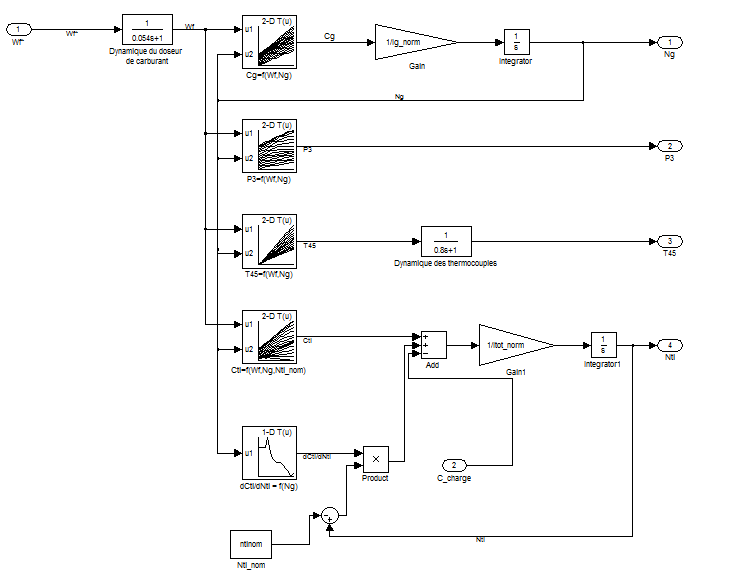
\includegraphics[scale=0.8]{./figures/sim_non_lineaire_complet.png}
		\end{center}
		\caption{Sch�ma \texttt{Simulink} du syst�me turbine complet (non-lin�aire)}
		\label{fig:sim_non_linaire_complet}
	\end{figure}
			
			
			
			
			

	\clearpage{}
	
	% !TEX encoding = IsoLatin
% --------------------------------------------------------------------------------------------------------------------------------------------------------------------------- %
%\begin{itemize}
%\item [-] \textbf{Cr�ation} : Demand�e par un autre processus,  cr�e dans l'�tat pr�t ou suspendu.
%\item [-] \textbf{Destruction} : peut �tre fait par le processus lui-m�me, un autre processus, le noyau. La destruction provoque une lib�ration des ressources associ�es et un �v�nement.
%\item [-] \textbf{Blocage} : passage en mode bloqu� en attente d'un �v�nement externe. Peut �tre demand� par le processus lui-m�me ou par le syst�me.
%\item [-] \textbf{D�blocage} : passage en mode pr�t apr�s le mode bloqu� lorsque l'�v�nement attendu se produit.
%\item [-] \textbf{Activation} : passage en mode ex�cution d'un mode pr�t.
%\end{itemize}

  
%\begin{Verbatim}[frame=single,fontsize=\scriptsize]
%\end{Verbatim}

%\begin{figure}[h]
%	\begin{center}
%		\includegraphics[width=14.5cm,height=9cm]{.\figures\diag_etat_threads.png}
%	\end{center}
%	\caption{Diagramme des diff�rents �tats d'un thread avec les primitives}
%	\label{fig:diag_etat_threads}
%\end{figure}

%% Modele d'etat avec les matrices

%\begin{displaymath}
%\left\{ \begin{array}{l} \dot{x} \quad = \quad \left[ \begin{array}{cccc}
%0 & 1 & 0 & 1\\
%- \frac{K_s}{M_s} & - \frac{C_s}{M_s} & 0 & \frac{C_s}{M_s}\\
%0 & 0 & 0 & 1\\
%\frac{K_s}{M_u} & \frac{C_s}{M_u} & - \frac{K_t}{M_u} & - \frac{C_s}{M_u} - \frac{C_t}{M_u}
%
%\end{array}\right]  x \quad + \quad \left[ \begin{array}{cc}
%0 & 1.1972\\
%0 & - 0.0012\\
%0 & 0\\
%7.84 & - 4.05
%\end{array} \right] u\\ \\
%y \quad = \quad \left[ \begin{array}{cccc}
%1 & 0 & 0 & 0\\
%0 & \lambda & 0 & 0\\
%0 & 0 & \lambda & 0\\
%0 & 0 & 0 & \lambda\\
%0 & - \lambda & \lambda & 0
%\end{array} \right] x \quad + \quad \left[ \begin{array}{cc}
%0 & 0\\
%0 & 0\\
%0 & 0\\
%0 & 0\\
%0 & 0
%\end{array} \right] u \end{array}\right.
%\end{displaymath}\\

% --------------------------------------------------------------------------------------------------------------------------------------------------------------------------- %
\rhead{\footnotesize\rightmark}
\chapter{Lin�arisation du mod�le}

	\textcolor{red}{Maffre}

			\section{Point d'�quilibre}
			
			\section{Lin�ariation}
			
				Jacobienne, calcul de $B_lin$ et $C_lin$
				

	\clearpage{}
	
	% !TEX encoding = IsoLatin
% --------------------------------------------------------------------------------------------------------------------------------------------------------------------------- %
%TODO : Figures EPS format for 3D matlab.......

\rhead{\footnotesize\rightmark}
\chapter{Observateur du Kalman}

\paragraph{}L'objectif du filtre de Kalman est d'estimer les �tats x(t) du syst�me � partir d'une s�rie de mesures incompl�tes ou bruit�es. Cet estim� not� $\hat{x}(t)$, est la sortie du filtre de Kalman. Ce filtre sugg�re une relation entr�es-sorties avec une optimisation des mesures. Le mod�le d'�tat de Kalman prend en compte les bruits d'entr�e (mod�le) et les bruits des capteurs de mesure des sorties. La notation propre au Kalman d'un mod�le avec bruit :

\begin{displaymath}
\begin{array}{l} \dot{x} \quad = \quad A.x(t) \quad + \quad B.u(t) + \quad M.w(t)\\ \\
y \quad = \quad C.x(t) \quad + \quad D.u(t) + \quad v(t) \end{array}
\end{displaymath}

\paragraph{}Certains hypotheses doivent �tre respect�es pour que la th�orie du filtre Kalman soit valable:\\

\begin{itemize}
\item [-] Le syst�me et les bruits sont stationnaires (Les matrices du mod�le d'�tat sont ind�pendantes du temps)
\item [-] La paire (A,C) est d�tectable, c'est � dire qu'il n'y a pas de mode instable et non observable dans le syst�me 
\item [-] Les signaux w(t) et v(t) sont des bruits blancs gaussiens centr�s.
\end{itemize}

\paragraph{}L'objectif dans cette partie est de filtrer les mesures des capteurs $N_g$, $N_{tl}$ et surtout offrir un estim� du d�bit r�el de carburant $W_f$. Pour cela nous r�alisons un estimateur/filtre de Kalman.

\paragraph{Remarque:}
\paragraph{}Le filtre de Kalman �tait sujet de TP pendant deux s�ances dans ce Bureau d'�tude. Les exercices faites nous ont permis d'approfondir les connaissances dans le principe et l'application du filtre de Kalman. 
		
	
	\section{�quations du filtre de Kalman}
	\paragraph{}Nous reprenons le mod�le lin�aris� pr�sent� � la fin du chapitre Lin�arisation. Nous supposerons donc que notre syst�me perturb� peut �tre mod�lis� par le mod�le d'�tat de Kalman parce qu'il satisfait les hypoth�ses n�cessaires. Nous avons utilis� les fonctions de Kalman propos� par le Toolbox Matlab parce que la solution obtenue est optimale. 
	
	\paragraph{}Le mod�le pris en compte pour calculer l'observateur de Kalman est le suivant :
		
\begin{displaymath}
\left\{ \begin{array}{l} \dot{x} \quad = \quad \left[ \begin{array}{cccc}
    -18.5185   &      0       &  0 \\
   65.5871 &  -1.9835   &      0 \\
   17.1650  &  0.8011  & -0.5289

\end{array}\right]  x \quad + \quad \left[ \begin{array}{cc}
 18.5185\\
         0 \\
         0 
\end{array} \right] u\\ \\
y \quad = \quad \left[ \begin{array}{cccc}
         0   & 1.0000     &    0 \\
    0.0020  &  0.0002    &     0 \\
    1.6012  & -0.0228    &     0 \\
         0  &       0   & 1.0000
\end{array} \right] x \quad + \quad \left[ \begin{array}{cc}
0\\
0\\
0\\
0
\end{array} \right] u \end{array}\right.
\end{displaymath}\\

\paragraph{}L'objectif est d'estimer l'entr�e du d�bit r�el de carburant $W_f$. Pour cela on diminue le mod�le en prenant une seule entr�e. L'entr�e $C_{charge}$ sera considerer comme une perturbation par la suite. 

\subsection{Incertitudes sur les donn�es}
\paragraph{}Dans le cahier des charges les incertitudes relatives sont donn�es pour chaque sortie. L'incertitude relative pr�sente un nombre sans dimension qui caract�rise la pr�cision de la mesure. Ce nombre est le rapport entre l'incertitude et la valeur mesur�e de la sortie. Pour chaque sortie estim�e nous pr�senterons les intervalles de variation autour les valeurs nominales.\\ 

\begin{itemize}
\item [-] $ N_g = 0.1\%$
\item [-] $ P_3 = 2\%$
\item [-] $ N_{tl} = 0.1\%$
\item [-] $ T_{45} = 2\%$
\end{itemize}

\paragraph{}Sur la figure suivante on peut observer les quatre sorties avec le bruit associ�. Dans le script simulink nous avons ajout� un bruit  pour chaque sortie avec le block \emph{Band Limited White noise}. Les valeurs de la densit� spectrale sont obtenues avec un produit de la pr�cision relative et une constante. La pr�cision relative nous donne la valeur de l'intervalle pour la sortie. Pour $N_{tl}$ la valeur nominale est $28000$, dont l'intervalle des valeurs est : $[28000 +\Delta N_g , 28000 -\Delta N_g ]$, avec $\Delta N_g = Precision * 28000$. 

% insert figure
%\begin{figure} [H]
%\centering 
%\scalebox{0.7}{ \input{./figures/sortie_bruit.tikz} }
%\caption{Sorties bruit�es avec \emph{white noise}} 
%\label{fig:sortie_bruit}
%\end{figure}

\paragraph{}Dans le syst�me nous consid�rons que les bruits du mod�le ne sont par tr�s importants ($10^{-5}$). Les bruits de mesure sont importants ($10^{-3}$), autrement dit peu de confiance dans les capteurs. Les matrices suivantes pr�sentent la confiance dans les mesures (capteurs) et la confiance dans le mod�le respectivement (matrices de covariance) :
\begin{equation}		
R_{N} =
 \begin{pmatrix}
  0.001 & 0 & 0 & 0\\
  0 & 0.001 & 0 & 0\\
  0 & 0 & 0.001 & 0\\
  0 & 0 & 0 & 0.001
 \end{pmatrix}
\quad and
\quad R_{N} =
 \begin{pmatrix}
  0.00001 
  \end{pmatrix}
\end{equation}

\paragraph{}Les termes sur la diagonale de la matrice $R_N$ correspond au carr� des �cart-types maximaux de l'erreur que l'on autorise pour chacun des param�tres � estimer. Les valeurs choisies correspondent � l'estimation sur les sorties et la valeur d'erreur autoris�e. Il faut avoir conscience que si on d�finie des termes d'erreur trop petit par rapport � la r�alit�, le filtre de Kalman n'arrivera pas � rectifier les erreurs du mod�le et fera des estimations biais�s. Si les erreurs sont trop importantes par rapport � la r�alit�, les estimations seront avec une covariance importante. Pour avoir la meilleure estimation nous avons choisi la m�me variance sur chaque param�tre en respectant les pr�cision r�elles des capteurs. 
	
	\section{Calcul du gain de Kalman}
	\paragraph{}Avec la commande kalman sous \emph{Matlab} on obtient le gain du filtre et aussi la solution de l'�quation de Ricatti qui donne la matrice de covariance de l'estimation d'erreur. Ensuite on simplifie le mod�le d'�tat et on garde que les entr�es et les sorties du observateur qui sont demand�es dans le cahier des charges. La formule utilis�e pour calculer le mod�le d'�tat est :
	
	\begin{equation}
	A_{kalman} = A_{lin} - K.C_{lin} \quad
	B_{kalman} = [B_{lin}\quad K] \quad
	C_{kalman} = I_{3} \quad
	D_{kalman} = 0_{3}
	\end{equation}
	
	Le mod�le obtenu du filtre de Kalman est : 

	\begin{displaymath}
\left\{ \begin{array}{l} \dot{x} \quad = \quad \left[ \begin{array}{cccc}
-18.74 &  -0.2354 & -0.06749\\
 65.11  &  -5.711  &  -1.564\\
 17.05 &  -0.7616  &  -1.628
\end{array}\right]  x \quad + \quad \left[ \begin{array}{ccccc}
18.52 & 0.2386 & 0.0002408 & 0.1393 & 0.06749\\
0 & 3.735 & 0.001385 & 0.297 & 1.564\\
0 & 1.564 & 0.0005146 & 0.07243 & 1.099
\end{array} \right] u\\ \\
y \quad = \quad \left[ \begin{array}{ccc}
         1 & 0  & 0 \\
    0 & 1 & 0 \\
         0 & 0 & 1
\end{array} \right] x \quad + \quad \left[ \begin{array}{ccccc}
         0 & 0 & 0 & 0     &    0 \\
    0 & 0 & 0 & 0 & 0\\
         0 & 0 & 0 & 0 & 0
\end{array} \right] u \end{array}\right.
\end{displaymath}\\
	
\paragraph{}Ce mod�le prend en entr�e toutes les sorties du syst�me lin�aire et le d�bit du carburant $W_f$. En sortie du filtre de Kalman il donne les trois estimations : $W_f$, $N_g$ et $N_{tl}$ (les trois �tats du syst�me). La figure suivante montre l'estimation du filtre de Kalman sur le vecteur d'�tat. L'allure des r�ponses correspond � une �volution suite � un changement de la consigne $W_f$. Le filtre de Kalman estime bien ses sorties : $W_f$, $N_{g}$ et $N_{tl}$.

% Insert figure kalman estimation

%\begin{figure} [H]
%\centering 
%\scalebox{0.7}{ % This file was created by matlab2tikz v0.4.4 (commit d73c276378addcc50161bb9c0bf72b69fdfe704f) running on MATLAB 8.1.
% Copyright (c) 2008--2013, Nico Schlömer <nico.schloemer@gmail.com>
% All rights reserved.
% 
% The latest updates can be retrieved from
%   http://www.mathworks.com/matlabcentral/fileexchange/22022-matlab2tikz
% where you can also make suggestions and rate matlab2tikz.
% 
\begin{tikzpicture}

\begin{axis}[%
width=0.00464072317664837in,
height=0.00435243728254898in,
scale only axis,
xmin=0,
xmax=20,
xmajorgrids,
ymin=255,
ymax=300,
ymajorgrids,
name=plot1,
title={Evolutions de Wf},
axis x line*=bottom,
axis y line*=left,
legend style={draw=black,fill=white,legend cell align=left}
]
\addplot [
color=red,
solid,
forget plot
]
table[row sep=crcr]{
0 259.645080566406\\
1.64613605134399e-05 259.645080566406\\
9.87681630806392e-05 259.645080566406\\
0.000510302175916636 259.645080566406\\
0.001 259.645080566406\\
0.002 259.645080566406\\
0.003 259.645080566406\\
0.004 259.645080566406\\
0.005 259.645080566406\\
0.006 259.645080566406\\
0.007 259.645080566406\\
0.008 259.645080566406\\
0.009 259.645080566406\\
0.01 259.645080566406\\
0.011 259.645080566406\\
0.012 259.645080566406\\
0.013 259.645080566406\\
0.014 259.645080566406\\
0.015 259.645080566406\\
0.016 259.645080566406\\
0.017 259.645080566406\\
0.018 259.645080566406\\
0.019 259.645080566406\\
0.02 259.645080566406\\
0.021 259.645080566406\\
0.022 259.645080566406\\
0.023 259.645080566406\\
0.024 259.645080566406\\
0.025 259.645080566406\\
0.026 259.645080566406\\
0.027 259.645080566406\\
0.028 259.645080566406\\
0.029 259.645080566406\\
0.03 259.645080566406\\
0.031 259.645080566406\\
0.032 259.645080566406\\
0.033 259.645080566406\\
0.034 259.645080566406\\
0.035 259.645080566406\\
0.036 259.645080566406\\
0.037 259.645080566406\\
0.038 259.645080566406\\
0.039 259.645080566406\\
0.04 259.645080566406\\
0.041 259.645080566406\\
0.042 259.645080566406\\
0.043 259.645080566406\\
0.044 259.645080566406\\
0.045 259.645080566406\\
0.046 259.645080566406\\
0.047 259.645080566406\\
0.048 259.645080566406\\
0.049 259.645080566406\\
0.05 259.645080566406\\
0.051 259.645080566406\\
0.052 259.645080566406\\
0.053 259.645080566406\\
0.054 259.645080566406\\
0.055 259.645080566406\\
0.056 259.645080566406\\
0.057 259.645080566406\\
0.058 259.645080566406\\
0.059 259.645080566406\\
0.06 259.645080566406\\
0.061 259.645080566406\\
0.062 259.645080566406\\
0.063 259.645080566406\\
0.064 259.645080566406\\
0.065 259.645080566406\\
0.066 259.645080566406\\
0.067 259.645080566406\\
0.068 259.645080566406\\
0.069 259.645080566406\\
0.07 259.645080566406\\
0.071 259.645080566406\\
0.072 259.645080566406\\
0.073 259.645080566406\\
0.074 259.645080566406\\
0.075 259.645080566406\\
0.076 259.645080566406\\
0.077 259.645080566406\\
0.078 259.645080566406\\
0.079 259.645080566406\\
0.08 259.645080566406\\
0.081 259.645080566406\\
0.082 259.645080566406\\
0.083 259.645080566406\\
0.084 259.645080566406\\
0.085 259.645080566406\\
0.086 259.645080566406\\
0.087 259.645080566406\\
0.088 259.645080566406\\
0.089 259.645080566406\\
0.09 259.645080566406\\
0.091 259.645080566406\\
0.092 259.645080566406\\
0.093 259.645080566406\\
0.094 259.645080566406\\
0.095 259.645080566406\\
0.096 259.645080566406\\
0.097 259.645080566406\\
0.098 259.645080566406\\
0.099 259.645080566406\\
0.1 259.645080566406\\
0.101 259.645080566406\\
0.102 259.645080566406\\
0.103 259.645080566406\\
0.104 259.645080566406\\
0.105 259.645080566406\\
0.106 259.645080566406\\
0.107 259.645080566406\\
0.108 259.645080566406\\
0.109 259.645080566406\\
0.11 259.645080566406\\
0.111 259.645080566406\\
0.112 259.645080566406\\
0.113 259.645080566406\\
0.114 259.645080566406\\
0.115 259.645080566406\\
0.116 259.645080566406\\
0.117 259.645080566406\\
0.118 259.645080566406\\
0.119 259.645080566406\\
0.12 259.645080566406\\
0.121 259.645080566406\\
0.122 259.645080566406\\
0.123 259.645080566406\\
0.124 259.645080566406\\
0.125 259.645080566406\\
0.126 259.645080566406\\
0.127 259.645080566406\\
0.128 259.645080566406\\
0.129 259.645080566406\\
0.13 259.645080566406\\
0.131 259.645080566406\\
0.132 259.645080566406\\
0.133 259.645080566406\\
0.134 259.645080566406\\
0.135 259.645080566406\\
0.136 259.645080566406\\
0.137 259.645080566406\\
0.138 259.645080566406\\
0.139 259.645080566406\\
0.14 259.645080566406\\
0.141 259.645080566406\\
0.142 259.645080566406\\
0.143 259.645080566406\\
0.144 259.645080566406\\
0.145 259.645080566406\\
0.146 259.645080566406\\
0.147 259.645080566406\\
0.148 259.645080566406\\
0.149 259.645080566406\\
0.15 259.645080566406\\
0.151 259.645080566406\\
0.152 259.645080566406\\
0.153 259.645080566406\\
0.154 259.645080566406\\
0.155 259.645080566406\\
0.156 259.645080566406\\
0.157 259.645080566406\\
0.158 259.645080566406\\
0.159 259.645080566406\\
0.16 259.645080566406\\
0.161 259.645080566406\\
0.162 259.645080566406\\
0.163 259.645080566406\\
0.164 259.645080566406\\
0.165 259.645080566406\\
0.166 259.645080566406\\
0.167 259.645080566406\\
0.168 259.645080566406\\
0.169 259.645080566406\\
0.17 259.645080566406\\
0.171 259.645080566406\\
0.172 259.645080566406\\
0.173 259.645080566406\\
0.174 259.645080566406\\
0.175 259.645080566406\\
0.176 259.645080566406\\
0.177 259.645080566406\\
0.178 259.645080566406\\
0.179 259.645080566406\\
0.18 259.645080566406\\
0.181 259.645080566406\\
0.182 259.645080566406\\
0.183 259.645080566406\\
0.184 259.645080566406\\
0.185 259.645080566406\\
0.186 259.645080566406\\
0.187 259.645080566406\\
0.188 259.645080566406\\
0.189 259.645080566406\\
0.19 259.645080566406\\
0.191 259.645080566406\\
0.192 259.645080566406\\
0.193 259.645080566406\\
0.194 259.645080566406\\
0.195 259.645080566406\\
0.196 259.645080566406\\
0.197 259.645080566406\\
0.198 259.645080566406\\
0.199 259.645080566406\\
0.2 259.645080566406\\
0.201 259.645080566406\\
0.202 259.645080566406\\
0.203 259.645080566406\\
0.204 259.645080566406\\
0.205 259.645080566406\\
0.206 259.645080566406\\
0.207 259.645080566406\\
0.208 259.645080566406\\
0.209 259.645080566406\\
0.21 259.645080566406\\
0.211 259.645080566406\\
0.212 259.645080566406\\
0.213 259.645080566406\\
0.214 259.645080566406\\
0.215 259.645080566406\\
0.216 259.645080566406\\
0.217 259.645080566406\\
0.218 259.645080566406\\
0.219 259.645080566406\\
0.22 259.645080566406\\
0.221 259.645080566406\\
0.222 259.645080566406\\
0.223 259.645080566406\\
0.224 259.645080566406\\
0.225 259.645080566406\\
0.226 259.645080566406\\
0.227 259.645080566406\\
0.228 259.645080566406\\
0.229 259.645080566406\\
0.23 259.645080566406\\
0.231 259.645080566406\\
0.232 259.645080566406\\
0.233 259.645080566406\\
0.234 259.645080566406\\
0.235 259.645080566406\\
0.236 259.645080566406\\
0.237 259.645080566406\\
0.238 259.645080566406\\
0.239 259.645080566406\\
0.24 259.645080566406\\
0.241 259.645080566406\\
0.242 259.645080566406\\
0.243 259.645080566406\\
0.244 259.645080566406\\
0.245 259.645080566406\\
0.246 259.645080566406\\
0.247 259.645080566406\\
0.248 259.645080566406\\
0.249 259.645080566406\\
0.25 259.645080566406\\
0.251 259.645080566406\\
0.252 259.645080566406\\
0.253 259.645080566406\\
0.254 259.645080566406\\
0.255 259.645080566406\\
0.256 259.645080566406\\
0.257 259.645080566406\\
0.258 259.645080566406\\
0.259 259.645080566406\\
0.26 259.645080566406\\
0.261 259.645080566406\\
0.262 259.645080566406\\
0.263 259.645080566406\\
0.264 259.645080566406\\
0.265 259.645080566406\\
0.266 259.645080566406\\
0.267 259.645080566406\\
0.268 259.645080566406\\
0.269 259.645080566406\\
0.27 259.645080566406\\
0.271 259.645080566406\\
0.272 259.645080566406\\
0.273 259.645080566406\\
0.274 259.645080566406\\
0.275 259.645080566406\\
0.276 259.645080566406\\
0.277 259.645080566406\\
0.278 259.645080566406\\
0.279 259.645080566406\\
0.28 259.645080566406\\
0.281 259.645080566406\\
0.282 259.645080566406\\
0.283 259.645080566406\\
0.284 259.645080566406\\
0.285 259.645080566406\\
0.286 259.645080566406\\
0.287 259.645080566406\\
0.288 259.645080566406\\
0.289 259.645080566406\\
0.29 259.645080566406\\
0.291 259.645080566406\\
0.292 259.645080566406\\
0.293 259.645080566406\\
0.294 259.645080566406\\
0.295 259.645080566406\\
0.296 259.645080566406\\
0.297 259.645080566406\\
0.298 259.645080566406\\
0.299 259.645080566406\\
0.3 259.645080566406\\
0.301 259.645080566406\\
0.302 259.645080566406\\
0.303 259.645080566406\\
0.304 259.645080566406\\
0.305 259.645080566406\\
0.306 259.645080566406\\
0.307 259.645080566406\\
0.308 259.645080566406\\
0.309 259.645080566406\\
0.31 259.645080566406\\
0.311 259.645080566406\\
0.312 259.645080566406\\
0.313 259.645080566406\\
0.314 259.645080566406\\
0.315 259.645080566406\\
0.316 259.645080566406\\
0.317 259.645080566406\\
0.318 259.645080566406\\
0.319 259.645080566406\\
0.32 259.645080566406\\
0.321 259.645080566406\\
0.322 259.645080566406\\
0.323 259.645080566406\\
0.324 259.645080566406\\
0.325 259.645080566406\\
0.326 259.645080566406\\
0.327 259.645080566406\\
0.328 259.645080566406\\
0.329 259.645080566406\\
0.33 259.645080566406\\
0.331 259.645080566406\\
0.332 259.645080566406\\
0.333 259.645080566406\\
0.334 259.645080566406\\
0.335 259.645080566406\\
0.336 259.645080566406\\
0.337 259.645080566406\\
0.338 259.645080566406\\
0.339 259.645080566406\\
0.34 259.645080566406\\
0.341 259.645080566406\\
0.342 259.645080566406\\
0.343 259.645080566406\\
0.344 259.645080566406\\
0.345 259.645080566406\\
0.346 259.645080566406\\
0.347 259.645080566406\\
0.348 259.645080566406\\
0.349 259.645080566406\\
0.35 259.645080566406\\
0.351 259.645080566406\\
0.352 259.645080566406\\
0.353 259.645080566406\\
0.354 259.645080566406\\
0.355 259.645080566406\\
0.356 259.645080566406\\
0.357 259.645080566406\\
0.358 259.645080566406\\
0.359 259.645080566406\\
0.36 259.645080566406\\
0.361 259.645080566406\\
0.362 259.645080566406\\
0.363 259.645080566406\\
0.364 259.645080566406\\
0.365 259.645080566406\\
0.366 259.645080566406\\
0.367 259.645080566406\\
0.368 259.645080566406\\
0.369 259.645080566406\\
0.37 259.645080566406\\
0.371 259.645080566406\\
0.372 259.645080566406\\
0.373 259.645080566406\\
0.374 259.645080566406\\
0.375 259.645080566406\\
0.376 259.645080566406\\
0.377 259.645080566406\\
0.378 259.645080566406\\
0.379 259.645080566406\\
0.38 259.645080566406\\
0.381 259.645080566406\\
0.382 259.645080566406\\
0.383 259.645080566406\\
0.384 259.645080566406\\
0.385 259.645080566406\\
0.386 259.645080566406\\
0.387 259.645080566406\\
0.388 259.645080566406\\
0.389 259.645080566406\\
0.39 259.645080566406\\
0.391 259.645080566406\\
0.392 259.645080566406\\
0.393 259.645080566406\\
0.394 259.645080566406\\
0.395 259.645080566406\\
0.396 259.645080566406\\
0.397 259.645080566406\\
0.398 259.645080566406\\
0.399 259.645080566406\\
0.4 259.645080566406\\
0.401 259.645080566406\\
0.402 259.645080566406\\
0.403 259.645080566406\\
0.404 259.645080566406\\
0.405 259.645080566406\\
0.406 259.645080566406\\
0.407 259.645080566406\\
0.408 259.645080566406\\
0.409 259.645080566406\\
0.41 259.645080566406\\
0.411 259.645080566406\\
0.412 259.645080566406\\
0.413 259.645080566406\\
0.414 259.645080566406\\
0.415 259.645080566406\\
0.416 259.645080566406\\
0.417 259.645080566406\\
0.418 259.645080566406\\
0.419 259.645080566406\\
0.42 259.645080566406\\
0.421 259.645080566406\\
0.422 259.645080566406\\
0.423 259.645080566406\\
0.424 259.645080566406\\
0.425 259.645080566406\\
0.426 259.645080566406\\
0.427 259.645080566406\\
0.428 259.645080566406\\
0.429 259.645080566406\\
0.43 259.645080566406\\
0.431 259.645080566406\\
0.432 259.645080566406\\
0.433 259.645080566406\\
0.434 259.645080566406\\
0.435 259.645080566406\\
0.436 259.645080566406\\
0.437 259.645080566406\\
0.438 259.645080566406\\
0.439 259.645080566406\\
0.44 259.645080566406\\
0.441 259.645080566406\\
0.442 259.645080566406\\
0.443 259.645080566406\\
0.444 259.645080566406\\
0.445 259.645080566406\\
0.446 259.645080566406\\
0.447 259.645080566406\\
0.448 259.645080566406\\
0.449 259.645080566406\\
0.45 259.645080566406\\
0.451 259.645080566406\\
0.452 259.645080566406\\
0.453 259.645080566406\\
0.454 259.645080566406\\
0.455 259.645080566406\\
0.456 259.645080566406\\
0.457 259.645080566406\\
0.458 259.645080566406\\
0.459 259.645080566406\\
0.46 259.645080566406\\
0.461 259.645080566406\\
0.462 259.645080566406\\
0.463 259.645080566406\\
0.464 259.645080566406\\
0.465 259.645080566406\\
0.466 259.645080566406\\
0.467 259.645080566406\\
0.468 259.645080566406\\
0.469 259.645080566406\\
0.47 259.645080566406\\
0.471 259.645080566406\\
0.472 259.645080566406\\
0.473 259.645080566406\\
0.474 259.645080566406\\
0.475 259.645080566406\\
0.476 259.645080566406\\
0.477 259.645080566406\\
0.478 259.645080566406\\
0.479 259.645080566406\\
0.48 259.645080566406\\
0.481 259.645080566406\\
0.482 259.645080566406\\
0.483 259.645080566406\\
0.484 259.645080566406\\
0.485 259.645080566406\\
0.486 259.645080566406\\
0.487 259.645080566406\\
0.488 259.645080566406\\
0.489 259.645080566406\\
0.49 259.645080566406\\
0.491 259.645080566406\\
0.492 259.645080566406\\
0.493 259.645080566406\\
0.494 259.645080566406\\
0.495 259.645080566406\\
0.496 259.645080566406\\
0.497 259.645080566406\\
0.498 259.645080566406\\
0.499 259.645080566406\\
0.5 259.645080566406\\
0.501 259.645080566406\\
0.502 259.645080566406\\
0.503 259.645080566406\\
0.504 259.645080566406\\
0.505 259.645080566406\\
0.506 259.645080566406\\
0.507 259.645080566406\\
0.508 259.645080566406\\
0.509 259.645080566406\\
0.51 259.645080566406\\
0.511 259.645080566406\\
0.512 259.645080566406\\
0.513 259.645080566406\\
0.514 259.645080566406\\
0.515 259.645080566406\\
0.516 259.645080566406\\
0.517 259.645080566406\\
0.518 259.645080566406\\
0.519 259.645080566406\\
0.52 259.645080566406\\
0.521 259.645080566406\\
0.522 259.645080566406\\
0.523 259.645080566406\\
0.524 259.645080566406\\
0.525 259.645080566406\\
0.526 259.645080566406\\
0.527 259.645080566406\\
0.528 259.645080566406\\
0.529 259.645080566406\\
0.53 259.645080566406\\
0.531 259.645080566406\\
0.532 259.645080566406\\
0.533 259.645080566406\\
0.534 259.645080566406\\
0.535 259.645080566406\\
0.536 259.645080566406\\
0.537 259.645080566406\\
0.538 259.645080566406\\
0.539 259.645080566406\\
0.54 259.645080566406\\
0.541 259.645080566406\\
0.542 259.645080566406\\
0.543 259.645080566406\\
0.544 259.645080566406\\
0.545 259.645080566406\\
0.546 259.645080566406\\
0.547 259.645080566406\\
0.548 259.645080566406\\
0.549 259.645080566406\\
0.55 259.645080566406\\
0.551 259.645080566406\\
0.552 259.645080566406\\
0.553 259.645080566406\\
0.554 259.645080566406\\
0.555 259.645080566406\\
0.556 259.645080566406\\
0.557 259.645080566406\\
0.558 259.645080566406\\
0.559 259.645080566406\\
0.56 259.645080566406\\
0.561 259.645080566406\\
0.562 259.645080566406\\
0.563 259.645080566406\\
0.564 259.645080566406\\
0.565 259.645080566406\\
0.566 259.645080566406\\
0.567 259.645080566406\\
0.568 259.645080566406\\
0.569 259.645080566406\\
0.57 259.645080566406\\
0.571 259.645080566406\\
0.572 259.645080566406\\
0.573 259.645080566406\\
0.574 259.645080566406\\
0.575 259.645080566406\\
0.576 259.645080566406\\
0.577 259.645080566406\\
0.578 259.645080566406\\
0.579 259.645080566406\\
0.58 259.645080566406\\
0.581 259.645080566406\\
0.582 259.645080566406\\
0.583 259.645080566406\\
0.584 259.645080566406\\
0.585 259.645080566406\\
0.586 259.645080566406\\
0.587 259.645080566406\\
0.588 259.645080566406\\
0.589 259.645080566406\\
0.59 259.645080566406\\
0.591 259.645080566406\\
0.592 259.645080566406\\
0.593 259.645080566406\\
0.594 259.645080566406\\
0.595 259.645080566406\\
0.596 259.645080566406\\
0.597 259.645080566406\\
0.598 259.645080566406\\
0.599 259.645080566406\\
0.6 259.645080566406\\
0.601 259.645080566406\\
0.602 259.645080566406\\
0.603 259.645080566406\\
0.604 259.645080566406\\
0.605 259.645080566406\\
0.606 259.645080566406\\
0.607 259.645080566406\\
0.608 259.645080566406\\
0.609 259.645080566406\\
0.61 259.645080566406\\
0.611 259.645080566406\\
0.612 259.645080566406\\
0.613 259.645080566406\\
0.614 259.645080566406\\
0.615 259.645080566406\\
0.616 259.645080566406\\
0.617 259.645080566406\\
0.618 259.645080566406\\
0.619 259.645080566406\\
0.62 259.645080566406\\
0.621 259.645080566406\\
0.622 259.645080566406\\
0.623 259.645080566406\\
0.624 259.645080566406\\
0.625 259.645080566406\\
0.626 259.645080566406\\
0.627 259.645080566406\\
0.628 259.645080566406\\
0.629 259.645080566406\\
0.63 259.645080566406\\
0.631 259.645080566406\\
0.632 259.645080566406\\
0.633 259.645080566406\\
0.634 259.645080566406\\
0.635 259.645080566406\\
0.636 259.645080566406\\
0.637 259.645080566406\\
0.638 259.645080566406\\
0.639 259.645080566406\\
0.64 259.645080566406\\
0.641 259.645080566406\\
0.642 259.645080566406\\
0.643 259.645080566406\\
0.644 259.645080566406\\
0.645 259.645080566406\\
0.646 259.645080566406\\
0.647 259.645080566406\\
0.648 259.645080566406\\
0.649 259.645080566406\\
0.65 259.645080566406\\
0.651 259.645080566406\\
0.652 259.645080566406\\
0.653 259.645080566406\\
0.654 259.645080566406\\
0.655 259.645080566406\\
0.656 259.645080566406\\
0.657 259.645080566406\\
0.658 259.645080566406\\
0.659 259.645080566406\\
0.66 259.645080566406\\
0.661 259.645080566406\\
0.662 259.645080566406\\
0.663 259.645080566406\\
0.664 259.645080566406\\
0.665 259.645080566406\\
0.666 259.645080566406\\
0.667 259.645080566406\\
0.668 259.645080566406\\
0.669 259.645080566406\\
0.67 259.645080566406\\
0.671 259.645080566406\\
0.672 259.645080566406\\
0.673 259.645080566406\\
0.674 259.645080566406\\
0.675 259.645080566406\\
0.676 259.645080566406\\
0.677 259.645080566406\\
0.678 259.645080566406\\
0.679 259.645080566406\\
0.68 259.645080566406\\
0.681 259.645080566406\\
0.682 259.645080566406\\
0.683 259.645080566406\\
0.684 259.645080566406\\
0.685 259.645080566406\\
0.686 259.645080566406\\
0.687 259.645080566406\\
0.688 259.645080566406\\
0.689 259.645080566406\\
0.69 259.645080566406\\
0.691 259.645080566406\\
0.692 259.645080566406\\
0.693 259.645080566406\\
0.694 259.645080566406\\
0.695 259.645080566406\\
0.696 259.645080566406\\
0.697 259.645080566406\\
0.698 259.645080566406\\
0.699 259.645080566406\\
0.7 259.645080566406\\
0.701 259.645080566406\\
0.702 259.645080566406\\
0.703 259.645080566406\\
0.704 259.645080566406\\
0.705 259.645080566406\\
0.706 259.645080566406\\
0.707 259.645080566406\\
0.708 259.645080566406\\
0.709 259.645080566406\\
0.71 259.645080566406\\
0.711 259.645080566406\\
0.712 259.645080566406\\
0.713 259.645080566406\\
0.714 259.645080566406\\
0.715 259.645080566406\\
0.716 259.645080566406\\
0.717 259.645080566406\\
0.718 259.645080566406\\
0.719 259.645080566406\\
0.72 259.645080566406\\
0.721 259.645080566406\\
0.722 259.645080566406\\
0.723 259.645080566406\\
0.724 259.645080566406\\
0.725 259.645080566406\\
0.726 259.645080566406\\
0.727 259.645080566406\\
0.728 259.645080566406\\
0.729 259.645080566406\\
0.73 259.645080566406\\
0.731 259.645080566406\\
0.732 259.645080566406\\
0.733 259.645080566406\\
0.734 259.645080566406\\
0.735 259.645080566406\\
0.736 259.645080566406\\
0.737 259.645080566406\\
0.738 259.645080566406\\
0.739 259.645080566406\\
0.74 259.645080566406\\
0.741 259.645080566406\\
0.742 259.645080566406\\
0.743 259.645080566406\\
0.744 259.645080566406\\
0.745 259.645080566406\\
0.746 259.645080566406\\
0.747 259.645080566406\\
0.748 259.645080566406\\
0.749 259.645080566406\\
0.75 259.645080566406\\
0.751 259.645080566406\\
0.752 259.645080566406\\
0.753 259.645080566406\\
0.754 259.645080566406\\
0.755 259.645080566406\\
0.756 259.645080566406\\
0.757 259.645080566406\\
0.758 259.645080566406\\
0.759 259.645080566406\\
0.76 259.645080566406\\
0.761 259.645080566406\\
0.762 259.645080566406\\
0.763 259.645080566406\\
0.764 259.645080566406\\
0.765 259.645080566406\\
0.766 259.645080566406\\
0.767 259.645080566406\\
0.768 259.645080566406\\
0.769 259.645080566406\\
0.77 259.645080566406\\
0.771 259.645080566406\\
0.772 259.645080566406\\
0.773 259.645080566406\\
0.774 259.645080566406\\
0.775 259.645080566406\\
0.776 259.645080566406\\
0.777 259.645080566406\\
0.778 259.645080566406\\
0.779 259.645080566406\\
0.78 259.645080566406\\
0.781 259.645080566406\\
0.782 259.645080566406\\
0.783 259.645080566406\\
0.784 259.645080566406\\
0.785 259.645080566406\\
0.786 259.645080566406\\
0.787 259.645080566406\\
0.788 259.645080566406\\
0.789 259.645080566406\\
0.79 259.645080566406\\
0.791 259.645080566406\\
0.792 259.645080566406\\
0.793 259.645080566406\\
0.794 259.645080566406\\
0.795 259.645080566406\\
0.796 259.645080566406\\
0.797 259.645080566406\\
0.798 259.645080566406\\
0.799 259.645080566406\\
0.8 259.645080566406\\
0.801 259.645080566406\\
0.802 259.645080566406\\
0.803 259.645080566406\\
0.804 259.645080566406\\
0.805 259.645080566406\\
0.806 259.645080566406\\
0.807 259.645080566406\\
0.808 259.645080566406\\
0.809 259.645080566406\\
0.81 259.645080566406\\
0.811 259.645080566406\\
0.812 259.645080566406\\
0.813 259.645080566406\\
0.814 259.645080566406\\
0.815 259.645080566406\\
0.816 259.645080566406\\
0.817 259.645080566406\\
0.818 259.645080566406\\
0.819 259.645080566406\\
0.82 259.645080566406\\
0.821 259.645080566406\\
0.822 259.645080566406\\
0.823 259.645080566406\\
0.824 259.645080566406\\
0.825 259.645080566406\\
0.826 259.645080566406\\
0.827 259.645080566406\\
0.828 259.645080566406\\
0.829 259.645080566406\\
0.83 259.645080566406\\
0.831 259.645080566406\\
0.832 259.645080566406\\
0.833 259.645080566406\\
0.834 259.645080566406\\
0.835 259.645080566406\\
0.836 259.645080566406\\
0.837 259.645080566406\\
0.838 259.645080566406\\
0.839 259.645080566406\\
0.84 259.645080566406\\
0.841 259.645080566406\\
0.842 259.645080566406\\
0.843 259.645080566406\\
0.844 259.645080566406\\
0.845 259.645080566406\\
0.846 259.645080566406\\
0.847 259.645080566406\\
0.848 259.645080566406\\
0.849 259.645080566406\\
0.85 259.645080566406\\
0.851 259.645080566406\\
0.852 259.645080566406\\
0.853 259.645080566406\\
0.854 259.645080566406\\
0.855 259.645080566406\\
0.856 259.645080566406\\
0.857 259.645080566406\\
0.858 259.645080566406\\
0.859 259.645080566406\\
0.86 259.645080566406\\
0.861 259.645080566406\\
0.862 259.645080566406\\
0.863 259.645080566406\\
0.864 259.645080566406\\
0.865 259.645080566406\\
0.866 259.645080566406\\
0.867 259.645080566406\\
0.868 259.645080566406\\
0.869 259.645080566406\\
0.87 259.645080566406\\
0.871 259.645080566406\\
0.872 259.645080566406\\
0.873 259.645080566406\\
0.874 259.645080566406\\
0.875 259.645080566406\\
0.876 259.645080566406\\
0.877 259.645080566406\\
0.878 259.645080566406\\
0.879 259.645080566406\\
0.88 259.645080566406\\
0.881 259.645080566406\\
0.882 259.645080566406\\
0.883 259.645080566406\\
0.884 259.645080566406\\
0.885 259.645080566406\\
0.886 259.645080566406\\
0.887 259.645080566406\\
0.888 259.645080566406\\
0.889 259.645080566406\\
0.89 259.645080566406\\
0.891 259.645080566406\\
0.892 259.645080566406\\
0.893 259.645080566406\\
0.894 259.645080566406\\
0.895 259.645080566406\\
0.896 259.645080566406\\
0.897 259.645080566406\\
0.898 259.645080566406\\
0.899 259.645080566406\\
0.9 259.645080566406\\
0.901 259.645080566406\\
0.902 259.645080566406\\
0.903 259.645080566406\\
0.904 259.645080566406\\
0.905 259.645080566406\\
0.906 259.645080566406\\
0.907 259.645080566406\\
0.908 259.645080566406\\
0.909 259.645080566406\\
0.91 259.645080566406\\
0.911 259.645080566406\\
0.912 259.645080566406\\
0.913 259.645080566406\\
0.914 259.645080566406\\
0.915 259.645080566406\\
0.916 259.645080566406\\
0.917 259.645080566406\\
0.918 259.645080566406\\
0.919 259.645080566406\\
0.92 259.645080566406\\
0.921 259.645080566406\\
0.922 259.645080566406\\
0.923 259.645080566406\\
0.924 259.645080566406\\
0.925 259.645080566406\\
0.926 259.645080566406\\
0.927 259.645080566406\\
0.928 259.645080566406\\
0.929 259.645080566406\\
0.93 259.645080566406\\
0.931 259.645080566406\\
0.932 259.645080566406\\
0.933 259.645080566406\\
0.934 259.645080566406\\
0.935 259.645080566406\\
0.936 259.645080566406\\
0.937 259.645080566406\\
0.938 259.645080566406\\
0.939 259.645080566406\\
0.94 259.645080566406\\
0.941 259.645080566406\\
0.942 259.645080566406\\
0.943 259.645080566406\\
0.944 259.645080566406\\
0.945 259.645080566406\\
0.946 259.645080566406\\
0.947 259.645080566406\\
0.948 259.645080566406\\
0.949 259.645080566406\\
0.95 259.645080566406\\
0.951 259.645080566406\\
0.952 259.645080566406\\
0.953 259.645080566406\\
0.954 259.645080566406\\
0.955 259.645080566406\\
0.956 259.645080566406\\
0.957 259.645080566406\\
0.958 259.645080566406\\
0.959 259.645080566406\\
0.96 259.645080566406\\
0.961 259.645080566406\\
0.962 259.645080566406\\
0.963 259.645080566406\\
0.964 259.645080566406\\
0.965 259.645080566406\\
0.966 259.645080566406\\
0.967 259.645080566406\\
0.968 259.645080566406\\
0.969 259.645080566406\\
0.97 259.645080566406\\
0.971 259.645080566406\\
0.972 259.645080566406\\
0.973 259.645080566406\\
0.974 259.645080566406\\
0.975 259.645080566406\\
0.976 259.645080566406\\
0.977 259.645080566406\\
0.978 259.645080566406\\
0.979 259.645080566406\\
0.98 259.645080566406\\
0.981 259.645080566406\\
0.982 259.645080566406\\
0.983 259.645080566406\\
0.984 259.645080566406\\
0.985 259.645080566406\\
0.986 259.645080566406\\
0.987 259.645080566406\\
0.988 259.645080566406\\
0.989 259.645080566406\\
0.99 259.645080566406\\
0.991 259.645080566406\\
0.992 259.645080566406\\
0.993 259.645080566406\\
0.994 259.645080566406\\
0.995 259.645080566406\\
0.996 259.645080566406\\
0.997 259.645080566406\\
0.998 259.645080566406\\
0.999 259.645080566406\\
1 259.645080566406\\
1.001 259.645080566406\\
1.002 259.645080566406\\
1.003 259.645080566406\\
1.004 259.645080566406\\
1.005 259.645080566406\\
1.006 259.645080566406\\
1.007 259.645080566406\\
1.008 259.645080566406\\
1.009 259.645080566406\\
1.01 259.645080566406\\
1.011 259.645080566406\\
1.012 259.645080566406\\
1.013 259.645080566406\\
1.014 259.645080566406\\
1.015 259.645080566406\\
1.016 259.645080566406\\
1.017 259.645080566406\\
1.018 259.645080566406\\
1.019 259.645080566406\\
1.02 259.645080566406\\
1.021 259.645080566406\\
1.022 259.645080566406\\
1.023 259.645080566406\\
1.024 259.645080566406\\
1.025 259.645080566406\\
1.026 259.645080566406\\
1.027 259.645080566406\\
1.028 259.645080566406\\
1.029 259.645080566406\\
1.03 259.645080566406\\
1.031 259.645080566406\\
1.032 259.645080566406\\
1.033 259.645080566406\\
1.034 259.645080566406\\
1.035 259.645080566406\\
1.036 259.645080566406\\
1.037 259.645080566406\\
1.038 259.645080566406\\
1.039 259.645080566406\\
1.04 259.645080566406\\
1.041 259.645080566406\\
1.042 259.645080566406\\
1.043 259.645080566406\\
1.044 259.645080566406\\
1.045 259.645080566406\\
1.046 259.645080566406\\
1.047 259.645080566406\\
1.048 259.645080566406\\
1.049 259.645080566406\\
1.05 259.645080566406\\
1.051 259.645080566406\\
1.052 259.645080566406\\
1.053 259.645080566406\\
1.054 259.645080566406\\
1.055 259.645080566406\\
1.056 259.645080566406\\
1.057 259.645080566406\\
1.058 259.645080566406\\
1.059 259.645080566406\\
1.06 259.645080566406\\
1.061 259.645080566406\\
1.062 259.645080566406\\
1.063 259.645080566406\\
1.064 259.645080566406\\
1.065 259.645080566406\\
1.066 259.645080566406\\
1.067 259.645080566406\\
1.068 259.645080566406\\
1.069 259.645080566406\\
1.07 259.645080566406\\
1.071 259.645080566406\\
1.072 259.645080566406\\
1.073 259.645080566406\\
1.074 259.645080566406\\
1.075 259.645080566406\\
1.076 259.645080566406\\
1.077 259.645080566406\\
1.078 259.645080566406\\
1.079 259.645080566406\\
1.08 259.645080566406\\
1.081 259.645080566406\\
1.082 259.645080566406\\
1.083 259.645080566406\\
1.084 259.645080566406\\
1.085 259.645080566406\\
1.086 259.645080566406\\
1.087 259.645080566406\\
1.088 259.645080566406\\
1.089 259.645080566406\\
1.09 259.645080566406\\
1.091 259.645080566406\\
1.092 259.645080566406\\
1.093 259.645080566406\\
1.094 259.645080566406\\
1.095 259.645080566406\\
1.096 259.645080566406\\
1.097 259.645080566406\\
1.098 259.645080566406\\
1.099 259.645080566406\\
1.1 259.645080566406\\
1.101 259.645080566406\\
1.102 259.645080566406\\
1.103 259.645080566406\\
1.104 259.645080566406\\
1.105 259.645080566406\\
1.106 259.645080566406\\
1.107 259.645080566406\\
1.108 259.645080566406\\
1.109 259.645080566406\\
1.11 259.645080566406\\
1.111 259.645080566406\\
1.112 259.645080566406\\
1.113 259.645080566406\\
1.114 259.645080566406\\
1.115 259.645080566406\\
1.116 259.645080566406\\
1.117 259.645080566406\\
1.118 259.645080566406\\
1.119 259.645080566406\\
1.12 259.645080566406\\
1.121 259.645080566406\\
1.122 259.645080566406\\
1.123 259.645080566406\\
1.124 259.645080566406\\
1.125 259.645080566406\\
1.126 259.645080566406\\
1.127 259.645080566406\\
1.128 259.645080566406\\
1.129 259.645080566406\\
1.13 259.645080566406\\
1.131 259.645080566406\\
1.132 259.645080566406\\
1.133 259.645080566406\\
1.134 259.645080566406\\
1.135 259.645080566406\\
1.136 259.645080566406\\
1.137 259.645080566406\\
1.138 259.645080566406\\
1.139 259.645080566406\\
1.14 259.645080566406\\
1.141 259.645080566406\\
1.142 259.645080566406\\
1.143 259.645080566406\\
1.144 259.645080566406\\
1.145 259.645080566406\\
1.146 259.645080566406\\
1.147 259.645080566406\\
1.148 259.645080566406\\
1.149 259.645080566406\\
1.15 259.645080566406\\
1.151 259.645080566406\\
1.152 259.645080566406\\
1.153 259.645080566406\\
1.154 259.645080566406\\
1.155 259.645080566406\\
1.156 259.645080566406\\
1.157 259.645080566406\\
1.158 259.645080566406\\
1.159 259.645080566406\\
1.16 259.645080566406\\
1.161 259.645080566406\\
1.162 259.645080566406\\
1.163 259.645080566406\\
1.164 259.645080566406\\
1.165 259.645080566406\\
1.166 259.645080566406\\
1.167 259.645080566406\\
1.168 259.645080566406\\
1.169 259.645080566406\\
1.17 259.645080566406\\
1.171 259.645080566406\\
1.172 259.645080566406\\
1.173 259.645080566406\\
1.174 259.645080566406\\
1.175 259.645080566406\\
1.176 259.645080566406\\
1.177 259.645080566406\\
1.178 259.645080566406\\
1.179 259.645080566406\\
1.18 259.645080566406\\
1.181 259.645080566406\\
1.182 259.645080566406\\
1.183 259.645080566406\\
1.184 259.645080566406\\
1.185 259.645080566406\\
1.186 259.645080566406\\
1.187 259.645080566406\\
1.188 259.645080566406\\
1.189 259.645080566406\\
1.19 259.645080566406\\
1.191 259.645080566406\\
1.192 259.645080566406\\
1.193 259.645080566406\\
1.194 259.645080566406\\
1.195 259.645080566406\\
1.196 259.645080566406\\
1.197 259.645080566406\\
1.198 259.645080566406\\
1.199 259.645080566406\\
1.2 259.645080566406\\
1.201 259.645080566406\\
1.202 259.645080566406\\
1.203 259.645080566406\\
1.204 259.645080566406\\
1.205 259.645080566406\\
1.206 259.645080566406\\
1.207 259.645080566406\\
1.208 259.645080566406\\
1.209 259.645080566406\\
1.21 259.645080566406\\
1.211 259.645080566406\\
1.212 259.645080566406\\
1.213 259.645080566406\\
1.214 259.645080566406\\
1.215 259.645080566406\\
1.216 259.645080566406\\
1.217 259.645080566406\\
1.218 259.645080566406\\
1.219 259.645080566406\\
1.22 259.645080566406\\
1.221 259.645080566406\\
1.222 259.645080566406\\
1.223 259.645080566406\\
1.224 259.645080566406\\
1.225 259.645080566406\\
1.226 259.645080566406\\
1.227 259.645080566406\\
1.228 259.645080566406\\
1.229 259.645080566406\\
1.23 259.645080566406\\
1.231 259.645080566406\\
1.232 259.645080566406\\
1.233 259.645080566406\\
1.234 259.645080566406\\
1.235 259.645080566406\\
1.236 259.645080566406\\
1.237 259.645080566406\\
1.238 259.645080566406\\
1.239 259.645080566406\\
1.24 259.645080566406\\
1.241 259.645080566406\\
1.242 259.645080566406\\
1.243 259.645080566406\\
1.244 259.645080566406\\
1.245 259.645080566406\\
1.246 259.645080566406\\
1.247 259.645080566406\\
1.248 259.645080566406\\
1.249 259.645080566406\\
1.25 259.645080566406\\
1.251 259.645080566406\\
1.252 259.645080566406\\
1.253 259.645080566406\\
1.254 259.645080566406\\
1.255 259.645080566406\\
1.256 259.645080566406\\
1.257 259.645080566406\\
1.258 259.645080566406\\
1.259 259.645080566406\\
1.26 259.645080566406\\
1.261 259.645080566406\\
1.262 259.645080566406\\
1.263 259.645080566406\\
1.264 259.645080566406\\
1.265 259.645080566406\\
1.266 259.645080566406\\
1.267 259.645080566406\\
1.268 259.645080566406\\
1.269 259.645080566406\\
1.27 259.645080566406\\
1.271 259.645080566406\\
1.272 259.645080566406\\
1.273 259.645080566406\\
1.274 259.645080566406\\
1.275 259.645080566406\\
1.276 259.645080566406\\
1.277 259.645080566406\\
1.278 259.645080566406\\
1.279 259.645080566406\\
1.28 259.645080566406\\
1.281 259.645080566406\\
1.282 259.645080566406\\
1.283 259.645080566406\\
1.284 259.645080566406\\
1.285 259.645080566406\\
1.286 259.645080566406\\
1.287 259.645080566406\\
1.288 259.645080566406\\
1.289 259.645080566406\\
1.29 259.645080566406\\
1.291 259.645080566406\\
1.292 259.645080566406\\
1.293 259.645080566406\\
1.294 259.645080566406\\
1.295 259.645080566406\\
1.296 259.645080566406\\
1.297 259.645080566406\\
1.298 259.645080566406\\
1.299 259.645080566406\\
1.3 259.645080566406\\
1.301 259.645080566406\\
1.302 259.645080566406\\
1.303 259.645080566406\\
1.304 259.645080566406\\
1.305 259.645080566406\\
1.306 259.645080566406\\
1.307 259.645080566406\\
1.308 259.645080566406\\
1.309 259.645080566406\\
1.31 259.645080566406\\
1.311 259.645080566406\\
1.312 259.645080566406\\
1.313 259.645080566406\\
1.314 259.645080566406\\
1.315 259.645080566406\\
1.316 259.645080566406\\
1.317 259.645080566406\\
1.318 259.645080566406\\
1.319 259.645080566406\\
1.32 259.645080566406\\
1.321 259.645080566406\\
1.322 259.645080566406\\
1.323 259.645080566406\\
1.324 259.645080566406\\
1.325 259.645080566406\\
1.326 259.645080566406\\
1.327 259.645080566406\\
1.328 259.645080566406\\
1.329 259.645080566406\\
1.33 259.645080566406\\
1.331 259.645080566406\\
1.332 259.645080566406\\
1.333 259.645080566406\\
1.334 259.645080566406\\
1.335 259.645080566406\\
1.336 259.645080566406\\
1.337 259.645080566406\\
1.338 259.645080566406\\
1.339 259.645080566406\\
1.34 259.645080566406\\
1.341 259.645080566406\\
1.342 259.645080566406\\
1.343 259.645080566406\\
1.344 259.645080566406\\
1.345 259.645080566406\\
1.346 259.645080566406\\
1.347 259.645080566406\\
1.348 259.645080566406\\
1.349 259.645080566406\\
1.35 259.645080566406\\
1.351 259.645080566406\\
1.352 259.645080566406\\
1.353 259.645080566406\\
1.354 259.645080566406\\
1.355 259.645080566406\\
1.356 259.645080566406\\
1.357 259.645080566406\\
1.358 259.645080566406\\
1.359 259.645080566406\\
1.36 259.645080566406\\
1.361 259.645080566406\\
1.362 259.645080566406\\
1.363 259.645080566406\\
1.364 259.645080566406\\
1.365 259.645080566406\\
1.366 259.645080566406\\
1.367 259.645080566406\\
1.368 259.645080566406\\
1.369 259.645080566406\\
1.37 259.645080566406\\
1.371 259.645080566406\\
1.372 259.645080566406\\
1.373 259.645080566406\\
1.374 259.645080566406\\
1.375 259.645080566406\\
1.376 259.645080566406\\
1.377 259.645080566406\\
1.378 259.645080566406\\
1.379 259.645080566406\\
1.38 259.645080566406\\
1.381 259.645080566406\\
1.382 259.645080566406\\
1.383 259.645080566406\\
1.384 259.645080566406\\
1.385 259.645080566406\\
1.386 259.645080566406\\
1.387 259.645080566406\\
1.388 259.645080566406\\
1.389 259.645080566406\\
1.39 259.645080566406\\
1.391 259.645080566406\\
1.392 259.645080566406\\
1.393 259.645080566406\\
1.394 259.645080566406\\
1.395 259.645080566406\\
1.396 259.645080566406\\
1.397 259.645080566406\\
1.398 259.645080566406\\
1.399 259.645080566406\\
1.4 259.645080566406\\
1.401 259.645080566406\\
1.402 259.645080566406\\
1.403 259.645080566406\\
1.404 259.645080566406\\
1.405 259.645080566406\\
1.406 259.645080566406\\
1.407 259.645080566406\\
1.408 259.645080566406\\
1.409 259.645080566406\\
1.41 259.645080566406\\
1.411 259.645080566406\\
1.412 259.645080566406\\
1.413 259.645080566406\\
1.414 259.645080566406\\
1.415 259.645080566406\\
1.416 259.645080566406\\
1.417 259.645080566406\\
1.418 259.645080566406\\
1.419 259.645080566406\\
1.42 259.645080566406\\
1.421 259.645080566406\\
1.422 259.645080566406\\
1.423 259.645080566406\\
1.424 259.645080566406\\
1.425 259.645080566406\\
1.426 259.645080566406\\
1.427 259.645080566406\\
1.428 259.645080566406\\
1.429 259.645080566406\\
1.43 259.645080566406\\
1.431 259.645080566406\\
1.432 259.645080566406\\
1.433 259.645080566406\\
1.434 259.645080566406\\
1.435 259.645080566406\\
1.436 259.645080566406\\
1.437 259.645080566406\\
1.438 259.645080566406\\
1.439 259.645080566406\\
1.44 259.645080566406\\
1.441 259.645080566406\\
1.442 259.645080566406\\
1.443 259.645080566406\\
1.444 259.645080566406\\
1.445 259.645080566406\\
1.446 259.645080566406\\
1.447 259.645080566406\\
1.448 259.645080566406\\
1.449 259.645080566406\\
1.45 259.645080566406\\
1.451 259.645080566406\\
1.452 259.645080566406\\
1.453 259.645080566406\\
1.454 259.645080566406\\
1.455 259.645080566406\\
1.456 259.645080566406\\
1.457 259.645080566406\\
1.458 259.645080566406\\
1.459 259.645080566406\\
1.46 259.645080566406\\
1.461 259.645080566406\\
1.462 259.645080566406\\
1.463 259.645080566406\\
1.464 259.645080566406\\
1.465 259.645080566406\\
1.466 259.645080566406\\
1.467 259.645080566406\\
1.468 259.645080566406\\
1.469 259.645080566406\\
1.47 259.645080566406\\
1.471 259.645080566406\\
1.472 259.645080566406\\
1.473 259.645080566406\\
1.474 259.645080566406\\
1.475 259.645080566406\\
1.476 259.645080566406\\
1.477 259.645080566406\\
1.478 259.645080566406\\
1.479 259.645080566406\\
1.48 259.645080566406\\
1.481 259.645080566406\\
1.482 259.645080566406\\
1.483 259.645080566406\\
1.484 259.645080566406\\
1.485 259.645080566406\\
1.486 259.645080566406\\
1.487 259.645080566406\\
1.488 259.645080566406\\
1.489 259.645080566406\\
1.49 259.645080566406\\
1.491 259.645080566406\\
1.492 259.645080566406\\
1.493 259.645080566406\\
1.494 259.645080566406\\
1.495 259.645080566406\\
1.496 259.645080566406\\
1.497 259.645080566406\\
1.498 259.645080566406\\
1.499 259.645080566406\\
1.5 259.645080566406\\
1.501 259.645080566406\\
1.502 259.645080566406\\
1.503 259.645080566406\\
1.504 259.645080566406\\
1.505 259.645080566406\\
1.506 259.645080566406\\
1.507 259.645080566406\\
1.508 259.645080566406\\
1.509 259.645080566406\\
1.51 259.645080566406\\
1.511 259.645080566406\\
1.512 259.645080566406\\
1.513 259.645080566406\\
1.514 259.645080566406\\
1.515 259.645080566406\\
1.516 259.645080566406\\
1.517 259.645080566406\\
1.518 259.645080566406\\
1.519 259.645080566406\\
1.52 259.645080566406\\
1.521 259.645080566406\\
1.522 259.645080566406\\
1.523 259.645080566406\\
1.524 259.645080566406\\
1.525 259.645080566406\\
1.526 259.645080566406\\
1.527 259.645080566406\\
1.528 259.645080566406\\
1.529 259.645080566406\\
1.53 259.645080566406\\
1.531 259.645080566406\\
1.532 259.645080566406\\
1.533 259.645080566406\\
1.534 259.645080566406\\
1.535 259.645080566406\\
1.536 259.645080566406\\
1.537 259.645080566406\\
1.538 259.645080566406\\
1.539 259.645080566406\\
1.54 259.645080566406\\
1.541 259.645080566406\\
1.542 259.645080566406\\
1.543 259.645080566406\\
1.544 259.645080566406\\
1.545 259.645080566406\\
1.546 259.645080566406\\
1.547 259.645080566406\\
1.548 259.645080566406\\
1.549 259.645080566406\\
1.55 259.645080566406\\
1.551 259.645080566406\\
1.552 259.645080566406\\
1.553 259.645080566406\\
1.554 259.645080566406\\
1.555 259.645080566406\\
1.556 259.645080566406\\
1.557 259.645080566406\\
1.558 259.645080566406\\
1.559 259.645080566406\\
1.56 259.645080566406\\
1.561 259.645080566406\\
1.562 259.645080566406\\
1.563 259.645080566406\\
1.564 259.645080566406\\
1.565 259.645080566406\\
1.566 259.645080566406\\
1.567 259.645080566406\\
1.568 259.645080566406\\
1.569 259.645080566406\\
1.57 259.645080566406\\
1.571 259.645080566406\\
1.572 259.645080566406\\
1.573 259.645080566406\\
1.574 259.645080566406\\
1.575 259.645080566406\\
1.576 259.645080566406\\
1.577 259.645080566406\\
1.578 259.645080566406\\
1.579 259.645080566406\\
1.58 259.645080566406\\
1.581 259.645080566406\\
1.582 259.645080566406\\
1.583 259.645080566406\\
1.584 259.645080566406\\
1.585 259.645080566406\\
1.586 259.645080566406\\
1.587 259.645080566406\\
1.588 259.645080566406\\
1.589 259.645080566406\\
1.59 259.645080566406\\
1.591 259.645080566406\\
1.592 259.645080566406\\
1.593 259.645080566406\\
1.594 259.645080566406\\
1.595 259.645080566406\\
1.596 259.645080566406\\
1.597 259.645080566406\\
1.598 259.645080566406\\
1.599 259.645080566406\\
1.6 259.645080566406\\
1.601 259.645080566406\\
1.602 259.645080566406\\
1.603 259.645080566406\\
1.604 259.645080566406\\
1.605 259.645080566406\\
1.606 259.645080566406\\
1.607 259.645080566406\\
1.608 259.645080566406\\
1.609 259.645080566406\\
1.61 259.645080566406\\
1.611 259.645080566406\\
1.612 259.645080566406\\
1.613 259.645080566406\\
1.614 259.645080566406\\
1.615 259.645080566406\\
1.616 259.645080566406\\
1.617 259.645080566406\\
1.618 259.645080566406\\
1.619 259.645080566406\\
1.62 259.645080566406\\
1.621 259.645080566406\\
1.622 259.645080566406\\
1.623 259.645080566406\\
1.624 259.645080566406\\
1.625 259.645080566406\\
1.626 259.645080566406\\
1.627 259.645080566406\\
1.628 259.645080566406\\
1.629 259.645080566406\\
1.63 259.645080566406\\
1.631 259.645080566406\\
1.632 259.645080566406\\
1.633 259.645080566406\\
1.634 259.645080566406\\
1.635 259.645080566406\\
1.636 259.645080566406\\
1.637 259.645080566406\\
1.638 259.645080566406\\
1.639 259.645080566406\\
1.64 259.645080566406\\
1.641 259.645080566406\\
1.642 259.645080566406\\
1.643 259.645080566406\\
1.644 259.645080566406\\
1.645 259.645080566406\\
1.646 259.645080566406\\
1.647 259.645080566406\\
1.648 259.645080566406\\
1.649 259.645080566406\\
1.65 259.645080566406\\
1.651 259.645080566406\\
1.652 259.645080566406\\
1.653 259.645080566406\\
1.654 259.645080566406\\
1.655 259.645080566406\\
1.656 259.645080566406\\
1.657 259.645080566406\\
1.658 259.645080566406\\
1.659 259.645080566406\\
1.66 259.645080566406\\
1.661 259.645080566406\\
1.662 259.645080566406\\
1.663 259.645080566406\\
1.664 259.645080566406\\
1.665 259.645080566406\\
1.666 259.645080566406\\
1.667 259.645080566406\\
1.668 259.645080566406\\
1.669 259.645080566406\\
1.67 259.645080566406\\
1.671 259.645080566406\\
1.672 259.645080566406\\
1.673 259.645080566406\\
1.674 259.645080566406\\
1.675 259.645080566406\\
1.676 259.645080566406\\
1.677 259.645080566406\\
1.678 259.645080566406\\
1.679 259.645080566406\\
1.68 259.645080566406\\
1.681 259.645080566406\\
1.682 259.645080566406\\
1.683 259.645080566406\\
1.684 259.645080566406\\
1.685 259.645080566406\\
1.686 259.645080566406\\
1.687 259.645080566406\\
1.688 259.645080566406\\
1.689 259.645080566406\\
1.69 259.645080566406\\
1.691 259.645080566406\\
1.692 259.645080566406\\
1.693 259.645080566406\\
1.694 259.645080566406\\
1.695 259.645080566406\\
1.696 259.645080566406\\
1.697 259.645080566406\\
1.698 259.645080566406\\
1.699 259.645080566406\\
1.7 259.645080566406\\
1.701 259.645080566406\\
1.702 259.645080566406\\
1.703 259.645080566406\\
1.704 259.645080566406\\
1.705 259.645080566406\\
1.706 259.645080566406\\
1.707 259.645080566406\\
1.708 259.645080566406\\
1.709 259.645080566406\\
1.71 259.645080566406\\
1.711 259.645080566406\\
1.712 259.645080566406\\
1.713 259.645080566406\\
1.714 259.645080566406\\
1.715 259.645080566406\\
1.716 259.645080566406\\
1.717 259.645080566406\\
1.718 259.645080566406\\
1.719 259.645080566406\\
1.72 259.645080566406\\
1.721 259.645080566406\\
1.722 259.645080566406\\
1.723 259.645080566406\\
1.724 259.645080566406\\
1.725 259.645080566406\\
1.726 259.645080566406\\
1.727 259.645080566406\\
1.728 259.645080566406\\
1.729 259.645080566406\\
1.73 259.645080566406\\
1.731 259.645080566406\\
1.732 259.645080566406\\
1.733 259.645080566406\\
1.734 259.645080566406\\
1.735 259.645080566406\\
1.736 259.645080566406\\
1.737 259.645080566406\\
1.738 259.645080566406\\
1.739 259.645080566406\\
1.74 259.645080566406\\
1.741 259.645080566406\\
1.742 259.645080566406\\
1.743 259.645080566406\\
1.744 259.645080566406\\
1.745 259.645080566406\\
1.746 259.645080566406\\
1.747 259.645080566406\\
1.748 259.645080566406\\
1.749 259.645080566406\\
1.75 259.645080566406\\
1.751 259.645080566406\\
1.752 259.645080566406\\
1.753 259.645080566406\\
1.754 259.645080566406\\
1.755 259.645080566406\\
1.756 259.645080566406\\
1.757 259.645080566406\\
1.758 259.645080566406\\
1.759 259.645080566406\\
1.76 259.645080566406\\
1.761 259.645080566406\\
1.762 259.645080566406\\
1.763 259.645080566406\\
1.764 259.645080566406\\
1.765 259.645080566406\\
1.766 259.645080566406\\
1.767 259.645080566406\\
1.768 259.645080566406\\
1.769 259.645080566406\\
1.77 259.645080566406\\
1.771 259.645080566406\\
1.772 259.645080566406\\
1.773 259.645080566406\\
1.774 259.645080566406\\
1.775 259.645080566406\\
1.776 259.645080566406\\
1.777 259.645080566406\\
1.778 259.645080566406\\
1.779 259.645080566406\\
1.78 259.645080566406\\
1.781 259.645080566406\\
1.782 259.645080566406\\
1.783 259.645080566406\\
1.784 259.645080566406\\
1.785 259.645080566406\\
1.786 259.645080566406\\
1.787 259.645080566406\\
1.788 259.645080566406\\
1.789 259.645080566406\\
1.79 259.645080566406\\
1.791 259.645080566406\\
1.792 259.645080566406\\
1.793 259.645080566406\\
1.794 259.645080566406\\
1.795 259.645080566406\\
1.796 259.645080566406\\
1.797 259.645080566406\\
1.798 259.645080566406\\
1.799 259.645080566406\\
1.8 259.645080566406\\
1.801 259.645080566406\\
1.802 259.645080566406\\
1.803 259.645080566406\\
1.804 259.645080566406\\
1.805 259.645080566406\\
1.806 259.645080566406\\
1.807 259.645080566406\\
1.808 259.645080566406\\
1.809 259.645080566406\\
1.81 259.645080566406\\
1.811 259.645080566406\\
1.812 259.645080566406\\
1.813 259.645080566406\\
1.814 259.645080566406\\
1.815 259.645080566406\\
1.816 259.645080566406\\
1.817 259.645080566406\\
1.818 259.645080566406\\
1.819 259.645080566406\\
1.82 259.645080566406\\
1.821 259.645080566406\\
1.822 259.645080566406\\
1.823 259.645080566406\\
1.824 259.645080566406\\
1.825 259.645080566406\\
1.826 259.645080566406\\
1.827 259.645080566406\\
1.828 259.645080566406\\
1.829 259.645080566406\\
1.83 259.645080566406\\
1.831 259.645080566406\\
1.832 259.645080566406\\
1.833 259.645080566406\\
1.834 259.645080566406\\
1.835 259.645080566406\\
1.836 259.645080566406\\
1.837 259.645080566406\\
1.838 259.645080566406\\
1.839 259.645080566406\\
1.84 259.645080566406\\
1.841 259.645080566406\\
1.842 259.645080566406\\
1.843 259.645080566406\\
1.844 259.645080566406\\
1.845 259.645080566406\\
1.846 259.645080566406\\
1.847 259.645080566406\\
1.848 259.645080566406\\
1.849 259.645080566406\\
1.85 259.645080566406\\
1.851 259.645080566406\\
1.852 259.645080566406\\
1.853 259.645080566406\\
1.854 259.645080566406\\
1.855 259.645080566406\\
1.856 259.645080566406\\
1.857 259.645080566406\\
1.858 259.645080566406\\
1.859 259.645080566406\\
1.86 259.645080566406\\
1.861 259.645080566406\\
1.862 259.645080566406\\
1.863 259.645080566406\\
1.864 259.645080566406\\
1.865 259.645080566406\\
1.866 259.645080566406\\
1.867 259.645080566406\\
1.868 259.645080566406\\
1.869 259.645080566406\\
1.87 259.645080566406\\
1.871 259.645080566406\\
1.872 259.645080566406\\
1.873 259.645080566406\\
1.874 259.645080566406\\
1.875 259.645080566406\\
1.876 259.645080566406\\
1.877 259.645080566406\\
1.878 259.645080566406\\
1.879 259.645080566406\\
1.88 259.645080566406\\
1.881 259.645080566406\\
1.882 259.645080566406\\
1.883 259.645080566406\\
1.884 259.645080566406\\
1.885 259.645080566406\\
1.886 259.645080566406\\
1.887 259.645080566406\\
1.888 259.645080566406\\
1.889 259.645080566406\\
1.89 259.645080566406\\
1.891 259.645080566406\\
1.892 259.645080566406\\
1.893 259.645080566406\\
1.894 259.645080566406\\
1.895 259.645080566406\\
1.896 259.645080566406\\
1.897 259.645080566406\\
1.898 259.645080566406\\
1.899 259.645080566406\\
1.9 259.645080566406\\
1.901 259.645080566406\\
1.902 259.645080566406\\
1.903 259.645080566406\\
1.904 259.645080566406\\
1.905 259.645080566406\\
1.906 259.645080566406\\
1.907 259.645080566406\\
1.908 259.645080566406\\
1.909 259.645080566406\\
1.91 259.645080566406\\
1.911 259.645080566406\\
1.912 259.645080566406\\
1.913 259.645080566406\\
1.914 259.645080566406\\
1.915 259.645080566406\\
1.916 259.645080566406\\
1.917 259.645080566406\\
1.918 259.645080566406\\
1.919 259.645080566406\\
1.92 259.645080566406\\
1.921 259.645080566406\\
1.922 259.645080566406\\
1.923 259.645080566406\\
1.924 259.645080566406\\
1.925 259.645080566406\\
1.926 259.645080566406\\
1.927 259.645080566406\\
1.928 259.645080566406\\
1.929 259.645080566406\\
1.93 259.645080566406\\
1.931 259.645080566406\\
1.932 259.645080566406\\
1.933 259.645080566406\\
1.934 259.645080566406\\
1.935 259.645080566406\\
1.936 259.645080566406\\
1.937 259.645080566406\\
1.938 259.645080566406\\
1.939 259.645080566406\\
1.94 259.645080566406\\
1.941 259.645080566406\\
1.942 259.645080566406\\
1.943 259.645080566406\\
1.944 259.645080566406\\
1.945 259.645080566406\\
1.946 259.645080566406\\
1.947 259.645080566406\\
1.948 259.645080566406\\
1.949 259.645080566406\\
1.95 259.645080566406\\
1.951 259.645080566406\\
1.952 259.645080566406\\
1.953 259.645080566406\\
1.954 259.645080566406\\
1.955 259.645080566406\\
1.956 259.645080566406\\
1.957 259.645080566406\\
1.958 259.645080566406\\
1.959 259.645080566406\\
1.96 259.645080566406\\
1.961 259.645080566406\\
1.962 259.645080566406\\
1.963 259.645080566406\\
1.964 259.645080566406\\
1.965 259.645080566406\\
1.966 259.645080566406\\
1.967 259.645080566406\\
1.968 259.645080566406\\
1.969 259.645080566406\\
1.97 259.645080566406\\
1.971 259.645080566406\\
1.972 259.645080566406\\
1.973 259.645080566406\\
1.974 259.645080566406\\
1.975 259.645080566406\\
1.976 259.645080566406\\
1.977 259.645080566406\\
1.978 259.645080566406\\
1.979 259.645080566406\\
1.98 259.645080566406\\
1.981 259.645080566406\\
1.982 259.645080566406\\
1.983 259.645080566406\\
1.984 259.645080566406\\
1.985 259.645080566406\\
1.986 259.645080566406\\
1.987 259.645080566406\\
1.988 259.645080566406\\
1.989 259.645080566406\\
1.99 259.645080566406\\
1.991 259.645080566406\\
1.992 259.645080566406\\
1.993 259.645080566406\\
1.994 259.645080566406\\
1.995 259.645080566406\\
1.996 259.645080566406\\
1.997 259.645080566406\\
1.998 259.645080566406\\
1.999 259.645080566406\\
2 259.645080566406\\
2.001 259.645080566406\\
2.002 259.645080566406\\
2.003 259.645080566406\\
2.004 259.645080566406\\
2.005 259.645080566406\\
2.006 259.645080566406\\
2.007 259.645080566406\\
2.008 259.645080566406\\
2.009 259.645080566406\\
2.01 259.645080566406\\
2.011 259.645080566406\\
2.012 259.645080566406\\
2.013 259.645080566406\\
2.014 259.645080566406\\
2.015 259.645080566406\\
2.016 259.645080566406\\
2.017 259.645080566406\\
2.018 259.645080566406\\
2.019 259.645080566406\\
2.02 259.645080566406\\
2.021 259.645080566406\\
2.022 259.645080566406\\
2.023 259.645080566406\\
2.024 259.645080566406\\
2.025 259.645080566406\\
2.026 259.645080566406\\
2.027 259.645080566406\\
2.028 259.645080566406\\
2.029 259.645080566406\\
2.03 259.645080566406\\
2.031 259.645080566406\\
2.032 259.645080566406\\
2.033 259.645080566406\\
2.034 259.645080566406\\
2.035 259.645080566406\\
2.036 259.645080566406\\
2.037 259.645080566406\\
2.038 259.645080566406\\
2.039 259.645080566406\\
2.04 259.645080566406\\
2.041 259.645080566406\\
2.042 259.645080566406\\
2.043 259.645080566406\\
2.044 259.645080566406\\
2.045 259.645080566406\\
2.046 259.645080566406\\
2.047 259.645080566406\\
2.048 259.645080566406\\
2.049 259.645080566406\\
2.05 259.645080566406\\
2.051 259.645080566406\\
2.052 259.645080566406\\
2.053 259.645080566406\\
2.054 259.645080566406\\
2.055 259.645080566406\\
2.056 259.645080566406\\
2.057 259.645080566406\\
2.058 259.645080566406\\
2.059 259.645080566406\\
2.06 259.645080566406\\
2.061 259.645080566406\\
2.062 259.645080566406\\
2.063 259.645080566406\\
2.064 259.645080566406\\
2.065 259.645080566406\\
2.066 259.645080566406\\
2.067 259.645080566406\\
2.068 259.645080566406\\
2.069 259.645080566406\\
2.07 259.645080566406\\
2.071 259.645080566406\\
2.072 259.645080566406\\
2.073 259.645080566406\\
2.074 259.645080566406\\
2.075 259.645080566406\\
2.076 259.645080566406\\
2.077 259.645080566406\\
2.078 259.645080566406\\
2.079 259.645080566406\\
2.08 259.645080566406\\
2.081 259.645080566406\\
2.082 259.645080566406\\
2.083 259.645080566406\\
2.084 259.645080566406\\
2.085 259.645080566406\\
2.086 259.645080566406\\
2.087 259.645080566406\\
2.088 259.645080566406\\
2.089 259.645080566406\\
2.09 259.645080566406\\
2.091 259.645080566406\\
2.092 259.645080566406\\
2.093 259.645080566406\\
2.094 259.645080566406\\
2.095 259.645080566406\\
2.096 259.645080566406\\
2.097 259.645080566406\\
2.098 259.645080566406\\
2.099 259.645080566406\\
2.1 259.645080566406\\
2.101 259.645080566406\\
2.102 259.645080566406\\
2.103 259.645080566406\\
2.104 259.645080566406\\
2.105 259.645080566406\\
2.106 259.645080566406\\
2.107 259.645080566406\\
2.108 259.645080566406\\
2.109 259.645080566406\\
2.11 259.645080566406\\
2.111 259.645080566406\\
2.112 259.645080566406\\
2.113 259.645080566406\\
2.114 259.645080566406\\
2.115 259.645080566406\\
2.116 259.645080566406\\
2.117 259.645080566406\\
2.118 259.645080566406\\
2.119 259.645080566406\\
2.12 259.645080566406\\
2.121 259.645080566406\\
2.122 259.645080566406\\
2.123 259.645080566406\\
2.124 259.645080566406\\
2.125 259.645080566406\\
2.126 259.645080566406\\
2.127 259.645080566406\\
2.128 259.645080566406\\
2.129 259.645080566406\\
2.13 259.645080566406\\
2.131 259.645080566406\\
2.132 259.645080566406\\
2.133 259.645080566406\\
2.134 259.645080566406\\
2.135 259.645080566406\\
2.136 259.645080566406\\
2.137 259.645080566406\\
2.138 259.645080566406\\
2.139 259.645080566406\\
2.14 259.645080566406\\
2.141 259.645080566406\\
2.142 259.645080566406\\
2.143 259.645080566406\\
2.144 259.645080566406\\
2.145 259.645080566406\\
2.146 259.645080566406\\
2.147 259.645080566406\\
2.148 259.645080566406\\
2.149 259.645080566406\\
2.15 259.645080566406\\
2.151 259.645080566406\\
2.152 259.645080566406\\
2.153 259.645080566406\\
2.154 259.645080566406\\
2.155 259.645080566406\\
2.156 259.645080566406\\
2.157 259.645080566406\\
2.158 259.645080566406\\
2.159 259.645080566406\\
2.16 259.645080566406\\
2.161 259.645080566406\\
2.162 259.645080566406\\
2.163 259.645080566406\\
2.164 259.645080566406\\
2.165 259.645080566406\\
2.166 259.645080566406\\
2.167 259.645080566406\\
2.168 259.645080566406\\
2.169 259.645080566406\\
2.17 259.645080566406\\
2.171 259.645080566406\\
2.172 259.645080566406\\
2.173 259.645080566406\\
2.174 259.645080566406\\
2.175 259.645080566406\\
2.176 259.645080566406\\
2.177 259.645080566406\\
2.178 259.645080566406\\
2.179 259.645080566406\\
2.18 259.645080566406\\
2.181 259.645080566406\\
2.182 259.645080566406\\
2.183 259.645080566406\\
2.184 259.645080566406\\
2.185 259.645080566406\\
2.186 259.645080566406\\
2.187 259.645080566406\\
2.188 259.645080566406\\
2.189 259.645080566406\\
2.19 259.645080566406\\
2.191 259.645080566406\\
2.192 259.645080566406\\
2.193 259.645080566406\\
2.194 259.645080566406\\
2.195 259.645080566406\\
2.196 259.645080566406\\
2.197 259.645080566406\\
2.198 259.645080566406\\
2.199 259.645080566406\\
2.2 259.645080566406\\
2.201 259.645080566406\\
2.202 259.645080566406\\
2.203 259.645080566406\\
2.204 259.645080566406\\
2.205 259.645080566406\\
2.206 259.645080566406\\
2.207 259.645080566406\\
2.208 259.645080566406\\
2.209 259.645080566406\\
2.21 259.645080566406\\
2.211 259.645080566406\\
2.212 259.645080566406\\
2.213 259.645080566406\\
2.214 259.645080566406\\
2.215 259.645080566406\\
2.216 259.645080566406\\
2.217 259.645080566406\\
2.218 259.645080566406\\
2.219 259.645080566406\\
2.22 259.645080566406\\
2.221 259.645080566406\\
2.222 259.645080566406\\
2.223 259.645080566406\\
2.224 259.645080566406\\
2.225 259.645080566406\\
2.226 259.645080566406\\
2.227 259.645080566406\\
2.228 259.645080566406\\
2.229 259.645080566406\\
2.23 259.645080566406\\
2.231 259.645080566406\\
2.232 259.645080566406\\
2.233 259.645080566406\\
2.234 259.645080566406\\
2.235 259.645080566406\\
2.236 259.645080566406\\
2.237 259.645080566406\\
2.238 259.645080566406\\
2.239 259.645080566406\\
2.24 259.645080566406\\
2.241 259.645080566406\\
2.242 259.645080566406\\
2.243 259.645080566406\\
2.244 259.645080566406\\
2.245 259.645080566406\\
2.246 259.645080566406\\
2.247 259.645080566406\\
2.248 259.645080566406\\
2.249 259.645080566406\\
2.25 259.645080566406\\
2.251 259.645080566406\\
2.252 259.645080566406\\
2.253 259.645080566406\\
2.254 259.645080566406\\
2.255 259.645080566406\\
2.256 259.645080566406\\
2.257 259.645080566406\\
2.258 259.645080566406\\
2.259 259.645080566406\\
2.26 259.645080566406\\
2.261 259.645080566406\\
2.262 259.645080566406\\
2.263 259.645080566406\\
2.264 259.645080566406\\
2.265 259.645080566406\\
2.266 259.645080566406\\
2.267 259.645080566406\\
2.268 259.645080566406\\
2.269 259.645080566406\\
2.27 259.645080566406\\
2.271 259.645080566406\\
2.272 259.645080566406\\
2.273 259.645080566406\\
2.274 259.645080566406\\
2.275 259.645080566406\\
2.276 259.645080566406\\
2.277 259.645080566406\\
2.278 259.645080566406\\
2.279 259.645080566406\\
2.28 259.645080566406\\
2.281 259.645080566406\\
2.282 259.645080566406\\
2.283 259.645080566406\\
2.284 259.645080566406\\
2.285 259.645080566406\\
2.286 259.645080566406\\
2.287 259.645080566406\\
2.288 259.645080566406\\
2.289 259.645080566406\\
2.29 259.645080566406\\
2.291 259.645080566406\\
2.292 259.645080566406\\
2.293 259.645080566406\\
2.294 259.645080566406\\
2.295 259.645080566406\\
2.296 259.645080566406\\
2.297 259.645080566406\\
2.298 259.645080566406\\
2.299 259.645080566406\\
2.3 259.645080566406\\
2.301 259.645080566406\\
2.302 259.645080566406\\
2.303 259.645080566406\\
2.304 259.645080566406\\
2.305 259.645080566406\\
2.306 259.645080566406\\
2.307 259.645080566406\\
2.308 259.645080566406\\
2.309 259.645080566406\\
2.31 259.645080566406\\
2.311 259.645080566406\\
2.312 259.645080566406\\
2.313 259.645080566406\\
2.314 259.645080566406\\
2.315 259.645080566406\\
2.316 259.645080566406\\
2.317 259.645080566406\\
2.318 259.645080566406\\
2.319 259.645080566406\\
2.32 259.645080566406\\
2.321 259.645080566406\\
2.322 259.645080566406\\
2.323 259.645080566406\\
2.324 259.645080566406\\
2.325 259.645080566406\\
2.326 259.645080566406\\
2.327 259.645080566406\\
2.328 259.645080566406\\
2.329 259.645080566406\\
2.33 259.645080566406\\
2.331 259.645080566406\\
2.332 259.645080566406\\
2.333 259.645080566406\\
2.334 259.645080566406\\
2.335 259.645080566406\\
2.336 259.645080566406\\
2.337 259.645080566406\\
2.338 259.645080566406\\
2.339 259.645080566406\\
2.34 259.645080566406\\
2.341 259.645080566406\\
2.342 259.645080566406\\
2.343 259.645080566406\\
2.344 259.645080566406\\
2.345 259.645080566406\\
2.346 259.645080566406\\
2.347 259.645080566406\\
2.348 259.645080566406\\
2.349 259.645080566406\\
2.35 259.645080566406\\
2.351 259.645080566406\\
2.352 259.645080566406\\
2.353 259.645080566406\\
2.354 259.645080566406\\
2.355 259.645080566406\\
2.356 259.645080566406\\
2.357 259.645080566406\\
2.358 259.645080566406\\
2.359 259.645080566406\\
2.36 259.645080566406\\
2.361 259.645080566406\\
2.362 259.645080566406\\
2.363 259.645080566406\\
2.364 259.645080566406\\
2.365 259.645080566406\\
2.366 259.645080566406\\
2.367 259.645080566406\\
2.368 259.645080566406\\
2.369 259.645080566406\\
2.37 259.645080566406\\
2.371 259.645080566406\\
2.372 259.645080566406\\
2.373 259.645080566406\\
2.374 259.645080566406\\
2.375 259.645080566406\\
2.376 259.645080566406\\
2.377 259.645080566406\\
2.378 259.645080566406\\
2.379 259.645080566406\\
2.38 259.645080566406\\
2.381 259.645080566406\\
2.382 259.645080566406\\
2.383 259.645080566406\\
2.384 259.645080566406\\
2.385 259.645080566406\\
2.386 259.645080566406\\
2.387 259.645080566406\\
2.388 259.645080566406\\
2.389 259.645080566406\\
2.39 259.645080566406\\
2.391 259.645080566406\\
2.392 259.645080566406\\
2.393 259.645080566406\\
2.394 259.645080566406\\
2.395 259.645080566406\\
2.396 259.645080566406\\
2.397 259.645080566406\\
2.398 259.645080566406\\
2.399 259.645080566406\\
2.4 259.645080566406\\
2.401 259.645080566406\\
2.402 259.645080566406\\
2.403 259.645080566406\\
2.404 259.645080566406\\
2.405 259.645080566406\\
2.406 259.645080566406\\
2.407 259.645080566406\\
2.408 259.645080566406\\
2.409 259.645080566406\\
2.41 259.645080566406\\
2.411 259.645080566406\\
2.412 259.645080566406\\
2.413 259.645080566406\\
2.414 259.645080566406\\
2.415 259.645080566406\\
2.416 259.645080566406\\
2.417 259.645080566406\\
2.418 259.645080566406\\
2.419 259.645080566406\\
2.42 259.645080566406\\
2.421 259.645080566406\\
2.422 259.645080566406\\
2.423 259.645080566406\\
2.424 259.645080566406\\
2.425 259.645080566406\\
2.426 259.645080566406\\
2.427 259.645080566406\\
2.428 259.645080566406\\
2.429 259.645080566406\\
2.43 259.645080566406\\
2.431 259.645080566406\\
2.432 259.645080566406\\
2.433 259.645080566406\\
2.434 259.645080566406\\
2.435 259.645080566406\\
2.436 259.645080566406\\
2.437 259.645080566406\\
2.438 259.645080566406\\
2.439 259.645080566406\\
2.44 259.645080566406\\
2.441 259.645080566406\\
2.442 259.645080566406\\
2.443 259.645080566406\\
2.444 259.645080566406\\
2.445 259.645080566406\\
2.446 259.645080566406\\
2.447 259.645080566406\\
2.448 259.645080566406\\
2.449 259.645080566406\\
2.45 259.645080566406\\
2.451 259.645080566406\\
2.452 259.645080566406\\
2.453 259.645080566406\\
2.454 259.645080566406\\
2.455 259.645080566406\\
2.456 259.645080566406\\
2.457 259.645080566406\\
2.458 259.645080566406\\
2.459 259.645080566406\\
2.46 259.645080566406\\
2.461 259.645080566406\\
2.462 259.645080566406\\
2.463 259.645080566406\\
2.464 259.645080566406\\
2.465 259.645080566406\\
2.466 259.645080566406\\
2.467 259.645080566406\\
2.468 259.645080566406\\
2.469 259.645080566406\\
2.47 259.645080566406\\
2.471 259.645080566406\\
2.472 259.645080566406\\
2.473 259.645080566406\\
2.474 259.645080566406\\
2.475 259.645080566406\\
2.476 259.645080566406\\
2.477 259.645080566406\\
2.478 259.645080566406\\
2.479 259.645080566406\\
2.48 259.645080566406\\
2.481 259.645080566406\\
2.482 259.645080566406\\
2.483 259.645080566406\\
2.484 259.645080566406\\
2.485 259.645080566406\\
2.486 259.645080566406\\
2.487 259.645080566406\\
2.488 259.645080566406\\
2.489 259.645080566406\\
2.49 259.645080566406\\
2.491 259.645080566406\\
2.492 259.645080566406\\
2.493 259.645080566406\\
2.494 259.645080566406\\
2.495 259.645080566406\\
2.496 259.645080566406\\
2.497 259.645080566406\\
2.498 259.645080566406\\
2.499 259.645080566406\\
2.5 259.645080566406\\
2.501 259.645080566406\\
2.502 259.645080566406\\
2.503 259.645080566406\\
2.504 259.645080566406\\
2.505 259.645080566406\\
2.506 259.645080566406\\
2.507 259.645080566406\\
2.508 259.645080566406\\
2.509 259.645080566406\\
2.51 259.645080566406\\
2.511 259.645080566406\\
2.512 259.645080566406\\
2.513 259.645080566406\\
2.514 259.645080566406\\
2.515 259.645080566406\\
2.516 259.645080566406\\
2.517 259.645080566406\\
2.518 259.645080566406\\
2.519 259.645080566406\\
2.52 259.645080566406\\
2.521 259.645080566406\\
2.522 259.645080566406\\
2.523 259.645080566406\\
2.524 259.645080566406\\
2.525 259.645080566406\\
2.526 259.645080566406\\
2.527 259.645080566406\\
2.528 259.645080566406\\
2.529 259.645080566406\\
2.53 259.645080566406\\
2.531 259.645080566406\\
2.532 259.645080566406\\
2.533 259.645080566406\\
2.534 259.645080566406\\
2.535 259.645080566406\\
2.536 259.645080566406\\
2.537 259.645080566406\\
2.538 259.645080566406\\
2.539 259.645080566406\\
2.54 259.645080566406\\
2.541 259.645080566406\\
2.542 259.645080566406\\
2.543 259.645080566406\\
2.544 259.645080566406\\
2.545 259.645080566406\\
2.546 259.645080566406\\
2.547 259.645080566406\\
2.548 259.645080566406\\
2.549 259.645080566406\\
2.55 259.645080566406\\
2.551 259.645080566406\\
2.552 259.645080566406\\
2.553 259.645080566406\\
2.554 259.645080566406\\
2.555 259.645080566406\\
2.556 259.645080566406\\
2.557 259.645080566406\\
2.558 259.645080566406\\
2.559 259.645080566406\\
2.56 259.645080566406\\
2.561 259.645080566406\\
2.562 259.645080566406\\
2.563 259.645080566406\\
2.564 259.645080566406\\
2.565 259.645080566406\\
2.566 259.645080566406\\
2.567 259.645080566406\\
2.568 259.645080566406\\
2.569 259.645080566406\\
2.57 259.645080566406\\
2.571 259.645080566406\\
2.572 259.645080566406\\
2.573 259.645080566406\\
2.574 259.645080566406\\
2.575 259.645080566406\\
2.576 259.645080566406\\
2.577 259.645080566406\\
2.578 259.645080566406\\
2.579 259.645080566406\\
2.58 259.645080566406\\
2.581 259.645080566406\\
2.582 259.645080566406\\
2.583 259.645080566406\\
2.584 259.645080566406\\
2.585 259.645080566406\\
2.586 259.645080566406\\
2.587 259.645080566406\\
2.588 259.645080566406\\
2.589 259.645080566406\\
2.59 259.645080566406\\
2.591 259.645080566406\\
2.592 259.645080566406\\
2.593 259.645080566406\\
2.594 259.645080566406\\
2.595 259.645080566406\\
2.596 259.645080566406\\
2.597 259.645080566406\\
2.598 259.645080566406\\
2.599 259.645080566406\\
2.6 259.645080566406\\
2.601 259.645080566406\\
2.602 259.645080566406\\
2.603 259.645080566406\\
2.604 259.645080566406\\
2.605 259.645080566406\\
2.606 259.645080566406\\
2.607 259.645080566406\\
2.608 259.645080566406\\
2.609 259.645080566406\\
2.61 259.645080566406\\
2.611 259.645080566406\\
2.612 259.645080566406\\
2.613 259.645080566406\\
2.614 259.645080566406\\
2.615 259.645080566406\\
2.616 259.645080566406\\
2.617 259.645080566406\\
2.618 259.645080566406\\
2.619 259.645080566406\\
2.62 259.645080566406\\
2.621 259.645080566406\\
2.622 259.645080566406\\
2.623 259.645080566406\\
2.624 259.645080566406\\
2.625 259.645080566406\\
2.626 259.645080566406\\
2.627 259.645080566406\\
2.628 259.645080566406\\
2.629 259.645080566406\\
2.63 259.645080566406\\
2.631 259.645080566406\\
2.632 259.645080566406\\
2.633 259.645080566406\\
2.634 259.645080566406\\
2.635 259.645080566406\\
2.636 259.645080566406\\
2.637 259.645080566406\\
2.638 259.645080566406\\
2.639 259.645080566406\\
2.64 259.645080566406\\
2.641 259.645080566406\\
2.642 259.645080566406\\
2.643 259.645080566406\\
2.644 259.645080566406\\
2.645 259.645080566406\\
2.646 259.645080566406\\
2.647 259.645080566406\\
2.648 259.645080566406\\
2.649 259.645080566406\\
2.65 259.645080566406\\
2.651 259.645080566406\\
2.652 259.645080566406\\
2.653 259.645080566406\\
2.654 259.645080566406\\
2.655 259.645080566406\\
2.656 259.645080566406\\
2.657 259.645080566406\\
2.658 259.645080566406\\
2.659 259.645080566406\\
2.66 259.645080566406\\
2.661 259.645080566406\\
2.662 259.645080566406\\
2.663 259.645080566406\\
2.664 259.645080566406\\
2.665 259.645080566406\\
2.666 259.645080566406\\
2.667 259.645080566406\\
2.668 259.645080566406\\
2.669 259.645080566406\\
2.67 259.645080566406\\
2.671 259.645080566406\\
2.672 259.645080566406\\
2.673 259.645080566406\\
2.674 259.645080566406\\
2.675 259.645080566406\\
2.676 259.645080566406\\
2.677 259.645080566406\\
2.678 259.645080566406\\
2.679 259.645080566406\\
2.68 259.645080566406\\
2.681 259.645080566406\\
2.682 259.645080566406\\
2.683 259.645080566406\\
2.684 259.645080566406\\
2.685 259.645080566406\\
2.686 259.645080566406\\
2.687 259.645080566406\\
2.688 259.645080566406\\
2.689 259.645080566406\\
2.69 259.645080566406\\
2.691 259.645080566406\\
2.692 259.645080566406\\
2.693 259.645080566406\\
2.694 259.645080566406\\
2.695 259.645080566406\\
2.696 259.645080566406\\
2.697 259.645080566406\\
2.698 259.645080566406\\
2.699 259.645080566406\\
2.7 259.645080566406\\
2.701 259.645080566406\\
2.702 259.645080566406\\
2.703 259.645080566406\\
2.704 259.645080566406\\
2.705 259.645080566406\\
2.706 259.645080566406\\
2.707 259.645080566406\\
2.708 259.645080566406\\
2.709 259.645080566406\\
2.71 259.645080566406\\
2.711 259.645080566406\\
2.712 259.645080566406\\
2.713 259.645080566406\\
2.714 259.645080566406\\
2.715 259.645080566406\\
2.716 259.645080566406\\
2.717 259.645080566406\\
2.718 259.645080566406\\
2.719 259.645080566406\\
2.72 259.645080566406\\
2.721 259.645080566406\\
2.722 259.645080566406\\
2.723 259.645080566406\\
2.724 259.645080566406\\
2.725 259.645080566406\\
2.726 259.645080566406\\
2.727 259.645080566406\\
2.728 259.645080566406\\
2.729 259.645080566406\\
2.73 259.645080566406\\
2.731 259.645080566406\\
2.732 259.645080566406\\
2.733 259.645080566406\\
2.734 259.645080566406\\
2.735 259.645080566406\\
2.736 259.645080566406\\
2.737 259.645080566406\\
2.738 259.645080566406\\
2.739 259.645080566406\\
2.74 259.645080566406\\
2.741 259.645080566406\\
2.742 259.645080566406\\
2.743 259.645080566406\\
2.744 259.645080566406\\
2.745 259.645080566406\\
2.746 259.645080566406\\
2.747 259.645080566406\\
2.748 259.645080566406\\
2.749 259.645080566406\\
2.75 259.645080566406\\
2.751 259.645080566406\\
2.752 259.645080566406\\
2.753 259.645080566406\\
2.754 259.645080566406\\
2.755 259.645080566406\\
2.756 259.645080566406\\
2.757 259.645080566406\\
2.758 259.645080566406\\
2.759 259.645080566406\\
2.76 259.645080566406\\
2.761 259.645080566406\\
2.762 259.645080566406\\
2.763 259.645080566406\\
2.764 259.645080566406\\
2.765 259.645080566406\\
2.766 259.645080566406\\
2.767 259.645080566406\\
2.768 259.645080566406\\
2.769 259.645080566406\\
2.77 259.645080566406\\
2.771 259.645080566406\\
2.772 259.645080566406\\
2.773 259.645080566406\\
2.774 259.645080566406\\
2.775 259.645080566406\\
2.776 259.645080566406\\
2.777 259.645080566406\\
2.778 259.645080566406\\
2.779 259.645080566406\\
2.78 259.645080566406\\
2.781 259.645080566406\\
2.782 259.645080566406\\
2.783 259.645080566406\\
2.784 259.645080566406\\
2.785 259.645080566406\\
2.786 259.645080566406\\
2.787 259.645080566406\\
2.788 259.645080566406\\
2.789 259.645080566406\\
2.79 259.645080566406\\
2.791 259.645080566406\\
2.792 259.645080566406\\
2.793 259.645080566406\\
2.794 259.645080566406\\
2.795 259.645080566406\\
2.796 259.645080566406\\
2.797 259.645080566406\\
2.798 259.645080566406\\
2.799 259.645080566406\\
2.8 259.645080566406\\
2.801 259.645080566406\\
2.802 259.645080566406\\
2.803 259.645080566406\\
2.804 259.645080566406\\
2.805 259.645080566406\\
2.806 259.645080566406\\
2.807 259.645080566406\\
2.808 259.645080566406\\
2.809 259.645080566406\\
2.81 259.645080566406\\
2.811 259.645080566406\\
2.812 259.645080566406\\
2.813 259.645080566406\\
2.814 259.645080566406\\
2.815 259.645080566406\\
2.816 259.645080566406\\
2.817 259.645080566406\\
2.818 259.645080566406\\
2.819 259.645080566406\\
2.82 259.645080566406\\
2.821 259.645080566406\\
2.822 259.645080566406\\
2.823 259.645080566406\\
2.824 259.645080566406\\
2.825 259.645080566406\\
2.826 259.645080566406\\
2.827 259.645080566406\\
2.828 259.645080566406\\
2.829 259.645080566406\\
2.83 259.645080566406\\
2.831 259.645080566406\\
2.832 259.645080566406\\
2.833 259.645080566406\\
2.834 259.645080566406\\
2.835 259.645080566406\\
2.836 259.645080566406\\
2.837 259.645080566406\\
2.838 259.645080566406\\
2.839 259.645080566406\\
2.84 259.645080566406\\
2.841 259.645080566406\\
2.842 259.645080566406\\
2.843 259.645080566406\\
2.844 259.645080566406\\
2.845 259.645080566406\\
2.846 259.645080566406\\
2.847 259.645080566406\\
2.848 259.645080566406\\
2.849 259.645080566406\\
2.85 259.645080566406\\
2.851 259.645080566406\\
2.852 259.645080566406\\
2.853 259.645080566406\\
2.854 259.645080566406\\
2.855 259.645080566406\\
2.856 259.645080566406\\
2.857 259.645080566406\\
2.858 259.645080566406\\
2.859 259.645080566406\\
2.86 259.645080566406\\
2.861 259.645080566406\\
2.862 259.645080566406\\
2.863 259.645080566406\\
2.864 259.645080566406\\
2.865 259.645080566406\\
2.866 259.645080566406\\
2.867 259.645080566406\\
2.868 259.645080566406\\
2.869 259.645080566406\\
2.87 259.645080566406\\
2.871 259.645080566406\\
2.872 259.645080566406\\
2.873 259.645080566406\\
2.874 259.645080566406\\
2.875 259.645080566406\\
2.876 259.645080566406\\
2.877 259.645080566406\\
2.878 259.645080566406\\
2.879 259.645080566406\\
2.88 259.645080566406\\
2.881 259.645080566406\\
2.882 259.645080566406\\
2.883 259.645080566406\\
2.884 259.645080566406\\
2.885 259.645080566406\\
2.886 259.645080566406\\
2.887 259.645080566406\\
2.888 259.645080566406\\
2.889 259.645080566406\\
2.89 259.645080566406\\
2.891 259.645080566406\\
2.892 259.645080566406\\
2.893 259.645080566406\\
2.894 259.645080566406\\
2.895 259.645080566406\\
2.896 259.645080566406\\
2.897 259.645080566406\\
2.898 259.645080566406\\
2.899 259.645080566406\\
2.9 259.645080566406\\
2.901 259.645080566406\\
2.902 259.645080566406\\
2.903 259.645080566406\\
2.904 259.645080566406\\
2.905 259.645080566406\\
2.906 259.645080566406\\
2.907 259.645080566406\\
2.908 259.645080566406\\
2.909 259.645080566406\\
2.91 259.645080566406\\
2.911 259.645080566406\\
2.912 259.645080566406\\
2.913 259.645080566406\\
2.914 259.645080566406\\
2.915 259.645080566406\\
2.916 259.645080566406\\
2.917 259.645080566406\\
2.918 259.645080566406\\
2.919 259.645080566406\\
2.92 259.645080566406\\
2.921 259.645080566406\\
2.922 259.645080566406\\
2.923 259.645080566406\\
2.924 259.645080566406\\
2.925 259.645080566406\\
2.926 259.645080566406\\
2.927 259.645080566406\\
2.928 259.645080566406\\
2.929 259.645080566406\\
2.93 259.645080566406\\
2.931 259.645080566406\\
2.932 259.645080566406\\
2.933 259.645080566406\\
2.934 259.645080566406\\
2.935 259.645080566406\\
2.936 259.645080566406\\
2.937 259.645080566406\\
2.938 259.645080566406\\
2.939 259.645080566406\\
2.94 259.645080566406\\
2.941 259.645080566406\\
2.942 259.645080566406\\
2.943 259.645080566406\\
2.944 259.645080566406\\
2.945 259.645080566406\\
2.946 259.645080566406\\
2.947 259.645080566406\\
2.948 259.645080566406\\
2.949 259.645080566406\\
2.95 259.645080566406\\
2.951 259.645080566406\\
2.952 259.645080566406\\
2.953 259.645080566406\\
2.954 259.645080566406\\
2.955 259.645080566406\\
2.956 259.645080566406\\
2.957 259.645080566406\\
2.958 259.645080566406\\
2.959 259.645080566406\\
2.96 259.645080566406\\
2.961 259.645080566406\\
2.962 259.645080566406\\
2.963 259.645080566406\\
2.964 259.645080566406\\
2.965 259.645080566406\\
2.966 259.645080566406\\
2.967 259.645080566406\\
2.968 259.645080566406\\
2.969 259.645080566406\\
2.97 259.645080566406\\
2.971 259.645080566406\\
2.972 259.645080566406\\
2.973 259.645080566406\\
2.974 259.645080566406\\
2.975 259.645080566406\\
2.976 259.645080566406\\
2.977 259.645080566406\\
2.978 259.645080566406\\
2.979 259.645080566406\\
2.98 259.645080566406\\
2.981 259.645080566406\\
2.982 259.645080566406\\
2.983 259.645080566406\\
2.984 259.645080566406\\
2.985 259.645080566406\\
2.986 259.645080566406\\
2.987 259.645080566406\\
2.988 259.645080566406\\
2.989 259.645080566406\\
2.99 259.645080566406\\
2.991 259.645080566406\\
2.992 259.645080566406\\
2.993 259.645080566406\\
2.994 259.645080566406\\
2.995 259.645080566406\\
2.996 259.645080566406\\
2.997 259.645080566406\\
2.998 259.645080566406\\
2.999 259.645080566406\\
3 259.645080566406\\
3.001 259.645080566406\\
3.002 259.645080566406\\
3.003 259.645080566406\\
3.004 259.645080566406\\
3.005 259.645080566406\\
3.006 259.645080566406\\
3.007 259.645080566406\\
3.008 259.645080566406\\
3.009 259.645080566406\\
3.01 259.645080566406\\
3.011 259.645080566406\\
3.012 259.645080566406\\
3.013 259.645080566406\\
3.014 259.645080566406\\
3.015 259.645080566406\\
3.016 259.645080566406\\
3.017 259.645080566406\\
3.018 259.645080566406\\
3.019 259.645080566406\\
3.02 259.645080566406\\
3.021 259.645080566406\\
3.022 259.645080566406\\
3.023 259.645080566406\\
3.024 259.645080566406\\
3.025 259.645080566406\\
3.026 259.645080566406\\
3.027 259.645080566406\\
3.028 259.645080566406\\
3.029 259.645080566406\\
3.03 259.645080566406\\
3.031 259.645080566406\\
3.032 259.645080566406\\
3.033 259.645080566406\\
3.034 259.645080566406\\
3.035 259.645080566406\\
3.036 259.645080566406\\
3.037 259.645080566406\\
3.038 259.645080566406\\
3.039 259.645080566406\\
3.04 259.645080566406\\
3.041 259.645080566406\\
3.042 259.645080566406\\
3.043 259.645080566406\\
3.044 259.645080566406\\
3.045 259.645080566406\\
3.046 259.645080566406\\
3.047 259.645080566406\\
3.048 259.645080566406\\
3.049 259.645080566406\\
3.05 259.645080566406\\
3.051 259.645080566406\\
3.052 259.645080566406\\
3.053 259.645080566406\\
3.054 259.645080566406\\
3.055 259.645080566406\\
3.056 259.645080566406\\
3.057 259.645080566406\\
3.058 259.645080566406\\
3.059 259.645080566406\\
3.06 259.645080566406\\
3.061 259.645080566406\\
3.062 259.645080566406\\
3.063 259.645080566406\\
3.064 259.645080566406\\
3.065 259.645080566406\\
3.066 259.645080566406\\
3.067 259.645080566406\\
3.068 259.645080566406\\
3.069 259.645080566406\\
3.07 259.645080566406\\
3.071 259.645080566406\\
3.072 259.645080566406\\
3.073 259.645080566406\\
3.074 259.645080566406\\
3.075 259.645080566406\\
3.076 259.645080566406\\
3.077 259.645080566406\\
3.078 259.645080566406\\
3.079 259.645080566406\\
3.08 259.645080566406\\
3.081 259.645080566406\\
3.082 259.645080566406\\
3.083 259.645080566406\\
3.084 259.645080566406\\
3.085 259.645080566406\\
3.086 259.645080566406\\
3.087 259.645080566406\\
3.088 259.645080566406\\
3.089 259.645080566406\\
3.09 259.645080566406\\
3.091 259.645080566406\\
3.092 259.645080566406\\
3.093 259.645080566406\\
3.094 259.645080566406\\
3.095 259.645080566406\\
3.096 259.645080566406\\
3.097 259.645080566406\\
3.098 259.645080566406\\
3.099 259.645080566406\\
3.1 259.645080566406\\
3.101 259.645080566406\\
3.102 259.645080566406\\
3.103 259.645080566406\\
3.104 259.645080566406\\
3.105 259.645080566406\\
3.106 259.645080566406\\
3.107 259.645080566406\\
3.108 259.645080566406\\
3.109 259.645080566406\\
3.11 259.645080566406\\
3.111 259.645080566406\\
3.112 259.645080566406\\
3.113 259.645080566406\\
3.114 259.645080566406\\
3.115 259.645080566406\\
3.116 259.645080566406\\
3.117 259.645080566406\\
3.118 259.645080566406\\
3.119 259.645080566406\\
3.12 259.645080566406\\
3.121 259.645080566406\\
3.122 259.645080566406\\
3.123 259.645080566406\\
3.124 259.645080566406\\
3.125 259.645080566406\\
3.126 259.645080566406\\
3.127 259.645080566406\\
3.128 259.645080566406\\
3.129 259.645080566406\\
3.13 259.645080566406\\
3.131 259.645080566406\\
3.132 259.645080566406\\
3.133 259.645080566406\\
3.134 259.645080566406\\
3.135 259.645080566406\\
3.136 259.645080566406\\
3.137 259.645080566406\\
3.138 259.645080566406\\
3.139 259.645080566406\\
3.14 259.645080566406\\
3.141 259.645080566406\\
3.142 259.645080566406\\
3.143 259.645080566406\\
3.144 259.645080566406\\
3.145 259.645080566406\\
3.146 259.645080566406\\
3.147 259.645080566406\\
3.148 259.645080566406\\
3.149 259.645080566406\\
3.15 259.645080566406\\
3.151 259.645080566406\\
3.152 259.645080566406\\
3.153 259.645080566406\\
3.154 259.645080566406\\
3.155 259.645080566406\\
3.156 259.645080566406\\
3.157 259.645080566406\\
3.158 259.645080566406\\
3.159 259.645080566406\\
3.16 259.645080566406\\
3.161 259.645080566406\\
3.162 259.645080566406\\
3.163 259.645080566406\\
3.164 259.645080566406\\
3.165 259.645080566406\\
3.166 259.645080566406\\
3.167 259.645080566406\\
3.168 259.645080566406\\
3.169 259.645080566406\\
3.17 259.645080566406\\
3.171 259.645080566406\\
3.172 259.645080566406\\
3.173 259.645080566406\\
3.174 259.645080566406\\
3.175 259.645080566406\\
3.176 259.645080566406\\
3.177 259.645080566406\\
3.178 259.645080566406\\
3.179 259.645080566406\\
3.18 259.645080566406\\
3.181 259.645080566406\\
3.182 259.645080566406\\
3.183 259.645080566406\\
3.184 259.645080566406\\
3.185 259.645080566406\\
3.186 259.645080566406\\
3.187 259.645080566406\\
3.188 259.645080566406\\
3.189 259.645080566406\\
3.19 259.645080566406\\
3.191 259.645080566406\\
3.192 259.645080566406\\
3.193 259.645080566406\\
3.194 259.645080566406\\
3.195 259.645080566406\\
3.196 259.645080566406\\
3.197 259.645080566406\\
3.198 259.645080566406\\
3.199 259.645080566406\\
3.2 259.645080566406\\
3.201 259.645080566406\\
3.202 259.645080566406\\
3.203 259.645080566406\\
3.204 259.645080566406\\
3.205 259.645080566406\\
3.206 259.645080566406\\
3.207 259.645080566406\\
3.208 259.645080566406\\
3.209 259.645080566406\\
3.21 259.645080566406\\
3.211 259.645080566406\\
3.212 259.645080566406\\
3.213 259.645080566406\\
3.214 259.645080566406\\
3.215 259.645080566406\\
3.216 259.645080566406\\
3.217 259.645080566406\\
3.218 259.645080566406\\
3.219 259.645080566406\\
3.22 259.645080566406\\
3.221 259.645080566406\\
3.222 259.645080566406\\
3.223 259.645080566406\\
3.224 259.645080566406\\
3.225 259.645080566406\\
3.226 259.645080566406\\
3.227 259.645080566406\\
3.228 259.645080566406\\
3.229 259.645080566406\\
3.23 259.645080566406\\
3.231 259.645080566406\\
3.232 259.645080566406\\
3.233 259.645080566406\\
3.234 259.645080566406\\
3.235 259.645080566406\\
3.236 259.645080566406\\
3.237 259.645080566406\\
3.238 259.645080566406\\
3.239 259.645080566406\\
3.24 259.645080566406\\
3.241 259.645080566406\\
3.242 259.645080566406\\
3.243 259.645080566406\\
3.244 259.645080566406\\
3.245 259.645080566406\\
3.246 259.645080566406\\
3.247 259.645080566406\\
3.248 259.645080566406\\
3.249 259.645080566406\\
3.25 259.645080566406\\
3.251 259.645080566406\\
3.252 259.645080566406\\
3.253 259.645080566406\\
3.254 259.645080566406\\
3.255 259.645080566406\\
3.256 259.645080566406\\
3.257 259.645080566406\\
3.258 259.645080566406\\
3.259 259.645080566406\\
3.26 259.645080566406\\
3.261 259.645080566406\\
3.262 259.645080566406\\
3.263 259.645080566406\\
3.264 259.645080566406\\
3.265 259.645080566406\\
3.266 259.645080566406\\
3.267 259.645080566406\\
3.268 259.645080566406\\
3.269 259.645080566406\\
3.27 259.645080566406\\
3.271 259.645080566406\\
3.272 259.645080566406\\
3.273 259.645080566406\\
3.274 259.645080566406\\
3.275 259.645080566406\\
3.276 259.645080566406\\
3.277 259.645080566406\\
3.278 259.645080566406\\
3.279 259.645080566406\\
3.28 259.645080566406\\
3.281 259.645080566406\\
3.282 259.645080566406\\
3.283 259.645080566406\\
3.284 259.645080566406\\
3.285 259.645080566406\\
3.286 259.645080566406\\
3.287 259.645080566406\\
3.288 259.645080566406\\
3.289 259.645080566406\\
3.29 259.645080566406\\
3.291 259.645080566406\\
3.292 259.645080566406\\
3.293 259.645080566406\\
3.294 259.645080566406\\
3.295 259.645080566406\\
3.296 259.645080566406\\
3.297 259.645080566406\\
3.298 259.645080566406\\
3.299 259.645080566406\\
3.3 259.645080566406\\
3.301 259.645080566406\\
3.302 259.645080566406\\
3.303 259.645080566406\\
3.304 259.645080566406\\
3.305 259.645080566406\\
3.306 259.645080566406\\
3.307 259.645080566406\\
3.308 259.645080566406\\
3.309 259.645080566406\\
3.31 259.645080566406\\
3.311 259.645080566406\\
3.312 259.645080566406\\
3.313 259.645080566406\\
3.314 259.645080566406\\
3.315 259.645080566406\\
3.316 259.645080566406\\
3.317 259.645080566406\\
3.318 259.645080566406\\
3.319 259.645080566406\\
3.32 259.645080566406\\
3.321 259.645080566406\\
3.322 259.645080566406\\
3.323 259.645080566406\\
3.324 259.645080566406\\
3.325 259.645080566406\\
3.326 259.645080566406\\
3.327 259.645080566406\\
3.328 259.645080566406\\
3.329 259.645080566406\\
3.33 259.645080566406\\
3.331 259.645080566406\\
3.332 259.645080566406\\
3.333 259.645080566406\\
3.334 259.645080566406\\
3.335 259.645080566406\\
3.336 259.645080566406\\
3.337 259.645080566406\\
3.338 259.645080566406\\
3.339 259.645080566406\\
3.34 259.645080566406\\
3.341 259.645080566406\\
3.342 259.645080566406\\
3.343 259.645080566406\\
3.344 259.645080566406\\
3.345 259.645080566406\\
3.346 259.645080566406\\
3.347 259.645080566406\\
3.348 259.645080566406\\
3.349 259.645080566406\\
3.35 259.645080566406\\
3.351 259.645080566406\\
3.352 259.645080566406\\
3.353 259.645080566406\\
3.354 259.645080566406\\
3.355 259.645080566406\\
3.356 259.645080566406\\
3.357 259.645080566406\\
3.358 259.645080566406\\
3.359 259.645080566406\\
3.36 259.645080566406\\
3.361 259.645080566406\\
3.362 259.645080566406\\
3.363 259.645080566406\\
3.364 259.645080566406\\
3.365 259.645080566406\\
3.366 259.645080566406\\
3.367 259.645080566406\\
3.368 259.645080566406\\
3.369 259.645080566406\\
3.37 259.645080566406\\
3.371 259.645080566406\\
3.372 259.645080566406\\
3.373 259.645080566406\\
3.374 259.645080566406\\
3.375 259.645080566406\\
3.376 259.645080566406\\
3.377 259.645080566406\\
3.378 259.645080566406\\
3.379 259.645080566406\\
3.38 259.645080566406\\
3.381 259.645080566406\\
3.382 259.645080566406\\
3.383 259.645080566406\\
3.384 259.645080566406\\
3.385 259.645080566406\\
3.386 259.645080566406\\
3.387 259.645080566406\\
3.388 259.645080566406\\
3.389 259.645080566406\\
3.39 259.645080566406\\
3.391 259.645080566406\\
3.392 259.645080566406\\
3.393 259.645080566406\\
3.394 259.645080566406\\
3.395 259.645080566406\\
3.396 259.645080566406\\
3.397 259.645080566406\\
3.398 259.645080566406\\
3.399 259.645080566406\\
3.4 259.645080566406\\
3.401 259.645080566406\\
3.402 259.645080566406\\
3.403 259.645080566406\\
3.404 259.645080566406\\
3.405 259.645080566406\\
3.406 259.645080566406\\
3.407 259.645080566406\\
3.408 259.645080566406\\
3.409 259.645080566406\\
3.41 259.645080566406\\
3.411 259.645080566406\\
3.412 259.645080566406\\
3.413 259.645080566406\\
3.414 259.645080566406\\
3.415 259.645080566406\\
3.416 259.645080566406\\
3.417 259.645080566406\\
3.418 259.645080566406\\
3.419 259.645080566406\\
3.42 259.645080566406\\
3.421 259.645080566406\\
3.422 259.645080566406\\
3.423 259.645080566406\\
3.424 259.645080566406\\
3.425 259.645080566406\\
3.426 259.645080566406\\
3.427 259.645080566406\\
3.428 259.645080566406\\
3.429 259.645080566406\\
3.43 259.645080566406\\
3.431 259.645080566406\\
3.432 259.645080566406\\
3.433 259.645080566406\\
3.434 259.645080566406\\
3.435 259.645080566406\\
3.436 259.645080566406\\
3.437 259.645080566406\\
3.438 259.645080566406\\
3.439 259.645080566406\\
3.44 259.645080566406\\
3.441 259.645080566406\\
3.442 259.645080566406\\
3.443 259.645080566406\\
3.444 259.645080566406\\
3.445 259.645080566406\\
3.446 259.645080566406\\
3.447 259.645080566406\\
3.448 259.645080566406\\
3.449 259.645080566406\\
3.45 259.645080566406\\
3.451 259.645080566406\\
3.452 259.645080566406\\
3.453 259.645080566406\\
3.454 259.645080566406\\
3.455 259.645080566406\\
3.456 259.645080566406\\
3.457 259.645080566406\\
3.458 259.645080566406\\
3.459 259.645080566406\\
3.46 259.645080566406\\
3.461 259.645080566406\\
3.462 259.645080566406\\
3.463 259.645080566406\\
3.464 259.645080566406\\
3.465 259.645080566406\\
3.466 259.645080566406\\
3.467 259.645080566406\\
3.468 259.645080566406\\
3.469 259.645080566406\\
3.47 259.645080566406\\
3.471 259.645080566406\\
3.472 259.645080566406\\
3.473 259.645080566406\\
3.474 259.645080566406\\
3.475 259.645080566406\\
3.476 259.645080566406\\
3.477 259.645080566406\\
3.478 259.645080566406\\
3.479 259.645080566406\\
3.48 259.645080566406\\
3.481 259.645080566406\\
3.482 259.645080566406\\
3.483 259.645080566406\\
3.484 259.645080566406\\
3.485 259.645080566406\\
3.486 259.645080566406\\
3.487 259.645080566406\\
3.488 259.645080566406\\
3.489 259.645080566406\\
3.49 259.645080566406\\
3.491 259.645080566406\\
3.492 259.645080566406\\
3.493 259.645080566406\\
3.494 259.645080566406\\
3.495 259.645080566406\\
3.496 259.645080566406\\
3.497 259.645080566406\\
3.498 259.645080566406\\
3.499 259.645080566406\\
3.5 259.645080566406\\
3.501 259.645080566406\\
3.502 259.645080566406\\
3.503 259.645080566406\\
3.504 259.645080566406\\
3.505 259.645080566406\\
3.506 259.645080566406\\
3.507 259.645080566406\\
3.508 259.645080566406\\
3.509 259.645080566406\\
3.51 259.645080566406\\
3.511 259.645080566406\\
3.512 259.645080566406\\
3.513 259.645080566406\\
3.514 259.645080566406\\
3.515 259.645080566406\\
3.516 259.645080566406\\
3.517 259.645080566406\\
3.518 259.645080566406\\
3.519 259.645080566406\\
3.52 259.645080566406\\
3.521 259.645080566406\\
3.522 259.645080566406\\
3.523 259.645080566406\\
3.524 259.645080566406\\
3.525 259.645080566406\\
3.526 259.645080566406\\
3.527 259.645080566406\\
3.528 259.645080566406\\
3.529 259.645080566406\\
3.53 259.645080566406\\
3.531 259.645080566406\\
3.532 259.645080566406\\
3.533 259.645080566406\\
3.534 259.645080566406\\
3.535 259.645080566406\\
3.536 259.645080566406\\
3.537 259.645080566406\\
3.538 259.645080566406\\
3.539 259.645080566406\\
3.54 259.645080566406\\
3.541 259.645080566406\\
3.542 259.645080566406\\
3.543 259.645080566406\\
3.544 259.645080566406\\
3.545 259.645080566406\\
3.546 259.645080566406\\
3.547 259.645080566406\\
3.548 259.645080566406\\
3.549 259.645080566406\\
3.55 259.645080566406\\
3.551 259.645080566406\\
3.552 259.645080566406\\
3.553 259.645080566406\\
3.554 259.645080566406\\
3.555 259.645080566406\\
3.556 259.645080566406\\
3.557 259.645080566406\\
3.558 259.645080566406\\
3.559 259.645080566406\\
3.56 259.645080566406\\
3.561 259.645080566406\\
3.562 259.645080566406\\
3.563 259.645080566406\\
3.564 259.645080566406\\
3.565 259.645080566406\\
3.566 259.645080566406\\
3.567 259.645080566406\\
3.568 259.645080566406\\
3.569 259.645080566406\\
3.57 259.645080566406\\
3.571 259.645080566406\\
3.572 259.645080566406\\
3.573 259.645080566406\\
3.574 259.645080566406\\
3.575 259.645080566406\\
3.576 259.645080566406\\
3.577 259.645080566406\\
3.578 259.645080566406\\
3.579 259.645080566406\\
3.58 259.645080566406\\
3.581 259.645080566406\\
3.582 259.645080566406\\
3.583 259.645080566406\\
3.584 259.645080566406\\
3.585 259.645080566406\\
3.586 259.645080566406\\
3.587 259.645080566406\\
3.588 259.645080566406\\
3.589 259.645080566406\\
3.59 259.645080566406\\
3.591 259.645080566406\\
3.592 259.645080566406\\
3.593 259.645080566406\\
3.594 259.645080566406\\
3.595 259.645080566406\\
3.596 259.645080566406\\
3.597 259.645080566406\\
3.598 259.645080566406\\
3.599 259.645080566406\\
3.6 259.645080566406\\
3.601 259.645080566406\\
3.602 259.645080566406\\
3.603 259.645080566406\\
3.604 259.645080566406\\
3.605 259.645080566406\\
3.606 259.645080566406\\
3.607 259.645080566406\\
3.608 259.645080566406\\
3.609 259.645080566406\\
3.61 259.645080566406\\
3.611 259.645080566406\\
3.612 259.645080566406\\
3.613 259.645080566406\\
3.614 259.645080566406\\
3.615 259.645080566406\\
3.616 259.645080566406\\
3.617 259.645080566406\\
3.618 259.645080566406\\
3.619 259.645080566406\\
3.62 259.645080566406\\
3.621 259.645080566406\\
3.622 259.645080566406\\
3.623 259.645080566406\\
3.624 259.645080566406\\
3.625 259.645080566406\\
3.626 259.645080566406\\
3.627 259.645080566406\\
3.628 259.645080566406\\
3.629 259.645080566406\\
3.63 259.645080566406\\
3.631 259.645080566406\\
3.632 259.645080566406\\
3.633 259.645080566406\\
3.634 259.645080566406\\
3.635 259.645080566406\\
3.636 259.645080566406\\
3.637 259.645080566406\\
3.638 259.645080566406\\
3.639 259.645080566406\\
3.64 259.645080566406\\
3.641 259.645080566406\\
3.642 259.645080566406\\
3.643 259.645080566406\\
3.644 259.645080566406\\
3.645 259.645080566406\\
3.646 259.645080566406\\
3.647 259.645080566406\\
3.648 259.645080566406\\
3.649 259.645080566406\\
3.65 259.645080566406\\
3.651 259.645080566406\\
3.652 259.645080566406\\
3.653 259.645080566406\\
3.654 259.645080566406\\
3.655 259.645080566406\\
3.656 259.645080566406\\
3.657 259.645080566406\\
3.658 259.645080566406\\
3.659 259.645080566406\\
3.66 259.645080566406\\
3.661 259.645080566406\\
3.662 259.645080566406\\
3.663 259.645080566406\\
3.664 259.645080566406\\
3.665 259.645080566406\\
3.666 259.645080566406\\
3.667 259.645080566406\\
3.668 259.645080566406\\
3.669 259.645080566406\\
3.67 259.645080566406\\
3.671 259.645080566406\\
3.672 259.645080566406\\
3.673 259.645080566406\\
3.674 259.645080566406\\
3.675 259.645080566406\\
3.676 259.645080566406\\
3.677 259.645080566406\\
3.678 259.645080566406\\
3.679 259.645080566406\\
3.68 259.645080566406\\
3.681 259.645080566406\\
3.682 259.645080566406\\
3.683 259.645080566406\\
3.684 259.645080566406\\
3.685 259.645080566406\\
3.686 259.645080566406\\
3.687 259.645080566406\\
3.688 259.645080566406\\
3.689 259.645080566406\\
3.69 259.645080566406\\
3.691 259.645080566406\\
3.692 259.645080566406\\
3.693 259.645080566406\\
3.694 259.645080566406\\
3.695 259.645080566406\\
3.696 259.645080566406\\
3.697 259.645080566406\\
3.698 259.645080566406\\
3.699 259.645080566406\\
3.7 259.645080566406\\
3.701 259.645080566406\\
3.702 259.645080566406\\
3.703 259.645080566406\\
3.704 259.645080566406\\
3.705 259.645080566406\\
3.706 259.645080566406\\
3.707 259.645080566406\\
3.708 259.645080566406\\
3.709 259.645080566406\\
3.71 259.645080566406\\
3.711 259.645080566406\\
3.712 259.645080566406\\
3.713 259.645080566406\\
3.714 259.645080566406\\
3.715 259.645080566406\\
3.716 259.645080566406\\
3.717 259.645080566406\\
3.718 259.645080566406\\
3.719 259.645080566406\\
3.72 259.645080566406\\
3.721 259.645080566406\\
3.722 259.645080566406\\
3.723 259.645080566406\\
3.724 259.645080566406\\
3.725 259.645080566406\\
3.726 259.645080566406\\
3.727 259.645080566406\\
3.728 259.645080566406\\
3.729 259.645080566406\\
3.73 259.645080566406\\
3.731 259.645080566406\\
3.732 259.645080566406\\
3.733 259.645080566406\\
3.734 259.645080566406\\
3.735 259.645080566406\\
3.736 259.645080566406\\
3.737 259.645080566406\\
3.738 259.645080566406\\
3.739 259.645080566406\\
3.74 259.645080566406\\
3.741 259.645080566406\\
3.742 259.645080566406\\
3.743 259.645080566406\\
3.744 259.645080566406\\
3.745 259.645080566406\\
3.746 259.645080566406\\
3.747 259.645080566406\\
3.748 259.645080566406\\
3.749 259.645080566406\\
3.75 259.645080566406\\
3.751 259.645080566406\\
3.752 259.645080566406\\
3.753 259.645080566406\\
3.754 259.645080566406\\
3.755 259.645080566406\\
3.756 259.645080566406\\
3.757 259.645080566406\\
3.758 259.645080566406\\
3.759 259.645080566406\\
3.76 259.645080566406\\
3.761 259.645080566406\\
3.762 259.645080566406\\
3.763 259.645080566406\\
3.764 259.645080566406\\
3.765 259.645080566406\\
3.766 259.645080566406\\
3.767 259.645080566406\\
3.768 259.645080566406\\
3.769 259.645080566406\\
3.77 259.645080566406\\
3.771 259.645080566406\\
3.772 259.645080566406\\
3.773 259.645080566406\\
3.774 259.645080566406\\
3.775 259.645080566406\\
3.776 259.645080566406\\
3.777 259.645080566406\\
3.778 259.645080566406\\
3.779 259.645080566406\\
3.78 259.645080566406\\
3.781 259.645080566406\\
3.782 259.645080566406\\
3.783 259.645080566406\\
3.784 259.645080566406\\
3.785 259.645080566406\\
3.786 259.645080566406\\
3.787 259.645080566406\\
3.788 259.645080566406\\
3.789 259.645080566406\\
3.79 259.645080566406\\
3.791 259.645080566406\\
3.792 259.645080566406\\
3.793 259.645080566406\\
3.794 259.645080566406\\
3.795 259.645080566406\\
3.796 259.645080566406\\
3.797 259.645080566406\\
3.798 259.645080566406\\
3.799 259.645080566406\\
3.8 259.645080566406\\
3.801 259.645080566406\\
3.802 259.645080566406\\
3.803 259.645080566406\\
3.804 259.645080566406\\
3.805 259.645080566406\\
3.806 259.645080566406\\
3.807 259.645080566406\\
3.808 259.645080566406\\
3.809 259.645080566406\\
3.81 259.645080566406\\
3.811 259.645080566406\\
3.812 259.645080566406\\
3.813 259.645080566406\\
3.814 259.645080566406\\
3.815 259.645080566406\\
3.816 259.645080566406\\
3.817 259.645080566406\\
3.818 259.645080566406\\
3.819 259.645080566406\\
3.82 259.645080566406\\
3.821 259.645080566406\\
3.822 259.645080566406\\
3.823 259.645080566406\\
3.824 259.645080566406\\
3.825 259.645080566406\\
3.826 259.645080566406\\
3.827 259.645080566406\\
3.828 259.645080566406\\
3.829 259.645080566406\\
3.83 259.645080566406\\
3.831 259.645080566406\\
3.832 259.645080566406\\
3.833 259.645080566406\\
3.834 259.645080566406\\
3.835 259.645080566406\\
3.836 259.645080566406\\
3.837 259.645080566406\\
3.838 259.645080566406\\
3.839 259.645080566406\\
3.84 259.645080566406\\
3.841 259.645080566406\\
3.842 259.645080566406\\
3.843 259.645080566406\\
3.844 259.645080566406\\
3.845 259.645080566406\\
3.846 259.645080566406\\
3.847 259.645080566406\\
3.848 259.645080566406\\
3.849 259.645080566406\\
3.85 259.645080566406\\
3.851 259.645080566406\\
3.852 259.645080566406\\
3.853 259.645080566406\\
3.854 259.645080566406\\
3.855 259.645080566406\\
3.856 259.645080566406\\
3.857 259.645080566406\\
3.858 259.645080566406\\
3.859 259.645080566406\\
3.86 259.645080566406\\
3.861 259.645080566406\\
3.862 259.645080566406\\
3.863 259.645080566406\\
3.864 259.645080566406\\
3.865 259.645080566406\\
3.866 259.645080566406\\
3.867 259.645080566406\\
3.868 259.645080566406\\
3.869 259.645080566406\\
3.87 259.645080566406\\
3.871 259.645080566406\\
3.872 259.645080566406\\
3.873 259.645080566406\\
3.874 259.645080566406\\
3.875 259.645080566406\\
3.876 259.645080566406\\
3.877 259.645080566406\\
3.878 259.645080566406\\
3.879 259.645080566406\\
3.88 259.645080566406\\
3.881 259.645080566406\\
3.882 259.645080566406\\
3.883 259.645080566406\\
3.884 259.645080566406\\
3.885 259.645080566406\\
3.886 259.645080566406\\
3.887 259.645080566406\\
3.888 259.645080566406\\
3.889 259.645080566406\\
3.89 259.645080566406\\
3.891 259.645080566406\\
3.892 259.645080566406\\
3.893 259.645080566406\\
3.894 259.645080566406\\
3.895 259.645080566406\\
3.896 259.645080566406\\
3.897 259.645080566406\\
3.898 259.645080566406\\
3.899 259.645080566406\\
3.9 259.645080566406\\
3.901 259.645080566406\\
3.902 259.645080566406\\
3.903 259.645080566406\\
3.904 259.645080566406\\
3.905 259.645080566406\\
3.906 259.645080566406\\
3.907 259.645080566406\\
3.908 259.645080566406\\
3.909 259.645080566406\\
3.91 259.645080566406\\
3.911 259.645080566406\\
3.912 259.645080566406\\
3.913 259.645080566406\\
3.914 259.645080566406\\
3.915 259.645080566406\\
3.916 259.645080566406\\
3.917 259.645080566406\\
3.918 259.645080566406\\
3.919 259.645080566406\\
3.92 259.645080566406\\
3.921 259.645080566406\\
3.922 259.645080566406\\
3.923 259.645080566406\\
3.924 259.645080566406\\
3.925 259.645080566406\\
3.926 259.645080566406\\
3.927 259.645080566406\\
3.928 259.645080566406\\
3.929 259.645080566406\\
3.93 259.645080566406\\
3.931 259.645080566406\\
3.932 259.645080566406\\
3.933 259.645080566406\\
3.934 259.645080566406\\
3.935 259.645080566406\\
3.936 259.645080566406\\
3.937 259.645080566406\\
3.938 259.645080566406\\
3.939 259.645080566406\\
3.94 259.645080566406\\
3.941 259.645080566406\\
3.942 259.645080566406\\
3.943 259.645080566406\\
3.944 259.645080566406\\
3.945 259.645080566406\\
3.946 259.645080566406\\
3.947 259.645080566406\\
3.948 259.645080566406\\
3.949 259.645080566406\\
3.95 259.645080566406\\
3.951 259.645080566406\\
3.952 259.645080566406\\
3.953 259.645080566406\\
3.954 259.645080566406\\
3.955 259.645080566406\\
3.956 259.645080566406\\
3.957 259.645080566406\\
3.958 259.645080566406\\
3.959 259.645080566406\\
3.96 259.645080566406\\
3.961 259.645080566406\\
3.962 259.645080566406\\
3.963 259.645080566406\\
3.964 259.645080566406\\
3.965 259.645080566406\\
3.966 259.645080566406\\
3.967 259.645080566406\\
3.968 259.645080566406\\
3.969 259.645080566406\\
3.97 259.645080566406\\
3.971 259.645080566406\\
3.972 259.645080566406\\
3.973 259.645080566406\\
3.974 259.645080566406\\
3.975 259.645080566406\\
3.976 259.645080566406\\
3.977 259.645080566406\\
3.978 259.645080566406\\
3.979 259.645080566406\\
3.98 259.645080566406\\
3.981 259.645080566406\\
3.982 259.645080566406\\
3.983 259.645080566406\\
3.984 259.645080566406\\
3.985 259.645080566406\\
3.986 259.645080566406\\
3.987 259.645080566406\\
3.988 259.645080566406\\
3.989 259.645080566406\\
3.99 259.645080566406\\
3.991 259.645080566406\\
3.992 259.645080566406\\
3.993 259.645080566406\\
3.994 259.645080566406\\
3.995 259.645080566406\\
3.996 259.645080566406\\
3.997 259.645080566406\\
};
\addplot [
color=red,
solid,
forget plot
]
table[row sep=crcr]{
3.997 259.645080566406\\
3.998 259.645080566406\\
3.999 259.645080566406\\
4 259.645080566406\\
4.001 259.645080566406\\
4.002 259.645080566406\\
4.003 259.645080566406\\
4.004 259.645080566406\\
4.005 259.645080566406\\
4.006 259.645080566406\\
4.007 259.645080566406\\
4.008 259.645080566406\\
4.009 259.645080566406\\
4.01 259.645080566406\\
4.011 259.645080566406\\
4.012 259.645080566406\\
4.013 259.645080566406\\
4.014 259.645080566406\\
4.015 259.645080566406\\
4.016 259.645080566406\\
4.017 259.645080566406\\
4.018 259.645080566406\\
4.019 259.645080566406\\
4.02 259.645080566406\\
4.021 259.645080566406\\
4.022 259.645080566406\\
4.023 259.645080566406\\
4.024 259.645080566406\\
4.025 259.645080566406\\
4.026 259.645080566406\\
4.027 259.645080566406\\
4.028 259.645080566406\\
4.029 259.645080566406\\
4.03 259.645080566406\\
4.031 259.645080566406\\
4.032 259.645080566406\\
4.033 259.645080566406\\
4.034 259.645080566406\\
4.035 259.645080566406\\
4.036 259.645080566406\\
4.037 259.645080566406\\
4.038 259.645080566406\\
4.039 259.645080566406\\
4.04 259.645080566406\\
4.041 259.645080566406\\
4.042 259.645080566406\\
4.043 259.645080566406\\
4.044 259.645080566406\\
4.045 259.645080566406\\
4.046 259.645080566406\\
4.047 259.645080566406\\
4.048 259.645080566406\\
4.049 259.645080566406\\
4.05 259.645080566406\\
4.051 259.645080566406\\
4.052 259.645080566406\\
4.053 259.645080566406\\
4.054 259.645080566406\\
4.055 259.645080566406\\
4.056 259.645080566406\\
4.057 259.645080566406\\
4.058 259.645080566406\\
4.059 259.645080566406\\
4.06 259.645080566406\\
4.061 259.645080566406\\
4.062 259.645080566406\\
4.063 259.645080566406\\
4.064 259.645080566406\\
4.065 259.645080566406\\
4.066 259.645080566406\\
4.067 259.645080566406\\
4.068 259.645080566406\\
4.069 259.645080566406\\
4.07 259.645080566406\\
4.071 259.645080566406\\
4.072 259.645080566406\\
4.073 259.645080566406\\
4.074 259.645080566406\\
4.075 259.645080566406\\
4.076 259.645080566406\\
4.077 259.645080566406\\
4.078 259.645080566406\\
4.079 259.645080566406\\
4.08 259.645080566406\\
4.081 259.645080566406\\
4.082 259.645080566406\\
4.083 259.645080566406\\
4.084 259.645080566406\\
4.085 259.645080566406\\
4.086 259.645080566406\\
4.087 259.645080566406\\
4.088 259.645080566406\\
4.089 259.645080566406\\
4.09 259.645080566406\\
4.091 259.645080566406\\
4.092 259.645080566406\\
4.093 259.645080566406\\
4.094 259.645080566406\\
4.095 259.645080566406\\
4.096 259.645080566406\\
4.097 259.645080566406\\
4.098 259.645080566406\\
4.099 259.645080566406\\
4.1 259.645080566406\\
4.101 259.645080566406\\
4.102 259.645080566406\\
4.103 259.645080566406\\
4.104 259.645080566406\\
4.105 259.645080566406\\
4.106 259.645080566406\\
4.107 259.645080566406\\
4.108 259.645080566406\\
4.109 259.645080566406\\
4.11 259.645080566406\\
4.111 259.645080566406\\
4.112 259.645080566406\\
4.113 259.645080566406\\
4.114 259.645080566406\\
4.115 259.645080566406\\
4.116 259.645080566406\\
4.117 259.645080566406\\
4.118 259.645080566406\\
4.119 259.645080566406\\
4.12 259.645080566406\\
4.121 259.645080566406\\
4.122 259.645080566406\\
4.123 259.645080566406\\
4.124 259.645080566406\\
4.125 259.645080566406\\
4.126 259.645080566406\\
4.127 259.645080566406\\
4.128 259.645080566406\\
4.129 259.645080566406\\
4.13 259.645080566406\\
4.131 259.645080566406\\
4.132 259.645080566406\\
4.133 259.645080566406\\
4.134 259.645080566406\\
4.135 259.645080566406\\
4.136 259.645080566406\\
4.137 259.645080566406\\
4.138 259.645080566406\\
4.139 259.645080566406\\
4.14 259.645080566406\\
4.141 259.645080566406\\
4.142 259.645080566406\\
4.143 259.645080566406\\
4.144 259.645080566406\\
4.145 259.645080566406\\
4.146 259.645080566406\\
4.147 259.645080566406\\
4.148 259.645080566406\\
4.149 259.645080566406\\
4.15 259.645080566406\\
4.151 259.645080566406\\
4.152 259.645080566406\\
4.153 259.645080566406\\
4.154 259.645080566406\\
4.155 259.645080566406\\
4.156 259.645080566406\\
4.157 259.645080566406\\
4.158 259.645080566406\\
4.159 259.645080566406\\
4.16 259.645080566406\\
4.161 259.645080566406\\
4.162 259.645080566406\\
4.163 259.645080566406\\
4.164 259.645080566406\\
4.165 259.645080566406\\
4.166 259.645080566406\\
4.167 259.645080566406\\
4.168 259.645080566406\\
4.169 259.645080566406\\
4.17 259.645080566406\\
4.171 259.645080566406\\
4.172 259.645080566406\\
4.173 259.645080566406\\
4.174 259.645080566406\\
4.175 259.645080566406\\
4.176 259.645080566406\\
4.177 259.645080566406\\
4.178 259.645080566406\\
4.179 259.645080566406\\
4.18 259.645080566406\\
4.181 259.645080566406\\
4.182 259.645080566406\\
4.183 259.645080566406\\
4.184 259.645080566406\\
4.185 259.645080566406\\
4.186 259.645080566406\\
4.187 259.645080566406\\
4.188 259.645080566406\\
4.189 259.645080566406\\
4.19 259.645080566406\\
4.191 259.645080566406\\
4.192 259.645080566406\\
4.193 259.645080566406\\
4.194 259.645080566406\\
4.195 259.645080566406\\
4.196 259.645080566406\\
4.197 259.645080566406\\
4.198 259.645080566406\\
4.199 259.645080566406\\
4.2 259.645080566406\\
4.201 259.645080566406\\
4.202 259.645080566406\\
4.203 259.645080566406\\
4.204 259.645080566406\\
4.205 259.645080566406\\
4.206 259.645080566406\\
4.207 259.645080566406\\
4.208 259.645080566406\\
4.209 259.645080566406\\
4.21 259.645080566406\\
4.211 259.645080566406\\
4.212 259.645080566406\\
4.213 259.645080566406\\
4.214 259.645080566406\\
4.215 259.645080566406\\
4.216 259.645080566406\\
4.217 259.645080566406\\
4.218 259.645080566406\\
4.219 259.645080566406\\
4.22 259.645080566406\\
4.221 259.645080566406\\
4.222 259.645080566406\\
4.223 259.645080566406\\
4.224 259.645080566406\\
4.225 259.645080566406\\
4.226 259.645080566406\\
4.227 259.645080566406\\
4.228 259.645080566406\\
4.229 259.645080566406\\
4.23 259.645080566406\\
4.231 259.645080566406\\
4.232 259.645080566406\\
4.233 259.645080566406\\
4.234 259.645080566406\\
4.235 259.645080566406\\
4.236 259.645080566406\\
4.237 259.645080566406\\
4.238 259.645080566406\\
4.239 259.645080566406\\
4.24 259.645080566406\\
4.241 259.645080566406\\
4.242 259.645080566406\\
4.243 259.645080566406\\
4.244 259.645080566406\\
4.245 259.645080566406\\
4.246 259.645080566406\\
4.247 259.645080566406\\
4.248 259.645080566406\\
4.249 259.645080566406\\
4.25 259.645080566406\\
4.251 259.645080566406\\
4.252 259.645080566406\\
4.253 259.645080566406\\
4.254 259.645080566406\\
4.255 259.645080566406\\
4.256 259.645080566406\\
4.257 259.645080566406\\
4.258 259.645080566406\\
4.259 259.645080566406\\
4.26 259.645080566406\\
4.261 259.645080566406\\
4.262 259.645080566406\\
4.263 259.645080566406\\
4.264 259.645080566406\\
4.265 259.645080566406\\
4.266 259.645080566406\\
4.267 259.645080566406\\
4.268 259.645080566406\\
4.269 259.645080566406\\
4.27 259.645080566406\\
4.271 259.645080566406\\
4.272 259.645080566406\\
4.273 259.645080566406\\
4.274 259.645080566406\\
4.275 259.645080566406\\
4.276 259.645080566406\\
4.277 259.645080566406\\
4.278 259.645080566406\\
4.279 259.645080566406\\
4.28 259.645080566406\\
4.281 259.645080566406\\
4.282 259.645080566406\\
4.283 259.645080566406\\
4.284 259.645080566406\\
4.285 259.645080566406\\
4.286 259.645080566406\\
4.287 259.645080566406\\
4.288 259.645080566406\\
4.289 259.645080566406\\
4.29 259.645080566406\\
4.291 259.645080566406\\
4.292 259.645080566406\\
4.293 259.645080566406\\
4.294 259.645080566406\\
4.295 259.645080566406\\
4.296 259.645080566406\\
4.297 259.645080566406\\
4.298 259.645080566406\\
4.299 259.645080566406\\
4.3 259.645080566406\\
4.301 259.645080566406\\
4.302 259.645080566406\\
4.303 259.645080566406\\
4.304 259.645080566406\\
4.305 259.645080566406\\
4.306 259.645080566406\\
4.307 259.645080566406\\
4.308 259.645080566406\\
4.309 259.645080566406\\
4.31 259.645080566406\\
4.311 259.645080566406\\
4.312 259.645080566406\\
4.313 259.645080566406\\
4.314 259.645080566406\\
4.315 259.645080566406\\
4.316 259.645080566406\\
4.317 259.645080566406\\
4.318 259.645080566406\\
4.319 259.645080566406\\
4.32 259.645080566406\\
4.321 259.645080566406\\
4.322 259.645080566406\\
4.323 259.645080566406\\
4.324 259.645080566406\\
4.325 259.645080566406\\
4.326 259.645080566406\\
4.327 259.645080566406\\
4.328 259.645080566406\\
4.329 259.645080566406\\
4.33 259.645080566406\\
4.331 259.645080566406\\
4.332 259.645080566406\\
4.333 259.645080566406\\
4.334 259.645080566406\\
4.335 259.645080566406\\
4.336 259.645080566406\\
4.337 259.645080566406\\
4.338 259.645080566406\\
4.339 259.645080566406\\
4.34 259.645080566406\\
4.341 259.645080566406\\
4.342 259.645080566406\\
4.343 259.645080566406\\
4.344 259.645080566406\\
4.345 259.645080566406\\
4.346 259.645080566406\\
4.347 259.645080566406\\
4.348 259.645080566406\\
4.349 259.645080566406\\
4.35 259.645080566406\\
4.351 259.645080566406\\
4.352 259.645080566406\\
4.353 259.645080566406\\
4.354 259.645080566406\\
4.355 259.645080566406\\
4.356 259.645080566406\\
4.357 259.645080566406\\
4.358 259.645080566406\\
4.359 259.645080566406\\
4.36 259.645080566406\\
4.361 259.645080566406\\
4.362 259.645080566406\\
4.363 259.645080566406\\
4.364 259.645080566406\\
4.365 259.645080566406\\
4.366 259.645080566406\\
4.367 259.645080566406\\
4.368 259.645080566406\\
4.369 259.645080566406\\
4.37 259.645080566406\\
4.371 259.645080566406\\
4.372 259.645080566406\\
4.373 259.645080566406\\
4.374 259.645080566406\\
4.375 259.645080566406\\
4.376 259.645080566406\\
4.377 259.645080566406\\
4.378 259.645080566406\\
4.379 259.645080566406\\
4.38 259.645080566406\\
4.381 259.645080566406\\
4.382 259.645080566406\\
4.383 259.645080566406\\
4.384 259.645080566406\\
4.385 259.645080566406\\
4.386 259.645080566406\\
4.387 259.645080566406\\
4.388 259.645080566406\\
4.389 259.645080566406\\
4.39 259.645080566406\\
4.391 259.645080566406\\
4.392 259.645080566406\\
4.393 259.645080566406\\
4.394 259.645080566406\\
4.395 259.645080566406\\
4.396 259.645080566406\\
4.397 259.645080566406\\
4.398 259.645080566406\\
4.399 259.645080566406\\
4.4 259.645080566406\\
4.401 259.645080566406\\
4.402 259.645080566406\\
4.403 259.645080566406\\
4.404 259.645080566406\\
4.405 259.645080566406\\
4.406 259.645080566406\\
4.407 259.645080566406\\
4.408 259.645080566406\\
4.409 259.645080566406\\
4.41 259.645080566406\\
4.411 259.645080566406\\
4.412 259.645080566406\\
4.413 259.645080566406\\
4.414 259.645080566406\\
4.415 259.645080566406\\
4.416 259.645080566406\\
4.417 259.645080566406\\
4.418 259.645080566406\\
4.419 259.645080566406\\
4.42 259.645080566406\\
4.421 259.645080566406\\
4.422 259.645080566406\\
4.423 259.645080566406\\
4.424 259.645080566406\\
4.425 259.645080566406\\
4.426 259.645080566406\\
4.427 259.645080566406\\
4.428 259.645080566406\\
4.429 259.645080566406\\
4.43 259.645080566406\\
4.431 259.645080566406\\
4.432 259.645080566406\\
4.433 259.645080566406\\
4.434 259.645080566406\\
4.435 259.645080566406\\
4.436 259.645080566406\\
4.437 259.645080566406\\
4.438 259.645080566406\\
4.439 259.645080566406\\
4.44 259.645080566406\\
4.441 259.645080566406\\
4.442 259.645080566406\\
4.443 259.645080566406\\
4.444 259.645080566406\\
4.445 259.645080566406\\
4.446 259.645080566406\\
4.447 259.645080566406\\
4.448 259.645080566406\\
4.449 259.645080566406\\
4.45 259.645080566406\\
4.451 259.645080566406\\
4.452 259.645080566406\\
4.453 259.645080566406\\
4.454 259.645080566406\\
4.455 259.645080566406\\
4.456 259.645080566406\\
4.457 259.645080566406\\
4.458 259.645080566406\\
4.459 259.645080566406\\
4.46 259.645080566406\\
4.461 259.645080566406\\
4.462 259.645080566406\\
4.463 259.645080566406\\
4.464 259.645080566406\\
4.465 259.645080566406\\
4.466 259.645080566406\\
4.467 259.645080566406\\
4.468 259.645080566406\\
4.469 259.645080566406\\
4.47 259.645080566406\\
4.471 259.645080566406\\
4.472 259.645080566406\\
4.473 259.645080566406\\
4.474 259.645080566406\\
4.475 259.645080566406\\
4.476 259.645080566406\\
4.477 259.645080566406\\
4.478 259.645080566406\\
4.479 259.645080566406\\
4.48 259.645080566406\\
4.481 259.645080566406\\
4.482 259.645080566406\\
4.483 259.645080566406\\
4.484 259.645080566406\\
4.485 259.645080566406\\
4.486 259.645080566406\\
4.487 259.645080566406\\
4.488 259.645080566406\\
4.489 259.645080566406\\
4.49 259.645080566406\\
4.491 259.645080566406\\
4.492 259.645080566406\\
4.493 259.645080566406\\
4.494 259.645080566406\\
4.495 259.645080566406\\
4.496 259.645080566406\\
4.497 259.645080566406\\
4.498 259.645080566406\\
4.499 259.645080566406\\
4.5 259.645080566406\\
4.501 259.645080566406\\
4.502 259.645080566406\\
4.503 259.645080566406\\
4.504 259.645080566406\\
4.505 259.645080566406\\
4.506 259.645080566406\\
4.507 259.645080566406\\
4.508 259.645080566406\\
4.509 259.645080566406\\
4.51 259.645080566406\\
4.511 259.645080566406\\
4.512 259.645080566406\\
4.513 259.645080566406\\
4.514 259.645080566406\\
4.515 259.645080566406\\
4.516 259.645080566406\\
4.517 259.645080566406\\
4.518 259.645080566406\\
4.519 259.645080566406\\
4.52 259.645080566406\\
4.521 259.645080566406\\
4.522 259.645080566406\\
4.523 259.645080566406\\
4.524 259.645080566406\\
4.525 259.645080566406\\
4.526 259.645080566406\\
4.527 259.645080566406\\
4.528 259.645080566406\\
4.529 259.645080566406\\
4.53 259.645080566406\\
4.531 259.645080566406\\
4.532 259.645080566406\\
4.533 259.645080566406\\
4.534 259.645080566406\\
4.535 259.645080566406\\
4.536 259.645080566406\\
4.537 259.645080566406\\
4.538 259.645080566406\\
4.539 259.645080566406\\
4.54 259.645080566406\\
4.541 259.645080566406\\
4.542 259.645080566406\\
4.543 259.645080566406\\
4.544 259.645080566406\\
4.545 259.645080566406\\
4.546 259.645080566406\\
4.547 259.645080566406\\
4.548 259.645080566406\\
4.549 259.645080566406\\
4.55 259.645080566406\\
4.551 259.645080566406\\
4.552 259.645080566406\\
4.553 259.645080566406\\
4.554 259.645080566406\\
4.555 259.645080566406\\
4.556 259.645080566406\\
4.557 259.645080566406\\
4.558 259.645080566406\\
4.559 259.645080566406\\
4.56 259.645080566406\\
4.561 259.645080566406\\
4.562 259.645080566406\\
4.563 259.645080566406\\
4.564 259.645080566406\\
4.565 259.645080566406\\
4.566 259.645080566406\\
4.567 259.645080566406\\
4.568 259.645080566406\\
4.569 259.645080566406\\
4.57 259.645080566406\\
4.571 259.645080566406\\
4.572 259.645080566406\\
4.573 259.645080566406\\
4.574 259.645080566406\\
4.575 259.645080566406\\
4.576 259.645080566406\\
4.577 259.645080566406\\
4.578 259.645080566406\\
4.579 259.645080566406\\
4.58 259.645080566406\\
4.581 259.645080566406\\
4.582 259.645080566406\\
4.583 259.645080566406\\
4.584 259.645080566406\\
4.585 259.645080566406\\
4.586 259.645080566406\\
4.587 259.645080566406\\
4.588 259.645080566406\\
4.589 259.645080566406\\
4.59 259.645080566406\\
4.591 259.645080566406\\
4.592 259.645080566406\\
4.593 259.645080566406\\
4.594 259.645080566406\\
4.595 259.645080566406\\
4.596 259.645080566406\\
4.597 259.645080566406\\
4.598 259.645080566406\\
4.599 259.645080566406\\
4.6 259.645080566406\\
4.601 259.645080566406\\
4.602 259.645080566406\\
4.603 259.645080566406\\
4.604 259.645080566406\\
4.605 259.645080566406\\
4.606 259.645080566406\\
4.607 259.645080566406\\
4.608 259.645080566406\\
4.609 259.645080566406\\
4.61 259.645080566406\\
4.611 259.645080566406\\
4.612 259.645080566406\\
4.613 259.645080566406\\
4.614 259.645080566406\\
4.615 259.645080566406\\
4.616 259.645080566406\\
4.617 259.645080566406\\
4.618 259.645080566406\\
4.619 259.645080566406\\
4.62 259.645080566406\\
4.621 259.645080566406\\
4.622 259.645080566406\\
4.623 259.645080566406\\
4.624 259.645080566406\\
4.625 259.645080566406\\
4.626 259.645080566406\\
4.627 259.645080566406\\
4.628 259.645080566406\\
4.629 259.645080566406\\
4.63 259.645080566406\\
4.631 259.645080566406\\
4.632 259.645080566406\\
4.633 259.645080566406\\
4.634 259.645080566406\\
4.635 259.645080566406\\
4.636 259.645080566406\\
4.637 259.645080566406\\
4.638 259.645080566406\\
4.639 259.645080566406\\
4.64 259.645080566406\\
4.641 259.645080566406\\
4.642 259.645080566406\\
4.643 259.645080566406\\
4.644 259.645080566406\\
4.645 259.645080566406\\
4.646 259.645080566406\\
4.647 259.645080566406\\
4.648 259.645080566406\\
4.649 259.645080566406\\
4.65 259.645080566406\\
4.651 259.645080566406\\
4.652 259.645080566406\\
4.653 259.645080566406\\
4.654 259.645080566406\\
4.655 259.645080566406\\
4.656 259.645080566406\\
4.657 259.645080566406\\
4.658 259.645080566406\\
4.659 259.645080566406\\
4.66 259.645080566406\\
4.661 259.645080566406\\
4.662 259.645080566406\\
4.663 259.645080566406\\
4.664 259.645080566406\\
4.665 259.645080566406\\
4.666 259.645080566406\\
4.667 259.645080566406\\
4.668 259.645080566406\\
4.669 259.645080566406\\
4.67 259.645080566406\\
4.671 259.645080566406\\
4.672 259.645080566406\\
4.673 259.645080566406\\
4.674 259.645080566406\\
4.675 259.645080566406\\
4.676 259.645080566406\\
4.677 259.645080566406\\
4.678 259.645080566406\\
4.679 259.645080566406\\
4.68 259.645080566406\\
4.681 259.645080566406\\
4.682 259.645080566406\\
4.683 259.645080566406\\
4.684 259.645080566406\\
4.685 259.645080566406\\
4.686 259.645080566406\\
4.687 259.645080566406\\
4.688 259.645080566406\\
4.689 259.645080566406\\
4.69 259.645080566406\\
4.691 259.645080566406\\
4.692 259.645080566406\\
4.693 259.645080566406\\
4.694 259.645080566406\\
4.695 259.645080566406\\
4.696 259.645080566406\\
4.697 259.645080566406\\
4.698 259.645080566406\\
4.699 259.645080566406\\
4.7 259.645080566406\\
4.701 259.645080566406\\
4.702 259.645080566406\\
4.703 259.645080566406\\
4.704 259.645080566406\\
4.705 259.645080566406\\
4.706 259.645080566406\\
4.707 259.645080566406\\
4.708 259.645080566406\\
4.709 259.645080566406\\
4.71 259.645080566406\\
4.711 259.645080566406\\
4.712 259.645080566406\\
4.713 259.645080566406\\
4.714 259.645080566406\\
4.715 259.645080566406\\
4.716 259.645080566406\\
4.717 259.645080566406\\
4.718 259.645080566406\\
4.719 259.645080566406\\
4.72 259.645080566406\\
4.721 259.645080566406\\
4.722 259.645080566406\\
4.723 259.645080566406\\
4.724 259.645080566406\\
4.725 259.645080566406\\
4.726 259.645080566406\\
4.727 259.645080566406\\
4.728 259.645080566406\\
4.729 259.645080566406\\
4.73 259.645080566406\\
4.731 259.645080566406\\
4.732 259.645080566406\\
4.733 259.645080566406\\
4.734 259.645080566406\\
4.735 259.645080566406\\
4.736 259.645080566406\\
4.737 259.645080566406\\
4.738 259.645080566406\\
4.739 259.645080566406\\
4.74 259.645080566406\\
4.741 259.645080566406\\
4.742 259.645080566406\\
4.743 259.645080566406\\
4.744 259.645080566406\\
4.745 259.645080566406\\
4.746 259.645080566406\\
4.747 259.645080566406\\
4.748 259.645080566406\\
4.749 259.645080566406\\
4.75 259.645080566406\\
4.751 259.645080566406\\
4.752 259.645080566406\\
4.753 259.645080566406\\
4.754 259.645080566406\\
4.755 259.645080566406\\
4.756 259.645080566406\\
4.757 259.645080566406\\
4.758 259.645080566406\\
4.759 259.645080566406\\
4.76 259.645080566406\\
4.761 259.645080566406\\
4.762 259.645080566406\\
4.763 259.645080566406\\
4.764 259.645080566406\\
4.765 259.645080566406\\
4.766 259.645080566406\\
4.767 259.645080566406\\
4.768 259.645080566406\\
4.769 259.645080566406\\
4.77 259.645080566406\\
4.771 259.645080566406\\
4.772 259.645080566406\\
4.773 259.645080566406\\
4.774 259.645080566406\\
4.775 259.645080566406\\
4.776 259.645080566406\\
4.777 259.645080566406\\
4.778 259.645080566406\\
4.779 259.645080566406\\
4.78 259.645080566406\\
4.781 259.645080566406\\
4.782 259.645080566406\\
4.783 259.645080566406\\
4.784 259.645080566406\\
4.785 259.645080566406\\
4.786 259.645080566406\\
4.787 259.645080566406\\
4.788 259.645080566406\\
4.789 259.645080566406\\
4.79 259.645080566406\\
4.791 259.645080566406\\
4.792 259.645080566406\\
4.793 259.645080566406\\
4.794 259.645080566406\\
4.795 259.645080566406\\
4.796 259.645080566406\\
4.797 259.645080566406\\
4.798 259.645080566406\\
4.799 259.645080566406\\
4.8 259.645080566406\\
4.801 259.645080566406\\
4.802 259.645080566406\\
4.803 259.645080566406\\
4.804 259.645080566406\\
4.805 259.645080566406\\
4.806 259.645080566406\\
4.807 259.645080566406\\
4.808 259.645080566406\\
4.809 259.645080566406\\
4.81 259.645080566406\\
4.811 259.645080566406\\
4.812 259.645080566406\\
4.813 259.645080566406\\
4.814 259.645080566406\\
4.815 259.645080566406\\
4.816 259.645080566406\\
4.817 259.645080566406\\
4.818 259.645080566406\\
4.819 259.645080566406\\
4.82 259.645080566406\\
4.821 259.645080566406\\
4.822 259.645080566406\\
4.823 259.645080566406\\
4.824 259.645080566406\\
4.825 259.645080566406\\
4.826 259.645080566406\\
4.827 259.645080566406\\
4.828 259.645080566406\\
4.829 259.645080566406\\
4.83 259.645080566406\\
4.831 259.645080566406\\
4.832 259.645080566406\\
4.833 259.645080566406\\
4.834 259.645080566406\\
4.835 259.645080566406\\
4.836 259.645080566406\\
4.837 259.645080566406\\
4.838 259.645080566406\\
4.839 259.645080566406\\
4.84 259.645080566406\\
4.841 259.645080566406\\
4.842 259.645080566406\\
4.843 259.645080566406\\
4.844 259.645080566406\\
4.845 259.645080566406\\
4.846 259.645080566406\\
4.847 259.645080566406\\
4.848 259.645080566406\\
4.849 259.645080566406\\
4.85 259.645080566406\\
4.851 259.645080566406\\
4.852 259.645080566406\\
4.853 259.645080566406\\
4.854 259.645080566406\\
4.855 259.645080566406\\
4.856 259.645080566406\\
4.857 259.645080566406\\
4.858 259.645080566406\\
4.859 259.645080566406\\
4.86 259.645080566406\\
4.861 259.645080566406\\
4.862 259.645080566406\\
4.863 259.645080566406\\
4.864 259.645080566406\\
4.865 259.645080566406\\
4.866 259.645080566406\\
4.867 259.645080566406\\
4.868 259.645080566406\\
4.869 259.645080566406\\
4.87 259.645080566406\\
4.871 259.645080566406\\
4.872 259.645080566406\\
4.873 259.645080566406\\
4.874 259.645080566406\\
4.875 259.645080566406\\
4.876 259.645080566406\\
4.877 259.645080566406\\
4.878 259.645080566406\\
4.879 259.645080566406\\
4.88 259.645080566406\\
4.881 259.645080566406\\
4.882 259.645080566406\\
4.883 259.645080566406\\
4.884 259.645080566406\\
4.885 259.645080566406\\
4.886 259.645080566406\\
4.887 259.645080566406\\
4.888 259.645080566406\\
4.889 259.645080566406\\
4.89 259.645080566406\\
4.891 259.645080566406\\
4.892 259.645080566406\\
4.893 259.645080566406\\
4.894 259.645080566406\\
4.895 259.645080566406\\
4.896 259.645080566406\\
4.897 259.645080566406\\
4.898 259.645080566406\\
4.899 259.645080566406\\
4.9 259.645080566406\\
4.901 259.645080566406\\
4.902 259.645080566406\\
4.903 259.645080566406\\
4.904 259.645080566406\\
4.905 259.645080566406\\
4.906 259.645080566406\\
4.907 259.645080566406\\
4.908 259.645080566406\\
4.909 259.645080566406\\
4.91 259.645080566406\\
4.911 259.645080566406\\
4.912 259.645080566406\\
4.913 259.645080566406\\
4.914 259.645080566406\\
4.915 259.645080566406\\
4.916 259.645080566406\\
4.917 259.645080566406\\
4.918 259.645080566406\\
4.919 259.645080566406\\
4.92 259.645080566406\\
4.921 259.645080566406\\
4.922 259.645080566406\\
4.923 259.645080566406\\
4.924 259.645080566406\\
4.925 259.645080566406\\
4.926 259.645080566406\\
4.927 259.645080566406\\
4.928 259.645080566406\\
4.929 259.645080566406\\
4.93 259.645080566406\\
4.931 259.645080566406\\
4.932 259.645080566406\\
4.933 259.645080566406\\
4.934 259.645080566406\\
4.935 259.645080566406\\
4.936 259.645080566406\\
4.937 259.645080566406\\
4.938 259.645080566406\\
4.939 259.645080566406\\
4.94 259.645080566406\\
4.941 259.645080566406\\
4.942 259.645080566406\\
4.943 259.645080566406\\
4.944 259.645080566406\\
4.945 259.645080566406\\
4.946 259.645080566406\\
4.947 259.645080566406\\
4.948 259.645080566406\\
4.949 259.645080566406\\
4.95 259.645080566406\\
4.951 259.645080566406\\
4.952 259.645080566406\\
4.953 259.645080566406\\
4.954 259.645080566406\\
4.955 259.645080566406\\
4.956 259.645080566406\\
4.957 259.645080566406\\
4.958 259.645080566406\\
4.959 259.645080566406\\
4.96 259.645080566406\\
4.961 259.645080566406\\
4.962 259.645080566406\\
4.963 259.645080566406\\
4.964 259.645080566406\\
4.965 259.645080566406\\
4.966 259.645080566406\\
4.967 259.645080566406\\
4.968 259.645080566406\\
4.969 259.645080566406\\
4.97 259.645080566406\\
4.971 259.645080566406\\
4.972 259.645080566406\\
4.973 259.645080566406\\
4.974 259.645080566406\\
4.975 259.645080566406\\
4.976 259.645080566406\\
4.977 259.645080566406\\
4.978 259.645080566406\\
4.979 259.645080566406\\
4.98 259.645080566406\\
4.981 259.645080566406\\
4.982 259.645080566406\\
4.983 259.645080566406\\
4.984 259.645080566406\\
4.985 259.645080566406\\
4.986 259.645080566406\\
4.987 259.645080566406\\
4.988 259.645080566406\\
4.989 259.645080566406\\
4.99 259.645080566406\\
4.991 259.645080566406\\
4.992 259.645080566406\\
4.993 259.645080566406\\
4.994 259.645080566406\\
4.995 259.645080566406\\
4.996 259.645080566406\\
4.997 259.645080566406\\
4.998 259.645080566406\\
4.999 259.645080566406\\
4.99999999999994 259.645080566406\\
5 259.645080566406\\
5.00000000000006 259.645080566448\\
5.001 260.37900473902\\
5.002 261.099462794354\\
5.003 261.806701810134\\
5.004 262.500964330678\\
5.005 263.182488450071\\
5.006 263.851507893829\\
5.007 264.508252099043\\
5.008 265.152946293073\\
5.009 265.785811570778\\
5.01 266.407064970351\\
5.011 267.016919547742\\
5.012 267.61558444973\\
5.013 268.203264985646\\
5.014 268.780162697785\\
5.015 269.346475430522\\
5.016 269.902397398165\\
5.017 270.448119251553\\
5.018 270.983828143449\\
5.019 271.509707792713\\
5.02 272.025938547316\\
5.021 272.532697446182\\
5.022 273.030158279909\\
5.023 273.518491650366\\
5.024 273.997865029201\\
5.025 274.468442815275\\
5.026 274.930386391042\\
5.027 275.383854177893\\
5.028 275.829001690488\\
5.029 276.265981590085\\
5.03 276.694943736901\\
5.031 277.1160352415\\
5.032 277.529400515246\\
5.033 277.935181319829\\
5.034 278.333516815881\\
5.035 278.724543610698\\
5.036 279.108395805094\\
5.037 279.485205039386\\
5.038 279.855100538539\\
5.039 280.218209156489\\
5.04 280.574655419639\\
5.041 280.924561569569\\
5.042 281.26804760496\\
5.043 281.605231322743\\
5.044 281.936228358499\\
5.045 282.261152226114\\
5.046 282.580114356712\\
5.047 282.893224136865\\
5.048 283.20058894611\\
5.049 283.502314193771\\
5.05 283.798503355114\\
5.051 284.089258006828\\
5.052 284.374677861862\\
5.053 284.654860803622\\
5.054 284.929902919539\\
5.055 285.199898534023\\
5.056 285.464940240807\\
5.057 285.725118934707\\
5.058 285.980523842791\\
5.059 286.231242554978\\
5.06 286.477361054081\\
5.061 286.718963745288\\
5.062 286.956133485114\\
5.063 287.188951609813\\
5.064 287.417497963274\\
5.065 287.641850924401\\
5.066 287.862087433993\\
5.067 288.078283021133\\
5.068 288.290511829088\\
5.069 288.498846640736\\
5.07 288.703358903527\\
5.071 288.904118753987\\
5.072 289.101195041768\\
5.073 289.294655353263\\
5.074 289.484566034782\\
5.075 289.670992215306\\
5.076 289.853997828822\\
5.077 290.033645636251\\
5.078 290.20999724697\\
5.079 290.383113139939\\
5.08 290.553052684445\\
5.081 290.719874160461\\
5.082 290.883634778633\\
5.083 291.0443906999\\
5.084 291.202197054755\\
5.085 291.357107962148\\
5.086 291.509176548054\\
5.087 291.658454963682\\
5.088 291.804994403368\\
5.089 291.948845122129\\
5.09 292.090056452896\\
5.091 292.228676823435\\
5.092 292.364753772956\\
5.093 292.498333968412\\
5.094 292.629463220507\\
5.095 292.758186499406\\
5.096 292.884547950156\\
5.097 293.008590907826\\
5.098 293.130357912369\\
5.099 293.249890723211\\
5.1 293.367230333571\\
5.101 293.482416984519\\
5.102 293.595490178779\\
5.103 293.706488694276\\
5.104 293.815450597433\\
5.105 293.922413256223\\
5.106 294.027413352992\\
5.107 294.130486897033\\
5.108 294.231669236935\\
5.109 294.33099507271\\
5.11 294.428498467689\\
5.111 294.524212860206\\
5.112 294.618171075064\\
5.113 294.710405334795\\
5.114 294.800947270707\\
5.115 294.889827933734\\
5.116 294.977077805084\\
5.117 295.062726806693\\
5.118 295.146804311486\\
5.119 295.22933915345\\
5.12 295.310359637524\\
5.121 295.389893549305\\
5.122 295.467968164576\\
5.123 295.544610258662\\
5.124 295.61984611561\\
5.125 295.693701537207\\
5.126 295.766201851824\\
5.127 295.837371923106\\
5.128 295.907236158496\\
5.129 295.975818517607\\
5.13 296.043142520438\\
5.131 296.109231255443\\
5.132 296.174107387444\\
5.133 296.237793165407\\
5.134 296.300310430073\\
5.135 296.361680621445\\
5.136 296.421924786144\\
5.137 296.481063584625\\
5.138 296.539117298262\\
5.139 296.596105836306\\
5.14 296.652048742708\\
5.141 296.706965202829\\
5.142 296.76087405001\\
5.143 296.81379377204\\
5.144 296.86574251749\\
5.145 296.916738101939\\
5.146 296.966798014085\\
5.147 297.015939421741\\
5.148 297.064179177723\\
5.149 297.11153382563\\
5.15 297.158019605517\\
5.151 297.203652459466\\
5.152 297.248448037051\\
5.153 297.292421700705\\
5.154 297.335588530991\\
5.155 297.377963331772\\
5.156 297.419560635289\\
5.157 297.46039470714\\
5.158 297.500479551183\\
5.159 297.539828914325\\
5.16 297.578456291247\\
5.161 297.616374929028\\
5.162 297.653597831688\\
5.163 297.690137764647\\
5.164 297.726007259104\\
5.165 297.761218616335\\
5.166 297.795783911911\\
5.167 297.829714999837\\
5.168 297.863023516623\\
5.169 297.895720885269\\
5.17 297.927818319183\\
5.171 297.959326826032\\
5.172 297.99025721151\\
5.173 298.020620083049\\
5.174 298.050425853454\\
5.175 298.079684744474\\
5.176 298.10840679031\\
5.177 298.136601841052\\
5.178 298.164279566063\\
5.179 298.191449457287\\
5.18 298.218120832513\\
5.181 298.244302838564\\
5.182 298.270004454437\\
5.183 298.295234494381\\
5.184 298.320001610921\\
5.185 298.344314297822\\
5.186 298.368180893008\\
5.187 298.391609581415\\
5.188 298.414608397804\\
5.189 298.437185229511\\
5.19 298.459347819154\\
5.191 298.481103767291\\
5.192 298.502460535022\\
5.193 298.52342544655\\
5.194 298.544005691695\\
5.195 298.564208328355\\
5.196 298.584040284931\\
5.197 298.603508362698\\
5.198 298.622619238144\\
5.199 298.641379465253\\
5.2 298.659795477758\\
5.201 298.677873591345\\
5.202 298.695620005818\\
5.203 298.713040807227\\
5.204 298.730141969955\\
5.205 298.746929358764\\
5.206 298.763408730813\\
5.207 298.779585737624\\
5.208 298.795465927027\\
5.209 298.811054745058\\
5.21 298.82635753783\\
5.211 298.841379553364\\
5.212 298.85612594339\\
5.213 298.870601765113\\
5.214 298.884811982949\\
5.215 298.898761470226\\
5.216 298.912455010855\\
5.217 298.925897300972\\
5.218 298.939092950548\\
5.219 298.95204648497\\
5.22 298.96476234659\\
5.221 298.977244896255\\
5.222 298.989498414796\\
5.223 299.001527104501\\
5.224 299.013335090553\\
5.225 299.024926422444\\
5.226 299.036305075369\\
5.227 299.047474951583\\
5.228 299.058439881744\\
5.229 299.069203626221\\
5.23 299.079769876393\\
5.231 299.090142255904\\
5.232 299.100324321913\\
5.233 299.110319566314\\
5.234 299.120131416927\\
5.235 299.129763238682\\
5.236 299.139218334767\\
5.237 299.148499947762\\
5.238 299.157611260754\\
5.239 299.166555398424\\
5.24 299.175335428124\\
5.241 299.183954360923\\
5.242 299.192415152644\\
5.243 299.200720704875\\
5.244 299.208873865968\\
5.245 299.216877432011\\
5.246 299.224734147789\\
5.247 299.232446707726\\
5.248 299.240017756809\\
5.249 299.247449891494\\
5.25 299.254745660596\\
5.251 299.261907566166\\
5.252 299.268938064345\\
5.253 299.275839566211\\
5.254 299.2826144386\\
5.255 299.289265004923\\
5.256 299.295793545963\\
5.257 299.30220230065\\
5.258 299.308493466837\\
5.259 299.314669202051\\
5.26 299.320731624231\\
5.261 299.326682812457\\
5.262 299.33252480766\\
5.263 299.338259613326\\
5.264 299.343889196179\\
5.265 299.349415486859\\
5.266 299.354840380581\\
5.267 299.360165737787\\
5.268 299.365393384784\\
5.269 299.370525114368\\
5.27 299.375562686442\\
5.271 299.380507828618\\
5.272 299.38536223681\\
5.273 299.390127575814\\
5.274 299.394805479881\\
5.275 299.399397553276\\
5.276 299.40390537083\\
5.277 299.408330478476\\
5.278 299.412674393786\\
5.279 299.416938606485\\
5.28 299.421124578965\\
5.281 299.425233746784\\
5.282 299.429267519164\\
5.283 299.433227279467\\
5.284 299.437114385676\\
5.285 299.440930170854\\
5.286 299.444675943607\\
5.287 299.448352988532\\
5.288 299.451962566652\\
5.289 299.455505915857\\
5.29 299.458984251321\\
5.291 299.462398765923\\
5.292 299.465750630654\\
5.293 299.469040995023\\
5.294 299.472270987442\\
5.295 299.475441715623\\
5.296 299.478554266953\\
5.297 299.481609708867\\
5.298 299.484609089214\\
5.299 299.487553436617\\
5.3 299.490443760827\\
5.301 299.493281053067\\
5.302 299.496066286372\\
5.303 299.498800415927\\
5.304 299.501484379387\\
5.305 299.504119097206\\
5.306 299.506705472947\\
5.307 299.509244393597\\
5.308 299.511736729865\\
5.309 299.514183336488\\
5.31 299.516585052517\\
5.311 299.51894270161\\
5.312 299.521257092311\\
5.313 299.523529018331\\
5.314 299.525759258814\\
5.315 299.527948578613\\
5.316 299.530097728544\\
5.317 299.532207445647\\
5.318 299.534278453441\\
5.319 299.536311462168\\
5.32 299.538307169039\\
5.321 299.540266258472\\
5.322 299.542189402328\\
5.323 299.54407726014\\
5.324 299.545930479339\\
5.325 299.54774969548\\
5.326 299.549535532452\\
5.327 299.551288602702\\
5.328 299.553009507436\\
5.329 299.554698836831\\
5.33 299.556357170233\\
5.331 299.557985076361\\
5.332 299.559583113498\\
5.333 299.561151829683\\
5.334 299.562691762899\\
5.335 299.56420344126\\
5.336 299.565687383189\\
5.337 299.567144097597\\
5.338 299.568574084056\\
5.339 299.569977832975\\
5.34 299.571355825763\\
5.341 299.572708534995\\
5.342 299.574036424577\\
5.343 299.575339949902\\
5.344 299.576619558008\\
5.345 299.577875687732\\
5.346 299.579108769857\\
5.347 299.580319227261\\
5.348 299.581507475068\\
5.349 299.582673920779\\
5.35 299.583818964423\\
5.351 299.584942998687\\
5.352 299.586046409053\\
5.353 299.58712957393\\
5.354 299.588192864785\\
5.355 299.589236646269\\
5.356 299.590261276341\\
5.357 299.591267106393\\
5.358 299.592254481371\\
5.359 299.59322373989\\
5.36 299.594175214352\\
5.361 299.595109231062\\
5.362 299.596026110336\\
5.363 299.596926166613\\
5.364 299.597809708564\\
5.365 299.598677039194\\
5.366 299.599528455952\\
5.367 299.600364250827\\
5.368 299.601184710449\\
5.369 299.601990116194\\
5.37 299.602780744269\\
5.371 299.603556865818\\
5.372 299.604318747008\\
5.373 299.605066649122\\
5.374 299.605800828651\\
5.375 299.606521537377\\
5.376 299.607229022464\\
5.377 299.60792352654\\
5.378 299.608605287784\\
5.379 299.609274540001\\
5.38 299.609931512709\\
5.381 299.610576431212\\
5.382 299.611209516684\\
5.383 299.611830986238\\
5.384 299.612441053003\\
5.385 299.6130399262\\
5.386 299.613627811209\\
5.387 299.614204909642\\
5.388 299.614771419413\\
5.389 299.615327534804\\
5.39 299.615873446532\\
5.391 299.616409341814\\
5.392 299.616935404433\\
5.393 299.617451814801\\
5.394 299.617958750018\\
5.395 299.618456383934\\
5.396 299.618944887211\\
5.397 299.61942442738\\
5.398 299.619895168895\\
5.399 299.620357273196\\
5.4 299.620810898758\\
5.401 299.621256201152\\
5.402 299.621693333091\\
5.403 299.622122444488\\
5.404 299.622543682503\\
5.405 299.6229571916\\
5.406 299.623363113589\\
5.407 299.623761587679\\
5.408 299.624152750524\\
5.409 299.624536736273\\
5.41 299.624913676612\\
5.411 299.625283700809\\
5.412 299.625646935764\\
5.413 299.626003506047\\
5.414 299.62635353394\\
5.415 299.626697139485\\
5.416 299.62703444052\\
5.417 299.62736555272\\
5.418 299.627690589639\\
5.419 299.628009662747\\
5.42 299.628322881468\\
5.421 299.62863035322\\
5.422 299.628932183447\\
5.423 299.629228475662\\
5.424 299.629519331477\\
5.425 299.629804850639\\
5.426 299.630085131065\\
5.427 299.630360268877\\
5.428 299.630630358431\\
5.429 299.630895492355\\
5.43 299.631155761573\\
5.431 299.631411255345\\
5.432 299.63166206129\\
5.433 299.631908265422\\
5.434 299.632149952174\\
5.435 299.632387204433\\
5.436 299.632620103563\\
5.437 299.632848729435\\
5.438 299.633073160455\\
5.439 299.633293473592\\
5.44 299.633509744401\\
5.441 299.63372204705\\
5.442 299.633930454348\\
5.443 299.634135037767\\
5.444 299.634335867469\\
5.445 299.634533012325\\
5.446 299.634726539948\\
5.447 299.634916516706\\
5.448 299.63510300775\\
5.449 299.635286077037\\
5.45 299.635465787349\\
5.451 299.635642200319\\
5.452 299.635815376444\\
5.453 299.635985375116\\
5.454 299.636152254635\\
5.455 299.63631607223\\
5.456 299.636476884084\\
5.457 299.636634745344\\
5.458 299.63678971015\\
5.459 299.636941831646\\
5.46 299.637091162\\
5.461 299.637237752426\\
5.462 299.637381653195\\
5.463 299.637522913657\\
5.464 299.637661582258\\
5.465 299.637797706553\\
5.466 299.637931333226\\
5.467 299.638062508102\\
5.468 299.638191276168\\
5.469 299.638317681584\\
5.47 299.6384417677\\
5.471 299.638563577071\\
5.472 299.638683151471\\
5.473 299.638800531908\\
5.474 299.638915758636\\
5.475 299.639028871172\\
5.476 299.639139908307\\
5.477 299.639248908122\\
5.478 299.639355907996\\
5.479 299.639460944626\\
5.48 299.639564054033\\
5.481 299.639665271577\\
5.482 299.639764631972\\
5.483 299.639862169291\\
5.484 299.639957916986\\
5.485 299.640051907892\\
5.486 299.640144174243\\
5.487 299.640234747681\\
5.488 299.640323659269\\
5.489 299.640410939497\\
5.49 299.640496618299\\
5.491 299.640580725057\\
5.492 299.640663288615\\
5.493 299.640744337289\\
5.494 299.640823898873\\
5.495 299.640902000653\\
5.496 299.640978669413\\
5.497 299.641053931447\\
5.498 299.641127812565\\
5.499 299.641200338105\\
5.5 299.641271532939\\
5.501 299.641341421482\\
5.502 299.641410027703\\
5.503 299.64147737513\\
5.504 299.64154348686\\
5.505 299.641608385564\\
5.506 299.641672093501\\
5.507 299.641734632517\\
5.508 299.641796024061\\
5.509 299.641856289187\\
5.51 299.641915448561\\
5.511 299.641973522474\\
5.512 299.64203053084\\
5.513 299.642086493211\\
5.514 299.642141428778\\
5.515 299.642195356382\\
5.516 299.642248294516\\
5.517 299.642300261336\\
5.518 299.642351274664\\
5.519 299.642401351993\\
5.52 299.642450510499\\
5.521 299.642498767039\\
5.522 299.642546138163\\
5.523 299.642592640117\\
5.524 299.642638288848\\
5.525 299.642683100012\\
5.526 299.642727088975\\
5.527 299.642770270824\\
5.528 299.642812660369\\
5.529 299.642854272145\\
5.53 299.642895120425\\
5.531 299.642935219215\\
5.532 299.64297458227\\
5.533 299.643013223086\\
5.534 299.643051154917\\
5.535 299.643088390771\\
5.536 299.643124943417\\
5.537 299.643160825392\\
5.538 299.643196049\\
5.539 299.643230626322\\
5.54 299.643264569216\\
5.541 299.643297889322\\
5.542 299.643330598067\\
5.543 299.643362706668\\
5.544 299.643394226138\\
5.545 299.643425167285\\
5.546 299.643455540721\\
5.547 299.643485356862\\
5.548 299.643514625933\\
5.549 299.643543357972\\
5.55 299.643571562833\\
5.551 299.643599250188\\
5.552 299.643626429532\\
5.553 299.643653110187\\
5.554 299.643679301303\\
5.555 299.643705011861\\
5.556 299.643730250679\\
5.557 299.643755026413\\
5.558 299.643779347559\\
5.559 299.643803222458\\
5.56 299.643826659298\\
5.561 299.643849666117\\
5.562 299.643872250804\\
5.563 299.643894421105\\
5.564 299.643916184622\\
5.565 299.643937548821\\
5.566 299.643958521027\\
5.567 299.643979108432\\
5.568 299.643999318098\\
5.569 299.644019156955\\
5.57 299.644038631806\\
5.571 299.644057749331\\
5.572 299.644076516085\\
5.573 299.644094938505\\
5.574 299.644113022909\\
5.575 299.644130775498\\
5.576 299.64414820236\\
5.577 299.644165309473\\
5.578 299.644182102703\\
5.579 299.644198587809\\
5.58 299.644214770444\\
5.581 299.644230656159\\
5.582 299.644246250401\\
5.583 299.644261558518\\
5.584 299.64427658576\\
5.585 299.644291337281\\
5.586 299.644305818139\\
5.587 299.644320033301\\
5.588 299.644333987642\\
5.589 299.644347685947\\
5.59 299.644361132914\\
5.591 299.644374333155\\
5.592 299.644387291196\\
5.593 299.644400011482\\
5.594 299.644412498375\\
5.595 299.644424756157\\
5.596 299.644436789031\\
5.597 299.644448601126\\
5.598 299.644460196491\\
5.599 299.644471579103\\
5.6 299.644482752865\\
5.601 299.64449372161\\
5.602 299.6445044891\\
5.603 299.644515059027\\
5.604 299.644525435015\\
5.605 299.644535620624\\
5.606 299.644545619346\\
5.607 299.64455543461\\
5.608 299.644565069783\\
5.609 299.644574528169\\
5.61 299.644583813011\\
5.611 299.644592927494\\
5.612 299.644601874744\\
5.613 299.644610657829\\
5.614 299.64461927976\\
5.615 299.644627743496\\
5.616 299.644636051938\\
5.617 299.644644207935\\
5.618 299.644652214286\\
5.619 299.644660073736\\
5.62 299.644667788979\\
5.621 299.644675362662\\
5.622 299.644682797383\\
5.623 299.64469009569\\
5.624 299.644697260088\\
5.625 299.644704293032\\
5.626 299.644711196935\\
5.627 299.644717974165\\
5.628 299.644724627045\\
5.629 299.644731157858\\
5.63 299.644737568842\\
5.631 299.644743862197\\
5.632 299.644750040081\\
5.633 299.644756104613\\
5.634 299.644762057872\\
5.635 299.644767901899\\
5.636 299.6447736387\\
5.637 299.644779270242\\
5.638 299.644784798455\\
5.639 299.644790225237\\
5.64 299.644795552447\\
5.641 299.644800781912\\
5.642 299.644805915428\\
5.643 299.644810954752\\
5.644 299.644815901615\\
5.645 299.644820757712\\
5.646 299.644825524709\\
5.647 299.644830204241\\
5.648 299.644834797912\\
5.649 299.644839307298\\
5.65 299.644843733945\\
5.651 299.644848079372\\
5.652 299.644852345068\\
5.653 299.644856532497\\
5.654 299.644860643095\\
5.655 299.644864678271\\
5.656 299.644868639409\\
5.657 299.644872527867\\
5.658 299.64487634498\\
5.659 299.644880092056\\
5.66 299.64488377038\\
5.661 299.644887381215\\
5.662 299.644890925797\\
5.663 299.644894405342\\
5.664 299.644897821045\\
5.665 299.644901174076\\
5.666 299.644904465585\\
5.667 299.644907696701\\
5.668 299.644910868533\\
5.669 299.644913982167\\
5.67 299.644917038672\\
5.671 299.644920039096\\
5.672 299.644922984468\\
5.673 299.644925875798\\
5.674 299.644928714077\\
5.675 299.644931500279\\
5.676 299.64493423536\\
5.677 299.644936920258\\
5.678 299.644939555892\\
5.679 299.644942143168\\
5.68 299.644944682972\\
5.681 299.644947176175\\
5.682 299.644949623633\\
5.683 299.644952026185\\
5.684 299.644954384654\\
5.685 299.64495669985\\
5.686 299.644958972566\\
5.687 299.644961203583\\
5.688 299.644963393664\\
5.689 299.644965543562\\
5.69 299.644967654013\\
5.691 299.644969725742\\
5.692 299.644971759458\\
5.693 299.644973755859\\
5.694 299.64497571563\\
5.695 299.644977639443\\
5.696 299.644979527958\\
5.697 299.644981381822\\
5.698 299.644983201671\\
5.699 299.644984988129\\
5.7 299.644986741809\\
5.701 299.644988463313\\
5.702 299.64499015323\\
5.703 299.64499181214\\
5.704 299.644993440613\\
5.705 299.644995039206\\
5.706 299.644996608468\\
5.707 299.644998148937\\
5.708 299.644999661141\\
5.709 299.6450011456\\
5.71 299.645002602821\\
5.711 299.645004033305\\
5.712 299.645005437542\\
5.713 299.645006816014\\
5.714 299.645008169194\\
5.715 299.645009497546\\
5.716 299.645010801525\\
5.717 299.645012081578\\
5.718 299.645013338145\\
5.719 299.645014571656\\
5.72 299.645015782535\\
5.721 299.645016971196\\
5.722 299.645018138047\\
5.723 299.645019283489\\
5.724 299.645020407915\\
5.725 299.645021511709\\
5.726 299.645022595251\\
5.727 299.645023658912\\
5.728 299.645024703056\\
5.729 299.645025728043\\
5.73 299.645026734223\\
5.731 299.645027721941\\
5.732 299.645028691537\\
5.733 299.645029643343\\
5.734 299.645030577684\\
5.735 299.645031494883\\
5.736 299.645032395252\\
5.737 299.645033279101\\
5.738 299.645034146734\\
5.739 299.645034998447\\
5.74 299.645035834532\\
5.741 299.645036655278\\
5.742 299.645037460963\\
5.743 299.645038251867\\
5.744 299.645039028258\\
5.745 299.645039790404\\
5.746 299.645040538567\\
5.747 299.645041273002\\
5.748 299.645041993961\\
5.749 299.645042701693\\
5.75 299.645043396438\\
5.751 299.645044078437\\
5.752 299.645044747922\\
5.753 299.645045405123\\
5.754 299.645046050266\\
5.755 299.645046683572\\
5.756 299.645047305257\\
5.757 299.645047915537\\
5.758 299.645048514618\\
5.759 299.645049102708\\
5.76 299.645049680007\\
5.761 299.645050246714\\
5.762 299.645050803023\\
5.763 299.645051349124\\
5.764 299.645051885206\\
5.765 299.645052411452\\
5.766 299.645052928042\\
5.767 299.645053435153\\
5.768 299.64505393296\\
5.769 299.645054421634\\
5.77 299.645054901341\\
5.771 299.645055372246\\
5.772 299.645055834511\\
5.773 299.645056288294\\
5.774 299.645056733752\\
5.775 299.645057171036\\
5.776 299.645057600296\\
5.777 299.645058021681\\
5.778 299.645058435334\\
5.779 299.645058841397\\
5.78 299.64505924001\\
5.781 299.645059631309\\
5.782 299.645060015428\\
5.783 299.6450603925\\
5.784 299.645060762653\\
5.785 299.645061126014\\
5.786 299.645061482708\\
5.787 299.645061832858\\
5.788 299.645062176583\\
5.789 299.645062514002\\
5.79 299.645062845229\\
5.791 299.645063170379\\
5.792 299.645063489563\\
5.793 299.645063802891\\
5.794 299.645064110469\\
5.795 299.645064412405\\
5.796 299.6450647088\\
5.797 299.645064999757\\
5.798 299.645065285376\\
5.799 299.645065565753\\
5.8 299.645065840987\\
5.801 299.645066111171\\
5.802 299.645066376397\\
5.803 299.645066636757\\
5.804 299.645066892339\\
5.805 299.645067143232\\
5.806 299.645067389522\\
5.807 299.645067631293\\
5.808 299.645067868628\\
5.809 299.645068101608\\
5.81 299.645068330313\\
5.811 299.645068554823\\
5.812 299.645068775212\\
5.813 299.645068991558\\
5.814 299.645069203935\\
5.815 299.645069412415\\
5.816 299.645069617069\\
5.817 299.645069817969\\
5.818 299.645070015182\\
5.819 299.645070208777\\
5.82 299.64507039882\\
5.821 299.645070585376\\
5.822 299.645070768509\\
5.823 299.645070948282\\
5.824 299.645071124756\\
5.825 299.645071297993\\
5.826 299.64507146805\\
5.827 299.645071634988\\
5.828 299.645071798863\\
5.829 299.64507195973\\
5.83 299.645072117647\\
5.831 299.645072272665\\
5.832 299.64507242484\\
5.833 299.645072574222\\
5.834 299.645072720863\\
5.835 299.645072864814\\
5.836 299.645073006124\\
5.837 299.645073144841\\
5.838 299.645073281012\\
5.839 299.645073414686\\
5.84 299.645073545906\\
5.841 299.645073674719\\
5.842 299.645073801168\\
5.843 299.645073925298\\
5.844 299.645074047149\\
5.845 299.645074166765\\
5.846 299.645074284187\\
5.847 299.645074399454\\
5.848 299.645074512605\\
5.849 299.645074623681\\
5.85 299.645074732719\\
5.851 299.645074839756\\
5.852 299.645074944829\\
5.853 299.645075047975\\
5.854 299.645075149227\\
5.855 299.645075248622\\
5.856 299.645075346193\\
5.857 299.645075441975\\
5.858 299.645075535998\\
5.859 299.645075628297\\
5.86 299.645075718902\\
5.861 299.645075807844\\
5.862 299.645075895155\\
5.863 299.645075980863\\
5.864 299.645076064999\\
5.865 299.645076147592\\
5.866 299.645076228668\\
5.867 299.645076308258\\
5.868 299.645076386387\\
5.869 299.645076463082\\
5.87 299.64507653837\\
5.871 299.645076612277\\
5.872 299.645076684828\\
5.873 299.645076756048\\
5.874 299.64507682596\\
5.875 299.64507689459\\
5.876 299.645076961961\\
5.877 299.645077028096\\
5.878 299.645077093017\\
5.879 299.645077156747\\
5.88 299.645077219308\\
5.881 299.645077280721\\
5.882 299.645077341007\\
5.883 299.645077400187\\
5.884 299.645077458281\\
5.885 299.645077515309\\
5.886 299.645077571291\\
5.887 299.645077626246\\
5.888 299.645077680192\\
5.889 299.645077733149\\
5.89 299.645077785134\\
5.891 299.645077836165\\
5.892 299.64507788626\\
5.893 299.645077935435\\
5.894 299.645077983709\\
5.895 299.645078031096\\
5.896 299.645078077614\\
5.897 299.645078123279\\
5.898 299.645078168106\\
5.899 299.64507821211\\
5.9 299.645078255307\\
5.901 299.645078297711\\
5.902 299.645078339337\\
5.903 299.6450783802\\
5.904 299.645078420313\\
5.905 299.645078459689\\
5.906 299.645078498344\\
5.907 299.645078536289\\
5.908 299.645078573537\\
5.909 299.645078610103\\
5.91 299.645078645997\\
5.911 299.645078681233\\
5.912 299.645078715823\\
5.913 299.645078749777\\
5.914 299.645078783109\\
5.915 299.645078815829\\
5.916 299.645078847949\\
5.917 299.645078879479\\
5.918 299.645078910431\\
5.919 299.645078940815\\
5.92 299.645078970642\\
5.921 299.645078999921\\
5.922 299.645079028663\\
5.923 299.645079056878\\
5.924 299.645079084575\\
5.925 299.645079111763\\
5.926 299.645079138453\\
5.927 299.645079164654\\
5.928 299.645079190373\\
5.929 299.645079215621\\
5.93 299.645079240405\\
5.931 299.645079264735\\
5.932 299.645079288618\\
5.933 299.645079312063\\
5.934 299.645079335078\\
5.935 299.64507935767\\
5.936 299.645079379848\\
5.937 299.645079401619\\
5.938 299.645079422991\\
5.939 299.64507944397\\
5.94 299.645079464565\\
5.941 299.645079484782\\
5.942 299.645079504628\\
5.943 299.645079524109\\
5.944 299.645079543233\\
5.945 299.645079562007\\
5.946 299.645079580435\\
5.947 299.645079598526\\
5.948 299.645079616285\\
5.949 299.645079633718\\
5.95 299.645079650831\\
5.951 299.64507966763\\
5.952 299.645079684121\\
5.953 299.645079700309\\
5.954 299.6450797162\\
5.955 299.6450797318\\
5.956 299.645079747113\\
5.957 299.645079762146\\
5.958 299.645079776903\\
5.959 299.645079791388\\
5.96 299.645079805609\\
5.961 299.645079819568\\
5.962 299.645079833271\\
5.963 299.645079846722\\
5.964 299.645079859927\\
5.965 299.64507987289\\
5.966 299.645079885615\\
5.967 299.645079898106\\
5.968 299.645079910368\\
5.969 299.645079922405\\
5.97 299.645079934221\\
5.971 299.64507994582\\
5.972 299.645079957207\\
5.973 299.645079968385\\
5.974 299.645079979357\\
5.975 299.645079990129\\
5.976 299.645080000702\\
5.977 299.645080011082\\
5.978 299.645080021271\\
5.979 299.645080031273\\
5.98 299.645080041092\\
5.981 299.64508005073\\
5.982 299.645080060192\\
5.983 299.64508006948\\
5.984 299.645080078598\\
5.985 299.645080087548\\
5.986 299.645080096334\\
5.987 299.645080104959\\
5.988 299.645080113426\\
5.989 299.645080121737\\
5.99 299.645080129896\\
5.991 299.645080137905\\
5.992 299.645080145767\\
5.993 299.645080153485\\
5.994 299.645080161062\\
5.995 299.645080168499\\
5.996 299.6450801758\\
5.997 299.645080182967\\
5.998 299.645080190002\\
5.999 299.645080196908\\
6 299.645080203688\\
6.001 299.645080210343\\
6.002 299.645080216876\\
6.003 299.645080223289\\
6.004 299.645080229585\\
6.005 299.645080235765\\
6.006 299.645080241832\\
6.007 299.645080247787\\
6.008 299.645080253633\\
6.009 299.645080259372\\
6.01 299.645080265005\\
6.011 299.645080270535\\
6.012 299.645080275964\\
6.013 299.645080281293\\
6.014 299.645080286524\\
6.015 299.64508029166\\
6.016 299.645080296701\\
6.017 299.645080301649\\
6.018 299.645080306507\\
6.019 299.645080311276\\
6.02 299.645080315957\\
6.021 299.645080320552\\
6.022 299.645080325063\\
6.023 299.645080329491\\
6.024 299.645080333838\\
6.025 299.645080338106\\
6.026 299.645080342294\\
6.027 299.645080346406\\
6.028 299.645080350443\\
6.029 299.645080354406\\
6.03 299.645080358295\\
6.031 299.645080362114\\
6.032 299.645080365862\\
6.033 299.645080369542\\
6.034 299.645080373154\\
6.035 299.6450803767\\
6.036 299.64508038018\\
6.037 299.645080383597\\
6.038 299.645080386952\\
6.039 299.645080390244\\
6.04 299.645080393476\\
6.041 299.645080396649\\
6.042 299.645080399764\\
6.043 299.645080402822\\
6.044 299.645080405823\\
6.045 299.64508040877\\
6.046 299.645080411662\\
6.047 299.645080414501\\
6.048 299.645080417288\\
6.049 299.645080420024\\
6.05 299.64508042271\\
6.051 299.645080425347\\
6.052 299.645080427935\\
6.053 299.645080430476\\
6.054 299.64508043297\\
6.055 299.645080435418\\
6.056 299.645080437821\\
6.057 299.645080440181\\
6.058 299.645080442497\\
6.059 299.64508044477\\
6.06 299.645080447002\\
6.061 299.645080449193\\
6.062 299.645080451343\\
6.063 299.645080453455\\
6.064 299.645080455527\\
6.065 299.645080457561\\
6.066 299.645080459559\\
6.067 299.645080461519\\
6.068 299.645080463443\\
6.069 299.645080465333\\
6.07 299.645080467187\\
6.071 299.645080469008\\
6.072 299.645080470795\\
6.073 299.645080472549\\
6.074 299.645080474271\\
6.075 299.645080475962\\
6.076 299.645080477621\\
6.077 299.64508047925\\
6.078 299.645080480849\\
6.079 299.645080482419\\
6.08 299.64508048396\\
6.081 299.645080485473\\
6.082 299.645080486958\\
6.083 299.645080488416\\
6.084 299.645080489847\\
6.085 299.645080491251\\
6.086 299.64508049263\\
6.087 299.645080493984\\
6.088 299.645080495313\\
6.089 299.645080496617\\
6.09 299.645080497898\\
6.091 299.645080499155\\
6.092 299.645080500389\\
6.093 299.6450805016\\
6.094 299.645080502789\\
6.095 299.645080503956\\
6.096 299.645080505102\\
6.097 299.645080506227\\
6.098 299.645080507331\\
6.099 299.645080508415\\
6.1 299.645080509479\\
6.101 299.645080510523\\
6.102 299.645080511549\\
6.103 299.645080512555\\
6.104 299.645080513543\\
6.105 299.645080514513\\
6.106 299.645080515465\\
6.107 299.6450805164\\
6.108 299.645080517318\\
6.109 299.645080518218\\
6.11 299.645080519102\\
6.111 299.64508051997\\
6.112 299.645080520822\\
6.113 299.645080521659\\
6.114 299.64508052248\\
6.115 299.645080523286\\
6.116 299.645080524077\\
6.117 299.645080524854\\
6.118 299.645080525616\\
6.119 299.645080526364\\
6.12 299.645080527099\\
6.121 299.64508052782\\
6.122 299.645080528528\\
6.123 299.645080529223\\
6.124 299.645080529906\\
6.125 299.645080530575\\
6.126 299.645080531233\\
6.127 299.645080531878\\
6.128 299.645080532512\\
6.129 299.645080533134\\
6.13 299.645080533744\\
6.131 299.645080534343\\
6.132 299.645080534932\\
6.133 299.645080535509\\
6.134 299.645080536076\\
6.135 299.645080536633\\
6.136 299.645080537179\\
6.137 299.645080537715\\
6.138 299.645080538241\\
6.139 299.645080538758\\
6.14 299.645080539266\\
6.141 299.645080539764\\
6.142 299.645080540252\\
6.143 299.645080540732\\
6.144 299.645080541203\\
6.145 299.645080541666\\
6.146 299.64508054212\\
6.147 299.645080542565\\
6.148 299.645080543003\\
6.149 299.645080543432\\
6.15 299.645080543854\\
6.151 299.645080544268\\
6.152 299.645080544674\\
6.153 299.645080545072\\
6.154 299.645080545464\\
6.155 299.645080545848\\
6.156 299.645080546225\\
6.157 299.645080546596\\
6.158 299.645080546959\\
6.159 299.645080547316\\
6.16 299.645080547666\\
6.161 299.64508054801\\
6.162 299.645080548348\\
6.163 299.645080548679\\
6.164 299.645080549004\\
6.165 299.645080549323\\
6.166 299.645080549637\\
6.167 299.645080549945\\
6.168 299.645080550247\\
6.169 299.645080550543\\
6.17 299.645080550834\\
6.171 299.64508055112\\
6.172 299.6450805514\\
6.173 299.645080551676\\
6.174 299.645080551946\\
6.175 299.645080552211\\
6.176 299.645080552472\\
6.177 299.645080552727\\
6.178 299.645080552978\\
6.179 299.645080553225\\
6.18 299.645080553467\\
6.181 299.645080553704\\
6.182 299.645080553937\\
6.183 299.645080554166\\
6.184 299.64508055439\\
6.185 299.645080554611\\
6.186 299.645080554827\\
6.187 299.64508055504\\
6.188 299.645080555248\\
6.189 299.645080555453\\
6.19 299.645080555654\\
6.191 299.645080555851\\
6.192 299.645080556045\\
6.193 299.645080556235\\
6.194 299.645080556422\\
6.195 299.645080556605\\
6.196 299.645080556785\\
6.197 299.645080556961\\
6.198 299.645080557135\\
6.199 299.645080557305\\
6.2 299.645080557472\\
6.201 299.645080557636\\
6.202 299.645080557797\\
6.203 299.645080557955\\
6.204 299.64508055811\\
6.205 299.645080558262\\
6.206 299.645080558411\\
6.207 299.645080558558\\
6.208 299.645080558702\\
6.209 299.645080558843\\
6.21 299.645080558982\\
6.211 299.645080559118\\
6.212 299.645080559252\\
6.213 299.645080559383\\
6.214 299.645080559512\\
6.215 299.645080559639\\
6.216 299.645080559763\\
6.217 299.645080559885\\
6.218 299.645080560004\\
6.219 299.645080560122\\
6.22 299.645080560237\\
6.221 299.64508056035\\
6.222 299.645080560461\\
6.223 299.645080560571\\
6.224 299.645080560678\\
6.225 299.645080560783\\
6.226 299.645080560886\\
6.227 299.645080560987\\
6.228 299.645080561087\\
6.229 299.645080561184\\
6.23 299.64508056128\\
6.231 299.645080561374\\
6.232 299.645080561466\\
6.233 299.645080561557\\
6.234 299.645080561646\\
6.235 299.645080561733\\
6.236 299.645080561819\\
6.237 299.645080561903\\
6.238 299.645080561986\\
6.239 299.645080562067\\
6.24 299.645080562147\\
6.241 299.645080562225\\
6.242 299.645080562301\\
6.243 299.645080562377\\
6.244 299.645080562451\\
6.245 299.645080562523\\
6.246 299.645080562595\\
6.247 299.645080562664\\
6.248 299.645080562733\\
6.249 299.645080562801\\
6.25 299.645080562867\\
6.251 299.645080562932\\
6.252 299.645080562995\\
6.253 299.645080563058\\
6.254 299.645080563119\\
6.255 299.64508056318\\
6.256 299.645080563239\\
6.257 299.645080563297\\
6.258 299.645080563354\\
6.259 299.64508056341\\
6.26 299.645080563465\\
6.261 299.645080563519\\
6.262 299.645080563572\\
6.263 299.645080563624\\
6.264 299.645080563675\\
6.265 299.645080563725\\
6.266 299.645080563774\\
6.267 299.645080563823\\
6.268 299.64508056387\\
6.269 299.645080563917\\
6.27 299.645080563962\\
6.271 299.645080564007\\
6.272 299.645080564051\\
6.273 299.645080564094\\
6.274 299.645080564137\\
6.275 299.645080564178\\
6.276 299.645080564219\\
6.277 299.645080564259\\
6.278 299.645080564299\\
6.279 299.645080564337\\
6.28 299.645080564375\\
6.281 299.645080564413\\
6.282 299.645080564449\\
6.283 299.645080564485\\
6.284 299.64508056452\\
6.285 299.645080564555\\
6.286 299.645080564589\\
6.287 299.645080564622\\
6.288 299.645080564655\\
6.289 299.645080564687\\
6.29 299.645080564719\\
6.291 299.64508056475\\
6.292 299.64508056478\\
6.293 299.64508056481\\
6.294 299.645080564839\\
6.295 299.645080564868\\
6.296 299.645080564896\\
6.297 299.645080564924\\
6.298 299.645080564951\\
6.299 299.645080564978\\
6.3 299.645080565004\\
6.301 299.64508056503\\
6.302 299.645080565055\\
6.303 299.64508056508\\
6.304 299.645080565104\\
6.305 299.645080565128\\
6.306 299.645080565151\\
6.307 299.645080565175\\
6.308 299.645080565197\\
6.309 299.645080565219\\
6.31 299.645080565241\\
6.311 299.645080565262\\
6.312 299.645080565283\\
6.313 299.645080565304\\
6.314 299.645080565324\\
6.315 299.645080565344\\
6.316 299.645080565364\\
6.317 299.645080565383\\
6.318 299.645080565401\\
6.319 299.64508056542\\
6.32 299.645080565438\\
6.321 299.645080565456\\
6.322 299.645080565473\\
6.323 299.64508056549\\
6.324 299.645080565507\\
6.325 299.645080565524\\
6.326 299.64508056554\\
6.327 299.645080565556\\
6.328 299.645080565571\\
6.329 299.645080565587\\
6.33 299.645080565602\\
6.331 299.645080565616\\
6.332 299.645080565631\\
6.333 299.645080565645\\
6.334 299.645080565659\\
6.335 299.645080565673\\
6.336 299.645080565686\\
6.337 299.6450805657\\
6.338 299.645080565712\\
6.339 299.645080565725\\
6.34 299.645080565738\\
6.341 299.64508056575\\
6.342 299.645080565762\\
6.343 299.645080565774\\
6.344 299.645080565785\\
6.345 299.645080565797\\
6.346 299.645080565808\\
6.347 299.645080565819\\
6.348 299.64508056583\\
6.349 299.64508056584\\
6.35 299.645080565851\\
6.351 299.645080565861\\
6.352 299.645080565871\\
6.353 299.645080565881\\
6.354 299.64508056589\\
6.355 299.6450805659\\
6.356 299.645080565909\\
6.357 299.645080565918\\
6.358 299.645080565927\\
6.359 299.645080565936\\
6.36 299.645080565945\\
6.361 299.645080565953\\
6.362 299.645080565961\\
6.363 299.64508056597\\
6.364 299.645080565978\\
6.365 299.645080565985\\
6.366 299.645080565993\\
6.367 299.645080566001\\
6.368 299.645080566008\\
6.369 299.645080566016\\
6.37 299.645080566023\\
6.371 299.64508056603\\
6.372 299.645080566037\\
6.373 299.645080566043\\
6.374 299.64508056605\\
6.375 299.645080566057\\
6.376 299.645080566063\\
6.377 299.645080566069\\
6.378 299.645080566075\\
6.379 299.645080566082\\
6.38 299.645080566088\\
6.381 299.645080566093\\
6.382 299.645080566099\\
6.383 299.645080566105\\
6.384 299.64508056611\\
6.385 299.645080566116\\
6.386 299.645080566121\\
6.387 299.645080566126\\
6.388 299.645080566131\\
6.389 299.645080566136\\
6.39 299.645080566141\\
6.391 299.645080566146\\
6.392 299.645080566151\\
6.393 299.645080566156\\
6.394 299.64508056616\\
6.395 299.645080566165\\
6.396 299.645080566169\\
6.397 299.645080566174\\
6.398 299.645080566178\\
6.399 299.645080566182\\
6.4 299.645080566186\\
6.401 299.64508056619\\
6.402 299.645080566194\\
6.403 299.645080566198\\
6.404 299.645080566202\\
6.405 299.645080566206\\
6.406 299.645080566209\\
6.407 299.645080566213\\
6.408 299.645080566217\\
6.409 299.64508056622\\
6.41 299.645080566223\\
6.411 299.645080566227\\
6.412 299.64508056623\\
6.413 299.645080566233\\
6.414 299.645080566236\\
6.415 299.64508056624\\
6.416 299.645080566243\\
6.417 299.645080566246\\
6.418 299.645080566249\\
6.419 299.645080566251\\
6.42 299.645080566254\\
6.421 299.645080566257\\
6.422 299.64508056626\\
6.423 299.645080566262\\
6.424 299.645080566265\\
6.425 299.645080566268\\
6.426 299.64508056627\\
6.427 299.645080566273\\
6.428 299.645080566275\\
6.429 299.645080566278\\
6.43 299.64508056628\\
6.431 299.645080566282\\
6.432 299.645080566285\\
6.433 299.645080566287\\
6.434 299.645080566289\\
6.435 299.645080566291\\
6.436 299.645080566293\\
6.437 299.645080566295\\
6.438 299.645080566297\\
6.439 299.645080566299\\
6.44 299.645080566301\\
6.441 299.645080566303\\
6.442 299.645080566305\\
6.443 299.645080566307\\
6.444 299.645080566309\\
6.445 299.645080566311\\
6.446 299.645080566312\\
6.447 299.645080566314\\
6.448 299.645080566316\\
6.449 299.645080566317\\
6.45 299.645080566319\\
6.451 299.645080566321\\
6.452 299.645080566322\\
6.453 299.645080566324\\
6.454 299.645080566325\\
6.455 299.645080566327\\
6.456 299.645080566328\\
6.457 299.64508056633\\
6.458 299.645080566331\\
6.459 299.645080566332\\
6.46 299.645080566334\\
6.461 299.645080566335\\
6.462 299.645080566336\\
6.463 299.645080566338\\
6.464 299.645080566339\\
6.465 299.64508056634\\
6.466 299.645080566341\\
6.467 299.645080566343\\
6.468 299.645080566344\\
6.469 299.645080566345\\
6.47 299.645080566346\\
6.471 299.645080566347\\
6.472 299.645080566348\\
6.473 299.645080566349\\
6.474 299.64508056635\\
6.475 299.645080566351\\
6.476 299.645080566352\\
6.477 299.645080566353\\
6.478 299.645080566354\\
6.479 299.645080566355\\
6.48 299.645080566356\\
6.481 299.645080566357\\
6.482 299.645080566358\\
6.483 299.645080566359\\
6.484 299.64508056636\\
6.485 299.645080566361\\
6.486 299.645080566361\\
6.487 299.645080566362\\
6.488 299.645080566363\\
6.489 299.645080566364\\
6.49 299.645080566365\\
6.491 299.645080566365\\
6.492 299.645080566366\\
6.493 299.645080566367\\
6.494 299.645080566368\\
6.495 299.645080566368\\
6.496 299.645080566369\\
6.497 299.64508056637\\
6.498 299.64508056637\\
6.499 299.645080566371\\
6.5 299.645080566372\\
6.501 299.645080566372\\
6.502 299.645080566373\\
6.503 299.645080566374\\
6.504 299.645080566374\\
6.505 299.645080566375\\
6.506 299.645080566375\\
6.507 299.645080566376\\
6.508 299.645080566376\\
6.509 299.645080566377\\
6.51 299.645080566378\\
6.511 299.645080566378\\
6.512 299.645080566379\\
6.513 299.645080566379\\
6.514 299.64508056638\\
6.515 299.64508056638\\
6.516 299.645080566381\\
6.517 299.645080566381\\
6.518 299.645080566381\\
6.519 299.645080566382\\
6.52 299.645080566382\\
6.521 299.645080566383\\
6.522 299.645080566383\\
6.523 299.645080566384\\
6.524 299.645080566384\\
6.525 299.645080566384\\
6.526 299.645080566385\\
6.527 299.645080566385\\
6.528 299.645080566386\\
6.529 299.645080566386\\
6.53 299.645080566386\\
6.531 299.645080566387\\
6.532 299.645080566387\\
6.533 299.645080566387\\
6.534 299.645080566388\\
6.535 299.645080566388\\
6.536 299.645080566389\\
6.537 299.645080566389\\
6.538 299.645080566389\\
6.539 299.645080566389\\
6.54 299.64508056639\\
6.541 299.64508056639\\
6.542 299.64508056639\\
6.543 299.645080566391\\
6.544 299.645080566391\\
6.545 299.645080566391\\
6.546 299.645080566391\\
6.547 299.645080566392\\
6.548 299.645080566392\\
6.549 299.645080566392\\
6.55 299.645080566393\\
6.551 299.645080566393\\
6.552 299.645080566393\\
6.553 299.645080566393\\
6.554 299.645080566394\\
6.555 299.645080566394\\
6.556 299.645080566394\\
6.557 299.645080566394\\
6.558 299.645080566394\\
6.559 299.645080566395\\
6.56 299.645080566395\\
6.561 299.645080566395\\
6.562 299.645080566395\\
6.563 299.645080566395\\
6.564 299.645080566396\\
6.565 299.645080566396\\
6.566 299.645080566396\\
6.567 299.645080566396\\
6.568 299.645080566396\\
6.569 299.645080566397\\
6.57 299.645080566397\\
6.571 299.645080566397\\
6.572 299.645080566397\\
6.573 299.645080566397\\
6.574 299.645080566397\\
6.575 299.645080566398\\
6.576 299.645080566398\\
6.577 299.645080566398\\
6.578 299.645080566398\\
6.579 299.645080566398\\
6.58 299.645080566398\\
6.581 299.645080566399\\
6.582 299.645080566399\\
6.583 299.645080566399\\
6.584 299.645080566399\\
6.585 299.645080566399\\
6.586 299.645080566399\\
6.587 299.645080566399\\
6.588 299.645080566399\\
6.589 299.6450805664\\
6.59 299.6450805664\\
6.591 299.6450805664\\
6.592 299.6450805664\\
6.593 299.6450805664\\
6.594 299.6450805664\\
6.595 299.6450805664\\
6.596 299.6450805664\\
6.597 299.645080566401\\
6.598 299.645080566401\\
6.599 299.645080566401\\
6.6 299.645080566401\\
6.601 299.645080566401\\
6.602 299.645080566401\\
6.603 299.645080566401\\
6.604 299.645080566401\\
6.605 299.645080566401\\
6.606 299.645080566401\\
6.607 299.645080566401\\
6.608 299.645080566402\\
6.609 299.645080566402\\
6.61 299.645080566402\\
6.611 299.645080566402\\
6.612 299.645080566402\\
6.613 299.645080566402\\
6.614 299.645080566402\\
6.615 299.645080566402\\
6.616 299.645080566402\\
6.617 299.645080566402\\
6.618 299.645080566402\\
6.619 299.645080566402\\
6.62 299.645080566402\\
6.621 299.645080566403\\
6.622 299.645080566403\\
6.623 299.645080566403\\
6.624 299.645080566403\\
6.625 299.645080566403\\
6.626 299.645080566403\\
6.627 299.645080566403\\
6.628 299.645080566403\\
6.629 299.645080566403\\
6.63 299.645080566403\\
6.631 299.645080566403\\
6.632 299.645080566403\\
6.633 299.645080566403\\
6.634 299.645080566403\\
6.635 299.645080566403\\
6.636 299.645080566403\\
6.637 299.645080566404\\
6.638 299.645080566404\\
6.639 299.645080566404\\
6.64 299.645080566404\\
6.641 299.645080566404\\
6.642 299.645080566404\\
6.643 299.645080566404\\
6.644 299.645080566404\\
6.645 299.645080566404\\
6.646 299.645080566404\\
6.647 299.645080566404\\
6.648 299.645080566404\\
6.649 299.645080566404\\
6.65 299.645080566404\\
6.651 299.645080566404\\
6.652 299.645080566404\\
6.653 299.645080566404\\
6.654 299.645080566404\\
6.655 299.645080566404\\
6.656 299.645080566404\\
6.657 299.645080566404\\
6.658 299.645080566404\\
6.659 299.645080566404\\
6.66 299.645080566404\\
6.661 299.645080566404\\
6.662 299.645080566405\\
6.663 299.645080566405\\
6.664 299.645080566405\\
6.665 299.645080566405\\
6.666 299.645080566405\\
6.667 299.645080566405\\
6.668 299.645080566405\\
6.669 299.645080566405\\
6.67 299.645080566405\\
6.671 299.645080566405\\
6.672 299.645080566405\\
6.673 299.645080566405\\
6.674 299.645080566405\\
6.675 299.645080566405\\
6.676 299.645080566405\\
6.677 299.645080566405\\
6.678 299.645080566405\\
6.679 299.645080566405\\
6.68 299.645080566405\\
6.681 299.645080566405\\
6.682 299.645080566405\\
6.683 299.645080566405\\
6.684 299.645080566405\\
6.685 299.645080566405\\
6.686 299.645080566405\\
6.687 299.645080566405\\
6.688 299.645080566405\\
6.689 299.645080566405\\
6.69 299.645080566405\\
6.691 299.645080566405\\
6.692 299.645080566405\\
6.693 299.645080566405\\
6.694 299.645080566405\\
6.695 299.645080566405\\
6.696 299.645080566405\\
6.697 299.645080566405\\
6.698 299.645080566405\\
6.699 299.645080566405\\
6.7 299.645080566405\\
6.701 299.645080566405\\
6.702 299.645080566405\\
6.703 299.645080566405\\
6.704 299.645080566405\\
6.705 299.645080566405\\
6.706 299.645080566405\\
6.707 299.645080566405\\
6.708 299.645080566406\\
6.709 299.645080566406\\
6.71 299.645080566406\\
6.711 299.645080566406\\
6.712 299.645080566406\\
6.713 299.645080566406\\
6.714 299.645080566406\\
6.715 299.645080566406\\
6.716 299.645080566406\\
6.717 299.645080566406\\
6.718 299.645080566406\\
6.719 299.645080566406\\
6.72 299.645080566406\\
6.721 299.645080566406\\
6.722 299.645080566406\\
6.723 299.645080566406\\
6.724 299.645080566406\\
6.725 299.645080566406\\
6.726 299.645080566406\\
6.727 299.645080566406\\
6.728 299.645080566406\\
6.729 299.645080566406\\
6.73 299.645080566406\\
6.731 299.645080566406\\
6.732 299.645080566406\\
6.733 299.645080566406\\
6.734 299.645080566406\\
6.735 299.645080566406\\
6.736 299.645080566406\\
6.737 299.645080566406\\
6.738 299.645080566406\\
6.739 299.645080566406\\
6.74 299.645080566406\\
6.741 299.645080566406\\
6.742 299.645080566406\\
6.743 299.645080566406\\
6.744 299.645080566406\\
6.745 299.645080566406\\
6.746 299.645080566406\\
6.747 299.645080566406\\
6.748 299.645080566406\\
6.749 299.645080566406\\
6.75 299.645080566406\\
6.751 299.645080566406\\
6.752 299.645080566406\\
6.753 299.645080566406\\
6.754 299.645080566406\\
6.755 299.645080566406\\
6.756 299.645080566406\\
6.757 299.645080566406\\
6.758 299.645080566406\\
6.759 299.645080566406\\
6.76 299.645080566406\\
6.761 299.645080566406\\
6.762 299.645080566406\\
6.763 299.645080566406\\
6.764 299.645080566406\\
6.765 299.645080566406\\
6.766 299.645080566406\\
6.767 299.645080566406\\
6.768 299.645080566406\\
6.769 299.645080566406\\
6.77 299.645080566406\\
6.771 299.645080566406\\
6.772 299.645080566406\\
6.773 299.645080566406\\
6.774 299.645080566406\\
6.775 299.645080566406\\
6.776 299.645080566406\\
6.777 299.645080566406\\
6.778 299.645080566406\\
6.779 299.645080566406\\
6.78 299.645080566406\\
6.781 299.645080566406\\
6.782 299.645080566406\\
6.783 299.645080566406\\
6.784 299.645080566406\\
6.785 299.645080566406\\
6.786 299.645080566406\\
6.787 299.645080566406\\
6.788 299.645080566406\\
6.789 299.645080566406\\
6.79 299.645080566406\\
6.791 299.645080566406\\
6.792 299.645080566406\\
6.793 299.645080566406\\
6.794 299.645080566406\\
6.795 299.645080566406\\
6.796 299.645080566406\\
6.797 299.645080566406\\
6.798 299.645080566406\\
6.799 299.645080566406\\
6.8 299.645080566406\\
6.801 299.645080566406\\
6.802 299.645080566406\\
6.803 299.645080566406\\
6.804 299.645080566406\\
6.805 299.645080566406\\
6.806 299.645080566406\\
6.807 299.645080566406\\
6.808 299.645080566406\\
6.809 299.645080566406\\
6.81 299.645080566406\\
6.811 299.645080566406\\
6.812 299.645080566406\\
6.813 299.645080566406\\
6.814 299.645080566406\\
6.815 299.645080566406\\
6.816 299.645080566406\\
6.817 299.645080566406\\
6.818 299.645080566406\\
6.819 299.645080566406\\
6.82 299.645080566406\\
6.821 299.645080566406\\
6.822 299.645080566406\\
6.823 299.645080566406\\
6.824 299.645080566406\\
6.825 299.645080566406\\
6.826 299.645080566406\\
6.827 299.645080566406\\
6.828 299.645080566406\\
6.829 299.645080566406\\
6.83 299.645080566406\\
6.831 299.645080566406\\
6.832 299.645080566406\\
6.833 299.645080566406\\
6.834 299.645080566406\\
6.835 299.645080566406\\
6.836 299.645080566406\\
6.837 299.645080566406\\
6.838 299.645080566406\\
6.839 299.645080566406\\
6.84 299.645080566406\\
6.841 299.645080566406\\
6.842 299.645080566406\\
6.843 299.645080566406\\
6.844 299.645080566406\\
6.845 299.645080566406\\
6.846 299.645080566406\\
6.847 299.645080566406\\
6.848 299.645080566406\\
6.849 299.645080566406\\
6.85 299.645080566406\\
6.851 299.645080566406\\
6.852 299.645080566406\\
6.853 299.645080566406\\
6.854 299.645080566406\\
6.855 299.645080566406\\
6.856 299.645080566406\\
6.857 299.645080566406\\
6.858 299.645080566406\\
6.859 299.645080566406\\
6.86 299.645080566406\\
6.861 299.645080566406\\
6.862 299.645080566406\\
6.863 299.645080566406\\
6.864 299.645080566406\\
6.865 299.645080566406\\
6.866 299.645080566406\\
6.867 299.645080566406\\
6.868 299.645080566406\\
6.869 299.645080566406\\
6.87 299.645080566406\\
6.871 299.645080566406\\
6.872 299.645080566406\\
6.873 299.645080566406\\
6.874 299.645080566406\\
6.875 299.645080566406\\
6.876 299.645080566406\\
6.877 299.645080566406\\
6.878 299.645080566406\\
6.879 299.645080566406\\
6.88 299.645080566406\\
6.881 299.645080566406\\
6.882 299.645080566406\\
6.883 299.645080566406\\
6.884 299.645080566406\\
6.885 299.645080566406\\
6.886 299.645080566406\\
6.887 299.645080566406\\
6.888 299.645080566406\\
6.889 299.645080566406\\
6.89 299.645080566406\\
6.891 299.645080566406\\
6.892 299.645080566406\\
6.893 299.645080566406\\
6.894 299.645080566406\\
6.895 299.645080566406\\
6.896 299.645080566406\\
6.897 299.645080566406\\
6.898 299.645080566406\\
6.899 299.645080566406\\
6.9 299.645080566406\\
6.901 299.645080566406\\
6.902 299.645080566406\\
6.903 299.645080566406\\
6.904 299.645080566406\\
6.905 299.645080566406\\
6.906 299.645080566406\\
6.907 299.645080566406\\
6.908 299.645080566406\\
6.909 299.645080566406\\
6.91 299.645080566406\\
6.911 299.645080566406\\
6.912 299.645080566406\\
6.913 299.645080566406\\
6.914 299.645080566406\\
6.915 299.645080566406\\
6.916 299.645080566406\\
6.917 299.645080566406\\
6.918 299.645080566406\\
6.919 299.645080566406\\
6.92 299.645080566406\\
6.921 299.645080566406\\
6.922 299.645080566406\\
6.923 299.645080566406\\
6.924 299.645080566406\\
6.925 299.645080566406\\
6.926 299.645080566406\\
6.927 299.645080566406\\
6.928 299.645080566406\\
6.929 299.645080566406\\
6.93 299.645080566406\\
6.931 299.645080566406\\
6.932 299.645080566406\\
6.933 299.645080566406\\
6.934 299.645080566406\\
6.935 299.645080566406\\
6.936 299.645080566406\\
6.937 299.645080566406\\
6.938 299.645080566406\\
6.939 299.645080566406\\
6.94 299.645080566406\\
6.941 299.645080566406\\
6.942 299.645080566406\\
6.943 299.645080566406\\
6.944 299.645080566406\\
6.945 299.645080566406\\
6.946 299.645080566406\\
6.947 299.645080566406\\
6.948 299.645080566406\\
6.949 299.645080566406\\
6.95 299.645080566406\\
6.951 299.645080566406\\
6.952 299.645080566406\\
6.953 299.645080566406\\
6.954 299.645080566406\\
6.955 299.645080566406\\
6.956 299.645080566406\\
6.957 299.645080566406\\
6.958 299.645080566406\\
6.959 299.645080566406\\
6.96 299.645080566406\\
6.961 299.645080566406\\
6.962 299.645080566406\\
6.963 299.645080566406\\
6.964 299.645080566406\\
6.965 299.645080566406\\
6.966 299.645080566406\\
6.967 299.645080566406\\
6.968 299.645080566406\\
6.969 299.645080566406\\
6.97 299.645080566406\\
6.971 299.645080566406\\
6.972 299.645080566406\\
6.973 299.645080566406\\
6.974 299.645080566406\\
6.975 299.645080566406\\
6.976 299.645080566406\\
6.977 299.645080566406\\
6.978 299.645080566406\\
6.979 299.645080566406\\
6.98 299.645080566406\\
6.981 299.645080566406\\
6.982 299.645080566406\\
6.983 299.645080566406\\
6.984 299.645080566406\\
6.985 299.645080566406\\
6.986 299.645080566406\\
6.987 299.645080566406\\
6.988 299.645080566406\\
6.989 299.645080566406\\
6.99 299.645080566406\\
6.991 299.645080566406\\
6.992 299.645080566406\\
6.993 299.645080566406\\
6.994 299.645080566406\\
6.995 299.645080566406\\
6.996 299.645080566406\\
6.997 299.645080566406\\
6.998 299.645080566406\\
6.999 299.645080566406\\
7 299.645080566406\\
7.001 299.645080566406\\
7.002 299.645080566406\\
7.003 299.645080566406\\
7.004 299.645080566406\\
7.005 299.645080566406\\
7.006 299.645080566406\\
7.007 299.645080566406\\
7.008 299.645080566406\\
7.009 299.645080566406\\
7.01 299.645080566406\\
7.011 299.645080566406\\
7.012 299.645080566406\\
7.013 299.645080566406\\
7.014 299.645080566406\\
7.015 299.645080566406\\
7.016 299.645080566406\\
7.017 299.645080566406\\
7.018 299.645080566406\\
7.019 299.645080566406\\
7.02 299.645080566406\\
7.021 299.645080566406\\
7.022 299.645080566406\\
7.023 299.645080566406\\
7.024 299.645080566406\\
7.025 299.645080566406\\
7.026 299.645080566406\\
7.027 299.645080566406\\
7.028 299.645080566406\\
7.029 299.645080566406\\
7.03 299.645080566406\\
7.031 299.645080566406\\
7.032 299.645080566406\\
7.033 299.645080566406\\
7.034 299.645080566406\\
7.035 299.645080566406\\
7.036 299.645080566406\\
7.037 299.645080566406\\
7.038 299.645080566406\\
7.039 299.645080566406\\
7.04 299.645080566406\\
7.041 299.645080566406\\
7.042 299.645080566406\\
7.043 299.645080566406\\
7.044 299.645080566406\\
7.045 299.645080566406\\
7.046 299.645080566406\\
7.047 299.645080566406\\
7.048 299.645080566406\\
7.049 299.645080566406\\
7.05 299.645080566406\\
7.051 299.645080566406\\
7.052 299.645080566406\\
7.053 299.645080566406\\
7.054 299.645080566406\\
7.055 299.645080566406\\
7.056 299.645080566406\\
7.057 299.645080566406\\
7.058 299.645080566406\\
7.059 299.645080566406\\
7.06 299.645080566406\\
7.061 299.645080566406\\
7.062 299.645080566406\\
7.063 299.645080566406\\
7.064 299.645080566406\\
7.065 299.645080566406\\
7.066 299.645080566406\\
7.067 299.645080566406\\
7.068 299.645080566406\\
7.069 299.645080566406\\
7.07 299.645080566406\\
7.071 299.645080566406\\
7.072 299.645080566406\\
7.073 299.645080566406\\
7.074 299.645080566406\\
7.075 299.645080566406\\
7.076 299.645080566406\\
7.077 299.645080566406\\
7.078 299.645080566406\\
7.079 299.645080566406\\
7.08 299.645080566406\\
7.081 299.645080566406\\
7.082 299.645080566406\\
7.083 299.645080566406\\
7.084 299.645080566406\\
7.085 299.645080566406\\
7.086 299.645080566406\\
7.087 299.645080566406\\
7.088 299.645080566406\\
7.089 299.645080566406\\
7.09 299.645080566406\\
7.091 299.645080566406\\
7.092 299.645080566406\\
7.093 299.645080566406\\
7.094 299.645080566406\\
7.095 299.645080566406\\
7.096 299.645080566406\\
7.097 299.645080566406\\
7.098 299.645080566406\\
7.099 299.645080566406\\
7.1 299.645080566406\\
7.101 299.645080566406\\
7.102 299.645080566406\\
7.103 299.645080566406\\
7.104 299.645080566406\\
7.105 299.645080566406\\
7.106 299.645080566406\\
7.107 299.645080566406\\
7.108 299.645080566406\\
7.109 299.645080566406\\
7.11 299.645080566406\\
7.111 299.645080566406\\
7.112 299.645080566406\\
7.113 299.645080566406\\
7.114 299.645080566406\\
7.115 299.645080566406\\
7.116 299.645080566406\\
7.117 299.645080566406\\
7.118 299.645080566406\\
7.119 299.645080566406\\
7.12 299.645080566406\\
7.121 299.645080566406\\
7.122 299.645080566406\\
7.123 299.645080566406\\
7.124 299.645080566406\\
7.125 299.645080566406\\
7.126 299.645080566406\\
7.127 299.645080566406\\
7.128 299.645080566406\\
7.129 299.645080566406\\
7.13 299.645080566406\\
7.131 299.645080566406\\
7.132 299.645080566406\\
7.133 299.645080566406\\
7.134 299.645080566406\\
7.135 299.645080566406\\
7.136 299.645080566406\\
7.137 299.645080566406\\
7.138 299.645080566406\\
7.139 299.645080566406\\
7.14 299.645080566406\\
7.141 299.645080566406\\
7.142 299.645080566406\\
7.143 299.645080566406\\
7.144 299.645080566406\\
7.145 299.645080566406\\
7.146 299.645080566406\\
7.147 299.645080566406\\
7.148 299.645080566406\\
7.149 299.645080566406\\
7.15 299.645080566406\\
7.151 299.645080566406\\
7.152 299.645080566406\\
7.153 299.645080566406\\
7.154 299.645080566406\\
7.155 299.645080566406\\
7.156 299.645080566406\\
7.157 299.645080566406\\
7.158 299.645080566406\\
7.159 299.645080566406\\
7.16 299.645080566406\\
7.161 299.645080566406\\
7.162 299.645080566406\\
7.163 299.645080566406\\
7.164 299.645080566406\\
7.165 299.645080566406\\
7.166 299.645080566406\\
7.167 299.645080566406\\
7.168 299.645080566406\\
7.169 299.645080566406\\
7.17 299.645080566406\\
7.171 299.645080566406\\
7.172 299.645080566406\\
7.173 299.645080566406\\
7.174 299.645080566406\\
7.175 299.645080566406\\
7.176 299.645080566406\\
7.177 299.645080566406\\
7.178 299.645080566406\\
7.179 299.645080566406\\
7.18 299.645080566406\\
7.181 299.645080566406\\
7.182 299.645080566406\\
7.183 299.645080566406\\
7.184 299.645080566406\\
7.185 299.645080566406\\
7.186 299.645080566406\\
7.187 299.645080566406\\
7.188 299.645080566406\\
7.189 299.645080566406\\
7.19 299.645080566406\\
7.191 299.645080566406\\
7.192 299.645080566406\\
7.193 299.645080566406\\
7.194 299.645080566406\\
7.195 299.645080566406\\
7.196 299.645080566406\\
7.197 299.645080566406\\
7.198 299.645080566406\\
7.199 299.645080566406\\
7.2 299.645080566406\\
7.201 299.645080566406\\
7.202 299.645080566406\\
7.203 299.645080566406\\
7.204 299.645080566406\\
7.205 299.645080566406\\
7.206 299.645080566406\\
7.207 299.645080566406\\
7.208 299.645080566406\\
7.209 299.645080566406\\
7.21 299.645080566406\\
7.211 299.645080566406\\
7.212 299.645080566406\\
7.213 299.645080566406\\
7.214 299.645080566406\\
7.215 299.645080566406\\
7.216 299.645080566406\\
7.217 299.645080566406\\
7.218 299.645080566406\\
7.219 299.645080566406\\
7.22 299.645080566406\\
7.221 299.645080566406\\
7.222 299.645080566406\\
7.223 299.645080566406\\
7.224 299.645080566406\\
7.225 299.645080566406\\
7.226 299.645080566406\\
7.227 299.645080566406\\
7.228 299.645080566406\\
7.229 299.645080566406\\
7.23 299.645080566406\\
7.231 299.645080566406\\
7.232 299.645080566406\\
7.233 299.645080566406\\
7.234 299.645080566406\\
7.235 299.645080566406\\
7.236 299.645080566406\\
7.237 299.645080566406\\
7.238 299.645080566406\\
7.239 299.645080566406\\
7.24 299.645080566406\\
7.241 299.645080566406\\
7.242 299.645080566406\\
7.243 299.645080566406\\
7.244 299.645080566406\\
7.245 299.645080566406\\
7.246 299.645080566406\\
7.247 299.645080566406\\
7.248 299.645080566406\\
7.249 299.645080566406\\
7.25 299.645080566406\\
7.251 299.645080566406\\
7.252 299.645080566406\\
7.253 299.645080566406\\
7.254 299.645080566406\\
7.255 299.645080566406\\
7.256 299.645080566406\\
7.257 299.645080566406\\
7.258 299.645080566406\\
7.259 299.645080566406\\
7.26 299.645080566406\\
7.261 299.645080566406\\
7.262 299.645080566406\\
7.263 299.645080566406\\
7.264 299.645080566406\\
7.265 299.645080566406\\
7.266 299.645080566406\\
7.267 299.645080566406\\
7.268 299.645080566406\\
7.269 299.645080566406\\
7.27 299.645080566406\\
7.271 299.645080566406\\
7.272 299.645080566406\\
7.273 299.645080566406\\
7.274 299.645080566406\\
7.275 299.645080566406\\
7.276 299.645080566406\\
7.277 299.645080566406\\
7.278 299.645080566406\\
7.279 299.645080566406\\
7.28 299.645080566406\\
7.281 299.645080566406\\
7.282 299.645080566406\\
7.283 299.645080566406\\
7.284 299.645080566406\\
7.285 299.645080566406\\
7.286 299.645080566406\\
7.287 299.645080566406\\
7.288 299.645080566406\\
7.289 299.645080566406\\
7.29 299.645080566406\\
7.291 299.645080566406\\
7.292 299.645080566406\\
7.293 299.645080566406\\
7.294 299.645080566406\\
7.295 299.645080566406\\
7.296 299.645080566406\\
7.297 299.645080566406\\
7.298 299.645080566406\\
7.299 299.645080566406\\
7.3 299.645080566406\\
7.301 299.645080566406\\
7.302 299.645080566406\\
7.303 299.645080566406\\
7.304 299.645080566406\\
7.305 299.645080566406\\
7.306 299.645080566406\\
7.307 299.645080566406\\
7.308 299.645080566406\\
7.309 299.645080566406\\
7.31 299.645080566406\\
7.311 299.645080566406\\
7.312 299.645080566406\\
7.313 299.645080566406\\
7.314 299.645080566406\\
7.315 299.645080566406\\
7.316 299.645080566406\\
7.317 299.645080566406\\
7.318 299.645080566406\\
7.319 299.645080566406\\
7.32 299.645080566406\\
7.321 299.645080566406\\
7.322 299.645080566406\\
7.323 299.645080566406\\
7.324 299.645080566406\\
7.325 299.645080566406\\
7.326 299.645080566406\\
7.327 299.645080566406\\
7.328 299.645080566406\\
7.329 299.645080566406\\
7.33 299.645080566406\\
7.331 299.645080566406\\
7.332 299.645080566406\\
7.333 299.645080566406\\
7.334 299.645080566406\\
7.335 299.645080566406\\
7.336 299.645080566406\\
7.337 299.645080566406\\
7.338 299.645080566406\\
7.339 299.645080566406\\
7.34 299.645080566406\\
7.341 299.645080566406\\
7.342 299.645080566406\\
7.343 299.645080566406\\
7.344 299.645080566406\\
7.345 299.645080566406\\
7.346 299.645080566406\\
7.347 299.645080566406\\
7.348 299.645080566406\\
7.349 299.645080566406\\
7.35 299.645080566406\\
7.351 299.645080566406\\
7.352 299.645080566406\\
7.353 299.645080566406\\
7.354 299.645080566406\\
7.355 299.645080566406\\
7.356 299.645080566406\\
7.357 299.645080566406\\
7.358 299.645080566406\\
7.359 299.645080566406\\
7.36 299.645080566406\\
7.361 299.645080566406\\
7.362 299.645080566406\\
7.363 299.645080566406\\
7.364 299.645080566406\\
7.365 299.645080566406\\
7.366 299.645080566406\\
7.367 299.645080566406\\
7.368 299.645080566406\\
7.369 299.645080566406\\
7.37 299.645080566406\\
7.371 299.645080566406\\
7.372 299.645080566406\\
7.373 299.645080566406\\
7.374 299.645080566406\\
7.375 299.645080566406\\
7.376 299.645080566406\\
7.377 299.645080566406\\
7.378 299.645080566406\\
7.379 299.645080566406\\
7.38 299.645080566406\\
7.381 299.645080566406\\
7.382 299.645080566406\\
7.383 299.645080566406\\
7.384 299.645080566406\\
7.385 299.645080566406\\
7.386 299.645080566406\\
7.387 299.645080566406\\
7.388 299.645080566406\\
7.389 299.645080566406\\
7.39 299.645080566406\\
7.391 299.645080566406\\
7.392 299.645080566406\\
7.393 299.645080566406\\
7.394 299.645080566406\\
7.395 299.645080566406\\
7.396 299.645080566406\\
7.397 299.645080566406\\
7.398 299.645080566406\\
7.399 299.645080566406\\
7.4 299.645080566406\\
7.401 299.645080566406\\
7.402 299.645080566406\\
7.403 299.645080566406\\
7.404 299.645080566406\\
7.405 299.645080566406\\
7.406 299.645080566406\\
7.407 299.645080566406\\
7.408 299.645080566406\\
7.409 299.645080566406\\
7.41 299.645080566406\\
7.411 299.645080566406\\
7.412 299.645080566406\\
7.413 299.645080566406\\
7.414 299.645080566406\\
7.415 299.645080566406\\
7.416 299.645080566406\\
7.417 299.645080566406\\
7.418 299.645080566406\\
7.419 299.645080566406\\
7.42 299.645080566406\\
7.421 299.645080566406\\
7.422 299.645080566406\\
7.423 299.645080566406\\
7.424 299.645080566406\\
7.425 299.645080566406\\
7.426 299.645080566406\\
7.427 299.645080566406\\
7.428 299.645080566406\\
7.429 299.645080566406\\
7.43 299.645080566406\\
7.431 299.645080566406\\
7.432 299.645080566406\\
7.433 299.645080566406\\
7.434 299.645080566406\\
7.435 299.645080566406\\
7.436 299.645080566406\\
7.437 299.645080566406\\
7.438 299.645080566406\\
7.439 299.645080566406\\
7.44 299.645080566406\\
7.441 299.645080566406\\
7.442 299.645080566406\\
7.443 299.645080566406\\
7.444 299.645080566406\\
7.445 299.645080566406\\
7.446 299.645080566406\\
7.447 299.645080566406\\
7.448 299.645080566406\\
7.449 299.645080566406\\
7.45 299.645080566406\\
7.451 299.645080566406\\
7.452 299.645080566406\\
7.453 299.645080566406\\
7.454 299.645080566406\\
7.455 299.645080566406\\
7.456 299.645080566406\\
7.457 299.645080566406\\
7.458 299.645080566406\\
7.459 299.645080566406\\
7.46 299.645080566406\\
7.461 299.645080566406\\
7.462 299.645080566406\\
7.463 299.645080566406\\
7.464 299.645080566406\\
7.465 299.645080566406\\
7.466 299.645080566406\\
7.467 299.645080566406\\
7.468 299.645080566406\\
7.469 299.645080566406\\
7.47 299.645080566406\\
7.471 299.645080566406\\
7.472 299.645080566406\\
7.473 299.645080566406\\
7.474 299.645080566406\\
7.475 299.645080566406\\
7.476 299.645080566406\\
7.477 299.645080566406\\
7.478 299.645080566406\\
7.479 299.645080566406\\
7.48 299.645080566406\\
7.481 299.645080566406\\
7.482 299.645080566406\\
7.483 299.645080566406\\
7.484 299.645080566406\\
7.485 299.645080566406\\
7.486 299.645080566406\\
7.487 299.645080566406\\
7.488 299.645080566406\\
7.489 299.645080566406\\
7.49 299.645080566406\\
7.491 299.645080566406\\
7.492 299.645080566406\\
7.493 299.645080566406\\
7.494 299.645080566406\\
7.495 299.645080566406\\
7.496 299.645080566406\\
7.497 299.645080566406\\
7.498 299.645080566406\\
7.499 299.645080566406\\
7.5 299.645080566406\\
7.501 299.645080566406\\
7.502 299.645080566406\\
7.503 299.645080566406\\
7.504 299.645080566406\\
7.505 299.645080566406\\
7.506 299.645080566406\\
7.507 299.645080566406\\
7.508 299.645080566406\\
7.509 299.645080566406\\
7.51 299.645080566406\\
7.511 299.645080566406\\
7.512 299.645080566406\\
7.513 299.645080566406\\
7.514 299.645080566406\\
7.515 299.645080566406\\
7.516 299.645080566406\\
7.517 299.645080566406\\
7.518 299.645080566406\\
7.519 299.645080566406\\
7.52 299.645080566406\\
7.521 299.645080566406\\
7.522 299.645080566406\\
7.523 299.645080566406\\
7.524 299.645080566406\\
7.525 299.645080566406\\
7.526 299.645080566406\\
7.527 299.645080566406\\
7.528 299.645080566406\\
7.529 299.645080566406\\
7.53 299.645080566406\\
7.531 299.645080566406\\
7.532 299.645080566406\\
7.533 299.645080566406\\
7.534 299.645080566406\\
7.535 299.645080566406\\
7.536 299.645080566406\\
7.537 299.645080566406\\
7.538 299.645080566406\\
7.539 299.645080566406\\
7.54 299.645080566406\\
7.541 299.645080566406\\
7.542 299.645080566406\\
7.543 299.645080566406\\
7.544 299.645080566406\\
7.545 299.645080566406\\
7.546 299.645080566406\\
7.547 299.645080566406\\
7.548 299.645080566406\\
7.549 299.645080566406\\
7.55 299.645080566406\\
7.551 299.645080566406\\
7.552 299.645080566406\\
7.553 299.645080566406\\
7.554 299.645080566406\\
7.555 299.645080566406\\
7.556 299.645080566406\\
7.557 299.645080566406\\
7.558 299.645080566406\\
7.559 299.645080566406\\
7.56 299.645080566406\\
7.561 299.645080566406\\
7.562 299.645080566406\\
7.563 299.645080566406\\
7.564 299.645080566406\\
7.565 299.645080566406\\
7.566 299.645080566406\\
7.567 299.645080566406\\
7.568 299.645080566406\\
7.569 299.645080566406\\
7.57 299.645080566406\\
7.571 299.645080566406\\
7.572 299.645080566406\\
7.573 299.645080566406\\
7.574 299.645080566406\\
7.575 299.645080566406\\
7.576 299.645080566406\\
7.577 299.645080566406\\
7.578 299.645080566406\\
7.579 299.645080566406\\
7.58 299.645080566406\\
7.581 299.645080566406\\
7.582 299.645080566406\\
7.583 299.645080566406\\
7.584 299.645080566406\\
7.585 299.645080566406\\
7.586 299.645080566406\\
7.587 299.645080566406\\
7.588 299.645080566406\\
7.589 299.645080566406\\
7.59 299.645080566406\\
7.591 299.645080566406\\
7.592 299.645080566406\\
7.593 299.645080566406\\
7.594 299.645080566406\\
7.595 299.645080566406\\
7.596 299.645080566406\\
7.597 299.645080566406\\
7.598 299.645080566406\\
7.599 299.645080566406\\
7.6 299.645080566406\\
7.601 299.645080566406\\
7.602 299.645080566406\\
7.603 299.645080566406\\
7.604 299.645080566406\\
7.605 299.645080566406\\
7.606 299.645080566406\\
7.607 299.645080566406\\
7.608 299.645080566406\\
7.609 299.645080566406\\
7.61 299.645080566406\\
7.611 299.645080566406\\
7.612 299.645080566406\\
7.613 299.645080566406\\
7.614 299.645080566406\\
7.615 299.645080566406\\
7.616 299.645080566406\\
7.617 299.645080566406\\
7.618 299.645080566406\\
7.619 299.645080566406\\
7.62 299.645080566406\\
7.621 299.645080566406\\
7.622 299.645080566406\\
7.623 299.645080566406\\
7.624 299.645080566406\\
7.625 299.645080566406\\
7.626 299.645080566406\\
7.627 299.645080566406\\
7.628 299.645080566406\\
7.629 299.645080566406\\
7.63 299.645080566406\\
7.631 299.645080566406\\
7.632 299.645080566406\\
7.633 299.645080566406\\
7.634 299.645080566406\\
7.635 299.645080566406\\
7.636 299.645080566406\\
7.637 299.645080566406\\
7.638 299.645080566406\\
7.639 299.645080566406\\
7.64 299.645080566406\\
7.641 299.645080566406\\
7.642 299.645080566406\\
7.643 299.645080566406\\
7.644 299.645080566406\\
7.645 299.645080566406\\
7.646 299.645080566406\\
7.647 299.645080566406\\
7.648 299.645080566406\\
7.649 299.645080566406\\
7.65 299.645080566406\\
7.651 299.645080566406\\
7.652 299.645080566406\\
7.653 299.645080566406\\
7.654 299.645080566406\\
7.655 299.645080566406\\
7.656 299.645080566406\\
7.657 299.645080566406\\
7.658 299.645080566406\\
7.659 299.645080566406\\
7.66 299.645080566406\\
7.661 299.645080566406\\
7.662 299.645080566406\\
7.663 299.645080566406\\
7.664 299.645080566406\\
7.665 299.645080566406\\
7.666 299.645080566406\\
7.667 299.645080566406\\
7.668 299.645080566406\\
7.669 299.645080566406\\
7.67 299.645080566406\\
7.671 299.645080566406\\
7.672 299.645080566406\\
7.673 299.645080566406\\
7.674 299.645080566406\\
7.675 299.645080566406\\
7.676 299.645080566406\\
7.677 299.645080566406\\
7.678 299.645080566406\\
7.679 299.645080566406\\
7.68 299.645080566406\\
7.681 299.645080566406\\
7.682 299.645080566406\\
7.683 299.645080566406\\
7.684 299.645080566406\\
7.685 299.645080566406\\
7.686 299.645080566406\\
7.687 299.645080566406\\
7.688 299.645080566406\\
7.689 299.645080566406\\
7.69 299.645080566406\\
7.691 299.645080566406\\
7.692 299.645080566406\\
7.693 299.645080566406\\
7.694 299.645080566406\\
7.695 299.645080566406\\
7.696 299.645080566406\\
7.697 299.645080566406\\
7.698 299.645080566406\\
7.699 299.645080566406\\
7.7 299.645080566406\\
7.701 299.645080566406\\
7.702 299.645080566406\\
7.703 299.645080566406\\
7.704 299.645080566406\\
7.705 299.645080566406\\
7.706 299.645080566406\\
7.707 299.645080566406\\
7.708 299.645080566406\\
7.709 299.645080566406\\
7.71 299.645080566406\\
7.711 299.645080566406\\
7.712 299.645080566406\\
7.713 299.645080566406\\
7.714 299.645080566406\\
7.715 299.645080566406\\
7.716 299.645080566406\\
7.717 299.645080566406\\
7.718 299.645080566406\\
7.719 299.645080566406\\
7.72 299.645080566406\\
7.721 299.645080566406\\
7.722 299.645080566406\\
7.723 299.645080566406\\
7.724 299.645080566406\\
7.725 299.645080566406\\
7.726 299.645080566406\\
7.727 299.645080566406\\
7.728 299.645080566406\\
7.729 299.645080566406\\
7.73 299.645080566406\\
7.731 299.645080566406\\
7.732 299.645080566406\\
7.733 299.645080566406\\
7.734 299.645080566406\\
7.735 299.645080566406\\
7.736 299.645080566406\\
7.737 299.645080566406\\
7.738 299.645080566406\\
7.739 299.645080566406\\
7.74 299.645080566406\\
7.741 299.645080566406\\
7.742 299.645080566406\\
7.743 299.645080566406\\
7.744 299.645080566406\\
7.745 299.645080566406\\
7.746 299.645080566406\\
7.747 299.645080566406\\
7.748 299.645080566406\\
7.749 299.645080566406\\
7.75 299.645080566406\\
7.751 299.645080566406\\
7.752 299.645080566406\\
7.753 299.645080566406\\
7.754 299.645080566406\\
7.755 299.645080566406\\
7.756 299.645080566406\\
7.757 299.645080566406\\
7.758 299.645080566406\\
7.759 299.645080566406\\
7.76 299.645080566406\\
7.761 299.645080566406\\
7.762 299.645080566406\\
7.763 299.645080566406\\
7.764 299.645080566406\\
7.765 299.645080566406\\
7.766 299.645080566406\\
7.767 299.645080566406\\
7.768 299.645080566406\\
7.769 299.645080566406\\
7.77 299.645080566406\\
7.771 299.645080566406\\
7.772 299.645080566406\\
7.773 299.645080566406\\
7.774 299.645080566406\\
7.775 299.645080566406\\
7.776 299.645080566406\\
7.777 299.645080566406\\
7.778 299.645080566406\\
7.779 299.645080566406\\
7.78 299.645080566406\\
7.781 299.645080566406\\
7.782 299.645080566406\\
7.783 299.645080566406\\
7.784 299.645080566406\\
7.785 299.645080566406\\
7.786 299.645080566406\\
7.787 299.645080566406\\
7.788 299.645080566406\\
7.789 299.645080566406\\
7.79 299.645080566406\\
7.791 299.645080566406\\
7.792 299.645080566406\\
7.793 299.645080566406\\
7.794 299.645080566406\\
7.795 299.645080566406\\
7.796 299.645080566406\\
7.797 299.645080566406\\
7.798 299.645080566406\\
7.799 299.645080566406\\
7.8 299.645080566406\\
7.801 299.645080566406\\
7.802 299.645080566406\\
7.803 299.645080566406\\
7.804 299.645080566406\\
7.805 299.645080566406\\
7.806 299.645080566406\\
7.807 299.645080566406\\
7.808 299.645080566406\\
7.809 299.645080566406\\
7.81 299.645080566406\\
7.811 299.645080566406\\
7.812 299.645080566406\\
7.813 299.645080566406\\
7.814 299.645080566406\\
7.815 299.645080566406\\
7.816 299.645080566406\\
7.817 299.645080566406\\
7.818 299.645080566406\\
7.819 299.645080566406\\
7.82 299.645080566406\\
7.821 299.645080566406\\
7.822 299.645080566406\\
7.823 299.645080566406\\
7.824 299.645080566406\\
7.825 299.645080566406\\
7.826 299.645080566406\\
7.827 299.645080566406\\
7.828 299.645080566406\\
7.829 299.645080566406\\
7.83 299.645080566406\\
7.831 299.645080566406\\
7.832 299.645080566406\\
7.833 299.645080566406\\
7.834 299.645080566406\\
7.835 299.645080566406\\
7.836 299.645080566406\\
7.837 299.645080566406\\
7.838 299.645080566406\\
7.839 299.645080566406\\
7.84 299.645080566406\\
7.841 299.645080566406\\
7.842 299.645080566406\\
7.843 299.645080566406\\
7.844 299.645080566406\\
7.845 299.645080566406\\
7.846 299.645080566406\\
7.847 299.645080566406\\
7.848 299.645080566406\\
7.849 299.645080566406\\
7.85 299.645080566406\\
7.851 299.645080566406\\
7.852 299.645080566406\\
7.853 299.645080566406\\
7.854 299.645080566406\\
7.855 299.645080566406\\
7.856 299.645080566406\\
7.857 299.645080566406\\
7.858 299.645080566406\\
7.859 299.645080566406\\
7.86 299.645080566406\\
7.861 299.645080566406\\
7.862 299.645080566406\\
7.863 299.645080566406\\
7.864 299.645080566406\\
7.865 299.645080566406\\
7.866 299.645080566406\\
7.867 299.645080566406\\
7.868 299.645080566406\\
7.869 299.645080566406\\
7.87 299.645080566406\\
7.871 299.645080566406\\
7.872 299.645080566406\\
7.873 299.645080566406\\
7.874 299.645080566406\\
7.875 299.645080566406\\
7.876 299.645080566406\\
7.877 299.645080566406\\
7.878 299.645080566406\\
7.879 299.645080566406\\
7.88 299.645080566406\\
7.881 299.645080566406\\
7.882 299.645080566406\\
7.883 299.645080566406\\
7.884 299.645080566406\\
7.885 299.645080566406\\
7.886 299.645080566406\\
7.887 299.645080566406\\
7.888 299.645080566406\\
7.889 299.645080566406\\
7.89 299.645080566406\\
7.891 299.645080566406\\
7.892 299.645080566406\\
7.893 299.645080566406\\
7.894 299.645080566406\\
7.895 299.645080566406\\
7.896 299.645080566406\\
7.897 299.645080566406\\
7.898 299.645080566406\\
7.899 299.645080566406\\
7.9 299.645080566406\\
7.901 299.645080566406\\
7.902 299.645080566406\\
7.903 299.645080566406\\
7.904 299.645080566406\\
7.905 299.645080566406\\
7.906 299.645080566406\\
7.907 299.645080566406\\
7.908 299.645080566406\\
7.909 299.645080566406\\
7.91 299.645080566406\\
7.911 299.645080566406\\
7.912 299.645080566406\\
7.913 299.645080566406\\
7.914 299.645080566406\\
7.915 299.645080566406\\
7.916 299.645080566406\\
7.917 299.645080566406\\
7.918 299.645080566406\\
7.919 299.645080566406\\
7.92 299.645080566406\\
7.921 299.645080566406\\
7.922 299.645080566406\\
7.923 299.645080566406\\
7.924 299.645080566406\\
7.925 299.645080566406\\
7.926 299.645080566406\\
7.927 299.645080566406\\
7.928 299.645080566406\\
7.929 299.645080566406\\
7.93 299.645080566406\\
7.931 299.645080566406\\
7.932 299.645080566406\\
7.933 299.645080566406\\
7.934 299.645080566406\\
7.935 299.645080566406\\
7.936 299.645080566406\\
7.937 299.645080566406\\
7.938 299.645080566406\\
7.939 299.645080566406\\
7.94 299.645080566406\\
7.941 299.645080566406\\
7.942 299.645080566406\\
7.943 299.645080566406\\
7.944 299.645080566406\\
7.945 299.645080566406\\
7.946 299.645080566406\\
7.947 299.645080566406\\
7.948 299.645080566406\\
7.949 299.645080566406\\
7.95 299.645080566406\\
7.951 299.645080566406\\
7.952 299.645080566406\\
7.953 299.645080566406\\
7.954 299.645080566406\\
7.955 299.645080566406\\
7.956 299.645080566406\\
7.957 299.645080566406\\
7.958 299.645080566406\\
7.959 299.645080566406\\
7.96 299.645080566406\\
7.961 299.645080566406\\
7.962 299.645080566406\\
7.963 299.645080566406\\
7.964 299.645080566406\\
7.965 299.645080566406\\
7.966 299.645080566406\\
7.967 299.645080566406\\
7.968 299.645080566406\\
7.969 299.645080566406\\
7.97 299.645080566406\\
7.971 299.645080566406\\
7.972 299.645080566406\\
7.973 299.645080566406\\
7.974 299.645080566406\\
7.975 299.645080566406\\
7.976 299.645080566406\\
7.977 299.645080566406\\
7.978 299.645080566406\\
7.979 299.645080566406\\
7.98 299.645080566406\\
7.981 299.645080566406\\
7.982 299.645080566406\\
7.983 299.645080566406\\
7.984 299.645080566406\\
7.985 299.645080566406\\
7.986 299.645080566406\\
7.987 299.645080566406\\
7.988 299.645080566406\\
7.989 299.645080566406\\
7.99 299.645080566406\\
7.991 299.645080566406\\
7.992 299.645080566406\\
7.993 299.645080566406\\
7.994 299.645080566406\\
7.995 299.645080566406\\
};
\addplot [
color=red,
solid,
forget plot
]
table[row sep=crcr]{
7.995 299.645080566406\\
7.996 299.645080566406\\
7.997 299.645080566406\\
7.998 299.645080566406\\
7.999 299.645080566406\\
8 299.645080566406\\
8.001 299.645080566406\\
8.002 299.645080566406\\
8.003 299.645080566406\\
8.004 299.645080566406\\
8.005 299.645080566406\\
8.006 299.645080566406\\
8.007 299.645080566406\\
8.008 299.645080566406\\
8.009 299.645080566406\\
8.01 299.645080566406\\
8.011 299.645080566406\\
8.012 299.645080566406\\
8.013 299.645080566406\\
8.014 299.645080566406\\
8.015 299.645080566406\\
8.016 299.645080566406\\
8.017 299.645080566406\\
8.018 299.645080566406\\
8.019 299.645080566406\\
8.02 299.645080566406\\
8.021 299.645080566406\\
8.022 299.645080566406\\
8.023 299.645080566406\\
8.024 299.645080566406\\
8.025 299.645080566406\\
8.026 299.645080566406\\
8.027 299.645080566406\\
8.028 299.645080566406\\
8.029 299.645080566406\\
8.03 299.645080566406\\
8.031 299.645080566406\\
8.032 299.645080566406\\
8.033 299.645080566406\\
8.034 299.645080566406\\
8.035 299.645080566406\\
8.036 299.645080566406\\
8.037 299.645080566406\\
8.038 299.645080566406\\
8.039 299.645080566406\\
8.04 299.645080566406\\
8.041 299.645080566406\\
8.042 299.645080566406\\
8.043 299.645080566406\\
8.044 299.645080566406\\
8.045 299.645080566406\\
8.046 299.645080566406\\
8.047 299.645080566406\\
8.048 299.645080566406\\
8.049 299.645080566406\\
8.05 299.645080566406\\
8.051 299.645080566406\\
8.052 299.645080566406\\
8.053 299.645080566406\\
8.054 299.645080566406\\
8.055 299.645080566406\\
8.056 299.645080566406\\
8.057 299.645080566406\\
8.058 299.645080566406\\
8.059 299.645080566406\\
8.06 299.645080566406\\
8.061 299.645080566406\\
8.062 299.645080566406\\
8.063 299.645080566406\\
8.064 299.645080566406\\
8.065 299.645080566406\\
8.066 299.645080566406\\
8.067 299.645080566406\\
8.068 299.645080566406\\
8.069 299.645080566406\\
8.07 299.645080566406\\
8.071 299.645080566406\\
8.072 299.645080566406\\
8.073 299.645080566406\\
8.074 299.645080566406\\
8.075 299.645080566406\\
8.076 299.645080566406\\
8.077 299.645080566406\\
8.078 299.645080566406\\
8.079 299.645080566406\\
8.08 299.645080566406\\
8.081 299.645080566406\\
8.082 299.645080566406\\
8.083 299.645080566406\\
8.084 299.645080566406\\
8.085 299.645080566406\\
8.086 299.645080566406\\
8.087 299.645080566406\\
8.088 299.645080566406\\
8.089 299.645080566406\\
8.09 299.645080566406\\
8.091 299.645080566406\\
8.092 299.645080566406\\
8.093 299.645080566406\\
8.094 299.645080566406\\
8.095 299.645080566406\\
8.096 299.645080566406\\
8.097 299.645080566406\\
8.098 299.645080566406\\
8.099 299.645080566406\\
8.1 299.645080566406\\
8.101 299.645080566406\\
8.102 299.645080566406\\
8.103 299.645080566406\\
8.104 299.645080566406\\
8.105 299.645080566406\\
8.106 299.645080566406\\
8.107 299.645080566406\\
8.108 299.645080566406\\
8.109 299.645080566406\\
8.11 299.645080566406\\
8.111 299.645080566406\\
8.112 299.645080566406\\
8.113 299.645080566406\\
8.114 299.645080566406\\
8.115 299.645080566406\\
8.116 299.645080566406\\
8.117 299.645080566406\\
8.118 299.645080566406\\
8.119 299.645080566406\\
8.12 299.645080566406\\
8.121 299.645080566406\\
8.122 299.645080566406\\
8.123 299.645080566406\\
8.124 299.645080566406\\
8.125 299.645080566406\\
8.126 299.645080566406\\
8.127 299.645080566406\\
8.128 299.645080566406\\
8.129 299.645080566406\\
8.13 299.645080566406\\
8.131 299.645080566406\\
8.132 299.645080566406\\
8.133 299.645080566406\\
8.134 299.645080566406\\
8.135 299.645080566406\\
8.136 299.645080566406\\
8.137 299.645080566406\\
8.138 299.645080566406\\
8.139 299.645080566406\\
8.14 299.645080566406\\
8.141 299.645080566406\\
8.142 299.645080566406\\
8.143 299.645080566406\\
8.144 299.645080566406\\
8.145 299.645080566406\\
8.146 299.645080566406\\
8.147 299.645080566406\\
8.148 299.645080566406\\
8.149 299.645080566406\\
8.15 299.645080566406\\
8.151 299.645080566406\\
8.152 299.645080566406\\
8.153 299.645080566406\\
8.154 299.645080566406\\
8.155 299.645080566406\\
8.156 299.645080566406\\
8.157 299.645080566406\\
8.158 299.645080566406\\
8.159 299.645080566406\\
8.16 299.645080566406\\
8.161 299.645080566406\\
8.162 299.645080566406\\
8.163 299.645080566406\\
8.164 299.645080566406\\
8.165 299.645080566406\\
8.166 299.645080566406\\
8.167 299.645080566406\\
8.168 299.645080566406\\
8.169 299.645080566406\\
8.17 299.645080566406\\
8.171 299.645080566406\\
8.172 299.645080566406\\
8.173 299.645080566406\\
8.174 299.645080566406\\
8.175 299.645080566406\\
8.176 299.645080566406\\
8.177 299.645080566406\\
8.178 299.645080566406\\
8.179 299.645080566406\\
8.18 299.645080566406\\
8.181 299.645080566406\\
8.182 299.645080566406\\
8.183 299.645080566406\\
8.184 299.645080566406\\
8.185 299.645080566406\\
8.186 299.645080566406\\
8.187 299.645080566406\\
8.188 299.645080566406\\
8.189 299.645080566406\\
8.19 299.645080566406\\
8.191 299.645080566406\\
8.192 299.645080566406\\
8.193 299.645080566406\\
8.194 299.645080566406\\
8.195 299.645080566406\\
8.196 299.645080566406\\
8.197 299.645080566406\\
8.198 299.645080566406\\
8.199 299.645080566406\\
8.2 299.645080566406\\
8.201 299.645080566406\\
8.202 299.645080566406\\
8.203 299.645080566406\\
8.204 299.645080566406\\
8.205 299.645080566406\\
8.206 299.645080566406\\
8.207 299.645080566406\\
8.208 299.645080566406\\
8.209 299.645080566406\\
8.21 299.645080566406\\
8.211 299.645080566406\\
8.212 299.645080566406\\
8.213 299.645080566406\\
8.214 299.645080566406\\
8.215 299.645080566406\\
8.216 299.645080566406\\
8.217 299.645080566406\\
8.218 299.645080566406\\
8.219 299.645080566406\\
8.22 299.645080566406\\
8.221 299.645080566406\\
8.222 299.645080566406\\
8.223 299.645080566406\\
8.224 299.645080566406\\
8.225 299.645080566406\\
8.226 299.645080566406\\
8.227 299.645080566406\\
8.228 299.645080566406\\
8.229 299.645080566406\\
8.23 299.645080566406\\
8.231 299.645080566406\\
8.232 299.645080566406\\
8.233 299.645080566406\\
8.234 299.645080566406\\
8.235 299.645080566406\\
8.236 299.645080566406\\
8.237 299.645080566406\\
8.238 299.645080566406\\
8.239 299.645080566406\\
8.24 299.645080566406\\
8.241 299.645080566406\\
8.242 299.645080566406\\
8.243 299.645080566406\\
8.244 299.645080566406\\
8.245 299.645080566406\\
8.246 299.645080566406\\
8.247 299.645080566406\\
8.248 299.645080566406\\
8.249 299.645080566406\\
8.25 299.645080566406\\
8.251 299.645080566406\\
8.252 299.645080566406\\
8.253 299.645080566406\\
8.254 299.645080566406\\
8.255 299.645080566406\\
8.256 299.645080566406\\
8.257 299.645080566406\\
8.258 299.645080566406\\
8.259 299.645080566406\\
8.26 299.645080566406\\
8.261 299.645080566406\\
8.262 299.645080566406\\
8.263 299.645080566406\\
8.264 299.645080566406\\
8.265 299.645080566406\\
8.266 299.645080566406\\
8.267 299.645080566406\\
8.268 299.645080566406\\
8.269 299.645080566406\\
8.27 299.645080566406\\
8.271 299.645080566406\\
8.272 299.645080566406\\
8.273 299.645080566406\\
8.274 299.645080566406\\
8.275 299.645080566406\\
8.276 299.645080566406\\
8.277 299.645080566406\\
8.278 299.645080566406\\
8.279 299.645080566406\\
8.28 299.645080566406\\
8.281 299.645080566406\\
8.282 299.645080566406\\
8.283 299.645080566406\\
8.284 299.645080566406\\
8.285 299.645080566406\\
8.286 299.645080566406\\
8.287 299.645080566406\\
8.288 299.645080566406\\
8.289 299.645080566406\\
8.29 299.645080566406\\
8.291 299.645080566406\\
8.292 299.645080566406\\
8.293 299.645080566406\\
8.294 299.645080566406\\
8.295 299.645080566406\\
8.296 299.645080566406\\
8.297 299.645080566406\\
8.298 299.645080566406\\
8.299 299.645080566406\\
8.3 299.645080566406\\
8.301 299.645080566406\\
8.302 299.645080566406\\
8.303 299.645080566406\\
8.304 299.645080566406\\
8.305 299.645080566406\\
8.306 299.645080566406\\
8.307 299.645080566406\\
8.308 299.645080566406\\
8.309 299.645080566406\\
8.31 299.645080566406\\
8.311 299.645080566406\\
8.312 299.645080566406\\
8.313 299.645080566406\\
8.314 299.645080566406\\
8.315 299.645080566406\\
8.316 299.645080566406\\
8.317 299.645080566406\\
8.318 299.645080566406\\
8.319 299.645080566406\\
8.32 299.645080566406\\
8.321 299.645080566406\\
8.322 299.645080566406\\
8.323 299.645080566406\\
8.324 299.645080566406\\
8.325 299.645080566406\\
8.326 299.645080566406\\
8.327 299.645080566406\\
8.328 299.645080566406\\
8.329 299.645080566406\\
8.33 299.645080566406\\
8.331 299.645080566406\\
8.332 299.645080566406\\
8.333 299.645080566406\\
8.334 299.645080566406\\
8.335 299.645080566406\\
8.336 299.645080566406\\
8.337 299.645080566406\\
8.338 299.645080566406\\
8.339 299.645080566406\\
8.34 299.645080566406\\
8.341 299.645080566406\\
8.342 299.645080566406\\
8.343 299.645080566406\\
8.344 299.645080566406\\
8.345 299.645080566406\\
8.346 299.645080566406\\
8.347 299.645080566406\\
8.348 299.645080566406\\
8.349 299.645080566406\\
8.35 299.645080566406\\
8.351 299.645080566406\\
8.352 299.645080566406\\
8.353 299.645080566406\\
8.354 299.645080566406\\
8.355 299.645080566406\\
8.356 299.645080566406\\
8.357 299.645080566406\\
8.358 299.645080566406\\
8.359 299.645080566406\\
8.36 299.645080566406\\
8.361 299.645080566406\\
8.362 299.645080566406\\
8.363 299.645080566406\\
8.364 299.645080566406\\
8.365 299.645080566406\\
8.366 299.645080566406\\
8.367 299.645080566406\\
8.368 299.645080566406\\
8.369 299.645080566406\\
8.37 299.645080566406\\
8.371 299.645080566406\\
8.372 299.645080566406\\
8.373 299.645080566406\\
8.374 299.645080566406\\
8.375 299.645080566406\\
8.376 299.645080566406\\
8.377 299.645080566406\\
8.378 299.645080566406\\
8.379 299.645080566406\\
8.38 299.645080566406\\
8.381 299.645080566406\\
8.382 299.645080566406\\
8.383 299.645080566406\\
8.384 299.645080566406\\
8.385 299.645080566406\\
8.386 299.645080566406\\
8.387 299.645080566406\\
8.388 299.645080566406\\
8.389 299.645080566406\\
8.39 299.645080566406\\
8.391 299.645080566406\\
8.392 299.645080566406\\
8.393 299.645080566406\\
8.394 299.645080566406\\
8.395 299.645080566406\\
8.396 299.645080566406\\
8.397 299.645080566406\\
8.398 299.645080566406\\
8.399 299.645080566406\\
8.4 299.645080566406\\
8.401 299.645080566406\\
8.402 299.645080566406\\
8.403 299.645080566406\\
8.404 299.645080566406\\
8.405 299.645080566406\\
8.406 299.645080566406\\
8.407 299.645080566406\\
8.408 299.645080566406\\
8.409 299.645080566406\\
8.41 299.645080566406\\
8.411 299.645080566406\\
8.412 299.645080566406\\
8.413 299.645080566406\\
8.414 299.645080566406\\
8.415 299.645080566406\\
8.416 299.645080566406\\
8.417 299.645080566406\\
8.418 299.645080566406\\
8.419 299.645080566406\\
8.42 299.645080566406\\
8.421 299.645080566406\\
8.422 299.645080566406\\
8.423 299.645080566406\\
8.424 299.645080566406\\
8.425 299.645080566406\\
8.426 299.645080566406\\
8.427 299.645080566406\\
8.428 299.645080566406\\
8.429 299.645080566406\\
8.43 299.645080566406\\
8.431 299.645080566406\\
8.432 299.645080566406\\
8.433 299.645080566406\\
8.434 299.645080566406\\
8.435 299.645080566406\\
8.436 299.645080566406\\
8.437 299.645080566406\\
8.438 299.645080566406\\
8.439 299.645080566406\\
8.44 299.645080566406\\
8.441 299.645080566406\\
8.442 299.645080566406\\
8.443 299.645080566406\\
8.444 299.645080566406\\
8.445 299.645080566406\\
8.446 299.645080566406\\
8.447 299.645080566406\\
8.448 299.645080566406\\
8.449 299.645080566406\\
8.45 299.645080566406\\
8.451 299.645080566406\\
8.452 299.645080566406\\
8.453 299.645080566406\\
8.454 299.645080566406\\
8.455 299.645080566406\\
8.456 299.645080566406\\
8.457 299.645080566406\\
8.458 299.645080566406\\
8.459 299.645080566406\\
8.46 299.645080566406\\
8.461 299.645080566406\\
8.462 299.645080566406\\
8.463 299.645080566406\\
8.464 299.645080566406\\
8.465 299.645080566406\\
8.466 299.645080566406\\
8.467 299.645080566406\\
8.468 299.645080566406\\
8.469 299.645080566406\\
8.47 299.645080566406\\
8.471 299.645080566406\\
8.472 299.645080566406\\
8.473 299.645080566406\\
8.474 299.645080566406\\
8.475 299.645080566406\\
8.476 299.645080566406\\
8.477 299.645080566406\\
8.478 299.645080566406\\
8.479 299.645080566406\\
8.48 299.645080566406\\
8.481 299.645080566406\\
8.482 299.645080566406\\
8.483 299.645080566406\\
8.484 299.645080566406\\
8.485 299.645080566406\\
8.486 299.645080566406\\
8.487 299.645080566406\\
8.488 299.645080566406\\
8.489 299.645080566406\\
8.49 299.645080566406\\
8.491 299.645080566406\\
8.492 299.645080566406\\
8.493 299.645080566406\\
8.494 299.645080566406\\
8.495 299.645080566406\\
8.496 299.645080566406\\
8.497 299.645080566406\\
8.498 299.645080566406\\
8.499 299.645080566406\\
8.5 299.645080566406\\
8.501 299.645080566406\\
8.502 299.645080566406\\
8.503 299.645080566406\\
8.504 299.645080566406\\
8.505 299.645080566406\\
8.506 299.645080566406\\
8.507 299.645080566406\\
8.508 299.645080566406\\
8.509 299.645080566406\\
8.51 299.645080566406\\
8.511 299.645080566406\\
8.512 299.645080566406\\
8.513 299.645080566406\\
8.514 299.645080566406\\
8.515 299.645080566406\\
8.516 299.645080566406\\
8.517 299.645080566406\\
8.518 299.645080566406\\
8.519 299.645080566406\\
8.52 299.645080566406\\
8.521 299.645080566406\\
8.522 299.645080566406\\
8.523 299.645080566406\\
8.524 299.645080566406\\
8.525 299.645080566406\\
8.526 299.645080566406\\
8.527 299.645080566406\\
8.528 299.645080566406\\
8.529 299.645080566406\\
8.53 299.645080566406\\
8.531 299.645080566406\\
8.532 299.645080566406\\
8.533 299.645080566406\\
8.534 299.645080566406\\
8.535 299.645080566406\\
8.536 299.645080566406\\
8.537 299.645080566406\\
8.538 299.645080566406\\
8.539 299.645080566406\\
8.54 299.645080566406\\
8.541 299.645080566406\\
8.542 299.645080566406\\
8.543 299.645080566406\\
8.544 299.645080566406\\
8.545 299.645080566406\\
8.546 299.645080566406\\
8.547 299.645080566406\\
8.548 299.645080566406\\
8.549 299.645080566406\\
8.55 299.645080566406\\
8.551 299.645080566406\\
8.552 299.645080566406\\
8.553 299.645080566406\\
8.554 299.645080566406\\
8.555 299.645080566406\\
8.556 299.645080566406\\
8.557 299.645080566406\\
8.558 299.645080566406\\
8.559 299.645080566406\\
8.56 299.645080566406\\
8.561 299.645080566406\\
8.562 299.645080566406\\
8.563 299.645080566406\\
8.564 299.645080566406\\
8.565 299.645080566406\\
8.566 299.645080566406\\
8.567 299.645080566406\\
8.568 299.645080566406\\
8.569 299.645080566406\\
8.57 299.645080566406\\
8.571 299.645080566406\\
8.572 299.645080566406\\
8.573 299.645080566406\\
8.574 299.645080566406\\
8.575 299.645080566406\\
8.576 299.645080566406\\
8.577 299.645080566406\\
8.578 299.645080566406\\
8.579 299.645080566406\\
8.58 299.645080566406\\
8.581 299.645080566406\\
8.582 299.645080566406\\
8.583 299.645080566406\\
8.584 299.645080566406\\
8.585 299.645080566406\\
8.586 299.645080566406\\
8.587 299.645080566406\\
8.588 299.645080566406\\
8.589 299.645080566406\\
8.59 299.645080566406\\
8.591 299.645080566406\\
8.592 299.645080566406\\
8.593 299.645080566406\\
8.594 299.645080566406\\
8.595 299.645080566406\\
8.596 299.645080566406\\
8.597 299.645080566406\\
8.598 299.645080566406\\
8.599 299.645080566406\\
8.6 299.645080566406\\
8.601 299.645080566406\\
8.602 299.645080566406\\
8.603 299.645080566406\\
8.604 299.645080566406\\
8.605 299.645080566406\\
8.606 299.645080566406\\
8.607 299.645080566406\\
8.608 299.645080566406\\
8.609 299.645080566406\\
8.61 299.645080566406\\
8.611 299.645080566406\\
8.612 299.645080566406\\
8.613 299.645080566406\\
8.614 299.645080566406\\
8.615 299.645080566406\\
8.616 299.645080566406\\
8.617 299.645080566406\\
8.618 299.645080566406\\
8.619 299.645080566406\\
8.62 299.645080566406\\
8.621 299.645080566406\\
8.622 299.645080566406\\
8.623 299.645080566406\\
8.624 299.645080566406\\
8.625 299.645080566406\\
8.626 299.645080566406\\
8.627 299.645080566406\\
8.628 299.645080566406\\
8.629 299.645080566406\\
8.63 299.645080566406\\
8.631 299.645080566406\\
8.632 299.645080566406\\
8.633 299.645080566406\\
8.634 299.645080566406\\
8.635 299.645080566406\\
8.636 299.645080566406\\
8.637 299.645080566406\\
8.638 299.645080566406\\
8.639 299.645080566406\\
8.64 299.645080566406\\
8.641 299.645080566406\\
8.642 299.645080566406\\
8.643 299.645080566406\\
8.644 299.645080566406\\
8.645 299.645080566406\\
8.646 299.645080566406\\
8.647 299.645080566406\\
8.648 299.645080566406\\
8.649 299.645080566406\\
8.65 299.645080566406\\
8.651 299.645080566406\\
8.652 299.645080566406\\
8.653 299.645080566406\\
8.654 299.645080566406\\
8.655 299.645080566406\\
8.656 299.645080566406\\
8.657 299.645080566406\\
8.658 299.645080566406\\
8.659 299.645080566406\\
8.66 299.645080566406\\
8.661 299.645080566406\\
8.662 299.645080566406\\
8.663 299.645080566406\\
8.664 299.645080566406\\
8.665 299.645080566406\\
8.666 299.645080566406\\
8.667 299.645080566406\\
8.668 299.645080566406\\
8.669 299.645080566406\\
8.67 299.645080566406\\
8.671 299.645080566406\\
8.672 299.645080566406\\
8.673 299.645080566406\\
8.674 299.645080566406\\
8.675 299.645080566406\\
8.676 299.645080566406\\
8.677 299.645080566406\\
8.678 299.645080566406\\
8.679 299.645080566406\\
8.68 299.645080566406\\
8.681 299.645080566406\\
8.682 299.645080566406\\
8.683 299.645080566406\\
8.684 299.645080566406\\
8.685 299.645080566406\\
8.686 299.645080566406\\
8.687 299.645080566406\\
8.688 299.645080566406\\
8.689 299.645080566406\\
8.69 299.645080566406\\
8.691 299.645080566406\\
8.692 299.645080566406\\
8.693 299.645080566406\\
8.694 299.645080566406\\
8.695 299.645080566406\\
8.696 299.645080566406\\
8.697 299.645080566406\\
8.698 299.645080566406\\
8.699 299.645080566406\\
8.7 299.645080566406\\
8.701 299.645080566406\\
8.702 299.645080566406\\
8.703 299.645080566406\\
8.704 299.645080566406\\
8.705 299.645080566406\\
8.706 299.645080566406\\
8.707 299.645080566406\\
8.708 299.645080566406\\
8.709 299.645080566406\\
8.71 299.645080566406\\
8.711 299.645080566406\\
8.712 299.645080566406\\
8.713 299.645080566406\\
8.714 299.645080566406\\
8.715 299.645080566406\\
8.716 299.645080566406\\
8.717 299.645080566406\\
8.718 299.645080566406\\
8.719 299.645080566406\\
8.72 299.645080566406\\
8.721 299.645080566406\\
8.722 299.645080566406\\
8.723 299.645080566406\\
8.724 299.645080566406\\
8.725 299.645080566406\\
8.726 299.645080566406\\
8.727 299.645080566406\\
8.728 299.645080566406\\
8.729 299.645080566406\\
8.73 299.645080566406\\
8.731 299.645080566406\\
8.732 299.645080566406\\
8.733 299.645080566406\\
8.734 299.645080566406\\
8.735 299.645080566406\\
8.736 299.645080566406\\
8.737 299.645080566406\\
8.738 299.645080566406\\
8.739 299.645080566406\\
8.74 299.645080566406\\
8.741 299.645080566406\\
8.742 299.645080566406\\
8.743 299.645080566406\\
8.744 299.645080566406\\
8.745 299.645080566406\\
8.746 299.645080566406\\
8.747 299.645080566406\\
8.748 299.645080566406\\
8.749 299.645080566406\\
8.75 299.645080566406\\
8.751 299.645080566406\\
8.752 299.645080566406\\
8.753 299.645080566406\\
8.754 299.645080566406\\
8.755 299.645080566406\\
8.756 299.645080566406\\
8.757 299.645080566406\\
8.758 299.645080566406\\
8.759 299.645080566406\\
8.76 299.645080566406\\
8.761 299.645080566406\\
8.762 299.645080566406\\
8.763 299.645080566406\\
8.764 299.645080566406\\
8.765 299.645080566406\\
8.766 299.645080566406\\
8.767 299.645080566406\\
8.768 299.645080566406\\
8.769 299.645080566406\\
8.77 299.645080566406\\
8.771 299.645080566406\\
8.772 299.645080566406\\
8.773 299.645080566406\\
8.774 299.645080566406\\
8.775 299.645080566406\\
8.776 299.645080566406\\
8.777 299.645080566406\\
8.778 299.645080566406\\
8.779 299.645080566406\\
8.78 299.645080566406\\
8.781 299.645080566406\\
8.782 299.645080566406\\
8.783 299.645080566406\\
8.784 299.645080566406\\
8.785 299.645080566406\\
8.786 299.645080566406\\
8.787 299.645080566406\\
8.788 299.645080566406\\
8.789 299.645080566406\\
8.79 299.645080566406\\
8.791 299.645080566406\\
8.792 299.645080566406\\
8.793 299.645080566406\\
8.794 299.645080566406\\
8.795 299.645080566406\\
8.796 299.645080566406\\
8.797 299.645080566406\\
8.798 299.645080566406\\
8.799 299.645080566406\\
8.8 299.645080566406\\
8.801 299.645080566406\\
8.802 299.645080566406\\
8.803 299.645080566406\\
8.804 299.645080566406\\
8.805 299.645080566406\\
8.806 299.645080566406\\
8.807 299.645080566406\\
8.808 299.645080566406\\
8.809 299.645080566406\\
8.81 299.645080566406\\
8.811 299.645080566406\\
8.812 299.645080566406\\
8.813 299.645080566406\\
8.814 299.645080566406\\
8.815 299.645080566406\\
8.816 299.645080566406\\
8.817 299.645080566406\\
8.818 299.645080566406\\
8.819 299.645080566406\\
8.82 299.645080566406\\
8.821 299.645080566406\\
8.822 299.645080566406\\
8.823 299.645080566406\\
8.824 299.645080566406\\
8.825 299.645080566406\\
8.826 299.645080566406\\
8.827 299.645080566406\\
8.828 299.645080566406\\
8.829 299.645080566406\\
8.83 299.645080566406\\
8.831 299.645080566406\\
8.832 299.645080566406\\
8.833 299.645080566406\\
8.834 299.645080566406\\
8.835 299.645080566406\\
8.836 299.645080566406\\
8.837 299.645080566406\\
8.838 299.645080566406\\
8.839 299.645080566406\\
8.84 299.645080566406\\
8.841 299.645080566406\\
8.842 299.645080566406\\
8.843 299.645080566406\\
8.844 299.645080566406\\
8.845 299.645080566406\\
8.846 299.645080566406\\
8.847 299.645080566406\\
8.848 299.645080566406\\
8.849 299.645080566406\\
8.85 299.645080566406\\
8.851 299.645080566406\\
8.852 299.645080566406\\
8.853 299.645080566406\\
8.854 299.645080566406\\
8.855 299.645080566406\\
8.856 299.645080566406\\
8.857 299.645080566406\\
8.858 299.645080566406\\
8.859 299.645080566406\\
8.86 299.645080566406\\
8.861 299.645080566406\\
8.862 299.645080566406\\
8.863 299.645080566406\\
8.864 299.645080566406\\
8.865 299.645080566406\\
8.866 299.645080566406\\
8.867 299.645080566406\\
8.868 299.645080566406\\
8.869 299.645080566406\\
8.87 299.645080566406\\
8.871 299.645080566406\\
8.872 299.645080566406\\
8.873 299.645080566406\\
8.874 299.645080566406\\
8.875 299.645080566406\\
8.876 299.645080566406\\
8.877 299.645080566406\\
8.878 299.645080566406\\
8.879 299.645080566406\\
8.88 299.645080566406\\
8.881 299.645080566406\\
8.882 299.645080566406\\
8.883 299.645080566406\\
8.884 299.645080566406\\
8.885 299.645080566406\\
8.886 299.645080566406\\
8.887 299.645080566406\\
8.888 299.645080566406\\
8.889 299.645080566406\\
8.89 299.645080566406\\
8.891 299.645080566406\\
8.892 299.645080566406\\
8.893 299.645080566406\\
8.894 299.645080566406\\
8.895 299.645080566406\\
8.896 299.645080566406\\
8.897 299.645080566406\\
8.898 299.645080566406\\
8.899 299.645080566406\\
8.9 299.645080566406\\
8.901 299.645080566406\\
8.902 299.645080566406\\
8.903 299.645080566406\\
8.904 299.645080566406\\
8.905 299.645080566406\\
8.906 299.645080566406\\
8.907 299.645080566406\\
8.908 299.645080566406\\
8.909 299.645080566406\\
8.91 299.645080566406\\
8.911 299.645080566406\\
8.912 299.645080566406\\
8.913 299.645080566406\\
8.914 299.645080566406\\
8.915 299.645080566406\\
8.916 299.645080566406\\
8.917 299.645080566406\\
8.918 299.645080566406\\
8.919 299.645080566406\\
8.92 299.645080566406\\
8.921 299.645080566406\\
8.922 299.645080566406\\
8.923 299.645080566406\\
8.924 299.645080566406\\
8.925 299.645080566406\\
8.926 299.645080566406\\
8.927 299.645080566406\\
8.928 299.645080566406\\
8.929 299.645080566406\\
8.93 299.645080566406\\
8.931 299.645080566406\\
8.932 299.645080566406\\
8.933 299.645080566406\\
8.934 299.645080566406\\
8.935 299.645080566406\\
8.936 299.645080566406\\
8.937 299.645080566406\\
8.938 299.645080566406\\
8.939 299.645080566406\\
8.94 299.645080566406\\
8.941 299.645080566406\\
8.942 299.645080566406\\
8.943 299.645080566406\\
8.944 299.645080566406\\
8.945 299.645080566406\\
8.946 299.645080566406\\
8.947 299.645080566406\\
8.948 299.645080566406\\
8.949 299.645080566406\\
8.95 299.645080566406\\
8.951 299.645080566406\\
8.952 299.645080566406\\
8.953 299.645080566406\\
8.954 299.645080566406\\
8.955 299.645080566406\\
8.956 299.645080566406\\
8.957 299.645080566406\\
8.958 299.645080566406\\
8.959 299.645080566406\\
8.96 299.645080566406\\
8.961 299.645080566406\\
8.962 299.645080566406\\
8.963 299.645080566406\\
8.964 299.645080566406\\
8.965 299.645080566406\\
8.966 299.645080566406\\
8.967 299.645080566406\\
8.968 299.645080566406\\
8.969 299.645080566406\\
8.97 299.645080566406\\
8.971 299.645080566406\\
8.972 299.645080566406\\
8.973 299.645080566406\\
8.974 299.645080566406\\
8.975 299.645080566406\\
8.976 299.645080566406\\
8.977 299.645080566406\\
8.978 299.645080566406\\
8.979 299.645080566406\\
8.98 299.645080566406\\
8.981 299.645080566406\\
8.982 299.645080566406\\
8.983 299.645080566406\\
8.984 299.645080566406\\
8.985 299.645080566406\\
8.986 299.645080566406\\
8.987 299.645080566406\\
8.988 299.645080566406\\
8.989 299.645080566406\\
8.99 299.645080566406\\
8.991 299.645080566406\\
8.992 299.645080566406\\
8.993 299.645080566406\\
8.994 299.645080566406\\
8.995 299.645080566406\\
8.996 299.645080566406\\
8.997 299.645080566406\\
8.998 299.645080566406\\
8.999 299.645080566406\\
9 299.645080566406\\
9.001 299.645080566406\\
9.002 299.645080566406\\
9.003 299.645080566406\\
9.004 299.645080566406\\
9.005 299.645080566406\\
9.006 299.645080566406\\
9.007 299.645080566406\\
9.008 299.645080566406\\
9.009 299.645080566406\\
9.01 299.645080566406\\
9.011 299.645080566406\\
9.012 299.645080566406\\
9.013 299.645080566406\\
9.014 299.645080566406\\
9.015 299.645080566406\\
9.016 299.645080566406\\
9.017 299.645080566406\\
9.018 299.645080566406\\
9.019 299.645080566406\\
9.02 299.645080566406\\
9.021 299.645080566406\\
9.022 299.645080566406\\
9.023 299.645080566406\\
9.024 299.645080566406\\
9.025 299.645080566406\\
9.026 299.645080566406\\
9.027 299.645080566406\\
9.028 299.645080566406\\
9.029 299.645080566406\\
9.03 299.645080566406\\
9.031 299.645080566406\\
9.032 299.645080566406\\
9.033 299.645080566406\\
9.034 299.645080566406\\
9.035 299.645080566406\\
9.036 299.645080566406\\
9.037 299.645080566406\\
9.038 299.645080566406\\
9.039 299.645080566406\\
9.04 299.645080566406\\
9.041 299.645080566406\\
9.042 299.645080566406\\
9.043 299.645080566406\\
9.044 299.645080566406\\
9.045 299.645080566406\\
9.046 299.645080566406\\
9.047 299.645080566406\\
9.048 299.645080566406\\
9.049 299.645080566406\\
9.05 299.645080566406\\
9.051 299.645080566406\\
9.052 299.645080566406\\
9.053 299.645080566406\\
9.054 299.645080566406\\
9.055 299.645080566406\\
9.056 299.645080566406\\
9.057 299.645080566406\\
9.058 299.645080566406\\
9.059 299.645080566406\\
9.06 299.645080566406\\
9.061 299.645080566406\\
9.062 299.645080566406\\
9.063 299.645080566406\\
9.064 299.645080566406\\
9.065 299.645080566406\\
9.066 299.645080566406\\
9.067 299.645080566406\\
9.068 299.645080566406\\
9.069 299.645080566406\\
9.07 299.645080566406\\
9.071 299.645080566406\\
9.072 299.645080566406\\
9.073 299.645080566406\\
9.074 299.645080566406\\
9.075 299.645080566406\\
9.076 299.645080566406\\
9.077 299.645080566406\\
9.078 299.645080566406\\
9.079 299.645080566406\\
9.08 299.645080566406\\
9.081 299.645080566406\\
9.082 299.645080566406\\
9.083 299.645080566406\\
9.084 299.645080566406\\
9.085 299.645080566406\\
9.086 299.645080566406\\
9.087 299.645080566406\\
9.088 299.645080566406\\
9.089 299.645080566406\\
9.09 299.645080566406\\
9.091 299.645080566406\\
9.092 299.645080566406\\
9.093 299.645080566406\\
9.094 299.645080566406\\
9.095 299.645080566406\\
9.096 299.645080566406\\
9.097 299.645080566406\\
9.098 299.645080566406\\
9.099 299.645080566406\\
9.1 299.645080566406\\
9.101 299.645080566406\\
9.102 299.645080566406\\
9.103 299.645080566406\\
9.104 299.645080566406\\
9.105 299.645080566406\\
9.106 299.645080566406\\
9.107 299.645080566406\\
9.108 299.645080566406\\
9.109 299.645080566406\\
9.11 299.645080566406\\
9.111 299.645080566406\\
9.112 299.645080566406\\
9.113 299.645080566406\\
9.114 299.645080566406\\
9.115 299.645080566406\\
9.116 299.645080566406\\
9.117 299.645080566406\\
9.118 299.645080566406\\
9.119 299.645080566406\\
9.12 299.645080566406\\
9.121 299.645080566406\\
9.122 299.645080566406\\
9.123 299.645080566406\\
9.124 299.645080566406\\
9.125 299.645080566406\\
9.126 299.645080566406\\
9.127 299.645080566406\\
9.128 299.645080566406\\
9.129 299.645080566406\\
9.13 299.645080566406\\
9.131 299.645080566406\\
9.132 299.645080566406\\
9.133 299.645080566406\\
9.134 299.645080566406\\
9.135 299.645080566406\\
9.136 299.645080566406\\
9.137 299.645080566406\\
9.138 299.645080566406\\
9.139 299.645080566406\\
9.14 299.645080566406\\
9.141 299.645080566406\\
9.142 299.645080566406\\
9.143 299.645080566406\\
9.144 299.645080566406\\
9.145 299.645080566406\\
9.146 299.645080566406\\
9.147 299.645080566406\\
9.148 299.645080566406\\
9.149 299.645080566406\\
9.15 299.645080566406\\
9.151 299.645080566406\\
9.152 299.645080566406\\
9.153 299.645080566406\\
9.154 299.645080566406\\
9.155 299.645080566406\\
9.156 299.645080566406\\
9.157 299.645080566406\\
9.158 299.645080566406\\
9.159 299.645080566406\\
9.16 299.645080566406\\
9.161 299.645080566406\\
9.162 299.645080566406\\
9.163 299.645080566406\\
9.164 299.645080566406\\
9.165 299.645080566406\\
9.166 299.645080566406\\
9.167 299.645080566406\\
9.168 299.645080566406\\
9.169 299.645080566406\\
9.17 299.645080566406\\
9.171 299.645080566406\\
9.172 299.645080566406\\
9.173 299.645080566406\\
9.174 299.645080566406\\
9.175 299.645080566406\\
9.176 299.645080566406\\
9.177 299.645080566406\\
9.178 299.645080566406\\
9.179 299.645080566406\\
9.18 299.645080566406\\
9.181 299.645080566406\\
9.182 299.645080566406\\
9.183 299.645080566406\\
9.184 299.645080566406\\
9.185 299.645080566406\\
9.186 299.645080566406\\
9.187 299.645080566406\\
9.188 299.645080566406\\
9.189 299.645080566406\\
9.19 299.645080566406\\
9.191 299.645080566406\\
9.192 299.645080566406\\
9.193 299.645080566406\\
9.194 299.645080566406\\
9.195 299.645080566406\\
9.196 299.645080566406\\
9.197 299.645080566406\\
9.198 299.645080566406\\
9.199 299.645080566406\\
9.2 299.645080566406\\
9.201 299.645080566406\\
9.202 299.645080566406\\
9.203 299.645080566406\\
9.204 299.645080566406\\
9.205 299.645080566406\\
9.206 299.645080566406\\
9.207 299.645080566406\\
9.208 299.645080566406\\
9.209 299.645080566406\\
9.21 299.645080566406\\
9.211 299.645080566406\\
9.212 299.645080566406\\
9.213 299.645080566406\\
9.214 299.645080566406\\
9.215 299.645080566406\\
9.216 299.645080566406\\
9.217 299.645080566406\\
9.218 299.645080566406\\
9.219 299.645080566406\\
9.22 299.645080566406\\
9.221 299.645080566406\\
9.222 299.645080566406\\
9.223 299.645080566406\\
9.224 299.645080566406\\
9.225 299.645080566406\\
9.226 299.645080566406\\
9.227 299.645080566406\\
9.228 299.645080566406\\
9.229 299.645080566406\\
9.23 299.645080566406\\
9.231 299.645080566406\\
9.232 299.645080566406\\
9.233 299.645080566406\\
9.234 299.645080566406\\
9.235 299.645080566406\\
9.236 299.645080566406\\
9.237 299.645080566406\\
9.238 299.645080566406\\
9.239 299.645080566406\\
9.24 299.645080566406\\
9.241 299.645080566406\\
9.242 299.645080566406\\
9.243 299.645080566406\\
9.244 299.645080566406\\
9.245 299.645080566406\\
9.246 299.645080566406\\
9.247 299.645080566406\\
9.248 299.645080566406\\
9.249 299.645080566406\\
9.25 299.645080566406\\
9.251 299.645080566406\\
9.252 299.645080566406\\
9.253 299.645080566406\\
9.254 299.645080566406\\
9.255 299.645080566406\\
9.256 299.645080566406\\
9.257 299.645080566406\\
9.258 299.645080566406\\
9.259 299.645080566406\\
9.26 299.645080566406\\
9.261 299.645080566406\\
9.262 299.645080566406\\
9.263 299.645080566406\\
9.264 299.645080566406\\
9.265 299.645080566406\\
9.266 299.645080566406\\
9.267 299.645080566406\\
9.268 299.645080566406\\
9.269 299.645080566406\\
9.27 299.645080566406\\
9.271 299.645080566406\\
9.272 299.645080566406\\
9.273 299.645080566406\\
9.274 299.645080566406\\
9.275 299.645080566406\\
9.276 299.645080566406\\
9.277 299.645080566406\\
9.278 299.645080566406\\
9.279 299.645080566406\\
9.28 299.645080566406\\
9.281 299.645080566406\\
9.282 299.645080566406\\
9.283 299.645080566406\\
9.284 299.645080566406\\
9.285 299.645080566406\\
9.286 299.645080566406\\
9.287 299.645080566406\\
9.288 299.645080566406\\
9.289 299.645080566406\\
9.29 299.645080566406\\
9.291 299.645080566406\\
9.292 299.645080566406\\
9.293 299.645080566406\\
9.294 299.645080566406\\
9.295 299.645080566406\\
9.296 299.645080566406\\
9.297 299.645080566406\\
9.298 299.645080566406\\
9.299 299.645080566406\\
9.3 299.645080566406\\
9.301 299.645080566406\\
9.302 299.645080566406\\
9.303 299.645080566406\\
9.304 299.645080566406\\
9.305 299.645080566406\\
9.306 299.645080566406\\
9.307 299.645080566406\\
9.308 299.645080566406\\
9.309 299.645080566406\\
9.31 299.645080566406\\
9.311 299.645080566406\\
9.312 299.645080566406\\
9.313 299.645080566406\\
9.314 299.645080566406\\
9.315 299.645080566406\\
9.316 299.645080566406\\
9.317 299.645080566406\\
9.318 299.645080566406\\
9.319 299.645080566406\\
9.32 299.645080566406\\
9.321 299.645080566406\\
9.322 299.645080566406\\
9.323 299.645080566406\\
9.324 299.645080566406\\
9.325 299.645080566406\\
9.326 299.645080566406\\
9.327 299.645080566406\\
9.328 299.645080566406\\
9.329 299.645080566406\\
9.33 299.645080566406\\
9.331 299.645080566406\\
9.332 299.645080566406\\
9.333 299.645080566406\\
9.334 299.645080566406\\
9.335 299.645080566406\\
9.336 299.645080566406\\
9.337 299.645080566406\\
9.338 299.645080566406\\
9.339 299.645080566406\\
9.34 299.645080566406\\
9.341 299.645080566406\\
9.342 299.645080566406\\
9.343 299.645080566406\\
9.344 299.645080566406\\
9.345 299.645080566406\\
9.346 299.645080566406\\
9.347 299.645080566406\\
9.348 299.645080566406\\
9.349 299.645080566406\\
9.35 299.645080566406\\
9.351 299.645080566406\\
9.352 299.645080566406\\
9.353 299.645080566406\\
9.354 299.645080566406\\
9.355 299.645080566406\\
9.356 299.645080566406\\
9.357 299.645080566406\\
9.358 299.645080566406\\
9.359 299.645080566406\\
9.36 299.645080566406\\
9.361 299.645080566406\\
9.362 299.645080566406\\
9.363 299.645080566406\\
9.364 299.645080566406\\
9.365 299.645080566406\\
9.366 299.645080566406\\
9.367 299.645080566406\\
9.368 299.645080566406\\
9.369 299.645080566406\\
9.37 299.645080566406\\
9.371 299.645080566406\\
9.372 299.645080566406\\
9.373 299.645080566406\\
9.374 299.645080566406\\
9.375 299.645080566406\\
9.376 299.645080566406\\
9.377 299.645080566406\\
9.378 299.645080566406\\
9.379 299.645080566406\\
9.38 299.645080566406\\
9.381 299.645080566406\\
9.382 299.645080566406\\
9.383 299.645080566406\\
9.384 299.645080566406\\
9.385 299.645080566406\\
9.386 299.645080566406\\
9.387 299.645080566406\\
9.388 299.645080566406\\
9.389 299.645080566406\\
9.39 299.645080566406\\
9.391 299.645080566406\\
9.392 299.645080566406\\
9.393 299.645080566406\\
9.394 299.645080566406\\
9.395 299.645080566406\\
9.396 299.645080566406\\
9.397 299.645080566406\\
9.398 299.645080566406\\
9.399 299.645080566406\\
9.4 299.645080566406\\
9.401 299.645080566406\\
9.402 299.645080566406\\
9.403 299.645080566406\\
9.404 299.645080566406\\
9.405 299.645080566406\\
9.406 299.645080566406\\
9.407 299.645080566406\\
9.408 299.645080566406\\
9.409 299.645080566406\\
9.41 299.645080566406\\
9.411 299.645080566406\\
9.412 299.645080566406\\
9.413 299.645080566406\\
9.414 299.645080566406\\
9.415 299.645080566406\\
9.416 299.645080566406\\
9.417 299.645080566406\\
9.418 299.645080566406\\
9.419 299.645080566406\\
9.42 299.645080566406\\
9.421 299.645080566406\\
9.422 299.645080566406\\
9.423 299.645080566406\\
9.424 299.645080566406\\
9.425 299.645080566406\\
9.426 299.645080566406\\
9.427 299.645080566406\\
9.428 299.645080566406\\
9.429 299.645080566406\\
9.43 299.645080566406\\
9.431 299.645080566406\\
9.432 299.645080566406\\
9.433 299.645080566406\\
9.434 299.645080566406\\
9.435 299.645080566406\\
9.436 299.645080566406\\
9.437 299.645080566406\\
9.438 299.645080566406\\
9.439 299.645080566406\\
9.44 299.645080566406\\
9.441 299.645080566406\\
9.442 299.645080566406\\
9.443 299.645080566406\\
9.444 299.645080566406\\
9.445 299.645080566406\\
9.446 299.645080566406\\
9.447 299.645080566406\\
9.448 299.645080566406\\
9.449 299.645080566406\\
9.45 299.645080566406\\
9.451 299.645080566406\\
9.452 299.645080566406\\
9.453 299.645080566406\\
9.454 299.645080566406\\
9.455 299.645080566406\\
9.456 299.645080566406\\
9.457 299.645080566406\\
9.458 299.645080566406\\
9.459 299.645080566406\\
9.46 299.645080566406\\
9.461 299.645080566406\\
9.462 299.645080566406\\
9.463 299.645080566406\\
9.464 299.645080566406\\
9.465 299.645080566406\\
9.466 299.645080566406\\
9.467 299.645080566406\\
9.468 299.645080566406\\
9.469 299.645080566406\\
9.47 299.645080566406\\
9.471 299.645080566406\\
9.472 299.645080566406\\
9.473 299.645080566406\\
9.474 299.645080566406\\
9.475 299.645080566406\\
9.476 299.645080566406\\
9.477 299.645080566406\\
9.478 299.645080566406\\
9.479 299.645080566406\\
9.48 299.645080566406\\
9.481 299.645080566406\\
9.482 299.645080566406\\
9.483 299.645080566406\\
9.484 299.645080566406\\
9.485 299.645080566406\\
9.486 299.645080566406\\
9.487 299.645080566406\\
9.488 299.645080566406\\
9.489 299.645080566406\\
9.49 299.645080566406\\
9.491 299.645080566406\\
9.492 299.645080566406\\
9.493 299.645080566406\\
9.494 299.645080566406\\
9.495 299.645080566406\\
9.496 299.645080566406\\
9.497 299.645080566406\\
9.498 299.645080566406\\
9.499 299.645080566406\\
9.5 299.645080566406\\
9.501 299.645080566406\\
9.502 299.645080566406\\
9.503 299.645080566406\\
9.504 299.645080566406\\
9.505 299.645080566406\\
9.506 299.645080566406\\
9.507 299.645080566406\\
9.508 299.645080566406\\
9.509 299.645080566406\\
9.51 299.645080566406\\
9.511 299.645080566406\\
9.512 299.645080566406\\
9.513 299.645080566406\\
9.514 299.645080566406\\
9.515 299.645080566406\\
9.516 299.645080566406\\
9.517 299.645080566406\\
9.518 299.645080566406\\
9.519 299.645080566406\\
9.52 299.645080566406\\
9.521 299.645080566406\\
9.522 299.645080566406\\
9.523 299.645080566406\\
9.524 299.645080566406\\
9.525 299.645080566406\\
9.526 299.645080566406\\
9.527 299.645080566406\\
9.528 299.645080566406\\
9.529 299.645080566406\\
9.53 299.645080566406\\
9.531 299.645080566406\\
9.532 299.645080566406\\
9.533 299.645080566406\\
9.534 299.645080566406\\
9.535 299.645080566406\\
9.536 299.645080566406\\
9.537 299.645080566406\\
9.538 299.645080566406\\
9.539 299.645080566406\\
9.54 299.645080566406\\
9.541 299.645080566406\\
9.542 299.645080566406\\
9.543 299.645080566406\\
9.544 299.645080566406\\
9.545 299.645080566406\\
9.546 299.645080566406\\
9.547 299.645080566406\\
9.548 299.645080566406\\
9.549 299.645080566406\\
9.55 299.645080566406\\
9.551 299.645080566406\\
9.552 299.645080566406\\
9.553 299.645080566406\\
9.554 299.645080566406\\
9.555 299.645080566406\\
9.556 299.645080566406\\
9.557 299.645080566406\\
9.558 299.645080566406\\
9.559 299.645080566406\\
9.56 299.645080566406\\
9.561 299.645080566406\\
9.562 299.645080566406\\
9.563 299.645080566406\\
9.564 299.645080566406\\
9.565 299.645080566406\\
9.566 299.645080566406\\
9.567 299.645080566406\\
9.568 299.645080566406\\
9.569 299.645080566406\\
9.57 299.645080566406\\
9.571 299.645080566406\\
9.572 299.645080566406\\
9.573 299.645080566406\\
9.574 299.645080566406\\
9.575 299.645080566406\\
9.576 299.645080566406\\
9.577 299.645080566406\\
9.578 299.645080566406\\
9.579 299.645080566406\\
9.58 299.645080566406\\
9.581 299.645080566406\\
9.582 299.645080566406\\
9.583 299.645080566406\\
9.584 299.645080566406\\
9.585 299.645080566406\\
9.586 299.645080566406\\
9.587 299.645080566406\\
9.588 299.645080566406\\
9.589 299.645080566406\\
9.59 299.645080566406\\
9.591 299.645080566406\\
9.592 299.645080566406\\
9.593 299.645080566406\\
9.594 299.645080566406\\
9.595 299.645080566406\\
9.596 299.645080566406\\
9.597 299.645080566406\\
9.598 299.645080566406\\
9.599 299.645080566406\\
9.6 299.645080566406\\
9.601 299.645080566406\\
9.602 299.645080566406\\
9.603 299.645080566406\\
9.604 299.645080566406\\
9.605 299.645080566406\\
9.606 299.645080566406\\
9.607 299.645080566406\\
9.608 299.645080566406\\
9.609 299.645080566406\\
9.61 299.645080566406\\
9.611 299.645080566406\\
9.612 299.645080566406\\
9.613 299.645080566406\\
9.614 299.645080566406\\
9.615 299.645080566406\\
9.616 299.645080566406\\
9.617 299.645080566406\\
9.618 299.645080566406\\
9.619 299.645080566406\\
9.62 299.645080566406\\
9.621 299.645080566406\\
9.622 299.645080566406\\
9.623 299.645080566406\\
9.624 299.645080566406\\
9.625 299.645080566406\\
9.626 299.645080566406\\
9.627 299.645080566406\\
9.628 299.645080566406\\
9.629 299.645080566406\\
9.63 299.645080566406\\
9.631 299.645080566406\\
9.632 299.645080566406\\
9.633 299.645080566406\\
9.634 299.645080566406\\
9.635 299.645080566406\\
9.636 299.645080566406\\
9.637 299.645080566406\\
9.638 299.645080566406\\
9.639 299.645080566406\\
9.64 299.645080566406\\
9.641 299.645080566406\\
9.642 299.645080566406\\
9.643 299.645080566406\\
9.644 299.645080566406\\
9.645 299.645080566406\\
9.646 299.645080566406\\
9.647 299.645080566406\\
9.648 299.645080566406\\
9.649 299.645080566406\\
9.65 299.645080566406\\
9.651 299.645080566406\\
9.652 299.645080566406\\
9.653 299.645080566406\\
9.654 299.645080566406\\
9.655 299.645080566406\\
9.656 299.645080566406\\
9.657 299.645080566406\\
9.658 299.645080566406\\
9.659 299.645080566406\\
9.66 299.645080566406\\
9.661 299.645080566406\\
9.662 299.645080566406\\
9.663 299.645080566406\\
9.664 299.645080566406\\
9.665 299.645080566406\\
9.666 299.645080566406\\
9.667 299.645080566406\\
9.668 299.645080566406\\
9.669 299.645080566406\\
9.67 299.645080566406\\
9.671 299.645080566406\\
9.672 299.645080566406\\
9.673 299.645080566406\\
9.674 299.645080566406\\
9.675 299.645080566406\\
9.676 299.645080566406\\
9.677 299.645080566406\\
9.678 299.645080566406\\
9.679 299.645080566406\\
9.68 299.645080566406\\
9.681 299.645080566406\\
9.682 299.645080566406\\
9.683 299.645080566406\\
9.684 299.645080566406\\
9.685 299.645080566406\\
9.686 299.645080566406\\
9.687 299.645080566406\\
9.688 299.645080566406\\
9.689 299.645080566406\\
9.69 299.645080566406\\
9.691 299.645080566406\\
9.692 299.645080566406\\
9.693 299.645080566406\\
9.694 299.645080566406\\
9.695 299.645080566406\\
9.696 299.645080566406\\
9.697 299.645080566406\\
9.698 299.645080566406\\
9.699 299.645080566406\\
9.7 299.645080566406\\
9.701 299.645080566406\\
9.702 299.645080566406\\
9.703 299.645080566406\\
9.704 299.645080566406\\
9.705 299.645080566406\\
9.706 299.645080566406\\
9.707 299.645080566406\\
9.708 299.645080566406\\
9.709 299.645080566406\\
9.71 299.645080566406\\
9.711 299.645080566406\\
9.712 299.645080566406\\
9.713 299.645080566406\\
9.714 299.645080566406\\
9.715 299.645080566406\\
9.716 299.645080566406\\
9.717 299.645080566406\\
9.718 299.645080566406\\
9.719 299.645080566406\\
9.72 299.645080566406\\
9.721 299.645080566406\\
9.722 299.645080566406\\
9.723 299.645080566406\\
9.724 299.645080566406\\
9.725 299.645080566406\\
9.726 299.645080566406\\
9.727 299.645080566406\\
9.728 299.645080566406\\
9.729 299.645080566406\\
9.73 299.645080566406\\
9.731 299.645080566406\\
9.732 299.645080566406\\
9.733 299.645080566406\\
9.734 299.645080566406\\
9.735 299.645080566406\\
9.736 299.645080566406\\
9.737 299.645080566406\\
9.738 299.645080566406\\
9.739 299.645080566406\\
9.74 299.645080566406\\
9.741 299.645080566406\\
9.742 299.645080566406\\
9.743 299.645080566406\\
9.744 299.645080566406\\
9.745 299.645080566406\\
9.746 299.645080566406\\
9.747 299.645080566406\\
9.748 299.645080566406\\
9.749 299.645080566406\\
9.75 299.645080566406\\
9.751 299.645080566406\\
9.752 299.645080566406\\
9.753 299.645080566406\\
9.754 299.645080566406\\
9.755 299.645080566406\\
9.756 299.645080566406\\
9.757 299.645080566406\\
9.758 299.645080566406\\
9.759 299.645080566406\\
9.76 299.645080566406\\
9.761 299.645080566406\\
9.762 299.645080566406\\
9.763 299.645080566406\\
9.764 299.645080566406\\
9.765 299.645080566406\\
9.766 299.645080566406\\
9.767 299.645080566406\\
9.768 299.645080566406\\
9.769 299.645080566406\\
9.77 299.645080566406\\
9.771 299.645080566406\\
9.772 299.645080566406\\
9.773 299.645080566406\\
9.774 299.645080566406\\
9.775 299.645080566406\\
9.776 299.645080566406\\
9.777 299.645080566406\\
9.778 299.645080566406\\
9.779 299.645080566406\\
9.78 299.645080566406\\
9.781 299.645080566406\\
9.782 299.645080566406\\
9.783 299.645080566406\\
9.784 299.645080566406\\
9.785 299.645080566406\\
9.786 299.645080566406\\
9.787 299.645080566406\\
9.788 299.645080566406\\
9.789 299.645080566406\\
9.79 299.645080566406\\
9.791 299.645080566406\\
9.792 299.645080566406\\
9.793 299.645080566406\\
9.794 299.645080566406\\
9.795 299.645080566406\\
9.796 299.645080566406\\
9.797 299.645080566406\\
9.798 299.645080566406\\
9.799 299.645080566406\\
9.8 299.645080566406\\
9.801 299.645080566406\\
9.802 299.645080566406\\
9.803 299.645080566406\\
9.804 299.645080566406\\
9.805 299.645080566406\\
9.806 299.645080566406\\
9.807 299.645080566406\\
9.808 299.645080566406\\
9.809 299.645080566406\\
9.81 299.645080566406\\
9.811 299.645080566406\\
9.812 299.645080566406\\
9.813 299.645080566406\\
9.814 299.645080566406\\
9.815 299.645080566406\\
9.816 299.645080566406\\
9.817 299.645080566406\\
9.818 299.645080566406\\
9.819 299.645080566406\\
9.82 299.645080566406\\
9.821 299.645080566406\\
9.822 299.645080566406\\
9.823 299.645080566406\\
9.824 299.645080566406\\
9.825 299.645080566406\\
9.826 299.645080566406\\
9.827 299.645080566406\\
9.828 299.645080566406\\
9.829 299.645080566406\\
9.83 299.645080566406\\
9.831 299.645080566406\\
9.832 299.645080566406\\
9.833 299.645080566406\\
9.834 299.645080566406\\
9.835 299.645080566406\\
9.836 299.645080566406\\
9.837 299.645080566406\\
9.838 299.645080566406\\
9.839 299.645080566406\\
9.84 299.645080566406\\
9.841 299.645080566406\\
9.842 299.645080566406\\
9.843 299.645080566406\\
9.844 299.645080566406\\
9.845 299.645080566406\\
9.846 299.645080566406\\
9.847 299.645080566406\\
9.848 299.645080566406\\
9.849 299.645080566406\\
9.85 299.645080566406\\
9.851 299.645080566406\\
9.852 299.645080566406\\
9.853 299.645080566406\\
9.854 299.645080566406\\
9.855 299.645080566406\\
9.856 299.645080566406\\
9.857 299.645080566406\\
9.858 299.645080566406\\
9.859 299.645080566406\\
9.86 299.645080566406\\
9.861 299.645080566406\\
9.862 299.645080566406\\
9.863 299.645080566406\\
9.864 299.645080566406\\
9.865 299.645080566406\\
9.866 299.645080566406\\
9.867 299.645080566406\\
9.868 299.645080566406\\
9.869 299.645080566406\\
9.87 299.645080566406\\
9.871 299.645080566406\\
9.872 299.645080566406\\
9.873 299.645080566406\\
9.874 299.645080566406\\
9.875 299.645080566406\\
9.876 299.645080566406\\
9.877 299.645080566406\\
9.878 299.645080566406\\
9.879 299.645080566406\\
9.88 299.645080566406\\
9.881 299.645080566406\\
9.882 299.645080566406\\
9.883 299.645080566406\\
9.884 299.645080566406\\
9.885 299.645080566406\\
9.886 299.645080566406\\
9.887 299.645080566406\\
9.888 299.645080566406\\
9.889 299.645080566406\\
9.89 299.645080566406\\
9.891 299.645080566406\\
9.892 299.645080566406\\
9.893 299.645080566406\\
9.894 299.645080566406\\
9.895 299.645080566406\\
9.896 299.645080566406\\
9.897 299.645080566406\\
9.898 299.645080566406\\
9.899 299.645080566406\\
9.9 299.645080566406\\
9.901 299.645080566406\\
9.902 299.645080566406\\
9.903 299.645080566406\\
9.904 299.645080566406\\
9.905 299.645080566406\\
9.906 299.645080566406\\
9.907 299.645080566406\\
9.908 299.645080566406\\
9.909 299.645080566406\\
9.91 299.645080566406\\
9.911 299.645080566406\\
9.912 299.645080566406\\
9.913 299.645080566406\\
9.914 299.645080566406\\
9.915 299.645080566406\\
9.916 299.645080566406\\
9.917 299.645080566406\\
9.918 299.645080566406\\
9.919 299.645080566406\\
9.92 299.645080566406\\
9.921 299.645080566406\\
9.922 299.645080566406\\
9.923 299.645080566406\\
9.924 299.645080566406\\
9.925 299.645080566406\\
9.926 299.645080566406\\
9.927 299.645080566406\\
9.928 299.645080566406\\
9.929 299.645080566406\\
9.93 299.645080566406\\
9.931 299.645080566406\\
9.932 299.645080566406\\
9.933 299.645080566406\\
9.934 299.645080566406\\
9.935 299.645080566406\\
9.936 299.645080566406\\
9.937 299.645080566406\\
9.938 299.645080566406\\
9.939 299.645080566406\\
9.94 299.645080566406\\
9.941 299.645080566406\\
9.942 299.645080566406\\
9.943 299.645080566406\\
9.944 299.645080566406\\
9.945 299.645080566406\\
9.946 299.645080566406\\
9.947 299.645080566406\\
9.948 299.645080566406\\
9.949 299.645080566406\\
9.95 299.645080566406\\
9.951 299.645080566406\\
9.952 299.645080566406\\
9.953 299.645080566406\\
9.954 299.645080566406\\
9.955 299.645080566406\\
9.956 299.645080566406\\
9.957 299.645080566406\\
9.958 299.645080566406\\
9.959 299.645080566406\\
9.96 299.645080566406\\
9.961 299.645080566406\\
9.962 299.645080566406\\
9.963 299.645080566406\\
9.964 299.645080566406\\
9.965 299.645080566406\\
9.966 299.645080566406\\
9.967 299.645080566406\\
9.968 299.645080566406\\
9.969 299.645080566406\\
9.97 299.645080566406\\
9.971 299.645080566406\\
9.972 299.645080566406\\
9.973 299.645080566406\\
9.974 299.645080566406\\
9.975 299.645080566406\\
9.976 299.645080566406\\
9.977 299.645080566406\\
9.978 299.645080566406\\
9.979 299.645080566406\\
9.98 299.645080566406\\
9.981 299.645080566406\\
9.982 299.645080566406\\
9.983 299.645080566406\\
9.984 299.645080566406\\
9.985 299.645080566406\\
9.986 299.645080566406\\
9.987 299.645080566406\\
9.988 299.645080566406\\
9.989 299.645080566406\\
9.99 299.645080566406\\
9.991 299.645080566406\\
9.992 299.645080566406\\
9.993 299.645080566406\\
9.994 299.645080566406\\
9.995 299.645080566406\\
9.996 299.645080566406\\
9.997 299.645080566406\\
9.998 299.645080566406\\
9.999 299.645080566406\\
10 299.645080566406\\
10.001 299.645080566406\\
10.002 299.645080566406\\
10.003 299.645080566406\\
10.004 299.645080566406\\
10.005 299.645080566406\\
10.006 299.645080566406\\
10.007 299.645080566406\\
10.008 299.645080566406\\
10.009 299.645080566406\\
10.01 299.645080566406\\
10.011 299.645080566406\\
10.012 299.645080566406\\
10.013 299.645080566406\\
10.014 299.645080566406\\
10.015 299.645080566406\\
10.016 299.645080566406\\
10.017 299.645080566406\\
10.018 299.645080566406\\
10.019 299.645080566406\\
10.02 299.645080566406\\
10.021 299.645080566406\\
10.022 299.645080566406\\
10.023 299.645080566406\\
10.024 299.645080566406\\
10.025 299.645080566406\\
10.026 299.645080566406\\
10.027 299.645080566406\\
10.028 299.645080566406\\
10.029 299.645080566406\\
10.03 299.645080566406\\
10.031 299.645080566406\\
10.032 299.645080566406\\
10.033 299.645080566406\\
10.034 299.645080566406\\
10.035 299.645080566406\\
10.036 299.645080566406\\
10.037 299.645080566406\\
10.038 299.645080566406\\
10.039 299.645080566406\\
10.04 299.645080566406\\
10.041 299.645080566406\\
10.042 299.645080566406\\
10.043 299.645080566406\\
10.044 299.645080566406\\
10.045 299.645080566406\\
10.046 299.645080566406\\
10.047 299.645080566406\\
10.048 299.645080566406\\
10.049 299.645080566406\\
10.05 299.645080566406\\
10.051 299.645080566406\\
10.052 299.645080566406\\
10.053 299.645080566406\\
10.054 299.645080566406\\
10.055 299.645080566406\\
10.056 299.645080566406\\
10.057 299.645080566406\\
10.058 299.645080566406\\
10.059 299.645080566406\\
10.06 299.645080566406\\
10.061 299.645080566406\\
10.062 299.645080566406\\
10.063 299.645080566406\\
10.064 299.645080566406\\
10.065 299.645080566406\\
10.066 299.645080566406\\
10.067 299.645080566406\\
10.068 299.645080566406\\
10.069 299.645080566406\\
10.07 299.645080566406\\
10.071 299.645080566406\\
10.072 299.645080566406\\
10.073 299.645080566406\\
10.074 299.645080566406\\
10.075 299.645080566406\\
10.076 299.645080566406\\
10.077 299.645080566406\\
10.078 299.645080566406\\
10.079 299.645080566406\\
10.08 299.645080566406\\
10.081 299.645080566406\\
10.082 299.645080566406\\
10.083 299.645080566406\\
10.084 299.645080566406\\
10.085 299.645080566406\\
10.086 299.645080566406\\
10.087 299.645080566406\\
10.088 299.645080566406\\
10.089 299.645080566406\\
10.09 299.645080566406\\
10.091 299.645080566406\\
10.092 299.645080566406\\
10.093 299.645080566406\\
10.094 299.645080566406\\
10.095 299.645080566406\\
10.096 299.645080566406\\
10.097 299.645080566406\\
10.098 299.645080566406\\
10.099 299.645080566406\\
10.1 299.645080566406\\
10.101 299.645080566406\\
10.102 299.645080566406\\
10.103 299.645080566406\\
10.104 299.645080566406\\
10.105 299.645080566406\\
10.106 299.645080566406\\
10.107 299.645080566406\\
10.108 299.645080566406\\
10.109 299.645080566406\\
10.11 299.645080566406\\
10.111 299.645080566406\\
10.112 299.645080566406\\
10.113 299.645080566406\\
10.114 299.645080566406\\
10.115 299.645080566406\\
10.116 299.645080566406\\
10.117 299.645080566406\\
10.118 299.645080566406\\
10.119 299.645080566406\\
10.12 299.645080566406\\
10.121 299.645080566406\\
10.122 299.645080566406\\
10.123 299.645080566406\\
10.124 299.645080566406\\
10.125 299.645080566406\\
10.126 299.645080566406\\
10.127 299.645080566406\\
10.128 299.645080566406\\
10.129 299.645080566406\\
10.13 299.645080566406\\
10.131 299.645080566406\\
10.132 299.645080566406\\
10.133 299.645080566406\\
10.134 299.645080566406\\
10.135 299.645080566406\\
10.136 299.645080566406\\
10.137 299.645080566406\\
10.138 299.645080566406\\
10.139 299.645080566406\\
10.14 299.645080566406\\
10.141 299.645080566406\\
10.142 299.645080566406\\
10.143 299.645080566406\\
10.144 299.645080566406\\
10.145 299.645080566406\\
10.146 299.645080566406\\
10.147 299.645080566406\\
10.148 299.645080566406\\
10.149 299.645080566406\\
10.15 299.645080566406\\
10.151 299.645080566406\\
10.152 299.645080566406\\
10.153 299.645080566406\\
10.154 299.645080566406\\
10.155 299.645080566406\\
10.156 299.645080566406\\
10.157 299.645080566406\\
10.158 299.645080566406\\
10.159 299.645080566406\\
10.16 299.645080566406\\
10.161 299.645080566406\\
10.162 299.645080566406\\
10.163 299.645080566406\\
10.164 299.645080566406\\
10.165 299.645080566406\\
10.166 299.645080566406\\
10.167 299.645080566406\\
10.168 299.645080566406\\
10.169 299.645080566406\\
10.17 299.645080566406\\
10.171 299.645080566406\\
10.172 299.645080566406\\
10.173 299.645080566406\\
10.174 299.645080566406\\
10.175 299.645080566406\\
10.176 299.645080566406\\
10.177 299.645080566406\\
10.178 299.645080566406\\
10.179 299.645080566406\\
10.18 299.645080566406\\
10.181 299.645080566406\\
10.182 299.645080566406\\
10.183 299.645080566406\\
10.184 299.645080566406\\
10.185 299.645080566406\\
10.186 299.645080566406\\
10.187 299.645080566406\\
10.188 299.645080566406\\
10.189 299.645080566406\\
10.19 299.645080566406\\
10.191 299.645080566406\\
10.192 299.645080566406\\
10.193 299.645080566406\\
10.194 299.645080566406\\
10.195 299.645080566406\\
10.196 299.645080566406\\
10.197 299.645080566406\\
10.198 299.645080566406\\
10.199 299.645080566406\\
10.2 299.645080566406\\
10.201 299.645080566406\\
10.202 299.645080566406\\
10.203 299.645080566406\\
10.204 299.645080566406\\
10.205 299.645080566406\\
10.206 299.645080566406\\
10.207 299.645080566406\\
10.208 299.645080566406\\
10.209 299.645080566406\\
10.21 299.645080566406\\
10.211 299.645080566406\\
10.212 299.645080566406\\
10.213 299.645080566406\\
10.214 299.645080566406\\
10.215 299.645080566406\\
10.216 299.645080566406\\
10.217 299.645080566406\\
10.218 299.645080566406\\
10.219 299.645080566406\\
10.22 299.645080566406\\
10.221 299.645080566406\\
10.222 299.645080566406\\
10.223 299.645080566406\\
10.224 299.645080566406\\
10.225 299.645080566406\\
10.226 299.645080566406\\
10.227 299.645080566406\\
10.228 299.645080566406\\
10.229 299.645080566406\\
10.23 299.645080566406\\
10.231 299.645080566406\\
10.232 299.645080566406\\
10.233 299.645080566406\\
10.234 299.645080566406\\
10.235 299.645080566406\\
10.236 299.645080566406\\
10.237 299.645080566406\\
10.238 299.645080566406\\
10.239 299.645080566406\\
10.24 299.645080566406\\
10.241 299.645080566406\\
10.242 299.645080566406\\
10.243 299.645080566406\\
10.244 299.645080566406\\
10.245 299.645080566406\\
10.246 299.645080566406\\
10.247 299.645080566406\\
10.248 299.645080566406\\
10.249 299.645080566406\\
10.25 299.645080566406\\
10.251 299.645080566406\\
10.252 299.645080566406\\
10.253 299.645080566406\\
10.254 299.645080566406\\
10.255 299.645080566406\\
10.256 299.645080566406\\
10.257 299.645080566406\\
10.258 299.645080566406\\
10.259 299.645080566406\\
10.26 299.645080566406\\
10.261 299.645080566406\\
10.262 299.645080566406\\
10.263 299.645080566406\\
10.264 299.645080566406\\
10.265 299.645080566406\\
10.266 299.645080566406\\
10.267 299.645080566406\\
10.268 299.645080566406\\
10.269 299.645080566406\\
10.27 299.645080566406\\
10.271 299.645080566406\\
10.272 299.645080566406\\
10.273 299.645080566406\\
10.274 299.645080566406\\
10.275 299.645080566406\\
10.276 299.645080566406\\
10.277 299.645080566406\\
10.278 299.645080566406\\
10.279 299.645080566406\\
10.28 299.645080566406\\
10.281 299.645080566406\\
10.282 299.645080566406\\
10.283 299.645080566406\\
10.284 299.645080566406\\
10.285 299.645080566406\\
10.286 299.645080566406\\
10.287 299.645080566406\\
10.288 299.645080566406\\
10.289 299.645080566406\\
10.29 299.645080566406\\
10.291 299.645080566406\\
10.292 299.645080566406\\
10.293 299.645080566406\\
10.294 299.645080566406\\
10.295 299.645080566406\\
10.296 299.645080566406\\
10.297 299.645080566406\\
10.298 299.645080566406\\
10.299 299.645080566406\\
10.3 299.645080566406\\
10.301 299.645080566406\\
10.302 299.645080566406\\
10.303 299.645080566406\\
10.304 299.645080566406\\
10.305 299.645080566406\\
10.306 299.645080566406\\
10.307 299.645080566406\\
10.308 299.645080566406\\
10.309 299.645080566406\\
10.31 299.645080566406\\
10.311 299.645080566406\\
10.312 299.645080566406\\
10.313 299.645080566406\\
10.314 299.645080566406\\
10.315 299.645080566406\\
10.316 299.645080566406\\
10.317 299.645080566406\\
10.318 299.645080566406\\
10.319 299.645080566406\\
10.32 299.645080566406\\
10.321 299.645080566406\\
10.322 299.645080566406\\
10.323 299.645080566406\\
10.324 299.645080566406\\
10.325 299.645080566406\\
10.326 299.645080566406\\
10.327 299.645080566406\\
10.328 299.645080566406\\
10.329 299.645080566406\\
10.33 299.645080566406\\
10.331 299.645080566406\\
10.332 299.645080566406\\
10.333 299.645080566406\\
10.334 299.645080566406\\
10.335 299.645080566406\\
10.336 299.645080566406\\
10.337 299.645080566406\\
10.338 299.645080566406\\
10.339 299.645080566406\\
10.34 299.645080566406\\
10.341 299.645080566406\\
10.342 299.645080566406\\
10.343 299.645080566406\\
10.344 299.645080566406\\
10.345 299.645080566406\\
10.346 299.645080566406\\
10.347 299.645080566406\\
10.348 299.645080566406\\
10.349 299.645080566406\\
10.35 299.645080566406\\
10.351 299.645080566406\\
10.352 299.645080566406\\
10.353 299.645080566406\\
10.354 299.645080566406\\
10.355 299.645080566406\\
10.356 299.645080566406\\
10.357 299.645080566406\\
10.358 299.645080566406\\
10.359 299.645080566406\\
10.36 299.645080566406\\
10.361 299.645080566406\\
10.362 299.645080566406\\
10.363 299.645080566406\\
10.364 299.645080566406\\
10.365 299.645080566406\\
10.366 299.645080566406\\
10.367 299.645080566406\\
10.368 299.645080566406\\
10.369 299.645080566406\\
10.37 299.645080566406\\
10.371 299.645080566406\\
10.372 299.645080566406\\
10.373 299.645080566406\\
10.374 299.645080566406\\
10.375 299.645080566406\\
10.376 299.645080566406\\
10.377 299.645080566406\\
10.378 299.645080566406\\
10.379 299.645080566406\\
10.38 299.645080566406\\
10.381 299.645080566406\\
10.382 299.645080566406\\
10.383 299.645080566406\\
10.384 299.645080566406\\
10.385 299.645080566406\\
10.386 299.645080566406\\
10.387 299.645080566406\\
10.388 299.645080566406\\
10.389 299.645080566406\\
10.39 299.645080566406\\
10.391 299.645080566406\\
10.392 299.645080566406\\
10.393 299.645080566406\\
10.394 299.645080566406\\
10.395 299.645080566406\\
10.396 299.645080566406\\
10.397 299.645080566406\\
10.398 299.645080566406\\
10.399 299.645080566406\\
10.4 299.645080566406\\
10.401 299.645080566406\\
10.402 299.645080566406\\
10.403 299.645080566406\\
10.404 299.645080566406\\
10.405 299.645080566406\\
10.406 299.645080566406\\
10.407 299.645080566406\\
10.408 299.645080566406\\
10.409 299.645080566406\\
10.41 299.645080566406\\
10.411 299.645080566406\\
10.412 299.645080566406\\
10.413 299.645080566406\\
10.414 299.645080566406\\
10.415 299.645080566406\\
10.416 299.645080566406\\
10.417 299.645080566406\\
10.418 299.645080566406\\
10.419 299.645080566406\\
10.42 299.645080566406\\
10.421 299.645080566406\\
10.422 299.645080566406\\
10.423 299.645080566406\\
10.424 299.645080566406\\
10.425 299.645080566406\\
10.426 299.645080566406\\
10.427 299.645080566406\\
10.428 299.645080566406\\
10.429 299.645080566406\\
10.43 299.645080566406\\
10.431 299.645080566406\\
10.432 299.645080566406\\
10.433 299.645080566406\\
10.434 299.645080566406\\
10.435 299.645080566406\\
10.436 299.645080566406\\
10.437 299.645080566406\\
10.438 299.645080566406\\
10.439 299.645080566406\\
10.44 299.645080566406\\
10.441 299.645080566406\\
10.442 299.645080566406\\
10.443 299.645080566406\\
10.444 299.645080566406\\
10.445 299.645080566406\\
10.446 299.645080566406\\
10.447 299.645080566406\\
10.448 299.645080566406\\
10.449 299.645080566406\\
10.45 299.645080566406\\
10.451 299.645080566406\\
10.452 299.645080566406\\
10.453 299.645080566406\\
10.454 299.645080566406\\
10.455 299.645080566406\\
10.456 299.645080566406\\
10.457 299.645080566406\\
10.458 299.645080566406\\
10.459 299.645080566406\\
10.46 299.645080566406\\
10.461 299.645080566406\\
10.462 299.645080566406\\
10.463 299.645080566406\\
10.464 299.645080566406\\
10.465 299.645080566406\\
10.466 299.645080566406\\
10.467 299.645080566406\\
10.468 299.645080566406\\
10.469 299.645080566406\\
10.47 299.645080566406\\
10.471 299.645080566406\\
10.472 299.645080566406\\
10.473 299.645080566406\\
10.474 299.645080566406\\
10.475 299.645080566406\\
10.476 299.645080566406\\
10.477 299.645080566406\\
10.478 299.645080566406\\
10.479 299.645080566406\\
10.48 299.645080566406\\
10.481 299.645080566406\\
10.482 299.645080566406\\
10.483 299.645080566406\\
10.484 299.645080566406\\
10.485 299.645080566406\\
10.486 299.645080566406\\
10.487 299.645080566406\\
10.488 299.645080566406\\
10.489 299.645080566406\\
10.49 299.645080566406\\
10.491 299.645080566406\\
10.492 299.645080566406\\
10.493 299.645080566406\\
10.494 299.645080566406\\
10.495 299.645080566406\\
10.496 299.645080566406\\
10.497 299.645080566406\\
10.498 299.645080566406\\
10.499 299.645080566406\\
10.5 299.645080566406\\
10.501 299.645080566406\\
10.502 299.645080566406\\
10.503 299.645080566406\\
10.504 299.645080566406\\
10.505 299.645080566406\\
10.506 299.645080566406\\
10.507 299.645080566406\\
10.508 299.645080566406\\
10.509 299.645080566406\\
10.51 299.645080566406\\
10.511 299.645080566406\\
10.512 299.645080566406\\
10.513 299.645080566406\\
10.514 299.645080566406\\
10.515 299.645080566406\\
10.516 299.645080566406\\
10.517 299.645080566406\\
10.518 299.645080566406\\
10.519 299.645080566406\\
10.52 299.645080566406\\
10.521 299.645080566406\\
10.522 299.645080566406\\
10.523 299.645080566406\\
10.524 299.645080566406\\
10.525 299.645080566406\\
10.526 299.645080566406\\
10.527 299.645080566406\\
10.528 299.645080566406\\
10.529 299.645080566406\\
10.53 299.645080566406\\
10.531 299.645080566406\\
10.532 299.645080566406\\
10.533 299.645080566406\\
10.534 299.645080566406\\
10.535 299.645080566406\\
10.536 299.645080566406\\
10.537 299.645080566406\\
10.538 299.645080566406\\
10.539 299.645080566406\\
10.54 299.645080566406\\
10.541 299.645080566406\\
10.542 299.645080566406\\
10.543 299.645080566406\\
10.544 299.645080566406\\
10.545 299.645080566406\\
10.546 299.645080566406\\
10.547 299.645080566406\\
10.548 299.645080566406\\
10.549 299.645080566406\\
10.55 299.645080566406\\
10.551 299.645080566406\\
10.552 299.645080566406\\
10.553 299.645080566406\\
10.554 299.645080566406\\
10.555 299.645080566406\\
10.556 299.645080566406\\
10.557 299.645080566406\\
10.558 299.645080566406\\
10.559 299.645080566406\\
10.56 299.645080566406\\
10.561 299.645080566406\\
10.562 299.645080566406\\
10.563 299.645080566406\\
10.564 299.645080566406\\
10.565 299.645080566406\\
10.566 299.645080566406\\
10.567 299.645080566406\\
10.568 299.645080566406\\
10.569 299.645080566406\\
10.57 299.645080566406\\
10.571 299.645080566406\\
10.572 299.645080566406\\
10.573 299.645080566406\\
10.574 299.645080566406\\
10.575 299.645080566406\\
10.576 299.645080566406\\
10.577 299.645080566406\\
10.578 299.645080566406\\
10.579 299.645080566406\\
10.58 299.645080566406\\
10.581 299.645080566406\\
10.582 299.645080566406\\
10.583 299.645080566406\\
10.584 299.645080566406\\
10.585 299.645080566406\\
10.586 299.645080566406\\
10.587 299.645080566406\\
10.588 299.645080566406\\
10.589 299.645080566406\\
10.59 299.645080566406\\
10.591 299.645080566406\\
10.592 299.645080566406\\
10.593 299.645080566406\\
10.594 299.645080566406\\
10.595 299.645080566406\\
10.596 299.645080566406\\
10.597 299.645080566406\\
10.598 299.645080566406\\
10.599 299.645080566406\\
10.6 299.645080566406\\
10.601 299.645080566406\\
10.602 299.645080566406\\
10.603 299.645080566406\\
10.604 299.645080566406\\
10.605 299.645080566406\\
10.606 299.645080566406\\
10.607 299.645080566406\\
10.608 299.645080566406\\
10.609 299.645080566406\\
10.61 299.645080566406\\
10.611 299.645080566406\\
10.612 299.645080566406\\
10.613 299.645080566406\\
10.614 299.645080566406\\
10.615 299.645080566406\\
10.616 299.645080566406\\
10.617 299.645080566406\\
10.618 299.645080566406\\
10.619 299.645080566406\\
10.62 299.645080566406\\
10.621 299.645080566406\\
10.622 299.645080566406\\
10.623 299.645080566406\\
10.624 299.645080566406\\
10.625 299.645080566406\\
10.626 299.645080566406\\
10.627 299.645080566406\\
10.628 299.645080566406\\
10.629 299.645080566406\\
10.63 299.645080566406\\
10.631 299.645080566406\\
10.632 299.645080566406\\
10.633 299.645080566406\\
10.634 299.645080566406\\
10.635 299.645080566406\\
10.636 299.645080566406\\
10.637 299.645080566406\\
10.638 299.645080566406\\
10.639 299.645080566406\\
10.64 299.645080566406\\
10.641 299.645080566406\\
10.642 299.645080566406\\
10.643 299.645080566406\\
10.644 299.645080566406\\
10.645 299.645080566406\\
10.646 299.645080566406\\
10.647 299.645080566406\\
10.648 299.645080566406\\
10.649 299.645080566406\\
10.65 299.645080566406\\
10.651 299.645080566406\\
10.652 299.645080566406\\
10.653 299.645080566406\\
10.654 299.645080566406\\
10.655 299.645080566406\\
10.656 299.645080566406\\
10.657 299.645080566406\\
10.658 299.645080566406\\
10.659 299.645080566406\\
10.66 299.645080566406\\
10.661 299.645080566406\\
10.662 299.645080566406\\
10.663 299.645080566406\\
10.664 299.645080566406\\
10.665 299.645080566406\\
10.666 299.645080566406\\
10.667 299.645080566406\\
10.668 299.645080566406\\
10.669 299.645080566406\\
10.67 299.645080566406\\
10.671 299.645080566406\\
10.672 299.645080566406\\
10.673 299.645080566406\\
10.674 299.645080566406\\
10.675 299.645080566406\\
10.676 299.645080566406\\
10.677 299.645080566406\\
10.678 299.645080566406\\
10.679 299.645080566406\\
10.68 299.645080566406\\
10.681 299.645080566406\\
10.682 299.645080566406\\
10.683 299.645080566406\\
10.684 299.645080566406\\
10.685 299.645080566406\\
10.686 299.645080566406\\
10.687 299.645080566406\\
10.688 299.645080566406\\
10.689 299.645080566406\\
10.69 299.645080566406\\
10.691 299.645080566406\\
10.692 299.645080566406\\
10.693 299.645080566406\\
10.694 299.645080566406\\
10.695 299.645080566406\\
10.696 299.645080566406\\
10.697 299.645080566406\\
10.698 299.645080566406\\
10.699 299.645080566406\\
10.7 299.645080566406\\
10.701 299.645080566406\\
10.702 299.645080566406\\
10.703 299.645080566406\\
10.704 299.645080566406\\
10.705 299.645080566406\\
10.706 299.645080566406\\
10.707 299.645080566406\\
10.708 299.645080566406\\
10.709 299.645080566406\\
10.71 299.645080566406\\
10.711 299.645080566406\\
10.712 299.645080566406\\
10.713 299.645080566406\\
10.714 299.645080566406\\
10.715 299.645080566406\\
10.716 299.645080566406\\
10.717 299.645080566406\\
10.718 299.645080566406\\
10.719 299.645080566406\\
10.72 299.645080566406\\
10.721 299.645080566406\\
10.722 299.645080566406\\
10.723 299.645080566406\\
10.724 299.645080566406\\
10.725 299.645080566406\\
10.726 299.645080566406\\
10.727 299.645080566406\\
10.728 299.645080566406\\
10.729 299.645080566406\\
10.73 299.645080566406\\
10.731 299.645080566406\\
10.732 299.645080566406\\
10.733 299.645080566406\\
10.734 299.645080566406\\
10.735 299.645080566406\\
10.736 299.645080566406\\
10.737 299.645080566406\\
10.738 299.645080566406\\
10.739 299.645080566406\\
10.74 299.645080566406\\
10.741 299.645080566406\\
10.742 299.645080566406\\
10.743 299.645080566406\\
10.744 299.645080566406\\
10.745 299.645080566406\\
10.746 299.645080566406\\
10.747 299.645080566406\\
10.748 299.645080566406\\
10.749 299.645080566406\\
10.75 299.645080566406\\
10.751 299.645080566406\\
10.752 299.645080566406\\
10.753 299.645080566406\\
10.754 299.645080566406\\
10.755 299.645080566406\\
10.756 299.645080566406\\
10.757 299.645080566406\\
10.758 299.645080566406\\
10.759 299.645080566406\\
10.76 299.645080566406\\
10.761 299.645080566406\\
10.762 299.645080566406\\
10.763 299.645080566406\\
10.764 299.645080566406\\
10.765 299.645080566406\\
10.766 299.645080566406\\
10.767 299.645080566406\\
10.768 299.645080566406\\
10.769 299.645080566406\\
10.77 299.645080566406\\
10.771 299.645080566406\\
10.772 299.645080566406\\
10.773 299.645080566406\\
10.774 299.645080566406\\
10.775 299.645080566406\\
10.776 299.645080566406\\
10.777 299.645080566406\\
10.778 299.645080566406\\
10.779 299.645080566406\\
10.78 299.645080566406\\
10.781 299.645080566406\\
10.782 299.645080566406\\
10.783 299.645080566406\\
10.784 299.645080566406\\
10.785 299.645080566406\\
10.786 299.645080566406\\
10.787 299.645080566406\\
10.788 299.645080566406\\
10.789 299.645080566406\\
10.79 299.645080566406\\
10.791 299.645080566406\\
10.792 299.645080566406\\
10.793 299.645080566406\\
10.794 299.645080566406\\
10.795 299.645080566406\\
10.796 299.645080566406\\
10.797 299.645080566406\\
10.798 299.645080566406\\
10.799 299.645080566406\\
10.8 299.645080566406\\
10.801 299.645080566406\\
10.802 299.645080566406\\
10.803 299.645080566406\\
10.804 299.645080566406\\
10.805 299.645080566406\\
10.806 299.645080566406\\
10.807 299.645080566406\\
10.808 299.645080566406\\
10.809 299.645080566406\\
10.81 299.645080566406\\
10.811 299.645080566406\\
10.812 299.645080566406\\
10.813 299.645080566406\\
10.814 299.645080566406\\
10.815 299.645080566406\\
10.816 299.645080566406\\
10.817 299.645080566406\\
10.818 299.645080566406\\
10.819 299.645080566406\\
10.82 299.645080566406\\
10.821 299.645080566406\\
10.822 299.645080566406\\
10.823 299.645080566406\\
10.824 299.645080566406\\
10.825 299.645080566406\\
10.826 299.645080566406\\
10.827 299.645080566406\\
10.828 299.645080566406\\
10.829 299.645080566406\\
10.83 299.645080566406\\
10.831 299.645080566406\\
10.832 299.645080566406\\
10.833 299.645080566406\\
10.834 299.645080566406\\
10.835 299.645080566406\\
10.836 299.645080566406\\
10.837 299.645080566406\\
10.838 299.645080566406\\
10.839 299.645080566406\\
10.84 299.645080566406\\
10.841 299.645080566406\\
10.842 299.645080566406\\
10.843 299.645080566406\\
10.844 299.645080566406\\
10.845 299.645080566406\\
10.846 299.645080566406\\
10.847 299.645080566406\\
10.848 299.645080566406\\
10.849 299.645080566406\\
10.85 299.645080566406\\
10.851 299.645080566406\\
10.852 299.645080566406\\
10.853 299.645080566406\\
10.854 299.645080566406\\
10.855 299.645080566406\\
10.856 299.645080566406\\
10.857 299.645080566406\\
10.858 299.645080566406\\
10.859 299.645080566406\\
10.86 299.645080566406\\
10.861 299.645080566406\\
10.862 299.645080566406\\
10.863 299.645080566406\\
10.864 299.645080566406\\
10.865 299.645080566406\\
10.866 299.645080566406\\
10.867 299.645080566406\\
10.868 299.645080566406\\
10.869 299.645080566406\\
10.87 299.645080566406\\
10.871 299.645080566406\\
10.872 299.645080566406\\
10.873 299.645080566406\\
10.874 299.645080566406\\
10.875 299.645080566406\\
10.876 299.645080566406\\
10.877 299.645080566406\\
10.878 299.645080566406\\
10.879 299.645080566406\\
10.88 299.645080566406\\
10.881 299.645080566406\\
10.882 299.645080566406\\
10.883 299.645080566406\\
10.884 299.645080566406\\
10.885 299.645080566406\\
10.886 299.645080566406\\
10.887 299.645080566406\\
10.888 299.645080566406\\
10.889 299.645080566406\\
10.89 299.645080566406\\
10.891 299.645080566406\\
10.892 299.645080566406\\
10.893 299.645080566406\\
10.894 299.645080566406\\
10.895 299.645080566406\\
10.896 299.645080566406\\
10.897 299.645080566406\\
10.898 299.645080566406\\
10.899 299.645080566406\\
10.9 299.645080566406\\
10.901 299.645080566406\\
10.902 299.645080566406\\
10.903 299.645080566406\\
10.904 299.645080566406\\
10.905 299.645080566406\\
10.906 299.645080566406\\
10.907 299.645080566406\\
10.908 299.645080566406\\
10.909 299.645080566406\\
10.91 299.645080566406\\
10.911 299.645080566406\\
10.912 299.645080566406\\
10.913 299.645080566406\\
10.914 299.645080566406\\
10.915 299.645080566406\\
10.916 299.645080566406\\
10.917 299.645080566406\\
10.918 299.645080566406\\
10.919 299.645080566406\\
10.92 299.645080566406\\
10.921 299.645080566406\\
10.922 299.645080566406\\
10.923 299.645080566406\\
10.924 299.645080566406\\
10.925 299.645080566406\\
10.926 299.645080566406\\
10.927 299.645080566406\\
10.928 299.645080566406\\
10.929 299.645080566406\\
10.93 299.645080566406\\
10.931 299.645080566406\\
10.932 299.645080566406\\
10.933 299.645080566406\\
10.934 299.645080566406\\
10.935 299.645080566406\\
10.936 299.645080566406\\
10.937 299.645080566406\\
10.938 299.645080566406\\
10.939 299.645080566406\\
10.94 299.645080566406\\
10.941 299.645080566406\\
10.942 299.645080566406\\
10.943 299.645080566406\\
10.944 299.645080566406\\
10.945 299.645080566406\\
10.946 299.645080566406\\
10.947 299.645080566406\\
10.948 299.645080566406\\
10.949 299.645080566406\\
10.95 299.645080566406\\
10.951 299.645080566406\\
10.952 299.645080566406\\
10.953 299.645080566406\\
10.954 299.645080566406\\
10.955 299.645080566406\\
10.956 299.645080566406\\
10.957 299.645080566406\\
10.958 299.645080566406\\
10.959 299.645080566406\\
10.96 299.645080566406\\
10.961 299.645080566406\\
10.962 299.645080566406\\
10.963 299.645080566406\\
10.964 299.645080566406\\
10.965 299.645080566406\\
10.966 299.645080566406\\
10.967 299.645080566406\\
10.968 299.645080566406\\
10.969 299.645080566406\\
10.97 299.645080566406\\
10.971 299.645080566406\\
10.972 299.645080566406\\
10.973 299.645080566406\\
10.974 299.645080566406\\
10.975 299.645080566406\\
10.976 299.645080566406\\
10.977 299.645080566406\\
10.978 299.645080566406\\
10.979 299.645080566406\\
10.98 299.645080566406\\
10.981 299.645080566406\\
10.982 299.645080566406\\
10.983 299.645080566406\\
10.984 299.645080566406\\
10.985 299.645080566406\\
10.986 299.645080566406\\
10.987 299.645080566406\\
10.988 299.645080566406\\
10.989 299.645080566406\\
10.99 299.645080566406\\
10.991 299.645080566406\\
10.992 299.645080566406\\
10.993 299.645080566406\\
10.994 299.645080566406\\
10.995 299.645080566406\\
10.996 299.645080566406\\
10.997 299.645080566406\\
10.998 299.645080566406\\
10.999 299.645080566406\\
11 299.645080566406\\
11.001 299.645080566406\\
11.002 299.645080566406\\
11.003 299.645080566406\\
11.004 299.645080566406\\
11.005 299.645080566406\\
11.006 299.645080566406\\
11.007 299.645080566406\\
11.008 299.645080566406\\
11.009 299.645080566406\\
11.01 299.645080566406\\
11.011 299.645080566406\\
11.012 299.645080566406\\
11.013 299.645080566406\\
11.014 299.645080566406\\
11.015 299.645080566406\\
11.016 299.645080566406\\
11.017 299.645080566406\\
11.018 299.645080566406\\
11.019 299.645080566406\\
11.02 299.645080566406\\
11.021 299.645080566406\\
11.022 299.645080566406\\
11.023 299.645080566406\\
11.024 299.645080566406\\
11.025 299.645080566406\\
11.026 299.645080566406\\
11.027 299.645080566406\\
11.028 299.645080566406\\
11.029 299.645080566406\\
11.03 299.645080566406\\
11.031 299.645080566406\\
11.032 299.645080566406\\
11.033 299.645080566406\\
11.034 299.645080566406\\
11.035 299.645080566406\\
11.036 299.645080566406\\
11.037 299.645080566406\\
11.038 299.645080566406\\
11.039 299.645080566406\\
11.04 299.645080566406\\
11.041 299.645080566406\\
11.042 299.645080566406\\
11.043 299.645080566406\\
11.044 299.645080566406\\
11.045 299.645080566406\\
11.046 299.645080566406\\
11.047 299.645080566406\\
11.048 299.645080566406\\
11.049 299.645080566406\\
11.05 299.645080566406\\
11.051 299.645080566406\\
11.052 299.645080566406\\
11.053 299.645080566406\\
11.054 299.645080566406\\
11.055 299.645080566406\\
11.056 299.645080566406\\
11.057 299.645080566406\\
11.058 299.645080566406\\
11.059 299.645080566406\\
11.06 299.645080566406\\
11.061 299.645080566406\\
11.062 299.645080566406\\
11.063 299.645080566406\\
11.064 299.645080566406\\
11.065 299.645080566406\\
11.066 299.645080566406\\
11.067 299.645080566406\\
11.068 299.645080566406\\
11.069 299.645080566406\\
11.07 299.645080566406\\
11.071 299.645080566406\\
11.072 299.645080566406\\
11.073 299.645080566406\\
11.074 299.645080566406\\
11.075 299.645080566406\\
11.076 299.645080566406\\
11.077 299.645080566406\\
11.078 299.645080566406\\
11.079 299.645080566406\\
11.08 299.645080566406\\
11.081 299.645080566406\\
11.082 299.645080566406\\
11.083 299.645080566406\\
11.084 299.645080566406\\
11.085 299.645080566406\\
11.086 299.645080566406\\
11.087 299.645080566406\\
11.088 299.645080566406\\
11.089 299.645080566406\\
11.09 299.645080566406\\
11.091 299.645080566406\\
11.092 299.645080566406\\
11.093 299.645080566406\\
11.094 299.645080566406\\
11.095 299.645080566406\\
11.096 299.645080566406\\
11.097 299.645080566406\\
11.098 299.645080566406\\
11.099 299.645080566406\\
11.1 299.645080566406\\
11.101 299.645080566406\\
11.102 299.645080566406\\
11.103 299.645080566406\\
11.104 299.645080566406\\
11.105 299.645080566406\\
11.106 299.645080566406\\
11.107 299.645080566406\\
11.108 299.645080566406\\
11.109 299.645080566406\\
11.11 299.645080566406\\
11.111 299.645080566406\\
11.112 299.645080566406\\
11.113 299.645080566406\\
11.114 299.645080566406\\
11.115 299.645080566406\\
11.116 299.645080566406\\
11.117 299.645080566406\\
11.118 299.645080566406\\
11.119 299.645080566406\\
11.12 299.645080566406\\
11.121 299.645080566406\\
11.122 299.645080566406\\
11.123 299.645080566406\\
11.124 299.645080566406\\
11.125 299.645080566406\\
11.126 299.645080566406\\
11.127 299.645080566406\\
11.128 299.645080566406\\
11.129 299.645080566406\\
11.13 299.645080566406\\
11.131 299.645080566406\\
11.132 299.645080566406\\
11.133 299.645080566406\\
11.134 299.645080566406\\
11.135 299.645080566406\\
11.136 299.645080566406\\
11.137 299.645080566406\\
11.138 299.645080566406\\
11.139 299.645080566406\\
11.14 299.645080566406\\
11.141 299.645080566406\\
11.142 299.645080566406\\
11.143 299.645080566406\\
11.144 299.645080566406\\
11.145 299.645080566406\\
11.146 299.645080566406\\
11.147 299.645080566406\\
11.148 299.645080566406\\
11.149 299.645080566406\\
11.15 299.645080566406\\
11.151 299.645080566406\\
11.152 299.645080566406\\
11.153 299.645080566406\\
11.154 299.645080566406\\
11.155 299.645080566406\\
11.156 299.645080566406\\
11.157 299.645080566406\\
11.158 299.645080566406\\
11.159 299.645080566406\\
11.16 299.645080566406\\
11.161 299.645080566406\\
11.162 299.645080566406\\
11.163 299.645080566406\\
11.164 299.645080566406\\
11.165 299.645080566406\\
11.166 299.645080566406\\
11.167 299.645080566406\\
11.168 299.645080566406\\
11.169 299.645080566406\\
11.17 299.645080566406\\
11.171 299.645080566406\\
11.172 299.645080566406\\
11.173 299.645080566406\\
11.174 299.645080566406\\
11.175 299.645080566406\\
11.176 299.645080566406\\
11.177 299.645080566406\\
11.178 299.645080566406\\
11.179 299.645080566406\\
11.18 299.645080566406\\
11.181 299.645080566406\\
11.182 299.645080566406\\
11.183 299.645080566406\\
11.184 299.645080566406\\
11.185 299.645080566406\\
11.186 299.645080566406\\
11.187 299.645080566406\\
11.188 299.645080566406\\
11.189 299.645080566406\\
11.19 299.645080566406\\
11.191 299.645080566406\\
11.192 299.645080566406\\
11.193 299.645080566406\\
11.194 299.645080566406\\
11.195 299.645080566406\\
11.196 299.645080566406\\
11.197 299.645080566406\\
11.198 299.645080566406\\
11.199 299.645080566406\\
11.2 299.645080566406\\
11.201 299.645080566406\\
11.202 299.645080566406\\
11.203 299.645080566406\\
11.204 299.645080566406\\
11.205 299.645080566406\\
11.206 299.645080566406\\
11.207 299.645080566406\\
11.208 299.645080566406\\
11.209 299.645080566406\\
11.21 299.645080566406\\
11.211 299.645080566406\\
11.212 299.645080566406\\
11.213 299.645080566406\\
11.214 299.645080566406\\
11.215 299.645080566406\\
11.216 299.645080566406\\
11.217 299.645080566406\\
11.218 299.645080566406\\
11.219 299.645080566406\\
11.22 299.645080566406\\
11.221 299.645080566406\\
11.222 299.645080566406\\
11.223 299.645080566406\\
11.224 299.645080566406\\
11.225 299.645080566406\\
11.226 299.645080566406\\
11.227 299.645080566406\\
11.228 299.645080566406\\
11.229 299.645080566406\\
11.23 299.645080566406\\
11.231 299.645080566406\\
11.232 299.645080566406\\
11.233 299.645080566406\\
11.234 299.645080566406\\
11.235 299.645080566406\\
11.236 299.645080566406\\
11.237 299.645080566406\\
11.238 299.645080566406\\
11.239 299.645080566406\\
11.24 299.645080566406\\
11.241 299.645080566406\\
11.242 299.645080566406\\
11.243 299.645080566406\\
11.244 299.645080566406\\
11.245 299.645080566406\\
11.246 299.645080566406\\
11.247 299.645080566406\\
11.248 299.645080566406\\
11.249 299.645080566406\\
11.25 299.645080566406\\
11.251 299.645080566406\\
11.252 299.645080566406\\
11.253 299.645080566406\\
11.254 299.645080566406\\
11.255 299.645080566406\\
11.256 299.645080566406\\
11.257 299.645080566406\\
11.258 299.645080566406\\
11.259 299.645080566406\\
11.26 299.645080566406\\
11.261 299.645080566406\\
11.262 299.645080566406\\
11.263 299.645080566406\\
11.264 299.645080566406\\
11.265 299.645080566406\\
11.266 299.645080566406\\
11.267 299.645080566406\\
11.268 299.645080566406\\
11.269 299.645080566406\\
11.27 299.645080566406\\
11.271 299.645080566406\\
11.272 299.645080566406\\
11.273 299.645080566406\\
11.274 299.645080566406\\
11.275 299.645080566406\\
11.276 299.645080566406\\
11.277 299.645080566406\\
11.278 299.645080566406\\
11.279 299.645080566406\\
11.28 299.645080566406\\
11.281 299.645080566406\\
11.282 299.645080566406\\
11.283 299.645080566406\\
11.284 299.645080566406\\
11.285 299.645080566406\\
11.286 299.645080566406\\
11.287 299.645080566406\\
11.288 299.645080566406\\
11.289 299.645080566406\\
11.29 299.645080566406\\
11.291 299.645080566406\\
11.292 299.645080566406\\
11.293 299.645080566406\\
11.294 299.645080566406\\
11.295 299.645080566406\\
11.296 299.645080566406\\
11.297 299.645080566406\\
11.298 299.645080566406\\
11.299 299.645080566406\\
11.3 299.645080566406\\
11.301 299.645080566406\\
11.302 299.645080566406\\
11.303 299.645080566406\\
11.304 299.645080566406\\
11.305 299.645080566406\\
11.306 299.645080566406\\
11.307 299.645080566406\\
11.308 299.645080566406\\
11.309 299.645080566406\\
11.31 299.645080566406\\
11.311 299.645080566406\\
11.312 299.645080566406\\
11.313 299.645080566406\\
11.314 299.645080566406\\
11.315 299.645080566406\\
11.316 299.645080566406\\
11.317 299.645080566406\\
11.318 299.645080566406\\
11.319 299.645080566406\\
11.32 299.645080566406\\
11.321 299.645080566406\\
11.322 299.645080566406\\
11.323 299.645080566406\\
11.324 299.645080566406\\
11.325 299.645080566406\\
11.326 299.645080566406\\
11.327 299.645080566406\\
11.328 299.645080566406\\
11.329 299.645080566406\\
11.33 299.645080566406\\
11.331 299.645080566406\\
11.332 299.645080566406\\
11.333 299.645080566406\\
11.334 299.645080566406\\
11.335 299.645080566406\\
11.336 299.645080566406\\
11.337 299.645080566406\\
11.338 299.645080566406\\
11.339 299.645080566406\\
11.34 299.645080566406\\
11.341 299.645080566406\\
11.342 299.645080566406\\
11.343 299.645080566406\\
11.344 299.645080566406\\
11.345 299.645080566406\\
11.346 299.645080566406\\
11.347 299.645080566406\\
11.348 299.645080566406\\
11.349 299.645080566406\\
11.35 299.645080566406\\
11.351 299.645080566406\\
11.352 299.645080566406\\
11.353 299.645080566406\\
11.354 299.645080566406\\
11.355 299.645080566406\\
11.356 299.645080566406\\
11.357 299.645080566406\\
11.358 299.645080566406\\
11.359 299.645080566406\\
11.36 299.645080566406\\
11.361 299.645080566406\\
11.362 299.645080566406\\
11.363 299.645080566406\\
11.364 299.645080566406\\
11.365 299.645080566406\\
11.366 299.645080566406\\
11.367 299.645080566406\\
11.368 299.645080566406\\
11.369 299.645080566406\\
11.37 299.645080566406\\
11.371 299.645080566406\\
11.372 299.645080566406\\
11.373 299.645080566406\\
11.374 299.645080566406\\
11.375 299.645080566406\\
11.376 299.645080566406\\
11.377 299.645080566406\\
11.378 299.645080566406\\
11.379 299.645080566406\\
11.38 299.645080566406\\
11.381 299.645080566406\\
11.382 299.645080566406\\
11.383 299.645080566406\\
11.384 299.645080566406\\
11.385 299.645080566406\\
11.386 299.645080566406\\
11.387 299.645080566406\\
11.388 299.645080566406\\
11.389 299.645080566406\\
11.39 299.645080566406\\
11.391 299.645080566406\\
11.392 299.645080566406\\
11.393 299.645080566406\\
11.394 299.645080566406\\
11.395 299.645080566406\\
11.396 299.645080566406\\
11.397 299.645080566406\\
11.398 299.645080566406\\
11.399 299.645080566406\\
11.4 299.645080566406\\
11.401 299.645080566406\\
11.402 299.645080566406\\
11.403 299.645080566406\\
11.404 299.645080566406\\
11.405 299.645080566406\\
11.406 299.645080566406\\
11.407 299.645080566406\\
11.408 299.645080566406\\
11.409 299.645080566406\\
11.41 299.645080566406\\
11.411 299.645080566406\\
11.412 299.645080566406\\
11.413 299.645080566406\\
11.414 299.645080566406\\
11.415 299.645080566406\\
11.416 299.645080566406\\
11.417 299.645080566406\\
11.418 299.645080566406\\
11.419 299.645080566406\\
11.42 299.645080566406\\
11.421 299.645080566406\\
11.422 299.645080566406\\
11.423 299.645080566406\\
11.424 299.645080566406\\
11.425 299.645080566406\\
11.426 299.645080566406\\
11.427 299.645080566406\\
11.428 299.645080566406\\
11.429 299.645080566406\\
11.43 299.645080566406\\
11.431 299.645080566406\\
11.432 299.645080566406\\
11.433 299.645080566406\\
11.434 299.645080566406\\
11.435 299.645080566406\\
11.436 299.645080566406\\
11.437 299.645080566406\\
11.438 299.645080566406\\
11.439 299.645080566406\\
11.44 299.645080566406\\
11.441 299.645080566406\\
11.442 299.645080566406\\
11.443 299.645080566406\\
11.444 299.645080566406\\
11.445 299.645080566406\\
11.446 299.645080566406\\
11.447 299.645080566406\\
11.448 299.645080566406\\
11.449 299.645080566406\\
11.45 299.645080566406\\
11.451 299.645080566406\\
11.452 299.645080566406\\
11.453 299.645080566406\\
11.454 299.645080566406\\
11.455 299.645080566406\\
11.456 299.645080566406\\
11.457 299.645080566406\\
11.458 299.645080566406\\
11.459 299.645080566406\\
11.46 299.645080566406\\
11.461 299.645080566406\\
11.462 299.645080566406\\
11.463 299.645080566406\\
11.464 299.645080566406\\
11.465 299.645080566406\\
11.466 299.645080566406\\
11.467 299.645080566406\\
11.468 299.645080566406\\
11.469 299.645080566406\\
11.47 299.645080566406\\
11.471 299.645080566406\\
11.472 299.645080566406\\
11.473 299.645080566406\\
11.474 299.645080566406\\
11.475 299.645080566406\\
11.476 299.645080566406\\
11.477 299.645080566406\\
11.478 299.645080566406\\
11.479 299.645080566406\\
11.48 299.645080566406\\
11.481 299.645080566406\\
11.482 299.645080566406\\
11.483 299.645080566406\\
11.484 299.645080566406\\
11.485 299.645080566406\\
11.486 299.645080566406\\
11.487 299.645080566406\\
11.488 299.645080566406\\
11.489 299.645080566406\\
11.49 299.645080566406\\
11.491 299.645080566406\\
11.492 299.645080566406\\
11.493 299.645080566406\\
11.494 299.645080566406\\
11.495 299.645080566406\\
11.496 299.645080566406\\
11.497 299.645080566406\\
11.498 299.645080566406\\
11.499 299.645080566406\\
11.5 299.645080566406\\
11.501 299.645080566406\\
11.502 299.645080566406\\
11.503 299.645080566406\\
11.504 299.645080566406\\
11.505 299.645080566406\\
11.506 299.645080566406\\
11.507 299.645080566406\\
11.508 299.645080566406\\
11.509 299.645080566406\\
11.51 299.645080566406\\
11.511 299.645080566406\\
11.512 299.645080566406\\
11.513 299.645080566406\\
11.514 299.645080566406\\
11.515 299.645080566406\\
11.516 299.645080566406\\
11.517 299.645080566406\\
11.518 299.645080566406\\
11.519 299.645080566406\\
11.52 299.645080566406\\
11.521 299.645080566406\\
11.522 299.645080566406\\
11.523 299.645080566406\\
11.524 299.645080566406\\
11.525 299.645080566406\\
11.526 299.645080566406\\
11.527 299.645080566406\\
11.528 299.645080566406\\
11.529 299.645080566406\\
11.53 299.645080566406\\
11.531 299.645080566406\\
11.532 299.645080566406\\
11.533 299.645080566406\\
11.534 299.645080566406\\
11.535 299.645080566406\\
11.536 299.645080566406\\
11.537 299.645080566406\\
11.538 299.645080566406\\
11.539 299.645080566406\\
11.54 299.645080566406\\
11.541 299.645080566406\\
11.542 299.645080566406\\
11.543 299.645080566406\\
11.544 299.645080566406\\
11.545 299.645080566406\\
11.546 299.645080566406\\
11.547 299.645080566406\\
11.548 299.645080566406\\
11.549 299.645080566406\\
11.55 299.645080566406\\
11.551 299.645080566406\\
11.552 299.645080566406\\
11.553 299.645080566406\\
11.554 299.645080566406\\
11.555 299.645080566406\\
11.556 299.645080566406\\
11.557 299.645080566406\\
11.558 299.645080566406\\
11.559 299.645080566406\\
11.56 299.645080566406\\
11.561 299.645080566406\\
11.562 299.645080566406\\
11.563 299.645080566406\\
11.564 299.645080566406\\
11.565 299.645080566406\\
11.566 299.645080566406\\
11.567 299.645080566406\\
11.568 299.645080566406\\
11.569 299.645080566406\\
11.57 299.645080566406\\
11.571 299.645080566406\\
11.572 299.645080566406\\
11.573 299.645080566406\\
11.574 299.645080566406\\
11.575 299.645080566406\\
11.576 299.645080566406\\
11.577 299.645080566406\\
11.578 299.645080566406\\
11.579 299.645080566406\\
11.58 299.645080566406\\
11.581 299.645080566406\\
11.582 299.645080566406\\
11.583 299.645080566406\\
11.584 299.645080566406\\
11.585 299.645080566406\\
11.586 299.645080566406\\
11.587 299.645080566406\\
11.588 299.645080566406\\
11.589 299.645080566406\\
11.59 299.645080566406\\
11.591 299.645080566406\\
11.592 299.645080566406\\
11.593 299.645080566406\\
11.594 299.645080566406\\
11.595 299.645080566406\\
11.596 299.645080566406\\
11.597 299.645080566406\\
11.598 299.645080566406\\
11.599 299.645080566406\\
11.6 299.645080566406\\
11.601 299.645080566406\\
11.602 299.645080566406\\
11.603 299.645080566406\\
11.604 299.645080566406\\
11.605 299.645080566406\\
11.606 299.645080566406\\
11.607 299.645080566406\\
11.608 299.645080566406\\
11.609 299.645080566406\\
11.61 299.645080566406\\
11.611 299.645080566406\\
11.612 299.645080566406\\
11.613 299.645080566406\\
11.614 299.645080566406\\
11.615 299.645080566406\\
11.616 299.645080566406\\
11.617 299.645080566406\\
11.618 299.645080566406\\
11.619 299.645080566406\\
11.62 299.645080566406\\
11.621 299.645080566406\\
11.622 299.645080566406\\
11.623 299.645080566406\\
11.624 299.645080566406\\
11.625 299.645080566406\\
11.626 299.645080566406\\
11.627 299.645080566406\\
11.628 299.645080566406\\
11.629 299.645080566406\\
11.63 299.645080566406\\
11.631 299.645080566406\\
11.632 299.645080566406\\
11.633 299.645080566406\\
11.634 299.645080566406\\
11.635 299.645080566406\\
11.636 299.645080566406\\
11.637 299.645080566406\\
11.638 299.645080566406\\
11.639 299.645080566406\\
11.64 299.645080566406\\
11.641 299.645080566406\\
11.642 299.645080566406\\
11.643 299.645080566406\\
11.644 299.645080566406\\
11.645 299.645080566406\\
11.646 299.645080566406\\
11.647 299.645080566406\\
11.648 299.645080566406\\
11.649 299.645080566406\\
11.65 299.645080566406\\
11.651 299.645080566406\\
11.652 299.645080566406\\
11.653 299.645080566406\\
11.654 299.645080566406\\
11.655 299.645080566406\\
11.656 299.645080566406\\
11.657 299.645080566406\\
11.658 299.645080566406\\
11.659 299.645080566406\\
11.66 299.645080566406\\
11.661 299.645080566406\\
11.662 299.645080566406\\
11.663 299.645080566406\\
11.664 299.645080566406\\
11.665 299.645080566406\\
11.666 299.645080566406\\
11.667 299.645080566406\\
11.668 299.645080566406\\
11.669 299.645080566406\\
11.67 299.645080566406\\
11.671 299.645080566406\\
11.672 299.645080566406\\
11.673 299.645080566406\\
11.674 299.645080566406\\
11.675 299.645080566406\\
11.676 299.645080566406\\
11.677 299.645080566406\\
11.678 299.645080566406\\
11.679 299.645080566406\\
11.68 299.645080566406\\
11.681 299.645080566406\\
11.682 299.645080566406\\
11.683 299.645080566406\\
11.684 299.645080566406\\
11.685 299.645080566406\\
11.686 299.645080566406\\
11.687 299.645080566406\\
11.688 299.645080566406\\
11.689 299.645080566406\\
11.69 299.645080566406\\
11.691 299.645080566406\\
11.692 299.645080566406\\
11.693 299.645080566406\\
11.694 299.645080566406\\
11.695 299.645080566406\\
11.696 299.645080566406\\
11.697 299.645080566406\\
11.698 299.645080566406\\
11.699 299.645080566406\\
11.7 299.645080566406\\
11.701 299.645080566406\\
11.702 299.645080566406\\
11.703 299.645080566406\\
11.704 299.645080566406\\
11.705 299.645080566406\\
11.706 299.645080566406\\
11.707 299.645080566406\\
11.708 299.645080566406\\
11.709 299.645080566406\\
11.71 299.645080566406\\
11.711 299.645080566406\\
11.712 299.645080566406\\
11.713 299.645080566406\\
11.714 299.645080566406\\
11.715 299.645080566406\\
11.716 299.645080566406\\
11.717 299.645080566406\\
11.718 299.645080566406\\
11.719 299.645080566406\\
11.72 299.645080566406\\
11.721 299.645080566406\\
11.722 299.645080566406\\
11.723 299.645080566406\\
11.724 299.645080566406\\
11.725 299.645080566406\\
11.726 299.645080566406\\
11.727 299.645080566406\\
11.728 299.645080566406\\
11.729 299.645080566406\\
11.73 299.645080566406\\
11.731 299.645080566406\\
11.732 299.645080566406\\
11.733 299.645080566406\\
11.734 299.645080566406\\
11.735 299.645080566406\\
11.736 299.645080566406\\
11.737 299.645080566406\\
11.738 299.645080566406\\
11.739 299.645080566406\\
11.74 299.645080566406\\
11.741 299.645080566406\\
11.742 299.645080566406\\
11.743 299.645080566406\\
11.744 299.645080566406\\
11.745 299.645080566406\\
11.746 299.645080566406\\
11.747 299.645080566406\\
11.748 299.645080566406\\
11.749 299.645080566406\\
11.75 299.645080566406\\
11.751 299.645080566406\\
11.752 299.645080566406\\
11.753 299.645080566406\\
11.754 299.645080566406\\
11.755 299.645080566406\\
11.756 299.645080566406\\
11.757 299.645080566406\\
11.758 299.645080566406\\
11.759 299.645080566406\\
11.76 299.645080566406\\
11.761 299.645080566406\\
11.762 299.645080566406\\
11.763 299.645080566406\\
11.764 299.645080566406\\
11.765 299.645080566406\\
11.766 299.645080566406\\
11.767 299.645080566406\\
11.768 299.645080566406\\
11.769 299.645080566406\\
11.77 299.645080566406\\
11.771 299.645080566406\\
11.772 299.645080566406\\
11.773 299.645080566406\\
11.774 299.645080566406\\
11.775 299.645080566406\\
11.776 299.645080566406\\
11.777 299.645080566406\\
11.778 299.645080566406\\
11.779 299.645080566406\\
11.78 299.645080566406\\
11.781 299.645080566406\\
11.782 299.645080566406\\
11.783 299.645080566406\\
11.784 299.645080566406\\
11.785 299.645080566406\\
11.786 299.645080566406\\
11.787 299.645080566406\\
11.788 299.645080566406\\
11.789 299.645080566406\\
11.79 299.645080566406\\
11.791 299.645080566406\\
11.792 299.645080566406\\
11.793 299.645080566406\\
11.794 299.645080566406\\
11.795 299.645080566406\\
11.796 299.645080566406\\
11.797 299.645080566406\\
11.798 299.645080566406\\
11.799 299.645080566406\\
11.8 299.645080566406\\
11.801 299.645080566406\\
11.802 299.645080566406\\
11.803 299.645080566406\\
11.804 299.645080566406\\
11.805 299.645080566406\\
11.806 299.645080566406\\
11.807 299.645080566406\\
11.808 299.645080566406\\
11.809 299.645080566406\\
11.81 299.645080566406\\
11.811 299.645080566406\\
11.812 299.645080566406\\
11.813 299.645080566406\\
11.814 299.645080566406\\
11.815 299.645080566406\\
11.816 299.645080566406\\
11.817 299.645080566406\\
11.818 299.645080566406\\
11.819 299.645080566406\\
11.82 299.645080566406\\
11.821 299.645080566406\\
11.822 299.645080566406\\
11.823 299.645080566406\\
11.824 299.645080566406\\
11.825 299.645080566406\\
11.826 299.645080566406\\
11.827 299.645080566406\\
11.828 299.645080566406\\
11.829 299.645080566406\\
11.83 299.645080566406\\
11.831 299.645080566406\\
11.832 299.645080566406\\
11.833 299.645080566406\\
11.834 299.645080566406\\
11.835 299.645080566406\\
11.836 299.645080566406\\
11.837 299.645080566406\\
11.838 299.645080566406\\
11.839 299.645080566406\\
11.84 299.645080566406\\
11.841 299.645080566406\\
11.842 299.645080566406\\
11.843 299.645080566406\\
11.844 299.645080566406\\
11.845 299.645080566406\\
11.846 299.645080566406\\
11.847 299.645080566406\\
11.848 299.645080566406\\
11.849 299.645080566406\\
11.85 299.645080566406\\
11.851 299.645080566406\\
11.852 299.645080566406\\
11.853 299.645080566406\\
11.854 299.645080566406\\
11.855 299.645080566406\\
11.856 299.645080566406\\
11.857 299.645080566406\\
11.858 299.645080566406\\
11.859 299.645080566406\\
11.86 299.645080566406\\
11.861 299.645080566406\\
11.862 299.645080566406\\
11.863 299.645080566406\\
11.864 299.645080566406\\
11.865 299.645080566406\\
11.866 299.645080566406\\
11.867 299.645080566406\\
11.868 299.645080566406\\
11.869 299.645080566406\\
11.87 299.645080566406\\
11.871 299.645080566406\\
11.872 299.645080566406\\
11.873 299.645080566406\\
11.874 299.645080566406\\
11.875 299.645080566406\\
11.876 299.645080566406\\
11.877 299.645080566406\\
11.878 299.645080566406\\
11.879 299.645080566406\\
11.88 299.645080566406\\
11.881 299.645080566406\\
11.882 299.645080566406\\
11.883 299.645080566406\\
11.884 299.645080566406\\
11.885 299.645080566406\\
11.886 299.645080566406\\
11.887 299.645080566406\\
11.888 299.645080566406\\
11.889 299.645080566406\\
11.89 299.645080566406\\
11.891 299.645080566406\\
11.892 299.645080566406\\
11.893 299.645080566406\\
11.894 299.645080566406\\
11.895 299.645080566406\\
11.896 299.645080566406\\
11.897 299.645080566406\\
11.898 299.645080566406\\
11.899 299.645080566406\\
11.9 299.645080566406\\
11.901 299.645080566406\\
11.902 299.645080566406\\
11.903 299.645080566406\\
11.904 299.645080566406\\
11.905 299.645080566406\\
11.906 299.645080566406\\
11.907 299.645080566406\\
11.908 299.645080566406\\
11.909 299.645080566406\\
11.91 299.645080566406\\
11.911 299.645080566406\\
11.912 299.645080566406\\
11.913 299.645080566406\\
11.914 299.645080566406\\
11.915 299.645080566406\\
11.916 299.645080566406\\
11.917 299.645080566406\\
11.918 299.645080566406\\
11.919 299.645080566406\\
11.92 299.645080566406\\
11.921 299.645080566406\\
11.922 299.645080566406\\
11.923 299.645080566406\\
11.924 299.645080566406\\
11.925 299.645080566406\\
11.926 299.645080566406\\
11.927 299.645080566406\\
11.928 299.645080566406\\
11.929 299.645080566406\\
11.93 299.645080566406\\
11.931 299.645080566406\\
11.932 299.645080566406\\
11.933 299.645080566406\\
11.934 299.645080566406\\
11.935 299.645080566406\\
11.936 299.645080566406\\
11.937 299.645080566406\\
11.938 299.645080566406\\
11.939 299.645080566406\\
11.94 299.645080566406\\
11.941 299.645080566406\\
11.942 299.645080566406\\
11.943 299.645080566406\\
11.944 299.645080566406\\
11.945 299.645080566406\\
11.946 299.645080566406\\
11.947 299.645080566406\\
11.948 299.645080566406\\
11.949 299.645080566406\\
11.95 299.645080566406\\
11.951 299.645080566406\\
11.952 299.645080566406\\
11.953 299.645080566406\\
11.954 299.645080566406\\
11.955 299.645080566406\\
11.956 299.645080566406\\
11.957 299.645080566406\\
11.958 299.645080566406\\
11.959 299.645080566406\\
11.96 299.645080566406\\
11.961 299.645080566406\\
11.962 299.645080566406\\
11.963 299.645080566406\\
11.964 299.645080566406\\
11.965 299.645080566406\\
11.966 299.645080566406\\
11.967 299.645080566406\\
11.968 299.645080566406\\
11.969 299.645080566406\\
11.97 299.645080566406\\
11.971 299.645080566406\\
11.972 299.645080566406\\
11.973 299.645080566406\\
11.974 299.645080566406\\
11.975 299.645080566406\\
11.976 299.645080566406\\
11.977 299.645080566406\\
11.978 299.645080566406\\
11.979 299.645080566406\\
11.98 299.645080566406\\
11.981 299.645080566406\\
11.982 299.645080566406\\
11.983 299.645080566406\\
11.984 299.645080566406\\
11.985 299.645080566406\\
11.986 299.645080566406\\
11.987 299.645080566406\\
11.988 299.645080566406\\
11.989 299.645080566406\\
11.99 299.645080566406\\
11.991 299.645080566406\\
11.992 299.645080566406\\
11.993 299.645080566406\\
11.994 299.645080566406\\
11.995 299.645080566406\\
};
\addplot [
color=red,
solid,
forget plot
]
table[row sep=crcr]{
11.995 299.645080566406\\
11.996 299.645080566406\\
11.997 299.645080566406\\
11.998 299.645080566406\\
11.999 299.645080566406\\
12 299.645080566406\\
12.001 299.645080566406\\
12.002 299.645080566406\\
12.003 299.645080566406\\
12.004 299.645080566406\\
12.005 299.645080566406\\
12.006 299.645080566406\\
12.007 299.645080566406\\
12.008 299.645080566406\\
12.009 299.645080566406\\
12.01 299.645080566406\\
12.011 299.645080566406\\
12.012 299.645080566406\\
12.013 299.645080566406\\
12.014 299.645080566406\\
12.015 299.645080566406\\
12.016 299.645080566406\\
12.017 299.645080566406\\
12.018 299.645080566406\\
12.019 299.645080566406\\
12.02 299.645080566406\\
12.021 299.645080566406\\
12.022 299.645080566406\\
12.023 299.645080566406\\
12.024 299.645080566406\\
12.025 299.645080566406\\
12.026 299.645080566406\\
12.027 299.645080566406\\
12.028 299.645080566406\\
12.029 299.645080566406\\
12.03 299.645080566406\\
12.031 299.645080566406\\
12.032 299.645080566406\\
12.033 299.645080566406\\
12.034 299.645080566406\\
12.035 299.645080566406\\
12.036 299.645080566406\\
12.037 299.645080566406\\
12.038 299.645080566406\\
12.039 299.645080566406\\
12.04 299.645080566406\\
12.041 299.645080566406\\
12.042 299.645080566406\\
12.043 299.645080566406\\
12.044 299.645080566406\\
12.045 299.645080566406\\
12.046 299.645080566406\\
12.047 299.645080566406\\
12.048 299.645080566406\\
12.049 299.645080566406\\
12.05 299.645080566406\\
12.051 299.645080566406\\
12.052 299.645080566406\\
12.053 299.645080566406\\
12.054 299.645080566406\\
12.055 299.645080566406\\
12.056 299.645080566406\\
12.057 299.645080566406\\
12.058 299.645080566406\\
12.059 299.645080566406\\
12.06 299.645080566406\\
12.061 299.645080566406\\
12.062 299.645080566406\\
12.063 299.645080566406\\
12.064 299.645080566406\\
12.065 299.645080566406\\
12.066 299.645080566406\\
12.067 299.645080566406\\
12.068 299.645080566406\\
12.069 299.645080566406\\
12.07 299.645080566406\\
12.071 299.645080566406\\
12.072 299.645080566406\\
12.073 299.645080566406\\
12.074 299.645080566406\\
12.075 299.645080566406\\
12.076 299.645080566406\\
12.077 299.645080566406\\
12.078 299.645080566406\\
12.079 299.645080566406\\
12.08 299.645080566406\\
12.081 299.645080566406\\
12.082 299.645080566406\\
12.083 299.645080566406\\
12.084 299.645080566406\\
12.085 299.645080566406\\
12.086 299.645080566406\\
12.087 299.645080566406\\
12.088 299.645080566406\\
12.089 299.645080566406\\
12.09 299.645080566406\\
12.091 299.645080566406\\
12.092 299.645080566406\\
12.093 299.645080566406\\
12.094 299.645080566406\\
12.095 299.645080566406\\
12.096 299.645080566406\\
12.097 299.645080566406\\
12.098 299.645080566406\\
12.099 299.645080566406\\
12.1 299.645080566406\\
12.101 299.645080566406\\
12.102 299.645080566406\\
12.103 299.645080566406\\
12.104 299.645080566406\\
12.105 299.645080566406\\
12.106 299.645080566406\\
12.107 299.645080566406\\
12.108 299.645080566406\\
12.109 299.645080566406\\
12.11 299.645080566406\\
12.111 299.645080566406\\
12.112 299.645080566406\\
12.113 299.645080566406\\
12.114 299.645080566406\\
12.115 299.645080566406\\
12.116 299.645080566406\\
12.117 299.645080566406\\
12.118 299.645080566406\\
12.119 299.645080566406\\
12.12 299.645080566406\\
12.121 299.645080566406\\
12.122 299.645080566406\\
12.123 299.645080566406\\
12.124 299.645080566406\\
12.125 299.645080566406\\
12.126 299.645080566406\\
12.127 299.645080566406\\
12.128 299.645080566406\\
12.129 299.645080566406\\
12.13 299.645080566406\\
12.131 299.645080566406\\
12.132 299.645080566406\\
12.133 299.645080566406\\
12.134 299.645080566406\\
12.135 299.645080566406\\
12.136 299.645080566406\\
12.137 299.645080566406\\
12.138 299.645080566406\\
12.139 299.645080566406\\
12.14 299.645080566406\\
12.141 299.645080566406\\
12.142 299.645080566406\\
12.143 299.645080566406\\
12.144 299.645080566406\\
12.145 299.645080566406\\
12.146 299.645080566406\\
12.147 299.645080566406\\
12.148 299.645080566406\\
12.149 299.645080566406\\
12.15 299.645080566406\\
12.151 299.645080566406\\
12.152 299.645080566406\\
12.153 299.645080566406\\
12.154 299.645080566406\\
12.155 299.645080566406\\
12.156 299.645080566406\\
12.157 299.645080566406\\
12.158 299.645080566406\\
12.159 299.645080566406\\
12.16 299.645080566406\\
12.161 299.645080566406\\
12.162 299.645080566406\\
12.163 299.645080566406\\
12.164 299.645080566406\\
12.165 299.645080566406\\
12.166 299.645080566406\\
12.167 299.645080566406\\
12.168 299.645080566406\\
12.169 299.645080566406\\
12.17 299.645080566406\\
12.171 299.645080566406\\
12.172 299.645080566406\\
12.173 299.645080566406\\
12.174 299.645080566406\\
12.175 299.645080566406\\
12.176 299.645080566406\\
12.177 299.645080566406\\
12.178 299.645080566406\\
12.179 299.645080566406\\
12.18 299.645080566406\\
12.181 299.645080566406\\
12.182 299.645080566406\\
12.183 299.645080566406\\
12.184 299.645080566406\\
12.185 299.645080566406\\
12.186 299.645080566406\\
12.187 299.645080566406\\
12.188 299.645080566406\\
12.189 299.645080566406\\
12.19 299.645080566406\\
12.191 299.645080566406\\
12.192 299.645080566406\\
12.193 299.645080566406\\
12.194 299.645080566406\\
12.195 299.645080566406\\
12.196 299.645080566406\\
12.197 299.645080566406\\
12.198 299.645080566406\\
12.199 299.645080566406\\
12.2 299.645080566406\\
12.201 299.645080566406\\
12.202 299.645080566406\\
12.203 299.645080566406\\
12.204 299.645080566406\\
12.205 299.645080566406\\
12.206 299.645080566406\\
12.207 299.645080566406\\
12.208 299.645080566406\\
12.209 299.645080566406\\
12.21 299.645080566406\\
12.211 299.645080566406\\
12.212 299.645080566406\\
12.213 299.645080566406\\
12.214 299.645080566406\\
12.215 299.645080566406\\
12.216 299.645080566406\\
12.217 299.645080566406\\
12.218 299.645080566406\\
12.219 299.645080566406\\
12.22 299.645080566406\\
12.221 299.645080566406\\
12.222 299.645080566406\\
12.223 299.645080566406\\
12.224 299.645080566406\\
12.225 299.645080566406\\
12.226 299.645080566406\\
12.227 299.645080566406\\
12.228 299.645080566406\\
12.229 299.645080566406\\
12.23 299.645080566406\\
12.231 299.645080566406\\
12.232 299.645080566406\\
12.233 299.645080566406\\
12.234 299.645080566406\\
12.235 299.645080566406\\
12.236 299.645080566406\\
12.237 299.645080566406\\
12.238 299.645080566406\\
12.239 299.645080566406\\
12.24 299.645080566406\\
12.241 299.645080566406\\
12.242 299.645080566406\\
12.243 299.645080566406\\
12.244 299.645080566406\\
12.245 299.645080566406\\
12.246 299.645080566406\\
12.247 299.645080566406\\
12.248 299.645080566406\\
12.249 299.645080566406\\
12.25 299.645080566406\\
12.251 299.645080566406\\
12.252 299.645080566406\\
12.253 299.645080566406\\
12.254 299.645080566406\\
12.255 299.645080566406\\
12.256 299.645080566406\\
12.257 299.645080566406\\
12.258 299.645080566406\\
12.259 299.645080566406\\
12.26 299.645080566406\\
12.261 299.645080566406\\
12.262 299.645080566406\\
12.263 299.645080566406\\
12.264 299.645080566406\\
12.265 299.645080566406\\
12.266 299.645080566406\\
12.267 299.645080566406\\
12.268 299.645080566406\\
12.269 299.645080566406\\
12.27 299.645080566406\\
12.271 299.645080566406\\
12.272 299.645080566406\\
12.273 299.645080566406\\
12.274 299.645080566406\\
12.275 299.645080566406\\
12.276 299.645080566406\\
12.277 299.645080566406\\
12.278 299.645080566406\\
12.279 299.645080566406\\
12.28 299.645080566406\\
12.281 299.645080566406\\
12.282 299.645080566406\\
12.283 299.645080566406\\
12.284 299.645080566406\\
12.285 299.645080566406\\
12.286 299.645080566406\\
12.287 299.645080566406\\
12.288 299.645080566406\\
12.289 299.645080566406\\
12.29 299.645080566406\\
12.291 299.645080566406\\
12.292 299.645080566406\\
12.293 299.645080566406\\
12.294 299.645080566406\\
12.295 299.645080566406\\
12.296 299.645080566406\\
12.297 299.645080566406\\
12.298 299.645080566406\\
12.299 299.645080566406\\
12.3 299.645080566406\\
12.301 299.645080566406\\
12.302 299.645080566406\\
12.303 299.645080566406\\
12.304 299.645080566406\\
12.305 299.645080566406\\
12.306 299.645080566406\\
12.307 299.645080566406\\
12.308 299.645080566406\\
12.309 299.645080566406\\
12.31 299.645080566406\\
12.311 299.645080566406\\
12.312 299.645080566406\\
12.313 299.645080566406\\
12.314 299.645080566406\\
12.315 299.645080566406\\
12.316 299.645080566406\\
12.317 299.645080566406\\
12.318 299.645080566406\\
12.319 299.645080566406\\
12.32 299.645080566406\\
12.321 299.645080566406\\
12.322 299.645080566406\\
12.323 299.645080566406\\
12.324 299.645080566406\\
12.325 299.645080566406\\
12.326 299.645080566406\\
12.327 299.645080566406\\
12.328 299.645080566406\\
12.329 299.645080566406\\
12.33 299.645080566406\\
12.331 299.645080566406\\
12.332 299.645080566406\\
12.333 299.645080566406\\
12.334 299.645080566406\\
12.335 299.645080566406\\
12.336 299.645080566406\\
12.337 299.645080566406\\
12.338 299.645080566406\\
12.339 299.645080566406\\
12.34 299.645080566406\\
12.341 299.645080566406\\
12.342 299.645080566406\\
12.343 299.645080566406\\
12.344 299.645080566406\\
12.345 299.645080566406\\
12.346 299.645080566406\\
12.347 299.645080566406\\
12.348 299.645080566406\\
12.349 299.645080566406\\
12.35 299.645080566406\\
12.351 299.645080566406\\
12.352 299.645080566406\\
12.353 299.645080566406\\
12.354 299.645080566406\\
12.355 299.645080566406\\
12.356 299.645080566406\\
12.357 299.645080566406\\
12.358 299.645080566406\\
12.359 299.645080566406\\
12.36 299.645080566406\\
12.361 299.645080566406\\
12.362 299.645080566406\\
12.363 299.645080566406\\
12.364 299.645080566406\\
12.365 299.645080566406\\
12.366 299.645080566406\\
12.367 299.645080566406\\
12.368 299.645080566406\\
12.369 299.645080566406\\
12.37 299.645080566406\\
12.371 299.645080566406\\
12.372 299.645080566406\\
12.373 299.645080566406\\
12.374 299.645080566406\\
12.375 299.645080566406\\
12.376 299.645080566406\\
12.377 299.645080566406\\
12.378 299.645080566406\\
12.379 299.645080566406\\
12.38 299.645080566406\\
12.381 299.645080566406\\
12.382 299.645080566406\\
12.383 299.645080566406\\
12.384 299.645080566406\\
12.385 299.645080566406\\
12.386 299.645080566406\\
12.387 299.645080566406\\
12.388 299.645080566406\\
12.389 299.645080566406\\
12.39 299.645080566406\\
12.391 299.645080566406\\
12.392 299.645080566406\\
12.393 299.645080566406\\
12.394 299.645080566406\\
12.395 299.645080566406\\
12.396 299.645080566406\\
12.397 299.645080566406\\
12.398 299.645080566406\\
12.399 299.645080566406\\
12.4 299.645080566406\\
12.401 299.645080566406\\
12.402 299.645080566406\\
12.403 299.645080566406\\
12.404 299.645080566406\\
12.405 299.645080566406\\
12.406 299.645080566406\\
12.407 299.645080566406\\
12.408 299.645080566406\\
12.409 299.645080566406\\
12.41 299.645080566406\\
12.411 299.645080566406\\
12.412 299.645080566406\\
12.413 299.645080566406\\
12.414 299.645080566406\\
12.415 299.645080566406\\
12.416 299.645080566406\\
12.417 299.645080566406\\
12.418 299.645080566406\\
12.419 299.645080566406\\
12.42 299.645080566406\\
12.421 299.645080566406\\
12.422 299.645080566406\\
12.423 299.645080566406\\
12.424 299.645080566406\\
12.425 299.645080566406\\
12.426 299.645080566406\\
12.427 299.645080566406\\
12.428 299.645080566406\\
12.429 299.645080566406\\
12.43 299.645080566406\\
12.431 299.645080566406\\
12.432 299.645080566406\\
12.433 299.645080566406\\
12.434 299.645080566406\\
12.435 299.645080566406\\
12.436 299.645080566406\\
12.437 299.645080566406\\
12.438 299.645080566406\\
12.439 299.645080566406\\
12.44 299.645080566406\\
12.441 299.645080566406\\
12.442 299.645080566406\\
12.443 299.645080566406\\
12.444 299.645080566406\\
12.445 299.645080566406\\
12.446 299.645080566406\\
12.447 299.645080566406\\
12.448 299.645080566406\\
12.449 299.645080566406\\
12.45 299.645080566406\\
12.451 299.645080566406\\
12.452 299.645080566406\\
12.453 299.645080566406\\
12.454 299.645080566406\\
12.455 299.645080566406\\
12.456 299.645080566406\\
12.457 299.645080566406\\
12.458 299.645080566406\\
12.459 299.645080566406\\
12.46 299.645080566406\\
12.461 299.645080566406\\
12.462 299.645080566406\\
12.463 299.645080566406\\
12.464 299.645080566406\\
12.465 299.645080566406\\
12.466 299.645080566406\\
12.467 299.645080566406\\
12.468 299.645080566406\\
12.469 299.645080566406\\
12.47 299.645080566406\\
12.471 299.645080566406\\
12.472 299.645080566406\\
12.473 299.645080566406\\
12.474 299.645080566406\\
12.475 299.645080566406\\
12.476 299.645080566406\\
12.477 299.645080566406\\
12.478 299.645080566406\\
12.479 299.645080566406\\
12.48 299.645080566406\\
12.481 299.645080566406\\
12.482 299.645080566406\\
12.483 299.645080566406\\
12.484 299.645080566406\\
12.485 299.645080566406\\
12.486 299.645080566406\\
12.487 299.645080566406\\
12.488 299.645080566406\\
12.489 299.645080566406\\
12.49 299.645080566406\\
12.491 299.645080566406\\
12.492 299.645080566406\\
12.493 299.645080566406\\
12.494 299.645080566406\\
12.495 299.645080566406\\
12.496 299.645080566406\\
12.497 299.645080566406\\
12.498 299.645080566406\\
12.499 299.645080566406\\
12.5 299.645080566406\\
12.501 299.645080566406\\
12.502 299.645080566406\\
12.503 299.645080566406\\
12.504 299.645080566406\\
12.505 299.645080566406\\
12.506 299.645080566406\\
12.507 299.645080566406\\
12.508 299.645080566406\\
12.509 299.645080566406\\
12.51 299.645080566406\\
12.511 299.645080566406\\
12.512 299.645080566406\\
12.513 299.645080566406\\
12.514 299.645080566406\\
12.515 299.645080566406\\
12.516 299.645080566406\\
12.517 299.645080566406\\
12.518 299.645080566406\\
12.519 299.645080566406\\
12.52 299.645080566406\\
12.521 299.645080566406\\
12.522 299.645080566406\\
12.523 299.645080566406\\
12.524 299.645080566406\\
12.525 299.645080566406\\
12.526 299.645080566406\\
12.527 299.645080566406\\
12.528 299.645080566406\\
12.529 299.645080566406\\
12.53 299.645080566406\\
12.531 299.645080566406\\
12.532 299.645080566406\\
12.533 299.645080566406\\
12.534 299.645080566406\\
12.535 299.645080566406\\
12.536 299.645080566406\\
12.537 299.645080566406\\
12.538 299.645080566406\\
12.539 299.645080566406\\
12.54 299.645080566406\\
12.541 299.645080566406\\
12.542 299.645080566406\\
12.543 299.645080566406\\
12.544 299.645080566406\\
12.545 299.645080566406\\
12.546 299.645080566406\\
12.547 299.645080566406\\
12.548 299.645080566406\\
12.549 299.645080566406\\
12.55 299.645080566406\\
12.551 299.645080566406\\
12.552 299.645080566406\\
12.553 299.645080566406\\
12.554 299.645080566406\\
12.555 299.645080566406\\
12.556 299.645080566406\\
12.557 299.645080566406\\
12.558 299.645080566406\\
12.559 299.645080566406\\
12.56 299.645080566406\\
12.561 299.645080566406\\
12.562 299.645080566406\\
12.563 299.645080566406\\
12.564 299.645080566406\\
12.565 299.645080566406\\
12.566 299.645080566406\\
12.567 299.645080566406\\
12.568 299.645080566406\\
12.569 299.645080566406\\
12.57 299.645080566406\\
12.571 299.645080566406\\
12.572 299.645080566406\\
12.573 299.645080566406\\
12.574 299.645080566406\\
12.575 299.645080566406\\
12.576 299.645080566406\\
12.577 299.645080566406\\
12.578 299.645080566406\\
12.579 299.645080566406\\
12.58 299.645080566406\\
12.581 299.645080566406\\
12.582 299.645080566406\\
12.583 299.645080566406\\
12.584 299.645080566406\\
12.585 299.645080566406\\
12.586 299.645080566406\\
12.587 299.645080566406\\
12.588 299.645080566406\\
12.589 299.645080566406\\
12.59 299.645080566406\\
12.591 299.645080566406\\
12.592 299.645080566406\\
12.593 299.645080566406\\
12.594 299.645080566406\\
12.595 299.645080566406\\
12.596 299.645080566406\\
12.597 299.645080566406\\
12.598 299.645080566406\\
12.599 299.645080566406\\
12.6 299.645080566406\\
12.601 299.645080566406\\
12.602 299.645080566406\\
12.603 299.645080566406\\
12.604 299.645080566406\\
12.605 299.645080566406\\
12.606 299.645080566406\\
12.607 299.645080566406\\
12.608 299.645080566406\\
12.609 299.645080566406\\
12.61 299.645080566406\\
12.611 299.645080566406\\
12.612 299.645080566406\\
12.613 299.645080566406\\
12.614 299.645080566406\\
12.615 299.645080566406\\
12.616 299.645080566406\\
12.617 299.645080566406\\
12.618 299.645080566406\\
12.619 299.645080566406\\
12.62 299.645080566406\\
12.621 299.645080566406\\
12.622 299.645080566406\\
12.623 299.645080566406\\
12.624 299.645080566406\\
12.625 299.645080566406\\
12.626 299.645080566406\\
12.627 299.645080566406\\
12.628 299.645080566406\\
12.629 299.645080566406\\
12.63 299.645080566406\\
12.631 299.645080566406\\
12.632 299.645080566406\\
12.633 299.645080566406\\
12.634 299.645080566406\\
12.635 299.645080566406\\
12.636 299.645080566406\\
12.637 299.645080566406\\
12.638 299.645080566406\\
12.639 299.645080566406\\
12.64 299.645080566406\\
12.641 299.645080566406\\
12.642 299.645080566406\\
12.643 299.645080566406\\
12.644 299.645080566406\\
12.645 299.645080566406\\
12.646 299.645080566406\\
12.647 299.645080566406\\
12.648 299.645080566406\\
12.649 299.645080566406\\
12.65 299.645080566406\\
12.651 299.645080566406\\
12.652 299.645080566406\\
12.653 299.645080566406\\
12.654 299.645080566406\\
12.655 299.645080566406\\
12.656 299.645080566406\\
12.657 299.645080566406\\
12.658 299.645080566406\\
12.659 299.645080566406\\
12.66 299.645080566406\\
12.661 299.645080566406\\
12.662 299.645080566406\\
12.663 299.645080566406\\
12.664 299.645080566406\\
12.665 299.645080566406\\
12.666 299.645080566406\\
12.667 299.645080566406\\
12.668 299.645080566406\\
12.669 299.645080566406\\
12.67 299.645080566406\\
12.671 299.645080566406\\
12.672 299.645080566406\\
12.673 299.645080566406\\
12.674 299.645080566406\\
12.675 299.645080566406\\
12.676 299.645080566406\\
12.677 299.645080566406\\
12.678 299.645080566406\\
12.679 299.645080566406\\
12.68 299.645080566406\\
12.681 299.645080566406\\
12.682 299.645080566406\\
12.683 299.645080566406\\
12.684 299.645080566406\\
12.685 299.645080566406\\
12.686 299.645080566406\\
12.687 299.645080566406\\
12.688 299.645080566406\\
12.689 299.645080566406\\
12.69 299.645080566406\\
12.691 299.645080566406\\
12.692 299.645080566406\\
12.693 299.645080566406\\
12.694 299.645080566406\\
12.695 299.645080566406\\
12.696 299.645080566406\\
12.697 299.645080566406\\
12.698 299.645080566406\\
12.699 299.645080566406\\
12.7 299.645080566406\\
12.701 299.645080566406\\
12.702 299.645080566406\\
12.703 299.645080566406\\
12.704 299.645080566406\\
12.705 299.645080566406\\
12.706 299.645080566406\\
12.707 299.645080566406\\
12.708 299.645080566406\\
12.709 299.645080566406\\
12.71 299.645080566406\\
12.711 299.645080566406\\
12.712 299.645080566406\\
12.713 299.645080566406\\
12.714 299.645080566406\\
12.715 299.645080566406\\
12.716 299.645080566406\\
12.717 299.645080566406\\
12.718 299.645080566406\\
12.719 299.645080566406\\
12.72 299.645080566406\\
12.721 299.645080566406\\
12.722 299.645080566406\\
12.723 299.645080566406\\
12.724 299.645080566406\\
12.725 299.645080566406\\
12.726 299.645080566406\\
12.727 299.645080566406\\
12.728 299.645080566406\\
12.729 299.645080566406\\
12.73 299.645080566406\\
12.731 299.645080566406\\
12.732 299.645080566406\\
12.733 299.645080566406\\
12.734 299.645080566406\\
12.735 299.645080566406\\
12.736 299.645080566406\\
12.737 299.645080566406\\
12.738 299.645080566406\\
12.739 299.645080566406\\
12.74 299.645080566406\\
12.741 299.645080566406\\
12.742 299.645080566406\\
12.743 299.645080566406\\
12.744 299.645080566406\\
12.745 299.645080566406\\
12.746 299.645080566406\\
12.747 299.645080566406\\
12.748 299.645080566406\\
12.749 299.645080566406\\
12.75 299.645080566406\\
12.751 299.645080566406\\
12.752 299.645080566406\\
12.753 299.645080566406\\
12.754 299.645080566406\\
12.755 299.645080566406\\
12.756 299.645080566406\\
12.757 299.645080566406\\
12.758 299.645080566406\\
12.759 299.645080566406\\
12.76 299.645080566406\\
12.761 299.645080566406\\
12.762 299.645080566406\\
12.763 299.645080566406\\
12.764 299.645080566406\\
12.765 299.645080566406\\
12.766 299.645080566406\\
12.767 299.645080566406\\
12.768 299.645080566406\\
12.769 299.645080566406\\
12.77 299.645080566406\\
12.771 299.645080566406\\
12.772 299.645080566406\\
12.773 299.645080566406\\
12.774 299.645080566406\\
12.775 299.645080566406\\
12.776 299.645080566406\\
12.777 299.645080566406\\
12.778 299.645080566406\\
12.779 299.645080566406\\
12.78 299.645080566406\\
12.781 299.645080566406\\
12.782 299.645080566406\\
12.783 299.645080566406\\
12.784 299.645080566406\\
12.785 299.645080566406\\
12.786 299.645080566406\\
12.787 299.645080566406\\
12.788 299.645080566406\\
12.789 299.645080566406\\
12.79 299.645080566406\\
12.791 299.645080566406\\
12.792 299.645080566406\\
12.793 299.645080566406\\
12.794 299.645080566406\\
12.795 299.645080566406\\
12.796 299.645080566406\\
12.797 299.645080566406\\
12.798 299.645080566406\\
12.799 299.645080566406\\
12.8 299.645080566406\\
12.801 299.645080566406\\
12.802 299.645080566406\\
12.803 299.645080566406\\
12.804 299.645080566406\\
12.805 299.645080566406\\
12.806 299.645080566406\\
12.807 299.645080566406\\
12.808 299.645080566406\\
12.809 299.645080566406\\
12.81 299.645080566406\\
12.811 299.645080566406\\
12.812 299.645080566406\\
12.813 299.645080566406\\
12.814 299.645080566406\\
12.815 299.645080566406\\
12.816 299.645080566406\\
12.817 299.645080566406\\
12.818 299.645080566406\\
12.819 299.645080566406\\
12.82 299.645080566406\\
12.821 299.645080566406\\
12.822 299.645080566406\\
12.823 299.645080566406\\
12.824 299.645080566406\\
12.825 299.645080566406\\
12.826 299.645080566406\\
12.827 299.645080566406\\
12.828 299.645080566406\\
12.829 299.645080566406\\
12.83 299.645080566406\\
12.831 299.645080566406\\
12.832 299.645080566406\\
12.833 299.645080566406\\
12.834 299.645080566406\\
12.835 299.645080566406\\
12.836 299.645080566406\\
12.837 299.645080566406\\
12.838 299.645080566406\\
12.839 299.645080566406\\
12.84 299.645080566406\\
12.841 299.645080566406\\
12.842 299.645080566406\\
12.843 299.645080566406\\
12.844 299.645080566406\\
12.845 299.645080566406\\
12.846 299.645080566406\\
12.847 299.645080566406\\
12.848 299.645080566406\\
12.849 299.645080566406\\
12.85 299.645080566406\\
12.851 299.645080566406\\
12.852 299.645080566406\\
12.853 299.645080566406\\
12.854 299.645080566406\\
12.855 299.645080566406\\
12.856 299.645080566406\\
12.857 299.645080566406\\
12.858 299.645080566406\\
12.859 299.645080566406\\
12.86 299.645080566406\\
12.861 299.645080566406\\
12.862 299.645080566406\\
12.863 299.645080566406\\
12.864 299.645080566406\\
12.865 299.645080566406\\
12.866 299.645080566406\\
12.867 299.645080566406\\
12.868 299.645080566406\\
12.869 299.645080566406\\
12.87 299.645080566406\\
12.871 299.645080566406\\
12.872 299.645080566406\\
12.873 299.645080566406\\
12.874 299.645080566406\\
12.875 299.645080566406\\
12.876 299.645080566406\\
12.877 299.645080566406\\
12.878 299.645080566406\\
12.879 299.645080566406\\
12.88 299.645080566406\\
12.881 299.645080566406\\
12.882 299.645080566406\\
12.883 299.645080566406\\
12.884 299.645080566406\\
12.885 299.645080566406\\
12.886 299.645080566406\\
12.887 299.645080566406\\
12.888 299.645080566406\\
12.889 299.645080566406\\
12.89 299.645080566406\\
12.891 299.645080566406\\
12.892 299.645080566406\\
12.893 299.645080566406\\
12.894 299.645080566406\\
12.895 299.645080566406\\
12.896 299.645080566406\\
12.897 299.645080566406\\
12.898 299.645080566406\\
12.899 299.645080566406\\
12.9 299.645080566406\\
12.901 299.645080566406\\
12.902 299.645080566406\\
12.903 299.645080566406\\
12.904 299.645080566406\\
12.905 299.645080566406\\
12.906 299.645080566406\\
12.907 299.645080566406\\
12.908 299.645080566406\\
12.909 299.645080566406\\
12.91 299.645080566406\\
12.911 299.645080566406\\
12.912 299.645080566406\\
12.913 299.645080566406\\
12.914 299.645080566406\\
12.915 299.645080566406\\
12.916 299.645080566406\\
12.917 299.645080566406\\
12.918 299.645080566406\\
12.919 299.645080566406\\
12.92 299.645080566406\\
12.921 299.645080566406\\
12.922 299.645080566406\\
12.923 299.645080566406\\
12.924 299.645080566406\\
12.925 299.645080566406\\
12.926 299.645080566406\\
12.927 299.645080566406\\
12.928 299.645080566406\\
12.929 299.645080566406\\
12.93 299.645080566406\\
12.931 299.645080566406\\
12.932 299.645080566406\\
12.933 299.645080566406\\
12.934 299.645080566406\\
12.935 299.645080566406\\
12.936 299.645080566406\\
12.937 299.645080566406\\
12.938 299.645080566406\\
12.939 299.645080566406\\
12.94 299.645080566406\\
12.941 299.645080566406\\
12.942 299.645080566406\\
12.943 299.645080566406\\
12.944 299.645080566406\\
12.945 299.645080566406\\
12.946 299.645080566406\\
12.947 299.645080566406\\
12.948 299.645080566406\\
12.949 299.645080566406\\
12.95 299.645080566406\\
12.951 299.645080566406\\
12.952 299.645080566406\\
12.953 299.645080566406\\
12.954 299.645080566406\\
12.955 299.645080566406\\
12.956 299.645080566406\\
12.957 299.645080566406\\
12.958 299.645080566406\\
12.959 299.645080566406\\
12.96 299.645080566406\\
12.961 299.645080566406\\
12.962 299.645080566406\\
12.963 299.645080566406\\
12.964 299.645080566406\\
12.965 299.645080566406\\
12.966 299.645080566406\\
12.967 299.645080566406\\
12.968 299.645080566406\\
12.969 299.645080566406\\
12.97 299.645080566406\\
12.971 299.645080566406\\
12.972 299.645080566406\\
12.973 299.645080566406\\
12.974 299.645080566406\\
12.975 299.645080566406\\
12.976 299.645080566406\\
12.977 299.645080566406\\
12.978 299.645080566406\\
12.979 299.645080566406\\
12.98 299.645080566406\\
12.981 299.645080566406\\
12.982 299.645080566406\\
12.983 299.645080566406\\
12.984 299.645080566406\\
12.985 299.645080566406\\
12.986 299.645080566406\\
12.987 299.645080566406\\
12.988 299.645080566406\\
12.989 299.645080566406\\
12.99 299.645080566406\\
12.991 299.645080566406\\
12.992 299.645080566406\\
12.993 299.645080566406\\
12.994 299.645080566406\\
12.995 299.645080566406\\
12.996 299.645080566406\\
12.997 299.645080566406\\
12.998 299.645080566406\\
12.999 299.645080566406\\
13 299.645080566406\\
13.001 299.645080566406\\
13.002 299.645080566406\\
13.003 299.645080566406\\
13.004 299.645080566406\\
13.005 299.645080566406\\
13.006 299.645080566406\\
13.007 299.645080566406\\
13.008 299.645080566406\\
13.009 299.645080566406\\
13.01 299.645080566406\\
13.011 299.645080566406\\
13.012 299.645080566406\\
13.013 299.645080566406\\
13.014 299.645080566406\\
13.015 299.645080566406\\
13.016 299.645080566406\\
13.017 299.645080566406\\
13.018 299.645080566406\\
13.019 299.645080566406\\
13.02 299.645080566406\\
13.021 299.645080566406\\
13.022 299.645080566406\\
13.023 299.645080566406\\
13.024 299.645080566406\\
13.025 299.645080566406\\
13.026 299.645080566406\\
13.027 299.645080566406\\
13.028 299.645080566406\\
13.029 299.645080566406\\
13.03 299.645080566406\\
13.031 299.645080566406\\
13.032 299.645080566406\\
13.033 299.645080566406\\
13.034 299.645080566406\\
13.035 299.645080566406\\
13.036 299.645080566406\\
13.037 299.645080566406\\
13.038 299.645080566406\\
13.039 299.645080566406\\
13.04 299.645080566406\\
13.041 299.645080566406\\
13.042 299.645080566406\\
13.043 299.645080566406\\
13.044 299.645080566406\\
13.045 299.645080566406\\
13.046 299.645080566406\\
13.047 299.645080566406\\
13.048 299.645080566406\\
13.049 299.645080566406\\
13.05 299.645080566406\\
13.051 299.645080566406\\
13.052 299.645080566406\\
13.053 299.645080566406\\
13.054 299.645080566406\\
13.055 299.645080566406\\
13.056 299.645080566406\\
13.057 299.645080566406\\
13.058 299.645080566406\\
13.059 299.645080566406\\
13.06 299.645080566406\\
13.061 299.645080566406\\
13.062 299.645080566406\\
13.063 299.645080566406\\
13.064 299.645080566406\\
13.065 299.645080566406\\
13.066 299.645080566406\\
13.067 299.645080566406\\
13.068 299.645080566406\\
13.069 299.645080566406\\
13.07 299.645080566406\\
13.071 299.645080566406\\
13.072 299.645080566406\\
13.073 299.645080566406\\
13.074 299.645080566406\\
13.075 299.645080566406\\
13.076 299.645080566406\\
13.077 299.645080566406\\
13.078 299.645080566406\\
13.079 299.645080566406\\
13.08 299.645080566406\\
13.081 299.645080566406\\
13.082 299.645080566406\\
13.083 299.645080566406\\
13.084 299.645080566406\\
13.085 299.645080566406\\
13.086 299.645080566406\\
13.087 299.645080566406\\
13.088 299.645080566406\\
13.089 299.645080566406\\
13.09 299.645080566406\\
13.091 299.645080566406\\
13.092 299.645080566406\\
13.093 299.645080566406\\
13.094 299.645080566406\\
13.095 299.645080566406\\
13.096 299.645080566406\\
13.097 299.645080566406\\
13.098 299.645080566406\\
13.099 299.645080566406\\
13.1 299.645080566406\\
13.101 299.645080566406\\
13.102 299.645080566406\\
13.103 299.645080566406\\
13.104 299.645080566406\\
13.105 299.645080566406\\
13.106 299.645080566406\\
13.107 299.645080566406\\
13.108 299.645080566406\\
13.109 299.645080566406\\
13.11 299.645080566406\\
13.111 299.645080566406\\
13.112 299.645080566406\\
13.113 299.645080566406\\
13.114 299.645080566406\\
13.115 299.645080566406\\
13.116 299.645080566406\\
13.117 299.645080566406\\
13.118 299.645080566406\\
13.119 299.645080566406\\
13.12 299.645080566406\\
13.121 299.645080566406\\
13.122 299.645080566406\\
13.123 299.645080566406\\
13.124 299.645080566406\\
13.125 299.645080566406\\
13.126 299.645080566406\\
13.127 299.645080566406\\
13.128 299.645080566406\\
13.129 299.645080566406\\
13.13 299.645080566406\\
13.131 299.645080566406\\
13.132 299.645080566406\\
13.133 299.645080566406\\
13.134 299.645080566406\\
13.135 299.645080566406\\
13.136 299.645080566406\\
13.137 299.645080566406\\
13.138 299.645080566406\\
13.139 299.645080566406\\
13.14 299.645080566406\\
13.141 299.645080566406\\
13.142 299.645080566406\\
13.143 299.645080566406\\
13.144 299.645080566406\\
13.145 299.645080566406\\
13.146 299.645080566406\\
13.147 299.645080566406\\
13.148 299.645080566406\\
13.149 299.645080566406\\
13.15 299.645080566406\\
13.151 299.645080566406\\
13.152 299.645080566406\\
13.153 299.645080566406\\
13.154 299.645080566406\\
13.155 299.645080566406\\
13.156 299.645080566406\\
13.157 299.645080566406\\
13.158 299.645080566406\\
13.159 299.645080566406\\
13.16 299.645080566406\\
13.161 299.645080566406\\
13.162 299.645080566406\\
13.163 299.645080566406\\
13.164 299.645080566406\\
13.165 299.645080566406\\
13.166 299.645080566406\\
13.167 299.645080566406\\
13.168 299.645080566406\\
13.169 299.645080566406\\
13.17 299.645080566406\\
13.171 299.645080566406\\
13.172 299.645080566406\\
13.173 299.645080566406\\
13.174 299.645080566406\\
13.175 299.645080566406\\
13.176 299.645080566406\\
13.177 299.645080566406\\
13.178 299.645080566406\\
13.179 299.645080566406\\
13.18 299.645080566406\\
13.181 299.645080566406\\
13.182 299.645080566406\\
13.183 299.645080566406\\
13.184 299.645080566406\\
13.185 299.645080566406\\
13.186 299.645080566406\\
13.187 299.645080566406\\
13.188 299.645080566406\\
13.189 299.645080566406\\
13.19 299.645080566406\\
13.191 299.645080566406\\
13.192 299.645080566406\\
13.193 299.645080566406\\
13.194 299.645080566406\\
13.195 299.645080566406\\
13.196 299.645080566406\\
13.197 299.645080566406\\
13.198 299.645080566406\\
13.199 299.645080566406\\
13.2 299.645080566406\\
13.201 299.645080566406\\
13.202 299.645080566406\\
13.203 299.645080566406\\
13.204 299.645080566406\\
13.205 299.645080566406\\
13.206 299.645080566406\\
13.207 299.645080566406\\
13.208 299.645080566406\\
13.209 299.645080566406\\
13.21 299.645080566406\\
13.211 299.645080566406\\
13.212 299.645080566406\\
13.213 299.645080566406\\
13.214 299.645080566406\\
13.215 299.645080566406\\
13.216 299.645080566406\\
13.217 299.645080566406\\
13.218 299.645080566406\\
13.219 299.645080566406\\
13.22 299.645080566406\\
13.221 299.645080566406\\
13.222 299.645080566406\\
13.223 299.645080566406\\
13.224 299.645080566406\\
13.225 299.645080566406\\
13.226 299.645080566406\\
13.227 299.645080566406\\
13.228 299.645080566406\\
13.229 299.645080566406\\
13.23 299.645080566406\\
13.231 299.645080566406\\
13.232 299.645080566406\\
13.233 299.645080566406\\
13.234 299.645080566406\\
13.235 299.645080566406\\
13.236 299.645080566406\\
13.237 299.645080566406\\
13.238 299.645080566406\\
13.239 299.645080566406\\
13.24 299.645080566406\\
13.241 299.645080566406\\
13.242 299.645080566406\\
13.243 299.645080566406\\
13.244 299.645080566406\\
13.245 299.645080566406\\
13.246 299.645080566406\\
13.247 299.645080566406\\
13.248 299.645080566406\\
13.249 299.645080566406\\
13.25 299.645080566406\\
13.251 299.645080566406\\
13.252 299.645080566406\\
13.253 299.645080566406\\
13.254 299.645080566406\\
13.255 299.645080566406\\
13.256 299.645080566406\\
13.257 299.645080566406\\
13.258 299.645080566406\\
13.259 299.645080566406\\
13.26 299.645080566406\\
13.261 299.645080566406\\
13.262 299.645080566406\\
13.263 299.645080566406\\
13.264 299.645080566406\\
13.265 299.645080566406\\
13.266 299.645080566406\\
13.267 299.645080566406\\
13.268 299.645080566406\\
13.269 299.645080566406\\
13.27 299.645080566406\\
13.271 299.645080566406\\
13.272 299.645080566406\\
13.273 299.645080566406\\
13.274 299.645080566406\\
13.275 299.645080566406\\
13.276 299.645080566406\\
13.277 299.645080566406\\
13.278 299.645080566406\\
13.279 299.645080566406\\
13.28 299.645080566406\\
13.281 299.645080566406\\
13.282 299.645080566406\\
13.283 299.645080566406\\
13.284 299.645080566406\\
13.285 299.645080566406\\
13.286 299.645080566406\\
13.287 299.645080566406\\
13.288 299.645080566406\\
13.289 299.645080566406\\
13.29 299.645080566406\\
13.291 299.645080566406\\
13.292 299.645080566406\\
13.293 299.645080566406\\
13.294 299.645080566406\\
13.295 299.645080566406\\
13.296 299.645080566406\\
13.297 299.645080566406\\
13.298 299.645080566406\\
13.299 299.645080566406\\
13.3 299.645080566406\\
13.301 299.645080566406\\
13.302 299.645080566406\\
13.303 299.645080566406\\
13.304 299.645080566406\\
13.305 299.645080566406\\
13.306 299.645080566406\\
13.307 299.645080566406\\
13.308 299.645080566406\\
13.309 299.645080566406\\
13.31 299.645080566406\\
13.311 299.645080566406\\
13.312 299.645080566406\\
13.313 299.645080566406\\
13.314 299.645080566406\\
13.315 299.645080566406\\
13.316 299.645080566406\\
13.317 299.645080566406\\
13.318 299.645080566406\\
13.319 299.645080566406\\
13.32 299.645080566406\\
13.321 299.645080566406\\
13.322 299.645080566406\\
13.323 299.645080566406\\
13.324 299.645080566406\\
13.325 299.645080566406\\
13.326 299.645080566406\\
13.327 299.645080566406\\
13.328 299.645080566406\\
13.329 299.645080566406\\
13.33 299.645080566406\\
13.331 299.645080566406\\
13.332 299.645080566406\\
13.333 299.645080566406\\
13.334 299.645080566406\\
13.335 299.645080566406\\
13.336 299.645080566406\\
13.337 299.645080566406\\
13.338 299.645080566406\\
13.339 299.645080566406\\
13.34 299.645080566406\\
13.341 299.645080566406\\
13.342 299.645080566406\\
13.343 299.645080566406\\
13.344 299.645080566406\\
13.345 299.645080566406\\
13.346 299.645080566406\\
13.347 299.645080566406\\
13.348 299.645080566406\\
13.349 299.645080566406\\
13.35 299.645080566406\\
13.351 299.645080566406\\
13.352 299.645080566406\\
13.353 299.645080566406\\
13.354 299.645080566406\\
13.355 299.645080566406\\
13.356 299.645080566406\\
13.357 299.645080566406\\
13.358 299.645080566406\\
13.359 299.645080566406\\
13.36 299.645080566406\\
13.361 299.645080566406\\
13.362 299.645080566406\\
13.363 299.645080566406\\
13.364 299.645080566406\\
13.365 299.645080566406\\
13.366 299.645080566406\\
13.367 299.645080566406\\
13.368 299.645080566406\\
13.369 299.645080566406\\
13.37 299.645080566406\\
13.371 299.645080566406\\
13.372 299.645080566406\\
13.373 299.645080566406\\
13.374 299.645080566406\\
13.375 299.645080566406\\
13.376 299.645080566406\\
13.377 299.645080566406\\
13.378 299.645080566406\\
13.379 299.645080566406\\
13.38 299.645080566406\\
13.381 299.645080566406\\
13.382 299.645080566406\\
13.383 299.645080566406\\
13.384 299.645080566406\\
13.385 299.645080566406\\
13.386 299.645080566406\\
13.387 299.645080566406\\
13.388 299.645080566406\\
13.389 299.645080566406\\
13.39 299.645080566406\\
13.391 299.645080566406\\
13.392 299.645080566406\\
13.393 299.645080566406\\
13.394 299.645080566406\\
13.395 299.645080566406\\
13.396 299.645080566406\\
13.397 299.645080566406\\
13.398 299.645080566406\\
13.399 299.645080566406\\
13.4 299.645080566406\\
13.401 299.645080566406\\
13.402 299.645080566406\\
13.403 299.645080566406\\
13.404 299.645080566406\\
13.405 299.645080566406\\
13.406 299.645080566406\\
13.407 299.645080566406\\
13.408 299.645080566406\\
13.409 299.645080566406\\
13.41 299.645080566406\\
13.411 299.645080566406\\
13.412 299.645080566406\\
13.413 299.645080566406\\
13.414 299.645080566406\\
13.415 299.645080566406\\
13.416 299.645080566406\\
13.417 299.645080566406\\
13.418 299.645080566406\\
13.419 299.645080566406\\
13.42 299.645080566406\\
13.421 299.645080566406\\
13.422 299.645080566406\\
13.423 299.645080566406\\
13.424 299.645080566406\\
13.425 299.645080566406\\
13.426 299.645080566406\\
13.427 299.645080566406\\
13.428 299.645080566406\\
13.429 299.645080566406\\
13.43 299.645080566406\\
13.431 299.645080566406\\
13.432 299.645080566406\\
13.433 299.645080566406\\
13.434 299.645080566406\\
13.435 299.645080566406\\
13.436 299.645080566406\\
13.437 299.645080566406\\
13.438 299.645080566406\\
13.439 299.645080566406\\
13.44 299.645080566406\\
13.441 299.645080566406\\
13.442 299.645080566406\\
13.443 299.645080566406\\
13.444 299.645080566406\\
13.445 299.645080566406\\
13.446 299.645080566406\\
13.447 299.645080566406\\
13.448 299.645080566406\\
13.449 299.645080566406\\
13.45 299.645080566406\\
13.451 299.645080566406\\
13.452 299.645080566406\\
13.453 299.645080566406\\
13.454 299.645080566406\\
13.455 299.645080566406\\
13.456 299.645080566406\\
13.457 299.645080566406\\
13.458 299.645080566406\\
13.459 299.645080566406\\
13.46 299.645080566406\\
13.461 299.645080566406\\
13.462 299.645080566406\\
13.463 299.645080566406\\
13.464 299.645080566406\\
13.465 299.645080566406\\
13.466 299.645080566406\\
13.467 299.645080566406\\
13.468 299.645080566406\\
13.469 299.645080566406\\
13.47 299.645080566406\\
13.471 299.645080566406\\
13.472 299.645080566406\\
13.473 299.645080566406\\
13.474 299.645080566406\\
13.475 299.645080566406\\
13.476 299.645080566406\\
13.477 299.645080566406\\
13.478 299.645080566406\\
13.479 299.645080566406\\
13.48 299.645080566406\\
13.481 299.645080566406\\
13.482 299.645080566406\\
13.483 299.645080566406\\
13.484 299.645080566406\\
13.485 299.645080566406\\
13.486 299.645080566406\\
13.487 299.645080566406\\
13.488 299.645080566406\\
13.489 299.645080566406\\
13.49 299.645080566406\\
13.491 299.645080566406\\
13.492 299.645080566406\\
13.493 299.645080566406\\
13.494 299.645080566406\\
13.495 299.645080566406\\
13.496 299.645080566406\\
13.497 299.645080566406\\
13.498 299.645080566406\\
13.499 299.645080566406\\
13.5 299.645080566406\\
13.501 299.645080566406\\
13.502 299.645080566406\\
13.503 299.645080566406\\
13.504 299.645080566406\\
13.505 299.645080566406\\
13.506 299.645080566406\\
13.507 299.645080566406\\
13.508 299.645080566406\\
13.509 299.645080566406\\
13.51 299.645080566406\\
13.511 299.645080566406\\
13.512 299.645080566406\\
13.513 299.645080566406\\
13.514 299.645080566406\\
13.515 299.645080566406\\
13.516 299.645080566406\\
13.517 299.645080566406\\
13.518 299.645080566406\\
13.519 299.645080566406\\
13.52 299.645080566406\\
13.521 299.645080566406\\
13.522 299.645080566406\\
13.523 299.645080566406\\
13.524 299.645080566406\\
13.525 299.645080566406\\
13.526 299.645080566406\\
13.527 299.645080566406\\
13.528 299.645080566406\\
13.529 299.645080566406\\
13.53 299.645080566406\\
13.531 299.645080566406\\
13.532 299.645080566406\\
13.533 299.645080566406\\
13.534 299.645080566406\\
13.535 299.645080566406\\
13.536 299.645080566406\\
13.537 299.645080566406\\
13.538 299.645080566406\\
13.539 299.645080566406\\
13.54 299.645080566406\\
13.541 299.645080566406\\
13.542 299.645080566406\\
13.543 299.645080566406\\
13.544 299.645080566406\\
13.545 299.645080566406\\
13.546 299.645080566406\\
13.547 299.645080566406\\
13.548 299.645080566406\\
13.549 299.645080566406\\
13.55 299.645080566406\\
13.551 299.645080566406\\
13.552 299.645080566406\\
13.553 299.645080566406\\
13.554 299.645080566406\\
13.555 299.645080566406\\
13.556 299.645080566406\\
13.557 299.645080566406\\
13.558 299.645080566406\\
13.559 299.645080566406\\
13.56 299.645080566406\\
13.561 299.645080566406\\
13.562 299.645080566406\\
13.563 299.645080566406\\
13.564 299.645080566406\\
13.565 299.645080566406\\
13.566 299.645080566406\\
13.567 299.645080566406\\
13.568 299.645080566406\\
13.569 299.645080566406\\
13.57 299.645080566406\\
13.571 299.645080566406\\
13.572 299.645080566406\\
13.573 299.645080566406\\
13.574 299.645080566406\\
13.575 299.645080566406\\
13.576 299.645080566406\\
13.577 299.645080566406\\
13.578 299.645080566406\\
13.579 299.645080566406\\
13.58 299.645080566406\\
13.581 299.645080566406\\
13.582 299.645080566406\\
13.583 299.645080566406\\
13.584 299.645080566406\\
13.585 299.645080566406\\
13.586 299.645080566406\\
13.587 299.645080566406\\
13.588 299.645080566406\\
13.589 299.645080566406\\
13.59 299.645080566406\\
13.591 299.645080566406\\
13.592 299.645080566406\\
13.593 299.645080566406\\
13.594 299.645080566406\\
13.595 299.645080566406\\
13.596 299.645080566406\\
13.597 299.645080566406\\
13.598 299.645080566406\\
13.599 299.645080566406\\
13.6 299.645080566406\\
13.601 299.645080566406\\
13.602 299.645080566406\\
13.603 299.645080566406\\
13.604 299.645080566406\\
13.605 299.645080566406\\
13.606 299.645080566406\\
13.607 299.645080566406\\
13.608 299.645080566406\\
13.609 299.645080566406\\
13.61 299.645080566406\\
13.611 299.645080566406\\
13.612 299.645080566406\\
13.613 299.645080566406\\
13.614 299.645080566406\\
13.615 299.645080566406\\
13.616 299.645080566406\\
13.617 299.645080566406\\
13.618 299.645080566406\\
13.619 299.645080566406\\
13.62 299.645080566406\\
13.621 299.645080566406\\
13.622 299.645080566406\\
13.623 299.645080566406\\
13.624 299.645080566406\\
13.625 299.645080566406\\
13.626 299.645080566406\\
13.627 299.645080566406\\
13.628 299.645080566406\\
13.629 299.645080566406\\
13.63 299.645080566406\\
13.631 299.645080566406\\
13.632 299.645080566406\\
13.633 299.645080566406\\
13.634 299.645080566406\\
13.635 299.645080566406\\
13.636 299.645080566406\\
13.637 299.645080566406\\
13.638 299.645080566406\\
13.639 299.645080566406\\
13.64 299.645080566406\\
13.641 299.645080566406\\
13.642 299.645080566406\\
13.643 299.645080566406\\
13.644 299.645080566406\\
13.645 299.645080566406\\
13.646 299.645080566406\\
13.647 299.645080566406\\
13.648 299.645080566406\\
13.649 299.645080566406\\
13.65 299.645080566406\\
13.651 299.645080566406\\
13.652 299.645080566406\\
13.653 299.645080566406\\
13.654 299.645080566406\\
13.655 299.645080566406\\
13.656 299.645080566406\\
13.657 299.645080566406\\
13.658 299.645080566406\\
13.659 299.645080566406\\
13.66 299.645080566406\\
13.661 299.645080566406\\
13.662 299.645080566406\\
13.663 299.645080566406\\
13.664 299.645080566406\\
13.665 299.645080566406\\
13.666 299.645080566406\\
13.667 299.645080566406\\
13.668 299.645080566406\\
13.669 299.645080566406\\
13.67 299.645080566406\\
13.671 299.645080566406\\
13.672 299.645080566406\\
13.673 299.645080566406\\
13.674 299.645080566406\\
13.675 299.645080566406\\
13.676 299.645080566406\\
13.677 299.645080566406\\
13.678 299.645080566406\\
13.679 299.645080566406\\
13.68 299.645080566406\\
13.681 299.645080566406\\
13.682 299.645080566406\\
13.683 299.645080566406\\
13.684 299.645080566406\\
13.685 299.645080566406\\
13.686 299.645080566406\\
13.687 299.645080566406\\
13.688 299.645080566406\\
13.689 299.645080566406\\
13.69 299.645080566406\\
13.691 299.645080566406\\
13.692 299.645080566406\\
13.693 299.645080566406\\
13.694 299.645080566406\\
13.695 299.645080566406\\
13.696 299.645080566406\\
13.697 299.645080566406\\
13.698 299.645080566406\\
13.699 299.645080566406\\
13.7 299.645080566406\\
13.701 299.645080566406\\
13.702 299.645080566406\\
13.703 299.645080566406\\
13.704 299.645080566406\\
13.705 299.645080566406\\
13.706 299.645080566406\\
13.707 299.645080566406\\
13.708 299.645080566406\\
13.709 299.645080566406\\
13.71 299.645080566406\\
13.711 299.645080566406\\
13.712 299.645080566406\\
13.713 299.645080566406\\
13.714 299.645080566406\\
13.715 299.645080566406\\
13.716 299.645080566406\\
13.717 299.645080566406\\
13.718 299.645080566406\\
13.719 299.645080566406\\
13.72 299.645080566406\\
13.721 299.645080566406\\
13.722 299.645080566406\\
13.723 299.645080566406\\
13.724 299.645080566406\\
13.725 299.645080566406\\
13.726 299.645080566406\\
13.727 299.645080566406\\
13.728 299.645080566406\\
13.729 299.645080566406\\
13.73 299.645080566406\\
13.731 299.645080566406\\
13.732 299.645080566406\\
13.733 299.645080566406\\
13.734 299.645080566406\\
13.735 299.645080566406\\
13.736 299.645080566406\\
13.737 299.645080566406\\
13.738 299.645080566406\\
13.739 299.645080566406\\
13.74 299.645080566406\\
13.741 299.645080566406\\
13.742 299.645080566406\\
13.743 299.645080566406\\
13.744 299.645080566406\\
13.745 299.645080566406\\
13.746 299.645080566406\\
13.747 299.645080566406\\
13.748 299.645080566406\\
13.749 299.645080566406\\
13.75 299.645080566406\\
13.751 299.645080566406\\
13.752 299.645080566406\\
13.753 299.645080566406\\
13.754 299.645080566406\\
13.755 299.645080566406\\
13.756 299.645080566406\\
13.757 299.645080566406\\
13.758 299.645080566406\\
13.759 299.645080566406\\
13.76 299.645080566406\\
13.761 299.645080566406\\
13.762 299.645080566406\\
13.763 299.645080566406\\
13.764 299.645080566406\\
13.765 299.645080566406\\
13.766 299.645080566406\\
13.767 299.645080566406\\
13.768 299.645080566406\\
13.769 299.645080566406\\
13.77 299.645080566406\\
13.771 299.645080566406\\
13.772 299.645080566406\\
13.773 299.645080566406\\
13.774 299.645080566406\\
13.775 299.645080566406\\
13.776 299.645080566406\\
13.777 299.645080566406\\
13.778 299.645080566406\\
13.779 299.645080566406\\
13.78 299.645080566406\\
13.781 299.645080566406\\
13.782 299.645080566406\\
13.783 299.645080566406\\
13.784 299.645080566406\\
13.785 299.645080566406\\
13.786 299.645080566406\\
13.787 299.645080566406\\
13.788 299.645080566406\\
13.789 299.645080566406\\
13.79 299.645080566406\\
13.791 299.645080566406\\
13.792 299.645080566406\\
13.793 299.645080566406\\
13.794 299.645080566406\\
13.795 299.645080566406\\
13.796 299.645080566406\\
13.797 299.645080566406\\
13.798 299.645080566406\\
13.799 299.645080566406\\
13.8 299.645080566406\\
13.801 299.645080566406\\
13.802 299.645080566406\\
13.803 299.645080566406\\
13.804 299.645080566406\\
13.805 299.645080566406\\
13.806 299.645080566406\\
13.807 299.645080566406\\
13.808 299.645080566406\\
13.809 299.645080566406\\
13.81 299.645080566406\\
13.811 299.645080566406\\
13.812 299.645080566406\\
13.813 299.645080566406\\
13.814 299.645080566406\\
13.815 299.645080566406\\
13.816 299.645080566406\\
13.817 299.645080566406\\
13.818 299.645080566406\\
13.819 299.645080566406\\
13.82 299.645080566406\\
13.821 299.645080566406\\
13.822 299.645080566406\\
13.823 299.645080566406\\
13.824 299.645080566406\\
13.825 299.645080566406\\
13.826 299.645080566406\\
13.827 299.645080566406\\
13.828 299.645080566406\\
13.829 299.645080566406\\
13.83 299.645080566406\\
13.831 299.645080566406\\
13.832 299.645080566406\\
13.833 299.645080566406\\
13.834 299.645080566406\\
13.835 299.645080566406\\
13.836 299.645080566406\\
13.837 299.645080566406\\
13.838 299.645080566406\\
13.839 299.645080566406\\
13.84 299.645080566406\\
13.841 299.645080566406\\
13.842 299.645080566406\\
13.843 299.645080566406\\
13.844 299.645080566406\\
13.845 299.645080566406\\
13.846 299.645080566406\\
13.847 299.645080566406\\
13.848 299.645080566406\\
13.849 299.645080566406\\
13.85 299.645080566406\\
13.851 299.645080566406\\
13.852 299.645080566406\\
13.853 299.645080566406\\
13.854 299.645080566406\\
13.855 299.645080566406\\
13.856 299.645080566406\\
13.857 299.645080566406\\
13.858 299.645080566406\\
13.859 299.645080566406\\
13.86 299.645080566406\\
13.861 299.645080566406\\
13.862 299.645080566406\\
13.863 299.645080566406\\
13.864 299.645080566406\\
13.865 299.645080566406\\
13.866 299.645080566406\\
13.867 299.645080566406\\
13.868 299.645080566406\\
13.869 299.645080566406\\
13.87 299.645080566406\\
13.871 299.645080566406\\
13.872 299.645080566406\\
13.873 299.645080566406\\
13.874 299.645080566406\\
13.875 299.645080566406\\
13.876 299.645080566406\\
13.877 299.645080566406\\
13.878 299.645080566406\\
13.879 299.645080566406\\
13.88 299.645080566406\\
13.881 299.645080566406\\
13.882 299.645080566406\\
13.883 299.645080566406\\
13.884 299.645080566406\\
13.885 299.645080566406\\
13.886 299.645080566406\\
13.887 299.645080566406\\
13.888 299.645080566406\\
13.889 299.645080566406\\
13.89 299.645080566406\\
13.891 299.645080566406\\
13.892 299.645080566406\\
13.893 299.645080566406\\
13.894 299.645080566406\\
13.895 299.645080566406\\
13.896 299.645080566406\\
13.897 299.645080566406\\
13.898 299.645080566406\\
13.899 299.645080566406\\
13.9 299.645080566406\\
13.901 299.645080566406\\
13.902 299.645080566406\\
13.903 299.645080566406\\
13.904 299.645080566406\\
13.905 299.645080566406\\
13.906 299.645080566406\\
13.907 299.645080566406\\
13.908 299.645080566406\\
13.909 299.645080566406\\
13.91 299.645080566406\\
13.911 299.645080566406\\
13.912 299.645080566406\\
13.913 299.645080566406\\
13.914 299.645080566406\\
13.915 299.645080566406\\
13.916 299.645080566406\\
13.917 299.645080566406\\
13.918 299.645080566406\\
13.919 299.645080566406\\
13.92 299.645080566406\\
13.921 299.645080566406\\
13.922 299.645080566406\\
13.923 299.645080566406\\
13.924 299.645080566406\\
13.925 299.645080566406\\
13.926 299.645080566406\\
13.927 299.645080566406\\
13.928 299.645080566406\\
13.929 299.645080566406\\
13.93 299.645080566406\\
13.931 299.645080566406\\
13.932 299.645080566406\\
13.933 299.645080566406\\
13.934 299.645080566406\\
13.935 299.645080566406\\
13.936 299.645080566406\\
13.937 299.645080566406\\
13.938 299.645080566406\\
13.939 299.645080566406\\
13.94 299.645080566406\\
13.941 299.645080566406\\
13.942 299.645080566406\\
13.943 299.645080566406\\
13.944 299.645080566406\\
13.945 299.645080566406\\
13.946 299.645080566406\\
13.947 299.645080566406\\
13.948 299.645080566406\\
13.949 299.645080566406\\
13.95 299.645080566406\\
13.951 299.645080566406\\
13.952 299.645080566406\\
13.953 299.645080566406\\
13.954 299.645080566406\\
13.955 299.645080566406\\
13.956 299.645080566406\\
13.957 299.645080566406\\
13.958 299.645080566406\\
13.959 299.645080566406\\
13.96 299.645080566406\\
13.961 299.645080566406\\
13.962 299.645080566406\\
13.963 299.645080566406\\
13.964 299.645080566406\\
13.965 299.645080566406\\
13.966 299.645080566406\\
13.967 299.645080566406\\
13.968 299.645080566406\\
13.969 299.645080566406\\
13.97 299.645080566406\\
13.971 299.645080566406\\
13.972 299.645080566406\\
13.973 299.645080566406\\
13.974 299.645080566406\\
13.975 299.645080566406\\
13.976 299.645080566406\\
13.977 299.645080566406\\
13.978 299.645080566406\\
13.979 299.645080566406\\
13.98 299.645080566406\\
13.981 299.645080566406\\
13.982 299.645080566406\\
13.983 299.645080566406\\
13.984 299.645080566406\\
13.985 299.645080566406\\
13.986 299.645080566406\\
13.987 299.645080566406\\
13.988 299.645080566406\\
13.989 299.645080566406\\
13.99 299.645080566406\\
13.991 299.645080566406\\
13.992 299.645080566406\\
13.993 299.645080566406\\
13.994 299.645080566406\\
13.995 299.645080566406\\
13.996 299.645080566406\\
13.997 299.645080566406\\
13.998 299.645080566406\\
13.999 299.645080566406\\
14 299.645080566406\\
14.001 299.645080566406\\
14.002 299.645080566406\\
14.003 299.645080566406\\
14.004 299.645080566406\\
14.005 299.645080566406\\
14.006 299.645080566406\\
14.007 299.645080566406\\
14.008 299.645080566406\\
14.009 299.645080566406\\
14.01 299.645080566406\\
14.011 299.645080566406\\
14.012 299.645080566406\\
14.013 299.645080566406\\
14.014 299.645080566406\\
14.015 299.645080566406\\
14.016 299.645080566406\\
14.017 299.645080566406\\
14.018 299.645080566406\\
14.019 299.645080566406\\
14.02 299.645080566406\\
14.021 299.645080566406\\
14.022 299.645080566406\\
14.023 299.645080566406\\
14.024 299.645080566406\\
14.025 299.645080566406\\
14.026 299.645080566406\\
14.027 299.645080566406\\
14.028 299.645080566406\\
14.029 299.645080566406\\
14.03 299.645080566406\\
14.031 299.645080566406\\
14.032 299.645080566406\\
14.033 299.645080566406\\
14.034 299.645080566406\\
14.035 299.645080566406\\
14.036 299.645080566406\\
14.037 299.645080566406\\
14.038 299.645080566406\\
14.039 299.645080566406\\
14.04 299.645080566406\\
14.041 299.645080566406\\
14.042 299.645080566406\\
14.043 299.645080566406\\
14.044 299.645080566406\\
14.045 299.645080566406\\
14.046 299.645080566406\\
14.047 299.645080566406\\
14.048 299.645080566406\\
14.049 299.645080566406\\
14.05 299.645080566406\\
14.051 299.645080566406\\
14.052 299.645080566406\\
14.053 299.645080566406\\
14.054 299.645080566406\\
14.055 299.645080566406\\
14.056 299.645080566406\\
14.057 299.645080566406\\
14.058 299.645080566406\\
14.059 299.645080566406\\
14.06 299.645080566406\\
14.061 299.645080566406\\
14.062 299.645080566406\\
14.063 299.645080566406\\
14.064 299.645080566406\\
14.065 299.645080566406\\
14.066 299.645080566406\\
14.067 299.645080566406\\
14.068 299.645080566406\\
14.069 299.645080566406\\
14.07 299.645080566406\\
14.071 299.645080566406\\
14.072 299.645080566406\\
14.073 299.645080566406\\
14.074 299.645080566406\\
14.075 299.645080566406\\
14.076 299.645080566406\\
14.077 299.645080566406\\
14.078 299.645080566406\\
14.079 299.645080566406\\
14.08 299.645080566406\\
14.081 299.645080566406\\
14.082 299.645080566406\\
14.083 299.645080566406\\
14.084 299.645080566406\\
14.085 299.645080566406\\
14.086 299.645080566406\\
14.087 299.645080566406\\
14.088 299.645080566406\\
14.089 299.645080566406\\
14.09 299.645080566406\\
14.091 299.645080566406\\
14.092 299.645080566406\\
14.093 299.645080566406\\
14.094 299.645080566406\\
14.095 299.645080566406\\
14.096 299.645080566406\\
14.097 299.645080566406\\
14.098 299.645080566406\\
14.099 299.645080566406\\
14.1 299.645080566406\\
14.101 299.645080566406\\
14.102 299.645080566406\\
14.103 299.645080566406\\
14.104 299.645080566406\\
14.105 299.645080566406\\
14.106 299.645080566406\\
14.107 299.645080566406\\
14.108 299.645080566406\\
14.109 299.645080566406\\
14.11 299.645080566406\\
14.111 299.645080566406\\
14.112 299.645080566406\\
14.113 299.645080566406\\
14.114 299.645080566406\\
14.115 299.645080566406\\
14.116 299.645080566406\\
14.117 299.645080566406\\
14.118 299.645080566406\\
14.119 299.645080566406\\
14.12 299.645080566406\\
14.121 299.645080566406\\
14.122 299.645080566406\\
14.123 299.645080566406\\
14.124 299.645080566406\\
14.125 299.645080566406\\
14.126 299.645080566406\\
14.127 299.645080566406\\
14.128 299.645080566406\\
14.129 299.645080566406\\
14.13 299.645080566406\\
14.131 299.645080566406\\
14.132 299.645080566406\\
14.133 299.645080566406\\
14.134 299.645080566406\\
14.135 299.645080566406\\
14.136 299.645080566406\\
14.137 299.645080566406\\
14.138 299.645080566406\\
14.139 299.645080566406\\
14.14 299.645080566406\\
14.141 299.645080566406\\
14.142 299.645080566406\\
14.143 299.645080566406\\
14.144 299.645080566406\\
14.145 299.645080566406\\
14.146 299.645080566406\\
14.147 299.645080566406\\
14.148 299.645080566406\\
14.149 299.645080566406\\
14.15 299.645080566406\\
14.151 299.645080566406\\
14.152 299.645080566406\\
14.153 299.645080566406\\
14.154 299.645080566406\\
14.155 299.645080566406\\
14.156 299.645080566406\\
14.157 299.645080566406\\
14.158 299.645080566406\\
14.159 299.645080566406\\
14.16 299.645080566406\\
14.161 299.645080566406\\
14.162 299.645080566406\\
14.163 299.645080566406\\
14.164 299.645080566406\\
14.165 299.645080566406\\
14.166 299.645080566406\\
14.167 299.645080566406\\
14.168 299.645080566406\\
14.169 299.645080566406\\
14.17 299.645080566406\\
14.171 299.645080566406\\
14.172 299.645080566406\\
14.173 299.645080566406\\
14.174 299.645080566406\\
14.175 299.645080566406\\
14.176 299.645080566406\\
14.177 299.645080566406\\
14.178 299.645080566406\\
14.179 299.645080566406\\
14.18 299.645080566406\\
14.181 299.645080566406\\
14.182 299.645080566406\\
14.183 299.645080566406\\
14.184 299.645080566406\\
14.185 299.645080566406\\
14.186 299.645080566406\\
14.187 299.645080566406\\
14.188 299.645080566406\\
14.189 299.645080566406\\
14.19 299.645080566406\\
14.191 299.645080566406\\
14.192 299.645080566406\\
14.193 299.645080566406\\
14.194 299.645080566406\\
14.195 299.645080566406\\
14.196 299.645080566406\\
14.197 299.645080566406\\
14.198 299.645080566406\\
14.199 299.645080566406\\
14.2 299.645080566406\\
14.201 299.645080566406\\
14.202 299.645080566406\\
14.203 299.645080566406\\
14.204 299.645080566406\\
14.205 299.645080566406\\
14.206 299.645080566406\\
14.207 299.645080566406\\
14.208 299.645080566406\\
14.209 299.645080566406\\
14.21 299.645080566406\\
14.211 299.645080566406\\
14.212 299.645080566406\\
14.213 299.645080566406\\
14.214 299.645080566406\\
14.215 299.645080566406\\
14.216 299.645080566406\\
14.217 299.645080566406\\
14.218 299.645080566406\\
14.219 299.645080566406\\
14.22 299.645080566406\\
14.221 299.645080566406\\
14.222 299.645080566406\\
14.223 299.645080566406\\
14.224 299.645080566406\\
14.225 299.645080566406\\
14.226 299.645080566406\\
14.227 299.645080566406\\
14.228 299.645080566406\\
14.229 299.645080566406\\
14.23 299.645080566406\\
14.231 299.645080566406\\
14.232 299.645080566406\\
14.233 299.645080566406\\
14.234 299.645080566406\\
14.235 299.645080566406\\
14.236 299.645080566406\\
14.237 299.645080566406\\
14.238 299.645080566406\\
14.239 299.645080566406\\
14.24 299.645080566406\\
14.241 299.645080566406\\
14.242 299.645080566406\\
14.243 299.645080566406\\
14.244 299.645080566406\\
14.245 299.645080566406\\
14.246 299.645080566406\\
14.247 299.645080566406\\
14.248 299.645080566406\\
14.249 299.645080566406\\
14.25 299.645080566406\\
14.251 299.645080566406\\
14.252 299.645080566406\\
14.253 299.645080566406\\
14.254 299.645080566406\\
14.255 299.645080566406\\
14.256 299.645080566406\\
14.257 299.645080566406\\
14.258 299.645080566406\\
14.259 299.645080566406\\
14.26 299.645080566406\\
14.261 299.645080566406\\
14.262 299.645080566406\\
14.263 299.645080566406\\
14.264 299.645080566406\\
14.265 299.645080566406\\
14.266 299.645080566406\\
14.267 299.645080566406\\
14.268 299.645080566406\\
14.269 299.645080566406\\
14.27 299.645080566406\\
14.271 299.645080566406\\
14.272 299.645080566406\\
14.273 299.645080566406\\
14.274 299.645080566406\\
14.275 299.645080566406\\
14.276 299.645080566406\\
14.277 299.645080566406\\
14.278 299.645080566406\\
14.279 299.645080566406\\
14.28 299.645080566406\\
14.281 299.645080566406\\
14.282 299.645080566406\\
14.283 299.645080566406\\
14.284 299.645080566406\\
14.285 299.645080566406\\
14.286 299.645080566406\\
14.287 299.645080566406\\
14.288 299.645080566406\\
14.289 299.645080566406\\
14.29 299.645080566406\\
14.291 299.645080566406\\
14.292 299.645080566406\\
14.293 299.645080566406\\
14.294 299.645080566406\\
14.295 299.645080566406\\
14.296 299.645080566406\\
14.297 299.645080566406\\
14.298 299.645080566406\\
14.299 299.645080566406\\
14.3 299.645080566406\\
14.301 299.645080566406\\
14.302 299.645080566406\\
14.303 299.645080566406\\
14.304 299.645080566406\\
14.305 299.645080566406\\
14.306 299.645080566406\\
14.307 299.645080566406\\
14.308 299.645080566406\\
14.309 299.645080566406\\
14.31 299.645080566406\\
14.311 299.645080566406\\
14.312 299.645080566406\\
14.313 299.645080566406\\
14.314 299.645080566406\\
14.315 299.645080566406\\
14.316 299.645080566406\\
14.317 299.645080566406\\
14.318 299.645080566406\\
14.319 299.645080566406\\
14.32 299.645080566406\\
14.321 299.645080566406\\
14.322 299.645080566406\\
14.323 299.645080566406\\
14.324 299.645080566406\\
14.325 299.645080566406\\
14.326 299.645080566406\\
14.327 299.645080566406\\
14.328 299.645080566406\\
14.329 299.645080566406\\
14.33 299.645080566406\\
14.331 299.645080566406\\
14.332 299.645080566406\\
14.333 299.645080566406\\
14.334 299.645080566406\\
14.335 299.645080566406\\
14.336 299.645080566406\\
14.337 299.645080566406\\
14.338 299.645080566406\\
14.339 299.645080566406\\
14.34 299.645080566406\\
14.341 299.645080566406\\
14.342 299.645080566406\\
14.343 299.645080566406\\
14.344 299.645080566406\\
14.345 299.645080566406\\
14.346 299.645080566406\\
14.347 299.645080566406\\
14.348 299.645080566406\\
14.349 299.645080566406\\
14.35 299.645080566406\\
14.351 299.645080566406\\
14.352 299.645080566406\\
14.353 299.645080566406\\
14.354 299.645080566406\\
14.355 299.645080566406\\
14.356 299.645080566406\\
14.357 299.645080566406\\
14.358 299.645080566406\\
14.359 299.645080566406\\
14.36 299.645080566406\\
14.361 299.645080566406\\
14.362 299.645080566406\\
14.363 299.645080566406\\
14.364 299.645080566406\\
14.365 299.645080566406\\
14.366 299.645080566406\\
14.367 299.645080566406\\
14.368 299.645080566406\\
14.369 299.645080566406\\
14.37 299.645080566406\\
14.371 299.645080566406\\
14.372 299.645080566406\\
14.373 299.645080566406\\
14.374 299.645080566406\\
14.375 299.645080566406\\
14.376 299.645080566406\\
14.377 299.645080566406\\
14.378 299.645080566406\\
14.379 299.645080566406\\
14.38 299.645080566406\\
14.381 299.645080566406\\
14.382 299.645080566406\\
14.383 299.645080566406\\
14.384 299.645080566406\\
14.385 299.645080566406\\
14.386 299.645080566406\\
14.387 299.645080566406\\
14.388 299.645080566406\\
14.389 299.645080566406\\
14.39 299.645080566406\\
14.391 299.645080566406\\
14.392 299.645080566406\\
14.393 299.645080566406\\
14.394 299.645080566406\\
14.395 299.645080566406\\
14.396 299.645080566406\\
14.397 299.645080566406\\
14.398 299.645080566406\\
14.399 299.645080566406\\
14.4 299.645080566406\\
14.401 299.645080566406\\
14.402 299.645080566406\\
14.403 299.645080566406\\
14.404 299.645080566406\\
14.405 299.645080566406\\
14.406 299.645080566406\\
14.407 299.645080566406\\
14.408 299.645080566406\\
14.409 299.645080566406\\
14.41 299.645080566406\\
14.411 299.645080566406\\
14.412 299.645080566406\\
14.413 299.645080566406\\
14.414 299.645080566406\\
14.415 299.645080566406\\
14.416 299.645080566406\\
14.417 299.645080566406\\
14.418 299.645080566406\\
14.419 299.645080566406\\
14.42 299.645080566406\\
14.421 299.645080566406\\
14.422 299.645080566406\\
14.423 299.645080566406\\
14.424 299.645080566406\\
14.425 299.645080566406\\
14.426 299.645080566406\\
14.427 299.645080566406\\
14.428 299.645080566406\\
14.429 299.645080566406\\
14.43 299.645080566406\\
14.431 299.645080566406\\
14.432 299.645080566406\\
14.433 299.645080566406\\
14.434 299.645080566406\\
14.435 299.645080566406\\
14.436 299.645080566406\\
14.437 299.645080566406\\
14.438 299.645080566406\\
14.439 299.645080566406\\
14.44 299.645080566406\\
14.441 299.645080566406\\
14.442 299.645080566406\\
14.443 299.645080566406\\
14.444 299.645080566406\\
14.445 299.645080566406\\
14.446 299.645080566406\\
14.447 299.645080566406\\
14.448 299.645080566406\\
14.449 299.645080566406\\
14.45 299.645080566406\\
14.451 299.645080566406\\
14.452 299.645080566406\\
14.453 299.645080566406\\
14.454 299.645080566406\\
14.455 299.645080566406\\
14.456 299.645080566406\\
14.457 299.645080566406\\
14.458 299.645080566406\\
14.459 299.645080566406\\
14.46 299.645080566406\\
14.461 299.645080566406\\
14.462 299.645080566406\\
14.463 299.645080566406\\
14.464 299.645080566406\\
14.465 299.645080566406\\
14.466 299.645080566406\\
14.467 299.645080566406\\
14.468 299.645080566406\\
14.469 299.645080566406\\
14.47 299.645080566406\\
14.471 299.645080566406\\
14.472 299.645080566406\\
14.473 299.645080566406\\
14.474 299.645080566406\\
14.475 299.645080566406\\
14.476 299.645080566406\\
14.477 299.645080566406\\
14.478 299.645080566406\\
14.479 299.645080566406\\
14.48 299.645080566406\\
14.481 299.645080566406\\
14.482 299.645080566406\\
14.483 299.645080566406\\
14.484 299.645080566406\\
14.485 299.645080566406\\
14.486 299.645080566406\\
14.487 299.645080566406\\
14.488 299.645080566406\\
14.489 299.645080566406\\
14.49 299.645080566406\\
14.491 299.645080566406\\
14.492 299.645080566406\\
14.493 299.645080566406\\
14.494 299.645080566406\\
14.495 299.645080566406\\
14.496 299.645080566406\\
14.497 299.645080566406\\
14.498 299.645080566406\\
14.499 299.645080566406\\
14.5 299.645080566406\\
14.501 299.645080566406\\
14.502 299.645080566406\\
14.503 299.645080566406\\
14.504 299.645080566406\\
14.505 299.645080566406\\
14.506 299.645080566406\\
14.507 299.645080566406\\
14.508 299.645080566406\\
14.509 299.645080566406\\
14.51 299.645080566406\\
14.511 299.645080566406\\
14.512 299.645080566406\\
14.513 299.645080566406\\
14.514 299.645080566406\\
14.515 299.645080566406\\
14.516 299.645080566406\\
14.517 299.645080566406\\
14.518 299.645080566406\\
14.519 299.645080566406\\
14.52 299.645080566406\\
14.521 299.645080566406\\
14.522 299.645080566406\\
14.523 299.645080566406\\
14.524 299.645080566406\\
14.525 299.645080566406\\
14.526 299.645080566406\\
14.527 299.645080566406\\
14.528 299.645080566406\\
14.529 299.645080566406\\
14.53 299.645080566406\\
14.531 299.645080566406\\
14.532 299.645080566406\\
14.533 299.645080566406\\
14.534 299.645080566406\\
14.535 299.645080566406\\
14.536 299.645080566406\\
14.537 299.645080566406\\
14.538 299.645080566406\\
14.539 299.645080566406\\
14.54 299.645080566406\\
14.541 299.645080566406\\
14.542 299.645080566406\\
14.543 299.645080566406\\
14.544 299.645080566406\\
14.545 299.645080566406\\
14.546 299.645080566406\\
14.547 299.645080566406\\
14.548 299.645080566406\\
14.549 299.645080566406\\
14.55 299.645080566406\\
14.551 299.645080566406\\
14.552 299.645080566406\\
14.553 299.645080566406\\
14.554 299.645080566406\\
14.555 299.645080566406\\
14.556 299.645080566406\\
14.557 299.645080566406\\
14.558 299.645080566406\\
14.559 299.645080566406\\
14.56 299.645080566406\\
14.561 299.645080566406\\
14.562 299.645080566406\\
14.563 299.645080566406\\
14.564 299.645080566406\\
14.565 299.645080566406\\
14.566 299.645080566406\\
14.567 299.645080566406\\
14.568 299.645080566406\\
14.569 299.645080566406\\
14.57 299.645080566406\\
14.571 299.645080566406\\
14.572 299.645080566406\\
14.573 299.645080566406\\
14.574 299.645080566406\\
14.575 299.645080566406\\
14.576 299.645080566406\\
14.577 299.645080566406\\
14.578 299.645080566406\\
14.579 299.645080566406\\
14.58 299.645080566406\\
14.581 299.645080566406\\
14.582 299.645080566406\\
14.583 299.645080566406\\
14.584 299.645080566406\\
14.585 299.645080566406\\
14.586 299.645080566406\\
14.587 299.645080566406\\
14.588 299.645080566406\\
14.589 299.645080566406\\
14.59 299.645080566406\\
14.591 299.645080566406\\
14.592 299.645080566406\\
14.593 299.645080566406\\
14.594 299.645080566406\\
14.595 299.645080566406\\
14.596 299.645080566406\\
14.597 299.645080566406\\
14.598 299.645080566406\\
14.599 299.645080566406\\
14.6 299.645080566406\\
14.601 299.645080566406\\
14.602 299.645080566406\\
14.603 299.645080566406\\
14.604 299.645080566406\\
14.605 299.645080566406\\
14.606 299.645080566406\\
14.607 299.645080566406\\
14.608 299.645080566406\\
14.609 299.645080566406\\
14.61 299.645080566406\\
14.611 299.645080566406\\
14.612 299.645080566406\\
14.613 299.645080566406\\
14.614 299.645080566406\\
14.615 299.645080566406\\
14.616 299.645080566406\\
14.617 299.645080566406\\
14.618 299.645080566406\\
14.619 299.645080566406\\
14.62 299.645080566406\\
14.621 299.645080566406\\
14.622 299.645080566406\\
14.623 299.645080566406\\
14.624 299.645080566406\\
14.625 299.645080566406\\
14.626 299.645080566406\\
14.627 299.645080566406\\
14.628 299.645080566406\\
14.629 299.645080566406\\
14.63 299.645080566406\\
14.631 299.645080566406\\
14.632 299.645080566406\\
14.633 299.645080566406\\
14.634 299.645080566406\\
14.635 299.645080566406\\
14.636 299.645080566406\\
14.637 299.645080566406\\
14.638 299.645080566406\\
14.639 299.645080566406\\
14.64 299.645080566406\\
14.641 299.645080566406\\
14.642 299.645080566406\\
14.643 299.645080566406\\
14.644 299.645080566406\\
14.645 299.645080566406\\
14.646 299.645080566406\\
14.647 299.645080566406\\
14.648 299.645080566406\\
14.649 299.645080566406\\
14.65 299.645080566406\\
14.651 299.645080566406\\
14.652 299.645080566406\\
14.653 299.645080566406\\
14.654 299.645080566406\\
14.655 299.645080566406\\
14.656 299.645080566406\\
14.657 299.645080566406\\
14.658 299.645080566406\\
14.659 299.645080566406\\
14.66 299.645080566406\\
14.661 299.645080566406\\
14.662 299.645080566406\\
14.663 299.645080566406\\
14.664 299.645080566406\\
14.665 299.645080566406\\
14.666 299.645080566406\\
14.667 299.645080566406\\
14.668 299.645080566406\\
14.669 299.645080566406\\
14.67 299.645080566406\\
14.671 299.645080566406\\
14.672 299.645080566406\\
14.673 299.645080566406\\
14.674 299.645080566406\\
14.675 299.645080566406\\
14.676 299.645080566406\\
14.677 299.645080566406\\
14.678 299.645080566406\\
14.679 299.645080566406\\
14.68 299.645080566406\\
14.681 299.645080566406\\
14.682 299.645080566406\\
14.683 299.645080566406\\
14.684 299.645080566406\\
14.685 299.645080566406\\
14.686 299.645080566406\\
14.687 299.645080566406\\
14.688 299.645080566406\\
14.689 299.645080566406\\
14.69 299.645080566406\\
14.691 299.645080566406\\
14.692 299.645080566406\\
14.693 299.645080566406\\
14.694 299.645080566406\\
14.695 299.645080566406\\
14.696 299.645080566406\\
14.697 299.645080566406\\
14.698 299.645080566406\\
14.699 299.645080566406\\
14.7 299.645080566406\\
14.701 299.645080566406\\
14.702 299.645080566406\\
14.703 299.645080566406\\
14.704 299.645080566406\\
14.705 299.645080566406\\
14.706 299.645080566406\\
14.707 299.645080566406\\
14.708 299.645080566406\\
14.709 299.645080566406\\
14.71 299.645080566406\\
14.711 299.645080566406\\
14.712 299.645080566406\\
14.713 299.645080566406\\
14.714 299.645080566406\\
14.715 299.645080566406\\
14.716 299.645080566406\\
14.717 299.645080566406\\
14.718 299.645080566406\\
14.719 299.645080566406\\
14.72 299.645080566406\\
14.721 299.645080566406\\
14.722 299.645080566406\\
14.723 299.645080566406\\
14.724 299.645080566406\\
14.725 299.645080566406\\
14.726 299.645080566406\\
14.727 299.645080566406\\
14.728 299.645080566406\\
14.729 299.645080566406\\
14.73 299.645080566406\\
14.731 299.645080566406\\
14.732 299.645080566406\\
14.733 299.645080566406\\
14.734 299.645080566406\\
14.735 299.645080566406\\
14.736 299.645080566406\\
14.737 299.645080566406\\
14.738 299.645080566406\\
14.739 299.645080566406\\
14.74 299.645080566406\\
14.741 299.645080566406\\
14.742 299.645080566406\\
14.743 299.645080566406\\
14.744 299.645080566406\\
14.745 299.645080566406\\
14.746 299.645080566406\\
14.747 299.645080566406\\
14.748 299.645080566406\\
14.749 299.645080566406\\
14.75 299.645080566406\\
14.751 299.645080566406\\
14.752 299.645080566406\\
14.753 299.645080566406\\
14.754 299.645080566406\\
14.755 299.645080566406\\
14.756 299.645080566406\\
14.757 299.645080566406\\
14.758 299.645080566406\\
14.759 299.645080566406\\
14.76 299.645080566406\\
14.761 299.645080566406\\
14.762 299.645080566406\\
14.763 299.645080566406\\
14.764 299.645080566406\\
14.765 299.645080566406\\
14.766 299.645080566406\\
14.767 299.645080566406\\
14.768 299.645080566406\\
14.769 299.645080566406\\
14.77 299.645080566406\\
14.771 299.645080566406\\
14.772 299.645080566406\\
14.773 299.645080566406\\
14.774 299.645080566406\\
14.775 299.645080566406\\
14.776 299.645080566406\\
14.777 299.645080566406\\
14.778 299.645080566406\\
14.779 299.645080566406\\
14.78 299.645080566406\\
14.781 299.645080566406\\
14.782 299.645080566406\\
14.783 299.645080566406\\
14.784 299.645080566406\\
14.785 299.645080566406\\
14.786 299.645080566406\\
14.787 299.645080566406\\
14.788 299.645080566406\\
14.789 299.645080566406\\
14.79 299.645080566406\\
14.791 299.645080566406\\
14.792 299.645080566406\\
14.793 299.645080566406\\
14.794 299.645080566406\\
14.795 299.645080566406\\
14.796 299.645080566406\\
14.797 299.645080566406\\
14.798 299.645080566406\\
14.799 299.645080566406\\
14.8 299.645080566406\\
14.801 299.645080566406\\
14.802 299.645080566406\\
14.803 299.645080566406\\
14.804 299.645080566406\\
14.805 299.645080566406\\
14.806 299.645080566406\\
14.807 299.645080566406\\
14.808 299.645080566406\\
14.809 299.645080566406\\
14.81 299.645080566406\\
14.811 299.645080566406\\
14.812 299.645080566406\\
14.813 299.645080566406\\
14.814 299.645080566406\\
14.815 299.645080566406\\
14.816 299.645080566406\\
14.817 299.645080566406\\
14.818 299.645080566406\\
14.819 299.645080566406\\
14.82 299.645080566406\\
14.821 299.645080566406\\
14.822 299.645080566406\\
14.823 299.645080566406\\
14.824 299.645080566406\\
14.825 299.645080566406\\
14.826 299.645080566406\\
14.827 299.645080566406\\
14.828 299.645080566406\\
14.829 299.645080566406\\
14.83 299.645080566406\\
14.831 299.645080566406\\
14.832 299.645080566406\\
14.833 299.645080566406\\
14.834 299.645080566406\\
14.835 299.645080566406\\
14.836 299.645080566406\\
14.837 299.645080566406\\
14.838 299.645080566406\\
14.839 299.645080566406\\
14.84 299.645080566406\\
14.841 299.645080566406\\
14.842 299.645080566406\\
14.843 299.645080566406\\
14.844 299.645080566406\\
14.845 299.645080566406\\
14.846 299.645080566406\\
14.847 299.645080566406\\
14.848 299.645080566406\\
14.849 299.645080566406\\
14.85 299.645080566406\\
14.851 299.645080566406\\
14.852 299.645080566406\\
14.853 299.645080566406\\
14.854 299.645080566406\\
14.855 299.645080566406\\
14.856 299.645080566406\\
14.857 299.645080566406\\
14.858 299.645080566406\\
14.859 299.645080566406\\
14.86 299.645080566406\\
14.861 299.645080566406\\
14.862 299.645080566406\\
14.863 299.645080566406\\
14.864 299.645080566406\\
14.865 299.645080566406\\
14.866 299.645080566406\\
14.867 299.645080566406\\
14.868 299.645080566406\\
14.869 299.645080566406\\
14.87 299.645080566406\\
14.871 299.645080566406\\
14.872 299.645080566406\\
14.873 299.645080566406\\
14.874 299.645080566406\\
14.875 299.645080566406\\
14.876 299.645080566406\\
14.877 299.645080566406\\
14.878 299.645080566406\\
14.879 299.645080566406\\
14.88 299.645080566406\\
14.881 299.645080566406\\
14.882 299.645080566406\\
14.883 299.645080566406\\
14.884 299.645080566406\\
14.885 299.645080566406\\
14.886 299.645080566406\\
14.887 299.645080566406\\
14.888 299.645080566406\\
14.889 299.645080566406\\
14.89 299.645080566406\\
14.891 299.645080566406\\
14.892 299.645080566406\\
14.893 299.645080566406\\
14.894 299.645080566406\\
14.895 299.645080566406\\
14.896 299.645080566406\\
14.897 299.645080566406\\
14.898 299.645080566406\\
14.899 299.645080566406\\
14.9 299.645080566406\\
14.901 299.645080566406\\
14.902 299.645080566406\\
14.903 299.645080566406\\
14.904 299.645080566406\\
14.905 299.645080566406\\
14.906 299.645080566406\\
14.907 299.645080566406\\
14.908 299.645080566406\\
14.909 299.645080566406\\
14.91 299.645080566406\\
14.911 299.645080566406\\
14.912 299.645080566406\\
14.913 299.645080566406\\
14.914 299.645080566406\\
14.915 299.645080566406\\
14.916 299.645080566406\\
14.917 299.645080566406\\
14.918 299.645080566406\\
14.919 299.645080566406\\
14.92 299.645080566406\\
14.921 299.645080566406\\
14.922 299.645080566406\\
14.923 299.645080566406\\
14.924 299.645080566406\\
14.925 299.645080566406\\
14.926 299.645080566406\\
14.927 299.645080566406\\
14.928 299.645080566406\\
14.929 299.645080566406\\
14.93 299.645080566406\\
14.931 299.645080566406\\
14.932 299.645080566406\\
14.933 299.645080566406\\
14.934 299.645080566406\\
14.935 299.645080566406\\
14.936 299.645080566406\\
14.937 299.645080566406\\
14.938 299.645080566406\\
14.939 299.645080566406\\
14.94 299.645080566406\\
14.941 299.645080566406\\
14.942 299.645080566406\\
14.943 299.645080566406\\
14.944 299.645080566406\\
14.945 299.645080566406\\
14.946 299.645080566406\\
14.947 299.645080566406\\
14.948 299.645080566406\\
14.949 299.645080566406\\
14.95 299.645080566406\\
14.951 299.645080566406\\
14.952 299.645080566406\\
14.953 299.645080566406\\
14.954 299.645080566406\\
14.955 299.645080566406\\
14.956 299.645080566406\\
14.957 299.645080566406\\
14.958 299.645080566406\\
14.959 299.645080566406\\
14.96 299.645080566406\\
14.961 299.645080566406\\
14.962 299.645080566406\\
14.963 299.645080566406\\
14.964 299.645080566406\\
14.965 299.645080566406\\
14.966 299.645080566406\\
14.967 299.645080566406\\
14.968 299.645080566406\\
14.969 299.645080566406\\
14.97 299.645080566406\\
14.971 299.645080566406\\
14.972 299.645080566406\\
14.973 299.645080566406\\
14.974 299.645080566406\\
14.975 299.645080566406\\
14.976 299.645080566406\\
14.977 299.645080566406\\
14.978 299.645080566406\\
14.979 299.645080566406\\
14.98 299.645080566406\\
14.981 299.645080566406\\
14.982 299.645080566406\\
14.983 299.645080566406\\
14.984 299.645080566406\\
14.985 299.645080566406\\
14.986 299.645080566406\\
14.987 299.645080566406\\
14.988 299.645080566406\\
14.989 299.645080566406\\
14.99 299.645080566406\\
14.991 299.645080566406\\
14.992 299.645080566406\\
14.993 299.645080566406\\
14.994 299.645080566406\\
14.995 299.645080566406\\
14.996 299.645080566406\\
14.997 299.645080566406\\
14.998 299.645080566406\\
14.999 299.645080566406\\
15 299.645080566406\\
15.001 299.645080566406\\
15.002 299.645080566406\\
15.003 299.645080566406\\
15.004 299.645080566406\\
15.005 299.645080566406\\
15.006 299.645080566406\\
15.007 299.645080566406\\
15.008 299.645080566406\\
15.009 299.645080566406\\
15.01 299.645080566406\\
15.011 299.645080566406\\
15.012 299.645080566406\\
15.013 299.645080566406\\
15.014 299.645080566406\\
15.015 299.645080566406\\
15.016 299.645080566406\\
15.017 299.645080566406\\
15.018 299.645080566406\\
15.019 299.645080566406\\
15.02 299.645080566406\\
15.021 299.645080566406\\
15.022 299.645080566406\\
15.023 299.645080566406\\
15.024 299.645080566406\\
15.025 299.645080566406\\
15.026 299.645080566406\\
15.027 299.645080566406\\
15.028 299.645080566406\\
15.029 299.645080566406\\
15.03 299.645080566406\\
15.031 299.645080566406\\
15.032 299.645080566406\\
15.033 299.645080566406\\
15.034 299.645080566406\\
15.035 299.645080566406\\
15.036 299.645080566406\\
15.037 299.645080566406\\
15.038 299.645080566406\\
15.039 299.645080566406\\
15.04 299.645080566406\\
15.041 299.645080566406\\
15.042 299.645080566406\\
15.043 299.645080566406\\
15.044 299.645080566406\\
15.045 299.645080566406\\
15.046 299.645080566406\\
15.047 299.645080566406\\
15.048 299.645080566406\\
15.049 299.645080566406\\
15.05 299.645080566406\\
15.051 299.645080566406\\
15.052 299.645080566406\\
15.053 299.645080566406\\
15.054 299.645080566406\\
15.055 299.645080566406\\
15.056 299.645080566406\\
15.057 299.645080566406\\
15.058 299.645080566406\\
15.059 299.645080566406\\
15.06 299.645080566406\\
15.061 299.645080566406\\
15.062 299.645080566406\\
15.063 299.645080566406\\
15.064 299.645080566406\\
15.065 299.645080566406\\
15.066 299.645080566406\\
15.067 299.645080566406\\
15.068 299.645080566406\\
15.069 299.645080566406\\
15.07 299.645080566406\\
15.071 299.645080566406\\
15.072 299.645080566406\\
15.073 299.645080566406\\
15.074 299.645080566406\\
15.075 299.645080566406\\
15.076 299.645080566406\\
15.077 299.645080566406\\
15.078 299.645080566406\\
15.079 299.645080566406\\
15.08 299.645080566406\\
15.081 299.645080566406\\
15.082 299.645080566406\\
15.083 299.645080566406\\
15.084 299.645080566406\\
15.085 299.645080566406\\
15.086 299.645080566406\\
15.087 299.645080566406\\
15.088 299.645080566406\\
15.089 299.645080566406\\
15.09 299.645080566406\\
15.091 299.645080566406\\
15.092 299.645080566406\\
15.093 299.645080566406\\
15.094 299.645080566406\\
15.095 299.645080566406\\
15.096 299.645080566406\\
15.097 299.645080566406\\
15.098 299.645080566406\\
15.099 299.645080566406\\
15.1 299.645080566406\\
15.101 299.645080566406\\
15.102 299.645080566406\\
15.103 299.645080566406\\
15.104 299.645080566406\\
15.105 299.645080566406\\
15.106 299.645080566406\\
15.107 299.645080566406\\
15.108 299.645080566406\\
15.109 299.645080566406\\
15.11 299.645080566406\\
15.111 299.645080566406\\
15.112 299.645080566406\\
15.113 299.645080566406\\
15.114 299.645080566406\\
15.115 299.645080566406\\
15.116 299.645080566406\\
15.117 299.645080566406\\
15.118 299.645080566406\\
15.119 299.645080566406\\
15.12 299.645080566406\\
15.121 299.645080566406\\
15.122 299.645080566406\\
15.123 299.645080566406\\
15.124 299.645080566406\\
15.125 299.645080566406\\
15.126 299.645080566406\\
15.127 299.645080566406\\
15.128 299.645080566406\\
15.129 299.645080566406\\
15.13 299.645080566406\\
15.131 299.645080566406\\
15.132 299.645080566406\\
15.133 299.645080566406\\
15.134 299.645080566406\\
15.135 299.645080566406\\
15.136 299.645080566406\\
15.137 299.645080566406\\
15.138 299.645080566406\\
15.139 299.645080566406\\
15.14 299.645080566406\\
15.141 299.645080566406\\
15.142 299.645080566406\\
15.143 299.645080566406\\
15.144 299.645080566406\\
15.145 299.645080566406\\
15.146 299.645080566406\\
15.147 299.645080566406\\
15.148 299.645080566406\\
15.149 299.645080566406\\
15.15 299.645080566406\\
15.151 299.645080566406\\
15.152 299.645080566406\\
15.153 299.645080566406\\
15.154 299.645080566406\\
15.155 299.645080566406\\
15.156 299.645080566406\\
15.157 299.645080566406\\
15.158 299.645080566406\\
15.159 299.645080566406\\
15.16 299.645080566406\\
15.161 299.645080566406\\
15.162 299.645080566406\\
15.163 299.645080566406\\
15.164 299.645080566406\\
15.165 299.645080566406\\
15.166 299.645080566406\\
15.167 299.645080566406\\
15.168 299.645080566406\\
15.169 299.645080566406\\
15.17 299.645080566406\\
15.171 299.645080566406\\
15.172 299.645080566406\\
15.173 299.645080566406\\
15.174 299.645080566406\\
15.175 299.645080566406\\
15.176 299.645080566406\\
15.177 299.645080566406\\
15.178 299.645080566406\\
15.179 299.645080566406\\
15.18 299.645080566406\\
15.181 299.645080566406\\
15.182 299.645080566406\\
15.183 299.645080566406\\
15.184 299.645080566406\\
15.185 299.645080566406\\
15.186 299.645080566406\\
15.187 299.645080566406\\
15.188 299.645080566406\\
15.189 299.645080566406\\
15.19 299.645080566406\\
15.191 299.645080566406\\
15.192 299.645080566406\\
15.193 299.645080566406\\
15.194 299.645080566406\\
15.195 299.645080566406\\
15.196 299.645080566406\\
15.197 299.645080566406\\
15.198 299.645080566406\\
15.199 299.645080566406\\
15.2 299.645080566406\\
15.201 299.645080566406\\
15.202 299.645080566406\\
15.203 299.645080566406\\
15.204 299.645080566406\\
15.205 299.645080566406\\
15.206 299.645080566406\\
15.207 299.645080566406\\
15.208 299.645080566406\\
15.209 299.645080566406\\
15.21 299.645080566406\\
15.211 299.645080566406\\
15.212 299.645080566406\\
15.213 299.645080566406\\
15.214 299.645080566406\\
15.215 299.645080566406\\
15.216 299.645080566406\\
15.217 299.645080566406\\
15.218 299.645080566406\\
15.219 299.645080566406\\
15.22 299.645080566406\\
15.221 299.645080566406\\
15.222 299.645080566406\\
15.223 299.645080566406\\
15.224 299.645080566406\\
15.225 299.645080566406\\
15.226 299.645080566406\\
15.227 299.645080566406\\
15.228 299.645080566406\\
15.229 299.645080566406\\
15.23 299.645080566406\\
15.231 299.645080566406\\
15.232 299.645080566406\\
15.233 299.645080566406\\
15.234 299.645080566406\\
15.235 299.645080566406\\
15.236 299.645080566406\\
15.237 299.645080566406\\
15.238 299.645080566406\\
15.239 299.645080566406\\
15.24 299.645080566406\\
15.241 299.645080566406\\
15.242 299.645080566406\\
15.243 299.645080566406\\
15.244 299.645080566406\\
15.245 299.645080566406\\
15.246 299.645080566406\\
15.247 299.645080566406\\
15.248 299.645080566406\\
15.249 299.645080566406\\
15.25 299.645080566406\\
15.251 299.645080566406\\
15.252 299.645080566406\\
15.253 299.645080566406\\
15.254 299.645080566406\\
15.255 299.645080566406\\
15.256 299.645080566406\\
15.257 299.645080566406\\
15.258 299.645080566406\\
15.259 299.645080566406\\
15.26 299.645080566406\\
15.261 299.645080566406\\
15.262 299.645080566406\\
15.263 299.645080566406\\
15.264 299.645080566406\\
15.265 299.645080566406\\
15.266 299.645080566406\\
15.267 299.645080566406\\
15.268 299.645080566406\\
15.269 299.645080566406\\
15.27 299.645080566406\\
15.271 299.645080566406\\
15.272 299.645080566406\\
15.273 299.645080566406\\
15.274 299.645080566406\\
15.275 299.645080566406\\
15.276 299.645080566406\\
15.277 299.645080566406\\
15.278 299.645080566406\\
15.279 299.645080566406\\
15.28 299.645080566406\\
15.281 299.645080566406\\
15.282 299.645080566406\\
15.283 299.645080566406\\
15.284 299.645080566406\\
15.285 299.645080566406\\
15.286 299.645080566406\\
15.287 299.645080566406\\
15.288 299.645080566406\\
15.289 299.645080566406\\
15.29 299.645080566406\\
15.291 299.645080566406\\
15.292 299.645080566406\\
15.293 299.645080566406\\
15.294 299.645080566406\\
15.295 299.645080566406\\
15.296 299.645080566406\\
15.297 299.645080566406\\
15.298 299.645080566406\\
15.299 299.645080566406\\
15.3 299.645080566406\\
15.301 299.645080566406\\
15.302 299.645080566406\\
15.303 299.645080566406\\
15.304 299.645080566406\\
15.305 299.645080566406\\
15.306 299.645080566406\\
15.307 299.645080566406\\
15.308 299.645080566406\\
15.309 299.645080566406\\
15.31 299.645080566406\\
15.311 299.645080566406\\
15.312 299.645080566406\\
15.313 299.645080566406\\
15.314 299.645080566406\\
15.315 299.645080566406\\
15.316 299.645080566406\\
15.317 299.645080566406\\
15.318 299.645080566406\\
15.319 299.645080566406\\
15.32 299.645080566406\\
15.321 299.645080566406\\
15.322 299.645080566406\\
15.323 299.645080566406\\
15.324 299.645080566406\\
15.325 299.645080566406\\
15.326 299.645080566406\\
15.327 299.645080566406\\
15.328 299.645080566406\\
15.329 299.645080566406\\
15.33 299.645080566406\\
15.331 299.645080566406\\
15.332 299.645080566406\\
15.333 299.645080566406\\
15.334 299.645080566406\\
15.335 299.645080566406\\
15.336 299.645080566406\\
15.337 299.645080566406\\
15.338 299.645080566406\\
15.339 299.645080566406\\
15.34 299.645080566406\\
15.341 299.645080566406\\
15.342 299.645080566406\\
15.343 299.645080566406\\
15.344 299.645080566406\\
15.345 299.645080566406\\
15.346 299.645080566406\\
15.347 299.645080566406\\
15.348 299.645080566406\\
15.349 299.645080566406\\
15.35 299.645080566406\\
15.351 299.645080566406\\
15.352 299.645080566406\\
15.353 299.645080566406\\
15.354 299.645080566406\\
15.355 299.645080566406\\
15.356 299.645080566406\\
15.357 299.645080566406\\
15.358 299.645080566406\\
15.359 299.645080566406\\
15.36 299.645080566406\\
15.361 299.645080566406\\
15.362 299.645080566406\\
15.363 299.645080566406\\
15.364 299.645080566406\\
15.365 299.645080566406\\
15.366 299.645080566406\\
15.367 299.645080566406\\
15.368 299.645080566406\\
15.369 299.645080566406\\
15.37 299.645080566406\\
15.371 299.645080566406\\
15.372 299.645080566406\\
15.373 299.645080566406\\
15.374 299.645080566406\\
15.375 299.645080566406\\
15.376 299.645080566406\\
15.377 299.645080566406\\
15.378 299.645080566406\\
15.379 299.645080566406\\
15.38 299.645080566406\\
15.381 299.645080566406\\
15.382 299.645080566406\\
15.383 299.645080566406\\
15.384 299.645080566406\\
15.385 299.645080566406\\
15.386 299.645080566406\\
15.387 299.645080566406\\
15.388 299.645080566406\\
15.389 299.645080566406\\
15.39 299.645080566406\\
15.391 299.645080566406\\
15.392 299.645080566406\\
15.393 299.645080566406\\
15.394 299.645080566406\\
15.395 299.645080566406\\
15.396 299.645080566406\\
15.397 299.645080566406\\
15.398 299.645080566406\\
15.399 299.645080566406\\
15.4 299.645080566406\\
15.401 299.645080566406\\
15.402 299.645080566406\\
15.403 299.645080566406\\
15.404 299.645080566406\\
15.405 299.645080566406\\
15.406 299.645080566406\\
15.407 299.645080566406\\
15.408 299.645080566406\\
15.409 299.645080566406\\
15.41 299.645080566406\\
15.411 299.645080566406\\
15.412 299.645080566406\\
15.413 299.645080566406\\
15.414 299.645080566406\\
15.415 299.645080566406\\
15.416 299.645080566406\\
15.417 299.645080566406\\
15.418 299.645080566406\\
15.419 299.645080566406\\
15.42 299.645080566406\\
15.421 299.645080566406\\
15.422 299.645080566406\\
15.423 299.645080566406\\
15.424 299.645080566406\\
15.425 299.645080566406\\
15.426 299.645080566406\\
15.427 299.645080566406\\
15.428 299.645080566406\\
15.429 299.645080566406\\
15.43 299.645080566406\\
15.431 299.645080566406\\
15.432 299.645080566406\\
15.433 299.645080566406\\
15.434 299.645080566406\\
15.435 299.645080566406\\
15.436 299.645080566406\\
15.437 299.645080566406\\
15.438 299.645080566406\\
15.439 299.645080566406\\
15.44 299.645080566406\\
15.441 299.645080566406\\
15.442 299.645080566406\\
15.443 299.645080566406\\
15.444 299.645080566406\\
15.445 299.645080566406\\
15.446 299.645080566406\\
15.447 299.645080566406\\
15.448 299.645080566406\\
15.449 299.645080566406\\
15.45 299.645080566406\\
15.451 299.645080566406\\
15.452 299.645080566406\\
15.453 299.645080566406\\
15.454 299.645080566406\\
15.455 299.645080566406\\
15.456 299.645080566406\\
15.457 299.645080566406\\
15.458 299.645080566406\\
15.459 299.645080566406\\
15.46 299.645080566406\\
15.461 299.645080566406\\
15.462 299.645080566406\\
15.463 299.645080566406\\
15.464 299.645080566406\\
15.465 299.645080566406\\
15.466 299.645080566406\\
15.467 299.645080566406\\
15.468 299.645080566406\\
15.469 299.645080566406\\
15.47 299.645080566406\\
15.471 299.645080566406\\
15.472 299.645080566406\\
15.473 299.645080566406\\
15.474 299.645080566406\\
15.475 299.645080566406\\
15.476 299.645080566406\\
15.477 299.645080566406\\
15.478 299.645080566406\\
15.479 299.645080566406\\
15.48 299.645080566406\\
15.481 299.645080566406\\
15.482 299.645080566406\\
15.483 299.645080566406\\
15.484 299.645080566406\\
15.485 299.645080566406\\
15.486 299.645080566406\\
15.487 299.645080566406\\
15.488 299.645080566406\\
15.489 299.645080566406\\
15.49 299.645080566406\\
15.491 299.645080566406\\
15.492 299.645080566406\\
15.493 299.645080566406\\
15.494 299.645080566406\\
15.495 299.645080566406\\
15.496 299.645080566406\\
15.497 299.645080566406\\
15.498 299.645080566406\\
15.499 299.645080566406\\
15.5 299.645080566406\\
15.501 299.645080566406\\
15.502 299.645080566406\\
15.503 299.645080566406\\
15.504 299.645080566406\\
15.505 299.645080566406\\
15.506 299.645080566406\\
15.507 299.645080566406\\
15.508 299.645080566406\\
15.509 299.645080566406\\
15.51 299.645080566406\\
15.511 299.645080566406\\
15.512 299.645080566406\\
15.513 299.645080566406\\
15.514 299.645080566406\\
15.515 299.645080566406\\
15.516 299.645080566406\\
15.517 299.645080566406\\
15.518 299.645080566406\\
15.519 299.645080566406\\
15.52 299.645080566406\\
15.521 299.645080566406\\
15.522 299.645080566406\\
15.523 299.645080566406\\
15.524 299.645080566406\\
15.525 299.645080566406\\
15.526 299.645080566406\\
15.527 299.645080566406\\
15.528 299.645080566406\\
15.529 299.645080566406\\
15.53 299.645080566406\\
15.531 299.645080566406\\
15.532 299.645080566406\\
15.533 299.645080566406\\
15.534 299.645080566406\\
15.535 299.645080566406\\
15.536 299.645080566406\\
15.537 299.645080566406\\
15.538 299.645080566406\\
15.539 299.645080566406\\
15.54 299.645080566406\\
15.541 299.645080566406\\
15.542 299.645080566406\\
15.543 299.645080566406\\
15.544 299.645080566406\\
15.545 299.645080566406\\
15.546 299.645080566406\\
15.547 299.645080566406\\
15.548 299.645080566406\\
15.549 299.645080566406\\
15.55 299.645080566406\\
15.551 299.645080566406\\
15.552 299.645080566406\\
15.553 299.645080566406\\
15.554 299.645080566406\\
15.555 299.645080566406\\
15.556 299.645080566406\\
15.557 299.645080566406\\
15.558 299.645080566406\\
15.559 299.645080566406\\
15.56 299.645080566406\\
15.561 299.645080566406\\
15.562 299.645080566406\\
15.563 299.645080566406\\
15.564 299.645080566406\\
15.565 299.645080566406\\
15.566 299.645080566406\\
15.567 299.645080566406\\
15.568 299.645080566406\\
15.569 299.645080566406\\
15.57 299.645080566406\\
15.571 299.645080566406\\
15.572 299.645080566406\\
15.573 299.645080566406\\
15.574 299.645080566406\\
15.575 299.645080566406\\
15.576 299.645080566406\\
15.577 299.645080566406\\
15.578 299.645080566406\\
15.579 299.645080566406\\
15.58 299.645080566406\\
15.581 299.645080566406\\
15.582 299.645080566406\\
15.583 299.645080566406\\
15.584 299.645080566406\\
15.585 299.645080566406\\
15.586 299.645080566406\\
15.587 299.645080566406\\
15.588 299.645080566406\\
15.589 299.645080566406\\
15.59 299.645080566406\\
15.591 299.645080566406\\
15.592 299.645080566406\\
15.593 299.645080566406\\
15.594 299.645080566406\\
15.595 299.645080566406\\
15.596 299.645080566406\\
15.597 299.645080566406\\
15.598 299.645080566406\\
15.599 299.645080566406\\
15.6 299.645080566406\\
15.601 299.645080566406\\
15.602 299.645080566406\\
15.603 299.645080566406\\
15.604 299.645080566406\\
15.605 299.645080566406\\
15.606 299.645080566406\\
15.607 299.645080566406\\
15.608 299.645080566406\\
15.609 299.645080566406\\
15.61 299.645080566406\\
15.611 299.645080566406\\
15.612 299.645080566406\\
15.613 299.645080566406\\
15.614 299.645080566406\\
15.615 299.645080566406\\
15.616 299.645080566406\\
15.617 299.645080566406\\
15.618 299.645080566406\\
15.619 299.645080566406\\
15.62 299.645080566406\\
15.621 299.645080566406\\
15.622 299.645080566406\\
15.623 299.645080566406\\
15.624 299.645080566406\\
15.625 299.645080566406\\
15.626 299.645080566406\\
15.627 299.645080566406\\
15.628 299.645080566406\\
15.629 299.645080566406\\
15.63 299.645080566406\\
15.631 299.645080566406\\
15.632 299.645080566406\\
15.633 299.645080566406\\
15.634 299.645080566406\\
15.635 299.645080566406\\
15.636 299.645080566406\\
15.637 299.645080566406\\
15.638 299.645080566406\\
15.639 299.645080566406\\
15.64 299.645080566406\\
15.641 299.645080566406\\
15.642 299.645080566406\\
15.643 299.645080566406\\
15.644 299.645080566406\\
15.645 299.645080566406\\
15.646 299.645080566406\\
15.647 299.645080566406\\
15.648 299.645080566406\\
15.649 299.645080566406\\
15.65 299.645080566406\\
15.651 299.645080566406\\
15.652 299.645080566406\\
15.653 299.645080566406\\
15.654 299.645080566406\\
15.655 299.645080566406\\
15.656 299.645080566406\\
15.657 299.645080566406\\
15.658 299.645080566406\\
15.659 299.645080566406\\
15.66 299.645080566406\\
15.661 299.645080566406\\
15.662 299.645080566406\\
15.663 299.645080566406\\
15.664 299.645080566406\\
15.665 299.645080566406\\
15.666 299.645080566406\\
15.667 299.645080566406\\
15.668 299.645080566406\\
15.669 299.645080566406\\
15.67 299.645080566406\\
15.671 299.645080566406\\
15.672 299.645080566406\\
15.673 299.645080566406\\
15.674 299.645080566406\\
15.675 299.645080566406\\
15.676 299.645080566406\\
15.677 299.645080566406\\
15.678 299.645080566406\\
15.679 299.645080566406\\
15.68 299.645080566406\\
15.681 299.645080566406\\
15.682 299.645080566406\\
15.683 299.645080566406\\
15.684 299.645080566406\\
15.685 299.645080566406\\
15.686 299.645080566406\\
15.687 299.645080566406\\
15.688 299.645080566406\\
15.689 299.645080566406\\
15.69 299.645080566406\\
15.691 299.645080566406\\
15.692 299.645080566406\\
15.693 299.645080566406\\
15.694 299.645080566406\\
15.695 299.645080566406\\
15.696 299.645080566406\\
15.697 299.645080566406\\
15.698 299.645080566406\\
15.699 299.645080566406\\
15.7 299.645080566406\\
15.701 299.645080566406\\
15.702 299.645080566406\\
15.703 299.645080566406\\
15.704 299.645080566406\\
15.705 299.645080566406\\
15.706 299.645080566406\\
15.707 299.645080566406\\
15.708 299.645080566406\\
15.709 299.645080566406\\
15.71 299.645080566406\\
15.711 299.645080566406\\
15.712 299.645080566406\\
15.713 299.645080566406\\
15.714 299.645080566406\\
15.715 299.645080566406\\
15.716 299.645080566406\\
15.717 299.645080566406\\
15.718 299.645080566406\\
15.719 299.645080566406\\
15.72 299.645080566406\\
15.721 299.645080566406\\
15.722 299.645080566406\\
15.723 299.645080566406\\
15.724 299.645080566406\\
15.725 299.645080566406\\
15.726 299.645080566406\\
15.727 299.645080566406\\
15.728 299.645080566406\\
15.729 299.645080566406\\
15.73 299.645080566406\\
15.731 299.645080566406\\
15.732 299.645080566406\\
15.733 299.645080566406\\
15.734 299.645080566406\\
15.735 299.645080566406\\
15.736 299.645080566406\\
15.737 299.645080566406\\
15.738 299.645080566406\\
15.739 299.645080566406\\
15.74 299.645080566406\\
15.741 299.645080566406\\
15.742 299.645080566406\\
15.743 299.645080566406\\
15.744 299.645080566406\\
15.745 299.645080566406\\
15.746 299.645080566406\\
15.747 299.645080566406\\
15.748 299.645080566406\\
15.749 299.645080566406\\
15.75 299.645080566406\\
15.751 299.645080566406\\
15.752 299.645080566406\\
15.753 299.645080566406\\
15.754 299.645080566406\\
15.755 299.645080566406\\
15.756 299.645080566406\\
15.757 299.645080566406\\
15.758 299.645080566406\\
15.759 299.645080566406\\
15.76 299.645080566406\\
15.761 299.645080566406\\
15.762 299.645080566406\\
15.763 299.645080566406\\
15.764 299.645080566406\\
15.765 299.645080566406\\
15.766 299.645080566406\\
15.767 299.645080566406\\
15.768 299.645080566406\\
15.769 299.645080566406\\
15.77 299.645080566406\\
15.771 299.645080566406\\
15.772 299.645080566406\\
15.773 299.645080566406\\
15.774 299.645080566406\\
15.775 299.645080566406\\
15.776 299.645080566406\\
15.777 299.645080566406\\
15.778 299.645080566406\\
15.779 299.645080566406\\
15.78 299.645080566406\\
15.781 299.645080566406\\
15.782 299.645080566406\\
15.783 299.645080566406\\
15.784 299.645080566406\\
15.785 299.645080566406\\
15.786 299.645080566406\\
15.787 299.645080566406\\
15.788 299.645080566406\\
15.789 299.645080566406\\
15.79 299.645080566406\\
15.791 299.645080566406\\
15.792 299.645080566406\\
15.793 299.645080566406\\
15.794 299.645080566406\\
15.795 299.645080566406\\
15.796 299.645080566406\\
15.797 299.645080566406\\
15.798 299.645080566406\\
15.799 299.645080566406\\
15.8 299.645080566406\\
15.801 299.645080566406\\
15.802 299.645080566406\\
15.803 299.645080566406\\
15.804 299.645080566406\\
15.805 299.645080566406\\
15.806 299.645080566406\\
15.807 299.645080566406\\
15.808 299.645080566406\\
15.809 299.645080566406\\
15.81 299.645080566406\\
15.811 299.645080566406\\
15.812 299.645080566406\\
15.813 299.645080566406\\
15.814 299.645080566406\\
15.815 299.645080566406\\
15.816 299.645080566406\\
15.817 299.645080566406\\
15.818 299.645080566406\\
15.819 299.645080566406\\
15.82 299.645080566406\\
15.821 299.645080566406\\
15.822 299.645080566406\\
15.823 299.645080566406\\
15.824 299.645080566406\\
15.825 299.645080566406\\
15.826 299.645080566406\\
15.827 299.645080566406\\
15.828 299.645080566406\\
15.829 299.645080566406\\
15.83 299.645080566406\\
15.831 299.645080566406\\
15.832 299.645080566406\\
15.833 299.645080566406\\
15.834 299.645080566406\\
15.835 299.645080566406\\
15.836 299.645080566406\\
15.837 299.645080566406\\
15.838 299.645080566406\\
15.839 299.645080566406\\
15.84 299.645080566406\\
15.841 299.645080566406\\
15.842 299.645080566406\\
15.843 299.645080566406\\
15.844 299.645080566406\\
15.845 299.645080566406\\
15.846 299.645080566406\\
15.847 299.645080566406\\
15.848 299.645080566406\\
15.849 299.645080566406\\
15.85 299.645080566406\\
15.851 299.645080566406\\
15.852 299.645080566406\\
15.853 299.645080566406\\
15.854 299.645080566406\\
15.855 299.645080566406\\
15.856 299.645080566406\\
15.857 299.645080566406\\
15.858 299.645080566406\\
15.859 299.645080566406\\
15.86 299.645080566406\\
15.861 299.645080566406\\
15.862 299.645080566406\\
15.863 299.645080566406\\
15.864 299.645080566406\\
15.865 299.645080566406\\
15.866 299.645080566406\\
15.867 299.645080566406\\
15.868 299.645080566406\\
15.869 299.645080566406\\
15.87 299.645080566406\\
15.871 299.645080566406\\
15.872 299.645080566406\\
15.873 299.645080566406\\
15.874 299.645080566406\\
15.875 299.645080566406\\
15.876 299.645080566406\\
15.877 299.645080566406\\
15.878 299.645080566406\\
15.879 299.645080566406\\
15.88 299.645080566406\\
15.881 299.645080566406\\
15.882 299.645080566406\\
15.883 299.645080566406\\
15.884 299.645080566406\\
15.885 299.645080566406\\
15.886 299.645080566406\\
15.887 299.645080566406\\
15.888 299.645080566406\\
15.889 299.645080566406\\
15.89 299.645080566406\\
15.891 299.645080566406\\
15.892 299.645080566406\\
15.893 299.645080566406\\
15.894 299.645080566406\\
15.895 299.645080566406\\
15.896 299.645080566406\\
15.897 299.645080566406\\
15.898 299.645080566406\\
15.899 299.645080566406\\
15.9 299.645080566406\\
15.901 299.645080566406\\
15.902 299.645080566406\\
15.903 299.645080566406\\
15.904 299.645080566406\\
15.905 299.645080566406\\
15.906 299.645080566406\\
15.907 299.645080566406\\
15.908 299.645080566406\\
15.909 299.645080566406\\
15.91 299.645080566406\\
15.911 299.645080566406\\
15.912 299.645080566406\\
15.913 299.645080566406\\
15.914 299.645080566406\\
15.915 299.645080566406\\
15.916 299.645080566406\\
15.917 299.645080566406\\
15.918 299.645080566406\\
15.919 299.645080566406\\
15.92 299.645080566406\\
15.921 299.645080566406\\
15.922 299.645080566406\\
15.923 299.645080566406\\
15.924 299.645080566406\\
15.925 299.645080566406\\
15.926 299.645080566406\\
15.927 299.645080566406\\
15.928 299.645080566406\\
15.929 299.645080566406\\
15.93 299.645080566406\\
15.931 299.645080566406\\
15.932 299.645080566406\\
15.933 299.645080566406\\
15.934 299.645080566406\\
15.935 299.645080566406\\
15.936 299.645080566406\\
15.937 299.645080566406\\
15.938 299.645080566406\\
15.939 299.645080566406\\
15.94 299.645080566406\\
15.941 299.645080566406\\
15.942 299.645080566406\\
15.943 299.645080566406\\
15.944 299.645080566406\\
15.945 299.645080566406\\
15.946 299.645080566406\\
15.947 299.645080566406\\
15.948 299.645080566406\\
15.949 299.645080566406\\
15.95 299.645080566406\\
15.951 299.645080566406\\
15.952 299.645080566406\\
15.953 299.645080566406\\
15.954 299.645080566406\\
15.955 299.645080566406\\
15.956 299.645080566406\\
15.957 299.645080566406\\
15.958 299.645080566406\\
15.959 299.645080566406\\
15.96 299.645080566406\\
15.961 299.645080566406\\
15.962 299.645080566406\\
15.963 299.645080566406\\
15.964 299.645080566406\\
15.965 299.645080566406\\
15.966 299.645080566406\\
15.967 299.645080566406\\
15.968 299.645080566406\\
15.969 299.645080566406\\
15.97 299.645080566406\\
15.971 299.645080566406\\
15.972 299.645080566406\\
15.973 299.645080566406\\
15.974 299.645080566406\\
15.975 299.645080566406\\
15.976 299.645080566406\\
15.977 299.645080566406\\
15.978 299.645080566406\\
15.979 299.645080566406\\
15.98 299.645080566406\\
15.981 299.645080566406\\
15.982 299.645080566406\\
15.983 299.645080566406\\
15.984 299.645080566406\\
15.985 299.645080566406\\
15.986 299.645080566406\\
15.987 299.645080566406\\
15.988 299.645080566406\\
15.989 299.645080566406\\
15.99 299.645080566406\\
15.991 299.645080566406\\
15.992 299.645080566406\\
15.993 299.645080566406\\
15.994 299.645080566406\\
15.995 299.645080566406\\
};
\addplot [
color=red,
solid,
forget plot
]
table[row sep=crcr]{
15.995 299.645080566406\\
15.996 299.645080566406\\
15.997 299.645080566406\\
15.998 299.645080566406\\
15.999 299.645080566406\\
16 299.645080566406\\
16.001 299.645080566406\\
16.002 299.645080566406\\
16.003 299.645080566406\\
16.004 299.645080566406\\
16.005 299.645080566406\\
16.006 299.645080566406\\
16.007 299.645080566406\\
16.008 299.645080566406\\
16.009 299.645080566406\\
16.01 299.645080566406\\
16.011 299.645080566406\\
16.012 299.645080566406\\
16.013 299.645080566406\\
16.014 299.645080566406\\
16.015 299.645080566406\\
16.016 299.645080566406\\
16.017 299.645080566406\\
16.018 299.645080566406\\
16.019 299.645080566406\\
16.02 299.645080566406\\
16.021 299.645080566406\\
16.022 299.645080566406\\
16.023 299.645080566406\\
16.024 299.645080566406\\
16.025 299.645080566406\\
16.026 299.645080566406\\
16.027 299.645080566406\\
16.028 299.645080566406\\
16.029 299.645080566406\\
16.03 299.645080566406\\
16.031 299.645080566406\\
16.032 299.645080566406\\
16.033 299.645080566406\\
16.034 299.645080566406\\
16.035 299.645080566406\\
16.036 299.645080566406\\
16.037 299.645080566406\\
16.038 299.645080566406\\
16.039 299.645080566406\\
16.04 299.645080566406\\
16.041 299.645080566406\\
16.042 299.645080566406\\
16.043 299.645080566406\\
16.044 299.645080566406\\
16.045 299.645080566406\\
16.046 299.645080566406\\
16.047 299.645080566406\\
16.048 299.645080566406\\
16.049 299.645080566406\\
16.05 299.645080566406\\
16.051 299.645080566406\\
16.052 299.645080566406\\
16.053 299.645080566406\\
16.054 299.645080566406\\
16.055 299.645080566406\\
16.056 299.645080566406\\
16.057 299.645080566406\\
16.058 299.645080566406\\
16.059 299.645080566406\\
16.06 299.645080566406\\
16.061 299.645080566406\\
16.062 299.645080566406\\
16.063 299.645080566406\\
16.064 299.645080566406\\
16.065 299.645080566406\\
16.066 299.645080566406\\
16.067 299.645080566406\\
16.068 299.645080566406\\
16.069 299.645080566406\\
16.07 299.645080566406\\
16.071 299.645080566406\\
16.072 299.645080566406\\
16.073 299.645080566406\\
16.074 299.645080566406\\
16.075 299.645080566406\\
16.076 299.645080566406\\
16.077 299.645080566406\\
16.078 299.645080566406\\
16.079 299.645080566406\\
16.08 299.645080566406\\
16.081 299.645080566406\\
16.082 299.645080566406\\
16.083 299.645080566406\\
16.084 299.645080566406\\
16.085 299.645080566406\\
16.086 299.645080566406\\
16.087 299.645080566406\\
16.088 299.645080566406\\
16.089 299.645080566406\\
16.09 299.645080566406\\
16.091 299.645080566406\\
16.092 299.645080566406\\
16.093 299.645080566406\\
16.094 299.645080566406\\
16.095 299.645080566406\\
16.096 299.645080566406\\
16.097 299.645080566406\\
16.098 299.645080566406\\
16.099 299.645080566406\\
16.1 299.645080566406\\
16.101 299.645080566406\\
16.102 299.645080566406\\
16.103 299.645080566406\\
16.104 299.645080566406\\
16.105 299.645080566406\\
16.106 299.645080566406\\
16.107 299.645080566406\\
16.108 299.645080566406\\
16.109 299.645080566406\\
16.11 299.645080566406\\
16.111 299.645080566406\\
16.112 299.645080566406\\
16.113 299.645080566406\\
16.114 299.645080566406\\
16.115 299.645080566406\\
16.116 299.645080566406\\
16.117 299.645080566406\\
16.118 299.645080566406\\
16.119 299.645080566406\\
16.12 299.645080566406\\
16.121 299.645080566406\\
16.122 299.645080566406\\
16.123 299.645080566406\\
16.124 299.645080566406\\
16.125 299.645080566406\\
16.126 299.645080566406\\
16.127 299.645080566406\\
16.128 299.645080566406\\
16.129 299.645080566406\\
16.13 299.645080566406\\
16.131 299.645080566406\\
16.132 299.645080566406\\
16.133 299.645080566406\\
16.134 299.645080566406\\
16.135 299.645080566406\\
16.136 299.645080566406\\
16.137 299.645080566406\\
16.138 299.645080566406\\
16.139 299.645080566406\\
16.14 299.645080566406\\
16.141 299.645080566406\\
16.142 299.645080566406\\
16.143 299.645080566406\\
16.144 299.645080566406\\
16.145 299.645080566406\\
16.146 299.645080566406\\
16.147 299.645080566406\\
16.148 299.645080566406\\
16.149 299.645080566406\\
16.15 299.645080566406\\
16.151 299.645080566406\\
16.152 299.645080566406\\
16.153 299.645080566406\\
16.154 299.645080566406\\
16.155 299.645080566406\\
16.156 299.645080566406\\
16.157 299.645080566406\\
16.158 299.645080566406\\
16.159 299.645080566406\\
16.16 299.645080566406\\
16.161 299.645080566406\\
16.162 299.645080566406\\
16.163 299.645080566406\\
16.164 299.645080566406\\
16.165 299.645080566406\\
16.166 299.645080566406\\
16.167 299.645080566406\\
16.168 299.645080566406\\
16.169 299.645080566406\\
16.17 299.645080566406\\
16.171 299.645080566406\\
16.172 299.645080566406\\
16.173 299.645080566406\\
16.174 299.645080566406\\
16.175 299.645080566406\\
16.176 299.645080566406\\
16.177 299.645080566406\\
16.178 299.645080566406\\
16.179 299.645080566406\\
16.18 299.645080566406\\
16.181 299.645080566406\\
16.182 299.645080566406\\
16.183 299.645080566406\\
16.184 299.645080566406\\
16.185 299.645080566406\\
16.186 299.645080566406\\
16.187 299.645080566406\\
16.188 299.645080566406\\
16.189 299.645080566406\\
16.19 299.645080566406\\
16.191 299.645080566406\\
16.192 299.645080566406\\
16.193 299.645080566406\\
16.194 299.645080566406\\
16.195 299.645080566406\\
16.196 299.645080566406\\
16.197 299.645080566406\\
16.198 299.645080566406\\
16.199 299.645080566406\\
16.2 299.645080566406\\
16.201 299.645080566406\\
16.202 299.645080566406\\
16.203 299.645080566406\\
16.204 299.645080566406\\
16.205 299.645080566406\\
16.206 299.645080566406\\
16.207 299.645080566406\\
16.208 299.645080566406\\
16.209 299.645080566406\\
16.21 299.645080566406\\
16.211 299.645080566406\\
16.212 299.645080566406\\
16.213 299.645080566406\\
16.214 299.645080566406\\
16.215 299.645080566406\\
16.216 299.645080566406\\
16.217 299.645080566406\\
16.218 299.645080566406\\
16.219 299.645080566406\\
16.22 299.645080566406\\
16.221 299.645080566406\\
16.222 299.645080566406\\
16.223 299.645080566406\\
16.224 299.645080566406\\
16.225 299.645080566406\\
16.226 299.645080566406\\
16.227 299.645080566406\\
16.228 299.645080566406\\
16.229 299.645080566406\\
16.23 299.645080566406\\
16.231 299.645080566406\\
16.232 299.645080566406\\
16.233 299.645080566406\\
16.234 299.645080566406\\
16.235 299.645080566406\\
16.236 299.645080566406\\
16.237 299.645080566406\\
16.238 299.645080566406\\
16.239 299.645080566406\\
16.24 299.645080566406\\
16.241 299.645080566406\\
16.242 299.645080566406\\
16.243 299.645080566406\\
16.244 299.645080566406\\
16.245 299.645080566406\\
16.246 299.645080566406\\
16.247 299.645080566406\\
16.248 299.645080566406\\
16.249 299.645080566406\\
16.25 299.645080566406\\
16.251 299.645080566406\\
16.252 299.645080566406\\
16.253 299.645080566406\\
16.254 299.645080566406\\
16.255 299.645080566406\\
16.256 299.645080566406\\
16.257 299.645080566406\\
16.258 299.645080566406\\
16.259 299.645080566406\\
16.26 299.645080566406\\
16.261 299.645080566406\\
16.262 299.645080566406\\
16.263 299.645080566406\\
16.264 299.645080566406\\
16.265 299.645080566406\\
16.266 299.645080566406\\
16.267 299.645080566406\\
16.268 299.645080566406\\
16.269 299.645080566406\\
16.27 299.645080566406\\
16.271 299.645080566406\\
16.272 299.645080566406\\
16.273 299.645080566406\\
16.274 299.645080566406\\
16.275 299.645080566406\\
16.276 299.645080566406\\
16.277 299.645080566406\\
16.278 299.645080566406\\
16.279 299.645080566406\\
16.28 299.645080566406\\
16.281 299.645080566406\\
16.282 299.645080566406\\
16.283 299.645080566406\\
16.284 299.645080566406\\
16.285 299.645080566406\\
16.286 299.645080566406\\
16.287 299.645080566406\\
16.288 299.645080566406\\
16.289 299.645080566406\\
16.29 299.645080566406\\
16.291 299.645080566406\\
16.292 299.645080566406\\
16.293 299.645080566406\\
16.294 299.645080566406\\
16.295 299.645080566406\\
16.296 299.645080566406\\
16.297 299.645080566406\\
16.298 299.645080566406\\
16.299 299.645080566406\\
16.3 299.645080566406\\
16.301 299.645080566406\\
16.302 299.645080566406\\
16.303 299.645080566406\\
16.304 299.645080566406\\
16.305 299.645080566406\\
16.306 299.645080566406\\
16.307 299.645080566406\\
16.308 299.645080566406\\
16.309 299.645080566406\\
16.31 299.645080566406\\
16.311 299.645080566406\\
16.312 299.645080566406\\
16.313 299.645080566406\\
16.314 299.645080566406\\
16.315 299.645080566406\\
16.316 299.645080566406\\
16.317 299.645080566406\\
16.318 299.645080566406\\
16.319 299.645080566406\\
16.32 299.645080566406\\
16.321 299.645080566406\\
16.322 299.645080566406\\
16.323 299.645080566406\\
16.324 299.645080566406\\
16.325 299.645080566406\\
16.326 299.645080566406\\
16.327 299.645080566406\\
16.328 299.645080566406\\
16.329 299.645080566406\\
16.33 299.645080566406\\
16.331 299.645080566406\\
16.332 299.645080566406\\
16.333 299.645080566406\\
16.334 299.645080566406\\
16.335 299.645080566406\\
16.336 299.645080566406\\
16.337 299.645080566406\\
16.338 299.645080566406\\
16.339 299.645080566406\\
16.34 299.645080566406\\
16.341 299.645080566406\\
16.342 299.645080566406\\
16.343 299.645080566406\\
16.344 299.645080566406\\
16.345 299.645080566406\\
16.346 299.645080566406\\
16.347 299.645080566406\\
16.348 299.645080566406\\
16.349 299.645080566406\\
16.35 299.645080566406\\
16.351 299.645080566406\\
16.352 299.645080566406\\
16.353 299.645080566406\\
16.354 299.645080566406\\
16.355 299.645080566406\\
16.356 299.645080566406\\
16.357 299.645080566406\\
16.358 299.645080566406\\
16.359 299.645080566406\\
16.36 299.645080566406\\
16.361 299.645080566406\\
16.362 299.645080566406\\
16.363 299.645080566406\\
16.364 299.645080566406\\
16.365 299.645080566406\\
16.366 299.645080566406\\
16.367 299.645080566406\\
16.368 299.645080566406\\
16.369 299.645080566406\\
16.37 299.645080566406\\
16.371 299.645080566406\\
16.372 299.645080566406\\
16.373 299.645080566406\\
16.374 299.645080566406\\
16.375 299.645080566406\\
16.376 299.645080566406\\
16.377 299.645080566406\\
16.378 299.645080566406\\
16.379 299.645080566406\\
16.38 299.645080566406\\
16.381 299.645080566406\\
16.382 299.645080566406\\
16.383 299.645080566406\\
16.384 299.645080566406\\
16.385 299.645080566406\\
16.386 299.645080566406\\
16.387 299.645080566406\\
16.388 299.645080566406\\
16.389 299.645080566406\\
16.39 299.645080566406\\
16.391 299.645080566406\\
16.392 299.645080566406\\
16.393 299.645080566406\\
16.394 299.645080566406\\
16.395 299.645080566406\\
16.396 299.645080566406\\
16.397 299.645080566406\\
16.398 299.645080566406\\
16.399 299.645080566406\\
16.4 299.645080566406\\
16.401 299.645080566406\\
16.402 299.645080566406\\
16.403 299.645080566406\\
16.404 299.645080566406\\
16.405 299.645080566406\\
16.406 299.645080566406\\
16.407 299.645080566406\\
16.408 299.645080566406\\
16.409 299.645080566406\\
16.41 299.645080566406\\
16.411 299.645080566406\\
16.412 299.645080566406\\
16.413 299.645080566406\\
16.414 299.645080566406\\
16.415 299.645080566406\\
16.416 299.645080566406\\
16.417 299.645080566406\\
16.418 299.645080566406\\
16.419 299.645080566406\\
16.42 299.645080566406\\
16.421 299.645080566406\\
16.422 299.645080566406\\
16.423 299.645080566406\\
16.424 299.645080566406\\
16.425 299.645080566406\\
16.426 299.645080566406\\
16.427 299.645080566406\\
16.428 299.645080566406\\
16.429 299.645080566406\\
16.43 299.645080566406\\
16.431 299.645080566406\\
16.432 299.645080566406\\
16.433 299.645080566406\\
16.434 299.645080566406\\
16.435 299.645080566406\\
16.436 299.645080566406\\
16.437 299.645080566406\\
16.438 299.645080566406\\
16.439 299.645080566406\\
16.44 299.645080566406\\
16.441 299.645080566406\\
16.442 299.645080566406\\
16.443 299.645080566406\\
16.444 299.645080566406\\
16.445 299.645080566406\\
16.446 299.645080566406\\
16.447 299.645080566406\\
16.448 299.645080566406\\
16.449 299.645080566406\\
16.45 299.645080566406\\
16.451 299.645080566406\\
16.452 299.645080566406\\
16.453 299.645080566406\\
16.454 299.645080566406\\
16.455 299.645080566406\\
16.456 299.645080566406\\
16.457 299.645080566406\\
16.458 299.645080566406\\
16.459 299.645080566406\\
16.46 299.645080566406\\
16.461 299.645080566406\\
16.462 299.645080566406\\
16.463 299.645080566406\\
16.464 299.645080566406\\
16.465 299.645080566406\\
16.466 299.645080566406\\
16.467 299.645080566406\\
16.468 299.645080566406\\
16.469 299.645080566406\\
16.47 299.645080566406\\
16.471 299.645080566406\\
16.472 299.645080566406\\
16.473 299.645080566406\\
16.474 299.645080566406\\
16.475 299.645080566406\\
16.476 299.645080566406\\
16.477 299.645080566406\\
16.478 299.645080566406\\
16.479 299.645080566406\\
16.48 299.645080566406\\
16.481 299.645080566406\\
16.482 299.645080566406\\
16.483 299.645080566406\\
16.484 299.645080566406\\
16.485 299.645080566406\\
16.486 299.645080566406\\
16.487 299.645080566406\\
16.488 299.645080566406\\
16.489 299.645080566406\\
16.49 299.645080566406\\
16.491 299.645080566406\\
16.492 299.645080566406\\
16.493 299.645080566406\\
16.494 299.645080566406\\
16.495 299.645080566406\\
16.496 299.645080566406\\
16.497 299.645080566406\\
16.498 299.645080566406\\
16.499 299.645080566406\\
16.5 299.645080566406\\
16.501 299.645080566406\\
16.502 299.645080566406\\
16.503 299.645080566406\\
16.504 299.645080566406\\
16.505 299.645080566406\\
16.506 299.645080566406\\
16.507 299.645080566406\\
16.508 299.645080566406\\
16.509 299.645080566406\\
16.51 299.645080566406\\
16.511 299.645080566406\\
16.512 299.645080566406\\
16.513 299.645080566406\\
16.514 299.645080566406\\
16.515 299.645080566406\\
16.516 299.645080566406\\
16.517 299.645080566406\\
16.518 299.645080566406\\
16.519 299.645080566406\\
16.52 299.645080566406\\
16.521 299.645080566406\\
16.522 299.645080566406\\
16.523 299.645080566406\\
16.524 299.645080566406\\
16.525 299.645080566406\\
16.526 299.645080566406\\
16.527 299.645080566406\\
16.528 299.645080566406\\
16.529 299.645080566406\\
16.53 299.645080566406\\
16.531 299.645080566406\\
16.532 299.645080566406\\
16.533 299.645080566406\\
16.534 299.645080566406\\
16.535 299.645080566406\\
16.536 299.645080566406\\
16.537 299.645080566406\\
16.538 299.645080566406\\
16.539 299.645080566406\\
16.54 299.645080566406\\
16.541 299.645080566406\\
16.542 299.645080566406\\
16.543 299.645080566406\\
16.544 299.645080566406\\
16.545 299.645080566406\\
16.546 299.645080566406\\
16.547 299.645080566406\\
16.548 299.645080566406\\
16.549 299.645080566406\\
16.55 299.645080566406\\
16.551 299.645080566406\\
16.552 299.645080566406\\
16.553 299.645080566406\\
16.554 299.645080566406\\
16.555 299.645080566406\\
16.556 299.645080566406\\
16.557 299.645080566406\\
16.558 299.645080566406\\
16.559 299.645080566406\\
16.56 299.645080566406\\
16.561 299.645080566406\\
16.562 299.645080566406\\
16.563 299.645080566406\\
16.564 299.645080566406\\
16.565 299.645080566406\\
16.566 299.645080566406\\
16.567 299.645080566406\\
16.568 299.645080566406\\
16.569 299.645080566406\\
16.57 299.645080566406\\
16.571 299.645080566406\\
16.572 299.645080566406\\
16.573 299.645080566406\\
16.574 299.645080566406\\
16.575 299.645080566406\\
16.576 299.645080566406\\
16.577 299.645080566406\\
16.578 299.645080566406\\
16.579 299.645080566406\\
16.58 299.645080566406\\
16.581 299.645080566406\\
16.582 299.645080566406\\
16.583 299.645080566406\\
16.584 299.645080566406\\
16.585 299.645080566406\\
16.586 299.645080566406\\
16.587 299.645080566406\\
16.588 299.645080566406\\
16.589 299.645080566406\\
16.59 299.645080566406\\
16.591 299.645080566406\\
16.592 299.645080566406\\
16.593 299.645080566406\\
16.594 299.645080566406\\
16.595 299.645080566406\\
16.596 299.645080566406\\
16.597 299.645080566406\\
16.598 299.645080566406\\
16.599 299.645080566406\\
16.6 299.645080566406\\
16.601 299.645080566406\\
16.602 299.645080566406\\
16.603 299.645080566406\\
16.604 299.645080566406\\
16.605 299.645080566406\\
16.606 299.645080566406\\
16.607 299.645080566406\\
16.608 299.645080566406\\
16.609 299.645080566406\\
16.61 299.645080566406\\
16.611 299.645080566406\\
16.612 299.645080566406\\
16.613 299.645080566406\\
16.614 299.645080566406\\
16.615 299.645080566406\\
16.616 299.645080566406\\
16.617 299.645080566406\\
16.618 299.645080566406\\
16.619 299.645080566406\\
16.62 299.645080566406\\
16.621 299.645080566406\\
16.622 299.645080566406\\
16.623 299.645080566406\\
16.624 299.645080566406\\
16.625 299.645080566406\\
16.626 299.645080566406\\
16.627 299.645080566406\\
16.628 299.645080566406\\
16.629 299.645080566406\\
16.63 299.645080566406\\
16.631 299.645080566406\\
16.632 299.645080566406\\
16.633 299.645080566406\\
16.634 299.645080566406\\
16.635 299.645080566406\\
16.636 299.645080566406\\
16.637 299.645080566406\\
16.638 299.645080566406\\
16.639 299.645080566406\\
16.64 299.645080566406\\
16.641 299.645080566406\\
16.642 299.645080566406\\
16.643 299.645080566406\\
16.644 299.645080566406\\
16.645 299.645080566406\\
16.646 299.645080566406\\
16.647 299.645080566406\\
16.648 299.645080566406\\
16.649 299.645080566406\\
16.65 299.645080566406\\
16.651 299.645080566406\\
16.652 299.645080566406\\
16.653 299.645080566406\\
16.654 299.645080566406\\
16.655 299.645080566406\\
16.656 299.645080566406\\
16.657 299.645080566406\\
16.658 299.645080566406\\
16.659 299.645080566406\\
16.66 299.645080566406\\
16.661 299.645080566406\\
16.662 299.645080566406\\
16.663 299.645080566406\\
16.664 299.645080566406\\
16.665 299.645080566406\\
16.666 299.645080566406\\
16.667 299.645080566406\\
16.668 299.645080566406\\
16.669 299.645080566406\\
16.67 299.645080566406\\
16.671 299.645080566406\\
16.672 299.645080566406\\
16.673 299.645080566406\\
16.674 299.645080566406\\
16.675 299.645080566406\\
16.676 299.645080566406\\
16.677 299.645080566406\\
16.678 299.645080566406\\
16.679 299.645080566406\\
16.68 299.645080566406\\
16.681 299.645080566406\\
16.682 299.645080566406\\
16.683 299.645080566406\\
16.684 299.645080566406\\
16.685 299.645080566406\\
16.686 299.645080566406\\
16.687 299.645080566406\\
16.688 299.645080566406\\
16.689 299.645080566406\\
16.69 299.645080566406\\
16.691 299.645080566406\\
16.692 299.645080566406\\
16.693 299.645080566406\\
16.694 299.645080566406\\
16.695 299.645080566406\\
16.696 299.645080566406\\
16.697 299.645080566406\\
16.698 299.645080566406\\
16.699 299.645080566406\\
16.7 299.645080566406\\
16.701 299.645080566406\\
16.702 299.645080566406\\
16.703 299.645080566406\\
16.704 299.645080566406\\
16.705 299.645080566406\\
16.706 299.645080566406\\
16.707 299.645080566406\\
16.708 299.645080566406\\
16.709 299.645080566406\\
16.71 299.645080566406\\
16.711 299.645080566406\\
16.712 299.645080566406\\
16.713 299.645080566406\\
16.714 299.645080566406\\
16.715 299.645080566406\\
16.716 299.645080566406\\
16.717 299.645080566406\\
16.718 299.645080566406\\
16.719 299.645080566406\\
16.72 299.645080566406\\
16.721 299.645080566406\\
16.722 299.645080566406\\
16.723 299.645080566406\\
16.724 299.645080566406\\
16.725 299.645080566406\\
16.726 299.645080566406\\
16.727 299.645080566406\\
16.728 299.645080566406\\
16.729 299.645080566406\\
16.73 299.645080566406\\
16.731 299.645080566406\\
16.732 299.645080566406\\
16.733 299.645080566406\\
16.734 299.645080566406\\
16.735 299.645080566406\\
16.736 299.645080566406\\
16.737 299.645080566406\\
16.738 299.645080566406\\
16.739 299.645080566406\\
16.74 299.645080566406\\
16.741 299.645080566406\\
16.742 299.645080566406\\
16.743 299.645080566406\\
16.744 299.645080566406\\
16.745 299.645080566406\\
16.746 299.645080566406\\
16.747 299.645080566406\\
16.748 299.645080566406\\
16.749 299.645080566406\\
16.75 299.645080566406\\
16.751 299.645080566406\\
16.752 299.645080566406\\
16.753 299.645080566406\\
16.754 299.645080566406\\
16.755 299.645080566406\\
16.756 299.645080566406\\
16.757 299.645080566406\\
16.758 299.645080566406\\
16.759 299.645080566406\\
16.76 299.645080566406\\
16.761 299.645080566406\\
16.762 299.645080566406\\
16.763 299.645080566406\\
16.764 299.645080566406\\
16.765 299.645080566406\\
16.766 299.645080566406\\
16.767 299.645080566406\\
16.768 299.645080566406\\
16.769 299.645080566406\\
16.77 299.645080566406\\
16.771 299.645080566406\\
16.772 299.645080566406\\
16.773 299.645080566406\\
16.774 299.645080566406\\
16.775 299.645080566406\\
16.776 299.645080566406\\
16.777 299.645080566406\\
16.778 299.645080566406\\
16.779 299.645080566406\\
16.78 299.645080566406\\
16.781 299.645080566406\\
16.782 299.645080566406\\
16.783 299.645080566406\\
16.784 299.645080566406\\
16.785 299.645080566406\\
16.786 299.645080566406\\
16.787 299.645080566406\\
16.788 299.645080566406\\
16.789 299.645080566406\\
16.79 299.645080566406\\
16.791 299.645080566406\\
16.792 299.645080566406\\
16.793 299.645080566406\\
16.794 299.645080566406\\
16.795 299.645080566406\\
16.796 299.645080566406\\
16.797 299.645080566406\\
16.798 299.645080566406\\
16.799 299.645080566406\\
16.8 299.645080566406\\
16.801 299.645080566406\\
16.802 299.645080566406\\
16.803 299.645080566406\\
16.804 299.645080566406\\
16.805 299.645080566406\\
16.806 299.645080566406\\
16.807 299.645080566406\\
16.808 299.645080566406\\
16.809 299.645080566406\\
16.81 299.645080566406\\
16.811 299.645080566406\\
16.812 299.645080566406\\
16.813 299.645080566406\\
16.814 299.645080566406\\
16.815 299.645080566406\\
16.816 299.645080566406\\
16.817 299.645080566406\\
16.818 299.645080566406\\
16.819 299.645080566406\\
16.82 299.645080566406\\
16.821 299.645080566406\\
16.822 299.645080566406\\
16.823 299.645080566406\\
16.824 299.645080566406\\
16.825 299.645080566406\\
16.826 299.645080566406\\
16.827 299.645080566406\\
16.828 299.645080566406\\
16.829 299.645080566406\\
16.83 299.645080566406\\
16.831 299.645080566406\\
16.832 299.645080566406\\
16.833 299.645080566406\\
16.834 299.645080566406\\
16.835 299.645080566406\\
16.836 299.645080566406\\
16.837 299.645080566406\\
16.838 299.645080566406\\
16.839 299.645080566406\\
16.84 299.645080566406\\
16.841 299.645080566406\\
16.842 299.645080566406\\
16.843 299.645080566406\\
16.844 299.645080566406\\
16.845 299.645080566406\\
16.846 299.645080566406\\
16.847 299.645080566406\\
16.848 299.645080566406\\
16.849 299.645080566406\\
16.85 299.645080566406\\
16.851 299.645080566406\\
16.852 299.645080566406\\
16.853 299.645080566406\\
16.854 299.645080566406\\
16.855 299.645080566406\\
16.856 299.645080566406\\
16.857 299.645080566406\\
16.858 299.645080566406\\
16.859 299.645080566406\\
16.86 299.645080566406\\
16.861 299.645080566406\\
16.862 299.645080566406\\
16.863 299.645080566406\\
16.864 299.645080566406\\
16.865 299.645080566406\\
16.866 299.645080566406\\
16.867 299.645080566406\\
16.868 299.645080566406\\
16.869 299.645080566406\\
16.87 299.645080566406\\
16.871 299.645080566406\\
16.872 299.645080566406\\
16.873 299.645080566406\\
16.874 299.645080566406\\
16.875 299.645080566406\\
16.876 299.645080566406\\
16.877 299.645080566406\\
16.878 299.645080566406\\
16.879 299.645080566406\\
16.88 299.645080566406\\
16.881 299.645080566406\\
16.882 299.645080566406\\
16.883 299.645080566406\\
16.884 299.645080566406\\
16.885 299.645080566406\\
16.886 299.645080566406\\
16.887 299.645080566406\\
16.888 299.645080566406\\
16.889 299.645080566406\\
16.89 299.645080566406\\
16.891 299.645080566406\\
16.892 299.645080566406\\
16.893 299.645080566406\\
16.894 299.645080566406\\
16.895 299.645080566406\\
16.896 299.645080566406\\
16.897 299.645080566406\\
16.898 299.645080566406\\
16.899 299.645080566406\\
16.9 299.645080566406\\
16.901 299.645080566406\\
16.902 299.645080566406\\
16.903 299.645080566406\\
16.904 299.645080566406\\
16.905 299.645080566406\\
16.906 299.645080566406\\
16.907 299.645080566406\\
16.908 299.645080566406\\
16.909 299.645080566406\\
16.91 299.645080566406\\
16.911 299.645080566406\\
16.912 299.645080566406\\
16.913 299.645080566406\\
16.914 299.645080566406\\
16.915 299.645080566406\\
16.916 299.645080566406\\
16.917 299.645080566406\\
16.918 299.645080566406\\
16.919 299.645080566406\\
16.92 299.645080566406\\
16.921 299.645080566406\\
16.922 299.645080566406\\
16.923 299.645080566406\\
16.924 299.645080566406\\
16.925 299.645080566406\\
16.926 299.645080566406\\
16.927 299.645080566406\\
16.928 299.645080566406\\
16.929 299.645080566406\\
16.93 299.645080566406\\
16.931 299.645080566406\\
16.932 299.645080566406\\
16.933 299.645080566406\\
16.934 299.645080566406\\
16.935 299.645080566406\\
16.936 299.645080566406\\
16.937 299.645080566406\\
16.938 299.645080566406\\
16.939 299.645080566406\\
16.94 299.645080566406\\
16.941 299.645080566406\\
16.942 299.645080566406\\
16.943 299.645080566406\\
16.944 299.645080566406\\
16.945 299.645080566406\\
16.946 299.645080566406\\
16.947 299.645080566406\\
16.948 299.645080566406\\
16.949 299.645080566406\\
16.95 299.645080566406\\
16.951 299.645080566406\\
16.952 299.645080566406\\
16.953 299.645080566406\\
16.954 299.645080566406\\
16.955 299.645080566406\\
16.956 299.645080566406\\
16.957 299.645080566406\\
16.958 299.645080566406\\
16.959 299.645080566406\\
16.96 299.645080566406\\
16.961 299.645080566406\\
16.962 299.645080566406\\
16.963 299.645080566406\\
16.964 299.645080566406\\
16.965 299.645080566406\\
16.966 299.645080566406\\
16.967 299.645080566406\\
16.968 299.645080566406\\
16.969 299.645080566406\\
16.97 299.645080566406\\
16.971 299.645080566406\\
16.972 299.645080566406\\
16.973 299.645080566406\\
16.974 299.645080566406\\
16.975 299.645080566406\\
16.976 299.645080566406\\
16.977 299.645080566406\\
16.978 299.645080566406\\
16.979 299.645080566406\\
16.98 299.645080566406\\
16.981 299.645080566406\\
16.982 299.645080566406\\
16.983 299.645080566406\\
16.984 299.645080566406\\
16.985 299.645080566406\\
16.986 299.645080566406\\
16.987 299.645080566406\\
16.988 299.645080566406\\
16.989 299.645080566406\\
16.99 299.645080566406\\
16.991 299.645080566406\\
16.992 299.645080566406\\
16.993 299.645080566406\\
16.994 299.645080566406\\
16.995 299.645080566406\\
16.996 299.645080566406\\
16.997 299.645080566406\\
16.998 299.645080566406\\
16.999 299.645080566406\\
17 299.645080566406\\
17.001 299.645080566406\\
17.002 299.645080566406\\
17.003 299.645080566406\\
17.004 299.645080566406\\
17.005 299.645080566406\\
17.006 299.645080566406\\
17.007 299.645080566406\\
17.008 299.645080566406\\
17.009 299.645080566406\\
17.01 299.645080566406\\
17.011 299.645080566406\\
17.012 299.645080566406\\
17.013 299.645080566406\\
17.014 299.645080566406\\
17.015 299.645080566406\\
17.016 299.645080566406\\
17.017 299.645080566406\\
17.018 299.645080566406\\
17.019 299.645080566406\\
17.02 299.645080566406\\
17.021 299.645080566406\\
17.022 299.645080566406\\
17.023 299.645080566406\\
17.024 299.645080566406\\
17.025 299.645080566406\\
17.026 299.645080566406\\
17.027 299.645080566406\\
17.028 299.645080566406\\
17.029 299.645080566406\\
17.03 299.645080566406\\
17.031 299.645080566406\\
17.032 299.645080566406\\
17.033 299.645080566406\\
17.034 299.645080566406\\
17.035 299.645080566406\\
17.036 299.645080566406\\
17.037 299.645080566406\\
17.038 299.645080566406\\
17.039 299.645080566406\\
17.04 299.645080566406\\
17.041 299.645080566406\\
17.042 299.645080566406\\
17.043 299.645080566406\\
17.044 299.645080566406\\
17.045 299.645080566406\\
17.046 299.645080566406\\
17.047 299.645080566406\\
17.048 299.645080566406\\
17.049 299.645080566406\\
17.05 299.645080566406\\
17.051 299.645080566406\\
17.052 299.645080566406\\
17.053 299.645080566406\\
17.054 299.645080566406\\
17.055 299.645080566406\\
17.056 299.645080566406\\
17.057 299.645080566406\\
17.058 299.645080566406\\
17.059 299.645080566406\\
17.06 299.645080566406\\
17.061 299.645080566406\\
17.062 299.645080566406\\
17.063 299.645080566406\\
17.064 299.645080566406\\
17.065 299.645080566406\\
17.066 299.645080566406\\
17.067 299.645080566406\\
17.068 299.645080566406\\
17.069 299.645080566406\\
17.07 299.645080566406\\
17.071 299.645080566406\\
17.072 299.645080566406\\
17.073 299.645080566406\\
17.074 299.645080566406\\
17.075 299.645080566406\\
17.076 299.645080566406\\
17.077 299.645080566406\\
17.078 299.645080566406\\
17.079 299.645080566406\\
17.08 299.645080566406\\
17.081 299.645080566406\\
17.082 299.645080566406\\
17.083 299.645080566406\\
17.084 299.645080566406\\
17.085 299.645080566406\\
17.086 299.645080566406\\
17.087 299.645080566406\\
17.088 299.645080566406\\
17.089 299.645080566406\\
17.09 299.645080566406\\
17.091 299.645080566406\\
17.092 299.645080566406\\
17.093 299.645080566406\\
17.094 299.645080566406\\
17.095 299.645080566406\\
17.096 299.645080566406\\
17.097 299.645080566406\\
17.098 299.645080566406\\
17.099 299.645080566406\\
17.1 299.645080566406\\
17.101 299.645080566406\\
17.102 299.645080566406\\
17.103 299.645080566406\\
17.104 299.645080566406\\
17.105 299.645080566406\\
17.106 299.645080566406\\
17.107 299.645080566406\\
17.108 299.645080566406\\
17.109 299.645080566406\\
17.11 299.645080566406\\
17.111 299.645080566406\\
17.112 299.645080566406\\
17.113 299.645080566406\\
17.114 299.645080566406\\
17.115 299.645080566406\\
17.116 299.645080566406\\
17.117 299.645080566406\\
17.118 299.645080566406\\
17.119 299.645080566406\\
17.12 299.645080566406\\
17.121 299.645080566406\\
17.122 299.645080566406\\
17.123 299.645080566406\\
17.124 299.645080566406\\
17.125 299.645080566406\\
17.126 299.645080566406\\
17.127 299.645080566406\\
17.128 299.645080566406\\
17.129 299.645080566406\\
17.13 299.645080566406\\
17.131 299.645080566406\\
17.132 299.645080566406\\
17.133 299.645080566406\\
17.134 299.645080566406\\
17.135 299.645080566406\\
17.136 299.645080566406\\
17.137 299.645080566406\\
17.138 299.645080566406\\
17.139 299.645080566406\\
17.14 299.645080566406\\
17.141 299.645080566406\\
17.142 299.645080566406\\
17.143 299.645080566406\\
17.144 299.645080566406\\
17.145 299.645080566406\\
17.146 299.645080566406\\
17.147 299.645080566406\\
17.148 299.645080566406\\
17.149 299.645080566406\\
17.15 299.645080566406\\
17.151 299.645080566406\\
17.152 299.645080566406\\
17.153 299.645080566406\\
17.154 299.645080566406\\
17.155 299.645080566406\\
17.156 299.645080566406\\
17.157 299.645080566406\\
17.158 299.645080566406\\
17.159 299.645080566406\\
17.16 299.645080566406\\
17.161 299.645080566406\\
17.162 299.645080566406\\
17.163 299.645080566406\\
17.164 299.645080566406\\
17.165 299.645080566406\\
17.166 299.645080566406\\
17.167 299.645080566406\\
17.168 299.645080566406\\
17.169 299.645080566406\\
17.17 299.645080566406\\
17.171 299.645080566406\\
17.172 299.645080566406\\
17.173 299.645080566406\\
17.174 299.645080566406\\
17.175 299.645080566406\\
17.176 299.645080566406\\
17.177 299.645080566406\\
17.178 299.645080566406\\
17.179 299.645080566406\\
17.18 299.645080566406\\
17.181 299.645080566406\\
17.182 299.645080566406\\
17.183 299.645080566406\\
17.184 299.645080566406\\
17.185 299.645080566406\\
17.186 299.645080566406\\
17.187 299.645080566406\\
17.188 299.645080566406\\
17.189 299.645080566406\\
17.19 299.645080566406\\
17.191 299.645080566406\\
17.192 299.645080566406\\
17.193 299.645080566406\\
17.194 299.645080566406\\
17.195 299.645080566406\\
17.196 299.645080566406\\
17.197 299.645080566406\\
17.198 299.645080566406\\
17.199 299.645080566406\\
17.2 299.645080566406\\
17.201 299.645080566406\\
17.202 299.645080566406\\
17.203 299.645080566406\\
17.204 299.645080566406\\
17.205 299.645080566406\\
17.206 299.645080566406\\
17.207 299.645080566406\\
17.208 299.645080566406\\
17.209 299.645080566406\\
17.21 299.645080566406\\
17.211 299.645080566406\\
17.212 299.645080566406\\
17.213 299.645080566406\\
17.214 299.645080566406\\
17.215 299.645080566406\\
17.216 299.645080566406\\
17.217 299.645080566406\\
17.218 299.645080566406\\
17.219 299.645080566406\\
17.22 299.645080566406\\
17.221 299.645080566406\\
17.222 299.645080566406\\
17.223 299.645080566406\\
17.224 299.645080566406\\
17.225 299.645080566406\\
17.226 299.645080566406\\
17.227 299.645080566406\\
17.228 299.645080566406\\
17.229 299.645080566406\\
17.23 299.645080566406\\
17.231 299.645080566406\\
17.232 299.645080566406\\
17.233 299.645080566406\\
17.234 299.645080566406\\
17.235 299.645080566406\\
17.236 299.645080566406\\
17.237 299.645080566406\\
17.238 299.645080566406\\
17.239 299.645080566406\\
17.24 299.645080566406\\
17.241 299.645080566406\\
17.242 299.645080566406\\
17.243 299.645080566406\\
17.244 299.645080566406\\
17.245 299.645080566406\\
17.246 299.645080566406\\
17.247 299.645080566406\\
17.248 299.645080566406\\
17.249 299.645080566406\\
17.25 299.645080566406\\
17.251 299.645080566406\\
17.252 299.645080566406\\
17.253 299.645080566406\\
17.254 299.645080566406\\
17.255 299.645080566406\\
17.256 299.645080566406\\
17.257 299.645080566406\\
17.258 299.645080566406\\
17.259 299.645080566406\\
17.26 299.645080566406\\
17.261 299.645080566406\\
17.262 299.645080566406\\
17.263 299.645080566406\\
17.264 299.645080566406\\
17.265 299.645080566406\\
17.266 299.645080566406\\
17.267 299.645080566406\\
17.268 299.645080566406\\
17.269 299.645080566406\\
17.27 299.645080566406\\
17.271 299.645080566406\\
17.272 299.645080566406\\
17.273 299.645080566406\\
17.274 299.645080566406\\
17.275 299.645080566406\\
17.276 299.645080566406\\
17.277 299.645080566406\\
17.278 299.645080566406\\
17.279 299.645080566406\\
17.28 299.645080566406\\
17.281 299.645080566406\\
17.282 299.645080566406\\
17.283 299.645080566406\\
17.284 299.645080566406\\
17.285 299.645080566406\\
17.286 299.645080566406\\
17.287 299.645080566406\\
17.288 299.645080566406\\
17.289 299.645080566406\\
17.29 299.645080566406\\
17.291 299.645080566406\\
17.292 299.645080566406\\
17.293 299.645080566406\\
17.294 299.645080566406\\
17.295 299.645080566406\\
17.296 299.645080566406\\
17.297 299.645080566406\\
17.298 299.645080566406\\
17.299 299.645080566406\\
17.3 299.645080566406\\
17.301 299.645080566406\\
17.302 299.645080566406\\
17.303 299.645080566406\\
17.304 299.645080566406\\
17.305 299.645080566406\\
17.306 299.645080566406\\
17.307 299.645080566406\\
17.308 299.645080566406\\
17.309 299.645080566406\\
17.31 299.645080566406\\
17.311 299.645080566406\\
17.312 299.645080566406\\
17.313 299.645080566406\\
17.314 299.645080566406\\
17.315 299.645080566406\\
17.316 299.645080566406\\
17.317 299.645080566406\\
17.318 299.645080566406\\
17.319 299.645080566406\\
17.32 299.645080566406\\
17.321 299.645080566406\\
17.322 299.645080566406\\
17.323 299.645080566406\\
17.324 299.645080566406\\
17.325 299.645080566406\\
17.326 299.645080566406\\
17.327 299.645080566406\\
17.328 299.645080566406\\
17.329 299.645080566406\\
17.33 299.645080566406\\
17.331 299.645080566406\\
17.332 299.645080566406\\
17.333 299.645080566406\\
17.334 299.645080566406\\
17.335 299.645080566406\\
17.336 299.645080566406\\
17.337 299.645080566406\\
17.338 299.645080566406\\
17.339 299.645080566406\\
17.34 299.645080566406\\
17.341 299.645080566406\\
17.342 299.645080566406\\
17.343 299.645080566406\\
17.344 299.645080566406\\
17.345 299.645080566406\\
17.346 299.645080566406\\
17.347 299.645080566406\\
17.348 299.645080566406\\
17.349 299.645080566406\\
17.35 299.645080566406\\
17.351 299.645080566406\\
17.352 299.645080566406\\
17.353 299.645080566406\\
17.354 299.645080566406\\
17.355 299.645080566406\\
17.356 299.645080566406\\
17.357 299.645080566406\\
17.358 299.645080566406\\
17.359 299.645080566406\\
17.36 299.645080566406\\
17.361 299.645080566406\\
17.362 299.645080566406\\
17.363 299.645080566406\\
17.364 299.645080566406\\
17.365 299.645080566406\\
17.366 299.645080566406\\
17.367 299.645080566406\\
17.368 299.645080566406\\
17.369 299.645080566406\\
17.37 299.645080566406\\
17.371 299.645080566406\\
17.372 299.645080566406\\
17.373 299.645080566406\\
17.374 299.645080566406\\
17.375 299.645080566406\\
17.376 299.645080566406\\
17.377 299.645080566406\\
17.378 299.645080566406\\
17.379 299.645080566406\\
17.38 299.645080566406\\
17.381 299.645080566406\\
17.382 299.645080566406\\
17.383 299.645080566406\\
17.384 299.645080566406\\
17.385 299.645080566406\\
17.386 299.645080566406\\
17.387 299.645080566406\\
17.388 299.645080566406\\
17.389 299.645080566406\\
17.39 299.645080566406\\
17.391 299.645080566406\\
17.392 299.645080566406\\
17.393 299.645080566406\\
17.394 299.645080566406\\
17.395 299.645080566406\\
17.396 299.645080566406\\
17.397 299.645080566406\\
17.398 299.645080566406\\
17.399 299.645080566406\\
17.4 299.645080566406\\
17.401 299.645080566406\\
17.402 299.645080566406\\
17.403 299.645080566406\\
17.404 299.645080566406\\
17.405 299.645080566406\\
17.406 299.645080566406\\
17.407 299.645080566406\\
17.408 299.645080566406\\
17.409 299.645080566406\\
17.41 299.645080566406\\
17.411 299.645080566406\\
17.412 299.645080566406\\
17.413 299.645080566406\\
17.414 299.645080566406\\
17.415 299.645080566406\\
17.416 299.645080566406\\
17.417 299.645080566406\\
17.418 299.645080566406\\
17.419 299.645080566406\\
17.42 299.645080566406\\
17.421 299.645080566406\\
17.422 299.645080566406\\
17.423 299.645080566406\\
17.424 299.645080566406\\
17.425 299.645080566406\\
17.426 299.645080566406\\
17.427 299.645080566406\\
17.428 299.645080566406\\
17.429 299.645080566406\\
17.43 299.645080566406\\
17.431 299.645080566406\\
17.432 299.645080566406\\
17.433 299.645080566406\\
17.434 299.645080566406\\
17.435 299.645080566406\\
17.436 299.645080566406\\
17.437 299.645080566406\\
17.438 299.645080566406\\
17.439 299.645080566406\\
17.44 299.645080566406\\
17.441 299.645080566406\\
17.442 299.645080566406\\
17.443 299.645080566406\\
17.444 299.645080566406\\
17.445 299.645080566406\\
17.446 299.645080566406\\
17.447 299.645080566406\\
17.448 299.645080566406\\
17.449 299.645080566406\\
17.45 299.645080566406\\
17.451 299.645080566406\\
17.452 299.645080566406\\
17.453 299.645080566406\\
17.454 299.645080566406\\
17.455 299.645080566406\\
17.456 299.645080566406\\
17.457 299.645080566406\\
17.458 299.645080566406\\
17.459 299.645080566406\\
17.46 299.645080566406\\
17.461 299.645080566406\\
17.462 299.645080566406\\
17.463 299.645080566406\\
17.464 299.645080566406\\
17.465 299.645080566406\\
17.466 299.645080566406\\
17.467 299.645080566406\\
17.468 299.645080566406\\
17.469 299.645080566406\\
17.47 299.645080566406\\
17.471 299.645080566406\\
17.472 299.645080566406\\
17.473 299.645080566406\\
17.474 299.645080566406\\
17.475 299.645080566406\\
17.476 299.645080566406\\
17.477 299.645080566406\\
17.478 299.645080566406\\
17.479 299.645080566406\\
17.48 299.645080566406\\
17.481 299.645080566406\\
17.482 299.645080566406\\
17.483 299.645080566406\\
17.484 299.645080566406\\
17.485 299.645080566406\\
17.486 299.645080566406\\
17.487 299.645080566406\\
17.488 299.645080566406\\
17.489 299.645080566406\\
17.49 299.645080566406\\
17.491 299.645080566406\\
17.492 299.645080566406\\
17.493 299.645080566406\\
17.494 299.645080566406\\
17.495 299.645080566406\\
17.496 299.645080566406\\
17.497 299.645080566406\\
17.498 299.645080566406\\
17.499 299.645080566406\\
17.5 299.645080566406\\
17.501 299.645080566406\\
17.502 299.645080566406\\
17.503 299.645080566406\\
17.504 299.645080566406\\
17.505 299.645080566406\\
17.506 299.645080566406\\
17.507 299.645080566406\\
17.508 299.645080566406\\
17.509 299.645080566406\\
17.51 299.645080566406\\
17.511 299.645080566406\\
17.512 299.645080566406\\
17.513 299.645080566406\\
17.514 299.645080566406\\
17.515 299.645080566406\\
17.516 299.645080566406\\
17.517 299.645080566406\\
17.518 299.645080566406\\
17.519 299.645080566406\\
17.52 299.645080566406\\
17.521 299.645080566406\\
17.522 299.645080566406\\
17.523 299.645080566406\\
17.524 299.645080566406\\
17.525 299.645080566406\\
17.526 299.645080566406\\
17.527 299.645080566406\\
17.528 299.645080566406\\
17.529 299.645080566406\\
17.53 299.645080566406\\
17.531 299.645080566406\\
17.532 299.645080566406\\
17.533 299.645080566406\\
17.534 299.645080566406\\
17.535 299.645080566406\\
17.536 299.645080566406\\
17.537 299.645080566406\\
17.538 299.645080566406\\
17.539 299.645080566406\\
17.54 299.645080566406\\
17.541 299.645080566406\\
17.542 299.645080566406\\
17.543 299.645080566406\\
17.544 299.645080566406\\
17.545 299.645080566406\\
17.546 299.645080566406\\
17.547 299.645080566406\\
17.548 299.645080566406\\
17.549 299.645080566406\\
17.55 299.645080566406\\
17.551 299.645080566406\\
17.552 299.645080566406\\
17.553 299.645080566406\\
17.554 299.645080566406\\
17.555 299.645080566406\\
17.556 299.645080566406\\
17.557 299.645080566406\\
17.558 299.645080566406\\
17.559 299.645080566406\\
17.56 299.645080566406\\
17.561 299.645080566406\\
17.562 299.645080566406\\
17.563 299.645080566406\\
17.564 299.645080566406\\
17.565 299.645080566406\\
17.566 299.645080566406\\
17.567 299.645080566406\\
17.568 299.645080566406\\
17.569 299.645080566406\\
17.57 299.645080566406\\
17.571 299.645080566406\\
17.572 299.645080566406\\
17.573 299.645080566406\\
17.574 299.645080566406\\
17.575 299.645080566406\\
17.576 299.645080566406\\
17.577 299.645080566406\\
17.578 299.645080566406\\
17.579 299.645080566406\\
17.58 299.645080566406\\
17.581 299.645080566406\\
17.582 299.645080566406\\
17.583 299.645080566406\\
17.584 299.645080566406\\
17.585 299.645080566406\\
17.586 299.645080566406\\
17.587 299.645080566406\\
17.588 299.645080566406\\
17.589 299.645080566406\\
17.59 299.645080566406\\
17.591 299.645080566406\\
17.592 299.645080566406\\
17.593 299.645080566406\\
17.594 299.645080566406\\
17.595 299.645080566406\\
17.596 299.645080566406\\
17.597 299.645080566406\\
17.598 299.645080566406\\
17.599 299.645080566406\\
17.6 299.645080566406\\
17.601 299.645080566406\\
17.602 299.645080566406\\
17.603 299.645080566406\\
17.604 299.645080566406\\
17.605 299.645080566406\\
17.606 299.645080566406\\
17.607 299.645080566406\\
17.608 299.645080566406\\
17.609 299.645080566406\\
17.61 299.645080566406\\
17.611 299.645080566406\\
17.612 299.645080566406\\
17.613 299.645080566406\\
17.614 299.645080566406\\
17.615 299.645080566406\\
17.616 299.645080566406\\
17.617 299.645080566406\\
17.618 299.645080566406\\
17.619 299.645080566406\\
17.62 299.645080566406\\
17.621 299.645080566406\\
17.622 299.645080566406\\
17.623 299.645080566406\\
17.624 299.645080566406\\
17.625 299.645080566406\\
17.626 299.645080566406\\
17.627 299.645080566406\\
17.628 299.645080566406\\
17.629 299.645080566406\\
17.63 299.645080566406\\
17.631 299.645080566406\\
17.632 299.645080566406\\
17.633 299.645080566406\\
17.634 299.645080566406\\
17.635 299.645080566406\\
17.636 299.645080566406\\
17.637 299.645080566406\\
17.638 299.645080566406\\
17.639 299.645080566406\\
17.64 299.645080566406\\
17.641 299.645080566406\\
17.642 299.645080566406\\
17.643 299.645080566406\\
17.644 299.645080566406\\
17.645 299.645080566406\\
17.646 299.645080566406\\
17.647 299.645080566406\\
17.648 299.645080566406\\
17.649 299.645080566406\\
17.65 299.645080566406\\
17.651 299.645080566406\\
17.652 299.645080566406\\
17.653 299.645080566406\\
17.654 299.645080566406\\
17.655 299.645080566406\\
17.656 299.645080566406\\
17.657 299.645080566406\\
17.658 299.645080566406\\
17.659 299.645080566406\\
17.66 299.645080566406\\
17.661 299.645080566406\\
17.662 299.645080566406\\
17.663 299.645080566406\\
17.664 299.645080566406\\
17.665 299.645080566406\\
17.666 299.645080566406\\
17.667 299.645080566406\\
17.668 299.645080566406\\
17.669 299.645080566406\\
17.67 299.645080566406\\
17.671 299.645080566406\\
17.672 299.645080566406\\
17.673 299.645080566406\\
17.674 299.645080566406\\
17.675 299.645080566406\\
17.676 299.645080566406\\
17.677 299.645080566406\\
17.678 299.645080566406\\
17.679 299.645080566406\\
17.68 299.645080566406\\
17.681 299.645080566406\\
17.682 299.645080566406\\
17.683 299.645080566406\\
17.684 299.645080566406\\
17.685 299.645080566406\\
17.686 299.645080566406\\
17.687 299.645080566406\\
17.688 299.645080566406\\
17.689 299.645080566406\\
17.69 299.645080566406\\
17.691 299.645080566406\\
17.692 299.645080566406\\
17.693 299.645080566406\\
17.694 299.645080566406\\
17.695 299.645080566406\\
17.696 299.645080566406\\
17.697 299.645080566406\\
17.698 299.645080566406\\
17.699 299.645080566406\\
17.7 299.645080566406\\
17.701 299.645080566406\\
17.702 299.645080566406\\
17.703 299.645080566406\\
17.704 299.645080566406\\
17.705 299.645080566406\\
17.706 299.645080566406\\
17.707 299.645080566406\\
17.708 299.645080566406\\
17.709 299.645080566406\\
17.71 299.645080566406\\
17.711 299.645080566406\\
17.712 299.645080566406\\
17.713 299.645080566406\\
17.714 299.645080566406\\
17.715 299.645080566406\\
17.716 299.645080566406\\
17.717 299.645080566406\\
17.718 299.645080566406\\
17.719 299.645080566406\\
17.72 299.645080566406\\
17.721 299.645080566406\\
17.722 299.645080566406\\
17.723 299.645080566406\\
17.724 299.645080566406\\
17.725 299.645080566406\\
17.726 299.645080566406\\
17.727 299.645080566406\\
17.728 299.645080566406\\
17.729 299.645080566406\\
17.73 299.645080566406\\
17.731 299.645080566406\\
17.732 299.645080566406\\
17.733 299.645080566406\\
17.734 299.645080566406\\
17.735 299.645080566406\\
17.736 299.645080566406\\
17.737 299.645080566406\\
17.738 299.645080566406\\
17.739 299.645080566406\\
17.74 299.645080566406\\
17.741 299.645080566406\\
17.742 299.645080566406\\
17.743 299.645080566406\\
17.744 299.645080566406\\
17.745 299.645080566406\\
17.746 299.645080566406\\
17.747 299.645080566406\\
17.748 299.645080566406\\
17.749 299.645080566406\\
17.75 299.645080566406\\
17.751 299.645080566406\\
17.752 299.645080566406\\
17.753 299.645080566406\\
17.754 299.645080566406\\
17.755 299.645080566406\\
17.756 299.645080566406\\
17.757 299.645080566406\\
17.758 299.645080566406\\
17.759 299.645080566406\\
17.76 299.645080566406\\
17.761 299.645080566406\\
17.762 299.645080566406\\
17.763 299.645080566406\\
17.764 299.645080566406\\
17.765 299.645080566406\\
17.766 299.645080566406\\
17.767 299.645080566406\\
17.768 299.645080566406\\
17.769 299.645080566406\\
17.77 299.645080566406\\
17.771 299.645080566406\\
17.772 299.645080566406\\
17.773 299.645080566406\\
17.774 299.645080566406\\
17.775 299.645080566406\\
17.776 299.645080566406\\
17.777 299.645080566406\\
17.778 299.645080566406\\
17.779 299.645080566406\\
17.78 299.645080566406\\
17.781 299.645080566406\\
17.782 299.645080566406\\
17.783 299.645080566406\\
17.784 299.645080566406\\
17.785 299.645080566406\\
17.786 299.645080566406\\
17.787 299.645080566406\\
17.788 299.645080566406\\
17.789 299.645080566406\\
17.79 299.645080566406\\
17.791 299.645080566406\\
17.792 299.645080566406\\
17.793 299.645080566406\\
17.794 299.645080566406\\
17.795 299.645080566406\\
17.796 299.645080566406\\
17.797 299.645080566406\\
17.798 299.645080566406\\
17.799 299.645080566406\\
17.8 299.645080566406\\
17.801 299.645080566406\\
17.802 299.645080566406\\
17.803 299.645080566406\\
17.804 299.645080566406\\
17.805 299.645080566406\\
17.806 299.645080566406\\
17.807 299.645080566406\\
17.808 299.645080566406\\
17.809 299.645080566406\\
17.81 299.645080566406\\
17.811 299.645080566406\\
17.812 299.645080566406\\
17.813 299.645080566406\\
17.814 299.645080566406\\
17.815 299.645080566406\\
17.816 299.645080566406\\
17.817 299.645080566406\\
17.818 299.645080566406\\
17.819 299.645080566406\\
17.82 299.645080566406\\
17.821 299.645080566406\\
17.822 299.645080566406\\
17.823 299.645080566406\\
17.824 299.645080566406\\
17.825 299.645080566406\\
17.826 299.645080566406\\
17.827 299.645080566406\\
17.828 299.645080566406\\
17.829 299.645080566406\\
17.83 299.645080566406\\
17.831 299.645080566406\\
17.832 299.645080566406\\
17.833 299.645080566406\\
17.834 299.645080566406\\
17.835 299.645080566406\\
17.836 299.645080566406\\
17.837 299.645080566406\\
17.838 299.645080566406\\
17.839 299.645080566406\\
17.84 299.645080566406\\
17.841 299.645080566406\\
17.842 299.645080566406\\
17.843 299.645080566406\\
17.844 299.645080566406\\
17.845 299.645080566406\\
17.846 299.645080566406\\
17.847 299.645080566406\\
17.848 299.645080566406\\
17.849 299.645080566406\\
17.85 299.645080566406\\
17.851 299.645080566406\\
17.852 299.645080566406\\
17.853 299.645080566406\\
17.854 299.645080566406\\
17.855 299.645080566406\\
17.856 299.645080566406\\
17.857 299.645080566406\\
17.858 299.645080566406\\
17.859 299.645080566406\\
17.86 299.645080566406\\
17.861 299.645080566406\\
17.862 299.645080566406\\
17.863 299.645080566406\\
17.864 299.645080566406\\
17.865 299.645080566406\\
17.866 299.645080566406\\
17.867 299.645080566406\\
17.868 299.645080566406\\
17.869 299.645080566406\\
17.87 299.645080566406\\
17.871 299.645080566406\\
17.872 299.645080566406\\
17.873 299.645080566406\\
17.874 299.645080566406\\
17.875 299.645080566406\\
17.876 299.645080566406\\
17.877 299.645080566406\\
17.878 299.645080566406\\
17.879 299.645080566406\\
17.88 299.645080566406\\
17.881 299.645080566406\\
17.882 299.645080566406\\
17.883 299.645080566406\\
17.884 299.645080566406\\
17.885 299.645080566406\\
17.886 299.645080566406\\
17.887 299.645080566406\\
17.888 299.645080566406\\
17.889 299.645080566406\\
17.89 299.645080566406\\
17.891 299.645080566406\\
17.892 299.645080566406\\
17.893 299.645080566406\\
17.894 299.645080566406\\
17.895 299.645080566406\\
17.896 299.645080566406\\
17.897 299.645080566406\\
17.898 299.645080566406\\
17.899 299.645080566406\\
17.9 299.645080566406\\
17.901 299.645080566406\\
17.902 299.645080566406\\
17.903 299.645080566406\\
17.904 299.645080566406\\
17.905 299.645080566406\\
17.906 299.645080566406\\
17.907 299.645080566406\\
17.908 299.645080566406\\
17.909 299.645080566406\\
17.91 299.645080566406\\
17.911 299.645080566406\\
17.912 299.645080566406\\
17.913 299.645080566406\\
17.914 299.645080566406\\
17.915 299.645080566406\\
17.916 299.645080566406\\
17.917 299.645080566406\\
17.918 299.645080566406\\
17.919 299.645080566406\\
17.92 299.645080566406\\
17.921 299.645080566406\\
17.922 299.645080566406\\
17.923 299.645080566406\\
17.924 299.645080566406\\
17.925 299.645080566406\\
17.926 299.645080566406\\
17.927 299.645080566406\\
17.928 299.645080566406\\
17.929 299.645080566406\\
17.93 299.645080566406\\
17.931 299.645080566406\\
17.932 299.645080566406\\
17.933 299.645080566406\\
17.934 299.645080566406\\
17.935 299.645080566406\\
17.936 299.645080566406\\
17.937 299.645080566406\\
17.938 299.645080566406\\
17.939 299.645080566406\\
17.94 299.645080566406\\
17.941 299.645080566406\\
17.942 299.645080566406\\
17.943 299.645080566406\\
17.944 299.645080566406\\
17.945 299.645080566406\\
17.946 299.645080566406\\
17.947 299.645080566406\\
17.948 299.645080566406\\
17.949 299.645080566406\\
17.95 299.645080566406\\
17.951 299.645080566406\\
17.952 299.645080566406\\
17.953 299.645080566406\\
17.954 299.645080566406\\
17.955 299.645080566406\\
17.956 299.645080566406\\
17.957 299.645080566406\\
17.958 299.645080566406\\
17.959 299.645080566406\\
17.96 299.645080566406\\
17.961 299.645080566406\\
17.962 299.645080566406\\
17.963 299.645080566406\\
17.964 299.645080566406\\
17.965 299.645080566406\\
17.966 299.645080566406\\
17.967 299.645080566406\\
17.968 299.645080566406\\
17.969 299.645080566406\\
17.97 299.645080566406\\
17.971 299.645080566406\\
17.972 299.645080566406\\
17.973 299.645080566406\\
17.974 299.645080566406\\
17.975 299.645080566406\\
17.976 299.645080566406\\
17.977 299.645080566406\\
17.978 299.645080566406\\
17.979 299.645080566406\\
17.98 299.645080566406\\
17.981 299.645080566406\\
17.982 299.645080566406\\
17.983 299.645080566406\\
17.984 299.645080566406\\
17.985 299.645080566406\\
17.986 299.645080566406\\
17.987 299.645080566406\\
17.988 299.645080566406\\
17.989 299.645080566406\\
17.99 299.645080566406\\
17.991 299.645080566406\\
17.992 299.645080566406\\
17.993 299.645080566406\\
17.994 299.645080566406\\
17.995 299.645080566406\\
17.996 299.645080566406\\
17.997 299.645080566406\\
17.998 299.645080566406\\
17.999 299.645080566406\\
18 299.645080566406\\
18.001 299.645080566406\\
18.002 299.645080566406\\
18.003 299.645080566406\\
18.004 299.645080566406\\
18.005 299.645080566406\\
18.006 299.645080566406\\
18.007 299.645080566406\\
18.008 299.645080566406\\
18.009 299.645080566406\\
18.01 299.645080566406\\
18.011 299.645080566406\\
18.012 299.645080566406\\
18.013 299.645080566406\\
18.014 299.645080566406\\
18.015 299.645080566406\\
18.016 299.645080566406\\
18.017 299.645080566406\\
18.018 299.645080566406\\
18.019 299.645080566406\\
18.02 299.645080566406\\
18.021 299.645080566406\\
18.022 299.645080566406\\
18.023 299.645080566406\\
18.024 299.645080566406\\
18.025 299.645080566406\\
18.026 299.645080566406\\
18.027 299.645080566406\\
18.028 299.645080566406\\
18.029 299.645080566406\\
18.03 299.645080566406\\
18.031 299.645080566406\\
18.032 299.645080566406\\
18.033 299.645080566406\\
18.034 299.645080566406\\
18.035 299.645080566406\\
18.036 299.645080566406\\
18.037 299.645080566406\\
18.038 299.645080566406\\
18.039 299.645080566406\\
18.04 299.645080566406\\
18.041 299.645080566406\\
18.042 299.645080566406\\
18.043 299.645080566406\\
18.044 299.645080566406\\
18.045 299.645080566406\\
18.046 299.645080566406\\
18.047 299.645080566406\\
18.048 299.645080566406\\
18.049 299.645080566406\\
18.05 299.645080566406\\
18.051 299.645080566406\\
18.052 299.645080566406\\
18.053 299.645080566406\\
18.054 299.645080566406\\
18.055 299.645080566406\\
18.056 299.645080566406\\
18.057 299.645080566406\\
18.058 299.645080566406\\
18.059 299.645080566406\\
18.06 299.645080566406\\
18.061 299.645080566406\\
18.062 299.645080566406\\
18.063 299.645080566406\\
18.064 299.645080566406\\
18.065 299.645080566406\\
18.066 299.645080566406\\
18.067 299.645080566406\\
18.068 299.645080566406\\
18.069 299.645080566406\\
18.07 299.645080566406\\
18.071 299.645080566406\\
18.072 299.645080566406\\
18.073 299.645080566406\\
18.074 299.645080566406\\
18.075 299.645080566406\\
18.076 299.645080566406\\
18.077 299.645080566406\\
18.078 299.645080566406\\
18.079 299.645080566406\\
18.08 299.645080566406\\
18.081 299.645080566406\\
18.082 299.645080566406\\
18.083 299.645080566406\\
18.084 299.645080566406\\
18.085 299.645080566406\\
18.086 299.645080566406\\
18.087 299.645080566406\\
18.088 299.645080566406\\
18.089 299.645080566406\\
18.09 299.645080566406\\
18.091 299.645080566406\\
18.092 299.645080566406\\
18.093 299.645080566406\\
18.094 299.645080566406\\
18.095 299.645080566406\\
18.096 299.645080566406\\
18.097 299.645080566406\\
18.098 299.645080566406\\
18.099 299.645080566406\\
18.1 299.645080566406\\
18.101 299.645080566406\\
18.102 299.645080566406\\
18.103 299.645080566406\\
18.104 299.645080566406\\
18.105 299.645080566406\\
18.106 299.645080566406\\
18.107 299.645080566406\\
18.108 299.645080566406\\
18.109 299.645080566406\\
18.11 299.645080566406\\
18.111 299.645080566406\\
18.112 299.645080566406\\
18.113 299.645080566406\\
18.114 299.645080566406\\
18.115 299.645080566406\\
18.116 299.645080566406\\
18.117 299.645080566406\\
18.118 299.645080566406\\
18.119 299.645080566406\\
18.12 299.645080566406\\
18.121 299.645080566406\\
18.122 299.645080566406\\
18.123 299.645080566406\\
18.124 299.645080566406\\
18.125 299.645080566406\\
18.126 299.645080566406\\
18.127 299.645080566406\\
18.128 299.645080566406\\
18.129 299.645080566406\\
18.13 299.645080566406\\
18.131 299.645080566406\\
18.132 299.645080566406\\
18.133 299.645080566406\\
18.134 299.645080566406\\
18.135 299.645080566406\\
18.136 299.645080566406\\
18.137 299.645080566406\\
18.138 299.645080566406\\
18.139 299.645080566406\\
18.14 299.645080566406\\
18.141 299.645080566406\\
18.142 299.645080566406\\
18.143 299.645080566406\\
18.144 299.645080566406\\
18.145 299.645080566406\\
18.146 299.645080566406\\
18.147 299.645080566406\\
18.148 299.645080566406\\
18.149 299.645080566406\\
18.15 299.645080566406\\
18.151 299.645080566406\\
18.152 299.645080566406\\
18.153 299.645080566406\\
18.154 299.645080566406\\
18.155 299.645080566406\\
18.156 299.645080566406\\
18.157 299.645080566406\\
18.158 299.645080566406\\
18.159 299.645080566406\\
18.16 299.645080566406\\
18.161 299.645080566406\\
18.162 299.645080566406\\
18.163 299.645080566406\\
18.164 299.645080566406\\
18.165 299.645080566406\\
18.166 299.645080566406\\
18.167 299.645080566406\\
18.168 299.645080566406\\
18.169 299.645080566406\\
18.17 299.645080566406\\
18.171 299.645080566406\\
18.172 299.645080566406\\
18.173 299.645080566406\\
18.174 299.645080566406\\
18.175 299.645080566406\\
18.176 299.645080566406\\
18.177 299.645080566406\\
18.178 299.645080566406\\
18.179 299.645080566406\\
18.18 299.645080566406\\
18.181 299.645080566406\\
18.182 299.645080566406\\
18.183 299.645080566406\\
18.184 299.645080566406\\
18.185 299.645080566406\\
18.186 299.645080566406\\
18.187 299.645080566406\\
18.188 299.645080566406\\
18.189 299.645080566406\\
18.19 299.645080566406\\
18.191 299.645080566406\\
18.192 299.645080566406\\
18.193 299.645080566406\\
18.194 299.645080566406\\
18.195 299.645080566406\\
18.196 299.645080566406\\
18.197 299.645080566406\\
18.198 299.645080566406\\
18.199 299.645080566406\\
18.2 299.645080566406\\
18.201 299.645080566406\\
18.202 299.645080566406\\
18.203 299.645080566406\\
18.204 299.645080566406\\
18.205 299.645080566406\\
18.206 299.645080566406\\
18.207 299.645080566406\\
18.208 299.645080566406\\
18.209 299.645080566406\\
18.21 299.645080566406\\
18.211 299.645080566406\\
18.212 299.645080566406\\
18.213 299.645080566406\\
18.214 299.645080566406\\
18.215 299.645080566406\\
18.216 299.645080566406\\
18.217 299.645080566406\\
18.218 299.645080566406\\
18.219 299.645080566406\\
18.22 299.645080566406\\
18.221 299.645080566406\\
18.222 299.645080566406\\
18.223 299.645080566406\\
18.224 299.645080566406\\
18.225 299.645080566406\\
18.226 299.645080566406\\
18.227 299.645080566406\\
18.228 299.645080566406\\
18.229 299.645080566406\\
18.23 299.645080566406\\
18.231 299.645080566406\\
18.232 299.645080566406\\
18.233 299.645080566406\\
18.234 299.645080566406\\
18.235 299.645080566406\\
18.236 299.645080566406\\
18.237 299.645080566406\\
18.238 299.645080566406\\
18.239 299.645080566406\\
18.24 299.645080566406\\
18.241 299.645080566406\\
18.242 299.645080566406\\
18.243 299.645080566406\\
18.244 299.645080566406\\
18.245 299.645080566406\\
18.246 299.645080566406\\
18.247 299.645080566406\\
18.248 299.645080566406\\
18.249 299.645080566406\\
18.25 299.645080566406\\
18.251 299.645080566406\\
18.252 299.645080566406\\
18.253 299.645080566406\\
18.254 299.645080566406\\
18.255 299.645080566406\\
18.256 299.645080566406\\
18.257 299.645080566406\\
18.258 299.645080566406\\
18.259 299.645080566406\\
18.26 299.645080566406\\
18.261 299.645080566406\\
18.262 299.645080566406\\
18.263 299.645080566406\\
18.264 299.645080566406\\
18.265 299.645080566406\\
18.266 299.645080566406\\
18.267 299.645080566406\\
18.268 299.645080566406\\
18.269 299.645080566406\\
18.27 299.645080566406\\
18.271 299.645080566406\\
18.272 299.645080566406\\
18.273 299.645080566406\\
18.274 299.645080566406\\
18.275 299.645080566406\\
18.276 299.645080566406\\
18.277 299.645080566406\\
18.278 299.645080566406\\
18.279 299.645080566406\\
18.28 299.645080566406\\
18.281 299.645080566406\\
18.282 299.645080566406\\
18.283 299.645080566406\\
18.284 299.645080566406\\
18.285 299.645080566406\\
18.286 299.645080566406\\
18.287 299.645080566406\\
18.288 299.645080566406\\
18.289 299.645080566406\\
18.29 299.645080566406\\
18.291 299.645080566406\\
18.292 299.645080566406\\
18.293 299.645080566406\\
18.294 299.645080566406\\
18.295 299.645080566406\\
18.296 299.645080566406\\
18.297 299.645080566406\\
18.298 299.645080566406\\
18.299 299.645080566406\\
18.3 299.645080566406\\
18.301 299.645080566406\\
18.302 299.645080566406\\
18.303 299.645080566406\\
18.304 299.645080566406\\
18.305 299.645080566406\\
18.306 299.645080566406\\
18.307 299.645080566406\\
18.308 299.645080566406\\
18.309 299.645080566406\\
18.31 299.645080566406\\
18.311 299.645080566406\\
18.312 299.645080566406\\
18.313 299.645080566406\\
18.314 299.645080566406\\
18.315 299.645080566406\\
18.316 299.645080566406\\
18.317 299.645080566406\\
18.318 299.645080566406\\
18.319 299.645080566406\\
18.32 299.645080566406\\
18.321 299.645080566406\\
18.322 299.645080566406\\
18.323 299.645080566406\\
18.324 299.645080566406\\
18.325 299.645080566406\\
18.326 299.645080566406\\
18.327 299.645080566406\\
18.328 299.645080566406\\
18.329 299.645080566406\\
18.33 299.645080566406\\
18.331 299.645080566406\\
18.332 299.645080566406\\
18.333 299.645080566406\\
18.334 299.645080566406\\
18.335 299.645080566406\\
18.336 299.645080566406\\
18.337 299.645080566406\\
18.338 299.645080566406\\
18.339 299.645080566406\\
18.34 299.645080566406\\
18.341 299.645080566406\\
18.342 299.645080566406\\
18.343 299.645080566406\\
18.344 299.645080566406\\
18.345 299.645080566406\\
18.346 299.645080566406\\
18.347 299.645080566406\\
18.348 299.645080566406\\
18.349 299.645080566406\\
18.35 299.645080566406\\
18.351 299.645080566406\\
18.352 299.645080566406\\
18.353 299.645080566406\\
18.354 299.645080566406\\
18.355 299.645080566406\\
18.356 299.645080566406\\
18.357 299.645080566406\\
18.358 299.645080566406\\
18.359 299.645080566406\\
18.36 299.645080566406\\
18.361 299.645080566406\\
18.362 299.645080566406\\
18.363 299.645080566406\\
18.364 299.645080566406\\
18.365 299.645080566406\\
18.366 299.645080566406\\
18.367 299.645080566406\\
18.368 299.645080566406\\
18.369 299.645080566406\\
18.37 299.645080566406\\
18.371 299.645080566406\\
18.372 299.645080566406\\
18.373 299.645080566406\\
18.374 299.645080566406\\
18.375 299.645080566406\\
18.376 299.645080566406\\
18.377 299.645080566406\\
18.378 299.645080566406\\
18.379 299.645080566406\\
18.38 299.645080566406\\
18.381 299.645080566406\\
18.382 299.645080566406\\
18.383 299.645080566406\\
18.384 299.645080566406\\
18.385 299.645080566406\\
18.386 299.645080566406\\
18.387 299.645080566406\\
18.388 299.645080566406\\
18.389 299.645080566406\\
18.39 299.645080566406\\
18.391 299.645080566406\\
18.392 299.645080566406\\
18.393 299.645080566406\\
18.394 299.645080566406\\
18.395 299.645080566406\\
18.396 299.645080566406\\
18.397 299.645080566406\\
18.398 299.645080566406\\
18.399 299.645080566406\\
18.4 299.645080566406\\
18.401 299.645080566406\\
18.402 299.645080566406\\
18.403 299.645080566406\\
18.404 299.645080566406\\
18.405 299.645080566406\\
18.406 299.645080566406\\
18.407 299.645080566406\\
18.408 299.645080566406\\
18.409 299.645080566406\\
18.41 299.645080566406\\
18.411 299.645080566406\\
18.412 299.645080566406\\
18.413 299.645080566406\\
18.414 299.645080566406\\
18.415 299.645080566406\\
18.416 299.645080566406\\
18.417 299.645080566406\\
18.418 299.645080566406\\
18.419 299.645080566406\\
18.42 299.645080566406\\
18.421 299.645080566406\\
18.422 299.645080566406\\
18.423 299.645080566406\\
18.424 299.645080566406\\
18.425 299.645080566406\\
18.426 299.645080566406\\
18.427 299.645080566406\\
18.428 299.645080566406\\
18.429 299.645080566406\\
18.43 299.645080566406\\
18.431 299.645080566406\\
18.432 299.645080566406\\
18.433 299.645080566406\\
18.434 299.645080566406\\
18.435 299.645080566406\\
18.436 299.645080566406\\
18.437 299.645080566406\\
18.438 299.645080566406\\
18.439 299.645080566406\\
18.44 299.645080566406\\
18.441 299.645080566406\\
18.442 299.645080566406\\
18.443 299.645080566406\\
18.444 299.645080566406\\
18.445 299.645080566406\\
18.446 299.645080566406\\
18.447 299.645080566406\\
18.448 299.645080566406\\
18.449 299.645080566406\\
18.45 299.645080566406\\
18.451 299.645080566406\\
18.452 299.645080566406\\
18.453 299.645080566406\\
18.454 299.645080566406\\
18.455 299.645080566406\\
18.456 299.645080566406\\
18.457 299.645080566406\\
18.458 299.645080566406\\
18.459 299.645080566406\\
18.46 299.645080566406\\
18.461 299.645080566406\\
18.462 299.645080566406\\
18.463 299.645080566406\\
18.464 299.645080566406\\
18.465 299.645080566406\\
18.466 299.645080566406\\
18.467 299.645080566406\\
18.468 299.645080566406\\
18.469 299.645080566406\\
18.47 299.645080566406\\
18.471 299.645080566406\\
18.472 299.645080566406\\
18.473 299.645080566406\\
18.474 299.645080566406\\
18.475 299.645080566406\\
18.476 299.645080566406\\
18.477 299.645080566406\\
18.478 299.645080566406\\
18.479 299.645080566406\\
18.48 299.645080566406\\
18.481 299.645080566406\\
18.482 299.645080566406\\
18.483 299.645080566406\\
18.484 299.645080566406\\
18.485 299.645080566406\\
18.486 299.645080566406\\
18.487 299.645080566406\\
18.488 299.645080566406\\
18.489 299.645080566406\\
18.49 299.645080566406\\
18.491 299.645080566406\\
18.492 299.645080566406\\
18.493 299.645080566406\\
18.494 299.645080566406\\
18.495 299.645080566406\\
18.496 299.645080566406\\
18.497 299.645080566406\\
18.498 299.645080566406\\
18.499 299.645080566406\\
18.5 299.645080566406\\
18.501 299.645080566406\\
18.502 299.645080566406\\
18.503 299.645080566406\\
18.504 299.645080566406\\
18.505 299.645080566406\\
18.506 299.645080566406\\
18.507 299.645080566406\\
18.508 299.645080566406\\
18.509 299.645080566406\\
18.51 299.645080566406\\
18.511 299.645080566406\\
18.512 299.645080566406\\
18.513 299.645080566406\\
18.514 299.645080566406\\
18.515 299.645080566406\\
18.516 299.645080566406\\
18.517 299.645080566406\\
18.518 299.645080566406\\
18.519 299.645080566406\\
18.52 299.645080566406\\
18.521 299.645080566406\\
18.522 299.645080566406\\
18.523 299.645080566406\\
18.524 299.645080566406\\
18.525 299.645080566406\\
18.526 299.645080566406\\
18.527 299.645080566406\\
18.528 299.645080566406\\
18.529 299.645080566406\\
18.53 299.645080566406\\
18.531 299.645080566406\\
18.532 299.645080566406\\
18.533 299.645080566406\\
18.534 299.645080566406\\
18.535 299.645080566406\\
18.536 299.645080566406\\
18.537 299.645080566406\\
18.538 299.645080566406\\
18.539 299.645080566406\\
18.54 299.645080566406\\
18.541 299.645080566406\\
18.542 299.645080566406\\
18.543 299.645080566406\\
18.544 299.645080566406\\
18.545 299.645080566406\\
18.546 299.645080566406\\
18.547 299.645080566406\\
18.548 299.645080566406\\
18.549 299.645080566406\\
18.55 299.645080566406\\
18.551 299.645080566406\\
18.552 299.645080566406\\
18.553 299.645080566406\\
18.554 299.645080566406\\
18.555 299.645080566406\\
18.556 299.645080566406\\
18.557 299.645080566406\\
18.558 299.645080566406\\
18.559 299.645080566406\\
18.56 299.645080566406\\
18.561 299.645080566406\\
18.562 299.645080566406\\
18.563 299.645080566406\\
18.564 299.645080566406\\
18.565 299.645080566406\\
18.566 299.645080566406\\
18.567 299.645080566406\\
18.568 299.645080566406\\
18.569 299.645080566406\\
18.57 299.645080566406\\
18.571 299.645080566406\\
18.572 299.645080566406\\
18.573 299.645080566406\\
18.574 299.645080566406\\
18.575 299.645080566406\\
18.576 299.645080566406\\
18.577 299.645080566406\\
18.578 299.645080566406\\
18.579 299.645080566406\\
18.58 299.645080566406\\
18.581 299.645080566406\\
18.582 299.645080566406\\
18.583 299.645080566406\\
18.584 299.645080566406\\
18.585 299.645080566406\\
18.586 299.645080566406\\
18.587 299.645080566406\\
18.588 299.645080566406\\
18.589 299.645080566406\\
18.59 299.645080566406\\
18.591 299.645080566406\\
18.592 299.645080566406\\
18.593 299.645080566406\\
18.594 299.645080566406\\
18.595 299.645080566406\\
18.596 299.645080566406\\
18.597 299.645080566406\\
18.598 299.645080566406\\
18.599 299.645080566406\\
18.6 299.645080566406\\
18.601 299.645080566406\\
18.602 299.645080566406\\
18.603 299.645080566406\\
18.604 299.645080566406\\
18.605 299.645080566406\\
18.606 299.645080566406\\
18.607 299.645080566406\\
18.608 299.645080566406\\
18.609 299.645080566406\\
18.61 299.645080566406\\
18.611 299.645080566406\\
18.612 299.645080566406\\
18.613 299.645080566406\\
18.614 299.645080566406\\
18.615 299.645080566406\\
18.616 299.645080566406\\
18.617 299.645080566406\\
18.618 299.645080566406\\
18.619 299.645080566406\\
18.62 299.645080566406\\
18.621 299.645080566406\\
18.622 299.645080566406\\
18.623 299.645080566406\\
18.624 299.645080566406\\
18.625 299.645080566406\\
18.626 299.645080566406\\
18.627 299.645080566406\\
18.628 299.645080566406\\
18.629 299.645080566406\\
18.63 299.645080566406\\
18.631 299.645080566406\\
18.632 299.645080566406\\
18.633 299.645080566406\\
18.634 299.645080566406\\
18.635 299.645080566406\\
18.636 299.645080566406\\
18.637 299.645080566406\\
18.638 299.645080566406\\
18.639 299.645080566406\\
18.64 299.645080566406\\
18.641 299.645080566406\\
18.642 299.645080566406\\
18.643 299.645080566406\\
18.644 299.645080566406\\
18.645 299.645080566406\\
18.646 299.645080566406\\
18.647 299.645080566406\\
18.648 299.645080566406\\
18.649 299.645080566406\\
18.65 299.645080566406\\
18.651 299.645080566406\\
18.652 299.645080566406\\
18.653 299.645080566406\\
18.654 299.645080566406\\
18.655 299.645080566406\\
18.656 299.645080566406\\
18.657 299.645080566406\\
18.658 299.645080566406\\
18.659 299.645080566406\\
18.66 299.645080566406\\
18.661 299.645080566406\\
18.662 299.645080566406\\
18.663 299.645080566406\\
18.664 299.645080566406\\
18.665 299.645080566406\\
18.666 299.645080566406\\
18.667 299.645080566406\\
18.668 299.645080566406\\
18.669 299.645080566406\\
18.67 299.645080566406\\
18.671 299.645080566406\\
18.672 299.645080566406\\
18.673 299.645080566406\\
18.674 299.645080566406\\
18.675 299.645080566406\\
18.676 299.645080566406\\
18.677 299.645080566406\\
18.678 299.645080566406\\
18.679 299.645080566406\\
18.68 299.645080566406\\
18.681 299.645080566406\\
18.682 299.645080566406\\
18.683 299.645080566406\\
18.684 299.645080566406\\
18.685 299.645080566406\\
18.686 299.645080566406\\
18.687 299.645080566406\\
18.688 299.645080566406\\
18.689 299.645080566406\\
18.69 299.645080566406\\
18.691 299.645080566406\\
18.692 299.645080566406\\
18.693 299.645080566406\\
18.694 299.645080566406\\
18.695 299.645080566406\\
18.696 299.645080566406\\
18.697 299.645080566406\\
18.698 299.645080566406\\
18.699 299.645080566406\\
18.7 299.645080566406\\
18.701 299.645080566406\\
18.702 299.645080566406\\
18.703 299.645080566406\\
18.704 299.645080566406\\
18.705 299.645080566406\\
18.706 299.645080566406\\
18.707 299.645080566406\\
18.708 299.645080566406\\
18.709 299.645080566406\\
18.71 299.645080566406\\
18.711 299.645080566406\\
18.712 299.645080566406\\
18.713 299.645080566406\\
18.714 299.645080566406\\
18.715 299.645080566406\\
18.716 299.645080566406\\
18.717 299.645080566406\\
18.718 299.645080566406\\
18.719 299.645080566406\\
18.72 299.645080566406\\
18.721 299.645080566406\\
18.722 299.645080566406\\
18.723 299.645080566406\\
18.724 299.645080566406\\
18.725 299.645080566406\\
18.726 299.645080566406\\
18.727 299.645080566406\\
18.728 299.645080566406\\
18.729 299.645080566406\\
18.73 299.645080566406\\
18.731 299.645080566406\\
18.732 299.645080566406\\
18.733 299.645080566406\\
18.734 299.645080566406\\
18.735 299.645080566406\\
18.736 299.645080566406\\
18.737 299.645080566406\\
18.738 299.645080566406\\
18.739 299.645080566406\\
18.74 299.645080566406\\
18.741 299.645080566406\\
18.742 299.645080566406\\
18.743 299.645080566406\\
18.744 299.645080566406\\
18.745 299.645080566406\\
18.746 299.645080566406\\
18.747 299.645080566406\\
18.748 299.645080566406\\
18.749 299.645080566406\\
18.75 299.645080566406\\
18.751 299.645080566406\\
18.752 299.645080566406\\
18.753 299.645080566406\\
18.754 299.645080566406\\
18.755 299.645080566406\\
18.756 299.645080566406\\
18.757 299.645080566406\\
18.758 299.645080566406\\
18.759 299.645080566406\\
18.76 299.645080566406\\
18.761 299.645080566406\\
18.762 299.645080566406\\
18.763 299.645080566406\\
18.764 299.645080566406\\
18.765 299.645080566406\\
18.766 299.645080566406\\
18.767 299.645080566406\\
18.768 299.645080566406\\
18.769 299.645080566406\\
18.77 299.645080566406\\
18.771 299.645080566406\\
18.772 299.645080566406\\
18.773 299.645080566406\\
18.774 299.645080566406\\
18.775 299.645080566406\\
18.776 299.645080566406\\
18.777 299.645080566406\\
18.778 299.645080566406\\
18.779 299.645080566406\\
18.78 299.645080566406\\
18.781 299.645080566406\\
18.782 299.645080566406\\
18.783 299.645080566406\\
18.784 299.645080566406\\
18.785 299.645080566406\\
18.786 299.645080566406\\
18.787 299.645080566406\\
18.788 299.645080566406\\
18.789 299.645080566406\\
18.79 299.645080566406\\
18.791 299.645080566406\\
18.792 299.645080566406\\
18.793 299.645080566406\\
18.794 299.645080566406\\
18.795 299.645080566406\\
18.796 299.645080566406\\
18.797 299.645080566406\\
18.798 299.645080566406\\
18.799 299.645080566406\\
18.8 299.645080566406\\
18.801 299.645080566406\\
18.802 299.645080566406\\
18.803 299.645080566406\\
18.804 299.645080566406\\
18.805 299.645080566406\\
18.806 299.645080566406\\
18.807 299.645080566406\\
18.808 299.645080566406\\
18.809 299.645080566406\\
18.81 299.645080566406\\
18.811 299.645080566406\\
18.812 299.645080566406\\
18.813 299.645080566406\\
18.814 299.645080566406\\
18.815 299.645080566406\\
18.816 299.645080566406\\
18.817 299.645080566406\\
18.818 299.645080566406\\
18.819 299.645080566406\\
18.82 299.645080566406\\
18.821 299.645080566406\\
18.822 299.645080566406\\
18.823 299.645080566406\\
18.824 299.645080566406\\
18.825 299.645080566406\\
18.826 299.645080566406\\
18.827 299.645080566406\\
18.828 299.645080566406\\
18.829 299.645080566406\\
18.83 299.645080566406\\
18.831 299.645080566406\\
18.832 299.645080566406\\
18.833 299.645080566406\\
18.834 299.645080566406\\
18.835 299.645080566406\\
18.836 299.645080566406\\
18.837 299.645080566406\\
18.838 299.645080566406\\
18.839 299.645080566406\\
18.84 299.645080566406\\
18.841 299.645080566406\\
18.842 299.645080566406\\
18.843 299.645080566406\\
18.844 299.645080566406\\
18.845 299.645080566406\\
18.846 299.645080566406\\
18.847 299.645080566406\\
18.848 299.645080566406\\
18.849 299.645080566406\\
18.85 299.645080566406\\
18.851 299.645080566406\\
18.852 299.645080566406\\
18.853 299.645080566406\\
18.854 299.645080566406\\
18.855 299.645080566406\\
18.856 299.645080566406\\
18.857 299.645080566406\\
18.858 299.645080566406\\
18.859 299.645080566406\\
18.86 299.645080566406\\
18.861 299.645080566406\\
18.862 299.645080566406\\
18.863 299.645080566406\\
18.864 299.645080566406\\
18.865 299.645080566406\\
18.866 299.645080566406\\
18.867 299.645080566406\\
18.868 299.645080566406\\
18.869 299.645080566406\\
18.87 299.645080566406\\
18.871 299.645080566406\\
18.872 299.645080566406\\
18.873 299.645080566406\\
18.874 299.645080566406\\
18.875 299.645080566406\\
18.876 299.645080566406\\
18.877 299.645080566406\\
18.878 299.645080566406\\
18.879 299.645080566406\\
18.88 299.645080566406\\
18.881 299.645080566406\\
18.882 299.645080566406\\
18.883 299.645080566406\\
18.884 299.645080566406\\
18.885 299.645080566406\\
18.886 299.645080566406\\
18.887 299.645080566406\\
18.888 299.645080566406\\
18.889 299.645080566406\\
18.89 299.645080566406\\
18.891 299.645080566406\\
18.892 299.645080566406\\
18.893 299.645080566406\\
18.894 299.645080566406\\
18.895 299.645080566406\\
18.896 299.645080566406\\
18.897 299.645080566406\\
18.898 299.645080566406\\
18.899 299.645080566406\\
18.9 299.645080566406\\
18.901 299.645080566406\\
18.902 299.645080566406\\
18.903 299.645080566406\\
18.904 299.645080566406\\
18.905 299.645080566406\\
18.906 299.645080566406\\
18.907 299.645080566406\\
18.908 299.645080566406\\
18.909 299.645080566406\\
18.91 299.645080566406\\
18.911 299.645080566406\\
18.912 299.645080566406\\
18.913 299.645080566406\\
18.914 299.645080566406\\
18.915 299.645080566406\\
18.916 299.645080566406\\
18.917 299.645080566406\\
18.918 299.645080566406\\
18.919 299.645080566406\\
18.92 299.645080566406\\
18.921 299.645080566406\\
18.922 299.645080566406\\
18.923 299.645080566406\\
18.924 299.645080566406\\
18.925 299.645080566406\\
18.926 299.645080566406\\
18.927 299.645080566406\\
18.928 299.645080566406\\
18.929 299.645080566406\\
18.93 299.645080566406\\
18.931 299.645080566406\\
18.932 299.645080566406\\
18.933 299.645080566406\\
18.934 299.645080566406\\
18.935 299.645080566406\\
18.936 299.645080566406\\
18.937 299.645080566406\\
18.938 299.645080566406\\
18.939 299.645080566406\\
18.94 299.645080566406\\
18.941 299.645080566406\\
18.942 299.645080566406\\
18.943 299.645080566406\\
18.944 299.645080566406\\
18.945 299.645080566406\\
18.946 299.645080566406\\
18.947 299.645080566406\\
18.948 299.645080566406\\
18.949 299.645080566406\\
18.95 299.645080566406\\
18.951 299.645080566406\\
18.952 299.645080566406\\
18.953 299.645080566406\\
18.954 299.645080566406\\
18.955 299.645080566406\\
18.956 299.645080566406\\
18.957 299.645080566406\\
18.958 299.645080566406\\
18.959 299.645080566406\\
18.96 299.645080566406\\
18.961 299.645080566406\\
18.962 299.645080566406\\
18.963 299.645080566406\\
18.964 299.645080566406\\
18.965 299.645080566406\\
18.966 299.645080566406\\
18.967 299.645080566406\\
18.968 299.645080566406\\
18.969 299.645080566406\\
18.97 299.645080566406\\
18.971 299.645080566406\\
18.972 299.645080566406\\
18.973 299.645080566406\\
18.974 299.645080566406\\
18.975 299.645080566406\\
18.976 299.645080566406\\
18.977 299.645080566406\\
18.978 299.645080566406\\
18.979 299.645080566406\\
18.98 299.645080566406\\
18.981 299.645080566406\\
18.982 299.645080566406\\
18.983 299.645080566406\\
18.984 299.645080566406\\
18.985 299.645080566406\\
18.986 299.645080566406\\
18.987 299.645080566406\\
18.988 299.645080566406\\
18.989 299.645080566406\\
18.99 299.645080566406\\
18.991 299.645080566406\\
18.992 299.645080566406\\
18.993 299.645080566406\\
18.994 299.645080566406\\
18.995 299.645080566406\\
18.996 299.645080566406\\
18.997 299.645080566406\\
18.998 299.645080566406\\
18.999 299.645080566406\\
19 299.645080566406\\
19.001 299.645080566406\\
19.002 299.645080566406\\
19.003 299.645080566406\\
19.004 299.645080566406\\
19.005 299.645080566406\\
19.006 299.645080566406\\
19.007 299.645080566406\\
19.008 299.645080566406\\
19.009 299.645080566406\\
19.01 299.645080566406\\
19.011 299.645080566406\\
19.012 299.645080566406\\
19.013 299.645080566406\\
19.014 299.645080566406\\
19.015 299.645080566406\\
19.016 299.645080566406\\
19.017 299.645080566406\\
19.018 299.645080566406\\
19.019 299.645080566406\\
19.02 299.645080566406\\
19.021 299.645080566406\\
19.022 299.645080566406\\
19.023 299.645080566406\\
19.024 299.645080566406\\
19.025 299.645080566406\\
19.026 299.645080566406\\
19.027 299.645080566406\\
19.028 299.645080566406\\
19.029 299.645080566406\\
19.03 299.645080566406\\
19.031 299.645080566406\\
19.032 299.645080566406\\
19.033 299.645080566406\\
19.034 299.645080566406\\
19.035 299.645080566406\\
19.036 299.645080566406\\
19.037 299.645080566406\\
19.038 299.645080566406\\
19.039 299.645080566406\\
19.04 299.645080566406\\
19.041 299.645080566406\\
19.042 299.645080566406\\
19.043 299.645080566406\\
19.044 299.645080566406\\
19.045 299.645080566406\\
19.046 299.645080566406\\
19.047 299.645080566406\\
19.048 299.645080566406\\
19.049 299.645080566406\\
19.05 299.645080566406\\
19.051 299.645080566406\\
19.052 299.645080566406\\
19.053 299.645080566406\\
19.054 299.645080566406\\
19.055 299.645080566406\\
19.056 299.645080566406\\
19.057 299.645080566406\\
19.058 299.645080566406\\
19.059 299.645080566406\\
19.06 299.645080566406\\
19.061 299.645080566406\\
19.062 299.645080566406\\
19.063 299.645080566406\\
19.064 299.645080566406\\
19.065 299.645080566406\\
19.066 299.645080566406\\
19.067 299.645080566406\\
19.068 299.645080566406\\
19.069 299.645080566406\\
19.07 299.645080566406\\
19.071 299.645080566406\\
19.072 299.645080566406\\
19.073 299.645080566406\\
19.074 299.645080566406\\
19.075 299.645080566406\\
19.076 299.645080566406\\
19.077 299.645080566406\\
19.078 299.645080566406\\
19.079 299.645080566406\\
19.08 299.645080566406\\
19.081 299.645080566406\\
19.082 299.645080566406\\
19.083 299.645080566406\\
19.084 299.645080566406\\
19.085 299.645080566406\\
19.086 299.645080566406\\
19.087 299.645080566406\\
19.088 299.645080566406\\
19.089 299.645080566406\\
19.09 299.645080566406\\
19.091 299.645080566406\\
19.092 299.645080566406\\
19.093 299.645080566406\\
19.094 299.645080566406\\
19.095 299.645080566406\\
19.096 299.645080566406\\
19.097 299.645080566406\\
19.098 299.645080566406\\
19.099 299.645080566406\\
19.1 299.645080566406\\
19.101 299.645080566406\\
19.102 299.645080566406\\
19.103 299.645080566406\\
19.104 299.645080566406\\
19.105 299.645080566406\\
19.106 299.645080566406\\
19.107 299.645080566406\\
19.108 299.645080566406\\
19.109 299.645080566406\\
19.11 299.645080566406\\
19.111 299.645080566406\\
19.112 299.645080566406\\
19.113 299.645080566406\\
19.114 299.645080566406\\
19.115 299.645080566406\\
19.116 299.645080566406\\
19.117 299.645080566406\\
19.118 299.645080566406\\
19.119 299.645080566406\\
19.12 299.645080566406\\
19.121 299.645080566406\\
19.122 299.645080566406\\
19.123 299.645080566406\\
19.124 299.645080566406\\
19.125 299.645080566406\\
19.126 299.645080566406\\
19.127 299.645080566406\\
19.128 299.645080566406\\
19.129 299.645080566406\\
19.13 299.645080566406\\
19.131 299.645080566406\\
19.132 299.645080566406\\
19.133 299.645080566406\\
19.134 299.645080566406\\
19.135 299.645080566406\\
19.136 299.645080566406\\
19.137 299.645080566406\\
19.138 299.645080566406\\
19.139 299.645080566406\\
19.14 299.645080566406\\
19.141 299.645080566406\\
19.142 299.645080566406\\
19.143 299.645080566406\\
19.144 299.645080566406\\
19.145 299.645080566406\\
19.146 299.645080566406\\
19.147 299.645080566406\\
19.148 299.645080566406\\
19.149 299.645080566406\\
19.15 299.645080566406\\
19.151 299.645080566406\\
19.152 299.645080566406\\
19.153 299.645080566406\\
19.154 299.645080566406\\
19.155 299.645080566406\\
19.156 299.645080566406\\
19.157 299.645080566406\\
19.158 299.645080566406\\
19.159 299.645080566406\\
19.16 299.645080566406\\
19.161 299.645080566406\\
19.162 299.645080566406\\
19.163 299.645080566406\\
19.164 299.645080566406\\
19.165 299.645080566406\\
19.166 299.645080566406\\
19.167 299.645080566406\\
19.168 299.645080566406\\
19.169 299.645080566406\\
19.17 299.645080566406\\
19.171 299.645080566406\\
19.172 299.645080566406\\
19.173 299.645080566406\\
19.174 299.645080566406\\
19.175 299.645080566406\\
19.176 299.645080566406\\
19.177 299.645080566406\\
19.178 299.645080566406\\
19.179 299.645080566406\\
19.18 299.645080566406\\
19.181 299.645080566406\\
19.182 299.645080566406\\
19.183 299.645080566406\\
19.184 299.645080566406\\
19.185 299.645080566406\\
19.186 299.645080566406\\
19.187 299.645080566406\\
19.188 299.645080566406\\
19.189 299.645080566406\\
19.19 299.645080566406\\
19.191 299.645080566406\\
19.192 299.645080566406\\
19.193 299.645080566406\\
19.194 299.645080566406\\
19.195 299.645080566406\\
19.196 299.645080566406\\
19.197 299.645080566406\\
19.198 299.645080566406\\
19.199 299.645080566406\\
19.2 299.645080566406\\
19.201 299.645080566406\\
19.202 299.645080566406\\
19.203 299.645080566406\\
19.204 299.645080566406\\
19.205 299.645080566406\\
19.206 299.645080566406\\
19.207 299.645080566406\\
19.208 299.645080566406\\
19.209 299.645080566406\\
19.21 299.645080566406\\
19.211 299.645080566406\\
19.212 299.645080566406\\
19.213 299.645080566406\\
19.214 299.645080566406\\
19.215 299.645080566406\\
19.216 299.645080566406\\
19.217 299.645080566406\\
19.218 299.645080566406\\
19.219 299.645080566406\\
19.22 299.645080566406\\
19.221 299.645080566406\\
19.222 299.645080566406\\
19.223 299.645080566406\\
19.224 299.645080566406\\
19.225 299.645080566406\\
19.226 299.645080566406\\
19.227 299.645080566406\\
19.228 299.645080566406\\
19.229 299.645080566406\\
19.23 299.645080566406\\
19.231 299.645080566406\\
19.232 299.645080566406\\
19.233 299.645080566406\\
19.234 299.645080566406\\
19.235 299.645080566406\\
19.236 299.645080566406\\
19.237 299.645080566406\\
19.238 299.645080566406\\
19.239 299.645080566406\\
19.24 299.645080566406\\
19.241 299.645080566406\\
19.242 299.645080566406\\
19.243 299.645080566406\\
19.244 299.645080566406\\
19.245 299.645080566406\\
19.246 299.645080566406\\
19.247 299.645080566406\\
19.248 299.645080566406\\
19.249 299.645080566406\\
19.25 299.645080566406\\
19.251 299.645080566406\\
19.252 299.645080566406\\
19.253 299.645080566406\\
19.254 299.645080566406\\
19.255 299.645080566406\\
19.256 299.645080566406\\
19.257 299.645080566406\\
19.258 299.645080566406\\
19.259 299.645080566406\\
19.26 299.645080566406\\
19.261 299.645080566406\\
19.262 299.645080566406\\
19.263 299.645080566406\\
19.264 299.645080566406\\
19.265 299.645080566406\\
19.266 299.645080566406\\
19.267 299.645080566406\\
19.268 299.645080566406\\
19.269 299.645080566406\\
19.27 299.645080566406\\
19.271 299.645080566406\\
19.272 299.645080566406\\
19.273 299.645080566406\\
19.274 299.645080566406\\
19.275 299.645080566406\\
19.276 299.645080566406\\
19.277 299.645080566406\\
19.278 299.645080566406\\
19.279 299.645080566406\\
19.28 299.645080566406\\
19.281 299.645080566406\\
19.282 299.645080566406\\
19.283 299.645080566406\\
19.284 299.645080566406\\
19.285 299.645080566406\\
19.286 299.645080566406\\
19.287 299.645080566406\\
19.288 299.645080566406\\
19.289 299.645080566406\\
19.29 299.645080566406\\
19.291 299.645080566406\\
19.292 299.645080566406\\
19.293 299.645080566406\\
19.294 299.645080566406\\
19.295 299.645080566406\\
19.296 299.645080566406\\
19.297 299.645080566406\\
19.298 299.645080566406\\
19.299 299.645080566406\\
19.3 299.645080566406\\
19.301 299.645080566406\\
19.302 299.645080566406\\
19.303 299.645080566406\\
19.304 299.645080566406\\
19.305 299.645080566406\\
19.306 299.645080566406\\
19.307 299.645080566406\\
19.308 299.645080566406\\
19.309 299.645080566406\\
19.31 299.645080566406\\
19.311 299.645080566406\\
19.312 299.645080566406\\
19.313 299.645080566406\\
19.314 299.645080566406\\
19.315 299.645080566406\\
19.316 299.645080566406\\
19.317 299.645080566406\\
19.318 299.645080566406\\
19.319 299.645080566406\\
19.32 299.645080566406\\
19.321 299.645080566406\\
19.322 299.645080566406\\
19.323 299.645080566406\\
19.324 299.645080566406\\
19.325 299.645080566406\\
19.326 299.645080566406\\
19.327 299.645080566406\\
19.328 299.645080566406\\
19.329 299.645080566406\\
19.33 299.645080566406\\
19.331 299.645080566406\\
19.332 299.645080566406\\
19.333 299.645080566406\\
19.334 299.645080566406\\
19.335 299.645080566406\\
19.336 299.645080566406\\
19.337 299.645080566406\\
19.338 299.645080566406\\
19.339 299.645080566406\\
19.34 299.645080566406\\
19.341 299.645080566406\\
19.342 299.645080566406\\
19.343 299.645080566406\\
19.344 299.645080566406\\
19.345 299.645080566406\\
19.346 299.645080566406\\
19.347 299.645080566406\\
19.348 299.645080566406\\
19.349 299.645080566406\\
19.35 299.645080566406\\
19.351 299.645080566406\\
19.352 299.645080566406\\
19.353 299.645080566406\\
19.354 299.645080566406\\
19.355 299.645080566406\\
19.356 299.645080566406\\
19.357 299.645080566406\\
19.358 299.645080566406\\
19.359 299.645080566406\\
19.36 299.645080566406\\
19.361 299.645080566406\\
19.362 299.645080566406\\
19.363 299.645080566406\\
19.364 299.645080566406\\
19.365 299.645080566406\\
19.366 299.645080566406\\
19.367 299.645080566406\\
19.368 299.645080566406\\
19.369 299.645080566406\\
19.37 299.645080566406\\
19.371 299.645080566406\\
19.372 299.645080566406\\
19.373 299.645080566406\\
19.374 299.645080566406\\
19.375 299.645080566406\\
19.376 299.645080566406\\
19.377 299.645080566406\\
19.378 299.645080566406\\
19.379 299.645080566406\\
19.38 299.645080566406\\
19.381 299.645080566406\\
19.382 299.645080566406\\
19.383 299.645080566406\\
19.384 299.645080566406\\
19.385 299.645080566406\\
19.386 299.645080566406\\
19.387 299.645080566406\\
19.388 299.645080566406\\
19.389 299.645080566406\\
19.39 299.645080566406\\
19.391 299.645080566406\\
19.392 299.645080566406\\
19.393 299.645080566406\\
19.394 299.645080566406\\
19.395 299.645080566406\\
19.396 299.645080566406\\
19.397 299.645080566406\\
19.398 299.645080566406\\
19.399 299.645080566406\\
19.4 299.645080566406\\
19.401 299.645080566406\\
19.402 299.645080566406\\
19.403 299.645080566406\\
19.404 299.645080566406\\
19.405 299.645080566406\\
19.406 299.645080566406\\
19.407 299.645080566406\\
19.408 299.645080566406\\
19.409 299.645080566406\\
19.41 299.645080566406\\
19.411 299.645080566406\\
19.412 299.645080566406\\
19.413 299.645080566406\\
19.414 299.645080566406\\
19.415 299.645080566406\\
19.416 299.645080566406\\
19.417 299.645080566406\\
19.418 299.645080566406\\
19.419 299.645080566406\\
19.42 299.645080566406\\
19.421 299.645080566406\\
19.422 299.645080566406\\
19.423 299.645080566406\\
19.424 299.645080566406\\
19.425 299.645080566406\\
19.426 299.645080566406\\
19.427 299.645080566406\\
19.428 299.645080566406\\
19.429 299.645080566406\\
19.43 299.645080566406\\
19.431 299.645080566406\\
19.432 299.645080566406\\
19.433 299.645080566406\\
19.434 299.645080566406\\
19.435 299.645080566406\\
19.436 299.645080566406\\
19.437 299.645080566406\\
19.438 299.645080566406\\
19.439 299.645080566406\\
19.44 299.645080566406\\
19.441 299.645080566406\\
19.442 299.645080566406\\
19.443 299.645080566406\\
19.444 299.645080566406\\
19.445 299.645080566406\\
19.446 299.645080566406\\
19.447 299.645080566406\\
19.448 299.645080566406\\
19.449 299.645080566406\\
19.45 299.645080566406\\
19.451 299.645080566406\\
19.452 299.645080566406\\
19.453 299.645080566406\\
19.454 299.645080566406\\
19.455 299.645080566406\\
19.456 299.645080566406\\
19.457 299.645080566406\\
19.458 299.645080566406\\
19.459 299.645080566406\\
19.46 299.645080566406\\
19.461 299.645080566406\\
19.462 299.645080566406\\
19.463 299.645080566406\\
19.464 299.645080566406\\
19.465 299.645080566406\\
19.466 299.645080566406\\
19.467 299.645080566406\\
19.468 299.645080566406\\
19.469 299.645080566406\\
19.47 299.645080566406\\
19.471 299.645080566406\\
19.472 299.645080566406\\
19.473 299.645080566406\\
19.474 299.645080566406\\
19.475 299.645080566406\\
19.476 299.645080566406\\
19.477 299.645080566406\\
19.478 299.645080566406\\
19.479 299.645080566406\\
19.48 299.645080566406\\
19.481 299.645080566406\\
19.482 299.645080566406\\
19.483 299.645080566406\\
19.484 299.645080566406\\
19.485 299.645080566406\\
19.486 299.645080566406\\
19.487 299.645080566406\\
19.488 299.645080566406\\
19.489 299.645080566406\\
19.49 299.645080566406\\
19.491 299.645080566406\\
19.492 299.645080566406\\
19.493 299.645080566406\\
19.494 299.645080566406\\
19.495 299.645080566406\\
19.496 299.645080566406\\
19.497 299.645080566406\\
19.498 299.645080566406\\
19.499 299.645080566406\\
19.5 299.645080566406\\
19.501 299.645080566406\\
19.502 299.645080566406\\
19.503 299.645080566406\\
19.504 299.645080566406\\
19.505 299.645080566406\\
19.506 299.645080566406\\
19.507 299.645080566406\\
19.508 299.645080566406\\
19.509 299.645080566406\\
19.51 299.645080566406\\
19.511 299.645080566406\\
19.512 299.645080566406\\
19.513 299.645080566406\\
19.514 299.645080566406\\
19.515 299.645080566406\\
19.516 299.645080566406\\
19.517 299.645080566406\\
19.518 299.645080566406\\
19.519 299.645080566406\\
19.52 299.645080566406\\
19.521 299.645080566406\\
19.522 299.645080566406\\
19.523 299.645080566406\\
19.524 299.645080566406\\
19.525 299.645080566406\\
19.526 299.645080566406\\
19.527 299.645080566406\\
19.528 299.645080566406\\
19.529 299.645080566406\\
19.53 299.645080566406\\
19.531 299.645080566406\\
19.532 299.645080566406\\
19.533 299.645080566406\\
19.534 299.645080566406\\
19.535 299.645080566406\\
19.536 299.645080566406\\
19.537 299.645080566406\\
19.538 299.645080566406\\
19.539 299.645080566406\\
19.54 299.645080566406\\
19.541 299.645080566406\\
19.542 299.645080566406\\
19.543 299.645080566406\\
19.544 299.645080566406\\
19.545 299.645080566406\\
19.546 299.645080566406\\
19.547 299.645080566406\\
19.548 299.645080566406\\
19.549 299.645080566406\\
19.55 299.645080566406\\
19.551 299.645080566406\\
19.552 299.645080566406\\
19.553 299.645080566406\\
19.554 299.645080566406\\
19.555 299.645080566406\\
19.556 299.645080566406\\
19.557 299.645080566406\\
19.558 299.645080566406\\
19.559 299.645080566406\\
19.56 299.645080566406\\
19.561 299.645080566406\\
19.562 299.645080566406\\
19.563 299.645080566406\\
19.564 299.645080566406\\
19.565 299.645080566406\\
19.566 299.645080566406\\
19.567 299.645080566406\\
19.568 299.645080566406\\
19.569 299.645080566406\\
19.57 299.645080566406\\
19.571 299.645080566406\\
19.572 299.645080566406\\
19.573 299.645080566406\\
19.574 299.645080566406\\
19.575 299.645080566406\\
19.576 299.645080566406\\
19.577 299.645080566406\\
19.578 299.645080566406\\
19.579 299.645080566406\\
19.58 299.645080566406\\
19.581 299.645080566406\\
19.582 299.645080566406\\
19.583 299.645080566406\\
19.584 299.645080566406\\
19.585 299.645080566406\\
19.586 299.645080566406\\
19.587 299.645080566406\\
19.588 299.645080566406\\
19.589 299.645080566406\\
19.59 299.645080566406\\
19.591 299.645080566406\\
19.592 299.645080566406\\
19.593 299.645080566406\\
19.594 299.645080566406\\
19.595 299.645080566406\\
19.596 299.645080566406\\
19.597 299.645080566406\\
19.598 299.645080566406\\
19.599 299.645080566406\\
19.6 299.645080566406\\
19.601 299.645080566406\\
19.602 299.645080566406\\
19.603 299.645080566406\\
19.604 299.645080566406\\
19.605 299.645080566406\\
19.606 299.645080566406\\
19.607 299.645080566406\\
19.608 299.645080566406\\
19.609 299.645080566406\\
19.61 299.645080566406\\
19.611 299.645080566406\\
19.612 299.645080566406\\
19.613 299.645080566406\\
19.614 299.645080566406\\
19.615 299.645080566406\\
19.616 299.645080566406\\
19.617 299.645080566406\\
19.618 299.645080566406\\
19.619 299.645080566406\\
19.62 299.645080566406\\
19.621 299.645080566406\\
19.622 299.645080566406\\
19.623 299.645080566406\\
19.624 299.645080566406\\
19.625 299.645080566406\\
19.626 299.645080566406\\
19.627 299.645080566406\\
19.628 299.645080566406\\
19.629 299.645080566406\\
19.63 299.645080566406\\
19.631 299.645080566406\\
19.632 299.645080566406\\
19.633 299.645080566406\\
19.634 299.645080566406\\
19.635 299.645080566406\\
19.636 299.645080566406\\
19.637 299.645080566406\\
19.638 299.645080566406\\
19.639 299.645080566406\\
19.64 299.645080566406\\
19.641 299.645080566406\\
19.642 299.645080566406\\
19.643 299.645080566406\\
19.644 299.645080566406\\
19.645 299.645080566406\\
19.646 299.645080566406\\
19.647 299.645080566406\\
19.648 299.645080566406\\
19.649 299.645080566406\\
19.65 299.645080566406\\
19.651 299.645080566406\\
19.652 299.645080566406\\
19.653 299.645080566406\\
19.654 299.645080566406\\
19.655 299.645080566406\\
19.656 299.645080566406\\
19.657 299.645080566406\\
19.658 299.645080566406\\
19.659 299.645080566406\\
19.66 299.645080566406\\
19.661 299.645080566406\\
19.662 299.645080566406\\
19.663 299.645080566406\\
19.664 299.645080566406\\
19.665 299.645080566406\\
19.666 299.645080566406\\
19.667 299.645080566406\\
19.668 299.645080566406\\
19.669 299.645080566406\\
19.67 299.645080566406\\
19.671 299.645080566406\\
19.672 299.645080566406\\
19.673 299.645080566406\\
19.674 299.645080566406\\
19.675 299.645080566406\\
19.676 299.645080566406\\
19.677 299.645080566406\\
19.678 299.645080566406\\
19.679 299.645080566406\\
19.68 299.645080566406\\
19.681 299.645080566406\\
19.682 299.645080566406\\
19.683 299.645080566406\\
19.684 299.645080566406\\
19.685 299.645080566406\\
19.686 299.645080566406\\
19.687 299.645080566406\\
19.688 299.645080566406\\
19.689 299.645080566406\\
19.69 299.645080566406\\
19.691 299.645080566406\\
19.692 299.645080566406\\
19.693 299.645080566406\\
19.694 299.645080566406\\
19.695 299.645080566406\\
19.696 299.645080566406\\
19.697 299.645080566406\\
19.698 299.645080566406\\
19.699 299.645080566406\\
19.7 299.645080566406\\
19.701 299.645080566406\\
19.702 299.645080566406\\
19.703 299.645080566406\\
19.704 299.645080566406\\
19.705 299.645080566406\\
19.706 299.645080566406\\
19.707 299.645080566406\\
19.708 299.645080566406\\
19.709 299.645080566406\\
19.71 299.645080566406\\
19.711 299.645080566406\\
19.712 299.645080566406\\
19.713 299.645080566406\\
19.714 299.645080566406\\
19.715 299.645080566406\\
19.716 299.645080566406\\
19.717 299.645080566406\\
19.718 299.645080566406\\
19.719 299.645080566406\\
19.72 299.645080566406\\
19.721 299.645080566406\\
19.722 299.645080566406\\
19.723 299.645080566406\\
19.724 299.645080566406\\
19.725 299.645080566406\\
19.726 299.645080566406\\
19.727 299.645080566406\\
19.728 299.645080566406\\
19.729 299.645080566406\\
19.73 299.645080566406\\
19.731 299.645080566406\\
19.732 299.645080566406\\
19.733 299.645080566406\\
19.734 299.645080566406\\
19.735 299.645080566406\\
19.736 299.645080566406\\
19.737 299.645080566406\\
19.738 299.645080566406\\
19.739 299.645080566406\\
19.74 299.645080566406\\
19.741 299.645080566406\\
19.742 299.645080566406\\
19.743 299.645080566406\\
19.744 299.645080566406\\
19.745 299.645080566406\\
19.746 299.645080566406\\
19.747 299.645080566406\\
19.748 299.645080566406\\
19.749 299.645080566406\\
19.75 299.645080566406\\
19.751 299.645080566406\\
19.752 299.645080566406\\
19.753 299.645080566406\\
19.754 299.645080566406\\
19.755 299.645080566406\\
19.756 299.645080566406\\
19.757 299.645080566406\\
19.758 299.645080566406\\
19.759 299.645080566406\\
19.76 299.645080566406\\
19.761 299.645080566406\\
19.762 299.645080566406\\
19.763 299.645080566406\\
19.764 299.645080566406\\
19.765 299.645080566406\\
19.766 299.645080566406\\
19.767 299.645080566406\\
19.768 299.645080566406\\
19.769 299.645080566406\\
19.77 299.645080566406\\
19.771 299.645080566406\\
19.772 299.645080566406\\
19.773 299.645080566406\\
19.774 299.645080566406\\
19.775 299.645080566406\\
19.776 299.645080566406\\
19.777 299.645080566406\\
19.778 299.645080566406\\
19.779 299.645080566406\\
19.78 299.645080566406\\
19.781 299.645080566406\\
19.782 299.645080566406\\
19.783 299.645080566406\\
19.784 299.645080566406\\
19.785 299.645080566406\\
19.786 299.645080566406\\
19.787 299.645080566406\\
19.788 299.645080566406\\
19.789 299.645080566406\\
19.79 299.645080566406\\
19.791 299.645080566406\\
19.792 299.645080566406\\
19.793 299.645080566406\\
19.794 299.645080566406\\
19.795 299.645080566406\\
19.796 299.645080566406\\
19.797 299.645080566406\\
19.798 299.645080566406\\
19.799 299.645080566406\\
19.8 299.645080566406\\
19.801 299.645080566406\\
19.802 299.645080566406\\
19.803 299.645080566406\\
19.804 299.645080566406\\
19.805 299.645080566406\\
19.806 299.645080566406\\
19.807 299.645080566406\\
19.808 299.645080566406\\
19.809 299.645080566406\\
19.81 299.645080566406\\
19.811 299.645080566406\\
19.812 299.645080566406\\
19.813 299.645080566406\\
19.814 299.645080566406\\
19.815 299.645080566406\\
19.816 299.645080566406\\
19.817 299.645080566406\\
19.818 299.645080566406\\
19.819 299.645080566406\\
19.82 299.645080566406\\
19.821 299.645080566406\\
19.822 299.645080566406\\
19.823 299.645080566406\\
19.824 299.645080566406\\
19.825 299.645080566406\\
19.826 299.645080566406\\
19.827 299.645080566406\\
19.828 299.645080566406\\
19.829 299.645080566406\\
19.83 299.645080566406\\
19.831 299.645080566406\\
19.832 299.645080566406\\
19.833 299.645080566406\\
19.834 299.645080566406\\
19.835 299.645080566406\\
19.836 299.645080566406\\
19.837 299.645080566406\\
19.838 299.645080566406\\
19.839 299.645080566406\\
19.84 299.645080566406\\
19.841 299.645080566406\\
19.842 299.645080566406\\
19.843 299.645080566406\\
19.844 299.645080566406\\
19.845 299.645080566406\\
19.846 299.645080566406\\
19.847 299.645080566406\\
19.848 299.645080566406\\
19.849 299.645080566406\\
19.85 299.645080566406\\
19.851 299.645080566406\\
19.852 299.645080566406\\
19.853 299.645080566406\\
19.854 299.645080566406\\
19.855 299.645080566406\\
19.856 299.645080566406\\
19.857 299.645080566406\\
19.858 299.645080566406\\
19.859 299.645080566406\\
19.86 299.645080566406\\
19.861 299.645080566406\\
19.862 299.645080566406\\
19.863 299.645080566406\\
19.864 299.645080566406\\
19.865 299.645080566406\\
19.866 299.645080566406\\
19.867 299.645080566406\\
19.868 299.645080566406\\
19.869 299.645080566406\\
19.87 299.645080566406\\
19.871 299.645080566406\\
19.872 299.645080566406\\
19.873 299.645080566406\\
19.874 299.645080566406\\
19.875 299.645080566406\\
19.876 299.645080566406\\
19.877 299.645080566406\\
19.878 299.645080566406\\
19.879 299.645080566406\\
19.88 299.645080566406\\
19.881 299.645080566406\\
19.882 299.645080566406\\
19.883 299.645080566406\\
19.884 299.645080566406\\
19.885 299.645080566406\\
19.886 299.645080566406\\
19.887 299.645080566406\\
19.888 299.645080566406\\
19.889 299.645080566406\\
19.89 299.645080566406\\
19.891 299.645080566406\\
19.892 299.645080566406\\
19.893 299.645080566406\\
19.894 299.645080566406\\
19.895 299.645080566406\\
19.896 299.645080566406\\
19.897 299.645080566406\\
19.898 299.645080566406\\
19.899 299.645080566406\\
19.9 299.645080566406\\
19.901 299.645080566406\\
19.902 299.645080566406\\
19.903 299.645080566406\\
19.904 299.645080566406\\
19.905 299.645080566406\\
19.906 299.645080566406\\
19.907 299.645080566406\\
19.908 299.645080566406\\
19.909 299.645080566406\\
19.91 299.645080566406\\
19.911 299.645080566406\\
19.912 299.645080566406\\
19.913 299.645080566406\\
19.914 299.645080566406\\
19.915 299.645080566406\\
19.916 299.645080566406\\
19.917 299.645080566406\\
19.918 299.645080566406\\
19.919 299.645080566406\\
19.92 299.645080566406\\
19.921 299.645080566406\\
19.922 299.645080566406\\
19.923 299.645080566406\\
19.924 299.645080566406\\
19.925 299.645080566406\\
19.926 299.645080566406\\
19.927 299.645080566406\\
19.928 299.645080566406\\
19.929 299.645080566406\\
19.93 299.645080566406\\
19.931 299.645080566406\\
19.932 299.645080566406\\
19.933 299.645080566406\\
19.934 299.645080566406\\
19.935 299.645080566406\\
19.936 299.645080566406\\
19.937 299.645080566406\\
19.938 299.645080566406\\
19.939 299.645080566406\\
19.94 299.645080566406\\
19.941 299.645080566406\\
19.942 299.645080566406\\
19.943 299.645080566406\\
19.944 299.645080566406\\
19.945 299.645080566406\\
19.946 299.645080566406\\
19.947 299.645080566406\\
19.948 299.645080566406\\
19.949 299.645080566406\\
19.95 299.645080566406\\
19.951 299.645080566406\\
19.952 299.645080566406\\
19.953 299.645080566406\\
19.954 299.645080566406\\
19.955 299.645080566406\\
19.956 299.645080566406\\
19.957 299.645080566406\\
19.958 299.645080566406\\
19.959 299.645080566406\\
19.96 299.645080566406\\
19.961 299.645080566406\\
19.962 299.645080566406\\
19.963 299.645080566406\\
19.964 299.645080566406\\
19.965 299.645080566406\\
19.966 299.645080566406\\
19.967 299.645080566406\\
19.968 299.645080566406\\
19.969 299.645080566406\\
19.97 299.645080566406\\
19.971 299.645080566406\\
19.972 299.645080566406\\
19.973 299.645080566406\\
19.974 299.645080566406\\
19.975 299.645080566406\\
19.976 299.645080566406\\
19.977 299.645080566406\\
19.978 299.645080566406\\
19.979 299.645080566406\\
19.98 299.645080566406\\
19.981 299.645080566406\\
19.982 299.645080566406\\
19.983 299.645080566406\\
19.984 299.645080566406\\
19.985 299.645080566406\\
19.986 299.645080566406\\
19.987 299.645080566406\\
19.988 299.645080566406\\
19.989 299.645080566406\\
19.99 299.645080566406\\
19.991 299.645080566406\\
19.992 299.645080566406\\
19.993 299.645080566406\\
19.994 299.645080566406\\
19.995 299.645080566406\\
};
\addplot [
color=red,
solid
]
table[row sep=crcr]{
19.995 299.645080566406\\
19.996 299.645080566406\\
19.997 299.645080566406\\
19.998 299.645080566406\\
19.999 299.645080566406\\
20 299.645080566406\\
};
\addlegendentry{Linaire};

\addplot [
color=green,
solid,
line width=1.0pt,
forget plot
]
table[row sep=crcr]{
0 259.645080566406\\
1.64613605134399e-05 259.64509392779\\
9.87681630806392e-05 259.645160659572\\
0.000510302175916636 259.645492446203\\
0.001 259.645883209594\\
0.002 259.651238237266\\
0.003 259.649168575007\\
0.004 259.651969261576\\
0.005 259.65225428597\\
0.006 259.651217323074\\
0.007 259.649005699429\\
0.008 259.649224635504\\
0.009 259.650427248991\\
0.01 259.650870714641\\
0.011 259.651886826622\\
0.012 259.652846932463\\
0.013 259.652354544154\\
0.014 259.655006309673\\
0.015 259.653612044596\\
0.016 259.648633392201\\
0.017 259.645063743004\\
0.018 259.649136513784\\
0.019 259.648069727375\\
0.02 259.645833034046\\
0.021 259.643919875192\\
0.022 259.642257613885\\
0.023 259.641226092473\\
0.024 259.640198806874\\
0.025 259.639820200521\\
0.026 259.643288694984\\
0.027 259.643488115906\\
0.028 259.646397139652\\
0.029 259.648094331621\\
0.03 259.64877560299\\
0.031 259.647365308685\\
0.032 259.646271697876\\
0.033 259.645708349878\\
0.034 259.642850656734\\
0.035 259.647725483792\\
0.036 259.649883599813\\
0.037 259.648241717217\\
0.038 259.645962094698\\
0.039 259.645592966898\\
0.04 259.647271609386\\
0.041 259.646606936776\\
0.042 259.643665562637\\
0.043 259.641634343722\\
0.044 259.641640884155\\
0.045 259.644328208345\\
0.046 259.644226225484\\
0.047 259.646314314104\\
0.048 259.645102713918\\
0.049 259.645035118837\\
0.05 259.645342148061\\
0.051 259.641638490574\\
0.052 259.636595892827\\
0.053 259.637680350301\\
0.054 259.637496173111\\
0.055 259.640288762096\\
0.056 259.640246995251\\
0.057 259.639458301625\\
0.058 259.63837670035\\
0.059 259.639991802462\\
0.06 259.641232810992\\
0.061 259.643252871544\\
0.062 259.647698965291\\
0.063 259.64901023408\\
0.064 259.645065557642\\
0.065 259.645363954464\\
0.066 259.64873200804\\
0.067 259.64640265837\\
0.068 259.646314885233\\
0.069 259.642910281533\\
0.07 259.643801019169\\
0.071 259.642741695738\\
0.072 259.639286678556\\
0.073 259.640675371651\\
0.074 259.645566768204\\
0.075 259.647003891116\\
0.076 259.646564009944\\
0.077 259.65348903396\\
0.078 259.651790163269\\
0.079 259.654140727765\\
0.08 259.655656056261\\
0.081 259.657117369709\\
0.082 259.657016363171\\
0.083 259.653688096502\\
0.084 259.655008231264\\
0.085 259.655293836876\\
0.086 259.651887480633\\
0.087 259.658062118367\\
0.088 259.661325982145\\
0.089 259.661076060234\\
0.09 259.658167796821\\
0.091 259.656504476423\\
0.092 259.655584773462\\
0.093 259.655354769067\\
0.094 259.653221623378\\
0.095 259.651066501717\\
0.096 259.649815280106\\
0.097 259.647715509098\\
0.098 259.650306459076\\
0.099 259.648170517825\\
0.1 259.649542315936\\
0.101 259.654324424172\\
0.102 259.652013693841\\
0.103 259.653018298631\\
0.104 259.651479860845\\
0.105 259.650819735322\\
0.106 259.647625193609\\
0.107 259.651549834756\\
0.108 259.651644083287\\
0.109 259.651230912679\\
0.11 259.651136881448\\
0.111 259.650687642874\\
0.112 259.648212476235\\
0.113 259.647900874418\\
0.114 259.6502367641\\
0.115 259.65494847909\\
0.116 259.654906739311\\
0.117 259.64926314107\\
0.118 259.652406053849\\
0.119 259.651978194198\\
0.12 259.654895562848\\
0.121 259.656855742622\\
0.122 259.656306655101\\
0.123 259.65421411568\\
0.124 259.657138841187\\
0.125 259.655054653992\\
0.126 259.653419369174\\
0.127 259.655485949011\\
0.128 259.656133646589\\
0.129 259.652327381764\\
0.13 259.651763859129\\
0.131 259.651303942885\\
0.132 259.650860179359\\
0.133 259.651553472133\\
0.134 259.648261267661\\
0.135 259.647224670274\\
0.136 259.644034986756\\
0.137 259.645768036548\\
0.138 259.648435144424\\
0.139 259.647907795581\\
0.14 259.648670182444\\
0.141 259.650132682121\\
0.142 259.651086875697\\
0.143 259.652256432466\\
0.144 259.651610699979\\
0.145 259.652383903374\\
0.146 259.64932643752\\
0.147 259.650321865518\\
0.148 259.652934735118\\
0.149 259.652317880944\\
0.15 259.652134806931\\
0.151 259.656319373504\\
0.152 259.655574929186\\
0.153 259.655698854708\\
0.154 259.657114967994\\
0.155 259.654835080213\\
0.156 259.655202831813\\
0.157 259.657514941275\\
0.158 259.658144167278\\
0.159 259.658269828257\\
0.16 259.654284489565\\
0.161 259.651493336804\\
0.162 259.646688736\\
0.163 259.644353358949\\
0.164 259.645048863058\\
0.165 259.644846479016\\
0.166 259.642613068094\\
0.167 259.648060045391\\
0.168 259.6466141114\\
0.169 259.646685761016\\
0.17 259.646604386083\\
0.171 259.646915152334\\
0.172 259.648784621111\\
0.173 259.643534851284\\
0.174 259.64005346425\\
0.175 259.636305900526\\
0.176 259.637324105865\\
0.177 259.637416334361\\
0.178 259.637498357913\\
0.179 259.637764295643\\
0.18 259.640411661655\\
0.181 259.639620866463\\
0.182 259.636014559839\\
0.183 259.633797557084\\
0.184 259.631418580355\\
0.185 259.628654532718\\
0.186 259.629151360303\\
0.187 259.625939850929\\
0.188 259.625712264326\\
0.189 259.629160328515\\
0.19 259.626663826227\\
0.191 259.626175258069\\
0.192 259.624318663524\\
0.193 259.622171105825\\
0.194 259.625846547472\\
0.195 259.624737725493\\
0.196 259.622382317992\\
0.197 259.620239664019\\
0.198 259.619031412258\\
0.199 259.620010746914\\
0.2 259.618585722559\\
0.201 259.621660587354\\
0.202 259.621568295545\\
0.203 259.62273573441\\
0.204 259.620432535727\\
0.205 259.619797222422\\
0.206 259.621053799179\\
0.207 259.619676588507\\
0.208 259.618436088391\\
0.209 259.618769871508\\
0.21 259.61921981774\\
0.211 259.616827989342\\
0.212 259.617880581222\\
0.213 259.621410264096\\
0.214 259.625735480165\\
0.215 259.622432053079\\
0.216 259.626454136083\\
0.217 259.630572220278\\
0.218 259.631826214311\\
0.219 259.630215956762\\
0.22 259.632006933892\\
0.221 259.632661340447\\
0.222 259.630257014278\\
0.223 259.629730406101\\
0.224 259.629173887198\\
0.225 259.631145943884\\
0.226 259.631736183784\\
0.227 259.62997876453\\
0.228 259.63295303579\\
0.229 259.6359152413\\
0.23 259.636364101737\\
0.231 259.637879538813\\
0.232 259.638850173405\\
0.233 259.639242056818\\
0.234 259.635499879295\\
0.235 259.638381173874\\
0.236 259.636262043708\\
0.237 259.635857865984\\
0.238 259.637678001198\\
0.239 259.640639285075\\
0.24 259.637500724823\\
0.241 259.636784571594\\
0.242 259.633757707062\\
0.243 259.636871726995\\
0.244 259.636591145847\\
0.245 259.635318133443\\
0.246 259.630694242019\\
0.247 259.628100430732\\
0.248 259.627273145973\\
0.249 259.631204144588\\
0.25 259.631264682939\\
0.251 259.630870352413\\
0.252 259.63171020978\\
0.253 259.631705873761\\
0.254 259.632352768372\\
0.255 259.634183004419\\
0.256 259.634613352062\\
0.257 259.636375447361\\
0.258 259.636288806605\\
0.259 259.635213001506\\
0.26 259.637914063735\\
0.261 259.638867394401\\
0.262 259.63720078748\\
0.263 259.635464107043\\
0.264 259.640015257926\\
0.265 259.640946774685\\
0.266 259.635574769474\\
0.267 259.635172207343\\
0.268 259.637798269152\\
0.269 259.638857365998\\
0.27 259.637606986804\\
0.271 259.638342253265\\
0.272 259.633658469018\\
0.273 259.635583894461\\
0.274 259.638083109119\\
0.275 259.636810111583\\
0.276 259.637615389101\\
0.277 259.641616232947\\
0.278 259.640714025735\\
0.279 259.642509869246\\
0.28 259.642805031386\\
0.281 259.643375226863\\
0.282 259.649436331573\\
0.283 259.652680315332\\
0.284 259.650701164345\\
0.285 259.648291721529\\
0.286 259.645163294543\\
0.287 259.646289567611\\
0.288 259.650032718706\\
0.289 259.648526078289\\
0.29 259.647589143728\\
0.291 259.649522198618\\
0.292 259.651041732708\\
0.293 259.65306265515\\
0.294 259.654344037722\\
0.295 259.653996255066\\
0.296 259.653058723669\\
0.297 259.651636160452\\
0.298 259.651581012198\\
0.299 259.649686214539\\
0.3 259.649756298698\\
0.301 259.648406861074\\
0.302 259.646097128241\\
0.303 259.646940247977\\
0.304 259.648848587906\\
0.305 259.654070720989\\
0.306 259.656539269285\\
0.307 259.653451922366\\
0.308 259.654876696948\\
0.309 259.650352062783\\
0.31 259.649798727616\\
0.311 259.649508502127\\
0.312 259.649939996086\\
0.313 259.651289457597\\
0.314 259.652585346631\\
0.315 259.651819398981\\
0.316 259.653307466664\\
0.317 259.652975096551\\
0.318 259.651581304925\\
0.319 259.651080570311\\
0.32 259.646763791868\\
0.321 259.648607472218\\
0.322 259.648695152261\\
0.323 259.651528966754\\
0.324 259.651208079408\\
0.325 259.645500425758\\
0.326 259.647606042233\\
0.327 259.647554341999\\
0.328 259.650738584629\\
0.329 259.651619092257\\
0.33 259.648912487782\\
0.331 259.646544804647\\
0.332 259.647517477767\\
0.333 259.649504918877\\
0.334 259.649192628167\\
0.335 259.648859940997\\
0.336 259.648401279723\\
0.337 259.646453868136\\
0.338 259.648944835059\\
0.339 259.647787189245\\
0.34 259.645909458156\\
0.341 259.643338430481\\
0.342 259.645810824936\\
0.343 259.644657493194\\
0.344 259.64308231245\\
0.345 259.642222536987\\
0.346 259.640385500847\\
0.347 259.639791912546\\
0.348 259.638784390218\\
0.349 259.63754313435\\
0.35 259.637135166119\\
0.351 259.63919156035\\
0.352 259.63515905399\\
0.353 259.635562070323\\
0.354 259.632735705147\\
0.355 259.624936838354\\
0.356 259.624853526099\\
0.357 259.627006703937\\
0.358 259.629574619745\\
0.359 259.631853316322\\
0.36 259.632935060836\\
0.361 259.630364669072\\
0.362 259.633078139654\\
0.363 259.630824334364\\
0.364 259.630523600855\\
0.365 259.630853937188\\
0.366 259.628764536544\\
0.367 259.628137700709\\
0.368 259.62598445965\\
0.369 259.631211268081\\
0.37 259.629180705666\\
0.371 259.629265233757\\
0.372 259.628486263419\\
0.373 259.627924504663\\
0.374 259.627557373178\\
0.375 259.62841003557\\
0.376 259.63076605869\\
0.377 259.626481022124\\
0.378 259.627321218713\\
0.379 259.628288810618\\
0.38 259.627250199908\\
0.381 259.622901179262\\
0.382 259.627854577985\\
0.383 259.626903402218\\
0.384 259.629135669121\\
0.385 259.629249942215\\
0.386 259.631388729817\\
0.387 259.630951088879\\
0.388 259.631059511587\\
0.389 259.632155245579\\
0.39 259.633352504609\\
0.391 259.635135062129\\
0.392 259.633625690044\\
0.393 259.635121277231\\
0.394 259.634821710956\\
0.395 259.631305366463\\
0.396 259.631509908284\\
0.397 259.633838317893\\
0.398 259.635642411092\\
0.399 259.636867073943\\
0.4 259.638355343868\\
0.401 259.638847049357\\
0.402 259.641931944407\\
0.403 259.645039214831\\
0.404 259.643818928761\\
0.405 259.642300843993\\
0.406 259.641411363916\\
0.407 259.640536230392\\
0.408 259.6373965426\\
0.409 259.637251312137\\
0.41 259.638160670371\\
0.411 259.638700035808\\
0.412 259.642482443035\\
0.413 259.642691496958\\
0.414 259.642893530872\\
0.415 259.643612097077\\
0.416 259.642012543557\\
0.417 259.643386899501\\
0.418 259.646755927815\\
0.419 259.648953225039\\
0.42 259.651870863992\\
0.421 259.651884742975\\
0.422 259.649014980681\\
0.423 259.644926282433\\
0.424 259.646027477065\\
0.425 259.647469838603\\
0.426 259.646496105736\\
0.427 259.646958698989\\
0.428 259.644734920025\\
0.429 259.64355948373\\
0.43 259.646680921443\\
0.431 259.648405286876\\
0.432 259.646097331687\\
0.433 259.646737822496\\
0.434 259.641903585091\\
0.435 259.642723255268\\
0.436 259.643763062593\\
0.437 259.641520309365\\
0.438 259.637869903082\\
0.439 259.640694957043\\
0.44 259.644287657892\\
0.441 259.644052201981\\
0.442 259.642919236795\\
0.443 259.640083487351\\
0.444 259.641361708965\\
0.445 259.640697962976\\
0.446 259.637670752057\\
0.447 259.636873976451\\
0.448 259.638710520743\\
0.449 259.638360849392\\
0.45 259.639091132806\\
0.451 259.637432438617\\
0.452 259.636674155472\\
0.453 259.638960470146\\
0.454 259.638967406999\\
0.455 259.640614481773\\
0.456 259.642313510474\\
0.457 259.64263467423\\
0.458 259.644657605521\\
0.459 259.645702960285\\
0.46 259.643535046534\\
0.461 259.646152845894\\
0.462 259.644847833133\\
0.463 259.640429964637\\
0.464 259.642121942213\\
0.465 259.640546778305\\
0.466 259.644259833278\\
0.467 259.641074264291\\
0.468 259.636884184921\\
0.469 259.635408889655\\
0.47 259.634236634552\\
0.471 259.634636570913\\
0.472 259.63679666205\\
0.473 259.63918338235\\
0.474 259.637283590805\\
0.475 259.637161191602\\
0.476 259.635731816463\\
0.477 259.638174776894\\
0.478 259.641046097106\\
0.479 259.642275076732\\
0.48 259.638956630351\\
0.481 259.638726881065\\
0.482 259.641105294479\\
0.483 259.641489359871\\
0.484 259.641471522307\\
0.485 259.641924502641\\
0.486 259.644979724667\\
0.487 259.645602804324\\
0.488 259.642353144048\\
0.489 259.638477537125\\
0.49 259.638119362212\\
0.491 259.640570294195\\
0.492 259.641919268517\\
0.493 259.642242292787\\
0.494 259.640212211336\\
0.495 259.641800947975\\
0.496 259.640567752975\\
0.497 259.638595681009\\
0.498 259.638623883795\\
0.499 259.637315090693\\
0.5 259.636965022573\\
0.501 259.64005958183\\
0.502 259.638387769209\\
0.503 259.635298865776\\
0.504 259.633838339777\\
0.505 259.634482579953\\
0.506 259.639164744898\\
0.507 259.640906651501\\
0.508 259.640968342004\\
0.509 259.64221276146\\
0.51 259.644212247354\\
0.511 259.645398154115\\
0.512 259.643483527259\\
0.513 259.647430684146\\
0.514 259.644923604914\\
0.515 259.64481707935\\
0.516 259.641767228273\\
0.517 259.6427220045\\
0.518 259.642406605184\\
0.519 259.641924340849\\
0.52 259.644475839539\\
0.521 259.642376212453\\
0.522 259.64672044636\\
0.523 259.64883893782\\
0.524 259.649101257728\\
0.525 259.647679464341\\
0.526 259.649698238694\\
0.527 259.650407601119\\
0.528 259.649934513296\\
0.529 259.653237517439\\
0.53 259.655515787587\\
0.531 259.654293014972\\
0.532 259.657243127544\\
0.533 259.656150902988\\
0.534 259.652202446769\\
0.535 259.651212793055\\
0.536 259.651915495747\\
0.537 259.651724100815\\
0.538 259.649798909182\\
0.539 259.646099199166\\
0.54 259.647379351654\\
0.541 259.646756457873\\
0.542 259.646150734664\\
0.543 259.64261119461\\
0.544 259.64506049484\\
0.545 259.644676785961\\
0.546 259.647722622451\\
0.547 259.645613395035\\
0.548 259.647756126962\\
0.549 259.645815707908\\
0.55 259.641474778114\\
0.551 259.641137915202\\
0.552 259.6408168945\\
0.553 259.642128597062\\
0.554 259.642699862712\\
0.555 259.64548619785\\
0.556 259.645751691283\\
0.557 259.645540773556\\
0.558 259.6414598973\\
0.559 259.64028417329\\
0.56 259.640519164846\\
0.561 259.641229752953\\
0.562 259.637911768913\\
0.563 259.640533992925\\
0.564 259.642608623894\\
0.565 259.640148641486\\
0.566 259.635849098538\\
0.567 259.637056251333\\
0.568 259.637179471841\\
0.569 259.637216640798\\
0.57 259.634335553936\\
0.571 259.639506965803\\
0.572 259.637976653228\\
0.573 259.638372069898\\
0.574 259.636550795249\\
0.575 259.631558726792\\
0.576 259.630418355247\\
0.577 259.631791267447\\
0.578 259.630114178794\\
0.579 259.629150684112\\
0.58 259.628932025103\\
0.581 259.631292618793\\
0.582 259.63236915613\\
0.583 259.634270215979\\
0.584 259.636039463117\\
0.585 259.635044526915\\
0.586 259.638787693219\\
0.587 259.640531740436\\
0.588 259.637047051766\\
0.589 259.639181292365\\
0.59 259.636507184628\\
0.591 259.639324048861\\
0.592 259.639934759736\\
0.593 259.640615884813\\
0.594 259.642093988294\\
0.595 259.644581043247\\
0.596 259.643775586029\\
0.597 259.642054925684\\
0.598 259.645248250742\\
0.599 259.64697558947\\
0.6 259.642868146247\\
0.601 259.64302673989\\
0.602 259.642847181852\\
0.603 259.640813436371\\
0.604 259.639585909387\\
0.605 259.64139232272\\
0.606 259.646431456534\\
0.607 259.648916358829\\
0.608 259.647554135174\\
0.609 259.647059260866\\
0.61 259.646373314796\\
0.611 259.646499032039\\
0.612 259.646165158879\\
0.613 259.644795072824\\
0.614 259.644350581433\\
0.615 259.643126115482\\
0.616 259.64615563426\\
0.617 259.647607818187\\
0.618 259.649405818059\\
0.619 259.649096254987\\
0.62 259.648432839662\\
0.621 259.650025139205\\
0.622 259.646920540111\\
0.623 259.65102845258\\
0.624 259.653906039242\\
0.625 259.657850164276\\
0.626 259.657965106051\\
0.627 259.659508684739\\
0.628 259.655808678012\\
0.629 259.652967678362\\
0.63 259.652643462178\\
0.631 259.65007880727\\
0.632 259.648783438851\\
0.633 259.649218156157\\
0.634 259.649257023749\\
0.635 259.648386449092\\
0.636 259.64395516997\\
0.637 259.642782794213\\
0.638 259.640151107029\\
0.639 259.640400507153\\
0.64 259.638758220845\\
0.641 259.641218279839\\
0.642 259.641096359495\\
0.643 259.642567815895\\
0.644 259.642950253673\\
0.645 259.644174012355\\
0.646 259.641077943243\\
0.647 259.642530941112\\
0.648 259.641776063867\\
0.649 259.638964619149\\
0.65 259.639709731107\\
0.651 259.636988011222\\
0.652 259.63988892127\\
0.653 259.637429829548\\
0.654 259.639156169337\\
0.655 259.642222536368\\
0.656 259.64354744606\\
0.657 259.639455034704\\
0.658 259.637756536188\\
0.659 259.640767446326\\
0.66 259.642164619224\\
0.661 259.645498290552\\
0.662 259.646966146398\\
0.663 259.649226806452\\
0.664 259.650624326475\\
0.665 259.649716712479\\
0.666 259.650841196785\\
0.667 259.651414206558\\
0.668 259.654963118673\\
0.669 259.656750550937\\
0.67 259.65415452929\\
0.671 259.656835291552\\
0.672 259.657017622541\\
0.673 259.65760285088\\
0.674 259.657700722832\\
0.675 259.659330798799\\
0.676 259.660348258084\\
0.677 259.658287916847\\
0.678 259.655409142291\\
0.679 259.655120279666\\
0.68 259.657569213825\\
0.681 259.660486019998\\
0.682 259.659818024112\\
0.683 259.66006743988\\
0.684 259.662060050758\\
0.685 259.661298563331\\
0.686 259.660695033983\\
0.687 259.66066928307\\
0.688 259.660221886684\\
0.689 259.660061920206\\
0.69 259.661511381586\\
0.691 259.661256970502\\
0.692 259.662010010974\\
0.693 259.66327568253\\
0.694 259.657762916689\\
0.695 259.657735845116\\
0.696 259.658300357035\\
0.697 259.662748732186\\
0.698 259.663793960352\\
0.699 259.66222701216\\
0.7 259.659365704288\\
0.701 259.662480154465\\
0.702 259.661873497713\\
0.703 259.656596397254\\
0.704 259.65751862259\\
0.705 259.656224221639\\
0.706 259.659474458111\\
0.707 259.659374637022\\
0.708 259.657796206547\\
0.709 259.653468513076\\
0.71 259.652720434818\\
0.711 259.649259308178\\
0.712 259.645688966352\\
0.713 259.649055418856\\
0.714 259.648978170514\\
0.715 259.6469943776\\
0.716 259.647760920808\\
0.717 259.647337719016\\
0.718 259.64967891349\\
0.719 259.645038530865\\
0.72 259.646831660724\\
0.721 259.648653390041\\
0.722 259.648955531262\\
0.723 259.648532395694\\
0.724 259.646963007204\\
0.725 259.646201192762\\
0.726 259.647491851673\\
0.727 259.647007680416\\
0.728 259.644838715254\\
0.729 259.643875425438\\
0.73 259.645169321223\\
0.731 259.646609449138\\
0.732 259.64358483891\\
0.733 259.643005676365\\
0.734 259.643602875535\\
0.735 259.644432429033\\
0.736 259.64362909116\\
0.737 259.647036634119\\
0.738 259.645786920296\\
0.739 259.645136274315\\
0.74 259.645600977089\\
0.741 259.647051073722\\
0.742 259.645959160136\\
0.743 259.646541512097\\
0.744 259.644489238542\\
0.745 259.644700276032\\
0.746 259.647168250637\\
0.747 259.648815990164\\
0.748 259.64898431913\\
0.749 259.654129047568\\
0.75 259.653236273117\\
0.751 259.651361307008\\
0.752 259.651664015573\\
0.753 259.650333153669\\
0.754 259.649546564062\\
0.755 259.651383392376\\
0.756 259.646960404715\\
0.757 259.649321988434\\
0.758 259.642289457344\\
0.759 259.640916164368\\
0.76 259.644943074013\\
0.761 259.644780455824\\
0.762 259.643000099168\\
0.763 259.645015427661\\
0.764 259.645800693606\\
0.765 259.646164779072\\
0.766 259.646732299131\\
0.767 259.647522895459\\
0.768 259.650536809148\\
0.769 259.651449213147\\
0.77 259.659756457585\\
0.771 259.661152998596\\
0.772 259.664017854096\\
0.773 259.661125530685\\
0.774 259.66123766157\\
0.775 259.660109846841\\
0.776 259.660018019655\\
0.777 259.658444229573\\
0.778 259.656301840888\\
0.779 259.659138614098\\
0.78 259.661692637184\\
0.781 259.661598764417\\
0.782 259.661737912507\\
0.783 259.663327633445\\
0.784 259.664410400743\\
0.785 259.662883937072\\
0.786 259.657134266038\\
0.787 259.656342893138\\
0.788 259.653152466836\\
0.789 259.651665523992\\
0.79 259.660389349592\\
0.791 259.657897798459\\
0.792 259.654504921834\\
0.793 259.654370926527\\
0.794 259.649946589052\\
0.795 259.647755277008\\
0.796 259.648684675803\\
0.797 259.649384179366\\
0.798 259.651291549675\\
0.799 259.647104203029\\
0.8 259.650444209813\\
0.801 259.651801587369\\
0.802 259.656489367467\\
0.803 259.654538683538\\
0.804 259.652868278912\\
0.805 259.649766550625\\
0.806 259.649823388884\\
0.807 259.644924394291\\
0.808 259.646197910529\\
0.809 259.645330013052\\
0.81 259.644765353066\\
0.811 259.644871976251\\
0.812 259.646472417101\\
0.813 259.642599540551\\
0.814 259.643346699023\\
0.815 259.643830574442\\
0.816 259.642436467203\\
0.817 259.641847604673\\
0.818 259.639006908737\\
0.819 259.639563114522\\
0.82 259.637405790514\\
0.821 259.637219326908\\
0.822 259.63481820106\\
0.823 259.634896340188\\
0.824 259.631743137046\\
0.825 259.631229293482\\
0.826 259.634153729485\\
0.827 259.635573718269\\
0.828 259.636733229051\\
0.829 259.636238972077\\
0.83 259.639156837775\\
0.831 259.641531567908\\
0.832 259.644322536498\\
0.833 259.64399856248\\
0.834 259.645825533507\\
0.835 259.648992075335\\
0.836 259.648384005674\\
0.837 259.646687783462\\
0.838 259.649151187952\\
0.839 259.650218303537\\
0.84 259.650675973078\\
0.841 259.647891592279\\
0.842 259.647166593505\\
0.843 259.649366772283\\
0.844 259.648314307069\\
0.845 259.648938603743\\
0.846 259.649117868924\\
0.847 259.650888943306\\
0.848 259.648029285188\\
0.849 259.650263584655\\
0.85 259.65101491971\\
0.851 259.651072724767\\
0.852 259.651347277257\\
0.853 259.648969657528\\
0.854 259.648649650796\\
0.855 259.647250214182\\
0.856 259.648295094736\\
0.857 259.64720293532\\
0.858 259.650078107404\\
0.859 259.650575707166\\
0.86 259.650746658793\\
0.861 259.648790947127\\
0.862 259.651670911107\\
0.863 259.654138977895\\
0.864 259.653850385604\\
0.865 259.65449861929\\
0.866 259.659320628698\\
0.867 259.658808884139\\
0.868 259.657480782766\\
0.869 259.656307402744\\
0.87 259.65987411507\\
0.871 259.659993057871\\
0.872 259.660244560168\\
0.873 259.660861020209\\
0.874 259.661397860205\\
0.875 259.656751722314\\
0.876 259.653099310103\\
0.877 259.652215813902\\
0.878 259.652761032103\\
0.879 259.651762242511\\
0.88 259.649794493229\\
0.881 259.646057569464\\
0.882 259.646535207256\\
0.883 259.652007710401\\
0.884 259.651957746551\\
0.885 259.648718502795\\
0.886 259.648387417761\\
0.887 259.647887615143\\
0.888 259.64858245457\\
0.889 259.651272270268\\
0.89 259.651437023267\\
0.891 259.652369340963\\
0.892 259.651764115823\\
0.893 259.650453044674\\
0.894 259.648527251428\\
0.895 259.651750439011\\
0.896 259.653704141496\\
0.897 259.651857338387\\
0.898 259.648868835206\\
0.899 259.652551495036\\
0.9 259.649305159308\\
0.901 259.648551489797\\
0.902 259.647691223595\\
0.903 259.649065791912\\
0.904 259.650952120869\\
0.905 259.652123833986\\
0.906 259.649632432355\\
0.907 259.651102289547\\
0.908 259.648996500121\\
0.909 259.648604785284\\
0.91 259.65170918734\\
0.911 259.652799607477\\
0.912 259.650116805354\\
0.913 259.651096709628\\
0.914 259.652362981513\\
0.915 259.650019351107\\
0.916 259.649515901115\\
0.917 259.651362251781\\
0.918 259.653749629508\\
0.919 259.652854832179\\
0.92 259.654599143624\\
0.921 259.65764006036\\
0.922 259.651687480671\\
0.923 259.649260195133\\
0.924 259.648642194255\\
0.925 259.645575588418\\
0.926 259.642591067572\\
0.927 259.640163063701\\
0.928 259.640487184849\\
0.929 259.639034099053\\
0.93 259.637679373932\\
0.931 259.637639461591\\
0.932 259.643234935191\\
0.933 259.646077043648\\
0.934 259.645550213319\\
0.935 259.647197757853\\
0.936 259.649619920234\\
0.937 259.650218135785\\
0.938 259.647447139968\\
0.939 259.652755225015\\
0.94 259.65136695052\\
0.941 259.65178025811\\
0.942 259.652561501371\\
0.943 259.653378419863\\
0.944 259.651230400389\\
0.945 259.651630658209\\
0.946 259.652435030338\\
0.947 259.650267532489\\
0.948 259.650012646464\\
0.949 259.650804678243\\
0.95 259.649416925335\\
0.951 259.647185859654\\
0.952 259.646365915126\\
0.953 259.647135327791\\
0.954 259.644168399456\\
0.955 259.641956717536\\
0.956 259.63947266023\\
0.957 259.642301462619\\
0.958 259.643163000521\\
0.959 259.644944219\\
0.96 259.647662690462\\
0.961 259.644792799868\\
0.962 259.643702834355\\
0.963 259.64573895277\\
0.964 259.644773556942\\
0.965 259.650062928338\\
0.966 259.648267711384\\
0.967 259.642357728127\\
0.968 259.641078519479\\
0.969 259.647133860652\\
0.97 259.650393587696\\
0.971 259.648974024971\\
0.972 259.653972293231\\
0.973 259.654890170037\\
0.974 259.65597144969\\
0.975 259.656078527285\\
0.976 259.658702196966\\
0.977 259.657753231167\\
0.978 259.655452287422\\
0.979 259.654827160058\\
0.98 259.652679315614\\
0.981 259.652799227146\\
0.982 259.654124809021\\
0.983 259.652427237493\\
0.984 259.647576459648\\
0.985 259.654744689287\\
0.986 259.652887228886\\
0.987 259.650976205523\\
0.988 259.646922354725\\
0.989 259.650151734611\\
0.99 259.644529078777\\
0.991 259.646621236023\\
0.992 259.647330787337\\
0.993 259.650284882907\\
0.994 259.649682140396\\
0.995 259.651302644728\\
0.996 259.651788235351\\
0.997 259.652119339172\\
0.998 259.650961764209\\
0.999 259.650644604851\\
1 259.647092364257\\
1.001 259.648269327955\\
1.002 259.646372311518\\
1.003 259.644448114716\\
1.004 259.643047245536\\
1.005 259.643856234709\\
1.006 259.645525066907\\
1.007 259.644946333581\\
1.008 259.645350825413\\
1.009 259.644174759212\\
1.01 259.643476370475\\
1.011 259.644042085581\\
1.012 259.6401549868\\
1.013 259.640005831973\\
1.014 259.640163225431\\
1.015 259.646289506172\\
1.016 259.64652131105\\
1.017 259.646539959165\\
1.018 259.645384253101\\
1.019 259.643542048794\\
1.02 259.642317652035\\
1.021 259.642095526076\\
1.022 259.638780661969\\
1.023 259.635128704803\\
1.024 259.629762200035\\
1.025 259.632546166602\\
1.026 259.631881424521\\
1.027 259.630801039874\\
1.028 259.634952696341\\
1.029 259.637139142657\\
1.03 259.636303097452\\
1.031 259.637670415669\\
1.032 259.638147318302\\
1.033 259.63963505913\\
1.034 259.639363445421\\
1.035 259.63777722401\\
1.036 259.638094211852\\
1.037 259.640237635938\\
1.038 259.64413477888\\
1.039 259.643849167221\\
1.04 259.644596334642\\
1.041 259.643448450736\\
1.042 259.640419286514\\
1.043 259.641575371404\\
1.044 259.63956047844\\
1.045 259.640026572339\\
1.046 259.643399562217\\
1.047 259.6432780536\\
1.048 259.643717699285\\
1.049 259.643866541493\\
1.05 259.643793690929\\
1.051 259.642906062291\\
1.052 259.646243579416\\
1.053 259.64472054365\\
1.054 259.643990562619\\
1.055 259.643599005534\\
1.056 259.644175433759\\
1.057 259.647520396028\\
1.058 259.650200862783\\
1.059 259.64695034404\\
1.06 259.644084529473\\
1.061 259.643832763992\\
1.062 259.641604563857\\
1.063 259.641034574957\\
1.064 259.639609968856\\
1.065 259.640896542344\\
1.066 259.637648201893\\
1.067 259.635587615683\\
1.068 259.634327863827\\
1.069 259.631477663904\\
1.07 259.631484838802\\
1.071 259.632344029474\\
1.072 259.630121923635\\
1.073 259.625947110487\\
1.074 259.626221370161\\
1.075 259.628022350253\\
1.076 259.627016491689\\
1.077 259.628995483073\\
1.078 259.628363520781\\
1.079 259.629582822394\\
1.08 259.631504462367\\
1.081 259.628312506123\\
1.082 259.632203533138\\
1.083 259.632806263331\\
1.084 259.634955610314\\
1.085 259.635039554538\\
1.086 259.635699974804\\
1.087 259.633482940263\\
1.088 259.636086703725\\
1.089 259.636209728594\\
1.09 259.63630663325\\
1.091 259.636178342428\\
1.092 259.632399269234\\
1.093 259.63546460969\\
1.094 259.635250598652\\
1.095 259.639029127418\\
1.096 259.638871783598\\
1.097 259.640595962508\\
1.098 259.643344506251\\
1.099 259.641369656935\\
1.1 259.639065398999\\
1.101 259.637424524151\\
1.102 259.637758514913\\
1.103 259.641947927851\\
1.104 259.641342694853\\
1.105 259.639713822856\\
1.106 259.643317623838\\
1.107 259.640729745218\\
1.108 259.643798177121\\
1.109 259.645317827782\\
1.11 259.647482875588\\
1.111 259.64369966337\\
1.112 259.644440334884\\
1.113 259.643095190254\\
1.114 259.644659441567\\
1.115 259.649156277318\\
1.116 259.649241941662\\
1.117 259.650991176274\\
1.118 259.646993158283\\
1.119 259.645067035779\\
1.12 259.647530139206\\
1.121 259.644422415051\\
1.122 259.645253873787\\
1.123 259.645625646271\\
1.124 259.645095602349\\
1.125 259.642389379713\\
1.126 259.645459287498\\
1.127 259.640874543544\\
1.128 259.645065356187\\
1.129 259.64611072058\\
1.13 259.642469634017\\
1.131 259.643147728247\\
1.132 259.645274671117\\
1.133 259.645364964075\\
1.134 259.645600806125\\
1.135 259.642751851149\\
1.136 259.643180985801\\
1.137 259.642991319854\\
1.138 259.639044121957\\
1.139 259.643138930189\\
1.14 259.646495222278\\
1.141 259.645536528087\\
1.142 259.646172324298\\
1.143 259.644157473595\\
1.144 259.646718715494\\
1.145 259.650006438263\\
1.146 259.65139086746\\
1.147 259.650784709015\\
1.148 259.653029344497\\
1.149 259.652390583078\\
1.15 259.655520072986\\
1.151 259.657016313701\\
1.152 259.657781447191\\
1.153 259.658716711012\\
1.154 259.65348740746\\
1.155 259.654564971643\\
1.156 259.653318504518\\
1.157 259.653399263287\\
1.158 259.651805017033\\
1.159 259.656948165231\\
1.16 259.654815304089\\
1.161 259.653867592648\\
1.162 259.653113124255\\
1.163 259.650373686228\\
1.164 259.651485156872\\
1.165 259.654401394902\\
1.166 259.656744109846\\
1.167 259.658443061415\\
1.168 259.65461595928\\
1.169 259.655774885737\\
1.17 259.654012644668\\
1.171 259.65595495696\\
1.172 259.652145802564\\
1.173 259.655404078567\\
1.174 259.656334769362\\
1.175 259.654210369731\\
1.176 259.654341570505\\
1.177 259.653469556823\\
1.178 259.651807732023\\
1.179 259.645743230936\\
1.18 259.644666866764\\
1.181 259.645390662245\\
1.182 259.645949492776\\
1.183 259.646946658607\\
1.184 259.649146853613\\
1.185 259.651051305333\\
1.186 259.652950806654\\
1.187 259.653982139608\\
1.188 259.654564035636\\
1.189 259.652363301216\\
1.19 259.652602721474\\
1.191 259.655301012191\\
1.192 259.653007621469\\
1.193 259.653944145979\\
1.194 259.651930108054\\
1.195 259.6556458255\\
1.196 259.653405919578\\
1.197 259.655219900504\\
1.198 259.656407253793\\
1.199 259.659230525018\\
1.2 259.656164523379\\
1.201 259.655209263482\\
1.202 259.653003981042\\
1.203 259.648533052304\\
1.204 259.648991854886\\
1.205 259.650671320038\\
1.206 259.650820700293\\
1.207 259.647319333548\\
1.208 259.644515653423\\
1.209 259.64524066739\\
1.21 259.643495814713\\
1.211 259.644852926229\\
1.212 259.641512738599\\
1.213 259.642962805204\\
1.214 259.641797897207\\
1.215 259.643915676768\\
1.216 259.641346330453\\
1.217 259.637461866687\\
1.218 259.639386733686\\
1.219 259.638454568202\\
1.22 259.638262838429\\
1.221 259.638468277272\\
1.222 259.639001325828\\
1.223 259.639006112298\\
1.224 259.637180132221\\
1.225 259.635852810983\\
1.226 259.632783872354\\
1.227 259.635500771297\\
1.228 259.640413433998\\
1.229 259.64033402126\\
1.23 259.641998563791\\
1.231 259.642474555161\\
1.232 259.63824514057\\
1.233 259.636201858406\\
1.234 259.635504847251\\
1.235 259.635929710755\\
1.236 259.637416306582\\
1.237 259.637396550209\\
1.238 259.634435371088\\
1.239 259.632780988602\\
1.24 259.635058834798\\
1.241 259.636200780159\\
1.242 259.638522677946\\
1.243 259.643956124246\\
1.244 259.645243625238\\
1.245 259.642906945144\\
1.246 259.640838552505\\
1.247 259.638825428041\\
1.248 259.639655839478\\
1.249 259.640324433772\\
1.25 259.639364327627\\
1.251 259.641842752261\\
1.252 259.646076685197\\
1.253 259.648191197525\\
1.254 259.649210676578\\
1.255 259.650152387113\\
1.256 259.651359578207\\
1.257 259.650907714833\\
1.258 259.654032327043\\
1.259 259.654193338361\\
1.26 259.65263403268\\
1.261 259.655313520527\\
1.262 259.656736389347\\
1.263 259.657393134316\\
1.264 259.661316059535\\
1.265 259.659542529688\\
1.266 259.658407240343\\
1.267 259.662362783252\\
1.268 259.663204063377\\
1.269 259.661951720163\\
1.27 259.663220957622\\
1.271 259.662582716388\\
1.272 259.663655452224\\
1.273 259.663838520015\\
1.274 259.665056650325\\
1.275 259.664793629922\\
1.276 259.666409502082\\
1.277 259.666407275327\\
1.278 259.664616469419\\
1.279 259.666169960583\\
1.28 259.664393890569\\
1.281 259.663162552269\\
1.282 259.662430174581\\
1.283 259.662491320159\\
1.284 259.663599198397\\
1.285 259.665666134744\\
1.286 259.66537410363\\
1.287 259.666369765102\\
1.288 259.667400267774\\
1.289 259.665197797452\\
1.29 259.662799068617\\
1.291 259.660109932695\\
1.292 259.659145020782\\
1.293 259.655602478703\\
1.294 259.653956173856\\
1.295 259.650041915607\\
1.296 259.651529762577\\
1.297 259.6498547565\\
1.298 259.647721058759\\
1.299 259.647810455303\\
1.3 259.646731982034\\
1.301 259.643898406176\\
1.302 259.643156244552\\
1.303 259.641974287105\\
1.304 259.642584350291\\
1.305 259.647239966182\\
1.306 259.649554690721\\
1.307 259.651485166685\\
1.308 259.653460873236\\
1.309 259.651458740318\\
1.31 259.652496380511\\
1.311 259.652430528278\\
1.312 259.646164680429\\
1.313 259.646812997651\\
1.314 259.647998137365\\
1.315 259.647723723228\\
1.316 259.650659506874\\
1.317 259.652056771098\\
1.318 259.653570240422\\
1.319 259.649437462648\\
1.32 259.647683314051\\
1.321 259.644027700805\\
1.322 259.637089698057\\
1.323 259.637166163739\\
1.324 259.634571852775\\
1.325 259.631213621548\\
1.326 259.630561108284\\
1.327 259.629369150433\\
1.328 259.631683747681\\
1.329 259.630805447745\\
1.33 259.628513235833\\
1.331 259.632336865202\\
1.332 259.633216951142\\
1.333 259.636344811908\\
1.334 259.636186488095\\
1.335 259.636744236074\\
1.336 259.634802350654\\
1.337 259.630626612241\\
1.338 259.632418574722\\
1.339 259.629810651027\\
1.34 259.632042481981\\
1.341 259.634261321466\\
1.342 259.633305976956\\
1.343 259.633314579504\\
1.344 259.632638214629\\
1.345 259.635508430734\\
1.346 259.635856307141\\
1.347 259.634083860661\\
1.348 259.633098477157\\
1.349 259.629984168308\\
1.35 259.629765760176\\
1.351 259.629121910928\\
1.352 259.627906676629\\
1.353 259.628274924246\\
1.354 259.626854622963\\
1.355 259.627848062599\\
1.356 259.629233310987\\
1.357 259.634684318559\\
1.358 259.636078913424\\
1.359 259.635323181352\\
1.36 259.633656977131\\
1.361 259.632230787286\\
1.362 259.635695812122\\
1.363 259.635066465797\\
1.364 259.635604899872\\
1.365 259.636715398563\\
1.366 259.639874368752\\
1.367 259.639396020152\\
1.368 259.638018129448\\
1.369 259.636488723141\\
1.37 259.635003054767\\
1.371 259.639953573111\\
1.372 259.638685923134\\
1.373 259.637189567017\\
1.374 259.638689894159\\
1.375 259.634283490598\\
1.376 259.635374302728\\
1.377 259.636858839324\\
1.378 259.635296434507\\
1.379 259.639927206489\\
1.38 259.639046118503\\
1.381 259.639395365173\\
1.382 259.637070697021\\
1.383 259.638400529938\\
1.384 259.637708454526\\
1.385 259.637760196844\\
1.386 259.63912603745\\
1.387 259.635434329653\\
1.388 259.636078799917\\
1.389 259.638500409038\\
1.39 259.641522418064\\
1.391 259.641278763135\\
1.392 259.638129562386\\
1.393 259.639438243935\\
1.394 259.639940575654\\
1.395 259.640333107743\\
1.396 259.639348470364\\
1.397 259.636540280794\\
1.398 259.636479642874\\
1.399 259.632948825187\\
1.4 259.632585587668\\
1.401 259.632911479533\\
1.402 259.633029226767\\
1.403 259.631122134217\\
1.404 259.631662327744\\
1.405 259.631932950219\\
1.406 259.631630387587\\
1.407 259.62644833311\\
1.408 259.627207996549\\
1.409 259.632044183237\\
1.41 259.629618221676\\
1.411 259.6292689066\\
1.412 259.62677800667\\
1.413 259.63013641617\\
1.414 259.630393635594\\
1.415 259.629525328394\\
1.416 259.631584581807\\
1.417 259.629824079825\\
1.418 259.629500819582\\
1.419 259.629377834713\\
1.42 259.632284911467\\
1.421 259.632118372752\\
1.422 259.632455363187\\
1.423 259.633766275262\\
1.424 259.638365075768\\
1.425 259.636752344323\\
1.426 259.638585971908\\
1.427 259.635020123969\\
1.428 259.636912998609\\
1.429 259.635048831252\\
1.43 259.635710728473\\
1.431 259.638390322165\\
1.432 259.640644258793\\
1.433 259.640941876563\\
1.434 259.642105243103\\
1.435 259.641482307142\\
1.436 259.646004731784\\
1.437 259.646931179024\\
1.438 259.646044739293\\
1.439 259.646813195041\\
1.44 259.647945048198\\
1.441 259.64969814212\\
1.442 259.650107380906\\
1.443 259.651196629183\\
1.444 259.65274707367\\
1.445 259.651061975963\\
1.446 259.64999900694\\
1.447 259.65280704416\\
1.448 259.652731823331\\
1.449 259.654338072188\\
1.45 259.649692365377\\
1.451 259.652523957407\\
1.452 259.649524610111\\
1.453 259.648307523635\\
1.454 259.651599833552\\
1.455 259.652475268265\\
1.456 259.653918068716\\
1.457 259.653491243419\\
1.458 259.65551753701\\
1.459 259.656018431905\\
1.46 259.65767975185\\
1.461 259.653922321145\\
1.462 259.649760723995\\
1.463 259.650728248866\\
1.464 259.646624742632\\
1.465 259.644994981087\\
1.466 259.642132905058\\
1.467 259.643803591904\\
1.468 259.643647602525\\
1.469 259.644938628091\\
1.47 259.645078686887\\
1.471 259.645811432074\\
1.472 259.644890449769\\
1.473 259.644396349649\\
1.474 259.64564728725\\
1.475 259.647513542749\\
1.476 259.645838025821\\
1.477 259.64509711359\\
1.478 259.647848320138\\
1.479 259.648299359344\\
1.48 259.650385112987\\
1.481 259.651811554301\\
1.482 259.646615850665\\
1.483 259.643675043804\\
1.484 259.644488860171\\
1.485 259.646268904414\\
1.486 259.645498162085\\
1.487 259.643586805437\\
1.488 259.64450444319\\
1.489 259.646957081231\\
1.49 259.647272219467\\
1.491 259.642044435894\\
1.492 259.64257603662\\
1.493 259.641673764744\\
1.494 259.646644423141\\
1.495 259.645056942488\\
1.496 259.64419563102\\
1.497 259.643048048642\\
1.498 259.64270596696\\
1.499 259.645049535661\\
1.5 259.644303214244\\
1.501 259.645532102956\\
1.502 259.649335503175\\
1.503 259.650253187671\\
1.504 259.654207376067\\
1.505 259.652325108513\\
1.506 259.650773731548\\
1.507 259.650954564204\\
1.508 259.651041200426\\
1.509 259.648849576199\\
1.51 259.647387259359\\
1.511 259.653552003403\\
1.512 259.655028375378\\
1.513 259.653526301707\\
1.514 259.649672130088\\
1.515 259.648923859005\\
1.516 259.649904963572\\
1.517 259.645094541927\\
1.518 259.646856351323\\
1.519 259.650497364287\\
1.52 259.649431940259\\
1.521 259.652081633964\\
1.522 259.651876531789\\
1.523 259.6515138283\\
1.524 259.647693742246\\
1.525 259.645715091239\\
1.526 259.646410101642\\
1.527 259.648618995379\\
1.528 259.648193738329\\
1.529 259.651561842775\\
1.53 259.651582824251\\
1.531 259.652469605674\\
1.532 259.648469430075\\
1.533 259.645680727898\\
1.534 259.64689058995\\
1.535 259.648075436754\\
1.536 259.649527219246\\
1.537 259.649228706218\\
1.538 259.646584705264\\
1.539 259.647848990973\\
1.54 259.647590753279\\
1.541 259.648283052051\\
1.542 259.651015921181\\
1.543 259.650562320146\\
1.544 259.651614800632\\
1.545 259.649487900207\\
1.546 259.647821062846\\
1.547 259.652540412908\\
1.548 259.646580931068\\
1.549 259.644391326621\\
1.55 259.644543794146\\
1.551 259.64583558302\\
1.552 259.646409040333\\
1.553 259.642228724411\\
1.554 259.648951506809\\
1.555 259.647406187522\\
1.556 259.650864456296\\
1.557 259.650404073912\\
1.558 259.653013570846\\
1.559 259.648161901867\\
1.56 259.646101369686\\
1.561 259.641864770169\\
1.562 259.642125484832\\
1.563 259.639267615386\\
1.564 259.63861776508\\
1.565 259.63621865406\\
1.566 259.638201466047\\
1.567 259.641374027878\\
1.568 259.640564724169\\
1.569 259.639357884512\\
1.57 259.64200879705\\
1.571 259.643307069284\\
1.572 259.64418266283\\
1.573 259.648203670702\\
1.574 259.649283938907\\
1.575 259.650555447198\\
1.576 259.648288537421\\
1.577 259.652327704573\\
1.578 259.653449569782\\
1.579 259.652870809535\\
1.58 259.649689654753\\
1.581 259.644861872271\\
1.582 259.648465973499\\
1.583 259.650488221251\\
1.584 259.651128620783\\
1.585 259.650365387063\\
1.586 259.651566296489\\
1.587 259.651079403518\\
1.588 259.654334173089\\
1.589 259.654413864228\\
1.59 259.652149807763\\
1.591 259.653713986998\\
1.592 259.653644242272\\
1.593 259.651175152885\\
1.594 259.648808765895\\
1.595 259.648951217823\\
1.596 259.652524523766\\
1.597 259.653659665332\\
1.598 259.653559420788\\
1.599 259.654261034278\\
1.6 259.656936167281\\
1.601 259.655010690737\\
1.602 259.658925024699\\
1.603 259.658807273905\\
1.604 259.657557936433\\
1.605 259.65588455787\\
1.606 259.655892655202\\
1.607 259.655876861073\\
1.608 259.658175532539\\
1.609 259.658321686704\\
1.61 259.656452045504\\
1.611 259.655867829872\\
1.612 259.654312020645\\
1.613 259.654996590774\\
1.614 259.654410126042\\
1.615 259.651505594847\\
1.616 259.652563862557\\
1.617 259.651945033168\\
1.618 259.649840472332\\
1.619 259.653490419632\\
1.62 259.652413958789\\
1.621 259.654440395188\\
1.622 259.653509427325\\
1.623 259.65751465754\\
1.624 259.661664167323\\
1.625 259.663247027298\\
1.626 259.661879435023\\
1.627 259.661142130431\\
1.628 259.65874103375\\
1.629 259.658261275638\\
1.63 259.657933716227\\
1.631 259.656675967827\\
1.632 259.656000942327\\
1.633 259.659562221427\\
1.634 259.65813392556\\
1.635 259.653087061143\\
1.636 259.652835407814\\
1.637 259.653691376403\\
1.638 259.654032282628\\
1.639 259.656456551432\\
1.64 259.654469984802\\
1.641 259.656328218398\\
1.642 259.656631934266\\
1.643 259.653711439258\\
1.644 259.652645586598\\
1.645 259.653902269751\\
1.646 259.656898617602\\
1.647 259.655347037921\\
1.648 259.656272733962\\
1.649 259.656552140088\\
1.65 259.657506227983\\
1.651 259.654816329501\\
1.652 259.658049628437\\
1.653 259.659901539565\\
1.654 259.660154366616\\
1.655 259.655702799512\\
1.656 259.652693351005\\
1.657 259.650343315264\\
1.658 259.647280764276\\
1.659 259.647690380059\\
1.66 259.6508097669\\
1.661 259.650113426406\\
1.662 259.653171844419\\
1.663 259.656060555403\\
1.664 259.655799630084\\
1.665 259.655869979897\\
1.666 259.655466459617\\
1.667 259.652905040074\\
1.668 259.648869081736\\
1.669 259.651784613136\\
1.67 259.650650956914\\
1.671 259.647748206404\\
1.672 259.647164647581\\
1.673 259.647255227535\\
1.674 259.646863271074\\
1.675 259.646107982582\\
1.676 259.645746720108\\
1.677 259.645735687506\\
1.678 259.649875229873\\
1.679 259.653099727275\\
1.68 259.649797708095\\
1.681 259.648371195683\\
1.682 259.649461883782\\
1.683 259.649792077403\\
1.684 259.652871957338\\
1.685 259.652395552279\\
1.686 259.651272521162\\
1.687 259.653043077347\\
1.688 259.655084559745\\
1.689 259.655651783445\\
1.69 259.656199779823\\
1.691 259.653788882413\\
1.692 259.653962493785\\
1.693 259.653235148507\\
1.694 259.653642449116\\
1.695 259.654934705577\\
1.696 259.653565185498\\
1.697 259.655076505789\\
1.698 259.653692954501\\
1.699 259.652245809934\\
1.7 259.651660881911\\
1.701 259.654813776045\\
1.702 259.657903810176\\
1.703 259.657635686829\\
1.704 259.661456291878\\
1.705 259.659618006272\\
1.706 259.661073260142\\
1.707 259.658190790135\\
1.708 259.656963769097\\
1.709 259.656687877859\\
1.71 259.654343190385\\
1.711 259.654295414384\\
1.712 259.655836861439\\
1.713 259.650723098451\\
1.714 259.649337113315\\
1.715 259.649798188808\\
1.716 259.649853475446\\
1.717 259.64895996526\\
1.718 259.650550964396\\
1.719 259.64576859924\\
1.72 259.645102632486\\
1.721 259.644106565759\\
1.722 259.644875202181\\
1.723 259.641307162254\\
1.724 259.636801122663\\
1.725 259.634538073256\\
1.726 259.637707874662\\
1.727 259.64228209886\\
1.728 259.644592194807\\
1.729 259.643076754098\\
1.73 259.642560777076\\
1.731 259.640992784975\\
1.732 259.639685157861\\
1.733 259.638375050987\\
1.734 259.640253601703\\
1.735 259.644584816704\\
1.736 259.645100988571\\
1.737 259.644499937305\\
1.738 259.644562422255\\
1.739 259.640804621879\\
1.74 259.644408040734\\
1.741 259.639905490358\\
1.742 259.639856067463\\
1.743 259.640900631089\\
1.744 259.640309601699\\
1.745 259.637955817452\\
1.746 259.640180559561\\
1.747 259.633395100406\\
1.748 259.631380151847\\
1.749 259.633462836499\\
1.75 259.634613616083\\
1.751 259.635255055697\\
1.752 259.641035302005\\
1.753 259.64572043244\\
1.754 259.645150765086\\
1.755 259.644774308949\\
1.756 259.643817483994\\
1.757 259.645984221224\\
1.758 259.648012308395\\
1.759 259.648472831317\\
1.76 259.652656945436\\
1.761 259.650768564219\\
1.762 259.653187451432\\
1.763 259.651157942088\\
1.764 259.654218370358\\
1.765 259.653629598988\\
1.766 259.651579781583\\
1.767 259.647271266882\\
1.768 259.647791122871\\
1.769 259.650795408133\\
1.77 259.649284749399\\
1.771 259.650249353928\\
1.772 259.652402829442\\
1.773 259.651534772584\\
1.774 259.648194385893\\
1.775 259.652441509958\\
1.776 259.654429732028\\
1.777 259.653402309371\\
1.778 259.652520802378\\
1.779 259.651508390563\\
1.78 259.650219153802\\
1.781 259.649176242092\\
1.782 259.649766960624\\
1.783 259.648940864342\\
1.784 259.648557925225\\
1.785 259.651260601891\\
1.786 259.652030825078\\
1.787 259.651986774992\\
1.788 259.652418506705\\
1.789 259.653398113966\\
1.79 259.651399699275\\
1.791 259.65334526253\\
1.792 259.654970291838\\
1.793 259.652684049724\\
1.794 259.653513590698\\
1.795 259.654217620511\\
1.796 259.655797990989\\
1.797 259.656337972616\\
1.798 259.654261017133\\
1.799 259.655024467777\\
1.8 259.65486904882\\
1.801 259.65557455921\\
1.802 259.653304607537\\
1.803 259.654071884973\\
1.804 259.651802235822\\
1.805 259.650132241079\\
1.806 259.652937632085\\
1.807 259.654344934253\\
1.808 259.65404344346\\
1.809 259.653712545919\\
1.81 259.652868869244\\
1.811 259.648688572393\\
1.812 259.646095881869\\
1.813 259.643796829813\\
1.814 259.64107228053\\
1.815 259.638589807116\\
1.816 259.640186621888\\
1.817 259.637970490198\\
1.818 259.638968442684\\
1.819 259.639375173931\\
1.82 259.634071750002\\
1.821 259.635727483686\\
1.822 259.637775833294\\
1.823 259.640183570351\\
1.824 259.640862645949\\
1.825 259.642651421032\\
1.826 259.643690962211\\
1.827 259.643696394601\\
1.828 259.646473580659\\
1.829 259.647869184584\\
1.83 259.648351522759\\
1.831 259.649393267408\\
1.832 259.645378699299\\
1.833 259.64956088598\\
1.834 259.648839630726\\
1.835 259.648127796144\\
1.836 259.652422226569\\
1.837 259.650685534224\\
1.838 259.651959085558\\
1.839 259.656480583428\\
1.84 259.653938030386\\
1.841 259.654556681048\\
1.842 259.655590646672\\
1.843 259.654525616055\\
1.844 259.655071216694\\
1.845 259.655449323313\\
1.846 259.654361263095\\
1.847 259.653129621821\\
1.848 259.651895645022\\
1.849 259.649650541093\\
1.85 259.645460460787\\
1.851 259.643510227493\\
1.852 259.643405696139\\
1.853 259.642663321919\\
1.854 259.644822706194\\
1.855 259.641333162294\\
1.856 259.638164764419\\
1.857 259.635128973865\\
1.858 259.635091099407\\
1.859 259.634138940819\\
1.86 259.632245631483\\
1.861 259.635855303009\\
1.862 259.633762689835\\
1.863 259.632953500542\\
1.864 259.634825040096\\
1.865 259.636636370858\\
1.866 259.634247556273\\
1.867 259.633049344158\\
1.868 259.636717544405\\
1.869 259.63944588879\\
1.87 259.635499991279\\
1.871 259.638165694343\\
1.872 259.637815416421\\
1.873 259.641764890273\\
1.874 259.640568545461\\
1.875 259.638196948554\\
1.876 259.638150875234\\
1.877 259.637578462755\\
1.878 259.637901706061\\
1.879 259.637440493575\\
1.88 259.637439117843\\
1.881 259.635971423953\\
1.882 259.639607893874\\
1.883 259.639342516938\\
1.884 259.640740049326\\
1.885 259.64301176181\\
1.886 259.641801381592\\
1.887 259.641790069336\\
1.888 259.645279716869\\
1.889 259.64313022327\\
1.89 259.643595494642\\
1.891 259.646645322439\\
1.892 259.645104464889\\
1.893 259.648973470732\\
1.894 259.649213782365\\
1.895 259.645486033953\\
1.896 259.645441848509\\
1.897 259.647271917596\\
1.898 259.649015219898\\
1.899 259.649864992746\\
1.9 259.651750968452\\
1.901 259.653794713179\\
1.902 259.656252531426\\
1.903 259.655386720364\\
1.904 259.658847773715\\
1.905 259.655886286238\\
1.906 259.654423269133\\
1.907 259.65513769867\\
1.908 259.656690970266\\
1.909 259.656307643097\\
1.91 259.650965997392\\
1.911 259.648243813088\\
1.912 259.64925347531\\
1.913 259.648281841732\\
1.914 259.651785161629\\
1.915 259.650225408356\\
1.916 259.652063262364\\
1.917 259.652856598372\\
1.918 259.654327834623\\
1.919 259.653818152656\\
1.92 259.653715190333\\
1.921 259.654194434518\\
1.922 259.654405064201\\
1.923 259.653614976027\\
1.924 259.651136203777\\
1.925 259.652250110315\\
1.926 259.647983558445\\
1.927 259.647827341148\\
1.928 259.646315235619\\
1.929 259.647965736149\\
1.93 259.649646357857\\
1.931 259.645657902589\\
1.932 259.646387125756\\
1.933 259.643732650475\\
1.934 259.64656703531\\
1.935 259.642109816603\\
1.936 259.640826323721\\
1.937 259.637938875794\\
1.938 259.636325725223\\
1.939 259.637267824623\\
1.94 259.638209193028\\
1.941 259.642053446074\\
1.942 259.64414636357\\
1.943 259.645059307981\\
1.944 259.645826100892\\
1.945 259.645653092444\\
1.946 259.643145017159\\
1.947 259.641751671016\\
1.948 259.64038335903\\
1.949 259.642178761272\\
1.95 259.642050810668\\
1.951 259.640245726271\\
1.952 259.644322269658\\
1.953 259.646295191492\\
1.954 259.64140270289\\
1.955 259.63669740217\\
1.956 259.634145009761\\
1.957 259.633870503387\\
1.958 259.633406097745\\
1.959 259.629925746981\\
1.96 259.627833748809\\
1.961 259.627966960546\\
1.962 259.630235327064\\
1.963 259.63461063163\\
1.964 259.636540810946\\
1.965 259.637612265768\\
1.966 259.63846063081\\
1.967 259.641286015674\\
1.968 259.640202150582\\
1.969 259.639507330263\\
1.97 259.634184079296\\
1.971 259.633813374307\\
1.972 259.635993369999\\
1.973 259.635721500161\\
1.974 259.639583274641\\
1.975 259.635788358856\\
1.976 259.638657222066\\
1.977 259.636901684688\\
1.978 259.633555454327\\
1.979 259.636078216693\\
1.98 259.63954906185\\
1.981 259.641403929357\\
1.982 259.640093435724\\
1.983 259.637653833968\\
1.984 259.640792542156\\
1.985 259.640963253129\\
1.986 259.643685329849\\
1.987 259.64379291555\\
1.988 259.642850601853\\
1.989 259.641906837139\\
1.99 259.642157869584\\
1.991 259.641324132103\\
1.992 259.644950706641\\
1.993 259.649289740266\\
1.994 259.653083807739\\
1.995 259.653747115326\\
1.996 259.6535176452\\
1.997 259.652448262764\\
1.998 259.651611319583\\
1.999 259.652123576253\\
2 259.651377044898\\
2.001 259.650465068725\\
2.002 259.648760660609\\
2.003 259.647699065768\\
2.004 259.64942560798\\
2.005 259.648729474406\\
2.006 259.647217742657\\
2.007 259.651744040151\\
2.008 259.651269924981\\
2.009 259.652245226002\\
2.01 259.653484904466\\
2.011 259.652929007486\\
2.012 259.652786341111\\
2.013 259.649599766438\\
2.014 259.648462803166\\
2.015 259.651394801583\\
2.016 259.64485696985\\
2.017 259.644981477659\\
2.018 259.643880429892\\
2.019 259.640545972602\\
2.02 259.637873346218\\
2.021 259.638814152689\\
2.022 259.639862290501\\
2.023 259.636932529287\\
2.024 259.633833442096\\
2.025 259.629888871445\\
2.026 259.635005453893\\
2.027 259.635791570966\\
2.028 259.63714188002\\
2.029 259.63849042227\\
2.03 259.640594708443\\
2.031 259.638614038498\\
2.032 259.642314121331\\
2.033 259.643665833092\\
2.034 259.64067084253\\
2.035 259.642356189971\\
2.036 259.647498601795\\
2.037 259.646150262685\\
2.038 259.646450667096\\
2.039 259.64364425707\\
2.04 259.642267907298\\
2.041 259.642431863733\\
2.042 259.642859514133\\
2.043 259.640319304991\\
2.044 259.637584992664\\
2.045 259.633623150605\\
2.046 259.634984626831\\
2.047 259.636629047534\\
2.048 259.63712489661\\
2.049 259.637987032523\\
2.05 259.635664676239\\
2.051 259.633808850275\\
2.052 259.634911941993\\
2.053 259.636386438538\\
2.054 259.633202725912\\
2.055 259.636820443547\\
2.056 259.640325955041\\
2.057 259.639904297983\\
2.058 259.641442753591\\
2.059 259.63825878367\\
2.06 259.638602296752\\
2.061 259.64126576991\\
2.062 259.638623802648\\
2.063 259.640075469498\\
2.064 259.640897162615\\
2.065 259.645913913255\\
2.066 259.648151216353\\
2.067 259.649606035151\\
2.068 259.650149514705\\
2.069 259.653122861113\\
2.07 259.652318350138\\
2.071 259.653320696729\\
2.072 259.651874650643\\
2.073 259.652583021218\\
2.074 259.651790356117\\
2.075 259.652220748562\\
2.076 259.650630332247\\
2.077 259.646456146354\\
2.078 259.64645244314\\
2.079 259.650610456838\\
2.08 259.649131285628\\
2.081 259.648272145454\\
2.082 259.650873681789\\
2.083 259.654044248609\\
2.084 259.655047070747\\
2.085 259.655350419182\\
2.086 259.656573142687\\
2.087 259.654532030834\\
2.088 259.650583525385\\
2.089 259.648578478841\\
2.09 259.650748296388\\
2.091 259.649971072883\\
2.092 259.649445623943\\
2.093 259.651945695547\\
2.094 259.652450270838\\
2.095 259.650501682101\\
2.096 259.651194823159\\
2.097 259.651908456457\\
2.098 259.649314778382\\
2.099 259.644901290839\\
2.1 259.642609555722\\
2.101 259.644877126244\\
2.102 259.643815566854\\
2.103 259.64375187589\\
2.104 259.645683122837\\
2.105 259.642434273652\\
2.106 259.641208950703\\
2.107 259.637166105345\\
2.108 259.637039399063\\
2.109 259.640207084032\\
2.11 259.641035585631\\
2.111 259.641112054061\\
2.112 259.637726089946\\
2.113 259.637575213711\\
2.114 259.636836115977\\
2.115 259.638672207713\\
2.116 259.641471739027\\
2.117 259.644810026447\\
2.118 259.642022497153\\
2.119 259.642346621464\\
2.12 259.638120108355\\
2.121 259.637528412287\\
2.122 259.641610335512\\
2.123 259.639860364812\\
2.124 259.639806576206\\
2.125 259.640711727807\\
2.126 259.640145292307\\
2.127 259.640468493468\\
2.128 259.640431428871\\
2.129 259.642201552143\\
2.13 259.639276763762\\
2.131 259.639256647875\\
2.132 259.639758542823\\
2.133 259.636875176885\\
2.134 259.64179346437\\
2.135 259.641007012037\\
2.136 259.640399103205\\
2.137 259.64119366541\\
2.138 259.639990592169\\
2.139 259.643110434582\\
2.14 259.643979213802\\
2.141 259.645313845762\\
2.142 259.645959504399\\
2.143 259.646815598797\\
2.144 259.644585055127\\
2.145 259.644474225468\\
2.146 259.643257611276\\
2.147 259.643941777094\\
2.148 259.648049221973\\
2.149 259.646740028288\\
2.15 259.647134365969\\
2.151 259.6471327833\\
2.152 259.647259906487\\
2.153 259.649874636367\\
2.154 259.6464558724\\
2.155 259.64525114966\\
2.156 259.649135981293\\
2.157 259.648205373612\\
2.158 259.645548807812\\
2.159 259.640615081988\\
2.16 259.643062275551\\
2.161 259.644735658983\\
2.162 259.648633173236\\
2.163 259.648739287631\\
2.164 259.650715935216\\
2.165 259.648613168135\\
2.166 259.646907500995\\
2.167 259.647048377538\\
2.168 259.645793340771\\
2.169 259.648149532432\\
2.17 259.648123990513\\
2.171 259.650683942661\\
2.172 259.651835776927\\
2.173 259.648833664642\\
2.174 259.642749232215\\
2.175 259.644283475061\\
2.176 259.644388837093\\
2.177 259.643419232674\\
2.178 259.638745678936\\
2.179 259.638417063769\\
2.18 259.636295305022\\
2.181 259.640204418601\\
2.182 259.644282485198\\
2.183 259.648019576959\\
2.184 259.647466934578\\
2.185 259.648921501739\\
2.186 259.648739060289\\
2.187 259.649105108358\\
2.188 259.649074918427\\
2.189 259.645936728856\\
2.19 259.646122830538\\
2.191 259.644335376978\\
2.192 259.647498749331\\
2.193 259.647551107002\\
2.194 259.644560495788\\
2.195 259.64956915344\\
2.196 259.648181478918\\
2.197 259.648570157749\\
2.198 259.649617591276\\
2.199 259.652293850247\\
2.2 259.652931520492\\
2.201 259.652637013945\\
2.202 259.656021022073\\
2.203 259.654161460053\\
2.204 259.655118277497\\
2.205 259.653842986404\\
2.206 259.655217160718\\
2.207 259.656089304649\\
2.208 259.654079720308\\
2.209 259.650497005527\\
2.21 259.652484317168\\
2.211 259.651568684637\\
2.212 259.649228240989\\
2.213 259.648620953012\\
2.214 259.649454199757\\
2.215 259.650482467532\\
2.216 259.652923693816\\
2.217 259.656818744406\\
2.218 259.659154425645\\
2.219 259.658806229239\\
2.22 259.657417986604\\
2.221 259.657767928857\\
2.222 259.658459179522\\
2.223 259.659088899719\\
2.224 259.658505497854\\
2.225 259.658880801863\\
2.226 259.655585123333\\
2.227 259.655308289935\\
2.228 259.652848096472\\
2.229 259.65312160638\\
2.23 259.653208921023\\
2.231 259.652658647589\\
2.232 259.651914003604\\
2.233 259.648158314448\\
2.234 259.646184041087\\
2.235 259.643858798711\\
2.236 259.648150080276\\
2.237 259.649772029084\\
2.238 259.646330398151\\
2.239 259.64561442686\\
2.24 259.644713504662\\
2.241 259.645466608098\\
2.242 259.646246355278\\
2.243 259.644625832752\\
2.244 259.648210184884\\
2.245 259.646100068266\\
2.246 259.645091192845\\
2.247 259.644394529199\\
2.248 259.644441140966\\
2.249 259.644837726995\\
2.25 259.641259252444\\
2.251 259.644826708569\\
2.252 259.645070935868\\
2.253 259.643830805791\\
2.254 259.644906048356\\
2.255 259.646116046783\\
2.256 259.645376486138\\
2.257 259.643537001915\\
2.258 259.64459434437\\
2.259 259.646062557078\\
2.26 259.644423025737\\
2.261 259.64824120778\\
2.262 259.652381120679\\
2.263 259.653957476262\\
2.264 259.6518213301\\
2.265 259.64944049078\\
2.266 259.652965689716\\
2.267 259.653621759564\\
2.268 259.651745083064\\
2.269 259.65195965941\\
2.27 259.648624402075\\
2.271 259.647220934651\\
2.272 259.644697509851\\
2.273 259.643219823004\\
2.274 259.641568942902\\
2.275 259.639999973716\\
2.276 259.639439597577\\
2.277 259.641331821135\\
2.278 259.640871414857\\
2.279 259.640228003558\\
2.28 259.640041958674\\
2.281 259.641195315724\\
2.282 259.642696192508\\
2.283 259.644455840741\\
2.284 259.646676929535\\
2.285 259.646197550724\\
2.286 259.648923972019\\
2.287 259.649373503429\\
2.288 259.652619047587\\
2.289 259.65433984731\\
2.29 259.655960461732\\
2.291 259.657397475109\\
2.292 259.66092668583\\
2.293 259.663867836049\\
2.294 259.66463032422\\
2.295 259.664313708589\\
2.296 259.665842656612\\
2.297 259.66826988873\\
2.298 259.669294277183\\
2.299 259.666738755512\\
2.3 259.664750083068\\
2.301 259.663416947272\\
2.302 259.662840275321\\
2.303 259.660665923869\\
2.304 259.663743247162\\
2.305 259.665754461895\\
2.306 259.665410362253\\
2.307 259.663175621816\\
2.308 259.656951841446\\
2.309 259.655953167546\\
2.31 259.659148413758\\
2.311 259.659052748512\\
2.312 259.66028124656\\
2.313 259.659054271176\\
2.314 259.65901299166\\
2.315 259.654607894082\\
2.316 259.656801355142\\
2.317 259.652502879482\\
2.318 259.653762903882\\
2.319 259.653751324369\\
2.32 259.652129214121\\
2.321 259.651601475329\\
2.322 259.650671337806\\
2.323 259.651826616999\\
2.324 259.651298599281\\
2.325 259.649223673103\\
2.326 259.651187347024\\
2.327 259.6531519957\\
2.328 259.652026288087\\
2.329 259.655694431368\\
2.33 259.653915353017\\
2.331 259.655494811992\\
2.332 259.661727360411\\
2.333 259.660517300222\\
2.334 259.659130216573\\
2.335 259.656440946999\\
2.336 259.654312578068\\
2.337 259.656683033814\\
2.338 259.656329894974\\
2.339 259.657346784907\\
2.34 259.653608395002\\
2.341 259.652047305608\\
2.342 259.65058200812\\
2.343 259.653513761962\\
2.344 259.649324017341\\
2.345 259.650192150357\\
2.346 259.6502847354\\
2.347 259.646444704797\\
2.348 259.647648161116\\
2.349 259.647711894153\\
2.35 259.647443977884\\
2.351 259.649380956387\\
2.352 259.647944854967\\
2.353 259.648188858436\\
2.354 259.652462966748\\
2.355 259.651975789335\\
2.356 259.657371433436\\
2.357 259.657022835067\\
2.358 259.660905096152\\
2.359 259.660225684957\\
2.36 259.661075294271\\
2.361 259.657332495184\\
2.362 259.655032807543\\
2.363 259.654496222297\\
2.364 259.656227081504\\
2.365 259.655626195433\\
2.366 259.654668910838\\
2.367 259.656234697666\\
2.368 259.655434204226\\
2.369 259.655134217254\\
2.37 259.656044308247\\
2.371 259.658006903353\\
2.372 259.660006965964\\
2.373 259.656880957448\\
2.374 259.655136593669\\
2.375 259.653298135764\\
2.376 259.654211769606\\
2.377 259.652725952921\\
2.378 259.651881109986\\
2.379 259.654294144022\\
2.38 259.651916898077\\
2.381 259.654687608192\\
2.382 259.654339997907\\
2.383 259.653851921433\\
2.384 259.655767225274\\
2.385 259.652550317926\\
2.386 259.650585682112\\
2.387 259.652263152636\\
2.388 259.649899535214\\
2.389 259.648510201608\\
2.39 259.652609214131\\
2.391 259.65254154383\\
2.392 259.653106034856\\
2.393 259.654530250654\\
2.394 259.65449732548\\
2.395 259.658021703876\\
2.396 259.654972133385\\
2.397 259.65612746395\\
2.398 259.659157232572\\
2.399 259.658034728228\\
2.4 259.659772273299\\
2.401 259.658078166252\\
2.402 259.653706846569\\
2.403 259.652104084442\\
2.404 259.65031088192\\
2.405 259.650576322259\\
2.406 259.650781844675\\
2.407 259.657300942552\\
2.408 259.654891511635\\
2.409 259.651875557777\\
2.41 259.649251111248\\
2.411 259.646753799177\\
2.412 259.649505430579\\
2.413 259.652509556244\\
2.414 259.652707434867\\
2.415 259.6513408711\\
2.416 259.650465521811\\
2.417 259.653231794746\\
2.418 259.652723629963\\
2.419 259.656960625376\\
2.42 259.653659391549\\
2.421 259.652547781883\\
2.422 259.655079713293\\
2.423 259.656917267719\\
2.424 259.658421342413\\
2.425 259.657921367892\\
2.426 259.659120627994\\
2.427 259.657138164935\\
2.428 259.657787149897\\
2.429 259.652524875831\\
2.43 259.650653185011\\
2.431 259.653197277368\\
2.432 259.65354832152\\
2.433 259.651525820115\\
2.434 259.646301874257\\
2.435 259.645262095713\\
2.436 259.64358442958\\
2.437 259.645613447063\\
2.438 259.646848905821\\
2.439 259.64515129564\\
2.44 259.644736032885\\
2.441 259.646167511311\\
2.442 259.648058141051\\
2.443 259.649721301551\\
2.444 259.650277879941\\
2.445 259.650235460029\\
2.446 259.651964767309\\
2.447 259.649822212949\\
2.448 259.647730924422\\
2.449 259.646071680275\\
2.45 259.651105415578\\
2.451 259.653434082603\\
2.452 259.654662456208\\
2.453 259.652335929416\\
2.454 259.652787241973\\
2.455 259.653203241017\\
2.456 259.653956564647\\
2.457 259.653603917129\\
2.458 259.655718307028\\
2.459 259.658063776746\\
2.46 259.656236225682\\
2.461 259.655821465783\\
2.462 259.657543925167\\
2.463 259.657398567903\\
2.464 259.653742084054\\
2.465 259.652132205617\\
2.466 259.649544230639\\
2.467 259.649909900616\\
2.468 259.652497153142\\
2.469 259.650335824817\\
2.47 259.647699003839\\
2.471 259.647514790623\\
2.472 259.646865490059\\
2.473 259.650044499644\\
2.474 259.649879535026\\
2.475 259.650798146313\\
2.476 259.655121191688\\
2.477 259.653403799832\\
2.478 259.652506338387\\
2.479 259.649750587805\\
2.48 259.653554125491\\
2.481 259.655619764809\\
2.482 259.654949477079\\
2.483 259.655399322662\\
2.484 259.656427683485\\
2.485 259.655328467523\\
2.486 259.659156382511\\
2.487 259.659856940847\\
2.488 259.657841493734\\
2.489 259.657516069368\\
2.49 259.659095176044\\
2.491 259.659422033249\\
2.492 259.657354457036\\
2.493 259.655916676317\\
2.494 259.657600806524\\
2.495 259.659190928467\\
2.496 259.664165196222\\
2.497 259.66318521899\\
2.498 259.663784516061\\
2.499 259.664151824198\\
2.5 259.665088004261\\
2.501 259.662443382506\\
2.502 259.659734460013\\
2.503 259.659059118824\\
2.504 259.663529692981\\
2.505 259.665312798471\\
2.506 259.664987295644\\
2.507 259.666811190156\\
2.508 259.665335283261\\
2.509 259.662765822027\\
2.51 259.662665620795\\
2.511 259.662148176523\\
2.512 259.657221929859\\
2.513 259.654325921372\\
2.514 259.652379286807\\
2.515 259.654780117739\\
2.516 259.657078605312\\
2.517 259.655155140989\\
2.518 259.654993826194\\
2.519 259.654513733103\\
2.52 259.65649534139\\
2.521 259.656930955808\\
2.522 259.656647787505\\
2.523 259.652960561372\\
2.524 259.652608287467\\
2.525 259.651776984299\\
2.526 259.65017341776\\
2.527 259.647362482307\\
2.528 259.651589726974\\
2.529 259.648908628699\\
2.53 259.649915883983\\
2.531 259.65144869192\\
2.532 259.651567053307\\
2.533 259.646936031178\\
2.534 259.645253169748\\
2.535 259.645531723395\\
2.536 259.6447200337\\
2.537 259.641806204302\\
2.538 259.639932829357\\
2.539 259.642406294011\\
2.54 259.643901352084\\
2.541 259.641277130316\\
2.542 259.639288752831\\
2.543 259.639278900093\\
2.544 259.641313431205\\
2.545 259.643478504574\\
2.546 259.644323876532\\
2.547 259.64755534231\\
2.548 259.648803176502\\
2.549 259.648825208692\\
2.55 259.649954638052\\
2.551 259.650341903685\\
2.552 259.648138379223\\
2.553 259.646502372005\\
2.554 259.647693777582\\
2.555 259.643470064764\\
2.556 259.642927688116\\
2.557 259.641074117766\\
2.558 259.636023716697\\
2.559 259.640099366834\\
2.56 259.639576532612\\
2.561 259.642226061953\\
2.562 259.644030404411\\
2.563 259.642686472278\\
2.564 259.643069784045\\
2.565 259.643553947382\\
2.566 259.645636237611\\
2.567 259.642473560768\\
2.568 259.643823353631\\
2.569 259.643583082622\\
2.57 259.643428079034\\
2.571 259.642724997161\\
2.572 259.644292127811\\
2.573 259.642444131718\\
2.574 259.637849244787\\
2.575 259.63981674641\\
2.576 259.641861500879\\
2.577 259.642142488564\\
2.578 259.642703850289\\
2.579 259.640754991372\\
2.58 259.64037436917\\
2.581 259.639695059665\\
2.582 259.644116736857\\
2.583 259.641795857994\\
2.584 259.643417117215\\
2.585 259.64745767776\\
2.586 259.651907769833\\
2.587 259.655524057062\\
2.588 259.651695731913\\
2.589 259.649277185685\\
2.59 259.653518704453\\
2.591 259.650789183564\\
2.592 259.64725074825\\
2.593 259.650672971351\\
2.594 259.648301428474\\
2.595 259.645518501326\\
2.596 259.638677718012\\
2.597 259.63804835771\\
2.598 259.641848137131\\
2.599 259.644549721752\\
2.6 259.643013336922\\
2.601 259.639124365939\\
2.602 259.639986446913\\
2.603 259.640510923556\\
2.604 259.639659851167\\
2.605 259.641933541866\\
2.606 259.641174493794\\
2.607 259.637726799026\\
2.608 259.637647676897\\
2.609 259.636852855322\\
2.61 259.63578710217\\
2.611 259.634950020545\\
2.612 259.634842490963\\
2.613 259.634869644308\\
2.614 259.635523423299\\
2.615 259.636676264646\\
2.616 259.6369339672\\
2.617 259.637603689158\\
2.618 259.641925097322\\
2.619 259.64472938892\\
2.62 259.64416407031\\
2.621 259.642757900315\\
2.622 259.642667764926\\
2.623 259.645859829164\\
2.624 259.648130881449\\
2.625 259.649229524139\\
2.626 259.650169438892\\
2.627 259.649725229612\\
2.628 259.647790913702\\
2.629 259.649969835123\\
2.63 259.649555745507\\
2.631 259.646987977018\\
2.632 259.650537142674\\
2.633 259.651902038029\\
2.634 259.652521160297\\
2.635 259.650917205084\\
2.636 259.649380922645\\
2.637 259.649451343496\\
2.638 259.647465896008\\
2.639 259.648735359897\\
2.64 259.649913677122\\
2.641 259.649944494226\\
2.642 259.652010436715\\
2.643 259.65514437751\\
2.644 259.657514724652\\
2.645 259.654125710655\\
2.646 259.652680770938\\
2.647 259.653396361835\\
2.648 259.653372971249\\
2.649 259.655635532715\\
2.65 259.654641687338\\
2.651 259.652859686823\\
2.652 259.652014456953\\
2.653 259.650316150702\\
2.654 259.650323353392\\
2.655 259.648413757057\\
2.656 259.649698470419\\
2.657 259.649849900675\\
2.658 259.647912951878\\
2.659 259.65229581827\\
2.66 259.652877386751\\
2.661 259.652971623078\\
2.662 259.655672237316\\
2.663 259.654349715244\\
2.664 259.65527110984\\
2.665 259.657639270065\\
2.666 259.658750763724\\
2.667 259.657635126176\\
2.668 259.655769283309\\
2.669 259.65557792743\\
2.67 259.657070625841\\
2.671 259.656637532666\\
2.672 259.653487532127\\
2.673 259.651276152006\\
2.674 259.650257542387\\
2.675 259.650320903264\\
2.676 259.651789434957\\
2.677 259.652716580823\\
2.678 259.654021475462\\
2.679 259.651343978436\\
2.68 259.651742848049\\
2.681 259.652219453963\\
2.682 259.656277770916\\
2.683 259.657580474692\\
2.684 259.655257012558\\
2.685 259.653957135665\\
2.686 259.65421605949\\
2.687 259.655584631789\\
2.688 259.650051703331\\
2.689 259.65079595814\\
2.69 259.648686125508\\
2.691 259.64835331423\\
2.692 259.648205794395\\
2.693 259.648408688832\\
2.694 259.650912088959\\
2.695 259.652749297027\\
2.696 259.65087443065\\
2.697 259.652378767167\\
2.698 259.651302427068\\
2.699 259.649283778113\\
2.7 259.651526806362\\
2.701 259.647330381011\\
2.702 259.650058330801\\
2.703 259.64515208014\\
2.704 259.644468371528\\
2.705 259.640328570693\\
2.706 259.638389366902\\
2.707 259.636982729967\\
2.708 259.635855299166\\
2.709 259.635111769022\\
2.71 259.636115501865\\
2.711 259.635726588432\\
2.712 259.634003473866\\
2.713 259.635208674584\\
2.714 259.635881964114\\
2.715 259.636263837005\\
2.716 259.637362481287\\
2.717 259.637467355648\\
2.718 259.639082983539\\
2.719 259.639434217244\\
2.72 259.640493939423\\
2.721 259.638395235511\\
2.722 259.639184888563\\
2.723 259.638556261469\\
2.724 259.63628822193\\
2.725 259.636255598248\\
2.726 259.63496040625\\
2.727 259.637722059398\\
2.728 259.639706013593\\
2.729 259.640910308563\\
2.73 259.642943482667\\
2.731 259.644130295725\\
2.732 259.648980724888\\
2.733 259.65112909306\\
2.734 259.647414908033\\
2.735 259.648949767731\\
2.736 259.65181331295\\
2.737 259.645732233515\\
2.738 259.64927793653\\
2.739 259.6500547765\\
2.74 259.653643400199\\
2.741 259.651720276219\\
2.742 259.648662242988\\
2.743 259.648384089824\\
2.744 259.645455896279\\
2.745 259.639242355559\\
2.746 259.639653612489\\
2.747 259.642938188077\\
2.748 259.639499059503\\
2.749 259.638066039624\\
2.75 259.634986795986\\
2.751 259.633305587738\\
2.752 259.632472481385\\
2.753 259.637028280155\\
2.754 259.638672839112\\
2.755 259.640367174399\\
2.756 259.64092607119\\
2.757 259.639708976744\\
2.758 259.639291294917\\
2.759 259.636906496467\\
2.76 259.634716505269\\
2.761 259.635554379572\\
2.762 259.631701400626\\
2.763 259.632144123254\\
2.764 259.635855292662\\
2.765 259.636118643704\\
2.766 259.639601719266\\
2.767 259.642928168582\\
2.768 259.641169252833\\
2.769 259.640693605543\\
2.77 259.646346999538\\
2.771 259.649131865715\\
2.772 259.648561695879\\
2.773 259.65152181233\\
2.774 259.650213560007\\
2.775 259.651451550711\\
2.776 259.64995058586\\
2.777 259.652424546436\\
2.778 259.649612453599\\
2.779 259.647772112099\\
2.78 259.647223709828\\
2.781 259.647697617343\\
2.782 259.647910586724\\
2.783 259.646739194047\\
2.784 259.644596771374\\
2.785 259.641827211782\\
2.786 259.644291660362\\
2.787 259.64343516396\\
2.788 259.64318799523\\
2.789 259.641643970564\\
2.79 259.641671333441\\
2.791 259.645224888013\\
2.792 259.646414215434\\
2.793 259.645850187123\\
2.794 259.642139996274\\
2.795 259.644191455993\\
2.796 259.646907351404\\
2.797 259.647843689239\\
2.798 259.646138541431\\
2.799 259.643211387111\\
2.8 259.638861795037\\
2.801 259.638741316465\\
2.802 259.635194488164\\
2.803 259.634214045488\\
2.804 259.635061476895\\
2.805 259.636927230966\\
2.806 259.635594800457\\
2.807 259.638941817941\\
2.808 259.637521953046\\
2.809 259.636451953896\\
2.81 259.640004060893\\
2.811 259.639489390586\\
2.812 259.642394681676\\
2.813 259.645892664495\\
2.814 259.648213283553\\
2.815 259.652155711712\\
2.816 259.655796594476\\
2.817 259.65242040826\\
2.818 259.652905530824\\
2.819 259.651394543071\\
2.82 259.6510501992\\
2.821 259.648590503548\\
2.822 259.646419638706\\
2.823 259.645571225262\\
2.824 259.643882134082\\
2.825 259.645121031375\\
2.826 259.645634907756\\
2.827 259.645097925077\\
2.828 259.6445136869\\
2.829 259.647016354486\\
2.83 259.647171070393\\
2.831 259.647137992763\\
2.832 259.649714811002\\
2.833 259.649096183506\\
2.834 259.649118940406\\
2.835 259.64989085429\\
2.836 259.651349863596\\
2.837 259.64689002697\\
2.838 259.643505222209\\
2.839 259.64263486902\\
2.84 259.640369739305\\
2.841 259.637467522615\\
2.842 259.635674144718\\
2.843 259.636496118377\\
2.844 259.638783573066\\
2.845 259.642844948778\\
2.846 259.64310259146\\
2.847 259.649589335696\\
2.848 259.650913991381\\
2.849 259.651133407934\\
2.85 259.649793014252\\
2.851 259.646773139105\\
2.852 259.651045291451\\
2.853 259.648700737227\\
2.854 259.649130199755\\
2.855 259.649435351798\\
2.856 259.645929805951\\
2.857 259.64867015006\\
2.858 259.645320638703\\
2.859 259.646570520994\\
2.86 259.648041701955\\
2.861 259.647951316787\\
2.862 259.647864773226\\
2.863 259.649149393519\\
2.864 259.651103420549\\
2.865 259.651911122927\\
2.866 259.652878765303\\
2.867 259.657794858066\\
2.868 259.660883487648\\
2.869 259.661515701927\\
2.87 259.66534040532\\
2.871 259.664651149443\\
2.872 259.663118823722\\
2.873 259.661760575946\\
2.874 259.662782978189\\
2.875 259.661834605177\\
2.876 259.662628250628\\
2.877 259.663343080067\\
2.878 259.666965165623\\
2.879 259.664604087122\\
2.88 259.667918744994\\
2.881 259.666536176414\\
2.882 259.668059977398\\
2.883 259.666766668757\\
2.884 259.664722197731\\
2.885 259.664184845141\\
2.886 259.661791671176\\
2.887 259.663853353552\\
2.888 259.663355162562\\
2.889 259.662376161006\\
2.89 259.66028811189\\
2.891 259.658599683144\\
2.892 259.659502408068\\
2.893 259.662538617392\\
2.894 259.662160502469\\
2.895 259.664569889437\\
2.896 259.666125184192\\
2.897 259.665140439085\\
2.898 259.665330218593\\
2.899 259.664229672872\\
2.9 259.666283956691\\
2.901 259.665142916764\\
2.902 259.666373740738\\
2.903 259.665846385822\\
2.904 259.665341714382\\
2.905 259.663098958182\\
2.906 259.662783469619\\
2.907 259.660248932947\\
2.908 259.654112785486\\
2.909 259.654145581573\\
2.91 259.654904447353\\
2.911 259.656621912476\\
2.912 259.656741922889\\
2.913 259.65790835352\\
2.914 259.658493573995\\
2.915 259.657853815755\\
2.916 259.660923220677\\
2.917 259.65969149467\\
2.918 259.656793748278\\
2.919 259.654528382673\\
2.92 259.655323570732\\
2.921 259.650533958867\\
2.922 259.649256939226\\
2.923 259.64556649707\\
2.924 259.643463891945\\
2.925 259.645207104122\\
2.926 259.645701309389\\
2.927 259.647151385949\\
2.928 259.646921756729\\
2.929 259.64706197214\\
2.93 259.647101935882\\
2.931 259.646844358239\\
2.932 259.647306238102\\
2.933 259.6436166444\\
2.934 259.639362994548\\
2.935 259.637568200451\\
2.936 259.637131452247\\
2.937 259.64128797648\\
2.938 259.640022475301\\
2.939 259.639483483359\\
2.94 259.641889254519\\
2.941 259.640481213054\\
2.942 259.637685854862\\
2.943 259.636479322173\\
2.944 259.636015363683\\
2.945 259.635110832219\\
2.946 259.63394570861\\
2.947 259.630873684838\\
2.948 259.626914295501\\
2.949 259.625011773538\\
2.95 259.622777851985\\
2.951 259.626305417041\\
2.952 259.623572323873\\
2.953 259.622183104073\\
2.954 259.62064468335\\
2.955 259.618296479599\\
2.956 259.620440724322\\
2.957 259.619103829449\\
2.958 259.616975080248\\
2.959 259.620174482458\\
2.96 259.62036375052\\
2.961 259.618395358937\\
2.962 259.621308102272\\
2.963 259.616935957852\\
2.964 259.618086558242\\
2.965 259.617553237074\\
2.966 259.619206834608\\
2.967 259.619159306327\\
2.968 259.621186788329\\
2.969 259.622558201428\\
2.97 259.623415410474\\
2.971 259.623332255487\\
2.972 259.626089197793\\
2.973 259.627051848099\\
2.974 259.62744910744\\
2.975 259.627243451431\\
2.976 259.628006943279\\
2.977 259.631611945238\\
2.978 259.634557763405\\
2.979 259.636964603264\\
2.98 259.634629383878\\
2.981 259.633747602552\\
2.982 259.633677623512\\
2.983 259.635409907155\\
2.984 259.636115383953\\
2.985 259.634034425905\\
2.986 259.633358475119\\
2.987 259.633683266514\\
2.988 259.633043350305\\
2.989 259.631414493894\\
2.99 259.635461619368\\
2.991 259.641341162488\\
2.992 259.640246919152\\
2.993 259.643511127982\\
2.994 259.646581595617\\
2.995 259.647582851124\\
2.996 259.647754493608\\
2.997 259.650124470934\\
2.998 259.648861149452\\
2.999 259.648602400713\\
3 259.648037700354\\
3.001 259.653443499287\\
3.002 259.657103100588\\
3.003 259.658893017556\\
3.004 259.658417119083\\
3.005 259.65786358057\\
3.006 259.656194514455\\
3.007 259.656439760982\\
3.008 259.656327245872\\
3.009 259.653786142069\\
3.01 259.651663886873\\
3.011 259.65350865632\\
3.012 259.657014047921\\
3.013 259.651066739036\\
3.014 259.650593465927\\
3.015 259.651717225367\\
3.016 259.646230500179\\
3.017 259.64297727679\\
3.018 259.646896202047\\
3.019 259.647421309866\\
3.02 259.645216211002\\
3.021 259.647336770899\\
3.022 259.64941844834\\
3.023 259.644751083848\\
3.024 259.645828686432\\
3.025 259.644124693223\\
3.026 259.643345451973\\
3.027 259.64174230798\\
3.028 259.639117908668\\
3.029 259.635532123666\\
3.03 259.640737122759\\
3.031 259.641970556919\\
3.032 259.644773185586\\
3.033 259.644440954233\\
3.034 259.647126430493\\
3.035 259.64325486979\\
3.036 259.641715959278\\
3.037 259.64003998416\\
3.038 259.639365849809\\
3.039 259.638064961198\\
3.04 259.637167620605\\
3.041 259.637557683151\\
3.042 259.639000933533\\
3.043 259.634480127598\\
3.044 259.635007249359\\
3.045 259.63585054653\\
3.046 259.632546738732\\
3.047 259.631382023648\\
3.048 259.631375865833\\
3.049 259.630801057787\\
3.05 259.629569167867\\
3.051 259.630863235644\\
3.052 259.631709613845\\
3.053 259.633290702753\\
3.054 259.635758966703\\
3.055 259.633801212929\\
3.056 259.637838412467\\
3.057 259.635165337287\\
3.058 259.632673386325\\
3.059 259.630868770056\\
3.06 259.630512081721\\
3.061 259.628149753345\\
3.062 259.630562198237\\
3.063 259.628031842463\\
3.064 259.628274731583\\
3.065 259.627257537798\\
3.066 259.628383715987\\
3.067 259.63022883104\\
3.068 259.634646706394\\
3.069 259.638433108277\\
3.07 259.641754579303\\
3.071 259.644786091264\\
3.072 259.642267298072\\
3.073 259.641823388754\\
3.074 259.646379624489\\
3.075 259.644981850795\\
3.076 259.645895911327\\
3.077 259.647264998932\\
3.078 259.645392452705\\
3.079 259.644054429482\\
3.08 259.641762761406\\
3.081 259.64213533374\\
3.082 259.641061229392\\
3.083 259.640046078958\\
3.084 259.639054808797\\
3.085 259.639225192621\\
3.086 259.63782174539\\
3.087 259.640094433338\\
3.088 259.643516455247\\
3.089 259.646238195883\\
3.09 259.64631017752\\
3.091 259.64560825429\\
3.092 259.647793581894\\
3.093 259.643189228547\\
3.094 259.643999117244\\
3.095 259.64509628006\\
3.096 259.643835095063\\
3.097 259.641284478425\\
3.098 259.642439802937\\
3.099 259.637118064134\\
3.1 259.63913461904\\
3.101 259.640640327164\\
3.102 259.64162168674\\
3.103 259.639765542328\\
3.104 259.642610571619\\
3.105 259.644765105033\\
3.106 259.643152214271\\
3.107 259.646654723642\\
3.108 259.64294472729\\
3.109 259.643503892826\\
3.11 259.644635798908\\
3.111 259.645621426018\\
3.112 259.645440918231\\
3.113 259.648894082291\\
3.114 259.651601496213\\
3.115 259.649464171221\\
3.116 259.649213080581\\
3.117 259.649566515162\\
3.118 259.647911888493\\
3.119 259.647505815931\\
3.12 259.645286481299\\
3.121 259.64533561068\\
3.122 259.64867523563\\
3.123 259.649802521603\\
3.124 259.647613337094\\
3.125 259.645246406794\\
3.126 259.645206415364\\
3.127 259.646848780101\\
3.128 259.648953013148\\
3.129 259.645580533793\\
3.13 259.647747797999\\
3.131 259.652103671593\\
3.132 259.64976239525\\
3.133 259.646627055133\\
3.134 259.64516681647\\
3.135 259.645542108638\\
3.136 259.647875877375\\
3.137 259.647411420014\\
3.138 259.648324567406\\
3.139 259.646255390358\\
3.14 259.653070465272\\
3.141 259.656126661406\\
3.142 259.654162266261\\
3.143 259.65409911407\\
3.144 259.653156719873\\
3.145 259.650592486359\\
3.146 259.652224003019\\
3.147 259.646365425936\\
3.148 259.640839091286\\
3.149 259.638616768901\\
3.15 259.641311617918\\
3.151 259.642313013124\\
3.152 259.644901187136\\
3.153 259.647446959026\\
3.154 259.643560914751\\
3.155 259.645481609205\\
3.156 259.643239467679\\
3.157 259.647623382528\\
3.158 259.649277672697\\
3.159 259.648369112897\\
3.16 259.651064741346\\
3.161 259.653620355863\\
3.162 259.653739632841\\
3.163 259.649271932946\\
3.164 259.648881333748\\
3.165 259.650910746225\\
3.166 259.649866358841\\
3.167 259.651295049704\\
3.168 259.652500811272\\
3.169 259.652071167629\\
3.17 259.654255798196\\
3.171 259.656371481421\\
3.172 259.655678231147\\
3.173 259.649407117961\\
3.174 259.654401933779\\
3.175 259.652811248603\\
3.176 259.654473653719\\
3.177 259.652193766793\\
3.178 259.648331813618\\
3.179 259.6461903374\\
3.18 259.645729745352\\
3.181 259.645104389968\\
3.182 259.642590989124\\
3.183 259.645403090495\\
3.184 259.643761937852\\
3.185 259.643495496572\\
3.186 259.641697375686\\
3.187 259.644398212808\\
3.188 259.648621264062\\
3.189 259.650452643257\\
3.19 259.653029349818\\
3.191 259.65267361374\\
3.192 259.650483250242\\
3.193 259.651031712984\\
3.194 259.648536776793\\
3.195 259.648701752972\\
3.196 259.650983608052\\
3.197 259.649033878954\\
3.198 259.651041654132\\
3.199 259.650532177419\\
3.2 259.653610793516\\
3.201 259.653626953354\\
3.202 259.651343829474\\
3.203 259.646163264204\\
3.204 259.646668554316\\
3.205 259.647387803262\\
3.206 259.648414602045\\
3.207 259.649392040102\\
3.208 259.649437147637\\
3.209 259.650235006638\\
3.21 259.648691352705\\
3.211 259.652767023746\\
3.212 259.647296027347\\
3.213 259.644520402438\\
3.214 259.644034481348\\
3.215 259.643366646269\\
3.216 259.641503024584\\
3.217 259.637510924366\\
3.218 259.636552784663\\
3.219 259.634667361756\\
3.22 259.637145998436\\
3.221 259.639191488603\\
3.222 259.641870701772\\
3.223 259.643328333763\\
3.224 259.644966376956\\
3.225 259.642482800954\\
3.226 259.642250919419\\
3.227 259.644785984092\\
3.228 259.647962853493\\
3.229 259.649159920781\\
3.23 259.651104919843\\
3.231 259.652013291809\\
3.232 259.654169995593\\
3.233 259.656276860898\\
3.234 259.655977433204\\
3.235 259.655508691603\\
3.236 259.658813073591\\
3.237 259.662009552138\\
3.238 259.662593901693\\
3.239 259.662149248764\\
3.24 259.662737211643\\
3.241 259.664355291234\\
3.242 259.66363662137\\
3.243 259.662626556409\\
3.244 259.663181042395\\
3.245 259.666772555271\\
3.246 259.662194272916\\
3.247 259.66014248162\\
3.248 259.66390941092\\
3.249 259.664424159324\\
3.25 259.664629723952\\
3.251 259.664162570114\\
3.252 259.661548934655\\
3.253 259.662062634695\\
3.254 259.660507908145\\
3.255 259.659860853623\\
3.256 259.65970459476\\
3.257 259.660379603433\\
3.258 259.662588025415\\
3.259 259.661957165511\\
3.26 259.659977669195\\
3.261 259.66112730622\\
3.262 259.660838448051\\
3.263 259.660903979731\\
3.264 259.656894395898\\
3.265 259.661274235674\\
3.266 259.661279137956\\
3.267 259.66351968775\\
3.268 259.661964903501\\
3.269 259.660448562082\\
3.27 259.660485747389\\
3.271 259.659042239706\\
3.272 259.656704225775\\
3.273 259.654930922696\\
3.274 259.656496405801\\
3.275 259.654145296865\\
3.276 259.6553631494\\
3.277 259.652646333489\\
3.278 259.652655461901\\
3.279 259.648158837721\\
3.28 259.653785666986\\
3.281 259.653033185676\\
3.282 259.651388151856\\
3.283 259.650060385238\\
3.284 259.647094482345\\
3.285 259.646945442965\\
3.286 259.647207681031\\
3.287 259.643983301196\\
3.288 259.64452959004\\
3.289 259.644927322914\\
3.29 259.646376868441\\
3.291 259.644719318009\\
3.292 259.642372504891\\
3.293 259.643067753203\\
3.294 259.640685105476\\
3.295 259.638668785661\\
3.296 259.639497567559\\
3.297 259.639857855246\\
3.298 259.637639708257\\
3.299 259.636461327501\\
3.3 259.634776933548\\
3.301 259.636492951949\\
3.302 259.639585562612\\
3.303 259.639478670532\\
3.304 259.638119257306\\
3.305 259.640465167973\\
3.306 259.63876154342\\
3.307 259.637483716602\\
3.308 259.637382934132\\
3.309 259.635910321048\\
3.31 259.637170147524\\
3.311 259.63825976629\\
3.312 259.638293719179\\
3.313 259.638598124209\\
3.314 259.638400088559\\
3.315 259.632874161377\\
3.316 259.63959785839\\
3.317 259.64048765635\\
3.318 259.642241881468\\
3.319 259.643661694964\\
3.32 259.641289358043\\
3.321 259.641069016253\\
3.322 259.641814911244\\
3.323 259.636682436034\\
3.324 259.637062792907\\
3.325 259.632449170899\\
3.326 259.631806254198\\
3.327 259.630284492443\\
3.328 259.626853705652\\
3.329 259.626313733896\\
3.33 259.630207476885\\
3.331 259.631136541165\\
3.332 259.631845356696\\
3.333 259.633041832141\\
3.334 259.633752886348\\
3.335 259.634737144227\\
3.336 259.634300081589\\
3.337 259.632347740171\\
3.338 259.632064273714\\
3.339 259.630402915946\\
3.34 259.628931557175\\
3.341 259.626414150546\\
3.342 259.624106019951\\
3.343 259.624193113829\\
3.344 259.628508247224\\
3.345 259.631500991139\\
3.346 259.634275068978\\
3.347 259.631261335574\\
3.348 259.628435846546\\
3.349 259.632050205397\\
3.35 259.633243961579\\
3.351 259.631553328509\\
3.352 259.6314912985\\
3.353 259.630205046668\\
3.354 259.632063412112\\
3.355 259.630449928644\\
3.356 259.628803575405\\
3.357 259.627229231214\\
3.358 259.629150573309\\
3.359 259.630973091034\\
3.36 259.633519616268\\
3.361 259.633393705658\\
3.362 259.631859590259\\
3.363 259.633935888428\\
3.364 259.633329771514\\
3.365 259.631248421101\\
3.366 259.629625588815\\
3.367 259.627634652208\\
3.368 259.628132470175\\
3.369 259.632867385721\\
3.37 259.632988956067\\
3.371 259.633642547218\\
3.372 259.632988736783\\
3.373 259.632143167894\\
3.374 259.63390120588\\
3.375 259.637780274447\\
3.376 259.642560547374\\
3.377 259.644402795902\\
3.378 259.642727225237\\
3.379 259.642855850799\\
3.38 259.641036496795\\
3.381 259.643859822338\\
3.382 259.641826718559\\
3.383 259.641103971836\\
3.384 259.639490902016\\
3.385 259.640642056761\\
3.386 259.640637890635\\
3.387 259.637642756738\\
3.388 259.637292858312\\
3.389 259.636894748911\\
3.39 259.633398727523\\
3.391 259.63483112679\\
3.392 259.635831934752\\
3.393 259.632935630753\\
3.394 259.630114886693\\
3.395 259.627930375694\\
3.396 259.625346297365\\
3.397 259.628544889997\\
3.398 259.629880654676\\
3.399 259.633993390429\\
3.4 259.637385260722\\
3.401 259.640145479719\\
3.402 259.643638143461\\
3.403 259.642961936457\\
3.404 259.637561208982\\
3.405 259.640989415472\\
3.406 259.639005567007\\
3.407 259.641406864711\\
3.408 259.643193171304\\
3.409 259.644767687595\\
3.41 259.646287741773\\
3.411 259.64451258579\\
3.412 259.649145512623\\
3.413 259.649711595155\\
3.414 259.648634945543\\
3.415 259.646138789575\\
3.416 259.642555857421\\
3.417 259.644345379891\\
3.418 259.646055828297\\
3.419 259.648083279835\\
3.42 259.64918966419\\
3.421 259.651427748715\\
3.422 259.648927183653\\
3.423 259.645944037604\\
3.424 259.648530996293\\
3.425 259.64821843326\\
3.426 259.647224118263\\
3.427 259.648514720001\\
3.428 259.646170152538\\
3.429 259.646783753942\\
3.43 259.643729858307\\
3.431 259.648501674994\\
3.432 259.64875135709\\
3.433 259.646708941096\\
3.434 259.648742868527\\
3.435 259.648472029001\\
3.436 259.646655843162\\
3.437 259.647454362587\\
3.438 259.646986479236\\
3.439 259.645328943266\\
3.44 259.651292473012\\
3.441 259.648203021827\\
3.442 259.650564317182\\
3.443 259.651778420504\\
3.444 259.653119171238\\
3.445 259.65173810119\\
3.446 259.650392230153\\
3.447 259.648956006179\\
3.448 259.649857460511\\
3.449 259.647019629907\\
3.45 259.648681539867\\
3.451 259.650741557083\\
3.452 259.651034753512\\
3.453 259.645805938446\\
3.454 259.646925818821\\
3.455 259.648149254713\\
3.456 259.653412192317\\
3.457 259.654894202096\\
3.458 259.656081453588\\
3.459 259.655052674056\\
3.46 259.653373264162\\
3.461 259.653845411051\\
3.462 259.651475984779\\
3.463 259.654567334789\\
3.464 259.653565573179\\
3.465 259.651767555469\\
3.466 259.653147925554\\
3.467 259.657948398998\\
3.468 259.660790557508\\
3.469 259.659279121268\\
3.47 259.660414903293\\
3.471 259.661472378288\\
3.472 259.659256697047\\
3.473 259.660233660209\\
3.474 259.661333879303\\
3.475 259.662452535356\\
3.476 259.661840141716\\
3.477 259.661928392872\\
3.478 259.664017253708\\
3.479 259.659483658453\\
3.48 259.663138053431\\
3.481 259.65801552879\\
3.482 259.657754310741\\
3.483 259.659103739223\\
3.484 259.654882377257\\
3.485 259.656062118227\\
3.486 259.656122990742\\
3.487 259.657163511325\\
3.488 259.655652905441\\
3.489 259.661232595278\\
3.49 259.656931375293\\
3.491 259.657832502367\\
3.492 259.65966043037\\
3.493 259.656195486385\\
3.494 259.657334800118\\
3.495 259.658523758978\\
3.496 259.657034689221\\
3.497 259.656413064135\\
3.498 259.656187275613\\
3.499 259.652042592451\\
3.5 259.652487655179\\
3.501 259.654846530361\\
3.502 259.654972767364\\
3.503 259.652966816748\\
3.504 259.65454027255\\
3.505 259.657189960811\\
3.506 259.65792576847\\
3.507 259.659372875192\\
3.508 259.659138768064\\
3.509 259.659672344104\\
3.51 259.659525485214\\
3.511 259.660108901754\\
3.512 259.658830547197\\
3.513 259.659683638972\\
3.514 259.659160049265\\
3.515 259.65733604451\\
3.516 259.657135550952\\
3.517 259.656853632539\\
3.518 259.653976234537\\
3.519 259.656912195721\\
3.52 259.65388452453\\
3.521 259.65619996333\\
3.522 259.657870044657\\
3.523 259.658186439544\\
3.524 259.654456333561\\
3.525 259.653719248007\\
3.526 259.653164878982\\
3.527 259.653468802801\\
3.528 259.652053124508\\
3.529 259.652735617973\\
3.53 259.655155084301\\
3.531 259.658354379201\\
3.532 259.657970861901\\
3.533 259.656794139342\\
3.534 259.656908721412\\
3.535 259.6535614773\\
3.536 259.65272588864\\
3.537 259.653259725564\\
3.538 259.654457199532\\
3.539 259.65204177575\\
3.54 259.650457139574\\
3.541 259.647875695523\\
3.542 259.648282763781\\
3.543 259.651281520112\\
3.544 259.650439731206\\
3.545 259.650785532649\\
3.546 259.651185706096\\
3.547 259.655885904597\\
3.548 259.650656781043\\
3.549 259.65294584534\\
3.55 259.65121685333\\
3.551 259.649984291927\\
3.552 259.650820792863\\
3.553 259.64974274897\\
3.554 259.646319696423\\
3.555 259.648625385591\\
3.556 259.648226181378\\
3.557 259.649361104889\\
3.558 259.652474569431\\
3.559 259.651630515966\\
3.56 259.65384975185\\
3.561 259.653578377215\\
3.562 259.65277342222\\
3.563 259.650437234552\\
3.564 259.652844827855\\
3.565 259.650452736749\\
3.566 259.651302428259\\
3.567 259.650071799569\\
3.568 259.650957524479\\
3.569 259.648212231379\\
3.57 259.644233998793\\
3.571 259.642105803958\\
3.572 259.643189835111\\
3.573 259.641243119677\\
3.574 259.644643334174\\
3.575 259.642711662574\\
3.576 259.64533957344\\
3.577 259.644741498191\\
3.578 259.643061462311\\
3.579 259.641348209547\\
3.58 259.645902409434\\
3.581 259.646761561943\\
3.582 259.647928877204\\
3.583 259.644693482823\\
3.584 259.641623853876\\
3.585 259.642225524172\\
3.586 259.644202031118\\
3.587 259.642177831526\\
3.588 259.641520556788\\
3.589 259.641419345382\\
3.59 259.644251772535\\
3.591 259.646222869087\\
3.592 259.64483865327\\
3.593 259.642687686119\\
3.594 259.643581801428\\
3.595 259.646928137414\\
3.596 259.643317450656\\
3.597 259.641332424894\\
3.598 259.639545205672\\
3.599 259.640255333594\\
3.6 259.642742239798\\
3.601 259.64312304396\\
3.602 259.64203949629\\
3.603 259.63687698731\\
3.604 259.63681068991\\
3.605 259.635406165882\\
3.606 259.637968667413\\
3.607 259.638238907637\\
3.608 259.637551079074\\
3.609 259.639880530076\\
3.61 259.634993305337\\
3.611 259.632140949848\\
3.612 259.634801219728\\
3.613 259.633190709874\\
3.614 259.629159876127\\
3.615 259.630008594508\\
3.616 259.634091151101\\
3.617 259.634147836573\\
3.618 259.640339187214\\
3.619 259.640767684322\\
3.62 259.642361366986\\
3.621 259.643905250044\\
3.622 259.642833238182\\
3.623 259.640492396707\\
3.624 259.639832756689\\
3.625 259.638673558684\\
3.626 259.639350695305\\
3.627 259.639756004706\\
3.628 259.639852606475\\
3.629 259.63888671094\\
3.63 259.641106723844\\
3.631 259.638884234686\\
3.632 259.637623692701\\
3.633 259.637548649327\\
3.634 259.635264447092\\
3.635 259.630643386228\\
3.636 259.629803858611\\
3.637 259.629662031852\\
3.638 259.629903286061\\
3.639 259.631144201517\\
3.64 259.632166196744\\
3.641 259.634349771383\\
3.642 259.635015132825\\
3.643 259.636399473317\\
3.644 259.634497967661\\
3.645 259.633797448294\\
3.646 259.63839683069\\
3.647 259.641648152062\\
3.648 259.640090147389\\
3.649 259.639523483696\\
3.65 259.63906854159\\
3.651 259.642921302339\\
3.652 259.640826174878\\
3.653 259.639771186964\\
3.654 259.637673698901\\
3.655 259.636699247624\\
3.656 259.635878368274\\
3.657 259.638949744502\\
3.658 259.635787527336\\
3.659 259.637580719605\\
3.66 259.640048662267\\
3.661 259.640053081481\\
3.662 259.638427121267\\
3.663 259.635012821102\\
3.664 259.63582643828\\
3.665 259.637727951467\\
3.666 259.637464466327\\
3.667 259.637552100286\\
3.668 259.636793573501\\
3.669 259.63733346786\\
3.67 259.639827000601\\
3.671 259.644142352015\\
3.672 259.644470883818\\
3.673 259.645550997305\\
3.674 259.63991650033\\
3.675 259.643803947622\\
3.676 259.646476458021\\
3.677 259.646153512241\\
3.678 259.649234960571\\
3.679 259.652289118761\\
3.68 259.652632035799\\
3.681 259.653593189837\\
3.682 259.653991665459\\
3.683 259.654638977122\\
3.684 259.656746976792\\
3.685 259.659332226149\\
3.686 259.655851976818\\
3.687 259.656575547409\\
3.688 259.656817471215\\
3.689 259.655144139978\\
3.69 259.655685166964\\
3.691 259.653996422869\\
3.692 259.656552072046\\
3.693 259.655377551065\\
3.694 259.656251228326\\
3.695 259.652045219437\\
3.696 259.650323749679\\
3.697 259.653741127202\\
3.698 259.655031173563\\
3.699 259.650363463466\\
3.7 259.649489771219\\
3.701 259.646652286827\\
3.702 259.646997064719\\
3.703 259.644463033788\\
3.704 259.64418432439\\
3.705 259.64535234753\\
3.706 259.648241524769\\
3.707 259.65005769729\\
3.708 259.651332515613\\
3.709 259.652000278814\\
3.71 259.647990847979\\
3.711 259.648507495417\\
3.712 259.651185265897\\
3.713 259.652423542594\\
3.714 259.657550210875\\
3.715 259.661450288907\\
3.716 259.660684791011\\
3.717 259.660518522059\\
3.718 259.658289873314\\
3.719 259.660012972763\\
3.72 259.659126835599\\
3.721 259.655895466289\\
3.722 259.65767025757\\
3.723 259.65743037339\\
3.724 259.659301034339\\
3.725 259.662795924797\\
3.726 259.657819439215\\
3.727 259.658153660234\\
3.728 259.659966801366\\
3.729 259.657375311363\\
3.73 259.658200239587\\
3.731 259.657234870075\\
3.732 259.65565958819\\
3.733 259.654949747348\\
3.734 259.653536153958\\
3.735 259.651755723341\\
3.736 259.653045803771\\
3.737 259.654353510132\\
3.738 259.652138500656\\
3.739 259.656084102094\\
3.74 259.651985475832\\
3.741 259.652091158504\\
3.742 259.65031461503\\
3.743 259.651741877337\\
3.744 259.653888315581\\
3.745 259.656989240967\\
3.746 259.660874357479\\
3.747 259.661726734817\\
3.748 259.66425339529\\
3.749 259.659882466941\\
3.75 259.660550133643\\
3.751 259.663833266509\\
3.752 259.664975017617\\
3.753 259.661744197674\\
3.754 259.661146961455\\
3.755 259.659943651166\\
3.756 259.658855122282\\
3.757 259.656805455403\\
3.758 259.655279541001\\
3.759 259.653636994048\\
3.76 259.657046100995\\
3.761 259.653729044753\\
3.762 259.652470344664\\
3.763 259.650414266151\\
3.764 259.653701609871\\
3.765 259.657550024958\\
3.766 259.656832779059\\
3.767 259.654535042463\\
3.768 259.658487381179\\
3.769 259.657978405171\\
3.77 259.657334601843\\
3.771 259.657291050534\\
3.772 259.656733346448\\
3.773 259.658853125899\\
3.774 259.662206118463\\
3.775 259.662041653061\\
3.776 259.660468950062\\
3.777 259.662277171775\\
3.778 259.663431600432\\
3.779 259.659894467171\\
3.78 259.657472258599\\
3.781 259.655921181767\\
3.782 259.65490683368\\
3.783 259.658716603389\\
3.784 259.658905239307\\
3.785 259.658782647568\\
3.786 259.658039672196\\
3.787 259.655548702833\\
3.788 259.658218065324\\
3.789 259.660504580035\\
3.79 259.6603800351\\
3.791 259.65758625172\\
3.792 259.654581975638\\
3.793 259.655151749726\\
3.794 259.65650842553\\
3.795 259.657864168435\\
3.796 259.655280068884\\
3.797 259.655354989095\\
3.798 259.654972296692\\
3.799 259.65776182168\\
3.8 259.6536557158\\
3.801 259.653590441026\\
3.802 259.653569483866\\
3.803 259.651468430003\\
3.804 259.652023257626\\
3.805 259.648346390073\\
3.806 259.647960269514\\
3.807 259.647754249158\\
3.808 259.645458812426\\
3.809 259.64371159486\\
3.81 259.640430614208\\
3.811 259.637766730866\\
3.812 259.638119628386\\
3.813 259.638891047038\\
3.814 259.637910032599\\
3.815 259.638487319688\\
3.816 259.637957447155\\
3.817 259.640016791199\\
3.818 259.640913465664\\
3.819 259.641217234914\\
3.82 259.640079545708\\
3.821 259.639065267381\\
3.822 259.640409848028\\
3.823 259.640740183484\\
3.824 259.639227785208\\
3.825 259.637342145176\\
3.826 259.638235778211\\
3.827 259.643385474949\\
3.828 259.645618046321\\
3.829 259.645716095893\\
3.83 259.645604653041\\
3.831 259.644436114979\\
3.832 259.642562644385\\
3.833 259.640215187289\\
3.834 259.639234711579\\
3.835 259.639624794555\\
3.836 259.638721030599\\
3.837 259.637748403084\\
3.838 259.639063209465\\
3.839 259.6415238165\\
3.84 259.63845822938\\
3.841 259.635672183695\\
3.842 259.635793193091\\
3.843 259.638458773367\\
3.844 259.637219092514\\
3.845 259.637564058673\\
3.846 259.6373770373\\
3.847 259.63851891352\\
3.848 259.639179836109\\
3.849 259.635508626518\\
3.85 259.638172971838\\
3.851 259.637507580317\\
3.852 259.635281261371\\
3.853 259.635495591191\\
3.854 259.637330497848\\
3.855 259.635404370059\\
3.856 259.632124927594\\
3.857 259.631750484032\\
3.858 259.629427580316\\
3.859 259.633793885791\\
3.86 259.636164309595\\
3.861 259.637009210006\\
3.862 259.635818299948\\
3.863 259.634287279873\\
3.864 259.636075180441\\
3.865 259.637145837516\\
3.866 259.639228215709\\
3.867 259.640057131836\\
3.868 259.63596940711\\
3.869 259.633632769726\\
3.87 259.631467798102\\
3.871 259.63343583714\\
3.872 259.63602536851\\
3.873 259.637516203704\\
3.874 259.634658051576\\
3.875 259.635673292622\\
3.876 259.636682314069\\
3.877 259.637107363111\\
3.878 259.636576235963\\
3.879 259.636046915879\\
3.88 259.634686530287\\
3.881 259.634162997861\\
3.882 259.631903327022\\
3.883 259.633609859663\\
3.884 259.632125586846\\
3.885 259.632485465874\\
3.886 259.628489792597\\
3.887 259.629519535397\\
3.888 259.629639053457\\
3.889 259.62828933296\\
3.89 259.626054288853\\
3.891 259.628852437825\\
3.892 259.624901222355\\
3.893 259.624172623757\\
3.894 259.627387620991\\
3.895 259.625371417464\\
3.896 259.62850250459\\
3.897 259.629029867831\\
3.898 259.627567883084\\
3.899 259.624515466506\\
3.9 259.625967642838\\
3.901 259.626665991773\\
3.902 259.627858656705\\
3.903 259.627697093636\\
3.904 259.629472377922\\
3.905 259.624724634639\\
3.906 259.625244011044\\
3.907 259.624185836859\\
3.908 259.621680526032\\
3.909 259.624665726431\\
3.91 259.625304339329\\
3.911 259.627537264302\\
3.912 259.630177223164\\
3.913 259.631770315834\\
3.914 259.631267578158\\
3.915 259.631698733488\\
3.916 259.631121731386\\
3.917 259.630819209884\\
3.918 259.630845688052\\
3.919 259.630779454175\\
3.92 259.625920355994\\
3.921 259.628304938113\\
3.922 259.628011592318\\
3.923 259.630081210531\\
3.924 259.630142594122\\
3.925 259.630766346198\\
3.926 259.63084323203\\
3.927 259.63152886634\\
3.928 259.631287764351\\
3.929 259.633328770143\\
3.93 259.634083990135\\
3.931 259.637846005194\\
3.932 259.637913481873\\
3.933 259.639464212484\\
3.934 259.637463921495\\
3.935 259.635843308758\\
3.936 259.637234375413\\
3.937 259.636490931282\\
3.938 259.637269851837\\
3.939 259.637294925348\\
3.94 259.638540572279\\
3.941 259.636858638885\\
3.942 259.637450602946\\
3.943 259.638315717454\\
3.944 259.639607973017\\
3.945 259.638264190199\\
3.946 259.641169564689\\
3.947 259.639785935961\\
3.948 259.64021779611\\
3.949 259.637774537787\\
3.95 259.636880536224\\
3.951 259.636393412134\\
3.952 259.633042993314\\
3.953 259.6371504678\\
3.954 259.638783482821\\
3.955 259.636825833234\\
3.956 259.636109636158\\
3.957 259.641274865169\\
3.958 259.639987013126\\
3.959 259.639727189879\\
3.96 259.641082323254\\
3.961 259.646398820882\\
3.962 259.644924728826\\
3.963 259.644228949373\\
3.964 259.643764448943\\
3.965 259.645637205474\\
3.966 259.643679568049\\
3.967 259.644538255343\\
3.968 259.641439183091\\
3.969 259.642125403057\\
3.97 259.642541908317\\
3.971 259.642007364947\\
3.972 259.639825054088\\
3.973 259.640694076875\\
3.974 259.642765743476\\
3.975 259.646871987586\\
3.976 259.643417413768\\
3.977 259.645101291185\\
3.978 259.641334895838\\
3.979 259.641630151053\\
3.98 259.641713533137\\
3.981 259.645253044026\\
3.982 259.643983597479\\
3.983 259.641551218762\\
3.984 259.639946182556\\
3.985 259.639078791371\\
3.986 259.640851948708\\
3.987 259.639061945848\\
3.988 259.64343960702\\
3.989 259.642387817652\\
3.99 259.63977369323\\
3.991 259.639510027012\\
3.992 259.638580505903\\
3.993 259.640039186683\\
3.994 259.6380374645\\
3.995 259.642214085997\\
3.996 259.64434373788\\
3.997 259.645495762131\\
};
\addplot [
color=green,
solid,
line width=1.0pt,
forget plot
]
table[row sep=crcr]{
3.997 259.645495762131\\
3.998 259.64609840883\\
3.999 259.642921558421\\
4 259.638789613442\\
4.001 259.639413505834\\
4.002 259.638569403573\\
4.003 259.642218285261\\
4.004 259.641942262944\\
4.005 259.639043211529\\
4.006 259.641375948558\\
4.007 259.641268328491\\
4.008 259.641956537422\\
4.009 259.641244474967\\
4.01 259.643165668401\\
4.011 259.641036144663\\
4.012 259.638781109008\\
4.013 259.639553252705\\
4.014 259.641548538552\\
4.015 259.639077412766\\
4.016 259.642116413231\\
4.017 259.641477011389\\
4.018 259.641770107733\\
4.019 259.637023939848\\
4.02 259.636889284933\\
4.021 259.637615999115\\
4.022 259.639506889827\\
4.023 259.636835683546\\
4.024 259.638908712637\\
4.025 259.639470519731\\
4.026 259.640755514961\\
4.027 259.640047187914\\
4.028 259.638607627865\\
4.029 259.641993207545\\
4.03 259.64506481965\\
4.031 259.64558165113\\
4.032 259.644560719888\\
4.033 259.640830974254\\
4.034 259.637390943363\\
4.035 259.637469784729\\
4.036 259.635111664695\\
4.037 259.631445116306\\
4.038 259.632882653629\\
4.039 259.631183678221\\
4.04 259.630481465374\\
4.041 259.630091548372\\
4.042 259.628334022373\\
4.043 259.629956939064\\
4.044 259.632739761321\\
4.045 259.628533257251\\
4.046 259.634345766796\\
4.047 259.630645728657\\
4.048 259.636720720932\\
4.049 259.637195952028\\
4.05 259.63879280719\\
4.051 259.638666888646\\
4.052 259.644333178611\\
4.053 259.63984009191\\
4.054 259.638106731811\\
4.055 259.637220792555\\
4.056 259.633831625118\\
4.057 259.633280062949\\
4.058 259.630666143397\\
4.059 259.629301966708\\
4.06 259.629838843478\\
4.061 259.631202213682\\
4.062 259.629815698014\\
4.063 259.633772493699\\
4.064 259.632763380336\\
4.065 259.631749874033\\
4.066 259.630804584967\\
4.067 259.633517054032\\
4.068 259.633316078661\\
4.069 259.637564125877\\
4.07 259.635254655909\\
4.071 259.633817919956\\
4.072 259.632729445443\\
4.073 259.63145552167\\
4.074 259.631839795553\\
4.075 259.633458714515\\
4.076 259.633860123219\\
4.077 259.634604118416\\
4.078 259.636473905319\\
4.079 259.634132167519\\
4.08 259.63358684796\\
4.081 259.63007718334\\
4.082 259.628917510565\\
4.083 259.628208929863\\
4.084 259.628224621001\\
4.085 259.630212394302\\
4.086 259.627295450917\\
4.087 259.626646789809\\
4.088 259.626513638555\\
4.089 259.625179834436\\
4.09 259.627242262625\\
4.091 259.631171751405\\
4.092 259.635478019809\\
4.093 259.638486461813\\
4.094 259.638005297505\\
4.095 259.639782977587\\
4.096 259.636054053413\\
4.097 259.637796570615\\
4.098 259.640982838667\\
4.099 259.641478017175\\
4.1 259.642853323696\\
4.101 259.643059218211\\
4.102 259.642524969618\\
4.103 259.636230271487\\
4.104 259.633949650418\\
4.105 259.632057713503\\
4.106 259.632896272783\\
4.107 259.634167932588\\
4.108 259.635997250494\\
4.109 259.635011610601\\
4.11 259.637802362601\\
4.111 259.638520160365\\
4.112 259.636794794179\\
4.113 259.635137347565\\
4.114 259.632710671686\\
4.115 259.632746355575\\
4.116 259.631555843664\\
4.117 259.632106861644\\
4.118 259.629794006605\\
4.119 259.632048363133\\
4.12 259.63584503005\\
4.121 259.633589641305\\
4.122 259.631491734049\\
4.123 259.633608328944\\
4.124 259.632893062142\\
4.125 259.637188816516\\
4.126 259.639067765945\\
4.127 259.640758678649\\
4.128 259.641254596263\\
4.129 259.641096853643\\
4.13 259.644901756144\\
4.131 259.646822827678\\
4.132 259.645327379581\\
4.133 259.643546863521\\
4.134 259.646953534593\\
4.135 259.64611946208\\
4.136 259.646864375663\\
4.137 259.648377864386\\
4.138 259.649682480032\\
4.139 259.647567657124\\
4.14 259.644284593284\\
4.141 259.643717917875\\
4.142 259.641857691881\\
4.143 259.641921100229\\
4.144 259.64122537562\\
4.145 259.639313637245\\
4.146 259.641510482091\\
4.147 259.639780010532\\
4.148 259.641743307234\\
4.149 259.644103419333\\
4.15 259.649501811073\\
4.151 259.651082138994\\
4.152 259.648976481779\\
4.153 259.647794171185\\
4.154 259.649049132012\\
4.155 259.649568114991\\
4.156 259.649891200022\\
4.157 259.65146979323\\
4.158 259.654580102701\\
4.159 259.652868716461\\
4.16 259.653405701106\\
4.161 259.654544580391\\
4.162 259.651562436991\\
4.163 259.649252677807\\
4.164 259.648384309143\\
4.165 259.652270068949\\
4.166 259.658452796799\\
4.167 259.659158948973\\
4.168 259.659988927193\\
4.169 259.662306106523\\
4.17 259.660751926685\\
4.171 259.658783482597\\
4.172 259.660157660749\\
4.173 259.657423643423\\
4.174 259.657237224582\\
4.175 259.651875155525\\
4.176 259.649490501098\\
4.177 259.650407121105\\
4.178 259.651309018402\\
4.179 259.653700294471\\
4.18 259.652922673087\\
4.181 259.650903698699\\
4.182 259.647817027671\\
4.183 259.644568889735\\
4.184 259.645228811007\\
4.185 259.643962613133\\
4.186 259.639624544382\\
4.187 259.643796494533\\
4.188 259.642613757109\\
4.189 259.640916997093\\
4.19 259.637468670196\\
4.191 259.634722947816\\
4.192 259.635548919299\\
4.193 259.635447144758\\
4.194 259.63452048177\\
4.195 259.634530440298\\
4.196 259.637926911785\\
4.197 259.641281141755\\
4.198 259.644398336523\\
4.199 259.64229371937\\
4.2 259.643744857721\\
4.201 259.647240407225\\
4.202 259.647266853597\\
4.203 259.644988759679\\
4.204 259.642713710251\\
4.205 259.642292598872\\
4.206 259.642801943187\\
4.207 259.639658027305\\
4.208 259.636948453513\\
4.209 259.639021954962\\
4.21 259.641602899295\\
4.211 259.640971754853\\
4.212 259.637675854996\\
4.213 259.640390062332\\
4.214 259.638550625347\\
4.215 259.638031035619\\
4.216 259.636528243044\\
4.217 259.639296238633\\
4.218 259.634208700767\\
4.219 259.63288261433\\
4.22 259.637461667835\\
4.221 259.636630161209\\
4.222 259.635470952435\\
4.223 259.633396775435\\
4.224 259.633442014757\\
4.225 259.636011430798\\
4.226 259.638482648853\\
4.227 259.639042186528\\
4.228 259.637464427866\\
4.229 259.638349138628\\
4.23 259.642079656427\\
4.231 259.637807856364\\
4.232 259.638572437206\\
4.233 259.640605873643\\
4.234 259.640196323872\\
4.235 259.639830314712\\
4.236 259.64067200756\\
4.237 259.639503054939\\
4.238 259.642471372854\\
4.239 259.640553141387\\
4.24 259.639033905585\\
4.241 259.638017618093\\
4.242 259.639441467601\\
4.243 259.640290104095\\
4.244 259.644649199281\\
4.245 259.646725104675\\
4.246 259.643536676694\\
4.247 259.643739485594\\
4.248 259.647423156274\\
4.249 259.650579308416\\
4.25 259.652940578072\\
4.251 259.651027943014\\
4.252 259.647890314992\\
4.253 259.647731828556\\
4.254 259.652265339525\\
4.255 259.648334901281\\
4.256 259.647495630093\\
4.257 259.648934132111\\
4.258 259.651652849766\\
4.259 259.655994732428\\
4.26 259.656153973316\\
4.261 259.660200907668\\
4.262 259.656970620311\\
4.263 259.656852756519\\
4.264 259.657073458971\\
4.265 259.656629126301\\
4.266 259.653782273292\\
4.267 259.653537054453\\
4.268 259.653462151477\\
4.269 259.656707222602\\
4.27 259.65854404907\\
4.271 259.656792592636\\
4.272 259.655351413867\\
4.273 259.657728141679\\
4.274 259.657777499381\\
4.275 259.654395393405\\
4.276 259.654171925036\\
4.277 259.65593828784\\
4.278 259.655018662046\\
4.279 259.653472534673\\
4.28 259.655106237458\\
4.281 259.65686886111\\
4.282 259.659371837149\\
4.283 259.660109704636\\
4.284 259.659256981861\\
4.285 259.657791314124\\
4.286 259.653574533755\\
4.287 259.652967970397\\
4.288 259.651141308442\\
4.289 259.655587581207\\
4.29 259.658559182837\\
4.291 259.665634348873\\
4.292 259.664502130553\\
4.293 259.66063294281\\
4.294 259.662317879322\\
4.295 259.663282710036\\
4.296 259.664947694452\\
4.297 259.661163457536\\
4.298 259.662914052097\\
4.299 259.662362631983\\
4.3 259.664479116634\\
4.301 259.668806367109\\
4.302 259.667044454619\\
4.303 259.667179841909\\
4.304 259.666959418301\\
4.305 259.660548394819\\
4.306 259.662585319735\\
4.307 259.662144159304\\
4.308 259.660345340387\\
4.309 259.663256490247\\
4.31 259.658068094939\\
4.311 259.657466646119\\
4.312 259.658383088859\\
4.313 259.661792256364\\
4.314 259.659044550206\\
4.315 259.66102307524\\
4.316 259.661642779118\\
4.317 259.659655678326\\
4.318 259.660269676007\\
4.319 259.659790295228\\
4.32 259.660246769825\\
4.321 259.661389632075\\
4.322 259.65945936891\\
4.323 259.659208909821\\
4.324 259.658919623007\\
4.325 259.655049456202\\
4.326 259.655629119242\\
4.327 259.65656764444\\
4.328 259.656493534243\\
4.329 259.655714721904\\
4.33 259.657437922817\\
4.331 259.655936523489\\
4.332 259.65687101925\\
4.333 259.65664928702\\
4.334 259.660476630781\\
4.335 259.659566329469\\
4.336 259.65797395307\\
4.337 259.656499028741\\
4.338 259.655331358337\\
4.339 259.656745832329\\
4.34 259.655921747572\\
4.341 259.660249594694\\
4.342 259.661976437486\\
4.343 259.661857363162\\
4.344 259.663358946334\\
4.345 259.66232949503\\
4.346 259.659541520008\\
4.347 259.658591018636\\
4.348 259.65778258859\\
4.349 259.655622827043\\
4.35 259.655249714234\\
4.351 259.653033110284\\
4.352 259.651321460436\\
4.353 259.651805945327\\
4.354 259.650059596298\\
4.355 259.653417178444\\
4.356 259.653061266033\\
4.357 259.653922068978\\
4.358 259.653356768018\\
4.359 259.655510017716\\
4.36 259.659719603041\\
4.361 259.659290838189\\
4.362 259.655838596728\\
4.363 259.658190422705\\
4.364 259.65870448026\\
4.365 259.657026994071\\
4.366 259.656122276504\\
4.367 259.653325286164\\
4.368 259.655456235377\\
4.369 259.654481184506\\
4.37 259.65606064423\\
4.371 259.653559537042\\
4.372 259.656624958997\\
4.373 259.654273803224\\
4.374 259.655172121082\\
4.375 259.656502436829\\
4.376 259.656626450163\\
4.377 259.65456525527\\
4.378 259.656119753395\\
4.379 259.659364309442\\
4.38 259.657907158471\\
4.381 259.658044182164\\
4.382 259.660464761725\\
4.383 259.659670547972\\
4.384 259.656297736404\\
4.385 259.656485014353\\
4.386 259.656567839213\\
4.387 259.654108327715\\
4.388 259.65324387621\\
4.389 259.652241995716\\
4.39 259.652353902373\\
4.391 259.649141997736\\
4.392 259.650324188566\\
4.393 259.65400758184\\
4.394 259.653185693347\\
4.395 259.651166599031\\
4.396 259.653505837236\\
4.397 259.65489215212\\
4.398 259.657451687042\\
4.399 259.656533453493\\
4.4 259.655335572515\\
4.401 259.656973145809\\
4.402 259.658042022706\\
4.403 259.657373963777\\
4.404 259.656083000101\\
4.405 259.657120511348\\
4.406 259.660174066793\\
4.407 259.657041223762\\
4.408 259.652779854778\\
4.409 259.654544142162\\
4.41 259.653550087194\\
4.411 259.656012065722\\
4.412 259.656000720891\\
4.413 259.656681250871\\
4.414 259.657555365481\\
4.415 259.65610113669\\
4.416 259.651682809725\\
4.417 259.650505543381\\
4.418 259.649372029256\\
4.419 259.648275508816\\
4.42 259.646432200259\\
4.421 259.646875804118\\
4.422 259.646297121837\\
4.423 259.648945714703\\
4.424 259.647028019246\\
4.425 259.649095495837\\
4.426 259.648409952886\\
4.427 259.645502694091\\
4.428 259.646201896531\\
4.429 259.647370053589\\
4.43 259.643853824259\\
4.431 259.645697042889\\
4.432 259.645812130229\\
4.433 259.646549993179\\
4.434 259.64371753406\\
4.435 259.645195794033\\
4.436 259.646938747849\\
4.437 259.646054130477\\
4.438 259.644876347831\\
4.439 259.644550699473\\
4.44 259.642986256582\\
4.441 259.640794908846\\
4.442 259.645866627117\\
4.443 259.647685674414\\
4.444 259.646128507518\\
4.445 259.64298577717\\
4.446 259.638949519922\\
4.447 259.639574913938\\
4.448 259.634049009548\\
4.449 259.633551263672\\
4.45 259.638853931445\\
4.451 259.641108364916\\
4.452 259.639963876203\\
4.453 259.639941907484\\
4.454 259.641082457914\\
4.455 259.641678983358\\
4.456 259.642479179657\\
4.457 259.640590630636\\
4.458 259.639996894343\\
4.459 259.645247638248\\
4.46 259.64423951822\\
4.461 259.644440858342\\
4.462 259.642637995839\\
4.463 259.640721718483\\
4.464 259.639867005875\\
4.465 259.640659082149\\
4.466 259.642085999337\\
4.467 259.639840521059\\
4.468 259.640799901734\\
4.469 259.637433316105\\
4.47 259.635237455344\\
4.471 259.636718984024\\
4.472 259.641858929607\\
4.473 259.641045235761\\
4.474 259.640782966317\\
4.475 259.63946885273\\
4.476 259.639083759289\\
4.477 259.637761678452\\
4.478 259.635619508179\\
4.479 259.63195253761\\
4.48 259.630304453214\\
4.481 259.629905359972\\
4.482 259.630819214299\\
4.483 259.628033426137\\
4.484 259.628118814493\\
4.485 259.627663182221\\
4.486 259.626308018921\\
4.487 259.626991611411\\
4.488 259.627657762712\\
4.489 259.624964745373\\
4.49 259.626270752765\\
4.491 259.625317308394\\
4.492 259.624601269204\\
4.493 259.625507900377\\
4.494 259.62670637906\\
4.495 259.623964855837\\
4.496 259.626227850942\\
4.497 259.629376168843\\
4.498 259.631068744039\\
4.499 259.630370668838\\
4.5 259.631263122972\\
4.501 259.633117511947\\
4.502 259.629451679773\\
4.503 259.627924785255\\
4.504 259.626623150455\\
4.505 259.624536355441\\
4.506 259.625553305755\\
4.507 259.622984378179\\
4.508 259.628059105172\\
4.509 259.630257946686\\
4.51 259.627755557813\\
4.511 259.623141495143\\
4.512 259.625080585294\\
4.513 259.625232275267\\
4.514 259.627143456723\\
4.515 259.629088001897\\
4.516 259.626709406345\\
4.517 259.626389956031\\
4.518 259.624718439905\\
4.519 259.627230817778\\
4.52 259.628287984476\\
4.521 259.625449358366\\
4.522 259.630159723718\\
4.523 259.629541068025\\
4.524 259.629464810316\\
4.525 259.63075254907\\
4.526 259.63420662638\\
4.527 259.633978013199\\
4.528 259.636561762351\\
4.529 259.63576986097\\
4.53 259.638769205223\\
4.531 259.640236252395\\
4.532 259.641409609966\\
4.533 259.640332286845\\
4.534 259.640046577157\\
4.535 259.638113312483\\
4.536 259.639826001238\\
4.537 259.643120077777\\
4.538 259.64377405491\\
4.539 259.641014660594\\
4.54 259.642934713128\\
4.541 259.640810311722\\
4.542 259.636494495097\\
4.543 259.637046321656\\
4.544 259.637969958654\\
4.545 259.633756481165\\
4.546 259.635852954187\\
4.547 259.637568035368\\
4.548 259.637097338536\\
4.549 259.633187959917\\
4.55 259.633152526969\\
4.551 259.636919778779\\
4.552 259.636905975581\\
4.553 259.638415025764\\
4.554 259.642476321029\\
4.555 259.645838251113\\
4.556 259.644648705404\\
4.557 259.640820435688\\
4.558 259.645612821945\\
4.559 259.642690409539\\
4.56 259.643140493148\\
4.561 259.641670606454\\
4.562 259.640885393617\\
4.563 259.641968818649\\
4.564 259.644572995957\\
4.565 259.644604557705\\
4.566 259.640991221027\\
4.567 259.643548637806\\
4.568 259.646548749298\\
4.569 259.644618524673\\
4.57 259.647044034833\\
4.571 259.649206122009\\
4.572 259.646109224158\\
4.573 259.644912111325\\
4.574 259.645284842\\
4.575 259.645761260324\\
4.576 259.645003360929\\
4.577 259.645443442304\\
4.578 259.650324105219\\
4.579 259.648327198218\\
4.58 259.647660116049\\
4.581 259.646072206468\\
4.582 259.646732577079\\
4.583 259.643607504479\\
4.584 259.643204702916\\
4.585 259.642285839667\\
4.586 259.642064502379\\
4.587 259.645035121749\\
4.588 259.646635147073\\
4.589 259.648703374325\\
4.59 259.646704310867\\
4.591 259.643422137875\\
4.592 259.641141733891\\
4.593 259.641353395568\\
4.594 259.641420250337\\
4.595 259.640813331573\\
4.596 259.645086069489\\
4.597 259.646863609897\\
4.598 259.647675388229\\
4.599 259.649851375193\\
4.6 259.652940404432\\
4.601 259.652455822546\\
4.602 259.648641616083\\
4.603 259.649780996871\\
4.604 259.649266152723\\
4.605 259.647660331595\\
4.606 259.646080950434\\
4.607 259.645591468992\\
4.608 259.643893614\\
4.609 259.638905917306\\
4.61 259.637780344699\\
4.611 259.633867351096\\
4.612 259.635042884638\\
4.613 259.633092560957\\
4.614 259.637752695841\\
4.615 259.637166800513\\
4.616 259.637915665802\\
4.617 259.641499187304\\
4.618 259.642726909899\\
4.619 259.642686852692\\
4.62 259.644619542726\\
4.621 259.643150067551\\
4.622 259.641166251461\\
4.623 259.640047233704\\
4.624 259.642568887915\\
4.625 259.642946865099\\
4.626 259.640755856882\\
4.627 259.643231383124\\
4.628 259.645883889904\\
4.629 259.649036022998\\
4.63 259.651367743373\\
4.631 259.647547707472\\
4.632 259.648525882533\\
4.633 259.649502439636\\
4.634 259.647275128736\\
4.635 259.651382384324\\
4.636 259.650296883993\\
4.637 259.648174237844\\
4.638 259.648500057406\\
4.639 259.653261903526\\
4.64 259.651094164193\\
4.641 259.648980206747\\
4.642 259.64715708667\\
4.643 259.648967667703\\
4.644 259.650751087581\\
4.645 259.650278040239\\
4.646 259.651508567245\\
4.647 259.6480460802\\
4.648 259.648784417111\\
4.649 259.650110949286\\
4.65 259.650177730025\\
4.651 259.64778813553\\
4.652 259.647505560793\\
4.653 259.650761401839\\
4.654 259.647551006657\\
4.655 259.647368770655\\
4.656 259.647332174079\\
4.657 259.64477239369\\
4.658 259.648403826612\\
4.659 259.648652621601\\
4.66 259.648708820194\\
4.661 259.647863307726\\
4.662 259.648090897575\\
4.663 259.647015912826\\
4.664 259.647723125962\\
4.665 259.647844007967\\
4.666 259.646654141754\\
4.667 259.645365135286\\
4.668 259.646911774327\\
4.669 259.647896099824\\
4.67 259.645569990304\\
4.671 259.646445598191\\
4.672 259.650753503061\\
4.673 259.650020388565\\
4.674 259.654071807334\\
4.675 259.651549692685\\
4.676 259.648903315501\\
4.677 259.649646644336\\
4.678 259.647600504159\\
4.679 259.64438922939\\
4.68 259.643194916059\\
4.681 259.64487617713\\
4.682 259.645074912461\\
4.683 259.64753078501\\
4.684 259.650218286572\\
4.685 259.652444630673\\
4.686 259.655361902883\\
4.687 259.6563517922\\
4.688 259.662679975457\\
4.689 259.663798530467\\
4.69 259.659301538066\\
4.691 259.657793406081\\
4.692 259.657103408176\\
4.693 259.652520325542\\
4.694 259.655385971596\\
4.695 259.655267751863\\
4.696 259.656559514426\\
4.697 259.660941252362\\
4.698 259.662175624941\\
4.699 259.65867377013\\
4.7 259.659498039417\\
4.701 259.658703234167\\
4.702 259.657011656248\\
4.703 259.657049567467\\
4.704 259.658082915541\\
4.705 259.655872863184\\
4.706 259.65565957719\\
4.707 259.651140934754\\
4.708 259.649472162462\\
4.709 259.646779410165\\
4.71 259.646364936413\\
4.711 259.645680903184\\
4.712 259.646872322365\\
4.713 259.645661159286\\
4.714 259.641325513212\\
4.715 259.638943808511\\
4.716 259.640182019787\\
4.717 259.638424840155\\
4.718 259.637051446228\\
4.719 259.637596858387\\
4.72 259.640501942797\\
4.721 259.639256739221\\
4.722 259.636115172064\\
4.723 259.638097386852\\
4.724 259.638741458284\\
4.725 259.638408137238\\
4.726 259.639997874588\\
4.727 259.637770934335\\
4.728 259.635513062728\\
4.729 259.638103959597\\
4.73 259.640437896064\\
4.731 259.638809134335\\
4.732 259.638398161923\\
4.733 259.640164676366\\
4.734 259.638103096264\\
4.735 259.636510782329\\
4.736 259.6421974232\\
4.737 259.641977361473\\
4.738 259.642292711204\\
4.739 259.637025401979\\
4.74 259.635016613405\\
4.741 259.633856089294\\
4.742 259.636889007071\\
4.743 259.635824176638\\
4.744 259.639184278398\\
4.745 259.639868257967\\
4.746 259.642153845636\\
4.747 259.644409805307\\
4.748 259.646518886347\\
4.749 259.645643989941\\
4.75 259.650054564295\\
4.751 259.645976647629\\
4.752 259.647519968609\\
4.753 259.64243367215\\
4.754 259.64383511387\\
4.755 259.641606258496\\
4.756 259.639632316662\\
4.757 259.639760558581\\
4.758 259.640237744165\\
4.759 259.639040955366\\
4.76 259.636674324295\\
4.761 259.637357284028\\
4.762 259.638391965956\\
4.763 259.638367571064\\
4.764 259.639394278538\\
4.765 259.640344866483\\
4.766 259.639987836841\\
4.767 259.639990449823\\
4.768 259.642329392084\\
4.769 259.647320780012\\
4.77 259.651232703767\\
4.771 259.649989679383\\
4.772 259.652742703635\\
4.773 259.650681172886\\
4.774 259.654333957791\\
4.775 259.653935385808\\
4.776 259.648520398571\\
4.777 259.649489129795\\
4.778 259.648196860701\\
4.779 259.646105573935\\
4.78 259.650511264102\\
4.781 259.647780982738\\
4.782 259.645893603953\\
4.783 259.645607722238\\
4.784 259.645359594721\\
4.785 259.642153311479\\
4.786 259.644310697123\\
4.787 259.647304219561\\
4.788 259.646788176205\\
4.789 259.644962357983\\
4.79 259.641438299836\\
4.791 259.637527235769\\
4.792 259.63893975215\\
4.793 259.638099136755\\
4.794 259.641617749994\\
4.795 259.644752342696\\
4.796 259.644792612127\\
4.797 259.644689266049\\
4.798 259.645797361791\\
4.799 259.647307586982\\
4.8 259.647238986367\\
4.801 259.64622262973\\
4.802 259.648825465531\\
4.803 259.644700735423\\
4.804 259.640935973328\\
4.805 259.643382345948\\
4.806 259.63863373352\\
4.807 259.63691390192\\
4.808 259.639039472479\\
4.809 259.638141625721\\
4.81 259.63859832767\\
4.811 259.638237861252\\
4.812 259.637921266343\\
4.813 259.637266480015\\
4.814 259.63786785971\\
4.815 259.640687457761\\
4.816 259.64641069906\\
4.817 259.64716998034\\
4.818 259.645520444603\\
4.819 259.645558248871\\
4.82 259.643861299396\\
4.821 259.641070027686\\
4.822 259.643984353885\\
4.823 259.645001338234\\
4.824 259.643721030646\\
4.825 259.643163957458\\
4.826 259.642505715189\\
4.827 259.643948590289\\
4.828 259.642025896324\\
4.829 259.643969845551\\
4.83 259.643499386602\\
4.831 259.648126573174\\
4.832 259.651248134561\\
4.833 259.647223339554\\
4.834 259.646095826132\\
4.835 259.641987387916\\
4.836 259.639672600718\\
4.837 259.641235715465\\
4.838 259.643877534364\\
4.839 259.641758695287\\
4.84 259.640437820507\\
4.841 259.637175941303\\
4.842 259.637754630109\\
4.843 259.634634754152\\
4.844 259.631637175081\\
4.845 259.630719403835\\
4.846 259.629839682814\\
4.847 259.630186537599\\
4.848 259.631235992381\\
4.849 259.625805727667\\
4.85 259.628843627647\\
4.851 259.628644392143\\
4.852 259.631784818956\\
4.853 259.628495818299\\
4.854 259.62913209987\\
4.855 259.631568370227\\
4.856 259.629454718833\\
4.857 259.627483182247\\
4.858 259.624366188964\\
4.859 259.62524912589\\
4.86 259.62518500159\\
4.861 259.625817309502\\
4.862 259.627113525218\\
4.863 259.625586985077\\
4.864 259.628285613872\\
4.865 259.628611243633\\
4.866 259.630385972596\\
4.867 259.625986773759\\
4.868 259.624626360345\\
4.869 259.62296830845\\
4.87 259.624807147715\\
4.871 259.625195230166\\
4.872 259.628759453441\\
4.873 259.624277286885\\
4.874 259.626242856735\\
4.875 259.624911152462\\
4.876 259.62086233699\\
4.877 259.622123834511\\
4.878 259.624651683853\\
4.879 259.625045621761\\
4.88 259.624566756402\\
4.881 259.628062563266\\
4.882 259.627388393832\\
4.883 259.627660587623\\
4.884 259.630461796255\\
4.885 259.630474123645\\
4.886 259.630169936667\\
4.887 259.627906681406\\
4.888 259.627820861075\\
4.889 259.628600732523\\
4.89 259.629088710996\\
4.891 259.630511818754\\
4.892 259.62736728318\\
4.893 259.627569587172\\
4.894 259.625726150892\\
4.895 259.623398847135\\
4.896 259.624218030207\\
4.897 259.622538053755\\
4.898 259.619991677687\\
4.899 259.623491724975\\
4.9 259.619416191849\\
4.901 259.617783185227\\
4.902 259.620070703739\\
4.903 259.621920836664\\
4.904 259.624358796631\\
4.905 259.621854851767\\
4.906 259.623695094856\\
4.907 259.623953067879\\
4.908 259.622772300284\\
4.909 259.620566972728\\
4.91 259.623957947174\\
4.911 259.625582221166\\
4.912 259.624142047233\\
4.913 259.624251957805\\
4.914 259.62646966699\\
4.915 259.630824933492\\
4.916 259.63412134351\\
4.917 259.63612864257\\
4.918 259.63178498928\\
4.919 259.633645028147\\
4.92 259.633614652317\\
4.921 259.634921740184\\
4.922 259.635234845814\\
4.923 259.636740478662\\
4.924 259.639032018586\\
4.925 259.640772770308\\
4.926 259.640088371031\\
4.927 259.642073832489\\
4.928 259.642135194028\\
4.929 259.645368709077\\
4.93 259.649168420259\\
4.931 259.650648803423\\
4.932 259.650526844726\\
4.933 259.648475391631\\
4.934 259.64609242962\\
4.935 259.650155470745\\
4.936 259.650978723887\\
4.937 259.652641071761\\
4.938 259.653157836356\\
4.939 259.655219745536\\
4.94 259.65405827799\\
4.941 259.653951044609\\
4.942 259.654154994207\\
4.943 259.653577101631\\
4.944 259.652594255874\\
4.945 259.653528260581\\
4.946 259.658819142658\\
4.947 259.661089022285\\
4.948 259.661913320805\\
4.949 259.660516198161\\
4.95 259.663438854014\\
4.951 259.661684421899\\
4.952 259.657567481241\\
4.953 259.660721884453\\
4.954 259.660710608641\\
4.955 259.658458091199\\
4.956 259.663444635813\\
4.957 259.663466161702\\
4.958 259.662964162667\\
4.959 259.661603138993\\
4.96 259.664083861952\\
4.961 259.665605030307\\
4.962 259.663582733582\\
4.963 259.662953426466\\
4.964 259.66165724714\\
4.965 259.662558215345\\
4.966 259.663185982721\\
4.967 259.662870507644\\
4.968 259.661746997079\\
4.969 259.662826398477\\
4.97 259.665274925048\\
4.971 259.664600692512\\
4.972 259.666690228788\\
4.973 259.664394661086\\
4.974 259.660650686066\\
4.975 259.65698843227\\
4.976 259.654447144429\\
4.977 259.653594051744\\
4.978 259.655026770488\\
4.979 259.65544241685\\
4.98 259.656636003829\\
4.981 259.655533707954\\
4.982 259.654531868429\\
4.983 259.653492113632\\
4.984 259.655440949685\\
4.985 259.654151107208\\
4.986 259.656544678298\\
4.987 259.654580398251\\
4.988 259.653512139881\\
4.989 259.655236334077\\
4.99 259.653505526989\\
4.991 259.655281291535\\
4.992 259.655962616426\\
4.993 259.657968436711\\
4.994 259.656888944197\\
4.995 259.660684740523\\
4.996 259.660369129193\\
4.997 259.662245292484\\
4.998 259.661775982378\\
4.999 259.66623061762\\
4.99999999999994 259.666803599963\\
5 259.666803599963\\
5.00000000000006 259.666803600005\\
5.001 260.399917925256\\
5.002 261.12243796123\\
5.003 261.829993216035\\
5.004 262.524648014195\\
5.005 263.205382871394\\
5.006 263.871818388927\\
5.007 264.524352065981\\
5.008 265.168550094776\\
5.009 265.805984738953\\
5.01 266.423809795006\\
5.011 267.035017337648\\
5.012 267.632010274237\\
5.013 268.217629845651\\
5.014 268.792787691462\\
5.015 269.360329492493\\
5.016 269.914484291024\\
5.017 270.459255127537\\
5.018 270.994873616756\\
5.019 271.51983955265\\
5.02 272.035832944579\\
5.021 272.542630131661\\
5.022 273.040440258768\\
5.023 273.526070799744\\
5.024 274.003874897034\\
5.025 274.475449267922\\
5.026 274.936442641871\\
5.027 275.390218242724\\
5.028 275.833575256354\\
5.029 276.271620296422\\
5.03 276.700647563733\\
5.031 277.12322139254\\
5.032 277.535066984712\\
5.033 277.939344512193\\
5.034 278.338429689557\\
5.035 278.730887204821\\
5.036 279.115555206336\\
5.037 279.491900309707\\
5.038 279.861361098195\\
5.039 280.222709995673\\
5.04 280.577638282499\\
5.041 280.930129802463\\
5.042 281.275220255486\\
5.043 281.606963765537\\
5.044 281.938060805207\\
5.045 282.264792343195\\
5.046 282.586087461802\\
5.047 282.903072340296\\
5.048 283.20972698458\\
5.049 283.514198891458\\
5.05 283.810455707003\\
5.051 284.099876230692\\
5.052 284.384282358228\\
5.053 284.661962055937\\
5.054 284.934976953419\\
5.055 285.200561894291\\
5.056 285.467179527892\\
5.057 285.726804427925\\
5.058 285.981975383418\\
5.059 286.233107254185\\
5.06 286.47914174813\\
5.061 286.718645188091\\
5.062 286.952627783831\\
5.063 287.186014245459\\
5.064 287.413188356415\\
5.065 287.63904312517\\
5.066 287.858876648315\\
5.067 288.075014561187\\
5.068 288.28759644986\\
5.069 288.498149189152\\
5.07 288.698691840129\\
5.071 288.893325483638\\
5.072 289.090421972458\\
5.073 289.283744094845\\
5.074 289.472320281844\\
5.075 289.659518123133\\
5.076 289.846820327974\\
5.077 290.027384675991\\
5.078 290.205886399042\\
5.079 290.382470097961\\
5.08 290.553197749812\\
5.081 290.717166676468\\
5.082 290.879628822498\\
5.083 291.04243239799\\
5.084 291.199563731856\\
5.085 291.352263403797\\
5.086 291.506289580313\\
5.087 291.651416121843\\
5.088 291.796218686311\\
5.089 291.937534683979\\
5.09 292.078366626513\\
5.091 292.219897174866\\
5.092 292.354155120564\\
5.093 292.487182951529\\
5.094 292.61824985435\\
5.095 292.746927649439\\
5.096 292.87857610154\\
5.097 293.005689388623\\
5.098 293.125894428763\\
5.099 293.247559096204\\
5.1 293.365242671303\\
5.101 293.483515087615\\
5.102 293.591877077726\\
5.103 293.706242713635\\
5.104 293.81306880426\\
5.105 293.919342779424\\
5.106 294.025173730314\\
5.107 294.126562604758\\
5.108 294.229192291924\\
5.109 294.328786831544\\
5.11 294.425896836595\\
5.111 294.519864784554\\
5.112 294.615573716713\\
5.113 294.706055865517\\
5.114 294.794835078352\\
5.115 294.885004216206\\
5.116 294.971925611436\\
5.117 295.053859664026\\
5.118 295.143282280375\\
5.119 295.227527171905\\
5.12 295.311193263483\\
5.121 295.396350059395\\
5.122 295.471864544321\\
5.123 295.546336920483\\
5.124 295.620306438966\\
5.125 295.698661178645\\
5.126 295.771651660704\\
5.127 295.838242193289\\
5.128 295.91063272967\\
5.129 295.978790794737\\
5.13 296.046055512003\\
5.131 296.10786799072\\
5.132 296.176347000412\\
5.133 296.239621333087\\
5.134 296.306075458988\\
5.135 296.36854161725\\
5.136 296.426704126229\\
5.137 296.483638715869\\
5.138 296.547095166582\\
5.139 296.60457501938\\
5.14 296.661628790849\\
5.141 296.713465826673\\
5.142 296.764733431348\\
5.143 296.815355777502\\
5.144 296.864768851491\\
5.145 296.915908037307\\
5.146 296.96084315977\\
5.147 297.011504483347\\
5.148 297.061132376355\\
5.149 297.111231442418\\
5.15 297.158199450382\\
5.151 297.203110459815\\
5.152 297.25016286007\\
5.153 297.295381695459\\
5.154 297.33724201937\\
5.155 297.378826081865\\
5.156 297.419897118349\\
5.157 297.460501570059\\
5.158 297.500785726987\\
5.159 297.539732963595\\
5.16 297.580832252863\\
5.161 297.621167164158\\
5.162 297.654837397436\\
5.163 297.68971557955\\
5.164 297.72531728433\\
5.165 297.761517816393\\
5.166 297.802850737768\\
5.167 297.840896298179\\
5.168 297.873174165367\\
5.169 297.903735818381\\
5.17 297.937052429334\\
5.171 297.963703925085\\
5.172 297.996736714064\\
5.173 298.028105578447\\
5.174 298.054810613905\\
5.175 298.086009163985\\
5.176 298.112617522652\\
5.177 298.141438803937\\
5.178 298.167394163101\\
5.179 298.199521148348\\
5.18 298.226507348917\\
5.181 298.253838748513\\
5.182 298.282113240588\\
5.183 298.303931969212\\
5.184 298.326372343846\\
5.185 298.350793797824\\
5.186 298.373600174621\\
5.187 298.39840303666\\
5.188 298.420967586868\\
5.189 298.444079098166\\
5.19 298.46511415637\\
5.191 298.49188699148\\
5.192 298.514547119871\\
5.193 298.535949966684\\
5.194 298.556818329956\\
5.195 298.577109885589\\
5.196 298.59446992601\\
5.197 298.610424483773\\
5.198 298.632885896715\\
5.199 298.651981371202\\
5.2 298.672410911934\\
5.201 298.689252968393\\
5.202 298.708760029691\\
5.203 298.728490076893\\
5.204 298.742474151953\\
5.205 298.758962898288\\
5.206 298.772765081885\\
5.207 298.792041132665\\
5.208 298.80825960729\\
5.209 298.825483322331\\
5.21 298.838899426872\\
5.211 298.851336850959\\
5.212 298.867739560453\\
5.213 298.882545610112\\
5.214 298.899645408309\\
5.215 298.912770972385\\
5.216 298.927865276603\\
5.217 298.938460806078\\
5.218 298.948533094198\\
5.219 298.960702059255\\
5.22 298.971000556986\\
5.221 298.983036633051\\
5.222 298.997030375241\\
5.223 299.011146689268\\
5.224 299.020450332133\\
5.225 299.03341684783\\
5.226 299.044028291836\\
5.227 299.056582789998\\
5.228 299.069306470316\\
5.229 299.08215102419\\
5.23 299.090205552002\\
5.231 299.10302950049\\
5.232 299.111148131895\\
5.233 299.120914479925\\
5.234 299.131797266021\\
5.235 299.138982027535\\
5.236 299.150646499329\\
5.237 299.159137264292\\
5.238 299.166346045165\\
5.239 299.174238117226\\
5.24 299.184564600744\\
5.241 299.189335360595\\
5.242 299.197773640739\\
5.243 299.208055515135\\
5.244 299.213810242616\\
5.245 299.220428090548\\
5.246 299.227939909484\\
5.247 299.236072595378\\
5.248 299.239466888069\\
5.249 299.248302919189\\
5.25 299.254811011146\\
5.251 299.266820794156\\
5.252 299.272915042129\\
5.253 299.279944211263\\
5.254 299.284690209156\\
5.255 299.292172541206\\
5.256 299.296423477253\\
5.257 299.304582864361\\
5.258 299.308936831301\\
5.259 299.315809496321\\
5.26 299.325984955257\\
5.261 299.330762617647\\
5.262 299.336306223258\\
5.263 299.341607182974\\
5.264 299.346548800499\\
5.265 299.354136963083\\
5.266 299.359325069817\\
5.267 299.36382566514\\
5.268 299.3712292198\\
5.269 299.377704526707\\
5.27 299.385063291066\\
5.271 299.390736884636\\
5.272 299.394971830657\\
5.273 299.396800403499\\
5.274 299.406137552973\\
5.275 299.41013008321\\
5.276 299.417342799407\\
5.277 299.415923698636\\
5.278 299.41859543918\\
5.279 299.419720406095\\
5.28 299.424970939634\\
5.281 299.428193073481\\
5.282 299.435685269008\\
5.283 299.437959408512\\
5.284 299.445752168737\\
5.285 299.453292651453\\
5.286 299.455034191722\\
5.287 299.45640629073\\
5.288 299.455840483375\\
5.289 299.457340176645\\
5.29 299.461920083252\\
5.291 299.465694554678\\
5.292 299.468362990739\\
5.293 299.473464423012\\
5.294 299.477395906781\\
5.295 299.481275453255\\
5.296 299.483751848093\\
5.297 299.490967570476\\
5.298 299.491104619897\\
5.299 299.493525070743\\
5.3 299.494856009676\\
5.301 299.498829255133\\
5.302 299.503542349972\\
5.303 299.506123517448\\
5.304 299.509800729543\\
5.305 299.512873858348\\
5.306 299.517879618651\\
5.307 299.52034000066\\
5.308 299.519193983764\\
5.309 299.521685813136\\
5.31 299.52829387725\\
5.311 299.528997941951\\
5.312 299.527777400227\\
5.313 299.5306379902\\
5.314 299.535932772612\\
5.315 299.540911492028\\
5.316 299.542617894284\\
5.317 299.544604755521\\
5.318 299.545642533065\\
5.319 299.551629333419\\
5.32 299.550978989286\\
5.321 299.553142243433\\
5.322 299.555304906427\\
5.323 299.552675275167\\
5.324 299.548176942615\\
5.325 299.547901159024\\
5.326 299.55109926454\\
5.327 299.552847367713\\
5.328 299.550731463889\\
5.329 299.553102030451\\
5.33 299.556222571449\\
5.331 299.555744564951\\
5.332 299.561487085355\\
5.333 299.561883396108\\
5.334 299.567853427161\\
5.335 299.569610515298\\
5.336 299.567037758715\\
5.337 299.569711775552\\
5.338 299.572602074277\\
5.339 299.570349773236\\
5.34 299.573932704346\\
5.341 299.574905081526\\
5.342 299.582669090287\\
5.343 299.583848775616\\
5.344 299.588043786226\\
5.345 299.587593744935\\
5.346 299.586161835239\\
5.347 299.587740002753\\
5.348 299.592443207535\\
5.349 299.592581419776\\
5.35 299.596489901199\\
5.351 299.597758488104\\
5.352 299.597123392321\\
5.353 299.597868006918\\
5.354 299.595834981398\\
5.355 299.598355403972\\
5.356 299.5965932903\\
5.357 299.59986400554\\
5.358 299.600820377886\\
5.359 299.603749864256\\
5.36 299.605935102444\\
5.361 299.604462629236\\
5.362 299.607377205846\\
5.363 299.60596206798\\
5.364 299.605293220712\\
5.365 299.607136851229\\
5.366 299.606930683983\\
5.367 299.606232094446\\
5.368 299.609255872225\\
5.369 299.60841105727\\
5.37 299.608293708041\\
5.371 299.60571497621\\
5.372 299.601887449146\\
5.373 299.601894974994\\
5.374 299.603998438501\\
5.375 299.605174287257\\
5.376 299.608669754051\\
5.377 299.611563992155\\
5.378 299.612820841294\\
5.379 299.613490499719\\
5.38 299.612762862001\\
5.381 299.613173435216\\
5.382 299.613821882055\\
5.383 299.616289395339\\
5.384 299.612303890133\\
5.385 299.610839664266\\
5.386 299.610139403737\\
5.387 299.612318961494\\
5.388 299.615839000383\\
5.389 299.614543718117\\
5.39 299.613336158114\\
5.391 299.613640201893\\
5.392 299.614879705439\\
5.393 299.615642132131\\
5.394 299.61339866328\\
5.395 299.611193369281\\
5.396 299.614143420642\\
5.397 299.616923314063\\
5.398 299.61925559801\\
5.399 299.615890093643\\
5.4 299.618425330669\\
5.401 299.617292202593\\
5.402 299.618261081174\\
5.403 299.62478974197\\
5.404 299.624586409626\\
5.405 299.624026862902\\
5.406 299.625897006892\\
5.407 299.625917444094\\
5.408 299.628603204335\\
5.409 299.624943559511\\
5.41 299.627012611753\\
5.411 299.625198769734\\
5.412 299.623279373625\\
5.413 299.623517685335\\
5.414 299.625654033699\\
5.415 299.624891256597\\
5.416 299.628101806015\\
5.417 299.630421802771\\
5.418 299.632585079465\\
5.419 299.631876444193\\
5.42 299.63287996708\\
5.421 299.632901021208\\
5.422 299.633923576817\\
5.423 299.634086074989\\
5.424 299.631636005209\\
5.425 299.629757211764\\
5.426 299.62940702271\\
5.427 299.630185049579\\
5.428 299.631533359309\\
5.429 299.630800562452\\
5.43 299.628664399249\\
5.431 299.631698267751\\
5.432 299.632214397792\\
5.433 299.630875480726\\
5.434 299.632765866929\\
5.435 299.630935245404\\
5.436 299.630728160408\\
5.437 299.632090758265\\
5.438 299.629593616836\\
5.439 299.629822455012\\
5.44 299.628715771963\\
5.441 299.626905790165\\
5.442 299.62776601062\\
5.443 299.626324391544\\
5.444 299.626208895469\\
5.445 299.621251283374\\
5.446 299.622118257996\\
5.447 299.621730833352\\
5.448 299.621861505111\\
5.449 299.620934615531\\
5.45 299.625374564915\\
5.451 299.623838861516\\
5.452 299.624845651613\\
5.453 299.62785269429\\
5.454 299.628176069357\\
5.455 299.629397433991\\
5.456 299.630091095464\\
5.457 299.630948601094\\
5.458 299.631330987166\\
5.459 299.629334865284\\
5.46 299.630078075149\\
5.461 299.630794841008\\
5.462 299.630052223186\\
5.463 299.630596836012\\
5.464 299.635690629774\\
5.465 299.635130285833\\
5.466 299.634867581231\\
5.467 299.637501878141\\
5.468 299.635752530812\\
5.469 299.63352789066\\
5.47 299.632972819828\\
5.471 299.632426017928\\
5.472 299.63087001668\\
5.473 299.635293882957\\
5.474 299.633367093062\\
5.475 299.631890558693\\
5.476 299.633389345957\\
5.477 299.63578248451\\
5.478 299.638614966303\\
5.479 299.641110302771\\
5.48 299.636835803135\\
5.481 299.63715618058\\
5.482 299.638782887807\\
5.483 299.63757078944\\
5.484 299.637100902125\\
5.485 299.637039870952\\
5.486 299.641792784951\\
5.487 299.639299920083\\
5.488 299.640884336366\\
5.489 299.642102082745\\
5.49 299.63926828747\\
5.491 299.638044797649\\
5.492 299.641501822476\\
5.493 299.643865358645\\
5.494 299.641470077056\\
5.495 299.6434877554\\
5.496 299.6443682155\\
5.497 299.645578231156\\
5.498 299.642546105507\\
5.499 299.642884423965\\
5.5 299.640479488526\\
5.501 299.640196896748\\
5.502 299.644251678367\\
5.503 299.642143626148\\
5.504 299.63898581863\\
5.505 299.635387466612\\
5.506 299.639039357393\\
5.507 299.63576163562\\
5.508 299.639164857367\\
5.509 299.639199242034\\
5.51 299.637980253506\\
5.511 299.636673709384\\
5.512 299.63671623661\\
5.513 299.637568990346\\
5.514 299.635015041788\\
5.515 299.63531754744\\
5.516 299.636228782699\\
5.517 299.6365326105\\
5.518 299.638982179367\\
5.519 299.641815998045\\
5.52 299.637792700331\\
5.521 299.637655430944\\
5.522 299.638479666008\\
5.523 299.641342227801\\
5.524 299.641234249612\\
5.525 299.63917972043\\
5.526 299.642281907004\\
5.527 299.639433206187\\
5.528 299.637232121167\\
5.529 299.63970068176\\
5.53 299.639189911553\\
5.531 299.639008812951\\
5.532 299.636118430764\\
5.533 299.63242905372\\
5.534 299.632658492225\\
5.535 299.632885530291\\
5.536 299.630956841755\\
5.537 299.633556020056\\
5.538 299.632982291234\\
5.539 299.631387277289\\
5.54 299.631469417874\\
5.541 299.629138623068\\
5.542 299.630257061715\\
5.543 299.630726950724\\
5.544 299.632231530727\\
5.545 299.630364781156\\
5.546 299.632310666799\\
5.547 299.629469592921\\
5.548 299.629669967381\\
5.549 299.627806014269\\
5.55 299.631693881592\\
5.551 299.630572487297\\
5.552 299.630483237592\\
5.553 299.628847728597\\
5.554 299.628715472596\\
5.555 299.626776023349\\
5.556 299.627391201665\\
5.557 299.629729354708\\
5.558 299.633933473009\\
5.559 299.630650218846\\
5.56 299.628532143941\\
5.561 299.627419802113\\
5.562 299.627581499929\\
5.563 299.626982826649\\
5.564 299.629332465184\\
5.565 299.62667323536\\
5.566 299.62748639777\\
5.567 299.629412586009\\
5.568 299.63302088172\\
5.569 299.632782771744\\
5.57 299.632525912163\\
5.571 299.634655872895\\
5.572 299.633985642849\\
5.573 299.637519288261\\
5.574 299.636567625914\\
5.575 299.63482881239\\
5.576 299.634338032787\\
5.577 299.630130773253\\
5.578 299.627406869512\\
5.579 299.628865538355\\
5.58 299.630260435809\\
5.581 299.631033541312\\
5.582 299.627138339654\\
5.583 299.62602525146\\
5.584 299.624378341329\\
5.585 299.623705674794\\
5.586 299.62474127808\\
5.587 299.620856912314\\
5.588 299.621430985884\\
5.589 299.623320766309\\
5.59 299.624105995437\\
5.591 299.627336945129\\
5.592 299.628101194972\\
5.593 299.626926571721\\
5.594 299.630112354685\\
5.595 299.629365109907\\
5.596 299.627907165242\\
5.597 299.627235096618\\
5.598 299.623712570563\\
5.599 299.623471399071\\
5.6 299.621064884562\\
5.601 299.62072767806\\
5.602 299.620426667516\\
5.603 299.624510457964\\
5.604 299.626602461504\\
5.605 299.626916346079\\
5.606 299.63112588775\\
5.607 299.629167208074\\
5.608 299.626725732584\\
5.609 299.627635760274\\
5.61 299.627194609343\\
5.611 299.623904773135\\
5.612 299.622160511504\\
5.613 299.625943760898\\
5.614 299.626186811468\\
5.615 299.630245746346\\
5.616 299.631397489888\\
5.617 299.632143975275\\
5.618 299.635476584506\\
5.619 299.636735857087\\
5.62 299.635499023712\\
5.621 299.635879695725\\
5.622 299.63431623326\\
5.623 299.633608176345\\
5.624 299.635356436599\\
5.625 299.636716502567\\
5.626 299.63921193895\\
5.627 299.640977760074\\
5.628 299.643413862491\\
5.629 299.641543735287\\
5.63 299.641729874169\\
5.631 299.644100471644\\
5.632 299.642184521585\\
5.633 299.64320589069\\
5.634 299.64594222855\\
5.635 299.647507468029\\
5.636 299.646318478616\\
5.637 299.650335199091\\
5.638 299.645621825662\\
5.639 299.643022521819\\
5.64 299.642412323226\\
5.641 299.645479805168\\
5.642 299.642948838404\\
5.643 299.641410701226\\
5.644 299.643562373412\\
5.645 299.642162706039\\
5.646 299.643521040491\\
5.647 299.644619278199\\
5.648 299.645788404383\\
5.649 299.642842330963\\
5.65 299.645212959748\\
5.651 299.648563887906\\
5.652 299.650019863154\\
5.653 299.647636123622\\
5.654 299.648963353572\\
5.655 299.647759993492\\
5.656 299.648683011778\\
5.657 299.649503097295\\
5.658 299.651257902696\\
5.659 299.652226556258\\
5.66 299.652097586165\\
5.661 299.652479810367\\
5.662 299.654996533438\\
5.663 299.656153870277\\
5.664 299.65423389909\\
5.665 299.656059910125\\
5.666 299.65565318674\\
5.667 299.653451627949\\
5.668 299.656221546517\\
5.669 299.657474063449\\
5.67 299.658645924619\\
5.671 299.65479381925\\
5.672 299.656015132958\\
5.673 299.655652539707\\
5.674 299.654721414096\\
5.675 299.653616237696\\
5.676 299.654719263992\\
5.677 299.654481204705\\
5.678 299.659982284926\\
5.679 299.660451847707\\
5.68 299.659026909644\\
5.681 299.657387683248\\
5.682 299.658148907253\\
5.683 299.658511785426\\
5.684 299.660308659697\\
5.685 299.65666268791\\
5.686 299.655598925212\\
5.687 299.656480613789\\
5.688 299.657769361706\\
5.689 299.656082099943\\
5.69 299.653829656146\\
5.691 299.657833053453\\
5.692 299.660021696363\\
5.693 299.662541059761\\
5.694 299.663882098396\\
5.695 299.663012520282\\
5.696 299.662113582512\\
5.697 299.666383058121\\
5.698 299.663443279034\\
5.699 299.663351324534\\
5.7 299.666170083188\\
5.701 299.665014540415\\
5.702 299.661296504959\\
5.703 299.658978294701\\
5.704 299.658377676557\\
5.705 299.655243239441\\
5.706 299.651968659891\\
5.707 299.653988329222\\
5.708 299.655137195371\\
5.709 299.651668813196\\
5.71 299.650210095621\\
5.711 299.649304911231\\
5.712 299.649406104383\\
5.713 299.654270631295\\
5.714 299.652847300083\\
5.715 299.650315513982\\
5.716 299.646843293339\\
5.717 299.648046645187\\
5.718 299.648849026062\\
5.719 299.646156197649\\
5.72 299.643232769045\\
5.721 299.645590993218\\
5.722 299.648982364766\\
5.723 299.647116141923\\
5.724 299.649312009536\\
5.725 299.650052766484\\
5.726 299.652797051112\\
5.727 299.65962752474\\
5.728 299.659259173018\\
5.729 299.661212100304\\
5.73 299.663100325886\\
5.731 299.663470560948\\
5.732 299.661692375525\\
5.733 299.666327272703\\
5.734 299.668775709002\\
5.735 299.664133177589\\
5.736 299.663912113445\\
5.737 299.664768587909\\
5.738 299.662969800738\\
5.739 299.661094879662\\
5.74 299.65980906647\\
5.741 299.658335354963\\
5.742 299.658592404523\\
5.743 299.659647475529\\
5.744 299.661233488764\\
5.745 299.659050292202\\
5.746 299.657857731933\\
5.747 299.657068912264\\
5.748 299.657182750143\\
5.749 299.658570859203\\
5.75 299.657373461385\\
5.751 299.658277191253\\
5.752 299.65750985129\\
5.753 299.658265109452\\
5.754 299.656162134256\\
5.755 299.658569972971\\
5.756 299.654889719075\\
5.757 299.655819532709\\
5.758 299.652895422673\\
5.759 299.654192539002\\
5.76 299.652212691371\\
5.761 299.655155491693\\
5.762 299.653419636728\\
5.763 299.653383310429\\
5.764 299.65185514977\\
5.765 299.654749722923\\
5.766 299.653309010757\\
5.767 299.651258075628\\
5.768 299.648315367903\\
5.769 299.649300311294\\
5.77 299.648231705609\\
5.771 299.647400780279\\
5.772 299.647437385625\\
5.773 299.646632256408\\
5.774 299.649329614904\\
5.775 299.648315355258\\
5.776 299.649911889469\\
5.777 299.650456128029\\
5.778 299.650155922705\\
5.779 299.648776126772\\
5.78 299.643373114838\\
5.781 299.641374305997\\
5.782 299.640824014096\\
5.783 299.639390512873\\
5.784 299.6399350635\\
5.785 299.637455853816\\
5.786 299.640604699531\\
5.787 299.642278825564\\
5.788 299.647396377306\\
5.789 299.645636838448\\
5.79 299.640748807655\\
5.791 299.638714908249\\
5.792 299.637622653421\\
5.793 299.638550950044\\
5.794 299.637293450083\\
5.795 299.635833400423\\
5.796 299.634448052477\\
5.797 299.636864561789\\
5.798 299.634624118154\\
5.799 299.635763263217\\
5.8 299.637906343339\\
5.801 299.637196441659\\
5.802 299.634228927256\\
5.803 299.637109318391\\
5.804 299.642785558357\\
5.805 299.644851878313\\
5.806 299.645205203413\\
5.807 299.649038164567\\
5.808 299.649248519682\\
5.809 299.648801030629\\
5.81 299.650552885107\\
5.811 299.652667523343\\
5.812 299.650036743672\\
5.813 299.650024703057\\
5.814 299.653583093382\\
5.815 299.653025314875\\
5.816 299.652186499874\\
5.817 299.653594326239\\
5.818 299.653771115285\\
5.819 299.652590525364\\
5.82 299.656285663801\\
5.821 299.653970947073\\
5.822 299.655578743461\\
5.823 299.650607845581\\
5.824 299.65172590356\\
5.825 299.650129322015\\
5.826 299.649745585222\\
5.827 299.648727023666\\
5.828 299.650664125361\\
5.829 299.647942523369\\
5.83 299.648597147524\\
5.831 299.645937103257\\
5.832 299.647757343334\\
5.833 299.649022939439\\
5.834 299.64907673561\\
5.835 299.648729583298\\
5.836 299.650835240538\\
5.837 299.652051665288\\
5.838 299.652672080374\\
5.839 299.65359907514\\
5.84 299.657190653801\\
5.841 299.656739561271\\
5.842 299.659213167689\\
5.843 299.656815779736\\
5.844 299.657964337286\\
5.845 299.661787937762\\
5.846 299.663907895928\\
5.847 299.664651592814\\
5.848 299.659185963202\\
5.849 299.661717787543\\
5.85 299.662110339226\\
5.851 299.662317999839\\
5.852 299.663430657469\\
5.853 299.663546638107\\
5.854 299.665921798409\\
5.855 299.664234641651\\
5.856 299.665220758839\\
5.857 299.662894395537\\
5.858 299.658987080185\\
5.859 299.655897310237\\
5.86 299.655879315396\\
5.861 299.660471438393\\
5.862 299.657920248832\\
5.863 299.65637800175\\
5.864 299.656885565499\\
5.865 299.655625655497\\
5.866 299.65753064845\\
5.867 299.659668307639\\
5.868 299.660218460982\\
5.869 299.659953626656\\
5.87 299.658236510657\\
5.871 299.660871137089\\
5.872 299.660717168704\\
5.873 299.658115775736\\
5.874 299.659205938943\\
5.875 299.658845616182\\
5.876 299.654677593225\\
5.877 299.655677842829\\
5.878 299.655473098542\\
5.879 299.662776208074\\
5.88 299.662918591741\\
5.881 299.659347490287\\
5.882 299.654989501305\\
5.883 299.654732039505\\
5.884 299.656141086071\\
5.885 299.660549269179\\
5.886 299.659251273541\\
5.887 299.65774203748\\
5.888 299.656349946243\\
5.889 299.654567745286\\
5.89 299.651967196258\\
5.891 299.648115084435\\
5.892 299.64598082192\\
5.893 299.648896142571\\
5.894 299.646874232958\\
5.895 299.642915205167\\
5.896 299.642984770914\\
5.897 299.645505603063\\
5.898 299.647810979915\\
5.899 299.647769478488\\
5.9 299.64685911009\\
5.901 299.647324451263\\
5.902 299.64761102707\\
5.903 299.649631462266\\
5.904 299.650887731459\\
5.905 299.651573077632\\
5.906 299.653058128248\\
5.907 299.650823512266\\
5.908 299.65091926418\\
5.909 299.649104721003\\
5.91 299.653872164394\\
5.911 299.647668728759\\
5.912 299.649374933662\\
5.913 299.647788645531\\
5.914 299.650048914535\\
5.915 299.651497921978\\
5.916 299.652527704185\\
5.917 299.654839120825\\
5.918 299.65565616561\\
5.919 299.653855739189\\
5.92 299.651703103631\\
5.921 299.647754254363\\
5.922 299.648705209126\\
5.923 299.644854550827\\
5.924 299.644271151959\\
5.925 299.645762600307\\
5.926 299.64674499363\\
5.927 299.64679161964\\
5.928 299.645547865311\\
5.929 299.643547171369\\
5.93 299.638011878902\\
5.931 299.638101434836\\
5.932 299.640231125911\\
5.933 299.63927630757\\
5.934 299.639337036917\\
5.935 299.64006540358\\
5.936 299.639415437026\\
5.937 299.64347851667\\
5.938 299.643185903864\\
5.939 299.639896053662\\
5.94 299.640245949167\\
5.941 299.639302336277\\
5.942 299.638993342501\\
5.943 299.639615931898\\
5.944 299.642625014311\\
5.945 299.644937205228\\
5.946 299.642296612209\\
5.947 299.643156272439\\
5.948 299.638730892535\\
5.949 299.636466500682\\
5.95 299.637250257614\\
5.951 299.634758089849\\
5.952 299.633124894592\\
5.953 299.634609278346\\
5.954 299.637905246023\\
5.955 299.640944699358\\
5.956 299.640041780472\\
5.957 299.643098635108\\
5.958 299.645570821564\\
5.959 299.641682028715\\
5.96 299.644245891722\\
5.961 299.640415118845\\
5.962 299.640547573598\\
5.963 299.644377744337\\
5.964 299.64498645128\\
5.965 299.647140978951\\
5.966 299.650542706094\\
5.967 299.655846537912\\
5.968 299.652039464878\\
5.969 299.650910132219\\
5.97 299.650967231847\\
5.971 299.65072944102\\
5.972 299.650633439966\\
5.973 299.648834913573\\
5.974 299.646229503343\\
5.975 299.643773166369\\
5.976 299.640829772755\\
5.977 299.645392277579\\
5.978 299.648526237635\\
5.979 299.64867612196\\
5.98 299.652182532355\\
5.981 299.651754720865\\
5.982 299.651064978505\\
5.983 299.649783820205\\
5.984 299.650965000135\\
5.985 299.649167949846\\
5.986 299.644717824782\\
5.987 299.64656004036\\
5.988 299.647162155891\\
5.989 299.647382796157\\
5.99 299.645071720843\\
5.991 299.643443693266\\
5.992 299.638310384074\\
5.993 299.638875065694\\
5.994 299.639097483019\\
5.995 299.642877969409\\
5.996 299.638457523504\\
5.997 299.637793859863\\
5.998 299.642123914865\\
5.999 299.636495938696\\
6 299.632450898938\\
6.001 299.635237073155\\
6.002 299.636497850495\\
6.003 299.636512890845\\
6.004 299.639188062574\\
6.005 299.640691918273\\
6.006 299.639110378863\\
6.007 299.638710100519\\
6.008 299.640246647568\\
6.009 299.641176646569\\
6.01 299.640262462871\\
6.011 299.644476980281\\
6.012 299.64190208611\\
6.013 299.640846715842\\
6.014 299.643082150407\\
6.015 299.645839590608\\
6.016 299.650580866107\\
6.017 299.64966620051\\
6.018 299.653494112038\\
6.019 299.658368459546\\
6.02 299.661464926326\\
6.021 299.662836748943\\
6.022 299.661071686857\\
6.023 299.664039446848\\
6.024 299.660295592766\\
6.025 299.658351239989\\
6.026 299.660018140468\\
6.027 299.658444322827\\
6.028 299.660764371691\\
6.029 299.663994563107\\
6.03 299.665833378632\\
6.031 299.666879871374\\
6.032 299.663783222927\\
6.033 299.660869145016\\
6.034 299.660793408341\\
6.035 299.655334929234\\
6.036 299.65677635365\\
6.037 299.655955355829\\
6.038 299.657132778815\\
6.039 299.657018511666\\
6.04 299.659510455745\\
6.041 299.657648884745\\
6.042 299.654916868337\\
6.043 299.654210404451\\
6.044 299.655557489401\\
6.045 299.657745421086\\
6.046 299.661317255839\\
6.047 299.661675135483\\
6.048 299.664402535935\\
6.049 299.662898506593\\
6.05 299.661325078783\\
6.051 299.659310722064\\
6.052 299.662230115497\\
6.053 299.659779549161\\
6.054 299.66067523038\\
6.055 299.662203304823\\
6.056 299.656722001416\\
6.057 299.657121729254\\
6.058 299.655963282018\\
6.059 299.651687510876\\
6.06 299.648447150266\\
6.061 299.64838831494\\
6.062 299.647288574215\\
6.063 299.647379085146\\
6.064 299.645636918093\\
6.065 299.645794034064\\
6.066 299.643773355465\\
6.067 299.642219019918\\
6.068 299.639809173403\\
6.069 299.639831440877\\
6.07 299.641561920547\\
6.071 299.642731146376\\
6.072 299.643265598132\\
6.073 299.644645950318\\
6.074 299.643766860082\\
6.075 299.643385233695\\
6.076 299.641332522204\\
6.077 299.641946232183\\
6.078 299.637285979277\\
6.079 299.634526743128\\
6.08 299.63135796456\\
6.081 299.634261222735\\
6.082 299.637036299409\\
6.083 299.637788512766\\
6.084 299.636975491391\\
6.085 299.639961438584\\
6.086 299.642551015045\\
6.087 299.647082528139\\
6.088 299.651363255372\\
6.089 299.652357390194\\
6.09 299.650133584127\\
6.091 299.647712100087\\
6.092 299.649551843172\\
6.093 299.647649375426\\
6.094 299.649868495734\\
6.095 299.653358924321\\
6.096 299.654710517837\\
6.097 299.652975055228\\
6.098 299.65236154698\\
6.099 299.655714491647\\
6.1 299.656236617259\\
6.101 299.658655672082\\
6.102 299.655220493674\\
6.103 299.658580143971\\
6.104 299.656310369582\\
6.105 299.654455929151\\
6.106 299.652918483514\\
6.107 299.653039529162\\
6.108 299.655494555865\\
6.109 299.649926914324\\
6.11 299.647787056817\\
6.111 299.647373105786\\
6.112 299.643185186055\\
6.113 299.64552682941\\
6.114 299.645924938044\\
6.115 299.648444082399\\
6.116 299.64919782826\\
6.117 299.648838356054\\
6.118 299.646370155539\\
6.119 299.647639385202\\
6.12 299.648648140199\\
6.121 299.64968406302\\
6.122 299.650130041552\\
6.123 299.648677943241\\
6.124 299.645131839759\\
6.125 299.64601411998\\
6.126 299.640089506893\\
6.127 299.637654217869\\
6.128 299.636185571309\\
6.129 299.632987815143\\
6.13 299.63074483019\\
6.131 299.6309233487\\
6.132 299.629542585889\\
6.133 299.629845441868\\
6.134 299.629665117458\\
6.135 299.627331406868\\
6.136 299.625187686922\\
6.137 299.623253838948\\
6.138 299.625656679294\\
6.139 299.624363027211\\
6.14 299.628463760963\\
6.141 299.625511741482\\
6.142 299.629655762856\\
6.143 299.630478851572\\
6.144 299.629951435563\\
6.145 299.625969346766\\
6.146 299.628656086459\\
6.147 299.626737355587\\
6.148 299.626801204991\\
6.149 299.629277147371\\
6.15 299.629585392086\\
6.151 299.631806720763\\
6.152 299.631335387142\\
6.153 299.631233643583\\
6.154 299.629250304031\\
6.155 299.629756972162\\
6.156 299.630471412364\\
6.157 299.626402047811\\
6.158 299.629682284062\\
6.159 299.63076664824\\
6.16 299.628234347062\\
6.161 299.62605618471\\
6.162 299.62481660163\\
6.163 299.626631405859\\
6.164 299.628390786667\\
6.165 299.629356192651\\
6.166 299.62887294766\\
6.167 299.627651438423\\
6.168 299.627946334795\\
6.169 299.625291830639\\
6.17 299.627217681229\\
6.171 299.624473962509\\
6.172 299.622596438319\\
6.173 299.623135794981\\
6.174 299.624395464268\\
6.175 299.625938178816\\
6.176 299.625277624629\\
6.177 299.626732798276\\
6.178 299.630384134334\\
6.179 299.629182724988\\
6.18 299.632250383416\\
6.181 299.63379057363\\
6.182 299.631960580541\\
6.183 299.632486893181\\
6.184 299.633502158395\\
6.185 299.636911172204\\
6.186 299.634543408217\\
6.187 299.633978945297\\
6.188 299.629590728592\\
6.189 299.62891956367\\
6.19 299.62692534491\\
6.191 299.629147452099\\
6.192 299.629219064904\\
6.193 299.632523987645\\
6.194 299.634340257345\\
6.195 299.634747953675\\
6.196 299.633271206982\\
6.197 299.635331313702\\
6.198 299.63621042352\\
6.199 299.638161162023\\
6.2 299.635596616412\\
6.201 299.637264442309\\
6.202 299.638141449812\\
6.203 299.63784021906\\
6.204 299.640456168034\\
6.205 299.641223966157\\
6.206 299.64076678308\\
6.207 299.641008269652\\
6.208 299.642302699011\\
6.209 299.640896852623\\
6.21 299.642239318266\\
6.211 299.64124153886\\
6.212 299.640629634446\\
6.213 299.635202741805\\
6.214 299.633765423993\\
6.215 299.634473449355\\
6.216 299.638768216438\\
6.217 299.638338828077\\
6.218 299.638955600238\\
6.219 299.639290905096\\
6.22 299.643943771723\\
6.221 299.645588102036\\
6.222 299.645582522594\\
6.223 299.647282323631\\
6.224 299.644545479673\\
6.225 299.64125449886\\
6.226 299.640881999331\\
6.227 299.642917858937\\
6.228 299.640902279441\\
6.229 299.643118703173\\
6.23 299.639538336986\\
6.231 299.640812555737\\
6.232 299.645299761745\\
6.233 299.646771341668\\
6.234 299.647778000918\\
6.235 299.646590694372\\
6.236 299.641649152127\\
6.237 299.642266855055\\
6.238 299.640353512194\\
6.239 299.640200444089\\
6.24 299.63963625656\\
6.241 299.6405127044\\
6.242 299.641507378617\\
6.243 299.643220629641\\
6.244 299.643196314345\\
6.245 299.640404546592\\
6.246 299.63769776978\\
6.247 299.634960526227\\
6.248 299.635870619235\\
6.249 299.637648233833\\
6.25 299.637950548456\\
6.251 299.634846265328\\
6.252 299.633162895395\\
6.253 299.634814988156\\
6.254 299.632581444047\\
6.255 299.634973073073\\
6.256 299.634379677375\\
6.257 299.632295017312\\
6.258 299.632795726307\\
6.259 299.630625774525\\
6.26 299.629074052898\\
6.261 299.630108348017\\
6.262 299.629875358182\\
6.263 299.630322335312\\
6.264 299.629962608465\\
6.265 299.629579389284\\
6.266 299.628674484257\\
6.267 299.630783039205\\
6.268 299.631507775823\\
6.269 299.634755740537\\
6.27 299.629314547805\\
6.271 299.630296161703\\
6.272 299.629727183644\\
6.273 299.623591508693\\
6.274 299.622685815507\\
6.275 299.623641893103\\
6.276 299.623595472413\\
6.277 299.622098281811\\
6.278 299.619091262929\\
6.279 299.619178841903\\
6.28 299.622166650032\\
6.281 299.622118746098\\
6.282 299.622323986491\\
6.283 299.627773722266\\
6.284 299.633787672063\\
6.285 299.633932847752\\
6.286 299.638161860861\\
6.287 299.639407589319\\
6.288 299.639643991657\\
6.289 299.641618638424\\
6.29 299.638676957503\\
6.291 299.642618616721\\
6.292 299.645139581997\\
6.293 299.646914467271\\
6.294 299.643090142462\\
6.295 299.645763913088\\
6.296 299.643589911369\\
6.297 299.646513797888\\
6.298 299.644611930591\\
6.299 299.645225215564\\
6.3 299.644549448684\\
6.301 299.641857506113\\
6.302 299.643960226573\\
6.303 299.642910675805\\
6.304 299.645184694384\\
6.305 299.645717115976\\
6.306 299.645035260531\\
6.307 299.644822832304\\
6.308 299.647892055486\\
6.309 299.646212126773\\
6.31 299.647697061883\\
6.311 299.649020323104\\
6.312 299.649852612802\\
6.313 299.648981883864\\
6.314 299.65200353951\\
6.315 299.651449001481\\
6.316 299.652632408824\\
6.317 299.653491260142\\
6.318 299.653395113752\\
6.319 299.654279005228\\
6.32 299.65033145575\\
6.321 299.648920529293\\
6.322 299.649109648041\\
6.323 299.647648967113\\
6.324 299.650763288875\\
6.325 299.650626603973\\
6.326 299.649920250961\\
6.327 299.651868421096\\
6.328 299.650136779048\\
6.329 299.649022304576\\
6.33 299.653011077175\\
6.331 299.655676333789\\
6.332 299.653383987458\\
6.333 299.653633493434\\
6.334 299.653306872996\\
6.335 299.656737091987\\
6.336 299.659440703958\\
6.337 299.662012981004\\
6.338 299.659974824606\\
6.339 299.664141415695\\
6.34 299.660294787606\\
6.341 299.662521639166\\
6.342 299.661744315624\\
6.343 299.660326743419\\
6.344 299.664644496001\\
6.345 299.665629102822\\
6.346 299.664910203026\\
6.347 299.665417993266\\
6.348 299.663418119247\\
6.349 299.665748469216\\
6.35 299.66740369762\\
6.351 299.667753015243\\
6.352 299.664954035066\\
6.353 299.665395710458\\
6.354 299.663414883237\\
6.355 299.664531649317\\
6.356 299.667206592738\\
6.357 299.664285505325\\
6.358 299.665112218125\\
6.359 299.662142481921\\
6.36 299.659677023582\\
6.361 299.656973322293\\
6.362 299.659571855634\\
6.363 299.660127628732\\
6.364 299.659266934575\\
6.365 299.658747798482\\
6.366 299.662003380966\\
6.367 299.665319816978\\
6.368 299.668716798556\\
6.369 299.669167538688\\
6.37 299.668910791221\\
6.371 299.667148751496\\
6.372 299.666790861222\\
6.373 299.665866134659\\
6.374 299.663653854728\\
6.375 299.662173446796\\
6.376 299.661733825054\\
6.377 299.660568150071\\
6.378 299.660132542108\\
6.379 299.659456037992\\
6.38 299.658417336108\\
6.381 299.656360032988\\
6.382 299.652735572032\\
6.383 299.650008543753\\
6.384 299.648604857549\\
6.385 299.650792195673\\
6.386 299.650544727677\\
6.387 299.647109882628\\
6.388 299.644930136102\\
6.389 299.646575510008\\
6.39 299.646237857432\\
6.391 299.645140874643\\
6.392 299.644267590543\\
6.393 299.646333068979\\
6.394 299.643389070174\\
6.395 299.643607479961\\
6.396 299.645823724978\\
6.397 299.6480988463\\
6.398 299.647277372896\\
6.399 299.647010430754\\
6.4 299.648801216166\\
6.401 299.651002648679\\
6.402 299.652320079662\\
6.403 299.653815164006\\
6.404 299.656670268657\\
6.405 299.657785829153\\
6.406 299.656621887986\\
6.407 299.655995728068\\
6.408 299.652827703944\\
6.409 299.64782405754\\
6.41 299.64400967499\\
6.411 299.643168853483\\
6.412 299.642767851758\\
6.413 299.644115097491\\
6.414 299.642892760712\\
6.415 299.640686004221\\
6.416 299.643960862746\\
6.417 299.641507469691\\
6.418 299.640028715971\\
6.419 299.639232208216\\
6.42 299.637551967952\\
6.421 299.641283724079\\
6.422 299.64522854968\\
6.423 299.642921991988\\
6.424 299.637754052167\\
6.425 299.638528013962\\
6.426 299.637831478321\\
6.427 299.637350790157\\
6.428 299.63874033163\\
6.429 299.639075341682\\
6.43 299.637489823214\\
6.431 299.638056022683\\
6.432 299.635674994749\\
6.433 299.633708285176\\
6.434 299.63368287953\\
6.435 299.63334200448\\
6.436 299.630053546666\\
6.437 299.629246651683\\
6.438 299.627649656446\\
6.439 299.627426681862\\
6.44 299.62839981732\\
6.441 299.628692068522\\
6.442 299.627455736324\\
6.443 299.627102859047\\
6.444 299.629760868928\\
6.445 299.633264017614\\
6.446 299.632471998733\\
6.447 299.635172497933\\
6.448 299.635482470242\\
6.449 299.638582053994\\
6.45 299.639032206395\\
6.451 299.637206527996\\
6.452 299.638219389365\\
6.453 299.639729098419\\
6.454 299.63668806442\\
6.455 299.637804957935\\
6.456 299.641366409493\\
6.457 299.642071162991\\
6.458 299.643952867482\\
6.459 299.64235962899\\
6.46 299.644864641139\\
6.461 299.646347320548\\
6.462 299.644133772034\\
6.463 299.644561069312\\
6.464 299.643594888636\\
6.465 299.639660799489\\
6.466 299.641369824963\\
6.467 299.64313989846\\
6.468 299.643220552811\\
6.469 299.645235056215\\
6.47 299.642246739741\\
6.471 299.641798553327\\
6.472 299.645809414598\\
6.473 299.64719643898\\
6.474 299.649966633509\\
6.475 299.650891666962\\
6.476 299.653783878026\\
6.477 299.651527688423\\
6.478 299.65311482963\\
6.479 299.653560471872\\
6.48 299.656808354998\\
6.481 299.652094705001\\
6.482 299.651049836803\\
6.483 299.653309669038\\
6.484 299.652367390648\\
6.485 299.653712946618\\
6.486 299.649860386036\\
6.487 299.651492666492\\
6.488 299.651689903501\\
6.489 299.651824596776\\
6.49 299.651367287979\\
6.491 299.651464110722\\
6.492 299.652196253978\\
6.493 299.65432007426\\
6.494 299.652993580568\\
6.495 299.651666292374\\
6.496 299.649316574864\\
6.497 299.649858252725\\
6.498 299.649290759928\\
6.499 299.650667313672\\
6.5 299.645765452625\\
6.501 299.647810291682\\
6.502 299.647731452341\\
6.503 299.648407710048\\
6.504 299.64604570993\\
6.505 299.647514447216\\
6.506 299.648557012361\\
6.507 299.646252728179\\
6.508 299.648841178428\\
6.509 299.649479397155\\
6.51 299.649888713602\\
6.511 299.64961518748\\
6.512 299.648151093528\\
6.513 299.647159689258\\
6.514 299.646584648735\\
6.515 299.643219201239\\
6.516 299.643493353364\\
6.517 299.647076173727\\
6.518 299.648618362838\\
6.519 299.644308519137\\
6.52 299.646144371125\\
6.521 299.642221073927\\
6.522 299.641657890017\\
6.523 299.643959076396\\
6.524 299.642124191611\\
6.525 299.642753158882\\
6.526 299.642231049875\\
6.527 299.642805643261\\
6.528 299.643917410034\\
6.529 299.642375951235\\
6.53 299.638229081681\\
6.531 299.638138393652\\
6.532 299.64036187155\\
6.533 299.642566475939\\
6.534 299.645384664815\\
6.535 299.646936441324\\
6.536 299.64728113579\\
6.537 299.645417107662\\
6.538 299.643529085115\\
6.539 299.643541994148\\
6.54 299.642185422445\\
6.541 299.644546121682\\
6.542 299.647016891392\\
6.543 299.648370500857\\
6.544 299.645483115039\\
6.545 299.643486421423\\
6.546 299.643447251009\\
6.547 299.644557120939\\
6.548 299.645502582317\\
6.549 299.642923743292\\
6.55 299.642162686002\\
6.551 299.642867513641\\
6.552 299.643912858848\\
6.553 299.640333975518\\
6.554 299.639975611696\\
6.555 299.636901131277\\
6.556 299.640023448485\\
6.557 299.636101936749\\
6.558 299.635735167526\\
6.559 299.638217755703\\
6.56 299.637626286061\\
6.561 299.63775635557\\
6.562 299.635471874228\\
6.563 299.635850293187\\
6.564 299.634121790677\\
6.565 299.633119242066\\
6.566 299.632834934877\\
6.567 299.634720505212\\
6.568 299.637658611658\\
6.569 299.638681023428\\
6.57 299.641281816764\\
6.571 299.641014248356\\
6.572 299.638861410424\\
6.573 299.637469565549\\
6.574 299.63925615221\\
6.575 299.640470656801\\
6.576 299.639514826331\\
6.577 299.636792007011\\
6.578 299.637246085554\\
6.579 299.638752998794\\
6.58 299.637466621901\\
6.581 299.638274709087\\
6.582 299.637811646798\\
6.583 299.639584842497\\
6.584 299.63630625612\\
6.585 299.64224920768\\
6.586 299.642949094114\\
6.587 299.635279545075\\
6.588 299.636109180143\\
6.589 299.633244587451\\
6.59 299.63249771525\\
6.591 299.636697040889\\
6.592 299.638378565018\\
6.593 299.638212676459\\
6.594 299.639938157712\\
6.595 299.640778269795\\
6.596 299.638624312246\\
6.597 299.637537120446\\
6.598 299.640519835821\\
6.599 299.64174456863\\
6.6 299.640830210316\\
6.601 299.64160030914\\
6.602 299.639382975997\\
6.603 299.642952195174\\
6.604 299.642637596595\\
6.605 299.643395725553\\
6.606 299.645795405274\\
6.607 299.644836379805\\
6.608 299.647975638573\\
6.609 299.651541624503\\
6.61 299.652384531675\\
6.611 299.649118830729\\
6.612 299.64861973626\\
6.613 299.64719343522\\
6.614 299.643985622863\\
6.615 299.641957202071\\
6.616 299.644982212107\\
6.617 299.646019231148\\
6.618 299.641493950111\\
6.619 299.64510598629\\
6.62 299.64466238039\\
6.621 299.64286912397\\
6.622 299.641381165787\\
6.623 299.644474710362\\
6.624 299.64038321474\\
6.625 299.639569564997\\
6.626 299.635515952264\\
6.627 299.635750619071\\
6.628 299.638137931066\\
6.629 299.638379615238\\
6.63 299.63562204631\\
6.631 299.640568028885\\
6.632 299.640435139881\\
6.633 299.638568957498\\
6.634 299.635781120375\\
6.635 299.634841463616\\
6.636 299.632382093328\\
6.637 299.630602976075\\
6.638 299.624765430778\\
6.639 299.630000945042\\
6.64 299.629416899505\\
6.641 299.629952671197\\
6.642 299.632374146981\\
6.643 299.633077517227\\
6.644 299.633037584437\\
6.645 299.635116526221\\
6.646 299.633158137665\\
6.647 299.634861764257\\
6.648 299.635332330379\\
6.649 299.635024196135\\
6.65 299.635167761625\\
6.651 299.637671794518\\
6.652 299.632172680746\\
6.653 299.631304746639\\
6.654 299.631303899059\\
6.655 299.633213859515\\
6.656 299.636252677599\\
6.657 299.637020761617\\
6.658 299.63569719626\\
6.659 299.63445715918\\
6.66 299.635043548083\\
6.661 299.635116506754\\
6.662 299.634678609107\\
6.663 299.635734811659\\
6.664 299.634580048679\\
6.665 299.634482043277\\
6.666 299.633600215524\\
6.667 299.633832274341\\
6.668 299.63458192195\\
6.669 299.637876266663\\
6.67 299.635492557238\\
6.671 299.638642528043\\
6.672 299.635824020181\\
6.673 299.640622757683\\
6.674 299.639368958416\\
6.675 299.638830761436\\
6.676 299.639801391175\\
6.677 299.637885749114\\
6.678 299.642774107141\\
6.679 299.644292913664\\
6.68 299.642983619308\\
6.681 299.642533168317\\
6.682 299.645319272832\\
6.683 299.646683848497\\
6.684 299.648145955835\\
6.685 299.648301752874\\
6.686 299.644913028242\\
6.687 299.643824564691\\
6.688 299.64577366714\\
6.689 299.64730077828\\
6.69 299.65095236804\\
6.691 299.649781251089\\
6.692 299.649121520116\\
6.693 299.648904990897\\
6.694 299.650979302271\\
6.695 299.652285423749\\
6.696 299.651353423778\\
6.697 299.647669939222\\
6.698 299.648596443816\\
6.699 299.649740276753\\
6.7 299.648987467164\\
6.701 299.648832152672\\
6.702 299.649314065268\\
6.703 299.649475350328\\
6.704 299.650501797868\\
6.705 299.646675562818\\
6.706 299.646849764829\\
6.707 299.645952006923\\
6.708 299.644938067359\\
6.709 299.64197038736\\
6.71 299.641141892997\\
6.711 299.641343645609\\
6.712 299.64296103484\\
6.713 299.643033760234\\
6.714 299.645251875869\\
6.715 299.641462126061\\
6.716 299.64169473123\\
6.717 299.640984001426\\
6.718 299.641736648521\\
6.719 299.639649160026\\
6.72 299.639998143045\\
6.721 299.639958278704\\
6.722 299.639284682403\\
6.723 299.642026683549\\
6.724 299.643770792362\\
6.725 299.644409711557\\
6.726 299.643146577342\\
6.727 299.644061027887\\
6.728 299.642724406631\\
6.729 299.644229141078\\
6.73 299.643977657949\\
6.731 299.642275390019\\
6.732 299.640149407798\\
6.733 299.638903995276\\
6.734 299.638904036425\\
6.735 299.641927165012\\
6.736 299.642514623468\\
6.737 299.63905148459\\
6.738 299.636439293885\\
6.739 299.634240178453\\
6.74 299.639142493605\\
6.741 299.638545552265\\
6.742 299.637799267219\\
6.743 299.634073744251\\
6.744 299.635599425823\\
6.745 299.635174062943\\
6.746 299.635696869236\\
6.747 299.633629848063\\
6.748 299.637827102652\\
6.749 299.636297385586\\
6.75 299.638684987615\\
6.751 299.638130614686\\
6.752 299.641748200507\\
6.753 299.640377163966\\
6.754 299.643262744143\\
6.755 299.64062894838\\
6.756 299.643292091863\\
6.757 299.645446788539\\
6.758 299.648572232892\\
6.759 299.65250257411\\
6.76 299.654791276285\\
6.761 299.653246454162\\
6.762 299.648735737538\\
6.763 299.648641901762\\
6.764 299.642545866171\\
6.765 299.643295721143\\
6.766 299.645791818372\\
6.767 299.644936100196\\
6.768 299.644800697444\\
6.769 299.643681190767\\
6.77 299.64228746784\\
6.771 299.645552507752\\
6.772 299.644593949353\\
6.773 299.643770335191\\
6.774 299.641653472711\\
6.775 299.63814624756\\
6.776 299.640139854224\\
6.777 299.641489602994\\
6.778 299.640694608043\\
6.779 299.640035937216\\
6.78 299.640324086126\\
6.781 299.641351715087\\
6.782 299.641467383144\\
6.783 299.641365206253\\
6.784 299.637978265868\\
6.785 299.635898156661\\
6.786 299.637172204872\\
6.787 299.640386573758\\
6.788 299.642343077427\\
6.789 299.641035583102\\
6.79 299.634457716063\\
6.791 299.633099324365\\
6.792 299.633283206247\\
6.793 299.633474096415\\
6.794 299.63660906896\\
6.795 299.636218144727\\
6.796 299.63635699002\\
6.797 299.634124642199\\
6.798 299.63596709547\\
6.799 299.633364899265\\
6.8 299.634082758284\\
6.801 299.63347599632\\
6.802 299.635540946784\\
6.803 299.635328593689\\
6.804 299.635989338787\\
6.805 299.637788346676\\
6.806 299.63467505252\\
6.807 299.633293392205\\
6.808 299.633422410867\\
6.809 299.635009784223\\
6.81 299.636812444387\\
6.811 299.633921926293\\
6.812 299.635513252003\\
6.813 299.633837127118\\
6.814 299.63688732995\\
6.815 299.633865576959\\
6.816 299.63097049616\\
6.817 299.632554977536\\
6.818 299.634652209258\\
6.819 299.635509764309\\
6.82 299.637054814369\\
6.821 299.639847026353\\
6.822 299.641261730521\\
6.823 299.638495836094\\
6.824 299.640924022081\\
6.825 299.642389861444\\
6.826 299.644253777176\\
6.827 299.643135038713\\
6.828 299.643394785621\\
6.829 299.64586174761\\
6.83 299.646874330472\\
6.831 299.64702898547\\
6.832 299.648276252719\\
6.833 299.648784344494\\
6.834 299.648436031738\\
6.835 299.650839486362\\
6.836 299.650285536168\\
6.837 299.650732920257\\
6.838 299.645035554087\\
6.839 299.647064435201\\
6.84 299.646176476207\\
6.841 299.645062773501\\
6.842 299.64388233647\\
6.843 299.647533898482\\
6.844 299.649429266809\\
6.845 299.649249282525\\
6.846 299.651751070396\\
6.847 299.650911202928\\
6.848 299.649800388658\\
6.849 299.652418595107\\
6.85 299.649987845993\\
6.851 299.64888258916\\
6.852 299.650825247816\\
6.853 299.65216296834\\
6.854 299.649312451334\\
6.855 299.649975163408\\
6.856 299.647236358867\\
6.857 299.648619604001\\
6.858 299.646041782159\\
6.859 299.64452857794\\
6.86 299.646029888213\\
6.861 299.644424020609\\
6.862 299.647703218407\\
6.863 299.647826528632\\
6.864 299.648389143019\\
6.865 299.647658211143\\
6.866 299.645302819802\\
6.867 299.646459664539\\
6.868 299.64718528206\\
6.869 299.646828032438\\
6.87 299.644407916515\\
6.871 299.646769569652\\
6.872 299.646941020275\\
6.873 299.645780779208\\
6.874 299.643743536031\\
6.875 299.647835428857\\
6.876 299.650532876749\\
6.877 299.65078055675\\
6.878 299.652198429709\\
6.879 299.647325910769\\
6.88 299.648022362212\\
6.881 299.650145107263\\
6.882 299.65364022393\\
6.883 299.65147437978\\
6.884 299.648441499725\\
6.885 299.649399208358\\
6.886 299.65214498391\\
6.887 299.652484992059\\
6.888 299.654091299759\\
6.889 299.657369326294\\
6.89 299.656554122747\\
6.891 299.655808807179\\
6.892 299.658821460912\\
6.893 299.658031023398\\
6.894 299.655293620777\\
6.895 299.653891581518\\
6.896 299.656373269181\\
6.897 299.654816854742\\
6.898 299.654973461072\\
6.899 299.657743072339\\
6.9 299.660620828537\\
6.901 299.659476748276\\
6.902 299.653734172941\\
6.903 299.656355565998\\
6.904 299.654355904769\\
6.905 299.653637154974\\
6.906 299.652529931187\\
6.907 299.65358594514\\
6.908 299.655563462578\\
6.909 299.656749584658\\
6.91 299.655335418336\\
6.911 299.656703000417\\
6.912 299.658458930719\\
6.913 299.663143785343\\
6.914 299.664541029079\\
6.915 299.665654239594\\
6.916 299.665034786204\\
6.917 299.664283562402\\
6.918 299.661290248\\
6.919 299.663655784209\\
6.92 299.66496361787\\
6.921 299.666080170751\\
6.922 299.664806528963\\
6.923 299.663973746282\\
6.924 299.663979263358\\
6.925 299.667154462238\\
6.926 299.664679123325\\
6.927 299.664082636129\\
6.928 299.662783336987\\
6.929 299.662285755101\\
6.93 299.665374653721\\
6.931 299.671157334519\\
6.932 299.668046741425\\
6.933 299.667415806347\\
6.934 299.665595245384\\
6.935 299.668544138973\\
6.936 299.669243504753\\
6.937 299.663823904535\\
6.938 299.661528940292\\
6.939 299.663920118385\\
6.94 299.664975204029\\
6.941 299.663555291144\\
6.942 299.664515910196\\
6.943 299.659291306233\\
6.944 299.654525089639\\
6.945 299.657523212686\\
6.946 299.655357620082\\
6.947 299.649875849596\\
6.948 299.654683570376\\
6.949 299.654860355719\\
6.95 299.655070967747\\
6.951 299.65216641328\\
6.952 299.651727534512\\
6.953 299.652388713751\\
6.954 299.650967945983\\
6.955 299.648330741944\\
6.956 299.645969594314\\
6.957 299.644485589155\\
6.958 299.645692684991\\
6.959 299.640958632195\\
6.96 299.64082880401\\
6.961 299.641137331081\\
6.962 299.640253685778\\
6.963 299.641872777613\\
6.964 299.642853100421\\
6.965 299.638593426725\\
6.966 299.634533849436\\
6.967 299.6361244776\\
6.968 299.635742513256\\
6.969 299.637001927758\\
6.97 299.636735694423\\
6.971 299.634510233313\\
6.972 299.636716504523\\
6.973 299.63738474003\\
6.974 299.639565428537\\
6.975 299.638577732274\\
6.976 299.640247760302\\
6.977 299.641563212242\\
6.978 299.641186162506\\
6.979 299.642065060306\\
6.98 299.644256938583\\
6.981 299.643395510901\\
6.982 299.643929099527\\
6.983 299.644982072559\\
6.984 299.642884655622\\
6.985 299.645698518816\\
6.986 299.647256137348\\
6.987 299.645641996688\\
6.988 299.643459557139\\
6.989 299.641322213679\\
6.99 299.638768908914\\
6.991 299.636738068301\\
6.992 299.6396729495\\
6.993 299.637623052498\\
6.994 299.63534793045\\
6.995 299.636034295832\\
6.996 299.635490838691\\
6.997 299.635061480137\\
6.998 299.635934347129\\
6.999 299.640184606735\\
7 299.639105960886\\
7.001 299.64260515477\\
7.002 299.639914968951\\
7.003 299.641173837379\\
7.004 299.639099640041\\
7.005 299.639244512448\\
7.006 299.639886929123\\
7.007 299.639935917025\\
7.008 299.638804095243\\
7.009 299.634206229404\\
7.01 299.635537534088\\
7.011 299.632159574411\\
7.012 299.632660401892\\
7.013 299.630985539248\\
7.014 299.635158309883\\
7.015 299.636274754032\\
7.016 299.637822388801\\
7.017 299.637646880847\\
7.018 299.641380955735\\
7.019 299.643904676675\\
7.02 299.649976012363\\
7.021 299.650631464004\\
7.022 299.652682233682\\
7.023 299.652185892563\\
7.024 299.650870938787\\
7.025 299.648366635208\\
7.026 299.647482598897\\
7.027 299.647974539923\\
7.028 299.647241655442\\
7.029 299.647146824664\\
7.03 299.648407118076\\
7.031 299.649802489061\\
7.032 299.649468607495\\
7.033 299.646813827163\\
7.034 299.646510633341\\
7.035 299.646671067803\\
7.036 299.643329666802\\
7.037 299.643573842091\\
7.038 299.644393264263\\
7.039 299.644722971111\\
7.04 299.646645490663\\
7.041 299.644672023537\\
7.042 299.641474830083\\
7.043 299.640316983848\\
7.044 299.637366566008\\
7.045 299.636217849906\\
7.046 299.633967522846\\
7.047 299.635015530946\\
7.048 299.640306654344\\
7.049 299.639898202249\\
7.05 299.643745037557\\
7.051 299.640008055136\\
7.052 299.642161198702\\
7.053 299.644584093868\\
7.054 299.641809021583\\
7.055 299.644121741163\\
7.056 299.643025957202\\
7.057 299.642942050894\\
7.058 299.640353667761\\
7.059 299.64070451894\\
7.06 299.642720737793\\
7.061 299.645390450204\\
7.062 299.649047352679\\
7.063 299.64826293799\\
7.064 299.650354337087\\
7.065 299.649036222549\\
7.066 299.65287853735\\
7.067 299.651979876724\\
7.068 299.653374581899\\
7.069 299.654510755983\\
7.07 299.654461833937\\
7.071 299.656870330364\\
7.072 299.65504577807\\
7.073 299.653995450463\\
7.074 299.654591166432\\
7.075 299.656324402164\\
7.076 299.656504995398\\
7.077 299.655972081952\\
7.078 299.655811316066\\
7.079 299.657523844974\\
7.08 299.65734857434\\
7.081 299.65702064631\\
7.082 299.657700491903\\
7.083 299.656995880781\\
7.084 299.657502497643\\
7.085 299.656512907568\\
7.086 299.656971488324\\
7.087 299.657900044996\\
7.088 299.65675907496\\
7.089 299.654173552212\\
7.09 299.657244700899\\
7.091 299.655806609743\\
7.092 299.65521654995\\
7.093 299.658513027329\\
7.094 299.655059011873\\
7.095 299.654677781673\\
7.096 299.652491088361\\
7.097 299.650284979598\\
7.098 299.655478851834\\
7.099 299.652547768955\\
7.1 299.652060882517\\
7.101 299.653221867927\\
7.102 299.655209024821\\
7.103 299.656552866581\\
7.104 299.656089357514\\
7.105 299.659874137289\\
7.106 299.659498912956\\
7.107 299.658830692009\\
7.108 299.662353061107\\
7.109 299.66286032025\\
7.11 299.659029607379\\
7.111 299.661089407668\\
7.112 299.659055404185\\
7.113 299.656105329332\\
7.114 299.655327999084\\
7.115 299.655114043084\\
7.116 299.65818096488\\
7.117 299.659009860706\\
7.118 299.663195972167\\
7.119 299.665109032486\\
7.12 299.662793345283\\
7.121 299.658751427454\\
7.122 299.658793527221\\
7.123 299.661759913403\\
7.124 299.660692445714\\
7.125 299.660706398775\\
7.126 299.664159096576\\
7.127 299.666795526417\\
7.128 299.663347187242\\
7.129 299.65914684102\\
7.13 299.655949928584\\
7.131 299.653681011695\\
7.132 299.653059283856\\
7.133 299.658599401894\\
7.134 299.660696153573\\
7.135 299.661085644168\\
7.136 299.658759419346\\
7.137 299.659514500184\\
7.138 299.660714238628\\
7.139 299.659459517979\\
7.14 299.65783646865\\
7.141 299.65773548443\\
7.142 299.656646662577\\
7.143 299.657419540242\\
7.144 299.657380246381\\
7.145 299.656583322351\\
7.146 299.653733686981\\
7.147 299.652556396644\\
7.148 299.657658246189\\
7.149 299.655225950664\\
7.15 299.654726633676\\
7.151 299.654774848779\\
7.152 299.6535035853\\
7.153 299.652568654721\\
7.154 299.649590148721\\
7.155 299.65100835102\\
7.156 299.649429056976\\
7.157 299.652866984203\\
7.158 299.655073823678\\
7.159 299.658650033547\\
7.16 299.658478544709\\
7.161 299.658654620142\\
7.162 299.659831867169\\
7.163 299.659848252276\\
7.164 299.659644376728\\
7.165 299.659129939243\\
7.166 299.657451278194\\
7.167 299.65679179131\\
7.168 299.658249721696\\
7.169 299.661972652326\\
7.17 299.662989369668\\
7.171 299.663211961173\\
7.172 299.663879404233\\
7.173 299.661905302211\\
7.174 299.660204007239\\
7.175 299.660199517587\\
7.176 299.665140213518\\
7.177 299.659890358724\\
7.178 299.659315772109\\
7.179 299.660352326967\\
7.18 299.659960355888\\
7.181 299.661183355317\\
7.182 299.660727374533\\
7.183 299.660193879176\\
7.184 299.65874147847\\
7.185 299.656082493728\\
7.186 299.654247351236\\
7.187 299.651769906447\\
7.188 299.650125822837\\
7.189 299.650600906411\\
7.19 299.650188677678\\
7.191 299.648172979651\\
7.192 299.644552856982\\
7.193 299.643705198973\\
7.194 299.641854515919\\
7.195 299.63942833391\\
7.196 299.63862559188\\
7.197 299.642851509893\\
7.198 299.645246016644\\
7.199 299.644468554038\\
7.2 299.645030263265\\
7.201 299.642567724295\\
7.202 299.642423282893\\
7.203 299.642846379596\\
7.204 299.639833937206\\
7.205 299.637961929509\\
7.206 299.63891585182\\
7.207 299.636278906592\\
7.208 299.63550730734\\
7.209 299.635362266217\\
7.21 299.636736528246\\
7.211 299.64034358545\\
7.212 299.643267025402\\
7.213 299.646952337906\\
7.214 299.648466291209\\
7.215 299.645688975142\\
7.216 299.640961724082\\
7.217 299.639765142654\\
7.218 299.640797269727\\
7.219 299.644790178779\\
7.22 299.645128818088\\
7.221 299.648130890362\\
7.222 299.646217442727\\
7.223 299.649256585509\\
7.224 299.651942172084\\
7.225 299.650322243788\\
7.226 299.649017943477\\
7.227 299.647507339238\\
7.228 299.647626636085\\
7.229 299.647668685562\\
7.23 299.652212446923\\
7.231 299.647954953085\\
7.232 299.646097608758\\
7.233 299.643710532036\\
7.234 299.641915793735\\
7.235 299.639114281411\\
7.236 299.638244864231\\
7.237 299.639270389497\\
7.238 299.640008510397\\
7.239 299.637588458611\\
7.24 299.637803540354\\
7.241 299.641384591997\\
7.242 299.639907305044\\
7.243 299.638995338944\\
7.244 299.642062024339\\
7.245 299.640039474592\\
7.246 299.64269395736\\
7.247 299.641609304573\\
7.248 299.642449312922\\
7.249 299.64309105946\\
7.25 299.639658319314\\
7.251 299.640936792701\\
7.252 299.63983350597\\
7.253 299.639199758193\\
7.254 299.645063116237\\
7.255 299.646687145179\\
7.256 299.645926841536\\
7.257 299.648646591915\\
7.258 299.649115482268\\
7.259 299.646979418977\\
7.26 299.650175660243\\
7.261 299.648726009638\\
7.262 299.650044060924\\
7.263 299.650248275532\\
7.264 299.651631719946\\
7.265 299.653590480977\\
7.266 299.655120877443\\
7.267 299.654573279627\\
7.268 299.654432575343\\
7.269 299.651821855748\\
7.27 299.651307611776\\
7.271 299.65185195518\\
7.272 299.648665871745\\
7.273 299.648823551964\\
7.274 299.644968967612\\
7.275 299.648258724616\\
7.276 299.64952845159\\
7.277 299.646550443922\\
7.278 299.644732009461\\
7.279 299.646265614641\\
7.28 299.648411617748\\
7.281 299.649352933468\\
7.282 299.652001653185\\
7.283 299.653111947649\\
7.284 299.653174326085\\
7.285 299.65268406585\\
7.286 299.653129613174\\
7.287 299.649048094897\\
7.288 299.643238685357\\
7.289 299.643149270488\\
7.29 299.643365613697\\
7.291 299.641019221366\\
7.292 299.640606486413\\
7.293 299.639370834102\\
7.294 299.641236861052\\
7.295 299.642650506054\\
7.296 299.642981286678\\
7.297 299.642812780897\\
7.298 299.644229357332\\
7.299 299.643603104278\\
7.3 299.64668735267\\
7.301 299.645069952203\\
7.302 299.646179471922\\
7.303 299.646142669475\\
7.304 299.646822491912\\
7.305 299.645829823401\\
7.306 299.642560509401\\
7.307 299.638600463246\\
7.308 299.640786014274\\
7.309 299.640438425732\\
7.31 299.63913502577\\
7.311 299.634106435532\\
7.312 299.634926420276\\
7.313 299.632805584343\\
7.314 299.632727001822\\
7.315 299.637245140313\\
7.316 299.638960261367\\
7.317 299.639695701492\\
7.318 299.636434847102\\
7.319 299.637533369359\\
7.32 299.637812931138\\
7.321 299.639966388689\\
7.322 299.642230053929\\
7.323 299.642339851571\\
7.324 299.641754785755\\
7.325 299.640935916644\\
7.326 299.641839398097\\
7.327 299.640768626466\\
7.328 299.639357180064\\
7.329 299.635772433466\\
7.33 299.636208703511\\
7.331 299.634148799173\\
7.332 299.632652041622\\
7.333 299.631785161476\\
7.334 299.631568702386\\
7.335 299.634597712029\\
7.336 299.634166064731\\
7.337 299.636245190901\\
7.338 299.634696965841\\
7.339 299.633949982832\\
7.34 299.635992667678\\
7.341 299.636231598554\\
7.342 299.636396807627\\
7.343 299.637695158547\\
7.344 299.640698448642\\
7.345 299.643424684278\\
7.346 299.643520875304\\
7.347 299.643906091132\\
7.348 299.647651371536\\
7.349 299.645540017614\\
7.35 299.643093882056\\
7.351 299.644269974444\\
7.352 299.639428199628\\
7.353 299.640244986188\\
7.354 299.642144125106\\
7.355 299.640274366198\\
7.356 299.642283428952\\
7.357 299.643556327764\\
7.358 299.644869889647\\
7.359 299.644595260473\\
7.36 299.644330692398\\
7.361 299.646019721679\\
7.362 299.647312681811\\
7.363 299.645191898839\\
7.364 299.643733750991\\
7.365 299.64352953864\\
7.366 299.645002534175\\
7.367 299.648847393788\\
7.368 299.65128021251\\
7.369 299.655961307442\\
7.37 299.656197157981\\
7.371 299.660379033091\\
7.372 299.658115221304\\
7.373 299.660739818363\\
7.374 299.658609896217\\
7.375 299.659975415939\\
7.376 299.65660308571\\
7.377 299.652512594384\\
7.378 299.647767012238\\
7.379 299.650129812431\\
7.38 299.652151279713\\
7.381 299.654185007471\\
7.382 299.651331012969\\
7.383 299.649229121056\\
7.384 299.651359389078\\
7.385 299.653486065485\\
7.386 299.653005713109\\
7.387 299.654734146706\\
7.388 299.656560944764\\
7.389 299.653811008575\\
7.39 299.655423809975\\
7.391 299.655821622965\\
7.392 299.653808616874\\
7.393 299.658558734517\\
7.394 299.659398212215\\
7.395 299.661867189889\\
7.396 299.661491292237\\
7.397 299.661543311614\\
7.398 299.663542512755\\
7.399 299.658318296453\\
7.4 299.656451408344\\
7.401 299.656113242133\\
7.402 299.652236959949\\
7.403 299.65349963475\\
7.404 299.656712717908\\
7.405 299.658083691423\\
7.406 299.657093007609\\
7.407 299.657439150952\\
7.408 299.65910776726\\
7.409 299.656287313738\\
7.41 299.655876835856\\
7.411 299.658060028384\\
7.412 299.658011219815\\
7.413 299.658263781828\\
7.414 299.656921630112\\
7.415 299.661785715741\\
7.416 299.65951479545\\
7.417 299.663204737091\\
7.418 299.664624258041\\
7.419 299.666452288952\\
7.42 299.667872983305\\
7.421 299.669692935498\\
7.422 299.669655211307\\
7.423 299.669833149295\\
7.424 299.671489391994\\
7.425 299.670230424472\\
7.426 299.669456471433\\
7.427 299.671345923955\\
7.428 299.671097577526\\
7.429 299.673365605398\\
7.43 299.672163259458\\
7.431 299.672668835843\\
7.432 299.670214549476\\
7.433 299.666557328946\\
7.434 299.666848474199\\
7.435 299.669318778642\\
7.436 299.669345179011\\
7.437 299.669278109596\\
7.438 299.671651599462\\
7.439 299.672043614592\\
7.44 299.671378285768\\
7.441 299.668901256164\\
7.442 299.669781308106\\
7.443 299.66650169346\\
7.444 299.662592642552\\
7.445 299.665970203556\\
7.446 299.661349182734\\
7.447 299.663500772616\\
7.448 299.663136524758\\
7.449 299.659695242037\\
7.45 299.660690686517\\
7.451 299.664344998025\\
7.452 299.664086071637\\
7.453 299.660633117733\\
7.454 299.659417180248\\
7.455 299.656089060587\\
7.456 299.652703202585\\
7.457 299.653462952283\\
7.458 299.654562490361\\
7.459 299.656072396267\\
7.46 299.654382627996\\
7.461 299.652420338704\\
7.462 299.654470328536\\
7.463 299.654446663902\\
7.464 299.652342303268\\
7.465 299.651512531632\\
7.466 299.650197237196\\
7.467 299.649171608179\\
7.468 299.648320548263\\
7.469 299.646787531992\\
7.47 299.647437403438\\
7.471 299.647939718981\\
7.472 299.649283876867\\
7.473 299.651282396712\\
7.474 299.647516525651\\
7.475 299.643290837527\\
7.476 299.642523884373\\
7.477 299.641181806765\\
7.478 299.64069956068\\
7.479 299.637638428807\\
7.48 299.639170254904\\
7.481 299.641426123439\\
7.482 299.643991859212\\
7.483 299.644387121596\\
7.484 299.646141383144\\
7.485 299.648664602738\\
7.486 299.645959490706\\
7.487 299.644585406695\\
7.488 299.643003443828\\
7.489 299.644447080419\\
7.49 299.64498696932\\
7.491 299.644468538865\\
7.492 299.643409681322\\
7.493 299.645802455052\\
7.494 299.642315368011\\
7.495 299.642958227612\\
7.496 299.641267524847\\
7.497 299.643079831931\\
7.498 299.641060578684\\
7.499 299.644310696982\\
7.5 299.645706692266\\
7.501 299.642906845242\\
7.502 299.643354432223\\
7.503 299.64284603492\\
7.504 299.645708722646\\
7.505 299.646695858611\\
7.506 299.645311258438\\
7.507 299.641500632152\\
7.508 299.640579846851\\
7.509 299.639130093499\\
7.51 299.641383892101\\
7.511 299.642247691585\\
7.512 299.638869792691\\
7.513 299.640024380973\\
7.514 299.640212420086\\
7.515 299.639612504519\\
7.516 299.639651373174\\
7.517 299.637939434383\\
7.518 299.641104260212\\
7.519 299.638293863522\\
7.52 299.635134929097\\
7.521 299.636228920021\\
7.522 299.634066962751\\
7.523 299.634861305732\\
7.524 299.63358745501\\
7.525 299.63277331014\\
7.526 299.636164370449\\
7.527 299.633920505792\\
7.528 299.634360764907\\
7.529 299.634659161124\\
7.53 299.632945639811\\
7.531 299.629577433753\\
7.532 299.627655407397\\
7.533 299.627758005538\\
7.534 299.628576192876\\
7.535 299.628346244476\\
7.536 299.631480954767\\
7.537 299.63215653308\\
7.538 299.631751887052\\
7.539 299.632005724024\\
7.54 299.630947686877\\
7.541 299.632018751494\\
7.542 299.631053399923\\
7.543 299.632941736782\\
7.544 299.634242901423\\
7.545 299.637755181985\\
7.546 299.637870781283\\
7.547 299.633947765082\\
7.548 299.636155512445\\
7.549 299.637107153472\\
7.55 299.636269727945\\
7.551 299.637641734179\\
7.552 299.6394629674\\
7.553 299.640255874997\\
7.554 299.644076996128\\
7.555 299.640722885839\\
7.556 299.642815918392\\
7.557 299.643188643432\\
7.558 299.643561405966\\
7.559 299.647256891574\\
7.56 299.647961931221\\
7.561 299.650401221184\\
7.562 299.651430857225\\
7.563 299.653084674428\\
7.564 299.64804041098\\
7.565 299.651072788607\\
7.566 299.653010841637\\
7.567 299.652487435973\\
7.568 299.65363262526\\
7.569 299.653736778701\\
7.57 299.653546271919\\
7.571 299.65098267695\\
7.572 299.648362008984\\
7.573 299.646588805436\\
7.574 299.642983296186\\
7.575 299.643612469027\\
7.576 299.642795888334\\
7.577 299.639385730164\\
7.578 299.640481668316\\
7.579 299.644505303647\\
7.58 299.645279294716\\
7.581 299.65061511372\\
7.582 299.645797398981\\
7.583 299.646637111543\\
7.584 299.644222998691\\
7.585 299.645346236339\\
7.586 299.64483873708\\
7.587 299.641978791915\\
7.588 299.637072196313\\
7.589 299.638343258556\\
7.59 299.636674340676\\
7.591 299.635458856754\\
7.592 299.632288860359\\
7.593 299.631731967643\\
7.594 299.630111308484\\
7.595 299.630824580745\\
7.596 299.630503746642\\
7.597 299.628473711819\\
7.598 299.629083669442\\
7.599 299.630851618236\\
7.6 299.632759699817\\
7.601 299.627956376978\\
7.602 299.63099619252\\
7.603 299.633075030535\\
7.604 299.633651482567\\
7.605 299.634165003711\\
7.606 299.635546239997\\
7.607 299.635089769207\\
7.608 299.634562423374\\
7.609 299.632317881685\\
7.61 299.62954674391\\
7.611 299.631479397172\\
7.612 299.631049500182\\
7.613 299.629550257829\\
7.614 299.624764619594\\
7.615 299.624550935332\\
7.616 299.621751226852\\
7.617 299.625267081176\\
7.618 299.62746139956\\
7.619 299.630894833768\\
7.62 299.631678333745\\
7.621 299.634474442692\\
7.622 299.63505356878\\
7.623 299.633683060938\\
7.624 299.63362421041\\
7.625 299.633984349025\\
7.626 299.632175533745\\
7.627 299.633292139568\\
7.628 299.630989903938\\
7.629 299.632190576553\\
7.63 299.633853009822\\
7.631 299.634655368688\\
7.632 299.639184741602\\
7.633 299.637431203856\\
7.634 299.636367376572\\
7.635 299.635325633629\\
7.636 299.639926142034\\
7.637 299.639741231978\\
7.638 299.6405449616\\
7.639 299.641439436504\\
7.64 299.643375027125\\
7.641 299.644040100901\\
7.642 299.647472979631\\
7.643 299.645553410883\\
7.644 299.643233862531\\
7.645 299.646370214516\\
7.646 299.646305037575\\
7.647 299.648788147813\\
7.648 299.652350326488\\
7.649 299.651935146232\\
7.65 299.649255356977\\
7.651 299.649454209623\\
7.652 299.650910560392\\
7.653 299.648063955391\\
7.654 299.647654843981\\
7.655 299.648049974666\\
7.656 299.647976018826\\
7.657 299.645984280766\\
7.658 299.645460172861\\
7.659 299.642862574493\\
7.66 299.644424906579\\
7.661 299.640795303124\\
7.662 299.641582445614\\
7.663 299.641241823432\\
7.664 299.63958042405\\
7.665 299.638162191737\\
7.666 299.638952591247\\
7.667 299.641069370015\\
7.668 299.643234262001\\
7.669 299.638702709013\\
7.67 299.636047543078\\
7.671 299.636258409593\\
7.672 299.637439700993\\
7.673 299.638095325109\\
7.674 299.64243254362\\
7.675 299.641070027704\\
7.676 299.641786787457\\
7.677 299.64284183407\\
7.678 299.637308030672\\
7.679 299.640057924739\\
7.68 299.639831345578\\
7.681 299.641099421294\\
7.682 299.644452976883\\
7.683 299.64194690704\\
7.684 299.642416522472\\
7.685 299.642247509894\\
7.686 299.640330632191\\
7.687 299.63707717127\\
7.688 299.632923850229\\
7.689 299.634255698203\\
7.69 299.636902873158\\
7.691 299.634247536901\\
7.692 299.636068207095\\
7.693 299.640973365374\\
7.694 299.641092611108\\
7.695 299.643181109137\\
7.696 299.644153295523\\
7.697 299.641958004405\\
7.698 299.64056095175\\
7.699 299.641487817795\\
7.7 299.639456867849\\
7.701 299.633329387044\\
7.702 299.63376266755\\
7.703 299.628338943981\\
7.704 299.631607896401\\
7.705 299.633505635864\\
7.706 299.635294435996\\
7.707 299.631415921045\\
7.708 299.633679989478\\
7.709 299.635049144183\\
7.71 299.636625185015\\
7.711 299.639849395437\\
7.712 299.640154972893\\
7.713 299.642023171565\\
7.714 299.638569494169\\
7.715 299.640026883311\\
7.716 299.640362427414\\
7.717 299.64072544608\\
7.718 299.643153237588\\
7.719 299.646374181363\\
7.72 299.647225723885\\
7.721 299.65086990933\\
7.722 299.651922009658\\
7.723 299.651506019174\\
7.724 299.655434917479\\
7.725 299.659354893008\\
7.726 299.661924019143\\
7.727 299.662457034834\\
7.728 299.66106580936\\
7.729 299.657398787433\\
7.73 299.654777982326\\
7.731 299.652994543349\\
7.732 299.655077322699\\
7.733 299.655738696227\\
7.734 299.65708513579\\
7.735 299.654604046991\\
7.736 299.655018630631\\
7.737 299.653860499435\\
7.738 299.65074703942\\
7.739 299.65007789371\\
7.74 299.650716763091\\
7.741 299.648581893281\\
7.742 299.649640972868\\
7.743 299.648119265766\\
7.744 299.64458177851\\
7.745 299.647230668374\\
7.746 299.647356758326\\
7.747 299.646467576493\\
7.748 299.643689823283\\
7.749 299.644849720304\\
7.75 299.644634557592\\
7.751 299.64102336708\\
7.752 299.641703064109\\
7.753 299.642337432681\\
7.754 299.642208300175\\
7.755 299.641219604531\\
7.756 299.640810920812\\
7.757 299.63943964061\\
7.758 299.639184031348\\
7.759 299.635282057654\\
7.76 299.632475655565\\
7.761 299.636193841517\\
7.762 299.636402756936\\
7.763 299.636537532376\\
7.764 299.637801818407\\
7.765 299.636233606297\\
7.766 299.633537471808\\
7.767 299.637798628431\\
7.768 299.635831299314\\
7.769 299.638292197922\\
7.77 299.638233887888\\
7.771 299.642659129747\\
7.772 299.643411592389\\
7.773 299.646750828932\\
7.774 299.650749644935\\
7.775 299.64903511156\\
7.776 299.650429822934\\
7.777 299.652303828202\\
7.778 299.653009022474\\
7.779 299.64869288014\\
7.78 299.649566926354\\
7.781 299.647546587614\\
7.782 299.647231898943\\
7.783 299.652181121746\\
7.784 299.653023021519\\
7.785 299.653133566246\\
7.786 299.655959545037\\
7.787 299.65257296007\\
7.788 299.650828005825\\
7.789 299.648883062656\\
7.79 299.646858571871\\
7.791 299.646488814491\\
7.792 299.649618096637\\
7.793 299.647831422156\\
7.794 299.646001689809\\
7.795 299.645537534924\\
7.796 299.648370752678\\
7.797 299.647215818916\\
7.798 299.649911970837\\
7.799 299.648794210115\\
7.8 299.645037536094\\
7.801 299.643149518947\\
7.802 299.645197024033\\
7.803 299.646728030147\\
7.804 299.645254360742\\
7.805 299.644588204938\\
7.806 299.644978555445\\
7.807 299.643906301077\\
7.808 299.642717341723\\
7.809 299.643469188942\\
7.81 299.640771778335\\
7.811 299.640349181224\\
7.812 299.644244117721\\
7.813 299.641575759236\\
7.814 299.639168141973\\
7.815 299.636601464416\\
7.816 299.636037981569\\
7.817 299.639764719797\\
7.818 299.642576216311\\
7.819 299.645568272692\\
7.82 299.645865726927\\
7.821 299.645346993329\\
7.822 299.642718596128\\
7.823 299.642824126905\\
7.824 299.643450927463\\
7.825 299.639630269236\\
7.826 299.639547564595\\
7.827 299.639431270881\\
7.828 299.639418576592\\
7.829 299.640751803366\\
7.83 299.644313938109\\
7.831 299.643647200713\\
7.832 299.642734214976\\
7.833 299.642592660962\\
7.834 299.640938952438\\
7.835 299.639379107067\\
7.836 299.639415805314\\
7.837 299.644232830468\\
7.838 299.644871030794\\
7.839 299.642815547668\\
7.84 299.644007673824\\
7.841 299.643368186764\\
7.842 299.641795681518\\
7.843 299.638462547219\\
7.844 299.638422896091\\
7.845 299.639193749437\\
7.846 299.63566917365\\
7.847 299.633443804428\\
7.848 299.631367714084\\
7.849 299.630866133641\\
7.85 299.628477625547\\
7.851 299.627428737095\\
7.852 299.627722313872\\
7.853 299.628111692299\\
7.854 299.628801102575\\
7.855 299.627851290712\\
7.856 299.630394833101\\
7.857 299.632227649591\\
7.858 299.630424402915\\
7.859 299.631369664963\\
7.86 299.626236634609\\
7.861 299.625387863829\\
7.862 299.62663063294\\
7.863 299.629081207143\\
7.864 299.630931927262\\
7.865 299.628981930425\\
7.866 299.63705649171\\
7.867 299.638747194565\\
7.868 299.640901252233\\
7.869 299.640869352693\\
7.87 299.639457793003\\
7.871 299.635627146421\\
7.872 299.633114838026\\
7.873 299.633450428486\\
7.874 299.632307538901\\
7.875 299.634372444455\\
7.876 299.634634201341\\
7.877 299.638766691183\\
7.878 299.641355982234\\
7.879 299.636033218628\\
7.88 299.636113712021\\
7.881 299.63078048342\\
7.882 299.630278455637\\
7.883 299.629316338929\\
7.884 299.626287699365\\
7.885 299.629395845014\\
7.886 299.630374763894\\
7.887 299.631988086129\\
7.888 299.632152882647\\
7.889 299.633114840869\\
7.89 299.634603977392\\
7.891 299.635437880931\\
7.892 299.634459070547\\
7.893 299.637698260693\\
7.894 299.638156388704\\
7.895 299.63985132222\\
7.896 299.6401297219\\
7.897 299.641966767996\\
7.898 299.643050970027\\
7.899 299.644793466026\\
7.9 299.648170688319\\
7.901 299.646984131857\\
7.902 299.645046905408\\
7.903 299.645157399261\\
7.904 299.641727658514\\
7.905 299.645256476702\\
7.906 299.647122659734\\
7.907 299.648001959684\\
7.908 299.646287676478\\
7.909 299.645020099768\\
7.91 299.64439233161\\
7.911 299.642926601564\\
7.912 299.643947647933\\
7.913 299.643931121655\\
7.914 299.641669191943\\
7.915 299.640042609896\\
7.916 299.640174022187\\
7.917 299.639129733634\\
7.918 299.638090103675\\
7.919 299.638593541851\\
7.92 299.636161333478\\
7.921 299.638526171438\\
7.922 299.63458870632\\
7.923 299.63744443367\\
7.924 299.637168805065\\
7.925 299.6382146611\\
7.926 299.634917972826\\
7.927 299.635583762531\\
7.928 299.6341726528\\
7.929 299.634674360913\\
7.93 299.635572494865\\
7.931 299.636028409923\\
7.932 299.633282775126\\
7.933 299.631569320592\\
7.934 299.631170432465\\
7.935 299.632841195874\\
7.936 299.633805838077\\
7.937 299.632663051397\\
7.938 299.63162468941\\
7.939 299.632605764576\\
7.94 299.634056269639\\
7.941 299.638079960391\\
7.942 299.639758607294\\
7.943 299.641646841509\\
7.944 299.64132371716\\
7.945 299.643513095835\\
7.946 299.645187121501\\
7.947 299.643470392134\\
7.948 299.644059760983\\
7.949 299.645265761984\\
7.95 299.646836939925\\
7.951 299.646663219064\\
7.952 299.643503238395\\
7.953 299.64096578419\\
7.954 299.639591031343\\
7.955 299.640093841131\\
7.956 299.643427512773\\
7.957 299.641034159999\\
7.958 299.645078215835\\
7.959 299.640928399153\\
7.96 299.643624941869\\
7.961 299.644349167935\\
7.962 299.643465915046\\
7.963 299.643930173849\\
7.964 299.645555073414\\
7.965 299.644560430219\\
7.966 299.639032554563\\
7.967 299.640638094548\\
7.968 299.639336813283\\
7.969 299.63664391596\\
7.97 299.636937296691\\
7.971 299.635467074012\\
7.972 299.638710968035\\
7.973 299.639448027513\\
7.974 299.643950254205\\
7.975 299.642987342469\\
7.976 299.640394088214\\
7.977 299.639863855852\\
7.978 299.641777653078\\
7.979 299.642833177723\\
7.98 299.644263986421\\
7.981 299.641582550961\\
7.982 299.645596618738\\
7.983 299.644939943611\\
7.984 299.647202613005\\
7.985 299.647096303834\\
7.986 299.650533222258\\
7.987 299.652808448043\\
7.988 299.652755490181\\
7.989 299.652902147624\\
7.99 299.648885958261\\
7.991 299.647344397923\\
7.992 299.645365416875\\
7.993 299.645142193111\\
7.994 299.640929720407\\
7.995 299.639880969888\\
};
\addplot [
color=green,
solid,
line width=1.0pt,
forget plot
]
table[row sep=crcr]{
7.995 299.639880969888\\
7.996 299.638513211096\\
7.997 299.638174085754\\
7.998 299.635193175761\\
7.999 299.632823843683\\
8 299.63339962831\\
8.001 299.630164224352\\
8.002 299.62934593653\\
8.003 299.628127858062\\
8.004 299.628135838398\\
8.005 299.630544983711\\
8.006 299.631794707411\\
8.007 299.632422431782\\
8.008 299.634077467932\\
8.009 299.636258411783\\
8.01 299.632890918382\\
8.011 299.631706691605\\
8.012 299.630954744935\\
8.013 299.631570515594\\
8.014 299.628159639618\\
8.015 299.6309521473\\
8.016 299.633199514773\\
8.017 299.630899307713\\
8.018 299.629713334056\\
8.019 299.630330461809\\
8.02 299.630523470926\\
8.021 299.630661918839\\
8.022 299.631652774787\\
8.023 299.627502701647\\
8.024 299.627363133442\\
8.025 299.626817252312\\
8.026 299.623585647726\\
8.027 299.622980016095\\
8.028 299.623743405588\\
8.029 299.624588260224\\
8.03 299.623243707987\\
8.031 299.619127678992\\
8.032 299.621625566872\\
8.033 299.622086185144\\
8.034 299.626512001011\\
8.035 299.624429524476\\
8.036 299.626193258395\\
8.037 299.624593000916\\
8.038 299.627288930957\\
8.039 299.626151243919\\
8.04 299.623603182491\\
8.041 299.620627496012\\
8.042 299.621079683441\\
8.043 299.619682845663\\
8.044 299.615872214459\\
8.045 299.618872317656\\
8.046 299.622445746493\\
8.047 299.62114236206\\
8.048 299.618186488285\\
8.049 299.614874153878\\
8.05 299.615290416634\\
8.051 299.614740221687\\
8.052 299.613059808088\\
8.053 299.615262830158\\
8.054 299.612819353602\\
8.055 299.61915940567\\
8.056 299.616923247169\\
8.057 299.614514254342\\
8.058 299.612593596199\\
8.059 299.611973215141\\
8.06 299.613565010286\\
8.061 299.614857599798\\
8.062 299.613483751738\\
8.063 299.612994691578\\
8.064 299.61815456789\\
8.065 299.618263911794\\
8.066 299.61970068668\\
8.067 299.618868795419\\
8.068 299.618861237948\\
8.069 299.616322335524\\
8.07 299.617018639796\\
8.071 299.614579002847\\
8.072 299.616806878294\\
8.073 299.616481941065\\
8.074 299.614781872457\\
8.075 299.615242970631\\
8.076 299.613679458291\\
8.077 299.612646188624\\
8.078 299.610783946273\\
8.079 299.613390436655\\
8.08 299.608177561979\\
8.081 299.609567136206\\
8.082 299.610225830585\\
8.083 299.612746033329\\
8.084 299.615064574828\\
8.085 299.61375006933\\
8.086 299.614037837805\\
8.087 299.614602553123\\
8.088 299.615450021352\\
8.089 299.615560089175\\
8.09 299.614678473116\\
8.091 299.616489798046\\
8.092 299.616110137088\\
8.093 299.61833445738\\
8.094 299.616921746564\\
8.095 299.616511516019\\
8.096 299.617397802469\\
8.097 299.620836694171\\
8.098 299.624688925182\\
8.099 299.623376582415\\
8.1 299.623016709242\\
8.101 299.620611718675\\
8.102 299.618096375107\\
8.103 299.620449819673\\
8.104 299.622027858095\\
8.105 299.624492745333\\
8.106 299.626906452191\\
8.107 299.623351320784\\
8.108 299.621294180414\\
8.109 299.623027897029\\
8.11 299.620890973879\\
8.111 299.623679874618\\
8.112 299.623987958706\\
8.113 299.625937493091\\
8.114 299.625496648069\\
8.115 299.629505892062\\
8.116 299.632517003551\\
8.117 299.630000341657\\
8.118 299.633081164146\\
8.119 299.635597529799\\
8.12 299.635980280978\\
8.121 299.636917273168\\
8.122 299.635793521082\\
8.123 299.639485811923\\
8.124 299.640794399567\\
8.125 299.640901132158\\
8.126 299.642844585668\\
8.127 299.638016297659\\
8.128 299.639675754758\\
8.129 299.636149935412\\
8.13 299.630743528826\\
8.131 299.631863763064\\
8.132 299.63178178561\\
8.133 299.634776302476\\
8.134 299.636787599935\\
8.135 299.638145529946\\
8.136 299.63654049874\\
8.137 299.63441720916\\
8.138 299.636370875166\\
8.139 299.63560223374\\
8.14 299.637718895286\\
8.141 299.641781531841\\
8.142 299.642758209635\\
8.143 299.63981643148\\
8.144 299.642071471449\\
8.145 299.642500563234\\
8.146 299.643811168082\\
8.147 299.646846651593\\
8.148 299.648147718075\\
8.149 299.652777917608\\
8.15 299.650823138162\\
8.151 299.651199593092\\
8.152 299.653137841703\\
8.153 299.652084442678\\
8.154 299.651033533373\\
8.155 299.654338717836\\
8.156 299.653630396244\\
8.157 299.65387768862\\
8.158 299.653103889123\\
8.159 299.65144401024\\
8.16 299.656056632977\\
8.161 299.657416647446\\
8.162 299.657355870603\\
8.163 299.656387839932\\
8.164 299.657733103308\\
8.165 299.657942973357\\
8.166 299.659047583312\\
8.167 299.657900685284\\
8.168 299.657753706874\\
8.169 299.658171447806\\
8.17 299.658072034139\\
8.171 299.658010737288\\
8.172 299.655469139544\\
8.173 299.659466788775\\
8.174 299.662901183404\\
8.175 299.661540775808\\
8.176 299.66574305879\\
8.177 299.666166712699\\
8.178 299.666569622229\\
8.179 299.665424355104\\
8.18 299.666729392308\\
8.181 299.671198074461\\
8.182 299.672682479121\\
8.183 299.671508136305\\
8.184 299.669978388937\\
8.185 299.669121762218\\
8.186 299.66445870161\\
8.187 299.662920023091\\
8.188 299.664282840137\\
8.189 299.666674323263\\
8.19 299.666034308272\\
8.191 299.667390683938\\
8.192 299.664574506488\\
8.193 299.66762056289\\
8.194 299.667297640223\\
8.195 299.666725255273\\
8.196 299.665249612568\\
8.197 299.661469825535\\
8.198 299.660781474422\\
8.199 299.661535797829\\
8.2 299.660763980963\\
8.201 299.663698914543\\
8.202 299.656067979574\\
8.203 299.658757767855\\
8.204 299.657325369762\\
8.205 299.658595932101\\
8.206 299.661447174507\\
8.207 299.663135237798\\
8.208 299.663905600839\\
8.209 299.665512613215\\
8.21 299.663085926777\\
8.211 299.662027743781\\
8.212 299.662785135256\\
8.213 299.660428582708\\
8.214 299.659698817318\\
8.215 299.663638052635\\
8.216 299.657456727561\\
8.217 299.658413189555\\
8.218 299.657590126524\\
8.219 299.65723239029\\
8.22 299.653838202916\\
8.221 299.655778209909\\
8.222 299.65805882125\\
8.223 299.649602843703\\
8.224 299.647513649803\\
8.225 299.64757207185\\
8.226 299.644667670631\\
8.227 299.645948464597\\
8.228 299.64811665986\\
8.229 299.647373721406\\
8.23 299.642445548092\\
8.231 299.644587077259\\
8.232 299.643312405439\\
8.233 299.645253911938\\
8.234 299.64727045054\\
8.235 299.64843336243\\
8.236 299.644799878219\\
8.237 299.643262336168\\
8.238 299.643973254202\\
8.239 299.64633399661\\
8.24 299.651044148011\\
8.241 299.652175999945\\
8.242 299.653296402406\\
8.243 299.650815120125\\
8.244 299.648332351477\\
8.245 299.647303402268\\
8.246 299.646397831342\\
8.247 299.644379171979\\
8.248 299.647808091967\\
8.249 299.649256660489\\
8.25 299.649929778518\\
8.251 299.648410935077\\
8.252 299.647223322511\\
8.253 299.644631399791\\
8.254 299.64503227379\\
8.255 299.646029294926\\
8.256 299.646576697406\\
8.257 299.645902151381\\
8.258 299.646041546834\\
8.259 299.646819411706\\
8.26 299.642793051222\\
8.261 299.64145970127\\
8.262 299.640741512556\\
8.263 299.639244462497\\
8.264 299.636623754601\\
8.265 299.638834852547\\
8.266 299.640520213336\\
8.267 299.637351563136\\
8.268 299.641726014687\\
8.269 299.646403183802\\
8.27 299.644877309133\\
8.271 299.646378246757\\
8.272 299.642871794758\\
8.273 299.643023454145\\
8.274 299.650016834702\\
8.275 299.651634188563\\
8.276 299.652892455449\\
8.277 299.647498807684\\
8.278 299.649199646981\\
8.279 299.65319852619\\
8.28 299.653598828063\\
8.281 299.652581216671\\
8.282 299.649673134561\\
8.283 299.648843179534\\
8.284 299.648893978262\\
8.285 299.644179189997\\
8.286 299.644684129212\\
8.287 299.646071466051\\
8.288 299.646522289747\\
8.289 299.646694034448\\
8.29 299.645491066218\\
8.291 299.643519242839\\
8.292 299.641112021836\\
8.293 299.641786924319\\
8.294 299.642865247249\\
8.295 299.642537248364\\
8.296 299.643148066053\\
8.297 299.644129991601\\
8.298 299.647553977211\\
8.299 299.651163850946\\
8.3 299.653344142059\\
8.301 299.655020568481\\
8.302 299.656758231124\\
8.303 299.654633793063\\
8.304 299.654407245702\\
8.305 299.655212092988\\
8.306 299.659580017037\\
8.307 299.661178907407\\
8.308 299.659537226561\\
8.309 299.660280753181\\
8.31 299.660596856595\\
8.311 299.658987772392\\
8.312 299.656631661789\\
8.313 299.655097762907\\
8.314 299.651445915412\\
8.315 299.650451870964\\
8.316 299.651304436172\\
8.317 299.648654581369\\
8.318 299.652818599648\\
8.319 299.652857051654\\
8.32 299.650115360955\\
8.321 299.652581666209\\
8.322 299.647669893594\\
8.323 299.643918314089\\
8.324 299.644976909797\\
8.325 299.642760883097\\
8.326 299.644405126862\\
8.327 299.644075326031\\
8.328 299.63981391329\\
8.329 299.644993119065\\
8.33 299.642675331976\\
8.331 299.643957283725\\
8.332 299.641548295646\\
8.333 299.642366929647\\
8.334 299.641634305689\\
8.335 299.642945325043\\
8.336 299.642312427914\\
8.337 299.641513001638\\
8.338 299.643965575136\\
8.339 299.641746171945\\
8.34 299.639320586048\\
8.341 299.635483210768\\
8.342 299.635376394246\\
8.343 299.63782706097\\
8.344 299.639187108743\\
8.345 299.639533105183\\
8.346 299.643432288201\\
8.347 299.64518253638\\
8.348 299.647866249601\\
8.349 299.648079414423\\
8.35 299.648462454711\\
8.351 299.650452897043\\
8.352 299.651096777358\\
8.353 299.649975287985\\
8.354 299.647888597228\\
8.355 299.645731950497\\
8.356 299.643240311926\\
8.357 299.642908569076\\
8.358 299.640927782291\\
8.359 299.640036866651\\
8.36 299.637560257688\\
8.361 299.639141765387\\
8.362 299.638205972408\\
8.363 299.633724949098\\
8.364 299.632500089825\\
8.365 299.631679109905\\
8.366 299.632380284643\\
8.367 299.636524624409\\
8.368 299.637516884138\\
8.369 299.636582605516\\
8.37 299.634663270583\\
8.371 299.632057047399\\
8.372 299.634428498346\\
8.373 299.637114300616\\
8.374 299.638400416297\\
8.375 299.639211527794\\
8.376 299.639208435494\\
8.377 299.640094544782\\
8.378 299.641773559763\\
8.379 299.64236041807\\
8.38 299.64289800046\\
8.381 299.642146401104\\
8.382 299.644332640622\\
8.383 299.647387720569\\
8.384 299.645908115465\\
8.385 299.646647840364\\
8.386 299.650476918479\\
8.387 299.648259519006\\
8.388 299.645971713986\\
8.389 299.64751757633\\
8.39 299.64313832428\\
8.391 299.641098350085\\
8.392 299.646848399095\\
8.393 299.646723584479\\
8.394 299.645110710932\\
8.395 299.644610153763\\
8.396 299.64540956451\\
8.397 299.647700332078\\
8.398 299.649547788023\\
8.399 299.651139754017\\
8.4 299.651383998355\\
8.401 299.64780231427\\
8.402 299.64455195903\\
8.403 299.646592239913\\
8.404 299.64718367588\\
8.405 299.650686496398\\
8.406 299.646749732889\\
8.407 299.649465006927\\
8.408 299.649731962469\\
8.409 299.64883629176\\
8.41 299.648908900612\\
8.411 299.64777966691\\
8.412 299.644850022396\\
8.413 299.643786596874\\
8.414 299.641339879154\\
8.415 299.639260377293\\
8.416 299.642598972493\\
8.417 299.640159423991\\
8.418 299.641186162247\\
8.419 299.641583186395\\
8.42 299.640700646482\\
8.421 299.637438050485\\
8.422 299.63582135117\\
8.423 299.637065095374\\
8.424 299.637689873089\\
8.425 299.637577835458\\
8.426 299.639397029659\\
8.427 299.641039080734\\
8.428 299.641319941382\\
8.429 299.640701760914\\
8.43 299.639833682581\\
8.431 299.643211372341\\
8.432 299.63847996428\\
8.433 299.637805431701\\
8.434 299.636126579305\\
8.435 299.637839643567\\
8.436 299.635230406494\\
8.437 299.637837890168\\
8.438 299.635852659076\\
8.439 299.635565750415\\
8.44 299.638201514083\\
8.441 299.638663290599\\
8.442 299.636376221724\\
8.443 299.640087970494\\
8.444 299.63810059561\\
8.445 299.638632127055\\
8.446 299.638164023337\\
8.447 299.638487509288\\
8.448 299.636938451547\\
8.449 299.634922911162\\
8.45 299.635744986427\\
8.451 299.636667286561\\
8.452 299.638723692047\\
8.453 299.645935156528\\
8.454 299.645407695269\\
8.455 299.649354284204\\
8.456 299.650085073056\\
8.457 299.650343083017\\
8.458 299.652774666943\\
8.459 299.653171288297\\
8.46 299.652606947233\\
8.461 299.654320034733\\
8.462 299.651915032832\\
8.463 299.65318721404\\
8.464 299.658312398473\\
8.465 299.656892069672\\
8.466 299.658838649834\\
8.467 299.655007896252\\
8.468 299.652237494682\\
8.469 299.6505685631\\
8.47 299.652584996438\\
8.471 299.652420697318\\
8.472 299.650319109526\\
8.473 299.651089704859\\
8.474 299.653429476503\\
8.475 299.654594013904\\
8.476 299.65419096892\\
8.477 299.65551366709\\
8.478 299.654643909746\\
8.479 299.65601908856\\
8.48 299.653833141992\\
8.481 299.655917153342\\
8.482 299.65506365135\\
8.483 299.657559454331\\
8.484 299.658380782939\\
8.485 299.660454589774\\
8.486 299.657237537171\\
8.487 299.654636685752\\
8.488 299.654571933816\\
8.489 299.656506010309\\
8.49 299.65653199998\\
8.491 299.65905299222\\
8.492 299.659939268743\\
8.493 299.656229275901\\
8.494 299.655240257805\\
8.495 299.654032367254\\
8.496 299.650944609451\\
8.497 299.649551866073\\
8.498 299.650225930944\\
8.499 299.650967191926\\
8.5 299.656267288105\\
8.501 299.653623809842\\
8.502 299.650505600672\\
8.503 299.64866578003\\
8.504 299.648352607506\\
8.505 299.648161906964\\
8.506 299.649037294586\\
8.507 299.649238461184\\
8.508 299.65001051955\\
8.509 299.64988009297\\
8.51 299.651117851955\\
8.511 299.651778208941\\
8.512 299.652961227502\\
8.513 299.65385251971\\
8.514 299.652653475585\\
8.515 299.652347432946\\
8.516 299.647870497823\\
8.517 299.643234207127\\
8.518 299.645217404891\\
8.519 299.644021372518\\
8.52 299.642481378547\\
8.521 299.640054512274\\
8.522 299.636821338308\\
8.523 299.638155641937\\
8.524 299.638385597595\\
8.525 299.640894185911\\
8.526 299.642023577692\\
8.527 299.640069817095\\
8.528 299.639605947221\\
8.529 299.63982256414\\
8.53 299.641985758857\\
8.531 299.639710596553\\
8.532 299.637119780622\\
8.533 299.638085669356\\
8.534 299.636389532864\\
8.535 299.637932280052\\
8.536 299.637659754441\\
8.537 299.638564578082\\
8.538 299.639376926142\\
8.539 299.638392708035\\
8.54 299.635654924629\\
8.541 299.639045417711\\
8.542 299.64061756002\\
8.543 299.646930935358\\
8.544 299.64694171838\\
8.545 299.647482882389\\
8.546 299.647230687329\\
8.547 299.649812921942\\
8.548 299.648668659997\\
8.549 299.650393552193\\
8.55 299.646820811536\\
8.551 299.646522264242\\
8.552 299.645251812731\\
8.553 299.646255188468\\
8.554 299.642626717833\\
8.555 299.640748736439\\
8.556 299.643599473779\\
8.557 299.642955961344\\
8.558 299.643763596078\\
8.559 299.641105602974\\
8.56 299.640034840108\\
8.561 299.639444442851\\
8.562 299.643160362808\\
8.563 299.644963001325\\
8.564 299.646564092697\\
8.565 299.648567705862\\
8.566 299.649564528583\\
8.567 299.64891041038\\
8.568 299.647868495691\\
8.569 299.649026720759\\
8.57 299.649845415231\\
8.571 299.648041865375\\
8.572 299.646328957139\\
8.573 299.650083780406\\
8.574 299.651427956589\\
8.575 299.65053151274\\
8.576 299.653641651587\\
8.577 299.656043724609\\
8.578 299.653965965579\\
8.579 299.652166101349\\
8.58 299.652640430117\\
8.581 299.650988106653\\
8.582 299.651933421584\\
8.583 299.652520540457\\
8.584 299.654072228748\\
8.585 299.653633835454\\
8.586 299.651725375508\\
8.587 299.651386094092\\
8.588 299.652671755622\\
8.589 299.654285542658\\
8.59 299.656227585968\\
8.591 299.659833221565\\
8.592 299.657026333613\\
8.593 299.658245000566\\
8.594 299.657382967191\\
8.595 299.654911787131\\
8.596 299.654597705918\\
8.597 299.654046871253\\
8.598 299.65276241606\\
8.599 299.649960770743\\
8.6 299.651544068851\\
8.601 299.652379508453\\
8.602 299.652666968105\\
8.603 299.650809108203\\
8.604 299.650799907317\\
8.605 299.649788221759\\
8.606 299.647516384687\\
8.607 299.649562653288\\
8.608 299.649354917644\\
8.609 299.651194041502\\
8.61 299.648491139534\\
8.611 299.645812668878\\
8.612 299.642216486956\\
8.613 299.645676979579\\
8.614 299.64372606768\\
8.615 299.644255160742\\
8.616 299.643781129549\\
8.617 299.642947288989\\
8.618 299.644365540259\\
8.619 299.644939248663\\
8.62 299.641778176804\\
8.621 299.642226235335\\
8.622 299.643101299728\\
8.623 299.638472452505\\
8.624 299.636161316658\\
8.625 299.638113329625\\
8.626 299.639857402037\\
8.627 299.637175644613\\
8.628 299.637567299006\\
8.629 299.638058418781\\
8.63 299.638112760842\\
8.631 299.63639479975\\
8.632 299.636708249179\\
8.633 299.634674864697\\
8.634 299.630305999428\\
8.635 299.632760319363\\
8.636 299.633405385522\\
8.637 299.632698747095\\
8.638 299.631715865965\\
8.639 299.632747608375\\
8.64 299.631704273607\\
8.641 299.633488580773\\
8.642 299.631616507944\\
8.643 299.627419369707\\
8.644 299.629073695859\\
8.645 299.631807205025\\
8.646 299.629392343753\\
8.647 299.631791123717\\
8.648 299.632785707475\\
8.649 299.631812544025\\
8.65 299.633292869411\\
8.651 299.635518201036\\
8.652 299.635448418258\\
8.653 299.635328165996\\
8.654 299.631012627533\\
8.655 299.625434589154\\
8.656 299.625339680442\\
8.657 299.626448313395\\
8.658 299.627566409897\\
8.659 299.630603856405\\
8.66 299.632472952816\\
8.661 299.63536169999\\
8.662 299.631925028869\\
8.663 299.634582979716\\
8.664 299.635138649067\\
8.665 299.634295052434\\
8.666 299.63146887295\\
8.667 299.633706242491\\
8.668 299.635505050379\\
8.669 299.633203323436\\
8.67 299.629962215821\\
8.671 299.630378323732\\
8.672 299.633485809921\\
8.673 299.633151584776\\
8.674 299.631687891541\\
8.675 299.632376504136\\
8.676 299.635442463943\\
8.677 299.635051723924\\
8.678 299.635022046176\\
8.679 299.634014297297\\
8.68 299.634410657065\\
8.681 299.631367646046\\
8.682 299.630903997748\\
8.683 299.630724525979\\
8.684 299.631194778309\\
8.685 299.63089416306\\
8.686 299.631242066066\\
8.687 299.634635462847\\
8.688 299.632757441959\\
8.689 299.634355709491\\
8.69 299.636057244928\\
8.691 299.63380888944\\
8.692 299.633827158529\\
8.693 299.632887924188\\
8.694 299.633804879624\\
8.695 299.633076747398\\
8.696 299.630953647725\\
8.697 299.629773978438\\
8.698 299.630785800405\\
8.699 299.631384185756\\
8.7 299.629078460737\\
8.701 299.628368205446\\
8.702 299.62924436071\\
8.703 299.630640734272\\
8.704 299.626471894228\\
8.705 299.625257499101\\
8.706 299.627788614726\\
8.707 299.627812125469\\
8.708 299.630124688463\\
8.709 299.6248416567\\
8.71 299.624893919297\\
8.711 299.623416932338\\
8.712 299.623866171956\\
8.713 299.622128421307\\
8.714 299.625632860218\\
8.715 299.627612813416\\
8.716 299.622261541758\\
8.717 299.620227432037\\
8.718 299.616986101066\\
8.719 299.618723120309\\
8.72 299.618603822517\\
8.721 299.617956721212\\
8.722 299.619068287823\\
8.723 299.617743813908\\
8.724 299.619432197458\\
8.725 299.620762930517\\
8.726 299.619015763458\\
8.727 299.617915161542\\
8.728 299.617486577496\\
8.729 299.61947602523\\
8.73 299.622113771062\\
8.731 299.621373707855\\
8.732 299.616320868256\\
8.733 299.619226739136\\
8.734 299.618933771028\\
8.735 299.617517074809\\
8.736 299.615124970061\\
8.737 299.612442415416\\
8.738 299.610940757959\\
8.739 299.614094546012\\
8.74 299.614640242164\\
8.741 299.618244653248\\
8.742 299.617865137001\\
8.743 299.615638928885\\
8.744 299.615707097877\\
8.745 299.618664257122\\
8.746 299.617738904082\\
8.747 299.617016823105\\
8.748 299.616654350816\\
8.749 299.616413403611\\
8.75 299.619574590878\\
8.751 299.619940309946\\
8.752 299.624364095712\\
8.753 299.623249156899\\
8.754 299.620640158652\\
8.755 299.622319622765\\
8.756 299.619249642282\\
8.757 299.621630151786\\
8.758 299.6198556941\\
8.759 299.616511475231\\
8.76 299.61634126039\\
8.761 299.619278332896\\
8.762 299.623740143063\\
8.763 299.62324872298\\
8.764 299.625524114947\\
8.765 299.623529591511\\
8.766 299.620981023676\\
8.767 299.626388302987\\
8.768 299.628909958118\\
8.769 299.625447401567\\
8.77 299.625471345032\\
8.771 299.627775183959\\
8.772 299.627247729218\\
8.773 299.631044690093\\
8.774 299.635644543602\\
8.775 299.635989657078\\
8.776 299.633478281918\\
8.777 299.637063887535\\
8.778 299.64030118713\\
8.779 299.641976151523\\
8.78 299.643731100043\\
8.781 299.644223484281\\
8.782 299.644507483654\\
8.783 299.642682971674\\
8.784 299.646074642737\\
8.785 299.6469003656\\
8.786 299.646107837892\\
8.787 299.642876543536\\
8.788 299.642945527932\\
8.789 299.643303889817\\
8.79 299.642035253103\\
8.791 299.642883540482\\
8.792 299.642903517677\\
8.793 299.644157284681\\
8.794 299.645523718449\\
8.795 299.645471062915\\
8.796 299.645980921966\\
8.797 299.6474339163\\
8.798 299.645910229484\\
8.799 299.647723362366\\
8.8 299.651973265508\\
8.801 299.648802380743\\
8.802 299.64770066891\\
8.803 299.648506920816\\
8.804 299.650962017819\\
8.805 299.654734502817\\
8.806 299.652747528239\\
8.807 299.651103053749\\
8.808 299.653110228289\\
8.809 299.657085764675\\
8.81 299.662903526913\\
8.811 299.662684860805\\
8.812 299.660488890872\\
8.813 299.660635477959\\
8.814 299.662045743251\\
8.815 299.660765370655\\
8.816 299.660214735739\\
8.817 299.662569939379\\
8.818 299.661260800971\\
8.819 299.660595303131\\
8.82 299.661856851426\\
8.821 299.658735482294\\
8.822 299.65819241758\\
8.823 299.659609819029\\
8.824 299.656967235129\\
8.825 299.657127575941\\
8.826 299.654579521265\\
8.827 299.65435990339\\
8.828 299.653186666296\\
8.829 299.653042212746\\
8.83 299.647382137068\\
8.831 299.648715621603\\
8.832 299.649673912057\\
8.833 299.651425544727\\
8.834 299.647880361569\\
8.835 299.647944445166\\
8.836 299.649981093122\\
8.837 299.653251327813\\
8.838 299.649950052754\\
8.839 299.650619009968\\
8.84 299.653509431118\\
8.841 299.653801103288\\
8.842 299.652379237142\\
8.843 299.647601198233\\
8.844 299.646504389598\\
8.845 299.645203912097\\
8.846 299.648322460866\\
8.847 299.649415006172\\
8.848 299.65140778232\\
8.849 299.654162074467\\
8.85 299.649953146184\\
8.851 299.650475184974\\
8.852 299.646975683308\\
8.853 299.645933608034\\
8.854 299.644405966853\\
8.855 299.645020034923\\
8.856 299.646458984717\\
8.857 299.644028196855\\
8.858 299.645146346379\\
8.859 299.64434172271\\
8.86 299.645983147493\\
8.861 299.646407628152\\
8.862 299.64474861278\\
8.863 299.643451317434\\
8.864 299.638575375041\\
8.865 299.639931759947\\
8.866 299.641671893339\\
8.867 299.642022532639\\
8.868 299.639491974429\\
8.869 299.638619870017\\
8.87 299.636654090072\\
8.871 299.633438728246\\
8.872 299.635511163312\\
8.873 299.635102056494\\
8.874 299.635530916263\\
8.875 299.63272177939\\
8.876 299.629258034645\\
8.877 299.629038955904\\
8.878 299.631251575347\\
8.879 299.631264537932\\
8.88 299.632332520263\\
8.881 299.631403012398\\
8.882 299.632264707688\\
8.883 299.631362996998\\
8.884 299.633853104585\\
8.885 299.635127646399\\
8.886 299.635433441288\\
8.887 299.640851011296\\
8.888 299.641222483851\\
8.889 299.641314273143\\
8.89 299.643553835081\\
8.891 299.640860581339\\
8.892 299.643174056041\\
8.893 299.648032803748\\
8.894 299.646740839766\\
8.895 299.64511084385\\
8.896 299.648108030097\\
8.897 299.644633773957\\
8.898 299.644094898918\\
8.899 299.643034678925\\
8.9 299.641519341604\\
8.901 299.641852960607\\
8.902 299.640710899291\\
8.903 299.643461714269\\
8.904 299.646029810752\\
8.905 299.650526031817\\
8.906 299.649357589215\\
8.907 299.649220090715\\
8.908 299.651068006913\\
8.909 299.649615888035\\
8.91 299.650334740463\\
8.911 299.648647346627\\
8.912 299.646812997394\\
8.913 299.642010912134\\
8.914 299.641759112749\\
8.915 299.642145737963\\
8.916 299.647719258493\\
8.917 299.646871132795\\
8.918 299.64418568536\\
8.919 299.644846710918\\
8.92 299.643794631626\\
8.921 299.644939215691\\
8.922 299.64543749287\\
8.923 299.646724097973\\
8.924 299.649044873457\\
8.925 299.651889514331\\
8.926 299.655141256968\\
8.927 299.656375169159\\
8.928 299.649802543554\\
8.929 299.651333429693\\
8.93 299.651614197543\\
8.931 299.650973319616\\
8.932 299.653808829863\\
8.933 299.649306437342\\
8.934 299.64742717504\\
8.935 299.647684958882\\
8.936 299.646681764779\\
8.937 299.645661993739\\
8.938 299.645137923941\\
8.939 299.643993442539\\
8.94 299.648280823217\\
8.941 299.648545925367\\
8.942 299.646558507694\\
8.943 299.646245678258\\
8.944 299.648429004563\\
8.945 299.650209427493\\
8.946 299.6505112908\\
8.947 299.652663340147\\
8.948 299.65246284786\\
8.949 299.6503949346\\
8.95 299.654295405256\\
8.951 299.655573116144\\
8.952 299.655286730724\\
8.953 299.655626961496\\
8.954 299.655330474855\\
8.955 299.654651324679\\
8.956 299.652789713223\\
8.957 299.651561886505\\
8.958 299.655335019612\\
8.959 299.65976470417\\
8.96 299.663369843547\\
8.961 299.662085356655\\
8.962 299.661114294097\\
8.963 299.664596329475\\
8.964 299.663660170047\\
8.965 299.664149310743\\
8.966 299.667898208156\\
8.967 299.668920742483\\
8.968 299.665893335407\\
8.969 299.664222017832\\
8.97 299.661195084356\\
8.971 299.658356667945\\
8.972 299.658978103391\\
8.973 299.66258005096\\
8.974 299.65966313538\\
8.975 299.66496280975\\
8.976 299.662993779558\\
8.977 299.664803358878\\
8.978 299.665512898197\\
8.979 299.66706676932\\
8.98 299.665953883435\\
8.981 299.66532656134\\
8.982 299.666552853095\\
8.983 299.667620736288\\
8.984 299.670746801225\\
8.985 299.672991391456\\
8.986 299.671020078274\\
8.987 299.670347033894\\
8.988 299.671575306724\\
8.989 299.670237889854\\
8.99 299.670779872189\\
8.991 299.669557659547\\
8.992 299.668737830618\\
8.993 299.666106108646\\
8.994 299.665473659625\\
8.995 299.669956531825\\
8.996 299.667570845467\\
8.997 299.667721904213\\
8.998 299.668791069044\\
8.999 299.670530514461\\
9 299.66743522866\\
9.001 299.669753045131\\
9.002 299.667583238843\\
9.003 299.665946886198\\
9.004 299.666970840228\\
9.005 299.666135155154\\
9.006 299.666947187276\\
9.007 299.664201435843\\
9.008 299.665967576778\\
9.009 299.667911068339\\
9.01 299.668238345755\\
9.011 299.667222460181\\
9.012 299.668559181765\\
9.013 299.666550311028\\
9.014 299.668690795305\\
9.015 299.669204408408\\
9.016 299.670268342632\\
9.017 299.67227254161\\
9.018 299.669169605109\\
9.019 299.669888837095\\
9.02 299.666356614965\\
9.021 299.666224886888\\
9.022 299.661163044372\\
9.023 299.662394522274\\
9.024 299.664896694397\\
9.025 299.667512767033\\
9.026 299.667576418387\\
9.027 299.671200495509\\
9.028 299.669913830965\\
9.029 299.667262813577\\
9.03 299.66620009413\\
9.031 299.667137320297\\
9.032 299.667016803282\\
9.033 299.669873396601\\
9.034 299.667570375046\\
9.035 299.665921822274\\
9.036 299.66563377721\\
9.037 299.662979754099\\
9.038 299.663176980116\\
9.039 299.661192642148\\
9.04 299.662493443452\\
9.041 299.661920870828\\
9.042 299.661808597801\\
9.043 299.65945626627\\
9.044 299.657223506657\\
9.045 299.654160471849\\
9.046 299.651401519831\\
9.047 299.648780673744\\
9.048 299.647681525516\\
9.049 299.649321385891\\
9.05 299.65108398031\\
9.051 299.657494700665\\
9.052 299.65784754372\\
9.053 299.658795706327\\
9.054 299.658957454024\\
9.055 299.655512885441\\
9.056 299.655017092715\\
9.057 299.65418146067\\
9.058 299.657071926709\\
9.059 299.661740056874\\
9.06 299.663554369774\\
9.061 299.662900103972\\
9.062 299.661534277218\\
9.063 299.661777106253\\
9.064 299.663564163067\\
9.065 299.659759244171\\
9.066 299.654821716273\\
9.067 299.655994620863\\
9.068 299.654776384774\\
9.069 299.651756139456\\
9.07 299.655545485321\\
9.071 299.655691944483\\
9.072 299.661082312542\\
9.073 299.659969575922\\
9.074 299.657833430509\\
9.075 299.6577140029\\
9.076 299.658083158225\\
9.077 299.655921348114\\
9.078 299.656433603985\\
9.079 299.656984544454\\
9.08 299.654558725155\\
9.081 299.652237323274\\
9.082 299.649438464936\\
9.083 299.645721937096\\
9.084 299.643879790527\\
9.085 299.639256790566\\
9.086 299.641250516907\\
9.087 299.63950170494\\
9.088 299.640852292156\\
9.089 299.641609680844\\
9.09 299.641648668098\\
9.091 299.641461015122\\
9.092 299.637771880042\\
9.093 299.638062645788\\
9.094 299.636791450664\\
9.095 299.638065282836\\
9.096 299.637468011631\\
9.097 299.633485715681\\
9.098 299.632999908393\\
9.099 299.63207572599\\
9.1 299.633747604133\\
9.101 299.634175790468\\
9.102 299.630507313351\\
9.103 299.631242584672\\
9.104 299.633455398311\\
9.105 299.633625097319\\
9.106 299.632081395328\\
9.107 299.633145527155\\
9.108 299.63540241016\\
9.109 299.637377287766\\
9.11 299.637541313479\\
9.111 299.636810132653\\
9.112 299.635918319731\\
9.113 299.635591969365\\
9.114 299.636047019042\\
9.115 299.629159701749\\
9.116 299.632169545461\\
9.117 299.63249023058\\
9.118 299.629027776987\\
9.119 299.629370749041\\
9.12 299.628053666768\\
9.121 299.629315596019\\
9.122 299.628215091657\\
9.123 299.628687094666\\
9.124 299.628915592052\\
9.125 299.630059682667\\
9.126 299.62906293067\\
9.127 299.62837000032\\
9.128 299.630665905345\\
9.129 299.629031686499\\
9.13 299.634820759465\\
9.131 299.634474124878\\
9.132 299.634445968081\\
9.133 299.636704281517\\
9.134 299.638131414961\\
9.135 299.640255883418\\
9.136 299.639598162075\\
9.137 299.638455185076\\
9.138 299.637054895874\\
9.139 299.641024070253\\
9.14 299.638039426429\\
9.141 299.636443941949\\
9.142 299.633487784731\\
9.143 299.636394281296\\
9.144 299.637072984738\\
9.145 299.637083205934\\
9.146 299.639497063038\\
9.147 299.638662079512\\
9.148 299.638988066121\\
9.149 299.640786151312\\
9.15 299.640246611529\\
9.151 299.641284882383\\
9.152 299.643313055872\\
9.153 299.640306896054\\
9.154 299.645303837713\\
9.155 299.649232335777\\
9.156 299.650464423722\\
9.157 299.650554471799\\
9.158 299.649307396837\\
9.159 299.651321392368\\
9.16 299.651208289778\\
9.161 299.652647476194\\
9.162 299.65276681648\\
9.163 299.652212442653\\
9.164 299.650371922498\\
9.165 299.651034591851\\
9.166 299.650556814524\\
9.167 299.648333439845\\
9.168 299.644727342156\\
9.169 299.644649634531\\
9.17 299.643918606195\\
9.171 299.641975625713\\
9.172 299.641463129098\\
9.173 299.638365324995\\
9.174 299.639852245223\\
9.175 299.639387383134\\
9.176 299.638788469907\\
9.177 299.637773914541\\
9.178 299.638237943389\\
9.179 299.640185565473\\
9.18 299.638980875611\\
9.181 299.640405909171\\
9.182 299.637218247443\\
9.183 299.635504019223\\
9.184 299.641041409884\\
9.185 299.641546683915\\
9.186 299.643258184181\\
9.187 299.646778685577\\
9.188 299.644267435865\\
9.189 299.643243449449\\
9.19 299.645963311839\\
9.191 299.646761141592\\
9.192 299.64776698428\\
9.193 299.648270520585\\
9.194 299.648833749847\\
9.195 299.651305732986\\
9.196 299.649650158375\\
9.197 299.650627899471\\
9.198 299.651583011539\\
9.199 299.64987180521\\
9.2 299.648727875257\\
9.201 299.648363649116\\
9.202 299.647853267769\\
9.203 299.644637481084\\
9.204 299.642402470694\\
9.205 299.639286891053\\
9.206 299.639004270779\\
9.207 299.641000834231\\
9.208 299.640251001735\\
9.209 299.640289197467\\
9.21 299.637748979025\\
9.211 299.632030252865\\
9.212 299.631589309211\\
9.213 299.629776116447\\
9.214 299.631082087331\\
9.215 299.631821439382\\
9.216 299.63415183948\\
9.217 299.633465228377\\
9.218 299.635192033282\\
9.219 299.634856968142\\
9.22 299.636068730661\\
9.221 299.639170971243\\
9.222 299.641577100997\\
9.223 299.641697677545\\
9.224 299.642300481646\\
9.225 299.640352028711\\
9.226 299.642314834879\\
9.227 299.642247855737\\
9.228 299.643833980292\\
9.229 299.645847934387\\
9.23 299.64636924579\\
9.231 299.650120359184\\
9.232 299.652655293895\\
9.233 299.653527956335\\
9.234 299.648291228656\\
9.235 299.649168815327\\
9.236 299.648828202121\\
9.237 299.650074092185\\
9.238 299.648519278457\\
9.239 299.651598944461\\
9.24 299.653789168654\\
9.241 299.651211865599\\
9.242 299.650534647632\\
9.243 299.654784124954\\
9.244 299.654410965674\\
9.245 299.657765632729\\
9.246 299.657732707692\\
9.247 299.657406054144\\
9.248 299.653407147842\\
9.249 299.655992609119\\
9.25 299.651569634085\\
9.251 299.652430993745\\
9.252 299.652499587563\\
9.253 299.651157401404\\
9.254 299.651101852991\\
9.255 299.648538432953\\
9.256 299.647231572474\\
9.257 299.645756359734\\
9.258 299.649616435407\\
9.259 299.646911979336\\
9.26 299.646829451666\\
9.261 299.6471672578\\
9.262 299.65165417772\\
9.263 299.65530215318\\
9.264 299.652309645691\\
9.265 299.652246540286\\
9.266 299.654590746458\\
9.267 299.652408004788\\
9.268 299.651338601929\\
9.269 299.6505452712\\
9.27 299.649487959674\\
9.271 299.651735342375\\
9.272 299.651456147533\\
9.273 299.650835608995\\
9.274 299.655258057738\\
9.275 299.653881178861\\
9.276 299.652639222728\\
9.277 299.652677747063\\
9.278 299.654531390254\\
9.279 299.653500620067\\
9.28 299.657396870747\\
9.281 299.657130587384\\
9.282 299.656918160251\\
9.283 299.661441549108\\
9.284 299.659323702082\\
9.285 299.655573768348\\
9.286 299.656194578174\\
9.287 299.658059033291\\
9.288 299.658251884541\\
9.289 299.656935175023\\
9.29 299.654674494496\\
9.291 299.655287699841\\
9.292 299.6537631908\\
9.293 299.655516468047\\
9.294 299.655639390128\\
9.295 299.654342015324\\
9.296 299.655056758153\\
9.297 299.64883555953\\
9.298 299.654065294741\\
9.299 299.652099648365\\
9.3 299.650098882128\\
9.301 299.648683269929\\
9.302 299.649023507806\\
9.303 299.64530127831\\
9.304 299.646644899478\\
9.305 299.648048328521\\
9.306 299.651491090988\\
9.307 299.647656357037\\
9.308 299.646603163469\\
9.309 299.647249781293\\
9.31 299.644817947993\\
9.311 299.643828099477\\
9.312 299.642923508559\\
9.313 299.643206864294\\
9.314 299.642416870658\\
9.315 299.638830029456\\
9.316 299.637428196506\\
9.317 299.640241278055\\
9.318 299.641314520467\\
9.319 299.643670856461\\
9.32 299.644927214935\\
9.321 299.648012199624\\
9.322 299.647178718614\\
9.323 299.64720460631\\
9.324 299.647595295956\\
9.325 299.646402607333\\
9.326 299.651232128158\\
9.327 299.646753474941\\
9.328 299.646994736946\\
9.329 299.650232721797\\
9.33 299.648783512968\\
9.331 299.650099991337\\
9.332 299.645747721996\\
9.333 299.646820177169\\
9.334 299.645140624204\\
9.335 299.643226757848\\
9.336 299.643307339786\\
9.337 299.642448125885\\
9.338 299.642409742119\\
9.339 299.643237262723\\
9.34 299.644238003379\\
9.341 299.647278790833\\
9.342 299.646704434894\\
9.343 299.646323370481\\
9.344 299.642320829359\\
9.345 299.640235971333\\
9.346 299.643881276845\\
9.347 299.651081491118\\
9.348 299.648764260462\\
9.349 299.649139972108\\
9.35 299.64943670209\\
9.351 299.646786223732\\
9.352 299.649921690826\\
9.353 299.649647854846\\
9.354 299.6493446155\\
9.355 299.652768037521\\
9.356 299.655485967129\\
9.357 299.658896588846\\
9.358 299.65518321622\\
9.359 299.651097521096\\
9.36 299.651019019093\\
9.361 299.649014687672\\
9.362 299.647536773549\\
9.363 299.646740036429\\
9.364 299.645075889174\\
9.365 299.64344002074\\
9.366 299.644907381835\\
9.367 299.64619084205\\
9.368 299.640980955429\\
9.369 299.642062826033\\
9.37 299.642140714671\\
9.371 299.638797207253\\
9.372 299.636147595709\\
9.373 299.637143530278\\
9.374 299.636839384667\\
9.375 299.636460889701\\
9.376 299.634193857516\\
9.377 299.635473301145\\
9.378 299.634092755117\\
9.379 299.633778434238\\
9.38 299.631338745725\\
9.381 299.633639384997\\
9.382 299.633078643311\\
9.383 299.6335739382\\
9.384 299.632772841165\\
9.385 299.633955314137\\
9.386 299.629000796292\\
9.387 299.626052782489\\
9.388 299.627792526464\\
9.389 299.623742315113\\
9.39 299.619745656505\\
9.391 299.621887857792\\
9.392 299.625355090543\\
9.393 299.626740517478\\
9.394 299.628085933732\\
9.395 299.63080935951\\
9.396 299.631414805351\\
9.397 299.633163989939\\
9.398 299.633085310619\\
9.399 299.630271041355\\
9.4 299.631658122637\\
9.401 299.630514793408\\
9.402 299.629127972193\\
9.403 299.627290215926\\
9.404 299.625801479962\\
9.405 299.622794702522\\
9.406 299.623006713211\\
9.407 299.621153037271\\
9.408 299.620699662412\\
9.409 299.62176739592\\
9.41 299.624270937679\\
9.411 299.62272673356\\
9.412 299.62997199927\\
9.413 299.632143859569\\
9.414 299.630201685745\\
9.415 299.626969925322\\
9.416 299.628693759955\\
9.417 299.631188594965\\
9.418 299.635586354522\\
9.419 299.636975502164\\
9.42 299.63457387759\\
9.421 299.634805740195\\
9.422 299.63317211806\\
9.423 299.630707558117\\
9.424 299.631756878071\\
9.425 299.630398336363\\
9.426 299.628086532739\\
9.427 299.628841960523\\
9.428 299.627067494482\\
9.429 299.627962098662\\
9.43 299.629762859267\\
9.431 299.628975890619\\
9.432 299.632918314334\\
9.433 299.633374160225\\
9.434 299.63831717419\\
9.435 299.634896683401\\
9.436 299.633755649702\\
9.437 299.632186458753\\
9.438 299.633549271416\\
9.439 299.631993921744\\
9.44 299.633492219296\\
9.441 299.631692930177\\
9.442 299.629576525582\\
9.443 299.632403796272\\
9.444 299.631507391478\\
9.445 299.632446198873\\
9.446 299.634766975166\\
9.447 299.635113500376\\
9.448 299.636310094459\\
9.449 299.633708525865\\
9.45 299.633493123548\\
9.451 299.631232576116\\
9.452 299.632231548844\\
9.453 299.633791996493\\
9.454 299.633299342044\\
9.455 299.634862582951\\
9.456 299.634600279928\\
9.457 299.635575948353\\
9.458 299.638686250431\\
9.459 299.640559704921\\
9.46 299.638678360033\\
9.461 299.637432190487\\
9.462 299.636947190768\\
9.463 299.634574926737\\
9.464 299.636791843843\\
9.465 299.635601302041\\
9.466 299.639493203058\\
9.467 299.641635594741\\
9.468 299.639926654636\\
9.469 299.64319852208\\
9.47 299.644179860232\\
9.471 299.642653103615\\
9.472 299.642695877951\\
9.473 299.643045922978\\
9.474 299.641939837279\\
9.475 299.638782004782\\
9.476 299.638948462975\\
9.477 299.634828264651\\
9.478 299.636700103533\\
9.479 299.635571895607\\
9.48 299.635185938351\\
9.481 299.632849919131\\
9.482 299.635415036037\\
9.483 299.634266244962\\
9.484 299.63436726019\\
9.485 299.635103481556\\
9.486 299.641174779459\\
9.487 299.642493609163\\
9.488 299.643436994017\\
9.489 299.641991274614\\
9.49 299.640449655804\\
9.491 299.642731561416\\
9.492 299.644812141525\\
9.493 299.642313973278\\
9.494 299.644298438376\\
9.495 299.643766951818\\
9.496 299.64567877159\\
9.497 299.64594022591\\
9.498 299.643806345694\\
9.499 299.642494566994\\
9.5 299.645607145264\\
9.501 299.645221950213\\
9.502 299.648387967238\\
9.503 299.649398868332\\
9.504 299.650832220604\\
9.505 299.648539064928\\
9.506 299.652513461943\\
9.507 299.651719942348\\
9.508 299.656196679853\\
9.509 299.654259213528\\
9.51 299.654297775871\\
9.511 299.656199858185\\
9.512 299.658280383266\\
9.513 299.661068534083\\
9.514 299.660717474155\\
9.515 299.65892218065\\
9.516 299.656542411875\\
9.517 299.655690505714\\
9.518 299.656748298943\\
9.519 299.657330602409\\
9.52 299.655485632989\\
9.521 299.653609560041\\
9.522 299.653918329669\\
9.523 299.653774559901\\
9.524 299.654380825356\\
9.525 299.651274282208\\
9.526 299.651086052599\\
9.527 299.650301165277\\
9.528 299.65087754286\\
9.529 299.648607205151\\
9.53 299.64877508721\\
9.531 299.651495742097\\
9.532 299.653141199487\\
9.533 299.652880556658\\
9.534 299.652400396881\\
9.535 299.648770142963\\
9.536 299.650254429306\\
9.537 299.648770916507\\
9.538 299.65023219686\\
9.539 299.651413088179\\
9.54 299.651877790248\\
9.541 299.649758722881\\
9.542 299.649760120625\\
9.543 299.65111609118\\
9.544 299.654120320188\\
9.545 299.651590673644\\
9.546 299.656042499704\\
9.547 299.65220357449\\
9.548 299.65129975719\\
9.549 299.650801435984\\
9.55 299.650584479368\\
9.551 299.648468346163\\
9.552 299.648203899158\\
9.553 299.645808014773\\
9.554 299.643369219853\\
9.555 299.644163531515\\
9.556 299.64155948511\\
9.557 299.648366952663\\
9.558 299.650887271523\\
9.559 299.645611165268\\
9.56 299.646290577155\\
9.561 299.648769612401\\
9.562 299.645666800441\\
9.563 299.64670709553\\
9.564 299.645210214569\\
9.565 299.649791994781\\
9.566 299.645969496935\\
9.567 299.64014122371\\
9.568 299.642233950203\\
9.569 299.639370907639\\
9.57 299.641380159144\\
9.571 299.636961236141\\
9.572 299.639227510701\\
9.573 299.636272366119\\
9.574 299.63454693656\\
9.575 299.637733230505\\
9.576 299.632429801481\\
9.577 299.632054190233\\
9.578 299.632807623606\\
9.579 299.634191871689\\
9.58 299.634508521676\\
9.581 299.634348350809\\
9.582 299.636473694311\\
9.583 299.635647140952\\
9.584 299.639885138215\\
9.585 299.637354758424\\
9.586 299.639369411316\\
9.587 299.640683856889\\
9.588 299.639735236427\\
9.589 299.639836207623\\
9.59 299.639195196014\\
9.591 299.640436215689\\
9.592 299.641845992212\\
9.593 299.644142652497\\
9.594 299.644340416964\\
9.595 299.647772815523\\
9.596 299.649947190867\\
9.597 299.648907739655\\
9.598 299.650381168016\\
9.599 299.653765525063\\
9.6 299.65484689187\\
9.601 299.654187986476\\
9.602 299.655481477548\\
9.603 299.655692222005\\
9.604 299.649795496544\\
9.605 299.651981244692\\
9.606 299.649781202675\\
9.607 299.650930626428\\
9.608 299.652315512656\\
9.609 299.651715718753\\
9.61 299.653276906895\\
9.611 299.656329588372\\
9.612 299.658368565132\\
9.613 299.655704956397\\
9.614 299.655290912704\\
9.615 299.655060450062\\
9.616 299.660115103308\\
9.617 299.659978453879\\
9.618 299.666218125854\\
9.619 299.663440826869\\
9.62 299.663676897877\\
9.621 299.666214952715\\
9.622 299.666393293858\\
9.623 299.666431254678\\
9.624 299.666124830937\\
9.625 299.666700746954\\
9.626 299.669199056776\\
9.627 299.671855678938\\
9.628 299.670005287318\\
9.629 299.665614938483\\
9.63 299.661002284705\\
9.631 299.658954472229\\
9.632 299.659234980898\\
9.633 299.659821668904\\
9.634 299.659289981435\\
9.635 299.656832247245\\
9.636 299.653173521017\\
9.637 299.654894658537\\
9.638 299.654342035261\\
9.639 299.655860453886\\
9.64 299.654756739775\\
9.641 299.651849561953\\
9.642 299.655484447167\\
9.643 299.652549414581\\
9.644 299.655268902516\\
9.645 299.659039589193\\
9.646 299.657487137062\\
9.647 299.657664728054\\
9.648 299.659767165467\\
9.649 299.659147983686\\
9.65 299.660455349437\\
9.651 299.659458060419\\
9.652 299.657803110544\\
9.653 299.65704975367\\
9.654 299.653847161626\\
9.655 299.654175821997\\
9.656 299.650569401473\\
9.657 299.652397781611\\
9.658 299.652453393636\\
9.659 299.656383342234\\
9.66 299.656366626319\\
9.661 299.652771077812\\
9.662 299.655233670487\\
9.663 299.651985233325\\
9.664 299.653773848769\\
9.665 299.653327929371\\
9.666 299.652962463647\\
9.667 299.656336497767\\
9.668 299.651085853056\\
9.669 299.65120987321\\
9.67 299.652660590513\\
9.671 299.649197705316\\
9.672 299.651644051696\\
9.673 299.649691264436\\
9.674 299.649289432996\\
9.675 299.649532027017\\
9.676 299.653224452449\\
9.677 299.651590091882\\
9.678 299.655808273235\\
9.679 299.655708565747\\
9.68 299.656181936159\\
9.681 299.655090745528\\
9.682 299.655153927395\\
9.683 299.655431914568\\
9.684 299.652767764115\\
9.685 299.651763304731\\
9.686 299.651938200585\\
9.687 299.653200771556\\
9.688 299.652893456912\\
9.689 299.654841793802\\
9.69 299.652797580055\\
9.691 299.650973082464\\
9.692 299.651274965947\\
9.693 299.652526223381\\
9.694 299.651919110574\\
9.695 299.655820220457\\
9.696 299.6562033104\\
9.697 299.65798096491\\
9.698 299.65545233686\\
9.699 299.657980660394\\
9.7 299.657568587695\\
9.701 299.65735147781\\
9.702 299.656168647892\\
9.703 299.653467997723\\
9.704 299.651621948537\\
9.705 299.653255701466\\
9.706 299.65297417016\\
9.707 299.65069316558\\
9.708 299.652367673889\\
9.709 299.650267242915\\
9.71 299.652887215634\\
9.711 299.655424329542\\
9.712 299.661012823353\\
9.713 299.660298567095\\
9.714 299.655349794617\\
9.715 299.650996284572\\
9.716 299.65266754598\\
9.717 299.652901308927\\
9.718 299.652037150115\\
9.719 299.652819844973\\
9.72 299.649255571135\\
9.721 299.651433638218\\
9.722 299.651436528684\\
9.723 299.650610536572\\
9.724 299.650547908334\\
9.725 299.647222670654\\
9.726 299.646553184661\\
9.727 299.646712448518\\
9.728 299.647769635556\\
9.729 299.648366603554\\
9.73 299.6480741179\\
9.731 299.64382471651\\
9.732 299.639241069014\\
9.733 299.637296718999\\
9.734 299.633842094028\\
9.735 299.634570033361\\
9.736 299.636490814539\\
9.737 299.633483151539\\
9.738 299.633229425148\\
9.739 299.635084928632\\
9.74 299.633849774617\\
9.741 299.634925540484\\
9.742 299.636123575887\\
9.743 299.635417753046\\
9.744 299.632650740865\\
9.745 299.634772515855\\
9.746 299.636040740665\\
9.747 299.63292618535\\
9.748 299.634360422222\\
9.749 299.63379535899\\
9.75 299.632061486908\\
9.751 299.630488054395\\
9.752 299.63218445332\\
9.753 299.632830302597\\
9.754 299.629846123492\\
9.755 299.629837230936\\
9.756 299.628285192368\\
9.757 299.62832262388\\
9.758 299.624050588706\\
9.759 299.622766679734\\
9.76 299.623344811999\\
9.761 299.625661402967\\
9.762 299.624124201428\\
9.763 299.625569266557\\
9.764 299.624725555007\\
9.765 299.626030487823\\
9.766 299.626137513387\\
9.767 299.624656126672\\
9.768 299.625238766171\\
9.769 299.622338096997\\
9.77 299.622983026519\\
9.771 299.623443605657\\
9.772 299.622150939428\\
9.773 299.623625420064\\
9.774 299.621977317749\\
9.775 299.621169028724\\
9.776 299.619795097521\\
9.777 299.621958224974\\
9.778 299.625525463331\\
9.779 299.624729714843\\
9.78 299.626069840208\\
9.781 299.624135895393\\
9.782 299.630093394931\\
9.783 299.628755124767\\
9.784 299.625112492578\\
9.785 299.623720481273\\
9.786 299.619724085441\\
9.787 299.6174083067\\
9.788 299.615263366945\\
9.789 299.617567380087\\
9.79 299.616819627634\\
9.791 299.617403846883\\
9.792 299.617750519004\\
9.793 299.619709383734\\
9.794 299.618602063358\\
9.795 299.619241208872\\
9.796 299.619886289946\\
9.797 299.619283478408\\
9.798 299.620230159817\\
9.799 299.620817955981\\
9.8 299.621286475687\\
9.801 299.622085055156\\
9.802 299.617475012261\\
9.803 299.619074377118\\
9.804 299.619251523168\\
9.805 299.620776305862\\
9.806 299.622630382096\\
9.807 299.622407014564\\
9.808 299.622189572276\\
9.809 299.628448764774\\
9.81 299.62952120006\\
9.811 299.630936450587\\
9.812 299.631853319339\\
9.813 299.634945789408\\
9.814 299.634824468037\\
9.815 299.639650155819\\
9.816 299.638895671771\\
9.817 299.642276089011\\
9.818 299.640905760981\\
9.819 299.642105549911\\
9.82 299.643452585167\\
9.821 299.644756381402\\
9.822 299.644776499128\\
9.823 299.643714288157\\
9.824 299.642373349361\\
9.825 299.642870125375\\
9.826 299.639039240324\\
9.827 299.637206782615\\
9.828 299.637284122519\\
9.829 299.643178548584\\
9.83 299.642906236675\\
9.831 299.644835423168\\
9.832 299.64363686531\\
9.833 299.646084994539\\
9.834 299.647641427237\\
9.835 299.647824272455\\
9.836 299.647009711395\\
9.837 299.643223629835\\
9.838 299.643619102764\\
9.839 299.642321285101\\
9.84 299.646366329839\\
9.841 299.644730947755\\
9.842 299.650061787618\\
9.843 299.647929585253\\
9.844 299.646405279131\\
9.845 299.645731191053\\
9.846 299.643225540097\\
9.847 299.642816136408\\
9.848 299.641748010476\\
9.849 299.63954702982\\
9.85 299.636826429084\\
9.851 299.639465168254\\
9.852 299.64322979292\\
9.853 299.643561254402\\
9.854 299.643621934727\\
9.855 299.642311065242\\
9.856 299.644632868876\\
9.857 299.644926797443\\
9.858 299.646079922675\\
9.859 299.645606568531\\
9.86 299.645220023084\\
9.861 299.643470399779\\
9.862 299.647979008761\\
9.863 299.644637042339\\
9.864 299.644304010909\\
9.865 299.642658749431\\
9.866 299.640848599391\\
9.867 299.643034663647\\
9.868 299.642050018193\\
9.869 299.64200580851\\
9.87 299.643622705013\\
9.871 299.641869783634\\
9.872 299.640633122933\\
9.873 299.64333832588\\
9.874 299.642617605633\\
9.875 299.643668793677\\
9.876 299.647371536744\\
9.877 299.647251955853\\
9.878 299.646348442461\\
9.879 299.647886683274\\
9.88 299.647094581639\\
9.881 299.649596125861\\
9.882 299.6568447696\\
9.883 299.657741192909\\
9.884 299.654898741544\\
9.885 299.650647564728\\
9.886 299.649566554508\\
9.887 299.646947449639\\
9.888 299.646382965767\\
9.889 299.64551311937\\
9.89 299.645917154977\\
9.891 299.644125815303\\
9.892 299.645289959915\\
9.893 299.645330287046\\
9.894 299.645721440307\\
9.895 299.642449061243\\
9.896 299.648290969251\\
9.897 299.648987077569\\
9.898 299.649831452518\\
9.899 299.651898625254\\
9.9 299.654628542749\\
9.901 299.654877051138\\
9.902 299.654895111875\\
9.903 299.656832844924\\
9.904 299.655238129862\\
9.905 299.658809771225\\
9.906 299.661746463851\\
9.907 299.659491570609\\
9.908 299.65411345709\\
9.909 299.648890893747\\
9.91 299.647761689244\\
9.911 299.651605899745\\
9.912 299.651320301882\\
9.913 299.6555800776\\
9.914 299.653275076472\\
9.915 299.651504793693\\
9.916 299.649242359451\\
9.917 299.649472432579\\
9.918 299.648829155441\\
9.919 299.648257308185\\
9.92 299.651738079773\\
9.921 299.651540294502\\
9.922 299.64759703275\\
9.923 299.649030461528\\
9.924 299.648826712737\\
9.925 299.646488359429\\
9.926 299.640760738572\\
9.927 299.638141257103\\
9.928 299.635793586673\\
9.929 299.638307167192\\
9.93 299.635450119431\\
9.931 299.63599180046\\
9.932 299.638409261463\\
9.933 299.642708728414\\
9.934 299.646283084698\\
9.935 299.646873004052\\
9.936 299.649635192735\\
9.937 299.652786409656\\
9.938 299.655096434612\\
9.939 299.655278804102\\
9.94 299.658269412677\\
9.941 299.662845182928\\
9.942 299.662020008771\\
9.943 299.658502547061\\
9.944 299.65888852988\\
9.945 299.655444877595\\
9.946 299.654789208863\\
9.947 299.660863335037\\
9.948 299.655975321644\\
9.949 299.651071460282\\
9.95 299.651700638903\\
9.951 299.652941841977\\
9.952 299.656433380876\\
9.953 299.65817164256\\
9.954 299.6586313845\\
9.955 299.661060838191\\
9.956 299.662651235175\\
9.957 299.664703067197\\
9.958 299.66423137681\\
9.959 299.664896894373\\
9.96 299.666137884157\\
9.961 299.666098392749\\
9.962 299.666566400524\\
9.963 299.667796404427\\
9.964 299.665318912375\\
9.965 299.664192533935\\
9.966 299.66263542667\\
9.967 299.660096379282\\
9.968 299.660573714543\\
9.969 299.657487638668\\
9.97 299.655451053485\\
9.971 299.656439790404\\
9.972 299.658065845374\\
9.973 299.658128621122\\
9.974 299.660547586588\\
9.975 299.658911704052\\
9.976 299.660951917961\\
9.977 299.66052866006\\
9.978 299.658001339369\\
9.979 299.65431415032\\
9.98 299.654670809225\\
9.981 299.656198756252\\
9.982 299.654749390101\\
9.983 299.656531165987\\
9.984 299.65346090946\\
9.985 299.651178685585\\
9.986 299.652860528509\\
9.987 299.653364323539\\
9.988 299.651795291048\\
9.989 299.654596268315\\
9.99 299.657847999992\\
9.991 299.657205774635\\
9.992 299.657159864311\\
9.993 299.657947430888\\
9.994 299.659182845072\\
9.995 299.658630413658\\
9.996 299.659301439228\\
9.997 299.659086743516\\
9.998 299.658729547297\\
9.999 299.655840081048\\
10 299.654036908235\\
10.001 299.654878083359\\
10.002 299.655313758295\\
10.003 299.658406100025\\
10.004 299.655631036739\\
10.005 299.656293547401\\
10.006 299.654040873359\\
10.007 299.651426718015\\
10.008 299.654356405142\\
10.009 299.650649955216\\
10.01 299.648481144474\\
10.011 299.64741977672\\
10.012 299.644018855671\\
10.013 299.642719126984\\
10.014 299.643875500502\\
10.015 299.641737187394\\
10.016 299.638670594758\\
10.017 299.638394490733\\
10.018 299.637063904789\\
10.019 299.637465781119\\
10.02 299.636416569948\\
10.021 299.637714479302\\
10.022 299.636849403468\\
10.023 299.639842651934\\
10.024 299.640046136897\\
10.025 299.636900626461\\
10.026 299.63359229384\\
10.027 299.63697935046\\
10.028 299.639065868251\\
10.029 299.640704644873\\
10.03 299.643976845174\\
10.031 299.64343011165\\
10.032 299.641694901286\\
10.033 299.642623828589\\
10.034 299.644294974285\\
10.035 299.646814711703\\
10.036 299.646855511422\\
10.037 299.646981116611\\
10.038 299.647372553444\\
10.039 299.649237468148\\
10.04 299.651240726811\\
10.041 299.649023078679\\
10.042 299.646659260343\\
10.043 299.648277625039\\
10.044 299.649081967264\\
10.045 299.647988325559\\
10.046 299.647854752452\\
10.047 299.642652221172\\
10.048 299.639409024781\\
10.049 299.641219412467\\
10.05 299.642311845049\\
10.051 299.645460085475\\
10.052 299.645412473007\\
10.053 299.648006856241\\
10.054 299.65071804209\\
10.055 299.646863919185\\
10.056 299.643611912695\\
10.057 299.645027016363\\
10.058 299.647237515809\\
10.059 299.64246599599\\
10.06 299.64169307211\\
10.061 299.641366880119\\
10.062 299.641756116025\\
10.063 299.641207512809\\
10.064 299.640962601108\\
10.065 299.639866139804\\
10.066 299.634737443312\\
10.067 299.634347045679\\
10.068 299.635808219375\\
10.069 299.632297469124\\
10.07 299.629500382369\\
10.071 299.632166508008\\
10.072 299.631852131798\\
10.073 299.6338734495\\
10.074 299.634638886343\\
10.075 299.634791969584\\
10.076 299.638225486509\\
10.077 299.643752104899\\
10.078 299.647569743284\\
10.079 299.650453392761\\
10.08 299.655925374731\\
10.081 299.655890903634\\
10.082 299.653352821209\\
10.083 299.652317585639\\
10.084 299.649832088957\\
10.085 299.651872518774\\
10.086 299.648137249589\\
10.087 299.644455494904\\
10.088 299.644199646141\\
10.089 299.644478370771\\
10.09 299.645643942885\\
10.091 299.644096192598\\
10.092 299.64627591079\\
10.093 299.646598365291\\
10.094 299.644807841468\\
10.095 299.644449877632\\
10.096 299.646635103888\\
10.097 299.645053169131\\
10.098 299.644843374635\\
10.099 299.648522065759\\
10.1 299.646894643495\\
10.101 299.646407957722\\
10.102 299.646480086994\\
10.103 299.648858005454\\
10.104 299.648549109701\\
10.105 299.649015357909\\
10.106 299.647701171028\\
10.107 299.647574346503\\
10.108 299.64603551616\\
10.109 299.639610847191\\
10.11 299.636310417306\\
10.111 299.640799913507\\
10.112 299.636770538748\\
10.113 299.639694810214\\
10.114 299.639107730382\\
10.115 299.642283330202\\
10.116 299.641861985238\\
10.117 299.639996931898\\
10.118 299.638926556581\\
10.119 299.637178680682\\
10.12 299.639207765984\\
10.121 299.638168073777\\
10.122 299.639221304551\\
10.123 299.638728449878\\
10.124 299.640721267171\\
10.125 299.641538103249\\
10.126 299.644178311676\\
10.127 299.64210583625\\
10.128 299.64201256825\\
10.129 299.641434344751\\
10.13 299.639595255675\\
10.131 299.640657144927\\
10.132 299.640141502687\\
10.133 299.642744502471\\
10.134 299.6411515305\\
10.135 299.641020015387\\
10.136 299.639361950933\\
10.137 299.638382590527\\
10.138 299.639717061772\\
10.139 299.640856798964\\
10.14 299.638197792344\\
10.141 299.640843176529\\
10.142 299.64065132164\\
10.143 299.63997985564\\
10.144 299.642324887085\\
10.145 299.642961810672\\
10.146 299.643130209558\\
10.147 299.644138328657\\
10.148 299.646023870507\\
10.149 299.646951845331\\
10.15 299.648954387335\\
10.151 299.64671688637\\
10.152 299.645264517857\\
10.153 299.648240692558\\
10.154 299.645883676007\\
10.155 299.649694203904\\
10.156 299.650020117996\\
10.157 299.653624224662\\
10.158 299.65470776288\\
10.159 299.653338718745\\
10.16 299.653851544142\\
10.161 299.65208848499\\
10.162 299.647425571833\\
10.163 299.648558052825\\
10.164 299.64636782133\\
10.165 299.642910826434\\
10.166 299.64454605979\\
10.167 299.643311199814\\
10.168 299.647534721599\\
10.169 299.65073296861\\
10.17 299.647475469644\\
10.171 299.647449592941\\
10.172 299.648179136645\\
10.173 299.648597705194\\
10.174 299.650418949142\\
10.175 299.653023568998\\
10.176 299.651453851902\\
10.177 299.652515245454\\
10.178 299.65295780664\\
10.179 299.654464989926\\
10.18 299.654492142707\\
10.181 299.654892409755\\
10.182 299.65547166655\\
10.183 299.655099782483\\
10.184 299.654858977408\\
10.185 299.65753355212\\
10.186 299.649264680417\\
10.187 299.650070359057\\
10.188 299.650318702596\\
10.189 299.653111006775\\
10.19 299.654933005709\\
10.191 299.653704942058\\
10.192 299.653788114439\\
10.193 299.653192819959\\
10.194 299.654162493642\\
10.195 299.652539323536\\
10.196 299.653345519902\\
10.197 299.655283111441\\
10.198 299.65946152915\\
10.199 299.658318102635\\
10.2 299.65589247266\\
10.201 299.657142078163\\
10.202 299.654049050791\\
10.203 299.652969007536\\
10.204 299.653108506813\\
10.205 299.654574599226\\
10.206 299.651134579072\\
10.207 299.652869276661\\
10.208 299.648498656203\\
10.209 299.646141614293\\
10.21 299.644601947352\\
10.211 299.641984282402\\
10.212 299.638587903758\\
10.213 299.640998860892\\
10.214 299.641031796172\\
10.215 299.640184113078\\
10.216 299.640829326486\\
10.217 299.639634367508\\
10.218 299.644449439622\\
10.219 299.645274907801\\
10.22 299.643945198655\\
10.221 299.642376726668\\
10.222 299.641453143851\\
10.223 299.641705436047\\
10.224 299.641680204152\\
10.225 299.644115454372\\
10.226 299.644733342049\\
10.227 299.642310733082\\
10.228 299.642183360615\\
10.229 299.643112253902\\
10.23 299.641046959479\\
10.231 299.640532418662\\
10.232 299.639710806709\\
10.233 299.641373406149\\
10.234 299.639252982848\\
10.235 299.637352021831\\
10.236 299.632799694934\\
10.237 299.634113847227\\
10.238 299.635836777725\\
10.239 299.634188357223\\
10.24 299.634868675064\\
10.241 299.632594111281\\
10.242 299.63444525308\\
10.243 299.633130160821\\
10.244 299.635393020512\\
10.245 299.633799555056\\
10.246 299.636346527922\\
10.247 299.637248496492\\
10.248 299.640914787533\\
10.249 299.646076771338\\
10.25 299.6448597415\\
10.251 299.644810006215\\
10.252 299.643001240614\\
10.253 299.643680867655\\
10.254 299.644111246729\\
10.255 299.644843165707\\
10.256 299.646242426\\
10.257 299.644938619229\\
10.258 299.643204018539\\
10.259 299.642445389351\\
10.26 299.6440078642\\
10.261 299.641942870522\\
10.262 299.639767416825\\
10.263 299.638455313657\\
10.264 299.634759841671\\
10.265 299.637353232804\\
10.266 299.636069372897\\
10.267 299.637084781137\\
10.268 299.638903034573\\
10.269 299.64446244133\\
10.27 299.645958490274\\
10.271 299.647401087974\\
10.272 299.650909484222\\
10.273 299.64936597116\\
10.274 299.646833486604\\
10.275 299.64624484973\\
10.276 299.646844625596\\
10.277 299.647540875416\\
10.278 299.643748147876\\
10.279 299.64162628577\\
10.28 299.642922824481\\
10.281 299.648137823605\\
10.282 299.646435281883\\
10.283 299.648467761132\\
10.284 299.646902580336\\
10.285 299.644980631605\\
10.286 299.642048609112\\
10.287 299.63721742955\\
10.288 299.638194305831\\
10.289 299.637263711471\\
10.29 299.637035351089\\
10.291 299.635990405871\\
10.292 299.635883238082\\
10.293 299.633111770894\\
10.294 299.631781039529\\
10.295 299.632454460007\\
10.296 299.630397473652\\
10.297 299.632269871949\\
10.298 299.634078109063\\
10.299 299.629862073076\\
10.3 299.631928931364\\
10.301 299.631296558545\\
10.302 299.630689165186\\
10.303 299.630278817457\\
10.304 299.631688532339\\
10.305 299.628836526429\\
10.306 299.632303228442\\
10.307 299.640275607572\\
10.308 299.642854858799\\
10.309 299.642577236567\\
10.31 299.64316168601\\
10.311 299.645231565796\\
10.312 299.648186126064\\
10.313 299.650902087074\\
10.314 299.651245821916\\
10.315 299.646226368971\\
10.316 299.643475981261\\
10.317 299.644104740489\\
10.318 299.643447344132\\
10.319 299.645732485077\\
10.32 299.644692605604\\
10.321 299.641968778621\\
10.322 299.641992148896\\
10.323 299.641831551534\\
10.324 299.642184770501\\
10.325 299.641947126287\\
10.326 299.642438311769\\
10.327 299.647128647986\\
10.328 299.646629470548\\
10.329 299.645882732058\\
10.33 299.641761537348\\
10.331 299.641452137402\\
10.332 299.63984784943\\
10.333 299.634345422197\\
10.334 299.633950536221\\
10.335 299.630265513469\\
10.336 299.629946006947\\
10.337 299.630316259888\\
10.338 299.626302275115\\
10.339 299.624163588574\\
10.34 299.625150156381\\
10.341 299.624828160511\\
10.342 299.629489765311\\
10.343 299.628617222049\\
10.344 299.627441345342\\
10.345 299.626680277236\\
10.346 299.625386182851\\
10.347 299.623835823039\\
10.348 299.622400493978\\
10.349 299.626006189304\\
10.35 299.627745086775\\
10.351 299.627971979999\\
10.352 299.627692148351\\
10.353 299.628443208217\\
10.354 299.631292286642\\
10.355 299.629651011588\\
10.356 299.631696921767\\
10.357 299.63239833893\\
10.358 299.631643684893\\
10.359 299.633351766413\\
10.36 299.633031903349\\
10.361 299.630564850727\\
10.362 299.630539121392\\
10.363 299.629434253195\\
10.364 299.627779644193\\
10.365 299.628708039301\\
10.366 299.629349760321\\
10.367 299.630171681155\\
10.368 299.631940202284\\
10.369 299.630619808318\\
10.37 299.628872227567\\
10.371 299.62692537331\\
10.372 299.62567333602\\
10.373 299.628789439161\\
10.374 299.627793777196\\
10.375 299.630574430725\\
10.376 299.632684930758\\
10.377 299.628985921225\\
10.378 299.627405674248\\
10.379 299.627873992829\\
10.38 299.631741499124\\
10.381 299.632324193418\\
10.382 299.633830895869\\
10.383 299.634617154551\\
10.384 299.636547082787\\
10.385 299.635925894192\\
10.386 299.636489587787\\
10.387 299.636897125512\\
10.388 299.637049624588\\
10.389 299.638595168564\\
10.39 299.640597609483\\
10.391 299.640122977221\\
10.392 299.638225484978\\
10.393 299.636906006854\\
10.394 299.639618226799\\
10.395 299.638792695434\\
10.396 299.639817462714\\
10.397 299.642611174892\\
10.398 299.642649386465\\
10.399 299.642069728383\\
10.4 299.644561589964\\
10.401 299.649628688685\\
10.402 299.645951173517\\
10.403 299.647399216888\\
10.404 299.644488133286\\
10.405 299.644016058442\\
10.406 299.643983387982\\
10.407 299.645988304172\\
10.408 299.643351897876\\
10.409 299.641929765496\\
10.41 299.644011866121\\
10.411 299.64259603272\\
10.412 299.644649262765\\
10.413 299.64480237332\\
10.414 299.645636497785\\
10.415 299.644264878443\\
10.416 299.645230409973\\
10.417 299.645850323719\\
10.418 299.650904908718\\
10.419 299.652210982888\\
10.42 299.652360480757\\
10.421 299.652468492066\\
10.422 299.653586802605\\
10.423 299.650770270953\\
10.424 299.652523793895\\
10.425 299.652039726487\\
10.426 299.65260333159\\
10.427 299.649401861265\\
10.428 299.648972868151\\
10.429 299.648967985669\\
10.43 299.647522968498\\
10.431 299.645872362343\\
10.432 299.645152642197\\
10.433 299.645829953203\\
10.434 299.645425914023\\
10.435 299.644001864852\\
10.436 299.644904045316\\
10.437 299.647315302873\\
10.438 299.647036375767\\
10.439 299.646627427967\\
10.44 299.649036537336\\
10.441 299.647288025584\\
10.442 299.645076269683\\
10.443 299.643773912728\\
10.444 299.641334773645\\
10.445 299.643741152762\\
10.446 299.640560202177\\
10.447 299.641188306046\\
10.448 299.64331274619\\
10.449 299.644294607659\\
10.45 299.644768853096\\
10.451 299.644752811635\\
10.452 299.643566004294\\
10.453 299.640255993132\\
10.454 299.645138540411\\
10.455 299.643193240239\\
10.456 299.641059981854\\
10.457 299.639189473897\\
10.458 299.642208484054\\
10.459 299.639528622845\\
10.46 299.642325481534\\
10.461 299.644564589437\\
10.462 299.644127814141\\
10.463 299.643501929865\\
10.464 299.643410403346\\
10.465 299.639367155079\\
10.466 299.641674983714\\
10.467 299.644357054487\\
10.468 299.645127157098\\
10.469 299.643276485329\\
10.47 299.641929304682\\
10.471 299.642345560132\\
10.472 299.645641943545\\
10.473 299.644425805662\\
10.474 299.644553210743\\
10.475 299.649503873699\\
10.476 299.650503254731\\
10.477 299.650845471195\\
10.478 299.648762786548\\
10.479 299.644193929046\\
10.48 299.645888239069\\
10.481 299.648251829837\\
10.482 299.648756533327\\
10.483 299.645384233874\\
10.484 299.64503210039\\
10.485 299.642670376255\\
10.486 299.645555945524\\
10.487 299.644249463131\\
10.488 299.646286085231\\
10.489 299.645970414668\\
10.49 299.644775285852\\
10.491 299.644194864323\\
10.492 299.641810727621\\
10.493 299.642980827369\\
10.494 299.640835409985\\
10.495 299.638555191437\\
10.496 299.636649889348\\
10.497 299.635389001925\\
10.498 299.63411215415\\
10.499 299.63138878096\\
10.5 299.629459329782\\
10.501 299.625775347615\\
10.502 299.627944459224\\
10.503 299.623558430568\\
10.504 299.622692714589\\
10.505 299.619893314296\\
10.506 299.620069477042\\
10.507 299.616828764012\\
10.508 299.616187681896\\
10.509 299.616555915895\\
10.51 299.616089265476\\
10.511 299.612596643168\\
10.512 299.613845439563\\
10.513 299.616256699271\\
10.514 299.618772752342\\
10.515 299.618613710308\\
10.516 299.621662707791\\
10.517 299.622459520733\\
10.518 299.621032440108\\
10.519 299.624204571821\\
10.52 299.61860668384\\
10.521 299.622314917678\\
10.522 299.621446130411\\
10.523 299.625301205645\\
10.524 299.62938673167\\
10.525 299.628505882096\\
10.526 299.624789926969\\
10.527 299.625285020208\\
10.528 299.623469866634\\
10.529 299.62395021066\\
10.53 299.627086925698\\
10.531 299.623087392297\\
10.532 299.622006954276\\
10.533 299.624449398939\\
10.534 299.623152484145\\
10.535 299.624686278332\\
10.536 299.622052235778\\
10.537 299.622644230998\\
10.538 299.624704190688\\
10.539 299.624749236467\\
10.54 299.627741824652\\
10.541 299.628903160069\\
10.542 299.626451191013\\
10.543 299.625974227515\\
10.544 299.624061866688\\
10.545 299.626838718501\\
10.546 299.622828746345\\
10.547 299.627130192996\\
10.548 299.626153589533\\
10.549 299.625737174741\\
10.55 299.628022145626\\
10.551 299.628380766805\\
10.552 299.628209288045\\
10.553 299.629481605964\\
10.554 299.630732258605\\
10.555 299.634126033144\\
10.556 299.632136111485\\
10.557 299.633503165925\\
10.558 299.633205446342\\
10.559 299.632957244775\\
10.56 299.633423192995\\
10.561 299.635561780588\\
10.562 299.634365181623\\
10.563 299.629845311356\\
10.564 299.629720983474\\
10.565 299.627788539901\\
10.566 299.627843689505\\
10.567 299.630563420848\\
10.568 299.630769897796\\
10.569 299.630247681678\\
10.57 299.634700443064\\
10.571 299.634624479715\\
10.572 299.635465916603\\
10.573 299.639020845588\\
10.574 299.638487928512\\
10.575 299.638062271951\\
10.576 299.639725949115\\
10.577 299.640124270724\\
10.578 299.640584945782\\
10.579 299.642891565775\\
10.58 299.64499979441\\
10.581 299.639452320011\\
10.582 299.638788982645\\
10.583 299.638027507343\\
10.584 299.637250271623\\
10.585 299.637516184536\\
10.586 299.636479821216\\
10.587 299.636594182582\\
10.588 299.631746217023\\
10.589 299.632804100824\\
10.59 299.633584517487\\
10.591 299.631803238905\\
10.592 299.63663857757\\
10.593 299.640127524039\\
10.594 299.640032850297\\
10.595 299.644605779722\\
10.596 299.644768370487\\
10.597 299.643250461519\\
10.598 299.644041423864\\
10.599 299.646185621581\\
10.6 299.649482366239\\
10.601 299.649377121608\\
10.602 299.650182432102\\
10.603 299.649395071542\\
10.604 299.650672686631\\
10.605 299.653389335859\\
10.606 299.650713702901\\
10.607 299.651955065954\\
10.608 299.652122555618\\
10.609 299.654419597334\\
10.61 299.652770421855\\
10.611 299.655175025421\\
10.612 299.65541090638\\
10.613 299.656512228517\\
10.614 299.654437266497\\
10.615 299.657027119195\\
10.616 299.657580937221\\
10.617 299.656438847034\\
10.618 299.659117100538\\
10.619 299.654255716168\\
10.62 299.652782025984\\
10.621 299.651251320229\\
10.622 299.650406342352\\
10.623 299.650941694538\\
10.624 299.652502502494\\
10.625 299.656485314326\\
10.626 299.658284628078\\
10.627 299.660022348313\\
10.628 299.65716674198\\
10.629 299.656618104347\\
10.63 299.654759740537\\
10.631 299.651184748161\\
10.632 299.647627855593\\
10.633 299.647729433447\\
10.634 299.648997321208\\
10.635 299.646515223362\\
10.636 299.640999628899\\
10.637 299.643184237975\\
10.638 299.642288242115\\
10.639 299.642444586299\\
10.64 299.643441379277\\
10.641 299.641046670038\\
10.642 299.635933067772\\
10.643 299.631424583347\\
10.644 299.630950041176\\
10.645 299.633742863829\\
10.646 299.634895669811\\
10.647 299.638643320786\\
10.648 299.641511016508\\
10.649 299.639530465341\\
10.65 299.643893920944\\
10.651 299.644236674697\\
10.652 299.644396158635\\
10.653 299.644267637134\\
10.654 299.647430194305\\
10.655 299.647664010939\\
10.656 299.650584385944\\
10.657 299.650915909988\\
10.658 299.650135809715\\
10.659 299.645784549125\\
10.66 299.645615123529\\
10.661 299.646470623167\\
10.662 299.645234419479\\
10.663 299.650105694397\\
10.664 299.649795473509\\
10.665 299.651998487365\\
10.666 299.652135141107\\
10.667 299.652140168399\\
10.668 299.650441724464\\
10.669 299.646748718421\\
10.67 299.648360730815\\
10.671 299.651862020187\\
10.672 299.651795617487\\
10.673 299.650632629781\\
10.674 299.649885285763\\
10.675 299.644970343923\\
10.676 299.648536851754\\
10.677 299.646420471878\\
10.678 299.651543055275\\
10.679 299.653783558325\\
10.68 299.651158511571\\
10.681 299.64824599465\\
10.682 299.64818036636\\
10.683 299.651471056591\\
10.684 299.652133322352\\
10.685 299.653643757611\\
10.686 299.654464905204\\
10.687 299.654569397238\\
10.688 299.655900838402\\
10.689 299.655393983118\\
10.69 299.65327107868\\
10.691 299.654153666055\\
10.692 299.651467945565\\
10.693 299.651076380933\\
10.694 299.651650984985\\
10.695 299.654297707955\\
10.696 299.654943846588\\
10.697 299.654440409631\\
10.698 299.658294659485\\
10.699 299.657484306048\\
10.7 299.656811443821\\
10.701 299.65562316792\\
10.702 299.657787309257\\
10.703 299.660025674135\\
10.704 299.660116931174\\
10.705 299.659819234424\\
10.706 299.659458356849\\
10.707 299.659790784687\\
10.708 299.660907608074\\
10.709 299.656668358295\\
10.71 299.656295712135\\
10.711 299.65470069568\\
10.712 299.656400142727\\
10.713 299.659033036489\\
10.714 299.659121476174\\
10.715 299.662643672797\\
10.716 299.661089194448\\
10.717 299.663370017114\\
10.718 299.665991533707\\
10.719 299.664097737386\\
10.72 299.663070138116\\
10.721 299.66222057945\\
10.722 299.660411676588\\
10.723 299.663269653622\\
10.724 299.661499213943\\
10.725 299.662531649249\\
10.726 299.659939516274\\
10.727 299.659532319056\\
10.728 299.657516218951\\
10.729 299.659834891876\\
10.73 299.658356878475\\
10.731 299.659070557717\\
10.732 299.655917685572\\
10.733 299.655398934539\\
10.734 299.656333282106\\
10.735 299.652588685133\\
10.736 299.655627008739\\
10.737 299.656080809754\\
10.738 299.657929805292\\
10.739 299.656109359564\\
10.74 299.65559713092\\
10.741 299.654724249799\\
10.742 299.659180210615\\
10.743 299.662577341192\\
10.744 299.660187923979\\
10.745 299.663057504284\\
10.746 299.667240314233\\
10.747 299.663384506801\\
10.748 299.664871305688\\
10.749 299.660218447341\\
10.75 299.65651952775\\
10.751 299.654643893129\\
10.752 299.653982246304\\
10.753 299.649228929856\\
10.754 299.652863118952\\
10.755 299.652550986018\\
10.756 299.651608471161\\
10.757 299.65040192731\\
10.758 299.648808795931\\
10.759 299.649398354862\\
10.76 299.651818099964\\
10.761 299.651093584001\\
10.762 299.655421687133\\
10.763 299.652142624792\\
10.764 299.65345463982\\
10.765 299.648859461212\\
10.766 299.64776316819\\
10.767 299.653404517979\\
10.768 299.653717327137\\
10.769 299.652863960802\\
10.77 299.651772918322\\
10.771 299.649581658439\\
10.772 299.650770777924\\
10.773 299.651700024835\\
10.774 299.650362932575\\
10.775 299.651113958733\\
10.776 299.646169026471\\
10.777 299.644372709028\\
10.778 299.641351520122\\
10.779 299.641682054908\\
10.78 299.644544379104\\
10.781 299.64543750495\\
10.782 299.642451085691\\
10.783 299.638052872789\\
10.784 299.636282315374\\
10.785 299.636363009211\\
10.786 299.635601118987\\
10.787 299.636828592955\\
10.788 299.639292070782\\
10.789 299.643799639782\\
10.79 299.641413691533\\
10.791 299.643285110834\\
10.792 299.642619234901\\
10.793 299.643307608403\\
10.794 299.642240092814\\
10.795 299.643737502584\\
10.796 299.644085014459\\
10.797 299.645123206578\\
10.798 299.644347756914\\
10.799 299.643058681435\\
10.8 299.642815465027\\
10.801 299.638010776038\\
10.802 299.639240095907\\
10.803 299.640953018103\\
10.804 299.64611818373\\
10.805 299.648564310419\\
10.806 299.65134052765\\
10.807 299.648616862634\\
10.808 299.648813706031\\
10.809 299.651873525093\\
10.81 299.650319351274\\
10.811 299.648708723944\\
10.812 299.648023176819\\
10.813 299.650718274114\\
10.814 299.657087617935\\
10.815 299.658636143304\\
10.816 299.660202602855\\
10.817 299.657462479833\\
10.818 299.660342918255\\
10.819 299.659431472394\\
10.82 299.657849058842\\
10.821 299.655955655052\\
10.822 299.657389151515\\
10.823 299.659313882371\\
10.824 299.657379565294\\
10.825 299.658392302579\\
10.826 299.66021384278\\
10.827 299.662706210689\\
10.828 299.6607489893\\
10.829 299.663972756589\\
10.83 299.666101072657\\
10.831 299.666797848706\\
10.832 299.669773159837\\
10.833 299.669312080182\\
10.834 299.667922945406\\
10.835 299.665511934414\\
10.836 299.667925729454\\
10.837 299.665780590551\\
10.838 299.670901091032\\
10.839 299.666302052196\\
10.84 299.662896443385\\
10.841 299.663357489447\\
10.842 299.666513827534\\
10.843 299.665781717579\\
10.844 299.666846967025\\
10.845 299.66636525098\\
10.846 299.661760124915\\
10.847 299.664616619548\\
10.848 299.665118992448\\
10.849 299.660609275061\\
10.85 299.659523851566\\
10.851 299.653949397663\\
10.852 299.655581186328\\
10.853 299.659606169591\\
10.854 299.652619714246\\
10.855 299.653115813208\\
10.856 299.652944927237\\
10.857 299.652498869306\\
10.858 299.652842658886\\
10.859 299.651007450937\\
10.86 299.653709484833\\
10.861 299.656105259722\\
10.862 299.650168574745\\
10.863 299.65073870448\\
10.864 299.649163517889\\
10.865 299.648639147961\\
10.866 299.646623200011\\
10.867 299.645426987845\\
10.868 299.646189064068\\
10.869 299.643979092721\\
10.87 299.645065781265\\
10.871 299.645064185193\\
10.872 299.642269861496\\
10.873 299.644405646704\\
10.874 299.643115250286\\
10.875 299.641892323142\\
10.876 299.647625352675\\
10.877 299.646621987539\\
10.878 299.650097715019\\
10.879 299.650751887357\\
10.88 299.651313632999\\
10.881 299.651809121578\\
10.882 299.652125547024\\
10.883 299.654469653584\\
10.884 299.651753395153\\
10.885 299.64878267607\\
10.886 299.649448677659\\
10.887 299.647812836511\\
10.888 299.646170123558\\
10.889 299.645533673923\\
10.89 299.642671757342\\
10.891 299.643970242026\\
10.892 299.644503427875\\
10.893 299.641364036715\\
10.894 299.643652954349\\
10.895 299.64553518018\\
10.896 299.643499101863\\
10.897 299.644797232334\\
10.898 299.643887745855\\
10.899 299.642900622541\\
10.9 299.642266677335\\
10.901 299.642689816386\\
10.902 299.642049197734\\
10.903 299.641768924907\\
10.904 299.638734960122\\
10.905 299.641628549663\\
10.906 299.641895221985\\
10.907 299.64196993708\\
10.908 299.644680164885\\
10.909 299.643166455782\\
10.91 299.644533576798\\
10.911 299.644400392511\\
10.912 299.641680981654\\
10.913 299.63950624683\\
10.914 299.640268190102\\
10.915 299.642086094655\\
10.916 299.644284763535\\
10.917 299.644325899018\\
10.918 299.64524746887\\
10.919 299.648017592122\\
10.92 299.647499279099\\
10.921 299.648937166493\\
10.922 299.651754666523\\
10.923 299.651253003206\\
10.924 299.653326417677\\
10.925 299.64980391239\\
10.926 299.649886413498\\
10.927 299.650518003309\\
10.928 299.646986436582\\
10.929 299.643888789683\\
10.93 299.642972693778\\
10.931 299.645280529311\\
10.932 299.641659542858\\
10.933 299.641361056849\\
10.934 299.642307544637\\
10.935 299.640672317984\\
10.936 299.639489161582\\
10.937 299.638006210669\\
10.938 299.632978098601\\
10.939 299.632036020298\\
10.94 299.62906652063\\
10.941 299.629446527113\\
10.942 299.626032649453\\
10.943 299.626165833339\\
10.944 299.62631443404\\
10.945 299.626210619397\\
10.946 299.62547638724\\
10.947 299.628502845547\\
10.948 299.631198682535\\
10.949 299.632053439732\\
10.95 299.632455809906\\
10.951 299.630750555201\\
10.952 299.632157456213\\
10.953 299.634251722002\\
10.954 299.63357754546\\
10.955 299.633397842111\\
10.956 299.632632273479\\
10.957 299.636747477459\\
10.958 299.636241812675\\
10.959 299.635366285339\\
10.96 299.632462284061\\
10.961 299.632493144668\\
10.962 299.635525651154\\
10.963 299.634696687919\\
10.964 299.634272170007\\
10.965 299.63053144183\\
10.966 299.628214652142\\
10.967 299.629451715334\\
10.968 299.630014495344\\
10.969 299.632025395697\\
10.97 299.633993369455\\
10.971 299.632670122038\\
10.972 299.632808250908\\
10.973 299.627868307034\\
10.974 299.628231555177\\
10.975 299.627858629127\\
10.976 299.629624818344\\
10.977 299.631470840907\\
10.978 299.636408206916\\
10.979 299.63206905807\\
10.98 299.630604256497\\
10.981 299.631801664032\\
10.982 299.631143093923\\
10.983 299.631723272735\\
10.984 299.633736679204\\
10.985 299.636617950501\\
10.986 299.635007506135\\
10.987 299.635010634899\\
10.988 299.635577338919\\
10.989 299.631795602488\\
10.99 299.632852639202\\
10.991 299.633731606245\\
10.992 299.631795052\\
10.993 299.63301922373\\
10.994 299.632423495815\\
10.995 299.627401712368\\
10.996 299.627032624111\\
10.997 299.629854342566\\
10.998 299.627129196438\\
10.999 299.625509988947\\
11 299.626563344856\\
11.001 299.624319026333\\
11.002 299.628937278834\\
11.003 299.630502256217\\
11.004 299.630500729139\\
11.005 299.628066183825\\
11.006 299.62766457356\\
11.007 299.630332363628\\
11.008 299.632454284365\\
11.009 299.633799407681\\
11.01 299.633807546946\\
11.011 299.633378993965\\
11.012 299.634317587006\\
11.013 299.633196371911\\
11.014 299.631174065129\\
11.015 299.637692798238\\
11.016 299.642436191334\\
11.017 299.642871451167\\
11.018 299.643474933725\\
11.019 299.641239950351\\
11.02 299.638933177878\\
11.021 299.637633017732\\
11.022 299.636002140207\\
11.023 299.635119703424\\
11.024 299.639006885265\\
11.025 299.639573676755\\
11.026 299.637184776934\\
11.027 299.638526544032\\
11.028 299.63685005895\\
11.029 299.635584293097\\
11.03 299.636262236842\\
11.031 299.635237305445\\
11.032 299.634541160756\\
11.033 299.63397828968\\
11.034 299.632871008487\\
11.035 299.634075554755\\
11.036 299.635532216606\\
11.037 299.637575712699\\
11.038 299.637305619815\\
11.039 299.63260315299\\
11.04 299.634417645023\\
11.041 299.634770537596\\
11.042 299.633523143313\\
11.043 299.635488675817\\
11.044 299.632541654393\\
11.045 299.63234269178\\
11.046 299.633646465628\\
11.047 299.633336017256\\
11.048 299.632331246201\\
11.049 299.630472062614\\
11.05 299.626737505539\\
11.051 299.627033917002\\
11.052 299.630074036346\\
11.053 299.629764105682\\
11.054 299.62665733914\\
11.055 299.630985319804\\
11.056 299.630031769358\\
11.057 299.628446515521\\
11.058 299.626991453416\\
11.059 299.629612719677\\
11.06 299.629729178956\\
11.061 299.631273186559\\
11.062 299.632997715373\\
11.063 299.63417922924\\
11.064 299.636462382467\\
11.065 299.64121258821\\
11.066 299.639389894145\\
11.067 299.634484952587\\
11.068 299.634790040082\\
11.069 299.632930287701\\
11.07 299.63297019038\\
11.071 299.63416223008\\
11.072 299.63520602278\\
11.073 299.628443163652\\
11.074 299.62815580613\\
11.075 299.630348478255\\
11.076 299.630171582398\\
11.077 299.630089287669\\
11.078 299.627677526015\\
11.079 299.628997247848\\
11.08 299.627567612544\\
11.081 299.626473568571\\
11.082 299.628725358741\\
11.083 299.626814565016\\
11.084 299.629625215697\\
11.085 299.627287783584\\
11.086 299.624598662326\\
11.087 299.626495818784\\
11.088 299.622370819104\\
11.089 299.622431364418\\
11.09 299.624223407192\\
11.091 299.622327342274\\
11.092 299.620772102685\\
11.093 299.619572151238\\
11.094 299.621238598376\\
11.095 299.62363836516\\
11.096 299.623896545519\\
11.097 299.621655003677\\
11.098 299.622235963901\\
11.099 299.624462578839\\
11.1 299.626799072333\\
11.101 299.630374657548\\
11.102 299.628731157824\\
11.103 299.628188903161\\
11.104 299.626260708786\\
11.105 299.624220427337\\
11.106 299.63121179707\\
11.107 299.632294683485\\
11.108 299.633664580579\\
11.109 299.633203159642\\
11.11 299.632596148104\\
11.111 299.633190740377\\
11.112 299.635037825589\\
11.113 299.631802755723\\
11.114 299.632892769808\\
11.115 299.637538420511\\
11.116 299.643149464825\\
11.117 299.639756883487\\
11.118 299.639911566364\\
11.119 299.640088380703\\
11.12 299.636199117061\\
11.121 299.630673248202\\
11.122 299.630435305803\\
11.123 299.627068095085\\
11.124 299.623682726121\\
11.125 299.624216758965\\
11.126 299.620786874084\\
11.127 299.624456225306\\
11.128 299.626783801791\\
11.129 299.623357877926\\
11.13 299.624691979058\\
11.131 299.623018677489\\
11.132 299.624860111882\\
11.133 299.628191260727\\
11.134 299.634001537307\\
11.135 299.634806922446\\
11.136 299.636278802019\\
11.137 299.638839891032\\
11.138 299.640906597006\\
11.139 299.641833369086\\
11.14 299.643244960265\\
11.141 299.644434872877\\
11.142 299.643054280486\\
11.143 299.641101569322\\
11.144 299.641779648361\\
11.145 299.645213208732\\
11.146 299.643040077574\\
11.147 299.643485376775\\
11.148 299.641637328063\\
11.149 299.641216283791\\
11.15 299.645647692626\\
11.151 299.646769410654\\
11.152 299.645336661755\\
11.153 299.647529921027\\
11.154 299.647827965365\\
11.155 299.646188790072\\
11.156 299.647913029611\\
11.157 299.648868971021\\
11.158 299.64743815966\\
11.159 299.649014754449\\
11.16 299.646566006825\\
11.161 299.645474092428\\
11.162 299.648221854609\\
11.163 299.64999850648\\
11.164 299.652535684167\\
11.165 299.657249392942\\
11.166 299.656468942124\\
11.167 299.655434539437\\
11.168 299.657623406073\\
11.169 299.658996430824\\
11.17 299.655465285449\\
11.171 299.651419160808\\
11.172 299.650068759999\\
11.173 299.652718971862\\
11.174 299.652266137609\\
11.175 299.655328140085\\
11.176 299.654397286491\\
11.177 299.652947353138\\
11.178 299.650561599743\\
11.179 299.647453311128\\
11.18 299.647974421982\\
11.181 299.645189368172\\
11.182 299.643226127324\\
11.183 299.640480733439\\
11.184 299.638487208807\\
11.185 299.637180649154\\
11.186 299.637698513148\\
11.187 299.638149615714\\
11.188 299.64307014135\\
11.189 299.644061668524\\
11.19 299.643542045638\\
11.191 299.647805133717\\
11.192 299.647951246611\\
11.193 299.652133513697\\
11.194 299.652372723336\\
11.195 299.652671305767\\
11.196 299.651897846883\\
11.197 299.65303927912\\
11.198 299.652863913191\\
11.199 299.649497438751\\
11.2 299.649953750022\\
11.201 299.648665671196\\
11.202 299.646907338226\\
11.203 299.647229287023\\
11.204 299.647322332376\\
11.205 299.648323674791\\
11.206 299.648406559657\\
11.207 299.652192091881\\
11.208 299.648310478998\\
11.209 299.650547559342\\
11.21 299.649782104487\\
11.211 299.652678297373\\
11.212 299.648607652726\\
11.213 299.64977177557\\
11.214 299.647768691062\\
11.215 299.648433045921\\
11.216 299.649093855775\\
11.217 299.646993300295\\
11.218 299.649276220778\\
11.219 299.650546278609\\
11.22 299.646052814398\\
11.221 299.640427138889\\
11.222 299.638725213821\\
11.223 299.639461521197\\
11.224 299.640138212433\\
11.225 299.640155817343\\
11.226 299.639742910206\\
11.227 299.639419591464\\
11.228 299.639992402561\\
11.229 299.643886190136\\
11.23 299.641679747539\\
11.231 299.638850236183\\
11.232 299.637980159832\\
11.233 299.641306376527\\
11.234 299.642146822727\\
11.235 299.644561778436\\
11.236 299.646831263991\\
11.237 299.644820803282\\
11.238 299.64761231113\\
11.239 299.651698961722\\
11.24 299.648214609855\\
11.241 299.649086381781\\
11.242 299.649101310461\\
11.243 299.644334875269\\
11.244 299.640640914904\\
11.245 299.63979621369\\
11.246 299.639668148861\\
11.247 299.641797100037\\
11.248 299.640897120587\\
11.249 299.639847234535\\
11.25 299.640819803413\\
11.251 299.647059748475\\
11.252 299.645622801417\\
11.253 299.645779563013\\
11.254 299.646258387072\\
11.255 299.64790850165\\
11.256 299.644039189627\\
11.257 299.647614842728\\
11.258 299.646927172746\\
11.259 299.642465798708\\
11.26 299.642167135078\\
11.261 299.640129621053\\
11.262 299.642434320227\\
11.263 299.642756245639\\
11.264 299.639272123959\\
11.265 299.639518579288\\
11.266 299.643315658425\\
11.267 299.640367029538\\
11.268 299.644099433621\\
11.269 299.643325690984\\
11.27 299.650695002539\\
11.271 299.646999737599\\
11.272 299.64256180303\\
11.273 299.644964988357\\
11.274 299.643493156719\\
11.275 299.644185001038\\
11.276 299.642956402783\\
11.277 299.647949714928\\
11.278 299.652120801533\\
11.279 299.651386463822\\
11.28 299.645294967246\\
11.281 299.649196017908\\
11.282 299.647090430907\\
11.283 299.647924210265\\
11.284 299.647997541077\\
11.285 299.651000451873\\
11.286 299.65249127361\\
11.287 299.651043867894\\
11.288 299.650220557628\\
11.289 299.649382198916\\
11.29 299.651445950294\\
11.291 299.654778186323\\
11.292 299.65760360049\\
11.293 299.656847448128\\
11.294 299.65539210546\\
11.295 299.655319495662\\
11.296 299.657990572688\\
11.297 299.663311221855\\
11.298 299.663923958501\\
11.299 299.662327402609\\
11.3 299.660749453072\\
11.301 299.662121518386\\
11.302 299.659659524652\\
11.303 299.658933409494\\
11.304 299.659724161186\\
11.305 299.659880199446\\
11.306 299.661127260788\\
11.307 299.664316973199\\
11.308 299.66439446027\\
11.309 299.662842316077\\
11.31 299.663773741451\\
11.311 299.659561283128\\
11.312 299.660126259417\\
11.313 299.662281382387\\
11.314 299.661163473716\\
11.315 299.663077309332\\
11.316 299.660537942058\\
11.317 299.661549014136\\
11.318 299.657927027307\\
11.319 299.655994826261\\
11.32 299.651585452759\\
11.321 299.653491322099\\
11.322 299.653004678297\\
11.323 299.658346330937\\
11.324 299.656509870065\\
11.325 299.65308780299\\
11.326 299.654636572306\\
11.327 299.656624626302\\
11.328 299.660199570349\\
11.329 299.656900115401\\
11.33 299.658571944702\\
11.331 299.662708802061\\
11.332 299.663293879492\\
11.333 299.660936854222\\
11.334 299.659848711293\\
11.335 299.655797544555\\
11.336 299.656134426539\\
11.337 299.654882065755\\
11.338 299.656461624808\\
11.339 299.657829517318\\
11.34 299.659568447098\\
11.341 299.65578292076\\
11.342 299.654697589282\\
11.343 299.655957514904\\
11.344 299.655896430766\\
11.345 299.657139008518\\
11.346 299.659439856712\\
11.347 299.66071689067\\
11.348 299.664740632226\\
11.349 299.665505799228\\
11.35 299.667704797074\\
11.351 299.670688575483\\
11.352 299.669605558484\\
11.353 299.666603892729\\
11.354 299.662933129437\\
11.355 299.660730597064\\
11.356 299.662396007274\\
11.357 299.666230543038\\
11.358 299.670800831996\\
11.359 299.673511637422\\
11.36 299.675195486973\\
11.361 299.676419854341\\
11.362 299.675104295731\\
11.363 299.67370822857\\
11.364 299.671661467512\\
11.365 299.671431139286\\
11.366 299.669860949443\\
11.367 299.668545408687\\
11.368 299.670091652923\\
11.369 299.671384982989\\
11.37 299.667926950637\\
11.371 299.669119074494\\
11.372 299.670692677826\\
11.373 299.670999499216\\
11.374 299.672931448045\\
11.375 299.668218410678\\
11.376 299.668554412517\\
11.377 299.66857705451\\
11.378 299.668929548052\\
11.379 299.666485982239\\
11.38 299.664660892787\\
11.381 299.665855933405\\
11.382 299.662435989994\\
11.383 299.659318645635\\
11.384 299.65752649137\\
11.385 299.655017709241\\
11.386 299.654099741313\\
11.387 299.654007421991\\
11.388 299.652310225682\\
11.389 299.651848412781\\
11.39 299.64857969989\\
11.391 299.646542507741\\
11.392 299.647760340429\\
11.393 299.648542415658\\
11.394 299.645918154962\\
11.395 299.645186632149\\
11.396 299.642357282332\\
11.397 299.641092037543\\
11.398 299.640291213329\\
11.399 299.642062731948\\
11.4 299.642183441815\\
11.401 299.641162885527\\
11.402 299.639864983612\\
11.403 299.64016946732\\
11.404 299.643305527969\\
11.405 299.640805251102\\
11.406 299.643870814287\\
11.407 299.643262775314\\
11.408 299.643105718949\\
11.409 299.641739352377\\
11.41 299.640229845287\\
11.411 299.640376608176\\
11.412 299.642574136251\\
11.413 299.642334792198\\
11.414 299.644733677387\\
11.415 299.641150539139\\
11.416 299.639068923153\\
11.417 299.640929713697\\
11.418 299.642007147818\\
11.419 299.6450498314\\
11.42 299.64285991583\\
11.421 299.6423329847\\
11.422 299.643202051595\\
11.423 299.639697905543\\
11.424 299.638115273986\\
11.425 299.637737055875\\
11.426 299.63096160029\\
11.427 299.628147023026\\
11.428 299.628256121646\\
11.429 299.628727221633\\
11.43 299.627887766819\\
11.431 299.624347972362\\
11.432 299.620776245698\\
11.433 299.62053235622\\
11.434 299.622871341308\\
11.435 299.625828285401\\
11.436 299.622680831168\\
11.437 299.622088158937\\
11.438 299.622483354815\\
11.439 299.622499983507\\
11.44 299.622097977495\\
11.441 299.622727227454\\
11.442 299.624589739892\\
11.443 299.618869072443\\
11.444 299.617816554313\\
11.445 299.616786944649\\
11.446 299.620079439687\\
11.447 299.617855218041\\
11.448 299.617220144955\\
11.449 299.618140002853\\
11.45 299.618161794592\\
11.451 299.618721005636\\
11.452 299.620512683423\\
11.453 299.620565140533\\
11.454 299.624639565655\\
11.455 299.626582691495\\
11.456 299.630614086133\\
11.457 299.628453310375\\
11.458 299.62854327754\\
11.459 299.630621120091\\
11.46 299.628781278245\\
11.461 299.627944183693\\
11.462 299.631637350408\\
11.463 299.630228293461\\
11.464 299.631296891695\\
11.465 299.632979600492\\
11.466 299.634502562415\\
11.467 299.634433389636\\
11.468 299.635039910358\\
11.469 299.636492347603\\
11.47 299.635699722249\\
11.471 299.636227255873\\
11.472 299.63682392634\\
11.473 299.638198635102\\
11.474 299.632441862015\\
11.475 299.629353866643\\
11.476 299.628059109919\\
11.477 299.629140001986\\
11.478 299.628685409703\\
11.479 299.628960273555\\
11.48 299.628349655583\\
11.481 299.62550641604\\
11.482 299.624896978971\\
11.483 299.622425727818\\
11.484 299.626394830231\\
11.485 299.627185647714\\
11.486 299.630956352024\\
11.487 299.629930063288\\
11.488 299.629138306481\\
11.489 299.629694263098\\
11.49 299.630269383992\\
11.491 299.628847620494\\
11.492 299.628660915694\\
11.493 299.62934798219\\
11.494 299.629753053042\\
11.495 299.63139131296\\
11.496 299.630887517606\\
11.497 299.634381498293\\
11.498 299.637499460525\\
11.499 299.638472872965\\
11.5 299.640664357291\\
11.501 299.645174271819\\
11.502 299.644447257218\\
11.503 299.645527516736\\
11.504 299.643541767455\\
11.505 299.641693132863\\
11.506 299.641267040442\\
11.507 299.640629516226\\
11.508 299.641629922089\\
11.509 299.638373765156\\
11.51 299.642022984048\\
11.511 299.642312641025\\
11.512 299.639642828188\\
11.513 299.638868548935\\
11.514 299.639126871595\\
11.515 299.640309329253\\
11.516 299.641943345669\\
11.517 299.642751460364\\
11.518 299.644045701813\\
11.519 299.640879474623\\
11.52 299.644166381189\\
11.521 299.64319179829\\
11.522 299.645454891311\\
11.523 299.644499349411\\
11.524 299.644282242649\\
11.525 299.644754947598\\
11.526 299.648406010688\\
11.527 299.647622980971\\
11.528 299.646062070519\\
11.529 299.645780020649\\
11.53 299.642588206155\\
11.531 299.644179560527\\
11.532 299.64303570886\\
11.533 299.642206687111\\
11.534 299.637186520722\\
11.535 299.639745772837\\
11.536 299.639506858924\\
11.537 299.640562121035\\
11.538 299.639623408391\\
11.539 299.639403854507\\
11.54 299.637931967348\\
11.541 299.637797661923\\
11.542 299.64202709984\\
11.543 299.642145699683\\
11.544 299.642548441763\\
11.545 299.643365555137\\
11.546 299.638782511284\\
11.547 299.641628852279\\
11.548 299.643015201856\\
11.549 299.641836847019\\
11.55 299.638516639881\\
11.551 299.639510042009\\
11.552 299.636416594498\\
11.553 299.633890711001\\
11.554 299.632236168058\\
11.555 299.630536187585\\
11.556 299.635772705506\\
11.557 299.635148757146\\
11.558 299.634523018637\\
11.559 299.630116212016\\
11.56 299.63048824298\\
11.561 299.631900112114\\
11.562 299.637364601165\\
11.563 299.637907956079\\
11.564 299.637650214986\\
11.565 299.637564792471\\
11.566 299.635672479291\\
11.567 299.636695798779\\
11.568 299.637628414943\\
11.569 299.642273760422\\
11.57 299.648559120171\\
11.571 299.646204130176\\
11.572 299.641697996166\\
11.573 299.642468142807\\
11.574 299.644371778519\\
11.575 299.646360669573\\
11.576 299.646076646711\\
11.577 299.645317124908\\
11.578 299.644596904662\\
11.579 299.645596836291\\
11.58 299.645355852876\\
11.581 299.647649961876\\
11.582 299.646879334911\\
11.583 299.650507791482\\
11.584 299.652020689547\\
11.585 299.651636269373\\
11.586 299.647598196679\\
11.587 299.650615825125\\
11.588 299.652104360099\\
11.589 299.653724452744\\
11.59 299.654708577995\\
11.591 299.65400313278\\
11.592 299.652932841228\\
11.593 299.652935119222\\
11.594 299.655267543812\\
11.595 299.656269442635\\
11.596 299.65343741333\\
11.597 299.655658845733\\
11.598 299.655760220358\\
11.599 299.653760833577\\
11.6 299.652869934892\\
11.601 299.652644374171\\
11.602 299.653314006253\\
11.603 299.650800108039\\
11.604 299.652262372081\\
11.605 299.654310116246\\
11.606 299.656489445692\\
11.607 299.658050793016\\
11.608 299.660535233468\\
11.609 299.659022695256\\
11.61 299.658272361933\\
11.611 299.659869310071\\
11.612 299.657338840936\\
11.613 299.659045617308\\
11.614 299.658078171193\\
11.615 299.65957102941\\
11.616 299.662094566094\\
11.617 299.662916363572\\
11.618 299.661163531192\\
11.619 299.662353701469\\
11.62 299.664673814849\\
11.621 299.66382927237\\
11.622 299.663501708736\\
11.623 299.661854610909\\
11.624 299.6609314707\\
11.625 299.660332406072\\
11.626 299.659595711155\\
11.627 299.65830380383\\
11.628 299.654291631438\\
11.629 299.652493473191\\
11.63 299.654205763597\\
11.631 299.655261174742\\
11.632 299.657193710504\\
11.633 299.656157183651\\
11.634 299.655761457489\\
11.635 299.654791713421\\
11.636 299.656565006814\\
11.637 299.660329012043\\
11.638 299.661262378544\\
11.639 299.660715864752\\
11.64 299.66118100207\\
11.641 299.660861387475\\
11.642 299.656309814911\\
11.643 299.657329561448\\
11.644 299.657483461979\\
11.645 299.659354782246\\
11.646 299.660603808186\\
11.647 299.65916114945\\
11.648 299.658227185112\\
11.649 299.657381073022\\
11.65 299.656201945455\\
11.651 299.658742196755\\
11.652 299.662671546123\\
11.653 299.662965456719\\
11.654 299.664193827005\\
11.655 299.663374999875\\
11.656 299.660158498813\\
11.657 299.658403958075\\
11.658 299.656639242848\\
11.659 299.659190579448\\
11.66 299.658605215189\\
11.661 299.658631064875\\
11.662 299.66164488269\\
11.663 299.658825784341\\
11.664 299.659565909706\\
11.665 299.656203854013\\
11.666 299.656639338324\\
11.667 299.6518286339\\
11.668 299.652847277948\\
11.669 299.648028583309\\
11.67 299.648438549081\\
11.671 299.647497636052\\
11.672 299.649255512768\\
11.673 299.650250286118\\
11.674 299.648948629674\\
11.675 299.646809273471\\
11.676 299.649015384876\\
11.677 299.648296089004\\
11.678 299.651651870264\\
11.679 299.653182085101\\
11.68 299.65308395249\\
11.681 299.65487550538\\
11.682 299.655815368094\\
11.683 299.65467054388\\
11.684 299.651203617641\\
11.685 299.652724135597\\
11.686 299.653610300361\\
11.687 299.651094649881\\
11.688 299.648630533863\\
11.689 299.652003230363\\
11.69 299.649912257163\\
11.691 299.647910545797\\
11.692 299.65218269051\\
11.693 299.652339496879\\
11.694 299.652776630823\\
11.695 299.655083176581\\
11.696 299.656559217917\\
11.697 299.657072296562\\
11.698 299.659076730202\\
11.699 299.658047279765\\
11.7 299.655317855144\\
11.701 299.655984970935\\
11.702 299.654611909427\\
11.703 299.654092551635\\
11.704 299.651809314887\\
11.705 299.650744789922\\
11.706 299.651271244354\\
11.707 299.65287970663\\
11.708 299.653818876996\\
11.709 299.653907437532\\
11.71 299.652636852199\\
11.711 299.654309700944\\
11.712 299.652260258262\\
11.713 299.650141994805\\
11.714 299.651482382127\\
11.715 299.654747546184\\
11.716 299.6539056496\\
11.717 299.657077316783\\
11.718 299.654847278534\\
11.719 299.657661521847\\
11.72 299.654421745749\\
11.721 299.654898757142\\
11.722 299.652966108658\\
11.723 299.651835037222\\
11.724 299.654981379886\\
11.725 299.652414192999\\
11.726 299.654285787037\\
11.727 299.655635336368\\
11.728 299.658380452347\\
11.729 299.662151995291\\
11.73 299.663456761805\\
11.731 299.661533470266\\
11.732 299.66105954389\\
11.733 299.659360814068\\
11.734 299.659035420612\\
11.735 299.657025280455\\
11.736 299.65877686676\\
11.737 299.661629041646\\
11.738 299.65722667935\\
11.739 299.65938205971\\
11.74 299.659396635271\\
11.741 299.660942358926\\
11.742 299.663452068887\\
11.743 299.663254728986\\
11.744 299.663485236343\\
11.745 299.663416309518\\
11.746 299.660209459906\\
11.747 299.661986483681\\
11.748 299.66236014827\\
11.749 299.661921938177\\
11.75 299.658619175118\\
11.751 299.662173806673\\
11.752 299.661629189812\\
11.753 299.658591074257\\
11.754 299.65970178461\\
11.755 299.657508777012\\
11.756 299.658809942723\\
11.757 299.65468626987\\
11.758 299.655729085164\\
11.759 299.655451963319\\
11.76 299.656299093793\\
11.761 299.657488598728\\
11.762 299.661783381345\\
11.763 299.662544801466\\
11.764 299.66388457211\\
11.765 299.6612171321\\
11.766 299.665019751309\\
11.767 299.661754425496\\
11.768 299.664169077015\\
11.769 299.666037195752\\
11.77 299.664024118327\\
11.771 299.660753667112\\
11.772 299.661949763298\\
11.773 299.661937169949\\
11.774 299.658805744543\\
11.775 299.659481903457\\
11.776 299.658819636473\\
11.777 299.662007682388\\
11.778 299.661494140279\\
11.779 299.662702749283\\
11.78 299.657819946262\\
11.781 299.660667343535\\
11.782 299.658377155532\\
11.783 299.661917449085\\
11.784 299.659495234477\\
11.785 299.663079181494\\
11.786 299.663551759426\\
11.787 299.66263812659\\
11.788 299.662271981995\\
11.789 299.659040152995\\
11.79 299.659518292428\\
11.791 299.659611777956\\
11.792 299.661384166473\\
11.793 299.658069888886\\
11.794 299.655402826911\\
11.795 299.652839785891\\
11.796 299.653757647199\\
11.797 299.655383596023\\
11.798 299.655672670514\\
11.799 299.652387057844\\
11.8 299.647971072123\\
11.801 299.649187033328\\
11.802 299.646010303337\\
11.803 299.647369203056\\
11.804 299.645868746361\\
11.805 299.643726202225\\
11.806 299.645804275655\\
11.807 299.645261627318\\
11.808 299.643101073872\\
11.809 299.643248500355\\
11.81 299.641217034564\\
11.811 299.643870001326\\
11.812 299.643015012552\\
11.813 299.641888366667\\
11.814 299.641663151533\\
11.815 299.638383565957\\
11.816 299.640250487152\\
11.817 299.639986525511\\
11.818 299.64052747313\\
11.819 299.641700785269\\
11.82 299.644892561724\\
11.821 299.648922798412\\
11.822 299.653070248051\\
11.823 299.649794988663\\
11.824 299.654114240053\\
11.825 299.652995055884\\
11.826 299.652727285352\\
11.827 299.656391952993\\
11.828 299.657803687768\\
11.829 299.655174365004\\
11.83 299.656205223178\\
11.831 299.655948777252\\
11.832 299.654500428395\\
11.833 299.652469717978\\
11.834 299.653604779674\\
11.835 299.652402323444\\
11.836 299.648974344639\\
11.837 299.651010801243\\
11.838 299.653583762108\\
11.839 299.651323966766\\
11.84 299.650537821037\\
11.841 299.652541525838\\
11.842 299.652040473464\\
11.843 299.651960012905\\
11.844 299.648242892989\\
11.845 299.649526829779\\
11.846 299.650552013574\\
11.847 299.647540767428\\
11.848 299.648246283859\\
11.849 299.644309538204\\
11.85 299.643867288944\\
11.851 299.640895467749\\
11.852 299.642123874691\\
11.853 299.64500715487\\
11.854 299.641349952312\\
11.855 299.641841226203\\
11.856 299.642967813441\\
11.857 299.644404752666\\
11.858 299.646983161584\\
11.859 299.646107484594\\
11.86 299.650456093829\\
11.861 299.650096979171\\
11.862 299.650029664097\\
11.863 299.651304241203\\
11.864 299.654581954359\\
11.865 299.653120100708\\
11.866 299.652837810354\\
11.867 299.654921779429\\
11.868 299.65631274984\\
11.869 299.659813570166\\
11.87 299.656409535597\\
11.871 299.655910305452\\
11.872 299.657505044288\\
11.873 299.657749014976\\
11.874 299.653579996805\\
11.875 299.652622508833\\
11.876 299.653825204149\\
11.877 299.65492197909\\
11.878 299.651047677358\\
11.879 299.646916753492\\
11.88 299.646076418168\\
11.881 299.646734100756\\
11.882 299.646224805427\\
11.883 299.644910900251\\
11.884 299.64799596321\\
11.885 299.645480823164\\
11.886 299.644338736616\\
11.887 299.647568740833\\
11.888 299.648161236318\\
11.889 299.651610047492\\
11.89 299.654581299783\\
11.891 299.656520012373\\
11.892 299.662188346134\\
11.893 299.66128007381\\
11.894 299.662985719824\\
11.895 299.662462937504\\
11.896 299.660755816497\\
11.897 299.659877797154\\
11.898 299.662646205228\\
11.899 299.666660422304\\
11.9 299.669881181554\\
11.901 299.670807993774\\
11.902 299.67097260616\\
11.903 299.670843305407\\
11.904 299.671772879018\\
11.905 299.67228378253\\
11.906 299.673957499549\\
11.907 299.676205530889\\
11.908 299.672760833932\\
11.909 299.672852248684\\
11.91 299.669212309861\\
11.911 299.666960253374\\
11.912 299.668135708477\\
11.913 299.66614370857\\
11.914 299.663191663263\\
11.915 299.663534779816\\
11.916 299.662988366492\\
11.917 299.658225392665\\
11.918 299.658108408431\\
11.919 299.659802878473\\
11.92 299.657663778441\\
11.921 299.65919561258\\
11.922 299.658420886638\\
11.923 299.653682211609\\
11.924 299.65069100545\\
11.925 299.646343322918\\
11.926 299.644544836824\\
11.927 299.645446626503\\
11.928 299.646518380743\\
11.929 299.647755707065\\
11.93 299.64852093831\\
11.931 299.649410376543\\
11.932 299.648338676249\\
11.933 299.649622437989\\
11.934 299.649311566397\\
11.935 299.648063070273\\
11.936 299.64886022486\\
11.937 299.655943620937\\
11.938 299.659105702688\\
11.939 299.658861650533\\
11.94 299.662816756998\\
11.941 299.664393290175\\
11.942 299.660443938801\\
11.943 299.661575580759\\
11.944 299.661818462104\\
11.945 299.661142940144\\
11.946 299.662107878872\\
11.947 299.663923708086\\
11.948 299.661465388485\\
11.949 299.657951453073\\
11.95 299.659009063082\\
11.951 299.656097121749\\
11.952 299.652920884391\\
11.953 299.65193560634\\
11.954 299.648977580453\\
11.955 299.650629906928\\
11.956 299.650601426704\\
11.957 299.648591501143\\
11.958 299.649946622016\\
11.959 299.651215008396\\
11.96 299.650456895557\\
11.961 299.649112433438\\
11.962 299.646405239368\\
11.963 299.645311298081\\
11.964 299.649943364442\\
11.965 299.648825020994\\
11.966 299.649342527624\\
11.967 299.649017466171\\
11.968 299.647462215112\\
11.969 299.64881244227\\
11.97 299.650122921072\\
11.971 299.647253651375\\
11.972 299.652970527982\\
11.973 299.653912292141\\
11.974 299.652301931613\\
11.975 299.652270265468\\
11.976 299.651150836944\\
11.977 299.65425888041\\
11.978 299.655385585303\\
11.979 299.65483748036\\
11.98 299.655869732015\\
11.981 299.656686883539\\
11.982 299.657760519547\\
11.983 299.659976403897\\
11.984 299.661837045962\\
11.985 299.662958833511\\
11.986 299.660242837093\\
11.987 299.6620690317\\
11.988 299.664705864843\\
11.989 299.662680761796\\
11.99 299.664232308412\\
11.991 299.664536490145\\
11.992 299.660762038853\\
11.993 299.661733783031\\
11.994 299.661180904124\\
11.995 299.662111482072\\
};
\addplot [
color=green,
solid,
line width=1.0pt,
forget plot
]
table[row sep=crcr]{
11.995 299.662111482072\\
11.996 299.658307943203\\
11.997 299.656616098298\\
11.998 299.660133154314\\
11.999 299.664546769648\\
12 299.662154001709\\
12.001 299.658162852555\\
12.002 299.6568104637\\
12.003 299.656770952505\\
12.004 299.656204303716\\
12.005 299.655605588847\\
12.006 299.655813276221\\
12.007 299.653027548836\\
12.008 299.6529082186\\
12.009 299.652958571368\\
12.01 299.652252730515\\
12.011 299.650242860918\\
12.012 299.648359574933\\
12.013 299.645161569861\\
12.014 299.645496743506\\
12.015 299.64827689897\\
12.016 299.647821544014\\
12.017 299.64498505181\\
12.018 299.6401327939\\
12.019 299.639768631627\\
12.02 299.643031468496\\
12.021 299.64415980942\\
12.022 299.643170948161\\
12.023 299.643548763282\\
12.024 299.642306473058\\
12.025 299.640207043384\\
12.026 299.643209044872\\
12.027 299.641178952027\\
12.028 299.642064332575\\
12.029 299.643036873675\\
12.03 299.642550865376\\
12.031 299.642779299986\\
12.032 299.643301626503\\
12.033 299.643228658543\\
12.034 299.638994064133\\
12.035 299.6398255995\\
12.036 299.640915872656\\
12.037 299.640807475981\\
12.038 299.643050617153\\
12.039 299.646117572753\\
12.04 299.64695134727\\
12.041 299.64801761256\\
12.042 299.64553237055\\
12.043 299.650500457034\\
12.044 299.65154421342\\
12.045 299.650181287763\\
12.046 299.64849966138\\
12.047 299.646843797806\\
12.048 299.645599632644\\
12.049 299.648539826993\\
12.05 299.64794247335\\
12.051 299.646796925677\\
12.052 299.642090574867\\
12.053 299.643961912763\\
12.054 299.647286617977\\
12.055 299.651431429415\\
12.056 299.654899122924\\
12.057 299.653235480489\\
12.058 299.651401047331\\
12.059 299.65359005088\\
12.06 299.650787835275\\
12.061 299.648306813348\\
12.062 299.643334111969\\
12.063 299.643980615917\\
12.064 299.646292036167\\
12.065 299.644776820564\\
12.066 299.643816970922\\
12.067 299.645587933853\\
12.068 299.645517219701\\
12.069 299.646705190747\\
12.07 299.64665399691\\
12.071 299.647602274897\\
12.072 299.645770999958\\
12.073 299.644882853556\\
12.074 299.644204139808\\
12.075 299.646589602141\\
12.076 299.64559586044\\
12.077 299.646193946452\\
12.078 299.648946165649\\
12.079 299.650030922089\\
12.08 299.65115536252\\
12.081 299.648052154043\\
12.082 299.648824082246\\
12.083 299.649758452898\\
12.084 299.652648483877\\
12.085 299.657850266143\\
12.086 299.660072886708\\
12.087 299.659855899431\\
12.088 299.655301911997\\
12.089 299.657250015655\\
12.09 299.659238998729\\
12.091 299.654271262902\\
12.092 299.655077781363\\
12.093 299.654612794415\\
12.094 299.655276192129\\
12.095 299.654239122463\\
12.096 299.653049751318\\
12.097 299.655220145488\\
12.098 299.659800850964\\
12.099 299.660789400079\\
12.1 299.657756411271\\
12.101 299.657675748094\\
12.102 299.655106351925\\
12.103 299.652779417137\\
12.104 299.652799217308\\
12.105 299.654060616784\\
12.106 299.654896717552\\
12.107 299.658234262518\\
12.108 299.657714681225\\
12.109 299.658737457616\\
12.11 299.658425700449\\
12.111 299.657871038431\\
12.112 299.658629755738\\
12.113 299.660669811697\\
12.114 299.661419417661\\
12.115 299.660919061349\\
12.116 299.660640717087\\
12.117 299.661037397592\\
12.118 299.662672093753\\
12.119 299.659889083387\\
12.12 299.657939870241\\
12.121 299.65930112952\\
12.122 299.661422184512\\
12.123 299.660196839266\\
12.124 299.654303126443\\
12.125 299.653036030152\\
12.126 299.651202440109\\
12.127 299.651183054184\\
12.128 299.650482786841\\
12.129 299.647443814536\\
12.13 299.647412528229\\
12.131 299.648695627873\\
12.132 299.648443751107\\
12.133 299.645001109059\\
12.134 299.645215235049\\
12.135 299.643082273043\\
12.136 299.641458387756\\
12.137 299.642472539983\\
12.138 299.640793249786\\
12.139 299.640061349301\\
12.14 299.636792334526\\
12.141 299.642137585807\\
12.142 299.642872593733\\
12.143 299.642352271145\\
12.144 299.64540845485\\
12.145 299.64629867424\\
12.146 299.645363774498\\
12.147 299.642773065196\\
12.148 299.64231998752\\
12.149 299.641976852713\\
12.15 299.643277228694\\
12.151 299.642645776963\\
12.152 299.644049596205\\
12.153 299.64528820817\\
12.154 299.647120864145\\
12.155 299.650089973584\\
12.156 299.64712408806\\
12.157 299.64601828454\\
12.158 299.64667999836\\
12.159 299.647351791426\\
12.16 299.643144578772\\
12.161 299.642066173805\\
12.162 299.640230567192\\
12.163 299.640273149385\\
12.164 299.641332598008\\
12.165 299.642868337961\\
12.166 299.645555008024\\
12.167 299.6475801746\\
12.168 299.649114511489\\
12.169 299.650005700357\\
12.17 299.651509138004\\
12.171 299.653015428743\\
12.172 299.651578472789\\
12.173 299.653239160568\\
12.174 299.654661680859\\
12.175 299.655634865638\\
12.176 299.655242601001\\
12.177 299.653811674666\\
12.178 299.655765086626\\
12.179 299.657330349761\\
12.18 299.655399910402\\
12.181 299.656086952129\\
12.182 299.651445919361\\
12.183 299.650293822313\\
12.184 299.650320009082\\
12.185 299.64848008804\\
12.186 299.64978980455\\
12.187 299.649231265503\\
12.188 299.650072245691\\
12.189 299.649875511824\\
12.19 299.649320944978\\
12.191 299.652079890513\\
12.192 299.6505354864\\
12.193 299.649322363674\\
12.194 299.65060851295\\
12.195 299.653824601656\\
12.196 299.650027369646\\
12.197 299.651806677649\\
12.198 299.653007135818\\
12.199 299.658233033598\\
12.2 299.656749258418\\
12.201 299.656515816467\\
12.202 299.653764510404\\
12.203 299.653133061145\\
12.204 299.649327580984\\
12.205 299.650125082902\\
12.206 299.650129912792\\
12.207 299.649774934283\\
12.208 299.65065640422\\
12.209 299.650405073408\\
12.21 299.649837639446\\
12.211 299.650327969609\\
12.212 299.652183697253\\
12.213 299.653020590567\\
12.214 299.657993854892\\
12.215 299.659611587254\\
12.216 299.657990531251\\
12.217 299.660315533074\\
12.218 299.660583856304\\
12.219 299.662980352007\\
12.22 299.661564386609\\
12.221 299.663385450018\\
12.222 299.663725281049\\
12.223 299.666434928202\\
12.224 299.664161646316\\
12.225 299.667396009719\\
12.226 299.668131108464\\
12.227 299.662424411724\\
12.228 299.661432011775\\
12.229 299.658092958005\\
12.23 299.65561247206\\
12.231 299.660281676173\\
12.232 299.661162060268\\
12.233 299.659053321841\\
12.234 299.655114019491\\
12.235 299.655496982594\\
12.236 299.653978693825\\
12.237 299.653661251763\\
12.238 299.657564314213\\
12.239 299.657245411222\\
12.24 299.656401781247\\
12.241 299.654948905366\\
12.242 299.660169464002\\
12.243 299.663069037198\\
12.244 299.663761000641\\
12.245 299.662078797259\\
12.246 299.659127053676\\
12.247 299.657980620284\\
12.248 299.663782321903\\
12.249 299.661086199375\\
12.25 299.660686921622\\
12.251 299.656786224048\\
12.252 299.65944533729\\
12.253 299.6575802626\\
12.254 299.655720635875\\
12.255 299.654220923921\\
12.256 299.65518204037\\
12.257 299.654639984506\\
12.258 299.650582581925\\
12.259 299.650323269327\\
12.26 299.651363739759\\
12.261 299.649616360843\\
12.262 299.649795677742\\
12.263 299.651083606143\\
12.264 299.653551214455\\
12.265 299.648426877762\\
12.266 299.650947023503\\
12.267 299.646198247887\\
12.268 299.64554372361\\
12.269 299.644742497498\\
12.27 299.641131853742\\
12.271 299.645381873947\\
12.272 299.645676745526\\
12.273 299.64045094706\\
12.274 299.63977161325\\
12.275 299.639163528994\\
12.276 299.637568752767\\
12.277 299.63387838298\\
12.278 299.633528912479\\
12.279 299.633910513865\\
12.28 299.629421938169\\
12.281 299.629370710035\\
12.282 299.636944977745\\
12.283 299.635403473777\\
12.284 299.6381469966\\
12.285 299.63926196424\\
12.286 299.639582320313\\
12.287 299.636655350633\\
12.288 299.632902977346\\
12.289 299.634936965161\\
12.29 299.635745035624\\
12.291 299.635147674192\\
12.292 299.629005182567\\
12.293 299.633446125485\\
12.294 299.636577374381\\
12.295 299.635953221998\\
12.296 299.637003867333\\
12.297 299.634898471685\\
12.298 299.633782607925\\
12.299 299.632783980139\\
12.3 299.631264491729\\
12.301 299.630512476126\\
12.302 299.629516134424\\
12.303 299.628578102645\\
12.304 299.628664626211\\
12.305 299.625186551903\\
12.306 299.622158606929\\
12.307 299.619243931506\\
12.308 299.619011069212\\
12.309 299.618673703139\\
12.31 299.618289672809\\
12.311 299.617341743703\\
12.312 299.617060851265\\
12.313 299.617139379226\\
12.314 299.618691128972\\
12.315 299.615101422307\\
12.316 299.617632957601\\
12.317 299.618531041141\\
12.318 299.615502640914\\
12.319 299.61646919657\\
12.32 299.617313852237\\
12.321 299.613739073685\\
12.322 299.615095266683\\
12.323 299.616756997375\\
12.324 299.612809242956\\
12.325 299.613484010874\\
12.326 299.613728050096\\
12.327 299.615516851693\\
12.328 299.615888015654\\
12.329 299.615377982872\\
12.33 299.6167376789\\
12.331 299.619839072583\\
12.332 299.615923443323\\
12.333 299.616428084463\\
12.334 299.620932178065\\
12.335 299.624711893953\\
12.336 299.625889692844\\
12.337 299.624816807861\\
12.338 299.624515081491\\
12.339 299.620189976639\\
12.34 299.621741414002\\
12.341 299.622073035757\\
12.342 299.625842659593\\
12.343 299.625679878023\\
12.344 299.627486425312\\
12.345 299.63219184975\\
12.346 299.628839305316\\
12.347 299.630382265919\\
12.348 299.628110117962\\
12.349 299.628573305575\\
12.35 299.627265873153\\
12.351 299.627356021848\\
12.352 299.62457230607\\
12.353 299.623957128816\\
12.354 299.620168333586\\
12.355 299.624606441411\\
12.356 299.625726197231\\
12.357 299.632436915984\\
12.358 299.630380923911\\
12.359 299.627935189436\\
12.36 299.626181486863\\
12.361 299.62295436524\\
12.362 299.628259164701\\
12.363 299.626059234135\\
12.364 299.630682898618\\
12.365 299.628833551579\\
12.366 299.631308658313\\
12.367 299.629450790197\\
12.368 299.632944494343\\
12.369 299.636475577102\\
12.37 299.640616481779\\
12.371 299.643645686979\\
12.372 299.643698745323\\
12.373 299.642165818722\\
12.374 299.643066639039\\
12.375 299.645421298502\\
12.376 299.642041624899\\
12.377 299.646034575851\\
12.378 299.647802292823\\
12.379 299.64847687685\\
12.38 299.650526326513\\
12.381 299.651869925035\\
12.382 299.652709445005\\
12.383 299.651447840028\\
12.384 299.650302480284\\
12.385 299.654145184255\\
12.386 299.65433878706\\
12.387 299.648588141649\\
12.388 299.647676431579\\
12.389 299.648803714303\\
12.39 299.650672727854\\
12.391 299.64950457788\\
12.392 299.650137525117\\
12.393 299.649440982697\\
12.394 299.65109947384\\
12.395 299.648608289618\\
12.396 299.650024199561\\
12.397 299.647828057236\\
12.398 299.650715937934\\
12.399 299.65653203663\\
12.4 299.658543862121\\
12.401 299.657781209819\\
12.402 299.65300727069\\
12.403 299.652661561189\\
12.404 299.653400988592\\
12.405 299.653986499468\\
12.406 299.653758531568\\
12.407 299.65176178476\\
12.408 299.64852767475\\
12.409 299.648059922217\\
12.41 299.645303738379\\
12.411 299.642173053318\\
12.412 299.640917138608\\
12.413 299.638569301103\\
12.414 299.638522351499\\
12.415 299.639218714918\\
12.416 299.636319079081\\
12.417 299.641124051512\\
12.418 299.643101596358\\
12.419 299.642533098553\\
12.42 299.641840392722\\
12.421 299.64229977027\\
12.422 299.641495937209\\
12.423 299.643121324504\\
12.424 299.640805206078\\
12.425 299.639650244945\\
12.426 299.644261138194\\
12.427 299.643700343588\\
12.428 299.643945587535\\
12.429 299.647306595117\\
12.43 299.650875539841\\
12.431 299.649483730707\\
12.432 299.649186634138\\
12.433 299.648270525816\\
12.434 299.648256143717\\
12.435 299.644620449873\\
12.436 299.643791922529\\
12.437 299.64327950237\\
12.438 299.647070875799\\
12.439 299.643876705079\\
12.44 299.641589210346\\
12.441 299.638439946791\\
12.442 299.633059744226\\
12.443 299.63615206435\\
12.444 299.634679378908\\
12.445 299.633125156771\\
12.446 299.633478272969\\
12.447 299.638051089852\\
12.448 299.632592626456\\
12.449 299.633031396163\\
12.45 299.6314432069\\
12.451 299.633953465126\\
12.452 299.63327898336\\
12.453 299.632431640053\\
12.454 299.635239526769\\
12.455 299.634486689022\\
12.456 299.637131992839\\
12.457 299.634819745111\\
12.458 299.635154608302\\
12.459 299.633547565941\\
12.46 299.633196786438\\
12.461 299.634765975836\\
12.462 299.63264399488\\
12.463 299.635366128295\\
12.464 299.633428440809\\
12.465 299.635028781343\\
12.466 299.637794785609\\
12.467 299.636318703543\\
12.468 299.631656053135\\
12.469 299.629214390836\\
12.47 299.627893478964\\
12.471 299.627936689633\\
12.472 299.631761459131\\
12.473 299.631835269173\\
12.474 299.635967433618\\
12.475 299.642074756531\\
12.476 299.644123562229\\
12.477 299.645716321349\\
12.478 299.641665463125\\
12.479 299.639931601358\\
12.48 299.641382634879\\
12.481 299.641430765897\\
12.482 299.641474008056\\
12.483 299.647973574303\\
12.484 299.647198471705\\
12.485 299.647334154651\\
12.486 299.642442512173\\
12.487 299.643791404141\\
12.488 299.641788378075\\
12.489 299.639825846622\\
12.49 299.641126635478\\
12.491 299.638816132546\\
12.492 299.639440610017\\
12.493 299.638223376559\\
12.494 299.639833298858\\
12.495 299.637030238084\\
12.496 299.637102353812\\
12.497 299.639821437347\\
12.498 299.640713958629\\
12.499 299.643476983181\\
12.5 299.640777330011\\
12.501 299.643361735385\\
12.502 299.645613398756\\
12.503 299.641128695702\\
12.504 299.640027109182\\
12.505 299.6404221073\\
12.506 299.645323841107\\
12.507 299.643777479716\\
12.508 299.644864274223\\
12.509 299.649915943193\\
12.51 299.65055410831\\
12.511 299.651565254662\\
12.512 299.649056155755\\
12.513 299.650560204906\\
12.514 299.648272795104\\
12.515 299.647938565991\\
12.516 299.650030986575\\
12.517 299.653466581481\\
12.518 299.653894141222\\
12.519 299.654781511888\\
12.52 299.651538100365\\
12.521 299.652615607816\\
12.522 299.65019122271\\
12.523 299.651957582375\\
12.524 299.64983856747\\
12.525 299.646816211432\\
12.526 299.646329084385\\
12.527 299.644159069087\\
12.528 299.641683369701\\
12.529 299.638990597186\\
12.53 299.641137660853\\
12.531 299.6441811392\\
12.532 299.645579211955\\
12.533 299.643763687015\\
12.534 299.646615768086\\
12.535 299.647210892706\\
12.536 299.645186639733\\
12.537 299.646405572798\\
12.538 299.64527970108\\
12.539 299.644890161281\\
12.54 299.646675209568\\
12.541 299.645703600897\\
12.542 299.645217309944\\
12.543 299.64382755174\\
12.544 299.642707495406\\
12.545 299.639201486577\\
12.546 299.643004129393\\
12.547 299.641042466211\\
12.548 299.640324579354\\
12.549 299.639393426726\\
12.55 299.638587719854\\
12.551 299.635954548794\\
12.552 299.637224227261\\
12.553 299.640256909724\\
12.554 299.640899925675\\
12.555 299.641702476823\\
12.556 299.643654189239\\
12.557 299.645260320424\\
12.558 299.645019308242\\
12.559 299.650819621637\\
12.56 299.648926041698\\
12.561 299.648625041191\\
12.562 299.648096235746\\
12.563 299.648683537042\\
12.564 299.650628374641\\
12.565 299.650883178151\\
12.566 299.649611807388\\
12.567 299.653022371964\\
12.568 299.655589962032\\
12.569 299.654629717194\\
12.57 299.657049745457\\
12.571 299.656466840569\\
12.572 299.663470137132\\
12.573 299.662923933405\\
12.574 299.665614863732\\
12.575 299.661466227651\\
12.576 299.656768377057\\
12.577 299.656660086175\\
12.578 299.655340393852\\
12.579 299.651442306068\\
12.58 299.652075361468\\
12.581 299.649683573303\\
12.582 299.64574834364\\
12.583 299.646145767692\\
12.584 299.644066901872\\
12.585 299.642704378803\\
12.586 299.642615804062\\
12.587 299.644229712525\\
12.588 299.64450714988\\
12.589 299.64273643428\\
12.59 299.642819734499\\
12.591 299.639678051757\\
12.592 299.638231029787\\
12.593 299.63861656684\\
12.594 299.639059828002\\
12.595 299.64062261044\\
12.596 299.63659501592\\
12.597 299.637129988811\\
12.598 299.639161074592\\
12.599 299.636450183628\\
12.6 299.63637675833\\
12.601 299.63718883589\\
12.602 299.638395391945\\
12.603 299.639254845016\\
12.604 299.639537572559\\
12.605 299.64004968009\\
12.606 299.635400022873\\
12.607 299.635276857245\\
12.608 299.632147612074\\
12.609 299.637212951474\\
12.61 299.641243453849\\
12.611 299.640554722168\\
12.612 299.643581102401\\
12.613 299.646490557088\\
12.614 299.643842064713\\
12.615 299.646163597492\\
12.616 299.647705627813\\
12.617 299.644752683047\\
12.618 299.640796424002\\
12.619 299.636779083965\\
12.62 299.636880691155\\
12.621 299.638044976047\\
12.622 299.635753227652\\
12.623 299.635262747274\\
12.624 299.636155758185\\
12.625 299.634235940975\\
12.626 299.633352397157\\
12.627 299.636602959185\\
12.628 299.635308464377\\
12.629 299.636638848576\\
12.63 299.637158018866\\
12.631 299.637455132011\\
12.632 299.639352669802\\
12.633 299.640398335323\\
12.634 299.639040614329\\
12.635 299.639982031903\\
12.636 299.638951026663\\
12.637 299.636333767486\\
12.638 299.633926162763\\
12.639 299.630546532986\\
12.64 299.63419922003\\
12.641 299.631352902386\\
12.642 299.632261792869\\
12.643 299.631988507092\\
12.644 299.634355905866\\
12.645 299.633231418767\\
12.646 299.629202474534\\
12.647 299.628242300405\\
12.648 299.628568245485\\
12.649 299.632916915672\\
12.65 299.634165123462\\
12.651 299.634103062731\\
12.652 299.635450467326\\
12.653 299.636200231711\\
12.654 299.635452298949\\
12.655 299.632935813828\\
12.656 299.636831758768\\
12.657 299.638246101369\\
12.658 299.634499360343\\
12.659 299.634281747531\\
12.66 299.634763432605\\
12.661 299.63607583206\\
12.662 299.633289128439\\
12.663 299.631988181319\\
12.664 299.630777821715\\
12.665 299.630398589941\\
12.666 299.632964497276\\
12.667 299.63221324939\\
12.668 299.630292427331\\
12.669 299.627283795252\\
12.67 299.628769228693\\
12.671 299.629113050675\\
12.672 299.631191169492\\
12.673 299.631473061221\\
12.674 299.627029776305\\
12.675 299.626652508925\\
12.676 299.62568086633\\
12.677 299.626506448979\\
12.678 299.629788779506\\
12.679 299.632907610072\\
12.68 299.636421325596\\
12.681 299.639837427752\\
12.682 299.637797691619\\
12.683 299.638843782067\\
12.684 299.637271365964\\
12.685 299.637740415194\\
12.686 299.634486151006\\
12.687 299.634662322222\\
12.688 299.63568800866\\
12.689 299.635721155447\\
12.69 299.632302833833\\
12.691 299.632364735456\\
12.692 299.630100625119\\
12.693 299.627054287915\\
12.694 299.626742112235\\
12.695 299.627238558707\\
12.696 299.625064143055\\
12.697 299.629846329121\\
12.698 299.63379983425\\
12.699 299.636596552216\\
12.7 299.638246708432\\
12.701 299.640082276789\\
12.702 299.642248953868\\
12.703 299.643640975134\\
12.704 299.644542645755\\
12.705 299.643415427858\\
12.706 299.646089875085\\
12.707 299.647366038504\\
12.708 299.648467542151\\
12.709 299.646912063374\\
12.71 299.648312743956\\
12.711 299.643180409894\\
12.712 299.645589688784\\
12.713 299.644298714079\\
12.714 299.641469277383\\
12.715 299.645055176835\\
12.716 299.644758146785\\
12.717 299.642908287992\\
12.718 299.640397774828\\
12.719 299.642741707588\\
12.72 299.646264582924\\
12.721 299.644338978907\\
12.722 299.641845364467\\
12.723 299.643000860085\\
12.724 299.642360845063\\
12.725 299.64444662067\\
12.726 299.645505724999\\
12.727 299.64744741411\\
12.728 299.648145030462\\
12.729 299.648666729201\\
12.73 299.649342311715\\
12.731 299.6506887731\\
12.732 299.652765010871\\
12.733 299.653322413662\\
12.734 299.65161645034\\
12.735 299.651778857579\\
12.736 299.648531733791\\
12.737 299.648760230884\\
12.738 299.647336053011\\
12.739 299.650518764637\\
12.74 299.645571834051\\
12.741 299.643511133609\\
12.742 299.644970957281\\
12.743 299.645077938085\\
12.744 299.643867007985\\
12.745 299.644824271617\\
12.746 299.646388398957\\
12.747 299.647499611435\\
12.748 299.64322294575\\
12.749 299.64362309007\\
12.75 299.645456009176\\
12.751 299.643748308948\\
12.752 299.644814991467\\
12.753 299.645788209406\\
12.754 299.646399919983\\
12.755 299.647393438478\\
12.756 299.647747873978\\
12.757 299.647581553486\\
12.758 299.648283046269\\
12.759 299.648391529859\\
12.76 299.646386365423\\
12.761 299.646467834291\\
12.762 299.646260586527\\
12.763 299.647055981788\\
12.764 299.647952027369\\
12.765 299.646591722503\\
12.766 299.64837311727\\
12.767 299.647259360803\\
12.768 299.645948628267\\
12.769 299.647164883845\\
12.77 299.646205133035\\
12.771 299.645004041215\\
12.772 299.642584683201\\
12.773 299.64153076407\\
12.774 299.641079595239\\
12.775 299.642525807545\\
12.776 299.644687480942\\
12.777 299.645978318827\\
12.778 299.648330006907\\
12.779 299.648769926157\\
12.78 299.644773870447\\
12.781 299.643749822509\\
12.782 299.6490885338\\
12.783 299.649143373293\\
12.784 299.649510427342\\
12.785 299.653092723622\\
12.786 299.650576000573\\
12.787 299.649793306335\\
12.788 299.644826607675\\
12.789 299.646738068123\\
12.79 299.64441514809\\
12.791 299.649627738152\\
12.792 299.647888517219\\
12.793 299.647367467968\\
12.794 299.646714798084\\
12.795 299.648888933678\\
12.796 299.6479476486\\
12.797 299.648654084573\\
12.798 299.645718561481\\
12.799 299.646952564696\\
12.8 299.642902077564\\
12.801 299.6426748201\\
12.802 299.64022628619\\
12.803 299.637610892498\\
12.804 299.63661662468\\
12.805 299.63599499049\\
12.806 299.636335474761\\
12.807 299.636276720759\\
12.808 299.634451755385\\
12.809 299.634393015046\\
12.81 299.635068683181\\
12.811 299.633985637504\\
12.812 299.634465503588\\
12.813 299.63057054987\\
12.814 299.630474372806\\
12.815 299.629422188632\\
12.816 299.632410970337\\
12.817 299.633112344025\\
12.818 299.633076160443\\
12.819 299.635450156505\\
12.82 299.636006606601\\
12.821 299.634294770573\\
12.822 299.634495694734\\
12.823 299.629885332576\\
12.824 299.631844585709\\
12.825 299.629214023515\\
12.826 299.630671139257\\
12.827 299.627761074236\\
12.828 299.626895213154\\
12.829 299.627905150657\\
12.83 299.627030412394\\
12.831 299.621076621641\\
12.832 299.622980509502\\
12.833 299.624050771796\\
12.834 299.620845940835\\
12.835 299.623469528892\\
12.836 299.625338686274\\
12.837 299.629086411574\\
12.838 299.628580116512\\
12.839 299.630734661954\\
12.84 299.628771521651\\
12.841 299.629126014642\\
12.842 299.6303935114\\
12.843 299.633915203203\\
12.844 299.635163455518\\
12.845 299.634501600496\\
12.846 299.631305443864\\
12.847 299.629885528179\\
12.848 299.630328068475\\
12.849 299.63066022606\\
12.85 299.63221295295\\
12.851 299.63573173149\\
12.852 299.638655296896\\
12.853 299.639367332315\\
12.854 299.645382897125\\
12.855 299.651943113842\\
12.856 299.648492248704\\
12.857 299.649845508459\\
12.858 299.648356725179\\
12.859 299.647456006996\\
12.86 299.644846761243\\
12.861 299.646713889736\\
12.862 299.64314535177\\
12.863 299.641468681909\\
12.864 299.64233596685\\
12.865 299.641393478948\\
12.866 299.64011681127\\
12.867 299.638318521865\\
12.868 299.634807897918\\
12.869 299.637745496068\\
12.87 299.641478598948\\
12.871 299.64704147257\\
12.872 299.647805737393\\
12.873 299.647855727612\\
12.874 299.648305090665\\
12.875 299.646745471681\\
12.876 299.647240654551\\
12.877 299.646524474689\\
12.878 299.64856027178\\
12.879 299.652195780275\\
12.88 299.650986157629\\
12.881 299.654092193243\\
12.882 299.659057976576\\
12.883 299.661922535263\\
12.884 299.662598425353\\
12.885 299.663097315321\\
12.886 299.663476939989\\
12.887 299.661308680784\\
12.888 299.663508973162\\
12.889 299.662101346418\\
12.89 299.664783998254\\
12.891 299.667131782758\\
12.892 299.666124413076\\
12.893 299.665086848341\\
12.894 299.663190710144\\
12.895 299.655833318144\\
12.896 299.65801486324\\
12.897 299.653665639997\\
12.898 299.655987645392\\
12.899 299.656269168995\\
12.9 299.653135979026\\
12.901 299.65480990171\\
12.902 299.656225190982\\
12.903 299.654123853944\\
12.904 299.651647358036\\
12.905 299.651876507915\\
12.906 299.652810948538\\
12.907 299.654235068405\\
12.908 299.653424934084\\
12.909 299.651228770022\\
12.91 299.65143258636\\
12.911 299.650164253815\\
12.912 299.652820994361\\
12.913 299.655034485553\\
12.914 299.654955359908\\
12.915 299.653085826025\\
12.916 299.653902994466\\
12.917 299.653150098456\\
12.918 299.655192401887\\
12.919 299.658238172032\\
12.92 299.660294525231\\
12.921 299.660826620233\\
12.922 299.663882643879\\
12.923 299.66372492939\\
12.924 299.661674691905\\
12.925 299.661996428715\\
12.926 299.663879555583\\
12.927 299.663702545633\\
12.928 299.668863657975\\
12.929 299.66509117853\\
12.93 299.664225038142\\
12.931 299.659389399064\\
12.932 299.6555622503\\
12.933 299.65726058602\\
12.934 299.654686819418\\
12.935 299.653676541613\\
12.936 299.650218834744\\
12.937 299.648204263848\\
12.938 299.647385674985\\
12.939 299.647960510668\\
12.94 299.647114820708\\
12.941 299.646391463534\\
12.942 299.643617886812\\
12.943 299.643843513554\\
12.944 299.642071581654\\
12.945 299.644630952846\\
12.946 299.644176193742\\
12.947 299.643951458861\\
12.948 299.640526265882\\
12.949 299.637394944522\\
12.95 299.640036136531\\
12.951 299.639302875764\\
12.952 299.639613900101\\
12.953 299.640649600939\\
12.954 299.637572063677\\
12.955 299.63839399731\\
12.956 299.636632879657\\
12.957 299.637380874289\\
12.958 299.634968790442\\
12.959 299.63700512931\\
12.96 299.637810619491\\
12.961 299.641322324958\\
12.962 299.642342239431\\
12.963 299.642079124086\\
12.964 299.644763092118\\
12.965 299.643823236134\\
12.966 299.648815882726\\
12.967 299.64868604316\\
12.968 299.644872893338\\
12.969 299.642324957594\\
12.97 299.643839418904\\
12.971 299.648498687066\\
12.972 299.645358580253\\
12.973 299.642744521589\\
12.974 299.641687701231\\
12.975 299.641630100358\\
12.976 299.641578517038\\
12.977 299.644349870947\\
12.978 299.644701784988\\
12.979 299.642780374897\\
12.98 299.639913344766\\
12.981 299.640385663131\\
12.982 299.638127782308\\
12.983 299.640723868779\\
12.984 299.64065204527\\
12.985 299.640278561675\\
12.986 299.638797352591\\
12.987 299.641458784917\\
12.988 299.639382840215\\
12.989 299.635371577881\\
12.99 299.638481251149\\
12.991 299.633950269184\\
12.992 299.634262597849\\
12.993 299.632590035882\\
12.994 299.630492622654\\
12.995 299.63155839308\\
12.996 299.63308579055\\
12.997 299.63271814636\\
12.998 299.630449945637\\
12.999 299.632176366812\\
13 299.634444938586\\
13.001 299.635204109295\\
13.002 299.632876202324\\
13.003 299.633097262772\\
13.004 299.636444368454\\
13.005 299.636142486902\\
13.006 299.638842807893\\
13.007 299.642274476102\\
13.008 299.638291695531\\
13.009 299.638234008765\\
13.01 299.640400457756\\
13.011 299.637653341148\\
13.012 299.638882677762\\
13.013 299.639505315523\\
13.014 299.640237295966\\
13.015 299.644244677597\\
13.016 299.644928323016\\
13.017 299.647146736167\\
13.018 299.651407702971\\
13.019 299.652475914295\\
13.02 299.649571208934\\
13.021 299.653034789072\\
13.022 299.653123904337\\
13.023 299.653262524117\\
13.024 299.651526909161\\
13.025 299.650420086873\\
13.026 299.650213029169\\
13.027 299.648595578311\\
13.028 299.645623579381\\
13.029 299.645650109057\\
13.03 299.645797148815\\
13.031 299.645964165384\\
13.032 299.64652603448\\
13.033 299.646913635147\\
13.034 299.642207624171\\
13.035 299.640580247511\\
13.036 299.641309658339\\
13.037 299.640222715234\\
13.038 299.637593274495\\
13.039 299.638018953585\\
13.04 299.636002038873\\
13.041 299.641167655352\\
13.042 299.640987279341\\
13.043 299.640652221572\\
13.044 299.642619240729\\
13.045 299.644775580183\\
13.046 299.644229407821\\
13.047 299.645384136751\\
13.048 299.6469724412\\
13.049 299.649474814103\\
13.05 299.646623190731\\
13.051 299.643467927563\\
13.052 299.643027332174\\
13.053 299.643587408454\\
13.054 299.639935883247\\
13.055 299.641056829535\\
13.056 299.638561715873\\
13.057 299.640072873229\\
13.058 299.641788763897\\
13.059 299.641203976902\\
13.06 299.638243361732\\
13.061 299.636689308155\\
13.062 299.638719964375\\
13.063 299.635364091191\\
13.064 299.639500317468\\
13.065 299.640723063294\\
13.066 299.636800522039\\
13.067 299.636171129771\\
13.068 299.637768745729\\
13.069 299.641151371515\\
13.07 299.643825722064\\
13.071 299.646341173701\\
13.072 299.644930044984\\
13.073 299.641114404969\\
13.074 299.642421011549\\
13.075 299.64574089066\\
13.076 299.6459619871\\
13.077 299.643092897444\\
13.078 299.642428491389\\
13.079 299.640400171853\\
13.08 299.644265860703\\
13.081 299.639363655936\\
13.082 299.637155733714\\
13.083 299.638176746298\\
13.084 299.636193585654\\
13.085 299.638591307791\\
13.086 299.638218758193\\
13.087 299.641832073824\\
13.088 299.644917317157\\
13.089 299.646403563544\\
13.09 299.645341136262\\
13.091 299.644657700853\\
13.092 299.64352678538\\
13.093 299.643866741824\\
13.094 299.641866583888\\
13.095 299.641557718288\\
13.096 299.641985525555\\
13.097 299.644824783402\\
13.098 299.646342948666\\
13.099 299.64605119021\\
13.1 299.646761515711\\
13.101 299.647821767936\\
13.102 299.643239610428\\
13.103 299.64251396718\\
13.104 299.641844913172\\
13.105 299.64453228578\\
13.106 299.648365797972\\
13.107 299.650749590286\\
13.108 299.650034234246\\
13.109 299.652916714702\\
13.11 299.650285620707\\
13.111 299.647128177351\\
13.112 299.642648395577\\
13.113 299.645068806227\\
13.114 299.642596319516\\
13.115 299.643953934024\\
13.116 299.639122512814\\
13.117 299.634988345901\\
13.118 299.635516166725\\
13.119 299.63835233001\\
13.12 299.635858732887\\
13.121 299.637676579483\\
13.122 299.641874288898\\
13.123 299.640401990977\\
13.124 299.637075234055\\
13.125 299.641175986844\\
13.126 299.640225854722\\
13.127 299.640624345985\\
13.128 299.642489115258\\
13.129 299.645800499091\\
13.13 299.647912730224\\
13.131 299.647558199137\\
13.132 299.648374556403\\
13.133 299.645913716478\\
13.134 299.644440186864\\
13.135 299.644638955673\\
13.136 299.646731367628\\
13.137 299.644612022167\\
13.138 299.645306409088\\
13.139 299.643581396765\\
13.14 299.643220568416\\
13.141 299.643279406343\\
13.142 299.64445593869\\
13.143 299.645429848398\\
13.144 299.646223873141\\
13.145 299.645453679314\\
13.146 299.643395506631\\
13.147 299.641298047391\\
13.148 299.644186423765\\
13.149 299.642419070966\\
13.15 299.638131372338\\
13.151 299.638321968328\\
13.152 299.641192939548\\
13.153 299.644339542481\\
13.154 299.64648938583\\
13.155 299.648487591305\\
13.156 299.648830270945\\
13.157 299.646407079265\\
13.158 299.649920889294\\
13.159 299.64925201393\\
13.16 299.649252705397\\
13.161 299.651669669221\\
13.162 299.650932937398\\
13.163 299.656091957085\\
13.164 299.656936643073\\
13.165 299.653453194278\\
13.166 299.656032865905\\
13.167 299.657080549415\\
13.168 299.658385098451\\
13.169 299.658339225668\\
13.17 299.658402585998\\
13.171 299.661203396896\\
13.172 299.658639677521\\
13.173 299.662408221488\\
13.174 299.659905520572\\
13.175 299.654330181166\\
13.176 299.651588540303\\
13.177 299.650637185952\\
13.178 299.652301571758\\
13.179 299.651403202447\\
13.18 299.654203051664\\
13.181 299.656363246583\\
13.182 299.657585457513\\
13.183 299.65631767546\\
13.184 299.655425725127\\
13.185 299.655108986824\\
13.186 299.656435416579\\
13.187 299.653593753719\\
13.188 299.65519780146\\
13.189 299.654172717714\\
13.19 299.652404603128\\
13.191 299.651743663676\\
13.192 299.653446526967\\
13.193 299.652382531431\\
13.194 299.653663009559\\
13.195 299.654782873244\\
13.196 299.651475092649\\
13.197 299.652410078113\\
13.198 299.649008658194\\
13.199 299.646626927845\\
13.2 299.646788443074\\
13.201 299.645703106678\\
13.202 299.647148824874\\
13.203 299.643895346055\\
13.204 299.643709780157\\
13.205 299.6472047482\\
13.206 299.645751184428\\
13.207 299.646301376414\\
13.208 299.647471040293\\
13.209 299.648758616208\\
13.21 299.648172865028\\
13.211 299.647671706144\\
13.212 299.645199307383\\
13.213 299.648744175163\\
13.214 299.649017714098\\
13.215 299.647415818759\\
13.216 299.646946685953\\
13.217 299.650490204807\\
13.218 299.64961269621\\
13.219 299.651615995256\\
13.22 299.650074085331\\
13.221 299.651375102606\\
13.222 299.655408914403\\
13.223 299.657452237044\\
13.224 299.655759655186\\
13.225 299.654550392527\\
13.226 299.6578495915\\
13.227 299.660640128775\\
13.228 299.659535137652\\
13.229 299.661137297461\\
13.23 299.658311836181\\
13.231 299.658050486913\\
13.232 299.661037336423\\
13.233 299.663176940948\\
13.234 299.659281668498\\
13.235 299.657349201786\\
13.236 299.655729215625\\
13.237 299.65487684446\\
13.238 299.658998359788\\
13.239 299.657866630034\\
13.24 299.657067421475\\
13.241 299.65812208985\\
13.242 299.657323675191\\
13.243 299.657241621034\\
13.244 299.657485189151\\
13.245 299.655768299074\\
13.246 299.652811938131\\
13.247 299.652565450735\\
13.248 299.654959542427\\
13.249 299.652771056592\\
13.25 299.653530954732\\
13.251 299.654464553798\\
13.252 299.655448128581\\
13.253 299.654534908523\\
13.254 299.653123105566\\
13.255 299.654244962853\\
13.256 299.654981778507\\
13.257 299.657210901071\\
13.258 299.656692570114\\
13.259 299.657388185378\\
13.26 299.654547907742\\
13.261 299.653213028363\\
13.262 299.648532294627\\
13.263 299.644898489158\\
13.264 299.644246763114\\
13.265 299.647733547111\\
13.266 299.645373949297\\
13.267 299.643404547982\\
13.268 299.645541662341\\
13.269 299.642973039888\\
13.27 299.641687807043\\
13.271 299.643115905144\\
13.272 299.64157037293\\
13.273 299.645665514148\\
13.274 299.642707925107\\
13.275 299.643526690784\\
13.276 299.64239662056\\
13.277 299.642178746819\\
13.278 299.641200348352\\
13.279 299.638789959552\\
13.28 299.639092930146\\
13.281 299.642044304692\\
13.282 299.641866725967\\
13.283 299.644364848913\\
13.284 299.642192612296\\
13.285 299.640114773067\\
13.286 299.63934803067\\
13.287 299.636505995555\\
13.288 299.639078978651\\
13.289 299.639401959888\\
13.29 299.635325053458\\
13.291 299.639721234638\\
13.292 299.640978941732\\
13.293 299.640682707269\\
13.294 299.641164665908\\
13.295 299.639963179503\\
13.296 299.643645872287\\
13.297 299.644020178719\\
13.298 299.649897723191\\
13.299 299.648504196562\\
13.3 299.6510983637\\
13.301 299.647999752236\\
13.302 299.647072972552\\
13.303 299.644838690822\\
13.304 299.644470421927\\
13.305 299.64299291889\\
13.306 299.644495101037\\
13.307 299.647354621228\\
13.308 299.64808004396\\
13.309 299.651085819225\\
13.31 299.649500602024\\
13.311 299.653100265541\\
13.312 299.654606493491\\
13.313 299.651784007835\\
13.314 299.646079071865\\
13.315 299.648788487105\\
13.316 299.645149334785\\
13.317 299.642110917159\\
13.318 299.641644700029\\
13.319 299.644379696926\\
13.32 299.643160710146\\
13.321 299.640548099231\\
13.322 299.644266704489\\
13.323 299.644936647127\\
13.324 299.645830623648\\
13.325 299.644088670565\\
13.326 299.644461785532\\
13.327 299.643995557809\\
13.328 299.64331344855\\
13.329 299.643276694679\\
13.33 299.645631565243\\
13.331 299.647070853983\\
13.332 299.647352123901\\
13.333 299.64537995555\\
13.334 299.642512608557\\
13.335 299.641610788733\\
13.336 299.639440220298\\
13.337 299.64311567352\\
13.338 299.643684420578\\
13.339 299.646575666143\\
13.34 299.648091788047\\
13.341 299.647964652279\\
13.342 299.648119522398\\
13.343 299.646485282911\\
13.344 299.646026649283\\
13.345 299.649486595643\\
13.346 299.649533579814\\
13.347 299.648830362427\\
13.348 299.646595533348\\
13.349 299.646837723497\\
13.35 299.649451916566\\
13.351 299.652090917405\\
13.352 299.655715130526\\
13.353 299.65483207662\\
13.354 299.651963552233\\
13.355 299.653931319955\\
13.356 299.652199690351\\
13.357 299.652873337555\\
13.358 299.65484937168\\
13.359 299.652945278204\\
13.36 299.653476232385\\
13.361 299.655729543829\\
13.362 299.652213078377\\
13.363 299.651216604321\\
13.364 299.651357900023\\
13.365 299.651321097365\\
13.366 299.652622321752\\
13.367 299.651271013461\\
13.368 299.651454918957\\
13.369 299.649787267993\\
13.37 299.647374294864\\
13.371 299.648512262482\\
13.372 299.65032947926\\
13.373 299.650213999465\\
13.374 299.651197210721\\
13.375 299.646666600763\\
13.376 299.646232430562\\
13.377 299.642428612325\\
13.378 299.642117009582\\
13.379 299.639480225414\\
13.38 299.637396580924\\
13.381 299.636949156649\\
13.382 299.634297755732\\
13.383 299.635099882934\\
13.384 299.63645417734\\
13.385 299.638569293868\\
13.386 299.639456793398\\
13.387 299.639128998088\\
13.388 299.63870710224\\
13.389 299.638013693982\\
13.39 299.635977913485\\
13.391 299.640055210069\\
13.392 299.639143755316\\
13.393 299.639838264317\\
13.394 299.64097308734\\
13.395 299.637083080133\\
13.396 299.636176718968\\
13.397 299.635001670497\\
13.398 299.633361949825\\
13.399 299.63377602073\\
13.4 299.635884931086\\
13.401 299.63948093215\\
13.402 299.637690266614\\
13.403 299.639387668768\\
13.404 299.640663514165\\
13.405 299.643803549301\\
13.406 299.641619805458\\
13.407 299.63957791883\\
13.408 299.638979588964\\
13.409 299.636010525453\\
13.41 299.638125868931\\
13.411 299.639194704822\\
13.412 299.642403687302\\
13.413 299.641703421885\\
13.414 299.646532102328\\
13.415 299.645261738685\\
13.416 299.643941265019\\
13.417 299.648184949379\\
13.418 299.650015549728\\
13.419 299.647512548763\\
13.42 299.649875129406\\
13.421 299.653480119693\\
13.422 299.657954033768\\
13.423 299.659697082677\\
13.424 299.656757486852\\
13.425 299.655311841459\\
13.426 299.654865159624\\
13.427 299.656159993463\\
13.428 299.658374007142\\
13.429 299.657603217736\\
13.43 299.656346233528\\
13.431 299.660542188607\\
13.432 299.660861729005\\
13.433 299.659837188784\\
13.434 299.657312340927\\
13.435 299.659542238849\\
13.436 299.65952337761\\
13.437 299.661806800146\\
13.438 299.660639278573\\
13.439 299.660025914715\\
13.44 299.662457766305\\
13.441 299.662159386798\\
13.442 299.661837482704\\
13.443 299.659602722069\\
13.444 299.660028491245\\
13.445 299.659522916332\\
13.446 299.658222471368\\
13.447 299.662802631199\\
13.448 299.661603252946\\
13.449 299.661165590903\\
13.45 299.662912130158\\
13.451 299.66396935563\\
13.452 299.660492397712\\
13.453 299.657106717922\\
13.454 299.659262470476\\
13.455 299.662441451026\\
13.456 299.658958310055\\
13.457 299.657368252511\\
13.458 299.658227413768\\
13.459 299.657371349406\\
13.46 299.652847609007\\
13.461 299.653243851415\\
13.462 299.650205470419\\
13.463 299.649907793002\\
13.464 299.649014867686\\
13.465 299.647458131238\\
13.466 299.65153908111\\
13.467 299.646941597073\\
13.468 299.649069115811\\
13.469 299.645381704503\\
13.47 299.646597173577\\
13.471 299.650911577945\\
13.472 299.650592275155\\
13.473 299.647012719691\\
13.474 299.646836735807\\
13.475 299.645405206469\\
13.476 299.644666372703\\
13.477 299.649975888149\\
13.478 299.648775164288\\
13.479 299.650805732766\\
13.48 299.648745308786\\
13.481 299.649799024931\\
13.482 299.651428905815\\
13.483 299.648199146673\\
13.484 299.649083997374\\
13.485 299.650682473667\\
13.486 299.64703262999\\
13.487 299.645401204924\\
13.488 299.644635291247\\
13.489 299.643215104633\\
13.49 299.643775706552\\
13.491 299.641332852017\\
13.492 299.642440934651\\
13.493 299.644483604968\\
13.494 299.644214069029\\
13.495 299.64219385095\\
13.496 299.642601478241\\
13.497 299.645450499521\\
13.498 299.648218414801\\
13.499 299.64523385814\\
13.5 299.645007888963\\
13.501 299.643928735184\\
13.502 299.642055517636\\
13.503 299.642171361298\\
13.504 299.638808622743\\
13.505 299.639843683463\\
13.506 299.63833029954\\
13.507 299.637891006777\\
13.508 299.636041327167\\
13.509 299.636344084366\\
13.51 299.63557028398\\
13.511 299.637635882417\\
13.512 299.63395587775\\
13.513 299.63505742592\\
13.514 299.635008831139\\
13.515 299.638438002157\\
13.516 299.638019610322\\
13.517 299.638749518778\\
13.518 299.636930165495\\
13.519 299.640502646076\\
13.52 299.635803909044\\
13.521 299.634534358348\\
13.522 299.634387637032\\
13.523 299.635658767874\\
13.524 299.638726134342\\
13.525 299.639744210206\\
13.526 299.640855071522\\
13.527 299.636669142123\\
13.528 299.638478595219\\
13.529 299.637330421856\\
13.53 299.636396025742\\
13.531 299.636813324534\\
13.532 299.641461655601\\
13.533 299.640746130918\\
13.534 299.641250588818\\
13.535 299.640502471043\\
13.536 299.635580631946\\
13.537 299.637038234177\\
13.538 299.63479060706\\
13.539 299.638709121276\\
13.54 299.640596395851\\
13.541 299.63872827302\\
13.542 299.641116136875\\
13.543 299.636764432691\\
13.544 299.633270418175\\
13.545 299.632101383724\\
13.546 299.630345703276\\
13.547 299.629950456736\\
13.548 299.62994524047\\
13.549 299.629996961508\\
13.55 299.628896700895\\
13.551 299.632928782276\\
13.552 299.634455527537\\
13.553 299.631683586413\\
13.554 299.629789726645\\
13.555 299.632674985097\\
13.556 299.632215470266\\
13.557 299.629826499247\\
13.558 299.629458609857\\
13.559 299.632472599047\\
13.56 299.634828563629\\
13.561 299.637990881234\\
13.562 299.630575157124\\
13.563 299.62717190099\\
13.564 299.629052348546\\
13.565 299.625661332309\\
13.566 299.626741276198\\
13.567 299.629188257696\\
13.568 299.628310512835\\
13.569 299.628638409037\\
13.57 299.625144085765\\
13.571 299.629819263087\\
13.572 299.627164024021\\
13.573 299.624792568898\\
13.574 299.621710939068\\
13.575 299.624285566391\\
13.576 299.625175769002\\
13.577 299.626869674603\\
13.578 299.626960999845\\
13.579 299.62881055494\\
13.58 299.628771440379\\
13.581 299.632235905098\\
13.582 299.627691497934\\
13.583 299.630668742356\\
13.584 299.631287740059\\
13.585 299.629085604375\\
13.586 299.634588402153\\
13.587 299.632996431899\\
13.588 299.633259610058\\
13.589 299.632778400302\\
13.59 299.635507163377\\
13.591 299.638846154917\\
13.592 299.636265686222\\
13.593 299.631322506103\\
13.594 299.628780535639\\
13.595 299.630116630004\\
13.596 299.630265776808\\
13.597 299.627912788578\\
13.598 299.629934379266\\
13.599 299.630793140505\\
13.6 299.626974033213\\
13.601 299.627518180904\\
13.602 299.627005649793\\
13.603 299.625231860306\\
13.604 299.625355896558\\
13.605 299.626009945864\\
13.606 299.627317381852\\
13.607 299.631154378648\\
13.608 299.634156095773\\
13.609 299.632842275684\\
13.61 299.630770893349\\
13.611 299.630335143679\\
13.612 299.629928870517\\
13.613 299.625689849172\\
13.614 299.622708998008\\
13.615 299.624540143944\\
13.616 299.626368524225\\
13.617 299.62553111982\\
13.618 299.625742695282\\
13.619 299.626448905771\\
13.62 299.627504296805\\
13.621 299.627983933271\\
13.622 299.62880367263\\
13.623 299.627642188782\\
13.624 299.626417970386\\
13.625 299.62603844043\\
13.626 299.627418547683\\
13.627 299.630757108663\\
13.628 299.629231677255\\
13.629 299.629173864536\\
13.63 299.629990724708\\
13.631 299.627399028421\\
13.632 299.629602757013\\
13.633 299.629993725411\\
13.634 299.62781581351\\
13.635 299.626845181158\\
13.636 299.623678017272\\
13.637 299.62720648416\\
13.638 299.625010143873\\
13.639 299.622734667433\\
13.64 299.624219312643\\
13.641 299.62860460782\\
13.642 299.629702600205\\
13.643 299.633355988369\\
13.644 299.634247596997\\
13.645 299.634529041947\\
13.646 299.633371254008\\
13.647 299.634399060278\\
13.648 299.63171314398\\
13.649 299.632190761629\\
13.65 299.632991847633\\
13.651 299.637852416463\\
13.652 299.639386533326\\
13.653 299.642119799115\\
13.654 299.64433002005\\
13.655 299.64398551614\\
13.656 299.643344743232\\
13.657 299.644183055927\\
13.658 299.645971401921\\
13.659 299.644776955898\\
13.66 299.646088455733\\
13.661 299.64346347837\\
13.662 299.644424964228\\
13.663 299.645352122935\\
13.664 299.643445510539\\
13.665 299.645030508377\\
13.666 299.644481172426\\
13.667 299.641748480874\\
13.668 299.644643361055\\
13.669 299.64678718074\\
13.67 299.645980936305\\
13.671 299.646523089602\\
13.672 299.653504595445\\
13.673 299.653383874505\\
13.674 299.653883734909\\
13.675 299.652717861275\\
13.676 299.650757574851\\
13.677 299.651807796763\\
13.678 299.656795587746\\
13.679 299.660216327635\\
13.68 299.657267303795\\
13.681 299.659906114056\\
13.682 299.661220700144\\
13.683 299.660089398041\\
13.684 299.660858323551\\
13.685 299.661222334227\\
13.686 299.660649706591\\
13.687 299.657672737184\\
13.688 299.660481140158\\
13.689 299.662475255464\\
13.69 299.661779995531\\
13.691 299.65971810188\\
13.692 299.661112841437\\
13.693 299.663717250925\\
13.694 299.660890559171\\
13.695 299.661902762505\\
13.696 299.660245365233\\
13.697 299.658999751324\\
13.698 299.65995723432\\
13.699 299.656445175055\\
13.7 299.653763249436\\
13.701 299.65258376173\\
13.702 299.655964888781\\
13.703 299.654843891676\\
13.704 299.655925926775\\
13.705 299.652617735957\\
13.706 299.653317655601\\
13.707 299.652922060852\\
13.708 299.652646881088\\
13.709 299.650993189252\\
13.71 299.653162308794\\
13.711 299.653120423556\\
13.712 299.654449116727\\
13.713 299.657304327403\\
13.714 299.65945202101\\
13.715 299.65837473521\\
13.716 299.659965108301\\
13.717 299.661032075087\\
13.718 299.662945820168\\
13.719 299.664049776215\\
13.72 299.664874704939\\
13.721 299.661836028524\\
13.722 299.663060453179\\
13.723 299.663039763211\\
13.724 299.662652396412\\
13.725 299.664377140788\\
13.726 299.665027378154\\
13.727 299.661907958014\\
13.728 299.664008660315\\
13.729 299.6631030732\\
13.73 299.662929813854\\
13.731 299.657884758845\\
13.732 299.656563717551\\
13.733 299.656350756541\\
13.734 299.655605637172\\
13.735 299.657609402061\\
13.736 299.657884670251\\
13.737 299.657590976403\\
13.738 299.659464092646\\
13.739 299.660172682324\\
13.74 299.66095885052\\
13.741 299.660321384878\\
13.742 299.657414404055\\
13.743 299.656580943594\\
13.744 299.65785136352\\
13.745 299.657355128947\\
13.746 299.658407098716\\
13.747 299.660162338435\\
13.748 299.660478502413\\
13.749 299.664552925878\\
13.75 299.6649788497\\
13.751 299.662971406235\\
13.752 299.660116490451\\
13.753 299.661740175777\\
13.754 299.662315476864\\
13.755 299.66347977663\\
13.756 299.662354480904\\
13.757 299.66182166368\\
13.758 299.664258567747\\
13.759 299.663112407354\\
13.76 299.662902931709\\
13.761 299.661839228602\\
13.762 299.662766573917\\
13.763 299.66364799222\\
13.764 299.66285066799\\
13.765 299.663465480429\\
13.766 299.664688688112\\
13.767 299.665874722553\\
13.768 299.664095304663\\
13.769 299.663257023102\\
13.77 299.663843439608\\
13.771 299.663755954335\\
13.772 299.660590903537\\
13.773 299.662445412538\\
13.774 299.665066565204\\
13.775 299.662202647942\\
13.776 299.660481637358\\
13.777 299.666069985349\\
13.778 299.663738286692\\
13.779 299.661586802172\\
13.78 299.662156295336\\
13.781 299.660152044998\\
13.782 299.656954407874\\
13.783 299.660179113319\\
13.784 299.662516235457\\
13.785 299.662105358922\\
13.786 299.661084460818\\
13.787 299.660912146648\\
13.788 299.663773120258\\
13.789 299.662074654325\\
13.79 299.659239084556\\
13.791 299.660509942703\\
13.792 299.661877683625\\
13.793 299.659998923048\\
13.794 299.659667937504\\
13.795 299.661585773386\\
13.796 299.662714779459\\
13.797 299.662489927107\\
13.798 299.662827027865\\
13.799 299.663901693735\\
13.8 299.663516667398\\
13.801 299.66130825094\\
13.802 299.656684251624\\
13.803 299.656372946933\\
13.804 299.65363849552\\
13.805 299.656493400237\\
13.806 299.655703279091\\
13.807 299.656607588746\\
13.808 299.659146330165\\
13.809 299.656637392311\\
13.81 299.65438447337\\
13.811 299.655547647826\\
13.812 299.65644051664\\
13.813 299.652751902638\\
13.814 299.652097115164\\
13.815 299.649871175734\\
13.816 299.644038996121\\
13.817 299.645758153033\\
13.818 299.646160256866\\
13.819 299.648148736321\\
13.82 299.650540023368\\
13.821 299.650163625853\\
13.822 299.655102475583\\
13.823 299.656381529633\\
13.824 299.654670464302\\
13.825 299.654749932975\\
13.826 299.652635026424\\
13.827 299.648486877773\\
13.828 299.6472075409\\
13.829 299.649736475365\\
13.83 299.650212716087\\
13.831 299.650095343183\\
13.832 299.651493360452\\
13.833 299.654987012838\\
13.834 299.656596374679\\
13.835 299.656677924544\\
13.836 299.656755678367\\
13.837 299.652908311077\\
13.838 299.650092877036\\
13.839 299.649500590761\\
13.84 299.64810167144\\
13.841 299.650453050776\\
13.842 299.646234775921\\
13.843 299.645694930675\\
13.844 299.647143621077\\
13.845 299.645187354585\\
13.846 299.643222058143\\
13.847 299.643932292495\\
13.848 299.642908139473\\
13.849 299.640724799094\\
13.85 299.643622304631\\
13.851 299.642408481845\\
13.852 299.640537638882\\
13.853 299.63736704146\\
13.854 299.641779733094\\
13.855 299.639760314929\\
13.856 299.642584702944\\
13.857 299.642630149761\\
13.858 299.642860718831\\
13.859 299.646858191861\\
13.86 299.648041120255\\
13.861 299.644607590462\\
13.862 299.645581298814\\
13.863 299.643967581949\\
13.864 299.645014635528\\
13.865 299.643296522865\\
13.866 299.642366546066\\
13.867 299.641154669563\\
13.868 299.639300238746\\
13.869 299.643106293833\\
13.87 299.643371033843\\
13.871 299.64036310772\\
13.872 299.640850989758\\
13.873 299.639720010847\\
13.874 299.637658902158\\
13.875 299.63548160963\\
13.876 299.636361650285\\
13.877 299.633122990978\\
13.878 299.6322799774\\
13.879 299.631788029393\\
13.88 299.630720496634\\
13.881 299.635276010526\\
13.882 299.638057822125\\
13.883 299.640106773169\\
13.884 299.640392846758\\
13.885 299.641708567359\\
13.886 299.6425594126\\
13.887 299.646034284473\\
13.888 299.645164768482\\
13.889 299.648095205212\\
13.89 299.647802878801\\
13.891 299.647918080803\\
13.892 299.651063400423\\
13.893 299.650054480323\\
13.894 299.647654405581\\
13.895 299.645283127541\\
13.896 299.645883927388\\
13.897 299.648844906773\\
13.898 299.649440850331\\
13.899 299.649386346033\\
13.9 299.646960549631\\
13.901 299.648336953777\\
13.902 299.648395225799\\
13.903 299.646326925725\\
13.904 299.649032851261\\
13.905 299.644309635499\\
13.906 299.646545395256\\
13.907 299.645401167057\\
13.908 299.642646182327\\
13.909 299.64087307494\\
13.91 299.643794641544\\
13.911 299.643240990526\\
13.912 299.642971307881\\
13.913 299.642356325995\\
13.914 299.641251114474\\
13.915 299.63832608543\\
13.916 299.636547054325\\
13.917 299.633704069052\\
13.918 299.631421696525\\
13.919 299.633887293678\\
13.92 299.632543328292\\
13.921 299.63378104044\\
13.922 299.633447674566\\
13.923 299.636356066138\\
13.924 299.631405111804\\
13.925 299.630184269932\\
13.926 299.629678163723\\
13.927 299.630114195824\\
13.928 299.630089316001\\
13.929 299.626972864734\\
13.93 299.62735843094\\
13.931 299.630408293657\\
13.932 299.632715050744\\
13.933 299.631810872934\\
13.934 299.634128956804\\
13.935 299.636646209333\\
13.936 299.632996841573\\
13.937 299.63146481731\\
13.938 299.632517805694\\
13.939 299.63211545896\\
13.94 299.633159862608\\
13.941 299.631174848576\\
13.942 299.632838482668\\
13.943 299.629016896464\\
13.944 299.627177192947\\
13.945 299.622838031043\\
13.946 299.625225204038\\
13.947 299.625016656169\\
13.948 299.625020393515\\
13.949 299.627834882021\\
13.95 299.630268649963\\
13.951 299.629419744076\\
13.952 299.629562268634\\
13.953 299.628790711529\\
13.954 299.631398159158\\
13.955 299.636411938548\\
13.956 299.63851619641\\
13.957 299.637225899091\\
13.958 299.634459649522\\
13.959 299.635769972597\\
13.96 299.637520794059\\
13.961 299.641090998845\\
13.962 299.640779737129\\
13.963 299.640382930913\\
13.964 299.642128162535\\
13.965 299.64200959771\\
13.966 299.64190162167\\
13.967 299.642637986393\\
13.968 299.64346899259\\
13.969 299.64438440878\\
13.97 299.646608450034\\
13.971 299.646196295478\\
13.972 299.645157858791\\
13.973 299.643429290436\\
13.974 299.639096910213\\
13.975 299.634805373396\\
13.976 299.63501417551\\
13.977 299.637982666251\\
13.978 299.637104086057\\
13.979 299.637175110204\\
13.98 299.638355125878\\
13.981 299.638979209894\\
13.982 299.640513273602\\
13.983 299.63652836042\\
13.984 299.635070615603\\
13.985 299.632478184952\\
13.986 299.631116557357\\
13.987 299.632150192549\\
13.988 299.629971466751\\
13.989 299.626705669284\\
13.99 299.624406971681\\
13.991 299.631281567437\\
13.992 299.6324943547\\
13.993 299.63022567846\\
13.994 299.633156739238\\
13.995 299.632875288275\\
13.996 299.633223935372\\
13.997 299.634907177883\\
13.998 299.638811063806\\
13.999 299.640086505095\\
14 299.638294419588\\
14.001 299.635093702299\\
14.002 299.641774609746\\
14.003 299.644843812578\\
14.004 299.642906325457\\
14.005 299.645864709937\\
14.006 299.649703914007\\
14.007 299.649154798231\\
14.008 299.653005104396\\
14.009 299.654113915307\\
14.01 299.656515424462\\
14.011 299.656671546764\\
14.012 299.65779370957\\
14.013 299.655228187738\\
14.014 299.653377161699\\
14.015 299.656545297931\\
14.016 299.65568052449\\
14.017 299.653721489721\\
14.018 299.648566741015\\
14.019 299.645504602576\\
14.02 299.645629212591\\
14.021 299.647337276517\\
14.022 299.646544602795\\
14.023 299.648787591806\\
14.024 299.649282741069\\
14.025 299.648443375893\\
14.026 299.650363496778\\
14.027 299.652222191037\\
14.028 299.650027592391\\
14.029 299.651496376786\\
14.03 299.64823133525\\
14.031 299.650805437428\\
14.032 299.647733844977\\
14.033 299.648341538594\\
14.034 299.651214066625\\
14.035 299.650690390418\\
14.036 299.652182886171\\
14.037 299.6526878183\\
14.038 299.654840145742\\
14.039 299.6509011514\\
14.04 299.65485086332\\
14.041 299.655605170523\\
14.042 299.657566123073\\
14.043 299.654376401952\\
14.044 299.652279314142\\
14.045 299.652263145977\\
14.046 299.651023978884\\
14.047 299.65415132881\\
14.048 299.65175751388\\
14.049 299.648678932168\\
14.05 299.644006662711\\
14.051 299.64272837109\\
14.052 299.642289665853\\
14.053 299.64616467767\\
14.054 299.644783239229\\
14.055 299.644033571275\\
14.056 299.639593567838\\
14.057 299.64000681654\\
14.058 299.640375471321\\
14.059 299.643171420825\\
14.06 299.645316466297\\
14.061 299.647344165505\\
14.062 299.651206458475\\
14.063 299.65027144418\\
14.064 299.650862443154\\
14.065 299.653327652174\\
14.066 299.652807656797\\
14.067 299.654330603284\\
14.068 299.654996788925\\
14.069 299.656810002663\\
14.07 299.65661127288\\
14.071 299.657614507718\\
14.072 299.661750753918\\
14.073 299.663962253031\\
14.074 299.660771760498\\
14.075 299.661573502641\\
14.076 299.661911383426\\
14.077 299.665809550999\\
14.078 299.665069637048\\
14.079 299.667994677412\\
14.08 299.663714884358\\
14.081 299.661709173923\\
14.082 299.661595664091\\
14.083 299.656886202585\\
14.084 299.654688397573\\
14.085 299.656171678197\\
14.086 299.652085355299\\
14.087 299.651091974686\\
14.088 299.650282982692\\
14.089 299.648039176706\\
14.09 299.647126412082\\
14.091 299.652169492113\\
14.092 299.653369264737\\
14.093 299.656975617882\\
14.094 299.65779002482\\
14.095 299.661808235298\\
14.096 299.661074533502\\
14.097 299.660709485915\\
14.098 299.658517403223\\
14.099 299.662919563235\\
14.1 299.659344874624\\
14.101 299.654391914175\\
14.102 299.655479118572\\
14.103 299.653556106762\\
14.104 299.655661527187\\
14.105 299.652773207279\\
14.106 299.6522070062\\
14.107 299.655708962935\\
14.108 299.647813346157\\
14.109 299.649394096412\\
14.11 299.649559419453\\
14.111 299.652409652194\\
14.112 299.653368320235\\
14.113 299.655479882412\\
14.114 299.65625682811\\
14.115 299.652673541736\\
14.116 299.652583141219\\
14.117 299.651846245745\\
14.118 299.655077822\\
14.119 299.651410572476\\
14.12 299.653168899202\\
14.121 299.653380846268\\
14.122 299.650592240603\\
14.123 299.651088853385\\
14.124 299.653269040459\\
14.125 299.650381559653\\
14.126 299.650120893773\\
14.127 299.650443779569\\
14.128 299.647364359575\\
14.129 299.64927607592\\
14.13 299.649484924582\\
14.131 299.652156904797\\
14.132 299.652070351695\\
14.133 299.652170972739\\
14.134 299.650111886622\\
14.135 299.650040986943\\
14.136 299.646459633953\\
14.137 299.644763741717\\
14.138 299.644247394992\\
14.139 299.64064341479\\
14.14 299.641477753956\\
14.141 299.642339673778\\
14.142 299.64246591966\\
14.143 299.640648467535\\
14.144 299.639240330693\\
14.145 299.641890258975\\
14.146 299.643759866005\\
14.147 299.645832848559\\
14.148 299.648415108584\\
14.149 299.645564446933\\
14.15 299.645870841331\\
14.151 299.645300644341\\
14.152 299.645239213052\\
14.153 299.64582365677\\
14.154 299.648775069034\\
14.155 299.649641493428\\
14.156 299.649464391874\\
14.157 299.648154213967\\
14.158 299.647060353194\\
14.159 299.645966669232\\
14.16 299.649073240878\\
14.161 299.650952784266\\
14.162 299.648418746404\\
14.163 299.650931632117\\
14.164 299.647602270225\\
14.165 299.647490248127\\
14.166 299.64694063483\\
14.167 299.642134340038\\
14.168 299.645978541952\\
14.169 299.644212927275\\
14.17 299.644918362804\\
14.171 299.646753997757\\
14.172 299.644464597838\\
14.173 299.649418461702\\
14.174 299.649619287675\\
14.175 299.651953703426\\
14.176 299.652504726566\\
14.177 299.653666218347\\
14.178 299.65245070662\\
14.179 299.653147533145\\
14.18 299.654922966909\\
14.181 299.65686457343\\
14.182 299.656203660013\\
14.183 299.653348505811\\
14.184 299.653537357683\\
14.185 299.65088318337\\
14.186 299.649328145441\\
14.187 299.648884837909\\
14.188 299.649802535343\\
14.189 299.648316191794\\
14.19 299.650958528709\\
14.191 299.647242340987\\
14.192 299.643998164308\\
14.193 299.644804901431\\
14.194 299.645714578924\\
14.195 299.643068296542\\
14.196 299.64315188165\\
14.197 299.648871874539\\
14.198 299.649090836852\\
14.199 299.649285282278\\
14.2 299.649357490321\\
14.201 299.649571299154\\
14.202 299.64986038284\\
14.203 299.648694402731\\
14.204 299.646280928393\\
14.205 299.644787518538\\
14.206 299.648370501344\\
14.207 299.646279597315\\
14.208 299.646515905726\\
14.209 299.646993725518\\
14.21 299.647771784653\\
14.211 299.643373850668\\
14.212 299.642460076047\\
14.213 299.642223900452\\
14.214 299.642913277813\\
14.215 299.644134026614\\
14.216 299.644394421376\\
14.217 299.646257949967\\
14.218 299.644477834067\\
14.219 299.644713933525\\
14.22 299.648288134146\\
14.221 299.648323523761\\
14.222 299.649886729438\\
14.223 299.650599609234\\
14.224 299.654771317024\\
14.225 299.653962199505\\
14.226 299.654599486884\\
14.227 299.654307656845\\
14.228 299.652719590653\\
14.229 299.6550377745\\
14.23 299.653631625847\\
14.231 299.655692488001\\
14.232 299.653895681997\\
14.233 299.654757429187\\
14.234 299.651391605215\\
14.235 299.650987735477\\
14.236 299.650528140117\\
14.237 299.648686152239\\
14.238 299.645987274049\\
14.239 299.646172384135\\
14.24 299.642751609304\\
14.241 299.640754543895\\
14.242 299.639578323267\\
14.243 299.638614088023\\
14.244 299.636560921587\\
14.245 299.63108360922\\
14.246 299.630226707814\\
14.247 299.633736740741\\
14.248 299.634245523014\\
14.249 299.635149632566\\
14.25 299.634865468808\\
14.251 299.637241224548\\
14.252 299.638226669764\\
14.253 299.640892081188\\
14.254 299.641224646689\\
14.255 299.642710809326\\
14.256 299.644500130457\\
14.257 299.646694637335\\
14.258 299.649874264892\\
14.259 299.644226208288\\
14.26 299.642135813658\\
14.261 299.640618809106\\
14.262 299.641973777666\\
14.263 299.640553595101\\
14.264 299.642579720653\\
14.265 299.646447238698\\
14.266 299.646731915676\\
14.267 299.64501954241\\
14.268 299.646667399392\\
14.269 299.644806699571\\
14.27 299.643992338945\\
14.271 299.646700085319\\
14.272 299.646416420398\\
14.273 299.64546406429\\
14.274 299.645237714668\\
14.275 299.644073081212\\
14.276 299.644910220816\\
14.277 299.646431405386\\
14.278 299.647021654607\\
14.279 299.648306818158\\
14.28 299.647307031567\\
14.281 299.646086048738\\
14.282 299.647180942246\\
14.283 299.644982516872\\
14.284 299.641789424485\\
14.285 299.644258022362\\
14.286 299.646987233835\\
14.287 299.644614613756\\
14.288 299.646650242138\\
14.289 299.651329022186\\
14.29 299.649796881795\\
14.291 299.64682790143\\
14.292 299.648448168908\\
14.293 299.647674077058\\
14.294 299.651426879202\\
14.295 299.649718258422\\
14.296 299.644146261152\\
14.297 299.64532477222\\
14.298 299.645903334104\\
14.299 299.645393886691\\
14.3 299.647924536929\\
14.301 299.646622466241\\
14.302 299.64595387365\\
14.303 299.646088144182\\
14.304 299.644460472686\\
14.305 299.6433617607\\
14.306 299.644300150936\\
14.307 299.645881789858\\
14.308 299.645170837796\\
14.309 299.649453705495\\
14.31 299.650679551004\\
14.311 299.650857979556\\
14.312 299.651372857512\\
14.313 299.654600896728\\
14.314 299.656223948187\\
14.315 299.653626449633\\
14.316 299.654939696062\\
14.317 299.653798236068\\
14.318 299.650836129139\\
14.319 299.651177814517\\
14.32 299.64895276457\\
14.321 299.646661166285\\
14.322 299.647362638321\\
14.323 299.645230376561\\
14.324 299.646641329623\\
14.325 299.640936874444\\
14.326 299.641387996268\\
14.327 299.63905438645\\
14.328 299.643018317027\\
14.329 299.648706284914\\
14.33 299.649791239982\\
14.331 299.651939956626\\
14.332 299.648900052346\\
14.333 299.648939419799\\
14.334 299.651400380199\\
14.335 299.653200305346\\
14.336 299.65144451803\\
14.337 299.646907593395\\
14.338 299.649493455831\\
14.339 299.646698344932\\
14.34 299.647061123778\\
14.341 299.645821516529\\
14.342 299.640848220494\\
14.343 299.643322643861\\
14.344 299.643668202223\\
14.345 299.638953215607\\
14.346 299.641559568688\\
14.347 299.641636783248\\
14.348 299.641099361006\\
14.349 299.641196087003\\
14.35 299.642062812037\\
14.351 299.64250757262\\
14.352 299.642489960988\\
14.353 299.642321161397\\
14.354 299.643575248463\\
14.355 299.643961876249\\
14.356 299.64284852258\\
14.357 299.645812202889\\
14.358 299.645243581305\\
14.359 299.647802652369\\
14.36 299.645933134322\\
14.361 299.651243555512\\
14.362 299.647582451626\\
14.363 299.649520754418\\
14.364 299.649663939032\\
14.365 299.649583729383\\
14.366 299.649499709987\\
14.367 299.650360854566\\
14.368 299.654821638117\\
14.369 299.655663975866\\
14.37 299.658321110479\\
14.371 299.657612948171\\
14.372 299.655486039634\\
14.373 299.655218601411\\
14.374 299.658947060011\\
14.375 299.659159854302\\
14.376 299.660376948376\\
14.377 299.659238692105\\
14.378 299.660338545973\\
14.379 299.661236234994\\
14.38 299.659459041445\\
14.381 299.659106440983\\
14.382 299.661161773604\\
14.383 299.664567782517\\
14.384 299.670917564228\\
14.385 299.669998777801\\
14.386 299.670419348476\\
14.387 299.670151453719\\
14.388 299.671219437419\\
14.389 299.674431592045\\
14.39 299.674121518717\\
14.391 299.671553170668\\
14.392 299.6696265183\\
14.393 299.668820741193\\
14.394 299.668802201582\\
14.395 299.670143440976\\
14.396 299.670639551888\\
14.397 299.671767660865\\
14.398 299.671288157222\\
14.399 299.674036894769\\
14.4 299.669635287734\\
14.401 299.671269607682\\
14.402 299.667269566516\\
14.403 299.671493610307\\
14.404 299.674089775066\\
14.405 299.675842917777\\
14.406 299.672025501297\\
14.407 299.672022812689\\
14.408 299.668556934847\\
14.409 299.666567331887\\
14.41 299.663911025954\\
14.411 299.66414348015\\
14.412 299.66020510591\\
14.413 299.658323203742\\
14.414 299.656279408479\\
14.415 299.652204658076\\
14.416 299.652204299787\\
14.417 299.652945646093\\
14.418 299.65316329013\\
14.419 299.65603439958\\
14.42 299.657052046235\\
14.421 299.656419180218\\
14.422 299.652535593065\\
14.423 299.652552332064\\
14.424 299.651089785819\\
14.425 299.651265070709\\
14.426 299.644219377732\\
14.427 299.646999193459\\
14.428 299.651113810277\\
14.429 299.653621672731\\
14.43 299.651337445345\\
14.431 299.653569514225\\
14.432 299.654724393508\\
14.433 299.654312118357\\
14.434 299.655308993121\\
14.435 299.654750474708\\
14.436 299.656202578826\\
14.437 299.654512441405\\
14.438 299.652968147036\\
14.439 299.650242715778\\
14.44 299.651858671603\\
14.441 299.650368244339\\
14.442 299.650607177057\\
14.443 299.650331812699\\
14.444 299.648616131491\\
14.445 299.649797616542\\
14.446 299.646208754861\\
14.447 299.643639524554\\
14.448 299.639749851997\\
14.449 299.637305867176\\
14.45 299.634529158582\\
14.451 299.634903455199\\
14.452 299.631494427037\\
14.453 299.636200894024\\
14.454 299.635014527295\\
14.455 299.638645881594\\
14.456 299.636813280997\\
14.457 299.63405439862\\
14.458 299.633786295594\\
14.459 299.637685098917\\
14.46 299.635661325796\\
14.461 299.631750089881\\
14.462 299.629153869361\\
14.463 299.626540996006\\
14.464 299.631222207495\\
14.465 299.630715978986\\
14.466 299.629290072213\\
14.467 299.627784052181\\
14.468 299.625917648887\\
14.469 299.629386258033\\
14.47 299.629020064746\\
14.471 299.632438539769\\
14.472 299.632598595221\\
14.473 299.635943704921\\
14.474 299.640059742772\\
14.475 299.640435612251\\
14.476 299.639410777023\\
14.477 299.641556949518\\
14.478 299.638113005076\\
14.479 299.637223173726\\
14.48 299.636665747137\\
14.481 299.636714021201\\
14.482 299.635276840239\\
14.483 299.637191539372\\
14.484 299.634448640034\\
14.485 299.632678436768\\
14.486 299.634348966789\\
14.487 299.63506890765\\
14.488 299.634180589926\\
14.489 299.633933536482\\
14.49 299.638773318943\\
14.491 299.635293939943\\
14.492 299.638860062098\\
14.493 299.636216776555\\
14.494 299.637600817332\\
14.495 299.636286817062\\
14.496 299.636783509169\\
14.497 299.639293245737\\
14.498 299.642916806843\\
14.499 299.639661407616\\
14.5 299.639350445617\\
14.501 299.639213925325\\
14.502 299.640152805748\\
14.503 299.638861099587\\
14.504 299.640184982697\\
14.505 299.643904290907\\
14.506 299.642774997747\\
14.507 299.640945037209\\
14.508 299.642863029183\\
14.509 299.640936771298\\
14.51 299.637429968376\\
14.511 299.6379164027\\
14.512 299.642152762417\\
14.513 299.643017375186\\
14.514 299.645249018381\\
14.515 299.643719061008\\
14.516 299.644911765814\\
14.517 299.642828018652\\
14.518 299.644447453396\\
14.519 299.640901287302\\
14.52 299.644119692194\\
14.521 299.645016409956\\
14.522 299.646298718019\\
14.523 299.646828150019\\
14.524 299.64688468087\\
14.525 299.649143746517\\
14.526 299.653422559977\\
14.527 299.655477919417\\
14.528 299.656515575904\\
14.529 299.652407925772\\
14.53 299.650826124852\\
14.531 299.646164142828\\
14.532 299.643112595689\\
14.533 299.645456450147\\
14.534 299.646636047886\\
14.535 299.645541342071\\
14.536 299.645467628291\\
14.537 299.644372099363\\
14.538 299.643813685888\\
14.539 299.644790594681\\
14.54 299.644902469332\\
14.541 299.646796273954\\
14.542 299.646608101771\\
14.543 299.646963147106\\
14.544 299.647783515589\\
14.545 299.646232738227\\
14.546 299.642179466286\\
14.547 299.64632048905\\
14.548 299.649017463186\\
14.549 299.649547514447\\
14.55 299.649592641236\\
14.551 299.652685738031\\
14.552 299.649607522696\\
14.553 299.652088527958\\
14.554 299.655932540868\\
14.555 299.654214735665\\
14.556 299.653936985774\\
14.557 299.654925238607\\
14.558 299.655839309171\\
14.559 299.657078960536\\
14.56 299.65595035849\\
14.561 299.65630942818\\
14.562 299.653736312528\\
14.563 299.651056426901\\
14.564 299.64939217721\\
14.565 299.650778050849\\
14.566 299.648116997213\\
14.567 299.649218230527\\
14.568 299.649458171246\\
14.569 299.651477041561\\
14.57 299.652868956855\\
14.571 299.653848778248\\
14.572 299.653547131247\\
14.573 299.655227926203\\
14.574 299.655899352989\\
14.575 299.654655605041\\
14.576 299.655553553591\\
14.577 299.657111269934\\
14.578 299.65857629303\\
14.579 299.654374718921\\
14.58 299.657791545246\\
14.581 299.6573055211\\
14.582 299.659094683743\\
14.583 299.656415629403\\
14.584 299.650676383893\\
14.585 299.647895117995\\
14.586 299.650242624627\\
14.587 299.648267762771\\
14.588 299.652835692903\\
14.589 299.653206601026\\
14.59 299.650313680375\\
14.591 299.648966484692\\
14.592 299.650100531643\\
14.593 299.650882272611\\
14.594 299.648771607239\\
14.595 299.648061903473\\
14.596 299.648057861587\\
14.597 299.645940727046\\
14.598 299.643574932089\\
14.599 299.64305127726\\
14.6 299.642262263294\\
14.601 299.646594266305\\
14.602 299.648203538854\\
14.603 299.648780976773\\
14.604 299.651052841053\\
14.605 299.649572211534\\
14.606 299.651089742377\\
14.607 299.652302131769\\
14.608 299.651647378423\\
14.609 299.647962817048\\
14.61 299.647596582699\\
14.611 299.650564119179\\
14.612 299.645979036556\\
14.613 299.648588350724\\
14.614 299.648319583409\\
14.615 299.643728552495\\
14.616 299.644340808069\\
14.617 299.645961158152\\
14.618 299.644316758027\\
14.619 299.647413286579\\
14.62 299.643920086702\\
14.621 299.644198423095\\
14.622 299.642420887913\\
14.623 299.640765966996\\
14.624 299.640392150067\\
14.625 299.636954791652\\
14.626 299.639901934645\\
14.627 299.637440741372\\
14.628 299.640305483943\\
14.629 299.639146798031\\
14.63 299.640667919991\\
14.631 299.640927993727\\
14.632 299.639874880685\\
14.633 299.637540236984\\
14.634 299.635386821843\\
14.635 299.635959875159\\
14.636 299.639801285309\\
14.637 299.635246011226\\
14.638 299.637392087553\\
14.639 299.638381284539\\
14.64 299.637007700539\\
14.641 299.635194320045\\
14.642 299.635558308361\\
14.643 299.634538321412\\
14.644 299.636968220064\\
14.645 299.636824122008\\
14.646 299.635247075189\\
14.647 299.636440130313\\
14.648 299.633433139036\\
14.649 299.63540145288\\
14.65 299.634003698845\\
14.651 299.634619921696\\
14.652 299.635714076483\\
14.653 299.634776298531\\
14.654 299.637600654943\\
14.655 299.640410369149\\
14.656 299.640050219595\\
14.657 299.637404860692\\
14.658 299.639922935597\\
14.659 299.640621085643\\
14.66 299.641053338465\\
14.661 299.642617078858\\
14.662 299.641283217848\\
14.663 299.638365433254\\
14.664 299.63562899875\\
14.665 299.636163076735\\
14.666 299.633580280442\\
14.667 299.631842489474\\
14.668 299.633379186066\\
14.669 299.629483419361\\
14.67 299.630487855792\\
14.671 299.627664514981\\
14.672 299.628121109714\\
14.673 299.627472968931\\
14.674 299.630333618213\\
14.675 299.629217684098\\
14.676 299.630111281359\\
14.677 299.634768657534\\
14.678 299.631670155294\\
14.679 299.631377863992\\
14.68 299.632882345094\\
14.681 299.63166074662\\
14.682 299.630620923334\\
14.683 299.633267160231\\
14.684 299.632308095879\\
14.685 299.632531605315\\
14.686 299.630089582905\\
14.687 299.627033386535\\
14.688 299.628495442789\\
14.689 299.632830915021\\
14.69 299.632279173907\\
14.691 299.628643162876\\
14.692 299.623963006318\\
14.693 299.622814969607\\
14.694 299.62219646124\\
14.695 299.626321687834\\
14.696 299.627828140272\\
14.697 299.62249456083\\
14.698 299.621969804766\\
14.699 299.625143353935\\
14.7 299.624550726937\\
14.701 299.622115498118\\
14.702 299.619651443542\\
14.703 299.621210725661\\
14.704 299.62312610026\\
14.705 299.623141613149\\
14.706 299.623936869241\\
14.707 299.622251103613\\
14.708 299.627360086496\\
14.709 299.628377988967\\
14.71 299.627188666031\\
14.711 299.625868171839\\
14.712 299.630068327825\\
14.713 299.627215802312\\
14.714 299.629082431974\\
14.715 299.628020624802\\
14.716 299.629797995227\\
14.717 299.626373305646\\
14.718 299.628284557358\\
14.719 299.629108753644\\
14.72 299.628555608245\\
14.721 299.631263006018\\
14.722 299.630720027175\\
14.723 299.630299340297\\
14.724 299.631401146501\\
14.725 299.631886281873\\
14.726 299.634103664802\\
14.727 299.632879315969\\
14.728 299.634510862199\\
14.729 299.633991583307\\
14.73 299.632660489142\\
14.731 299.634173479632\\
14.732 299.633808035137\\
14.733 299.63334436257\\
14.734 299.63309519088\\
14.735 299.629176319153\\
14.736 299.626340707966\\
14.737 299.625816190159\\
14.738 299.62653318371\\
14.739 299.628216936932\\
14.74 299.628196839902\\
14.741 299.62493499531\\
14.742 299.626576123406\\
14.743 299.623647787531\\
14.744 299.624594519422\\
14.745 299.631064092767\\
14.746 299.631173985556\\
14.747 299.632452321572\\
14.748 299.634946366023\\
14.749 299.640514225744\\
14.75 299.638352244294\\
14.751 299.63780003585\\
14.752 299.63646526541\\
14.753 299.638434158041\\
14.754 299.636694210224\\
14.755 299.640387106166\\
14.756 299.640509557297\\
14.757 299.642865803492\\
14.758 299.642037381155\\
14.759 299.641270712194\\
14.76 299.641793295215\\
14.761 299.640661926962\\
14.762 299.640351033483\\
14.763 299.637781738685\\
14.764 299.638116744098\\
14.765 299.636462742609\\
14.766 299.634900235367\\
14.767 299.637299985459\\
14.768 299.641061325501\\
14.769 299.638076180916\\
14.77 299.638868531974\\
14.771 299.640439503502\\
14.772 299.641554686474\\
14.773 299.645004446028\\
14.774 299.649317625148\\
14.775 299.648297679173\\
14.776 299.647191079537\\
14.777 299.644360445855\\
14.778 299.6453259584\\
14.779 299.643182094281\\
14.78 299.645114595854\\
14.781 299.644484338837\\
14.782 299.646994044683\\
14.783 299.649318392371\\
14.784 299.650028902473\\
14.785 299.651575694029\\
14.786 299.65273303303\\
14.787 299.648772657137\\
14.788 299.64835632427\\
14.789 299.651578963829\\
14.79 299.65082285501\\
14.791 299.6523419559\\
14.792 299.649321879882\\
14.793 299.649711255396\\
14.794 299.652263644995\\
14.795 299.652052030883\\
14.796 299.652807227659\\
14.797 299.654433965094\\
14.798 299.654186529686\\
14.799 299.653803971116\\
14.8 299.65392724562\\
14.801 299.654907130374\\
14.802 299.654569697817\\
14.803 299.655193996926\\
14.804 299.656328583902\\
14.805 299.657649449483\\
14.806 299.655943146966\\
14.807 299.655690663477\\
14.808 299.65100280824\\
14.809 299.650852589148\\
14.81 299.650230003817\\
14.811 299.65078654126\\
14.812 299.646411118573\\
14.813 299.64978124286\\
14.814 299.648095860615\\
14.815 299.649006130687\\
14.816 299.649957958548\\
14.817 299.648415870963\\
14.818 299.649224476461\\
14.819 299.648799600328\\
14.82 299.650440223315\\
14.821 299.650626747971\\
14.822 299.650164998123\\
14.823 299.650278271401\\
14.824 299.650829557511\\
14.825 299.648245328462\\
14.826 299.644717008028\\
14.827 299.645613256155\\
14.828 299.647047305289\\
14.829 299.646119246369\\
14.83 299.645625798648\\
14.831 299.644295837721\\
14.832 299.644246424942\\
14.833 299.638905816543\\
14.834 299.645118758215\\
14.835 299.643743533742\\
14.836 299.645521564807\\
14.837 299.643423779473\\
14.838 299.640259170908\\
14.839 299.640713404876\\
14.84 299.646172494411\\
14.841 299.646140747919\\
14.842 299.645163927633\\
14.843 299.643369615261\\
14.844 299.644754968759\\
14.845 299.646132054795\\
14.846 299.645847639656\\
14.847 299.647792501655\\
14.848 299.648594209753\\
14.849 299.654306808982\\
14.85 299.65558966577\\
14.851 299.657160790857\\
14.852 299.656956960666\\
14.853 299.65470255878\\
14.854 299.657697048497\\
14.855 299.653245445171\\
14.856 299.650824634867\\
14.857 299.649371479478\\
14.858 299.652989563315\\
14.859 299.655118042893\\
14.86 299.658250363313\\
14.861 299.658020584495\\
14.862 299.657614961489\\
14.863 299.659102543918\\
14.864 299.652629125289\\
14.865 299.653240417193\\
14.866 299.652794491342\\
14.867 299.654018246576\\
14.868 299.650501173526\\
14.869 299.646433647715\\
14.87 299.643226756139\\
14.871 299.641147174349\\
14.872 299.640032914131\\
14.873 299.64640968377\\
14.874 299.643043600976\\
14.875 299.641296335821\\
14.876 299.641895048222\\
14.877 299.643399177419\\
14.878 299.641619732461\\
14.879 299.642016400524\\
14.88 299.638083521333\\
14.881 299.634696064073\\
14.882 299.632014861998\\
14.883 299.635627538515\\
14.884 299.636228718068\\
14.885 299.639806079082\\
14.886 299.644235276888\\
14.887 299.640151655517\\
14.888 299.640349115181\\
14.889 299.640628266094\\
14.89 299.641188407337\\
14.891 299.640676184419\\
14.892 299.642435695295\\
14.893 299.642788079024\\
14.894 299.639172322716\\
14.895 299.63707753576\\
14.896 299.633670294425\\
14.897 299.638940330132\\
14.898 299.639617795148\\
14.899 299.633974826807\\
14.9 299.635285716074\\
14.901 299.636164775376\\
14.902 299.634931561026\\
14.903 299.638274503915\\
14.904 299.637849824265\\
14.905 299.639001591361\\
14.906 299.640115724686\\
14.907 299.643391673175\\
14.908 299.644814089009\\
14.909 299.649291086215\\
14.91 299.647377719642\\
14.911 299.644381543864\\
14.912 299.642909323066\\
14.913 299.641550499055\\
14.914 299.643955688892\\
14.915 299.645563858612\\
14.916 299.643802619177\\
14.917 299.643730561982\\
14.918 299.646838002261\\
14.919 299.64624906503\\
14.92 299.648264905233\\
14.921 299.646758210135\\
14.922 299.647217587693\\
14.923 299.647622926863\\
14.924 299.64692793048\\
14.925 299.647039573942\\
14.926 299.647490773141\\
14.927 299.646194798685\\
14.928 299.645435854742\\
14.929 299.647558059819\\
14.93 299.649103102923\\
14.931 299.649026929615\\
14.932 299.651305715313\\
14.933 299.651700044719\\
14.934 299.65181302841\\
14.935 299.653784539901\\
14.936 299.64990509341\\
14.937 299.649004968423\\
14.938 299.644655826159\\
14.939 299.644490813885\\
14.94 299.643379469813\\
14.941 299.640558134525\\
14.942 299.640279254398\\
14.943 299.642547537719\\
14.944 299.64518827\\
14.945 299.641754355553\\
14.946 299.641628134823\\
14.947 299.645714892983\\
14.948 299.6449506535\\
14.949 299.646268039985\\
14.95 299.648980871526\\
14.951 299.650258735489\\
14.952 299.652781963019\\
14.953 299.653973687781\\
14.954 299.653660439864\\
14.955 299.652435114321\\
14.956 299.649642962569\\
14.957 299.646997987589\\
14.958 299.646300433446\\
14.959 299.645252662685\\
14.96 299.645164164078\\
14.961 299.644801956363\\
14.962 299.645318415407\\
14.963 299.648384097834\\
14.964 299.647365416964\\
14.965 299.64683790548\\
14.966 299.645703123099\\
14.967 299.646526769742\\
14.968 299.64488078741\\
14.969 299.64416412551\\
14.97 299.643872480205\\
14.971 299.64491702504\\
14.972 299.645462425629\\
14.973 299.647347969271\\
14.974 299.650366844175\\
14.975 299.649246967064\\
14.976 299.649403249983\\
14.977 299.648076349702\\
14.978 299.647936435151\\
14.979 299.648036169217\\
14.98 299.647216629169\\
14.981 299.644203939048\\
14.982 299.644266480124\\
14.983 299.640354145934\\
14.984 299.642658758387\\
14.985 299.643913459578\\
14.986 299.644090793464\\
14.987 299.64427407924\\
14.988 299.642998612452\\
14.989 299.639650701487\\
14.99 299.63795525289\\
14.991 299.634219166972\\
14.992 299.633764578124\\
14.993 299.633042828815\\
14.994 299.633915381212\\
14.995 299.634303136956\\
14.996 299.634358376602\\
14.997 299.633601185318\\
14.998 299.633802025026\\
14.999 299.63811127424\\
15 299.635880598194\\
15.001 299.640577748365\\
15.002 299.639834253907\\
15.003 299.638646955738\\
15.004 299.635896223584\\
15.005 299.634515074112\\
15.006 299.635654317562\\
15.007 299.635690679074\\
15.008 299.636408416574\\
15.009 299.6376843912\\
15.01 299.636534737778\\
15.011 299.635972095822\\
15.012 299.635977222343\\
15.013 299.635273957342\\
15.014 299.638606288747\\
15.015 299.641027049481\\
15.016 299.64097949064\\
15.017 299.638072251835\\
15.018 299.64211678719\\
15.019 299.637171822723\\
15.02 299.638411592932\\
15.021 299.636950244036\\
15.022 299.638100057386\\
15.023 299.636960346526\\
15.024 299.638482217211\\
15.025 299.634518922543\\
15.026 299.634508780734\\
15.027 299.635106075878\\
15.028 299.635625751912\\
15.029 299.635710883564\\
15.03 299.635527363299\\
15.031 299.63479216402\\
15.032 299.633373776445\\
15.033 299.635992388228\\
15.034 299.634585111663\\
15.035 299.637142768264\\
15.036 299.639929344897\\
15.037 299.637652881237\\
15.038 299.639702608541\\
15.039 299.643270329624\\
15.04 299.641245676166\\
15.041 299.637339298683\\
15.042 299.639770527623\\
15.043 299.637206097188\\
15.044 299.637634437338\\
15.045 299.637844466306\\
15.046 299.63392395696\\
15.047 299.633002181331\\
15.048 299.632069489725\\
15.049 299.628589544384\\
15.05 299.630016983497\\
15.051 299.628169601877\\
15.052 299.627800852937\\
15.053 299.625318242558\\
15.054 299.627488713257\\
15.055 299.626682173014\\
15.056 299.625237101759\\
15.057 299.624865609105\\
15.058 299.624049127566\\
15.059 299.62574897647\\
15.06 299.631353065681\\
15.061 299.631765911451\\
15.062 299.631997583174\\
15.063 299.632292895778\\
15.064 299.629765144965\\
15.065 299.632040229504\\
15.066 299.628071108298\\
15.067 299.630256041918\\
15.068 299.631216670589\\
15.069 299.630308177531\\
15.07 299.627634801512\\
15.071 299.62776528467\\
15.072 299.628177750947\\
15.073 299.627325129025\\
15.074 299.630417440457\\
15.075 299.630815960576\\
15.076 299.628327032097\\
15.077 299.63134013005\\
15.078 299.63204929307\\
15.079 299.63218785741\\
15.08 299.636927763969\\
15.081 299.63528386156\\
15.082 299.631124446327\\
15.083 299.631910101141\\
15.084 299.634259424376\\
15.085 299.636535742011\\
15.086 299.63684350907\\
15.087 299.639230374371\\
15.088 299.638747920029\\
15.089 299.63632365146\\
15.09 299.632707066551\\
15.091 299.632583529463\\
15.092 299.633967757297\\
15.093 299.635925318049\\
15.094 299.636840630951\\
15.095 299.641188237488\\
15.096 299.64387744535\\
15.097 299.644693121427\\
15.098 299.644536202705\\
15.099 299.645279181706\\
15.1 299.643275624205\\
15.101 299.64448810383\\
15.102 299.643045035271\\
15.103 299.644199503886\\
15.104 299.645331502722\\
15.105 299.647477348062\\
15.106 299.648975885317\\
15.107 299.650170931625\\
15.108 299.651195997636\\
15.109 299.653876951609\\
15.11 299.653435305833\\
15.111 299.655503133265\\
15.112 299.657188449323\\
15.113 299.656433629751\\
15.114 299.655390435874\\
15.115 299.650896048108\\
15.116 299.647891680531\\
15.117 299.646543739666\\
15.118 299.650939678722\\
15.119 299.646759665935\\
15.12 299.644226484892\\
15.121 299.644242635351\\
15.122 299.640661301069\\
15.123 299.638631844419\\
15.124 299.636413739388\\
15.125 299.637626599083\\
15.126 299.637961693982\\
15.127 299.638028160533\\
15.128 299.636324934402\\
15.129 299.639345229254\\
15.13 299.639177285544\\
15.131 299.63996603025\\
15.132 299.636941678119\\
15.133 299.634517924171\\
15.134 299.633441923318\\
15.135 299.633652413189\\
15.136 299.635317895999\\
15.137 299.635323338328\\
15.138 299.638959919285\\
15.139 299.642101961349\\
15.14 299.64028364058\\
15.141 299.636948451498\\
15.142 299.637843580647\\
15.143 299.635222515842\\
15.144 299.637379098881\\
15.145 299.636053671691\\
15.146 299.63220285048\\
15.147 299.630074419121\\
15.148 299.632477622232\\
15.149 299.634438290311\\
15.15 299.635775251819\\
15.151 299.637421995122\\
15.152 299.637066634153\\
15.153 299.636484924262\\
15.154 299.634759102028\\
15.155 299.633823606509\\
15.156 299.635817587364\\
15.157 299.630918327896\\
15.158 299.629293014081\\
15.159 299.628435821712\\
15.16 299.62618970576\\
15.161 299.622682290213\\
15.162 299.622385936851\\
15.163 299.626407351398\\
15.164 299.626187419008\\
15.165 299.626256928397\\
15.166 299.628019182053\\
15.167 299.628277743796\\
15.168 299.628619899993\\
15.169 299.627292948934\\
15.17 299.629941281813\\
15.171 299.628536775541\\
15.172 299.630498919696\\
15.173 299.635676596399\\
15.174 299.636907242947\\
15.175 299.636807709637\\
15.176 299.637710316379\\
15.177 299.637658143261\\
15.178 299.634197246653\\
15.179 299.635387769367\\
15.18 299.637176597127\\
15.181 299.636219332494\\
15.182 299.635620716026\\
15.183 299.638375323324\\
15.184 299.643362739242\\
15.185 299.642973850537\\
15.186 299.647055906317\\
15.187 299.646647355227\\
15.188 299.648045781119\\
15.189 299.647421158654\\
15.19 299.648516427333\\
15.191 299.652136474928\\
15.192 299.649037390322\\
15.193 299.651026759107\\
15.194 299.649474614436\\
15.195 299.651097669061\\
15.196 299.650230452395\\
15.197 299.649295887674\\
15.198 299.649751673313\\
15.199 299.650113753296\\
15.2 299.648504694838\\
15.201 299.64955368261\\
15.202 299.655369439141\\
15.203 299.654437323265\\
15.204 299.65399885196\\
15.205 299.652426249644\\
15.206 299.651695347576\\
15.207 299.651599016523\\
15.208 299.65500750299\\
15.209 299.658691590456\\
15.21 299.660400929408\\
15.211 299.66086243409\\
15.212 299.658501078468\\
15.213 299.658342084098\\
15.214 299.652058022354\\
15.215 299.649933389184\\
15.216 299.648715343271\\
15.217 299.650646947714\\
15.218 299.648322910197\\
15.219 299.649431227524\\
15.22 299.642668185833\\
15.221 299.643078692381\\
15.222 299.644020234072\\
15.223 299.642302082969\\
15.224 299.645865793074\\
15.225 299.643673886557\\
15.226 299.643617740916\\
15.227 299.643340590169\\
15.228 299.644653203286\\
15.229 299.645810448828\\
15.23 299.64425772084\\
15.231 299.639983405334\\
15.232 299.63626760868\\
15.233 299.636519192031\\
15.234 299.642938051646\\
15.235 299.642237140633\\
15.236 299.64520280794\\
15.237 299.648680917657\\
15.238 299.646082020541\\
15.239 299.646288058982\\
15.24 299.649787223092\\
15.241 299.646775253545\\
15.242 299.646762007481\\
15.243 299.646679411255\\
15.244 299.64424982537\\
15.245 299.645728713676\\
15.246 299.650291894155\\
15.247 299.650041122989\\
15.248 299.651447340682\\
15.249 299.649944496905\\
15.25 299.648741268249\\
15.251 299.651377101012\\
15.252 299.648213184134\\
15.253 299.652142802677\\
15.254 299.655080585076\\
15.255 299.658427772449\\
15.256 299.656694980907\\
15.257 299.655662787395\\
15.258 299.656507557765\\
15.259 299.656877717942\\
15.26 299.654046732997\\
15.261 299.658584872499\\
15.262 299.659464842089\\
15.263 299.655243195916\\
15.264 299.654447654352\\
15.265 299.655782138088\\
15.266 299.653314021939\\
15.267 299.650150159204\\
15.268 299.648165319591\\
15.269 299.652035426617\\
15.27 299.653064140793\\
15.271 299.654879299377\\
15.272 299.652891108828\\
15.273 299.650626230013\\
15.274 299.650982795408\\
15.275 299.654024600735\\
15.276 299.652520436515\\
15.277 299.64992503281\\
15.278 299.64931651335\\
15.279 299.648049685949\\
15.28 299.650660017319\\
15.281 299.653901376068\\
15.282 299.654839874384\\
15.283 299.65506098283\\
15.284 299.651785329964\\
15.285 299.65892010518\\
15.286 299.659564848998\\
15.287 299.658137711706\\
15.288 299.654236800335\\
15.289 299.656857254071\\
15.29 299.656333244656\\
15.291 299.655222598881\\
15.292 299.656809121275\\
15.293 299.658164779716\\
15.294 299.660196108158\\
15.295 299.656370431831\\
15.296 299.656089330122\\
15.297 299.654299278779\\
15.298 299.652422511279\\
15.299 299.653885153093\\
15.3 299.656400784231\\
15.301 299.65725493737\\
15.302 299.658411137958\\
15.303 299.655536852969\\
15.304 299.654832552181\\
15.305 299.655202225012\\
15.306 299.65536634164\\
15.307 299.653468506632\\
15.308 299.65291900637\\
15.309 299.654551921944\\
15.31 299.651638402744\\
15.311 299.648630747439\\
15.312 299.649623571694\\
15.313 299.648646543548\\
15.314 299.65004841776\\
15.315 299.648360496256\\
15.316 299.648030436546\\
15.317 299.649195291523\\
15.318 299.648755989391\\
15.319 299.64995865923\\
15.32 299.649134266893\\
15.321 299.645293337193\\
15.322 299.645267996666\\
15.323 299.645486263322\\
15.324 299.646878706109\\
15.325 299.645209824267\\
15.326 299.645860104778\\
15.327 299.646518867365\\
15.328 299.649029047953\\
15.329 299.645650977366\\
15.33 299.643488052495\\
15.331 299.641791062932\\
15.332 299.639199089227\\
15.333 299.640754488213\\
15.334 299.639539911858\\
15.335 299.635605171007\\
15.336 299.638031554154\\
15.337 299.637953193246\\
15.338 299.642032936971\\
15.339 299.640580877637\\
15.34 299.635755922856\\
15.341 299.638412167935\\
15.342 299.640325887009\\
15.343 299.639628924453\\
15.344 299.639741743594\\
15.345 299.639363330773\\
15.346 299.639658384111\\
15.347 299.639000286979\\
15.348 299.640865265566\\
15.349 299.642045136912\\
15.35 299.638717466724\\
15.351 299.635377640275\\
15.352 299.635039745788\\
15.353 299.63747011381\\
15.354 299.638931920141\\
15.355 299.636664771885\\
15.356 299.636254523654\\
15.357 299.637743243822\\
15.358 299.637247857068\\
15.359 299.63766713834\\
15.36 299.634365948524\\
15.361 299.636459565107\\
15.362 299.638429575457\\
15.363 299.643266316404\\
15.364 299.640256751448\\
15.365 299.644367004638\\
15.366 299.645398572842\\
15.367 299.646029379761\\
15.368 299.648700459518\\
15.369 299.64323849729\\
15.37 299.64468725438\\
15.371 299.645075276706\\
15.372 299.642921290321\\
15.373 299.64409372368\\
15.374 299.640247744151\\
15.375 299.641118381817\\
15.376 299.64027315549\\
15.377 299.637081688387\\
15.378 299.637533754918\\
15.379 299.640373714172\\
15.38 299.640460866526\\
15.381 299.639745047401\\
15.382 299.640559818264\\
15.383 299.641780951033\\
15.384 299.642025936105\\
15.385 299.642303240764\\
15.386 299.640642960828\\
15.387 299.6410708219\\
15.388 299.63914015666\\
15.389 299.636242656764\\
15.39 299.637307284865\\
15.391 299.638411067971\\
15.392 299.637556042912\\
15.393 299.635546247902\\
15.394 299.640808363897\\
15.395 299.636312285908\\
15.396 299.635768330181\\
15.397 299.634848009448\\
15.398 299.634536922165\\
15.399 299.637093477352\\
15.4 299.641383226702\\
15.401 299.641823828706\\
15.402 299.641638858995\\
15.403 299.640772761409\\
15.404 299.63939230875\\
15.405 299.637773761641\\
15.406 299.63880175817\\
15.407 299.63639914409\\
15.408 299.633856454855\\
15.409 299.635635837341\\
15.41 299.635044685037\\
15.411 299.63894550559\\
15.412 299.640438659812\\
15.413 299.639570420067\\
15.414 299.639744581627\\
15.415 299.638675001347\\
15.416 299.638486920713\\
15.417 299.642486698694\\
15.418 299.649156679198\\
15.419 299.647058507605\\
15.42 299.648788295457\\
15.421 299.649598549906\\
15.422 299.650260463814\\
15.423 299.647844663158\\
15.424 299.6447080454\\
15.425 299.640150950482\\
15.426 299.638979190854\\
15.427 299.639289215814\\
15.428 299.635016272757\\
15.429 299.631882417201\\
15.43 299.632660505642\\
15.431 299.637354474513\\
15.432 299.640505506145\\
15.433 299.641117894104\\
15.434 299.64658218822\\
15.435 299.644008572859\\
15.436 299.642476549695\\
15.437 299.639879829111\\
15.438 299.639078460051\\
15.439 299.639569014616\\
15.44 299.639444973207\\
15.441 299.642619393097\\
15.442 299.643482636495\\
15.443 299.644346115721\\
15.444 299.641712534534\\
15.445 299.645765987427\\
15.446 299.651419465204\\
15.447 299.652919244208\\
15.448 299.65113896725\\
15.449 299.651709321661\\
15.45 299.653762628986\\
15.451 299.651726904746\\
15.452 299.650258373154\\
15.453 299.649319286347\\
15.454 299.64863673535\\
15.455 299.650063356569\\
15.456 299.648976083645\\
15.457 299.648618910592\\
15.458 299.647558604292\\
15.459 299.64571633463\\
15.46 299.64727189054\\
15.461 299.646766272467\\
15.462 299.645630885168\\
15.463 299.649464223759\\
15.464 299.64915768192\\
15.465 299.649266033616\\
15.466 299.647816747301\\
15.467 299.645027670532\\
15.468 299.648318535025\\
15.469 299.652139303855\\
15.47 299.653164969282\\
15.471 299.651874911276\\
15.472 299.648629080795\\
15.473 299.647655874688\\
15.474 299.648866046095\\
15.475 299.6511170102\\
15.476 299.647032546477\\
15.477 299.645334068805\\
15.478 299.645177271497\\
15.479 299.645423169897\\
15.48 299.646758608738\\
15.481 299.64536640133\\
15.482 299.644513752007\\
15.483 299.645639400097\\
15.484 299.646396925722\\
15.485 299.643379249271\\
15.486 299.644217043065\\
15.487 299.64407688351\\
15.488 299.645294166554\\
15.489 299.644416751247\\
15.49 299.645717311075\\
15.491 299.64376067109\\
15.492 299.639357868541\\
15.493 299.639271481141\\
15.494 299.638619147458\\
15.495 299.637067026996\\
15.496 299.638448159637\\
15.497 299.641037334575\\
15.498 299.638565816419\\
15.499 299.632480996488\\
15.5 299.629703237243\\
15.501 299.629526569683\\
15.502 299.634630590113\\
15.503 299.632634682431\\
15.504 299.633122186182\\
15.505 299.632239443896\\
15.506 299.630826932551\\
15.507 299.628071757177\\
15.508 299.631863564011\\
15.509 299.630623689453\\
15.51 299.630296299823\\
15.511 299.633039133179\\
15.512 299.63042496961\\
15.513 299.627122527904\\
15.514 299.630588004769\\
15.515 299.631835638216\\
15.516 299.633095111159\\
15.517 299.636788648462\\
15.518 299.633394629521\\
15.519 299.632277373511\\
15.52 299.631231816142\\
15.521 299.629154193419\\
15.522 299.631947473817\\
15.523 299.632614730834\\
15.524 299.633141992372\\
15.525 299.637769142233\\
15.526 299.639852306867\\
15.527 299.640851162353\\
15.528 299.64016890504\\
15.529 299.640800902696\\
15.53 299.640038268766\\
15.531 299.640662906703\\
15.532 299.637846233723\\
15.533 299.636852815421\\
15.534 299.635475653569\\
15.535 299.633715659842\\
15.536 299.634653384969\\
15.537 299.633296833666\\
15.538 299.633161907775\\
15.539 299.633168137394\\
15.54 299.634563174713\\
15.541 299.633988037774\\
15.542 299.633876535852\\
15.543 299.631485719106\\
15.544 299.629759786358\\
15.545 299.632501552958\\
15.546 299.636665648346\\
15.547 299.637450581521\\
15.548 299.638419196539\\
15.549 299.633328331664\\
15.55 299.633710585308\\
15.551 299.634617696853\\
15.552 299.638500610167\\
15.553 299.639508700854\\
15.554 299.642596478034\\
15.555 299.644597082099\\
15.556 299.643217179483\\
15.557 299.64463572278\\
15.558 299.642409930576\\
15.559 299.648911532872\\
15.56 299.648822482969\\
15.561 299.653858021017\\
15.562 299.655555673335\\
15.563 299.658660788592\\
15.564 299.660452809057\\
15.565 299.659128186694\\
15.566 299.657499768894\\
15.567 299.655704332507\\
15.568 299.657444308451\\
15.569 299.659552789394\\
15.57 299.659532228641\\
15.571 299.659982735444\\
15.572 299.655584373006\\
15.573 299.655738858122\\
15.574 299.654256325923\\
15.575 299.653444998079\\
15.576 299.654920381023\\
15.577 299.653209758123\\
15.578 299.651630268167\\
15.579 299.654156048446\\
15.58 299.653945756033\\
15.581 299.649271795869\\
15.582 299.649843786731\\
15.583 299.654577988008\\
15.584 299.655145817966\\
15.585 299.658163742579\\
15.586 299.659977851796\\
15.587 299.664136612251\\
15.588 299.660320325775\\
15.589 299.658674107082\\
15.59 299.658333251133\\
15.591 299.658678315611\\
15.592 299.658481047498\\
15.593 299.661329263155\\
15.594 299.661836291942\\
15.595 299.660906372524\\
15.596 299.662150266196\\
15.597 299.661493467586\\
15.598 299.661419505048\\
15.599 299.664750024065\\
15.6 299.663866869594\\
15.601 299.661939788204\\
15.602 299.659965923284\\
15.603 299.660783659069\\
15.604 299.657645415346\\
15.605 299.655910644284\\
15.606 299.655583850602\\
15.607 299.656369985105\\
15.608 299.657184249029\\
15.609 299.657781398185\\
15.61 299.656101089133\\
15.611 299.656240468618\\
15.612 299.65590968774\\
15.613 299.656426944939\\
15.614 299.652823780257\\
15.615 299.652048466472\\
15.616 299.648598649354\\
15.617 299.651505901827\\
15.618 299.651797327096\\
15.619 299.652789627087\\
15.62 299.653105370951\\
15.621 299.655385959275\\
15.622 299.656038463545\\
15.623 299.657648767096\\
15.624 299.659314857932\\
15.625 299.661106058254\\
15.626 299.657396236715\\
15.627 299.658112305927\\
15.628 299.658541623887\\
15.629 299.657198237853\\
15.63 299.661476062996\\
15.631 299.659542130151\\
15.632 299.658631169553\\
15.633 299.662137621121\\
15.634 299.659980832265\\
15.635 299.656620320975\\
15.636 299.658096822708\\
15.637 299.656364145383\\
15.638 299.653128624012\\
15.639 299.655934296752\\
15.64 299.65465311852\\
15.641 299.656302151112\\
15.642 299.65393740522\\
15.643 299.655014034025\\
15.644 299.658696490441\\
15.645 299.658018649218\\
15.646 299.658730839412\\
15.647 299.656269312595\\
15.648 299.657208043392\\
15.649 299.658014447215\\
15.65 299.654705965304\\
15.651 299.653945650813\\
15.652 299.653780564839\\
15.653 299.651515309409\\
15.654 299.655192840136\\
15.655 299.650341510572\\
15.656 299.650868196763\\
15.657 299.651351768963\\
15.658 299.650529496466\\
15.659 299.653395002009\\
15.66 299.654663865396\\
15.661 299.65419069753\\
15.662 299.650542668069\\
15.663 299.648417174635\\
15.664 299.650166617775\\
15.665 299.650214076739\\
15.666 299.650558477832\\
15.667 299.653501708658\\
15.668 299.652971022849\\
15.669 299.653266766777\\
15.67 299.653603805925\\
15.671 299.655075627471\\
15.672 299.658979025222\\
15.673 299.661493755775\\
15.674 299.663251788587\\
15.675 299.664744114455\\
15.676 299.66656404846\\
15.677 299.662793422368\\
15.678 299.662316623404\\
15.679 299.660875927489\\
15.68 299.660138427773\\
15.681 299.660367681064\\
15.682 299.655697093034\\
15.683 299.656965035159\\
15.684 299.655879342602\\
15.685 299.652216281678\\
15.686 299.652117225182\\
15.687 299.652910027243\\
15.688 299.649631137457\\
15.689 299.652354145172\\
15.69 299.650800507146\\
15.691 299.653423334132\\
15.692 299.654952679446\\
15.693 299.652681424319\\
15.694 299.65024590049\\
15.695 299.6502057588\\
15.696 299.651146947575\\
15.697 299.653018364637\\
15.698 299.655131136756\\
15.699 299.652461137838\\
15.7 299.654287374731\\
15.701 299.65720164607\\
15.702 299.657910352495\\
15.703 299.658021643935\\
15.704 299.659050253703\\
15.705 299.658836705671\\
15.706 299.659618299924\\
15.707 299.659083378825\\
15.708 299.660545673481\\
15.709 299.663238334133\\
15.71 299.661677052452\\
15.711 299.662703417888\\
15.712 299.663548781942\\
15.713 299.661278985632\\
15.714 299.661256373117\\
15.715 299.663460577273\\
15.716 299.660596775525\\
15.717 299.658513077315\\
15.718 299.659338046638\\
15.719 299.658935084525\\
15.72 299.659211812711\\
15.721 299.660538173129\\
15.722 299.655105635958\\
15.723 299.653914511469\\
15.724 299.653499243774\\
15.725 299.655418917635\\
15.726 299.656137108364\\
15.727 299.656463564426\\
15.728 299.654225232821\\
15.729 299.653014988865\\
15.73 299.65438735094\\
15.731 299.65406871874\\
15.732 299.658058242863\\
15.733 299.660861396964\\
15.734 299.658822786848\\
15.735 299.65835244169\\
15.736 299.656172821883\\
15.737 299.655807643844\\
15.738 299.649861864261\\
15.739 299.647245052717\\
15.74 299.645045239858\\
15.741 299.642704913081\\
15.742 299.643186562328\\
15.743 299.643101403035\\
15.744 299.63937617674\\
15.745 299.638562524545\\
15.746 299.639379132181\\
15.747 299.638560217007\\
15.748 299.637264069121\\
15.749 299.636663713325\\
15.75 299.639298301891\\
15.751 299.637177551651\\
15.752 299.637500479226\\
15.753 299.634116903955\\
15.754 299.63816584601\\
15.755 299.634362895711\\
15.756 299.6371225704\\
15.757 299.636719498585\\
15.758 299.636680449148\\
15.759 299.636966399583\\
15.76 299.640718157742\\
15.761 299.639951525745\\
15.762 299.641357080801\\
15.763 299.644496976366\\
15.764 299.641954203395\\
15.765 299.64477266247\\
15.766 299.646485951652\\
15.767 299.647758488576\\
15.768 299.648445968064\\
15.769 299.648016268523\\
15.77 299.647746269663\\
15.771 299.647145751949\\
15.772 299.649583465277\\
15.773 299.646412575161\\
15.774 299.644678570994\\
15.775 299.643899387338\\
15.776 299.640778197609\\
15.777 299.641134056335\\
15.778 299.645607823294\\
15.779 299.645792021473\\
15.78 299.647671863857\\
15.781 299.644159934896\\
15.782 299.641249466146\\
15.783 299.639436780814\\
15.784 299.639774632669\\
15.785 299.639934396299\\
15.786 299.638710906771\\
15.787 299.636261875939\\
15.788 299.639965153233\\
15.789 299.640757917354\\
15.79 299.637649574842\\
15.791 299.637344482191\\
15.792 299.639647254876\\
15.793 299.639614525379\\
15.794 299.634719146198\\
15.795 299.637770788426\\
15.796 299.635011142319\\
15.797 299.637008357387\\
15.798 299.636289772231\\
15.799 299.636480538962\\
15.8 299.635491229639\\
15.801 299.632441780266\\
15.802 299.631970952926\\
15.803 299.633009090758\\
15.804 299.633148564475\\
15.805 299.634173829708\\
15.806 299.634400988501\\
15.807 299.634473734138\\
15.808 299.637638366497\\
15.809 299.633175611571\\
15.81 299.633455800593\\
15.811 299.633678017298\\
15.812 299.630776098428\\
15.813 299.627582142834\\
15.814 299.627847480494\\
15.815 299.631268975629\\
15.816 299.624554813355\\
15.817 299.624240859462\\
15.818 299.622979989154\\
15.819 299.622496062332\\
15.82 299.624081305241\\
15.821 299.625800873812\\
15.822 299.624076207576\\
15.823 299.624114970496\\
15.824 299.624233571698\\
15.825 299.622994159206\\
15.826 299.621343498707\\
15.827 299.623644691247\\
15.828 299.621577104648\\
15.829 299.623547957349\\
15.83 299.624101914338\\
15.831 299.624594358273\\
15.832 299.625252268735\\
15.833 299.625703336329\\
15.834 299.627867946712\\
15.835 299.629745103184\\
15.836 299.628895131899\\
15.837 299.628229244066\\
15.838 299.629543627925\\
15.839 299.63136222763\\
15.84 299.62758765236\\
15.841 299.628901861123\\
15.842 299.627645916335\\
15.843 299.628363113162\\
15.844 299.627715219941\\
15.845 299.633174181648\\
15.846 299.634458187972\\
15.847 299.634582215004\\
15.848 299.634199817851\\
15.849 299.63408650925\\
15.85 299.633291352358\\
15.851 299.635493596446\\
15.852 299.638902409531\\
15.853 299.637815882555\\
15.854 299.636366302254\\
15.855 299.635270686818\\
15.856 299.634297207109\\
15.857 299.63413874954\\
15.858 299.630583866178\\
15.859 299.631466345848\\
15.86 299.63062149552\\
15.861 299.631414113418\\
15.862 299.62902133479\\
15.863 299.629391911136\\
15.864 299.629199330685\\
15.865 299.627605504231\\
15.866 299.629048848767\\
15.867 299.62921217634\\
15.868 299.629108760665\\
15.869 299.630369251284\\
15.87 299.626923305457\\
15.871 299.626607946832\\
15.872 299.627648411857\\
15.873 299.629220844326\\
15.874 299.627385177592\\
15.875 299.627938907549\\
15.876 299.628394068816\\
15.877 299.630352542198\\
15.878 299.635345575299\\
15.879 299.634055457836\\
15.88 299.632976896549\\
15.881 299.633713491929\\
15.882 299.63454122608\\
15.883 299.634357384874\\
15.884 299.636819612609\\
15.885 299.632574150946\\
15.886 299.636580325426\\
15.887 299.635936131518\\
15.888 299.632842368263\\
15.889 299.630037475007\\
15.89 299.632465383423\\
15.891 299.633433885857\\
15.892 299.6316888136\\
15.893 299.631265344382\\
15.894 299.633752197282\\
15.895 299.633726157641\\
15.896 299.635760830484\\
15.897 299.632641942218\\
15.898 299.632207207388\\
15.899 299.629733740718\\
15.9 299.632711052225\\
15.901 299.637399613266\\
15.902 299.641163323553\\
15.903 299.641570667795\\
15.904 299.641565758166\\
15.905 299.640238830795\\
15.906 299.640254792866\\
15.907 299.639425778456\\
15.908 299.639910807756\\
15.909 299.640294264413\\
15.91 299.643853137359\\
15.911 299.642697164852\\
15.912 299.638960359931\\
15.913 299.638723075468\\
15.914 299.641698890434\\
15.915 299.638807175674\\
15.916 299.634217196858\\
15.917 299.629413951954\\
15.918 299.630683070073\\
15.919 299.628254247925\\
15.92 299.626031228021\\
15.921 299.621493575056\\
15.922 299.622611094885\\
15.923 299.619970245335\\
15.924 299.620782261024\\
15.925 299.624088529008\\
15.926 299.624038211621\\
15.927 299.62382877864\\
15.928 299.625092378781\\
15.929 299.625573612032\\
15.93 299.626283143537\\
15.931 299.626688700639\\
15.932 299.627160738196\\
15.933 299.629375835357\\
15.934 299.63012654703\\
15.935 299.630507140936\\
15.936 299.632249483474\\
15.937 299.632637926174\\
15.938 299.63359328476\\
15.939 299.637224635269\\
15.94 299.632208714718\\
15.941 299.629217057134\\
15.942 299.630591409422\\
15.943 299.634776389021\\
15.944 299.632946724293\\
15.945 299.632184712268\\
15.946 299.631567357204\\
15.947 299.633400078654\\
15.948 299.636634823671\\
15.949 299.640139684262\\
15.95 299.640412471814\\
15.951 299.639892221425\\
15.952 299.636965307048\\
15.953 299.636602466295\\
15.954 299.636836591905\\
15.955 299.632890292416\\
15.956 299.634075913251\\
15.957 299.634097090627\\
15.958 299.63603402385\\
15.959 299.635989505475\\
15.96 299.63428486352\\
15.961 299.6345654627\\
15.962 299.633200679635\\
15.963 299.632593742438\\
15.964 299.634300995214\\
15.965 299.63316129532\\
15.966 299.639235836335\\
15.967 299.641278391804\\
15.968 299.643174341697\\
15.969 299.640341399322\\
15.97 299.641281720386\\
15.971 299.642229062108\\
15.972 299.640192773483\\
15.973 299.643345467442\\
15.974 299.643048948284\\
15.975 299.64324771262\\
15.976 299.640479524008\\
15.977 299.643682962779\\
15.978 299.640792119131\\
15.979 299.643016454474\\
15.98 299.645192520586\\
15.981 299.644359714843\\
15.982 299.648424987498\\
15.983 299.652230182058\\
15.984 299.649519487868\\
15.985 299.651674137732\\
15.986 299.652908625572\\
15.987 299.652400256334\\
15.988 299.6522919974\\
15.989 299.65069036296\\
15.99 299.655344198681\\
15.991 299.658694407257\\
15.992 299.661242196281\\
15.993 299.661704052928\\
15.994 299.662238586152\\
15.995 299.662480914731\\
};
\addplot [
color=green,
solid,
line width=1.0pt,
forget plot
]
table[row sep=crcr]{
15.995 299.662480914731\\
15.996 299.661562362662\\
15.997 299.659027979473\\
15.998 299.659594650826\\
15.999 299.6613739883\\
16 299.660445583088\\
16.001 299.663165949703\\
16.002 299.66281311762\\
16.003 299.663661011039\\
16.004 299.662428081964\\
16.005 299.661694063851\\
16.006 299.662499108219\\
16.007 299.659273391806\\
16.008 299.662130397947\\
16.009 299.661715649196\\
16.01 299.66218555905\\
16.011 299.661235055987\\
16.012 299.662961267788\\
16.013 299.66326161815\\
16.014 299.666034987144\\
16.015 299.667862092512\\
16.016 299.670050707758\\
16.017 299.668901390128\\
16.018 299.666817806567\\
16.019 299.667538504474\\
16.02 299.666272947388\\
16.021 299.664275579731\\
16.022 299.661634362659\\
16.023 299.656210721671\\
16.024 299.655022592857\\
16.025 299.654938880748\\
16.026 299.657449267411\\
16.027 299.659118482077\\
16.028 299.655357707618\\
16.029 299.65447253887\\
16.03 299.654618385044\\
16.031 299.655625556754\\
16.032 299.65450658588\\
16.033 299.658882472586\\
16.034 299.658181616043\\
16.035 299.66095140697\\
16.036 299.659222869771\\
16.037 299.659295153538\\
16.038 299.65564704337\\
16.039 299.654380130457\\
16.04 299.654969692271\\
16.041 299.657169213768\\
16.042 299.658143800021\\
16.043 299.658729093922\\
16.044 299.657555100997\\
16.045 299.657655623766\\
16.046 299.657558446053\\
16.047 299.65752097903\\
16.048 299.659822052517\\
16.049 299.659467930349\\
16.05 299.658738959669\\
16.051 299.657221774791\\
16.052 299.659224762354\\
16.053 299.657624775399\\
16.054 299.65448379228\\
16.055 299.654277159809\\
16.056 299.656062296635\\
16.057 299.657866196878\\
16.058 299.658368086522\\
16.059 299.657555754793\\
16.06 299.656367177013\\
16.061 299.653860119331\\
16.062 299.653860976502\\
16.063 299.653933000804\\
16.064 299.655017808013\\
16.065 299.652794683449\\
16.066 299.652380623478\\
16.067 299.649797614379\\
16.068 299.650618835308\\
16.069 299.648503100055\\
16.07 299.646908901001\\
16.071 299.645811035846\\
16.072 299.64481424003\\
16.073 299.648614087304\\
16.074 299.645556173374\\
16.075 299.645957325106\\
16.076 299.648684084445\\
16.077 299.648148712247\\
16.078 299.649342597126\\
16.079 299.648706991965\\
16.08 299.646928107242\\
16.081 299.644977716767\\
16.082 299.642316514632\\
16.083 299.643246830515\\
16.084 299.644298872609\\
16.085 299.644478373777\\
16.086 299.64458123417\\
16.087 299.646670550138\\
16.088 299.649629241572\\
16.089 299.647331817544\\
16.09 299.64624039171\\
16.091 299.64508174353\\
16.092 299.646824137858\\
16.093 299.643212549866\\
16.094 299.646762025345\\
16.095 299.648358472999\\
16.096 299.649000731505\\
16.097 299.649506544204\\
16.098 299.644895663184\\
16.099 299.639651294006\\
16.1 299.637694065374\\
16.101 299.634942336293\\
16.102 299.635568572987\\
16.103 299.636542102578\\
16.104 299.637273556483\\
16.105 299.638105887976\\
16.106 299.637871173352\\
16.107 299.635422555803\\
16.108 299.637374147273\\
16.109 299.637950665828\\
16.11 299.63952576277\\
16.111 299.637568722855\\
16.112 299.641837994576\\
16.113 299.642341548472\\
16.114 299.645239843127\\
16.115 299.648041974131\\
16.116 299.649125262472\\
16.117 299.648058903483\\
16.118 299.651148806046\\
16.119 299.651725067463\\
16.12 299.654599187558\\
16.121 299.654087918969\\
16.122 299.653375389525\\
16.123 299.65133821928\\
16.124 299.655087968888\\
16.125 299.650195866441\\
16.126 299.650690496135\\
16.127 299.648899730008\\
16.128 299.6475896493\\
16.129 299.648423862961\\
16.13 299.648856442124\\
16.131 299.650996506062\\
16.132 299.651990859276\\
16.133 299.651691106236\\
16.134 299.650437579531\\
16.135 299.653842176361\\
16.136 299.650695001634\\
16.137 299.65225851484\\
16.138 299.65131215081\\
16.139 299.649462803218\\
16.14 299.645775311934\\
16.141 299.643062553719\\
16.142 299.640968786563\\
16.143 299.638223511296\\
16.144 299.641490862728\\
16.145 299.640397876572\\
16.146 299.643346985028\\
16.147 299.644444342786\\
16.148 299.643597457682\\
16.149 299.642829321742\\
16.15 299.642082579675\\
16.151 299.644224105172\\
16.152 299.644331953498\\
16.153 299.646984914329\\
16.154 299.642714878813\\
16.155 299.645451470396\\
16.156 299.645224010861\\
16.157 299.646435674263\\
16.158 299.647883566712\\
16.159 299.650834086287\\
16.16 299.649714389124\\
16.161 299.649205885848\\
16.162 299.647538338171\\
16.163 299.643845020088\\
16.164 299.642660225152\\
16.165 299.647781159757\\
16.166 299.649805978222\\
16.167 299.649623733298\\
16.168 299.648555558958\\
16.169 299.650822075116\\
16.17 299.65056837011\\
16.171 299.649369995086\\
16.172 299.651520714146\\
16.173 299.652182033444\\
16.174 299.652523978566\\
16.175 299.647524213288\\
16.176 299.646775314742\\
16.177 299.645742861086\\
16.178 299.646922835533\\
16.179 299.645232030148\\
16.18 299.644268227427\\
16.181 299.642310555996\\
16.182 299.64103837347\\
16.183 299.641013343815\\
16.184 299.640232032529\\
16.185 299.636576568329\\
16.186 299.636645999825\\
16.187 299.636190449255\\
16.188 299.634451022901\\
16.189 299.633101228745\\
16.19 299.634197137633\\
16.191 299.630846225121\\
16.192 299.631803219118\\
16.193 299.632965026539\\
16.194 299.634686327508\\
16.195 299.636180467195\\
16.196 299.632912418596\\
16.197 299.634954305038\\
16.198 299.633671347974\\
16.199 299.632839192405\\
16.2 299.631238732534\\
16.201 299.632907319863\\
16.202 299.63410732993\\
16.203 299.634358520217\\
16.204 299.634311573657\\
16.205 299.631155686695\\
16.206 299.630231057528\\
16.207 299.633416557259\\
16.208 299.635428628554\\
16.209 299.635346045174\\
16.21 299.635486167445\\
16.211 299.636231439174\\
16.212 299.63809715365\\
16.213 299.640486119534\\
16.214 299.645229068644\\
16.215 299.64618596488\\
16.216 299.64540925559\\
16.217 299.64301825811\\
16.218 299.64494775175\\
16.219 299.64738434527\\
16.22 299.648768948526\\
16.221 299.6490773683\\
16.222 299.647260396155\\
16.223 299.652788787241\\
16.224 299.653342204159\\
16.225 299.653926947697\\
16.226 299.652938281969\\
16.227 299.653627668845\\
16.228 299.653099772779\\
16.229 299.650332660003\\
16.23 299.65048411797\\
16.231 299.651841536119\\
16.232 299.650439868421\\
16.233 299.647985069491\\
16.234 299.649944770643\\
16.235 299.65091710826\\
16.236 299.653337063591\\
16.237 299.650808031505\\
16.238 299.652085244534\\
16.239 299.648658035896\\
16.24 299.646605264511\\
16.241 299.649708225458\\
16.242 299.650465316657\\
16.243 299.650741642264\\
16.244 299.650477686723\\
16.245 299.652296185031\\
16.246 299.655070755623\\
16.247 299.655924700854\\
16.248 299.656834090056\\
16.249 299.658828962675\\
16.25 299.657588915556\\
16.251 299.653338160791\\
16.252 299.652777074622\\
16.253 299.653350292163\\
16.254 299.650841117312\\
16.255 299.646443760795\\
16.256 299.642054987941\\
16.257 299.640759321174\\
16.258 299.643079198662\\
16.259 299.642716083679\\
16.26 299.640721578831\\
16.261 299.642091565482\\
16.262 299.642506835218\\
16.263 299.641858266943\\
16.264 299.640069099716\\
16.265 299.639745813208\\
16.266 299.640260919194\\
16.267 299.643926508414\\
16.268 299.641096154745\\
16.269 299.638874016782\\
16.27 299.640719379556\\
16.271 299.637227221275\\
16.272 299.6405815143\\
16.273 299.640399460298\\
16.274 299.638699892861\\
16.275 299.639858737726\\
16.276 299.636471181602\\
16.277 299.635026568002\\
16.278 299.633568050762\\
16.279 299.636104164073\\
16.28 299.63984919243\\
16.281 299.638715706856\\
16.282 299.639639402135\\
16.283 299.639149589835\\
16.284 299.641991398037\\
16.285 299.644869290683\\
16.286 299.644417776277\\
16.287 299.647512756805\\
16.288 299.648902149619\\
16.289 299.648193016251\\
16.29 299.648416852622\\
16.291 299.648347231596\\
16.292 299.644376136395\\
16.293 299.645179519709\\
16.294 299.645171882474\\
16.295 299.643620369116\\
16.296 299.643906059019\\
16.297 299.640590324915\\
16.298 299.639939821178\\
16.299 299.64471120566\\
16.3 299.639501225508\\
16.301 299.640455965959\\
16.302 299.638378896956\\
16.303 299.639693509165\\
16.304 299.641666918958\\
16.305 299.645669866861\\
16.306 299.64630552372\\
16.307 299.643750018906\\
16.308 299.642373338001\\
16.309 299.642790717496\\
16.31 299.639749411299\\
16.311 299.642024509098\\
16.312 299.640249297954\\
16.313 299.637189546074\\
16.314 299.63998036074\\
16.315 299.64066719469\\
16.316 299.641224272551\\
16.317 299.637007680858\\
16.318 299.638876981388\\
16.319 299.637816552016\\
16.32 299.638612031389\\
16.321 299.639939292029\\
16.322 299.640030210773\\
16.323 299.639512713986\\
16.324 299.638633976661\\
16.325 299.63369806044\\
16.326 299.635031444781\\
16.327 299.633891247127\\
16.328 299.632606633313\\
16.329 299.629630624026\\
16.33 299.629720116532\\
16.331 299.629604179974\\
16.332 299.630917947286\\
16.333 299.632828121467\\
16.334 299.633889462681\\
16.335 299.630404008233\\
16.336 299.631290594696\\
16.337 299.63259045418\\
16.338 299.63061942787\\
16.339 299.630236901037\\
16.34 299.633531272989\\
16.341 299.635788649861\\
16.342 299.637362082797\\
16.343 299.634861399149\\
16.344 299.63714077413\\
16.345 299.634783625378\\
16.346 299.634205861036\\
16.347 299.632683861247\\
16.348 299.635484064399\\
16.349 299.633546877361\\
16.35 299.634242828799\\
16.351 299.63584258632\\
16.352 299.638155220396\\
16.353 299.638261489817\\
16.354 299.639692111865\\
16.355 299.636358393973\\
16.356 299.636957380209\\
16.357 299.632920214604\\
16.358 299.631496967614\\
16.359 299.633499461032\\
16.36 299.631755203709\\
16.361 299.63259450912\\
16.362 299.63377900915\\
16.363 299.635479928314\\
16.364 299.634653959912\\
16.365 299.631587202579\\
16.366 299.633607519737\\
16.367 299.63130227541\\
16.368 299.634186531356\\
16.369 299.635627294344\\
16.37 299.633824858082\\
16.371 299.634291009193\\
16.372 299.635216631633\\
16.373 299.636977276884\\
16.374 299.640942914614\\
16.375 299.640148538981\\
16.376 299.640197588399\\
16.377 299.640801185112\\
16.378 299.637483406733\\
16.379 299.636639680509\\
16.38 299.636218919727\\
16.381 299.633882092907\\
16.382 299.637650269437\\
16.383 299.635844361725\\
16.384 299.63635855756\\
16.385 299.63568389163\\
16.386 299.632283328574\\
16.387 299.630385928288\\
16.388 299.62664691771\\
16.389 299.627966547935\\
16.39 299.629518608774\\
16.391 299.627987216287\\
16.392 299.629044545306\\
16.393 299.628656281478\\
16.394 299.626683378988\\
16.395 299.627690774265\\
16.396 299.631775200637\\
16.397 299.629411439419\\
16.398 299.63198559381\\
16.399 299.63426067919\\
16.4 299.634884368378\\
16.401 299.634355482291\\
16.402 299.631661928046\\
16.403 299.630723020556\\
16.404 299.628521510967\\
16.405 299.631108489252\\
16.406 299.626805637807\\
16.407 299.628797743532\\
16.408 299.629386555892\\
16.409 299.633405650455\\
16.41 299.633823136178\\
16.411 299.630914350679\\
16.412 299.627661492882\\
16.413 299.628421792783\\
16.414 299.63137643962\\
16.415 299.629840044009\\
16.416 299.62966387949\\
16.417 299.631476398604\\
16.418 299.63424349538\\
16.419 299.636374319691\\
16.42 299.636007113167\\
16.421 299.633325213732\\
16.422 299.635145307751\\
16.423 299.635122395838\\
16.424 299.633987574497\\
16.425 299.631118194051\\
16.426 299.630169958643\\
16.427 299.629772496817\\
16.428 299.627967524316\\
16.429 299.625773250741\\
16.43 299.62603940763\\
16.431 299.624684627635\\
16.432 299.625232827431\\
16.433 299.625674127762\\
16.434 299.626886373476\\
16.435 299.628323060616\\
16.436 299.62782898566\\
16.437 299.627861446131\\
16.438 299.627763906566\\
16.439 299.626526847621\\
16.44 299.627028673247\\
16.441 299.630365985379\\
16.442 299.63002305152\\
16.443 299.631335967524\\
16.444 299.631902674967\\
16.445 299.630108812655\\
16.446 299.632597067289\\
16.447 299.633137060574\\
16.448 299.63517032311\\
16.449 299.637458437971\\
16.45 299.634488584684\\
16.451 299.6346978015\\
16.452 299.631419071634\\
16.453 299.631745246637\\
16.454 299.634684122932\\
16.455 299.635875002676\\
16.456 299.637306011871\\
16.457 299.640233990737\\
16.458 299.643432344872\\
16.459 299.641142856315\\
16.46 299.637588941839\\
16.461 299.636009744052\\
16.462 299.635433529908\\
16.463 299.635055389323\\
16.464 299.634821496558\\
16.465 299.637742045906\\
16.466 299.636387022786\\
16.467 299.632970117433\\
16.468 299.631598072215\\
16.469 299.634364210983\\
16.47 299.633279051724\\
16.471 299.634898186255\\
16.472 299.634750215474\\
16.473 299.638616727847\\
16.474 299.63821366224\\
16.475 299.639239684205\\
16.476 299.638227003234\\
16.477 299.637212738895\\
16.478 299.635973754974\\
16.479 299.636175344996\\
16.48 299.634402145021\\
16.481 299.632554755523\\
16.482 299.63309582038\\
16.483 299.634609783904\\
16.484 299.636399282669\\
16.485 299.636059685496\\
16.486 299.635113639713\\
16.487 299.638204589431\\
16.488 299.639687090122\\
16.489 299.639222089472\\
16.49 299.637449161931\\
16.491 299.633090957947\\
16.492 299.633428590576\\
16.493 299.633717682439\\
16.494 299.634181828758\\
16.495 299.635514122661\\
16.496 299.634569521244\\
16.497 299.632022277824\\
16.498 299.634432362723\\
16.499 299.635019854223\\
16.5 299.633843414661\\
16.501 299.634980144662\\
16.502 299.630987641195\\
16.503 299.627550538114\\
16.504 299.628009223605\\
16.505 299.626405270642\\
16.506 299.628313617954\\
16.507 299.632551513903\\
16.508 299.631717184607\\
16.509 299.632869501313\\
16.51 299.63561765648\\
16.511 299.636744446667\\
16.512 299.638102768909\\
16.513 299.64244862447\\
16.514 299.648857368923\\
16.515 299.648329890788\\
16.516 299.651016259065\\
16.517 299.652574605748\\
16.518 299.652606421308\\
16.519 299.654143854509\\
16.52 299.656325413566\\
16.521 299.656028996167\\
16.522 299.653498436548\\
16.523 299.652371444337\\
16.524 299.65599674051\\
16.525 299.653555490918\\
16.526 299.64995766572\\
16.527 299.645580460674\\
16.528 299.641242934918\\
16.529 299.642491722292\\
16.53 299.641049869961\\
16.531 299.643533604503\\
16.532 299.645766299036\\
16.533 299.647668263093\\
16.534 299.648520166711\\
16.535 299.64851247463\\
16.536 299.649799032674\\
16.537 299.648108223008\\
16.538 299.647265443188\\
16.539 299.648544601682\\
16.54 299.64602727836\\
16.541 299.644947467948\\
16.542 299.644611157146\\
16.543 299.64535408032\\
16.544 299.647411182384\\
16.545 299.644991078216\\
16.546 299.644217159458\\
16.547 299.644536541988\\
16.548 299.650717852889\\
16.549 299.652364006488\\
16.55 299.648963487112\\
16.551 299.646769505771\\
16.552 299.644558459255\\
16.553 299.645667389322\\
16.554 299.647918860175\\
16.555 299.646977131112\\
16.556 299.646560623149\\
16.557 299.648731665752\\
16.558 299.65085249284\\
16.559 299.651226157565\\
16.56 299.652106590354\\
16.561 299.650717929135\\
16.562 299.650114021668\\
16.563 299.650566344346\\
16.564 299.646528975965\\
16.565 299.646211995513\\
16.566 299.644158881179\\
16.567 299.646011723288\\
16.568 299.644363522289\\
16.569 299.645322526519\\
16.57 299.647690596339\\
16.571 299.646269683096\\
16.572 299.644719667791\\
16.573 299.64447358209\\
16.574 299.643629135406\\
16.575 299.646805296458\\
16.576 299.642486082075\\
16.577 299.642638591591\\
16.578 299.644538543832\\
16.579 299.64388586808\\
16.58 299.64440443264\\
16.581 299.645322565374\\
16.582 299.642735544789\\
16.583 299.644451863738\\
16.584 299.646411719692\\
16.585 299.645816980488\\
16.586 299.645209782309\\
16.587 299.643316787181\\
16.588 299.644272288228\\
16.589 299.648261633964\\
16.59 299.651197254547\\
16.591 299.652250488352\\
16.592 299.65297523227\\
16.593 299.653522576409\\
16.594 299.654969875326\\
16.595 299.653688787355\\
16.596 299.652957756359\\
16.597 299.652414941048\\
16.598 299.657259584779\\
16.599 299.658207485848\\
16.6 299.659851599993\\
16.601 299.658293406367\\
16.602 299.662581377717\\
16.603 299.661903442277\\
16.604 299.657856681838\\
16.605 299.65666381409\\
16.606 299.657902624712\\
16.607 299.655884857004\\
16.608 299.65668657416\\
16.609 299.659595545375\\
16.61 299.660432242657\\
16.611 299.658683984097\\
16.612 299.658877924047\\
16.613 299.654720335658\\
16.614 299.653676089016\\
16.615 299.655590199592\\
16.616 299.654771302035\\
16.617 299.653298649948\\
16.618 299.66055482112\\
16.619 299.661504766726\\
16.62 299.660243384841\\
16.621 299.660654642691\\
16.622 299.65968412131\\
16.623 299.656115823682\\
16.624 299.657875909107\\
16.625 299.656961991796\\
16.626 299.656338240247\\
16.627 299.656942909611\\
16.628 299.657568206426\\
16.629 299.661452831486\\
16.63 299.665107703784\\
16.631 299.663972070262\\
16.632 299.660801660177\\
16.633 299.659084477894\\
16.634 299.659373691883\\
16.635 299.655686920382\\
16.636 299.655115900287\\
16.637 299.652515507842\\
16.638 299.652736651654\\
16.639 299.654709548482\\
16.64 299.655165435145\\
16.641 299.65212369511\\
16.642 299.652220174701\\
16.643 299.652667965149\\
16.644 299.655241892894\\
16.645 299.654668387787\\
16.646 299.656093867427\\
16.647 299.655463546039\\
16.648 299.653760985466\\
16.649 299.659011936537\\
16.65 299.660591878384\\
16.651 299.661940704751\\
16.652 299.660171364772\\
16.653 299.65792537664\\
16.654 299.659899351313\\
16.655 299.662350185477\\
16.656 299.661840147187\\
16.657 299.661170834963\\
16.658 299.660538307094\\
16.659 299.656809694368\\
16.66 299.651638469966\\
16.661 299.652986756481\\
16.662 299.651003856992\\
16.663 299.649876429455\\
16.664 299.65500535392\\
16.665 299.655136901514\\
16.666 299.652603814734\\
16.667 299.653972973829\\
16.668 299.650966555431\\
16.669 299.649302649664\\
16.67 299.645952418139\\
16.671 299.645879828488\\
16.672 299.646883003431\\
16.673 299.646392567388\\
16.674 299.647942718061\\
16.675 299.646499028219\\
16.676 299.644247110168\\
16.677 299.643662034354\\
16.678 299.642242085787\\
16.679 299.644672829147\\
16.68 299.64197833062\\
16.681 299.643077607654\\
16.682 299.641557569419\\
16.683 299.643383558825\\
16.684 299.641315777337\\
16.685 299.643831809376\\
16.686 299.646656448683\\
16.687 299.644725867807\\
16.688 299.641925042615\\
16.689 299.641417253993\\
16.69 299.63999396697\\
16.691 299.637209707193\\
16.692 299.640626404817\\
16.693 299.64081747287\\
16.694 299.643781448703\\
16.695 299.644664364424\\
16.696 299.642088658955\\
16.697 299.639900625198\\
16.698 299.639975070941\\
16.699 299.642447990068\\
16.7 299.640719068804\\
16.701 299.638862744377\\
16.702 299.635249515618\\
16.703 299.637195788621\\
16.704 299.635465883351\\
16.705 299.63702062246\\
16.706 299.638531618647\\
16.707 299.640917344194\\
16.708 299.642319356182\\
16.709 299.643502695197\\
16.71 299.644034419259\\
16.711 299.647021410772\\
16.712 299.646957662626\\
16.713 299.647308213345\\
16.714 299.648175025528\\
16.715 299.646276468544\\
16.716 299.644486385426\\
16.717 299.647597584963\\
16.718 299.649314341004\\
16.719 299.646987260058\\
16.72 299.647936259873\\
16.721 299.647209600057\\
16.722 299.643941878176\\
16.723 299.641980066432\\
16.724 299.6438128606\\
16.725 299.64407145423\\
16.726 299.64328804932\\
16.727 299.643431860282\\
16.728 299.642627862163\\
16.729 299.640574621403\\
16.73 299.641640122373\\
16.731 299.640839196083\\
16.732 299.635838151226\\
16.733 299.636797945029\\
16.734 299.634467559296\\
16.735 299.633589489538\\
16.736 299.634174657406\\
16.737 299.634660932418\\
16.738 299.632411828904\\
16.739 299.632702388649\\
16.74 299.635658971839\\
16.741 299.634305486126\\
16.742 299.636111309668\\
16.743 299.638454977436\\
16.744 299.635996591444\\
16.745 299.633758099057\\
16.746 299.634047587453\\
16.747 299.632254869354\\
16.748 299.633986707274\\
16.749 299.633124223895\\
16.75 299.635341718797\\
16.751 299.639989664295\\
16.752 299.640369064775\\
16.753 299.642842900451\\
16.754 299.646043515858\\
16.755 299.648696591595\\
16.756 299.649667221296\\
16.757 299.649225912964\\
16.758 299.653924814794\\
16.759 299.650435210363\\
16.76 299.6511729669\\
16.761 299.653047843858\\
16.762 299.654111270181\\
16.763 299.655270879445\\
16.764 299.655391189066\\
16.765 299.654513140993\\
16.766 299.65763076424\\
16.767 299.656810876405\\
16.768 299.657139148276\\
16.769 299.658428655163\\
16.77 299.655361692135\\
16.771 299.655633787982\\
16.772 299.657392135882\\
16.773 299.654865602625\\
16.774 299.658811747692\\
16.775 299.657736252651\\
16.776 299.659808420813\\
16.777 299.658931819496\\
16.778 299.65605817672\\
16.779 299.655587351529\\
16.78 299.657777194918\\
16.781 299.659329372276\\
16.782 299.65613540345\\
16.783 299.655973051501\\
16.784 299.655552639596\\
16.785 299.657264134472\\
16.786 299.657828385625\\
16.787 299.657709027581\\
16.788 299.659774505997\\
16.789 299.660437854171\\
16.79 299.662282359342\\
16.791 299.663787956464\\
16.792 299.665683921693\\
16.793 299.665285333259\\
16.794 299.666598140159\\
16.795 299.667658559293\\
16.796 299.667351735959\\
16.797 299.666817872956\\
16.798 299.667459882683\\
16.799 299.665571440648\\
16.8 299.666850021722\\
16.801 299.669286844867\\
16.802 299.669333390945\\
16.803 299.671257466172\\
16.804 299.670427399298\\
16.805 299.669810184777\\
16.806 299.670535352908\\
16.807 299.673711264606\\
16.808 299.675137723149\\
16.809 299.676875903588\\
16.81 299.671810535084\\
16.811 299.670342858762\\
16.812 299.668072633693\\
16.813 299.664297031084\\
16.814 299.660999235538\\
16.815 299.658892062434\\
16.816 299.657102812553\\
16.817 299.661006146502\\
16.818 299.658499137609\\
16.819 299.656734437684\\
16.82 299.659528214916\\
16.821 299.661618697903\\
16.822 299.663808769498\\
16.823 299.6604956121\\
16.824 299.661976009836\\
16.825 299.663328833257\\
16.826 299.660883485445\\
16.827 299.660533136907\\
16.828 299.66013089098\\
16.829 299.662994615953\\
16.83 299.663179006132\\
16.831 299.665357696692\\
16.832 299.666943649184\\
16.833 299.66956692366\\
16.834 299.673179478031\\
16.835 299.676931037842\\
16.836 299.673964041662\\
16.837 299.673845752647\\
16.838 299.672545089675\\
16.839 299.673226101194\\
16.84 299.673871714923\\
16.841 299.672955121987\\
16.842 299.667877428109\\
16.843 299.669237444539\\
16.844 299.665250831184\\
16.845 299.665599602425\\
16.846 299.66034642861\\
16.847 299.656157034059\\
16.848 299.653468186294\\
16.849 299.650062331608\\
16.85 299.65160727307\\
16.851 299.647758284527\\
16.852 299.644857510088\\
16.853 299.644490365726\\
16.854 299.644280520256\\
16.855 299.643676483329\\
16.856 299.641245104068\\
16.857 299.641729554548\\
16.858 299.640850951113\\
16.859 299.644477050226\\
16.86 299.643769351763\\
16.861 299.641729988582\\
16.862 299.643806464606\\
16.863 299.642603588052\\
16.864 299.644326038181\\
16.865 299.642573590691\\
16.866 299.644706796804\\
16.867 299.646782076898\\
16.868 299.646174748155\\
16.869 299.648464869255\\
16.87 299.650763493382\\
16.871 299.649041566681\\
16.872 299.647387924179\\
16.873 299.647138637884\\
16.874 299.646536945936\\
16.875 299.645155774305\\
16.876 299.646390879554\\
16.877 299.646472884865\\
16.878 299.646905767721\\
16.879 299.647088825027\\
16.88 299.646687401444\\
16.881 299.644419450577\\
16.882 299.643181415378\\
16.883 299.642798058272\\
16.884 299.64194242236\\
16.885 299.647611308393\\
16.886 299.64650269007\\
16.887 299.646525458009\\
16.888 299.646082625882\\
16.889 299.648524527252\\
16.89 299.646192123244\\
16.891 299.649812972174\\
16.892 299.653014145667\\
16.893 299.649933214357\\
16.894 299.650374391106\\
16.895 299.652407677364\\
16.896 299.655479324022\\
16.897 299.654315466726\\
16.898 299.656204489341\\
16.899 299.656254116836\\
16.9 299.65256782918\\
16.901 299.654980091259\\
16.902 299.655579498699\\
16.903 299.658071154435\\
16.904 299.658539210246\\
16.905 299.656699592731\\
16.906 299.65520400673\\
16.907 299.65809782724\\
16.908 299.655153816734\\
16.909 299.653211498767\\
16.91 299.654443789148\\
16.911 299.654828026459\\
16.912 299.653616894329\\
16.913 299.65146656529\\
16.914 299.653503509798\\
16.915 299.654237091976\\
16.916 299.655898835686\\
16.917 299.658104661792\\
16.918 299.660991530013\\
16.919 299.65931872159\\
16.92 299.657745502018\\
16.921 299.655180351951\\
16.922 299.652982147978\\
16.923 299.651473729228\\
16.924 299.65270815052\\
16.925 299.650408307697\\
16.926 299.652791222751\\
16.927 299.650850846535\\
16.928 299.655303451465\\
16.929 299.657939147646\\
16.93 299.655620421704\\
16.931 299.657244147622\\
16.932 299.659578796715\\
16.933 299.661711813575\\
16.934 299.655224415341\\
16.935 299.655610999685\\
16.936 299.652389780006\\
16.937 299.652197286989\\
16.938 299.651216702021\\
16.939 299.651931837793\\
16.94 299.651966050584\\
16.941 299.651925221101\\
16.942 299.649970171993\\
16.943 299.6489299309\\
16.944 299.650093617171\\
16.945 299.651538898377\\
16.946 299.651573526345\\
16.947 299.653268761834\\
16.948 299.653819041056\\
16.949 299.657678350637\\
16.95 299.656590815898\\
16.951 299.656503773216\\
16.952 299.65571536913\\
16.953 299.653854363563\\
16.954 299.652728554026\\
16.955 299.64973591306\\
16.956 299.648681895109\\
16.957 299.647281544449\\
16.958 299.646340860104\\
16.959 299.645476875076\\
16.96 299.643929088744\\
16.961 299.645245816461\\
16.962 299.64205048642\\
16.963 299.64305467656\\
16.964 299.643435075618\\
16.965 299.646262347291\\
16.966 299.642027491495\\
16.967 299.644979080128\\
16.968 299.646794399261\\
16.969 299.647594710638\\
16.97 299.646615685831\\
16.971 299.642892098208\\
16.972 299.644316135545\\
16.973 299.640793924664\\
16.974 299.641363924331\\
16.975 299.63590703116\\
16.976 299.636899342284\\
16.977 299.635589299377\\
16.978 299.637435458538\\
16.979 299.638516823871\\
16.98 299.639017048757\\
16.981 299.637029753024\\
16.982 299.638893302271\\
16.983 299.636283649531\\
16.984 299.636093604202\\
16.985 299.633464458164\\
16.986 299.629062143662\\
16.987 299.630594457792\\
16.988 299.634212296424\\
16.989 299.63363837662\\
16.99 299.634291630993\\
16.991 299.635599160932\\
16.992 299.63788702246\\
16.993 299.637572991307\\
16.994 299.640961818802\\
16.995 299.64137634265\\
16.996 299.641764861575\\
16.997 299.644210080686\\
16.998 299.646219447202\\
16.999 299.648447880127\\
17 299.649299867488\\
17.001 299.644787222925\\
17.002 299.646918119795\\
17.003 299.645555095562\\
17.004 299.64540378134\\
17.005 299.643152686752\\
17.006 299.642276394307\\
17.007 299.64374236641\\
17.008 299.647125595813\\
17.009 299.649124929485\\
17.01 299.649261214749\\
17.011 299.650393184659\\
17.012 299.651775902063\\
17.013 299.650772399912\\
17.014 299.648821324179\\
17.015 299.649579440771\\
17.016 299.648667929262\\
17.017 299.645520750802\\
17.018 299.646865250294\\
17.019 299.647313802241\\
17.02 299.645119866425\\
17.021 299.649441189307\\
17.022 299.649821561711\\
17.023 299.650634708097\\
17.024 299.650993305372\\
17.025 299.649257149252\\
17.026 299.647203138163\\
17.027 299.651000468001\\
17.028 299.652084176352\\
17.029 299.648193551657\\
17.03 299.651709830087\\
17.031 299.654552583592\\
17.032 299.655420794009\\
17.033 299.659744807127\\
17.034 299.656204826938\\
17.035 299.653886998208\\
17.036 299.653644209745\\
17.037 299.650838339075\\
17.038 299.649540419685\\
17.039 299.650379647749\\
17.04 299.649798206863\\
17.041 299.646357718694\\
17.042 299.64603265557\\
17.043 299.643667232001\\
17.044 299.647849474955\\
17.045 299.644915576556\\
17.046 299.645523903217\\
17.047 299.646520461024\\
17.048 299.643711160576\\
17.049 299.6425343891\\
17.05 299.645190956327\\
17.051 299.645777191445\\
17.052 299.642324624867\\
17.053 299.637368479959\\
17.054 299.642020030458\\
17.055 299.639235991194\\
17.056 299.639661592625\\
17.057 299.643786071727\\
17.058 299.645254719598\\
17.059 299.647020144196\\
17.06 299.649326615423\\
17.061 299.648333813862\\
17.062 299.650698764676\\
17.063 299.648253633168\\
17.064 299.649423479361\\
17.065 299.650838168614\\
17.066 299.646163292987\\
17.067 299.644912376131\\
17.068 299.645692888709\\
17.069 299.643680612113\\
17.07 299.643377799951\\
17.071 299.643222663125\\
17.072 299.644131632456\\
17.073 299.642499102779\\
17.074 299.644041952453\\
17.075 299.646778630537\\
17.076 299.650369856758\\
17.077 299.649102803887\\
17.078 299.647902497011\\
17.079 299.65028582539\\
17.08 299.649752381849\\
17.081 299.648659073152\\
17.082 299.64675078762\\
17.083 299.648576710156\\
17.084 299.654043035873\\
17.085 299.651791786313\\
17.086 299.645578264278\\
17.087 299.643242940014\\
17.088 299.642789244391\\
17.089 299.644102184586\\
17.09 299.64669821093\\
17.091 299.649819472429\\
17.092 299.649524157138\\
17.093 299.649400296008\\
17.094 299.646110528248\\
17.095 299.646699041053\\
17.096 299.648897699013\\
17.097 299.649653343424\\
17.098 299.650323213577\\
17.099 299.648460987646\\
17.1 299.651745291489\\
17.101 299.65292023953\\
17.102 299.652445683938\\
17.103 299.652281555978\\
17.104 299.648999365993\\
17.105 299.649052162662\\
17.106 299.648099757701\\
17.107 299.649597556199\\
17.108 299.650886520124\\
17.109 299.652369315678\\
17.11 299.651278712327\\
17.111 299.651437617031\\
17.112 299.652587468416\\
17.113 299.650864970996\\
17.114 299.65417328708\\
17.115 299.655735977034\\
17.116 299.651092671081\\
17.117 299.649712859579\\
17.118 299.652338424082\\
17.119 299.64675233199\\
17.12 299.649662106859\\
17.121 299.645836517265\\
17.122 299.645755150965\\
17.123 299.647032965559\\
17.124 299.645014725892\\
17.125 299.645015581095\\
17.126 299.646410028349\\
17.127 299.647650096543\\
17.128 299.647947192506\\
17.129 299.649273688904\\
17.13 299.646603802581\\
17.131 299.647457156878\\
17.132 299.645642826227\\
17.133 299.644465601925\\
17.134 299.642555305709\\
17.135 299.643023028447\\
17.136 299.645028018319\\
17.137 299.64381604002\\
17.138 299.643983595919\\
17.139 299.646852466585\\
17.14 299.642940643966\\
17.141 299.643193306264\\
17.142 299.643089329424\\
17.143 299.642213323372\\
17.144 299.641153548229\\
17.145 299.641037952754\\
17.146 299.639925796301\\
17.147 299.640844585944\\
17.148 299.638021713906\\
17.149 299.638842663377\\
17.15 299.640248782017\\
17.151 299.641290580012\\
17.152 299.642080527594\\
17.153 299.640909923681\\
17.154 299.641559775195\\
17.155 299.645022273389\\
17.156 299.646140524512\\
17.157 299.643760204666\\
17.158 299.64612933439\\
17.159 299.646853774328\\
17.16 299.646210567104\\
17.161 299.646248937872\\
17.162 299.648232310635\\
17.163 299.650138613063\\
17.164 299.652074419624\\
17.165 299.653309467114\\
17.166 299.65359794499\\
17.167 299.650830563074\\
17.168 299.64708846506\\
17.169 299.649760572288\\
17.17 299.647135767727\\
17.171 299.644154190463\\
17.172 299.641804352386\\
17.173 299.636571637346\\
17.174 299.639855551875\\
17.175 299.636892834069\\
17.176 299.63494726786\\
17.177 299.636408858622\\
17.178 299.634448851411\\
17.179 299.636476986906\\
17.18 299.638806105267\\
17.181 299.640373229391\\
17.182 299.638896876628\\
17.183 299.642055056328\\
17.184 299.643299848682\\
17.185 299.640621072474\\
17.186 299.641251213531\\
17.187 299.6429551883\\
17.188 299.649130484917\\
17.189 299.649171091772\\
17.19 299.651807218294\\
17.191 299.650478015528\\
17.192 299.648118875245\\
17.193 299.646565822394\\
17.194 299.648543042897\\
17.195 299.65023504047\\
17.196 299.649651300643\\
17.197 299.650248779726\\
17.198 299.648135183599\\
17.199 299.649612256738\\
17.2 299.646953158763\\
17.201 299.648716219916\\
17.202 299.651634311413\\
17.203 299.651355834632\\
17.204 299.652003581295\\
17.205 299.653098486839\\
17.206 299.649501580203\\
17.207 299.646173250761\\
17.208 299.647504754486\\
17.209 299.645315739183\\
17.21 299.647532324037\\
17.211 299.649392633186\\
17.212 299.652835973353\\
17.213 299.649465187687\\
17.214 299.648075554742\\
17.215 299.645206447916\\
17.216 299.647566690185\\
17.217 299.649221424629\\
17.218 299.649628866477\\
17.219 299.647265979252\\
17.22 299.647996581557\\
17.221 299.651594373246\\
17.222 299.654232360498\\
17.223 299.65525063433\\
17.224 299.653417243719\\
17.225 299.650728290672\\
17.226 299.649658302482\\
17.227 299.651450869256\\
17.228 299.6502682627\\
17.229 299.650556625899\\
17.23 299.649382674589\\
17.231 299.647216637113\\
17.232 299.646670613192\\
17.233 299.646217835841\\
17.234 299.644289052109\\
17.235 299.64128104919\\
17.236 299.643711041267\\
17.237 299.645033264665\\
17.238 299.642184242178\\
17.239 299.641617992514\\
17.24 299.64019310534\\
17.241 299.638811218786\\
17.242 299.638376697055\\
17.243 299.638727857366\\
17.244 299.640045730664\\
17.245 299.640437236285\\
17.246 299.644324600265\\
17.247 299.642982682478\\
17.248 299.641600843726\\
17.249 299.641586552405\\
17.25 299.642868411713\\
17.251 299.641610915533\\
17.252 299.640502197842\\
17.253 299.639035024266\\
17.254 299.640495723304\\
17.255 299.642034545813\\
17.256 299.639917456114\\
17.257 299.642173924779\\
17.258 299.641264974906\\
17.259 299.640721510961\\
17.26 299.640472519485\\
17.261 299.636479627513\\
17.262 299.6343604212\\
17.263 299.630599643942\\
17.264 299.633062290899\\
17.265 299.630748796838\\
17.266 299.629177774738\\
17.267 299.627939792799\\
17.268 299.626953356187\\
17.269 299.629673266971\\
17.27 299.632833306611\\
17.271 299.630639644149\\
17.272 299.627666899423\\
17.273 299.630217105195\\
17.274 299.632916265769\\
17.275 299.633021416274\\
17.276 299.631725394999\\
17.277 299.633630277997\\
17.278 299.633532995684\\
17.279 299.635940657566\\
17.28 299.638858858166\\
17.281 299.638936420689\\
17.282 299.642480376756\\
17.283 299.643909168771\\
17.284 299.64515578634\\
17.285 299.644943820001\\
17.286 299.645098101395\\
17.287 299.649636916714\\
17.288 299.645648698535\\
17.289 299.645986099818\\
17.29 299.644292388621\\
17.291 299.642827907193\\
17.292 299.642006003926\\
17.293 299.643695583517\\
17.294 299.640468159784\\
17.295 299.64005997866\\
17.296 299.636959447508\\
17.297 299.637124144307\\
17.298 299.636772390872\\
17.299 299.637302605374\\
17.3 299.637250903521\\
17.301 299.637742736129\\
17.302 299.643464905919\\
17.303 299.63970399052\\
17.304 299.638124521253\\
17.305 299.637537473878\\
17.306 299.636974898789\\
17.307 299.633179041518\\
17.308 299.633765097051\\
17.309 299.633645410234\\
17.31 299.633306290683\\
17.311 299.634238082213\\
17.312 299.630216317675\\
17.313 299.631716179166\\
17.314 299.631056028622\\
17.315 299.631788699212\\
17.316 299.629994765048\\
17.317 299.631077564773\\
17.318 299.631945130302\\
17.319 299.635005682087\\
17.32 299.635876007579\\
17.321 299.631447556796\\
17.322 299.62958822839\\
17.323 299.631339398648\\
17.324 299.630019821626\\
17.325 299.63073809292\\
17.326 299.632927891819\\
17.327 299.634830637268\\
17.328 299.639408825947\\
17.329 299.636917087805\\
17.33 299.636998617994\\
17.331 299.636591507508\\
17.332 299.633943525801\\
17.333 299.638224520253\\
17.334 299.641837163905\\
17.335 299.640834364012\\
17.336 299.641388075664\\
17.337 299.638754334019\\
17.338 299.641150736599\\
17.339 299.643845063767\\
17.34 299.640502288269\\
17.341 299.638057547445\\
17.342 299.639651549948\\
17.343 299.643674369333\\
17.344 299.642867541423\\
17.345 299.644977174029\\
17.346 299.652062876386\\
17.347 299.651027302819\\
17.348 299.645488533708\\
17.349 299.646640490311\\
17.35 299.645023451922\\
17.351 299.648260999098\\
17.352 299.648649114736\\
17.353 299.646374790075\\
17.354 299.646751965998\\
17.355 299.64755041956\\
17.356 299.647492683131\\
17.357 299.645724522422\\
17.358 299.645236148581\\
17.359 299.645022238175\\
17.36 299.645242322727\\
17.361 299.646985426272\\
17.362 299.64734837242\\
17.363 299.649189146862\\
17.364 299.648534680178\\
17.365 299.645153307667\\
17.366 299.646597956883\\
17.367 299.640821514607\\
17.368 299.641645569722\\
17.369 299.642272869113\\
17.37 299.644414755102\\
17.371 299.645461102597\\
17.372 299.641927082369\\
17.373 299.643771693178\\
17.374 299.636154668348\\
17.375 299.637507115595\\
17.376 299.636625010387\\
17.377 299.637915453545\\
17.378 299.635720146439\\
17.379 299.63640456503\\
17.38 299.632985299924\\
17.381 299.635129799277\\
17.382 299.636555616897\\
17.383 299.639228800073\\
17.384 299.637435323462\\
17.385 299.639532738827\\
17.386 299.642024144409\\
17.387 299.641174117162\\
17.388 299.637444689799\\
17.389 299.636653335418\\
17.39 299.634541859441\\
17.391 299.636190978341\\
17.392 299.635958369289\\
17.393 299.637217928709\\
17.394 299.637712989295\\
17.395 299.639492897141\\
17.396 299.642126108935\\
17.397 299.644326249134\\
17.398 299.646586630528\\
17.399 299.642681155001\\
17.4 299.644679230602\\
17.401 299.642906843244\\
17.402 299.642186431811\\
17.403 299.644781703676\\
17.404 299.646853305161\\
17.405 299.645411403657\\
17.406 299.645653885193\\
17.407 299.647279719838\\
17.408 299.642270503945\\
17.409 299.640461132456\\
17.41 299.63991175935\\
17.411 299.640706994403\\
17.412 299.639425384766\\
17.413 299.637633615255\\
17.414 299.639761652446\\
17.415 299.63800058889\\
17.416 299.639414840836\\
17.417 299.637898375369\\
17.418 299.640170864251\\
17.419 299.640959904061\\
17.42 299.643121882189\\
17.421 299.640263907392\\
17.422 299.639963318402\\
17.423 299.642667705817\\
17.424 299.640547717242\\
17.425 299.638544994435\\
17.426 299.63581273682\\
17.427 299.637801260542\\
17.428 299.633386992536\\
17.429 299.632798358538\\
17.43 299.631084397588\\
17.431 299.635204900177\\
17.432 299.636353248051\\
17.433 299.638172336868\\
17.434 299.634808071365\\
17.435 299.634352249434\\
17.436 299.633781793797\\
17.437 299.634629721557\\
17.438 299.636883644024\\
17.439 299.637441881117\\
17.44 299.639479982707\\
17.441 299.644627502487\\
17.442 299.646631281417\\
17.443 299.648235762615\\
17.444 299.646756351715\\
17.445 299.645855417369\\
17.446 299.646242405035\\
17.447 299.64476450059\\
17.448 299.645859377342\\
17.449 299.645238175639\\
17.45 299.648530699955\\
17.451 299.651011373136\\
17.452 299.649553316688\\
17.453 299.653517691026\\
17.454 299.653154734576\\
17.455 299.652459230403\\
17.456 299.652906212851\\
17.457 299.650730627734\\
17.458 299.650252442766\\
17.459 299.652905870872\\
17.46 299.653495087165\\
17.461 299.653095980673\\
17.462 299.651572507337\\
17.463 299.652262555924\\
17.464 299.656490712942\\
17.465 299.653349680255\\
17.466 299.652520734432\\
17.467 299.651403592391\\
17.468 299.649620284505\\
17.469 299.651207678938\\
17.47 299.653958360864\\
17.471 299.654235840908\\
17.472 299.658389482421\\
17.473 299.660585133818\\
17.474 299.663540240917\\
17.475 299.663204033445\\
17.476 299.667920344534\\
17.477 299.667864140627\\
17.478 299.668394461613\\
17.479 299.665990324934\\
17.48 299.664806422607\\
17.481 299.666987831911\\
17.482 299.665646001912\\
17.483 299.665768475436\\
17.484 299.65955503134\\
17.485 299.65741644065\\
17.486 299.657340593095\\
17.487 299.655036824192\\
17.488 299.653562186062\\
17.489 299.656345576312\\
17.49 299.656542035283\\
17.491 299.655813092783\\
17.492 299.655991557245\\
17.493 299.654819025735\\
17.494 299.654379055533\\
17.495 299.653562519512\\
17.496 299.654566292167\\
17.497 299.652437854009\\
17.498 299.653490963261\\
17.499 299.656893207057\\
17.5 299.65081771207\\
17.501 299.650204907319\\
17.502 299.649280850204\\
17.503 299.64784196649\\
17.504 299.645057815901\\
17.505 299.646652921997\\
17.506 299.646332712051\\
17.507 299.646703723462\\
17.508 299.643621634794\\
17.509 299.644895241311\\
17.51 299.644215822485\\
17.511 299.644537991667\\
17.512 299.643910175002\\
17.513 299.643056505098\\
17.514 299.643979828788\\
17.515 299.643403856553\\
17.516 299.645315250649\\
17.517 299.642766836882\\
17.518 299.645860756301\\
17.519 299.6434291987\\
17.52 299.643143397081\\
17.521 299.644099929104\\
17.522 299.645810502745\\
17.523 299.644074754446\\
17.524 299.647341748821\\
17.525 299.646002259272\\
17.526 299.644668510898\\
17.527 299.647464735647\\
17.528 299.645199928207\\
17.529 299.645453841286\\
17.53 299.651166062655\\
17.531 299.64671235583\\
17.532 299.645581084361\\
17.533 299.640968350936\\
17.534 299.639856207998\\
17.535 299.643635976056\\
17.536 299.642654545568\\
17.537 299.642886748048\\
17.538 299.639937237917\\
17.539 299.641448866364\\
17.54 299.645400871715\\
17.541 299.648649675075\\
17.542 299.646752505601\\
17.543 299.650733678026\\
17.544 299.651913527843\\
17.545 299.654499444477\\
17.546 299.654555442622\\
17.547 299.654090353625\\
17.548 299.653762544854\\
17.549 299.655630096133\\
17.55 299.658024786176\\
17.551 299.663049680852\\
17.552 299.663531721208\\
17.553 299.660341268793\\
17.554 299.659908927401\\
17.555 299.654868191961\\
17.556 299.655664434428\\
17.557 299.651461062189\\
17.558 299.651892529457\\
17.559 299.652657453202\\
17.56 299.651360916291\\
17.561 299.653319805332\\
17.562 299.656413811739\\
17.563 299.656357808701\\
17.564 299.657899253811\\
17.565 299.661363713708\\
17.566 299.654641978496\\
17.567 299.653054616189\\
17.568 299.655772729062\\
17.569 299.659905647454\\
17.57 299.661328929522\\
17.571 299.659671108268\\
17.572 299.656337220972\\
17.573 299.65816423739\\
17.574 299.654276662583\\
17.575 299.654374329813\\
17.576 299.65175682887\\
17.577 299.650700528685\\
17.578 299.647618331612\\
17.579 299.646648899475\\
17.58 299.648030496334\\
17.581 299.648089334389\\
17.582 299.649979791774\\
17.583 299.649985872092\\
17.584 299.648997499232\\
17.585 299.647032842311\\
17.586 299.648817513413\\
17.587 299.647812858198\\
17.588 299.6498066216\\
17.589 299.648293669259\\
17.59 299.64865306825\\
17.591 299.648666318592\\
17.592 299.647254954381\\
17.593 299.648901167853\\
17.594 299.645507666645\\
17.595 299.644156910078\\
17.596 299.644796463892\\
17.597 299.643258023613\\
17.598 299.643162176956\\
17.599 299.645023317806\\
17.6 299.647166463778\\
17.601 299.646038055386\\
17.602 299.646488741872\\
17.603 299.64737567842\\
17.604 299.64831896083\\
17.605 299.643552509024\\
17.606 299.645795894742\\
17.607 299.647509183962\\
17.608 299.647462826556\\
17.609 299.644948720794\\
17.61 299.645506081196\\
17.611 299.641695141092\\
17.612 299.640655958967\\
17.613 299.637850468583\\
17.614 299.638747643511\\
17.615 299.641606567384\\
17.616 299.639905710303\\
17.617 299.6430137796\\
17.618 299.645038135896\\
17.619 299.644187036855\\
17.62 299.646669523025\\
17.621 299.651437227044\\
17.622 299.648833433284\\
17.623 299.647269567016\\
17.624 299.644508314104\\
17.625 299.645203816741\\
17.626 299.643636997969\\
17.627 299.645062556378\\
17.628 299.64445655905\\
17.629 299.641203646805\\
17.63 299.639138792544\\
17.631 299.634728845051\\
17.632 299.636994852141\\
17.633 299.635470449974\\
17.634 299.632938814771\\
17.635 299.632508968961\\
17.636 299.629589653699\\
17.637 299.626612758098\\
17.638 299.627276442949\\
17.639 299.631406932479\\
17.64 299.629081741208\\
17.641 299.627655238765\\
17.642 299.629996780885\\
17.643 299.628516543305\\
17.644 299.631403610837\\
17.645 299.632344076162\\
17.646 299.628471429693\\
17.647 299.627878501261\\
17.648 299.626365649343\\
17.649 299.632236087414\\
17.65 299.633318813342\\
17.651 299.62973766304\\
17.652 299.630484371482\\
17.653 299.633935274432\\
17.654 299.633691430154\\
17.655 299.633102744873\\
17.656 299.63641343067\\
17.657 299.638101926833\\
17.658 299.640733849007\\
17.659 299.642717264436\\
17.66 299.643626512116\\
17.661 299.645032604799\\
17.662 299.642916072141\\
17.663 299.639834191438\\
17.664 299.64354950562\\
17.665 299.644646148995\\
17.666 299.64792218446\\
17.667 299.64698793803\\
17.668 299.646325675932\\
17.669 299.644162302587\\
17.67 299.647575685008\\
17.671 299.647637242217\\
17.672 299.650023620274\\
17.673 299.650451451402\\
17.674 299.649055418247\\
17.675 299.645417648032\\
17.676 299.643922338867\\
17.677 299.646316870262\\
17.678 299.650028867415\\
17.679 299.64875604581\\
17.68 299.651147161464\\
17.681 299.652986683499\\
17.682 299.657839045201\\
17.683 299.655671494629\\
17.684 299.649061593393\\
17.685 299.648079881262\\
17.686 299.648711240387\\
17.687 299.649172563009\\
17.688 299.650133065086\\
17.689 299.647038049809\\
17.69 299.647140898689\\
17.691 299.643911589921\\
17.692 299.644621110655\\
17.693 299.646395695301\\
17.694 299.647036772647\\
17.695 299.647209496831\\
17.696 299.648430133711\\
17.697 299.646034672155\\
17.698 299.643600218528\\
17.699 299.644414572833\\
17.7 299.643126059362\\
17.701 299.64045608839\\
17.702 299.642600041729\\
17.703 299.64239098584\\
17.704 299.63831947742\\
17.705 299.638911802976\\
17.706 299.638747157218\\
17.707 299.640354760048\\
17.708 299.642317940373\\
17.709 299.643478056593\\
17.71 299.644839253758\\
17.711 299.64603660952\\
17.712 299.648091805328\\
17.713 299.644826397668\\
17.714 299.647628253602\\
17.715 299.647264214473\\
17.716 299.647091611961\\
17.717 299.646109518374\\
17.718 299.646689260946\\
17.719 299.649292525162\\
17.72 299.647944231319\\
17.721 299.648703803205\\
17.722 299.649043509653\\
17.723 299.65227035658\\
17.724 299.656493346833\\
17.725 299.654543264399\\
17.726 299.654589162227\\
17.727 299.651408576523\\
17.728 299.648661426111\\
17.729 299.644547403083\\
17.73 299.639618038718\\
17.731 299.640085220339\\
17.732 299.642353805958\\
17.733 299.644770028807\\
17.734 299.644170078466\\
17.735 299.644116731506\\
17.736 299.645020437399\\
17.737 299.647782402462\\
17.738 299.645783489405\\
17.739 299.645754036199\\
17.74 299.647135571908\\
17.741 299.649790408128\\
17.742 299.653501422904\\
17.743 299.652523017978\\
17.744 299.649270495012\\
17.745 299.648841352924\\
17.746 299.650785501348\\
17.747 299.651721877108\\
17.748 299.652209759747\\
17.749 299.651970719932\\
17.75 299.654199779986\\
17.751 299.657218113461\\
17.752 299.65695542023\\
17.753 299.658082976268\\
17.754 299.657437604769\\
17.755 299.658671261508\\
17.756 299.656011892902\\
17.757 299.658330544878\\
17.758 299.661667986493\\
17.759 299.658872801898\\
17.76 299.658039178043\\
17.761 299.653401060327\\
17.762 299.655873070232\\
17.763 299.656635086113\\
17.764 299.654234470839\\
17.765 299.652425910104\\
17.766 299.651217532552\\
17.767 299.651420130416\\
17.768 299.651527949055\\
17.769 299.651355855232\\
17.77 299.647070906215\\
17.771 299.645132489492\\
17.772 299.646075689173\\
17.773 299.647631337293\\
17.774 299.645315817534\\
17.775 299.645725963557\\
17.776 299.649054074346\\
17.777 299.649343444855\\
17.778 299.648348843923\\
17.779 299.649287413195\\
17.78 299.650580410973\\
17.781 299.647204269498\\
17.782 299.648079795419\\
17.783 299.649318889007\\
17.784 299.646102762358\\
17.785 299.648488227225\\
17.786 299.648554757734\\
17.787 299.649441366027\\
17.788 299.650426879151\\
17.789 299.651211425568\\
17.79 299.651913443485\\
17.791 299.654088103953\\
17.792 299.650939007191\\
17.793 299.649372094736\\
17.794 299.651819192789\\
17.795 299.65403174246\\
17.796 299.653443711162\\
17.797 299.653790127122\\
17.798 299.652035240759\\
17.799 299.654154091081\\
17.8 299.653899064147\\
17.801 299.65341205489\\
17.802 299.652843407728\\
17.803 299.654749076541\\
17.804 299.658628892908\\
17.805 299.656992618538\\
17.806 299.659707551284\\
17.807 299.661036253307\\
17.808 299.659875664718\\
17.809 299.661068213523\\
17.81 299.659903753358\\
17.811 299.658633584232\\
17.812 299.656419535409\\
17.813 299.658867588586\\
17.814 299.657115678401\\
17.815 299.659172027454\\
17.816 299.658601878758\\
17.817 299.656500110792\\
17.818 299.653397103179\\
17.819 299.651306580477\\
17.82 299.653054462128\\
17.821 299.64992446085\\
17.822 299.647901586627\\
17.823 299.648000342063\\
17.824 299.65069426542\\
17.825 299.651448179168\\
17.826 299.645654052287\\
17.827 299.644628676899\\
17.828 299.646091288596\\
17.829 299.647284466036\\
17.83 299.642521133908\\
17.831 299.644830806363\\
17.832 299.646172579398\\
17.833 299.645636090293\\
17.834 299.64475472357\\
17.835 299.644904702471\\
17.836 299.642310637959\\
17.837 299.639610448045\\
17.838 299.639834535038\\
17.839 299.637190757733\\
17.84 299.634341325959\\
17.841 299.636340336423\\
17.842 299.636117367506\\
17.843 299.633747327675\\
17.844 299.637768167273\\
17.845 299.635010568951\\
17.846 299.637758969559\\
17.847 299.639311896741\\
17.848 299.645034837751\\
17.849 299.643108961538\\
17.85 299.641315586447\\
17.851 299.641999315063\\
17.852 299.639926075999\\
17.853 299.637285850876\\
17.854 299.637153137394\\
17.855 299.638104254616\\
17.856 299.641972608285\\
17.857 299.644183811609\\
17.858 299.640186126521\\
17.859 299.638266452119\\
17.86 299.638600730349\\
17.861 299.639068764395\\
17.862 299.640493716366\\
17.863 299.641746903431\\
17.864 299.643646615655\\
17.865 299.640346013629\\
17.866 299.64061832732\\
17.867 299.637788425481\\
17.868 299.642187603925\\
17.869 299.640282393742\\
17.87 299.644344140131\\
17.871 299.644525103194\\
17.872 299.64397000897\\
17.873 299.645188894554\\
17.874 299.643388833811\\
17.875 299.644866794375\\
17.876 299.639854150628\\
17.877 299.641550932667\\
17.878 299.646356588247\\
17.879 299.644037449261\\
17.88 299.642919931517\\
17.881 299.641237975391\\
17.882 299.6402091679\\
17.883 299.638363006585\\
17.884 299.637841672662\\
17.885 299.635444994108\\
17.886 299.63749790496\\
17.887 299.635757810181\\
17.888 299.637119852127\\
17.889 299.637018150985\\
17.89 299.63616244505\\
17.891 299.641982505732\\
17.892 299.639537364574\\
17.893 299.642618910527\\
17.894 299.645605375902\\
17.895 299.642744888435\\
17.896 299.644437075029\\
17.897 299.64969628096\\
17.898 299.651154249659\\
17.899 299.646230025065\\
17.9 299.640073301455\\
17.901 299.64148695126\\
17.902 299.640347647714\\
17.903 299.640820064366\\
17.904 299.64043702265\\
17.905 299.638109258724\\
17.906 299.637232059263\\
17.907 299.63976325512\\
17.908 299.640577045491\\
17.909 299.64227182784\\
17.91 299.638186891829\\
17.911 299.635383793361\\
17.912 299.636336945142\\
17.913 299.637103106878\\
17.914 299.638921524609\\
17.915 299.638342653613\\
17.916 299.642749332672\\
17.917 299.643779076481\\
17.918 299.647773523481\\
17.919 299.649111266556\\
17.92 299.646946843948\\
17.921 299.647778998814\\
17.922 299.651035096687\\
17.923 299.650797688702\\
17.924 299.651559095937\\
17.925 299.650122514715\\
17.926 299.65057524768\\
17.927 299.649782718793\\
17.928 299.652141162704\\
17.929 299.649435589571\\
17.93 299.651267015518\\
17.931 299.651497614936\\
17.932 299.648551756189\\
17.933 299.646401816809\\
17.934 299.645891011186\\
17.935 299.645031820312\\
17.936 299.645565579675\\
17.937 299.647229850402\\
17.938 299.645126523598\\
17.939 299.644878384674\\
17.94 299.648078086334\\
17.941 299.645789714348\\
17.942 299.646062344407\\
17.943 299.643659775688\\
17.944 299.639843199317\\
17.945 299.64142251395\\
17.946 299.638900756937\\
17.947 299.639844551796\\
17.948 299.638833602957\\
17.949 299.638938050164\\
17.95 299.637750300333\\
17.951 299.642460406173\\
17.952 299.637982850565\\
17.953 299.633224130332\\
17.954 299.634615488262\\
17.955 299.639313997316\\
17.956 299.639153241262\\
17.957 299.640193469165\\
17.958 299.63978672902\\
17.959 299.641671776206\\
17.96 299.638514874336\\
17.961 299.636115536082\\
17.962 299.63886443402\\
17.963 299.638675559295\\
17.964 299.635485632648\\
17.965 299.63559590308\\
17.966 299.633470708089\\
17.967 299.634607777434\\
17.968 299.636268078799\\
17.969 299.635280761154\\
17.97 299.635058141244\\
17.971 299.631911123255\\
17.972 299.631385385396\\
17.973 299.628386470036\\
17.974 299.628520874052\\
17.975 299.631875322275\\
17.976 299.635461948446\\
17.977 299.636421578\\
17.978 299.634443539732\\
17.979 299.633399510944\\
17.98 299.636299315701\\
17.981 299.636722766829\\
17.982 299.639357270379\\
17.983 299.639464311833\\
17.984 299.63433466499\\
17.985 299.63609987258\\
17.986 299.634635773668\\
17.987 299.632406497393\\
17.988 299.63725682682\\
17.989 299.635200201981\\
17.99 299.632050411889\\
17.991 299.628990099842\\
17.992 299.629898359623\\
17.993 299.631736252063\\
17.994 299.631585448084\\
17.995 299.631432520882\\
17.996 299.628126268175\\
17.997 299.629999307966\\
17.998 299.631128925791\\
17.999 299.631610724347\\
18 299.631278507563\\
18.001 299.633457413854\\
18.002 299.633745446465\\
18.003 299.629207123082\\
18.004 299.627568320483\\
18.005 299.62588221105\\
18.006 299.625620689062\\
18.007 299.628499359328\\
18.008 299.631078807511\\
18.009 299.632383167886\\
18.01 299.629203522759\\
18.011 299.630808981528\\
18.012 299.628253693135\\
18.013 299.630696057138\\
18.014 299.634175528414\\
18.015 299.636300397796\\
18.016 299.634011410166\\
18.017 299.632575459771\\
18.018 299.634575461347\\
18.019 299.638081007851\\
18.02 299.631802860426\\
18.021 299.629789955554\\
18.022 299.628660003787\\
18.023 299.6293070616\\
18.024 299.633330371884\\
18.025 299.632655134286\\
18.026 299.633532599016\\
18.027 299.633991882619\\
18.028 299.63282573284\\
18.029 299.629022850242\\
18.03 299.630705667485\\
18.031 299.630397766974\\
18.032 299.631328677153\\
18.033 299.630598675751\\
18.034 299.628456670162\\
18.035 299.627121563349\\
18.036 299.625130723767\\
18.037 299.62273388839\\
18.038 299.625189890097\\
18.039 299.627120326592\\
18.04 299.624475089643\\
18.041 299.623960949139\\
18.042 299.623541456252\\
18.043 299.623882116986\\
18.044 299.623687371535\\
18.045 299.6240447941\\
18.046 299.624762601101\\
18.047 299.625420916406\\
18.048 299.627173218997\\
18.049 299.627346651402\\
18.05 299.625593757616\\
18.051 299.627196433173\\
18.052 299.631066733289\\
18.053 299.636787930166\\
18.054 299.64097527166\\
18.055 299.639820592154\\
18.056 299.638563614747\\
18.057 299.637397582279\\
18.058 299.638703175353\\
18.059 299.642153274337\\
18.06 299.645273444249\\
18.061 299.643966363922\\
18.062 299.644217265189\\
18.063 299.641972622482\\
18.064 299.642016084319\\
18.065 299.639836996411\\
18.066 299.640517839892\\
18.067 299.639465800855\\
18.068 299.6381249736\\
18.069 299.638554982531\\
18.07 299.639909150439\\
18.071 299.640322401833\\
18.072 299.638432823995\\
18.073 299.638710357201\\
18.074 299.639696873883\\
18.075 299.637206998689\\
18.076 299.635876623412\\
18.077 299.635502681635\\
18.078 299.636399842666\\
18.079 299.634189684651\\
18.08 299.635560713349\\
18.081 299.636341386824\\
18.082 299.634835403827\\
18.083 299.631448204038\\
18.084 299.629917943869\\
18.085 299.629394379506\\
18.086 299.629961515054\\
18.087 299.629131838515\\
18.088 299.633984816993\\
18.089 299.638147372418\\
18.09 299.641827032524\\
18.091 299.644026074103\\
18.092 299.639712277156\\
18.093 299.637623304992\\
18.094 299.635901351685\\
18.095 299.638080393977\\
18.096 299.637624281701\\
18.097 299.636956779141\\
18.098 299.640105755041\\
18.099 299.639437882943\\
18.1 299.639746152407\\
18.101 299.642431237417\\
18.102 299.642087737824\\
18.103 299.645364049151\\
18.104 299.641240500615\\
18.105 299.641232241396\\
18.106 299.642218903716\\
18.107 299.64210575916\\
18.108 299.639983555266\\
18.109 299.641720526926\\
18.11 299.641687134646\\
18.111 299.643115830709\\
18.112 299.643478131273\\
18.113 299.6470816487\\
18.114 299.647274935522\\
18.115 299.648847408402\\
18.116 299.648854763339\\
18.117 299.650793339086\\
18.118 299.652097120702\\
18.119 299.657015723381\\
18.12 299.656561288542\\
18.121 299.660157627172\\
18.122 299.659570482724\\
18.123 299.658021354087\\
18.124 299.658998626427\\
18.125 299.660830709602\\
18.126 299.659790860419\\
18.127 299.658021674621\\
18.128 299.655948147902\\
18.129 299.655368329277\\
18.13 299.660044913832\\
18.131 299.658125833662\\
18.132 299.656654679992\\
18.133 299.660689324995\\
18.134 299.661063969896\\
18.135 299.659722318005\\
18.136 299.662384325349\\
18.137 299.66409474458\\
18.138 299.663563943602\\
18.139 299.662258809446\\
18.14 299.661247875339\\
18.141 299.660632719021\\
18.142 299.662921235059\\
18.143 299.664952133385\\
18.144 299.666196571447\\
18.145 299.664200574989\\
18.146 299.665037952539\\
18.147 299.668157081043\\
18.148 299.669015941433\\
18.149 299.667817550602\\
18.15 299.666840748772\\
18.151 299.662893741695\\
18.152 299.661475602268\\
18.153 299.665614163853\\
18.154 299.667207330767\\
18.155 299.668109752099\\
18.156 299.668405288475\\
18.157 299.667288556044\\
18.158 299.663361660184\\
18.159 299.66218434018\\
18.16 299.657517830406\\
18.161 299.659717850724\\
18.162 299.657960361308\\
18.163 299.658402828687\\
18.164 299.659029900705\\
18.165 299.658798917512\\
18.166 299.661482636771\\
18.167 299.66114699877\\
18.168 299.660970292806\\
18.169 299.657554068114\\
18.17 299.657826762124\\
18.171 299.654069676468\\
18.172 299.656209946545\\
18.173 299.653364568777\\
18.174 299.654319845557\\
18.175 299.654566958734\\
18.176 299.657618992131\\
18.177 299.660072031768\\
18.178 299.65797930767\\
18.179 299.65782563912\\
18.18 299.655407388719\\
18.181 299.652549021194\\
18.182 299.654106665828\\
18.183 299.654638659773\\
18.184 299.654841949091\\
18.185 299.657020568148\\
18.186 299.658368424837\\
18.187 299.658925089262\\
18.188 299.656256496321\\
18.189 299.655642103231\\
18.19 299.656724345252\\
18.191 299.656128426191\\
18.192 299.656547851839\\
18.193 299.654338886361\\
18.194 299.651028449096\\
18.195 299.651898627375\\
18.196 299.652407632371\\
18.197 299.656193377907\\
18.198 299.655518675733\\
18.199 299.654577926152\\
18.2 299.655801556112\\
18.201 299.659482363072\\
18.202 299.659041163847\\
18.203 299.66085706003\\
18.204 299.658346196118\\
18.205 299.659825149903\\
18.206 299.655109959264\\
18.207 299.653421416438\\
18.208 299.652962677088\\
18.209 299.654347045292\\
18.21 299.652936218691\\
18.211 299.649261114716\\
18.212 299.646835999591\\
18.213 299.642079325106\\
18.214 299.643865071533\\
18.215 299.642756132028\\
18.216 299.644368681933\\
18.217 299.645367810954\\
18.218 299.645765299042\\
18.219 299.644846856128\\
18.22 299.641616556447\\
18.221 299.643307947128\\
18.222 299.643602170207\\
18.223 299.644679734953\\
18.224 299.648383240212\\
18.225 299.647891995678\\
18.226 299.649999960117\\
18.227 299.64562680952\\
18.228 299.644220459939\\
18.229 299.640305504055\\
18.23 299.642192908046\\
18.231 299.641169311359\\
18.232 299.640326778184\\
18.233 299.638728304427\\
18.234 299.63565296824\\
18.235 299.635937032261\\
18.236 299.63602962179\\
18.237 299.636200404148\\
18.238 299.636473231067\\
18.239 299.638994872201\\
18.24 299.638350696761\\
18.241 299.639314542479\\
18.242 299.640895700954\\
18.243 299.638663603832\\
18.244 299.642870422205\\
18.245 299.641379044384\\
18.246 299.640824568818\\
18.247 299.639405473614\\
18.248 299.637975587551\\
18.249 299.638916236437\\
18.25 299.642828781888\\
18.251 299.640831699819\\
18.252 299.639689466348\\
18.253 299.637305664214\\
18.254 299.638051384908\\
18.255 299.639951023708\\
18.256 299.640385476207\\
18.257 299.637544602125\\
18.258 299.639073906944\\
18.259 299.641525493774\\
18.26 299.643272415787\\
18.261 299.642905144458\\
18.262 299.647532633543\\
18.263 299.643874570638\\
18.264 299.641419777108\\
18.265 299.642040974861\\
18.266 299.642141430735\\
18.267 299.645060461275\\
18.268 299.642817957482\\
18.269 299.642579721519\\
18.27 299.646137779525\\
18.271 299.648989649187\\
18.272 299.649072594159\\
18.273 299.648950035471\\
18.274 299.645719168838\\
18.275 299.641707669494\\
18.276 299.644281267704\\
18.277 299.643235834907\\
18.278 299.645407662356\\
18.279 299.643821297718\\
18.28 299.643478330491\\
18.281 299.641704781477\\
18.282 299.643476613022\\
18.283 299.64744790482\\
18.284 299.649720616717\\
18.285 299.648775092443\\
18.286 299.650120389007\\
18.287 299.652713231091\\
18.288 299.651727020675\\
18.289 299.650482078591\\
18.29 299.651770630722\\
18.291 299.649967974159\\
18.292 299.650965891305\\
18.293 299.648080895048\\
18.294 299.646548826648\\
18.295 299.643656816312\\
18.296 299.643998183888\\
18.297 299.644177533\\
18.298 299.643617273363\\
18.299 299.646738647985\\
18.3 299.649047888479\\
18.301 299.647937932819\\
18.302 299.650991768218\\
18.303 299.651333363281\\
18.304 299.650836783569\\
18.305 299.648468618095\\
18.306 299.647784927085\\
18.307 299.647562867608\\
18.308 299.644634501551\\
18.309 299.642665875712\\
18.31 299.642374459873\\
18.311 299.643460041089\\
18.312 299.640545564577\\
18.313 299.641575336635\\
18.314 299.64276625534\\
18.315 299.64190578393\\
18.316 299.639649936518\\
18.317 299.63762543117\\
18.318 299.63323797051\\
18.319 299.634401020907\\
18.32 299.637657601624\\
18.321 299.639569820591\\
18.322 299.641734240912\\
18.323 299.64319875315\\
18.324 299.640439802585\\
18.325 299.640923045713\\
18.326 299.643055853362\\
18.327 299.642773312715\\
18.328 299.641861661113\\
18.329 299.637671205626\\
18.33 299.635433754013\\
18.331 299.631054097275\\
18.332 299.634839119843\\
18.333 299.634384446638\\
18.334 299.63359593112\\
18.335 299.631574600983\\
18.336 299.630534818559\\
18.337 299.627158955526\\
18.338 299.626393933535\\
18.339 299.625983143129\\
18.34 299.624868404563\\
18.341 299.626094377162\\
18.342 299.6235896659\\
18.343 299.626380917729\\
18.344 299.628626133104\\
18.345 299.630240832912\\
18.346 299.630327910971\\
18.347 299.62976570439\\
18.348 299.631279998114\\
18.349 299.630980412995\\
18.35 299.631739803095\\
18.351 299.633280543317\\
18.352 299.637046667537\\
18.353 299.634149699277\\
18.354 299.632727009065\\
18.355 299.636022231741\\
18.356 299.634044132266\\
18.357 299.635372871869\\
18.358 299.638195556174\\
18.359 299.637429065013\\
18.36 299.639771316902\\
18.361 299.64212077227\\
18.362 299.642607158049\\
18.363 299.639935396008\\
18.364 299.637665114021\\
18.365 299.63475614871\\
18.366 299.637071239829\\
18.367 299.639014241711\\
18.368 299.641595404735\\
18.369 299.64333592512\\
18.37 299.640205689012\\
18.371 299.641151328128\\
18.372 299.643787297927\\
18.373 299.640729597243\\
18.374 299.643417619746\\
18.375 299.64593318378\\
18.376 299.645624305899\\
18.377 299.649604836516\\
18.378 299.64718873895\\
18.379 299.648503387835\\
18.38 299.64900416279\\
18.381 299.647617546409\\
18.382 299.643436593037\\
18.383 299.645688855547\\
18.384 299.643501182508\\
18.385 299.641047436973\\
18.386 299.639930778767\\
18.387 299.6401547202\\
18.388 299.640784739592\\
18.389 299.638935234118\\
18.39 299.636979251589\\
18.391 299.636499172032\\
18.392 299.635942466123\\
18.393 299.637289028563\\
18.394 299.638785334137\\
18.395 299.638162468711\\
18.396 299.640499488307\\
18.397 299.639515902098\\
18.398 299.639323968262\\
18.399 299.641575707291\\
18.4 299.641924330503\\
18.401 299.640604830571\\
18.402 299.637884603849\\
18.403 299.639665402456\\
18.404 299.639638053718\\
18.405 299.642668612222\\
18.406 299.644085034832\\
18.407 299.644376820954\\
18.408 299.643521359029\\
18.409 299.646281357384\\
18.41 299.646306690798\\
18.411 299.643985935984\\
18.412 299.644200498563\\
18.413 299.64563639461\\
18.414 299.641220270558\\
18.415 299.639080324923\\
18.416 299.63867326256\\
18.417 299.64238863178\\
18.418 299.64457275956\\
18.419 299.645544250765\\
18.42 299.64562653076\\
18.421 299.650355001184\\
18.422 299.650090546721\\
18.423 299.652540921387\\
18.424 299.654050977999\\
18.425 299.654193985936\\
18.426 299.65392668171\\
18.427 299.652424815083\\
18.428 299.652727854815\\
18.429 299.648827364938\\
18.43 299.650319241185\\
18.431 299.651839747616\\
18.432 299.649328773953\\
18.433 299.649939609829\\
18.434 299.650876466348\\
18.435 299.650571653448\\
18.436 299.653081238263\\
18.437 299.656806008201\\
18.438 299.658566390992\\
18.439 299.655222989548\\
18.44 299.654304519472\\
18.441 299.657975170984\\
18.442 299.652139810193\\
18.443 299.653697638774\\
18.444 299.65071278254\\
18.445 299.649059313409\\
18.446 299.649692598102\\
18.447 299.649723497397\\
18.448 299.645890054286\\
18.449 299.643877336267\\
18.45 299.643915864459\\
18.451 299.64320462024\\
18.452 299.641387873521\\
18.453 299.643912758737\\
18.454 299.647292622236\\
18.455 299.649589683022\\
18.456 299.649560884474\\
18.457 299.648969013671\\
18.458 299.652979718665\\
18.459 299.650119837328\\
18.46 299.64979893393\\
18.461 299.650559062653\\
18.462 299.648224737363\\
18.463 299.646719266212\\
18.464 299.647922633828\\
18.465 299.643917367531\\
18.466 299.646907409296\\
18.467 299.648047931135\\
18.468 299.648778861536\\
18.469 299.64723560232\\
18.47 299.649995090417\\
18.471 299.649844143903\\
18.472 299.651915005325\\
18.473 299.652576106867\\
18.474 299.652239075684\\
18.475 299.655297211099\\
18.476 299.648749248096\\
18.477 299.647073673196\\
18.478 299.643758694236\\
18.479 299.640788866113\\
18.48 299.639824429399\\
18.481 299.642320667619\\
18.482 299.641177867764\\
18.483 299.63866972097\\
18.484 299.639757162236\\
18.485 299.638275007607\\
18.486 299.639029744394\\
18.487 299.637134872196\\
18.488 299.638733721205\\
18.489 299.639083099429\\
18.49 299.641964868955\\
18.491 299.63880122085\\
18.492 299.641892540638\\
18.493 299.640223854168\\
18.494 299.636325774108\\
18.495 299.636149927064\\
18.496 299.637600627994\\
18.497 299.640310726019\\
18.498 299.637814063814\\
18.499 299.640216858666\\
18.5 299.640856359209\\
18.501 299.644437027087\\
18.502 299.645498256697\\
18.503 299.645280150311\\
18.504 299.644982609974\\
18.505 299.642061366652\\
18.506 299.641162986914\\
18.507 299.641376420794\\
18.508 299.639348932109\\
18.509 299.641156535582\\
18.51 299.641795566233\\
18.511 299.642043653849\\
18.512 299.641554102261\\
18.513 299.64069725708\\
18.514 299.638691114886\\
18.515 299.638509626822\\
18.516 299.636617634603\\
18.517 299.639480717305\\
18.518 299.643589342903\\
18.519 299.642779632984\\
18.52 299.639935996561\\
18.521 299.643581715364\\
18.522 299.644259784216\\
18.523 299.644461425681\\
18.524 299.648465140549\\
18.525 299.645247864155\\
18.526 299.647329770593\\
18.527 299.646595717427\\
18.528 299.647313469641\\
18.529 299.65131603906\\
18.53 299.648385487075\\
18.531 299.650247666768\\
18.532 299.648978512248\\
18.533 299.646516207462\\
18.534 299.643104172353\\
18.535 299.642408226295\\
18.536 299.63788500193\\
18.537 299.637705819486\\
18.538 299.638590503797\\
18.539 299.636958066771\\
18.54 299.634127387337\\
18.541 299.634789041322\\
18.542 299.63485550602\\
18.543 299.639028410919\\
18.544 299.636939536105\\
18.545 299.635539160332\\
18.546 299.636267729474\\
18.547 299.63281299951\\
18.548 299.630001546249\\
18.549 299.632017404262\\
18.55 299.631741201057\\
18.551 299.632541948304\\
18.552 299.630944348044\\
18.553 299.632369823454\\
18.554 299.634014214917\\
18.555 299.631680240329\\
18.556 299.630355749307\\
18.557 299.63085250078\\
18.558 299.63168912509\\
18.559 299.628297770524\\
18.56 299.630156195204\\
18.561 299.63265626635\\
18.562 299.633046490464\\
18.563 299.631829891299\\
18.564 299.63544075213\\
18.565 299.63408507033\\
18.566 299.631932092146\\
18.567 299.63232507618\\
18.568 299.63465654632\\
18.569 299.631690402871\\
18.57 299.632170745325\\
18.571 299.636451577796\\
18.572 299.633568440061\\
18.573 299.631926127614\\
18.574 299.629777098337\\
18.575 299.628659280667\\
18.576 299.627522694479\\
18.577 299.62865708122\\
18.578 299.627478062933\\
18.579 299.625213188796\\
18.58 299.622747008085\\
18.581 299.624849736284\\
18.582 299.621873459489\\
18.583 299.621781400511\\
18.584 299.624060669137\\
18.585 299.623613610659\\
18.586 299.620014881091\\
18.587 299.623852698191\\
18.588 299.620430928162\\
18.589 299.617451730683\\
18.59 299.621442145561\\
18.591 299.622376279684\\
18.592 299.623859931535\\
18.593 299.624774987434\\
18.594 299.622048451774\\
18.595 299.625835967475\\
18.596 299.625624964484\\
18.597 299.626085670422\\
18.598 299.628034609565\\
18.599 299.628937149677\\
18.6 299.631611438262\\
18.601 299.635890462159\\
18.602 299.635791660098\\
18.603 299.636757333234\\
18.604 299.635247019025\\
18.605 299.637821146717\\
18.606 299.639830596172\\
18.607 299.639351211848\\
18.608 299.641433924802\\
18.609 299.640346053243\\
18.61 299.64170323168\\
18.611 299.636872223291\\
18.612 299.639192032516\\
18.613 299.637980860928\\
18.614 299.641396332645\\
18.615 299.639413729631\\
18.616 299.640806510335\\
18.617 299.640810581269\\
18.618 299.63946911598\\
18.619 299.638085441758\\
18.62 299.640037772299\\
18.621 299.641321817185\\
18.622 299.641554465352\\
18.623 299.639180566504\\
18.624 299.642027932548\\
18.625 299.644006873662\\
18.626 299.643259526261\\
18.627 299.642335965817\\
18.628 299.63972440747\\
18.629 299.634340598959\\
18.63 299.632417525563\\
18.631 299.631234777489\\
18.632 299.635587239063\\
18.633 299.634459419317\\
18.634 299.632996419397\\
18.635 299.63289142321\\
18.636 299.634160491207\\
18.637 299.633796522699\\
18.638 299.633254968674\\
18.639 299.6337651798\\
18.64 299.630883704571\\
18.641 299.63236430661\\
18.642 299.632884376135\\
18.643 299.630681588645\\
18.644 299.630320763141\\
18.645 299.631479273531\\
18.646 299.630866014197\\
18.647 299.628199805494\\
18.648 299.62865579682\\
18.649 299.627151185627\\
18.65 299.629572170377\\
18.651 299.628137708727\\
18.652 299.627382891171\\
18.653 299.630955490885\\
18.654 299.632257397842\\
18.655 299.627826520418\\
18.656 299.633615365953\\
18.657 299.635196729818\\
18.658 299.635573923745\\
18.659 299.641239391628\\
18.66 299.641224085773\\
18.661 299.637233759663\\
18.662 299.638965784745\\
18.663 299.640930258818\\
18.664 299.639946174688\\
18.665 299.638834277722\\
18.666 299.637742164454\\
18.667 299.638645362178\\
18.668 299.64350823083\\
18.669 299.643098793363\\
18.67 299.64175339584\\
18.671 299.640951601097\\
18.672 299.642938738366\\
18.673 299.644423991647\\
18.674 299.645041727379\\
18.675 299.644779228995\\
18.676 299.646390352568\\
18.677 299.64672913545\\
18.678 299.651218857058\\
18.679 299.649594369239\\
18.68 299.648656647313\\
18.681 299.652085806618\\
18.682 299.65210134243\\
18.683 299.655745365243\\
18.684 299.655430579412\\
18.685 299.65117767472\\
18.686 299.649282903947\\
18.687 299.645457508704\\
18.688 299.64322823396\\
18.689 299.646151741746\\
18.69 299.647846077734\\
18.691 299.649635610802\\
18.692 299.65082054785\\
18.693 299.651309596793\\
18.694 299.650375590861\\
18.695 299.651659999256\\
18.696 299.651829114337\\
18.697 299.652796334661\\
18.698 299.654038695405\\
18.699 299.654188782976\\
18.7 299.653826748772\\
18.701 299.652836719554\\
18.702 299.649431342968\\
18.703 299.651661539533\\
18.704 299.652187351482\\
18.705 299.651002863805\\
18.706 299.651376608945\\
18.707 299.651584424852\\
18.708 299.649928746568\\
18.709 299.648289675355\\
18.71 299.644390960165\\
18.711 299.644064292945\\
18.712 299.648599401803\\
18.713 299.649619724732\\
18.714 299.651425965417\\
18.715 299.653900246987\\
18.716 299.654279113818\\
18.717 299.654366555031\\
18.718 299.651974218583\\
18.719 299.651030722225\\
18.72 299.650839812597\\
18.721 299.650670614574\\
18.722 299.648185817772\\
18.723 299.644243978842\\
18.724 299.643998859402\\
18.725 299.646243000865\\
18.726 299.646290977129\\
18.727 299.643490536728\\
18.728 299.644302655592\\
18.729 299.644464888733\\
18.73 299.643631015969\\
18.731 299.638548458579\\
18.732 299.641730386873\\
18.733 299.644454425481\\
18.734 299.642451649807\\
18.735 299.639760549653\\
18.736 299.639878717595\\
18.737 299.641769778178\\
18.738 299.645874698483\\
18.739 299.645511612902\\
18.74 299.643706771331\\
18.741 299.644899396541\\
18.742 299.648488863036\\
18.743 299.645705153352\\
18.744 299.646926480411\\
18.745 299.644981405051\\
18.746 299.643979619735\\
18.747 299.642403993108\\
18.748 299.644027807403\\
18.749 299.644399699393\\
18.75 299.645629106881\\
18.751 299.649572914315\\
18.752 299.650500361984\\
18.753 299.650056501951\\
18.754 299.653612332805\\
18.755 299.654534771674\\
18.756 299.653271621433\\
18.757 299.648231744521\\
18.758 299.645224052091\\
18.759 299.64881001926\\
18.76 299.647363322326\\
18.761 299.646787688387\\
18.762 299.647141355614\\
18.763 299.647701387134\\
18.764 299.64378114757\\
18.765 299.643404065076\\
18.766 299.640983222517\\
18.767 299.641415992485\\
18.768 299.640611001426\\
18.769 299.63684548629\\
18.77 299.637059894743\\
18.771 299.637540479806\\
18.772 299.636454018906\\
18.773 299.639976559114\\
18.774 299.640579557329\\
18.775 299.638905714502\\
18.776 299.640643322261\\
18.777 299.640400473058\\
18.778 299.639805125129\\
18.779 299.640984723144\\
18.78 299.642277183357\\
18.781 299.639845142557\\
18.782 299.639808584478\\
18.783 299.63823633924\\
18.784 299.637804663379\\
18.785 299.638410130594\\
18.786 299.640106983902\\
18.787 299.641083952676\\
18.788 299.643257091742\\
18.789 299.646796357577\\
18.79 299.649206468156\\
18.791 299.646157684716\\
18.792 299.648424172429\\
18.793 299.651582380177\\
18.794 299.649098462357\\
18.795 299.648445504998\\
18.796 299.649502834822\\
18.797 299.647205183514\\
18.798 299.652321508038\\
18.799 299.651867259738\\
18.8 299.653835331717\\
18.801 299.650701048427\\
18.802 299.650787821425\\
18.803 299.64959633479\\
18.804 299.652368115112\\
18.805 299.651584280011\\
18.806 299.648812735443\\
18.807 299.648262582242\\
18.808 299.648974768941\\
18.809 299.646367307697\\
18.81 299.643403961536\\
18.811 299.644031236602\\
18.812 299.64617952883\\
18.813 299.644240116664\\
18.814 299.646003355404\\
18.815 299.642640582789\\
18.816 299.642421211123\\
18.817 299.646837041314\\
18.818 299.648870678783\\
18.819 299.650692790827\\
18.82 299.650505150949\\
18.821 299.648773816105\\
18.822 299.646608677889\\
18.823 299.647014190669\\
18.824 299.647810213383\\
18.825 299.647494194902\\
18.826 299.644644485274\\
18.827 299.645304517199\\
18.828 299.645878972562\\
18.829 299.642316244621\\
18.83 299.644334743162\\
18.831 299.64502168033\\
18.832 299.643780969056\\
18.833 299.642202491678\\
18.834 299.645315705312\\
18.835 299.647227780097\\
18.836 299.649440982299\\
18.837 299.652326772704\\
18.838 299.652961673168\\
18.839 299.651784610187\\
18.84 299.651466463287\\
18.841 299.648177227536\\
18.842 299.647811837715\\
18.843 299.646404361927\\
18.844 299.643064536321\\
18.845 299.644745825202\\
18.846 299.642389294164\\
18.847 299.642094251428\\
18.848 299.643440021824\\
18.849 299.644361597111\\
18.85 299.645356250134\\
18.851 299.644424710306\\
18.852 299.644976660082\\
18.853 299.640565896724\\
18.854 299.638182614258\\
18.855 299.638398715621\\
18.856 299.640643904309\\
18.857 299.643788515522\\
18.858 299.643766828421\\
18.859 299.644836651946\\
18.86 299.644801819055\\
18.861 299.644493933294\\
18.862 299.639863723511\\
18.863 299.635133075523\\
18.864 299.634722291507\\
18.865 299.63591918457\\
18.866 299.637287336435\\
18.867 299.638278642436\\
18.868 299.638699366303\\
18.869 299.639453933072\\
18.87 299.643510756064\\
18.871 299.644068424116\\
18.872 299.644924622278\\
18.873 299.646305545573\\
18.874 299.646454468384\\
18.875 299.64872521074\\
18.876 299.650365868231\\
18.877 299.652520243065\\
18.878 299.648540079252\\
18.879 299.644105564048\\
18.88 299.642243244812\\
18.881 299.641399262162\\
18.882 299.642841774135\\
18.883 299.637734130601\\
18.884 299.640684171512\\
18.885 299.641079508465\\
18.886 299.64018209514\\
18.887 299.641653590809\\
18.888 299.646499973501\\
18.889 299.645803821686\\
18.89 299.64387616528\\
18.891 299.639588947231\\
18.892 299.640944884623\\
18.893 299.636605744109\\
18.894 299.636294488866\\
18.895 299.640097941581\\
18.896 299.639537943304\\
18.897 299.643049081962\\
18.898 299.64164023238\\
18.899 299.643117826459\\
18.9 299.639200040221\\
18.901 299.637717025704\\
18.902 299.637619514315\\
18.903 299.63928805064\\
18.904 299.640118227831\\
18.905 299.635328755108\\
18.906 299.635833053175\\
18.907 299.633416474511\\
18.908 299.632418838008\\
18.909 299.635849287815\\
18.91 299.635538317848\\
18.911 299.634232774825\\
18.912 299.632987137642\\
18.913 299.635585242094\\
18.914 299.634785561668\\
18.915 299.633736520364\\
18.916 299.629887687585\\
18.917 299.628611923614\\
18.918 299.629990105331\\
18.919 299.627622072023\\
18.92 299.627898232109\\
18.921 299.631474717996\\
18.922 299.629524697893\\
18.923 299.629705212034\\
18.924 299.630342715108\\
18.925 299.628860432894\\
18.926 299.627294899563\\
18.927 299.627627989276\\
18.928 299.630547836192\\
18.929 299.630400354441\\
18.93 299.631078265028\\
18.931 299.629157835873\\
18.932 299.630920985351\\
18.933 299.635592054137\\
18.934 299.632909089332\\
18.935 299.630077153259\\
18.936 299.628137222171\\
18.937 299.627098089496\\
18.938 299.626252586617\\
18.939 299.62955319553\\
18.94 299.631399632296\\
18.941 299.632659287764\\
18.942 299.631800631574\\
18.943 299.631070598435\\
18.944 299.63125831935\\
18.945 299.629572859533\\
18.946 299.628694228697\\
18.947 299.632452891218\\
18.948 299.629199956161\\
18.949 299.628176724506\\
18.95 299.632383565791\\
18.951 299.631360537074\\
18.952 299.629484274654\\
18.953 299.630316555459\\
18.954 299.630596014904\\
18.955 299.627275851915\\
18.956 299.626847889319\\
18.957 299.62763905881\\
18.958 299.625070998131\\
18.959 299.62332723179\\
18.96 299.620467865675\\
18.961 299.621889547536\\
18.962 299.620728532308\\
18.963 299.619332308359\\
18.964 299.624238390752\\
18.965 299.628535084437\\
18.966 299.627611224127\\
18.967 299.629930043855\\
18.968 299.632006606954\\
18.969 299.633557095646\\
18.97 299.633826476012\\
18.971 299.634865945746\\
18.972 299.638397892778\\
18.973 299.639752948139\\
18.974 299.639926967132\\
18.975 299.643604171108\\
18.976 299.644532303689\\
18.977 299.645911533895\\
18.978 299.64269474489\\
18.979 299.645889824783\\
18.98 299.645552811961\\
18.981 299.648719181764\\
18.982 299.646109289088\\
18.983 299.64582389108\\
18.984 299.645249699255\\
18.985 299.645344935107\\
18.986 299.642157736105\\
18.987 299.639643479086\\
18.988 299.638872084734\\
18.989 299.637640363591\\
18.99 299.635152936904\\
18.991 299.634130480158\\
18.992 299.636836101516\\
18.993 299.637102540523\\
18.994 299.637371741468\\
18.995 299.635404172412\\
18.996 299.636671669491\\
18.997 299.639776207697\\
18.998 299.640184091103\\
18.999 299.641259398142\\
19 299.641108241378\\
19.001 299.644782104531\\
19.002 299.642783612669\\
19.003 299.645857233107\\
19.004 299.647376361082\\
19.005 299.645306348696\\
19.006 299.648646592774\\
19.007 299.646482458364\\
19.008 299.648052108128\\
19.009 299.646609977481\\
19.01 299.64498781801\\
19.011 299.643483533346\\
19.012 299.643126583702\\
19.013 299.644755369254\\
19.014 299.642299613712\\
19.015 299.642020128755\\
19.016 299.642184026396\\
19.017 299.642696146484\\
19.018 299.644346691707\\
19.019 299.644998281455\\
19.02 299.645619562858\\
19.021 299.646900853086\\
19.022 299.652766415439\\
19.023 299.653016024725\\
19.024 299.653013935371\\
19.025 299.656523614346\\
19.026 299.658041559568\\
19.027 299.654815348682\\
19.028 299.654040550183\\
19.029 299.650756832104\\
19.03 299.648755002779\\
19.031 299.644451139173\\
19.032 299.644915957071\\
19.033 299.644986668552\\
19.034 299.642317484037\\
19.035 299.638465315384\\
19.036 299.640251951908\\
19.037 299.639681776331\\
19.038 299.637066464459\\
19.039 299.639477052229\\
19.04 299.636592199764\\
19.041 299.638345598537\\
19.042 299.64170594713\\
19.043 299.641399373352\\
19.044 299.641229648904\\
19.045 299.638107053547\\
19.046 299.639464402599\\
19.047 299.638888543321\\
19.048 299.639092083921\\
19.049 299.639781115427\\
19.05 299.638032977478\\
19.051 299.63904063715\\
19.052 299.639198480862\\
19.053 299.638790551352\\
19.054 299.636096104378\\
19.055 299.634537396773\\
19.056 299.633972720342\\
19.057 299.634834140753\\
19.058 299.636639825434\\
19.059 299.63628947835\\
19.06 299.634976078525\\
19.061 299.632070033073\\
19.062 299.635658754761\\
19.063 299.63828694444\\
19.064 299.63791397463\\
19.065 299.637570644755\\
19.066 299.639315389532\\
19.067 299.637372660252\\
19.068 299.641964979625\\
19.069 299.642827306603\\
19.07 299.641203006768\\
19.071 299.635988440509\\
19.072 299.637827086549\\
19.073 299.640804609528\\
19.074 299.639764276767\\
19.075 299.643061869895\\
19.076 299.643855149186\\
19.077 299.644777613269\\
19.078 299.64201322941\\
19.079 299.642612313875\\
19.08 299.641552761098\\
19.081 299.637901018303\\
19.082 299.635797681425\\
19.083 299.635898768183\\
19.084 299.638058961398\\
19.085 299.638515262597\\
19.086 299.635407471415\\
19.087 299.639163507667\\
19.088 299.635815773719\\
19.089 299.639867649922\\
19.09 299.639143420794\\
19.091 299.635590021661\\
19.092 299.63832307504\\
19.093 299.639005612037\\
19.094 299.638948704149\\
19.095 299.635129141891\\
19.096 299.634237300793\\
19.097 299.637340972223\\
19.098 299.636107589443\\
19.099 299.637152834545\\
19.1 299.635355085956\\
19.101 299.637234224363\\
19.102 299.637364376934\\
19.103 299.638007894973\\
19.104 299.640693564893\\
19.105 299.642275732325\\
19.106 299.6444963546\\
19.107 299.646652747043\\
19.108 299.648379939879\\
19.109 299.647483824875\\
19.11 299.647596485638\\
19.111 299.649589591637\\
19.112 299.645193695991\\
19.113 299.6449182913\\
19.114 299.647652031825\\
19.115 299.644919325242\\
19.116 299.64375285882\\
19.117 299.643260812667\\
19.118 299.645128498403\\
19.119 299.642113386411\\
19.12 299.638817820543\\
19.121 299.63739074872\\
19.122 299.631331248437\\
19.123 299.634991967236\\
19.124 299.634535304081\\
19.125 299.635218120808\\
19.126 299.636179536903\\
19.127 299.63431925419\\
19.128 299.635966171313\\
19.129 299.636329969929\\
19.13 299.636541748235\\
19.131 299.638256699798\\
19.132 299.642241403591\\
19.133 299.641301466918\\
19.134 299.642910226505\\
19.135 299.642995616163\\
19.136 299.64663567744\\
19.137 299.650318386781\\
19.138 299.649968390572\\
19.139 299.651444156625\\
19.14 299.652826365128\\
19.141 299.649069113783\\
19.142 299.650489431406\\
19.143 299.650774116034\\
19.144 299.652414565951\\
19.145 299.654271467168\\
19.146 299.65469485094\\
19.147 299.653610417\\
19.148 299.654624509903\\
19.149 299.65354460208\\
19.15 299.647963353248\\
19.151 299.649938600443\\
19.152 299.650631493273\\
19.153 299.65070710088\\
19.154 299.651808531586\\
19.155 299.65133479447\\
19.156 299.647526861287\\
19.157 299.646729177335\\
19.158 299.644180400169\\
19.159 299.648785433307\\
19.16 299.651334637855\\
19.161 299.653174813508\\
19.162 299.650342394696\\
19.163 299.652957531148\\
19.164 299.652596088673\\
19.165 299.65301897251\\
19.166 299.652427116939\\
19.167 299.655777967098\\
19.168 299.659538661206\\
19.169 299.659874810588\\
19.17 299.659731561209\\
19.171 299.65805041582\\
19.172 299.653779197249\\
19.173 299.653544197435\\
19.174 299.65323206902\\
19.175 299.651748748313\\
19.176 299.652470128433\\
19.177 299.650507668819\\
19.178 299.649463816662\\
19.179 299.651901352232\\
19.18 299.653765137739\\
19.181 299.649865092871\\
19.182 299.649123330257\\
19.183 299.6486831969\\
19.184 299.647588299925\\
19.185 299.648585421481\\
19.186 299.646958529618\\
19.187 299.6491455584\\
19.188 299.648481218068\\
19.189 299.646628547082\\
19.19 299.646252660724\\
19.191 299.644833962624\\
19.192 299.650696330006\\
19.193 299.651641564875\\
19.194 299.649614237238\\
19.195 299.648784347141\\
19.196 299.646245476106\\
19.197 299.645682413329\\
19.198 299.644438678876\\
19.199 299.646878826304\\
19.2 299.644191701928\\
19.201 299.642426004748\\
19.202 299.644998953172\\
19.203 299.648062798203\\
19.204 299.64477997764\\
19.205 299.645993015161\\
19.206 299.642542232365\\
19.207 299.644099107508\\
19.208 299.641249394191\\
19.209 299.644042372116\\
19.21 299.641786365613\\
19.211 299.643945647093\\
19.212 299.642610628355\\
19.213 299.64113467463\\
19.214 299.640294752544\\
19.215 299.636686482249\\
19.216 299.638147679335\\
19.217 299.640068440117\\
19.218 299.641856838845\\
19.219 299.639443490616\\
19.22 299.641869623519\\
19.221 299.643954454892\\
19.222 299.646924343884\\
19.223 299.649878857617\\
19.224 299.646968000399\\
19.225 299.646466964573\\
19.226 299.648285417563\\
19.227 299.646275465215\\
19.228 299.649033482921\\
19.229 299.652595330276\\
19.23 299.651767175106\\
19.231 299.654064665772\\
19.232 299.652432755985\\
19.233 299.648570253448\\
19.234 299.645642473444\\
19.235 299.648600262638\\
19.236 299.646219482389\\
19.237 299.648352081369\\
19.238 299.648121371603\\
19.239 299.648032718588\\
19.24 299.646480591469\\
19.241 299.64445382164\\
19.242 299.646574545655\\
19.243 299.646894987657\\
19.244 299.644635434242\\
19.245 299.643605686776\\
19.246 299.643317438443\\
19.247 299.640923740357\\
19.248 299.640224489532\\
19.249 299.6409344248\\
19.25 299.640774053277\\
19.251 299.637725337043\\
19.252 299.63734907166\\
19.253 299.635071369767\\
19.254 299.629054884327\\
19.255 299.633504554422\\
19.256 299.634373787591\\
19.257 299.631346351863\\
19.258 299.627841673538\\
19.259 299.626785830496\\
19.26 299.625794323325\\
19.261 299.624693737362\\
19.262 299.625507519839\\
19.263 299.623270103749\\
19.264 299.623464356325\\
19.265 299.622601762541\\
19.266 299.62266575801\\
19.267 299.625796754955\\
19.268 299.625134297198\\
19.269 299.627661950106\\
19.27 299.626495295918\\
19.271 299.62834738548\\
19.272 299.630181346586\\
19.273 299.630363107377\\
19.274 299.633141242636\\
19.275 299.63389295658\\
19.276 299.633414425124\\
19.277 299.635660945097\\
19.278 299.637078114729\\
19.279 299.637982428906\\
19.28 299.639881077644\\
19.281 299.638847558249\\
19.282 299.639465888573\\
19.283 299.64013905142\\
19.284 299.638780703688\\
19.285 299.636756036671\\
19.286 299.637836861467\\
19.287 299.639833628145\\
19.288 299.638928145282\\
19.289 299.631313731867\\
19.29 299.63278319333\\
19.291 299.631189955883\\
19.292 299.630607970349\\
19.293 299.631976432403\\
19.294 299.633817202628\\
19.295 299.633411908057\\
19.296 299.630424409369\\
19.297 299.630780789284\\
19.298 299.632264821876\\
19.299 299.634621995674\\
19.3 299.635303308916\\
19.301 299.636995857009\\
19.302 299.634813037334\\
19.303 299.633725510939\\
19.304 299.633170914294\\
19.305 299.633245784605\\
19.306 299.632936050279\\
19.307 299.636676475066\\
19.308 299.636399670013\\
19.309 299.638339699582\\
19.31 299.639944904185\\
19.311 299.641820391163\\
19.312 299.643920703441\\
19.313 299.644453073946\\
19.314 299.64843084396\\
19.315 299.650027418087\\
19.316 299.649640651118\\
19.317 299.653818870645\\
19.318 299.651693078421\\
19.319 299.653287195915\\
19.32 299.650800166316\\
19.321 299.647161398649\\
19.322 299.648741898452\\
19.323 299.64884828358\\
19.324 299.645092543475\\
19.325 299.647092539249\\
19.326 299.650900923309\\
19.327 299.653437420887\\
19.328 299.65467227974\\
19.329 299.655438485403\\
19.33 299.655154567344\\
19.331 299.655993391953\\
19.332 299.658851467364\\
19.333 299.655573354897\\
19.334 299.655664666474\\
19.335 299.658625574994\\
19.336 299.659295194913\\
19.337 299.663797428577\\
19.338 299.664275333553\\
19.339 299.661884739639\\
19.34 299.665418251251\\
19.341 299.668215177026\\
19.342 299.665784700933\\
19.343 299.665727347812\\
19.344 299.666599183811\\
19.345 299.665361768721\\
19.346 299.664310633303\\
19.347 299.666324335918\\
19.348 299.663789580644\\
19.349 299.662453075263\\
19.35 299.666766495758\\
19.351 299.663486002162\\
19.352 299.661934337446\\
19.353 299.662368579886\\
19.354 299.661432959217\\
19.355 299.660736898799\\
19.356 299.661731722359\\
19.357 299.662268588045\\
19.358 299.658850658621\\
19.359 299.660682199853\\
19.36 299.658403946226\\
19.361 299.658367136157\\
19.362 299.660710759556\\
19.363 299.658927064365\\
19.364 299.655125575751\\
19.365 299.658698765573\\
19.366 299.659682061784\\
19.367 299.661338587619\\
19.368 299.658312204963\\
19.369 299.657929033395\\
19.37 299.655692323452\\
19.371 299.656442686527\\
19.372 299.655948677021\\
19.373 299.655807257855\\
19.374 299.657081667098\\
19.375 299.658757319853\\
19.376 299.657872164479\\
19.377 299.658179798655\\
19.378 299.654612752003\\
19.379 299.654266200947\\
19.38 299.65330114852\\
19.381 299.653059019937\\
19.382 299.652272174331\\
19.383 299.649407471521\\
19.384 299.654064665253\\
19.385 299.648936713014\\
19.386 299.647659343983\\
19.387 299.647620506834\\
19.388 299.644330486188\\
19.389 299.64443924732\\
19.39 299.644283849198\\
19.391 299.647660404032\\
19.392 299.64836532234\\
19.393 299.645324062985\\
19.394 299.645740687354\\
19.395 299.649493870414\\
19.396 299.647141128196\\
19.397 299.646099110857\\
19.398 299.644746995503\\
19.399 299.64077519511\\
19.4 299.64071224714\\
19.401 299.640697549592\\
19.402 299.639065216868\\
19.403 299.635543174137\\
19.404 299.63974967836\\
19.405 299.641242802587\\
19.406 299.641610838804\\
19.407 299.639817205165\\
19.408 299.642486688406\\
19.409 299.640737111018\\
19.41 299.641401018775\\
19.411 299.64586239473\\
19.412 299.642128128047\\
19.413 299.646946420963\\
19.414 299.648669725523\\
19.415 299.646925169308\\
19.416 299.648157525401\\
19.417 299.646779269409\\
19.418 299.643057202413\\
19.419 299.642236574327\\
19.42 299.639742068439\\
19.421 299.641465655531\\
19.422 299.639224324984\\
19.423 299.64155559849\\
19.424 299.640262574653\\
19.425 299.638569348489\\
19.426 299.635530661068\\
19.427 299.633395061965\\
19.428 299.630154831722\\
19.429 299.633852518631\\
19.43 299.632729242789\\
19.431 299.632881494596\\
19.432 299.637859765341\\
19.433 299.637269095426\\
19.434 299.640883320203\\
19.435 299.640604732374\\
19.436 299.637953377966\\
19.437 299.641391617517\\
19.438 299.640957790489\\
19.439 299.642453412817\\
19.44 299.642359048529\\
19.441 299.643245361842\\
19.442 299.640396362729\\
19.443 299.641371914611\\
19.444 299.642438748838\\
19.445 299.641312711363\\
19.446 299.641256012441\\
19.447 299.642576592549\\
19.448 299.645068446678\\
19.449 299.640073610091\\
19.45 299.634182923561\\
19.451 299.636638545898\\
19.452 299.636205951781\\
19.453 299.635155567191\\
19.454 299.634077178512\\
19.455 299.629411862846\\
19.456 299.626397761779\\
19.457 299.626907690825\\
19.458 299.628741045824\\
19.459 299.631964665479\\
19.46 299.635787353965\\
19.461 299.637242280659\\
19.462 299.631704305163\\
19.463 299.631557762013\\
19.464 299.635154419482\\
19.465 299.636231612282\\
19.466 299.637201637812\\
19.467 299.637732110061\\
19.468 299.641320218633\\
19.469 299.645143546453\\
19.47 299.644549391341\\
19.471 299.648716654135\\
19.472 299.646893310095\\
19.473 299.64658307088\\
19.474 299.645800625973\\
19.475 299.644664580275\\
19.476 299.647241661358\\
19.477 299.643801100323\\
19.478 299.645733921597\\
19.479 299.644401793011\\
19.48 299.64263453677\\
19.481 299.640719007869\\
19.482 299.64122055208\\
19.483 299.640963761947\\
19.484 299.640170077229\\
19.485 299.641738643139\\
19.486 299.639727364493\\
19.487 299.638852999066\\
19.488 299.638849083249\\
19.489 299.63860851442\\
19.49 299.640177832973\\
19.491 299.641745437757\\
19.492 299.638616984406\\
19.493 299.641032552067\\
19.494 299.646284118061\\
19.495 299.647894657327\\
19.496 299.65114913233\\
19.497 299.651457017157\\
19.498 299.652095806146\\
19.499 299.65332499012\\
19.5 299.652448838014\\
19.501 299.654548061508\\
19.502 299.656469267347\\
19.503 299.655325698066\\
19.504 299.6543987883\\
19.505 299.651946693595\\
19.506 299.656156060074\\
19.507 299.658470109797\\
19.508 299.661315002716\\
19.509 299.662097583349\\
19.51 299.661263483018\\
19.511 299.659331322374\\
19.512 299.657637879597\\
19.513 299.65897592033\\
19.514 299.658390362642\\
19.515 299.65955572879\\
19.516 299.656804113558\\
19.517 299.660239839043\\
19.518 299.663315771858\\
19.519 299.660414308451\\
19.52 299.65925615439\\
19.521 299.661198684473\\
19.522 299.660403011772\\
19.523 299.658189309507\\
19.524 299.663369494546\\
19.525 299.664568340532\\
19.526 299.662787212999\\
19.527 299.666561686378\\
19.528 299.664761761109\\
19.529 299.66206816988\\
19.53 299.663016470227\\
19.531 299.659595288312\\
19.532 299.660247782871\\
19.533 299.660996871909\\
19.534 299.660163750876\\
19.535 299.657724810377\\
19.536 299.657195149116\\
19.537 299.655387972397\\
19.538 299.655328407865\\
19.539 299.656660181092\\
19.54 299.655633235003\\
19.541 299.656082259804\\
19.542 299.65575193448\\
19.543 299.649784051712\\
19.544 299.65235791658\\
19.545 299.651830208644\\
19.546 299.649308426129\\
19.547 299.650377008151\\
19.548 299.648287227006\\
19.549 299.650274605834\\
19.55 299.652220507824\\
19.551 299.653341478266\\
19.552 299.655306978595\\
19.553 299.656893211692\\
19.554 299.655241611309\\
19.555 299.653434743842\\
19.556 299.653392403266\\
19.557 299.653852729242\\
19.558 299.653540587626\\
19.559 299.652407589789\\
19.56 299.653640962946\\
19.561 299.65459790253\\
19.562 299.655517504695\\
19.563 299.656362914908\\
19.564 299.657497661352\\
19.565 299.658209060528\\
19.566 299.658971739866\\
19.567 299.657392982528\\
19.568 299.656753557553\\
19.569 299.654625394515\\
19.57 299.660962207797\\
19.571 299.667382958973\\
19.572 299.66940443161\\
19.573 299.67335302563\\
19.574 299.673278195243\\
19.575 299.671169026536\\
19.576 299.667869880293\\
19.577 299.668382152033\\
19.578 299.668737649915\\
19.579 299.668785011001\\
19.58 299.671233972255\\
19.581 299.666606702486\\
19.582 299.66465124739\\
19.583 299.66446255339\\
19.584 299.664414045568\\
19.585 299.66219020603\\
19.586 299.661395101744\\
19.587 299.661227965881\\
19.588 299.664290137789\\
19.589 299.664386344627\\
19.59 299.662940079731\\
19.591 299.665632247989\\
19.592 299.66766627313\\
19.593 299.668007678386\\
19.594 299.669212074574\\
19.595 299.669924532379\\
19.596 299.671000317363\\
19.597 299.672361986235\\
19.598 299.670061409934\\
19.599 299.671212767027\\
19.6 299.668900206067\\
19.601 299.668787048784\\
19.602 299.667477599759\\
19.603 299.670103403187\\
19.604 299.666656808596\\
19.605 299.671097059463\\
19.606 299.668232428953\\
19.607 299.669555744926\\
19.608 299.665913333889\\
19.609 299.667580105321\\
19.61 299.665852763918\\
19.611 299.665180175715\\
19.612 299.663329681308\\
19.613 299.65811251756\\
19.614 299.656600596728\\
19.615 299.657836818917\\
19.616 299.657497896681\\
19.617 299.657552454434\\
19.618 299.66016342082\\
19.619 299.657252111943\\
19.62 299.657487791409\\
19.621 299.656432039306\\
19.622 299.655527294995\\
19.623 299.656452812014\\
19.624 299.654909169969\\
19.625 299.65139810653\\
19.626 299.651711350857\\
19.627 299.65134365017\\
19.628 299.655282852874\\
19.629 299.655461112992\\
19.63 299.652658200561\\
19.631 299.653444681894\\
19.632 299.652321127829\\
19.633 299.65207688505\\
19.634 299.656040942557\\
19.635 299.659708119279\\
19.636 299.658321533574\\
19.637 299.659848276272\\
19.638 299.660516793385\\
19.639 299.658401102207\\
19.64 299.655216653528\\
19.641 299.653457238012\\
19.642 299.653148463762\\
19.643 299.654449249449\\
19.644 299.653162915345\\
19.645 299.653534107185\\
19.646 299.653071377746\\
19.647 299.658878756499\\
19.648 299.65377827777\\
19.649 299.652518024605\\
19.65 299.645461768202\\
19.651 299.645265390116\\
19.652 299.649486857692\\
19.653 299.648258458408\\
19.654 299.648119838915\\
19.655 299.649243781644\\
19.656 299.652631541579\\
19.657 299.655303841817\\
19.658 299.655712511171\\
19.659 299.654050099126\\
19.66 299.652720324651\\
19.661 299.648443700354\\
19.662 299.651207833939\\
19.663 299.649995406808\\
19.664 299.647182846014\\
19.665 299.648608938692\\
19.666 299.650774853645\\
19.667 299.645518675614\\
19.668 299.647577539467\\
19.669 299.646470083522\\
19.67 299.648978134492\\
19.671 299.653449390212\\
19.672 299.649380611294\\
19.673 299.646786045813\\
19.674 299.648811271641\\
19.675 299.645216334215\\
19.676 299.647240160232\\
19.677 299.645836652405\\
19.678 299.647270932965\\
19.679 299.646594100349\\
19.68 299.651013388364\\
19.681 299.648184727898\\
19.682 299.649858177369\\
19.683 299.653057961952\\
19.684 299.652162176604\\
19.685 299.650474456806\\
19.686 299.653434505739\\
19.687 299.654129796632\\
19.688 299.653040525907\\
19.689 299.656602383412\\
19.69 299.657613689121\\
19.691 299.656414460941\\
19.692 299.652555880431\\
19.693 299.650919647588\\
19.694 299.648677728938\\
19.695 299.648491403037\\
19.696 299.648298494948\\
19.697 299.649374553441\\
19.698 299.648748323341\\
19.699 299.648607165705\\
19.7 299.650076784508\\
19.701 299.648735484049\\
19.702 299.64698340577\\
19.703 299.645350917356\\
19.704 299.644813323872\\
19.705 299.6435359741\\
19.706 299.645152907537\\
19.707 299.642275251912\\
19.708 299.643729845451\\
19.709 299.641320589753\\
19.71 299.643089158857\\
19.711 299.646838475266\\
19.712 299.646305314924\\
19.713 299.646894019391\\
19.714 299.649232540262\\
19.715 299.648636294403\\
19.716 299.647706196385\\
19.717 299.647436599655\\
19.718 299.647310266641\\
19.719 299.641882838402\\
19.72 299.642061286211\\
19.721 299.644393122898\\
19.722 299.645871310925\\
19.723 299.648136774952\\
19.724 299.649492031721\\
19.725 299.650194851211\\
19.726 299.653704850896\\
19.727 299.652015174957\\
19.728 299.651416228206\\
19.729 299.65004299758\\
19.73 299.650090295107\\
19.731 299.652736466034\\
19.732 299.653123305147\\
19.733 299.654142137303\\
19.734 299.653085369373\\
19.735 299.654948419058\\
19.736 299.654235671393\\
19.737 299.652682053172\\
19.738 299.650609615388\\
19.739 299.649108134962\\
19.74 299.650727046335\\
19.741 299.654766368607\\
19.742 299.653583650816\\
19.743 299.654446657997\\
19.744 299.657284205093\\
19.745 299.655143275909\\
19.746 299.660253586478\\
19.747 299.656542231721\\
19.748 299.659658174319\\
19.749 299.65672257713\\
19.75 299.655074921207\\
19.751 299.657398318784\\
19.752 299.654753679926\\
19.753 299.65148434986\\
19.754 299.64778767211\\
19.755 299.645996263496\\
19.756 299.648432330923\\
19.757 299.648459718519\\
19.758 299.647567779022\\
19.759 299.640349518588\\
19.76 299.638428234321\\
19.761 299.636828818017\\
19.762 299.637122661221\\
19.763 299.633569356708\\
19.764 299.634327671574\\
19.765 299.639002849023\\
19.766 299.638965977897\\
19.767 299.639392864012\\
19.768 299.635404151368\\
19.769 299.634356687517\\
19.77 299.633738476658\\
19.771 299.63744386658\\
19.772 299.639764493735\\
19.773 299.634293210622\\
19.774 299.634677350699\\
19.775 299.632233459806\\
19.776 299.631415303184\\
19.777 299.635384146761\\
19.778 299.632242749798\\
19.779 299.630044851455\\
19.78 299.629780613629\\
19.781 299.628385453075\\
19.782 299.631887465354\\
19.783 299.632314699719\\
19.784 299.630213250195\\
19.785 299.630790981603\\
19.786 299.630364772187\\
19.787 299.631396967787\\
19.788 299.632041803191\\
19.789 299.632587109055\\
19.79 299.633539685273\\
19.791 299.639553651281\\
19.792 299.640744566133\\
19.793 299.638738837331\\
19.794 299.636225685143\\
19.795 299.636508675729\\
19.796 299.636226727205\\
19.797 299.633627723871\\
19.798 299.632422015853\\
19.799 299.630523648086\\
19.8 299.631127312679\\
19.801 299.631547393115\\
19.802 299.63116341475\\
19.803 299.631797013997\\
19.804 299.631701203006\\
19.805 299.628385880642\\
19.806 299.62399916599\\
19.807 299.626251260775\\
19.808 299.62420376782\\
19.809 299.625124862207\\
19.81 299.624479979127\\
19.811 299.624407345065\\
19.812 299.62462736012\\
19.813 299.625355870901\\
19.814 299.627389195131\\
19.815 299.626692837903\\
19.816 299.625877031209\\
19.817 299.62597377022\\
19.818 299.629773681683\\
19.819 299.631759845594\\
19.82 299.632628618173\\
19.821 299.631941365778\\
19.822 299.630432395621\\
19.823 299.63220209294\\
19.824 299.634626039839\\
19.825 299.634838156224\\
19.826 299.63762778125\\
19.827 299.637533590893\\
19.828 299.639784653144\\
19.829 299.634107729629\\
19.83 299.635735916146\\
19.831 299.633428570325\\
19.832 299.631877443977\\
19.833 299.629995348117\\
19.834 299.626679001494\\
19.835 299.626071244622\\
19.836 299.627454520816\\
19.837 299.633731427454\\
19.838 299.631887311752\\
19.839 299.633327390119\\
19.84 299.632723433636\\
19.841 299.630640736926\\
19.842 299.628640990762\\
19.843 299.62652844948\\
19.844 299.630289031772\\
19.845 299.632160445046\\
19.846 299.632141495449\\
19.847 299.633161173716\\
19.848 299.633028595638\\
19.849 299.633615588785\\
19.85 299.634451978709\\
19.851 299.631069266577\\
19.852 299.631235490083\\
19.853 299.630369581638\\
19.854 299.630434642157\\
19.855 299.633293942306\\
19.856 299.634236649785\\
19.857 299.636588883697\\
19.858 299.636752617833\\
19.859 299.636204926677\\
19.86 299.638534790239\\
19.861 299.637721177476\\
19.862 299.641236828002\\
19.863 299.643482122427\\
19.864 299.643232362121\\
19.865 299.643687086522\\
19.866 299.64275991255\\
19.867 299.640501418432\\
19.868 299.636832847339\\
19.869 299.636842977605\\
19.87 299.638064732124\\
19.871 299.636111965905\\
19.872 299.637529753805\\
19.873 299.636783818444\\
19.874 299.636248549126\\
19.875 299.635589333529\\
19.876 299.633755571582\\
19.877 299.633986979704\\
19.878 299.637297201487\\
19.879 299.637128671092\\
19.88 299.637311858375\\
19.881 299.634174743129\\
19.882 299.634612165524\\
19.883 299.637174375461\\
19.884 299.641798269822\\
19.885 299.641811014008\\
19.886 299.645537346369\\
19.887 299.646762658958\\
19.888 299.644916755575\\
19.889 299.649442286093\\
19.89 299.648750332081\\
19.891 299.651315975871\\
19.892 299.650655256831\\
19.893 299.651143861329\\
19.894 299.651766095265\\
19.895 299.650085788262\\
19.896 299.654307426013\\
19.897 299.656759617261\\
19.898 299.660762430681\\
19.899 299.663698572711\\
19.9 299.664201157276\\
19.901 299.661569783598\\
19.902 299.660393029471\\
19.903 299.66070666496\\
19.904 299.661158899291\\
19.905 299.662772545315\\
19.906 299.657992323312\\
19.907 299.657015990011\\
19.908 299.659618117532\\
19.909 299.660144120304\\
19.91 299.661666156721\\
19.911 299.661631928202\\
19.912 299.664597264628\\
19.913 299.660981827876\\
19.914 299.659859708491\\
19.915 299.659693782319\\
19.916 299.658600307141\\
19.917 299.657086324283\\
19.918 299.658940809481\\
19.919 299.656090206729\\
19.92 299.655942351821\\
19.921 299.656197748908\\
19.922 299.653338882132\\
19.923 299.652695684243\\
19.924 299.653744899921\\
19.925 299.651693078863\\
19.926 299.653876321363\\
19.927 299.650784639964\\
19.928 299.65146379404\\
19.929 299.651345695901\\
19.93 299.654010676346\\
19.931 299.651671175048\\
19.932 299.650100619852\\
19.933 299.648132180132\\
19.934 299.648951692814\\
19.935 299.654947292525\\
19.936 299.658724869657\\
19.937 299.655767283198\\
19.938 299.651180981936\\
19.939 299.653279576892\\
19.94 299.654387557719\\
19.941 299.654028806941\\
19.942 299.651091748262\\
19.943 299.651059885354\\
19.944 299.651433033456\\
19.945 299.653552254664\\
19.946 299.651977995672\\
19.947 299.65380630649\\
19.948 299.653539828754\\
19.949 299.648061301905\\
19.95 299.649307340587\\
19.951 299.650034335356\\
19.952 299.652850697458\\
19.953 299.65466478044\\
19.954 299.653820132611\\
19.955 299.652073783184\\
19.956 299.651561090378\\
19.957 299.655164086925\\
19.958 299.653059250872\\
19.959 299.653062521109\\
19.96 299.654146690698\\
19.961 299.655517678243\\
19.962 299.653977322413\\
19.963 299.653255791013\\
19.964 299.655082701755\\
19.965 299.6537917659\\
19.966 299.655946379749\\
19.967 299.655486349341\\
19.968 299.660685866461\\
19.969 299.65870982265\\
19.97 299.659226903353\\
19.971 299.654914050815\\
19.972 299.655688086378\\
19.973 299.651913021566\\
19.974 299.650312813821\\
19.975 299.649639796178\\
19.976 299.648170326601\\
19.977 299.650583385499\\
19.978 299.647284730804\\
19.979 299.64638299985\\
19.98 299.645858186805\\
19.981 299.649546450145\\
19.982 299.648936922101\\
19.983 299.65066320247\\
19.984 299.651187875155\\
19.985 299.648680894571\\
19.986 299.647162165738\\
19.987 299.6490661755\\
19.988 299.653697818292\\
19.989 299.655599799567\\
19.99 299.65395235421\\
19.991 299.654808393661\\
19.992 299.657984999117\\
19.993 299.65761105599\\
19.994 299.658206362252\\
19.995 299.654340089171\\
};
\addplot [
color=green,
solid,
line width=1.0pt
]
table[row sep=crcr]{
19.995 299.654340089171\\
19.996 299.655138490748\\
19.997 299.654980097037\\
19.998 299.654567700515\\
19.999 299.656487558986\\
20 299.654889445873\\
};
\addlegendentry{Kalman};

\end{axis}

\begin{axis}[%
width=0.00464072317664837in,
height=0.00435243728254898in,
scale only axis,
xmin=0,
xmax=20,
xmajorgrids,
ymin=27800,
ymax=29400,
ymajorgrids,
at=(plot1.right of south east),
anchor=left of south west,
title={Evolution de Ng},
axis x line*=bottom,
axis y line*=left
]
\addplot [
color=red,
solid,
forget plot
]
table[row sep=crcr]{
0 28002.2548214913\\
1.64613605134399e-05 28002.2548214913\\
9.87681630806392e-05 28002.2548214913\\
0.000510302175916636 28002.2548214913\\
0.001 28015.0945704562\\
0.002 27994.577140921\\
0.003 28008.1291104184\\
0.004 28001.2408500111\\
0.005 27997.5467671224\\
0.006 27994.1826494573\\
0.007 28000.8716192877\\
0.008 28003.6498163768\\
0.009 28001.5945235834\\
0.01 28003.2326231474\\
0.011 28003.1411597274\\
0.012 27999.1232953778\\
0.013 28007.926498251\\
0.014 27996.7303125439\\
0.015 27986.574601103\\
0.016 27990.218533949\\
0.017 28011.4620013572\\
0.018 27997.2823844784\\
0.019 27993.9289656838\\
0.02 27994.6964258064\\
0.021 27995.2798602723\\
0.022 27996.9458566938\\
0.023 27996.8915285992\\
0.024 27998.647630454\\
0.025 28009.429850293\\
0.026 28000.4652785354\\
0.027 28008.0894289064\\
0.028 28004.8694727147\\
0.029 28002.1235800424\\
0.03 27996.2917986744\\
0.031 27997.0926780696\\
0.032 27998.5133402555\\
0.033 27992.0324135515\\
0.034 28013.5735385847\\
0.035 28006.2507249499\\
0.036 27995.7132580822\\
0.037 27993.8184718273\\
0.038 27999.0414069768\\
0.039 28004.7708077089\\
0.04 27998.2945636654\\
0.041 27991.8569938564\\
0.042 27994.2273114222\\
0.043 27999.8224742161\\
0.044 28007.3530190858\\
0.045 27999.6870277071\\
0.046 28005.8327785043\\
0.047 27996.6955394787\\
0.048 27999.8326123939\\
0.049 28000.8806920634\\
0.05 27989.6331389006\\
0.051 27985.6364843959\\
0.052 28002.5277282289\\
0.053 27999.0306918756\\
0.054 28007.3796986237\\
0.055 27999.5928875049\\
0.056 27997.4907883654\\
0.057 27996.6166871733\\
0.058 28004.1223492122\\
0.059 28003.1724385344\\
0.06 28005.4386128814\\
0.061 28012.3813388089\\
0.062 28003.8568275647\\
0.063 27989.1754774843\\
0.064 28000.8456391215\\
0.065 28009.487991176\\
0.066 27993.6965801852\\
0.067 27999.8465876854\\
0.068 27990.5235106633\\
0.069 28002.3741805788\\
0.07 27996.9520362026\\
0.071 27990.1543385404\\
0.072 28003.5414782675\\
0.073 28013.4682762967\\
0.074 28004.0740421155\\
0.075 27998.8924659364\\
0.076 28019.5547834272\\
0.077 27995.7683666263\\
0.078 28007.0382516395\\
0.079 28004.8427233694\\
0.08 28004.7893251131\\
0.081 28000.4956459166\\
0.082 27991.4258364173\\
0.083 28004.2756624031\\
0.084 28001.4552348828\\
0.085 27991.1040161571\\
0.086 28017.8053283413\\
0.087 28010.0220005822\\
0.088 28000.3612034075\\
0.089 27992.8811124927\\
0.09 27996.1973778642\\
0.091 27998.1836926127\\
0.092 28000.0653782484\\
0.093 27994.706732189\\
0.094 27994.5117925002\\
0.095 27996.9159683314\\
0.096 27994.4539954893\\
0.097 28007.4989963623\\
0.098 27994.3850851319\\
0.099 28004.1046142704\\
0.1 28013.772757163\\
0.101 27994.1519255478\\
0.102 28003.3207710997\\
0.103 27996.2420494816\\
0.104 27998.6134460323\\
0.105 27991.4530814702\\
0.106 28011.250897664\\
0.107 28000.7401449396\\
0.108 27999.3220408387\\
0.109 28000.1937294884\\
0.11 27999.191185948\\
0.111 27993.4725905482\\
0.112 27999.3945111659\\
0.113 28006.8127541344\\
0.114 28013.6359183004\\
0.115 28000.5826449345\\
0.116 27984.8451470395\\
0.117 28009.1722555115\\
0.118 27999.3415369516\\
0.119 28008.7134701377\\
0.12 28006.2112488768\\
0.121 27999.2887331961\\
0.122 27994.9204900006\\
0.123 28008.8847337738\\
0.124 27995.0011972086\\
0.125 27996.1325058629\\
0.126 28006.4302073345\\
0.127 28002.5772371998\\
0.128 27990.1083312193\\
0.129 27998.9785804727\\
0.13 27999.2353196671\\
0.131 27999.2528270239\\
0.132 28002.4201435397\\
0.133 27991.2690726268\\
0.134 27997.3977892767\\
0.135 27991.2839156759\\
0.136 28004.910744541\\
0.137 28007.6443617052\\
0.138 27998.8397054808\\
0.139 28002.4299503218\\
0.14 28004.4456015414\\
0.141 28003.111156341\\
0.142 28003.7777265502\\
0.143 27998.7535964774\\
0.144 28002.700158174\\
0.145 27991.9892712944\\
0.146 28003.1820944625\\
0.147 28007.7898651581\\
0.148 27998.8837319841\\
0.149 28000.0647297417\\
0.15 28012.3243132386\\
0.151 27998.7447158071\\
0.152 28001.1392566168\\
0.153 28004.7793876304\\
0.154 27994.4885789862\\
0.155 28001.7841621989\\
0.156 28007.2717005334\\
0.157 28002.6930182002\\
0.158 28001.3209656178\\
0.159 27989.782898739\\
0.16 27992.8872867277\\
0.161 27987.0555671559\\
0.162 27993.6882213945\\
0.163 28002.0544361185\\
0.164 27999.5757560644\\
0.165 27993.8569393753\\
0.166 28015.2908087253\\
0.167 27996.2720553049\\
0.168 28000.4438675893\\
0.169 28000.0185932932\\
0.17 28001.115119393\\
0.171 28005.5136924288\\
0.172 27985.6328841917\\
0.173 27990.2677955325\\
0.174 27989.2982370109\\
0.175 28002.4469307251\\
0.176 27999.9079727783\\
0.177 27999.8830651679\\
0.178 28000.4028632189\\
0.179 28007.1077228476\\
0.18 27997.6152661201\\
0.181 27989.6542093339\\
0.182 27993.3264835039\\
0.183 27992.728251741\\
0.184 27991.4924859045\\
0.185 28000.4740684526\\
0.186 27990.0839236667\\
0.187 27998.2585429783\\
0.188 28008.5651986831\\
0.189 27992.0797439108\\
0.19 27997.5580191767\\
0.191 27993.679366892\\
0.192 27992.7394459625\\
0.193 28008.9562394066\\
0.194 27995.7440249322\\
0.195 27992.1669801144\\
0.196 27992.6101431318\\
0.197 27995.093570211\\
0.198 28001.1563655612\\
0.199 27994.4579493484\\
0.2 28007.0027716348\\
0.201 27998.2945015322\\
0.202 28001.8219900067\\
0.203 27992.1407238552\\
0.204 27996.6746523072\\
0.205 28001.9432855022\\
0.206 27994.6182201492\\
0.207 27994.909166069\\
0.208 27999.2469809447\\
0.209 27999.5883026273\\
0.21 27991.6275211812\\
0.211 28001.1458066017\\
0.212 28008.1648761108\\
0.213 28010.6176437343\\
0.214 27989.4562024419\\
0.215 28009.8210811032\\
0.216 28010.3410622353\\
0.217 28002.5524660833\\
0.218 27994.5824533046\\
0.219 28004.0320853771\\
0.22 28000.9495918088\\
0.221 27992.3955009586\\
0.222 27997.5149743091\\
0.223 27997.3941718054\\
0.224 28004.4587688506\\
0.225 28000.6986107278\\
0.226 27994.1378562878\\
0.227 28007.3157482321\\
0.228 28007.4674255232\\
0.229 28000.5923288061\\
0.23 28003.6151541361\\
0.231 28002.1790792311\\
0.232 28000.6133842062\\
0.233 27989.0234185104\\
0.234 28007.3914937224\\
0.235 27993.5250552579\\
0.236 27998.2067995401\\
0.237 28004.4279077153\\
0.238 28007.7473426957\\
0.239 27990.7979685952\\
0.24 27997.4029102873\\
0.241 27990.8645075644\\
0.242 28007.9217666766\\
0.243 27998.5808845341\\
0.244 27995.7733870502\\
0.245 27986.2773293361\\
0.246 27991.6845604553\\
0.247 27996.4792858441\\
0.248 28009.7902041787\\
0.249 27999.1629331866\\
0.25 27997.8859625286\\
0.251 28001.3250928181\\
0.252 27999.0038519538\\
0.253 28000.8302013522\\
0.254 28004.1927522576\\
0.255 28000.3737009524\\
0.256 28004.1399940039\\
0.257 27999.0562276354\\
0.258 27996.2701896092\\
0.259 28006.8102534852\\
0.26 28002.0700290566\\
0.261 27994.7691789459\\
0.262 27994.4653252796\\
0.263 28012.017548264\\
0.264 28002.1362814696\\
0.265 27984.4864556129\\
0.266 27998.1049635583\\
0.267 28006.5856506135\\
0.268 28002.3484938608\\
0.269 27995.9265213622\\
0.27 28001.4241473726\\
0.271 27986.2460078378\\
0.272 28004.5141500312\\
0.273 28006.2460537202\\
0.274 27995.8058747914\\
0.275 28001.5621190067\\
0.276 28010.5888292271\\
0.277 27997.0677147408\\
0.278 28004.5894451374\\
0.279 28000.4870821424\\
0.28 28001.2782314611\\
0.281 28016.73959463\\
0.282 28009.2105865984\\
0.283 27994.7449601284\\
0.284 27993.4125769965\\
0.285 27991.2413886523\\
0.286 28002.9962636821\\
0.287 28010.4196284006\\
0.288 27995.9100785632\\
0.289 27997.4163205643\\
0.29 28005.4204578192\\
0.291 28004.3824946364\\
0.292 28005.8889164018\\
0.293 28003.9414663716\\
0.294 27999.4483311446\\
0.295 27997.7719789943\\
0.296 27996.3522548345\\
0.297 28000.1054749508\\
0.298 27994.9357893385\\
0.299 28000.3370913616\\
0.3 27996.3551408814\\
0.301 27993.5731142429\\
0.302 28002.2846120587\\
0.303 28005.3311719403\\
0.304 28014.7623838564\\
0.305 28007.35978264\\
0.306 27991.9111066882\\
0.307 28004.393610616\\
0.308 27987.7730020751\\
0.309 27998.6445072677\\
0.31 27999.3500028396\\
0.311 28001.3604269179\\
0.312 28003.9679342302\\
0.313 28003.9045556899\\
0.314 27998.1963789999\\
0.315 28004.4818165745\\
0.316 27999.4641118651\\
0.317 27996.4633762902\\
0.318 27998.8857455332\\
0.319 27988.1354954151\\
0.32 28005.1691671767\\
0.321 28000.3538761522\\
0.322 28008.0750700887\\
0.323 27999.393824343\\
0.324 27984.242429332\\
0.325 28005.8309206534\\
0.326 27999.9045655611\\
0.327 28008.9926529989\\
0.328 28002.7239645815\\
0.329 27992.704358877\\
0.33 27993.486287781\\
0.331 28002.7208783134\\
0.332 28005.6339513685\\
0.333 27999.3004665089\\
0.334 27999.2245728292\\
0.335 27998.8507148686\\
0.336 27994.6404026273\\
0.337 28006.9861721743\\
0.338 27996.8950766054\\
0.339 27994.7997471655\\
0.34 27992.7336613311\\
0.341 28006.7389469778\\
0.342 27996.7102346699\\
0.343 27995.4522643483\\
0.344 27997.3620545517\\
0.345 27994.5618076639\\
0.346 27997.9377990785\\
0.347 27996.7363571635\\
0.348 27996.0147126775\\
0.349 27998.2755128222\\
0.35 28005.1710471309\\
0.351 27988.1948161144\\
0.352 28000.3979780037\\
0.353 27991.3493583064\\
0.354 27977.1988507635\\
0.355 27998.3756903709\\
0.356 28004.6487860383\\
0.357 28005.9461876799\\
0.358 28005.2928560127\\
0.359 28002.071714622\\
0.36 27991.8778643504\\
0.361 28006.5556944411\\
0.362 27992.7706083543\\
0.363 27998.1115861682\\
0.364 27999.862278431\\
0.365 27993.0825289464\\
0.366 27997.0554955982\\
0.367 27992.7241363347\\
0.368 28013.3160940281\\
0.369 27993.2562453843\\
0.37 27999.0661666448\\
0.371 27996.6423877478\\
0.372 27997.1997643501\\
0.373 27997.7073191594\\
0.374 28001.1070577145\\
0.375 28005.3808098811\\
0.376 27986.8705898426\\
0.377 28000.9934785245\\
0.378 28001.4007850634\\
0.379 27995.8225879404\\
0.38 27986.4533492274\\
0.381 28012.306124388\\
0.382 27996.0286219231\\
0.383 28004.907684794\\
0.384 27999.0957150073\\
0.385 28004.7870565956\\
0.386 27997.6818541715\\
0.387 27999.185344513\\
0.388 28001.9629980565\\
0.389 28002.3150071811\\
0.39 28004.0327644067\\
0.391 27994.8959002111\\
0.392 28003.2398529049\\
0.393 27998.2896432597\\
0.394 27989.232063511\\
0.395 27999.4596847035\\
0.396 28005.4364299393\\
0.397 28004.1087404287\\
0.398 28002.5934646888\\
0.399 28003.4101060044\\
0.4 28000.7036498698\\
0.401 28008.0187392018\\
0.402 28008.2766204806\\
0.403 27996.316618158\\
0.404 27995.4030256441\\
0.405 27997.0727258236\\
0.406 27997.056400268\\
0.407 27990.6387882182\\
0.408 27998.8509788563\\
0.409 28001.8030848042\\
0.41 28000.8201497057\\
0.411 28009.9638265883\\
0.412 28000.1647083572\\
0.413 28000.1581934944\\
0.414 28001.6220683909\\
0.415 27995.1555687697\\
0.416 28003.4085940876\\
0.417 28009.0992360369\\
0.418 28006.0216988175\\
0.419 28008.1858123287\\
0.42 28000.2152023991\\
0.421 27992.1173368278\\
0.422 27988.5128632646\\
0.423 28002.8342605416\\
0.424 28003.8631115123\\
0.425 27997.1680662876\\
0.426 28001.1422758969\\
0.427 27993.6258235708\\
0.428 27996.4305654009\\
0.429 28008.4273006684\\
0.43 28004.7010131372\\
0.431 27993.4836496434\\
0.432 28001.6212328089\\
0.433 27986.282803661\\
0.434 28001.8598270625\\
0.435 28002.5300731728\\
0.436 27993.3745574771\\
0.437 27989.2778466059\\
0.438 28007.2367953898\\
0.439 28009.5715772154\\
0.44 27999.0450418824\\
0.441 27996.5090821368\\
0.442 27991.6538412814\\
0.443 28003.0308650344\\
0.444 27997.6559367977\\
0.445 27990.9738620835\\
0.446 27997.0468955339\\
0.447 28004.3927069524\\
0.448 27998.3663502398\\
0.449 28001.3770263436\\
0.45 27994.7111416817\\
0.451 27997.1343776222\\
0.452 28005.6379708456\\
0.453 27999.3784339601\\
0.454 28003.9855241023\\
0.455 28004.2352031455\\
0.456 28000.4718559643\\
0.457 28005.2728244224\\
0.458 28002.6550319788\\
0.459 27993.6950068787\\
0.46 28007.0022140491\\
0.461 27996.1485272122\\
0.462 27987.3216337891\\
0.463 28004.2055331187\\
0.464 27995.1342510696\\
0.465 28009.8899360377\\
0.466 27990.7453395561\\
0.467 27987.7214096615\\
0.468 27995.0813399155\\
0.469 27995.837562063\\
0.47 28000.1780503015\\
0.471 28005.1461717866\\
0.472 28005.9181482832\\
0.473 27994.0265077981\\
0.474 27998.8981348849\\
0.475 27995.2174769569\\
0.476 28006.0037282933\\
0.477 28007.3606527631\\
0.478 28002.9282542844\\
0.479 27990.2311058262\\
0.48 27998.6971281771\\
0.481 28006.0086371799\\
0.482 28000.5561872543\\
0.483 27999.4511781486\\
0.484 28000.772416762\\
0.485 28008.1112507767\\
0.486 28001.4726693947\\
0.487 27990.6333153049\\
0.488 27988.6691424258\\
0.489 27998.3042173\\
0.49 28006.1719628706\\
0.491 28003.2309258389\\
0.492 28000.4339879331\\
0.493 27993.8438898881\\
0.494 28003.8809934123\\
0.495 27996.053851347\\
0.496 27993.8996390938\\
0.497 27999.3931545999\\
0.498 27995.6380605796\\
0.499 27998.2472902703\\
0.5 28007.9006259202\\
0.501 27994.705979679\\
0.502 27990.6182424726\\
0.503 27994.995568972\\
0.504 28000.8139077648\\
0.505 28012.1963238412\\
0.506 28004.2319608704\\
0.507 27999.621690577\\
0.508 28002.9478126326\\
0.509 28005.147669449\\
0.51 28002.9890695413\\
0.511 27994.3546399804\\
0.512 28010.7008827879\\
0.513 27992.8203070471\\
0.514 27999.4059442366\\
0.515 27991.1312149242\\
0.516 28002.1879989874\\
0.517 27998.6802365007\\
0.518 27998.1914833971\\
0.519 28006.683406248\\
0.52 27993.7791886307\\
0.521 28011.7486580902\\
0.522 28005.7719183295\\
0.523 28000.6930234188\\
0.524 27995.9800673333\\
0.525 28005.5566779037\\
0.526 28002.0076461306\\
0.527 27998.7325730263\\
0.528 28009.3123118185\\
0.529 28006.6451017274\\
0.53 27996.9570063868\\
0.531 28008.6049909353\\
0.532 27997.4391780235\\
0.533 27989.3493333181\\
0.534 27997.4136528189\\
0.535 28002.1072360349\\
0.536 27999.6421015357\\
0.537 27994.7614119597\\
0.538 27989.656143507\\
0.539 28003.4124149975\\
0.54 27998.148370753\\
0.541 27998.158099102\\
0.542 27989.8787239383\\
0.543 28006.4787777433\\
0.544 27998.675686788\\
0.545 28008.2862608872\\
0.546 27993.9983215184\\
0.547 28005.810269031\\
0.548 27994.4764445858\\
0.549 27987.610699961\\
0.55 27998.5840467185\\
0.551 27998.6068239692\\
0.552 28003.172745141\\
0.553 28001.175516317\\
0.554 28007.4343025081\\
0.555 28000.5295904197\\
0.556 27999.2087068136\\
0.557 27988.3243151083\\
0.558 27996.2269957012\\
0.559 28000.1150249134\\
0.56 28001.4654129804\\
0.561 27990.1927534099\\
0.562 28006.6691081922\\
0.563 28005.2961968417\\
0.564 27992.6885969911\\
0.565 27987.3645012578\\
0.566 28002.5604168489\\
0.567 27999.5904350129\\
0.568 27999.3551765207\\
0.569 27991.1581272881\\
0.57 28013.5952574395\\
0.571 27995.0949940916\\
0.572 28000.4068695298\\
0.573 27994.2036400988\\
0.574 27985.1793903309\\
0.575 27995.6812041424\\
0.576 28002.6665926261\\
0.577 27994.1827375228\\
0.578 27996.0783287188\\
0.579 27998.1066287099\\
0.58 28005.3353504662\\
0.581 28001.8748828133\\
0.582 28004.256921416\\
0.583 28004.0050106498\\
0.584 27996.3501999966\\
0.585 28009.5959811523\\
0.586 28004.2159967384\\
0.587 27989.6371154874\\
0.588 28005.2002572726\\
0.589 27991.8267309354\\
0.59 28007.0815877044\\
0.591 28001.0615047557\\
0.592 28001.2973793245\\
0.593 28003.5789674052\\
0.594 28006.5068246918\\
0.595 27997.4152509249\\
0.596 27994.7935559293\\
0.597 28008.4891573698\\
0.598 28004.5735953291\\
0.599 27988.2926377464\\
0.6 28000.0171249809\\
0.601 27999.0773434312\\
0.602 27993.8572027646\\
0.603 27995.9929723905\\
0.604 28004.4376972105\\
0.605 28013.6332789423\\
0.606 28006.7776620811\\
0.607 27996.1289135635\\
0.608 27998.4804845093\\
0.609 27997.9134660779\\
0.61 28000.1511216657\\
0.611 27998.8689099842\\
0.612 27995.9376581259\\
0.613 27998.4517036192\\
0.614 27996.2328613307\\
0.615 28008.1059954178\\
0.616 28003.8674556508\\
0.617 28004.9320287681\\
0.618 27999.12676218\\
0.619 27998.1146401458\\
0.62 28004.4108795547\\
0.621 27991.3186514138\\
0.622 28011.3848915127\\
0.623 28008.1905529223\\
0.624 28011.3714714459\\
0.625 28000.8675214454\\
0.626 28004.8917558347\\
0.627 27990.2628503106\\
0.628 27992.4448964529\\
0.629 27999.3377388381\\
0.63 27993.0255794719\\
0.631 27996.4307030398\\
0.632 28001.2103496164\\
0.633 28000.127314572\\
0.634 27997.5764257651\\
0.635 27987.5197286097\\
0.636 27996.3945958357\\
0.637 27992.22081637\\
0.638 28000.1473104387\\
0.639 27994.8483106112\\
0.64 28006.2679126179\\
0.641 27999.1698128613\\
0.642 28003.6378761954\\
0.643 28000.6716190107\\
0.644 28003.0593264532\\
0.645 27991.0016328378\\
0.646 28003.5847231274\\
0.647 27997.4741474993\\
0.648 27991.6487243575\\
0.649 28001.4611318838\\
0.65 27991.7683820933\\
0.651 28007.3901167895\\
0.652 27992.5154707618\\
0.653 28004.1164912972\\
0.654 28007.9893663535\\
0.655 28003.2911204176\\
0.656 27988.156568264\\
0.657 27994.6218810458\\
0.658 28007.7431005253\\
0.659 28003.3998066138\\
0.66 28008.9281918917\\
0.661 28003.898280215\\
0.662 28006.2193405742\\
0.663 28003.9391479576\\
0.664 27997.5537373369\\
0.665 28003.2065730589\\
0.666 28001.7303857099\\
0.667 28010.1286930162\\
0.668 28005.4076949071\\
0.669 27993.2098596668\\
0.67 28007.87196888\\
0.671 28001.0261693483\\
0.672 28002.1728286061\\
0.673 28000.8441753018\\
0.674 28005.1581344432\\
0.675 28003.5441097922\\
0.676 27994.966237773\\
0.677 27992.5402056823\\
0.678 27999.636575346\\
0.679 28007.3122268788\\
0.68 28008.7849384062\\
0.681 27998.9029791713\\
0.682 28001.441803282\\
0.683 28006.3585670276\\
0.684 27998.7521111342\\
0.685 27999.151847823\\
0.686 28000.7408103924\\
0.687 27999.5586984076\\
0.688 28000.3417554162\\
0.689 28004.8567743757\\
0.69 28000.1661081056\\
0.691 28002.9843132699\\
0.692 28004.4763732466\\
0.693 27985.5187642644\\
0.694 28000.5838191647\\
0.695 28002.2472824113\\
0.696 28013.1971317407\\
0.697 28003.9228153836\\
0.698 27996.6553860546\\
0.699 27992.9243325722\\
0.7 28009.5342286048\\
0.701 27999.2821662561\\
0.702 27986.1275326051\\
0.703 28003.2119240469\\
0.704 27997.0463945891\\
0.705 28009.734318416\\
0.706 28000.5324817308\\
0.707 27996.3759529077\\
0.708 27988.5558929612\\
0.709 27998.340192287\\
0.71 27990.6732244326\\
0.711 27990.1485476866\\
0.712 28009.4100918208\\
0.713 27999.9500801779\\
0.714 27994.5903522606\\
0.715 28002.1918175846\\
0.716 27998.8988697057\\
0.717 28006.6386771224\\
0.718 27987.1751536389\\
0.719 28004.9549709133\\
0.72 28005.1493989812\\
0.721 28000.996822375\\
0.722 27998.9795577368\\
0.723 27995.7336657159\\
0.724 27997.9036405428\\
0.725 28003.6217734416\\
0.726 27998.7182694274\\
0.727 27993.9552595189\\
0.728 27997.205151974\\
0.729 28003.4850742839\\
0.73 28003.977965438\\
0.731 27991.5271009148\\
0.732 27998.2053717146\\
0.733 28001.4731015104\\
0.734 28002.1634725665\\
0.735 27997.6288102295\\
0.736 28009.4072068718\\
0.737 27996.5401240333\\
0.738 27998.1443046517\\
0.739 28001.2366062238\\
0.74 28004.034528772\\
0.741 27996.9858096786\\
0.742 28001.6205082515\\
0.743 27994.2565713513\\
0.744 28000.4849191962\\
0.745 28006.8386505728\\
0.746 28004.6912633\\
0.747 28000.640562499\\
0.748 28014.63222307\\
0.749 27997.9992757336\\
0.75 27995.1856229264\\
0.751 28001.1862068419\\
0.752 27996.6179566387\\
0.753 27998.0641014571\\
0.754 28005.3853356359\\
0.755 27987.917844749\\
0.756 28006.6980299545\\
0.757 27980.4582505554\\
0.758 27995.9108529721\\
0.759 28010.9936034412\\
0.76 27999.4791588044\\
0.761 27994.9243161977\\
0.762 28005.474308882\\
0.763 28002.1464360861\\
0.764 28001.0132460968\\
0.765 28001.6081816047\\
0.766 28002.2713019206\\
0.767 28008.56789122\\
0.768 28002.8563918372\\
0.769 28023.6896778172\\
0.77 28004.8051226914\\
0.771 28009.022237366\\
0.772 27993.0347566461\\
0.773 28001.2958076385\\
0.774 27997.8234627659\\
0.775 28000.6660275049\\
0.776 27996.5005889109\\
0.777 27994.8068497332\\
0.778 28008.6616381774\\
0.779 28008.0502029151\\
0.78 28000.7771877101\\
0.781 28001.4297639949\\
0.782 28005.5175142138\\
0.783 28004.1982591946\\
0.784 27996.9413515056\\
0.785 27984.9848902142\\
0.786 27998.5529009389\\
0.787 27991.7659175979\\
0.788 27996.351385285\\
0.789 28024.9433614175\\
0.79 27993.9922933046\\
0.791 27991.3055370411\\
0.792 28000.2479810365\\
0.793 27988.189017665\\
0.794 27994.1832297365\\
0.795 28002.8119778928\\
0.796 28002.2257710903\\
0.797 28005.6642020589\\
0.798 27988.6647714082\\
0.799 28009.5463742479\\
0.8 28004.1892732755\\
0.801 28013.6326186793\\
0.802 27995.2828386116\\
0.803 27995.9489095836\\
0.804 27991.8240124274\\
0.805 28000.5019294163\\
0.806 27986.5844194652\\
0.807 28003.6143657029\\
0.808 27997.6794024209\\
0.809 27998.476335116\\
0.81 28000.3262578831\\
0.811 28004.529390937\\
0.812 27989.2550476793\\
0.813 28001.9881068458\\
0.814 28001.2952964277\\
0.815 27996.0498500822\\
0.816 27998.2230690352\\
0.817 27991.8590323379\\
0.818 28001.2205025059\\
0.819 27993.6313881577\\
0.82 27999.0296400102\\
0.821 27992.7944245471\\
0.822 27999.604883658\\
0.823 27990.5297777352\\
0.824 27997.7416768748\\
0.825 28007.3648642929\\
0.826 28003.3210108298\\
0.827 28002.676894928\\
0.828 27998.1024763889\\
0.829 28007.6546111118\\
0.83 28006.3120868382\\
0.831 28007.630862199\\
0.832 27999.0566798035\\
0.833 28005.078453247\\
0.834 28008.9574330686\\
0.835 27998.554937992\\
0.836 27995.460333529\\
0.837 28007.0387633197\\
0.838 28003.2730921626\\
0.839 28001.629734209\\
0.84 27992.5522790739\\
0.841 27998.1620122561\\
0.842 28006.3341409403\\
0.843 27997.3368950523\\
0.844 28001.9814580675\\
0.845 28000.7716461968\\
0.846 28005.2556940458\\
0.847 27992.3602502828\\
0.848 28006.4901057059\\
0.849 28002.4666807588\\
0.85 28000.5672896564\\
0.851 28001.1812096122\\
0.852 27993.7494096376\\
0.853 27999.380142875\\
0.854 27996.3282992323\\
0.855 28003.1068819297\\
0.856 27997.1702478255\\
0.857 28008.2467846071\\
0.858 28001.7506850212\\
0.859 28000.8657763528\\
0.86 27994.9035482378\\
0.861 28008.3651860991\\
0.862 28007.3918154557\\
0.863 27999.8059383482\\
0.864 28002.4214314073\\
0.865 28014.189746802\\
0.866 27999.5143505533\\
0.867 27997.1917420008\\
0.868 27997.5451483183\\
0.869 28010.7894984393\\
0.87 28001.3329547256\\
0.871 28001.7162515878\\
0.872 28002.7608532543\\
0.873 28002.5797611056\\
0.874 27988.0571645506\\
0.875 27990.5573312014\\
0.876 27998.1064762283\\
0.877 28002.0656957049\\
0.878 27997.7643541581\\
0.879 27994.9805102054\\
0.88 27989.8868812973\\
0.881 28001.4901927678\\
0.882 28015.5524110642\\
0.883 28000.386255242\\
0.884 27991.4250736402\\
0.885 27999.3904903833\\
0.886 27998.8961799483\\
0.887 28002.2210852588\\
0.888 28007.8700930834\\
0.889 28000.9480872936\\
0.89 28003.1161088048\\
0.891 27998.8573104511\\
0.892 27996.8375000794\\
0.893 27995.0286988462\\
0.894 28009.3721961775\\
0.895 28006.0112681171\\
0.896 27995.4601927212\\
0.897 27992.1373930641\\
0.898 28010.6898853298\\
0.899 27991.4592597231\\
0.9 27998.2571094466\\
0.901 27997.9105706581\\
0.902 28004.1347378842\\
0.903 28005.6601259712\\
0.904 28003.773148604\\
0.905 27993.5581592262\\
0.906 28004.5294892221\\
0.907 27994.5788450641\\
0.908 27999.2615355412\\
0.909 28009.0588071192\\
0.91 28003.5988451714\\
0.911 27993.0695365814\\
0.912 28003.1901459739\\
0.913 28004.0578236964\\
0.914 27993.9983405558\\
0.915 27999.0204627896\\
0.916 28005.590575069\\
0.917 28007.2285419062\\
0.918 27998.1609914888\\
0.919 28005.5198444363\\
0.92 28009.2747033462\\
0.921 27984.2049085185\\
0.922 27993.7328914936\\
0.923 27998.6627228201\\
0.924 27991.7454585347\\
0.925 27991.7818389534\\
0.926 27993.1555141187\\
0.927 28000.7318466129\\
0.928 27995.7584299274\\
0.929 27995.9411303581\\
0.93 27999.5470552982\\
0.931 28015.373735914\\
0.932 28007.9923193368\\
0.933 27998.7080148897\\
0.934 28004.7829012923\\
0.935 28007.0635232925\\
0.936 28002.0937284195\\
0.937 27992.6676105495\\
0.938 28015.1886733386\\
0.939 27996.7144476089\\
0.94 28001.6888973259\\
0.941 28002.7499950727\\
0.942 28002.9011571471\\
0.943 27994.6253063615\\
0.944 28001.6492794468\\
0.945 28002.8111391667\\
0.946 27994.5147918864\\
0.947 27999.7515592666\\
0.948 28002.6773637157\\
0.949 27996.6050099547\\
0.95 27994.148853364\\
0.951 27997.9720608014\\
0.952 28002.3850921337\\
0.953 27991.9376980773\\
0.954 27993.8711162683\\
0.955 27992.9649758728\\
0.956 28007.731314518\\
0.957 28002.3829025278\\
0.958 28005.0203255905\\
0.959 28007.7657354186\\
0.96 27992.2390442354\\
0.961 27997.0573318253\\
0.962 28005.7697037954\\
0.963 27997.4664697548\\
0.964 28014.9762148975\\
0.965 27995.4095257657\\
0.966 27983.7370050826\\
0.967 27996.3710580971\\
0.968 28016.8934541331\\
0.969 28009.423339591\\
0.97 27996.4853495405\\
0.971 28014.4254164089\\
0.972 28003.2807385853\\
0.973 28003.7998901027\\
0.974 28001.133820005\\
0.975 28008.2126114898\\
0.976 27998.3451471212\\
0.977 27994.489722063\\
0.978 27999.0540074008\\
0.979 27994.7387368292\\
0.98 28000.974959571\\
0.981 28004.3710699065\\
0.982 27995.9639880678\\
0.983 27986.9998267796\\
0.984 28020.4574392696\\
0.985 27995.5576668832\\
0.986 27995.2911443278\\
0.987 27989.1515268359\\
0.988 28009.3554544906\\
0.989 27984.693156798\\
0.99 28006.0096583279\\
0.991 28002.2580230794\\
0.992 28008.6086050079\\
0.993 27998.8044228741\\
0.994 28005.0126688532\\
0.995 28001.9280996864\\
0.996 28001.5260745973\\
0.997 27997.3662746104\\
0.998 27999.6549835625\\
0.999 27990.5477347244\\
1 28003.6085441455\\
1.001 27995.0478713007\\
1.002 27994.8514166427\\
1.003 27996.1993048239\\
1.004 28002.3178657632\\
1.005 28004.7839503553\\
1.006 27998.5753706792\\
1.007 28001.3004956649\\
1.008 27996.885646444\\
1.009 27998.1525811841\\
1.01 28001.6588497634\\
1.011 27989.1850307224\\
1.012 27999.4383434002\\
1.013 28000.2885593433\\
1.014 28017.0651142427\\
1.015 28000.8937642382\\
1.016 28000.3096371968\\
1.017 27997.0117849514\\
1.018 27995.0098474532\\
1.019 27996.6281483212\\
1.02 27999.3653161843\\
1.021 27990.6619816982\\
1.022 27989.5034255196\\
1.023 27984.4530795718\\
1.024 28007.0062335903\\
1.025 27997.490931212\\
1.026 27996.2778447712\\
1.027 28010.9039359861\\
1.028 28005.6432848012\\
1.029 27997.2886122522\\
1.03 28003.4231693569\\
1.031 28001.0063127111\\
1.032 28003.8743067\\
1.033 27999.0244748338\\
1.034 27995.3126396007\\
1.035 28000.5568754051\\
1.036 28005.7059650696\\
1.037 28010.7668689234\\
1.038 27999.2626645129\\
1.039 28002.1453891535\\
1.04 27996.8686581526\\
1.041 27991.5104122742\\
1.042 28003.0747670542\\
1.043 27994.2388249651\\
1.044 28001.0794847984\\
1.045 28009.2737560804\\
1.046 27999.6697020165\\
1.047 28001.2377841511\\
1.048 28000.4481261354\\
1.049 27999.8342484428\\
1.05 27997.5402022252\\
1.051 28009.3527659811\\
1.052 27995.9095555264\\
1.053 27998.0407450673\\
1.054 27998.9447863552\\
1.055 28001.6387475839\\
1.056 28009.4522889908\\
1.057 28007.7976046542\\
1.058 27991.3066287374\\
1.059 27992.1818532813\\
1.06 27999.3435323624\\
1.061 27993.7747971489\\
1.062 27998.2910700257\\
1.063 27995.8530056463\\
1.064 28003.37772166\\
1.065 27990.718272585\\
1.066 27993.8474406206\\
1.067 27995.9643495977\\
1.068 27991.4139541747\\
1.069 27999.2572680808\\
1.07 28001.6478826592\\
1.071 27993.0429882698\\
1.072 27987.4130567114\\
1.073 27999.6427457302\\
1.074 28003.9444764568\\
1.075 27996.1692296601\\
1.076 28004.4863907174\\
1.077 27997.272943007\\
1.078 28002.429576993\\
1.079 28004.4760527165\\
1.08 27990.229047744\\
1.081 28009.9208576798\\
1.082 28000.9263825041\\
1.083 28005.3064023085\\
1.084 27999.6377632241\\
1.085 28001.2601187982\\
1.086 27993.2161787772\\
1.087 28006.6158974139\\
1.088 27999.8095211115\\
1.089 27999.7418018218\\
1.09 27999.1132051186\\
1.091 27988.8470171713\\
1.092 28007.8324801083\\
1.093 27998.8116948357\\
1.094 28010.0118462825\\
1.095 27999.1927093675\\
1.096 28004.4669349944\\
1.097 28007.4526768486\\
1.098 27994.357030909\\
1.099 27993.3057708065\\
1.1 27995.0221226861\\
1.101 28000.464354772\\
1.102 28011.3145980451\\
1.103 27998.1096618363\\
1.104 27995.1948256113\\
1.105 28009.7903413414\\
1.106 27992.6240581994\\
1.107 28008.3492224425\\
1.108 28004.192211629\\
1.109 28006.1015217252\\
1.11 27989.5289830879\\
1.111 28001.9979267939\\
1.112 27996.1850838455\\
1.113 28004.2726957744\\
1.114 28012.6099453937\\
1.115 28000.5034308437\\
1.116 28005.1831989941\\
1.117 27989.1498388504\\
1.118 27994.7177153842\\
1.119 28006.9262170673\\
1.12 27991.4328462832\\
1.121 28002.3021340563\\
1.122 28001.0634170508\\
1.123 27998.5536420833\\
1.124 27992.4066729585\\
1.125 28008.4613326278\\
1.126 27987.1519093338\\
1.127 28011.5134524484\\
1.128 28002.9423369357\\
1.129 27989.8433419081\\
1.13 28001.7459285855\\
1.131 28005.8585600569\\
1.132 28000.2717633118\\
1.133 28000.686424122\\
1.134 27992.0355171013\\
1.135 28001.0636233287\\
1.136 27999.3519743115\\
1.137 27988.7836534639\\
1.138 28011.1244016069\\
1.139 28009.3084301702\\
1.14 27997.3993219472\\
1.141 28001.8180715435\\
1.142 27994.4122497783\\
1.143 28007.139886488\\
1.144 28009.3432294698\\
1.145 28004.205634929\\
1.146 27998.7026749881\\
1.147 28006.6742181778\\
1.148 27998.7179553185\\
1.149 28009.2651660093\\
1.15 28004.8774489438\\
1.151 28002.9210489243\\
1.152 28003.4503487073\\
1.153 27986.1949089799\\
1.154 28003.5834188998\\
1.155 27997.1250135944\\
1.156 28000.7765065388\\
1.157 27996.0780092121\\
1.158 28014.9056210165\\
1.159 27994.7937385241\\
1.16 27997.9903393384\\
1.161 27998.4752112934\\
1.162 27992.8529997099\\
1.163 28003.4989336351\\
1.164 28008.6407280581\\
1.165 28007.2162188582\\
1.166 28005.5586325534\\
1.167 27990.1451442061\\
1.168 28003.9120406506\\
1.169 27995.781506157\\
1.17 28006.0789553213\\
1.171 27990.0470285212\\
1.172 28009.6616342763\\
1.173 28003.3313779643\\
1.174 27994.8102854442\\
1.175 28001.014374345\\
1.176 27998.2064321817\\
1.177 27995.9342933452\\
1.178 27983.462353581\\
1.179 27997.0914564063\\
1.18 28002.0801873473\\
1.181 28001.6624992053\\
1.182 28002.9293195281\\
1.183 28006.3723262097\\
1.184 28005.6815634479\\
1.185 28005.78943478\\
1.186 28003.4724424162\\
1.187 28002.2770618285\\
1.188 27994.4988564567\\
1.189 28001.2161103631\\
1.19 28008.1404265408\\
1.191 27994.2905588563\\
1.192 28003.2207190165\\
1.193 27994.9930318985\\
1.194 28010.9632768246\\
1.195 27994.4699163469\\
1.196 28005.718277627\\
1.197 28004.0749079407\\
1.198 28008.7481979685\\
1.199 27992.3855695796\\
1.2 27998.1235019472\\
1.201 27994.5535802855\\
1.202 27988.0508922798\\
1.203 28001.6173496186\\
1.204 28005.0762218778\\
1.205 28000.8852136488\\
1.206 27990.6399423145\\
1.207 27992.3786196998\\
1.208 28002.1137916171\\
1.209 27995.2210294151\\
1.21 28003.8241865419\\
1.211 27990.7139355382\\
1.212 28003.958486886\\
1.213 27996.7034406641\\
1.214 28005.8506066114\\
1.215 27992.8168632492\\
1.216 27988.9586812418\\
1.217 28005.0306858695\\
1.218 27997.1248651129\\
1.219 27999.1441843795\\
1.22 28000.2460016674\\
1.221 28001.1775984508\\
1.222 27999.7257031052\\
1.223 27994.5813251353\\
1.224 27995.8645859766\\
1.225 27990.8856152237\\
1.226 28006.9421763374\\
1.227 28013.2801536826\\
1.228 27999.5658447528\\
1.229 28004.4587432696\\
1.23 28001.2242744748\\
1.231 27988.0349901648\\
1.232 27993.9069461697\\
1.233 27997.5574082929\\
1.234 28000.6625306867\\
1.235 28003.6698035937\\
1.236 27999.5302437186\\
1.237 27991.2638841906\\
1.238 27994.7449709415\\
1.239 28005.6838638309\\
1.24 28002.6345385038\\
1.241 28006.0193952723\\
1.242 28014.9058018213\\
1.243 28003.6023232609\\
1.244 27993.5025209929\\
1.245 27994.1077051976\\
1.246 27994.1309641182\\
1.247 28001.9901810778\\
1.248 28001.5867829654\\
1.249 27997.0524676908\\
1.25 28006.6499485682\\
1.251 28011.7376052806\\
1.252 28006.0517285735\\
1.253 28003.1099661714\\
1.254 28002.9568839626\\
1.255 28003.7633686249\\
1.256 27999.1804436607\\
1.257 28009.2002997944\\
1.258 28001.0745518251\\
1.259 27996.253966385\\
1.26 28008.064740157\\
1.261 28004.7064390016\\
1.262 28002.6468574643\\
1.263 28011.8666681823\\
1.264 27996.1158583259\\
1.265 27997.7998232001\\
1.266 28012.0323314015\\
1.267 28003.5378210369\\
1.268 27997.7136301024\\
1.269 28004.7218771221\\
1.27 27999.4476845899\\
1.271 28004.2177438029\\
1.272 28001.790479801\\
1.273 28004.7139847867\\
1.274 28000.6346125164\\
1.275 28005.9006161056\\
1.276 28001.4619925341\\
1.277 27996.4420317745\\
1.278 28005.7279557719\\
1.279 27996.4773830325\\
1.28 27997.8995038961\\
1.281 27999.2272215438\\
1.282 28001.4138371721\\
1.283 28004.3620070616\\
1.284 28007.1303739006\\
1.285 28000.6387641719\\
1.286 28004.2421449876\\
1.287 28004.4076777212\\
1.288 27995.3955551313\\
1.289 27994.7091760134\\
1.29 27993.7453211957\\
1.291 27998.4220447071\\
1.292 27991.1226962234\\
1.293 27996.2275727869\\
1.294 27989.7538375729\\
1.295 28004.6827267113\\
1.296 27995.8927818507\\
1.297 27994.4989256923\\
1.298 28000.6093347913\\
1.299 27997.3344097854\\
1.3 27992.3356396913\\
1.301 27998.0309404649\\
1.302 27996.747641102\\
1.303 28001.70595344\\
1.304 28013.1085476545\\
1.305 28006.8271774234\\
1.306 28005.8948858474\\
1.307 28006.1452371148\\
1.308 27995.097119368\\
1.309 28003.5109761898\\
1.31 28000.4780050818\\
1.311 27983.057851101\\
1.312 28002.0847401731\\
1.313 28003.6338452344\\
1.314 27999.608890464\\
1.315 28008.6099760295\\
1.316 28004.4746018943\\
1.317 28004.89070889\\
1.318 27989.1263797626\\
1.319 27995.5475887411\\
1.32 27990.095092896\\
1.321 27980.6420475478\\
1.322 27999.9060476621\\
1.323 27992.4057735997\\
1.324 27990.0926979501\\
1.325 27997.4775620958\\
1.326 27995.917063483\\
1.327 28005.6883591175\\
1.328 27996.861721591\\
1.329 27992.8304198908\\
1.33 28009.862030245\\
1.331 28001.831567435\\
1.332 28008.1987114599\\
1.333 27999.1625997467\\
1.334 28001.1617993138\\
1.335 27994.1727482724\\
1.336 27987.771694446\\
1.337 28004.2684716131\\
1.338 27992.0182639624\\
1.339 28005.4454110467\\
1.34 28005.5468311389\\
1.341 27996.7673885267\\
1.342 27999.4118657593\\
1.343 27997.4851523022\\
1.344 28007.4023938531\\
1.345 28000.4956811152\\
1.346 27994.5587846212\\
1.347 27996.654848293\\
1.348 27990.6087733079\\
1.349 27998.5432109714\\
1.35 27997.3304174391\\
1.351 27995.6805638223\\
1.352 28000.0478225267\\
1.353 27995.0425297512\\
1.354 28001.7289827726\\
1.355 28002.8883341035\\
1.356 28014.3938413548\\
1.357 28003.3407694764\\
1.358 27997.3859683487\\
1.359 27994.7779617941\\
1.36 27995.3439482858\\
1.361 28008.9911597849\\
1.362 27997.7060273371\\
1.363 28000.9443022675\\
1.364 28002.5831025521\\
1.365 28008.4059603199\\
1.366 27998.3864238959\\
1.367 27995.8276660477\\
1.368 27995.3130493616\\
1.369 27995.3370054339\\
1.37 28013.3213431492\\
1.371 27996.1649880552\\
1.372 27995.4406724145\\
1.373 28003.7624461798\\
1.374 27987.2623552029\\
1.375 28002.4238959227\\
1.376 28003.5966458806\\
1.377 27995.1289909495\\
1.378 28012.42589833\\
1.379 27997.2335262758\\
1.38 28000.6325945853\\
1.381 27993.1416187699\\
1.382 28003.2589486486\\
1.383 27997.6614529147\\
1.384 27999.7054391466\\
1.385 28003.3985736601\\
1.386 27989.2756793085\\
1.387 28001.2211254816\\
1.388 28006.2521859836\\
1.389 28008.0905389987\\
1.39 27999.1068770375\\
1.391 27990.9281429521\\
1.392 28003.2504649085\\
1.393 28001.066707108\\
1.394 28000.7888172739\\
1.395 27996.9437199193\\
1.396 27991.7572384492\\
1.397 27999.2960471526\\
1.398 27989.5416008231\\
1.399 27998.2138094002\\
1.4 28000.1238328145\\
1.401 27999.5568891022\\
1.402 27993.873263519\\
1.403 28000.6243487725\\
1.404 27999.8981326159\\
1.405 27998.3019990213\\
1.406 27984.5720539658\\
1.407 28000.9315245692\\
1.408 28012.4274312181\\
1.409 27992.3293611548\\
1.41 27998.0060887319\\
1.411 27991.9641227836\\
1.412 28008.2344277655\\
1.413 27999.7315680868\\
1.414 27996.582630389\\
1.415 28004.7483803935\\
1.416 27994.1450324262\\
1.417 27998.0677292873\\
1.418 27998.6063760987\\
1.419 28007.1072397554\\
1.42 27998.6538298215\\
1.421 28000.0549402679\\
1.422 28002.8094503874\\
1.423 28012.126409553\\
1.424 27994.9663295474\\
1.425 28004.544144636\\
1.426 27989.4903862003\\
1.427 28004.5974175054\\
1.428 27994.1610241603\\
1.429 28001.1372107916\\
1.43 28006.8452950874\\
1.431 28005.8177253517\\
1.432 28000.463741035\\
1.433 28002.9138963382\\
1.434 27997.9688539112\\
1.435 28012.3833568636\\
1.436 28002.5679939494\\
1.437 27997.534402488\\
1.438 28002.1277202064\\
1.439 28003.1978166161\\
1.44 28005.0155197723\\
1.441 28001.3525110746\\
1.442 28003.290077392\\
1.443 28004.6562313356\\
1.444 27995.6668874074\\
1.445 27997.3095188606\\
1.446 28008.1181660227\\
1.447 28000.1980693331\\
1.448 28004.9189149464\\
1.449 27987.4596112962\\
1.45 28008.1723876169\\
1.451 27991.9729412238\\
1.452 27996.7911088557\\
1.453 28009.3829782471\\
1.454 28002.8034093247\\
1.455 28004.4545466091\\
1.456 27999.2958175611\\
1.457 28006.1623091819\\
1.458 28002.0078908359\\
1.459 28005.3021821561\\
1.46 27990.1877790101\\
1.461 27988.8167479798\\
1.462 28002.9635267752\\
1.463 27988.780409648\\
1.464 27995.4705221681\\
1.465 27991.9055830342\\
1.466 28004.4575011542\\
1.467 27999.4314559564\\
1.468 28003.4863692889\\
1.469 28000.3347953171\\
1.47 28002.0087607821\\
1.471 27997.4096795646\\
1.472 27998.5506646252\\
1.473 28003.4215729041\\
1.474 28005.2295530367\\
1.475 27995.3986243876\\
1.476 27997.9183928131\\
1.477 28007.6818211513\\
1.478 28001.3949483523\\
1.479 28006.0166539957\\
1.48 28004.2978186089\\
1.481 27985.7865280559\\
1.482 27991.7927066844\\
1.483 28002.1540055115\\
1.484 28004.9198309364\\
1.485 27997.8670664695\\
1.486 27994.6142070157\\
1.487 28002.4403182955\\
1.488 28006.8105387358\\
1.489 28000.9615253193\\
1.49 27985.4106410902\\
1.491 28001.2586847822\\
1.492 27997.2637312467\\
1.493 28013.7044220402\\
1.494 27995.5960381494\\
1.495 27997.5356395384\\
1.496 27996.6768051806\\
1.497 27998.86663999\\
1.498 28006.3891757057\\
1.499 27997.8573191694\\
1.5 28003.3588439417\\
1.501 28010.6692470734\\
1.502 28002.8043556685\\
1.503 28011.394011935\\
1.504 27995.2504425498\\
1.505 27996.0626406952\\
1.506 28000.8320634663\\
1.507 28000.5803311951\\
1.508 27994.1870834458\\
1.509 27996.0981304605\\
1.51 28017.4324714577\\
1.511 28004.6538798915\\
1.512 27996.3825136404\\
1.513 27989.6818566888\\
1.514 27998.1642929473\\
1.515 28002.976122591\\
1.516 27986.769570644\\
1.517 28004.9281856301\\
1.518 28010.3192898072\\
1.519 27997.3294944502\\
1.52 28007.6997990294\\
1.521 27999.8493437099\\
1.522 27999.3952437545\\
1.523 27989.6611871194\\
1.524 27994.5931033509\\
1.525 28001.9790252632\\
1.526 28006.2762185505\\
1.527 27999.0168922063\\
1.528 28009.6472127133\\
1.529 28000.4590200022\\
1.53 28002.8941298282\\
1.531 27989.2233334113\\
1.532 27992.374301065\\
1.533 28003.4309096023\\
1.534 28003.4376398117\\
1.535 28004.2632241145\\
1.536 27999.439142431\\
1.537 27992.8321749793\\
1.538 28003.6445336677\\
1.539 27999.4480570989\\
1.54 28002.1025930527\\
1.541 28007.8796192404\\
1.542 27999.1023866089\\
1.543 28003.3059083035\\
1.544 27994.4423770481\\
1.545 27995.6012204403\\
1.546 28013.4367255671\\
1.547 27983.7376760132\\
1.548 27993.9513580852\\
1.549 28000.3920610428\\
1.55 28003.6022034934\\
1.551 28001.6661504186\\
1.552 27988.3482240467\\
1.553 28018.7124560448\\
1.554 27995.9116915135\\
1.555 28009.8707236966\\
1.556 27999.0824709819\\
1.557 28007.6786001894\\
1.558 27986.8853341163\\
1.559 27994.41996247\\
1.56 27988.1766598972\\
1.561 28000.54181452\\
1.562 27991.7967319134\\
1.563 27997.8173497141\\
1.564 27992.8605904567\\
1.565 28005.0165657467\\
1.566 28008.482733723\\
1.567 27997.4966063747\\
1.568 27996.3275484813\\
1.569 28007.0871996244\\
1.57 28003.4543511809\\
1.571 28002.3486913884\\
1.572 28011.2401342559\\
1.573 28003.2340836998\\
1.574 28003.8406692311\\
1.575 27993.9821284444\\
1.576 28011.5547169855\\
1.577 28003.6166124367\\
1.578 27998.9120786322\\
1.579 27991.5664863519\\
1.58 27986.7404314747\\
1.581 28010.122046009\\
1.582 28005.9070953098\\
1.583 28002.1543662975\\
1.584 27998.2531303121\\
1.585 28003.7237899437\\
1.586 27999.0598234956\\
1.587 28009.5416210152\\
1.588 28000.8301560128\\
1.589 27994.2531731751\\
1.59 28004.8659411074\\
1.591 28000.3768062291\\
1.592 27993.6339889733\\
1.593 27993.7676057774\\
1.594 28000.6665949944\\
1.595 28010.3145615061\\
1.596 28003.6929800281\\
1.597 28000.296252524\\
1.598 28002.5444308854\\
1.599 28008.135001306\\
1.6 27995.3827512815\\
1.601 28011.6685829903\\
1.602 28000.5923388629\\
1.603 27997.409088668\\
1.604 27996.1415939183\\
1.605 28000.7617798001\\
1.606 28000.6975848017\\
1.607 28007.2008874032\\
1.608 28001.3023489914\\
1.609 27995.6516957065\\
1.61 27999.146963625\\
1.611 27996.3829218904\\
1.612 28002.5802416771\\
1.613 27999.0550826521\\
1.614 27992.5079727313\\
1.615 28003.4579660998\\
1.616 27998.8151504256\\
1.617 27994.6036401278\\
1.618 28010.6372150692\\
1.619 27997.5923671437\\
1.62 28006.2425780195\\
1.621 27998.0647617613\\
1.622 28011.8746203414\\
1.623 28012.5361375116\\
1.624 28005.5920829832\\
1.625 27997.4077569956\\
1.626 27999.095551984\\
1.627 27994.3784244963\\
1.628 27999.6269426364\\
1.629 28000.026992743\\
1.63 27997.3959005586\\
1.631 27998.9557799525\\
1.632 28010.8161828653\\
1.633 27997.0277612663\\
1.634 27986.7747132346\\
1.635 27999.927840153\\
1.636 28003.0250420917\\
1.637 28001.6340216473\\
1.638 28007.5100925856\\
1.639 27995.274782666\\
1.64 28005.9519562477\\
1.641 28001.704881031\\
1.642 27992.6689121983\\
1.643 27997.6959472955\\
1.644 28004.1545341684\\
1.645 28009.122971807\\
1.646 27996.5388165133\\
1.647 28003.4019834706\\
1.648 28001.6472821012\\
1.649 28003.562672111\\
1.65 27993.3887814399\\
1.651 28009.8602023579\\
1.652 28006.1868697886\\
1.653 28001.8149762698\\
1.654 27988.6183552353\\
1.655 27992.3900190107\\
1.656 27994.0534325349\\
1.657 27991.9039456507\\
1.658 28001.464446617\\
1.659 28009.1030325919\\
1.66 27998.5821167085\\
1.661 28009.086897488\\
1.662 28008.8052351232\\
1.663 28000.1421511229\\
1.664 28001.0584012945\\
1.665 27999.7337788626\\
1.666 27993.6482168019\\
1.667 27989.3452110762\\
1.668 28008.6187202346\\
1.669 27997.4292542877\\
1.67 27992.3885978082\\
1.671 27998.7202975228\\
1.672 28000.5772805304\\
1.673 27999.2275650681\\
1.674 27998.1820934675\\
1.675 27999.2410554509\\
1.676 28000.2018363865\\
1.677 28011.8608815652\\
1.678 28009.5530058706\\
1.679 27991.4239699775\\
1.68 27996.4844543315\\
1.681 28003.4659764467\\
1.682 28001.3992118174\\
1.683 28009.1453511459\\
1.684 27999.351210029\\
1.685 27997.5058301214\\
1.686 28005.5645891424\\
1.687 28006.4391902142\\
1.688 28002.4287585757\\
1.689 28002.4126923009\\
1.69 27994.1372889519\\
1.691 28001.2468332398\\
1.692 27998.7284560356\\
1.693 28001.871392618\\
1.694 28004.3847900288\\
1.695 27996.990851842\\
1.696 28004.998701682\\
1.697 27996.9638324812\\
1.698 27996.6991809968\\
1.699 27999.0309907572\\
1.7 28009.4955105796\\
1.701 28009.5202747238\\
1.702 28000.2844791231\\
1.703 28011.7562129501\\
1.704 27996.1041484873\\
1.705 28005.243079742\\
1.706 27993.1526961501\\
1.707 27997.6233996433\\
1.708 28000.2199763478\\
1.709 27994.3929664164\\
1.71 28000.6988183461\\
1.711 28005.1619522279\\
1.712 27986.5653871137\\
1.713 27996.7147888716\\
1.714 28001.816393256\\
1.715 28000.7061943028\\
1.716 27998.0448829108\\
1.717 28004.9683130618\\
1.718 27987.1654143696\\
1.719 27998.4263564094\\
1.72 27997.4563581113\\
1.721 28002.3500526093\\
1.722 27990.2153414427\\
1.723 27987.3530557045\\
1.724 27993.3665378701\\
1.725 28008.4825518171\\
1.726 28012.6263032026\\
1.727 28006.5541498176\\
1.728 27995.9528665135\\
1.729 27998.6637293601\\
1.73 27995.6746209352\\
1.731 27996.3053663347\\
1.732 27996.2138921961\\
1.733 28005.0866461528\\
1.734 28012.0940603748\\
1.735 28001.6501854772\\
1.736 27998.5438236322\\
1.737 28000.3692052907\\
1.738 27989.6404425612\\
1.739 28010.0806139434\\
1.74 27987.5363809262\\
1.741 27999.7596702997\\
1.742 28002.8281303079\\
1.743 27998.2980153872\\
1.744 27993.3070233289\\
1.745 28006.0181377647\\
1.746 27980.8454736237\\
1.747 27993.8143907729\\
1.748 28005.1944825948\\
1.749 28002.7051923061\\
1.75 28001.3442873848\\
1.751 28015.8183314766\\
1.752 28013.1063371077\\
1.753 27998.6405643981\\
1.754 27999.146886838\\
1.755 27997.4921741831\\
1.756 28006.2057591564\\
1.757 28005.9531808151\\
1.758 28001.6781307614\\
1.759 28012.1681324214\\
1.76 27995.3751590242\\
1.761 28007.3567276636\\
1.762 27995.0146473224\\
1.763 28009.1860797193\\
1.764 27999.1299765921\\
1.765 27994.9898421416\\
1.766 27988.5159617214\\
1.767 28001.8074371158\\
1.768 28008.8199051509\\
1.769 27996.327352457\\
1.77 28003.1859098482\\
1.771 28006.5875541283\\
1.772 27998.2368850574\\
1.773 27991.2376288271\\
1.774 28012.341680973\\
1.775 28006.2659338119\\
1.776 27997.9218106438\\
1.777 27998.268188463\\
1.778 27997.8459356462\\
1.779 27997.0052338838\\
1.78 27997.6163660975\\
1.781 28002.1401232626\\
1.782 27998.1979582362\\
1.783 27999.39104912\\
1.784 28008.0354103167\\
1.785 28002.7786966763\\
1.786 28000.5411019554\\
1.787 28001.8760418203\\
1.788 28003.443720266\\
1.789 27995.1411880438\\
1.79 28006.0953084188\\
1.791 28005.3194274033\\
1.792 27994.4363746131\\
1.793 28003.0459672552\\
1.794 28002.7473520465\\
1.795 28005.255402027\\
1.796 28002.4347159233\\
1.797 27995.1193969779\\
1.798 28002.9689836315\\
1.799 28000.4377812906\\
1.8 28002.8482771383\\
1.801 27994.536056312\\
1.802 28002.9261146537\\
1.803 27994.4447765415\\
1.804 27995.9867524127\\
1.805 28008.4541669376\\
1.806 28004.7054423806\\
1.807 27999.9957171372\\
1.808 27999.8955797451\\
1.809 27998.4355892844\\
1.81 27989.0100844056\\
1.811 27993.2057933406\\
1.812 27993.8663001898\\
1.813 27992.5246265886\\
1.814 27993.0307667076\\
1.815 28004.3313212913\\
1.816 27993.71920024\\
1.817 28002.6059038167\\
1.818 28001.0062215321\\
1.819 27984.9888804396\\
1.82 28004.2001275611\\
1.821 28005.4051724692\\
1.822 28006.5422015196\\
1.823 28001.8367002462\\
1.824 28004.9956089652\\
1.825 28003.0029688619\\
1.826 28000.1628724744\\
1.827 28007.9489330146\\
1.828 28004.2433230781\\
1.829 28001.7662169814\\
1.83 28003.3685216112\\
1.831 27989.2305402232\\
1.832 28012.0027334669\\
1.833 27998.4929946131\\
1.834 27998.4741930333\\
1.835 28012.4931815443\\
1.836 27995.8232793311\\
1.837 28004.1706870091\\
1.838 28013.3766677979\\
1.839 27993.8203279247\\
1.84 28002.541568245\\
1.841 28003.7491410642\\
1.842 27997.9199193905\\
1.843 28002.3788571821\\
1.844 28001.9446624624\\
1.845 27997.8516614957\\
1.846 27997.3810798024\\
1.847 27997.2979137654\\
1.848 27994.3803663208\\
1.849 27988.7748892903\\
1.85 27994.8015349833\\
1.851 27999.8622317747\\
1.852 27998.0628304007\\
1.853 28006.1664978946\\
1.854 27990.4333424443\\
1.855 27991.113267097\\
1.856 27991.2831286768\\
1.857 27999.5100336423\\
1.858 27996.9363378928\\
1.859 27994.2290876731\\
1.86 28009.5649840171\\
1.861 27993.7716637403\\
1.862 27997.2415427701\\
1.863 28004.7178368361\\
1.864 28004.6642661848\\
1.865 27992.9772166076\\
1.866 27996.1677283408\\
1.867 28009.7595685544\\
1.868 28007.3490253764\\
1.869 27988.7703457034\\
1.87 28007.0915387045\\
1.871 27998.7855566626\\
1.872 28010.8403086457\\
1.873 27996.6331856189\\
1.874 27993.2544125367\\
1.875 27999.6352470527\\
1.876 27998.1516709115\\
1.877 28000.6293868328\\
1.878 27998.4440214265\\
1.879 27999.704428851\\
1.88 27995.5829011326\\
1.881 28009.8263298647\\
1.882 27999.0935521413\\
1.883 28003.7465403589\\
1.884 28006.2893664169\\
1.885 27996.6502119886\\
1.886 27999.9409303816\\
1.887 28009.7741134711\\
1.888 27994.1528971577\\
1.889 28001.3615361832\\
1.89 28008.6509053057\\
1.891 27995.9475453331\\
1.892 28011.0472840136\\
1.893 28001.0987808769\\
1.894 27989.9673182199\\
1.895 28000.0791393155\\
1.896 28005.341284816\\
1.897 28005.2134858593\\
1.898 28002.8142078281\\
1.899 28005.7796684022\\
1.9 28006.3434105219\\
1.901 28007.637633999\\
1.902 27998.4585096877\\
1.903 28010.5609456364\\
1.904 27992.7403085186\\
1.905 27996.7645677433\\
1.906 28002.7907272617\\
1.907 28005.1943874632\\
1.908 27999.8546008958\\
1.909 27985.9034051739\\
1.91 27992.9249987003\\
1.911 28003.2366981194\\
1.912 27997.7351958552\\
1.913 28010.2452606633\\
1.914 27996.2446974147\\
1.915 28005.6914620576\\
1.916 28002.8746624448\\
1.917 28004.8306351185\\
1.918 27999.360578142\\
1.919 28000.4724905779\\
1.92 28002.103101772\\
1.921 28001.3805033546\\
1.922 27998.584292735\\
1.923 27993.791895091\\
1.924 28003.7286857707\\
1.925 27988.685365307\\
1.926 27999.9624931495\\
1.927 27996.1437587371\\
1.928 28004.932418026\\
1.929 28005.1216994756\\
1.93 27989.3028339438\\
1.931 28002.3031948778\\
1.932 27992.8435449136\\
1.933 28008.0943208934\\
1.934 27987.7896825839\\
1.935 27996.42220997\\
1.936 27991.8336219888\\
1.937 27995.2285689626\\
1.938 28002.3023015117\\
1.939 28002.3575982204\\
1.94 28010.5700410007\\
1.941 28005.8922566996\\
1.942 28002.7092216953\\
1.943 28002.3559811384\\
1.944 27999.7641136409\\
1.945 27993.1930853692\\
1.946 27996.1650136778\\
1.947 27996.1459472745\\
1.948 28004.9454702623\\
1.949 27999.6548215397\\
1.95 27994.9341097928\\
1.951 28011.3412512616\\
1.952 28005.6890598662\\
1.953 27986.5271635785\\
1.954 27986.7421062039\\
1.955 27992.4899911253\\
1.956 27998.7246316616\\
1.957 27998.1707629573\\
1.958 27989.6657180485\\
1.959 27993.341746655\\
1.96 27999.4560985812\\
1.961 28005.4583325533\\
1.962 28011.5169663637\\
1.963 28004.9221105528\\
1.964 28002.629552335\\
1.965 28002.0685556276\\
1.966 28007.6742893995\\
1.967 27996.869832697\\
1.968 27997.8926808808\\
1.969 27984.8446732497\\
1.97 27998.417815525\\
1.971 28005.5569413483\\
1.972 27998.8045753753\\
1.973 28010.3972890582\\
1.974 27989.1305781251\\
1.975 28007.6081179261\\
1.976 27994.7968049897\\
1.977 27990.2148457572\\
1.978 28006.4875247258\\
1.979 28009.308192312\\
1.98 28004.9866022059\\
1.981 27996.2105779759\\
1.982 27992.9542550654\\
1.983 28008.4686888073\\
1.984 28000.3282265429\\
1.985 28007.505211908\\
1.986 28000.3321473116\\
1.987 27997.3889646699\\
1.988 27997.3244659063\\
1.989 28000.6202111484\\
1.99 27997.5877704277\\
1.991 28010.0639788924\\
1.992 28012.2946819036\\
1.993 28011.039071953\\
1.994 28002.4857272124\\
1.995 28000.0214351272\\
1.996 27997.6490957191\\
1.997 27998.2358454944\\
1.998 28001.9743619745\\
1.999 27998.471906147\\
2 27997.9610763759\\
2.001 27995.6782002147\\
2.002 27997.3767287502\\
2.003 28005.1424312328\\
2.004 27998.4465404996\\
2.005 27996.11183469\\
2.006 28012.9786771989\\
2.007 27999.2190200672\\
2.008 28003.2619343688\\
2.009 28004.0677400243\\
2.01 27999.1036512433\\
2.011 28000.2308687968\\
2.012 27991.6722517067\\
2.013 27997.2291910675\\
2.014 28008.5884294007\\
2.015 27982.1720814334\\
2.016 28000.4740995154\\
2.017 27997.0387619735\\
2.018 27990.6942965086\\
2.019 27992.3411466506\\
2.02 28002.3210355243\\
2.021 28002.680335915\\
2.022 27991.5702635043\\
2.023 27990.9069730637\\
2.024 27988.3327557133\\
2.025 28013.5342860442\\
2.026 28001.6901400711\\
2.027 28003.3224090208\\
2.028 28003.400787471\\
2.029 28005.6074063141\\
2.03 27994.2636359719\\
2.031 28010.0951482134\\
2.032 28003.7312730083\\
2.033 27991.6052889318\\
2.034 28004.5626828665\\
2.035 28014.3802060285\\
2.036 27996.4718689974\\
2.037 28001.0182658686\\
2.038 27992.3095502051\\
2.039 27996.1487490856\\
2.04 28000.3878415716\\
2.041 28001.138140177\\
2.042 27992.8270028739\\
2.043 27992.1196064267\\
2.044 27988.4961419673\\
2.045 28003.1970076214\\
2.046 28004.0754529392\\
2.047 28000.9507143759\\
2.048 28002.0090139991\\
2.049 27993.1156916613\\
2.05 27994.2769087409\\
2.051 28002.4689506926\\
2.052 28003.5795615902\\
2.053 27990.5846083197\\
2.054 28009.4870450358\\
2.055 28009.3986806363\\
2.056 27998.5868722621\\
2.057 28004.0652419727\\
2.058 27990.8951367898\\
2.059 28000.6014339706\\
2.06 28007.1388340944\\
2.061 27992.4020650055\\
2.062 28003.7332159852\\
2.063 28002.054014215\\
2.064 28013.8898327895\\
2.065 28006.3992258984\\
2.066 28004.3431946067\\
2.067 28001.8759945817\\
2.068 28008.7375097758\\
2.069 27998.3144784843\\
2.07 28003.340996633\\
2.071 27996.5280566473\\
2.072 28002.4902418808\\
2.073 27998.319876294\\
2.074 28001.7069708227\\
2.075 27996.0587519992\\
2.076 27988.7007713531\\
2.077 28000.1526437251\\
2.078 28011.8438310699\\
2.079 27996.2718570646\\
2.08 27997.9208234987\\
2.081 28007.5888980256\\
2.082 28009.3532547853\\
2.083 28003.4660891499\\
2.084 28001.5666945872\\
2.085 28004.1708412762\\
2.086 27995.0817904201\\
2.087 27989.596274387\\
2.088 27994.8071069565\\
2.089 28006.4090313781\\
2.09 27998.2685017408\\
2.091 27998.9275336471\\
2.092 28007.3945078685\\
2.093 28001.9482753207\\
2.094 27995.0901659684\\
2.095 28002.3891491207\\
2.096 28002.4917825826\\
2.097 27993.2472607774\\
2.098 27987.9715757389\\
2.099 27993.6525013014\\
2.1 28006.3148587596\\
2.101 27997.105746513\\
2.102 27999.8412925404\\
2.103 28005.4409904472\\
2.104 27991.0109657999\\
2.105 27996.4890870965\\
2.106 27988.4952966195\\
2.107 27999.2387561014\\
2.108 28008.483392583\\
2.109 28002.11117527\\
2.11 28000.0498058733\\
2.111 27990.3266856872\\
2.112 27999.1986245715\\
2.113 27997.5346608834\\
2.114 28004.7200983873\\
2.115 28007.5411464005\\
2.116 28009.2307850212\\
2.117 27992.2328822826\\
2.118 28000.7969582404\\
2.119 27988.0327878356\\
2.12 27997.9745810271\\
2.121 28011.0645302082\\
2.122 27994.9386571401\\
2.123 27999.591500393\\
2.124 28002.2805886313\\
2.125 27998.2026331499\\
2.126 28000.6646706711\\
2.127 27999.6718072289\\
2.128 28004.7450458159\\
2.129 27991.6670814529\\
2.13 27999.6404001976\\
2.131 28001.1040673648\\
2.132 27991.6244075192\\
2.133 28013.3566166038\\
2.134 27997.6409579668\\
2.135 27998.0916616554\\
2.136 28001.991837936\\
2.137 27996.4292289195\\
2.138 28008.495892751\\
2.139 28002.3689572516\\
2.14 28003.7322433997\\
2.141 28001.8811350175\\
2.142 28002.5132343276\\
2.143 27993.8965625502\\
2.144 27999.709942307\\
2.145 27996.5962329104\\
2.146 28001.8584343456\\
2.147 28011.518166091\\
2.148 27996.5620132836\\
2.149 28001.2650489328\\
2.15 28000.1781144932\\
2.151 28000.5399256334\\
2.152 28007.5366420308\\
2.153 27990.7535426754\\
2.154 27996.7571443807\\
2.155 28010.9786082302\\
2.156 27997.6975303662\\
2.157 27992.7905845982\\
2.158 27986.2253243107\\
2.159 28006.6467092812\\
2.16 28004.6271563435\\
2.161 28010.980973251\\
2.162 28000.5773600028\\
2.163 28005.8395782076\\
2.164 27994.5057760321\\
2.165 27995.4889301757\\
2.166 28000.568659522\\
2.167 27996.6564285053\\
2.168 28006.7218483103\\
2.169 28000.1806654168\\
2.17 28007.4429006107\\
2.171 28003.6503273939\\
2.172 27992.0551977046\\
2.173 27983.2069313628\\
2.174 28004.2238901285\\
2.175 28000.3065753815\\
2.176 27997.2930871849\\
2.177 27986.8258836214\\
2.178 27998.7344749781\\
2.179 27993.6745976618\\
2.18 28010.4803233317\\
2.181 28011.201078432\\
2.182 28010.50096776\\
2.183 27998.6871169142\\
2.184 28004.2913061432\\
2.185 27999.7853637912\\
2.186 28001.3153744747\\
2.187 28000.2262106651\\
2.188 27991.4939578351\\
2.189 28000.6341545116\\
2.19 27995.1018324331\\
2.191 28008.8964752047\\
2.192 28000.3574974715\\
2.193 27991.8127986891\\
2.194 28014.0951711364\\
2.195 27996.4441972469\\
2.196 28001.3471643482\\
2.197 28003.22303409\\
2.198 28007.8660046093\\
2.199 28002.3100170722\\
2.2 27999.7333394442\\
2.201 28010.0501568455\\
2.202 27995.5362423932\\
2.203 28003.332408945\\
2.204 27997.1245971095\\
2.205 28004.4887557802\\
2.206 28003.1675861325\\
2.207 27995.1296882169\\
2.208 27990.5851101235\\
2.209 28006.0070110586\\
2.21 27997.9792372892\\
2.211 27993.919963552\\
2.212 27998.6414707272\\
2.213 28002.6504785529\\
2.214 28003.2518946504\\
2.215 28007.2873763861\\
2.216 28011.5276507189\\
2.217 28007.3960401868\\
2.218 28000.0072605654\\
2.219 27997.0664617995\\
2.22 28001.8642430556\\
2.221 28002.8479382077\\
2.222 28002.7217165827\\
2.223 27999.3566387124\\
2.224 28002.0158396992\\
2.225 27991.7298671039\\
2.226 28000.0041567359\\
2.227 27993.8551640607\\
2.228 28001.3806494529\\
2.229 28000.8764948549\\
2.23 27999.0925003524\\
2.231 27998.5131292179\\
2.232 27990.0085504685\\
2.233 27994.7757278509\\
2.234 27993.6647942352\\
2.235 28012.1045020286\\
2.236 28004.8777102098\\
2.237 27990.7563324855\\
2.238 27998.1955697388\\
2.239 27997.630522759\\
2.24 28002.2196967191\\
2.241 28002.3420122799\\
2.242 27995.6484014691\\
2.243 28010.1672195086\\
2.244 27994.3973525561\\
2.245 27997.3574164812\\
2.246 27998.1703633564\\
2.247 28000.2138709668\\
2.248 28001.1995513532\\
2.249 27990.0573910586\\
2.25 28009.9044141421\\
2.251 28000.7940873924\\
2.252 27996.639338665\\
2.253 28003.0647324459\\
2.254 28003.5110262377\\
2.255 27998.1107796898\\
2.256 27994.9738114832\\
2.257 28002.9946539997\\
2.258 28004.2154176028\\
2.259 27995.5778773964\\
2.26 28010.8057419161\\
2.261 28011.9516713812\\
2.262 28005.0134454349\\
2.263 27994.6856754122\\
2.264 27993.8643712967\\
2.265 28010.3059354961\\
2.266 28002.4705051534\\
2.267 27995.398624951\\
2.268 28001.1559585306\\
2.269 27991.1984956449\\
2.27 27996.4148149203\\
2.271 27993.1799584318\\
2.272 27995.9576021965\\
2.273 27995.3768080487\\
2.274 27995.5013193765\\
2.275 27998.2339282364\\
2.276 28005.0868098494\\
2.277 27998.5962882963\\
2.278 27998.0517765874\\
2.279 27999.2944956955\\
2.28 28003.0439740649\\
2.281 28004.0920521551\\
2.282 28004.9131608589\\
2.283 28006.3204060503\\
2.284 27998.8747985956\\
2.285 28007.8503260237\\
2.286 28001.6271576386\\
2.287 28009.511020313\\
2.288 28005.4345262724\\
2.289 28005.2638685117\\
2.29 28004.852909143\\
2.291 28010.8239362535\\
2.292 28009.3986908281\\
2.293 28003.46851769\\
2.294 28000.4895597037\\
2.295 28005.6583328207\\
2.296 28008.2831155018\\
2.297 28004.5008736824\\
2.298 27994.5141639458\\
2.299 27995.949545728\\
2.3 27997.6694734578\\
2.301 27999.7140983905\\
2.302 27995.1930900588\\
2.303 28009.8119682468\\
2.304 28007.0157231734\\
2.305 28000.5307721289\\
2.306 27995.2020507656\\
2.307 27983.8582268447\\
2.308 27998.1452813804\\
2.309 28009.8659291355\\
2.31 28000.8260156468\\
2.311 28004.5426753821\\
2.312 27997.7254933006\\
2.313 28000.9815540112\\
2.314 27988.722694435\\
2.315 28006.9826281679\\
2.316 27988.8862684371\\
2.317 28004.2306712028\\
2.318 28000.7397148171\\
2.319 27996.2161467825\\
2.32 27999.1890033717\\
2.321 27998.0262005576\\
2.322 28003.8265951291\\
2.323 27999.1719986987\\
2.324 27994.7938930171\\
2.325 28006.0084635491\\
2.326 28006.1364063845\\
2.327 27997.5805604693\\
2.328 28010.977537656\\
2.329 27995.9090777139\\
2.33 28005.2329909521\\
2.331 28018.4065386213\\
2.332 27997.8962394427\\
2.333 27997.3254335532\\
2.334 27993.5822371048\\
2.335 27994.9898619254\\
2.336 28007.4950781837\\
2.337 27999.9960190624\\
2.338 28003.8244939836\\
2.339 27990.5324145436\\
2.34 27996.4138241772\\
2.341 27996.5851955725\\
2.342 28008.8455776264\\
2.343 27989.0264920986\\
2.344 28002.9705746559\\
2.345 28000.8474388169\\
2.346 27989.8062632983\\
2.347 28003.7313761646\\
2.348 28000.60580879\\
2.349 27999.6782033091\\
2.35 28005.8553199365\\
2.351 27996.5025332094\\
2.352 28001.1315701955\\
2.353 28012.4687202293\\
2.354 27999.3647525352\\
2.355 28015.8612435369\\
2.356 28000.0680294547\\
2.357 28011.9336948068\\
2.358 27999.3676463888\\
2.359 28003.6229834453\\
2.36 27990.7786866458\\
2.361 27994.5981211308\\
2.362 27999.4072790944\\
2.363 28005.7447119415\\
2.364 27999.3057956511\\
2.365 27998.2683970039\\
2.366 28005.297352503\\
2.367 27998.7509623259\\
2.368 28000.1081310469\\
2.369 28003.4902624026\\
2.37 28006.5065222584\\
2.371 28006.738360074\\
2.372 27992.4673848467\\
2.373 27996.1530253333\\
2.374 27995.7799837537\\
2.375 28003.3961886639\\
2.376 27996.7148330863\\
2.377 27998.4225687164\\
2.378 28007.5221935445\\
2.379 27994.2193176638\\
2.38 28008.5316586665\\
2.381 27999.9484504527\\
2.382 27999.5333283024\\
2.383 28006.2554878571\\
2.384 27991.9608723625\\
2.385 27995.276272766\\
2.386 28005.3840981995\\
2.387 27994.1388387061\\
2.388 27996.7266824439\\
2.389 28012.0569692667\\
2.39 28000.6122147529\\
2.391 28002.3848710915\\
2.392 28004.8369465968\\
2.393 28000.8351181772\\
2.394 28010.8278635322\\
2.395 27992.5853903775\\
2.396 28004.2065813603\\
2.397 28009.5473161704\\
2.398 27998.0768743985\\
2.399 28006.0427093463\\
2.4 27996.5150194053\\
2.401 27988.8891519271\\
2.402 27996.3913282543\\
2.403 27995.7557936705\\
2.404 28001.4260125416\\
2.405 28001.275022914\\
2.406 28019.0249934114\\
2.407 27994.3572489265\\
2.408 27992.5024244114\\
2.409 27993.4122192571\\
2.41 27993.6034895927\\
2.411 28008.1906401287\\
2.412 28009.074377278\\
2.413 28001.3820401648\\
2.414 27997.0006792083\\
2.415 27998.2948310576\\
2.416 28008.4701328691\\
2.417 27999.4476417305\\
2.418 28012.7468138327\\
2.419 27991.8402312295\\
2.42 27997.7837203998\\
2.421 28007.9499335539\\
2.422 28006.1610521792\\
2.423 28005.3424993388\\
2.424 27999.8101487286\\
2.425 28004.5542766917\\
2.426 27995.6944138394\\
2.427 28002.963341666\\
2.428 27986.4003971832\\
2.429 27995.5932646056\\
2.43 28007.8803144429\\
2.431 28001.8815949057\\
2.432 27995.2371001039\\
2.433 27986.1161432421\\
2.434 27997.5393475569\\
2.435 27995.6807832663\\
2.436 28005.9864241407\\
2.437 28003.8848449592\\
2.438 27995.7229238432\\
2.439 27999.2171175408\\
2.44 28004.3778934469\\
2.441 28005.7578013138\\
2.442 28005.238324508\\
2.443 28002.2351961434\\
2.444 28000.588090988\\
2.445 28005.5630147495\\
2.446 27994.7962453608\\
2.447 27994.8049591384\\
2.448 27995.8861291726\\
2.449 28014.5827572117\\
2.45 28007.3027253702\\
2.451 28004.360243197\\
2.452 27994.4528170465\\
2.453 28002.1100813294\\
2.454 28002.0404166902\\
2.455 28003.0154438516\\
2.456 27999.9574214627\\
2.457 28006.8667765513\\
2.458 28007.6514030591\\
2.459 27996.0789994764\\
2.46 27999.93397826\\
2.461 28005.9133654355\\
2.462 28000.7772833154\\
2.463 27990.9064922014\\
2.464 27996.4256636316\\
2.465 27993.5768531701\\
2.466 28001.7107613446\\
2.467 28007.9751416953\\
2.468 27994.7998265023\\
2.469 27993.3276296485\\
2.47 28000.0504758177\\
2.471 27998.7319790594\\
2.472 28009.4451030419\\
2.473 28000.2525501633\\
2.474 28003.2863985275\\
2.475 28012.9088974518\\
2.476 27996.2149043299\\
2.477 27998.4106751749\\
2.478 27993.1343507783\\
2.479 28011.3868129696\\
2.48 28006.746454333\\
2.481 27999.1928799082\\
2.482 28002.2986134863\\
2.483 28003.9538019661\\
2.484 27998.0437642141\\
2.485 28011.8172199457\\
2.486 28003.2763631149\\
2.487 27995.6933270911\\
2.488 28000.3155385904\\
2.489 28005.6472342923\\
2.49 28002.2316576512\\
2.491 27995.5282252928\\
2.492 27997.1685672135\\
2.493 28005.8493913579\\
2.494 28005.6938788764\\
2.495 28015.3037710546\\
2.496 27998.8951651197\\
2.497 28003.2729939562\\
2.498 28002.662622328\\
2.499 28004.2874616957\\
2.5 27994.2910640534\\
2.501 27993.9461338712\\
2.502 27999.4899608991\\
2.503 28013.9056358327\\
2.504 28006.6421271289\\
2.505 28000.8351037321\\
2.506 28006.8563289741\\
2.507 27997.7058678637\\
2.508 27994.544105296\\
2.509 28001.3213458109\\
2.51 28000.1459361921\\
2.511 27987.7307242217\\
2.512 27993.1241764796\\
2.513 27995.6090263368\\
2.514 28007.6995759551\\
2.515 28007.5652223152\\
2.516 27995.8519347725\\
2.517 28000.6818041417\\
2.518 27999.7773195096\\
2.519 28006.6635944437\\
2.52 28002.4475267121\\
2.521 28000.4575533223\\
2.522 27990.8784238902\\
2.523 28000.0145264471\\
2.524 27998.6471983656\\
2.525 27996.4255915569\\
2.526 27992.9324164508\\
2.527 28012.5259421003\\
2.528 27993.3866843536\\
2.529 28003.5783036626\\
2.53 28005.1185033625\\
2.531 28001.2423881429\\
2.532 27987.908126602\\
2.533 27995.8964938574\\
2.534 28001.299042416\\
2.535 27998.2529352154\\
2.536 27992.2949762826\\
2.537 27995.0316171801\\
2.538 28007.1221193836\\
2.539 28004.5283835507\\
2.54 27993.0495954051\\
2.541 27994.6678063574\\
2.542 28000.0977171885\\
2.543 28005.8378616251\\
2.544 28006.3314200381\\
2.545 28002.7596590208\\
2.546 28009.5150640782\\
2.547 28004.1466063063\\
2.548 28000.7818295316\\
2.549 28003.8940080951\\
2.55 28001.8806652157\\
2.551 27994.6271976324\\
2.552 27996.0817093332\\
2.553 28003.9203575833\\
2.554 27988.7829353422\\
2.555 27998.8559878135\\
2.556 27995.1366603365\\
2.557 27986.0367040466\\
2.558 28011.351249092\\
2.559 27998.6887350563\\
2.56 28007.5652916474\\
2.561 28005.3569590812\\
2.562 27996.6256225464\\
2.563 28001.3912538244\\
2.564 28001.6973565205\\
2.565 28006.216171168\\
2.566 27991.6126877478\\
2.567 28004.0875570627\\
2.568 27999.7048164117\\
2.569 27999.9278066561\\
2.57 27998.3769363851\\
2.571 28004.7084878465\\
2.572 27995.2125731425\\
2.573 27987.3773317239\\
2.574 28005.5192245975\\
2.575 28005.8585657333\\
2.576 28001.0314018911\\
2.577 28001.8351745113\\
2.578 27994.8173610076\\
2.579 27999.0976157469\\
2.58 27998.2323888071\\
2.581 28012.517112225\\
2.582 27993.8542872705\\
2.583 28004.7801259644\\
2.584 28011.6778142579\\
2.585 28013.083624222\\
2.586 28011.0235546436\\
2.587 27990.3401783007\\
2.588 27994.058907434\\
2.589 28012.6156338388\\
2.59 27993.3017365347\\
2.591 27990.8569380024\\
2.592 28010.1867535483\\
2.593 27994.1275889569\\
2.594 27992.8216245177\\
2.595 27981.2451419946\\
2.596 27998.2591747922\\
2.597 28010.6593031651\\
2.598 28007.8129964473\\
2.599 27996.077424011\\
2.6 27989.3697867315\\
2.601 28002.4682156827\\
2.602 28001.5722516187\\
2.603 27997.7392066766\\
2.604 28006.461391512\\
2.605 27998.0839386014\\
2.606 27990.481015044\\
2.607 27999.7233460246\\
2.608 27997.7051322414\\
2.609 27996.8909051425\\
2.61 27997.4627959574\\
2.611 27999.4560659484\\
2.612 27999.8243560341\\
2.613 28001.5831705059\\
2.614 28003.0234453061\\
2.615 28000.5789270297\\
2.616 28001.7499508422\\
2.617 28012.0482305495\\
2.618 28008.0581970349\\
2.619 27998.7686967948\\
2.62 27996.3697142261\\
2.621 27999.9764114684\\
2.622 28009.1898191051\\
2.623 28006.8038459849\\
2.624 28003.6538772963\\
2.625 28003.2776459194\\
2.626 27999.449149807\\
2.627 27995.2352197856\\
2.628 28006.6676990567\\
2.629 27999.521509499\\
2.63 27993.4453080248\\
2.631 28010.466384735\\
2.632 28004.5552998461\\
2.633 28002.5473857057\\
2.634 27996.3423056753\\
2.635 27996.4314346205\\
2.636 28000.8480009427\\
2.637 27995.0772065922\\
2.638 28004.0951191651\\
2.639 28003.9194276586\\
2.64 28000.7706865636\\
2.641 28006.4901043545\\
2.642 28009.6219052167\\
2.643 28007.6766360289\\
2.644 27991.6492546855\\
2.645 27996.8974190347\\
2.646 28002.8763590568\\
2.647 28000.846759252\\
2.648 28007.2681629616\\
2.649 27998.2649204746\\
2.65 27995.9892756352\\
2.651 27998.5090709193\\
2.652 27996.059834205\\
2.653 28000.7439036842\\
2.654 27995.3599610655\\
2.655 28004.2126193453\\
2.656 28001.1104695706\\
2.657 27995.2535327641\\
2.658 28012.8846533055\\
2.659 28002.4840767034\\
2.66 28001.1527999215\\
2.661 28008.481690882\\
2.662 27997.3522313067\\
2.663 28003.5735320911\\
2.664 28007.6976652895\\
2.665 28004.3193067782\\
2.666 27998.1353983341\\
2.667 27995.9593211991\\
2.668 28000.5468807612\\
2.669 28005.2672440823\\
2.67 27999.9535906369\\
2.671 27992.2955146343\\
2.672 27994.7340263344\\
2.673 27997.9453932084\\
2.674 28000.9207449121\\
2.675 28004.8725353264\\
2.676 28003.4452431313\\
2.677 28004.5659770109\\
2.678 27993.4622169341\\
2.679 28001.9355750234\\
2.68 28002.1798341188\\
2.681 28012.2726468647\\
2.682 28004.7899864262\\
2.683 27994.6876331731\\
2.684 27997.4175320985\\
2.685 28001.7154568713\\
2.686 28004.8503141663\\
2.687 27985.5504333312\\
2.688 28002.8346311657\\
2.689 27994.8642940683\\
2.69 27999.7227545556\\
2.691 28000.2220420041\\
2.692 28001.1968925309\\
2.693 28007.6722526102\\
2.694 28005.9596098788\\
2.695 27995.6486024761\\
2.696 28005.0233628784\\
2.697 27997.8695734132\\
2.698 27995.1547822056\\
2.699 28006.999154854\\
2.7 27989.0516634353\\
2.701 28008.2379233224\\
2.702 27986.9644417745\\
2.703 27998.5151588333\\
2.704 27988.7617880578\\
2.705 27994.6797516817\\
2.706 27996.0506325813\\
2.707 27996.7431430312\\
2.708 27997.7471791171\\
2.709 28002.6053632522\\
2.71 27998.753593838\\
2.711 27994.9777887454\\
2.712 28003.0916026803\\
2.713 28001.6704073628\\
2.714 28000.8913201115\\
2.715 28002.9261322217\\
2.716 28000.2012396071\\
2.717 28004.4493035541\\
2.718 28000.9972918925\\
2.719 28003.007656852\\
2.72 27994.2000011198\\
2.721 28002.1788654162\\
2.722 27998.2423174749\\
2.723 27993.5946524708\\
2.724 27999.7280507618\\
2.725 27996.176227035\\
2.726 28007.4877381734\\
2.727 28005.4752297406\\
2.728 28003.4084633454\\
2.729 28005.8114175937\\
2.73 28003.5611473821\\
2.731 28013.9272236548\\
2.732 28006.64354858\\
2.733 27990.3107690271\\
2.734 28004.8212955158\\
2.735 28008.651131671\\
2.736 27983.7054784111\\
2.737 28010.3639536182\\
2.738 28002.8101093925\\
2.739 28010.758615251\\
2.74 27995.5030691331\\
2.741 27992.1938568898\\
2.742 27999.8097066213\\
2.743 27992.3474465154\\
2.744 27982.93205522\\
2.745 28001.1473194327\\
2.746 28009.243129601\\
2.747 27990.5611666359\\
2.748 27995.9770590989\\
2.749 27991.2592867359\\
2.75 27994.9886851328\\
2.751 27997.2612784917\\
2.752 28012.3435887797\\
2.753 28004.450880055\\
2.754 28004.6925341676\\
2.755 28001.6081792851\\
2.756 27996.6526292512\\
2.757 27998.819340745\\
2.758 27993.2646931416\\
2.759 27993.6583728713\\
2.76 28002.0226312276\\
2.761 27988.894945511\\
2.762 28000.7149281614\\
2.763 28009.9210774642\\
2.764 28000.4673179564\\
2.765 28009.5261829086\\
2.766 28009.3046387183\\
2.767 27995.2279262327\\
2.768 27998.7200164355\\
2.769 28015.9061782177\\
2.77 28008.2051792014\\
2.771 27998.9565665267\\
2.772 28008.8380452993\\
2.773 27997.0353048649\\
2.774 28004.1060364876\\
2.775 27996.490783778\\
2.776 28007.5627740742\\
2.777 27992.8705454048\\
2.778 27995.4228228859\\
2.779 27998.9356567394\\
2.78 28001.7726717492\\
2.781 28001.0695395508\\
2.782 27997.1939697014\\
2.783 27994.3916642987\\
2.784 27992.4934851956\\
2.785 28007.0203649319\\
2.786 27997.8461113536\\
2.787 27999.5025833669\\
2.788 27995.8426258939\\
2.789 28000.1578342715\\
2.79 28010.0640260288\\
2.791 28003.6465844883\\
2.792 27998.7958821492\\
2.793 27989.9213468792\\
2.794 28005.8710638144\\
2.795 28007.8665788531\\
2.796 28003.0390036957\\
2.797 27995.6776556203\\
2.798 27992.1364004739\\
2.799 27987.9540645653\\
2.8 27999.5572861127\\
2.801 27989.9220627146\\
2.802 27996.9042324373\\
2.803 28001.9739407735\\
2.804 28004.8853072446\\
2.805 27996.0163599613\\
2.806 28009.0749016678\\
2.807 27995.893324669\\
2.808 27996.7839343371\\
2.809 28009.698212214\\
2.81 27998.4966438516\\
2.811 28008.0696655537\\
2.812 28009.9173175566\\
2.813 28006.8307784479\\
2.814 28011.5338313766\\
2.815 28010.9372703337\\
2.816 27991.4569201134\\
2.817 28002.0917126472\\
2.818 27996.516064146\\
2.819 27999.6986828926\\
2.82 27993.7351236143\\
2.821 27994.3910509998\\
2.822 27997.9684447182\\
2.823 27995.5525763158\\
2.824 28003.6702174539\\
2.825 28001.7112568405\\
2.826 27998.7911729867\\
2.827 27998.6238265783\\
2.828 28007.2579817623\\
2.829 28000.8202392018\\
2.83 28000.3023497963\\
2.831 28007.6319632702\\
2.832 27998.8187252292\\
2.833 28000.5817051748\\
2.834 28002.6880412758\\
2.835 28004.667623217\\
2.836 27988.1333205146\\
2.837 27990.8709014639\\
2.838 27997.7194126359\\
2.839 27993.7448771278\\
2.84 27991.8100787843\\
2.841 27994.7390204991\\
2.842 28001.9698885342\\
2.843 28006.1362060178\\
2.844 28011.2622932159\\
2.845 28000.832602143\\
2.846 28018.346934969\\
2.847 28004.2563644358\\
2.848 28001.2360885354\\
2.849 27996.8689122358\\
2.85 27992.0665185521\\
2.851 28012.360296572\\
2.852 27994.0435251275\\
2.853 28001.688291387\\
2.854 28001.366607361\\
2.855 27990.681160446\\
2.856 28008.0051444133\\
2.857 27991.0709248289\\
2.858 28003.7792302855\\
2.859 28004.4797724379\\
2.86 28000.1861594819\\
2.861 28000.1913110075\\
2.862 28004.0378287109\\
2.863 28006.0000163025\\
2.864 28002.9041897281\\
2.865 28003.4056189996\\
2.866 28014.5602487016\\
2.867 28009.7399547531\\
2.868 28003.0378393417\\
2.869 28012.0495610229\\
2.87 27999.614911563\\
2.871 27997.2068420612\\
2.872 27997.6024684213\\
2.873 28004.2075895987\\
2.874 27998.7393886984\\
2.875 28003.576380911\\
2.876 28003.4086299515\\
2.877 28011.6246592948\\
2.878 27995.0501506345\\
2.879 28010.8491295921\\
2.88 27997.8678839364\\
2.881 28005.9493937873\\
2.882 27998.1365322442\\
2.883 27995.9488227049\\
2.884 28000.0571523226\\
2.885 27994.8134087515\\
2.886 28007.1798890222\\
2.887 28000.1226869899\\
2.888 27998.7439492871\\
2.889 27995.569674771\\
2.89 27996.5629352188\\
2.891 28003.737641582\\
2.892 28009.7908372547\\
2.893 28000.3946051225\\
2.894 28008.2046425406\\
2.895 28005.9615201016\\
2.896 27998.9284587598\\
2.897 28002.1695276746\\
2.898 27998.5605986915\\
2.899 28007.357272482\\
2.9 27998.5149433053\\
2.901 28005.1097090119\\
2.902 28000.2525616445\\
2.903 28000.2868902691\\
2.904 27995.3760989457\\
2.905 28000.6516502094\\
2.906 27994.4010764169\\
2.907 27984.1255081952\\
2.908 28001.0684470833\\
2.909 28003.1114438443\\
2.91 28005.8537993367\\
2.911 28001.4766378623\\
2.912 28004.4256938893\\
2.913 28002.868831284\\
2.914 27999.4668135758\\
2.915 28009.8483298606\\
2.916 27997.9624232901\\
2.917 27993.2066854658\\
2.918 27994.8015999297\\
2.919 28003.2573372145\\
2.92 27987.6200357686\\
2.921 27997.1849683719\\
2.922 27990.3242788719\\
2.923 27994.5505068291\\
2.924 28005.2199570408\\
2.925 28001.8206001229\\
2.926 28004.5363566106\\
2.927 27999.908965885\\
2.928 28000.9329068846\\
2.929 28000.6596725078\\
2.93 27999.8258684382\\
2.931 28001.830173584\\
2.932 27990.1964809059\\
2.933 27988.3771250981\\
2.934 27995.0131822573\\
2.935 27998.7119964437\\
2.936 28011.5852065933\\
2.937 27996.6146636684\\
2.938 27998.5734214804\\
2.939 28006.8096559705\\
2.94 27996.2463279423\\
2.941 27992.2579282256\\
2.942 27996.5417931198\\
2.943 27998.5486079661\\
2.944 27997.2785659451\\
2.945 27996.4860462781\\
2.946 27991.0518861073\\
2.947 27988.3604551686\\
2.948 27993.8830216714\\
2.949 27992.8261021923\\
2.95 28008.8641102883\\
2.951 27991.4944339555\\
2.952 27995.0908999792\\
2.953 27994.5776930214\\
2.954 27992.198959951\\
2.955 28004.6637109769\\
2.956 27995.0135305809\\
2.957 27992.6975989846\\
2.958 28007.5236663179\\
2.959 27999.263414191\\
2.96 27993.2075241271\\
2.961 28006.7883337668\\
2.962 27986.501413602\\
2.963 28001.7322204076\\
2.964 27997.0675408886\\
2.965 28003.1703184175\\
2.966 27998.4894313935\\
2.967 28004.3089781205\\
2.968 28002.5880634983\\
2.969 28001.2244932231\\
2.97 27998.6314040069\\
2.971 28006.5990358249\\
2.972 28001.7279304595\\
2.973 28000.1957870105\\
2.974 27998.5225482651\\
2.975 28001.2274246876\\
2.976 28009.2537487356\\
2.977 28007.6264488118\\
2.978 28006.2958117743\\
2.979 27993.1241465694\\
2.98 27997.0564971152\\
2.981 27999.2781208642\\
2.982 28004.3335580378\\
2.983 28001.5559173208\\
2.984 27993.7702357839\\
2.985 27997.5825147493\\
2.986 28000.3478825387\\
2.987 27997.655237219\\
2.988 27994.8333192859\\
2.989 28010.6718401549\\
2.99 28016.0730194988\\
2.991 27996.8527594931\\
2.992 28009.0259267621\\
2.993 28008.6874689649\\
2.994 28003.0688098907\\
2.995 28000.8017661268\\
2.996 28006.9885054615\\
2.997 27996.9324367187\\
2.998 27999.6750459337\\
2.999 27998.799586992\\
3 28015.5367218266\\
3.001 28010.9748842972\\
3.002 28005.9564796489\\
3.003 27999.707329811\\
3.004 27999.4617856328\\
3.005 27996.2955126072\\
3.006 28001.5698096707\\
3.007 28000.5824988293\\
3.008 27993.7550543829\\
3.009 27994.7724618274\\
3.01 28005.7835754615\\
3.011 28010.5669320679\\
3.012 27984.2361528284\\
3.013 27999.238601151\\
3.014 28003.6959251433\\
3.015 27985.1976546166\\
3.016 27991.1246640899\\
3.017 28011.0661386359\\
3.018 28001.7800507973\\
3.019 27994.1435431135\\
3.02 28006.1553875842\\
3.021 28006.1804233999\\
3.022 27987.3530008606\\
3.023 28003.1960898168\\
3.024 27995.4498129751\\
3.025 27997.9391372528\\
3.026 27995.5744070715\\
3.027 27992.6027498357\\
3.028 27989.7340382634\\
3.029 28014.1998856891\\
3.03 28003.3707362088\\
3.031 28007.8558768923\\
3.032 27999.2261424363\\
3.033 28007.6820035467\\
3.034 27989.4316719777\\
3.035 27995.738766446\\
3.036 27995.2550980337\\
3.037 27997.961831066\\
3.038 27996.1566918986\\
3.039 27997.2059586004\\
3.04 28000.7635256657\\
3.041 28003.7446972742\\
3.042 27987.0797049175\\
3.043 28000.9715716852\\
3.044 28001.8903880957\\
3.045 27990.2909681499\\
3.046 27996.0877914196\\
3.047 27999.2651641355\\
3.048 27997.6637161445\\
3.049 27995.7777265238\\
3.05 28002.7918102759\\
3.051 28001.6123625192\\
3.052 28003.726438636\\
3.053 28006.3156987131\\
3.054 27994.0356273194\\
3.055 28010.7500532814\\
3.056 27992.1527350038\\
3.057 27992.4897469298\\
3.058 27994.2597152806\\
3.059 27998.2094621513\\
3.06 27992.548850515\\
3.061 28005.808605854\\
3.062 27992.0720706822\\
3.063 27999.6983967362\\
3.064 27996.1696945477\\
3.065 28002.1221547646\\
3.066 28004.2089489142\\
3.067 28011.5495265433\\
3.068 28010.0524888443\\
3.069 28008.9842342636\\
3.07 28008.378872314\\
3.071 27992.9782669151\\
3.072 27998.6468325765\\
3.073 28012.6643875168\\
3.074 27996.2265508013\\
3.075 28002.6323521789\\
3.076 28003.9684520796\\
3.077 27994.9488424495\\
3.078 27996.3317894534\\
3.079 27993.5676252237\\
3.08 28000.9060998735\\
3.081 27996.8647038892\\
3.082 27996.9611875231\\
3.083 27996.9626373939\\
3.084 28000.1616555525\\
3.085 27995.7495874094\\
3.086 28005.9860328588\\
3.087 28009.3572633506\\
3.088 28007.6060112868\\
3.089 28000.3345150952\\
3.09 27998.1650719476\\
3.091 28006.2315700378\\
3.092 27987.2964325039\\
3.093 28002.214326749\\
3.094 28003.0721577266\\
3.095 27996.5162259995\\
3.096 27992.8135931257\\
3.097 28003.0619876951\\
3.098 27984.9386394232\\
3.099 28005.2148562928\\
3.1 28003.9058134218\\
3.101 28002.526864842\\
3.102 27994.6167420559\\
3.103 28007.7046023986\\
3.104 28005.9441353171\\
3.105 27995.496626418\\
3.106 28009.7643405173\\
3.107 27989.7245062932\\
3.108 28001.4821608007\\
3.109 28003.1259799198\\
3.11 28002.7864097166\\
3.111 27999.5727870413\\
3.112 28009.7691540084\\
3.113 28007.8934243529\\
3.114 27994.4560634682\\
3.115 27999.6205418285\\
3.116 28001.303700691\\
3.117 27995.6858037175\\
3.118 27999.0890639304\\
3.119 27993.9698546558\\
3.12 28000.2019385769\\
3.121 28009.4487379349\\
3.122 28003.4457540342\\
3.123 27994.2012413284\\
3.124 27993.5637706854\\
3.125 27999.9507712515\\
3.126 28004.6742391976\\
3.127 28006.0759139079\\
3.128 27990.8243806284\\
3.129 28006.1733749762\\
3.13 28012.459316632\\
3.131 27993.9225097591\\
3.132 27991.5445211968\\
3.133 27996.0520352909\\
3.134 28001.1159076663\\
3.135 28006.6414196966\\
3.136 27998.9286803725\\
3.137 28002.7696704413\\
3.138 27994.44994866\\
3.139 28019.2771202609\\
3.14 28009.1504937296\\
3.141 27995.2422253052\\
3.142 28000.4608802629\\
3.143 27997.9887784932\\
3.144 27993.3746697668\\
3.145 28005.0003517751\\
3.146 27984.0635521787\\
3.147 27984.6262104429\\
3.148 27993.5570364431\\
3.149 28007.2282102254\\
3.15 28002.6403469974\\
3.151 28007.1605220313\\
3.152 28007.2049579359\\
3.153 27989.2978742213\\
3.154 28005.3639280318\\
3.155 27993.7909481606\\
3.156 28012.2626318468\\
3.157 28004.8722873037\\
3.158 27997.7780866117\\
3.159 28007.8461972269\\
3.16 28007.6246553852\\
3.161 28000.9439101463\\
3.162 27988.067325207\\
3.163 27999.2389121083\\
3.164 28006.0132684303\\
3.165 27997.5077909475\\
3.166 28004.3900735702\\
3.167 28003.8554576047\\
3.168 27999.3390205952\\
3.169 28006.6573702629\\
3.17 28006.6038516253\\
3.171 27998.8491662896\\
3.172 27983.1379412043\\
3.173 28014.3905782201\\
3.174 27996.2083330564\\
3.175 28005.247945076\\
3.176 27994.2802301742\\
3.177 27989.6929328545\\
3.178 27994.2822596551\\
3.179 27998.8687455624\\
3.18 27998.3766274656\\
3.181 27993.0328142585\\
3.182 28007.8335487052\\
3.183 27995.5010573686\\
3.184 27999.2585298483\\
3.185 27994.9381792657\\
3.186 28007.4620132397\\
3.187 28011.908805906\\
3.188 28005.4578565289\\
3.189 28007.6685696681\\
3.19 27999.5952945289\\
3.191 27994.420377009\\
3.192 28001.9767882687\\
3.193 27993.4629720908\\
3.194 28000.7779608847\\
3.195 28006.7358133576\\
3.196 27994.9937807253\\
3.197 28005.988639895\\
3.198 27999.0452510322\\
3.199 28009.0938394358\\
3.2 28000.6872042406\\
3.201 27994.2306915535\\
3.202 27985.9477543356\\
3.203 28001.5928181045\\
3.204 28002.2259470753\\
3.205 28003.1357047808\\
3.206 28003.062516456\\
3.207 28000.5059526019\\
3.208 28002.6242009843\\
3.209 27996.0977268375\\
3.21 28011.7866466092\\
3.211 27985.2271607653\\
3.212 27992.453095313\\
3.213 27998.7093465806\\
3.214 27998.1670156969\\
3.215 27994.7648004509\\
3.216 27988.6663127615\\
3.217 27996.9347460523\\
3.218 27994.2668684478\\
3.219 28006.4045489874\\
3.22 28005.3424776322\\
3.221 28007.2505728596\\
3.222 28003.9873991857\\
3.223 28004.5857965893\\
3.224 27993.1105372787\\
3.225 27999.2780510045\\
3.226 28007.0354860441\\
3.227 28008.9985852869\\
3.228 28003.6383084679\\
3.229 28005.8158857037\\
3.23 28003.027986971\\
3.231 28006.5937016238\\
3.232 28006.592042381\\
3.233 27999.9678582426\\
3.234 27999.4755328672\\
3.235 28010.0476515049\\
3.236 28009.956573462\\
3.237 28002.8244226446\\
3.238 27999.9744749202\\
3.239 28002.8508835453\\
3.24 28005.7857534434\\
3.241 27999.3278345539\\
3.242 27998.4677533008\\
3.243 28002.8027939626\\
3.244 28011.3735194941\\
3.245 27988.6545713221\\
3.246 27995.4659865356\\
3.247 28011.6854921045\\
3.248 28002.791738769\\
3.249 28001.9598739064\\
3.25 28000.0872229286\\
3.251 27994.031717521\\
3.252 28002.6551930129\\
3.253 27996.8805344988\\
3.254 27999.335190274\\
3.255 28000.6760254348\\
3.256 28003.004348431\\
3.257 28007.3579316715\\
3.258 27999.5250974635\\
3.259 27995.7000049537\\
3.26 28004.3682441868\\
3.261 28000.4031935321\\
3.262 28001.3836830456\\
3.263 27989.9430434301\\
3.264 28013.259502486\\
3.265 28001.2497083433\\
3.266 28007.5337817767\\
3.267 27997.0173549623\\
3.268 27997.030377957\\
3.269 28001.301715325\\
3.27 27997.1475075792\\
3.271 27994.545989104\\
3.272 27995.9866067943\\
3.273 28005.2556034913\\
3.274 27994.3541305295\\
3.275 28004.2329867113\\
3.276 27993.2584599943\\
3.277 28000.745572853\\
3.278 27988.0895952199\\
3.279 28016.244432632\\
3.28 27998.6809649015\\
3.281 27996.1272336906\\
3.282 27996.9153084567\\
3.283 27992.2299430673\\
3.284 27999.9553969173\\
3.285 28001.1012086876\\
3.286 27991.3229671416\\
3.287 28001.7108098974\\
3.288 28001.3273567537\\
3.289 28004.306725734\\
3.29 27995.6696072196\\
3.291 27993.6277472636\\
3.292 28002.0239233687\\
3.293 27993.4203289877\\
3.294 27994.2970566347\\
3.295 28002.1599845974\\
3.296 28000.8944673875\\
3.297 27993.6720478939\\
3.298 27996.4503441098\\
3.299 27994.951701368\\
3.3 28004.3947534305\\
3.301 28008.3680100789\\
3.302 27999.5737422254\\
3.303 27996.0465117691\\
3.304 28006.3675006009\\
3.305 27995.1382429192\\
3.306 27996.2246117307\\
3.307 27999.4480702747\\
3.308 27995.5855880072\\
3.309 28003.1658476716\\
3.31 28002.7650892786\\
3.311 27999.8663486365\\
3.312 28000.6261998366\\
3.313 27999.231997187\\
3.314 27984.2500794911\\
3.315 28018.3092365879\\
3.316 28002.3441722773\\
3.317 28004.8273440584\\
3.318 28003.997803944\\
3.319 27993.4337970971\\
3.32 27999.327803154\\
3.321 28002.0268699939\\
3.322 27985.5590857406\\
3.323 28000.7187566196\\
3.324 27986.7112090911\\
3.325 27997.5705270547\\
3.326 27995.0574238505\\
3.327 27989.5943244133\\
3.328 27997.4935417955\\
3.329 28009.9099800277\\
3.33 28001.8240359933\\
3.331 28001.2604647069\\
3.332 28002.6718160818\\
3.333 28001.3806931073\\
3.334 28002.1901845301\\
3.335 27998.2568683169\\
3.336 27993.9695515522\\
3.337 27998.5309548321\\
3.338 27994.6388050358\\
3.339 27995.0636589371\\
3.34 27992.027843293\\
3.341 27992.4517591259\\
3.342 27999.0292558126\\
3.343 28010.9071990799\\
3.344 28007.4612276314\\
3.345 28007.0329011015\\
3.346 27990.9462956776\\
3.347 27991.2808995955\\
3.348 28009.189052056\\
3.349 28002.6144430428\\
3.35 27994.5840340346\\
3.351 27999.0487915538\\
3.352 27995.602328004\\
3.353 28004.3512329941\\
3.354 27994.7123198026\\
3.355 27994.514246215\\
3.356 27994.6083460654\\
3.357 28004.3245928906\\
3.358 28004.164669975\\
3.359 28006.3104622772\\
3.36 27998.9612346086\\
3.361 27994.9943854504\\
3.362 28005.0365913207\\
3.363 27997.6296854184\\
3.364 27993.4441482611\\
3.365 27994.5971494211\\
3.366 27993.456612508\\
3.367 28000.3179393071\\
3.368 28012.2484231433\\
3.369 27999.5851134968\\
3.37 28001.0844636972\\
3.371 27997.4502544331\\
3.372 27996.8672706566\\
3.373 28004.1248261618\\
3.374 28010.1918999822\\
3.375 28012.9673289726\\
3.376 28005.0155772993\\
3.377 27995.2495295153\\
3.378 28000.2113019179\\
3.379 27994.7465078374\\
3.38 28007.6727842309\\
3.381 27994.2082213786\\
3.382 27997.7598463945\\
3.383 27995.2119843056\\
3.384 28002.8739216405\\
3.385 27999.7001084106\\
3.386 27991.2963964417\\
3.387 27998.5361725702\\
3.388 27998.3767309284\\
3.389 27989.6467913066\\
3.39 28003.2679158682\\
3.391 28002.1437022531\\
3.392 27991.2569154392\\
3.393 27991.2830266328\\
3.394 27992.8883360223\\
3.395 27991.6235917146\\
3.396 28007.700388086\\
3.397 28002.6658326082\\
3.398 28010.5480350586\\
3.399 28008.780672604\\
3.4 28007.2191090339\\
3.401 28009.450297318\\
3.402 27997.9596607951\\
3.403 27984.6440716609\\
3.404 28009.103194824\\
3.405 27994.115457184\\
3.406 28006.3074807254\\
3.407 28004.730982764\\
3.408 28004.2486716364\\
3.409 28004.195298371\\
3.41 27995.034777264\\
3.411 28012.9242232597\\
3.412 28001.793666335\\
3.413 27997.2157826453\\
3.414 27993.1607764261\\
3.415 27989.9500692258\\
3.416 28004.8153088216\\
3.417 28004.7062981141\\
3.418 28005.7053602709\\
3.419 28003.2469143552\\
3.42 28006.4971594035\\
3.421 27993.3282959196\\
3.422 27991.8152868361\\
3.423 28007.2745166076\\
3.424 27999.2936128063\\
3.425 27997.3593886519\\
3.426 28003.7158841012\\
3.427 27993.5863145467\\
3.428 28001.7484371357\\
3.429 27991.484798931\\
3.43 28013.275582001\\
3.431 28000.874622954\\
3.432 27994.4522431838\\
3.433 28005.7748366017\\
3.434 27999.4297836933\\
3.435 27995.0722006981\\
3.436 28002.3029954525\\
3.437 27998.7964711206\\
3.438 27995.4252985477\\
3.439 28016.7299156477\\
3.44 27991.6767605424\\
3.441 28006.7944634858\\
3.442 28003.7224553848\\
3.443 28004.1566518162\\
3.444 27996.597127648\\
3.445 27996.6101636282\\
3.446 27996.2724040495\\
3.447 28002.7495237742\\
3.448 27992.3031193112\\
3.449 28004.7648415382\\
3.45 28005.9892364421\\
3.451 28001.1574920282\\
3.452 27985.6647436238\\
3.453 28003.1690220155\\
3.454 28003.5312282102\\
3.455 28014.9573106505\\
3.456 28004.6707673599\\
3.457 28003.9387836642\\
3.458 27997.7910915852\\
3.459 27995.900500604\\
3.46 28001.8403668926\\
3.461 27993.8895809968\\
3.462 28009.081736053\\
3.463 27997.7809973095\\
3.464 27995.482651324\\
3.465 28004.2992377728\\
3.466 28013.9963351547\\
3.467 28008.801704446\\
3.468 27996.754864831\\
3.469 28004.0991353871\\
3.47 28003.9545326338\\
3.471 27994.8300989288\\
3.472 28003.6620086445\\
3.473 28004.0735309867\\
3.474 28004.1986414682\\
3.475 27999.4104353799\\
3.476 28001.3437498693\\
3.477 28006.9733397281\\
3.478 27988.5057178574\\
3.479 28011.2240827936\\
3.48 27986.8029038902\\
3.481 28000.1381695967\\
3.482 28004.6491296837\\
3.483 27989.0879163476\\
3.484 28003.9958865347\\
3.485 28000.9297543201\\
3.486 28003.6880680024\\
3.487 27996.5898082269\\
3.488 28016.4148538385\\
3.489 27989.0136496511\\
3.49 28003.3586588033\\
3.491 28006.0220615943\\
3.492 27991.2719544778\\
3.493 28003.9895213886\\
3.494 28004.203719928\\
3.495 27996.758628167\\
3.496 27999.103799925\\
3.497 28000.1788575229\\
3.498 27989.1577715325\\
3.499 28001.7905524193\\
3.5 28007.1965569216\\
3.501 28001.0758336017\\
3.502 27995.0960268039\\
3.503 28005.0260740879\\
3.504 28008.1509891992\\
3.505 28002.9446703874\\
3.506 28004.9921657441\\
3.507 28000.3638544989\\
3.508 28002.5086339845\\
3.509 28000.633998214\\
3.51 28002.6792898089\\
3.511 27997.4892347521\\
3.512 28003.3989740758\\
3.513 27999.588610315\\
3.514 27995.9052419213\\
3.515 28000.3531671027\\
3.516 28000.1142057339\\
3.517 27992.807424274\\
3.518 28008.9581938003\\
3.519 27992.3931037134\\
3.52 28007.2132877038\\
3.521 28005.5490896004\\
3.522 28001.8545634657\\
3.523 27990.5096578625\\
3.524 27998.6835230991\\
3.525 27999.1518022076\\
3.526 28001.5293719333\\
3.527 27996.7193901605\\
3.528 28002.5253076511\\
3.529 28007.4494745704\\
3.53 28009.7952795313\\
3.531 27999.9354530778\\
3.532 27997.6854726356\\
3.533 28001.2409113889\\
3.534 27991.5253864342\\
3.535 27998.3709583987\\
3.536 28002.1664860674\\
3.537 28004.0660705915\\
3.538 27993.9940969705\\
3.539 27996.176305024\\
3.54 27993.2765560841\\
3.541 28001.5088588184\\
3.542 28008.8156163215\\
3.543 27998.2173750234\\
3.544 28001.5011406304\\
3.545 28001.6766572572\\
3.546 28013.7827867965\\
3.547 27986.1884259853\\
3.548 28006.9787675059\\
3.549 27995.8373138631\\
3.55 27997.1234600493\\
3.551 28002.8586428805\\
3.552 27997.5340369836\\
3.553 27990.8787317698\\
3.554 28006.7553601559\\
3.555 27999.3029384479\\
3.556 28003.5876852374\\
3.557 28009.2182539364\\
3.558 27998.2989204751\\
3.559 28006.8520934381\\
3.56 27999.9973848728\\
3.561 27998.4827616505\\
3.562 27994.1315284295\\
3.563 28007.3108906914\\
3.564 27993.9811032081\\
3.565 28002.9374451472\\
3.566 27997.1480578918\\
3.567 28003.0162079559\\
3.568 27992.8727270189\\
3.569 27989.2355946776\\
3.57 27994.1803425113\\
3.571 28003.0684010946\\
3.572 27994.621969632\\
3.573 28009.5182234168\\
3.574 27994.7542571297\\
3.575 28007.4399574779\\
3.576 27998.5432686736\\
3.577 27995.4653683626\\
3.578 27995.2647804958\\
3.579 28012.7618180718\\
3.58 28002.6694699464\\
3.581 28003.5894695013\\
3.582 27991.2952490026\\
3.583 27991.5556014194\\
3.584 28001.6736337672\\
3.585 28005.572831618\\
3.586 27994.4582847235\\
3.587 27998.1690629963\\
3.588 27999.6882913222\\
3.589 28007.9218824715\\
3.59 28005.6808022101\\
3.591 27996.37946499\\
3.592 27994.1373569708\\
3.593 28002.5545977512\\
3.594 28009.4992720805\\
3.595 27990.167053086\\
3.596 27994.504558919\\
3.597 27994.9332949872\\
3.598 28001.8341089228\\
3.599 28006.8688894251\\
3.6 28001.1087391144\\
3.601 27997.018222425\\
3.602 27985.4896999276\\
3.603 27999.4771364609\\
3.604 27995.711176672\\
3.605 28006.7639544724\\
3.606 28000.4845290353\\
3.607 27997.8081722248\\
3.608 28006.2387529705\\
3.609 27986.1111495106\\
3.61 27991.5155387031\\
3.611 28006.817920395\\
3.612 27994.9858289017\\
3.613 27988.0814626239\\
3.614 28001.5301265666\\
3.615 28010.6645998217\\
3.616 27999.610392984\\
3.617 28016.8448536196\\
3.618 28001.0459679529\\
3.619 28004.345026314\\
3.62 28004.305010211\\
3.621 27997.0534136869\\
3.622 27993.4202504285\\
3.623 27997.9936017863\\
3.624 27996.5469140229\\
3.625 28001.6304380686\\
3.626 28000.9079981855\\
3.627 28000.0648467471\\
3.628 27997.0846035841\\
3.629 28005.9717082655\\
3.63 27993.6308887315\\
3.631 27996.1908193224\\
3.632 27999.4393499263\\
3.633 27993.2264699097\\
3.634 27986.5145081847\\
3.635 27996.8416415906\\
3.636 27998.7446709104\\
3.637 27999.8079866595\\
3.638 28002.6277361755\\
3.639 28002.0877553389\\
3.64 28005.4123270095\\
3.641 28001.2827342801\\
3.642 28003.3420392878\\
3.643 27994.1966394221\\
3.644 27997.4474584882\\
3.645 28012.2889861072\\
3.646 28008.7912550971\\
3.647 27995.4854281462\\
3.648 27998.1703632595\\
3.649 27998.4468424582\\
3.65 28010.5178293492\\
3.651 27994.0518743938\\
3.652 27996.8400857105\\
3.653 27993.843236227\\
3.654 27996.8634468952\\
3.655 27997.2310444591\\
3.656 28008.1110531686\\
3.657 27990.7921237801\\
3.658 28004.5106007971\\
3.659 28006.5176979455\\
3.66 27999.7518977184\\
3.661 27995.1706957759\\
3.662 27990.0421841188\\
3.663 28001.7008409009\\
3.664 28004.8061791161\\
3.665 27998.8426387016\\
3.666 27999.8104130804\\
3.667 27997.4369808817\\
3.668 28001.0344801825\\
3.669 28006.5549499731\\
3.67 28011.8293333357\\
3.671 28000.9021363296\\
3.672 28003.0340299954\\
3.673 27984.2393781347\\
3.674 28010.6309209118\\
3.675 28007.4634661632\\
3.676 27999.2178296939\\
3.677 28008.7612897238\\
3.678 28008.8804831168\\
3.679 28001.4587837546\\
3.68 28003.2188927774\\
3.681 28001.700868779\\
3.682 28002.4270663217\\
3.683 28006.5735485633\\
3.684 28008.0502429475\\
3.685 27991.177555136\\
3.686 28002.7692097313\\
3.687 28001.4644548394\\
3.688 27996.101911808\\
3.689 28002.2188567747\\
3.69 27995.9914170234\\
3.691 28007.8099759559\\
3.692 27997.4952424421\\
3.693 28003.1770085729\\
3.694 27988.9646255765\\
3.695 27995.6795369337\\
3.696 28010.0078875949\\
3.697 28004.2497838617\\
3.698 27987.5967392373\\
3.699 27997.9606721274\\
3.7 27992.3894149182\\
3.701 28001.1497383291\\
3.702 27993.0845060705\\
3.703 27999.2595192287\\
3.704 28003.3056781005\\
3.705 28008.214588521\\
3.706 28005.3836244231\\
3.707 28003.9787113321\\
3.708 28002.3552625358\\
3.709 27989.2595296889\\
3.71 28001.7210969554\\
3.711 28007.8254910302\\
3.712 28003.9522662582\\
3.713 28014.9555615179\\
3.714 28011.8369000432\\
3.715 27998.9805606516\\
3.716 28000.6188883115\\
3.717 27994.8179828114\\
3.718 28005.7811868079\\
3.719 27998.5634702534\\
3.72 27991.922060491\\
3.721 28005.7833304102\\
3.722 28000.2385897133\\
3.723 28006.1550389776\\
3.724 28010.8393116246\\
3.725 27987.2661564886\\
3.726 28001.8729456672\\
3.727 28006.0514834847\\
3.728 27993.7956986312\\
3.729 28003.2317878675\\
3.73 27998.2573408428\\
3.731 27996.4853506755\\
3.732 27998.8190173094\\
3.733 27996.799036519\\
3.734 27995.6806606871\\
3.735 28004.1950038718\\
3.736 28004.327669152\\
3.737 27994.5160639427\\
3.738 28011.6838317412\\
3.739 27989.3375355846\\
3.74 28000.8903184717\\
3.741 27995.6106363475\\
3.742 28004.4993255901\\
3.743 28006.61117398\\
3.744 28009.4300826973\\
3.745 28011.8317156265\\
3.746 28003.5611868173\\
3.747 28008.3220939262\\
3.748 27989.1090554401\\
3.749 28002.9901215974\\
3.75 28010.3830565484\\
3.751 28004.5791263239\\
3.752 27992.3719729832\\
3.753 27999.5693327573\\
3.754 27997.8322273102\\
3.755 27998.0815370045\\
3.756 27995.3153295346\\
3.757 27996.6592312344\\
3.758 27996.2369210287\\
3.759 28010.3258260258\\
3.76 27991.6484562877\\
3.761 27997.2224914256\\
3.762 27994.9040403924\\
3.763 28009.7856572907\\
3.764 28011.5714176553\\
3.765 27998.9913336084\\
3.766 27994.5082011668\\
3.767 28011.9224817957\\
3.768 27999.6423147062\\
3.769 27999.2338398594\\
3.77 28000.8816948487\\
3.771 27999.4368873147\\
3.772 28006.9254941158\\
3.773 28010.5267336364\\
3.774 28000.8609975925\\
3.775 27996.8979205152\\
3.776 28006.2992761675\\
3.777 28004.5805078135\\
3.778 27991.4775418127\\
3.779 27994.3886681734\\
3.78 27996.6849107266\\
3.781 27998.0964988508\\
3.782 28011.586141768\\
3.783 28001.6571962231\\
3.784 28000.7974530126\\
3.785 27999.0494839116\\
3.786 27994.0943394074\\
3.787 28008.4351628707\\
3.788 28007.5310414886\\
3.789 28000.9054744083\\
3.79 27993.4019935911\\
3.791 27992.6361439758\\
3.792 28002.4879759571\\
3.793 28004.7363485684\\
3.794 28004.8216149248\\
3.795 27993.8417717004\\
3.796 28001.1497980788\\
3.797 27999.8707378437\\
3.798 28008.7597057498\\
3.799 27989.5670300663\\
3.8 28000.6601843652\\
3.801 28000.781870391\\
3.802 27994.9383529148\\
3.803 28002.2672213563\\
3.804 27990.4154113809\\
3.805 27999.4273106825\\
3.806 27999.9088148618\\
3.807 27994.0260406404\\
3.808 27995.4202610129\\
3.809 27990.9999720521\\
3.81 27992.524145147\\
3.811 28000.8280545984\\
3.812 28002.0238284433\\
3.813 27997.1475315397\\
3.814 28001.4607673285\\
3.815 27998.3848303372\\
3.816 28005.6227312359\\
3.817 28002.4850153403\\
3.818 28000.8745370749\\
3.819 27996.8428150513\\
3.82 27997.1157053813\\
3.821 28003.6760948837\\
3.822 28000.9102129196\\
3.823 27995.752794527\\
3.824 27994.6065669984\\
3.825 28002.2924689105\\
3.826 28014.303145604\\
3.827 28006.4331388615\\
3.828 28000.5775612967\\
3.829 27999.9947974778\\
3.83 27997.0176261749\\
3.831 27994.9625931274\\
3.832 27993.5112948263\\
3.833 27997.201183811\\
3.834 28000.9874105252\\
3.835 27997.3755034298\\
3.836 27997.1227829626\\
3.837 28003.4848987712\\
3.838 28006.7849652495\\
3.839 27991.4148559402\\
3.84 27992.0040274582\\
3.841 27999.9915749515\\
3.842 28007.1448308254\\
3.843 27996.3405953137\\
3.844 28000.7114167827\\
3.845 27999.2364672427\\
3.846 28002.9554928632\\
3.847 28001.6745769864\\
3.848 27989.5444761754\\
3.849 28007.1074994327\\
3.85 27997.9199399787\\
3.851 27993.4905166998\\
3.852 28000.2031993749\\
3.853 28004.7666182806\\
3.854 27994.3147682951\\
3.855 27990.38832064\\
3.856 27998.3381118896\\
3.857 27992.83711798\\
3.858 28011.4776062765\\
3.859 28006.1439183352\\
3.86 28002.0058260919\\
3.861 27996.3378673492\\
3.862 27995.3044315795\\
3.863 28004.5282332861\\
3.864 28002.6239311971\\
3.865 28005.5315766227\\
3.866 28002.1402872998\\
3.867 27988.3790986557\\
3.868 27993.0370787776\\
3.869 27993.3683593107\\
3.87 28004.8383944916\\
3.871 28006.7057499463\\
3.872 28003.7806175388\\
3.873 27991.6554391057\\
3.874 28002.3530424857\\
3.875 28002.3972441352\\
3.876 28000.8182435101\\
3.877 27998.1567766967\\
3.878 27998.1258859336\\
3.879 27995.7552476127\\
3.88 27998.0172930319\\
3.881 27993.1040205794\\
3.882 28004.0996266644\\
3.883 27995.2408579596\\
3.884 28000.3242390851\\
3.885 27988.1079347029\\
3.886 28001.9684909858\\
3.887 27999.4726740576\\
3.888 27995.3488799353\\
3.889 27992.7721540793\\
3.89 28006.7654495168\\
3.891 27987.9778550771\\
3.892 27996.7759340616\\
3.893 28007.8032127217\\
3.894 27993.3065809786\\
3.895 28007.6341426764\\
3.896 28000.5137060277\\
3.897 27994.9545489358\\
3.898 27990.3898104432\\
3.899 28002.8461323123\\
3.9 28000.815697793\\
3.901 28002.2440682906\\
3.902 27998.5109971261\\
3.903 28003.9376280698\\
3.904 27985.7213981633\\
3.905 28000.2126536461\\
3.906 27995.8090286508\\
3.907 27991.6716913893\\
3.908 28006.9317473558\\
3.909 28000.5236626105\\
3.91 28005.0381791662\\
3.911 28006.3187714917\\
3.912 28003.5413867792\\
3.913 27997.7513295058\\
3.914 28000.3397563601\\
3.915 27997.5316989251\\
3.916 27998.262953917\\
3.917 27999.1646738942\\
3.918 27998.9025371103\\
3.919 27985.4306442393\\
3.92 28005.4678989676\\
3.921 27998.0919269791\\
3.922 28004.7075153141\\
3.923 27999.1933731791\\
3.924 28000.7736098515\\
3.925 27999.2734780439\\
3.926 28000.9851660469\\
3.927 27998.4219940559\\
3.928 28004.8145507566\\
3.929 28001.3289322708\\
3.93 28009.8210328286\\
3.931 27999.6786214942\\
3.932 28003.8480975652\\
3.933 27993.969296674\\
3.934 27994.9075944848\\
3.935 28003.2634833702\\
3.936 27997.3533942584\\
3.937 28001.5811063174\\
3.938 27999.5109146541\\
3.939 28002.9396541912\\
3.94 27994.7927546793\\
3.941 28001.0724115865\\
3.942 28001.8755318708\\
3.943 28003.1287419918\\
3.944 27995.8040675505\\
3.945 28007.6544553593\\
3.946 27995.7886583424\\
3.947 28000.8001129779\\
3.948 27992.7495033222\\
3.949 27996.9455202863\\
3.95 27998.0301578597\\
3.951 27989.953720567\\
3.952 28010.6900412255\\
3.953 28003.9969064139\\
3.954 27994.0118587783\\
3.955 27997.3737131567\\
3.956 28013.8487965281\\
3.957 27996.0466577646\\
3.958 27998.85208959\\
3.959 28003.3713490443\\
3.96 28014.5847685375\\
3.961 27995.8452619594\\
3.962 27997.9385503264\\
3.963 27998.5441826468\\
3.964 28005.0805523377\\
3.965 27994.4388360138\\
3.966 28002.2265070824\\
3.967 27991.1625548989\\
3.968 28001.599532077\\
3.969 28000.8847256712\\
3.97 27998.2389139089\\
3.971 27993.5755344583\\
3.972 28002.008290504\\
3.973 28005.4409412431\\
3.974 28011.2872956865\\
3.975 27990.3075548975\\
3.976 28004.5238589963\\
3.977 27989.3194368447\\
3.978 28000.4905238844\\
3.979 27999.9133591441\\
3.98 28009.6271229596\\
3.981 27996.341791577\\
3.982 27992.9943935513\\
3.983 27995.1639983567\\
3.984 27997.133608782\\
3.985 28004.4954255877\\
3.986 27994.5970348295\\
3.987 28011.8089940833\\
3.988 27996.8331779353\\
3.989 27992.3771736489\\
3.99 27998.8136791532\\
3.991 27996.9253181408\\
3.992 28003.5741963413\\
3.993 27993.944397156\\
3.994 28011.1727337327\\
3.995 28005.6861407952\\
3.996 28003.0745410068\\
3.997 28001.6043974428\\
};
\addplot [
color=red,
solid,
forget plot
]
table[row sep=crcr]{
3.997 28001.6043974428\\
3.998 27991.0254272768\\
3.999 27988.1409578354\\
4 28001.2384872504\\
4.001 27997.1528821144\\
4.002 28009.7200264155\\
4.003 27998.9244654359\\
4.004 27991.5377277917\\
4.005 28006.050417138\\
4.006 27999.3418246434\\
4.007 28001.5700034344\\
4.008 27997.6793262859\\
4.009 28005.031030894\\
4.01 27993.7729195551\\
4.011 27993.284814359\\
4.012 28001.6449240474\\
4.013 28005.1288177294\\
4.014 27992.707237879\\
4.015 28008.0289536983\\
4.016 27997.8872761432\\
4.017 28000.46580188\\
4.018 27986.3272685893\\
4.019 27998.9801038649\\
4.02 28001.389690894\\
4.021 28004.7046255861\\
4.022 27992.0071767209\\
4.023 28005.1641504428\\
4.024 28001.0487508801\\
4.025 28003.1148486419\\
4.026 27997.5956738106\\
4.027 27995.4957003325\\
4.028 28008.9583280458\\
4.029 28008.2901090699\\
4.03 28001.3077440959\\
4.031 27997.0208651003\\
4.032 27989.3466542355\\
4.033 27989.9237413551\\
4.034 27999.5898582334\\
4.035 27992.7473020882\\
4.036 27988.9202947943\\
4.037 28003.023952915\\
4.038 27994.3011182429\\
4.039 27996.9907727826\\
4.04 27997.8205179333\\
4.041 27993.9506786337\\
4.042 28003.3323240797\\
4.043 28006.6902637058\\
4.044 27987.2290769469\\
4.045 28015.1051708712\\
4.046 27988.7477667708\\
4.047 28015.9710099692\\
4.048 28000.6227593301\\
4.049 28003.8022445603\\
4.05 27999.0624800882\\
4.051 28015.3250852942\\
4.052 27987.1436782839\\
4.053 27994.6111851982\\
4.054 27996.8808114439\\
4.055 27989.7910707452\\
4.056 27997.5458289699\\
4.057 27991.7148531548\\
4.058 27995.0572518349\\
4.059 28000.3081233524\\
4.06 28002.6607382216\\
4.061 27995.0190585529\\
4.062 28009.9388019282\\
4.063 27996.2365145887\\
4.064 27996.1578294904\\
4.065 27996.2826149305\\
4.066 28006.4954032421\\
4.067 27998.4802033817\\
4.068 28010.9635503711\\
4.069 27992.8093941025\\
4.07 27995.1130873715\\
4.071 27995.9983109522\\
4.072 27995.4060017991\\
4.073 27999.9809200904\\
4.074 28003.4710146521\\
4.075 28000.1509250251\\
4.076 28001.1365743195\\
4.077 28004.3442987631\\
4.078 27992.6298823191\\
4.079 27997.5261687961\\
4.08 27989.1618728319\\
4.081 27995.5384307451\\
4.082 27996.7289756295\\
4.083 27998.7153397052\\
4.084 28004.2529574119\\
4.085 27990.5972410943\\
4.086 27996.7811537133\\
4.087 27998.1845100785\\
4.088 27994.7993469941\\
4.089 28004.2516712648\\
4.09 28009.6236074968\\
4.091 28010.9280657318\\
4.092 28007.5530008827\\
4.093 27997.9392575147\\
4.094 28004.2533613689\\
4.095 27988.8957908809\\
4.096 28004.0288719758\\
4.097 28008.193869044\\
4.098 28000.8352034997\\
4.099 28003.3387665288\\
4.1 28000.1406922084\\
4.101 27998.074577869\\
4.102 27981.8582251782\\
4.103 27992.7348788782\\
4.104 27993.6804290155\\
4.105 28001.2288652845\\
4.106 28002.4963621708\\
4.107 28004.1414832791\\
4.108 27996.3478234037\\
4.109 28006.8925012143\\
4.11 28001.2445865445\\
4.111 27994.4256388556\\
4.112 27994.5059171499\\
4.113 27992.2383538648\\
4.114 27998.9998710882\\
4.115 27995.5551822601\\
4.116 28000.3696861253\\
4.117 27992.3568358734\\
4.118 28005.0379409411\\
4.119 28009.5109384886\\
4.12 27992.7480003281\\
4.121 27993.0456293123\\
4.122 28004.7499055948\\
4.123 27996.9264445795\\
4.124 28010.9561790525\\
4.125 28004.4374728877\\
4.126 28004.0274093032\\
4.127 28000.7770484661\\
4.128 27998.9719177212\\
4.129 28010.0937154861\\
4.13 28005.0430045548\\
4.131 27995.567818635\\
4.132 27994.6730727879\\
4.133 28009.1327751\\
4.134 27997.4361893202\\
4.135 28001.8200663952\\
4.136 28004.0274033142\\
4.137 28003.5378411376\\
4.138 27994.0160958716\\
4.139 27990.6016107151\\
4.14 27998.0252980591\\
4.141 27994.3558653227\\
4.142 27999.6419931832\\
4.143 27997.5133280347\\
4.144 27994.0529667804\\
4.145 28005.4732995651\\
4.146 27994.57935806\\
4.147 28004.8459568502\\
4.148 28006.0848371199\\
4.149 28014.7699026389\\
4.15 28004.3873635349\\
4.151 27994.1345937744\\
4.152 27996.5967933307\\
4.153 28003.3701367314\\
4.154 28001.3835852029\\
4.155 28000.8677900354\\
4.156 28004.4170246278\\
4.157 28008.8220188151\\
4.158 27995.4763817218\\
4.159 28001.6867349328\\
4.16 28003.4141479707\\
4.161 27991.9120816572\\
4.162 27993.6143581946\\
4.163 27997.5189728473\\
4.164 28010.8208976057\\
4.165 28017.5218391667\\
4.166 28002.5317987985\\
4.167 28002.9282159565\\
4.168 28007.1627104939\\
4.169 27996.4383498355\\
4.17 27995.1804342359\\
4.171 28004.4498482917\\
4.172 27992.9999494993\\
4.173 27999.9871625506\\
4.174 27985.4390585453\\
4.175 27993.4660987165\\
4.176 28002.5908145295\\
4.177 28002.6092231168\\
4.178 28006.8522966902\\
4.179 27998.1039439886\\
4.18 27994.569796799\\
4.181 27991.4444546485\\
4.182 27990.796637991\\
4.183 28001.5701391159\\
4.184 27996.201489299\\
4.185 27987.4919455365\\
4.186 28011.1233449259\\
4.187 27996.3449412826\\
4.188 27994.8259889627\\
4.189 27989.7975444077\\
4.19 27991.5518126162\\
4.191 28001.4098848492\\
4.192 27998.8541692432\\
4.193 27996.5286705431\\
4.194 27999.0992672069\\
4.195 28008.6114928471\\
4.196 28008.7066284249\\
4.197 28008.2526523171\\
4.198 27993.7809428862\\
4.199 28003.6366029668\\
4.2 28009.4719016253\\
4.201 27999.9485886603\\
4.202 27993.4772700184\\
4.203 27993.3421397635\\
4.204 27998.4062843956\\
4.205 28000.9933746122\\
4.206 27990.7626889952\\
4.207 27991.7831397688\\
4.208 28005.0471063297\\
4.209 28006.6029710384\\
4.21 27997.7424784487\\
4.211 27990.2161464378\\
4.212 28006.8902155256\\
4.213 27994.2691198671\\
4.214 27997.859483404\\
4.215 27995.063425962\\
4.216 28006.9645443098\\
4.217 27985.0707905467\\
4.218 27995.3136497826\\
4.219 28011.8164050311\\
4.22 27996.9053817742\\
4.221 27995.9307381282\\
4.222 27993.2853131288\\
4.223 27999.1058315181\\
4.224 28006.1975697161\\
4.225 28006.0827683243\\
4.226 28000.867815294\\
4.227 27994.8981980395\\
4.228 28001.7148191944\\
4.229 28009.7643833026\\
4.23 27987.5198826903\\
4.231 28001.3968371345\\
4.232 28005.0088123296\\
4.233 27998.2740935559\\
4.234 27998.3699321786\\
4.235 28001.7388570656\\
4.236 27996.1432856497\\
4.237 28007.6911962621\\
4.238 27994.1515178102\\
4.239 27995.1505242395\\
4.24 27996.4664574604\\
4.241 28003.2560239486\\
4.242 28001.7294987048\\
4.243 28011.6444224571\\
4.244 28005.5067550153\\
4.245 27990.8503093583\\
4.246 28000.1755680935\\
4.247 28009.9672765519\\
4.248 28008.7196174578\\
4.249 28006.6882159725\\
4.25 27994.8336287772\\
4.251 27991.2732445553\\
4.252 27999.4450419069\\
4.253 28012.6171756082\\
4.254 27989.1290320465\\
4.255 27997.5654556728\\
4.256 28003.9122918535\\
4.257 28007.6012332473\\
4.258 28012.3352570732\\
4.259 28000.8630817647\\
4.26 28011.7977768175\\
4.261 27991.6144698587\\
4.262 28000.1569014953\\
4.263 28001.1038326754\\
4.264 27999.2528736802\\
4.265 27992.4786937504\\
4.266 27999.6096895871\\
4.267 28000.0751060749\\
4.268 28009.3994412764\\
4.269 28005.6519172611\\
4.27 27995.691428493\\
4.271 27996.4554412327\\
4.272 28007.0925377714\\
4.273 28000.7082216584\\
4.274 27991.0749462135\\
4.275 27999.73691482\\
4.276 28005.3152659371\\
4.277 27997.8844322309\\
4.278 27996.0689912772\\
4.279 28004.9064531745\\
4.28 28005.3747841661\\
4.281 28007.5693409658\\
4.282 28002.7728766327\\
4.283 27998.3551314465\\
4.284 27996.5829596085\\
4.285 27988.7650092052\\
4.286 27998.6424906646\\
4.287 27995.1787683876\\
4.288 28012.6871656304\\
4.289 28008.8286734071\\
4.29 28020.5481709948\\
4.291 27997.944544857\\
4.292 27990.1889523533\\
4.293 28005.5509450513\\
4.294 28003.6389815145\\
4.295 28005.6715173716\\
4.296 27990.4736416119\\
4.297 28005.7869002821\\
4.298 27999.435225123\\
4.299 28006.8994446879\\
4.3 28013.2487801073\\
4.301 27996.4224952623\\
4.302 28001.646348858\\
4.303 28000.6607590842\\
4.304 27983.261235713\\
4.305 28006.5916865795\\
4.306 27999.7633507499\\
4.307 27995.9256241025\\
4.308 28009.046998492\\
4.309 27986.4820635421\\
4.31 27999.0427710271\\
4.311 28003.271902452\\
4.312 28010.3358511696\\
4.313 27993.2595054206\\
4.314 28006.3661642382\\
4.315 28002.6779872909\\
4.316 27995.3980584132\\
4.317 28002.5829552742\\
4.318 27999.5539149481\\
4.319 28002.1561730172\\
4.32 28004.1169427481\\
4.321 27995.560017848\\
4.322 28000.1602871176\\
4.323 28000.0387442541\\
4.324 27989.9641765255\\
4.325 28002.2223054981\\
4.326 28003.2696542488\\
4.327 28000.4870555831\\
4.328 27998.5054064484\\
4.329 28005.4874206676\\
4.33 27996.5407177572\\
4.331 28003.2912994491\\
4.332 28000.1051023211\\
4.333 28011.4686475435\\
4.334 27998.405284094\\
4.335 27996.4349554664\\
4.336 27996.6671491447\\
4.337 27997.4396258744\\
4.338 28004.6219953198\\
4.339 27998.4255714913\\
4.34 28012.8489761563\\
4.341 28005.8195419166\\
4.342 28000.7471161924\\
4.343 28005.2962883667\\
4.344 27998.2852504089\\
4.345 27993.283951835\\
4.346 27998.2727396641\\
4.347 27998.6147881737\\
4.348 27994.7702985455\\
4.349 27999.6551320133\\
4.35 27994.4549940258\\
4.351 27995.7350219587\\
4.352 28001.7975455299\\
4.353 27995.5627279018\\
4.354 28009.7914683298\\
4.355 27999.5736965519\\
4.356 28002.9709868567\\
4.357 27999.0211505535\\
4.358 28006.6242739654\\
4.359 28012.5396230627\\
4.36 27999.779076934\\
4.361 27991.2614481337\\
4.362 28007.3503932891\\
4.363 28002.3394192913\\
4.364 27996.2184090265\\
4.365 27998.2857831092\\
4.366 27992.9150930415\\
4.367 28006.5836359805\\
4.368 27997.9952455184\\
4.369 28005.1118128358\\
4.37 27993.7508547873\\
4.371 28009.2321156097\\
4.372 27994.2121421764\\
4.373 28003.1938738931\\
4.374 28004.4664835543\\
4.375 28001.1643521594\\
4.376 27995.035913793\\
4.377 28005.0648459009\\
4.378 28009.9133852202\\
4.379 27996.9136020948\\
4.38 28001.3025864248\\
4.381 28007.7291298868\\
4.382 27998.8545429837\\
4.383 27991.563535378\\
4.384 28001.3536180248\\
4.385 28001.074451667\\
4.386 27993.9400772629\\
4.387 27998.2671855688\\
4.388 27997.8280502033\\
4.389 28000.8949530221\\
4.39 27991.5660663737\\
4.391 28003.7075625549\\
4.392 28010.8098258066\\
4.393 27998.3883103842\\
4.394 27994.9746658038\\
4.395 28007.0916474058\\
4.396 28004.5643824588\\
4.397 28007.9499867971\\
4.398 27998.3446677883\\
4.399 27997.5033344707\\
4.4 28005.3951029031\\
4.401 28003.9036053083\\
4.402 27999.0944893698\\
4.403 27997.3048713204\\
4.404 28003.7666735699\\
4.405 28009.4983831116\\
4.406 27992.3157187385\\
4.407 27988.9495964519\\
4.408 28005.608905042\\
4.409 27997.9735676967\\
4.41 28007.6211300682\\
4.411 28000.8309715775\\
4.412 28002.7760919788\\
4.413 28003.3653346625\\
4.414 27996.882313859\\
4.415 27988.4656014777\\
4.416 27997.2920745249\\
4.417 27997.3413674359\\
4.418 27997.3741766652\\
4.419 27995.2072347939\\
4.42 28001.5150079837\\
4.421 27998.6712686823\\
4.422 28007.7007553362\\
4.423 27995.0410771088\\
4.424 28006.1151080622\\
4.425 27998.5126023195\\
4.426 27992.2282648415\\
4.427 28002.1754187459\\
4.428 28003.5369565234\\
4.429 27990.4514478521\\
4.43 28005.2842464274\\
4.431 28000.5459170133\\
4.432 28002.3025188146\\
4.433 27992.3192679194\\
4.434 28004.2491747014\\
4.435 28005.0859673925\\
4.436 27997.8148376909\\
4.437 27996.93512639\\
4.438 27999.2540140133\\
4.439 27995.752824638\\
4.44 27993.8918186586\\
4.441 28014.1554901302\\
4.442 28005.3387287275\\
4.443 27995.969473903\\
4.444 27991.4165585525\\
4.445 27988.7066635722\\
4.446 28001.5451366479\\
4.447 27984.3025590219\\
4.448 27998.0752278712\\
4.449 28014.3354623805\\
4.45 28006.1060148252\\
4.451 27996.6990120309\\
4.452 27999.7784735452\\
4.453 28003.0413424325\\
4.454 28001.5839530585\\
4.455 28002.192736062\\
4.456 27994.6890917385\\
4.457 27998.2056347307\\
4.458 28014.5851193562\\
4.459 27997.3344560674\\
4.46 28000.6678007847\\
4.461 27995.0497711275\\
4.462 27994.6161663579\\
4.463 27997.4757443178\\
4.464 28002.0463479004\\
4.465 28003.8785512865\\
4.466 27993.6511850416\\
4.467 28002.5107723261\\
4.468 27990.4174810202\\
4.469 27993.4911785509\\
4.47 28003.6802961648\\
4.471 28014.0492005509\\
4.472 27997.6482194098\\
4.473 27999.1445759958\\
4.474 27996.1717979845\\
4.475 27998.6968803792\\
4.476 27996.0385992644\\
4.477 27993.6491081512\\
4.478 27989.2275139844\\
4.479 27994.6636520231\\
4.48 27998.0643596737\\
4.481 28001.7236970826\\
4.482 27991.3847547428\\
4.483 27999.2700685248\\
4.484 27997.7514233323\\
4.485 27995.1912966562\\
4.486 28000.8283011093\\
4.487 28000.8181416138\\
4.488 27991.4193109921\\
4.489 28002.4782350617\\
4.49 27996.2089689569\\
4.491 27996.8107769351\\
4.492 28001.3190019964\\
4.493 28002.1915363967\\
4.494 27991.1945278801\\
4.495 28005.0748843954\\
4.496 28007.700674673\\
4.497 28003.8066118698\\
4.498 27997.1944356827\\
4.499 28001.614914058\\
4.5 28004.3703930926\\
4.501 27988.9772249669\\
4.502 27994.7502989035\\
4.503 27995.2824027354\\
4.504 27992.9899501481\\
4.505 28001.5722175688\\
4.506 27991.5583701002\\
4.507 28012.8634996201\\
4.508 28005.1016077244\\
4.509 27992.0303866411\\
4.51 27985.9357569931\\
4.511 28004.0480380414\\
4.512 27999.144859299\\
4.513 28004.0926927797\\
4.514 28004.303220018\\
4.515 27992.2778318244\\
4.516 27997.9076995674\\
4.517 27994.0848923939\\
4.518 28005.7280029397\\
4.519 28001.7948702632\\
4.52 27990.9137030681\\
4.521 28011.9365296517\\
4.522 27997.2607300553\\
4.523 27998.7417857455\\
4.524 28002.5652296629\\
4.525 28008.7292813729\\
4.526 27998.5998919877\\
4.527 28006.483580009\\
4.528 27997.1622192285\\
4.529 28007.7606079116\\
4.53 28003.6445039769\\
4.531 28002.9113211368\\
4.532 27996.6621592827\\
4.533 27998.8168566911\\
4.534 27994.1693669587\\
4.535 28004.2879209165\\
4.536 28008.8377512978\\
4.537 28001.6292426309\\
4.538 27992.0814899428\\
4.539 28005.0517792892\\
4.54 27993.8110946869\\
4.541 27987.5195901277\\
4.542 28000.9190160604\\
4.543 28001.996741276\\
4.544 27987.6222958976\\
4.545 28005.07936524\\
4.546 28004.1386513974\\
4.547 27998.1052410694\\
4.548 27988.4136769037\\
4.549 27999.0465404538\\
4.55 28009.7243857581\\
4.551 27999.3391950413\\
4.552 28003.6146883785\\
4.553 28010.8787291805\\
4.554 28009.1706761044\\
4.555 27996.5976236396\\
4.556 27989.109628076\\
4.557 28013.0840986395\\
4.558 27991.7149755018\\
4.559 28001.0038451702\\
4.56 27995.6384235517\\
4.561 27997.4682326175\\
4.562 28002.6672365397\\
4.563 28007.007461145\\
4.564 27999.9452658173\\
4.565 27989.7079566921\\
4.566 28006.8136989451\\
4.567 28008.219052342\\
4.568 27994.5589622836\\
4.569 28006.6732397726\\
4.57 28006.0874017997\\
4.571 27991.4516368495\\
4.572 27996.5930568826\\
4.573 28000.9275437079\\
4.574 28001.2426781066\\
4.575 27997.8057002363\\
4.576 28001.1233501954\\
4.577 28013.6261807453\\
4.578 27994.6157223382\\
4.579 27998.2261119314\\
4.58 27995.5978719665\\
4.581 28001.8137829302\\
4.582 27991.2219278679\\
4.583 27998.6715345047\\
4.584 27997.1960639382\\
4.585 27999.0969843065\\
4.586 28008.0494663617\\
4.587 28004.3873313423\\
4.588 28005.8044558213\\
4.589 27994.5103824334\\
4.59 27990.7798776534\\
4.591 27993.3861847346\\
4.592 28000.2419688703\\
4.593 27999.8479001145\\
4.594 27997.9586868975\\
4.595 28011.627638694\\
4.596 28004.8886388691\\
4.597 28002.2886964636\\
4.598 28006.1732800428\\
4.599 28008.8772706781\\
4.6 27999.0356544693\\
4.601 27989.6531726385\\
4.602 28003.328644863\\
4.603 27998.754918799\\
4.604 27995.6586791516\\
4.605 27995.6321150561\\
4.606 27998.5943734764\\
4.607 27995.1690813697\\
4.608 27985.8195628139\\
4.609 27996.3522989809\\
4.61 27988.4489987543\\
4.611 28002.4938479349\\
4.612 27993.7847992289\\
4.613 28012.2291689184\\
4.614 27997.7852096434\\
4.615 28001.4961611134\\
4.616 28009.505339363\\
4.617 28003.1134952107\\
4.618 27999.6293574804\\
4.619 28005.1684108777\\
4.62 27995.7333201914\\
4.621 27994.1951769163\\
4.622 27996.4983600835\\
4.623 28006.6541245899\\
4.624 28000.7912355527\\
4.625 27993.59797106\\
4.626 28006.5679594375\\
4.627 28007.2216047025\\
4.628 28008.793461004\\
4.629 28006.6893588802\\
4.63 27989.5568250508\\
4.631 28002.795207196\\
4.632 28002.8535887165\\
4.633 27993.9161881713\\
4.634 28011.5713002899\\
4.635 27997.2451961082\\
4.636 27994.2643240324\\
4.637 28001.0092524567\\
4.638 28013.4927591209\\
4.639 27994.3293310594\\
4.64 27994.3448247415\\
4.641 27995.0291728087\\
4.642 28005.1224237003\\
4.643 28005.161805502\\
4.644 27998.9372148819\\
4.645 28003.6944313201\\
4.646 27990.590162715\\
4.647 28002.1730431992\\
4.648 28003.8731960524\\
4.649 28000.4195466109\\
4.65 27993.5245733515\\
4.651 27999.2932762901\\
4.652 28009.216403055\\
4.653 27991.25870667\\
4.654 27999.5631079362\\
4.655 27999.9614065468\\
4.656 27992.8715336895\\
4.657 28010.1022531938\\
4.658 28000.8303535728\\
4.659 28000.306038653\\
4.66 27997.777468894\\
4.661 28000.7393673899\\
4.662 27997.0953729492\\
4.663 28002.0345709389\\
4.664 28000.4329456941\\
4.665 27996.7591742292\\
4.666 27996.4058728722\\
4.667 28004.2905281521\\
4.668 28002.8093059838\\
4.669 27993.5725776708\\
4.67 28002.42002721\\
4.671 28012.1180652033\\
4.672 27998.2307072767\\
4.673 28011.6265258058\\
4.674 27993.4184962306\\
4.675 27992.9114313903\\
4.676 28002.2674807713\\
4.677 27994.4794114898\\
4.678 27991.0774763528\\
4.679 27996.5403396142\\
4.68 28004.5426280609\\
4.681 28000.4843268459\\
4.682 28006.8378759281\\
4.683 28007.6446981343\\
4.684 28006.5205981433\\
4.685 28008.6043199435\\
4.686 28003.3769684469\\
4.687 28018.4389301582\\
4.688 28004.2085127979\\
4.689 27988.5083146766\\
4.69 27996.6235530712\\
4.691 27998.8294891582\\
4.692 27987.8520674937\\
4.693 28008.4891200306\\
4.694 28000.2905365936\\
4.695 28004.2464743044\\
4.696 28013.0114557114\\
4.697 28004.4507926394\\
4.698 27991.2277166108\\
4.699 28003.1624364749\\
4.7 27998.6696131366\\
4.701 27996.103252627\\
4.702 28000.8575494027\\
4.703 28003.6591723359\\
4.704 27994.6160966524\\
4.705 28000.0881443081\\
4.706 27987.982300358\\
4.707 27995.7037058331\\
4.708 27992.7224868509\\
4.709 27998.9526859482\\
4.71 27998.1694735373\\
4.711 28003.394905404\\
4.712 27996.7212602872\\
4.713 27987.8672811864\\
4.714 27993.0810874464\\
4.715 28003.0981320092\\
4.716 27994.7605465658\\
4.717 27995.7259169895\\
4.718 28001.0275078324\\
4.719 28007.6891681896\\
4.72 27996.2127743056\\
4.721 27990.8052551496\\
4.722 28004.9982988408\\
4.723 28001.3629504462\\
4.724 27998.6565049211\\
4.725 28004.0362050557\\
4.726 27993.4136600253\\
4.727 27993.1841375436\\
4.728 28006.660407378\\
4.729 28006.1009105684\\
4.73 27995.1153730031\\
4.731 27998.4319260915\\
4.732 28004.5214833018\\
4.733 27993.8781138873\\
4.734 27995.0643333805\\
4.735 28015.4099684488\\
4.736 27999.1758598876\\
4.737 28000.6653559278\\
4.738 27985.0016523062\\
4.739 27993.8204472237\\
4.74 27996.0740018585\\
4.741 28007.7783988858\\
4.742 27996.4569172946\\
4.743 28008.818151699\\
4.744 28001.5116164077\\
4.745 28006.0530701719\\
4.746 28006.1138798198\\
4.747 28005.8439560999\\
4.748 27997.5951227738\\
4.749 28012.3881420962\\
4.75 27988.8222609779\\
4.751 28004.3558939141\\
4.752 27985.8299875317\\
4.753 28003.733186306\\
4.754 27993.6232671315\\
4.755 27994.197583618\\
4.756 27999.977009032\\
4.757 28000.9642284833\\
4.758 27996.2907728238\\
4.759 27992.9273284411\\
4.76 28001.3427197557\\
4.761 28002.3723022445\\
4.762 27999.4611090654\\
4.763 28002.410897082\\
4.764 28002.2608070732\\
4.765 27998.6465439227\\
4.766 27999.6331858066\\
4.767 28006.1955889974\\
4.768 28013.7944499518\\
4.769 28011.078494536\\
4.77 27996.846099705\\
4.771 28007.9945591175\\
4.772 27994.6454142939\\
4.773 28010.5692603943\\
4.774 27999.4214347257\\
4.775 27985.306023901\\
4.776 28002.8976374118\\
4.777 27996.6083531671\\
4.778 27994.2827388294\\
4.779 28012.4023044026\\
4.78 27992.6357828854\\
4.781 27994.8316142409\\
4.782 27999.2114273971\\
4.783 27999.2995917154\\
4.784 27990.9738417004\\
4.785 28005.8381734161\\
4.786 28008.323517625\\
4.787 27998.6543337719\\
4.788 27994.9426671459\\
4.789 27990.0563871244\\
4.79 27988.7453846322\\
4.791 28003.4514157353\\
4.792 27997.2098561234\\
4.793 28009.4012485965\\
4.794 28008.5444018856\\
4.795 28000.050079148\\
4.796 27999.6491939377\\
4.797 28003.0458837196\\
4.798 28004.245944824\\
4.799 27999.9068187078\\
4.8 27997.2405844631\\
4.801 28007.3438082967\\
4.802 27988.6101090365\\
4.803 27989.3602922103\\
4.804 28006.5697406092\\
4.805 27986.5117743978\\
4.806 27994.7184101093\\
4.807 28005.4104224111\\
4.808 27997.0501040056\\
4.809 28000.7970128568\\
4.81 27998.5288722973\\
4.811 27998.6278057595\\
4.812 27997.6561365452\\
4.813 28001.1418552989\\
4.814 28007.4098588949\\
4.815 28015.7444365026\\
4.816 28002.1620902548\\
4.817 27995.4437845521\\
4.818 28000.0797530764\\
4.819 27995.209017996\\
4.82 27992.0272267509\\
4.821 28007.8781701286\\
4.822 28002.7323688977\\
4.823 27996.3431684882\\
4.824 27998.2936773611\\
4.825 27997.9738772611\\
4.826 28003.834284092\\
4.827 27994.4707415141\\
4.828 28005.2108080903\\
4.829 27998.5510281235\\
4.83 28012.8415362988\\
4.831 28008.9055376387\\
4.832 27989.0287806878\\
4.833 27996.9138448992\\
4.834 27988.4686850617\\
4.835 27993.2468635492\\
4.836 28003.9931916766\\
4.837 28007.1216784024\\
4.838 27993.9148521698\\
4.839 27996.0217724798\\
4.84 27990.4844529403\\
4.841 28001.0653866934\\
4.842 27990.7102483913\\
4.843 27990.8540480887\\
4.844 27996.5040213387\\
4.845 27996.5496157609\\
4.846 27999.9362794026\\
4.847 28001.9286818932\\
4.848 27983.7889058157\\
4.849 28007.2300524919\\
4.85 27998.324791564\\
4.851 28007.6904572913\\
4.852 27989.8244552203\\
4.853 28000.6397047323\\
4.854 28005.7330629462\\
4.855 27993.1024588161\\
4.856 27993.3644934551\\
4.857 27990.0179653592\\
4.858 28001.0528777917\\
4.859 27998.4438412322\\
4.86 28000.391837119\\
4.861 28002.2926962355\\
4.862 27994.4409907365\\
4.863 28006.2096393887\\
4.864 27999.7104571342\\
4.865 28003.7983870361\\
4.866 27986.5634970069\\
4.867 27994.8176220339\\
4.868 27993.8909240265\\
4.869 28003.6047754991\\
4.87 27999.6412207679\\
4.871 28008.5840399648\\
4.872 27986.2018708971\\
4.873 28004.0269778842\\
4.874 27994.8844929432\\
4.875 27987.1628478032\\
4.876 28001.8193092745\\
4.877 28005.4516762841\\
4.878 27999.6126148509\\
4.879 27997.1813654131\\
4.88 28008.3125221675\\
4.881 27996.8157377583\\
4.882 27999.4279461811\\
4.883 28006.546175484\\
4.884 27998.8858479996\\
4.885 27997.9945116022\\
4.886 27992.4687421656\\
4.887 27998.4389172345\\
4.888 28000.8618768715\\
4.889 28000.0878742337\\
4.89 28002.7425254074\\
4.891 27989.9980602976\\
4.892 27999.1975136807\\
4.893 27993.4597575365\\
4.894 27991.9797916372\\
4.895 28000.6672233808\\
4.896 27993.6939855374\\
4.897 27991.1490209231\\
4.898 28007.9684538579\\
4.899 27986.9038316828\\
4.9 27993.502143469\\
4.901 28004.4067284532\\
4.902 28003.3175413155\\
4.903 28005.0811889147\\
4.904 27991.3482449483\\
4.905 28003.3888737918\\
4.906 27999.0560030164\\
4.907 27995.0262721774\\
4.908 27992.0687548093\\
4.909 28007.6455145411\\
4.91 28002.892775148\\
4.911 27994.3829217833\\
4.912 27998.6421507473\\
4.913 28004.5662713527\\
4.914 28010.7079156346\\
4.915 28008.006355005\\
4.916 28004.5917146571\\
4.917 27986.8760077863\\
4.918 28004.0264261811\\
4.919 27998.8315718812\\
4.92 28002.5849758631\\
4.921 27999.8737309629\\
4.922 28003.2420965696\\
4.923 28005.5439936311\\
4.924 28004.1410615246\\
4.925 27997.4381340941\\
4.926 28004.8947019039\\
4.927 27999.6151421138\\
4.928 28008.5304496255\\
4.929 28010.3264973688\\
4.93 28004.0531185639\\
4.931 27999.6474861362\\
4.932 27994.2213606193\\
4.933 27993.1617718417\\
4.934 28011.1203366452\\
4.935 28002.2780398668\\
4.936 28004.6894733546\\
4.937 28001.5789479496\\
4.938 28005.9549507691\\
4.939 27997.0332730058\\
4.94 27999.924174969\\
4.941 28000.7943537083\\
4.942 27998.6136930124\\
4.943 27997.4421843071\\
4.944 28002.7673280132\\
4.945 28015.0686320697\\
4.946 28006.9206296911\\
4.947 28003.0077007575\\
4.948 27996.8239424648\\
4.949 28008.8750933651\\
4.95 27995.9259038174\\
4.951 27989.1825128496\\
4.952 28009.3524874304\\
4.953 28000.6632231207\\
4.954 27994.3705695463\\
4.955 28014.5680356594\\
4.956 28000.9405480082\\
4.957 27999.4760746709\\
4.958 27997.0358406463\\
4.959 28007.7465326273\\
4.96 28005.2128983851\\
4.961 27995.360042676\\
4.962 27999.1501572801\\
4.963 27997.2416179091\\
4.964 28003.3362953456\\
4.965 28002.6304129048\\
4.966 28000.0250661406\\
4.967 27997.7397698938\\
4.968 28003.8615528627\\
4.969 28007.7806850858\\
4.97 27999.1682241147\\
4.971 28006.8946624711\\
4.972 27994.7135550987\\
4.973 27990.5042778018\\
4.974 27990.5009566511\\
4.975 27993.4214382393\\
4.976 27998.0057501245\\
4.977 28004.3755508423\\
4.978 28001.6117349284\\
4.979 28003.8262736615\\
4.98 27997.4551957227\\
4.981 27997.6704570384\\
4.982 27997.5031168508\\
4.983 28005.8353270363\\
4.984 27996.8632025506\\
4.985 28007.1316559903\\
4.986 27995.0438945246\\
4.987 27997.4392860655\\
4.988 28005.2186699313\\
4.989 27995.6245504443\\
4.99 28005.3681268509\\
4.991 28002.4086678873\\
4.992 28006.1754791422\\
4.993 27997.6383447811\\
4.994 28011.2689704122\\
4.995 27999.9631886765\\
4.996 28006.1043070898\\
4.997 27999.6383262178\\
4.998 28013.4453664108\\
4.999 28002.8279794118\\
4.99999999999994 28002.8279794118\\
5 27998.984860741\\
5.00000000000006 27998.984860741\\
5.001 28007.0305285351\\
5.002 28002.3341318153\\
5.003 28002.6917695872\\
5.004 27999.5671323462\\
5.005 27994.6898516091\\
5.006 27990.2143340111\\
5.007 28000.6818910927\\
5.008 28015.2222127295\\
5.009 27993.4275150061\\
5.01 28007.0655799976\\
5.011 27999.1164118771\\
5.012 27998.4190634949\\
5.013 27999.7293239489\\
5.014 28008.5350059774\\
5.015 28000.8075532116\\
5.016 28003.6355513301\\
5.017 28006.6746922716\\
5.018 28005.0717975748\\
5.019 28007.6628598901\\
5.02 28009.2036632056\\
5.021 28010.8932041718\\
5.022 28003.1859446235\\
5.023 28007.0740879028\\
5.024 28015.0873071772\\
5.025 28010.615326988\\
5.026 28015.0516914257\\
5.027 28010.1670761907\\
5.028 28019.0935878412\\
5.029 28017.39646489\\
5.03 28022.4529397831\\
5.031 28015.2105347425\\
5.032 28016.2824014435\\
5.033 28023.662595944\\
5.034 28026.7937152796\\
5.035 28026.3511618298\\
5.036 28024.0246828995\\
5.037 28025.3179060183\\
5.038 28022.829968493\\
5.039 28024.6806719758\\
5.04 28037.4155384724\\
5.041 28036.1482155664\\
5.042 28017.8049308046\\
5.043 28034.3880625258\\
5.044 28040.5744746533\\
5.045 28043.5666232175\\
5.046 28049.4672977209\\
5.047 28038.271069486\\
5.048 28049.394152854\\
5.049 28043.5166703712\\
5.05 28041.0743522166\\
5.051 28043.3973133994\\
5.052 28040.6717032883\\
5.053 28043.388441777\\
5.054 28038.1169931125\\
5.055 28056.221988648\\
5.056 28051.9199196919\\
5.057 28054.3784290911\\
5.058 28057.7902371659\\
5.059 28058.0419399902\\
5.06 28054.0105550608\\
5.061 28052.4690396141\\
5.062 28064.4765747013\\
5.063 28060.7323978522\\
5.064 28070.4023627095\\
5.065 28066.8411278954\\
5.066 28069.491555162\\
5.067 28072.3585852133\\
5.068 28079.3472275199\\
5.069 28063.8436365934\\
5.07 28059.2815140062\\
5.071 28077.9164611858\\
5.072 28079.2382367801\\
5.073 28077.6434932376\\
5.074 28085.2591910411\\
5.075 28097.0028455798\\
5.076 28089.5813536058\\
5.077 28094.9152654329\\
5.078 28100.5721429818\\
5.079 28095.0914127832\\
5.08 28086.7493236105\\
5.081 28092.7768355097\\
5.082 28103.9438836001\\
5.083 28098.2813943502\\
5.084 28095.7862513803\\
5.085 28109.2267788511\\
5.086 28094.0637135064\\
5.087 28102.4664869205\\
5.088 28102.0019902373\\
5.089 28109.7883858334\\
5.09 28120.9030283411\\
5.091 28109.7053189353\\
5.092 28115.0568432278\\
5.093 28118.3117267118\\
5.094 28120.2732947881\\
5.095 28137.1735105313\\
5.096 28133.2095550359\\
5.097 28122.324334674\\
5.098 28134.5399003183\\
5.099 28131.5943278792\\
5.1 28141.2646118469\\
5.101 28121.5069107307\\
5.102 28145.8558620094\\
5.103 28132.5672477754\\
5.104 28138.457620815\\
5.105 28144.6460226498\\
5.106 28139.5983634729\\
5.107 28150.2593548106\\
5.108 28149.0119908979\\
5.109 28149.1438710829\\
5.11 28147.2952133202\\
5.111 28158.9883749979\\
5.112 28151.2408765701\\
5.113 28153.0839459368\\
5.114 28163.5293643966\\
5.115 28161.056156616\\
5.116 28153.5113491198\\
5.117 28180.7184381237\\
5.118 28172.8380714756\\
5.119 28177.5695487524\\
5.12 28188.0979458353\\
5.121 28167.4653889289\\
5.122 28170.4004073116\\
5.123 28174.8017829041\\
5.124 28192.9203751406\\
5.125 28183.9460016257\\
5.126 28171.739475464\\
5.127 28193.4158574495\\
5.128 28187.2922010479\\
5.129 28190.2966132959\\
5.13 28180.4526869328\\
5.131 28204.3221981033\\
5.132 28195.279883454\\
5.133 28209.4763258975\\
5.134 28203.7528116552\\
5.135 28196.9038857195\\
5.136 28198.4358122959\\
5.137 28221.6734583544\\
5.138 28210.2264887513\\
5.139 28214.0064467119\\
5.14 28204.313574775\\
5.141 28207.3569517614\\
5.142 28210.1620772528\\
5.143 28211.3525171231\\
5.144 28220.7229110919\\
5.145 28207.9353690577\\
5.146 28228.2793554018\\
5.147 28230.006703148\\
5.148 28235.9055845365\\
5.149 28231.724936391\\
5.15 28230.372852446\\
5.151 28240.693793104\\
5.152 28239.9929936935\\
5.153 28234.9010937214\\
5.154 28238.2635032154\\
5.155 28240.9512624843\\
5.156 28243.7448240726\\
5.157 28246.9274806137\\
5.158 28247.2414642981\\
5.159 28257.279417937\\
5.16 28259.2682694064\\
5.161 28244.6408092426\\
5.162 28251.7135584065\\
5.163 28257.5079991669\\
5.164 28263.0041826287\\
5.165 28281.2805126082\\
5.166 28276.2360451223\\
5.167 28264.0223927449\\
5.168 28262.8306630086\\
5.169 28274.0958579817\\
5.17 28259.0776511858\\
5.171 28280.2921375353\\
5.172 28279.314912675\\
5.173 28269.8099186056\\
5.174 28285.7388735053\\
5.175 28276.4387714311\\
5.176 28285.9635997633\\
5.177 28281.3650720192\\
5.178 28301.9774751946\\
5.179 28291.2061713567\\
5.18 28295.5248060825\\
5.181 28301.5487910788\\
5.182 28286.8513348132\\
5.183 28291.6300298376\\
5.184 28300.2697208526\\
5.185 28298.9354206109\\
5.186 28307.6473896179\\
5.187 28304.5922965842\\
5.188 28309.2226868141\\
5.189 28306.5206167307\\
5.19 28325.6414555897\\
5.191 28317.4565610599\\
5.192 28317.0355510414\\
5.193 28318.5677575218\\
5.194 28319.9493690379\\
5.195 28314.6815053069\\
5.196 28313.5163937441\\
5.197 28334.4909702692\\
5.198 28328.1447017516\\
5.199 28334.7905224359\\
5.2 28327.6968765954\\
5.201 28337.9420557488\\
5.202 28341.4973724518\\
5.203 28328.300278975\\
5.204 28337.9180058123\\
5.205 28333.1117646794\\
5.206 28351.0604728857\\
5.207 28345.390290725\\
5.208 28350.9409193989\\
5.209 28343.0357847146\\
5.21 28342.8370288049\\
5.211 28356.4651062814\\
5.212 28354.7201478596\\
5.213 28363.8037461237\\
5.214 28355.4252326448\\
5.215 28363.4905547043\\
5.216 28353.5121761207\\
5.217 28354.4168062641\\
5.218 28362.6476652921\\
5.219 28359.8663723139\\
5.22 28367.1019777547\\
5.221 28375.0656230522\\
5.222 28377.9981773038\\
5.223 28367.0744450348\\
5.224 28379.6551437996\\
5.225 28375.5617608725\\
5.226 28383.3932482099\\
5.227 28386.3643432314\\
5.228 28389.2103456526\\
5.229 28378.2680104213\\
5.23 28393.876164343\\
5.231 28383.1692238758\\
5.232 28390.0105397873\\
5.233 28395.4628430002\\
5.234 28387.4602525692\\
5.235 28402.1954722909\\
5.236 28395.7135098953\\
5.237 28394.3438896547\\
5.238 28398.4126602173\\
5.239 28407.4427433368\\
5.24 28394.1799549077\\
5.241 28406.473918339\\
5.242 28413.874999924\\
5.243 28403.4950765877\\
5.244 28407.969454469\\
5.245 28412.583557378\\
5.246 28416.4856622353\\
5.247 28405.3703687894\\
5.248 28422.5513546968\\
5.249 28418.2487549524\\
5.25 28435.7925777146\\
5.251 28421.61048897\\
5.252 28426.2969308644\\
5.253 28422.0006510527\\
5.254 28431.6588815431\\
5.255 28424.7240969584\\
5.256 28437.6402552289\\
5.257 28429.132398922\\
5.258 28438.1475982939\\
5.259 28449.5234010892\\
5.26 28436.6653922237\\
5.261 28440.7792160395\\
5.262 28442.1063123174\\
5.263 28443.0883390657\\
5.264 28452.4899304264\\
5.265 28447.8805277542\\
5.266 28447.9282782629\\
5.267 28458.0169613434\\
5.268 28457.5251764441\\
5.269 28462.062561841\\
5.27 28459.4385526444\\
5.271 28457.3986433143\\
5.272 28452.5469783993\\
5.273 28475.3938561976\\
5.274 28462.6072248265\\
5.275 28473.5408003465\\
5.276 28451.3815653429\\
5.277 28464.4136658655\\
5.278 28461.8647429668\\
5.279 28475.1500823146\\
5.28 28471.4066459687\\
5.281 28485.2264125948\\
5.282 28472.6606265763\\
5.283 28489.9239936492\\
5.284 28491.323481276\\
5.285 28477.1237290102\\
5.286 28477.8070892627\\
5.287 28474.0580982813\\
5.288 28481.4297973703\\
5.289 28491.7800653588\\
5.29 28491.4075273364\\
5.291 28490.1373625226\\
5.292 28498.7367580299\\
5.293 28497.3667002049\\
5.294 28499.0612177099\\
5.295 28496.9543976909\\
5.296 28512.0120221191\\
5.297 28494.1685540692\\
5.298 28502.1744292706\\
5.299 28500.8469886644\\
5.3 28509.9314500842\\
5.301 28513.8365515531\\
5.302 28509.7190093195\\
5.303 28514.5322691711\\
5.304 28514.6366411273\\
5.305 28521.8267194074\\
5.306 28516.5574204192\\
5.307 28508.1439089681\\
5.308 28519.8497252319\\
5.309 28533.1272462907\\
5.31 28518.5145072658\\
5.311 28514.7043572898\\
5.312 28527.6406997348\\
5.313 28536.2063358972\\
5.314 28537.1981199832\\
5.315 28529.8632215911\\
5.316 28532.2992464716\\
5.317 28531.2964059948\\
5.318 28546.7999814034\\
5.319 28530.0667989987\\
5.32 28539.4598856125\\
5.321 28541.1228194492\\
5.322 28529.322179255\\
5.323 28525.4277520761\\
5.324 28538.5228623044\\
5.325 28549.7790203453\\
5.326 28547.4204112789\\
5.327 28538.1859646332\\
5.328 28552.1620748327\\
5.329 28555.9230076278\\
5.33 28547.5131355908\\
5.331 28566.4566651772\\
5.332 28553.2984957847\\
5.333 28570.4759065881\\
5.334 28560.5114058758\\
5.335 28549.9493656544\\
5.336 28566.0128556185\\
5.337 28568.2742382464\\
5.338 28555.4926698736\\
5.339 28573.2216354675\\
5.34 28567.5915618769\\
5.341 28588.2066548231\\
5.342 28571.6741671299\\
5.343 28581.6901310573\\
5.344 28570.3751523193\\
5.345 28569.0539989071\\
5.346 28578.8818558126\\
5.347 28589.2206700641\\
5.348 28578.152320495\\
5.349 28590.2080315408\\
5.35 28584.4926942833\\
5.351 28580.6759308827\\
5.352 28585.959551643\\
5.353 28579.6488101321\\
5.354 28593.753793797\\
5.355 28583.3222700436\\
5.356 28598.7856231889\\
5.357 28593.925432153\\
5.358 28600.9606975879\\
5.359 28600.4849745134\\
5.36 28591.7752208905\\
5.361 28605.4305393839\\
5.362 28594.8738611222\\
5.363 28598.2997842781\\
5.364 28606.7316487594\\
5.365 28602.5036210677\\
5.366 28602.5180901994\\
5.367 28614.33883736\\
5.368 28605.0682365341\\
5.369 28608.4612954163\\
5.37 28602.939352549\\
5.371 28600.6647351541\\
5.372 28612.5892209773\\
5.373 28619.8680808969\\
5.374 28618.783444961\\
5.375 28626.7599193728\\
5.376 28626.6759128805\\
5.377 28623.6409805043\\
5.378 28623.4502600967\\
5.379 28620.9440349029\\
5.38 28625.4693595363\\
5.381 28627.5348426983\\
5.382 28634.0547907351\\
5.383 28617.4494302649\\
5.384 28625.6430539027\\
5.385 28629.0564929916\\
5.386 28638.4593901624\\
5.387 28643.7180054097\\
5.388 28631.7664515496\\
5.389 28633.2810293353\\
5.39 28638.7982496809\\
5.391 28642.7900232418\\
5.392 28642.8704782193\\
5.393 28635.8142011703\\
5.394 28637.1160634756\\
5.395 28652.7925795186\\
5.396 28653.8327822513\\
5.397 28654.0808103441\\
5.398 28639.5493935599\\
5.399 28657.2370865421\\
5.4 28648.4142398787\\
5.401 28655.5667475266\\
5.402 28672.5636506062\\
5.403 28655.3807363344\\
5.404 28655.6802509842\\
5.405 28663.7807912322\\
5.406 28660.0110761254\\
5.407 28668.805546338\\
5.408 28652.4534054565\\
5.409 28669.61536375\\
5.41 28660.1364799217\\
5.411 28661.0203452425\\
5.412 28668.252583931\\
5.413 28674.8894047686\\
5.414 28668.1678967028\\
5.415 28680.5665917207\\
5.416 28679.5511337347\\
5.417 28680.5388381482\\
5.418 28673.8869594958\\
5.419 28679.9284092951\\
5.42 28678.5060640528\\
5.421 28682.5924879721\\
5.422 28681.5104467156\\
5.423 28675.4482734387\\
5.424 28678.161881508\\
5.425 28683.5980791779\\
5.426 28688.0036574744\\
5.427 28690.9109633752\\
5.428 28686.4037916617\\
5.429 28683.666201483\\
5.43 28699.3031115727\\
5.431 28693.6686327808\\
5.432 28689.734131524\\
5.433 28699.9626441843\\
5.434 28690.8683933047\\
5.435 28696.5499064402\\
5.436 28702.1803898847\\
5.437 28692.655516631\\
5.438 28701.3842501972\\
5.439 28698.8733785341\\
5.44 28698.0513701131\\
5.441 28706.6590016094\\
5.442 28701.4657277012\\
5.443 28706.3158658937\\
5.444 28693.9194053757\\
5.445 28711.1783248437\\
5.446 28708.9170735525\\
5.447 28711.5533306279\\
5.448 28709.7936155762\\
5.449 28726.0120904886\\
5.45 28710.7050439279\\
5.451 28718.9466426978\\
5.452 28725.82373235\\
5.453 28719.6674738198\\
5.454 28723.4008417788\\
5.455 28723.1838523768\\
5.456 28724.8740037124\\
5.457 28724.777373173\\
5.458 28719.3013364698\\
5.459 28728.0492326642\\
5.46 28729.198595271\\
5.461 28726.318645332\\
5.462 28731.0597506692\\
5.463 28745.0437490825\\
5.464 28730.6509065637\\
5.465 28732.6177835424\\
5.466 28741.9033747499\\
5.467 28730.917504424\\
5.468 28730.6310122685\\
5.469 28736.337070572\\
5.47 28737.4793745784\\
5.471 28735.7614728938\\
5.472 28753.6110614864\\
5.473 28737.1983978447\\
5.474 28739.4865216491\\
5.475 28748.8940605186\\
5.476 28752.642034283\\
5.477 28755.1666816262\\
5.478 28755.5361942162\\
5.479 28737.8116953889\\
5.48 28751.5817683533\\
5.481 28756.4021396588\\
5.482 28749.6586269366\\
5.483 28752.792889663\\
5.484 28755.0353117704\\
5.485 28769.6763465849\\
5.486 28750.7422140373\\
5.487 28763.1559637728\\
5.488 28763.3417661166\\
5.489 28753.1507304258\\
5.49 28758.6059321151\\
5.491 28772.7855329094\\
5.492 28771.0393755965\\
5.493 28758.9255657306\\
5.494 28772.2736053945\\
5.495 28770.3074091373\\
5.496 28772.387794005\\
5.497 28761.6441253416\\
5.498 28772.014720001\\
5.499 28765.4216595485\\
5.5 28772.3209176939\\
5.501 28785.5748337669\\
5.502 28769.6043906514\\
5.503 28767.605163993\\
5.504 28767.2480417458\\
5.505 28788.465367089\\
5.506 28770.3055742806\\
5.507 28789.9397142068\\
5.508 28781.7630489178\\
5.509 28779.313919339\\
5.51 28780.0581314003\\
5.511 28784.8302214595\\
5.512 28788.1718456296\\
5.513 28779.7164550575\\
5.514 28788.6375069872\\
5.515 28791.4229038367\\
5.516 28790.8285200113\\
5.517 28797.9279470151\\
5.518 28800.2132005221\\
5.519 28782.1785797465\\
5.52 28793.8870969671\\
5.521 28797.6237444093\\
5.522 28804.4444257088\\
5.523 28797.3215775515\\
5.524 28792.8852794884\\
5.525 28808.2780693755\\
5.526 28792.7919081662\\
5.527 28795.4632264132\\
5.528 28809.471840963\\
5.529 28802.2866744058\\
5.53 28804.2065955508\\
5.531 28797.6081363665\\
5.532 28796.2019792559\\
5.533 28807.9958581443\\
5.534 28809.0201303733\\
5.535 28803.9930694522\\
5.536 28817.6029704308\\
5.537 28809.8646707945\\
5.538 28807.9678626158\\
5.539 28813.584628474\\
5.54 28807.8154991386\\
5.541 28818.3593970339\\
5.542 28817.6081896423\\
5.543 28821.5427016934\\
5.544 28813.1634795266\\
5.545 28824.7500021693\\
5.546 28812.4179339592\\
5.547 28821.772197295\\
5.548 28816.9736575824\\
5.549 28833.9995552244\\
5.55 28821.157910995\\
5.551 28824.9688204292\\
5.552 28821.5997171133\\
5.553 28826.6972585953\\
5.554 28822.5881148123\\
5.555 28830.6156358303\\
5.556 28836.4667322882\\
5.557 28842.8271881751\\
5.558 28823.0289768345\\
5.559 28827.0613577352\\
5.56 28830.7171478126\\
5.561 28835.1881577893\\
5.562 28834.0227722664\\
5.563 28843.2258219412\\
5.564 28830.2604441089\\
5.565 28840.8014895629\\
5.566 28844.9325559766\\
5.567 28850.731315367\\
5.568 28841.1045402528\\
5.569 28841.9852203072\\
5.57 28849.620610827\\
5.571 28842.8340945329\\
5.572 28855.5444706332\\
5.573 28844.109811663\\
5.574 28842.7782271681\\
5.575 28847.1118918213\\
5.576 28837.5760335448\\
5.577 28842.409745264\\
5.578 28854.9176139791\\
5.579 28855.7596652149\\
5.58 28855.0285493386\\
5.581 28842.8887715919\\
5.582 28851.3808619971\\
5.583 28850.7316632764\\
5.584 28854.2829975817\\
5.585 28859.9560727615\\
5.586 28847.1153386234\\
5.587 28860.3067593239\\
5.588 28864.9499661415\\
5.589 28862.8759797016\\
5.59 28870.7040544026\\
5.591 28864.8856760415\\
5.592 28860.3923622579\\
5.593 28873.4704942015\\
5.594 28863.5252524614\\
5.595 28862.3814453225\\
5.596 28865.394785175\\
5.597 28858.2405738804\\
5.598 28868.1291296557\\
5.599 28862.9224209301\\
5.6 28869.4725176147\\
5.601 28870.4402263515\\
5.602 28883.6246955712\\
5.603 28879.1724696683\\
5.604 28875.1931687193\\
5.605 28887.0386853442\\
5.606 28870.8580834712\\
5.607 28870.2566594652\\
5.608 28880.3938557548\\
5.609 28877.5306516592\\
5.61 28870.3732346856\\
5.611 28875.3775863932\\
5.612 28891.6638584748\\
5.613 28882.8256974327\\
5.614 28894.4268632685\\
5.615 28887.3819921346\\
5.616 28887.1802290769\\
5.617 28895.3548063661\\
5.618 28890.6025564607\\
5.619 28884.530014036\\
5.62 28889.8536488106\\
5.621 28885.2725217474\\
5.622 28888.4308874877\\
5.623 28896.1388857589\\
5.624 28896.0101283796\\
5.625 28900.1355008211\\
5.626 28899.0924251604\\
5.627 28901.93455682\\
5.628 28890.8377594144\\
5.629 28897.3401269111\\
5.63 28904.331126397\\
5.631 28893.2806168538\\
5.632 28902.2503190666\\
5.633 28907.9706116019\\
5.634 28905.6907490875\\
5.635 28898.8880754769\\
5.636 28914.2705789758\\
5.637 28890.8327370812\\
5.638 28897.3035494395\\
5.639 28903.5548503155\\
5.64 28914.6738768587\\
5.641 28899.9658138114\\
5.642 28903.4177276668\\
5.643 28914.5069636888\\
5.644 28905.4864329005\\
5.645 28913.9636809498\\
5.646 28914.1355947946\\
5.647 28915.2195044917\\
5.648 28904.5468103076\\
5.649 28920.1078982268\\
5.65 28923.822395593\\
5.651 28919.5208211955\\
5.652 28909.6347414546\\
5.653 28920.7152192927\\
5.654 28914.4951979029\\
5.655 28921.1957107957\\
5.656 28921.7667402451\\
5.657 28925.2448786424\\
5.658 28923.9466464331\\
5.659 28921.7223019599\\
5.66 28923.9464441866\\
5.661 28930.7617108158\\
5.662 28927.895897989\\
5.663 28920.1166860136\\
5.664 28931.3089944898\\
5.665 28925.9415573787\\
5.666 28921.6613218646\\
5.667 28936.2736520007\\
5.668 28932.9708543444\\
5.669 28933.606932182\\
5.67 28920.3496545947\\
5.671 28935.1380037377\\
5.672 28931.5441181712\\
5.673 28930.7007995092\\
5.674 28930.9279386062\\
5.675 28937.834602914\\
5.676 28934.9089240385\\
5.677 28951.7868734809\\
5.678 28938.7703820768\\
5.679 28934.2466883529\\
5.68 28934.3213687076\\
5.681 28941.7260273236\\
5.682 28941.4187624789\\
5.683 28946.2323562882\\
5.684 28931.8168779951\\
5.685 28939.5989217444\\
5.686 28945.7538277429\\
5.687 28947.7088428962\\
5.688 28940.1845528555\\
5.689 28939.2426344447\\
5.69 28957.4248562726\\
5.691 28953.3301626162\\
5.692 28955.1468060465\\
5.693 28952.7442053108\\
5.694 28947.3658997118\\
5.695 28947.9736914414\\
5.696 28963.1797570952\\
5.697 28943.9405391568\\
5.698 28952.4957050436\\
5.699 28961.406283411\\
5.7 28951.1585729541\\
5.701 28944.6237204928\\
5.702 28949.0554876555\\
5.703 28954.4665354507\\
5.704 28948.041438138\\
5.705 28948.178224985\\
5.706 28963.5704718195\\
5.707 28961.9776693295\\
5.708 28949.8039025558\\
5.709 28955.9522978753\\
5.71 28958.1354790995\\
5.711 28961.6242042626\\
5.712 28975.7294312228\\
5.713 28959.090325536\\
5.714 28956.6017344772\\
5.715 28954.5129936569\\
5.716 28968.1392516127\\
5.717 28967.7990332822\\
5.718 28958.7397444654\\
5.719 28958.6283055709\\
5.72 28973.9854599713\\
5.721 28977.7409398186\\
5.722 28963.8889659446\\
5.723 28975.8837003551\\
5.724 28972.6354678853\\
5.725 28979.0100920562\\
5.726 28991.3614759584\\
5.727 28972.2693033694\\
5.728 28979.4643681837\\
5.729 28980.1026108076\\
5.73 28976.653174329\\
5.731 28971.3353430573\\
5.732 28989.9311132239\\
5.733 28984.7742373063\\
5.734 28965.7002221331\\
5.735 28978.5162333378\\
5.736 28982.2167379556\\
5.737 28975.4979241554\\
5.738 28975.8546866717\\
5.739 28978.0736641886\\
5.74 28978.1454713092\\
5.741 28983.5936778505\\
5.742 28986.52984009\\
5.743 28988.7651188076\\
5.744 28978.9528468463\\
5.745 28982.2717549409\\
5.746 28984.0030102763\\
5.747 28987.1598807393\\
5.748 28991.4165291055\\
5.749 28984.9097572327\\
5.75 28991.4036548364\\
5.751 28987.4323896465\\
5.752 28992.3256632621\\
5.753 28985.0073286394\\
5.754 28998.2077574795\\
5.755 28981.9179902566\\
5.756 28995.2945066877\\
5.757 28985.184270168\\
5.758 28997.5132176923\\
5.759 28989.0440665387\\
5.76 29003.4004841511\\
5.761 28991.0954241865\\
5.762 28996.4104467244\\
5.763 28992.8664102224\\
5.764 29005.8417875973\\
5.765 28994.4930398108\\
5.766 28993.3329159322\\
5.767 28991.3414730635\\
5.768 29002.8305726768\\
5.769 28997.7645458989\\
5.77 28999.0036607376\\
5.771 29002.0257616535\\
5.772 29000.299766784\\
5.773 29010.7230368843\\
5.774 29001.1011513931\\
5.775 29009.0040770395\\
5.776 29006.780836511\\
5.777 29005.0737796817\\
5.778 29002.6513749452\\
5.779 28991.8897105307\\
5.78 29001.7363616085\\
5.781 29006.3027504176\\
5.782 29004.4090580272\\
5.783 29010.4958857718\\
5.784 29002.6554808256\\
5.785 29018.9269736264\\
5.786 29015.6007283539\\
5.787 29025.9965945347\\
5.788 29007.6174997227\\
5.789 28999.3322685539\\
5.79 29007.6533385922\\
5.791 29010.7807083814\\
5.792 29016.9971218108\\
5.793 29011.5237581459\\
5.794 29011.4819879017\\
5.795 29012.2047229202\\
5.796 29023.4011568661\\
5.797 29011.0746983418\\
5.798 29021.0284088623\\
5.799 29024.5212872422\\
5.8 29017.2419876888\\
5.801 29011.4533124173\\
5.802 29028.2902674283\\
5.803 29036.922838753\\
5.804 29027.7371215487\\
5.805 29023.6511683359\\
5.806 29034.0430788449\\
5.807 29024.702985402\\
5.808 29023.46123931\\
5.809 29030.2031208441\\
5.81 29031.9240837427\\
5.811 29019.31713787\\
5.812 29027.0958031072\\
5.813 29037.7125697905\\
5.814 29026.9614246848\\
5.815 29026.722309289\\
5.816 29033.5649181023\\
5.817 29030.7792306324\\
5.818 29027.5595935373\\
5.819 29041.762947752\\
5.82 29025.6943146161\\
5.821 29037.1460968679\\
5.822 29019.3448885271\\
5.823 29036.7115574995\\
5.824 29029.7312457999\\
5.825 29033.6108843632\\
5.826 29032.3754987005\\
5.827 29041.1851256722\\
5.828 29028.7905075346\\
5.829 29038.6713724538\\
5.83 29029.9685748003\\
5.831 29042.9521868392\\
5.832 29042.0743023839\\
5.833 29039.3143789294\\
5.834 29038.7545380837\\
5.835 29046.1850310779\\
5.836 29044.3815195523\\
5.837 29043.3446365351\\
5.838 29044.8046620368\\
5.839 29052.9074096976\\
5.84 29042.3362002529\\
5.841 29051.0809774932\\
5.842 29038.1103120401\\
5.843 29048.4749565765\\
5.844 29056.6166059754\\
5.845 29052.6265467764\\
5.846 29049.4477578014\\
5.847 29032.6036798\\
5.848 29055.2745857004\\
5.849 29049.9745843883\\
5.85 29050.0285323546\\
5.851 29053.1315030625\\
5.852 29050.9486551115\\
5.853 29057.8481726517\\
5.854 29047.1315076084\\
5.855 29055.0781993518\\
5.856 29046.3777780298\\
5.857 29042.3303860577\\
5.858 29044.9189222533\\
5.859 29053.8900938068\\
5.86 29067.3761844189\\
5.861 29048.1357807979\\
5.862 29051.3433165482\\
5.863 29057.5373412144\\
5.864 29053.1364675751\\
5.865 29062.4786407171\\
5.866 29063.7831343987\\
5.867 29059.9884910211\\
5.868 29058.2626489359\\
5.869 29054.6938029028\\
5.87 29067.3365250512\\
5.871 29060.1952736766\\
5.872 29053.8348904909\\
5.873 29064.5638698613\\
5.874 29061.0804406985\\
5.875 29050.8821012327\\
5.876 29065.6564829181\\
5.877 29062.8530903118\\
5.878 29084.4488861295\\
5.879 29065.3128803435\\
5.88 29055.406837693\\
5.881 29053.4854484497\\
5.882 29065.2421671598\\
5.883 29070.4195671714\\
5.884 29079.4454301561\\
5.885 29064.2057522388\\
5.886 29064.0402544622\\
5.887 29064.7825393288\\
5.888 29064.1059026695\\
5.889 29062.2001288995\\
5.89 29059.0239477858\\
5.891 29064.1084662824\\
5.892 29078.6598675563\\
5.893 29065.4751265793\\
5.894 29060.4045049541\\
5.895 29071.9685210948\\
5.896 29079.355430857\\
5.897 29079.4056057543\\
5.898 29073.4540102513\\
5.899 29071.5049901857\\
5.9 29075.8053548161\\
5.901 29075.825015096\\
5.902 29081.2054845337\\
5.903 29079.6776179054\\
5.904 29078.6435756786\\
5.905 29081.4230176071\\
5.906 29071.5564262419\\
5.907 29078.4489647613\\
5.908 29073.5749819054\\
5.909 29092.4356142167\\
5.91 29062.4026550151\\
5.911 29084.7129708955\\
5.912 29076.0537733733\\
5.913 29087.2402171176\\
5.914 29085.5847211239\\
5.915 29084.9785939559\\
5.916 29089.1233558352\\
5.917 29085.550337018\\
5.918 29078.7269227712\\
5.919 29078.100163275\\
5.92 29073.3931035326\\
5.921 29087.381257657\\
5.922 29074.4251351076\\
5.923 29083.8307344815\\
5.924 29090.0922647516\\
5.925 29089.2257100895\\
5.926 29087.1274984431\\
5.927 29083.9729516671\\
5.928 29082.2340885419\\
5.929 29072.6428046625\\
5.93 29088.5567427856\\
5.931 29094.7554317338\\
5.932 29086.6864354833\\
5.933 29089.9391555843\\
5.934 29092.2778842847\\
5.935 29088.9104932838\\
5.936 29102.5669882134\\
5.937 29091.0454931706\\
5.938 29083.063593566\\
5.939 29093.5352453896\\
5.94 29090.3777092079\\
5.941 29092.5537724566\\
5.942 29095.6032746139\\
5.943 29102.7981827524\\
5.944 29101.4819518422\\
5.945 29088.1654163604\\
5.946 29098.2805740054\\
5.947 29083.9365229414\\
5.948 29090.1737900804\\
5.949 29099.038660574\\
5.95 29090.3298700437\\
5.951 29093.0282308493\\
5.952 29102.1246748809\\
5.953 29107.7490346952\\
5.954 29107.678145482\\
5.955 29097.2363785116\\
5.956 29108.7430871643\\
5.957 29107.7337923312\\
5.958 29090.4601262903\\
5.959 29108.7787515487\\
5.96 29091.4142908436\\
5.961 29102.7411443737\\
5.962 29113.5721028591\\
5.963 29105.1994417965\\
5.964 29110.0146522104\\
5.965 29114.0884364738\\
5.966 29120.0808766699\\
5.967 29095.2558311779\\
5.968 29102.9696214103\\
5.969 29106.662310105\\
5.97 29106.2678457\\
5.971 29107.0805517592\\
5.972 29102.720224632\\
5.973 29100.7669558475\\
5.974 29101.4466843114\\
5.975 29100.3473856177\\
5.976 29121.6699048418\\
5.977 29118.3686419464\\
5.978 29110.6069941133\\
5.979 29120.4679918269\\
5.98 29110.0598999835\\
5.981 29109.7182485411\\
5.982 29108.4334199252\\
5.983 29115.6887741913\\
5.984 29107.8155191085\\
5.985 29100.6659705555\\
5.986 29118.4765141961\\
5.987 29115.5244210564\\
5.988 29114.9052499491\\
5.989 29108.2206141279\\
5.99 29110.4054507366\\
5.991 29100.86627535\\
5.992 29116.9574944159\\
5.993 29116.4400914263\\
5.994 29126.8572625615\\
5.995 29104.4657731126\\
5.996 29115.145576228\\
5.997 29129.5370369564\\
5.998 29102.2416168823\\
5.999 29106.7352652179\\
6 29126.0710506799\\
6.001 29122.3632560377\\
6.002 29119.3440547393\\
6.003 29127.217764905\\
6.004 29124.496186108\\
6.005 29116.3229186755\\
6.006 29119.9393062085\\
6.007 29125.7521367038\\
6.008 29124.5421568803\\
6.009 29119.8164015561\\
6.01 29134.5614735608\\
6.011 29116.1504302568\\
6.012 29120.6501517366\\
6.013 29130.2209763071\\
6.014 29132.2215762621\\
6.015 29138.3617158793\\
6.016 29123.1657315822\\
6.017 29136.8227893947\\
6.018 29140.3967448596\\
6.019 29136.1030891848\\
6.02 29131.8464142659\\
6.021 29123.5128026318\\
6.022 29137.0874112279\\
6.023 29118.811241481\\
6.024 29124.0184695822\\
6.025 29134.4280153674\\
6.026 29125.816862897\\
6.027 29137.0422745003\\
6.028 29140.1318845805\\
6.029 29136.8135546127\\
6.03 29135.0897182217\\
6.031 29123.9019466364\\
6.032 29124.6024631044\\
6.033 29132.7738048828\\
6.034 29118.0289647335\\
6.035 29137.4463962728\\
6.036 29131.560873573\\
6.037 29137.5009768883\\
6.038 29134.3243533347\\
6.039 29142.0153669358\\
6.04 29130.3195793695\\
6.041 29128.1318826481\\
6.042 29134.0232839927\\
6.043 29140.1206207696\\
6.044 29142.9407196313\\
6.045 29147.339383989\\
6.046 29138.9092168016\\
6.047 29145.9603426463\\
6.048 29134.6176410479\\
6.049 29134.6982193855\\
6.05 29133.7295836168\\
6.051 29147.8306309415\\
6.052 29133.2982286666\\
6.053 29142.910634038\\
6.054 29145.1104157311\\
6.055 29125.8822417283\\
6.056 29142.4207734551\\
6.057 29138.4323206339\\
6.058 29129.9642319574\\
6.059 29132.9631873464\\
6.06 29142.0551631774\\
6.061 29139.4859223182\\
6.062 29143.117704535\\
6.063 29138.3319771417\\
6.064 29143.91314284\\
6.065 29138.1603311598\\
6.066 29139.6965468489\\
6.067 29137.5478002663\\
6.068 29144.5793930683\\
6.069 29149.7306000425\\
6.07 29148.6141378978\\
6.071 29147.2551965405\\
6.072 29150.0150898265\\
6.073 29144.1044779721\\
6.074 29145.794798852\\
6.075 29141.4238379851\\
6.076 29149.131069102\\
6.077 29134.7000227508\\
6.078 29140.0897022726\\
6.079 29139.1074404185\\
6.08 29156.3061858458\\
6.081 29156.4712856769\\
6.082 29151.3056182467\\
6.083 29147.2970177901\\
6.084 29158.2578538351\\
6.085 29157.6734049122\\
6.086 29163.6326793416\\
6.087 29163.5553431882\\
6.088 29154.9341344224\\
6.089 29146.297339526\\
6.09 29145.9403535746\\
6.091 29158.0957776872\\
6.092 29148.0370263806\\
6.093 29159.8316643236\\
6.094 29163.8798652493\\
6.095 29158.4287435717\\
6.096 29150.1781223547\\
6.097 29153.5551989495\\
6.098 29164.9933683239\\
6.099 29157.5874826086\\
6.1 29163.2833031208\\
6.101 29147.3241633836\\
6.102 29166.5273743968\\
6.103 29151.2579675555\\
6.104 29152.6123065743\\
6.105 29153.715583306\\
6.106 29158.6065015441\\
6.107 29165.4993745921\\
6.108 29143.4455151819\\
6.109 29153.0490954999\\
6.11 29158.0874757737\\
6.111 29147.7838461182\\
6.112 29166.1848963858\\
6.113 29161.196086545\\
6.114 29167.5021022676\\
6.115 29163.0243563672\\
6.116 29160.2665538712\\
6.117 29154.6409441291\\
6.118 29165.3039576566\\
6.119 29164.972072807\\
6.12 29165.4313633875\\
6.121 29164.1583633191\\
6.122 29159.1726341588\\
6.123 29153.5153995013\\
6.124 29166.0471730097\\
6.125 29147.2961422695\\
6.126 29157.0369090335\\
6.127 29159.9104878855\\
6.128 29155.2712539673\\
6.129 29158.0609049039\\
6.13 29165.0302547329\\
6.131 29160.9692862138\\
6.132 29165.918802862\\
6.133 29164.8872642383\\
6.134 29159.132478977\\
6.135 29159.8233796996\\
6.136 29160.5810520713\\
6.137 29172.9441928486\\
6.138 29163.0145804845\\
6.139 29178.3886291573\\
6.14 29159.1373710562\\
6.141 29179.1859028773\\
6.142 29170.4200668831\\
6.143 29166.979066292\\
6.144 29157.5407521307\\
6.145 29176.3216724192\\
6.146 29163.8524144404\\
6.147 29169.5980965251\\
6.148 29176.6752839902\\
6.149 29171.0393624448\\
6.15 29176.7296514015\\
6.151 29169.6022760091\\
6.152 29170.9064080532\\
6.153 29165.9091876433\\
6.154 29173.0727441412\\
6.155 29173.9820644882\\
6.156 29160.8815563606\\
6.157 29181.5624719043\\
6.158 29175.8931426471\\
6.159 29166.0931593637\\
6.16 29167.2180790486\\
6.161 29170.006164762\\
6.162 29178.7966126616\\
6.163 29179.0439978769\\
6.164 29177.2129429946\\
6.165 29173.4921478466\\
6.166 29171.6746383551\\
6.167 29176.1434724982\\
6.168 29168.1622344725\\
6.169 29181.146078408\\
6.17 29168.4343849324\\
6.171 29170.9772784475\\
6.172 29177.9302508427\\
6.173 29180.2696735186\\
6.174 29181.4260279003\\
6.175 29175.6154324167\\
6.176 29181.797805562\\
6.177 29188.3398229507\\
6.178 29175.2190172147\\
6.179 29187.4156645106\\
6.18 29183.5987629943\\
6.181 29174.5083573425\\
6.182 29181.2907901723\\
6.183 29182.9760664284\\
6.184 29190.043011879\\
6.185 29174.3086854187\\
6.186 29179.5019547223\\
6.187 29169.0008938226\\
6.188 29179.4402355278\\
6.189 29175.9552283111\\
6.19 29187.9469551925\\
6.191 29182.3195426435\\
6.192 29191.6799314829\\
6.193 29187.980029032\\
6.194 29184.410759256\\
6.195 29179.4150639197\\
6.196 29189.5289728088\\
6.197 29186.6130665171\\
6.198 29189.9502622657\\
6.199 29177.6601894595\\
6.2 29189.6575276859\\
6.201 29187.8112065373\\
6.202 29184.8261489735\\
6.203 29193.2709523095\\
6.204 29188.5134738147\\
6.205 29185.3893123814\\
6.206 29187.5909925981\\
6.207 29190.8316558863\\
6.208 29183.5950189197\\
6.209 29191.4930485986\\
6.21 29185.2697944735\\
6.211 29186.5560105905\\
6.212 29173.2554796649\\
6.213 29184.38260387\\
6.214 29190.5804651992\\
6.215 29200.9629889095\\
6.216 29188.2256459757\\
6.217 29191.3989336143\\
6.218 29190.9084243053\\
6.219 29203.3194624992\\
6.22 29195.423513565\\
6.221 29191.1537414792\\
6.222 29196.2048640715\\
6.223 29184.1093414205\\
6.224 29182.6387951576\\
6.225 29190.8873328399\\
6.226 29197.8869188266\\
6.227 29186.8917327467\\
6.228 29198.9093794259\\
6.229 29183.0215311843\\
6.23 29196.6877959283\\
6.231 29206.0494388375\\
6.232 29198.1172648847\\
6.233 29197.1596320637\\
6.234 29191.3149926502\\
6.235 29180.9475386364\\
6.236 29196.504681321\\
6.237 29189.6856901371\\
6.238 29194.7609396504\\
6.239 29193.8470811902\\
6.24 29198.1086086187\\
6.241 29198.7460487464\\
6.242 29201.0772397674\\
6.243 29196.5539050253\\
6.244 29189.0269006474\\
6.245 29189.3368181518\\
6.246 29189.3266432114\\
6.247 29199.645263966\\
6.248 29202.3852612358\\
6.249 29198.5985307292\\
6.25 29189.2925272735\\
6.251 29193.3313798573\\
6.252 29202.8377227934\\
6.253 29192.2692258726\\
6.254 29205.3627651302\\
6.255 29197.3701898539\\
6.256 29193.3844203006\\
6.257 29200.7555705305\\
6.258 29193.5245082276\\
6.259 29195.3627450881\\
6.26 29202.7672684915\\
6.261 29199.5103564038\\
6.262 29201.6430232719\\
6.263 29199.6419351617\\
6.264 29199.7894729219\\
6.265 29198.5354188049\\
6.266 29207.1787615912\\
6.267 29203.6598136132\\
6.268 29211.0288413319\\
6.269 29187.0595117721\\
6.27 29204.9917403147\\
6.271 29200.9309905634\\
6.272 29185.4892892582\\
6.273 29200.0239086412\\
6.274 29205.4267245025\\
6.275 29202.9007016873\\
6.276 29199.0514621949\\
6.277 29194.9436938065\\
6.278 29203.6741795363\\
6.279 29212.054057097\\
6.28 29203.9422178556\\
6.281 29204.8769976444\\
6.282 29219.8493263219\\
6.283 29222.0063338509\\
6.284 29206.1281617226\\
6.285 29217.8374749049\\
6.286 29209.952502969\\
6.287 29207.4238971649\\
6.288 29212.5496159604\\
6.289 29199.0910299306\\
6.29 29218.4683222554\\
6.291 29214.9536503618\\
6.292 29213.2443600806\\
6.293 29197.8541838523\\
6.294 29216.0926001533\\
6.295 29202.8691199965\\
6.296 29217.277678493\\
6.297 29204.1311648982\\
6.298 29211.300754394\\
6.299 29207.9422794239\\
6.3 29202.4589525192\\
6.301 29215.980271235\\
6.302 29207.4801978461\\
6.303 29216.972162147\\
6.304 29212.4452656423\\
6.305 29209.2892029118\\
6.306 29210.7856313194\\
6.307 29220.2115089405\\
6.308 29207.2848596061\\
6.309 29216.289227519\\
6.31 29216.1487440998\\
6.311 29215.0728242218\\
6.312 29210.5606533205\\
6.313 29221.6589235349\\
6.314 29212.0227389462\\
6.315 29217.0883805008\\
6.316 29216.4697842214\\
6.317 29214.05935003\\
6.318 29217.0240108171\\
6.319 29203.7246024442\\
6.32 29210.8167685724\\
6.321 29215.4376385448\\
6.322 29211.02977871\\
6.323 29224.003735898\\
6.324 29215.2823589868\\
6.325 29213.887313161\\
6.326 29221.5131691954\\
6.327 29211.5123553658\\
6.328 29213.3490965793\\
6.329 29227.8267130253\\
6.33 29224.5734611269\\
6.331 29211.0276062307\\
6.332 29218.2348471429\\
6.333 29216.8434288469\\
6.334 29227.5874171459\\
6.335 29225.9744503271\\
6.336 29225.9879754575\\
6.337 29213.410483894\\
6.338 29230.9228073697\\
6.339 29208.8866169054\\
6.34 29225.9149607522\\
6.341 29217.8264283904\\
6.342 29216.1880192412\\
6.343 29232.4188931773\\
6.344 29223.5377806405\\
6.345 29219.0235908698\\
6.346 29222.6326482549\\
6.347 29215.8283287336\\
6.348 29228.0737295168\\
6.349 29226.5320711422\\
6.35 29223.1756190006\\
6.351 29214.5604718604\\
6.352 29223.6931482502\\
6.353 29217.121413934\\
6.354 29225.9027972212\\
6.355 29230.555478399\\
6.356 29215.2090668688\\
6.357 29225.7565184847\\
6.358 29215.3473038112\\
6.359 29216.7785193664\\
6.36 29216.1547500156\\
6.361 29231.0794323769\\
6.362 29225.705999694\\
6.363 29221.9624271814\\
6.364 29223.0673353326\\
6.365 29233.8379322751\\
6.366 29234.4146302635\\
6.367 29235.0508770155\\
6.368 29227.189630254\\
6.369 29225.430837931\\
6.37 29221.3855844316\\
6.371 29225.4175920279\\
6.372 29224.0010052892\\
6.373 29220.5232644754\\
6.374 29222.6361896642\\
6.375 29225.6625134497\\
6.376 29223.7907298182\\
6.377 29225.9629346559\\
6.378 29225.4531820577\\
6.379 29224.586874154\\
6.38 29221.8530183174\\
6.381 29217.5128040549\\
6.382 29219.9958194693\\
6.383 29223.7311001926\\
6.384 29233.9199033888\\
6.385 29227.4080746632\\
6.386 29218.6275620867\\
6.387 29222.1241536041\\
6.388 29232.9191181412\\
6.389 29227.6396709265\\
6.39 29225.6719350711\\
6.391 29226.4170859315\\
6.392 29234.8031016233\\
6.393 29221.0466655157\\
6.394 29229.9289658827\\
6.395 29235.7395216218\\
6.396 29236.2296570358\\
6.397 29227.8591920309\\
6.398 29229.5491003772\\
6.399 29235.4965237134\\
6.4 29236.9471774\\
6.401 29234.7869841435\\
6.402 29235.5532360189\\
6.403 29239.6522742877\\
6.404 29235.1302506936\\
6.405 29228.9811571948\\
6.406 29230.6016008534\\
6.407 29223.60409096\\
6.408 29218.4286169666\\
6.409 29221.6330895187\\
6.41 29229.9241094882\\
6.411 29231.2848689096\\
6.412 29236.348710691\\
6.413 29229.3933141568\\
6.414 29226.7277672515\\
6.415 29242.1637291673\\
6.416 29226.4557621394\\
6.417 29229.2144069855\\
6.418 29231.2126366088\\
6.419 29228.854293783\\
6.42 29244.1255292608\\
6.421 29245.1347445128\\
6.422 29227.99778635\\
6.423 29219.987650395\\
6.424 29236.5254550966\\
6.425 29232.6159029839\\
6.426 29233.3501382701\\
6.427 29238.7451464134\\
6.428 29236.0421311122\\
6.429 29230.8393169458\\
6.43 29236.9541860736\\
6.431 29228.8808397888\\
6.432 29230.0634829036\\
6.433 29235.5612298462\\
6.434 29234.8416684695\\
6.435 29226.7074771402\\
6.436 29233.6374407692\\
6.437 29231.5330352471\\
6.438 29235.4574703387\\
6.439 29238.9686900454\\
6.44 29237.282571899\\
6.441 29233.1717085743\\
6.442 29235.7394965793\\
6.443 29244.3392679159\\
6.444 29247.0457697769\\
6.445 29235.3658701817\\
6.446 29245.2911457716\\
6.447 29238.9108450661\\
6.448 29246.9312781184\\
6.449 29239.8490532862\\
6.45 29233.6484660319\\
6.451 29241.6706155653\\
6.452 29243.2939356363\\
6.453 29230.7688087049\\
6.454 29242.4194320055\\
6.455 29249.5198658883\\
6.456 29241.8829918938\\
6.457 29245.3966741059\\
6.458 29235.9166490231\\
6.459 29247.4909651574\\
6.46 29244.9399401602\\
6.461 29234.8126107568\\
6.462 29242.2529101025\\
6.463 29238.526718182\\
6.464 29230.288829443\\
6.465 29246.0523464523\\
6.466 29246.4916935238\\
6.467 29242.0175093223\\
6.468 29247.6147561482\\
6.469 29233.8477426176\\
6.47 29240.9530931022\\
6.471 29253.6094944606\\
6.472 29246.6511627549\\
6.473 29250.7834477614\\
6.474 29245.9344283483\\
6.475 29251.6783268295\\
6.476 29237.5576795051\\
6.477 29248.3703362994\\
6.478 29245.4226766213\\
6.479 29253.4814954219\\
6.48 29231.4800258495\\
6.481 29241.6456786002\\
6.482 29251.0201713979\\
6.483 29242.3248006004\\
6.484 29248.8488449435\\
6.485 29234.4878137603\\
6.486 29249.8076422895\\
6.487 29246.0350159724\\
6.488 29246.0269947713\\
6.489 29244.5273608555\\
6.49 29246.209616924\\
6.491 29248.1547389315\\
6.492 29252.2647250712\\
6.493 29242.8606378145\\
6.494 29242.9281179107\\
6.495 29240.1249108765\\
6.496 29248.2510379972\\
6.497 29245.3214095719\\
6.498 29250.8983859919\\
6.499 29233.4995081008\\
6.5 29252.8544283211\\
6.501 29247.1682534641\\
6.502 29249.4345450238\\
6.503 29241.0920217422\\
6.504 29251.853056946\\
6.505 29250.897876401\\
6.506 29241.7107737925\\
6.507 29255.4580338934\\
6.508 29250.2916862551\\
6.509 29249.8374028657\\
6.51 29248.0932045975\\
6.511 29244.8791084276\\
6.512 29246.2615273143\\
6.513 29247.5151054708\\
6.514 29239.7860045439\\
6.515 29249.9426945775\\
6.516 29259.3998363817\\
6.517 29254.0394319034\\
6.518 29237.8427901135\\
6.519 29254.9790521082\\
6.52 29239.0607771327\\
6.521 29248.3950600747\\
6.522 29256.5489190024\\
6.523 29245.2183556795\\
6.524 29252.1661198375\\
6.525 29249.114460952\\
6.526 29252.3041106541\\
6.527 29253.9911673725\\
6.528 29246.7495865685\\
6.529 29239.4737719249\\
6.53 29250.745865416\\
6.531 29257.3806194921\\
6.532 29257.6079951117\\
6.533 29259.6111433851\\
6.534 29256.3721322944\\
6.535 29253.2197299728\\
6.536 29247.1768822607\\
6.537 29247.1309734681\\
6.538 29252.4904184047\\
6.539 29248.782507527\\
6.54 29259.2772667434\\
6.541 29259.8740514519\\
6.542 29257.0305129266\\
6.543 29245.340694513\\
6.544 29247.797692411\\
6.545 29253.3073118821\\
6.546 29256.6693121951\\
6.547 29256.4142213298\\
6.548 29246.7099154767\\
6.549 29251.7889102763\\
6.55 29255.99393815\\
6.551 29257.1302026977\\
6.552 29244.3408051838\\
6.553 29253.2954678265\\
6.554 29245.7761353736\\
6.555 29263.1224848285\\
6.556 29243.6653164592\\
6.557 29253.5351658214\\
6.558 29261.6480410571\\
6.559 29253.3012393223\\
6.56 29255.4222500305\\
6.561 29248.7786497627\\
6.562 29256.2452497722\\
6.563 29250.480610491\\
6.564 29252.5402086857\\
6.565 29254.6235942437\\
6.566 29260.8301155255\\
6.567 29264.0352627551\\
6.568 29258.9689647915\\
6.569 29263.5971253984\\
6.57 29255.8335367944\\
6.571 29250.6498430803\\
6.572 29252.7800763034\\
6.573 29261.7490690436\\
6.574 29260.3832690615\\
6.575 29254.4914079674\\
6.576 29249.5948121355\\
6.577 29258.4740887401\\
6.578 29261.5872650911\\
6.579 29253.962466069\\
6.58 29259.8912339505\\
6.581 29256.4976609012\\
6.582 29262.8764487713\\
6.583 29248.9230378142\\
6.584 29274.7461506294\\
6.585 29260.5193981573\\
6.586 29237.1779953546\\
6.587 29260.6929572055\\
6.588 29250.4914795512\\
6.589 29256.3824755023\\
6.59 29270.3529659973\\
6.591 29263.6690238197\\
6.592 29258.709169539\\
6.593 29264.1352695245\\
6.594 29261.8806882231\\
6.595 29253.6461686246\\
6.596 29256.6292957901\\
6.597 29268.1160003856\\
6.598 29263.4887638746\\
6.599 29257.679683738\\
6.6 29262.4760531276\\
6.601 29254.2544841097\\
6.602 29270.4913604124\\
6.603 29259.9286076146\\
6.604 29263.0438918497\\
6.605 29267.8249665928\\
6.606 29258.6633057931\\
6.607 29270.237125674\\
6.608 29271.7565053316\\
6.609 29264.454904874\\
6.61 29253.0886285022\\
6.611 29260.7754855802\\
6.612 29258.2602519561\\
6.613 29253.285813165\\
6.614 29256.5155411617\\
6.615 29270.7023264936\\
6.616 29265.4283231516\\
6.617 29249.9873989714\\
6.618 29272.678739826\\
6.619 29261.6326716964\\
6.62 29257.9313854787\\
6.621 29258.7931867722\\
6.622 29271.6866365017\\
6.623 29251.8154260382\\
6.624 29260.8811138992\\
6.625 29251.84370661\\
6.626 29263.748752395\\
6.627 29269.9255016306\\
6.628 29264.1639146783\\
6.629 29255.8683214379\\
6.63 29277.4488431616\\
6.631 29263.6088749133\\
6.632 29258.8457662667\\
6.633 29256.2523907485\\
6.634 29261.3809555964\\
6.635 29257.1648053968\\
6.636 29259.0319244882\\
6.637 29247.6293422173\\
6.638 29278.4763870014\\
6.639 29262.5697183033\\
6.64 29265.7887978662\\
6.641 29271.2302191821\\
6.642 29266.6673449832\\
6.643 29264.7341400232\\
6.644 29270.7942236666\\
6.645 29259.6943845019\\
6.646 29269.9677045452\\
6.647 29266.721498621\\
6.648 29264.6735558426\\
6.649 29266.0325368893\\
6.65 29272.7821180233\\
6.651 29250.5675231958\\
6.652 29263.3378456787\\
6.653 29265.8265888897\\
6.654 29271.3020642123\\
6.655 29274.7020128131\\
6.656 29268.6236133631\\
6.657 29262.9045612877\\
6.658 29263.163217135\\
6.659 29268.3228836221\\
6.66 29267.0248355416\\
6.661 29265.7013290642\\
6.662 29269.9775919557\\
6.663 29263.9400105727\\
6.664 29266.9418563972\\
6.665 29264.8397088015\\
6.666 29268.0186687366\\
6.667 29269.5928227338\\
6.668 29276.8943442372\\
6.669 29261.2577500649\\
6.67 29276.7575481601\\
6.671 29260.2957038318\\
6.672 29281.620889416\\
6.673 29265.0272973243\\
6.674 29267.0635125569\\
6.675 29271.3730446973\\
6.676 29263.4311767815\\
6.677 29282.5283373705\\
6.678 29273.4770423841\\
6.679 29265.7337088107\\
6.68 29268.1684066661\\
6.681 29277.3367225239\\
6.682 29273.6246152495\\
6.683 29274.0900660864\\
6.684 29270.61808609\\
6.685 29260.7755757639\\
6.686 29267.1271689598\\
6.687 29275.6951512056\\
6.688 29274.7368796002\\
6.689 29280.905709854\\
6.69 29267.693292978\\
6.691 29269.1599504005\\
6.692 29270.4670658942\\
6.693 29276.9924449922\\
6.694 29275.0695187933\\
6.695 29268.9686762496\\
6.696 29261.283601305\\
6.697 29274.1035106621\\
6.698 29274.8751288276\\
6.699 29269.7219026419\\
6.7 29271.4549071415\\
6.701 29273.3371041732\\
6.702 29272.5686920393\\
6.703 29275.1109987989\\
6.704 29261.6452693401\\
6.705 29272.7419130578\\
6.706 29269.8419709122\\
6.707 29269.5587936758\\
6.708 29264.1056757665\\
6.709 29270.0260528463\\
6.71 29272.9661452856\\
6.711 29277.0539463033\\
6.712 29272.9153131987\\
6.713 29279.0450102279\\
6.714 29262.4063134956\\
6.715 29273.5636603217\\
6.716 29271.0255946199\\
6.717 29275.1885124208\\
6.718 29267.3544063476\\
6.719 29274.1631580322\\
6.72 29273.1889864995\\
6.721 29271.5020651092\\
6.722 29281.1502481151\\
6.723 29278.6164728579\\
6.724 29275.7183353429\\
6.725 29270.5116253212\\
6.726 29276.6447568438\\
6.727 29270.4745449728\\
6.728 29278.4672433031\\
6.729 29273.7242171237\\
6.73 29269.7278314581\\
6.731 29268.524335925\\
6.732 29270.9573946698\\
6.733 29274.4707549936\\
6.734 29283.0565616668\\
6.735 29276.4992256834\\
6.736 29265.2509661002\\
6.737 29267.5150021292\\
6.738 29268.6020077218\\
6.739 29288.5036908874\\
6.74 29273.4573528607\\
6.741 29273.0918730343\\
6.742 29264.7667189761\\
6.743 29279.3732955455\\
6.744 29274.0795038406\\
6.745 29276.8065577774\\
6.746 29269.6544625945\\
6.747 29287.2111483189\\
6.748 29271.4787351291\\
6.749 29282.476514926\\
6.75 29274.4531542047\\
6.751 29286.2280777323\\
6.752 29272.5333835831\\
6.753 29284.4946136214\\
6.754 29269.2625707911\\
6.755 29284.0661052227\\
6.756 29282.8965627632\\
6.757 29285.8505855419\\
6.758 29288.4006789763\\
6.759 29284.1295297701\\
6.76 29273.597293342\\
6.761 29265.2592826584\\
6.762 29277.4723586002\\
6.763 29260.6950168287\\
6.764 29279.6296430477\\
6.765 29284.671368666\\
6.766 29275.5023232377\\
6.767 29277.5603860912\\
6.768 29274.87569718\\
6.769 29274.1225384705\\
6.77 29287.2094733437\\
6.771 29275.6391099494\\
6.772 29276.0452600745\\
6.773 29272.4474416313\\
6.774 29268.4942912981\\
6.775 29283.8112127286\\
6.776 29282.2146260618\\
6.777 29276.3610792672\\
6.778 29276.7795188067\\
6.779 29279.483143381\\
6.78 29281.664120218\\
6.781 29279.2526654055\\
6.782 29278.7332941538\\
6.783 29269.5842171148\\
6.784 29273.1252106663\\
6.785 29282.4997004245\\
6.786 29288.1147858426\\
6.787 29284.8687662135\\
6.788 29275.9077097317\\
6.789 29261.1032107057\\
6.79 29275.4320147096\\
6.791 29279.7605075601\\
6.792 29279.8735520862\\
6.793 29288.2378841451\\
6.794 29278.6133532963\\
6.795 29280.1587827663\\
6.796 29273.5880952387\\
6.797 29284.9750351665\\
6.798 29272.6869048908\\
6.799 29281.9296728885\\
6.8 29278.3345341564\\
6.801 29285.8819421015\\
6.802 29279.6957607879\\
6.803 29282.2154953442\\
6.804 29285.5353938099\\
6.805 29271.9300710788\\
6.806 29276.6774176092\\
6.807 29280.9131590976\\
6.808 29285.0973897719\\
6.809 29285.8820478568\\
6.81 29272.8915126247\\
6.811 29285.3780101438\\
6.812 29276.3787017729\\
6.813 29289.6285387695\\
6.814 29272.8430257373\\
6.815 29273.0858354635\\
6.816 29285.5641670774\\
6.817 29287.1824706118\\
6.818 29283.9105636602\\
6.819 29285.9741436741\\
6.82 29289.6536815316\\
6.821 29286.0393055482\\
6.822 29274.4633549732\\
6.823 29288.957793231\\
6.824 29286.4864532604\\
6.825 29287.7761566562\\
6.826 29279.5940315871\\
6.827 29283.4742334104\\
6.828 29289.7696868157\\
6.829 29285.9189347209\\
6.83 29283.6517958473\\
6.831 29286.8097856286\\
6.832 29284.8911186796\\
6.833 29282.5963078325\\
6.834 29290.3832988546\\
6.835 29282.3063840568\\
6.836 29285.1630839709\\
6.837 29268.0080011487\\
6.838 29289.4295774253\\
6.839 29281.4414106115\\
6.84 29280.8282317393\\
6.841 29280.6470496765\\
6.842 29294.2229597288\\
6.843 29289.5975291439\\
6.844 29283.9646464802\\
6.845 29291.5641535221\\
6.846 29282.4125306214\\
6.847 29281.6754446571\\
6.848 29292.1576882863\\
6.849 29278.2169051413\\
6.85 29281.8632505518\\
6.851 29290.4317832131\\
6.852 29288.9317531417\\
6.853 29277.3272318348\\
6.854 29287.0921366255\\
6.855 29277.6541750188\\
6.856 29289.1356915349\\
6.857 29278.1708018666\\
6.858 29281.0728542616\\
6.859 29289.5195220561\\
6.86 29280.9598414161\\
6.861 29294.6551631782\\
6.862 29286.0712616196\\
6.863 29287.3872870996\\
6.864 29283.8630979793\\
6.865 29279.3271093537\\
6.866 29289.11785352\\
6.867 29288.052849828\\
6.868 29285.1299625771\\
6.869 29279.3852565814\\
6.87 29292.7375456261\\
6.871 29286.8068933306\\
6.872 29283.1492909587\\
6.873 29280.6843285844\\
6.874 29297.8452039389\\
6.875 29294.2592091769\\
6.876 29287.6207877703\\
6.877 29290.9965964655\\
6.878 29273.488038872\\
6.879 29288.8959501755\\
6.88 29293.0185359572\\
6.881 29297.0802619493\\
6.882 29281.4711599262\\
6.883 29278.9704482721\\
6.884 29290.0602717549\\
6.885 29295.2153100654\\
6.886 29288.7025018839\\
6.887 29292.3531109175\\
6.888 29297.2230161069\\
6.889 29286.0041880727\\
6.89 29286.2211930327\\
6.891 29296.8030285196\\
6.892 29286.3823855174\\
6.893 29280.9350378463\\
6.894 29284.5845544218\\
6.895 29295.4770927925\\
6.896 29284.3615026992\\
6.897 29289.1461589156\\
6.898 29296.5674009062\\
6.899 29297.1177545346\\
6.9 29286.0733521424\\
6.901 29273.1540312343\\
6.902 29296.3569376231\\
6.903 29283.6115431782\\
6.904 29287.1531543069\\
6.905 29286.0858127593\\
6.906 29292.1618733203\\
6.907 29294.8866142234\\
6.908 29292.85804654\\
6.909 29285.6979078862\\
6.91 29293.4921951714\\
6.911 29294.7390675707\\
6.912 29303.1478908984\\
6.913 29294.2792631018\\
6.914 29293.6405410372\\
6.915 29288.9144035796\\
6.916 29288.5756264684\\
6.917 29282.2997877311\\
6.918 29297.2341212504\\
6.919 29294.4823485266\\
6.92 29294.0977935518\\
6.921 29287.5239660598\\
6.922 29288.7515558079\\
6.923 29291.1232222077\\
6.924 29300.0972301881\\
6.925 29284.494284836\\
6.926 29289.6849134793\\
6.927 29287.7416482689\\
6.928 29289.9800551507\\
6.929 29300.0920318977\\
6.93 29307.9237664446\\
6.931 29283.376316161\\
6.932 29290.2145181711\\
6.933 29286.9014502193\\
6.934 29300.2530498477\\
6.935 29294.1890086131\\
6.936 29277.1124253514\\
6.937 29285.6147284711\\
6.938 29298.700768382\\
6.939 29295.165875975\\
6.94 29288.3470713551\\
6.941 29295.0115397776\\
6.942 29277.7634529257\\
6.943 29278.7860946961\\
6.944 29300.360716002\\
6.945 29286.1092214095\\
6.946 29276.7204784266\\
6.947 29305.3421153451\\
6.948 29292.7008133821\\
6.949 29292.8708039778\\
6.95 29284.1965641499\\
6.951 29291.0023218394\\
6.952 29294.1275450768\\
6.953 29288.3833864853\\
6.954 29284.9384418097\\
6.955 29285.6085506013\\
6.956 29287.9840558318\\
6.957 29295.5104610756\\
6.958 29278.9572370242\\
6.959 29291.6513243479\\
6.96 29292.9337075107\\
6.961 29289.6632362083\\
6.962 29296.6968981985\\
6.963 29295.0639535326\\
6.964 29280.4647181414\\
6.965 29280.8152979385\\
6.966 29296.4881719631\\
6.967 29291.1045858451\\
6.968 29295.7484874974\\
6.969 29291.5994951117\\
6.97 29286.1357398442\\
6.971 29298.5011307087\\
6.972 29294.3768578735\\
6.973 29298.7248599177\\
6.974 29290.0193572429\\
6.975 29297.4799588826\\
6.976 29296.6467490287\\
6.977 29292.0327313676\\
6.978 29295.5943137989\\
6.979 29299.39569383\\
6.98 29291.0145984853\\
6.981 29294.9363782456\\
6.982 29296.4865918641\\
6.983 29287.7605122987\\
6.984 29301.481655524\\
6.985 29298.1880780745\\
6.986 29289.434095048\\
6.987 29287.7926452601\\
6.988 29287.8377834182\\
6.989 29286.5899416869\\
6.99 29287.9513353242\\
6.991 29301.8274115678\\
6.992 29288.0649405154\\
6.993 29287.3571571291\\
6.994 29295.5867373718\\
6.995 29292.2293800347\\
6.996 29292.5693598075\\
6.997 29296.2540938088\\
6.998 29305.8509934925\\
6.999 29291.2044007767\\
7 29304.0506687506\\
7.001 29286.939608512\\
7.002 29297.9174452054\\
7.003 29288.6881352803\\
7.004 29294.8446006382\\
7.005 29296.3052464584\\
7.006 29294.7326135037\\
7.007 29291.4722315598\\
7.008 29281.7169646051\\
7.009 29298.1346217978\\
7.01 29285.0417596395\\
7.011 29295.7759083683\\
7.012 29289.7470415645\\
7.013 29306.119469692\\
7.014 29297.8494491572\\
7.015 29299.1834483212\\
7.016 29294.4929441771\\
7.017 29305.5169484585\\
7.018 29302.4059923926\\
7.019 29312.5852199674\\
7.02 29297.8096136591\\
7.021 29301.8256281016\\
7.022 29294.8550700638\\
7.023 29292.578860565\\
7.024 29289.2089356245\\
7.025 29293.6559501485\\
7.026 29297.5189249397\\
7.027 29294.1626984829\\
7.028 29295.9619627764\\
7.029 29299.815907417\\
7.03 29300.3283938293\\
7.031 29295.6122885576\\
7.032 29289.1244792488\\
7.033 29295.615216732\\
7.034 29296.9508688712\\
7.035 29287.1758368255\\
7.036 29297.0885748129\\
7.037 29298.7714382836\\
7.038 29297.4990573344\\
7.039 29302.0459899722\\
7.04 29291.2746918409\\
7.041 29287.7632961165\\
7.042 29293.3403794836\\
7.043 29288.2813596197\\
7.044 29293.2052992521\\
7.045 29290.086782305\\
7.046 29299.2584523285\\
7.047 29311.2931352411\\
7.048 29295.6660386778\\
7.049 29307.6436846968\\
7.05 29286.6324899409\\
7.051 29302.9919710183\\
7.052 29303.9356214245\\
7.053 29289.5366475241\\
7.054 29303.7031780079\\
7.055 29294.3239694776\\
7.056 29297.1466240504\\
7.057 29290.1548990627\\
7.058 29298.2966886434\\
7.059 29303.0458783044\\
7.06 29305.0582373648\\
7.061 29308.0499158108\\
7.062 29295.8548188611\\
7.063 29303.9339722379\\
7.064 29294.5384932068\\
7.065 29309.0018966304\\
7.066 29295.977216951\\
7.067 29302.4133695063\\
7.068 29301.8259858648\\
7.069 29298.6194565823\\
7.07 29305.5705293444\\
7.071 29293.8824257719\\
7.072 29295.992552725\\
7.073 29300.6004863391\\
7.074 29303.8840658566\\
7.075 29299.6826158503\\
7.076 29297.7401822157\\
7.077 29298.8022364917\\
7.078 29304.1047964535\\
7.079 29298.9603772254\\
7.08 29298.5707816049\\
7.081 29301.4312834137\\
7.082 29297.6352626536\\
7.083 29301.0432730756\\
7.084 29296.9221101854\\
7.085 29300.9774043677\\
7.086 29302.3763693932\\
7.087 29296.6711107993\\
7.088 29292.5902162997\\
7.089 29308.3662773943\\
7.09 29295.9424202875\\
7.091 29298.2826374566\\
7.092 29309.2121978386\\
7.093 29290.5063764837\\
7.094 29298.9684230516\\
7.095 29293.9205592182\\
7.096 29293.7752712333\\
7.097 29314.4710489292\\
7.098 29292.0229228501\\
7.099 29298.7511435888\\
7.1 29303.3967739302\\
7.101 29305.8385141744\\
7.102 29304.2047625403\\
7.103 29299.2604539447\\
7.104 29311.213334985\\
7.105 29299.8149133555\\
7.106 29299.0164017978\\
7.107 29310.7945893525\\
7.108 29302.5961390779\\
7.109 29290.4906461939\\
7.11 29306.843943841\\
7.111 29295.52203144\\
7.112 29292.8674896992\\
7.113 29298.8314302119\\
7.114 29300.4114890084\\
7.115 29309.6611938949\\
7.116 29303.6152083041\\
7.117 29313.1460879114\\
7.118 29307.0735218929\\
7.119 29295.363419289\\
7.12 29290.4152350035\\
7.121 29301.6791750398\\
7.122 29309.943531965\\
7.123 29298.8464383455\\
7.124 29301.8637679694\\
7.125 29311.5717495627\\
7.126 29309.5447008077\\
7.127 29292.666001535\\
7.128 29290.3823455308\\
7.129 29292.9814866878\\
7.13 29295.4313713241\\
7.131 29299.9597586599\\
7.132 29317.2749374518\\
7.133 29307.9978950492\\
7.134 29303.3804729262\\
7.135 29295.8220057527\\
7.136 29304.3762859083\\
7.137 29305.7186708211\\
7.138 29298.9450572049\\
7.139 29297.8761743108\\
7.14 29302.0940917418\\
7.141 29299.3572929\\
7.142 29304.5626815763\\
7.143 29302.3744263423\\
7.144 29300.2878930804\\
7.145 29294.5149365048\\
7.146 29299.0759124029\\
7.147 29316.6839831464\\
7.148 29295.8856487216\\
7.149 29301.20531002\\
7.15 29302.7550442009\\
7.151 29299.09446536\\
7.152 29300.0015776594\\
7.153 29294.2439269167\\
7.154 29306.4484993441\\
7.155 29298.1594449837\\
7.156 29312.1955403562\\
7.157 29308.9968532024\\
7.158 29313.0260085712\\
7.159 29302.7674765954\\
7.16 29303.7762320284\\
7.161 29306.6430825043\\
7.162 29303.4998017182\\
7.163 29302.9253495629\\
7.164 29302.0831455495\\
7.165 29298.8229361631\\
7.166 29301.6222680513\\
7.167 29307.5710973079\\
7.168 29314.0687865238\\
7.169 29306.7452494194\\
7.17 29304.6221152016\\
7.171 29305.929279219\\
7.172 29298.5942215933\\
7.173 29299.2785687128\\
7.174 29303.9800593169\\
7.175 29317.9143484207\\
7.176 29289.6426825315\\
7.177 29302.4864964448\\
7.178 29307.0180976649\\
7.179 29303.1126523206\\
7.18 29307.6665511556\\
7.181 29303.0693451094\\
7.182 29302.8645994505\\
7.183 29300.2910673865\\
7.184 29296.8507980937\\
7.185 29299.0374295525\\
7.186 29297.1569321905\\
7.187 29299.3806278717\\
7.188 29305.268747876\\
7.189 29302.8450812227\\
7.19 29298.3532243516\\
7.191 29293.7566562123\\
7.192 29301.3533820921\\
7.193 29298.5190236531\\
7.194 29296.8217062582\\
7.195 29301.2646868988\\
7.196 29315.3762513333\\
7.197 29310.5353623955\\
7.198 29301.8130969332\\
7.199 29305.5627307729\\
7.2 29297.1392595194\\
7.201 29303.5317012831\\
7.202 29305.1529945395\\
7.203 29295.564608008\\
7.204 29298.6130511557\\
7.205 29306.4681329275\\
7.206 29296.4758580631\\
7.207 29301.5834815383\\
7.208 29303.3288522496\\
7.209 29307.6217149129\\
7.21 29314.015358523\\
7.211 29312.35816733\\
7.212 29314.7190592616\\
7.213 29308.8887905303\\
7.214 29296.9660345137\\
7.215 29291.3483545071\\
7.216 29301.0024551325\\
7.217 29307.2221285592\\
7.218 29315.6395988213\\
7.219 29305.6620117183\\
7.22 29313.2011378208\\
7.221 29299.6183203869\\
7.222 29313.445833001\\
7.223 29312.6811565439\\
7.224 29300.7926380621\\
7.225 29301.6131046991\\
7.226 29300.9869357333\\
7.227 29305.5056365608\\
7.228 29305.3316493019\\
7.229 29318.0161317663\\
7.23 29293.6152120743\\
7.231 29300.1237055386\\
7.232 29298.5528395959\\
7.233 29300.0999940538\\
7.234 29297.1918510138\\
7.235 29302.4752749473\\
7.236 29307.7763379953\\
7.237 29307.066755229\\
7.238 29298.2743981985\\
7.239 29305.5563544034\\
7.24 29315.0581673899\\
7.241 29301.1078290548\\
7.242 29302.6351866479\\
7.243 29313.7869272488\\
7.244 29299.717202951\\
7.245 29312.7606941399\\
7.246 29302.4576603817\\
7.247 29307.8286591751\\
7.248 29307.3577857374\\
7.249 29295.9851831662\\
7.25 29309.0350342981\\
7.251 29302.457381103\\
7.252 29303.7386677673\\
7.253 29321.9823722963\\
7.254 29310.477292103\\
7.255 29303.915366528\\
7.256 29313.6767973815\\
7.257 29307.5594996842\\
7.258 29300.3050561946\\
7.259 29315.182889298\\
7.26 29302.3676725631\\
7.261 29310.0846237045\\
7.262 29307.0727844721\\
7.263 29310.4322192909\\
7.264 29312.1700006245\\
7.265 29311.1249954279\\
7.266 29305.4189542523\\
7.267 29306.5618634646\\
7.268 29299.6484805187\\
7.269 29305.4064905846\\
7.27 29308.3813128358\\
7.271 29297.9696762799\\
7.272 29307.1942741401\\
7.273 29295.9655769527\\
7.274 29315.8236288163\\
7.275 29310.3895697548\\
7.276 29298.5697304151\\
7.277 29301.6707544237\\
7.278 29311.0038535524\\
7.279 29312.8530664652\\
7.28 29309.6368362093\\
7.281 29314.5252980298\\
7.282 29310.4040414306\\
7.283 29307.5635753225\\
7.284 29306.0480930407\\
7.285 29308.6788657076\\
7.286 29296.0223523295\\
7.287 29290.9418797108\\
7.288 29306.6735714417\\
7.289 29307.5572706367\\
7.29 29300.4020089881\\
7.291 29305.7154194966\\
7.292 29303.4071576539\\
7.293 29312.071622156\\
7.294 29310.948533586\\
7.295 29308.0259059289\\
7.296 29306.6741774185\\
7.297 29311.1462538569\\
7.298 29305.5272247494\\
7.299 29315.9412204112\\
7.3 29302.9589136829\\
7.301 29310.5472829263\\
7.302 29307.4275450404\\
7.303 29309.4686649878\\
7.304 29304.8436250763\\
7.305 29298.4152266016\\
7.306 29296.2971409596\\
7.307 29313.3392836654\\
7.308 29306.3901231925\\
7.309 29303.7116089734\\
7.31 29293.19237856\\
7.311 29309.3312132874\\
7.312 29301.1487629636\\
7.313 29306.7783224735\\
7.314 29319.7131868437\\
7.315 29312.1522903148\\
7.316 29309.5365414153\\
7.317 29298.3844997579\\
7.318 29310.4518535113\\
7.319 29308.2480872394\\
7.32 29313.5573950515\\
7.321 29314.0311137973\\
7.322 29308.1519377253\\
7.323 29306.2351176285\\
7.324 29305.5693595709\\
7.325 29310.3838736891\\
7.326 29304.9228815362\\
7.327 29303.9257596836\\
7.328 29297.7583990294\\
7.329 29308.8539589973\\
7.33 29301.8956630179\\
7.331 29303.3732396079\\
7.332 29305.0735188511\\
7.333 29306.8711212176\\
7.334 29315.999912088\\
7.335 29306.4956077458\\
7.336 29313.5473457273\\
7.337 29303.5149225216\\
7.338 29305.6935231233\\
7.339 29313.5085831918\\
7.34 29308.5965737104\\
7.341 29308.4304973223\\
7.342 29311.6501183994\\
7.343 29316.5480242148\\
7.344 29315.98657494\\
7.345 29308.7980481431\\
7.346 29309.6434210205\\
7.347 29319.1344249878\\
7.348 29302.9469331442\\
7.349 29301.9004764252\\
7.35 29311.9484166585\\
7.351 29295.144430411\\
7.352 29310.7603527455\\
7.353 29313.8788397198\\
7.354 29303.4378665761\\
7.355 29314.2421977535\\
7.356 29312.3278025792\\
7.357 29312.5493590223\\
7.358 29308.1978917371\\
7.359 29308.2356756144\\
7.36 29313.7338510308\\
7.361 29312.7552172655\\
7.362 29303.274378959\\
7.363 29305.0284886613\\
7.364 29308.4852495735\\
7.365 29313.2103453901\\
7.366 29319.9933392322\\
7.367 29316.2973708666\\
7.368 29322.7952784395\\
7.369 29310.6327708444\\
7.37 29321.7620619392\\
7.371 29303.9491415176\\
7.372 29317.5679528211\\
7.373 29304.4073464203\\
7.374 29314.1214431697\\
7.375 29300.9276842516\\
7.376 29298.7255224638\\
7.377 29296.6540782608\\
7.378 29316.349512029\\
7.379 29315.5672426508\\
7.38 29315.7571193115\\
7.381 29302.182938914\\
7.382 29304.1423540525\\
7.383 29315.9251581767\\
7.384 29316.0769865116\\
7.385 29308.9153365513\\
7.386 29315.1173306285\\
7.387 29315.5307716394\\
7.388 29302.817310558\\
7.389 29314.9266680361\\
7.39 29311.6432562448\\
7.391 29304.9236065135\\
7.392 29323.8227107157\\
7.393 29313.1656741338\\
7.394 29317.824892008\\
7.395 29310.0181398173\\
7.396 29311.2252721074\\
7.397 29316.7274283237\\
7.398 29296.5907653516\\
7.399 29305.7195788877\\
7.4 29309.9233765114\\
7.401 29299.9898006808\\
7.402 29314.2073715638\\
7.403 29319.7930039815\\
7.404 29314.8486576642\\
7.405 29308.3284568208\\
7.406 29312.0484553615\\
7.407 29315.8127611193\\
7.408 29303.335050041\\
7.409 29309.9536322438\\
7.41 29317.2406313251\\
7.411 29311.135740296\\
7.412 29312.006387176\\
7.413 29307.5695464836\\
7.414 29324.946196669\\
7.415 29305.2378852266\\
7.416 29321.8669321478\\
7.417 29315.750345443\\
7.418 29317.0161167043\\
7.419 29316.0161988213\\
7.42 29317.2566970728\\
7.421 29312.1825487703\\
7.422 29312.8152809562\\
7.423 29317.0087175285\\
7.424 29308.9535804179\\
7.425 29310.2656577304\\
7.426 29317.7278263821\\
7.427 29311.8711788941\\
7.428 29318.9538316513\\
7.429 29309.3779680975\\
7.43 29314.1292352671\\
7.431 29305.8756999833\\
7.432 29302.3698529136\\
7.433 29313.2582284566\\
7.434 29319.4263651859\\
7.435 29312.7456189021\\
7.436 29312.513098516\\
7.437 29319.3932992307\\
7.438 29314.0058774378\\
7.439 29311.0891960346\\
7.44 29305.9862114451\\
7.441 29315.2883098074\\
7.442 29303.6866320706\\
7.443 29301.7381588174\\
7.444 29321.9870035043\\
7.445 29299.7578816945\\
7.446 29318.5173152089\\
7.447 29311.6122946686\\
7.448 29302.9713739737\\
7.449 29315.242858649\\
7.45 29322.8008711599\\
7.451 29312.0653053566\\
7.452 29303.102403972\\
7.453 29309.1936351302\\
7.454 29303.2081430283\\
7.455 29302.8595852955\\
7.456 29314.3147647986\\
7.457 29315.3409623985\\
7.458 29316.5871490703\\
7.459 29307.7181189204\\
7.46 29306.8692366722\\
7.461 29318.0396564092\\
7.462 29312.3675577346\\
7.463 29306.5443878929\\
7.464 29310.0148155205\\
7.465 29308.6210844446\\
7.466 29309.3739673269\\
7.467 29309.8215649976\\
7.468 29307.8737783284\\
7.469 29313.9304803312\\
7.47 29313.5786543151\\
7.471 29315.997026332\\
7.472 29317.9422689966\\
7.473 29301.89749708\\
7.474 29300.3888341904\\
7.475 29309.8582154922\\
7.476 29308.2141735959\\
7.477 29310.5645233073\\
7.478 29303.3089382285\\
7.479 29316.0368550781\\
7.48 29318.1870384425\\
7.481 29319.2200134029\\
7.482 29313.3052737103\\
7.483 29317.1683748524\\
7.484 29319.4602829677\\
7.485 29304.9535473404\\
7.486 29308.5420974329\\
7.487 29307.89135747\\
7.488 29316.3106854532\\
7.489 29313.8832954156\\
7.49 29310.9645653766\\
7.491 29309.4335818079\\
7.492 29319.0827796126\\
7.493 29302.7364941906\\
7.494 29314.1372338312\\
7.495 29307.6418793824\\
7.496 29317.3947677108\\
7.497 29306.7651334744\\
7.498 29321.4592468246\\
7.499 29316.4759258395\\
7.5 29304.7970841959\\
7.501 29313.7619915061\\
7.502 29311.1240559452\\
7.503 29320.5812596657\\
7.504 29315.5133531568\\
7.505 29308.9330341929\\
7.506 29302.0497363517\\
7.507 29309.9455463301\\
7.508 29308.4197237911\\
7.509 29318.7502355237\\
7.51 29315.0065936723\\
7.511 29303.1640239485\\
7.512 29315.7010190254\\
7.513 29313.0769585266\\
7.514 29310.8934507144\\
7.515 29312.6679583057\\
7.516 29307.7699178516\\
7.517 29321.379112241\\
7.518 29304.8117582605\\
7.519 29303.6722900094\\
7.52 29315.4366298376\\
7.521 29306.3760839762\\
7.522 29314.5606667999\\
7.523 29308.817465278\\
7.524 29310.0445316429\\
7.525 29321.8224956631\\
7.526 29306.224019834\\
7.527 29313.6386119107\\
7.528 29313.2842579005\\
7.529 29307.6675211069\\
7.53 29302.9265766114\\
7.531 29306.7911818205\\
7.532 29312.3718278901\\
7.533 29314.4032023355\\
7.534 29311.5252912712\\
7.535 29320.9775844771\\
7.536 29314.2830665412\\
7.537 29311.3067319923\\
7.538 29313.1463623995\\
7.539 29309.4924794637\\
7.54 29315.4218382957\\
7.541 29309.7842024126\\
7.542 29317.7549331419\\
7.543 29316.2404575042\\
7.544 29322.55017122\\
7.545 29313.2469329176\\
7.546 29301.9253691185\\
7.547 29318.9155406387\\
7.548 29315.5426712155\\
7.549 29310.5932796072\\
7.55 29316.763196094\\
7.551 29318.1283845035\\
7.552 29315.3715885022\\
7.553 29323.9456766761\\
7.554 29304.0482937616\\
7.555 29319.1553313446\\
7.556 29314.4724368748\\
7.557 29314.5135910016\\
7.558 29323.8890382416\\
7.559 29315.7403615734\\
7.56 29320.6753839358\\
7.561 29316.8886980212\\
7.562 29318.7265418091\\
7.563 29300.0342077875\\
7.564 29322.4225659655\\
7.565 29319.5592582195\\
7.566 29312.7864923864\\
7.567 29317.4601183909\\
7.568 29314.627557991\\
7.569 29313.825850219\\
7.57 29307.166597137\\
7.571 29306.8627740647\\
7.572 29309.0957577313\\
7.573 29303.8537948608\\
7.574 29315.5386491356\\
7.575 29311.5338849739\\
7.576 29304.2128792071\\
7.577 29316.6716269958\\
7.578 29324.9816705312\\
7.579 29316.1242422396\\
7.58 29329.0056380015\\
7.581 29300.8378946206\\
7.582 29316.4432604812\\
7.583 29307.3729415631\\
7.584 29317.1741752588\\
7.585 29312.6810849147\\
7.586 29306.0571790307\\
7.587 29300.1427456393\\
7.588 29317.2017057294\\
7.589 29309.0382237503\\
7.59 29310.2211891776\\
7.591 29304.6680269072\\
7.592 29311.8219530958\\
7.593 29308.8118707385\\
7.594 29315.2790263295\\
7.595 29312.4323883249\\
7.596 29307.6236972993\\
7.597 29314.9242848291\\
7.598 29318.2287645156\\
7.599 29318.7475045812\\
7.6 29300.0278847487\\
7.601 29321.7696455596\\
7.602 29319.2755471234\\
7.603 29315.2001403529\\
7.604 29315.0735405816\\
7.605 29317.5574636607\\
7.606 29312.4964033626\\
7.607 29312.2823683947\\
7.608 29307.4387785543\\
7.609 29305.8306467386\\
7.61 29318.8819549224\\
7.611 29312.3802973993\\
7.612 29309.361922597\\
7.613 29300.0472575864\\
7.614 29312.5994936988\\
7.615 29305.3324916864\\
7.616 29322.907890567\\
7.617 29319.4293051677\\
7.618 29323.0610705281\\
7.619 29315.8467394771\\
7.62 29321.5630842607\\
7.621 29315.5254695223\\
7.622 29310.0987037061\\
7.623 29313.7099697332\\
7.624 29314.896484324\\
7.625 29308.839407442\\
7.626 29316.9559621757\\
7.627 29307.4353072005\\
7.628 29317.1426098953\\
7.629 29318.5285308608\\
7.63 29316.2306797165\\
7.631 29326.7648136397\\
7.632 29309.4155205237\\
7.633 29311.2559597597\\
7.634 29311.2642484223\\
7.635 29327.0620919591\\
7.636 29313.9241879876\\
7.637 29316.7040981009\\
7.638 29317.0243309786\\
7.639 29320.0203106102\\
7.64 29316.5886603383\\
7.641 29324.4213630151\\
7.642 29309.6182253\\
7.643 29308.388559208\\
7.644 29323.5836099255\\
7.645 29314.8038142798\\
7.646 29321.9739974217\\
7.647 29325.1786092298\\
7.648 29314.2475679851\\
7.649 29307.8762119131\\
7.65 29315.809527707\\
7.651 29319.3708509793\\
7.652 29307.3913882857\\
7.653 29314.0744784816\\
7.654 29316.3235021714\\
7.655 29315.0463936793\\
7.656 29309.6698079855\\
7.657 29313.6818075613\\
7.658 29307.8386622656\\
7.659 29319.3748619906\\
7.66 29304.90298698\\
7.661 29317.0947912832\\
7.662 29313.9903891228\\
7.663 29310.2722865084\\
7.664 29310.8636825785\\
7.665 29316.9915832056\\
7.666 29320.7809584542\\
7.667 29321.0637825093\\
7.668 29302.4030120176\\
7.669 29307.4005390392\\
7.67 29315.2963301058\\
7.671 29318.0483047847\\
7.672 29316.6590569651\\
7.673 29327.0558981238\\
7.674 29311.332273628\\
7.675 29317.1007259219\\
7.676 29318.1100474753\\
7.677 29299.6809719393\\
7.678 29322.6142154015\\
7.679 29314.4397538134\\
7.68 29318.6373335251\\
7.681 29324.5895491528\\
7.682 29308.354757817\\
7.683 29316.5690641794\\
7.684 29314.8182863639\\
7.685 29309.9109058528\\
7.686 29306.047824427\\
7.687 29303.3262309927\\
7.688 29318.4838065095\\
7.689 29322.2747071557\\
7.69 29307.5583170358\\
7.691 29319.9759519846\\
7.692 29328.7681500905\\
7.693 29315.6467950415\\
7.694 29321.1994656675\\
7.695 29318.2091221605\\
7.696 29309.3861019489\\
7.697 29311.5027478343\\
7.698 29317.9555705949\\
7.699 29309.7179727478\\
7.7 29298.0937521764\\
7.701 29316.1477630875\\
7.702 29299.7325232151\\
7.703 29323.8189369058\\
7.704 29320.1843042574\\
7.705 29320.0093484102\\
7.706 29304.2130535322\\
7.707 29321.234058927\\
7.708 29318.8742687746\\
7.709 29319.5533651438\\
7.71 29324.2948190268\\
7.711 29316.3120434778\\
7.712 29320.7335422282\\
7.713 29305.9141067737\\
7.714 29319.5038743154\\
7.715 29316.4568419444\\
7.716 29316.5675848998\\
7.717 29322.4033973671\\
7.718 29324.798133023\\
7.719 29318.3594032846\\
7.72 29326.2723382445\\
7.721 29319.2358153618\\
7.722 29315.1930366619\\
7.723 29327.3873037991\\
7.724 29327.6265132263\\
7.725 29324.0962404522\\
7.726 29318.5559753503\\
7.727 29313.201207565\\
7.728 29306.7366947931\\
7.729 29309.4596123898\\
7.73 29311.6613871107\\
7.731 29322.4244990371\\
7.732 29318.5785198465\\
7.733 29320.56030258\\
7.734 29309.9087412099\\
7.735 29317.901452782\\
7.736 29313.524696938\\
7.737 29307.9732504549\\
7.738 29314.6569756137\\
7.739 29318.3030693012\\
7.74 29310.5654175527\\
7.741 29319.4163960018\\
7.742 29312.2470838348\\
7.743 29306.501298661\\
7.744 29323.6689579076\\
7.745 29316.762520036\\
7.746 29313.9314389241\\
7.747 29308.5825573408\\
7.748 29319.4807634016\\
7.749 29315.7037169953\\
7.75 29306.162176332\\
7.751 29317.9992709554\\
7.752 29317.9265691257\\
7.753 29315.833600613\\
7.754 29313.4223964795\\
7.755 29315.0006579122\\
7.756 29312.2819439855\\
7.757 29315.34032979\\
7.758 29305.091518011\\
7.759 29307.932264489\\
7.76 29326.0931113726\\
7.761 29316.4801665294\\
7.762 29316.2952798234\\
7.763 29319.4870619276\\
7.764 29311.6203494721\\
7.765 29308.3625588255\\
7.766 29327.7460824463\\
7.767 29310.5288144484\\
7.768 29322.8541997112\\
7.769 29315.9433409916\\
7.77 29328.5454836525\\
7.771 29318.5192591304\\
7.772 29325.8453641642\\
7.773 29327.9219751752\\
7.774 29312.1381184413\\
7.775 29320.777079147\\
7.776 29322.2249407571\\
7.777 29319.0736162905\\
7.778 29305.0257688438\\
7.779 29319.3457749318\\
7.78 29311.2828872264\\
7.781 29315.958949238\\
7.782 29330.7388891488\\
7.783 29319.5270062906\\
7.784 29317.5392709527\\
7.785 29325.188124187\\
7.786 29307.9285293126\\
7.787 29312.3392936992\\
7.788 29311.6799588897\\
7.789 29311.3458370348\\
7.79 29315.8782044329\\
7.791 29325.6962946645\\
7.792 29312.0967512394\\
7.793 29311.8748126262\\
7.794 29315.6069001631\\
7.795 29324.8521672308\\
7.796 29313.8399328825\\
7.797 29324.5973422765\\
7.798 29314.0662249628\\
7.799 29306.5943086963\\
7.8 29311.6173502602\\
7.801 29322.564524067\\
7.802 29321.2544062298\\
7.803 29312.922037132\\
7.804 29315.1085153778\\
7.805 29318.0454034367\\
7.806 29313.9724238801\\
7.807 29313.5875696631\\
7.808 29318.9750850064\\
7.809 29309.3435722055\\
7.81 29315.5734322181\\
7.811 29327.6856436715\\
7.812 29309.5050768545\\
7.813 29310.078879373\\
7.814 29309.4892765541\\
7.815 29314.9632938911\\
7.816 29326.9887579524\\
7.817 29324.6631721098\\
7.818 29325.358674516\\
7.819 29317.9892467566\\
7.82 29315.7262570713\\
7.821 29309.7777791016\\
7.822 29317.3019863433\\
7.823 29318.783323273\\
7.824 29306.3393995065\\
7.825 29316.6079234926\\
7.826 29316.5177889214\\
7.827 29316.8108789336\\
7.828 29320.6004900816\\
7.829 29326.9561010146\\
7.83 29315.3120992696\\
7.831 29314.5884512357\\
7.832 29316.7078980777\\
7.833 29312.4609607445\\
7.834 29312.6296140264\\
7.835 29317.0252226961\\
7.836 29330.4658914942\\
7.837 29319.0417491886\\
7.838 29311.5253922779\\
7.839 29320.5286053501\\
7.84 29315.468830131\\
7.841 29312.8173402209\\
7.842 29307.7814529937\\
7.843 29316.8315828803\\
7.844 29319.1148279639\\
7.845 29307.1057113363\\
7.846 29310.5406091633\\
7.847 29310.8267671831\\
7.848 29315.1256968845\\
7.849 29309.8001164683\\
7.85 29313.4187078211\\
7.851 29317.1298177346\\
7.852 29317.4237624083\\
7.853 29318.2975816127\\
7.854 29313.7426979053\\
7.855 29323.5025024753\\
7.856 29321.6736837038\\
7.857 29311.5823092706\\
7.858 29319.1962088063\\
7.859 29302.1876147558\\
7.86 29313.9040760334\\
7.861 29319.7315829977\\
7.862 29323.2091106887\\
7.863 29321.6854804245\\
7.864 29311.1322973475\\
7.865 29339.1766936414\\
7.866 29321.7621300428\\
7.867 29323.1794240375\\
7.868 29317.1839613755\\
7.869 29313.3152147103\\
7.87 29306.4388004973\\
7.871 29309.90771983\\
7.872 29317.756383645\\
7.873 29313.6314903436\\
7.874 29322.5776421466\\
7.875 29317.65030712\\
7.876 29328.548225474\\
7.877 29324.4830023091\\
7.878 29302.4290230955\\
7.879 29317.2790215632\\
7.88 29302.0834387103\\
7.881 29315.3244729973\\
7.882 29314.0066041661\\
7.883 29308.1465136334\\
7.884 29325.2000221692\\
7.885 29319.421375643\\
7.886 29321.2719056719\\
7.887 29317.3114913298\\
7.888 29319.5681145987\\
7.889 29321.116950249\\
7.89 29319.3778005125\\
7.891 29314.345714935\\
7.892 29326.14041883\\
7.893 29318.5407298445\\
7.894 29322.0522995652\\
7.895 29318.1886429849\\
7.896 29322.5933959258\\
7.897 29320.6036607499\\
7.898 29322.5307476538\\
7.899 29327.2429228464\\
7.9 29314.646205157\\
7.901 29312.4723154321\\
7.902 29318.1118100309\\
7.903 29308.1829723104\\
7.904 29327.5229464406\\
7.905 29323.0850716849\\
7.906 29320.4407418868\\
7.907 29313.2205253047\\
7.908 29314.3766652121\\
7.909 29316.1032323787\\
7.91 29313.7187072535\\
7.911 29320.6207940941\\
7.912 29317.7797240415\\
7.913 29311.4798735423\\
7.914 29313.130106606\\
7.915 29317.9739430289\\
7.916 29314.6875849771\\
7.917 29314.6424786439\\
7.918 29318.9191787027\\
7.919 29310.7118312804\\
7.92 29324.0411403474\\
7.921 29306.4937886476\\
7.922 29325.3351010433\\
7.923 29316.7265039841\\
7.924 29320.4287719082\\
7.925 29308.3032575695\\
7.926 29319.2329723491\\
7.927 29313.4475145281\\
7.928 29318.7383652811\\
7.929 29319.8904616565\\
7.93 29318.7118848239\\
7.931 29309.7537766274\\
7.932 29312.4859806572\\
7.933 29316.0763891814\\
7.934 29321.8711086635\\
7.935 29319.9993644972\\
7.936 29314.1465275598\\
7.937 29314.3736757049\\
7.938 29319.9869180686\\
7.939 29321.3738335769\\
7.94 29328.7007506737\\
7.941 29322.3749330194\\
7.942 29323.0776647924\\
7.943 29316.9930557699\\
7.944 29324.0388883475\\
7.945 29322.7382370875\\
7.946 29313.3276346506\\
7.947 29319.7058776767\\
7.948 29321.484065326\\
7.949 29322.5951433661\\
7.95 29317.8019616423\\
7.951 29309.4110026959\\
7.952 29310.96825964\\
7.953 29314.0817902408\\
7.954 29319.2767903985\\
7.955 29327.26877151\\
7.956 29311.399474246\\
7.957 29329.3400252706\\
7.958 29306.5860590786\\
7.959 29325.5642330837\\
7.96 29320.2024900114\\
7.961 29315.7409941496\\
7.962 29319.4788347002\\
7.963 29322.7770823074\\
7.964 29315.5296848311\\
7.965 29302.7402291443\\
7.966 29322.4370430708\\
7.967 29314.3801898626\\
7.968 29310.3956344683\\
7.969 29318.620942146\\
7.97 29313.6917193741\\
7.971 29326.8480297933\\
7.972 29320.0180091681\\
7.973 29330.6490849665\\
7.974 29315.5892952263\\
7.975 29310.9562691974\\
7.976 29316.5950076862\\
7.977 29323.4345165708\\
7.978 29321.1521590306\\
7.979 29322.2810774332\\
7.98 29310.8274982041\\
7.981 29329.4746339696\\
7.982 29316.6158640025\\
7.983 29324.7837388266\\
7.984 29318.2806884274\\
7.985 29328.2365046326\\
7.986 29325.2000744884\\
7.987 29318.8136758487\\
7.988 29319.3811059457\\
7.989 29307.7059580601\\
7.99 29314.4126922741\\
7.991 29313.0950015202\\
7.992 29317.9103231721\\
7.993 29306.6975638993\\
7.994 29315.3257840688\\
7.995 29314.3701273763\\
};
\addplot [
color=red,
solid,
forget plot
]
table[row sep=crcr]{
7.995 29314.3701273763\\
7.996 29317.1798047335\\
7.997 29309.7433859754\\
7.998 29311.2785591353\\
7.999 29319.4073564819\\
8 29308.7425505381\\
8.001 29315.3326121673\\
8.002 29314.1620667472\\
8.003 29317.5333366209\\
8.004 29324.2833566955\\
8.005 29321.1833351706\\
8.006 29319.5199698449\\
8.007 29322.4506957014\\
8.008 29324.0382473896\\
8.009 29308.5952567906\\
8.01 29314.5205716591\\
8.011 29315.6648244815\\
8.012 29319.4641232265\\
8.013 29308.1960258551\\
8.014 29325.4109485477\\
8.015 29324.0608565078\\
8.016 29311.4329597858\\
8.017 29314.4221164666\\
8.018 29319.4167043772\\
8.019 29318.2687354795\\
8.02 29318.1321389451\\
8.021 29320.5400120268\\
8.022 29306.1653014723\\
8.023 29317.1728766633\\
8.024 29316.0263046606\\
8.025 29308.4504606038\\
8.026 29315.625739511\\
8.027 29319.4359785733\\
8.028 29319.71597297\\
8.029 29313.6218787583\\
8.03 29305.7537252058\\
8.031 29324.0750771345\\
8.032 29318.5122862137\\
8.033 29329.6830658969\\
8.034 29311.6832217258\\
8.035 29322.3593258645\\
8.036 29313.0240300675\\
8.037 29324.9947751233\\
8.038 29314.3994261963\\
8.039 29310.3686661204\\
8.04 29309.0088295497\\
8.041 29318.452272114\\
8.042 29313.2886563718\\
8.043 29306.4211175942\\
8.044 29325.3138829242\\
8.045 29327.1159738107\\
8.046 29313.6444037767\\
8.047 29308.92179816\\
8.048 29307.7347789661\\
8.049 29318.0003539184\\
8.05 29315.3124402779\\
8.051 29312.1031875163\\
8.052 29322.9065969715\\
8.053 29309.9936184246\\
8.054 29334.5142406254\\
8.055 29310.8244701308\\
8.056 29310.198548466\\
8.057 29311.4185106222\\
8.058 29314.9498751159\\
8.059 29321.1251352679\\
8.06 29320.3856841764\\
8.061 29312.9774634714\\
8.062 29315.3764311507\\
8.063 29331.2149423858\\
8.064 29317.3547358167\\
8.065 29321.0921773952\\
8.066 29314.8116436845\\
8.067 29317.0763287693\\
8.068 29309.9662555785\\
8.069 29318.8950412078\\
8.07 29310.1306209889\\
8.071 29323.0889769748\\
8.072 29316.0595860952\\
8.073 29312.1769509867\\
8.074 29318.1412170984\\
8.075 29312.4834913053\\
8.076 29313.8744754225\\
8.077 29311.4804071932\\
8.078 29323.9159942559\\
8.079 29302.1147282432\\
8.08 29320.3317857491\\
8.081 29318.3659070363\\
8.082 29323.6365819587\\
8.083 29323.2297080727\\
8.084 29313.1710087942\\
8.085 29317.5893741053\\
8.086 29318.3860421887\\
8.087 29319.216679774\\
8.088 29317.1995485694\\
8.089 29314.4214288941\\
8.09 29321.9313555098\\
8.091 29315.8919868255\\
8.092 29323.1841033616\\
8.093 29313.1090043636\\
8.094 29315.8369181653\\
8.095 29319.454200801\\
8.096 29326.6824025067\\
8.097 29328.0632312003\\
8.098 29313.8013890528\\
8.099 29316.3966546855\\
8.1 29310.6311548077\\
8.101 29310.170885658\\
8.102 29323.6906705549\\
8.103 29321.6632124509\\
8.104 29324.2567270495\\
8.105 29324.271785506\\
8.106 29307.6600109593\\
8.107 29311.6457993884\\
8.108 29322.1671307203\\
8.109 29311.4057557683\\
8.11 29325.1103360304\\
8.111 29318.3202396659\\
8.112 29322.9536631394\\
8.113 29316.3650224726\\
8.114 29328.8415438192\\
8.115 29326.2952419317\\
8.116 29310.9615935286\\
8.117 29326.5310843332\\
8.118 29325.1451359229\\
8.119 29319.315893604\\
8.12 29320.9025432442\\
8.121 29315.1783430562\\
8.122 29328.6420307913\\
8.123 29322.1855150523\\
8.124 29318.8985340394\\
8.125 29324.0716072146\\
8.126 29305.1780819405\\
8.127 29323.1039958569\\
8.128 29308.6485024162\\
8.129 29303.1476911691\\
8.13 29321.144554743\\
8.131 29317.8424881138\\
8.132 29326.4842427937\\
8.133 29323.9166617051\\
8.134 29322.2139493035\\
8.135 29313.98197774\\
8.136 29312.4298705438\\
8.137 29323.7535407788\\
8.138 29316.2348828449\\
8.139 29324.2968985305\\
8.14 29329.9032005005\\
8.141 29321.4976604922\\
8.142 29310.5583428761\\
8.143 29324.9773744061\\
8.144 29319.9971439048\\
8.145 29322.5073625891\\
8.146 29327.4428839059\\
8.147 29322.7702540747\\
8.148 29332.2128986136\\
8.149 29314.0161304044\\
8.15 29320.4499678588\\
8.151 29324.8698678449\\
8.152 29316.5973127528\\
8.153 29316.5464247545\\
8.154 29328.7257729959\\
8.155 29317.669305917\\
8.156 29320.3181251249\\
8.157 29317.4744116242\\
8.158 29314.9451599795\\
8.159 29332.4696344444\\
8.16 29323.6337730071\\
8.161 29319.7383818815\\
8.162 29317.1956907546\\
8.163 29323.6426446349\\
8.164 29320.5480886486\\
8.165 29323.0848472751\\
8.166 29316.8398885112\\
8.167 29319.586206007\\
8.168 29321.17316825\\
8.169 29319.7566992814\\
8.17 29319.8673513951\\
8.171 29312.9055292491\\
8.172 29331.1242428215\\
8.173 29329.8050580431\\
8.174 29316.5635523984\\
8.175 29332.1149910823\\
8.176 29321.7773832867\\
8.177 29321.7575290781\\
8.178 29317.4455011515\\
8.179 29324.2679152522\\
8.18 29333.2496345449\\
8.181 29325.1615722238\\
8.182 29317.7994556675\\
8.183 29316.7394274904\\
8.184 29318.5459037218\\
8.185 29307.8105890471\\
8.186 29316.3036223443\\
8.187 29324.36786769\\
8.188 29327.3548023627\\
8.189 29319.0013787127\\
8.19 29324.5804978741\\
8.191 29312.9561829889\\
8.192 29329.2572925212\\
8.193 29319.9973594478\\
8.194 29319.2875996077\\
8.195 29316.7252236376\\
8.196 29310.1698817008\\
8.197 29318.6253193684\\
8.198 29322.6444521174\\
8.199 29318.4149165143\\
8.2 29328.7890675567\\
8.201 29299.303190453\\
8.202 29327.8223771859\\
8.203 29316.4216775468\\
8.204 29323.9332512039\\
8.205 29328.46340761\\
8.206 29325.3860756472\\
8.207 29322.9251128792\\
8.208 29325.3346281026\\
8.209 29314.1154452821\\
8.21 29317.8165009373\\
8.211 29322.859831369\\
8.212 29314.1699967373\\
8.213 29318.6003933303\\
8.214 29331.6798805039\\
8.215 29303.5082565645\\
8.216 29323.1775899409\\
8.217 29318.2479490969\\
8.218 29319.5118150768\\
8.219 29310.9676770741\\
8.22 29325.7457547553\\
8.221 29326.8336410682\\
8.222 29296.8250475859\\
8.223 29314.1825339578\\
8.224 29320.0897837925\\
8.225 29311.7764764135\\
8.226 29323.3555043559\\
8.227 29325.9353809472\\
8.228 29317.9008974086\\
8.229 29306.1027257922\\
8.23 29325.656395697\\
8.231 29316.2005086782\\
8.232 29325.1600885683\\
8.233 29325.4994066369\\
8.234 29323.2351023038\\
8.235 29309.8408270385\\
8.236 29315.5044054317\\
8.237 29321.7287224355\\
8.238 29326.4137811228\\
8.239 29333.1690987804\\
8.24 29323.4218066107\\
8.241 29323.4684575737\\
8.242 29313.4287799695\\
8.243 29313.27440543\\
8.244 29317.2076549128\\
8.245 29317.495125905\\
8.246 29314.3166440365\\
8.247 29329.4977590594\\
8.248 29324.1575509603\\
8.249 29322.0771986056\\
8.25 29315.9685873166\\
8.251 29316.8091499026\\
8.252 29312.7948259239\\
8.253 29321.0435609984\\
8.254 29322.7490109362\\
8.255 29321.5545993328\\
8.256 29318.1621850829\\
8.257 29320.4115817162\\
8.258 29322.2195686208\\
8.259 29308.7782694901\\
8.26 29316.0935439173\\
8.261 29317.7417450022\\
8.262 29315.5125509456\\
8.263 29312.2650889137\\
8.264 29325.6762514618\\
8.265 29324.3430667655\\
8.266 29310.8178126636\\
8.267 29331.8111398129\\
8.268 29332.9428539248\\
8.269 29315.8185301235\\
8.27 29324.2301900601\\
8.271 29310.2637078115\\
8.272 29320.3230061078\\
8.273 29339.5573853448\\
8.274 29324.9037361\\
8.275 29324.0040275102\\
8.276 29305.4037775586\\
8.277 29324.9982820404\\
8.278 29331.5677715989\\
8.279 29321.7185766616\\
8.28 29317.7677345745\\
8.281 29312.3993744497\\
8.282 29318.0594425243\\
8.283 29320.4871099895\\
8.284 29307.108563213\\
8.285 29321.4784969965\\
8.286 29323.9942620051\\
8.287 29321.4564197714\\
8.288 29320.7062960372\\
8.289 29316.8606351326\\
8.29 29314.6296832704\\
8.291 29313.2863660888\\
8.292 29321.796502041\\
8.293 29322.9767152426\\
8.294 29319.0986937207\\
8.295 29321.7196524252\\
8.296 29322.8053278841\\
8.297 29329.7325226993\\
8.298 29330.476919833\\
8.299 29326.6956592605\\
8.3 29325.424987983\\
8.301 29325.7103126297\\
8.302 29314.9782885068\\
8.303 29320.1825572273\\
8.304 29323.0726727633\\
8.305 29333.1403526665\\
8.306 29325.6460863415\\
8.307 29316.6522656031\\
8.308 29323.2571472465\\
8.309 29322.1117718233\\
8.31 29316.7318153672\\
8.311 29314.5393693524\\
8.312 29316.7074546272\\
8.313 29310.6675722095\\
8.314 29317.909040521\\
8.315 29323.0396304891\\
8.316 29313.2605399851\\
8.317 29332.2401546823\\
8.318 29320.9203988158\\
8.319 29313.1191651063\\
8.32 29327.5819693711\\
8.321 29307.0175738433\\
8.322 29309.9711729284\\
8.323 29323.251007405\\
8.324 29314.1233278654\\
8.325 29324.8315415637\\
8.326 29319.3944181595\\
8.327 29308.3329894101\\
8.328 29334.5876080828\\
8.329 29313.8590030179\\
8.33 29323.8288189229\\
8.331 29313.5454424014\\
8.332 29322.4638401178\\
8.333 29318.1616455349\\
8.334 29323.8600555305\\
8.335 29318.4860690524\\
8.336 29317.9820173872\\
8.337 29327.070718268\\
8.338 29314.1054039867\\
8.339 29313.3893940245\\
8.34 29309.2729174389\\
8.341 29319.5123070573\\
8.342 29326.692310266\\
8.343 29323.7863254153\\
8.344 29321.0267266925\\
8.345 29331.0335165151\\
8.346 29325.2474267048\\
8.347 29327.984952506\\
8.348 29321.2194643951\\
8.349 29321.7152580256\\
8.35 29326.2602465827\\
8.351 29322.6090091376\\
8.352 29317.696156147\\
8.353 29314.9191723963\\
8.354 29314.5955692102\\
8.355 29313.5224749657\\
8.356 29319.4363405194\\
8.357 29314.7865711206\\
8.358 29317.7262515181\\
8.359 29313.2183767525\\
8.36 29324.4644088101\\
8.361 29317.4956754227\\
8.362 29307.4796969102\\
8.363 29316.3450817967\\
8.364 29317.4034869287\\
8.365 29321.6287682858\\
8.366 29331.3471342853\\
8.367 29322.7567152137\\
8.368 29317.4098816189\\
8.369 29314.5857524813\\
8.37 29312.5364562589\\
8.371 29326.3562213668\\
8.372 29327.3911472242\\
8.373 29323.6314382267\\
8.374 29322.3811009364\\
8.375 29320.1479907554\\
8.376 29322.6486283457\\
8.377 29324.9352240677\\
8.378 29321.976784538\\
8.379 29321.8790625298\\
8.38 29318.2951409001\\
8.381 29326.5041842523\\
8.382 29329.0873366464\\
8.383 29316.5463531147\\
8.384 29322.6917082921\\
8.385 29331.4217927654\\
8.386 29314.6834918414\\
8.387 29314.3502452132\\
8.388 29324.979497355\\
8.389 29308.4369160397\\
8.39 29314.7350194949\\
8.391 29336.493168007\\
8.392 29320.3576490012\\
8.393 29316.1738937398\\
8.394 29319.2006689565\\
8.395 29322.8248747481\\
8.396 29327.0691898646\\
8.397 29325.9734581209\\
8.398 29325.3777289216\\
8.399 29321.6978449002\\
8.4 29310.9708221007\\
8.401 29311.67957257\\
8.402 29326.3404347185\\
8.403 29322.4037441628\\
8.404 29330.6244420686\\
8.405 29309.951795361\\
8.406 29328.3942035168\\
8.407 29321.6930990697\\
8.408 29318.4489226519\\
8.409 29321.1171839008\\
8.41 29317.7503278999\\
8.411 29312.6256117712\\
8.412 29317.6867209465\\
8.413 29313.7370100295\\
8.414 29314.6167818367\\
8.415 29329.7084665556\\
8.416 29313.6908402068\\
8.417 29323.2768229607\\
8.418 29321.5757434617\\
8.419 29318.0093096176\\
8.42 29311.2701310465\\
8.421 29315.6894453256\\
8.422 29323.6245037418\\
8.423 29321.966364948\\
8.424 29319.9381286468\\
8.425 29325.3584292154\\
8.426 29324.9784316721\\
8.427 29321.2613221112\\
8.428 29318.7564161813\\
8.429 29318.0180643372\\
8.43 29329.8931168604\\
8.431 29307.3298109028\\
8.432 29318.4293880812\\
8.433 29315.5674164686\\
8.434 29324.9915938831\\
8.435 29312.9597055385\\
8.436 29327.4511065327\\
8.437 29314.7161592758\\
8.438 29319.3631471937\\
8.439 29327.5570474778\\
8.44 29321.6187636095\\
8.441 29313.9280783576\\
8.442 29330.6372164789\\
8.443 29314.8644850036\\
8.444 29321.8170599939\\
8.445 29319.0447256269\\
8.446 29321.2410025507\\
8.447 29316.0032451456\\
8.448 29314.59658288\\
8.449 29322.4419463486\\
8.45 29322.7770841023\\
8.451 29326.0232008338\\
8.452 29340.6374136575\\
8.453 29319.3571932294\\
8.454 29331.8963048148\\
8.455 29323.1168083\\
8.456 29321.8397705307\\
8.457 29327.9671160116\\
8.458 29322.4097690617\\
8.459 29319.7408448401\\
8.46 29326.1083947487\\
8.461 29314.6538893513\\
8.462 29324.8370175053\\
8.463 29335.7470751871\\
8.464 29317.690184022\\
8.465 29327.0651201078\\
8.466 29310.965162723\\
8.467 29313.7073981419\\
8.468 29316.631593522\\
8.469 29326.8838932716\\
8.47 29320.890587274\\
8.471 29315.4431115755\\
8.472 29323.383513524\\
8.473 29327.8453947739\\
8.474 29324.6973999057\\
8.475 29320.3730855054\\
8.476 29325.2012154283\\
8.477 29319.1316807812\\
8.478 29325.3888965041\\
8.479 29315.4778487503\\
8.48 29327.3403356168\\
8.481 29319.2259807854\\
8.482 29328.5867196787\\
8.483 29324.0469720943\\
8.484 29327.6239568288\\
8.485 29312.8988393904\\
8.486 29314.4324913645\\
8.487 29321.3979873341\\
8.488 29327.0146354615\\
8.489 29321.7827426167\\
8.49 29328.7994424865\\
8.491 29324.373230909\\
8.492 29311.5240248217\\
8.493 29318.9389838921\\
8.494 29318.2671538591\\
8.495 29312.9150371853\\
8.496 29317.4859356454\\
8.497 29323.2082340021\\
8.498 29323.4440843959\\
8.499 29336.3024669468\\
8.5 29314.3282622111\\
8.501 29312.8325091824\\
8.502 29316.2309159271\\
8.503 29320.407213253\\
8.504 29320.7353729367\\
8.505 29323.7220804936\\
8.506 29321.8874998861\\
8.507 29323.5081150884\\
8.508 29321.0259563444\\
8.509 29324.8655123323\\
8.51 29323.3263057755\\
8.511 29324.8410498902\\
8.512 29324.1013234394\\
8.513 29318.2905958603\\
8.514 29320.728212512\\
8.515 29308.9965446565\\
8.516 29308.2692463543\\
8.517 29326.5742086609\\
8.518 29317.7715594491\\
8.519 29316.7323825807\\
8.52 29314.1459030553\\
8.521 29311.7290500233\\
8.522 29324.3566899244\\
8.523 29321.3401567488\\
8.524 29327.7574045381\\
8.525 29324.0437057028\\
8.526 29315.4561500746\\
8.527 29319.5198069765\\
8.528 29321.4038301194\\
8.529 29326.8877270716\\
8.53 29314.5584728206\\
8.531 29313.5294734034\\
8.532 29323.3582929602\\
8.533 29315.9424953529\\
8.534 29324.9349251482\\
8.535 29319.9343306824\\
8.536 29323.2257942381\\
8.537 29323.0247292141\\
8.538 29318.0307900311\\
8.539 29313.0437170512\\
8.54 29330.0870490572\\
8.541 29325.1949924071\\
8.542 29338.6156988241\\
8.543 29321.3131241795\\
8.544 29322.8071643289\\
8.545 29320.6161803428\\
8.546 29328.5662684358\\
8.547 29318.2650869891\\
8.548 29326.2565880324\\
8.549 29311.4875599564\\
8.55 29320.4627751532\\
8.551 29317.7168019994\\
8.552 29324.0270716331\\
8.553 29311.0817451325\\
8.554 29315.7719713108\\
8.555 29328.9391165134\\
8.556 29319.3058594508\\
8.557 29323.3441357982\\
8.558 29313.6620095701\\
8.559 29317.9546428665\\
8.56 29319.2380210325\\
8.561 29331.2996955888\\
8.562 29326.1623945127\\
8.563 29325.713102805\\
8.564 29326.9484012148\\
8.565 29324.2505318531\\
8.566 29319.679593398\\
8.567 29318.5524923502\\
8.568 29324.6707453551\\
8.569 29323.7939473064\\
8.57 29316.4831420784\\
8.571 29316.6271135729\\
8.572 29331.8819788052\\
8.573 29325.3514583851\\
8.574 29319.1463263799\\
8.575 29330.349096531\\
8.576 29328.5615489604\\
8.577 29316.1339241128\\
8.578 29316.7879056823\\
8.579 29323.0671361911\\
8.58 29317.1273444031\\
8.581 29324.3242573239\\
8.582 29323.382118136\\
8.583 29326.1334103021\\
8.584 29320.6457621252\\
8.585 29316.4929033353\\
8.586 29320.7845373014\\
8.587 29325.3320496792\\
8.588 29326.3396148746\\
8.589 29327.3686813936\\
8.59 29332.1702522072\\
8.591 29314.3901495857\\
8.592 29325.5266659119\\
8.593 29319.7642568055\\
8.594 29315.1946617207\\
8.595 29321.1029466502\\
8.596 29320.4227488968\\
8.597 29318.3316079514\\
8.598 29313.9924896051\\
8.599 29326.1372292709\\
8.6 29324.1405459866\\
8.601 29322.6582269095\\
8.602 29316.6539673167\\
8.603 29321.7335578343\\
8.604 29318.9205747155\\
8.605 29315.320053385\\
8.606 29327.3099345202\\
8.607 29321.1109029459\\
8.608 29326.8513452129\\
8.609 29314.2119568506\\
8.61 29314.1127722918\\
8.611 29311.3677931425\\
8.612 29330.9658945914\\
8.613 29315.9855114157\\
8.614 29322.8310952231\\
8.615 29320.0487887712\\
8.616 29319.0101108505\\
8.617 29325.2859333996\\
8.618 29323.0054072104\\
8.619 29312.5521755535\\
8.62 29322.4926806591\\
8.621 29323.7223335813\\
8.622 29308.3178102802\\
8.623 29314.5367286287\\
8.624 29326.3670001395\\
8.625 29325.9071462235\\
8.626 29313.5854524845\\
8.627 29322.0502375203\\
8.628 29322.355078203\\
8.629 29321.1598888882\\
8.63 29316.1852496808\\
8.631 29321.7836070749\\
8.632 29315.2110387794\\
8.633 29308.5213627831\\
8.634 29327.411798194\\
8.635 29322.4839963477\\
8.636 29318.7272099615\\
8.637 29317.905948998\\
8.638 29323.5025819665\\
8.639 29317.7379866308\\
8.64 29325.6147615805\\
8.641 29315.455702769\\
8.642 29308.804792272\\
8.643 29324.9756324919\\
8.644 29328.1106810642\\
8.645 29313.8199449783\\
8.646 29327.1885503888\\
8.647 29323.3949337734\\
8.648 29317.9295290554\\
8.649 29324.7596996661\\
8.65 29326.9459469143\\
8.651 29320.6394197774\\
8.652 29320.4933809137\\
8.653 29308.7003133545\\
8.654 29304.8796435852\\
8.655 29319.9279007691\\
8.656 29323.3007445031\\
8.657 29323.395562936\\
8.658 29328.8565844462\\
8.659 29325.765683156\\
8.66 29328.7479082687\\
8.661 29311.1612402877\\
8.662 29328.0643857012\\
8.663 29322.3267572859\\
8.664 29318.4311524936\\
8.665 29312.8081140487\\
8.666 29326.8532549293\\
8.667 29325.7626031966\\
8.668 29314.3572355385\\
8.669 29311.5722732682\\
8.67 29321.6400699222\\
8.671 29329.2261500559\\
8.672 29319.7539367115\\
8.673 29316.559485369\\
8.674 29322.5125192155\\
8.675 29329.2341266572\\
8.676 29319.7176395019\\
8.677 29320.7073231948\\
8.678 29317.9578967495\\
8.679 29321.8384620733\\
8.68 29312.2014622622\\
8.681 29319.2541801083\\
8.682 29320.0222933557\\
8.683 29321.8352643218\\
8.684 29319.6986763691\\
8.685 29321.500636204\\
8.686 29330.0774143559\\
8.687 29315.4834856273\\
8.688 29325.1299527115\\
8.689 29325.5211592281\\
8.69 29314.5329816827\\
8.691 29320.7580146938\\
8.692 29318.0691364932\\
8.693 29323.2237952873\\
8.694 29318.6601966582\\
8.695 29314.694963463\\
8.696 29317.2100840256\\
8.697 29323.2907479994\\
8.698 29322.1924643879\\
8.699 29314.0712435309\\
8.7 29318.4061148962\\
8.701 29322.8163478861\\
8.702 29324.3319935505\\
8.703 29308.7854210045\\
8.704 29316.8194765051\\
8.705 29327.2625313115\\
8.706 29320.376691926\\
8.707 29326.8071460116\\
8.708 29305.6146154809\\
8.709 29320.2661828502\\
8.71 29315.9712401629\\
8.711 29321.286454153\\
8.712 29315.1686507065\\
8.713 29329.782424391\\
8.714 29325.7195391586\\
8.715 29305.2480846415\\
8.716 29314.225336063\\
8.717 29310.7019536581\\
8.718 29324.4782061273\\
8.719 29319.3696858132\\
8.72 29317.875782864\\
8.721 29322.7715917172\\
8.722 29315.9950057986\\
8.723 29324.3712365366\\
8.724 29323.4699634474\\
8.725 29314.9045248073\\
8.726 29316.6068270931\\
8.727 29318.4213026575\\
8.728 29325.1831977991\\
8.729 29327.126981485\\
8.73 29317.8020949505\\
8.731 29305.6367144132\\
8.732 29327.6708296488\\
8.733 29318.865029835\\
8.734 29315.6862159938\\
8.735 29312.8526265205\\
8.736 29311.8809720305\\
8.737 29315.0236934938\\
8.738 29328.001669546\\
8.739 29320.869968501\\
8.74 29329.4927930728\\
8.741 29318.5255386847\\
8.742 29313.3100869822\\
8.743 29319.6105282229\\
8.744 29327.7266145263\\
8.745 29317.0034267609\\
8.746 29317.5122839788\\
8.747 29318.4730329346\\
8.748 29318.7876289552\\
8.749 29328.3259039774\\
8.75 29320.6696533895\\
8.751 29332.0898350815\\
8.752 29316.808142447\\
8.753 29312.5381155627\\
8.754 29324.4174503982\\
8.755 29311.178894723\\
8.756 29326.2931625009\\
8.757 29314.7688585775\\
8.758 29310.2436644634\\
8.759 29318.9447492051\\
8.76 29327.6592549722\\
8.761 29332.1253377561\\
8.762 29318.4907655368\\
8.763 29326.2300949341\\
8.764 29314.3771731991\\
8.765 29312.6923483484\\
8.766 29334.8782409484\\
8.767 29327.1125591265\\
8.768 29310.4601515869\\
8.769 29320.033760932\\
8.77 29326.4383849898\\
8.771 29318.6292567157\\
8.772 29330.7429628965\\
8.773 29333.238419616\\
8.774 29321.5776336733\\
8.775 29313.5756842613\\
8.776 29330.5448570215\\
8.777 29329.7943407102\\
8.778 29325.612028547\\
8.779 29325.944904365\\
8.78 29322.5116998025\\
8.781 29321.9601484401\\
8.782 29316.0575487153\\
8.783 29330.5979369943\\
8.784 29323.607318972\\
8.785 29319.116808878\\
8.786 29312.2186608937\\
8.787 29321.287794077\\
8.788 29322.1074469182\\
8.789 29317.5619226807\\
8.79 29323.4307251172\\
8.791 29321.1598119936\\
8.792 29324.62942143\\
8.793 29325.0278933884\\
8.794 29321.1307311599\\
8.795 29322.7105508246\\
8.796 29325.3953410022\\
8.797 29317.1284279662\\
8.798 29326.4089365882\\
8.799 29333.372583266\\
8.8 29312.7991352173\\
8.801 29318.4149189245\\
8.802 29323.7085160291\\
8.803 29328.3951178884\\
8.804 29332.255493203\\
8.805 29316.3195153349\\
8.806 29317.1604603044\\
8.807 29327.3188994792\\
8.808 29332.9801376847\\
8.809 29338.4125207985\\
8.81 29321.8297695306\\
8.811 29316.2679962636\\
8.812 29322.7161058231\\
8.813 29326.2816575816\\
8.814 29318.8188579822\\
8.815 29320.7941350462\\
8.816 29328.9286555262\\
8.817 29318.7903695869\\
8.818 29320.5220354843\\
8.819 29325.8996689576\\
8.82 29313.6733084784\\
8.821 29320.7245998213\\
8.822 29326.2032694658\\
8.823 29314.8934081382\\
8.824 29322.605567253\\
8.825 29315.0124949362\\
8.826 29321.3971055377\\
8.827 29318.7089174961\\
8.828 29321.5291492494\\
8.829 29306.0296082152\\
8.83 29325.3210257918\\
8.831 29324.3547192397\\
8.832 29326.6475893517\\
8.833 29311.8823230514\\
8.834 29321.8003667537\\
8.835 29327.3489440969\\
8.836 29330.9468606358\\
8.837 29312.6971745628\\
8.838 29323.6451501723\\
8.839 29329.9318236609\\
8.84 29322.8185961258\\
8.841 29318.027732201\\
8.842 29308.5135185672\\
8.843 29318.5555673695\\
8.844 29317.9166978772\\
8.845 29330.2509138611\\
8.846 29324.7598551284\\
8.847 29327.3613330414\\
8.848 29329.6305588945\\
8.849 29310.247935976\\
8.85 29323.2754740588\\
8.851 29312.0146008126\\
8.852 29318.6993953424\\
8.853 29317.2718799434\\
8.854 29323.1939328106\\
8.855 29325.5523777441\\
8.856 29314.7750221369\\
8.857 29324.5930635478\\
8.858 29319.2645902891\\
8.859 29326.0873275042\\
8.86 29322.7750047\\
8.861 29316.9514013572\\
8.862 29317.8647571055\\
8.863 29307.7312413148\\
8.864 29324.9315314293\\
8.865 29326.0964760769\\
8.866 29322.3046381694\\
8.867 29314.2343803927\\
8.868 29318.7341777254\\
8.869 29315.607323987\\
8.87 29311.9728147064\\
8.871 29326.6235711786\\
8.872 29319.7834886526\\
8.873 29322.1115722357\\
8.874 29313.0424093804\\
8.875 29311.025037589\\
8.876 29319.9194467447\\
8.877 29326.735330238\\
8.878 29320.6950185035\\
8.879 29323.6586846504\\
8.88 29318.1141232997\\
8.881 29323.0862981462\\
8.882 29318.1862691071\\
8.883 29327.6567178209\\
8.884 29324.3991393388\\
8.885 29321.758303032\\
8.886 29336.1379054584\\
8.887 29322.3063311457\\
8.888 29321.5455098768\\
8.889 29327.5863255941\\
8.89 29313.8724807015\\
8.891 29327.7684322931\\
8.892 29335.066954913\\
8.893 29318.0985395884\\
8.894 29317.0697936042\\
8.895 29329.9677725316\\
8.896 29311.9805337422\\
8.897 29320.0089877447\\
8.898 29318.5122951814\\
8.899 29317.1684061787\\
8.9 29322.2680646232\\
8.901 29318.1450954731\\
8.902 29329.0100560065\\
8.903 29328.6726831609\\
8.904 29334.2542176197\\
8.905 29318.6288195081\\
8.906 29321.4542407051\\
8.907 29327.0262117262\\
8.908 29317.8761361577\\
8.909 29323.8862604708\\
8.91 29317.1754160553\\
8.911 29316.6587868006\\
8.912 29308.2081588609\\
8.913 29320.68855041\\
8.914 29322.4674813495\\
8.915 29337.064673768\\
8.916 29319.3801922846\\
8.917 29314.1675860554\\
8.918 29323.4006182834\\
8.919 29318.631997776\\
8.92 29324.7382062919\\
8.921 29322.9971001564\\
8.922 29325.2454436039\\
8.923 29328.2346062326\\
8.924 29329.856183976\\
8.925 29331.1835559685\\
8.926 29325.7252146725\\
8.927 29303.877549833\\
8.928 29326.229512262\\
8.929 29322.8180401954\\
8.93 29320.2502689684\\
8.931 29329.9791676002\\
8.932 29309.5487397884\\
8.933 29316.6358364282\\
8.934 29322.5229718652\\
8.935 29318.999528844\\
8.936 29318.8918693716\\
8.937 29320.2220331385\\
8.938 29318.4480076986\\
8.939 29333.6367672729\\
8.94 29322.6112961561\\
8.941 29316.3030057102\\
8.942 29320.8838980202\\
8.943 29327.8786785081\\
8.944 29326.887772593\\
8.945 29322.8499954425\\
8.946 29328.0699699965\\
8.947 29321.6010421674\\
8.948 29316.3459954123\\
8.949 29332.9849706295\\
8.95 29325.8679472673\\
8.951 29321.5592698387\\
8.952 29323.3057768375\\
8.953 29321.5429979656\\
8.954 29320.4535442089\\
8.955 29317.092877445\\
8.956 29318.7592128923\\
8.957 29332.733830939\\
8.958 29334.8213146095\\
8.959 29332.7906112338\\
8.96 29319.2887449794\\
8.961 29320.0937570293\\
8.962 29332.5477248424\\
8.963 29320.3626848647\\
8.964 29324.3136049834\\
8.965 29333.5082694157\\
8.966 29326.0936209317\\
8.967 29314.7883946687\\
8.968 29318.4130010292\\
8.969 29314.5051829814\\
8.97 29314.8487001957\\
8.971 29324.3934564838\\
8.972 29332.8107321042\\
8.973 29314.7313944061\\
8.974 29337.6342994217\\
8.975 29317.5564528251\\
8.976 29328.0527263199\\
8.977 29325.0832280086\\
8.978 29327.5064803414\\
8.979 29320.1200089256\\
8.98 29321.4201325684\\
8.981 29326.5940150787\\
8.982 29326.2332180144\\
8.983 29332.0895769048\\
8.984 29329.8186935881\\
8.985 29318.1253040919\\
8.986 29321.6552841178\\
8.987 29326.9613673417\\
8.988 29319.8391349532\\
8.989 29325.0415422415\\
8.99 29320.1272550111\\
8.991 29321.1874659262\\
8.992 29316.052490818\\
8.993 29321.5087162967\\
8.994 29335.8450547928\\
8.995 29316.840508359\\
8.996 29323.8224975844\\
8.997 29326.4179001242\\
8.998 29328.3754409947\\
8.999 29314.9108665084\\
9 29329.9282515933\\
9.001 29317.4751842831\\
9.002 29318.8430185723\\
9.003 29326.2190705879\\
9.004 29321.0660784631\\
9.005 29325.6482093688\\
9.006 29315.7112699559\\
9.007 29328.2182103188\\
9.008 29328.8343090545\\
9.009 29324.4235097083\\
9.01 29320.677554132\\
9.011 29327.2286664938\\
9.012 29317.9213300781\\
9.013 29329.4569203524\\
9.014 29325.028766043\\
9.015 29326.6140235456\\
9.016 29329.329791389\\
9.017 29315.1168900495\\
9.018 29325.6646335211\\
9.019 29313.7736430374\\
9.02 29323.1089471338\\
9.021 29309.2566968871\\
9.022 29326.6206168745\\
9.023 29330.2733173337\\
9.024 29330.7572936077\\
9.025 29323.7587255095\\
9.026 29333.7711079949\\
9.027 29320.2120690118\\
9.028 29316.3046002953\\
9.029 29320.6048721944\\
9.03 29326.161823007\\
9.031 29323.2557554375\\
9.032 29331.6175976394\\
9.033 29317.3104531276\\
9.034 29319.0094026378\\
9.035 29322.7328114459\\
9.036 29316.0736329702\\
9.037 29323.9205560847\\
9.038 29317.8095587119\\
9.039 29326.9173310242\\
9.04 29321.7417788183\\
9.041 29323.0033820763\\
9.042 29316.7081128877\\
9.043 29316.8992969369\\
9.044 29314.4291656757\\
9.045 29315.0924557069\\
9.046 29315.3080712626\\
9.047 29319.418660157\\
9.048 29327.0450186939\\
9.049 29327.4953464638\\
9.05 29340.6667845948\\
9.051 29324.058096218\\
9.052 29325.7565530502\\
9.053 29323.6112690803\\
9.054 29313.4944498554\\
9.055 29321.5634434495\\
9.056 29320.5804105789\\
9.057 29330.9978837414\\
9.058 29336.1782137329\\
9.059 29328.4611634483\\
9.06 29321.6461442724\\
9.061 29319.6106245272\\
9.062 29324.0478006492\\
9.063 29328.4058385924\\
9.064 29312.8146699002\\
9.065 29309.3961531032\\
9.066 29326.2522749163\\
9.067 29319.6123777687\\
9.068 29314.4758741583\\
9.069 29333.4167113725\\
9.07 29323.4258201205\\
9.071 29338.1695934254\\
9.072 29320.2462529395\\
9.073 29317.30488495\\
9.074 29322.838701773\\
9.075 29324.207211837\\
9.076 29317.1240704862\\
9.077 29324.5024471321\\
9.078 29324.6467406211\\
9.079 29316.3224817616\\
9.08 29316.465039233\\
9.081 29314.9790314792\\
9.082 29312.2254826215\\
9.083 29317.2565412611\\
9.084 29309.3280989832\\
9.085 29327.6226884682\\
9.086 29317.2347896683\\
9.087 29325.8303057681\\
9.088 29324.2488807468\\
9.089 29322.2783652382\\
9.09 29321.6438709134\\
9.091 29311.7951559605\\
9.092 29322.7410181514\\
9.093 29318.3703820588\\
9.094 29325.4381349042\\
9.095 29320.2612634653\\
9.096 29310.712860246\\
9.097 29320.2811574617\\
9.098 29319.0166342222\\
9.099 29326.2486297522\\
9.1 29322.858513857\\
9.101 29311.3750944912\\
9.102 29323.5112948707\\
9.103 29327.7059462567\\
9.104 29322.1042412626\\
9.105 29317.299521992\\
9.106 29324.5254171504\\
9.107 29327.941295832\\
9.108 29327.2902393395\\
9.109 29322.3268946591\\
9.11 29319.8212577732\\
9.111 29319.3223965092\\
9.112 29320.8529416416\\
9.113 29323.0258219854\\
9.114 29302.4266116934\\
9.115 29329.7911749727\\
9.116 29322.4247601808\\
9.117 29311.8149752881\\
9.118 29322.2830979582\\
9.119 29317.6382713102\\
9.12 29324.7966573227\\
9.121 29318.2368339091\\
9.122 29322.5814602197\\
9.123 29321.9240982881\\
9.124 29324.5075779\\
9.125 29318.5629990574\\
9.126 29319.3503651042\\
9.127 29327.699665744\\
9.128 29316.8016129008\\
9.129 29337.5489828159\\
9.13 29320.6769608351\\
9.131 29321.5479339722\\
9.132 29327.9676331378\\
9.133 29325.7743248489\\
9.134 29327.822721639\\
9.135 29320.1409104431\\
9.136 29318.735518642\\
9.137 29317.9394995157\\
9.138 29332.9338632616\\
9.139 29313.6498577916\\
9.14 29317.3625329165\\
9.141 29313.4378022574\\
9.142 29329.7183654928\\
9.143 29323.6425972039\\
9.144 29321.8064839032\\
9.145 29328.5584014348\\
9.146 29319.5838131139\\
9.147 29322.7916582163\\
9.148 29326.9470923614\\
9.149 29320.4936659149\\
9.15 29324.8915891488\\
9.151 29327.7380340098\\
9.152 29313.724045457\\
9.153 29336.0160929029\\
9.154 29333.3316124713\\
9.155 29326.0070700854\\
9.156 29322.8787684161\\
9.157 29319.1301698343\\
9.158 29328.2141053718\\
9.159 29322.3682070288\\
9.16 29326.7239586241\\
9.161 29323.1097509614\\
9.162 29321.2271789289\\
9.163 29317.5813622039\\
9.164 29324.498887077\\
9.165 29321.3391169408\\
9.166 29316.407037921\\
9.167 29312.3833639136\\
9.168 29322.0678566553\\
9.169 29320.2281838029\\
9.17 29316.7776592021\\
9.171 29320.673229092\\
9.172 29313.3778694182\\
9.173 29326.0605457964\\
9.174 29320.6710788997\\
9.175 29320.2644328265\\
9.176 29319.0581063192\\
9.177 29323.1465857699\\
9.178 29327.3428236218\\
9.179 29318.6100169583\\
9.18 29325.9205816696\\
9.181 29313.0521803199\\
9.182 29316.9885359908\\
9.183 29337.2500839561\\
9.184 29323.4638422413\\
9.185 29326.8842810051\\
9.186 29332.0748012569\\
9.187 29315.3540348089\\
9.188 29319.3736979636\\
9.189 29329.8265489538\\
9.19 29324.6001242924\\
9.191 29325.2360625733\\
9.192 29323.8899368371\\
9.193 29324.0909298176\\
9.194 29329.4902945126\\
9.195 29318.0535544993\\
9.196 29325.3481502894\\
9.197 29325.3484278117\\
9.198 29317.9207203691\\
9.199 29319.4078238961\\
9.2 29321.5273194147\\
9.201 29321.09510773\\
9.202 29313.4639631283\\
9.203 29316.0162340421\\
9.204 29313.4010777855\\
9.205 29321.1616775412\\
9.206 29327.5458133959\\
9.207 29319.9565759729\\
9.208 29322.122414445\\
9.209 29314.8809733965\\
9.21 29305.7899482521\\
9.211 29320.2522223733\\
9.212 29316.3668493397\\
9.213 29325.0116910847\\
9.214 29323.4999822056\\
9.215 29328.01400612\\
9.216 29319.684104541\\
9.217 29326.4185074606\\
9.218 29320.7338817215\\
9.219 29325.0564061132\\
9.22 29330.442510357\\
9.221 29328.6826232333\\
9.222 29322.4141099823\\
9.223 29323.7763517891\\
9.224 29316.6474516357\\
9.225 29327.5114252014\\
9.226 29321.9335427\\
9.227 29326.5733215986\\
9.228 29327.8759964191\\
9.229 29323.8111392822\\
9.23 29332.9184405084\\
9.231 29329.7411725309\\
9.232 29325.234336313\\
9.233 29308.129452508\\
9.234 29324.9760735578\\
9.235 29321.6110286772\\
9.236 29326.0479023493\\
9.237 29318.2607297801\\
9.238 29331.1831932887\\
9.239 29328.8816289993\\
9.24 29315.6297874266\\
9.241 29320.8065697996\\
9.242 29334.60593247\\
9.243 29321.8916684759\\
9.244 29332.3432518796\\
9.245 29323.0425837345\\
9.246 29322.2189280856\\
9.247 29311.8854965463\\
9.248 29330.132076721\\
9.249 29310.6104473135\\
9.25 29325.1776376019\\
9.251 29323.0073938918\\
9.252 29319.0508356851\\
9.253 29322.5823819153\\
9.254 29315.5356326294\\
9.255 29318.9047733159\\
9.256 29318.3502047137\\
9.257 29333.2457110166\\
9.258 29315.0502634675\\
9.259 29322.2457446368\\
9.26 29323.4223219748\\
9.261 29335.1006352652\\
9.262 29333.0299034251\\
9.263 29314.6089792061\\
9.264 29322.651241557\\
9.265 29329.412200199\\
9.266 29316.8460201827\\
9.267 29319.8377720589\\
9.268 29320.5476434087\\
9.269 29319.7576565418\\
9.27 29328.9759955574\\
9.271 29322.022530901\\
9.272 29321.0479525304\\
9.273 29335.1775280776\\
9.274 29319.1685710391\\
9.275 29319.463023457\\
9.276 29322.9838723705\\
9.277 29328.0876948946\\
9.278 29320.1046820956\\
9.279 29333.8831085494\\
9.28 29322.4394717238\\
9.281 29322.5772016176\\
9.282 29335.8710564625\\
9.283 29317.5047519906\\
9.284 29312.789562592\\
9.285 29324.8336211743\\
9.286 29328.3696483308\\
9.287 29323.7951623364\\
9.288 29319.5701406257\\
9.289 29316.8381478596\\
9.29 29324.7711751811\\
9.291 29318.807408644\\
9.292 29327.9214582486\\
9.293 29323.4551835642\\
9.294 29319.4758550895\\
9.295 29325.0488242973\\
9.296 29305.6120060771\\
9.297 29337.3880099941\\
9.298 29317.5078659631\\
9.299 29317.2868079696\\
9.3 29318.8055578909\\
9.301 29323.6497797748\\
9.302 29312.2601225188\\
9.303 29326.2561723536\\
9.304 29326.5099405317\\
9.305 29332.3287922312\\
9.306 29312.1042508885\\
9.307 29319.6765338239\\
9.308 29324.3857651366\\
9.309 29315.7794125034\\
9.31 29319.6766746355\\
9.311 29319.8535862047\\
9.312 29323.1334062533\\
9.313 29320.1359404507\\
9.314 29312.2286314357\\
9.315 29318.1387338269\\
9.316 29329.8893004084\\
9.317 29325.1789165153\\
9.318 29328.8508327504\\
9.319 29325.9098730523\\
9.32 29331.1267568571\\
9.321 29320.3150994359\\
9.322 29322.6773619393\\
9.323 29323.7046571219\\
9.324 29319.2822133765\\
9.325 29336.125241185\\
9.326 29310.2837218116\\
9.327 29323.2604006686\\
9.328 29331.6949781709\\
9.329 29318.7339604508\\
9.33 29326.4129281511\\
9.331 29310.5728396557\\
9.332 29325.5372525459\\
9.333 29317.8747876093\\
9.334 29317.1105821588\\
9.335 29322.5922382833\\
9.336 29319.9571267677\\
9.337 29322.2083671903\\
9.338 29324.6381724152\\
9.339 29325.1770524634\\
9.34 29330.971502847\\
9.341 29321.0089569206\\
9.342 29321.5163076008\\
9.343 29311.3191817153\\
9.344 29316.4527828977\\
9.345 29332.4174568177\\
9.346 29342.6348090052\\
9.347 29316.3553771517\\
9.348 29323.7750328607\\
9.349 29323.5781905628\\
9.35 29315.318864345\\
9.351 29331.4059643526\\
9.352 29322.0282674487\\
9.353 29321.9297027793\\
9.354 29332.3809103142\\
9.355 29330.6177599145\\
9.356 29332.7384331328\\
9.357 29312.9447467944\\
9.358 29311.6664254902\\
9.359 29322.6667152167\\
9.36 29317.2532753219\\
9.361 29318.6064448573\\
9.362 29320.4273409768\\
9.363 29317.9407988352\\
9.364 29317.9151803521\\
9.365 29326.5292597798\\
9.366 29326.1057235039\\
9.367 29307.9460668518\\
9.368 29325.2907348862\\
9.369 29322.5383290206\\
9.37 29312.9312933502\\
9.371 29314.6678093383\\
9.372 29324.7395340288\\
9.373 29321.1487370737\\
9.374 29320.9189713036\\
9.375 29315.5879166279\\
9.376 29325.4050990088\\
9.377 29318.0115504623\\
9.378 29320.9171894198\\
9.379 29314.9242722395\\
9.38 29328.0837021451\\
9.381 29320.1886166921\\
9.382 29323.1173005049\\
9.383 29319.5043908792\\
9.384 29325.023470348\\
9.385 29307.8557206622\\
9.386 29313.1754957777\\
9.387 29326.1538767422\\
9.388 29309.9948855736\\
9.389 29309.8843694432\\
9.39 29326.8714393115\\
9.391 29330.7243117655\\
9.392 29325.0912206125\\
9.393 29325.0626110577\\
9.394 29329.0153574333\\
9.395 29323.234866232\\
9.396 29326.4834470075\\
9.397 29321.456865927\\
9.398 29313.7645645322\\
9.399 29325.3860480969\\
9.4 29318.3625890438\\
9.401 29317.6032390535\\
9.402 29316.2454030279\\
9.403 29317.1058769122\\
9.404 29312.7430655336\\
9.405 29321.5904028896\\
9.406 29315.7961246731\\
9.407 29319.6074996733\\
9.408 29323.8467787495\\
9.409 29327.9429563379\\
9.41 29316.7259494006\\
9.411 29341.3153036581\\
9.412 29327.5184098682\\
9.413 29316.0960525026\\
9.414 29312.3474438842\\
9.415 29326.0607184098\\
9.416 29328.3324796276\\
9.417 29333.8334769823\\
9.418 29325.6582277918\\
9.419 29315.0956170755\\
9.42 29322.3398582345\\
9.421 29317.1121102129\\
9.422 29314.6722180781\\
9.423 29324.3848252788\\
9.424 29317.684445319\\
9.425 29314.9176922471\\
9.426 29323.3846270957\\
9.427 29316.3221668186\\
9.428 29323.7043518911\\
9.429 29326.3032158834\\
9.43 29319.1446741538\\
9.431 29332.3777712762\\
9.432 29322.8304334493\\
9.433 29335.4627551685\\
9.434 29312.2795273893\\
9.435 29318.4648836152\\
9.436 29317.1878868844\\
9.437 29325.3229466217\\
9.438 29317.2093391705\\
9.439 29325.6869656514\\
9.44 29316.5160324855\\
9.441 29315.508860546\\
9.442 29329.259981316\\
9.443 29318.9759294577\\
9.444 29324.0722876515\\
9.445 29328.0117451953\\
9.446 29322.6107659414\\
9.447 29325.0191318791\\
9.448 29314.4235573939\\
9.449 29320.960297057\\
9.45 29315.1993659388\\
9.451 29324.2105837972\\
9.452 29325.8488576443\\
9.453 29320.1780469044\\
9.454 29325.9203697478\\
9.455 29320.8892602481\\
9.456 29324.3487237686\\
9.457 29330.4057110217\\
9.458 29327.1272060671\\
9.459 29316.697318248\\
9.46 29318.3618739171\\
9.461 29320.4202887878\\
9.462 29315.0866647555\\
9.463 29327.8269716678\\
9.464 29318.393716716\\
9.465 29332.5947507459\\
9.466 29327.9257244764\\
9.467 29317.2419416763\\
9.468 29331.1256621619\\
9.469 29324.8984040612\\
9.47 29317.9152165804\\
9.471 29322.2279900247\\
9.472 29323.0941069409\\
9.473 29319.0259247691\\
9.474 29313.1920969339\\
9.475 29322.3302889092\\
9.476 29310.2978921202\\
9.477 29326.868612524\\
9.478 29318.5580281598\\
9.479 29320.570347347\\
9.48 29315.0661887747\\
9.481 29328.6847681063\\
9.482 29318.4123619565\\
9.483 29321.8489355791\\
9.484 29323.6380714924\\
9.485 29338.670671744\\
9.486 29325.7039512246\\
9.487 29324.7328963214\\
9.488 29318.0814370569\\
9.489 29317.7206128764\\
9.49 29328.3639821413\\
9.491 29327.9430771765\\
9.492 29315.2126616375\\
9.493 29327.6475250238\\
9.494 29320.7058066864\\
9.495 29327.5365052623\\
9.496 29323.0221530631\\
9.497 29316.310610968\\
9.498 29318.4855399868\\
9.499 29330.831809891\\
9.5 29321.2036078254\\
9.501 29331.1562753275\\
9.502 29325.303954326\\
9.503 29326.5564910853\\
9.504 29316.1806513243\\
9.505 29333.6441958273\\
9.506 29320.5039860842\\
9.507 29335.2615254527\\
9.508 29317.5291328698\\
9.509 29322.9605597908\\
9.51 29328.2009841617\\
9.511 29328.8259897452\\
9.512 29330.9493718747\\
9.513 29322.3114740766\\
9.514 29318.2364175522\\
9.515 29316.4848026769\\
9.516 29320.6297094319\\
9.517 29325.9437790431\\
9.518 29324.678368856\\
9.519 29317.8999575242\\
9.52 29317.698918697\\
9.521 29323.7206033525\\
9.522 29322.4715763211\\
9.523 29324.5721968696\\
9.524 29314.183199167\\
9.525 29322.1869428407\\
9.526 29320.500916471\\
9.527 29324.2772262793\\
9.528 29316.3185704393\\
9.529 29323.0258964538\\
9.53 29330.209376255\\
9.531 29327.3631893695\\
9.532 29322.1151255189\\
9.533 29321.4843885198\\
9.534 29312.6069319966\\
9.535 29326.7466451623\\
9.536 29318.505117504\\
9.537 29326.6853354973\\
9.538 29325.9919338741\\
9.539 29324.0567891789\\
9.54 29316.8299319331\\
9.541 29322.6544026369\\
9.542 29326.4614909263\\
9.543 29331.1796552375\\
9.544 29315.8264560035\\
9.545 29335.281114853\\
9.546 29312.2752299889\\
9.547 29320.2799292401\\
9.548 29321.3638703501\\
9.549 29322.1246383409\\
9.55 29316.777484128\\
9.551 29321.8467307237\\
9.552 29315.8435317065\\
9.553 29315.5720608671\\
9.554 29324.5004392188\\
9.555 29315.0042092967\\
9.556 29341.2783671864\\
9.557 29329.6668472829\\
9.558 29307.9261699828\\
9.559 29324.3234183975\\
9.56 29329.4228092024\\
9.561 29313.900310647\\
9.562 29325.3436025109\\
9.563 29318.282791485\\
9.564 29335.2650558211\\
9.565 29311.9469668653\\
9.566 29306.0710561163\\
9.567 29327.953587856\\
9.568 29314.1639125246\\
9.569 29327.6693679624\\
9.57 29309.7378645927\\
9.571 29328.2371821973\\
9.572 29313.7115183341\\
9.573 29316.9775313861\\
9.574 29330.6646357345\\
9.575 29307.0153915237\\
9.576 29320.5207768734\\
9.577 29323.6662659165\\
9.578 29325.4837407735\\
9.579 29322.5702082757\\
9.58 29321.2488257267\\
9.581 29327.6573095736\\
9.582 29319.4977665428\\
9.583 29333.6713804723\\
9.584 29314.9249165461\\
9.585 29327.531648556\\
9.586 29325.691333761\\
9.587 29319.4165591785\\
9.588 29322.3044070503\\
9.589 29320.2257344804\\
9.59 29325.4714540385\\
9.591 29326.0235667205\\
9.592 29328.6040841423\\
9.593 29322.853479903\\
9.594 29331.9532793714\\
9.595 29328.6376162597\\
9.596 29319.7485091532\\
9.597 29326.7434811064\\
9.598 29332.2068011897\\
9.599 29325.9539144872\\
9.6 29321.136336182\\
9.601 29326.5820717443\\
9.602 29323.6252057602\\
9.603 29306.4841784584\\
9.604 29328.8182704624\\
9.605 29316.6379825224\\
9.606 29325.9098396798\\
9.607 29326.6459438022\\
9.608 29321.1603442065\\
9.609 29327.1951752861\\
9.61 29331.4863725635\\
9.611 29328.8349550536\\
9.612 29315.7568810398\\
9.613 29321.9108566336\\
9.614 29322.4032444345\\
9.615 29337.2386531691\\
9.616 29322.9788912684\\
9.617 29340.8868344683\\
9.618 29315.9562373676\\
9.619 29324.2504929513\\
9.62 29330.737045845\\
9.621 29324.274017681\\
9.622 29323.8963302989\\
9.623 29322.9366584887\\
9.624 29325.4012781947\\
9.625 29330.8436297061\\
9.626 29331.4524799742\\
9.627 29318.9659121438\\
9.628 29311.7196036837\\
9.629 29310.8223632736\\
9.63 29317.7397443095\\
9.631 29324.1545198465\\
9.632 29325.0360161399\\
9.633 29321.9350956575\\
9.634 29316.4943172752\\
9.635 29312.9679190101\\
9.636 29327.8518900391\\
9.637 29321.5758309306\\
9.638 29327.3613519575\\
9.639 29320.0940160463\\
9.64 29314.9603095645\\
9.641 29333.1564128873\\
9.642 29314.9326253726\\
9.643 29330.6337952974\\
9.644 29333.7615990821\\
9.645 29319.0497283642\\
9.646 29323.8147150247\\
9.647 29329.236477822\\
9.648 29321.7274831088\\
9.649 29327.1039306872\\
9.65 29320.7161187292\\
9.651 29318.809019178\\
9.652 29321.2402306572\\
9.653 29314.3150220739\\
9.654 29324.034709064\\
9.655 29313.0031931487\\
9.656 29328.0440824829\\
9.657 29323.1815250026\\
9.658 29334.0708832939\\
9.659 29323.2352437944\\
9.66 29313.1831483963\\
9.661 29329.9763335197\\
9.662 29314.0910096803\\
9.663 29328.0374821531\\
9.664 29321.8754811182\\
9.665 29322.075322768\\
9.666 29332.5593244297\\
9.667 29308.5467652521\\
9.668 29323.3147259225\\
9.669 29327.0511301819\\
9.67 29313.3413019911\\
9.671 29329.7236845883\\
9.672 29317.5218936453\\
9.673 29321.7564916748\\
9.674 29323.5424843108\\
9.675 29333.2503887418\\
9.676 29318.5218148864\\
9.677 29334.8612071797\\
9.678 29323.0007420787\\
9.679 29324.6069027118\\
9.68 29320.2442855618\\
9.681 29323.4205414236\\
9.682 29324.0303903439\\
9.683 29315.7852670587\\
9.684 29320.2809803567\\
9.685 29323.5321128508\\
9.686 29326.6003698427\\
9.687 29322.2720150352\\
9.688 29328.5911014107\\
9.689 29317.5006622562\\
9.69 29317.9903512388\\
9.691 29323.8498054095\\
9.692 29326.5373998081\\
9.693 29321.3977251734\\
9.694 29334.0256132157\\
9.695 29324.392040802\\
9.696 29328.3365585376\\
9.697 29316.354667498\\
9.698 29330.4032648216\\
9.699 29322.30598037\\
9.7 29322.8304941906\\
9.701 29320.106647513\\
9.702 29315.7704157479\\
9.703 29318.0022018556\\
9.704 29327.6624728652\\
9.705 29322.3872311821\\
9.706 29316.7541978726\\
9.707 29327.7231022379\\
9.708 29317.2259955023\\
9.709 29330.3549883407\\
9.71 29330.2897926216\\
9.711 29339.0247860299\\
9.712 29321.6761493906\\
9.713 29309.7386264154\\
9.714 29311.0999803419\\
9.715 29327.750808818\\
9.716 29323.8199741988\\
9.717 29320.7521684716\\
9.718 29325.3254194131\\
9.719 29313.1649592426\\
9.72 29329.0718975632\\
9.721 29323.1005152285\\
9.722 29320.7735382192\\
9.723 29322.8669179932\\
9.724 29313.6986463353\\
9.725 29320.9492400437\\
9.726 29323.2352577133\\
9.727 29325.7680866962\\
9.728 29324.5426349084\\
9.729 29322.0823696557\\
9.73 29310.9484900411\\
9.731 29309.7401599427\\
9.732 29316.8630205622\\
9.733 29312.4952999739\\
9.734 29324.0237763204\\
9.735 29327.4182705054\\
9.736 29313.6925172362\\
9.737 29321.2358465005\\
9.738 29327.1422739167\\
9.739 29318.5748702825\\
9.74 29324.9859371053\\
9.741 29325.3950582652\\
9.742 29320.1203123105\\
9.743 29314.2829331153\\
9.744 29327.8386525478\\
9.745 29325.5726407679\\
9.746 29313.3384381628\\
9.747 29325.9171124848\\
9.748 29320.3888143025\\
9.749 29317.0669113421\\
9.75 29317.4048224525\\
9.751 29326.4875706604\\
9.752 29323.6406527546\\
9.753 29313.48101631\\
9.754 29321.6469014746\\
9.755 29317.3077067218\\
9.756 29321.6707811512\\
9.757 29309.5629069347\\
9.758 29317.6820342499\\
9.759 29322.8265355958\\
9.76 29327.7418534\\
9.761 29317.0577405996\\
9.762 29325.3335458118\\
9.763 29318.9907863987\\
9.764 29324.968790863\\
9.765 29321.6818085295\\
9.766 29317.2220225189\\
9.767 29322.9219675053\\
9.768 29313.1688621311\\
9.769 29322.9405618143\\
9.77 29322.4584747119\\
9.771 29317.5574274208\\
9.772 29325.2440192341\\
9.773 29316.5603975907\\
9.774 29318.8101219084\\
9.775 29317.1645493444\\
9.776 29327.0083613688\\
9.777 29331.0845695935\\
9.778 29319.0492923257\\
9.779 29324.9946067243\\
9.78 29315.877558886\\
9.781 29337.919526942\\
9.782 29317.7977198482\\
9.783 29311.2359607126\\
9.784 29317.3235844226\\
9.785 29309.9144290651\\
9.786 29314.3771449475\\
9.787 29314.7043580518\\
9.788 29327.0601661964\\
9.789 29318.6267332821\\
9.79 29322.3149911521\\
9.791 29321.6785326145\\
9.792 29326.2235059149\\
9.793 29317.7282708026\\
9.794 29322.5586526426\\
9.795 29322.6101492111\\
9.796 29319.1398726531\\
9.797 29323.4490319067\\
9.798 29322.4953854354\\
9.799 29322.1922937347\\
9.8 29323.1440688104\\
9.801 29307.9955643778\\
9.802 29325.141588838\\
9.803 29321.2418692631\\
9.804 29325.0333961107\\
9.805 29326.0498036517\\
9.806 29320.3263794174\\
9.807 29320.3241298744\\
9.808 29338.5000238128\\
9.809 29324.3219530372\\
9.81 29325.3498046847\\
9.811 29324.0365601953\\
9.812 29330.2038677113\\
9.813 29321.3694655971\\
9.814 29335.2573341927\\
9.815 29319.8859860393\\
9.816 29331.4533278629\\
9.817 29318.3211898591\\
9.818 29325.4541642721\\
9.819 29325.9436392327\\
9.82 29325.9076275742\\
9.821 29322.3844845485\\
9.822 29319.3457448352\\
9.823 29318.4957698559\\
9.824 29323.5734477153\\
9.825 29311.4474944649\\
9.826 29316.8182919677\\
9.827 29322.0661574889\\
9.828 29338.4114422856\\
9.829 29321.4607561126\\
9.83 29327.6281535271\\
9.831 29318.9641797507\\
9.832 29329.1330155731\\
9.833 29326.7837811471\\
9.834 29323.024724708\\
9.835 29320.2355622499\\
9.836 29311.8373127207\\
9.837 29323.3448578438\\
9.838 29318.6132568631\\
9.839 29333.5404665859\\
9.84 29317.8396369659\\
9.841 29337.3064584264\\
9.842 29316.6800597822\\
9.843 29318.2540844907\\
9.844 29320.5469650133\\
9.845 29315.3597150345\\
9.846 29321.0901449442\\
9.847 29319.2137615543\\
9.848 29315.9634854239\\
9.849 29314.3637267568\\
9.85 29329.2458891996\\
9.851 29332.5750403045\\
9.852 29323.1688406775\\
9.853 29322.4293466769\\
9.854 29318.5804002503\\
9.855 29328.7024340907\\
9.856 29323.1530465767\\
9.857 29325.5858789608\\
9.858 29321.0904827029\\
9.859 29321.3050841278\\
9.86 29317.4520011849\\
9.861 29334.9223711927\\
9.862 29313.1547635243\\
9.863 29321.3965540223\\
9.864 29317.6894832986\\
9.865 29317.1221432281\\
9.866 29328.2335035823\\
9.867 29319.4646404153\\
9.868 29322.0440952704\\
9.869 29326.7075982919\\
9.87 29317.3435077557\\
9.871 29318.6826864425\\
9.872 29329.6776087372\\
9.873 29320.2247160187\\
9.874 29325.1568182064\\
9.875 29332.6724494407\\
9.876 29322.1700422618\\
9.877 29319.9612844558\\
9.878 29326.7644450596\\
9.879 29320.3165069772\\
9.88 29329.5200610476\\
9.881 29343.0157523746\\
9.882 29325.6328546902\\
9.883 29315.1896693649\\
9.884 29311.0551486374\\
9.885 29319.6937055177\\
9.886 29315.3059797785\\
9.887 29320.9131161195\\
9.888 29320.0203793356\\
9.889 29323.5445972905\\
9.89 29317.4035354116\\
9.891 29325.5931407725\\
9.892 29322.5103049287\\
9.893 29323.4989887026\\
9.894 29313.2326485948\\
9.895 29338.6297137036\\
9.896 29324.5448865954\\
9.897 29325.0068824165\\
9.898 29328.4970772976\\
9.899 29330.4918132386\\
9.9 29323.6964264797\\
9.901 29323.0675514517\\
9.902 29328.4643045651\\
9.903 29318.666653274\\
9.904 29333.0821366133\\
9.905 29331.5281269946\\
9.906 29317.1338995428\\
9.907 29308.2211184701\\
9.908 29308.3202829362\\
9.909 29319.4903383656\\
9.91 29333.3914815201\\
9.911 29322.0350902974\\
9.912 29334.7879742965\\
9.913 29316.6183791813\\
9.914 29317.976991806\\
9.915 29316.4842989268\\
9.916 29323.3445655408\\
9.917 29320.9071094256\\
9.918 29321.0683468646\\
9.919 29332.4181047972\\
9.92 29322.3063863632\\
9.921 29311.7738158795\\
9.922 29326.6296817039\\
9.923 29322.1224846189\\
9.924 29316.1142294852\\
9.925 29306.4456755233\\
9.926 29314.8140932535\\
9.927 29315.4106673039\\
9.928 29328.9167604577\\
9.929 29313.9872449661\\
9.93 29323.3524433114\\
9.931 29328.6545337791\\
9.932 29334.0933962397\\
9.933 29332.3283425504\\
9.934 29324.1712308191\\
9.935 29330.3118285289\\
9.936 29331.5809859787\\
9.937 29329.4195061804\\
9.938 29323.5913321035\\
9.939 29331.4946779507\\
9.94 29336.1405191904\\
9.941 29321.262057696\\
9.942 29313.6508609846\\
9.943 29324.3974740557\\
9.944 29313.6670945246\\
9.945 29321.2840478729\\
9.946 29340.1508028929\\
9.947 29309.743903116\\
9.948 29309.3929003164\\
9.949 29324.6279314153\\
9.95 29326.3889414754\\
9.951 29332.7913893465\\
9.952 29328.0899358923\\
9.953 29324.611630704\\
9.954 29330.1775896397\\
9.955 29327.9782480655\\
9.956 29329.3795672631\\
9.957 29322.4250821721\\
9.958 29325.594657664\\
9.959 29327.2582969444\\
9.96 29323.7448080762\\
9.961 29325.1731356842\\
9.962 29327.3486248825\\
9.963 29317.0167164947\\
9.964 29320.6604535807\\
9.965 29319.3837948443\\
9.966 29316.5310157802\\
9.967 29324.8477596395\\
9.968 29314.8712541456\\
9.969 29317.62727221\\
9.97 29325.9998239083\\
9.971 29327.8555785869\\
9.972 29323.5700241662\\
9.973 29330.1962903188\\
9.974 29318.9620559595\\
9.975 29329.1889276246\\
9.976 29322.4013685576\\
9.977 29316.4674629146\\
9.978 29313.0522719589\\
9.979 29324.1813237127\\
9.98 29327.4966560846\\
9.981 29319.2320304026\\
9.982 29328.2197058645\\
9.983 29314.7046658088\\
9.984 29316.7261542363\\
9.985 29327.7192376703\\
9.986 29324.5181271948\\
9.987 29318.7289188017\\
9.988 29330.9076647611\\
9.989 29332.3534805903\\
9.99 29321.6232180015\\
9.991 29323.2606339199\\
9.992 29325.6020186317\\
9.993 29326.9130030238\\
9.994 29321.9720024201\\
9.995 29325.3772042869\\
9.996 29322.9347874181\\
9.997 29322.5241475207\\
9.998 29315.3909505642\\
9.999 29318.2622427904\\
10 29325.5788156104\\
10.001 29324.4951646416\\
10.002 29331.988325144\\
10.003 29315.7041296247\\
10.004 29325.187911551\\
10.005 29317.042943524\\
10.006 29315.8869275812\\
10.007 29331.2969224507\\
10.008 29312.8419076251\\
10.009 29316.9281776834\\
10.01 29319.9027266887\\
10.011 29313.2636567215\\
10.012 29318.9508701011\\
10.013 29325.7677897828\\
10.014 29316.5850463666\\
10.015 29313.8411085104\\
10.016 29321.4846394654\\
10.017 29318.5032485562\\
10.018 29323.2840239871\\
10.019 29319.2311691967\\
10.02 29325.7563344842\\
10.021 29319.760358473\\
10.022 29330.5426278397\\
10.023 29322.8936763013\\
10.024 29313.4971968213\\
10.025 29312.838776619\\
10.026 29331.4356811668\\
10.027 29327.9945964771\\
10.028 29326.8674116006\\
10.029 29331.5587774936\\
10.03 29321.0372758415\\
10.031 29317.6635532073\\
10.032 29325.0371489636\\
10.033 29327.1804283806\\
10.034 29329.6699009935\\
10.035 29322.8658214221\\
10.036 29323.1070467189\\
10.037 29323.8622145092\\
10.038 29328.0268709309\\
10.039 29328.5344961756\\
10.04 29316.8051381268\\
10.041 29316.2550613381\\
10.042 29327.2927367992\\
10.043 29325.1090961055\\
10.044 29319.8290102108\\
10.045 29322.4575180193\\
10.046 29308.209739764\\
10.047 29313.3841409112\\
10.048 29327.3742935299\\
10.049 29325.4710336004\\
10.05 29331.3147725604\\
10.051 29322.5361525544\\
10.052 29329.9552101907\\
10.053 29330.4481928746\\
10.054 29312.1775097501\\
10.055 29313.6254744391\\
10.056 29326.5303504102\\
10.057 29328.8543341203\\
10.058 29309.3805068722\\
10.059 29320.3109280006\\
10.06 29321.5161761188\\
10.061 29323.504455452\\
10.062 29320.8936729285\\
10.063 29321.7111740208\\
10.064 29319.3024843057\\
10.065 29307.9043223307\\
10.066 29320.8883548966\\
10.067 29326.062653155\\
10.068 29312.1856083849\\
10.069 29313.965295169\\
10.07 29329.1321490683\\
10.071 29320.9249243521\\
10.072 29327.4634997314\\
10.073 29324.0607600423\\
10.074 29322.3865478432\\
10.075 29331.6094154489\\
10.076 29337.7051933877\\
10.077 29333.25375277\\
10.078 29330.8721853352\\
10.079 29338.3272433634\\
10.08 29323.2071482364\\
10.081 29316.1742662969\\
10.082 29320.2374618971\\
10.083 29316.0995198058\\
10.084 29328.657786479\\
10.085 29312.5631717828\\
10.086 29312.4778401409\\
10.087 29321.8689092412\\
10.088 29323.3542755272\\
10.089 29325.8631635143\\
10.09 29318.3146905313\\
10.091 29328.6878961664\\
10.092 29323.6086326674\\
10.093 29317.6935362326\\
10.094 29321.6045816111\\
10.095 29328.726239577\\
10.096 29318.2820374925\\
10.097 29322.0366069167\\
10.098 29332.9469983199\\
10.099 29318.2744593879\\
10.1 29321.3765079194\\
10.101 29322.9158768543\\
10.102 29329.398306842\\
10.103 29322.0017725125\\
10.104 29324.1606105546\\
10.105 29319.189364843\\
10.106 29322.4424011752\\
10.107 29318.4682898869\\
10.108 29304.6456074385\\
10.109 29313.0144831571\\
10.11 29334.6873768756\\
10.111 29311.0389212096\\
10.112 29330.3164797604\\
10.113 29320.6360626908\\
10.114 29331.1678211832\\
10.115 29321.2634661499\\
10.116 29317.1803397742\\
10.117 29319.2935866085\\
10.118 29317.3211690022\\
10.119 29327.8191441021\\
10.12 29319.325273962\\
10.121 29325.137429472\\
10.122 29320.8594238308\\
10.123 29327.8096523223\\
10.124 29324.6311801735\\
10.125 29329.8043945676\\
10.126 29316.7322396285\\
10.127 29322.1605086441\\
10.128 29320.7915793966\\
10.129 29317.2121031232\\
10.13 29325.244041707\\
10.131 29320.8785953904\\
10.132 29329.6058947502\\
10.133 29317.9826325998\\
10.134 29321.9865493291\\
10.135 29317.6888877482\\
10.136 29319.4893264061\\
10.137 29325.9259672693\\
10.138 29325.4621840378\\
10.139 29314.8617977516\\
10.14 29329.5933152166\\
10.141 29321.7893225353\\
10.142 29320.4288788369\\
10.143 29328.8593528701\\
10.144 29324.2087095166\\
10.145 29322.9324061932\\
10.146 29325.3016717008\\
10.147 29327.8302329463\\
10.148 29325.2598284162\\
10.149 29328.3378004456\\
10.15 29316.5542028292\\
10.151 29318.6186873537\\
10.152 29330.9677556067\\
10.153 29316.1746859374\\
10.154 29333.3519241473\\
10.155 29323.8051030411\\
10.156 29333.0362026276\\
10.157 29326.1854691621\\
10.158 29319.3664522183\\
10.159 29324.5684302617\\
10.16 29318.2094729889\\
10.161 29309.9531808944\\
10.162 29325.9393556179\\
10.163 29316.677574931\\
10.164 29312.9806589118\\
10.165 29327.0667314302\\
10.166 29319.1073495957\\
10.167 29334.3627658823\\
10.168 29331.750437131\\
10.169 29313.8184406411\\
10.17 29322.691302901\\
10.171 29324.8124225352\\
10.172 29323.985753544\\
10.173 29327.9535641469\\
10.174 29330.2708061634\\
10.175 29318.710800499\\
10.176 29326.0044103067\\
10.177 29324.3348954938\\
10.178 29327.3555519784\\
10.179 29323.2953809435\\
10.18 29324.3474816026\\
10.181 29324.877941358\\
10.182 29322.2450454674\\
10.183 29322.5920829752\\
10.184 29330.7691387671\\
10.185 29300.198481729\\
10.186 29325.1687621405\\
10.187 29323.6552105996\\
10.188 29330.8187420676\\
10.189 29328.271490021\\
10.19 29319.8207022962\\
10.191 29323.4285482615\\
10.192 29321.5298317602\\
10.193 29325.890392498\\
10.194 29318.6699061194\\
10.195 29325.3935609454\\
10.196 29328.6248303638\\
10.197 29335.0448152343\\
10.198 29320.3621920838\\
10.199 29316.6908281094\\
10.2 29326.8644054302\\
10.201 29314.746709439\\
10.202 29320.2079362736\\
10.203 29323.5673327218\\
10.204 29327.3046718241\\
10.205 29313.6171082521\\
10.206 29327.9377638249\\
10.207 29310.8979326188\\
10.208 29316.2786562519\\
10.209 29318.4258347331\\
10.21 29315.2998163225\\
10.211 29312.9457264129\\
10.212 29329.0433902799\\
10.213 29322.5144778349\\
10.214 29320.0416485099\\
10.215 29324.1806761599\\
10.216 29319.050931495\\
10.217 29335.8575956382\\
10.218 29324.9543219317\\
10.219 29318.9521014256\\
10.22 29318.1968521341\\
10.221 29319.9085219621\\
10.222 29323.1524608734\\
10.223 29322.3879248047\\
10.224 29329.2975513271\\
10.225 29324.3459521024\\
10.226 29315.8433968782\\
10.227 29322.1372325307\\
10.228 29325.0957281392\\
10.229 29316.7425740053\\
10.23 29320.9672975492\\
10.231 29320.0709619305\\
10.232 29326.9963999566\\
10.233 29316.473251936\\
10.234 29316.954153077\\
10.235 29309.3836428258\\
10.236 29325.5729899555\\
10.237 29326.801906901\\
10.238 29317.4377920795\\
10.239 29323.872879689\\
10.24 29315.6125284649\\
10.241 29327.0557484942\\
10.242 29318.275667589\\
10.243 29328.2409724368\\
10.244 29317.5485450943\\
10.245 29329.0765608246\\
10.246 29324.614489195\\
10.247 29332.4354030376\\
10.248 29336.8682322354\\
10.249 29319.274945957\\
10.25 29322.4770903683\\
10.251 29317.5323349427\\
10.252 29324.4078846593\\
10.253 29323.7503754979\\
10.254 29324.6244911226\\
10.255 29326.5454875948\\
10.256 29319.0407417732\\
10.257 29317.7479919857\\
10.258 29320.3795224944\\
10.259 29326.8514511943\\
10.26 29316.7596448028\\
10.261 29316.317921268\\
10.262 29318.6043734998\\
10.263 29311.8243312044\\
10.264 29329.2550170609\\
10.265 29318.5252149543\\
10.266 29324.9010903423\\
10.267 29327.2189038367\\
10.268 29337.8423835015\\
10.269 29326.7791476321\\
10.27 29326.7239099824\\
10.271 29332.619117747\\
10.272 29318.6504965048\\
10.273 29315.7755757792\\
10.274 29321.0764802877\\
10.275 29324.3780667578\\
10.276 29324.6874809661\\
10.277 29312.1215053904\\
10.278 29316.575054242\\
10.279 29326.0431096665\\
10.28 29337.1326026826\\
10.281 29318.030320359\\
10.282 29328.4155001231\\
10.283 29318.43823644\\
10.284 29317.3373779119\\
10.285 29314.3781947851\\
10.286 29308.8567492077\\
10.287 29324.8654348752\\
10.288 29319.5671265847\\
10.289 29321.4791845769\\
10.29 29319.1689014742\\
10.291 29321.7351320746\\
10.292 29314.2415750107\\
10.293 29318.1108079996\\
10.294 29323.6536910952\\
10.295 29316.0230400808\\
10.296 29326.9281002547\\
10.297 29326.8634374154\\
10.298 29310.0517261045\\
10.299 29327.4316229034\\
10.3 29319.9766481075\\
10.301 29320.0036784112\\
10.302 29320.5155303298\\
10.303 29325.5992163649\\
10.304 29313.7132054784\\
10.305 29331.279838039\\
10.306 29344.1539367978\\
10.307 29329.5068860201\\
10.308 29321.6440794252\\
10.309 29324.047831813\\
10.31 29328.2574475185\\
10.311 29330.8739029002\\
10.312 29330.3914685765\\
10.313 29323.9006845123\\
10.314 29308.857499804\\
10.315 29314.914585736\\
10.316 29324.2331254261\\
10.317 29320.659693032\\
10.318 29328.884144371\\
10.319 29319.6882502287\\
10.32 29314.8918553417\\
10.321 29322.4364234121\\
10.322 29321.9205018299\\
10.323 29323.3531472866\\
10.324 29321.7150792306\\
10.325 29323.7469031539\\
10.326 29335.5739516031\\
10.327 29321.2927907668\\
10.328 29320.5662349965\\
10.329 29311.0396212785\\
10.33 29321.4864239542\\
10.331 29317.8284725251\\
10.332 29306.7750265646\\
10.333 29320.7727584641\\
10.334 29311.5025124919\\
10.335 29320.7205469223\\
10.336 29322.6346534266\\
10.337 29310.338404619\\
10.338 29315.3483278227\\
10.339 29323.9878776721\\
10.34 29320.3697763495\\
10.341 29334.3450249488\\
10.342 29319.0898373198\\
10.343 29318.1788489174\\
10.344 29319.2658333495\\
10.345 29317.7162000261\\
10.346 29316.9100280768\\
10.347 29317.1303468493\\
10.348 29331.1959442732\\
10.349 29326.1756629566\\
10.35 29322.0343522375\\
10.351 29320.6214867213\\
10.352 29323.4960353297\\
10.353 29329.433831343\\
10.354 29316.996726306\\
10.355 29327.2477701752\\
10.356 29323.5974346499\\
10.357 29319.5487278076\\
10.358 29326.4165875024\\
10.359 29320.8252914183\\
10.36 29314.7705928352\\
10.361 29321.4696901269\\
10.362 29318.4334527471\\
10.363 29316.8158763183\\
10.364 29323.9637772083\\
10.365 29323.2137456314\\
10.366 29323.7572910531\\
10.367 29326.4654462825\\
10.368 29317.8971767093\\
10.369 29316.610560901\\
10.37 29315.9367720576\\
10.371 29317.7616437346\\
10.372 29329.9494709152\\
10.373 29318.5923504598\\
10.374 29329.1343317584\\
10.375 29327.4247428601\\
10.376 29311.2355285128\\
10.377 29316.9502445028\\
10.378 29322.6014902244\\
10.379 29332.1767309982\\
10.38 29323.1910149898\\
10.381 29325.8211590036\\
10.382 29323.8904696018\\
10.383 29327.1511239697\\
10.384 29320.1050523068\\
10.385 29323.3927210842\\
10.386 29322.9882088556\\
10.387 29322.2961260863\\
10.388 29326.2178116927\\
10.389 29327.5981545335\\
10.39 29320.7656412972\\
10.391 29316.7377929668\\
10.392 29318.2403994011\\
10.393 29329.4815265905\\
10.394 29319.7140082371\\
10.395 29324.8587551703\\
10.396 29329.8923021538\\
10.397 29322.328178598\\
10.398 29320.594803566\\
10.399 29329.1865888813\\
10.4 29336.5791668232\\
10.401 29312.335670767\\
10.402 29326.5025998206\\
10.403 29314.3494444727\\
10.404 29321.0173576929\\
10.405 29322.2221410573\\
10.406 29327.9444111389\\
10.407 29315.0334099629\\
10.408 29318.2778584759\\
10.409 29328.0318805065\\
10.41 29318.3373606296\\
10.411 29327.9931368884\\
10.412 29322.7855910485\\
10.413 29324.7088620136\\
10.414 29318.5658165415\\
10.415 29325.044957788\\
10.416 29324.135682307\\
10.417 29336.6336808155\\
10.418 29326.4249536561\\
10.419 29323.2606714025\\
10.42 29323.1557828089\\
10.421 29326.0030135575\\
10.422 29315.0223258834\\
10.423 29327.684288293\\
10.424 29321.51154189\\
10.425 29324.4261744199\\
10.426 29313.8870503962\\
10.427 29321.4744793232\\
10.428 29322.6401321965\\
10.429 29318.5955001432\\
10.43 29317.9275266681\\
10.431 29320.4387917052\\
10.432 29324.3183174662\\
10.433 29321.3240347789\\
10.434 29318.4335398361\\
10.435 29324.8785648182\\
10.436 29329.1754403862\\
10.437 29321.7716282752\\
10.438 29321.3896211553\\
10.439 29329.2811615831\\
10.44 29317.7552209756\\
10.441 29316.3441530822\\
10.442 29318.7593405662\\
10.443 29315.4835531334\\
10.444 29328.9410001521\\
10.445 29313.3972448646\\
10.446 29323.8958834454\\
10.447 29328.1387447454\\
10.448 29325.0634436184\\
10.449 29323.6998257935\\
10.45 29322.352873934\\
10.451 29319.0632560938\\
10.452 29313.0236336753\\
10.453 29335.8283710287\\
10.454 29316.9567364247\\
10.455 29316.3056034155\\
10.456 29316.9082284248\\
10.457 29330.5247718462\\
10.458 29314.706087117\\
10.459 29329.921083587\\
10.46 29328.5310370666\\
10.461 29321.1558611721\\
10.462 29320.5971900717\\
10.463 29322.0587996831\\
10.464 29310.9517091029\\
10.465 29328.5366661996\\
10.466 29329.7337160004\\
10.467 29324.5325519975\\
10.468 29317.2193521359\\
10.469 29318.5166840068\\
10.47 29323.3850608743\\
10.471 29331.50220096\\
10.472 29319.0346236659\\
10.473 29322.732293529\\
10.474 29336.2903949324\\
10.475 29325.5050711922\\
10.476 29323.7238923341\\
10.477 29316.9351939503\\
10.478 29309.8204118013\\
10.479 29327.1262586453\\
10.48 29329.1142839822\\
10.481 29324.0429730711\\
10.482 29313.1847507292\\
10.483 29321.4562099932\\
10.484 29315.7889068277\\
10.485 29330.3802354986\\
10.486 29318.7868936001\\
10.487 29328.0960405168\\
10.488 29321.6174734199\\
10.489 29319.127512465\\
10.49 29320.7790896952\\
10.491 29315.6754928386\\
10.492 29325.508985693\\
10.493 29316.268870568\\
10.494 29315.7538338373\\
10.495 29316.6616568896\\
10.496 29318.3498520142\\
10.497 29318.2233845645\\
10.498 29314.076804966\\
10.499 29316.1320129406\\
10.5 29311.0777929351\\
10.501 29327.2833625467\\
10.502 29309.0021053077\\
10.503 29318.6093882519\\
10.504 29313.1176573021\\
10.505 29321.2941835273\\
10.506 29311.7011513562\\
10.507 29318.7929694095\\
10.508 29321.5815915319\\
10.509 29319.2533784099\\
10.51 29310.716928968\\
10.511 29323.8086744233\\
10.512 29327.1466371185\\
10.513 29327.5874917643\\
10.514 29320.2261898288\\
10.515 29329.2227283476\\
10.516 29323.0839117465\\
10.517 29316.8822311033\\
10.518 29329.7072587071\\
10.519 29305.2666607937\\
10.52 29331.050042289\\
10.521 29318.4221134048\\
10.522 29331.6327833988\\
10.523 29332.5202310682\\
10.524 29318.8240652232\\
10.525 29310.8006483727\\
10.526 29322.3913170418\\
10.527 29315.9287011919\\
10.528 29322.2581243928\\
10.529 29329.7467277695\\
10.53 29309.894318947\\
10.531 29317.8372717454\\
10.532 29327.6609116766\\
10.533 29317.3066682965\\
10.534 29325.1724073214\\
10.535 29313.5570321403\\
10.536 29322.4484830897\\
10.537 29326.605391974\\
10.538 29321.0714357389\\
10.539 29329.3507347972\\
10.54 29324.3924767298\\
10.541 29314.31237988\\
10.542 29319.7019714566\\
10.543 29315.6357952818\\
10.544 29328.6838680636\\
10.545 29309.7903673013\\
10.546 29332.8810794765\\
10.547 29318.3226668068\\
10.548 29319.8310402897\\
10.549 29327.3899244757\\
10.55 29322.1198711094\\
10.551 29320.6504009815\\
10.552 29324.6925076614\\
10.553 29324.7094504462\\
10.554 29330.8067374011\\
10.555 29315.8957775596\\
10.556 29325.1983252468\\
10.557 29320.6063251185\\
10.558 29320.7247657609\\
10.559 29322.7133998522\\
10.56 29327.4399759257\\
10.561 29318.2047017594\\
10.562 29308.7915469456\\
10.563 29320.851058059\\
10.564 29315.7611340345\\
10.565 29321.21940955\\
10.566 29328.7053218623\\
10.567 29321.8146997505\\
10.568 29319.778342416\\
10.569 29333.7187596649\\
10.57 29321.2768473712\\
10.571 29323.8478069327\\
10.572 29331.522688609\\
10.573 29320.2635072529\\
10.574 29320.5305740209\\
10.575 29326.3724606102\\
10.576 29322.9228217351\\
10.577 29323.1230547546\\
10.578 29328.3378876674\\
10.579 29327.9270430984\\
10.58 29306.554716921\\
10.581 29319.9240661167\\
10.582 29319.6059365237\\
10.583 29319.512838088\\
10.584 29322.3932974735\\
10.585 29318.7509659877\\
10.586 29321.9170570008\\
10.587 29307.9829432103\\
10.588 29324.2650168044\\
10.589 29323.5506587261\\
10.59 29316.4019695059\\
10.591 29334.8748738235\\
10.592 29331.3976168201\\
10.593 29321.5510433557\\
10.594 29334.6573575815\\
10.595 29322.5579778448\\
10.596 29317.8482998091\\
10.597 29324.2390318189\\
10.598 29328.0914553404\\
10.599 29331.4662380676\\
10.6 29322.1199208191\\
10.601 29324.6732645861\\
10.602 29320.2522433651\\
10.603 29326.0054635501\\
10.604 29330.1312427126\\
10.605 29315.1578821942\\
10.606 29325.9946699413\\
10.607 29323.059065619\\
10.608 29329.0547393956\\
10.609 29318.1173934022\\
10.61 29329.403859137\\
10.611 29323.4669029955\\
10.612 29325.9164511575\\
10.613 29317.0668241378\\
10.614 29330.0432544157\\
10.615 29324.491180399\\
10.616 29319.7658702534\\
10.617 29330.4294593934\\
10.618 29309.4224745856\\
10.619 29318.6347338492\\
10.62 29318.3840092507\\
10.621 29320.2158622433\\
10.622 29324.0422196127\\
10.623 29326.9591269967\\
10.624 29333.8645389828\\
10.625 29327.9861743778\\
10.626 29327.9309834067\\
10.627 29315.1415425664\\
10.628 29321.4453457201\\
10.629 29317.7348342468\\
10.63 29312.7979037127\\
10.631 29312.624768421\\
10.632 29322.6786379484\\
10.633 29325.9629755848\\
10.634 29315.5103401047\\
10.635 29306.8325865022\\
10.636 29328.1151554778\\
10.637 29319.5996304563\\
10.638 29322.4993862679\\
10.639 29324.870524269\\
10.64 29315.406496838\\
10.641 29307.6167928892\\
10.642 29308.9917847169\\
10.643 29320.036432686\\
10.644 29329.1827708672\\
10.645 29324.7505127354\\
10.646 29332.1114986478\\
10.647 29329.8760186361\\
10.648 29316.4376143619\\
10.649 29334.1336969988\\
10.65 29323.1152901479\\
10.651 29322.6227875927\\
10.652 29321.824494204\\
10.653 29331.0624669991\\
10.654 29323.0364648841\\
10.655 29330.5999118959\\
10.656 29323.5141459256\\
10.657 29320.4145018103\\
10.658 29310.3348793228\\
10.659 29321.8082909842\\
10.66 29324.6777875119\\
10.661 29318.8569734794\\
10.662 29335.9370014097\\
10.663 29321.6911970625\\
10.664 29328.7337747143\\
10.665 29323.070715243\\
10.666 29322.7120482997\\
10.667 29317.929349928\\
10.668 29312.2206956248\\
10.669 29326.891255378\\
10.67 29332.3022774223\\
10.671 29322.5037177008\\
10.672 29319.4212914091\\
10.673 29320.5174096659\\
10.674 29308.7642056608\\
10.675 29332.2803681404\\
10.676 29316.5430384598\\
10.677 29336.7462010151\\
10.678 29328.9762027235\\
10.679 29315.4522695999\\
10.68 29314.4807359403\\
10.681 29322.2955074449\\
10.682 29331.7215478928\\
10.683 29324.5481572797\\
10.684 29326.975173872\\
10.685 29325.1371228403\\
10.686 29323.1787511491\\
10.687 29326.6351043871\\
10.688 29321.558387087\\
10.689 29316.9895501628\\
10.69 29325.3009769243\\
10.691 29315.3354007905\\
10.692 29321.6124594729\\
10.693 29324.3039733195\\
10.694 29330.1636492048\\
10.695 29324.7138562858\\
10.696 29321.5282877224\\
10.697 29333.7410917054\\
10.698 29320.8847532759\\
10.699 29321.2232658116\\
10.7 29319.7361458888\\
10.701 29329.0818077499\\
10.702 29329.4308860189\\
10.703 29323.5449121838\\
10.704 29322.4621510211\\
10.705 29322.2698721076\\
10.706 29324.198657542\\
10.707 29326.4272849232\\
10.708 29311.4557254324\\
10.709 29322.0529536489\\
10.71 29318.5986223711\\
10.711 29327.7554447704\\
10.712 29330.4884827786\\
10.713 29323.5109284399\\
10.714 29333.1666141118\\
10.715 29319.13253943\\
10.716 29329.8127258128\\
10.717 29330.9189558864\\
10.718 29318.4056358642\\
10.719 29320.7240790759\\
10.72 29321.1638922336\\
10.721 29318.4195727844\\
10.722 29331.4195501734\\
10.723 29318.6027762587\\
10.724 29326.3689770421\\
10.725 29316.2565342807\\
10.726 29322.234407295\\
10.727 29317.6926346529\\
10.728 29329.7458026515\\
10.729 29319.230580822\\
10.73 29325.2975465338\\
10.731 29314.4842866163\\
10.732 29321.6875604391\\
10.733 29325.7396336753\\
10.734 29312.6574702942\\
10.735 29331.4774956369\\
10.736 29324.4120581343\\
10.737 29328.3631526492\\
10.738 29318.1751679303\\
10.739 29321.7379829517\\
10.74 29320.6952031746\\
10.741 29335.6125737931\\
10.742 29332.9236928962\\
10.743 29316.8872682143\\
10.744 29331.5137031498\\
10.745 29335.3890015079\\
10.746 29313.0767470067\\
10.747 29327.8459722482\\
10.748 29310.6971642874\\
10.749 29313.0863448802\\
10.75 29317.9772343553\\
10.751 29321.2714071482\\
10.752 29309.7373588847\\
10.753 29333.00030615\\
10.754 29322.1461812565\\
10.755 29320.357513407\\
10.756 29319.5579012562\\
10.757 29318.3969972335\\
10.758 29324.4289835657\\
10.759 29329.6089726136\\
10.76 29320.9309104704\\
10.761 29335.0807277372\\
10.762 29313.9868826408\\
10.763 29326.6786800432\\
10.764 29310.1691225267\\
10.765 29319.708617047\\
10.766 29338.5677539632\\
10.767 29323.9577492614\\
10.768 29320.7036848442\\
10.769 29319.9839942827\\
10.77 29316.8259132071\\
10.771 29326.1847816914\\
10.772 29325.5315021375\\
10.773 29319.2253328639\\
10.774 29325.0081551044\\
10.775 29309.0559221749\\
10.776 29317.588621551\\
10.777 29314.0339752056\\
10.778 29323.2578822713\\
10.779 29330.3905951443\\
10.78 29325.0398306126\\
10.781 29314.1980153871\\
10.782 29310.0424933721\\
10.783 29317.1443996609\\
10.784 29322.2310849845\\
10.785 29319.8673110002\\
10.786 29325.4056745476\\
10.787 29328.9538574397\\
10.788 29334.8509580248\\
10.789 29315.7705455295\\
10.79 29327.5788692626\\
10.791 29320.5691973715\\
10.792 29324.3310934046\\
10.793 29319.4417168245\\
10.794 29326.5791921142\\
10.795 29323.443497243\\
10.796 29325.4057442001\\
10.797 29320.3766905794\\
10.798 29318.8847375212\\
10.799 29321.7409527375\\
10.8 29308.9109327153\\
10.801 29325.5564112805\\
10.802 29326.9916069034\\
10.803 29336.7974512934\\
10.804 29329.4863423518\\
10.805 29330.5694729213\\
10.806 29315.2963168996\\
10.807 29323.3293875808\\
10.808 29331.385711475\\
10.809 29318.6193010717\\
10.81 29318.3637597636\\
10.811 29320.8616358645\\
10.812 29330.3161782418\\
10.813 29340.810101856\\
10.814 29327.6733234932\\
10.815 29327.8250429724\\
10.816 29315.8296282781\\
10.817 29331.4487933717\\
10.818 29320.9824703362\\
10.819 29319.0433663512\\
10.82 29318.0726868424\\
10.821 29327.301603613\\
10.822 29328.7753214037\\
10.823 29318.0595616729\\
10.824 29326.2191223944\\
10.825 29328.5585537475\\
10.826 29330.5619847187\\
10.827 29318.2239382551\\
10.828 29332.6584758347\\
10.829 29329.7895934861\\
10.83 29325.9077137471\\
10.831 29332.3578976625\\
10.832 29322.8983411166\\
10.833 29320.2677128404\\
10.834 29317.3144477258\\
10.835 29330.7207006197\\
10.836 29318.0716327418\\
10.837 29338.3516533859\\
10.838 29311.3771549376\\
10.839 29314.4436479855\\
10.84 29325.0946102536\\
10.841 29332.6997388603\\
10.842 29321.9808346713\\
10.843 29326.9884847132\\
10.844 29322.7150961454\\
10.845 29311.1058163468\\
10.846 29331.779681639\\
10.847 29325.3516092078\\
10.848 29311.3077719687\\
10.849 29320.6455399137\\
10.85 29307.9692959919\\
10.851 29327.8625325375\\
10.852 29334.691182312\\
10.853 29304.0153255917\\
10.854 29324.5951012074\\
10.855 29322.7544910302\\
10.856 29321.9723239919\\
10.857 29324.164535125\\
10.858 29318.0665974362\\
10.859 29330.697886891\\
10.86 29330.010375487\\
10.861 29306.7564706552\\
10.862 29324.6609920252\\
10.863 29318.6714899519\\
10.864 29321.5245664919\\
10.865 29317.301813119\\
10.866 29319.4772362954\\
10.867 29324.9027327831\\
10.868 29316.6018207803\\
10.869 29325.7226343362\\
10.87 29322.7339568907\\
10.871 29314.8882057937\\
10.872 29328.560398313\\
10.873 29319.0702384042\\
10.874 29319.1774639712\\
10.875 29338.6401253836\\
10.876 29320.0791823904\\
10.877 29332.5987251951\\
10.878 29324.893241522\\
10.879 29324.6761287851\\
10.88 29324.5268120962\\
10.881 29324.0565151404\\
10.882 29329.7742421531\\
10.883 29315.7087814775\\
10.884 29314.82338642\\
10.885 29324.8524735447\\
10.886 29318.4289946643\\
10.887 29318.3065895151\\
10.888 29321.0295102423\\
10.889 29314.737244051\\
10.89 29326.2429345079\\
10.891 29324.1747334265\\
10.892 29313.8909662354\\
10.893 29328.9406568546\\
10.894 29327.942482838\\
10.895 29317.0540301977\\
10.896 29326.2912081417\\
10.897 29320.1713580662\\
10.898 29319.8952170647\\
10.899 29320.8241979984\\
10.9 29323.7528292627\\
10.901 29320.7904965555\\
10.902 29321.7613487615\\
10.903 29314.0068472992\\
10.904 29330.4651135942\\
10.905 29323.2675931412\\
10.906 29322.7442841977\\
10.907 29330.151902146\\
10.908 29318.4570746136\\
10.909 29326.453602538\\
10.91 29322.3250889082\\
10.911 29315.0509744345\\
10.912 29316.4080222246\\
10.913 29324.5187562594\\
10.914 29327.5321326845\\
10.915 29328.71597157\\
10.916 29322.7937222135\\
10.917 29325.2693334756\\
10.918 29330.5205649247\\
10.919 29321.4583704948\\
10.92 29326.9214058867\\
10.921 29330.8888032914\\
10.922 29321.7441555184\\
10.923 29328.9476931656\\
10.924 29313.3603478902\\
10.925 29323.2656802759\\
10.926 29324.8143614251\\
10.927 29313.1600864601\\
10.928 29314.1558222986\\
10.929 29320.0878212438\\
10.93 29329.0859754689\\
10.931 29312.5763770698\\
10.932 29321.6799439958\\
10.933 29325.157435777\\
10.934 29317.9638368173\\
10.935 29319.1291115669\\
10.936 29318.2105508606\\
10.937 29308.1556432323\\
10.938 29319.3130977703\\
10.939 29313.5547410169\\
10.94 29322.7724942988\\
10.941 29312.1347928228\\
10.942 29321.8787116653\\
10.943 29321.9259012184\\
10.944 29321.2217041144\\
10.945 29319.4396162732\\
10.946 29329.9531672965\\
10.947 29329.2119423181\\
10.948 29324.207181691\\
10.949 29322.9872874348\\
10.95 29317.0888937491\\
10.951 29325.720364493\\
10.952 29327.7373000568\\
10.953 29320.0900228556\\
10.954 29321.4337142088\\
10.955 29319.7737277069\\
10.956 29333.433616065\\
10.957 29320.7109243326\\
10.958 29319.6377919448\\
10.959 29313.8816056673\\
10.96 29321.9395958006\\
10.961 29330.3709531242\\
10.962 29319.7128175243\\
10.963 29320.794109752\\
10.964 29311.4486706619\\
10.965 29315.2087278726\\
10.966 29325.0418213528\\
10.967 29323.2222566351\\
10.968 29327.322508376\\
10.969 29327.3261684278\\
10.97 29318.202321071\\
10.971 29322.2210869758\\
10.972 29307.9614628255\\
10.973 29322.5428290266\\
10.974 29320.4938558394\\
10.975 29326.4756055474\\
10.976 29326.8081277033\\
10.977 29335.6062102973\\
10.978 29309.8567495705\\
10.979 29317.6539396035\\
10.98 29325.0367573338\\
10.981 29319.8956525094\\
10.982 29323.3307847327\\
10.983 29327.3907949853\\
10.984 29329.9537442301\\
10.985 29317.5159205135\\
10.986 29321.9447063898\\
10.987 29323.5259157736\\
10.988 29311.3438729914\\
10.989 29324.6948837244\\
10.99 29324.2588416443\\
10.991 29316.402492218\\
10.992 29325.1562512454\\
10.993 29320.118539235\\
10.994 29307.6441850963\\
10.995 29320.3929857346\\
10.996 29329.3293647099\\
10.997 29313.9220888739\\
10.998 29316.8524897455\\
10.999 29324.2535466347\\
11 29315.0521374121\\
11.001 29334.1841303394\\
11.002 29325.8954852031\\
11.003 29321.5906800615\\
11.004 29314.7524904953\\
11.005 29320.3057163721\\
11.006 29328.8992014971\\
11.007 29327.5313939167\\
11.008 29325.4808071931\\
11.009 29321.8076761857\\
11.01 29320.5790772787\\
11.011 29324.3901697484\\
11.012 29318.6608556178\\
11.013 29316.0560419932\\
11.014 29339.9189958847\\
11.015 29335.3427809525\\
11.016 29323.5400805654\\
11.017 29324.0400108199\\
11.018 29316.1042031711\\
11.019 29315.7605071195\\
11.02 29318.4412247697\\
11.021 29317.4284608412\\
11.022 29319.4260086855\\
11.023 29332.7671961452\\
11.024 29323.6843352553\\
11.025 29315.4159971165\\
11.026 29325.74366354\\
11.027 29317.3483839782\\
11.028 29318.3945181277\\
11.029 29323.7728996082\\
11.03 29319.0303059166\\
11.031 29319.8871413824\\
11.032 29320.2153824637\\
11.033 29318.6481514151\\
11.034 29325.0700836373\\
11.035 29325.8523771161\\
11.036 29327.5912775307\\
11.037 29321.2197980706\\
11.038 29308.7496497083\\
11.039 29326.7572516899\\
11.04 29322.7640007169\\
11.041 29318.2887278345\\
11.042 29327.2333863627\\
11.043 29313.5553802601\\
11.044 29321.0863242818\\
11.045 29325.2927302775\\
11.046 29320.8382496648\\
11.047 29318.8657637532\\
11.048 29316.3993743227\\
11.049 29311.0103527827\\
11.05 29322.0941404072\\
11.051 29329.8168859948\\
11.052 29320.5951322284\\
11.053 29312.7154087307\\
11.054 29333.4009861727\\
11.055 29318.8349676164\\
11.056 29316.9969811412\\
11.057 29317.2590020717\\
11.058 29328.6145953599\\
11.059 29321.7407675724\\
11.06 29325.7553993471\\
11.061 29326.357539322\\
11.062 29324.9389215114\\
11.063 29328.1064548958\\
11.064 29335.1800258391\\
11.065 29317.0154002916\\
11.066 29308.2404631521\\
11.067 29322.564352167\\
11.068 29316.5002335589\\
11.069 29321.7168394362\\
11.07 29324.9537231878\\
11.071 29324.6107085818\\
11.072 29302.7442226169\\
11.073 29320.5041661597\\
11.074 29327.4496104592\\
11.075 29320.9288204997\\
11.076 29321.1804852221\\
11.077 29314.6283223823\\
11.078 29324.9548713881\\
11.079 29317.3116231457\\
11.08 29318.1604232871\\
11.081 29327.4867243281\\
11.082 29315.9323222436\\
11.083 29329.0714531302\\
11.084 29314.7841361365\\
11.085 29313.6447140638\\
11.086 29326.3543737616\\
11.087 29309.5530491338\\
11.088 29321.045574948\\
11.089 29325.9089978098\\
11.09 29315.6574315442\\
11.091 29316.4902794066\\
11.092 29317.3849736992\\
11.093 29325.3562086103\\
11.094 29327.5169098154\\
11.095 29321.6482750825\\
11.096 29314.6380815594\\
11.097 29322.420604282\\
11.098 29327.0758498738\\
11.099 29327.5214026381\\
11.1 29331.1466993785\\
11.101 29316.7086554302\\
11.102 29319.6952848946\\
11.103 29315.7643778827\\
11.104 29315.3238786798\\
11.105 29340.5628196548\\
11.106 29324.404493998\\
11.107 29325.2771517197\\
11.108 29320.217393138\\
11.109 29319.7772520467\\
11.11 29323.1123586746\\
11.111 29326.6666154295\\
11.112 29312.5049955243\\
11.113 29324.4482257014\\
11.114 29334.5038743516\\
11.115 29337.509012178\\
11.116 29312.5711394907\\
11.117 29322.3211803381\\
11.118 29322.3927951292\\
11.119 29310.9810700484\\
11.12 29306.1360893384\\
11.121 29320.6389519348\\
11.122 29311.8304625538\\
11.123 29311.5630189657\\
11.124 29322.3552149142\\
11.125 29311.2494175764\\
11.126 29330.9710715295\\
11.127 29327.4300185024\\
11.128 29311.410979494\\
11.129 29324.5620912574\\
11.13 29316.1941663417\\
11.131 29325.9578131592\\
11.132 29330.2555567783\\
11.133 29337.4278707214\\
11.134 29323.7340004802\\
11.135 29325.6558855682\\
11.136 29328.8078082059\\
11.137 29327.5805649429\\
11.138 29324.5090058045\\
11.139 29325.9298484058\\
11.14 29325.3969780545\\
11.141 29318.2519254242\\
11.142 29316.5578240762\\
11.143 29323.8248146774\\
11.144 29331.6087487914\\
11.145 29316.0764786955\\
11.146 29323.2952476395\\
11.147 29316.881445347\\
11.148 29320.7734514617\\
11.149 29334.378596455\\
11.15 29325.3624136793\\
11.151 29318.2586359573\\
11.152 29328.3553241933\\
11.153 29323.1715354436\\
11.154 29317.7498674842\\
11.155 29327.0959931074\\
11.156 29325.0483876072\\
11.157 29318.4057420667\\
11.158 29326.7652213398\\
11.159 29315.5586831755\\
11.16 29319.2166653528\\
11.161 29329.9351772175\\
11.162 29327.382653563\\
11.163 29329.6336719195\\
11.164 29335.911316107\\
11.165 29320.778952065\\
11.166 29320.0197125489\\
11.167 29329.0125193254\\
11.168 29326.8629705496\\
11.169 29313.176985111\\
11.17 29311.5101059816\\
11.171 29318.8293365776\\
11.172 29329.9846070012\\
11.173 29321.4377631029\\
11.174 29331.2856782392\\
11.175 29320.2657997315\\
11.176 29318.7516872099\\
11.177 29316.0336533105\\
11.178 29313.8550007721\\
11.179 29323.8555426681\\
11.18 29314.6022006751\\
11.181 29316.7354668517\\
11.182 29314.4143505732\\
11.183 29316.3525370211\\
11.184 29318.1555112973\\
11.185 29323.197059222\\
11.186 29323.0413916265\\
11.187 29335.6248603485\\
11.188 29324.8991141448\\
11.189 29320.7172692598\\
11.19 29334.1206631079\\
11.191 29322.8263382556\\
11.192 29334.1756289441\\
11.193 29323.3657705136\\
11.194 29323.5502227186\\
11.195 29320.560077523\\
11.196 29325.8929249425\\
11.197 29322.2686158722\\
11.198 29313.2955258547\\
11.199 29323.8234350169\\
11.2 29318.953821568\\
11.201 29317.5528652143\\
11.202 29323.2868147353\\
11.203 29322.6654263808\\
11.204 29325.2242454008\\
11.205 29322.708978153\\
11.206 29333.1174165214\\
11.207 29311.8205333572\\
11.208 29328.7653016277\\
11.209 29320.474061466\\
11.21 29330.7139380704\\
11.211 29311.3282039233\\
11.212 29325.7778981816\\
11.213 29316.9559514086\\
11.214 29324.3240407213\\
11.215 29324.357649148\\
11.216 29316.6437909373\\
11.217 29328.8262891034\\
11.218 29326.1271005463\\
11.219 29310.0183359417\\
11.22 29306.5542449671\\
11.221 29317.2206205656\\
11.222 29323.9617418569\\
11.223 29323.8402782175\\
11.224 29322.031141997\\
11.225 29320.8224197981\\
11.226 29321.0474456423\\
11.227 29323.5438397178\\
11.228 29332.9090716058\\
11.229 29316.0189113925\\
11.23 29314.1288537833\\
11.231 29319.4535898043\\
11.232 29331.186015674\\
11.233 29324.4132395191\\
11.234 29328.8896624265\\
11.235 29328.6344515778\\
11.236 29316.7558054447\\
11.237 29330.1191443332\\
11.238 29333.9355064097\\
11.239 29312.9276105727\\
11.24 29324.9459658951\\
11.241 29322.595709405\\
11.242 29309.1662846742\\
11.243 29311.8780101145\\
11.244 29319.648170356\\
11.245 29321.6073978697\\
11.246 29327.939255088\\
11.247 29319.5649320306\\
11.248 29319.0865887169\\
11.249 29324.7012099441\\
11.25 29339.5598355047\\
11.251 29318.3896556199\\
11.252 29322.7766738199\\
11.253 29323.6922235942\\
11.254 29327.0139558333\\
11.255 29311.614334928\\
11.256 29332.2846502644\\
11.257 29320.5355233903\\
11.258 29309.8918764379\\
11.259 29321.3036904981\\
11.26 29316.3999530466\\
11.261 29328.4688905367\\
11.262 29323.0447373933\\
11.263 29312.3731517686\\
11.264 29322.6321010276\\
11.265 29332.6216770912\\
11.266 29313.9119314909\\
11.267 29332.4935826871\\
11.268 29320.0714038711\\
11.269 29342.8985653465\\
11.27 29312.2838589405\\
11.271 29309.9647990779\\
11.272 29328.9024237157\\
11.273 29318.1693136087\\
11.274 29324.1547858705\\
11.275 29318.8040633158\\
11.276 29336.2053780695\\
11.277 29334.2129244186\\
11.278 29320.6986976627\\
11.279 29305.6048075716\\
11.28 29333.2915362144\\
11.281 29316.6659484777\\
11.282 29324.791237025\\
11.283 29322.709057149\\
11.284 29330.9449592868\\
11.285 29326.889229056\\
11.286 29318.7317730686\\
11.287 29320.3954586273\\
11.288 29320.3029338377\\
11.289 29328.4042708875\\
11.29 29332.1005002714\\
11.291 29330.8905112275\\
11.292 29321.0113881084\\
11.293 29319.0027128592\\
11.294 29322.7980735943\\
11.295 29330.5041749144\\
11.296 29338.1201443431\\
11.297 29325.2360553701\\
11.298 29319.0733814561\\
11.299 29319.0292175895\\
11.3 29327.2208989932\\
11.301 29316.5414654981\\
11.302 29321.2661190699\\
11.303 29325.48519781\\
11.304 29323.7561362367\\
11.305 29326.8349502828\\
11.306 29332.3755275573\\
11.307 29323.8393995379\\
11.308 29319.2712833029\\
11.309 29326.1546483383\\
11.31 29311.7680150675\\
11.311 29324.9262589205\\
11.312 29329.4331075836\\
11.313 29320.3792278286\\
11.314 29328.8295960243\\
11.315 29316.4452233452\\
11.316 29326.2626080352\\
11.317 29313.3154675021\\
11.318 29317.8366774436\\
11.319 29310.7583655234\\
11.32 29328.2222939996\\
11.321 29321.6241205491\\
11.322 29337.9686810689\\
11.323 29318.1451497562\\
11.324 29313.5776189661\\
11.325 29327.3275885772\\
11.326 29328.6622692206\\
11.327 29333.2491145757\\
11.328 29314.1673833147\\
11.329 29327.9272361936\\
11.33 29334.9614070331\\
11.331 29325.249853588\\
11.332 29317.0263754797\\
11.333 29320.4458279213\\
11.334 29312.0568614201\\
11.335 29324.1303834812\\
11.336 29319.6900118074\\
11.337 29327.5688918579\\
11.338 29327.0771811875\\
11.339 29328.2093455095\\
11.34 29312.8035047293\\
11.341 29320.1522028967\\
11.342 29326.6744248572\\
11.343 29323.0459196632\\
11.344 29326.7071366307\\
11.345 29329.7617791286\\
11.346 29327.0348415396\\
11.347 29334.8357196202\\
11.348 29325.9410520366\\
11.349 29330.0224417755\\
11.35 29332.3717371481\\
11.351 29321.1421181712\\
11.352 29315.6895254031\\
11.353 29313.6250887593\\
11.354 29317.521719041\\
11.355 29328.2521264033\\
11.356 29334.45531511\\
11.357 29336.7699748669\\
11.358 29331.8415984569\\
11.359 29329.1349332602\\
11.36 29327.9578258617\\
11.361 29320.9074331594\\
11.362 29320.6050782635\\
11.363 29318.695497607\\
11.364 29323.6750084792\\
11.365 29319.9026062507\\
11.366 29320.5243994958\\
11.367 29328.4860741346\\
11.368 29327.8792612031\\
11.369 29314.6194876194\\
11.37 29327.4693615895\\
11.371 29328.6220421701\\
11.372 29325.1688510556\\
11.373 29329.7596297762\\
11.374 29311.2209211628\\
11.375 29325.1119367223\\
11.376 29324.2582695145\\
11.377 29325.1917031511\\
11.378 29317.3646335333\\
11.379 29318.9522938133\\
11.38 29327.3254945343\\
11.381 29314.4411954069\\
11.382 29315.0787124632\\
11.383 29318.6073541342\\
11.384 29316.483472583\\
11.385 29320.7958167027\\
11.386 29323.059083857\\
11.387 29318.5466368167\\
11.388 29321.9112083072\\
11.389 29313.9980887315\\
11.39 29317.2514747034\\
11.391 29326.2668436137\\
11.392 29325.1201877523\\
11.393 29315.6010519762\\
11.394 29320.7521201362\\
11.395 29314.8123299654\\
11.396 29319.0263777253\\
11.397 29320.2498377164\\
11.398 29327.4241757302\\
11.399 29322.8978597004\\
11.4 29319.6985273292\\
11.401 29318.8536947325\\
11.402 29323.2716348039\\
11.403 29331.2441601345\\
11.404 29315.608176598\\
11.405 29331.0845618313\\
11.406 29320.9580567478\\
11.407 29322.1858857195\\
11.408 29318.7780513954\\
11.409 29318.2884968212\\
11.41 29322.8445181358\\
11.411 29328.6136319426\\
11.412 29321.9061761601\\
11.413 29329.3016453177\\
11.414 29312.6482405975\\
11.415 29316.6385250063\\
11.416 29327.5803965372\\
11.417 29325.4963853486\\
11.418 29331.0845584587\\
11.419 29316.5772982373\\
11.42 29321.1097517932\\
11.421 29324.9973003029\\
11.422 29312.766274907\\
11.423 29317.9410941513\\
11.424 29321.2226430643\\
11.425 29303.225431059\\
11.426 29313.9202608948\\
11.427 29321.9513610283\\
11.428 29322.9711565593\\
11.429 29319.3153601509\\
11.43 29311.6721871796\\
11.431 29311.3535085156\\
11.432 29320.4704016511\\
11.433 29327.7050789119\\
11.434 29329.5838488346\\
11.435 29312.617678687\\
11.436 29319.5902091176\\
11.437 29322.322453611\\
11.438 29321.2786696373\\
11.439 29320.0983820436\\
11.44 29322.9646152089\\
11.441 29326.4637579072\\
11.442 29305.2738482216\\
11.443 29318.0196771153\\
11.444 29318.0110900529\\
11.445 29330.081221697\\
11.446 29314.7860104378\\
11.447 29319.1032679037\\
11.448 29323.4248383641\\
11.449 29320.9539744534\\
11.45 29322.4589220111\\
11.451 29325.9505833541\\
11.452 29321.1724766594\\
11.453 29332.4689133046\\
11.454 29326.7348174362\\
11.455 29332.7200998496\\
11.456 29315.5767095818\\
11.457 29321.7591453902\\
11.458 29327.3455952398\\
11.459 29316.4681805438\\
11.46 29319.1650998262\\
11.461 29331.8349445356\\
11.462 29317.7323577081\\
11.463 29324.6002768053\\
11.464 29326.3901037798\\
11.465 29326.0452398742\\
11.466 29321.6666978623\\
11.467 29323.5582667007\\
11.468 29325.9709430266\\
11.469 29319.7541805909\\
11.47 29323.4107328745\\
11.471 29323.6365344113\\
11.472 29325.8583323075\\
11.473 29305.9099135037\\
11.474 29313.0401494412\\
11.475 29317.8789680843\\
11.476 29324.4671148745\\
11.477 29320.2185394024\\
11.478 29322.2354603032\\
11.479 29319.7618616429\\
11.48 29313.4476414322\\
11.481 29319.5387473966\\
11.482 29314.2655016261\\
11.483 29332.1966822316\\
11.484 29323.5152818991\\
11.485 29331.9327412905\\
11.486 29318.6925168313\\
11.487 29319.2832542876\\
11.488 29323.0158562864\\
11.489 29323.1016685574\\
11.49 29317.5252594248\\
11.491 29320.9014666792\\
11.492 29323.3408567526\\
11.493 29322.5888806072\\
11.494 29326.0756840112\\
11.495 29320.1590332035\\
11.496 29331.3549956698\\
11.497 29330.5177290982\\
11.498 29324.6891585341\\
11.499 29328.171522291\\
11.5 29334.8226650832\\
11.501 29320.3967331601\\
11.502 29325.4280901226\\
11.503 29316.8838307152\\
11.504 29317.1434247695\\
11.505 29321.0223461\\
11.506 29320.4009651012\\
11.507 29324.9613661408\\
11.508 29313.0665874391\\
11.509 29332.2582828761\\
11.51 29323.0511322736\\
11.511 29314.7553868231\\
11.512 29319.9106150511\\
11.513 29322.7614421864\\
11.514 29325.3729727471\\
11.515 29326.7156851754\\
11.516 29324.4986586994\\
11.517 29325.9153613459\\
11.518 29313.4669329005\\
11.519 29331.3944562826\\
11.52 29319.6311496618\\
11.521 29328.6649083833\\
11.522 29319.7667408936\\
11.523 29321.7810285449\\
11.524 29323.7054038555\\
11.525 29332.6644827092\\
11.526 29320.4403232793\\
11.527 29318.206550154\\
11.528 29321.7010709458\\
11.529 29313.5095859609\\
11.53 29326.7445383749\\
11.531 29319.1616209263\\
11.532 29319.973629382\\
11.533 29308.1469822572\\
11.534 29329.1203131917\\
11.535 29321.4207507114\\
11.536 29325.0404360669\\
11.537 29319.5050534251\\
11.538 29321.4651156909\\
11.539 29317.9322380676\\
11.54 29321.5954674996\\
11.541 29333.8445507693\\
11.542 29322.5636187116\\
11.543 29323.3691255232\\
11.544 29324.5585548958\\
11.545 29309.4399637582\\
11.546 29330.0198675739\\
11.547 29326.0981906993\\
11.548 29318.9810284419\\
11.549 29312.8891717407\\
11.55 29324.7959619025\\
11.551 29313.3770369443\\
11.552 29314.7741328051\\
11.553 29317.0599453925\\
11.554 29316.8250673683\\
11.555 29336.2008920283\\
11.556 29320.0671298216\\
11.557 29320.0207862087\\
11.558 29309.3572687525\\
11.559 29322.5003049912\\
11.56 29325.4421109544\\
11.561 29336.9137039812\\
11.562 29323.4335837975\\
11.563 29321.216341708\\
11.564 29321.682902376\\
11.565 29316.6002673218\\
11.566 29324.6695648181\\
11.567 29324.4780940318\\
11.568 29334.9658780617\\
11.569 29339.8669545143\\
11.57 29315.993227696\\
11.571 29309.8018886104\\
11.572 29324.3388121253\\
11.573 29327.5717236509\\
11.574 29327.9320700979\\
11.575 29321.6735998451\\
11.576 29320.3205929514\\
11.577 29320.3835148341\\
11.578 29325.1706755047\\
11.579 29321.7485705956\\
11.58 29328.8556039208\\
11.581 29320.3923212416\\
11.582 29332.7025945278\\
11.583 29326.9908946802\\
11.584 29321.7587452039\\
11.585 29311.4724507776\\
11.586 29331.0391780699\\
11.587 29326.9363552134\\
11.588 29327.40227897\\
11.589 29325.7207362557\\
11.59 29321.0393396207\\
11.591 29319.9723182905\\
11.592 29322.9200053361\\
11.593 29329.4684112079\\
11.594 29325.8811005721\\
11.595 29315.1771406533\\
11.596 29329.1967293297\\
11.597 29323.3844796387\\
11.598 29317.4922818017\\
11.599 29320.4822273628\\
11.6 29322.2971966828\\
11.601 29324.7999352857\\
11.602 29315.9013474271\\
11.603 29326.9140209501\\
11.604 29328.6534177914\\
11.605 29329.1552400084\\
11.606 29327.5601745418\\
11.607 29330.255614418\\
11.608 29319.1883596608\\
11.609 29321.2374967272\\
11.61 29327.7875584354\\
11.611 29316.2975241687\\
11.612 29328.0440645128\\
11.613 29320.6431549931\\
11.614 29327.4969110054\\
11.615 29330.490546437\\
11.616 29325.8739613464\\
11.617 29318.6976957594\\
11.618 29326.85845155\\
11.619 29330.1124045049\\
11.62 29321.37382025\\
11.621 29322.7773589601\\
11.622 29319.0543149112\\
11.623 29320.9880361817\\
11.624 29321.8439846933\\
11.625 29321.4232504746\\
11.626 29319.820535741\\
11.627 29312.100210257\\
11.628 29318.0683820733\\
11.629 29327.8182523538\\
11.63 29326.0836413579\\
11.631 29328.6170921713\\
11.632 29320.4016170152\\
11.633 29322.1389789946\\
11.634 29320.504074641\\
11.635 29328.1510318858\\
11.636 29333.8585318371\\
11.637 29326.1485362556\\
11.638 29322.0542170196\\
11.639 29324.8654261594\\
11.64 29322.6942248171\\
11.641 29310.7892286281\\
11.642 29326.1551395807\\
11.643 29323.7903051733\\
11.644 29328.6277296833\\
11.645 29327.0014460681\\
11.646 29319.5226381593\\
11.647 29320.8637842837\\
11.648 29321.0546510236\\
11.649 29320.068553254\\
11.65 29330.4452676699\\
11.651 29334.5116309245\\
11.652 29324.551661405\\
11.653 29327.1996375454\\
11.654 29321.5308257676\\
11.655 29314.7476763218\\
11.656 29318.6546827052\\
11.657 29318.518209358\\
11.658 29330.534104317\\
11.659 29321.8871334485\\
11.66 29323.5703153658\\
11.661 29331.9690644565\\
11.662 29315.7775858928\\
11.663 29325.6011119773\\
11.664 29314.1272957921\\
11.665 29324.5853229539\\
11.666 29309.8777336827\\
11.667 29325.9508954924\\
11.668 29309.6186347438\\
11.669 29324.0029174637\\
11.67 29320.2346669027\\
11.671 29327.7572126731\\
11.672 29325.725661743\\
11.673 29319.338555771\\
11.674 29316.9037376662\\
11.675 29328.9761902345\\
11.676 29320.8985022418\\
11.677 29332.3015785274\\
11.678 29327.386985017\\
11.679 29322.911245443\\
11.68 29328.2154414123\\
11.681 29325.9384494928\\
11.682 29320.1439803031\\
11.683 29313.5503462331\\
11.684 29327.3432452157\\
11.685 29325.6591340462\\
11.686 29316.1605997358\\
11.687 29316.1474866608\\
11.688 29332.3893219114\\
11.689 29317.2555172052\\
11.69 29317.3749831279\\
11.691 29334.8736705808\\
11.692 29323.5846186626\\
11.693 29324.3836519332\\
11.694 29329.6646524021\\
11.695 29327.4797719934\\
11.696 29324.8705625896\\
11.697 29329.0953036981\\
11.698 29320.7023856529\\
11.699 29315.8644925749\\
11.7 29325.2357279082\\
11.701 29319.5490013137\\
11.702 29321.862452036\\
11.703 29316.8763749712\\
11.704 29320.1569575362\\
11.705 29324.5602095569\\
11.706 29327.6344458502\\
11.707 29325.8577023263\\
11.708 29323.5294497904\\
11.709 29319.7187782253\\
11.71 29327.9087906663\\
11.711 29317.5598167593\\
11.712 29317.2382792072\\
11.713 29326.8214212512\\
11.714 29332.3147365001\\
11.715 29320.9857158439\\
11.716 29332.2093918594\\
11.717 29317.2380145868\\
11.718 29331.2695872649\\
11.719 29314.4432060053\\
11.72 29324.6815088702\\
11.721 29317.9444541213\\
11.722 29320.0755935675\\
11.723 29332.0216743483\\
11.724 29316.172184852\\
11.725 29328.4808236688\\
11.726 29327.1346418729\\
11.727 29331.1427721549\\
11.728 29334.2028568194\\
11.729 29327.5155110411\\
11.73 29318.5337179545\\
11.731 29322.4871992665\\
11.732 29319.0198947426\\
11.733 29322.7734831958\\
11.734 29318.0229999908\\
11.735 29328.4658959255\\
11.736 29331.6714784788\\
11.737 29311.4757776903\\
11.738 29329.6219981186\\
11.739 29323.7473897932\\
11.74 29328.0527073407\\
11.741 29330.8619858877\\
11.742 29323.4200109949\\
11.743 29324.6133528144\\
11.744 29323.7907060453\\
11.745 29314.9750740747\\
11.746 29328.7762098343\\
11.747 29324.9498704655\\
11.748 29322.696420106\\
11.749 29314.6250015224\\
11.75 29333.6828476806\\
11.751 29322.3956112699\\
11.752 29315.3597519764\\
11.753 29326.8252866463\\
11.754 29317.6176225912\\
11.755 29327.2972983402\\
11.756 29312.142720538\\
11.757 29326.3974814268\\
11.758 29322.7574993412\\
11.759 29325.9002395967\\
11.76 29326.9178383195\\
11.761 29335.7190506383\\
11.762 29326.0682185262\\
11.763 29327.7447475126\\
11.764 29316.576218592\\
11.765 29334.5866708685\\
11.766 29314.9759072068\\
11.767 29330.7290966593\\
11.768 29329.3505230169\\
11.769 29318.5699010347\\
11.77 29314.9141277464\\
11.771 29327.2579047763\\
11.772 29323.9415010025\\
11.773 29315.1825330857\\
11.774 29325.6834448472\\
11.775 29321.9690786627\\
11.776 29332.7462852451\\
11.777 29322.5527672234\\
11.778 29327.3614693642\\
11.779 29310.3292235982\\
11.78 29331.738616031\\
11.781 29317.4891318135\\
11.782 29333.7259484401\\
11.783 29317.2031855505\\
11.784 29333.9254234634\\
11.785 29325.4152302358\\
11.786 29321.5546202592\\
11.787 29323.0382936281\\
11.788 29314.968085015\\
11.789 29325.1883731032\\
11.79 29324.1407655345\\
11.791 29328.8658673184\\
11.792 29314.6914888835\\
11.793 29316.3022855484\\
11.794 29316.4274490644\\
11.795 29326.0450819218\\
11.796 29328.0937089729\\
11.797 29324.4427266063\\
11.798 29314.4206350766\\
11.799 29311.038216264\\
11.8 29326.5802407761\\
11.801 29314.3173170073\\
11.802 29326.8574893706\\
11.803 29318.9107012127\\
11.804 29317.0114525081\\
11.805 29328.7315989826\\
11.806 29321.5003468779\\
11.807 29316.9202667949\\
11.808 29323.2660635053\\
11.809 29317.153240044\\
11.81 29330.1828092315\\
11.811 29320.4950418372\\
11.812 29319.6766211496\\
11.813 29322.1362386143\\
11.814 29313.5400405884\\
11.815 29327.7880501433\\
11.816 29321.9182398748\\
11.817 29324.1608720343\\
11.818 29325.9698545498\\
11.819 29331.7130292908\\
11.82 29334.2697750383\\
11.821 29334.854366146\\
11.822 29314.2658528772\\
11.823 29335.3938569944\\
11.824 29320.3907671545\\
11.825 29322.7129540939\\
11.826 29333.7443134796\\
11.827 29327.6491775395\\
11.828 29316.3885026235\\
11.829 29326.5061261988\\
11.83 29322.9569335794\\
11.831 29319.5942114943\\
11.832 29317.868065654\\
11.833 29326.6340127749\\
11.834 29320.140486694\\
11.835 29313.8133629702\\
11.836 29328.9475658699\\
11.837 29330.5843093726\\
11.838 29317.1720367477\\
11.839 29321.1696189923\\
11.84 29328.9578114524\\
11.841 29322.049182818\\
11.842 29323.1999365599\\
11.843 29312.9794746457\\
11.844 29326.7934489907\\
11.845 29326.1481342649\\
11.846 29314.8742612112\\
11.847 29325.1248455827\\
11.848 29312.128271326\\
11.849 29321.695128663\\
11.85 29314.5599591686\\
11.851 29326.1696651648\\
11.852 29330.8949588464\\
11.853 29312.7028971818\\
11.854 29324.1239568327\\
11.855 29325.9383462233\\
11.856 29326.8803127476\\
11.857 29330.1770716472\\
11.858 29320.6366324983\\
11.859 29335.2570623296\\
11.86 29322.3076902894\\
11.861 29323.1051781068\\
11.862 29326.871084012\\
11.863 29332.5798078792\\
11.864 29319.4741636096\\
11.865 29322.6965052041\\
11.866 29329.3271508983\\
11.867 29327.5138299987\\
11.868 29333.5308604989\\
11.869 29314.357715765\\
11.87 29322.304515121\\
11.871 29328.1571975081\\
11.872 29324.4656599337\\
11.873 29312.0861586052\\
11.874 29320.8455343281\\
11.875 29326.854443921\\
11.876 29326.634304627\\
11.877 29312.7402980738\\
11.878 29311.7748337781\\
11.879 29320.7571477193\\
11.88 29324.9117503377\\
11.881 29321.6746870891\\
11.882 29319.381630698\\
11.883 29331.6554727714\\
11.884 29316.11831444\\
11.885 29319.8157310793\\
11.886 29332.0248111272\\
11.887 29324.819663508\\
11.888 29332.8812314036\\
11.889 29331.7587030169\\
11.89 29329.0475650604\\
11.891 29339.6496062365\\
11.892 29321.5362865828\\
11.893 29328.8249646356\\
11.894 29322.6761248073\\
11.895 29319.3192270249\\
11.896 29321.5432173585\\
11.897 29331.7340277203\\
11.898 29335.4123275007\\
11.899 29333.4416009763\\
11.9 29327.2061585836\\
11.901 29325.1287962576\\
11.902 29324.3187556465\\
11.903 29327.2903846603\\
11.904 29326.1784491468\\
11.905 29329.4829000583\\
11.906 29331.2080836272\\
11.907 29315.3644674632\\
11.908 29325.085827617\\
11.909 29314.6148991355\\
11.91 29318.2881490266\\
11.911 29327.7785186271\\
11.912 29318.9591958843\\
11.913 29316.1400922529\\
11.914 29325.2134528189\\
11.915 29322.7396055708\\
11.916 29310.8628826306\\
11.917 29323.6152603985\\
11.918 29328.6987369366\\
11.919 29318.0389902158\\
11.92 29328.2181127521\\
11.921 29321.8376675255\\
11.922 29310.6550471739\\
11.923 29315.2652199658\\
11.924 29311.2655433053\\
11.925 29318.1509954716\\
11.926 29325.6217816365\\
11.927 29326.1554106335\\
11.928 29326.6877084364\\
11.929 29325.4394113422\\
11.93 29325.8365740532\\
11.931 29320.3835584335\\
11.932 29326.9325653835\\
11.933 29322.5341581267\\
11.934 29319.8804557327\\
11.935 29325.5478731185\\
11.936 29343.257801028\\
11.937 29332.6916978374\\
11.938 29323.3254250746\\
11.939 29335.1086545446\\
11.94 29328.680096507\\
11.941 29313.2597956755\\
11.942 29327.2861647411\\
11.943 29324.8638556192\\
11.944 29322.3020757729\\
11.945 29326.8704847197\\
11.946 29329.3248381563\\
11.947 29317.4359682443\\
11.948 29314.3176640144\\
11.949 29326.9398019557\\
11.95 29315.8574714175\\
11.951 29314.9322027663\\
11.952 29320.88687734\\
11.953 29315.283107502\\
11.954 29328.0473375849\\
11.955 29323.4303248291\\
11.956 29317.8623623136\\
11.957 29327.1881348346\\
11.958 29327.0302917981\\
11.959 29321.4179803774\\
11.96 29319.7229724473\\
11.961 29315.8094922247\\
11.962 29320.1694067671\\
11.963 29336.1849036552\\
11.964 29320.3237999972\\
11.965 29324.848318336\\
11.966 29322.5140029632\\
11.967 29319.037363424\\
11.968 29327.1006098497\\
11.969 29327.0741903483\\
11.97 29315.4152857824\\
11.971 29339.3537119897\\
11.972 29326.3018208039\\
11.973 29319.1928580635\\
11.974 29323.5264822152\\
11.975 29320.4692791096\\
11.976 29332.274767635\\
11.977 29326.9064572805\\
11.978 29322.2741269012\\
11.979 29326.6802310415\\
11.98 29326.1427127518\\
11.981 29326.9165655107\\
11.982 29330.195225429\\
11.983 29329.3398705045\\
11.984 29327.3848011991\\
11.985 29316.6775745037\\
11.986 29329.2682265333\\
11.987 29331.6639196035\\
11.988 29318.7377213478\\
11.989 29328.6602065284\\
11.99 29325.2575666765\\
11.991 29313.822321296\\
11.992 29326.9191667721\\
11.993 29322.700343914\\
11.994 29326.8353300674\\
11.995 29313.5977239945\\
};
\addplot [
color=red,
solid,
forget plot
]
table[row sep=crcr]{
11.995 29313.5977239945\\
11.996 29319.2911730254\\
11.997 29333.8186817395\\
11.998 29336.5622434617\\
11.999 29317.7241169739\\
12 29313.0852178252\\
12.001 29320.2473928048\\
12.002 29323.851520674\\
12.003 29322.3696713727\\
12.004 29322.2451023767\\
12.005 29324.4738243692\\
12.006 29316.0790100763\\
12.007 29323.3938952581\\
12.008 29323.863619774\\
12.009 29321.7430790454\\
12.01 29318.0355110749\\
12.011 29318.2638846697\\
12.012 29314.4508573618\\
12.013 29324.1728123477\\
12.014 29331.0614435334\\
12.015 29322.147567852\\
12.016 29315.4289615814\\
12.017 29309.5854155451\\
12.018 29321.884107282\\
12.019 29332.0477298871\\
12.02 29326.2562115291\\
12.021 29320.3784541331\\
12.022 29324.1535443567\\
12.023 29319.6246178902\\
12.024 29317.1362296892\\
12.025 29331.3321943685\\
12.026 29317.3841655007\\
12.027 29325.4438614212\\
12.028 29325.742858098\\
12.029 29321.7053232798\\
12.03 29323.6798377779\\
12.031 29324.5181937085\\
12.032 29322.8773320212\\
12.033 29311.1800805187\\
12.034 29325.1414930005\\
12.035 29325.9185867892\\
12.036 29322.6180992353\\
12.037 29329.2151329055\\
12.038 29331.6697683809\\
12.039 29325.589410054\\
12.04 29326.2945911316\\
12.041 29316.3845577517\\
12.042 29337.1644594719\\
12.043 29326.4545955201\\
12.044 29319.7600572332\\
12.045 29318.7785375091\\
12.046 29318.7441378158\\
12.047 29319.7951705638\\
12.048 29331.4702998623\\
12.049 29321.7182051227\\
12.05 29320.1399155119\\
12.051 29310.063507795\\
12.052 29328.2421567716\\
12.053 29332.4420591677\\
12.054 29334.9557347245\\
12.055 29333.3162113231\\
12.056 29319.1216520874\\
12.057 29318.5373381448\\
12.058 29329.724398648\\
12.059 29315.8422255773\\
12.06 29316.567382932\\
12.061 29309.4102383988\\
12.062 29324.8797050272\\
12.063 29329.5963860819\\
12.064 29318.9918617684\\
12.065 29320.4549229913\\
12.066 29328.0642734025\\
12.067 29323.0016227097\\
12.068 29326.532079146\\
12.069 29323.1254009393\\
12.07 29325.9291672348\\
12.071 29318.1802036048\\
12.072 29320.7128263634\\
12.073 29321.2438007685\\
12.074 29329.8075477463\\
12.075 29320.4647446842\\
12.076 29324.8726951536\\
12.077 29330.9611844048\\
12.078 29326.4508479656\\
12.079 29326.6310282378\\
12.08 29314.825997732\\
12.081 29325.5153945117\\
12.082 29326.0203531623\\
12.083 29331.5733993645\\
12.084 29338.2512360998\\
12.085 29330.2131190077\\
12.086 29323.502710421\\
12.087 29311.3076082098\\
12.088 29329.2866235718\\
12.089 29329.5264669906\\
12.09 29310.1113886539\\
12.091 29326.0192952438\\
12.092 29322.4995621021\\
12.093 29325.6411264714\\
12.094 29320.9073174311\\
12.095 29320.4148222337\\
12.096 29329.7786651883\\
12.097 29336.6883963628\\
12.098 29326.889333812\\
12.099 29315.6569187234\\
12.1 29323.7605683933\\
12.101 29316.765774423\\
12.102 29317.2854650581\\
12.103 29323.7313755719\\
12.104 29327.2212122931\\
12.105 29326.1071948811\\
12.106 29333.1883925037\\
12.107 29322.5658941886\\
12.108 29326.8676351571\\
12.109 29323.1853307705\\
12.11 29322.4851421683\\
12.111 29326.1414309102\\
12.112 29329.7910037777\\
12.113 29326.2973568204\\
12.114 29322.8359495583\\
12.115 29323.430449286\\
12.116 29325.3115533053\\
12.117 29328.8170451118\\
12.118 29316.5129542471\\
12.119 29318.6813820457\\
12.12 29327.859707585\\
12.121 29330.082383686\\
12.122 29320.81832493\\
12.123 29307.6284577575\\
12.124 29320.2536486552\\
12.125 29318.5826310983\\
12.126 29323.5632961449\\
12.127 29321.6494664144\\
12.128 29315.0351484402\\
12.129 29323.2914324618\\
12.13 29326.9811657461\\
12.131 29322.7498269607\\
12.132 29313.7697676666\\
12.133 29323.8233689404\\
12.134 29317.2421483931\\
12.135 29318.5355571016\\
12.136 29325.8415815451\\
12.137 29318.3373683881\\
12.138 29320.8902946972\\
12.139 29313.7141869836\\
12.14 29337.7037139462\\
12.141 29325.0887841955\\
12.142 29321.607029415\\
12.143 29331.6195234828\\
12.144 29325.7270760308\\
12.145 29320.6552766015\\
12.146 29315.9433848457\\
12.147 29321.7828044064\\
12.148 29322.061133143\\
12.149 29326.6545117394\\
12.15 29321.3082094475\\
12.151 29326.9840543491\\
12.152 29326.6073553703\\
12.153 29328.3534154319\\
12.154 29331.6612620976\\
12.155 29315.176294158\\
12.156 29320.2133028205\\
12.157 29325.1077387375\\
12.158 29325.1771188937\\
12.159 29311.5126568277\\
12.16 29320.0343433083\\
12.161 29317.8370442832\\
12.162 29322.9948568589\\
12.163 29325.8518848866\\
12.164 29327.2549119496\\
12.165 29330.5836704587\\
12.166 29328.8943286201\\
12.167 29327.6430604917\\
12.168 29325.9331881249\\
12.169 29327.7095377785\\
12.17 29327.8130440604\\
12.171 29319.6407648409\\
12.172 29328.2522189918\\
12.173 29327.6889916202\\
12.174 29326.5177985116\\
12.175 29322.7448039758\\
12.176 29319.8033254474\\
12.177 29329.221067067\\
12.178 29328.2556090616\\
12.179 29318.5360680614\\
12.18 29325.7682687058\\
12.181 29310.8452683715\\
12.182 29320.3531228137\\
12.183 29323.590327626\\
12.184 29318.3496670273\\
12.185 29327.0809332362\\
12.186 29321.9153477504\\
12.187 29325.8113744331\\
12.188 29322.9493844306\\
12.189 29321.93162623\\
12.19 29331.204801303\\
12.191 29319.2906927737\\
12.192 29320.1236875307\\
12.193 29327.0677822212\\
12.194 29332.5709561842\\
12.195 29313.0732115854\\
12.196 29328.4987259521\\
12.197 29326.9855839112\\
12.198 29338.3706645798\\
12.199 29319.8541615306\\
12.2 29323.2742757979\\
12.201 29316.1876732043\\
12.202 29321.9695702415\\
12.203 29313.0136510883\\
12.204 29325.7035008752\\
12.205 29323.5271350603\\
12.206 29322.5166237156\\
12.207 29325.9675347342\\
12.208 29322.8411018636\\
12.209 29321.9372211388\\
12.21 29324.8727322734\\
12.211 29328.7395190486\\
12.212 29325.9952600244\\
12.213 29337.668950849\\
12.214 29328.5589905545\\
12.215 29319.5650004244\\
12.216 29330.5496456676\\
12.217 29324.9214091011\\
12.218 29330.9193398398\\
12.219 29320.3638161088\\
12.22 29329.3704184711\\
12.221 29325.3275526567\\
12.222 29332.0095549763\\
12.223 29318.1864999133\\
12.224 29333.5181426111\\
12.225 29326.7057276585\\
12.226 29308.6597669999\\
12.227 29321.5449768361\\
12.228 29314.8923662119\\
12.229 29317.0947098599\\
12.23 29337.0241128607\\
12.231 29326.6781352194\\
12.232 29318.3391178483\\
12.233 29313.0651031212\\
12.234 29324.9591188433\\
12.235 29319.6433830105\\
12.236 29322.921519652\\
12.237 29334.7585387241\\
12.238 29323.1466058959\\
12.239 29321.6538449654\\
12.24 29319.8902407067\\
12.241 29338.5465715038\\
12.242 29332.3589351776\\
12.243 29326.343580281\\
12.244 29319.720766043\\
12.245 29316.050463928\\
12.246 29320.937129746\\
12.247 29340.3852341702\\
12.248 29316.8829355804\\
12.249 29323.1670633519\\
12.25 29313.307708811\\
12.251 29331.49030537\\
12.252 29318.9510063952\\
12.253 29318.8497993028\\
12.254 29319.7442840678\\
12.255 29326.5631763059\\
12.256 29322.402181992\\
12.257 29312.4932351786\\
12.258 29322.9060975908\\
12.259 29326.5409161584\\
12.26 29318.7750767224\\
12.261 29324.0767052659\\
12.262 29327.2021133691\\
12.263 29330.5976326506\\
12.264 29309.4267420138\\
12.265 29330.5770360926\\
12.266 29310.3163152818\\
12.267 29321.5163893885\\
12.268 29321.0615525327\\
12.269 29313.1170252375\\
12.27 29334.9687313472\\
12.271 29324.125404336\\
12.272 29308.6339018718\\
12.273 29321.0728403016\\
12.274 29321.2273851502\\
12.275 29318.4142854115\\
12.276 29312.4231969425\\
12.277 29321.5710691977\\
12.278 29323.5986615153\\
12.279 29309.9373373759\\
12.28 29322.1138691104\\
12.281 29343.5275196434\\
12.282 29318.3952242067\\
12.283 29330.33178532\\
12.284 29325.9274825094\\
12.285 29323.7631297127\\
12.286 29314.6582920771\\
12.287 29312.1510332338\\
12.288 29328.1647354562\\
12.289 29324.845917979\\
12.29 29320.9454100866\\
12.291 29305.3263953786\\
12.292 29334.6641074733\\
12.293 29331.2619555205\\
12.294 29320.9070627558\\
12.295 29325.5691194051\\
12.296 29316.766412077\\
12.297 29319.4094109693\\
12.298 29319.6642890927\\
12.299 29318.1337917847\\
12.3 29320.1892284223\\
12.301 29319.4506790849\\
12.302 29319.5466223959\\
12.303 29322.3604671295\\
12.304 29312.3471276404\\
12.305 29313.38574373\\
12.306 29313.5058311891\\
12.307 29320.8480890239\\
12.308 29320.5325861203\\
12.309 29320.3728905919\\
12.31 29318.7571282659\\
12.311 29320.5634710507\\
12.312 29321.5478093996\\
12.313 29325.6838695231\\
12.314 29311.3312913465\\
12.315 29328.2921789641\\
12.316 29323.8562383448\\
12.317 29312.8754552546\\
12.318 29323.8987471242\\
12.319 29323.6098554863\\
12.32 29311.2406342416\\
12.321 29324.8584793366\\
12.322 29325.7947508408\\
12.323 29310.1340136003\\
12.324 29322.8615752405\\
12.325 29321.686040239\\
12.326 29326.0329576099\\
12.327 29322.1559657122\\
12.328 29319.6963506201\\
12.329 29324.9088871453\\
12.33 29329.8804168826\\
12.331 29310.3575200471\\
12.332 29322.5197912774\\
12.333 29333.7797646219\\
12.334 29332.0235237373\\
12.335 29324.9478648775\\
12.336 29318.6945217652\\
12.337 29320.7875940656\\
12.338 29309.4603818527\\
12.339 29325.6888447556\\
12.34 29322.3541881067\\
12.341 29332.0273733499\\
12.342 29321.2137526243\\
12.343 29326.7306488447\\
12.344 29334.9839407215\\
12.345 29312.6413370859\\
12.346 29326.1774702719\\
12.347 29315.5535496269\\
12.348 29323.0894601684\\
12.349 29318.140267737\\
12.35 29321.9789741216\\
12.351 29313.9066232718\\
12.352 29319.8170977959\\
12.353 29310.8572546734\\
12.354 29333.7225455901\\
12.355 29324.6760965378\\
12.356 29340.4483575989\\
12.357 29316.2418092574\\
12.358 29315.0129191395\\
12.359 29316.7977696693\\
12.36 29312.5427348533\\
12.361 29336.301160842\\
12.362 29315.5499189204\\
12.363 29334.5749916074\\
12.364 29316.6795764032\\
12.365 29328.7068009952\\
12.366 29316.6874578285\\
12.367 29331.599730661\\
12.368 29331.9226439209\\
12.369 29333.8568866216\\
12.37 29330.9945188432\\
12.371 29322.8248136091\\
12.372 29318.3720735728\\
12.373 29325.1110159192\\
12.374 29329.2513962218\\
12.375 29313.290999985\\
12.376 29333.7875590592\\
12.377 29327.7889123925\\
12.378 29324.8301972246\\
12.379 29328.7356697873\\
12.38 29326.8833884397\\
12.381 29325.5535754676\\
12.382 29319.7055588906\\
12.383 29319.9534057084\\
12.384 29333.8944725041\\
12.385 29323.8882046381\\
12.386 29307.2034035042\\
12.387 29320.4336642593\\
12.388 29326.1042326928\\
12.389 29328.259780405\\
12.39 29319.846865052\\
12.391 29324.8333200459\\
12.392 29321.1393231005\\
12.393 29327.711750418\\
12.394 29316.1602864852\\
12.395 29326.9790557459\\
12.396 29316.9223006545\\
12.397 29331.0658397741\\
12.398 29339.4756246061\\
12.399 29329.1588668444\\
12.4 29321.4947568638\\
12.401 29310.1803725944\\
12.402 29322.3196741515\\
12.403 29325.3475786581\\
12.404 29324.963524113\\
12.405 29322.7169899249\\
12.406 29317.7352434983\\
12.407 29314.1339626337\\
12.408 29321.7010478099\\
12.409 29315.2429592649\\
12.41 29314.0160959335\\
12.411 29319.083556946\\
12.412 29315.9352092464\\
12.413 29322.2484481854\\
12.414 29324.3316889059\\
12.415 29314.2719467591\\
12.416 29335.7301254361\\
12.417 29328.089968055\\
12.418 29321.0618118387\\
12.419 29320.6759181531\\
12.42 29323.8674194902\\
12.421 29320.3467903828\\
12.422 29327.1189737074\\
12.423 29316.1483476553\\
12.424 29319.2623646238\\
12.425 29335.3853252915\\
12.426 29321.1480363934\\
12.427 29323.3762113191\\
12.428 29332.1440414315\\
12.429 29332.9410496684\\
12.43 29319.231929876\\
12.431 29322.2198172514\\
12.432 29320.4626443808\\
12.433 29322.9382064608\\
12.434 29312.7645103351\\
12.435 29320.4199514043\\
12.436 29321.254863704\\
12.437 29333.3120523775\\
12.438 29313.9279879539\\
12.439 29316.2722587281\\
12.44 29313.7053838994\\
12.441 29307.2369025707\\
12.442 29330.6946265856\\
12.443 29318.0636738314\\
12.444 29317.7386359292\\
12.445 29322.9953184266\\
12.446 29334.8687939925\\
12.447 29306.9758993554\\
12.448 29323.193975474\\
12.449 29317.5243861318\\
12.45 29328.9339191086\\
12.451 29320.1431679505\\
12.452 29319.6118147137\\
12.453 29329.823377728\\
12.454 29319.995549171\\
12.455 29329.4913600788\\
12.456 29315.7296646713\\
12.457 29323.0170422396\\
12.458 29317.5803613041\\
12.459 29321.0048507128\\
12.46 29326.3732836518\\
12.461 29316.1005339363\\
12.462 29329.5713954104\\
12.463 29316.6505882095\\
12.464 29326.4641910714\\
12.465 29329.8375349492\\
12.466 29318.0936061019\\
12.467 29309.0460727589\\
12.468 29314.9869368501\\
12.469 29317.9769626467\\
12.47 29321.7213102677\\
12.471 29332.3431803089\\
12.472 29322.0445876992\\
12.473 29333.4469057069\\
12.474 29339.2548311594\\
12.475 29328.2391155009\\
12.476 29327.0872475661\\
12.477 29311.3337316917\\
12.478 29317.5854138077\\
12.479 29326.4214720349\\
12.48 29322.5711883325\\
12.481 29322.5594942379\\
12.482 29340.698634155\\
12.483 29320.6741743577\\
12.484 29323.1840820139\\
12.485 29309.0700529351\\
12.486 29326.2908938027\\
12.487 29316.9594508729\\
12.488 29316.9455244802\\
12.489 29325.9874125445\\
12.49 29315.9236649916\\
12.491 29324.0209129362\\
12.492 29318.8851617703\\
12.493 29326.7485627339\\
12.494 29314.4519427586\\
12.495 29322.3496101294\\
12.496 29329.7881683318\\
12.497 29324.827643423\\
12.498 29330.1376935781\\
12.499 29314.9660677485\\
12.5 29329.6383084299\\
12.501 29328.8666018009\\
12.502 29310.0850120462\\
12.503 29319.3041539266\\
12.504 29323.4374209279\\
12.505 29336.1217508255\\
12.506 29318.3176430436\\
12.507 29325.6165486893\\
12.508 29336.8234797416\\
12.509 29324.7455996003\\
12.51 29325.8349547818\\
12.511 29316.0111210433\\
12.512 29327.1270588512\\
12.513 29316.5722753457\\
12.514 29321.9151034175\\
12.515 29328.7115556389\\
12.516 29332.6183246372\\
12.517 29324.3872855578\\
12.518 29325.7080000165\\
12.519 29314.1619166061\\
12.52 29326.0965441895\\
12.521 29316.3286870545\\
12.522 29327.9491377465\\
12.523 29317.1474228468\\
12.524 29314.47657635\\
12.525 29321.4076388073\\
12.526 29316.6493111567\\
12.527 29315.6528746608\\
12.528 29314.8854452524\\
12.529 29328.3097495751\\
12.53 29330.9628235268\\
12.531 29326.5327455883\\
12.532 29317.5934241178\\
12.533 29330.5905306245\\
12.534 29324.430913017\\
12.535 29317.1104658591\\
12.536 29326.0931493128\\
12.537 29319.5833358122\\
12.538 29321.5805298816\\
12.539 29327.6646484489\\
12.54 29320.03373278\\
12.541 29321.3356285559\\
12.542 29318.7666882509\\
12.543 29319.435965118\\
12.544 29312.6616663495\\
12.545 29332.970068942\\
12.546 29317.0167682699\\
12.547 29320.3856215674\\
12.548 29319.7398372424\\
12.549 29320.0318648588\\
12.55 29314.8454439378\\
12.551 29325.6406117961\\
12.552 29330.6717331142\\
12.553 29324.149273265\\
12.554 29324.6370614574\\
12.555 29327.915238044\\
12.556 29327.0675017105\\
12.557 29321.9800137011\\
12.558 29338.9362109603\\
12.559 29317.6905073904\\
12.56 29322.0454076062\\
12.561 29321.3871211641\\
12.562 29324.4896700485\\
12.563 29328.3412257166\\
12.564 29323.7177769392\\
12.565 29319.4477488594\\
12.566 29332.5209351946\\
12.567 29330.3703990889\\
12.568 29320.6246772339\\
12.569 29330.0620262595\\
12.57 29321.7818748562\\
12.571 29343.0590077906\\
12.572 29322.2979875439\\
12.573 29331.361339442\\
12.574 29312.3222604909\\
12.575 29310.5204829047\\
12.576 29323.1189200386\\
12.577 29319.711468538\\
12.578 29312.3868156589\\
12.579 29324.870504708\\
12.58 29316.4144863836\\
12.581 29311.928092683\\
12.582 29323.8504900712\\
12.583 29316.9191932376\\
12.584 29318.7995798423\\
12.585 29322.2914361734\\
12.586 29327.0677585181\\
12.587 29323.4150379133\\
12.588 29317.6785115649\\
12.589 29322.7740982136\\
12.59 29313.718889948\\
12.591 29318.2793331274\\
12.592 29323.3340833491\\
12.593 29323.5189596883\\
12.594 29326.6904447043\\
12.595 29311.0834005861\\
12.596 29323.6437258265\\
12.597 29327.8785132939\\
12.598 29314.6841415026\\
12.599 29321.9196934416\\
12.6 29324.4004594779\\
12.601 29325.5580532875\\
12.602 29324.657614207\\
12.603 29323.0903456781\\
12.604 29323.751194449\\
12.605 29309.2816353736\\
12.606 29321.7010041312\\
12.607 29313.245982447\\
12.608 29336.0653986458\\
12.609 29333.4769133697\\
12.61 29320.4735050658\\
12.611 29330.8654131723\\
12.612 29330.728018799\\
12.613 29315.2987407454\\
12.614 29329.0927484322\\
12.615 29327.0500086065\\
12.616 29314.5206216231\\
12.617 29311.5149983209\\
12.618 29311.0919191778\\
12.619 29322.4067635976\\
12.62 29325.3965052833\\
12.621 29315.7596104326\\
12.622 29320.6725075745\\
12.623 29324.525656296\\
12.624 29316.6780865645\\
12.625 29319.465125142\\
12.626 29331.0201174556\\
12.627 29318.4556171117\\
12.628 29325.7452792811\\
12.629 29323.5485524395\\
12.63 29322.9556966237\\
12.631 29327.4686586711\\
12.632 29325.1942514937\\
12.633 29318.5075939883\\
12.634 29324.8790625899\\
12.635 29319.3963984337\\
12.636 29314.873508805\\
12.637 29315.2947679073\\
12.638 29312.4091108436\\
12.639 29331.9473120694\\
12.64 29313.918633804\\
12.641 29324.2845859152\\
12.642 29321.0180928822\\
12.643 29328.416078002\\
12.644 29318.7538513731\\
12.645 29310.5206046348\\
12.646 29318.8828663348\\
12.647 29322.4312244079\\
12.648 29333.7488592723\\
12.649 29325.3113263884\\
12.65 29321.7069620235\\
12.651 29325.6600632994\\
12.652 29324.0642347306\\
12.653 29319.902281577\\
12.654 29314.8844732634\\
12.655 29332.7365396902\\
12.656 29326.0098326931\\
12.657 29311.5990841017\\
12.658 29321.2737658541\\
12.659 29323.2220659248\\
12.66 29325.5839216827\\
12.661 29314.1495967564\\
12.662 29318.1444418636\\
12.663 29318.3136477504\\
12.664 29320.5686697895\\
12.665 29328.8149863577\\
12.666 29319.6559800647\\
12.667 29316.319949835\\
12.668 29313.1391530775\\
12.669 29325.5696729373\\
12.67 29322.4529694672\\
12.671 29327.3432349453\\
12.672 29322.4256453882\\
12.673 29309.1663110392\\
12.674 29320.3035194034\\
12.675 29318.6057922072\\
12.676 29323.588822059\\
12.677 29330.5385568896\\
12.678 29330.2836298678\\
12.679 29331.5877298636\\
12.68 29331.5340978644\\
12.681 29316.4225213092\\
12.682 29324.9608129769\\
12.683 29317.6697771502\\
12.684 29323.3036606875\\
12.685 29312.8721803183\\
12.686 29322.3009373429\\
12.687 29324.6964078037\\
12.688 29321.9711024185\\
12.689 29312.2752593389\\
12.69 29321.8330077469\\
12.691 29315.2998943086\\
12.692 29312.9559206203\\
12.693 29320.4401345357\\
12.694 29322.6880110629\\
12.695 29315.2124633087\\
12.696 29334.6132891604\\
12.697 29332.584740996\\
12.698 29329.5829454337\\
12.699 29326.5373220967\\
12.7 29327.1613648595\\
12.701 29328.2068702762\\
12.702 29326.1674744662\\
12.703 29324.8780607128\\
12.704 29319.2356940618\\
12.705 29329.8441145968\\
12.706 29326.0858274508\\
12.707 29325.6768023579\\
12.708 29318.2835258178\\
12.709 29326.4904207125\\
12.71 29308.2273140414\\
12.711 29329.0886264679\\
12.712 29318.8466352865\\
12.713 29314.4431633269\\
12.714 29332.285834029\\
12.715 29321.6050029108\\
12.716 29317.2241836191\\
12.717 29315.250993619\\
12.718 29328.7286758605\\
12.719 29332.1887444956\\
12.72 29317.1061953399\\
12.721 29315.3888065439\\
12.722 29325.4818129789\\
12.723 29320.5107602929\\
12.724 29328.1273682897\\
12.725 29325.3753878289\\
12.726 29327.9222466131\\
12.727 29324.5511121624\\
12.728 29324.1021136392\\
12.729 29324.5685943119\\
12.73 29326.4973352996\\
12.731 29328.6343039337\\
12.732 29324.501039144\\
12.733 29318.1802057772\\
12.734 29323.3227875007\\
12.735 29313.7567293415\\
12.736 29323.3162075104\\
12.737 29318.6890614737\\
12.738 29331.5416377747\\
12.739 29308.9064754417\\
12.74 29316.7019338156\\
12.741 29326.4614616431\\
12.742 29322.753654415\\
12.743 29319.0583855118\\
12.744 29325.0727483698\\
12.745 29326.8383963527\\
12.746 29325.6656381841\\
12.747 29310.6009522966\\
12.748 29323.4684559559\\
12.749 29327.5187488504\\
12.75 29317.688663536\\
12.751 29325.3744897217\\
12.752 29325.1796636658\\
12.753 29324.2261512146\\
12.754 29325.3380564463\\
12.755 29323.60642332\\
12.756 29322.1668346203\\
12.757 29324.5950793031\\
12.758 29322.9745996509\\
12.759 29317.044765701\\
12.76 29322.7803135432\\
12.761 29321.9749977421\\
12.762 29324.7791060793\\
12.763 29325.1129355271\\
12.764 29318.8319495611\\
12.765 29327.5722907457\\
12.766 29319.5528839599\\
12.767 29318.9298227056\\
12.768 29325.9462712228\\
12.769 29319.9110659559\\
12.77 29319.1728697589\\
12.771 29315.6746960949\\
12.772 29319.3571171034\\
12.773 29320.9831296377\\
12.774 29326.2841204368\\
12.775 29328.38522825\\
12.776 29326.0758251042\\
12.777 29329.1381881506\\
12.778 29323.9174223346\\
12.779 29311.484651368\\
12.78 29319.5810419525\\
12.781 29337.3907377944\\
12.782 29322.8861233105\\
12.783 29323.7678923954\\
12.784 29332.8248206172\\
12.785 29315.9200238212\\
12.786 29320.6335938963\\
12.787 29308.8315152746\\
12.788 29327.839807759\\
12.789 29316.0660023672\\
12.79 29337.0881768244\\
12.791 29317.8900374441\\
12.792 29321.2030082452\\
12.793 29320.8010538365\\
12.794 29328.7015599501\\
12.795 29320.088304723\\
12.796 29324.6584919834\\
12.797 29314.4731149107\\
12.798 29326.0009363688\\
12.799 29311.234275229\\
12.8 29321.7180418101\\
12.801 29315.4632208569\\
12.802 29314.8386095536\\
12.803 29319.2257199362\\
12.804 29320.2078784925\\
12.805 29322.8694863163\\
12.806 29321.7676831712\\
12.807 29316.8004405498\\
12.808 29321.6444759832\\
12.809 29323.701657434\\
12.81 29318.8016886414\\
12.811 29323.121426716\\
12.812 29310.859651376\\
12.813 29321.2817349863\\
12.814 29318.5868661007\\
12.815 29329.8689767145\\
12.816 29323.6295821688\\
12.817 29321.5995021058\\
12.818 29328.3655049991\\
12.819 29323.4078844709\\
12.82 29317.0691294329\\
12.821 29322.3320078099\\
12.822 29308.8264971907\\
12.823 29326.9871619465\\
12.824 29314.2144914112\\
12.825 29325.5279389335\\
12.826 29313.3486631787\\
12.827 29318.9034763925\\
12.828 29324.1143768039\\
12.829 29318.880141897\\
12.83 29304.552645846\\
12.831 29326.2447753391\\
12.832 29324.0186518441\\
12.833 29312.0721029205\\
12.834 29328.2374967885\\
12.835 29326.2795434914\\
12.836 29331.6710279313\\
12.837 29319.9543419778\\
12.838 29327.393855957\\
12.839 29315.9597366484\\
12.84 29322.3429544156\\
12.841 29324.9269913726\\
12.842 29331.3368480037\\
12.843 29325.170960261\\
12.844 29319.8821759209\\
12.845 29312.7188395314\\
12.846 29317.5037418178\\
12.847 29322.6429323857\\
12.848 29322.3579159959\\
12.849 29325.8049678261\\
12.85 29331.4238778114\\
12.851 29329.9728204964\\
12.852 29323.9441485586\\
12.853 29338.8873258476\\
12.854 29340.7987041186\\
12.855 29313.0924375052\\
12.856 29326.3713287536\\
12.857 29318.4746160985\\
12.858 29320.0337005706\\
12.859 29315.1780980668\\
12.86 29327.5886611717\\
12.861 29312.4376071796\\
12.862 29317.5265479178\\
12.863 29324.5667014204\\
12.864 29319.5373714066\\
12.865 29318.5385878189\\
12.866 29316.991787323\\
12.867 29312.0665522149\\
12.868 29329.9571346086\\
12.869 29332.3766320608\\
12.87 29337.7528555499\\
12.871 29324.6254367488\\
12.872 29322.6683963304\\
12.873 29323.7946690579\\
12.874 29318.1806605913\\
12.875 29323.8553067499\\
12.876 29320.4846538587\\
12.877 29328.1711601391\\
12.878 29332.7953102873\\
12.879 29319.4164056408\\
12.88 29331.4654794408\\
12.881 29336.8891484505\\
12.882 29331.3043278236\\
12.883 29325.3415342024\\
12.884 29324.8916429673\\
12.885 29324.5928482426\\
12.886 29317.4639996553\\
12.887 29329.6033482361\\
12.888 29319.6118165157\\
12.889 29331.0177337547\\
12.89 29330.2518135379\\
12.891 29320.9805115798\\
12.892 29320.8372479701\\
12.893 29318.3647026081\\
12.894 29302.9073099148\\
12.895 29329.2417738684\\
12.896 29311.036698477\\
12.897 29329.5049289643\\
12.898 29323.9225744072\\
12.899 29314.3505878308\\
12.9 29327.6588797798\\
12.901 29327.0408674647\\
12.902 29317.2543109094\\
12.903 29316.0698504481\\
12.904 29323.5157999711\\
12.905 29325.5135463187\\
12.906 29326.9504377044\\
12.907 29320.766451052\\
12.908 29316.8237395843\\
12.909 29323.4286230209\\
12.91 29319.3076799429\\
12.911 29330.2553879021\\
12.912 29329.1804338079\\
12.913 29322.8826128663\\
12.914 29317.8505003004\\
12.915 29325.2819363689\\
12.916 29320.9252931939\\
12.917 29328.7322000362\\
12.918 29331.6830649358\\
12.919 29329.0996436327\\
12.92 29324.9515769485\\
12.921 29332.0795088434\\
12.922 29323.249367346\\
12.923 29317.9274060602\\
12.924 29324.4652017605\\
12.925 29328.876051803\\
12.926 29323.2123930514\\
12.927 29338.2018255161\\
12.928 29313.437547825\\
12.929 29321.3682582544\\
12.93 29310.1667791716\\
12.931 29312.6973328175\\
12.932 29327.9801559672\\
12.933 29316.0892433199\\
12.934 29320.3209578002\\
12.935 29313.3837302386\\
12.936 29317.2203500486\\
12.937 29320.453514387\\
12.938 29324.3168417667\\
12.939 29320.3634129782\\
12.94 29320.6541507742\\
12.941 29314.849228733\\
12.942 29323.0989718686\\
12.943 29317.5014518119\\
12.944 29329.5564216292\\
12.945 29321.2509857973\\
12.946 29321.8683111592\\
12.947 29312.8630762329\\
12.948 29313.470921079\\
12.949 29329.4874838213\\
12.95 29320.1739262706\\
12.951 29323.0599556803\\
12.952 29325.1142919122\\
12.953 29313.6238472309\\
12.954 29324.3820321152\\
12.955 29317.1762075177\\
12.956 29324.1116349095\\
12.957 29315.2798904146\\
12.958 29327.6217369514\\
12.959 29324.2911289021\\
12.96 29331.942992358\\
12.961 29325.1644749977\\
12.962 29321.6242032109\\
12.963 29329.8860957759\\
12.964 29319.8758406415\\
12.965 29336.4820859995\\
12.966 29322.4087786139\\
12.967 29312.0542451816\\
12.968 29315.3673291731\\
12.969 29326.6178641876\\
12.97 29335.5481184704\\
12.971 29313.933598463\\
12.972 29315.2128922487\\
12.973 29319.4217343313\\
12.974 29322.1612734809\\
12.975 29322.1738913688\\
12.976 29330.1002974067\\
12.977 29323.4788867139\\
12.978 29317.1149117194\\
12.979 29314.3364606944\\
12.98 29323.5350224765\\
12.981 29315.8941896684\\
12.982 29329.3858264017\\
12.983 29322.0544720407\\
12.984 29321.2016322108\\
12.985 29318.0651802897\\
12.986 29329.6078469673\\
12.987 29316.467167602\\
12.988 29310.8978583166\\
12.989 29330.6463690289\\
12.99 29309.3773512079\\
12.991 29322.6942385588\\
12.992 29317.1356355682\\
12.993 29315.8335606185\\
12.994 29324.583783757\\
12.995 29325.9451186525\\
12.996 29320.7155711709\\
12.997 29315.3505173089\\
12.998 29326.4256589942\\
12.999 29328.0551830886\\
13 29323.9562420938\\
13.001 29315.3298755236\\
13.002 29322.3406277943\\
13.003 29331.1339089782\\
13.004 29321.093089984\\
13.005 29329.5060900012\\
13.006 29331.7303376041\\
13.007 29311.1181356667\\
13.008 29321.8913154081\\
13.009 29328.1344874205\\
13.01 29314.4673755523\\
13.011 29325.4628974725\\
13.012 29323.8351729778\\
13.013 29324.180735662\\
13.014 29333.4276258585\\
13.015 29324.3441512532\\
13.016 29328.6992122609\\
13.017 29334.5784177642\\
13.018 29325.8806179071\\
13.019 29314.7893366745\\
13.02 29332.4969083176\\
13.021 29323.2385466644\\
13.022 29323.3854080072\\
13.023 29318.1311752484\\
13.024 29319.7895344188\\
13.025 29322.2486534182\\
13.026 29318.2748659421\\
13.027 29314.368319902\\
13.028 29322.6042115113\\
13.029 29322.9448197182\\
13.03 29323.0106657452\\
13.031 29324.1309320359\\
13.032 29323.6775176526\\
13.033 29309.3935223372\\
13.034 29317.7439061391\\
13.035 29324.2609070062\\
13.036 29319.2038586258\\
13.037 29314.8009342101\\
13.038 29323.2156114028\\
13.039 29316.3793178519\\
13.04 29336.4273057876\\
13.041 29321.7353756951\\
13.042 29321.2887325716\\
13.043 29327.7338607242\\
13.044 29328.389891743\\
13.045 29320.9345427899\\
13.046 29325.6782966382\\
13.047 29326.9697375409\\
13.048 29329.638810888\\
13.049 29314.7577855912\\
13.05 29313.7249386021\\
13.051 29321.1513036049\\
13.052 29323.9343366194\\
13.053 29312.1382781012\\
13.054 29325.3132879823\\
13.055 29315.2251598837\\
13.056 29326.3205945671\\
13.057 29326.990481654\\
13.058 29320.6354144009\\
13.059 29313.9234904242\\
13.06 29317.6861760579\\
13.061 29327.6564726476\\
13.062 29312.6517050313\\
13.063 29333.4844805466\\
13.064 29325.5605596234\\
13.065 29311.1828458785\\
13.066 29320.1842197161\\
13.067 29326.3988160293\\
13.068 29331.5130496476\\
13.069 29329.7367958762\\
13.07 29329.4596747741\\
13.071 29318.5887432554\\
13.072 29311.7448413368\\
13.073 29325.8923804947\\
13.074 29331.6305319359\\
13.075 29323.1358580706\\
13.076 29314.4692692096\\
13.077 29320.481025662\\
13.078 29316.6070933605\\
13.079 29333.0356512433\\
13.08 29308.6492549923\\
13.081 29315.9068759753\\
13.082 29324.8364689943\\
13.083 29316.4603274733\\
13.084 29328.6400309772\\
13.085 29321.0082083194\\
13.086 29332.1806215362\\
13.087 29330.9253804034\\
13.088 29326.6289494245\\
13.089 29319.5637926659\\
13.09 29320.5616167999\\
13.091 29319.2615041474\\
13.092 29323.3219282454\\
13.093 29316.7695254598\\
13.094 29321.3937648866\\
13.095 29323.4432115137\\
13.096 29330.2442427461\\
13.097 29326.7129241226\\
13.098 29321.7251034349\\
13.099 29324.5222861164\\
13.1 29325.5509837474\\
13.101 29309.7681312769\\
13.102 29320.3119177906\\
13.103 29320.4246852462\\
13.104 29329.8109308885\\
13.105 29333.2009875895\\
13.106 29329.3720694105\\
13.107 29320.8183063937\\
13.108 29330.8817067988\\
13.109 29315.5772892542\\
13.11 29313.9336488167\\
13.111 29310.019828847\\
13.112 29329.1203792795\\
13.113 29315.5285135432\\
13.114 29326.131450637\\
13.115 29308.8308923439\\
13.116 29310.4827925529\\
13.117 29323.315766715\\
13.118 29329.8319492953\\
13.119 29315.0375841788\\
13.12 29326.9898364587\\
13.121 29333.7890947382\\
13.122 29318.1258930066\\
13.123 29312.822316333\\
13.124 29333.4759260684\\
13.125 29319.5456977404\\
13.126 29323.273376611\\
13.127 29327.4170224484\\
13.128 29331.5986630734\\
13.129 29328.4400211741\\
13.13 29321.6449532192\\
13.131 29324.9127365735\\
13.132 29315.7590489129\\
13.133 29318.3774250408\\
13.134 29322.9822408476\\
13.135 29328.314750672\\
13.136 29316.6160260173\\
13.137 29324.3865753521\\
13.138 29317.6342119604\\
13.139 29321.357339518\\
13.14 29322.5133376772\\
13.141 29325.6568418701\\
13.142 29325.162263064\\
13.143 29324.7189632823\\
13.144 29320.3755309452\\
13.145 29316.7089467164\\
13.146 29316.4682508804\\
13.147 29330.34137979\\
13.148 29317.4452077614\\
13.149 29310.2527870874\\
13.15 29322.5607562051\\
13.151 29330.1013982558\\
13.152 29331.0568339958\\
13.153 29328.4559900637\\
13.154 29328.1667185897\\
13.155 29323.6435251413\\
13.156 29315.8964018994\\
13.157 29332.4221686667\\
13.158 29320.8958125186\\
13.159 29322.7357499643\\
13.16 29329.5249845804\\
13.161 29320.8202957025\\
13.162 29337.3379559825\\
13.163 29325.5473139163\\
13.164 29313.4450471402\\
13.165 29330.2596262473\\
13.166 29326.1220031497\\
13.167 29326.9129907752\\
13.168 29323.2052687943\\
13.169 29323.5125924224\\
13.17 29331.210144354\\
13.171 29316.3211399834\\
13.172 29333.9511802031\\
13.173 29316.5765040832\\
13.174 29307.7900107951\\
13.175 29315.4000972385\\
13.176 29320.2576781219\\
13.177 29327.5472388205\\
13.178 29320.4550667745\\
13.179 29330.7890997497\\
13.18 29329.1716868879\\
13.181 29326.676209566\\
13.182 29319.7616747874\\
13.183 29320.7400556097\\
13.184 29322.3021164814\\
13.185 29326.9006525179\\
13.186 29315.2782296862\\
13.187 29327.5896332582\\
13.188 29320.3078006567\\
13.189 29318.1578506117\\
13.19 29321.1581407993\\
13.191 29327.7585189309\\
13.192 29320.0956048892\\
13.193 29326.6163156581\\
13.194 29326.2482916857\\
13.195 29313.8832267307\\
13.196 29325.594477093\\
13.197 29313.4734623821\\
13.198 29316.1237921487\\
13.199 29323.1181406532\\
13.2 29319.6261704494\\
13.201 29326.6681001222\\
13.202 29313.5590024394\\
13.203 29321.9714580831\\
13.204 29332.299035357\\
13.205 29318.6192005502\\
13.206 29324.1565232446\\
13.207 29325.931994598\\
13.208 29326.3379385129\\
13.209 29321.1577649459\\
13.21 29321.3591693367\\
13.211 29315.7904722349\\
13.212 29332.5381142514\\
13.213 29323.5734617327\\
13.214 29318.3232454582\\
13.215 29321.4047233839\\
13.216 29332.6480953949\\
13.217 29320.4539731827\\
13.218 29328.4924906626\\
13.219 29318.6615374481\\
13.22 29326.5516928973\\
13.221 29334.3126826337\\
13.222 29328.9787013175\\
13.223 29318.615917995\\
13.224 29319.8691298433\\
13.225 29332.4602545842\\
13.226 29331.2431461567\\
13.227 29320.479951433\\
13.228 29328.0184964137\\
13.229 29315.6854144153\\
13.23 29322.7129429443\\
13.231 29331.8244489906\\
13.232 29329.6371118213\\
13.233 29312.823315657\\
13.234 29318.094118702\\
13.235 29318.8525181095\\
13.236 29320.9088942853\\
13.237 29334.830095214\\
13.238 29320.3365201087\\
13.239 29321.2019941926\\
13.24 29326.3621816529\\
13.241 29321.2261781953\\
13.242 29323.1909013591\\
13.243 29324.1032571468\\
13.244 29318.6141115276\\
13.245 29315.0259163895\\
13.246 29322.453259772\\
13.247 29329.8573793093\\
13.248 29317.1375529371\\
13.249 29325.2835067175\\
13.25 29325.8214664822\\
13.251 29326.0230588836\\
13.252 29320.7590834956\\
13.253 29319.3027661858\\
13.254 29326.3328753104\\
13.255 29325.3242435139\\
13.256 29329.5653432293\\
13.257 29321.9908769795\\
13.258 29325.3709466053\\
13.259 29315.4845387772\\
13.26 29319.5359061531\\
13.261 29310.0538735034\\
13.262 29312.6993964183\\
13.263 29320.8466422595\\
13.264 29332.4311632011\\
13.265 29316.2284068263\\
13.266 29317.1751709228\\
13.267 29328.5862221283\\
13.268 29315.5018881782\\
13.269 29318.9440630523\\
13.27 29326.4842182459\\
13.271 29318.2203611523\\
13.272 29333.9676408603\\
13.273 29314.4139814803\\
13.274 29324.8348338733\\
13.275 29319.41141231\\
13.276 29321.9017316523\\
13.277 29319.750648749\\
13.278 29315.6648956537\\
13.279 29323.1332582763\\
13.28 29330.5909419705\\
13.281 29321.9869164046\\
13.282 29329.491524826\\
13.283 29316.5291703968\\
13.284 29316.6561027165\\
13.285 29320.2065331522\\
13.286 29314.3265654454\\
13.287 29329.3567164136\\
13.288 29323.1972566796\\
13.289 29310.8559209971\\
13.29 29334.3985208124\\
13.291 29325.8586717409\\
13.292 29321.5718314958\\
13.293 29323.7381164827\\
13.294 29319.038421314\\
13.295 29332.6819726949\\
13.296 29323.6205702804\\
13.297 29339.1038881885\\
13.298 29319.0507002839\\
13.299 29330.165644698\\
13.3 29314.3387455578\\
13.301 29320.2444552599\\
13.302 29316.5130965965\\
13.303 29321.613648144\\
13.304 29318.4740119987\\
13.305 29326.750607313\\
13.306 29330.6585614877\\
13.307 29324.8447879615\\
13.308 29331.2973923482\\
13.309 29318.5917227428\\
13.31 29333.0579505939\\
13.311 29327.4065818475\\
13.312 29315.3436275347\\
13.313 29307.0689632092\\
13.314 29330.346025742\\
13.315 29312.6835889082\\
13.316 29314.1408074949\\
13.317 29321.1736674939\\
13.318 29330.1362628441\\
13.319 29319.2013917278\\
13.32 29315.208674896\\
13.321 29332.8281203584\\
13.322 29324.4987461477\\
13.323 29325.1703919678\\
13.324 29317.8220866147\\
13.325 29323.6532693138\\
13.326 29321.3187339303\\
13.327 29320.6824251948\\
13.328 29322.4517209871\\
13.329 29329.1675502921\\
13.33 29326.7445377523\\
13.331 29323.5828505914\\
13.332 29317.2706378277\\
13.333 29314.6310328933\\
13.334 29319.9705290581\\
13.335 29316.3483368327\\
13.336 29332.6324775423\\
13.337 29324.1370538604\\
13.338 29330.6971138188\\
13.339 29327.0173080073\\
13.34 29322.497572361\\
13.341 29323.2823447028\\
13.342 29318.2667283424\\
13.343 29321.4661129766\\
13.344 29332.4454785927\\
13.345 29323.0775505181\\
13.346 29320.9739795012\\
13.347 29316.6275911315\\
13.348 29323.4449742838\\
13.349 29330.1241622937\\
13.35 29330.3602320226\\
13.351 29333.2964972009\\
13.352 29320.8662357742\\
13.353 29315.234852539\\
13.354 29328.6411429166\\
13.355 29318.3751240068\\
13.356 29325.0240961566\\
13.357 29328.7271592339\\
13.358 29317.954151324\\
13.359 29324.6760050405\\
13.36 29329.5499662437\\
13.361 29313.4862121364\\
13.362 29320.3444670505\\
13.363 29323.4789720227\\
13.364 29322.9889182644\\
13.365 29326.7467496811\\
13.366 29319.379102325\\
13.367 29323.6076695807\\
13.368 29318.4191696757\\
13.369 29316.2207801386\\
13.37 29326.0439116767\\
13.371 29328.0247539236\\
13.372 29322.7114111085\\
13.373 29325.7916337676\\
13.374 29310.3654494494\\
13.375 29321.5868263799\\
13.376 29312.0932858438\\
13.377 29321.6622565706\\
13.378 29315.1096771822\\
13.379 29316.4952380968\\
13.38 29320.9579617573\\
13.381 29314.7360835741\\
13.382 29324.2674237688\\
13.383 29325.8668890802\\
13.384 29328.0877836581\\
13.385 29324.7713138846\\
13.386 29321.4119770753\\
13.387 29321.1253628731\\
13.388 29320.334304446\\
13.389 29316.5175962765\\
13.39 29333.5596457611\\
13.391 29319.8017772329\\
13.392 29324.2541423161\\
13.393 29325.5337147229\\
13.394 29311.4884910563\\
13.395 29319.6221241485\\
13.396 29318.8077769283\\
13.397 29317.4255857361\\
13.398 29323.0885910526\\
13.399 29327.8732944285\\
13.4 29332.1821410449\\
13.401 29317.2758764662\\
13.402 29326.9595902689\\
13.403 29325.8813627598\\
13.404 29331.19797852\\
13.405 29316.4405433819\\
13.406 29316.6999805444\\
13.407 29320.6247141738\\
13.408 29313.9253938417\\
13.409 29328.0186628132\\
13.41 29325.2109692336\\
13.411 29331.2893898831\\
13.412 29320.5097752738\\
13.413 29335.9967905372\\
13.414 29319.1689750221\\
13.415 29318.9478053123\\
13.416 29334.4950115731\\
13.417 29327.9853239346\\
13.418 29315.9281388389\\
13.419 29329.438862991\\
13.42 29333.0796915711\\
13.421 29335.750775119\\
13.422 29328.3652010997\\
13.423 29315.3241694948\\
13.424 29319.3376604552\\
13.425 29322.0548183516\\
13.426 29326.9211006295\\
13.427 29329.587754439\\
13.428 29321.3458474653\\
13.429 29319.9340557015\\
13.43 29335.1756783908\\
13.431 29324.5549375426\\
13.432 29320.8028809591\\
13.433 29316.5266339987\\
13.434 29329.7268184329\\
13.435 29323.5538732028\\
13.436 29330.0235929434\\
13.437 29320.4773179474\\
13.438 29321.9636726783\\
13.439 29330.4829406125\\
13.44 29322.9708491989\\
13.441 29322.889691677\\
13.442 29317.4993658016\\
13.443 29324.8352137186\\
13.444 29322.2490795129\\
13.445 29319.9872668103\\
13.446 29336.427883988\\
13.447 29320.4855351728\\
13.448 29322.553110422\\
13.449 29328.6648929491\\
13.45 29326.8429009636\\
13.451 29314.1763409679\\
13.452 29314.2160576074\\
13.453 29329.5715737958\\
13.454 29332.5855498179\\
13.455 29314.0749882035\\
13.456 29319.1756424328\\
13.457 29325.9580496583\\
13.458 29321.1967126931\\
13.459 29310.841705322\\
13.46 29324.3783567828\\
13.461 29314.7563360903\\
13.462 29322.2642405023\\
13.463 29320.5740215768\\
13.464 29318.6533096899\\
13.465 29334.3926733557\\
13.466 29310.2722945512\\
13.467 29328.8736304955\\
13.468 29312.6733284547\\
13.469 29326.213107043\\
13.47 29334.9957388441\\
13.471 29322.2526137848\\
13.472 29313.0745245996\\
13.473 29322.4095797254\\
13.474 29318.8713965629\\
13.475 29320.7265050041\\
13.476 29337.6706249076\\
13.477 29319.7186177274\\
13.478 29328.7206596707\\
13.479 29317.3575828498\\
13.48 29325.9760966031\\
13.481 29327.6621474901\\
13.482 29314.1145329821\\
13.483 29325.469474045\\
13.484 29327.5308273156\\
13.485 29312.8891493491\\
13.486 29318.3285127326\\
13.487 29320.6564377928\\
13.488 29318.7695143374\\
13.489 29324.2433865193\\
13.49 29315.8407849106\\
13.491 29325.6604306703\\
13.492 29328.3551017007\\
13.493 29321.9883590582\\
13.494 29317.0526785464\\
13.495 29323.7442389008\\
13.496 29330.6276110678\\
13.497 29330.5798395301\\
13.498 29314.595323715\\
13.499 29322.1557011561\\
13.5 29319.7442584986\\
13.501 29317.4446533521\\
13.502 29322.912838097\\
13.503 29313.1469846596\\
13.504 29325.2868830358\\
13.505 29318.1916520014\\
13.506 29321.1113763533\\
13.507 29317.1194712165\\
13.508 29323.0467232148\\
13.509 29320.0392371268\\
13.51 29327.9643237045\\
13.511 29311.9522217828\\
13.512 29325.1489999514\\
13.513 29321.9850678703\\
13.514 29331.7492698053\\
13.515 29321.1557335416\\
13.516 29324.353203325\\
13.517 29317.2361625473\\
13.518 29332.2658477173\\
13.519 29309.2547474276\\
13.52 29318.588388492\\
13.521 29321.6596423394\\
13.522 29325.6307203068\\
13.523 29330.7548051902\\
13.524 29325.1902646191\\
13.525 29325.5138863697\\
13.526 29310.70300163\\
13.527 29327.2784027992\\
13.528 29319.0824688418\\
13.529 29319.6083389946\\
13.53 29323.3442144572\\
13.531 29335.2545023486\\
13.532 29320.4792594471\\
13.533 29323.8600002801\\
13.534 29320.372049081\\
13.535 29308.5984383327\\
13.536 29326.2059568603\\
13.537 29315.8872497233\\
13.538 29333.0646264135\\
13.539 29327.6047119996\\
13.54 29317.1731063252\\
13.541 29329.0093379262\\
13.542 29310.2262736321\\
13.543 29312.3582224355\\
13.544 29318.6656203211\\
13.545 29316.9404232122\\
13.546 29320.647520196\\
13.547 29321.7145296172\\
13.548 29321.8704896683\\
13.549 29318.6339229477\\
13.55 29332.9784062108\\
13.551 29326.1925430508\\
13.552 29314.2105238729\\
13.553 29316.4986180063\\
13.554 29329.8008178279\\
13.555 29320.5841558181\\
13.556 29315.1316815321\\
13.557 29320.6545741558\\
13.558 29330.1281107174\\
13.559 29328.467311569\\
13.56 29330.87921884\\
13.561 29301.3613453364\\
13.562 29312.1606016265\\
13.563 29326.7842246715\\
13.564 29312.0906365363\\
13.565 29324.4315021806\\
13.566 29328.3359075945\\
13.567 29319.1470943258\\
13.568 29322.474581516\\
13.569 29311.753962812\\
13.57 29334.4783179363\\
13.571 29314.1777372256\\
13.572 29314.802772738\\
13.573 29312.6529500923\\
13.574 29328.3423405568\\
13.575 29323.7685405132\\
13.576 29326.0781148038\\
13.577 29321.6791184076\\
13.578 29326.6200676184\\
13.579 29321.4276966658\\
13.58 29331.2639433484\\
13.581 29308.9814423413\\
13.582 29329.8200699939\\
13.583 29323.3803735845\\
13.584 29315.4912174411\\
13.585 29336.9933125337\\
13.586 29317.4083382184\\
13.587 29322.5164934066\\
13.588 29320.4393891298\\
13.589 29329.4238359397\\
13.59 29331.3087581408\\
13.591 29314.8895871816\\
13.592 29308.0869658047\\
13.593 29314.5166862876\\
13.594 29325.246635906\\
13.595 29321.9934778119\\
13.596 29314.9705577418\\
13.597 29327.1071158599\\
13.598 29323.9650737958\\
13.599 29310.8750392251\\
13.6 29322.8867999322\\
13.601 29319.9489144602\\
13.602 29316.3693281182\\
13.603 29321.5841554533\\
13.604 29323.0766090244\\
13.605 29324.9493542542\\
13.606 29332.1343976207\\
13.607 29330.0277728484\\
13.608 29318.0920945548\\
13.609 29315.8782169086\\
13.61 29320.3389880005\\
13.611 29320.391093114\\
13.612 29309.5950393735\\
13.613 29312.8570744243\\
13.614 29326.1816208508\\
13.615 29326.2852969033\\
13.616 29318.9081602193\\
13.617 29321.7978087443\\
13.618 29323.1966124732\\
13.619 29324.2182765878\\
13.62 29322.6639244788\\
13.621 29323.646121713\\
13.622 29318.1288678651\\
13.623 29317.8754675073\\
13.624 29320.1669924105\\
13.625 29325.082210894\\
13.626 29330.6676477543\\
13.627 29317.2118937692\\
13.628 29321.2350056329\\
13.629 29323.6852631862\\
13.63 29314.1584329369\\
13.631 29327.4622787893\\
13.632 29322.506126914\\
13.633 29315.3112201001\\
13.634 29318.5613911547\\
13.635 29312.3256095288\\
13.636 29330.9303468346\\
13.637 29315.0676139901\\
13.638 29314.7021390632\\
13.639 29325.1165499676\\
13.64 29333.3548205658\\
13.641 29324.3942228783\\
13.642 29331.6394141888\\
13.643 29324.1099407388\\
13.644 29322.4503088936\\
13.645 29318.4230721375\\
13.646 29324.487511167\\
13.647 29314.1178891346\\
13.648 29322.8325102839\\
13.649 29323.7690211885\\
13.65 29335.2215762432\\
13.651 29326.1832845369\\
13.652 29329.6483511229\\
13.653 29328.3518840378\\
13.654 29321.3153432155\\
13.655 29320.461594155\\
13.656 29324.5763511098\\
13.657 29327.2986740249\\
13.658 29319.0332686027\\
13.659 29325.9980185659\\
13.66 29315.0233238901\\
13.661 29324.9326677277\\
13.662 29324.8975276044\\
13.663 29316.996106107\\
13.664 29326.6844420045\\
13.665 29320.7894681502\\
13.666 29314.6215731936\\
13.667 29330.2576697217\\
13.668 29328.3314577863\\
13.669 29320.1806716913\\
13.67 29323.9184252866\\
13.671 29342.0433813603\\
13.672 29322.5358814465\\
13.673 29324.2741242915\\
13.674 29319.6289336368\\
13.675 29317.3257998933\\
13.676 29325.6608837187\\
13.677 29336.7910785888\\
13.678 29332.7078058378\\
13.679 29315.0341517671\\
13.68 29330.5484961513\\
13.681 29326.9994256134\\
13.682 29320.215817053\\
13.683 29325.4864455136\\
13.684 29324.4017965079\\
13.685 29321.7978561507\\
13.686 29315.0113568693\\
13.687 29331.0789038557\\
13.688 29328.973180388\\
13.689 29321.5487986059\\
13.69 29317.6699456917\\
13.691 29327.2538508566\\
13.692 29330.7445661096\\
13.693 29315.6568837001\\
13.694 29326.2665013375\\
13.695 29318.8353425638\\
13.696 29319.8911978738\\
13.697 29326.0050544932\\
13.698 29313.5134773092\\
13.699 29315.6262938208\\
13.7 29319.6796835833\\
13.701 29332.4190481074\\
13.702 29319.9883736039\\
13.703 29326.108929609\\
13.704 29313.8470796235\\
13.705 29324.8995895755\\
13.706 29321.8685902243\\
13.707 29322.1840049026\\
13.708 29318.2961182659\\
13.709 29328.9323911877\\
13.71 29322.860635713\\
13.711 29326.7104813036\\
13.712 29331.0854446597\\
13.713 29329.2817283422\\
13.714 29320.3615604227\\
13.715 29327.7908970987\\
13.716 29326.4249440789\\
13.717 29328.8752914771\\
13.718 29326.7259642863\\
13.719 29326.0166754885\\
13.72 29315.2199526486\\
13.721 29327.0079015488\\
13.722 29323.5920022773\\
13.723 29322.5650355546\\
13.724 29328.4782864913\\
13.725 29325.5736104589\\
13.726 29315.0297346934\\
13.727 29329.5010433363\\
13.728 29321.1931967792\\
13.729 29323.1975599821\\
13.73 29309.5048647513\\
13.731 29319.6503938201\\
13.732 29322.6824952042\\
13.733 29321.1768368214\\
13.734 29328.8545728736\\
13.735 29324.1286815271\\
13.736 29322.5508722994\\
13.737 29328.622434407\\
13.738 29325.4730188494\\
13.739 29325.7394387242\\
13.74 29321.7936708341\\
13.741 29315.3813595601\\
13.742 29321.0253813779\\
13.743 29326.8857203496\\
13.744 29322.0062189126\\
13.745 29326.327038723\\
13.746 29328.3724527787\\
13.747 29324.4444040575\\
13.748 29335.0259344939\\
13.749 29325.0388582301\\
13.75 29318.2345706104\\
13.751 29315.7309701222\\
13.752 29328.13530635\\
13.753 29325.2967987764\\
13.754 29326.9918774143\\
13.755 29320.6378192128\\
13.756 29322.2350383942\\
13.757 29330.5478796554\\
13.758 29320.6408473468\\
13.759 29323.2038574061\\
13.76 29320.7949794936\\
13.761 29326.3248602704\\
13.762 29326.2585954937\\
13.763 29321.6026422978\\
13.764 29325.5232876892\\
13.765 29327.2755327181\\
13.766 29327.2529984464\\
13.767 29319.0021252097\\
13.768 29321.5377150963\\
13.769 29325.4911066733\\
13.77 29323.6393113836\\
13.771 29314.9923564005\\
13.772 29328.896691818\\
13.773 29331.1716463156\\
13.774 29315.9331274124\\
13.775 29318.9664036337\\
13.776 29339.3946779541\\
13.777 29317.5037102523\\
13.778 29317.8665639065\\
13.779 29325.3779402694\\
13.78 29318.1874772359\\
13.781 29314.7114124178\\
13.782 29332.5535187802\\
13.783 29330.2674551349\\
13.784 29322.699393716\\
13.785 29320.9634152362\\
13.786 29323.2861644173\\
13.787 29331.7999401088\\
13.788 29319.1765141988\\
13.789 29315.8783061456\\
13.79 29327.2378303102\\
13.791 29327.593736834\\
13.792 29318.5637010289\\
13.793 29322.796053254\\
13.794 29329.095688442\\
13.795 29327.0045808973\\
13.796 29323.2765021305\\
13.797 29324.8446644881\\
13.798 29326.9417998429\\
13.799 29322.9132225728\\
13.8 29317.7704496439\\
13.801 29310.8481402554\\
13.802 29322.6732488685\\
13.803 29315.8485919223\\
13.804 29331.379021321\\
13.805 29321.3222092627\\
13.806 29326.0343647612\\
13.807 29330.6854119175\\
13.808 29316.6687982591\\
13.809 29317.2315245849\\
13.81 29326.6873474947\\
13.811 29326.0036369481\\
13.812 29313.1918697491\\
13.813 29321.4825557564\\
13.814 29317.0285772832\\
13.815 29306.7575802691\\
13.816 29327.6013581338\\
13.817 29324.009966319\\
13.818 29328.4917582057\\
13.819 29329.7494799049\\
13.82 29322.1265618577\\
13.821 29337.035330185\\
13.822 29327.0685441486\\
13.823 29318.7517164347\\
13.824 29323.6752738767\\
13.825 29317.5175783636\\
13.826 29311.6731706622\\
13.827 29319.4701839786\\
13.828 29330.0876315137\\
13.829 29324.4817986671\\
13.83 29322.8450785043\\
13.831 29327.0954694808\\
13.832 29333.0721412616\\
13.833 29328.001667323\\
13.834 29323.8137477392\\
13.835 29323.8104848541\\
13.836 29312.7910317215\\
13.837 29315.4478445512\\
13.838 29321.5157203464\\
13.839 29319.2127578454\\
13.84 29329.6599559954\\
13.841 29311.3537731929\\
13.842 29321.4202046159\\
13.843 29326.9719842887\\
13.844 29317.4983099985\\
13.845 29317.34867787\\
13.846 29324.73960593\\
13.847 29319.9114890103\\
13.848 29316.589246655\\
13.849 29330.7229175924\\
13.85 29319.3557526868\\
13.851 29317.4321070943\\
13.852 29313.6608475925\\
13.853 29334.7612397371\\
13.854 29316.9699051332\\
13.855 29330.4478392439\\
13.856 29322.8188239341\\
13.857 29323.3407286651\\
13.858 29333.9365081183\\
13.859 29326.2827189404\\
13.86 29313.389061998\\
13.861 29325.5522126327\\
13.862 29318.3447923101\\
13.863 29325.716711585\\
13.864 29318.0144847742\\
13.865 29320.1189530865\\
13.866 29319.267093394\\
13.867 29317.3839450447\\
13.868 29333.1664860905\\
13.869 29323.4580441789\\
13.87 29314.2802439428\\
13.871 29323.9089269936\\
13.872 29319.3906099744\\
13.873 29316.7043922503\\
13.874 29316.2454047516\\
13.875 29324.6937479707\\
13.876 29313.1765577625\\
13.877 29319.698347018\\
13.878 29320.6278346504\\
13.879 29318.9762446299\\
13.88 29334.7014603353\\
13.881 29330.0043361466\\
13.882 29328.1195918547\\
13.883 29323.2953783153\\
13.884 29326.2045515024\\
13.885 29324.980719022\\
13.886 29332.4051492614\\
13.887 29320.420476504\\
13.888 29331.0401031167\\
13.889 29322.1723745974\\
13.89 29323.2989940347\\
13.891 29331.8189273975\\
13.892 29320.348742626\\
13.893 29316.3775904035\\
13.894 29316.3068247569\\
13.895 29324.5057263372\\
13.896 29331.1738928928\\
13.897 29324.7178329702\\
13.898 29322.9289306453\\
13.899 29316.264575328\\
13.9 29326.7924329376\\
13.901 29323.1769751059\\
13.902 29317.2070020493\\
13.903 29330.4879918178\\
13.904 29309.7895144\\
13.905 29329.03950645\\
13.906 29319.6857572719\\
13.907 29315.0880334791\\
13.908 29317.6710702702\\
13.909 29330.7459923235\\
13.91 29321.1674863733\\
13.911 29321.929388239\\
13.912 29320.9414335231\\
13.913 29319.5243387408\\
13.914 29314.3408241465\\
13.915 29317.3731599409\\
13.916 29314.2693152118\\
13.917 29315.6612832833\\
13.918 29328.8515172413\\
13.919 29318.3026167545\\
13.92 29325.4668695547\\
13.921 29321.128698268\\
13.922 29330.2114596339\\
13.923 29308.3143488471\\
13.924 29318.4763158434\\
13.925 29320.4031436124\\
13.926 29323.0139248957\\
13.927 29321.7429296768\\
13.928 29313.0525985861\\
13.929 29322.688896714\\
13.93 29330.193565829\\
13.931 29328.2953451728\\
13.932 29319.4179029829\\
13.933 29328.4094690833\\
13.934 29329.1129035548\\
13.935 29311.9464740287\\
13.936 29317.6606100811\\
13.937 29324.8221945397\\
13.938 29320.7973042375\\
13.939 29324.8328909145\\
13.94 29316.3856361479\\
13.941 29326.5065227879\\
13.942 29311.1994442478\\
13.943 29316.5212549947\\
13.944 29309.3788881171\\
13.945 29327.994847435\\
13.946 29320.8491303605\\
13.947 29321.42747399\\
13.948 29329.3189912676\\
13.949 29328.4234350291\\
13.95 29319.3520617304\\
13.951 29322.079750717\\
13.952 29319.5171755157\\
13.953 29328.9569097269\\
13.954 29335.8786335239\\
13.955 29328.0202902028\\
13.956 29318.6157259012\\
13.957 29314.3858554337\\
13.958 29325.6603372523\\
13.959 29326.978503815\\
13.96 29332.1985874039\\
13.961 29321.519567752\\
13.962 29321.2585029525\\
13.963 29327.2497586957\\
13.964 29322.1236184788\\
13.965 29322.1451038791\\
13.966 29324.5094494898\\
13.967 29324.8213159685\\
13.968 29325.1106244542\\
13.969 29328.8446097308\\
13.97 29321.5799654522\\
13.971 29319.7947252339\\
13.972 29317.7902372138\\
13.973 29310.3656721566\\
13.974 29310.2047924691\\
13.975 29322.5733157489\\
13.976 29330.3367964726\\
13.977 29319.7156221909\\
13.978 29322.3258099711\\
13.979 29325.4438743438\\
13.98 29323.9552261755\\
13.981 29326.5496474012\\
13.982 29311.1415049731\\
13.983 29317.9867450847\\
13.984 29314.7045423387\\
13.985 29317.9951659091\\
13.986 29324.6346257074\\
13.987 29315.6727345503\\
13.988 29312.4774962849\\
13.989 29314.983376257\\
13.99 29340.6031438425\\
13.991 29325.1296456395\\
13.992 29315.4232361665\\
13.993 29329.8835892476\\
13.994 29321.0416445781\\
13.995 29322.7911595047\\
13.996 29326.5597448357\\
13.997 29332.9023181689\\
13.998 29325.7640696743\\
13.999 29317.2262832116\\
14 29313.1541862309\\
14.001 29340.7092947704\\
14.002 29330.9852839066\\
14.003 29317.1145571861\\
14.004 29330.7452384382\\
14.005 29333.4071948845\\
14.006 29321.3234871358\\
14.007 29333.6488422552\\
14.008 29326.1929367359\\
14.009 29329.8968208795\\
14.01 29323.7437245518\\
14.011 29326.4702398869\\
14.012 29316.1846952215\\
14.013 29318.0319640053\\
14.014 29332.0168785133\\
14.015 29320.8906911744\\
14.016 29317.7644456125\\
14.017 29308.6649888062\\
14.018 29314.2182743777\\
14.019 29322.9769833317\\
14.02 29327.4333564183\\
14.021 29320.5168457764\\
14.022 29328.9949885093\\
14.023 29324.2277433598\\
14.024 29320.5111268078\\
14.025 29328.2109048052\\
14.026 29328.1611359484\\
14.027 29316.8937794896\\
14.028 29327.047417623\\
14.029 29313.8434253029\\
14.03 29330.0411379368\\
14.031 29314.3452703795\\
14.032 29324.4875360215\\
14.033 29330.8892551393\\
14.034 29321.5317340289\\
14.035 29327.1638406603\\
14.036 29324.4856624893\\
14.037 29329.1473434852\\
14.038 29312.1738296284\\
14.039 29334.0872111747\\
14.04 29325.3627862107\\
14.041 29328.8027397985\\
14.042 29314.4602442475\\
14.043 29317.3300030871\\
14.044 29323.0447574925\\
14.045 29319.6096846226\\
14.046 29331.7992388754\\
14.047 29316.4889453082\\
14.048 29314.4152937827\\
14.049 29309.744201711\\
14.05 29318.9827322925\\
14.051 29321.2598513427\\
14.052 29333.3496897386\\
14.053 29318.8284935318\\
14.054 29320.515760317\\
14.055 29310.1009806127\\
14.056 29323.4526441925\\
14.057 29323.3523088776\\
14.058 29330.1933809921\\
14.059 29328.5413111555\\
14.06 29328.3474428503\\
14.061 29333.6300989559\\
14.062 29320.3991267916\\
14.063 29324.6280795457\\
14.064 29329.9319161179\\
14.065 29321.7036534695\\
14.066 29327.4116337649\\
14.067 29325.1032835215\\
14.068 29328.369996127\\
14.069 29322.8353944023\\
14.07 29326.2020649764\\
14.071 29335.0698177951\\
14.072 29329.9283280602\\
14.073 29314.8971006567\\
14.074 29325.9139240596\\
14.075 29324.665321326\\
14.076 29334.6922516263\\
14.077 29321.9141801831\\
14.078 29332.16765509\\
14.079 29312.1178518904\\
14.08 29318.2396595888\\
14.081 29323.4321126548\\
14.082 29310.5174747196\\
14.083 29317.2778761605\\
14.084 29327.4819303809\\
14.085 29311.9318409464\\
14.086 29320.3635194672\\
14.087 29320.8198689306\\
14.088 29316.7389596375\\
14.089 29320.3366841387\\
14.09 29337.0106398192\\
14.091 29326.5344839367\\
14.092 29333.3728372843\\
14.093 29325.7603997771\\
14.094 29334.8149813775\\
14.095 29321.7237006236\\
14.096 29322.71642899\\
14.097 29317.5641667851\\
14.098 29335.9531908572\\
14.099 29313.8268041395\\
14.1 29309.7317570304\\
14.101 29326.3885275876\\
14.102 29318.0030782554\\
14.103 29329.1999545423\\
14.104 29315.30677498\\
14.105 29321.6489154899\\
14.106 29333.0429344667\\
14.107 29301.2482019033\\
14.108 29327.3703104261\\
14.109 29323.4948064436\\
14.11 29331.0486116375\\
14.111 29325.9165639469\\
14.112 29329.2176549203\\
14.113 29325.6041721806\\
14.114 29313.4067051531\\
14.115 29322.9937808875\\
14.116 29321.1733545283\\
14.117 29332.2764107553\\
14.118 29313.1024716424\\
14.119 29328.1133271138\\
14.12 29323.882030501\\
14.121 29315.4677841902\\
14.122 29324.5212574631\\
14.123 29329.2833481945\\
14.124 29315.1866007793\\
14.125 29322.384142798\\
14.126 29324.0078404185\\
14.127 29314.4712925556\\
14.128 29328.2979361492\\
14.129 29323.6358055829\\
14.13 29330.5692645465\\
14.131 29322.9902950872\\
14.132 29323.5119352124\\
14.133 29317.4524770195\\
14.134 29322.9083023442\\
14.135 29313.042910508\\
14.136 29318.1129576125\\
14.137 29321.3188470723\\
14.138 29312.611715954\\
14.139 29324.8505817986\\
14.14 29324.9796907559\\
14.141 29322.9665793521\\
14.142 29317.5133042571\\
14.143 29318.546785606\\
14.144 29329.8560787682\\
14.145 29327.8306065614\\
14.146 29328.5196330746\\
14.147 29330.0813691567\\
14.148 29314.9828447591\\
14.149 29323.6711693003\\
14.15 29321.22786474\\
14.151 29322.6207574239\\
14.152 29324.4310086672\\
14.153 29331.1172465661\\
14.154 29325.4473367512\\
14.155 29322.5713951391\\
14.156 29319.3777989884\\
14.157 29319.9029627822\\
14.158 29319.8343696726\\
14.159 29331.5645833338\\
14.16 29328.314776478\\
14.161 29316.0359420838\\
14.162 29330.0540653059\\
14.163 29313.8018317199\\
14.164 29322.6296775352\\
14.165 29321.3935182723\\
14.166 29309.4007750877\\
14.167 29333.3969417627\\
14.168 29317.8807632503\\
14.169 29324.7102752337\\
14.17 29327.9295619306\\
14.171 29316.4575640021\\
14.172 29336.660304843\\
14.173 29323.6220610523\\
14.174 29329.6292780948\\
14.175 29324.7683048445\\
14.176 29326.5195333647\\
14.177 29319.9171235499\\
14.178 29325.2138036523\\
14.179 29328.2895166016\\
14.18 29328.870651193\\
14.181 29321.6848148564\\
14.182 29315.4810674839\\
14.183 29323.8533001294\\
14.184 29315.8801055811\\
14.185 29318.8008603919\\
14.186 29321.8261921479\\
14.187 29325.622051686\\
14.188 29318.9273222732\\
14.189 29330.4321138907\\
14.19 29312.7376865715\\
14.191 29313.8286216096\\
14.192 29325.0026874355\\
14.193 29325.342491435\\
14.194 29315.4102755337\\
14.195 29322.9108234405\\
14.196 29338.7493444687\\
14.197 29323.6581232772\\
14.198 29323.6036726839\\
14.199 29323.2731937914\\
14.2 29323.6761803962\\
14.201 29323.9018513516\\
14.202 29319.8332558591\\
14.203 29316.2554126094\\
14.204 29318.6872578368\\
14.205 29332.85312866\\
14.206 29317.1409399503\\
14.207 29323.5462234059\\
14.208 29324.2396010214\\
14.209 29325.1133561266\\
14.21 29310.6222145094\\
14.211 29320.1309598999\\
14.212 29321.97568291\\
14.213 29324.5598000103\\
14.214 29326.0953038204\\
14.215 29323.4741009389\\
14.216 29327.9936470064\\
14.217 29317.875601236\\
14.218 29323.4264754627\\
14.219 29332.8185091852\\
14.22 29323.1037068637\\
14.221 29327.3983454465\\
14.222 29325.1092564237\\
14.223 29334.8719864063\\
14.224 29321.1455345108\\
14.225 29325.1593291135\\
14.226 29322.5913842917\\
14.227 29318.9332391252\\
14.228 29329.8077428898\\
14.229 29319.4938259901\\
14.23 29329.1461181131\\
14.231 29318.4414887058\\
14.232 29325.7979552731\\
14.233 29313.978062275\\
14.234 29322.0869654267\\
14.235 29321.9058256173\\
14.236 29317.9941172485\\
14.237 29315.4707531297\\
14.238 29323.4015727645\\
14.239 29313.2833127679\\
14.24 29317.0654095674\\
14.241 29319.243551487\\
14.242 29319.7629361239\\
14.243 29316.6409217485\\
14.244 29306.8893253339\\
14.245 29319.518881398\\
14.246 29331.7285833195\\
14.247 29323.5164481084\\
14.248 29324.6563148057\\
14.249 29321.3726954244\\
14.25 29328.8243288174\\
14.251 29325.0667737013\\
14.252 29329.8466230083\\
14.253 29323.4604465557\\
14.254 29326.7209825936\\
14.255 29327.6657859542\\
14.256 29328.9168143338\\
14.257 29331.8231783333\\
14.258 29307.2260556691\\
14.259 29316.8624015348\\
14.26 29318.339866594\\
14.261 29326.310551788\\
14.262 29318.59916067\\
14.263 29328.1894110376\\
14.264 29333.489645155\\
14.265 29323.6693193318\\
14.266 29318.0771844279\\
14.267 29327.4081750174\\
14.268 29317.6561059596\\
14.269 29320.4773729098\\
14.27 29330.3197100535\\
14.271 29322.0875171532\\
14.272 29320.1910278717\\
14.273 29322.170044034\\
14.274 29319.519555773\\
14.275 29325.0687549425\\
14.276 29327.0430173328\\
14.277 29324.5240514462\\
14.278 29326.5137165808\\
14.279 29320.1764910571\\
14.28 29319.4920122713\\
14.281 29325.920508036\\
14.282 29316.7382218915\\
14.283 29313.804471793\\
14.284 29329.5063665666\\
14.285 29330.3942076502\\
14.286 29316.2347569936\\
14.287 29328.4680144038\\
14.288 29336.0221468818\\
14.289 29318.8713910731\\
14.29 29314.7387615392\\
14.291 29327.443261216\\
14.292 29320.8199180799\\
14.293 29333.4883567165\\
14.294 29318.3845370242\\
14.295 29307.4239783353\\
14.296 29326.0346177328\\
14.297 29324.4235217305\\
14.298 29321.4035111403\\
14.299 29329.9113885575\\
14.3 29319.3048259862\\
14.301 29321.0020419196\\
14.302 29323.215037393\\
14.303 29318.273709502\\
14.304 29319.6561964514\\
14.305 29325.3086474172\\
14.306 29327.1745664561\\
14.307 29320.8340719388\\
14.308 29334.8176325813\\
14.309 29326.5014526839\\
14.31 29323.6375583994\\
14.311 29324.5950347145\\
14.312 29332.2506885024\\
14.313 29327.9480641251\\
14.314 29316.1964824704\\
14.315 29327.0199814367\\
14.316 29320.2091728088\\
14.317 29315.0239691084\\
14.318 29324.1186521109\\
14.319 29316.9307516635\\
14.32 29316.6035247487\\
14.321 29324.8667693319\\
14.322 29316.9506814972\\
14.323 29326.7691667306\\
14.324 29306.869539241\\
14.325 29323.7997125196\\
14.326 29316.0040487329\\
14.327 29333.5459318539\\
14.328 29338.6392101806\\
14.329 29326.0686928055\\
14.33 29329.1264707739\\
14.331 29314.6875963976\\
14.332 29323.1461705988\\
14.333 29329.9520526954\\
14.334 29328.2519070061\\
14.335 29318.3784853484\\
14.336 29310.455588676\\
14.337 29330.1781705584\\
14.338 29315.2260136387\\
14.339 29323.9204123349\\
14.34 29319.4419700844\\
14.341 29308.8744749305\\
14.342 29329.4808393661\\
14.343 29323.6561611984\\
14.344 29309.4610258846\\
14.345 29329.7282701815\\
14.346 29322.7870703691\\
14.347 29321.06413162\\
14.348 29322.8103140568\\
14.349 29324.9782937655\\
14.35 29323.8466921697\\
14.351 29322.574975838\\
14.352 29322.1481875676\\
14.353 29326.13375493\\
14.354 29323.7755251369\\
14.355 29319.5855773227\\
14.356 29330.9676438555\\
14.357 29321.2319405676\\
14.358 29329.9821102377\\
14.359 29317.7033747042\\
14.36 29337.7551282023\\
14.361 29312.8891013487\\
14.362 29328.3877482959\\
14.363 29323.4681886456\\
14.364 29322.8504093962\\
14.365 29322.8353384814\\
14.366 29325.4859052202\\
14.367 29335.6535599275\\
14.368 29325.7726973949\\
14.369 29330.9263340451\\
14.37 29321.643287538\\
14.371 29317.6154256036\\
14.372 29322.7065866895\\
14.373 29333.9171090576\\
14.374 29324.2795723954\\
14.375 29327.1172675783\\
14.376 29320.580719914\\
14.377 29326.7989915576\\
14.378 29326.3038284913\\
14.379 29318.849603447\\
14.38 29322.7421012604\\
14.381 29329.4871134875\\
14.382 29333.4148989217\\
14.383 29341.9043522282\\
14.384 29321.8926142817\\
14.385 29325.6024101321\\
14.386 29323.700407641\\
14.387 29327.4416382106\\
14.388 29333.5383436226\\
14.389 29323.853183377\\
14.39 29317.495777717\\
14.391 29319.1415663637\\
14.392 29322.1736385195\\
14.393 29324.3391796876\\
14.394 29328.1629384004\\
14.395 29325.8789316978\\
14.396 29327.6911540443\\
14.397 29323.2520108729\\
14.398 29332.2961006918\\
14.399 29312.3891372862\\
14.4 29329.0720734718\\
14.401 29313.3526814736\\
14.402 29336.2075305593\\
14.403 29331.9072589646\\
14.404 29329.7094122194\\
14.405 29314.1777979095\\
14.406 29324.658302786\\
14.407 29314.9347684259\\
14.408 29318.8674016359\\
14.409 29316.8728411629\\
14.41 29324.8236254714\\
14.411 29313.1251651134\\
14.412 29318.6558290434\\
14.413 29318.0842664864\\
14.414 29312.2513229162\\
14.415 29323.4403071864\\
14.416 29325.524813052\\
14.417 29324.1015927592\\
14.418 29331.5707198249\\
14.419 29326.5473803617\\
14.42 29321.9771093071\\
14.421 29312.8068509487\\
14.422 29323.5189962621\\
14.423 29319.3653397684\\
14.424 29323.8744632085\\
14.425 29303.6007148035\\
14.426 29330.7560804432\\
14.427 29334.68145344\\
14.428 29330.4287132046\\
14.429 29317.126480117\\
14.43 29329.6699687069\\
14.431 29326.7863305106\\
14.432 29322.4583546999\\
14.433 29326.3922662308\\
14.434 29322.0874612852\\
14.435 29327.7018974313\\
14.436 29318.96825894\\
14.437 29319.2723921312\\
14.438 29315.8575802598\\
14.439 29327.8815024325\\
14.44 29319.2579458022\\
14.441 29324.0222310271\\
14.442 29322.5930359251\\
14.443 29318.529810126\\
14.444 29326.5600818982\\
14.445 29313.2340610774\\
14.446 29315.8707649045\\
14.447 29311.9975602958\\
14.448 29315.8106197736\\
14.449 29314.7186139016\\
14.45 29323.3915569291\\
14.451 29312.7837814825\\
14.452 29335.3624806044\\
14.453 29319.1030685118\\
14.454 29332.5590141051\\
14.455 29317.4369683752\\
14.456 29314.7161334112\\
14.457 29321.535400249\\
14.458 29333.2208992098\\
14.459 29316.827198667\\
14.46 29311.3938267492\\
14.461 29314.8366410583\\
14.462 29314.6210995763\\
14.463 29334.9415580826\\
14.464 29320.6610831401\\
14.465 29318.0413846012\\
14.466 29317.7217009774\\
14.467 29316.6092575174\\
14.468 29331.4733431077\\
14.469 29320.9156321387\\
14.47 29331.520109006\\
14.471 29322.5791555199\\
14.472 29331.5333255734\\
14.473 29333.9079865825\\
14.474 29323.65962766\\
14.475 29319.7467793985\\
14.476 29328.5881087753\\
14.477 29313.0184821814\\
14.478 29319.9734068453\\
14.479 29320.8484496314\\
14.48 29322.5121596707\\
14.481 29318.339650702\\
14.482 29327.6620604953\\
14.483 29314.6964674357\\
14.484 29317.252347265\\
14.485 29326.8027018866\\
14.486 29324.2349088061\\
14.487 29319.7595743755\\
14.488 29321.5017164027\\
14.489 29335.7730919411\\
14.49 29312.7068049765\\
14.491 29332.2763118841\\
14.492 29315.056263103\\
14.493 29326.2001165494\\
14.494 29318.7059735809\\
14.495 29323.7069127359\\
14.496 29329.3910245701\\
14.497 29332.6769990313\\
14.498 29313.5806219312\\
14.499 29321.644464241\\
14.5 29322.1129884539\\
14.501 29325.1235393136\\
14.502 29318.9150440189\\
14.503 29326.1791775414\\
14.504 29332.9906639469\\
14.505 29319.6043764539\\
14.506 29317.5635324912\\
14.507 29327.9751837999\\
14.508 29317.2961278727\\
14.509 29312.7326317172\\
14.51 29323.7264118975\\
14.511 29334.2895112579\\
14.512 29325.0844046731\\
14.513 29328.9784985255\\
14.514 29318.5520495859\\
14.515 29326.1030643337\\
14.516 29316.9736881693\\
14.517 29327.2439696711\\
14.518 29312.8344126772\\
14.519 29331.6118868606\\
14.52 29325.2927038504\\
14.521 29326.4322025638\\
14.522 29324.3981734031\\
14.523 29323.1031382347\\
14.524 29329.2941428514\\
14.525 29335.1115749183\\
14.526 29329.1376355315\\
14.527 29326.41070502\\
14.528 29312.0241535448\\
14.529 29318.8611608482\\
14.53 29310.1089388701\\
14.531 29314.3377795061\\
14.532 29329.300729262\\
14.533 29326.1780031285\\
14.534 29319.8634757666\\
14.535 29322.6620503969\\
14.536 29319.7864788124\\
14.537 29321.2254020631\\
14.538 29325.5023968954\\
14.539 29323.1335988844\\
14.54 29328.1460528962\\
14.541 29322.4170629342\\
14.542 29323.931079565\\
14.543 29325.2607339292\\
14.544 29318.6516922148\\
14.545 29311.5232326032\\
14.546 29334.2853536425\\
14.547 29330.4905736632\\
14.548 29324.5743012419\\
14.549 29323.2461572579\\
14.55 29331.8120994177\\
14.551 29314.6724378871\\
14.552 29330.0954282118\\
14.553 29334.0826367779\\
14.554 29318.7034683039\\
14.555 29322.6418778509\\
14.556 29326.1824009507\\
14.557 29326.038365803\\
14.558 29327.012877766\\
14.559 29320.440639338\\
14.56 29324.5504900557\\
14.561 29316.3381099017\\
14.562 29315.876837606\\
14.563 29318.5612931574\\
14.564 29327.02501002\\
14.565 29315.7447300691\\
14.566 29326.1457032004\\
14.567 29323.7962717239\\
14.568 29328.8094172122\\
14.569 29327.1768976306\\
14.57 29326.108619553\\
14.571 29322.5722006657\\
14.572 29328.123731107\\
14.573 29325.3963871626\\
14.574 29320.0606824888\\
14.575 29326.0002219598\\
14.576 29327.9124099133\\
14.577 29327.7528650992\\
14.578 29311.9293282646\\
14.579 29333.0669939972\\
14.58 29322.3215879881\\
14.581 29328.6846815137\\
14.582 29316.2483051477\\
14.583 29307.4840036711\\
14.584 29315.4312030506\\
14.585 29329.6632460648\\
14.586 29317.6698537582\\
14.587 29335.9253450941\\
14.588 29324.4252109534\\
14.589 29315.2811084161\\
14.59 29319.4409828542\\
14.591 29326.3264659055\\
14.592 29325.4091127861\\
14.593 29317.3338793907\\
14.594 29321.1362206745\\
14.595 29323.073792379\\
14.596 29317.137450203\\
14.597 29316.3045278237\\
14.598 29321.3288884021\\
14.599 29320.549231832\\
14.6 29334.8842502953\\
14.601 29327.5093708625\\
14.602 29324.7126921218\\
14.603 29329.5095805055\\
14.604 29319.1125008677\\
14.605 29327.4418290266\\
14.606 29326.6814729488\\
14.607 29321.5140416215\\
14.608 29312.962075767\\
14.609 29322.0509657854\\
14.61 29331.3931656891\\
14.611 29310.3645070296\\
14.612 29330.2847706187\\
14.613 29322.3649013571\\
14.614 29310.205759363\\
14.615 29324.5316043242\\
14.616 29327.4015764493\\
14.617 29318.3322599196\\
14.618 29331.5458558435\\
14.619 29313.2296255834\\
14.62 29323.6028628123\\
14.621 29317.8442421487\\
14.622 29318.0749972961\\
14.623 29321.5676104446\\
14.624 29312.9360437193\\
14.625 29330.6516620404\\
14.626 29315.6430626255\\
14.627 29330.4468121232\\
14.628 29319.3236456488\\
14.629 29326.7766119968\\
14.63 29323.3287056946\\
14.631 29319.6545840814\\
14.632 29315.9860407468\\
14.633 29316.3451001514\\
14.634 29323.8653343181\\
14.635 29333.0805577041\\
14.636 29309.7335699525\\
14.637 29328.2681949762\\
14.638 29325.151747116\\
14.639 29318.5746447782\\
14.64 29317.2498255134\\
14.641 29323.2490132234\\
14.642 29319.381404109\\
14.643 29329.0054738536\\
14.644 29321.9258903348\\
14.645 29317.8888584445\\
14.646 29325.5681750153\\
14.647 29313.8422340515\\
14.648 29327.6255962182\\
14.649 29318.2913390915\\
14.65 29323.8575946035\\
14.651 29325.2363336355\\
14.652 29319.5947558822\\
14.653 29330.1013228145\\
14.654 29330.2367607931\\
14.655 29321.5081410281\\
14.656 29315.064037256\\
14.657 29329.3997581667\\
14.658 29324.4448875301\\
14.659 29323.7406483219\\
14.66 29326.9452812616\\
14.661 29318.9031925198\\
14.662 29314.3678544026\\
14.663 29314.6906815201\\
14.664 29323.7025660992\\
14.665 29314.9778291971\\
14.666 29317.1851253499\\
14.667 29326.2705122336\\
14.668 29311.1035406591\\
14.669 29324.6188503492\\
14.67 29313.9254896462\\
14.671 29322.9565335781\\
14.672 29319.8776574303\\
14.673 29329.6892468087\\
14.674 29318.6953274669\\
14.675 29324.2659496243\\
14.676 29334.8920789364\\
14.677 29313.395962637\\
14.678 29321.0797738339\\
14.679 29326.1053628388\\
14.68 29318.5392238926\\
14.681 29318.9691552904\\
14.682 29329.2547509255\\
14.683 29319.2910326226\\
14.684 29322.5492394133\\
14.685 29315.0720754689\\
14.686 29313.1884195264\\
14.687 29325.6834330306\\
14.688 29333.8439982119\\
14.689 29320.3859252913\\
14.69 29311.6833383319\\
14.691 29308.5159221851\\
14.692 29318.1371920779\\
14.693 29319.5467295987\\
14.694 29332.8283861253\\
14.695 29325.7281443313\\
14.696 29306.6039785234\\
14.697 29319.7701757775\\
14.698 29330.1208845239\\
14.699 29319.7368447416\\
14.7 29314.5181148242\\
14.701 29314.2775540064\\
14.702 29325.4181229984\\
14.703 29326.5115086939\\
14.704 29321.2903606949\\
14.705 29323.4766557121\\
14.706 29316.5522070849\\
14.707 29335.5282692803\\
14.708 29324.3545976793\\
14.709 29318.2144665041\\
14.71 29317.7665202391\\
14.711 29333.1873249734\\
14.712 29313.6369381141\\
14.713 29326.709518487\\
14.714 29318.5972476102\\
14.715 29326.5020448377\\
14.716 29311.9971426659\\
14.717 29326.7660503243\\
14.718 29323.8293410056\\
14.719 29320.008549098\\
14.72 29329.1294221532\\
14.721 29320.1665177171\\
14.722 29320.4724363207\\
14.723 29324.719511333\\
14.724 29323.0537698671\\
14.725 29327.9478077278\\
14.726 29318.4170229957\\
14.727 29326.3597152679\\
14.728 29320.4184330624\\
14.729 29318.1025202038\\
14.73 29326.0052429999\\
14.731 29320.821605278\\
14.732 29320.5200426604\\
14.733 29321.0906926638\\
14.734 29310.7631925981\\
14.735 29313.554767571\\
14.736 29319.8635292092\\
14.737 29323.3137233947\\
14.738 29326.0708215762\\
14.739 29321.3871072918\\
14.74 29312.275232259\\
14.741 29325.8379564553\\
14.742 29313.100974954\\
14.743 29323.7968867339\\
14.744 29339.3672745386\\
14.745 29321.9077926861\\
14.746 29325.1941969087\\
14.747 29328.6876334587\\
14.748 29337.4784747108\\
14.749 29316.1150350303\\
14.75 29320.4991529058\\
14.751 29318.2643684352\\
14.752 29327.4589568751\\
14.753 29317.1632487271\\
14.754 29332.3136446261\\
14.755 29322.5162941757\\
14.756 29328.7985407104\\
14.757 29320.0009182535\\
14.758 29320.1215470279\\
14.759 29323.6942507052\\
14.76 29319.080492222\\
14.761 29321.3130651383\\
14.762 29314.9481755465\\
14.763 29322.9430530889\\
14.764 29317.3753196403\\
14.765 29317.525960792\\
14.766 29328.5559540243\\
14.767 29332.5313622503\\
14.768 29313.8162540166\\
14.769 29324.2379203153\\
14.77 29326.4742686354\\
14.771 29325.2925055506\\
14.772 29331.9209781163\\
14.773 29334.5651663805\\
14.774 29319.85739122\\
14.775 29319.5504775296\\
14.776 29314.638016592\\
14.777 29325.1233229723\\
14.778 29316.4497979367\\
14.779 29327.7654980465\\
14.78 29320.6887063824\\
14.781 29329.4699180771\\
14.782 29329.1087947949\\
14.783 29324.7235324144\\
14.784 29327.1192818303\\
14.785 29326.1249284054\\
14.786 29311.8233456025\\
14.787 29321.5299466768\\
14.788 29331.7274235677\\
14.789 29320.7559079372\\
14.79 29327.1013070348\\
14.791 29314.447767998\\
14.792 29323.8358913429\\
14.793 29329.9383318631\\
14.794 29322.3370569319\\
14.795 29325.0415735051\\
14.796 29327.5398125272\\
14.797 29322.380202549\\
14.798 29321.9873343189\\
14.799 29323.386423633\\
14.8 29325.802969366\\
14.801 29322.1668566821\\
14.802 29324.8496972161\\
14.803 29326.3253281964\\
14.804 29326.9232922729\\
14.805 29318.5059883347\\
14.806 29322.4848881739\\
14.807 29310.0115521362\\
14.808 29322.4637906086\\
14.809 29321.1288436304\\
14.81 29324.4032907785\\
14.811 29310.584959161\\
14.812 29332.0676957131\\
14.813 29318.0801196305\\
14.814 29325.2661761893\\
14.815 29325.441639159\\
14.816 29318.4971861854\\
14.817 29325.0042291451\\
14.818 29321.5914039205\\
14.819 29327.3680585146\\
14.82 29323.3884028506\\
14.821 29321.5805176523\\
14.822 29323.1680368107\\
14.823 29324.4070762331\\
14.824 29315.6350462287\\
14.825 29312.8202167164\\
14.826 29325.0266947647\\
14.827 29326.5945207307\\
14.828 29320.05016152\\
14.829 29321.2127616877\\
14.83 29318.831851573\\
14.831 29322.3450338632\\
14.832 29307.4776086289\\
14.833 29339.595089158\\
14.834 29318.6714484813\\
14.835 29327.4425341393\\
14.836 29316.6672116833\\
14.837 29313.5372574013\\
14.838 29323.5022322715\\
14.839 29337.5899946675\\
14.84 29322.5108085208\\
14.841 29319.8542709905\\
14.842 29317.496101338\\
14.843 29326.3147720803\\
14.844 29326.3793147769\\
14.845 29321.7993165522\\
14.846 29328.0442483691\\
14.847 29324.9567340308\\
14.848 29338.8043540087\\
14.849 29326.7239751882\\
14.85 29327.6175905049\\
14.851 29322.7337101358\\
14.852 29316.9631688745\\
14.853 29331.5683013459\\
14.854 29310.8429949433\\
14.855 29316.268292288\\
14.856 29318.8349300018\\
14.857 29332.990441096\\
14.858 29329.0367244742\\
14.859 29331.9939250075\\
14.86 29322.7503862509\\
14.861 29322.2449786947\\
14.862 29327.5408090451\\
14.863 29305.2739154834\\
14.864 29324.7687621515\\
14.865 29321.8394518663\\
14.866 29326.503651808\\
14.867 29313.2651117033\\
14.868 29311.4975016997\\
14.869 29313.658192497\\
14.87 29316.6217592806\\
14.871 29319.2011222826\\
14.872 29340.1736347962\\
14.873 29313.2075285995\\
14.874 29317.5417479957\\
14.875 29324.0207828183\\
14.876 29326.6015427676\\
14.877 29317.4720544129\\
14.878 29323.4719407755\\
14.879 29311.3336482891\\
14.88 29312.6154151669\\
14.881 29314.3827337517\\
14.882 29331.8911331834\\
14.883 29323.6576268349\\
14.884 29332.0545302594\\
14.885 29334.6728236722\\
14.886 29311.0384491567\\
14.887 29322.8055657118\\
14.888 29323.0465559204\\
14.889 29323.852663385\\
14.89 29320.8747822145\\
14.891 29327.2233065164\\
14.892 29323.3811942489\\
14.893 29312.2555980068\\
14.894 29316.2982777862\\
14.895 29312.4769486679\\
14.896 29336.6353704924\\
14.897 29324.0659384159\\
14.898 29306.3520228602\\
14.899 29325.5275237796\\
14.9 29324.3952238687\\
14.901 29318.515025514\\
14.902 29331.2903041586\\
14.903 29320.9162598273\\
14.904 29325.3164751011\\
14.905 29325.2823844379\\
14.906 29331.4249658178\\
14.907 29326.4250338855\\
14.908 29335.0962236105\\
14.909 29317.4286092577\\
14.91 29314.2663353048\\
14.911 29318.3578719922\\
14.912 29318.5829095433\\
14.913 29329.0702858703\\
14.914 29326.9833787936\\
14.915 29317.6199338998\\
14.916 29322.2536580777\\
14.917 29331.1809315394\\
14.918 29320.9941355964\\
14.919 29328.2747540634\\
14.92 29318.5075693181\\
14.921 29323.9359426479\\
14.922 29323.813863623\\
14.923 29320.7491526542\\
14.924 29322.9718015386\\
14.925 29323.9333721529\\
14.926 29319.0544021844\\
14.927 29320.4814429841\\
14.928 29328.5274971157\\
14.929 29327.0411444712\\
14.93 29322.5856185446\\
14.931 29329.1975207946\\
14.932 29324.0494361219\\
14.933 29323.285707505\\
14.934 29328.5156254015\\
14.935 29312.2057865606\\
14.936 29320.3311632103\\
14.937 29310.5861029264\\
14.938 29322.0651268665\\
14.939 29319.3961923709\\
14.94 29314.5218008007\\
14.941 29321.4846942824\\
14.942 29328.6216581793\\
14.943 29329.8110518686\\
14.944 29312.9131617192\\
14.945 29321.9873128498\\
14.946 29333.8139410664\\
14.947 29320.4452225961\\
14.948 29326.2447549829\\
14.949 29330.2486859637\\
14.95 29326.390240849\\
14.951 29329.970982899\\
14.952 29326.3920780996\\
14.953 29322.24185985\\
14.954 29319.6619050331\\
14.955 29315.1845873165\\
14.956 29315.4225079721\\
14.957 29320.7264507562\\
14.958 29319.6988511128\\
14.959 29322.3275168197\\
14.96 29321.5531253632\\
14.961 29323.9986330532\\
14.962 29331.192873322\\
14.963 29319.9137922782\\
14.964 29321.2297739443\\
14.965 29319.4909283724\\
14.966 29324.921064259\\
14.967 29318.0358362775\\
14.968 29320.5424079191\\
14.969 29321.690914002\\
14.97 29325.4259606392\\
14.971 29324.0899118448\\
14.972 29327.8894093311\\
14.973 29331.1931762043\\
14.974 29319.7587978238\\
14.975 29323.2740378865\\
14.976 29319.1184062141\\
14.977 29322.3697543482\\
14.978 29323.0348879745\\
14.979 29320.4595121681\\
14.98 29314.2471348028\\
14.981 29322.6954281537\\
14.982 29311.5328839856\\
14.983 29328.7491921346\\
14.984 29325.9451123892\\
14.985 29322.9977488553\\
14.986 29323.0255519462\\
14.987 29318.9390609034\\
14.988 29313.0359409283\\
14.989 29317.4650557925\\
14.99 29311.6235361195\\
14.991 29320.6031807125\\
14.992 29319.821354502\\
14.993 29324.251760689\\
14.994 29322.9425790419\\
14.995 29322.0306045999\\
14.996 29319.7494052859\\
14.997 29322.3902787384\\
14.998 29333.9420217016\\
14.999 29315.8410049111\\
15 29335.1597880682\\
15.001 29320.1720520992\\
15.002 29318.877168517\\
15.003 29314.408606868\\
15.004 29318.0800227219\\
15.005 29325.0707066856\\
15.006 29322.0425042884\\
15.007 29323.9569333885\\
15.008 29325.568729733\\
15.009 29318.8337484404\\
15.01 29320.4082321356\\
15.011 29321.9656808302\\
15.012 29319.9740213416\\
15.013 29331.2643943038\\
15.014 29328.9131483765\\
15.015 29322.1314891201\\
15.016 29314.0941781924\\
15.017 29333.4379874602\\
15.018 29308.4397599055\\
15.019 29325.4995977482\\
15.02 29317.9886056323\\
15.021 29325.2298278384\\
15.022 29318.8693471583\\
15.023 29326.272574159\\
15.024 29310.9583963827\\
15.025 29321.8107017586\\
15.026 29323.5142601225\\
15.027 29323.3319154559\\
15.028 29322.1420934048\\
15.029 29321.3908264728\\
15.03 29319.8274258393\\
15.031 29317.8595013743\\
15.032 29329.1081772432\\
15.033 29317.9623342106\\
15.034 29329.0095532308\\
15.035 29329.8129290721\\
15.036 29315.7650321783\\
15.037 29327.7728292786\\
15.038 29332.1659889737\\
15.039 29316.6812858903\\
15.04 29311.2663079879\\
15.041 29328.821444031\\
15.042 29314.9403224003\\
15.043 29323.1838977748\\
15.044 29322.5962667102\\
15.045 29311.0044660638\\
15.046 29319.1782134767\\
15.047 29319.0866905215\\
15.048 29311.8690697864\\
15.049 29325.4313387417\\
15.05 29316.3187059298\\
15.051 29320.3520080925\\
15.052 29314.3866146076\\
15.053 29327.2968682048\\
15.054 29319.0673217658\\
15.055 29317.2185494381\\
15.056 29320.1387724588\\
15.057 29318.8608338306\\
15.058 29325.873623252\\
15.059 29336.9450509712\\
15.06 29322.7134420898\\
15.061 29322.2279053709\\
15.062 29322.4187073203\\
15.063 29314.5041512599\\
15.064 29327.8333642137\\
15.065 29310.4332292472\\
15.066 29327.4667443927\\
15.067 29324.1626325333\\
15.068 29318.9698188469\\
15.069 29313.9513383968\\
15.07 29321.6552614653\\
15.071 29322.4521048267\\
15.072 29318.9207953131\\
15.073 29329.9454570968\\
15.074 29322.5707093831\\
15.075 29314.4815454014\\
15.076 29329.7771581615\\
15.077 29323.4928336213\\
15.078 29321.9322352851\\
15.079 29334.864812472\\
15.08 29317.2297272142\\
15.081 29310.0572354658\\
15.082 29323.6831818521\\
15.083 29328.1230943756\\
15.084 29328.0647030118\\
15.085 29322.6771758805\\
15.086 29328.5359759505\\
15.087 29320.6255985948\\
15.088 29315.139107228\\
15.089 29311.6346822419\\
15.09 29321.2162941285\\
15.091 29325.4418035359\\
15.092 29327.1380155244\\
15.093 29324.3324110186\\
15.094 29334.0311456328\\
15.095 29329.6471173715\\
15.096 29324.5543989227\\
15.097 29321.8742511605\\
15.098 29324.3928029601\\
15.099 29316.7247522753\\
15.1 29325.6327415401\\
15.101 29318.2498272365\\
15.102 29325.4557159798\\
15.103 29325.4660249049\\
15.104 29328.3864417122\\
15.105 29326.7049316999\\
15.106 29325.9486689079\\
15.107 29325.5485388295\\
15.108 29330.2671983001\\
15.109 29321.6673335036\\
15.11 29328.6916112628\\
15.111 29327.7508921386\\
15.112 29321.0059808542\\
15.113 29320.1512806773\\
15.114 29310.3929445613\\
15.115 29314.2962169485\\
15.116 29318.7605618558\\
15.117 29334.8120800567\\
15.118 29311.000222346\\
15.119 29315.3629367731\\
15.12 29322.3646262517\\
15.121 29312.2597471551\\
15.122 29316.3921760157\\
15.123 29315.7327835211\\
15.124 29325.2293171923\\
15.125 29322.8389981336\\
15.126 29322.1044215294\\
15.127 29317.1360042173\\
15.128 29330.2962208505\\
15.129 29321.5300149685\\
15.13 29324.2061106563\\
15.131 29313.5434428787\\
15.132 29315.0378993832\\
15.133 29318.6687453496\\
15.134 29322.2125398826\\
15.135 29326.3111714546\\
15.136 29321.7513869277\\
15.137 29331.9507660662\\
15.138 29330.7907648392\\
15.139 29317.054605799\\
15.14 29312.6777121277\\
15.141 29324.349298237\\
15.142 29314.5269722864\\
15.143 29327.7809395812\\
15.144 29318.1343766524\\
15.145 29310.9545073297\\
15.146 29315.5469822672\\
15.147 29328.1398291553\\
15.148 29327.046378961\\
15.149 29325.416428638\\
15.15 29326.3697187351\\
15.151 29320.8483470094\\
15.152 29320.1887179833\\
15.153 29316.9364083735\\
15.154 29319.045604203\\
15.155 29327.213999602\\
15.156 29307.9738455622\\
15.157 29316.8584109264\\
15.158 29318.9103295397\\
15.159 29314.9509990775\\
15.16 29311.2617763677\\
15.161 29320.05587893\\
15.162 29332.1621510704\\
15.163 29320.4979815756\\
15.164 29321.2934385585\\
15.165 29326.0494584094\\
15.166 29321.9334544745\\
15.167 29322.1814286772\\
15.168 29317.5110111266\\
15.169 29328.5911348608\\
15.17 29317.3705051463\\
15.171 29326.7362230136\\
15.172 29335.8909463616\\
15.173 29325.1289929439\\
15.174 29321.4689043079\\
15.175 29324.2766690618\\
15.176 29321.6506025435\\
15.177 29312.0703706716\\
15.178 29324.9165197291\\
15.179 29326.6711374314\\
15.18 29319.0688088183\\
15.181 29320.0144421244\\
15.182 29329.3951337443\\
15.183 29335.8411688691\\
15.184 29321.0538145133\\
15.185 29333.5894504777\\
15.186 29321.2338003901\\
15.187 29326.285308335\\
15.188 29320.6920200776\\
15.189 29325.4853834204\\
15.19 29332.6489752344\\
15.191 29314.0047839838\\
15.192 29328.1050276889\\
15.193 29318.2840773857\\
15.194 29327.1075185151\\
15.195 29320.2165908366\\
15.196 29319.9744378779\\
15.197 29323.822833038\\
15.198 29323.5902464314\\
15.199 29318.0776413432\\
15.2 29325.4444225359\\
15.201 29338.9035863514\\
15.202 29320.3183324083\\
15.203 29321.6489923754\\
15.204 29318.4379653991\\
15.205 29320.7053836606\\
15.206 29322.4440193575\\
15.207 29332.2860149949\\
15.208 29333.2789532092\\
15.209 29327.9684035891\\
15.21 29324.5753475439\\
15.211 29316.6787835243\\
15.212 29322.7200862812\\
15.213 29305.5069387406\\
15.214 29316.7963453892\\
15.215 29319.2104649294\\
15.216 29327.9829870949\\
15.217 29316.1520102785\\
15.218 29325.6486245232\\
15.219 29303.607817851\\
15.22 29323.3321011293\\
15.221 29324.8500315818\\
15.222 29317.4382525941\\
15.223 29332.1675178516\\
15.224 29316.2249115854\\
15.225 29322.0863453967\\
15.226 29321.4622001548\\
15.227 29325.9108968501\\
15.228 29325.5580102875\\
15.229 29318.0190454428\\
15.23 29310.275581721\\
15.231 29311.5734994677\\
15.232 29322.4822259632\\
15.233 29339.8221494912\\
15.234 29320.2273153497\\
15.235 29330.4832205043\\
15.236 29332.1111268623\\
15.237 29315.2608963904\\
15.238 29322.9770092216\\
15.239 29332.242132858\\
15.24 29314.1739181367\\
15.241 29322.4084413287\\
15.242 29322.2137715408\\
15.243 29315.61624381\\
15.244 29326.4427428652\\
15.245 29335.2016161721\\
15.246 29321.9686478153\\
15.247 29326.609410557\\
15.248 29318.5282105168\\
15.249 29319.276506456\\
15.25 29329.9866527523\\
15.251 29313.8625940874\\
15.252 29333.5911377437\\
15.253 29331.0557398767\\
15.254 29332.3946814487\\
15.255 29318.3392832893\\
15.256 29320.2010299167\\
15.257 29325.4115687206\\
15.258 29324.1349396551\\
15.259 29315.1688483473\\
15.26 29335.6939748068\\
15.261 29325.7081580948\\
15.262 29311.4360279172\\
15.263 29320.796491582\\
15.264 29326.7325905196\\
15.265 29316.1376017072\\
15.266 29314.0292850125\\
15.267 29317.1428808266\\
15.268 29333.4664438165\\
15.269 29325.7313051551\\
15.27 29328.0080606067\\
15.271 29317.4411519583\\
15.272 29316.5403228119\\
15.273 29323.7630143754\\
15.274 29331.3309092791\\
15.275 29318.7552131814\\
15.276 29315.5966397338\\
15.277 29321.0155983841\\
15.278 29319.1291644468\\
15.279 29329.9420071231\\
15.28 29331.8816550098\\
15.281 29325.6199818314\\
15.282 29323.6667547726\\
15.283 29313.8602359529\\
15.284 29342.90034917\\
15.285 29325.1234433733\\
15.286 29319.3476071693\\
15.287 29312.3112894397\\
15.288 29330.3870459646\\
15.289 29321.7224512435\\
15.29 29320.0442838826\\
15.291 29327.5537363721\\
15.292 29327.008691609\\
15.293 29328.9960220347\\
15.294 29312.6746961981\\
15.295 29322.3931336957\\
15.296 29318.1392399165\\
15.297 29317.784826897\\
15.298 29327.0493094005\\
15.299 29330.102359067\\
15.3 29325.5970280987\\
15.301 29326.5027632311\\
15.302 29315.2567302179\\
15.303 29321.1735783686\\
15.304 29324.1486281267\\
15.305 29323.5972155616\\
15.306 29317.8177568015\\
15.307 29321.4876837504\\
15.308 29327.5859496123\\
15.309 29314.9197217445\\
15.31 29314.4726731939\\
15.311 29325.5217410053\\
15.312 29320.0520942056\\
15.313 29326.6742671894\\
15.314 29318.08440726\\
15.315 29321.7931642468\\
15.316 29325.9727936789\\
15.317 29321.5412505956\\
15.318 29326.1272512079\\
15.319 29320.5102307653\\
15.32 29311.9850482509\\
15.321 29322.4611753378\\
15.322 29323.1442036517\\
15.323 29326.456896054\\
15.324 29317.9456638091\\
15.325 29324.3554030237\\
15.326 29324.4208010614\\
15.327 29329.6641475949\\
15.328 29313.2826228102\\
15.329 29316.4828357063\\
15.33 29317.6547317225\\
15.331 29315.0325639139\\
15.332 29326.5183674286\\
15.333 29318.8344883462\\
15.334 29311.1149523597\\
15.335 29328.733912843\\
15.336 29321.8496289325\\
15.337 29333.524384959\\
15.338 29318.2419271906\\
15.339 29308.6739359654\\
15.34 29329.3831719882\\
15.341 29327.4640392891\\
15.342 29320.2502555758\\
15.343 29322.480006423\\
15.344 29321.1061687822\\
15.345 29322.9730784026\\
15.346 29320.313116467\\
15.347 29327.3582517536\\
15.348 29325.5509322908\\
15.349 29312.9623754711\\
15.35 29312.7164095988\\
15.351 29320.9362105739\\
15.352 29328.6894881559\\
15.353 29326.1208792663\\
15.354 29315.736695769\\
15.355 29320.8080229529\\
15.356 29326.1149576583\\
15.357 29320.6339145326\\
15.358 29323.1705582149\\
15.359 29312.7439481919\\
15.36 29327.6881592432\\
15.361 29327.4717154353\\
15.362 29335.6485011703\\
15.363 29313.9123012687\\
15.364 29333.7223345633\\
15.365 29325.333831459\\
15.366 29324.2736692614\\
15.367 29330.0457534071\\
15.368 29307.3682488151\\
15.369 29326.4363579145\\
15.37 29323.5484016944\\
15.371 29316.4321421819\\
15.372 29325.6403553502\\
15.373 29311.6166840379\\
15.374 29324.622596552\\
15.375 29319.8568022436\\
15.376 29313.2113356164\\
15.377 29323.2433822171\\
15.378 29329.9787260983\\
15.379 29322.4243747174\\
15.38 29320.1733915084\\
15.381 29324.4269707402\\
15.382 29325.6193775604\\
15.383 29322.9539801497\\
15.384 29323.0598942865\\
15.385 29317.6339755812\\
15.386 29323.3942946909\\
15.387 29316.7950906015\\
15.388 29313.9557741743\\
15.389 29324.9012595468\\
15.39 29325.0771588829\\
15.391 29319.6430284184\\
15.392 29316.3434725241\\
15.393 29336.6429804196\\
15.394 29309.5622039544\\
15.395 29320.3784435508\\
15.396 29319.2848995555\\
15.397 29320.9361129489\\
15.398 29328.9702397043\\
15.399 29333.9995109332\\
15.4 29323.4573103499\\
15.401 29321.7274231964\\
15.402 29319.8018317065\\
15.403 29318.3014376174\\
15.404 29317.5442541831\\
15.405 29324.8752822722\\
15.406 29315.3018310656\\
15.407 29314.7546261597\\
15.408 29326.7332309756\\
15.409 29320.1846180653\\
15.41 29332.7643111222\\
15.411 29326.2464278806\\
15.412 29319.7065092512\\
15.413 29322.579037153\\
15.414 29319.0952424079\\
15.415 29321.5028104229\\
15.416 29333.2544980885\\
15.417 29341.0086940883\\
15.418 29316.8002956997\\
15.419 29327.4220522033\\
15.42 29324.9496028897\\
15.421 29324.5856144853\\
15.422 29315.9830596055\\
15.423 29313.8062585207\\
15.424 29309.617588033\\
15.425 29318.838660231\\
15.426 29322.9261710197\\
15.427 29310.0701584715\\
15.428 29312.9977612984\\
15.429 29323.7863613332\\
15.43 29334.8337856939\\
15.431 29330.7949810461\\
15.432 29323.8620814988\\
15.433 29337.5305269862\\
15.434 29315.2966631856\\
15.435 29318.0600408745\\
15.436 29314.97189722\\
15.437 29319.8503444231\\
15.438 29323.4279780971\\
15.439 29321.7316104907\\
15.44 29330.9890564614\\
15.441 29324.6971498224\\
15.442 29324.7524991707\\
15.443 29314.9833022643\\
15.444 29333.6017869704\\
15.445 29338.3537707177\\
15.446 29327.0447140556\\
15.447 29317.9274011841\\
15.448 29324.4200616304\\
15.449 29328.6240965963\\
15.45 29317.269389209\\
15.451 29318.7358909684\\
15.452 29320.1318996967\\
15.453 29320.7945254092\\
15.454 29326.6777346168\\
15.455 29319.7074325562\\
15.456 29321.6909490362\\
15.457 29319.6942829312\\
15.458 29317.4314140875\\
15.459 29326.8606765819\\
15.46 29321.1696742313\\
15.461 29319.3692715761\\
15.462 29333.2562910668\\
15.463 29321.8703560129\\
15.464 29323.0178188235\\
15.465 29318.6502373199\\
15.466 29314.7957225245\\
15.467 29331.6996079572\\
15.468 29333.3976330123\\
15.469 29325.7893217394\\
15.47 29319.3510451731\\
15.471 29313.7770962441\\
15.472 29319.9572128211\\
15.473 29326.0302134526\\
15.474 29329.0318751038\\
15.475 29311.378317183\\
15.476 29317.8234364593\\
15.477 29322.0473004541\\
15.478 29323.1690097599\\
15.479 29326.2457767544\\
15.48 29318.6683959933\\
15.481 29320.0964398593\\
15.482 29325.6002030659\\
15.483 29324.6377621779\\
15.484 29314.0808774519\\
15.485 29324.7207920347\\
15.486 29322.0266351738\\
15.487 29325.831252496\\
15.488 29320.0241531071\\
15.489 29326.0872664549\\
15.49 29317.0197835137\\
15.491 29310.0241041773\\
15.492 29321.8703239064\\
15.493 29320.2739524033\\
15.494 29317.7037734697\\
15.495 29325.8442379823\\
15.496 29329.3241272947\\
15.497 29315.2706630215\\
15.498 29304.9624196525\\
15.499 29313.8650756168\\
15.5 29320.9931460282\\
15.501 29335.8134425766\\
15.502 29316.188954455\\
15.503 29323.0366153723\\
15.504 29319.21569662\\
15.505 29317.6689627392\\
15.506 29313.8047554684\\
15.507 29332.0188876068\\
15.508 29318.1209519628\\
15.509 29320.6029082864\\
15.51 29329.2041588326\\
15.511 29314.3262367876\\
15.512 29312.2242521775\\
15.513 29331.0242281841\\
15.514 29325.01013959\\
15.515 29325.1197112564\\
15.516 29332.0349549441\\
15.517 29312.3565453849\\
15.518 29318.5354586156\\
15.519 29318.663641384\\
15.52 29315.6953794571\\
15.521 29329.2442069115\\
15.522 29323.4458801698\\
15.523 29323.0924020193\\
15.524 29334.6410649014\\
15.525 29327.7860157888\\
15.526 29324.8710395069\\
15.527 29320.2111062958\\
15.528 29323.8593432306\\
15.529 29319.9809790331\\
15.53 29323.8292234676\\
15.531 29314.2007398207\\
15.532 29319.1432621976\\
15.533 29318.0009462794\\
15.534 29316.8365868381\\
15.535 29324.3016140322\\
15.536 29317.9138588911\\
15.537 29321.2576214702\\
15.538 29321.6433665103\\
15.539 29325.5430119914\\
15.54 29320.0946785188\\
15.541 29321.3586935113\\
15.542 29314.9464106809\\
15.543 29316.660297574\\
15.544 29329.0989070566\\
15.545 29333.265721358\\
15.546 29324.0349628349\\
15.547 29324.599432522\\
15.548 29307.6371836479\\
15.549 29322.6881535617\\
15.55 29324.1847223938\\
15.551 29332.6000265266\\
15.552 29324.7687344006\\
15.553 29330.6741686038\\
15.554 29327.8154586861\\
15.555 29318.4458743285\\
15.556 29326.2202145504\\
15.557 29316.0726408353\\
15.558 29340.4491271505\\
15.559 29322.3473205697\\
15.56 29336.7393631363\\
15.561 29327.6837388761\\
15.562 29331.7481052046\\
15.563 29328.2595516008\\
15.564 29319.6216968175\\
15.565 29318.6882566691\\
15.566 29318.119442064\\
15.567 29327.9406675867\\
15.568 29329.0894228281\\
15.569 29323.2457639922\\
15.57 29324.5716941356\\
15.571 29310.9825277197\\
15.572 29323.4971796827\\
15.573 29318.9111542007\\
15.574 29320.7055339731\\
15.575 29327.08055198\\
15.576 29318.2264277722\\
15.577 29318.4889192539\\
15.578 29329.9236626226\\
15.579 29322.3997957921\\
15.58 29309.8494762127\\
15.581 29324.2922644535\\
15.582 29336.0226956848\\
15.583 29324.6206179488\\
15.584 29331.542261233\\
15.585 29328.3549352076\\
15.586 29335.0603510215\\
15.587 29312.9245550555\\
15.588 29318.783249071\\
15.589 29322.3497217405\\
15.59 29324.258556069\\
15.591 29322.7604104766\\
15.592 29331.3069443009\\
15.593 29324.9143994094\\
15.594 29320.9140235292\\
15.595 29326.965994252\\
15.596 29321.7095385957\\
15.597 29323.3094700425\\
15.598 29332.8729561999\\
15.599 29321.2514083136\\
15.6 29318.2675649014\\
15.601 29318.0184146699\\
15.602 29325.7395517466\\
15.603 29314.6819395383\\
15.604 29318.4292364994\\
15.605 29322.2776000407\\
15.606 29325.3861241481\\
15.607 29325.5177953806\\
15.608 29324.9624798756\\
15.609 29318.6055468184\\
15.61 29323.6139692781\\
15.611 29322.3048359437\\
15.612 29324.6690067825\\
15.613 29313.1293411555\\
15.614 29320.8474578187\\
15.615 29313.2868963891\\
15.616 29330.9281651887\\
15.617 29323.7653690533\\
15.618 29325.7545159131\\
15.619 29323.9187066116\\
15.62 29329.4604908625\\
15.621 29325.0337368112\\
15.622 29327.7684718246\\
15.623 29328.0302211976\\
15.624 29328.4906265865\\
15.625 29313.1541783357\\
15.626 29325.3558395688\\
15.627 29324.5988004577\\
15.628 29319.649301525\\
15.629 29335.3586121339\\
15.63 29318.1829581248\\
15.631 29320.9378463871\\
15.632 29333.2930707463\\
15.633 29317.6096507904\\
15.634 29314.0951838314\\
15.635 29327.4736513939\\
15.636 29318.5548561347\\
15.637 29314.226061316\\
15.638 29330.9944469663\\
15.639 29319.6936562267\\
15.64 29327.846559763\\
15.641 29316.6779219199\\
15.642 29326.1980561519\\
15.643 29333.588978112\\
15.644 29321.5761180303\\
15.645 29325.4412230149\\
15.646 29316.5737718985\\
15.647 29325.9727883578\\
15.648 29325.6633175533\\
15.649 29314.1576703657\\
15.65 29321.1089723477\\
15.651 29322.7350764587\\
15.652 29316.8267748626\\
15.653 29333.3796593981\\
15.654 29309.65510266\\
15.655 29324.4574595859\\
15.656 29324.3710179216\\
15.657 29320.7346375618\\
15.658 29331.0437286686\\
15.659 29326.7416456482\\
15.66 29321.9303728236\\
15.661 29312.9835637748\\
15.662 29317.0311104942\\
15.663 29327.7829868618\\
15.664 29323.113568909\\
15.665 29323.9519185911\\
15.666 29331.2757056725\\
15.667 29321.7048179914\\
15.668 29323.9946727304\\
15.669 29324.1312604538\\
15.67 29327.3424100045\\
15.671 29334.2687286796\\
15.672 29330.6178423833\\
15.673 29328.6550073978\\
15.674 29328.0239984689\\
15.675 29329.0432805916\\
15.676 29313.4581261885\\
15.677 29322.476688887\\
15.678 29319.7426008972\\
15.679 29321.630439119\\
15.68 29324.3029975234\\
15.681 29310.5560845211\\
15.682 29326.9456166851\\
15.683 29320.4165532465\\
15.684 29313.1097516477\\
15.685 29322.8915961289\\
15.686 29325.3922600349\\
15.687 29314.0057197257\\
15.688 29330.6599042063\\
15.689 29318.8196218906\\
15.69 29330.4551743212\\
15.691 29327.5510838086\\
15.692 29316.9731818416\\
15.693 29316.3695607919\\
15.694 29322.9456588039\\
15.695 29325.7009263035\\
15.696 29328.3749590641\\
15.697 29329.1730842434\\
15.698 29315.8729717555\\
15.699 29328.3365452996\\
15.7 29331.5106260249\\
15.701 29325.5017139151\\
15.702 29323.8710634366\\
15.703 29326.4578812322\\
15.704 29323.0364905153\\
15.705 29325.8215545412\\
15.706 29322.175762219\\
15.707 29327.7556021311\\
15.708 29331.3079076204\\
15.709 29319.5319349966\\
15.71 29326.7060687524\\
15.711 29326.266388975\\
15.712 29317.5726713502\\
15.713 29323.7454032314\\
15.714 29330.003126043\\
15.715 29315.9093414838\\
15.716 29317.9229101266\\
15.717 29325.9650151317\\
15.718 29322.5706697076\\
15.719 29324.4574879304\\
15.72 29327.4266384877\\
15.721 29308.5264467508\\
15.722 29320.0997926637\\
15.723 29322.2056907629\\
15.724 29328.7404421231\\
15.725 29325.4887276166\\
15.726 29324.4359189013\\
15.727 29317.2537510099\\
15.728 29320.0020036566\\
15.729 29327.1820591045\\
15.73 29322.5202884232\\
15.731 29334.604504889\\
15.732 29331.5268312064\\
15.733 29318.1058245421\\
15.734 29322.3852536306\\
15.735 29317.556407171\\
15.736 29322.5178534784\\
15.737 29306.8195527098\\
15.738 29315.7958410218\\
15.739 29316.8017651242\\
15.74 29316.2673771947\\
15.741 29324.0459117966\\
15.742 29322.483231051\\
15.743 29312.251123456\\
15.744 29320.1929422383\\
15.745 29324.719316308\\
15.746 29320.1746763939\\
15.747 29318.7802608445\\
15.748 29320.6506579165\\
15.749 29329.6980558461\\
15.75 29316.5041416981\\
15.751 29323.2325832409\\
15.752 29312.8383946366\\
15.753 29333.5010825771\\
15.754 29311.6974557201\\
15.755 29329.8899286164\\
15.756 29321.1774332699\\
15.757 29322.1722429804\\
15.758 29323.0804626279\\
15.759 29332.8326214199\\
15.76 29320.3754344413\\
15.761 29326.4275833113\\
15.762 29331.3875180623\\
15.763 29315.6217536899\\
15.764 29330.5207768711\\
15.765 29327.5940526059\\
15.766 29326.4642968103\\
15.767 29324.9015548455\\
15.768 29321.8070854577\\
15.769 29322.2288789967\\
15.77 29321.2835690166\\
15.771 29329.7808447651\\
15.772 29314.1798942274\\
15.773 29318.015752445\\
15.774 29320.5879037067\\
15.775 29313.9587084925\\
15.776 29323.5277163753\\
15.777 29335.1171973977\\
15.778 29323.3496743132\\
15.779 29328.1246471369\\
15.78 29313.0970847025\\
15.781 29314.5639249963\\
15.782 29317.4624461399\\
15.783 29323.3874667304\\
15.784 29322.90699281\\
15.785 29319.0296846449\\
15.786 29315.5076020898\\
15.787 29332.6335776583\\
15.788 29324.6901019072\\
15.789 29313.7797937501\\
15.79 29321.4560511083\\
15.791 29328.7607702702\\
15.792 29322.3439459609\\
15.793 29308.6799310744\\
15.794 29330.6925367688\\
15.795 29314.5583453556\\
15.796 29327.7442525278\\
15.797 29320.2391449659\\
15.798 29322.7459376977\\
15.799 29319.4406152547\\
15.8 29313.5880664664\\
15.801 29320.6358492492\\
15.802 29324.8417959936\\
15.803 29322.3798699457\\
15.804 29324.8740813271\\
15.805 29322.6941156912\\
15.806 29322.2719903498\\
15.807 29330.9597671707\\
15.808 29309.730898144\\
15.809 29322.7695634682\\
15.81 29322.621520577\\
15.811 29313.8562621456\\
15.812 29312.848672409\\
15.813 29322.3602679289\\
15.814 29331.2392828354\\
15.815 29302.9788844338\\
15.816 29320.5287626626\\
15.817 29317.8437589594\\
15.818 29319.9412879811\\
15.819 29325.7180663381\\
15.82 29326.1907275927\\
15.821 29316.6192476497\\
15.822 29321.4590009652\\
15.823 29321.6807577582\\
15.824 29317.8683264151\\
15.825 29316.6293669999\\
15.826 29327.6210265958\\
15.827 29315.4886433408\\
15.828 29326.6972346721\\
15.829 29322.8365080124\\
15.83 29322.6938505734\\
15.831 29323.1850662339\\
15.832 29322.6410087519\\
15.833 29327.478809337\\
15.834 29326.8042803294\\
15.835 29319.2583629977\\
15.836 29319.717966277\\
15.837 29325.2350052171\\
15.838 29326.731083252\\
15.839 29311.130437895\\
15.84 29325.1831795182\\
15.841 29318.0424612257\\
15.842 29323.5020277081\\
15.843 29319.7087345347\\
15.844 29336.8194295082\\
15.845 29325.4337703956\\
15.846 29322.2539988614\\
15.847 29320.8368448963\\
15.848 29321.5661613379\\
15.849 29319.6410716115\\
15.85 29328.0085618084\\
15.851 29331.5353843385\\
15.852 29319.1213071645\\
15.853 29318.031084859\\
15.854 29318.9318305597\\
15.855 29319.2034613693\\
15.856 29321.4290869841\\
15.857 29311.8752718078\\
15.858 29324.1127128046\\
15.859 29319.3130637599\\
15.86 29323.8564477341\\
15.861 29314.9550456559\\
15.862 29322.5629957131\\
15.863 29321.0009394421\\
15.864 29317.048806234\\
15.865 29325.4762278673\\
15.866 29321.9681710315\\
15.867 29321.2256841237\\
15.868 29325.0471928943\\
15.869 29311.9022406989\\
15.87 29320.4747512507\\
15.871 29324.2595789176\\
15.872 29325.8160508163\\
15.873 29316.3379512529\\
15.874 29322.9303261805\\
15.875 29322.6847534639\\
15.876 29326.933132206\\
15.877 29335.5787666359\\
15.878 29318.241890734\\
15.879 29318.7522936937\\
15.88 29323.7807455866\\
15.881 29324.0810630659\\
15.882 29321.2895520773\\
15.883 29328.7092016078\\
15.884 29310.019893889\\
15.885 29332.929496116\\
15.886 29320.1173734899\\
15.887 29313.1933757537\\
15.888 29313.8065792906\\
15.889 29328.326131812\\
15.89 29324.3773784768\\
15.891 29316.8132261787\\
15.892 29320.4127385844\\
15.893 29328.5589008025\\
15.894 29321.6546977467\\
15.895 29327.4398352523\\
15.896 29313.0892071145\\
15.897 29320.4297584788\\
15.898 29314.672345551\\
15.899 29329.8252036159\\
15.9 29334.8184785552\\
15.901 29332.5157017712\\
15.902 29323.3245513232\\
15.903 29322.1918123205\\
15.904 29318.4772325867\\
15.905 29322.1650540195\\
15.906 29319.7916176357\\
15.907 29323.4297295598\\
15.908 29323.1743062494\\
15.909 29332.1184110163\\
15.91 29319.0986333795\\
15.911 29311.7751587619\\
15.912 29321.3686790779\\
15.913 29330.3789967295\\
15.914 29314.0836477003\\
15.915 29309.1287703918\\
15.916 29308.2370682489\\
15.917 29324.9886259904\\
15.918 29314.6776165464\\
15.919 29315.0985812266\\
15.92 29308.4515385925\\
15.921 29324.0460958011\\
15.922 29313.5538804945\\
15.923 29323.081325395\\
15.924 29330.1345167014\\
15.925 29320.9099085615\\
15.926 29320.455342775\\
15.927 29324.5757729326\\
15.928 29322.4537606219\\
15.929 29323.121560812\\
15.93 29322.3086988917\\
15.931 29322.5174000551\\
15.932 29327.4403482792\\
15.933 29323.4636357181\\
15.934 29322.4684929904\\
15.935 29326.3152583502\\
15.936 29322.6196959095\\
15.937 29324.2345857906\\
15.938 29331.8104938994\\
15.939 29307.7467896949\\
15.94 29313.1136052958\\
15.941 29325.1863806209\\
15.942 29333.166347792\\
15.943 29316.5328240803\\
15.944 29319.4141314369\\
15.945 29319.7699138402\\
15.946 29326.6112009303\\
15.947 29330.663743393\\
15.948 29331.6259688963\\
15.949 29322.7676034012\\
15.95 29320.5565989249\\
15.951 29313.7622131646\\
15.952 29320.7788536362\\
15.953 29322.4316004923\\
15.954 29310.7013216768\\
15.955 29324.8662157695\\
15.956 29321.6681501954\\
15.957 29327.0494332832\\
15.958 29321.604205247\\
15.959 29316.9362570165\\
15.96 29322.4035715514\\
15.961 29317.7972860599\\
15.962 29319.8378099907\\
15.963 29326.2983113413\\
15.964 29318.4067608964\\
15.965 29338.5991299929\\
15.966 29327.6560876803\\
15.967 29327.3733320543\\
15.968 29314.208974076\\
15.969 29324.6293127216\\
15.97 29324.7083744278\\
15.971 29316.3866300402\\
15.972 29330.8344561562\\
15.973 29321.3446092707\\
15.974 29322.7174570937\\
15.975 29314.3954254071\\
15.976 29330.9956387013\\
15.977 29314.0784334284\\
15.978 29328.2649837256\\
15.979 29328.2703908467\\
15.98 29319.9561917532\\
15.981 29333.6639334162\\
15.982 29333.1920855533\\
15.983 29315.1305567666\\
15.984 29328.6286868889\\
15.985 29326.1823288824\\
15.986 29321.3668671326\\
15.987 29322.4611006653\\
15.988 29318.2613604837\\
15.989 29335.7351365033\\
15.99 29332.3705325215\\
15.991 29330.3322150028\\
15.992 29324.637998393\\
15.993 29324.8759279683\\
15.994 29324.0935318531\\
15.995 29320.8523660135\\
};
\addplot [
color=red,
solid,
forget plot
]
table[row sep=crcr]{
15.995 29320.8523660135\\
15.996 29316.2594392666\\
15.997 29324.8145379135\\
15.998 29328.2610743093\\
15.999 29320.7713754\\
16 29330.9670912078\\
16.001 29322.5106932887\\
16.002 29325.8662078087\\
16.003 29320.0792292269\\
16.004 29321.4073658933\\
16.005 29325.6889377173\\
16.006 29314.4210934658\\
16.007 29331.3086430103\\
16.008 29322.3027937978\\
16.009 29324.7661605944\\
16.01 29320.8101053496\\
16.011 29328.2737606718\\
16.012 29324.3820712284\\
16.013 29331.3531125537\\
16.014 29328.8757014238\\
16.015 29330.0126749576\\
16.016 29320.7803849025\\
16.017 29318.089052847\\
16.018 29325.8405910393\\
16.019 29320.3119720711\\
16.02 29318.1813823609\\
16.021 29316.2511055606\\
16.022 29308.2716748109\\
16.023 29319.8299794178\\
16.024 29322.8600429648\\
16.025 29330.1448599732\\
16.026 29327.9439146135\\
16.027 29312.7990037035\\
16.028 29320.642007424\\
16.029 29323.4848825735\\
16.03 29325.9163383693\\
16.031 29320.0100051132\\
16.032 29335.378103837\\
16.033 29321.3967580173\\
16.034 29331.1056608993\\
16.035 29318.648047099\\
16.036 29323.6011861116\\
16.037 29313.157858728\\
16.038 29319.6190824736\\
16.039 29324.7566320081\\
16.04 29329.3192854104\\
16.041 29326.0204228647\\
16.042 29324.9917835199\\
16.043 29320.0899861419\\
16.044 29323.5992613332\\
16.045 29323.0533988945\\
16.046 29323.2181263873\\
16.047 29329.7884093761\\
16.048 29322.4785950615\\
16.049 29321.4067030012\\
16.05 29319.1496647053\\
16.051 29328.9456954724\\
16.052 29318.9543056868\\
16.053 29314.5271134226\\
16.054 29322.5740020415\\
16.055 29328.1586045791\\
16.056 29328.3270166012\\
16.057 29324.786653343\\
16.058 29321.1296961268\\
16.059 29320.0243710586\\
16.06 29316.2479847743\\
16.061 29323.1368450908\\
16.062 29323.3390002028\\
16.063 29326.1909012618\\
16.064 29316.9692010446\\
16.065 29321.9125223343\\
16.066 29315.7950193228\\
16.067 29325.1960683037\\
16.068 29316.9988064422\\
16.069 29318.3309272377\\
16.07 29319.6248818325\\
16.071 29319.8395961432\\
16.072 29333.2514916854\\
16.073 29314.227764355\\
16.074 29323.7518041243\\
16.075 29330.310692651\\
16.076 29321.3200704012\\
16.077 29326.1449020373\\
16.078 29321.0820585254\\
16.079 29317.8310133052\\
16.08 29317.2371462651\\
16.081 29315.1169264252\\
16.082 29325.0373986902\\
16.083 29325.4378930526\\
16.084 29323.0531971586\\
16.085 29322.8492006292\\
16.086 29328.4361211891\\
16.087 29331.0110959705\\
16.088 29316.4337752024\\
16.089 29319.676928915\\
16.09 29319.4193632819\\
16.091 29327.4958559521\\
16.092 29312.565967354\\
16.093 29332.4542245433\\
16.094 29327.1928025703\\
16.095 29324.6141316048\\
16.096 29324.2724615607\\
16.097 29309.9315347392\\
16.098 29307.8601285421\\
16.099 29316.7614139618\\
16.1 29314.4039514025\\
16.101 29323.7170485317\\
16.102 29324.7301777799\\
16.103 29324.1098370647\\
16.104 29324.4377901771\\
16.105 29321.4913412682\\
16.106 29315.2555075965\\
16.107 29327.4596545543\\
16.108 29323.7185584936\\
16.109 29326.5587432321\\
16.11 29316.7346066361\\
16.111 29334.1003484314\\
16.112 29323.7910795142\\
16.113 29330.5498432534\\
16.114 29330.4632811865\\
16.115 29325.8127832691\\
16.116 29319.843518428\\
16.117 29331.4527999063\\
16.118 29324.5884498859\\
16.119 29331.0818305663\\
16.12 29321.7556698979\\
16.121 29321.1601266023\\
16.122 29317.395825523\\
16.123 29333.5253286386\\
16.124 29309.4879878939\\
16.125 29324.3123081913\\
16.126 29317.9247681265\\
16.127 29319.1627698021\\
16.128 29325.1043708626\\
16.129 29324.0297347922\\
16.13 29328.8548123496\\
16.131 29325.7731247035\\
16.132 29322.202276921\\
16.133 29319.5055321086\\
16.134 29332.5133242704\\
16.135 29314.3253674516\\
16.136 29327.3610338277\\
16.137 29320.410854132\\
16.138 29317.815763425\\
16.139 29312.5359961831\\
16.14 29315.0410946484\\
16.141 29316.6078821972\\
16.142 29314.6442132083\\
16.143 29331.3598615229\\
16.144 29319.316602218\\
16.145 29330.6016247091\\
16.146 29325.58589668\\
16.147 29320.193398646\\
16.148 29320.360736639\\
16.149 29320.3717548139\\
16.15 29328.4377047482\\
16.151 29322.8599986145\\
16.152 29330.0165533858\\
16.153 29310.7365631854\\
16.154 29330.1491609005\\
16.155 29321.9957534794\\
16.156 29326.0242993682\\
16.157 29326.7649829915\\
16.158 29331.0785767018\\
16.159 29319.8324707258\\
16.16 29321.4797351677\\
16.161 29318.1925265184\\
16.162 29312.3967274105\\
16.163 29319.2098008474\\
16.164 29336.8486413569\\
16.165 29328.475664647\\
16.166 29322.4047791462\\
16.167 29319.9055574694\\
16.168 29329.2067717624\\
16.169 29322.2716764663\\
16.17 29319.6031289521\\
16.171 29328.9367489811\\
16.172 29324.8903104401\\
16.173 29324.0366506668\\
16.174 29309.0538809175\\
16.175 29320.6797762608\\
16.176 29319.8362216895\\
16.177 29325.9863085471\\
16.178 29317.9967130005\\
16.179 29319.932089398\\
16.18 29317.0789017546\\
16.181 29318.8800850972\\
16.182 29322.302207897\\
16.183 29320.1751177685\\
16.184 29312.0503640669\\
16.185 29322.2812060149\\
16.186 29320.8088605857\\
16.187 29317.1712692613\\
16.188 29318.153316636\\
16.189 29324.9357201893\\
16.19 29312.5103775366\\
16.191 29324.3970050789\\
16.192 29325.0299066548\\
16.193 29326.6724310423\\
16.194 29326.1408654728\\
16.195 29312.8552739657\\
16.196 29327.5625987593\\
16.197 29318.3492505067\\
16.198 29319.5318975117\\
16.199 29317.3181188557\\
16.2 29326.3972582321\\
16.201 29325.1837810468\\
16.202 29322.5918150661\\
16.203 29321.7677916649\\
16.204 29313.0286573924\\
16.205 29319.0939592845\\
16.206 29330.5784731202\\
16.207 29327.4810505525\\
16.208 29321.7218883468\\
16.209 29322.3401780355\\
16.21 29324.0469777147\\
16.211 29327.2398393307\\
16.212 29328.826393674\\
16.213 29335.5895982785\\
16.214 29325.2540231678\\
16.215 29320.4448871115\\
16.216 29315.8610443073\\
16.217 29327.8467283438\\
16.218 29329.3935472375\\
16.219 29326.593161102\\
16.22 29323.6585535274\\
16.221 29317.7084226296\\
16.222 29338.2290270508\\
16.223 29324.6049444512\\
16.224 29324.7300573056\\
16.225 29320.3491883938\\
16.226 29325.0026600214\\
16.227 29321.6287815619\\
16.228 29315.3068737643\\
16.229 29323.3320904083\\
16.23 29326.7309070315\\
16.231 29319.0675738275\\
16.232 29316.0217380395\\
16.233 29328.2685931115\\
16.234 29325.6201291099\\
16.235 29329.7498604371\\
16.236 29316.0021379767\\
16.237 29326.5362047725\\
16.238 29313.4029065036\\
16.239 29317.0480770283\\
16.24 29331.4023370027\\
16.241 29325.0097762324\\
16.242 29323.7084591852\\
16.243 29322.2095833633\\
16.244 29328.0443553863\\
16.245 29330.8470611089\\
16.246 29325.6295693333\\
16.247 29325.8419825885\\
16.248 29328.9517449024\\
16.249 29319.9935931563\\
16.25 29311.4602807459\\
16.251 29321.5584287042\\
16.252 29324.7113068362\\
16.253 29316.0903695205\\
16.254 29310.6285952486\\
16.255 29310.3747720305\\
16.256 29318.7856472301\\
16.257 29328.8596347558\\
16.258 29321.4688519293\\
16.259 29316.8623936646\\
16.26 29326.1868793818\\
16.261 29323.5909030469\\
16.262 29320.6280548842\\
16.263 29317.3820880956\\
16.264 29321.3857595831\\
16.265 29323.7193622309\\
16.266 29332.6013773013\\
16.267 29314.5844612875\\
16.268 29316.1130936969\\
16.269 29327.3976819624\\
16.27 29312.5191153003\\
16.271 29331.5297005908\\
16.272 29321.8065437845\\
16.273 29317.5309368255\\
16.274 29325.4519433597\\
16.275 29312.7521902097\\
16.276 29317.9940736245\\
16.277 29317.8613281898\\
16.278 29328.9883224695\\
16.279 29332.5429677831\\
16.28 29319.0739201011\\
16.281 29324.7799261527\\
16.282 29320.8663305463\\
16.283 29330.1933931536\\
16.284 29330.4740039553\\
16.285 29321.3030803173\\
16.286 29331.2374342652\\
16.287 29326.6425728725\\
16.288 29320.8362305574\\
16.289 29323.4131245993\\
16.29 29322.6037803991\\
16.291 29311.6400421465\\
16.292 29324.8013376084\\
16.293 29322.5739513328\\
16.294 29318.2364641964\\
16.295 29323.2991870342\\
16.296 29313.1998124704\\
16.297 29320.4763065323\\
16.298 29335.6654554648\\
16.299 29307.9273462665\\
16.3 29324.9146334176\\
16.301 29316.4569906635\\
16.302 29325.8521484302\\
16.303 29327.7849282488\\
16.304 29333.6106108525\\
16.305 29324.4046577109\\
16.306 29315.4805339526\\
16.307 29318.6302120243\\
16.308 29323.5825248304\\
16.309 29313.8922268966\\
16.31 29328.6337054889\\
16.311 29317.3987883762\\
16.312 29313.6768435609\\
16.313 29329.9171567106\\
16.314 29324.1821213025\\
16.315 29323.8601726288\\
16.316 29310.4842522973\\
16.317 29327.3124055445\\
16.318 29319.1990692108\\
16.319 29324.3441037901\\
16.32 29325.8869850435\\
16.321 29322.4967425867\\
16.322 29320.7922770368\\
16.323 29319.7435626563\\
16.324 29308.2889864991\\
16.325 29325.58610363\\
16.326 29318.7194075422\\
16.327 29318.2390998479\\
16.328 29313.403513523\\
16.329 29321.8234842514\\
16.33 29321.2486454766\\
16.331 29325.2542746866\\
16.332 29327.0097647935\\
16.333 29324.743419162\\
16.334 29312.0351218194\\
16.335 29324.0934574454\\
16.336 29325.3075544017\\
16.337 29316.1984105627\\
16.338 29320.5330093363\\
16.339 29330.8348838261\\
16.34 29328.1277532224\\
16.341 29326.3473321227\\
16.342 29315.000170459\\
16.343 29328.2681350333\\
16.344 29315.3856673351\\
16.345 29320.2330758753\\
16.346 29317.5416517057\\
16.347 29329.5848349849\\
16.348 29316.4516020041\\
16.349 29323.7237234427\\
16.35 29326.3045394293\\
16.351 29328.4065653635\\
16.352 29322.3533868324\\
16.353 29326.0792499515\\
16.354 29312.7846348775\\
16.355 29323.6198477927\\
16.356 29310.6320795999\\
16.357 29317.71718573\\
16.358 29327.2480010403\\
16.359 29316.8468113391\\
16.36 29323.9914979672\\
16.361 29325.011769675\\
16.362 29326.5351812751\\
16.363 29319.5422828519\\
16.364 29313.19299533\\
16.365 29327.2869466481\\
16.366 29315.2609234163\\
16.367 29329.6907525036\\
16.368 29325.8159889409\\
16.369 29316.7943940237\\
16.37 29323.0510869137\\
16.371 29324.3692169173\\
16.372 29326.7716624196\\
16.373 29333.075950124\\
16.374 29319.9543064814\\
16.375 29322.2726595162\\
16.376 29323.8328757966\\
16.377 29312.8543672911\\
16.378 29319.5932333912\\
16.379 29320.7264777991\\
16.38 29315.3154830421\\
16.381 29332.3158331062\\
16.382 29316.8940195428\\
16.383 29323.2957239466\\
16.384 29319.9868426715\\
16.385 29312.2846575849\\
16.386 29316.2896325291\\
16.387 29310.9930146864\\
16.388 29324.963476084\\
16.389 29325.6963966116\\
16.39 29317.1292656135\\
16.391 29324.3011681839\\
16.392 29320.303781448\\
16.393 29315.8242084808\\
16.394 29324.0679192494\\
16.395 29332.7722374126\\
16.396 29314.9135801578\\
16.397 29328.632639649\\
16.398 29327.9528429564\\
16.399 29323.4556361726\\
16.4 29320.255375813\\
16.401 29314.1388347892\\
16.402 29318.8949886021\\
16.403 29315.285785032\\
16.404 29328.5951614711\\
16.405 29309.4009445791\\
16.406 29326.80898519\\
16.407 29322.9896200058\\
16.408 29332.6602860797\\
16.409 29322.7946857084\\
16.41 29313.4747396229\\
16.411 29312.3213342919\\
16.412 29323.3859274691\\
16.413 29329.595204365\\
16.414 29317.1631552242\\
16.415 29320.8841860843\\
16.416 29326.456745455\\
16.417 29329.2505363187\\
16.418 29327.6363032084\\
16.419 29320.7521670507\\
16.42 29314.2248941261\\
16.421 29326.7002497464\\
16.422 29321.6362974515\\
16.423 29318.5095325835\\
16.424 29313.5629604636\\
16.425 29318.775715557\\
16.426 29320.2601308294\\
16.427 29316.2780159958\\
16.428 29315.066808081\\
16.429 29321.836051671\\
16.43 29317.2955193733\\
16.431 29322.5516389173\\
16.432 29322.2820868538\\
16.433 29324.4719617966\\
16.434 29325.1756553714\\
16.435 29319.8394007571\\
16.436 29321.2839947047\\
16.437 29320.9175573295\\
16.438 29317.7068892454\\
16.439 29322.5099639552\\
16.44 29330.5038372688\\
16.441 29320.373658361\\
16.442 29325.0008912632\\
16.443 29322.9852604777\\
16.444 29316.3874045865\\
16.445 29328.300674909\\
16.446 29322.9828776275\\
16.447 29327.2100124867\\
16.448 29328.0531150241\\
16.449 29313.426019361\\
16.45 29322.1671759103\\
16.451 29312.3802969805\\
16.452 29322.2974705561\\
16.453 29329.6555291423\\
16.454 29324.9293612712\\
16.455 29325.6779808414\\
16.456 29329.9729066577\\
16.457 29330.9174533865\\
16.458 29315.7036124879\\
16.459 29312.0065355835\\
16.46 29317.3281527626\\
16.461 29320.0445429906\\
16.462 29320.5630885808\\
16.463 29320.9428749657\\
16.464 29329.7881128878\\
16.465 29317.9609410496\\
16.466 29312.0816614007\\
16.467 29317.6079410782\\
16.468 29329.143979774\\
16.469 29318.4981520286\\
16.47 29326.0245984727\\
16.471 29321.1613195308\\
16.472 29332.4280722419\\
16.473 29320.6778399252\\
16.474 29324.6662508194\\
16.475 29319.0034730003\\
16.476 29318.9342030596\\
16.477 29318.2377536051\\
16.478 29322.2050129708\\
16.479 29316.6688983908\\
16.48 29316.3466450416\\
16.481 29322.9374392706\\
16.482 29325.7028814151\\
16.483 29326.5711886791\\
16.484 29320.7021562266\\
16.485 29318.9757905247\\
16.486 29330.2553987525\\
16.487 29325.9317864898\\
16.488 29320.5542451001\\
16.489 29316.8500641663\\
16.49 29309.4743066843\\
16.491 29322.3883492746\\
16.492 29322.2715452931\\
16.493 29322.7798743118\\
16.494 29325.2464626349\\
16.495 29318.9331119063\\
16.496 29314.3695864696\\
16.497 29328.1326070579\\
16.498 29323.1634711641\\
16.499 29318.2439243035\\
16.5 29324.6660456536\\
16.501 29310.3272967907\\
16.502 29311.6325311091\\
16.503 29322.3560880751\\
16.504 29316.587632759\\
16.505 29326.3496390844\\
16.506 29333.0117445991\\
16.507 29319.0288797046\\
16.508 29324.5549134623\\
16.509 29329.1090770806\\
16.51 29324.7269698453\\
16.511 29325.4477572549\\
16.512 29333.9258000221\\
16.513 29339.9963799587\\
16.514 29320.9182998525\\
16.515 29329.9151459599\\
16.516 29326.9186413736\\
16.517 29322.7315944766\\
16.518 29326.9659878169\\
16.519 29328.8758802042\\
16.52 29322.0562899373\\
16.521 29315.764787466\\
16.522 29319.5505115833\\
16.523 29332.8321741227\\
16.524 29316.0226821879\\
16.525 29312.6219844939\\
16.526 29310.2068798195\\
16.527 29310.0423625825\\
16.528 29325.4611970629\\
16.529 29317.9818795261\\
16.53 29328.9185425794\\
16.531 29328.3710586641\\
16.532 29327.5843366986\\
16.533 29324.7563508599\\
16.534 29322.3971667598\\
16.535 29326.0342564115\\
16.536 29317.753531522\\
16.537 29320.0304563448\\
16.538 29325.9395726971\\
16.539 29315.3569847004\\
16.54 29319.2371089597\\
16.541 29321.2583029315\\
16.542 29324.2696315327\\
16.543 29328.0094523431\\
16.544 29315.5635022445\\
16.545 29320.0357399662\\
16.546 29323.0587921774\\
16.547 29339.5473529905\\
16.548 29327.2003810966\\
16.549 29313.1297951107\\
16.55 29316.3058199567\\
16.551 29316.1202874439\\
16.552 29325.3077251138\\
16.553 29328.5885836013\\
16.554 29319.7621158424\\
16.555 29321.1792905897\\
16.556 29328.4231948961\\
16.557 29328.4212324773\\
16.558 29323.6494436631\\
16.559 29325.0990064764\\
16.56 29318.7827653585\\
16.561 29320.9015961092\\
16.562 29323.8325909164\\
16.563 29311.2506815942\\
16.564 29321.4478076327\\
16.565 29316.5516056994\\
16.566 29327.3950613339\\
16.567 29317.678070378\\
16.568 29324.8986861873\\
16.569 29328.9186611865\\
16.57 29318.4257707468\\
16.571 29317.9742520868\\
16.572 29321.5399364206\\
16.573 29319.8440843791\\
16.574 29331.0859805906\\
16.575 29310.2318528636\\
16.576 29322.5208642057\\
16.577 29327.4397433565\\
16.578 29320.3897045356\\
16.579 29323.6392206204\\
16.58 29324.7951658878\\
16.581 29315.0072920033\\
16.582 29326.9329498106\\
16.583 29327.7263764987\\
16.584 29320.6750328476\\
16.585 29320.6033569916\\
16.586 29316.9536305845\\
16.587 29324.8363285282\\
16.588 29333.4202135937\\
16.589 29330.7140481283\\
16.59 29325.6139626631\\
16.591 29324.7602633994\\
16.592 29324.3103880011\\
16.593 29326.875960853\\
16.594 29319.3059208534\\
16.595 29320.7728544032\\
16.596 29321.2579229651\\
16.597 29336.3607207559\\
16.598 29325.7240062509\\
16.599 29327.7436274815\\
16.6 29318.855785652\\
16.601 29335.184282729\\
16.602 29321.5100038894\\
16.603 29312.0078694613\\
16.604 29319.7727152512\\
16.605 29326.5317888595\\
16.606 29317.465332943\\
16.607 29325.2614479172\\
16.608 29331.2353519525\\
16.609 29325.6019727599\\
16.61 29318.3973814337\\
16.611 29323.7466636531\\
16.612 29311.5382794709\\
16.613 29320.0241685405\\
16.614 29328.271455713\\
16.615 29320.7179718811\\
16.616 29318.8324574906\\
16.617 29343.263180268\\
16.618 29326.0108817623\\
16.619 29319.8632608567\\
16.62 29324.4864025167\\
16.621 29320.6348780141\\
16.622 29313.2796349026\\
16.623 29328.0256681148\\
16.624 29320.6286644549\\
16.625 29321.3892843173\\
16.626 29324.8039047104\\
16.627 29324.9034160677\\
16.628 29334.102676619\\
16.629 29333.7074286407\\
16.63 29320.4862103926\\
16.631 29314.7030545173\\
16.632 29318.5890316926\\
16.633 29324.1205575314\\
16.634 29312.9731469288\\
16.635 29321.4956641961\\
16.636 29315.7613178069\\
16.637 29323.5253158819\\
16.638 29328.4626469663\\
16.639 29324.3285414492\\
16.64 29314.5344909469\\
16.641 29323.1600867996\\
16.642 29324.1552024706\\
16.643 29330.1585746876\\
16.644 29321.4823503166\\
16.645 29327.0643406708\\
16.646 29321.3822824964\\
16.647 29318.3330301532\\
16.648 29337.761816796\\
16.649 29327.7850130527\\
16.65 29327.2397446664\\
16.651 29318.5697222784\\
16.652 29317.1226082449\\
16.653 29328.8387279157\\
16.654 29330.3070791503\\
16.655 29322.1487419542\\
16.656 29321.6732664293\\
16.657 29321.7383218103\\
16.658 29313.004551659\\
16.659 29308.7189704262\\
16.66 29326.708431135\\
16.661 29317.4377864395\\
16.662 29319.7171994902\\
16.663 29337.2228833483\\
16.664 29323.5112290395\\
16.665 29316.0365719326\\
16.666 29326.8406559008\\
16.667 29314.6375849856\\
16.668 29318.2204036636\\
16.669 29313.3790461223\\
16.67 29322.3751824759\\
16.671 29325.3931230679\\
16.672 29321.2613737552\\
16.673 29326.9634088537\\
16.674 29318.6520085898\\
16.675 29316.2907164192\\
16.676 29320.830826304\\
16.677 29318.4483598612\\
16.678 29329.1756248484\\
16.679 29314.931561419\\
16.68 29325.4182096577\\
16.681 29318.1292711505\\
16.682 29327.4323180896\\
16.683 29316.609186328\\
16.684 29329.354756721\\
16.685 29330.3809129294\\
16.686 29317.2017264362\\
16.687 29314.6349898197\\
16.688 29320.8989550354\\
16.689 29318.2943629882\\
16.69 29314.3800534406\\
16.691 29331.6222788124\\
16.692 29322.7761564123\\
16.693 29330.5772986895\\
16.694 29324.9186396633\\
16.695 29315.2585738204\\
16.696 29316.1841974701\\
16.697 29322.4006412283\\
16.698 29329.1423321019\\
16.699 29317.4944966142\\
16.7 29317.0264257024\\
16.701 29311.9721919079\\
16.702 29327.3595051896\\
16.703 29317.1538365819\\
16.704 29326.2697671685\\
16.705 29326.2436868894\\
16.706 29328.7954077183\\
16.707 29326.182225613\\
16.708 29325.6563012728\\
16.709 29323.9005741381\\
16.71 29330.8317261593\\
16.711 29322.4512398436\\
16.712 29323.6118047707\\
16.713 29325.0851080341\\
16.714 29317.3723799859\\
16.715 29317.5575220832\\
16.716 29331.21328543\\
16.717 29327.4937281108\\
16.718 29316.243522143\\
16.719 29325.3002881019\\
16.72 29320.6539576331\\
16.721 29313.4702790481\\
16.722 29316.9321060531\\
16.723 29327.4674803279\\
16.724 29323.1611423174\\
16.725 29320.2503226064\\
16.726 29322.8053801584\\
16.727 29320.1517483393\\
16.728 29316.5911435078\\
16.729 29325.2217372589\\
16.73 29320.045398017\\
16.731 29308.1948396227\\
16.732 29324.621919103\\
16.733 29315.4380974231\\
16.734 29319.368339322\\
16.735 29323.4209765257\\
16.736 29323.1779528885\\
16.737 29315.5222538985\\
16.738 29322.5118036949\\
16.739 29330.0171334728\\
16.74 29318.0943316389\\
16.741 29326.8817569202\\
16.742 29328.5052161578\\
16.743 29315.1621821515\\
16.744 29315.6225463553\\
16.745 29322.5802913733\\
16.746 29316.7469530178\\
16.747 29326.5321929065\\
16.748 29319.3514775874\\
16.749 29327.9468749917\\
16.75 29334.9130376285\\
16.751 29323.2149855893\\
16.752 29329.1220476449\\
16.753 29331.320161274\\
16.754 29329.9851426062\\
16.755 29325.4278587313\\
16.756 29321.5242435484\\
16.757 29335.9377544575\\
16.758 29313.2340400072\\
16.759 29324.8904877777\\
16.76 29328.1334020853\\
16.761 29325.974702349\\
16.762 29326.3146563636\\
16.763 29323.4711141532\\
16.764 29320.6768353126\\
16.765 29331.8486139051\\
16.766 29320.987738154\\
16.767 29324.1643635829\\
16.768 29326.8886067617\\
16.769 29314.7352421192\\
16.77 29323.924070061\\
16.771 29328.1192895655\\
16.772 29316.1964474258\\
16.773 29334.222450063\\
16.774 29320.3686520868\\
16.775 29329.146362628\\
16.776 29320.9973851105\\
16.777 29315.3352113277\\
16.778 29321.9062541786\\
16.779 29329.3536175268\\
16.78 29327.7040439151\\
16.781 29314.4727412777\\
16.782 29322.7899557167\\
16.783 29322.0574826595\\
16.784 29328.0225763022\\
16.785 29324.9110500772\\
16.786 29323.0295055942\\
16.787 29329.1628296413\\
16.788 29325.3582340502\\
16.789 29328.722135039\\
16.79 29327.8909762397\\
16.791 29329.087426812\\
16.792 29322.7664125128\\
16.793 29327.5537703439\\
16.794 29326.932987018\\
16.795 29323.1645672449\\
16.796 29322.512644108\\
16.797 29325.7873415872\\
16.798 29318.7246226823\\
16.799 29327.5069090139\\
16.8 29330.8467596487\\
16.801 29324.2918107325\\
16.802 29329.5748992295\\
16.803 29321.9657498057\\
16.804 29322.5171049984\\
16.805 29326.254902589\\
16.806 29333.1914716933\\
16.807 29328.4844897034\\
16.808 29329.457453559\\
16.809 29310.4619966455\\
16.81 29320.2543966931\\
16.811 29317.9127767456\\
16.812 29313.5454052463\\
16.813 29314.6531216668\\
16.814 29317.7927723873\\
16.815 29318.5556501207\\
16.816 29334.4369640721\\
16.817 29316.6793667459\\
16.818 29318.6090322385\\
16.819 29331.3058111146\\
16.82 29329.5101271593\\
16.821 29329.9259088928\\
16.822 29314.6088083659\\
16.823 29327.8688292176\\
16.824 29327.6079034964\\
16.825 29317.0276050182\\
16.826 29322.7617099695\\
16.827 29322.5971551189\\
16.828 29331.7499203433\\
16.829 29324.4082220895\\
16.83 29330.0263760482\\
16.831 29328.5036198989\\
16.832 29331.5229495563\\
16.833 29334.4735690923\\
16.834 29335.0990001783\\
16.835 29316.4695195349\\
16.836 29324.2909161777\\
16.837 29320.9682656668\\
16.838 29326.4590563413\\
16.839 29326.4089589028\\
16.84 29322.067578526\\
16.841 29310.3261711752\\
16.842 29328.0948783768\\
16.843 29313.1662216962\\
16.844 29325.0973990208\\
16.845 29309.3866311175\\
16.846 29312.0457468961\\
16.847 29315.9981903023\\
16.848 29313.8153164131\\
16.849 29327.5085151978\\
16.85 29312.4545265433\\
16.851 29314.8749045197\\
16.852 29321.8084379457\\
16.853 29322.2265379093\\
16.854 29321.105273428\\
16.855 29315.9328493899\\
16.856 29323.9689440039\\
16.857 29320.169257821\\
16.858 29332.7670705375\\
16.859 29320.8213114777\\
16.86 29317.0348383463\\
16.861 29328.4669865068\\
16.862 29319.3851976049\\
16.863 29327.5260510781\\
16.864 29317.8726469704\\
16.865 29328.6765088583\\
16.866 29328.6483032909\\
16.867 29321.2435391389\\
16.868 29329.344609202\\
16.869 29329.5138274204\\
16.87 29318.365518978\\
16.871 29318.4488944259\\
16.872 29322.2895583164\\
16.873 29321.2838676992\\
16.874 29319.0559777379\\
16.875 29326.3179466021\\
16.876 29323.1566794249\\
16.877 29324.1474955628\\
16.878 29323.4730967495\\
16.879 29321.8428006016\\
16.88 29316.5738373048\\
16.881 29319.3230345435\\
16.882 29321.6448399168\\
16.883 29320.2929010176\\
16.884 29338.5666033845\\
16.885 29319.8859008659\\
16.886 29322.9940175466\\
16.887 29321.6874165339\\
16.888 29329.7631536799\\
16.889 29316.505911599\\
16.89 29333.0823097675\\
16.891 29332.1332036759\\
16.892 29314.689281005\\
16.893 29324.3894925662\\
16.894 29328.8908733218\\
16.895 29331.9378708863\\
16.896 29320.2357199523\\
16.897 29328.7400940247\\
16.898 29323.6945156069\\
16.899 29313.204742915\\
16.9 29330.1050902327\\
16.901 29325.1668876633\\
16.902 29330.522631586\\
16.903 29324.9981313265\\
16.904 29318.5476335005\\
16.905 29319.3999419897\\
16.906 29331.6381200428\\
16.907 29315.4239480895\\
16.908 29318.0535180867\\
16.909 29326.8502793042\\
16.91 29324.5475972357\\
16.911 29320.0919347174\\
16.912 29317.3783677057\\
16.913 29329.0063683326\\
16.914 29325.4753035912\\
16.915 29328.1308172832\\
16.916 29329.7664840752\\
16.917 29331.8218484066\\
16.918 29319.1985187547\\
16.919 29319.3752386517\\
16.92 29316.4915430081\\
16.921 29317.3618840983\\
16.922 29319.1618660369\\
16.923 29326.7726826722\\
16.924 29316.9234493593\\
16.925 29329.933629803\\
16.926 29317.9405266339\\
16.927 29335.7779922941\\
16.928 29330.9574999833\\
16.929 29317.2085858752\\
16.93 29328.1390706761\\
16.931 29330.2412835506\\
16.932 29329.8254372065\\
16.933 29305.7468965819\\
16.934 29324.6488290229\\
16.935 29314.5399797784\\
16.936 29322.8456863139\\
16.937 29320.620648152\\
16.938 29325.3231409316\\
16.939 29323.456542443\\
16.94 29323.2489229084\\
16.941 29317.8698422533\\
16.942 29320.3165884877\\
16.943 29326.442439385\\
16.944 29327.3077399026\\
16.945 29323.4372577762\\
16.946 29328.1054287707\\
16.947 29324.9975731056\\
16.948 29334.329721395\\
16.949 29320.6794125871\\
16.95 29323.4232954609\\
16.951 29321.4495491126\\
16.952 29318.3883223843\\
16.953 29320.3373212264\\
16.954 29315.0228503695\\
16.955 29320.2799854322\\
16.956 29319.2405641731\\
16.957 29320.443145816\\
16.958 29320.5987512264\\
16.959 29318.6225770533\\
16.96 29326.5708540884\\
16.961 29313.9781304834\\
16.962 29325.5720618092\\
16.963 29323.8821451026\\
16.964 29330.7790878627\\
16.965 29311.1184370624\\
16.966 29331.0375830221\\
16.967 29328.0316915203\\
16.968 29325.294966397\\
16.969 29320.3470045194\\
16.97 29312.5746453586\\
16.971 29326.7988105171\\
16.972 29312.9929282124\\
16.973 29324.2644343663\\
16.974 29307.3680219755\\
16.975 29325.1373253023\\
16.976 29318.7297495537\\
16.977 29327.5105841861\\
16.978 29325.4765658247\\
16.979 29323.910329507\\
16.98 29316.9519455411\\
16.981 29327.6416947134\\
16.982 29315.1913068318\\
16.983 29321.820805804\\
16.984 29314.9540953259\\
16.985 29309.8031780472\\
16.986 29326.19211184\\
16.987 29332.1439249718\\
16.988 29320.5941516941\\
16.989 29324.0020730546\\
16.99 29325.8784058389\\
16.991 29328.7124287203\\
16.992 29321.5456876625\\
16.993 29331.9258013723\\
16.994 29323.7832704846\\
16.995 29323.7350954682\\
16.996 29329.5361971574\\
16.997 29328.4658441755\\
16.998 29329.2082050071\\
16.999 29325.4827659506\\
17 29310.4666192308\\
17.001 29328.8438050628\\
17.002 29319.1633274973\\
17.003 29322.480680302\\
17.004 29316.5718967641\\
17.005 29320.2906521268\\
17.006 29326.8140523395\\
17.007 29332.2920842727\\
17.008 29328.6184979909\\
17.009 29323.5117366999\\
17.01 29326.3179796081\\
17.011 29327.0947891883\\
17.012 29320.4799020078\\
17.013 29317.7552687115\\
17.014 29325.2429603891\\
17.015 29320.6011071319\\
17.016 29314.263230732\\
17.017 29326.6818897056\\
17.018 29324.2499711919\\
17.019 29316.8549949914\\
17.02 29335.0186241297\\
17.021 29324.2215444719\\
17.022 29325.4620019398\\
17.023 29324.2373289802\\
17.024 29318.3762344665\\
17.025 29317.3739036932\\
17.026 29333.6817600151\\
17.027 29326.299742158\\
17.028 29312.3953426061\\
17.029 29332.9571455333\\
17.03 29331.2886324168\\
17.031 29325.9232751738\\
17.032 29335.6883247078\\
17.033 29313.8730073817\\
17.034 29317.0843704492\\
17.035 29322.7685096999\\
17.036 29315.5542909831\\
17.037 29319.6137335239\\
17.038 29325.5358729659\\
17.039 29321.5986841617\\
17.04 29313.5306895547\\
17.041 29322.06470534\\
17.042 29316.3119490707\\
17.043 29334.5553845037\\
17.044 29314.8291993652\\
17.045 29324.593927754\\
17.046 29325.722637094\\
17.047 29315.0939246308\\
17.048 29319.5014551505\\
17.049 29330.1946462626\\
17.05 29324.5462047034\\
17.051 29313.2369600423\\
17.052 29308.7933671056\\
17.053 29335.4677539059\\
17.054 29314.8725152999\\
17.055 29323.7111085747\\
17.056 29334.127323013\\
17.057 29326.9266621944\\
17.058 29327.8528629922\\
17.059 29329.4844728664\\
17.06 29320.3624637346\\
17.061 29329.7326334217\\
17.062 29316.3704093018\\
17.063 29326.3712519044\\
17.064 29327.1336168963\\
17.065 29310.1169014975\\
17.066 29319.4395179846\\
17.067 29325.0665821149\\
17.068 29317.2699815274\\
17.069 29321.9440964302\\
17.07 29322.3388823105\\
17.071 29325.3174586413\\
17.072 29318.2345650327\\
17.073 29327.0505585708\\
17.074 29330.501214993\\
17.075 29333.0749446793\\
17.076 29319.6548625162\\
17.077 29319.7626155553\\
17.078 29329.7541159431\\
17.079 29321.7117353754\\
17.08 29320.105761211\\
17.081 29317.7474267324\\
17.082 29328.1168437899\\
17.083 29338.4594963491\\
17.084 29317.1264708999\\
17.085 29305.8540536656\\
17.086 29316.3552237542\\
17.087 29321.4924407917\\
17.088 29326.4255951814\\
17.089 29330.1124550401\\
17.09 29331.7521365023\\
17.091 29322.3522711182\\
17.092 29322.8157659614\\
17.093 29313.9146170391\\
17.094 29324.6011846489\\
17.095 29329.1615899691\\
17.096 29325.2473397864\\
17.097 29325.0547575223\\
17.098 29317.984584038\\
17.099 29332.3248659605\\
17.1 29326.6080651974\\
17.101 29322.0498769557\\
17.102 29322.8931089462\\
17.103 29314.1244784323\\
17.104 29323.2859398466\\
17.105 29320.4658241904\\
17.106 29327.288948312\\
17.107 29326.797599973\\
17.108 29327.4245224764\\
17.109 29320.2902272906\\
17.11 29323.7322929338\\
17.111 29326.5271101815\\
17.112 29318.531964436\\
17.113 29332.5565497007\\
17.114 29327.8636145406\\
17.115 29310.5302912509\\
17.116 29319.4052359643\\
17.117 29330.5705239934\\
17.118 29307.6692755912\\
17.119 29331.1825524927\\
17.12 29312.4459311728\\
17.121 29322.7218800913\\
17.122 29326.5346060704\\
17.123 29317.3559537458\\
17.124 29322.8997871668\\
17.125 29326.8142154345\\
17.126 29326.4685372412\\
17.127 29323.8980268035\\
17.128 29326.8087850386\\
17.129 29315.6663439665\\
17.13 29325.3948217282\\
17.131 29317.9546498037\\
17.132 29319.6291911847\\
17.133 29317.4946131834\\
17.134 29324.0530132223\\
17.135 29328.4001465282\\
17.136 29319.4892274607\\
17.137 29323.2871334182\\
17.138 29330.8855936114\\
17.139 29312.0183999569\\
17.14 29323.4688466773\\
17.141 29322.4819701716\\
17.142 29320.3055677766\\
17.143 29319.7326697107\\
17.144 29322.3165809983\\
17.145 29319.5082070811\\
17.146 29325.1415159203\\
17.147 29314.6869064347\\
17.148 29324.7424722528\\
17.149 29326.4363395844\\
17.15 29325.5002233106\\
17.151 29324.8572526321\\
17.152 29319.3983696089\\
17.153 29324.4369119868\\
17.154 29332.3781302288\\
17.155 29326.0111865659\\
17.156 29316.2533632815\\
17.157 29329.4442795527\\
17.158 29324.9736278871\\
17.159 29321.1773372184\\
17.16 29323.0511168393\\
17.161 29328.5173092253\\
17.162 29328.4265628946\\
17.163 29328.6307768402\\
17.164 29326.7858197351\\
17.165 29324.2062566277\\
17.166 29315.6413381408\\
17.167 29312.7288147383\\
17.168 29330.5110203627\\
17.169 29315.8003923218\\
17.17 29314.6319818373\\
17.171 29316.2172686349\\
17.172 29307.9685717212\\
17.173 29331.56021387\\
17.174 29314.2180049652\\
17.175 29316.8855216616\\
17.176 29326.3310737885\\
17.177 29316.8089577661\\
17.178 29327.8856217729\\
17.179 29328.857030248\\
17.18 29326.8618722873\\
17.181 29318.4096145823\\
17.182 29331.3338107868\\
17.183 29326.1573454946\\
17.184 29315.2129866317\\
17.185 29324.3375157858\\
17.186 29327.3927118209\\
17.187 29340.060645833\\
17.188 29323.218116168\\
17.189 29330.5126415383\\
17.19 29319.5410126486\\
17.191 29316.5643488959\\
17.192 29318.6797946722\\
17.193 29328.4987993103\\
17.194 29327.8230245884\\
17.195 29321.5377494254\\
17.196 29324.8197475218\\
17.197 29317.2422321562\\
17.198 29327.1957889347\\
17.199 29315.670346806\\
17.2 29327.9249611271\\
17.201 29331.2816903305\\
17.202 29322.4874914841\\
17.203 29325.0728538643\\
17.204 29326.3711741944\\
17.205 29313.2614176821\\
17.206 29313.788833858\\
17.207 29326.6685847116\\
17.208 29316.8629429755\\
17.209 29329.1003958811\\
17.21 29328.2399112771\\
17.211 29332.805300406\\
17.212 29313.8820061068\\
17.213 29319.2347643737\\
17.214 29314.9908318334\\
17.215 29329.4993251064\\
17.216 29327.666856469\\
17.217 29324.2681171355\\
17.218 29316.5119503156\\
17.219 29325.052806628\\
17.22 29333.1538812397\\
17.221 29330.6862892651\\
17.222 29326.3047202714\\
17.223 29318.3600245625\\
17.224 29315.8419611569\\
17.225 29320.2206744888\\
17.226 29328.1951469179\\
17.227 29319.9515915052\\
17.228 29324.0097714536\\
17.229 29319.9207971564\\
17.23 29317.0599871467\\
17.231 29321.4739121657\\
17.232 29321.7011742961\\
17.233 29317.5258161091\\
17.234 29314.3712674779\\
17.235 29329.4561693219\\
17.236 29326.4971453605\\
17.237 29314.8622644748\\
17.238 29321.0936511751\\
17.239 29318.6443883103\\
17.24 29318.6733767762\\
17.241 29321.2453482996\\
17.242 29323.4229725532\\
17.243 29326.1589673176\\
17.244 29323.6383269909\\
17.245 29333.4822704462\\
17.246 29319.0373118094\\
17.247 29318.839277573\\
17.248 29322.592320132\\
17.249 29326.2313400275\\
17.25 29319.1778151762\\
17.251 29319.5149156616\\
17.252 29318.4362301945\\
17.253 29326.5666220075\\
17.254 29326.8770133284\\
17.255 29316.7028892338\\
17.256 29328.8536497336\\
17.257 29320.1028990317\\
17.258 29321.0707819407\\
17.259 29321.8621773433\\
17.26 29311.32737439\\
17.261 29316.3358759615\\
17.262 29311.5872521923\\
17.263 29328.8285649793\\
17.264 29315.5638522324\\
17.265 29317.4994709274\\
17.266 29318.3315259485\\
17.267 29318.9554389384\\
17.268 29329.3004364831\\
17.269 29330.7050363105\\
17.27 29315.8619445524\\
17.271 29313.5307513928\\
17.272 29328.8535208398\\
17.273 29329.4295589013\\
17.274 29322.3100005425\\
17.275 29318.377278718\\
17.276 29327.2839435136\\
17.277 29321.7769402147\\
17.278 29328.8047828874\\
17.279 29330.3889520982\\
17.28 29322.5918406906\\
17.281 29332.3329707944\\
17.282 29326.6143483321\\
17.283 29326.1924382431\\
17.284 29322.1735434947\\
17.285 29323.1886884796\\
17.286 29335.5154001749\\
17.287 29311.8489010109\\
17.288 29323.7480645659\\
17.289 29318.0634482401\\
17.29 29318.5997475133\\
17.291 29320.3114105435\\
17.292 29327.3137623865\\
17.293 29313.6070180906\\
17.294 29321.3213465253\\
17.295 29313.730591599\\
17.296 29322.7050201305\\
17.297 29321.2624798957\\
17.298 29323.7156763058\\
17.299 29322.1124089206\\
17.3 29323.6339726385\\
17.301 29338.356432338\\
17.302 29312.0776375145\\
17.303 29317.9663297846\\
17.304 29320.6524552996\\
17.305 29320.6820482467\\
17.306 29311.5612318234\\
17.307 29323.6278561232\\
17.308 29321.679474882\\
17.309 29321.0525694691\\
17.31 29324.598444517\\
17.311 29310.7389220513\\
17.312 29325.9923212027\\
17.313 29320.0159255034\\
17.314 29323.8834591912\\
17.315 29316.828691395\\
17.316 29324.7929110959\\
17.317 29324.2533570948\\
17.318 29330.465672369\\
17.319 29324.5039790771\\
17.32 29309.671199963\\
17.321 29316.6049000247\\
17.322 29326.6262489127\\
17.323 29318.1072571337\\
17.324 29323.7449204881\\
17.325 29327.9207963111\\
17.326 29327.2500346356\\
17.327 29334.8839352397\\
17.328 29315.3110985141\\
17.329 29322.3803415879\\
17.33 29321.0108115677\\
17.331 29314.6878203501\\
17.332 29333.982744903\\
17.333 29332.3744402281\\
17.334 29319.6363319324\\
17.335 29323.9444244295\\
17.336 29315.0241963963\\
17.337 29328.9868746002\\
17.338 29329.9744973499\\
17.339 29313.1849609809\\
17.34 29315.4950707329\\
17.341 29326.6844678793\\
17.342 29333.6071660315\\
17.343 29320.2937147482\\
17.344 29328.4351334612\\
17.345 29342.5475695391\\
17.346 29320.1829289333\\
17.347 29307.468139451\\
17.348 29325.9135263741\\
17.349 29318.2079496317\\
17.35 29331.7432578531\\
17.351 29323.9440854388\\
17.352 29316.4899717297\\
17.353 29323.7949882547\\
17.354 29325.0026573002\\
17.355 29322.6484539762\\
17.356 29317.8402960922\\
17.357 29321.3237116984\\
17.358 29322.063808311\\
17.359 29323.2693884808\\
17.36 29327.561822306\\
17.361 29323.7953173244\\
17.362 29327.9703313859\\
17.363 29321.0779765772\\
17.364 29313.3767456537\\
17.365 29326.7201693821\\
17.366 29306.5260647072\\
17.367 29324.7018356184\\
17.368 29324.2003824534\\
17.369 29328.4942052599\\
17.37 29325.5519029711\\
17.371 29312.7507711766\\
17.372 29327.6362019652\\
17.373 29301.1725198432\\
17.374 29325.8857543287\\
17.375 29319.6921164565\\
17.376 29325.7374829566\\
17.377 29316.0251026856\\
17.378 29323.9737903925\\
17.379 29312.4867851824\\
17.38 29327.8975048111\\
17.381 29326.0119181982\\
17.382 29329.6042939199\\
17.383 29317.2241424883\\
17.384 29328.0393016467\\
17.385 29329.2775459822\\
17.386 29320.0475898803\\
17.387 29311.9039277123\\
17.388 29319.9198743121\\
17.389 29316.1592720747\\
17.39 29326.5876117132\\
17.391 29321.4036732967\\
17.392 29325.5786963591\\
17.393 29323.5089221473\\
17.394 29327.1479991816\\
17.395 29329.6564992919\\
17.396 29328.6058758725\\
17.397 29328.9141954116\\
17.398 29311.7362190967\\
17.399 29328.0730327408\\
17.4 29317.6072599686\\
17.401 29320.4498621581\\
17.402 29329.718183689\\
17.403 29328.4112690207\\
17.404 29318.6725228874\\
17.405 29323.3132133108\\
17.406 29327.2148943853\\
17.407 29308.6788423467\\
17.408 29317.3503330332\\
17.409 29320.7744115069\\
17.41 29324.515796318\\
17.411 29318.7307666803\\
17.412 29317.2152026281\\
17.413 29328.1117984579\\
17.414 29317.3198352399\\
17.415 29326.1270076572\\
17.416 29317.9821290619\\
17.417 29328.5286256444\\
17.418 29324.5039770242\\
17.419 29328.4099227271\\
17.42 29314.4440662849\\
17.421 29321.4464436619\\
17.422 29329.8679965549\\
17.423 29316.485791103\\
17.424 29316.6800505086\\
17.425 29314.5023959006\\
17.426 29327.5892104435\\
17.427 29309.726417909\\
17.428 29320.1915349627\\
17.429 29316.9901735522\\
17.43 29333.2689561701\\
17.431 29325.1780079944\\
17.432 29327.1330176564\\
17.433 29312.6853166633\\
17.434 29320.6406342248\\
17.435 29320.2873543784\\
17.436 29324.2333123291\\
17.437 29328.2344369648\\
17.438 29323.6116948959\\
17.439 29327.8026683918\\
17.44 29336.6655941513\\
17.441 29328.159855027\\
17.442 29327.1654359489\\
17.443 29318.6044357156\\
17.444 29320.1364068704\\
17.445 29323.6977836728\\
17.446 29318.4837322846\\
17.447 29325.6178224552\\
17.448 29320.8665357815\\
17.449 29331.8219975153\\
17.45 29329.7506139456\\
17.451 29318.8442585045\\
17.452 29333.9860804108\\
17.453 29322.0825287482\\
17.454 29321.1273453142\\
17.455 29324.2946824516\\
17.456 29316.9574655428\\
17.457 29321.5896087284\\
17.458 29330.358118212\\
17.459 29324.7290914777\\
17.46 29321.9919946315\\
17.461 29318.8100704966\\
17.462 29324.9335760307\\
17.463 29334.9184168161\\
17.464 29314.4868854664\\
17.465 29320.7853143185\\
17.466 29319.9250403308\\
17.467 29317.9844534215\\
17.468 29327.3418395025\\
17.469 29330.7117490418\\
17.47 29323.9401291271\\
17.471 29334.8489640355\\
17.472 29329.6145156281\\
17.473 29331.8906273444\\
17.474 29322.8358785723\\
17.475 29337.0126148702\\
17.476 29323.9092782555\\
17.477 29325.5587318588\\
17.478 29317.3541151021\\
17.479 29320.6347591292\\
17.48 29330.0183912079\\
17.481 29320.2638781279\\
17.482 29324.2972936813\\
17.483 29306.5106673967\\
17.484 29317.5680029062\\
17.485 29323.230210894\\
17.486 29316.9694138235\\
17.487 29319.1550819957\\
17.488 29331.025489626\\
17.489 29323.9368547663\\
17.49 29321.3521835629\\
17.491 29323.8575785337\\
17.492 29320.0760306505\\
17.493 29322.0619257301\\
17.494 29320.9782660609\\
17.495 29326.0421387016\\
17.496 29317.30860389\\
17.497 29326.1132318628\\
17.498 29332.7810040486\\
17.499 29306.3736513649\\
17.5 29321.336377398\\
17.501 29320.424260185\\
17.502 29318.9203368059\\
17.503 29315.0505834233\\
17.504 29327.1766304895\\
17.505 29321.8972061454\\
17.506 29323.8188927966\\
17.507 29314.1419967228\\
17.508 29326.1826619024\\
17.509 29320.7765455612\\
17.51 29323.5469013956\\
17.511 29320.898272118\\
17.512 29320.2236403048\\
17.513 29325.1610041857\\
17.514 29321.0071464958\\
17.515 29327.9577795392\\
17.516 29315.5499643489\\
17.517 29331.2386936291\\
17.518 29315.9121209113\\
17.519 29321.7856589708\\
17.52 29325.2569970858\\
17.521 29327.4354522632\\
17.522 29317.8621779434\\
17.523 29331.8058818886\\
17.524 29319.0722886705\\
17.525 29319.003718299\\
17.526 29330.5211786365\\
17.527 29316.4808820382\\
17.528 29323.4131375378\\
17.529 29338.7628798692\\
17.53 29310.567089157\\
17.531 29319.6189962057\\
17.532 29309.7670933845\\
17.533 29319.3080770551\\
17.534 29332.9789091291\\
17.535 29319.8422733977\\
17.536 29323.1888497089\\
17.537 29314.2646866429\\
17.538 29326.6091155139\\
17.539 29333.5594210605\\
17.54 29331.8340131146\\
17.541 29317.5840263994\\
17.542 29333.9779204478\\
17.543 29326.3614653266\\
17.544 29330.387581413\\
17.545 29323.4461371385\\
17.546 29321.987888103\\
17.547 29322.346063161\\
17.548 29328.4944967252\\
17.549 29330.095859357\\
17.55 29337.6391650318\\
17.551 29325.1992161088\\
17.552 29314.9169224449\\
17.553 29322.4665941762\\
17.554 29309.4963946161\\
17.555 29325.5769673452\\
17.556 29311.5844865321\\
17.557 29324.3401490795\\
17.558 29325.3055996584\\
17.559 29319.5644202325\\
17.56 29328.6289075256\\
17.561 29331.9434117888\\
17.562 29323.2925017598\\
17.563 29327.778988341\\
17.564 29333.2815252805\\
17.565 29304.8888290634\\
17.566 29318.8891257471\\
17.567 29330.8854150846\\
17.568 29335.0342200868\\
17.569 29327.6869564069\\
17.57 29319.1249889751\\
17.571 29314.3147250659\\
17.572 29328.6043264709\\
17.573 29312.6690407047\\
17.574 29323.6203873001\\
17.575 29316.0008756773\\
17.576 29320.2222809111\\
17.577 29314.4652056044\\
17.578 29320.2057100506\\
17.579 29326.7490424309\\
17.58 29323.1209181133\\
17.581 29328.2705134978\\
17.582 29323.0973235249\\
17.583 29320.3048892258\\
17.584 29317.500327207\\
17.585 29327.9089214728\\
17.586 29320.186535904\\
17.587 29328.5465784886\\
17.588 29318.8223319665\\
17.589 29323.9869161604\\
17.59 29323.0377701832\\
17.591 29319.0370440147\\
17.592 29327.5374034224\\
17.593 29313.484374818\\
17.594 29319.0079647568\\
17.595 29324.5132204275\\
17.596 29318.4347997938\\
17.597 29322.3892987503\\
17.598 29327.8801341271\\
17.599 29328.7898227097\\
17.6 29319.7350395541\\
17.601 29324.0996057072\\
17.602 29325.353683527\\
17.603 29325.5683334846\\
17.604 29309.5884364192\\
17.605 29328.9784645326\\
17.606 29327.6311323414\\
17.607 29322.7965435706\\
17.608 29315.8613476293\\
17.609 29324.3303975269\\
17.61 29312.0938363576\\
17.611 29319.6381005672\\
17.612 29314.6090028073\\
17.613 29324.8311548131\\
17.614 29330.39719332\\
17.615 29317.7674810454\\
17.616 29331.167790776\\
17.617 29328.3193069586\\
17.618 29320.3692674197\\
17.619 29329.6797653617\\
17.62 29336.2566981884\\
17.621 29315.851288051\\
17.622 29318.6084968174\\
17.623 29315.1459905133\\
17.624 29324.6816859005\\
17.625 29318.3700260473\\
17.626 29326.676560102\\
17.627 29321.0593501037\\
17.628 29313.5847314962\\
17.629 29316.7152161797\\
17.63 29309.9949233734\\
17.631 29328.4675240205\\
17.632 29317.9605842022\\
17.633 29315.0320302472\\
17.634 29320.7731513256\\
17.635 29313.7492246512\\
17.636 29313.3988427632\\
17.637 29323.4331704647\\
17.638 29333.2098883479\\
17.639 29315.3322912778\\
17.64 29317.7058192372\\
17.641 29328.1966223484\\
17.642 29317.6047750733\\
17.643 29329.7758643464\\
17.644 29324.4867195215\\
17.645 29311.0218762834\\
17.646 29319.9862671417\\
17.647 29317.3602719221\\
17.648 29338.001474503\\
17.649 29324.920000101\\
17.65 29311.8836656052\\
17.651 29323.8113224071\\
17.652 29331.4517913629\\
17.653 29321.2880193046\\
17.654 29320.3010707695\\
17.655 29331.2151985328\\
17.656 29326.865469971\\
17.657 29329.6209178827\\
17.658 29327.9645613679\\
17.659 29325.0718409965\\
17.66 29326.5247121411\\
17.661 29316.7176788431\\
17.662 29313.8712311702\\
17.663 29332.7698570844\\
17.664 29325.6480577329\\
17.665 29331.8397197714\\
17.666 29320.2199149184\\
17.667 29320.9252155709\\
17.668 29316.6665141643\\
17.669 29332.1957691152\\
17.67 29322.9961894416\\
17.671 29329.5315834623\\
17.672 29324.1816360589\\
17.673 29319.0861904449\\
17.674 29312.7010811086\\
17.675 29318.4895338888\\
17.676 29329.3220473048\\
17.677 29333.1748686062\\
17.678 29319.4072728277\\
17.679 29329.6203750213\\
17.68 29328.2234567977\\
17.681 29336.8054227336\\
17.682 29317.3947336207\\
17.683 29304.7802596656\\
17.684 29320.1737068824\\
17.685 29324.6436696039\\
17.686 29324.206679544\\
17.687 29325.6390260432\\
17.688 29314.3079269637\\
17.689 29323.0959652975\\
17.69 29313.7419810482\\
17.691 29324.6023428233\\
17.692 29327.6390392791\\
17.693 29324.5672303327\\
17.694 29323.2924142393\\
17.695 29326.2475591733\\
17.696 29316.1669576226\\
17.697 29315.9059092409\\
17.698 29324.8780613042\\
17.699 29319.0218455957\\
17.7 29315.058862016\\
17.701 29328.4121735697\\
17.702 29321.9369777214\\
17.703 29311.0724210976\\
17.704 29323.9148986584\\
17.705 29321.8243112981\\
17.706 29326.7909803086\\
17.707 29327.8904131246\\
17.708 29325.7579018126\\
17.709 29326.3957279941\\
17.71 29326.021442334\\
17.711 29328.507220791\\
17.712 29313.691006802\\
17.713 29330.5286102469\\
17.714 29321.8126459971\\
17.715 29322.3278006101\\
17.716 29320.0431784888\\
17.717 29324.368735074\\
17.718 29330.0902597474\\
17.719 29319.1549919289\\
17.72 29324.9917287651\\
17.721 29323.8610275989\\
17.722 29331.9940221367\\
17.723 29334.9982143425\\
17.724 29317.9263469231\\
17.725 29323.4122107866\\
17.726 29314.3532214659\\
17.727 29315.3708976759\\
17.728 29311.3578552727\\
17.729 29308.8067317772\\
17.73 29323.6535720694\\
17.731 29328.7424253073\\
17.732 29329.2999812423\\
17.733 29320.9795269006\\
17.734 29322.4767584414\\
17.735 29325.1616248308\\
17.736 29330.4389821338\\
17.737 29317.2398100052\\
17.738 29322.6460337274\\
17.739 29326.6080118086\\
17.74 29330.2728102034\\
17.741 29333.4088629452\\
17.742 29320.4718286342\\
17.743 29314.0229531054\\
17.744 29321.7495154999\\
17.745 29328.3902478845\\
17.746 29325.683397586\\
17.747 29324.4841367712\\
17.748 29322.4744264281\\
17.749 29329.3942527951\\
17.75 29331.7545620669\\
17.751 29322.7310519405\\
17.752 29326.6225850608\\
17.753 29321.7162227716\\
17.754 29326.9567382349\\
17.755 29316.1013421819\\
17.756 29329.9198809374\\
17.757 29332.9315540809\\
17.758 29315.9183965477\\
17.759 29321.2550136757\\
17.76 29310.5173123607\\
17.761 29330.1995923428\\
17.762 29325.5545467813\\
17.763 29316.7206384148\\
17.764 29318.2338411861\\
17.765 29319.8069234365\\
17.766 29323.6954192976\\
17.767 29323.4432237555\\
17.768 29322.6649677787\\
17.769 29311.1012781426\\
17.77 29317.4222953245\\
17.771 29325.3945495279\\
17.772 29327.1747466719\\
17.773 29316.3984898455\\
17.774 29323.9088169113\\
17.775 29332.1319568036\\
17.776 29323.8067003805\\
17.777 29320.218770268\\
17.778 29325.5870862762\\
17.779 29326.6428940517\\
17.78 29313.6089995531\\
17.781 29325.3395480462\\
17.782 29326.4167542136\\
17.783 29313.9801013221\\
17.784 29329.5127846989\\
17.785 29323.1498387891\\
17.786 29325.458401336\\
17.787 29325.7931189619\\
17.788 29325.2919117161\\
17.789 29325.1108886295\\
17.79 29329.2936605819\\
17.791 29314.4773844031\\
17.792 29318.7239230368\\
17.793 29329.901823097\\
17.794 29329.3990874603\\
17.795 29321.673406546\\
17.796 29324.2629516951\\
17.797 29318.3835486405\\
17.798 29329.1560949518\\
17.799 29322.6232143816\\
17.8 29321.9571407223\\
17.801 29321.6986224815\\
17.802 29328.6151025777\\
17.803 29334.2835227687\\
17.804 29319.0358680567\\
17.805 29331.1583824877\\
17.806 29327.4390346584\\
17.807 29320.5334930758\\
17.808 29327.0736991589\\
17.809 29320.5311463913\\
17.81 29320.163598434\\
17.811 29317.4344306184\\
17.812 29330.3935813201\\
17.813 29318.7526390063\\
17.814 29329.3425356916\\
17.815 29322.0971140324\\
17.816 29317.7611098008\\
17.817 29314.8176429366\\
17.818 29317.4671271173\\
17.819 29328.11889905\\
17.82 29314.5278133649\\
17.821 29317.44064364\\
17.822 29323.2730548298\\
17.823 29330.5700471412\\
17.824 29325.2914845554\\
17.825 29306.9452278397\\
17.826 29319.9748487318\\
17.827 29326.8988090579\\
17.828 29326.234298586\\
17.829 29309.5766259821\\
17.83 29329.1439662723\\
17.831 29326.57061261\\
17.832 29321.3788843866\\
17.833 29320.3758129437\\
17.834 29323.2168582873\\
17.835 29315.5172178951\\
17.836 29315.0538667541\\
17.837 29323.0963143852\\
17.838 29315.0523444726\\
17.839 29314.3050599138\\
17.84 29327.7422964316\\
17.841 29321.624305335\\
17.842 29315.57607882\\
17.843 29333.3766164003\\
17.844 29314.5867226105\\
17.845 29329.8771910656\\
17.846 29326.690690695\\
17.847 29338.5018667773\\
17.848 29317.3762989172\\
17.849 29317.6258354431\\
17.85 29324.469904426\\
17.851 29316.7671164328\\
17.852 29315.0415593803\\
17.853 29321.9165239472\\
17.854 29324.9506883849\\
17.855 29333.2041587313\\
17.856 29328.7925873292\\
17.857 29311.4897080342\\
17.858 29317.0728806223\\
17.859 29323.2813854501\\
17.86 29323.6764674972\\
17.861 29326.392591702\\
17.862 29325.9988663438\\
17.863 29327.8933428434\\
17.864 29313.4039765734\\
17.865 29323.2308782563\\
17.866 29314.5318886383\\
17.867 29334.6590515018\\
17.868 29317.2259261984\\
17.869 29333.8665837012\\
17.87 29323.2211123059\\
17.871 29321.1643836093\\
17.872 29326.1122522532\\
17.873 29317.7081732899\\
17.874 29326.8023378577\\
17.875 29308.6618435322\\
17.876 29327.1915242085\\
17.877 29336.0313955472\\
17.878 29316.3202617163\\
17.879 29319.5486165163\\
17.88 29317.8914653545\\
17.881 29319.6187016888\\
17.882 29317.2560349135\\
17.883 29320.8591238891\\
17.884 29315.5558728046\\
17.885 29327.9016702272\\
17.886 29317.3740867709\\
17.887 29325.9761952571\\
17.888 29321.9482784796\\
17.889 29319.8215338106\\
17.89 29338.5189238047\\
17.891 29315.6673283648\\
17.892 29331.0368741007\\
17.893 29330.9639907738\\
17.894 29314.7273689163\\
17.895 29327.335139897\\
17.896 29337.4624908151\\
17.897 29327.1175795046\\
17.898 29309.2818956945\\
17.899 29305.5078985815\\
17.9 29326.3838896585\\
17.901 29319.300419993\\
17.902 29323.7547045491\\
17.903 29321.3801950069\\
17.904 29315.8914491835\\
17.905 29319.8172781875\\
17.906 29329.3347364062\\
17.907 29324.6688684576\\
17.908 29327.1940377102\\
17.909 29311.063792722\\
17.91 29314.4044518156\\
17.911 29324.7768174987\\
17.912 29324.3096071749\\
17.913 29327.3120918345\\
17.914 29320.6909831346\\
17.915 29334.658227334\\
17.916 29325.4497568877\\
17.917 29333.8430259085\\
17.918 29326.6329469165\\
17.919 29316.8799323464\\
17.92 29325.1613292083\\
17.921 29332.0238962921\\
17.922 29322.4170637835\\
17.923 29325.2091078514\\
17.924 29319.0839348815\\
17.925 29324.3015530822\\
17.926 29320.8330531228\\
17.927 29329.635656903\\
17.928 29315.560307122\\
17.929 29328.1354400797\\
17.93 29323.7554790434\\
17.931 29314.8479206733\\
17.932 29316.8980233069\\
17.933 29321.3667912355\\
17.934 29320.3557490387\\
17.935 29324.2142961458\\
17.936 29327.4238700183\\
17.937 29316.9453913077\\
17.938 29322.0237605322\\
17.939 29331.6936351926\\
17.94 29316.4792896841\\
17.941 29323.5289073564\\
17.942 29316.0308974346\\
17.943 29311.9060142237\\
17.944 29326.8214270137\\
17.945 29315.3994095966\\
17.946 29324.973758157\\
17.947 29319.54071877\\
17.948 29322.6085099329\\
17.949 29318.9834007077\\
17.95 29335.4748579993\\
17.951 29309.9617650668\\
17.952 29308.8866941155\\
17.953 29325.8596601901\\
17.954 29335.2357036185\\
17.955 29321.8806858936\\
17.956 29325.2428261719\\
17.957 29321.242473696\\
17.958 29327.6535337979\\
17.959 29313.6078155049\\
17.96 29315.5345210322\\
17.961 29329.8430906331\\
17.962 29321.7625460785\\
17.963 29313.3182681477\\
17.964 29322.385072277\\
17.965 29316.1097365741\\
17.966 29325.1369026013\\
17.967 29326.6761883937\\
17.968 29319.3412830628\\
17.969 29321.424623779\\
17.97 29313.1927390355\\
17.971 29320.3542156888\\
17.972 29313.3698911707\\
17.973 29321.9783756983\\
17.974 29331.0288323697\\
17.975 29331.8902207316\\
17.976 29324.7350239208\\
17.977 29316.5410468674\\
17.978 29319.0371844028\\
17.979 29330.0475288279\\
17.98 29323.2722727335\\
17.981 29329.5084691293\\
17.982 29322.5735681333\\
17.983 29307.8678564272\\
17.984 29326.9100093502\\
17.985 29317.947690311\\
17.986 29315.7030007542\\
17.987 29335.4472885807\\
17.988 29316.3490917215\\
17.989 29313.1456505552\\
17.99 29313.1946301561\\
17.991 29324.1458904319\\
17.992 29326.8114078539\\
17.993 29321.3378939206\\
17.994 29321.3192617595\\
17.995 29312.4479661738\\
17.996 29326.7847051021\\
17.997 29324.8113188152\\
17.998 29323.0597249018\\
17.999 29320.8003652698\\
18 29327.8305460991\\
18.001 29322.6538774063\\
18.002 29309.1111223087\\
18.003 29316.9657456164\\
18.004 29316.7251375563\\
18.005 29320.6160622901\\
18.006 29329.4166487145\\
18.007 29328.7544939564\\
18.008 29325.3325653733\\
18.009 29312.8156132988\\
18.01 29326.0533425499\\
18.011 29314.4632042337\\
18.012 29328.3373408854\\
18.013 29331.402203953\\
18.014 29327.8146242309\\
18.015 29315.5476174587\\
18.016 29317.7967338412\\
18.017 29327.3555479374\\
18.018 29331.7093019196\\
18.019 29304.4449215243\\
18.02 29316.0267965473\\
18.021 29318.3764661984\\
18.022 29323.2933833157\\
18.023 29332.8155874673\\
18.024 29319.868319534\\
18.025 29324.1848322381\\
18.026 29323.0631276785\\
18.027 29318.5236019586\\
18.028 29311.0399506828\\
18.029 29326.2064489561\\
18.03 29320.7174357244\\
18.031 29324.1749057721\\
18.032 29319.5649705218\\
18.033 29315.5489972551\\
18.034 29317.6766103018\\
18.035 29315.7460956966\\
18.036 29314.4751971296\\
18.037 29327.9514045978\\
18.038 29326.6260705431\\
18.039 29313.8901867923\\
18.04 29319.7050698273\\
18.041 29319.9338308473\\
18.042 29322.0380630223\\
18.043 29320.5509477242\\
18.044 29322.0851742417\\
18.045 29323.1156721313\\
18.046 29322.9896197877\\
18.047 29326.1003701142\\
18.048 29321.7720621309\\
18.049 29316.3677898283\\
18.05 29325.6793425654\\
18.051 29332.147341152\\
18.052 29337.5890730552\\
18.053 29333.6406862862\\
18.054 29318.898134044\\
18.055 29318.5368948204\\
18.056 29318.7117563805\\
18.057 29325.5800194267\\
18.058 29331.6860547491\\
18.059 29330.9773239749\\
18.06 29318.7380614156\\
18.061 29323.0322850363\\
18.062 29316.0378212717\\
18.063 29322.3233371053\\
18.064 29316.0821394471\\
18.065 29323.9777090451\\
18.066 29319.1520980922\\
18.067 29318.2733874287\\
18.068 29323.162078921\\
18.069 29325.7844219434\\
18.07 29323.2261169513\\
18.071 29316.7824145982\\
18.072 29322.7496896397\\
18.073 29324.7579459508\\
18.074 29315.0535592228\\
18.075 29318.1519362671\\
18.076 29320.7529249011\\
18.077 29324.2983437724\\
18.078 29315.6243606877\\
18.079 29325.5428618989\\
18.08 29323.9694491883\\
18.081 29317.5935337761\\
18.082 29312.2115319858\\
18.083 29317.2110835072\\
18.084 29319.9392622203\\
18.085 29322.9670249312\\
18.086 29319.0759235846\\
18.087 29334.9841922786\\
18.088 29333.3497044995\\
18.089 29332.2554928531\\
18.09 29328.3287313191\\
18.091 29310.1720383353\\
18.092 29316.1483927788\\
18.093 29317.0460338083\\
18.094 29327.8943106598\\
18.095 29320.6283369753\\
18.096 29320.0044337951\\
18.097 29330.6822697755\\
18.098 29320.1584948608\\
18.099 29322.8576877558\\
18.1 29329.55356885\\
18.101 29321.2154073855\\
18.102 29331.3624660866\\
18.103 29310.7824230393\\
18.104 29322.0819721144\\
18.105 29324.8760902236\\
18.106 29321.8488001835\\
18.107 29316.1975664923\\
18.108 29326.9039993967\\
18.109 29322.0403216094\\
18.11 29326.1453448436\\
18.111 29323.2401035158\\
18.112 29332.3685958219\\
18.113 29323.0175118015\\
18.114 29326.90528999\\
18.115 29322.6094470179\\
18.116 29328.0366225773\\
18.117 29326.3779054972\\
18.118 29336.6175249418\\
18.119 29321.8379637907\\
18.12 29333.1920368711\\
18.121 29321.6712622235\\
18.122 29318.9355585847\\
18.123 29325.9383329\\
18.124 29328.4053123277\\
18.125 29320.4574755266\\
18.126 29318.3467057916\\
18.127 29317.3832743602\\
18.128 29321.4512516003\\
18.129 29336.1839542582\\
18.13 29317.9550446295\\
18.131 29319.0954278619\\
18.132 29334.4726121799\\
18.133 29324.4502061861\\
18.134 29319.6565845839\\
18.135 29330.8227795261\\
18.136 29328.32246645\\
18.137 29322.1394265919\\
18.138 29319.9352562025\\
18.139 29320.6835377008\\
18.14 29321.7355506054\\
18.141 29329.8577502884\\
18.142 29329.2834043893\\
18.143 29327.2075706162\\
18.144 29318.1884282865\\
18.145 29326.0265464551\\
18.146 29332.4945243102\\
18.147 29326.347981939\\
18.148 29320.6289048637\\
18.149 29321.1811579815\\
18.15 29312.7806632788\\
18.151 29319.639502747\\
18.152 29335.1639755348\\
18.153 29328.28030458\\
18.154 29326.4460662111\\
18.155 29324.8038965897\\
18.156 29320.8608553575\\
18.157 29312.9011338462\\
18.158 29320.3813065978\\
18.159 29310.5089885397\\
18.16 29329.5065057283\\
18.161 29318.5317169733\\
18.162 29324.6038813662\\
18.163 29325.1537550106\\
18.164 29322.7863644215\\
18.165 29330.9632097089\\
18.166 29322.6549112452\\
18.167 29323.084031343\\
18.168 29313.9760794574\\
18.169 29324.1259797404\\
18.17 29312.8256855524\\
18.171 29329.1572293003\\
18.172 29315.289474252\\
18.173 29325.7883960608\\
18.174 29323.8616966543\\
18.175 29331.7593458541\\
18.176 29330.2727911061\\
18.177 29317.6614489258\\
18.178 29322.9793664493\\
18.179 29316.6109127086\\
18.18 29315.2239366617\\
18.181 29327.4504924281\\
18.182 29324.6699232424\\
18.183 29323.7824547975\\
18.184 29329.3468235147\\
18.185 29327.153709626\\
18.186 29325.0194892949\\
18.187 29315.9974339035\\
18.188 29321.6019191226\\
18.189 29326.3317747723\\
18.19 29321.6886245223\\
18.191 29324.5058404663\\
18.192 29317.1512608237\\
18.193 29313.9193057464\\
18.194 29325.4555424622\\
18.195 29324.497563673\\
18.196 29333.7366343025\\
18.197 29321.4483041256\\
18.198 29320.6606174948\\
18.199 29326.6835340687\\
18.2 29333.666250625\\
18.201 29322.3227919397\\
18.202 29328.6388105494\\
18.203 29316.6024289368\\
18.204 29327.6549283854\\
18.205 29310.3510277158\\
18.206 29318.5574715487\\
18.207 29321.9072909582\\
18.208 29327.0577528076\\
18.209 29319.2950520392\\
18.21 29312.8465930138\\
18.211 29316.126407056\\
18.212 29309.4233158462\\
18.213 29327.500740941\\
18.214 29319.4814938715\\
18.215 29327.0560035468\\
18.216 29325.434547541\\
18.217 29323.8075957411\\
18.218 29320.1360441569\\
18.219 29313.5831959697\\
18.22 29327.2040891477\\
18.221 29323.3856412216\\
18.222 29325.6044241901\\
18.223 29333.0493473741\\
18.224 29321.5003339802\\
18.225 29328.7716232706\\
18.226 29310.6990454395\\
18.227 29318.7567812979\\
18.228 29311.62019026\\
18.229 29327.6714635478\\
18.23 29319.6124330379\\
18.231 29320.0553004035\\
18.232 29317.8771581753\\
18.233 29313.625557359\\
18.234 29322.866022166\\
18.235 29322.3438898454\\
18.236 29322.5672272075\\
18.237 29322.8625628711\\
18.238 29329.1952269801\\
18.239 29320.4597810103\\
18.24 29324.9347102905\\
18.241 29326.7284933\\
18.242 29316.1151637226\\
18.243 29334.0608444683\\
18.244 29318.3188931437\\
18.245 29320.8555861264\\
18.246 29318.3905295773\\
18.247 29318.2690384601\\
18.248 29324.8362616512\\
18.249 29333.2431062207\\
18.25 29316.8885731376\\
18.251 29319.1626389217\\
18.252 29315.6011919086\\
18.253 29324.2400827342\\
18.254 29327.5272543398\\
18.255 29323.5301951787\\
18.256 29314.3553833775\\
18.257 29326.4507217371\\
18.258 29329.1370124498\\
18.259 29327.3117547529\\
18.26 29321.4825982811\\
18.261 29335.4903479968\\
18.262 29312.5076329807\\
18.263 29315.6561134145\\
18.264 29324.1411092253\\
18.265 29322.7168196417\\
18.266 29330.6405571105\\
18.267 29316.3252761141\\
18.268 29321.8133041582\\
18.269 29332.4623644737\\
18.27 29330.7039389725\\
18.271 29323.1067529069\\
18.272 29322.5356228921\\
18.273 29313.7967676022\\
18.274 29311.3994487748\\
18.275 29329.6439313714\\
18.276 29319.6398744556\\
18.277 29328.6113511372\\
18.278 29318.1911934085\\
18.279 29321.5835083119\\
18.28 29317.5425727661\\
18.281 29327.3893838301\\
18.282 29333.67996958\\
18.283 29329.1601313557\\
18.284 29320.2642354946\\
18.285 29326.6407330501\\
18.286 29330.2317078939\\
18.287 29320.3431426418\\
18.288 29319.5554280627\\
18.289 29326.5950924042\\
18.29 29317.9942250082\\
18.291 29325.7487589097\\
18.292 29314.9052120487\\
18.293 29318.5240095558\\
18.294 29314.60695599\\
18.295 29323.5069207872\\
18.296 29323.0730989596\\
18.297 29321.006473003\\
18.298 29331.3132640392\\
18.299 29329.2296899235\\
18.3 29319.7713790447\\
18.301 29331.3988836435\\
18.302 29323.9741591683\\
18.303 29321.6425691007\\
18.304 29316.3547091069\\
18.305 29320.9376901801\\
18.306 29322.1918515873\\
18.307 29314.5756608697\\
18.308 29317.0863335891\\
18.309 29321.672835886\\
18.31 29325.522046847\\
18.311 29314.3531945774\\
18.312 29325.248011877\\
18.313 29325.7650342437\\
18.314 29320.0769765857\\
18.315 29316.1017955652\\
18.316 29316.6076292656\\
18.317 29309.8396171582\\
18.318 29325.1519057059\\
18.319 29331.1042452777\\
18.32 29327.5319631905\\
18.321 29328.3601859915\\
18.322 29326.5301687932\\
18.323 29314.7576700198\\
18.324 29323.6900936662\\
18.325 29328.3537382521\\
18.326 29321.7029432186\\
18.327 29319.9171994086\\
18.328 29310.6477918479\\
18.329 29315.8673301693\\
18.33 29309.7055056245\\
18.331 29332.3616534654\\
18.332 29320.6884860112\\
18.333 29319.7193956096\\
18.334 29316.2035645124\\
18.335 29318.8299316606\\
18.336 29312.1981514483\\
18.337 29319.3148605458\\
18.338 29320.2572651982\\
18.339 29318.2493150569\\
18.34 29324.7497568805\\
18.341 29314.3425958567\\
18.342 29329.0568163719\\
18.343 29327.6952597274\\
18.344 29326.062355452\\
18.345 29321.8697402012\\
18.346 29320.0479363221\\
18.347 29325.842314353\\
18.348 29320.8394413028\\
18.349 29323.7922593654\\
18.35 29326.0323644197\\
18.351 29332.3789301589\\
18.352 29313.8973101852\\
18.353 29317.8531932774\\
18.354 29331.0142189089\\
18.355 29316.4067771064\\
18.356 29325.5689165228\\
18.357 29329.8477891241\\
18.358 29319.9421423906\\
18.359 29328.6252634129\\
18.36 29328.7926950296\\
18.361 29323.7070771929\\
18.362 29314.8654717435\\
18.363 29315.823238547\\
18.364 29313.8838127605\\
18.365 29328.373163891\\
18.366 29327.4727342689\\
18.367 29329.3872535307\\
18.368 29327.188442932\\
18.369 29313.6152592042\\
18.37 29324.866367397\\
18.371 29329.674072425\\
18.372 29313.8459018157\\
18.373 29329.7927387438\\
18.374 29329.4782162234\\
18.375 29321.7032946791\\
18.376 29333.7340969872\\
18.377 29316.0175981842\\
18.378 29326.3459819417\\
18.379 29324.1438294359\\
18.38 29318.8745097349\\
18.381 29310.9375824945\\
18.382 29328.745288788\\
18.383 29316.4153178468\\
18.384 29315.5292460804\\
18.385 29319.1294320969\\
18.386 29322.8238476205\\
18.387 29323.9778607294\\
18.388 29317.0513568126\\
18.389 29316.6339721415\\
18.39 29320.6546884419\\
18.391 29320.4072675743\\
18.392 29325.716880597\\
18.393 29326.2211833757\\
18.394 29320.361379349\\
18.395 29328.6356281527\\
18.396 29319.4543115406\\
18.397 29321.6149542815\\
18.398 29328.4665870771\\
18.399 29323.2622073859\\
18.4 29318.5976179562\\
18.401 29314.5783315947\\
18.402 29327.0492318174\\
18.403 29322.0813982561\\
18.404 29330.669066786\\
18.405 29326.3260584718\\
18.406 29323.2563497154\\
18.407 29320.0520116727\\
18.408 29330.1544822818\\
18.409 29322.6473534932\\
18.41 29316.0587654772\\
18.411 29323.0342210569\\
18.412 29326.4788787904\\
18.413 29310.1303828244\\
18.414 29316.2445959798\\
18.415 29320.9761167243\\
18.416 29332.5300425516\\
18.417 29328.4631842829\\
18.418 29325.1949663338\\
18.419 29322.7588106236\\
18.42 29335.8166973158\\
18.421 29322.0910960716\\
18.422 29329.7024088513\\
18.423 29327.2179017989\\
18.424 29323.4754412444\\
18.425 29322.3341990372\\
18.426 29318.8514008826\\
18.427 29323.8287277296\\
18.428 29312.0411804924\\
18.429 29326.943910217\\
18.43 29327.1202083141\\
18.431 29315.8928249749\\
18.432 29324.5050524643\\
18.433 29325.4609365175\\
18.434 29322.0336438472\\
18.435 29329.9221811933\\
18.436 29333.4968381654\\
18.437 29328.2170683794\\
18.438 29313.9940451721\\
18.439 29320.597235121\\
18.44 29333.4334154922\\
18.441 29306.9641967885\\
18.442 29327.3659949286\\
18.443 29314.7052557746\\
18.444 29318.2580268393\\
18.445 29324.5785293195\\
18.446 29322.9276009063\\
18.447 29312.0749165248\\
18.448 29316.9475174782\\
18.449 29322.5824685457\\
18.45 29320.4785000358\\
18.451 29317.3275812843\\
18.452 29329.4086104126\\
18.453 29331.9701380574\\
18.454 29329.1428623057\\
18.455 29322.7555418757\\
18.456 29321.1731144944\\
18.457 29334.0664827364\\
18.458 29315.0211468027\\
18.459 29321.9740872914\\
18.46 29324.9919097286\\
18.461 29316.3483590549\\
18.462 29318.5299537812\\
18.463 29326.0449897775\\
18.464 29311.4896204771\\
18.465 29330.8875364528\\
18.466 29325.8815786865\\
18.467 29324.8039456589\\
18.468 29318.4624458593\\
18.469 29330.4528835082\\
18.47 29322.4526792286\\
18.471 29328.6859692667\\
18.472 29324.8583892182\\
18.473 29322.0981006895\\
18.474 29331.6164148447\\
18.475 29304.8265710398\\
18.476 29318.1008626642\\
18.477 29313.3899043146\\
18.478 29314.149518257\\
18.479 29319.5943065449\\
18.48 29329.2540370176\\
18.481 29319.1885366699\\
18.482 29315.279819411\\
18.483 29325.2205913607\\
18.484 29318.069664006\\
18.485 29324.2583699907\\
18.486 29316.8614456983\\
18.487 29326.5545143397\\
18.488 29323.1442807794\\
18.489 29330.27923282\\
18.49 29313.4779612954\\
18.491 29330.8481494541\\
18.492 29317.671162708\\
18.493 29311.3016483157\\
18.494 29321.5097111778\\
18.495 29326.0660163427\\
18.496 29329.6941879413\\
18.497 29315.2376784696\\
18.498 29328.8419054268\\
18.499 29324.0394705955\\
18.5 29332.341577789\\
18.501 29325.4904825259\\
18.502 29321.9639360468\\
18.503 29321.7271906478\\
18.504 29314.3378727665\\
18.505 29319.8351690694\\
18.506 29322.9009171246\\
18.507 29316.6184230325\\
18.508 29327.2626490171\\
18.509 29324.0934925583\\
18.51 29323.0350828573\\
18.511 29320.9780357585\\
18.512 29319.914583524\\
18.513 29316.6308481974\\
18.514 29321.6284678683\\
18.515 29316.8104002226\\
18.516 29330.0470364719\\
18.517 29333.7261473512\\
18.518 29320.1692012084\\
18.519 29314.4038072386\\
18.52 29332.4530156129\\
18.521 29324.3467284668\\
18.522 29323.0512383069\\
18.523 29333.7450007515\\
18.524 29313.7138314301\\
18.525 29328.3971464279\\
18.526 29320.6188964365\\
18.527 29324.6514556197\\
18.528 29333.9254425575\\
18.529 29314.7035565083\\
18.53 29327.9829965553\\
18.531 29319.3055474785\\
18.532 29315.8744577194\\
18.533 29313.0511056691\\
18.534 29320.4650355512\\
18.535 29309.6687763261\\
18.536 29321.5844841466\\
18.537 29324.5602625547\\
18.538 29317.5437069805\\
18.539 29314.0725241574\\
18.54 29323.7018276904\\
18.541 29322.0694596552\\
18.542 29333.6074732419\\
18.543 29316.2794812763\\
18.544 29318.0797463065\\
18.545 29323.96982746\\
18.546 29312.2621782937\\
18.547 29313.8480093596\\
18.548 29327.2278805686\\
18.549 29320.9136766782\\
18.55 29323.9187340195\\
18.551 29317.2291780573\\
18.552 29325.6175752749\\
18.553 29326.320063699\\
18.554 29315.2456015791\\
18.555 29317.9309095764\\
18.556 29322.9602324788\\
18.557 29323.9434099207\\
18.558 29312.1160832996\\
18.559 29326.6457374587\\
18.56 29328.5627056238\\
18.561 29322.791252215\\
18.562 29318.2994843295\\
18.563 29331.7812244125\\
18.564 29318.0555780621\\
18.565 29315.7277320199\\
18.566 29322.7409621821\\
18.567 29328.2088690657\\
18.568 29313.4720300053\\
18.569 29322.9635474576\\
18.57 29333.6677880687\\
18.571 29313.8117011332\\
18.572 29317.1126831984\\
18.573 29315.5825420255\\
18.574 29318.3402540832\\
18.575 29318.2133236711\\
18.576 29324.5173924996\\
18.577 29318.0868172115\\
18.578 29314.9580499103\\
18.579 29314.2449560955\\
18.58 29326.9192601891\\
18.581 29312.7798660539\\
18.582 29320.6889918162\\
18.583 29327.3398082205\\
18.584 29319.8206811994\\
18.585 29310.934019857\\
18.586 29331.5919651002\\
18.587 29311.4364176533\\
18.588 29312.4578916353\\
18.589 29331.8427459864\\
18.59 29323.5044441321\\
18.591 29325.102516668\\
18.592 29323.5946675112\\
18.593 29313.4182575976\\
18.594 29331.5404421848\\
18.595 29320.5433946078\\
18.596 29322.4130622142\\
18.597 29326.6191734364\\
18.598 29323.7995311243\\
18.599 29328.8307491629\\
18.6 29333.5055470205\\
18.601 29321.4764274343\\
18.602 29324.4589826192\\
18.603 29317.5631075437\\
18.604 29328.9400369479\\
18.605 29327.5155480569\\
18.606 29320.6503682476\\
18.607 29327.8168684174\\
18.608 29319.0414972927\\
18.609 29325.8409072712\\
18.61 29308.5424983718\\
18.611 29328.3238590364\\
18.612 29318.5505336283\\
18.613 29331.4702248839\\
18.614 29316.5216352022\\
18.615 29325.877746255\\
18.616 29322.0642982567\\
18.617 29318.2842485594\\
18.618 29318.0800964549\\
18.619 29327.3631822473\\
18.62 29325.60882103\\
18.621 29322.7362132255\\
18.622 29315.4283211049\\
18.623 29329.9451554407\\
18.624 29327.6856670824\\
18.625 29320.1524854935\\
18.626 29319.6103748648\\
18.627 29314.8099220195\\
18.628 29306.8560997521\\
18.629 29316.2355566849\\
18.63 29318.1912937288\\
18.631 29333.6636189605\\
18.632 29318.5420622234\\
18.633 29317.5272604248\\
18.634 29321.247477016\\
18.635 29325.0987366466\\
18.636 29320.5895755067\\
18.637 29320.0657005214\\
18.638 29322.9840117159\\
18.639 29313.486265693\\
18.64 29325.5554216925\\
18.641 29322.9484796904\\
18.642 29315.3300720465\\
18.643 29320.3625267152\\
18.644 29324.6051409648\\
18.645 29319.6986642717\\
18.646 29313.8900154359\\
18.647 29322.4890865242\\
18.648 29317.007029834\\
18.649 29327.9363206449\\
18.65 29317.2557707101\\
18.651 29319.0710698731\\
18.652 29331.1767020503\\
18.653 29325.0213392969\\
18.654 29308.9967138937\\
18.655 29337.422747465\\
18.656 29325.9673686695\\
18.657 29322.6831188117\\
18.658 29337.5616173339\\
18.659 29321.9613803366\\
18.66 29310.7934953203\\
18.661 29326.6154027903\\
18.662 29327.377391229\\
18.663 29319.2183214989\\
18.664 29318.7965797798\\
18.665 29318.7811254885\\
18.666 29324.3164104971\\
18.667 29335.4965559891\\
18.668 29320.9935500064\\
18.669 29318.3386335227\\
18.67 29319.7806224053\\
18.671 29327.5645081322\\
18.672 29326.280654742\\
18.673 29323.9382298169\\
18.674 29321.5053204599\\
18.675 29326.7528970402\\
18.676 29323.2816454487\\
18.677 29334.9652684172\\
18.678 29318.0753230573\\
18.679 29319.9036455946\\
18.68 29332.1135560056\\
18.681 29322.7432888844\\
18.682 29332.9399942085\\
18.683 29322.0526107128\\
18.684 29310.9727250766\\
18.685 29317.3303232279\\
18.686 29311.7885427902\\
18.687 29316.0311725836\\
18.688 29330.3658315893\\
18.689 29327.0988067603\\
18.69 29327.474860364\\
18.691 29325.8914631512\\
18.692 29324.0136133102\\
18.693 29320.0490423795\\
18.694 29326.2239667547\\
18.695 29323.1743836992\\
18.696 29325.4294566205\\
18.697 29326.266124657\\
18.698 29323.2790905463\\
18.699 29321.8527456353\\
18.7 29320.0683831511\\
18.701 29313.2229287914\\
18.702 29328.840822212\\
18.703 29324.1961555402\\
18.704 29319.4271233821\\
18.705 29323.7316778635\\
18.706 29323.2913389104\\
18.707 29318.0716667133\\
18.708 29318.0153325989\\
18.709 29311.5651163734\\
18.71 29321.3536320916\\
18.711 29334.9913007396\\
18.712 29325.4059020846\\
18.713 29327.6800259547\\
18.714 29329.6731618704\\
18.715 29323.9459253176\\
18.716 29323.1540049465\\
18.717 29316.196038276\\
18.718 29320.1170183103\\
18.719 29322.1735215332\\
18.72 29322.2243984853\\
18.721 29315.7105282577\\
18.722 29311.4614212012\\
18.723 29321.5973586934\\
18.724 29328.5751488588\\
18.725 29322.5484914828\\
18.726 29314.5505185251\\
18.727 29324.5220855173\\
18.728 29322.7482200672\\
18.729 29319.9606443838\\
18.73 29307.9725407909\\
18.731 29330.8669237669\\
18.732 29329.7818024959\\
18.733 29316.6758824317\\
18.734 29314.6154518881\\
18.735 29322.336426079\\
18.736 29327.3237893026\\
18.737 29333.662582357\\
18.738 29321.3714453931\\
18.739 29317.2989291444\\
18.74 29325.6056098477\\
18.741 29332.4149675188\\
18.742 29314.7397234796\\
18.743 29325.815426512\\
18.744 29316.9985528053\\
18.745 29319.5259619089\\
18.746 29317.8508412228\\
18.747 29326.7391100018\\
18.748 29323.3252731545\\
18.749 29325.7582187761\\
18.75 29333.4621644267\\
18.751 29325.2397084696\\
18.752 29321.447920919\\
18.753 29332.6576906894\\
18.754 29325.4874627164\\
18.755 29319.408770839\\
18.756 29308.7215617724\\
18.757 29314.1128063556\\
18.758 29332.4462614579\\
18.759 29318.5366575008\\
18.76 29320.8932230299\\
18.761 29323.46838522\\
18.762 29324.0715346933\\
18.763 29311.5219653793\\
18.764 29321.2277088484\\
18.765 29315.4625831425\\
18.766 29323.3254673487\\
18.767 29319.87538133\\
18.768 29311.5071090968\\
18.769 29322.4480130862\\
18.77 29323.2080254198\\
18.771 29318.8350267331\\
18.772 29331.7126323543\\
18.773 29323.7332336445\\
18.774 29317.3747096526\\
18.775 29326.8515053984\\
18.776 29321.3974218449\\
18.777 29320.3912773999\\
18.778 29325.3391999449\\
18.779 29325.7305310373\\
18.78 29315.3492132514\\
18.781 29321.924147049\\
18.782 29317.6070589358\\
18.783 29320.7106757095\\
18.784 29323.5958284045\\
18.785 29326.6991452729\\
18.786 29324.7836283751\\
18.787 29328.2054483511\\
18.788 29332.1809286161\\
18.789 29329.2338346356\\
18.79 29314.0525413311\\
18.791 29328.7923229451\\
18.792 29331.4421846806\\
18.793 29315.7940414181\\
18.794 29320.7819667645\\
18.795 29325.5466137057\\
18.796 29316.1901646705\\
18.797 29336.873486861\\
18.798 29321.5504352843\\
18.799 29328.3287193778\\
18.8 29314.1221035849\\
18.801 29322.9743374903\\
18.802 29319.3907604924\\
18.803 29330.4507365916\\
18.804 29320.6397991742\\
18.805 29315.0082790378\\
18.806 29321.0747063745\\
18.807 29324.5873792138\\
18.808 29315.3081793859\\
18.809 29314.1442117005\\
18.81 29324.0437312209\\
18.811 29328.3566147163\\
18.812 29317.009987005\\
18.813 29327.289220888\\
18.814 29313.0013219226\\
18.815 29321.6190288638\\
18.816 29334.62645869\\
18.817 29328.2146895194\\
18.818 29327.7505654211\\
18.819 29322.2218174766\\
18.82 29317.8750972879\\
18.821 29316.5482299893\\
18.822 29323.6336492841\\
18.823 29324.7573019845\\
18.824 29321.6848185838\\
18.825 29314.5481171521\\
18.826 29324.2278808371\\
18.827 29324.0297920721\\
18.828 29312.4444636541\\
18.829 29327.8978646667\\
18.83 29324.2852454492\\
18.831 29318.9139593773\\
18.832 29317.8867553207\\
18.833 29330.9667842788\\
18.834 29327.7900636102\\
18.835 29328.7580045423\\
18.836 29330.7890419367\\
18.837 29324.6505493836\\
18.838 29319.6027984878\\
18.839 29321.9432482929\\
18.84 29313.5785559971\\
18.841 29321.5853753825\\
18.842 29318.6358763875\\
18.843 29313.1191259789\\
18.844 29327.0132864804\\
18.845 29315.7768476285\\
18.846 29321.4187651126\\
18.847 29326.0093018484\\
18.848 29324.9028823267\\
18.849 29325.1667925665\\
18.85 29319.8191179968\\
18.851 29323.9279542522\\
18.852 29310.0218418448\\
18.853 29315.4377885208\\
18.854 29322.5881111844\\
18.855 29328.3008936246\\
18.856 29330.9691134867\\
18.857 29322.273384105\\
18.858 29325.3384900203\\
18.859 29322.3033530486\\
18.86 29321.5344739707\\
18.861 29309.3728459591\\
18.862 29308.7968985293\\
18.863 29320.6312051548\\
18.864 29325.1196172184\\
18.865 29325.6748079837\\
18.866 29324.7013995767\\
18.867 29323.1601227113\\
18.868 29324.1235869776\\
18.869 29333.4473583588\\
18.87 29323.8742394387\\
18.871 29324.74842442\\
18.872 29326.2771393121\\
18.873 29322.9043113037\\
18.874 29328.8752484369\\
18.875 29327.2502251339\\
18.876 29328.7989259358\\
18.877 29311.7040569906\\
18.878 29310.1770513472\\
18.879 29317.1225672854\\
18.88 29319.8652654193\\
18.881 29326.2347823996\\
18.882 29307.9250276487\\
18.883 29330.2365394035\\
18.884 29323.2458954495\\
18.885 29319.6388001881\\
18.886 29326.2361796555\\
18.887 29335.8098661027\\
18.888 29320.5470501574\\
18.889 29317.0440345157\\
18.89 29310.2936397387\\
18.891 29325.8745069867\\
18.892 29309.9609587913\\
18.893 29321.0001569223\\
18.894 29332.5381083758\\
18.895 29320.5201347205\\
18.896 29331.920703335\\
18.897 29318.3214716994\\
18.898 29326.3407165346\\
18.899 29311.2773099058\\
18.9 29317.8683435511\\
18.901 29321.6654721023\\
18.902 29326.6193091612\\
18.903 29324.3688902367\\
18.904 29308.6337907441\\
18.905 29323.2003936148\\
18.906 29315.0251908991\\
18.907 29318.8561868261\\
18.908 29331.2301801897\\
18.909 29320.9350778721\\
18.91 29318.1196854772\\
18.911 29318.203337324\\
18.912 29328.920216479\\
18.913 29319.5377456363\\
18.914 29318.7847477905\\
18.915 29310.850942754\\
18.916 29317.8327329586\\
18.917 29325.2042789807\\
18.918 29314.7644955292\\
18.919 29322.0392994538\\
18.92 29331.324757395\\
18.921 29316.0231930362\\
18.922 29321.8819211594\\
18.923 29323.1741357504\\
18.924 29317.2566366084\\
18.925 29316.9257644666\\
18.926 29322.1568353056\\
18.927 29329.4412886521\\
18.928 29321.0064274128\\
18.929 29323.3130201973\\
18.93 29316.0539115027\\
18.931 29326.2773654906\\
18.932 29334.555346053\\
18.933 29314.1901164411\\
18.934 29313.5996290139\\
18.935 29315.923414942\\
18.936 29318.327910286\\
18.937 29318.8025696888\\
18.938 29330.3927844939\\
18.939 29326.5136052352\\
18.94 29324.9795447361\\
18.941 29319.1062028245\\
18.942 29319.4107920501\\
18.943 29321.9402187018\\
18.944 29316.6873571854\\
18.945 29318.8443622776\\
18.946 29331.8129444864\\
18.947 29312.3513041755\\
18.948 29318.4062401044\\
18.949 29333.0308304705\\
18.95 29318.60286527\\
18.951 29316.1387226509\\
18.952 29323.6260526399\\
18.953 29322.1230282166\\
18.954 29312.0258764492\\
18.955 29319.937264761\\
18.956 29323.3315426277\\
18.957 29313.9414265851\\
18.958 29316.0906654764\\
18.959 29312.8420353619\\
18.96 29324.6826496183\\
18.961 29317.5126017993\\
18.962 29316.7735093528\\
18.963 29334.3846978898\\
18.964 29332.979255676\\
18.965 29318.5823632958\\
18.966 29327.6301627419\\
18.967 29327.0936908642\\
18.968 29325.7450632842\\
18.969 29322.2424323826\\
18.97 29324.4211066041\\
18.971 29331.4873743188\\
18.972 29325.5948106848\\
18.973 29322.3623953161\\
18.974 29332.2144021783\\
18.975 29324.724855995\\
18.976 29326.0516015677\\
18.977 29313.2286279343\\
18.978 29331.0378856292\\
18.979 29321.3186560726\\
18.98 29331.1401819896\\
18.981 29315.1153684112\\
18.982 29321.481387641\\
18.983 29320.6530826063\\
18.984 29322.4982435442\\
18.985 29313.2840409668\\
18.986 29314.9729778045\\
18.987 29319.7095865031\\
18.988 29318.3670190699\\
18.989 29314.7606185521\\
18.99 29318.717213092\\
18.991 29329.1239127755\\
18.992 29322.4418429546\\
18.993 29322.4654868556\\
18.994 29316.1979761901\\
18.995 29325.1601771383\\
18.996 29330.4000223804\\
18.997 29323.0205933263\\
18.998 29324.9211155514\\
18.999 29321.5437349932\\
19 29332.279555116\\
19.001 29316.5778555064\\
19.002 29330.700539259\\
19.003 29326.5291856011\\
19.004 29316.5439788379\\
19.005 29331.6126490795\\
19.006 29316.3626153069\\
19.007 29326.7159762615\\
19.008 29318.3560598972\\
19.009 29317.7602790805\\
19.01 29317.9896081469\\
19.011 29321.1180508707\\
19.012 29326.6742935461\\
19.013 29315.3036942444\\
19.014 29321.2621732738\\
19.015 29322.4902112788\\
19.016 29323.4790199019\\
19.017 29326.7098590669\\
19.018 29324.0087051817\\
19.019 29323.9656474038\\
19.02 29325.8600849594\\
19.021 29338.8208077851\\
19.022 29323.4180922644\\
19.023 29322.7295133147\\
19.024 29332.5975003626\\
19.025 29327.2278667414\\
19.026 29314.0002982249\\
19.027 29320.6858374506\\
19.028 29313.5915460127\\
19.029 29316.9870083592\\
19.03 29310.3950091457\\
19.031 29323.5196857539\\
19.032 29322.4427326294\\
19.033 29314.7509543138\\
19.034 29311.2588965637\\
19.035 29326.8551499827\\
19.036 29320.3470410294\\
19.037 29314.5652157636\\
19.038 29328.517622451\\
19.039 29313.7934984873\\
19.04 29326.6397398295\\
19.041 29331.2642692354\\
19.042 29321.1756847588\\
19.043 29321.5406840545\\
19.044 29313.2345232211\\
19.045 29325.6213535764\\
19.046 29320.275910492\\
19.047 29322.4283668735\\
19.048 29323.8045363615\\
19.049 29317.0011240974\\
19.05 29324.6313791588\\
19.051 29322.3072273226\\
19.052 29320.7272761667\\
19.053 29314.2774319961\\
19.054 29317.296210146\\
19.055 29319.9884129313\\
19.056 29323.957175993\\
19.057 29326.6628125916\\
19.058 29320.719142573\\
19.059 29317.9903129381\\
19.06 29313.4315490842\\
19.061 29331.4908404325\\
19.062 29329.0182508965\\
19.063 29320.7528642909\\
19.064 29320.8117136517\\
19.065 29326.6550083003\\
19.066 29316.4059295611\\
19.067 29334.6405985168\\
19.068 29324.4529136552\\
19.069 29317.5222849368\\
19.07 29307.3335089766\\
19.071 29326.8164373217\\
19.072 29330.1313625712\\
19.073 29319.0325350237\\
19.074 29331.1526224246\\
19.075 29324.3264894969\\
19.076 29324.7401912931\\
19.077 29314.4421115343\\
19.078 29323.7161192186\\
19.079 29319.094807698\\
19.08 29311.7456981507\\
19.081 29315.863631492\\
19.082 29321.9219859722\\
19.083 29327.711648652\\
19.084 29323.0609492933\\
19.085 29313.0767633257\\
19.086 29332.1608730356\\
19.087 29312.4418533078\\
19.088 29333.0160218157\\
19.089 29319.8548745519\\
19.09 29311.8607078554\\
19.091 29329.294679472\\
19.092 29323.7065585936\\
19.093 29321.6719467128\\
19.094 29311.0975881662\\
19.095 29319.0791142443\\
19.096 29330.2454125056\\
19.097 29318.2570831894\\
19.098 29324.5790577539\\
19.099 29316.6575977341\\
19.1 29326.8717364236\\
19.101 29322.0764119754\\
19.102 29323.5259296008\\
19.103 29329.3028249382\\
19.104 29326.3726776572\\
19.105 29328.2666465699\\
19.106 29328.227526034\\
19.107 29327.1595524934\\
19.108 29319.901028255\\
19.109 29322.6796811939\\
19.11 29327.9709341186\\
19.111 29310.1507549255\\
19.112 29321.4489408649\\
19.113 29329.8857955695\\
19.114 29314.7037122316\\
19.115 29318.9315709532\\
19.116 29320.7529393573\\
19.117 29327.3513280935\\
19.118 29313.7534529664\\
19.119 29312.7749627205\\
19.12 29317.8148756347\\
19.121 29304.7100249874\\
19.122 29331.6306915724\\
19.123 29320.2941758857\\
19.124 29323.4647897597\\
19.125 29324.2892571254\\
19.126 29316.4220860456\\
19.127 29326.1553318773\\
19.128 29322.6537501085\\
19.129 29322.2485819818\\
19.13 29326.4836891323\\
19.131 29332.9678396481\\
19.132 29319.3857562425\\
19.133 29326.4862178061\\
19.134 29322.3089241943\\
19.135 29332.3007024642\\
19.136 29332.6521617737\\
19.137 29321.5585093297\\
19.138 29326.6674216885\\
19.139 29326.5003830845\\
19.14 29312.1525644589\\
19.141 29326.4616613892\\
19.142 29323.3634316692\\
19.143 29327.192340774\\
19.144 29327.9068194231\\
19.145 29324.0002580912\\
19.146 29319.7943374198\\
19.147 29325.6238368464\\
19.148 29319.8085407774\\
19.149 29307.0976525569\\
19.15 29327.9739964572\\
19.151 29324.4985355571\\
19.152 29322.8104170389\\
19.153 29325.6991392904\\
19.154 29321.3462152613\\
19.155 29311.9519451876\\
19.156 29320.1688700996\\
19.157 29315.2003404667\\
19.158 29335.1364479364\\
19.159 29329.6542449482\\
19.16 29327.8260146132\\
19.161 29314.8187086058\\
19.162 29329.9449992128\\
19.163 29321.7512021782\\
19.164 29323.934238811\\
19.165 29321.1129907166\\
19.166 29332.1540572532\\
19.167 29333.5207513275\\
19.168 29324.1425164087\\
19.169 29322.8212561783\\
19.17 29318.4960355759\\
19.171 29311.1172604749\\
19.172 29322.1884395762\\
19.173 29321.9596011341\\
19.174 29318.6523099923\\
19.175 29324.7542566025\\
19.176 29317.2627889878\\
19.177 29319.7211613049\\
19.178 29329.4369010196\\
19.179 29327.9816595375\\
19.18 29311.9103287292\\
19.181 29320.5377033946\\
19.182 29321.3397439979\\
19.183 29319.4740260947\\
19.184 29325.2829955468\\
19.185 29317.9761046852\\
19.186 29328.5884980111\\
19.187 29320.7183414869\\
19.188 29317.3394521753\\
19.189 29321.3718829556\\
19.19 29318.4195227584\\
19.191 29338.784644161\\
19.192 29325.3442068774\\
19.193 29317.0555647579\\
19.194 29320.2928703742\\
19.195 29315.4409202765\\
19.196 29320.83169322\\
19.197 29318.8846744301\\
19.198 29329.1553866038\\
19.199 29314.9071214877\\
19.2 29317.3260112969\\
19.201 29329.4026079019\\
19.202 29330.9451184178\\
19.203 29313.311021703\\
19.204 29325.7337962583\\
19.205 29312.7096040675\\
19.206 29326.5589950932\\
19.207 29314.2787474975\\
19.208 29329.9498407949\\
19.209 29315.9431623837\\
19.21 29328.2038785548\\
19.211 29318.5245608697\\
19.212 29318.0442090032\\
19.213 29319.7372830085\\
19.214 29311.9066772238\\
19.215 29325.9183732065\\
19.216 29327.3008993458\\
19.217 29327.0500958606\\
19.218 29315.3594338846\\
19.219 29328.8013155335\\
19.22 29327.995956741\\
19.221 29330.614627759\\
19.222 29330.760467593\\
19.223 29314.4719493103\\
19.224 29321.0585852171\\
19.225 29327.5438484014\\
19.226 29316.9053876377\\
19.227 29330.1734892987\\
19.228 29332.6077452953\\
19.229 29320.5029538602\\
19.23 29329.2334289719\\
19.231 29318.342896668\\
19.232 29311.9756618276\\
19.233 29314.3584982787\\
19.234 29330.7079476337\\
19.235 29315.8992139166\\
19.236 29328.4285939916\\
19.237 29321.9258099022\\
19.238 29322.311586187\\
19.239 29318.1959998608\\
19.24 29316.7652984197\\
19.241 29328.2887979508\\
19.242 29323.3665171425\\
19.243 29316.1399669354\\
19.244 29319.4522710519\\
19.245 29321.4703923486\\
19.246 29315.5375965211\\
19.247 29320.1458347035\\
19.248 29324.0597801229\\
19.249 29321.6594224359\\
19.25 29313.5347849521\\
19.251 29320.8482777904\\
19.252 29315.4816481808\\
19.253 29304.8325934605\\
19.254 29333.8506753133\\
19.255 29324.0718611774\\
19.256 29313.1782824571\\
19.257 29311.6433960203\\
19.258 29318.2975637865\\
19.259 29318.4078305535\\
19.26 29318.0347808733\\
19.261 29323.3389383515\\
19.262 29314.8149554382\\
19.263 29321.5000727725\\
19.264 29318.5390458543\\
19.265 29321.0828979361\\
19.266 29329.6983589132\\
19.267 29319.2359604703\\
19.268 29328.1518825417\\
19.269 29317.9302806063\\
19.27 29326.3332139058\\
19.271 29326.3963182165\\
19.272 29321.8682010856\\
19.273 29329.1708557872\\
19.274 29323.6519166239\\
19.275 29320.24156232\\
19.276 29327.8646390215\\
19.277 29325.6755207879\\
19.278 29324.3233599859\\
19.279 29327.1730211451\\
19.28 29319.0555477951\\
19.281 29323.6298934051\\
19.282 29323.8225140798\\
19.283 29318.1577139389\\
19.284 29316.1991846892\\
19.285 29324.7939567557\\
19.286 29327.43454106\\
19.287 29319.4073253957\\
19.288 29300.5023218577\\
19.289 29325.5368113291\\
19.29 29317.0238447801\\
19.291 29319.7614056148\\
19.292 29325.2012667257\\
19.293 29326.6124362211\\
19.294 29320.4173551036\\
19.295 29313.1357366372\\
19.296 29322.3378220741\\
19.297 29325.5257013015\\
19.298 29328.0703136295\\
19.299 29323.509968761\\
19.3 29326.3924341841\\
19.301 29315.6116316892\\
19.302 29318.5488636603\\
19.303 29319.9753470516\\
19.304 29321.7066295662\\
19.305 29320.6289955339\\
19.306 29331.9852910124\\
19.307 29320.9355160259\\
19.308 29327.1444519992\\
19.309 29326.3259045646\\
19.31 29327.186437603\\
19.311 29327.9368144633\\
19.312 29323.6655876576\\
19.313 29333.378956852\\
19.314 29326.9429699191\\
19.315 29321.4743228157\\
19.316 29334.2759175096\\
19.317 29316.8337109383\\
19.318 29327.1516876149\\
19.319 29315.7903757433\\
19.32 29312.3996189084\\
19.321 29326.8328342942\\
19.322 29322.7933811048\\
19.323 29311.9521486024\\
19.324 29327.8845404356\\
19.325 29333.0925988192\\
19.326 29329.7627452425\\
19.327 29326.269402584\\
19.328 29325.0340249789\\
19.329 29322.1356666197\\
19.33 29325.2748897863\\
19.331 29331.0038695305\\
19.332 29313.9506768566\\
19.333 29323.2119590088\\
19.334 29331.2823630626\\
19.335 29325.0368694565\\
19.336 29335.8500562311\\
19.337 29324.83476578\\
19.338 29316.811894232\\
19.339 29333.307494504\\
19.34 29331.4673191574\\
19.341 29316.9653649858\\
19.342 29323.4837375985\\
19.343 29326.0959115601\\
19.344 29320.2313607859\\
19.345 29320.6817283476\\
19.346 29329.2302052089\\
19.347 29316.5854939978\\
19.348 29319.796228632\\
19.349 29335.588325399\\
19.35 29314.5337977688\\
19.351 29319.1877607528\\
19.352 29324.6729618187\\
19.353 29320.8567576403\\
19.354 29321.4748948371\\
19.355 29326.1851462172\\
19.356 29324.9660101361\\
19.357 29313.8945339956\\
19.358 29328.4289995324\\
19.359 29317.0036415935\\
19.36 29323.1598290723\\
19.361 29329.8483137199\\
19.362 29318.406119516\\
19.363 29312.6284646525\\
19.364 29333.1079695972\\
19.365 29326.0621047813\\
19.366 29328.0194660287\\
19.367 29314.9731080514\\
19.368 29322.210529773\\
19.369 29316.9826666629\\
19.37 29325.2354322958\\
19.371 29321.790244692\\
19.372 29322.7524421549\\
19.373 29326.7238117353\\
19.374 29327.9348598096\\
19.375 29320.8505568663\\
19.376 29324.148747944\\
19.377 29313.2867264555\\
19.378 29322.1107353063\\
19.379 29320.3537929123\\
19.38 29322.3258688759\\
19.381 29320.782522079\\
19.382 29314.8975465306\\
19.383 29335.8484570128\\
19.384 29308.656771044\\
19.385 29319.1507082695\\
19.386 29322.5501479378\\
19.387 29313.4152495309\\
19.388 29322.7552037798\\
19.389 29322.0201855946\\
19.39 29331.9326225106\\
19.391 29324.6419730598\\
19.392 29314.1637542056\\
19.393 29323.6857103443\\
19.394 29333.0857734594\\
19.395 29316.1716226057\\
19.396 29319.7056772059\\
19.397 29318.7691512753\\
19.398 29311.3244871211\\
19.399 29322.0533637182\\
19.4 29322.1842327457\\
19.401 29317.6382723418\\
19.402 29312.2252308288\\
19.403 29333.7118158562\\
19.404 29326.3545770796\\
19.405 29323.2878657405\\
19.406 29317.2380243089\\
19.407 29329.6616078419\\
19.408 29317.4160631889\\
19.409 29324.0847337935\\
19.41 29334.7942528312\\
19.411 29312.0535589739\\
19.412 29335.8431136174\\
19.413 29327.4542491142\\
19.414 29317.8224194843\\
19.415 29326.0756542817\\
19.416 29318.8208517645\\
19.417 29312.1500149236\\
19.418 29320.0651662758\\
19.419 29315.3105662364\\
19.42 29327.0014390727\\
19.421 29315.9715872606\\
19.422 29328.674273612\\
19.423 29318.6397909956\\
19.424 29317.4329066848\\
19.425 29313.5448369018\\
19.426 29315.8876361925\\
19.427 29312.6469195545\\
19.428 29331.9290319282\\
19.429 29318.6175232791\\
19.43 29322.127184487\\
19.431 29335.6918123251\\
19.432 29320.3610453376\\
19.433 29332.1347960521\\
19.434 29321.427066886\\
19.435 29314.7430877497\\
19.436 29331.6811693424\\
19.437 29321.0207067958\\
19.438 29326.4129694231\\
19.439 29322.0407344992\\
19.44 29324.7894770285\\
19.441 29314.3521197012\\
19.442 29324.9152073306\\
19.443 29325.2329050439\\
19.444 29319.1398809365\\
19.445 29322.0721606208\\
19.446 29325.9371845997\\
19.447 29329.3109642225\\
19.448 29308.4371074726\\
19.449 29305.6035550148\\
19.45 29328.6754234316\\
19.451 29320.7155539041\\
19.452 29318.9509805488\\
19.453 29318.8039214078\\
19.454 29308.6569553354\\
19.455 29312.9971200228\\
19.456 29322.7022881162\\
19.457 29326.4485752229\\
19.458 29330.4668209614\\
19.459 29332.3511494873\\
19.46 29325.9397343132\\
19.461 29306.3856579443\\
19.462 29321.1783579752\\
19.463 29331.6819549464\\
19.464 29324.8299337223\\
19.465 29324.5954505822\\
19.466 29323.420660776\\
19.467 29332.0426420425\\
19.468 29332.93011285\\
19.469 29320.7627817848\\
19.47 29334.1015204592\\
19.471 29317.5374973987\\
19.472 29321.6736787645\\
19.473 29320.3283232798\\
19.474 29319.2860889138\\
19.475 29329.6456443362\\
19.476 29312.9046808826\\
19.477 29327.7822489089\\
19.478 29318.7331449541\\
19.479 29317.4267613553\\
19.48 29316.8982725583\\
19.481 29323.5666384689\\
19.482 29321.4675960743\\
19.483 29319.9425798084\\
19.484 29326.5278101171\\
19.485 29316.5701075504\\
19.486 29319.6359043877\\
19.487 29322.0248901538\\
19.488 29321.3588432956\\
19.489 29326.426998734\\
19.49 29326.5208346488\\
19.491 29313.4273649362\\
19.492 29328.8028549716\\
19.493 29336.9222807016\\
19.494 29327.0268656073\\
19.495 29331.7481467677\\
19.496 29323.6783133901\\
19.497 29324.6293494444\\
19.498 29326.3304460999\\
19.499 29320.4962206367\\
19.5 29328.8015082321\\
19.501 29328.4369317525\\
19.502 29319.9519221857\\
19.503 29320.4910305692\\
19.504 29316.1503607919\\
19.505 29334.7108838841\\
19.506 29329.6558879306\\
19.507 29331.29715303\\
19.508 29325.6878610027\\
19.509 29321.2001110866\\
19.51 29318.0667738024\\
19.511 29318.6188209525\\
19.512 29327.0311368333\\
19.513 29321.7155745178\\
19.514 29326.6007614988\\
19.515 29315.6744903097\\
19.516 29332.8851898698\\
19.517 29332.0957658845\\
19.518 29315.5030553477\\
19.519 29320.2207162256\\
19.52 29328.8616280251\\
19.521 29321.2963566265\\
19.522 29317.2662862864\\
19.523 29337.9007822811\\
19.524 29327.048624141\\
19.525 29318.7578468343\\
19.526 29334.256568941\\
19.527 29318.8408676913\\
19.528 29316.2212691925\\
19.529 29326.2859672374\\
19.53 29314.0754525487\\
19.531 29325.3064980188\\
19.532 29325.622904579\\
19.533 29321.229417891\\
19.534 29316.6692694151\\
19.535 29321.8816893894\\
19.536 29318.262326148\\
19.537 29323.0600090205\\
19.538 29326.9674132631\\
19.539 29320.4283481027\\
19.54 29324.5123438784\\
19.541 29322.3541005125\\
19.542 29306.4985556029\\
19.543 29330.117967874\\
19.544 29321.569626034\\
19.545 29315.9360991217\\
19.546 29325.8638380757\\
19.547 29317.0602201026\\
19.548 29328.3825838343\\
19.549 29328.3931838647\\
19.55 29326.200693668\\
19.551 29328.6461794744\\
19.552 29327.7076219561\\
19.553 29318.7150128328\\
19.554 29318.1767814189\\
19.555 29323.0214688049\\
19.556 29324.4329403035\\
19.557 29322.294163264\\
19.558 29319.9704855679\\
19.559 29326.5482916293\\
19.56 29325.8518584911\\
19.561 29325.8098290651\\
19.562 29325.6621129706\\
19.563 29326.5311332282\\
19.564 29325.416621439\\
19.565 29325.6088215167\\
19.566 29319.0827102945\\
19.567 29321.6245238301\\
19.568 29317.4045855194\\
19.569 29341.0523498608\\
19.57 29341.6929270517\\
19.571 29329.7458524949\\
19.572 29335.2932258167\\
19.573 29324.2469301508\\
19.574 29318.533799698\\
19.575 29315.0634311373\\
19.576 29325.5671154925\\
19.577 29325.1645016101\\
19.578 29324.3268220957\\
19.579 29331.0819565377\\
19.58 29311.3640919607\\
19.581 29318.5819456927\\
19.582 29323.4259094402\\
19.583 29323.8121869563\\
19.584 29317.7024587313\\
19.585 29321.579238128\\
19.586 29323.2966954721\\
19.587 29332.3616490651\\
19.588 29324.2276455062\\
19.589 29319.904887377\\
19.59 29331.443217634\\
19.591 29329.7693219107\\
19.592 29325.1481397675\\
19.593 29327.5992416818\\
19.594 29326.2989022518\\
19.595 29327.3702347321\\
19.596 29328.2472437299\\
19.597 29318.0513889433\\
19.598 29327.6086806506\\
19.599 29317.9563730352\\
19.6 29323.9939488767\\
19.601 29320.6313422718\\
19.602 29331.6084742637\\
19.603 29314.7213190052\\
19.604 29336.6639759574\\
19.605 29316.4295161198\\
19.606 29328.0182363295\\
19.607 29314.1573883648\\
19.608 29328.8461487505\\
19.609 29319.4216056978\\
19.61 29322.2797985831\\
19.611 29318.9324908778\\
19.612 29309.3614230953\\
19.613 29319.4427960043\\
19.614 29327.0695797045\\
19.615 29322.7253969967\\
19.616 29323.8117908157\\
19.617 29330.9992915434\\
19.618 29315.6541823424\\
19.619 29324.3129809442\\
19.62 29320.702386266\\
19.621 29321.0619739113\\
19.622 29326.1483377311\\
19.623 29319.2726207962\\
19.624 29313.6497752617\\
19.625 29324.1719798797\\
19.626 29322.2799283851\\
19.627 29334.356782154\\
19.628 29324.0425704517\\
19.629 29315.6809391416\\
19.63 29325.5883092176\\
19.631 29320.273780579\\
19.632 29322.674063162\\
19.633 29334.4818822143\\
19.634 29333.9008000468\\
19.635 29319.9385332299\\
19.636 29328.0376059792\\
19.637 29325.7261882336\\
19.638 29317.9500473466\\
19.639 29314.8163214944\\
19.64 29318.619877261\\
19.641 29322.5851455771\\
19.642 29327.0885884238\\
19.643 29319.904695316\\
19.644 29324.4810156062\\
19.645 29322.1632349419\\
19.646 29339.7495265152\\
19.647 29309.4768752447\\
19.648 29319.9436735934\\
19.649 29303.5826856534\\
19.65 29322.406706015\\
19.651 29334.8045605771\\
19.652 29319.7621734815\\
19.653 29322.746058531\\
19.654 29326.2842688437\\
19.655 29332.7154165559\\
19.656 29330.9211066473\\
19.657 29324.7329450915\\
19.658 29318.9425331403\\
19.659 29319.7732907308\\
19.66 29311.4119027149\\
19.661 29330.9206530162\\
19.662 29319.9252936709\\
19.663 29315.3539474306\\
19.664 29327.0832591165\\
19.665 29329.2520845586\\
19.666 29308.5394154542\\
19.667 29328.7560143418\\
19.668 29319.9913337216\\
19.669 29330.0778185895\\
19.67 29335.75198502\\
19.671 29312.0452663915\\
19.672 29315.9295923567\\
19.673 29328.7433114385\\
19.674 29313.0833374719\\
19.675 29328.6397360079\\
19.676 29319.1395025866\\
19.677 29327.022297159\\
19.678 29321.1823470045\\
19.679 29335.4555176344\\
19.68 29315.3747260482\\
19.681 29327.843359794\\
19.682 29332.2376317382\\
19.683 29320.9359379311\\
19.684 29318.6555541734\\
19.685 29331.6061143431\\
19.686 29325.4325288415\\
19.687 29320.4647601949\\
19.688 29333.4632235331\\
19.689 29326.525590618\\
19.69 29320.3819636671\\
19.691 29312.8373108975\\
19.692 29318.8373408886\\
19.693 29317.0329952141\\
19.694 29322.6659761836\\
19.695 29322.6358523672\\
19.696 29326.1885956714\\
19.697 29321.4749156263\\
19.698 29322.7981876731\\
19.699 29327.3145038405\\
19.7 29319.5114777379\\
19.701 29318.2728259017\\
19.702 29318.4977002975\\
19.703 29321.4696337318\\
19.704 29319.3567513368\\
19.705 29327.40566243\\
19.706 29314.8809721143\\
19.707 29326.8679108531\\
19.708 29316.1045207271\\
19.709 29327.6870691267\\
19.71 29333.3623095973\\
19.711 29321.5688522588\\
19.712 29324.6863620058\\
19.713 29329.6390800869\\
19.714 29321.5429436846\\
19.715 29320.5675386155\\
19.716 29322.3641697708\\
19.717 29322.7494925065\\
19.718 29307.8493135931\\
19.719 29323.2527294976\\
19.72 29329.3120911615\\
19.721 29327.0607772005\\
19.722 29329.3655434454\\
19.723 29326.9520173134\\
19.724 29325.2053408582\\
19.725 29333.1364495611\\
19.726 29318.7528154011\\
19.727 29321.7109965515\\
19.728 29319.4987868706\\
19.729 29323.4030171777\\
19.73 29330.7074202615\\
19.731 29324.5290272093\\
19.732 29326.3301737465\\
19.733 29320.5652598799\\
19.734 29328.7020888437\\
19.735 29321.5856092394\\
19.736 29319.1797775766\\
19.737 29317.6250835086\\
19.738 29319.0985190505\\
19.739 29327.769723951\\
19.74 29334.672370968\\
19.741 29320.259623154\\
19.742 29325.933037543\\
19.743 29331.5361438339\\
19.744 29317.7321462174\\
19.745 29337.968837608\\
19.746 29313.5129027357\\
19.747 29332.4595636866\\
19.748 29315.6592219645\\
19.749 29319.0936018271\\
19.75 29330.146624258\\
19.751 29316.3394098235\\
19.752 29314.4186785822\\
19.753 29313.0120322643\\
19.754 29318.1303683902\\
19.755 29329.8925156948\\
19.756 29323.2801915854\\
19.757 29320.6993900777\\
19.758 29302.8706265268\\
19.759 29317.2924905265\\
19.76 29318.0728459539\\
19.761 29323.2876271559\\
19.762 29312.4960913348\\
19.763 29324.3802305461\\
19.764 29335.4284582677\\
19.765 29322.4849461463\\
19.766 29323.7833210536\\
19.767 29311.4038426351\\
19.768 29319.4111718544\\
19.769 29320.5475960599\\
19.77 29332.6512265342\\
19.771 29328.9931670499\\
19.772 29307.2487667336\\
19.773 29323.3486652589\\
19.774 29315.4252857809\\
19.775 29319.8340804458\\
19.776 29333.2263518667\\
19.777 29313.5002501131\\
19.778 29315.9483564714\\
19.779 29321.2372769022\\
19.78 29318.0393556415\\
19.781 29331.7039417501\\
19.782 29323.2841216739\\
19.783 29316.2039241362\\
19.784 29323.5933772845\\
19.785 29320.8057411347\\
19.786 29324.8718090952\\
19.787 29323.8452182476\\
19.788 29323.6028568959\\
19.789 29324.7780559949\\
19.79 29339.0538219561\\
19.791 29325.8835042484\\
19.792 29316.9772042296\\
19.793 29315.4228092858\\
19.794 29323.1162454598\\
19.795 29321.5446118392\\
19.796 29315.0150409898\\
19.797 29318.7615104243\\
19.798 29316.7359245151\\
19.799 29323.640738957\\
19.8 29323.1594952346\\
19.801 29320.9236728784\\
19.802 29323.7543042211\\
19.803 29321.7417739804\\
19.804 29312.6877610155\\
19.805 29309.4638186702\\
19.806 29327.8309023845\\
19.807 29315.8900394667\\
19.808 29324.0946821711\\
19.809 29319.7487218928\\
19.81 29321.3103162321\\
19.811 29322.1226558557\\
19.812 29323.5599444583\\
19.813 29327.2666466818\\
19.814 29319.7225268457\\
19.815 29319.3382791965\\
19.816 29321.8454182649\\
19.817 29332.249897397\\
19.818 29327.3912578877\\
19.819 29324.3745364373\\
19.82 29320.0550776221\\
19.821 29317.6998362321\\
19.822 29326.8112321188\\
19.823 29328.757915099\\
19.824 29322.6950545456\\
19.825 29329.9466944939\\
19.826 29322.0199176118\\
19.827 29328.6003458947\\
19.828 29306.4696842988\\
19.829 29326.6294560756\\
19.83 29315.6742185052\\
19.831 29317.6496568248\\
19.832 29316.6184184057\\
19.833 29312.4664136926\\
19.834 29319.8611267708\\
19.835 29325.4113356078\\
19.836 29339.2419925111\\
19.837 29316.8224797591\\
19.838 29325.9286286712\\
19.839 29320.2746686479\\
19.84 29316.079262001\\
19.841 29316.1769614559\\
19.842 29315.7295537496\\
19.843 29332.090435848\\
19.844 29327.0177192412\\
19.845 29321.822530934\\
19.846 29324.7359603921\\
19.847 29321.5606357967\\
19.848 29323.5707846965\\
19.849 29324.3057812991\\
19.85 29312.5036536754\\
19.851 29322.2560461379\\
19.852 29319.3637470565\\
19.853 29321.920762907\\
19.854 29329.7711042382\\
19.855 29324.5650784476\\
19.856 29328.5818650072\\
19.857 29322.5806737987\\
19.858 29320.5904835553\\
19.859 29328.637469637\\
19.86 29319.9525656618\\
19.861 29332.0612884799\\
19.862 29328.7141214234\\
19.863 29321.8466030301\\
19.864 29323.8094109435\\
19.865 29319.9557496424\\
19.866 29316.1565018533\\
19.867 29312.0512245866\\
19.868 29322.1514787785\\
19.869 29325.5539322991\\
19.87 29316.711599348\\
19.871 29326.0546251703\\
19.872 29320.0641594687\\
19.873 29320.6068273813\\
19.874 29320.2226989209\\
19.875 29316.8791833747\\
19.876 29322.5620675751\\
19.877 29331.2232848289\\
19.878 29321.6583211512\\
19.879 29322.633887607\\
19.88 29313.3161549798\\
19.881 29323.1568554185\\
19.882 29329.1511846954\\
19.883 29335.1033178464\\
19.884 29322.4413847187\\
19.885 29332.8738566959\\
19.886 29326.0838674196\\
19.887 29317.5340583049\\
19.888 29335.3161651874\\
19.889 29320.9464496532\\
19.89 29330.0549506551\\
19.891 29321.1551799361\\
19.892 29324.343437895\\
19.893 29324.7512116719\\
19.894 29318.3237849058\\
19.895 29334.7986515538\\
19.896 29330.0972037275\\
19.897 29334.6112256749\\
19.898 29331.8716921512\\
19.899 29325.2254104902\\
19.9 29316.4576248092\\
19.901 29320.3813143806\\
19.902 29324.4972683724\\
19.903 29324.9101002695\\
19.904 29328.2051339411\\
19.905 29310.3494067717\\
19.906 29320.7359001233\\
19.907 29330.7296177896\\
19.908 29325.0652931409\\
19.909 29327.900136786\\
19.91 29323.6283328986\\
19.911 29332.056463482\\
19.912 29313.7615958411\\
19.913 29320.5407370069\\
19.914 29323.1592473697\\
19.915 29320.5463339594\\
19.916 29319.2988594313\\
19.917 29328.6685741863\\
19.918 29315.5713013209\\
19.919 29322.9860086145\\
19.92 29324.1118801955\\
19.921 29315.3817630041\\
19.922 29321.4269663023\\
19.923 29326.1422885566\\
19.924 29317.4989845099\\
19.925 29329.2678439761\\
19.926 29314.5893520947\\
19.927 29324.9880517471\\
19.928 29322.792677601\\
19.929 29330.604843678\\
19.93 29316.7165978854\\
19.931 29318.7300532665\\
19.932 29317.5138911862\\
19.933 29325.2218835308\\
19.934 29339.8153653415\\
19.935 29333.9659615102\\
19.936 29315.2873038482\\
19.937 29310.5269619751\\
19.938 29329.0174390435\\
19.939 29326.3690861654\\
19.94 29322.3207635413\\
19.941 29315.0568364009\\
19.942 29323.0335505846\\
19.943 29324.1704867986\\
19.944 29329.1005121078\\
19.945 29318.8604957042\\
19.946 29328.3208998054\\
19.947 29322.5536417902\\
19.948 29307.8965938433\\
19.949 29326.4412813507\\
19.95 29325.0627677\\
19.951 29330.9792394825\\
19.952 29328.3434052329\\
19.953 29320.9911797816\\
19.954 29318.4064133648\\
19.955 29321.7629137687\\
19.956 29333.2937037977\\
19.957 29317.4891236809\\
19.958 29323.2796997189\\
19.959 29326.3180147926\\
19.96 29327.1942180277\\
19.961 29319.1044701076\\
19.962 29321.3090612918\\
19.963 29328.4242223394\\
19.964 29319.783097608\\
19.965 29329.3825346701\\
19.966 29322.1759619229\\
19.967 29338.0480349831\\
19.968 29318.2225313215\\
19.969 29325.1041410952\\
19.97 29311.5713857273\\
19.971 29325.5907239485\\
19.972 29312.8623233355\\
19.973 29318.73437933\\
19.974 29321.2386992423\\
19.975 29318.959407171\\
19.976 29329.7737680083\\
19.977 29313.8818300214\\
19.978 29320.4067880916\\
19.979 29321.4085401505\\
19.98 29333.2107337658\\
19.981 29321.3713108309\\
19.982 29327.8951539168\\
19.983 29324.6297579271\\
19.984 29316.1473882828\\
19.985 29318.7654631585\\
19.986 29328.2847974767\\
19.987 29336.0684717339\\
19.988 29328.6949731259\\
19.989 29318.8462388445\\
19.99 29325.7765921413\\
19.991 29332.3517182\\
19.992 29322.5810448936\\
19.993 29325.2827925199\\
19.994 29312.78948618\\
19.995 29325.6507930864\\
};
\addplot [
color=red,
solid,
forget plot
]
table[row sep=crcr]{
19.995 29325.6507930864\\
19.996 29323.0154129597\\
19.997 29322.2937545443\\
19.998 29328.8213528287\\
19.999 29319.0622780763\\
20 29309.6777552141\\
};
\addplot [
color=green,
solid,
line width=1.0pt,
forget plot
]
table[row sep=crcr]{
0 28000\\
1.64613605134399e-05 28000.0002009473\\
9.87681630806392e-05 28000.0012055768\\
0.000510302175916636 28000.0062260238\\
0.001 28000.01219408\\
0.002 28000.0937981698\\
0.003 28000.0642596348\\
0.004 28000.1080683577\\
0.005 28000.1145215728\\
0.006 28000.1009735849\\
0.007 28000.0692534012\\
0.008 28000.0737703427\\
0.009 28000.0932965114\\
0.01 28000.1016583966\\
0.011 28000.11885336\\
0.012 28000.1355075103\\
0.013 28000.1303867436\\
0.014 28000.1728750646\\
0.015 28000.1547094907\\
0.016 28000.0816496188\\
0.017 28000.0284491024\\
0.018 28000.0902482883\\
0.019 28000.0752255433\\
0.02 28000.0420960887\\
0.021 28000.0131877319\\
0.022 27999.9874987537\\
0.023 27999.970878959\\
0.024 27999.9540066624\\
0.025 27999.9466746\\
0.026 27999.9976759674\\
0.027 28000.0000895621\\
0.028 28000.0437317338\\
0.029 28000.069864675\\
0.03 28000.0810875821\\
0.031 28000.0607431981\\
0.032 28000.0447709609\\
0.033 28000.0365147167\\
0.034 27999.9932267811\\
0.035 28000.0665298947\\
0.036 28000.1000697752\\
0.037 28000.0765443979\\
0.038 28000.042818694\\
0.039 28000.0374104114\\
0.04 28000.0629979549\\
0.041 28000.0535040539\\
0.042 28000.0092144153\\
0.043 27999.9778411392\\
0.044 27999.9767990924\\
0.045 28000.0164894008\\
0.046 28000.0146376726\\
0.047 28000.0460275607\\
0.048 28000.0279341039\\
0.049 28000.0268451623\\
0.05 28000.031426878\\
0.051 27999.9751717941\\
0.052 27999.8974289977\\
0.053 27999.9112134552\\
0.054 27999.9060664357\\
0.055 27999.9460924235\\
0.056 27999.9439276606\\
0.057 27999.9304061084\\
0.058 27999.9121943295\\
0.059 27999.934621669\\
0.06 27999.9518705284\\
0.061 27999.9813429753\\
0.062 28000.0483007048\\
0.063 28000.0690099965\\
0.064 28000.0102726115\\
0.065 28000.014774265\\
0.066 28000.0660037809\\
0.067 28000.0317179807\\
0.068 28000.0307636814\\
0.069 27999.9793906502\\
0.07 27999.9922199026\\
0.071 27999.9757003575\\
0.072 27999.9224577401\\
0.073 27999.9417355666\\
0.074 28000.0146620193\\
0.075 28000.0366265797\\
0.076 28000.0305192613\\
0.077 28000.1361650385\\
0.078 28000.1129346807\\
0.079 28000.150692987\\
0.08 28000.1764842836\\
0.081 28000.2019169895\\
0.082 28000.2040584741\\
0.083 28000.1571298057\\
0.084 28000.1797827822\\
0.085 28000.1871208197\\
0.086 28000.1384500441\\
0.087 28000.234276052\\
0.088 28000.2877858797\\
0.089 28000.2889130279\\
0.09 28000.2495640995\\
0.091 28000.2282170798\\
0.092 28000.2176430594\\
0.093 28000.2172542471\\
0.094 28000.1878732854\\
0.095 28000.1574909462\\
0.096 28000.1401683522\\
0.097 28000.1095629074\\
0.098 28000.1495678631\\
0.099 28000.118559988\\
0.1 28000.1401786233\\
0.101 28000.2140305343\\
0.102 28000.1816017686\\
0.103 28000.1988193093\\
0.104 28000.1777078704\\
0.105 28000.1694584711\\
0.106 28000.1224964982\\
0.107 28000.1826996813\\
0.108 28000.1859227997\\
0.109 28000.1814616793\\
0.11 28000.1817166707\\
0.111 28000.1765418931\\
0.112 28000.1404452587\\
0.113 28000.136448754\\
0.114 28000.1725757012\\
0.115 28000.2455182297\\
0.116 28000.247698753\\
0.117 28000.1647536514\\
0.118 28000.2135436511\\
0.119 28000.2090548145\\
0.12 28000.2552506168\\
0.121 28000.2878023667\\
0.122 28000.2828318899\\
0.123 28000.2542343842\\
0.124 28000.3012057956\\
0.125 28000.27297836\\
0.126 28000.2509174103\\
0.127 28000.2845837629\\
0.128 28000.2973275984\\
0.129 28000.2425981795\\
0.13 28000.2359483943\\
0.131 28000.2306934598\\
0.132 28000.2255372401\\
0.133 28000.2375143129\\
0.134 28000.1891529309\\
0.135 28000.1740368182\\
0.136 28000.1258877376\\
0.137 28000.1515390148\\
0.138 28000.1919186366\\
0.139 28000.1845922171\\
0.14 28000.1966950066\\
0.141 28000.2196686733\\
0.142 28000.2353704701\\
0.143 28000.2546362918\\
0.144 28000.24668156\\
0.145 28000.2600793875\\
0.146 28000.2155151782\\
0.147 28000.2315733995\\
0.148 28000.2725100036\\
0.149 28000.2651845872\\
0.15 28000.2642533056\\
0.151 28000.3296156525\\
0.152 28000.3213846625\\
0.153 28000.3261082466\\
0.154 28000.3504944801\\
0.155 28000.319160512\\
0.156 28000.3273368657\\
0.157 28000.3651599528\\
0.158 28000.3781245861\\
0.159 28000.3836250083\\
0.16 28000.3266993455\\
0.161 28000.2866740777\\
0.162 28000.2151900728\\
0.163 28000.1797290579\\
0.164 28000.189591618\\
0.165 28000.1860298522\\
0.166 28000.1515503139\\
0.167 28000.2330644898\\
0.168 28000.211546976\\
0.169 28000.2126365519\\
0.17 28000.2114233157\\
0.171 28000.2161422452\\
0.172 28000.2446376056\\
0.173 28000.1655526411\\
0.174 28000.1117075321\\
0.175 28000.0527435765\\
0.176 28000.0650284184\\
0.177 28000.063568153\\
0.178 28000.0619882634\\
0.179 28000.0632346444\\
0.18 28000.1007496469\\
0.181 28000.0868563259\\
0.182 28000.0299484115\\
0.183 27999.9930366147\\
0.184 27999.9529858886\\
0.185 27999.90635841\\
0.186 27999.9084275154\\
0.187 27999.8543251295\\
0.188 27999.844574981\\
0.189 27999.8906117441\\
0.19 27999.847418597\\
0.191 27999.8339712033\\
0.192 27999.7996037462\\
0.193 27999.7602564713\\
0.194 27999.8087265265\\
0.195 27999.7856673548\\
0.196 27999.7433416767\\
0.197 27999.7035354726\\
0.198 27999.677279908\\
0.199 27999.6839045683\\
0.2 27999.6543244932\\
0.201 27999.6926871026\\
0.202 27999.6839048741\\
0.203 27999.6942505489\\
0.204 27999.6522482605\\
0.205 27999.6348897646\\
0.206 27999.6460960025\\
0.207 27999.6176968576\\
0.208 27999.590966949\\
0.209 27999.5877897715\\
0.21 27999.5865009713\\
0.211 27999.5421980068\\
0.212 27999.5495036472\\
0.213 27999.5947893396\\
0.214 27999.6532737595\\
0.215 27999.5972168253\\
0.216 27999.6514444037\\
0.217 27999.7083919137\\
0.218 27999.7231150568\\
0.219 27999.6947220496\\
0.22 27999.7175135\\
0.221 27999.7236028033\\
0.222 27999.6834346464\\
0.223 27999.6710586764\\
0.224 27999.6580762149\\
0.225 27999.6833479446\\
0.226 27999.6882483598\\
0.227 27999.6576749245\\
0.228 27999.6984531319\\
0.229 27999.73997925\\
0.23 27999.7442468115\\
0.231 27999.7648635177\\
0.232 27999.7776782957\\
0.233 27999.7820056515\\
0.234 27999.7236520628\\
0.235 27999.7647709119\\
0.236 27999.7308194395\\
0.237 27999.7222710027\\
0.238 27999.7473962327\\
0.239 27999.7904277711\\
0.24 27999.7417092057\\
0.241 27999.7288244293\\
0.242 27999.6806178843\\
0.243 27999.7247752187\\
0.244 27999.7183317986\\
0.245 27999.6967296622\\
0.246 27999.6238314541\\
0.247 27999.5803510567\\
0.248 27999.5629160816\\
0.249 27999.6175270366\\
0.25 27999.6145654046\\
0.251 27999.6047216682\\
0.252 27999.6135158554\\
0.253 27999.6097545025\\
0.254 27999.6158948373\\
0.255 27999.6402223809\\
0.256 27999.6438572822\\
0.257 27999.6678651155\\
0.258 27999.6643383937\\
0.259 27999.6457627115\\
0.26 27999.6842395505\\
0.261 27999.6970063626\\
0.262 27999.6702694124\\
0.263 27999.641955906\\
0.264 27999.7086372855\\
0.265 27999.7217421334\\
0.266 27999.6393723249\\
0.267 27999.6308402413\\
0.268 27999.6682018342\\
0.269 27999.6825764265\\
0.27 27999.6621966482\\
0.271 27999.6716003438\\
0.272 27999.5989076856\\
0.273 27999.625179614\\
0.274 27999.6607720668\\
0.275 27999.6398348851\\
0.276 27999.6500819767\\
0.277 27999.7091316741\\
0.278 27999.69493461\\
0.279 27999.7214497083\\
0.28 27999.7257236097\\
0.281 27999.7342679986\\
0.282 27999.8264094425\\
0.283 27999.8776274722\\
0.284 27999.8504927041\\
0.285 27999.8162014161\\
0.286 27999.770236063\\
0.287 27999.7879382545\\
0.288 27999.845744355\\
0.289 27999.8249495621\\
0.29 27999.8123388705\\
0.291 27999.8430365467\\
0.292 27999.8680468881\\
0.293 27999.9011401535\\
0.294 27999.9236176448\\
0.295 27999.9217334685\\
0.296 27999.910773826\\
0.297 27999.8921474286\\
0.298 27999.8938480549\\
0.299 27999.8675768698\\
0.3 27999.870564706\\
0.301 27999.852003736\\
0.302 27999.8184314626\\
0.303 27999.8320404058\\
0.304 27999.8620916877\\
0.305 27999.9430754859\\
0.306 27999.9838376011\\
0.307 27999.9409482561\\
0.308 27999.9656439424\\
0.309 27999.9003873085\\
0.31 27999.8940559062\\
0.311 27999.8915456291\\
0.312 27999.8999057013\\
0.313 27999.9223411382\\
0.314 27999.9443756157\\
0.315 27999.9354811781\\
0.316 27999.9605870752\\
0.317 27999.9584905699\\
0.318 27999.9401585691\\
0.319 27999.9349561586\\
0.32 27999.8716181654\\
0.321 27999.9005313386\\
0.322 27999.90333501\\
0.323 27999.9478827158\\
0.324 27999.9453761753\\
0.325 27999.8609267279\\
0.326 27999.8934082236\\
0.327 27999.893765304\\
0.328 27999.9432654625\\
0.329 27999.9587489376\\
0.33 27999.9200029369\\
0.331 27999.8855628138\\
0.332 27999.901134518\\
0.333 27999.9324221084\\
0.334 27999.9293836021\\
0.335 27999.9259345249\\
0.336 27999.9204648338\\
0.337 27999.8922319651\\
0.338 27999.9308229854\\
0.339 27999.9147518031\\
0.34 27999.8873789958\\
0.341 27999.8488896377\\
0.342 27999.8862252048\\
0.343 27999.8692429144\\
0.344 27999.8454936593\\
0.345 27999.832125424\\
0.346 27999.8036450928\\
0.347 27999.7934888499\\
0.348 27999.7768632048\\
0.349 27999.7563782082\\
0.35 27999.7481729183\\
0.351 27999.7772860445\\
0.352 27999.714535743\\
0.353 27999.7179277898\\
0.354 27999.6723892989\\
0.355 27999.5504385723\\
0.356 27999.5433013065\\
0.357 27999.5701304967\\
0.358 27999.6039413647\\
0.359 27999.6341657612\\
0.36 27999.6469215738\\
0.361 27999.604536549\\
0.362 27999.6416391564\\
0.363 27999.604126756\\
0.364 27999.5955970758\\
0.365 27999.5965717184\\
0.366 27999.5608970574\\
0.367 27999.5468056377\\
0.368 27999.5093419136\\
0.369 27999.5833445222\\
0.37 27999.5487208998\\
0.371 27999.5456117883\\
0.372 27999.5294212074\\
0.373 27999.5163004816\\
0.374 27999.5059742775\\
0.375 27999.5140779632\\
0.376 27999.5452972675\\
0.377 27999.4763633354\\
0.378 27999.4839778447\\
0.379 27999.4938006419\\
0.38 27999.4734559941\\
0.381 27999.4025083624\\
0.382 27999.4715534569\\
0.383 27999.4524419863\\
0.384 27999.4814120687\\
0.385 27999.4789078132\\
0.386 27999.507206836\\
0.387 27999.4970360372\\
0.388 27999.4950347679\\
0.389 27999.5080759106\\
0.39 27999.5230076204\\
0.391 27999.5472101387\\
0.392 27999.5219592139\\
0.393 27999.5418998132\\
0.394 27999.5350375714\\
0.395 27999.4792180047\\
0.396 27999.4788458433\\
0.397 27999.5108124646\\
0.398 27999.5355425465\\
0.399 27999.5520347585\\
0.4 27999.572916199\\
0.401 27999.5791224504\\
0.402 27999.6248810219\\
0.403 27999.6719370319\\
0.404 27999.6542091241\\
0.405 27999.6315776692\\
0.406 27999.6180257535\\
0.407 27999.6044169697\\
0.408 27999.5561344494\\
0.409 27999.5523752206\\
0.41 27999.5645969038\\
0.411 27999.5714830787\\
0.412 27999.6278092493\\
0.413 27999.6310209828\\
0.414 27999.6341909539\\
0.415 27999.645270849\\
0.416 27999.6213551521\\
0.417 27999.6421247235\\
0.418 27999.6936239621\\
0.419 27999.7283637022\\
0.42 27999.7747239748\\
0.421 27999.7778671727\\
0.422 27999.7371982944\\
0.423 27999.6771160032\\
0.424 27999.6946108714\\
0.425 27999.7176279995\\
0.426 27999.7043826821\\
0.427 27999.7126538024\\
0.428 27999.680252816\\
0.429 27999.6630874952\\
0.43 27999.7108369048\\
0.431 27999.7383266866\\
0.432 27999.7050864435\\
0.433 27999.7159218742\\
0.434 27999.6437787411\\
0.435 27999.6560333832\\
0.436 27999.6718868018\\
0.437 27999.6381920822\\
0.438 27999.5824171408\\
0.439 27999.6238915955\\
0.44 27999.6779063605\\
0.441 27999.6748754841\\
0.442 27999.6581353543\\
0.443 27999.6151743938\\
0.444 27999.6338371144\\
0.445 27999.6233942926\\
0.446 27999.5768405358\\
0.447 27999.5632374665\\
0.448 27999.5893982814\\
0.449 27999.5829180104\\
0.45 27999.5927397993\\
0.451 27999.5664966282\\
0.452 27999.5534224921\\
0.453 27999.5863725933\\
0.454 27999.5854055259\\
0.455 27999.6093611547\\
0.456 27999.6346186034\\
0.457 27999.6394703001\\
0.458 27999.6702756503\\
0.459 27999.6868552672\\
0.46 27999.6549396051\\
0.461 27999.6950574305\\
0.462 27999.676387689\\
0.463 27999.6100198313\\
0.464 27999.6351067356\\
0.465 27999.6110832036\\
0.466 27999.6669135653\\
0.467 27999.6190877795\\
0.468 27999.5550142966\\
0.469 27999.5308897679\\
0.47 27999.5109171611\\
0.471 27999.514472812\\
0.472 27999.5448996617\\
0.473 27999.5794440532\\
0.474 27999.5496089859\\
0.475 27999.5461916454\\
0.476 27999.5228844374\\
0.477 27999.5579692553\\
0.478 27999.6003230296\\
0.479 27999.6186175092\\
0.48 27999.5682071176\\
0.481 27999.5636949858\\
0.482 27999.5987388279\\
0.483 27999.6042225899\\
0.484 27999.6037204608\\
0.485 27999.6103665225\\
0.486 27999.6566879131\\
0.487 27999.6670050363\\
0.488 27999.618676904\\
0.489 27999.5598313924\\
0.49 27999.5532251923\\
0.491 27999.5891884066\\
0.492 27999.6091719814\\
0.493 27999.6139878296\\
0.494 27999.5831547996\\
0.495 27999.6066724609\\
0.496 27999.5878115674\\
0.497 27999.5573443915\\
0.498 27999.5566575583\\
0.499 27999.5356702969\\
0.5 27999.5288464247\\
0.501 27999.5742504016\\
0.502 27999.5482034522\\
0.503 27999.5001120995\\
0.504 27999.4758071405\\
0.505 27999.4830322401\\
0.506 27999.5518090534\\
0.507 27999.5773710546\\
0.508 27999.577948004\\
0.509 27999.5965137202\\
0.51 27999.6269368754\\
0.511 27999.6456186439\\
0.512 27999.6175614389\\
0.513 27999.6779641866\\
0.514 27999.6415320651\\
0.515 27999.6407906389\\
0.516 27999.5952981956\\
0.517 27999.6097002465\\
0.518 27999.6051012341\\
0.519 27999.59786937\\
0.52 27999.6365785012\\
0.521 27999.60541572\\
0.522 27999.6714995232\\
0.523 27999.7051131601\\
0.524 27999.7111793355\\
0.525 27999.6917361107\\
0.526 27999.7241184481\\
0.527 27999.7372283607\\
0.528 27999.7325880324\\
0.529 27999.7851632564\\
0.53 27999.8231866612\\
0.531 27999.8087176004\\
0.532 27999.8572565299\\
0.533 27999.8452865364\\
0.534 27999.7895744622\\
0.535 27999.777581777\\
0.536 27999.7909866176\\
0.537 27999.7910189217\\
0.538 27999.7646444802\\
0.539 27999.7107083449\\
0.54 27999.731278235\\
0.541 27999.7233298433\\
0.542 27999.7154460971\\
0.543 27999.6628001953\\
0.544 27999.7000414804\\
0.545 27999.6950005315\\
0.546 27999.741942194\\
0.547 27999.7115070291\\
0.548 27999.7450130149\\
0.549 27999.7171469791\\
0.55 27999.6522072935\\
0.551 27999.6467536438\\
0.552 27999.641437499\\
0.553 27999.6608283259\\
0.554 27999.6693775313\\
0.555 27999.7117562663\\
0.556 27999.7166995724\\
0.557 27999.7144851801\\
0.558 27999.6534093419\\
0.559 27999.6352050571\\
0.56 27999.6380702214\\
0.561 27999.648235505\\
0.562 27999.5974187243\\
0.563 27999.6358226107\\
0.564 27999.6667223255\\
0.565 27999.6293740102\\
0.566 27999.5633173769\\
0.567 27999.5795924232\\
0.568 27999.5797787359\\
0.569 27999.5787002175\\
0.57 27999.5333021467\\
0.571 27999.609353701\\
0.572 27999.5851964304\\
0.573 27999.5898245963\\
0.574 27999.5609018616\\
0.575 27999.4832469484\\
0.576 27999.462568692\\
0.577 27999.4797289069\\
0.578 27999.4509863987\\
0.579 27999.4325744685\\
0.58 27999.4251898021\\
0.581 27999.4569327754\\
0.582 27999.469908616\\
0.583 27999.4957525935\\
0.584 27999.5201899512\\
0.585 27999.5031864026\\
0.586 27999.5578630937\\
0.587 27999.5833321739\\
0.588 27999.5299065972\\
0.589 27999.5607693437\\
0.59 27999.5192461745\\
0.591 27999.560319164\\
0.592 27999.5687514414\\
0.593 27999.5784447906\\
0.594 27999.6004587855\\
0.595 27999.6382598743\\
0.596 27999.6268095287\\
0.597 27999.6012041718\\
0.598 27999.6497206407\\
0.599 27999.6769535531\\
0.6 27999.6160743816\\
0.601 27999.6187322235\\
0.602 27999.6163014554\\
0.603 27999.585645102\\
0.604 27999.5666075668\\
0.605 27999.5932842982\\
0.606 27999.6696348967\\
0.607 27999.7087404906\\
0.608 27999.6901647721\\
0.609 27999.684339747\\
0.61 27999.6754548637\\
0.611 27999.6786853447\\
0.612 27999.6749694521\\
0.613 27999.6554046137\\
0.614 27999.6494750532\\
0.615 27999.6315565059\\
0.616 27999.6778859306\\
0.617 27999.7011887055\\
0.618 27999.730191773\\
0.619 27999.7277283063\\
0.62 27999.7197879339\\
0.621 27999.7459070173\\
0.622 27999.7011570867\\
0.623 27999.7650162673\\
0.624 27999.811451529\\
0.625 27999.8749739712\\
0.626 27999.8815336269\\
0.627 27999.9098216696\\
0.628 27999.8589129639\\
0.629 27999.8198970146\\
0.63 27999.8182280559\\
0.631 27999.7824133353\\
0.632 27999.7650810749\\
0.633 27999.7736266159\\
0.634 27999.7762881835\\
0.635 27999.7651402722\\
0.636 27999.699622427\\
0.637 27999.6822398571\\
0.638 27999.6423232411\\
0.639 27999.6453630462\\
0.64 27999.6197427922\\
0.641 27999.6559407402\\
0.642 27999.6536764632\\
0.643 27999.6755829005\\
0.644 27999.6814011073\\
0.645 27999.7001195104\\
0.646 27999.6535878691\\
0.647 27999.6752085075\\
0.648 27999.6637370961\\
0.649 27999.6207881223\\
0.65 27999.6310026981\\
0.651 27999.5887812226\\
0.652 27999.6311412435\\
0.653 27999.5929719202\\
0.654 27999.6176307012\\
0.655 27999.6631859195\\
0.656 27999.6832357049\\
0.657 27999.6213936911\\
0.658 27999.5946541408\\
0.659 27999.6389388106\\
0.66 27999.659642318\\
0.661 27999.7101996795\\
0.662 27999.7334427018\\
0.663 27999.7691823774\\
0.664 27999.792505117\\
0.665 27999.7812347894\\
0.666 27999.8005501062\\
0.667 27999.8118298306\\
0.668 27999.8684918244\\
0.669 27999.8994842001\\
0.67 27999.8644251663\\
0.671 27999.9087193545\\
0.672 27999.915877218\\
0.673 27999.9292018617\\
0.674 27999.935292733\\
0.675 27999.9646805959\\
0.676 27999.9852544888\\
0.677 27999.9593715764\\
0.678 27999.9204040397\\
0.679 27999.9198812056\\
0.68 27999.9608533505\\
0.681 28000.00968219\\
0.682 28000.0049407771\\
0.683 28000.0139172065\\
0.684 28000.049441503\\
0.685 28000.0437281574\\
0.686 28000.040164683\\
0.687 28000.0451786428\\
0.688 28000.0437656403\\
0.689 28000.0465678227\\
0.69 28000.0737588182\\
0.691 28000.075499743\\
0.692 28000.0924538627\\
0.693 28000.1174155983\\
0.694 28000.0397741538\\
0.695 28000.0437529535\\
0.696 28000.0567002218\\
0.697 28000.1288166871\\
0.698 28000.1505964263\\
0.699 28000.1329998672\\
0.7 28000.0952388247\\
0.701 28000.1473646097\\
0.702 28000.1439096704\\
0.703 28000.0692976186\\
0.704 28000.0872218164\\
0.705 28000.0717458703\\
0.706 28000.1249031138\\
0.707 28000.1281612928\\
0.708 28000.1089132218\\
0.709 28000.0473972261\\
0.71 28000.0389147703\\
0.711 27999.9889760342\\
0.712 27999.936300655\\
0.713 27999.9879033158\\
0.714 27999.9882283477\\
0.715 27999.959560788\\
0.716 27999.9720600219\\
0.717 27999.9667192316\\
0.718 28000.0032426375\\
0.719 27999.9344211185\\
0.72 27999.9619002219\\
0.721 27999.9903680277\\
0.722 27999.9963113295\\
0.723 27999.9913260735\\
0.724 27999.9687919917\\
0.725 27999.9580380856\\
0.726 27999.9782284387\\
0.727 27999.9718527398\\
0.728 27999.9397287334\\
0.729 27999.9252486853\\
0.73 27999.9447622636\\
0.731 27999.9668981305\\
0.732 27999.9216488198\\
0.733 27999.9126141575\\
0.734 27999.9212726187\\
0.735 27999.9336468748\\
0.736 27999.9214707936\\
0.737 27999.9730194675\\
0.738 27999.9548680468\\
0.739 27999.9454291623\\
0.74 27999.9527326737\\
0.741 27999.975149847\\
0.742 27999.9593954671\\
0.743 27999.9687372855\\
0.744 27999.9382317498\\
0.745 27999.9414746833\\
0.746 27999.979071099\\
0.747 28000.0049695022\\
0.748 28000.0088997687\\
0.749 28000.0884821876\\
0.75 28000.0779287069\\
0.751 28000.0521697102\\
0.752 28000.0589079638\\
0.753 28000.040916717\\
0.754 28000.0307769819\\
0.755 28000.0602454056\\
0.756 27999.995176615\\
0.757 28000.0318080038\\
0.758 27999.9264489925\\
0.759 27999.904887817\\
0.76 27999.9649454696\\
0.761 27999.9626027841\\
0.762 27999.935632088\\
0.763 27999.9657758893\\
0.764 27999.9778567601\\
0.765 27999.9837814388\\
0.766 27999.9929084176\\
0.767 28000.0055987699\\
0.768 28000.0523095594\\
0.769 28000.0680235743\\
0.77 28000.1963606984\\
0.771 28000.222272647\\
0.772 28000.2709123234\\
0.773 28000.2329603755\\
0.774 28000.2397436182\\
0.775 28000.2277112403\\
0.776 28000.2310564327\\
0.777 28000.2118468997\\
0.778 28000.1835004066\\
0.779 28000.2301260697\\
0.78 28000.2733250292\\
0.781 28000.2770754089\\
0.782 28000.2843240642\\
0.783 28000.3136407339\\
0.784 28000.3357346207\\
0.785 28000.318509039\\
0.786 28000.236635699\\
0.787 28000.2282982526\\
0.788 28000.1832593719\\
0.789 28000.1631047959\\
0.79 28000.2976101547\\
0.791 28000.2644212033\\
0.792 28000.2167564432\\
0.793 28000.2175424642\\
0.794 28000.15309933\\
0.795 28000.1212053383\\
0.796 28000.1360408591\\
0.797 28000.1476693725\\
0.798 28000.177862106\\
0.799 28000.1160484484\\
0.8 28000.167293215\\
0.801 28000.1894491094\\
0.802 28000.2626178826\\
0.803 28000.2363779035\\
0.804 28000.2137839796\\
0.805 28000.1689209691\\
0.806 28000.1710787664\\
0.807 28000.0979597863\\
0.808 28000.1170969261\\
0.809 28000.1040952304\\
0.81 28000.0954312924\\
0.811 28000.0967910968\\
0.812 28000.1208790494\\
0.813 28000.0623097303\\
0.814 28000.0727307353\\
0.815 28000.0793851382\\
0.816 28000.0576597349\\
0.817 28000.0477377701\\
0.818 28000.003425083\\
0.819 28000.0098432551\\
0.82 27999.9752133184\\
0.821 27999.9698624073\\
0.822 27999.9308137981\\
0.823 27999.9286944313\\
0.824 27999.8775153663\\
0.825 27999.865466807\\
0.826 27999.9055052875\\
0.827 27999.9236030978\\
0.828 27999.9381913885\\
0.829 27999.9280210461\\
0.83 27999.969542544\\
0.831 28000.0037220939\\
0.832 28000.0449646099\\
0.833 28000.0397499307\\
0.834 28000.0671136393\\
0.835 28000.1153947714\\
0.836 28000.1073096801\\
0.837 28000.0825018389\\
0.838 28000.1203614214\\
0.839 28000.1377690208\\
0.84 28000.1462447793\\
0.841 28000.1056037354\\
0.842 28000.0953839432\\
0.843 28000.1293782327\\
0.844 28000.1146362642\\
0.845 28000.1250395064\\
0.846 28000.1288724243\\
0.847 28000.1569413602\\
0.848 28000.1152033286\\
0.849 28000.1499656361\\
0.85 28000.1628873113\\
0.851 28000.1655012266\\
0.852 28000.1714215387\\
0.853 28000.1371294881\\
0.854 28000.1333572387\\
0.855 28000.1130840238\\
0.856 28000.1295103014\\
0.857 28000.1137915981\\
0.858 28000.1580059895\\
0.859 28000.1669874831\\
0.86 28000.1711567281\\
0.861 28000.1430657279\\
0.862 28000.1878310278\\
0.863 28000.227227064\\
0.864 28000.2255016355\\
0.865 28000.2379128655\\
0.866 28000.3139278978\\
0.867 28000.3103954076\\
0.868 28000.2942915674\\
0.869 28000.2801172154\\
0.87 28000.3375840668\\
0.871 28000.3437663383\\
0.872 28000.3519883778\\
0.873 28000.3658218207\\
0.874 28000.3786252133\\
0.875 28000.3128411978\\
0.876 28000.2607047235\\
0.877 28000.2494962263\\
0.878 28000.2597143391\\
0.879 28000.2466390012\\
0.88 28000.2185284458\\
0.881 28000.1629264554\\
0.882 28000.1701944824\\
0.883 28000.2534940807\\
0.884 28000.2545867621\\
0.885 28000.2072063992\\
0.886 28000.2030010111\\
0.887 28000.1961277263\\
0.888 28000.2072473105\\
0.889 28000.2488887796\\
0.89 28000.2529986058\\
0.891 28000.2688164038\\
0.892 28000.2615594201\\
0.893 28000.2433867034\\
0.894 28000.2154647233\\
0.895 28000.2651687948\\
0.896 28000.2965815875\\
0.897 28000.2708555785\\
0.898 28000.227207039\\
0.899 28000.283980315\\
0.9 28000.2366226795\\
0.901 28000.2261251569\\
0.902 28000.2137724218\\
0.903 28000.2351040419\\
0.904 28000.2646345128\\
0.905 28000.2838895257\\
0.906 28000.2478517551\\
0.907 28000.2712194945\\
0.908 28000.2407165718\\
0.909 28000.2355991314\\
0.91 28000.2834726377\\
0.911 28000.3017074638\\
0.912 28000.2629510219\\
0.913 28000.2790046688\\
0.914 28000.2997090173\\
0.915 28000.2659582234\\
0.916 28000.2594342666\\
0.917 28000.2884506611\\
0.918 28000.3262552197\\
0.919 28000.3149303066\\
0.92 28000.3434171272\\
0.921 28000.3921370758\\
0.922 28000.3051586252\\
0.923 28000.2698873614\\
0.924 28000.261348271\\
0.925 28000.2154154331\\
0.926 28000.1697789747\\
0.927 28000.1316743943\\
0.928 28000.1346327184\\
0.929 28000.1106958708\\
0.93 28000.0878080985\\
0.931 28000.0844817647\\
0.932 28000.1667645963\\
0.933 28000.2089549343\\
0.934 28000.2008445543\\
0.935 28000.2256051816\\
0.936 28000.2626443079\\
0.937 28000.2727219043\\
0.938 28000.2317955045\\
0.939 28000.3127492912\\
0.94 28000.2936106303\\
0.941 28000.3014077554\\
0.942 28000.3149186186\\
0.943 28000.3292089203\\
0.944 28000.2987025836\\
0.945 28000.3062406234\\
0.946 28000.3200381476\\
0.947 28000.2889305765\\
0.948 28000.2862048148\\
0.949 28000.2993023229\\
0.95 28000.2795258547\\
0.951 28000.2465045964\\
0.952 28000.2342289579\\
0.953 28000.2458450863\\
0.954 28000.200935203\\
0.955 28000.1665806884\\
0.956 28000.1274054344\\
0.957 28000.1681799974\\
0.958 28000.1799475021\\
0.959 28000.2059567383\\
0.96 28000.2467585663\\
0.961 28000.2035018342\\
0.962 28000.1863973958\\
0.963 28000.2164495479\\
0.964 28000.2015333976\\
0.965 28000.2813438769\\
0.966 28000.2551600981\\
0.967 28000.165904755\\
0.968 28000.1451718812\\
0.969 28000.2354756164\\
0.97 28000.2851847351\\
0.971 28000.2648120777\\
0.972 28000.3414993111\\
0.973 28000.3577399976\\
0.974 28000.3767412786\\
0.975 28000.381270072\\
0.976 28000.4240577013\\
0.977 28000.4133727415\\
0.978 28000.3818449431\\
0.979 28000.3750562143\\
0.98 28000.3449334183\\
0.981 28000.3485923076\\
0.982 28000.3706005539\\
0.983 28000.3470851172\\
0.984 28000.2751337996\\
0.985 28000.3842746939\\
0.986 28000.3585107001\\
0.987 28000.3313519431\\
0.988 28000.2710423264\\
0.989 28000.320124799\\
0.99 28000.2357224363\\
0.991 28000.2667841749\\
0.992 28000.2774896422\\
0.993 28000.3225145891\\
0.994 28000.3144160047\\
0.995 28000.3399045226\\
0.996 28000.3486499608\\
0.997 28000.3551949841\\
0.998 28000.339221847\\
0.999 28000.3356542439\\
1 28000.2828364981\\
1.001 28000.3007645515\\
1.002 28000.2723552254\\
1.003 28000.2429447311\\
1.004 28000.2208896456\\
1.005 28000.2319758117\\
1.006 28000.2563780574\\
1.007 28000.2471527949\\
1.008 28000.2526868181\\
1.009 28000.2343347508\\
1.01 28000.2228767947\\
1.011 28000.2304093474\\
1.012 28000.1704703317\\
1.013 28000.1661188905\\
1.014 28000.1663833709\\
1.015 28000.2573832695\\
1.016 28000.2607322555\\
1.017 28000.2609147664\\
1.018 28000.2432617739\\
1.019 28000.2148216162\\
1.02 28000.1951983076\\
1.021 28000.1904253236\\
1.022 28000.1386006679\\
1.023 28000.0806324657\\
1.024 27999.9954920878\\
1.025 28000.0325251688\\
1.026 28000.0180381479\\
1.027 27999.9970413948\\
1.028 28000.0552086867\\
1.029 28000.0848160969\\
1.03 28000.0691897463\\
1.031 28000.0867860777\\
1.032 28000.0912855054\\
1.033 28000.1112960897\\
1.034 28000.1050443252\\
1.035 28000.0787414854\\
1.036 28000.0808673961\\
1.037 28000.1108457523\\
1.038 28000.1681366585\\
1.039 28000.1630917761\\
1.04 28000.1736504568\\
1.041 28000.1556516794\\
1.042 28000.1087177456\\
1.043 28000.1244326165\\
1.044 28000.0923347596\\
1.045 28000.0973091005\\
1.046 28000.1465953823\\
1.047 28000.1438400774\\
1.048 28000.1495745074\\
1.049 28000.1510290981\\
1.05 28000.1491634922\\
1.051 28000.1348985878\\
1.052 28000.1845509016\\
1.053 28000.1613947828\\
1.054 28000.1498156949\\
1.055 28000.143153239\\
1.056 28000.1510772302\\
1.057 28000.201242129\\
1.058 28000.2423481211\\
1.059 28000.1941764122\\
1.06 28000.150840393\\
1.061 28000.146330684\\
1.062 28000.1117177853\\
1.063 28000.1016093748\\
1.064 28000.0783443001\\
1.065 28000.0958315917\\
1.066 28000.0448255978\\
1.067 28000.0108632883\\
1.068 27999.988436383\\
1.069 27999.9414648904\\
1.07 27999.937030783\\
1.071 27999.945554076\\
1.072 27999.9075418885\\
1.073 27999.8391861553\\
1.074 27999.8371427999\\
1.075 27999.8583939865\\
1.076 27999.8375746692\\
1.077 27999.8618046694\\
1.078 27999.8469945435\\
1.079 27999.8601267252\\
1.08 27999.8843195202\\
1.081 27999.8314312501\\
1.082 27999.8851736181\\
1.083 27999.8901758682\\
1.084 27999.9188715558\\
1.085 27999.9168634717\\
1.086 27999.9236474032\\
1.087 27999.8869281203\\
1.088 27999.9227697725\\
1.089 27999.9217377194\\
1.09 27999.9203539599\\
1.091 27999.9155858718\\
1.092 27999.8553207883\\
1.093 27999.8978764818\\
1.094 27999.891569183\\
1.095 27999.9458594012\\
1.096 27999.9415309522\\
1.097 27999.9657433839\\
1.098 28000.0060566716\\
1.099 27999.9754641748\\
1.1 27999.939257536\\
1.101 27999.9124192276\\
1.102 27999.9150808255\\
1.103 27999.9764247809\\
1.104 27999.9662283851\\
1.105 27999.9402956072\\
1.106 27999.9933586052\\
1.107 27999.9534742486\\
1.108 27999.9987235006\\
1.109 28000.0213957572\\
1.11 28000.0543443192\\
1.111 27999.9975942107\\
1.112 28000.0084003996\\
1.113 27999.9877482528\\
1.114 28000.0108811227\\
1.115 28000.0790525067\\
1.116 28000.0815992612\\
1.117 28000.109443052\\
1.118 28000.0505103204\\
1.119 28000.0218131664\\
1.12 28000.0592015215\\
1.121 28000.0127177465\\
1.122 28000.0251162441\\
1.123 28000.0307887917\\
1.124 28000.0228755055\\
1.125 27999.9817364474\\
1.126 28000.0275133958\\
1.127 27999.9579497055\\
1.128 28000.0202890102\\
1.129 28000.0361412842\\
1.13 27999.9811185731\\
1.131 27999.9905872645\\
1.132 28000.0222792659\\
1.133 28000.0236892359\\
1.134 28000.0273382504\\
1.135 27999.9841945496\\
1.136 27999.989971047\\
1.137 27999.9864810407\\
1.138 27999.9258478631\\
1.139 27999.9861724075\\
1.14 28000.0365486758\\
1.141 28000.0224098591\\
1.142 28000.0321974763\\
1.143 28000.0019117613\\
1.144 28000.0405236545\\
1.145 28000.0909657043\\
1.146 28000.1135081404\\
1.147 28000.1062333652\\
1.148 28000.1420766601\\
1.149 28000.1348044029\\
1.15 28000.1845772842\\
1.151 28000.2104999423\\
1.152 28000.2257703749\\
1.153 28000.2438532161\\
1.154 28000.1685612514\\
1.155 28000.1874575205\\
1.156 28000.1713732997\\
1.157 28000.1750600886\\
1.158 28000.1533183959\\
1.159 28000.2334344922\\
1.16 28000.2045968963\\
1.161 28000.1930958121\\
1.162 28000.184230127\\
1.163 28000.1449680798\\
1.164 28000.1633571202\\
1.165 28000.209505035\\
1.166 28000.2478374414\\
1.167 28000.277107559\\
1.168 28000.2229407048\\
1.169 28000.2433296147\\
1.17 28000.2196906087\\
1.171 28000.2517796236\\
1.172 28000.1970845472\\
1.173 28000.2485742453\\
1.174 28000.2657054631\\
1.175 28000.2367030081\\
1.176 28000.241303087\\
1.177 28000.2306959969\\
1.178 28000.2078133607\\
1.179 28000.1175233741\\
1.18 28000.101134132\\
1.181 28000.1117605806\\
1.182 28000.1201055522\\
1.183 28000.1352830346\\
1.184 28000.1690457647\\
1.185 28000.1989952512\\
1.186 28000.22945616\\
1.187 28000.2473111589\\
1.188 28000.2586517315\\
1.189 28000.2278912259\\
1.19 28000.2335149135\\
1.191 28000.2765638204\\
1.192 28000.2446067664\\
1.193 28000.2610030736\\
1.194 28000.232857542\\
1.195 28000.2911314474\\
1.196 28000.2600701569\\
1.197 28000.2898966734\\
1.198 28000.3107587461\\
1.199 28000.3568346314\\
1.2 28000.3143038609\\
1.201 28000.3028815826\\
1.202 28000.2721651376\\
1.203 28000.2063387373\\
1.204 28000.2140181574\\
1.205 28000.2403824292\\
1.206 28000.2440184198\\
1.207 28000.1922334814\\
1.208 28000.1499611063\\
1.209 28000.1604296467\\
1.21 28000.1336004774\\
1.211 28000.1533583604\\
1.212 28000.1021748257\\
1.213 28000.122734212\\
1.214 28000.1040179623\\
1.215 28000.1348155458\\
1.216 28000.0950628988\\
1.217 28000.0345370925\\
1.218 28000.0610706736\\
1.219 28000.0448011382\\
1.22 28000.0394972162\\
1.221 28000.0401736499\\
1.222 28000.0458966929\\
1.223 28000.0437647906\\
1.224 28000.0138259034\\
1.225 27999.9909031389\\
1.226 27999.9411169815\\
1.227 27999.9782897015\\
1.228 28000.0496719398\\
1.229 28000.0467404303\\
1.23 28000.0702833416\\
1.231 28000.0762884924\\
1.232 28000.0109573812\\
1.233 27999.9775327968\\
1.234 27999.9639348418\\
1.235 27999.9671724842\\
1.236 27999.986679648\\
1.237 27999.9837691213\\
1.238 27999.9361715101\\
1.239 27999.9075173891\\
1.24 27999.9380999562\\
1.241 27999.9521400351\\
1.242 27999.9844677968\\
1.243 28000.0647930294\\
1.244 28000.0838179014\\
1.245 28000.0481823378\\
1.246 28000.0158999685\\
1.247 27999.9838193063\\
1.248 27999.9943195132\\
1.249 28000.0026233825\\
1.25 27999.9863947199\\
1.251 28000.0221125039\\
1.252 28000.0852722019\\
1.253 28000.1175455956\\
1.254 28000.1338366014\\
1.255 28000.1492594986\\
1.256 28000.1690042322\\
1.257 28000.1639139183\\
1.258 28000.2130146142\\
1.259 28000.2180537694\\
1.26 28000.1970005296\\
1.261 28000.2398557268\\
1.262 28000.2644435403\\
1.263 28000.2778249371\\
1.264 28000.3410222016\\
1.265 28000.3188814467\\
1.266 28000.305876444\\
1.267 28000.3698516193\\
1.268 28000.3877278708\\
1.269 28000.3740446032\\
1.27 28000.3982694686\\
1.271 28000.3938955793\\
1.272 28000.4153048527\\
1.273 28000.4235171368\\
1.274 28000.447497658\\
1.275 28000.4493392308\\
1.276 28000.4796298159\\
1.277 28000.4858232758\\
1.278 28000.4648277557\\
1.279 28000.4940706241\\
1.28 28000.4731960686\\
1.281 28000.4600325738\\
1.282 28000.4540546936\\
1.283 28000.4598928909\\
1.284 28000.4816401306\\
1.285 28000.5182882704\\
1.286 28000.5197244445\\
1.287 28000.5406187627\\
1.288 28000.5623360731\\
1.289 28000.5352404727\\
1.29 28000.5044659017\\
1.291 28000.4685230028\\
1.292 28000.4579308683\\
1.293 28000.4078695475\\
1.294 28000.385511065\\
1.295 28000.3281807758\\
1.296 28000.3517048619\\
1.297 28000.3276354485\\
1.298 28000.2960755159\\
1.299 28000.2976272017\\
1.3 28000.281463076\\
1.301 28000.2383002483\\
1.302 28000.2260343414\\
1.303 28000.2068594418\\
1.304 28000.2145466927\\
1.305 28000.2838880221\\
1.306 28000.3191092359\\
1.307 28000.3492086064\\
1.308 28000.3805903052\\
1.309 28000.3521467545\\
1.31 28000.3692600992\\
1.311 28000.3699262325\\
1.312 28000.2763748066\\
1.313 28000.285923198\\
1.314 28000.3038283025\\
1.315 28000.2999259652\\
1.316 28000.3447084453\\
1.317 28000.3670247763\\
1.318 28000.3915359422\\
1.319 28000.3307313355\\
1.32 28000.3047799952\\
1.321 28000.2493961238\\
1.322 28000.1430131663\\
1.323 28000.1410523463\\
1.324 28000.0985470994\\
1.325 28000.0436407307\\
1.326 28000.0288109855\\
1.327 28000.0055957448\\
1.328 28000.0352970373\\
1.329 28000.0172199056\\
1.33 27999.9774017214\\
1.331 28000.0298007142\\
1.332 28000.038677046\\
1.333 28000.0819856344\\
1.334 28000.0763471129\\
1.335 28000.0815462117\\
1.336 28000.0489502983\\
1.337 27999.9818233732\\
1.338 28000.0040770556\\
1.339 27999.9600523727\\
1.34 27999.9887589448\\
1.341 28000.0179713031\\
1.342 27999.9996575876\\
1.343 27999.9957021356\\
1.344 27999.9813529307\\
1.345 28000.020685408\\
1.346 28000.0225958985\\
1.347 27999.9924093703\\
1.348 27999.9736396829\\
1.349 27999.9222308171\\
1.35 27999.9138639915\\
1.351 27999.8989783969\\
1.352 27999.8752253008\\
1.353 27999.8751659881\\
1.354 27999.8480620401\\
1.355 27999.8572026467\\
1.356 27999.8726176761\\
1.357 27999.9502437118\\
1.358 27999.967942321\\
1.359 27999.9534122752\\
1.36 27999.9248235463\\
1.361 27999.8993736451\\
1.362 27999.9478010021\\
1.363 27999.9351074008\\
1.364 27999.939968094\\
1.365 27999.9536945083\\
1.366 27999.9988933882\\
1.367 27999.9898168564\\
1.368 27999.9669304961\\
1.369 27999.9413206595\\
1.37 27999.9159078764\\
1.371 27999.9878235\\
1.372 27999.966809962\\
1.373 27999.94193387\\
1.374 27999.9621268375\\
1.375 27999.8930529185\\
1.376 27999.9061367453\\
1.377 27999.9255482309\\
1.378 27999.8991363602\\
1.379 27999.9663368585\\
1.38 27999.9512394555\\
1.381 27999.9545653547\\
1.382 27999.9173809537\\
1.383 27999.9350025053\\
1.384 27999.9223241867\\
1.385 27999.9207374109\\
1.386 27999.9391367684\\
1.387 27999.8811281638\\
1.388 27999.8878590011\\
1.389 27999.9217957622\\
1.39 27999.9656103048\\
1.391 27999.9607517325\\
1.392 27999.911678378\\
1.393 27999.9293596054\\
1.394 27999.9352007583\\
1.395 27999.939533612\\
1.396 27999.9230694069\\
1.397 27999.8786001043\\
1.398 27999.8750082861\\
1.399 27999.8186838991\\
1.4 27999.8093968146\\
1.401 27999.8104761485\\
1.402 27999.8085036291\\
1.403 27999.7758146195\\
1.404 27999.779724858\\
1.405 27999.7797173902\\
1.406 27999.7710957482\\
1.407 27999.6882592038\\
1.408 27999.6940984176\\
1.409 27999.7621189256\\
1.41 27999.7213197378\\
1.411 27999.7113289384\\
1.412 27999.6687058042\\
1.413 27999.7141888557\\
1.414 27999.7136101679\\
1.415 27999.6960227068\\
1.416 27999.7226541495\\
1.417 27999.6919029854\\
1.418 27999.6824521939\\
1.419 27999.6759552926\\
1.42 27999.7154657278\\
1.421 27999.7091915579\\
1.422 27999.7105249782\\
1.423 27999.7267682842\\
1.424 27999.793377257\\
1.425 27999.7670491354\\
1.426 27999.7925851022\\
1.427 27999.736663203\\
1.428 27999.7625735368\\
1.429 27999.7319981476\\
1.43 27999.7392286243\\
1.431 27999.7773246202\\
1.432 27999.8097894895\\
1.433 27999.8132350445\\
1.434 27999.8299282562\\
1.435 27999.8198457243\\
1.436 27999.887742495\\
1.437 27999.9024091024\\
1.438 27999.889818913\\
1.439 27999.9020942596\\
1.44 27999.9201268949\\
1.441 27999.9479459346\\
1.442 27999.9558882052\\
1.443 27999.9742839509\\
1.444 28000.0000189681\\
1.445 27999.9770727882\\
1.446 27999.9630504417\\
1.447 28000.007503977\\
1.448 28000.0090184117\\
1.449 28000.0360487098\\
1.45 27999.9685873914\\
1.451 28000.0132792415\\
1.452 27999.9702571968\\
1.453 27999.9533777975\\
1.454 28000.0046265289\\
1.455 28000.0201728407\\
1.456 28000.0446042325\\
1.457 28000.0410718349\\
1.458 28000.0746689739\\
1.459 28000.0857117509\\
1.46 28000.1145307906\\
1.461 28000.0615312731\\
1.462 28000.0012189482\\
1.463 28000.0175356017\\
1.464 27999.9571065456\\
1.465 27999.9329853286\\
1.466 27999.8896365255\\
1.467 27999.9142654814\\
1.468 27999.9116616691\\
1.469 27999.9309938684\\
1.47 27999.9332403229\\
1.471 27999.9445342162\\
1.472 27999.9309303945\\
1.473 27999.9235260909\\
1.474 27999.9424800405\\
1.475 27999.9711693846\\
1.476 27999.946627356\\
1.477 27999.9357636212\\
1.478 27999.9777234211\\
1.479 27999.985589051\\
1.48 28000.0184270471\\
1.481 28000.0418910794\\
1.482 27999.9651858051\\
1.483 27999.9211248233\\
1.484 27999.9331942301\\
1.485 27999.9601955405\\
1.486 27999.9489951841\\
1.487 27999.9202264835\\
1.488 27999.9338450163\\
1.489 27999.971068665\\
1.49 27999.976577561\\
1.491 27999.8979719324\\
1.492 27999.9052457347\\
1.493 27999.8909020719\\
1.494 27999.9655047912\\
1.495 27999.9420138631\\
1.496 27999.9290625277\\
1.497 27999.911495278\\
1.498 27999.9058108322\\
1.499 27999.9408232843\\
1.5 27999.9296195014\\
1.501 27999.9481927172\\
1.502 28000.0062594718\\
1.503 28000.0216614181\\
1.504 28000.0834755604\\
1.505 28000.0578391253\\
1.506 28000.0366400993\\
1.507 28000.0412717153\\
1.508 28000.0445236229\\
1.509 28000.0131853649\\
1.51 27999.9922441643\\
1.511 28000.0867208131\\
1.512 28000.1118752516\\
1.513 28000.0922300739\\
1.514 28000.0363783478\\
1.515 28000.0265135998\\
1.516 28000.0426870394\\
1.517 27999.9711737397\\
1.518 27999.9980162276\\
1.519 28000.0539532902\\
1.52 28000.0395133084\\
1.521 28000.0811809795\\
1.522 28000.0802938184\\
1.523 28000.0769433947\\
1.524 28000.0209495013\\
1.525 27999.9917444701\\
1.526 28000.0025444901\\
1.527 28000.0365585018\\
1.528 28000.0312357698\\
1.529 28000.0834089593\\
1.53 28000.0857709609\\
1.531 28000.1012880246\\
1.532 28000.0428298175\\
1.533 28000.0015334423\\
1.534 28000.020119404\\
1.535 28000.0386991644\\
1.536 28000.0616995005\\
1.537 28000.0585555124\\
1.538 28000.0196821436\\
1.539 28000.0393637933\\
1.54 28000.0363046655\\
1.541 28000.047604448\\
1.542 28000.0901176795\\
1.543 28000.0850638883\\
1.544 28000.1027462291\\
1.545 28000.0724476068\\
1.546 28000.0484754137\\
1.547 28000.1210057042\\
1.548 28000.032757003\\
1.549 27999.9999322615\\
1.55 28000.0020106535\\
1.551 28000.0214458258\\
1.552 28000.0303679596\\
1.553 27999.967245752\\
1.554 28000.0684734472\\
1.555 28000.0461710898\\
1.556 28000.0994042354\\
1.557 28000.0941719401\\
1.558 28000.1354317024\\
1.559 28000.064141822\\
1.56 28000.0337489198\\
1.561 27999.9696565214\\
1.562 27999.9725776227\\
1.563 27999.9282031392\\
1.564 27999.9164918689\\
1.565 27999.8780085608\\
1.566 27999.9053598914\\
1.567 27999.9514066849\\
1.568 27999.9379462608\\
1.569 27999.9181987645\\
1.57 27999.9566898648\\
1.571 27999.9754556953\\
1.572 27999.9882040668\\
1.573 28000.0490111195\\
1.574 28000.0663860814\\
1.575 28000.0869983108\\
1.576 28000.0542436857\\
1.577 28000.116587987\\
1.578 28000.1358587852\\
1.579 28000.1296346209\\
1.58 28000.0836884269\\
1.581 28000.0117358557\\
1.582 28000.0663866867\\
1.583 28000.0981207331\\
1.584 28000.1094843765\\
1.585 28000.0997175634\\
1.586 28000.1195501434\\
1.587 28000.1141085908\\
1.588 28000.1653564112\\
1.589 28000.1693697519\\
1.59 28000.1377936701\\
1.591 28000.1636702164\\
1.592 28000.1652022696\\
1.593 28000.1302545226\\
1.594 28000.0960967806\\
1.595 28000.0993177125\\
1.596 28000.1547030054\\
1.597 28000.1741495827\\
1.598 28000.175173441\\
1.599 28000.1883421286\\
1.6 28000.2317041902\\
1.601 28000.2059928958\\
1.602 28000.2683978511\\
1.603 28000.2707495873\\
1.604 28000.2558631283\\
1.605 28000.2341377837\\
1.606 28000.2374311905\\
1.607 28000.2403562698\\
1.608 28000.2784309062\\
1.609 28000.284507027\\
1.61 28000.2599940315\\
1.611 28000.2544216127\\
1.612 28000.2338993842\\
1.613 28000.2469247833\\
1.614 28000.2408453723\\
1.615 28000.1993604501\\
1.616 28000.2171747011\\
1.617 28000.209832883\\
1.618 28000.1797225994\\
1.619 28000.2363812866\\
1.62 28000.2223607168\\
1.621 28000.255141713\\
1.622 28000.2436146105\\
1.623 28000.3067856383\\
1.624 28000.3733820448\\
1.625 28000.4022598989\\
1.626 28000.3867910415\\
1.627 28000.3804614539\\
1.628 28000.3486146316\\
1.629 28000.3452031288\\
1.63 28000.3439457826\\
1.631 28000.328445998\\
1.632 28000.3214010069\\
1.633 28000.3784987751\\
1.634 28000.3608872776\\
1.635 28000.2878488979\\
1.636 28000.2860906807\\
1.637 28000.3010768083\\
1.638 28000.3084977124\\
1.639 28000.3476697118\\
1.64 28000.3205746808\\
1.641 28000.3512690033\\
1.642 28000.3589151905\\
1.643 28000.3176642097\\
1.644 28000.3036782475\\
1.645 28000.3246418082\\
1.646 28000.3724191082\\
1.647 28000.3520238196\\
1.648 28000.3687762464\\
1.649 28000.3759895983\\
1.65 28000.3935319551\\
1.651 28000.3560009172\\
1.652 28000.4076168288\\
1.653 28000.4392402159\\
1.654 28000.4471338908\\
1.655 28000.3836245689\\
1.656 28000.3406368182\\
1.657 28000.3067290656\\
1.658 28000.2612647573\\
1.659 28000.2676006173\\
1.66 28000.3152306688\\
1.661 28000.30585501\\
1.662 28000.3533045422\\
1.663 28000.3991194801\\
1.664 28000.3979727021\\
1.665 28000.4017709175\\
1.666 28000.3983847466\\
1.667 28000.3620830797\\
1.668 28000.3025804598\\
1.669 28000.3474342531\\
1.67 28000.3316716353\\
1.671 28000.2886776471\\
1.672 28000.2800166852\\
1.673 28000.2814162284\\
1.674 28000.275512628\\
1.675 28000.2639675174\\
1.676 28000.2581748685\\
1.677 28000.2575918018\\
1.678 28000.3200633352\\
1.679 28000.3699147423\\
1.68 28000.3216080033\\
1.681 28000.3007682616\\
1.682 28000.3177272054\\
1.683 28000.3234686946\\
1.684 28000.3710846869\\
1.685 28000.3656228383\\
1.686 28000.3501851884\\
1.687 28000.378356393\\
1.688 28000.4111880819\\
1.689 28000.4222491857\\
1.69 28000.4331874411\\
1.691 28000.3993358783\\
1.692 28000.4039962085\\
1.693 28000.395017344\\
1.694 28000.4030460994\\
1.695 28000.4246407142\\
1.696 28000.4061913062\\
1.697 28000.4310790107\\
1.698 28000.4124492805\\
1.699 28000.3924192097\\
1.7 28000.3850354658\\
1.701 28000.4342533\\
1.702 28000.4834881709\\
1.703 28000.4826547446\\
1.704 28000.5438477497\\
1.705 28000.5202427138\\
1.706 28000.5460947899\\
1.707 28000.5064872019\\
1.708 28000.4911274494\\
1.709 28000.4898296533\\
1.71 28000.4570091125\\
1.711 28000.458351552\\
1.712 28000.4838179617\\
1.713 28000.4086473419\\
1.714 28000.3885219197\\
1.715 28000.396026382\\
1.716 28000.3975070808\\
1.717 28000.3845885184\\
1.718 28000.4091372692\\
1.719 28000.3373503407\\
1.72 28000.3266192844\\
1.721 28000.3106683832\\
1.722 28000.3212211031\\
1.723 28000.2661295836\\
1.724 28000.1956855109\\
1.725 28000.1579282589\\
1.726 28000.2020168964\\
1.727 28000.2684325795\\
1.728 28000.3018733016\\
1.729 28000.2779134824\\
1.73 28000.2686710683\\
1.731 28000.2432895537\\
1.732 28000.2213820339\\
1.733 28000.1990370099\\
1.734 28000.2247357499\\
1.735 28000.2882843222\\
1.736 28000.2952186062\\
1.737 28000.2853412692\\
1.738 28000.2853602552\\
1.739 28000.22736129\\
1.74 28000.2800362427\\
1.741 28000.2106817925\\
1.742 28000.2075900274\\
1.743 28000.2211087675\\
1.744 28000.210107649\\
1.745 28000.1721479087\\
1.746 28000.203023889\\
1.747 28000.0977085484\\
1.748 28000.062774516\\
1.749 28000.0894803464\\
1.75 28000.1026846052\\
1.751 28000.1085171252\\
1.752 28000.1926283456\\
1.753 28000.2618994645\\
1.754 28000.252791658\\
1.755 28000.2464438404\\
1.756 28000.2311636835\\
1.757 28000.26304352\\
1.758 28000.2934896764\\
1.759 28000.3007489576\\
1.76 28000.3647201785\\
1.761 28000.3377289836\\
1.762 28000.375586893\\
1.763 28000.3466084447\\
1.764 28000.3943256737\\
1.765 28000.3875464849\\
1.766 28000.3583827853\\
1.767 28000.2942647373\\
1.768 28000.3021646608\\
1.769 28000.3479696645\\
1.77 28000.3261107413\\
1.771 28000.3413867106\\
1.772 28000.3750211987\\
1.773 28000.3634151681\\
1.774 28000.3139758114\\
1.775 28000.3787720117\\
1.776 28000.4105632564\\
1.777 28000.3971506549\\
1.778 28000.3856313477\\
1.779 28000.3718457072\\
1.78 28000.3535370344\\
1.781 28000.3385683636\\
1.782 28000.3480933997\\
1.783 28000.3362748018\\
1.784 28000.3309311991\\
1.785 28000.372345641\\
1.786 28000.3852365927\\
1.787 28000.3859919325\\
1.788 28000.3939581782\\
1.789 28000.4103778588\\
1.79 28000.3818533085\\
1.791 28000.4126241944\\
1.792 28000.4391241494\\
1.793 28000.406700588\\
1.794 28000.4208999664\\
1.795 28000.4334450268\\
1.796 28000.459516851\\
1.797 28000.4702663284\\
1.798 28000.4414188058\\
1.799 28000.4550743555\\
1.8 28000.4550009748\\
1.801 28000.4679532154\\
1.802 28000.4359135749\\
1.803 28000.4493081387\\
1.804 28000.4167973547\\
1.805 28000.3926894144\\
1.806 28000.4360532713\\
1.807 28000.4590427145\\
1.808 28000.456502693\\
1.809 28000.4534173483\\
1.81 28000.4424342337\\
1.811 28000.3804940191\\
1.812 28000.3413758268\\
1.813 28000.3059155796\\
1.814 28000.2632807062\\
1.815 28000.2234833437\\
1.816 28000.2448969419\\
1.817 28000.2088835164\\
1.818 28000.2210195808\\
1.819 28000.2244895291\\
1.82 28000.1413407444\\
1.821 28000.1622834714\\
1.822 28000.1897133836\\
1.823 28000.2232458576\\
1.824 28000.2312680292\\
1.825 28000.2563647201\\
1.826 28000.2706370824\\
1.827 28000.2695239926\\
1.828 28000.3105248949\\
1.829 28000.3313982201\\
1.83 28000.3388292308\\
1.831 28000.354907726\\
1.832 28000.2944901452\\
1.833 28000.3573572064\\
1.834 28000.347024608\\
1.835 28000.3366102045\\
1.836 28000.4020315446\\
1.837 28000.3771536821\\
1.838 28000.3974673798\\
1.839 28000.4675166344\\
1.84 28000.4316413801\\
1.841 28000.4429987265\\
1.842 28000.4608520671\\
1.843 28000.44713101\\
1.844 28000.4575434991\\
1.845 28000.4655746992\\
1.846 28000.4514424201\\
1.847 28000.4347860036\\
1.848 28000.4177077252\\
1.849 28000.3848818408\\
1.85 28000.3218090343\\
1.851 28000.2914667639\\
1.852 28000.2885632338\\
1.853 28000.27593998\\
1.854 28000.3071747794\\
1.855 28000.2532605221\\
1.856 28000.2031475259\\
1.857 28000.1540734513\\
1.858 28000.14961266\\
1.859 28000.131259294\\
1.86 28000.098322309\\
1.861 28000.1484130674\\
1.862 28000.1130007188\\
1.863 28000.0964478804\\
1.864 28000.1203816488\\
1.865 28000.1439906199\\
1.866 28000.1043591269\\
1.867 28000.082084642\\
1.868 28000.1333817381\\
1.869 28000.1715458297\\
1.87 28000.109164193\\
1.871 28000.1460135765\\
1.872 28000.1378765285\\
1.873 28000.1949614105\\
1.874 28000.1750979179\\
1.875 28000.1370133355\\
1.876 28000.1335301357\\
1.877 28000.1220429929\\
1.878 28000.1239925981\\
1.879 28000.1141315602\\
1.88 28000.1111206987\\
1.881 28000.0858397023\\
1.882 28000.1376562895\\
1.883 28000.1313278655\\
1.884 28000.1501864168\\
1.885 28000.1827639552\\
1.886 28000.1631476234\\
1.887 28000.1613763884\\
1.888 28000.2127934365\\
1.889 28000.1796218768\\
1.89 28000.1855109406\\
1.891 28000.230812346\\
1.892 28000.2073162355\\
1.893 28000.2655322784\\
1.894 28000.2698180695\\
1.895 28000.2138921378\\
1.896 28000.2127731136\\
1.897 28000.2401158101\\
1.898 28000.2667075362\\
1.899 28000.2802633859\\
1.9 28000.3098228439\\
1.901 28000.3423603526\\
1.902 28000.3818171781\\
1.903 28000.3715351962\\
1.904 28000.4267135917\\
1.905 28000.3853824844\\
1.906 28000.365891286\\
1.907 28000.379021188\\
1.908 28000.405110412\\
1.909 28000.4022523493\\
1.91 28000.323939446\\
1.911 28000.283762573\\
1.912 28000.2994360936\\
1.913 28000.2853203736\\
1.914 28000.3388875724\\
1.915 28000.3166174527\\
1.916 28000.3454788838\\
1.917 28000.3590377374\\
1.918 28000.3831371146\\
1.919 28000.3775923205\\
1.92 28000.3780632967\\
1.921 28000.387342352\\
1.922 28000.392683697\\
1.923 28000.3828814566\\
1.924 28000.3471739922\\
1.925 28000.365276029\\
1.926 28000.3019775311\\
1.927 28000.2998008761\\
1.928 28000.2769760148\\
1.929 28000.3017303408\\
1.93 28000.327453559\\
1.931 28000.2675692076\\
1.932 28000.2781217514\\
1.933 28000.2374945145\\
1.934 28000.2794355013\\
1.935 28000.211479045\\
1.936 28000.1903604324\\
1.937 28000.1444805656\\
1.938 28000.1170717149\\
1.939 28000.1279910942\\
1.94 28000.1391990307\\
1.941 28000.1948074678\\
1.942 28000.2250050486\\
1.943 28000.2379273288\\
1.944 28000.2489138525\\
1.945 28000.2458612506\\
1.946 28000.2072807186\\
1.947 28000.1848605983\\
1.948 28000.1623926138\\
1.949 28000.1875696629\\
1.95 28000.1840868712\\
1.951 28000.1550884239\\
1.952 28000.2148912591\\
1.953 28000.2440014174\\
1.954 28000.1694218887\\
1.955 28000.0961728932\\
1.956 28000.0541800908\\
1.957 28000.0460118898\\
1.958 28000.0348834165\\
1.959 27999.977801672\\
1.96 27999.9407457095\\
1.961 27999.9368615969\\
1.962 27999.96547124\\
1.963 28000.0268064578\\
1.964 28000.0523606073\\
1.965 28000.0654750372\\
1.966 28000.0755393845\\
1.967 28000.1159087476\\
1.968 28000.0977675775\\
1.969 28000.0852055966\\
1.97 28000.0021164782\\
1.971 27999.9926267485\\
1.972 28000.0217829916\\
1.973 28000.0143736634\\
1.974 28000.069688192\\
1.975 28000.0098822103\\
1.976 28000.0501460967\\
1.977 28000.0210499529\\
1.978 27999.9672500732\\
1.979 28000.0015861745\\
1.98 28000.0511162375\\
1.981 28000.0771774212\\
1.982 28000.0557282131\\
1.983 28000.0167233879\\
1.984 28000.061716391\\
1.985 28000.0625960779\\
1.986 28000.1022941241\\
1.987 28000.1031180139\\
1.988 28000.0880266359\\
1.989 28000.0726235109\\
1.99 28000.0750827894\\
1.991 28000.061142757\\
1.992 28000.1147107095\\
1.993 28000.1802284257\\
1.994 28000.2388102641\\
1.995 28000.25099988\\
1.996 28000.2498260442\\
1.997 28000.2358151844\\
1.998 28000.2249992119\\
1.999 28000.2344171491\\
2 28000.2248654871\\
2.001 28000.2125648797\\
2.002 28000.1879392728\\
2.003 28000.1725490113\\
2.004 28000.1991869162\\
2.005 28000.18955169\\
2.006 28000.167307803\\
2.007 28000.2363265192\\
2.008 28000.2307767223\\
2.009 28000.2470962189\\
2.01 28000.267730249\\
2.011 28000.2614642404\\
2.012 28000.2612987719\\
2.013 28000.2148398813\\
2.014 28000.1985286949\\
2.015 28000.2436805978\\
2.016 28000.1458686197\\
2.017 28000.1472469558\\
2.018 28000.1300458662\\
2.019 28000.0785743341\\
2.02 28000.0361278284\\
2.021 28000.0477555885\\
2.022 28000.0613115458\\
2.023 28000.0147637073\\
2.024 27999.9647418589\\
2.025 27999.9009233715\\
2.026 27999.9735546219\\
2.027 27999.9819912848\\
2.028 27999.9992511816\\
2.029 28000.0169099858\\
2.03 28000.046474516\\
2.031 28000.01463569\\
2.032 28000.0684925834\\
2.033 28000.0878226577\\
2.034 28000.0415370272\\
2.035 28000.0654322087\\
2.036 28000.142374136\\
2.037 28000.1222999207\\
2.038 28000.1268558561\\
2.039 28000.084304742\\
2.04 28000.0626111175\\
2.041 28000.06389449\\
2.042 28000.069237674\\
2.043 28000.0296270588\\
2.044 27999.9862840675\\
2.045 27999.9234503374\\
2.046 27999.9402712684\\
2.047 27999.9618215326\\
2.048 27999.9664394472\\
2.049 27999.9767827104\\
2.05 27999.9390193899\\
2.051 27999.9076313244\\
2.052 27999.9206299737\\
2.053 27999.9396216995\\
2.054 27999.8883086274\\
2.055 27999.9393478168\\
2.056 27999.9898113201\\
2.057 27999.9817031941\\
2.058 28000.0032476237\\
2.059 27999.9535275684\\
2.06 27999.9564166479\\
2.061 27999.9946635272\\
2.062 27999.9531375738\\
2.063 27999.9729897553\\
2.064 27999.9837257102\\
2.065 28000.0584532313\\
2.066 28000.092510159\\
2.067 28000.115371362\\
2.068 28000.1248354159\\
2.069 28000.1713801978\\
2.07 28000.1614468583\\
2.071 28000.1787094973\\
2.072 28000.1590803086\\
2.073 28000.1717287332\\
2.074 28000.1617873629\\
2.075 28000.1701767646\\
2.076 28000.1479938446\\
2.077 28000.0860603055\\
2.078 28000.0861912659\\
2.079 28000.1495471112\\
2.08 28000.1285466256\\
2.081 28000.1165046211\\
2.082 28000.1567703076\\
2.083 28000.2064840431\\
2.084 28000.2242417176\\
2.085 28000.2316767784\\
2.086 28000.2531662593\\
2.087 28000.2254413791\\
2.088 28000.1680989827\\
2.089 28000.13905419\\
2.09 28000.1728117487\\
2.091 28000.1624660571\\
2.092 28000.1557013358\\
2.093 28000.1947359557\\
2.094 28000.2042251185\\
2.095 28000.1765964348\\
2.096 28000.1884941936\\
2.097 28000.2009143546\\
2.098 28000.163305399\\
2.099 28000.0972422195\\
2.1 28000.0620455418\\
2.101 28000.0954075084\\
2.102 28000.0788962352\\
2.103 28000.0772174466\\
2.104 28000.1058285784\\
2.105 28000.0563409018\\
2.106 28000.0365905343\\
2.107 27999.9736588702\\
2.108 27999.9689755868\\
2.109 28000.0143095871\\
2.11 28000.0250927141\\
2.111 28000.0247114126\\
2.112 27999.971754875\\
2.113 27999.9669031768\\
2.114 27999.9530745811\\
2.115 27999.9781470095\\
2.116 28000.0184314347\\
2.117 28000.067772576\\
2.118 28000.0250840992\\
2.119 28000.0288074763\\
2.12 27999.9634989674\\
2.121 27999.9521070593\\
2.122 28000.0115415027\\
2.123 27999.9836447761\\
2.124 27999.980978911\\
2.125 27999.9928695652\\
2.126 27999.982687918\\
2.127 27999.9858506194\\
2.128 27999.9836443283\\
2.129 28000.0088861537\\
2.13 27999.9633527441\\
2.131 27999.9610460654\\
2.132 27999.9666687023\\
2.133 27999.9210213202\\
2.134 27999.9930122341\\
2.135 27999.9798629192\\
2.136 27999.9691857563\\
2.137 27999.9796309822\\
2.138 27999.9599771925\\
2.139 28000.0056300623\\
2.14 28000.0180534913\\
2.141 28000.0378250888\\
2.142 28000.0475437425\\
2.143 28000.0606594479\\
2.144 28000.0271463437\\
2.145 28000.0251457606\\
2.146 28000.006312172\\
2.147 28000.0159804689\\
2.148 28000.0778701102\\
2.149 28000.0587401506\\
2.15 28000.0650840211\\
2.151 28000.0655340854\\
2.152 28000.0679378785\\
2.153 28000.1081726022\\
2.154 28000.0575518363\\
2.155 28000.0395066818\\
2.156 28000.0984107448\\
2.157 28000.0853590123\\
2.158 28000.0457952477\\
2.159 27999.9708120601\\
2.16 28000.0064363575\\
2.161 28000.0310656479\\
2.162 28000.0900045707\\
2.163 28000.0925496324\\
2.164 28000.1235431596\\
2.165 28000.0931698159\\
2.166 28000.0681749261\\
2.167 28000.0707034996\\
2.168 28000.0520674528\\
2.169 28000.0879052992\\
2.17 28000.0882878296\\
2.171 28000.1279404594\\
2.172 28000.1469906117\\
2.173 28000.1032849212\\
2.174 28000.0118178438\\
2.175 28000.0342118364\\
2.176 28000.0353746687\\
2.177 28000.0202398735\\
2.178 27999.9485341957\\
2.179 27999.9413943069\\
2.18 27999.9069158847\\
2.181 27999.9634099731\\
2.182 28000.0236875158\\
2.183 28000.0800507676\\
2.184 28000.0723999672\\
2.185 28000.0950707132\\
2.186 28000.0933200367\\
2.187 28000.0998433045\\
2.188 28000.100457684\\
2.189 28000.053842123\\
2.19 28000.0567569806\\
2.191 28000.0297461801\\
2.192 28000.0773969497\\
2.193 28000.0787637233\\
2.194 28000.0339153029\\
2.195 28000.1096682809\\
2.196 28000.0897961657\\
2.197 28000.0964788226\\
2.198 28000.1132879181\\
2.199 28000.1551646902\\
2.2 28000.1668954754\\
2.201 28000.1646565484\\
2.202 28000.218206503\\
2.203 28000.1931358081\\
2.204 28000.2102695206\\
2.205 28000.1937818055\\
2.206 28000.2171441656\\
2.207 28000.2332985486\\
2.208 28000.2059352567\\
2.209 28000.1540427639\\
2.21 28000.1856576082\\
2.211 28000.1737811337\\
2.212 28000.1399700412\\
2.213 28000.1317613015\\
2.214 28000.1452473384\\
2.215 28000.161951982\\
2.216 28000.200438342\\
2.217 28000.2617636693\\
2.218 28000.3005982786\\
2.219 28000.2993727524\\
2.22 28000.2822286737\\
2.221 28000.2910525424\\
2.222 28000.3051613283\\
2.223 28000.3185402948\\
2.224 28000.313674451\\
2.225 28000.3231832783\\
2.226 28000.2770277714\\
2.227 28000.2757064077\\
2.228 28000.2411217594\\
2.229 28000.2473005237\\
2.23 28000.2507301313\\
2.231 28000.2444950324\\
2.232 28000.2351314374\\
2.233 28000.1797875766\\
2.234 28000.1503413962\\
2.235 28000.1149508924\\
2.236 28000.1793619504\\
2.237 28000.2045490426\\
2.238 28000.1533086217\\
2.239 28000.1424100288\\
2.24 28000.128480052\\
2.241 28000.1394004871\\
2.242 28000.1509599406\\
2.243 28000.1262954297\\
2.244 28000.1802041309\\
2.245 28000.1487104641\\
2.246 28000.1332929689\\
2.247 28000.1223067312\\
2.248 28000.1223980121\\
2.249 28000.1278221239\\
2.25 28000.0729796331\\
2.251 28000.1255949248\\
2.252 28000.1288300096\\
2.253 28000.1095908154\\
2.254 28000.1251449203\\
2.255 28000.1430808448\\
2.256 28000.1317737054\\
2.257 28000.1035273793\\
2.258 28000.1187223527\\
2.259 28000.140488665\\
2.26 28000.1154964211\\
2.261 28000.1729128399\\
2.262 28000.2363998957\\
2.263 28000.2622197597\\
2.264 28000.232120875\\
2.265 28000.197637731\\
2.266 28000.2521406561\\
2.267 28000.2641429444\\
2.268 28000.2378646539\\
2.269 28000.2427713146\\
2.27 28000.1938097445\\
2.271 28000.1731604913\\
2.272 28000.135060431\\
2.273 28000.1120662332\\
2.274 28000.0859848819\\
2.275 28000.0606395576\\
2.276 28000.0501353858\\
2.277 28000.0767235513\\
2.278 28000.0681603293\\
2.279 28000.0566781683\\
2.28 28000.0519495698\\
2.281 28000.0675167676\\
2.282 28000.0887252374\\
2.283 28000.1143333165\\
2.284 28000.1474989513\\
2.285 28000.1403265815\\
2.286 28000.1817093806\\
2.287 28000.1893443645\\
2.288 28000.2395945632\\
2.289 28000.2676820515\\
2.29 28000.2947750775\\
2.291 28000.3195740579\\
2.292 28000.3765958144\\
2.293 28000.4257670463\\
2.294 28000.4427380733\\
2.295 28000.4435375218\\
2.296 28000.472263689\\
2.297 28000.5150964197\\
2.298 28000.5373528492\\
2.299 28000.5055222379\\
2.3 28000.4814954395\\
2.301 28000.466797197\\
2.302 28000.46316521\\
2.303 28000.4350694785\\
2.304 28000.4860742965\\
2.305 28000.5218239261\\
2.306 28000.5224000502\\
2.307 28000.4941319247\\
2.308 28000.404555137\\
2.309 28000.392422223\\
2.31 28000.4436884264\\
2.311 28000.4459395593\\
2.312 28000.4682690581\\
2.313 28000.4536649492\\
2.314 28000.4566846951\\
2.315 28000.3933856516\\
2.316 28000.4289625385\\
2.317 28000.3665842618\\
2.318 28000.3873156285\\
2.319 28000.3891140582\\
2.32 28000.3664360447\\
2.321 28000.3598772675\\
2.322 28000.3470380391\\
2.323 28000.3655901633\\
2.324 28000.3589237741\\
2.325 28000.3285892437\\
2.326 28000.3589656641\\
2.327 28000.3899629519\\
2.328 28000.3746151654\\
2.329 28000.4317447054\\
2.33 28000.407249169\\
2.331 28000.4332210198\\
2.332 28000.5303681378\\
2.333 28000.5163662883\\
2.334 28000.4992896599\\
2.335 28000.4619905009\\
2.336 28000.4323717486\\
2.337 28000.4704355499\\
2.338 28000.4678495885\\
2.339 28000.4859613564\\
2.34 28000.4321368662\\
2.341 28000.41022661\\
2.342 28000.3892839987\\
2.343 28000.4346863424\\
2.344 28000.3728007706\\
2.345 28000.3864556296\\
2.346 28000.3885952954\\
2.347 28000.3310157015\\
2.348 28000.3488685875\\
2.349 28000.3497795365\\
2.35 28000.34567158\\
2.351 28000.3749782596\\
2.352 28000.3536391398\\
2.353 28000.3573791221\\
2.354 28000.422421288\\
2.355 28000.4164500301\\
2.356 28000.4996985083\\
2.357 28000.4973442236\\
2.358 28000.5591515557\\
2.359 28000.552850141\\
2.36 28000.5695578986\\
2.361 28000.5167492309\\
2.362 28000.4846966506\\
2.363 28000.4787109678\\
2.364 28000.5070016316\\
2.365 28000.5003978731\\
2.366 28000.4881871962\\
2.367 28000.5140058722\\
2.368 28000.5043542878\\
2.369 28000.5020525044\\
2.37 28000.5180361018\\
2.371 28000.5502858009\\
2.372 28000.5837057255\\
2.373 28000.5398594197\\
2.374 28000.5160271913\\
2.375 28000.4902189066\\
2.376 28000.5056472017\\
2.377 28000.4849006879\\
2.378 28000.473427629\\
2.379 28000.5111845399\\
2.38 28000.4769092227\\
2.381 28000.5201034072\\
2.382 28000.5167771067\\
2.383 28000.5112041569\\
2.384 28000.5419885173\\
2.385 28000.4953904361\\
2.386 28000.4668161708\\
2.387 28000.4929629804\\
2.388 28000.4582330624\\
2.389 28000.437570363\\
2.39 28000.4998575987\\
2.391 28000.500110853\\
2.392 28000.5099437909\\
2.393 28000.5330093021\\
2.394 28000.5343742068\\
2.395 28000.5897680509\\
2.396 28000.5463734358\\
2.397 28000.5659103175\\
2.398 28000.6142767191\\
2.399 28000.6004915033\\
2.4 28000.6298016762\\
2.401 28000.6075069518\\
2.402 28000.5440059987\\
2.403 28000.5212061223\\
2.404 28000.4950129807\\
2.405 28000.499537862\\
2.406 28000.5032330618\\
2.407 28000.6029085329\\
2.408 28000.5689533683\\
2.409 28000.5250313472\\
2.41 28000.4861191356\\
2.411 28000.4483237148\\
2.412 28000.4894990192\\
2.413 28000.5353629297\\
2.414 28000.5395218378\\
2.415 28000.5199711873\\
2.416 28000.5074571568\\
2.417 28000.5499950476\\
2.418 28000.5436406912\\
2.419 28000.6092158301\\
2.42 28000.5615748198\\
2.421 28000.5461715515\\
2.422 28000.585774529\\
2.423 28000.6156085356\\
2.424 28000.6409397035\\
2.425 28000.6362834967\\
2.426 28000.6572805051\\
2.427 28000.6303033938\\
2.428 28000.6426828685\\
2.429 28000.5654503802\\
2.43 28000.5380938192\\
2.431 28000.5772415256\\
2.432 28000.5838571617\\
2.433 28000.5545180629\\
2.434 28000.4759118048\\
2.435 28000.4592545897\\
2.436 28000.4325863975\\
2.437 28000.4617151333\\
2.438 28000.4794194379\\
2.439 28000.4529479226\\
2.44 28000.4454344436\\
2.441 28000.4658515552\\
2.442 28000.4936901351\\
2.443 28000.5186597351\\
2.444 28000.527332694\\
2.445 28000.5270767806\\
2.446 28000.5537232604\\
2.447 28000.5220806675\\
2.448 28000.4905514501\\
2.449 28000.4649380482\\
2.45 28000.5404943917\\
2.451 28000.5765136494\\
2.452 28000.59653541\\
2.453 28000.5629260855\\
2.454 28000.5707943847\\
2.455 28000.5782630129\\
2.456 28000.5909819753\\
2.457 28000.5871281999\\
2.458 28000.6206415181\\
2.459 28000.6583159518\\
2.46 28000.6333125191\\
2.461 28000.6292002025\\
2.462 28000.6574233397\\
2.463 28000.6577974016\\
2.464 28000.6047773451\\
2.465 28000.5817122436\\
2.466 28000.5432856309\\
2.467 28000.5489287186\\
2.468 28000.5884355706\\
2.469 28000.5565997392\\
2.47 28000.5168685014\\
2.471 28000.5135812739\\
2.472 28000.5031721144\\
2.473 28000.5507242925\\
2.474 28000.5484585584\\
2.475 28000.5626029758\\
2.476 28000.6287523541\\
2.477 28000.6044690435\\
2.478 28000.5921062885\\
2.479 28000.5512305034\\
2.48 28000.6091506538\\
2.481 28000.6418441126\\
2.482 28000.6336078143\\
2.483 28000.6421765106\\
2.484 28000.6596688181\\
2.485 28000.645151356\\
2.486 28000.7051430405\\
2.487 28000.7188021718\\
2.488 28000.691407637\\
2.489 28000.689056733\\
2.49 28000.7155328121\\
2.491 28000.7234663237\\
2.492 28000.6951161051\\
2.493 28000.6756863804\\
2.494 28000.7032348286\\
2.495 28000.7298709511\\
2.496 28000.8084059145\\
2.497 28000.7980129876\\
2.498 28000.8112983926\\
2.499 28000.8212340931\\
2.5 28000.839914879\\
2.501 28000.8044729845\\
2.502 28000.7672239056\\
2.503 28000.7600216581\\
2.504 28000.8307813661\\
2.505 28000.8620878001\\
2.506 28000.8619003342\\
2.507 28000.894254562\\
2.508 28000.8770293621\\
2.509 28000.8427205901\\
2.51 28000.8451187614\\
2.511 28000.84113694\\
2.512 28000.7700047413\\
2.513 28000.7281829785\\
2.514 28000.6998826628\\
2.515 28000.7370249353\\
2.516 28000.7733531223\\
2.517 28000.7462469761\\
2.518 28000.7453113473\\
2.519 28000.7394786348\\
2.52 28000.7708925107\\
2.521 28000.7794284877\\
2.522 28000.7771740519\\
2.523 28000.7231107011\\
2.524 28000.7185671932\\
2.525 28000.7066346513\\
2.526 28000.6827102032\\
2.527 28000.6399452442\\
2.528 28000.7032371476\\
2.529 28000.6628844907\\
2.53 28000.6777358683\\
2.531 28000.7008839733\\
2.532 28000.7030173947\\
2.533 28000.6330316164\\
2.534 28000.606401268\\
2.535 28000.6090510186\\
2.536 28000.5952269898\\
2.537 28000.549218496\\
2.538 28000.5181192951\\
2.539 28000.5524854615\\
2.54 28000.5727600542\\
2.541 28000.5309210331\\
2.542 28000.4979344875\\
2.543 28000.4943976852\\
2.544 28000.5219248528\\
2.545 28000.5520726715\\
2.546 28000.5628472789\\
2.547 28000.6101386309\\
2.548 28000.6282977111\\
2.549 28000.6282215577\\
2.55 28000.644976853\\
2.551 28000.6508069377\\
2.552 28000.6173962418\\
2.553 28000.5919251474\\
2.554 28000.6089041744\\
2.555 28000.5439855168\\
2.556 28000.5336898096\\
2.557 28000.5033107601\\
2.558 28000.4237957196\\
2.559 28000.481371177\\
2.56 28000.4703559244\\
2.561 28000.5073819041\\
2.562 28000.5323947972\\
2.563 28000.5101416256\\
2.564 28000.5137177581\\
2.565 28000.5189498196\\
2.566 28000.5486159245\\
2.567 28000.4992471132\\
2.568 28000.5174578933\\
2.569 28000.5119346938\\
2.57 28000.5076368121\\
2.571 28000.4949687605\\
2.572 28000.5165776836\\
2.573 28000.4867925514\\
2.574 28000.4147076095\\
2.575 28000.4409046903\\
2.576 28000.4688929196\\
2.577 28000.4707251696\\
2.578 28000.4769095633\\
2.579 28000.4451367815\\
2.58 28000.4365912824\\
2.581 28000.4233966964\\
2.582 28000.4874949166\\
2.583 28000.4505328309\\
2.584 28000.4727470657\\
2.585 28000.5322235504\\
2.586 28000.5991763508\\
2.587 28000.6548398255\\
2.588 28000.598518538\\
2.589 28000.5624258255\\
2.59 28000.626765277\\
2.591 28000.586510147\\
2.592 28000.5331178238\\
2.593 28000.5843786028\\
2.594 28000.5486784763\\
2.595 28000.5059935295\\
2.596 28000.4007996091\\
2.597 28000.3878583497\\
2.598 28000.4420196373\\
2.599 28000.480680836\\
2.6 28000.4557985217\\
2.601 28000.3947028781\\
2.602 28000.4045885069\\
2.603 28000.4096194391\\
2.604 28000.3939216706\\
2.605 28000.4254397469\\
2.606 28000.4115938646\\
2.607 28000.3566715163\\
2.608 28000.3518651112\\
2.609 28000.3361696052\\
2.61 28000.3161206924\\
2.611 28000.2992253047\\
2.612 28000.2931645663\\
2.613 28000.2891273297\\
2.614 28000.2946291195\\
2.615 28000.307925782\\
2.616 28000.3079899429\\
2.617 28000.3144026187\\
2.618 28000.3765094045\\
2.619 28000.4169130842\\
2.62 28000.4069971129\\
2.621 28000.3841346944\\
2.622 28000.3808343727\\
2.623 28000.4273751751\\
2.624 28000.4609158036\\
2.625 28000.477349518\\
2.626 28000.4917120964\\
2.627 28000.4853368775\\
2.628 28000.4561847599\\
2.629 28000.4889233044\\
2.63 28000.4829426083\\
2.631 28000.4441132303\\
2.632 28000.4974196251\\
2.633 28000.5186411103\\
2.634 28000.5289533869\\
2.635 28000.5056808665\\
2.636 28000.4829372536\\
2.637 28000.4841262881\\
2.638 28000.4541029972\\
2.639 28000.4729147441\\
2.64 28000.4907354642\\
2.641 28000.491487439\\
2.642 28000.5231664628\\
2.643 28000.571709209\\
2.644 28000.6096182669\\
2.645 28000.5607572752\\
2.646 28000.5403761652\\
2.647 28000.5523675315\\
2.648 28000.5533504036\\
2.649 28000.5890516121\\
2.65 28000.5759767117\\
2.651 28000.5506151135\\
2.652 28000.5389294955\\
2.653 28000.5140189859\\
2.654 28000.5144913511\\
2.655 28000.4858440161\\
2.656 28000.5051339399\\
2.657 28000.5076043774\\
2.658 28000.4783935016\\
2.659 28000.5445957299\\
2.66 28000.5544038843\\
2.661 28000.5569855906\\
2.662 28000.5991905234\\
2.663 28000.5811067853\\
2.664 28000.5966991481\\
2.665 28000.6345522705\\
2.666 28000.6540414629\\
2.667 28000.6400324214\\
2.668 28000.6142732812\\
2.669 28000.6133696956\\
2.67 28000.637986546\\
2.671 28000.6338028073\\
2.672 28000.5882025509\\
2.673 28000.5558817484\\
2.674 28000.5409943756\\
2.675 28000.5422278554\\
2.676 28000.5648279253\\
2.677 28000.5796564322\\
2.678 28000.6005086172\\
2.679 28000.5612596396\\
2.68 28000.5679158473\\
2.681 28000.5758747283\\
2.682 28000.638393837\\
2.683 28000.6603018257\\
2.684 28000.6275172176\\
2.685 28000.6095579749\\
2.686 28000.6148737935\\
2.687 28000.6371242732\\
2.688 28000.5549439367\\
2.689 28000.5664122824\\
2.69 28000.5347497733\\
2.691 28000.5294304504\\
2.692 28000.5268235393\\
2.693 28000.5294952361\\
2.694 28000.5671806503\\
2.695 28000.5955201449\\
2.696 28000.568031412\\
2.697 28000.5912980716\\
2.698 28000.5758222026\\
2.699 28000.5456949312\\
2.7 28000.5796865875\\
2.701 28000.5165413927\\
2.702 28000.5572939255\\
2.703 28000.4829100589\\
2.704 28000.4711580731\\
2.705 28000.4066912668\\
2.706 28000.3743795293\\
2.707 28000.3495654937\\
2.708 28000.328566243\\
2.709 28000.313059781\\
2.71 28000.3238784802\\
2.711 28000.3138607282\\
2.712 28000.283462768\\
2.713 28000.297029939\\
2.714 28000.3029004108\\
2.715 28000.3045623564\\
2.716 28000.3172418763\\
2.717 28000.3151731973\\
2.718 28000.3360977183\\
2.719 28000.3383216115\\
2.72 28000.3514252494\\
2.721 28000.3168798297\\
2.722 28000.325572469\\
2.723 28000.3129702541\\
2.724 28000.2752742118\\
2.725 28000.2708455202\\
2.726 28000.2472347508\\
2.727 28000.2848659436\\
2.728 28000.3115469288\\
2.729 28000.3270051767\\
2.73 28000.3554354943\\
2.731 28000.371642485\\
2.732 28000.4438801174\\
2.733 28000.4765710837\\
2.734 28000.4208601743\\
2.735 28000.4437437352\\
2.736 28000.487289002\\
2.737 28000.395829624\\
2.738 28000.4487402295\\
2.739 28000.4606843783\\
2.74 28000.5155861071\\
2.741 28000.4878603532\\
2.742 28000.4422937183\\
2.743 28000.4380115894\\
2.744 28000.3933828635\\
2.745 28000.2979359754\\
2.746 28000.301215576\\
2.747 28000.3482821576\\
2.748 28000.294222562\\
2.749 28000.2695807678\\
2.75 28000.2194923741\\
2.751 28000.1896987221\\
2.752 28000.172279888\\
2.753 28000.236485258\\
2.754 28000.2578836437\\
2.755 28000.280555752\\
2.756 28000.2865094511\\
2.757 28000.2656605881\\
2.758 28000.2565857996\\
2.759 28000.2175031121\\
2.76 28000.1806490139\\
2.761 28000.1891265477\\
2.762 28000.1266083051\\
2.763 28000.128169624\\
2.764 28000.1795360639\\
2.765 28000.1796823226\\
2.766 28000.2288347824\\
2.767 28000.2766945399\\
2.768 28000.2483310699\\
2.769 28000.2389232404\\
2.77 28000.3224883745\\
2.771 28000.3642284777\\
2.772 28000.3558604657\\
2.773 28000.4009487488\\
2.774 28000.3821057331\\
2.775 28000.4015388456\\
2.776 28000.3797420364\\
2.777 28000.4178669127\\
2.778 28000.3764479521\\
2.779 28000.348918838\\
2.78 28000.3404468078\\
2.781 28000.3473366792\\
2.782 28000.3504095568\\
2.783 28000.3325168321\\
2.784 28000.2995095199\\
2.785 28000.2563126317\\
2.786 28000.2917786434\\
2.787 28000.2775587834\\
2.788 28000.2723339371\\
2.789 28000.2473337677\\
2.79 28000.2457327163\\
2.791 28000.2977163231\\
2.792 28000.3148859571\\
2.793 28000.3057880027\\
2.794 28000.2487189665\\
2.795 28000.2780369335\\
2.796 28000.3180884647\\
2.797 28000.3319474357\\
2.798 28000.3059664073\\
2.799 28000.2608926741\\
2.8 28000.1933044047\\
2.801 28000.1886243662\\
2.802 28000.1318594815\\
2.803 28000.1129937537\\
2.804 28000.1216041577\\
2.805 28000.1459579429\\
2.806 28000.1223106341\\
2.807 28000.1693514338\\
2.808 28000.145016717\\
2.809 28000.1255647211\\
2.81 28000.176010368\\
2.811 28000.1657795321\\
2.812 28000.207352769\\
2.813 28000.258835591\\
2.814 28000.2935177575\\
2.815 28000.3535584807\\
2.816 28000.4102374098\\
2.817 28000.3614332938\\
2.818 28000.3702409594\\
2.819 28000.3488694218\\
2.82 28000.3447505514\\
2.821 28000.3083850676\\
2.822 28000.2756440498\\
2.823 28000.2623219236\\
2.824 28000.2359663845\\
2.825 28000.2535730669\\
2.826 28000.2605511948\\
2.827 28000.2517252282\\
2.828 28000.2420167807\\
2.829 28000.2790270826\\
2.83 28000.2811431295\\
2.831 28000.2804545371\\
2.832 28000.3194067112\\
2.833 28000.3106100964\\
2.834 28000.3113647149\\
2.835 28000.3235068141\\
2.836 28000.3463253084\\
2.837 28000.2796720707\\
2.838 28000.2279684866\\
2.839 28000.2134188246\\
2.84 28000.177413072\\
2.841 28000.1310314581\\
2.842 28000.1006033909\\
2.843 28000.1093617008\\
2.844 28000.1406476447\\
2.845 28000.1995999523\\
2.846 28000.2020277505\\
2.847 28000.2991739172\\
2.848 28000.3199060035\\
2.849 28000.32425518\\
2.85 28000.3049724458\\
2.851 28000.2597569303\\
2.852 28000.3243888107\\
2.853 28000.2898194736\\
2.854 28000.296666083\\
2.855 28000.3017561674\\
2.856 28000.2490458504\\
2.857 28000.2901395992\\
2.858 28000.2395629675\\
2.859 28000.2578250244\\
2.86 28000.2798376123\\
2.861 28000.2785822441\\
2.862 28000.2773569476\\
2.863 28000.2969358939\\
2.864 28000.327082018\\
2.865 28000.3404161355\\
2.866 28000.3564273826\\
2.867 28000.4327212191\\
2.868 28000.4827685751\\
2.869 28000.4964449937\\
2.87 28000.5588085509\\
2.871 28000.5537670812\\
2.872 28000.5356906853\\
2.873 28000.5197719854\\
2.874 28000.539589171\\
2.875 28000.5297712751\\
2.876 28000.5461140356\\
2.877 28000.5614943356\\
2.878 28000.6212528229\\
2.879 28000.5912216401\\
2.88 28000.6466735583\\
2.881 28000.6317762656\\
2.882 28000.6605908208\\
2.883 28000.6470641455\\
2.884 28000.621710184\\
2.885 28000.6186062537\\
2.886 28000.5871291102\\
2.887 28000.6225793548\\
2.888 28000.6197665834\\
2.889 28000.6094831705\\
2.89 28000.5820363236\\
2.891 28000.5600039591\\
2.892 28000.5768059941\\
2.893 28000.6262923552\\
2.894 28000.6248379318\\
2.895 28000.665604669\\
2.896 28000.6941307767\\
2.897 28000.6845365827\\
2.898 28000.6924681907\\
2.899 28000.6808427876\\
2.9 28000.7167936101\\
2.901 28000.7048235489\\
2.902 28000.728521379\\
2.903 28000.7258765856\\
2.904 28000.7233998479\\
2.905 28000.6943483106\\
2.906 28000.6938701269\\
2.907 28000.6595708327\\
2.908 28000.5697596517\\
2.909 28000.5717623885\\
2.91 28000.5848021\\
2.911 28000.6126361047\\
2.912 28000.6167278228\\
2.913 28000.6367485119\\
2.914 28000.6482942427\\
2.915 28000.6414039175\\
2.916 28000.6906595686\\
2.917 28000.6755137082\\
2.918 28000.6346668826\\
2.919 28000.6025228116\\
2.92 28000.6161691651\\
2.921 28000.5452109248\\
2.922 28000.5261307841\\
2.923 28000.4699888031\\
2.924 28000.4368279819\\
2.925 28000.4614465665\\
2.926 28000.467633441\\
2.927 28000.4884982212\\
2.928 28000.4842955243\\
2.929 28000.4856421289\\
2.93 28000.485510746\\
2.931 28000.480872942\\
2.932 28000.4870872809\\
2.933 28000.4303754049\\
2.934 28000.3639539638\\
2.935 28000.3335765414\\
2.936 28000.3232832032\\
2.937 28000.3826463588\\
2.938 28000.3609310532\\
2.939 28000.3498675213\\
2.94 28000.3833821109\\
2.941 28000.3597073298\\
2.942 28000.3145256218\\
2.943 28000.2926235597\\
2.944 28000.2816382586\\
2.945 28000.2638255256\\
2.946 28000.2417837199\\
2.947 28000.1904215035\\
2.948 28000.1246389167\\
2.949 28000.0888936957\\
2.95 28000.0475417157\\
2.951 28000.0930474454\\
2.952 28000.0445498997\\
2.953 28000.0156403864\\
2.954 27999.9840533648\\
2.955 27999.9397078583\\
2.956 27999.9629080906\\
2.957 27999.933907821\\
2.958 27999.8924849932\\
2.959 27999.9313731791\\
2.96 27999.9255439088\\
2.961 27999.8870144809\\
2.962 27999.9220533284\\
2.963 27999.847341021\\
2.964 27999.8552000401\\
2.965 27999.8378558523\\
2.966 27999.8535938882\\
2.967 27999.8440224078\\
2.968 27999.8659823528\\
2.969 27999.8786240756\\
2.97 27999.8838982643\\
2.971 27999.8751703404\\
2.972 27999.9095829553\\
2.973 27999.917607361\\
2.974 27999.9173562173\\
2.975 27999.9080837367\\
2.976 27999.913486459\\
2.977 27999.9623100544\\
2.978 28000.0022491333\\
2.979 28000.034923176\\
2.98 27999.9963082464\\
2.981 27999.9790597709\\
2.982 27999.9738812235\\
2.983 27999.9960719071\\
2.984 28000.0032091164\\
2.985 27999.9682408307\\
2.986 27999.9539824382\\
2.987 27999.9547284647\\
2.988 27999.9409291318\\
2.989 27999.9119175326\\
2.99 27999.9686443414\\
2.991 28000.0544739776\\
2.992 28000.0361828825\\
2.993 28000.0837727831\\
2.994 28000.1294342729\\
2.995 28000.144611999\\
2.996 28000.1474958828\\
2.997 28000.1838302834\\
2.998 28000.1656987121\\
2.999 28000.1624356218\\
3 28000.154442784\\
3.001 28000.2369801169\\
3.002 28000.2946601816\\
3.003 28000.325062521\\
3.004 28000.3215876838\\
3.005 28000.3167769122\\
3.006 28000.2948385573\\
3.007 28000.301458466\\
3.008 28000.3027119547\\
3.009 28000.267027315\\
3.01 28000.2369126463\\
3.011 28000.2664048176\\
3.012 28000.3216930775\\
3.013 28000.2344517426\\
3.014 28000.2285264461\\
3.015 28000.2467144299\\
3.016 28000.164818271\\
3.017 28000.1151532136\\
3.018 28000.1734444217\\
3.019 28000.1813910463\\
3.02 28000.1480218729\\
3.021 28000.1796873206\\
3.022 28000.2114195784\\
3.023 28000.1412615413\\
3.024 28000.1569374687\\
3.025 28000.130689453\\
3.026 28000.1179643615\\
3.027 28000.0924833435\\
3.028 28000.0509938064\\
3.029 27999.9940905452\\
3.03 28000.069636999\\
3.031 28000.0864650386\\
3.032 28000.1275193161\\
3.033 28000.1218185019\\
3.034 28000.1618628059\\
3.035 28000.103122782\\
3.036 28000.0786233173\\
3.037 28000.0515681888\\
3.038 28000.0392188645\\
3.039 28000.017144313\\
3.04 28000.0008038835\\
3.041 28000.003751299\\
3.042 28000.0228272655\\
3.043 27999.9517485212\\
3.044 27999.9559671526\\
3.045 27999.9651617534\\
3.046 27999.9116217683\\
3.047 27999.8895658545\\
3.048 27999.8847616669\\
3.049 27999.871328099\\
3.05 27999.8477456978\\
3.051 27999.8621695962\\
3.052 27999.8702054012\\
3.053 27999.8896770862\\
3.054 27999.9231276061\\
3.055 27999.8901100572\\
3.056 27999.94757271\\
3.057 27999.9043489493\\
3.058 27999.8630564015\\
3.059 27999.8314436825\\
3.06 27999.8212805769\\
3.061 27999.7805484324\\
3.062 27999.8116377203\\
3.063 27999.7683942435\\
3.064 27999.766512089\\
3.065 27999.7455752694\\
3.066 27999.7569003567\\
3.067 27999.7795106749\\
3.068 27999.8417918157\\
3.069 27999.8958583592\\
3.07 27999.9440417183\\
3.071 27999.9888533826\\
3.072 27999.9502837907\\
3.073 27999.9424582854\\
3.074 28000.010462515\\
3.075 27999.9894239412\\
3.076 28000.003074922\\
3.077 28000.0239224522\\
3.078 27999.9959454547\\
3.079 27999.9755088072\\
3.08 27999.9401704734\\
3.081 27999.9446007834\\
3.082 27999.9271710953\\
3.083 27999.9103076566\\
3.084 27999.8934966665\\
3.085 27999.8940317968\\
3.086 27999.8707146199\\
3.087 27999.9028176528\\
3.088 27999.9530911858\\
3.089 27999.9937889843\\
3.09 27999.9950745087\\
3.091 27999.984624566\\
3.092 28000.0178214093\\
3.093 27999.9485430442\\
3.094 27999.9600939721\\
3.095 27999.9762619299\\
3.096 27999.9569418222\\
3.097 27999.9176425301\\
3.098 27999.9338577781\\
3.099 27999.8520318219\\
3.1 27999.8800482237\\
3.101 27999.9009342246\\
3.102 27999.9143250924\\
3.103 27999.88491504\\
3.104 27999.9263560118\\
3.105 27999.9581915609\\
3.106 27999.9334599289\\
3.107 27999.9859452662\\
3.108 27999.9299410026\\
3.109 27999.9376470123\\
3.11 27999.9542294974\\
3.111 27999.9689416017\\
3.112 27999.9662431364\\
3.113 28000.0186931457\\
3.114 28000.0608820968\\
3.115 28000.0303031252\\
3.116 28000.027714851\\
3.117 28000.0342302792\\
3.118 28000.0103451797\\
3.119 28000.0049137998\\
3.12 27999.971807365\\
3.121 27999.9724763868\\
3.122 28000.0231515507\\
3.123 28000.0412496296\\
3.124 28000.0093091565\\
3.125 27999.9739879161\\
3.126 27999.9732847678\\
3.127 27999.9981287239\\
3.128 28000.0304982001\\
3.129 27999.9803135293\\
3.13 28000.0132450378\\
3.131 28000.0800975428\\
3.132 28000.046550513\\
3.133 28000.0002105687\\
3.134 27999.9783463701\\
3.135 27999.9839159046\\
3.136 28000.0193560507\\
3.137 28000.0130067353\\
3.138 28000.0274413041\\
3.139 27999.996848545\\
3.14 28000.1005868448\\
3.141 28000.1493270685\\
3.142 28000.1227325618\\
3.143 28000.1244069132\\
3.144 28000.1126976379\\
3.145 28000.0760509151\\
3.146 28000.1023488405\\
3.147 28000.0153555\\
3.148 27999.9315922726\\
3.149 27999.8963147545\\
3.15 27999.9350572008\\
3.151 27999.9489114056\\
3.152 27999.9871859618\\
3.153 28000.0256198833\\
3.154 27999.9671275117\\
3.155 27999.9956499401\\
3.156 27999.9615249578\\
3.157 28000.0273723088\\
3.158 28000.0531085507\\
3.159 28000.0404194881\\
3.16 28000.0822030421\\
3.161 28000.1226916335\\
3.162 28000.126953216\\
3.163 28000.0615586511\\
3.164 28000.0567167922\\
3.165 28000.0885173656\\
3.166 28000.074245233\\
3.167 28000.0972182174\\
3.168 28000.11724347\\
3.169 28000.1127920281\\
3.17 28000.1479198264\\
3.171 28000.1826714877\\
3.172 28000.1753970475\\
3.173 28000.0831591108\\
3.174 28000.1601300966\\
3.175 28000.1385943958\\
3.176 28000.1659824755\\
3.177 28000.1339869266\\
3.178 28000.0772442291\\
3.179 28000.0454402027\\
3.18 28000.0385086128\\
3.181 28000.0289313451\\
3.182 27999.9904769721\\
3.183 28000.0321529303\\
3.184 28000.0070460539\\
3.185 28000.0023171399\\
3.186 27999.9742377128\\
3.187 28000.0139539465\\
3.188 28000.0776353141\\
3.189 28000.1062893928\\
3.19 28000.1468315316\\
3.191 28000.1436167795\\
3.192 28000.1124143185\\
3.193 28000.1221385433\\
3.194 28000.0857926369\\
3.195 28000.0890815546\\
3.196 28000.1245802121\\
3.197 28000.0964950438\\
3.198 28000.1279269826\\
3.199 28000.1217348817\\
3.2 28000.1698932301\\
3.201 28000.1724747697\\
3.202 28000.1401240467\\
3.203 28000.063042194\\
3.204 28000.0707353913\\
3.205 28000.0818355628\\
3.206 28000.0978303963\\
3.207 28000.1133921731\\
3.208 28000.1150904062\\
3.209 28000.1282363335\\
3.21 28000.1060535146\\
3.211 28000.1687611387\\
3.212 28000.0876911487\\
3.213 28000.0458726553\\
3.214 28000.0379807302\\
3.215 28000.0271761185\\
3.216 27999.9979997387\\
3.217 27999.9359122782\\
3.218 27999.9186864486\\
3.219 27999.88708319\\
3.22 27999.9212045306\\
3.221 27999.9495210616\\
3.222 27999.9881051731\\
3.223 28000.0089648399\\
3.224 28000.0330196821\\
3.225 27999.9949662172\\
3.226 27999.9903538986\\
3.227 28000.0277092157\\
3.228 28000.0756024405\\
3.229 28000.094401704\\
3.23 28000.1249328592\\
3.231 28000.1403146724\\
3.232 28000.1749389489\\
3.233 28000.2094689184\\
3.234 28000.2080873178\\
3.235 28000.2040331251\\
3.236 28000.2571493027\\
3.237 28000.309641518\\
3.238 28000.3234286768\\
3.239 28000.3217516553\\
3.24 28000.3356125926\\
3.241 28000.3652933833\\
3.242 28000.3599615366\\
3.243 28000.3499666924\\
3.244 28000.3634155497\\
3.245 28000.4231634366\\
3.246 28000.359891056\\
3.247 28000.3335702231\\
3.248 28000.3950030499\\
3.249 28000.4081826661\\
3.25 28000.4168111836\\
3.251 28000.4152696083\\
3.252 28000.3809596622\\
3.253 28000.3933395575\\
3.254 28000.3744428086\\
3.255 28000.3688431578\\
3.256 28000.3704892973\\
3.257 28000.3847061831\\
3.258 28000.4224184365\\
3.259 28000.4176682573\\
3.26 28000.3922219833\\
3.261 28000.4136909322\\
3.262 28000.4136515474\\
3.263 28000.4188961296\\
3.264 28000.3622397339\\
3.265 28000.4317877868\\
3.266 28000.4362177646\\
3.267 28000.4746033976\\
3.268 28000.4560113162\\
3.269 28000.4375098263\\
3.27 28000.442129799\\
3.271 28000.4242559892\\
3.272 28000.3923358398\\
3.273 28000.3682627209\\
3.274 28000.3943580304\\
3.275 28000.361429533\\
3.276 28000.3819877882\\
3.277 28000.3431406777\\
3.278 28000.3448605979\\
3.279 28000.2781261881\\
3.28 28000.363796158\\
3.281 28000.3542895313\\
3.282 28000.3309852758\\
3.283 28000.3119878832\\
3.284 28000.2676894983\\
3.285 28000.2652664471\\
3.286 28000.2690459099\\
3.287 28000.219936848\\
3.288 28000.2271159133\\
3.289 28000.2322097817\\
3.29 28000.2534085535\\
3.291 28000.2278535364\\
3.292 28000.1913149694\\
3.293 28000.2002686357\\
3.294 28000.1626806801\\
3.295 28000.1299242889\\
3.296 28000.139773147\\
3.297 28000.142767581\\
3.298 28000.1067069219\\
3.299 28000.0857622711\\
3.3 28000.0567729086\\
3.301 28000.0789311496\\
3.302 28000.1225436743\\
3.303 28000.1185131963\\
3.304 28000.0954267305\\
3.305 28000.1282183957\\
3.306 28000.1002207077\\
3.307 28000.0781699836\\
3.308 28000.0736124963\\
3.309 28000.0481898502\\
3.31 28000.0638313866\\
3.311 28000.077285453\\
3.312 28000.0750461708\\
3.313 28000.0769329864\\
3.314 28000.0712874391\\
3.315 27999.9846436234\\
3.316 28000.0823979235\\
3.317 28000.0936124412\\
3.318 28000.1182406732\\
3.319 28000.1383361458\\
3.32 28000.1012626777\\
3.321 28000.0961517294\\
3.322 28000.1056564215\\
3.323 28000.026089834\\
3.324 28000.0286923386\\
3.325 27999.9555498154\\
3.326 27999.9413118992\\
3.327 27999.913534316\\
3.328 27999.8562947007\\
3.329 27999.8419246356\\
3.33 27999.8947614987\\
3.331 27999.9037781019\\
3.332 27999.9097486492\\
3.333 27999.9233590958\\
3.334 27999.9299763198\\
3.335 27999.9409745313\\
3.336 27999.9306938013\\
3.337 27999.8972661427\\
3.338 27999.8885979844\\
3.339 27999.8589194474\\
3.34 27999.8316244204\\
3.341 27999.787994408\\
3.342 27999.7467782389\\
3.343 27999.7412523659\\
3.344 27999.8000044791\\
3.345 27999.8400182961\\
3.346 27999.8776495542\\
3.347 27999.8282195843\\
3.348 27999.7807261207\\
3.349 27999.8302065719\\
3.35 27999.8440440448\\
3.351 27999.8144407771\\
3.352 27999.8090665945\\
3.353 27999.7850853936\\
3.354 27999.8084915875\\
3.355 27999.7797390653\\
3.356 27999.7499985379\\
3.357 27999.7208544023\\
3.358 27999.7443440567\\
3.359 27999.7669409994\\
3.36 27999.8011139562\\
3.361 27999.7954853843\\
3.362 27999.7684331629\\
3.363 27999.7957665414\\
3.364 27999.7830005535\\
3.365 27999.7476436317\\
3.366 27999.7186181088\\
3.367 27999.683509035\\
3.368 27999.6856062848\\
3.369 27999.7522429186\\
3.37 27999.7502700062\\
3.371 27999.7564269999\\
3.372 27999.7429331485\\
3.373 27999.7263327178\\
3.374 27999.7490351764\\
3.375 27999.8045152259\\
3.376 27999.8748956738\\
3.377 27999.9021252711\\
3.378 27999.8764828469\\
3.379 27999.8777327701\\
3.38 27999.8494299714\\
3.381 27999.891099591\\
3.382 27999.8598651787\\
3.383 27999.8479102823\\
3.384 27999.8222082561\\
3.385 27999.8380055395\\
3.386 27999.8366113018\\
3.387 27999.7897793035\\
3.388 27999.7822115957\\
3.389 27999.7738089748\\
3.39 27999.7182244864\\
3.391 27999.7364392\\
3.392 27999.748549177\\
3.393 27999.7017701795\\
3.394 27999.6552500765\\
3.395 27999.6175324092\\
3.396 27999.5730798607\\
3.397 27999.6156935063\\
3.398 27999.6310109674\\
3.399 27999.6889431114\\
3.4 27999.7372075599\\
3.401 27999.7769334957\\
3.402 27999.8286467817\\
3.403 27999.8181091599\\
3.404 27999.7355864339\\
3.405 27999.7855268825\\
3.406 27999.7543114757\\
3.407 27999.7891061115\\
3.408 27999.8153049769\\
3.409 27999.8388415422\\
3.41 27999.8620391063\\
3.411 27999.8356448615\\
3.412 27999.9060544442\\
3.413 27999.9161125782\\
3.414 27999.9013855216\\
3.415 27999.8647559149\\
3.416 27999.810840352\\
3.417 27999.8374357307\\
3.418 27999.8633852217\\
3.419 27999.894680358\\
3.42 27999.9126086543\\
3.421 27999.9480700571\\
3.422 27999.9122291558\\
3.423 27999.8682780015\\
3.424 27999.908024044\\
3.425 27999.9045189937\\
3.426 27999.8905570082\\
3.427 27999.9109982234\\
3.428 27999.8766100282\\
3.429 27999.8864353585\\
3.43 27999.8407314835\\
3.431 27999.9129726774\\
3.432 27999.9179891062\\
3.433 27999.8882575755\\
3.434 27999.919820651\\
3.435 27999.9169967287\\
3.436 27999.8906085793\\
3.437 27999.9033794614\\
3.438 27999.8971564053\\
3.439 27999.872712992\\
3.44 27999.9635374928\\
3.441 27999.9186703155\\
3.442 27999.9556523675\\
3.443 27999.9759339533\\
3.444 27999.998511016\\
3.445 27999.9801467446\\
3.446 27999.9618837405\\
3.447 27999.9418265222\\
3.448 27999.9568358016\\
3.449 27999.9153122883\\
3.45 27999.9412689523\\
3.451 27999.9737865364\\
3.452 27999.9800964927\\
3.453 27999.9026002167\\
3.454 27999.9199335311\\
3.455 27999.9391860587\\
3.456 28000.0201854759\\
3.457 28000.0453695718\\
3.458 28000.0665278006\\
3.459 28000.0543790941\\
3.46 28000.0320191103\\
3.461 28000.0418193007\\
3.462 28000.0085890141\\
3.463 28000.0575813547\\
3.464 28000.0453412077\\
3.465 28000.0206869582\\
3.466 28000.0437574147\\
3.467 28000.1192096123\\
3.468 28000.1663896054\\
3.469 28000.1482977775\\
3.47 28000.1699441391\\
3.471 28000.190741648\\
3.472 28000.162127791\\
3.473 28000.1813201109\\
3.474 28000.2026767521\\
3.475 28000.2246426767\\
3.476 28000.2206438658\\
3.477 28000.2270871816\\
3.478 28000.2639394931\\
3.479 28000.2008146563\\
3.48 28000.2606683695\\
3.481 28000.188299754\\
3.482 28000.1881878661\\
3.483 28000.2124554082\\
3.484 28000.1524976465\\
3.485 28000.1732793781\\
3.486 28000.1774209292\\
3.487 28000.1964567431\\
3.488 28000.1770489435\\
3.489 28000.2648838065\\
3.49 28000.2043228611\\
3.491 28000.2214556007\\
3.492 28000.2529391357\\
3.493 28000.2045677681\\
3.494 28000.2250636759\\
3.495 28000.2466585871\\
3.496 28000.227927088\\
3.497 28000.221903957\\
3.498 28000.2216938786\\
3.499 28000.1618686756\\
3.5 28000.1704827143\\
3.501 28000.2083053983\\
3.502 28000.2129339881\\
3.503 28000.1852019913\\
3.504 28000.2112224606\\
3.505 28000.2540751959\\
3.506 28000.268664996\\
3.507 28000.2942804822\\
3.508 28000.2947931678\\
3.509 28000.3068864259\\
3.51 28000.3087975853\\
3.511 28000.3217478117\\
3.512 28000.3065837702\\
3.513 28000.3233955686\\
3.514 28000.3195467873\\
3.515 28000.2957695131\\
3.516 28000.2960832793\\
3.517 28000.2950897405\\
3.518 28000.2545693363\\
3.519 28000.3014697209\\
3.52 28000.2586709703\\
3.521 28000.2961022803\\
3.522 28000.3244399431\\
3.523 28000.3327213101\\
3.524 28000.2796159598\\
3.525 28000.2708189118\\
3.526 28000.2645638089\\
3.527 28000.2711713866\\
3.528 28000.2517432162\\
3.529 28000.2637481859\\
3.53 28000.3023490917\\
3.531 28000.3535415296\\
3.532 28000.3512859478\\
3.533 28000.3368522171\\
3.534 28000.3416639425\\
3.535 28000.2939100888\\
3.536 28000.2832710233\\
3.537 28000.2931732135\\
3.538 28000.3133183896\\
3.539 28000.2789406414\\
3.54 28000.2564314799\\
3.541 28000.2182842363\\
3.542 28000.2247383029\\
3.543 28000.2706916001\\
3.544 28000.2592246135\\
3.545 28000.265536244\\
3.546 28000.2727782756\\
3.547 28000.3454689524\\
3.548 28000.2687604327\\
3.549 28000.3046465801\\
3.55 28000.280194275\\
3.551 28000.2627444806\\
3.552 28000.2763441785\\
3.553 28000.2611139227\\
3.554 28000.2099209284\\
3.555 28000.2447001436\\
3.556 28000.2390994904\\
3.557 28000.2566812253\\
3.558 28000.3046720302\\
3.559 28000.2935002059\\
3.56 28000.328601851\\
3.561 28000.3265483239\\
3.562 28000.316299326\\
3.563 28000.2825332439\\
3.564 28000.3201094735\\
3.565 28000.2855093706\\
3.566 28000.2994152758\\
3.567 28000.2819765076\\
3.568 28000.2963063267\\
3.569 28000.2557440947\\
3.57 28000.1955982613\\
3.571 28000.1623272804\\
3.572 28000.1772015096\\
3.573 28000.146370682\\
3.574 28000.1961732834\\
3.575 28000.1660282698\\
3.576 28000.204558517\\
3.577 28000.194894747\\
3.578 28000.1686097149\\
3.579 28000.141302047\\
3.58 28000.2086850613\\
3.581 28000.2213449139\\
3.582 28000.2389532465\\
3.583 28000.1900352713\\
3.584 28000.1426339949\\
3.585 28000.1500606579\\
3.586 28000.1785647273\\
3.587 28000.1469036926\\
3.588 28000.1353854258\\
3.589 28000.1321154619\\
3.59 28000.1733874276\\
3.591 28000.2024543708\\
3.592 28000.1811580457\\
3.593 28000.1477852593\\
3.594 28000.1600107474\\
3.595 28000.2097713153\\
3.596 28000.1548759755\\
3.597 28000.1235612326\\
3.598 28000.0946402818\\
3.599 28000.1031113819\\
3.6 28000.1388014055\\
3.601 28000.143269258\\
3.602 28000.1256111236\\
3.603 28000.045651421\\
3.604 28000.0415218511\\
3.605 28000.0170485469\\
3.606 28000.0524170249\\
3.607 28000.0537621425\\
3.608 28000.0406422834\\
3.609 28000.073155896\\
3.61 27999.996758666\\
3.611 27999.9497691351\\
3.612 27999.9856560916\\
3.613 27999.9574938802\\
3.614 27999.8920719207\\
3.615 27999.8995452261\\
3.616 27999.9564242558\\
3.617 27999.9534164645\\
3.618 28000.0436360667\\
3.619 28000.048229186\\
3.62 28000.0706615999\\
3.621 28000.0928349419\\
3.622 28000.0757474234\\
3.623 28000.0390536494\\
3.624 28000.0271799131\\
3.625 28000.007517185\\
3.626 28000.0153992167\\
3.627 28000.0193670057\\
3.628 28000.018775617\\
3.629 28000.0020773371\\
3.63 28000.0334868372\\
3.631 27999.9980966836\\
3.632 27999.9766372156\\
3.633 27999.9728040328\\
3.634 27999.9353918736\\
3.635 27999.8617771869\\
3.636 27999.8441917432\\
3.637 27999.8369582429\\
3.638 27999.8355133404\\
3.639 27999.8493429822\\
3.64 27999.8602430771\\
3.641 27999.8891180284\\
3.642 27999.8956139409\\
3.643 27999.9132477152\\
3.644 27999.8813983583\\
3.645 27999.8672139108\\
3.646 27999.9333397796\\
3.647 27999.9804177622\\
3.648 27999.9554423014\\
3.649 27999.9450489546\\
3.65 27999.9361820943\\
3.651 27999.9926237545\\
3.652 27999.959900013\\
3.653 27999.942332557\\
3.654 27999.9086044973\\
3.655 27999.8912937855\\
3.656 27999.8760209804\\
3.657 27999.9196339214\\
3.658 27999.8695015126\\
3.659 27999.893680545\\
3.66 27999.9286731453\\
3.661 27999.9270087788\\
3.662 27999.9005807851\\
3.663 27999.8464849017\\
3.664 27999.8555704481\\
3.665 27999.8814436809\\
3.666 27999.8750212789\\
3.667 27999.8738577885\\
3.668 27999.8598724763\\
3.669 27999.8653848105\\
3.67 27999.9007514204\\
3.671 27999.9645736905\\
3.672 27999.9691662091\\
3.673 27999.9852798445\\
3.674 27999.8997174767\\
3.675 27999.957073047\\
3.676 27999.9971779507\\
3.677 27999.9926029415\\
3.678 28000.0396482838\\
3.679 28000.0872320304\\
3.68 28000.094567723\\
3.681 28000.1113969468\\
3.682 28000.1199697928\\
3.683 28000.1324402999\\
3.684 28000.1672961141\\
3.685 28000.210047909\\
3.686 28000.161441678\\
3.687 28000.17561441\\
3.688 28000.182685958\\
3.689 28000.1607268058\\
3.69 28000.1718829496\\
3.691 28000.1493238065\\
3.692 28000.1907171982\\
3.693 28000.1762248735\\
3.694 28000.1924780723\\
3.695 28000.1318217275\\
3.696 28000.1076022727\\
3.697 28000.1609169806\\
3.698 28000.1829664404\\
3.699 28000.1148964773\\
3.7 28000.1030156548\\
3.701 28000.0610264538\\
3.702 28000.0665028774\\
3.703 28000.0283494581\\
3.704 28000.0236749984\\
3.705 28000.0408948279\\
3.706 28000.0846259078\\
3.707 28000.1129498909\\
3.708 28000.1336096324\\
3.709 28000.1454381\\
3.71 28000.086411306\\
3.711 28000.0949014333\\
3.712 28000.1363825835\\
3.713 28000.1568210039\\
3.714 28000.2367126618\\
3.715 28000.2995508424\\
3.716 28000.2927056771\\
3.717 28000.2947157025\\
3.718 28000.265330694\\
3.719 28000.2952817532\\
3.72 28000.2861161593\\
3.721 28000.2410361683\\
3.722 28000.2710021794\\
3.723 28000.2709022283\\
3.724 28000.3027836463\\
3.725 28000.3599113461\\
3.726 28000.2894099446\\
3.727 28000.2980386803\\
3.728 28000.3292304823\\
3.729 28000.2940574108\\
3.73 28000.3099758296\\
3.731 28000.2989422585\\
3.732 28000.2783350493\\
3.733 28000.2703804107\\
3.734 28000.2515075075\\
3.735 28000.2266177027\\
3.736 28000.2478201695\\
3.737 28000.2696856437\\
3.738 28000.2384323006\\
3.739 28000.3000822222\\
3.74 28000.2407375834\\
3.741 28000.243991179\\
3.742 28000.2186778798\\
3.743 28000.2414842958\\
3.744 28000.2756555637\\
3.745 28000.3249880636\\
3.746 28000.3871882882\\
3.747 28000.4045081731\\
3.748 28000.447517416\\
3.749 28000.3865060779\\
3.75 28000.400677436\\
3.751 28000.4547806637\\
3.752 28000.477356557\\
3.753 28000.4338429515\\
3.754 28000.4293264416\\
3.755 28000.4154061705\\
3.756 28000.4028466211\\
3.757 28000.3753384431\\
3.758 28000.35514416\\
3.759 28000.3326984144\\
3.76 28000.3864849952\\
3.761 28000.3391348168\\
3.762 28000.3220221495\\
3.763 28000.2924009271\\
3.764 28000.343318932\\
3.765 28000.4037756171\\
3.766 28000.3960546926\\
3.767 28000.3640925102\\
3.768 28000.4263657454\\
3.769 28000.422078204\\
3.77 28000.4155762778\\
3.771 28000.4179862781\\
3.772 28000.4125639454\\
3.773 28000.4476388767\\
3.774 28000.5020980022\\
3.775 28000.5041471704\\
3.776 28000.4847396531\\
3.777 28000.5161987727\\
3.778 28000.5382747644\\
3.779 28000.4894205668\\
3.78 28000.4563982196\\
3.781 28000.4358516039\\
3.782 28000.4229717311\\
3.783 28000.4830616138\\
3.784 28000.4893109712\\
3.785 28000.4908819467\\
3.786 28000.482981296\\
3.787 28000.4482860669\\
3.788 28000.4912100837\\
3.789 28000.5291376703\\
3.79 28000.5311349369\\
3.791 28000.4925318062\\
3.792 28000.4498567741\\
3.793 28000.4605431658\\
3.794 28000.4833556304\\
3.795 28000.5065681153\\
3.796 28000.4703378034\\
3.797 28000.4736972492\\
3.798 28000.470122013\\
3.799 28000.5146163074\\
3.8 28000.4552071159\\
3.801 28000.4559099298\\
3.802 28000.457261499\\
3.803 28000.4270006326\\
3.804 28000.4364346574\\
3.805 28000.381748077\\
3.806 28000.3759151463\\
3.807 28000.3726986438\\
3.808 28000.3376751742\\
3.809 28000.3102704421\\
3.81 28000.2590255002\\
3.811 28000.2161438597\\
3.812 28000.2182759086\\
3.813 28000.2268832605\\
3.814 28000.2091131092\\
3.815 28000.2147206579\\
3.816 28000.2036940236\\
3.817 28000.2318470316\\
3.818 28000.242981018\\
3.819 28000.2453907535\\
3.82 28000.2260005305\\
3.821 28000.2081382387\\
3.822 28000.2258047498\\
3.823 28000.2284851064\\
3.824 28000.2032777245\\
3.825 28000.1719373043\\
3.826 28000.1822437832\\
3.827 28000.2574945086\\
3.828 28000.2900276466\\
3.829 28000.2908263159\\
3.83 28000.2884742011\\
3.831 28000.2700292818\\
3.832 28000.2405147657\\
3.833 28000.2032220541\\
3.834 28000.1859746425\\
3.835 28000.1892516101\\
3.836 28000.1729990229\\
3.837 28000.1554266894\\
3.838 28000.1723118023\\
3.839 28000.2070186806\\
3.84 28000.1585371815\\
3.841 28000.1133586634\\
3.842 28000.1114901924\\
3.843 28000.1483263293\\
3.844 28000.1266658124\\
3.845 28000.1287031876\\
3.846 28000.1227729156\\
3.847 28000.1369814374\\
3.848 28000.1442440569\\
3.849 28000.0859024167\\
3.85 28000.1226834288\\
3.851 28000.1097111126\\
3.852 28000.0728256484\\
3.853 28000.0723381317\\
3.854 28000.0965465292\\
3.855 28000.0641924597\\
3.856 28000.010689873\\
3.857 28000.0003155183\\
3.858 27999.9602349842\\
3.859 28000.0210726334\\
3.86 28000.052952479\\
3.861 28000.0623995046\\
3.862 28000.0411873907\\
3.863 28000.0144473519\\
3.864 28000.0376645205\\
3.865 28000.0505479008\\
3.866 28000.079141322\\
3.867 28000.0893434056\\
3.868 28000.0251122279\\
3.869 27999.9862247304\\
3.87 27999.9492305993\\
3.871 27999.9743670647\\
3.872 28000.0095661257\\
3.873 28000.0288847542\\
3.874 27999.9826012763\\
3.875 27999.9942866673\\
3.876 28000.0062008933\\
3.877 28000.0095637838\\
3.878 27999.998539198\\
3.879 27999.9873850188\\
3.88 27999.9634488571\\
3.881 27999.9518136585\\
3.882 27999.9136494399\\
3.883 27999.9350516939\\
3.884 27999.9085171137\\
3.885 27999.9095502301\\
3.886 27999.844534331\\
3.887 27999.854640951\\
3.888 27999.851251348\\
3.889 27999.8255903164\\
3.89 27999.7860742188\\
3.891 27999.8223466311\\
3.892 27999.7569611469\\
3.893 27999.7393256828\\
3.894 27999.7813937206\\
3.895 27999.7449987326\\
3.896 27999.7861939109\\
3.897 27999.7888168157\\
3.898 27999.7613932696\\
3.899 27999.7093678221\\
3.9 27999.724847551\\
3.901 27999.729340451\\
3.902 27999.7415744433\\
3.903 27999.7336180808\\
3.904 27999.7550507669\\
3.905 27999.6779460262\\
3.906 27999.6794048999\\
3.907 27999.6570736558\\
3.908 27999.6124450624\\
3.909 27999.6504716927\\
3.91 27999.6537898436\\
3.911 27999.6815428968\\
3.912 27999.7161860126\\
3.913 27999.7357551602\\
3.914 27999.7239881067\\
3.915 27999.7262639352\\
3.916 27999.7133675428\\
3.917 27999.7044730046\\
3.918 27999.7004939398\\
3.919 27999.6951255354\\
3.92 27999.6169324479\\
3.921 27999.6472958175\\
3.922 27999.6377274738\\
3.923 27999.6639802728\\
3.924 27999.6603765089\\
3.925 27999.6653468615\\
3.926 27999.6622133175\\
3.927 27999.6683627407\\
3.928 27999.6606556946\\
3.929 27999.687554954\\
3.93 27999.6955618968\\
3.931 27999.7494917427\\
3.932 27999.7484648506\\
3.933 27999.7699983422\\
3.934 27999.7380683321\\
3.935 27999.7112917028\\
3.936 27999.7297738688\\
3.937 27999.7162648813\\
3.938 27999.7256599674\\
3.939 27999.7238495807\\
3.94 27999.7405960643\\
3.941 27999.7132566101\\
3.942 27999.7199474011\\
3.943 27999.7309771076\\
3.944 27999.7487692684\\
3.945 27999.7269183121\\
3.946 27999.7692103165\\
3.947 27999.747245823\\
3.948 27999.752437479\\
3.949 27999.7140864508\\
3.95 27999.6985197206\\
3.951 27999.6888630021\\
3.952 27999.6355610761\\
3.953 27999.6945320436\\
3.954 27999.717189639\\
3.955 27999.6858072641\\
3.956 27999.6726841678\\
3.957 27999.7486982999\\
3.958 27999.7282791205\\
3.959 27999.7230821083\\
3.96 27999.7423431617\\
3.961 27999.8222097228\\
3.962 27999.8005583895\\
3.963 27999.7902738839\\
3.964 27999.7832873903\\
3.965 27999.8116658666\\
3.966 27999.7824313797\\
3.967 27999.7953769942\\
3.968 27999.7484609613\\
3.969 27999.7580936453\\
3.97 27999.7638432922\\
3.971 27999.7552748227\\
3.972 27999.7215088206\\
3.973 27999.7334265052\\
3.974 27999.7638875916\\
3.975 27999.8259025895\\
3.976 27999.7743222976\\
3.977 27999.7997366578\\
3.978 27999.7428699934\\
3.979 27999.7465436594\\
3.98 27999.7470921227\\
3.981 27999.800175368\\
3.982 27999.7812961412\\
3.983 27999.7443557129\\
3.984 27999.7192322899\\
3.985 27999.704820987\\
3.986 27999.730260933\\
3.987 27999.7021205303\\
3.988 27999.767130575\\
3.989 27999.7510126813\\
3.99 27999.7108343853\\
3.991 27999.7055578278\\
3.992 27999.6900871926\\
3.993 27999.7106151194\\
3.994 27999.6790268614\\
3.995 27999.7406863671\\
3.996 27999.7725444841\\
3.997 27999.7902105541\\
};
\addplot [
color=green,
solid,
line width=1.0pt,
forget plot
]
table[row sep=crcr]{
3.997 27999.7902105541\\
3.998 27999.7998866169\\
3.999 27999.7523285315\\
4 27999.6892759065\\
4.001 27999.6971984387\\
4.002 27999.6830157824\\
4.003 27999.7368348457\\
4.004 27999.7321584612\\
4.005 27999.6875480624\\
4.006 27999.7215258401\\
4.007 27999.7191544064\\
4.008 27999.7288423637\\
4.009 27999.717471978\\
4.01 27999.7458884461\\
4.011 27999.713361429\\
4.012 27999.6782694484\\
4.013 27999.68847225\\
4.014 27999.7175005104\\
4.015 27999.679294078\\
4.016 27999.7240370902\\
4.017 27999.713840448\\
4.018 27999.7176143748\\
4.019 27999.644922444\\
4.02 27999.6408237593\\
4.021 27999.6497750574\\
4.022 27999.6766433152\\
4.023 27999.6347923074\\
4.024 27999.6641946089\\
4.025 27999.6712847025\\
4.026 27999.6895394797\\
4.027 27999.6779119382\\
4.028 27999.6549585166\\
4.029 27999.7048681631\\
4.03 27999.7510594979\\
4.031 27999.7593894533\\
4.032 27999.7445161703\\
4.033 27999.6881723725\\
4.034 27999.6350755825\\
4.035 27999.6343769466\\
4.036 27999.5966844043\\
4.037 27999.5383890043\\
4.038 27999.5565092027\\
4.039 27999.5274325066\\
4.04 27999.5129817354\\
4.041 27999.5030678736\\
4.042 27999.4722662676\\
4.043 27999.4922883678\\
4.044 27999.5304461217\\
4.045 27999.4632907235\\
4.046 27999.5470550726\\
4.047 27999.4881109178\\
4.048 27999.5765352579\\
4.049 27999.581775296\\
4.05 27999.6042077897\\
4.051 27999.6009661619\\
4.052 27999.6856867997\\
4.053 27999.6178190011\\
4.054 27999.5904873136\\
4.055 27999.5754965116\\
4.056 27999.52220569\\
4.057 27999.5109811017\\
4.058 27999.4682610738\\
4.059 27999.4437266709\\
4.06 27999.4476615181\\
4.061 27999.4643296803\\
4.062 27999.4396526469\\
4.063 27999.4957336528\\
4.064 27999.4776051404\\
4.065 27999.4591049528\\
4.066 27999.4413356062\\
4.067 27999.4788527191\\
4.068 27999.4729563579\\
4.069 27999.5345965773\\
4.07 27999.4979342648\\
4.071 27999.4738206162\\
4.072 27999.4545594095\\
4.073 27999.4321511306\\
4.074 27999.4345486433\\
4.075 27999.4558311749\\
4.076 27999.4591262848\\
4.077 27999.4677576383\\
4.078 27999.4937296828\\
4.079 27999.4563034938\\
4.08 27999.4454496619\\
4.081 27999.3893983394\\
4.082 27999.367970296\\
4.083 27999.3530464363\\
4.084 27999.3489174501\\
4.085 27999.3747651875\\
4.086 27999.3267246772\\
4.087 27999.3122519344\\
4.088 27999.3054221518\\
4.089 27999.2803226614\\
4.09 27999.3064197884\\
4.091 27999.3615335418\\
4.092 27999.4235990526\\
4.093 27999.4672885908\\
4.094 27999.4588988972\\
4.095 27999.4846807526\\
4.096 27999.4273575793\\
4.097 27999.4520071489\\
4.098 27999.4991348891\\
4.099 27999.5063680002\\
4.1 27999.5271267907\\
4.101 27999.5305457567\\
4.102 27999.5227836525\\
4.103 27999.4273407897\\
4.104 27999.3909338185\\
4.105 27999.359731074\\
4.106 27999.3694322987\\
4.107 27999.3859807868\\
4.108 27999.4114022158\\
4.109 27999.39463\\
4.11 27999.4349302185\\
4.111 27999.4446064175\\
4.112 27999.4173906996\\
4.113 27999.3906759769\\
4.114 27999.3517662668\\
4.115 27999.3495204247\\
4.116 27999.3286641268\\
4.117 27999.3339048267\\
4.118 27999.2958151106\\
4.119 27999.3264044846\\
4.12 27999.3811322937\\
4.121 27999.3450973209\\
4.122 27999.310761916\\
4.123 27999.3398124098\\
4.124 27999.326503168\\
4.125 27999.3891086157\\
4.126 27999.4163331853\\
4.127 27999.4412861655\\
4.128 27999.4486098192\\
4.129 27999.446157293\\
4.13 27999.5038587386\\
4.131 27999.5341183115\\
4.132 27999.5130650179\\
4.133 27999.4872145873\\
4.134 27999.5396166761\\
4.135 27999.5286446547\\
4.136 27999.5413995068\\
4.137 27999.5660583313\\
4.138 27999.5880085802\\
4.139 27999.5584082719\\
4.14 27999.5103995319\\
4.141 27999.5026393808\\
4.142 27999.4750501772\\
4.143 27999.4761088972\\
4.144 27999.4656544569\\
4.145 27999.4365108082\\
4.146 27999.4691956687\\
4.147 27999.4428970749\\
4.148 27999.4721808144\\
4.149 27999.508102436\\
4.15 27999.5909134116\\
4.151 27999.617387663\\
4.152 27999.5883463432\\
4.153 27999.5726746264\\
4.154 27999.5936599758\\
4.155 27999.603848122\\
4.156 27999.6112155139\\
4.157 27999.6377515039\\
4.158 27999.6880405841\\
4.159 27999.6660318819\\
4.16 27999.6776424931\\
4.161 27999.698555466\\
4.162 27999.657204167\\
4.163 27999.6251360528\\
4.164 27999.6142445066\\
4.165 27999.6753057309\\
4.166 27999.7724611788\\
4.167 27999.788319777\\
4.168 27999.8062659164\\
4.169 27999.8470503424\\
4.17 27999.8297231828\\
4.171 27999.8056064627\\
4.172 27999.8316493593\\
4.173 27999.7956917901\\
4.174 27999.7975791473\\
4.175 27999.7207670632\\
4.176 27999.687518983\\
4.177 27999.7036804505\\
4.178 27999.7198967594\\
4.179 27999.7590135853\\
4.18 27999.7507206593\\
4.181 27999.7233197325\\
4.182 27999.6790655889\\
4.183 27999.6313972371\\
4.184 27999.6420929669\\
4.185 27999.6237292382\\
4.186 27999.5583028734\\
4.187 27999.6208211386\\
4.188 27999.6032821602\\
4.189 27999.5775673238\\
4.19 27999.5247172153\\
4.191 27999.4814759439\\
4.192 27999.491651887\\
4.193 27999.4879949188\\
4.194 27999.4717800008\\
4.195 27999.4695135446\\
4.196 27999.5187057819\\
4.197 27999.5683134749\\
4.198 27999.6153615704\\
4.199 27999.5840434227\\
4.2 27999.6060933501\\
4.201 27999.6596521751\\
4.202 27999.6615878058\\
4.203 27999.6285167303\\
4.204 27999.5947836572\\
4.205 27999.5885107927\\
4.206 27999.596243574\\
4.207 27999.5486325436\\
4.208 27999.5066474782\\
4.209 27999.536492872\\
4.21 27999.5746935588\\
4.211 27999.564896327\\
4.212 27999.5144206751\\
4.213 27999.5542346112\\
4.214 27999.5257114189\\
4.215 27999.5166725578\\
4.216 27999.4925389239\\
4.217 27999.5328274532\\
4.218 27999.4546327066\\
4.219 27999.4320119495\\
4.22 27999.4987006482\\
4.221 27999.484614192\\
4.222 27999.4652958533\\
4.223 27999.4317228791\\
4.224 27999.4297126424\\
4.225 27999.4660717546\\
4.226 27999.5017409848\\
4.227 27999.5091368212\\
4.228 27999.484238237\\
4.229 27999.4962650087\\
4.23 27999.551804055\\
4.231 27999.486926102\\
4.232 27999.4972415225\\
4.233 27999.5270740858\\
4.234 27999.5204239916\\
4.235 27999.5143101314\\
4.236 27999.526432696\\
4.237 27999.5082711936\\
4.238 27999.5526044996\\
4.239 27999.523620075\\
4.24 27999.5001038647\\
4.241 27999.4837600707\\
4.242 27999.5041760153\\
4.243 27999.5162970424\\
4.244 27999.582015264\\
4.245 27999.614396735\\
4.246 27999.567440961\\
4.247 27999.5710164721\\
4.248 27999.6275365892\\
4.249 27999.6771812242\\
4.25 27999.7157224561\\
4.251 27999.6900572352\\
4.252 27999.6451817043\\
4.253 27999.6445892275\\
4.254 27999.7152263697\\
4.255 27999.6586745296\\
4.256 27999.6478614663\\
4.257 27999.6713892042\\
4.258 27999.7148078502\\
4.259 27999.7837226489\\
4.26 27999.7904295926\\
4.261 27999.8562390529\\
4.262 27999.8127318977\\
4.263 27999.8154971438\\
4.264 27999.8233587179\\
4.265 27999.8211743683\\
4.266 27999.7823416046\\
4.267 27999.7821425719\\
4.268 27999.7844468492\\
4.269 27999.8371582189\\
4.27 27999.8694709633\\
4.271 27999.8478268861\\
4.272 27999.8303428825\\
4.273 27999.8704056295\\
4.274 27999.8758360001\\
4.275 27999.8291382653\\
4.276 27999.8293701789\\
4.277 27999.85975466\\
4.278 27999.849870617\\
4.279 27999.8301742208\\
4.28 27999.8582996794\\
4.281 27999.8888813992\\
4.282 27999.9312471567\\
4.283 27999.9475607224\\
4.284 27999.9399254291\\
4.285 27999.9227013847\\
4.286 27999.8632157071\\
4.287 27999.8572622187\\
4.288 27999.8325770666\\
4.289 27999.9026204154\\
4.29 27999.9516297935\\
4.291 28000.0638923672\\
4.292 28000.0536426482\\
4.293 28000.0014446153\\
4.294 28000.032413979\\
4.295 28000.0529515567\\
4.296 28000.0844104445\\
4.297 28000.0335827759\\
4.298 28000.065655465\\
4.299 28000.0632833999\\
4.3 28000.1012580446\\
4.301 28000.1734602756\\
4.302 28000.15447666\\
4.303 28000.1637534843\\
4.304 28000.1676489963\\
4.305 28000.0774085645\\
4.306 28000.11351173\\
4.307 28000.112584532\\
4.308 28000.0908806889\\
4.309 28000.1401623457\\
4.31 28000.0672808754\\
4.311 28000.0624663513\\
4.312 28000.0805156582\\
4.313 28000.1367089814\\
4.314 28000.10040871\\
4.315 28000.1350478278\\
4.316 28000.1496442021\\
4.317 28000.1248160519\\
4.318 28000.1388769414\\
4.319 28000.136505218\\
4.32 28000.1481910814\\
4.321 28000.1704344665\\
4.322 28000.1463313788\\
4.323 28000.1471385565\\
4.324 28000.1472670877\\
4.325 28000.0928928815\\
4.326 28000.1049140271\\
4.327 28000.1225586617\\
4.328 28000.1251010489\\
4.329 28000.1169054223\\
4.33 28000.1464715351\\
4.331 28000.1275731083\\
4.332 28000.1452076708\\
4.333 28000.1455570795\\
4.334 28000.2073439804\\
4.335 28000.1983299495\\
4.336 28000.1786600949\\
4.337 28000.1602708357\\
4.338 28000.1460832939\\
4.339 28000.1707547352\\
4.34 28000.1618469257\\
4.341 28000.2309455045\\
4.342 28000.261859414\\
4.343 28000.2652522006\\
4.344 28000.2932170394\\
4.345 28000.2831813052\\
4.346 28000.2460970594\\
4.347 28000.2360528628\\
4.348 28000.2278621521\\
4.349 28000.1988812512\\
4.35 28000.1963661513\\
4.351 28000.1657207625\\
4.352 28000.1420535274\\
4.353 28000.1512154851\\
4.354 28000.1266311495\\
4.355 28000.1790426459\\
4.356 28000.1760726031\\
4.357 28000.1914712377\\
4.358 28000.1854645133\\
4.359 28000.2205778101\\
4.36 28000.2875920697\\
4.361 28000.2854335338\\
4.362 28000.237197692\\
4.363 28000.2760610307\\
4.364 28000.2877241524\\
4.365 28000.2662419683\\
4.366 28000.2559710623\\
4.367 28000.2166634442\\
4.368 28000.2513497644\\
4.369 28000.2395020426\\
4.37 28000.2661544213\\
4.371 28000.2312952579\\
4.372 28000.2802233971\\
4.373 28000.247803275\\
4.374 28000.2640148059\\
4.375 28000.2870609727\\
4.376 28000.2921850469\\
4.377 28000.2641408602\\
4.378 28000.2903818563\\
4.379 28000.342773312\\
4.38 28000.3247306935\\
4.381 28000.3304463914\\
4.382 28000.3708881419\\
4.383 28000.3632292611\\
4.384 28000.3161385877\\
4.385 28000.3220803362\\
4.386 28000.3264853956\\
4.387 28000.2922840124\\
4.388 28000.2815465242\\
4.389 28000.2684476678\\
4.39 28000.2719545741\\
4.391 28000.224994839\\
4.392 28000.2437935406\\
4.393 28000.3009550977\\
4.394 28000.2908071603\\
4.395 28000.2622105971\\
4.396 28000.2991976091\\
4.397 28000.3224274923\\
4.398 28000.3639048637\\
4.399 28000.3533319823\\
4.4 28000.3382180191\\
4.401 28000.3658030513\\
4.402 28000.3852480801\\
4.403 28000.3786275494\\
4.404 28000.3623280544\\
4.405 28000.3809959454\\
4.406 28000.4306060935\\
4.407 28000.3871666736\\
4.408 28000.3256025135\\
4.409 28000.3542560786\\
4.41 28000.341544943\\
4.411 28000.3810256373\\
4.412 28000.3836870615\\
4.413 28000.396849062\\
4.414 28000.4131555073\\
4.415 28000.3943516396\\
4.416 28000.3300577619\\
4.417 28000.3136291707\\
4.418 28000.2974972457\\
4.419 28000.2815737498\\
4.42 28000.253963468\\
4.421 28000.260525384\\
4.422 28000.2516938054\\
4.423 28000.2917131469\\
4.424 28000.2631794193\\
4.425 28000.2945950135\\
4.426 28000.2848250975\\
4.427 28000.2410880775\\
4.428 28000.2512410904\\
4.429 28000.2687359439\\
4.43 28000.21542556\\
4.431 28000.2424496653\\
4.432 28000.2437918127\\
4.433 28000.2546318291\\
4.434 28000.2114590798\\
4.435 28000.2329002874\\
4.436 28000.2588225191\\
4.437 28000.2453660825\\
4.438 28000.2271819009\\
4.439 28000.2215797952\\
4.44 28000.1970580801\\
4.441 28000.1625297856\\
4.442 28000.2376697602\\
4.443 28000.2649675739\\
4.444 28000.2415360419\\
4.445 28000.1935334471\\
4.446 28000.1309840925\\
4.447 28000.1380104205\\
4.448 28000.0517831358\\
4.449 28000.0402413322\\
4.45 28000.116677361\\
4.451 28000.1484540264\\
4.452 28000.1292963367\\
4.453 28000.1268424948\\
4.454 28000.1420483614\\
4.455 28000.1493471249\\
4.456 28000.1599288798\\
4.457 28000.129913424\\
4.458 28000.1189880515\\
4.459 28000.1966752057\\
4.46 28000.1809047476\\
4.461 28000.1831979396\\
4.462 28000.1551064968\\
4.463 28000.1247357623\\
4.464 28000.1099027795\\
4.465 28000.1198284175\\
4.466 28000.139648922\\
4.467 28000.1041228258\\
4.468 28000.1165948031\\
4.469 28000.0636468156\\
4.47 28000.0274475978\\
4.471 28000.0464441952\\
4.472 28000.1214878341\\
4.473 28000.1076790581\\
4.474 28000.1019994079\\
4.475 28000.0802626056\\
4.476 28000.0722374872\\
4.477 28000.0498633472\\
4.478 28000.0146265195\\
4.479 27999.9555680056\\
4.48 27999.9260547582\\
4.481 27999.915017651\\
4.482 27999.9238160136\\
4.483 27999.8767030626\\
4.484 27999.8723599249\\
4.485 27999.8598375772\\
4.486 27999.8335218957\\
4.487 27999.8377745204\\
4.488 27999.8419886814\\
4.489 27999.7953895552\\
4.49 27999.8087259077\\
4.491 27999.7881557762\\
4.492 27999.7709123059\\
4.493 27999.7781151553\\
4.494 27999.7900485022\\
4.495 27999.7425099542\\
4.496 27999.7701682758\\
4.497 27999.8119934681\\
4.498 27999.8326912848\\
4.499 27999.817605387\\
4.5 27999.8264784718\\
4.501 27999.8502533056\\
4.502 27999.7907472777\\
4.503 27999.762612002\\
4.504 27999.7374386805\\
4.505 27999.6999474386\\
4.506 27999.708978132\\
4.507 27999.6638611754\\
4.508 27999.734089869\\
4.509 27999.7622140234\\
4.51 27999.7196085456\\
4.511 27999.6441587358\\
4.512 27999.6668526613\\
4.513 27999.6630083378\\
4.514 27999.6859570349\\
4.515 27999.7100189718\\
4.516 27999.6690172076\\
4.517 27999.6585748974\\
4.518 27999.6275064406\\
4.519 27999.659498255\\
4.52 27999.6701745395\\
4.521 27999.6220047949\\
4.522 27999.6876565987\\
4.523 27999.6738198149\\
4.524 27999.6680429682\\
4.525 27999.6829763845\\
4.526 27999.7312316325\\
4.527 27999.7246171713\\
4.528 27999.7606663724\\
4.529 27999.7462387611\\
4.53 27999.7891702927\\
4.531 27999.8097571777\\
4.532 27999.8263404431\\
4.533 27999.8090966932\\
4.534 27999.8035484166\\
4.535 27999.772884525\\
4.536 27999.7970165868\\
4.537 27999.8457084308\\
4.538 27999.8553134935\\
4.539 27999.8132645352\\
4.54 27999.841454307\\
4.541 27999.8087957281\\
4.542 27999.7421880661\\
4.543 27999.7481989689\\
4.544 27999.760035285\\
4.545 27999.6941178061\\
4.546 27999.7227648044\\
4.547 27999.7462742351\\
4.548 27999.7371135159\\
4.549 27999.6755704132\\
4.55 27999.6716777195\\
4.551 27999.7255543975\\
4.552 27999.7231617884\\
4.553 27999.7439062469\\
4.554 27999.8038978875\\
4.555 27999.8545254522\\
4.556 27999.8370466295\\
4.557 27999.7791099015\\
4.558 27999.8509567941\\
4.559 27999.8070826713\\
4.56 27999.8135395389\\
4.561 27999.7909678056\\
4.562 27999.778343883\\
4.563 27999.7938679909\\
4.564 27999.8328336725\\
4.565 27999.833522528\\
4.566 27999.778846033\\
4.567 27999.816799764\\
4.568 27999.8622727559\\
4.569 27999.8337707716\\
4.57 27999.8708437953\\
4.571 27999.9046648781\\
4.572 27999.8592560701\\
4.573 27999.8417474978\\
4.574 27999.8477167267\\
4.575 27999.8553759573\\
4.576 27999.8444294696\\
4.577 27999.8514474598\\
4.578 27999.9260640725\\
4.579 27999.8977029821\\
4.58 27999.8889225736\\
4.581 27999.8659430132\\
4.582 27999.87662627\\
4.583 27999.830002423\\
4.584 27999.8237675601\\
4.585 27999.8095682906\\
4.586 27999.8056825618\\
4.587 27999.8502232905\\
4.588 27999.8748621374\\
4.589 27999.9071084999\\
4.59 27999.878200987\\
4.591 27999.8291779894\\
4.592 27999.7943568329\\
4.593 27999.7966911625\\
4.594 27999.7968933384\\
4.595 27999.7868821155\\
4.596 27999.8508189269\\
4.597 27999.8781722582\\
4.598 27999.8914026237\\
4.599 27999.9256077167\\
4.6 27999.9743547163\\
4.601 27999.969761419\\
4.602 27999.9144265272\\
4.603 27999.9331621216\\
4.604 27999.9271152332\\
4.605 27999.9043302648\\
4.606 27999.8814463121\\
4.607 27999.8746292965\\
4.608 27999.8493013498\\
4.609 27999.7734664626\\
4.61 27999.7547635891\\
4.611 27999.693368911\\
4.612 27999.7080754213\\
4.613 27999.6756642596\\
4.614 27999.7430854032\\
4.615 27999.732257065\\
4.616 27999.7415305622\\
4.617 27999.7941063345\\
4.618 27999.8120053671\\
4.619 27999.8110256498\\
4.62 27999.8400053826\\
4.621 27999.8178971297\\
4.622 27999.787519761\\
4.623 27999.7696676968\\
4.624 27999.8067822145\\
4.625 27999.8121124378\\
4.626 27999.7785317166\\
4.627 27999.8151698455\\
4.628 27999.8552652256\\
4.629 27999.9037724914\\
4.63 27999.940789643\\
4.631 27999.8850645147\\
4.632 27999.9010482797\\
4.633 27999.9173075106\\
4.634 27999.8851910893\\
4.635 27999.9486187381\\
4.636 27999.9344243698\\
4.637 27999.9041319015\\
4.638 27999.9103760916\\
4.639 27999.9841119646\\
4.64 27999.9540408374\\
4.641 27999.9241091767\\
4.642 27999.8979367298\\
4.643 27999.9264012416\\
4.644 27999.9550110966\\
4.645 27999.9498879978\\
4.646 27999.9704949833\\
4.647 27999.9201799613\\
4.648 27999.9326087415\\
4.649 27999.9541992153\\
4.65 27999.9570580639\\
4.651 27999.9226149169\\
4.652 27999.9194386572\\
4.653 27999.9699293856\\
4.654 27999.9231874096\\
4.655 27999.9214522578\\
4.656 27999.9218709091\\
4.657 27999.8839427264\\
4.658 27999.9392796998\\
4.659 27999.9443495614\\
4.66 27999.9465673397\\
4.661 27999.9351001041\\
4.662 27999.9396709873\\
4.663 27999.9245204192\\
4.664 27999.9361103187\\
4.665 27999.9390092819\\
4.666 27999.9220297225\\
4.667 27999.9031732381\\
4.668 27999.9269965177\\
4.669 27999.9427547437\\
4.67 27999.9085221837\\
4.671 27999.922209077\\
4.672 27999.9883108891\\
4.673 27999.9791588796\\
4.674 28000.0424638203\\
4.675 28000.0071502995\\
4.676 27999.9691612819\\
4.677 27999.9818458867\\
4.678 27999.9523784083\\
4.679 27999.9045727542\\
4.68 27999.8864136801\\
4.681 27999.9115720908\\
4.682 27999.9147285954\\
4.683 27999.9522376819\\
4.684 27999.9940252317\\
4.685 28000.0296359515\\
4.686 28000.0764280655\\
4.687 28000.0948352256\\
4.688 28000.1946419813\\
4.689 28000.2172509966\\
4.69 28000.1548786937\\
4.691 28000.1365084086\\
4.692 28000.1300898138\\
4.693 28000.0643024739\\
4.694 28000.1102518076\\
4.695 28000.1117498102\\
4.696 28000.1346242038\\
4.697 28000.2048344869\\
4.698 28000.2285755469\\
4.699 28000.1807316177\\
4.7 28000.1975152767\\
4.701 28000.1899458837\\
4.702 28000.1684953834\\
4.703 28000.1727861685\\
4.704 28000.1922026435\\
4.705 28000.1626546622\\
4.706 28000.1627486624\\
4.707 28000.0973597595\\
4.708 28000.0738611255\\
4.709 28000.0342848854\\
4.71 28000.0284847407\\
4.711 28000.0184598756\\
4.712 28000.0367150929\\
4.713 28000.0188375587\\
4.714 27999.9531155846\\
4.715 27999.9157368381\\
4.716 27999.9326193417\\
4.717 27999.9043825084\\
4.718 27999.8814364113\\
4.719 27999.8872217763\\
4.72 27999.9290311458\\
4.721 27999.9086922399\\
4.722 27999.8591612416\\
4.723 27999.8865052355\\
4.724 27999.8941397503\\
4.725 27999.8871299066\\
4.726 27999.9092376147\\
4.727 27999.8738577334\\
4.728 27999.8373227265\\
4.729 27999.8737590848\\
4.73 27999.907100456\\
4.731 27999.8809662802\\
4.732 27999.8728327484\\
4.733 27999.8976579981\\
4.734 27999.8648768382\\
4.735 27999.8385907196\\
4.736 27999.9224019426\\
4.737 27999.9182420211\\
4.738 27999.9221502454\\
4.739 27999.8413442377\\
4.74 27999.8084152207\\
4.741 27999.7877578189\\
4.742 27999.8304572962\\
4.743 27999.8118488832\\
4.744 27999.8601423935\\
4.745 27999.8688256361\\
4.746 27999.9020570392\\
4.747 27999.9355492224\\
4.748 27999.9675099521\\
4.749 27999.954789709\\
4.75 28000.0220964283\\
4.751 27999.961806537\\
4.752 27999.9856509929\\
4.753 27999.9092522078\\
4.754 27999.9298419368\\
4.755 27999.8957141172\\
4.756 27999.8647701337\\
4.757 27999.8651550293\\
4.758 27999.8708847975\\
4.759 27999.8513343086\\
4.76 27999.8136442322\\
4.761 27999.8215568497\\
4.762 27999.8350304045\\
4.763 27999.8327397598\\
4.764 27999.8464151272\\
4.765 27999.8592565218\\
4.766 27999.8525301836\\
4.767 27999.8511604872\\
4.768 27999.8852895965\\
4.769 27999.9604429452\\
4.77 28000.020742745\\
4.771 28000.0039347989\\
4.772 28000.0474468055\\
4.773 28000.0186618689\\
4.774 28000.0760471112\\
4.775 28000.0730081113\\
4.776 27999.9936270259\\
4.777 28000.0095475066\\
4.778 27999.9914147872\\
4.779 27999.9607396002\\
4.78 28000.0281194174\\
4.781 27999.988448773\\
4.782 27999.9607346849\\
4.783 27999.9567649138\\
4.784 27999.9532794\\
4.785 27999.9047749686\\
4.786 27999.9367650639\\
4.787 27999.9821275809\\
4.788 27999.9750979075\\
4.789 27999.9480079965\\
4.79 27999.8945512738\\
4.791 27999.8341244833\\
4.792 27999.853368104\\
4.793 27999.8388237792\\
4.794 27999.8902509436\\
4.795 27999.9369376404\\
4.796 27999.9375863468\\
4.797 27999.9360656151\\
4.798 27999.9529175583\\
4.799 27999.9762216818\\
4.8 27999.9760060898\\
4.801 27999.9613686034\\
4.802 28000.0013989659\\
4.803 27999.9400256168\\
4.804 27999.8828417087\\
4.805 27999.9188550557\\
4.806 27999.8463190921\\
4.807 27999.8183293635\\
4.808 27999.8482330474\\
4.809 27999.8328673505\\
4.81 27999.8378070092\\
4.811 27999.8304781994\\
4.812 27999.823708992\\
4.813 27999.8117087714\\
4.814 27999.818595253\\
4.815 27999.8593734784\\
4.816 27999.9451425612\\
4.817 27999.9572709383\\
4.818 27999.9330371331\\
4.819 27999.933925742\\
4.82 27999.9084702654\\
4.821 27999.8658636267\\
4.822 27999.9090756665\\
4.823 27999.9243669193\\
4.824 27999.9050719083\\
4.825 27999.8963681199\\
4.826 27999.8859556311\\
4.827 27999.9072615888\\
4.828 27999.8778844788\\
4.829 27999.9066565657\\
4.83 27999.8993514021\\
4.831 27999.96934663\\
4.832 28000.0179002903\\
4.833 27999.9588467386\\
4.834 27999.9425594886\\
4.835 27999.8806339616\\
4.836 27999.8446859904\\
4.837 27999.8669384544\\
4.838 27999.9060664134\\
4.839 27999.8736884756\\
4.84 27999.8527784858\\
4.841 27999.8019734296\\
4.842 27999.8085097364\\
4.843 27999.7590406229\\
4.844 27999.7104693536\\
4.845 27999.6925754298\\
4.846 27999.6749854153\\
4.847 27999.6757683227\\
4.848 27999.6873438575\\
4.849 27999.6008124177\\
4.85 27999.64126262\\
4.851 27999.6334870242\\
4.852 27999.6763990713\\
4.853 27999.6226162367\\
4.854 27999.6274597388\\
4.855 27999.6598582501\\
4.856 27999.6238977795\\
4.857 27999.5894519918\\
4.858 27999.5370051396\\
4.859 27999.544375088\\
4.86 27999.5376450913\\
4.861 27999.5414900367\\
4.862 27999.5556312995\\
4.863 27999.5273029808\\
4.864 27999.5627056117\\
4.865 27999.5629055838\\
4.866 27999.5852334558\\
4.867 27999.5143252053\\
4.868 27999.4882324714\\
4.869 27999.4572104986\\
4.87 27999.4788162322\\
4.871 27999.4789661942\\
4.872 27999.5275037796\\
4.873 27999.4549141549\\
4.874 27999.4789056039\\
4.875 27999.4534263422\\
4.876 27999.3862687155\\
4.877 27999.3985488943\\
4.878 27999.4304754809\\
4.879 27999.4307811214\\
4.88 27999.4179628776\\
4.881 27999.465395178\\
4.882 27999.450571351\\
4.883 27999.4499279892\\
4.884 27999.4878026756\\
4.885 27999.4841860423\\
4.886 27999.4757742328\\
4.887 27999.4375149421\\
4.888 27999.4316456638\\
4.889 27999.4389132791\\
4.89 27999.4419991838\\
4.891 27999.4594538649\\
4.892 27999.4079659151\\
4.893 27999.4063609973\\
4.894 27999.3737507637\\
4.895 27999.3332306738\\
4.896 27999.3398062058\\
4.897 27999.308681703\\
4.898 27999.2638888044\\
4.899 27999.3101830926\\
4.9 27999.2424862827\\
4.901 27999.2106508753\\
4.902 27999.2378900281\\
4.903 27999.2592108394\\
4.904 27999.2900516436\\
4.905 27999.2465829505\\
4.906 27999.2683518935\\
4.907 27999.2666673207\\
4.908 27999.2432187916\\
4.909 27999.2038533248\\
4.91 27999.2488415977\\
4.911 27999.2680550767\\
4.912 27999.2412286132\\
4.913 27999.2375186258\\
4.914 27999.2658788084\\
4.915 27999.3274133209\\
4.916 27999.3742206089\\
4.917 27999.4024715966\\
4.918 27999.3348633554\\
4.919 27999.3601645587\\
4.92 27999.3573290183\\
4.921 27999.3748096303\\
4.922 27999.377599954\\
4.923 27999.398609773\\
4.924 27999.4320302753\\
4.925 27999.4577958531\\
4.926 27999.4472582585\\
4.927 27999.4770712842\\
4.928 27999.478268212\\
4.929 27999.5276765426\\
4.93 27999.586686955\\
4.931 27999.6116341225\\
4.932 27999.6126902872\\
4.933 27999.5843883252\\
4.934 27999.5504085871\\
4.935 27999.6136167815\\
4.936 27999.6288587089\\
4.937 27999.6570969089\\
4.938 27999.6684383572\\
4.939 27999.7034059782\\
4.94 27999.6900321675\\
4.941 27999.6923052354\\
4.942 27999.6992635389\\
4.943 27999.6943977797\\
4.944 27999.6831917645\\
4.945 27999.7007944368\\
4.946 27999.7848695243\\
4.947 27999.8246766424\\
4.948 27999.8432115031\\
4.949 27999.8282382568\\
4.95 27999.8784455356\\
4.951 27999.8584869652\\
4.952 27999.802077256\\
4.953 27999.8548481849\\
4.954 27999.8604892411\\
4.955 27999.832062993\\
4.956 27999.9129046328\\
4.957 27999.9198463823\\
4.958 27999.9188252337\\
4.959 27999.904582174\\
4.96 27999.9482678495\\
4.961 27999.9781286778\\
4.962 27999.9546100949\\
4.963 27999.9516112229\\
4.964 27999.9382703826\\
4.965 27999.9578930977\\
4.966 27999.973629666\\
4.967 27999.9752153577\\
4.968 27999.9644119997\\
4.969 27999.9867133844\\
4.97 28000.0301347668\\
4.971 28000.0268564474\\
4.972 28000.065340906\\
4.973 28000.0378352505\\
4.974 27999.9875966292\\
4.975 27999.9374250117\\
4.976 27999.9031371923\\
4.977 27999.8937003952\\
4.978 27999.9187181425\\
4.979 27999.9287195981\\
4.98 27999.9506595629\\
4.981 27999.9380796686\\
4.982 27999.9266748196\\
4.983 27999.9143747599\\
4.984 27999.9471484451\\
4.985 27999.9313141771\\
4.986 27999.9710316441\\
4.987 27999.9452753714\\
4.988 27999.9325141685\\
4.989 27999.9618381309\\
4.99 27999.939198245\\
4.991 27999.9692872469\\
4.992 27999.9832910027\\
4.993 28000.0176189896\\
4.994 28000.0056849245\\
4.995 28000.0674733653\\
4.996 28000.0679640723\\
4.997 28000.101642577\\
4.998 28000.1002555875\\
4.999 28000.1735159483\\
4.99999999999994 28000.1891693342\\
5 28000.1891693342\\
5.00000000000006 28000.1891693342\\
5.001 28000.2081007985\\
5.002 28000.3179920567\\
5.003 28000.4486118132\\
5.004 28000.6261450461\\
5.005 28000.8305765034\\
5.006 28001.051309887\\
5.007 28001.2894451804\\
5.008 28001.6247412383\\
5.009 28002.0780124505\\
5.01 28002.451514946\\
5.011 28002.9360809975\\
5.012 28003.4137787939\\
5.013 28003.9229144648\\
5.014 28004.4733688846\\
5.015 28005.1046964927\\
5.016 28005.7264328054\\
5.017 28006.3948241998\\
5.018 28007.1100688841\\
5.019 28007.8461334457\\
5.02 28008.6248424779\\
5.021 28009.4396272525\\
5.022 28010.2904321187\\
5.023 28011.1255936626\\
5.024 28012.0071044606\\
5.025 28012.9564366089\\
5.026 28013.9051980372\\
5.027 28014.9008569049\\
5.028 28015.8922065888\\
5.029 28016.9532654878\\
5.03 28018.0257582843\\
5.031 28019.145525582\\
5.032 28020.2453054782\\
5.033 28021.3694734766\\
5.034 28022.551473302\\
5.035 28023.7675909085\\
5.036 28024.9978266919\\
5.037 28026.2313746025\\
5.038 28027.487228483\\
5.039 28028.7443283082\\
5.04 28030.0255839813\\
5.041 28031.3892644813\\
5.042 28032.7589325334\\
5.043 28034.0417042863\\
5.044 28035.4261447606\\
5.045 28036.855307052\\
5.046 28038.3113253127\\
5.047 28039.8093849058\\
5.048 28041.2564562744\\
5.049 28042.7728888234\\
5.05 28044.2661347308\\
5.051 28045.7543746732\\
5.052 28047.262953935\\
5.053 28048.7640978683\\
5.054 28050.2868369869\\
5.055 28051.7875143597\\
5.056 28053.392198452\\
5.057 28054.9790883013\\
5.058 28056.5843949057\\
5.059 28058.2128525505\\
5.06 28059.8469465862\\
5.061 28061.463135028\\
5.062 28063.0745647354\\
5.063 28064.7541708097\\
5.064 28066.416274297\\
5.065 28068.1331194285\\
5.066 28069.8326993395\\
5.067 28071.5483186098\\
5.068 28073.280794654\\
5.069 28075.0520671675\\
5.07 28076.7401044503\\
5.071 28078.4039619528\\
5.072 28080.1688549685\\
5.073 28081.9406467916\\
5.074 28083.7032667986\\
5.075 28085.5062689056\\
5.076 28087.3716167502\\
5.077 28089.1952580992\\
5.078 28091.0460014291\\
5.079 28092.9252757388\\
5.08 28094.7725314857\\
5.081 28096.5721163464\\
5.082 28098.4016067016\\
5.083 28100.2884981682\\
5.084 28102.1414184904\\
5.085 28103.9773440115\\
5.086 28105.8822722601\\
5.087 28107.7011457202\\
5.088 28109.5613863586\\
5.089 28111.4147440879\\
5.09 28113.3056532633\\
5.091 28115.2518319911\\
5.092 28117.1322953889\\
5.093 28119.0364934567\\
5.094 28120.9528485949\\
5.095 28122.8741557648\\
5.096 28124.8810117397\\
5.097 28126.8602142666\\
5.098 28128.7742151555\\
5.099 28130.7479163903\\
5.1 28132.6990285538\\
5.101 28134.6956636233\\
5.102 28136.5784131852\\
5.103 28138.5859019839\\
5.104 28140.5141595737\\
5.105 28142.4669300878\\
5.106 28144.4456268602\\
5.107 28146.3892848242\\
5.108 28148.3827938917\\
5.109 28150.3615068132\\
5.11 28152.33277964\\
5.111 28154.2857866193\\
5.112 28156.2936749381\\
5.113 28158.2510627381\\
5.114 28160.2098038234\\
5.115 28162.2162985616\\
5.116 28164.2004602477\\
5.117 28166.1347948096\\
5.118 28168.2072401314\\
5.119 28170.2276276199\\
5.12 28172.2641640547\\
5.121 28174.3480551203\\
5.122 28176.3105692427\\
5.123 28178.2793241164\\
5.124 28180.2621405084\\
5.125 28182.3330759731\\
5.126 28184.3453211466\\
5.127 28186.2814301503\\
5.128 28188.3247220197\\
5.129 28190.324531356\\
5.13 28192.3302309611\\
5.131 28194.2722401775\\
5.132 28196.3329422369\\
5.133 28198.3340086971\\
5.134 28200.4011654637\\
5.135 28202.4264608269\\
5.136 28204.4038224614\\
5.137 28206.3786071026\\
5.138 28208.4681364747\\
5.139 28210.4845116149\\
5.14 28212.5101688254\\
5.141 28214.4721590737\\
5.142 28216.4394366773\\
5.143 28218.4106420956\\
5.144 28220.3769760266\\
5.145 28222.3826294047\\
5.146 28224.3076283308\\
5.147 28226.3312717698\\
5.148 28228.3526102383\\
5.149 28230.3941520136\\
5.15 28232.4012865895\\
5.151 28234.389332644\\
5.152 28236.421409639\\
5.153 28238.4377648392\\
5.154 28240.4146355239\\
5.155 28242.3977829323\\
5.156 28244.3835007082\\
5.157 28246.3723120174\\
5.158 28248.366271719\\
5.159 28250.3498127986\\
5.16 28252.3755048024\\
5.161 28254.3996843134\\
5.162 28256.3324517547\\
5.163 28258.2913264141\\
5.164 28260.2693047574\\
5.165 28262.2646976078\\
5.166 28264.3465467764\\
5.167 28266.3885043608\\
5.168 28268.3518474626\\
5.169 28270.2963221766\\
5.17 28272.289308685\\
5.171 28274.1885304563\\
5.172 28276.1901140965\\
5.173 28278.1737953995\\
5.174 28280.0934664871\\
5.175 28282.0867903808\\
5.176 28284.017141578\\
5.177 28285.9864395835\\
5.178 28287.9181967905\\
5.179 28289.9488144207\\
5.18 28291.9083273331\\
5.181 28293.8784735498\\
5.182 28295.8684305569\\
5.183 28297.7660707079\\
5.184 28299.6769056579\\
5.185 28301.6217719577\\
5.186 28303.5466389602\\
5.187 28305.505864405\\
5.188 28307.4357196231\\
5.189 28309.3778158838\\
5.19 28311.2924569699\\
5.191 28313.2977074488\\
5.192 28315.2456817542\\
5.193 28317.1784754448\\
5.194 28319.1066709592\\
5.195 28321.029451277\\
5.196 28322.9108560138\\
5.197 28324.7731544262\\
5.198 28326.7361134885\\
5.199 28328.6517504441\\
5.2 28330.5904187108\\
5.201 28332.4777539134\\
5.202 28334.4076284227\\
5.203 28336.3437614077\\
5.204 28338.1955317331\\
5.205 28340.0865011907\\
5.206 28341.9385742983\\
5.207 28343.8748913307\\
5.208 28345.7675297923\\
5.209 28347.6772604146\\
5.21 28349.5312705793\\
5.211 28351.3713547934\\
5.212 28353.2723182212\\
5.213 28355.1508863996\\
5.214 28357.0656649109\\
5.215 28358.9221338737\\
5.216 28360.809346094\\
5.217 28362.6296510169\\
5.218 28364.4420505001\\
5.219 28366.2861848179\\
5.22 28368.1024319262\\
5.221 28369.9450260587\\
5.222 28371.817847985\\
5.223 28373.6936220751\\
5.224 28375.4974046931\\
5.225 28377.3564672068\\
5.226 28379.1805160837\\
5.227 28381.0341189119\\
5.228 28382.8909266817\\
5.229 28384.7502555009\\
5.23 28386.5375319416\\
5.231 28388.3965023674\\
5.232 28390.1846995002\\
5.233 28391.9971827796\\
5.234 28393.8263916295\\
5.235 28395.5995279578\\
5.236 28397.4396859058\\
5.237 28399.231979396\\
5.238 28401.0041645358\\
5.239 28402.7857025901\\
5.24 28404.6034103253\\
5.241 28406.3366526868\\
5.242 28408.1238331743\\
5.243 28409.9383801596\\
5.244 28411.684077816\\
5.245 28413.4414157531\\
5.246 28415.2111323715\\
5.247 28416.9893571425\\
5.248 28418.6948634013\\
5.249 28420.4808465355\\
5.25 28422.2309545605\\
5.251 28424.0634183393\\
5.252 28425.8064870055\\
5.253 28427.5624029501\\
5.254 28429.2825671722\\
5.255 28431.042533166\\
5.256 28432.7524866899\\
5.257 28434.5199005673\\
5.258 28436.2287954856\\
5.259 28437.9740732368\\
5.26 28439.7684289598\\
5.261 28441.480703274\\
5.262 28443.2028671744\\
5.263 28444.9198379365\\
5.264 28446.6297701713\\
5.265 28448.3782221077\\
5.266 28450.0893456176\\
5.267 28451.7884167656\\
5.268 28453.5297735222\\
5.269 28455.2561121506\\
5.27 28456.9946706977\\
5.271 28458.7067006632\\
5.272 28460.3954270346\\
5.273 28462.0457049892\\
5.274 28463.8074253756\\
5.275 28465.4876457283\\
5.276 28467.2148319274\\
5.277 28468.8099235116\\
5.278 28470.4635386661\\
5.279 28472.0913019099\\
5.28 28473.7789157281\\
5.281 28475.4341687923\\
5.282 28477.15212486\\
5.283 28478.7899619096\\
5.284 28480.5091822321\\
5.285 28482.2238243212\\
5.286 28483.8495435461\\
5.287 28485.4670336451\\
5.288 28487.0523567509\\
5.289 28488.6657401039\\
5.29 28490.3232456305\\
5.291 28491.9667993545\\
5.292 28493.5915882003\\
5.293 28495.2510399267\\
5.294 28496.8911743279\\
5.295 28498.5286172319\\
5.296 28500.142827794\\
5.297 28501.8266943477\\
5.298 28503.4021439315\\
5.299 28505.0092196663\\
5.3 28506.5973916544\\
5.301 28508.2230226025\\
5.302 28509.8580324878\\
5.303 28511.4590243341\\
5.304 28513.0743818965\\
5.305 28514.6786196113\\
5.306 28516.3100928666\\
5.307 28517.9013718414\\
5.308 28519.4355519905\\
5.309 28521.0215793688\\
5.31 28522.6678545473\\
5.311 28524.2234240044\\
5.312 28525.7469187495\\
5.313 28527.3289905848\\
5.314 28528.9458884052\\
5.315 28530.5565863829\\
5.316 28532.1160762643\\
5.317 28533.6773231672\\
5.318 28535.2217390217\\
5.319 28536.8386412339\\
5.32 28538.3535446702\\
5.321 28539.9079768324\\
5.322 28541.4600605755\\
5.323 28542.9370026819\\
5.324 28544.3817412387\\
5.325 28545.8862468785\\
5.326 28547.440461627\\
5.327 28548.9706608269\\
5.328 28550.4397248942\\
5.329 28551.9733267972\\
5.33 28553.516095935\\
5.331 28555.0022040325\\
5.332 28556.5797166285\\
5.333 28558.0748381831\\
5.334 28559.6518161206\\
5.335 28561.1636976842\\
5.336 28562.6074047334\\
5.337 28564.1270940364\\
5.338 28565.6479715923\\
5.339 28567.0886938873\\
5.34 28568.614453124\\
5.341 28570.0987505572\\
5.342 28571.6836234092\\
5.343 28573.1679652506\\
5.344 28574.6955805332\\
5.345 28576.1510276144\\
5.346 28577.5885244911\\
5.347 28579.0684207882\\
5.348 28580.5934012639\\
5.349 28582.0476073757\\
5.35 28583.5562615603\\
5.351 28585.0231502373\\
5.352 28586.4586442269\\
5.353 28587.9120419483\\
5.354 28589.3206163745\\
5.355 28590.794890113\\
5.356 28592.2020394513\\
5.357 28593.6822659314\\
5.358 28595.1255125758\\
5.359 28596.5962032863\\
5.36 28598.0536702387\\
5.361 28599.4534240813\\
5.362 28600.9165563559\\
5.363 28602.312002602\\
5.364 28603.715543316\\
5.365 28605.1542487374\\
5.366 28606.5595904265\\
5.367 28607.954598635\\
5.368 28609.4031595378\\
5.369 28610.7911060297\\
5.37 28612.1870695834\\
5.371 28613.5428352051\\
5.372 28614.8760690755\\
5.373 28616.2636281789\\
5.374 28617.680286188\\
5.375 28619.0807620565\\
5.376 28620.5141059307\\
5.377 28621.9366654088\\
5.378 28623.3325155046\\
5.379 28624.7171078912\\
5.38 28626.0779579328\\
5.381 28627.4531586775\\
5.382 28628.8293899904\\
5.383 28630.2307526971\\
5.384 28631.53214168\\
5.385 28632.8679050156\\
5.386 28634.2121334001\\
5.387 28635.5972145879\\
5.388 28637.0006592697\\
5.389 28638.3293644451\\
5.39 28639.6563318997\\
5.391 28641.0032272753\\
5.392 28642.3617714949\\
5.393 28643.71079924\\
5.394 28645.011748413\\
5.395 28646.3099404231\\
5.396 28647.6831361877\\
5.397 28649.0520305399\\
5.398 28650.4123586751\\
5.399 28651.684222381\\
5.4 28653.042071738\\
5.401 28654.3423625209\\
5.402 28655.6716288148\\
5.403 28657.0830589821\\
5.404 28658.3916360812\\
5.405 28659.6921408108\\
5.406 28661.026792886\\
5.407 28662.3313353233\\
5.408 28663.6737937032\\
5.409 28664.9181031987\\
5.41 28666.2457382383\\
5.411 28667.5124560485\\
5.412 28668.7744456566\\
5.413 28670.0660652809\\
5.414 28671.384044054\\
5.415 28672.6560937107\\
5.416 28673.9857297573\\
5.417 28675.3002931882\\
5.418 28676.6106597492\\
5.419 28677.8755339351\\
5.42 28679.1636735978\\
5.421 28680.4346761977\\
5.422 28681.718383287\\
5.423 28682.9868281751\\
5.424 28684.213124128\\
5.425 28685.4448379191\\
5.426 28686.6966972665\\
5.427 28687.9630986637\\
5.428 28689.2359200639\\
5.429 28690.4750612862\\
5.43 28691.6901788354\\
5.431 28692.9807097078\\
5.432 28694.2314643705\\
5.433 28695.4517342868\\
5.434 28696.7181935051\\
5.435 28697.9262551619\\
5.436 28699.1559678687\\
5.437 28700.4070220525\\
5.438 28701.5974224182\\
5.439 28702.8260314516\\
5.44 28704.0319953621\\
5.441 28705.2245105595\\
5.442 28706.4546166871\\
5.443 28707.6476088318\\
5.444 28708.857896399\\
5.445 28709.9921851954\\
5.446 28711.21103476\\
5.447 28712.4087089701\\
5.448 28713.6117522597\\
5.449 28714.7963919294\\
5.45 28716.0599074751\\
5.451 28717.2316451263\\
5.452 28718.439168426\\
5.453 28719.6750319633\\
5.454 28720.8686985401\\
5.455 28722.0737541891\\
5.456 28723.2688214822\\
5.457 28724.4642471483\\
5.458 28725.6503786172\\
5.459 28726.7981558353\\
5.46 28727.9845995196\\
5.461 28729.1685446054\\
5.462 28730.3282171667\\
5.463 28731.5048974044\\
5.464 28732.7485456341\\
5.465 28733.9055606358\\
5.466 28735.0646154971\\
5.467 28736.2652978822\\
5.468 28737.3978984001\\
5.469 28738.520440539\\
5.47 28739.6653687448\\
5.471 28740.8079666858\\
5.472 28741.9327840881\\
5.473 28743.1456943716\\
5.474 28744.2612231395\\
5.475 28745.3807287968\\
5.476 28746.5427184489\\
5.477 28747.7165033487\\
5.478 28748.8954508845\\
5.479 28750.067902913\\
5.48 28751.1360293884\\
5.481 28752.2703955632\\
5.482 28753.4224698899\\
5.483 28754.5296861782\\
5.484 28755.6455735312\\
5.485 28756.7653024793\\
5.486 28757.9559281924\\
5.487 28759.0357283805\\
5.488 28760.1744864413\\
5.489 28761.3059559015\\
5.49 28762.3740444249\\
5.491 28763.4635189597\\
5.492 28764.6215281306\\
5.493 28765.7618044112\\
5.494 28766.8283260205\\
5.495 28767.9589644503\\
5.496 28769.070770706\\
5.497 28770.1856795347\\
5.498 28771.2343414832\\
5.499 28772.3311008744\\
5.5 28773.384125384\\
5.501 28774.4664903925\\
5.502 28775.6125103079\\
5.503 28776.6640082307\\
5.504 28777.6967584746\\
5.505 28778.7196974799\\
5.506 28779.849537143\\
5.507 28780.8731016084\\
5.508 28781.9950253255\\
5.509 28783.0647017998\\
5.51 28784.1132292889\\
5.511 28785.1579357386\\
5.512 28786.2206249965\\
5.513 28787.2935333019\\
5.514 28788.3128501948\\
5.515 28789.3726775422\\
5.516 28790.4397569076\\
5.517 28791.4958045037\\
5.518 28792.5824627836\\
5.519 28793.6736382638\\
5.52 28794.659438326\\
5.521 28795.7009574965\\
5.522 28796.7549747629\\
5.523 28797.838151344\\
5.524 28798.8750246448\\
5.525 28799.8802343216\\
5.526 28800.9610979637\\
5.527 28801.9504655263\\
5.528 28802.9467445966\\
5.529 28804.0112460806\\
5.53 28805.0292141718\\
5.531 28806.0500009041\\
5.532 28807.0275436607\\
5.533 28807.9900302095\\
5.534 28809.0088944324\\
5.535 28810.0257829433\\
5.536 28811.0079846078\\
5.537 28812.0563760912\\
5.538 28813.0553705087\\
5.539 28814.0366764356\\
5.54 28815.040978059\\
5.541 28816.0066611608\\
5.542 28817.0220434782\\
5.543 28818.0259427497\\
5.544 28819.0437338484\\
5.545 28820.0088024206\\
5.546 28821.0292498139\\
5.547 28821.9756124786\\
5.548 28822.9653440454\\
5.549 28823.9218225898\\
5.55 28824.963159197\\
5.551 28825.9276520865\\
5.552 28826.9055357422\\
5.553 28827.8579620661\\
5.554 28828.83078597\\
5.555 28829.7741840101\\
5.556 28830.7538675004\\
5.557 28831.7579973447\\
5.558 28832.7892823492\\
5.559 28833.7062021839\\
5.56 28834.6378938699\\
5.561 28835.582301843\\
5.562 28836.5438188986\\
5.563 28837.4919362586\\
5.564 28838.4827661087\\
5.565 28839.3963361841\\
5.566 28840.3599494087\\
5.567 28841.3388414793\\
5.568 28842.3420056029\\
5.569 28843.2859730834\\
5.57 28844.2277060916\\
5.571 28845.2037491168\\
5.572 28846.1360413909\\
5.573 28847.1301272061\\
5.574 28848.0553018898\\
5.575 28848.9663625507\\
5.576 28849.8939894071\\
5.577 28850.7631507085\\
5.578 28851.6516986032\\
5.579 28852.6011065077\\
5.58 28853.5481620813\\
5.581 28854.484370444\\
5.582 28855.3480654823\\
5.583 28856.2509956342\\
5.584 28857.1436512554\\
5.585 28858.0487827733\\
5.586 28858.9778480993\\
5.587 28859.830680996\\
5.588 28860.7482425596\\
5.589 28861.6841731266\\
5.59 28862.6021133677\\
5.591 28863.5556608106\\
5.592 28864.4709436512\\
5.593 28865.3552187201\\
5.594 28866.3035902786\\
5.595 28867.191414691\\
5.596 28868.0664310653\\
5.597 28868.9511601883\\
5.598 28869.7906051933\\
5.599 28870.6770451194\\
5.6 28871.5287529868\\
5.601 28872.4093970278\\
5.602 28873.2887349509\\
5.603 28874.2328474492\\
5.604 28875.146219196\\
5.605 28876.0314803969\\
5.606 28876.9742810546\\
5.607 28877.8229352093\\
5.608 28878.6619099003\\
5.609 28879.5493129046\\
5.61 28880.4147414468\\
5.611 28881.2350294683\\
5.612 28882.0760586958\\
5.613 28882.9988084444\\
5.614 28883.8672333714\\
5.615 28884.791995218\\
5.616 28885.6721381619\\
5.617 28886.544773374\\
5.618 28887.4552242564\\
5.619 28888.3335053724\\
5.62 28889.1725531716\\
5.621 28890.0340934031\\
5.622 28890.8645209665\\
5.623 28891.7057691465\\
5.624 28892.5824288492\\
5.625 28893.4520489865\\
5.626 28894.3376580638\\
5.627 28895.2112760501\\
5.628 28896.0939464191\\
5.629 28896.9102733725\\
5.63 28897.7555876096\\
5.631 28898.6324776448\\
5.632 28899.4433123857\\
5.633 28900.2965149497\\
5.634 28901.1744284762\\
5.635 28902.0337397991\\
5.636 28902.8500362149\\
5.637 28903.7433982482\\
5.638 28904.5037223918\\
5.639 28905.2930566302\\
5.64 28906.1101634175\\
5.641 28906.9813169477\\
5.642 28907.7667321189\\
5.643 28908.5648150044\\
5.644 28909.4168515618\\
5.645 28910.2139773731\\
5.646 28911.0509492767\\
5.647 28911.8827727199\\
5.648 28912.7143978592\\
5.649 28913.4822522489\\
5.65 28914.3283581943\\
5.651 28915.1884857641\\
5.652 28916.0192576492\\
5.653 28916.7905425573\\
5.654 28917.6158675753\\
5.655 28918.4015615904\\
5.656 28919.2175943224\\
5.657 28920.030759164\\
5.658 28920.856791154\\
5.659 28921.6698378426\\
5.66 28922.4649257886\\
5.661 28923.2661595935\\
5.662 28924.0983625545\\
5.663 28924.9091174182\\
5.664 28925.6719054242\\
5.665 28926.4894388572\\
5.666 28927.272050241\\
5.667 28928.0257032074\\
5.668 28928.852642395\\
5.669 28929.6558291057\\
5.67 28930.4566224474\\
5.671 28931.1798988174\\
5.672 28931.9775095234\\
5.673 28932.7498895297\\
5.674 28933.5119768803\\
5.675 28934.2695921259\\
5.676 28935.0588773337\\
5.677 28935.8265973975\\
5.678 28936.6799052183\\
5.679 28937.4569475579\\
5.68 28938.2038252973\\
5.681 28938.9454814056\\
5.682 28939.7215778573\\
5.683 28940.4903411851\\
5.684 28941.2794882456\\
5.685 28941.9849896836\\
5.686 28942.7270829617\\
5.687 28943.4968989178\\
5.688 28944.2716714054\\
5.689 28945.0001317212\\
5.69 28945.7179873266\\
5.691 28946.5286953439\\
5.692 28947.3115842895\\
5.693 28948.0986874902\\
5.694 28948.8671825295\\
5.695 28949.6010228573\\
5.696 28950.3326649584\\
5.697 28951.1410700217\\
5.698 28951.8397942636\\
5.699 28952.5793979885\\
5.7 28953.3617229244\\
5.701 28954.0830727239\\
5.702 28954.7636672476\\
5.703 28955.4629145693\\
5.704 28956.1860811786\\
5.705 28956.8691140066\\
5.706 28957.5475981138\\
5.707 28958.3040568704\\
5.708 28959.0464717409\\
5.709 28959.7176570981\\
5.71 28960.4168650541\\
5.711 28961.1226007602\\
5.712 28961.841919223\\
5.713 28962.6322125369\\
5.714 28963.3270630726\\
5.715 28964.0032120284\\
5.716 28964.6628729746\\
5.717 28965.3910803217\\
5.718 28966.1121612612\\
5.719 28966.7789846824\\
5.72 28967.4400685814\\
5.721 28968.1790908164\\
5.722 28968.9331455468\\
5.723 28969.6069819068\\
5.724 28970.3405617636\\
5.725 28971.0513265814\\
5.726 28971.7913722516\\
5.727 28972.5929614963\\
5.728 28973.2859127598\\
5.729 28974.0126295014\\
5.73 28974.7375841838\\
5.731 28975.4386790921\\
5.732 28976.1058681062\\
5.733 28976.8685587657\\
5.734 28977.598091661\\
5.735 28978.2192782322\\
5.736 28978.9048269218\\
5.737 28979.6053097009\\
5.738 28980.2643526356\\
5.739 28980.9203193777\\
5.74 28981.5832970647\\
5.741 28982.241667499\\
5.742 28982.9245252577\\
5.743 28983.6182390918\\
5.744 28984.3190008138\\
5.745 28984.9616469143\\
5.746 28985.6173261388\\
5.747 28986.2774329609\\
5.748 28986.949675607\\
5.749 28987.6399823141\\
5.75 28988.2901105904\\
5.751 28988.9704632878\\
5.752 28989.6243852984\\
5.753 28990.2998810125\\
5.754 28990.9308693697\\
5.755 28991.6284215991\\
5.756 28992.2329147076\\
5.757 28992.9049965449\\
5.758 28993.5175105155\\
5.759 28994.1919470169\\
5.76 28994.8157013912\\
5.761 28995.5123331333\\
5.762 28996.1375025357\\
5.763 28996.7866622668\\
5.764 28997.4118575765\\
5.765 28998.1024859762\\
5.766 28998.72686423\\
5.767 28999.3402439662\\
5.768 28999.9381625997\\
5.769 29000.5935669403\\
5.77 29001.2168081801\\
5.771 29001.8420619889\\
5.772 29002.4789741732\\
5.773 29003.1018484418\\
5.774 29003.7764260108\\
5.775 29004.3941940647\\
5.776 29005.0500572818\\
5.777 29005.6891755802\\
5.778 29006.3143824072\\
5.779 29006.9218461071\\
5.78 29007.4665146032\\
5.781 29008.0599869624\\
5.782 29008.673611466\\
5.783 29009.2724157358\\
5.784 29009.8995987985\\
5.785 29010.4797866479\\
5.786 29011.1434876119\\
5.787 29011.7845391247\\
5.788 29012.4772033722\\
5.789 29013.0657534543\\
5.79 29013.6050103017\\
5.791 29014.1849001291\\
5.792 29014.7772568789\\
5.793 29015.3987670366\\
5.794 29015.9861544523\\
5.795 29016.5688747916\\
5.796 29017.1510808361\\
5.797 29017.7894236375\\
5.798 29018.3565732673\\
5.799 29018.9731837461\\
5.8 29019.6042129115\\
5.801 29020.1913770285\\
5.802 29020.7428391697\\
5.803 29021.3810460137\\
5.804 29022.0614434572\\
5.805 29022.6875776596\\
5.806 29023.287148553\\
5.807 29023.9385154374\\
5.808 29024.5348568629\\
5.809 29025.120093246\\
5.81 29025.7374307673\\
5.811 29026.3596508253\\
5.812 29026.9092607887\\
5.813 29027.4966723569\\
5.814 29028.1371585923\\
5.815 29028.7150485935\\
5.816 29029.2873332702\\
5.817 29029.8923299025\\
5.818 29030.4779022525\\
5.819 29031.0417512186\\
5.82 29031.6781548647\\
5.821 29032.2232467692\\
5.822 29032.8260634712\\
5.823 29033.328284074\\
5.824 29033.9203262045\\
5.825 29034.4703320971\\
5.826 29035.0371311643\\
5.827 29035.5930315976\\
5.828 29036.1923876671\\
5.829 29036.720436351\\
5.83 29037.2978068867\\
5.831 29037.8238974317\\
5.832 29038.4161082136\\
5.833 29038.999337043\\
5.834 29039.5634293619\\
5.835 29040.1203302674\\
5.836 29040.7132733223\\
5.837 29041.2922462596\\
5.838 29041.8614293064\\
5.839 29042.4343518329\\
5.84 29043.0469341792\\
5.841 29043.5981029431\\
5.842 29044.1924578631\\
5.843 29044.7124710716\\
5.844 29045.2845093158\\
5.845 29045.8964426441\\
5.846 29046.4825772817\\
5.847 29047.0473590853\\
5.848 29047.5169369164\\
5.849 29048.1052263407\\
5.85 29048.6607069062\\
5.851 29049.2124087013\\
5.852 29049.7768344052\\
5.853 29050.325375031\\
5.854 29050.9071878014\\
5.855 29051.4269350505\\
5.856 29051.9856900372\\
5.857 29052.4933453195\\
5.858 29052.9751834672\\
5.859 29053.4671581776\\
5.86 29054.0037746794\\
5.861 29054.6093589973\\
5.862 29055.106776787\\
5.863 29055.6176688318\\
5.864 29056.1581646508\\
5.865 29056.6709080131\\
5.866 29057.2302884235\\
5.867 29057.7927404482\\
5.868 29058.3306839215\\
5.869 29058.8553645265\\
5.87 29059.3568497384\\
5.871 29059.9228695776\\
5.872 29060.4462949924\\
5.873 29060.9314464349\\
5.874 29061.4708347233\\
5.875 29061.9874861097\\
5.876 29062.4451412802\\
5.877 29062.9789910475\\
5.878 29063.4938144884\\
5.879 29064.1216091562\\
5.88 29064.6418492247\\
5.881 29065.1046874708\\
5.882 29065.5534389058\\
5.883 29066.0621163982\\
5.884 29066.5950154225\\
5.885 29067.1728996457\\
5.886 29067.6644432872\\
5.887 29068.1513608004\\
5.888 29068.6385787888\\
5.889 29069.1184302373\\
5.89 29069.5842915334\\
5.891 29070.0293312528\\
5.892 29070.4982786311\\
5.893 29071.0422871421\\
5.894 29071.5111990428\\
5.895 29071.9490653832\\
5.896 29072.4459238147\\
5.897 29072.9790623868\\
5.898 29073.508727515\\
5.899 29074.0024711193\\
5.9 29074.4820217943\\
5.901 29074.9812131956\\
5.902 29075.4768573954\\
5.903 29075.9979580305\\
5.904 29076.5071022672\\
5.905 29077.006989882\\
5.906 29077.5182683244\\
5.907 29077.972526317\\
5.908 29078.4605283344\\
5.909 29078.9185731598\\
5.91 29079.4750897542\\
5.911 29079.8654476804\\
5.912 29080.3730912443\\
5.913 29080.830287021\\
5.914 29081.3444762245\\
5.915 29081.8460886365\\
5.916 29082.3408293868\\
5.917 29082.8544096947\\
5.918 29083.3450529951\\
5.919 29083.7952344624\\
5.92 29084.2385602716\\
5.921 29084.6529867945\\
5.922 29085.1396903925\\
5.923 29085.5528041132\\
5.924 29086.013429014\\
5.925 29086.5044651807\\
5.926 29086.9873011831\\
5.927 29087.4552974344\\
5.928 29087.9027780673\\
5.929 29088.3374498773\\
5.93 29088.7168821228\\
5.931 29089.1791385491\\
5.932 29089.6715051381\\
5.933 29090.1167591858\\
5.934 29090.5762362346\\
5.935 29091.0449674363\\
5.936 29091.4920779021\\
5.937 29092.0096851079\\
5.938 29092.4614736408\\
5.939 29092.8667327159\\
5.94 29093.3253687151\\
5.941 29093.7635640972\\
5.942 29094.2102130473\\
5.943 29094.6700260118\\
5.944 29095.1653968127\\
5.945 29095.6502211131\\
5.946 29096.0596255238\\
5.947 29096.5204995879\\
5.948 29096.9004603492\\
5.949 29097.3109967584\\
5.95 29097.766260667\\
5.951 29098.1711207766\\
5.952 29098.5873836676\\
5.953 29099.0496324076\\
5.954 29099.5389933605\\
5.955 29100.0246082483\\
5.956 29100.4503998722\\
5.957 29100.9352004419\\
5.958 29101.4111965505\\
5.959 29101.7904506353\\
5.96 29102.2656643375\\
5.961 29102.6436575769\\
5.962 29103.0798124259\\
5.963 29103.5713259997\\
5.964 29104.0142250187\\
5.965 29104.4799380411\\
5.966 29104.9644078178\\
5.967 29105.4779698852\\
5.968 29105.853897781\\
5.969 29106.2684680666\\
5.97 29106.6998573005\\
5.971 29107.1259302752\\
5.972 29107.5532316214\\
5.973 29107.9537874986\\
5.974 29108.3406798412\\
5.975 29108.7281853322\\
5.976 29109.1066894116\\
5.977 29109.5974771264\\
5.978 29110.0671390745\\
5.979 29110.4915991801\\
5.98 29110.966262411\\
5.981 29111.3814048497\\
5.982 29111.791599141\\
5.983 29112.1917605549\\
5.984 29112.6281021515\\
5.985 29113.0187331018\\
5.986 29113.3676725608\\
5.987 29113.8100050313\\
5.988 29114.233246541\\
5.989 29114.6500581945\\
5.99 29115.0276558084\\
5.991 29115.4140974949\\
5.992 29115.7459671794\\
5.993 29116.1620029972\\
5.994 29116.5722074589\\
5.995 29117.0357312756\\
5.996 29117.375029256\\
5.997 29117.7692291319\\
5.998 29118.238290273\\
5.999 29118.5566068249\\
6 29118.8964310435\\
6.001 29119.3379925234\\
6.002 29119.7564525233\\
6.003 29120.1555872242\\
6.004 29120.5943513241\\
6.005 29121.015360537\\
6.006 29121.3891725102\\
6.007 29121.7796537864\\
6.008 29122.198651458\\
6.009 29122.6081266924\\
6.01 29122.9890895548\\
6.011 29123.4469051578\\
6.012 29123.8020978089\\
6.013 29124.1787978672\\
6.014 29124.6043890072\\
6.015 29125.037827051\\
6.016 29125.5014820528\\
6.017 29125.8799006877\\
6.018 29126.3293093967\\
6.019 29126.79502453\\
6.02 29127.2344603237\\
6.021 29127.6478733126\\
6.022 29128.01327374\\
6.023 29128.4492513063\\
6.024 29128.7834047624\\
6.025 29129.1429610823\\
6.026 29129.5560063034\\
6.027 29129.9195628621\\
6.028 29130.3410198142\\
6.029 29130.7762547298\\
6.03 29131.1905833687\\
6.031 29131.5926753509\\
6.032 29131.9313786625\\
6.033 29132.2711300791\\
6.034 29132.6523375116\\
6.035 29132.9509848641\\
6.036 29133.3520111732\\
6.037 29133.7183592112\\
6.038 29134.114061817\\
6.039 29134.4897547344\\
6.04 29134.9042573921\\
6.041 29135.2526427636\\
6.042 29135.5864796339\\
6.043 29135.949498755\\
6.044 29136.3427557345\\
6.045 29136.748464101\\
6.046 29137.1751347911\\
6.047 29137.5533432724\\
6.048 29137.9669203001\\
6.049 29138.316315904\\
6.05 29138.6634515079\\
6.051 29139.0026638121\\
6.052 29139.4154733498\\
6.053 29139.7468715159\\
6.054 29140.1276161887\\
6.055 29140.517516064\\
6.056 29140.8006706956\\
6.057 29141.1707479301\\
6.058 29141.5165535804\\
6.059 29141.8139194464\\
6.06 29142.1249733431\\
6.061 29142.4826449572\\
6.062 29142.8237736809\\
6.063 29143.1819355458\\
6.064 29143.5115754962\\
6.065 29143.8688252841\\
6.066 29144.1923346723\\
6.067 29144.5216019198\\
6.068 29144.8366921036\\
6.069 29145.1872900197\\
6.07 29145.5631535845\\
6.071 29145.9303340396\\
6.072 29146.2875408337\\
6.073 29146.6570730506\\
6.074 29146.9920157549\\
6.075 29147.3335542136\\
6.076 29147.6488989082\\
6.077 29148.003431603\\
6.078 29148.2773466959\\
6.079 29148.57801847\\
6.08 29148.870937061\\
6.081 29149.2544499691\\
6.082 29149.6362434436\\
6.083 29149.9874921695\\
6.084 29150.3145219558\\
6.085 29150.6983444144\\
6.086 29151.0763996267\\
6.087 29151.4840885177\\
6.088 29151.8886985644\\
6.089 29152.2440288513\\
6.09 29152.5501035433\\
6.091 29152.8518126266\\
6.092 29153.2168394581\\
6.093 29153.5249141947\\
6.094 29153.8943489108\\
6.095 29154.283119021\\
6.096 29154.6398092285\\
6.097 29154.9493506696\\
6.098 29155.2747334738\\
6.099 29155.6595221969\\
6.1 29156.0016789623\\
6.101 29156.3721525227\\
6.102 29156.6537719228\\
6.103 29157.0368949651\\
6.104 29157.3348736588\\
6.105 29157.6377993933\\
6.106 29157.9443097049\\
6.107 29158.2748859467\\
6.108 29158.6403060488\\
6.109 29158.8839509547\\
6.11 29159.1772977263\\
6.111 29159.4955568593\\
6.112 29159.7557089407\\
6.113 29160.1131232945\\
6.114 29160.4410979383\\
6.115 29160.8007816091\\
6.116 29161.1337872488\\
6.117 29161.4494761656\\
6.118 29161.7323804184\\
6.119 29162.0706662941\\
6.12 29162.404755527\\
6.121 29162.7389377926\\
6.122 29163.0638465643\\
6.123 29163.3594260937\\
6.124 29163.6221133924\\
6.125 29163.9503536867\\
6.126 29164.1748302155\\
6.127 29164.4498617474\\
6.128 29164.738208046\\
6.129 29164.9992163171\\
6.13 29165.2731285011\\
6.131 29165.5825268458\\
6.132 29165.8676857986\\
6.133 29166.1773914211\\
6.134 29166.4792479935\\
6.135 29166.7477325359\\
6.136 29167.0177816333\\
6.137 29167.2897590788\\
6.138 29167.6264288846\\
6.139 29167.9070921652\\
6.14 29168.2687168444\\
6.141 29168.5238721631\\
6.142 29168.8853282052\\
6.143 29169.1970250729\\
6.144 29169.4878687975\\
6.145 29169.7254746941\\
6.146 29170.0625757615\\
6.147 29170.3299558602\\
6.148 29170.6262774734\\
6.149 29170.9586819731\\
6.15 29171.2583387477\\
6.151 29171.5865732494\\
6.152 29171.8740059554\\
6.153 29172.1663261753\\
6.154 29172.4294488436\\
6.155 29172.7292081802\\
6.156 29173.0317046181\\
6.157 29173.2611691436\\
6.158 29173.6004578188\\
6.159 29173.9068302061\\
6.16 29174.1580202553\\
6.161 29174.4132353178\\
6.162 29174.6814670812\\
6.163 29174.9951529429\\
6.164 29175.3079945101\\
6.165 29175.6087539972\\
6.166 29175.8872394156\\
6.167 29176.1537954083\\
6.168 29176.4424488922\\
6.169 29176.6858247621\\
6.17 29176.9974064279\\
6.171 29177.2380856195\\
6.172 29177.4905187416\\
6.173 29177.7785356444\\
6.174 29178.0771116994\\
6.175 29178.3798273129\\
6.176 29178.6489971026\\
6.177 29178.9495552211\\
6.178 29179.2833798741\\
6.179 29179.5440606872\\
6.18 29179.8686767732\\
6.181 29180.1704876926\\
6.182 29180.4210243147\\
6.183 29180.7062429375\\
6.184 29180.9985055133\\
6.185 29181.3269024419\\
6.186 29181.5680447309\\
6.187 29181.8353031203\\
6.188 29182.0437499561\\
6.189 29182.3067666219\\
6.19 29182.5489362891\\
6.191 29182.8540076729\\
6.192 29183.1265606022\\
6.193 29183.4477220008\\
6.194 29183.7467553085\\
6.195 29184.0244150717\\
6.196 29184.2730355431\\
6.197 29184.5743969441\\
6.198 29184.8579202931\\
6.199 29185.157462469\\
6.2 29185.3884767888\\
6.201 29185.6824636897\\
6.202 29185.9644213701\\
6.203 29186.2282190882\\
6.204 29186.5357119204\\
6.205 29186.8154069107\\
6.206 29187.0761987323\\
6.207 29187.3469337162\\
6.208 29187.6332116936\\
6.209 29187.8783389\\
6.21 29188.1642570627\\
6.211 29188.414511224\\
6.212 29188.6697936348\\
6.213 29188.8512118693\\
6.214 29189.0910401264\\
6.215 29189.3624996571\\
6.216 29189.6881546712\\
6.217 29189.9428528976\\
6.218 29190.2127953767\\
6.219 29190.4781372881\\
6.22 29190.8086624051\\
6.221 29191.0944063267\\
6.222 29191.3550764736\\
6.223 29191.6411370515\\
6.224 29191.859804608\\
6.225 29192.0686907793\\
6.226 29192.3203846372\\
6.227 29192.6080427168\\
6.228 29192.8342716037\\
6.229 29193.1236626207\\
6.23 29193.325166235\\
6.231 29193.5988081946\\
6.232 29193.9211544512\\
6.233 29194.198571536\\
6.234 29194.4688753244\\
6.235 29194.7056534955\\
6.236 29194.8845232059\\
6.237 29195.1458189457\\
6.238 29195.3683545655\\
6.239 29195.6165429389\\
6.24 29195.8579424501\\
6.241 29196.1205596021\\
6.242 29196.3847509729\\
6.243 29196.6596742187\\
6.244 29196.9082371705\\
6.245 29197.1142554391\\
6.246 29197.3202092263\\
6.247 29197.5243738482\\
6.248 29197.7826175822\\
6.249 29198.0538399088\\
6.25 29198.3027164146\\
6.251 29198.4994491775\\
6.252 29198.7163264\\
6.253 29198.9828776496\\
6.254 29199.1904313026\\
6.255 29199.4670844731\\
6.256 29199.6986536582\\
6.257 29199.9069082026\\
6.258 29200.153321956\\
6.259 29200.3588456408\\
6.26 29200.5726196508\\
6.261 29200.8247332635\\
6.262 29201.0574477977\\
6.263 29201.2999547212\\
6.264 29201.5298794128\\
6.265 29201.7588717208\\
6.266 29201.9793568113\\
6.267 29202.2448818448\\
6.268 29202.4895755762\\
6.269 29202.772366579\\
6.27 29202.9236928188\\
6.271 29203.1704513269\\
6.272 29203.3934993189\\
6.273 29203.531342898\\
6.274 29203.7462885403\\
6.275 29203.9887887823\\
6.276 29204.2159061125\\
6.277 29204.4205201863\\
6.278 29204.6012858095\\
6.279 29204.8276901604\\
6.28 29205.0977409681\\
6.281 29205.3221551687\\
6.282 29205.5499577286\\
6.283 29205.8570585087\\
6.284 29206.1739761783\\
6.285 29206.4031494746\\
6.286 29206.6939629644\\
6.287 29206.9403144114\\
6.288 29207.1712676114\\
6.289 29207.428252418\\
6.29 29207.6107084135\\
6.291 29207.8963791685\\
6.292 29208.1612393157\\
6.293 29208.4150961754\\
6.294 29208.5839871595\\
6.295 29208.8499665366\\
6.296 29209.0426776471\\
6.297 29209.3117179079\\
6.298 29209.5079031937\\
6.299 29209.7412650568\\
6.3 29209.9547890245\\
6.301 29210.1370299089\\
6.302 29210.3908383027\\
6.303 29210.5969675891\\
6.304 29210.8528252946\\
6.305 29211.0824893664\\
6.306 29211.2934313386\\
6.307 29211.5108554869\\
6.308 29211.7776328906\\
6.309 29211.9727727282\\
6.31 29212.2150370386\\
6.311 29212.4548690899\\
6.312 29212.6872157688\\
6.313 29212.8935111117\\
6.314 29213.1582360537\\
6.315 29213.3691307869\\
6.316 29213.6058219253\\
6.317 29213.8375141298\\
6.318 29214.0545290159\\
6.319 29214.2859691518\\
6.32 29214.4438483639\\
6.321 29214.6386105686\\
6.322 29214.8568156071\\
6.323 29215.0495875096\\
6.324 29215.3109862364\\
6.325 29215.5235333788\\
6.326 29215.7269575058\\
6.327 29215.9700665252\\
6.328 29216.1574493583\\
6.329 29216.3532482601\\
6.33 29216.6258106799\\
6.331 29216.8790792954\\
6.332 29217.0574318805\\
6.333 29217.2732680893\\
6.334 29217.4800073784\\
6.335 29217.7433003059\\
6.336 29217.9961960123\\
6.337 29218.2475115164\\
6.338 29218.4291566835\\
6.339 29218.7040125011\\
6.34 29218.8579960477\\
6.341 29219.1026364749\\
6.342 29219.3019053206\\
6.343 29219.4907859392\\
6.344 29219.7659419514\\
6.345 29219.9913779407\\
6.346 29220.1908182897\\
6.347 29220.4082527397\\
6.348 29220.5873283956\\
6.349 29220.8311537789\\
6.35 29221.0650278054\\
6.351 29221.2791574345\\
6.352 29221.4451478872\\
6.353 29221.6590891868\\
6.354 29221.8359499794\\
6.355 29222.0588447425\\
6.356 29222.3053467883\\
6.357 29222.4672485669\\
6.358 29222.6847726719\\
6.359 29222.8444664511\\
6.36 29223.0104938242\\
6.361 29223.171733213\\
6.362 29223.4122867618\\
6.363 29223.6222097395\\
6.364 29223.8103838152\\
6.365 29224.0030797303\\
6.366 29224.252562579\\
6.367 29224.5035789305\\
6.368 29224.756445095\\
6.369 29224.9652000906\\
6.37 29225.1629425977\\
6.371 29225.3373336022\\
6.372 29225.5321097685\\
6.373 29225.7177636762\\
6.374 29225.8831715834\\
6.375 29226.0586165358\\
6.376 29226.2490206014\\
6.377 29226.427865177\\
6.378 29226.6170486999\\
6.379 29226.8020474569\\
6.38 29226.9809451558\\
6.381 29227.1436586704\\
6.382 29227.2815405051\\
6.383 29227.4315511598\\
6.384 29227.6004424138\\
6.385 29227.8230780937\\
6.386 29228.0090242478\\
6.387 29228.1460932496\\
6.388 29228.300791726\\
6.389 29228.512556184\\
6.39 29228.6943328195\\
6.391 29228.864098441\\
6.392 29229.0365536711\\
6.393 29229.253017639\\
6.394 29229.3936481358\\
6.395 29229.5810449475\\
6.396 29229.7984968423\\
6.397 29230.0171650705\\
6.398 29230.1891276902\\
6.399 29230.36889497\\
6.4 29230.5794770019\\
6.401 29230.7964882727\\
6.402 29231.000386371\\
6.403 29231.2070259183\\
6.404 29231.4344245997\\
6.405 29231.6359129637\\
6.406 29231.8027480839\\
6.407 29231.9770258495\\
6.408 29232.1121270485\\
6.409 29232.2179959274\\
6.41 29232.3400229614\\
6.411 29232.5056884063\\
6.412 29232.677422289\\
6.413 29232.8752401949\\
6.414 29233.0340858258\\
6.415 29233.177246241\\
6.416 29233.4026530968\\
6.417 29233.5416999832\\
6.418 29233.6944457691\\
6.419 29233.8567524146\\
6.42 29234.0050418443\\
6.421 29234.2346891753\\
6.422 29234.4683866713\\
6.423 29234.6079875116\\
6.424 29234.7030574259\\
6.425 29234.8864565741\\
6.426 29235.0474158665\\
6.427 29235.2111000382\\
6.428 29235.4027111179\\
6.429 29235.5783946476\\
6.43 29235.724667379\\
6.431 29235.9028027166\\
6.432 29236.0360030482\\
6.433 29236.174426678\\
6.434 29236.3414028557\\
6.435 29236.5032485735\\
6.436 29236.6198787642\\
6.437 29236.7728641143\\
6.438 29236.9132711583\\
6.439 29237.0737348917\\
6.44 29237.2519794113\\
6.441 29237.4198595507\\
6.442 29237.5642859461\\
6.443 29237.7214307192\\
6.444 29237.9238896032\\
6.445 29238.1396921605\\
6.446 29238.2910048748\\
6.447 29238.4948104315\\
6.448 29238.662813078\\
6.449 29238.8729705064\\
6.45 29239.0435141029\\
6.451 29239.1792982847\\
6.452 29239.3573187799\\
6.453 29239.5428799461\\
6.454 29239.6594503352\\
6.455 29239.8379270518\\
6.456 29240.0535693342\\
6.457 29240.2265944975\\
6.458 29240.4173974102\\
6.459 29240.5556688725\\
6.46 29240.7553879399\\
6.461 29240.9400305126\\
6.462 29241.0686561039\\
6.463 29241.2363959732\\
6.464 29241.3827784581\\
6.465 29241.48345333\\
6.466 29241.668325813\\
6.467 29241.8543405318\\
6.468 29242.0149218907\\
6.469 29242.2045926051\\
6.47 29242.3185669025\\
6.471 29242.4698915166\\
6.472 29242.6885082525\\
6.473 29242.8681916806\\
6.474 29243.0690036061\\
6.475 29243.2423254438\\
6.476 29243.4455033963\\
6.477 29243.5710432996\\
6.478 29243.7539566543\\
6.479 29243.9197034083\\
6.48 29244.1278446837\\
6.481 29244.2157201898\\
6.482 29244.3575571819\\
6.483 29244.5489637509\\
6.484 29244.6921097027\\
6.485 29244.8694086482\\
6.486 29244.9678402011\\
6.487 29245.1480954393\\
6.488 29245.3067452741\\
6.489 29245.4641966344\\
6.49 29245.6123868868\\
6.491 29245.7685458976\\
6.492 29245.9340795336\\
6.493 29246.1206757771\\
6.494 29246.2552037866\\
6.495 29246.3890015006\\
6.496 29246.506549204\\
6.497 29246.6669925761\\
6.498 29246.8104504077\\
6.499 29246.982965412\\
6.5 29247.0602211608\\
6.501 29247.2411959177\\
6.502 29247.3902425043\\
6.503 29247.5504383947\\
6.504 29247.6643876894\\
6.505 29247.8355069615\\
6.506 29248.0003111604\\
6.507 29248.1142957829\\
6.508 29248.3016041748\\
6.509 29248.4597914116\\
6.51 29248.6144038207\\
6.511 29248.7584742325\\
6.512 29248.8840780759\\
6.513 29249.0161166547\\
6.514 29249.1538821918\\
6.515 29249.2487862878\\
6.516 29249.3976538481\\
6.517 29249.5965864797\\
6.518 29249.765339542\\
6.519 29249.8453751359\\
6.52 29250.0171563484\\
6.521 29250.1017253293\\
6.522 29250.2358428537\\
6.523 29250.4130205861\\
6.524 29250.5277922294\\
6.525 29250.6791455665\\
6.526 29250.8129254309\\
6.527 29250.962924912\\
6.528 29251.1209836983\\
6.529 29251.2387982791\\
6.53 29251.3162738585\\
6.531 29251.4538116383\\
6.532 29251.6262049275\\
6.533 29251.7987258763\\
6.534 29251.9809760523\\
6.535 29252.1445824954\\
6.536 29252.2900531415\\
6.537 29252.4017965518\\
6.538 29252.5123208967\\
6.539 29252.650864976\\
6.54 29252.7683335065\\
6.541 29252.9415832841\\
6.542 29253.1169639811\\
6.543 29253.2758638097\\
6.544 29253.3704772082\\
6.545 29253.4774541716\\
6.546 29253.6132807563\\
6.547 29253.7662818924\\
6.548 29253.9168592179\\
6.549 29254.0139167165\\
6.55 29254.1375228353\\
6.551 29254.2828963464\\
6.552 29254.4333948768\\
6.553 29254.5136973442\\
6.554 29254.6415533011\\
6.555 29254.7277706712\\
6.556 29254.9069184639\\
6.557 29254.9797599117\\
6.558 29255.1051315324\\
6.559 29255.2734201924\\
6.56 29255.3955173701\\
6.561 29255.528134797\\
6.562 29255.6238519358\\
6.563 29255.7590608125\\
6.564 29255.862122531\\
6.565 29255.9754236018\\
6.566 29256.0990732882\\
6.567 29256.2553489253\\
6.568 29256.4279474981\\
6.569 29256.5720991665\\
6.57 29256.7402928844\\
6.571 29256.8654600135\\
6.572 29256.9616471227\\
6.573 29257.0684746987\\
6.574 29257.222907044\\
6.575 29257.3689498247\\
6.576 29257.4821438659\\
6.577 29257.5679450252\\
6.578 29257.7009173395\\
6.579 29257.8497767033\\
6.58 29257.9564171322\\
6.581 29258.0942304484\\
6.582 29258.2127344018\\
6.583 29258.3648215186\\
6.584 29258.4404617007\\
6.585 29258.6549370859\\
6.586 29258.7913517604\\
6.587 29258.8005823643\\
6.588 29258.9363141948\\
6.589 29259.0159360369\\
6.59 29259.1266021907\\
6.591 29259.3119419247\\
6.592 29259.4600905689\\
6.593 29259.5804511941\\
6.594 29259.7292524937\\
6.595 29259.8648949337\\
6.596 29259.9550675098\\
6.597 29260.0605375332\\
6.598 29260.2272621274\\
6.599 29260.3679621927\\
6.6 29260.4763020463\\
6.601 29260.6097082773\\
6.602 29260.6977260125\\
6.603 29260.8727287304\\
6.604 29260.9895928165\\
6.605 29261.1224161896\\
6.606 29261.2801732672\\
6.607 29261.3874059421\\
6.608 29261.5563632592\\
6.609 29261.7325346812\\
6.61 29261.8681972008\\
6.611 29261.9414565234\\
6.612 29262.0554923045\\
6.613 29262.1550456178\\
6.614 29262.226851495\\
6.615 29262.3153435225\\
6.616 29262.4797454986\\
6.617 29262.6146468693\\
6.618 29262.6651283495\\
6.619 29262.837598735\\
6.62 29262.9493393052\\
6.621 29263.0402034484\\
6.622 29263.1349170279\\
6.623 29263.2985421623\\
6.624 29263.3537359087\\
6.625 29263.4572296703\\
6.626 29263.5110200185\\
6.627 29263.6284776668\\
6.628 29263.7784875509\\
6.629 29263.8964148752\\
6.63 29263.9686257743\\
6.631 29264.1567938598\\
6.632 29264.2691094605\\
6.633 29264.3548251948\\
6.634 29264.4257360615\\
6.635 29264.5236392166\\
6.636 29264.5979426562\\
6.637 29264.6816001055\\
6.638 29264.7028323853\\
6.639 29264.8902692577\\
6.64 29264.9907021586\\
6.641 29265.1077527341\\
6.642 29265.2534039937\\
6.643 29265.3734888661\\
6.644 29265.4822839314\\
6.645 29265.6230424565\\
6.646 29265.7028929341\\
6.647 29265.8375566021\\
6.648 29265.953800459\\
6.649 29266.0581449365\\
6.65 29266.1690419021\\
6.651 29266.3156305441\\
6.652 29266.341193302\\
6.653 29266.4351982653\\
6.654 29266.5418973353\\
6.655 29266.67741651\\
6.656 29266.830467713\\
6.657 29266.9497512068\\
6.658 29267.0372832412\\
6.659 29267.1254626601\\
6.66 29267.2407955416\\
6.661 29267.3483003117\\
6.662 29267.4478571831\\
6.663 29267.5697685627\\
6.664 29267.6582086232\\
6.665 29267.7621374574\\
6.666 29267.8539204891\\
6.667 29267.9621464451\\
6.668 29268.0781018517\\
6.669 29268.2327437339\\
6.67 29268.3019359091\\
6.671 29268.4542526554\\
6.672 29268.5166629022\\
6.673 29268.6937177894\\
6.674 29268.780099836\\
6.675 29268.8767574087\\
6.676 29268.9959642723\\
6.677 29269.0714159715\\
6.678 29269.2494376753\\
6.679 29269.3775757391\\
6.68 29269.4630102233\\
6.681 29269.5608788998\\
6.682 29269.7075720745\\
6.683 29269.8333244092\\
6.684 29269.960772544\\
6.685 29270.0686182943\\
6.686 29270.1224529676\\
6.687 29270.2099764672\\
6.688 29270.3431049368\\
6.689 29270.470220461\\
6.69 29270.6298783968\\
6.691 29270.7171908669\\
6.692 29270.8117010201\\
6.693 29270.9125325061\\
6.694 29271.0478934451\\
6.695 29271.172019184\\
6.696 29271.2623390752\\
6.697 29271.3103608269\\
6.698 29271.4270727215\\
6.699 29271.5471692528\\
6.7 29271.6386010613\\
6.701 29271.7386727956\\
6.702 29271.8481739275\\
6.703 29271.9527500256\\
6.704 29272.0703169232\\
6.705 29272.114274771\\
6.706 29272.2176219145\\
6.707 29272.304537522\\
6.708 29272.3892107555\\
6.709 29272.44368981\\
6.71 29272.5295527395\\
6.711 29272.6306166261\\
6.712 29272.7530562461\\
6.713 29272.8523357538\\
6.714 29272.9840371666\\
6.715 29273.0249570522\\
6.716 29273.1256184012\\
6.717 29273.2118282562\\
6.718 29273.3198586865\\
6.719 29273.3847826879\\
6.72 29273.4858856591\\
6.721 29273.5810000395\\
6.722 29273.6662852395\\
6.723 29273.8030646334\\
6.724 29273.9253443919\\
6.725 29274.0311839414\\
6.726 29274.1081340995\\
6.727 29274.217585763\\
6.728 29274.2929320867\\
6.729 29274.410842472\\
6.73 29274.5023492514\\
6.731 29274.5715485253\\
6.732 29274.6335956478\\
6.733 29274.7081763972\\
6.734 29274.8011086799\\
6.735 29274.9397856913\\
6.736 29275.042211503\\
6.737 29275.0830959367\\
6.738 29275.1356518929\\
6.739 29275.1934933201\\
6.74 29275.3583625742\\
6.741 29275.4410241754\\
6.742 29275.5210512783\\
6.743 29275.5554055892\\
6.744 29275.668206449\\
6.745 29275.7516623231\\
6.746 29275.8492147586\\
6.747 29275.907407122\\
6.748 29276.059953173\\
6.749 29276.1266171573\\
6.75 29276.2521442303\\
6.751 29276.3335387796\\
6.752 29276.4779668282\\
6.753 29276.5475487245\\
6.754 29276.6811959647\\
6.755 29276.7317061347\\
6.756 29276.8616954955\\
6.757 29276.9846075392\\
6.758 29277.1227557931\\
6.759 29277.2739196533\\
6.76 29277.4011773739\\
6.761 29277.4707183827\\
6.762 29277.4945365699\\
6.763 29277.5838779232\\
6.764 29277.5818219634\\
6.765 29277.6817053882\\
6.766 29277.8081754355\\
6.767 29277.884320425\\
6.768 29277.9709671898\\
6.769 29278.0424453734\\
6.77 29278.1092358397\\
6.771 29278.2461987578\\
6.772 29278.3198325598\\
6.773 29278.3950450363\\
6.774 29278.4501813367\\
6.775 29278.4833668923\\
6.776 29278.5988672842\\
6.777 29278.7050348998\\
6.778 29278.7788672755\\
6.779 29278.8543550266\\
6.78 29278.9438546509\\
6.781 29279.0445099475\\
6.782 29279.1314604698\\
6.783 29279.2149688919\\
6.784 29279.2483741888\\
6.785 29279.3004178081\\
6.786 29279.4026108098\\
6.787 29279.5345133205\\
6.788 29279.6481369059\\
6.789 29279.7126122703\\
6.79 29279.6964466943\\
6.791 29279.757376832\\
6.792 29279.8411574189\\
6.793 29279.924942623\\
6.794 29280.0533560041\\
6.795 29280.1290141069\\
6.796 29280.2124392466\\
6.797 29280.2597233541\\
6.798 29280.3680631293\\
6.799 29280.4092904163\\
6.8 29280.4999934566\\
6.801 29280.5706379905\\
6.802 29280.6815278485\\
6.803 29280.7583029934\\
6.804 29280.8481197274\\
6.805 29280.9552771525\\
6.806 29280.9882046323\\
6.807 29281.0463185722\\
6.808 29281.1268005968\\
6.809 29281.2293245462\\
6.81 29281.3354566602\\
6.811 29281.370691258\\
6.812 29281.4729658212\\
6.813 29281.5259391526\\
6.814 29281.6500440878\\
6.815 29281.6826926704\\
6.816 29281.7161762429\\
6.817 29281.8166674697\\
6.818 29281.9252894487\\
6.819 29282.0155763368\\
6.82 29282.1164216426\\
6.821 29282.2365404143\\
6.822 29282.3364426114\\
6.823 29282.373114512\\
6.824 29282.4876857579\\
6.825 29282.5882349127\\
6.826 29282.6951307713\\
6.827 29282.7571342647\\
6.828 29282.8395776262\\
6.829 29282.9554789265\\
6.83 29283.0498927808\\
6.831 29283.1314291537\\
6.832 29283.2294555312\\
6.833 29283.3164809082\\
6.834 29283.3904949497\\
6.835 29283.5060494119\\
6.836 29283.5772602331\\
6.837 29283.6633536217\\
6.838 29283.6560739259\\
6.839 29283.7642537003\\
6.84 29283.8285940547\\
6.841 29283.8890754849\\
6.842 29283.9480448616\\
6.843 29284.0799062279\\
6.844 29284.1860653458\\
6.845 29284.2611275667\\
6.846 29284.3767217893\\
6.847 29284.4421678676\\
6.848 29284.5030817208\\
6.849 29284.6201495897\\
6.85 29284.661167843\\
6.851 29284.7214158049\\
6.852 29284.8274735002\\
6.853 29284.9247894885\\
6.854 29284.9587364874\\
6.855 29285.0450217126\\
6.856 29285.0796830406\\
6.857 29285.1759688801\\
6.858 29285.2123550267\\
6.859 29285.2639673784\\
6.86 29285.3607612168\\
6.861 29285.4106674694\\
6.862 29285.5341452968\\
6.863 29285.6105462727\\
6.864 29285.693511346\\
6.865 29285.7568504751\\
6.866 29285.7951359266\\
6.867 29285.885904689\\
6.868 29285.9703348651\\
6.869 29286.03839246\\
6.87 29286.0748536206\\
6.871 29286.1830671138\\
6.872 29286.2585935665\\
6.873 29286.3137966461\\
6.874 29286.3551723035\\
6.875 29286.4888904431\\
6.876 29286.6025480076\\
6.877 29286.6796778198\\
6.878 29286.7745160491\\
6.879 29286.7740806386\\
6.88 29286.8565967419\\
6.881 29286.9608542121\\
6.882 29287.086474902\\
6.883 29287.1270288683\\
6.884 29287.1535934474\\
6.885 29287.2397013108\\
6.886 29287.3531281662\\
6.887 29287.4307123782\\
6.888 29287.5274953074\\
6.889 29287.6500280769\\
6.89 29287.7112435551\\
6.891 29287.7731208386\\
6.892 29287.8917132887\\
6.893 29287.9533138129\\
6.894 29287.9849427271\\
6.895 29288.0358649856\\
6.896 29288.1452119043\\
6.897 29288.1938348557\\
6.898 29288.2678562068\\
6.899 29288.3814803731\\
6.9 29288.4974611541\\
6.901 29288.5530858388\\
6.902 29288.5383473128\\
6.903 29288.6487549252\\
6.904 29288.6896274833\\
6.905 29288.7491985401\\
6.906 29288.8025042448\\
6.907 29288.8881918652\\
6.908 29288.988066913\\
6.909 29289.0763909274\\
6.91 29289.125436383\\
6.911 29289.2161641918\\
6.912 29289.3130748983\\
6.913 29289.4548853573\\
6.914 29289.5480566222\\
6.915 29289.6371997693\\
6.916 29289.700217959\\
6.917 29289.7608959595\\
6.918 29289.7871329255\\
6.919 29289.8937125762\\
6.92 29289.9848126694\\
6.921 29290.0732674582\\
6.922 29290.1256102607\\
6.923 29290.1841114884\\
6.924 29290.2549468836\\
6.925 29290.3737960413\\
6.926 29290.4076396172\\
6.927 29290.4691166985\\
6.928 29290.5195891076\\
6.929 29290.5816975447\\
6.93 29290.6979985877\\
6.931 29290.856040341\\
6.932 29290.8806189621\\
6.933 29290.9417608804\\
6.934 29290.9844907315\\
6.935 29291.0989739649\\
6.936 29291.1800527307\\
6.937 29291.1682429771\\
6.938 29291.2020837513\\
6.939 29291.3062692825\\
6.94 29291.3907592889\\
6.941 29291.4378361059\\
6.942 29291.5205006094\\
6.943 29291.5093562937\\
6.944 29291.5034213718\\
6.945 29291.6138369058\\
6.946 29291.646600879\\
6.947 29291.6281821229\\
6.948 29291.764259332\\
6.949 29291.8313434118\\
6.95 29291.8988670652\\
6.951 29291.9190001018\\
6.952 29291.9755651779\\
6.953 29292.0485806395\\
6.954 29292.0900451289\\
6.955 29292.1124634143\\
6.956 29292.138135007\\
6.957 29292.1762795181\\
6.958 29292.2547287727\\
6.959 29292.2431721539\\
6.96 29292.2999803268\\
6.961 29292.3632921352\\
6.962 29292.4084719018\\
6.963 29292.4912853151\\
6.964 29292.5647806063\\
6.965 29292.5588554214\\
6.966 29292.5545360479\\
6.967 29292.6346881304\\
6.968 29292.6852545604\\
6.969 29292.7605289255\\
6.97 29292.812904837\\
6.971 29292.8353223864\\
6.972 29292.9242698489\\
6.973 29292.9904252111\\
6.974 29293.0796553881\\
6.975 29293.1213148697\\
6.976 29293.2029345013\\
6.977 29293.2795734858\\
6.978 29293.3307947557\\
6.979 29293.4008678932\\
6.98 29293.4910484732\\
6.981 29293.5354079027\\
6.982 29293.600580735\\
6.983 29293.6736965239\\
6.984 29293.6991630906\\
6.985 29293.7984812606\\
6.986 29293.8794729049\\
6.987 29293.9126461412\\
6.988 29293.9365714695\\
6.989 29293.9603934549\\
6.99 29293.9771233656\\
6.991 29294.000891287\\
6.992 29294.0993648007\\
6.993 29294.1229100685\\
6.994 29294.1422918004\\
6.995 29294.2058559086\\
6.996 29294.2508445602\\
6.997 29294.2972943164\\
6.998 29294.3632916048\\
6.999 29294.4807666513\\
7 29294.5184943788\\
7.001 29294.6253302409\\
7.002 29294.639111728\\
7.003 29294.7119485426\\
7.004 29294.7344318947\\
7.005 29294.7898800528\\
7.006 29294.8528272887\\
7.007 29294.9068531388\\
7.008 29294.9428499816\\
7.009 29294.9257344322\\
7.01 29294.9971710441\\
7.011 29294.9973746375\\
7.012 29295.0553604734\\
7.013 29295.0803493745\\
7.014 29295.1935615556\\
7.015 29295.2615352207\\
7.016 29295.3363055083\\
7.017 29295.3852756749\\
7.018 29295.4934862349\\
7.019 29295.5843630206\\
7.02 29295.7298138837\\
7.021 29295.7947576627\\
7.022 29295.880992774\\
7.023 29295.929055683\\
7.024 29295.9644169981\\
7.025 29295.9811916455\\
7.026 29296.0216976929\\
7.027 29296.0827272332\\
7.028 29296.1251944394\\
7.029 29296.1770217943\\
7.03 29296.2493015099\\
7.031 29296.3239177106\\
7.032 29296.372587783\\
7.033 29296.3857873058\\
7.034 29296.4337849319\\
7.035 29296.4886278641\\
7.036 29296.4902150605\\
7.037 29296.545137942\\
7.038 29296.6087745156\\
7.039 29296.6651234445\\
7.04 29296.7456713926\\
7.041 29296.7675230759\\
7.042 29296.7700698502\\
7.043 29296.8025087264\\
7.044 29296.8072572644\\
7.045 29296.8383675624\\
7.046 29296.8522912158\\
7.047 29296.9155342029\\
7.048 29297.0434724299\\
7.049 29297.0863647467\\
7.05 29297.1936821291\\
7.051 29297.186877217\\
7.052 29297.2683023954\\
7.053 29297.3543961451\\
7.054 29297.3621726797\\
7.055 29297.4462874805\\
7.056 29297.4792378934\\
7.057 29297.5271239562\\
7.058 29297.5368378989\\
7.059 29297.5903081386\\
7.06 29297.6690931575\\
7.061 29297.7583353503\\
7.062 29297.8633052173\\
7.063 29297.9018342817\\
7.064 29297.9837105965\\
7.065 29298.0143355162\\
7.066 29298.1228507628\\
7.067 29298.1604280627\\
7.068 29298.23246636\\
7.069 29298.3009066746\\
7.07 29298.3515914052\\
7.071 29298.4394917704\\
7.072 29298.4637240691\\
7.073 29298.4990494648\\
7.074 29298.5589541297\\
7.075 29298.6362226651\\
7.076 29298.690336743\\
7.077 29298.7335633412\\
7.078 29298.7821754631\\
7.079 29298.859094901\\
7.08 29298.9077615243\\
7.081 29298.9539511178\\
7.082 29299.0152465253\\
7.083 29299.0556162825\\
7.084 29299.1140664088\\
7.085 29299.1498399607\\
7.086 29299.2072059988\\
7.087 29299.2717524206\\
7.088 29299.3050433416\\
7.089 29299.3159327905\\
7.09 29299.411859556\\
7.091 29299.44013138\\
7.092 29299.4807407662\\
7.093 29299.5801136063\\
7.094 29299.5778510038\\
7.095 29299.6211012171\\
7.096 29299.6367054935\\
7.097 29299.6512400564\\
7.098 29299.7774192308\\
7.099 29299.7816733775\\
7.1 29299.8220556452\\
7.101 29299.8872266245\\
7.102 29299.965213134\\
7.103 29300.0339450669\\
7.104 29300.0755375545\\
7.105 29300.1814302894\\
7.106 29300.225196079\\
7.107 29300.2642942474\\
7.108 29300.3667510874\\
7.109 29300.4243919918\\
7.11 29300.4161841274\\
7.111 29300.4961803994\\
7.112 29300.5145207062\\
7.113 29300.5182144239\\
7.114 29300.5539064037\\
7.115 29300.5978211419\\
7.116 29300.6914191456\\
7.117 29300.7518704722\\
7.118 29300.8634856907\\
7.119 29300.9417658157\\
7.12 29300.9562928281\\
7.121 29300.9437763197\\
7.122 29300.9919557906\\
7.123 29301.0844790311\\
7.124 29301.1165401115\\
7.125 29301.1646021871\\
7.126 29301.2648142843\\
7.127 29301.3535966811\\
7.128 29301.3506531851\\
7.129 29301.3351167992\\
7.13 29301.3334270419\\
7.131 29301.344751687\\
7.132 29301.3803067633\\
7.133 29301.5091923254\\
7.134 29301.58738927\\
7.135 29301.6402037736\\
7.136 29301.6517853437\\
7.137 29301.7093643038\\
7.138 29301.7738389662\\
7.139 29301.8013019683\\
7.14 29301.822686496\\
7.141 29301.8665993569\\
7.142 29301.8953814511\\
7.143 29301.9520187166\\
7.144 29301.9964656558\\
7.145 29302.0292991844\\
7.146 29302.0306097011\\
7.147 29302.0563554351\\
7.148 29302.17704446\\
7.149 29302.1847636384\\
7.15 29302.2210065195\\
7.151 29302.2653249476\\
7.152 29302.2895245069\\
7.153 29302.3183528384\\
7.154 29302.3157586176\\
7.155 29302.3789538289\\
7.156 29302.3969655305\\
7.157 29302.4906281965\\
7.158 29302.5665687173\\
7.159 29302.6639109467\\
7.16 29302.7053364823\\
7.161 29302.7519001051\\
7.162 29302.8136395291\\
7.163 29302.8580180785\\
7.164 29302.8989658516\\
7.165 29302.9350429708\\
7.166 29302.9531845072\\
7.167 29302.9862018737\\
7.168 29303.0510968169\\
7.169 29303.1507672948\\
7.17 29303.2103884883\\
7.171 29303.2581696246\\
7.172 29303.3126874478\\
7.173 29303.3271898229\\
7.174 29303.3451351289\\
7.175 29303.388243416\\
7.176 29303.5063918666\\
7.177 29303.4711625015\\
7.178 29303.5052462494\\
7.179 29303.5635423932\\
7.18 29303.600370184\\
7.181 29303.6615250398\\
7.182 29303.6974640825\\
7.183 29303.7319971807\\
7.184 29303.7523181234\\
7.185 29303.7537726435\\
7.186 29303.7668357514\\
7.187 29303.7694902812\\
7.188 29303.7839579385\\
7.189 29303.8300331029\\
7.19 29303.862697214\\
7.191 29303.8707953779\\
7.192 29303.8538174258\\
7.193 29303.8777640996\\
7.194 29303.8861373561\\
7.195 29303.885122792\\
7.196 29303.9079510656\\
7.197 29304.0068599464\\
7.198 29304.0791851014\\
7.199 29304.103990497\\
7.2 29304.1488281057\\
7.201 29304.1478221691\\
7.202 29304.1811997585\\
7.203 29304.2230849176\\
7.204 29304.2128371267\\
7.205 29304.2189132695\\
7.206 29304.267275362\\
7.207 29304.2613127388\\
7.208 29304.2828067701\\
7.209 29304.3135165784\\
7.21 29304.3671996827\\
7.211 29304.4551660606\\
7.212 29304.5337983147\\
7.213 29304.6248427774\\
7.214 29304.6839702407\\
7.215 29304.6782996717\\
7.216 29304.6420728137\\
7.217 29304.6579521659\\
7.218 29304.7072539572\\
7.219 29304.8017907638\\
7.22 29304.8419794725\\
7.221 29304.9226676173\\
7.222 29304.9295366425\\
7.223 29305.0109838324\\
7.224 29305.0879300223\\
7.225 29305.1002238904\\
7.226 29305.1167376545\\
7.227 29305.1296409514\\
7.228 29305.1667674562\\
7.229 29305.2026870725\\
7.23 29305.3069413497\\
7.231 29305.2788191953\\
7.232 29305.2857703985\\
7.233 29305.284029016\\
7.234 29305.2904796517\\
7.235 29305.2810131685\\
7.236 29305.2999680513\\
7.237 29305.3473799247\\
7.238 29305.390680786\\
7.239 29305.3861671786\\
7.24 29305.4208757577\\
7.241 29305.5067269789\\
7.242 29305.5167767484\\
7.243 29305.5348942892\\
7.244 29305.6131124656\\
7.245 29305.6149001128\\
7.246 29305.6870534666\\
7.247 29305.703159466\\
7.248 29305.7481059923\\
7.249 29305.7902371959\\
7.25 29305.7706020429\\
7.251 29305.8214154109\\
7.252 29305.8363783935\\
7.253 29305.8580712963\\
7.254 29305.9782135947\\
7.255 29306.0357038746\\
7.256 29306.0574079755\\
7.257 29306.1316811965\\
7.258 29306.1725346333\\
7.259 29306.1738903815\\
7.26 29306.2555282668\\
7.261 29306.2675071008\\
7.262 29306.3210174286\\
7.263 29306.3579469293\\
7.264 29306.4127872978\\
7.265 29306.4767284811\\
7.266 29306.5346992369\\
7.267 29306.5615038301\\
7.268 29306.5942497118\\
7.269 29306.5893561725\\
7.27 29306.6154351993\\
7.271 29306.6573695636\\
7.272 29306.6427306845\\
7.273 29306.6778380285\\
7.274 29306.6519729803\\
7.275 29306.7333898003\\
7.276 29306.7850732187\\
7.277 29306.7725516552\\
7.278 29306.7766600041\\
7.279 29306.8310682784\\
7.28 29306.8951933842\\
7.281 29306.9416178606\\
7.282 29307.0142091312\\
7.283 29307.064182937\\
7.284 29307.0985134069\\
7.285 29307.1244000502\\
7.286 29307.164285041\\
7.287 29307.1354642516\\
7.288 29307.079062962\\
7.289 29307.1077010878\\
7.29 29307.1408977067\\
7.291 29307.1351682916\\
7.292 29307.1580308883\\
7.293 29307.1682066866\\
7.294 29307.2250655572\\
7.295 29307.2755734958\\
7.296 29307.3100106781\\
7.297 29307.3369070481\\
7.298 29307.3877745575\\
7.299 29307.4079871815\\
7.3 29307.484318823\\
7.301 29307.4901173368\\
7.302 29307.536783597\\
7.303 29307.5663188158\\
7.304 29307.6066702318\\
7.305 29307.6217633053\\
7.306 29307.6019015976\\
7.307 29307.5704754117\\
7.308 29307.6311339173\\
7.309 29307.6539308469\\
7.31 29307.6620442803\\
7.311 29307.6131053326\\
7.312 29307.6514110213\\
7.313 29307.6452428103\\
7.314 29307.6693951421\\
7.315 29307.7633101205\\
7.316 29307.8159903346\\
7.317 29307.8542660347\\
7.318 29307.8320032835\\
7.319 29307.8749078831\\
7.32 29307.9056598467\\
7.321 29307.9649160076\\
7.322 29308.0264613867\\
7.323 29308.0559317974\\
7.324 29308.0748249825\\
7.325 29308.0899305838\\
7.326 29308.130895495\\
7.327 29308.1420930543\\
7.328 29308.1477298154\\
7.329 29308.1198593061\\
7.33 29308.1519168399\\
7.331 29308.1461375725\\
7.332 29308.1482273809\\
7.333 29308.1593759696\\
7.334 29308.1800915664\\
7.335 29308.2500011805\\
7.336 29308.2682270601\\
7.337 29308.324416626\\
7.338 29308.3260942754\\
7.339 29308.3394171738\\
7.34 29308.3948434737\\
7.341 29308.4234518546\\
7.342 29308.4509661091\\
7.343 29308.4956985008\\
7.344 29308.5666865763\\
7.345 29308.634345712\\
7.346 29308.6628404181\\
7.347 29308.6957026519\\
7.348 29308.7796783505\\
7.349 29308.7757831326\\
7.35 29308.7660923937\\
7.351 29308.8106207592\\
7.352 29308.7640347132\\
7.353 29308.8018645253\\
7.354 29308.8563411619\\
7.355 29308.8540968299\\
7.356 29308.9101513104\\
7.357 29308.9555935315\\
7.358 29309.0019961588\\
7.359 29309.0246246953\\
7.36 29309.0472681415\\
7.361 29309.0994569133\\
7.362 29309.1460986877\\
7.363 29309.1412240131\\
7.364 29309.1457057649\\
7.365 29309.1687339635\\
7.366 29309.2171283239\\
7.367 29309.3019615402\\
7.368 29309.3664798473\\
7.369 29309.4658525462\\
7.37 29309.4990828526\\
7.371 29309.5922754829\\
7.372 29309.5887762181\\
7.373 29309.6587798273\\
7.374 29309.6573014007\\
7.375 29309.7082047317\\
7.376 29309.6874895797\\
7.377 29309.6547578472\\
7.378 29309.6107482117\\
7.379 29309.6732070418\\
7.38 29309.7311583528\\
7.381 29309.7898667746\\
7.382 29309.7748921506\\
7.383 29309.7704032533\\
7.384 29309.8295055139\\
7.385 29309.8891588478\\
7.386 29309.9098081581\\
7.387 29309.9638091105\\
7.388 29310.0197832182\\
7.389 29310.0067337209\\
7.39 29310.0590553448\\
7.391 29310.0933610882\\
7.392 29310.0911063675\\
7.393 29310.1909193227\\
7.394 29310.2327340178\\
7.395 29310.2995050196\\
7.396 29310.3237594658\\
7.397 29310.3543369602\\
7.398 29310.4144515975\\
7.399 29310.3653824779\\
7.4 29310.3656401997\\
7.401 29310.3884867167\\
7.402 29310.3574191123\\
7.403 29310.4031686451\\
7.404 29310.4788866835\\
7.405 29310.5275583741\\
7.406 29310.540718241\\
7.407 29310.573823515\\
7.408 29310.6270706137\\
7.409 29310.6125772593\\
7.41 29310.6337664391\\
7.411 29310.694176843\\
7.412 29310.7212978392\\
7.413 29310.7529252891\\
7.414 29310.7603465097\\
7.415 29310.861583213\\
7.416 29310.855871218\\
7.417 29310.9399570409\\
7.418 29310.9906338818\\
7.419 29311.0478959632\\
7.42 29311.0994740506\\
7.421 29311.1574949513\\
7.422 29311.1877929848\\
7.423 29311.2212911145\\
7.424 29311.2772388028\\
7.425 29311.2893453845\\
7.426 29311.3083653337\\
7.427 29311.3675448059\\
7.428 29311.3947667531\\
7.429 29311.4600765003\\
7.43 29311.4732998503\\
7.431 29311.5120322218\\
7.432 29311.5058882264\\
7.433 29311.4806437806\\
7.434 29311.5141893222\\
7.435 29311.5808709096\\
7.436 29311.6111272416\\
7.437 29311.6399091496\\
7.438 29311.705685814\\
7.439 29311.7420312063\\
7.44 29311.7623703334\\
7.441 29311.7549153827\\
7.442 29311.7976326705\\
7.443 29311.7773654336\\
7.444 29311.7464587862\\
7.445 29311.8249844043\\
7.446 29311.7829810592\\
7.447 29311.8423814145\\
7.448 29311.8641707274\\
7.449 29311.8390431211\\
7.45 29311.8801990459\\
7.451 29311.9620040145\\
7.452 29311.98543397\\
7.453 29311.9602019942\\
7.454 29311.9678307632\\
7.455 29311.9429403809\\
7.456 29311.9160903003\\
7.457 29311.9511242293\\
7.458 29311.9915079757\\
7.459 29312.0384184603\\
7.46 29312.0371366937\\
7.461 29312.0311421199\\
7.462 29312.085448222\\
7.463 29312.1088380496\\
7.464 29312.1005615561\\
7.465 29312.1109499228\\
7.466 29312.1136588829\\
7.467 29312.1203159099\\
7.468 29312.1292631306\\
7.469 29312.1275427461\\
7.47 29312.15846836\\
7.471 29312.1873115817\\
7.472 29312.2290576832\\
7.473 29312.2811185598\\
7.474 29312.2461794462\\
7.475 29312.2030446009\\
7.476 29312.211106937\\
7.477 29312.2101558843\\
7.478 29312.2218145876\\
7.479 29312.1941077962\\
7.48 29312.2351955784\\
7.481 29312.2877232962\\
7.482 29312.3456215568\\
7.483 29312.371302249\\
7.484 29312.4177131096\\
7.485 29312.4763102539\\
7.486 29312.4562170932\\
7.487 29312.4554665534\\
7.488 29312.4510929095\\
7.489 29312.4921572782\\
7.49 29312.5199008483\\
7.491 29312.5316946545\\
7.492 29312.5350789403\\
7.493 29312.5905359315\\
7.494 29312.5573666639\\
7.495 29312.5858231685\\
7.496 29312.5789897647\\
7.497 29312.624815583\\
7.498 29312.6129560788\\
7.499 29312.6804894731\\
7.5 29312.7208247411\\
7.501 29312.6978094545\\
7.502 29312.7232256701\\
7.503 29312.734220341\\
7.504 29312.7962359986\\
7.505 29312.8306071085\\
7.506 29312.8292130224\\
7.507 29312.7904944393\\
7.508 29312.7944626665\\
7.509 29312.7900748843\\
7.51 29312.8414703527\\
7.511 29312.872412856\\
7.512 29312.8391465005\\
7.513 29312.8736592655\\
7.514 29312.8938125867\\
7.515 29312.9020198726\\
7.516 29312.9197128425\\
7.517 29312.9107860192\\
7.518 29312.9753864833\\
7.519 29312.9501567254\\
7.52 29312.9187284985\\
7.521 29312.9509034575\\
7.522 29312.9339221063\\
7.523 29312.9611552498\\
7.524 29312.9571851455\\
7.525 29312.9597762045\\
7.526 29313.0259748295\\
7.527 29313.0075875733\\
7.528 29313.0292547805\\
7.529 29313.0488751689\\
7.53 29313.0379939379\\
7.531 29313.0014156405\\
7.532 29312.9857392535\\
7.533 29313.0002028173\\
7.534 29313.0255468796\\
7.535 29313.0351975914\\
7.536 29313.0958710323\\
7.537 29313.1201310853\\
7.538 29313.1281634608\\
7.539 29313.1460486115\\
7.54 29313.1440561721\\
7.541 29313.1740567951\\
7.542 29313.1734258591\\
7.543 29313.2158249653\\
7.544 29313.2498629004\\
7.545 29313.3178693262\\
7.546 29313.3353315134\\
7.547 29313.2914433625\\
7.548 29313.3394525919\\
7.549 29313.3690348273\\
7.55 29313.371702846\\
7.551 29313.4076492352\\
7.552 29313.4508165583\\
7.553 29313.4788952435\\
7.554 29313.553194376\\
7.555 29313.5196354975\\
7.556 29313.5677599157\\
7.557 29313.590364826\\
7.558 29313.6130526008\\
7.559 29313.6863026169\\
7.56 29313.7152305099\\
7.561 29313.7706877677\\
7.562 29313.8054470485\\
7.563 29313.8499692584\\
7.564 29313.793204052\\
7.565 29313.8575413701\\
7.566 29313.9061550756\\
7.567 29313.9179342877\\
7.568 29313.9548614633\\
7.569 29313.9762875474\\
7.57 29313.9932288847\\
7.571 29313.9740179885\\
7.572 29313.9531066756\\
7.573 29313.9442214171\\
7.574 29313.9069143426\\
7.575 29313.9327920796\\
7.576 29313.9368682021\\
7.577 29313.9012567634\\
7.578 29313.933017096\\
7.579 29314.0095663943\\
7.58 29314.0379610585\\
7.581 29314.1358676701\\
7.582 29314.0811354352\\
7.583 29314.1108253077\\
7.584 29314.0913081159\\
7.585 29314.1247508249\\
7.586 29314.1337341434\\
7.587 29314.1067882248\\
7.588 29314.0478314273\\
7.589 29314.0811797643\\
7.59 29314.0702295914\\
7.591 29314.0656244642\\
7.592 29314.0309235056\\
7.593 29314.0349160255\\
7.594 29314.0225524979\\
7.595 29314.045123455\\
7.596 29314.0521837136\\
7.597 29314.0331565053\\
7.598 29314.0535879802\\
7.599 29314.0917813914\\
7.6 29314.1326308852\\
7.601 29314.0720871873\\
7.602 29314.1291908377\\
7.603 29314.1726165622\\
7.604 29314.1938394543\\
7.605 29314.2142619093\\
7.606 29314.2480028122\\
7.607 29314.2542284249\\
7.608 29314.2592115706\\
7.609 29314.2379191434\\
7.61 29314.2079083538\\
7.611 29314.2484801811\\
7.612 29314.2537374439\\
7.613 29314.2425946129\\
7.614 29314.1810388655\\
7.615 29314.1874417816\\
7.616 29314.1544747319\\
7.617 29314.2165742883\\
7.618 29314.2596707924\\
7.619 29314.3222551593\\
7.62 29314.345625118\\
7.621 29314.3997934254\\
7.622 29314.4211245684\\
7.623 29314.4129921838\\
7.624 29314.4243395028\\
7.625 29314.4420116732\\
7.626 29314.4268213435\\
7.627 29314.4554930007\\
7.628 29314.4325486057\\
7.629 29314.4620875599\\
7.63 29314.4989931355\\
7.631 29314.5233254761\\
7.632 29314.604506148\\
7.633 29314.5916129195\\
7.634 29314.5886292962\\
7.635 29314.5856272188\\
7.636 29314.6679982294\\
7.637 29314.6790675374\\
7.638 29314.7050728748\\
7.639 29314.732679151\\
7.64 29314.7763522952\\
7.641 29314.8012945503\\
7.642 29314.8684632099\\
7.643 29314.8553480412\\
7.644 29314.8355303042\\
7.645 29314.897852664\\
7.646 29314.9124778687\\
7.647 29314.9657665468\\
7.648 29315.0361862998\\
7.649 29315.0472498794\\
7.65 29315.0237448091\\
7.651 29315.0431091396\\
7.652 29315.0816065779\\
7.653 29315.0551494507\\
7.654 29315.0648089869\\
7.655 29315.0865285792\\
7.656 29315.1012125161\\
7.657 29315.0867062495\\
7.658 29315.0938490789\\
7.659 29315.0692985398\\
7.66 29315.1071141916\\
7.661 29315.0665078468\\
7.662 29315.091850929\\
7.663 29315.1002783779\\
7.664 29315.088508383\\
7.665 29315.0798926725\\
7.666 29315.1043679351\\
7.667 29315.1492151251\\
7.668 29315.1954241424\\
7.669 29315.1405422528\\
7.67 29315.1127378689\\
7.671 29315.1276301529\\
7.672 29315.1573091034\\
7.673 29315.1793456203\\
7.674 29315.2574946236\\
7.675 29315.2503698241\\
7.676 29315.2743863007\\
7.677 29315.3037386767\\
7.678 29315.2332912587\\
7.679 29315.2869544207\\
7.68 29315.2962263863\\
7.681 29315.3281113534\\
7.682 29315.3920480501\\
7.683 29315.367975565\\
7.684 29315.3883080044\\
7.685 29315.3990579161\\
7.686 29315.3831754183\\
7.687 29315.3463682512\\
7.688 29315.2948592509\\
7.689 29315.3253764644\\
7.69 29315.3762703138\\
7.691 29315.3474059161\\
7.692 29315.3856998599\\
7.693 29315.4713986027\\
7.694 29315.4858848455\\
7.695 29315.5303013008\\
7.696 29315.558380089\\
7.697 29315.5386121331\\
7.698 29315.530265468\\
7.699 29315.5567675485\\
7.7 29315.5385962719\\
7.701 29315.4575359953\\
7.702 29315.4742307144\\
7.703 29315.4020593629\\
7.704 29315.4602540779\\
7.705 29315.4986139194\\
7.706 29315.5358891359\\
7.707 29315.4875995154\\
7.708 29315.5314109837\\
7.709 29315.5623105814\\
7.71 29315.5967587138\\
7.711 29315.6567149473\\
7.712 29315.6733073616\\
7.713 29315.7137115251\\
7.714 29315.6738186669\\
7.715 29315.7074437918\\
7.716 29315.724454658\\
7.717 29315.7419640208\\
7.718 29315.7909316298\\
7.719 29315.8526771333\\
7.72 29315.8793973425\\
7.721 29315.948780611\\
7.722 29315.9798834393\\
7.723 29315.9889772778\\
7.724 29316.0639202882\\
7.725 29316.1399123191\\
7.726 29316.1965605889\\
7.727 29316.2230334578\\
7.728 29316.2203986223\\
7.729 29316.1827194119\\
7.73 29316.1597621881\\
7.731 29316.14868058\\
7.732 29316.1957512869\\
7.733 29316.2218402394\\
7.734 29316.2585084961\\
7.735 29316.2374104237\\
7.736 29316.2595023898\\
7.737 29316.257796744\\
7.738 29316.2259938015\\
7.739 29316.2303306766\\
7.74 29316.2543029717\\
7.741 29316.2363043002\\
7.742 29316.2661395604\\
7.743 29316.2570665366\\
7.744 29316.2168697738\\
7.745 29316.2695372831\\
7.746 29316.2846725741\\
7.747 29316.2843960858\\
7.748 29316.2551261222\\
7.749 29316.2847933925\\
7.75 29316.2939055563\\
7.751 29316.2513329606\\
7.752 29316.2728077925\\
7.753 29316.2937829282\\
7.754 29316.3033330984\\
7.755 29316.2997622172\\
7.756 29316.3046750793\\
7.757 29316.294816009\\
7.758 29316.3014614052\\
7.759 29316.2526107804\\
7.76 29316.2191775705\\
7.761 29316.2839835747\\
7.762 29316.2966112709\\
7.763 29316.3081599595\\
7.764 29316.3368929218\\
7.765 29316.3229671273\\
7.766 29316.2914018591\\
7.767 29316.3646831949\\
7.768 29316.3446421931\\
7.769 29316.391249609\\
7.77 29316.4003288331\\
7.771 29316.4774873369\\
7.772 29316.5001981582\\
7.773 29316.5624192473\\
7.774 29316.635671721\\
7.775 29316.6233370468\\
7.776 29316.6576809034\\
7.777 29316.6997113938\\
7.778 29316.7245371294\\
7.779 29316.6732659736\\
7.78 29316.6994814354\\
7.781 29316.6819686242\\
7.782 29316.6897169787\\
7.783 29316.7773143753\\
7.784 29316.8040182047\\
7.785 29316.8198429888\\
7.786 29316.8769268726\\
7.787 29316.8404722475\\
7.788 29316.8278789143\\
7.789 29316.8116788132\\
7.79 29316.7936412447\\
7.791 29316.8000910294\\
7.792 29316.859561189\\
7.793 29316.8452906514\\
7.794 29316.8297871032\\
7.795 29316.8344391914\\
7.796 29316.8890194899\\
7.797 29316.8838639951\\
7.798 29316.9368334996\\
7.799 29316.9326707265\\
7.8 29316.8880446879\\
7.801 29316.8706206197\\
7.802 29316.9123802598\\
7.803 29316.9469058572\\
7.804 29316.9362347014\\
7.805 29316.9373523249\\
7.806 29316.9542925432\\
7.807 29316.9491114407\\
7.808 29316.9418036794\\
7.809 29316.9635925572\\
7.81 29316.9331914793\\
7.811 29316.9364950981\\
7.812 29317.0052431792\\
7.813 29316.9754660026\\
7.814 29316.9488034331\\
7.815 29316.9189604237\\
7.816 29316.9187394827\\
7.817 29316.9835078279\\
7.818 29317.0355098422\\
7.819 29317.0911073969\\
7.82 29317.106673628\\
7.821 29317.1099102\\
7.822 29317.0809133889\\
7.823 29317.0926166926\\
7.824 29317.1122524503\\
7.825 29317.0644949698\\
7.826 29317.0723238369\\
7.827 29317.0795997434\\
7.828 29317.0883966161\\
7.829 29317.1176204838\\
7.83 29317.1811025199\\
7.831 29317.1814221724\\
7.832 29317.1777739573\\
7.833 29317.1855432388\\
7.834 29317.170276271\\
7.835 29317.1559045991\\
7.836 29317.1652878908\\
7.837 29317.2472906723\\
7.838 29317.2672809536\\
7.839 29317.2465250142\\
7.84 29317.2744514884\\
7.841 29317.2749012091\\
7.842 29317.2609584127\\
7.843 29317.2197615442\\
7.844 29317.2275512065\\
7.845 29317.2476265795\\
7.846 29317.2026670896\\
7.847 29317.1763391162\\
7.848 29317.151577189\\
7.849 29317.1500819016\\
7.85 29317.1197544595\\
7.851 29317.1090304478\\
7.852 29317.11836942\\
7.853 29317.1292477384\\
7.854 29317.1447975812\\
7.855 29317.1356495653\\
7.856 29317.1792721707\\
7.857 29317.2128769141\\
7.858 29317.1917990619\\
7.859 29317.2119092142\\
7.86 29317.1399588356\\
7.861 29317.1314986431\\
7.862 29317.1545454543\\
7.863 29317.1963210044\\
7.864 29317.2297353692\\
7.865 29317.2059722919\\
7.866 29317.3338935848\\
7.867 29317.3673191086\\
7.868 29317.4082931595\\
7.869 29317.4167084227\\
7.87 29317.4041365304\\
7.871 29317.3543592729\\
7.872 29317.3234097504\\
7.873 29317.3349365158\\
7.874 29317.324094565\\
7.875 29317.3616220005\\
7.876 29317.3723839395\\
7.877 29317.4420208292\\
7.878 29317.4894794804\\
7.879 29317.41752106\\
7.88 29317.4259871886\\
7.881 29317.3522178312\\
7.882 29317.3501829238\\
7.883 29317.3409939398\\
7.884 29317.3001033291\\
7.885 29317.3515004191\\
7.886 29317.371505691\\
7.887 29317.4014441787\\
7.888 29317.4098667386\\
7.889 29317.4304413671\\
7.89 29317.4593129066\\
7.891 29317.4786800848\\
7.892 29317.4707541363\\
7.893 29317.526594637\\
7.894 29317.5411748398\\
7.895 29317.5746728934\\
7.896 29317.5871605467\\
7.897 29317.6233983948\\
7.898 29317.6487514124\\
7.899 29317.6844238769\\
7.9 29317.7454530319\\
7.901 29317.7381731843\\
7.902 29317.7191000304\\
7.903 29317.7305165317\\
7.904 29317.6881633096\\
7.905 29317.7504468659\\
7.906 29317.7885462025\\
7.907 29317.812210535\\
7.908 29317.7967234958\\
7.909 29317.7874712959\\
7.91 29317.7875271804\\
7.911 29317.7746392279\\
7.912 29317.7990594524\\
7.913 29317.808015093\\
7.914 29317.7828345209\\
7.915 29317.7665885784\\
7.916 29317.7765313052\\
7.917 29317.7686380215\\
7.918 29317.7604773851\\
7.919 29317.7754238016\\
7.92 29317.7459130791\\
7.921 29317.7885147514\\
7.922 29317.7360891258\\
7.923 29317.785636519\\
7.924 29317.788484056\\
7.925 29317.8113100778\\
7.926 29317.768473475\\
7.927 29317.7848031234\\
7.928 29317.7697749086\\
7.929 29317.7833591373\\
7.93 29317.8031111019\\
7.931 29317.8164120663\\
7.932 29317.781203669\\
7.933 29317.7608155453\\
7.934 29317.7598592944\\
7.935 29317.7902145319\\
7.936 29317.8103512768\\
7.937 29317.7987605601\\
7.938 29317.7883929868\\
7.939 29317.8083753986\\
7.94 29317.8357850914\\
7.941 29317.9027276869\\
7.942 29317.9352785243\\
7.943 29317.9715199782\\
7.944 29317.9747356543\\
7.945 29318.0160067508\\
7.946 29318.0501105145\\
7.947 29318.0332015845\\
7.948 29318.050778498\\
7.949 29318.0778890668\\
7.95 29318.1109034559\\
7.951 29318.1178766449\\
7.952 29318.0794083323\\
7.953 29318.0494008617\\
7.954 29318.0362558451\\
7.955 29318.0511954553\\
7.956 29318.1092846045\\
7.957 29318.0813839522\\
7.958 29318.1505259986\\
7.959 29318.0964200302\\
7.96 29318.1450250498\\
7.961 29318.1644856631\\
7.962 29318.1597323605\\
7.963 29318.1751606725\\
7.964 29318.2083492146\\
7.965 29318.2022266976\\
7.966 29318.1269078663\\
7.967 29318.1582353399\\
7.968 29318.1458851425\\
7.969 29318.111976298\\
7.97 29318.1225899878\\
7.971 29318.1064901392\\
7.972 29318.161543024\\
7.973 29318.1795047473\\
7.974 29318.2548840168\\
7.975 29318.2486147242\\
7.976 29318.2172622904\\
7.977 29318.2164341286\\
7.978 29318.252558978\\
7.979 29318.2762235563\\
7.98 29318.3059015688\\
7.981 29318.2735320117\\
7.982 29318.3420371428\\
7.983 29318.3408100562\\
7.984 29318.3837142464\\
7.985 29318.3913111673\\
7.986 29318.4526867808\\
7.987 29318.4974584499\\
7.988 29318.5075423568\\
7.989 29318.5206198011\\
7.99 29318.4704763415\\
7.991 29318.4566631185\\
7.992 29318.4357078624\\
7.993 29318.4407960918\\
7.994 29318.3851921331\\
7.995 29318.3763327215\\
};
\addplot [
color=green,
solid,
line width=1.0pt,
forget plot
]
table[row sep=crcr]{
7.995 29318.3763327215\\
7.996 29318.3622889214\\
7.997 29318.3634367721\\
7.998 29318.324333128\\
7.999 29318.2935872845\\
8 29318.3068428234\\
8.001 29318.2623682792\\
8.002 29318.2536069457\\
8.003 29318.2385135828\\
8.004 29318.2416656869\\
8.005 29318.2812962311\\
8.006 29318.3040542784\\
8.007 29318.317744005\\
8.008 29318.34722902\\
8.009 29318.38520918\\
8.01 29318.3395620505\\
8.011 29318.3260324382\\
8.012 29318.3186967451\\
8.013 29318.3319011763\\
8.014 29318.2841161356\\
8.015 29318.329514053\\
8.016 29318.3674905966\\
8.017 29318.3370683747\\
8.018 29318.3228551149\\
8.019 29318.3356628935\\
8.02 29318.3422136855\\
8.021 29318.3479902697\\
8.022 29318.36675467\\
8.023 29318.3077173279\\
8.024 29318.3083191503\\
8.025 29318.3027020983\\
8.026 29318.2561108392\\
8.027 29318.2484122534\\
8.028 29318.2613251751\\
8.029 29318.2757125756\\
8.03 29318.25709907\\
8.031 29318.1959635558\\
8.032 29318.2340362405\\
8.033 29318.2419343165\\
8.034 29318.3102174395\\
8.035 29318.2809946135\\
8.036 29318.309558555\\
8.037 29318.2875605899\\
8.038 29318.3303350717\\
8.039 29318.3157012074\\
8.04 29318.2792856824\\
8.041 29318.2355833131\\
8.042 29318.2430380307\\
8.043 29318.2225439174\\
8.044 29318.1649483348\\
8.045 29318.2096482557\\
8.046 29318.2639926188\\
8.047 29318.2453558016\\
8.048 29318.2012113914\\
8.049 29318.1507388781\\
8.05 29318.155892065\\
8.051 29318.146497941\\
8.052 29318.1197692224\\
8.053 29318.1515260811\\
8.054 29318.1133811264\\
8.055 29318.2079294144\\
8.056 29318.1741542878\\
8.057 29318.13706486\\
8.058 29318.1066540951\\
8.059 29318.0954102652\\
8.06 29318.1175910703\\
8.061 29318.1357274956\\
8.062 29318.1137617879\\
8.063 29318.1048195872\\
8.064 29318.181554555\\
8.065 29318.1831642024\\
8.066 29318.2049785173\\
8.067 29318.1927747592\\
8.068 29318.1928399913\\
8.069 29318.1544490637\\
8.07 29318.1644265447\\
8.071 29318.1269822941\\
8.072 29318.1596987133\\
8.073 29318.1543277052\\
8.074 29318.1279695127\\
8.075 29318.1339237688\\
8.076 29318.1092684112\\
8.077 29318.0921910093\\
8.078 29318.0622070495\\
8.079 29318.0995456954\\
8.08 29318.0189052469\\
8.081 29318.0369663698\\
8.082 29318.0443649564\\
8.083 29318.0802583949\\
8.084 29318.1138776157\\
8.085 29318.0930272822\\
8.086 29318.0961186381\\
8.087 29318.1035135169\\
8.088 29318.11538558\\
8.089 29318.116323285\\
8.09 29318.1022346379\\
8.091 29318.1287910193\\
8.092 29318.1226277065\\
8.093 29318.1559124815\\
8.094 29318.1346353246\\
8.095 29318.1281545436\\
8.096 29318.141248503\\
8.097 29318.193401655\\
8.098 29318.2529025115\\
8.099 29318.235134422\\
8.1 29318.2314290952\\
8.101 29318.1965416766\\
8.102 29318.1592333901\\
8.103 29318.195117047\\
8.104 29318.2199521071\\
8.105 29318.2587505038\\
8.106 29318.2975345079\\
8.107 29318.2463829517\\
8.108 29318.2168862942\\
8.109 29318.2443448805\\
8.11 29318.2135366321\\
8.111 29318.2569020592\\
8.112 29318.2634421878\\
8.113 29318.2950144571\\
8.114 29318.2908733191\\
8.115 29318.3542008548\\
8.116 29318.4036027031\\
8.117 29318.3699508491\\
8.118 29318.4205520987\\
8.119 29318.4635255736\\
8.12 29318.4748550141\\
8.121 29318.4947133532\\
8.122 29318.483543889\\
8.123 29318.545183253\\
8.124 29318.5717409787\\
8.125 29318.5804318566\\
8.126 29318.6170463287\\
8.127 29318.5513693888\\
8.128 29318.5827478496\\
8.129 29318.5358514986\\
8.13 29318.4592809123\\
8.131 29318.4801829429\\
8.132 29318.4831612535\\
8.133 29318.5328468622\\
8.134 29318.5685149165\\
8.135 29318.5948701789\\
8.136 29318.5766206958\\
8.137 29318.5499896089\\
8.138 29318.5846301584\\
8.139 29318.5785082605\\
8.14 29318.6159732308\\
8.141 29318.6836477532\\
8.142 29318.7056851575\\
8.143 29318.668479923\\
8.144 29318.7093018699\\
8.145 29318.7230684871\\
8.146 29318.7503459689\\
8.147 29318.8042195131\\
8.148 29318.8326668188\\
8.149 29318.9120764677\\
8.15 29318.8928583579\\
8.151 29318.9084302886\\
8.152 29318.947825436\\
8.153 29318.9423490605\\
8.154 29318.9365622395\\
8.155 29318.9966083036\\
8.156 29318.9966815515\\
8.157 29319.0110305861\\
8.158 29319.0099207506\\
8.159 29318.9950871336\\
8.16 29319.0750122694\\
8.161 29319.1069288939\\
8.162 29319.1176568639\\
8.163 29319.1145574603\\
8.164 29319.1462779358\\
8.165 29319.1611409713\\
8.166 29319.189636899\\
8.167 29319.184243377\\
8.168 29319.1936599883\\
8.169 29319.2115853011\\
8.17 29319.2217579388\\
8.171 29319.2324535308\\
8.172 29319.2054231764\\
8.173 29319.2769281724\\
8.174 29319.3410897104\\
8.175 29319.3334431361\\
8.176 29319.4098575668\\
8.177 29319.43013812\\
8.178 29319.4502038258\\
8.179 29319.4468426363\\
8.18 29319.4803218325\\
8.181 29319.5622378485\\
8.182 29319.6001668786\\
8.183 29319.5981278145\\
8.184 29319.5902902808\\
8.185 29319.5921710501\\
8.186 29319.5359244201\\
8.187 29319.5256691363\\
8.188 29319.5589893352\\
8.189 29319.6083312048\\
8.19 29319.6123283827\\
8.191 29319.6464268628\\
8.192 29319.6175238004\\
8.193 29319.6767797533\\
8.194 29319.6857664186\\
8.195 29319.6908321138\\
8.196 29319.6819672373\\
8.197 29319.6376099778\\
8.198 29319.6390204412\\
8.199 29319.6621094227\\
8.2 29319.6622204363\\
8.201 29319.7183809549\\
8.202 29319.6149031086\\
8.203 29319.6658331214\\
8.204 29319.6549476279\\
8.205 29319.6846595858\\
8.206 29319.7387563088\\
8.207 29319.7760401293\\
8.208 29319.7998784439\\
8.209 29319.8366388661\\
8.21 29319.8125874292\\
8.211 29319.8085473562\\
8.212 29319.8317360596\\
8.213 29319.8078249099\\
8.214 29319.807873015\\
8.215 29319.8786040994\\
8.216 29319.7967743906\\
8.217 29319.8214453705\\
8.218 29319.8193548615\\
8.219 29319.8240562812\\
8.22 29319.7824938499\\
8.221 29319.8208986206\\
8.222 29319.8650590141\\
8.223 29319.7467897764\\
8.224 29319.7226086\\
8.225 29319.7303925863\\
8.226 29319.6931679829\\
8.227 29319.7186136456\\
8.228 29319.75792532\\
8.229 29319.7536677419\\
8.23 29319.6855819035\\
8.231 29319.7233630226\\
8.232 29319.7098962007\\
8.233 29319.7448846232\\
8.234 29319.7816028255\\
8.235 29319.805964006\\
8.236 29319.757802389\\
8.237 29319.7403442727\\
8.238 29319.7565580635\\
8.239 29319.7980459271\\
8.24 29319.8759461817\\
8.241 29319.9009278295\\
8.242 29319.9260691908\\
8.243 29319.8968215881\\
8.244 29319.8667654897\\
8.245 29319.8580119551\\
8.246 29319.8508001273\\
8.247 29319.8263840893\\
8.248 29319.8840924798\\
8.249 29319.912764246\\
8.25 29319.93008941\\
8.251 29319.9143067596\\
8.252 29319.9030709644\\
8.253 29319.8701186547\\
8.254 29319.8818188868\\
8.255 29319.9026887798\\
8.256 29319.9170248056\\
8.257 29319.9129535656\\
8.258 29319.9210266534\\
8.259 29319.9388306034\\
8.26 29319.8838752592\\
8.261 29319.868574636\\
8.262 29319.862197531\\
8.263 29319.8437567577\\
8.264 29319.8077736071\\
8.265 29319.8443793811\\
8.266 29319.873677118\\
8.267 29319.8297455904\\
8.268 29319.8994236189\\
8.269 29319.9750486677\\
8.27 29319.9578729219\\
8.271 29319.9861972854\\
8.272 29319.9389006128\\
8.273 29319.946082263\\
8.274 29320.0572434597\\
8.275 29320.0888840092\\
8.276 29320.1155546092\\
8.277 29320.0415397708\\
8.278 29320.0736213206\\
8.279 29320.1411289115\\
8.28 29320.1551885082\\
8.281 29320.1478132036\\
8.282 29320.1113847323\\
8.283 29320.1056115241\\
8.284 29320.1129478312\\
8.285 29320.0478853323\\
8.286 29320.0606504505\\
8.287 29320.0869673488\\
8.288 29320.0994750539\\
8.289 29320.1078707732\\
8.29 29320.0954225238\\
8.291 29320.0709092901\\
8.292 29320.0391601447\\
8.293 29320.0534814991\\
8.294 29320.0741328925\\
8.295 29320.0737443104\\
8.296 29320.0875081142\\
8.297 29320.1070901865\\
8.298 29320.1640676464\\
8.299 29320.2249186763\\
8.3 29320.2651553196\\
8.301 29320.2983964131\\
8.302 29320.3330696707\\
8.303 29320.3095878754\\
8.304 29320.3142629026\\
8.305 29320.3345194692\\
8.306 29320.4091392424\\
8.307 29320.4430240998\\
8.308 29320.4281502079\\
8.309 29320.4489828458\\
8.31 29320.4635306839\\
8.311 29320.4489063093\\
8.312 29320.4224129623\\
8.313 29320.4076612779\\
8.314 29320.3602393836\\
8.315 29320.3520483298\\
8.316 29320.3715892945\\
8.317 29320.3381697941\\
8.318 29320.4074348355\\
8.319 29320.415298332\\
8.32 29320.3809208824\\
8.321 29320.42480133\\
8.322 29320.3573404545\\
8.323 29320.3059704496\\
8.324 29320.3265060607\\
8.325 29320.297610949\\
8.326 29320.3266673164\\
8.327 29320.3262339859\\
8.328 29320.2659587852\\
8.329 29320.3477818526\\
8.33 29320.3173043915\\
8.331 29320.3407888912\\
8.332 29320.3085879768\\
8.333 29320.3246682794\\
8.334 29320.3174276175\\
8.335 29320.3410006069\\
8.336 29320.3354395144\\
8.337 29320.3271446832\\
8.338 29320.3680007597\\
8.339 29320.3386302999\\
8.34 29320.3054320603\\
8.341 29320.2500278885\\
8.342 29320.250107461\\
8.343 29320.2890061288\\
8.344 29320.3120918338\\
8.345 29320.320188516\\
8.346 29320.3823687198\\
8.347 29320.4131026342\\
8.348 29320.4585514734\\
8.349 29320.467287592\\
8.35 29320.4786589505\\
8.351 29320.5145574557\\
8.352 29320.5306023627\\
8.353 29320.5200128499\\
8.354 29320.4943987184\\
8.355 29320.4670631408\\
8.356 29320.4339595545\\
8.357 29320.4328893163\\
8.358 29320.4066556751\\
8.359 29320.3963593802\\
8.36 29320.3616909089\\
8.361 29320.3879033723\\
8.362 29320.3763578718\\
8.363 29320.3106576182\\
8.364 29320.2930359506\\
8.365 29320.2811707017\\
8.366 29320.2921770576\\
8.367 29320.3557113724\\
8.368 29320.3726408149\\
8.369 29320.3606058806\\
8.37 29320.3333131117\\
8.371 29320.2949883326\\
8.372 29320.3314788047\\
8.373 29320.3734795501\\
8.374 29320.3950456665\\
8.375 29320.409790188\\
8.376 29320.4124119143\\
8.377 29320.4285371394\\
8.378 29320.456978033\\
8.379 29320.4693406292\\
8.38 29320.4811296064\\
8.381 29320.4734921335\\
8.382 29320.5102475413\\
8.383 29320.5608723411\\
8.384 29320.5435411614\\
8.385 29320.5594583629\\
8.386 29320.6225295124\\
8.387 29320.5949146939\\
8.388 29320.5655310991\\
8.389 29320.5936709132\\
8.39 29320.5322627004\\
8.391 29320.5050280261\\
8.392 29320.5955039607\\
8.393 29320.5984998646\\
8.394 29320.5788397643\\
8.395 29320.5755693141\\
8.396 29320.5918847975\\
8.397 29320.6310964889\\
8.398 29320.664272966\\
8.399 29320.6941288026\\
8.4 29320.703989938\\
8.401 29320.6557882713\\
8.402 29320.6114986116\\
8.403 29320.6465700297\\
8.404 29320.6602530548\\
8.405 29320.7183402385\\
8.406 29320.6644758485\\
8.407 29320.7104410011\\
8.408 29320.72004061\\
8.409 29320.7120478597\\
8.41 29320.7184764301\\
8.411 29320.706657246\\
8.412 29320.667124726\\
8.413 29320.6550276172\\
8.414 29320.6215777018\\
8.415 29320.5929422327\\
8.416 29320.6459717364\\
8.417 29320.6122463803\\
8.418 29320.6304209643\\
8.419 29320.6393417465\\
8.42 29320.6289403334\\
8.421 29320.5821014078\\
8.422 29320.5592531513\\
8.423 29320.5793591945\\
8.424 29320.5904452069\\
8.425 29320.5905283242\\
8.426 29320.6199141514\\
8.427 29320.6471690285\\
8.428 29320.6542482408\\
8.429 29320.6477505442\\
8.43 29320.6372596129\\
8.431 29320.690998584\\
8.432 29320.6225816737\\
8.433 29320.6143277016\\
8.434 29320.5906037785\\
8.435 29320.6178890839\\
8.436 29320.5800368602\\
8.437 29320.620629141\\
8.438 29320.5922530905\\
8.439 29320.5890616921\\
8.44 29320.6301827523\\
8.441 29320.6390902716\\
8.442 29320.6063761209\\
8.443 29320.6640874798\\
8.444 29320.6363623103\\
8.445 29320.6462860814\\
8.446 29320.6411845736\\
8.447 29320.6479611064\\
8.448 29320.6263863732\\
8.449 29320.5972422044\\
8.45 29320.61058265\\
8.451 29320.6256996756\\
8.452 29320.6583307961\\
8.453 29320.7699141651\\
8.454 29320.7661525952\\
8.455 29320.8301906029\\
8.456 29320.84658559\\
8.457 29320.8560126682\\
8.458 29320.8985294865\\
8.459 29320.9108706003\\
8.46 29320.9087211979\\
8.461 29320.9409826237\\
8.462 29320.9111966901\\
8.463 29320.936516892\\
8.464 29321.0207539644\\
8.465 29321.00712064\\
8.466 29321.0441813516\\
8.467 29320.9940559251\\
8.468 29320.9588362579\\
8.469 29320.9394780634\\
8.47 29320.9755798604\\
8.471 29320.9791630962\\
8.472 29320.9532500242\\
8.473 29320.9703088287\\
8.474 29321.0114340008\\
8.475 29321.0354162952\\
8.476 29321.0359296191\\
8.477 29321.0625216284\\
8.478 29321.0561997565\\
8.479 29321.083699316\\
8.48 29321.0575075619\\
8.481 29321.0954946284\\
8.482 29321.0894845441\\
8.483 29321.1340787535\\
8.484 29321.1539909458\\
8.485 29321.193168607\\
8.486 29321.152589638\\
8.487 29321.1203579252\\
8.488 29321.1258344842\\
8.489 29321.1616435742\\
8.49 29321.1690482868\\
8.491 29321.2143503206\\
8.492 29321.2355813065\\
8.493 29321.1872404455\\
8.494 29321.1790715174\\
8.495 29321.167255922\\
8.496 29321.1264922182\\
8.497 29321.1105107611\\
8.498 29321.1254868193\\
8.499 29321.1416820426\\
8.5 29321.2273555281\\
8.501 29321.1939756002\\
8.502 29321.1525501485\\
8.503 29321.1295684313\\
8.504 29321.1292000504\\
8.505 29321.130585971\\
8.506 29321.1481001427\\
8.507 29321.1556331025\\
8.508 29321.1718918514\\
8.509 29321.1746687581\\
8.51 29321.1981809655\\
8.511 29321.2132937657\\
8.512 29321.2365401965\\
8.513 29321.2557089818\\
8.514 29321.2433837725\\
8.515 29321.2442412277\\
8.516 29321.1816258613\\
8.517 29321.1151923222\\
8.518 29321.1478816779\\
8.519 29321.1328794886\\
8.52 29321.1122751278\\
8.521 29321.0777149756\\
8.522 29321.0301497817\\
8.523 29321.0509726452\\
8.524 29321.0554305696\\
8.525 29321.094576457\\
8.526 29321.1135439365\\
8.527 29321.0860171825\\
8.528 29321.0805169154\\
8.529 29321.0852088198\\
8.53 29321.1195387672\\
8.531 29321.0871063674\\
8.532 29321.0491705003\\
8.533 29321.064465674\\
8.534 29321.0396168711\\
8.535 29321.0634487044\\
8.536 29321.0601798076\\
8.537 29321.0747124734\\
8.538 29321.0881194972\\
8.539 29321.0744823451\\
8.54 29321.0338978188\\
8.541 29321.085568236\\
8.542 29321.1106634337\\
8.543 29321.2082740708\\
8.544 29321.2120836584\\
8.545 29321.2239466301\\
8.546 29321.2239163018\\
8.547 29321.2668616412\\
8.548 29321.2539836013\\
8.549 29321.2843310249\\
8.55 29321.2347194053\\
8.551 29321.2337349784\\
8.552 29321.2178851082\\
8.553 29321.2361797892\\
8.554 29321.1844097521\\
8.555 29321.1581041479\\
8.556 29321.2030538322\\
8.557 29321.1957966739\\
8.558 29321.2103818367\\
8.559 29321.1725611794\\
8.56 29321.1580268731\\
8.561 29321.1504561148\\
8.562 29321.208123758\\
8.563 29321.237871999\\
8.564 29321.2651113915\\
8.565 29321.2989554722\\
8.566 29321.3181167356\\
8.567 29321.3124959692\\
8.568 29321.3007718216\\
8.569 29321.3221417976\\
8.57 29321.3387037458\\
8.571 29321.3156718378\\
8.572 29321.2934493904\\
8.573 29321.3537567658\\
8.574 29321.3785955201\\
8.575 29321.3698000596\\
8.576 29321.4215861502\\
8.577 29321.4635673103\\
8.578 29321.4382199146\\
8.579 29321.416437383\\
8.58 29321.428635878\\
8.581 29321.4086610237\\
8.582 29321.4276278168\\
8.583 29321.4414350311\\
8.584 29321.4700671281\\
8.585 29321.4689338736\\
8.586 29321.4453186433\\
8.587 29321.4449403908\\
8.588 29321.4691333028\\
8.589 29321.4986986517\\
8.59 29321.5337389909\\
8.591 29321.5946416447\\
8.592 29321.5592242677\\
8.593 29321.5840795797\\
8.594 29321.5776865835\\
8.595 29321.5465646335\\
8.596 29321.547434863\\
8.597 29321.5445982306\\
8.598 29321.5304331431\\
8.599 29321.4928087522\\
8.6 29321.5209242329\\
8.601 29321.5381588661\\
8.602 29321.5473167087\\
8.603 29321.5239601676\\
8.604 29321.5281034089\\
8.605 29321.5170041276\\
8.606 29321.486437596\\
8.607 29321.5207618448\\
8.608 29321.5214685172\\
8.609 29321.5531991289\\
8.61 29321.516486155\\
8.611 29321.4792983455\\
8.612 29321.4273319256\\
8.613 29321.4814550991\\
8.614 29321.4544338927\\
8.615 29321.464480841\\
8.616 29321.4594476607\\
8.617 29321.4487970843\\
8.618 29321.4720992135\\
8.619 29321.4830061755\\
8.62 29321.4373459346\\
8.621 29321.4455341602\\
8.622 29321.4603458326\\
8.623 29321.391807836\\
8.624 29321.3570458256\\
8.625 29321.3863363185\\
8.626 29321.4130735199\\
8.627 29321.3731117212\\
8.628 29321.3790117276\\
8.629 29321.3865451173\\
8.63 29321.387595543\\
8.631 29321.3617376441\\
8.632 29321.3662105735\\
8.633 29321.3351281082\\
8.634 29321.2679363617\\
8.635 29321.303056425\\
8.636 29321.3114552479\\
8.637 29321.2995224269\\
8.638 29321.2831780876\\
8.639 29321.2971410549\\
8.64 29321.2799030166\\
8.641 29321.3053052266\\
8.642 29321.2757154755\\
8.643 29321.2102269569\\
8.644 29321.232342846\\
8.645 29321.2713743768\\
8.646 29321.233042667\\
8.647 29321.2670995942\\
8.648 29321.2805724545\\
8.649 29321.2644632456\\
8.65 29321.2853315731\\
8.651 29321.3179813345\\
8.652 29321.3164551592\\
8.653 29321.3141427761\\
8.654 29321.2480588854\\
8.655 29321.1614616014\\
8.656 29321.1564459118\\
8.657 29321.1696953328\\
8.658 29321.1834413814\\
8.659 29321.2267018889\\
8.66 29321.2531602551\\
8.661 29321.2956936502\\
8.662 29321.2430268648\\
8.663 29321.2818908431\\
8.664 29321.2896432366\\
8.665 29321.276312049\\
8.666 29321.2326019237\\
8.667 29321.2649477601\\
8.668 29321.2913281054\\
8.669 29321.2559713739\\
8.67 29321.2056329907\\
8.671 29321.2098574018\\
8.672 29321.2551052414\\
8.673 29321.2490325301\\
8.674 29321.2257005378\\
8.675 29321.2346180839\\
8.676 29321.2798711308\\
8.677 29321.2735615073\\
8.678 29321.2726183322\\
8.679 29321.2568089568\\
8.68 29321.2620218161\\
8.681 29321.2151080131\\
8.682 29321.2064421106\\
8.683 29321.2019550926\\
8.684 29321.2072887736\\
8.685 29321.2010621039\\
8.686 29321.2046000862\\
8.687 29321.2545194156\\
8.688 29321.2254082274\\
8.689 29321.2485316078\\
8.69 29321.2737222739\\
8.691 29321.2394337238\\
8.692 29321.2388863536\\
8.693 29321.2238009221\\
8.694 29321.2366279165\\
8.695 29321.2247495382\\
8.696 29321.1914560081\\
8.697 29321.1718421476\\
8.698 29321.1851625137\\
8.699 29321.1925209359\\
8.7 29321.1559493878\\
8.701 29321.1429082936\\
8.702 29321.1537554153\\
8.703 29321.1727841006\\
8.704 29321.1077022827\\
8.705 29321.0862210718\\
8.706 29321.1212759452\\
8.707 29321.1190268312\\
8.708 29321.1515686701\\
8.709 29321.0694381187\\
8.71 29321.0667345749\\
8.711 29321.0408238926\\
8.712 29321.0437298433\\
8.713 29321.013559863\\
8.714 29321.0625040238\\
8.715 29321.0893835244\\
8.716 29321.005505657\\
8.717 29320.9703751682\\
8.718 29320.916286206\\
8.719 29320.9368404763\\
8.72 29320.9297457215\\
8.721 29320.9146095455\\
8.722 29320.9260057024\\
8.723 29320.9007510899\\
8.724 29320.9208729674\\
8.725 29320.9360983904\\
8.726 29320.9049882503\\
8.727 29320.8831727671\\
8.728 29320.8712399836\\
8.729 29320.8959247849\\
8.73 29320.9310891104\\
8.731 29320.9157657536\\
8.732 29320.8347031611\\
8.733 29320.873000865\\
8.734 29320.8636151558\\
8.735 29320.8370799717\\
8.736 29320.7953011499\\
8.737 29320.7483841109\\
8.738 29320.7185940775\\
8.739 29320.7590851775\\
8.74 29320.7609483403\\
8.741 29320.8094665863\\
8.742 29320.798591179\\
8.743 29320.7595564336\\
8.744 29320.7547040266\\
8.745 29320.7937791206\\
8.746 29320.774800096\\
8.747 29320.7586362837\\
8.748 29320.7477263825\\
8.749 29320.7385651147\\
8.75 29320.7810306709\\
8.751 29320.7820193576\\
8.752 29320.8447854765\\
8.753 29320.824785978\\
8.754 29320.7817519419\\
8.755 29320.8030723367\\
8.756 29320.7527684658\\
8.757 29320.7843310505\\
8.758 29320.7535188296\\
8.759 29320.6983198868\\
8.76 29320.6903190556\\
8.761 29320.7294873254\\
8.762 29320.7927434737\\
8.763 29320.7821410878\\
8.764 29320.8134301901\\
8.765 29320.780562394\\
8.766 29320.7386678239\\
8.767 29320.8168622716\\
8.768 29320.8529012278\\
8.769 29320.7988127277\\
8.77 29320.7966261676\\
8.771 29320.8290916923\\
8.772 29320.8192634278\\
8.773 29320.8749760142\\
8.774 29320.9440674397\\
8.775 29320.949945619\\
8.776 29320.9125334009\\
8.777 29320.9669714363\\
8.778 29321.0172286764\\
8.779 29321.0447505978\\
8.78 29321.0740021217\\
8.781 29321.0846101891\\
8.782 29321.0921983488\\
8.783 29321.0678342724\\
8.784 29321.1221450907\\
8.785 29321.1385168396\\
8.786 29321.1305508335\\
8.787 29321.0852801507\\
8.788 29321.0891407413\\
8.789 29321.0974133778\\
8.79 29321.0810731926\\
8.791 29321.0964957086\\
8.792 29321.0995917017\\
8.793 29321.1214325087\\
8.794 29321.1453673126\\
8.795 29321.1481589717\\
8.796 29321.1594727116\\
8.797 29321.1852651764\\
8.798 29321.1662763676\\
8.799 29321.1975014501\\
8.8 29321.2663001193\\
8.801 29321.2236649508\\
8.802 29321.2114720139\\
8.803 29321.2279148069\\
8.804 29321.2696478888\\
8.805 29321.3321451968\\
8.806 29321.3082981582\\
8.807 29321.2890253516\\
8.808 29321.3247082197\\
8.809 29321.3909047031\\
8.81 29321.4863060121\\
8.811 29321.4917834414\\
8.812 29321.4671327485\\
8.813 29321.4773714248\\
8.814 29321.5068352216\\
8.815 29321.4958394852\\
8.816 29321.4955144091\\
8.817 29321.5391469983\\
8.818 29321.5278199528\\
8.819 29321.5258463612\\
8.82 29321.5529244238\\
8.821 29321.5137874066\\
8.822 29321.5128359829\\
8.823 29321.5414838629\\
8.824 29321.5088729396\\
8.825 29321.5180100889\\
8.826 29321.4860343939\\
8.827 29321.4886293632\\
8.828 29321.4766550778\\
8.829 29321.4799341414\\
8.83 29321.3993605273\\
8.831 29321.4232723613\\
8.832 29321.4418887315\\
8.833 29321.4728454276\\
8.834 29321.4238630583\\
8.835 29321.4286062514\\
8.836 29321.4633290122\\
8.837 29321.5174147853\\
8.838 29321.4726655332\\
8.839 29321.4871999296\\
8.84 29321.5356809311\\
8.841 29321.5455647583\\
8.842 29321.5294936411\\
8.843 29321.4619816361\\
8.844 29321.448906504\\
8.845 29321.4323899413\\
8.846 29321.4825996367\\
8.847 29321.5029883694\\
8.848 29321.5373834549\\
8.849 29321.5839552035\\
8.85 29321.5255804137\\
8.851 29321.5377653741\\
8.852 29321.4890054698\\
8.853 29321.4764871182\\
8.854 29321.4562622162\\
8.855 29321.4680959615\\
8.856 29321.4926464113\\
8.857 29321.4588457752\\
8.858 29321.4782031605\\
8.859 29321.4686900538\\
8.86 29321.4960836013\\
8.861 29321.5054915844\\
8.862 29321.4833712268\\
8.863 29321.4662262826\\
8.864 29321.3943062955\\
8.865 29321.4155572993\\
8.866 29321.4430573594\\
8.867 29321.4499843599\\
8.868 29321.4132444994\\
8.869 29321.4009142752\\
8.87 29321.3716972935\\
8.871 29321.3228872379\\
8.872 29321.3534174801\\
8.873 29321.346891605\\
8.874 29321.3529715388\\
8.875 29321.3099931785\\
8.876 29321.256202224\\
8.877 29321.2506376157\\
8.878 29321.2819549655\\
8.879 29321.2805453898\\
8.88 29321.2951729661\\
8.881 29321.2797891377\\
8.882 29321.2913344074\\
8.883 29321.2763606229\\
8.884 29321.3126417619\\
8.885 29321.331230709\\
8.886 29321.3354992268\\
8.887 29321.4175243531\\
8.888 29321.4245649567\\
8.889 29321.4274689085\\
8.89 29321.463028287\\
8.891 29321.4243363995\\
8.892 29321.4608708782\\
8.893 29321.5367874682\\
8.894 29321.5207590194\\
8.895 29321.4991873554\\
8.896 29321.5474024277\\
8.897 29321.4982223757\\
8.898 29321.4925548927\\
8.899 29321.4787948835\\
8.9 29321.4577876182\\
8.901 29321.4643975164\\
8.902 29321.448688593\\
8.903 29321.4917652989\\
8.904 29321.532914905\\
8.905 29321.6041475694\\
8.906 29321.5907052092\\
8.907 29321.5925541141\\
8.908 29321.6245148773\\
8.909 29321.6069032297\\
8.91 29321.621814473\\
8.911 29321.6003825041\\
8.912 29321.5761863468\\
8.913 29321.5063273954\\
8.914 29321.5041056564\\
8.915 29321.5115021063\\
8.916 29321.5978166827\\
8.917 29321.5882922954\\
8.918 29321.5505847229\\
8.919 29321.5628804534\\
8.92 29321.5493498107\\
8.921 29321.568861036\\
8.922 29321.5789030477\\
8.923 29321.6010705642\\
8.924 29321.6393420686\\
8.925 29321.6862838117\\
8.926 29321.7402822073\\
8.927 29321.7646205159\\
8.928 29321.6707275705\\
8.929 29321.6978989755\\
8.93 29321.7065429079\\
8.931 29321.7012617131\\
8.932 29321.7485867458\\
8.933 29321.6852990478\\
8.934 29321.6604581302\\
8.935 29321.667494271\\
8.936 29321.6554459763\\
8.937 29321.6428283528\\
8.938 29321.6374197867\\
8.939 29321.622418002\\
8.94 29321.6895800398\\
8.941 29321.6969563047\\
8.942 29321.6701859137\\
8.943 29321.6682339508\\
8.944 29321.7041016583\\
8.945 29321.734517934\\
8.946 29321.7430146621\\
8.947 29321.779704678\\
8.948 29321.7813106901\\
8.949 29321.754473337\\
8.95 29321.8176597195\\
8.951 29321.8421979578\\
8.952 29321.8433572469\\
8.953 29321.8539348877\\
8.954 29321.8549319284\\
8.955 29321.8500108206\\
8.956 29321.826902567\\
8.957 29321.8128349935\\
8.958 29321.8743535294\\
8.959 29321.9470044498\\
8.96 29322.0084866245\\
8.961 29321.9967832317\\
8.962 29321.9894255286\\
8.963 29322.0494031026\\
8.964 29322.0433182771\\
8.965 29322.0585781582\\
8.966 29322.123494302\\
8.967 29322.1481314099\\
8.968 29322.1115347766\\
8.969 29322.0945811999\\
8.97 29322.0564952875\\
8.971 29322.0203180098\\
8.972 29322.0358094795\\
8.973 29322.0967600679\\
8.974 29322.0597731683\\
8.975 29322.1466960574\\
8.976 29322.1248143969\\
8.977 29322.1597104663\\
8.978 29322.1784365124\\
8.979 29322.2101905183\\
8.98 29322.201891343\\
8.981 29322.2006040658\\
8.982 29322.2272637827\\
8.983 29322.2518770736\\
8.984 29322.308069369\\
8.985 29322.3518162621\\
8.986 29322.3321846933\\
8.987 29322.3316421102\\
8.988 29322.3597535129\\
8.989 29322.3492431655\\
8.99 29322.3668479286\\
8.991 29322.3577954104\\
8.992 29322.3544549323\\
8.993 29322.3233117839\\
8.994 29322.3217067992\\
8.995 29322.3976008794\\
8.996 29322.3705133085\\
8.997 29322.3812047165\\
8.998 29322.4058708311\\
8.999 29322.4410305822\\
9 29322.4032562208\\
9.001 29322.4467398028\\
9.002 29322.4227427584\\
9.003 29322.4061570904\\
9.004 29322.4294615609\\
9.005 29322.4248117279\\
9.006 29322.4449166428\\
9.007 29322.4112027227\\
9.008 29322.4451663696\\
9.009 29322.4823536096\\
9.01 29322.4955694464\\
9.011 29322.4884606759\\
9.012 29322.5167591431\\
9.013 29322.4946242227\\
9.014 29322.5348860627\\
9.015 29322.5510753059\\
9.016 29322.5757637842\\
9.017 29322.6150456035\\
9.018 29322.5773363702\\
9.019 29322.5967120221\\
9.02 29322.5516998308\\
9.021 29322.5572353574\\
9.022 29322.4878114942\\
9.023 29322.5124139341\\
9.024 29322.5566879916\\
9.025 29322.6034514422\\
9.026 29322.6122298154\\
9.027 29322.675100266\\
9.028 29322.6644670007\\
9.029 29322.6326860602\\
9.03 29322.6241941953\\
9.031 29322.6457388143\\
9.032 29322.6514859158\\
9.033 29322.7024066784\\
9.034 29322.6758059479\\
9.035 29322.6584150825\\
9.036 29322.6611648035\\
9.037 29322.6278630754\\
9.038 29322.6370403314\\
9.039 29322.613120289\\
9.04 29322.6384802076\\
9.041 29322.6357678529\\
9.042 29322.6398567422\\
9.043 29322.6098648288\\
9.044 29322.5809475997\\
9.045 29322.5387134097\\
9.046 29322.5001407169\\
9.047 29322.4628043724\\
9.048 29322.4477693124\\
9.049 29322.474002245\\
9.05 29322.5026039805\\
9.051 29322.6023628368\\
9.052 29322.612065709\\
9.053 29322.6309114431\\
9.054 29322.6380921196\\
9.055 29322.5905226355\\
9.056 29322.586674687\\
9.057 29322.5775013179\\
9.058 29322.6246691425\\
9.059 29322.6997302962\\
9.06 29322.7328692777\\
9.061 29322.7290522664\\
9.062 29322.714207441\\
9.063 29322.723364841\\
9.064 29322.7560444485\\
9.065 29322.7043078104\\
9.066 29322.6341719056\\
9.067 29322.6553284419\\
9.068 29322.6405124701\\
9.069 29322.5979336041\\
9.07 29322.6578661551\\
9.071 29322.6636210968\\
9.072 29322.7490802197\\
9.073 29322.7374005465\\
9.074 29322.7098156485\\
9.075 29322.7121965839\\
9.076 29322.7219529461\\
9.077 29322.693361818\\
9.078 29322.7047167868\\
9.079 29322.7168091131\\
9.08 29322.683838544\\
9.081 29322.6516941421\\
9.082 29322.6115700182\\
9.083 29322.5566323329\\
9.084 29322.5290172615\\
9.085 29322.4585833782\\
9.086 29322.4872435064\\
9.087 29322.4596662825\\
9.088 29322.4786376985\\
9.089 29322.4890186163\\
9.09 29322.4887223281\\
9.091 29322.4849970094\\
9.092 29322.4280197799\\
9.093 29322.4303675942\\
9.094 29322.4090804574\\
9.095 29322.4260698833\\
9.096 29322.4150326336\\
9.097 29322.3523886902\\
9.098 29322.3416378857\\
9.099 29322.324085034\\
9.1 29322.3456952262\\
9.101 29322.3489373146\\
9.102 29322.2900817023\\
9.103 29322.29700221\\
9.104 29322.3266080548\\
9.105 29322.3258685718\\
9.106 29322.2991590472\\
9.107 29322.3115991456\\
9.108 29322.3424983982\\
9.109 29322.3698199224\\
9.11 29322.3702478749\\
9.111 29322.3571313049\\
9.112 29322.3413530469\\
9.113 29322.3338950706\\
9.114 29322.3382136111\\
9.115 29322.2311311193\\
9.116 29322.2722853448\\
9.117 29322.2735273022\\
9.118 29322.2174024463\\
9.119 29322.2180285276\\
9.12 29322.1935518034\\
9.121 29322.2078599617\\
9.122 29322.1866795111\\
9.123 29322.18905973\\
9.124 29322.1878983729\\
9.125 29322.2007292128\\
9.126 29322.1814007329\\
9.127 29322.1663899774\\
9.128 29322.1965835029\\
9.129 29322.1677909505\\
9.13 29322.2512802281\\
9.131 29322.2433555688\\
9.132 29322.2401687119\\
9.133 29322.2717169842\\
9.134 29322.2913432379\\
9.135 29322.3220103862\\
9.136 29322.3110707434\\
9.137 29322.2925578103\\
9.138 29322.2697849506\\
9.139 29322.3281576684\\
9.14 29322.2821180854\\
9.141 29322.2562615057\\
9.142 29322.2092434505\\
9.143 29322.2503838241\\
9.144 29322.2585854652\\
9.145 29322.2568465346\\
9.146 29322.2916325343\\
9.147 29322.2778124364\\
9.148 29322.2813748115\\
9.149 29322.30740629\\
9.15 29322.2984832316\\
9.151 29322.3133658673\\
9.152 29322.3436110521\\
9.153 29322.2980016438\\
9.154 29322.3730484249\\
9.155 29322.4334113112\\
9.156 29322.4540231855\\
9.157 29322.4576613968\\
9.158 29322.4410078799\\
9.159 29322.4735064802\\
9.16 29322.4743079168\\
9.161 29322.4986512666\\
9.162 29322.5033822776\\
9.163 29322.4979077975\\
9.164 29322.4727149808\\
9.165 29322.4849754459\\
9.166 29322.4801095153\\
9.167 29322.4485701406\\
9.168 29322.3953305326\\
9.169 29322.3945761885\\
9.17 29322.3838713251\\
9.171 29322.3545269075\\
9.172 29322.3463134653\\
9.173 29322.2986655522\\
9.174 29322.3197136697\\
9.175 29322.3115734618\\
9.176 29322.3012556026\\
9.177 29322.2844409197\\
9.178 29322.2897791135\\
9.179 29322.3178045314\\
9.18 29322.2985452975\\
9.181 29322.3188675968\\
9.182 29322.2695562391\\
9.183 29322.2416458669\\
9.184 29322.3233793213\\
9.185 29322.3303821146\\
9.186 29322.3558684799\\
9.187 29322.4093688433\\
9.188 29322.3723217357\\
9.189 29322.3570901244\\
9.19 29322.3984190551\\
9.191 29322.4113893161\\
9.192 29322.4277646624\\
9.193 29322.4368173929\\
9.194 29322.4469294523\\
9.195 29322.4862106154\\
9.196 29322.4635449536\\
9.197 29322.4803674265\\
9.198 29322.4971438845\\
9.199 29322.4737025934\\
9.2 29322.4583439422\\
9.201 29322.4544720486\\
9.202 29322.4482630141\\
9.203 29322.4007907398\\
9.204 29322.3672205151\\
9.205 29322.3195799384\\
9.206 29322.3140156883\\
9.207 29322.3429934863\\
9.208 29322.3308680954\\
9.209 29322.3304846388\\
9.21 29322.2909431492\\
9.211 29322.2023289512\\
9.212 29322.1921319051\\
9.213 29322.1609593632\\
9.214 29322.1766224202\\
9.215 29322.184091628\\
9.216 29322.2159708037\\
9.217 29322.2027441454\\
9.218 29322.225977626\\
9.219 29322.2184281236\\
9.22 29322.2342811483\\
9.221 29322.2792364167\\
9.222 29322.3145814141\\
9.223 29322.3159509356\\
9.224 29322.3246852238\\
9.225 29322.2948474635\\
9.226 29322.3238289784\\
9.227 29322.3225826681\\
9.228 29322.3464309456\\
9.229 29322.3772704805\\
9.23 29322.3860558462\\
9.231 29322.4440689681\\
9.232 29322.4847636378\\
9.233 29322.5009834776\\
9.234 29322.4246498381\\
9.235 29322.4395792499\\
9.236 29322.4362689999\\
9.237 29322.4569516943\\
9.238 29322.4354662513\\
9.239 29322.4839034922\\
9.24 29322.5197768975\\
9.241 29322.4838914899\\
9.242 29322.4760675764\\
9.243 29322.5428765205\\
9.244 29322.5407658872\\
9.245 29322.5951657918\\
9.246 29322.5991296342\\
9.247 29322.5986099633\\
9.248 29322.5421880385\\
9.249 29322.5845506383\\
9.25 29322.5212306974\\
9.251 29322.5368145598\\
9.252 29322.5406148482\\
9.253 29322.5229965122\\
9.254 29322.5245032708\\
9.255 29322.4878865321\\
9.256 29322.4695611606\\
9.257 29322.4482700698\\
9.258 29322.5075757088\\
9.259 29322.4683430959\\
9.26 29322.4681026081\\
9.261 29322.4742200387\\
9.262 29322.5434746436\\
9.263 29322.6013693341\\
9.264 29322.5595018059\\
9.265 29322.5612042532\\
9.266 29322.5994535373\\
9.267 29322.5696464827\\
9.268 29322.5560701693\\
9.269 29322.5463506555\\
9.27 29322.5323694849\\
9.271 29322.5682623508\\
9.272 29322.566461522\\
9.273 29322.5593825146\\
9.274 29322.6287208745\\
9.275 29322.6113165836\\
9.276 29322.595527471\\
9.277 29322.5988001249\\
9.278 29322.629654138\\
9.279 29322.6172539091\\
9.28 29322.6793800549\\
9.281 29322.6794656325\\
9.282 29322.6802768842\\
9.283 29322.7529609243\\
9.284 29322.7261384519\\
9.285 29322.6738522249\\
9.286 29322.6867963311\\
9.287 29322.7188178423\\
9.288 29322.7260114513\\
9.289 29322.7103203777\\
9.29 29322.6798700976\\
9.291 29322.6923719912\\
9.292 29322.6725787391\\
9.293 29322.7021029461\\
9.294 29322.7073934871\\
9.295 29322.6911358908\\
9.296 29322.7050372629\\
9.297 29322.6137786368\\
9.298 29322.6945543085\\
9.299 29322.6676296537\\
9.3 29322.6395559954\\
9.301 29322.6197474309\\
9.302 29322.6261722334\\
9.303 29322.5709805278\\
9.304 29322.5915962097\\
9.305 29322.6135356981\\
9.306 29322.6668902298\\
9.307 29322.6107446745\\
9.308 29322.595665671\\
9.309 29322.6060827107\\
9.31 29322.5699292356\\
9.311 29322.5549285556\\
9.312 29322.5409167371\\
9.313 29322.5446734115\\
9.314 29322.5322123005\\
9.315 29322.4770170029\\
9.316 29322.453909125\\
9.317 29322.4944066057\\
9.318 29322.5093475979\\
9.319 29322.5441172492\\
9.32 29322.5629071529\\
9.321 29322.6098677035\\
9.322 29322.5982515868\\
9.323 29322.5994308506\\
9.324 29322.6061583709\\
9.325 29322.5889494623\\
9.326 29322.6628610903\\
9.327 29322.596852089\\
9.328 29322.6011591853\\
9.329 29322.6510667347\\
9.33 29322.6307645934\\
9.331 29322.6520272354\\
9.332 29322.5875721463\\
9.333 29322.6041809027\\
9.334 29322.5793110396\\
9.335 29322.5503600912\\
9.336 29322.5511170906\\
9.337 29322.5376223664\\
9.338 29322.5363332187\\
9.339 29322.5481890554\\
9.34 29322.5629342785\\
9.341 29322.6089834373\\
9.342 29322.6010510344\\
9.343 29322.5958754906\\
9.344 29322.535561551\\
9.345 29322.5031421578\\
9.346 29322.557134449\\
9.347 29322.6662656061\\
9.348 29322.6330322731\\
9.349 29322.6399893541\\
9.35 29322.6458596462\\
9.351 29322.6070431727\\
9.352 29322.6553054358\\
9.353 29322.6527407328\\
9.354 29322.6496406249\\
9.355 29322.7030598863\\
9.356 29322.7468167351\\
9.357 29322.8019320745\\
9.358 29322.749863909\\
9.359 29322.6909795815\\
9.36 29322.691702115\\
9.361 29322.6631376079\\
9.362 29322.6419457907\\
9.363 29322.6306422478\\
9.364 29322.6059121091\\
9.365 29322.5810952722\\
9.366 29322.6029176519\\
9.367 29322.6224012375\\
9.368 29322.5436323547\\
9.369 29322.5588374177\\
9.37 29322.5591272821\\
9.371 29322.5074641475\\
9.372 29322.4653105286\\
9.373 29322.4777263268\\
9.374 29322.4707055486\\
9.375 29322.4624669682\\
9.376 29322.4254259251\\
9.377 29322.4415692863\\
9.378 29322.4177049322\\
9.379 29322.4096190175\\
9.38 29322.3691545067\\
9.381 29322.3999604427\\
9.382 29322.3880171179\\
9.383 29322.3919524232\\
9.384 29322.3763544669\\
9.385 29322.3906522508\\
9.386 29322.312089251\\
9.387 29322.262484994\\
9.388 29322.2831987504\\
9.389 29322.2165015052\\
9.39 29322.149377395\\
9.391 29322.1742964941\\
9.392 29322.2200275846\\
9.393 29322.2352209203\\
9.394 29322.2502494806\\
9.395 29322.2866429384\\
9.396 29322.2917141205\\
9.397 29322.3143589623\\
9.398 29322.3097850721\\
9.399 29322.2636350048\\
9.4 29322.2804512005\\
9.401 29322.2592640709\\
9.402 29322.2340334049\\
9.403 29322.2015331563\\
9.404 29322.1737780824\\
9.405 29322.1225123898\\
9.406 29322.1192313253\\
9.407 29322.0846491837\\
9.408 29322.0707833212\\
9.409 29322.0799037312\\
9.41 29322.1111854493\\
9.411 29322.0817635018\\
9.412 29322.1854117251\\
9.413 29322.214240372\\
9.414 29322.181249308\\
9.415 29322.1280741001\\
9.416 29322.1491965283\\
9.417 29322.1825782685\\
9.418 29322.2456531847\\
9.419 29322.2643900825\\
9.42 29322.2259718162\\
9.421 29322.2268243749\\
9.422 29322.1994141923\\
9.423 29322.1588811408\\
9.424 29322.1709775811\\
9.425 29322.146827096\\
9.426 29322.107782727\\
9.427 29322.1146315057\\
9.428 29322.083290401\\
9.429 29322.0919608139\\
9.43 29322.1146869997\\
9.431 29322.0986680977\\
9.432 29322.1542667253\\
9.433 29322.1581264212\\
9.434 29322.2303057666\\
9.435 29322.1769601361\\
9.436 29322.1571902131\\
9.437 29322.1305686992\\
9.438 29322.1480128988\\
9.439 29322.1215530838\\
9.44 29322.141011449\\
9.441 29322.110843466\\
9.442 29322.0753082069\\
9.443 29322.1142329705\\
9.444 29322.0974710544\\
9.445 29322.1083210275\\
9.446 29322.1404655262\\
9.447 29322.143342356\\
9.448 29322.1592470998\\
9.449 29322.1178246833\\
9.45 29322.1118538356\\
9.451 29322.0747525459\\
9.452 29322.0864788038\\
9.453 29322.1070530364\\
9.454 29322.0969264772\\
9.455 29322.1178882308\\
9.456 29322.1116063689\\
9.457 29322.1240570171\\
9.458 29322.1692458538\\
9.459 29322.1966116857\\
9.46 29322.1675157035\\
9.461 29322.1474889884\\
9.462 29322.1386436554\\
9.463 29322.1009800745\\
9.464 29322.1323074545\\
9.465 29322.1125593228\\
9.466 29322.1696617118\\
9.467 29322.2013942774\\
9.468 29322.1752809998\\
9.469 29322.2243100513\\
9.47 29322.2395547333\\
9.471 29322.2169985044\\
9.472 29322.217813538\\
9.473 29322.2233098527\\
9.474 29322.20679218\\
9.475 29322.1587608772\\
9.476 29322.1602568999\\
9.477 29322.096682618\\
9.478 29322.1228696536\\
9.479 29322.1040637329\\
9.48 29322.0961896827\\
9.481 29322.0585753068\\
9.482 29322.0947036995\\
9.483 29322.0752098342\\
9.484 29322.0743533923\\
9.485 29322.0831846805\\
9.486 29322.1733024783\\
9.487 29322.193102858\\
9.488 29322.2076082531\\
9.489 29322.1861091642\\
9.49 29322.1627049655\\
9.491 29322.1969125593\\
9.492 29322.2287689926\\
9.493 29322.1917066551\\
9.494 29322.2219714468\\
9.495 29322.2146268932\\
9.496 29322.2442360859\\
9.497 29322.249362689\\
9.498 29322.2181767443\\
9.499 29322.1988175164\\
9.5 29322.2462679206\\
9.501 29322.2415416729\\
9.502 29322.2906452092\\
9.503 29322.3079847515\\
9.504 29322.3320505301\\
9.505 29322.2999398287\\
9.506 29322.3623323745\\
9.507 29322.3535138322\\
9.508 29322.4245099592\\
9.509 29322.3994369684\\
9.51 29322.4037746782\\
9.511 29322.4364267032\\
9.512 29322.4723692426\\
9.513 29322.5196956404\\
9.514 29322.5201805822\\
9.515 29322.4986014579\\
9.516 29322.4675735048\\
9.517 29322.4590087693\\
9.518 29322.4791828373\\
9.519 29322.4924504934\\
9.52 29322.4690115546\\
9.521 29322.4445181605\\
9.522 29322.4526276642\\
9.523 29322.4539493437\\
9.524 29322.4666129626\\
9.525 29322.4230493844\\
9.526 29322.4228520887\\
9.527 29322.4135255373\\
9.528 29322.4246308294\\
9.529 29322.3926604216\\
9.53 29322.3970239666\\
9.531 29322.4402179418\\
9.532 29322.4679144794\\
9.533 29322.4671554343\\
9.534 29322.4629730636\\
9.535 29322.4107771473\\
9.536 29322.4351530767\\
9.537 29322.4148959306\\
9.538 29322.4389128264\\
9.539 29322.4591177696\\
9.54 29322.4688020495\\
9.541 29322.4393701514\\
9.542 29322.4414909342\\
9.543 29322.4641863643\\
9.544 29322.5123373555\\
9.545 29322.477338982\\
9.546 29322.5476149863\\
9.547 29322.4933056188\\
9.548 29322.4823900879\\
9.549 29322.4773485904\\
9.55 29322.4764214353\\
9.551 29322.4465684067\\
9.552 29322.4441866892\\
9.553 29322.4093376034\\
9.554 29322.3730916232\\
9.555 29322.3852078804\\
9.556 29322.3459406848\\
9.557 29322.4488507165\\
9.558 29322.4887363157\\
9.559 29322.41095148\\
9.56 29322.4220071215\\
9.561 29322.4606119078\\
9.562 29322.4151798529\\
9.563 29322.4317274553\\
9.564 29322.4100494249\\
9.565 29322.48025524\\
9.566 29322.4241961491\\
9.567 29322.3364769723\\
9.568 29322.3672916127\\
9.569 29322.3234662368\\
9.57 29322.3527778115\\
9.571 29322.285054742\\
9.572 29322.3175302285\\
9.573 29322.2713859353\\
9.574 29322.2430128274\\
9.575 29322.2887321914\\
9.576 29322.2064648507\\
9.577 29322.1974262997\\
9.578 29322.2054327651\\
9.579 29322.2232645387\\
9.58 29322.2253132327\\
9.581 29322.220222782\\
9.582 29322.2498119141\\
9.583 29322.2352190192\\
9.584 29322.2973182434\\
9.585 29322.2579065845\\
9.586 29322.2867645239\\
9.587 29322.305612436\\
9.588 29322.2904885474\\
9.589 29322.2910188807\\
9.59 29322.28031058\\
9.591 29322.2979990723\\
9.592 29322.3186383942\\
9.593 29322.3531898839\\
9.594 29322.3565657\\
9.595 29322.409143825\\
9.596 29322.4436706587\\
9.597 29322.4300409944\\
9.598 29322.4542612426\\
9.599 29322.5079646245\\
9.6 29322.5277217199\\
9.601 29322.5213664447\\
9.602 29322.5444600575\\
9.603 29322.5514960404\\
9.604 29322.4658007882\\
9.605 29322.5010638329\\
9.606 29322.4703675429\\
9.607 29322.4898704112\\
9.608 29322.513301274\\
9.609 29322.5070028155\\
9.61 29322.5333424979\\
9.611 29322.5828182699\\
9.612 29322.6178304517\\
9.613 29322.5820201195\\
9.614 29322.5795506157\\
9.615 29322.5797327562\\
9.616 29322.6601282577\\
9.617 29322.6632105732\\
9.618 29322.7631096769\\
9.619 29322.7279374478\\
9.62 29322.7376690618\\
9.621 29322.7824313578\\
9.622 29322.7921140411\\
9.623 29322.7997021115\\
9.624 29322.8020527194\\
9.625 29322.817696209\\
9.626 29322.8627067727\\
9.627 29322.9108781689\\
9.628 29322.891379993\\
9.629 29322.8327000836\\
9.63 29322.7692647253\\
9.631 29322.7433519714\\
9.632 29322.752165635\\
9.633 29322.765706502\\
9.634 29322.7624267032\\
9.635 29322.7297093151\\
9.636 29322.6779741599\\
9.637 29322.7068305612\\
9.638 29322.7016689266\\
9.639 29322.7277924447\\
9.64 29322.7145417384\\
9.641 29322.6735419145\\
9.642 29322.7310244467\\
9.643 29322.6898132021\\
9.644 29322.7335912647\\
9.645 29322.7941749032\\
9.646 29322.7750457932\\
9.647 29322.7817088626\\
9.648 29322.8176601328\\
9.649 29322.8129040633\\
9.65 29322.8372138179\\
9.651 29322.8269038408\\
9.652 29322.806281883\\
9.653 29322.7988340597\\
9.654 29322.7539334752\\
9.655 29322.7616809018\\
9.656 29322.709739832\\
9.657 29322.7392435226\\
9.658 29322.7423759942\\
9.659 29322.804380458\\
9.66 29322.807635815\\
9.661 29322.7565062149\\
9.662 29322.7962931796\\
9.663 29322.7500718835\\
9.664 29322.7793626532\\
9.665 29322.7752535747\\
9.666 29322.7722221611\\
9.667 29322.8258833684\\
9.668 29322.7495529083\\
9.669 29322.7532433885\\
9.67 29322.7771234155\\
9.671 29322.726798236\\
9.672 29322.7651713302\\
9.673 29322.7374648443\\
9.674 29322.7327119698\\
9.675 29322.737621703\\
9.676 29322.7950146085\\
9.677 29322.7726199857\\
9.678 29322.8386277627\\
9.679 29322.8403367109\\
9.68 29322.8507131937\\
9.681 29322.8374587421\\
9.682 29322.8413960659\\
9.683 29322.8486088985\\
9.684 29322.8112021152\\
9.685 29322.7981780478\\
9.686 29322.8027548028\\
9.687 29322.8239052151\\
9.688 29322.8215909578\\
9.689 29322.853444456\\
9.69 29322.8252386538\\
9.691 29322.7997312214\\
9.692 29322.8059585362\\
9.693 29322.826698346\\
9.694 29322.8195877866\\
9.695 29322.8807747792\\
9.696 29322.8897167447\\
9.697 29322.9199561979\\
9.698 29322.8853147751\\
9.699 29322.9267087907\\
9.7 29322.9242058982\\
9.701 29322.9245280553\\
9.702 29322.9101023547\\
9.703 29322.8722424512\\
9.704 29322.8465224237\\
9.705 29322.8730918814\\
9.706 29322.8710645799\\
9.707 29322.8385676506\\
9.708 29322.8654532293\\
9.709 29322.8355027674\\
9.71 29322.8766116961\\
9.711 29322.9172690403\\
9.712 29323.0050637987\\
9.713 29322.9988264412\\
9.714 29322.9280240644\\
9.715 29322.8647230016\\
9.716 29322.8915985181\\
9.717 29322.8971482215\\
9.718 29322.8860850636\\
9.719 29322.8997689123\\
9.72 29322.8476494093\\
9.721 29322.8816618628\\
9.722 29322.8832995837\\
9.723 29322.8723413501\\
9.724 29322.8727207594\\
9.725 29322.8235104235\\
9.726 29322.8136150623\\
9.727 29322.8161023695\\
9.728 29322.8322801865\\
9.729 29322.8417927703\\
9.73 29322.8379758169\\
9.731 29322.7739515477\\
9.732 29322.703532957\\
9.733 29322.671795142\\
9.734 29322.6165162203\\
9.735 29322.6237182897\\
9.736 29322.6492770049\\
9.737 29322.6005638118\\
9.738 29322.592766176\\
9.739 29322.6169438118\\
9.74 29322.5947507091\\
9.741 29322.6072921161\\
9.742 29322.6220331074\\
9.743 29322.6082289238\\
9.744 29322.5628993328\\
9.745 29322.5909939666\\
9.746 29322.6067876244\\
9.747 29322.5563970877\\
9.748 29322.5741573744\\
9.749 29322.5619969977\\
9.75 29322.531913409\\
9.751 29322.5037398635\\
9.752 29322.5247664428\\
9.753 29322.5303690522\\
9.754 29322.4810328457\\
9.755 29322.4759847737\\
9.756 29322.4475018046\\
9.757 29322.4426984325\\
9.758 29322.3724485722\\
9.759 29322.3462867755\\
9.76 29322.348032874\\
9.761 29322.3763864226\\
9.762 29322.3469250929\\
9.763 29322.3623108763\\
9.764 29322.3433878208\\
9.765 29322.3568617273\\
9.766 29322.352555845\\
9.767 29322.3241657981\\
9.768 29322.3266893338\\
9.769 29322.2764888163\\
9.77 29322.2792720171\\
9.771 29322.2794712478\\
9.772 29322.2531936555\\
9.773 29322.2685720174\\
9.774 29322.2369842982\\
9.775 29322.2176615198\\
9.776 29322.1895124987\\
9.777 29322.2146926918\\
9.778 29322.2618928908\\
9.779 29322.2439297688\\
9.78 29322.2581839601\\
9.781 29322.223126835\\
9.782 29322.3073753381\\
9.783 29322.282642275\\
9.784 29322.2224972068\\
9.785 29322.1954292886\\
9.786 29322.1283784181\\
9.787 29322.0856392895\\
9.788 29322.0447977458\\
9.789 29322.0709032068\\
9.79 29322.0513798469\\
9.791 29322.0518811418\\
9.792 29322.0489749741\\
9.793 29322.0706893519\\
9.794 29322.046446985\\
9.795 29322.0484133851\\
9.796 29322.0506868831\\
9.797 29322.0342201246\\
9.798 29322.0411254868\\
9.799 29322.0428899603\\
9.8 29322.0430419782\\
9.801 29322.0483706487\\
9.802 29321.9717933212\\
9.803 29321.9881417047\\
9.804 29321.9833977456\\
9.805 29321.9992009067\\
9.806 29322.0204969015\\
9.807 29322.0108222899\\
9.808 29322.0011842357\\
9.809 29322.0898903467\\
9.81 29322.1017496973\\
9.811 29322.1191601766\\
9.812 29322.1294472089\\
9.813 29322.1730797259\\
9.814 29322.1688523201\\
9.815 29322.239750437\\
9.816 29322.2273715992\\
9.817 29322.2775809019\\
9.818 29322.256663941\\
9.819 29322.2743697273\\
9.82 29322.2946852821\\
9.821 29322.3147613174\\
9.822 29322.3157381695\\
9.823 29322.3002766563\\
9.824 29322.2802505154\\
9.825 29322.2877281706\\
9.826 29322.2296123596\\
9.827 29322.2006721921\\
9.828 29322.2001824107\\
9.829 29322.2880964157\\
9.83 29322.2841508777\\
9.831 29322.3135669062\\
9.832 29322.2960618542\\
9.833 29322.3335864127\\
9.834 29322.3583208447\\
9.835 29322.3626663091\\
9.836 29322.3519117265\\
9.837 29322.2957568194\\
9.838 29322.3019552173\\
9.839 29322.2825505841\\
9.84 29322.3439147874\\
9.841 29322.3202316615\\
9.842 29322.4018735713\\
9.843 29322.3717819408\\
9.844 29322.3502605654\\
9.845 29322.3411806168\\
9.846 29322.3040636249\\
9.847 29322.2980162919\\
9.848 29322.2818345097\\
9.849 29322.2481115648\\
9.85 29322.2058142663\\
9.851 29322.2440990519\\
9.852 29322.3003098483\\
9.853 29322.3055300813\\
9.854 29322.3067388247\\
9.855 29322.2871287224\\
9.856 29322.3223015422\\
9.857 29322.3273849165\\
9.858 29322.3456112014\\
9.859 29322.3394826206\\
9.86 29322.3345240218\\
9.861 29322.3087353663\\
9.862 29322.3774812344\\
9.863 29322.3283525832\\
9.864 29322.3238990397\\
9.865 29322.2994052512\\
9.866 29322.2718963374\\
9.867 29322.3045396929\\
9.868 29322.2896903397\\
9.869 29322.2888237583\\
9.87 29322.3131803912\\
9.871 29322.2868423933\\
9.872 29322.2678047672\\
9.873 29322.3082717283\\
9.874 29322.297529455\\
9.875 29322.313483441\\
9.876 29322.3700464238\\
9.877 29322.3696842221\\
9.878 29322.3573718395\\
9.879 29322.3818727578\\
9.88 29322.3714435424\\
9.881 29322.4108039105\\
9.882 29322.5230550036\\
9.883 29322.5410383474\\
9.884 29322.5024860242\\
9.885 29322.4416411116\\
9.886 29322.4276343081\\
9.887 29322.3899199276\\
9.888 29322.3826048983\\
9.889 29322.3704731117\\
9.89 29322.3774230442\\
9.891 29322.3511431496\\
9.892 29322.3692078036\\
9.893 29322.3705584164\\
9.894 29322.3772497696\\
9.895 29322.3284026257\\
9.896 29322.4170089721\\
9.897 29322.429246314\\
9.898 29322.4439476583\\
9.899 29322.4774830698\\
9.9 29322.5217217041\\
9.901 29322.529099798\\
9.902 29322.5330450409\\
9.903 29322.566151452\\
9.904 29322.5461821753\\
9.905 29322.6041985503\\
9.906 29322.6536645403\\
9.907 29322.6251547137\\
9.908 29322.5484839971\\
9.909 29322.4725001988\\
9.91 29322.4570803481\\
9.911 29322.5168651171\\
9.912 29322.5150943274\\
9.913 29322.5822841449\\
9.914 29322.5510512669\\
9.915 29322.5272196833\\
9.916 29322.495355991\\
9.917 29322.5006534226\\
9.918 29322.492749439\\
9.919 29322.4857271362\\
9.92 29322.5400929472\\
9.921 29322.5396460723\\
9.922 29322.4822290308\\
9.923 29322.5052707636\\
9.924 29322.5038803448\\
9.925 29322.469993025\\
9.926 29322.3838871591\\
9.927 29322.343227109\\
9.928 29322.3058882687\\
9.929 29322.3416813551\\
9.93 29322.2966653991\\
9.931 29322.3024043892\\
9.932 29322.336814825\\
9.933 29322.400571247\\
9.934 29322.454645737\\
9.935 29322.464486062\\
9.936 29322.5075088642\\
9.937 29322.5572940924\\
9.938 29322.5952700143\\
9.939 29322.6016294966\\
9.94 29322.6507005927\\
9.941 29322.7247705819\\
9.942 29322.7181919153\\
9.943 29322.6704410577\\
9.944 29322.6808906869\\
9.945 29322.6332671849\\
9.946 29322.6269229077\\
9.947 29322.7226087128\\
9.948 29322.6536243324\\
9.949 29322.5828738958\\
9.95 29322.5946571974\\
9.951 29322.6159278874\\
9.952 29322.6717647514\\
9.953 29322.7020386161\\
9.954 29322.7134170707\\
9.955 29322.7548516768\\
9.956 29322.7842796013\\
9.957 29322.8211970055\\
9.958 29322.8203967954\\
9.959 29322.8367119417\\
9.96 29322.8619605787\\
9.961 29322.8681238912\\
9.962 29322.8819684996\\
9.963 29322.9075179126\\
9.964 29322.8771052428\\
9.965 29322.8664349098\\
9.966 29322.8488564081\\
9.967 29322.8158631327\\
9.968 29322.8278966187\\
9.969 29322.7859292258\\
9.97 29322.7589391443\\
9.971 29322.7772710976\\
9.972 29322.8055831861\\
9.973 29322.8106395006\\
9.974 29322.8515012915\\
9.975 29322.8314984735\\
9.976 29322.8668262668\\
9.977 29322.8653485443\\
9.978 29322.831761849\\
9.979 29322.779760102\\
9.98 29322.7880433448\\
9.981 29322.8142245055\\
9.982 29322.7956385022\\
9.983 29322.8256843512\\
9.984 29322.782560053\\
9.985 29322.7504491676\\
9.986 29322.7778494682\\
9.987 29322.7878681259\\
9.988 29322.7665455207\\
9.989 29322.8111221263\\
9.99 29322.863408346\\
9.991 29322.8575349107\\
9.992 29322.8605125757\\
9.993 29322.8761294128\\
9.994 29322.8987847228\\
9.995 29322.8946509365\\
9.996 29322.9089228905\\
9.997 29322.9099360832\\
9.998 29322.9087072879\\
9.999 29322.8688862546\\
10 29322.8446644568\\
10.001 29322.8600508154\\
10.002 29322.8695303708\\
10.003 29322.9194987121\\
10.004 29322.8812763647\\
10.005 29322.8944105836\\
10.006 29322.863453429\\
10.007 29322.8262993316\\
10.008 29322.8725542465\\
10.009 29322.8188923002\\
10.01 29322.7874373253\\
10.011 29322.7721321973\\
10.012 29322.720953063\\
10.013 29322.700642467\\
10.014 29322.717245057\\
10.015 29322.6841534429\\
10.016 29322.6362987572\\
10.017 29322.6298924397\\
10.018 29322.6073858651\\
10.019 29322.6107933534\\
10.02 29322.5922861646\\
10.021 29322.6091189169\\
10.022 29322.5934992597\\
10.023 29322.6362351192\\
10.024 29322.6375204922\\
10.025 29322.5879938393\\
10.026 29322.535024429\\
10.027 29322.5827569915\\
10.028 29322.6117882529\\
10.029 29322.6346692688\\
10.03 29322.6828778025\\
10.031 29322.6740835674\\
10.032 29322.64706543\\
10.033 29322.6599865606\\
10.034 29322.6844740028\\
10.035 29322.7223727576\\
10.036 29322.7233909353\\
10.037 29322.7257090412\\
10.038 29322.7321035088\\
10.039 29322.7610035451\\
10.04 29322.7925808637\\
10.041 29322.760649352\\
10.042 29322.7258065631\\
10.043 29322.750728581\\
10.044 29322.7637834289\\
10.045 29322.7482500323\\
10.046 29322.746961226\\
10.047 29322.6686194857\\
10.048 29322.6184332213\\
10.049 29322.6440217125\\
10.05 29322.6592674762\\
10.051 29322.7060871141\\
10.052 29322.7053305138\\
10.053 29322.7446974148\\
10.054 29322.7866415489\\
10.055 29322.7296797419\\
10.056 29322.6806690093\\
10.057 29322.7015556214\\
10.058 29322.7349654378\\
10.059 29322.6629858434\\
10.06 29322.6502768231\\
10.061 29322.6441178468\\
10.062 29322.6487298584\\
10.063 29322.6392173569\\
10.064 29322.6341517023\\
10.065 29322.6160763801\\
10.066 29322.5364058331\\
10.067 29322.5271387917\\
10.068 29322.5458888777\\
10.069 29322.4895639587\\
10.07 29322.4430023054\\
10.071 29322.4785844553\\
10.072 29322.4697225463\\
10.073 29322.4962581351\\
10.074 29322.504349462\\
10.075 29322.5033831165\\
10.076 29322.5523098314\\
10.077 29322.6341060292\\
10.078 29322.6916539394\\
10.079 29322.7361945537\\
10.08 29322.8209485144\\
10.081 29322.8237352197\\
10.082 29322.7884671689\\
10.083 29322.7752375057\\
10.084 29322.7396483584\\
10.085 29322.7720444681\\
10.086 29322.7173216256\\
10.087 29322.6622510178\\
10.088 29322.6580867907\\
10.089 29322.6619654546\\
10.09 29322.6794044942\\
10.091 29322.6559828546\\
10.092 29322.6887112293\\
10.093 29322.693898589\\
10.094 29322.6670837035\\
10.095 29322.661477813\\
10.096 29322.6943986674\\
10.097 29322.6707640109\\
10.098 29322.6674849399\\
10.099 29322.7232165463\\
10.1 29322.6994740437\\
10.101 29322.6925560384\\
10.102 29322.6939759393\\
10.103 29322.7304477584\\
10.104 29322.726835218\\
10.105 29322.734900662\\
10.106 29322.7160587751\\
10.107 29322.7148463093\\
10.108 29322.6921409954\\
10.109 29322.5947301771\\
10.11 29322.5427956611\\
10.111 29322.6081920025\\
10.112 29322.545562114\\
10.113 29322.5873315129\\
10.114 29322.576666285\\
10.115 29322.6229877779\\
10.116 29322.615650235\\
10.117 29322.5862511509\\
10.118 29322.568350621\\
10.119 29322.539830005\\
10.12 29322.5681544723\\
10.121 29322.550490727\\
10.122 29322.564306355\\
10.123 29322.5549644138\\
10.124 29322.5832378119\\
10.125 29322.5942666814\\
10.126 29322.6332530323\\
10.127 29322.6014619888\\
10.128 29322.5990993214\\
10.129 29322.5893424255\\
10.13 29322.5602533792\\
10.131 29322.5746709145\\
10.132 29322.5654546734\\
10.133 29322.6034619091\\
10.134 29322.5785313627\\
10.135 29322.5753127296\\
10.136 29322.5488644038\\
10.137 29322.5322172568\\
10.138 29322.5504240598\\
10.139 29322.5660903184\\
10.14 29322.5244011803\\
10.141 29322.5624789183\\
10.142 29322.558275827\\
10.143 29322.5467300603\\
10.144 29322.5808076588\\
10.145 29322.589664335\\
10.146 29322.5916020456\\
10.147 29322.6063507236\\
10.148 29322.6347428445\\
10.149 29322.6491712115\\
10.15 29322.680211116\\
10.151 29322.6474526238\\
10.152 29322.6259268161\\
10.153 29322.6712304976\\
10.154 29322.6364307765\\
10.155 29322.6945990948\\
10.156 29322.7010060358\\
10.157 29322.7573138299\\
10.158 29322.7764394067\\
10.159 29322.7586330235\\
10.16 29322.7689857717\\
10.161 29322.7449146889\\
10.162 29322.6762356287\\
10.163 29322.6941544416\\
10.164 29322.6619418545\\
10.165 29322.6098037513\\
10.166 29322.633958234\\
10.167 29322.6150166926\\
10.168 29322.6786194173\\
10.169 29322.7279538719\\
10.17 29322.680197697\\
10.171 29322.6805254315\\
10.172 29322.6923199876\\
10.173 29322.6996140081\\
10.174 29322.7283451962\\
10.175 29322.7695385867\\
10.176 29322.748115601\\
10.177 29322.7661738122\\
10.178 29322.7751540607\\
10.179 29322.8004397997\\
10.18 29322.8037007129\\
10.181 29322.81263146\\
10.182 29322.8243982607\\
10.183 29322.8218868046\\
10.184 29322.8212438989\\
10.185 29322.8648106238\\
10.186 29322.7429403207\\
10.187 29322.7563665032\\
10.188 29322.7615717072\\
10.189 29322.8054990223\\
10.19 29322.8355452356\\
10.191 29322.8198114964\\
10.192 29322.8236113348\\
10.193 29322.8171230341\\
10.194 29322.834219795\\
10.195 29322.8122191336\\
10.196 29322.8266175322\\
10.197 29322.8584485966\\
10.198 29322.9249167098\\
10.199 29322.9118185872\\
10.2 29322.8788763089\\
10.201 29322.9010094634\\
10.202 29322.8575463587\\
10.203 29322.8436995268\\
10.204 29322.8480398846\\
10.205 29322.872571958\\
10.206 29322.8230163224\\
10.207 29322.8510059441\\
10.208 29322.7867736787\\
10.209 29322.7517747525\\
10.21 29322.7284623088\\
10.211 29322.688295774\\
10.212 29322.6354896298\\
10.213 29322.6698628563\\
10.214 29322.6688595943\\
10.215 29322.6544913824\\
10.216 29322.6625451175\\
10.217 29322.6428460182\\
10.218 29322.7140876914\\
10.219 29322.7262120796\\
10.22 29322.7058504513\\
10.221 29322.6814502952\\
10.222 29322.6663635471\\
10.223 29322.6688578828\\
10.224 29322.6672171963\\
10.225 29322.7029523194\\
10.226 29322.7118338073\\
10.227 29322.6747151488\\
10.228 29322.6717177393\\
10.229 29322.6847306373\\
10.23 29322.6525446222\\
10.231 29322.6432811486\\
10.232 29322.6291967723\\
10.233 29322.6526031618\\
10.234 29322.6190552087\\
10.235 29322.5881885193\\
10.236 29322.5164578209\\
10.237 29322.5324507497\\
10.238 29322.5550702821\\
10.239 29322.5270126243\\
10.24 29322.533831393\\
10.241 29322.4959774622\\
10.242 29322.5201071827\\
10.243 29322.4967166913\\
10.244 29322.5272853087\\
10.245 29322.4999765141\\
10.246 29322.5350854606\\
10.247 29322.5459996383\\
10.248 29322.599196392\\
10.249 29322.6762567842\\
10.25 29322.6580050631\\
10.251 29322.6571101532\\
10.252 29322.6294762392\\
10.253 29322.6390876713\\
10.254 29322.6451244064\\
10.255 29322.6558765969\\
10.256 29322.6769946144\\
10.257 29322.6574797721\\
10.258 29322.6310159514\\
10.259 29322.6188430054\\
10.26 29322.6417000235\\
10.261 29322.609932623\\
10.262 29322.575849065\\
10.263 29322.5542112662\\
10.264 29322.4959625295\\
10.265 29322.5321184717\\
10.266 29322.5101799898\\
10.267 29322.5227816258\\
10.268 29322.5479014898\\
10.269 29322.630427166\\
10.27 29322.6529455035\\
10.271 29322.6751151558\\
10.272 29322.7291149453\\
10.273 29322.7074478491\\
10.274 29322.6702739032\\
10.275 29322.6618448729\\
10.276 29322.6712872582\\
10.277 29322.6823800364\\
10.278 29322.6254885711\\
10.279 29322.5928062409\\
10.28 29322.6114021773\\
10.281 29322.6899327757\\
10.282 29322.6649845251\\
10.283 29322.696251151\\
10.284 29322.6734885365\\
10.285 29322.6448189422\\
10.286 29322.600207892\\
10.287 29322.5258370151\\
10.288 29322.5382120285\\
10.289 29322.5219162537\\
10.29 29322.5160064396\\
10.291 29322.4976260494\\
10.292 29322.4931755694\\
10.293 29322.4482217279\\
10.294 29322.4243055971\\
10.295 29322.4304346888\\
10.296 29322.3953007633\\
10.297 29322.4192367287\\
10.298 29322.4427883433\\
10.299 29322.3753858755\\
10.3 29322.4021394469\\
10.301 29322.3885361337\\
10.302 29322.375126489\\
10.303 29322.3645328012\\
10.304 29322.3814740092\\
10.305 29322.3341166278\\
10.306 29322.3818831114\\
10.307 29322.4991863607\\
10.308 29322.5370311464\\
10.309 29322.5322745169\\
10.31 29322.5405302865\\
10.311 29322.5715357112\\
10.312 29322.6166231095\\
10.313 29322.6589993092\\
10.314 29322.666173315\\
10.315 29322.5919691849\\
10.316 29322.5506795384\\
10.317 29322.55987508\\
10.318 29322.5497262715\\
10.319 29322.5840787009\\
10.32 29322.5686240348\\
10.321 29322.5272635932\\
10.322 29322.5267968893\\
10.323 29322.5235445535\\
10.324 29322.5280506594\\
10.325 29322.5236915649\\
10.326 29322.5303334881\\
10.327 29322.6009246316\\
10.328 29322.5941274733\\
10.329 29322.5834129149\\
10.33 29322.5211996869\\
10.331 29322.5156207149\\
10.332 29322.4902757401\\
10.333 29322.4052147008\\
10.334 29322.396050646\\
10.335 29322.3367871395\\
10.336 29322.3275218496\\
10.337 29322.3286476967\\
10.338 29322.2632920995\\
10.339 29322.2251956446\\
10.34 29322.2339314328\\
10.341 29322.2231076792\\
10.342 29322.2879118293\\
10.343 29322.2700961614\\
10.344 29322.2474134479\\
10.345 29322.2306807806\\
10.346 29322.2056274831\\
10.347 29322.1762938491\\
10.348 29322.1482424272\\
10.349 29322.1963476472\\
10.35 29322.2172238637\\
10.351 29322.2156808671\\
10.352 29322.2065220924\\
10.353 29322.2129506474\\
10.354 29322.2514979097\\
10.355 29322.2227192087\\
10.356 29322.2494594839\\
10.357 29322.2564175114\\
10.358 29322.2414805757\\
10.359 29322.2637337037\\
10.36 29322.255715208\\
10.361 29322.2149846924\\
10.362 29322.2105885733\\
10.363 29322.189799787\\
10.364 29322.1603272689\\
10.365 29322.1695956741\\
10.366 29322.1748081248\\
10.367 29322.1829681275\\
10.368 29322.2057743912\\
10.369 29322.1822099693\\
10.37 29322.1517558179\\
10.371 29322.1177432999\\
10.372 29322.0936954527\\
10.373 29322.1356353315\\
10.374 29322.1160852376\\
10.375 29322.1536094768\\
10.376 29322.1818246437\\
10.377 29322.1224420706\\
10.378 29322.0941121495\\
10.379 29322.0964267763\\
10.38 29322.1505401681\\
10.381 29322.1559576455\\
10.382 29322.1756019977\\
10.383 29322.1847754777\\
10.384 29322.2115743753\\
10.385 29322.2002192463\\
10.386 29322.206678085\\
10.387 29322.2109443709\\
10.388 29322.2114670807\\
10.389 29322.2332053351\\
10.39 29322.2623676863\\
10.391 29322.2545202541\\
10.392 29322.2249111184\\
10.393 29322.2034984835\\
10.394 29322.2429323938\\
10.395 29322.2294631413\\
10.396 29322.2438514839\\
10.397 29322.2854345795\\
10.398 29322.2860217576\\
10.399 29322.2772340713\\
10.4 29322.3149310134\\
10.401 29322.392523647\\
10.402 29322.3388311119\\
10.403 29322.3618651861\\
10.404 29322.3191193796\\
10.405 29322.3125238817\\
10.406 29322.3124567608\\
10.407 29322.3433345646\\
10.408 29322.3043190717\\
10.409 29322.2829332926\\
10.41 29322.3143449274\\
10.411 29322.2932595361\\
10.412 29322.3244386937\\
10.413 29322.3273860298\\
10.414 29322.3407256946\\
10.415 29322.3208114931\\
10.416 29322.3359778157\\
10.417 29322.3461911328\\
10.418 29322.42396786\\
10.419 29322.4463574312\\
10.42 29322.4515739087\\
10.421 29322.4561993531\\
10.422 29322.476199984\\
10.423 29322.4367597375\\
10.424 29322.4658701449\\
10.425 29322.4615228739\\
10.426 29322.4729353196\\
10.427 29322.427314808\\
10.428 29322.4228171304\\
10.429 29322.4246252251\\
10.43 29322.4045482815\\
10.431 29322.3808964433\\
10.432 29322.3708729967\\
10.433 29322.3818490923\\
10.434 29322.37660496\\
10.435 29322.3557374157\\
10.436 29322.3697685995\\
10.437 29322.4070048367\\
10.438 29322.4041154762\\
10.439 29322.3991613717\\
10.44 29322.4368909043\\
10.441 29322.412198989\\
10.442 29322.3799238725\\
10.443 29322.3607773134\\
10.444 29322.3239559641\\
10.445 29322.3599946179\\
10.446 29322.3118943196\\
10.447 29322.3206781489\\
10.448 29322.3523913226\\
10.449 29322.3674048706\\
10.45 29322.3750102608\\
10.451 29322.3753129573\\
10.452 29322.3578227907\\
10.453 29322.3077077106\\
10.454 29322.3810329234\\
10.455 29322.352139695\\
10.456 29322.3197876086\\
10.457 29322.2907673402\\
10.458 29322.3354535363\\
10.459 29322.2944973678\\
10.46 29322.3359173675\\
10.461 29322.3697319848\\
10.462 29322.3635869888\\
10.463 29322.3544328183\\
10.464 29322.3532024957\\
10.465 29322.2919074974\\
10.466 29322.3258494908\\
10.467 29322.3661941249\\
10.468 29322.378322398\\
10.469 29322.3508722201\\
10.47 29322.3304972281\\
10.471 29322.3364962104\\
10.472 29322.3863810451\\
10.473 29322.3687304246\\
10.474 29322.3711133331\\
10.475 29322.4468116373\\
10.476 29322.4640112298\\
10.477 29322.4715313565\\
10.478 29322.4423117669\\
10.479 29322.3746710668\\
10.48 29322.4007651346\\
10.481 29322.4375507284\\
10.482 29322.4468246884\\
10.483 29322.3973500383\\
10.484 29322.3927114129\\
10.485 29322.3574317483\\
10.486 29322.4011390541\\
10.487 29322.3820523269\\
10.488 29322.4133494628\\
10.489 29322.4095390593\\
10.49 29322.3922676497\\
10.491 29322.3839633361\\
10.492 29322.3480755741\\
10.493 29322.3654468953\\
10.494 29322.332810743\\
10.495 29322.2974631058\\
10.496 29322.2671077438\\
10.497 29322.2459567159\\
10.498 29322.2241781658\\
10.499 29322.180034381\\
10.5 29322.1471165402\\
10.501 29322.086955217\\
10.502 29322.1145871111\\
10.503 29322.0433150771\\
10.504 29322.0241795917\\
10.505 29321.975413847\\
10.506 29321.9710034485\\
10.507 29321.9147546355\\
10.508 29321.897015238\\
10.509 29321.8944313221\\
10.51 29321.8792977825\\
10.511 29321.8180680905\\
10.512 29321.8278116448\\
10.513 29321.8556251478\\
10.514 29321.8857987249\\
10.515 29321.8761297282\\
10.516 29321.9151674707\\
10.517 29321.9209506903\\
10.518 29321.893209996\\
10.519 29321.9349160467\\
10.52 29321.84438214\\
10.521 29321.8935123831\\
10.522 29321.8742720562\\
10.523 29321.9265449266\\
10.524 29321.9835274879\\
10.525 29321.9663357866\\
10.526 29321.9058091749\\
10.527 29321.9081191242\\
10.528 29321.875497211\\
10.529 29321.8772005583\\
10.53 29321.9194232971\\
10.531 29321.8542134934\\
10.532 29321.8321255821\\
10.533 29321.8632387508\\
10.534 29321.8383128731\\
10.535 29321.8560042147\\
10.536 29321.8108648358\\
10.537 29321.8139347171\\
10.538 29321.8395046316\\
10.539 29321.8351149972\\
10.54 29321.8755324324\\
10.541 29321.8890674743\\
10.542 29321.8480775665\\
10.543 29321.8363436904\\
10.544 29321.8026665504\\
10.545 29321.839649917\\
10.546 29321.7743975014\\
10.547 29321.8341858887\\
10.548 29321.8151330031\\
10.549 29321.8042993643\\
10.55 29321.83438895\\
10.551 29321.83593145\\
10.552 29321.8295414669\\
10.553 29321.8450429259\\
10.554 29321.8606187657\\
10.555 29321.9091496161\\
10.556 29321.876947136\\
10.557 29321.8951348055\\
10.558 29321.8884603378\\
10.559 29321.8824518042\\
10.56 29321.8872220948\\
10.561 29321.9175541097\\
10.562 29321.8978840883\\
10.563 29321.8273594842\\
10.564 29321.8222202981\\
10.565 29321.7895814843\\
10.566 29321.7865496216\\
10.567 29321.8240262207\\
10.568 29321.8241718751\\
10.569 29321.8133186546\\
10.57 29321.8778933938\\
10.571 29321.8750516737\\
10.572 29321.886128606\\
10.573 29321.9386950417\\
10.574 29321.9302612209\\
10.575 29321.9232933798\\
10.576 29321.9479375659\\
10.577 29321.9538747552\\
10.578 29321.96088326\\
10.579 29321.9960791111\\
10.58 29322.0289747191\\
10.581 29321.9462124482\\
10.582 29321.9359322972\\
10.583 29321.9239569404\\
10.584 29321.9115080281\\
10.585 29321.9146686346\\
10.586 29321.8981294598\\
10.587 29321.8987543452\\
10.588 29321.8240281621\\
10.589 29321.837529172\\
10.59 29321.8471489189\\
10.591 29321.8180978152\\
10.592 29321.889023286\\
10.593 29321.9409966372\\
10.594 29321.9396087188\\
10.595 29322.0091039973\\
10.596 29322.0130109646\\
10.597 29321.9914343692\\
10.598 29322.004462275\\
10.599 29322.0382918147\\
10.6 29322.0902921495\\
10.601 29322.0916239007\\
10.602 29322.1067498897\\
10.603 29322.0979219167\\
10.604 29322.1202150479\\
10.605 29322.1647592571\\
10.606 29322.1282147097\\
10.607 29322.1503412679\\
10.608 29322.1565296237\\
10.609 29322.1951143196\\
10.61 29322.1744485978\\
10.611 29322.214848922\\
10.612 29322.2230360709\\
10.613 29322.2444334598\\
10.614 29322.2179051778\\
10.615 29322.2615927932\\
10.616 29322.2751392175\\
10.617 29322.2630798772\\
10.618 29322.3086947816\\
10.619 29322.2405814282\\
10.62 29322.2224174403\\
10.621 29322.2029212957\\
10.622 29322.1933605544\\
10.623 29322.2045012453\\
10.624 29322.2313797159\\
10.625 29322.2955297792\\
10.626 29322.3277309964\\
10.627 29322.3595415982\\
10.628 29322.3220932593\\
10.629 29322.3187955567\\
10.63 29322.2954181918\\
10.631 29322.2453745435\\
10.632 29322.1944896093\\
10.633 29322.1980777144\\
10.634 29322.2194116239\\
10.635 29322.1841617829\\
10.636 29322.1020521574\\
10.637 29322.1352167802\\
10.638 29322.1222559444\\
10.639 29322.1250041997\\
10.64 29322.1405686933\\
10.641 29322.1049158351\\
10.642 29322.0272140664\\
10.643 29321.9571236876\\
10.644 29321.9469279045\\
10.645 29321.986232112\\
10.646 29322.0014926732\\
10.647 29322.0565377455\\
10.648 29322.0993787292\\
10.649 29322.0694526054\\
10.65 29322.1352943539\\
10.651 29322.1414035112\\
10.652 29322.1448325421\\
10.653 29322.1439332984\\
10.654 29322.1929914458\\
10.655 29322.1985313573\\
10.656 29322.2449543517\\
10.657 29322.2529453454\\
10.658 29322.244143743\\
10.659 29322.1808390968\\
10.66 29322.1797137167\\
10.661 29322.1941037637\\
10.662 29322.1769774094\\
10.663 29322.2522521117\\
10.664 29322.2503118447\\
10.665 29322.2864511783\\
10.666 29322.2918729148\\
10.667 29322.2953293016\\
10.668 29322.2728994229\\
10.669 29322.2196338561\\
10.67 29322.2458149607\\
10.671 29322.3011936412\\
10.672 29322.3034487509\\
10.673 29322.289015827\\
10.674 29322.2805300356\\
10.675 29322.2084904208\\
10.676 29322.2637775312\\
10.677 29322.2338289901\\
10.678 29322.3131977543\\
10.679 29322.3503622366\\
10.68 29322.3142931407\\
10.681 29322.2730353826\\
10.682 29322.2741204808\\
10.683 29322.3261709765\\
10.684 29322.339302759\\
10.685 29322.3655179042\\
10.686 29322.3817206807\\
10.687 29322.3872809007\\
10.688 29322.4115042484\\
10.689 29322.4082018385\\
10.69 29322.3801803677\\
10.691 29322.3971525476\\
10.692 29322.3601781087\\
10.693 29322.3572172605\\
10.694 29322.3688065736\\
10.695 29322.4120473428\\
10.696 29322.4257061156\\
10.697 29322.4220907682\\
10.698 29322.4845137003\\
10.699 29322.4772533293\\
10.7 29322.4718188455\\
10.701 29322.4583342363\\
10.702 29322.4954022175\\
10.703 29322.5342573302\\
10.704 29322.5411735485\\
10.705 29322.5421954516\\
10.706 29322.5421519277\\
10.707 29322.5525165276\\
10.708 29322.5748879443\\
10.709 29322.5162201636\\
10.71 29322.5149697965\\
10.711 29322.4950226993\\
10.712 29322.5246225351\\
10.713 29322.5689203449\\
10.714 29322.5753659925\\
10.715 29322.6339936255\\
10.716 29322.6165717039\\
10.717 29322.6569211619\\
10.718 29322.7031383957\\
10.719 29322.6815526902\\
10.72 29322.6725230928\\
10.721 29322.665864337\\
10.722 29322.6443527149\\
10.723 29322.6931679503\\
10.724 29322.6725375057\\
10.725 29322.6939263616\\
10.726 29322.6605548061\\
10.727 29322.6595609537\\
10.728 29322.6339853092\\
10.729 29322.6736291333\\
10.73 29322.6562987719\\
10.731 29322.67179564\\
10.732 29322.6287597178\\
10.733 29322.6247549969\\
10.734 29322.6426563436\\
10.735 29322.5897532901\\
10.736 29322.6387307411\\
10.737 29322.649376259\\
10.738 29322.6813493504\\
10.739 29322.6581373752\\
10.74 29322.6542261969\\
10.741 29322.644667853\\
10.742 29322.7157882658\\
10.743 29322.772192796\\
10.744 29322.741725063\\
10.745 29322.7904005044\\
10.746 29322.8599024338\\
10.747 29322.8085579712\\
10.748 29322.8371697286\\
10.749 29322.7729505205\\
10.75 29322.7217683778\\
10.751 29322.6971294888\\
10.752 29322.6903441415\\
10.753 29322.6211837046\\
10.754 29322.677971388\\
10.755 29322.6759254741\\
10.756 29322.6641992916\\
10.757 29322.64816383\\
10.758 29322.6258761689\\
10.759 29322.6362511342\\
10.76 29322.6746099012\\
10.761 29322.6659444849\\
10.762 29322.7338105172\\
10.763 29322.6874393051\\
10.764 29322.7097945008\\
10.765 29322.6428051456\\
10.766 29322.6275434916\\
10.767 29322.7143001382\\
10.768 29322.721846256\\
10.769 29322.7117652079\\
10.77 29322.6978020861\\
10.771 29322.6667799407\\
10.772 29322.6864302405\\
10.773 29322.7024963955\\
10.774 29322.6844140507\\
10.775 29322.6976359707\\
10.776 29322.6245504173\\
10.777 29322.5977647979\\
10.778 29322.5518133152\\
10.779 29322.5558478415\\
10.78 29322.5984509473\\
10.781 29322.612024901\\
10.782 29322.5669354766\\
10.783 29322.4994727175\\
10.784 29322.470571026\\
10.785 29322.4692513125\\
10.786 29322.4551618676\\
10.787 29322.4710660199\\
10.788 29322.5061345036\\
10.789 29322.5730255874\\
10.79 29322.5365860763\\
10.791 29322.564088387\\
10.792 29322.5536243253\\
10.793 29322.5635293281\\
10.794 29322.5469724314\\
10.795 29322.5690533864\\
10.796 29322.5741295108\\
10.797 29322.5898066835\\
10.798 29322.5782516667\\
10.799 29322.5586528863\\
10.8 29322.5545443402\\
10.801 29322.4810617539\\
10.802 29322.497764803\\
10.803 29322.522200081\\
10.804 29322.5996170686\\
10.805 29322.6373259817\\
10.806 29322.6808052048\\
10.807 29322.6415837058\\
10.808 29322.645883662\\
10.809 29322.6937367205\\
10.81 29322.6724354302\\
10.811 29322.6497898527\\
10.812 29322.6406955732\\
10.813 29322.682745978\\
10.814 29322.7814481105\\
10.815 29322.8088762963\\
10.816 29322.837046394\\
10.817 29322.8002629859\\
10.818 29322.8480096067\\
10.819 29322.8390297207\\
10.82 29322.8195621509\\
10.821 29322.7948689376\\
10.822 29322.8201233907\\
10.823 29322.8532757535\\
10.824 29322.828385695\\
10.825 29322.8476588164\\
10.826 29322.8795232696\\
10.827 29322.9221323775\\
10.828 29322.8979008872\\
10.829 29322.9517618324\\
10.83 29322.9899655475\\
10.831 29323.0070646679\\
10.832 29323.0589796387\\
10.833 29323.0595914905\\
10.834 29323.0459424028\\
10.835 29323.0163202519\\
10.836 29323.059235121\\
10.837 29323.0336201329\\
10.838 29323.1177066217\\
10.839 29323.0556985847\\
10.84 29323.0103791159\\
10.841 29323.0227337247\\
10.842 29323.0761655857\\
10.843 29323.0714854739\\
10.844 29323.0938689923\\
10.845 29323.0930645092\\
10.846 29323.0294502179\\
10.847 29323.0777551836\\
10.848 29323.0911668869\\
10.849 29323.028573866\\
10.85 29323.0165939579\\
10.851 29322.9360677\\
10.852 29322.9632863267\\
10.853 29323.0273619878\\
10.854 29322.9253853134\\
10.855 29322.9349144698\\
10.856 29322.9344588488\\
10.857 29322.929764296\\
10.858 29322.9369260198\\
10.859 29322.9110848603\\
10.86 29322.9536021967\\
10.861 29322.9922988641\\
10.862 29322.9051407651\\
10.863 29322.9149922362\\
10.864 29322.8924243869\\
10.865 29322.8853299612\\
10.866 29322.8554102065\\
10.867 29322.8373184382\\
10.868 29322.8486071784\\
10.869 29322.8149795872\\
10.87 29322.8307522535\\
10.871 29322.8303290165\\
10.872 29322.7874777365\\
10.873 29322.8186627829\\
10.874 29322.7984595418\\
10.875 29322.7788832578\\
10.876 29322.8646084738\\
10.877 29322.8497685922\\
10.878 29322.9026651806\\
10.879 29322.913770471\\
10.88 29322.9236708358\\
10.881 29322.9327347662\\
10.882 29322.9392275468\\
10.883 29322.9766191573\\
10.884 29322.9378522799\\
10.885 29322.8943726745\\
10.886 29322.9052200914\\
10.887 29322.8813009676\\
10.888 29322.8567687231\\
10.889 29322.847014441\\
10.89 29322.8032529654\\
10.891 29322.8218129012\\
10.892 29322.8291504516\\
10.893 29322.780859289\\
10.894 29322.8140670251\\
10.895 29322.8418079105\\
10.896 29322.8106045276\\
10.897 29322.829426203\\
10.898 29322.8151124524\\
10.899 29322.7993387533\\
10.9 29322.7886268897\\
10.901 29322.7937809126\\
10.902 29322.7829076791\\
10.903 29322.7773132853\\
10.904 29322.7297999853\\
10.905 29322.7714049825\\
10.906 29322.7740016098\\
10.907 29322.7737677663\\
10.908 29322.8135999169\\
10.909 29322.7901019092\\
10.91 29322.8099032566\\
10.911 29322.8073364749\\
10.912 29322.7654385603\\
10.913 29322.7309753563\\
10.914 29322.7404577199\\
10.915 29322.766223316\\
10.916 29322.7983404105\\
10.917 29322.7983625762\\
10.918 29322.8117746148\\
10.919 29322.8535569607\\
10.92 29322.846237639\\
10.921 29322.8684757201\\
10.922 29322.9121171082\\
10.923 29322.9062018668\\
10.924 29322.9392485824\\
10.925 29322.8879172914\\
10.926 29322.890259204\\
10.927 29322.900965687\\
10.928 29322.8486162395\\
10.929 29322.8017629244\\
10.93 29322.7870934142\\
10.931 29322.8211213198\\
10.932 29322.7657925071\\
10.933 29322.7598206334\\
10.934 29322.7726738312\\
10.935 29322.746600928\\
10.936 29322.7268928822\\
10.937 29322.7022681726\\
10.938 29322.6233300103\\
10.939 29322.6049188195\\
10.94 29322.5554245759\\
10.941 29322.5559091376\\
10.942 29322.498885826\\
10.943 29322.4947070907\\
10.944 29322.4908188123\\
10.945 29322.4831566139\\
10.946 29322.4658994908\\
10.947 29322.5055639255\\
10.948 29322.5411571638\\
10.949 29322.5496270781\\
10.95 29322.5514995305\\
10.951 29322.5214868332\\
10.952 29322.5382375652\\
10.953 29322.5658775197\\
10.954 29322.552116258\\
10.955 29322.5456671246\\
10.956 29322.5302706691\\
10.957 29322.588797114\\
10.958 29322.5784043851\\
10.959 29322.5622426108\\
10.96 29322.5149994294\\
10.961 29322.5114528765\\
10.962 29322.5535278211\\
10.963 29322.537885719\\
10.964 29322.5281389864\\
10.965 29322.4678876719\\
10.966 29322.4281202835\\
10.967 29322.441638748\\
10.968 29322.4453088364\\
10.969 29322.4711653665\\
10.97 29322.4970033544\\
10.971 29322.4734585589\\
10.972 29322.4717145206\\
10.973 29322.3928744329\\
10.974 29322.3930833579\\
10.975 29322.3822333827\\
10.976 29322.4037789877\\
10.977 29322.4270968423\\
10.978 29322.4979623563\\
10.979 29322.4294330748\\
10.98 29322.4032358202\\
10.981 29322.4170403342\\
10.982 29322.4030292951\\
10.983 29322.4076438561\\
10.984 29322.4342223745\\
10.985 29322.4746186164\\
10.986 29322.4476746367\\
10.987 29322.4447524775\\
10.988 29322.4504006093\\
10.989 29322.3901680584\\
10.99 29322.4022848096\\
10.991 29322.4120329681\\
10.992 29322.3792873817\\
10.993 29322.3939697891\\
10.994 29322.3813919165\\
10.995 29322.3013959492\\
10.996 29322.290540927\\
10.997 29322.3280606254\\
10.998 29322.2821963168\\
10.999 29322.2523016695\\
11 29322.2625217164\\
11.001 29322.2229823022\\
11.002 29322.2870208338\\
11.003 29322.3061167682\\
11.004 29322.3019094778\\
11.005 29322.2607486331\\
11.006 29322.2497299918\\
11.007 29322.2852307882\\
11.008 29322.3132763553\\
11.009 29322.3301873883\\
11.01 29322.3272113227\\
11.011 29322.3176110427\\
11.012 29322.3286560513\\
11.013 29322.3087059885\\
11.014 29322.2747264946\\
11.015 29322.3698882875\\
11.016 29322.4401049239\\
11.017 29322.4463429013\\
11.018 29322.4552722472\\
11.019 29322.421265847\\
11.02 29322.3854774743\\
11.021 29322.3642701285\\
11.022 29322.3376397595\\
11.023 29322.32188003\\
11.024 29322.3783151052\\
11.025 29322.385514705\\
11.026 29322.347989163\\
11.027 29322.3664053901\\
11.028 29322.3393871804\\
11.029 29322.3180939571\\
11.03 29322.3259438769\\
11.031 29322.3081388979\\
11.032 29322.2950174395\\
11.033 29322.283711685\\
11.034 29322.263967741\\
11.035 29322.2790106946\\
11.036 29322.2982646912\\
11.037 29322.3268919843\\
11.038 29322.3210086177\\
11.039 29322.2477077457\\
11.04 29322.2719648538\\
11.041 29322.2745864136\\
11.042 29322.2530118035\\
11.043 29322.2798698908\\
11.044 29322.2327101206\\
11.045 29322.2263941339\\
11.046 29322.2428549868\\
11.047 29322.2352036726\\
11.048 29322.2169152167\\
11.049 29322.1853428624\\
11.05 29322.1247121459\\
11.051 29322.1241757503\\
11.052 29322.1654271198\\
11.053 29322.156736088\\
11.054 29322.1054684416\\
11.055 29322.1662013867\\
11.056 29322.1480467793\\
11.057 29322.1200092241\\
11.058 29322.0934689934\\
11.059 29322.1284188595\\
11.06 29322.1261378776\\
11.061 29322.1455909568\\
11.062 29322.1682743392\\
11.063 29322.183250429\\
11.064 29322.2153361364\\
11.065 29322.2856153096\\
11.066 29322.2575109056\\
11.067 29322.1820170041\\
11.068 29322.1841609429\\
11.069 29322.1535164731\\
11.07 29322.1511629855\\
11.071 29322.1663330514\\
11.072 29322.179627143\\
11.073 29322.0746488843\\
11.074 29322.0659622928\\
11.075 29322.0948752384\\
11.076 29322.0884782045\\
11.077 29322.083472994\\
11.078 29322.0430615695\\
11.079 29322.0586036325\\
11.08 29322.0327959905\\
11.081 29322.0116547321\\
11.082 29322.0410175845\\
11.083 29322.0078496541\\
11.084 29322.0458310239\\
11.085 29322.0064821209\\
11.086 29321.9610766845\\
11.087 29321.9845272486\\
11.088 29321.9170872403\\
11.089 29321.9119714194\\
11.09 29321.9331950513\\
11.091 29321.8989569604\\
11.092 29321.8693238079\\
11.093 29321.8446221865\\
11.094 29321.8631129825\\
11.095 29321.8932773588\\
11.096 29321.8916641687\\
11.097 29321.8521679886\\
11.098 29321.8548725472\\
11.099 29321.8827736805\\
11.1 29321.9130479574\\
11.101 29321.962883112\\
11.102 29321.9345454886\\
11.103 29321.9224385342\\
11.104 29321.8891178963\\
11.105 29321.8535080327\\
11.106 29321.9544910799\\
11.107 29321.9678864482\\
11.108 29321.9859851178\\
11.109 29321.9766925439\\
11.11 29321.9650513006\\
11.111 29321.9714838021\\
11.112 29321.9971354088\\
11.113 29321.9461546476\\
11.114 29321.9598862294\\
11.115 29322.027981059\\
11.116 29322.1121864079\\
11.117 29322.0613440513\\
11.118 29322.0633421302\\
11.119 29322.0657255319\\
11.12 29322.0063912515\\
11.121 29321.9209906147\\
11.122 29321.9142204897\\
11.123 29321.8598437632\\
11.124 29321.8041576264\\
11.125 29321.8069800116\\
11.126 29321.7497595802\\
11.127 29321.7993453453\\
11.128 29321.8296971867\\
11.129 29321.773372405\\
11.13 29321.7883147627\\
11.131 29321.7579937221\\
11.132 29321.7805646991\\
11.133 29321.8263514761\\
11.134 29321.9108451168\\
11.135 29321.9211098704\\
11.136 29321.9417547375\\
11.137 29321.9794073687\\
11.138 29322.0103450642\\
11.139 29322.0246054321\\
11.14 29322.0465180975\\
11.141 29322.0654989624\\
11.142 29322.0457940432\\
11.143 29322.016967399\\
11.144 29322.0275029575\\
11.145 29322.0801105492\\
11.146 29322.0486007078\\
11.147 29322.0561954545\\
11.148 29322.0290848858\\
11.149 29322.0230801876\\
11.15 29322.090665096\\
11.151 29322.1093387194\\
11.152 29322.0895473124\\
11.153 29322.1243959383\\
11.154 29322.1311269508\\
11.155 29322.1085141435\\
11.156 29322.1364872946\\
11.157 29322.153317669\\
11.158 29322.1341780282\\
11.159 29322.1602794234\\
11.16 29322.1257091045\\
11.161 29322.1109886049\\
11.162 29322.1542599737\\
11.163 29322.18362465\\
11.164 29322.2250877977\\
11.165 29322.3003959121\\
11.166 29322.2936842721\\
11.167 29322.2828607356\\
11.168 29322.3206746988\\
11.169 29322.3467604609\\
11.17 29322.2987524148\\
11.171 29322.2418145231\\
11.172 29322.2245684638\\
11.173 29322.2676758114\\
11.174 29322.264453766\\
11.175 29322.3144817755\\
11.176 29322.3047878083\\
11.177 29322.2869091511\\
11.178 29322.2543546403\\
11.179 29322.2100761605\\
11.18 29322.2199683407\\
11.181 29322.1797886236\\
11.182 29322.1512275795\\
11.183 29322.1101735118\\
11.184 29322.0796914043\\
11.185 29322.0590299299\\
11.186 29322.0656838876\\
11.187 29322.071487106\\
11.188 29322.1453340775\\
11.189 29322.1610151023\\
11.19 29322.1540437039\\
11.191 29322.2195704535\\
11.192 29322.2238679186\\
11.193 29322.2895246794\\
11.194 29322.2965660344\\
11.195 29322.3045753429\\
11.196 29322.2963819088\\
11.197 29322.3170325112\\
11.198 29322.3180231043\\
11.199 29322.2704701286\\
11.2 29322.2799443048\\
11.201 29322.2630522195\\
11.202 29322.238611001\\
11.203 29322.2452249161\\
11.204 29322.2484568904\\
11.205 29322.2655126726\\
11.206 29322.2689204382\\
11.207 29322.3286009521\\
11.208 29322.272965297\\
11.209 29322.309078372\\
11.21 29322.3002629176\\
11.211 29322.346833201\\
11.212 29322.2884505072\\
11.213 29322.3083287804\\
11.214 29322.2804446049\\
11.215 29322.2924594646\\
11.216 29322.3046215436\\
11.217 29322.2750313263\\
11.218 29322.3113812556\\
11.219 29322.3330458568\\
11.22 29322.2675360748\\
11.221 29322.1834284305\\
11.222 29322.1571882602\\
11.223 29322.1674652947\\
11.224 29322.1770669047\\
11.225 29322.1768666853\\
11.226 29322.1701327847\\
11.227 29322.1646335594\\
11.228 29322.1726503438\\
11.229 29322.2312998996\\
11.23 29322.1984785346\\
11.231 29322.1555070842\\
11.232 29322.1414288912\\
11.233 29322.1908356223\\
11.234 29322.2035096815\\
11.235 29322.2403648339\\
11.236 29322.2757569751\\
11.237 29322.2468266239\\
11.238 29322.2902239387\\
11.239 29322.3541591001\\
11.24 29322.3043326481\\
11.241 29322.3196006924\\
11.242 29322.3221162083\\
11.243 29322.2519905238\\
11.244 29322.1966781402\\
11.245 29322.1835081532\\
11.246 29322.1809652884\\
11.247 29322.2126739886\\
11.248 29322.1990264427\\
11.249 29322.1828231539\\
11.25 29322.1970218198\\
11.251 29322.2915471542\\
11.252 29322.2713736118\\
11.253 29322.2749638798\\
11.254 29322.2834927999\\
11.255 29322.3099617224\\
11.256 29322.253084612\\
11.257 29322.3081127579\\
11.258 29322.2994755821\\
11.259 29322.2332897573\\
11.26 29322.2289614268\\
11.261 29322.1981230634\\
11.262 29322.2326228619\\
11.263 29322.2377141201\\
11.264 29322.1850816921\\
11.265 29322.1880471603\\
11.266 29322.2450335199\\
11.267 29322.2007131252\\
11.268 29322.2569803984\\
11.269 29322.2459445797\\
11.27 29322.3583803727\\
11.271 29322.3049977855\\
11.272 29322.2391823463\\
11.273 29322.2759230929\\
11.274 29322.2545362097\\
11.275 29322.2655631794\\
11.276 29322.2476270005\\
11.277 29322.3238348719\\
11.278 29322.3890954671\\
11.279 29322.3811169773\\
11.28 29322.2915155335\\
11.281 29322.3518331166\\
11.282 29322.3221000447\\
11.283 29322.3363661743\\
11.284 29322.3393334925\\
11.285 29322.3868264909\\
11.286 29322.4122719202\\
11.287 29322.3935331824\\
11.288 29322.3838203011\\
11.289 29322.3736173605\\
11.29 29322.4072389975\\
11.291 29322.4607650952\\
11.292 29322.5076153962\\
11.293 29322.5009178\\
11.294 29322.4833522419\\
11.295 29322.4863324067\\
11.296 29322.5309634142\\
11.297 29322.6166644258\\
11.298 29322.6324753394\\
11.299 29322.6148955177\\
11.3 29322.5970880994\\
11.301 29322.623595234\\
11.302 29322.5922645118\\
11.303 29322.5865293805\\
11.304 29322.6036015218\\
11.305 29322.6112631653\\
11.306 29322.6355354375\\
11.307 29322.6896940927\\
11.308 29322.6975435498\\
11.309 29322.6806426369\\
11.31 29322.7009765216\\
11.311 29322.6434354954\\
11.312 29322.6571560125\\
11.313 29322.6951969125\\
11.314 29322.6841664203\\
11.315 29322.7188349325\\
11.316 29322.6864270254\\
11.317 29322.7071579927\\
11.318 29322.6578013105\\
11.319 29322.6329819536\\
11.32 29322.5699194226\\
11.321 29322.6014266888\\
11.322 29322.5971693525\\
11.323 29322.6812995825\\
11.324 29322.6580224349\\
11.325 29322.6100765392\\
11.326 29322.6365808488\\
11.327 29322.6702308301\\
11.328 29322.728596122\\
11.329 29322.6836188966\\
11.33 29322.7131338834\\
11.331 29322.7806057089\\
11.332 29322.7953860358\\
11.333 29322.7656352591\\
11.334 29322.7544176471\\
11.335 29322.6978347945\\
11.336 29322.7066512467\\
11.337 29322.6914183717\\
11.338 29322.7188123017\\
11.339 29322.7434708276\\
11.34 29322.7741799458\\
11.341 29322.7214867157\\
11.342 29322.7086327596\\
11.343 29322.7310640827\\
11.344 29322.733807758\\
11.345 29322.7563291882\\
11.346 29322.7953037141\\
11.347 29322.8194259715\\
11.348 29322.8856607487\\
11.349 29322.9036222708\\
11.35 29322.9435881993\\
11.351 29322.9961409864\\
11.352 29322.9878147035\\
11.353 29322.9499843378\\
11.354 29322.9010408009\\
11.355 29322.8732505533\\
11.356 29322.9035280945\\
11.357 29322.9672627807\\
11.358 29323.0433481385\\
11.359 29323.0925810383\\
11.36 29323.1270307972\\
11.361 29323.1549989369\\
11.362 29323.1447351113\\
11.363 29323.1328170322\\
11.364 29323.1105583551\\
11.365 29323.1152404492\\
11.366 29323.0994752318\\
11.367 29323.0870728106\\
11.368 29323.1177218764\\
11.369 29323.1449891546\\
11.37 29323.1004530066\\
11.371 29323.1254740608\\
11.372 29323.1566423147\\
11.373 29323.1690338749\\
11.374 29323.2061906888\\
11.375 29323.1429724756\\
11.376 29323.15498217\\
11.377 29323.1623178718\\
11.378 29323.1746543336\\
11.379 29323.1446035299\\
11.38 29323.1231751188\\
11.381 29323.1470492525\\
11.382 29323.1011660583\\
11.383 29323.0588066633\\
11.384 29323.0356029456\\
11.385 29323.000947202\\
11.386 29322.9896746825\\
11.387 29322.990654818\\
11.388 29322.9672182547\\
11.389 29322.9620189019\\
11.39 29322.9140282954\\
11.391 29322.8837316459\\
11.392 29322.9022543842\\
11.393 29322.9145333326\\
11.394 29322.8753025095\\
11.395 29322.864013054\\
11.396 29322.8206263168\\
11.397 29322.8001273268\\
11.398 29322.7862953294\\
11.399 29322.8112993847\\
11.4 29322.8117761663\\
11.401 29322.7949547239\\
11.402 29322.7736068751\\
11.403 29322.7762052161\\
11.404 29322.8219208874\\
11.405 29322.7829817737\\
11.406 29322.8278295745\\
11.407 29322.8178189509\\
11.408 29322.8144732867\\
11.409 29322.7927087385\\
11.41 29322.768348935\\
11.411 29322.7686879958\\
11.412 29322.8002328548\\
11.413 29322.7954399095\\
11.414 29322.8306564888\\
11.415 29322.7757366885\\
11.416 29322.7425208555\\
11.417 29322.7685591974\\
11.418 29322.7832773942\\
11.419 29322.8281895764\\
11.42 29322.7945503488\\
11.421 29322.7854988866\\
11.422 29322.7974952277\\
11.423 29322.7433235123\\
11.424 29322.7172620201\\
11.425 29322.7090134537\\
11.426 29322.6034643053\\
11.427 29322.556000191\\
11.428 29322.5520941769\\
11.429 29322.5537349904\\
11.43 29322.5356243763\\
11.431 29322.4762422813\\
11.432 29322.4152933411\\
11.433 29322.4038133177\\
11.434 29322.4315167768\\
11.435 29322.4693512306\\
11.436 29322.4153772877\\
11.437 29322.3992576936\\
11.438 29322.397980089\\
11.439 29322.3910911042\\
11.44 29322.3778645488\\
11.441 29322.3801981719\\
11.442 29322.4014802854\\
11.443 29322.3081489939\\
11.444 29322.2839837107\\
11.445 29322.2598607342\\
11.446 29322.3011030409\\
11.447 29322.2595733029\\
11.448 29322.2415172427\\
11.449 29322.2469083594\\
11.45 29322.2389612744\\
11.451 29322.2392058526\\
11.452 29322.2583677583\\
11.453 29322.2516807796\\
11.454 29322.3061316956\\
11.455 29322.3294819245\\
11.456 29322.3851742755\\
11.457 29322.3480535795\\
11.458 29322.3444689986\\
11.459 29322.3711249596\\
11.46 29322.3389167769\\
11.461 29322.3213838766\\
11.462 29322.3724293133\\
11.463 29322.3471147832\\
11.464 29322.3590153754\\
11.465 29322.380587021\\
11.466 29322.4002621389\\
11.467 29322.3962285863\\
11.468 29322.4024463335\\
11.469 29322.4217105788\\
11.47 29322.4073231719\\
11.471 29322.4127526453\\
11.472 29322.4194020215\\
11.473 29322.4380621949\\
11.474 29322.348808799\\
11.475 29322.298323759\\
11.476 29322.2741356402\\
11.477 29322.2856498246\\
11.478 29322.2741827985\\
11.479 29322.2736685176\\
11.48 29322.2597982121\\
11.481 29322.2118313833\\
11.482 29322.1969334063\\
11.483 29322.1535753094\\
11.484 29322.2073113604\\
11.485 29322.2140058491\\
11.486 29322.2662297762\\
11.487 29322.2467550031\\
11.488 29322.2305353768\\
11.489 29322.234556128\\
11.49 29322.2390509724\\
11.491 29322.2133967668\\
11.492 29322.2060761899\\
11.493 29322.2119836136\\
11.494 29322.2138306281\\
11.495 29322.2345487352\\
11.496 29322.2232410833\\
11.497 29322.2725224398\\
11.498 29322.3171816509\\
11.499 29322.3302314517\\
11.5 29322.3620922265\\
11.501 29322.4298571934\\
11.502 29322.4194579379\\
11.503 29322.4362890701\\
11.504 29322.4068734429\\
11.505 29322.3789247412\\
11.506 29322.3720156386\\
11.507 29322.3617636925\\
11.508 29322.3762000602\\
11.509 29322.3262804891\\
11.51 29322.3802638937\\
11.511 29322.3843402294\\
11.512 29322.3435456025\\
11.513 29322.3307232878\\
11.514 29322.3333517989\\
11.515 29322.3501033396\\
11.516 29322.3740840703\\
11.517 29322.3860251032\\
11.518 29322.4056025183\\
11.519 29322.3578154306\\
11.52 29322.4070866202\\
11.521 29322.3926342478\\
11.522 29322.4270676308\\
11.523 29322.4133023834\\
11.524 29322.4104583266\\
11.525 29322.4180259608\\
11.526 29322.4740258896\\
11.527 29322.4637897244\\
11.528 29322.4414894056\\
11.529 29322.4381317022\\
11.53 29322.3904782081\\
11.531 29322.4145030008\\
11.532 29322.397466263\\
11.533 29322.3848578727\\
11.534 29322.3083195238\\
11.535 29322.3453782377\\
11.536 29322.340722491\\
11.537 29322.355657072\\
11.538 29322.3406276664\\
11.539 29322.3362355388\\
11.54 29322.312752207\\
11.541 29322.3091373894\\
11.542 29322.3717807278\\
11.543 29322.3732832166\\
11.544 29322.3791400277\\
11.545 29322.3914174771\\
11.546 29322.3219067959\\
11.547 29322.3638481122\\
11.548 29322.3844926126\\
11.549 29322.3666031463\\
11.55 29322.3158092604\\
11.551 29322.3295231326\\
11.552 29322.2814587757\\
11.553 29322.2410626644\\
11.554 29322.2131278513\\
11.555 29322.183997783\\
11.556 29322.2597320407\\
11.557 29322.248061433\\
11.558 29322.236176067\\
11.559 29322.1666595326\\
11.56 29322.1683879575\\
11.561 29322.1860388931\\
11.562 29322.2657051674\\
11.563 29322.2723066901\\
11.564 29322.2669099409\\
11.565 29322.2640551413\\
11.566 29322.2337268485\\
11.567 29322.2471125407\\
11.568 29322.2594422923\\
11.569 29322.3284705361\\
11.57 29322.423855769\\
11.571 29322.3899184285\\
11.572 29322.3225669898\\
11.573 29322.3339781172\\
11.574 29322.3628487945\\
11.575 29322.3936039514\\
11.576 29322.3904422553\\
11.577 29322.3799659966\\
11.578 29322.369849332\\
11.579 29322.3856411627\\
11.58 29322.3828885399\\
11.581 29322.4185733914\\
11.582 29322.4084054202\\
11.583 29322.4648280008\\
11.584 29322.490229754\\
11.585 29322.4872689517\\
11.586 29322.4286744711\\
11.587 29322.4760169895\\
11.588 29322.5010589997\\
11.589 29322.528554385\\
11.59 29322.5468821782\\
11.591 29322.5398376239\\
11.592 29322.5270229713\\
11.593 29322.5301636937\\
11.594 29322.5686981021\\
11.595 29322.5877327569\\
11.596 29322.5488215238\\
11.597 29322.58579824\\
11.598 29322.5912456443\\
11.599 29322.5647992615\\
11.6 29322.5545652619\\
11.601 29322.5541556444\\
11.602 29322.5672690111\\
11.603 29322.5322169158\\
11.604 29322.5567868052\\
11.605 29322.5906982434\\
11.606 29322.6272355266\\
11.607 29322.6550500924\\
11.608 29322.6973617307\\
11.609 29322.6797071634\\
11.61 29322.6731512745\\
11.611 29322.7020121977\\
11.612 29322.6686505499\\
11.613 29322.6988674312\\
11.614 29322.6889740061\\
11.615 29322.7161473846\\
11.616 29322.759430107\\
11.617 29322.7776279635\\
11.618 29322.756951222\\
11.619 29322.7804287849\\
11.62 29322.8214278661\\
11.621 29322.815051914\\
11.622 29322.8162529117\\
11.623 29322.7972904423\\
11.624 29322.7888020692\\
11.625 29322.7849379043\\
11.626 29322.7787845273\\
11.627 29322.763955761\\
11.628 29322.7073880498\\
11.629 29322.6832043006\\
11.63 29322.7117885773\\
11.631 29322.7309166879\\
11.632 29322.7636893076\\
11.633 29322.7519442044\\
11.634 29322.7496037824\\
11.635 29322.7384111031\\
11.636 29322.7685829294\\
11.637 29322.8295390953\\
11.638 29322.8486462986\\
11.639 29322.8455471452\\
11.64 29322.8576354188\\
11.641 29322.857932892\\
11.642 29322.7938250808\\
11.643 29322.8129382117\\
11.644 29322.81920356\\
11.645 29322.8515984884\\
11.646 29322.8751083981\\
11.647 29322.8581003284\\
11.648 29322.8483619816\\
11.649 29322.8396582704\\
11.65 29322.8256231179\\
11.651 29322.8677197673\\
11.652 29322.9316973668\\
11.653 29322.9416490008\\
11.654 29322.9658746194\\
11.655 29322.9593646143\\
11.656 29322.9161600826\\
11.657 29322.894156948\\
11.658 29322.8714447603\\
11.659 29322.9137475116\\
11.66 29322.9091767464\\
11.661 29322.9136998643\\
11.662 29322.9636150582\\
11.663 29322.9258363836\\
11.664 29322.941246016\\
11.665 29322.894552213\\
11.666 29322.9045009508\\
11.667 29322.8348738084\\
11.668 29322.8523113102\\
11.669 29322.7813757421\\
11.67 29322.7883793652\\
11.671 29322.7749846183\\
11.672 29322.8022974266\\
11.673 29322.8185590534\\
11.674 29322.8002371401\\
11.675 29322.7687820232\\
11.676 29322.8026802875\\
11.677 29322.7928160096\\
11.678 29322.844636565\\
11.679 29322.8697583977\\
11.68 29322.8706103475\\
11.681 29322.9001348186\\
11.682 29322.9172684909\\
11.683 29322.9030143094\\
11.684 29322.8531196527\\
11.685 29322.8779165193\\
11.686 29322.8935420892\\
11.687 29322.8577545387\\
11.688 29322.8219653477\\
11.689 29322.874084674\\
11.69 29322.8442388514\\
11.691 29322.8150972065\\
11.692 29322.8806478175\\
11.693 29322.8849965411\\
11.694 29322.8936475532\\
11.695 29322.9308294909\\
11.696 29322.9561022208\\
11.697 29322.9671946762\\
11.698 29323.0010947895\\
11.699 29322.9895143597\\
11.7 29322.9517784757\\
11.701 29322.9647902714\\
11.702 29322.9470059402\\
11.703 29322.9417587574\\
11.704 29322.9095465509\\
11.705 29322.8951367004\\
11.706 29322.9045636746\\
11.707 29322.9305880508\\
11.708 29322.9469377623\\
11.709 29322.9506498555\\
11.71 29322.9337345579\\
11.711 29322.9611378221\\
11.712 29322.9325029467\\
11.713 29322.9021819732\\
11.714 29322.9237459568\\
11.715 29322.9749634134\\
11.716 29322.9647907543\\
11.717 29323.0153265644\\
11.718 29322.984772742\\
11.719 29323.0301552248\\
11.72 29322.9844265823\\
11.721 29322.9941535866\\
11.722 29322.9674132528\\
11.723 29322.9522460781\\
11.724 29323.0017078836\\
11.725 29322.9653365424\\
11.726 29322.9955998753\\
11.727 29323.0185063675\\
11.728 29323.0630262085\\
11.729 29323.1239820622\\
11.73 29323.1486192784\\
11.731 29323.1246060717\\
11.732 29323.1220039991\\
11.733 29323.1006359434\\
11.734 29323.0995953191\\
11.735 29323.0728487268\\
11.736 29323.1026201876\\
11.737 29323.1496460707\\
11.738 29323.0873311384\\
11.739 29323.1232703837\\
11.74 29323.1273443366\\
11.741 29323.1546747896\\
11.742 29323.197118948\\
11.743 29323.199202053\\
11.744 29323.2077112646\\
11.745 29323.2117299851\\
11.746 29323.1680419518\\
11.747 29323.1990659644\\
11.748 29323.2093091113\\
11.749 29323.2073219256\\
11.75 29323.1616678292\\
11.751 29323.2191606311\\
11.752 29323.215466837\\
11.753 29323.1737106265\\
11.754 29323.1940338175\\
11.755 29323.1645003576\\
11.756 29323.1873635435\\
11.757 29323.1282049475\\
11.758 29323.1462528376\\
11.759 29323.1445645184\\
11.76 29323.1598639272\\
11.761 29323.1806205351\\
11.762 29323.2489147876\\
11.763 29323.2648496796\\
11.764 29323.2897955223\\
11.765 29323.2542650046\\
11.766 29323.3161921983\\
11.767 29323.2719062001\\
11.768 29323.3128888656\\
11.769 29323.346304469\\
11.77 29323.3213205399\\
11.771 29323.2765969882\\
11.772 29323.2987064633\\
11.773 29323.3028129636\\
11.774 29323.2595219664\\
11.775 29323.2730974383\\
11.776 29323.2665396075\\
11.777 29323.3182632795\\
11.778 29323.3147287549\\
11.779 29323.3371879702\\
11.78 29323.2674673717\\
11.781 29323.3136648671\\
11.782 29323.2826833655\\
11.783 29323.3395624239\\
11.784 29323.3069439233\\
11.785 29323.3648132226\\
11.786 29323.3765133176\\
11.787 29323.3672881254\\
11.788 29323.3660859465\\
11.789 29323.3212225983\\
11.79 29323.331711701\\
11.791 29323.3364964663\\
11.792 29323.3668079253\\
11.793 29323.3203802262\\
11.794 29323.2827496432\\
11.795 29323.2458665403\\
11.796 29323.2610680967\\
11.797 29323.2873075643\\
11.798 29323.2937354515\\
11.799 29323.2459391354\\
11.8 29323.1799473863\\
11.801 29323.1981488737\\
11.802 29323.1499911682\\
11.803 29323.1697568815\\
11.804 29323.1465041653\\
11.805 29323.113032927\\
11.806 29323.143021824\\
11.807 29323.1338419747\\
11.808 29323.0999161198\\
11.809 29323.100387713\\
11.81 29323.0678061206\\
11.811 29323.1057674676\\
11.812 29323.091260612\\
11.813 29323.0723652956\\
11.814 29323.0668201361\\
11.815 29323.01480676\\
11.816 29323.0399713324\\
11.817 29323.0333476546\\
11.818 29323.0388767237\\
11.819 29323.0541864034\\
11.82 29323.1005301165\\
11.821 29323.1606043848\\
11.822 29323.2237087142\\
11.823 29323.1753267543\\
11.824 29323.2413063963\\
11.825 29323.225998138\\
11.826 29323.2232739427\\
11.827 29323.2802062766\\
11.828 29323.304041414\\
11.829 29323.2669135887\\
11.83 29323.284571742\\
11.831 29323.2829861801\\
11.832 29323.2632072033\\
11.833 29323.2341266371\\
11.834 29323.2525085738\\
11.835 29323.235725871\\
11.836 29323.184755908\\
11.837 29323.2157399714\\
11.838 29323.255504285\\
11.839 29323.2226413211\\
11.84 29323.2114633099\\
11.841 29323.242424194\\
11.842 29323.2359499524\\
11.843 29323.2357071622\\
11.844 29323.1801869446\\
11.845 29323.1994918394\\
11.846 29323.2152628838\\
11.847 29323.170027045\\
11.848 29323.180324286\\
11.849 29323.1203132083\\
11.85 29323.112173856\\
11.851 29323.0654703621\\
11.852 29323.0816622376\\
11.853 29323.1233812537\\
11.854 29323.0666313293\\
11.855 29323.0717775865\\
11.856 29323.0867329743\\
11.857 29323.106756734\\
11.858 29323.1445707001\\
11.859 29323.1307094093\\
11.86 29323.1959475185\\
11.861 29323.191011004\\
11.862 29323.1903947375\\
11.863 29323.2101427127\\
11.864 29323.2607160589\\
11.865 29323.2402957229\\
11.866 29323.2373385828\\
11.867 29323.2702394943\\
11.868 29323.2932533296\\
11.869 29323.348746102\\
11.87 29323.3004145225\\
11.871 29323.2951518473\\
11.872 29323.321540911\\
11.873 29323.3278961542\\
11.874 29323.2672759439\\
11.875 29323.2541494811\\
11.876 29323.2735411345\\
11.877 29323.2916924527\\
11.878 29323.2346563323\\
11.879 29323.1725177663\\
11.88 29323.1590909735\\
11.881 29323.1681637735\\
11.882 29323.1597126057\\
11.883 29323.1388811384\\
11.884 29323.184475668\\
11.885 29323.1459468069\\
11.886 29323.1274999979\\
11.887 29323.1751245745\\
11.888 29323.1836814828\\
11.889 29323.2358166003\\
11.89 29323.2817636663\\
11.891 29323.3129408033\\
11.892 29323.4013749559\\
11.893 29323.3916422534\\
11.894 29323.4213297169\\
11.895 29323.4176799333\\
11.896 29323.3958643679\\
11.897 29323.3861060009\\
11.898 29323.4314646362\\
11.899 29323.4965980237\\
11.9 29323.5509081695\\
11.901 29323.5713505012\\
11.902 29323.5804837584\\
11.903 29323.5851858414\\
11.904 29323.6059178171\\
11.905 29323.6205599889\\
11.906 29323.6530086846\\
11.907 29323.6946826166\\
11.908 29323.6505467982\\
11.909 29323.6590464639\\
11.91 29323.6108681018\\
11.911 29323.5826306793\\
11.912 29323.6057532974\\
11.913 29323.581104796\\
11.914 29323.5412401384\\
11.915 29323.5505106577\\
11.916 29323.5463626422\\
11.917 29323.4779750321\\
11.918 29323.4786870827\\
11.919 29323.5068765328\\
11.92 29323.4773424678\\
11.921 29323.5029089465\\
11.922 29323.4939009135\\
11.923 29323.4244238279\\
11.924 29323.3800219972\\
11.925 29323.314083329\\
11.926 29323.2855269663\\
11.927 29323.2974402169\\
11.928 29323.312218416\\
11.929 29323.3298467262\\
11.93 29323.3406878577\\
11.931 29323.3536540577\\
11.932 29323.3371017598\\
11.933 29323.3560030396\\
11.934 29323.3510760615\\
11.935 29323.3318080012\\
11.936 29323.3432321139\\
11.937 29323.4504070583\\
11.938 29323.5001999114\\
11.939 29323.4992188318\\
11.94 29323.5619502254\\
11.941 29323.5897619759\\
11.942 29323.5340999169\\
11.943 29323.5543971069\\
11.944 29323.5615337502\\
11.945 29323.5547836717\\
11.946 29323.5727378435\\
11.947 29323.6039088987\\
11.948 29323.5706977222\\
11.949 29323.5206777594\\
11.95 29323.5390144005\\
11.951 29323.4973650067\\
11.952 29323.4507923206\\
11.953 29323.4365180312\\
11.954 29323.3919657399\\
11.955 29323.4165389434\\
11.956 29323.4160885356\\
11.957 29323.3855257823\\
11.958 29323.4054637017\\
11.959 29323.4245041398\\
11.96 29323.4131495373\\
11.961 29323.3926512587\\
11.962 29323.3510333443\\
11.963 29323.3330875452\\
11.964 29323.4017977081\\
11.965 29323.3845819467\\
11.966 29323.3918725646\\
11.967 29323.3865234249\\
11.968 29323.362384534\\
11.969 29323.3819062497\\
11.97 29323.4012436549\\
11.971 29323.3574868635\\
11.972 29323.4432862752\\
11.973 29323.4583110344\\
11.974 29323.4348518663\\
11.975 29323.4348754908\\
11.976 29323.418361709\\
11.977 29323.4657251799\\
11.978 29323.4839480049\\
11.979 29323.4770716912\\
11.98 29323.4940309976\\
11.981 29323.5080380181\\
11.982 29323.5261899267\\
11.983 29323.5620223524\\
11.984 29323.5931374251\\
11.985 29323.613595565\\
11.986 29323.5760865765\\
11.987 29323.6067341612\\
11.988 29323.650254535\\
11.989 29323.6237555724\\
11.99 29323.6509567833\\
11.991 29323.6596779904\\
11.992 29323.6065183198\\
11.993 29323.6242859731\\
11.994 29323.6191835372\\
11.995 29323.6364385293\\
};
\addplot [
color=green,
solid,
line width=1.0pt,
forget plot
]
table[row sep=crcr]{
11.995 29323.6364385293\\
11.996 29323.5820504856\\
11.997 29323.5585582774\\
11.998 29323.6136722118\\
11.999 29323.6834904186\\
12 29323.6512614127\\
12.001 29323.5939979874\\
12.002 29323.5755798062\\
12.003 29323.5766830299\\
12.004 29323.5697606575\\
12.005 29323.5621709571\\
12.006 29323.5666427994\\
12.007 29323.5256977988\\
12.008 29323.5243957772\\
12.009 29323.5256327729\\
12.01 29323.5153950903\\
12.011 29323.4851257919\\
12.012 29323.4561563867\\
12.013 29323.4066307201\\
12.014 29323.4097946683\\
12.015 29323.4502115231\\
12.016 29323.4423371785\\
12.017 29323.3981484068\\
12.018 29323.3224596854\\
12.019 29323.313458772\\
12.02 29323.3594558708\\
12.021 29323.3740424954\\
12.022 29323.3568184538\\
12.023 29323.3600562933\\
12.024 29323.3388032194\\
12.025 29323.3041489497\\
12.026 29323.3463542308\\
12.027 29323.3130464445\\
12.028 29323.3234089934\\
12.029 29323.3353766051\\
12.03 29323.325492509\\
12.031 29323.3263176468\\
12.032 29323.3316842497\\
12.033 29323.3281741854\\
12.034 29323.261421699\\
12.035 29323.2703310085\\
12.036 29323.2834369751\\
12.037 29323.2786774777\\
12.038 29323.3096169864\\
12.039 29323.3537733581\\
12.04 29323.3649566525\\
12.041 29323.3799330489\\
12.042 29323.3412858115\\
12.043 29323.4151051834\\
12.044 29323.4308451683\\
12.045 29323.410344489\\
12.046 29323.3845791668\\
12.047 29323.3586848636\\
12.048 29323.338534121\\
12.049 29323.3815713736\\
12.05 29323.371777888\\
12.051 29323.3534723555\\
12.052 29323.2807168377\\
12.053 29323.306438539\\
12.054 29323.3548254515\\
12.055 29323.4167050614\\
12.056 29323.4695821405\\
12.057 29323.4455737435\\
12.058 29323.4184521765\\
12.059 29323.4518862702\\
12.06 29323.4101680045\\
12.061 29323.3724597264\\
12.062 29323.2961286477\\
12.063 29323.3036295604\\
12.064 29323.336629706\\
12.065 29323.3122138361\\
12.066 29323.2957693418\\
12.067 29323.3205194698\\
12.068 29323.3178427609\\
12.069 29323.3342699898\\
12.07 29323.3322423001\\
12.071 29323.3453856504\\
12.072 29323.3165968451\\
12.073 29323.3015716296\\
12.074 29323.2894565999\\
12.075 29323.3236876427\\
12.076 29323.3073229054\\
12.077 29323.3148369422\\
12.078 29323.3552657986\\
12.079 29323.371216284\\
12.08 29323.388106039\\
12.081 29323.3411154677\\
12.082 29323.3520364506\\
12.083 29323.3656655913\\
12.084 29323.4092958522\\
12.085 29323.4889414926\\
12.086 29323.524933893\\
12.087 29323.5245444486\\
12.088 29323.4581906989\\
12.089 29323.48920279\\
12.09 29323.5214346507\\
12.091 29323.448587111\\
12.092 29323.4619203117\\
12.093 29323.456182608\\
12.094 29323.4674400825\\
12.095 29323.4530651624\\
12.096 29323.436051578\\
12.097 29323.4697097442\\
12.098 29323.5406556167\\
12.099 29323.5584413973\\
12.1 29323.515428834\\
12.101 29323.5163226579\\
12.102 29323.4793758991\\
12.103 29323.4453120121\\
12.104 29323.4461769595\\
12.105 29323.4659089476\\
12.106 29323.4795679357\\
12.107 29323.5314856408\\
12.108 29323.5258334212\\
12.109 29323.5434464699\\
12.11 29323.5410955154\\
12.111 29323.5349513435\\
12.112 29323.5485827483\\
12.113 29323.5819097585\\
12.114 29323.5962566099\\
12.115 29323.5918375962\\
12.116 29323.5906282471\\
12.117 29323.5995800061\\
12.118 29323.6274551448\\
12.119 29323.5887124085\\
12.12 29323.5617666737\\
12.121 29323.5845047124\\
12.122 29323.6192013926\\
12.123 29323.6037077859\\
12.124 29323.5169030328\\
12.125 29323.4985568204\\
12.126 29323.4712093225\\
12.127 29323.4708547585\\
12.128 29323.460149506\\
12.129 29323.4136965864\\
12.13 29323.4119974587\\
12.131 29323.4302597341\\
12.132 29323.4256014459\\
12.133 29323.3723912672\\
12.134 29323.3736726411\\
12.135 29323.3393666024\\
12.136 29323.3121387862\\
12.137 29323.3244923532\\
12.138 29323.2962467538\\
12.139 29323.2818808289\\
12.14 29323.2287509786\\
12.141 29323.3054890277\\
12.142 29323.3138506598\\
12.143 29323.3033745402\\
12.144 29323.3470789095\\
12.145 29323.3588288095\\
12.146 29323.3431299967\\
12.147 29323.3019893027\\
12.148 29323.2925266085\\
12.149 29323.2845998073\\
12.15 29323.3015418341\\
12.151 29323.2895434615\\
12.152 29323.3082757358\\
12.153 29323.324938297\\
12.154 29323.3510138017\\
12.155 29323.3949256028\\
12.156 29323.3495916187\\
12.157 29323.3315992232\\
12.158 29323.3401199155\\
12.159 29323.3490017034\\
12.16 29323.2839702388\\
12.161 29323.2651733513\\
12.162 29323.2345444861\\
12.163 29323.2318880884\\
12.164 29323.2447011083\\
12.165 29323.2650854877\\
12.166 29323.303437158\\
12.167 29323.3325758175\\
12.168 29323.3548876826\\
12.169 29323.3679052577\\
12.17 29323.3905008735\\
12.171 29323.4136050988\\
12.172 29323.3924593324\\
12.173 29323.4179274231\\
12.174 29323.4402899065\\
12.175 29323.4562636811\\
12.176 29323.4517906694\\
12.177 29323.4314123509\\
12.178 29323.4620036703\\
12.179 29323.4872997105\\
12.18 29323.4599676828\\
12.181 29323.4717987711\\
12.182 29323.4028922268\\
12.183 29323.3855505822\\
12.184 29323.3857525197\\
12.185 29323.3576118579\\
12.186 29323.3767524248\\
12.187 29323.3679162772\\
12.188 29323.3801697225\\
12.189 29323.3769187718\\
12.19 29323.3681707371\\
12.191 29323.4095916167\\
12.192 29323.3864886048\\
12.193 29323.367939307\\
12.194 29323.3869843934\\
12.195 29323.435748548\\
12.196 29323.3789583003\\
12.197 29323.4057114957\\
12.198 29323.4242212743\\
12.199 29323.5042574105\\
12.2 29323.4839723168\\
12.201 29323.4822176397\\
12.202 29323.4421334045\\
12.203 29323.433398889\\
12.204 29323.376245211\\
12.205 29323.3878423195\\
12.206 29323.3876443476\\
12.207 29323.381981669\\
12.208 29323.3949939331\\
12.209 29323.3910693832\\
12.21 29323.3822644525\\
12.211 29323.3893538769\\
12.212 29323.4173390581\\
12.213 29323.4304198712\\
12.214 29323.5065996357\\
12.215 29323.5333375167\\
12.216 29323.511365127\\
12.217 29323.5488342365\\
12.218 29323.5557710294\\
12.219 29323.5951153498\\
12.22 29323.5772729713\\
12.221 29323.6081611896\\
12.222 29323.6171009274\\
12.223 29323.662139201\\
12.224 29323.6323031297\\
12.225 29323.6854259723\\
12.226 29323.7015693699\\
12.227 29323.6200610712\\
12.228 29323.608395279\\
12.229 29323.56076218\\
12.23 29323.5251315032\\
12.231 29323.597348728\\
12.232 29323.6134456436\\
12.233 29323.5843957476\\
12.234 29323.5268748231\\
12.235 29323.5337943775\\
12.236 29323.5119445658\\
12.237 29323.5078651814\\
12.238 29323.5678048005\\
12.239 29323.564808102\\
12.24 29323.55373576\\
12.241 29323.5331416292\\
12.242 29323.6134792851\\
12.243 29323.6601677789\\
12.244 29323.6742074661\\
12.245 29323.6523827044\\
12.246 29323.6107403392\\
12.247 29323.5956032393\\
12.248 29323.6856641194\\
12.249 29323.6484124017\\
12.25 29323.6452113794\\
12.251 29323.5886842021\\
12.252 29323.6306021151\\
12.253 29323.6046051569\\
12.254 29323.578107562\\
12.255 29323.5564976527\\
12.256 29323.5718061451\\
12.257 29323.5645728817\\
12.258 29323.503762278\\
12.259 29323.4993957723\\
12.26 29323.514696322\\
12.261 29323.4879653204\\
12.262 29323.4899646743\\
12.263 29323.5088631787\\
12.264 29323.5460834066\\
12.265 29323.4687273024\\
12.266 29323.5059219626\\
12.267 29323.433466079\\
12.268 29323.4217425965\\
12.269 29323.4075916406\\
12.27 29323.350515256\\
12.271 29323.4117489893\\
12.272 29323.4142171131\\
12.273 29323.3329085946\\
12.274 29323.3190590542\\
12.275 29323.3060898879\\
12.276 29323.2779509659\\
12.277 29323.2174905634\\
12.278 29323.2066548851\\
12.279 29323.2068308606\\
12.28 29323.1331484873\\
12.281 29323.1255042642\\
12.282 29323.2337101633\\
12.283 29323.2057854574\\
12.284 29323.242494223\\
12.285 29323.2553218965\\
12.286 29323.2564320896\\
12.287 29323.2083154503\\
12.288 29323.1467617951\\
12.289 29323.1719665542\\
12.29 29323.1791895274\\
12.291 29323.1653225747\\
12.292 29323.0670382363\\
12.293 29323.127652926\\
12.294 29323.169760656\\
12.295 29323.1557966109\\
12.296 29323.1670942163\\
12.297 29323.1307800629\\
12.298 29323.10885805\\
12.299 29323.0883836541\\
12.3 29323.0596997527\\
12.301 29323.0422188051\\
12.302 29323.0208077434\\
12.303 29322.9999892832\\
12.304 29322.9944617848\\
12.305 29322.9348226617\\
12.306 29322.8809622651\\
12.307 29322.8279047716\\
12.308 29322.8147098464\\
12.309 29322.7998785804\\
12.31 29322.7842574901\\
12.311 29322.7599743096\\
12.312 29322.7455556775\\
12.313 29322.7365352207\\
12.314 29322.7499456303\\
12.315 29322.6857497523\\
12.316 29322.7134630257\\
12.317 29322.7171696411\\
12.318 29322.6615255475\\
12.319 29322.6656608485\\
12.32 29322.6682689253\\
12.321 29322.6040213938\\
12.322 29322.6136053064\\
12.323 29322.6282775451\\
12.324 29322.5582681378\\
12.325 29322.5572889532\\
12.326 29322.5500021488\\
12.327 29322.5662863438\\
12.328 29322.5616132766\\
12.329 29322.5436927317\\
12.33 29322.5540449005\\
12.331 29322.5913035247\\
12.332 29322.5229403826\\
12.333 29322.5205419402\\
12.334 29322.5790855561\\
12.335 29322.6280419118\\
12.336 29322.6386590656\\
12.337 29322.6154651241\\
12.338 29322.6036718317\\
12.339 29322.5306780243\\
12.34 29322.5456426365\\
12.341 29322.5425764236\\
12.342 29322.5918641931\\
12.343 29322.5825951786\\
12.344 29322.603211294\\
12.345 29322.668444025\\
12.346 29322.6127280553\\
12.347 29322.6303610014\\
12.348 29322.5905249251\\
12.349 29322.591555201\\
12.35 29322.5658435609\\
12.351 29322.5609743745\\
12.352 29322.5124874977\\
12.353 29322.4960998647\\
12.354 29322.4313243192\\
12.355 29322.4903806838\\
12.356 29322.5004170753\\
12.357 29322.5957572709\\
12.358 29322.5600026735\\
12.359 29322.5177019591\\
12.36 29322.4851708336\\
12.361 29322.4297268441\\
12.362 29322.5029205852\\
12.363 29322.4637590186\\
12.364 29322.5275977694\\
12.365 29322.4945423194\\
12.366 29322.5266257869\\
12.367 29322.4936604091\\
12.368 29322.5414351817\\
12.369 29322.5908719246\\
12.37 29322.6506763068\\
12.371 29322.6948802522\\
12.372 29322.6948111872\\
12.373 29322.6706658603\\
12.374 29322.6830229051\\
12.375 29322.7177493451\\
12.376 29322.6660886942\\
12.377 29322.7253911187\\
12.378 29322.7521257755\\
12.379 29322.7628004538\\
12.38 29322.794570418\\
12.381 29322.8162494576\\
12.382 29322.8306830315\\
12.383 29322.8134511833\\
12.384 29322.7975903658\\
12.385 29322.8571521533\\
12.386 29322.8624614601\\
12.387 29322.77751751\\
12.388 29322.7643034665\\
12.389 29322.7817830558\\
12.39 29322.8108793235\\
12.391 29322.7944104174\\
12.392 29322.8049400154\\
12.393 29322.7954651412\\
12.394 29322.8215507326\\
12.395 29322.7851038177\\
12.396 29322.8072409049\\
12.397 29322.7749388622\\
12.398 29322.8191933171\\
12.399 29322.908827113\\
12.4 29322.9424613326\\
12.401 29322.9345595579\\
12.402 29322.8654717289\\
12.403 29322.8621738756\\
12.404 29322.8752501539\\
12.405 29322.8862123838\\
12.406 29322.8849920527\\
12.407 29322.8568237235\\
12.408 29322.8092337922\\
12.409 29322.8026670858\\
12.41 29322.7611876056\\
12.411 29322.7131648554\\
12.412 29322.6926569055\\
12.413 29322.6551749993\\
12.414 29322.6519271902\\
12.415 29322.6599638573\\
12.416 29322.6135904212\\
12.417 29322.6833771152\\
12.418 29322.711703039\\
12.419 29322.7019646087\\
12.42 29322.6901660399\\
12.421 29322.695659264\\
12.422 29322.6821071399\\
12.423 29322.7052153701\\
12.424 29322.6689495272\\
12.425 29322.64961056\\
12.426 29322.7175159161\\
12.427 29322.7082828902\\
12.428 29322.7111238467\\
12.429 29322.76137888\\
12.43 29322.8158349591\\
12.431 29322.7960290137\\
12.432 29322.7924205357\\
12.433 29322.7793137087\\
12.434 29322.7796209036\\
12.435 29322.7249059988\\
12.436 29322.7117125932\\
12.437 29322.7030668304\\
12.438 29322.7596496883\\
12.439 29322.7112809871\\
12.44 29322.6756982654\\
12.441 29322.6263175571\\
12.442 29322.5420729747\\
12.443 29322.5848879607\\
12.444 29322.5593166451\\
12.445 29322.5320588843\\
12.446 29322.5333063486\\
12.447 29322.5987806888\\
12.448 29322.5132805486\\
12.449 29322.5156911047\\
12.45 29322.4874536075\\
12.451 29322.5210002001\\
12.452 29322.5069510246\\
12.453 29322.490076444\\
12.454 29322.5284813831\\
12.455 29322.5136697173\\
12.456 29322.5502594847\\
12.457 29322.512359577\\
12.458 29322.5139671729\\
12.459 29322.4861848558\\
12.46 29322.4769993831\\
12.461 29322.4968839465\\
12.462 29322.4611861458\\
12.463 29322.4984341932\\
12.464 29322.4657408555\\
12.465 29322.4862072986\\
12.466 29322.5248877505\\
12.467 29322.4999849098\\
12.468 29322.4262199817\\
12.469 29322.3847619175\\
12.47 29322.359586182\\
12.471 29322.3547387858\\
12.472 29322.4073694457\\
12.473 29322.404211073\\
12.474 29322.4627424132\\
12.475 29322.5525703126\\
12.476 29322.5826366882\\
12.477 29322.6064113366\\
12.478 29322.5449399147\\
12.479 29322.5174159022\\
12.48 29322.5377447454\\
12.481 29322.5372135038\\
12.482 29322.5366261856\\
12.483 29322.6341425955\\
12.484 29322.6231535213\\
12.485 29322.6257599154\\
12.486 29322.5520299894\\
12.487 29322.571594042\\
12.488 29322.5406542404\\
12.489 29322.5097113533\\
12.49 29322.527741903\\
12.491 29322.4913151806\\
12.492 29322.4987664455\\
12.493 29322.4784361231\\
12.494 29322.5006852015\\
12.495 29322.4563942187\\
12.496 29322.4549212015\\
12.497 29322.4936908328\\
12.498 29322.5055583539\\
12.499 29322.5461238468\\
12.5 29322.504556716\\
12.501 29322.5424334288\\
12.502 29322.5760582511\\
12.503 29322.5080398027\\
12.504 29322.4900313709\\
12.505 29322.4944221708\\
12.506 29322.567407519\\
12.507 29322.5439512954\\
12.508 29322.5600207203\\
12.509 29322.6366636924\\
12.51 29322.6478184256\\
12.511 29322.6648337259\\
12.512 29322.6286770449\\
12.513 29322.6527087939\\
12.514 29322.6196018379\\
12.515 29322.6154568256\\
12.516 29322.6480729651\\
12.517 29322.7017407391\\
12.518 29322.7107688104\\
12.519 29322.7269087867\\
12.52 29322.6805604755\\
12.521 29322.6988467874\\
12.522 29322.6642598074\\
12.523 29322.6925848754\\
12.524 29322.6624248178\\
12.525 29322.6178803963\\
12.526 29322.6109138823\\
12.527 29322.5782286549\\
12.528 29322.5402274329\\
12.529 29322.4981635017\\
12.53 29322.5287981912\\
12.531 29322.5737209655\\
12.532 29322.5945911741\\
12.533 29322.5670727854\\
12.534 29322.6099048607\\
12.535 29322.6193322136\\
12.536 29322.5891483053\\
12.537 29322.6076086704\\
12.538 29322.590823297\\
12.539 29322.5848756342\\
12.54 29322.6118449353\\
12.541 29322.5974868575\\
12.542 29322.5902005046\\
12.543 29322.5690377948\\
12.544 29322.5515428194\\
12.545 29322.4974543073\\
12.546 29322.5533192275\\
12.547 29322.5227919249\\
12.548 29322.5105556043\\
12.549 29322.4948606135\\
12.55 29322.4807873484\\
12.551 29322.4387059246\\
12.552 29322.4551087608\\
12.553 29322.4986960172\\
12.554 29322.5069231459\\
12.555 29322.5177769513\\
12.556 29322.5463410963\\
12.557 29322.5702617873\\
12.558 29322.5666182683\\
12.559 29322.6546826075\\
12.56 29322.6276532094\\
12.561 29322.6242289706\\
12.562 29322.6172480786\\
12.563 29322.6270575335\\
12.564 29322.6576709685\\
12.565 29322.6632080484\\
12.566 29322.6456338151\\
12.567 29322.6987919876\\
12.568 29322.7401954963\\
12.569 29322.7287914447\\
12.57 29322.7684371275\\
12.571 29322.7632029171\\
12.572 29322.8730322762\\
12.573 29322.8703251807\\
12.574 29322.9166153671\\
12.575 29322.8598155587\\
12.576 29322.7933731002\\
12.577 29322.7951915871\\
12.578 29322.7785641098\\
12.579 29322.7223480262\\
12.58 29322.7337575735\\
12.581 29322.6994040899\\
12.582 29322.6408572563\\
12.583 29322.6469133678\\
12.584 29322.6154717502\\
12.585 29322.5942696874\\
12.586 29322.5920017722\\
12.587 29322.6155736817\\
12.588 29322.6193432136\\
12.589 29322.592083463\\
12.59 29322.5924438315\\
12.591 29322.5438371041\\
12.592 29322.5200066003\\
12.593 29322.5235740509\\
12.594 29322.5281435427\\
12.595 29322.5498638824\\
12.596 29322.4871416193\\
12.597 29322.4924934936\\
12.598 29322.5207474319\\
12.599 29322.4775943376\\
12.6 29322.473676928\\
12.601 29322.4831967766\\
12.602 29322.4989680638\\
12.603 29322.5098458047\\
12.604 29322.512233153\\
12.605 29322.5181976815\\
12.606 29322.4459056842\\
12.607 29322.4409475889\\
12.608 29322.3902895822\\
12.609 29322.4631666623\\
12.61 29322.5218995438\\
12.611 29322.5101893144\\
12.612 29322.5547107286\\
12.613 29322.5983959192\\
12.614 29322.558544197\\
12.615 29322.5933788938\\
12.616 29322.6170906341\\
12.617 29322.5729895019\\
12.618 29322.5127302743\\
12.619 29322.4503195595\\
12.62 29322.4492461482\\
12.621 29322.4643554356\\
12.622 29322.427326044\\
12.623 29322.4169588033\\
12.624 29322.4274657364\\
12.625 29322.3955230797\\
12.626 29322.378736938\\
12.627 29322.424492911\\
12.628 29322.402213421\\
12.629 29322.4194182714\\
12.63 29322.4247180738\\
12.631 29322.4268115129\\
12.632 29322.4533173543\\
12.633 29322.4674742533\\
12.634 29322.4454459465\\
12.635 29322.4579306688\\
12.636 29322.4407455251\\
12.637 29322.3991463427\\
12.638 29322.3599272674\\
12.639 29322.3052025963\\
12.64 29322.3562785972\\
12.641 29322.3097603567\\
12.642 29322.3194203877\\
12.643 29322.3114119833\\
12.644 29322.3434471047\\
12.645 29322.323174493\\
12.646 29322.258436369\\
12.647 29322.2390825987\\
12.648 29322.2389829729\\
12.649 29322.3001117547\\
12.65 29322.3154949792\\
12.651 29322.3113673577\\
12.652 29322.3286418123\\
12.653 29322.3372617114\\
12.654 29322.3233670693\\
12.655 29322.2823789613\\
12.656 29322.3380395363\\
12.657 29322.3572130024\\
12.658 29322.2984207882\\
12.659 29322.2920901466\\
12.66 29322.2963239262\\
12.661 29322.3133351757\\
12.662 29322.268484759\\
12.663 29322.2453508188\\
12.664 29322.2231991932\\
12.665 29322.2133094704\\
12.666 29322.2480566223\\
12.667 29322.2332128508\\
12.668 29322.2003767519\\
12.669 29322.150429199\\
12.67 29322.1678371705\\
12.671 29322.1683739413\\
12.672 29322.1953770936\\
12.673 29322.1957457955\\
12.674 29322.1244248901\\
12.675 29322.1135115208\\
12.676 29322.0934645281\\
12.677 29322.10043443\\
12.678 29322.1449977452\\
12.679 29322.1881060837\\
12.68 29322.2381895408\\
12.681 29322.2878856656\\
12.682 29322.2557572428\\
12.683 29322.2698820174\\
12.684 29322.2445537723\\
12.685 29322.2497576968\\
12.686 29322.1985457702\\
12.687 29322.1984482541\\
12.688 29322.2113186297\\
12.689 29322.2094343502\\
12.69 29322.1551304812\\
12.691 29322.1526481417\\
12.692 29322.1148560488\\
12.693 29322.0644882616\\
12.694 29322.0547268538\\
12.695 29322.0571665154\\
12.696 29322.019195917\\
12.697 29322.0862525975\\
12.698 29322.142213438\\
12.699 29322.181833647\\
12.7 29322.2049076245\\
12.701 29322.2313143587\\
12.702 29322.2633234311\\
12.703 29322.2842366606\\
12.704 29322.2981319878\\
12.705 29322.2814825433\\
12.706 29322.3222400192\\
12.707 29322.3425818059\\
12.708 29322.3606630205\\
12.709 29322.3387162045\\
12.71 29322.3611955587\\
12.711 29322.2848535581\\
12.712 29322.321495222\\
12.713 29322.3026669016\\
12.714 29322.2600646929\\
12.715 29322.3140508904\\
12.716 29322.3101571756\\
12.717 29322.2825792459\\
12.718 29322.2443911481\\
12.719 29322.2791775158\\
12.72 29322.3326025206\\
12.721 29322.30434267\\
12.722 29322.2668555454\\
12.723 29322.2840350706\\
12.724 29322.2742953215\\
12.725 29322.3057693111\\
12.726 29322.3222919825\\
12.727 29322.3525502777\\
12.728 29322.364507427\\
12.729 29322.3740048764\\
12.73 29322.3859981464\\
12.731 29322.4083888581\\
12.732 29322.4422788739\\
12.733 29322.4537311612\\
12.734 29322.4309629953\\
12.735 29322.4360446812\\
12.736 29322.3893716016\\
12.737 29322.3944907278\\
12.738 29322.3745687774\\
12.739 29322.4241920714\\
12.74 29322.3512885593\\
12.741 29322.3206980508\\
12.742 29322.3429537899\\
12.743 29322.345108457\\
12.744 29322.3272730624\\
12.745 29322.3420020684\\
12.746 29322.3662468937\\
12.747 29322.3840939921\\
12.748 29322.3204280805\\
12.749 29322.326488088\\
12.75 29322.3544396142\\
12.751 29322.329167847\\
12.752 29322.3455159673\\
12.753 29322.3607741918\\
12.754 29322.3708405753\\
12.755 29322.3868952719\\
12.756 29322.3935461649\\
12.757 29322.3923924371\\
12.758 29322.4043684051\\
12.759 29322.4075493021\\
12.76 29322.3786489587\\
12.761 29322.3808256962\\
12.762 29322.3786393878\\
12.763 29322.3916195028\\
12.764 29322.4063729886\\
12.765 29322.387121876\\
12.766 29322.4151767191\\
12.767 29322.3997963405\\
12.768 29322.3810753788\\
12.769 29322.4003373088\\
12.77 29322.3869152039\\
12.771 29322.3695270903\\
12.772 29322.3332571881\\
12.773 29322.3169821685\\
12.774 29322.309539276\\
12.775 29322.3307843604\\
12.776 29322.3633486154\\
12.777 29322.3833526436\\
12.778 29322.4198723062\\
12.779 29322.4280736243\\
12.78 29322.3690145369\\
12.781 29322.3538672678\\
12.782 29322.4350680918\\
12.783 29322.4376461367\\
12.784 29322.4449804831\\
12.785 29322.5012716692\\
12.786 29322.4660082098\\
12.787 29322.4563031482\\
12.788 29322.3827857783\\
12.789 29322.4122230122\\
12.79 29322.3779205877\\
12.791 29322.4573798463\\
12.792 29322.4328368511\\
12.793 29322.4262583831\\
12.794 29322.4175160937\\
12.795 29322.4515152673\\
12.796 29322.4388543335\\
12.797 29322.4509312865\\
12.798 29322.4078937052\\
12.799 29322.4272894586\\
12.8 29322.3667816198\\
12.801 29322.3631023646\\
12.802 29322.3256071289\\
12.803 29322.2848203358\\
12.804 29322.2678560204\\
12.805 29322.2562501541\\
12.806 29322.2590744705\\
12.807 29322.2559448337\\
12.808 29322.2259698365\\
12.809 29322.2222692372\\
12.81 29322.2297151186\\
12.811 29322.2106582184\\
12.812 29322.2150173293\\
12.813 29322.1530684156\\
12.814 29322.1476340836\\
12.815 29322.1276560491\\
12.816 29322.1687546048\\
12.817 29322.1760376137\\
12.818 29322.1723409991\\
12.819 29322.2052576965\\
12.82 29322.2113041232\\
12.821 29322.1830682679\\
12.822 29322.1833680189\\
12.823 29322.1106420516\\
12.824 29322.1363048171\\
12.825 29322.0928539053\\
12.826 29322.1106996731\\
12.827 29322.0626592233\\
12.828 29322.0447845405\\
12.829 29322.0551518262\\
12.83 29322.0372114502\\
12.831 29321.9418492231\\
12.832 29321.9640343474\\
12.833 29321.9741607342\\
12.834 29321.9196848003\\
12.835 29321.9527796036\\
12.836 29321.9752415864\\
12.837 29322.02683687\\
12.838 29322.0149764788\\
12.839 29322.0433946747\\
12.84 29322.009932988\\
12.841 29322.0110836878\\
12.842 29322.0262256386\\
12.843 29322.0760169572\\
12.844 29322.092368463\\
12.845 29322.0800939277\\
12.846 29322.0291183752\\
12.847 29322.0041456739\\
12.848 29322.0070376366\\
12.849 29322.0083994171\\
12.85 29322.028416866\\
12.851 29322.0787930313\\
12.852 29322.1212232495\\
12.853 29322.1309649229\\
12.854 29322.2215033758\\
12.855 29322.3221802126\\
12.856 29322.27279239\\
12.857 29322.2953160411\\
12.858 29322.2750765567\\
12.859 29322.2633051597\\
12.86 29322.2252941798\\
12.861 29322.2544792125\\
12.862 29322.2016595365\\
12.863 29322.1764747733\\
12.864 29322.1894197656\\
12.865 29322.1751393134\\
12.866 29322.1554906057\\
12.867 29322.1275232673\\
12.868 29322.0729870831\\
12.869 29322.1153320881\\
12.87 29322.170677698\\
12.871 29322.2549807858\\
12.872 29322.2681036207\\
12.873 29322.2706081038\\
12.874 29322.2791916409\\
12.875 29322.2573890685\\
12.876 29322.2663171094\\
12.877 29322.2569918335\\
12.878 29322.2892507266\\
12.879 29322.3464401347\\
12.88 29322.3311408194\\
12.881 29322.3810253268\\
12.882 29322.4601186973\\
12.883 29322.5088173022\\
12.884 29322.5251387633\\
12.885 29322.5389658188\\
12.886 29322.5511203498\\
12.887 29322.5246685499\\
12.888 29322.5638991156\\
12.889 29322.5489836166\\
12.89 29322.5957582277\\
12.891 29322.6382610031\\
12.892 29322.6305009006\\
12.893 29322.6219521855\\
12.894 29322.6000212595\\
12.895 29322.4945175179\\
12.896 29322.5316416604\\
12.897 29322.4702132588\\
12.898 29322.5087800901\\
12.899 29322.5170577783\\
12.9 29322.4735353485\\
12.901 29322.5020653823\\
12.902 29322.5271767715\\
12.903 29322.4992914879\\
12.904 29322.4650468497\\
12.905 29322.4711332299\\
12.906 29322.4879994706\\
12.907 29322.5125879739\\
12.908 29322.5036664525\\
12.909 29322.4734291131\\
12.91 29322.4789663401\\
12.911 29322.4621954345\\
12.912 29322.5046575404\\
12.913 29322.5412027555\\
12.914 29322.5435955842\\
12.915 29322.5187547621\\
12.916 29322.5341444782\\
12.917 29322.5259269322\\
12.918 29322.559934584\\
12.919 29322.6098121458\\
12.92 29322.645591862\\
12.921 29322.6588397752\\
12.922 29322.71058442\\
12.923 29322.7144373814\\
12.924 29322.6894744439\\
12.925 29322.6998981681\\
12.926 29322.7341293257\\
12.927 29322.7376311016\\
12.928 29322.8221620169\\
12.929 29322.7725522318\\
12.93 29322.7659107585\\
12.931 29322.6986792376\\
12.932 29322.6452577962\\
12.933 29322.6745861819\\
12.934 29322.6395280485\\
12.935 29322.6274169665\\
12.936 29322.5778031813\\
12.937 29322.5490372658\\
12.938 29322.537813519\\
12.939 29322.5475031537\\
12.94 29322.5357872634\\
12.941 29322.5256656247\\
12.942 29322.484170443\\
12.943 29322.4873807991\\
12.944 29322.4603139479\\
12.945 29322.4985022865\\
12.946 29322.4916924991\\
12.947 29322.4882365506\\
12.948 29322.4360886827\\
12.949 29322.3873460946\\
12.95 29322.4253360596\\
12.951 29322.4128825966\\
12.952 29322.4160708602\\
12.953 29322.4303688864\\
12.954 29322.3825010938\\
12.955 29322.3929263411\\
12.956 29322.3643683856\\
12.957 29322.3733895873\\
12.958 29322.3346389724\\
12.959 29322.3627296391\\
12.96 29322.3727579932\\
12.961 29322.4241551059\\
12.962 29322.4387874581\\
12.963 29322.4342453793\\
12.964 29322.4743967016\\
12.965 29322.4603255848\\
12.966 29322.5360923278\\
12.967 29322.535581339\\
12.968 29322.4790684302\\
12.969 29322.4405940514\\
12.97 29322.4630485122\\
12.971 29322.533750282\\
12.972 29322.4874027899\\
12.973 29322.4480725091\\
12.974 29322.4315908565\\
12.975 29322.4299639948\\
12.976 29322.4284127648\\
12.977 29322.4697348511\\
12.978 29322.4751594092\\
12.979 29322.4461555848\\
12.98 29322.4021907465\\
12.981 29322.4080727518\\
12.982 29322.3726259719\\
12.983 29322.4102270245\\
12.984 29322.4081040672\\
12.985 29322.4013786716\\
12.986 29322.3777114792\\
12.987 29322.416525729\\
12.988 29322.3841954685\\
12.989 29322.3218229089\\
12.99 29322.3663970888\\
12.991 29322.2958602559\\
12.992 29322.297507422\\
12.993 29322.2691037811\\
12.994 29322.2337356907\\
12.995 29322.2457838342\\
12.996 29322.2651853573\\
12.997 29322.2562787929\\
12.998 29322.2183928363\\
12.999 29322.2405016412\\
13 29322.2713915362\\
13.001 29322.2800609274\\
13.002 29322.2420723496\\
13.003 29322.2420951255\\
13.004 29322.2896868791\\
13.005 29322.2828856081\\
13.006 29322.3216072939\\
13.007 29322.3722813017\\
13.008 29322.3113776189\\
13.009 29322.3088744666\\
13.01 29322.3401476793\\
13.011 29322.2974466068\\
13.012 29322.3143100652\\
13.013 29322.3223413789\\
13.014 29322.3322302785\\
13.015 29322.3921101549\\
13.016 29322.4027371085\\
13.017 29322.4368920559\\
13.018 29322.5027638332\\
13.019 29322.5214457979\\
13.02 29322.4800943287\\
13.021 29322.5345871061\\
13.022 29322.5388809367\\
13.023 29322.5439474407\\
13.024 29322.5205756564\\
13.025 29322.5062125977\\
13.026 29322.5051708674\\
13.027 29322.4826328617\\
13.028 29322.4390107846\\
13.029 29322.4400204732\\
13.03 29322.4428679384\\
13.031 29322.446063107\\
13.032 29322.455307314\\
13.033 29322.4620762888\\
13.034 29322.3915790346\\
13.035 29322.3663953315\\
13.036 29322.3765147255\\
13.037 29322.3592676042\\
13.038 29322.3182519512\\
13.039 29322.3228401954\\
13.04 29322.2904561154\\
13.041 29322.3665724161\\
13.042 29322.3630745428\\
13.043 29322.3571729603\\
13.044 29322.3861440136\\
13.045 29322.4186023765\\
13.046 29322.4106712399\\
13.047 29322.4284112196\\
13.048 29322.453095276\\
13.049 29322.4921565247\\
13.05 29322.4506496023\\
13.051 29322.4036431072\\
13.052 29322.3969006202\\
13.053 29322.4052247598\\
13.054 29322.349738512\\
13.055 29322.3656280242\\
13.056 29322.3269307442\\
13.057 29322.3483285163\\
13.058 29322.3733083015\\
13.059 29322.3638690695\\
13.06 29322.318155947\\
13.061 29322.2928978747\\
13.062 29322.3216236093\\
13.063 29322.2691487609\\
13.064 29322.329462486\\
13.065 29322.3467996536\\
13.066 29322.2863491434\\
13.067 29322.274718168\\
13.068 29322.2967313871\\
13.069 29322.3463633002\\
13.07 29322.3862859771\\
13.071 29322.4246240358\\
13.072 29322.4040861316\\
13.073 29322.3465793297\\
13.074 29322.3657102882\\
13.075 29322.4158339763\\
13.076 29322.4199079035\\
13.077 29322.3771013605\\
13.078 29322.3668998612\\
13.079 29322.335772165\\
13.08 29322.3935620581\\
13.081 29322.3193451784\\
13.082 29322.2845437539\\
13.083 29322.2981177979\\
13.084 29322.2663721372\\
13.085 29322.3005732328\\
13.086 29322.2934348251\\
13.087 29322.3467399035\\
13.088 29322.3931444302\\
13.089 29322.4162123365\\
13.09 29322.4010186584\\
13.091 29322.3912519699\\
13.092 29322.3744742502\\
13.093 29322.379691948\\
13.094 29322.3494629768\\
13.095 29322.3443097929\\
13.096 29322.3502542502\\
13.097 29322.3929684122\\
13.098 29322.4164917621\\
13.099 29322.412986861\\
13.1 29322.4246137116\\
13.101 29322.4417747544\\
13.102 29322.373539722\\
13.103 29322.3624735111\\
13.104 29322.3520428471\\
13.105 29322.3923982549\\
13.106 29322.4509991664\\
13.107 29322.4887608086\\
13.108 29322.4801729277\\
13.109 29322.5260181236\\
13.11 29322.4889859038\\
13.111 29322.4431360905\\
13.112 29322.3762148571\\
13.113 29322.412735492\\
13.114 29322.3756709819\\
13.115 29322.3960289128\\
13.116 29322.3227814439\\
13.117 29322.2586319171\\
13.118 29322.2640335789\\
13.119 29322.3046744856\\
13.12 29322.2652272879\\
13.121 29322.2905138263\\
13.122 29322.3525246192\\
13.123 29322.329697731\\
13.124 29322.2782429746\\
13.125 29322.3386031102\\
13.126 29322.3235019633\\
13.127 29322.3285975455\\
13.128 29322.356095305\\
13.129 29322.4061498734\\
13.13 29322.4390118515\\
13.131 29322.4350496548\\
13.132 29322.4487631062\\
13.133 29322.4129376471\\
13.134 29322.3913467999\\
13.135 29322.3947045414\\
13.136 29322.4268921747\\
13.137 29322.3957397391\\
13.138 29322.4066765825\\
13.139 29322.3810710561\\
13.14 29322.3756557823\\
13.141 29322.3765046685\\
13.142 29322.3943525622\\
13.143 29322.4094864485\\
13.144 29322.4221881783\\
13.145 29322.4113699976\\
13.146 29322.3807440709\\
13.147 29322.3488831179\\
13.148 29322.3921202414\\
13.149 29322.3655211331\\
13.15 29322.3000846861\\
13.151 29322.3013586125\\
13.152 29322.3434170672\\
13.153 29322.3905553849\\
13.154 29322.4235259705\\
13.155 29322.4548574523\\
13.156 29322.4616536027\\
13.157 29322.4265318571\\
13.158 29322.480853752\\
13.159 29322.4727157051\\
13.16 29322.4745382754\\
13.161 29322.513065807\\
13.162 29322.5044247104\\
13.163 29322.5851202437\\
13.164 29322.6018614175\\
13.165 29322.5530997625\\
13.166 29322.5953636561\\
13.167 29322.6151437762\\
13.168 29322.639141156\\
13.169 29322.6430159333\\
13.17 29322.6485249752\\
13.171 29322.6956310797\\
13.172 29322.6620926348\\
13.173 29322.723950133\\
13.174 29322.6916871987\\
13.175 29322.6119551464\\
13.176 29322.5735366777\\
13.177 29322.5614608875\\
13.178 29322.5888244302\\
13.179 29322.5777635728\\
13.18 29322.6226033706\\
13.181 29322.6585860534\\
13.182 29322.680979243\\
13.183 29322.6659123444\\
13.184 29322.6561527951\\
13.185 29322.6548469321\\
13.186 29322.6783982474\\
13.187 29322.6390283831\\
13.188 29322.6663110958\\
13.189 29322.6541402349\\
13.19 29322.6303555283\\
13.191 29322.6228369524\\
13.192 29322.6510196305\\
13.193 29322.6376883672\\
13.194 29322.6596392256\\
13.195 29322.6795401124\\
13.196 29322.6325139269\\
13.197 29322.6489142717\\
13.198 29322.5997181758\\
13.199 29322.5649551886\\
13.2 29322.5680898891\\
13.201 29322.5523303031\\
13.202 29322.5746860069\\
13.203 29322.5260960466\\
13.204 29322.5231064388\\
13.205 29322.5759760819\\
13.206 29322.5547476383\\
13.207 29322.5635093051\\
13.208 29322.5818515667\\
13.209 29322.6023457746\\
13.21 29322.5947758133\\
13.211 29322.5883065917\\
13.212 29322.5517317013\\
13.213 29322.6058062365\\
13.214 29322.6112777652\\
13.215 29322.5883384154\\
13.216 29322.5821094572\\
13.217 29322.6366950412\\
13.218 29322.6252092036\\
13.219 29322.6572137899\\
13.22 29322.6359741732\\
13.221 29322.6574430757\\
13.222 29322.7208281212\\
13.223 29322.7552158354\\
13.224 29322.7334702327\\
13.225 29322.7185340158\\
13.226 29322.7717096272\\
13.227 29322.818170784\\
13.228 29322.806302958\\
13.229 29322.8352093207\\
13.23 29322.7973340046\\
13.231 29322.7975271174\\
13.232 29322.8469771108\\
13.233 29322.8844695794\\
13.234 29322.8309275238\\
13.235 29322.8059861434\\
13.236 29322.785183328\\
13.237 29322.7755318412\\
13.238 29322.8411738187\\
13.239 29322.8282741574\\
13.24 29322.8200655698\\
13.241 29322.8397648753\\
13.242 29322.8316286679\\
13.243 29322.8341188339\\
13.244 29322.8415213945\\
13.245 29322.8192061217\\
13.246 29322.7775198021\\
13.247 29322.7760802998\\
13.248 29322.8146755839\\
13.249 29322.7843857482\\
13.25 29322.7982045176\\
13.251 29322.8148917141\\
13.252 29322.8326208319\\
13.253 29322.8218305101\\
13.254 29322.8031753357\\
13.255 29322.8225688196\\
13.256 29322.8364538815\\
13.257 29322.8732319839\\
13.258 29322.8689521535\\
13.259 29322.8829458167\\
13.26 29322.8434275116\\
13.261 29322.8258920337\\
13.262 29322.757105151\\
13.263 29322.7027695958\\
13.264 29322.6926124686\\
13.265 29322.7451281755\\
13.266 29322.7099031761\\
13.267 29322.6798745277\\
13.268 29322.7116245835\\
13.269 29322.6725461188\\
13.27 29322.6521707507\\
13.271 29322.6726217701\\
13.272 29322.6483410566\\
13.273 29322.7092794448\\
13.274 29322.6643400429\\
13.275 29322.6758574083\\
13.276 29322.6580228083\\
13.277 29322.6536985945\\
13.278 29322.6377552058\\
13.279 29322.5997563147\\
13.28 29322.6022374238\\
13.281 29322.645053062\\
13.282 29322.6412504727\\
13.283 29322.6780459478\\
13.284 29322.6446631616\\
13.285 29322.6120432836\\
13.286 29322.5987017626\\
13.287 29322.5535984365\\
13.288 29322.5898876056\\
13.289 29322.5927967783\\
13.29 29322.5289658822\\
13.291 29322.5926047569\\
13.292 29322.6099305797\\
13.293 29322.604041784\\
13.294 29322.6098873376\\
13.295 29322.5903100341\\
13.296 29322.6445666353\\
13.297 29322.6497044746\\
13.298 29322.7385668676\\
13.299 29322.7187837907\\
13.3 29322.7591487638\\
13.301 29322.7138270199\\
13.302 29322.7005375503\\
13.303 29322.6670952539\\
13.304 29322.6613096129\\
13.305 29322.6385585308\\
13.306 29322.6606195997\\
13.307 29322.703768522\\
13.308 29322.7153808187\\
13.309 29322.7618601192\\
13.31 29322.7395191767\\
13.311 29322.7954542461\\
13.312 29322.8206956523\\
13.313 29322.7806336914\\
13.314 29322.6959001151\\
13.315 29322.7372308168\\
13.316 29322.6829493674\\
13.317 29322.6366660302\\
13.318 29322.6285207575\\
13.319 29322.6688679444\\
13.32 29322.649993758\\
13.321 29322.6095707412\\
13.322 29322.6645275231\\
13.323 29322.6743220935\\
13.324 29322.6877284681\\
13.325 29322.6613657304\\
13.326 29322.6665967044\\
13.327 29322.6591925288\\
13.328 29322.6483650935\\
13.329 29322.6471322167\\
13.33 29322.682224118\\
13.331 29322.7041363904\\
13.332 29322.7089007503\\
13.333 29322.679515749\\
13.334 29322.6359191766\\
13.335 29322.6212965635\\
13.336 29322.5871218122\\
13.337 29322.6410935142\\
13.338 29322.6490086482\\
13.339 29322.6923858469\\
13.34 29322.7157674976\\
13.341 29322.7146523246\\
13.342 29322.7177801245\\
13.343 29322.6937730282\\
13.344 29322.687118517\\
13.345 29322.7398539515\\
13.346 29322.7418083611\\
13.347 29322.7323768579\\
13.348 29322.6994557968\\
13.349 29322.7034725719\\
13.35 29322.7435998446\\
13.351 29322.7849118068\\
13.352 29322.8420050007\\
13.353 29322.8317382872\\
13.354 29322.7910264949\\
13.355 29322.8228949721\\
13.356 29322.7991646491\\
13.357 29322.8114341007\\
13.358 29322.8436933167\\
13.359 29322.8176099045\\
13.36 29322.827924533\\
13.361 29322.8645646046\\
13.362 29322.8142391019\\
13.363 29322.8011026305\\
13.364 29322.8049383139\\
13.365 29322.8061077533\\
13.366 29322.8275893357\\
13.367 29322.8091708945\\
13.368 29322.8136526765\\
13.369 29322.7900575422\\
13.37 29322.7546188362\\
13.371 29322.772377794\\
13.372 29322.8008070414\\
13.373 29322.8004341429\\
13.374 29322.8167137985\\
13.375 29322.7495260836\\
13.376 29322.7431672188\\
13.377 29322.6854802989\\
13.378 29322.6796712724\\
13.379 29322.6384433011\\
13.38 29322.6048058099\\
13.381 29322.5953865425\\
13.382 29322.5523515075\\
13.383 29322.5609702092\\
13.384 29322.5782345463\\
13.385 29322.6074847042\\
13.386 29322.6187458671\\
13.387 29322.6118237814\\
13.388 29322.6033753779\\
13.389 29322.5906764682\\
13.39 29322.5573744197\\
13.391 29322.6163206131\\
13.392 29322.6007445419\\
13.393 29322.609289116\\
13.394 29322.6247428936\\
13.395 29322.5642128893\\
13.396 29322.5478115278\\
13.397 29322.5270541574\\
13.398 29322.4988808394\\
13.399 29322.5014102014\\
13.4 29322.529825585\\
13.401 29322.5814948471\\
13.402 29322.5524475775\\
13.403 29322.5758429091\\
13.404 29322.5933648294\\
13.405 29322.6396075876\\
13.406 29322.6059444664\\
13.407 29322.573762014\\
13.408 29322.5628817275\\
13.409 29322.5158035578\\
13.41 29322.5450559439\\
13.411 29322.5590709485\\
13.412 29322.6059360904\\
13.413 29322.594407871\\
13.414 29322.6666631504\\
13.415 29322.6477560201\\
13.416 29322.6276935703\\
13.417 29322.6917554968\\
13.418 29322.7204709022\\
13.419 29322.683912655\\
13.42 29322.7204962317\\
13.421 29322.7766842922\\
13.422 29322.8471853031\\
13.423 29322.8775759283\\
13.424 29322.8373556038\\
13.425 29322.8189115157\\
13.426 29322.815188121\\
13.427 29322.837776776\\
13.428 29322.8747234134\\
13.429 29322.867000575\\
13.43 29322.8516429434\\
13.431 29322.9187304221\\
13.432 29322.928215841\\
13.433 29322.9173688801\\
13.434 29322.8833999889\\
13.435 29322.9208750689\\
13.436 29322.9248671323\\
13.437 29322.9638200059\\
13.438 29322.9510407014\\
13.439 29322.9463068863\\
13.44 29322.9876360917\\
13.441 29322.9882280964\\
13.442 29322.9883577017\\
13.443 29322.9593143873\\
13.444 29322.9699873098\\
13.445 29322.9666321789\\
13.446 29322.9510338973\\
13.447 29323.024363449\\
13.448 29323.0112957337\\
13.449 29323.0094164409\\
13.45 29323.040573159\\
13.451 29323.0617864479\\
13.452 29323.0144289096\\
13.453 29322.967368744\\
13.454 29323.0034378156\\
13.455 29323.0557108899\\
13.456 29323.0077439976\\
13.457 29322.9874475722\\
13.458 29323.0038590562\\
13.459 29322.9944695592\\
13.46 29322.9290853267\\
13.461 29322.9370394147\\
13.462 29322.8929309999\\
13.463 29322.8895151629\\
13.464 29322.8769610937\\
13.465 29322.8540432112\\
13.466 29322.9162917122\\
13.467 29322.8479558311\\
13.468 29322.8803625432\\
13.469 29322.8250843817\\
13.47 29322.8431498643\\
13.471 29322.9086725204\\
13.472 29322.905132821\\
13.473 29322.8519598607\\
13.474 29322.8493846611\\
13.475 29322.827679849\\
13.476 29322.8160555514\\
13.477 29322.8960924401\\
13.478 29322.8788673156\\
13.479 29322.9103591149\\
13.48 29322.8803254268\\
13.481 29322.89696222\\
13.482 29322.9226766555\\
13.483 29322.8750632589\\
13.484 29322.8889576266\\
13.485 29322.9139661823\\
13.486 29322.8597327666\\
13.487 29322.8350315363\\
13.488 29322.8229743547\\
13.489 29322.8007410807\\
13.49 29322.8081627794\\
13.491 29322.7701307312\\
13.492 29322.7852922155\\
13.493 29322.8149991299\\
13.494 29322.8102131834\\
13.495 29322.7787483053\\
13.496 29322.7835449061\\
13.497 29322.8255615468\\
13.498 29322.8672304529\\
13.499 29322.8223626694\\
13.5 29322.8184796953\\
13.501 29322.8015658267\\
13.502 29322.7722554407\\
13.503 29322.7725860288\\
13.504 29322.72010779\\
13.505 29322.7334055082\\
13.506 29322.7083122953\\
13.507 29322.6990738761\\
13.508 29322.6682785279\\
13.509 29322.6696180481\\
13.51 29322.6547036197\\
13.511 29322.6826946962\\
13.512 29322.6240435565\\
13.513 29322.6369036974\\
13.514 29322.6326406269\\
13.515 29322.6812066877\\
13.516 29322.6723885854\\
13.517 29322.6808924062\\
13.518 29322.6508988893\\
13.519 29322.702263046\\
13.52 29322.6290799109\\
13.521 29322.606544854\\
13.522 29322.6006833467\\
13.523 29322.6163258549\\
13.524 29322.6596597191\\
13.525 29322.6728169299\\
13.526 29322.6877043589\\
13.527 29322.6224693065\\
13.528 29322.6470273208\\
13.529 29322.6272188547\\
13.53 29322.6103086561\\
13.531 29322.6136514366\\
13.532 29322.681410175\\
13.533 29322.6691242259\\
13.534 29322.6751547619\\
13.535 29322.6623156855\\
13.536 29322.5858398233\\
13.537 29322.6047642782\\
13.538 29322.5678562303\\
13.539 29322.6239379897\\
13.54 29322.6503811682\\
13.541 29322.6203601851\\
13.542 29322.6544238375\\
13.543 29322.5868414523\\
13.544 29322.5309465488\\
13.545 29322.5092994756\\
13.546 29322.4783876403\\
13.547 29322.4676112267\\
13.548 29322.4626497117\\
13.549 29322.4585635665\\
13.55 29322.4370040012\\
13.551 29322.4930885085\\
13.552 29322.5123711843\\
13.553 29322.4668284637\\
13.554 29322.433776674\\
13.555 29322.4727557217\\
13.556 29322.4618242692\\
13.557 29322.4214472717\\
13.558 29322.4110462416\\
13.559 29322.4519220896\\
13.56 29322.483745602\\
13.561 29322.5285582801\\
13.562 29322.4136514704\\
13.563 29322.3574147627\\
13.564 29322.3804083999\\
13.565 29322.3239113856\\
13.566 29322.3343020813\\
13.567 29322.3658103392\\
13.568 29322.3475791\\
13.569 29322.3474049558\\
13.57 29322.2892762908\\
13.571 29322.354193273\\
13.572 29322.3092052214\\
13.573 29322.2677184809\\
13.574 29322.2147222312\\
13.575 29322.2467199249\\
13.576 29322.2539413488\\
13.577 29322.2736639774\\
13.578 29322.2695785415\\
13.579 29322.2922466607\\
13.58 29322.2868070717\\
13.581 29322.3345951999\\
13.582 29322.2617932637\\
13.583 29322.3018666014\\
13.584 29322.3070464864\\
13.585 29322.269568608\\
13.586 29322.3484758628\\
13.587 29322.3213108081\\
13.588 29322.3218448169\\
13.589 29322.3111598721\\
13.59 29322.3491016852\\
13.591 29322.3971674225\\
13.592 29322.3563421246\\
13.593 29322.2788272846\\
13.594 29322.2362692363\\
13.595 29322.2518516599\\
13.596 29322.2498266498\\
13.597 29322.2098450551\\
13.598 29322.235606384\\
13.599 29322.2443393794\\
13.6 29322.182280794\\
13.601 29322.1853389958\\
13.602 29322.1725250621\\
13.603 29322.1404035528\\
13.604 29322.1365786742\\
13.605 29322.140858585\\
13.606 29322.1552814923\\
13.607 29322.208552627\\
13.608 29322.2503336099\\
13.609 29322.2274895726\\
13.61 29322.1927371511\\
13.611 29322.1822013205\\
13.612 29322.1719883408\\
13.613 29322.1034311632\\
13.614 29322.0526874902\\
13.615 29322.0741409883\\
13.616 29322.0961349363\\
13.617 29322.0782093889\\
13.618 29322.0759743194\\
13.619 29322.0813330676\\
13.62 29322.0922286838\\
13.621 29322.0947166522\\
13.622 29322.1025320775\\
13.623 29322.0805132738\\
13.624 29322.0571930456\\
13.625 29322.0463387802\\
13.626 29322.0621130082\\
13.627 29322.1080809353\\
13.628 29322.0811980798\\
13.629 29322.0761493228\\
13.63 29322.0843816233\\
13.631 29322.041093079\\
13.632 29322.0698666207\\
13.633 29322.0717937134\\
13.634 29322.0348244927\\
13.635 29322.01553276\\
13.636 29321.9625816167\\
13.637 29322.0103854838\\
13.638 29321.9723220984\\
13.639 29321.9323887707\\
13.64 29321.9488902199\\
13.641 29322.0099341132\\
13.642 29322.0224068862\\
13.643 29322.0740526997\\
13.644 29322.0848806723\\
13.645 29322.086721709\\
13.646 29322.0667907729\\
13.647 29322.079712168\\
13.648 29322.0365381919\\
13.649 29322.0406010613\\
13.65 29322.0497341991\\
13.651 29322.1207963508\\
13.652 29322.1428328099\\
13.653 29322.183565396\\
13.654 29322.2171996934\\
13.655 29322.2127056785\\
13.656 29322.2036025953\\
13.657 29322.2167709462\\
13.658 29322.2446312827\\
13.659 29322.2277278408\\
13.66 29322.2485234933\\
13.661 29322.2099186124\\
13.662 29322.2249857866\\
13.663 29322.2398281812\\
13.664 29322.2119041596\\
13.665 29322.2364339842\\
13.666 29322.229027819\\
13.667 29322.1882793231\\
13.668 29322.2321801422\\
13.669 29322.2655668039\\
13.67 29322.2547965676\\
13.671 29322.2642590075\\
13.672 29322.3717157918\\
13.673 29322.3734297373\\
13.674 29322.3845260882\\
13.675 29322.3704623367\\
13.676 29322.3439601953\\
13.677 29322.3625806738\\
13.678 29322.4413410318\\
13.679 29322.4978303746\\
13.68 29322.4585953112\\
13.681 29322.5033270788\\
13.682 29322.5287460749\\
13.683 29322.5173998167\\
13.684 29322.5345585069\\
13.685 29322.545790321\\
13.686 29322.5428912596\\
13.687 29322.503273327\\
13.688 29322.5506145199\\
13.689 29322.5864424572\\
13.69 29322.5820159896\\
13.691 29322.5565971413\\
13.692 29322.5830406493\\
13.693 29322.6282808412\\
13.694 29322.5918016787\\
13.695 29322.6127543253\\
13.696 29322.5934490432\\
13.697 29322.5798727304\\
13.698 29322.5993684458\\
13.699 29322.5512453826\\
13.7 29322.5146347522\\
13.701 29322.5000100209\\
13.702 29322.5542991737\\
13.703 29322.5412294117\\
13.704 29322.5612726379\\
13.705 29322.5149439124\\
13.706 29322.5284749898\\
13.707 29322.5255722085\\
13.708 29322.5243689818\\
13.709 29322.5021305771\\
13.71 29322.537451308\\
13.711 29322.5398470732\\
13.712 29322.5630449952\\
13.713 29322.6098382761\\
13.714 29322.6467578766\\
13.715 29322.6353364237\\
13.716 29322.6640978204\\
13.717 29322.6853883481\\
13.718 29322.7198612731\\
13.719 29322.7426105661\\
13.72 29322.7614477904\\
13.721 29322.7218274467\\
13.722 29322.7460177236\\
13.723 29322.7516569559\\
13.724 29322.7517045758\\
13.725 29322.7837059273\\
13.726 29322.7999024428\\
13.727 29322.759014563\\
13.728 29322.796451843\\
13.729 29322.7888528517\\
13.73 29322.7920844379\\
13.731 29322.7212337985\\
13.732 29322.7053847444\\
13.733 29322.7059510591\\
13.734 29322.6983574473\\
13.735 29322.732286364\\
13.736 29322.7405667343\\
13.737 29322.7402783628\\
13.738 29322.772807977\\
13.739 29322.7882152323\\
13.74 29322.8050089745\\
13.741 29322.8004056659\\
13.742 29322.7611132797\\
13.743 29322.7524112777\\
13.744 29322.7754046993\\
13.745 29322.7719424209\\
13.746 29322.7918375569\\
13.747 29322.8227329449\\
13.748 29322.8322980177\\
13.749 29322.8990462214\\
13.75 29322.9116136876\\
13.751 29322.8873292534\\
13.752 29322.8495332846\\
13.753 29322.8788809899\\
13.754 29322.8927920806\\
13.755 29322.9158167519\\
13.756 29322.9044040652\\
13.757 29322.9016303803\\
13.758 29322.9437959339\\
13.759 29322.9322674368\\
13.76 29322.9346002967\\
13.761 29322.9238769693\\
13.762 29322.9430599214\\
13.763 29322.9618194787\\
13.764 29322.9553343574\\
13.765 29322.9700423882\\
13.766 29322.9941703658\\
13.767 29323.0180983539\\
13.768 29322.9973263477\\
13.769 29322.9902864208\\
13.77 29323.0046176188\\
13.771 29323.0088786418\\
13.772 29322.96634313\\
13.773 29322.9990737646\\
13.774 29323.0440140441\\
13.775 29323.0064212229\\
13.776 29322.9852911194\\
13.777 29323.0746627986\\
13.778 29323.0454278725\\
13.779 29323.0181940376\\
13.78 29323.0316191678\\
13.781 29323.0061072703\\
13.782 29322.9618325417\\
13.783 29323.0141285331\\
13.784 29323.053929463\\
13.785 29323.0526940876\\
13.786 29323.0420514155\\
13.787 29323.0439727661\\
13.788 29323.0919124036\\
13.789 29323.0714572161\\
13.79 29323.0331878388\\
13.791 29323.0564156209\\
13.792 29323.0814986688\\
13.793 29323.0576719653\\
13.794 29323.0567665928\\
13.795 29323.0899134777\\
13.796 29323.1116594668\\
13.797 29323.1131749093\\
13.798 29323.1231458616\\
13.799 29323.1444143613\\
13.8 29323.1438267623\\
13.801 29323.115405189\\
13.802 29323.0495889619\\
13.803 29323.0478511059\\
13.804 29323.0091959118\\
13.805 29323.0546030808\\
13.806 29323.0455116244\\
13.807 29323.0619107728\\
13.808 29323.103413881\\
13.809 29323.0690086444\\
13.81 29323.0377072912\\
13.811 29323.0576000948\\
13.812 29323.0737404809\\
13.813 29323.0205467942\\
13.814 29323.0122956901\\
13.815 29322.9799679803\\
13.816 29322.8921601646\\
13.817 29322.9172685717\\
13.818 29322.9229019137\\
13.819 29322.952761437\\
13.82 29322.9893564242\\
13.821 29322.9846425926\\
13.822 29323.0605609554\\
13.823 29323.0824038932\\
13.824 29323.0592092816\\
13.825 29323.0626806187\\
13.826 29323.0328328716\\
13.827 29322.9714350382\\
13.828 29322.9523336286\\
13.829 29322.9906920873\\
13.83 29322.9986475411\\
13.831 29322.997729885\\
13.832 29323.0197959321\\
13.833 29323.0741299643\\
13.834 29323.1009146848\\
13.835 29323.1049801969\\
13.836 29323.1090060406\\
13.837 29323.0534166377\\
13.838 29323.0123070627\\
13.839 29323.0040969588\\
13.84 29322.9834466785\\
13.841 29323.0193378502\\
13.842 29322.95614701\\
13.843 29322.9475327126\\
13.844 29322.9689627507\\
13.845 29322.9391126789\\
13.846 29322.9085201732\\
13.847 29322.917968862\\
13.848 29322.9012908033\\
13.849 29322.8666874917\\
13.85 29322.908602152\\
13.851 29322.8889572554\\
13.852 29322.8589577626\\
13.853 29322.8086366269\\
13.854 29322.8725479037\\
13.855 29322.8401127039\\
13.856 29322.8806457959\\
13.857 29322.8798395508\\
13.858 29322.8818632367\\
13.859 29322.9411899672\\
13.86 29322.958997034\\
13.861 29322.907035151\\
13.862 29322.9209667017\\
13.863 29322.8958921731\\
13.864 29322.9107429665\\
13.865 29322.883910542\\
13.866 29322.8685217415\\
13.867 29322.8485653106\\
13.868 29322.8184755192\\
13.869 29322.8738128094\\
13.87 29322.8765324903\\
13.871 29322.8296173714\\
13.872 29322.8348840617\\
13.873 29322.8157123478\\
13.874 29322.782064445\\
13.875 29322.7460192127\\
13.876 29322.755755615\\
13.877 29322.703200054\\
13.878 29322.6860460657\\
13.879 29322.6739752376\\
13.88 29322.653018765\\
13.881 29322.7171710263\\
13.882 29322.7557982141\\
13.883 29322.78416093\\
13.884 29322.7863818538\\
13.885 29322.8043391285\\
13.886 29322.815645717\\
13.887 29322.8670846216\\
13.888 29322.8536001052\\
13.889 29322.8975774529\\
13.89 29322.8935011145\\
13.891 29322.8955245723\\
13.892 29322.9436175792\\
13.893 29322.9295699241\\
13.894 29322.8940717734\\
13.895 29322.8582659456\\
13.896 29322.8668787014\\
13.897 29322.9115352197\\
13.898 29322.9211779123\\
13.899 29322.9211214815\\
13.9 29322.8850204628\\
13.901 29322.9059314075\\
13.902 29322.9072424257\\
13.903 29322.876262485\\
13.904 29322.9171732796\\
13.905 29322.846055075\\
13.906 29322.8791972798\\
13.907 29322.8616829278\\
13.908 29322.8193434037\\
13.909 29322.791069543\\
13.91 29322.8335735483\\
13.911 29322.8241890262\\
13.912 29322.8189495643\\
13.913 29322.808383353\\
13.914 29322.7901819134\\
13.915 29322.7439943908\\
13.916 29322.714316425\\
13.917 29322.6679303264\\
13.918 29322.6291893199\\
13.919 29322.6618850313\\
13.92 29322.6374787377\\
13.921 29322.6518881409\\
13.922 29322.6428226889\\
13.923 29322.6829138597\\
13.924 29322.6045124541\\
13.925 29322.5812562472\\
13.926 29322.5684922873\\
13.927 29322.5698974169\\
13.928 29322.5644477925\\
13.929 29322.5120344032\\
13.93 29322.511873161\\
13.931 29322.5523229631\\
13.932 29322.5824412039\\
13.933 29322.5645033502\\
13.934 29322.5952498631\\
13.935 29322.6297503455\\
13.936 29322.5713529935\\
13.937 29322.5440012105\\
13.938 29322.5554578975\\
13.939 29322.5451414215\\
13.94 29322.5566903253\\
13.941 29322.5225487714\\
13.942 29322.5432344997\\
13.943 29322.4811124912\\
13.944 29322.4479275442\\
13.945 29322.3762134072\\
13.946 29322.4053600898\\
13.947 29322.395827593\\
13.948 29322.3894712957\\
13.949 29322.4258339525\\
13.95 29322.4572990624\\
13.951 29322.4396590053\\
13.952 29322.4368301422\\
13.953 29322.4201705389\\
13.954 29322.4546195442\\
13.955 29322.5264459644\\
13.956 29322.5556317288\\
13.957 29322.5339039475\\
13.958 29322.4893588998\\
13.959 29322.5058970925\\
13.96 29322.5295412243\\
13.961 29322.5813751516\\
13.962 29322.5753508383\\
13.963 29322.5679337874\\
13.964 29322.5929400931\\
13.965 29322.5901745553\\
13.966 29322.5875355862\\
13.967 29322.5976932449\\
13.968 29322.6095191177\\
13.969 29322.6228864807\\
13.97 29322.656419585\\
13.971 29322.6505913132\\
13.972 29322.6351197374\\
13.973 29322.6088413696\\
13.974 29322.542470067\\
13.975 29322.4753801819\\
13.976 29322.4753381063\\
13.977 29322.5172948666\\
13.978 29322.5017315881\\
13.979 29322.5003287188\\
13.98 29322.5158022041\\
13.981 29322.5232009196\\
13.982 29322.544622664\\
13.983 29322.4826771957\\
13.984 29322.4578960249\\
13.985 29322.4154317287\\
13.986 29322.3908717883\\
13.987 29322.4022899225\\
13.988 29322.365234968\\
13.989 29322.3110004464\\
13.99 29322.2704594538\\
13.991 29322.3685854903\\
13.992 29322.3828376824\\
13.993 29322.344583649\\
13.994 29322.3846335692\\
13.995 29322.3767956951\\
13.996 29322.3784522839\\
13.997 29322.4005014965\\
13.998 29322.4568171807\\
13.999 29322.4744158106\\
14 29322.4458104282\\
14.001 29322.3952535452\\
14.002 29322.4938368236\\
14.003 29322.5396240078\\
14.004 29322.5102993319\\
14.005 29322.5547550751\\
14.006 29322.6135092314\\
14.007 29322.6067811794\\
14.008 29322.6667171535\\
14.009 29322.6861910856\\
14.01 29322.7256409159\\
14.011 29322.7317137625\\
14.012 29322.7525023792\\
14.013 29322.7176042897\\
14.014 29322.692757372\\
14.015 29322.7435829034\\
14.016 29322.7341125307\\
14.017 29322.7077411829\\
14.018 29322.632204847\\
14.019 29322.5868586181\\
14.02 29322.5889764901\\
14.021 29322.6151889003\\
14.022 29322.6039369949\\
14.023 29322.6385569655\\
14.024 29322.6473157674\\
14.025 29322.6359503089\\
14.026 29322.6662450237\\
14.027 29322.6961979133\\
14.028 29322.6651424686\\
14.029 29322.6890580318\\
14.03 29322.6415059629\\
14.031 29322.6816493085\\
14.032 29322.6368149214\\
14.033 29322.6469229135\\
14.034 29322.6916251043\\
14.035 29322.6856170001\\
14.036 29322.7100726219\\
14.037 29322.7199822281\\
14.038 29322.7550704955\\
14.039 29322.6982770446\\
14.04 29322.760105798\\
14.041 29322.7746062863\\
14.042 29322.8076645597\\
14.043 29322.7630704408\\
14.044 29322.7340796481\\
14.045 29322.7360471426\\
14.046 29322.7194239171\\
14.047 29322.7687497791\\
14.048 29322.7351590475\\
14.049 29322.6904175844\\
14.05 29322.6205066596\\
14.051 29322.6007101629\\
14.052 29322.5932744257\\
14.053 29322.651240591\\
14.054 29322.6305498263\\
14.055 29322.6190290306\\
14.056 29322.5512115479\\
14.057 29322.5557537749\\
14.058 29322.5597506567\\
14.059 29322.6007420048\\
14.06 29322.6327133097\\
14.061 29322.6635670675\\
14.062 29322.7229199973\\
14.063 29322.7105836672\\
14.064 29322.7211372678\\
14.065 29322.7603436247\\
14.066 29322.7549559982\\
14.067 29322.7804385122\\
14.068 29322.7933702177\\
14.069 29322.8239272525\\
14.07 29322.824471647\\
14.071 29322.843206521\\
14.072 29322.909841183\\
14.073 29322.9485047482\\
14.074 29322.9057708527\\
14.075 29322.922687316\\
14.076 29322.9327930046\\
14.077 29322.9970802976\\
14.078 29322.9920976105\\
14.079 29323.0425500302\\
14.08 29322.9844338991\\
14.081 29322.9595253282\\
14.082 29322.9627295199\\
14.083 29322.8960628537\\
14.084 29322.8660850839\\
14.085 29322.891343383\\
14.086 29322.8324381804\\
14.087 29322.8192499913\\
14.088 29322.8085509941\\
14.089 29322.7757994249\\
14.09 29322.7625719606\\
14.091 29322.8395440315\\
14.092 29322.8596864292\\
14.093 29322.9167569999\\
14.094 29322.9325213303\\
14.095 29322.9972026977\\
14.096 29322.9909253235\\
14.097 29322.9900096145\\
14.098 29322.9612124176\\
14.099 29323.0319081982\\
14.1 29322.9827690337\\
14.101 29322.9115717543\\
14.102 29322.9305965529\\
14.103 29322.904219035\\
14.104 29322.9384410012\\
14.105 29322.8974418565\\
14.106 29322.8908204078\\
14.107 29322.9458238774\\
14.108 29322.8287497731\\
14.109 29322.8531943078\\
14.11 29322.8566230092\\
14.111 29322.9008907118\\
14.112 29322.9173003725\\
14.113 29322.9515172154\\
14.114 29322.966105966\\
14.115 29322.9146857135\\
14.116 29322.9152145427\\
14.117 29322.9058887697\\
14.118 29322.9566208847\\
14.119 29322.9035389487\\
14.12 29322.9317432722\\
14.121 29322.9369945932\\
14.122 29322.8967207362\\
14.123 29322.9054891396\\
14.124 29322.9399855783\\
14.125 29322.8981629873\\
14.126 29322.8953494421\\
14.127 29322.9013178224\\
14.128 29322.8556941284\\
14.129 29322.884941994\\
14.13 29322.8889100412\\
14.131 29322.9303614844\\
14.132 29322.9307286324\\
14.133 29322.9339083285\\
14.134 29322.9043037901\\
14.135 29322.9042632002\\
14.136 29322.850865733\\
14.137 29322.8250022013\\
14.138 29322.8165341603\\
14.139 29322.7609991498\\
14.14 29322.7717795474\\
14.141 29322.7832416096\\
14.142 29322.7837975535\\
14.143 29322.7548663025\\
14.144 29322.7315942916\\
14.145 29322.7695428264\\
14.146 29322.7964618371\\
14.147 29322.8270525787\\
14.148 29322.8660239329\\
14.149 29322.8232555979\\
14.15 29322.8275670443\\
14.151 29322.8186564542\\
14.152 29322.8172992755\\
14.153 29322.825736377\\
14.154 29322.8703151907\\
14.155 29322.8841317022\\
14.156 29322.8823608668\\
14.157 29322.8633186692\\
14.158 29322.8471552003\\
14.159 29322.8306547008\\
14.16 29322.8776273571\\
14.161 29322.9069200962\\
14.162 29322.8697395003\\
14.163 29322.9084463701\\
14.164 29322.8591714975\\
14.165 29322.8577422619\\
14.166 29322.8496294793\\
14.167 29322.7766766785\\
14.168 29322.8336583086\\
14.169 29322.8066060979\\
14.17 29322.8165491987\\
14.171 29322.8438827653\\
14.172 29322.8091163025\\
14.173 29322.8836838915\\
14.174 29322.8875757185\\
14.175 29322.9239418239\\
14.176 29322.9339338244\\
14.177 29322.9533666643\\
14.178 29322.9370419301\\
14.179 29322.9493887031\\
14.18 29322.9783332304\\
14.181 29323.0103466453\\
14.182 29323.0034159226\\
14.183 29322.9629371036\\
14.184 29322.9678133616\\
14.185 29322.9295505438\\
14.186 29322.9071597957\\
14.187 29322.9011745615\\
14.188 29322.9157270883\\
14.189 29322.89403872\\
14.19 29322.9346126836\\
14.191 29322.8794016926\\
14.192 29322.8302086324\\
14.193 29322.8415545202\\
14.194 29322.8547159951\\
14.195 29322.8141367964\\
14.196 29322.8142128249\\
14.197 29322.8999480677\\
14.198 29322.9038819264\\
14.199 29322.9075093999\\
14.2 29322.9093381305\\
14.201 29322.9133384892\\
14.202 29322.9185465872\\
14.203 29322.9017360327\\
14.204 29322.8656098854\\
14.205 29322.8427134842\\
14.206 29322.8964779624\\
14.207 29322.8651525285\\
14.208 29322.8685348537\\
14.209 29322.8756597719\\
14.21 29322.8874940469\\
14.211 29322.8209330719\\
14.212 29322.8059433103\\
14.213 29322.8009677323\\
14.214 29322.8099836981\\
14.215 29322.8272891877\\
14.216 29322.8303851822\\
14.217 29322.8579191519\\
14.218 29322.8306757356\\
14.219 29322.8335130255\\
14.22 29322.8871388297\\
14.221 29322.888108963\\
14.222 29322.9123000198\\
14.223 29322.9240549973\\
14.224 29322.9885760215\\
14.225 29322.9787141107\\
14.226 29322.9905700791\\
14.227 29322.9885021861\\
14.228 29322.9666450673\\
14.229 29323.0036361687\\
14.23 29322.9847584326\\
14.231 29323.0181115693\\
14.232 29322.9934898909\\
14.233 29323.0086953243\\
14.234 29322.9599350372\\
14.235 29322.9551265264\\
14.236 29322.9493430006\\
14.237 29322.9224122725\\
14.238 29322.8818906197\\
14.239 29322.8843472638\\
14.24 29322.8320798072\\
14.241 29322.8003840561\\
14.242 29322.7805441545\\
14.243 29322.7635655522\\
14.244 29322.7297506736\\
14.245 29322.6432857921\\
14.246 29322.6253291681\\
14.247 29322.6734636191\\
14.248 29322.6771004826\\
14.249 29322.6869106411\\
14.25 29322.678957303\\
14.251 29322.7113354034\\
14.252 29322.7233354032\\
14.253 29322.7611701912\\
14.254 29322.7643945294\\
14.255 29322.7852520321\\
14.256 29322.8111791599\\
14.257 29322.8438186116\\
14.258 29322.8921049925\\
14.259 29322.8072613308\\
14.26 29322.7747170547\\
14.261 29322.7502389655\\
14.262 29322.7689270646\\
14.263 29322.7458777103\\
14.264 29322.7747501385\\
14.265 29322.8322292051\\
14.266 29322.8364759465\\
14.267 29322.810470835\\
14.268 29322.8349857266\\
14.269 29322.8067082099\\
14.27 29322.7937512815\\
14.271 29322.8340529681\\
14.272 29322.829747644\\
14.273 29322.8151953864\\
14.274 29322.8113783258\\
14.275 29322.793237246\\
14.276 29322.8051485408\\
14.277 29322.8277129976\\
14.278 29322.836606189\\
14.279 29322.8562394837\\
14.28 29322.8415561366\\
14.281 29322.823201577\\
14.282 29322.8396523622\\
14.283 29322.8064088066\\
14.284 29322.7573731518\\
14.285 29322.7933653887\\
14.286 29322.8340843663\\
14.287 29322.7981403976\\
14.288 29322.8284338463\\
14.289 29322.8995143943\\
14.29 29322.8776836517\\
14.291 29322.8335461218\\
14.292 29322.8582091753\\
14.293 29322.8469972339\\
14.294 29322.9043187159\\
14.295 29322.8798283115\\
14.296 29322.7961115358\\
14.297 29322.8132247762\\
14.298 29322.8215898045\\
14.299 29322.8136052852\\
14.3 29322.8516500102\\
14.301 29322.8322503513\\
14.302 29322.8220708152\\
14.303 29322.8238817634\\
14.304 29322.7989665583\\
14.305 29322.7815842441\\
14.306 29322.7948120366\\
14.307 29322.8181050744\\
14.308 29322.8070591997\\
14.309 29322.8716619631\\
14.31 29322.8911473761\\
14.311 29322.8950970508\\
14.312 29322.9042102392\\
14.313 29322.9546988799\\
14.314 29322.9817989904\\
14.315 29322.9452748483\\
14.316 29322.9673532896\\
14.317 29322.9525398029\\
14.318 29322.9097067865\\
14.319 29322.9161443571\\
14.32 29322.883689564\\
14.321 29322.8495318423\\
14.322 29322.8601352666\\
14.323 29322.8279044944\\
14.324 29322.8488434001\\
14.325 29322.7621197871\\
14.326 29322.7671492042\\
14.327 29322.7300157817\\
14.328 29322.787839105\\
14.329 29322.8730869317\\
14.33 29322.8901665557\\
14.331 29322.9237413704\\
14.332 29322.8791509634\\
14.333 29322.8803974827\\
14.334 29322.9184442745\\
14.335 29322.947208034\\
14.336 29322.9225052562\\
14.337 29322.8550020779\\
14.338 29322.8943037706\\
14.339 29322.8526554439\\
14.34 29322.8581160854\\
14.341 29322.8393448617\\
14.342 29322.7634660959\\
14.343 29322.7991979821\\
14.344 29322.803357331\\
14.345 29322.7307442978\\
14.346 29322.7679034511\\
14.347 29322.7674511934\\
14.348 29322.7576888821\\
14.349 29322.7573983257\\
14.35 29322.7688400352\\
14.351 29322.7741433795\\
14.352 29322.7725632408\\
14.353 29322.7686838499\\
14.354 29322.7863724138\\
14.355 29322.7912734426\\
14.356 29322.7735080451\\
14.357 29322.8173400936\\
14.358 29322.8084277823\\
14.359 29322.8468572649\\
14.36 29322.8187986115\\
14.361 29322.8992410981\\
14.362 29322.8450280881\\
14.363 29322.8747471824\\
14.364 29322.8777930539\\
14.365 29322.8774870735\\
14.366 29322.8770960345\\
14.367 29322.8910360169\\
14.368 29322.9599273873\\
14.369 29322.9752231819\\
14.37 29323.0183444627\\
14.371 29323.0111540306\\
14.372 29322.9821814193\\
14.373 29322.9807922095\\
14.374 29323.0400208252\\
14.375 29323.046985164\\
14.376 29323.0692637563\\
14.377 29323.0561260324\\
14.378 29323.0766280356\\
14.379 29323.0943894944\\
14.38 29323.0717805126\\
14.381 29323.0702536956\\
14.382 29323.1051904961\\
14.383 29323.1612739596\\
14.384 29323.2631234156\\
14.385 29323.2564971013\\
14.386 29323.2699163537\\
14.387 29323.2729888154\\
14.388 29323.2962558388\\
14.389 29323.3524109002\\
14.39 29323.3560304193\\
14.391 29323.3252246788\\
14.392 29323.3033527572\\
14.393 29323.2978950868\\
14.394 29323.3041312184\\
14.395 29323.3310036592\\
14.396 29323.3454353353\\
14.397 29323.3696048757\\
14.398 29323.3696824116\\
14.399 29323.418637963\\
14.4 29323.3597950979\\
14.401 29323.3912705725\\
14.402 29323.3376355944\\
14.403 29323.4076887672\\
14.404 29323.454302734\\
14.405 29323.4888944996\\
14.406 29323.4393786324\\
14.407 29323.4466153518\\
14.408 29323.4012188473\\
14.409 29323.3771599638\\
14.41 29323.3423411598\\
14.411 29323.3505737338\\
14.412 29323.2955014121\\
14.413 29323.2704412311\\
14.414 29323.2423301979\\
14.415 29323.1827241268\\
14.416 29323.1837511046\\
14.417 29323.1960433511\\
14.418 29323.2006057882\\
14.419 29323.245544638\\
14.42 29323.2632096649\\
14.421 29323.2561085186\\
14.422 29323.1994187438\\
14.423 29323.200776646\\
14.424 29323.1796627469\\
14.425 29323.1829758334\\
14.426 29323.0766371706\\
14.427 29323.1173895339\\
14.428 29323.1792840999\\
14.429 29323.218042442\\
14.43 29323.1847713812\\
14.431 29323.2194030782\\
14.432 29323.2383581504\\
14.433 29323.2338578706\\
14.434 29323.2506337005\\
14.435 29323.2440834261\\
14.436 29323.267901403\\
14.437 29323.2444257711\\
14.438 29323.2226371174\\
14.439 29323.1824218493\\
14.44 29323.2073161194\\
14.441 29323.1855157241\\
14.442 29323.1895248673\\
14.443 29323.185793218\\
14.444 29323.1600930037\\
14.445 29323.1778755926\\
14.446 29323.1235507358\\
14.447 29323.0836052489\\
14.448 29323.0228060008\\
14.449 29322.9827705561\\
14.45 29322.9369308257\\
14.451 29322.9381119294\\
14.452 29322.8819417573\\
14.453 29322.9480211043\\
14.454 29322.92604333\\
14.455 29322.9769006265\\
14.456 29322.9458811307\\
14.457 29322.9002296415\\
14.458 29322.8915743162\\
14.459 29322.946152299\\
14.46 29322.9119695343\\
14.461 29322.8484936285\\
14.462 29322.8037954566\\
14.463 29322.7580536075\\
14.464 29322.8223325635\\
14.465 29322.8092667441\\
14.466 29322.7820850886\\
14.467 29322.7532584128\\
14.468 29322.7185050119\\
14.469 29322.7642412536\\
14.47 29322.7528076756\\
14.471 29322.7987731735\\
14.472 29322.7963075565\\
14.473 29322.8422918787\\
14.474 29322.9010350897\\
14.475 29322.9042387461\\
14.476 29322.8862845434\\
14.477 29322.9161941015\\
14.478 29322.8618467685\\
14.479 29322.8452417179\\
14.48 29322.8334187283\\
14.481 29322.8306333319\\
14.482 29322.805303661\\
14.483 29322.8304608047\\
14.484 29322.7854596939\\
14.485 29322.754395474\\
14.486 29322.7750665945\\
14.487 29322.7818242196\\
14.488 29322.7643813561\\
14.489 29322.7564154914\\
14.49 29322.8256646162\\
14.491 29322.770033461\\
14.492 29322.8203704904\\
14.493 29322.7774843239\\
14.494 29322.7949716028\\
14.495 29322.771905904\\
14.496 29322.7759498679\\
14.497 29322.8107389337\\
14.498 29322.8632342419\\
14.499 29322.8123488686\\
14.5 29322.8051926798\\
14.501 29322.8005962811\\
14.502 29322.8123016046\\
14.503 29322.790415581\\
14.504 29322.8078723897\\
14.505 29322.8621374596\\
14.506 29322.8438967488\\
14.507 29322.8146643189\\
14.508 29322.8418094667\\
14.509 29322.8111494083\\
14.51 29322.7558843585\\
14.511 29322.7602059016\\
14.512 29322.8216557377\\
14.513 29322.8331984045\\
14.514 29322.8657808465\\
14.515 29322.8419091288\\
14.516 29322.8589292266\\
14.517 29322.8265437413\\
14.518 29322.8497754265\\
14.519 29322.7950335174\\
14.52 29322.8419665022\\
14.521 29322.8546279676\\
14.522 29322.8734271637\\
14.523 29322.8811866661\\
14.524 29322.8819260433\\
14.525 29322.916144878\\
14.526 29322.9817476313\\
14.527 29323.0148930676\\
14.528 29323.0332082409\\
14.529 29322.9736684887\\
14.53 29322.9512243472\\
14.531 29322.881491391\\
14.532 29322.8347795407\\
14.533 29322.8690933751\\
14.534 29322.8864476037\\
14.535 29322.8696159274\\
14.536 29322.8679572258\\
14.537 29322.8507530797\\
14.538 29322.8413712913\\
14.539 29322.8551440406\\
14.54 29322.8560796012\\
14.541 29322.8841233272\\
14.542 29322.8811244353\\
14.543 29322.8863203184\\
14.544 29322.8986957915\\
14.545 29322.8753017733\\
14.546 29322.8134084886\\
14.547 29322.8747527819\\
14.548 29322.9154434922\\
14.549 29322.9240484643\\
14.55 29322.9254487851\\
14.551 29322.973167178\\
14.552 29322.9280836098\\
14.553 29322.9665012865\\
14.554 29323.0263920532\\
14.555 29323.0029709943\\
14.556 29323.0008896243\\
14.557 29323.0179505498\\
14.558 29323.0341850699\\
14.559 29323.0556428535\\
14.56 29323.0414981347\\
14.561 29323.0495980061\\
14.562 29323.0132553809\\
14.563 29322.9744876163\\
14.564 29322.9503156946\\
14.565 29322.9719646658\\
14.566 29322.9325582661\\
14.567 29322.9494840413\\
14.568 29322.9536648067\\
14.569 29322.9849445601\\
14.57 29323.0073223616\\
14.571 29323.0238669515\\
14.572 29323.0212418838\\
14.573 29323.0486365737\\
14.574 29323.0612118517\\
14.575 29323.0448927637\\
14.576 29323.0607198735\\
14.577 29323.0868427352\\
14.578 29323.1120331209\\
14.579 29323.0515801744\\
14.58 29323.1055605739\\
14.581 29323.1012992116\\
14.582 29323.1314451729\\
14.583 29323.0942542832\\
14.584 29323.0097339997\\
14.585 29322.9683700227\\
14.586 29323.0040615167\\
14.587 29322.9748119202\\
14.588 29323.0443499929\\
14.589 29323.0515380241\\
14.59 29323.0092514026\\
14.591 29322.9895486917\\
14.592 29323.0071231222\\
14.593 29323.0196950193\\
14.594 29322.9885642842\\
14.595 29322.9780619801\\
14.596 29322.9780599105\\
14.597 29322.9459532946\\
14.598 29322.909413541\\
14.599 29322.9001296128\\
14.6 29322.8866552963\\
14.601 29322.9507408853\\
14.602 29322.974806064\\
14.603 29322.9836938705\\
14.604 29323.0185022824\\
14.605 29322.9970033129\\
14.606 29323.0205928588\\
14.607 29323.040014605\\
14.608 29323.0314424317\\
14.609 29322.9766340345\\
14.61 29322.9710959136\\
14.611 29323.0160922201\\
14.612 29322.9472642828\\
14.613 29322.986315647\\
14.614 29322.9824506341\\
14.615 29322.9128361603\\
14.616 29322.9208511067\\
14.617 29322.9443738449\\
14.618 29322.9188010282\\
14.619 29322.9647467965\\
14.62 29322.9115393453\\
14.621 29322.9145499345\\
14.622 29322.8864158222\\
14.623 29322.8595971295\\
14.624 29322.8517333864\\
14.625 29322.7972166143\\
14.626 29322.8386376981\\
14.627 29322.7988130871\\
14.628 29322.8391465527\\
14.629 29322.8192485091\\
14.63 29322.8397101647\\
14.631 29322.8414904596\\
14.632 29322.8234059366\\
14.633 29322.7855310115\\
14.634 29322.7496927919\\
14.635 29322.7546174304\\
14.636 29322.8093827246\\
14.637 29322.7377794464\\
14.638 29322.7665821177\\
14.639 29322.7784822282\\
14.64 29322.7547996341\\
14.641 29322.724017266\\
14.642 29322.7257611138\\
14.643 29322.7066008531\\
14.644 29322.7395459473\\
14.645 29322.7341473135\\
14.646 29322.7069419337\\
14.647 29322.7213409848\\
14.648 29322.6723094243\\
14.649 29322.6979424572\\
14.65 29322.6730562327\\
14.651 29322.6783435653\\
14.652 29322.6910924214\\
14.653 29322.673319307\\
14.654 29322.7124204885\\
14.655 29322.7521823726\\
14.656 29322.7446628575\\
14.657 29322.702319042\\
14.658 29322.7376069321\\
14.659 29322.7460321193\\
14.66 29322.7506389926\\
14.661 29322.7725743744\\
14.662 29322.7509764657\\
14.663 29322.7049054559\\
14.664 29322.6606910294\\
14.665 29322.6653233142\\
14.666 29322.622776533\\
14.667 29322.5922763589\\
14.668 29322.6109958679\\
14.669 29322.547669989\\
14.67 29322.5575947395\\
14.671 29322.5096902082\\
14.672 29322.5107545133\\
14.673 29322.4951909142\\
14.674 29322.5327477684\\
14.675 29322.51079036\\
14.676 29322.519029579\\
14.677 29322.5847392491\\
14.678 29322.5340719054\\
14.679 29322.525087794\\
14.68 29322.5433217157\\
14.681 29322.5206168053\\
14.682 29322.5003057339\\
14.683 29322.5356841677\\
14.684 29322.5171200527\\
14.685 29322.5162351815\\
14.686 29322.4749341819\\
14.687 29322.4235571882\\
14.688 29322.4398899094\\
14.689 29322.5003435982\\
14.69 29322.4879035443\\
14.691 29322.4284453313\\
14.692 29322.3520094609\\
14.693 29322.3278000885\\
14.694 29322.3112970239\\
14.695 29322.3666888774\\
14.696 29322.3835896077\\
14.697 29322.2970547171\\
14.698 29322.2819408009\\
14.699 29322.3228683294\\
14.7 29322.307578523\\
14.701 29322.2641273695\\
14.702 29322.2195007948\\
14.703 29322.2352537912\\
14.704 29322.2569187852\\
14.705 29322.2503313574\\
14.706 29322.2556118243\\
14.707 29322.2234625362\\
14.708 29322.2940364629\\
14.709 29322.3040552746\\
14.71 29322.2808695274\\
14.711 29322.2553357434\\
14.712 29322.3132789736\\
14.713 29322.2653891768\\
14.714 29322.2883234868\\
14.715 29322.2673588754\\
14.716 29322.2892117485\\
14.717 29322.2325956135\\
14.718 29322.2559971195\\
14.719 29322.2634890582\\
14.72 29322.2503234573\\
14.721 29322.2865341279\\
14.722 29322.2742137712\\
14.723 29322.2635935591\\
14.724 29322.2759841431\\
14.725 29322.2793578463\\
14.726 29322.3092087238\\
14.727 29322.2874671664\\
14.728 29322.308742667\\
14.729 29322.297855654\\
14.73 29322.2744821673\\
14.731 29322.293913316\\
14.732 29322.285283645\\
14.733 29322.2750564079\\
14.734 29322.2679525784\\
14.735 29322.2050285086\\
14.736 29322.1573578418\\
14.737 29322.1439324436\\
14.738 29322.1492199917\\
14.739 29322.1694308493\\
14.74 29322.1642905764\\
14.741 29322.1099063227\\
14.742 29322.1290129459\\
14.743 29322.0792208237\\
14.744 29322.0874075977\\
14.745 29322.1798080838\\
14.746 29322.1776062488\\
14.747 29322.1931997144\\
14.748 29322.2276679721\\
14.749 29322.309615287\\
14.75 29322.2758572805\\
14.751 29322.2658892358\\
14.752 29322.2438655454\\
14.753 29322.2716240751\\
14.754 29322.2436512147\\
14.755 29322.2976820796\\
14.756 29322.2986173391\\
14.757 29322.3335298129\\
14.758 29322.3207910611\\
14.759 29322.3087348834\\
14.76 29322.3160296707\\
14.761 29322.2983605713\\
14.762 29322.2928079218\\
14.763 29322.2528509085\\
14.764 29322.2562248494\\
14.765 29322.2294892018\\
14.766 29322.2036361045\\
14.767 29322.2375013148\\
14.768 29322.2928015665\\
14.769 29322.2467751539\\
14.77 29322.2572163648\\
14.771 29322.2797361226\\
14.772 29322.2958210839\\
14.773 29322.347721377\\
14.774 29322.4138080678\\
14.775 29322.4002052611\\
14.776 29322.3849660897\\
14.777 29322.3431887821\\
14.778 29322.3582055723\\
14.779 29322.326281674\\
14.78 29322.3556229973\\
14.781 29322.3466281672\\
14.782 29322.3851408295\\
14.783 29322.4216133679\\
14.784 29322.4342844845\\
14.785 29322.4598762834\\
14.786 29322.480025136\\
14.787 29322.4227757012\\
14.788 29322.4181365876\\
14.789 29322.4686495783\\
14.79 29322.4597094224\\
14.791 29322.4850952857\\
14.792 29322.4419848015\\
14.793 29322.4497311532\\
14.794 29322.4904551766\\
14.795 29322.4899725862\\
14.796 29322.5041062927\\
14.797 29322.5317082238\\
14.798 29322.5313334871\\
14.799 29322.5288213236\\
14.8 29322.5338677965\\
14.801 29322.5519588695\\
14.802 29322.5503323177\\
14.803 29322.5632040586\\
14.804 29322.5840134149\\
14.805 29322.6079953343\\
14.806 29322.5863866241\\
14.807 29322.5863266424\\
14.808 29322.5187955609\\
14.809 29322.5187428244\\
14.81 29322.5114620089\\
14.811 29322.5218971755\\
14.812 29322.4575715926\\
14.813 29322.5095606829\\
14.814 29322.4857855243\\
14.815 29322.5009188499\\
14.816 29322.5169622249\\
14.817 29322.4954078853\\
14.818 29322.5090847335\\
14.819 29322.504269039\\
14.82 29322.5306979959\\
14.821 29322.5355398653\\
14.822 29322.5305858996\\
14.823 29322.5342202188\\
14.824 29322.5445395839\\
14.825 29322.5073889588\\
14.826 29322.4550907813\\
14.827 29322.4689177744\\
14.828 29322.4911922738\\
14.829 29322.478023405\\
14.83 29322.4711681176\\
14.831 29322.451450157\\
14.832 29322.4507743316\\
14.833 29322.3696972748\\
14.834 29322.4624940862\\
14.835 29322.4419348743\\
14.836 29322.4688550991\\
14.837 29322.4374429406\\
14.838 29322.389173203\\
14.839 29322.3949039326\\
14.84 29322.4768140998\\
14.841 29322.4769970931\\
14.842 29322.4628109112\\
14.843 29322.435901442\\
14.844 29322.4567429351\\
14.845 29322.4778881931\\
14.846 29322.4742170063\\
14.847 29322.5043245263\\
14.848 29322.5176653878\\
14.849 29322.6058599152\\
14.85 29322.6285202799\\
14.851 29322.6559494782\\
14.852 29322.656890414\\
14.853 29322.6266054504\\
14.854 29322.6753567022\\
14.855 29322.6119026024\\
14.856 29322.5779137067\\
14.857 29322.55787014\\
14.858 29322.6144164699\\
14.859 29322.6494478972\\
14.86 29322.7003822093\\
14.861 29322.7011992659\\
14.862 29322.6992633207\\
14.863 29322.7259540016\\
14.864 29322.6321483162\\
14.865 29322.6439625063\\
14.866 29322.639898107\\
14.867 29322.6610557062\\
14.868 29322.6105612144\\
14.869 29322.550608751\\
14.87 29322.5024684982\\
14.871 29322.4704612893\\
14.872 29322.4524773738\\
14.873 29322.5479582089\\
14.874 29322.4973982966\\
14.875 29322.4703893641\\
14.876 29322.4784821558\\
14.877 29322.500518277\\
14.878 29322.4731365629\\
14.879 29322.4782656817\\
14.88 29322.4177436658\\
14.881 29322.3642931228\\
14.882 29322.3205292427\\
14.883 29322.371562548\\
14.884 29322.3779713992\\
14.885 29322.4297884831\\
14.886 29322.4956602736\\
14.887 29322.4335759557\\
14.888 29322.4352683386\\
14.889 29322.4382662946\\
14.89 29322.4456227741\\
14.891 29322.4368637889\\
14.892 29322.4624619991\\
14.893 29322.4672299339\\
14.894 29322.4118229299\\
14.895 29322.3784057181\\
14.896 29322.3244051254\\
14.897 29322.4011846972\\
14.898 29322.4098309235\\
14.899 29322.3226684169\\
14.9 29322.3394094694\\
14.901 29322.3500035819\\
14.902 29322.3287861484\\
14.903 29322.3767162824\\
14.904 29322.3684487231\\
14.905 29322.3840044472\\
14.906 29322.3993497666\\
14.907 29322.4478870677\\
14.908 29322.4692815847\\
14.909 29322.5375233765\\
14.91 29322.5100650376\\
14.911 29322.4655604584\\
14.912 29322.4432790909\\
14.913 29322.4222649705\\
14.914 29322.4580159546\\
14.915 29322.4824046113\\
14.916 29322.4561017271\\
14.917 29322.4549157278\\
14.918 29322.5020120712\\
14.919 29322.493913493\\
14.92 29322.5252036395\\
14.921 29322.5036002832\\
14.922 29322.5113971506\\
14.923 29322.5185133653\\
14.924 29322.5090360917\\
14.925 29322.5115961164\\
14.926 29322.519347422\\
14.927 29322.5006925509\\
14.928 29322.4897931309\\
14.929 29322.5224291103\\
14.93 29322.5469524554\\
14.931 29322.5473212774\\
14.932 29322.583440456\\
14.933 29322.5916317833\\
14.934 29322.5956655736\\
14.935 29322.6279643115\\
14.936 29322.5719773356\\
14.937 29322.5600460116\\
14.938 29322.4954332043\\
14.939 29322.4930383207\\
14.94 29322.476215223\\
14.941 29322.433069413\\
14.942 29322.4276775399\\
14.943 29322.460899931\\
14.944 29322.5004857582\\
14.945 29322.4486016402\\
14.946 29322.4459063416\\
14.947 29322.5071793569\\
14.948 29322.4960207013\\
14.949 29322.5162495529\\
14.95 29322.5580858254\\
14.951 29322.5789595022\\
14.952 29322.6191452084\\
14.953 29322.6398785056\\
14.954 29322.638110082\\
14.955 29322.6223808968\\
14.956 29322.5824617952\\
14.957 29322.5439087648\\
14.958 29322.5341195167\\
14.959 29322.5187919783\\
14.96 29322.5177126081\\
14.961 29322.5124470607\\
14.962 29322.5204180775\\
14.963 29322.5672775718\\
14.964 29322.5530337641\\
14.965 29322.5459339378\\
14.966 29322.5294428957\\
14.967 29322.5423523012\\
14.968 29322.5179961231\\
14.969 29322.5072478317\\
14.97 29322.5027346324\\
14.971 29322.5184314907\\
14.972 29322.5268689108\\
14.973 29322.5558348548\\
14.974 29322.6026015882\\
14.975 29322.5874227148\\
14.976 29322.5912809194\\
14.977 29322.5726508567\\
14.978 29322.5716397951\\
14.979 29322.5742236842\\
14.98 29322.5628699614\\
14.981 29322.5179408876\\
14.982 29322.5187978971\\
14.983 29322.4592867128\\
14.984 29322.4930157165\\
14.985 29322.5115104024\\
14.986 29322.5140270369\\
14.987 29322.516689541\\
14.988 29322.4972472371\\
14.989 29322.4459251862\\
14.99 29322.4186734181\\
14.991 29322.3598986959\\
14.992 29322.3498269345\\
14.993 29322.3355636419\\
14.994 29322.3453065726\\
14.995 29322.3479630421\\
14.996 29322.3456958765\\
14.997 29322.3311108208\\
14.998 29322.330854019\\
14.999 29322.393084277\\
15 29322.3572987825\\
15.001 29322.4260782736\\
15.002 29322.4136611378\\
15.003 29322.3942744455\\
15.004 29322.3507715644\\
15.005 29322.3272292302\\
15.006 29322.3415568595\\
15.007 29322.3394890576\\
15.008 29322.3477908714\\
15.009 29322.3648023058\\
15.01 29322.3453634358\\
15.011 29322.3344920111\\
15.012 29322.3320781739\\
15.013 29322.318910072\\
15.014 29322.3668410913\\
15.015 29322.4019610289\\
15.016 29322.4003345293\\
15.017 29322.3552503218\\
15.018 29322.4148832148\\
15.019 29322.3392000548\\
15.02 29322.3559494551\\
15.021 29322.3320512862\\
15.022 29322.3473751773\\
15.023 29322.3282769301\\
15.024 29322.3492664663\\
15.025 29322.2873994787\\
15.026 29322.2843684015\\
15.027 29322.2905699029\\
15.028 29322.2957842711\\
15.029 29322.2945644672\\
15.03 29322.2892959357\\
15.031 29322.2755956137\\
15.032 29322.2512949922\\
15.033 29322.2878942347\\
15.034 29322.2641488272\\
15.035 29322.3002109174\\
15.036 29322.340549316\\
15.037 29322.3048352884\\
15.038 29322.3341451659\\
15.039 29322.3871559576\\
15.04 29322.356312178\\
15.041 29322.2962544927\\
15.042 29322.3312736177\\
15.043 29322.2911538579\\
15.044 29322.2957111236\\
15.045 29322.2970892888\\
15.046 29322.2357843323\\
15.047 29322.2188288547\\
15.048 29322.2014298415\\
15.049 29322.1450515316\\
15.05 29322.1621603603\\
15.051 29322.1299699618\\
15.052 29322.1196823626\\
15.053 29322.0771778208\\
15.054 29322.1046086788\\
15.055 29322.0874970484\\
15.056 29322.0604472757\\
15.057 29322.049273445\\
15.058 29322.0312381097\\
15.059 29322.0511934023\\
15.06 29322.131004171\\
15.061 29322.1336948188\\
15.062 29322.1337698499\\
15.063 29322.1348922017\\
15.064 29322.0932253905\\
15.065 29322.1237514391\\
15.066 29322.0601271635\\
15.067 29322.0887782044\\
15.068 29322.0995166411\\
15.069 29322.0821656615\\
15.07 29322.0377298329\\
15.071 29322.0350739407\\
15.072 29322.0367541693\\
15.073 29322.0193539085\\
15.074 29322.0616341488\\
15.075 29322.0639579116\\
15.076 29322.0225472222\\
15.077 29322.0639646611\\
15.078 29322.0713231415\\
15.079 29322.0702410404\\
15.08 29322.139115471\\
15.081 29322.1124791336\\
15.082 29322.0471219326\\
15.083 29322.0556109871\\
15.084 29322.0881078651\\
15.085 29322.1202307446\\
15.086 29322.1231573456\\
15.087 29322.1577703579\\
15.088 29322.1495344569\\
15.089 29322.1116510681\\
15.09 29322.0549064182\\
15.091 29322.0501153834\\
15.092 29322.068200256\\
15.093 29322.0954313568\\
15.094 29322.107440452\\
15.095 29322.171882604\\
15.096 29322.2124792215\\
15.097 29322.2254454776\\
15.098 29322.2238870394\\
15.099 29322.2359500249\\
15.1 29322.2065148864\\
15.101 29322.2253170961\\
15.102 29322.2041497457\\
15.103 29322.2219972674\\
15.104 29322.239860251\\
15.105 29322.2734750021\\
15.106 29322.2979174192\\
15.107 29322.3182090008\\
15.108 29322.3362830594\\
15.109 29322.3798254316\\
15.11 29322.3767509721\\
15.111 29322.4116562327\\
15.112 29322.4413818137\\
15.113 29322.4345475464\\
15.114 29322.4230876033\\
15.115 29322.3588625217\\
15.116 29322.3158742189\\
15.117 29322.2971152723\\
15.118 29322.3651987325\\
15.119 29322.3043501484\\
15.12 29322.2672213899\\
15.121 29322.2680363327\\
15.122 29322.2142007707\\
15.123 29322.1828328051\\
15.124 29322.1479725492\\
15.125 29322.1645538012\\
15.126 29322.1681798425\\
15.127 29322.1678324007\\
15.128 29322.1406233203\\
15.129 29322.1846525174\\
15.13 29322.1811841158\\
15.131 29322.1922007524\\
15.132 29322.1455340474\\
15.133 29322.1070582386\\
15.134 29322.0883125316\\
15.135 29322.088785042\\
15.136 29322.1114345776\\
15.137 29322.1093862991\\
15.138 29322.1625110308\\
15.139 29322.2092532918\\
15.14 29322.1816106846\\
15.141 29322.1303610058\\
15.142 29322.1423498926\\
15.143 29322.1012006192\\
15.144 29322.1318279625\\
15.145 29322.1102280767\\
15.146 29322.0498552527\\
15.147 29322.014463169\\
15.148 29322.0472668446\\
15.149 29322.0741004037\\
15.15 29322.0920726424\\
15.151 29322.1151710064\\
15.152 29322.1083672048\\
15.153 29322.0980185032\\
15.154 29322.0701120966\\
15.155 29322.0536832041\\
15.156 29322.0814764884\\
15.157 29322.0051683613\\
15.158 29321.9770884818\\
15.159 29321.9601840521\\
15.16 29321.9219232517\\
15.161 29321.8638158852\\
15.162 29321.8534193153\\
15.163 29321.9085432295\\
15.164 29321.9004902311\\
15.165 29321.8967785031\\
15.166 29321.9188172817\\
15.167 29321.9185686824\\
15.168 29321.9196807831\\
15.169 29321.8955514756\\
15.17 29321.9314159192\\
15.171 29321.9065385864\\
15.172 29321.932383351\\
15.173 29322.0076970813\\
15.174 29322.0246566181\\
15.175 29322.0217930142\\
15.176 29322.0341273043\\
15.177 29322.0322393051\\
15.178 29321.9785516019\\
15.179 29321.9944624971\\
15.18 29322.0198372444\\
15.181 29322.0040506055\\
15.182 29321.9934200245\\
15.183 29322.0335519942\\
15.184 29322.1084626693\\
15.185 29322.1032400611\\
15.186 29322.1658202976\\
15.187 29322.1614395015\\
15.188 29322.1843805869\\
15.189 29322.177015668\\
15.19 29322.1955819951\\
15.191 29322.2528403788\\
15.192 29322.2091339388\\
15.193 29322.2417666053\\
15.194 29322.2212052049\\
15.195 29322.248395485\\
15.196 29322.2382489465\\
15.197 29322.22680389\\
15.198 29322.2361860958\\
15.199 29322.2442800915\\
15.2 29322.22253383\\
15.201 29322.2406656112\\
15.202 29322.3315356543\\
15.203 29322.321682952\\
15.204 29322.3190313106\\
15.205 29322.2990043719\\
15.206 29322.2912692092\\
15.207 29322.2929406742\\
15.208 29322.3478216256\\
15.209 29322.4079370002\\
15.21 29322.4391812708\\
15.211 29322.451984229\\
15.212 29322.4220300789\\
15.213 29322.4247902858\\
15.214 29322.3344344358\\
15.215 29322.3053137637\\
15.216 29322.2893015497\\
15.217 29322.3207574516\\
15.218 29322.288152733\\
15.219 29322.3069683687\\
15.22 29322.2065375382\\
15.221 29322.2129922766\\
15.222 29322.2276415367\\
15.223 29322.2021744822\\
15.224 29322.2564187724\\
15.225 29322.22432413\\
15.226 29322.2239960173\\
15.227 29322.2202919832\\
15.228 29322.2406536265\\
15.229 29322.2590602998\\
15.23 29322.236652326\\
15.231 29322.1724139002\\
15.232 29322.1153368358\\
15.233 29322.1173859954\\
15.234 29322.2132134494\\
15.235 29322.2028649983\\
15.236 29322.2480034219\\
15.237 29322.301844808\\
15.238 29322.2644358727\\
15.239 29322.2688317707\\
15.24 29322.3233191359\\
15.241 29322.2799664567\\
15.242 29322.2812340866\\
15.243 29322.2814407374\\
15.244 29322.2459621472\\
15.245 29322.2691077497\\
15.246 29322.3395674002\\
15.247 29322.3383009596\\
15.248 29322.3621246384\\
15.249 29322.3421820385\\
15.25 29322.3263195321\\
15.251 29322.3684036796\\
15.252 29322.3231865208\\
15.253 29322.3847515826\\
15.254 29322.4324598356\\
15.255 29322.487289639\\
15.256 29322.4659685031\\
15.257 29322.4547429858\\
15.258 29322.4717030259\\
15.259 29322.4817041106\\
15.26 29322.443176148\\
15.261 29322.5157162352\\
15.262 29322.5340754851\\
15.263 29322.475189187\\
15.264 29322.4670348016\\
15.265 29322.4909850653\\
15.266 29322.4575688041\\
15.267 29322.412809044\\
15.268 29322.3849746752\\
15.269 29322.4454714407\\
15.27 29322.4639941121\\
15.271 29322.4947761781\\
15.272 29322.4683302001\\
15.273 29322.4370564908\\
15.274 29322.4449005738\\
15.275 29322.4936444899\\
15.276 29322.4742593499\\
15.277 29322.4378219556\\
15.278 29322.4307599338\\
15.279 29322.4135031989\\
15.28 29322.4547531852\\
15.281 29322.5063939424\\
15.282 29322.5240459244\\
15.283 29322.5310812665\\
15.284 29322.4850519705\\
15.285 29322.5961596142\\
15.286 29322.6108691433\\
15.287 29322.5942894108\\
15.288 29322.5396731767\\
15.289 29322.582913945\\
15.29 29322.5791852861\\
15.291 29322.5663718451\\
15.292 29322.5941814199\\
15.293 29322.6189655484\\
15.294 29322.654424041\\
15.295 29322.6015179056\\
15.296 29322.6012660224\\
15.297 29322.5779928581\\
15.298 29322.5528389146\\
15.299 29322.5778298276\\
15.3 29322.6192640591\\
15.301 29322.6362270253\\
15.302 29322.6580334288\\
15.303 29322.6189545002\\
15.304 29322.6119423685\\
15.305 29322.621019615\\
15.306 29322.6270799539\\
15.307 29322.60185641\\
15.308 29322.5965213461\\
15.309 29322.6241651052\\
15.31 29322.5832359531\\
15.311 29322.5399670882\\
15.312 29322.5565386761\\
15.313 29322.5434870931\\
15.314 29322.5662701478\\
15.315 29322.5425419665\\
15.316 29322.5389160993\\
15.317 29322.5578961345\\
15.318 29322.5528625137\\
15.319 29322.5726345265\\
15.32 29322.5619791006\\
15.321 29322.5052356349\\
15.322 29322.5052678609\\
15.323 29322.5089922816\\
15.324 29322.5306218719\\
15.325 29322.5061723238\\
15.326 29322.5164379215\\
15.327 29322.5270327135\\
15.328 29322.5659574591\\
15.329 29322.5162003147\\
15.33 29322.4838551908\\
15.331 29322.4579183325\\
15.332 29322.4178599127\\
15.333 29322.4400098333\\
15.334 29322.4205621367\\
15.335 29322.3594153299\\
15.336 29322.3936953048\\
15.337 29322.3906793664\\
15.338 29322.4508153638\\
15.339 29322.428176893\\
15.34 29322.3538482621\\
15.341 29322.3916867851\\
15.342 29322.4190726888\\
15.343 29322.4073924202\\
15.344 29322.4078018149\\
15.345 29322.4007864233\\
15.346 29322.4038887274\\
15.347 29322.3926051652\\
15.348 29322.4194528285\\
15.349 29322.4364728534\\
15.35 29322.3853798679\\
15.351 29322.333074019\\
15.352 29322.3253453227\\
15.353 29322.3595751285\\
15.354 29322.3798488529\\
15.355 29322.3439279471\\
15.356 29322.3355200895\\
15.357 29322.3558406539\\
15.358 29322.3464842428\\
15.359 29322.3508751774\\
15.36 29322.2988779205\\
15.361 29322.3278239885\\
15.362 29322.3555471142\\
15.363 29322.4274378513\\
15.364 29322.3816248887\\
15.365 29322.4430482514\\
15.366 29322.4589733602\\
15.367 29322.4691286168\\
15.368 29322.5104744169\\
15.369 29322.4290844416\\
15.37 29322.4509911547\\
15.371 29322.457231386\\
15.372 29322.4249717208\\
15.373 29322.4425808908\\
15.374 29322.3843116792\\
15.375 29322.3965089793\\
15.376 29322.382910213\\
15.377 29322.333406874\\
15.378 29322.3382727355\\
15.379 29322.3795613488\\
15.38 29322.3799115996\\
15.381 29322.3680922693\\
15.382 29322.3793072516\\
15.383 29322.3969509325\\
15.384 29322.4001447711\\
15.385 29322.4039068497\\
15.386 29322.3783193974\\
15.387 29322.3839431513\\
15.388 29322.3538698881\\
15.389 29322.3085126768\\
15.39 29322.3224566328\\
15.391 29322.3373304686\\
15.392 29322.3227916121\\
15.393 29322.2904484193\\
15.394 29322.3679657858\\
15.395 29322.2988669617\\
15.396 29322.2884213537\\
15.397 29322.2720950609\\
15.398 29322.2647456466\\
15.399 29322.3008729629\\
15.4 29322.3641295018\\
15.401 29322.3702403736\\
15.402 29322.3669852178\\
15.403 29322.353326108\\
15.404 29322.3315861168\\
15.405 29322.3058038188\\
15.406 29322.3197311813\\
15.407 29322.2818617007\\
15.408 29322.2411242789\\
15.409 29322.2652681374\\
15.41 29322.2539556907\\
15.411 29322.3107101034\\
15.412 29322.3320995477\\
15.413 29322.3180790827\\
15.414 29322.3196287693\\
15.415 29322.3023397776\\
15.416 29322.2981146757\\
15.417 29322.3574585565\\
15.418 29322.4586104602\\
15.419 29322.4286174012\\
15.42 29322.4561266023\\
15.421 29322.4701982324\\
15.422 29322.4822627451\\
15.423 29322.4477693994\\
15.424 29322.4015723766\\
15.425 29322.3328209822\\
15.426 29322.3140899529\\
15.427 29322.3175106906\\
15.428 29322.2514043804\\
15.429 29322.2012845622\\
15.43 29322.2096332802\\
15.431 29322.2777230903\\
15.432 29322.3238324136\\
15.433 29322.3323530909\\
15.434 29322.4147774651\\
15.435 29322.3767789819\\
15.436 29322.3538059615\\
15.437 29322.314183039\\
15.438 29322.301032978\\
15.439 29322.3072649663\\
15.44 29322.3043147203\\
15.441 29322.3514404493\\
15.442 29322.3644389196\\
15.443 29322.3777085275\\
15.444 29322.3381163482\\
15.445 29322.3993005959\\
15.446 29322.4860483855\\
15.447 29322.5114387895\\
15.448 29322.4874550631\\
15.449 29322.4986248876\\
15.45 29322.532494811\\
15.451 29322.5048714041\\
15.452 29322.4852271871\\
15.453 29322.4731657378\\
15.454 29322.4647058572\\
15.455 29322.4880736463\\
15.456 29322.4736867306\\
15.457 29322.4700502872\\
15.458 29322.4556167942\\
15.459 29322.4289713592\\
15.46 29322.4533738975\\
15.461 29322.4469417964\\
15.462 29322.4307826155\\
15.463 29322.4897564936\\
15.464 29322.487020023\\
15.465 29322.4904873529\\
15.466 29322.4703195995\\
15.467 29322.4293443744\\
15.468 29322.479871816\\
15.469 29322.5394668197\\
15.47 29322.5577759761\\
15.471 29322.5412144964\\
15.472 29322.4945336346\\
15.473 29322.4813687749\\
15.474 29322.5010696908\\
15.475 29322.5369540709\\
15.476 29322.4772805018\\
15.477 29322.4525863052\\
15.478 29322.4507858072\\
15.479 29322.4550533958\\
15.48 29322.4759486125\\
15.481 29322.4558161388\\
15.482 29322.4434476999\\
15.483 29322.4608692131\\
15.484 29322.4730456675\\
15.485 29322.4281005763\\
15.486 29322.4407935558\\
15.487 29322.4388884871\\
15.488 29322.4575624271\\
15.489 29322.4447891627\\
15.49 29322.4648318393\\
15.491 29322.4357916297\\
15.492 29322.3689813529\\
15.493 29322.3663854597\\
15.494 29322.3551680171\\
15.495 29322.3300821367\\
15.496 29322.349083001\\
15.497 29322.3868692496\\
15.498 29322.3485764326\\
15.499 29322.2546261151\\
15.5 29322.209039142\\
15.501 29322.202117995\\
15.502 29322.2753790761\\
15.503 29322.2423650472\\
15.504 29322.2464692102\\
15.505 29322.2299151298\\
15.506 29322.2050473212\\
15.507 29322.1593526965\\
15.508 29322.2122795819\\
15.509 29322.1899479899\\
15.51 29322.1811043559\\
15.511 29322.2188131632\\
15.512 29322.1759948529\\
15.513 29322.1219188926\\
15.514 29322.1696518548\\
15.515 29322.1847749379\\
15.516 29322.2004735086\\
15.517 29322.2535496807\\
15.518 29322.2000992798\\
15.519 29322.1801930694\\
15.52 29322.1610378385\\
15.521 29322.1258877768\\
15.522 29322.1641046204\\
15.523 29322.1708968817\\
15.524 29322.1757771467\\
15.525 29322.2431156046\\
15.526 29322.2732439538\\
15.527 29322.2875475212\\
15.528 29322.2766223382\\
15.529 29322.2854543315\\
15.53 29322.2732961552\\
15.531 29322.2819796186\\
15.532 29322.2385767461\\
15.533 29322.2220037045\\
15.534 29322.1992971503\\
15.535 29322.1703529494\\
15.536 29322.1818546624\\
15.537 29322.1587978962\\
15.538 29322.1538870619\\
15.539 29322.1510862216\\
15.54 29322.169393974\\
15.541 29322.1582089916\\
15.542 29322.1538960282\\
15.543 29322.114926956\\
15.544 29322.0853260711\\
15.545 29322.1230748074\\
15.546 29322.1832902934\\
15.547 29322.1934643053\\
15.548 29322.2066762914\\
15.549 29322.1281338382\\
15.55 29322.1311692593\\
15.551 29322.1423038628\\
15.552 29322.198935468\\
15.553 29322.2130990491\\
15.554 29322.2591730567\\
15.555 29322.2896879726\\
15.556 29322.269463812\\
15.557 29322.2913262495\\
15.558 29322.2582608534\\
15.559 29322.3570952919\\
15.56 29322.3578136102\\
15.561 29322.4363543382\\
15.562 29322.4657378094\\
15.563 29322.5170206947\\
15.564 29322.5493053839\\
15.565 29322.5347830225\\
15.566 29322.5152218785\\
15.567 29322.4926069609\\
15.568 29322.5231366866\\
15.569 29322.5597933868\\
15.57 29322.5647460355\\
15.571 29322.5768362234\\
15.572 29322.5153871117\\
15.573 29322.5217327982\\
15.574 29322.5032464057\\
15.575 29322.4944887705\\
15.576 29322.5202121431\\
15.577 29322.4979809564\\
15.578 29322.4772036479\\
15.579 29322.5182988131\\
15.58 29322.5186014171\\
15.581 29322.4510166695\\
15.582 29322.4616761176\\
15.583 29322.5357418403\\
15.584 29322.5479700428\\
15.585 29322.5975880585\\
15.586 29322.6298418683\\
15.587 29322.6982664665\\
15.588 29322.6468049163\\
15.589 29322.627115236\\
15.59 29322.6267348469\\
15.591 29322.6366580981\\
15.592 29322.6384373843\\
15.593 29322.6864122232\\
15.594 29322.6996886011\\
15.595 29322.6912775555\\
15.596 29322.7155902743\\
15.597 29322.7113985517\\
15.598 29322.7158441495\\
15.599 29322.7719755098\\
15.6 29322.7651079919\\
15.601 29322.7420914238\\
15.602 29322.7177525193\\
15.603 29322.7352001833\\
15.604 29322.6927877173\\
15.605 29322.670713485\\
15.606 29322.6694825824\\
15.607 29322.6850494822\\
15.608 29322.7012780972\\
15.609 29322.7144507019\\
15.61 29322.6931979486\\
15.611 29322.6990602546\\
15.612 29322.6978136326\\
15.613 29322.7093391293\\
15.614 29322.65841655\\
15.615 29322.6493316065\\
15.616 29322.5993680239\\
15.617 29322.6449102077\\
15.618 29322.6516078352\\
15.619 29322.6690380247\\
15.62 29322.6764909344\\
15.621 29322.7138857167\\
15.622 29322.7272448566\\
15.623 29322.7553486786\\
15.624 29322.7847893217\\
15.625 29322.8166360109\\
15.626 29322.7654517452\\
15.627 29322.7803468069\\
15.628 29322.7910970806\\
15.629 29322.775038124\\
15.63 29322.8439524971\\
15.631 29322.8198092279\\
15.632 29322.8105960724\\
15.633 29322.8682007481\\
15.634 29322.8408413947\\
15.635 29322.794513925\\
15.636 29322.820620866\\
15.637 29322.7984203968\\
15.638 29322.7528418043\\
15.639 29322.7980335187\\
15.64 29322.7819978465\\
15.641 29322.8100742097\\
15.642 29322.7776743322\\
15.643 29322.7968167893\\
15.644 29322.855874213\\
15.645 29322.8498198646\\
15.646 29322.8646631797\\
15.647 29322.8315004679\\
15.648 29322.8492237223\\
15.649 29322.8652184452\\
15.65 29322.8189383534\\
15.651 29322.8103374804\\
15.652 29322.810536946\\
15.653 29322.7787719354\\
15.654 29322.8365846185\\
15.655 29322.7659563611\\
15.656 29322.7755243785\\
15.657 29322.7845963751\\
15.658 29322.7739747027\\
15.659 29322.819120103\\
15.66 29322.8408911841\\
15.661 29322.8365829524\\
15.662 29322.7838873216\\
15.663 29322.7531871101\\
15.664 29322.7806948118\\
15.665 29322.7828841465\\
15.666 29322.7895956804\\
15.667 29322.835892469\\
15.668 29322.8303187327\\
15.669 29322.8371299902\\
15.67 29322.8446542799\\
15.671 29322.8695168656\\
15.672 29322.9317700286\\
15.673 29322.9741263237\\
15.674 29323.0057542689\\
15.675 29323.0338771756\\
15.676 29323.0674254029\\
15.677 29323.0165880012\\
15.678 29323.0146090665\\
15.679 29322.9978255665\\
15.68 29322.9912668093\\
15.681 29322.9991555532\\
15.682 29322.9326638288\\
15.683 29322.9549363674\\
15.684 29322.9418362429\\
15.685 29322.8892352244\\
15.686 29322.8896389222\\
15.687 29322.903556545\\
15.688 29322.8558558593\\
15.689 29322.8983185098\\
15.69 29322.8766482413\\
15.691 29322.9179428446\\
15.692 29322.9434325756\\
15.693 29322.9116494723\\
15.694 29322.8766610761\\
15.695 29322.8773055558\\
15.696 29322.8928430772\\
15.697 29322.9228009431\\
15.698 29322.9570006217\\
15.699 29322.9191868179\\
15.7 29322.9488485415\\
15.701 29322.9956002294\\
15.702 29323.0097394528\\
15.703 29323.0150132558\\
15.704 29323.0342487143\\
15.705 29323.0349219518\\
15.706 29323.0506378412\\
15.707 29323.0465848312\\
15.708 29323.0726985527\\
15.709 29323.117947094\\
15.71 29323.099390215\\
15.711 29323.1196498875\\
15.712 29323.1374655334\\
15.713 29323.1082034628\\
15.714 29323.1123661104\\
15.715 29323.1503410986\\
15.716 29323.1119915638\\
15.717 29323.0845946239\\
15.718 29323.1007318603\\
15.719 29323.0984599565\\
15.72 29323.1063797356\\
15.721 29323.1303221329\\
15.722 29323.0519813765\\
15.723 29323.0363863957\\
15.724 29323.0322035404\\
15.725 29323.0633600325\\
15.726 29323.0768518512\\
15.727 29323.0846078262\\
15.728 29323.0534923198\\
15.729 29323.0372959526\\
15.73 29323.0599554132\\
15.731 29323.0573444447\\
15.732 29323.1200803316\\
15.733 29323.1660212325\\
15.734 29323.1392628251\\
15.735 29323.1356886782\\
15.736 29323.1059918894\\
15.737 29323.1031777011\\
15.738 29323.0154607007\\
15.739 29322.9764722937\\
15.74 29322.943007207\\
15.741 29322.9067265025\\
15.742 29322.9125957251\\
15.743 29322.9100060047\\
15.744 29322.8520914084\\
15.745 29322.837260918\\
15.746 29322.8469519777\\
15.747 29322.8320545171\\
15.748 29322.8096590724\\
15.749 29322.7974396639\\
15.75 29322.8341883767\\
15.751 29322.7995149504\\
15.752 29322.8013164055\\
15.753 29322.7469144009\\
15.754 29322.8043903619\\
15.755 29322.7438395816\\
15.756 29322.7818207128\\
15.757 29322.7726153761\\
15.758 29322.7688229779\\
15.759 29322.7699635953\\
15.76 29322.8238542233\\
15.761 29322.8102678072\\
15.762 29322.8294494139\\
15.763 29322.8754197647\\
15.764 29322.8360321931\\
15.765 29322.8773094538\\
15.766 29322.9026720838\\
15.767 29322.921870086\\
15.768 29322.9325734397\\
15.769 29322.9265159496\\
15.77 29322.9227503056\\
15.771 29322.913878637\\
15.772 29322.9509782987\\
15.773 29322.90362359\\
15.774 29322.8771152447\\
15.775 29322.8645765298\\
15.776 29322.8162174694\\
15.777 29322.8197194529\\
15.778 29322.8858968739\\
15.779 29322.8882937672\\
15.78 29322.9165092771\\
15.781 29322.8633930209\\
15.782 29322.8183269172\\
15.783 29322.7890400798\\
15.784 29322.7918682426\\
15.785 29322.7921007477\\
15.786 29322.7713728723\\
15.787 29322.7316525193\\
15.788 29322.7846486932\\
15.789 29322.7945807611\\
15.79 29322.745495861\\
15.791 29322.7380416485\\
15.792 29322.7701194634\\
15.793 29322.767434775\\
15.794 29322.6908697502\\
15.795 29322.7335295747\\
15.796 29322.6888550147\\
15.797 29322.7156012831\\
15.798 29322.7017145748\\
15.799 29322.7014278437\\
15.8 29322.683279547\\
15.801 29322.6335341127\\
15.802 29322.6220288085\\
15.803 29322.6333131208\\
15.804 29322.6312765915\\
15.805 29322.6427505279\\
15.806 29322.6424264137\\
15.807 29322.6398357579\\
15.808 29322.6842496936\\
15.809 29322.6137732491\\
15.81 29322.6139791127\\
15.811 29322.6134007026\\
15.812 29322.5654374556\\
15.813 29322.5121489474\\
15.814 29322.5104387319\\
15.815 29322.5567741823\\
15.816 29322.4501969736\\
15.817 29322.438788\\
15.818 29322.4129121212\\
15.819 29322.3984661381\\
15.82 29322.4153233916\\
15.821 29322.4347294944\\
15.822 29322.4023578262\\
15.823 29322.3962583143\\
15.824 29322.3914000624\\
15.825 29322.3659632809\\
15.826 29322.333911315\\
15.827 29322.3614038283\\
15.828 29322.3232543597\\
15.829 29322.3458352558\\
15.83 29322.3475179181\\
15.831 29322.3484539345\\
15.832 29322.3520721823\\
15.833 29322.3527671747\\
15.834 29322.379649656\\
15.835 29322.4028494811\\
15.836 29322.3852115199\\
15.837 29322.3701188245\\
15.838 29322.3849173927\\
15.839 29322.407795577\\
15.84 29322.3462743302\\
15.841 29322.360906323\\
15.842 29322.3369112304\\
15.843 29322.3425163817\\
15.844 29322.3276174441\\
15.845 29322.4053082881\\
15.846 29322.4212734587\\
15.847 29322.4200217531\\
15.848 29322.4111223446\\
15.849 29322.406200335\\
15.85 29322.3908922401\\
15.851 29322.4208838049\\
15.852 29322.4698959889\\
15.853 29322.451674709\\
15.854 29322.4276058417\\
15.855 29322.4084711045\\
15.856 29322.390859067\\
15.857 29322.3853349506\\
15.858 29322.3281696339\\
15.859 29322.3373264349\\
15.86 29322.3205244805\\
15.861 29322.3283480064\\
15.862 29322.2880333656\\
15.863 29322.2889701908\\
15.864 29322.2814775696\\
15.865 29322.2526483611\\
15.866 29322.2694793607\\
15.867 29322.2673230114\\
15.868 29322.2611762074\\
15.869 29322.2757297558\\
15.87 29322.2191826101\\
15.871 29322.20914082\\
15.872 29322.2196126838\\
15.873 29322.2385015582\\
15.874 29322.2061121312\\
15.875 29322.2094665957\\
15.876 29322.2115074434\\
15.877 29322.23654015\\
15.878 29322.3082928111\\
15.879 29322.2861443994\\
15.88 29322.266817259\\
15.881 29322.2747403626\\
15.882 29322.2842841593\\
15.883 29322.278723391\\
15.884 29322.313312836\\
15.885 29322.246765249\\
15.886 29322.3042714654\\
15.887 29322.2923753413\\
15.888 29322.2430703859\\
15.889 29322.1972026444\\
15.89 29322.2299740478\\
15.891 29322.2413350492\\
15.892 29322.2117783915\\
15.893 29322.2017677753\\
15.894 29322.235849888\\
15.895 29322.2325338339\\
15.896 29322.2605242539\\
15.897 29322.2108565866\\
15.898 29322.2010084539\\
15.899 29322.1600607274\\
15.9 29322.2011665906\\
15.901 29322.2692019814\\
15.902 29322.3246453813\\
15.903 29322.3302664863\\
15.904 29322.3297520847\\
15.905 29322.309152808\\
15.906 29322.3085459647\\
15.907 29322.2951091159\\
15.908 29322.3013815118\\
15.909 29322.3062637355\\
15.91 29322.3595093259\\
15.911 29322.3422284311\\
15.912 29322.2853803239\\
15.913 29322.28054254\\
15.914 29322.3244492719\\
15.915 29322.2801382548\\
15.916 29322.2091329364\\
15.917 29322.1334707513\\
15.918 29322.1485830205\\
15.919 29322.1079178124\\
15.92 29322.0696372086\\
15.921 29321.9955152413\\
15.922 29322.0059179317\\
15.923 29321.9595841113\\
15.924 29321.9649060255\\
15.925 29322.0083903547\\
15.926 29322.0019198886\\
15.927 29321.9930307812\\
15.928 29322.0064700731\\
15.929 29322.00842871\\
15.93 29322.0140180645\\
15.931 29322.0152218773\\
15.932 29322.0175736296\\
15.933 29322.0465648246\\
15.934 29322.0540055876\\
15.935 29322.0560656759\\
15.936 29322.0789411951\\
15.937 29322.0817959389\\
15.938 29322.0933914663\\
15.939 29322.145944809\\
15.94 29322.0682556004\\
15.941 29322.0197718043\\
15.942 29322.0367003161\\
15.943 29322.096764266\\
15.944 29322.0667551155\\
15.945 29322.0524058133\\
15.946 29322.0400255534\\
15.947 29322.0646845248\\
15.948 29322.1112188058\\
15.949 29322.1628643751\\
15.95 29322.1664956655\\
15.951 29322.1581647841\\
15.952 29322.1131112892\\
15.953 29322.1061083932\\
15.954 29322.1080665709\\
15.955 29322.0465907313\\
15.956 29322.0618641559\\
15.957 29322.0598207823\\
15.958 29322.0868950408\\
15.959 29322.084471697\\
15.96 29322.056817935\\
15.961 29322.0588019816\\
15.962 29322.0358814711\\
15.963 29322.0240578992\\
15.964 29322.047211384\\
15.965 29322.027648231\\
15.966 29322.1173399836\\
15.967 29322.1476624061\\
15.968 29322.1763916034\\
15.969 29322.1338647021\\
15.97 29322.1477852978\\
15.971 29322.1621047356\\
15.972 29322.1313892892\\
15.973 29322.1788767239\\
15.974 29322.1749391297\\
15.975 29322.1784332839\\
15.976 29322.1369129611\\
15.977 29322.1852585459\\
15.978 29322.1420096229\\
15.979 29322.1755768144\\
15.98 29322.2090997974\\
15.981 29322.1975832688\\
15.982 29322.2602201971\\
15.983 29322.3201619169\\
15.984 29322.2822840611\\
15.985 29322.3174759797\\
15.986 29322.3393493708\\
15.987 29322.3351191858\\
15.988 29322.3368020765\\
15.989 29322.3157556409\\
15.99 29322.3892415158\\
15.991 29322.4443555535\\
15.992 29322.4883054233\\
15.993 29322.501340676\\
15.994 29322.5156084582\\
15.995 29322.5255875115\\
};
\addplot [
color=green,
solid,
line width=1.0pt,
forget plot
]
table[row sep=crcr]{
15.995 29322.5255875115\\
15.996 29322.5179897725\\
15.997 29322.4855441124\\
15.998 29322.4994121489\\
15.999 29322.5318661661\\
16 29322.5237205285\\
16.001 29322.5707068561\\
16.002 29322.5718319426\\
16.003 29322.591074064\\
16.004 29322.5789504285\\
16.005 29322.5740089571\\
16.006 29322.5922073903\\
16.007 29322.5494035049\\
16.008 29322.5979977057\\
16.009 29322.5977575056\\
16.01 29322.6108143697\\
16.011 29322.602422784\\
16.012 29322.6343881583\\
16.013 29322.6452114401\\
16.014 29322.6936835371\\
16.015 29322.7286223002\\
16.016 29322.7696010947\\
16.017 29322.7605269886\\
16.018 29322.7368830582\\
16.019 29322.7551786776\\
16.02 29322.7435033673\\
16.021 29322.7203000833\\
16.022 29322.6866797416\\
16.023 29322.6099545985\\
16.024 29322.595885122\\
16.025 29322.5982170936\\
16.026 29322.6399250039\\
16.027 29322.6696215419\\
16.028 29322.6173293846\\
16.029 29322.6075491674\\
16.03 29322.6131497381\\
16.031 29322.6318728017\\
16.032 29322.6185979394\\
16.033 29322.6884478777\\
16.034 29322.6825155939\\
16.035 29322.7290824158\\
16.036 29322.7081548398\\
16.037 29322.7140381908\\
16.038 29322.6634104664\\
16.039 29322.6478183642\\
16.04 29322.6600296458\\
16.041 29322.6968745427\\
16.042 29322.7157818838\\
16.043 29322.7290664345\\
16.044 29322.7157935141\\
16.045 29322.7215091203\\
16.046 29322.7242420093\\
16.047 29322.7278416509\\
16.048 29322.7669475198\\
16.049 29322.7664163649\\
16.05 29322.760068878\\
16.051 29322.7415093542\\
16.052 29322.775949247\\
16.053 29322.7562611671\\
16.054 29322.7126552368\\
16.055 29322.7126471831\\
16.056 29322.7428272469\\
16.057 29322.7738371642\\
16.058 29322.7856156641\\
16.059 29322.777573031\\
16.06 29322.7635523763\\
16.061 29322.7291231296\\
16.062 29322.7320104074\\
16.063 29322.7359720441\\
16.064 29322.7553354814\\
16.065 29322.7247719952\\
16.066 29322.7209967586\\
16.067 29322.6841356224\\
16.068 29322.6981878208\\
16.069 29322.667870756\\
16.07 29322.6448179138\\
16.071 29322.628809397\\
16.072 29322.613994975\\
16.073 29322.6717438144\\
16.074 29322.6264823626\\
16.075 29322.6328233006\\
16.076 29322.6746192657\\
16.077 29322.6676983178\\
16.078 29322.6868802549\\
16.079 29322.6786346078\\
16.08 29322.6528196049\\
16.081 29322.6238455803\\
16.082 29322.5834674759\\
16.083 29322.596829583\\
16.084 29322.612330685\\
16.085 29322.6149024245\\
16.086 29322.6163656659\\
16.087 29322.6480399531\\
16.088 29322.6935686967\\
16.089 29322.6601583601\\
16.09 29322.6443554643\\
16.091 29322.6271916277\\
16.092 29322.6537419666\\
16.093 29322.5994912894\\
16.094 29322.6529153533\\
16.095 29322.6777676267\\
16.096 29322.6886158878\\
16.097 29322.6975871802\\
16.098 29322.6289768626\\
16.099 29322.5493120921\\
16.1 29322.5179641578\\
16.101 29322.4739441724\\
16.102 29322.480397589\\
16.103 29322.4923284461\\
16.104 29322.5008897805\\
16.105 29322.5112162219\\
16.106 29322.5055948434\\
16.107 29322.4662713364\\
16.108 29322.4930451383\\
16.109 29322.4995391348\\
16.11 29322.5213878406\\
16.111 29322.490067313\\
16.112 29322.5527377747\\
16.113 29322.5595242134\\
16.114 29322.6028504109\\
16.115 29322.6456141\\
16.116 29322.6631309216\\
16.117 29322.6483219645\\
16.118 29322.6963232143\\
16.119 29322.7070896031\\
16.12 29322.7529393003\\
16.121 29322.7482406564\\
16.122 29322.7403185928\\
16.123 29322.7120444004\\
16.124 29322.771050491\\
16.125 29322.6999211981\\
16.126 29322.7091077614\\
16.127 29322.683722538\\
16.128 29322.6650814694\\
16.129 29322.6786088754\\
16.13 29322.6862904367\\
16.131 29322.720043848\\
16.132 29322.7370501921\\
16.133 29322.7346988718\\
16.134 29322.7177592058\\
16.135 29322.7711945429\\
16.136 29322.7261418395\\
16.137 29322.7516751949\\
16.138 29322.7395567881\\
16.139 29322.7134214455\\
16.14 29322.6587831791\\
16.141 29322.6178090354\\
16.142 29322.5853988403\\
16.143 29322.5424442423\\
16.144 29322.5899894837\\
16.145 29322.5723067224\\
16.146 29322.6156974945\\
16.147 29322.6318715938\\
16.148 29322.6188486471\\
16.149 29322.606760369\\
16.15 29322.5947604043\\
16.151 29322.6264106602\\
16.152 29322.6278291744\\
16.153 29322.6679479053\\
16.154 29322.6037109036\\
16.155 29322.6445986055\\
16.156 29322.641303582\\
16.157 29322.6598014522\\
16.158 29322.6822628135\\
16.159 29322.7279994672\\
16.16 29322.7128103376\\
16.161 29322.7065557172\\
16.162 29322.6825313989\\
16.163 29322.6272115097\\
16.164 29322.6088573616\\
16.165 29322.6859366186\\
16.166 29322.7175645703\\
16.167 29322.7162862067\\
16.168 29322.701488314\\
16.169 29322.7370182917\\
16.17 29322.7349585482\\
16.171 29322.7184640022\\
16.172 29322.7524751709\\
16.173 29322.7645208501\\
16.174 29322.7719140825\\
16.175 29322.698254195\\
16.176 29322.6876224926\\
16.177 29322.6724492667\\
16.178 29322.6905673443\\
16.179 29322.6654359019\\
16.18 29322.6508247726\\
16.181 29322.6208160115\\
16.182 29322.6006163236\\
16.183 29322.5989723188\\
16.184 29322.5858338505\\
16.185 29322.5287913761\\
16.186 29322.5272116191\\
16.187 29322.5176839983\\
16.188 29322.4885165944\\
16.189 29322.4647371122\\
16.19 29322.4777040767\\
16.191 29322.4234611947\\
16.192 29322.4336371072\\
16.193 29322.4472313912\\
16.194 29322.4696951107\\
16.195 29322.4892492934\\
16.196 29322.4369243603\\
16.197 29322.4642654796\\
16.198 29322.4417350037\\
16.199 29322.4256637585\\
16.2 29322.3976710374\\
16.201 29322.4188568157\\
16.202 29322.4334502536\\
16.203 29322.4340090408\\
16.204 29322.4301241127\\
16.205 29322.3790001516\\
16.206 29322.3608057026\\
16.207 29322.4047780869\\
16.208 29322.4319197462\\
16.209 29322.4278695256\\
16.21 29322.4271840525\\
16.211 29322.4357425229\\
16.212 29322.4615605971\\
16.213 29322.4959115933\\
16.214 29322.5667691945\\
16.215 29322.5815779971\\
16.216 29322.5703445669\\
16.217 29322.5343445057\\
16.218 29322.563242505\\
16.219 29322.6004425909\\
16.22 29322.6224138645\\
16.221 29322.6284614266\\
16.222 29322.6023112511\\
16.223 29322.6871890444\\
16.224 29322.6981933484\\
16.225 29322.7098384185\\
16.226 29322.6977537427\\
16.227 29322.7108495915\\
16.228 29322.7056588234\\
16.229 29322.6662786609\\
16.23 29322.6703758862\\
16.231 29322.6928369709\\
16.232 29322.673796357\\
16.233 29322.6383168952\\
16.234 29322.6691402852\\
16.235 29322.6855669816\\
16.236 29322.7242832219\\
16.237 29322.6885563638\\
16.238 29322.7098663623\\
16.239 29322.6600953393\\
16.24 29322.6301392391\\
16.241 29322.6778729061\\
16.242 29322.6909257515\\
16.243 29322.6969050068\\
16.244 29322.6947571675\\
16.245 29322.7241605173\\
16.246 29322.7686471468\\
16.247 29322.7848075414\\
16.248 29322.8020665925\\
16.249 29322.8360895975\\
16.25 29322.8215744248\\
16.251 29322.7609249913\\
16.252 29322.7550055579\\
16.253 29322.7661388499\\
16.254 29322.7306145153\\
16.255 29322.6656213513\\
16.256 29322.5993934921\\
16.257 29322.5787982625\\
16.258 29322.6127331239\\
16.259 29322.6066278122\\
16.26 29322.5756267925\\
16.261 29322.5951250271\\
16.262 29322.6005458639\\
16.263 29322.5899350465\\
16.264 29322.5617969129\\
16.265 29322.5553777382\\
16.266 29322.5615993774\\
16.267 29322.6158476909\\
16.268 29322.5725446497\\
16.269 29322.5376068224\\
16.27 29322.5637794055\\
16.271 29322.5094376987\\
16.272 29322.5580326629\\
16.273 29322.5539456119\\
16.274 29322.5267507496\\
16.275 29322.5424595138\\
16.276 29322.4894606827\\
16.277 29322.4649354116\\
16.278 29322.4397582313\\
16.279 29322.4748251996\\
16.28 29322.5290516581\\
16.281 29322.5103270212\\
16.282 29322.5225088632\\
16.283 29322.513506441\\
16.284 29322.5549715997\\
16.285 29322.5978684117\\
16.286 29322.5910759616\\
16.287 29322.6380234002\\
16.288 29322.660016615\\
16.289 29322.6505558506\\
16.29 29322.655046469\\
16.291 29322.6551453066\\
16.292 29322.5959469503\\
16.293 29322.6080529018\\
16.294 29322.6080862816\\
16.295 29322.5846617048\\
16.296 29322.5886682188\\
16.297 29322.5380496219\\
16.298 29322.5268969403\\
16.299 29322.5979175969\\
16.3 29322.518777198\\
16.301 29322.5316816664\\
16.302 29322.4988249658\\
16.303 29322.5168565696\\
16.304 29322.5453083858\\
16.305 29322.605208085\\
16.306 29322.6151912973\\
16.307 29322.5768889391\\
16.308 29322.5557037516\\
16.309 29322.5613493398\\
16.31 29322.5145800002\\
16.311 29322.5476399851\\
16.312 29322.5198736429\\
16.313 29322.4720447128\\
16.314 29322.5121565335\\
16.315 29322.5211729289\\
16.316 29322.5284339977\\
16.317 29322.4633468504\\
16.318 29322.4894169094\\
16.319 29322.4715614134\\
16.32 29322.4815778095\\
16.321 29322.4999244453\\
16.322 29322.4999031989\\
16.323 29322.4906702303\\
16.324 29322.475792398\\
16.325 29322.3990081279\\
16.326 29322.415946818\\
16.327 29322.3957265682\\
16.328 29322.3729666345\\
16.329 29322.3241208509\\
16.33 29322.3209355579\\
16.331 29322.3146681828\\
16.332 29322.330096674\\
16.333 29322.355003671\\
16.334 29322.3676160144\\
16.335 29322.3114886496\\
16.336 29322.320712517\\
16.337 29322.3364997867\\
16.338 29322.3030064002\\
16.339 29322.293045062\\
16.34 29322.3388365531\\
16.341 29322.369903416\\
16.342 29322.3912859647\\
16.343 29322.3512659731\\
16.344 29322.3830978854\\
16.345 29322.3452020456\\
16.346 29322.3336152068\\
16.347 29322.3075113703\\
16.348 29322.3466086714\\
16.349 29322.3146085658\\
16.35 29322.3220191795\\
16.351 29322.3433839657\\
16.352 29322.376081343\\
16.353 29322.3759803536\\
16.354 29322.3960366468\\
16.355 29322.3441580149\\
16.356 29322.3509982553\\
16.357 29322.2875951759\\
16.358 29322.2626598575\\
16.359 29322.2893376503\\
16.36 29322.2597221785\\
16.361 29322.2688253137\\
16.362 29322.2834415438\\
16.363 29322.3062783284\\
16.364 29322.2912593852\\
16.365 29322.2419480951\\
16.366 29322.2689796253\\
16.367 29322.2309296948\\
16.368 29322.2710150584\\
16.369 29322.2900720024\\
16.37 29322.26030982\\
16.371 29322.2644612259\\
16.372 29322.2757446716\\
16.373 29322.3000074803\\
16.374 29322.3583204277\\
16.375 29322.3455492126\\
16.376 29322.3453477316\\
16.377 29322.3535887985\\
16.378 29322.3024439274\\
16.379 29322.2878612736\\
16.38 29322.2794479062\\
16.381 29322.2417998136\\
16.382 29322.2961837936\\
16.383 29322.2670571161\\
16.384 29322.2726239357\\
16.385 29322.260293852\\
16.386 29322.2063473572\\
16.387 29322.1741911327\\
16.388 29322.1134776971\\
16.389 29322.1284700774\\
16.39 29322.1474145364\\
16.391 29322.1200057088\\
16.392 29322.1314623237\\
16.393 29322.121295556\\
16.394 29322.0869448609\\
16.395 29322.0972725755\\
16.396 29322.1546719131\\
16.397 29322.1153831579\\
16.398 29322.1503903531\\
16.399 29322.1816607131\\
16.4 29322.1885546216\\
16.401 29322.1781376661\\
16.402 29322.1346766196\\
16.403 29322.1170459275\\
16.404 29322.0799512598\\
16.405 29322.114933263\\
16.406 29322.046053456\\
16.407 29322.0714867069\\
16.408 29322.076229035\\
16.409 29322.1332783462\\
16.41 29322.1368641876\\
16.411 29322.0900521588\\
16.412 29322.0371195306\\
16.413 29322.0441588452\\
16.414 29322.0847821473\\
16.415 29322.0581006387\\
16.416 29322.0516174061\\
16.417 29322.0753021702\\
16.418 29322.1140597998\\
16.419 29322.1440154085\\
16.42 29322.1366854195\\
16.421 29322.0940806352\\
16.422 29322.1190470016\\
16.423 29322.1165836973\\
16.424 29322.0972261983\\
16.425 29322.051170933\\
16.426 29322.033421006\\
16.427 29322.0237537646\\
16.428 29321.9925892786\\
16.429 29321.9549613906\\
16.43 29321.9540452766\\
16.431 29321.9285980724\\
16.432 29321.9316547888\\
16.433 29321.9332703264\\
16.434 29321.9467477386\\
16.435 29321.9640224888\\
16.436 29321.9524203477\\
16.437 29321.9486750657\\
16.438 29321.9429755578\\
16.439 29321.9199445276\\
16.44 29321.9229593293\\
16.441 29321.9692189241\\
16.442 29321.9606105785\\
16.443 29321.9770611643\\
16.444 29321.9825902112\\
16.445 29321.9524397906\\
16.446 29321.9867974632\\
16.447 29321.9923350646\\
16.448 29322.020733003\\
16.449 29322.0536383487\\
16.45 29322.0073753941\\
16.451 29322.008494437\\
16.452 29321.9566933389\\
16.453 29321.9586502063\\
16.454 29322.0004089457\\
16.455 29322.0165281926\\
16.456 29322.0366692677\\
16.457 29322.0799999759\\
16.458 29322.1283474723\\
16.459 29322.0943120001\\
16.46 29322.0403570056\\
16.461 29322.0153033776\\
16.462 29322.0050018483\\
16.463 29321.9975354227\\
16.464 29321.9921480732\\
16.465 29322.0346167982\\
16.466 29322.013037982\\
16.467 29321.9597177793\\
16.468 29321.9364105472\\
16.469 29321.9755541934\\
16.47 29321.9570506856\\
16.471 29321.9793014896\\
16.472 29321.9752128412\\
16.473 29322.0320729723\\
16.474 29322.0252692831\\
16.475 29322.040054218\\
16.476 29322.0241861713\\
16.477 29322.0079823139\\
16.478 29321.9880529473\\
16.479 29321.9896291213\\
16.48 29321.961269904\\
16.481 29321.9312388119\\
16.482 29321.9369277135\\
16.483 29321.9575713115\\
16.484 29321.9828755738\\
16.485 29321.9763924573\\
16.486 29321.9605945075\\
16.487 29322.0058394174\\
16.488 29322.027609093\\
16.489 29322.0202524875\\
16.49 29321.9928825719\\
16.491 29321.9256890054\\
16.492 29321.9284908482\\
16.493 29321.930665832\\
16.494 29321.9355956168\\
16.495 29321.9538638841\\
16.496 29321.9379581146\\
16.497 29321.8974163262\\
16.498 29321.9314050841\\
16.499 29321.9384568313\\
16.5 29321.9188970187\\
16.501 29321.934120379\\
16.502 29321.8717755089\\
16.503 29321.8166377717\\
16.504 29321.8196305691\\
16.505 29321.7914390485\\
16.506 29321.8161213703\\
16.507 29321.8767966209\\
16.508 29321.8617333579\\
16.509 29321.8766001849\\
16.51 29321.9160750978\\
16.511 29321.9317739107\\
16.512 29321.9513428198\\
16.513 29322.0167228826\\
16.514 29322.1147898476\\
16.515 29322.109460531\\
16.516 29322.1527879008\\
16.517 29322.1798033397\\
16.518 29322.1841014796\\
16.519 29322.2112744625\\
16.52 29322.248699998\\
16.521 29322.2491439893\\
16.522 29322.2155425234\\
16.523 29322.2024701484\\
16.524 29322.2612382102\\
16.525 29322.2289538687\\
16.526 29322.1783316077\\
16.527 29322.1147459672\\
16.528 29322.0504020377\\
16.529 29322.0695821466\\
16.53 29322.0482712264\\
16.531 29322.0861522165\\
16.532 29322.1209878119\\
16.533 29322.1514877588\\
16.534 29322.1666196792\\
16.535 29322.1689508545\\
16.536 29322.1909367792\\
16.537 29322.1680817731\\
16.538 29322.1575806392\\
16.539 29322.1790507963\\
16.54 29322.1432344045\\
16.541 29322.1284728094\\
16.542 29322.1246689829\\
16.543 29322.1371544097\\
16.544 29322.1698326515\\
16.545 29322.135124697\\
16.546 29322.1246727541\\
16.547 29322.1305883749\\
16.548 29322.2256573403\\
16.549 29322.2537363971\\
16.55 29322.2056464862\\
16.551 29322.1748262082\\
16.552 29322.1430620038\\
16.553 29322.1610479632\\
16.554 29322.1967325134\\
16.555 29322.1845979976\\
16.556 29322.180146469\\
16.557 29322.2148729046\\
16.558 29322.2495042249\\
16.559 29322.2582425453\\
16.56 29322.2747883028\\
16.561 29322.2571260051\\
16.562 29322.2509482159\\
16.563 29322.2606231956\\
16.564 29322.2022223437\\
16.565 29322.1990870321\\
16.566 29322.1694737722\\
16.567 29322.198562561\\
16.568 29322.1750333619\\
16.569 29322.1906005035\\
16.57 29322.2278693108\\
16.571 29322.2083041735\\
16.572 29322.1863333526\\
16.573 29322.1836891906\\
16.574 29322.1718759502\\
16.575 29322.2208819282\\
16.576 29322.1569962976\\
16.577 29322.1597065419\\
16.578 29322.1890111544\\
16.579 29322.1801222757\\
16.58 29322.1888231758\\
16.581 29322.2037531894\\
16.582 29322.1657134456\\
16.583 29322.1922485154\\
16.584 29322.2230136913\\
16.585 29322.2155726645\\
16.586 29322.2077547009\\
16.587 29322.1802113399\\
16.588 29322.1953550699\\
16.589 29322.2568845693\\
16.59 29322.3036377891\\
16.591 29322.3226963051\\
16.592 29322.3370829007\\
16.593 29322.3489905743\\
16.594 29322.3747315084\\
16.595 29322.359460521\\
16.596 29322.3521397944\\
16.597 29322.3474432759\\
16.598 29322.4244187843\\
16.599 29322.4436843153\\
16.6 29322.4738085631\\
16.601 29322.4557783371\\
16.602 29322.5260696561\\
16.603 29322.5222312057\\
16.604 29322.4669867778\\
16.605 29322.4538326297\\
16.606 29322.4772404341\\
16.607 29322.4515452032\\
16.608 29322.4680484213\\
16.609 29322.5168035167\\
16.61 29322.5349648183\\
16.611 29322.5141000889\\
16.612 29322.522187278\\
16.613 29322.4642118286\\
16.614 29322.4522365547\\
16.615 29322.4848733468\\
16.616 29322.4765728282\\
16.617 29322.4580768119\\
16.618 29322.5717275837\\
16.619 29322.5918084922\\
16.62 29322.578574194\\
16.621 29322.590346597\\
16.622 29322.5812402479\\
16.623 29322.5323534116\\
16.624 29322.5633005055\\
16.625 29322.5541574254\\
16.626 29322.5491283462\\
16.627 29322.5625581186\\
16.628 29322.5764780338\\
16.629 29322.640097688\\
16.63 29322.7014175541\\
16.631 29322.6910748061\\
16.632 29322.6494506324\\
16.633 29322.6289075334\\
16.634 29322.6383015521\\
16.635 29322.5873680513\\
16.636 29322.5826171773\\
16.637 29322.5468489932\\
16.638 29322.5531330191\\
16.639 29322.5860916743\\
16.64 29322.5966064361\\
16.641 29322.5541161178\\
16.642 29322.5583526647\\
16.643 29322.5679495504\\
16.644 29322.6099792946\\
16.645 29322.6049811996\\
16.646 29322.6301659439\\
16.647 29322.6245505354\\
16.648 29322.6024404987\\
16.649 29322.6854350298\\
16.65 29322.7142748846\\
16.651 29322.7400805071\\
16.652 29322.7189179658\\
16.653 29322.6899524942\\
16.654 29322.7243908039\\
16.655 29322.766673574\\
16.656 29322.7647194537\\
16.657 29322.7601735088\\
16.658 29322.7559654739\\
16.659 29322.7045114519\\
16.66 29322.6299742371\\
16.661 29322.6528741286\\
16.662 29322.625576488\\
16.663 29322.6106550129\\
16.664 29322.6904282703\\
16.665 29322.6958616826\\
16.666 29322.6608451035\\
16.667 29322.6843206974\\
16.668 29322.6417377481\\
16.669 29322.6186129345\\
16.67 29322.5693486046\\
16.671 29322.5688388806\\
16.672 29322.5846486336\\
16.673 29322.5780757772\\
16.674 29322.6023503795\\
16.675 29322.5816191336\\
16.676 29322.5481592569\\
16.677 29322.5393240551\\
16.678 29322.5176239114\\
16.679 29322.5539859511\\
16.68 29322.5132366648\\
16.681 29322.5292897391\\
16.682 29322.5058907736\\
16.683 29322.5328563987\\
16.684 29322.5012331036\\
16.685 29322.5386096299\\
16.686 29322.5814551481\\
16.687 29322.552931509\\
16.688 29322.5105873924\\
16.689 29322.5022128559\\
16.69 29322.4797741511\\
16.691 29322.4362205738\\
16.692 29322.4860160119\\
16.693 29322.4878686707\\
16.694 29322.5319101153\\
16.695 29322.5452547061\\
16.696 29322.506327824\\
16.697 29322.4724931154\\
16.698 29322.4723553285\\
16.699 29322.5086822252\\
16.7 29322.4819412083\\
16.701 29322.4527308121\\
16.702 29322.3962568899\\
16.703 29322.4231310536\\
16.704 29322.3947640029\\
16.705 29322.4157684438\\
16.706 29322.4365957656\\
16.707 29322.4711850401\\
16.708 29322.4915715364\\
16.709 29322.5090718694\\
16.71 29322.5170398789\\
16.711 29322.5624740625\\
16.712 29322.5624842028\\
16.713 29322.5687663757\\
16.714 29322.5829978787\\
16.715 29322.5554823241\\
16.716 29322.5290240213\\
16.717 29322.5764722747\\
16.718 29322.6036977198\\
16.719 29322.5700158823\\
16.72 29322.5853814245\\
16.721 29322.5755809232\\
16.722 29322.5269476573\\
16.723 29322.4971407239\\
16.724 29322.5243759453\\
16.725 29322.52826381\\
16.726 29322.5164012808\\
16.727 29322.5183828617\\
16.728 29322.5060098981\\
16.729 29322.4744095211\\
16.73 29322.4895560039\\
16.731 29322.4766791616\\
16.732 29322.3997463113\\
16.733 29322.4118278887\\
16.734 29322.3742268055\\
16.735 29322.3579742267\\
16.736 29322.3636871967\\
16.737 29322.3680865857\\
16.738 29322.3310867771\\
16.739 29322.3319816112\\
16.74 29322.3734782883\\
16.741 29322.3504178366\\
16.742 29322.3749422406\\
16.743 29322.4082036708\\
16.744 29322.3692412596\\
16.745 29322.3328628818\\
16.746 29322.3342038308\\
16.747 29322.3040081412\\
16.748 29322.3268115336\\
16.749 29322.3107454175\\
16.75 29322.3412120124\\
16.751 29322.4092970369\\
16.752 29322.413976932\\
16.753 29322.4505964018\\
16.754 29322.4990252086\\
16.755 29322.5401263587\\
16.756 29322.5564860462\\
16.757 29322.5516913634\\
16.758 29322.6248476035\\
16.759 29322.5750502733\\
16.76 29322.5883891078\\
16.761 29322.619226567\\
16.762 29322.6383104528\\
16.763 29322.6591774187\\
16.764 29322.6646057191\\
16.765 29322.6548949289\\
16.766 29322.7056073859\\
16.767 29322.6974559464\\
16.768 29322.706483532\\
16.769 29322.7302062012\\
16.77 29322.6881324124\\
16.771 29322.6958268727\\
16.772 29322.7261764747\\
16.773 29322.6919634948\\
16.774 29322.7552940401\\
16.775 29322.7435464066\\
16.776 29322.7792752421\\
16.777 29322.7708358239\\
16.778 29322.731773266\\
16.779 29322.7283148021\\
16.78 29322.7651234666\\
16.781 29322.7929132308\\
16.782 29322.7490674558\\
16.783 29322.7502794174\\
16.784 29322.7475114708\\
16.785 29322.7769932549\\
16.786 29322.7895665526\\
16.787 29322.7919188384\\
16.788 29322.8274167773\\
16.789 29322.8422418348\\
16.79 29322.875204977\\
16.791 29322.903577738\\
16.792 29322.9383333376\\
16.793 29322.9388010229\\
16.794 29322.9651294303\\
16.795 29322.988013826\\
16.796 29322.9904378298\\
16.797 29322.9893000584\\
16.798 29323.0058441474\\
16.799 29322.9841263805\\
16.8 29323.0099217098\\
16.801 29323.0536932914\\
16.802 29323.0618880145\\
16.803 29323.0986027312\\
16.804 29323.094052141\\
16.805 29323.0924584493\\
16.806 29323.1110484689\\
16.807 29323.1670767193\\
16.808 29323.1974898754\\
16.809 29323.233058474\\
16.81 29323.1657798504\\
16.811 29323.1515675312\\
16.812 29323.1246883305\\
16.813 29323.0742174343\\
16.814 29323.0298201799\\
16.815 29323.002476693\\
16.816 29322.9792995001\\
16.817 29323.0420426158\\
16.818 29323.008596186\\
16.819 29322.9856398379\\
16.82 29323.0313819503\\
16.821 29323.0672953488\\
16.822 29323.1053580423\\
16.823 29323.0604790034\\
16.824 29323.0873867672\\
16.825 29323.1128032508\\
16.826 29323.0809226856\\
16.827 29323.08010032\\
16.828 29323.0783697265\\
16.829 29323.1261215359\\
16.83 29323.1340431003\\
16.831 29323.1723070162\\
16.832 29323.2022268849\\
16.833 29323.2483822106\\
16.834 29323.3103628962\\
16.835 29323.3755553545\\
16.836 29323.3398170347\\
16.837 29323.3464160935\\
16.838 29323.3349944308\\
16.839 29323.3532558509\\
16.84 29323.371170352\\
16.841 29323.3655306073\\
16.842 29323.296369358\\
16.843 29323.3234213032\\
16.844 29323.2696497555\\
16.845 29323.2804925123\\
16.846 29323.2063221071\\
16.847 29323.1466734075\\
16.848 29323.1085151308\\
16.849 29323.0586247933\\
16.85 29323.0828901672\\
16.851 29323.0256843985\\
16.852 29322.9816898199\\
16.853 29322.9752890332\\
16.854 29322.9711659844\\
16.855 29322.9609911549\\
16.856 29322.9228697279\\
16.857 29322.9282969572\\
16.858 29322.9131703333\\
16.859 29322.9662130717\\
16.86 29322.9545415471\\
16.861 29322.9224217032\\
16.862 29322.9522027334\\
16.863 29322.9328089066\\
16.864 29322.95748798\\
16.865 29322.9299111822\\
16.866 29322.960826513\\
16.867 29322.9915250913\\
16.868 29322.9821121213\\
16.869 29323.0165305135\\
16.87 29323.0517871711\\
16.871 29323.026671965\\
16.872 29323.0020584011\\
16.873 29322.9982670707\\
16.874 29322.9890443161\\
16.875 29322.9677930104\\
16.876 29322.9858621441\\
16.877 29322.9867963633\\
16.878 29322.9930869839\\
16.879 29322.9957163824\\
16.88 29322.9895227125\\
16.881 29322.9548476256\\
16.882 29322.9351178461\\
16.883 29322.9279914825\\
16.884 29322.9135742506\\
16.885 29322.9980185385\\
16.886 29322.9812539546\\
16.887 29322.9813342404\\
16.888 29322.9743482369\\
16.889 29323.0110514903\\
16.89 29322.975977675\\
16.891 29323.0306251376\\
16.892 29323.0800175243\\
16.893 29323.0349578299\\
16.894 29323.0424494685\\
16.895 29323.074263239\\
16.896 29323.1224786391\\
16.897 29323.1072927218\\
16.898 29323.138120743\\
16.899 29323.1415827616\\
16.9 29323.0882955318\\
16.901 29323.1265122848\\
16.902 29323.1379295152\\
16.903 29323.1782739104\\
16.904 29323.1886393508\\
16.905 29323.1640820812\\
16.906 29323.1441735275\\
16.907 29323.1904805277\\
16.908 29323.1489860158\\
16.909 29323.1217903499\\
16.91 29323.1422175346\\
16.911 29323.1501374056\\
16.912 29323.1339331096\\
16.913 29323.1030795873\\
16.914 29323.1351705931\\
16.915 29323.1480873815\\
16.916 29323.1753273542\\
16.917 29323.2113420569\\
16.918 29323.2583793265\\
16.919 29323.2370290974\\
16.92 29323.2166638437\\
16.921 29323.1807328709\\
16.922 29323.1495750892\\
16.923 29323.128210706\\
16.924 29323.1480456708\\
16.925 29323.1145654872\\
16.926 29323.1515120215\\
16.927 29323.1235123658\\
16.928 29323.1920330041\\
16.929 29323.2343254824\\
16.93 29323.2021578821\\
16.931 29323.2291601897\\
16.932 29323.2674593155\\
16.933 29323.3034100903\\
16.934 29323.2090468117\\
16.935 29323.217097823\\
16.936 29323.1704513959\\
16.937 29323.1688158305\\
16.938 29323.1551440465\\
16.939 29323.1669274451\\
16.94 29323.1685845144\\
16.941 29323.1691088193\\
16.942 29323.1405355962\\
16.943 29323.1252523444\\
16.944 29323.1431284293\\
16.945 29323.165641704\\
16.946 29323.1671690937\\
16.947 29323.1939328739\\
16.948 29323.2038235673\\
16.949 29323.2641524004\\
16.95 29323.2505162105\\
16.951 29323.251735826\\
16.952 29323.2422664032\\
16.953 29323.216250988\\
16.954 29323.2008231163\\
16.955 29323.1566806381\\
16.956 29323.1410608146\\
16.957 29323.1198517823\\
16.958 29323.1051922527\\
16.959 29323.0914073278\\
16.96 29323.0669676214\\
16.961 29323.0855696592\\
16.962 29323.0360330518\\
16.963 29323.0493105487\\
16.964 29323.0534262404\\
16.965 29323.0948371144\\
16.966 29323.0298353758\\
16.967 29323.0727038684\\
16.968 29323.0992273077\\
16.969 29323.1108941274\\
16.97 29323.0957769053\\
16.971 29323.0386603801\\
16.972 29323.0585974217\\
16.973 29323.0038333658\\
16.974 29323.0101526431\\
16.975 29322.9250905728\\
16.976 29322.9363238671\\
16.977 29322.9128948797\\
16.978 29322.9370190667\\
16.979 29322.9501046019\\
16.98 29322.9547035658\\
16.981 29322.9216728124\\
16.982 29322.9465373072\\
16.983 29322.904027736\\
16.984 29322.8974769766\\
16.985 29322.8538201842\\
16.986 29322.7824199252\\
16.987 29322.7998295252\\
16.988 29322.8494113778\\
16.989 29322.8364425405\\
16.99 29322.8419498935\\
16.991 29322.8576098414\\
16.992 29322.8885778777\\
16.993 29322.8807337074\\
16.994 29322.9290548622\\
16.995 29322.9332451034\\
16.996 29322.9371733155\\
16.997 29322.9724724263\\
16.998 29323.0019106168\\
16.999 29323.0353009568\\
17 29323.0484700297\\
17.001 29322.9804001167\\
17.002 29323.0118637486\\
17.003 29322.9909074852\\
17.004 29322.9879385117\\
17.005 29322.9530232747\\
17.006 29322.9382994651\\
17.007 29322.9588922464\\
17.008 29323.0090701092\\
17.009 29323.0392726894\\
17.01 29323.0417897395\\
17.011 29323.0594743285\\
17.012 29323.0813170406\\
17.013 29323.0673327306\\
17.014 29323.0386385319\\
17.015 29323.0504970977\\
17.016 29323.0372233489\\
17.017 29322.9897006268\\
17.018 29323.0094424452\\
17.019 29323.0159899696\\
17.02 29322.9825308169\\
17.021 29323.0473752325\\
17.022 29323.0536857888\\
17.023 29323.0666872305\\
17.024 29323.0730326036\\
17.025 29323.0476620063\\
17.026 29323.0169224013\\
17.027 29323.0744416901\\
17.028 29323.0919095073\\
17.029 29323.0341377067\\
17.03 29323.087687129\\
17.031 29323.1320913539\\
17.032 29323.1473737199\\
17.033 29323.215421145\\
17.034 29323.1653273067\\
17.035 29323.1326961455\\
17.036 29323.130865949\\
17.037 29323.0900162932\\
17.038 29323.0712031277\\
17.039 29323.0844541708\\
17.04 29323.0763798771\\
17.041 29323.0246876221\\
17.042 29323.019259847\\
17.043 29322.9827343278\\
17.044 29323.0449527903\\
17.045 29323.0003568253\\
17.046 29323.0086676798\\
17.047 29323.0230668232\\
17.048 29322.9799556071\\
17.049 29322.9607778929\\
17.05 29322.9994765245\\
17.051 29323.0075474959\\
17.052 29322.9544424177\\
17.053 29322.877427349\\
17.054 29322.9448466648\\
17.055 29322.9007483279\\
17.056 29322.9045548118\\
17.057 29322.9646939969\\
17.058 29322.9857666943\\
17.059 29323.0118052368\\
17.06 29323.0466113733\\
17.061 29323.0320074742\\
17.062 29323.0681071879\\
17.063 29323.031861134\\
17.064 29323.0497761653\\
17.065 29323.0717721967\\
17.066 29323.0016892074\\
17.067 29322.9821752749\\
17.068 29322.9931374886\\
17.069 29322.9619138556\\
17.07 29322.95603973\\
17.071 29322.9523182285\\
17.072 29322.9647180558\\
17.073 29322.9387907528\\
17.074 29322.9606023949\\
17.075 29323.0010321788\\
17.076 29323.0552938179\\
17.077 29323.0368580448\\
17.078 29323.0190419172\\
17.079 29323.0552970607\\
17.08 29323.0479763761\\
17.081 29323.0319826642\\
17.082 29323.0032673505\\
17.083 29323.0306921699\\
17.084 29323.1139888432\\
17.085 29323.0817273402\\
17.086 29322.9885677157\\
17.087 29322.9524013381\\
17.088 29322.9441001969\\
17.089 29322.9625012376\\
17.09 29323.0008051256\\
17.091 29323.0478942707\\
17.092 29323.0440436018\\
17.093 29323.0427044502\\
17.094 29322.9932275585\\
17.095 29323.0016516152\\
17.096 29323.0347206617\\
17.097 29323.0465476154\\
17.098 29323.0573040532\\
17.099 29323.0297973529\\
17.1 29323.0799003527\\
17.101 29323.098972495\\
17.102 29323.0933448942\\
17.103 29323.0922823655\\
17.104 29323.0437943256\\
17.105 29323.044953486\\
17.106 29323.0308563226\\
17.107 29323.0536876947\\
17.108 29323.0738092569\\
17.109 29323.097272724\\
17.11 29323.0820962058\\
17.111 29323.0855615029\\
17.112 29323.1041278903\\
17.113 29323.0794091109\\
17.114 29323.1305836126\\
17.115 29323.1562588679\\
17.116 29323.0881285149\\
17.117 29323.0681355293\\
17.118 29323.1085641694\\
17.119 29323.0250486782\\
17.12 29323.06887378\\
17.121 29323.0112733797\\
17.122 29323.0093714344\\
17.123 29323.0280948169\\
17.124 29322.9971399102\\
17.125 29322.9962358155\\
17.126 29323.0165058973\\
17.127 29323.0348639342\\
17.128 29323.039280469\\
17.129 29323.0594278787\\
17.13 29323.0192707096\\
17.131 29323.0318126075\\
17.132 29323.0040906744\\
17.133 29322.9854865878\\
17.134 29322.9553825512\\
17.135 29322.9608175921\\
17.136 29322.9897558924\\
17.137 29322.9704444625\\
17.138 29322.9717183434\\
17.139 29323.0140863156\\
17.14 29322.9543295476\\
17.141 29322.956631437\\
17.142 29322.9535967325\\
17.143 29322.9388041148\\
17.144 29322.9209518717\\
17.145 29322.9171200579\\
17.146 29322.8981170904\\
17.147 29322.9096298177\\
17.148 29322.8645876713\\
17.149 29322.8740354954\\
17.15 29322.892634566\\
17.151 29322.9061402657\\
17.152 29322.9161474813\\
17.153 29322.8966182067\\
17.154 29322.9043878116\\
17.155 29322.9550942102\\
17.156 29322.9712615327\\
17.157 29322.9346248546\\
17.158 29322.9694081065\\
17.159 29322.9799402565\\
17.16 29322.9699195624\\
17.161 29322.9700549704\\
17.162 29322.9997523029\\
17.163 29323.0288931843\\
17.164 29323.0590713804\\
17.165 29323.0792001169\\
17.166 29323.0853266527\\
17.167 29323.0451119917\\
17.168 29322.9892279986\\
17.169 29323.0296306893\\
17.17 29322.9903874856\\
17.171 29322.9449100473\\
17.172 29322.9081078613\\
17.173 29322.8267831906\\
17.174 29322.8732317539\\
17.175 29322.8258031768\\
17.176 29322.7929165402\\
17.177 29322.8111987291\\
17.178 29322.7779601965\\
17.179 29322.8047129249\\
17.18 29322.836675522\\
17.181 29322.8577903721\\
17.182 29322.8331587126\\
17.183 29322.8784850912\\
17.184 29322.8957259282\\
17.185 29322.8537473067\\
17.186 29322.8612131454\\
17.187 29322.8851929839\\
17.188 29322.977634598\\
17.189 29322.9787893176\\
17.19 29323.0193871986\\
17.191 29323.0005562121\\
17.192 29322.965663117\\
17.193 29322.9422838972\\
17.194 29322.9720566974\\
17.195 29322.9981084273\\
17.196 29322.9901086305\\
17.197 29322.9998713732\\
17.198 29322.9686292748\\
17.199 29322.9912817125\\
17.2 29322.9515519911\\
17.201 29322.9781808463\\
17.202 29323.022903008\\
17.203 29323.0199632612\\
17.204 29323.0310054693\\
17.205 29323.0490382885\\
17.206 29322.996126259\\
17.207 29322.9461771214\\
17.208 29322.96599046\\
17.209 29322.9327313738\\
17.21 29322.9657263866\\
17.211 29322.9939959413\\
17.212 29323.0468908466\\
17.213 29322.9973264832\\
17.214 29322.9768133308\\
17.215 29322.9333917059\\
17.216 29322.9685280645\\
17.217 29322.9936778383\\
17.218 29323.0003899261\\
17.219 29322.9651385628\\
17.22 29322.9761517892\\
17.221 29323.0309505097\\
17.222 29323.0722800567\\
17.223 29323.0898151198\\
17.224 29323.0643362505\\
17.225 29323.0252859516\\
17.226 29323.0099949349\\
17.227 29323.037859299\\
17.228 29323.0210764267\\
17.229 29323.026272025\\
17.23 29323.009338487\\
17.231 29322.9769670482\\
17.232 29322.9685357257\\
17.233 29322.9613521523\\
17.234 29322.9316048693\\
17.235 29322.8848656865\\
17.236 29322.919814308\\
17.237 29322.9386896787\\
17.238 29322.8946056043\\
17.239 29322.8843225267\\
17.24 29322.8608233386\\
17.241 29322.8375408468\\
17.242 29322.8282288986\\
17.243 29322.8307253055\\
17.244 29322.8480237755\\
17.245 29322.8516626875\\
17.246 29322.9085386485\\
17.247 29322.8871771313\\
17.248 29322.864796063\\
17.249 29322.8627669383\\
17.25 29322.8804292413\\
17.251 29322.8599134509\\
17.252 29322.8412721095\\
17.253 29322.8168460908\\
17.254 29322.836452554\\
17.255 29322.8577039659\\
17.256 29322.8238943936\\
17.257 29322.8558784589\\
17.258 29322.8404757848\\
17.259 29322.8303481718\\
17.26 29322.8245305226\\
17.261 29322.7617617578\\
17.262 29322.7262283123\\
17.263 29322.665107745\\
17.264 29322.6973819283\\
17.265 29322.6578694267\\
17.266 29322.628931573\\
17.267 29322.6045795784\\
17.268 29322.5836795556\\
17.269 29322.6187969997\\
17.27 29322.6614576857\\
17.271 29322.6237734669\\
17.272 29322.5735849177\\
17.273 29322.6063956643\\
17.274 29322.6422728632\\
17.275 29322.6395883991\\
17.276 29322.6156596708\\
17.277 29322.6399696467\\
17.278 29322.634462534\\
17.279 29322.6669912081\\
17.28 29322.7080309536\\
17.281 29322.7068254481\\
17.282 29322.7583125188\\
17.283 29322.7787673378\\
17.284 29322.7968995112\\
17.285 29322.7932598507\\
17.286 29322.7951196893\\
17.287 29322.8636399356\\
17.288 29322.8040193165\\
17.289 29322.8088787613\\
17.29 29322.7829856415\\
17.291 29322.7600512942\\
17.292 29322.7464276892\\
17.293 29322.7707079121\\
17.294 29322.7208130843\\
17.295 29322.7127527394\\
17.296 29322.663667276\\
17.297 29322.6632339006\\
17.298 29322.6550124605\\
17.299 29322.6600883574\\
17.3 29322.6564948086\\
17.301 29322.6611496515\\
17.302 29322.7454248873\\
17.303 29322.6874061618\\
17.304 29322.661367259\\
17.305 29322.6499218532\\
17.306 29322.638672716\\
17.307 29322.5781347296\\
17.308 29322.5830010339\\
17.309 29322.5773365797\\
17.31 29322.5683107519\\
17.311 29322.5784976344\\
17.312 29322.5137260707\\
17.313 29322.5316058744\\
17.314 29322.5171459606\\
17.315 29322.5236529204\\
17.316 29322.4920126779\\
17.317 29322.5035326111\\
17.318 29322.5121297127\\
17.319 29322.5543231983\\
17.32 29322.5641993695\\
17.321 29322.4938518565\\
17.322 29322.4611728043\\
17.323 29322.4827814805\\
17.324 29322.4582921975\\
17.325 29322.4643653394\\
17.326 29322.4930286377\\
17.327 29322.5180197461\\
17.328 29322.5842556066\\
17.329 29322.5445069454\\
17.33 29322.5430861031\\
17.331 29322.5342733918\\
17.332 29322.4912969519\\
17.333 29322.5527757715\\
17.334 29322.605434056\\
17.335 29322.5890959071\\
17.336 29322.5960973553\\
17.337 29322.5548485193\\
17.338 29322.5892078185\\
17.339 29322.6288398143\\
17.34 29322.577590555\\
17.341 29322.5389514778\\
17.342 29322.5609178986\\
17.343 29322.6202826292\\
17.344 29322.6075224118\\
17.345 29322.638821856\\
17.346 29322.7463743612\\
17.347 29322.7327377711\\
17.348 29322.6503612589\\
17.349 29322.6679148868\\
17.35 29322.6437571282\\
17.351 29322.692850882\\
17.352 29322.6996568759\\
17.353 29322.6661318597\\
17.354 29322.6721833064\\
17.355 29322.6847508941\\
17.356 29322.6845568782\\
17.357 29322.6583578697\\
17.358 29322.6510531975\\
17.359 29322.6477669044\\
17.36 29322.651007951\\
17.361 29322.6774556743\\
17.362 29322.6834749077\\
17.363 29322.7120569698\\
17.364 29322.7032983582\\
17.365 29322.6529060879\\
17.366 29322.6747840722\\
17.367 29322.5874034733\\
17.368 29322.5985121102\\
17.369 29322.6068899975\\
17.37 29322.6384750283\\
17.371 29322.6540812655\\
17.372 29322.600425172\\
17.373 29322.6273898934\\
17.374 29322.5111829667\\
17.375 29322.5288883379\\
17.376 29322.5130709396\\
17.377 29322.5299928019\\
17.378 29322.4943636219\\
17.379 29322.5018107768\\
17.38 29322.4471321502\\
17.381 29322.4759292838\\
17.382 29322.4944807657\\
17.383 29322.5324315655\\
17.384 29322.5033567399\\
17.385 29322.5328435356\\
17.386 29322.5689708284\\
17.387 29322.5551088545\\
17.388 29322.4972412362\\
17.389 29322.4828591159\\
17.39 29322.4481821692\\
17.391 29322.4699908326\\
17.392 29322.4637298002\\
17.393 29322.4800731812\\
17.394 29322.4851986221\\
17.395 29322.510003104\\
17.396 29322.5483275969\\
17.397 29322.5808916145\\
17.398 29322.6150537562\\
17.399 29322.5562415805\\
17.4 29322.5859089407\\
17.401 29322.558913872\\
17.402 29322.5473526873\\
17.403 29322.5859433814\\
17.404 29322.6173833783\\
17.405 29322.5960859245\\
17.406 29322.5999307306\\
17.407 29322.6248666871\\
17.408 29322.5495027959\\
17.409 29322.5212005971\\
17.41 29322.5114830333\\
17.411 29322.5220267546\\
17.412 29322.5012681063\\
17.413 29322.4723655958\\
17.414 29322.5024641896\\
17.415 29322.4741419741\\
17.416 29322.4935194756\\
17.417 29322.4688151664\\
17.418 29322.5012091487\\
17.419 29322.5117744084\\
17.42 29322.5434456092\\
17.421 29322.4995235487\\
17.422 29322.4935713654\\
17.423 29322.5331824806\\
17.424 29322.5003401854\\
17.425 29322.4686251419\\
17.426 29322.4252103061\\
17.427 29322.4526748805\\
17.428 29322.3834877521\\
17.429 29322.3710607107\\
17.43 29322.3413637783\\
17.431 29322.3997851544\\
17.432 29322.414337637\\
17.433 29322.4394428095\\
17.434 29322.3863695305\\
17.435 29322.3764465069\\
17.436 29322.3646483668\\
17.437 29322.374230189\\
17.438 29322.4054430341\\
17.439 29322.4115992845\\
17.44 29322.4404167915\\
17.441 29322.5171098363\\
17.442 29322.547638408\\
17.443 29322.5727205776\\
17.444 29322.551445831\\
17.445 29322.5384989608\\
17.446 29322.5448382656\\
17.447 29322.5229640978\\
17.448 29322.5397180838\\
17.449 29322.5307392947\\
17.45 29322.5810261993\\
17.451 29322.6199973238\\
17.452 29322.5998941683\\
17.453 29322.6617147193\\
17.454 29322.6590155088\\
17.455 29322.6511449842\\
17.456 29322.6604098619\\
17.457 29322.6299639508\\
17.458 29322.6246261815\\
17.459 29322.6667125519\\
17.46 29322.6782553027\\
17.461 29322.6749590844\\
17.462 29322.6544508317\\
17.463 29322.6670935325\\
17.464 29322.7336968915\\
17.465 29322.6896470211\\
17.466 29322.6797425116\\
17.467 29322.665196594\\
17.468 29322.6401784753\\
17.469 29322.6658126365\\
17.47 29322.7096074227\\
17.471 29322.7166745439\\
17.472 29322.7827087892\\
17.473 29322.8202744792\\
17.474 29322.8700471893\\
17.475 29322.870719309\\
17.476 29322.9480331492\\
17.477 29322.9542863915\\
17.478 29322.9694155309\\
17.479 29322.9401099295\\
17.48 29322.9285810418\\
17.481 29322.9677971646\\
17.482 29322.9541468278\\
17.483 29322.9623110582\\
17.484 29322.8742398608\\
17.485 29322.846137447\\
17.486 29322.8487005704\\
17.487 29322.8173835962\\
17.488 29322.7979412408\\
17.489 29322.8427250145\\
17.49 29322.8490621193\\
17.491 29322.8413926698\\
17.492 29322.8472749758\\
17.493 29322.832679796\\
17.494 29322.8288432493\\
17.495 29322.8191425957\\
17.496 29322.8368374792\\
17.497 29322.8072510703\\
17.498 29322.8253346612\\
17.499 29322.879427924\\
17.5 29322.7905782605\\
17.501 29322.7828316636\\
17.502 29322.7701628941\\
17.503 29322.749383341\\
17.504 29322.7077180396\\
17.505 29322.7317211345\\
17.506 29322.7271200224\\
17.507 29322.7329204481\\
17.508 29322.686374317\\
17.509 29322.7050473138\\
17.51 29322.6944448308\\
17.511 29322.6988492984\\
17.512 29322.6889220306\\
17.513 29322.6753701637\\
17.514 29322.6885523528\\
17.515 29322.6792443419\\
17.516 29322.7075485184\\
17.517 29322.6686906438\\
17.518 29322.7147651809\\
17.519 29322.6778539515\\
17.52 29322.672789454\\
17.521 29322.6865122921\\
17.522 29322.7119887358\\
17.523 29322.6856377357\\
17.524 29322.7347532816\\
17.525 29322.7148973168\\
17.526 29322.6947128669\\
17.527 29322.7368597306\\
17.528 29322.7029832922\\
17.529 29322.7066701764\\
17.53 29322.7933608245\\
17.531 29322.7273741557\\
17.532 29322.7104810959\\
17.533 29322.6403454653\\
17.534 29322.6219651058\\
17.535 29322.6775641369\\
17.536 29322.6620030402\\
17.537 29322.6645778425\\
17.538 29322.6188889249\\
17.539 29322.6400649514\\
17.54 29322.6987882381\\
17.541 29322.7480541711\\
17.542 29322.7201457887\\
17.543 29322.7809542709\\
17.544 29322.8004348879\\
17.545 29322.8416382268\\
17.546 29322.8452013625\\
17.547 29322.8408585424\\
17.548 29322.8384506939\\
17.549 29322.8692878416\\
17.55 29322.908705214\\
17.551 29322.9888151299\\
17.552 29323.0014535709\\
17.553 29322.9584340288\\
17.554 29322.9563162061\\
17.555 29322.8840410109\\
17.556 29322.8988732455\\
17.557 29322.8379888676\\
17.558 29322.8462108992\\
17.559 29322.8596282523\\
17.56 29322.841959231\\
17.561 29322.873341726\\
17.562 29322.9225713983\\
17.563 29322.9248965978\\
17.564 29322.9514656449\\
17.565 29323.0077189995\\
17.566 29322.910282482\\
17.567 29322.8887580687\\
17.568 29322.9321465577\\
17.569 29322.9978650891\\
17.57 29323.0236891657\\
17.571 29323.0031338019\\
17.572 29322.9565905181\\
17.573 29322.9874120254\\
17.574 29322.9319727797\\
17.575 29322.9358670672\\
17.576 29322.898535582\\
17.577 29322.8841064993\\
17.578 29322.8385682309\\
17.579 29322.8241709888\\
17.58 29322.845190633\\
17.581 29322.8465416559\\
17.582 29322.8757363256\\
17.583 29322.8768863939\\
17.584 29322.8629274705\\
17.585 29322.8338278991\\
17.586 29322.8610797799\\
17.587 29322.8465067964\\
17.588 29322.8771743186\\
17.589 29322.855182212\\
17.59 29322.8611649246\\
17.591 29322.8619985817\\
17.592 29322.8411913218\\
17.593 29322.8663976317\\
17.594 29322.8155472816\\
17.595 29322.7946792878\\
17.596 29322.8036316729\\
17.597 29322.7796947103\\
17.598 29322.7771994579\\
17.599 29322.8044083119\\
17.6 29322.8364798346\\
17.601 29322.8195127453\\
17.602 29322.8261861968\\
17.603 29322.8396270706\\
17.604 29322.8541983434\\
17.605 29322.7823161528\\
17.606 29322.8154540346\\
17.607 29322.8412347797\\
17.608 29322.840812838\\
17.609 29322.8028846909\\
17.61 29322.8108408267\\
17.611 29322.7526055467\\
17.612 29322.7353015017\\
17.613 29322.6908450522\\
17.614 29322.701777334\\
17.615 29322.7427973957\\
17.616 29322.715433798\\
17.617 29322.76060672\\
17.618 29322.7902819997\\
17.619 29322.7769010793\\
17.62 29322.8139029849\\
17.621 29322.8863925737\\
17.622 29322.8483662831\\
17.623 29322.8253294728\\
17.624 29322.7836157115\\
17.625 29322.7935633256\\
17.626 29322.7693574295\\
17.627 29322.7901290214\\
17.628 29322.7804795312\\
17.629 29322.7304305078\\
17.63 29322.6974258984\\
17.631 29322.6281587058\\
17.632 29322.658956315\\
17.633 29322.63287842\\
17.634 29322.5910336404\\
17.635 29322.5803450043\\
17.636 29322.5317124666\\
17.637 29322.4813123192\\
17.638 29322.4853129016\\
17.639 29322.5422028003\\
17.64 29322.5023077167\\
17.641 29322.4753576077\\
17.642 29322.5052246933\\
17.643 29322.4777682082\\
17.644 29322.5162157481\\
17.645 29322.5259962519\\
17.646 29322.4629560302\\
17.647 29322.4485546822\\
17.648 29322.4200072465\\
17.649 29322.503175295\\
17.65 29322.5154375991\\
17.651 29322.4571896769\\
17.652 29322.4635937259\\
17.653 29322.5113241551\\
17.654 29322.504001754\\
17.655 29322.4913738247\\
17.656 29322.5378136254\\
17.657 29322.5606422913\\
17.658 29322.5983332378\\
17.659 29322.6269917811\\
17.66 29322.6399484399\\
17.661 29322.6607368041\\
17.662 29322.6284444847\\
17.663 29322.5808316772\\
17.664 29322.6355329998\\
17.665 29322.6516042481\\
17.666 29322.7011264649\\
17.667 29322.6876986178\\
17.668 29322.6781119264\\
17.669 29322.6455136738\\
17.67 29322.6969697323\\
17.671 29322.698560619\\
17.672 29322.7354885614\\
17.673 29322.743398174\\
17.674 29322.7237278106\\
17.675 29322.6695643451\\
17.676 29322.6468217519\\
17.677 29322.6827125928\\
17.678 29322.7393609882\\
17.679 29322.7214258894\\
17.68 29322.7587575383\\
17.681 29322.7884465058\\
17.682 29322.8644726231\\
17.683 29322.8353450642\\
17.684 29322.7380475013\\
17.685 29322.7242028266\\
17.686 29322.7345581896\\
17.687 29322.742523743\\
17.688 29322.7582133993\\
17.689 29322.7125844651\\
17.69 29322.7145777186\\
17.691 29322.665978229\\
17.692 29322.6762187081\\
17.693 29322.7028609053\\
17.694 29322.7128322322\\
17.695 29322.7158859129\\
17.696 29322.7349122736\\
17.697 29322.6993778721\\
17.698 29322.6625077851\\
17.699 29322.6742413637\\
17.7 29322.6542808406\\
17.701 29322.612934909\\
17.702 29322.6438998631\\
17.703 29322.6397842357\\
17.704 29322.5769262775\\
17.705 29322.58366587\\
17.706 29322.5790940595\\
17.707 29322.6014011039\\
17.708 29322.6296128226\\
17.709 29322.6462354471\\
17.71 29322.6662743799\\
17.711 29322.6842469006\\
17.712 29322.7156230742\\
17.713 29322.6668019961\\
17.714 29322.7091449581\\
17.715 29322.7042578173\\
17.716 29322.7021648336\\
17.717 29322.6877190204\\
17.718 29322.696696213\\
17.719 29322.7365945158\\
17.72 29322.7172637509\\
17.721 29322.7295365192\\
17.722 29322.7356637253\\
17.723 29322.7857562576\\
17.724 29322.8519783683\\
17.725 29322.8257181899\\
17.726 29322.8291700885\\
17.727 29322.7836113515\\
17.728 29322.7436466314\\
17.729 29322.6820614646\\
17.73 29322.6068141185\\
17.731 29322.6120289625\\
17.732 29322.6447606206\\
17.733 29322.6804413997\\
17.734 29322.6710493562\\
17.735 29322.6697765661\\
17.736 29322.6830283216\\
17.737 29322.7247922702\\
17.738 29322.6950820671\\
17.739 29322.6946725809\\
17.74 29322.7156901832\\
17.741 29322.7564796478\\
17.742 29322.814135286\\
17.743 29322.8016924146\\
17.744 29322.7543915197\\
17.745 29322.7489729978\\
17.746 29322.7794749522\\
17.747 29322.7952655468\\
17.748 29322.8045282966\\
17.749 29322.8028937194\\
17.75 29322.8386766108\\
17.751 29322.8871353981\\
17.752 29322.8866749547\\
17.753 29322.9072457408\\
17.754 29322.9012218645\\
17.755 29322.9235359202\\
17.756 29322.8870784284\\
17.757 29322.9254164607\\
17.758 29322.9799420542\\
17.759 29322.9423214774\\
17.76 29322.9336248994\\
17.761 29322.8668611576\\
17.762 29322.9066731179\\
17.763 29322.9212653916\\
17.764 29322.8880379749\\
17.765 29322.8630544697\\
17.766 29322.846623399\\
17.767 29322.8512497363\\
17.768 29322.8544949426\\
17.769 29322.8535169275\\
17.77 29322.789997394\\
17.771 29322.7607975665\\
17.772 29322.7747759607\\
17.773 29322.7983515262\\
17.774 29322.763596126\\
17.775 29322.769532578\\
17.776 29322.8199274693\\
17.777 29322.8251866503\\
17.778 29322.8110265401\\
17.779 29322.8259257716\\
17.78 29322.8464983595\\
17.781 29322.7965331817\\
17.782 29322.8101131015\\
17.783 29322.8294866045\\
17.784 29322.7815565406\\
17.785 29322.8177306495\\
17.786 29322.8194127184\\
17.787 29322.833572581\\
17.788 29322.8495075766\\
17.789 29322.8626918661\\
17.79 29322.8748618856\\
17.791 29322.9096182976\\
17.792 29322.8641625656\\
17.793 29322.8417636973\\
17.794 29322.8798589273\\
17.795 29322.9151455904\\
17.796 29322.9085650533\\
17.797 29322.9159931832\\
17.798 29322.8915992282\\
17.799 29322.9255079899\\
17.8 29322.9240030957\\
17.801 29322.918888984\\
17.802 29322.9123781777\\
17.803 29322.9432768857\\
17.804 29323.0047523602\\
17.805 29322.9836192442\\
17.806 29323.028075866\\
17.807 29323.0523043043\\
17.808 29323.0391154691\\
17.809 29323.0613062934\\
17.81 29323.04804731\\
17.811 29323.0328110196\\
17.812 29323.0028317958\\
17.813 29323.0429869261\\
17.814 29323.0200845163\\
17.815 29323.0544873814\\
17.816 29323.0496157422\\
17.817 29323.0212892321\\
17.818 29322.977092154\\
17.819 29322.9473096551\\
17.82 29322.9751898931\\
17.821 29322.9295007339\\
17.822 29322.8996582996\\
17.823 29322.9014202686\\
17.824 29322.9426388163\\
17.825 29322.9552165789\\
17.826 29322.8685441853\\
17.827 29322.8525243472\\
17.828 29322.8739866684\\
17.829 29322.8918098659\\
17.83 29322.8195091095\\
17.831 29322.8531901589\\
17.832 29322.8728844058\\
17.833 29322.864460013\\
17.834 29322.8506306079\\
17.835 29322.852198031\\
17.836 29322.8121248187\\
17.837 29322.7696381469\\
17.838 29322.7707462494\\
17.839 29322.7283594114\\
17.84 29322.6820354847\\
17.841 29322.7084967218\\
17.842 29322.7018287093\\
17.843 29322.6624804517\\
17.844 29322.7194997808\\
17.845 29322.6747922654\\
17.846 29322.7128876678\\
17.847 29322.7336801846\\
17.848 29322.8183124717\\
17.849 29322.7885170992\\
17.85 29322.7601400438\\
17.851 29322.7688439168\\
17.852 29322.7358783792\\
17.853 29322.693660966\\
17.854 29322.6887268321\\
17.855 29322.7002246796\\
17.856 29322.756343781\\
17.857 29322.7884900743\\
17.858 29322.726996023\\
17.859 29322.6958367916\\
17.86 29322.6983313502\\
17.861 29322.7029676494\\
17.862 29322.7222926186\\
17.863 29322.7394545596\\
17.864 29322.7668310249\\
17.865 29322.7157935406\\
17.866 29322.7180181026\\
17.867 29322.673201407\\
17.868 29322.7373406177\\
17.869 29322.7070686679\\
17.87 29322.7668628189\\
17.871 29322.7689598799\\
17.872 29322.7599319612\\
17.873 29322.7776846805\\
17.874 29322.7499512652\\
17.875 29322.7714627826\\
17.876 29322.6948259292\\
17.877 29322.7185715391\\
17.878 29322.7900783178\\
17.879 29322.7548328427\\
17.88 29322.7371252698\\
17.881 29322.7104984615\\
17.882 29322.6932766986\\
17.883 29322.663322876\\
17.884 29322.6529297582\\
17.885 29322.6138903427\\
17.886 29322.6417157273\\
17.887 29322.6125596154\\
17.888 29322.63000064\\
17.889 29322.6256332392\\
17.89 29322.6097860998\\
17.891 29322.6951020843\\
17.892 29322.6566581166\\
17.893 29322.7014244023\\
17.894 29322.7457046189\\
17.895 29322.7020822215\\
17.896 29322.7267411871\\
17.897 29322.8061178527\\
17.898 29322.829373049\\
17.899 29322.7561157149\\
17.9 29322.6626062947\\
17.901 29322.6822040007\\
17.902 29322.6634581647\\
17.903 29322.6688492069\\
17.904 29322.6613942887\\
17.905 29322.6242798204\\
17.906 29322.6084869449\\
17.907 29322.6442103971\\
17.908 29322.6546321719\\
17.909 29322.6786948582\\
17.91 29322.6154782052\\
17.911 29322.5704746473\\
17.912 29322.5816761752\\
17.913 29322.590339816\\
17.914 29322.6152340988\\
17.915 29322.6042771211\\
17.916 29322.6688888222\\
17.917 29322.6835659326\\
17.918 29322.7436049782\\
17.919 29322.764519777\\
17.92 29322.7326406877\\
17.921 29322.7456146381\\
17.922 29322.7956707463\\
17.923 29322.793658087\\
17.924 29322.8067424313\\
17.925 29322.7866658732\\
17.926 29322.7948437249\\
17.927 29322.7842399072\\
17.928 29322.8212581657\\
17.929 29322.7820685928\\
17.93 29322.8109650821\\
17.931 29322.8161051489\\
17.932 29322.7730544659\\
17.933 29322.7411800163\\
17.934 29322.7335407678\\
17.935 29322.7204503264\\
17.936 29322.7282563622\\
17.937 29322.7534034391\\
17.938 29322.7218268849\\
17.939 29322.7177833445\\
17.94 29322.7660446521\\
17.941 29322.7319197546\\
17.942 29322.7359929848\\
17.943 29322.6995079965\\
17.944 29322.6407973846\\
17.945 29322.6628842103\\
17.946 29322.623159199\\
17.947 29322.6353074472\\
17.948 29322.6180558076\\
17.949 29322.6174415458\\
17.95 29322.597233404\\
17.951 29322.6662656673\\
17.952 29322.5971787834\\
17.953 29322.522437537\\
17.954 29322.5396643789\\
17.955 29322.6075748938\\
17.956 29322.6031237571\\
17.957 29322.6168736432\\
17.958 29322.6089674982\\
17.959 29322.635757503\\
17.96 29322.5865359617\\
17.961 29322.5478499622\\
17.962 29322.5866411698\\
17.963 29322.5816583781\\
17.964 29322.5310291503\\
17.965 29322.5295561989\\
17.966 29322.4941630184\\
17.967 29322.5076815762\\
17.968 29322.5295103521\\
17.969 29322.5116375009\\
17.97 29322.5050838482\\
17.971 29322.4540404967\\
17.972 29322.4418549594\\
17.973 29322.3919435941\\
17.974 29322.3887177314\\
17.975 29322.4344666591\\
17.976 29322.4847936768\\
17.977 29322.4963303051\\
17.978 29322.4635411409\\
17.979 29322.444336593\\
17.98 29322.4847336061\\
17.981 29322.4884151235\\
17.982 29322.525825689\\
17.983 29322.52565965\\
17.984 29322.4459733145\\
17.985 29322.4694536324\\
17.986 29322.4444274614\\
17.987 29322.4073303196\\
17.988 29322.4771076745\\
17.989 29322.4434622029\\
17.99 29322.3925785726\\
17.991 29322.3420872995\\
17.992 29322.3509512124\\
17.993 29322.3742317277\\
17.994 29322.3678793267\\
17.995 29322.361458095\\
17.996 29322.3070931295\\
17.997 29322.3304013701\\
17.998 29322.3430075435\\
17.999 29322.3461326127\\
18 29322.3370503369\\
18.001 29322.3660253142\\
18.002 29322.3669578181\\
18.003 29322.2946640855\\
18.004 29322.2650252199\\
18.005 29322.2341723904\\
18.006 29322.224453796\\
18.007 29322.2623756316\\
18.008 29322.2966566875\\
18.009 29322.3123764144\\
18.01 29322.2603871274\\
18.011 29322.2801204927\\
18.012 29322.2371504637\\
18.013 29322.2693265441\\
18.014 29322.3180267583\\
18.015 29322.3472342959\\
18.016 29322.3100499229\\
18.017 29322.2851231188\\
18.018 29322.3119602336\\
18.019 29322.362297924\\
18.02 29322.2650897903\\
18.021 29322.2307431388\\
18.022 29322.2091973212\\
18.023 29322.2143099087\\
18.024 29322.2709279011\\
18.025 29322.2574197813\\
18.026 29322.2673002251\\
18.027 29322.2711076864\\
18.028 29322.2503710264\\
18.029 29322.1892228889\\
18.03 29322.2102476068\\
18.031 29322.2015606056\\
18.032 29322.2116089428\\
18.033 29322.1967223734\\
18.034 29322.1601677723\\
18.035 29322.1352192636\\
18.036 29322.0999072255\\
18.037 29322.057823867\\
18.038 29322.0887393755\\
18.039 29322.1124461802\\
18.04 29322.0672488823\\
18.041 29322.0536222021\\
18.042 29322.0412889467\\
18.043 29322.0403893978\\
18.044 29322.0314763707\\
18.045 29322.0309067836\\
18.046 29322.0359379436\\
18.047 29322.0403021243\\
18.048 29322.0615044606\\
18.049 29322.059275776\\
18.05 29322.0278475036\\
18.051 29322.0468681617\\
18.052 29322.100848796\\
18.053 29322.1841586785\\
18.054 29322.2459449928\\
18.055 29322.2278735878\\
18.056 29322.2078924039\\
18.057 29322.1889064882\\
18.058 29322.2071131933\\
18.059 29322.2583084021\\
18.06 29322.3055620176\\
18.061 29322.2865211637\\
18.062 29322.2907437079\\
18.063 29322.2571298971\\
18.064 29322.257582528\\
18.065 29322.2242835793\\
18.066 29322.2337604546\\
18.067 29322.2171238042\\
18.068 29322.1957762043\\
18.069 29322.2009197455\\
18.07 29322.2202402874\\
18.071 29322.2256884537\\
18.072 29322.1962813517\\
18.073 29322.1992152927\\
18.074 29322.2130097641\\
18.075 29322.1742979953\\
18.076 29322.1524339542\\
18.077 29322.1446932198\\
18.078 29322.1561533049\\
18.079 29322.1206890136\\
18.08 29322.1389527122\\
18.081 29322.1486783609\\
18.082 29322.1239113476\\
18.083 29322.0701031636\\
18.084 29322.0434644686\\
18.085 29322.0316551283\\
18.086 29322.0362639912\\
18.087 29322.0198376157\\
18.088 29322.0894974943\\
18.089 29322.1501801068\\
18.09 29322.2048209615\\
18.091 29322.2381096505\\
18.092 29322.1731337306\\
18.093 29322.1406225288\\
18.094 29322.1130431658\\
18.095 29322.1442003884\\
18.096 29322.1360026539\\
18.097 29322.1244557668\\
18.098 29322.1706876723\\
18.099 29322.159911129\\
18.1 29322.1637598102\\
18.101 29322.2038158499\\
18.102 29322.198693384\\
18.103 29322.2484584149\\
18.104 29322.1868158991\\
18.105 29322.1864165831\\
18.106 29322.2011310161\\
18.107 29322.1994430753\\
18.108 29322.1671979886\\
18.109 29322.1929268239\\
18.11 29322.192299007\\
18.111 29322.2138741722\\
18.112 29322.219690973\\
18.113 29322.2748613604\\
18.114 29322.2793364309\\
18.115 29322.3048210516\\
18.116 29322.3070107533\\
18.117 29322.3385378816\\
18.118 29322.361016035\\
18.119 29322.4388092116\\
18.12 29322.436487696\\
18.121 29322.4955556565\\
18.122 29322.4921686395\\
18.123 29322.4739718474\\
18.124 29322.4936650691\\
18.125 29322.5266357206\\
18.126 29322.5165293751\\
18.127 29322.4950072508\\
18.128 29322.4683012123\\
18.129 29322.4636351556\\
18.13 29322.538637231\\
18.131 29322.5148728537\\
18.132 29322.4973068308\\
18.133 29322.5629204809\\
18.134 29322.574167953\\
18.135 29322.5594432973\\
18.136 29322.605115109\\
18.137 29322.6371410724\\
18.138 29322.6356321472\\
18.139 29322.6221791552\\
18.14 29322.6127765384\\
18.141 29322.6090595595\\
18.142 29322.6492524224\\
18.143 29322.6862264404\\
18.144 29322.7118657998\\
18.145 29322.68864388\\
18.146 29322.7078329131\\
18.147 29322.7619306369\\
18.148 29322.7826382435\\
18.149 29322.7723383659\\
18.15 29322.765014925\\
18.151 29322.7122464043\\
18.152 29322.6966587249\\
18.153 29322.7650374441\\
18.154 29322.7960126341\\
18.155 29322.8169701906\\
18.156 29322.8289692588\\
18.157 29322.8195856968\\
18.158 29322.7671449721\\
18.159 29322.7552442993\\
18.16 29322.6899555881\\
18.161 29322.7275284733\\
18.162 29322.7056478905\\
18.163 29322.7166344302\\
18.164 29322.7305520895\\
18.165 29322.7316171605\\
18.166 29322.7768809613\\
18.167 29322.7770928821\\
18.168 29322.7796025516\\
18.169 29322.7328287876\\
18.17 29322.7410290479\\
18.171 29322.6880817448\\
18.172 29322.7235569093\\
18.173 29322.6839431074\\
18.174 29322.701181195\\
18.175 29322.7079495128\\
18.176 29322.7574004279\\
18.177 29322.7986879892\\
18.178 29322.7716636306\\
18.179 29322.7734390156\\
18.18 29322.7407523571\\
18.181 29322.7006211232\\
18.182 29322.7266872808\\
18.183 29322.7376474207\\
18.184 29322.7437713131\\
18.185 29322.7799606866\\
18.186 29322.804195295\\
18.187 29322.8168176176\\
18.188 29322.780602546\\
18.189 29322.7747594127\\
18.19 29322.794493585\\
18.191 29322.7890592288\\
18.192 29322.7988571334\\
18.193 29322.7688448157\\
18.194 29322.7214063095\\
18.195 29322.7364501198\\
18.196 29322.746271596\\
18.197 29322.8060269946\\
18.198 29322.799183289\\
18.199 29322.7880805447\\
18.2 29322.8095610057\\
18.201 29322.8687433742\\
18.202 29322.8664333873\\
18.203 29322.8982667776\\
18.204 29322.8649176665\\
18.205 29322.8913947814\\
18.206 29322.8242156599\\
18.207 29322.8015486958\\
18.208 29322.7970355784\\
18.209 29322.8203756811\\
18.21 29322.8016726688\\
18.211 29322.7481265613\\
18.212 29322.712428019\\
18.213 29322.6405542758\\
18.214 29322.6666028829\\
18.215 29322.649229384\\
18.216 29322.6728599883\\
18.217 29322.687672277\\
18.218 29322.693654188\\
18.219 29322.6797670238\\
18.22 29322.6304728172\\
18.221 29322.6549519393\\
18.222 29322.6587310029\\
18.223 29322.6745036014\\
18.224 29322.7305053853\\
18.225 29322.7239253275\\
18.226 29322.7566792962\\
18.227 29322.6916199258\\
18.228 29322.6702768805\\
18.229 29322.6103868401\\
18.23 29322.6374382569\\
18.231 29322.6208524968\\
18.232 29322.6067033234\\
18.233 29322.5808121873\\
18.234 29322.531993294\\
18.235 29322.53326536\\
18.236 29322.5317238099\\
18.237 29322.5314060638\\
18.238 29322.5326985947\\
18.239 29322.5682474242\\
18.24 29322.5564868659\\
18.241 29322.5689615371\\
18.242 29322.591118207\\
18.243 29322.5558361447\\
18.244 29322.6176894228\\
18.245 29322.5942800632\\
18.246 29322.5846448957\\
18.247 29322.5617054857\\
18.248 29322.5381664424\\
18.249 29322.5502035653\\
18.25 29322.6076875209\\
18.251 29322.5766053982\\
18.252 29322.5578943911\\
18.253 29322.5199708922\\
18.254 29322.5288590052\\
18.255 29322.5555146435\\
18.256 29322.560503763\\
18.257 29322.515871185\\
18.258 29322.5367567764\\
18.259 29322.5721330084\\
18.26 29322.5975668303\\
18.261 29322.5914242114\\
18.262 29322.6610517731\\
18.263 29322.6062353236\\
18.264 29322.5685657483\\
18.265 29322.5768692833\\
18.266 29322.5774565007\\
18.267 29322.6208980491\\
18.268 29322.5868288875\\
18.269 29322.5825155437\\
18.27 29322.6358050438\\
18.271 29322.6794686299\\
18.272 29322.6819471658\\
18.273 29322.6813262891\\
18.274 29322.6334417816\\
18.275 29322.5726949967\\
18.276 29322.610750021\\
18.277 29322.59462213\\
18.278 29322.627049311\\
18.279 29322.6030539051\\
18.28 29322.5974576191\\
18.281 29322.5700222022\\
18.282 29322.5959021154\\
18.283 29322.6557479033\\
18.284 29322.691018136\\
18.285 29322.6780970039\\
18.286 29322.6996828615\\
18.287 29322.7406353694\\
18.288 29322.7280118782\\
18.289 29322.7111466983\\
18.29 29322.7323811644\\
18.291 29322.7070473514\\
18.292 29322.7236981894\\
18.293 29322.6816633361\\
18.294 29322.6592856603\\
18.295 29322.6157709558\\
18.296 29322.6204831922\\
18.297 29322.6228407649\\
18.298 29322.6140182969\\
18.299 29322.6609561227\\
18.3 29322.6965226405\\
18.301 29322.6808566518\\
18.302 29322.7281022901\\
18.303 29322.7350852588\\
18.304 29322.7294356159\\
18.305 29322.6951937762\\
18.306 29322.6858061525\\
18.307 29322.6832178186\\
18.308 29322.6394435343\\
18.309 29322.6093421905\\
18.31 29322.6041130604\\
18.311 29322.6197156243\\
18.312 29322.5748857599\\
18.313 29322.5890781086\\
18.314 29322.6060408462\\
18.315 29322.5922092878\\
18.316 29322.55691424\\
18.317 29322.5244383746\\
18.318 29322.4554413667\\
18.319 29322.4694182177\\
18.32 29322.5155697682\\
18.321 29322.5423130185\\
18.322 29322.5734851515\\
18.323 29322.5946979009\\
18.324 29322.5522017857\\
18.325 29322.5581101938\\
18.326 29322.5892325104\\
18.327 29322.5843229461\\
18.328 29322.5697697872\\
18.329 29322.5051233878\\
18.33 29322.4688536954\\
18.331 29322.3993520942\\
18.332 29322.4525438219\\
18.333 29322.4425061151\\
18.334 29322.4272635885\\
18.335 29322.3930557279\\
18.336 29322.3731431645\\
18.337 29322.3174283641\\
18.338 29322.300344934\\
18.339 29322.2884199077\\
18.34 29322.265687146\\
18.341 29322.2781848225\\
18.342 29322.2343988973\\
18.343 29322.2703105808\\
18.344 29322.2988063338\\
18.345 29322.3184316104\\
18.346 29322.3153603871\\
18.347 29322.3024628065\\
18.348 29322.3209491146\\
18.349 29322.3123579849\\
18.35 29322.3197725772\\
18.351 29322.3393029592\\
18.352 29322.3931286331\\
18.353 29322.3468996233\\
18.354 29322.3221776678\\
18.355 29322.3686997237\\
18.356 29322.3361357246\\
18.357 29322.3532048255\\
18.358 29322.3933894508\\
18.359 29322.3799259907\\
18.36 29322.4134592569\\
18.361 29322.4478318439\\
18.362 29322.4546302417\\
18.363 29322.413600857\\
18.364 29322.3778454721\\
18.365 29322.3316877554\\
18.366 29322.3640009294\\
18.367 29322.3913846449\\
18.368 29322.4290701303\\
18.369 29322.4547867614\\
18.37 29322.4070453448\\
18.371 29322.4202583576\\
18.372 29322.4594471245\\
18.373 29322.4129531852\\
18.374 29322.4528047679\\
18.375 29322.490870552\\
18.376 29322.486805121\\
18.377 29322.5478091523\\
18.378 29322.5128634615\\
18.379 29322.5338450365\\
18.38 29322.54286633\\
18.381 29322.5233652175\\
18.382 29322.4609786685\\
18.383 29322.4950318769\\
18.384 29322.4623291924\\
18.385 29322.4249061713\\
18.386 29322.4070380093\\
18.387 29322.4091936364\\
18.388 29322.4175910559\\
18.389 29322.3885164881\\
18.39 29322.3572545689\\
18.391 29322.3478139132\\
18.392 29322.3370660017\\
18.393 29322.3550668407\\
18.394 29322.3757654607\\
18.395 29322.3647368938\\
18.396 29322.3984873791\\
18.397 29322.3825174319\\
18.398 29322.3782729374\\
18.399 29322.4110977446\\
18.4 29322.4157099077\\
18.401 29322.395088973\\
18.402 29322.352780937\\
18.403 29322.3780152126\\
18.404 29322.3763350065\\
18.405 29322.4211065714\\
18.406 29322.4422964874\\
18.407 29322.44683969\\
18.408 29322.4340436053\\
18.409 29322.4759100374\\
18.41 29322.4770846127\\
18.411 29322.4426225215\\
18.412 29322.4459581428\\
18.413 29322.4679151142\\
18.414 29322.4014099116\\
18.415 29322.3681176705\\
18.416 29322.3604920589\\
18.417 29322.4153738509\\
18.418 29322.4481459667\\
18.419 29322.4631721683\\
18.42 29322.4649892024\\
18.421 29322.5374172638\\
18.422 29322.5354525136\\
18.423 29322.5746458301\\
18.424 29322.6003069352\\
18.425 29322.6056599687\\
18.426 29322.6048159495\\
18.427 29322.5851254881\\
18.428 29322.5923836618\\
18.429 29322.5358674884\\
18.43 29322.560060882\\
18.431 29322.5851472106\\
18.432 29322.5494513665\\
18.433 29322.5604005068\\
18.434 29322.5764877064\\
18.435 29322.5739963997\\
18.436 29322.6141631151\\
18.437 29322.6735630029\\
18.438 29322.7042648008\\
18.439 29322.6579629033\\
18.44 29322.6474561407\\
18.441 29322.7063766227\\
18.442 29322.6220059923\\
18.443 29322.64813976\\
18.444 29322.6057352588\\
18.445 29322.5826270567\\
18.446 29322.5937436978\\
18.447 29322.5959010145\\
18.448 29322.5393551799\\
18.449 29322.5092803722\\
18.45 29322.5097450313\\
18.451 29322.498831152\\
18.452 29322.4709023241\\
18.453 29322.5083721089\\
18.454 29322.5596145625\\
18.455 29322.5954527412\\
18.456 29322.5966640267\\
18.457 29322.5893080141\\
18.458 29322.6516891303\\
18.459 29322.6109269793\\
18.46 29322.6078466199\\
18.461 29322.6210861154\\
18.462 29322.5875445225\\
18.463 29322.5658683121\\
18.464 29322.5848772103\\
18.465 29322.5251250524\\
18.466 29322.5704065656\\
18.467 29322.588514991\\
18.468 29322.600751775\\
18.469 29322.5786615931\\
18.47 29322.6214597327\\
18.471 29322.6208930941\\
18.472 29322.6540301796\\
18.473 29322.6663863067\\
18.474 29322.6637773252\\
18.475 29322.7126386957\\
18.476 29322.6165006952\\
18.477 29322.5923518456\\
18.478 29322.542774914\\
18.479 29322.4974141012\\
18.48 29322.4816017723\\
18.481 29322.5180699233\\
18.482 29322.5000283242\\
18.483 29322.4608919618\\
18.484 29322.4756077868\\
18.485 29322.4516262315\\
18.486 29322.4611735094\\
18.487 29322.4307051581\\
18.488 29322.4527327453\\
18.489 29322.4562781918\\
18.49 29322.4984092539\\
18.491 29322.4495916505\\
18.492 29322.4948251225\\
18.493 29322.4687034566\\
18.494 29322.4081976064\\
18.495 29322.4030385686\\
18.496 29322.4225424905\\
18.497 29322.4616348526\\
18.498 29322.4224677248\\
18.499 29322.4569657708\\
18.5 29322.4654235928\\
18.501 29322.5187658617\\
18.502 29322.5349423704\\
18.503 29322.5320109931\\
18.504 29322.5278044848\\
18.505 29322.4836448714\\
18.506 29322.4693131094\\
18.507 29322.4715962703\\
18.508 29322.4399029117\\
18.509 29322.4658487842\\
18.51 29322.4746043252\\
18.511 29322.4776206532\\
18.512 29322.4695091682\\
18.513 29322.4556678872\\
18.514 29322.4241030238\\
18.515 29322.4196410948\\
18.516 29322.3891406259\\
18.517 29322.4303001986\\
18.518 29322.4912742633\\
18.519 29322.478801873\\
18.52 29322.4351792374\\
18.521 29322.4892668063\\
18.522 29322.4993999403\\
18.523 29322.502505309\\
18.524 29322.5634357005\\
18.525 29322.5159004888\\
18.526 29322.5478739565\\
18.527 29322.5377096327\\
18.528 29322.5493722706\\
18.529 29322.6111594888\\
18.53 29322.5688520304\\
18.531 29322.5984456062\\
18.532 29322.5810397442\\
18.533 29322.5451098536\\
18.534 29322.4939858756\\
18.535 29322.48306845\\
18.536 29322.413791068\\
18.537 29322.4091120761\\
18.538 29322.4205452395\\
18.539 29322.3940160315\\
18.54 29322.3487818973\\
18.541 29322.355734452\\
18.542 29322.3538570898\\
18.543 29322.4143941929\\
18.544 29322.3810980626\\
18.545 29322.3576195203\\
18.546 29322.3660570101\\
18.547 29322.3111721302\\
18.548 29322.2649972656\\
18.549 29322.2912996127\\
18.55 29322.2834145069\\
18.551 29322.2918146014\\
18.552 29322.2640351698\\
18.553 29322.2816979734\\
18.554 29322.3031376411\\
18.555 29322.2646539933\\
18.556 29322.2407922576\\
18.557 29322.2441991052\\
18.558 29322.2529334613\\
18.559 29322.1977034338\\
18.56 29322.2211901375\\
18.561 29322.2550118315\\
18.562 29322.2575638037\\
18.563 29322.2358334697\\
18.564 29322.2870755883\\
18.565 29322.2639902644\\
18.566 29322.2283789269\\
18.567 29322.2307880431\\
18.568 29322.2627779501\\
18.569 29322.2150143558\\
18.57 29322.2187002495\\
18.571 29322.2802824127\\
18.572 29322.2343598405\\
18.573 29322.2064017326\\
18.574 29322.170244824\\
18.575 29322.1490983983\\
18.576 29322.1273314133\\
18.577 29322.1397255689\\
18.578 29322.1173366354\\
18.579 29322.0780973655\\
18.58 29322.0351110928\\
18.581 29322.0607882737\\
18.582 29322.0099693943\\
18.583 29322.0020618477\\
18.584 29322.0301682295\\
18.585 29322.0175766467\\
18.586 29321.9569797897\\
18.587 29322.008263309\\
18.588 29321.950461217\\
18.589 29321.8983387195\\
18.59 29321.9511967545\\
18.591 29321.9588765713\\
18.592 29321.9752102088\\
18.593 29321.9833801108\\
18.594 29321.9365229956\\
18.595 29321.987800041\\
18.596 29321.9795175647\\
18.597 29321.9813874715\\
18.598 29322.0060226931\\
18.599 29322.015376162\\
18.6 29322.0519370429\\
18.601 29322.1137154843\\
18.602 29322.1103164529\\
18.603 29322.1230637881\\
18.604 29322.0984987705\\
18.605 29322.1355232633\\
18.606 29322.1647708447\\
18.607 29322.1568322793\\
18.608 29322.1876717572\\
18.609 29322.1709891469\\
18.61 29322.1911168505\\
18.611 29322.1176525813\\
18.612 29322.1513321908\\
18.613 29322.1320896594\\
18.614 29322.1827646304\\
18.615 29322.1524899608\\
18.616 29322.1728827755\\
18.617 29322.1726109111\\
18.618 29322.1518995367\\
18.619 29322.1301330046\\
18.62 29322.1586224624\\
18.621 29322.1775663392\\
18.622 29322.1809359919\\
18.623 29322.1447786579\\
18.624 29322.1872109615\\
18.625 29322.2173331687\\
18.626 29322.2066489957\\
18.627 29322.1930551828\\
18.628 29322.1535301324\\
18.629 29322.0710798723\\
18.63 29322.0395426722\\
18.631 29322.0186638325\\
18.632 29322.0815196877\\
18.633 29322.0624719555\\
18.634 29322.0379881298\\
18.635 29322.0336888862\\
18.636 29322.0502394972\\
18.637 29322.0423800817\\
18.638 29322.0317161871\\
18.639 29322.036869924\\
18.64 29321.9906604006\\
18.641 29322.009836119\\
18.642 29322.0148856717\\
18.643 29321.9787367719\\
18.644 29321.9698971161\\
18.645 29321.9840368142\\
18.646 29321.9716264068\\
18.647 29321.9278450013\\
18.648 29321.9306808154\\
18.649 29321.9038818961\\
18.65 29321.9362667598\\
18.651 29321.910838391\\
18.652 29321.8953009536\\
18.653 29321.9452842514\\
18.654 29321.9618866102\\
18.655 29321.8918052242\\
18.656 29321.9756222707\\
18.657 29321.9973192239\\
18.658 29322.0012173608\\
18.659 29322.0855787212\\
18.66 29322.0853930223\\
18.661 29322.0248127715\\
18.662 29322.0499344735\\
18.663 29322.0791268803\\
18.664 29322.0641334394\\
18.665 29322.0468942529\\
18.666 29322.0296128686\\
18.667 29322.0423092605\\
18.668 29322.1154449679\\
18.669 29322.1099885134\\
18.67 29322.0901844298\\
18.671 29322.0782215564\\
18.672 29322.1083810633\\
18.673 29322.1315310657\\
18.674 29322.1419599105\\
18.675 29322.1392048583\\
18.676 29322.1648307886\\
18.677 29322.1716228792\\
18.678 29322.2415788932\\
18.679 29322.2200306228\\
18.68 29322.2084060519\\
18.681 29322.2628287224\\
18.682 29322.2664459251\\
18.683 29322.3251854558\\
18.684 29322.3249007303\\
18.685 29322.2646784384\\
18.686 29322.2389555818\\
18.687 29322.1833084878\\
18.688 29322.1507210019\\
18.689 29322.1957241452\\
18.69 29322.2229566912\\
18.691 29322.2521564508\\
18.692 29322.2727200555\\
18.693 29322.2830721404\\
18.694 29322.2719490914\\
18.695 29322.2942329212\\
18.696 29322.2999637115\\
18.697 29322.3178645439\\
18.698 29322.3402371503\\
18.699 29322.3463916394\\
18.7 29322.344803021\\
18.701 29322.3335523525\\
18.702 29322.2852914429\\
18.703 29322.3215865818\\
18.704 29322.3326724518\\
18.705 29322.3179301561\\
18.706 29322.3264869989\\
18.707 29322.3326318572\\
18.708 29322.3105230268\\
18.709 29322.288147046\\
18.71 29322.230928601\\
18.711 29322.2267672264\\
18.712 29322.2963651842\\
18.713 29322.3139668716\\
18.714 29322.3438193727\\
18.715 29322.3843742555\\
18.716 29322.3938533168\\
18.717 29322.3990132855\\
18.718 29322.3665173929\\
18.719 29322.3552834825\\
18.72 29322.3551839113\\
18.721 29322.355348517\\
18.722 29322.3202748108\\
18.723 29322.2622900138\\
18.724 29322.2592432434\\
18.725 29322.2939370977\\
18.726 29322.2959590699\\
18.727 29322.2547186786\\
18.728 29322.2674923351\\
18.729 29322.2706431367\\
18.73 29322.2587094706\\
18.731 29322.1819685228\\
18.732 29322.2292115068\\
18.733 29322.2704855211\\
18.734 29322.240791234\\
18.735 29322.2000184354\\
18.736 29322.2010925221\\
18.737 29322.229139712\\
18.738 29322.2914078052\\
18.739 29322.2870667345\\
18.74 29322.2607069578\\
18.741 29322.2793251365\\
18.742 29322.3347251384\\
18.743 29322.294410002\\
18.744 29322.3140751074\\
18.745 29322.2860103609\\
18.746 29322.2716712436\\
18.747 29322.2483022292\\
18.748 29322.2730517639\\
18.749 29322.2792840651\\
18.75 29322.2986579765\\
18.751 29322.3596490776\\
18.752 29322.3760322679\\
18.753 29322.3718635661\\
18.754 29322.4283163695\\
18.755 29322.4458560794\\
18.756 29322.4304684152\\
18.757 29322.3573032515\\
18.758 29322.3134443537\\
18.759 29322.3688241204\\
18.76 29322.3488531559\\
18.761 29322.3416634074\\
18.762 29322.3484102756\\
18.763 29322.358398588\\
18.764 29322.3004906715\\
18.765 29322.2951950491\\
18.766 29322.2587322818\\
18.767 29322.2648731717\\
18.768 29322.2523446857\\
18.769 29322.194590607\\
18.77 29322.1961376301\\
18.771 29322.2017992844\\
18.772 29322.1838066949\\
18.773 29322.2355036386\\
18.774 29322.2439403154\\
18.775 29322.2179748825\\
18.776 29322.2433212351\\
18.777 29322.2391201272\\
18.778 29322.2294900644\\
18.779 29322.246643163\\
18.78 29322.2658780032\\
18.781 29322.2289298283\\
18.782 29322.2276225365\\
18.783 29322.2029752324\\
18.784 29322.19517156\\
18.785 29322.2029943163\\
18.786 29322.2275888033\\
18.787 29322.2417746779\\
18.788 29322.2744373852\\
18.789 29322.3285283276\\
18.79 29322.3665592027\\
18.791 29322.3223988069\\
18.792 29322.3580417723\\
18.793 29322.4079306298\\
18.794 29322.3730747378\\
18.795 29322.3652601387\\
18.796 29322.3832219304\\
18.797 29322.3505361881\\
18.798 29322.4297704146\\
18.799 29322.4259537841\\
18.8 29322.4587901046\\
18.801 29322.414711303\\
18.802 29322.4185898306\\
18.803 29322.4030692776\\
18.804 29322.4473854813\\
18.805 29322.438535718\\
18.806 29322.3992380203\\
18.807 29322.3928243528\\
18.808 29322.4054138532\\
18.809 29322.3677861124\\
18.81 29322.3239401637\\
18.811 29322.3337248062\\
18.812 29322.3668109993\\
18.813 29322.3384589115\\
18.814 29322.3657563774\\
18.815 29322.3157218929\\
18.816 29322.3124003548\\
18.817 29322.3794309586\\
18.818 29322.4116369339\\
18.819 29322.4412555091\\
18.82 29322.4409003108\\
18.821 29322.4170286573\\
18.822 29322.3860249969\\
18.823 29322.3934013238\\
18.824 29322.4068330857\\
18.825 29322.4036134412\\
18.826 29322.3617994368\\
18.827 29322.3724216553\\
18.828 29322.3819466814\\
18.829 29322.3287938885\\
18.83 29322.3593287855\\
18.831 29322.3702590855\\
18.832 29322.3521152615\\
18.833 29322.3284545017\\
18.834 29322.3755827938\\
18.835 29322.405426724\\
18.836 29322.4404353182\\
18.837 29322.4863436779\\
18.838 29322.4989435655\\
18.839 29322.4842047041\\
18.84 29322.4821430743\\
18.841 29322.4348383573\\
18.842 29322.4309297692\\
18.843 29322.4110724413\\
18.844 29322.3614189829\\
18.845 29322.3870124344\\
18.846 29322.3517819108\\
18.847 29322.3471399633\\
18.848 29322.3673351582\\
18.849 29322.3815029559\\
18.85 29322.3970658522\\
18.851 29322.383672029\\
18.852 29322.3925260303\\
18.853 29322.3261542496\\
18.854 29322.2892186296\\
18.855 29322.2910384263\\
18.856 29322.3237555402\\
18.857 29322.3708352865\\
18.858 29322.3707861599\\
18.859 29322.3873124465\\
18.86 29322.3873868256\\
18.861 29322.3833007539\\
18.862 29322.3134516107\\
18.863 29322.2406428757\\
18.864 29322.2320020181\\
18.865 29322.2476645857\\
18.866 29322.2663056562\\
18.867 29322.2796502662\\
18.868 29322.2846374444\\
18.869 29322.2948302766\\
18.87 29322.3554290641\\
18.871 29322.3641251744\\
18.872 29322.3775288211\\
18.873 29322.3991683939\\
18.874 29322.4025167096\\
18.875 29322.4381441221\\
18.876 29322.4648989823\\
18.877 29322.499961721\\
18.878 29322.4424870508\\
18.879 29322.3768709814\\
18.88 29322.3489565098\\
18.881 29322.3359360128\\
18.882 29322.3573923592\\
18.883 29322.2797836818\\
18.884 29322.323010435\\
18.885 29322.328341906\\
18.886 29322.3141575103\\
18.887 29322.335686367\\
18.888 29322.4089453366\\
18.889 29322.3995004301\\
18.89 29322.371127972\\
18.891 29322.3063095629\\
18.892 29322.3258971266\\
18.893 29322.2593849271\\
18.894 29322.2527250239\\
18.895 29322.3084860145\\
18.896 29322.2991376215\\
18.897 29322.351468532\\
18.898 29322.3301419917\\
18.899 29322.352231519\\
18.9 29322.2928104493\\
18.901 29322.2691671288\\
18.902 29322.2661169601\\
18.903 29322.2898711363\\
18.904 29322.3014089472\\
18.905 29322.2278304165\\
18.906 29322.2331972539\\
18.907 29322.1943507776\\
18.908 29322.1763191381\\
18.909 29322.2252593284\\
18.91 29322.2184277288\\
18.911 29322.1963952994\\
18.912 29322.1748746083\\
18.913 29322.2113707368\\
18.914 29322.1970576968\\
18.915 29322.1787143301\\
18.916 29322.1175169063\\
18.917 29322.0942266049\\
18.918 29322.110871179\\
18.919 29322.0710388956\\
18.92 29322.0706552507\\
18.921 29322.1205083854\\
18.922 29322.0875184075\\
18.923 29322.0863014886\\
18.924 29322.0920931183\\
18.925 29322.065887137\\
18.926 29322.0379670152\\
18.927 29322.0384175371\\
18.928 29322.0782817309\\
18.929 29322.0724605179\\
18.93 29322.0791423934\\
18.931 29322.0465681095\\
18.932 29322.0693706337\\
18.933 29322.1369070017\\
18.934 29322.094171839\\
18.935 29322.0483484092\\
18.936 29322.0152075834\\
18.937 29321.9951610871\\
18.938 29321.9777454982\\
18.939 29322.023069201\\
18.94 29322.0473338686\\
18.941 29322.063264786\\
18.942 29322.047411345\\
18.943 29322.0332534919\\
18.944 29322.032820459\\
18.945 29322.003995734\\
18.946 29321.9869153743\\
18.947 29322.0400242477\\
18.948 29321.987783147\\
18.949 29321.9684173407\\
18.95 29322.0282020017\\
18.951 29322.0098444207\\
18.952 29321.9782148485\\
18.953 29321.9871620085\\
18.954 29321.9879773819\\
18.955 29321.9342010345\\
18.956 29321.9233453878\\
18.957 29321.9308898854\\
18.958 29321.8876557052\\
18.959 29321.8561606509\\
18.96 29321.8071900402\\
18.961 29321.8223880561\\
18.962 29321.7988046368\\
18.963 29321.7713035567\\
18.964 29321.8391334667\\
18.965 29321.8992401021\\
18.966 29321.8813764561\\
18.967 29321.9125008339\\
18.968 29321.9406726559\\
18.969 29321.9615033048\\
18.97 29321.9633576302\\
18.971 29321.9770006791\\
18.972 29322.0288377187\\
18.973 29322.0487001913\\
18.974 29322.0510412908\\
18.975 29322.1066591467\\
18.976 29322.1216507231\\
18.977 29322.1437809011\\
18.978 29322.0965107093\\
18.979 29322.1456533549\\
18.98 29322.1421224781\\
18.981 29322.1917085849\\
18.982 29322.1545157849\\
18.983 29322.1518244422\\
18.984 29322.1446536322\\
18.985 29322.1474719131\\
18.986 29322.1004485596\\
18.987 29322.0626595841\\
18.988 29322.0505702989\\
18.989 29322.0312501255\\
18.99 29321.9924735043\\
18.991 29321.9751864479\\
18.992 29322.0142261692\\
18.993 29322.0170514111\\
18.994 29322.0200044098\\
18.995 29321.9890619345\\
18.996 29322.0066620507\\
18.997 29322.052567838\\
18.998 29322.0584689714\\
18.999 29322.0746371588\\
19 29322.0725058882\\
19.001 29322.1284390478\\
19.002 29322.0993322753\\
19.003 29322.1466620058\\
19.004 29322.1713250487\\
19.005 29322.1419269029\\
19.006 29322.194078394\\
19.007 29322.1636355243\\
19.008 29322.1892425729\\
19.009 29322.1695751082\\
19.01 29322.1467211954\\
19.011 29322.1251521129\\
19.012 29322.1205455506\\
19.013 29322.1459949663\\
19.014 29322.1098929405\\
19.015 29322.106091237\\
19.016 29322.1089383467\\
19.017 29322.1171259572\\
19.018 29322.1427667658\\
19.019 29322.1537406685\\
19.02 29322.164453407\\
19.021 29322.1853826897\\
19.022 29322.276351256\\
19.023 29322.283810592\\
19.024 29322.2875145538\\
19.025 29322.3445612048\\
19.026 29322.3724256978\\
19.027 29322.3286732106\\
19.028 29322.3211527272\\
19.029 29322.2752658414\\
19.03 29322.2478283821\\
19.031 29322.1847910836\\
19.032 29322.1928643948\\
19.033 29322.1950918998\\
19.034 29322.1557131256\\
19.035 29322.0975335171\\
19.036 29322.1238284714\\
19.037 29322.1148729506\\
19.038 29322.0746714819\\
19.039 29322.1100177575\\
19.04 29322.0656628387\\
19.041 29322.0908831002\\
19.042 29322.1410630809\\
19.043 29322.1365758385\\
19.044 29322.1340726796\\
19.045 29322.0866558996\\
19.046 29322.1063343276\\
19.047 29322.0970652516\\
19.048 29322.0994605272\\
19.049 29322.1092965563\\
19.05 29322.0823211548\\
19.051 29322.0966733752\\
19.052 29322.0984292658\\
19.053 29322.0916404077\\
19.054 29322.04998938\\
19.055 29322.0247613365\\
19.056 29322.0141568402\\
19.057 29322.0250487445\\
19.058 29322.0505585158\\
19.059 29322.043876696\\
19.06 29322.02245903\\
19.061 29321.9764427721\\
19.062 29322.0282033857\\
19.063 29322.0664886731\\
19.064 29322.0599966548\\
19.065 29322.0538418744\\
19.066 29322.0793063543\\
19.067 29322.0492919411\\
19.068 29322.1179610732\\
19.069 29322.1313865547\\
19.07 29322.1073005134\\
19.071 29322.028165976\\
19.072 29322.0545733645\\
19.073 29322.0988559802\\
19.074 29322.0830216214\\
19.075 29322.1327692811\\
19.076 29322.1454918574\\
19.077 29322.160421164\\
19.078 29322.1196218567\\
19.079 29322.1290637603\\
19.08 29322.1134918027\\
19.081 29322.0582094243\\
19.082 29322.0253210019\\
19.083 29322.0252748879\\
19.084 29322.0565470229\\
19.085 29322.062605426\\
19.086 29322.0146603328\\
19.087 29322.0700338144\\
19.088 29322.0186505489\\
19.089 29322.0786509384\\
19.09 29322.0673486179\\
19.091 29322.0128413664\\
19.092 29322.0527425947\\
19.093 29322.0623414674\\
19.094 29322.060919781\\
19.095 29322.0023184005\\
19.096 29321.987016068\\
19.097 29322.0321438607\\
19.098 29322.0123469591\\
19.099 29322.0267891965\\
19.1 29321.99836678\\
19.101 29322.0252519307\\
19.102 29322.0261516069\\
19.103 29322.034893778\\
19.104 29322.0748631184\\
19.105 29322.098900933\\
19.106 29322.1331282623\\
19.107 29322.1670659731\\
19.108 29322.1951477351\\
19.109 29322.183905335\\
19.11 29322.1877058822\\
19.111 29322.2201049467\\
19.112 29322.1560514913\\
19.113 29322.153231675\\
19.114 29322.1960397481\\
19.115 29322.1566423474\\
19.116 29322.1401894746\\
19.117 29322.1336189355\\
19.118 29322.162744229\\
19.119 29322.1182644094\\
19.12 29322.0685879593\\
19.121 29322.0462780913\\
19.122 29321.9531507937\\
19.123 29322.0058250742\\
19.124 29321.997086602\\
19.125 29322.0055230029\\
19.126 29322.0184083313\\
19.127 29321.9887272729\\
19.128 29322.0117572235\\
19.129 29322.0158082861\\
19.13 29322.0176662926\\
19.131 29322.0424302916\\
19.132 29322.1022113834\\
19.133 29322.0884104062\\
19.134 29322.1130385625\\
19.135 29322.1150206749\\
19.136 29322.1710318403\\
19.137 29322.2288157512\\
19.138 29322.2264684145\\
19.139 29322.2517435043\\
19.14 29322.2760471205\\
19.141 29322.2226898169\\
19.142 29322.2468208519\\
19.143 29322.2541323575\\
19.144 29322.2821222234\\
19.145 29322.3139008105\\
19.146 29322.3244668637\\
19.147 29322.312246648\\
19.148 29322.3315623785\\
19.149 29322.319369624\\
19.15 29322.238446447\\
19.151 29322.2705884855\\
19.152 29322.2838546427\\
19.153 29322.2879506563\\
19.154 29322.3076477865\\
19.155 29322.3037480798\\
19.156 29322.2490394766\\
19.157 29322.2388781119\\
19.158 29322.2018620487\\
19.159 29322.2727370009\\
19.16 29322.3138017904\\
19.161 29322.3448779557\\
19.162 29322.305528098\\
19.163 29322.3480545107\\
19.164 29322.3461620209\\
19.165 29322.3560648734\\
19.166 29322.3506739021\\
19.167 29322.4049903476\\
19.168 29322.4665619108\\
19.169 29322.4772592823\\
19.17 29322.4807638951\\
19.171 29322.4608460736\\
19.172 29322.4010450195\\
19.173 29322.4012299632\\
19.174 29322.4001613754\\
19.175 29322.3811941312\\
19.176 29322.3952540463\\
19.177 29322.3687557295\\
19.178 29322.3555980854\\
19.179 29322.3950016417\\
19.18 29322.4264370755\\
19.181 29322.3708752214\\
19.182 29322.3620796556\\
19.183 29322.357631129\\
19.184 29322.343093637\\
19.185 29322.3599951631\\
19.186 29322.3373359694\\
19.187 29322.3721111178\\
19.188 29322.3642401293\\
19.189 29322.3381046682\\
19.19 29322.3338270837\\
19.191 29322.3135869946\\
19.192 29322.4035217519\\
19.193 29322.4205652901\\
19.194 29322.392734454\\
19.195 29322.3824611353\\
19.196 29322.3459619014\\
19.197 29322.338689434\\
19.198 29322.3208986853\\
19.199 29322.3586875493\\
19.2 29322.3193341827\\
19.201 29322.2931446036\\
19.202 29322.3323217243\\
19.203 29322.3797527363\\
19.204 29322.3317085568\\
19.205 29322.3509471658\\
19.206 29322.2997045776\\
19.207 29322.3234698679\\
19.208 29322.2807700297\\
19.209 29322.3229131747\\
19.21 29322.2892150967\\
19.211 29322.3218965356\\
19.212 29322.3021596653\\
19.213 29322.2798673639\\
19.214 29322.2667810352\\
19.215 29322.2113778789\\
19.216 29322.2318772533\\
19.217 29322.2598149048\\
19.218 29322.2863391285\\
19.219 29322.2495837604\\
19.22 29322.2856053836\\
19.221 29322.3171946537\\
19.222 29322.3628754632\\
19.223 29322.4092403262\\
19.224 29322.3674067263\\
19.225 29322.3612777092\\
19.226 29322.390228747\\
19.227 29322.3615765976\\
19.228 29322.4047349635\\
19.229 29322.4609557987\\
19.23 29322.4515789207\\
19.231 29322.4894241049\\
19.232 29322.4682759746\\
19.233 29322.4127259887\\
19.234 29322.3701739982\\
19.235 29322.4161274334\\
19.236 29322.3818879091\\
19.237 29322.415476182\\
19.238 29322.4138171159\\
19.239 29322.4142403972\\
19.24 29322.3923982893\\
19.241 29322.3628607872\\
19.242 29322.3957035917\\
19.243 29322.4018504953\\
19.244 29322.3688971467\\
19.245 29322.3539250852\\
19.246 29322.3498979921\\
19.247 29322.3137940798\\
19.248 29322.3026917025\\
19.249 29322.3127831527\\
19.25 29322.309873993\\
19.251 29322.2630355521\\
19.252 29322.2558561334\\
19.253 29322.2196765802\\
19.254 29322.1259951352\\
19.255 29322.1894639018\\
19.256 29322.1999242264\\
19.257 29322.1514605671\\
19.258 29322.0948159018\\
19.259 29322.0742990188\\
19.26 29322.0544439731\\
19.261 29322.0326368654\\
19.262 29322.0395857049\\
19.263 29322.0004447176\\
19.264 29321.9975671331\\
19.265 29321.9787080698\\
19.266 29321.9736735108\\
19.267 29322.0152687839\\
19.268 29322.000215933\\
19.269 29322.0334359758\\
19.27 29322.0113255708\\
19.271 29322.0347271099\\
19.272 29322.0584380851\\
19.273 29322.0576259723\\
19.274 29322.0963242197\\
19.275 29322.1051046209\\
19.276 29322.0954338821\\
19.277 29322.127021241\\
19.278 29322.1467102873\\
19.279 29322.15905101\\
19.28 29322.1867814799\\
19.281 29322.1705556372\\
19.282 29322.1791070529\\
19.283 29322.1886850716\\
19.284 29322.167609615\\
19.285 29322.135992143\\
19.286 29322.1509304034\\
19.287 29322.1801222626\\
19.288 29322.1658427793\\
19.289 29322.0493598148\\
19.29 29322.068528959\\
19.291 29322.0416309477\\
19.292 29322.0296101364\\
19.293 29322.0470492519\\
19.294 29322.0720957088\\
19.295 29322.0635959612\\
19.296 29322.0157468813\\
19.297 29322.0177812608\\
19.298 29322.0370661766\\
19.299 29322.0700836011\\
19.3 29322.0783770769\\
19.301 29322.1022497135\\
19.302 29322.0677746198\\
19.303 29322.0492677278\\
19.304 29322.0385259278\\
19.305 29322.0371815607\\
19.306 29322.0300236114\\
19.307 29322.0843077354\\
19.308 29322.0787242631\\
19.309 29322.1067378071\\
19.31 29322.1302686281\\
19.311 29322.15840468\\
19.312 29322.1905377607\\
19.313 29322.1994995599\\
19.314 29322.2609680573\\
19.315 29322.2874888853\\
19.316 29322.2843666349\\
19.317 29322.3504712856\\
19.318 29322.322089362\\
19.319 29322.3495546661\\
19.32 29322.3155029876\\
19.321 29322.2631751634\\
19.322 29322.2890076435\\
19.323 29322.2929295167\\
19.324 29322.2382038657\\
19.325 29322.269754092\\
19.326 29322.3293942247\\
19.327 29322.3708854932\\
19.328 29322.3933794696\\
19.329 29322.4091265559\\
19.33 29322.4091468908\\
19.331 29322.426126062\\
19.332 29322.474031805\\
19.333 29322.4295875476\\
19.334 29322.4353056635\\
19.335 29322.4846376202\\
19.336 29322.50006498\\
19.337 29322.573913374\\
19.338 29322.5880023056\\
19.339 29322.5586430568\\
19.34 29322.61852857\\
19.341 29322.6683017377\\
19.342 29322.6395057035\\
19.343 29322.6459912326\\
19.344 29322.6665576481\\
19.345 29322.6553313149\\
19.346 29322.646533623\\
19.347 29322.683955412\\
19.348 29322.6528815266\\
19.349 29322.639209457\\
19.35 29322.7109435787\\
19.351 29322.6686272906\\
19.352 29322.6515426192\\
19.353 29322.6641326472\\
19.354 29322.6560308215\\
19.355 29322.6512640086\\
19.356 29322.6719561703\\
19.357 29322.6859849614\\
19.358 29322.6400825922\\
19.359 29322.6728599747\\
19.36 29322.6437542123\\
19.361 29322.6479829234\\
19.362 29322.6883529777\\
19.363 29322.666732547\\
19.364 29322.613891613\\
19.365 29322.671901476\\
19.366 29322.6916610164\\
19.367 29322.7219408929\\
19.368 29322.6815760659\\
19.369 29322.6804177522\\
19.37 29322.6509696729\\
19.371 29322.666199174\\
19.372 29322.6627463668\\
19.373 29322.66448739\\
19.374 29322.6876848771\\
19.375 29322.7173630379\\
19.376 29322.7086443825\\
19.377 29322.7177615018\\
19.378 29322.6680970902\\
19.379 29322.6662448766\\
19.38 29322.6548804459\\
19.381 29322.6541921859\\
19.382 29322.6451460125\\
19.383 29322.6042815009\\
19.384 29322.6767997055\\
19.385 29322.6020945511\\
19.386 29322.5842944308\\
19.387 29322.5849113184\\
19.388 29322.5361198317\\
19.389 29322.5379430329\\
19.39 29322.535786155\\
19.391 29322.5872394564\\
19.392 29322.599148424\\
19.393 29322.5543590041\\
19.394 29322.5611585908\\
19.395 29322.6187761784\\
19.396 29322.5847897683\\
19.397 29322.5699840452\\
19.398 29322.5501421585\\
19.399 29322.4900807801\\
19.4 29322.4881745783\\
19.401 29322.486984174\\
19.402 29322.4612157316\\
19.403 29322.4062352802\\
19.404 29322.4675838204\\
19.405 29322.4890173082\\
19.406 29322.4938229667\\
19.407 29322.4659033733\\
19.408 29322.5052358501\\
19.409 29322.4782610416\\
19.41 29322.4874124243\\
19.411 29322.5544641063\\
19.412 29322.4983863465\\
19.413 29322.5710854265\\
19.414 29322.5982561472\\
19.415 29322.5732724017\\
19.416 29322.5929715056\\
19.417 29322.5733879391\\
19.418 29322.5177663798\\
19.419 29322.5050706526\\
19.42 29322.4666912564\\
19.421 29322.4916241106\\
19.422 29322.4568566082\\
19.423 29322.4908661443\\
19.424 29322.4705385718\\
19.425 29322.4437324847\\
19.426 29322.3959642828\\
19.427 29322.3609798302\\
19.428 29322.3085587668\\
19.429 29322.3605465727\\
19.43 29322.3404466728\\
19.431 29322.3393849438\\
19.432 29322.4116973818\\
19.433 29322.4009526229\\
19.434 29322.4539118568\\
19.435 29322.4488529\\
19.436 29322.4076616851\\
19.437 29322.4581678762\\
19.438 29322.4509160686\\
19.439 29322.472844572\\
19.44 29322.4710820022\\
19.441 29322.4841898359\\
19.442 29322.4408243427\\
19.443 29322.4546816209\\
19.444 29322.4702298512\\
19.445 29322.4527947371\\
19.446 29322.4512577933\\
19.447 29322.4706290917\\
19.448 29322.5082050995\\
19.449 29322.4328119049\\
19.45 29322.3422619\\
19.451 29322.3766923233\\
19.452 29322.3680105999\\
19.453 29322.3498144439\\
19.454 29322.3308732989\\
19.455 29322.2571106921\\
19.456 29322.2069975795\\
19.457 29322.2095009645\\
19.458 29322.2322810078\\
19.459 29322.2767622115\\
19.46 29322.3313531439\\
19.461 29322.3511633933\\
19.462 29322.2651904277\\
19.463 29322.2594173007\\
19.464 29322.310475758\\
19.465 29322.3243791182\\
19.466 29322.3369936852\\
19.467 29322.3432357257\\
19.468 29322.3960992094\\
19.469 29322.4536504731\\
19.47 29322.4452738219\\
19.471 29322.5090491211\\
19.472 29322.4831009292\\
19.473 29322.4795719686\\
19.474 29322.4687701595\\
19.475 29322.4523515345\\
19.476 29322.4919906589\\
19.477 29322.4410034885\\
19.478 29322.4705832197\\
19.479 29322.4511579988\\
19.48 29322.4247079638\\
19.481 29322.3954575184\\
19.482 29322.4023359043\\
19.483 29322.3978503615\\
19.484 29322.3851300735\\
19.485 29322.4080541013\\
19.486 29322.3770792268\\
19.487 29322.3627555174\\
19.488 29322.3613880469\\
19.489 29322.3564272472\\
19.49 29322.3788917624\\
19.491 29322.4018191819\\
19.492 29322.3538893951\\
19.493 29322.3892196396\\
19.494 29322.4683862734\\
19.495 29322.4938633418\\
19.496 29322.5448115757\\
19.497 29322.5519972718\\
19.498 29322.5642992871\\
19.499 29322.5857620736\\
19.5 29322.5756131933\\
19.501 29322.6103885481\\
19.502 29322.6431017949\\
19.503 29322.6298394837\\
19.504 29322.6195047921\\
19.505 29322.5857028417\\
19.506 29322.6523372954\\
19.507 29322.6914731031\\
19.508 29322.7393798555\\
19.509 29322.7568237907\\
19.51 29322.7499348866\\
19.511 29322.7260914594\\
19.512 29322.7052633019\\
19.513 29322.7299545993\\
19.514 29322.7258250166\\
19.515 29322.7481032131\\
19.516 29322.7112222969\\
19.517 29322.767478415\\
19.518 29322.8193213902\\
19.519 29322.7812924007\\
19.52 29322.7688357701\\
19.521 29322.803114916\\
19.522 29322.7963833853\\
19.523 29322.7678491125\\
19.524 29322.85094819\\
19.525 29322.8751530034\\
19.526 29322.8544409319\\
19.527 29322.9175649713\\
19.528 29322.897153992\\
19.529 29322.8625919818\\
19.53 29322.8825098655\\
19.531 29322.8363245182\\
19.532 29322.8509551845\\
19.533 29322.8672434811\\
19.534 29322.859713745\\
19.535 29322.8275172025\\
19.536 29322.8235604653\\
19.537 29322.8000210838\\
19.538 29322.8024631744\\
19.539 29322.8260161901\\
19.54 29322.8141382985\\
19.541 29322.8243568658\\
19.542 29322.8228656188\\
19.543 29322.7356152467\\
19.544 29322.7762794631\\
19.545 29322.7706156642\\
19.546 29322.7344878146\\
19.547 29322.7521204077\\
19.548 29322.7220968545\\
19.549 29322.7533641269\\
19.55 29322.7846133272\\
19.551 29322.8039275549\\
19.552 29322.8364132328\\
19.553 29322.8637384019\\
19.554 29322.8423557378\\
19.555 29322.8180938402\\
19.556 29322.8200722318\\
19.557 29322.8296675679\\
19.558 29322.8276630692\\
19.559 29322.8130842536\\
19.56 29322.8340990404\\
19.561 29322.8512899202\\
19.562 29322.8682028819\\
19.563 29322.8842657501\\
19.564 29322.9049777525\\
19.565 29322.9196004092\\
19.566 29322.9352126207\\
19.567 29322.9154786101\\
19.568 29322.9095161336\\
19.569 29322.8807288224\\
19.57 29322.9798774143\\
19.571 29323.0822545385\\
19.572 29323.1197705208\\
19.573 29323.1871725623\\
19.574 29323.1946523247\\
19.575 29323.1711809691\\
19.576 29323.1289570309\\
19.577 29323.1435971979\\
19.578 29323.1559969233\\
19.579 29323.1638077796\\
19.58 29323.2081016136\\
19.581 29323.1456304511\\
19.582 29323.1222992888\\
19.583 29323.125188426\\
19.584 29323.1301344474\\
19.585 29323.1020026172\\
19.586 29323.0948743845\\
19.587 29323.0970279581\\
19.588 29323.1481788668\\
19.589 29323.1552053399\\
19.59 29323.1388136699\\
19.591 29323.1848331681\\
19.592 29323.2216738952\\
19.593 29323.2334140064\\
19.594 29323.2583541513\\
19.595 29323.2761764854\\
19.596 29323.299721459\\
19.597 29323.3279244328\\
19.598 29323.3008915064\\
19.599 29323.3255700405\\
19.6 29323.2979614648\\
19.601 29323.303032658\\
19.602 29323.2898771508\\
19.603 29323.3360854209\\
19.604 29323.290835818\\
19.605 29323.3643220134\\
19.606 29323.3281880479\\
19.607 29323.3547740884\\
19.608 29323.3063118205\\
19.609 29323.3373644263\\
19.61 29323.317353426\\
19.611 29323.3128163946\\
19.612 29323.2901615627\\
19.613 29323.2157724461\\
19.614 29323.1960481663\\
19.615 29323.2175984973\\
19.616 29323.215593769\\
19.617 29323.2194538353\\
19.618 29323.2621608041\\
19.619 29323.221770986\\
19.62 29323.2282807441\\
19.621 29323.2152357428\\
19.622 29323.2041503645\\
19.623 29323.2205840519\\
19.624 29323.1997852693\\
19.625 29323.1486119543\\
19.626 29323.1544468571\\
19.627 29323.1500303049\\
19.628 29323.2109287888\\
19.629 29323.2159051994\\
19.63 29323.1756394683\\
19.631 29323.1890317811\\
19.632 29323.1736453131\\
19.633 29323.1712653813\\
19.634 29323.2327402634\\
19.635 29323.2909276951\\
19.636 29323.2734643401\\
19.637 29323.2998230232\\
19.638 29323.3136072479\\
19.639 29323.2852900213\\
19.64 29323.2400712258\\
19.641 29323.2155084895\\
19.642 29323.2124342169\\
19.643 29323.2337129544\\
19.644 29323.2160852989\\
19.645 29323.223236174\\
19.646 29323.2178283452\\
19.647 29323.3075308089\\
19.648 29323.2333093343\\
19.649 29323.215843395\\
19.65 29323.1099275952\\
19.651 29323.1060428573\\
19.652 29323.169216702\\
19.653 29323.1509019044\\
19.654 29323.1487619831\\
19.655 29323.1657600421\\
19.656 29323.2174983039\\
19.657 29323.259413974\\
19.658 29323.2677626664\\
19.659 29323.2447672638\\
19.66 29323.2263049334\\
19.661 29323.1626565747\\
19.662 29323.2046472136\\
19.663 29323.1870790074\\
19.664 29323.1448231223\\
19.665 29323.1660906122\\
19.666 29323.1990394293\\
19.667 29323.1198982748\\
19.668 29323.1502615752\\
19.669 29323.1331595695\\
19.67 29323.1706432637\\
19.671 29323.2387297189\\
19.672 29323.1784549908\\
19.673 29323.1393138465\\
19.674 29323.1695544151\\
19.675 29323.1150385347\\
19.676 29323.1447720705\\
19.677 29323.1230642721\\
19.678 29323.1440354287\\
19.679 29323.1333789233\\
19.68 29323.1999356821\\
19.681 29323.1577469\\
19.682 29323.1830782927\\
19.683 29323.232115825\\
19.684 29323.2199202265\\
19.685 29323.1954120375\\
19.686 29323.2409890908\\
19.687 29323.2530728242\\
19.688 29323.2382555977\\
19.689 29323.2937583409\\
19.69 29323.3116101456\\
19.691 29323.2961848425\\
19.692 29323.239979092\\
19.693 29323.2163357639\\
19.694 29323.1829807891\\
19.695 29323.1801592384\\
19.696 29323.1771794411\\
19.697 29323.1934181574\\
19.698 29323.1841276514\\
19.699 29323.1820116806\\
19.7 29323.2043229593\\
19.701 29323.1843837915\\
19.702 29323.1577872642\\
19.703 29323.1324648653\\
19.704 29323.1232721615\\
19.705 29323.1026763984\\
19.706 29323.1256588947\\
19.707 29323.080861391\\
19.708 29323.1009928937\\
19.709 29323.0628775716\\
19.71 29323.0874911757\\
19.711 29323.1427492888\\
19.712 29323.1341099772\\
19.713 29323.1423502984\\
19.714 29323.177357864\\
19.715 29323.1685035463\\
19.716 29323.1543916754\\
19.717 29323.150026032\\
19.718 29323.1477536068\\
19.719 29323.0649060283\\
19.72 29323.0655463207\\
19.721 29323.0989615261\\
19.722 29323.1201336413\\
19.723 29323.15372635\\
19.724 29323.1741932581\\
19.725 29323.1851671609\\
19.726 29323.2390050681\\
19.727 29323.2149316145\\
19.728 29323.2069016953\\
19.729 29323.186920052\\
19.73 29323.1880920516\\
19.731 29323.2287601638\\
19.732 29323.2359206454\\
19.733 29323.2527986119\\
19.734 29323.2384544698\\
19.735 29323.2681376555\\
19.736 29323.2592607878\\
19.737 29323.2373831996\\
19.738 29323.2071380032\\
19.739 29323.1849221978\\
19.74 29323.2096460659\\
19.741 29323.2716418313\\
19.742 29323.2555499477\\
19.743 29323.2701664402\\
19.744 29323.3150437086\\
19.745 29323.2851590056\\
19.746 29323.3647686041\\
19.747 29323.3119316518\\
19.748 29323.3616601642\\
19.749 29323.3204088908\\
19.75 29323.2978074548\\
19.751 29323.3350195333\\
19.752 29323.2974687929\\
19.753 29323.2496021929\\
19.754 29323.1942266006\\
19.755 29323.1666503499\\
19.756 29323.2027456693\\
19.757 29323.2030027654\\
19.758 29323.1893013697\\
19.759 29323.0792117789\\
19.76 29323.0473631013\\
19.761 29323.0198158917\\
19.762 29323.0205444048\\
19.763 29322.9629250406\\
19.764 29322.969718517\\
19.765 29323.0362642589\\
19.766 29323.0326796595\\
19.767 29323.0361361377\\
19.768 29322.9726480468\\
19.769 29322.9526170386\\
19.77 29322.9387929203\\
19.771 29322.9904737905\\
19.772 29323.0222740797\\
19.773 29322.9364225147\\
19.774 29322.937842258\\
19.775 29322.8964266178\\
19.776 29322.8789636738\\
19.777 29322.9339855091\\
19.778 29322.8822261557\\
19.779 29322.8438382779\\
19.78 29322.8341591123\\
19.781 29322.8072302059\\
19.782 29322.8542830845\\
19.783 29322.8557208973\\
19.784 29322.8188860748\\
19.785 29322.8221158658\\
19.786 29322.8102853261\\
19.787 29322.8204923175\\
19.788 29322.8251467665\\
19.789 29322.8285008488\\
19.79 29322.838222763\\
19.791 29322.9251453474\\
19.792 29322.9406654545\\
19.793 29322.9079952438\\
19.794 29322.8670004578\\
19.795 29322.8677147267\\
19.796 29322.8599421787\\
19.797 29322.8168889352\\
19.798 29322.7942074231\\
19.799 29322.7606400246\\
19.8 29322.7645083783\\
19.801 29322.7657870779\\
19.802 29322.7549923343\\
19.803 29322.7595500594\\
19.804 29322.7532344201\\
19.805 29322.6979886014\\
19.806 29322.6254516098\\
19.807 29322.6524309531\\
19.808 29322.6148034754\\
19.809 29322.6216581635\\
19.81 29322.6050241003\\
19.811 29322.5969008276\\
19.812 29322.5932180651\\
19.813 29322.5973456097\\
19.814 29322.621538572\\
19.815 29322.6049064016\\
19.816 29322.5862586375\\
19.817 29322.5812373093\\
19.818 29322.6325216851\\
19.819 29322.6574421631\\
19.82 29322.6660139596\\
19.821 29322.6512259094\\
19.822 29322.6237517766\\
19.823 29322.6456325299\\
19.824 29322.6780125171\\
19.825 29322.6775501474\\
19.826 29322.7163207775\\
19.827 29322.7121510816\\
19.828 29322.7435887644\\
19.829 29322.6552843266\\
19.83 29322.6762104272\\
19.831 29322.6378592377\\
19.832 29322.6102908132\\
19.833 29322.577223858\\
19.834 29322.5217956337\\
19.835 29322.5065034936\\
19.836 29322.52128658\\
19.837 29322.6108587971\\
19.838 29322.5790093105\\
19.839 29322.5964932802\\
19.84 29322.5833796319\\
19.841 29322.5476229948\\
19.842 29322.5124921158\\
19.843 29322.4750403775\\
19.844 29322.5261748773\\
19.845 29322.5497864882\\
19.846 29322.5452696597\\
19.847 29322.5565364653\\
19.848 29322.5506234571\\
19.849 29322.5556108842\\
19.85 29322.5645783875\\
19.851 29322.5097154235\\
19.852 29322.5077310915\\
19.853 29322.4901285796\\
19.854 29322.4864126141\\
19.855 29322.5251794411\\
19.856 29322.5357246725\\
19.857 29322.56798485\\
19.858 29322.5677326836\\
19.859 29322.5567295431\\
19.86 29322.589280407\\
19.861 29322.574802073\\
19.862 29322.6258490256\\
19.863 29322.6586896918\\
19.864 29322.6543222107\\
19.865 29322.6605815792\\
19.866 29322.6459887808\\
19.867 29322.6108843034\\
19.868 29322.5536604259\\
19.869 29322.5511933559\\
19.87 29322.5671432583\\
19.871 29322.5352489073\\
19.872 29322.5539625683\\
19.873 29322.5402496063\\
19.874 29322.5295121412\\
19.875 29322.5167323447\\
19.876 29322.4859111198\\
19.877 29322.485904625\\
19.878 29322.5327529013\\
19.879 29322.5277831659\\
19.88 29322.5281105818\\
19.881 29322.4780572724\\
19.882 29322.4813449645\\
19.883 29322.5170568284\\
19.884 29322.5848912487\\
19.885 29322.5841077545\\
19.886 29322.6397488881\\
19.887 29322.6585488046\\
19.888 29322.6310681804\\
19.889 29322.6998123873\\
19.89 29322.6906906581\\
19.891 29322.7308421052\\
19.892 29322.7227682307\\
19.893 29322.7319460288\\
19.894 29322.7433007847\\
19.895 29322.7198621956\\
19.896 29322.7855632429\\
19.897 29322.825684436\\
19.898 29322.8901149185\\
19.899 29322.9395696284\\
19.9 29322.9529492168\\
19.901 29322.918857744\\
19.902 29322.9060367208\\
19.903 29322.9154816822\\
19.904 29322.9271177335\\
19.905 29322.9565265304\\
19.906 29322.8892842351\\
19.907 29322.8783397876\\
19.908 29322.9214490099\\
19.909 29322.9338131119\\
19.91 29322.9614612388\\
19.911 29322.9659256396\\
19.912 29323.0159376718\\
19.913 29322.9668770991\\
19.914 29322.9545628121\\
19.915 29322.9564164293\\
19.916 29322.9441161075\\
19.917 29322.9250781834\\
19.918 29322.9567370564\\
19.919 29322.9174793956\\
19.92 29322.9183908622\\
19.921 29322.9253750233\\
19.922 29322.8851172526\\
19.923 29322.877628294\\
19.924 29322.8956463756\\
19.925 29322.8668716063\\
19.926 29322.901796722\\
19.927 29322.8572540758\\
19.928 29322.8690367567\\
19.929 29322.8689136149\\
19.93 29322.9110313007\\
19.931 29322.877939248\\
19.932 29322.8557992708\\
19.933 29322.8271241166\\
19.934 29322.8401924058\\
19.935 29322.9321497609\\
19.936 29322.9922627713\\
19.937 29322.951214375\\
19.938 29322.8844970449\\
19.939 29322.9179128602\\
19.94 29322.9369242178\\
19.941 29322.9339896574\\
19.942 29322.8917670147\\
19.943 29322.8927664377\\
19.944 29322.8999052423\\
19.945 29322.9336827319\\
19.946 29322.9119989822\\
19.947 29322.9415156656\\
19.948 29322.9397686765\\
19.949 29322.8587498087\\
19.95 29322.8781925153\\
19.951 29322.8901337559\\
19.952 29322.9340400291\\
19.953 29322.9635877064\\
19.954 29322.9532990551\\
19.955 29322.9290435758\\
19.956 29322.922984159\\
19.957 29322.9792888545\\
19.958 29322.9499885626\\
19.959 29322.952057416\\
19.96 29322.9705435493\\
19.961 29322.9937174021\\
19.962 29322.973079143\\
19.963 29322.9643971715\\
19.964 29322.9942030763\\
19.965 29322.9772013724\\
19.966 29323.0121397709\\
19.967 29323.008016425\\
19.968 29323.0897255885\\
19.969 29323.0640225663\\
19.97 29323.0755738328\\
19.971 29323.0138974471\\
19.972 29323.0281589856\\
19.973 29322.9735418312\\
19.974 29322.9507909699\\
19.975 29322.9416271428\\
19.976 29322.9201521881\\
19.977 29322.9572051604\\
19.978 29322.9082288552\\
19.979 29322.8946438973\\
19.98 29322.8865056816\\
19.981 29322.9422119883\\
19.982 29322.9337662227\\
19.983 29322.9606161451\\
19.984 29322.9697430817\\
19.985 29322.9329711449\\
19.986 29322.9104339527\\
19.987 29322.9394249013\\
19.988 29323.0104438423\\
19.989 29323.0414238479\\
19.99 29323.0190626193\\
19.991 29323.0342187849\\
19.992 29323.0848892307\\
19.993 29323.0825949667\\
19.994 29323.0949016256\\
19.995 29323.0396020548\\
};
\addplot [
color=green,
solid,
line width=1.0pt,
forget plot
]
table[row sep=crcr]{
19.995 29323.0396020548\\
19.996 29323.0539651211\\
19.997 29323.0540334197\\
19.998 29323.0501874244\\
19.999 29323.0816401542\\
20 29323.0602345418\\
};
\end{axis}

\begin{axis}[%
width=0.00464072317664837in,
height=0.00435243728254898in,
scale only axis,
xmin=0,
xmax=20,
xmajorgrids,
ymin=22500,
ymax=26500,
ymajorgrids,
at=(plot1.below south west),
anchor=above north west,
title={Evolution de Ntl},
axis x line*=bottom,
axis y line*=left
]
\addplot [
color=red,
solid,
forget plot
]
table[row sep=crcr]{
0 22802.2548214913\\
1.64613605134399e-05 22802.2548214913\\
9.87681630806392e-05 22802.2548214913\\
0.000510302175916636 22802.2548214913\\
0.001 22815.0945704562\\
0.002 22794.577140921\\
0.003 22808.1291104184\\
0.004 22801.2408500111\\
0.005 22797.5467671224\\
0.006 22794.1826494573\\
0.007 22800.8716192877\\
0.008 22803.6498163768\\
0.009 22801.5945235834\\
0.01 22803.2326231474\\
0.011 22803.1411597274\\
0.012 22799.1232953778\\
0.013 22807.926498251\\
0.014 22796.7303125439\\
0.015 22786.574601103\\
0.016 22790.218533949\\
0.017 22811.4620013572\\
0.018 22797.2823844784\\
0.019 22793.9289656838\\
0.02 22794.6964258064\\
0.021 22795.2798602723\\
0.022 22796.9458566938\\
0.023 22796.8915285992\\
0.024 22798.647630454\\
0.025 22809.429850293\\
0.026 22800.4652785354\\
0.027 22808.0894289064\\
0.028 22804.8694727147\\
0.029 22802.1235800424\\
0.03 22796.2917986744\\
0.031 22797.0926780696\\
0.032 22798.5133402555\\
0.033 22792.0324135515\\
0.034 22813.5735385847\\
0.035 22806.2507249499\\
0.036 22795.7132580822\\
0.037 22793.8184718273\\
0.038 22799.0414069768\\
0.039 22804.7708077089\\
0.04 22798.2945636654\\
0.041 22791.8569938564\\
0.042 22794.2273114222\\
0.043 22799.8224742161\\
0.044 22807.3530190858\\
0.045 22799.6870277071\\
0.046 22805.8327785043\\
0.047 22796.6955394787\\
0.048 22799.8326123939\\
0.049 22800.8806920634\\
0.05 22789.6331389006\\
0.051 22785.6364843959\\
0.052 22802.5277282289\\
0.053 22799.0306918756\\
0.054 22807.3796986237\\
0.055 22799.5928875049\\
0.056 22797.4907883654\\
0.057 22796.6166871733\\
0.058 22804.1223492122\\
0.059 22803.1724385344\\
0.06 22805.4386128814\\
0.061 22812.3813388089\\
0.062 22803.8568275647\\
0.063 22789.1754774843\\
0.064 22800.8456391215\\
0.065 22809.487991176\\
0.066 22793.6965801852\\
0.067 22799.8465876854\\
0.068 22790.5235106633\\
0.069 22802.3741805788\\
0.07 22796.9520362026\\
0.071 22790.1543385404\\
0.072 22803.5414782675\\
0.073 22813.4682762967\\
0.074 22804.0740421155\\
0.075 22798.8924659364\\
0.076 22819.5547834272\\
0.077 22795.7683666263\\
0.078 22807.0382516395\\
0.079 22804.8427233694\\
0.08 22804.7893251131\\
0.081 22800.4956459166\\
0.082 22791.4258364173\\
0.083 22804.2756624031\\
0.084 22801.4552348828\\
0.085 22791.1040161571\\
0.086 22817.8053283413\\
0.087 22810.0220005822\\
0.088 22800.3612034075\\
0.089 22792.8811124927\\
0.09 22796.1973778642\\
0.091 22798.1836926127\\
0.092 22800.0653782484\\
0.093 22794.706732189\\
0.094 22794.5117925002\\
0.095 22796.9159683314\\
0.096 22794.4539954893\\
0.097 22807.4989963623\\
0.098 22794.3850851319\\
0.099 22804.1046142704\\
0.1 22813.772757163\\
0.101 22794.1519255478\\
0.102 22803.3207710997\\
0.103 22796.2420494816\\
0.104 22798.6134460323\\
0.105 22791.4530814702\\
0.106 22811.250897664\\
0.107 22800.7401449396\\
0.108 22799.3220408387\\
0.109 22800.1937294884\\
0.11 22799.191185948\\
0.111 22793.4725905482\\
0.112 22799.3945111659\\
0.113 22806.8127541344\\
0.114 22813.6359183004\\
0.115 22800.5826449345\\
0.116 22784.8451470395\\
0.117 22809.1722555115\\
0.118 22799.3415369516\\
0.119 22808.7134701377\\
0.12 22806.2112488768\\
0.121 22799.2887331961\\
0.122 22794.9204900006\\
0.123 22808.8847337738\\
0.124 22795.0011972086\\
0.125 22796.1325058629\\
0.126 22806.4302073345\\
0.127 22802.5772371998\\
0.128 22790.1083312193\\
0.129 22798.9785804727\\
0.13 22799.2353196671\\
0.131 22799.2528270239\\
0.132 22802.4201435397\\
0.133 22791.2690726268\\
0.134 22797.3977892767\\
0.135 22791.2839156759\\
0.136 22804.910744541\\
0.137 22807.6443617052\\
0.138 22798.8397054808\\
0.139 22802.4299503218\\
0.14 22804.4456015414\\
0.141 22803.111156341\\
0.142 22803.7777265502\\
0.143 22798.7535964774\\
0.144 22802.700158174\\
0.145 22791.9892712944\\
0.146 22803.1820944625\\
0.147 22807.7898651581\\
0.148 22798.8837319841\\
0.149 22800.0647297417\\
0.15 22812.3243132386\\
0.151 22798.7447158071\\
0.152 22801.1392566168\\
0.153 22804.7793876304\\
0.154 22794.4885789862\\
0.155 22801.7841621989\\
0.156 22807.2717005334\\
0.157 22802.6930182002\\
0.158 22801.3209656178\\
0.159 22789.782898739\\
0.16 22792.8872867277\\
0.161 22787.0555671559\\
0.162 22793.6882213945\\
0.163 22802.0544361185\\
0.164 22799.5757560644\\
0.165 22793.8569393753\\
0.166 22815.2908087253\\
0.167 22796.2720553049\\
0.168 22800.4438675893\\
0.169 22800.0185932932\\
0.17 22801.115119393\\
0.171 22805.5136924288\\
0.172 22785.6328841917\\
0.173 22790.2677955325\\
0.174 22789.2982370109\\
0.175 22802.4469307251\\
0.176 22799.9079727783\\
0.177 22799.8830651679\\
0.178 22800.4028632189\\
0.179 22807.1077228476\\
0.18 22797.6152661201\\
0.181 22789.6542093339\\
0.182 22793.3264835039\\
0.183 22792.728251741\\
0.184 22791.4924859045\\
0.185 22800.4740684526\\
0.186 22790.0839236667\\
0.187 22798.2585429783\\
0.188 22808.5651986831\\
0.189 22792.0797439108\\
0.19 22797.5580191767\\
0.191 22793.679366892\\
0.192 22792.7394459625\\
0.193 22808.9562394066\\
0.194 22795.7440249322\\
0.195 22792.1669801144\\
0.196 22792.6101431318\\
0.197 22795.093570211\\
0.198 22801.1563655612\\
0.199 22794.4579493484\\
0.2 22807.0027716348\\
0.201 22798.2945015322\\
0.202 22801.8219900067\\
0.203 22792.1407238552\\
0.204 22796.6746523072\\
0.205 22801.9432855022\\
0.206 22794.6182201492\\
0.207 22794.909166069\\
0.208 22799.2469809447\\
0.209 22799.5883026273\\
0.21 22791.6275211812\\
0.211 22801.1458066017\\
0.212 22808.1648761108\\
0.213 22810.6176437343\\
0.214 22789.4562024419\\
0.215 22809.8210811032\\
0.216 22810.3410622353\\
0.217 22802.5524660833\\
0.218 22794.5824533046\\
0.219 22804.0320853771\\
0.22 22800.9495918088\\
0.221 22792.3955009586\\
0.222 22797.5149743091\\
0.223 22797.3941718054\\
0.224 22804.4587688506\\
0.225 22800.6986107278\\
0.226 22794.1378562878\\
0.227 22807.3157482321\\
0.228 22807.4674255232\\
0.229 22800.5923288061\\
0.23 22803.6151541361\\
0.231 22802.1790792311\\
0.232 22800.6133842062\\
0.233 22789.0234185104\\
0.234 22807.3914937224\\
0.235 22793.5250552579\\
0.236 22798.2067995401\\
0.237 22804.4279077153\\
0.238 22807.7473426957\\
0.239 22790.7979685952\\
0.24 22797.4029102873\\
0.241 22790.8645075644\\
0.242 22807.9217666766\\
0.243 22798.5808845341\\
0.244 22795.7733870502\\
0.245 22786.2773293361\\
0.246 22791.6845604553\\
0.247 22796.4792858441\\
0.248 22809.7902041787\\
0.249 22799.1629331866\\
0.25 22797.8859625286\\
0.251 22801.3250928181\\
0.252 22799.0038519538\\
0.253 22800.8302013522\\
0.254 22804.1927522576\\
0.255 22800.3737009524\\
0.256 22804.1399940039\\
0.257 22799.0562276354\\
0.258 22796.2701896092\\
0.259 22806.8102534852\\
0.26 22802.0700290566\\
0.261 22794.7691789459\\
0.262 22794.4653252796\\
0.263 22812.017548264\\
0.264 22802.1362814696\\
0.265 22784.4864556129\\
0.266 22798.1049635583\\
0.267 22806.5856506135\\
0.268 22802.3484938608\\
0.269 22795.9265213622\\
0.27 22801.4241473726\\
0.271 22786.2460078378\\
0.272 22804.5141500312\\
0.273 22806.2460537202\\
0.274 22795.8058747914\\
0.275 22801.5621190067\\
0.276 22810.5888292271\\
0.277 22797.0677147408\\
0.278 22804.5894451374\\
0.279 22800.4870821424\\
0.28 22801.2782314611\\
0.281 22816.73959463\\
0.282 22809.2105865984\\
0.283 22794.7449601284\\
0.284 22793.4125769965\\
0.285 22791.2413886523\\
0.286 22802.9962636821\\
0.287 22810.4196284006\\
0.288 22795.9100785632\\
0.289 22797.4163205643\\
0.29 22805.4204578192\\
0.291 22804.3824946364\\
0.292 22805.8889164018\\
0.293 22803.9414663716\\
0.294 22799.4483311446\\
0.295 22797.7719789943\\
0.296 22796.3522548345\\
0.297 22800.1054749508\\
0.298 22794.9357893385\\
0.299 22800.3370913616\\
0.3 22796.3551408814\\
0.301 22793.5731142429\\
0.302 22802.2846120587\\
0.303 22805.3311719403\\
0.304 22814.7623838564\\
0.305 22807.35978264\\
0.306 22791.9111066882\\
0.307 22804.393610616\\
0.308 22787.7730020751\\
0.309 22798.6445072677\\
0.31 22799.3500028396\\
0.311 22801.3604269179\\
0.312 22803.9679342302\\
0.313 22803.9045556899\\
0.314 22798.1963789999\\
0.315 22804.4818165745\\
0.316 22799.4641118651\\
0.317 22796.4633762902\\
0.318 22798.8857455332\\
0.319 22788.1354954151\\
0.32 22805.1691671767\\
0.321 22800.3538761522\\
0.322 22808.0750700887\\
0.323 22799.393824343\\
0.324 22784.242429332\\
0.325 22805.8309206534\\
0.326 22799.9045655611\\
0.327 22808.9926529989\\
0.328 22802.7239645815\\
0.329 22792.704358877\\
0.33 22793.486287781\\
0.331 22802.7208783134\\
0.332 22805.6339513685\\
0.333 22799.3004665089\\
0.334 22799.2245728292\\
0.335 22798.8507148686\\
0.336 22794.6404026273\\
0.337 22806.9861721743\\
0.338 22796.8950766054\\
0.339 22794.7997471655\\
0.34 22792.7336613311\\
0.341 22806.7389469778\\
0.342 22796.7102346699\\
0.343 22795.4522643483\\
0.344 22797.3620545517\\
0.345 22794.5618076639\\
0.346 22797.9377990785\\
0.347 22796.7363571635\\
0.348 22796.0147126775\\
0.349 22798.2755128222\\
0.35 22805.1710471309\\
0.351 22788.1948161144\\
0.352 22800.3979780037\\
0.353 22791.3493583064\\
0.354 22777.1988507635\\
0.355 22798.3756903709\\
0.356 22804.6487860383\\
0.357 22805.9461876799\\
0.358 22805.2928560127\\
0.359 22802.071714622\\
0.36 22791.8778643504\\
0.361 22806.5556944411\\
0.362 22792.7706083543\\
0.363 22798.1115861682\\
0.364 22799.862278431\\
0.365 22793.0825289464\\
0.366 22797.0554955982\\
0.367 22792.7241363347\\
0.368 22813.3160940281\\
0.369 22793.2562453843\\
0.37 22799.0661666448\\
0.371 22796.6423877478\\
0.372 22797.1997643501\\
0.373 22797.7073191594\\
0.374 22801.1070577145\\
0.375 22805.3808098811\\
0.376 22786.8705898426\\
0.377 22800.9934785245\\
0.378 22801.4007850634\\
0.379 22795.8225879404\\
0.38 22786.4533492274\\
0.381 22812.306124388\\
0.382 22796.0286219231\\
0.383 22804.907684794\\
0.384 22799.0957150073\\
0.385 22804.7870565956\\
0.386 22797.6818541715\\
0.387 22799.185344513\\
0.388 22801.9629980565\\
0.389 22802.3150071811\\
0.39 22804.0327644067\\
0.391 22794.8959002111\\
0.392 22803.2398529049\\
0.393 22798.2896432597\\
0.394 22789.232063511\\
0.395 22799.4596847035\\
0.396 22805.4364299393\\
0.397 22804.1087404287\\
0.398 22802.5934646888\\
0.399 22803.4101060044\\
0.4 22800.7036498698\\
0.401 22808.0187392018\\
0.402 22808.2766204806\\
0.403 22796.316618158\\
0.404 22795.4030256441\\
0.405 22797.0727258236\\
0.406 22797.056400268\\
0.407 22790.6387882182\\
0.408 22798.8509788563\\
0.409 22801.8030848042\\
0.41 22800.8201497057\\
0.411 22809.9638265883\\
0.412 22800.1647083572\\
0.413 22800.1581934944\\
0.414 22801.6220683909\\
0.415 22795.1555687697\\
0.416 22803.4085940876\\
0.417 22809.0992360369\\
0.418 22806.0216988175\\
0.419 22808.1858123287\\
0.42 22800.2152023991\\
0.421 22792.1173368278\\
0.422 22788.5128632646\\
0.423 22802.8342605416\\
0.424 22803.8631115123\\
0.425 22797.1680662876\\
0.426 22801.1422758969\\
0.427 22793.6258235708\\
0.428 22796.4305654009\\
0.429 22808.4273006684\\
0.43 22804.7010131372\\
0.431 22793.4836496434\\
0.432 22801.6212328089\\
0.433 22786.282803661\\
0.434 22801.8598270625\\
0.435 22802.5300731728\\
0.436 22793.3745574771\\
0.437 22789.2778466059\\
0.438 22807.2367953898\\
0.439 22809.5715772154\\
0.44 22799.0450418824\\
0.441 22796.5090821368\\
0.442 22791.6538412814\\
0.443 22803.0308650344\\
0.444 22797.6559367977\\
0.445 22790.9738620835\\
0.446 22797.0468955339\\
0.447 22804.3927069524\\
0.448 22798.3663502398\\
0.449 22801.3770263436\\
0.45 22794.7111416817\\
0.451 22797.1343776222\\
0.452 22805.6379708456\\
0.453 22799.3784339601\\
0.454 22803.9855241023\\
0.455 22804.2352031455\\
0.456 22800.4718559643\\
0.457 22805.2728244224\\
0.458 22802.6550319788\\
0.459 22793.6950068787\\
0.46 22807.0022140491\\
0.461 22796.1485272122\\
0.462 22787.3216337891\\
0.463 22804.2055331187\\
0.464 22795.1342510696\\
0.465 22809.8899360377\\
0.466 22790.7453395561\\
0.467 22787.7214096615\\
0.468 22795.0813399155\\
0.469 22795.837562063\\
0.47 22800.1780503015\\
0.471 22805.1461717866\\
0.472 22805.9181482832\\
0.473 22794.0265077981\\
0.474 22798.8981348849\\
0.475 22795.2174769569\\
0.476 22806.0037282933\\
0.477 22807.3606527631\\
0.478 22802.9282542844\\
0.479 22790.2311058262\\
0.48 22798.6971281771\\
0.481 22806.0086371799\\
0.482 22800.5561872543\\
0.483 22799.4511781486\\
0.484 22800.772416762\\
0.485 22808.1112507767\\
0.486 22801.4726693947\\
0.487 22790.6333153049\\
0.488 22788.6691424258\\
0.489 22798.3042173\\
0.49 22806.1719628706\\
0.491 22803.2309258389\\
0.492 22800.4339879331\\
0.493 22793.8438898881\\
0.494 22803.8809934123\\
0.495 22796.053851347\\
0.496 22793.8996390938\\
0.497 22799.3931545999\\
0.498 22795.6380605796\\
0.499 22798.2472902703\\
0.5 22807.9006259202\\
0.501 22794.705979679\\
0.502 22790.6182424726\\
0.503 22794.995568972\\
0.504 22800.8139077648\\
0.505 22812.1963238412\\
0.506 22804.2319608704\\
0.507 22799.621690577\\
0.508 22802.9478126326\\
0.509 22805.147669449\\
0.51 22802.9890695413\\
0.511 22794.3546399804\\
0.512 22810.7008827879\\
0.513 22792.8203070471\\
0.514 22799.4059442366\\
0.515 22791.1312149242\\
0.516 22802.1879989874\\
0.517 22798.6802365007\\
0.518 22798.1914833971\\
0.519 22806.683406248\\
0.52 22793.7791886307\\
0.521 22811.7486580902\\
0.522 22805.7719183295\\
0.523 22800.6930234188\\
0.524 22795.9800673333\\
0.525 22805.5566779037\\
0.526 22802.0076461306\\
0.527 22798.7325730263\\
0.528 22809.3123118185\\
0.529 22806.6451017274\\
0.53 22796.9570063868\\
0.531 22808.6049909353\\
0.532 22797.4391780235\\
0.533 22789.3493333181\\
0.534 22797.4136528189\\
0.535 22802.1072360349\\
0.536 22799.6421015357\\
0.537 22794.7614119597\\
0.538 22789.656143507\\
0.539 22803.4124149975\\
0.54 22798.148370753\\
0.541 22798.158099102\\
0.542 22789.8787239383\\
0.543 22806.4787777433\\
0.544 22798.675686788\\
0.545 22808.2862608872\\
0.546 22793.9983215184\\
0.547 22805.810269031\\
0.548 22794.4764445858\\
0.549 22787.610699961\\
0.55 22798.5840467185\\
0.551 22798.6068239692\\
0.552 22803.172745141\\
0.553 22801.175516317\\
0.554 22807.4343025081\\
0.555 22800.5295904197\\
0.556 22799.2087068136\\
0.557 22788.3243151083\\
0.558 22796.2269957012\\
0.559 22800.1150249134\\
0.56 22801.4654129804\\
0.561 22790.1927534099\\
0.562 22806.6691081922\\
0.563 22805.2961968417\\
0.564 22792.6885969911\\
0.565 22787.3645012578\\
0.566 22802.5604168489\\
0.567 22799.5904350129\\
0.568 22799.3551765207\\
0.569 22791.1581272881\\
0.57 22813.5952574395\\
0.571 22795.0949940916\\
0.572 22800.4068695298\\
0.573 22794.2036400988\\
0.574 22785.1793903309\\
0.575 22795.6812041424\\
0.576 22802.6665926261\\
0.577 22794.1827375228\\
0.578 22796.0783287188\\
0.579 22798.1066287099\\
0.58 22805.3353504662\\
0.581 22801.8748828133\\
0.582 22804.256921416\\
0.583 22804.0050106498\\
0.584 22796.3501999966\\
0.585 22809.5959811523\\
0.586 22804.2159967384\\
0.587 22789.6371154874\\
0.588 22805.2002572726\\
0.589 22791.8267309354\\
0.59 22807.0815877044\\
0.591 22801.0615047557\\
0.592 22801.2973793245\\
0.593 22803.5789674052\\
0.594 22806.5068246918\\
0.595 22797.4152509249\\
0.596 22794.7935559293\\
0.597 22808.4891573698\\
0.598 22804.5735953291\\
0.599 22788.2926377464\\
0.6 22800.0171249809\\
0.601 22799.0773434312\\
0.602 22793.8572027646\\
0.603 22795.9929723905\\
0.604 22804.4376972105\\
0.605 22813.6332789423\\
0.606 22806.7776620811\\
0.607 22796.1289135635\\
0.608 22798.4804845093\\
0.609 22797.9134660779\\
0.61 22800.1511216657\\
0.611 22798.8689099842\\
0.612 22795.9376581259\\
0.613 22798.4517036192\\
0.614 22796.2328613307\\
0.615 22808.1059954178\\
0.616 22803.8674556508\\
0.617 22804.9320287681\\
0.618 22799.12676218\\
0.619 22798.1146401458\\
0.62 22804.4108795547\\
0.621 22791.3186514138\\
0.622 22811.3848915127\\
0.623 22808.1905529223\\
0.624 22811.3714714459\\
0.625 22800.8675214454\\
0.626 22804.8917558347\\
0.627 22790.2628503106\\
0.628 22792.4448964529\\
0.629 22799.3377388381\\
0.63 22793.0255794719\\
0.631 22796.4307030398\\
0.632 22801.2103496164\\
0.633 22800.127314572\\
0.634 22797.5764257651\\
0.635 22787.5197286097\\
0.636 22796.3945958357\\
0.637 22792.22081637\\
0.638 22800.1473104387\\
0.639 22794.8483106112\\
0.64 22806.2679126179\\
0.641 22799.1698128613\\
0.642 22803.6378761954\\
0.643 22800.6716190107\\
0.644 22803.0593264532\\
0.645 22791.0016328378\\
0.646 22803.5847231274\\
0.647 22797.4741474993\\
0.648 22791.6487243575\\
0.649 22801.4611318838\\
0.65 22791.7683820933\\
0.651 22807.3901167895\\
0.652 22792.5154707618\\
0.653 22804.1164912972\\
0.654 22807.9893663535\\
0.655 22803.2911204176\\
0.656 22788.156568264\\
0.657 22794.6218810458\\
0.658 22807.7431005253\\
0.659 22803.3998066138\\
0.66 22808.9281918917\\
0.661 22803.898280215\\
0.662 22806.2193405742\\
0.663 22803.9391479576\\
0.664 22797.5537373369\\
0.665 22803.2065730589\\
0.666 22801.7303857099\\
0.667 22810.1286930162\\
0.668 22805.4076949071\\
0.669 22793.2098596668\\
0.67 22807.87196888\\
0.671 22801.0261693483\\
0.672 22802.1728286061\\
0.673 22800.8441753018\\
0.674 22805.1581344432\\
0.675 22803.5441097922\\
0.676 22794.966237773\\
0.677 22792.5402056823\\
0.678 22799.636575346\\
0.679 22807.3122268788\\
0.68 22808.7849384062\\
0.681 22798.9029791713\\
0.682 22801.441803282\\
0.683 22806.3585670276\\
0.684 22798.7521111342\\
0.685 22799.151847823\\
0.686 22800.7408103924\\
0.687 22799.5586984076\\
0.688 22800.3417554162\\
0.689 22804.8567743757\\
0.69 22800.1661081056\\
0.691 22802.9843132699\\
0.692 22804.4763732466\\
0.693 22785.5187642644\\
0.694 22800.5838191647\\
0.695 22802.2472824113\\
0.696 22813.1971317407\\
0.697 22803.9228153836\\
0.698 22796.6553860546\\
0.699 22792.9243325722\\
0.7 22809.5342286048\\
0.701 22799.2821662561\\
0.702 22786.1275326051\\
0.703 22803.2119240469\\
0.704 22797.0463945891\\
0.705 22809.734318416\\
0.706 22800.5324817308\\
0.707 22796.3759529077\\
0.708 22788.5558929612\\
0.709 22798.340192287\\
0.71 22790.6732244326\\
0.711 22790.1485476866\\
0.712 22809.4100918208\\
0.713 22799.9500801779\\
0.714 22794.5903522606\\
0.715 22802.1918175846\\
0.716 22798.8988697057\\
0.717 22806.6386771224\\
0.718 22787.1751536389\\
0.719 22804.9549709133\\
0.72 22805.1493989812\\
0.721 22800.996822375\\
0.722 22798.9795577368\\
0.723 22795.7336657159\\
0.724 22797.9036405428\\
0.725 22803.6217734416\\
0.726 22798.7182694274\\
0.727 22793.9552595189\\
0.728 22797.205151974\\
0.729 22803.4850742839\\
0.73 22803.977965438\\
0.731 22791.5271009148\\
0.732 22798.2053717146\\
0.733 22801.4731015104\\
0.734 22802.1634725665\\
0.735 22797.6288102295\\
0.736 22809.4072068718\\
0.737 22796.5401240333\\
0.738 22798.1443046517\\
0.739 22801.2366062238\\
0.74 22804.034528772\\
0.741 22796.9858096786\\
0.742 22801.6205082515\\
0.743 22794.2565713513\\
0.744 22800.4849191962\\
0.745 22806.8386505728\\
0.746 22804.6912633\\
0.747 22800.640562499\\
0.748 22814.63222307\\
0.749 22797.9992757336\\
0.75 22795.1856229264\\
0.751 22801.1862068419\\
0.752 22796.6179566387\\
0.753 22798.0641014571\\
0.754 22805.3853356359\\
0.755 22787.917844749\\
0.756 22806.6980299545\\
0.757 22780.4582505554\\
0.758 22795.9108529721\\
0.759 22810.9936034412\\
0.76 22799.4791588044\\
0.761 22794.9243161977\\
0.762 22805.474308882\\
0.763 22802.1464360861\\
0.764 22801.0132460968\\
0.765 22801.6081816047\\
0.766 22802.2713019206\\
0.767 22808.56789122\\
0.768 22802.8563918372\\
0.769 22823.6896778172\\
0.77 22804.8051226914\\
0.771 22809.022237366\\
0.772 22793.0347566461\\
0.773 22801.2958076385\\
0.774 22797.8234627659\\
0.775 22800.6660275049\\
0.776 22796.5005889109\\
0.777 22794.8068497332\\
0.778 22808.6616381774\\
0.779 22808.0502029151\\
0.78 22800.7771877101\\
0.781 22801.4297639949\\
0.782 22805.5175142138\\
0.783 22804.1982591946\\
0.784 22796.9413515056\\
0.785 22784.9848902142\\
0.786 22798.5529009389\\
0.787 22791.7659175979\\
0.788 22796.351385285\\
0.789 22824.9433614175\\
0.79 22793.9922933046\\
0.791 22791.3055370411\\
0.792 22800.2479810365\\
0.793 22788.189017665\\
0.794 22794.1832297365\\
0.795 22802.8119778928\\
0.796 22802.2257710903\\
0.797 22805.6642020589\\
0.798 22788.6647714082\\
0.799 22809.5463742479\\
0.8 22804.1892732755\\
0.801 22813.6326186793\\
0.802 22795.2828386116\\
0.803 22795.9489095836\\
0.804 22791.8240124274\\
0.805 22800.5019294163\\
0.806 22786.5844194652\\
0.807 22803.6143657029\\
0.808 22797.6794024209\\
0.809 22798.476335116\\
0.81 22800.3262578831\\
0.811 22804.529390937\\
0.812 22789.2550476793\\
0.813 22801.9881068458\\
0.814 22801.2952964277\\
0.815 22796.0498500822\\
0.816 22798.2230690352\\
0.817 22791.8590323379\\
0.818 22801.2205025059\\
0.819 22793.6313881577\\
0.82 22799.0296400102\\
0.821 22792.7944245471\\
0.822 22799.604883658\\
0.823 22790.5297777352\\
0.824 22797.7416768748\\
0.825 22807.3648642929\\
0.826 22803.3210108298\\
0.827 22802.676894928\\
0.828 22798.1024763889\\
0.829 22807.6546111118\\
0.83 22806.3120868382\\
0.831 22807.630862199\\
0.832 22799.0566798035\\
0.833 22805.078453247\\
0.834 22808.9574330686\\
0.835 22798.554937992\\
0.836 22795.460333529\\
0.837 22807.0387633197\\
0.838 22803.2730921626\\
0.839 22801.629734209\\
0.84 22792.5522790739\\
0.841 22798.1620122561\\
0.842 22806.3341409403\\
0.843 22797.3368950523\\
0.844 22801.9814580675\\
0.845 22800.7716461968\\
0.846 22805.2556940458\\
0.847 22792.3602502828\\
0.848 22806.4901057059\\
0.849 22802.4666807588\\
0.85 22800.5672896564\\
0.851 22801.1812096122\\
0.852 22793.7494096376\\
0.853 22799.380142875\\
0.854 22796.3282992323\\
0.855 22803.1068819297\\
0.856 22797.1702478255\\
0.857 22808.2467846071\\
0.858 22801.7506850212\\
0.859 22800.8657763528\\
0.86 22794.9035482378\\
0.861 22808.3651860991\\
0.862 22807.3918154557\\
0.863 22799.8059383482\\
0.864 22802.4214314073\\
0.865 22814.189746802\\
0.866 22799.5143505533\\
0.867 22797.1917420008\\
0.868 22797.5451483183\\
0.869 22810.7894984393\\
0.87 22801.3329547256\\
0.871 22801.7162515878\\
0.872 22802.7608532543\\
0.873 22802.5797611056\\
0.874 22788.0571645506\\
0.875 22790.5573312014\\
0.876 22798.1064762283\\
0.877 22802.0656957049\\
0.878 22797.7643541581\\
0.879 22794.9805102054\\
0.88 22789.8868812973\\
0.881 22801.4901927678\\
0.882 22815.5524110642\\
0.883 22800.386255242\\
0.884 22791.4250736402\\
0.885 22799.3904903833\\
0.886 22798.8961799483\\
0.887 22802.2210852588\\
0.888 22807.8700930834\\
0.889 22800.9480872936\\
0.89 22803.1161088048\\
0.891 22798.8573104511\\
0.892 22796.8375000794\\
0.893 22795.0286988462\\
0.894 22809.3721961775\\
0.895 22806.0112681171\\
0.896 22795.4601927212\\
0.897 22792.1373930641\\
0.898 22810.6898853298\\
0.899 22791.4592597231\\
0.9 22798.2571094466\\
0.901 22797.9105706581\\
0.902 22804.1347378842\\
0.903 22805.6601259712\\
0.904 22803.773148604\\
0.905 22793.5581592262\\
0.906 22804.5294892221\\
0.907 22794.5788450641\\
0.908 22799.2615355412\\
0.909 22809.0588071192\\
0.91 22803.5988451714\\
0.911 22793.0695365814\\
0.912 22803.1901459739\\
0.913 22804.0578236964\\
0.914 22793.9983405558\\
0.915 22799.0204627896\\
0.916 22805.590575069\\
0.917 22807.2285419062\\
0.918 22798.1609914888\\
0.919 22805.5198444363\\
0.92 22809.2747033462\\
0.921 22784.2049085185\\
0.922 22793.7328914936\\
0.923 22798.6627228201\\
0.924 22791.7454585347\\
0.925 22791.7818389534\\
0.926 22793.1555141187\\
0.927 22800.7318466129\\
0.928 22795.7584299274\\
0.929 22795.9411303581\\
0.93 22799.5470552982\\
0.931 22815.373735914\\
0.932 22807.9923193368\\
0.933 22798.7080148897\\
0.934 22804.7829012923\\
0.935 22807.0635232925\\
0.936 22802.0937284195\\
0.937 22792.6676105495\\
0.938 22815.1886733386\\
0.939 22796.7144476089\\
0.94 22801.6888973259\\
0.941 22802.7499950727\\
0.942 22802.9011571471\\
0.943 22794.6253063615\\
0.944 22801.6492794468\\
0.945 22802.8111391667\\
0.946 22794.5147918864\\
0.947 22799.7515592666\\
0.948 22802.6773637157\\
0.949 22796.6050099547\\
0.95 22794.148853364\\
0.951 22797.9720608014\\
0.952 22802.3850921337\\
0.953 22791.9376980773\\
0.954 22793.8711162683\\
0.955 22792.9649758728\\
0.956 22807.731314518\\
0.957 22802.3829025278\\
0.958 22805.0203255905\\
0.959 22807.7657354186\\
0.96 22792.2390442354\\
0.961 22797.0573318253\\
0.962 22805.7697037954\\
0.963 22797.4664697548\\
0.964 22814.9762148975\\
0.965 22795.4095257657\\
0.966 22783.7370050826\\
0.967 22796.3710580971\\
0.968 22816.8934541331\\
0.969 22809.423339591\\
0.97 22796.4853495405\\
0.971 22814.4254164089\\
0.972 22803.2807385853\\
0.973 22803.7998901027\\
0.974 22801.133820005\\
0.975 22808.2126114898\\
0.976 22798.3451471212\\
0.977 22794.489722063\\
0.978 22799.0540074008\\
0.979 22794.7387368292\\
0.98 22800.974959571\\
0.981 22804.3710699065\\
0.982 22795.9639880678\\
0.983 22786.9998267796\\
0.984 22820.4574392696\\
0.985 22795.5576668832\\
0.986 22795.2911443278\\
0.987 22789.1515268359\\
0.988 22809.3554544906\\
0.989 22784.693156798\\
0.99 22806.0096583279\\
0.991 22802.2580230794\\
0.992 22808.6086050079\\
0.993 22798.8044228741\\
0.994 22805.0126688532\\
0.995 22801.9280996864\\
0.996 22801.5260745973\\
0.997 22797.3662746104\\
0.998 22799.6549835625\\
0.999 22790.5477347244\\
1 22803.6085441455\\
1.001 22795.0478713007\\
1.002 22794.8514166427\\
1.003 22796.1993048239\\
1.004 22802.3178657632\\
1.005 22804.7839503553\\
1.006 22798.5753706792\\
1.007 22801.3004956649\\
1.008 22796.885646444\\
1.009 22798.1525811841\\
1.01 22801.6588497634\\
1.011 22789.1850307224\\
1.012 22799.4383434002\\
1.013 22800.2885593433\\
1.014 22817.0651142427\\
1.015 22800.8937642382\\
1.016 22800.3096371968\\
1.017 22797.0117849514\\
1.018 22795.0098474532\\
1.019 22796.6281483212\\
1.02 22799.3653161843\\
1.021 22790.6619816982\\
1.022 22789.5034255196\\
1.023 22784.4530795718\\
1.024 22807.0062335903\\
1.025 22797.490931212\\
1.026 22796.2778447712\\
1.027 22810.9039359861\\
1.028 22805.6432848012\\
1.029 22797.2886122522\\
1.03 22803.4231693569\\
1.031 22801.0063127111\\
1.032 22803.8743067\\
1.033 22799.0244748338\\
1.034 22795.3126396007\\
1.035 22800.5568754051\\
1.036 22805.7059650696\\
1.037 22810.7668689234\\
1.038 22799.2626645129\\
1.039 22802.1453891535\\
1.04 22796.8686581526\\
1.041 22791.5104122742\\
1.042 22803.0747670542\\
1.043 22794.2388249651\\
1.044 22801.0794847984\\
1.045 22809.2737560804\\
1.046 22799.6697020165\\
1.047 22801.2377841511\\
1.048 22800.4481261354\\
1.049 22799.8342484428\\
1.05 22797.5402022252\\
1.051 22809.3527659811\\
1.052 22795.9095555264\\
1.053 22798.0407450673\\
1.054 22798.9447863552\\
1.055 22801.6387475839\\
1.056 22809.4522889908\\
1.057 22807.7976046542\\
1.058 22791.3066287374\\
1.059 22792.1818532813\\
1.06 22799.3435323624\\
1.061 22793.7747971489\\
1.062 22798.2910700257\\
1.063 22795.8530056463\\
1.064 22803.37772166\\
1.065 22790.718272585\\
1.066 22793.8474406206\\
1.067 22795.9643495977\\
1.068 22791.4139541747\\
1.069 22799.2572680808\\
1.07 22801.6478826592\\
1.071 22793.0429882698\\
1.072 22787.4130567114\\
1.073 22799.6427457302\\
1.074 22803.9444764568\\
1.075 22796.1692296601\\
1.076 22804.4863907174\\
1.077 22797.272943007\\
1.078 22802.429576993\\
1.079 22804.4760527165\\
1.08 22790.229047744\\
1.081 22809.9208576798\\
1.082 22800.9263825041\\
1.083 22805.3064023085\\
1.084 22799.6377632241\\
1.085 22801.2601187982\\
1.086 22793.2161787772\\
1.087 22806.6158974139\\
1.088 22799.8095211115\\
1.089 22799.7418018218\\
1.09 22799.1132051186\\
1.091 22788.8470171713\\
1.092 22807.8324801083\\
1.093 22798.8116948357\\
1.094 22810.0118462825\\
1.095 22799.1927093675\\
1.096 22804.4669349944\\
1.097 22807.4526768486\\
1.098 22794.357030909\\
1.099 22793.3057708065\\
1.1 22795.0221226861\\
1.101 22800.464354772\\
1.102 22811.3145980451\\
1.103 22798.1096618363\\
1.104 22795.1948256113\\
1.105 22809.7903413414\\
1.106 22792.6240581994\\
1.107 22808.3492224425\\
1.108 22804.192211629\\
1.109 22806.1015217252\\
1.11 22789.5289830879\\
1.111 22801.9979267939\\
1.112 22796.1850838455\\
1.113 22804.2726957744\\
1.114 22812.6099453937\\
1.115 22800.5034308437\\
1.116 22805.1831989941\\
1.117 22789.1498388504\\
1.118 22794.7177153842\\
1.119 22806.9262170673\\
1.12 22791.4328462832\\
1.121 22802.3021340563\\
1.122 22801.0634170508\\
1.123 22798.5536420833\\
1.124 22792.4066729585\\
1.125 22808.4613326278\\
1.126 22787.1519093338\\
1.127 22811.5134524484\\
1.128 22802.9423369357\\
1.129 22789.8433419081\\
1.13 22801.7459285855\\
1.131 22805.8585600569\\
1.132 22800.2717633118\\
1.133 22800.686424122\\
1.134 22792.0355171013\\
1.135 22801.0636233287\\
1.136 22799.3519743115\\
1.137 22788.7836534639\\
1.138 22811.1244016069\\
1.139 22809.3084301702\\
1.14 22797.3993219472\\
1.141 22801.8180715435\\
1.142 22794.4122497783\\
1.143 22807.139886488\\
1.144 22809.3432294698\\
1.145 22804.205634929\\
1.146 22798.7026749881\\
1.147 22806.6742181778\\
1.148 22798.7179553185\\
1.149 22809.2651660093\\
1.15 22804.8774489438\\
1.151 22802.9210489243\\
1.152 22803.4503487073\\
1.153 22786.1949089799\\
1.154 22803.5834188998\\
1.155 22797.1250135944\\
1.156 22800.7765065388\\
1.157 22796.0780092121\\
1.158 22814.9056210165\\
1.159 22794.7937385241\\
1.16 22797.9903393384\\
1.161 22798.4752112934\\
1.162 22792.8529997099\\
1.163 22803.4989336351\\
1.164 22808.6407280581\\
1.165 22807.2162188582\\
1.166 22805.5586325534\\
1.167 22790.1451442061\\
1.168 22803.9120406506\\
1.169 22795.781506157\\
1.17 22806.0789553213\\
1.171 22790.0470285212\\
1.172 22809.6616342763\\
1.173 22803.3313779643\\
1.174 22794.8102854442\\
1.175 22801.014374345\\
1.176 22798.2064321817\\
1.177 22795.9342933452\\
1.178 22783.462353581\\
1.179 22797.0914564063\\
1.18 22802.0801873473\\
1.181 22801.6624992053\\
1.182 22802.9293195281\\
1.183 22806.3723262097\\
1.184 22805.6815634479\\
1.185 22805.78943478\\
1.186 22803.4724424162\\
1.187 22802.2770618285\\
1.188 22794.4988564567\\
1.189 22801.2161103631\\
1.19 22808.1404265408\\
1.191 22794.2905588563\\
1.192 22803.2207190165\\
1.193 22794.9930318985\\
1.194 22810.9632768246\\
1.195 22794.4699163469\\
1.196 22805.718277627\\
1.197 22804.0749079407\\
1.198 22808.7481979685\\
1.199 22792.3855695796\\
1.2 22798.1235019472\\
1.201 22794.5535802855\\
1.202 22788.0508922798\\
1.203 22801.6173496186\\
1.204 22805.0762218778\\
1.205 22800.8852136488\\
1.206 22790.6399423145\\
1.207 22792.3786196998\\
1.208 22802.1137916171\\
1.209 22795.2210294151\\
1.21 22803.8241865419\\
1.211 22790.7139355382\\
1.212 22803.958486886\\
1.213 22796.7034406641\\
1.214 22805.8506066114\\
1.215 22792.8168632492\\
1.216 22788.9586812418\\
1.217 22805.0306858695\\
1.218 22797.1248651129\\
1.219 22799.1441843795\\
1.22 22800.2460016674\\
1.221 22801.1775984508\\
1.222 22799.7257031052\\
1.223 22794.5813251353\\
1.224 22795.8645859766\\
1.225 22790.8856152237\\
1.226 22806.9421763374\\
1.227 22813.2801536826\\
1.228 22799.5658447528\\
1.229 22804.4587432696\\
1.23 22801.2242744748\\
1.231 22788.0349901648\\
1.232 22793.9069461697\\
1.233 22797.5574082929\\
1.234 22800.6625306867\\
1.235 22803.6698035937\\
1.236 22799.5302437186\\
1.237 22791.2638841906\\
1.238 22794.7449709415\\
1.239 22805.6838638309\\
1.24 22802.6345385038\\
1.241 22806.0193952723\\
1.242 22814.9058018213\\
1.243 22803.6023232609\\
1.244 22793.5025209929\\
1.245 22794.1077051976\\
1.246 22794.1309641182\\
1.247 22801.9901810778\\
1.248 22801.5867829654\\
1.249 22797.0524676908\\
1.25 22806.6499485682\\
1.251 22811.7376052806\\
1.252 22806.0517285735\\
1.253 22803.1099661714\\
1.254 22802.9568839626\\
1.255 22803.7633686249\\
1.256 22799.1804436607\\
1.257 22809.2002997944\\
1.258 22801.0745518251\\
1.259 22796.253966385\\
1.26 22808.064740157\\
1.261 22804.7064390016\\
1.262 22802.6468574643\\
1.263 22811.8666681823\\
1.264 22796.1158583259\\
1.265 22797.7998232001\\
1.266 22812.0323314015\\
1.267 22803.5378210369\\
1.268 22797.7136301024\\
1.269 22804.7218771221\\
1.27 22799.4476845899\\
1.271 22804.2177438029\\
1.272 22801.790479801\\
1.273 22804.7139847867\\
1.274 22800.6346125164\\
1.275 22805.9006161056\\
1.276 22801.4619925341\\
1.277 22796.4420317745\\
1.278 22805.7279557719\\
1.279 22796.4773830325\\
1.28 22797.8995038961\\
1.281 22799.2272215438\\
1.282 22801.4138371721\\
1.283 22804.3620070616\\
1.284 22807.1303739006\\
1.285 22800.6387641719\\
1.286 22804.2421449876\\
1.287 22804.4076777212\\
1.288 22795.3955551313\\
1.289 22794.7091760134\\
1.29 22793.7453211957\\
1.291 22798.4220447071\\
1.292 22791.1226962234\\
1.293 22796.2275727869\\
1.294 22789.7538375729\\
1.295 22804.6827267113\\
1.296 22795.8927818507\\
1.297 22794.4989256923\\
1.298 22800.6093347913\\
1.299 22797.3344097854\\
1.3 22792.3356396913\\
1.301 22798.0309404649\\
1.302 22796.747641102\\
1.303 22801.70595344\\
1.304 22813.1085476545\\
1.305 22806.8271774234\\
1.306 22805.8948858474\\
1.307 22806.1452371148\\
1.308 22795.097119368\\
1.309 22803.5109761898\\
1.31 22800.4780050818\\
1.311 22783.057851101\\
1.312 22802.0847401731\\
1.313 22803.6338452344\\
1.314 22799.608890464\\
1.315 22808.6099760295\\
1.316 22804.4746018943\\
1.317 22804.89070889\\
1.318 22789.1263797626\\
1.319 22795.5475887411\\
1.32 22790.095092896\\
1.321 22780.6420475478\\
1.322 22799.9060476621\\
1.323 22792.4057735997\\
1.324 22790.0926979501\\
1.325 22797.4775620958\\
1.326 22795.917063483\\
1.327 22805.6883591175\\
1.328 22796.861721591\\
1.329 22792.8304198908\\
1.33 22809.862030245\\
1.331 22801.831567435\\
1.332 22808.1987114599\\
1.333 22799.1625997467\\
1.334 22801.1617993138\\
1.335 22794.1727482724\\
1.336 22787.771694446\\
1.337 22804.2684716131\\
1.338 22792.0182639624\\
1.339 22805.4454110467\\
1.34 22805.5468311389\\
1.341 22796.7673885267\\
1.342 22799.4118657593\\
1.343 22797.4851523022\\
1.344 22807.4023938531\\
1.345 22800.4956811152\\
1.346 22794.5587846212\\
1.347 22796.654848293\\
1.348 22790.6087733079\\
1.349 22798.5432109714\\
1.35 22797.3304174391\\
1.351 22795.6805638223\\
1.352 22800.0478225267\\
1.353 22795.0425297512\\
1.354 22801.7289827726\\
1.355 22802.8883341035\\
1.356 22814.3938413548\\
1.357 22803.3407694764\\
1.358 22797.3859683487\\
1.359 22794.7779617941\\
1.36 22795.3439482858\\
1.361 22808.9911597849\\
1.362 22797.7060273371\\
1.363 22800.9443022675\\
1.364 22802.5831025521\\
1.365 22808.4059603199\\
1.366 22798.3864238959\\
1.367 22795.8276660477\\
1.368 22795.3130493616\\
1.369 22795.3370054339\\
1.37 22813.3213431492\\
1.371 22796.1649880552\\
1.372 22795.4406724145\\
1.373 22803.7624461798\\
1.374 22787.2623552029\\
1.375 22802.4238959227\\
1.376 22803.5966458806\\
1.377 22795.1289909495\\
1.378 22812.42589833\\
1.379 22797.2335262758\\
1.38 22800.6325945853\\
1.381 22793.1416187699\\
1.382 22803.2589486486\\
1.383 22797.6614529147\\
1.384 22799.7054391466\\
1.385 22803.3985736601\\
1.386 22789.2756793085\\
1.387 22801.2211254816\\
1.388 22806.2521859836\\
1.389 22808.0905389987\\
1.39 22799.1068770375\\
1.391 22790.9281429521\\
1.392 22803.2504649085\\
1.393 22801.066707108\\
1.394 22800.7888172739\\
1.395 22796.9437199193\\
1.396 22791.7572384492\\
1.397 22799.2960471526\\
1.398 22789.5416008231\\
1.399 22798.2138094002\\
1.4 22800.1238328145\\
1.401 22799.5568891022\\
1.402 22793.873263519\\
1.403 22800.6243487725\\
1.404 22799.8981326159\\
1.405 22798.3019990213\\
1.406 22784.5720539658\\
1.407 22800.9315245692\\
1.408 22812.4274312181\\
1.409 22792.3293611548\\
1.41 22798.0060887319\\
1.411 22791.9641227836\\
1.412 22808.2344277655\\
1.413 22799.7315680868\\
1.414 22796.582630389\\
1.415 22804.7483803935\\
1.416 22794.1450324262\\
1.417 22798.0677292873\\
1.418 22798.6063760987\\
1.419 22807.1072397554\\
1.42 22798.6538298215\\
1.421 22800.0549402679\\
1.422 22802.8094503874\\
1.423 22812.126409553\\
1.424 22794.9663295474\\
1.425 22804.544144636\\
1.426 22789.4903862003\\
1.427 22804.5974175054\\
1.428 22794.1610241603\\
1.429 22801.1372107916\\
1.43 22806.8452950874\\
1.431 22805.8177253517\\
1.432 22800.463741035\\
1.433 22802.9138963382\\
1.434 22797.9688539112\\
1.435 22812.3833568636\\
1.436 22802.5679939494\\
1.437 22797.534402488\\
1.438 22802.1277202064\\
1.439 22803.1978166161\\
1.44 22805.0155197723\\
1.441 22801.3525110746\\
1.442 22803.290077392\\
1.443 22804.6562313356\\
1.444 22795.6668874074\\
1.445 22797.3095188606\\
1.446 22808.1181660227\\
1.447 22800.1980693331\\
1.448 22804.9189149464\\
1.449 22787.4596112962\\
1.45 22808.1723876169\\
1.451 22791.9729412238\\
1.452 22796.7911088557\\
1.453 22809.3829782471\\
1.454 22802.8034093247\\
1.455 22804.4545466091\\
1.456 22799.2958175611\\
1.457 22806.1623091819\\
1.458 22802.0078908359\\
1.459 22805.3021821561\\
1.46 22790.1877790101\\
1.461 22788.8167479798\\
1.462 22802.9635267752\\
1.463 22788.780409648\\
1.464 22795.4705221681\\
1.465 22791.9055830342\\
1.466 22804.4575011542\\
1.467 22799.4314559564\\
1.468 22803.4863692889\\
1.469 22800.3347953171\\
1.47 22802.0087607821\\
1.471 22797.4096795646\\
1.472 22798.5506646252\\
1.473 22803.4215729041\\
1.474 22805.2295530367\\
1.475 22795.3986243876\\
1.476 22797.9183928131\\
1.477 22807.6818211513\\
1.478 22801.3949483523\\
1.479 22806.0166539957\\
1.48 22804.2978186089\\
1.481 22785.7865280559\\
1.482 22791.7927066844\\
1.483 22802.1540055115\\
1.484 22804.9198309364\\
1.485 22797.8670664695\\
1.486 22794.6142070157\\
1.487 22802.4403182955\\
1.488 22806.8105387358\\
1.489 22800.9615253193\\
1.49 22785.4106410902\\
1.491 22801.2586847822\\
1.492 22797.2637312467\\
1.493 22813.7044220402\\
1.494 22795.5960381494\\
1.495 22797.5356395384\\
1.496 22796.6768051806\\
1.497 22798.86663999\\
1.498 22806.3891757057\\
1.499 22797.8573191694\\
1.5 22803.3588439417\\
1.501 22810.6692470734\\
1.502 22802.8043556685\\
1.503 22811.394011935\\
1.504 22795.2504425498\\
1.505 22796.0626406952\\
1.506 22800.8320634663\\
1.507 22800.5803311951\\
1.508 22794.1870834458\\
1.509 22796.0981304605\\
1.51 22817.4324714577\\
1.511 22804.6538798915\\
1.512 22796.3825136404\\
1.513 22789.6818566888\\
1.514 22798.1642929473\\
1.515 22802.976122591\\
1.516 22786.769570644\\
1.517 22804.9281856301\\
1.518 22810.3192898072\\
1.519 22797.3294944502\\
1.52 22807.6997990294\\
1.521 22799.8493437099\\
1.522 22799.3952437545\\
1.523 22789.6611871194\\
1.524 22794.5931033509\\
1.525 22801.9790252632\\
1.526 22806.2762185505\\
1.527 22799.0168922063\\
1.528 22809.6472127133\\
1.529 22800.4590200022\\
1.53 22802.8941298282\\
1.531 22789.2233334113\\
1.532 22792.374301065\\
1.533 22803.4309096023\\
1.534 22803.4376398117\\
1.535 22804.2632241145\\
1.536 22799.439142431\\
1.537 22792.8321749793\\
1.538 22803.6445336677\\
1.539 22799.4480570989\\
1.54 22802.1025930527\\
1.541 22807.8796192404\\
1.542 22799.1023866089\\
1.543 22803.3059083035\\
1.544 22794.4423770481\\
1.545 22795.6012204403\\
1.546 22813.4367255671\\
1.547 22783.7376760132\\
1.548 22793.9513580852\\
1.549 22800.3920610428\\
1.55 22803.6022034934\\
1.551 22801.6661504186\\
1.552 22788.3482240467\\
1.553 22818.7124560448\\
1.554 22795.9116915135\\
1.555 22809.8707236966\\
1.556 22799.0824709819\\
1.557 22807.6786001894\\
1.558 22786.8853341163\\
1.559 22794.41996247\\
1.56 22788.1766598972\\
1.561 22800.54181452\\
1.562 22791.7967319134\\
1.563 22797.8173497141\\
1.564 22792.8605904567\\
1.565 22805.0165657467\\
1.566 22808.482733723\\
1.567 22797.4966063747\\
1.568 22796.3275484813\\
1.569 22807.0871996244\\
1.57 22803.4543511809\\
1.571 22802.3486913884\\
1.572 22811.2401342559\\
1.573 22803.2340836998\\
1.574 22803.8406692311\\
1.575 22793.9821284444\\
1.576 22811.5547169855\\
1.577 22803.6166124367\\
1.578 22798.9120786322\\
1.579 22791.5664863519\\
1.58 22786.7404314747\\
1.581 22810.122046009\\
1.582 22805.9070953098\\
1.583 22802.1543662975\\
1.584 22798.2531303121\\
1.585 22803.7237899437\\
1.586 22799.0598234956\\
1.587 22809.5416210152\\
1.588 22800.8301560128\\
1.589 22794.2531731751\\
1.59 22804.8659411074\\
1.591 22800.3768062291\\
1.592 22793.6339889733\\
1.593 22793.7676057774\\
1.594 22800.6665949944\\
1.595 22810.3145615061\\
1.596 22803.6929800281\\
1.597 22800.296252524\\
1.598 22802.5444308854\\
1.599 22808.135001306\\
1.6 22795.3827512815\\
1.601 22811.6685829903\\
1.602 22800.5923388629\\
1.603 22797.409088668\\
1.604 22796.1415939183\\
1.605 22800.7617798001\\
1.606 22800.6975848017\\
1.607 22807.2008874032\\
1.608 22801.3023489914\\
1.609 22795.6516957065\\
1.61 22799.146963625\\
1.611 22796.3829218904\\
1.612 22802.5802416771\\
1.613 22799.0550826521\\
1.614 22792.5079727313\\
1.615 22803.4579660998\\
1.616 22798.8151504256\\
1.617 22794.6036401278\\
1.618 22810.6372150692\\
1.619 22797.5923671437\\
1.62 22806.2425780195\\
1.621 22798.0647617613\\
1.622 22811.8746203414\\
1.623 22812.5361375116\\
1.624 22805.5920829832\\
1.625 22797.4077569956\\
1.626 22799.095551984\\
1.627 22794.3784244963\\
1.628 22799.6269426364\\
1.629 22800.026992743\\
1.63 22797.3959005586\\
1.631 22798.9557799525\\
1.632 22810.8161828653\\
1.633 22797.0277612663\\
1.634 22786.7747132346\\
1.635 22799.927840153\\
1.636 22803.0250420917\\
1.637 22801.6340216473\\
1.638 22807.5100925856\\
1.639 22795.274782666\\
1.64 22805.9519562477\\
1.641 22801.704881031\\
1.642 22792.6689121983\\
1.643 22797.6959472955\\
1.644 22804.1545341684\\
1.645 22809.122971807\\
1.646 22796.5388165133\\
1.647 22803.4019834706\\
1.648 22801.6472821012\\
1.649 22803.562672111\\
1.65 22793.3887814399\\
1.651 22809.8602023579\\
1.652 22806.1868697886\\
1.653 22801.8149762698\\
1.654 22788.6183552353\\
1.655 22792.3900190107\\
1.656 22794.0534325349\\
1.657 22791.9039456507\\
1.658 22801.464446617\\
1.659 22809.1030325919\\
1.66 22798.5821167085\\
1.661 22809.086897488\\
1.662 22808.8052351232\\
1.663 22800.1421511229\\
1.664 22801.0584012945\\
1.665 22799.7337788626\\
1.666 22793.6482168019\\
1.667 22789.3452110762\\
1.668 22808.6187202346\\
1.669 22797.4292542877\\
1.67 22792.3885978082\\
1.671 22798.7202975228\\
1.672 22800.5772805304\\
1.673 22799.2275650681\\
1.674 22798.1820934675\\
1.675 22799.2410554509\\
1.676 22800.2018363865\\
1.677 22811.8608815652\\
1.678 22809.5530058706\\
1.679 22791.4239699775\\
1.68 22796.4844543315\\
1.681 22803.4659764467\\
1.682 22801.3992118174\\
1.683 22809.1453511459\\
1.684 22799.351210029\\
1.685 22797.5058301214\\
1.686 22805.5645891424\\
1.687 22806.4391902142\\
1.688 22802.4287585757\\
1.689 22802.4126923009\\
1.69 22794.1372889519\\
1.691 22801.2468332398\\
1.692 22798.7284560356\\
1.693 22801.871392618\\
1.694 22804.3847900288\\
1.695 22796.990851842\\
1.696 22804.998701682\\
1.697 22796.9638324812\\
1.698 22796.6991809968\\
1.699 22799.0309907572\\
1.7 22809.4955105796\\
1.701 22809.5202747238\\
1.702 22800.2844791231\\
1.703 22811.7562129501\\
1.704 22796.1041484873\\
1.705 22805.243079742\\
1.706 22793.1526961501\\
1.707 22797.6233996433\\
1.708 22800.2199763478\\
1.709 22794.3929664164\\
1.71 22800.6988183461\\
1.711 22805.1619522279\\
1.712 22786.5653871137\\
1.713 22796.7147888716\\
1.714 22801.816393256\\
1.715 22800.7061943028\\
1.716 22798.0448829108\\
1.717 22804.9683130618\\
1.718 22787.1654143696\\
1.719 22798.4263564094\\
1.72 22797.4563581113\\
1.721 22802.3500526093\\
1.722 22790.2153414427\\
1.723 22787.3530557045\\
1.724 22793.3665378701\\
1.725 22808.4825518171\\
1.726 22812.6263032026\\
1.727 22806.5541498176\\
1.728 22795.9528665135\\
1.729 22798.6637293601\\
1.73 22795.6746209352\\
1.731 22796.3053663347\\
1.732 22796.2138921961\\
1.733 22805.0866461528\\
1.734 22812.0940603748\\
1.735 22801.6501854772\\
1.736 22798.5438236322\\
1.737 22800.3692052907\\
1.738 22789.6404425612\\
1.739 22810.0806139434\\
1.74 22787.5363809262\\
1.741 22799.7596702997\\
1.742 22802.8281303079\\
1.743 22798.2980153872\\
1.744 22793.3070233289\\
1.745 22806.0181377647\\
1.746 22780.8454736237\\
1.747 22793.8143907729\\
1.748 22805.1944825948\\
1.749 22802.7051923061\\
1.75 22801.3442873848\\
1.751 22815.8183314766\\
1.752 22813.1063371077\\
1.753 22798.6405643981\\
1.754 22799.146886838\\
1.755 22797.4921741831\\
1.756 22806.2057591564\\
1.757 22805.9531808151\\
1.758 22801.6781307614\\
1.759 22812.1681324214\\
1.76 22795.3751590242\\
1.761 22807.3567276636\\
1.762 22795.0146473224\\
1.763 22809.1860797193\\
1.764 22799.1299765921\\
1.765 22794.9898421416\\
1.766 22788.5159617214\\
1.767 22801.8074371158\\
1.768 22808.8199051509\\
1.769 22796.327352457\\
1.77 22803.1859098482\\
1.771 22806.5875541283\\
1.772 22798.2368850574\\
1.773 22791.2376288271\\
1.774 22812.341680973\\
1.775 22806.2659338119\\
1.776 22797.9218106438\\
1.777 22798.268188463\\
1.778 22797.8459356462\\
1.779 22797.0052338838\\
1.78 22797.6163660975\\
1.781 22802.1401232626\\
1.782 22798.1979582362\\
1.783 22799.39104912\\
1.784 22808.0354103167\\
1.785 22802.7786966763\\
1.786 22800.5411019554\\
1.787 22801.8760418203\\
1.788 22803.443720266\\
1.789 22795.1411880438\\
1.79 22806.0953084188\\
1.791 22805.3194274033\\
1.792 22794.4363746131\\
1.793 22803.0459672552\\
1.794 22802.7473520465\\
1.795 22805.255402027\\
1.796 22802.4347159233\\
1.797 22795.1193969779\\
1.798 22802.9689836315\\
1.799 22800.4377812906\\
1.8 22802.8482771383\\
1.801 22794.536056312\\
1.802 22802.9261146537\\
1.803 22794.4447765415\\
1.804 22795.9867524127\\
1.805 22808.4541669376\\
1.806 22804.7054423806\\
1.807 22799.9957171372\\
1.808 22799.8955797451\\
1.809 22798.4355892844\\
1.81 22789.0100844056\\
1.811 22793.2057933406\\
1.812 22793.8663001898\\
1.813 22792.5246265886\\
1.814 22793.0307667076\\
1.815 22804.3313212913\\
1.816 22793.71920024\\
1.817 22802.6059038167\\
1.818 22801.0062215321\\
1.819 22784.9888804396\\
1.82 22804.2001275611\\
1.821 22805.4051724692\\
1.822 22806.5422015196\\
1.823 22801.8367002462\\
1.824 22804.9956089652\\
1.825 22803.0029688619\\
1.826 22800.1628724744\\
1.827 22807.9489330146\\
1.828 22804.2433230781\\
1.829 22801.7662169814\\
1.83 22803.3685216112\\
1.831 22789.2305402232\\
1.832 22812.0027334669\\
1.833 22798.4929946131\\
1.834 22798.4741930333\\
1.835 22812.4931815443\\
1.836 22795.8232793311\\
1.837 22804.1706870091\\
1.838 22813.3766677979\\
1.839 22793.8203279247\\
1.84 22802.541568245\\
1.841 22803.7491410642\\
1.842 22797.9199193905\\
1.843 22802.3788571821\\
1.844 22801.9446624624\\
1.845 22797.8516614957\\
1.846 22797.3810798024\\
1.847 22797.2979137654\\
1.848 22794.3803663208\\
1.849 22788.7748892903\\
1.85 22794.8015349833\\
1.851 22799.8622317747\\
1.852 22798.0628304007\\
1.853 22806.1664978946\\
1.854 22790.4333424443\\
1.855 22791.113267097\\
1.856 22791.2831286768\\
1.857 22799.5100336423\\
1.858 22796.9363378928\\
1.859 22794.2290876731\\
1.86 22809.5649840171\\
1.861 22793.7716637403\\
1.862 22797.2415427701\\
1.863 22804.7178368361\\
1.864 22804.6642661848\\
1.865 22792.9772166076\\
1.866 22796.1677283408\\
1.867 22809.7595685544\\
1.868 22807.3490253764\\
1.869 22788.7703457034\\
1.87 22807.0915387045\\
1.871 22798.7855566626\\
1.872 22810.8403086457\\
1.873 22796.6331856189\\
1.874 22793.2544125367\\
1.875 22799.6352470527\\
1.876 22798.1516709115\\
1.877 22800.6293868328\\
1.878 22798.4440214265\\
1.879 22799.704428851\\
1.88 22795.5829011326\\
1.881 22809.8263298647\\
1.882 22799.0935521413\\
1.883 22803.7465403589\\
1.884 22806.2893664169\\
1.885 22796.6502119886\\
1.886 22799.9409303816\\
1.887 22809.7741134711\\
1.888 22794.1528971577\\
1.889 22801.3615361832\\
1.89 22808.6509053057\\
1.891 22795.9475453331\\
1.892 22811.0472840136\\
1.893 22801.0987808769\\
1.894 22789.9673182199\\
1.895 22800.0791393155\\
1.896 22805.341284816\\
1.897 22805.2134858593\\
1.898 22802.8142078281\\
1.899 22805.7796684022\\
1.9 22806.3434105219\\
1.901 22807.637633999\\
1.902 22798.4585096877\\
1.903 22810.5609456364\\
1.904 22792.7403085186\\
1.905 22796.7645677433\\
1.906 22802.7907272617\\
1.907 22805.1943874632\\
1.908 22799.8546008958\\
1.909 22785.9034051739\\
1.91 22792.9249987003\\
1.911 22803.2366981194\\
1.912 22797.7351958552\\
1.913 22810.2452606633\\
1.914 22796.2446974147\\
1.915 22805.6914620576\\
1.916 22802.8746624448\\
1.917 22804.8306351185\\
1.918 22799.360578142\\
1.919 22800.4724905779\\
1.92 22802.103101772\\
1.921 22801.3805033546\\
1.922 22798.584292735\\
1.923 22793.791895091\\
1.924 22803.7286857707\\
1.925 22788.685365307\\
1.926 22799.9624931495\\
1.927 22796.1437587371\\
1.928 22804.932418026\\
1.929 22805.1216994756\\
1.93 22789.3028339438\\
1.931 22802.3031948778\\
1.932 22792.8435449136\\
1.933 22808.0943208934\\
1.934 22787.7896825839\\
1.935 22796.42220997\\
1.936 22791.8336219888\\
1.937 22795.2285689626\\
1.938 22802.3023015117\\
1.939 22802.3575982204\\
1.94 22810.5700410007\\
1.941 22805.8922566996\\
1.942 22802.7092216953\\
1.943 22802.3559811384\\
1.944 22799.7641136409\\
1.945 22793.1930853692\\
1.946 22796.1650136778\\
1.947 22796.1459472745\\
1.948 22804.9454702623\\
1.949 22799.6548215397\\
1.95 22794.9341097928\\
1.951 22811.3412512616\\
1.952 22805.6890598662\\
1.953 22786.5271635785\\
1.954 22786.7421062039\\
1.955 22792.4899911253\\
1.956 22798.7246316616\\
1.957 22798.1707629573\\
1.958 22789.6657180485\\
1.959 22793.341746655\\
1.96 22799.4560985812\\
1.961 22805.4583325533\\
1.962 22811.5169663637\\
1.963 22804.9221105528\\
1.964 22802.629552335\\
1.965 22802.0685556276\\
1.966 22807.6742893995\\
1.967 22796.869832697\\
1.968 22797.8926808808\\
1.969 22784.8446732497\\
1.97 22798.417815525\\
1.971 22805.5569413483\\
1.972 22798.8045753753\\
1.973 22810.3972890582\\
1.974 22789.1305781251\\
1.975 22807.6081179261\\
1.976 22794.7968049897\\
1.977 22790.2148457572\\
1.978 22806.4875247258\\
1.979 22809.308192312\\
1.98 22804.9866022059\\
1.981 22796.2105779759\\
1.982 22792.9542550654\\
1.983 22808.4686888073\\
1.984 22800.3282265429\\
1.985 22807.505211908\\
1.986 22800.3321473116\\
1.987 22797.3889646699\\
1.988 22797.3244659063\\
1.989 22800.6202111484\\
1.99 22797.5877704277\\
1.991 22810.0639788924\\
1.992 22812.2946819036\\
1.993 22811.039071953\\
1.994 22802.4857272124\\
1.995 22800.0214351272\\
1.996 22797.6490957191\\
1.997 22798.2358454944\\
1.998 22801.9743619745\\
1.999 22798.471906147\\
2 22797.9610763759\\
2.001 22795.6782002147\\
2.002 22797.3767287502\\
2.003 22805.1424312328\\
2.004 22798.4465404996\\
2.005 22796.11183469\\
2.006 22812.9786771989\\
2.007 22799.2190200672\\
2.008 22803.2619343688\\
2.009 22804.0677400243\\
2.01 22799.1036512433\\
2.011 22800.2308687968\\
2.012 22791.6722517067\\
2.013 22797.2291910675\\
2.014 22808.5884294007\\
2.015 22782.1720814334\\
2.016 22800.4740995154\\
2.017 22797.0387619735\\
2.018 22790.6942965086\\
2.019 22792.3411466506\\
2.02 22802.3210355243\\
2.021 22802.680335915\\
2.022 22791.5702635043\\
2.023 22790.9069730637\\
2.024 22788.3327557133\\
2.025 22813.5342860442\\
2.026 22801.6901400711\\
2.027 22803.3224090208\\
2.028 22803.400787471\\
2.029 22805.6074063141\\
2.03 22794.2636359719\\
2.031 22810.0951482134\\
2.032 22803.7312730083\\
2.033 22791.6052889318\\
2.034 22804.5626828665\\
2.035 22814.3802060285\\
2.036 22796.4718689974\\
2.037 22801.0182658686\\
2.038 22792.3095502051\\
2.039 22796.1487490856\\
2.04 22800.3878415716\\
2.041 22801.138140177\\
2.042 22792.8270028739\\
2.043 22792.1196064267\\
2.044 22788.4961419673\\
2.045 22803.1970076214\\
2.046 22804.0754529392\\
2.047 22800.9507143759\\
2.048 22802.0090139991\\
2.049 22793.1156916613\\
2.05 22794.2769087409\\
2.051 22802.4689506926\\
2.052 22803.5795615902\\
2.053 22790.5846083197\\
2.054 22809.4870450358\\
2.055 22809.3986806363\\
2.056 22798.5868722621\\
2.057 22804.0652419727\\
2.058 22790.8951367898\\
2.059 22800.6014339706\\
2.06 22807.1388340944\\
2.061 22792.4020650055\\
2.062 22803.7332159852\\
2.063 22802.054014215\\
2.064 22813.8898327895\\
2.065 22806.3992258984\\
2.066 22804.3431946067\\
2.067 22801.8759945817\\
2.068 22808.7375097758\\
2.069 22798.3144784843\\
2.07 22803.340996633\\
2.071 22796.5280566473\\
2.072 22802.4902418808\\
2.073 22798.319876294\\
2.074 22801.7069708227\\
2.075 22796.0587519992\\
2.076 22788.7007713531\\
2.077 22800.1526437251\\
2.078 22811.8438310699\\
2.079 22796.2718570646\\
2.08 22797.9208234987\\
2.081 22807.5888980256\\
2.082 22809.3532547853\\
2.083 22803.4660891499\\
2.084 22801.5666945872\\
2.085 22804.1708412762\\
2.086 22795.0817904201\\
2.087 22789.596274387\\
2.088 22794.8071069565\\
2.089 22806.4090313781\\
2.09 22798.2685017408\\
2.091 22798.9275336471\\
2.092 22807.3945078685\\
2.093 22801.9482753207\\
2.094 22795.0901659684\\
2.095 22802.3891491207\\
2.096 22802.4917825826\\
2.097 22793.2472607774\\
2.098 22787.9715757389\\
2.099 22793.6525013014\\
2.1 22806.3148587596\\
2.101 22797.105746513\\
2.102 22799.8412925404\\
2.103 22805.4409904472\\
2.104 22791.0109657999\\
2.105 22796.4890870965\\
2.106 22788.4952966195\\
2.107 22799.2387561014\\
2.108 22808.483392583\\
2.109 22802.11117527\\
2.11 22800.0498058733\\
2.111 22790.3266856872\\
2.112 22799.1986245715\\
2.113 22797.5346608834\\
2.114 22804.7200983873\\
2.115 22807.5411464005\\
2.116 22809.2307850212\\
2.117 22792.2328822826\\
2.118 22800.7969582404\\
2.119 22788.0327878356\\
2.12 22797.9745810271\\
2.121 22811.0645302082\\
2.122 22794.9386571401\\
2.123 22799.591500393\\
2.124 22802.2805886313\\
2.125 22798.2026331499\\
2.126 22800.6646706711\\
2.127 22799.6718072289\\
2.128 22804.7450458159\\
2.129 22791.6670814529\\
2.13 22799.6404001976\\
2.131 22801.1040673648\\
2.132 22791.6244075192\\
2.133 22813.3566166038\\
2.134 22797.6409579668\\
2.135 22798.0916616554\\
2.136 22801.991837936\\
2.137 22796.4292289195\\
2.138 22808.495892751\\
2.139 22802.3689572516\\
2.14 22803.7322433997\\
2.141 22801.8811350175\\
2.142 22802.5132343276\\
2.143 22793.8965625502\\
2.144 22799.709942307\\
2.145 22796.5962329104\\
2.146 22801.8584343456\\
2.147 22811.518166091\\
2.148 22796.5620132836\\
2.149 22801.2650489328\\
2.15 22800.1781144932\\
2.151 22800.5399256334\\
2.152 22807.5366420308\\
2.153 22790.7535426754\\
2.154 22796.7571443807\\
2.155 22810.9786082302\\
2.156 22797.6975303662\\
2.157 22792.7905845982\\
2.158 22786.2253243107\\
2.159 22806.6467092812\\
2.16 22804.6271563435\\
2.161 22810.980973251\\
2.162 22800.5773600028\\
2.163 22805.8395782076\\
2.164 22794.5057760321\\
2.165 22795.4889301757\\
2.166 22800.568659522\\
2.167 22796.6564285053\\
2.168 22806.7218483103\\
2.169 22800.1806654168\\
2.17 22807.4429006107\\
2.171 22803.6503273939\\
2.172 22792.0551977046\\
2.173 22783.2069313628\\
2.174 22804.2238901285\\
2.175 22800.3065753815\\
2.176 22797.2930871849\\
2.177 22786.8258836214\\
2.178 22798.7344749781\\
2.179 22793.6745976618\\
2.18 22810.4803233317\\
2.181 22811.201078432\\
2.182 22810.50096776\\
2.183 22798.6871169142\\
2.184 22804.2913061432\\
2.185 22799.7853637912\\
2.186 22801.3153744747\\
2.187 22800.2262106651\\
2.188 22791.4939578351\\
2.189 22800.6341545116\\
2.19 22795.1018324331\\
2.191 22808.8964752047\\
2.192 22800.3574974715\\
2.193 22791.8127986891\\
2.194 22814.0951711364\\
2.195 22796.4441972469\\
2.196 22801.3471643482\\
2.197 22803.22303409\\
2.198 22807.8660046093\\
2.199 22802.3100170722\\
2.2 22799.7333394442\\
2.201 22810.0501568455\\
2.202 22795.5362423932\\
2.203 22803.332408945\\
2.204 22797.1245971095\\
2.205 22804.4887557802\\
2.206 22803.1675861325\\
2.207 22795.1296882169\\
2.208 22790.5851101235\\
2.209 22806.0070110586\\
2.21 22797.9792372892\\
2.211 22793.919963552\\
2.212 22798.6414707272\\
2.213 22802.6504785529\\
2.214 22803.2518946504\\
2.215 22807.2873763861\\
2.216 22811.5276507189\\
2.217 22807.3960401868\\
2.218 22800.0072605654\\
2.219 22797.0664617995\\
2.22 22801.8642430556\\
2.221 22802.8479382077\\
2.222 22802.7217165827\\
2.223 22799.3566387124\\
2.224 22802.0158396992\\
2.225 22791.7298671039\\
2.226 22800.0041567359\\
2.227 22793.8551640607\\
2.228 22801.3806494529\\
2.229 22800.8764948549\\
2.23 22799.0925003524\\
2.231 22798.5131292179\\
2.232 22790.0085504685\\
2.233 22794.7757278509\\
2.234 22793.6647942352\\
2.235 22812.1045020286\\
2.236 22804.8777102098\\
2.237 22790.7563324855\\
2.238 22798.1955697388\\
2.239 22797.630522759\\
2.24 22802.2196967191\\
2.241 22802.3420122799\\
2.242 22795.6484014691\\
2.243 22810.1672195086\\
2.244 22794.3973525561\\
2.245 22797.3574164812\\
2.246 22798.1703633564\\
2.247 22800.2138709668\\
2.248 22801.1995513532\\
2.249 22790.0573910586\\
2.25 22809.9044141421\\
2.251 22800.7940873924\\
2.252 22796.639338665\\
2.253 22803.0647324459\\
2.254 22803.5110262377\\
2.255 22798.1107796898\\
2.256 22794.9738114832\\
2.257 22802.9946539997\\
2.258 22804.2154176028\\
2.259 22795.5778773964\\
2.26 22810.8057419161\\
2.261 22811.9516713812\\
2.262 22805.0134454349\\
2.263 22794.6856754122\\
2.264 22793.8643712967\\
2.265 22810.3059354961\\
2.266 22802.4705051534\\
2.267 22795.398624951\\
2.268 22801.1559585306\\
2.269 22791.1984956449\\
2.27 22796.4148149203\\
2.271 22793.1799584318\\
2.272 22795.9576021965\\
2.273 22795.3768080487\\
2.274 22795.5013193765\\
2.275 22798.2339282364\\
2.276 22805.0868098494\\
2.277 22798.5962882963\\
2.278 22798.0517765874\\
2.279 22799.2944956955\\
2.28 22803.0439740649\\
2.281 22804.0920521551\\
2.282 22804.9131608589\\
2.283 22806.3204060503\\
2.284 22798.8747985956\\
2.285 22807.8503260237\\
2.286 22801.6271576386\\
2.287 22809.511020313\\
2.288 22805.4345262724\\
2.289 22805.2638685117\\
2.29 22804.852909143\\
2.291 22810.8239362535\\
2.292 22809.3986908281\\
2.293 22803.46851769\\
2.294 22800.4895597037\\
2.295 22805.6583328207\\
2.296 22808.2831155018\\
2.297 22804.5008736824\\
2.298 22794.5141639458\\
2.299 22795.949545728\\
2.3 22797.6694734578\\
2.301 22799.7140983905\\
2.302 22795.1930900588\\
2.303 22809.8119682468\\
2.304 22807.0157231734\\
2.305 22800.5307721289\\
2.306 22795.2020507656\\
2.307 22783.8582268447\\
2.308 22798.1452813804\\
2.309 22809.8659291355\\
2.31 22800.8260156468\\
2.311 22804.5426753821\\
2.312 22797.7254933006\\
2.313 22800.9815540112\\
2.314 22788.722694435\\
2.315 22806.9826281679\\
2.316 22788.8862684371\\
2.317 22804.2306712028\\
2.318 22800.7397148171\\
2.319 22796.2161467825\\
2.32 22799.1890033717\\
2.321 22798.0262005576\\
2.322 22803.8265951291\\
2.323 22799.1719986987\\
2.324 22794.7938930171\\
2.325 22806.0084635491\\
2.326 22806.1364063845\\
2.327 22797.5805604693\\
2.328 22810.977537656\\
2.329 22795.9090777139\\
2.33 22805.2329909521\\
2.331 22818.4065386213\\
2.332 22797.8962394427\\
2.333 22797.3254335532\\
2.334 22793.5822371048\\
2.335 22794.9898619254\\
2.336 22807.4950781837\\
2.337 22799.9960190624\\
2.338 22803.8244939836\\
2.339 22790.5324145436\\
2.34 22796.4138241772\\
2.341 22796.5851955725\\
2.342 22808.8455776264\\
2.343 22789.0264920986\\
2.344 22802.9705746559\\
2.345 22800.8474388169\\
2.346 22789.8062632983\\
2.347 22803.7313761646\\
2.348 22800.60580879\\
2.349 22799.6782033091\\
2.35 22805.8553199365\\
2.351 22796.5025332094\\
2.352 22801.1315701955\\
2.353 22812.4687202293\\
2.354 22799.3647525352\\
2.355 22815.8612435369\\
2.356 22800.0680294547\\
2.357 22811.9336948068\\
2.358 22799.3676463888\\
2.359 22803.6229834453\\
2.36 22790.7786866458\\
2.361 22794.5981211308\\
2.362 22799.4072790944\\
2.363 22805.7447119415\\
2.364 22799.3057956511\\
2.365 22798.2683970039\\
2.366 22805.297352503\\
2.367 22798.7509623259\\
2.368 22800.1081310469\\
2.369 22803.4902624026\\
2.37 22806.5065222584\\
2.371 22806.738360074\\
2.372 22792.4673848467\\
2.373 22796.1530253333\\
2.374 22795.7799837537\\
2.375 22803.3961886639\\
2.376 22796.7148330863\\
2.377 22798.4225687164\\
2.378 22807.5221935445\\
2.379 22794.2193176638\\
2.38 22808.5316586665\\
2.381 22799.9484504527\\
2.382 22799.5333283024\\
2.383 22806.2554878571\\
2.384 22791.9608723625\\
2.385 22795.276272766\\
2.386 22805.3840981995\\
2.387 22794.1388387061\\
2.388 22796.7266824439\\
2.389 22812.0569692667\\
2.39 22800.6122147529\\
2.391 22802.3848710915\\
2.392 22804.8369465968\\
2.393 22800.8351181772\\
2.394 22810.8278635322\\
2.395 22792.5853903775\\
2.396 22804.2065813603\\
2.397 22809.5473161704\\
2.398 22798.0768743985\\
2.399 22806.0427093463\\
2.4 22796.5150194053\\
2.401 22788.8891519271\\
2.402 22796.3913282543\\
2.403 22795.7557936705\\
2.404 22801.4260125416\\
2.405 22801.275022914\\
2.406 22819.0249934114\\
2.407 22794.3572489265\\
2.408 22792.5024244114\\
2.409 22793.4122192571\\
2.41 22793.6034895927\\
2.411 22808.1906401287\\
2.412 22809.074377278\\
2.413 22801.3820401648\\
2.414 22797.0006792083\\
2.415 22798.2948310576\\
2.416 22808.4701328691\\
2.417 22799.4476417305\\
2.418 22812.7468138327\\
2.419 22791.8402312295\\
2.42 22797.7837203998\\
2.421 22807.9499335539\\
2.422 22806.1610521792\\
2.423 22805.3424993388\\
2.424 22799.8101487286\\
2.425 22804.5542766917\\
2.426 22795.6944138394\\
2.427 22802.963341666\\
2.428 22786.4003971832\\
2.429 22795.5932646056\\
2.43 22807.8803144429\\
2.431 22801.8815949057\\
2.432 22795.2371001039\\
2.433 22786.1161432421\\
2.434 22797.5393475569\\
2.435 22795.6807832663\\
2.436 22805.9864241407\\
2.437 22803.8848449592\\
2.438 22795.7229238432\\
2.439 22799.2171175408\\
2.44 22804.3778934469\\
2.441 22805.7578013138\\
2.442 22805.238324508\\
2.443 22802.2351961434\\
2.444 22800.588090988\\
2.445 22805.5630147495\\
2.446 22794.7962453608\\
2.447 22794.8049591384\\
2.448 22795.8861291726\\
2.449 22814.5827572117\\
2.45 22807.3027253702\\
2.451 22804.360243197\\
2.452 22794.4528170465\\
2.453 22802.1100813294\\
2.454 22802.0404166902\\
2.455 22803.0154438516\\
2.456 22799.9574214627\\
2.457 22806.8667765513\\
2.458 22807.6514030591\\
2.459 22796.0789994764\\
2.46 22799.93397826\\
2.461 22805.9133654355\\
2.462 22800.7772833154\\
2.463 22790.9064922014\\
2.464 22796.4256636316\\
2.465 22793.5768531701\\
2.466 22801.7107613446\\
2.467 22807.9751416953\\
2.468 22794.7998265023\\
2.469 22793.3276296485\\
2.47 22800.0504758177\\
2.471 22798.7319790594\\
2.472 22809.4451030419\\
2.473 22800.2525501633\\
2.474 22803.2863985275\\
2.475 22812.9088974518\\
2.476 22796.2149043299\\
2.477 22798.4106751749\\
2.478 22793.1343507783\\
2.479 22811.3868129696\\
2.48 22806.746454333\\
2.481 22799.1928799082\\
2.482 22802.2986134863\\
2.483 22803.9538019661\\
2.484 22798.0437642141\\
2.485 22811.8172199457\\
2.486 22803.2763631149\\
2.487 22795.6933270911\\
2.488 22800.3155385904\\
2.489 22805.6472342923\\
2.49 22802.2316576512\\
2.491 22795.5282252928\\
2.492 22797.1685672135\\
2.493 22805.8493913579\\
2.494 22805.6938788764\\
2.495 22815.3037710546\\
2.496 22798.8951651197\\
2.497 22803.2729939562\\
2.498 22802.662622328\\
2.499 22804.2874616957\\
2.5 22794.2910640534\\
2.501 22793.9461338712\\
2.502 22799.4899608991\\
2.503 22813.9056358327\\
2.504 22806.6421271289\\
2.505 22800.8351037321\\
2.506 22806.8563289741\\
2.507 22797.7058678637\\
2.508 22794.544105296\\
2.509 22801.3213458109\\
2.51 22800.1459361921\\
2.511 22787.7307242217\\
2.512 22793.1241764796\\
2.513 22795.6090263368\\
2.514 22807.6995759551\\
2.515 22807.5652223152\\
2.516 22795.8519347725\\
2.517 22800.6818041417\\
2.518 22799.7773195096\\
2.519 22806.6635944437\\
2.52 22802.4475267121\\
2.521 22800.4575533223\\
2.522 22790.8784238902\\
2.523 22800.0145264471\\
2.524 22798.6471983656\\
2.525 22796.4255915569\\
2.526 22792.9324164508\\
2.527 22812.5259421003\\
2.528 22793.3866843536\\
2.529 22803.5783036626\\
2.53 22805.1185033625\\
2.531 22801.2423881429\\
2.532 22787.908126602\\
2.533 22795.8964938574\\
2.534 22801.299042416\\
2.535 22798.2529352154\\
2.536 22792.2949762826\\
2.537 22795.0316171801\\
2.538 22807.1221193836\\
2.539 22804.5283835507\\
2.54 22793.0495954051\\
2.541 22794.6678063574\\
2.542 22800.0977171885\\
2.543 22805.8378616251\\
2.544 22806.3314200381\\
2.545 22802.7596590208\\
2.546 22809.5150640782\\
2.547 22804.1466063063\\
2.548 22800.7818295316\\
2.549 22803.8940080951\\
2.55 22801.8806652157\\
2.551 22794.6271976324\\
2.552 22796.0817093332\\
2.553 22803.9203575833\\
2.554 22788.7829353422\\
2.555 22798.8559878135\\
2.556 22795.1366603365\\
2.557 22786.0367040466\\
2.558 22811.351249092\\
2.559 22798.6887350563\\
2.56 22807.5652916474\\
2.561 22805.3569590812\\
2.562 22796.6256225464\\
2.563 22801.3912538244\\
2.564 22801.6973565205\\
2.565 22806.216171168\\
2.566 22791.6126877478\\
2.567 22804.0875570627\\
2.568 22799.7048164117\\
2.569 22799.9278066561\\
2.57 22798.3769363851\\
2.571 22804.7084878465\\
2.572 22795.2125731425\\
2.573 22787.3773317239\\
2.574 22805.5192245975\\
2.575 22805.8585657333\\
2.576 22801.0314018911\\
2.577 22801.8351745113\\
2.578 22794.8173610076\\
2.579 22799.0976157469\\
2.58 22798.2323888071\\
2.581 22812.517112225\\
2.582 22793.8542872705\\
2.583 22804.7801259644\\
2.584 22811.6778142579\\
2.585 22813.083624222\\
2.586 22811.0235546436\\
2.587 22790.3401783007\\
2.588 22794.058907434\\
2.589 22812.6156338388\\
2.59 22793.3017365347\\
2.591 22790.8569380024\\
2.592 22810.1867535483\\
2.593 22794.1275889569\\
2.594 22792.8216245177\\
2.595 22781.2451419946\\
2.596 22798.2591747922\\
2.597 22810.6593031651\\
2.598 22807.8129964473\\
2.599 22796.077424011\\
2.6 22789.3697867315\\
2.601 22802.4682156827\\
2.602 22801.5722516187\\
2.603 22797.7392066766\\
2.604 22806.461391512\\
2.605 22798.0839386014\\
2.606 22790.481015044\\
2.607 22799.7233460246\\
2.608 22797.7051322414\\
2.609 22796.8909051425\\
2.61 22797.4627959574\\
2.611 22799.4560659484\\
2.612 22799.8243560341\\
2.613 22801.5831705059\\
2.614 22803.0234453061\\
2.615 22800.5789270297\\
2.616 22801.7499508422\\
2.617 22812.0482305495\\
2.618 22808.0581970349\\
2.619 22798.7686967948\\
2.62 22796.3697142261\\
2.621 22799.9764114684\\
2.622 22809.1898191051\\
2.623 22806.8038459849\\
2.624 22803.6538772963\\
2.625 22803.2776459194\\
2.626 22799.449149807\\
2.627 22795.2352197856\\
2.628 22806.6676990567\\
2.629 22799.521509499\\
2.63 22793.4453080248\\
2.631 22810.466384735\\
2.632 22804.5552998461\\
2.633 22802.5473857057\\
2.634 22796.3423056753\\
2.635 22796.4314346205\\
2.636 22800.8480009427\\
2.637 22795.0772065922\\
2.638 22804.0951191651\\
2.639 22803.9194276586\\
2.64 22800.7706865636\\
2.641 22806.4901043545\\
2.642 22809.6219052167\\
2.643 22807.6766360289\\
2.644 22791.6492546855\\
2.645 22796.8974190347\\
2.646 22802.8763590568\\
2.647 22800.846759252\\
2.648 22807.2681629616\\
2.649 22798.2649204746\\
2.65 22795.9892756352\\
2.651 22798.5090709193\\
2.652 22796.059834205\\
2.653 22800.7439036842\\
2.654 22795.3599610655\\
2.655 22804.2126193453\\
2.656 22801.1104695706\\
2.657 22795.2535327641\\
2.658 22812.8846533055\\
2.659 22802.4840767034\\
2.66 22801.1527999215\\
2.661 22808.481690882\\
2.662 22797.3522313067\\
2.663 22803.5735320911\\
2.664 22807.6976652895\\
2.665 22804.3193067782\\
2.666 22798.1353983341\\
2.667 22795.9593211991\\
2.668 22800.5468807612\\
2.669 22805.2672440823\\
2.67 22799.9535906369\\
2.671 22792.2955146343\\
2.672 22794.7340263344\\
2.673 22797.9453932084\\
2.674 22800.9207449121\\
2.675 22804.8725353264\\
2.676 22803.4452431313\\
2.677 22804.5659770109\\
2.678 22793.4622169341\\
2.679 22801.9355750234\\
2.68 22802.1798341188\\
2.681 22812.2726468647\\
2.682 22804.7899864262\\
2.683 22794.6876331731\\
2.684 22797.4175320985\\
2.685 22801.7154568713\\
2.686 22804.8503141663\\
2.687 22785.5504333312\\
2.688 22802.8346311657\\
2.689 22794.8642940683\\
2.69 22799.7227545556\\
2.691 22800.2220420041\\
2.692 22801.1968925309\\
2.693 22807.6722526102\\
2.694 22805.9596098788\\
2.695 22795.6486024761\\
2.696 22805.0233628784\\
2.697 22797.8695734132\\
2.698 22795.1547822056\\
2.699 22806.999154854\\
2.7 22789.0516634353\\
2.701 22808.2379233224\\
2.702 22786.9644417745\\
2.703 22798.5151588333\\
2.704 22788.7617880578\\
2.705 22794.6797516817\\
2.706 22796.0506325813\\
2.707 22796.7431430312\\
2.708 22797.7471791171\\
2.709 22802.6053632522\\
2.71 22798.753593838\\
2.711 22794.9777887454\\
2.712 22803.0916026803\\
2.713 22801.6704073628\\
2.714 22800.8913201115\\
2.715 22802.9261322217\\
2.716 22800.2012396071\\
2.717 22804.4493035541\\
2.718 22800.9972918925\\
2.719 22803.007656852\\
2.72 22794.2000011198\\
2.721 22802.1788654162\\
2.722 22798.2423174749\\
2.723 22793.5946524708\\
2.724 22799.7280507618\\
2.725 22796.176227035\\
2.726 22807.4877381734\\
2.727 22805.4752297406\\
2.728 22803.4084633454\\
2.729 22805.8114175937\\
2.73 22803.5611473821\\
2.731 22813.9272236548\\
2.732 22806.64354858\\
2.733 22790.3107690271\\
2.734 22804.8212955158\\
2.735 22808.651131671\\
2.736 22783.7054784111\\
2.737 22810.3639536182\\
2.738 22802.8101093925\\
2.739 22810.758615251\\
2.74 22795.5030691331\\
2.741 22792.1938568898\\
2.742 22799.8097066213\\
2.743 22792.3474465154\\
2.744 22782.93205522\\
2.745 22801.1473194327\\
2.746 22809.243129601\\
2.747 22790.5611666359\\
2.748 22795.9770590989\\
2.749 22791.2592867359\\
2.75 22794.9886851328\\
2.751 22797.2612784917\\
2.752 22812.3435887797\\
2.753 22804.450880055\\
2.754 22804.6925341676\\
2.755 22801.6081792851\\
2.756 22796.6526292512\\
2.757 22798.819340745\\
2.758 22793.2646931416\\
2.759 22793.6583728713\\
2.76 22802.0226312276\\
2.761 22788.894945511\\
2.762 22800.7149281614\\
2.763 22809.9210774642\\
2.764 22800.4673179564\\
2.765 22809.5261829086\\
2.766 22809.3046387183\\
2.767 22795.2279262327\\
2.768 22798.7200164355\\
2.769 22815.9061782177\\
2.77 22808.2051792014\\
2.771 22798.9565665267\\
2.772 22808.8380452993\\
2.773 22797.0353048649\\
2.774 22804.1060364876\\
2.775 22796.490783778\\
2.776 22807.5627740742\\
2.777 22792.8705454048\\
2.778 22795.4228228859\\
2.779 22798.9356567394\\
2.78 22801.7726717492\\
2.781 22801.0695395508\\
2.782 22797.1939697014\\
2.783 22794.3916642987\\
2.784 22792.4934851956\\
2.785 22807.0203649319\\
2.786 22797.8461113536\\
2.787 22799.5025833669\\
2.788 22795.8426258939\\
2.789 22800.1578342715\\
2.79 22810.0640260288\\
2.791 22803.6465844883\\
2.792 22798.7958821492\\
2.793 22789.9213468792\\
2.794 22805.8710638144\\
2.795 22807.8665788531\\
2.796 22803.0390036957\\
2.797 22795.6776556203\\
2.798 22792.1364004739\\
2.799 22787.9540645653\\
2.8 22799.5572861127\\
2.801 22789.9220627146\\
2.802 22796.9042324373\\
2.803 22801.9739407735\\
2.804 22804.8853072446\\
2.805 22796.0163599613\\
2.806 22809.0749016678\\
2.807 22795.893324669\\
2.808 22796.7839343371\\
2.809 22809.698212214\\
2.81 22798.4966438516\\
2.811 22808.0696655537\\
2.812 22809.9173175566\\
2.813 22806.8307784479\\
2.814 22811.5338313766\\
2.815 22810.9372703337\\
2.816 22791.4569201134\\
2.817 22802.0917126472\\
2.818 22796.516064146\\
2.819 22799.6986828926\\
2.82 22793.7351236143\\
2.821 22794.3910509998\\
2.822 22797.9684447182\\
2.823 22795.5525763158\\
2.824 22803.6702174539\\
2.825 22801.7112568405\\
2.826 22798.7911729867\\
2.827 22798.6238265783\\
2.828 22807.2579817623\\
2.829 22800.8202392018\\
2.83 22800.3023497963\\
2.831 22807.6319632702\\
2.832 22798.8187252292\\
2.833 22800.5817051748\\
2.834 22802.6880412758\\
2.835 22804.667623217\\
2.836 22788.1333205146\\
2.837 22790.8709014639\\
2.838 22797.7194126359\\
2.839 22793.7448771278\\
2.84 22791.8100787843\\
2.841 22794.7390204991\\
2.842 22801.9698885342\\
2.843 22806.1362060178\\
2.844 22811.2622932159\\
2.845 22800.832602143\\
2.846 22818.346934969\\
2.847 22804.2563644358\\
2.848 22801.2360885354\\
2.849 22796.8689122358\\
2.85 22792.0665185521\\
2.851 22812.360296572\\
2.852 22794.0435251275\\
2.853 22801.688291387\\
2.854 22801.366607361\\
2.855 22790.681160446\\
2.856 22808.0051444133\\
2.857 22791.0709248289\\
2.858 22803.7792302855\\
2.859 22804.4797724379\\
2.86 22800.1861594819\\
2.861 22800.1913110075\\
2.862 22804.0378287109\\
2.863 22806.0000163025\\
2.864 22802.9041897281\\
2.865 22803.4056189996\\
2.866 22814.5602487016\\
2.867 22809.7399547531\\
2.868 22803.0378393417\\
2.869 22812.0495610229\\
2.87 22799.614911563\\
2.871 22797.2068420612\\
2.872 22797.6024684213\\
2.873 22804.2075895987\\
2.874 22798.7393886984\\
2.875 22803.576380911\\
2.876 22803.4086299515\\
2.877 22811.6246592948\\
2.878 22795.0501506345\\
2.879 22810.8491295921\\
2.88 22797.8678839364\\
2.881 22805.9493937873\\
2.882 22798.1365322442\\
2.883 22795.9488227049\\
2.884 22800.0571523226\\
2.885 22794.8134087515\\
2.886 22807.1798890222\\
2.887 22800.1226869899\\
2.888 22798.7439492871\\
2.889 22795.569674771\\
2.89 22796.5629352188\\
2.891 22803.737641582\\
2.892 22809.7908372547\\
2.893 22800.3946051225\\
2.894 22808.2046425406\\
2.895 22805.9615201016\\
2.896 22798.9284587598\\
2.897 22802.1695276746\\
2.898 22798.5605986915\\
2.899 22807.357272482\\
2.9 22798.5149433053\\
2.901 22805.1097090119\\
2.902 22800.2525616445\\
2.903 22800.2868902691\\
2.904 22795.3760989457\\
2.905 22800.6516502094\\
2.906 22794.4010764169\\
2.907 22784.1255081952\\
2.908 22801.0684470833\\
2.909 22803.1114438443\\
2.91 22805.8537993367\\
2.911 22801.4766378623\\
2.912 22804.4256938893\\
2.913 22802.868831284\\
2.914 22799.4668135758\\
2.915 22809.8483298606\\
2.916 22797.9624232901\\
2.917 22793.2066854658\\
2.918 22794.8015999297\\
2.919 22803.2573372145\\
2.92 22787.6200357686\\
2.921 22797.1849683719\\
2.922 22790.3242788719\\
2.923 22794.5505068291\\
2.924 22805.2199570408\\
2.925 22801.8206001229\\
2.926 22804.5363566106\\
2.927 22799.908965885\\
2.928 22800.9329068846\\
2.929 22800.6596725078\\
2.93 22799.8258684382\\
2.931 22801.830173584\\
2.932 22790.1964809059\\
2.933 22788.3771250981\\
2.934 22795.0131822573\\
2.935 22798.7119964437\\
2.936 22811.5852065933\\
2.937 22796.6146636684\\
2.938 22798.5734214804\\
2.939 22806.8096559705\\
2.94 22796.2463279423\\
2.941 22792.2579282256\\
2.942 22796.5417931198\\
2.943 22798.5486079661\\
2.944 22797.2785659451\\
2.945 22796.4860462781\\
2.946 22791.0518861073\\
2.947 22788.3604551686\\
2.948 22793.8830216714\\
2.949 22792.8261021923\\
2.95 22808.8641102883\\
2.951 22791.4944339555\\
2.952 22795.0908999792\\
2.953 22794.5776930214\\
2.954 22792.198959951\\
2.955 22804.6637109769\\
2.956 22795.0135305809\\
2.957 22792.6975989846\\
2.958 22807.5236663179\\
2.959 22799.263414191\\
2.96 22793.2075241271\\
2.961 22806.7883337668\\
2.962 22786.501413602\\
2.963 22801.7322204076\\
2.964 22797.0675408886\\
2.965 22803.1703184175\\
2.966 22798.4894313935\\
2.967 22804.3089781205\\
2.968 22802.5880634983\\
2.969 22801.2244932231\\
2.97 22798.6314040069\\
2.971 22806.5990358249\\
2.972 22801.7279304595\\
2.973 22800.1957870105\\
2.974 22798.5225482651\\
2.975 22801.2274246876\\
2.976 22809.2537487356\\
2.977 22807.6264488118\\
2.978 22806.2958117743\\
2.979 22793.1241465694\\
2.98 22797.0564971152\\
2.981 22799.2781208642\\
2.982 22804.3335580378\\
2.983 22801.5559173208\\
2.984 22793.7702357839\\
2.985 22797.5825147493\\
2.986 22800.3478825387\\
2.987 22797.655237219\\
2.988 22794.8333192859\\
2.989 22810.6718401549\\
2.99 22816.0730194988\\
2.991 22796.8527594931\\
2.992 22809.0259267621\\
2.993 22808.6874689649\\
2.994 22803.0688098907\\
2.995 22800.8017661268\\
2.996 22806.9885054615\\
2.997 22796.9324367187\\
2.998 22799.6750459337\\
2.999 22798.799586992\\
3 22815.5367218266\\
3.001 22810.9748842972\\
3.002 22805.9564796489\\
3.003 22799.707329811\\
3.004 22799.4617856328\\
3.005 22796.2955126072\\
3.006 22801.5698096707\\
3.007 22800.5824988293\\
3.008 22793.7550543829\\
3.009 22794.7724618274\\
3.01 22805.7835754615\\
3.011 22810.5669320679\\
3.012 22784.2361528284\\
3.013 22799.238601151\\
3.014 22803.6959251433\\
3.015 22785.1976546166\\
3.016 22791.1246640899\\
3.017 22811.0661386359\\
3.018 22801.7800507973\\
3.019 22794.1435431135\\
3.02 22806.1553875842\\
3.021 22806.1804233999\\
3.022 22787.3530008606\\
3.023 22803.1960898168\\
3.024 22795.4498129751\\
3.025 22797.9391372528\\
3.026 22795.5744070715\\
3.027 22792.6027498357\\
3.028 22789.7340382634\\
3.029 22814.1998856891\\
3.03 22803.3707362088\\
3.031 22807.8558768923\\
3.032 22799.2261424363\\
3.033 22807.6820035467\\
3.034 22789.4316719777\\
3.035 22795.738766446\\
3.036 22795.2550980337\\
3.037 22797.961831066\\
3.038 22796.1566918986\\
3.039 22797.2059586004\\
3.04 22800.7635256657\\
3.041 22803.7446972742\\
3.042 22787.0797049175\\
3.043 22800.9715716852\\
3.044 22801.8903880957\\
3.045 22790.2909681499\\
3.046 22796.0877914196\\
3.047 22799.2651641355\\
3.048 22797.6637161445\\
3.049 22795.7777265238\\
3.05 22802.7918102759\\
3.051 22801.6123625192\\
3.052 22803.726438636\\
3.053 22806.3156987131\\
3.054 22794.0356273194\\
3.055 22810.7500532814\\
3.056 22792.1527350038\\
3.057 22792.4897469298\\
3.058 22794.2597152806\\
3.059 22798.2094621513\\
3.06 22792.548850515\\
3.061 22805.808605854\\
3.062 22792.0720706822\\
3.063 22799.6983967362\\
3.064 22796.1696945477\\
3.065 22802.1221547646\\
3.066 22804.2089489142\\
3.067 22811.5495265433\\
3.068 22810.0524888443\\
3.069 22808.9842342636\\
3.07 22808.378872314\\
3.071 22792.9782669151\\
3.072 22798.6468325765\\
3.073 22812.6643875168\\
3.074 22796.2265508013\\
3.075 22802.6323521789\\
3.076 22803.9684520796\\
3.077 22794.9488424495\\
3.078 22796.3317894534\\
3.079 22793.5676252237\\
3.08 22800.9060998735\\
3.081 22796.8647038892\\
3.082 22796.9611875231\\
3.083 22796.9626373939\\
3.084 22800.1616555525\\
3.085 22795.7495874094\\
3.086 22805.9860328588\\
3.087 22809.3572633506\\
3.088 22807.6060112868\\
3.089 22800.3345150952\\
3.09 22798.1650719476\\
3.091 22806.2315700378\\
3.092 22787.2964325039\\
3.093 22802.214326749\\
3.094 22803.0721577266\\
3.095 22796.5162259995\\
3.096 22792.8135931257\\
3.097 22803.0619876951\\
3.098 22784.9386394232\\
3.099 22805.2148562928\\
3.1 22803.9058134218\\
3.101 22802.526864842\\
3.102 22794.6167420559\\
3.103 22807.7046023986\\
3.104 22805.9441353171\\
3.105 22795.496626418\\
3.106 22809.7643405173\\
3.107 22789.7245062932\\
3.108 22801.4821608007\\
3.109 22803.1259799198\\
3.11 22802.7864097166\\
3.111 22799.5727870413\\
3.112 22809.7691540084\\
3.113 22807.8934243529\\
3.114 22794.4560634682\\
3.115 22799.6205418285\\
3.116 22801.303700691\\
3.117 22795.6858037175\\
3.118 22799.0890639304\\
3.119 22793.9698546558\\
3.12 22800.2019385769\\
3.121 22809.4487379349\\
3.122 22803.4457540342\\
3.123 22794.2012413284\\
3.124 22793.5637706854\\
3.125 22799.9507712515\\
3.126 22804.6742391976\\
3.127 22806.0759139079\\
3.128 22790.8243806284\\
3.129 22806.1733749762\\
3.13 22812.459316632\\
3.131 22793.9225097591\\
3.132 22791.5445211968\\
3.133 22796.0520352909\\
3.134 22801.1159076663\\
3.135 22806.6414196966\\
3.136 22798.9286803725\\
3.137 22802.7696704413\\
3.138 22794.44994866\\
3.139 22819.2771202609\\
3.14 22809.1504937296\\
3.141 22795.2422253052\\
3.142 22800.4608802629\\
3.143 22797.9887784932\\
3.144 22793.3746697668\\
3.145 22805.0003517751\\
3.146 22784.0635521787\\
3.147 22784.6262104429\\
3.148 22793.5570364431\\
3.149 22807.2282102254\\
3.15 22802.6403469974\\
3.151 22807.1605220313\\
3.152 22807.2049579359\\
3.153 22789.2978742213\\
3.154 22805.3639280318\\
3.155 22793.7909481606\\
3.156 22812.2626318468\\
3.157 22804.8722873037\\
3.158 22797.7780866117\\
3.159 22807.8461972269\\
3.16 22807.6246553852\\
3.161 22800.9439101463\\
3.162 22788.067325207\\
3.163 22799.2389121083\\
3.164 22806.0132684303\\
3.165 22797.5077909475\\
3.166 22804.3900735702\\
3.167 22803.8554576047\\
3.168 22799.3390205952\\
3.169 22806.6573702629\\
3.17 22806.6038516253\\
3.171 22798.8491662896\\
3.172 22783.1379412043\\
3.173 22814.3905782201\\
3.174 22796.2083330564\\
3.175 22805.247945076\\
3.176 22794.2802301742\\
3.177 22789.6929328545\\
3.178 22794.2822596551\\
3.179 22798.8687455624\\
3.18 22798.3766274656\\
3.181 22793.0328142585\\
3.182 22807.8335487052\\
3.183 22795.5010573686\\
3.184 22799.2585298483\\
3.185 22794.9381792657\\
3.186 22807.4620132397\\
3.187 22811.908805906\\
3.188 22805.4578565289\\
3.189 22807.6685696681\\
3.19 22799.5952945289\\
3.191 22794.420377009\\
3.192 22801.9767882687\\
3.193 22793.4629720908\\
3.194 22800.7779608847\\
3.195 22806.7358133576\\
3.196 22794.9937807253\\
3.197 22805.988639895\\
3.198 22799.0452510322\\
3.199 22809.0938394358\\
3.2 22800.6872042406\\
3.201 22794.2306915535\\
3.202 22785.9477543356\\
3.203 22801.5928181045\\
3.204 22802.2259470753\\
3.205 22803.1357047808\\
3.206 22803.062516456\\
3.207 22800.5059526019\\
3.208 22802.6242009843\\
3.209 22796.0977268375\\
3.21 22811.7866466092\\
3.211 22785.2271607653\\
3.212 22792.453095313\\
3.213 22798.7093465806\\
3.214 22798.1670156969\\
3.215 22794.7648004509\\
3.216 22788.6663127615\\
3.217 22796.9347460523\\
3.218 22794.2668684478\\
3.219 22806.4045489874\\
3.22 22805.3424776322\\
3.221 22807.2505728596\\
3.222 22803.9873991857\\
3.223 22804.5857965893\\
3.224 22793.1105372787\\
3.225 22799.2780510045\\
3.226 22807.0354860441\\
3.227 22808.9985852869\\
3.228 22803.6383084679\\
3.229 22805.8158857037\\
3.23 22803.027986971\\
3.231 22806.5937016238\\
3.232 22806.592042381\\
3.233 22799.9678582426\\
3.234 22799.4755328672\\
3.235 22810.0476515049\\
3.236 22809.956573462\\
3.237 22802.8244226446\\
3.238 22799.9744749202\\
3.239 22802.8508835453\\
3.24 22805.7857534434\\
3.241 22799.3278345539\\
3.242 22798.4677533008\\
3.243 22802.8027939626\\
3.244 22811.3735194941\\
3.245 22788.6545713221\\
3.246 22795.4659865356\\
3.247 22811.6854921045\\
3.248 22802.791738769\\
3.249 22801.9598739064\\
3.25 22800.0872229286\\
3.251 22794.031717521\\
3.252 22802.6551930129\\
3.253 22796.8805344988\\
3.254 22799.335190274\\
3.255 22800.6760254348\\
3.256 22803.004348431\\
3.257 22807.3579316715\\
3.258 22799.5250974635\\
3.259 22795.7000049537\\
3.26 22804.3682441868\\
3.261 22800.4031935321\\
3.262 22801.3836830456\\
3.263 22789.9430434301\\
3.264 22813.259502486\\
3.265 22801.2497083433\\
3.266 22807.5337817767\\
3.267 22797.0173549623\\
3.268 22797.030377957\\
3.269 22801.301715325\\
3.27 22797.1475075792\\
3.271 22794.545989104\\
3.272 22795.9866067943\\
3.273 22805.2556034913\\
3.274 22794.3541305295\\
3.275 22804.2329867113\\
3.276 22793.2584599943\\
3.277 22800.745572853\\
3.278 22788.0895952199\\
3.279 22816.244432632\\
3.28 22798.6809649015\\
3.281 22796.1272336906\\
3.282 22796.9153084567\\
3.283 22792.2299430673\\
3.284 22799.9553969173\\
3.285 22801.1012086876\\
3.286 22791.3229671416\\
3.287 22801.7108098974\\
3.288 22801.3273567537\\
3.289 22804.306725734\\
3.29 22795.6696072196\\
3.291 22793.6277472636\\
3.292 22802.0239233687\\
3.293 22793.4203289877\\
3.294 22794.2970566347\\
3.295 22802.1599845974\\
3.296 22800.8944673875\\
3.297 22793.6720478939\\
3.298 22796.4503441098\\
3.299 22794.951701368\\
3.3 22804.3947534305\\
3.301 22808.3680100789\\
3.302 22799.5737422254\\
3.303 22796.0465117691\\
3.304 22806.3675006009\\
3.305 22795.1382429192\\
3.306 22796.2246117307\\
3.307 22799.4480702747\\
3.308 22795.5855880072\\
3.309 22803.1658476716\\
3.31 22802.7650892786\\
3.311 22799.8663486365\\
3.312 22800.6261998366\\
3.313 22799.231997187\\
3.314 22784.2500794911\\
3.315 22818.3092365879\\
3.316 22802.3441722773\\
3.317 22804.8273440584\\
3.318 22803.997803944\\
3.319 22793.4337970971\\
3.32 22799.327803154\\
3.321 22802.0268699939\\
3.322 22785.5590857406\\
3.323 22800.7187566196\\
3.324 22786.7112090911\\
3.325 22797.5705270547\\
3.326 22795.0574238505\\
3.327 22789.5943244133\\
3.328 22797.4935417955\\
3.329 22809.9099800277\\
3.33 22801.8240359933\\
3.331 22801.2604647069\\
3.332 22802.6718160818\\
3.333 22801.3806931073\\
3.334 22802.1901845301\\
3.335 22798.2568683169\\
3.336 22793.9695515522\\
3.337 22798.5309548321\\
3.338 22794.6388050358\\
3.339 22795.0636589371\\
3.34 22792.027843293\\
3.341 22792.4517591259\\
3.342 22799.0292558126\\
3.343 22810.9071990799\\
3.344 22807.4612276314\\
3.345 22807.0329011015\\
3.346 22790.9462956776\\
3.347 22791.2808995955\\
3.348 22809.189052056\\
3.349 22802.6144430428\\
3.35 22794.5840340346\\
3.351 22799.0487915538\\
3.352 22795.602328004\\
3.353 22804.3512329941\\
3.354 22794.7123198026\\
3.355 22794.514246215\\
3.356 22794.6083460654\\
3.357 22804.3245928906\\
3.358 22804.164669975\\
3.359 22806.3104622772\\
3.36 22798.9612346086\\
3.361 22794.9943854504\\
3.362 22805.0365913207\\
3.363 22797.6296854184\\
3.364 22793.4441482611\\
3.365 22794.5971494211\\
3.366 22793.456612508\\
3.367 22800.3179393071\\
3.368 22812.2484231433\\
3.369 22799.5851134968\\
3.37 22801.0844636972\\
3.371 22797.4502544331\\
3.372 22796.8672706566\\
3.373 22804.1248261618\\
3.374 22810.1918999822\\
3.375 22812.9673289726\\
3.376 22805.0155772993\\
3.377 22795.2495295153\\
3.378 22800.2113019179\\
3.379 22794.7465078374\\
3.38 22807.6727842309\\
3.381 22794.2082213786\\
3.382 22797.7598463945\\
3.383 22795.2119843056\\
3.384 22802.8739216405\\
3.385 22799.7001084106\\
3.386 22791.2963964417\\
3.387 22798.5361725702\\
3.388 22798.3767309284\\
3.389 22789.6467913066\\
3.39 22803.2679158682\\
3.391 22802.1437022531\\
3.392 22791.2569154392\\
3.393 22791.2830266328\\
3.394 22792.8883360223\\
3.395 22791.6235917146\\
3.396 22807.700388086\\
3.397 22802.6658326082\\
3.398 22810.5480350586\\
3.399 22808.780672604\\
3.4 22807.2191090339\\
3.401 22809.450297318\\
3.402 22797.9596607951\\
3.403 22784.6440716609\\
3.404 22809.103194824\\
3.405 22794.115457184\\
3.406 22806.3074807254\\
3.407 22804.730982764\\
3.408 22804.2486716364\\
3.409 22804.195298371\\
3.41 22795.034777264\\
3.411 22812.9242232597\\
3.412 22801.793666335\\
3.413 22797.2157826453\\
3.414 22793.1607764261\\
3.415 22789.9500692258\\
3.416 22804.8153088216\\
3.417 22804.7062981141\\
3.418 22805.7053602709\\
3.419 22803.2469143552\\
3.42 22806.4971594035\\
3.421 22793.3282959196\\
3.422 22791.8152868361\\
3.423 22807.2745166076\\
3.424 22799.2936128063\\
3.425 22797.3593886519\\
3.426 22803.7158841012\\
3.427 22793.5863145467\\
3.428 22801.7484371357\\
3.429 22791.484798931\\
3.43 22813.275582001\\
3.431 22800.874622954\\
3.432 22794.4522431838\\
3.433 22805.7748366017\\
3.434 22799.4297836933\\
3.435 22795.0722006981\\
3.436 22802.3029954525\\
3.437 22798.7964711206\\
3.438 22795.4252985477\\
3.439 22816.7299156477\\
3.44 22791.6767605424\\
3.441 22806.7944634858\\
3.442 22803.7224553848\\
3.443 22804.1566518162\\
3.444 22796.597127648\\
3.445 22796.6101636282\\
3.446 22796.2724040495\\
3.447 22802.7495237742\\
3.448 22792.3031193112\\
3.449 22804.7648415382\\
3.45 22805.9892364421\\
3.451 22801.1574920282\\
3.452 22785.6647436238\\
3.453 22803.1690220155\\
3.454 22803.5312282102\\
3.455 22814.9573106505\\
3.456 22804.6707673599\\
3.457 22803.9387836642\\
3.458 22797.7910915852\\
3.459 22795.900500604\\
3.46 22801.8403668926\\
3.461 22793.8895809968\\
3.462 22809.081736053\\
3.463 22797.7809973095\\
3.464 22795.482651324\\
3.465 22804.2992377728\\
3.466 22813.9963351547\\
3.467 22808.801704446\\
3.468 22796.754864831\\
3.469 22804.0991353871\\
3.47 22803.9545326338\\
3.471 22794.8300989288\\
3.472 22803.6620086445\\
3.473 22804.0735309867\\
3.474 22804.1986414682\\
3.475 22799.4104353799\\
3.476 22801.3437498693\\
3.477 22806.9733397281\\
3.478 22788.5057178574\\
3.479 22811.2240827936\\
3.48 22786.8029038902\\
3.481 22800.1381695967\\
3.482 22804.6491296837\\
3.483 22789.0879163476\\
3.484 22803.9958865347\\
3.485 22800.9297543201\\
3.486 22803.6880680024\\
3.487 22796.5898082269\\
3.488 22816.4148538385\\
3.489 22789.0136496511\\
3.49 22803.3586588033\\
3.491 22806.0220615943\\
3.492 22791.2719544778\\
3.493 22803.9895213886\\
3.494 22804.203719928\\
3.495 22796.758628167\\
3.496 22799.103799925\\
3.497 22800.1788575229\\
3.498 22789.1577715325\\
3.499 22801.7905524193\\
3.5 22807.1965569216\\
3.501 22801.0758336017\\
3.502 22795.0960268039\\
3.503 22805.0260740879\\
3.504 22808.1509891992\\
3.505 22802.9446703874\\
3.506 22804.9921657441\\
3.507 22800.3638544989\\
3.508 22802.5086339845\\
3.509 22800.633998214\\
3.51 22802.6792898089\\
3.511 22797.4892347521\\
3.512 22803.3989740758\\
3.513 22799.588610315\\
3.514 22795.9052419213\\
3.515 22800.3531671027\\
3.516 22800.1142057339\\
3.517 22792.807424274\\
3.518 22808.9581938003\\
3.519 22792.3931037134\\
3.52 22807.2132877038\\
3.521 22805.5490896004\\
3.522 22801.8545634657\\
3.523 22790.5096578625\\
3.524 22798.6835230991\\
3.525 22799.1518022076\\
3.526 22801.5293719333\\
3.527 22796.7193901605\\
3.528 22802.5253076511\\
3.529 22807.4494745704\\
3.53 22809.7952795313\\
3.531 22799.9354530778\\
3.532 22797.6854726356\\
3.533 22801.2409113889\\
3.534 22791.5253864342\\
3.535 22798.3709583987\\
3.536 22802.1664860674\\
3.537 22804.0660705915\\
3.538 22793.9940969705\\
3.539 22796.176305024\\
3.54 22793.2765560841\\
3.541 22801.5088588184\\
3.542 22808.8156163215\\
3.543 22798.2173750234\\
3.544 22801.5011406304\\
3.545 22801.6766572572\\
3.546 22813.7827867965\\
3.547 22786.1884259853\\
3.548 22806.9787675059\\
3.549 22795.8373138631\\
3.55 22797.1234600493\\
3.551 22802.8586428805\\
3.552 22797.5340369836\\
3.553 22790.8787317698\\
3.554 22806.7553601559\\
3.555 22799.3029384479\\
3.556 22803.5876852374\\
3.557 22809.2182539364\\
3.558 22798.2989204751\\
3.559 22806.8520934381\\
3.56 22799.9973848728\\
3.561 22798.4827616505\\
3.562 22794.1315284295\\
3.563 22807.3108906914\\
3.564 22793.9811032081\\
3.565 22802.9374451472\\
3.566 22797.1480578918\\
3.567 22803.0162079559\\
3.568 22792.8727270189\\
3.569 22789.2355946776\\
3.57 22794.1803425113\\
3.571 22803.0684010946\\
3.572 22794.621969632\\
3.573 22809.5182234168\\
3.574 22794.7542571297\\
3.575 22807.4399574779\\
3.576 22798.5432686736\\
3.577 22795.4653683626\\
3.578 22795.2647804958\\
3.579 22812.7618180718\\
3.58 22802.6694699464\\
3.581 22803.5894695013\\
3.582 22791.2952490026\\
3.583 22791.5556014194\\
3.584 22801.6736337672\\
3.585 22805.572831618\\
3.586 22794.4582847235\\
3.587 22798.1690629963\\
3.588 22799.6882913222\\
3.589 22807.9218824715\\
3.59 22805.6808022101\\
3.591 22796.37946499\\
3.592 22794.1373569708\\
3.593 22802.5545977512\\
3.594 22809.4992720805\\
3.595 22790.167053086\\
3.596 22794.504558919\\
3.597 22794.9332949872\\
3.598 22801.8341089228\\
3.599 22806.8688894251\\
3.6 22801.1087391144\\
3.601 22797.018222425\\
3.602 22785.4896999276\\
3.603 22799.4771364609\\
3.604 22795.711176672\\
3.605 22806.7639544724\\
3.606 22800.4845290353\\
3.607 22797.8081722248\\
3.608 22806.2387529705\\
3.609 22786.1111495106\\
3.61 22791.5155387031\\
3.611 22806.817920395\\
3.612 22794.9858289017\\
3.613 22788.0814626239\\
3.614 22801.5301265666\\
3.615 22810.6645998217\\
3.616 22799.610392984\\
3.617 22816.8448536196\\
3.618 22801.0459679529\\
3.619 22804.345026314\\
3.62 22804.305010211\\
3.621 22797.0534136869\\
3.622 22793.4202504285\\
3.623 22797.9936017863\\
3.624 22796.5469140229\\
3.625 22801.6304380686\\
3.626 22800.9079981855\\
3.627 22800.0648467471\\
3.628 22797.0846035841\\
3.629 22805.9717082655\\
3.63 22793.6308887315\\
3.631 22796.1908193224\\
3.632 22799.4393499263\\
3.633 22793.2264699097\\
3.634 22786.5145081847\\
3.635 22796.8416415906\\
3.636 22798.7446709104\\
3.637 22799.8079866595\\
3.638 22802.6277361755\\
3.639 22802.0877553389\\
3.64 22805.4123270095\\
3.641 22801.2827342801\\
3.642 22803.3420392878\\
3.643 22794.1966394221\\
3.644 22797.4474584882\\
3.645 22812.2889861072\\
3.646 22808.7912550971\\
3.647 22795.4854281462\\
3.648 22798.1703632595\\
3.649 22798.4468424582\\
3.65 22810.5178293492\\
3.651 22794.0518743938\\
3.652 22796.8400857105\\
3.653 22793.843236227\\
3.654 22796.8634468952\\
3.655 22797.2310444591\\
3.656 22808.1110531686\\
3.657 22790.7921237801\\
3.658 22804.5106007971\\
3.659 22806.5176979455\\
3.66 22799.7518977184\\
3.661 22795.1706957759\\
3.662 22790.0421841188\\
3.663 22801.7008409009\\
3.664 22804.8061791161\\
3.665 22798.8426387016\\
3.666 22799.8104130804\\
3.667 22797.4369808817\\
3.668 22801.0344801825\\
3.669 22806.5549499731\\
3.67 22811.8293333357\\
3.671 22800.9021363296\\
3.672 22803.0340299954\\
3.673 22784.2393781347\\
3.674 22810.6309209118\\
3.675 22807.4634661632\\
3.676 22799.2178296939\\
3.677 22808.7612897238\\
3.678 22808.8804831168\\
3.679 22801.4587837546\\
3.68 22803.2188927774\\
3.681 22801.700868779\\
3.682 22802.4270663217\\
3.683 22806.5735485633\\
3.684 22808.0502429475\\
3.685 22791.177555136\\
3.686 22802.7692097313\\
3.687 22801.4644548394\\
3.688 22796.101911808\\
3.689 22802.2188567747\\
3.69 22795.9914170234\\
3.691 22807.8099759559\\
3.692 22797.4952424421\\
3.693 22803.1770085729\\
3.694 22788.9646255765\\
3.695 22795.6795369337\\
3.696 22810.0078875949\\
3.697 22804.2497838617\\
3.698 22787.5967392373\\
3.699 22797.9606721274\\
3.7 22792.3894149182\\
3.701 22801.1497383291\\
3.702 22793.0845060705\\
3.703 22799.2595192287\\
3.704 22803.3056781005\\
3.705 22808.214588521\\
3.706 22805.3836244231\\
3.707 22803.9787113321\\
3.708 22802.3552625358\\
3.709 22789.2595296889\\
3.71 22801.7210969554\\
3.711 22807.8254910302\\
3.712 22803.9522662582\\
3.713 22814.9555615179\\
3.714 22811.8369000432\\
3.715 22798.9805606516\\
3.716 22800.6188883115\\
3.717 22794.8179828114\\
3.718 22805.7811868079\\
3.719 22798.5634702534\\
3.72 22791.922060491\\
3.721 22805.7833304102\\
3.722 22800.2385897133\\
3.723 22806.1550389776\\
3.724 22810.8393116246\\
3.725 22787.2661564886\\
3.726 22801.8729456672\\
3.727 22806.0514834847\\
3.728 22793.7956986312\\
3.729 22803.2317878675\\
3.73 22798.2573408428\\
3.731 22796.4853506755\\
3.732 22798.8190173094\\
3.733 22796.799036519\\
3.734 22795.6806606871\\
3.735 22804.1950038718\\
3.736 22804.327669152\\
3.737 22794.5160639427\\
3.738 22811.6838317412\\
3.739 22789.3375355846\\
3.74 22800.8903184717\\
3.741 22795.6106363475\\
3.742 22804.4993255901\\
3.743 22806.61117398\\
3.744 22809.4300826973\\
3.745 22811.8317156265\\
3.746 22803.5611868173\\
3.747 22808.3220939262\\
3.748 22789.1090554401\\
3.749 22802.9901215974\\
3.75 22810.3830565484\\
3.751 22804.5791263239\\
3.752 22792.3719729832\\
3.753 22799.5693327573\\
3.754 22797.8322273102\\
3.755 22798.0815370045\\
3.756 22795.3153295346\\
3.757 22796.6592312344\\
3.758 22796.2369210287\\
3.759 22810.3258260258\\
3.76 22791.6484562877\\
3.761 22797.2224914256\\
3.762 22794.9040403924\\
3.763 22809.7856572907\\
3.764 22811.5714176553\\
3.765 22798.9913336084\\
3.766 22794.5082011668\\
3.767 22811.9224817957\\
3.768 22799.6423147062\\
3.769 22799.2338398594\\
3.77 22800.8816948487\\
3.771 22799.4368873147\\
3.772 22806.9254941158\\
3.773 22810.5267336364\\
3.774 22800.8609975925\\
3.775 22796.8979205152\\
3.776 22806.2992761675\\
3.777 22804.5805078135\\
3.778 22791.4775418127\\
3.779 22794.3886681734\\
3.78 22796.6849107266\\
3.781 22798.0964988508\\
3.782 22811.586141768\\
3.783 22801.6571962231\\
3.784 22800.7974530126\\
3.785 22799.0494839116\\
3.786 22794.0943394074\\
3.787 22808.4351628707\\
3.788 22807.5310414886\\
3.789 22800.9054744083\\
3.79 22793.4019935911\\
3.791 22792.6361439758\\
3.792 22802.4879759571\\
3.793 22804.7363485684\\
3.794 22804.8216149248\\
3.795 22793.8417717004\\
3.796 22801.1497980788\\
3.797 22799.8707378437\\
3.798 22808.7597057498\\
3.799 22789.5670300663\\
3.8 22800.6601843652\\
3.801 22800.781870391\\
3.802 22794.9383529148\\
3.803 22802.2672213563\\
3.804 22790.4154113809\\
3.805 22799.4273106825\\
3.806 22799.9088148618\\
3.807 22794.0260406404\\
3.808 22795.4202610129\\
3.809 22790.9999720521\\
3.81 22792.524145147\\
3.811 22800.8280545984\\
3.812 22802.0238284433\\
3.813 22797.1475315397\\
3.814 22801.4607673285\\
3.815 22798.3848303372\\
3.816 22805.6227312359\\
3.817 22802.4850153403\\
3.818 22800.8745370749\\
3.819 22796.8428150513\\
3.82 22797.1157053813\\
3.821 22803.6760948837\\
3.822 22800.9102129196\\
3.823 22795.752794527\\
3.824 22794.6065669984\\
3.825 22802.2924689105\\
3.826 22814.303145604\\
3.827 22806.4331388615\\
3.828 22800.5775612967\\
3.829 22799.9947974778\\
3.83 22797.0176261749\\
3.831 22794.9625931274\\
3.832 22793.5112948263\\
3.833 22797.201183811\\
3.834 22800.9874105252\\
3.835 22797.3755034298\\
3.836 22797.1227829626\\
3.837 22803.4848987712\\
3.838 22806.7849652495\\
3.839 22791.4148559402\\
3.84 22792.0040274582\\
3.841 22799.9915749515\\
3.842 22807.1448308254\\
3.843 22796.3405953137\\
3.844 22800.7114167827\\
3.845 22799.2364672427\\
3.846 22802.9554928632\\
3.847 22801.6745769864\\
3.848 22789.5444761754\\
3.849 22807.1074994327\\
3.85 22797.9199399787\\
3.851 22793.4905166998\\
3.852 22800.2031993749\\
3.853 22804.7666182806\\
3.854 22794.3147682951\\
3.855 22790.38832064\\
3.856 22798.3381118896\\
3.857 22792.83711798\\
3.858 22811.4776062765\\
3.859 22806.1439183352\\
3.86 22802.0058260919\\
3.861 22796.3378673492\\
3.862 22795.3044315795\\
3.863 22804.5282332861\\
3.864 22802.6239311971\\
3.865 22805.5315766227\\
3.866 22802.1402872998\\
3.867 22788.3790986557\\
3.868 22793.0370787776\\
3.869 22793.3683593107\\
3.87 22804.8383944916\\
3.871 22806.7057499463\\
3.872 22803.7806175388\\
3.873 22791.6554391057\\
3.874 22802.3530424857\\
3.875 22802.3972441352\\
3.876 22800.8182435101\\
3.877 22798.1567766967\\
3.878 22798.1258859336\\
3.879 22795.7552476127\\
3.88 22798.0172930319\\
3.881 22793.1040205794\\
3.882 22804.0996266644\\
3.883 22795.2408579596\\
3.884 22800.3242390851\\
3.885 22788.1079347029\\
3.886 22801.9684909858\\
3.887 22799.4726740576\\
3.888 22795.3488799353\\
3.889 22792.7721540793\\
3.89 22806.7654495168\\
3.891 22787.9778550771\\
3.892 22796.7759340616\\
3.893 22807.8032127217\\
3.894 22793.3065809786\\
3.895 22807.6341426764\\
3.896 22800.5137060277\\
3.897 22794.9545489358\\
3.898 22790.3898104432\\
3.899 22802.8461323123\\
3.9 22800.815697793\\
3.901 22802.2440682906\\
3.902 22798.5109971261\\
3.903 22803.9376280698\\
3.904 22785.7213981633\\
3.905 22800.2126536461\\
3.906 22795.8090286508\\
3.907 22791.6716913893\\
3.908 22806.9317473558\\
3.909 22800.5236626105\\
3.91 22805.0381791662\\
3.911 22806.3187714917\\
3.912 22803.5413867792\\
3.913 22797.7513295058\\
3.914 22800.3397563601\\
3.915 22797.5316989251\\
3.916 22798.262953917\\
3.917 22799.1646738942\\
3.918 22798.9025371103\\
3.919 22785.4306442393\\
3.92 22805.4678989676\\
3.921 22798.0919269791\\
3.922 22804.7075153141\\
3.923 22799.1933731791\\
3.924 22800.7736098515\\
3.925 22799.2734780439\\
3.926 22800.9851660469\\
3.927 22798.4219940559\\
3.928 22804.8145507566\\
3.929 22801.3289322708\\
3.93 22809.8210328286\\
3.931 22799.6786214942\\
3.932 22803.8480975652\\
3.933 22793.969296674\\
3.934 22794.9075944848\\
3.935 22803.2634833702\\
3.936 22797.3533942584\\
3.937 22801.5811063174\\
3.938 22799.5109146541\\
3.939 22802.9396541912\\
3.94 22794.7927546793\\
3.941 22801.0724115865\\
3.942 22801.8755318708\\
3.943 22803.1287419918\\
3.944 22795.8040675505\\
3.945 22807.6544553593\\
3.946 22795.7886583424\\
3.947 22800.8001129779\\
3.948 22792.7495033222\\
3.949 22796.9455202863\\
3.95 22798.0301578597\\
3.951 22789.953720567\\
3.952 22810.6900412255\\
3.953 22803.9969064139\\
3.954 22794.0118587783\\
3.955 22797.3737131567\\
3.956 22813.8487965281\\
3.957 22796.0466577646\\
3.958 22798.85208959\\
3.959 22803.3713490443\\
3.96 22814.5847685375\\
3.961 22795.8452619594\\
3.962 22797.9385503264\\
3.963 22798.5441826468\\
3.964 22805.0805523377\\
3.965 22794.4388360138\\
3.966 22802.2265070824\\
3.967 22791.1625548989\\
3.968 22801.599532077\\
3.969 22800.8847256712\\
3.97 22798.2389139089\\
3.971 22793.5755344583\\
3.972 22802.008290504\\
3.973 22805.4409412431\\
3.974 22811.2872956865\\
3.975 22790.3075548975\\
3.976 22804.5238589963\\
3.977 22789.3194368447\\
3.978 22800.4905238844\\
3.979 22799.9133591441\\
3.98 22809.6271229596\\
3.981 22796.341791577\\
3.982 22792.9943935513\\
3.983 22795.1639983567\\
3.984 22797.133608782\\
3.985 22804.4954255877\\
3.986 22794.5970348295\\
3.987 22811.8089940833\\
3.988 22796.8331779353\\
3.989 22792.3771736489\\
3.99 22798.8136791532\\
3.991 22796.9253181408\\
3.992 22803.5741963413\\
3.993 22793.944397156\\
3.994 22811.1727337327\\
3.995 22805.6861407952\\
3.996 22803.0745410068\\
3.997 22801.6043974428\\
};
\addplot [
color=red,
solid,
forget plot
]
table[row sep=crcr]{
3.997 22801.6043974428\\
3.998 22791.0254272768\\
3.999 22788.1409578354\\
4 22801.2384872504\\
4.001 22797.1528821144\\
4.002 22809.7200264155\\
4.003 22798.9244654359\\
4.004 22791.5377277917\\
4.005 22806.050417138\\
4.006 22799.3418246434\\
4.007 22801.5700034344\\
4.008 22797.6793262859\\
4.009 22805.031030894\\
4.01 22793.7729195551\\
4.011 22793.284814359\\
4.012 22801.6449240474\\
4.013 22805.1288177294\\
4.014 22792.707237879\\
4.015 22808.0289536983\\
4.016 22797.8872761432\\
4.017 22800.46580188\\
4.018 22786.3272685893\\
4.019 22798.9801038649\\
4.02 22801.389690894\\
4.021 22804.7046255861\\
4.022 22792.0071767209\\
4.023 22805.1641504428\\
4.024 22801.0487508801\\
4.025 22803.1148486419\\
4.026 22797.5956738106\\
4.027 22795.4957003325\\
4.028 22808.9583280458\\
4.029 22808.2901090699\\
4.03 22801.3077440959\\
4.031 22797.0208651003\\
4.032 22789.3466542355\\
4.033 22789.9237413551\\
4.034 22799.5898582334\\
4.035 22792.7473020882\\
4.036 22788.9202947943\\
4.037 22803.023952915\\
4.038 22794.3011182429\\
4.039 22796.9907727826\\
4.04 22797.8205179333\\
4.041 22793.9506786337\\
4.042 22803.3323240797\\
4.043 22806.6902637058\\
4.044 22787.2290769469\\
4.045 22815.1051708712\\
4.046 22788.7477667708\\
4.047 22815.9710099692\\
4.048 22800.6227593301\\
4.049 22803.8022445603\\
4.05 22799.0624800882\\
4.051 22815.3250852942\\
4.052 22787.1436782839\\
4.053 22794.6111851982\\
4.054 22796.8808114439\\
4.055 22789.7910707452\\
4.056 22797.5458289699\\
4.057 22791.7148531548\\
4.058 22795.0572518349\\
4.059 22800.3081233524\\
4.06 22802.6607382216\\
4.061 22795.0190585529\\
4.062 22809.9388019282\\
4.063 22796.2365145887\\
4.064 22796.1578294904\\
4.065 22796.2826149305\\
4.066 22806.4954032421\\
4.067 22798.4802033817\\
4.068 22810.9635503711\\
4.069 22792.8093941025\\
4.07 22795.1130873715\\
4.071 22795.9983109522\\
4.072 22795.4060017991\\
4.073 22799.9809200904\\
4.074 22803.4710146521\\
4.075 22800.1509250251\\
4.076 22801.1365743195\\
4.077 22804.3442987631\\
4.078 22792.6298823191\\
4.079 22797.5261687961\\
4.08 22789.1618728319\\
4.081 22795.5384307451\\
4.082 22796.7289756295\\
4.083 22798.7153397052\\
4.084 22804.2529574119\\
4.085 22790.5972410943\\
4.086 22796.7811537133\\
4.087 22798.1845100785\\
4.088 22794.7993469941\\
4.089 22804.2516712648\\
4.09 22809.6236074968\\
4.091 22810.9280657318\\
4.092 22807.5530008827\\
4.093 22797.9392575147\\
4.094 22804.2533613689\\
4.095 22788.8957908809\\
4.096 22804.0288719758\\
4.097 22808.193869044\\
4.098 22800.8352034997\\
4.099 22803.3387665288\\
4.1 22800.1406922084\\
4.101 22798.074577869\\
4.102 22781.8582251782\\
4.103 22792.7348788782\\
4.104 22793.6804290155\\
4.105 22801.2288652845\\
4.106 22802.4963621708\\
4.107 22804.1414832791\\
4.108 22796.3478234037\\
4.109 22806.8925012143\\
4.11 22801.2445865445\\
4.111 22794.4256388556\\
4.112 22794.5059171499\\
4.113 22792.2383538648\\
4.114 22798.9998710882\\
4.115 22795.5551822601\\
4.116 22800.3696861253\\
4.117 22792.3568358734\\
4.118 22805.0379409411\\
4.119 22809.5109384886\\
4.12 22792.7480003281\\
4.121 22793.0456293123\\
4.122 22804.7499055948\\
4.123 22796.9264445795\\
4.124 22810.9561790525\\
4.125 22804.4374728877\\
4.126 22804.0274093032\\
4.127 22800.7770484661\\
4.128 22798.9719177212\\
4.129 22810.0937154861\\
4.13 22805.0430045548\\
4.131 22795.567818635\\
4.132 22794.6730727879\\
4.133 22809.1327751\\
4.134 22797.4361893202\\
4.135 22801.8200663952\\
4.136 22804.0274033142\\
4.137 22803.5378411376\\
4.138 22794.0160958716\\
4.139 22790.6016107151\\
4.14 22798.0252980591\\
4.141 22794.3558653227\\
4.142 22799.6419931832\\
4.143 22797.5133280347\\
4.144 22794.0529667804\\
4.145 22805.4732995651\\
4.146 22794.57935806\\
4.147 22804.8459568502\\
4.148 22806.0848371199\\
4.149 22814.7699026389\\
4.15 22804.3873635349\\
4.151 22794.1345937744\\
4.152 22796.5967933307\\
4.153 22803.3701367314\\
4.154 22801.3835852029\\
4.155 22800.8677900354\\
4.156 22804.4170246278\\
4.157 22808.8220188151\\
4.158 22795.4763817218\\
4.159 22801.6867349328\\
4.16 22803.4141479707\\
4.161 22791.9120816572\\
4.162 22793.6143581946\\
4.163 22797.5189728473\\
4.164 22810.8208976057\\
4.165 22817.5218391667\\
4.166 22802.5317987985\\
4.167 22802.9282159565\\
4.168 22807.1627104939\\
4.169 22796.4383498355\\
4.17 22795.1804342359\\
4.171 22804.4498482917\\
4.172 22792.9999494993\\
4.173 22799.9871625506\\
4.174 22785.4390585453\\
4.175 22793.4660987165\\
4.176 22802.5908145295\\
4.177 22802.6092231168\\
4.178 22806.8522966902\\
4.179 22798.1039439886\\
4.18 22794.569796799\\
4.181 22791.4444546485\\
4.182 22790.796637991\\
4.183 22801.5701391159\\
4.184 22796.201489299\\
4.185 22787.4919455365\\
4.186 22811.1233449259\\
4.187 22796.3449412826\\
4.188 22794.8259889627\\
4.189 22789.7975444077\\
4.19 22791.5518126162\\
4.191 22801.4098848492\\
4.192 22798.8541692432\\
4.193 22796.5286705431\\
4.194 22799.0992672069\\
4.195 22808.6114928471\\
4.196 22808.7066284249\\
4.197 22808.2526523171\\
4.198 22793.7809428862\\
4.199 22803.6366029668\\
4.2 22809.4719016253\\
4.201 22799.9485886603\\
4.202 22793.4772700184\\
4.203 22793.3421397635\\
4.204 22798.4062843956\\
4.205 22800.9933746122\\
4.206 22790.7626889952\\
4.207 22791.7831397688\\
4.208 22805.0471063297\\
4.209 22806.6029710384\\
4.21 22797.7424784487\\
4.211 22790.2161464378\\
4.212 22806.8902155256\\
4.213 22794.2691198671\\
4.214 22797.859483404\\
4.215 22795.063425962\\
4.216 22806.9645443098\\
4.217 22785.0707905467\\
4.218 22795.3136497826\\
4.219 22811.8164050311\\
4.22 22796.9053817742\\
4.221 22795.9307381282\\
4.222 22793.2853131288\\
4.223 22799.1058315181\\
4.224 22806.1975697161\\
4.225 22806.0827683243\\
4.226 22800.867815294\\
4.227 22794.8981980395\\
4.228 22801.7148191944\\
4.229 22809.7643833026\\
4.23 22787.5198826903\\
4.231 22801.3968371345\\
4.232 22805.0088123296\\
4.233 22798.2740935559\\
4.234 22798.3699321786\\
4.235 22801.7388570656\\
4.236 22796.1432856497\\
4.237 22807.6911962621\\
4.238 22794.1515178102\\
4.239 22795.1505242395\\
4.24 22796.4664574604\\
4.241 22803.2560239486\\
4.242 22801.7294987048\\
4.243 22811.6444224571\\
4.244 22805.5067550153\\
4.245 22790.8503093583\\
4.246 22800.1755680935\\
4.247 22809.9672765519\\
4.248 22808.7196174578\\
4.249 22806.6882159725\\
4.25 22794.8336287772\\
4.251 22791.2732445553\\
4.252 22799.4450419069\\
4.253 22812.6171756082\\
4.254 22789.1290320465\\
4.255 22797.5654556728\\
4.256 22803.9122918535\\
4.257 22807.6012332473\\
4.258 22812.3352570732\\
4.259 22800.8630817647\\
4.26 22811.7977768175\\
4.261 22791.6144698587\\
4.262 22800.1569014953\\
4.263 22801.1038326754\\
4.264 22799.2528736802\\
4.265 22792.4786937504\\
4.266 22799.6096895871\\
4.267 22800.0751060749\\
4.268 22809.3994412764\\
4.269 22805.6519172611\\
4.27 22795.691428493\\
4.271 22796.4554412327\\
4.272 22807.0925377714\\
4.273 22800.7082216584\\
4.274 22791.0749462135\\
4.275 22799.73691482\\
4.276 22805.3152659371\\
4.277 22797.8844322309\\
4.278 22796.0689912772\\
4.279 22804.9064531745\\
4.28 22805.3747841661\\
4.281 22807.5693409658\\
4.282 22802.7728766327\\
4.283 22798.3551314465\\
4.284 22796.5829596085\\
4.285 22788.7650092052\\
4.286 22798.6424906646\\
4.287 22795.1787683876\\
4.288 22812.6871656304\\
4.289 22808.8286734071\\
4.29 22820.5481709948\\
4.291 22797.944544857\\
4.292 22790.1889523533\\
4.293 22805.5509450513\\
4.294 22803.6389815145\\
4.295 22805.6715173716\\
4.296 22790.4736416119\\
4.297 22805.7869002821\\
4.298 22799.435225123\\
4.299 22806.8994446879\\
4.3 22813.2487801073\\
4.301 22796.4224952623\\
4.302 22801.646348858\\
4.303 22800.6607590842\\
4.304 22783.261235713\\
4.305 22806.5916865795\\
4.306 22799.7633507499\\
4.307 22795.9256241025\\
4.308 22809.046998492\\
4.309 22786.4820635421\\
4.31 22799.0427710271\\
4.311 22803.271902452\\
4.312 22810.3358511696\\
4.313 22793.2595054206\\
4.314 22806.3661642382\\
4.315 22802.6779872909\\
4.316 22795.3980584132\\
4.317 22802.5829552742\\
4.318 22799.5539149481\\
4.319 22802.1561730172\\
4.32 22804.1169427481\\
4.321 22795.560017848\\
4.322 22800.1602871176\\
4.323 22800.0387442541\\
4.324 22789.9641765255\\
4.325 22802.2223054981\\
4.326 22803.2696542488\\
4.327 22800.4870555831\\
4.328 22798.5054064484\\
4.329 22805.4874206676\\
4.33 22796.5407177572\\
4.331 22803.2912994491\\
4.332 22800.1051023211\\
4.333 22811.4686475435\\
4.334 22798.405284094\\
4.335 22796.4349554664\\
4.336 22796.6671491447\\
4.337 22797.4396258744\\
4.338 22804.6219953198\\
4.339 22798.4255714913\\
4.34 22812.8489761563\\
4.341 22805.8195419166\\
4.342 22800.7471161924\\
4.343 22805.2962883667\\
4.344 22798.2852504089\\
4.345 22793.283951835\\
4.346 22798.2727396641\\
4.347 22798.6147881737\\
4.348 22794.7702985455\\
4.349 22799.6551320133\\
4.35 22794.4549940258\\
4.351 22795.7350219587\\
4.352 22801.7975455299\\
4.353 22795.5627279018\\
4.354 22809.7914683298\\
4.355 22799.5736965519\\
4.356 22802.9709868567\\
4.357 22799.0211505535\\
4.358 22806.6242739654\\
4.359 22812.5396230627\\
4.36 22799.779076934\\
4.361 22791.2614481337\\
4.362 22807.3503932891\\
4.363 22802.3394192913\\
4.364 22796.2184090265\\
4.365 22798.2857831092\\
4.366 22792.9150930415\\
4.367 22806.5836359805\\
4.368 22797.9952455184\\
4.369 22805.1118128358\\
4.37 22793.7508547873\\
4.371 22809.2321156097\\
4.372 22794.2121421764\\
4.373 22803.1938738931\\
4.374 22804.4664835543\\
4.375 22801.1643521594\\
4.376 22795.035913793\\
4.377 22805.0648459009\\
4.378 22809.9133852202\\
4.379 22796.9136020948\\
4.38 22801.3025864248\\
4.381 22807.7291298868\\
4.382 22798.8545429837\\
4.383 22791.563535378\\
4.384 22801.3536180248\\
4.385 22801.074451667\\
4.386 22793.9400772629\\
4.387 22798.2671855688\\
4.388 22797.8280502033\\
4.389 22800.8949530221\\
4.39 22791.5660663737\\
4.391 22803.7075625549\\
4.392 22810.8098258066\\
4.393 22798.3883103842\\
4.394 22794.9746658038\\
4.395 22807.0916474058\\
4.396 22804.5643824588\\
4.397 22807.9499867971\\
4.398 22798.3446677883\\
4.399 22797.5033344707\\
4.4 22805.3951029031\\
4.401 22803.9036053083\\
4.402 22799.0944893698\\
4.403 22797.3048713204\\
4.404 22803.7666735699\\
4.405 22809.4983831116\\
4.406 22792.3157187385\\
4.407 22788.9495964519\\
4.408 22805.608905042\\
4.409 22797.9735676967\\
4.41 22807.6211300682\\
4.411 22800.8309715775\\
4.412 22802.7760919788\\
4.413 22803.3653346625\\
4.414 22796.882313859\\
4.415 22788.4656014777\\
4.416 22797.2920745249\\
4.417 22797.3413674359\\
4.418 22797.3741766652\\
4.419 22795.2072347939\\
4.42 22801.5150079837\\
4.421 22798.6712686823\\
4.422 22807.7007553362\\
4.423 22795.0410771088\\
4.424 22806.1151080622\\
4.425 22798.5126023195\\
4.426 22792.2282648415\\
4.427 22802.1754187459\\
4.428 22803.5369565234\\
4.429 22790.4514478521\\
4.43 22805.2842464274\\
4.431 22800.5459170133\\
4.432 22802.3025188146\\
4.433 22792.3192679194\\
4.434 22804.2491747014\\
4.435 22805.0859673925\\
4.436 22797.8148376909\\
4.437 22796.93512639\\
4.438 22799.2540140133\\
4.439 22795.752824638\\
4.44 22793.8918186586\\
4.441 22814.1554901302\\
4.442 22805.3387287275\\
4.443 22795.969473903\\
4.444 22791.4165585525\\
4.445 22788.7066635722\\
4.446 22801.5451366479\\
4.447 22784.3025590219\\
4.448 22798.0752278712\\
4.449 22814.3354623805\\
4.45 22806.1060148252\\
4.451 22796.6990120309\\
4.452 22799.7784735452\\
4.453 22803.0413424325\\
4.454 22801.5839530585\\
4.455 22802.192736062\\
4.456 22794.6890917385\\
4.457 22798.2056347307\\
4.458 22814.5851193562\\
4.459 22797.3344560674\\
4.46 22800.6678007847\\
4.461 22795.0497711275\\
4.462 22794.6161663579\\
4.463 22797.4757443178\\
4.464 22802.0463479004\\
4.465 22803.8785512865\\
4.466 22793.6511850416\\
4.467 22802.5107723261\\
4.468 22790.4174810202\\
4.469 22793.4911785509\\
4.47 22803.6802961648\\
4.471 22814.0492005509\\
4.472 22797.6482194098\\
4.473 22799.1445759958\\
4.474 22796.1717979845\\
4.475 22798.6968803792\\
4.476 22796.0385992644\\
4.477 22793.6491081512\\
4.478 22789.2275139844\\
4.479 22794.6636520231\\
4.48 22798.0643596737\\
4.481 22801.7236970826\\
4.482 22791.3847547428\\
4.483 22799.2700685248\\
4.484 22797.7514233323\\
4.485 22795.1912966562\\
4.486 22800.8283011093\\
4.487 22800.8181416138\\
4.488 22791.4193109921\\
4.489 22802.4782350617\\
4.49 22796.2089689569\\
4.491 22796.8107769351\\
4.492 22801.3190019964\\
4.493 22802.1915363967\\
4.494 22791.1945278801\\
4.495 22805.0748843954\\
4.496 22807.700674673\\
4.497 22803.8066118698\\
4.498 22797.1944356827\\
4.499 22801.614914058\\
4.5 22804.3703930926\\
4.501 22788.9772249669\\
4.502 22794.7502989035\\
4.503 22795.2824027354\\
4.504 22792.9899501481\\
4.505 22801.5722175688\\
4.506 22791.5583701002\\
4.507 22812.8634996201\\
4.508 22805.1016077244\\
4.509 22792.0303866411\\
4.51 22785.9357569931\\
4.511 22804.0480380414\\
4.512 22799.144859299\\
4.513 22804.0926927797\\
4.514 22804.303220018\\
4.515 22792.2778318244\\
4.516 22797.9076995674\\
4.517 22794.0848923939\\
4.518 22805.7280029397\\
4.519 22801.7948702632\\
4.52 22790.9137030681\\
4.521 22811.9365296517\\
4.522 22797.2607300553\\
4.523 22798.7417857455\\
4.524 22802.5652296629\\
4.525 22808.7292813729\\
4.526 22798.5998919877\\
4.527 22806.483580009\\
4.528 22797.1622192285\\
4.529 22807.7606079116\\
4.53 22803.6445039769\\
4.531 22802.9113211368\\
4.532 22796.6621592827\\
4.533 22798.8168566911\\
4.534 22794.1693669587\\
4.535 22804.2879209165\\
4.536 22808.8377512978\\
4.537 22801.6292426309\\
4.538 22792.0814899428\\
4.539 22805.0517792892\\
4.54 22793.8110946869\\
4.541 22787.5195901277\\
4.542 22800.9190160604\\
4.543 22801.996741276\\
4.544 22787.6222958976\\
4.545 22805.07936524\\
4.546 22804.1386513974\\
4.547 22798.1052410694\\
4.548 22788.4136769037\\
4.549 22799.0465404538\\
4.55 22809.7243857581\\
4.551 22799.3391950413\\
4.552 22803.6146883785\\
4.553 22810.8787291805\\
4.554 22809.1706761044\\
4.555 22796.5976236396\\
4.556 22789.109628076\\
4.557 22813.0840986395\\
4.558 22791.7149755018\\
4.559 22801.0038451702\\
4.56 22795.6384235517\\
4.561 22797.4682326175\\
4.562 22802.6672365397\\
4.563 22807.007461145\\
4.564 22799.9452658173\\
4.565 22789.7079566921\\
4.566 22806.8136989451\\
4.567 22808.219052342\\
4.568 22794.5589622836\\
4.569 22806.6732397726\\
4.57 22806.0874017997\\
4.571 22791.4516368495\\
4.572 22796.5930568826\\
4.573 22800.9275437079\\
4.574 22801.2426781066\\
4.575 22797.8057002363\\
4.576 22801.1233501954\\
4.577 22813.6261807453\\
4.578 22794.6157223382\\
4.579 22798.2261119314\\
4.58 22795.5978719665\\
4.581 22801.8137829302\\
4.582 22791.2219278679\\
4.583 22798.6715345047\\
4.584 22797.1960639382\\
4.585 22799.0969843065\\
4.586 22808.0494663617\\
4.587 22804.3873313423\\
4.588 22805.8044558213\\
4.589 22794.5103824334\\
4.59 22790.7798776534\\
4.591 22793.3861847346\\
4.592 22800.2419688703\\
4.593 22799.8479001145\\
4.594 22797.9586868975\\
4.595 22811.627638694\\
4.596 22804.8886388691\\
4.597 22802.2886964636\\
4.598 22806.1732800428\\
4.599 22808.8772706781\\
4.6 22799.0356544693\\
4.601 22789.6531726385\\
4.602 22803.328644863\\
4.603 22798.754918799\\
4.604 22795.6586791516\\
4.605 22795.6321150561\\
4.606 22798.5943734764\\
4.607 22795.1690813697\\
4.608 22785.8195628139\\
4.609 22796.3522989809\\
4.61 22788.4489987543\\
4.611 22802.4938479349\\
4.612 22793.7847992289\\
4.613 22812.2291689184\\
4.614 22797.7852096434\\
4.615 22801.4961611134\\
4.616 22809.505339363\\
4.617 22803.1134952107\\
4.618 22799.6293574804\\
4.619 22805.1684108777\\
4.62 22795.7333201914\\
4.621 22794.1951769163\\
4.622 22796.4983600835\\
4.623 22806.6541245899\\
4.624 22800.7912355527\\
4.625 22793.59797106\\
4.626 22806.5679594375\\
4.627 22807.2216047025\\
4.628 22808.793461004\\
4.629 22806.6893588802\\
4.63 22789.5568250508\\
4.631 22802.795207196\\
4.632 22802.8535887165\\
4.633 22793.9161881713\\
4.634 22811.5713002899\\
4.635 22797.2451961082\\
4.636 22794.2643240324\\
4.637 22801.0092524567\\
4.638 22813.4927591209\\
4.639 22794.3293310594\\
4.64 22794.3448247415\\
4.641 22795.0291728087\\
4.642 22805.1224237003\\
4.643 22805.161805502\\
4.644 22798.9372148819\\
4.645 22803.6944313201\\
4.646 22790.590162715\\
4.647 22802.1730431992\\
4.648 22803.8731960524\\
4.649 22800.4195466109\\
4.65 22793.5245733515\\
4.651 22799.2932762901\\
4.652 22809.216403055\\
4.653 22791.25870667\\
4.654 22799.5631079362\\
4.655 22799.9614065468\\
4.656 22792.8715336895\\
4.657 22810.1022531938\\
4.658 22800.8303535728\\
4.659 22800.306038653\\
4.66 22797.777468894\\
4.661 22800.7393673899\\
4.662 22797.0953729492\\
4.663 22802.0345709389\\
4.664 22800.4329456941\\
4.665 22796.7591742292\\
4.666 22796.4058728722\\
4.667 22804.2905281521\\
4.668 22802.8093059838\\
4.669 22793.5725776708\\
4.67 22802.42002721\\
4.671 22812.1180652033\\
4.672 22798.2307072767\\
4.673 22811.6265258058\\
4.674 22793.4184962306\\
4.675 22792.9114313903\\
4.676 22802.2674807713\\
4.677 22794.4794114898\\
4.678 22791.0774763528\\
4.679 22796.5403396142\\
4.68 22804.5426280609\\
4.681 22800.4843268459\\
4.682 22806.8378759281\\
4.683 22807.6446981343\\
4.684 22806.5205981433\\
4.685 22808.6043199435\\
4.686 22803.3769684469\\
4.687 22818.4389301582\\
4.688 22804.2085127979\\
4.689 22788.5083146766\\
4.69 22796.6235530712\\
4.691 22798.8294891582\\
4.692 22787.8520674937\\
4.693 22808.4891200306\\
4.694 22800.2905365936\\
4.695 22804.2464743044\\
4.696 22813.0114557114\\
4.697 22804.4507926394\\
4.698 22791.2277166108\\
4.699 22803.1624364749\\
4.7 22798.6696131366\\
4.701 22796.103252627\\
4.702 22800.8575494027\\
4.703 22803.6591723359\\
4.704 22794.6160966524\\
4.705 22800.0881443081\\
4.706 22787.982300358\\
4.707 22795.7037058331\\
4.708 22792.7224868509\\
4.709 22798.9526859482\\
4.71 22798.1694735373\\
4.711 22803.394905404\\
4.712 22796.7212602872\\
4.713 22787.8672811864\\
4.714 22793.0810874464\\
4.715 22803.0981320092\\
4.716 22794.7605465658\\
4.717 22795.7259169895\\
4.718 22801.0275078324\\
4.719 22807.6891681896\\
4.72 22796.2127743056\\
4.721 22790.8052551496\\
4.722 22804.9982988408\\
4.723 22801.3629504462\\
4.724 22798.6565049211\\
4.725 22804.0362050557\\
4.726 22793.4136600253\\
4.727 22793.1841375436\\
4.728 22806.660407378\\
4.729 22806.1009105684\\
4.73 22795.1153730031\\
4.731 22798.4319260915\\
4.732 22804.5214833018\\
4.733 22793.8781138873\\
4.734 22795.0643333805\\
4.735 22815.4099684488\\
4.736 22799.1758598876\\
4.737 22800.6653559278\\
4.738 22785.0016523062\\
4.739 22793.8204472237\\
4.74 22796.0740018585\\
4.741 22807.7783988858\\
4.742 22796.4569172946\\
4.743 22808.818151699\\
4.744 22801.5116164077\\
4.745 22806.0530701719\\
4.746 22806.1138798198\\
4.747 22805.8439560999\\
4.748 22797.5951227738\\
4.749 22812.3881420962\\
4.75 22788.8222609779\\
4.751 22804.3558939141\\
4.752 22785.8299875317\\
4.753 22803.733186306\\
4.754 22793.6232671315\\
4.755 22794.197583618\\
4.756 22799.977009032\\
4.757 22800.9642284833\\
4.758 22796.2907728238\\
4.759 22792.9273284411\\
4.76 22801.3427197557\\
4.761 22802.3723022445\\
4.762 22799.4611090654\\
4.763 22802.410897082\\
4.764 22802.2608070732\\
4.765 22798.6465439227\\
4.766 22799.6331858066\\
4.767 22806.1955889974\\
4.768 22813.7944499518\\
4.769 22811.078494536\\
4.77 22796.846099705\\
4.771 22807.9945591175\\
4.772 22794.6454142939\\
4.773 22810.5692603943\\
4.774 22799.4214347257\\
4.775 22785.306023901\\
4.776 22802.8976374118\\
4.777 22796.6083531671\\
4.778 22794.2827388294\\
4.779 22812.4023044026\\
4.78 22792.6357828854\\
4.781 22794.8316142409\\
4.782 22799.2114273971\\
4.783 22799.2995917154\\
4.784 22790.9738417004\\
4.785 22805.8381734161\\
4.786 22808.323517625\\
4.787 22798.6543337719\\
4.788 22794.9426671459\\
4.789 22790.0563871244\\
4.79 22788.7453846322\\
4.791 22803.4514157353\\
4.792 22797.2098561234\\
4.793 22809.4012485965\\
4.794 22808.5444018856\\
4.795 22800.050079148\\
4.796 22799.6491939377\\
4.797 22803.0458837196\\
4.798 22804.245944824\\
4.799 22799.9068187078\\
4.8 22797.2405844631\\
4.801 22807.3438082967\\
4.802 22788.6101090365\\
4.803 22789.3602922103\\
4.804 22806.5697406092\\
4.805 22786.5117743978\\
4.806 22794.7184101093\\
4.807 22805.4104224111\\
4.808 22797.0501040056\\
4.809 22800.7970128568\\
4.81 22798.5288722973\\
4.811 22798.6278057595\\
4.812 22797.6561365452\\
4.813 22801.1418552989\\
4.814 22807.4098588949\\
4.815 22815.7444365026\\
4.816 22802.1620902548\\
4.817 22795.4437845521\\
4.818 22800.0797530764\\
4.819 22795.209017996\\
4.82 22792.0272267509\\
4.821 22807.8781701286\\
4.822 22802.7323688977\\
4.823 22796.3431684882\\
4.824 22798.2936773611\\
4.825 22797.9738772611\\
4.826 22803.834284092\\
4.827 22794.4707415141\\
4.828 22805.2108080903\\
4.829 22798.5510281235\\
4.83 22812.8415362988\\
4.831 22808.9055376387\\
4.832 22789.0287806878\\
4.833 22796.9138448992\\
4.834 22788.4686850617\\
4.835 22793.2468635492\\
4.836 22803.9931916766\\
4.837 22807.1216784024\\
4.838 22793.9148521698\\
4.839 22796.0217724798\\
4.84 22790.4844529403\\
4.841 22801.0653866934\\
4.842 22790.7102483913\\
4.843 22790.8540480887\\
4.844 22796.5040213387\\
4.845 22796.5496157609\\
4.846 22799.9362794026\\
4.847 22801.9286818932\\
4.848 22783.7889058157\\
4.849 22807.2300524919\\
4.85 22798.324791564\\
4.851 22807.6904572913\\
4.852 22789.8244552203\\
4.853 22800.6397047323\\
4.854 22805.7330629462\\
4.855 22793.1024588161\\
4.856 22793.3644934551\\
4.857 22790.0179653592\\
4.858 22801.0528777917\\
4.859 22798.4438412322\\
4.86 22800.391837119\\
4.861 22802.2926962355\\
4.862 22794.4409907365\\
4.863 22806.2096393887\\
4.864 22799.7104571342\\
4.865 22803.7983870361\\
4.866 22786.5634970069\\
4.867 22794.8176220339\\
4.868 22793.8909240265\\
4.869 22803.6047754991\\
4.87 22799.6412207679\\
4.871 22808.5840399648\\
4.872 22786.2018708971\\
4.873 22804.0269778842\\
4.874 22794.8844929432\\
4.875 22787.1628478032\\
4.876 22801.8193092745\\
4.877 22805.4516762841\\
4.878 22799.6126148509\\
4.879 22797.1813654131\\
4.88 22808.3125221675\\
4.881 22796.8157377583\\
4.882 22799.4279461811\\
4.883 22806.546175484\\
4.884 22798.8858479996\\
4.885 22797.9945116022\\
4.886 22792.4687421656\\
4.887 22798.4389172345\\
4.888 22800.8618768715\\
4.889 22800.0878742337\\
4.89 22802.7425254074\\
4.891 22789.9980602976\\
4.892 22799.1975136807\\
4.893 22793.4597575365\\
4.894 22791.9797916372\\
4.895 22800.6672233808\\
4.896 22793.6939855374\\
4.897 22791.1490209231\\
4.898 22807.9684538579\\
4.899 22786.9038316828\\
4.9 22793.502143469\\
4.901 22804.4067284532\\
4.902 22803.3175413155\\
4.903 22805.0811889147\\
4.904 22791.3482449483\\
4.905 22803.3888737918\\
4.906 22799.0560030164\\
4.907 22795.0262721774\\
4.908 22792.0687548093\\
4.909 22807.6455145411\\
4.91 22802.892775148\\
4.911 22794.3829217833\\
4.912 22798.6421507473\\
4.913 22804.5662713527\\
4.914 22810.7079156346\\
4.915 22808.006355005\\
4.916 22804.5917146571\\
4.917 22786.8760077863\\
4.918 22804.0264261811\\
4.919 22798.8315718812\\
4.92 22802.5849758631\\
4.921 22799.8737309629\\
4.922 22803.2420965696\\
4.923 22805.5439936311\\
4.924 22804.1410615246\\
4.925 22797.4381340941\\
4.926 22804.8947019039\\
4.927 22799.6151421138\\
4.928 22808.5304496255\\
4.929 22810.3264973688\\
4.93 22804.0531185639\\
4.931 22799.6474861362\\
4.932 22794.2213606193\\
4.933 22793.1617718417\\
4.934 22811.1203366452\\
4.935 22802.2780398668\\
4.936 22804.6894733546\\
4.937 22801.5789479496\\
4.938 22805.9549507691\\
4.939 22797.0332730058\\
4.94 22799.924174969\\
4.941 22800.7943537083\\
4.942 22798.6136930124\\
4.943 22797.4421843071\\
4.944 22802.7673280132\\
4.945 22815.0686320697\\
4.946 22806.9206296911\\
4.947 22803.0077007575\\
4.948 22796.8239424648\\
4.949 22808.8750933651\\
4.95 22795.9259038174\\
4.951 22789.1825128496\\
4.952 22809.3524874304\\
4.953 22800.6632231207\\
4.954 22794.3705695463\\
4.955 22814.5680356594\\
4.956 22800.9405480082\\
4.957 22799.4760746709\\
4.958 22797.0358406463\\
4.959 22807.7465326273\\
4.96 22805.2128983851\\
4.961 22795.360042676\\
4.962 22799.1501572801\\
4.963 22797.2416179091\\
4.964 22803.3362953456\\
4.965 22802.6304129048\\
4.966 22800.0250661406\\
4.967 22797.7397698938\\
4.968 22803.8615528627\\
4.969 22807.7806850858\\
4.97 22799.1682241147\\
4.971 22806.8946624711\\
4.972 22794.7135550987\\
4.973 22790.5042778018\\
4.974 22790.5009566511\\
4.975 22793.4214382393\\
4.976 22798.0057501245\\
4.977 22804.3755508423\\
4.978 22801.6117349284\\
4.979 22803.8262736615\\
4.98 22797.4551957227\\
4.981 22797.6704570384\\
4.982 22797.5031168508\\
4.983 22805.8353270363\\
4.984 22796.8632025506\\
4.985 22807.1316559903\\
4.986 22795.0438945246\\
4.987 22797.4392860655\\
4.988 22805.2186699313\\
4.989 22795.6245504443\\
4.99 22805.3681268509\\
4.991 22802.4086678873\\
4.992 22806.1754791422\\
4.993 22797.6383447811\\
4.994 22811.2689704122\\
4.995 22799.9631886765\\
4.996 22806.1043070898\\
4.997 22799.6383262178\\
4.998 22813.4453664108\\
4.999 22802.8279794118\\
4.99999999999994 22802.8279794118\\
5 22798.984860741\\
5.00000000000006 22798.984860741\\
5.001 22807.0127259444\\
5.002 22802.2634425594\\
5.003 22802.5338802743\\
5.004 22799.2884858449\\
5.005 22794.2576328911\\
5.006 22789.596456255\\
5.007 22799.8469820426\\
5.008 22814.139601305\\
5.009 22792.0672181582\\
5.01 22805.3982898063\\
5.011 22797.1134828868\\
5.012 22796.0525002822\\
5.013 22796.9717689192\\
5.014 22805.3597273861\\
5.015 22797.1884334056\\
5.016 22799.5470752056\\
5.017 22802.0919359444\\
5.018 22799.9704172584\\
5.019 22802.0190809793\\
5.02 22802.9942695607\\
5.021 22804.0955275992\\
5.022 22795.7778545511\\
5.023 22799.0339812444\\
5.024 22806.3940983839\\
5.025 22801.2484382827\\
5.026 22804.991043217\\
5.027 22799.3930776637\\
5.028 22807.587127721\\
5.029 22805.1389023757\\
5.03 22809.4260956482\\
5.031 22801.3966825995\\
5.032 22801.6642591692\\
5.033 22808.2233172627\\
5.034 22810.5168815013\\
5.035 22809.2207737404\\
5.036 22806.0251528003\\
5.037 22806.4340499124\\
5.038 22803.0469984155\\
5.039 22803.9841884649\\
5.04 22815.7915231798\\
5.041 22813.583024003\\
5.042 22794.2852852209\\
5.043 22809.9010449224\\
5.044 22815.1075199209\\
5.045 22817.1075124029\\
5.046 22822.0041514174\\
5.047 22809.7923413454\\
5.048 22819.8886232181\\
5.049 22812.9734400207\\
5.05 22809.4828362357\\
5.051 22810.7472351527\\
5.052 22806.9530885091\\
5.053 22808.5916127651\\
5.054 22802.2325630379\\
5.055 22819.2408559606\\
5.056 22813.833262634\\
5.057 22815.1777003107\\
5.058 22817.4671584301\\
5.059 22816.5884969951\\
5.06 22811.4189923384\\
5.061 22808.7318555321\\
5.062 22819.5865165555\\
5.063 22814.6824570498\\
5.064 22823.1857700409\\
5.065 22818.4513488933\\
5.066 22819.9222855463\\
5.067 22821.6037464197\\
5.068 22827.4009623119\\
5.069 22810.7003047542\\
5.07 22804.9356881113\\
5.071 22822.3629224525\\
5.072 22822.4719709947\\
5.073 22819.6596867572\\
5.074 22826.0532268694\\
5.075 22836.5702995153\\
5.076 22827.9179904618\\
5.077 22832.0170353263\\
5.078 22836.4351776913\\
5.079 22829.7120221745\\
5.08 22820.1239921277\\
5.081 22824.9022187315\\
5.082 22834.8168048597\\
5.083 22827.8988414178\\
5.084 22824.1453732064\\
5.085 22836.3248823713\\
5.086 22819.8982605038\\
5.087 22827.0350909472\\
5.088 22825.3024135926\\
5.089 22831.8185365977\\
5.09 22841.6609574649\\
5.091 22829.1892173823\\
5.092 22833.2650391705\\
5.093 22835.2426827791\\
5.094 22835.9256053642\\
5.095 22851.5458991044\\
5.096 22846.3008715961\\
5.097 22834.1335531592\\
5.098 22845.0661161078\\
5.099 22840.8367553335\\
5.1 22849.2225818932\\
5.101 22828.1798684933\\
5.102 22851.2433644838\\
5.103 22836.6689615457\\
5.104 22841.2733198135\\
5.105 22846.1755859585\\
5.106 22839.8417731657\\
5.107 22849.2166938351\\
5.108 22846.6834409972\\
5.109 22845.5297107555\\
5.11 22842.3958158183\\
5.111 22852.8042063623\\
5.112 22843.7724937019\\
5.113 22844.3319947052\\
5.114 22853.4945777814\\
5.115 22849.739352885\\
5.116 22840.9134300398\\
5.117 22866.8403872052\\
5.118 22857.6809522498\\
5.119 22861.1345030803\\
5.12 22870.3861922485\\
5.121 22848.4782210012\\
5.122 22850.1391920608\\
5.123 22853.2679592236\\
5.124 22870.1154522607\\
5.125 22859.8715576026\\
5.126 22846.397155698\\
5.127 22866.8073732303\\
5.128 22859.4193281273\\
5.129 22861.1611904865\\
5.13 22850.0566147338\\
5.131 22872.6674373514\\
5.132 22862.3684539996\\
5.133 22875.3103053054\\
5.134 22868.3343339302\\
5.135 22860.2351400551\\
5.136 22860.5190418469\\
5.137 22882.5109590323\\
5.138 22869.8206080422\\
5.139 22872.3595825166\\
5.14 22861.4281742709\\
5.141 22863.2355102854\\
5.142 22864.8071372054\\
5.143 22864.7666668931\\
5.144 22872.9087840011\\
5.145 22858.8956423254\\
5.146 22878.0167491287\\
5.147 22878.5239793195\\
5.148 22883.2055460444\\
5.149 22877.8104260735\\
5.15 22875.246752146\\
5.151 22884.3590227451\\
5.152 22882.452510373\\
5.153 22876.157890821\\
5.154 22878.3206095281\\
5.155 22879.8117413581\\
5.156 22881.4117725697\\
5.157 22883.4040286869\\
5.158 22882.530773981\\
5.159 22891.3846825509\\
5.16 22892.1927127813\\
5.161 22876.3876849534\\
5.162 22882.2861490234\\
5.163 22886.9096155201\\
5.164 22891.2381630868\\
5.165 22908.3502223706\\
5.166 22902.1448755248\\
5.167 22888.773760578\\
5.168 22886.4280098499\\
5.169 22896.5426495396\\
5.17 22880.3773766568\\
5.171 22900.4483089726\\
5.172 22898.3310643698\\
5.173 22887.6896064795\\
5.174 22902.4856745151\\
5.175 22892.0562829841\\
5.176 22900.4554391441\\
5.177 22894.7348758275\\
5.178 22914.2288987935\\
5.179 22902.342888332\\
5.18 22905.5505077115\\
5.181 22910.46718581\\
5.182 22894.6661477556\\
5.183 22898.34500226\\
5.184 22905.8886096921\\
5.185 22903.4619979913\\
5.186 22911.0854423769\\
5.187 22906.9456258099\\
5.188 22910.4951073904\\
5.189 22906.7159568914\\
5.19 22924.7635564814\\
5.191 22915.5092763126\\
5.192 22914.0227463484\\
5.193 22914.4933102268\\
5.194 22914.8171677307\\
5.195 22908.4954494265\\
5.196 22906.2803931897\\
5.197 22926.2089450186\\
5.198 22918.8205814872\\
5.199 22924.4282461775\\
5.2 22916.3003923408\\
5.201 22925.5153201206\\
5.202 22928.0443503519\\
5.203 22913.8249432452\\
5.204 22922.4243369016\\
5.205 22916.6037503181\\
5.206 22933.5421077655\\
5.207 22926.8655761857\\
5.208 22931.413863121\\
5.209 22922.5104004178\\
5.21 22921.317335953\\
5.211 22933.9551297923\\
5.212 22931.2239178216\\
5.213 22939.3252975174\\
5.214 22929.9686050697\\
5.215 22937.0597921117\\
5.216 22926.1113265515\\
5.217 22926.0499215917\\
5.218 22933.3188009705\\
5.219 22929.579587131\\
5.22 22935.8613335899\\
5.221 22942.8751846395\\
5.222 22944.8620119993\\
5.223 22932.9966225888\\
5.224 22944.6397361333\\
5.225 22939.6128418591\\
5.226 22946.5148934605\\
5.227 22948.5606298846\\
5.228 22950.4853521686\\
5.229 22938.6258163801\\
5.23 22953.320850247\\
5.231 22941.7048709556\\
5.232 22947.6412298124\\
5.233 22952.1926580928\\
5.234 22943.293275022\\
5.235 22957.1357843889\\
5.236 22949.7651937407\\
5.237 22947.5110269956\\
5.238 22950.6993322804\\
5.239 22958.8530306627\\
5.24 22944.7179371898\\
5.241 22956.1436742664\\
5.242 22962.6806070267\\
5.243 22951.4406110855\\
5.244 22955.0589911235\\
5.245 22958.8211693476\\
5.246 22961.875420933\\
5.247 22949.9163437444\\
5.248 22966.2576134174\\
5.249 22961.1193627938\\
5.25 22977.8315977478\\
5.251 22962.821981854\\
5.252 22966.6849547216\\
5.253 22961.5692613461\\
5.254 22970.4121309569\\
5.255 22962.6660352803\\
5.256 22974.7749292359\\
5.257 22965.4638522676\\
5.258 22973.6798713984\\
5.259 22984.2605310323\\
5.26 22970.6114126391\\
5.261 22973.9381570121\\
5.262 22974.4822002824\\
5.263 22974.6851967102\\
5.264 22983.3117765933\\
5.265 22977.9313773476\\
5.266 22977.2121421558\\
5.267 22986.5378462881\\
5.268 22985.2870849833\\
5.269 22989.0694922222\\
5.27 22985.6944987354\\
5.271 22982.9075945209\\
5.272 22977.3129195843\\
5.273 22999.4207676028\\
5.274 22985.899081995\\
5.275 22996.101574048\\
5.276 22973.2152215\\
5.277 22985.5241654819\\
5.278 22982.256042057\\
5.279 22994.8261318357\\
5.28 22990.3713917531\\
5.281 23003.4837952848\\
5.282 22990.2145815606\\
5.283 23006.778451\\
5.284 23007.4823656885\\
5.285 22992.5909597431\\
5.286 22992.5865800798\\
5.287 22988.1537573954\\
5.288 22994.8455273875\\
5.289 23004.5197632247\\
5.29 23003.4750842836\\
5.291 23001.5366640192\\
5.292 23009.4716837294\\
5.293 23007.4411238975\\
5.294 23008.4790072747\\
5.295 23005.7194150498\\
5.296 23020.1281231912\\
5.297 23001.6395887271\\
5.298 23009.0042412968\\
5.299 23007.03941571\\
5.3 23015.4903236282\\
5.301 23018.765696862\\
5.302 23014.0222454095\\
5.303 23018.2134087697\\
5.304 23017.6994906373\\
5.305 23024.2750788707\\
5.306 23018.3950834826\\
5.307 23009.3746628492\\
5.308 23020.4773506865\\
5.309 23033.1555175809\\
5.31 23017.9471921289\\
5.311 23013.5452169084\\
5.312 23025.8934887074\\
5.313 23033.8748022098\\
5.314 23034.2860049818\\
5.315 23026.3742599549\\
5.316 23028.2371661872\\
5.317 23026.6649283306\\
5.318 23041.6028208858\\
5.319 23024.307663388\\
5.32 23033.1424758801\\
5.321 23034.2508297556\\
5.322 23021.899296928\\
5.323 23017.4576575903\\
5.324 23030.0092292609\\
5.325 23040.7255154526\\
5.326 23037.8306943338\\
5.327 23028.0636885028\\
5.328 23041.5108854371\\
5.329 23044.7465439228\\
5.33 23035.8150295522\\
5.331 23054.2405417845\\
5.332 23040.5679730067\\
5.333 23057.234595368\\
5.334 23046.7629101174\\
5.335 23035.6972822085\\
5.336 23051.2607742704\\
5.337 23053.0257417034\\
5.338 23039.7513337531\\
5.339 23056.9910282861\\
5.34 23050.8752450391\\
5.341 23071.0081826115\\
5.342 23053.997086695\\
5.343 23063.5379824085\\
5.344 23051.7514683158\\
5.345 23049.9623052496\\
5.346 23059.3256710352\\
5.347 23069.2035055268\\
5.348 23057.6776803768\\
5.349 23069.2794128326\\
5.35 23063.113586782\\
5.351 23058.8498171851\\
5.352 23063.6899071404\\
5.353 23056.9391030052\\
5.354 23070.6074850111\\
5.355 23059.7428133443\\
5.356 23074.7764650981\\
5.357 23069.4900119654\\
5.358 23076.1024473674\\
5.359 23075.2073190905\\
5.36 23066.0815778597\\
5.361 23079.324319101\\
5.362 23068.3584667028\\
5.363 23071.3786115959\\
5.364 23079.4080864445\\
5.365 23074.7810505062\\
5.366 23074.3998855322\\
5.367 23085.8283654824\\
5.368 23076.1688570958\\
5.369 23079.1763608216\\
5.37 23073.2722079571\\
5.371 23070.6187184797\\
5.372 23082.1676628915\\
5.373 23089.0743048286\\
5.374 23087.6207670984\\
5.375 23095.2316486647\\
5.376 23094.7853510387\\
5.377 23091.3914220052\\
5.378 23090.8449921845\\
5.379 23087.9863375915\\
5.38 23092.1625056125\\
5.381 23093.8820977248\\
5.382 23100.0594130538\\
5.383 23083.1146710003\\
5.384 23090.9721569659\\
5.385 23094.0526950839\\
5.386 23103.1259207794\\
5.387 23108.0580868457\\
5.388 23095.7832989021\\
5.389 23096.9778505095\\
5.39 23102.1782453947\\
5.391 23105.8563870308\\
5.392 23105.6263964419\\
5.393 23098.2628530131\\
5.394 23099.2606209588\\
5.395 23114.636207502\\
5.396 23115.3786384397\\
5.397 23115.3320452937\\
5.398 23100.5091506843\\
5.399 23117.9085021185\\
5.4 23108.8004430543\\
5.401 23115.6708603254\\
5.402 23132.3887879357\\
5.403 23114.9300059921\\
5.404 23114.956753665\\
5.405 23122.7876205354\\
5.406 23118.7513185618\\
5.407 23127.2822813374\\
5.408 23110.6697053751\\
5.409 23127.5742938782\\
5.41 23117.8410984914\\
5.411 23118.4737034354\\
5.412 23125.4577258864\\
5.413 23131.8493675911\\
5.414 23124.8857104711\\
5.415 23137.0452794951\\
5.416 23135.7937115663\\
5.417 23136.5483150866\\
5.418 23129.6663375982\\
5.419 23135.4806836344\\
5.42 23133.834222727\\
5.421 23137.6995121125\\
5.422 23136.3993104962\\
5.423 23130.1219440848\\
5.424 23132.6233193055\\
5.425 23137.8502374826\\
5.426 23142.0494827209\\
5.427 23144.7533950864\\
5.428 23140.0457624582\\
5.429 23137.1106370925\\
5.43 23152.5529308395\\
5.431 23146.7267476757\\
5.432 23142.6034471536\\
5.433 23152.646058801\\
5.434 23143.3687983162\\
5.435 23148.8701864196\\
5.436 23154.3234225805\\
5.437 23144.6241729769\\
5.438 23153.1813943222\\
5.439 23150.5018677727\\
5.44 23149.5140550151\\
5.441 23157.9587259507\\
5.442 23152.6053284936\\
5.443 23157.2981733954\\
5.444 23144.7472431015\\
5.445 23161.8545095755\\
5.446 23159.4444153498\\
5.447 23161.9346328382\\
5.448 23160.0316748456\\
5.449 23176.1096967725\\
5.45 23160.6649805015\\
5.451 23168.7716861667\\
5.452 23175.5166526609\\
5.453 23169.2310342713\\
5.454 23172.8377990324\\
5.455 23172.4969564672\\
5.456 23174.0659980589\\
5.457 23173.85099459\\
5.458 23168.2593151779\\
5.459 23176.894292301\\
5.46 23177.9334529021\\
5.461 23174.9460114622\\
5.462 23179.5823292532\\
5.463 23193.4642375362\\
5.464 23178.9719957752\\
5.465 23180.8421578831\\
5.466 23190.0337120856\\
5.467 23178.9564761262\\
5.468 23178.5812832254\\
5.469 23184.2012991998\\
5.47 23185.2602128323\\
5.471 23183.4615662796\\
5.472 23201.2330490716\\
5.473 23184.7449122695\\
5.474 23186.9601891382\\
5.475 23196.2975008921\\
5.476 23199.9778609679\\
5.477 23202.4375016677\\
5.478 23202.744608289\\
5.479 23184.9602978086\\
5.48 23198.6731470878\\
5.481 23203.4388763398\\
5.482 23196.6432968708\\
5.483 23199.7280618436\\
5.484 23201.9235488885\\
5.485 23216.520205041\\
5.486 23197.5442439528\\
5.487 23209.918709001\\
5.488 23210.0677642549\\
5.489 23199.8425128265\\
5.49 23205.2660238974\\
5.491 23219.4164529704\\
5.492 23217.6436366229\\
5.493 23205.5056742103\\
5.494 23218.8320616281\\
5.495 23216.8467072492\\
5.496 23218.9104219554\\
5.497 23208.1525649378\\
5.498 23218.5114469087\\
5.499 23211.9091433037\\
5.5 23218.8016217141\\
5.501 23232.0512153628\\
5.502 23216.0789010383\\
5.503 23214.0802483024\\
5.504 23213.7261390367\\
5.505 23234.9489103598\\
5.506 23216.7969904802\\
5.507 23236.4414242463\\
5.508 23228.2774676821\\
5.509 23225.8434556983\\
5.51 23226.6051882212\\
5.511 23231.397195617\\
5.512 23234.7611280183\\
5.513 23226.3304306033\\
5.514 23235.2785546585\\
5.515 23238.0933966564\\
5.516 23237.5308250675\\
5.517 23244.6644254733\\
5.518 23246.9862076363\\
5.519 23228.9904648707\\
5.52 23240.7402035669\\
5.521 23244.5204100731\\
5.522 23251.3869821596\\
5.523 23244.3123506579\\
5.524 23239.9265892763\\
5.525 23255.3722300396\\
5.526 23239.9412280813\\
5.527 23242.6700081454\\
5.528 23256.7383812815\\
5.529 23249.6152642939\\
5.53 23251.5995202177\\
5.531 23245.0676752583\\
5.532 23243.730406067\\
5.533 23255.5954408291\\
5.534 23256.6931311571\\
5.535 23251.7417448428\\
5.536 23265.4295712297\\
5.537 23257.7714421084\\
5.538 23255.9570438675\\
5.539 23261.6584534142\\
5.54 23255.976195857\\
5.541 23266.6091879703\\
5.542 23265.9492915978\\
5.543 23269.9773258421\\
5.544 23261.6938314264\\
5.545 23273.3782817733\\
5.546 23261.1463356269\\
5.547 23270.6029098034\\
5.548 23265.9088641374\\
5.549 23283.0414334719\\
5.55 23270.3086330317\\
5.551 23274.2305528144\\
5.552 23270.9746208794\\
5.553 23276.1874892594\\
5.554 23272.1958223871\\
5.555 23280.3429648352\\
5.556 23286.3158217603\\
5.557 23292.8001716806\\
5.558 23273.1279824792\\
5.559 23277.2885081762\\
5.56 23281.0745602687\\
5.561 23285.6779440526\\
5.562 23284.6470387126\\
5.563 23293.9866695413\\
5.564 23281.1599684398\\
5.565 23291.8417808184\\
5.566 23296.1156989782\\
5.567 23302.059389575\\
5.568 23292.5796197774\\
5.569 23293.6093739189\\
5.57 23301.395901968\\
5.571 23294.7625813275\\
5.572 23307.6282058989\\
5.573 23296.3508429215\\
5.574 23295.1785966557\\
5.575 23299.6736364999\\
5.576 23290.3011851128\\
5.577 23295.300330167\\
5.578 23307.9756534205\\
5.579 23308.9871751669\\
5.58 23308.4275405528\\
5.581 23296.4612496099\\
5.582 23305.1288271612\\
5.583 23304.6571107406\\
5.584 23308.3879173219\\
5.585 23314.2424495866\\
5.586 23301.5851521854\\
5.587 23314.9619841291\\
5.588 23319.7925715605\\
5.589 23317.9079299803\\
5.59 23325.9273086726\\
5.591 23320.3021883307\\
5.592 23316.0040815009\\
5.593 23329.2793642504\\
5.594 23319.5332120958\\
5.595 23318.5904282605\\
5.596 23321.8067200832\\
5.597 23314.8573843848\\
5.598 23324.9527343519\\
5.599 23319.9547333934\\
5.6 23326.7154464111\\
5.601 23327.8956750475\\
5.602 23341.2945627447\\
5.603 23337.0586489184\\
5.604 23333.2975486769\\
5.605 23345.3631496824\\
5.606 23329.4045109154\\
5.607 23329.0269238036\\
5.608 23339.3898258482\\
5.609 23336.7541914517\\
5.61 23329.8262032145\\
5.611 23335.0618377995\\
5.612 23351.5812420132\\
5.613 23342.9780574816\\
5.614 23354.8160393407\\
5.615 23348.0098188866\\
5.616 23348.0485363199\\
5.617 23356.4654190754\\
5.618 23351.9572947862\\
5.619 23346.1306933119\\
5.62 23351.7020795659\\
5.621 23347.3705097156\\
5.622 23350.7802336168\\
5.623 23358.7413862216\\
5.624 23358.867574583\\
5.625 23363.2496794169\\
5.626 23362.4651180547\\
5.627 23365.5675411832\\
5.628 23354.7328076913\\
5.629 23361.4990068305\\
5.63 23368.7556009816\\
5.631 23357.9724444306\\
5.632 23367.2112532757\\
5.633 23373.2024014073\\
5.634 23371.1951387863\\
5.635 23364.6668047094\\
5.636 23380.325382735\\
5.637 23357.1653457227\\
5.638 23363.9156886913\\
5.639 23370.4482412874\\
5.64 23381.8502360523\\
5.641 23367.4268531296\\
5.642 23371.1651544236\\
5.643 23382.5424806188\\
5.644 23373.8117381685\\
5.645 23382.5804681606\\
5.646 23383.0455530022\\
5.647 23384.4243182094\\
5.648 23374.0481595171\\
5.649 23389.9074583878\\
5.65 23393.921837653\\
5.651 23389.921811599\\
5.652 23380.3389421526\\
5.653 23391.7242877523\\
5.654 23385.8107871166\\
5.655 23392.8194692909\\
5.656 23393.7003120936\\
5.657 23397.4899034696\\
5.658 23396.5047594274\\
5.659 23394.5951338822\\
5.66 23397.1356213794\\
5.661 23404.2688552128\\
5.662 23401.7226271241\\
5.663 23394.2646130306\\
5.664 23405.7797281512\\
5.665 23400.7367020752\\
5.666 23396.7824776242\\
5.667 23411.7224144981\\
5.668 23408.7488149101\\
5.669 23409.7156778115\\
5.67 23396.7907679574\\
5.671 23411.9130631864\\
5.672 23408.6546977512\\
5.673 23408.1484689671\\
5.674 23408.7142633993\\
5.675 23415.9611442193\\
5.676 23413.3772387617\\
5.677 23430.5985142654\\
5.678 23417.9268973129\\
5.679 23413.7496221864\\
5.68 23414.1722610494\\
5.681 23421.9264138582\\
5.682 23421.9701746734\\
5.683 23427.1363214014\\
5.684 23413.0749190864\\
5.685 23421.2125576827\\
5.686 23427.7245732151\\
5.687 23430.0382084166\\
5.688 23422.8740447745\\
5.689 23422.2937549576\\
5.69 23440.8391034281\\
5.691 23437.1090303258\\
5.692 23439.2917840926\\
5.693 23437.2567793563\\
5.694 23432.2475513079\\
5.695 23433.2258980372\\
5.696 23448.8039920457\\
5.697 23429.9382717321\\
5.698 23438.8684004373\\
5.699 23448.1554027489\\
5.7 23438.285573303\\
5.701 23432.130054869\\
5.702 23436.9426050334\\
5.703 23442.7358807713\\
5.704 23436.6944523178\\
5.705 23437.2163449244\\
5.706 23452.9951304111\\
5.707 23451.7902954669\\
5.708 23440.005921142\\
5.709 23446.5451298314\\
5.71 23449.1205413729\\
5.711 23453.0029098356\\
5.712 23467.503189121\\
5.713 23451.2605408367\\
5.714 23449.1698083179\\
5.715 23447.4803232438\\
5.716 23461.5072302286\\
5.717 23461.5690502955\\
5.718 23452.913185338\\
5.719 23453.2065518666\\
5.72 23468.9698893643\\
5.721 23473.1329261015\\
5.722 23459.6898790371\\
5.723 23472.0949063118\\
5.724 23469.2583289042\\
5.725 23476.045966487\\
5.726 23488.8117183104\\
5.727 23470.1352643201\\
5.728 23477.7473945866\\
5.729 23478.8040457007\\
5.73 23475.7743569428\\
5.731 23470.8776088228\\
5.732 23489.895793781\\
5.733 23485.1626605115\\
5.734 23466.5137120681\\
5.735 23479.7561103171\\
5.736 23483.8843185349\\
5.737 23477.5945211394\\
5.738 23478.3816091223\\
5.739 23481.0322174327\\
5.74 23481.5369569469\\
5.741 23487.419393763\\
5.742 23490.7910804473\\
5.743 23493.463174077\\
5.744 23484.0890037998\\
5.745 23487.8472966634\\
5.746 23490.0192161734\\
5.747 23493.6180265451\\
5.748 23498.3178868906\\
5.749 23492.2555954121\\
5.75 23499.1952381771\\
5.751 23495.6709792755\\
5.752 23501.0125166741\\
5.753 23494.1436997046\\
5.754 23507.7948964515\\
5.755 23491.9571437801\\
5.756 23505.786917806\\
5.757 23496.1311783309\\
5.758 23508.9158587641\\
5.759 23500.9036728054\\
5.76 23515.7182843283\\
5.761 23503.8726434272\\
5.762 23509.6483066263\\
5.763 23506.5661288359\\
5.764 23520.0045794328\\
5.765 23509.1201158465\\
5.766 23508.4254836217\\
5.767 23506.9007363433\\
5.768 23518.8577319737\\
5.769 23514.2607981378\\
5.77 23515.9701993489\\
5.771 23519.4637765808\\
5.772 23518.2104444911\\
5.773 23529.1075603632\\
5.774 23519.9607001713\\
5.775 23528.3398271874\\
5.776 23526.5939606493\\
5.777 23525.3654469888\\
5.778 23523.4227511649\\
5.779 23513.1419579792\\
5.78 23523.470639182\\
5.781 23528.5202135996\\
5.782 23527.1108588959\\
5.783 23533.6831730073\\
5.784 23526.3293997173\\
5.785 23543.0886660803\\
5.786 23540.2513328999\\
5.787 23551.1372463339\\
5.788 23533.2493305747\\
5.789 23525.4564069037\\
5.79 23534.2709095379\\
5.791 23537.8928336812\\
5.792 23544.6049198901\\
5.793 23539.6283441046\\
5.794 23540.0844735214\\
5.795 23541.3062166713\\
5.796 23553.0027639151\\
5.797 23541.177520558\\
5.798 23551.6335448255\\
5.799 23555.6298322493\\
5.8 23548.8550337611\\
5.801 23543.5719483075\\
5.802 23560.9155786279\\
5.803 23570.0559074987\\
5.804 23561.3790268299\\
5.805 23557.8029859017\\
5.806 23568.7058812108\\
5.807 23559.8778418573\\
5.808 23559.1492159243\\
5.809 23566.4052804748\\
5.81 23568.6414860414\\
5.811 23556.5508392897\\
5.812 23564.8468569093\\
5.813 23575.9820260515\\
5.814 23565.7503303034\\
5.815 23566.0317079928\\
5.816 23573.3958504546\\
5.817 23571.1327340394\\
5.818 23568.4367022545\\
5.819 23583.1646928913\\
5.82 23567.6217241524\\
5.821 23579.6001956461\\
5.822 23562.3266982688\\
5.823 23580.2220968098\\
5.824 23573.771530174\\
5.825 23578.1819261932\\
5.826 23577.4783072823\\
5.827 23586.820707212\\
5.828 23574.9598651555\\
5.829 23585.3755062029\\
5.83 23577.208481655\\
5.831 23590.7288607139\\
5.832 23590.3887341368\\
5.833 23588.1675563691\\
5.834 23588.1474459756\\
5.835 23596.118651151\\
5.836 23594.8568305058\\
5.837 23594.3626140449\\
5.838 23596.366278762\\
5.839 23605.0136352872\\
5.84 23594.9880013523\\
5.841 23604.2793177506\\
5.842 23591.8561521131\\
5.843 23602.7692541386\\
5.844 23611.4603157226\\
5.845 23608.0206204332\\
5.846 23605.3931441281\\
5.847 23589.1013245981\\
5.848 23612.3254318199\\
5.849 23607.5795717337\\
5.85 23608.1885978915\\
5.851 23611.8475808236\\
5.852 23610.2216762036\\
5.853 23617.6790652614\\
5.854 23607.5211970091\\
5.855 23616.0276079094\\
5.856 23607.8878252095\\
5.857 23604.4019884303\\
5.858 23607.5529935011\\
5.859 23617.0875447303\\
5.86 23631.1379229428\\
5.861 23612.4627119777\\
5.862 23616.236342576\\
5.863 23622.9973614255\\
5.864 23619.1643784541\\
5.865 23629.0753359041\\
5.866 23630.9495046954\\
5.867 23627.7254243972\\
5.868 23626.5710305353\\
5.869 23623.5745150493\\
5.87 23636.7904472554\\
5.871 23630.2232826413\\
5.872 23624.4378601177\\
5.873 23635.7426712565\\
5.874 23632.8359421793\\
5.875 23623.2151683331\\
5.876 23638.5679783953\\
5.877 23636.3438741521\\
5.878 23658.5198155542\\
5.879 23639.9648098152\\
5.88 23630.6406189214\\
5.881 23629.3019303978\\
5.882 23641.6421960497\\
5.883 23647.4039864905\\
5.884 23657.0150806631\\
5.885 23642.3614719692\\
5.886 23642.782878735\\
5.887 23644.1129007517\\
5.888 23644.0248311455\\
5.889 23642.7084516322\\
5.89 23640.1224892858\\
5.891 23645.7980483728\\
5.892 23660.9413093791\\
5.893 23648.3492446005\\
5.894 23643.8721129704\\
5.895 23656.0304302387\\
5.896 23664.0124496033\\
5.897 23664.6585399253\\
5.898 23659.3036630232\\
5.899 23657.9521620938\\
5.9 23662.8508437611\\
5.901 23663.4696163496\\
5.902 23669.4499907441\\
5.903 23668.5228191035\\
5.904 23668.0902592834\\
5.905 23671.4719684316\\
5.906 23662.2084264988\\
5.907 23669.7047940686\\
5.908 23665.4354172923\\
5.909 23684.9014301289\\
5.91 23655.474623321\\
5.911 23678.3918608914\\
5.912 23670.3403517891\\
5.913 23682.1352481228\\
5.914 23681.088966333\\
5.915 23681.0928124337\\
5.916 23685.8483041029\\
5.917 23682.8867690586\\
5.918 23676.6755900351\\
5.919 23676.6618146853\\
5.92 23672.5684854911\\
5.921 23687.1711140495\\
5.922 23674.8302073095\\
5.923 23684.8517613631\\
5.924 23691.7299826839\\
5.925 23691.4808529497\\
5.926 23690.0007976198\\
5.927 23687.4651360662\\
5.928 23686.3458845916\\
5.929 23677.3749363191\\
5.93 23693.9099315387\\
5.931 23700.730396612\\
5.932 23693.2838930595\\
5.933 23697.159819981\\
5.934 23700.1224671796\\
5.935 23697.3797039149\\
5.936 23711.6615333847\\
5.937 23700.7660772573\\
5.938 23693.4109185199\\
5.939 23704.5100107444\\
5.94 23701.9806120847\\
5.941 23704.7855075688\\
5.942 23708.4645342729\\
5.943 23716.2896568731\\
5.944 23715.6043279476\\
5.945 23702.9193795873\\
5.946 23713.6668071099\\
5.947 23699.9557063037\\
5.948 23706.8266017105\\
5.949 23716.3257761163\\
5.95 23708.2519627829\\
5.951 23711.5859717152\\
5.952 23721.3187324537\\
5.953 23727.5800752109\\
5.954 23728.1468328373\\
5.955 23718.3433742692\\
5.956 23730.4890505581\\
5.957 23730.1193802712\\
5.958 23713.4859933682\\
5.959 23732.4455500428\\
5.96 23715.7226707236\\
5.961 23727.6917533064\\
5.962 23739.165586213\\
5.963 23731.4364426472\\
5.964 23736.8958113457\\
5.965 23741.6143923985\\
5.966 23748.2522656109\\
5.967 23724.0732870896\\
5.968 23732.4337759792\\
5.969 23736.7737927551\\
5.97 23737.0272835976\\
5.971 23738.4885698178\\
5.972 23734.7774455175\\
5.973 23733.4739999834\\
5.974 23734.8041698832\\
5.975 23734.3559285782\\
5.976 23756.3301189161\\
5.977 23753.6811386369\\
5.978 23746.5723827044\\
5.979 23757.0868793901\\
5.98 23747.3328913821\\
5.981 23747.6459464354\\
5.982 23747.0164247774\\
5.983 23754.92768427\\
5.984 23747.710930494\\
5.985 23741.2184771445\\
5.986 23759.6867077063\\
5.987 23757.392891032\\
5.988 23757.4325837649\\
5.989 23751.4073969947\\
5.99 23754.2522657056\\
5.991 23745.3737033179\\
5.992 23762.1261141296\\
5.993 23762.2704794875\\
5.994 23773.3499934319\\
5.995 23751.6214191183\\
5.996 23762.9647075644\\
5.997 23778.0202216929\\
5.998 23751.389420967\\
5.999 23756.5482524826\\
6 23776.5497828445\\
6.001 23773.508292715\\
6.002 23771.1559534398\\
6.003 23779.6970810414\\
6.004 23777.6434730001\\
6.005 23770.1387275549\\
6.006 23774.4241862229\\
6.007 23780.9066349219\\
6.008 23780.3668182967\\
6.009 23776.3117690954\\
6.01 23791.7280880826\\
6.011 23773.9888305602\\
6.012 23779.1608745648\\
6.013 23789.404556352\\
6.014 23792.0785461689\\
6.015 23798.8926062512\\
6.016 23784.3710709846\\
6.017 23798.7031043601\\
6.018 23802.9525598922\\
6.019 23799.3349267648\\
6.02 23795.754794854\\
6.021 23788.0982446739\\
6.022 23802.3504311598\\
6.023 23784.7523537323\\
6.024 23790.6381865813\\
6.025 23801.7268475459\\
6.026 23793.7953186941\\
6.027 23805.7008603672\\
6.028 23809.471104985\\
6.029 23806.8339120435\\
6.03 23805.7917131931\\
6.031 23795.2860776924\\
6.032 23796.6692268233\\
6.033 23805.5236958817\\
6.034 23791.4624756725\\
6.035 23811.5640178596\\
6.036 23806.363094567\\
6.037 23812.9882841052\\
6.038 23810.4972316509\\
6.039 23818.8742992926\\
6.04 23807.8650467775\\
6.041 23806.3643641917\\
6.042 23812.9432568342\\
6.043 23819.7285601535\\
6.044 23823.237098889\\
6.045 23828.3246745427\\
6.046 23820.5838881687\\
6.047 23828.3248624438\\
6.048 23817.6724749966\\
6.049 23818.4438313141\\
6.05 23818.1664354666\\
6.051 23832.9591827701\\
6.052 23819.1189386528\\
6.053 23829.4239584853\\
6.054 23832.3168090725\\
6.055 23813.7821565302\\
6.056 23831.0146604216\\
6.057 23827.7206286113\\
6.058 23819.9474079377\\
6.059 23823.6416764723\\
6.06 23833.4294087457\\
6.061 23831.5563657845\\
6.062 23835.8847855178\\
6.063 23831.7961334263\\
6.064 23838.0748103827\\
6.065 23833.0199440924\\
6.066 23835.2545374823\\
6.067 23833.804599095\\
6.068 23841.5354287743\\
6.069 23847.3862994995\\
6.07 23846.9699261752\\
6.071 23846.3114969076\\
6.072 23849.7723237564\\
6.073 23844.5630651459\\
6.074 23846.9551571629\\
6.075 23843.2863835424\\
6.076 23851.696216235\\
6.077 23837.9681840132\\
6.078 23844.0612884459\\
6.079 23843.7828605167\\
6.08 23861.685847119\\
6.081 23862.5555936153\\
6.082 23858.0949765848\\
6.083 23854.7918285106\\
6.084 23866.4585171728\\
6.085 23866.580319358\\
6.086 23873.2462416465\\
6.087 23873.8759483671\\
6.088 23865.9621757584\\
6.089 23858.0332085738\\
6.09 23858.384440165\\
6.091 23871.2484699306\\
6.092 23861.8987106711\\
6.093 23874.4027253429\\
6.094 23879.1606859704\\
6.095 23874.419705263\\
6.096 23866.8796045838\\
6.097 23870.9675795872\\
6.098 23883.1170235478\\
6.099 23876.4227869072\\
6.1 23882.8306292971\\
6.101 23867.5838825593\\
6.102 23887.4998560157\\
6.103 23872.9435793877\\
6.104 23875.0114147196\\
6.105 23876.8285521983\\
6.106 23882.4336939546\\
6.107 23890.0411516336\\
6.108 23868.702236312\\
6.109 23879.0211185254\\
6.11 23884.7751568539\\
6.111 23875.1875397689\\
6.112 23894.3049554829\\
6.113 23890.0328623285\\
6.114 23897.0559443451\\
6.115 23893.2956127177\\
6.116 23891.2555708487\\
6.117 23886.3480664666\\
6.118 23897.7295284697\\
6.119 23898.1164335973\\
6.12 23899.2948540467\\
6.121 23898.7413221325\\
6.122 23894.475397809\\
6.123 23889.5383030719\\
6.124 23902.7905499887\\
6.125 23884.7603245535\\
6.126 23895.2222269309\\
6.127 23898.8172701203\\
6.128 23894.8998276825\\
6.129 23898.4115956654\\
6.13 23906.1033865332\\
6.131 23902.7651814755\\
6.132 23908.4377824409\\
6.133 23908.1296474279\\
6.134 23903.0985835114\\
6.135 23904.5135217574\\
6.136 23905.9955462791\\
6.137 23919.0833522844\\
6.138 23909.8787166815\\
6.139 23925.9780521074\\
6.14 23907.4523892134\\
6.141 23928.2268231614\\
6.142 23920.1871946831\\
6.143 23917.4727054697\\
6.144 23908.7612050242\\
6.145 23928.2692398465\\
6.146 23916.5273957026\\
6.147 23923.0007894102\\
6.148 23930.8059847765\\
6.149 23925.8983659043\\
6.15 23932.3172508035\\
6.151 23925.9187631235\\
6.152 23927.9520731541\\
6.153 23923.6843195124\\
6.154 23931.5776300713\\
6.155 23933.2169902863\\
6.156 23920.846806352\\
6.157 23942.2583289353\\
6.158 23937.3198880889\\
6.159 23928.2510731155\\
6.16 23930.1074395414\\
6.161 23933.6272489615\\
6.162 23943.1496960719\\
6.163 23944.1293545437\\
6.164 23943.030845509\\
6.165 23940.0428673478\\
6.166 23938.9584445341\\
6.167 23944.1606336014\\
6.168 23936.9130173045\\
6.169 23950.6307483356\\
6.17 23938.6532058872\\
6.171 23941.9305129298\\
6.172 23949.6181599245\\
6.173 23952.692516847\\
6.174 23954.5840637009\\
6.175 23949.5089174967\\
6.176 23956.4269953138\\
6.177 23963.7049713548\\
6.178 23951.3203768432\\
6.179 23964.2534865304\\
6.18 23961.1732971705\\
6.181 23952.8198520416\\
6.182 23960.3394923652\\
6.183 23962.7622216939\\
6.184 23970.566864407\\
6.185 23955.5704780135\\
6.186 23961.5019288056\\
6.187 23951.7392894369\\
6.188 23962.9172913397\\
6.189 23960.171181614\\
6.19 23972.9020419105\\
6.191 23968.013997334\\
6.192 23978.1139873402\\
6.193 23975.1539178902\\
6.194 23972.3247115925\\
6.195 23968.0693088577\\
6.196 23978.9237381213\\
6.197 23976.7485786294\\
6.198 23980.8267462589\\
6.199 23969.2778690736\\
6.2 23982.0166253227\\
6.201 23980.9119432637\\
6.202 23978.6687445246\\
6.203 23987.8556250919\\
6.204 23983.8404409092\\
6.205 23981.4587895464\\
6.206 23984.4031942726\\
6.207 23988.386795193\\
6.208 23981.8933076679\\
6.209 23990.5346972878\\
6.21 23985.0550122958\\
6.211 23987.0850054342\\
6.212 23974.5284581171\\
6.213 23986.3997712201\\
6.214 23993.3420254415\\
6.215 24004.4691447467\\
6.216 23992.4765988216\\
6.217 23996.3948835967\\
6.218 23996.6495702694\\
6.219 24009.8060020105\\
6.22 24002.6556429121\\
6.221 23999.131655677\\
6.222 24004.9287568641\\
6.223 23993.5794052843\\
6.224 23992.8552213041\\
6.225 24001.8503112187\\
6.226 24009.5966381286\\
6.227 23999.3483804068\\
6.228 24012.1131416261\\
6.229 23996.9725928565\\
6.23 24011.3863407574\\
6.231 24021.4956492644\\
6.232 24014.3113221089\\
6.233 24014.1017160466\\
6.234 24009.0052821177\\
6.235 23999.3862110822\\
6.236 24015.691913009\\
6.237 24009.6216561047\\
6.238 24015.4458137112\\
6.239 24015.2810359371\\
6.24 24020.2918154265\\
6.241 24021.6786777749\\
6.242 24024.7594599641\\
6.243 24020.9858841284\\
6.244 24014.2088051887\\
6.245 24015.2688134592\\
6.246 24016.0088934124\\
6.247 24027.0779319898\\
6.248 24030.5685088166\\
6.249 24027.532518409\\
6.25 24018.9774144047\\
6.251 24023.7673246057\\
6.252 24034.0248821411\\
6.253 24024.2077556204\\
6.254 24038.052819901\\
6.255 24030.8119230949\\
6.256 24027.5779842865\\
6.257 24035.7011163662\\
6.258 24029.2221858507\\
6.259 24031.812703272\\
6.26 24039.9696548482\\
6.261 24037.4653173862\\
6.262 24040.3507041772\\
6.263 24039.1024801336\\
6.264 24040.0030249537\\
6.265 24039.5021197419\\
6.266 24048.8987521338\\
6.267 24046.1332333195\\
6.268 24054.2558286202\\
6.269 24031.0402039239\\
6.27 24049.7262734773\\
6.271 24046.4194997525\\
6.272 24031.7319083608\\
6.273 24047.0207704183\\
6.274 24053.1779605913\\
6.275 24051.4064426048\\
6.276 24048.3118373395\\
6.277 24044.9588314616\\
6.278 24054.4442068724\\
6.279 24063.5791001744\\
6.28 24056.2224016275\\
6.281 24057.912445959\\
6.282 24073.6401619254\\
6.283 24076.5526783898\\
6.284 24061.4301357468\\
6.285 24073.8951978699\\
6.286 24066.7660932388\\
6.287 24064.9934720145\\
6.288 24070.8752915782\\
6.289 24058.1729214214\\
6.29 24078.3065436429\\
6.291 24075.5483145908\\
6.292 24074.5955790202\\
6.293 24059.9620682982\\
6.294 24078.9572598301\\
6.295 24066.4906635606\\
6.296 24081.6562135353\\
6.297 24069.2667979463\\
6.298 24077.1935909148\\
6.299 24074.5924238265\\
6.3 24069.8665081571\\
6.301 24084.1453404087\\
6.302 24076.4028818058\\
6.303 24086.652561095\\
6.304 24082.8834787354\\
6.305 24080.4853282641\\
6.306 24082.7397660046\\
6.307 24092.9237489945\\
6.308 24080.7553000297\\
6.309 24090.5179622798\\
6.31 24091.1358661352\\
6.311 24090.8184254415\\
6.312 24087.0648246087\\
6.313 24098.9217547531\\
6.314 24090.0443189354\\
6.315 24095.8687970839\\
6.316 24096.0091242062\\
6.317 24094.357699211\\
6.318 24098.0814539782\\
6.319 24085.5412233614\\
6.32 24093.3926500158\\
6.321 24098.7728622815\\
6.322 24095.1244255061\\
6.323 24108.8578855213\\
6.324 24100.8960902092\\
6.325 24100.2607037607\\
6.326 24108.6462959596\\
6.327 24099.405294093\\
6.328 24102.0019220816\\
6.329 24117.2394991309\\
6.33 24114.7462806824\\
6.331 24101.9605311037\\
6.332 24109.9279482241\\
6.333 24109.2967760528\\
6.334 24120.8010794207\\
6.335 24119.9484956455\\
6.336 24120.722470827\\
6.337 24108.905495357\\
6.338 24127.1784000062\\
6.339 24105.902854835\\
6.34 24123.6919071366\\
6.341 24116.364145436\\
6.342 24115.4865682009\\
6.343 24132.4783343532\\
6.344 24124.3581733863\\
6.345 24120.6049935927\\
6.346 24124.9751184182\\
6.347 24118.9319228592\\
6.348 24131.938503187\\
6.349 24131.1580790024\\
6.35 24128.5629147615\\
6.351 24120.7091083002\\
6.352 24130.603177217\\
6.353 24124.7928863478\\
6.354 24134.3357630768\\
6.355 24139.7499867675\\
6.356 24125.1651659004\\
6.357 24136.4742554108\\
6.358 24126.8267249465\\
6.359 24129.0196701115\\
6.36 24129.1576748589\\
6.361 24144.8441748971\\
6.362 24140.2326025622\\
6.363 24137.2509321633\\
6.364 24139.1177832907\\
6.365 24150.6503631713\\
6.366 24151.9890831608\\
6.367 24153.3873900805\\
6.368 24146.288240759\\
6.369 24145.2915822564\\
6.37 24142.0084980678\\
6.371 24146.8027095778\\
6.372 24146.1483604701\\
6.373 24143.4328901214\\
6.374 24146.3081177283\\
6.375 24150.096775006\\
6.376 24148.9873550641\\
6.377 24151.9219529142\\
6.378 24152.1746217787\\
6.379 24152.0707629179\\
6.38 24150.0993828363\\
6.381 24146.5216701749\\
6.382 24149.7672121726\\
6.383 24154.2650436\\
6.384 24165.2164207614\\
6.385 24159.4671884048\\
6.386 24151.4492937458\\
6.387 24155.708523876\\
6.388 24167.2661468704\\
6.389 24162.7493771083\\
6.39 24161.5443368543\\
6.391 24163.05220062\\
6.392 24172.2009456787\\
6.393 24159.2072545588\\
6.394 24168.852314696\\
6.395 24175.4256441516\\
6.396 24176.678566394\\
6.397 24169.0709004975\\
6.398 24171.523619402\\
6.399 24178.2338639182\\
6.4 24180.4473485807\\
6.401 24179.0499952721\\
6.402 24180.5790952457\\
6.403 24185.4409889431\\
6.404 24181.6818272903\\
6.405 24176.29560143\\
6.406 24178.6789176105\\
6.407 24172.444284311\\
6.408 24168.0316901738\\
6.409 24171.9990450369\\
6.41 24181.0529489669\\
6.411 24183.1765931944\\
6.412 24189.0033198265\\
6.413 24182.8108073878\\
6.414 24180.9081430257\\
6.415 24197.1069851366\\
6.416 24182.1618951623\\
6.417 24185.6834131293\\
6.418 24188.4445111512\\
6.419 24186.8490312142\\
6.42 24202.8831232856\\
6.421 24204.6551880523\\
6.422 24188.281071544\\
6.423 24181.0337686035\\
6.424 24198.3343969022\\
6.425 24195.1876581934\\
6.426 24196.6846959166\\
6.427 24202.8424947584\\
6.428 24200.9022576475\\
6.429 24196.462208395\\
6.43 24203.3398283946\\
6.431 24196.0292181757\\
6.432 24197.9745817882\\
6.433 24204.2350329003\\
6.434 24204.2781586067\\
6.435 24196.9066365179\\
6.436 24204.5992507904\\
6.437 24203.2574765625\\
6.438 24207.9445228483\\
6.439 24212.2183329007\\
6.44 24211.2947835046\\
6.441 24207.9464665902\\
6.442 24211.2767779225\\
6.443 24220.6390487624\\
6.444 24224.1080255635\\
6.445 24213.1905756078\\
6.446 24223.8782748014\\
6.447 24218.2603709302\\
6.448 24227.0431733157\\
6.449 24220.7232895858\\
6.45 24215.2850144751\\
6.451 24224.0694464673\\
6.452 24226.4550185879\\
6.453 24214.6921125747\\
6.454 24227.1049249415\\
6.455 24234.9675153198\\
6.456 24228.0927645334\\
6.457 24232.368535951\\
6.458 24223.6505653579\\
6.459 24235.986900555\\
6.46 24234.1978584839\\
6.461 24224.8324751622\\
6.462 24233.0346830396\\
6.463 24230.0703613962\\
6.464 24222.5943039779\\
6.465 24239.1196126506\\
6.466 24240.3207110299\\
6.467 24236.6082370835\\
6.468 24242.9671524167\\
6.469 24229.9617649524\\
6.47 24237.8286983706\\
6.471 24251.2466388403\\
6.472 24245.0498017356\\
6.473 24249.9435361467\\
6.474 24245.8559202571\\
6.475 24252.3611756984\\
6.476 24239.0018380894\\
6.477 24250.5757566756\\
6.478 24248.3893101883\\
6.479 24257.2092929032\\
6.48 24235.9689372945\\
6.481 24246.8956533862\\
6.482 24257.0311582319\\
6.483 24249.0967475205\\
6.484 24256.3816993212\\
6.485 24242.7815223015\\
6.486 24258.8621510369\\
6.487 24255.8502703069\\
6.488 24256.6029394136\\
6.489 24255.8639398682\\
6.49 24258.306773713\\
6.491 24261.0124162477\\
6.492 24265.8828650123\\
6.493 24257.2391818268\\
6.494 24258.0670067906\\
6.495 24256.0240847722\\
6.496 24264.9104364108\\
6.497 24262.7409713603\\
6.498 24269.0780493693\\
6.499 24252.4392106398\\
6.5 24272.5541069548\\
6.501 24267.6278444874\\
6.502 24270.6539840951\\
6.503 24263.0712438855\\
6.504 24274.591996552\\
6.505 24274.3964672291\\
6.506 24265.9689489725\\
6.507 24280.4757259268\\
6.508 24276.0688270171\\
6.509 24276.3739236067\\
6.51 24275.3890359446\\
6.511 24272.9341803865\\
6.512 24275.0757692708\\
6.513 24277.0884461925\\
6.514 24270.1183721816\\
6.515 24281.0340166673\\
6.516 24291.2500398459\\
6.517 24286.6484430529\\
6.518 24271.2105346488\\
6.519 24289.1054551214\\
6.52 24273.9457631088\\
6.521 24284.0385528935\\
6.522 24292.9508419398\\
6.523 24282.3786314094\\
6.524 24290.0846704332\\
6.525 24287.7912078878\\
6.526 24291.7389748069\\
6.527 24294.1840690235\\
6.528 24287.7004454045\\
6.529 24281.1825070402\\
6.53 24293.2123953138\\
6.531 24300.6048620862\\
6.532 24301.5898677276\\
6.533 24304.3505627623\\
6.534 24301.8690145874\\
6.535 24299.4739907527\\
6.536 24294.1884365173\\
6.537 24294.8997356106\\
6.538 24301.016302264\\
6.539 24298.0654263567\\
6.54 24309.3171332216\\
6.541 24310.6707776827\\
6.542 24308.5840104418\\
6.543 24297.6508742733\\
6.544 24300.8644648075\\
6.545 24307.1305867385\\
6.546 24311.2489987683\\
6.547 24311.750228312\\
6.548 24302.8021509967\\
6.549 24308.6372819012\\
6.55 24313.5983528863\\
6.551 24315.4905669934\\
6.552 24303.4570249294\\
6.553 24313.1674483567\\
6.554 24306.4037814688\\
6.555 24324.5057007161\\
6.556 24305.8040058155\\
6.557 24316.4292317726\\
6.558 24325.2973861812\\
6.559 24317.7057656502\\
6.56 24320.5818590478\\
6.561 24314.693242411\\
6.562 24322.9147264506\\
6.563 24317.9048710576\\
6.564 24320.7191524589\\
6.565 24323.557120004\\
6.566 24330.5181215167\\
6.567 24334.4776466856\\
6.568 24330.1656238361\\
6.569 24335.5479561997\\
6.57 24328.538435464\\
6.571 24324.1087052005\\
6.572 24326.9927969283\\
6.573 24336.715542701\\
6.574 24336.103389754\\
6.575 24330.9650691739\\
6.576 24326.8219068126\\
6.577 24336.4545093236\\
6.578 24340.3209034975\\
6.579 24333.4492136966\\
6.58 24340.1309816812\\
6.581 24337.4902991016\\
6.582 24344.6218672943\\
6.583 24331.4211260002\\
6.584 24357.9967973081\\
6.585 24344.5224916487\\
6.586 24321.9334234705\\
6.587 24346.2006072509\\
6.588 24336.7512383258\\
6.589 24343.3942293017\\
6.59 24358.1166006147\\
6.591 24352.1844245468\\
6.592 24347.9762211679\\
6.593 24354.1538563486\\
6.594 24352.6506940388\\
6.595 24345.1674767326\\
6.596 24348.9017889967\\
6.597 24361.1395610039\\
6.598 24357.2632737264\\
6.599 24352.2050241545\\
6.6 24357.7521049513\\
6.601 24350.2811276953\\
6.602 24367.2684756285\\
6.603 24357.456073845\\
6.604 24361.3215879944\\
6.605 24366.8527710698\\
6.606 24358.4410965395\\
6.607 24370.7647801472\\
6.608 24373.033900511\\
6.609 24366.481917262\\
6.61 24355.8651341258\\
6.611 24364.301359992\\
6.612 24362.535370236\\
6.613 24358.310049921\\
6.614 24362.2887705319\\
6.615 24377.2244221468\\
6.616 24372.6991582892\\
6.617 24358.0068463284\\
6.618 24381.4466716722\\
6.619 24371.1489598381\\
6.62 24368.1959012596\\
6.621 24369.8058010749\\
6.622 24383.4472197489\\
6.623 24364.3238481941\\
6.624 24374.1372444707\\
6.625 24365.847414648\\
6.626 24378.4999064957\\
6.627 24385.4239699367\\
6.628 24380.4095648805\\
6.629 24372.8610207758\\
6.63 24395.1884584254\\
6.631 24382.0952724447\\
6.632 24378.0788119604\\
6.633 24376.2319500533\\
6.634 24382.1068935166\\
6.635 24378.6369864935\\
6.636 24381.2502128802\\
6.637 24370.5936015829\\
6.638 24402.1864805791\\
6.639 24387.0255088933\\
6.64 24390.9901478319\\
6.641 24397.1769904509\\
6.642 24393.3593990479\\
6.643 24392.1713379434\\
6.644 24398.9764260696\\
6.645 24388.6214515842\\
6.646 24399.6394960737\\
6.647 24397.1378739342\\
6.648 24395.8343738517\\
6.649 24397.9376560796\\
6.65 24405.4313964551\\
6.651 24383.9608185063\\
6.652 24397.4750150823\\
6.653 24400.7074891799\\
6.654 24406.9265517626\\
6.655 24411.0699435783\\
6.656 24405.7348428806\\
6.657 24400.7589446785\\
6.658 24401.7606091049\\
6.659 24407.6631384629\\
6.66 24407.1078071326\\
6.661 24406.526870873\\
6.662 24411.5455570396\\
6.663 24406.2502515797\\
6.664 24409.9942255675\\
6.665 24408.6340579684\\
6.666 24412.5548493277\\
6.667 24414.8706857723\\
6.668 24422.9137403429\\
6.669 24408.0185294556\\
6.67 24424.2595606525\\
6.671 24408.5387988429\\
6.672 24430.6049159641\\
6.673 24414.7521040303\\
6.674 24417.5289476453\\
6.675 24422.5789559975\\
6.676 24415.3774117287\\
6.677 24435.2147430072\\
6.678 24426.9034653611\\
6.679 24419.8999953882\\
6.68 24423.0744027148\\
6.681 24432.9822735261\\
6.682 24430.0095663005\\
6.683 24431.2142618953\\
6.684 24428.4813709812\\
6.685 24419.377793678\\
6.686 24426.4681634547\\
6.687 24435.7747654575\\
6.688 24435.5549564052\\
6.689 24442.4620916288\\
6.69 24429.987821761\\
6.691 24432.1924678533\\
6.692 24434.2374133023\\
6.693 24441.5004632662\\
6.694 24440.3150484703\\
6.695 24434.951557494\\
6.696 24428.0036739097\\
6.697 24441.5606140494\\
6.698 24443.0691020507\\
6.699 24438.6525843857\\
6.7 24441.1221357238\\
6.701 24443.7407175458\\
6.702 24443.708527789\\
6.703 24446.9868941486\\
6.704 24434.2570611499\\
6.705 24446.0894378262\\
6.706 24443.9250647771\\
6.707 24444.3772924154\\
6.708 24439.6594148007\\
6.709 24446.3148672376\\
6.71 24449.9898697401\\
6.711 24454.8124151719\\
6.712 24451.4083604779\\
6.713 24458.2724695613\\
6.714 24442.3680181748\\
6.715 24454.259443287\\
6.716 24452.4552884618\\
6.717 24457.351949381\\
6.718 24450.2514183197\\
6.719 24457.7935765632\\
6.72 24457.5526427906\\
6.721 24456.5987900168\\
6.722 24466.9798721521\\
6.723 24465.1788261944\\
6.724 24463.0132478075\\
6.725 24458.538926402\\
6.726 24465.4042756891\\
6.727 24459.9661103927\\
6.728 24468.6906837703\\
6.729 24464.6793607741\\
6.73 24461.4145060925\\
6.731 24460.9423690097\\
6.732 24464.1066133377\\
6.733 24468.3509860453\\
6.734 24477.6676315716\\
6.735 24471.8409605802\\
6.736 24461.3231917986\\
6.737 24464.3175441105\\
6.738 24466.13469114\\
6.739 24486.7663405702\\
6.74 24472.4497933105\\
6.741 24472.8139284292\\
6.742 24465.2182131711\\
6.743 24480.5540520731\\
6.744 24475.989345912\\
6.745 24479.4453082835\\
6.746 24473.0219441069\\
6.747 24491.3071830909\\
6.748 24476.3031450967\\
6.749 24488.0291217086\\
6.75 24480.7337791066\\
6.751 24493.2365417432\\
6.752 24480.2695073793\\
6.753 24492.9582175669\\
6.754 24478.4534749381\\
6.755 24493.9841293131\\
6.756 24493.5415262295\\
6.757 24497.2223075077\\
6.758 24500.4989782577\\
6.759 24496.9542248767\\
6.76 24487.1482024775\\
6.761 24479.5362237218\\
6.762 24492.4751491869\\
6.763 24476.423474231\\
6.764 24496.0835842562\\
6.765 24501.8506103703\\
6.766 24493.4066818275\\
6.767 24496.1896776571\\
6.768 24494.2297375144\\
6.769 24494.2011430688\\
6.77 24508.0124574051\\
6.771 24497.1662883779\\
6.772 24498.2964474794\\
6.773 24495.4224523288\\
6.774 24492.1929393119\\
6.775 24508.2333117907\\
6.776 24507.3599896138\\
6.777 24502.2295204608\\
6.778 24503.3708505049\\
6.779 24506.797178159\\
6.78 24509.7006703639\\
6.781 24508.0115429216\\
6.782 24508.2143107572\\
6.783 24499.7871842383\\
6.784 24504.0499394596\\
6.785 24514.1460017548\\
6.786 24520.4824702957\\
6.787 24517.9576440947\\
6.788 24509.7175910664\\
6.789 24495.6339052409\\
6.79 24510.6833319141\\
6.791 24515.7322566259\\
6.792 24516.5655419294\\
6.793 24525.6499234063\\
6.794 24516.745250342\\
6.795 24519.0103456896\\
6.796 24513.1591318601\\
6.797 24525.2653530349\\
6.798 24513.6963112846\\
6.799 24523.6579748159\\
6.8 24520.7815383569\\
6.801 24529.0474550462\\
6.802 24523.579588681\\
6.803 24526.8174441234\\
6.804 24530.8552691474\\
6.805 24517.9676783822\\
6.806 24523.4325620224\\
6.807 24528.3856455016\\
6.808 24533.2870227856\\
6.809 24534.7886318381\\
6.81 24522.5148516712\\
6.811 24535.7179080935\\
6.812 24527.4349622056\\
6.813 24541.4009650068\\
6.814 24525.3314208442\\
6.815 24526.290002249\\
6.816 24539.4839080953\\
6.817 24541.8175881614\\
6.818 24539.2608597876\\
6.819 24542.0394201727\\
6.82 24546.4337399429\\
6.821 24543.5339471629\\
6.822 24532.6723808317\\
6.823 24547.8810041246\\
6.824 24546.1236497319\\
6.825 24548.1271390008\\
6.826 24540.6585998532\\
6.827 24545.2521874003\\
6.828 24552.260826087\\
6.829 24549.1230585865\\
6.83 24547.5687033767\\
6.831 24551.4392756488\\
6.832 24550.2329897757\\
6.833 24548.6503583484\\
6.834 24557.1493268944\\
6.835 24549.7841874849\\
6.836 24553.3524604131\\
6.837 24536.9087479932\\
6.838 24559.0414918234\\
6.839 24551.7642894782\\
6.84 24551.8618717542\\
6.841 24552.3912472849\\
6.842 24566.6775111421\\
6.843 24562.7622303406\\
6.844 24557.8392932067\\
6.845 24566.1485412934\\
6.846 24557.706454722\\
6.847 24557.6787001417\\
6.848 24568.8700699807\\
6.849 24555.6382076431\\
6.85 24559.9932682312\\
6.851 24569.2703102138\\
6.852 24568.4785833814\\
6.853 24557.5821590063\\
6.854 24568.0549541974\\
6.855 24559.3246762361\\
6.856 24571.51366942\\
6.857 24561.2560492199\\
6.858 24564.8651636624\\
6.859 24574.0186858633\\
6.86 24566.1656517691\\
6.861 24580.5674119975\\
6.862 24572.6897406076\\
6.863 24574.7117877415\\
6.864 24571.8934115436\\
6.865 24568.0630268933\\
6.866 24578.5591658727\\
6.867 24578.1993476173\\
6.868 24575.9814362131\\
6.869 24570.9414962614\\
6.87 24584.9983413355\\
6.871 24579.7720348434\\
6.872 24576.8185678386\\
6.873 24575.0575301852\\
6.874 24592.9221194054\\
6.875 24590.0396274459\\
6.876 24584.1044975709\\
6.877 24588.1833863199\\
6.878 24571.3776970967\\
6.879 24587.4882648816\\
6.88 24592.3132950512\\
6.881 24597.0772531339\\
6.882 24582.170170701\\
6.883 24580.3712659345\\
6.884 24592.1626834006\\
6.885 24598.0191025891\\
6.886 24592.2074619804\\
6.887 24596.559025082\\
6.888 24602.1296706359\\
6.889 24591.6113690647\\
6.89 24592.528686389\\
6.891 24603.810619945\\
6.892 24594.0898605207\\
6.893 24589.3421817415\\
6.894 24593.6911523281\\
6.895 24605.2829296358\\
6.896 24594.8663632121\\
6.897 24600.3498276387\\
6.898 24608.4696621885\\
6.899 24609.7183925341\\
6.9 24599.3721508271\\
6.901 24587.1507743829\\
6.902 24611.0514088252\\
6.903 24599.0035258357\\
6.904 24603.2424316341\\
6.905 24602.872167784\\
6.906 24609.6450888844\\
6.907 24613.0664729835\\
6.908 24611.7343309681\\
6.909 24605.2704002706\\
6.91 24613.760677617\\
6.911 24615.7033220001\\
6.912 24624.8076990522\\
6.913 24616.6344065397\\
6.914 24616.6908011383\\
6.915 24612.6595615434\\
6.916 24613.0154633152\\
6.917 24607.4340843028\\
6.918 24623.0626582113\\
6.919 24621.0049063639\\
6.92 24621.3141525764\\
6.921 24615.4339064067\\
6.922 24617.3548574373\\
6.923 24620.4196649054\\
6.924 24630.0865935662\\
6.925 24615.1763483336\\
6.926 24621.0594563631\\
6.927 24619.8084496339\\
6.928 24622.738893921\\
6.929 24633.5426868269\\
6.93 24642.0660161166\\
6.931 24618.2099389907\\
6.932 24625.7392924051\\
6.933 24623.1171539363\\
6.934 24637.1594609595\\
6.935 24631.7859048649\\
6.936 24615.3995843227\\
6.937 24624.5919275762\\
6.938 24638.3677848708\\
6.939 24635.5224869336\\
6.94 24629.3930537063\\
6.941 24636.7466702816\\
6.942 24620.1875081811\\
6.943 24621.8988511398\\
6.944 24644.1619499106\\
6.945 24630.5987088995\\
6.946 24621.8979954552\\
6.947 24651.2074377107\\
6.948 24639.253716725\\
6.949 24640.111063781\\
6.95 24632.1239557393\\
6.951 24639.616620385\\
6.952 24643.4285255929\\
6.953 24638.3708238312\\
6.954 24635.6121106905\\
6.955 24636.9682255682\\
6.956 24640.0295112832\\
6.957 24648.2414712573\\
6.958 24632.3735760303\\
6.959 24645.7527661211\\
6.96 24647.7200258431\\
6.961 24645.1342047422\\
6.962 24652.8522904268\\
6.963 24651.9035427992\\
6.964 24637.9882776423\\
6.965 24639.0226007222\\
6.966 24655.3789909309\\
6.967 24650.6786937522\\
6.968 24656.0056569532\\
6.969 24652.5394985805\\
6.97 24647.7583496458\\
6.971 24660.806119019\\
6.972 24657.3639967251\\
6.973 24662.3939212004\\
6.974 24654.3701127045\\
6.975 24662.5121801292\\
6.976 24662.3602075258\\
6.977 24658.4271984401\\
6.978 24662.6695606319\\
6.979 24667.1514914697\\
6.98 24659.4507178393\\
6.981 24664.0525900833\\
6.982 24666.2826668177\\
6.983 24658.2362208636\\
6.984 24672.6367680594\\
6.985 24670.0223648039\\
6.986 24661.9473260597\\
6.987 24660.9845905083\\
6.988 24661.7082127229\\
6.989 24661.1386247349\\
6.99 24663.1780416694\\
6.991 24677.7319106321\\
6.992 24664.6470015891\\
6.993 24664.6165493716\\
6.994 24673.5232298117\\
6.995 24670.842741571\\
6.996 24671.8593592097\\
6.997 24676.2204997178\\
6.998 24686.493574421\\
6.999 24672.5229251097\\
7 24686.0449047461\\
7.001 24669.6093243015\\
7.002 24681.2624087945\\
7.003 24672.7081145492\\
7.004 24679.5393633422\\
7.005 24681.6745602287\\
7.006 24680.7762458477\\
7.007 24678.1899498617\\
7.008 24669.1085361266\\
7.009 24686.1998136785\\
7.01 24673.7803388975\\
7.011 24685.1876419009\\
7.012 24679.8316961483\\
7.013 24696.876811984\\
7.014 24689.279245695\\
7.015 24691.2854655237\\
7.016 24687.2669483449\\
7.017 24698.9627057745\\
7.018 24696.5232689226\\
7.019 24707.3737816608\\
7.02 24693.2692263488\\
7.021 24697.9560575054\\
7.022 24691.6560817842\\
7.023 24690.0502200903\\
7.024 24687.3504083289\\
7.025 24692.4673012929\\
7.026 24696.999919672\\
7.027 24694.3131018388\\
7.028 24696.7815396798\\
7.029 24701.3044226805\\
7.03 24702.4856121547\\
7.031 24698.4379745365\\
7.032 24692.6183973632\\
7.033 24699.7771313546\\
7.034 24701.780544266\\
7.035 24692.6730371485\\
7.036 24703.2530641123\\
7.037 24705.6029805008\\
7.038 24704.9974163039\\
7.039 24710.2109294225\\
7.04 24700.105975395\\
7.041 24697.2606872922\\
7.042 24703.5036416945\\
7.043 24699.110256175\\
7.044 24704.6995933577\\
7.045 24702.2462370639\\
7.046 24712.0828307409\\
7.047 24724.7822002053\\
7.048 24709.8195529907\\
7.049 24722.4614110543\\
7.05 24702.1141909383\\
7.051 24719.1374091509\\
7.052 24720.7445590883\\
7.053 24707.008847016\\
7.054 24721.8384015263\\
7.055 24713.121979123\\
7.056 24716.6071818257\\
7.057 24710.2777668738\\
7.058 24719.0816282996\\
7.059 24724.4926515193\\
7.06 24727.1666057561\\
7.061 24730.8196409014\\
7.062 24719.2856620791\\
7.063 24728.0256949176\\
7.064 24719.2908565889\\
7.065 24734.4146618623\\
7.066 24722.0501450877\\
7.067 24729.1462215106\\
7.068 24729.2185226078\\
7.069 24726.671438844\\
7.07 24734.2817178141\\
7.071 24723.2525810486\\
7.072 24726.0214353182\\
7.073 24731.2878566688\\
7.074 24735.2296842542\\
7.075 24731.6862425587\\
7.076 24730.4015773901\\
7.077 24732.1211602\\
7.078 24738.0810086766\\
7.079 24733.5936378578\\
7.08 24733.8608504552\\
7.081 24737.377920205\\
7.082 24734.2382270239\\
7.083 24738.3023245784\\
7.084 24734.8370082902\\
7.085 24739.5479084602\\
7.086 24741.6022387761\\
7.087 24736.5521046925\\
7.088 24733.1260938408\\
7.089 24749.5567976393\\
7.09 24737.7873422109\\
7.091 24740.7817199521\\
7.092 24752.3651997195\\
7.093 24734.3130564834\\
7.094 24743.4285398238\\
7.095 24739.0338713377\\
7.096 24739.5415371963\\
7.097 24760.8900271536\\
7.098 24739.0943716763\\
7.099 24746.4748212797\\
7.1 24751.7724386722\\
7.101 24754.8659240773\\
7.102 24753.8836756381\\
7.103 24749.5906281958\\
7.104 24762.194528273\\
7.105 24751.4468834892\\
7.106 24751.2989065119\\
7.107 24763.727386308\\
7.108 24756.1789858626\\
7.109 24744.7233003226\\
7.11 24761.7261627563\\
7.111 24751.0535725124\\
7.112 24749.0481102278\\
7.113 24755.6608874247\\
7.114 24757.8895400625\\
7.115 24767.7875958775\\
7.116 24762.3897182325\\
7.117 24772.5684627335\\
7.118 24767.1435184876\\
7.119 24756.0807944668\\
7.12 24751.7797455068\\
7.121 24763.6905775433\\
7.122 24772.6015830762\\
7.123 24762.1508946051\\
7.124 24765.8143858516\\
7.125 24776.1682854759\\
7.126 24774.7869110948\\
7.127 24758.5536424736\\
7.128 24756.9151733339\\
7.129 24760.1592575041\\
7.13 24763.2538412383\\
7.131 24768.4266836935\\
7.132 24786.3860735631\\
7.133 24777.7529981338\\
7.134 24773.7792988177\\
7.135 24766.8643102228\\
7.136 24776.0618246673\\
7.137 24778.0471995182\\
7.138 24771.9163314291\\
7.139 24771.4899495905\\
7.14 24776.3501235459\\
7.141 24774.2553366379\\
7.142 24780.1024925987\\
7.143 24778.5557599411\\
7.144 24777.1105044895\\
7.145 24771.9785809004\\
7.146 24777.1803449038\\
7.147 24795.4289588145\\
7.148 24775.2709225621\\
7.149 24781.2306369823\\
7.15 24783.4201791784\\
7.151 24780.3991631909\\
7.152 24781.9455931268\\
7.153 24776.8270147493\\
7.154 24789.6704142164\\
7.155 24782.0199415165\\
7.156 24796.6943731168\\
7.157 24794.1337767051\\
7.158 24798.8007772779\\
7.159 24789.1798449157\\
7.16 24790.82595432\\
7.161 24794.3299130737\\
7.162 24791.8234948207\\
7.163 24791.8856594032\\
7.164 24791.6798262819\\
7.165 24789.0557418921\\
7.166 24792.4909528321\\
7.167 24799.0754151463\\
7.168 24806.208491377\\
7.169 24799.5200951962\\
7.17 24798.0318557629\\
7.171 24799.973668378\\
7.172 24793.273013116\\
7.173 24794.5915163184\\
7.174 24799.9269166781\\
7.175 24814.4948691641\\
7.176 24786.856620238\\
7.177 24800.3336046499\\
7.178 24805.4981298592\\
7.179 24802.22536195\\
7.18 24807.4116916218\\
7.181 24803.4466697703\\
7.182 24803.8738616205\\
7.183 24801.9320203368\\
7.184 24799.1231950528\\
7.185 24801.9410237064\\
7.186 24800.6914766833\\
7.187 24803.5458758057\\
7.188 24810.0644523122\\
7.189 24808.2709951813\\
7.19 24804.4091008122\\
7.191 24800.4422481141\\
7.192 24808.6684423347\\
7.193 24806.4633050964\\
7.194 24805.3949617229\\
7.195 24810.466669167\\
7.196 24825.2067131487\\
7.197 24820.9940564635\\
7.198 24812.8997759216\\
7.199 24817.2771473122\\
7.2 24809.481166203\\
7.201 24816.5008506678\\
7.202 24818.7491391457\\
7.203 24809.7875003203\\
7.204 24813.4624436228\\
7.205 24821.9437779631\\
7.206 24812.577508046\\
7.207 24818.3108888126\\
7.208 24820.6817691253\\
7.209 24825.5998936659\\
7.21 24832.6185513959\\
7.211 24831.5861265321\\
7.212 24834.5715369695\\
7.213 24829.3655388879\\
7.214 24818.0668056328\\
7.215 24813.0729004678\\
7.216 24823.3505279834\\
7.217 24830.1934803175\\
7.218 24839.2339814737\\
7.219 24829.879177221\\
7.22 24838.0408380997\\
7.221 24825.0803073382\\
7.222 24839.5298584915\\
7.223 24839.3869724112\\
7.224 24828.119996115\\
7.225 24829.561756718\\
7.226 24829.5566334704\\
7.227 24834.6961317406\\
7.228 24835.1426936213\\
7.229 24848.4474768951\\
7.23 24824.6666096557\\
7.231 24831.794907189\\
7.232 24830.8435969057\\
7.233 24833.0100585876\\
7.234 24830.7209743107\\
7.235 24836.623208521\\
7.236 24842.542833335\\
7.237 24842.4515637991\\
7.238 24834.2772714392\\
7.239 24842.1770437311\\
7.24 24852.2964241975\\
7.241 24838.9634047118\\
7.242 24841.1078325009\\
7.243 24852.8763946217\\
7.244 24839.4232431457\\
7.245 24853.0830584361\\
7.246 24843.3961000374\\
7.247 24849.382925427\\
7.248 24849.5276298012\\
7.249 24838.7703562368\\
7.25 24852.4352875502\\
7.251 24846.472465691\\
7.252 24848.3683348258\\
7.253 24867.2263729405\\
7.254 24856.335377429\\
7.255 24850.3872876128\\
7.256 24860.7623052839\\
7.257 24855.2583454444\\
7.258 24848.6169908352\\
7.259 24864.1076638237\\
7.26 24851.9050379614\\
7.261 24860.2343309459\\
7.262 24857.8345845104\\
7.263 24861.8058630633\\
7.264 24864.1552390524\\
7.265 24863.7215794166\\
7.266 24858.6266346918\\
7.267 24860.3803912295\\
7.268 24854.0776064687\\
7.269 24860.4459655651\\
7.27 24864.0308876775\\
7.271 24854.2291017998\\
7.272 24864.0633011411\\
7.273 24853.4439562247\\
7.274 24873.9111111358\\
7.275 24869.0859058856\\
7.276 24857.8746711083\\
7.277 24861.5840504183\\
7.278 24871.5252555753\\
7.279 24873.9823252318\\
7.28 24871.3737024235\\
7.281 24876.8695223845\\
7.282 24873.3553746078\\
7.283 24871.1217679938\\
7.284 24870.2128958674\\
7.285 24873.4500293411\\
7.286 24861.3996274115\\
7.287 24856.9250168737\\
7.288 24873.2623213089\\
7.289 24874.7513838226\\
7.29 24868.2012360987\\
7.291 24874.1195111297\\
7.292 24872.4158643993\\
7.293 24881.6846945959\\
7.294 24881.1657222951\\
7.295 24878.846961475\\
7.296 24878.0988503622\\
7.297 24883.1742947527\\
7.298 24878.1583841453\\
7.299 24889.1752488492\\
7.3 24876.7955616994\\
7.301 24884.986301052\\
7.302 24882.4686838012\\
7.303 24885.1116749045\\
7.304 24881.088256665\\
7.305 24875.2612303742\\
7.306 24873.7442674239\\
7.307 24891.3872833254\\
7.308 24885.0387465487\\
7.309 24882.9606065229\\
7.31 24873.0415007971\\
7.311 24889.7802107037\\
7.312 24882.197386048\\
7.313 24888.4263217128\\
7.314 24901.960312723\\
7.315 24894.9982933173\\
7.316 24892.9811720229\\
7.317 24882.4275084514\\
7.318 24895.0929907707\\
7.319 24893.487103544\\
7.32 24899.3940408803\\
7.321 24900.4651396292\\
7.322 24895.1830940395\\
7.323 24893.8631549045\\
7.324 24893.794028289\\
7.325 24899.2049243307\\
7.326 24894.3400645837\\
7.327 24893.9388256211\\
7.328 24888.3670983426\\
7.329 24900.058042174\\
7.33 24893.6948805481\\
7.331 24895.7673419841\\
7.332 24898.0622565687\\
7.333 24900.4542447749\\
7.334 24910.1771719867\\
7.335 24901.2667544909\\
7.336 24908.9121298279\\
7.337 24899.4730944907\\
7.338 24902.2448334781\\
7.339 24910.6527824542\\
7.34 24906.333412407\\
7.341 24906.7597259848\\
7.342 24910.5714875647\\
7.343 24916.0612844254\\
7.344 24916.0914767442\\
7.345 24909.4943420952\\
7.346 24910.9308576811\\
7.347 24921.012754924\\
7.348 24905.4159069299\\
7.349 24904.9598446412\\
7.35 24915.5979298931\\
7.351 24899.3838392598\\
7.352 24915.5894078119\\
7.353 24919.2972916152\\
7.354 24909.4454659201\\
7.355 24920.8386951742\\
7.356 24919.5129487133\\
7.357 24920.3229045156\\
7.358 24916.5595872446\\
7.359 24917.1852718003\\
7.36 24923.2710985691\\
7.361 24922.8798668402\\
7.362 24913.9861812641\\
7.363 24916.3271944012\\
7.364 24920.3706094632\\
7.365 24925.6821101555\\
7.366 24933.0512596101\\
7.367 24929.9411976053\\
7.368 24937.0247622989\\
7.369 24925.4476625958\\
7.37 24937.1621123664\\
7.371 24919.9341014162\\
7.372 24934.1375729995\\
7.373 24921.5613776993\\
7.374 24931.8596363833\\
7.375 24919.2497902467\\
7.376 24917.6312921009\\
7.377 24916.1432624139\\
7.378 24936.4218615859\\
7.379 24936.2225085135\\
7.38 24936.9950523961\\
7.381 24924.0032901512\\
7.382 24926.5448743879\\
7.383 24938.9095985706\\
7.384 24939.6430979396\\
7.385 24933.0628700044\\
7.386 24939.8460371134\\
7.387 24940.8404021784\\
7.388 24928.7076161898\\
7.389 24941.3973998156\\
7.39 24938.6941652433\\
7.391 24932.5544438191\\
7.392 24952.0332274334\\
7.393 24941.9556213859\\
7.394 24947.194020934\\
7.395 24939.9662015745\\
7.396 24941.7520178707\\
7.397 24947.8326092863\\
7.398 24928.2741327248\\
7.399 24937.9808839012\\
7.4 24942.7623704138\\
7.401 24933.4062347394\\
7.402 24948.200997065\\
7.403 24954.3635722312\\
7.404 24949.9959199876\\
7.405 24944.052164563\\
7.406 24948.3483598876\\
7.407 24952.6886138144\\
7.408 24940.7866023107\\
7.409 24947.9806355143\\
7.41 24955.8428370434\\
7.411 24950.3128999299\\
7.412 24951.7582522147\\
7.413 24947.8958684377\\
7.414 24965.8467270707\\
7.415 24946.7123756299\\
7.416 24963.9151341288\\
7.417 24958.3720106\\
7.418 24960.2109966581\\
7.419 24959.7840452152\\
7.42 24961.5972615732\\
7.421 24957.0955830664\\
7.422 24958.3005367605\\
7.423 24963.0659465771\\
7.424 24955.5825344705\\
7.425 24957.4660885706\\
7.426 24965.4994858174\\
7.427 24960.2138187564\\
7.428 24967.8672037969\\
7.429 24958.8618244074\\
7.43 24964.1833276472\\
7.431 24956.4997803645\\
7.432 24953.563673252\\
7.433 24965.0215407339\\
7.434 24971.7589214092\\
7.435 24965.6471711046\\
7.436 24965.9833987568\\
7.437 24973.432099595\\
7.438 24968.6129300375\\
7.439 24966.2642530082\\
7.44 24961.7290249576\\
7.441 24971.5986320511\\
7.442 24960.5642152649\\
7.443 24959.1827552091\\
7.444 24979.9983653676\\
7.445 24958.3357613317\\
7.446 24977.6614649499\\
7.447 24971.3224668718\\
7.448 24963.2473210255\\
7.449 24976.0843329646\\
7.45 24984.2076251831\\
7.451 24974.0370915599\\
7.452 24965.6389748574\\
7.453 24972.2947432287\\
7.454 24966.8735409003\\
7.455 24967.0890255312\\
7.456 24979.108000018\\
7.457 24980.6977452515\\
7.458 24982.5072322372\\
7.459 24974.2012551117\\
7.46 24973.915178629\\
7.461 24985.6481569034\\
7.462 24980.5383695689\\
7.463 24975.2772639013\\
7.464 24979.3095085681\\
7.465 24978.4773474282\\
7.466 24979.7915531746\\
7.467 24980.8002266697\\
7.468 24979.413268817\\
7.469 24986.0305526605\\
7.47 24986.2390615419\\
7.471 24989.2175215454\\
7.472 24991.7226053188\\
7.473 24976.2374276657\\
7.474 24975.2881122274\\
7.475 24985.3165942018\\
7.476 24984.2314062326\\
7.477 24987.1403631594\\
7.478 24980.4431386178\\
7.479 24993.7291693605\\
7.48 24996.4372200081\\
7.481 24998.027815676\\
7.482 24992.6704501496\\
7.483 24997.0906789513\\
7.484 24999.9394682544\\
7.485 24985.9893673782\\
7.486 24990.1343058199\\
7.487 24990.03970784\\
7.488 24999.0149314753\\
7.489 24997.1431907946\\
7.49 24994.7798638531\\
7.491 24993.8040371586\\
7.492 25004.00814565\\
7.493 24988.216524764\\
7.494 25000.1716828261\\
7.495 24994.2305007211\\
7.496 25004.5373153523\\
7.497 24994.4613614149\\
7.498 25009.7089090972\\
7.499 25005.2787765147\\
7.5 24994.1528773819\\
7.501 25003.6704813484\\
7.502 25001.5849966273\\
7.503 25011.5944054092\\
7.504 25007.0784582212\\
7.505 25001.049852876\\
7.506 24994.7180229901\\
7.507 25003.1650552985\\
7.508 25002.1902095034\\
7.509 25013.0714524327\\
7.51 25009.8782962697\\
7.511 24998.5859667653\\
7.512 25011.6729566322\\
7.513 25009.5986455334\\
7.514 25007.9646417708\\
7.515 25010.2884081017\\
7.516 25005.9393811167\\
7.517 25020.0973437453\\
7.518 25004.0785128142\\
7.519 25003.4873224633\\
7.52 25015.7996950832\\
7.521 25007.2869369458\\
7.522 25016.0190624669\\
7.523 25010.8231586567\\
7.524 25012.5972777891\\
7.525 25024.922049674\\
7.526 25009.8701368483\\
7.527 25017.8310471089\\
7.528 25018.0227665049\\
7.529 25012.9518583821\\
7.53 25008.756497864\\
7.531 25013.1664423996\\
7.532 25019.292183187\\
7.533 25021.8684077844\\
7.534 25019.5351023492\\
7.535 25029.531756704\\
7.536 25023.3813554801\\
7.537 25020.9488932493\\
7.538 25023.3321516243\\
7.539 25020.2216523495\\
7.54 25026.6941505794\\
7.541 25021.5994098748\\
7.542 25030.1127916073\\
7.543 25029.1407228417\\
7.544 25035.9925993426\\
7.545 25027.2312797828\\
7.546 25016.4513907283\\
7.547 25033.9829930399\\
7.548 25031.1513104997\\
7.549 25026.742861911\\
7.55 25033.453477599\\
7.551 25035.3591214368\\
7.552 25033.1425371362\\
7.553 25042.2565933287\\
7.554 25022.8989347965\\
7.555 25038.5454531713\\
7.556 25034.4017959487\\
7.557 25034.9819438244\\
7.558 25044.896141361\\
7.559 25037.2859715837\\
7.56 25042.7592574779\\
7.561 25039.5105917825\\
7.562 25041.8862125238\\
7.563 25023.7314122368\\
7.564 25046.6570609777\\
7.565 25044.3308006702\\
7.566 25038.0948391985\\
7.567 25043.3050265348\\
7.568 25041.0087844846\\
7.569 25040.7431521282\\
7.57 25034.6197315753\\
7.571 25034.851498194\\
7.572 25037.6198287614\\
7.573 25032.9129700499\\
7.574 25045.1326857903\\
7.575 25041.6625404493\\
7.576 25034.8759109071\\
7.577 25047.8687923732\\
7.578 25056.7127270876\\
7.579 25048.3889475258\\
7.58 25061.8037496176\\
7.581 25034.1691702157\\
7.582 25050.3074577544\\
7.583 25041.7698182627\\
7.584 25052.1034891831\\
7.585 25048.1425939117\\
7.586 25042.0506409985\\
7.587 25036.6679185261\\
7.588 25054.2583475336\\
7.589 25046.6260925209\\
7.59 25048.3400430139\\
7.591 25043.3176239592\\
7.592 25051.0020515642\\
7.593 25048.5222288751\\
7.594 25055.5194024369\\
7.595 25053.202540757\\
7.596 25048.9233844611\\
7.597 25056.7532651771\\
7.598 25060.5867965578\\
7.599 25061.6343468773\\
7.6 25043.4432959101\\
7.601 25065.7133842495\\
7.602 25063.7473720572\\
7.603 25060.1998102981\\
7.604 25060.6008143577\\
7.605 25063.6121001399\\
7.606 25059.0781614694\\
7.607 25059.3910071063\\
7.608 25055.0740569006\\
7.609 25053.9923238024\\
7.61 25067.5697898394\\
7.611 25061.5940493585\\
7.612 25059.1013508402\\
7.613 25050.3121214092\\
7.614 25063.38955245\\
7.615 25056.6475047684\\
7.616 25074.747617436\\
7.617 25071.7935053336\\
7.618 25075.9495035547\\
7.619 25069.2591649823\\
7.62 25075.4992619166\\
7.621 25069.9851590551\\
7.622 25065.0816648965\\
7.623 25069.2159624165\\
7.624 25070.92526839\\
7.625 25065.3907428352\\
7.626 25074.0296088956\\
7.627 25065.0310253014\\
7.628 25075.2601594866\\
7.629 25077.1676721071\\
7.63 25075.3911728377\\
7.631 25086.4464189113\\
7.632 25069.6179982765\\
7.633 25071.9790703802\\
7.634 25072.5077523526\\
7.635 25088.8257496974\\
7.636 25076.207760088\\
7.637 25079.5073451736\\
7.638 25080.3470136899\\
7.639 25083.8621896827\\
7.64 25080.949496551\\
7.641 25089.3009172037\\
7.642 25075.0162583566\\
7.643 25074.3048320816\\
7.644 25090.0178836218\\
7.645 25081.7558498616\\
7.646 25089.4435560088\\
7.647 25093.1654519991\\
7.648 25082.7514561709\\
7.649 25076.896906807\\
7.65 25085.346790658\\
7.651 25089.4244433941\\
7.652 25077.9610716287\\
7.653 25085.160014275\\
7.654 25087.9246519954\\
7.655 25087.1629191718\\
7.656 25082.3014708428\\
7.657 25086.8283695379\\
7.658 25081.4998851742\\
7.659 25093.5505077024\\
7.66 25079.5928174247\\
7.661 25092.2985684492\\
7.662 25089.7078750571\\
7.663 25086.503243317\\
7.664 25087.6078724261\\
7.665 25094.2487683163\\
7.666 25098.5509011109\\
7.667 25099.3462450542\\
7.668 25081.1977568525\\
7.669 25086.7073286251\\
7.67 25095.1149269632\\
7.671 25098.378471494\\
7.672 25097.5005561661\\
7.673 25108.4084925164\\
7.674 25093.1957259719\\
7.675 25099.474799037\\
7.676 25100.9945042414\\
7.677 25083.0755752965\\
7.678 25106.5187283505\\
7.679 25098.8539394149\\
7.68 25103.5609549006\\
7.681 25110.0223694843\\
7.682 25094.2965403473\\
7.683 25103.019572212\\
7.684 25101.7772832633\\
7.685 25097.3781550445\\
7.686 25094.0230893975\\
7.687 25091.8092752897\\
7.688 25107.4743937421\\
7.689 25111.7726009943\\
7.69 25097.5632812122\\
7.691 25110.4877502924\\
7.692 25119.7865463846\\
7.693 25107.1715532389\\
7.694 25113.2303497468\\
7.695 25110.7458961624\\
7.696 25102.428529976\\
7.697 25105.0505940513\\
7.698 25112.0085992289\\
7.699 25104.275948088\\
7.7 25093.1564385746\\
7.701 25111.7149249577\\
7.702 25095.8039250341\\
7.703 25120.3943432129\\
7.704 25117.2634796548\\
7.705 25117.5920575628\\
7.706 25102.2990611679\\
7.707 25119.8231298367\\
7.708 25117.9661678124\\
7.709 25119.1478572268\\
7.71 25124.3916691356\\
7.711 25116.9110166562\\
7.712 25121.8344035836\\
7.713 25107.5166214768\\
7.714 25121.6078076008\\
7.715 25119.0619591102\\
7.716 25119.6736513081\\
7.717 25126.0101784438\\
7.718 25128.9053942579\\
7.719 25122.9669102316\\
7.72 25131.3798565218\\
7.721 25124.8431106516\\
7.722 25121.2998747108\\
7.723 25133.993450418\\
7.724 25134.7317342908\\
7.725 25131.7003019023\\
7.726 25126.6586431907\\
7.727 25121.8022478652\\
7.728 25115.8358736872\\
7.729 25119.0566960769\\
7.73 25121.756141855\\
7.731 25133.0166911676\\
7.732 25129.6679157577\\
7.733 25132.1466687312\\
7.734 25121.9918441261\\
7.735 25130.4810590533\\
7.736 25126.6005732201\\
7.737 25121.5451634691\\
7.738 25128.7246921467\\
7.739 25132.8663562056\\
7.74 25125.6240417468\\
7.741 25134.9701244698\\
7.742 25128.2956836267\\
7.743 25123.0445368931\\
7.744 25140.7066017621\\
7.745 25134.2943367613\\
7.746 25131.9571958348\\
7.747 25127.102021818\\
7.748 25138.4937028927\\
7.749 25135.2098990142\\
7.75 25126.161368459\\
7.751 25138.4912408377\\
7.752 25138.9110844772\\
7.753 25137.3104292142\\
7.754 25135.3913061779\\
7.755 25137.4614166222\\
7.756 25135.2343196885\\
7.757 25138.7840905346\\
7.758 25129.0264319128\\
7.759 25132.358099731\\
7.76 25151.009636205\\
7.761 25141.8871492698\\
7.762 25142.1924888569\\
7.763 25145.874265707\\
7.764 25138.4973165175\\
7.765 25135.7290577248\\
7.766 25155.6018818552\\
7.767 25138.8736830905\\
7.768 25151.6879063778\\
7.769 25145.2656545421\\
7.77 25158.3561730143\\
7.771 25148.8180932991\\
7.772 25156.6321122035\\
7.773 25159.1964062171\\
7.774 25143.9000016861\\
7.775 25153.0261838633\\
7.776 25154.9610362822\\
7.777 25152.2964720301\\
7.778 25138.7351542722\\
7.779 25153.541459592\\
7.78 25145.9646407301\\
7.781 25151.1265412658\\
7.782 25166.3920894501\\
7.783 25155.6655846838\\
7.784 25154.1629973252\\
7.785 25162.2967684954\\
7.786 25145.5218615824\\
7.787 25150.4170840254\\
7.788 25150.2419774364\\
7.789 25150.3918540355\\
7.79 25155.4079901906\\
7.791 25165.7096195517\\
7.792 25152.593385698\\
7.793 25152.8545271678\\
7.794 25157.0694653691\\
7.795 25166.7973537521\\
7.796 25156.2675114401\\
7.797 25167.5070836612\\
7.798 25157.4579000352\\
7.799 25150.4676883871\\
7.8 25155.9722055703\\
7.801 25167.4006260674\\
7.802 25166.5715260615\\
7.803 25158.7199460065\\
7.804 25161.3869845768\\
7.805 25164.8042043124\\
7.806 25161.2113278551\\
7.807 25161.3063482306\\
7.808 25167.1735097299\\
7.809 25158.0214147196\\
7.81 25164.7304642277\\
7.811 25177.3216369526\\
7.812 25159.6198032535\\
7.813 25160.6721108077\\
7.814 25160.560785013\\
7.815 25166.5128514336\\
7.816 25179.0161367091\\
7.817 25177.1681442825\\
7.818 25178.3410123777\\
7.819 25171.4487226514\\
7.82 25169.6626434148\\
7.821 25164.1908483806\\
7.822 25172.1915111162\\
7.823 25174.1490761695\\
7.824 25162.1811532281\\
7.825 25172.9254508122\\
7.826 25173.3108626836\\
7.827 25174.0792720549\\
7.828 25178.3439755501\\
7.829 25185.1744518903\\
7.83 25174.0050886843\\
7.831 25173.7558523934\\
7.832 25176.3494842542\\
7.833 25172.5765052878\\
7.834 25173.2188903566\\
7.835 25178.0880043054\\
7.836 25192.0019519471\\
7.837 25181.0508621219\\
7.838 25174.0073314008\\
7.839 25183.4831444441\\
7.84 25178.8957430502\\
7.841 25176.7164008918\\
7.842 25172.1524354154\\
7.843 25181.6742611246\\
7.844 25184.4289761752\\
7.845 25172.8911037318\\
7.846 25176.7970200329\\
7.847 25177.5539708896\\
7.848 25182.3234678637\\
7.849 25177.4682292288\\
7.85 25181.5569369446\\
7.851 25185.7379378758\\
7.852 25186.501548295\\
7.853 25187.8448080458\\
7.854 25183.7591397592\\
7.855 25193.9879346974\\
7.856 25192.6278813149\\
7.857 25183.0050473649\\
7.858 25191.0872625513\\
7.859 25174.5467593926\\
7.86 25186.7310868767\\
7.861 25193.0262354356\\
7.862 25196.971180183\\
7.863 25195.9147425107\\
7.864 25185.8285276348\\
7.865 25214.3396678128\\
7.866 25197.3916238551\\
7.867 25199.2752133214\\
7.868 25193.7458220357\\
7.869 25190.3429227253\\
7.87 25183.9321319197\\
7.871 25187.8664507866\\
7.872 25196.1802903365\\
7.873 25192.5203490451\\
7.874 25201.9312292074\\
7.875 25197.4683989634\\
7.876 25208.8305985979\\
7.877 25205.2294332856\\
7.878 25183.6392885713\\
7.879 25198.9528982592\\
7.88 25184.2207034221\\
7.881 25197.924902595\\
7.882 25197.0699755944\\
7.883 25191.6726039117\\
7.884 25209.1886083915\\
7.885 25203.872234978\\
7.886 25206.1848153633\\
7.887 25202.6862286959\\
7.888 25205.4044570328\\
7.889 25207.4146752192\\
7.89 25206.1366855621\\
7.891 25201.5655376821\\
7.892 25213.8209569678\\
7.893 25206.6817611413\\
7.894 25210.6536018646\\
7.895 25207.2499942054\\
7.896 25212.1145740613\\
7.897 25210.5844438697\\
7.898 25212.9709139022\\
7.899 25218.1422504435\\
7.9 25206.0044723979\\
7.901 25204.2893006876\\
7.902 25210.3872917471\\
7.903 25200.9167290091\\
7.904 25220.7147567191\\
7.905 25216.7347142162\\
7.906 25214.5479954194\\
7.907 25207.7851686631\\
7.908 25209.3984772962\\
7.909 25211.5819921644\\
7.91 25209.6541937924\\
7.911 25217.0127865139\\
7.912 25214.6280015456\\
7.913 25208.78421541\\
7.914 25210.8902921929\\
7.915 25216.1897517663\\
7.916 25213.3587963726\\
7.917 25213.7688722811\\
7.918 25218.5005342414\\
7.919 25210.7479284565\\
7.92 25224.5317589733\\
7.921 25207.4387086117\\
7.922 25226.7341023103\\
7.923 25218.5793665954\\
7.924 25222.7352759811\\
7.925 25211.0631832981\\
7.926 25222.4461000038\\
7.927 25217.1136244559\\
7.928 25222.8572379055\\
7.929 25224.4618774776\\
7.93 25223.7356244183\\
7.931 25215.2296206485\\
7.932 25218.413709835\\
7.933 25222.4557843228\\
7.934 25228.701950652\\
7.935 25227.2814342932\\
7.936 25221.8796062004\\
7.937 25222.5575443043\\
7.938 25228.6213578177\\
7.939 25230.4586257438\\
7.94 25238.2356766032\\
7.941 25232.3597741336\\
7.942 25233.5122025902\\
7.943 25227.8770718275\\
7.944 25235.3721643181\\
7.945 25234.5205547017\\
7.946 25225.5587757159\\
7.947 25232.385624078\\
7.948 25234.6121990254\\
7.949 25236.171446403\\
7.95 25231.8262161336\\
7.951 25223.8829908356\\
7.952 25225.8877636998\\
7.953 25229.4485925696\\
7.954 25235.0906734229\\
7.955 25243.529517734\\
7.956 25228.1068662511\\
7.957 25246.4938457158\\
7.958 25224.1860907008\\
7.959 25243.6102586972\\
7.96 25238.6942925082\\
7.961 25234.6783564996\\
7.962 25238.8615399508\\
7.963 25242.6049135838\\
7.964 25235.8024253365\\
7.965 25223.4576621594\\
7.966 25243.5989519545\\
7.967 25235.9863580517\\
7.968 25232.4458454772\\
7.969 25241.1149795674\\
7.97 25236.6293668785\\
7.971 25250.2290711294\\
7.972 25243.8422281624\\
7.973 25254.9162655238\\
7.974 25240.2992213294\\
7.975 25236.1087249073\\
7.976 25242.1897771421\\
7.977 25249.4713839901\\
7.978 25247.6309087088\\
7.979 25249.2014937442\\
7.98 25238.1893656002\\
7.981 25257.2777369812\\
7.982 25244.8599872386\\
7.983 25253.4686669743\\
7.984 25247.4062062524\\
7.985 25257.802396979\\
7.986 25255.2061262788\\
7.987 25249.2596720841\\
7.988 25250.2668317056\\
7.989 25239.0311985028\\
7.99 25246.1772326363\\
7.991 25245.2986271173\\
7.992 25250.552819398\\
7.993 25239.7787162267\\
7.994 25248.8453780489\\
7.995 25248.3279486393\\
};
\addplot [
color=red,
solid,
forget plot
]
table[row sep=crcr]{
7.995 25248.3279486393\\
7.996 25251.5756389881\\
7.997 25244.5770190093\\
7.998 25246.5497768148\\
7.999 25255.1159447522\\
8 25244.8882954233\\
8.001 25251.9152997705\\
8.002 25251.18148325\\
8.003 25254.9892682843\\
8.004 25262.1755898591\\
8.005 25259.5116562531\\
8.006 25258.2841653442\\
8.007 25261.6505521942\\
8.008 25263.6735515317\\
8.009 25248.665795317\\
8.01 25255.0261313838\\
8.011 25256.6051922977\\
8.012 25260.8390861065\\
8.013 25250.0053708504\\
8.014 25267.6544627891\\
8.015 25266.7383272052\\
8.016 25254.5441742285\\
8.017 25257.966862023\\
8.018 25263.3947684951\\
8.019 25262.6799056862\\
8.02 25262.9762028469\\
8.021 25265.8167573098\\
8.022 25251.8745159015\\
8.023 25263.3143480836\\
8.024 25262.5998209961\\
8.025 25255.4558098581\\
8.026 25263.0627097672\\
8.027 25267.3043579939\\
8.028 25268.0155497973\\
8.029 25262.3524413139\\
8.03 25254.9150618911\\
8.031 25273.6669764304\\
8.032 25268.5345366807\\
8.033 25280.1354561751\\
8.034 25262.565540535\\
8.035 25273.6713620044\\
8.036 25264.7655724173\\
8.037 25277.1656126418\\
8.038 25266.9993479224\\
8.039 25263.3974611725\\
8.04 25262.4662871262\\
8.041 25272.3381814929\\
8.042 25267.6028069111\\
8.043 25261.1632987317\\
8.044 25280.4838841776\\
8.045 25282.7135847775\\
8.046 25269.6694141345\\
8.047 25265.3739976662\\
8.048 25264.613957458\\
8.049 25275.3063013135\\
8.05 25273.0449465734\\
8.051 25270.2620427898\\
8.052 25281.4915913802\\
8.053 25269.0045422061\\
8.054 25293.9508840972\\
8.055 25270.6866236905\\
8.056 25270.4860025913\\
8.057 25272.131055871\\
8.058 25276.0873021262\\
8.059 25282.6872347579\\
8.06 25282.3722469444\\
8.061 25275.3882803961\\
8.062 25278.2112931907\\
8.063 25294.4736405803\\
8.064 25281.0370612848\\
8.065 25285.1979213365\\
8.066 25279.3405973788\\
8.067 25282.0282835768\\
8.068 25275.3410029396\\
8.069 25284.6923726433\\
8.07 25276.3503281\\
8.071 25289.730851443\\
8.072 25283.1234196823\\
8.073 25279.6625355352\\
8.074 25286.048344531\\
8.075 25280.8119536251\\
8.076 25282.6240647133\\
8.077 25280.650915619\\
8.078 25293.5072140614\\
8.079 25272.1264517534\\
8.08 25290.7638053697\\
8.081 25289.2180152534\\
8.082 25294.908571339\\
8.083 25294.9213712635\\
8.084 25285.2821385233\\
8.085 25290.1197631813\\
8.086 25291.3354835005\\
8.087 25292.5849662913\\
8.088 25290.9864733426\\
8.089 25288.626785054\\
8.09 25296.5549362682\\
8.091 25290.9335854747\\
8.092 25298.6435132746\\
8.093 25288.9860189941\\
8.094 25292.1313310478\\
8.095 25296.1658055507\\
8.096 25303.8109928194\\
8.097 25305.6086008529\\
8.098 25291.7633319027\\
8.099 25294.7749646709\\
8.1 25289.4256259478\\
8.101 25289.3813120526\\
8.102 25303.3168463848\\
8.103 25301.7049319777\\
8.104 25304.7137846155\\
8.105 25305.1439755346\\
8.106 25288.9471279546\\
8.107 25293.3476379356\\
8.108 25304.2834854852\\
8.109 25293.936421498\\
8.11 25308.0551075526\\
8.111 25301.6789118894\\
8.112 25306.726031054\\
8.113 25300.5508811489\\
8.114 25313.4406884088\\
8.115 25311.3074676674\\
8.116 25296.386695724\\
8.117 25312.368858383\\
8.118 25311.3953773027\\
8.119 25305.9783978707\\
8.12 25307.9771060353\\
8.121 25302.6647600907\\
8.122 25316.5400978691\\
8.123 25310.4950280543\\
8.124 25307.6192889276\\
8.125 25313.2034000322\\
8.126 25294.7207088118\\
8.127 25313.0572529873\\
8.128 25299.0121860921\\
8.129 25293.9215977582\\
8.13 25312.328480694\\
8.131 25309.4362299567\\
8.132 25318.4875971396\\
8.133 25316.3294252462\\
8.134 25315.0359188134\\
8.135 25307.2129500733\\
8.136 25306.0696426363\\
8.137 25317.8019096476\\
8.138 25310.6916455884\\
8.139 25319.1618523281\\
8.14 25325.176142613\\
8.141 25317.1783882616\\
8.142 25306.6466537257\\
8.143 25321.4730658404\\
8.144 25316.9000135096\\
8.145 25319.8172080315\\
8.146 25325.1595029342\\
8.147 25320.8934445186\\
8.148 25330.7424583841\\
8.149 25312.9518574938\\
8.15 25319.7916603407\\
8.151 25324.6173238741\\
8.152 25316.7503305657\\
8.153 25317.1048026686\\
8.154 25329.6893094103\\
8.155 25319.0377993119\\
8.156 25322.091374062\\
8.157 25319.6522147465\\
8.158 25317.5273160115\\
8.159 25335.4559421918\\
8.16 25327.0240313572\\
8.161 25323.5323898028\\
8.162 25321.3932472971\\
8.163 25328.24354893\\
8.164 25325.5521399091\\
8.165 25328.4918447953\\
8.166 25322.6496316668\\
8.167 25325.798494255\\
8.168 25327.7878011289\\
8.169 25326.7734764113\\
8.17 25327.2860724773\\
8.171 25320.7259940666\\
8.172 25339.3462512387\\
8.173 25338.4284100057\\
8.174 25325.5880479337\\
8.175 25341.5404302991\\
8.176 25331.6035663752\\
8.177 25331.9842563101\\
8.178 25328.0725728801\\
8.179 25335.2951319123\\
8.18 25344.6767966526\\
8.181 25336.9884803768\\
8.182 25330.0259105452\\
8.183 25329.3652298534\\
8.184 25331.5708544124\\
8.185 25321.2344889891\\
8.186 25330.126272543\\
8.187 25338.5890692323\\
8.188 25341.9743564169\\
8.189 25334.0190865288\\
8.19 25339.9961607835\\
8.191 25328.7696024046\\
8.192 25345.4682699378\\
8.193 25336.6056964414\\
8.194 25336.2930978359\\
8.195 25334.1276848397\\
8.196 25327.9691076976\\
8.197 25336.8211120621\\
8.198 25341.236613492\\
8.199 25337.4032486353\\
8.2 25348.1733725712\\
8.201 25319.0832705896\\
8.202 25347.9980347548\\
8.203 25336.9927149397\\
8.204 25344.8994708943\\
8.205 25349.8246121528\\
8.206 25347.142067679\\
8.207 25345.0756951181\\
8.208 25347.8796033483\\
8.209 25337.0546164159\\
8.21 25341.1496709222\\
8.211 25346.5868032495\\
8.212 25338.2905736394\\
8.213 25343.1143784619\\
8.214 25356.5870771541\\
8.215 25328.8084681044\\
8.216 25348.8706198228\\
8.217 25344.3336008551\\
8.218 25345.989892327\\
8.219 25337.8379835136\\
8.22 25353.008094163\\
8.221 25354.4878173047\\
8.222 25324.8708645933\\
8.223 25342.61979576\\
8.224 25348.9182944947\\
8.225 25340.9960402028\\
8.226 25352.965925501\\
8.227 25355.9364637982\\
8.228 25348.2924463973\\
8.229 25336.8845454321\\
8.23 25356.8282905832\\
8.231 25347.7622834872\\
8.232 25357.1115480585\\
8.233 25357.8403556482\\
8.234 25355.9653457577\\
8.235 25342.9601699381\\
8.236 25349.0126528617\\
8.237 25355.6256795622\\
8.238 25360.6992531942\\
8.239 25367.8428911261\\
8.24 25358.4837246418\\
8.241 25358.9183067829\\
8.242 25349.2663659312\\
8.243 25349.4995338002\\
8.244 25353.8201314291\\
8.245 25354.4947563866\\
8.246 25351.7032343841\\
8.247 25367.2711152554\\
8.248 25362.3174790688\\
8.249 25360.6235047721\\
8.25 25354.9010777682\\
8.251 25356.1276309482\\
8.252 25352.4991039538\\
8.253 25361.1334424846\\
8.254 25363.2243024322\\
8.255 25362.4151074737\\
8.256 25359.4077165855\\
8.257 25362.0419433787\\
8.258 25364.234567323\\
8.259 25351.1777121936\\
8.26 25358.8772376651\\
8.261 25360.9094969188\\
8.262 25359.0641682372\\
8.263 25356.2003788681\\
8.264 25369.9950214483\\
8.265 25369.0451242348\\
8.266 25355.9029651482\\
8.267 25377.2791949269\\
8.268 25378.7936193635\\
8.269 25362.0518136641\\
8.27 25370.8457995613\\
8.271 25357.2614512133\\
8.272 25367.7026914319\\
8.273 25387.3188206945\\
8.274 25373.0467296601\\
8.275 25372.5283875469\\
8.276 25354.3093124198\\
8.277 25374.2848001553\\
8.278 25381.2350814785\\
8.279 25371.7664868983\\
8.28 25368.1960538421\\
8.281 25363.2079115036\\
8.282 25369.2480062014\\
8.283 25372.0555092081\\
8.284 25359.0566069731\\
8.285 25373.8059943794\\
8.286 25376.7010221737\\
8.287 25374.54225197\\
8.288 25374.1710095916\\
8.289 25370.70403945\\
8.29 25368.8515878397\\
8.291 25367.8865804801\\
8.292 25376.774835906\\
8.293 25378.3329783143\\
8.294 25374.8326958137\\
8.295 25377.8312034355\\
8.296 25379.2942377892\\
8.297 25386.598601558\\
8.298 25387.7199777856\\
8.299 25384.3155065287\\
8.3 25383.42143487\\
8.301 25384.0831695198\\
8.302 25373.7273658661\\
8.303 25379.3076656031\\
8.304 25382.5736227843\\
8.305 25393.0169550428\\
8.306 25385.8981518646\\
8.307 25377.2796051459\\
8.308 25384.2595717632\\
8.309 25383.4890923495\\
8.31 25378.4838430198\\
8.311 25376.6659153297\\
8.312 25379.2083302089\\
8.313 25373.5425887565\\
8.314 25381.1580094756\\
8.315 25386.6623633749\\
8.316 25377.2568484071\\
8.317 25396.6098503268\\
8.318 25385.6632934503\\
8.319 25378.2350705796\\
8.32 25393.0706976134\\
8.321 25372.8789368661\\
8.322 25376.2049828243\\
8.323 25389.857076348\\
8.324 25381.1014681108\\
8.325 25392.1815654479\\
8.326 25387.1161381003\\
8.327 25376.4262179064\\
8.328 25403.0521577149\\
8.329 25382.6946864472\\
8.33 25393.0354488921\\
8.331 25383.1228317343\\
8.332 25392.4118017195\\
8.333 25388.4799923916\\
8.334 25394.5486007097\\
8.335 25389.5446257028\\
8.336 25389.4103987386\\
8.337 25398.8687376313\\
8.338 25386.2728747539\\
8.339 25385.9261296691\\
8.34 25382.1787315152\\
8.341 25392.7870132008\\
8.342 25400.3357221933\\
8.343 25397.7982569243\\
8.344 25395.406991662\\
8.345 25405.7819289052\\
8.346 25400.3638005565\\
8.347 25403.4691019414\\
8.348 25397.0712036174\\
8.349 25397.9344013192\\
8.35 25402.8466083128\\
8.351 25399.5624037506\\
8.352 25395.0163981703\\
8.353 25392.6060764385\\
8.354 25392.6489499606\\
8.355 25391.9421471948\\
8.356 25398.2221190786\\
8.357 25393.9382709424\\
8.358 25397.243687616\\
8.359 25393.1013642209\\
8.36 25404.7127628243\\
8.361 25398.1092112391\\
8.362 25388.458229866\\
8.363 25397.6884273102\\
8.364 25399.1114604989\\
8.365 25403.7011854927\\
8.366 25413.78381079\\
8.367 25405.557466758\\
8.368 25400.5745240254\\
8.369 25398.1141016537\\
8.37 25396.4283281816\\
8.371 25410.6114321051\\
8.372 25412.0095129244\\
8.373 25408.6127751156\\
8.374 25407.7252253219\\
8.375 25405.8547190261\\
8.376 25408.7177769711\\
8.377 25411.366609598\\
8.378 25408.7702236042\\
8.379 25409.0343718437\\
8.38 25405.8121372541\\
8.381 25414.3826845198\\
8.382 25417.3271577814\\
8.383 25405.147312152\\
8.384 25411.6536223471\\
8.385 25420.7444790343\\
8.386 25404.3667676011\\
8.387 25404.3939278212\\
8.388 25415.3834042496\\
8.389 25399.2008647397\\
8.39 25405.8588276\\
8.391 25427.9766531973\\
8.392 25412.2006290375\\
8.393 25408.3761864635\\
8.394 25411.7620922897\\
8.395 25415.7452466934\\
8.396 25420.3483285052\\
8.397 25419.6111816207\\
8.398 25419.3738555248\\
8.399 25416.0521929317\\
8.4 25405.6832099659\\
8.401 25406.749818755\\
8.402 25421.7683577897\\
8.403 25418.1891627671\\
8.404 25426.7671749336\\
8.405 25406.4516612945\\
8.406 25425.2510214072\\
8.407 25418.9066878859\\
8.408 25416.0191014432\\
8.409 25419.0437717968\\
8.41 25416.0331441108\\
8.411 25411.2644755876\\
8.412 25416.6814517392\\
8.413 25413.0874272499\\
8.414 25414.3227050164\\
8.415 25429.7697153067\\
8.416 25414.1072342216\\
8.417 25424.0481820119\\
8.418 25422.7018874024\\
8.419 25419.4900583809\\
8.42 25413.1053046462\\
8.421 25417.8788638555\\
8.422 25426.167987376\\
8.423 25424.8637339408\\
8.424 25423.1892033331\\
8.425 25428.9630300098\\
8.426 25428.9363790698\\
8.427 25425.5724366874\\
8.428 25423.4205185914\\
8.429 25423.0349753169\\
8.43 25435.2626572254\\
8.431 25413.0518015491\\
8.432 25424.5036499848\\
8.433 25421.9937706856\\
8.434 25431.7698615498\\
8.435 25420.0897078714\\
8.436 25434.9326648282\\
8.437 25422.5490949103\\
8.438 25427.5472816238\\
8.439 25436.0922022402\\
8.44 25430.5047603206\\
8.441 25423.1647387142\\
8.442 25440.2243622575\\
8.443 25424.8019380609\\
8.444 25432.1046422664\\
8.445 25429.6822591312\\
8.446 25432.2283093831\\
8.447 25427.3401474826\\
8.448 25426.2829029779\\
8.449 25434.4775065434\\
8.45 25435.1617068103\\
8.451 25438.7567085508\\
8.452 25453.7196289593\\
8.453 25432.7879387716\\
8.454 25445.6754033328\\
8.455 25437.2440826092\\
8.456 25436.315043526\\
8.457 25442.7902106679\\
8.458 25437.5805084335\\
8.459 25435.2590520619\\
8.46 25441.9738930345\\
8.461 25430.8665019949\\
8.462 25441.3965678801\\
8.463 25452.6533867464\\
8.464 25434.9430802987\\
8.465 25444.6644247144\\
8.466 25428.9106993516\\
8.467 25431.9989905644\\
8.468 25435.2690655898\\
8.469 25445.8670689156\\
8.47 25440.2192905049\\
8.471 25435.1171664834\\
8.472 25443.4027442788\\
8.473 25448.2096256247\\
8.474 25445.4064551814\\
8.475 25441.4267896142\\
8.476 25446.599392858\\
8.477 25440.8741560991\\
8.478 25447.475494357\\
8.479 25437.9083938643\\
8.48 25450.1146527974\\
8.481 25442.3438949177\\
8.482 25452.0480557272\\
8.483 25447.8515551027\\
8.484 25451.7716119202\\
8.485 25437.3893917674\\
8.486 25439.265766309\\
8.487 25446.5738102072\\
8.488 25452.5328317036\\
8.489 25447.6431377477\\
8.49 25455.0018621053\\
8.491 25450.917500694\\
8.492 25438.4099705303\\
8.493 25446.1664313611\\
8.494 25445.8359290045\\
8.495 25440.8249660021\\
8.496 25445.736844208\\
8.497 25451.7999484639\\
8.498 25452.3764309895\\
8.499 25465.575271984\\
8.5 25443.9413520827\\
8.501 25442.7857103583\\
8.502 25446.5240549562\\
8.503 25451.0401167635\\
8.504 25451.7078676356\\
8.505 25455.0339931671\\
8.506 25453.5386573993\\
8.507 25455.4983443854\\
8.508 25453.3550844483\\
8.509 25457.5333663451\\
8.51 25456.3327128782\\
8.511 25458.1858373426\\
8.512 25457.7843185804\\
8.513 25452.3116261076\\
8.514 25455.0871053621\\
8.515 25443.6931276848\\
8.516 25443.3033472152\\
8.517 25461.9456550873\\
8.518 25453.480179253\\
8.519 25452.7780036527\\
8.52 25450.5283533648\\
8.521 25448.4481576185\\
8.522 25461.4122829322\\
8.523 25458.7320633748\\
8.524 25465.4854530667\\
8.525 25462.1077244969\\
8.526 25453.8559675759\\
8.527 25458.2552517052\\
8.528 25460.4747306746\\
8.529 25466.2939121308\\
8.53 25454.2997711398\\
8.531 25453.6057138175\\
8.532 25463.7693043823\\
8.533 25456.6881067749\\
8.534 25466.0149656403\\
8.535 25461.3486293936\\
8.536 25464.9741803955\\
8.537 25465.1070321236\\
8.538 25460.4468390768\\
8.539 25455.7933416959\\
8.54 25473.1700788419\\
8.541 25468.6112569512\\
8.542 25482.3650278254\\
8.543 25465.3953474143\\
8.544 25467.2221116517\\
8.545 25465.3636816864\\
8.546 25473.6461538113\\
8.547 25463.677186486\\
8.548 25472.0007318184\\
8.549 25457.5635782774\\
8.55 25466.8704983334\\
8.551 25464.4560604412\\
8.552 25471.097695817\\
8.553 25458.4835656173\\
8.554 25463.5048187334\\
8.555 25477.0028215889\\
8.556 25467.7002529722\\
8.557 25472.0690486369\\
8.558 25462.7172726753\\
8.559 25467.3400872657\\
8.56 25468.9534778311\\
8.561 25481.3449959702\\
8.562 25476.5373697384\\
8.563 25476.4175842145\\
8.564 25477.9822202254\\
8.565 25475.6135199603\\
8.566 25471.371582175\\
8.567 25470.5733134482\\
8.568 25477.0202305032\\
8.569 25476.4719283115\\
8.57 25469.4894508254\\
8.571 25469.9615820244\\
8.572 25485.5444390017\\
8.573 25479.3417424447\\
8.574 25473.4642664987\\
8.575 25484.9945249829\\
8.576 25483.5342980968\\
8.577 25471.433826363\\
8.578 25472.4147935532\\
8.579 25479.0208422672\\
8.58 25473.4077013467\\
8.581 25480.931097875\\
8.582 25480.3152751121\\
8.583 25483.3927165983\\
8.584 25478.2310507142\\
8.585 25474.4040072674\\
8.586 25479.0212897043\\
8.587 25483.8942837583\\
8.588 25485.2271639127\\
8.589 25486.581378751\\
8.59 25491.7079313217\\
8.591 25474.2526439724\\
8.592 25485.7138091636\\
8.593 25480.2758825921\\
8.594 25476.0306037897\\
8.595 25482.2630388263\\
8.596 25481.9068250822\\
8.597 25480.1395021254\\
8.598 25476.1240358245\\
8.599 25488.5922616698\\
8.6 25486.9188987762\\
8.601 25485.7597343784\\
8.602 25480.0784638305\\
8.603 25485.4808778361\\
8.604 25482.9905527254\\
8.605 25479.7125240002\\
8.606 25492.0247324153\\
8.607 25486.1478628723\\
8.608 25492.2103019993\\
8.609 25479.8927454027\\
8.61 25480.1152275924\\
8.611 25477.6917502514\\
8.612 25497.6111886454\\
8.613 25482.9519776287\\
8.614 25490.1185688859\\
8.615 25487.6571052515\\
8.616 25486.9391055932\\
8.617 25493.5354419261\\
8.618 25491.5752651193\\
8.619 25481.4422185202\\
8.62 25491.7027444358\\
8.621 25493.2522539972\\
8.622 25478.1674232411\\
8.623 25484.7058701172\\
8.624 25496.8555062152\\
8.625 25496.7148530224\\
8.626 25484.7121962196\\
8.627 25493.4958544813\\
8.628 25494.1194047562\\
8.629 25493.2427614765\\
8.63 25488.5865048238\\
8.631 25494.5030813689\\
8.632 25488.2485688972\\
8.633 25481.8767854742\\
8.634 25501.0849502843\\
8.635 25496.4747147398\\
8.636 25493.0353316344\\
8.637 25492.5313110072\\
8.638 25498.4450214441\\
8.639 25492.9973407852\\
8.64 25501.1908676966\\
8.641 25491.3483982082\\
8.642 25485.0139144718\\
8.643 25501.5010189665\\
8.644 25504.9521694041\\
8.645 25490.9773728501\\
8.646 25504.6617555356\\
8.647 25501.1837540144\\
8.648 25496.0338022864\\
8.649 25503.1792638588\\
8.65 25505.6806401168\\
8.651 25499.6890801139\\
8.652 25499.8578465846\\
8.653 25488.3794226364\\
8.654 25484.8732348308\\
8.655 25500.2358124072\\
8.656 25503.9228150386\\
8.657 25504.3316309498\\
8.658 25510.1064885955\\
8.659 25507.3292621736\\
8.66 25510.6250009638\\
8.661 25493.3516855453\\
8.662 25510.5680224822\\
8.663 25505.1434246273\\
8.664 25501.5606895082\\
8.665 25496.2503599251\\
8.666 25510.6080489323\\
8.667 25509.8297846665\\
8.668 25498.7366438915\\
8.669 25496.2637479964\\
8.67 25506.6434505935\\
8.671 25514.5412763139\\
8.672 25505.3806482756\\
8.673 25502.4976220341\\
8.674 25508.7619208525\\
8.675 25515.7946332124\\
8.676 25506.5890909975\\
8.677 25507.8895597284\\
8.678 25505.4507584945\\
8.679 25509.6417892785\\
8.68 25500.3150952522\\
8.681 25507.677959283\\
8.682 25508.7560591905\\
8.683 25510.8788573678\\
8.684 25509.0519372528\\
8.685 25511.1634056272\\
8.686 25520.049533096\\
8.687 25505.7647945371\\
8.688 25515.720292719\\
8.689 25516.4203713369\\
8.69 25505.7409069716\\
8.691 25512.2744943169\\
8.692 25509.8940116801\\
8.693 25515.3569073425\\
8.694 25511.1013869617\\
8.695 25507.44407347\\
8.696 25510.2669552664\\
8.697 25516.6552220796\\
8.698 25515.8643829882\\
8.699 25508.0504484072\\
8.7 25512.6924478793\\
8.701 25517.4096508821\\
8.702 25519.2321085405\\
8.703 25503.9921900447\\
8.704 25512.3327417266\\
8.705 25523.0821349205\\
8.706 25516.5024762035\\
8.707 25523.2389533138\\
8.708 25502.3522882388\\
8.709 25517.3095635697\\
8.71 25513.3201714248\\
8.711 25518.9407786129\\
8.712 25513.1282110949\\
8.713 25528.0470635133\\
8.714 25524.2890998948\\
8.715 25504.1224099465\\
8.716 25513.4042689663\\
8.717 25510.1853372641\\
8.718 25524.265883615\\
8.719 25519.4615004363\\
8.72 25518.2715779509\\
8.721 25523.4712106708\\
8.722 25516.9982920965\\
8.723 25525.6780337309\\
8.724 25525.0801151649\\
8.725 25516.8178747493\\
8.726 25518.8232190352\\
8.727 25520.9405804501\\
8.728 25528.0052053669\\
8.729 25530.251562827\\
8.73 25521.2290941405\\
8.731 25509.3659755991\\
8.732 25531.7021970529\\
8.733 25523.198347754\\
8.734 25520.3213287988\\
8.735 25517.7893786567\\
8.736 25517.1192080177\\
8.737 25520.5632579256\\
8.738 25533.8424070906\\
8.739 25527.0117239008\\
8.74 25535.9354111441\\
8.741 25525.2688643183\\
8.742 25520.3539651428\\
8.743 25526.9548039493\\
8.744 25535.3711329316\\
8.745 25524.9480330322\\
8.746 25525.756823377\\
8.747 25527.017350795\\
8.748 25527.6315706868\\
8.749 25537.4693150633\\
8.75 25530.1123793867\\
8.751 25541.831721621\\
8.752 25526.8490352336\\
8.753 25522.8778603751\\
8.754 25535.055893089\\
8.755 25522.1158812186\\
8.756 25537.5285388016\\
8.757 25526.3024707572\\
8.758 25522.0753586699\\
8.759 25531.0743716599\\
8.76 25540.0866519704\\
8.761 25544.8503556667\\
8.762 25531.5132508022\\
8.763 25539.5498940706\\
8.764 25527.9941327965\\
8.765 25526.6063150699\\
8.766 25549.0890615312\\
8.767 25541.6200803809\\
8.768 25525.2642203971\\
8.769 25535.1342242554\\
8.77 25541.8350898573\\
8.771 25534.3220502317\\
8.772 25546.731692239\\
8.773 25549.5229320361\\
8.774 25538.1577764958\\
8.775 25530.451304884\\
8.776 25547.7158029157\\
8.777 25547.2604594206\\
8.778 25543.3731676913\\
8.779 25544.0009116344\\
8.78 25540.8624229614\\
8.781 25540.6054353259\\
8.782 25534.9972472389\\
8.783 25549.8318951395\\
8.784 25543.1353847959\\
8.785 25538.9388305106\\
8.786 25532.3344865382\\
8.787 25541.6972720098\\
8.788 25542.8104254884\\
8.789 25538.5582503108\\
8.79 25544.7202503025\\
8.791 25542.7423833022\\
8.792 25546.5048875032\\
8.793 25547.1961029403\\
8.794 25543.5915329775\\
8.795 25545.4637937677\\
8.796 25548.4408740036\\
8.797 25540.4661000312\\
8.798 25550.0385967953\\
8.799 25557.2940807661\\
8.8 25537.0123192343\\
8.801 25542.9196387549\\
8.802 25548.5046210422\\
8.803 25553.482457526\\
8.804 25557.6339169796\\
8.805 25541.9888728376\\
8.806 25543.120601193\\
8.807 25553.569673486\\
8.808 25559.5213946145\\
8.809 25565.2441105287\\
8.81 25548.9515420111\\
8.811 25543.6798015167\\
8.812 25550.4177939435\\
8.813 25554.2730787365\\
8.814 25547.0998624113\\
8.815 25549.3645730613\\
8.816 25557.7883775117\\
8.817 25547.9392259994\\
8.818 25549.9598768528\\
8.819 25555.6263458833\\
8.82 25543.6886716346\\
8.821 25551.0284999538\\
8.822 25556.7955573924\\
8.823 25545.7739347489\\
8.824 25553.77418351\\
8.825 25546.4690518738\\
8.826 25553.1414542623\\
8.827 25550.7409091863\\
8.828 25553.8486351555\\
8.829 25538.6364396599\\
8.83 25558.2150541696\\
8.831 25557.5357960171\\
8.832 25560.1155660673\\
8.833 25545.6370513155\\
8.834 25555.8416982485\\
8.835 25561.6767305767\\
8.836 25565.5609539266\\
8.837 25547.5974265623\\
8.838 25558.8314128502\\
8.839 25565.4039490586\\
8.84 25558.5764363565\\
8.841 25554.0711394495\\
8.842 25544.8423450901\\
8.843 25555.1696654951\\
8.844 25554.8159200053\\
8.845 25567.4351124633\\
8.846 25562.2288827478\\
8.847 25565.1150422927\\
8.848 25567.6688024638\\
8.849 25548.5705666211\\
8.85 25561.882344609\\
8.851 25550.9055641686\\
8.852 25557.8743044765\\
8.853 25556.730587899\\
8.854 25562.9362927028\\
8.855 25565.5782427591\\
8.856 25555.0842455326\\
8.857 25565.1854986531\\
8.858 25560.1400905044\\
8.859 25567.245746301\\
8.86 25564.2161956212\\
8.861 25558.6752180168\\
8.862 25559.8710531888\\
8.863 25550.019870578\\
8.864 25567.5023477002\\
8.865 25568.9493332541\\
8.866 25565.4393902225\\
8.867 25557.6508813628\\
8.868 25562.4322817241\\
8.869 25559.5868851974\\
8.87 25556.2336873823\\
8.871 25571.1656096448\\
8.872 25564.606547305\\
8.873 25567.2155055409\\
8.874 25558.427071876\\
8.875 25556.6902838833\\
8.876 25565.8651315172\\
8.877 25572.9613082387\\
8.878 25567.2011445533\\
8.879 25570.444813641\\
8.88 25565.1801101933\\
8.881 25570.4319979761\\
8.882 25565.811536977\\
8.883 25575.5614089052\\
8.884 25572.5831088825\\
8.885 25570.2214063509\\
8.886 25584.8799979388\\
8.887 25571.3272682443\\
8.888 25570.8451471209\\
8.889 25577.1645185816\\
8.89 25563.7290851008\\
8.891 25577.903303843\\
8.892 25585.4799494226\\
8.893 25568.7895129375\\
8.894 25568.0386017426\\
8.895 25581.2142714797\\
8.896 25563.5045795907\\
8.897 25571.8104366546\\
8.898 25570.5910033839\\
8.899 25569.5242299753\\
8.9 25574.9008603856\\
8.901 25571.0547196432\\
8.902 25582.1963650965\\
8.903 25582.1355337529\\
8.904 25587.9934663662\\
8.905 25572.6443231314\\
8.906 25575.7458559979\\
8.907 25581.5937955509\\
8.908 25572.719545447\\
8.909 25579.0053522272\\
8.91 25572.5700473513\\
8.911 25572.3288147787\\
8.912 25564.1534407336\\
8.913 25576.9089434595\\
8.914 25578.962842928\\
8.915 25593.8348612973\\
8.916 25576.4250632566\\
8.917 25571.4869980318\\
8.918 25580.9944288954\\
8.919 25576.5000647246\\
8.92 25582.880387348\\
8.921 25581.4132531604\\
8.922 25583.935426466\\
8.923 25587.1982769324\\
8.924 25589.0934005629\\
8.925 25590.6941765615\\
8.926 25585.5090974599\\
8.927 25563.934553073\\
8.928 25586.559494282\\
8.929 25583.4208593923\\
8.93 25581.1257838088\\
8.931 25591.1272366198\\
8.932 25570.9692215924\\
8.933 25578.3285896914\\
8.934 25584.4878553314\\
8.935 25581.2364013265\\
8.936 25581.400589753\\
8.937 25583.0024603706\\
8.938 25581.5000008025\\
8.939 25596.9601853389\\
8.94 25586.2059983437\\
8.941 25580.1688512479\\
8.942 25585.0207462059\\
8.943 25592.2863887085\\
8.944 25591.5662042442\\
8.945 25587.7990080496\\
8.946 25593.2894231335\\
8.947 25587.0907954773\\
8.948 25582.1059086072\\
8.949 25599.0149034902\\
8.95 25592.1677596439\\
8.951 25588.12882165\\
8.952 25590.1449280713\\
8.953 25588.6516086783\\
8.954 25587.8314745259\\
8.955 25584.7399875605\\
8.956 25586.6753630692\\
8.957 25600.9188815089\\
8.958 25603.2751259729\\
8.959 25601.5130438597\\
8.96 25588.2796594057\\
8.961 25589.3530138623\\
8.962 25602.0751847571\\
8.963 25590.1582086047\\
8.964 25594.3770533609\\
8.965 25603.8395033113\\
8.966 25596.6925012946\\
8.967 25585.6547825168\\
8.968 25589.5467574484\\
8.969 25585.9061691264\\
8.97 25586.5167772894\\
8.971 25596.3284858175\\
8.972 25605.0125750377\\
8.973 25587.1999123674\\
8.974 25610.3693539071\\
8.975 25590.5579053993\\
8.976 25601.3204386157\\
8.977 25598.6170617269\\
8.978 25601.3062972517\\
8.979 25594.1856708652\\
8.98 25595.7515014428\\
8.981 25601.1909528617\\
8.982 25601.0955867477\\
8.983 25607.2172386984\\
8.984 25605.2115106197\\
8.985 25593.7831386074\\
8.986 25597.5779984311\\
8.987 25603.1488238346\\
8.988 25596.2911960754\\
8.989 25601.7580705107\\
8.99 25597.1081130129\\
8.991 25598.4325163138\\
8.992 25593.5615963128\\
8.993 25599.2817396876\\
8.994 25613.8818589366\\
8.995 25595.1409561802\\
8.996 25602.3864520754\\
8.997 25605.2452243448\\
8.998 25607.4659980725\\
8.999 25594.2645196387\\
9 25609.5448640389\\
9.001 25597.3546193746\\
9.002 25598.9851397076\\
9.003 25606.6237412325\\
9.004 25601.7331621501\\
9.005 25606.5775696987\\
9.006 25596.9027705968\\
9.007 25609.6717150061\\
9.008 25610.549681591\\
9.009 25606.4006139642\\
9.01 25602.9162540449\\
9.011 25609.7288260684\\
9.012 25600.6828133868\\
9.013 25612.4795915345\\
9.014 25608.3124893053\\
9.015 25610.1586631619\\
9.016 25613.1352117005\\
9.017 25599.1829554644\\
9.018 25609.9912085149\\
9.019 25598.3605921525\\
9.02 25607.9561349799\\
9.021 25594.3639881408\\
9.022 25611.9878762795\\
9.023 25615.9004097007\\
9.024 25616.6440838143\\
9.025 25609.9050785005\\
9.026 25620.1768887817\\
9.027 25606.8771426729\\
9.028 25603.2288319762\\
9.029 25607.788127107\\
9.03 25613.6039664305\\
9.031 25610.9566527177\\
9.032 25619.5771141888\\
9.033 25605.5284544255\\
9.034 25607.4857542303\\
9.035 25611.4673789456\\
9.036 25605.0662820566\\
9.037 25613.1711525037\\
9.038 25607.3179682761\\
9.039 25616.6834196128\\
9.04 25611.7654123771\\
9.041 25613.2844266176\\
9.042 25607.2464344902\\
9.043 25607.6947617459\\
9.044 25605.4816399029\\
9.045 25606.4018056304\\
9.046 25606.874163227\\
9.047 25611.2413605732\\
9.048 25619.1241940391\\
9.049 25619.8308632815\\
9.05 25633.258509495\\
9.051 25616.9058958767\\
9.052 25618.8602942097\\
9.053 25616.9708185492\\
9.054 25607.1096745084\\
9.055 25615.4342102276\\
9.056 25614.7065864891\\
9.057 25625.3793358568\\
9.058 25630.8148091926\\
9.059 25623.3527694577\\
9.06 25616.7926281028\\
9.061 25615.0118535158\\
9.062 25619.7036421993\\
9.063 25624.3161601732\\
9.064 25608.9793390467\\
9.065 25605.8150374165\\
9.066 25622.9252420633\\
9.067 25616.539295482\\
9.068 25611.6566102365\\
9.069 25630.8511336799\\
9.07 25621.1137965871\\
9.071 25636.110992047\\
9.072 25618.4409417776\\
9.073 25615.7527321318\\
9.074 25621.5395754913\\
9.075 25623.1609803503\\
9.076 25616.3306021184\\
9.077 25623.9616102729\\
9.078 25624.3584037258\\
9.079 25616.2865133507\\
9.08 25616.6813078927\\
9.081 25615.4474058612\\
9.082 25612.9458314428\\
9.083 25618.2287333043\\
9.084 25610.552003096\\
9.085 25629.098173564\\
9.086 25618.9617247256\\
9.087 25627.8085598308\\
9.088 25626.478322924\\
9.089 25624.7588647043\\
9.09 25624.3752969079\\
9.091 25614.7773777884\\
9.092 25625.9739051826\\
9.093 25621.8538037285\\
9.094 25629.1719607126\\
9.095 25624.2453629778\\
9.096 25614.9471030929\\
9.097 25624.7654133386\\
9.098 25623.7507728895\\
9.099 25631.2325210354\\
9.1 25628.0920276464\\
9.101 25616.8581007422\\
9.102 25629.2436636035\\
9.103 25633.6875475565\\
9.104 25628.3349452792\\
9.105 25623.7791989404\\
9.106 25631.2539373101\\
9.107 25634.9185295473\\
9.108 25634.5160570196\\
9.109 25629.8011667779\\
9.11 25627.543854869\\
9.111 25627.2931891854\\
9.112 25629.071800566\\
9.113 25631.4926178904\\
9.114 25611.141215376\\
9.115 25638.7534572945\\
9.116 25631.6345920679\\
9.117 25621.272227731\\
9.118 25631.9876420122\\
9.119 25627.5899780947\\
9.12 25634.9953980217\\
9.121 25628.682479771\\
9.122 25633.2738825572\\
9.123 25632.8631684784\\
9.124 25635.6931673843\\
9.125 25629.9949793416\\
9.126 25631.0286077581\\
9.127 25639.6240424019\\
9.128 25628.971995261\\
9.129 25649.9652426412\\
9.13 25633.3389699521\\
9.131 25634.4555642717\\
9.132 25641.1207565749\\
9.133 25639.1728134426\\
9.134 25641.4664474725\\
9.135 25634.0297456634\\
9.136 25632.8693354604\\
9.137 25632.3181702072\\
9.138 25647.5572601653\\
9.139 25628.5178533104\\
9.14 25632.4749995173\\
9.141 25628.794612471\\
9.142 25645.3193919137\\
9.143 25639.4877124905\\
9.144 25637.8955607776\\
9.145 25644.8913126829\\
9.146 25636.1604315854\\
9.147 25639.6118568245\\
9.148 25644.0107440834\\
9.149 25637.8006437913\\
9.15 25642.4417662839\\
9.151 25645.5312835715\\
9.152 25631.7602406768\\
9.153 25654.2951070759\\
9.154 25651.8533189559\\
9.155 25644.7713423037\\
9.156 25641.8854798535\\
9.157 25638.3791940397\\
9.158 25647.7053159576\\
9.159 25642.1014776708\\
9.16 25646.6991630613\\
9.161 25643.3267629962\\
9.162 25641.6858724269\\
9.163 25638.2816110942\\
9.164 25645.4405653519\\
9.165 25642.5220986556\\
9.166 25637.8311971944\\
9.167 25634.0485749274\\
9.168 25643.9739936545\\
9.169 25642.3751210957\\
9.17 25639.1652711595\\
9.171 25643.3013901484\\
9.172 25636.2464540707\\
9.173 25649.1694286054\\
9.174 25644.0201344885\\
9.175 25643.8535358812\\
9.176 25642.8871315891\\
9.177 25647.2154080669\\
9.178 25651.6513178209\\
9.179 25643.1580579974\\
9.18 25650.7080445492\\
9.181 25638.0789401034\\
9.182 25642.2544678044\\
9.183 25662.7550629887\\
9.184 25649.2077437446\\
9.185 25652.8669802934\\
9.186 25658.2961737072\\
9.187 25641.8139558608\\
9.188 25646.0720431194\\
9.189 25656.7631937783\\
9.19 25651.7749444129\\
9.191 25652.6489336797\\
9.192 25651.5407346819\\
9.193 25651.9795302157\\
9.194 25657.6165733413\\
9.195 25646.4173876983\\
9.196 25653.949413861\\
9.197 25654.1869978203\\
9.198 25646.9964729417\\
9.199 25648.7206352217\\
9.2 25651.077065745\\
9.201 25650.8816653786\\
9.202 25643.4872084712\\
9.203 25646.2760435176\\
9.204 25643.8973278938\\
9.205 25651.894244845\\
9.206 25658.5145745197\\
9.207 25651.1614076036\\
9.208 25653.5631933314\\
9.209 25646.5575763495\\
9.21 25637.7022521446\\
9.211 25652.4001041403\\
9.212 25648.750185978\\
9.213 25657.6303596532\\
9.214 25656.353859825\\
9.215 25661.1029699729\\
9.216 25653.0080318719\\
9.217 25659.977275576\\
9.218 25654.5273679894\\
9.219 25659.0844879635\\
9.22 25664.7050652816\\
9.221 25663.1795287854\\
9.222 25657.1452437772\\
9.223 25658.7415915035\\
9.224 25651.8466750081\\
9.225 25662.9445100319\\
9.226 25657.6003668503\\
9.227 25662.4737629919\\
9.228 25664.0099330403\\
9.229 25660.1784491775\\
9.23 25669.5190017857\\
9.231 25666.5748633594\\
9.232 25662.3010349234\\
9.233 25645.4290371925\\
9.234 25662.5084226699\\
9.235 25659.3760206318\\
9.236 25664.0454156225\\
9.237 25656.4906429095\\
9.238 25669.645384873\\
9.239 25667.5759776987\\
9.24 25654.5561719623\\
9.241 25659.964868954\\
9.242 25673.9960250867\\
9.243 25661.5134334599\\
9.244 25672.1965681966\\
9.245 25663.1273304115\\
9.246 25662.5349842108\\
9.247 25652.4327412687\\
9.248 25670.9103892508\\
9.249 25651.6197069218\\
9.25 25666.4177236207\\
9.251 25664.4781857142\\
9.252 25660.7522127649\\
9.253 25664.5142237673\\
9.254 25657.6978188293\\
9.255 25661.2971835002\\
9.256 25660.9727185796\\
9.257 25676.0982083222\\
9.258 25658.1326240316\\
9.259 25665.5578483389\\
9.26 25666.9640487551\\
9.261 25678.8718651246\\
9.262 25677.0305164251\\
9.263 25658.8388554689\\
9.264 25667.1102612653\\
9.265 25674.1002435961\\
9.266 25661.7629675725\\
9.267 25664.9835038057\\
9.268 25665.9220399373\\
9.269 25665.3605983374\\
9.27 25674.8073631658\\
9.271 25668.0822049283\\
9.272 25667.3358136432\\
9.273 25681.6934570026\\
9.274 25665.9124485636\\
9.275 25666.4347304283\\
9.276 25670.1832896965\\
9.277 25675.5147035432\\
9.278 25667.759163095\\
9.279 25681.764942988\\
9.28 25670.5485407502\\
9.281 25670.9133864405\\
9.282 25684.4342383506\\
9.283 25666.294812273\\
9.284 25661.8063826575\\
9.285 25674.077082472\\
9.286 25677.8396323696\\
9.287 25673.4915506854\\
9.288 25669.4928149138\\
9.289 25666.9869897757\\
9.29 25675.1460664738\\
9.291 25669.4082311221\\
9.292 25678.7480937805\\
9.293 25674.5075140782\\
9.294 25670.7537625738\\
9.295 25676.5521907998\\
9.296 25657.3407137054\\
9.297 25689.3419409155\\
9.298 25669.6869024046\\
9.299 25669.6908322179\\
9.3 25671.4344522924\\
9.301 25676.5034267355\\
9.302 25665.3384045041\\
9.303 25679.5589718886\\
9.304 25680.037140201\\
9.305 25686.080274679\\
9.306 25666.0798988184\\
9.307 25673.8762299989\\
9.308 25678.8093923793\\
9.309 25670.4268536956\\
9.31 25674.5478127184\\
9.311 25674.948304179\\
9.312 25678.4515871789\\
9.313 25675.6774674468\\
9.314 25667.9933876808\\
9.315 25674.1266025587\\
9.316 25686.100164924\\
9.317 25681.6126601707\\
9.318 25685.5073389609\\
9.319 25682.7890252924\\
9.32 25688.2284386603\\
9.321 25677.6391943949\\
9.322 25680.2237537058\\
9.323 25681.4732294066\\
9.324 25677.2728499491\\
9.325 25694.3378258743\\
9.326 25668.7181385052\\
9.327 25681.9165333131\\
9.328 25690.5727107718\\
9.329 25677.8331770724\\
9.33 25685.7335129168\\
9.331 25670.1146767473\\
9.332 25685.3002262044\\
9.333 25677.8587821343\\
9.334 25677.3154819085\\
9.335 25683.0179276749\\
9.336 25680.603490277\\
9.337 25683.0752893516\\
9.338 25685.7255378216\\
9.339 25686.4847457666\\
9.34 25692.4994087572\\
9.341 25682.7569602067\\
9.342 25683.4842930901\\
9.343 25673.5070342936\\
9.344 25678.8603875094\\
9.345 25695.0446984656\\
9.346 25705.4815727506\\
9.347 25679.4215481141\\
9.348 25687.0604962181\\
9.349 25687.0828315516\\
9.35 25679.0425682598\\
9.351 25695.3486165464\\
9.352 25686.1897533329\\
9.353 25686.3099078232\\
9.354 25696.9797200456\\
9.355 25695.4350599192\\
9.356 25697.7741090549\\
9.357 25678.1986843362\\
9.358 25677.1385104119\\
9.359 25688.3568333369\\
9.36 25683.1613125169\\
9.361 25684.7322870617\\
9.362 25686.7708741831\\
9.363 25684.5019090939\\
9.364 25684.6937537717\\
9.365 25693.5251825266\\
9.366 25693.3188818023\\
9.367 25675.3763469839\\
9.368 25692.9380231921\\
9.369 25690.4025118982\\
9.37 25681.012257255\\
9.371 25682.9654407839\\
9.372 25693.2537195863\\
9.373 25689.8793633721\\
9.374 25689.8659250295\\
9.375 25684.7510845256\\
9.376 25694.7843678801\\
9.377 25687.6068071668\\
9.378 25690.7283208746\\
9.379 25684.9511654194\\
9.38 25698.3262440824\\
9.381 25690.6466944764\\
9.382 25693.7908012836\\
9.383 25690.3932018569\\
9.384 25696.1274787869\\
9.385 25679.1748138818\\
9.386 25684.7095611551\\
9.387 25697.9028017116\\
9.388 25681.9585576266\\
9.389 25682.0626761289\\
9.39 25699.264268236\\
9.391 25703.3315505923\\
9.392 25697.9127570623\\
9.393 25698.0983329085\\
9.394 25702.2651525201\\
9.395 25696.6986224471\\
9.396 25700.1610523002\\
9.397 25695.3482083038\\
9.398 25687.8695320567\\
9.399 25699.7045288896\\
9.4 25692.8944712825\\
9.401 25692.3484109726\\
9.402 25691.203752919\\
9.403 25692.2772931239\\
9.404 25688.1274364713\\
9.405 25697.1876170156\\
9.406 25691.6060705067\\
9.407 25695.6300657905\\
9.408 25700.0818537831\\
9.409 25704.3904289775\\
9.41 25693.3857083927\\
9.411 25718.1872378059\\
9.412 25704.6024080314\\
9.413 25693.3920035978\\
9.414 25689.8552368846\\
9.415 25703.7802423452\\
9.416 25706.2636235845\\
9.417 25711.9761301036\\
9.418 25704.0122792772\\
9.419 25693.6609561811\\
9.42 25701.1163742728\\
9.421 25696.0996925531\\
9.422 25693.8707561457\\
9.423 25703.7942085557\\
9.424 25697.3045633436\\
9.425 25694.7484346142\\
9.426 25703.4258834563\\
9.427 25696.5738268803\\
9.428 25704.1663054175\\
9.429 25706.9753526944\\
9.43 25700.0268841257\\
9.431 25713.4699443415\\
9.432 25704.1324595966\\
9.433 25716.9745244426\\
9.434 25694.0009298912\\
9.435 25700.395809502\\
9.436 25699.3282263693\\
9.437 25707.6725899739\\
9.438 25699.7681767152\\
9.439 25708.45488777\\
9.44 25699.4929296152\\
9.441 25698.6946231801\\
9.442 25712.6545000036\\
9.443 25702.579094804\\
9.444 25707.8839903175\\
9.445 25712.0318758978\\
9.446 25706.839215453\\
9.447 25709.4557910284\\
9.448 25699.0683170651\\
9.449 25705.8130481902\\
9.45 25700.2599995297\\
9.451 25709.4789908973\\
9.452 25711.3249293607\\
9.453 25705.8616743999\\
9.454 25711.8114442409\\
9.455 25706.9876730128\\
9.456 25710.6543661346\\
9.457 25716.918474374\\
9.458 25713.8469818466\\
9.459 25703.6239979508\\
9.46 25705.4953490949\\
9.461 25707.7604510477\\
9.462 25702.63340576\\
9.463 25715.5801831349\\
9.464 25706.3532904191\\
9.465 25720.7605785136\\
9.466 25716.2976981927\\
9.467 25705.8199532806\\
9.468 25719.9096036487\\
9.469 25713.8881674803\\
9.47 25707.1106940368\\
9.471 25711.6290736788\\
9.472 25712.7006890079\\
9.473 25708.8378975196\\
9.474 25703.2093526936\\
9.475 25712.5527200589\\
9.476 25700.7253910957\\
9.477 25717.5010718161\\
9.478 25709.3953403144\\
9.479 25711.6124049651\\
9.48 25706.312884512\\
9.481 25720.1359946736\\
9.482 25710.0680121196\\
9.483 25713.7089021585\\
9.484 25715.7022473635\\
9.485 25730.9389498373\\
9.486 25718.176224525\\
9.487 25717.409057869\\
9.488 25710.9613799461\\
9.489 25710.8042302568\\
9.49 25721.6511672169\\
9.491 25721.4337232061\\
9.492 25708.9066619346\\
9.493 25721.5447729565\\
9.494 25714.8061956773\\
9.495 25721.8399287887\\
9.496 25717.5285046569\\
9.497 25711.0197842156\\
9.498 25713.3974285291\\
9.499 25725.9463074233\\
9.5 25716.5206080975\\
9.501 25726.6756721438\\
9.502 25721.025641545\\
9.503 25722.4803626203\\
9.504 25712.3066011425\\
9.505 25729.9721179504\\
9.506 25717.0337745884\\
9.507 25731.9930744682\\
9.508 25714.4623365813\\
9.509 25720.095312437\\
9.51 25725.5371800357\\
9.511 25726.3635231942\\
9.512 25728.6881373\\
9.513 25720.2513659337\\
9.514 25716.3773303508\\
9.515 25714.8266309805\\
9.516 25719.1723478584\\
9.517 25724.687122264\\
9.518 25723.6223115973\\
9.519 25717.0443945655\\
9.52 25717.043744872\\
9.521 25723.2657135488\\
9.522 25722.2168654803\\
9.523 25724.517559987\\
9.524 25714.3285312918\\
9.525 25722.5321390761\\
9.526 25721.0458719738\\
9.527 25725.0218362602\\
9.528 25717.2627301627\\
9.529 25724.1695012378\\
9.53 25731.5523214714\\
9.531 25728.9053704438\\
9.532 25723.8564379303\\
9.533 25723.4247278011\\
9.534 25714.7461937341\\
9.535 25729.0847249961\\
9.536 25721.0419111275\\
9.537 25729.4207386575\\
9.538 25728.9258423716\\
9.539 25727.1890988678\\
9.54 25720.1605387207\\
9.541 25726.1832024842\\
9.542 25730.1883798475\\
9.543 25735.1045293004\\
9.544 25719.9492113291\\
9.545 25739.6016476155\\
9.546 25716.793436416\\
9.547 25724.9957056127\\
9.548 25726.2771130025\\
9.549 25727.2352436603\\
9.55 25722.0853485551\\
9.551 25727.3517507522\\
9.552 25721.5456038834\\
9.553 25721.4710817924\\
9.554 25730.5963055457\\
9.555 25721.2968177313\\
9.556 25747.767614488\\
9.557 25736.3526302639\\
9.558 25714.8083855084\\
9.559 25731.4019633859\\
9.56 25736.6975806249\\
9.561 25721.3712055278\\
9.562 25733.010517927\\
9.563 25726.1456245663\\
9.564 25743.3237037503\\
9.565 25720.2013268781\\
9.566 25714.5210255012\\
9.567 25736.599063954\\
9.568 25723.0047927297\\
9.569 25736.7055497213\\
9.57 25718.9692454047\\
9.571 25737.6636596144\\
9.572 25723.332989961\\
9.573 25726.7938948802\\
9.574 25740.6757888057\\
9.575 25717.2212319344\\
9.576 25730.9212024387\\
9.577 25734.2611745039\\
9.578 25736.2730303032\\
9.579 25733.5537767202\\
9.58 25732.426571111\\
9.581 25739.0291299751\\
9.582 25731.0635600914\\
9.583 25745.4310453503\\
9.584 25726.878350988\\
9.585 25739.6787508486\\
9.586 25738.0320022437\\
9.587 25731.9506922426\\
9.588 25735.0319031397\\
9.589 25733.1464920911\\
9.59 25738.5853717186\\
9.591 25739.3305430703\\
9.592 25742.1040178144\\
9.593 25736.5462696021\\
9.594 25745.8388238543\\
9.595 25742.7158143351\\
9.596 25734.019259682\\
9.597 25741.2066830016\\
9.598 25746.8623534163\\
9.599 25740.8017160621\\
9.6 25736.1762861741\\
9.601 25741.8140692745\\
9.602 25739.0491500011\\
9.603 25722.0999686347\\
9.604 25744.6258058505\\
9.605 25732.6371624507\\
9.606 25742.1005635283\\
9.607 25743.028111003\\
9.608 25737.7338542432\\
9.609 25743.9599276941\\
9.61 25748.4422669299\\
9.611 25745.9818910173\\
9.612 25733.0947582912\\
9.613 25739.439574915\\
9.614 25740.1227035395\\
9.615 25755.148752943\\
9.616 25741.0795316082\\
9.617 25759.1779153224\\
9.618 25734.437658736\\
9.619 25742.9221548854\\
9.62 25749.5988484477\\
9.621 25743.3258611067\\
9.622 25743.1381147535\\
9.623 25742.3682842292\\
9.624 25745.0226455297\\
9.625 25750.6546389955\\
9.626 25751.4530316292\\
9.627 25739.155906627\\
9.628 25732.0989415088\\
9.629 25731.3909450057\\
9.63 25738.4974705648\\
9.631 25745.1012912924\\
9.632 25746.1717334952\\
9.633 25743.2596596919\\
9.634 25738.0076288096\\
9.635 25734.6698789166\\
9.636 25749.7423992406\\
9.637 25743.6547904014\\
9.638 25749.6286627228\\
9.639 25742.5495791821\\
9.64 25737.6040261981\\
9.641 25755.9881841968\\
9.642 25737.9523525871\\
9.643 25753.8413796968\\
9.644 25757.1569419972\\
9.645 25742.6327311767\\
9.646 25747.5852791672\\
9.647 25753.1945047778\\
9.648 25745.872874412\\
9.649 25751.4365879228\\
9.65 25745.2359435327\\
9.651 25743.5159132358\\
9.652 25746.1340957063\\
9.653 25739.395759902\\
9.654 25749.3022215094\\
9.655 25738.4573821004\\
9.656 25753.6848498804\\
9.657 25749.008772836\\
9.658 25760.0845136039\\
9.659 25749.4351586722\\
9.66 25739.5692499835\\
9.661 25756.5485240084\\
9.662 25740.8491913132\\
9.663 25754.9815572231\\
9.664 25749.0053519688\\
9.665 25749.3908917929\\
9.666 25760.0604940732\\
9.667 25736.2334380085\\
9.668 25751.1868043365\\
9.669 25755.1085168487\\
9.67 25741.5838995559\\
9.671 25758.1513957467\\
9.672 25746.1346211429\\
9.673 25750.5541383076\\
9.674 25752.5249529248\\
9.675 25762.4175822332\\
9.676 25747.8736362016\\
9.677 25764.397559315\\
9.678 25752.7215280806\\
9.679 25754.5120256769\\
9.68 25750.3336486365\\
9.681 25753.6940478043\\
9.682 25754.4879432772\\
9.683 25746.4267698409\\
9.684 25751.1063363342\\
9.685 25754.5412254198\\
9.686 25757.7931424492\\
9.687 25753.6483511753\\
9.688 25760.15090463\\
9.689 25749.2438361503\\
9.69 25749.916799453\\
9.691 25755.9594316388\\
9.692 25758.8301077974\\
9.693 25753.8734187172\\
9.694 25766.6841961581\\
9.695 25757.233417037\\
9.696 25761.3606320084\\
9.697 25749.5613421979\\
9.698 25763.7924447931\\
9.699 25755.8775697053\\
9.7 25756.5843970315\\
9.701 25754.0427680507\\
9.702 25749.8886582232\\
9.703 25752.3024705586\\
9.704 25762.1446721357\\
9.705 25757.051265409\\
9.706 25751.5999714944\\
9.707 25762.7505197425\\
9.708 25752.4349614267\\
9.709 25765.7454072715\\
9.71 25765.8615691944\\
9.711 25774.7778249299\\
9.712 25757.6103553521\\
9.713 25745.8539042219\\
9.714 25747.396234826\\
9.715 25764.2279448617\\
9.716 25760.4778967332\\
9.717 25757.5907824768\\
9.718 25762.3446299185\\
9.719 25750.3646713265\\
9.72 25766.4520163529\\
9.721 25760.6609459006\\
9.722 25758.5141859992\\
9.723 25760.7876881555\\
9.724 25751.7994442033\\
9.725 25759.2299709898\\
9.726 25761.6958271589\\
9.727 25764.4084001113\\
9.728 25763.3625978121\\
9.729 25761.0818876159\\
9.73 25750.1274686745\\
9.731 25749.0985049149\\
9.732 25756.4006375874\\
9.733 25752.2120948152\\
9.734 25763.9196547895\\
9.735 25767.4931384628\\
9.736 25753.9462805911\\
9.737 25761.6684112106\\
9.738 25767.7535459886\\
9.739 25759.3647557711\\
9.74 25765.9543421143\\
9.741 25766.5418889468\\
9.742 25761.4454748655\\
9.743 25755.7863337929\\
9.744 25769.5201976457\\
9.745 25767.4322366324\\
9.746 25755.3759911886\\
9.747 25768.1325291149\\
9.748 25762.7820010284\\
9.749 25759.6377747037\\
9.75 25760.153269038\\
9.751 25769.4135071063\\
9.752 25766.7439857457\\
9.753 25756.7616525796\\
9.754 25765.104747804\\
9.755 25760.9426699405\\
9.756 25765.4827681372\\
9.757 25753.5518246139\\
9.758 25761.8477895965\\
9.759 25767.1690356321\\
9.76 25772.2610051965\\
9.761 25761.7534512748\\
9.762 25770.2057225323\\
9.763 25764.0393363792\\
9.764 25770.1936213661\\
9.765 25767.0828268659\\
9.766 25762.7991360473\\
9.767 25768.6750836322\\
9.768 25759.0978883111\\
9.769 25769.0454055498\\
9.77 25768.7390435533\\
9.771 25764.0136289662\\
9.772 25771.8757611296\\
9.773 25763.3675875301\\
9.774 25765.7926676334\\
9.775 25764.3223586442\\
9.776 25774.3413420808\\
9.777 25778.5926296024\\
9.778 25766.7323395641\\
9.779 25772.8525491725\\
9.78 25763.9103045718\\
9.781 25786.126983941\\
9.782 25766.1797962834\\
9.783 25759.7925647547\\
9.784 25766.05462429\\
9.785 25758.8198130234\\
9.786 25763.4567813102\\
9.787 25763.9581551797\\
9.788 25776.4880324976\\
9.789 25768.2285772124\\
9.79 25772.0907212146\\
9.791 25771.6280573598\\
9.792 25776.3467339409\\
9.793 25768.0251107544\\
9.794 25773.029013213\\
9.795 25773.2539391398\\
9.796 25769.9570007273\\
9.797 25774.4394069608\\
9.798 25773.6589163511\\
9.799 25773.5288894409\\
9.8 25774.653638283\\
9.801 25759.6780166402\\
9.802 25776.9968329605\\
9.803 25773.2698143631\\
9.804 25777.2339513529\\
9.805 25778.4228782477\\
9.806 25772.871882626\\
9.807 25773.0419710012\\
9.808 25791.3901122105\\
9.809 25777.3841981056\\
9.81 25778.5841158706\\
9.811 25777.4428469921\\
9.812 25783.7820396597\\
9.813 25775.1194322844\\
9.814 25789.1790052533\\
9.815 25773.9792711542\\
9.816 25785.7181367602\\
9.817 25772.7574323134\\
9.818 25780.0617501049\\
9.819 25780.7224783125\\
9.82 25780.8576298158\\
9.821 25777.5055599137\\
9.822 25774.6378033324\\
9.823 25773.9587215402\\
9.824 25779.2072026883\\
9.825 25767.251962875\\
9.826 25772.7933840098\\
9.827 25778.2117834044\\
9.828 25794.7275123626\\
9.829 25777.9471806856\\
9.83 25784.2848429771\\
9.831 25775.7910445054\\
9.832 25786.1299661063\\
9.833 25783.9507279794\\
9.834 25780.361578406\\
9.835 25777.742233427\\
9.836 25769.5137120364\\
9.837 25781.1908960041\\
9.838 25776.6288446202\\
9.839 25791.7255147383\\
9.84 25776.1940563585\\
9.841 25795.8301599502\\
9.842 25775.3729543744\\
9.843 25777.116083135\\
9.844 25779.5779787392\\
9.845 25774.5596549179\\
9.846 25780.4589221072\\
9.847 25778.7512871649\\
9.848 25775.6696706964\\
9.849 25774.2384829513\\
9.85 25789.2891276224\\
9.851 25792.786672308\\
9.852 25783.54877766\\
9.853 25782.9775000828\\
9.854 25779.2966815699\\
9.855 25789.5867548601\\
9.856 25784.2053183781\\
9.857 25786.806013422\\
9.858 25782.478391498\\
9.859 25782.8606789764\\
9.86 25779.1751938526\\
9.861 25796.8130734908\\
9.862 25775.2128873099\\
9.863 25783.6220111983\\
9.864 25780.0821858137\\
9.865 25779.6820030765\\
9.866 25790.960432804\\
9.867 25782.358551096\\
9.868 25785.1048995413\\
9.869 25789.9352083301\\
9.87 25780.7378357836\\
9.871 25782.2436447281\\
9.872 25793.4051095943\\
9.873 25784.1186718064\\
9.874 25789.2171413294\\
9.875 25796.8990523492\\
9.876 25786.5628374514\\
9.877 25784.5201844676\\
9.878 25791.4893624801\\
9.879 25785.2073544382\\
9.88 25794.5767512264\\
9.881 25808.2381979938\\
9.882 25791.0209685177\\
9.883 25780.743364214\\
9.884 25776.7743373666\\
9.885 25785.5783010307\\
9.886 25781.3558950244\\
9.887 25787.1282640925\\
9.888 25786.4006730752\\
9.889 25790.0899498813\\
9.89 25784.1138599833\\
9.891 25792.4683505\\
9.892 25789.550313032\\
9.893 25790.7037084467\\
9.894 25780.6019932899\\
9.895 25806.1635967048\\
9.896 25792.243221303\\
9.897 25792.8695822756\\
9.898 25796.5240557983\\
9.899 25798.682983916\\
9.9 25792.0517029139\\
9.901 25791.5868472676\\
9.902 25797.1475334326\\
9.903 25787.5137289077\\
9.904 25802.0929727727\\
9.905 25800.702637484\\
9.906 25786.4719982113\\
9.907 25777.7227192117\\
9.908 25777.9852996895\\
9.909 25789.318685114\\
9.91 25803.3830722915\\
9.911 25792.1898391648\\
9.912 25805.1057953773\\
9.913 25787.0991866374\\
9.914 25788.6206998442\\
9.915 25787.2908217983\\
9.916 25794.3138175415\\
9.917 25792.0390048959\\
9.918 25792.3628001895\\
9.919 25803.875030406\\
9.92 25793.9256987299\\
9.921 25783.5554295225\\
9.922 25798.573511186\\
9.923 25794.2284445473\\
9.924 25788.3822345116\\
9.925 25778.8756403436\\
9.926 25787.4059326083\\
9.927 25788.1642959777\\
9.928 25801.8320932796\\
9.929 25787.0641968094\\
9.93 25796.5909290937\\
9.931 25802.0544684621\\
9.932 25807.6546948295\\
9.933 25806.0509200972\\
9.934 25798.0550024173\\
9.935 25804.356709317\\
9.936 25805.7868911395\\
9.937 25803.7863509407\\
9.938 25798.1190317342\\
9.939 25806.1831477667\\
9.94 25810.9896745508\\
9.941 25796.2718140038\\
9.942 25788.8211336869\\
9.943 25799.7281786435\\
9.944 25789.1581465328\\
9.945 25796.9353628804\\
9.946 25815.9622965226\\
9.947 25785.7154910346\\
9.948 25785.5244982346\\
9.949 25800.9194550874\\
9.95 25802.8403066998\\
9.951 25809.4025119652\\
9.952 25804.8607317912\\
9.953 25801.5420158127\\
9.954 25807.2674799317\\
9.955 25805.2275595578\\
9.956 25806.7882160165\\
9.957 25799.992984291\\
9.958 25803.3217292966\\
9.959 25805.1444542826\\
9.96 25801.7899673551\\
9.961 25803.3772131829\\
9.962 25805.7115369235\\
9.963 25795.5383794441\\
9.964 25799.3407838481\\
9.965 25798.2227088828\\
9.966 25795.5284300864\\
9.967 25804.0035907533\\
9.968 25794.1854186506\\
9.969 25797.0996867331\\
9.97 25805.6304051198\\
9.971 25807.6442432005\\
9.972 25803.5166889389\\
9.973 25810.3008720509\\
9.974 25799.2244714946\\
9.975 25809.6090938497\\
9.976 25802.9792024029\\
9.977 25797.2028813536\\
9.978 25793.9451920083\\
9.979 25805.2316624323\\
9.98 25808.7043305775\\
9.981 25800.5969578151\\
9.982 25809.7418033858\\
9.983 25796.3838506714\\
9.984 25798.5623437158\\
9.985 25809.7123490853\\
9.986 25806.668077907\\
9.987 25801.0356262159\\
9.988 25813.3710463249\\
9.989 25814.9734537944\\
9.99 25804.3997003797\\
9.991 25806.1935430488\\
9.992 25808.6912721308\\
9.993 25810.1585185555\\
9.994 25805.3736976897\\
9.995 25808.9349970427\\
9.996 25806.648595451\\
9.997 25806.3938886647\\
9.998 25799.4165426957\\
9.999 25802.443603829\\
10 25809.9158635181\\
10.001 25808.9878174234\\
10.002 25816.6365008474\\
10.003 25800.50774634\\
10.004 25810.1468874111\\
10.005 25802.1571967046\\
10.006 25801.1563763005\\
10.007 25816.7214849695\\
10.008 25798.4215022467\\
10.009 25802.6627227538\\
10.01 25805.7921405965\\
10.011 25799.3078578975\\
10.012 25805.149777019\\
10.013 25812.1213209585\\
10.014 25803.0931203586\\
10.015 25800.5036439195\\
10.016 25808.3015549349\\
10.017 25805.4744627718\\
10.018 25810.4094556768\\
10.019 25806.5107371309\\
10.02 25813.1899574757\\
10.021 25807.3479553767\\
10.022 25818.284117553\\
10.023 25810.7889777637\\
10.024 25801.5462290146\\
10.025 25801.0414585673\\
10.026 25819.7919319363\\
10.027 25816.5043351763\\
10.028 25815.5305573799\\
10.029 25820.3752495458\\
10.03 25810.0069934015\\
10.031 25806.7864355518\\
10.032 25814.3131154117\\
10.033 25816.6093982934\\
10.034 25819.2517937741\\
10.035 25812.6005565155\\
10.036 25812.9945436122\\
10.037 25813.9023927314\\
10.038 25818.2196500531\\
10.039 25818.8797958106\\
10.04 25807.3028779295\\
10.041 25806.9051610052\\
10.042 25818.0951160693\\
10.043 25816.063674759\\
10.044 25810.9357080699\\
10.045 25813.716254948\\
10.046 25799.6204356682\\
10.047 25804.9467157384\\
10.048 25819.0886672695\\
10.049 25817.3371262834\\
10.05 25823.3325042595\\
10.051 25814.7054433841\\
10.052 25822.2759803069\\
10.053 25822.9203624751\\
10.054 25804.8009990741\\
10.055 25806.4002037677\\
10.056 25819.4562400657\\
10.057 25821.9313044667\\
10.058 25802.6084783152\\
10.059 25813.6898209871\\
10.06 25815.0459111374\\
10.061 25817.1849530328\\
10.062 25814.7248536428\\
10.063 25815.6929584816\\
10.064 25813.4347931672\\
10.065 25802.1870762887\\
10.066 25815.321474688\\
10.067 25820.6460595583\\
10.068 25806.9192222197\\
10.069 25808.8490372964\\
10.07 25824.1659403905\\
10.071 25816.1086858126\\
10.072 25822.7971523151\\
10.073 25819.5442247751\\
10.074 25818.0197457923\\
10.075 25827.3922677227\\
10.076 25833.6376211358\\
10.077 25829.3356771829\\
10.078 25827.1035276448\\
10.079 25834.7079248426\\
10.08 25819.7370901991\\
10.081 25812.853390098\\
10.082 25817.0656889327\\
10.083 25813.076771513\\
10.084 25825.7839843358\\
10.085 25809.8382373083\\
10.086 25809.9016948949\\
10.087 25819.4414748247\\
10.088 25821.075473582\\
10.089 25823.7329157229\\
10.09 25816.3329186174\\
10.091 25826.8545218944\\
10.092 25821.9235778426\\
10.093 25816.1567227009\\
10.094 25820.2159312593\\
10.095 25827.4856743328\\
10.096 25817.1894793241\\
10.097 25821.0919778332\\
10.098 25832.1502203711\\
10.099 25817.6254546642\\
10.1 25820.875198552\\
10.101 25822.5621850147\\
10.102 25829.1921547428\\
10.103 25821.9430824067\\
10.104 25824.2493047355\\
10.105 25819.4253656449\\
10.106 25822.8256309727\\
10.107 25818.9986710952\\
10.108 25805.3230625132\\
10.109 25813.8389345944\\
10.11 25835.6587472122\\
10.111 25812.1571330224\\
10.112 25831.5814556668\\
10.113 25822.0477253489\\
10.114 25832.7260932911\\
10.115 25822.9682704462\\
10.116 25819.0315990378\\
10.117 25821.2912236587\\
10.118 25819.4651066986\\
10.119 25830.1093053445\\
10.12 25821.7615816904\\
10.121 25827.7198066668\\
10.122 25823.5877935125\\
10.123 25830.6839375516\\
10.124 25827.6513040513\\
10.125 25832.9702802349\\
10.126 25820.0438102666\\
10.127 25825.6176874742\\
10.128 25824.3942896802\\
10.129 25820.9602681617\\
10.13 25829.137584842\\
10.131 25824.9174400034\\
10.132 25833.7899642627\\
10.133 25822.3118504735\\
10.134 25826.4608390655\\
10.135 25822.3081728887\\
10.136 25824.2535305321\\
10.137 25830.8350140023\\
10.138 25830.5159970389\\
10.139 25820.0603007219\\
10.14 25834.936431897\\
10.141 25827.2769767067\\
10.142 25826.0609943198\\
10.143 25834.635853525\\
10.144 25830.1295192436\\
10.145 25828.9974489321\\
10.146 25831.5108714313\\
10.147 25834.1835136878\\
10.148 25831.7571142277\\
10.149 25834.9790154258\\
10.15 25823.3392711165\\
10.151 25825.5475331261\\
10.152 25838.0403030817\\
10.153 25823.3908593723\\
10.154 25840.7116478389\\
10.155 25831.3083013257\\
10.156 25840.6827998809\\
10.157 25833.9753897996\\
10.158 25827.2996206949\\
10.159 25832.6447710716\\
10.16 25826.428910666\\
10.161 25818.3156400118\\
10.162 25834.4447607882\\
10.163 25825.3258508063\\
10.164 25821.7717301834\\
10.165 25836.000522829\\
10.166 25828.1837858916\\
10.167 25843.5817718847\\
10.168 25841.1119376887\\
10.169 25823.3223606419\\
10.17 25832.3375672722\\
10.171 25834.6009562432\\
10.172 25833.9164815944\\
10.173 25838.0264115846\\
10.174 25840.4856980724\\
10.175 25829.0676620024\\
10.176 25836.5031665669\\
10.177 25834.9754717122\\
10.178 25838.1378733954\\
10.179 25834.2193728388\\
10.18 25835.4130692948\\
10.181 25836.0850502047\\
10.182 25833.5936008654\\
10.183 25834.0820103602\\
10.184 25842.4003636137\\
10.185 25811.9709295508\\
10.186 25837.08235849\\
10.187 25835.7098810684\\
10.188 25843.014412286\\
10.189 25840.6080856582\\
10.19 25832.2981490604\\
10.191 25836.0467718996\\
10.192 25834.2887580579\\
10.193 25838.7899472799\\
10.194 25831.7100152489\\
10.195 25838.5741503245\\
10.196 25841.9458259334\\
10.197 25848.5061429739\\
10.198 25833.9637780116\\
10.199 25830.4325982824\\
10.2 25840.7462859441\\
10.201 25828.7686264279\\
10.202 25834.3698159104\\
10.203 25837.869101218\\
10.204 25841.7462554297\\
10.205 25828.1984332557\\
10.206 25842.6587565537\\
10.207 25825.7585194385\\
10.208 25831.2787635667\\
10.209 25833.5653889856\\
10.21 25830.5787439939\\
10.211 25828.3639540227\\
10.212 25844.6008443861\\
10.213 25838.2110850341\\
10.214 25835.8773354367\\
10.215 25840.1553694876\\
10.216 25835.1645579351\\
10.217 25852.1100819405\\
10.218 25841.3455948845\\
10.219 25835.4820878552\\
10.22 25834.8654789053\\
10.221 25836.7157159779\\
10.222 25840.098149075\\
10.223 25839.4720341715\\
10.224 25846.5200088767\\
10.225 25841.7066848907\\
10.226 25833.342331999\\
10.227 25839.7742971162\\
10.228 25842.8708493596\\
10.229 25834.6556790688\\
10.23 25839.0183137022\\
10.231 25838.2598164576\\
10.232 25845.3230201801\\
10.233 25834.9375652165\\
10.234 25835.5560868129\\
10.235 25828.1231244537\\
10.236 25844.4499469497\\
10.237 25845.816266774\\
10.238 25836.5894823816\\
10.239 25843.1618280083\\
10.24 25835.0386624276\\
10.241 25846.6189957642\\
10.242 25837.9759558681\\
10.243 25848.0782294647\\
10.244 25837.5226986484\\
10.245 25849.1875387201\\
10.246 25844.862219285\\
10.247 25852.8198132128\\
10.248 25857.3892504243\\
10.249 25839.9325001258\\
10.25 25843.2711085209\\
10.251 25838.4627451205\\
10.252 25845.4746149417\\
10.253 25844.9533540017\\
10.254 25845.9636460023\\
10.255 25848.0207470426\\
10.256 25840.6520340185\\
10.257 25839.4952452958\\
10.258 25842.2626651741\\
10.259 25848.8704115858\\
10.26 25838.9143512859\\
10.261 25838.60830226\\
10.262 25841.0303574554\\
10.263 25834.3858466157\\
10.264 25851.9519924575\\
10.265 25841.3575789032\\
10.266 25847.868771448\\
10.267 25850.3218307408\\
10.268 25861.0804848831\\
10.269 25850.1523522077\\
10.27 25850.2321465058\\
10.271 25856.2623150091\\
10.272 25842.428583334\\
10.273 25839.6884810411\\
10.274 25845.124132885\\
10.275 25848.5603956306\\
10.276 25849.0044150916\\
10.277 25836.5729737831\\
10.278 25841.1609859533\\
10.279 25850.7634337852\\
10.28 25861.9872483344\\
10.281 25843.0192167069\\
10.282 25853.5385763671\\
10.283 25843.6954218172\\
10.284 25842.7286016964\\
10.285 25839.903386288\\
10.286 25834.5158377773\\
10.287 25850.6583498965\\
10.288 25845.4937974799\\
10.289 25847.5395408051\\
10.29 25845.3628725313\\
10.291 25848.0626474936\\
10.292 25840.7025643615\\
10.293 25844.7052008888\\
10.294 25850.3814171664\\
10.295 25842.8840290143\\
10.296 25853.9222817678\\
10.297 25853.9907412621\\
10.298 25837.3120820756\\
10.299 25854.8249608265\\
10.3 25847.5028978469\\
10.301 25847.662769868\\
10.302 25848.3073934417\\
10.303 25853.5237811063\\
10.304 25841.7704018605\\
10.305 25859.4695961095\\
10.306 25872.4761866412\\
10.307 25857.9615577573\\
10.308 25850.2311032138\\
10.309 25852.7671378473\\
10.31 25857.1089660292\\
10.311 25859.8575641546\\
10.312 25859.5072028784\\
10.313 25853.148422202\\
10.314 25838.2371712584\\
10.315 25844.4261213683\\
10.316 25853.876455686\\
10.317 25850.4347484056\\
10.318 25858.7908553809\\
10.319 25849.7265474338\\
10.32 25845.0616693375\\
10.321 25852.7376848301\\
10.322 25852.3531413382\\
10.323 25853.9170955895\\
10.324 25852.4102670688\\
10.325 25854.5732613043\\
10.326 25866.5314108788\\
10.327 25852.3812820173\\
10.328 25851.7856891073\\
10.329 25842.3899691715\\
10.33 25852.9675965875\\
10.331 25849.4404008929\\
10.332 25838.5176416973\\
10.333 25852.6459914282\\
10.334 25843.5062943898\\
10.335 25852.854808893\\
10.336 25854.8993266447\\
10.337 25842.7334202954\\
10.338 25847.8736172042\\
10.339 25856.6433720418\\
10.34 25853.1554070261\\
10.341 25867.2607232873\\
10.342 25852.135534711\\
10.343 25851.3544767882\\
10.344 25852.5713231626\\
10.345 25851.1514832801\\
10.346 25850.4750363063\\
10.347 25850.8250116247\\
10.348 25865.0201972008\\
10.349 25860.1294356786\\
10.35 25856.1175764317\\
10.351 25854.8340941015\\
10.352 25857.8379576454\\
10.353 25863.9050003795\\
10.354 25851.5970738843\\
10.355 25861.9772281523\\
10.356 25858.455934918\\
10.357 25854.536202295\\
10.358 25861.5329681729\\
10.359 25856.0705102715\\
10.36 25850.1445819062\\
10.361 25856.9723814865\\
10.362 25854.0647785016\\
10.363 25852.5757686096\\
10.364 25859.852168214\\
10.365 25859.2305675645\\
10.366 25859.9024761622\\
10.367 25862.7389268518\\
10.368 25854.2988850583\\
10.369 25853.1404293847\\
10.37 25852.5947330667\\
10.371 25854.5476296949\\
10.372 25866.8634142882\\
10.373 25855.6341837421\\
10.374 25866.3039874824\\
10.375 25864.7221535932\\
10.376 25848.6606268579\\
10.377 25854.5029630982\\
10.378 25860.2817617435\\
10.379 25869.9844881498\\
10.38 25861.1261905181\\
10.381 25863.8836856879\\
10.382 25862.0802802567\\
10.383 25865.468151445\\
10.384 25858.5492294875\\
10.385 25861.9639808905\\
10.386 25861.6864842428\\
10.387 25861.121350045\\
10.388 25865.1699172486\\
10.389 25866.6770747473\\
10.39 25859.9713092647\\
10.391 25856.070141819\\
10.392 25857.699362304\\
10.393 25869.0670367451\\
10.394 25859.4259988794\\
10.395 25864.6971595714\\
10.396 25869.8570536197\\
10.397 25862.4192104699\\
10.398 25860.8120492197\\
10.399 25869.5299817278\\
10.4 25877.0486403082\\
10.401 25852.9311583714\\
10.402 25867.2240350599\\
10.403 25855.1967608973\\
10.404 25861.9904888881\\
10.405 25863.3210206434\\
10.406 25869.1689727707\\
10.407 25856.3835873301\\
10.408 25859.7535853031\\
10.409 25869.6330905529\\
10.41 25860.0639876893\\
10.411 25869.84511479\\
10.412 25864.7628536555\\
10.413 25866.8113432241\\
10.414 25860.7934502882\\
10.415 25867.3976780384\\
10.416 25866.6134230632\\
10.417 25879.236376114\\
10.418 25869.1525375682\\
10.419 25866.1130780341\\
10.42 25866.1329463004\\
10.421 25869.1048680839\\
10.422 25858.248805654\\
10.423 25871.0353275519\\
10.424 25864.9870749156\\
10.425 25868.0261355252\\
10.426 25857.6113739286\\
10.427 25865.3230996643\\
10.428 25866.6129837628\\
10.429 25862.6925173853\\
10.43 25862.1486440709\\
10.431 25864.7839437882\\
10.432 25868.7874387831\\
10.433 25865.9170599177\\
10.434 25863.1504034193\\
10.435 25869.7192015025\\
10.436 25874.1397848624\\
10.437 25866.8596152687\\
10.438 25866.6011854254\\
10.439 25874.6162379235\\
10.44 25863.2137442142\\
10.441 25861.9260580811\\
10.442 25864.4645622217\\
10.443 25861.3120263759\\
10.444 25874.8926599461\\
10.445 25859.4720262088\\
10.446 25870.0937213725\\
10.447 25874.4595743223\\
10.448 25871.507199946\\
10.449 25870.2664440068\\
10.45 25869.0422892019\\
10.451 25865.8754036195\\
10.452 25859.9584486957\\
10.453 25882.8857888148\\
10.454 25864.1366922814\\
10.455 25863.6080326818\\
10.456 25864.3330664734\\
10.457 25878.0719540839\\
10.458 25862.3755489844\\
10.459 25877.7127605587\\
10.46 25876.4448646509\\
10.461 25869.1917749112\\
10.462 25868.7551255416\\
10.463 25870.3386924936\\
10.464 25859.3534948978\\
10.465 25877.0602806561\\
10.466 25878.3790948297\\
10.467 25873.2996309445\\
10.468 25866.1080669792\\
10.469 25867.5269705586\\
10.47 25872.5168549808\\
10.471 25880.7554385006\\
10.472 25868.4092405541\\
10.473 25872.2282257117\\
10.474 25885.9075783901\\
10.475 25875.243441939\\
10.476 25873.5833864178\\
10.477 25866.9157474522\\
10.478 25859.9219608362\\
10.479 25877.3487393616\\
10.48 25879.4576325618\\
10.481 25874.5071257293\\
10.482 25863.769643715\\
10.483 25872.1617795888\\
10.484 25866.6150893487\\
10.485 25881.3269672945\\
10.486 25869.8541110532\\
10.487 25879.2836800433\\
10.488 25872.9254714691\\
10.489 25870.5558055195\\
10.49 25872.3276142711\\
10.491 25867.3441854853\\
10.492 25877.2977829931\\
10.493 25868.1777091376\\
10.494 25867.7826503255\\
10.495 25868.8103879791\\
10.496 25870.6184344206\\
10.497 25870.6117550367\\
10.498 25866.5849002862\\
10.499 25868.7597699242\\
10.5 25863.8251484305\\
10.501 25880.1502534356\\
10.502 25861.9884685049\\
10.503 25871.7151607053\\
10.504 25866.3427759927\\
10.505 25874.6385854693\\
10.506 25865.1647735967\\
10.507 25872.3757490287\\
10.508 25875.283465643\\
10.509 25873.0742841592\\
10.51 25864.6568035347\\
10.511 25877.8674550198\\
10.512 25881.3242609898\\
10.513 25881.8838961887\\
10.514 25874.6413121173\\
10.515 25883.7565058443\\
10.516 25877.7362818282\\
10.517 25871.6531311798\\
10.518 25884.596626221\\
10.519 25860.2744332205\\
10.52 25886.1761571371\\
10.521 25873.6665082152\\
10.522 25886.9953957455\\
10.523 25888.0009985579\\
10.524 25874.4229254953\\
10.525 25866.5175390994\\
10.526 25878.2261759281\\
10.527 25871.8814659754\\
10.528 25878.3287328438\\
10.529 25885.9351176911\\
10.53 25866.2004281749\\
10.531 25874.2610381478\\
10.532 25884.2022731544\\
10.533 25873.9655627834\\
10.534 25881.9487727835\\
10.535 25870.4508065763\\
10.536 25879.459604531\\
10.537 25883.7337984843\\
10.538 25878.3170654145\\
10.539 25886.7135257671\\
10.54 25881.8723671553\\
10.541 25871.9093079549\\
10.542 25877.4158754072\\
10.543 25873.466613367\\
10.544 25886.6315385743\\
10.545 25867.8548285612\\
10.546 25891.0622698415\\
10.547 25876.6205246654\\
10.548 25878.2455040624\\
10.549 25885.9209326157\\
10.55 25880.7673621019\\
10.551 25879.4143133443\\
10.552 25883.5727799443\\
10.553 25883.7060212317\\
10.554 25889.9195453035\\
10.555 25875.1247612256\\
10.556 25884.5434233555\\
10.557 25880.067476381\\
10.558 25880.3019089206\\
10.559 25882.4064736847\\
10.56 25887.2489192386\\
10.561 25878.1294533926\\
10.562 25868.8320457711\\
10.563 25881.0072429808\\
10.564 25876.0329439889\\
10.565 25881.6067835051\\
10.566 25889.2081988185\\
10.567 25882.4330187401\\
10.568 25880.5120425035\\
10.569 25894.5677799465\\
10.57 25882.2411269754\\
10.571 25884.9272850199\\
10.572 25892.7173043715\\
10.573 25881.573199915\\
10.574 25881.9552828387\\
10.575 25887.9121248719\\
10.576 25884.5773807606\\
10.577 25884.8924478959\\
10.578 25890.2220543082\\
10.579 25889.9259226542\\
10.58 25868.6682488393\\
10.581 25882.1521898768\\
10.582 25881.9485916365\\
10.583 25881.9699640964\\
10.584 25884.964833952\\
10.585 25881.4368525427\\
10.586 25884.7172332703\\
10.587 25870.8973488641\\
10.588 25887.293591544\\
10.589 25886.6933422845\\
10.59 25879.658701648\\
10.591 25898.2455943458\\
10.592 25894.8822655506\\
10.593 25885.1495601541\\
10.594 25898.3696823392\\
10.595 25886.3840504847\\
10.596 25881.7880602856\\
10.597 25888.292420118\\
10.598 25892.2584114796\\
10.599 25895.7467020961\\
10.6 25886.5138328174\\
10.601 25889.1805646662\\
10.602 25884.8728716705\\
10.603 25890.7393602558\\
10.604 25894.9783480252\\
10.605 25880.1181363513\\
10.606 25891.0680132122\\
10.607 25888.2454383044\\
10.608 25894.3540818274\\
10.609 25883.5296459439\\
10.61 25894.9289621831\\
10.611 25889.1047969722\\
10.612 25891.667076522\\
10.613 25882.9301213788\\
10.614 25896.019164053\\
10.615 25890.5796429838\\
10.616 25885.9668263681\\
10.617 25896.7428496516\\
10.618 25875.8482396322\\
10.619 25885.1728143602\\
10.62 25885.0343459333\\
10.621 25886.9783958359\\
10.622 25890.9168908848\\
10.623 25893.9458767489\\
10.624 25900.9633080469\\
10.625 25895.1969036166\\
10.626 25895.2536137141\\
10.627 25882.5760148675\\
10.628 25888.991600971\\
10.629 25885.3928134345\\
10.63 25880.5675478553\\
10.631 25880.5060185676\\
10.632 25890.6714351792\\
10.633 25894.0672610108\\
10.634 25883.7260548679\\
10.635 25875.1596717756\\
10.636 25896.5535524652\\
10.637 25888.1492803925\\
10.638 25891.1602304186\\
10.639 25893.6425039308\\
10.64 25884.2895533382\\
10.641 25876.6108675861\\
10.642 25878.0968189995\\
10.643 25889.2523679743\\
10.644 25898.5095486117\\
10.645 25894.1880744177\\
10.646 25901.65978578\\
10.647 25899.5349727613\\
10.648 25886.2071770538\\
10.649 25904.0138098617\\
10.65 25893.1058948169\\
10.651 25892.7238257336\\
10.652 25892.0359075133\\
10.653 25901.3841972038\\
10.654 25893.4684537421\\
10.655 25901.1421011955\\
10.656 25894.1664774857\\
10.657 25891.1769174805\\
10.658 25881.2073209832\\
10.659 25892.7907005455\\
10.66 25895.7701069152\\
10.661 25890.0591446966\\
10.662 25907.248966443\\
10.663 25893.1128979447\\
10.664 25900.2651535085\\
10.665 25894.711714043\\
10.666 25894.4626092295\\
10.667 25889.7894151422\\
10.668 25884.1902073084\\
10.669 25898.9701557463\\
10.67 25904.4905087212\\
10.671 25894.8012222062\\
10.672 25891.8280114277\\
10.673 25893.0332875344\\
10.674 25881.3891837463\\
10.675 25905.0143888404\\
10.676 25889.3860442018\\
10.677 25909.6981342573\\
10.678 25902.0370059541\\
10.679 25888.6218853374\\
10.68 25887.7591067334\\
10.681 25895.6825758725\\
10.682 25905.217256564\\
10.683 25898.1524488338\\
10.684 25900.6879909785\\
10.685 25898.9584081987\\
10.686 25897.1084474893\\
10.687 25900.6731544689\\
10.688 25895.7047337003\\
10.689 25891.2441361277\\
10.69 25899.6637450908\\
10.691 25889.8062940388\\
10.692 25896.1914207133\\
10.693 25898.9909454921\\
10.694 25904.9585752799\\
10.695 25899.6166792636\\
10.696 25896.538950633\\
10.697 25908.8595376092\\
10.698 25896.1109252628\\
10.699 25896.5571070017\\
10.7 25895.177599432\\
10.701 25904.6308168261\\
10.702 25905.0873938378\\
10.703 25899.308861985\\
10.704 25898.333486074\\
10.705 25898.2485357115\\
10.706 25900.2845930261\\
10.707 25902.6204356463\\
10.708 25887.7560347834\\
10.709 25898.4603650461\\
10.71 25895.1130792627\\
10.711 25904.3768906345\\
10.712 25907.2168611229\\
10.713 25900.3461828017\\
10.714 25910.1086880583\\
10.715 25896.1813765579\\
10.716 25906.9682697488\\
10.717 25908.1811502864\\
10.718 25895.774424414\\
10.719 25898.199405491\\
10.72 25898.7457002589\\
10.721 25896.1078061945\\
10.722 25909.2141527724\\
10.723 25896.5036918803\\
10.724 25904.3761495496\\
10.725 25894.3699075668\\
10.726 25900.4539252821\\
10.727 25896.0182412927\\
10.728 25908.1774419253\\
10.729 25897.7681967406\\
10.73 25903.9410831374\\
10.731 25893.2336879745\\
10.732 25900.5427706509\\
10.733 25904.7005968692\\
10.734 25891.724130628\\
10.735 25910.6497972979\\
10.736 25903.6899453391\\
10.737 25907.7465696437\\
10.738 25897.6640589897\\
10.739 25901.3322923807\\
10.74 25900.3948753071\\
10.741 25915.4175529922\\
10.742 25912.8339235543\\
10.743 25896.9026947531\\
10.744 25911.6342700203\\
10.745 25915.6146531901\\
10.746 25893.4074280101\\
10.747 25908.2816271114\\
10.748 25891.237737578\\
10.749 25893.7317811952\\
10.75 25898.7274783207\\
10.751 25902.1264034192\\
10.752 25890.6970521456\\
10.753 25914.0646411141\\
10.754 25903.3151026664\\
10.755 25901.6309660342\\
10.756 25900.9358299014\\
10.757 25899.8793467263\\
10.758 25906.0156987648\\
10.759 25911.2999984068\\
10.76 25902.7261917742\\
10.761 25916.9802094975\\
10.762 25895.9905098321\\
10.763 25908.7863976691\\
10.764 25892.3808756198\\
10.765 25902.0243506687\\
10.766 25920.987413204\\
10.767 25906.4812792405\\
10.768 25903.3310307097\\
10.769 25902.7151012117\\
10.77 25899.6607264053\\
10.771 25909.1232463936\\
10.772 25908.5735636071\\
10.773 25902.3709363933\\
10.774 25908.2572460146\\
10.775 25892.4084458158\\
10.776 25901.0445233013\\
10.777 25897.5932004725\\
10.778 25906.920376491\\
10.779 25914.1563037816\\
10.78 25908.908699161\\
10.781 25898.1699893687\\
10.782 25894.1175183378\\
10.783 25901.3224211903\\
10.784 25906.5120486856\\
10.785 25904.2511625099\\
10.786 25909.8923595312\\
10.787 25913.5433215912\\
10.788 25919.5431470667\\
10.789 25900.5654052129\\
10.79 25912.4763453673\\
10.791 25905.5692357056\\
10.792 25909.4336398048\\
10.793 25904.6467171561\\
10.794 25911.8865922708\\
10.795 25908.8532431468\\
10.796 25910.9177818019\\
10.797 25905.9909658582\\
10.798 25904.6011964844\\
10.799 25907.5595414212\\
10.8 25894.8315971837\\
10.801 25911.5790976265\\
10.802 25913.1162612479\\
10.803 25923.0240197861\\
10.804 25915.8147711703\\
10.805 25916.9997082718\\
10.806 25901.8283050165\\
10.807 25909.9630747269\\
10.808 25918.1210439413\\
10.809 25905.4562251774\\
10.81 25905.3022218564\\
10.811 25907.9015823202\\
10.812 25917.4575554643\\
10.813 25928.0528562775\\
10.814 25915.0174015741\\
10.815 25915.2703912014\\
10.816 25903.376193172\\
10.817 25919.0965214753\\
10.818 25908.7313082225\\
10.819 25906.8932606215\\
10.82 25906.0235841259\\
10.821 25915.3534505671\\
10.822 25916.9280647139\\
10.823 25906.3131480526\\
10.824 25914.5734985852\\
10.825 25917.0136665191\\
10.826 25919.1177808686\\
10.827 25906.880364609\\
10.828 25921.4154792462\\
10.829 25918.6471208368\\
10.83 25914.8657119465\\
10.831 25921.4163136481\\
10.832 25912.0571218539\\
10.833 25909.5268053227\\
10.834 25906.6737989744\\
10.835 25920.1802576838\\
10.836 25907.6313426983\\
10.837 25928.0114633398\\
10.838 25901.1370120215\\
10.839 25904.30349936\\
10.84 25915.0544031071\\
10.841 25922.7594204089\\
10.842 25912.1403521591\\
10.843 25917.2477854118\\
10.844 25913.0741273544\\
10.845 25901.5645253934\\
10.846 25922.3380158782\\
10.847 25916.0095160222\\
10.848 25902.0651987688\\
10.849 25911.5024341376\\
10.85 25898.9256051052\\
10.851 25918.9182040337\\
10.852 25925.8461637122\\
10.853 25895.2695644445\\
10.854 25915.9485450891\\
10.855 25914.2070875447\\
10.856 25913.5240207707\\
10.857 25915.8152798271\\
10.858 25909.8163377483\\
10.859 25922.5465705272\\
10.86 25921.957950189\\
10.861 25898.8028841922\\
10.862 25916.8061921938\\
10.863 25910.9154245765\\
10.864 25913.867183424\\
10.865 25909.7430602377\\
10.866 25912.0170615073\\
10.867 25917.5410840222\\
10.868 25909.338646008\\
10.869 25918.5578815413\\
10.87 25915.6675740893\\
10.871 25907.9201410295\\
10.872 25921.6905996569\\
10.873 25912.2986539544\\
10.874 25912.5040418532\\
10.875 25932.0648137504\\
10.876 25913.6019294222\\
10.877 25926.2194790994\\
10.878 25918.6119505335\\
10.879 25918.4927411659\\
10.88 25918.4412761355\\
10.881 25918.0687791547\\
10.882 25923.8842544862\\
10.883 25909.9164905002\\
10.884 25909.1287405305\\
10.885 25919.2554211681\\
10.886 25912.9294842532\\
10.887 25912.904569549\\
10.888 25915.7249292279\\
10.889 25909.5300505221\\
10.89 25921.1330770255\\
10.891 25919.1621605785\\
10.892 25908.975626637\\
10.893 25924.1224991479\\
10.894 25923.2214556922\\
10.895 25912.430082309\\
10.896 25921.7642882333\\
10.897 25915.7414148885\\
10.898 25915.5621993947\\
10.899 25916.5880546405\\
10.9 25919.613509048\\
10.901 25916.7479483421\\
10.902 25917.8155214345\\
10.903 25910.1576897705\\
10.904 25926.7125748028\\
10.905 25919.6116220527\\
10.906 25919.1848298048\\
10.907 25926.6889134683\\
10.908 25915.0905006974\\
10.909 25923.1833924565\\
10.91 25919.1511917613\\
10.911 25911.9733393492\\
10.912 25913.4265983544\\
10.913 25921.6334927848\\
10.914 25924.7429788126\\
10.915 25926.0228765347\\
10.916 25920.1966352755\\
10.917 25922.7682039222\\
10.918 25928.1153420701\\
10.919 25919.1490036796\\
10.92 25924.7078444785\\
10.921 25928.7709966842\\
10.922 25919.7220531331\\
10.923 25927.0212444497\\
10.924 25911.5295023176\\
10.925 25921.5303873473\\
10.926 25923.1745706678\\
10.927 25911.6157474279\\
10.928 25912.706884572\\
10.929 25918.7342344297\\
10.93 25927.8276892008\\
10.931 25911.4133410078\\
10.932 25920.6121078264\\
10.933 25924.1847492134\\
10.934 25917.0862495989\\
10.935 25918.3465734598\\
10.936 25917.5230116574\\
10.937 25907.5630527518\\
10.938 25918.8154058578\\
10.939 25913.1518975443\\
10.94 25922.4644491643\\
10.941 25911.9214959509\\
10.942 25921.760113007\\
10.943 25921.901950751\\
10.944 25921.2923518417\\
10.945 25919.6048122251\\
10.946 25930.2128615293\\
10.947 25929.5660849146\\
10.948 25924.65572276\\
10.949 25923.5301771116\\
10.95 25917.7260821952\\
10.951 25926.4518018961\\
10.952 25928.5629366308\\
10.953 25921.0098088409\\
10.954 25922.4475998718\\
10.955 25920.88166334\\
10.956 25934.6355519872\\
10.957 25922.0068108889\\
10.958 25921.0275795062\\
10.959 25915.3652446313\\
10.96 25923.5170365904\\
10.961 25932.0421461895\\
10.962 25921.4777133406\\
10.963 25922.6526588212\\
10.964 25913.4008235117\\
10.965 25917.2544350568\\
10.966 25927.1810334515\\
10.967 25925.4549242541\\
10.968 25929.6485821474\\
10.969 25929.7455990095\\
10.97 25920.715059147\\
10.971 25924.8270832561\\
10.972 25910.660668046\\
10.973 25925.3351939492\\
10.974 25923.3793312519\\
10.975 25929.4541422636\\
10.976 25929.8796765629\\
10.977 25938.7707221658\\
10.978 25913.1141753394\\
10.979 25921.0042301901\\
10.98 25928.4798636813\\
10.981 25923.4315255869\\
10.982 25926.959375535\\
10.983 25931.1120545332\\
10.984 25933.76762357\\
10.985 25921.4223707177\\
10.986 25925.9436785564\\
10.987 25927.6173610264\\
10.988 25915.52774248\\
10.989 25928.9711286242\\
10.99 25928.6274131563\\
10.991 25920.863341569\\
10.992 25929.7093296878\\
10.993 25924.763798047\\
10.994 25912.3815755817\\
10.995 25925.2224592229\\
10.996 25934.2508725562\\
10.997 25918.935582459\\
10.998 25921.9579204758\\
10.999 25929.4508659421\\
11 25920.3412967542\\
11.001 25939.5650811993\\
11.002 25931.3681790897\\
11.003 25927.1550685089\\
11.004 25920.4085250633\\
11.005 25926.0533486461\\
11.006 25934.7383830879\\
11.007 25933.4620764607\\
11.008 25931.5029423521\\
11.009 25927.921215647\\
11.01 25926.783972755\\
11.011 25930.686372978\\
11.012 25925.0483183642\\
11.013 25922.5347160456\\
11.014 25946.4888330575\\
11.015 25942.0037330856\\
11.016 25930.2920995239\\
11.017 25930.8830484945\\
11.018 25923.0382114777\\
11.019 25922.7854379994\\
11.02 25925.5570301895\\
11.021 25924.6350927928\\
11.022 25926.7234191862\\
11.023 25940.1553372374\\
11.024 25931.1631590068\\
11.025 25922.9854556204\\
11.026 25933.4037089146\\
11.027 25925.098968367\\
11.028 25926.2355936994\\
11.029 25931.7044185568\\
11.03 25927.0522204613\\
11.031 25927.9994037674\\
11.032 25928.4179449586\\
11.033 25926.9409663145\\
11.034 25933.453103261\\
11.035 25934.3255538089\\
11.036 25936.1545636628\\
11.037 25929.873146037\\
11.038 25917.4930119293\\
11.039 25935.5905806108\\
11.04 25931.6872488081\\
11.041 25927.3018475912\\
11.042 25936.3363303056\\
11.043 25922.7481009345\\
11.044 25930.3687742583\\
11.045 25934.6648621515\\
11.046 25930.3000160567\\
11.047 25928.4171173086\\
11.048 25926.0402677119\\
11.049 25920.7407387011\\
11.05 25931.913971575\\
11.051 25939.7261151571\\
11.052 25930.5937121554\\
11.053 25922.8032922174\\
11.054 25943.578126039\\
11.055 25929.1013167069\\
11.056 25927.3524923255\\
11.057 25927.7036282444\\
11.058 25939.1482894401\\
11.059 25932.3634825042\\
11.06 25936.4670880994\\
11.061 25937.1581548884\\
11.062 25935.8284169105\\
11.063 25939.0847831707\\
11.064 25946.2471400577\\
11.065 25928.1712535466\\
11.066 25919.485008561\\
11.067 25933.8975428718\\
11.068 25927.9220227266\\
11.069 25933.2271802582\\
11.07 25936.5525688803\\
11.071 25936.2980123857\\
11.072 25914.5199377976\\
11.073 25932.3682460073\\
11.074 25939.4020082885\\
11.075 25932.9694896501\\
11.076 25933.3093790575\\
11.077 25926.8453942912\\
11.078 25937.2600747837\\
11.079 25929.7049114656\\
11.08 25930.6417499935\\
11.081 25940.0560429078\\
11.082 25928.5895862077\\
11.083 25941.8166160147\\
11.084 25927.6171515014\\
11.085 25926.565535494\\
11.086 25939.3629548662\\
11.087 25922.6493435465\\
11.088 25934.229536327\\
11.089 25939.1805798375\\
11.09 25929.0165879276\\
11.091 25929.9369638769\\
11.092 25930.9191400123\\
11.093 25938.9778105463\\
11.094 25941.2259011787\\
11.095 25935.444609702\\
11.096 25928.5217132882\\
11.097 25936.3914869977\\
11.098 25941.1339374782\\
11.099 25941.6666490572\\
11.1 25945.3790585629\\
11.101 25931.0280813544\\
11.102 25934.1017315576\\
11.103 25930.2577993077\\
11.104 25929.9042289142\\
11.105 25955.2300527704\\
11.106 25939.1585640905\\
11.107 25940.1180129092\\
11.108 25935.1449995688\\
11.109 25934.7915578872\\
11.11 25938.2133181174\\
11.111 25941.8541826914\\
11.112 25927.7791248462\\
11.113 25939.8088713483\\
11.114 25949.9509906125\\
11.115 25953.0425533663\\
11.116 25928.1910599436\\
11.117 25938.0274344169\\
11.118 25938.1853372195\\
11.119 25926.8598545596\\
11.12 25922.101070704\\
11.121 25936.6900846124\\
11.122 25927.9677010249\\
11.123 25927.786317736\\
11.124 25938.6645285131\\
11.125 25927.6447005575\\
11.126 25947.4522784702\\
11.127 25943.9971040042\\
11.128 25928.0638981822\\
11.129 25941.3007977813\\
11.13 25933.0186153745\\
11.131 25942.867959398\\
11.132 25947.2513549441\\
11.133 25954.509275559\\
11.134 25940.9009667584\\
11.135 25942.9083680796\\
11.136 25946.1457617668\\
11.137 25945.0039443936\\
11.138 25942.0177660089\\
11.139 25943.5239442518\\
11.14 25943.0763644537\\
11.141 25936.0165573121\\
11.142 25934.4076564118\\
11.143 25941.7598024437\\
11.144 25949.628846995\\
11.145 25934.1816423668\\
11.146 25941.4854318325\\
11.147 25935.1566051395\\
11.148 25939.1335419551\\
11.149 25952.8235727746\\
11.15 25943.8922309738\\
11.151 25936.8732493991\\
11.152 25947.0546889785\\
11.153 25941.955606792\\
11.154 25936.618600639\\
11.155 25946.0493433356\\
11.156 25944.0863101993\\
11.157 25937.5281923367\\
11.158 25945.9721546254\\
11.159 25934.8500548379\\
11.16 25938.5924307767\\
11.161 25949.3952918112\\
11.162 25946.9270727583\\
11.163 25949.2623511716\\
11.164 25955.6242108947\\
11.165 25940.5760178905\\
11.166 25939.9009049379\\
11.167 25948.9777938271\\
11.168 25946.9122827367\\
11.169 25933.3102905794\\
11.17 25931.7273603507\\
11.171 25939.1304954903\\
11.172 25950.3696261238\\
11.173 25941.9065981249\\
11.174 25951.8382848736\\
11.175 25940.9021337147\\
11.176 25939.4717043015\\
11.177 25936.8373092936\\
11.178 25934.7422514529\\
11.179 25944.8263438763\\
11.18 25935.6565082636\\
11.181 25937.8732366968\\
11.182 25935.6355385743\\
11.183 25937.6570991009\\
11.184 25939.5434034017\\
11.185 25944.6682373203\\
11.186 25944.5958117111\\
11.187 25957.2624784351\\
11.188 25946.6198862721\\
11.189 25942.52115149\\
11.19 25956.007611526\\
11.191 25944.7963089701\\
11.192 25956.2285780863\\
11.193 25945.5016542383\\
11.194 25945.7689972035\\
11.195 25942.861698969\\
11.196 25948.2773495734\\
11.197 25944.7357999352\\
11.198 25935.8454256198\\
11.199 25946.4560067774\\
11.2 25941.6690216401\\
11.201 25940.3506499372\\
11.202 25946.1671404714\\
11.203 25945.6282495154\\
11.204 25948.2695223422\\
11.205 25945.8366653324\\
11.206 25956.3274703932\\
11.207 25935.1129103986\\
11.208 25952.1399583389\\
11.209 25943.9309543702\\
11.21 25954.2530237136\\
11.211 25934.9494388746\\
11.212 25949.4812390328\\
11.213 25940.7413547745\\
11.214 25948.1914632396\\
11.215 25948.3070474793\\
11.216 25940.6751217649\\
11.217 25952.9395091336\\
11.218 25950.3221665082\\
11.219 25934.2952045872\\
11.22 25930.9128730709\\
11.221 25941.6609649252\\
11.222 25948.4837592927\\
11.223 25948.4439255724\\
11.224 25946.7163761369\\
11.225 25945.5891976117\\
11.226 25945.8957240409\\
11.227 25948.4735756354\\
11.228 25957.9202219992\\
11.229 25941.1114332411\\
11.23 25939.3027040893\\
11.231 25944.7087255926\\
11.232 25956.5223939921\\
11.233 25949.8308174371\\
11.234 25954.3883970372\\
11.235 25954.2142999967\\
11.236 25942.4167248098\\
11.237 25955.8610918053\\
11.238 25959.758439172\\
11.239 25938.831485831\\
11.24 25950.9307408778\\
11.241 25948.6613413632\\
11.242 25935.3127308813\\
11.243 25938.1052278667\\
11.244 25945.9561169719\\
11.245 25947.9960306903\\
11.246 25954.4085314769\\
11.247 25946.1148093739\\
11.248 25945.7170244232\\
11.249 25951.4121614445\\
11.25 25966.3512602526\\
11.251 25945.2615110914\\
11.252 25949.7289175132\\
11.253 25950.7248130302\\
11.254 25954.1268485551\\
11.255 25938.8074885013\\
11.256 25959.5580222772\\
11.257 25947.8890714528\\
11.258 25937.3255581829\\
11.259 25948.8174635806\\
11.26 25943.9937751441\\
11.261 25956.1427193488\\
11.262 25950.7985306422\\
11.263 25940.2068671985\\
11.264 25950.5456964051\\
11.265 25960.6151102053\\
11.266 25941.9851601528\\
11.267 25960.6465647302\\
11.268 25948.304097151\\
11.269 25971.2109277412\\
11.27 25940.6758483501\\
11.271 25938.4363734247\\
11.272 25957.4535409442\\
11.273 25946.7999316857\\
11.274 25952.8648627848\\
11.275 25947.5935570785\\
11.276 25965.0742467138\\
11.277 25963.1611259999\\
11.278 25949.7261902584\\
11.279 25934.7115492813\\
11.28 25962.4774851598\\
11.281 25945.9310628025\\
11.282 25954.1354748952\\
11.283 25952.1323767525\\
11.284 25960.4473188336\\
11.285 25956.470586778\\
11.286 25948.39208722\\
11.287 25950.1346874841\\
11.288 25950.1210356981\\
11.289 25958.3012040716\\
11.29 25962.0762231213\\
11.291 25960.9449821072\\
11.292 25951.144565404\\
11.293 25949.2145549787\\
11.294 25953.0885389676\\
11.295 25960.8732219933\\
11.296 25968.5677316015\\
11.297 25955.7621413036\\
11.298 25949.6779245823\\
11.299 25949.7121764479\\
11.3 25957.9822321452\\
11.301 25947.3811315268\\
11.302 25952.1840765805\\
11.303 25956.4814054292\\
11.304 25954.8305526134\\
11.305 25957.9875340875\\
11.306 25963.6062374824\\
11.307 25955.1481942975\\
11.308 25950.6581216328\\
11.309 25957.6194889963\\
11.31 25943.310816833\\
11.311 25956.5469805948\\
11.312 25961.1317079896\\
11.313 25952.1556658109\\
11.314 25960.6838304493\\
11.315 25948.3772131011\\
11.316 25958.2723120316\\
11.317 25945.4028446705\\
11.318 25950.0016867372\\
11.319 25943.0009659169\\
11.32 25960.5424444894\\
11.321 25954.0217801533\\
11.322 25970.4438088272\\
11.323 25950.6977047298\\
11.324 25946.2075602378\\
11.325 25960.0348752517\\
11.326 25961.4468604238\\
11.327 25966.1109694553\\
11.328 25947.1064610398\\
11.329 25960.9434959549\\
11.33 25968.054808043\\
11.331 25958.4203550801\\
11.332 25950.2739367093\\
11.333 25953.7704081653\\
11.334 25945.4584199767\\
11.335 25957.6088796701\\
11.336 25953.2454049698\\
11.337 25961.2011413565\\
11.338 25960.7862464064\\
11.339 25961.9951858542\\
11.34 25946.6660796268\\
11.341 25954.0914717953\\
11.342 25960.6903472266\\
11.343 25957.1384549947\\
11.344 25960.8762444366\\
11.345 25964.007418943\\
11.346 25961.3569729176\\
11.347 25969.2343021383\\
11.348 25960.4160452929\\
11.349 25964.5738053891\\
11.35 25966.9994307595\\
11.351 25955.8461014423\\
11.352 25950.4697580169\\
11.353 25948.4815304202\\
11.354 25952.4543294747\\
11.355 25963.2608653567\\
11.356 25969.5401423512\\
11.357 25971.9308501853\\
11.358 25967.078481663\\
11.359 25964.4477841859\\
11.36 25963.3466043599\\
11.361 25956.3720991043\\
11.362 25956.1455915504\\
11.363 25954.3118181525\\
11.364 25959.3670962208\\
11.365 25955.6704211474\\
11.366 25956.3679015274\\
11.367 25964.4052233021\\
11.368 25963.8740175288\\
11.369 25950.6898111464\\
11.37 25963.6152123822\\
11.371 25964.8433803139\\
11.372 25961.4656366569\\
11.373 25966.1318229626\\
11.374 25947.6684820829\\
11.375 25961.6348255456\\
11.376 25960.8564464317\\
11.377 25961.8651283737\\
11.378 25954.113267294\\
11.379 25955.7760963656\\
11.38 25964.2244261528\\
11.381 25951.4152163872\\
11.382 25952.1277831217\\
11.383 25955.7314348085\\
11.384 25953.6825236313\\
11.385 25958.0697985043\\
11.386 25960.4079568121\\
11.387 25955.9703613464\\
11.388 25959.4097448534\\
11.389 25951.5713977571\\
11.39 25954.8995166922\\
11.391 25963.9895790702\\
11.392 25962.9175772018\\
11.393 25953.473055965\\
11.394 25958.6986992314\\
11.395 25952.8334447549\\
11.396 25957.1219888178\\
11.397 25958.4199057413\\
11.398 25965.6686613377\\
11.399 25961.2167235615\\
11.4 25958.0917301356\\
11.401 25957.3211971968\\
11.402 25961.8133976594\\
11.403 25969.860144135\\
11.404 25954.2983425182\\
11.405 25969.8488704667\\
11.406 25959.7964689143\\
11.407 25961.098362254\\
11.408 25957.7645531551\\
11.409 25957.3489846843\\
11.41 25961.978953001\\
11.411 25967.8219747292\\
11.412 25961.1883878081\\
11.413 25968.6576867878\\
11.414 25952.0780728707\\
11.415 25956.1421090844\\
11.416 25967.1576934427\\
11.417 25965.1473561244\\
11.418 25970.8091641682\\
11.419 25956.3754999647\\
11.42 25960.9815106429\\
11.421 25964.9425774001\\
11.422 25952.7850313974\\
11.423 25958.0332912009\\
11.424 25961.3882418598\\
11.425 25943.4643928074\\
11.426 25954.2325468239\\
11.427 25962.336932386\\
11.428 25963.4299746141\\
11.429 25959.8473861918\\
11.43 25952.277382516\\
11.431 25952.0318344772\\
11.432 25961.2218195882\\
11.433 25968.5295501951\\
11.434 25970.4813348548\\
11.435 25953.5881408557\\
11.436 25960.6336088664\\
11.437 25963.438752392\\
11.438 25962.467828923\\
11.439 25961.3603633268\\
11.44 25964.2993800027\\
11.441 25967.871267745\\
11.442 25946.7540646571\\
11.443 25959.5725617225\\
11.444 25959.636604426\\
11.445 25971.7793274507\\
11.446 25956.5566692068\\
11.447 25960.9464413431\\
11.448 25965.3404881492\\
11.449 25962.9420622798\\
11.45 25964.5194095944\\
11.451 25968.0834324304\\
11.452 25963.3776489848\\
11.453 25974.7463706554\\
11.454 25969.084521609\\
11.455 25975.1420126611\\
11.456 25958.0707928688\\
11.457 25964.3253610096\\
11.458 25969.9839050687\\
11.459 25959.1785464795\\
11.46 25961.947483786\\
11.461 25974.689308457\\
11.462 25960.6586635486\\
11.463 25967.5984865424\\
11.464 25969.4601794113\\
11.465 25969.1871434179\\
11.466 25964.8803913559\\
11.467 25966.843712202\\
11.468 25969.3281026134\\
11.469 25963.1830163612\\
11.47 25966.9112069462\\
11.471 25967.2086089221\\
11.472 25969.5019694154\\
11.473 25949.6250753865\\
11.474 25956.8267982967\\
11.475 25961.7370661302\\
11.476 25968.3966243486\\
11.477 25964.2194225622\\
11.478 25966.3076794263\\
11.479 25963.9053790268\\
11.48 25957.6624193942\\
11.481 25963.824748274\\
11.482 25958.6226877759\\
11.483 25976.6250160309\\
11.484 25968.0147257448\\
11.485 25976.5032575993\\
11.486 25963.3340680397\\
11.487 25963.995802852\\
11.488 25967.7993646829\\
11.489 25967.9560992821\\
11.49 25962.4505749935\\
11.491 25965.8976296275\\
11.492 25968.4078296358\\
11.493 25967.7266260005\\
11.494 25971.2841645094\\
11.495 25965.4382114213\\
11.496 25976.7048342415\\
11.497 25975.9381906779\\
11.498 25970.1802057957\\
11.499 25973.7331179279\\
11.5 25980.4547718086\\
11.501 25966.0993137069\\
11.502 25971.2011072433\\
11.503 25962.7272471821\\
11.504 25963.0572033744\\
11.505 25967.0064496544\\
11.506 25966.4553564364\\
11.507 25971.0860081074\\
11.508 25959.2614429075\\
11.509 25978.5233147362\\
11.51 25969.3863034351\\
11.511 25961.1606602151\\
11.512 25966.3859536223\\
11.513 25969.3068089051\\
11.514 25971.988330601\\
11.515 25973.400997172\\
11.516 25971.2538878654\\
11.517 25972.7404707279\\
11.518 25960.3618855643\\
11.519 25978.3592153137\\
11.52 25966.665678165\\
11.521 25975.769169483\\
11.522 25966.9406977336\\
11.523 25969.0246442886\\
11.524 25971.0186416855\\
11.525 25980.0473058278\\
11.526 25967.8926949081\\
11.527 25965.728433534\\
11.528 25969.2924293373\\
11.529 25961.1703826439\\
11.53 25974.4747366485\\
11.531 25966.9611841091\\
11.532 25967.8425208119\\
11.533 25956.0851652917\\
11.534 25977.1277512073\\
11.535 25969.497407104\\
11.536 25973.1862742519\\
11.537 25967.7200368371\\
11.538 25969.7492077838\\
11.539 25966.2854023147\\
11.54 25970.0176673933\\
11.541 25982.3357498214\\
11.542 25971.1237804531\\
11.543 25971.9982135044\\
11.544 25973.2565326863\\
11.545 25958.2067949468\\
11.546 25978.8555157684\\
11.547 25975.002619527\\
11.548 25967.9542015492\\
11.549 25961.9310527932\\
11.55 25973.906514585\\
11.551 25962.5562249607\\
11.552 25964.0219198785\\
11.553 25966.3762952651\\
11.554 25966.2099438017\\
11.555 25985.6542588028\\
11.556 25969.588950737\\
11.557 25969.6110250838\\
11.558 25959.015889425\\
11.559 25972.2272713183\\
11.56 25975.237386812\\
11.561 25986.7772532644\\
11.562 25973.3653704205\\
11.563 25971.2163296041\\
11.564 25971.7510554974\\
11.565 25966.7365496398\\
11.566 25974.8739403231\\
11.567 25974.750526733\\
11.568 25985.3063319876\\
11.569 25990.2753937121\\
11.57 25966.469616232\\
11.571 25960.34619057\\
11.572 25974.9509916126\\
11.573 25978.2517447892\\
11.574 25978.6798970294\\
11.575 25972.4891967308\\
11.576 25971.2039239713\\
11.577 25971.334544187\\
11.578 25976.1893674085\\
11.579 25972.834889287\\
11.58 25980.0095136553\\
11.581 25971.6137862937\\
11.582 25983.9915791909\\
11.583 25978.3473632664\\
11.584 25973.1826620442\\
11.585 25962.9637802219\\
11.586 25982.5978844867\\
11.587 25978.5624029903\\
11.588 25979.0956325133\\
11.589 25977.4813599904\\
11.59 25972.8671979907\\
11.591 25971.8673757584\\
11.592 25974.8822263834\\
11.593 25981.4977603346\\
11.594 25977.9775422972\\
11.595 25967.3406395143\\
11.596 25981.427249883\\
11.597 25975.6819864594\\
11.598 25969.8567394835\\
11.599 25972.9136005183\\
11.6 25974.795449943\\
11.601 25977.3650333004\\
11.602 25968.5332548649\\
11.603 25979.612702498\\
11.604 25981.4188381553\\
11.605 25981.9873639127\\
11.606 25980.4589667295\\
11.607 25983.2210396507\\
11.608 25972.2203827189\\
11.609 25974.3360824095\\
11.61 25980.9526715594\\
11.611 25969.5291295703\\
11.612 25981.3421270467\\
11.613 25974.0076395324\\
11.614 25980.9277824418\\
11.615 25983.9877696808\\
11.616 25979.4375013262\\
11.617 25972.3275174226\\
11.618 25980.5545198625\\
11.619 25983.8746844508\\
11.62 25975.2022768321\\
11.621 25976.6719571997\\
11.622 25973.0150198481\\
11.623 25975.0148128739\\
11.624 25975.9367982176\\
11.625 25975.582065926\\
11.626 25974.045318233\\
11.627 25966.3909249216\\
11.628 25972.4249940608\\
11.629 25982.2407268329\\
11.63 25980.5719435158\\
11.631 25983.1711872134\\
11.632 25975.0214701655\\
11.633 25976.8245554953\\
11.634 25975.2553397527\\
11.635 25982.9679508874\\
11.636 25988.741070026\\
11.637 25981.0966589474\\
11.638 25977.0678895481\\
11.639 25979.9446138769\\
11.64 25977.8388930941\\
11.641 25965.9993428534\\
11.642 25981.4306651614\\
11.643 25979.1312075347\\
11.644 25984.0339742691\\
11.645 25982.47299834\\
11.646 25975.0594635976\\
11.647 25976.4658483866\\
11.648 25976.7219193076\\
11.649 25975.8009912539\\
11.65 25986.2428409386\\
11.651 25990.3743050332\\
11.652 25980.479401943\\
11.653 25983.1924101202\\
11.654 25977.5885960048\\
11.655 25970.8704098651\\
11.656 25974.8423452167\\
11.657 25974.7707665178\\
11.658 25986.8515218232\\
11.659 25978.2693770174\\
11.66 25980.0173507319\\
11.661 25988.4808573722\\
11.662 25972.3541021287\\
11.663 25982.2423173221\\
11.664 25970.8331560526\\
11.665 25981.3558039549\\
11.666 25966.7128012669\\
11.667 25982.8505155207\\
11.668 25966.5827730951\\
11.669 25981.031540035\\
11.67 25977.3277396089\\
11.671 25984.9147014471\\
11.672 25982.9475325358\\
11.673 25976.6247745515\\
11.674 25974.2542704211\\
11.675 25986.3910029688\\
11.676 25978.3775609783\\
11.677 25989.8448493067\\
11.678 25984.9944338977\\
11.679 25980.5828385019\\
11.68 25985.9511447438\\
11.681 25983.7382292092\\
11.682 25978.0078025349\\
11.683 25971.4781771283\\
11.684 25985.3350509405\\
11.685 25983.7148807844\\
11.686 25974.2802536892\\
11.687 25974.3310140491\\
11.688 25990.636688972\\
11.689 25975.5666901935\\
11.69 25975.749928317\\
11.691 25993.3123542616\\
11.692 25982.0870071438\\
11.693 25982.9497115414\\
11.694 25988.2943494815\\
11.695 25986.1730729062\\
11.696 25983.6274337156\\
11.697 25987.915711435\\
11.698 25979.5862964159\\
11.699 25974.8118727971\\
11.7 25984.2465440405\\
11.701 25978.6232198245\\
11.702 25981.0000394117\\
11.703 25976.0772977157\\
11.704 25979.421182171\\
11.705 25983.8877026213\\
11.706 25987.0251739013\\
11.707 25985.3116319387\\
11.708 25983.0465475563\\
11.709 25979.2990107548\\
11.71 25987.5521245868\\
11.711 25977.2662187161\\
11.712 25977.0077158631\\
11.713 25986.6538592866\\
11.714 25992.210142613\\
11.715 25980.9440567498\\
11.716 25992.2306342915\\
11.717 25977.3221252959\\
11.718 25991.4165330193\\
11.719 25974.6529535908\\
11.72 25984.9540250903\\
11.721 25978.2797057968\\
11.722 25980.4735475369\\
11.723 25992.4822974675\\
11.724 25976.6954439946\\
11.725 25989.0666857256\\
11.726 25987.7830737524\\
11.727 25991.8537407831\\
11.728 25994.9763291396\\
11.729 25988.3514540142\\
11.73 25979.4320985588\\
11.731 25983.4479844977\\
11.732 25980.0430516138\\
11.733 25983.8589787377\\
11.734 25979.1708012514\\
11.735 25989.6759699701\\
11.736 25992.9437923902\\
11.737 25972.8102985688\\
11.738 25991.0186930817\\
11.739 25985.2062259758\\
11.74 25989.5736518951\\
11.741 25992.4450059835\\
11.742 25985.0650738191\\
11.743 25986.3204255712\\
11.744 25985.5597559565\\
11.745 25976.8060683791\\
11.746 25990.6691157881\\
11.747 25986.9046553424\\
11.748 25984.7130511967\\
11.749 25976.7034461349\\
11.75 25995.8230731403\\
11.751 25984.5975849195\\
11.752 25977.6234411756\\
11.753 25989.1506587724\\
11.754 25980.0046450384\\
11.755 25989.74593852\\
11.756 25974.6529458792\\
11.757 25988.9692593754\\
11.758 25985.3907973604\\
11.759 25988.5950251668\\
11.76 25989.6740789379\\
11.761 25998.5367138198\\
11.762 25988.9472718026\\
11.763 25990.6851584329\\
11.764 25979.5779547223\\
11.765 25997.649699792\\
11.766 25978.100196524\\
11.767 25993.9146139876\\
11.768 25992.5972359909\\
11.769 25981.8777773061\\
11.77 25978.283134984\\
11.771 25990.688010666\\
11.772 25987.4326732471\\
11.773 25978.7347394052\\
11.774 25989.2966529786\\
11.775 25985.6432563601\\
11.776 25996.4814002797\\
11.777 25986.3487873831\\
11.778 25991.2183624543\\
11.779 25974.2469574407\\
11.78 25995.7171584652\\
11.781 25981.5284506954\\
11.782 25997.8260116428\\
11.783 25981.363960964\\
11.784 25998.1468789948\\
11.785 25989.6973338092\\
11.786 25985.8973398153\\
11.787 25987.4415971248\\
11.788 25979.4319404271\\
11.789 25989.7127484224\\
11.79 25988.7256287695\\
11.791 25993.5111864945\\
11.792 25979.3972320431\\
11.793 25981.0684207508\\
11.794 25981.2539443858\\
11.795 25990.9319054551\\
11.796 25993.040828828\\
11.797 25989.4501109099\\
11.798 25979.4882519722\\
11.799 25976.166033912\\
11.8 25991.7682273535\\
11.801 25979.5654407082\\
11.802 25992.1657184057\\
11.803 25984.2790038097\\
11.804 25982.4397969112\\
11.805 25994.219953453\\
11.806 25987.0486796935\\
11.807 25982.5285462503\\
11.808 25988.9342579119\\
11.809 25982.8813177299\\
11.81 25995.9707385416\\
11.811 25986.3427911331\\
11.812 25985.5841588095\\
11.813 25988.1035330333\\
11.814 25979.5670601781\\
11.815 25993.874763332\\
11.816 25988.0646151076\\
11.817 25990.3668777729\\
11.818 25992.2354592727\\
11.819 25998.0382014929\\
11.82 26000.6544832313\\
11.821 26001.2985788582\\
11.822 25980.7695386535\\
11.823 26001.9569843963\\
11.824 25987.0133047602\\
11.825 25989.394870498\\
11.826 26000.4855772935\\
11.827 25994.4497573911\\
11.828 25983.2483671574\\
11.829 25993.425244076\\
11.83 25989.9352734774\\
11.831 25986.6317421073\\
11.832 25984.9647556925\\
11.833 25993.7898309663\\
11.834 25987.3554017819\\
11.835 25981.0873437149\\
11.836 25996.2805810481\\
11.837 25997.9763277776\\
11.838 25984.6230271891\\
11.839 25988.6795502964\\
11.84 25996.5266524617\\
11.841 25989.6769023917\\
11.842 25990.8865035736\\
11.843 25980.7248579914\\
11.844 25994.5976175766\\
11.845 25994.0110570161\\
11.846 25982.7959070689\\
11.847 25993.1051835045\\
11.848 25980.1672702861\\
11.849 25989.7927576518\\
11.85 25982.7161871929\\
11.851 25994.3844612479\\
11.852 25999.1682920277\\
11.853 25981.0347365175\\
11.854 25992.5142713948\\
11.855 25994.3871051006\\
11.856 25995.387485045\\
11.857 25998.7426264859\\
11.858 25989.2605390159\\
11.859 26003.93928968\\
11.86 25991.0482076428\\
11.861 25991.9039546496\\
11.862 25995.7280889469\\
11.863 26001.4950104252\\
11.864 25988.447533002\\
11.865 25991.7280106945\\
11.866 25998.4167617543\\
11.867 25996.6615155044\\
11.868 26002.7365899544\\
11.869 25983.6214584868\\
11.87 25991.6262404418\\
11.871 25997.5368747766\\
11.872 25993.903258515\\
11.873 25981.5816478805\\
11.874 25990.3988836948\\
11.875 25996.4656227927\\
11.876 25996.3032824333\\
11.877 25982.4670442606\\
11.878 25981.5593178074\\
11.879 25990.5993390693\\
11.88 25994.8116185026\\
11.881 25991.6322015792\\
11.882 25989.3967610399\\
11.883 26001.7281885076\\
11.884 25986.2485851292\\
11.885 25990.0035262962\\
11.886 26002.2701004627\\
11.887 25995.1224165689\\
11.888 26003.2414178129\\
11.889 26002.1762924135\\
11.89 25999.5225270994\\
11.891 26010.1819105889\\
11.892 25992.1259029357\\
11.893 25999.471862692\\
11.894 25993.3802742864\\
11.895 25990.0805976616\\
11.896 25992.3617789041\\
11.897 26002.6097499417\\
11.898 26006.3451801811\\
11.899 26004.4315539145\\
11.9 25998.2531815946\\
11.901 25996.2328591723\\
11.902 25995.4798283118\\
11.903 25998.5084369389\\
11.904 25997.4534509174\\
11.905 26000.8148212154\\
11.906 26002.5968940813\\
11.907 25986.8101371408\\
11.908 25996.5883264603\\
11.909 25986.1741971026\\
11.91 25989.9042160916\\
11.911 25999.4513247799\\
11.912 25990.6887111306\\
11.913 25987.9262866142\\
11.914 25997.0562963327\\
11.915 25994.6390682905\\
11.916 25982.8189346251\\
11.917 25995.6278717527\\
11.918 26000.7678777511\\
11.919 25990.1646306072\\
11.92 26000.4002228527\\
11.921 25994.0762174832\\
11.922 25982.9500071526\\
11.923 25987.6165601451\\
11.924 25983.6732338805\\
11.925 25990.6150066538\\
11.926 25998.1420836525\\
11.927 25998.7319737259\\
11.928 25999.3205028633\\
11.929 25998.1284073778\\
11.93 25998.581741987\\
11.931 25993.184868571\\
11.932 25999.7899880456\\
11.933 25995.4476636503\\
11.934 25992.8500144701\\
11.935 25998.5734554379\\
11.936 26016.3393773131\\
11.937 26005.8292384875\\
11.938 25996.5189005047\\
11.939 26008.3580351854\\
11.94 26001.9853528047\\
11.941 25986.6208980921\\
11.942 26000.703083754\\
11.943 25998.3365617215\\
11.944 25995.8305394733\\
11.945 26000.4546765424\\
11.946 26002.9647286411\\
11.947 25991.1315279466\\
11.948 25988.0688635052\\
11.949 26000.7466118215\\
11.95 25989.7198622602\\
11.951 25988.8501452035\\
11.952 25994.8603420048\\
11.953 25989.312065043\\
11.954 26002.1317586662\\
11.955 25997.5701801303\\
11.956 25992.0576225299\\
11.957 26001.4387706764\\
11.958 26001.3362739915\\
11.959 25995.7792796639\\
11.96 25994.1395595839\\
11.961 25990.2813379838\\
11.962 25994.6964819366\\
11.963 26010.7671790383\\
11.964 25994.9612464128\\
11.965 25999.5409066181\\
11.966 25997.2617039614\\
11.967 25993.8401480032\\
11.968 26001.9584488901\\
11.969 26001.9870547459\\
11.97 25990.3831464481\\
11.971 26014.37653985\\
11.972 26001.3795868007\\
11.973 25994.3255331539\\
11.974 25998.7140373718\\
11.975 25995.7116853201\\
11.976 26007.5719959027\\
11.977 26002.258478624\\
11.978 25997.6809123542\\
11.979 26002.1417516531\\
11.98 26001.6589395864\\
11.981 26002.4874696481\\
11.982 26005.8207779641\\
11.983 26005.0200425476\\
11.984 26003.1195638757\\
11.985 25992.4668989546\\
11.986 26005.1120839145\\
11.987 26007.5622810862\\
11.988 25994.6905581186\\
11.989 26004.6674897888\\
11.99 26001.3192676437\\
11.991 25989.938411202\\
11.992 26003.0896168642\\
11.993 25998.9251254548\\
11.994 26003.1144143345\\
11.995 25989.9310822809\\
};
\addplot [
color=red,
solid,
forget plot
]
table[row sep=crcr]{
11.995 25989.9310822809\\
11.996 25995.6787766391\\
11.997 26010.2605020037\\
11.998 26013.0582517147\\
11.999 25994.2742845693\\
12 25989.6895161316\\
12.001 25996.9057932059\\
12.002 26000.5639945688\\
12.003 25999.1361901751\\
12.004 25999.0656375158\\
12.005 26001.3483472893\\
12.006 25993.0074922366\\
12.007 26000.3763081329\\
12.008 26000.8999348527\\
12.009 25998.8332678327\\
12.01 25995.1795450901\\
12.011 25995.4617354476\\
12.012 25991.7024964519\\
12.013 26001.4782113148\\
12.014 26008.420573957\\
12.015 25999.560401327\\
12.016 25992.8954697173\\
12.017 25987.1055699668\\
12.018 25999.4578796291\\
12.019 26009.6750918144\\
12.02 26003.9371347062\\
12.021 25998.1129102446\\
12.022 26001.9415051023\\
12.023 25997.4660549843\\
12.024 25995.0311148614\\
12.025 26009.2804993631\\
12.026 25995.3858620772\\
12.027 26003.4989213539\\
12.028 26003.8512531759\\
12.029 25999.8670253072\\
12.03 26001.8948185736\\
12.031 26002.7864251065\\
12.032 26001.1987858703\\
12.033 25989.5547286825\\
12.034 26003.5693073574\\
12.035 26004.3995392327\\
12.036 26001.1521616736\\
12.037 26007.8022772615\\
12.038 26010.3099665927\\
12.039 26004.2826340741\\
12.04 26005.0408129277\\
12.041 25995.1837493061\\
12.042 26016.0165927819\\
12.043 26005.3596425974\\
12.044 25998.7179901047\\
12.045 25997.7893282163\\
12.046 25997.8077584149\\
12.047 25998.9115931258\\
12.048 26010.6394964731\\
12.049 26000.9401478829\\
12.05 25999.4145765367\\
12.051 25989.3908592145\\
12.052 26007.6221707306\\
12.053 26011.8747078256\\
12.054 26014.4409902555\\
12.055 26012.8540459161\\
12.056 25998.712037946\\
12.057 25998.1802474872\\
12.058 26009.4198037071\\
12.059 25995.5900986008\\
12.06 25996.3676961822\\
12.061 25989.2629641527\\
12.062 26004.7848155762\\
12.063 26009.5538537324\\
12.064 25999.0016588412\\
12.065 26000.5170218219\\
12.066 26008.178646341\\
12.067 26003.1682421208\\
12.068 26006.7509174089\\
12.069 26003.396430448\\
12.07 26006.2523603979\\
12.071 25998.5555328452\\
12.072 26001.1402641189\\
12.073 26001.7233194912\\
12.074 26010.339119903\\
12.075 26001.0483427561\\
12.076 26005.5082916367\\
12.077 26011.6487518094\\
12.078 26007.1903588166\\
12.079 26007.4224550747\\
12.08 25995.6693131086\\
12.081 26006.4105709966\\
12.082 26006.9673633383\\
12.083 26012.5722158291\\
12.084 26019.3018314648\\
12.085 26011.3154658997\\
12.086 26004.6567814806\\
12.087 25992.5133760924\\
12.088 26010.544060947\\
12.089 26010.8355465428\\
12.09 25991.4720830815\\
12.091 26007.43157726\\
12.092 26003.9634044342\\
12.093 26007.1565018614\\
12.094 26002.4741986352\\
12.095 26002.0331820226\\
12.096 26011.448476347\\
12.097 26018.4096316908\\
12.098 26008.6619661231\\
12.099 25997.4809208457\\
12.1 26005.6359131694\\
12.101 25998.6924347097\\
12.102 25999.2634137267\\
12.103 26005.7605855079\\
12.104 26009.3016563964\\
12.105 26008.2388460659\\
12.106 26015.3712236985\\
12.107 26004.7998783362\\
12.108 26009.1527452147\\
12.109 26005.5215397095\\
12.11 26004.8724229742\\
12.111 26008.5797565832\\
12.112 26012.2803473318\\
12.113 26008.8376912843\\
12.114 26005.4272479746\\
12.115 26006.0726847118\\
12.116 26008.0046988117\\
12.117 26011.5610737843\\
12.118 25999.3078391854\\
12.119 26001.5270963636\\
12.12 26010.7562244107\\
12.121 26013.0296761616\\
12.122 26003.8163662122\\
12.123 25990.6772210169\\
12.124 26003.3531070766\\
12.125 26001.7327578807\\
12.126 26006.7640645016\\
12.127 26004.9008495725\\
12.128 25998.3371196413\\
12.129 26006.6439649616\\
12.13 26010.3842328142\\
12.131 26006.2034018811\\
12.132 25997.2738237372\\
12.133 26007.3778794733\\
12.134 26000.8470867146\\
12.135 26002.1908965519\\
12.136 26009.5472954786\\
12.137 26002.0934301733\\
12.138 26004.6966777166\\
12.139 25997.5708646338\\
12.14 26021.6106596378\\
12.141 26009.0459713533\\
12.142 26005.6144314777\\
12.143 26015.6771139033\\
12.144 26009.8348282757\\
12.145 26004.8131641518\\
12.146 26000.1513811962\\
12.147 26006.040883066\\
12.148 26006.3692676345\\
12.149 26011.0126755996\\
12.15 26005.7163762273\\
12.151 26011.4421976132\\
12.152 26011.1154486976\\
12.153 26012.9114324151\\
12.154 26016.2691763434\\
12.155 25999.834079287\\
12.156 26004.9209324673\\
12.157 26009.8651865505\\
12.158 26009.9843585354\\
12.159 25996.3696619744\\
12.16 26004.9410876504\\
12.161 26002.7935015248\\
12.162 26008.001000718\\
12.163 26010.9076890952\\
12.164 26012.3603502535\\
12.165 26015.7387166176\\
12.166 26014.0989564075\\
12.167 26012.8972436952\\
12.168 26011.2369005456\\
12.169 26013.0627532316\\
12.17 26013.2157363748\\
12.171 26005.0929078595\\
12.172 26013.7537865711\\
12.173 26013.2399576306\\
12.174 26012.1181368374\\
12.175 26008.394488515\\
12.176 26005.5023301119\\
12.177 26014.9693657824\\
12.178 26014.0531757672\\
12.179 26004.3828767104\\
12.18 26011.664293265\\
12.181 25996.7904828218\\
12.182 26006.3475011494\\
12.183 26009.6338438553\\
12.184 26004.4422951721\\
12.185 26013.2226473322\\
12.186 26008.1061218469\\
12.187 26012.0511825932\\
12.188 26009.238200731\\
12.189 26008.2694247612\\
12.19 26017.5915561692\\
12.191 26005.7263780927\\
12.192 26006.6082774341\\
12.193 26013.6012508541\\
12.194 26019.1532777055\\
12.195 25999.7043601677\\
12.196 26015.1786757815\\
12.197 26013.7143091875\\
12.198 26025.1481395164\\
12.199 26006.6803603546\\
12.2 26010.14917275\\
12.201 26003.1112425387\\
12.202 26008.9417862263\\
12.203 26000.0344880048\\
12.204 26012.7729330186\\
12.205 26010.6451367392\\
12.206 26009.6831692523\\
12.207 26013.1825984646\\
12.208 26010.104658137\\
12.209 26009.2492443182\\
12.21 26012.2331967351\\
12.211 26016.1483991829\\
12.212 26013.4525302347\\
12.213 26025.1745855524\\
12.214 26016.1129641816\\
12.215 26007.1672874192\\
12.216 26018.2002204879\\
12.217 26012.620246218\\
12.218 26018.6664137379\\
12.219 26008.1591012861\\
12.22 26017.2138894393\\
12.221 26013.2191839408\\
12.222 26019.9493211147\\
12.223 26006.1743754581\\
12.224 26021.5541021277\\
12.225 26014.7897457257\\
12.226 25996.79181821\\
12.227 26009.7250357948\\
12.228 26003.1204075383\\
12.229 26005.3707081866\\
12.23 26025.3480428337\\
12.231 26015.0499714979\\
12.232 26006.7588351051\\
12.233 26001.5326760424\\
12.234 26013.4745221284\\
12.235 26008.2065913724\\
12.236 26011.5325078169\\
12.237 26023.4172814316\\
12.238 26011.853077899\\
12.239 26010.4080210303\\
12.24 26008.692095613\\
12.241 26027.3960800445\\
12.242 26021.2560721589\\
12.243 26015.2883205226\\
12.244 26008.7130843777\\
12.245 26005.090335202\\
12.246 26010.0245288188\\
12.247 26029.5201359145\\
12.248 26006.0653148824\\
12.249 26012.3968951107\\
12.25 26002.5849679393\\
12.251 26020.8149667936\\
12.252 26008.3230450532\\
12.253 26008.2691901475\\
12.254 26009.2110020649\\
12.255 26016.0771964341\\
12.256 26011.9634792433\\
12.257 26002.1017845582\\
12.258 26012.5618741172\\
12.259 26016.2438948632\\
12.26 26008.5252326506\\
12.261 26013.8740134754\\
12.262 26017.0465489311\\
12.263 26020.4891706496\\
12.264 25999.3653575472\\
12.265 26020.5627042713\\
12.266 26000.3490112295\\
12.267 26011.5960882423\\
12.268 26011.1882294427\\
12.269 26003.290655367\\
12.27 26025.1892898726\\
12.271 26014.3928664469\\
12.272 25998.9482427709\\
12.273 26011.4340352045\\
12.274 26011.6354092858\\
12.275 26008.8691140217\\
12.276 26002.9248052824\\
12.277 26012.1194325353\\
12.278 26014.1937551318\\
12.279 26000.5791365656\\
12.28 26012.8023491805\\
12.281 26034.2626559142\\
12.282 26009.1769920117\\
12.283 26021.1601600055\\
12.284 26016.8024394349\\
12.285 26014.6846442507\\
12.286 26005.6263396131\\
12.287 26003.1655891663\\
12.288 26019.2257751966\\
12.289 26015.9534169518\\
12.29 26012.0993437293\\
12.291 25996.5267391416\\
12.292 26025.9108368201\\
12.293 26022.5550459275\\
12.294 26012.2464897124\\
12.295 26016.9548584135\\
12.296 26008.1984386525\\
12.297 26010.8877006401\\
12.298 26011.1888173999\\
12.299 26009.7045342823\\
12.3 26011.8061606775\\
12.301 26011.1137766774\\
12.302 26011.2558609185\\
12.303 26014.1158221879\\
12.304 26004.1485748532\\
12.305 26005.2332587287\\
12.306 26005.3993896181\\
12.307 26012.7876665402\\
12.308 26012.5181583942\\
12.309 26012.4044333063\\
12.31 26010.8346171166\\
12.311 26012.6868817462\\
12.312 26013.7171176615\\
12.313 26017.8990510857\\
12.314 26003.5923219569\\
12.315 26020.5990343824\\
12.316 26016.2088943435\\
12.317 26005.2738876194\\
12.318 26016.3429316535\\
12.319 26016.0997679912\\
12.32 26003.776250546\\
12.321 26017.4397752773\\
12.322 26018.4217022672\\
12.323 26002.8065963748\\
12.324 26015.5797652379\\
12.325 26014.4498133471\\
12.326 26018.8422897293\\
12.327 26015.0108327561\\
12.328 26012.5967285144\\
12.329 26017.8547518287\\
12.33 26022.8717443066\\
12.331 26003.3942861756\\
12.332 26015.6019720874\\
12.333 26026.9073361028\\
12.334 26025.1964618914\\
12.335 26018.1661457197\\
12.336 26011.958121323\\
12.337 26014.0964883791\\
12.338 26002.8145469749\\
12.339 26019.0882567521\\
12.34 26015.7988230557\\
12.341 26025.5172073422\\
12.342 26014.7487617634\\
12.343 26020.3108092467\\
12.344 26028.6092285151\\
12.345 26006.3117284124\\
12.346 26019.8929412853\\
12.347 26009.3140764938\\
12.348 26016.8950190679\\
12.349 26011.9908348609\\
12.35 26015.8745256741\\
12.351 26007.8471354699\\
12.352 26013.8025468691\\
12.353 26004.8876168636\\
12.354 26027.7977971521\\
12.355 26018.7962137386\\
12.356 26034.6133167181\\
12.357 26010.4515865874\\
12.358 26009.2674909849\\
12.359 26011.0971123475\\
12.36 26006.886824694\\
12.361 26030.6899741876\\
12.362 26009.9834321256\\
12.363 26029.0531810395\\
12.364 26011.202418442\\
12.365 26023.274272033\\
12.366 26011.2995342701\\
12.367 26026.2563889235\\
12.368 26026.6238604341\\
12.369 26028.6026378275\\
12.37 26025.7847811964\\
12.371 26017.6595635768\\
12.372 26013.2512876343\\
12.373 26020.0346705666\\
12.374 26024.2194679593\\
12.375 26008.3034653293\\
12.376 26028.8443945396\\
12.377 26022.8900945504\\
12.378 26019.975702614\\
12.379 26023.9254749746\\
12.38 26022.1174700036\\
12.381 26020.8319099993\\
12.382 26015.0281229935\\
12.383 26015.3201759984\\
12.384 26029.3054256094\\
12.385 26019.3433171992\\
12.386 26002.7026521742\\
12.387 26015.9770257033\\
12.388 26021.6916835884\\
12.389 26023.891297442\\
12.39 26015.5224249328\\
12.391 26020.552899485\\
12.392 26016.9028988247\\
12.393 26023.5192991665\\
12.394 26012.0117850094\\
12.395 26022.8744808095\\
12.396 26012.8616290337\\
12.397 26027.049048257\\
12.398 26035.5026899933\\
12.399 26025.2297659487\\
12.4 26017.6094665103\\
12.401 26006.3388696204\\
12.402 26018.5219354066\\
12.403 26021.5935810041\\
12.404 26021.2532444239\\
12.405 26019.0504050869\\
12.406 26014.11233041\\
12.407 26010.5546982057\\
12.408 26018.1654089651\\
12.409 26011.7509229383\\
12.41 26010.5676390724\\
12.411 26015.6786565098\\
12.412 26012.5738422068\\
12.413 26018.9305915262\\
12.414 26021.0573196231\\
12.415 26011.0410418607\\
12.416 26032.5426619425\\
12.417 26024.9459229986\\
12.418 26017.961162264\\
12.419 26017.6186411168\\
12.42 26020.8534920611\\
12.421 26017.3761896419\\
12.422 26024.1916767476\\
12.423 26013.2643315819\\
12.424 26016.4216065541\\
12.425 26032.5878023547\\
12.426 26018.393725731\\
12.427 26020.6650900847\\
12.428 26029.4760867906\\
12.429 26030.3162387987\\
12.43 26016.6502399672\\
12.431 26019.6812255054\\
12.432 26017.9671280113\\
12.433 26020.4857426937\\
12.434 26010.3550764084\\
12.435 26018.0535245679\\
12.436 26018.9314212199\\
12.437 26031.0315715196\\
12.438 26011.6904460082\\
12.439 26014.0776329927\\
12.44 26011.5536516843\\
12.441 26005.1280411978\\
12.442 26028.6286133889\\
12.443 26016.0404861569\\
12.444 26015.7582511348\\
12.445 26021.0577138823\\
12.446 26032.97394708\\
12.447 26005.1237874686\\
12.448 26021.3845760187\\
12.449 26015.7576765257\\
12.45 26027.2098767813\\
12.451 26018.4617703436\\
12.452 26017.9730392806\\
12.453 26028.2272019343\\
12.454 26018.4419504939\\
12.455 26027.9803160076\\
12.456 26014.261152707\\
12.457 26021.5910398953\\
12.458 26016.1968461047\\
12.459 26019.6638001951\\
12.46 26025.0746753644\\
12.461 26014.8443454398\\
12.462 26028.3576042771\\
12.463 26015.4791720237\\
12.464 26025.3351274292\\
12.465 26028.7508014584\\
12.466 26017.0491803824\\
12.467 26008.0439324422\\
12.468 26014.0270595796\\
12.469 26017.0593260777\\
12.47 26020.8458920672\\
12.471 26031.5099581557\\
12.472 26021.2535392841\\
12.473 26032.6980087322\\
12.474 26038.5480633393\\
12.475 26027.5744545615\\
12.476 26026.464671245\\
12.477 26010.7532177386\\
12.478 26017.0469399838\\
12.479 26025.9250161133\\
12.48 26022.116728098\\
12.481 26022.147007487\\
12.482 26040.328098696\\
12.483 26020.3455680106\\
12.484 26022.8973826104\\
12.485 26008.8252383187\\
12.486 26026.0879418285\\
12.487 26016.7983394079\\
12.488 26016.8262314029\\
12.489 26025.9099157451\\
12.49 26015.887942372\\
12.491 26024.02694241\\
12.492 26018.9329212629\\
12.493 26026.8380301822\\
12.494 26014.5830961113\\
12.495 26022.5224273467\\
12.496 26030.0026273856\\
12.497 26025.083722297\\
12.498 26030.4353702674\\
12.499 26015.30532026\\
12.5 26030.019114782\\
12.501 26029.2889400237\\
12.502 26010.5488601814\\
12.503 26019.8094900276\\
12.504 26023.9842230595\\
12.505 26036.7099970642\\
12.506 26018.9473114774\\
12.507 26026.287617418\\
12.508 26037.5359268764\\
12.509 26025.4994032639\\
12.51 26026.6300931087\\
12.511 26016.8475721794\\
12.512 26028.004800954\\
12.513 26017.4912865842\\
12.514 26022.8753619722\\
12.515 26029.7130397019\\
12.516 26033.6610124123\\
12.517 26025.47115526\\
12.518 26026.8330298725\\
12.519 26015.328084854\\
12.52 26027.303829079\\
12.521 26017.5770668468\\
12.522 26029.2385907143\\
12.523 26018.4779272742\\
12.524 26015.8481105326\\
12.525 26022.8201810521\\
12.526 26018.1028397824\\
12.527 26017.1473679974\\
12.528 26016.4208816413\\
12.529 26029.8861073693\\
12.53 26032.5800810906\\
12.531 26028.1908812977\\
12.532 26019.2924163597\\
12.533 26032.3303577978\\
12.534 26026.2115535317\\
12.535 26018.9318981367\\
12.536 26027.9553517861\\
12.537 26021.4862869256\\
12.538 26023.5242080906\\
12.539 26029.6490322207\\
12.54 26022.058800593\\
12.541 26023.4013589\\
12.542 26020.8730596272\\
12.543 26021.5829560392\\
12.544 26014.8492553394\\
12.545 26035.1982345359\\
12.546 26019.2854890145\\
12.547 26022.6948760205\\
12.548 26022.0896039733\\
12.549 26022.4221224482\\
12.55 26017.2761709776\\
12.551 26028.1117868895\\
12.552 26033.1833348759\\
12.553 26026.7012803207\\
12.554 26027.2294524444\\
12.555 26030.5479916107\\
12.556 26029.7405965166\\
12.557 26024.6934284177\\
12.558 26041.6899242696\\
12.559 26020.4844979861\\
12.56 26024.8796541929\\
12.561 26024.2616024581\\
12.562 26027.404364777\\
12.563 26031.2961126183\\
12.564 26026.7128347638\\
12.565 26022.482956368\\
12.566 26035.5962711595\\
12.567 26033.4858422936\\
12.568 26023.780206473\\
12.569 26033.257620339\\
12.57 26025.0175125931\\
12.571 26046.3346680134\\
12.572 26025.6136490919\\
12.573 26034.7169811661\\
12.574 26015.7178612529\\
12.575 26013.9560215776\\
12.576 26026.5943755066\\
12.577 26023.2268196965\\
12.578 26015.9420414145\\
12.579 26028.4655839782\\
12.58 26020.0493980973\\
12.581 26015.6028157802\\
12.582 26027.565003503\\
12.583 26020.6734759662\\
12.584 26022.5936108411\\
12.585 26026.1251944267\\
12.586 26030.9412230216\\
12.587 26027.3281876735\\
12.588 26021.6313255998\\
12.589 26026.7665555519\\
12.59 26017.7509696296\\
12.591 26022.3510142033\\
12.592 26027.4453448815\\
12.593 26027.6697807503\\
12.594 26030.8808043801\\
12.595 26015.313277971\\
12.596 26027.9131000268\\
12.597 26032.187363427\\
12.598 26019.0324466969\\
12.599 26026.3074328365\\
12.6 26028.8276122239\\
12.601 26030.0245985461\\
12.602 26029.1635311506\\
12.603 26027.6356134903\\
12.604 26028.3357923243\\
12.605 26013.9055425175\\
12.606 26026.3641997602\\
12.607 26017.9484457885\\
12.608 26040.8071089384\\
12.609 26038.2578498627\\
12.61 26025.2936470198\\
12.611 26035.7247398585\\
12.612 26035.6265094998\\
12.613 26020.2363747542\\
12.614 26034.0695050531\\
12.615 26032.0658671546\\
12.616 26019.5755614246\\
12.617 26016.6089987128\\
12.618 26016.224959508\\
12.619 26027.578823225\\
12.62 26030.6075635776\\
12.621 26021.0096467747\\
12.622 26025.9615013558\\
12.623 26029.8535869191\\
12.624 26022.0449334426\\
12.625 26024.8708676994\\
12.626 26036.4647351274\\
12.627 26023.939089344\\
12.628 26031.2675855307\\
12.629 26029.1096721741\\
12.63 26028.5556093219\\
12.631 26033.1073438223\\
12.632 26030.8716885981\\
12.633 26024.223762557\\
12.634 26030.6339421449\\
12.635 26025.1899685077\\
12.636 26020.7057489415\\
12.637 26021.1656576608\\
12.638 26018.3186297792\\
12.639 26037.8954397632\\
12.64 26019.9053498426\\
12.641 26030.3098698963\\
12.642 26027.0819244142\\
12.643 26034.518436704\\
12.644 26024.8947168749\\
12.645 26016.6999565773\\
12.646 26025.1006843692\\
12.647 26028.6874881966\\
12.648 26040.0435484881\\
12.649 26031.6444207151\\
12.65 26028.0784411555\\
12.651 26032.0699069418\\
12.652 26030.5124225993\\
12.653 26026.3887933987\\
12.654 26021.4092887753\\
12.655 26039.2996386405\\
12.656 26032.6111948405\\
12.657 26018.2386892156\\
12.658 26027.9515937147\\
12.659 26029.9380963228\\
12.66 26032.3381344198\\
12.661 26020.9419716447\\
12.662 26024.9749587259\\
12.663 26025.1822864204\\
12.664 26027.4754101112\\
12.665 26035.759808186\\
12.666 26026.6388632651\\
12.667 26023.3408742836\\
12.668 26020.1980986611\\
12.669 26032.6666195533\\
12.67 26029.5878970237\\
12.671 26034.5161233608\\
12.672 26029.6364745921\\
12.673 26016.4150609713\\
12.674 26027.5901700142\\
12.675 26025.9303234578\\
12.676 26030.9512139209\\
12.677 26037.9387893452\\
12.678 26037.72168291\\
12.679 26039.0635834957\\
12.68 26039.0477321004\\
12.681 26023.9739161737\\
12.682 26032.549948505\\
12.683 26025.2966333875\\
12.684 26030.9682176903\\
12.685 26020.5744181533\\
12.686 26030.0408360873\\
12.687 26032.4739475455\\
12.688 26029.7862632559\\
12.689 26020.1280213808\\
12.69 26029.7233511127\\
12.691 26023.2277991281\\
12.692 26020.921367034\\
12.693 26028.4431026945\\
12.694 26030.7284811282\\
12.695 26023.2904154523\\
12.696 26042.7287035646\\
12.697 26040.7375978537\\
12.698 26037.7732249482\\
12.699 26034.7650044818\\
12.7 26035.4264303393\\
12.701 26036.5092990854\\
12.702 26034.5072468499\\
12.703 26033.2551569267\\
12.704 26027.6500943718\\
12.705 26038.2957992794\\
12.706 26034.5747767927\\
12.707 26034.2029966566\\
12.708 26026.8469453808\\
12.709 26035.0910458581\\
12.71 26016.8651250979\\
12.711 26037.7636037744\\
12.712 26027.5587591922\\
12.713 26023.1924141915\\
12.714 26041.0721922226\\
12.715 26030.4284488138\\
12.716 26026.0846976223\\
12.717 26024.1485561237\\
12.718 26037.6632672781\\
12.719 26041.1603452481\\
12.72 26026.1147858594\\
12.721 26024.4343672732\\
12.722 26034.5643243708\\
12.723 26029.6302028107\\
12.724 26037.283722407\\
12.725 26034.5686340296\\
12.726 26037.1523653915\\
12.727 26033.8180840229\\
12.728 26033.4059190967\\
12.729 26033.9092138916\\
12.73 26035.8747495369\\
12.731 26038.0484933743\\
12.732 26033.9519843439\\
12.733 26027.6678873028\\
12.734 26032.8471859285\\
12.735 26023.3178252583\\
12.736 26032.9139815133\\
12.737 26028.3234941701\\
12.738 26041.2127097822\\
12.739 26018.6141673882\\
12.74 26026.446226339\\
12.741 26036.2423353919\\
12.742 26032.5710900477\\
12.743 26028.9123636972\\
12.744 26034.9632497868\\
12.745 26036.7654016906\\
12.746 26035.6291281423\\
12.747 26020.6009075847\\
12.748 26033.5048572937\\
12.749 26037.591576968\\
12.75 26027.7978991735\\
12.751 26035.5201136296\\
12.752 26035.3616566046\\
12.753 26034.444493955\\
12.754 26035.5927297692\\
12.755 26033.8974080163\\
12.756 26032.4941114914\\
12.757 26034.9586291604\\
12.758 26033.3744033158\\
12.759 26027.4808040051\\
12.76 26033.2525673283\\
12.761 26032.48344786\\
12.762 26035.3237333921\\
12.763 26035.693720907\\
12.764 26029.4488738903\\
12.765 26038.2253349165\\
12.766 26030.2420288747\\
12.767 26029.6550492771\\
12.768 26036.7075603736\\
12.769 26030.7083986186\\
12.77 26030.0062268764\\
12.771 26026.54405862\\
12.772 26030.2624659992\\
12.773 26031.9244458771\\
12.774 26037.2613850028\\
12.775 26039.3984221359\\
12.776 26037.124929313\\
12.777 26040.2231836956\\
12.778 26035.038290239\\
12.779 26022.6413726651\\
12.78 26030.7735976856\\
12.781 26048.6191090168\\
12.782 26034.1502910855\\
12.783 26035.0678377965\\
12.784 26044.1605247276\\
12.785 26027.2914677344\\
12.786 26032.0407587155\\
12.787 26020.2743821132\\
12.788 26039.3183577403\\
12.789 26027.5802166246\\
12.79 26048.638036501\\
12.791 26029.4755236933\\
12.792 26032.8241022302\\
12.793 26032.4577367304\\
12.794 26040.3938129361\\
12.795 26031.816108994\\
12.796 26036.4218287426\\
12.797 26026.2719653708\\
12.798 26037.8352817529\\
12.799 26023.1040967699\\
12.8 26033.6233207504\\
12.801 26027.4039384492\\
12.802 26026.8147470606\\
12.803 26031.2372586302\\
12.804 26032.254799656\\
12.805 26034.9517712414\\
12.806 26033.8853131602\\
12.807 26028.9533969146\\
12.808 26033.8327400457\\
12.809 26035.925210526\\
12.81 26031.0605121046\\
12.811 26035.4155019018\\
12.812 26023.1889596459\\
12.813 26033.6462577114\\
12.814 26030.9865846621\\
12.815 26042.3038725031\\
12.816 26036.0996365854\\
12.817 26034.1046965609\\
12.818 26040.9058209132\\
12.819 26035.9833032741\\
12.82 26029.6796325653\\
12.821 26034.9775767214\\
12.822 26021.5071133409\\
12.823 26039.7028068048\\
12.824 26026.965146457\\
12.825 26038.3135856557\\
12.826 26026.1692830763\\
12.827 26031.7590509741\\
12.828 26037.0048875877\\
12.829 26031.8055704113\\
12.83 26017.5129736287\\
12.831 26039.2399839379\\
12.832 26037.0487228164\\
12.833 26025.1370178335\\
12.834 26041.3372372192\\
12.835 26039.4140910264\\
12.836 26044.840364167\\
12.837 26033.1584485203\\
12.838 26040.6327144222\\
12.839 26029.2333286619\\
12.84 26035.6512616127\\
12.841 26038.2699953983\\
12.842 26044.7145305126\\
12.843 26038.5833029177\\
12.844 26033.3291603993\\
12.845 26026.2004475153\\
12.846 26031.0199550007\\
12.847 26036.1937324708\\
12.848 26035.9432846959\\
12.849 26039.4248868635\\
12.85 26045.0783289184\\
12.851 26043.6617854148\\
12.852 26037.6676090399\\
12.853 26052.6452636528\\
12.854 26054.5911010184\\
12.855 26026.91927528\\
12.856 26040.2325891935\\
12.857 26032.3702810031\\
12.858 26033.9637517492\\
12.859 26029.1425173382\\
12.86 26041.5874303643\\
12.861 26026.4707081316\\
12.862 26031.5939624769\\
12.863 26038.6684114439\\
12.864 26033.6733587613\\
12.865 26032.7088343814\\
12.866 26031.1962749792\\
12.867 26026.3052628605\\
12.868 26044.2300501487\\
12.869 26046.6837344102\\
12.87 26052.094126633\\
12.871 26039.0008584994\\
12.872 26037.077950692\\
12.873 26038.2383379834\\
12.874 26032.6584260432\\
12.875 26038.3671507003\\
12.876 26035.030558289\\
12.877 26042.7511070406\\
12.878 26047.4092816606\\
12.879 26034.064383496\\
12.88 26046.1474457975\\
12.881 26051.6050853379\\
12.882 26046.0542172804\\
12.883 26040.1253582767\\
12.884 26039.7093837167\\
12.885 26039.4444877343\\
12.886 26032.3495199659\\
12.887 26044.5227314517\\
12.888 26034.5650447317\\
12.889 26046.0047890763\\
12.89 26045.2726780794\\
12.891 26036.0351674652\\
12.892 26035.9256773328\\
12.893 26033.4868875909\\
12.894 26018.06323267\\
12.895 26044.4314165577\\
12.896 26026.2600432715\\
12.897 26044.7619580446\\
12.898 26039.2132699632\\
12.899 26029.6749320619\\
12.9 26043.0168548949\\
12.901 26042.4324556819\\
12.902 26032.6794944563\\
12.903 26031.5286115617\\
12.904 26039.008120898\\
12.905 26041.0394093145\\
12.906 26042.5098250343\\
12.907 26036.3593449904\\
12.908 26032.4501224152\\
12.909 26039.0884770376\\
12.91 26035.000987448\\
12.911 26045.9821312077\\
12.912 26044.9405952351\\
12.913 26038.676174746\\
12.914 26033.6774449725\\
12.915 26041.1422461829\\
12.916 26036.8189505083\\
12.917 26044.6591872192\\
12.918 26047.6433643646\\
12.919 26045.093237694\\
12.92 26040.9784480382\\
12.921 26048.1396393669\\
12.922 26039.3427397178\\
12.923 26034.0540027042\\
12.924 26040.6250051099\\
12.925 26045.0690443001\\
12.926 26039.4385571481\\
12.927 26054.4611436733\\
12.928 26029.7300025131\\
12.929 26037.6938319528\\
12.93 26026.5254543691\\
12.931 26029.0890920123\\
12.932 26044.4049816665\\
12.933 26032.5471180404\\
12.934 26036.8118640676\\
12.935 26029.9076505879\\
12.936 26033.7772670243\\
12.937 26037.0434105424\\
12.938 26040.9396996646\\
12.939 26037.0192151905\\
12.94 26037.3428798822\\
12.941 26031.5708673269\\
12.942 26039.853502548\\
12.943 26034.2888571857\\
12.944 26046.3766843153\\
12.945 26038.1040884228\\
12.946 26038.7542363606\\
12.947 26029.7818066556\\
12.948 26030.4224393777\\
12.949 26046.4717726599\\
12.95 26037.1909683221\\
12.951 26040.1097336269\\
12.952 26042.1967884452\\
12.953 26030.7390450508\\
12.954 26041.5299139317\\
12.955 26034.3567560496\\
12.956 26041.3248328847\\
12.957 26032.52572057\\
12.958 26044.9001820334\\
12.959 26041.6021716658\\
12.96 26049.2866155679\\
12.961 26042.5406614274\\
12.962 26039.032935643\\
12.963 26047.327357002\\
12.964 26037.3496134626\\
12.965 26053.9883532255\\
12.966 26039.9475230637\\
12.967 26029.6254496834\\
12.968 26032.9709765641\\
12.969 26044.2539373139\\
12.97 26053.2166001874\\
12.971 26031.634471635\\
12.972 26032.9461397493\\
12.973 26037.1873390428\\
12.974 26039.959218295\\
12.975 26040.0041591859\\
12.976 26047.9628711366\\
12.977 26041.3737492752\\
12.978 26035.0420460398\\
12.979 26032.2958497106\\
12.98 26041.5266491342\\
12.981 26033.9180369224\\
12.982 26047.4418772158\\
12.983 26040.1427093876\\
12.984 26039.3220390723\\
12.985 26036.2177396566\\
12.986 26047.7925418393\\
12.987 26034.6839809879\\
12.988 26029.1467732341\\
12.989 26048.9273685047\\
12.99 26027.6904182777\\
12.991 26041.0393562672\\
12.992 26035.5127869688\\
12.993 26034.242728774\\
12.994 26043.0249517388\\
12.995 26044.4182695412\\
12.996 26039.2206880558\\
12.997 26033.8875832884\\
12.998 26044.9946571756\\
12.999 26046.6560965882\\
13 26042.5890540366\\
13.001 26033.9945690438\\
13.002 26041.0371860349\\
13.003 26049.862315091\\
13.004 26039.8533271298\\
13.005 26048.2981413498\\
13.006 26050.554186334\\
13.007 26029.9737649655\\
13.008 26040.7787084722\\
13.009 26047.0536274551\\
13.01 26033.4182457716\\
13.011 26044.4454810995\\
13.012 26042.8494532444\\
13.013 26043.226695809\\
13.014 26052.5052491356\\
13.015 26043.4534209186\\
13.016 26047.8401115822\\
13.017 26053.7509300174\\
13.018 26045.0847263774\\
13.019 26034.0250246556\\
13.02 26051.7641591121\\
13.021 26042.537343584\\
13.022 26042.7157343721\\
13.023 26037.4930143879\\
13.024 26039.1828696707\\
13.025 26041.6734681294\\
13.026 26037.7311434681\\
13.027 26033.8560436072\\
13.028 26042.1233647688\\
13.029 26042.49538591\\
13.03 26042.5926282621\\
13.031 26043.7442742774\\
13.032 26043.3222230269\\
13.033 26029.0695742616\\
13.034 26037.4512880392\\
13.035 26043.9996023168\\
13.036 26038.9738507902\\
13.037 26034.6022066803\\
13.038 26043.0481476398\\
13.039 26036.2431013252\\
13.04 26056.3223199757\\
13.041 26041.6616040849\\
13.042 26041.246158659\\
13.043 26047.7224680138\\
13.044 26048.409663748\\
13.045 26040.9854630322\\
13.046 26045.7603486486\\
13.047 26047.0829048587\\
13.048 26049.7830770614\\
13.049 26034.9331341769\\
13.05 26033.9313531655\\
13.051 26041.3887677203\\
13.052 26044.2028338696\\
13.053 26032.4377920778\\
13.054 26045.6438022855\\
13.055 26035.5866581223\\
13.056 26046.7130603587\\
13.057 26047.4138986248\\
13.058 26041.0897661858\\
13.059 26034.4087606666\\
13.06 26038.2023484101\\
13.061 26048.2035307703\\
13.062 26033.229632594\\
13.063 26054.0932612274\\
13.064 26046.200177109\\
13.065 26031.8532838641\\
13.066 26040.8854619057\\
13.067 26047.1308461356\\
13.068 26052.2758513917\\
13.069 26050.5303529878\\
13.07 26050.2839709917\\
13.071 26039.4437623259\\
13.072 26032.6305670158\\
13.073 26046.8087965464\\
13.074 26052.577622133\\
13.075 26044.1136061944\\
13.076 26035.47765905\\
13.077 26041.5200410175\\
13.078 26037.6767180381\\
13.079 26054.1358690586\\
13.08 26029.7800497695\\
13.081 26037.0682315471\\
13.082 26046.0283692019\\
13.083 26037.6827561665\\
13.084 26049.8929720143\\
13.085 26042.2916455673\\
13.086 26053.4945388703\\
13.087 26052.2697617076\\
13.088 26048.0037785913\\
13.089 26040.9690535962\\
13.09 26041.9972934032\\
13.091 26040.7275803416\\
13.092 26044.818387957\\
13.093 26038.2963526238\\
13.094 26042.9509434464\\
13.095 26045.0307254213\\
13.096 26051.862075962\\
13.097 26048.3610606156\\
13.098 26043.4035271825\\
13.099 26046.2309811044\\
13.1 26047.2899339701\\
13.101 26031.5373207372\\
13.102 26042.1113304996\\
13.103 26042.2543052237\\
13.104 26051.6707421627\\
13.105 26055.0909741969\\
13.106 26051.2922153962\\
13.107 26042.7685958111\\
13.108 26052.8621237098\\
13.109 26037.5878177291\\
13.11 26035.9742729344\\
13.111 26032.0905326946\\
13.112 26051.2211469525\\
13.113 26037.6593291456\\
13.114 26048.2922982812\\
13.115 26031.0217561507\\
13.116 26032.7036566515\\
13.117 26045.566615243\\
13.118 26052.1127663986\\
13.119 26037.3483540118\\
13.12 26049.330543184\\
13.121 26056.159722527\\
13.122 26040.5264260383\\
13.123 26035.2527387955\\
13.124 26055.9362221579\\
13.125 26042.0358516614\\
13.126 26045.7933725763\\
13.127 26049.9668446793\\
13.128 26054.1782957996\\
13.129 26051.0494486333\\
13.13 26044.2841596578\\
13.131 26047.5817062461\\
13.132 26038.4577660823\\
13.133 26041.1058739782\\
13.134 26045.7404058326\\
13.135 26051.1026159925\\
13.136 26039.4335759694\\
13.137 26047.2337942402\\
13.138 26040.5110840974\\
13.139 26044.2638492248\\
13.14 26045.4494692833\\
13.141 26048.622579713\\
13.142 26048.1575914896\\
13.143 26047.7438666448\\
13.144 26043.4299936071\\
13.145 26039.7929530485\\
13.146 26039.5817852615\\
13.147 26053.4844266074\\
13.148 26040.6177514106\\
13.149 26033.4548119721\\
13.15 26045.7922467374\\
13.151 26053.3623388559\\
13.152 26054.3472090921\\
13.153 26051.775784093\\
13.154 26051.5159159968\\
13.155 26047.0221103795\\
13.156 26039.3043594299\\
13.157 26055.8594829592\\
13.158 26044.3624680509\\
13.159 26046.2317312224\\
13.16 26053.0502760585\\
13.161 26044.3748819029\\
13.162 26060.9218214159\\
13.163 26049.1604431015\\
13.164 26037.0874246042\\
13.165 26053.9312365252\\
13.166 26049.8228307849\\
13.167 26050.643020319\\
13.168 26046.9644848065\\
13.169 26047.3009794708\\
13.17 26055.0276870146\\
13.171 26040.1678228404\\
13.172 26057.8269878487\\
13.173 26040.4814211179\\
13.174 26031.7240218275\\
13.175 26039.3631868853\\
13.176 26044.2498310079\\
13.177 26051.5684395788\\
13.178 26044.505300046\\
13.179 26054.8683501838\\
13.18 26053.2799391418\\
13.181 26050.8134483052\\
13.182 26043.9278846856\\
13.183 26044.9352213484\\
13.184 26046.5262227504\\
13.185 26051.1536840151\\
13.186 26039.5601711174\\
13.187 26051.9004693376\\
13.188 26044.6475161063\\
13.189 26042.5264301618\\
13.19 26045.5555691881\\
13.191 26052.1847809047\\
13.192 26044.5506852024\\
13.193 26051.1001990732\\
13.194 26050.7609629732\\
13.195 26038.4246706691\\
13.196 26050.164678469\\
13.197 26038.0724059903\\
13.198 26040.7514627918\\
13.199 26047.7745231419\\
13.2 26044.3112496025\\
13.201 26051.3818607665\\
13.202 26038.3014294096\\
13.203 26046.7425362222\\
13.204 26057.0987495157\\
13.205 26043.4475355874\\
13.206 26049.0134640271\\
13.207 26050.8175260007\\
13.208 26051.2520454186\\
13.209 26046.1004322455\\
13.21 26046.330381929\\
13.211 26040.7902150267\\
13.212 26057.5663721574\\
13.213 26048.6302196758\\
13.214 26043.4084883692\\
13.215 26046.5184362014\\
13.216 26057.7902630655\\
13.217 26045.6245806611\\
13.218 26053.6915229114\\
13.219 26043.8889794378\\
13.22 26051.8075296064\\
13.221 26059.5968990486\\
13.222 26054.2912824326\\
13.223 26043.9568488126\\
13.224 26045.2383953735\\
13.225 26057.8578398452\\
13.226 26056.6690361747\\
13.227 26045.9341312418\\
13.228 26053.5009510552\\
13.229 26041.1961289395\\
13.23 26048.2519024087\\
13.231 26057.3916384608\\
13.232 26055.2325163709\\
13.233 26038.4469203674\\
13.234 26043.7459086624\\
13.235 26044.5324784171\\
13.236 26046.6170100452\\
13.237 26060.5663515391\\
13.238 26046.1009021198\\
13.239 26046.9944870183\\
13.24 26052.1827704297\\
13.241 26047.0748480676\\
13.242 26049.0676374792\\
13.243 26050.0080446747\\
13.244 26044.5469356312\\
13.245 26040.9867622446\\
13.246 26048.4421125623\\
13.247 26055.8742242261\\
13.248 26043.1823751797\\
13.249 26051.356291493\\
13.25 26051.9221990055\\
13.251 26052.1517243776\\
13.252 26046.9156671906\\
13.253 26045.4872533202\\
13.254 26052.5452511305\\
13.255 26051.5644932735\\
13.256 26055.8334521902\\
13.257 26048.2868304114\\
13.258 26051.6947297853\\
13.259 26041.8361369905\\
13.26 26045.9153046926\\
13.261 26036.4610576697\\
13.262 26039.13435152\\
13.263 26047.3093536127\\
13.264 26058.9216161298\\
13.265 26042.7465866622\\
13.266 26043.7210630054\\
13.267 26055.1598118049\\
13.268 26042.1031608038\\
13.269 26045.5730039896\\
13.27 26053.1408128652\\
13.271 26044.9045948319\\
13.272 26060.6794989863\\
13.273 26041.1534494462\\
13.274 26051.6018970805\\
13.275 26046.2060561676\\
13.276 26048.7239415771\\
13.277 26046.6004101655\\
13.278 26042.5421939942\\
13.279 26050.0380789807\\
13.28 26057.5232704865\\
13.281 26048.9467381875\\
13.282 26056.4788253387\\
13.283 26043.5439351101\\
13.284 26043.6983171087\\
13.285 26047.2761827094\\
13.286 26041.4236356613\\
13.287 26056.4811927897\\
13.288 26050.3491247249\\
13.289 26038.0351662284\\
13.29 26061.6051287539\\
13.291 26053.0926279248\\
13.292 26048.8331214618\\
13.293 26051.026725778\\
13.294 26046.3543354937\\
13.295 26060.0251773215\\
13.296 26050.9910509241\\
13.297 26066.5016304273\\
13.298 26046.4756897034\\
13.299 26057.6178668911\\
13.3 26041.8181861253\\
13.301 26047.7510998102\\
13.302 26044.0469307456\\
13.303 26049.1746575153\\
13.304 26046.0621822234\\
13.305 26054.36592403\\
13.306 26058.3010103433\\
13.307 26052.5143546095\\
13.308 26058.9940624502\\
13.309 26046.315481968\\
13.31 26060.8087846189\\
13.311 26055.1844763566\\
13.312 26043.1485682196\\
13.313 26034.9009357694\\
13.314 26058.2050158845\\
13.315 26040.5695823474\\
13.316 26042.0537899529\\
13.317 26049.1136247004\\
13.318 26058.1031805361\\
13.319 26047.1952556501\\
13.32 26043.2294708008\\
13.321 26060.8758340054\\
13.322 26052.5733633043\\
13.323 26053.2718984087\\
13.324 26045.9504681223\\
13.325 26051.808511678\\
13.326 26049.5008229484\\
13.327 26048.8913466718\\
13.328 26050.6874607352\\
13.329 26057.4300941313\\
13.33 26055.03387151\\
13.331 26051.8989601023\\
13.332 26045.6135089344\\
13.333 26043.0006514455\\
13.334 26048.3668809132\\
13.335 26044.7714078554\\
13.336 26061.0822536049\\
13.337 26052.6135208427\\
13.338 26059.2002576081\\
13.339 26055.5471144982\\
13.34 26051.0540274556\\
13.341 26051.8654343107\\
13.342 26046.8764383806\\
13.343 26050.1024293697\\
13.344 26061.1083872725\\
13.345 26051.7670374241\\
13.346 26049.6900305801\\
13.347 26045.3701923375\\
13.348 26052.2141115785\\
13.349 26058.9198216463\\
13.35 26059.1823994096\\
13.351 26062.1451586061\\
13.352 26049.741377189\\
13.353 26044.1364599621\\
13.354 26057.5692023542\\
13.355 26047.3296214723\\
13.356 26054.005017671\\
13.357 26057.7344908255\\
13.358 26046.9878790284\\
13.359 26053.7361149009\\
13.36 26058.6364443105\\
13.361 26042.5990444675\\
13.362 26049.4836397111\\
13.363 26052.6444710853\\
13.364 26052.180729809\\
13.365 26055.9648597949\\
13.366 26048.6234971028\\
13.367 26052.8783351243\\
13.368 26047.7160920947\\
13.369 26045.5439455495\\
13.37 26055.3933062036\\
13.371 26057.4003636979\\
13.372 26052.1132222688\\
13.373 26055.2196324601\\
13.374 26039.8196218274\\
13.375 26051.067158604\\
13.376 26041.599764082\\
13.377 26051.1948669982\\
13.378 26044.668405982\\
13.379 26046.0800714586\\
13.38 26050.5688858783\\
13.381 26044.3730846588\\
13.382 26053.9304880291\\
13.383 26055.5560027351\\
13.384 26057.8029329341\\
13.385 26054.5124850153\\
13.386 26051.1791563017\\
13.387 26050.9185364435\\
13.388 26050.1534586157\\
13.389 26046.3627173085\\
13.39 26063.4307199252\\
13.391 26049.6987908066\\
13.392 26054.1770815837\\
13.393 26055.4825659764\\
13.394 26041.4632405947\\
13.395 26049.622758278\\
13.396 26048.8342819625\\
13.397 26047.4779479957\\
13.398 26053.1667968657\\
13.399 26057.9773301302\\
13.4 26062.3119929778\\
13.401 26047.4315309798\\
13.402 26057.1410337202\\
13.403 26056.0885815128\\
13.404 26061.4309589461\\
13.405 26046.6992718596\\
13.406 26046.9844434594\\
13.407 26050.934897919\\
13.408 26044.2612848172\\
13.409 26058.3802474263\\
13.41 26055.5982338987\\
13.411 26061.702321022\\
13.412 26050.9483593154\\
13.413 26066.4610139174\\
13.414 26049.6588241841\\
13.415 26049.4632667064\\
13.416 26065.036071657\\
13.417 26058.5519691729\\
13.418 26046.5203557034\\
13.419 26060.0566379607\\
13.42 26063.7230111322\\
13.421 26066.4196257647\\
13.422 26059.0595693305\\
13.423 26046.0440418182\\
13.424 26050.083023386\\
13.425 26052.8256584115\\
13.426 26057.7174043476\\
13.427 26060.4095083513\\
13.428 26052.193038115\\
13.429 26050.8066696389\\
13.43 26066.0737021733\\
13.431 26055.4783577348\\
13.432 26051.7516841325\\
13.433 26047.5008067322\\
13.434 26060.7263473122\\
13.435 26054.5787448209\\
13.436 26061.0737939003\\
13.437 26051.5528348501\\
13.438 26053.0644921411\\
13.439 26061.6090492566\\
13.44 26054.1222336526\\
13.441 26054.0663385756\\
13.442 26048.7012617877\\
13.443 26056.0623454418\\
13.444 26053.5014336296\\
13.445 26051.2648299842\\
13.446 26067.7306428898\\
13.447 26051.8134764803\\
13.448 26053.9062208198\\
13.449 26060.0431591291\\
13.45 26058.2463096248\\
13.451 26045.604878816\\
13.452 26045.6697113554\\
13.453 26061.0503301637\\
13.454 26064.0893955325\\
13.455 26045.6039099989\\
13.456 26050.7296270499\\
13.457 26057.5370838452\\
13.458 26052.8007832048\\
13.459 26042.4707989205\\
13.46 26056.0324602371\\
13.461 26046.4354361764\\
13.462 26053.9683240032\\
13.463 26052.3030752825\\
13.464 26050.4073203974\\
13.465 26066.1716278689\\
13.466 26042.076179681\\
13.467 26060.7024330599\\
13.468 26044.5270352785\\
13.469 26058.0917049581\\
13.47 26066.8992146892\\
13.471 26054.1809544057\\
13.472 26045.0277168491\\
13.473 26054.3876104631\\
13.474 26050.8742526554\\
13.475 26052.754173325\\
13.476 26069.7230923373\\
13.477 26051.7958711535\\
13.478 26060.8226859873\\
13.479 26049.4843689584\\
13.48 26058.1276294119\\
13.481 26059.8384139142\\
13.482 26046.3155199435\\
13.483 26057.6951684728\\
13.484 26059.7812161457\\
13.485 26045.1642195242\\
13.486 26050.6282512024\\
13.487 26052.980831514\\
13.488 26051.1185502734\\
13.489 26056.6170516404\\
13.49 26048.2390661942\\
13.491 26058.0833151005\\
13.492 26060.8025762686\\
13.493 26054.4604107617\\
13.494 26049.5492943903\\
13.495 26056.2654058967\\
13.496 26063.1733162343\\
13.497 26063.1500698925\\
13.498 26047.1900663057\\
13.499 26054.7749430141\\
13.5 26052.38798667\\
13.501 26050.1128548896\\
13.502 26055.6055000602\\
13.503 26045.8640941151\\
13.504 26058.0284270569\\
13.505 26050.9576176683\\
13.506 26053.9017507529\\
13.507 26049.9342414428\\
13.508 26055.8858763684\\
13.509 26052.9027603151\\
13.51 26060.8522040418\\
13.511 26044.8644463903\\
13.512 26058.0855559569\\
13.513 26054.9459424086\\
13.514 26064.7344500179\\
13.515 26054.1652065768\\
13.516 26057.3869563379\\
13.517 26050.2941826998\\
13.518 26065.3481221782\\
13.519 26042.3612633723\\
13.52 26051.7191331027\\
13.521 26054.8146028052\\
13.522 26058.8098838235\\
13.523 26063.9581589604\\
13.524 26058.4177958521\\
13.525 26058.7655822817\\
13.526 26043.9788494438\\
13.527 26060.5783897444\\
13.528 26052.4065821548\\
13.529 26052.9565659185\\
13.53 26056.7165422418\\
13.531 26068.6509182506\\
13.532 26053.8997507298\\
13.533 26057.3045542137\\
13.534 26053.8406529422\\
13.535 26042.0910794051\\
13.536 26059.7226224341\\
13.537 26049.4279270955\\
13.538 26066.6293028878\\
13.539 26061.1933748865\\
13.54 26050.7857429417\\
13.541 26062.6459355961\\
13.542 26043.886819686\\
13.543 26046.0427042106\\
13.544 26052.3740251613\\
13.545 26050.6727384682\\
13.546 26054.403733225\\
13.547 26055.4946277832\\
13.548 26055.6744603421\\
13.549 26052.4617535064\\
13.55 26066.8300840386\\
13.551 26060.0680555383\\
13.552 26048.1098584175\\
13.553 26050.421762012\\
13.554 26063.7477587054\\
13.555 26054.5548809848\\
13.556 26049.1261784118\\
13.557 26054.6728301792\\
13.558 26064.1701133219\\
13.559 26062.5330481984\\
13.56 26064.9686769449\\
13.561 26035.474512374\\
13.562 26046.2974650606\\
13.563 26060.9447719726\\
13.564 26046.2748551815\\
13.565 26058.6393796535\\
13.566 26062.5674313855\\
13.567 26053.4022519318\\
13.568 26056.7533604406\\
13.569 26046.0563505653\\
13.57 26068.8043020351\\
13.571 26048.5273051932\\
13.572 26049.1759121044\\
13.573 26047.049648394\\
13.574 26062.7625853369\\
13.575 26058.2123193215\\
13.576 26060.5454151966\\
13.577 26056.1699279478\\
13.578 26061.1343738754\\
13.579 26055.9654872156\\
13.58 26065.8252057737\\
13.581 26043.5661642312\\
13.582 26064.4282389441\\
13.583 26058.0119771974\\
13.584 26050.1462433254\\
13.585 26071.6717483049\\
13.586 26052.1101714984\\
13.587 26057.2417118239\\
13.588 26055.1879803195\\
13.589 26064.1957875432\\
13.59 26066.1040578063\\
13.591 26049.7082225637\\
13.592 26042.9289245645\\
13.593 26049.3819560929\\
13.594 26060.1352044309\\
13.595 26056.9053327372\\
13.596 26049.9056867547\\
13.597 26062.065506654\\
13.598 26058.9467140716\\
13.599 26045.8799166891\\
13.6 26057.9149022978\\
13.601 26055.0002294471\\
13.602 26051.4438434527\\
13.603 26056.6818588681\\
13.604 26058.1974882586\\
13.605 26060.0933970536\\
13.606 26067.3015917375\\
13.607 26065.2181060413\\
13.608 26053.3055545888\\
13.609 26051.1147915553\\
13.61 26055.5986650381\\
13.611 26055.6738603268\\
13.612 26044.9008845526\\
13.613 26048.1859853671\\
13.614 26061.5335853613\\
13.615 26061.6603027917\\
13.616 26054.3061953025\\
13.617 26057.2188608455\\
13.618 26058.640669422\\
13.619 26059.6853262202\\
13.62 26058.1539546375\\
13.621 26059.1591202468\\
13.622 26053.6648226295\\
13.623 26053.434366364\\
13.624 26055.7488232278\\
13.625 26060.6869615465\\
13.626 26066.2953061231\\
13.627 26052.8624477416\\
13.628 26056.9084431029\\
13.629 26059.381572054\\
13.63 26049.8776011092\\
13.631 26063.204294179\\
13.632 26058.2709774407\\
13.633 26051.0988936896\\
13.634 26054.3718757391\\
13.635 26048.1588930468\\
13.636 26066.7864172311\\
13.637 26050.9464592165\\
13.638 26050.6037470772\\
13.639 26061.0409087332\\
13.64 26069.3019180535\\
13.641 26060.3640470649\\
13.642 26067.6319530574\\
13.643 26060.125182279\\
13.644 26058.4882411012\\
13.645 26054.4836830147\\
13.646 26060.5707887224\\
13.647 26050.2238213831\\
13.648 26058.9610852467\\
13.649 26059.9202268932\\
13.65 26071.3954007236\\
13.651 26062.3797158333\\
13.652 26065.8673772818\\
13.653 26064.5934931121\\
13.654 26057.5795232644\\
13.655 26056.7483332439\\
13.656 26060.8856373106\\
13.657 26063.6304954157\\
13.658 26055.3876132678\\
13.659 26062.3748745961\\
13.66 26051.4226793825\\
13.661 26061.3545107854\\
13.662 26061.3418463372\\
13.663 26053.4628886307\\
13.664 26063.1736764412\\
13.665 26057.3011426284\\
13.666 26051.155675848\\
13.667 26066.8141886933\\
13.668 26064.9103812224\\
13.669 26056.7819877455\\
13.67 26060.5421221185\\
13.671 26078.6894471361\\
13.672 26059.2043043384\\
13.673 26060.9648924782\\
13.674 26056.342035303\\
13.675 26054.0612232301\\
13.676 26062.4186169235\\
13.677 26073.571109865\\
13.678 26069.5101233953\\
13.679 26051.8587438219\\
13.68 26067.3953509255\\
13.681 26063.8685313357\\
13.682 26057.107161958\\
13.683 26062.4000178422\\
13.684 26061.3375845072\\
13.685 26058.7558480742\\
13.686 26051.9915409765\\
13.687 26068.0812684123\\
13.688 26065.997713666\\
13.689 26058.5954888835\\
13.69 26054.7387812533\\
13.691 26064.3448199927\\
13.692 26067.857657117\\
13.693 26052.7920848818\\
13.694 26063.4238010025\\
13.695 26056.0147290274\\
13.696 26057.0926594577\\
13.697 26063.2285795249\\
13.698 26050.7590541226\\
13.699 26052.8939107558\\
13.7 26056.9693289861\\
13.701 26069.7307103305\\
13.702 26057.3220410056\\
13.703 26063.4645905541\\
13.704 26051.2247224826\\
13.705 26062.2992027257\\
13.706 26059.2901620486\\
13.707 26059.6275237903\\
13.708 26055.7615726124\\
13.709 26066.4197693944\\
13.71 26060.3699261877\\
13.711 26064.24167246\\
13.712 26068.6385249176\\
13.713 26066.8566861277\\
13.714 26057.9583841679\\
13.715 26065.4095752419\\
13.716 26064.0654650645\\
13.717 26066.5376437555\\
13.718 26064.4101363141\\
13.719 26063.7226557283\\
13.72 26052.9477295694\\
13.721 26064.7574636253\\
13.722 26061.3633379906\\
13.723 26060.3581333917\\
13.724 26066.2931349454\\
13.725 26063.4101980291\\
13.726 26052.8880498852\\
13.727 26067.381074661\\
13.728 26059.0949327543\\
13.729 26061.1209891311\\
13.73 26047.4499756039\\
13.731 26057.617174912\\
13.732 26060.670935077\\
13.733 26059.1869240229\\
13.734 26066.8862959578\\
13.735 26062.1820290538\\
13.736 26060.6258328346\\
13.737 26066.7189965226\\
13.738 26063.5911711236\\
13.739 26063.879169741\\
13.74 26059.9549691835\\
13.741 26053.5642138384\\
13.742 26059.2297801872\\
13.743 26065.1116522981\\
13.744 26060.2536726146\\
13.745 26064.5960027987\\
13.746 26066.6629158544\\
13.747 26062.7563547654\\
13.748 26073.3593614723\\
13.749 26063.3937501234\\
13.75 26056.6109160688\\
13.751 26054.128757802\\
13.752 26066.5545249134\\
13.753 26063.7374368919\\
13.754 26065.4539237561\\
13.755 26059.1212624612\\
13.756 26060.7398672354\\
13.757 26069.0740827817\\
13.758 26059.1884134563\\
13.759 26061.7727752031\\
13.76 26059.3852376882\\
13.761 26064.9364475788\\
13.762 26064.891500638\\
13.763 26060.2568540061\\
13.764 26064.1987946954\\
13.765 26065.9723237623\\
13.766 26065.9710622744\\
13.767 26057.7414505734\\
13.768 26060.2982907537\\
13.769 26064.272921388\\
13.77 26062.4423539254\\
13.771 26053.8166155451\\
13.772 26067.7421563469\\
13.773 26070.0383050164\\
13.774 26054.8209690785\\
13.775 26057.8754170645\\
13.776 26078.3248519549\\
13.777 26056.4550336342\\
13.778 26056.8390254868\\
13.779 26064.371528871\\
13.78 26057.2021816879\\
13.781 26053.7472215549\\
13.782 26071.6104214432\\
13.783 26069.3454401705\\
13.784 26061.7984499769\\
13.785 26060.0835315807\\
13.786 26062.4273297097\\
13.787 26070.9621432194\\
13.788 26058.3597440037\\
13.789 26055.0825515269\\
13.79 26066.4630801557\\
13.791 26066.8399800375\\
13.792 26057.8309264899\\
13.793 26062.0842498781\\
13.794 26068.4048451405\\
13.795 26066.3346865875\\
13.796 26062.6275457355\\
13.797 26064.2166349368\\
13.798 26066.3346860701\\
13.799 26062.3270135191\\
13.8 26057.2051342558\\
13.801 26050.3037074852\\
13.802 26062.1496876745\\
13.803 26055.3458912684\\
13.804 26070.8971701772\\
13.805 26060.8611966046\\
13.806 26065.5941795703\\
13.807 26070.2660431811\\
13.808 26056.2702349704\\
13.809 26056.8537557428\\
13.81 26066.3303621041\\
13.811 26065.6674240196\\
13.812 26052.8764182992\\
13.813 26061.1878548072\\
13.814 26056.7546158628\\
13.815 26046.5043474113\\
13.816 26067.3688428782\\
13.817 26063.798157711\\
13.818 26068.3006452967\\
13.819 26069.5790517518\\
13.82 26061.9768075233\\
13.821 26076.9062387378\\
13.822 26066.9601046631\\
13.823 26058.6639179909\\
13.824 26063.6081055606\\
13.825 26057.4710292668\\
13.826 26051.6472298822\\
13.827 26059.4648406187\\
13.828 26070.1028746827\\
13.829 26064.5176174798\\
13.83 26062.9014620812\\
13.831 26067.1724069482\\
13.832 26073.1696217513\\
13.833 26068.1196799729\\
13.834 26063.9522816927\\
13.835 26063.9695292605\\
13.836 26052.9705757357\\
13.837 26055.6478773339\\
13.838 26061.736231064\\
13.839 26059.4537356701\\
13.84 26069.9213901049\\
13.841 26051.635652771\\
13.842 26061.7225188518\\
13.843 26067.2947223775\\
13.844 26057.8414611409\\
13.845 26057.7122312725\\
13.846 26065.1235508048\\
13.847 26060.3158145751\\
13.848 26057.0139421335\\
13.849 26071.1679722138\\
13.85 26059.8211556861\\
13.851 26057.9178477121\\
13.852 26054.1669150751\\
13.853 26075.2876233367\\
13.854 26057.5165941074\\
13.855 26071.0148228561\\
13.856 26063.4060914533\\
13.857 26063.9482693661\\
13.858 26074.5643112814\\
13.859 26066.9307738519\\
13.86 26054.0573579495\\
13.861 26066.2407389215\\
13.862 26059.0535382394\\
13.863 26066.4456664635\\
13.864 26058.7636379163\\
13.865 26060.8882938122\\
13.866 26060.056611029\\
13.867 26058.1936289202\\
13.868 26073.9963255435\\
13.869 26064.308028552\\
13.87 26055.1503625842\\
13.871 26064.7991692573\\
13.872 26060.3009652197\\
13.873 26057.6348498424\\
13.874 26057.1959540612\\
13.875 26065.6643783742\\
13.876 26054.1672586418\\
13.877 26060.7091077607\\
13.878 26061.6586446498\\
13.879 26060.0270932847\\
13.88 26075.77233705\\
13.881 26071.0952303312\\
13.882 26069.2304929247\\
13.883 26064.426275692\\
13.884 26067.3554346126\\
13.885 26066.1515772981\\
13.886 26073.5959721413\\
13.887 26061.6312534314\\
13.888 26072.2708235406\\
13.889 26063.4230279727\\
13.89 26064.5695698215\\
13.891 26073.1094150618\\
13.892 26061.6591316392\\
13.893 26057.7078702427\\
13.894 26057.6569849046\\
13.895 26065.8757562815\\
13.896 26072.5637821274\\
13.897 26066.1275709944\\
13.898 26064.3585069638\\
13.899 26057.7139794513\\
13.9 26068.2616543815\\
13.901 26064.6660033918\\
13.902 26058.7158267043\\
13.903 26072.0166023743\\
13.904 26051.3379003961\\
13.905 26070.6076574294\\
13.906 26061.2736627836\\
13.907 26056.6956830777\\
13.908 26059.2984535159\\
13.909 26072.393098782\\
13.91 26062.8343056158\\
13.911 26063.6159098421\\
13.912 26062.6476470692\\
13.913 26061.2502338175\\
13.914 26056.086390347\\
13.915 26059.1383868641\\
13.916 26056.0541924619\\
13.917 26057.4658004699\\
13.918 26070.6756639797\\
13.919 26060.1463826655\\
13.92 26067.3302442645\\
13.921 26063.0116714082\\
13.922 26072.1140208417\\
13.923 26050.2364877652\\
13.924 26060.4180221199\\
13.925 26062.3644069009\\
13.926 26064.9947348553\\
13.927 26063.743275972\\
13.928 26055.0724708869\\
13.929 26064.728284696\\
13.93 26072.252459173\\
13.931 26070.3737335651\\
13.932 26061.5157761155\\
13.933 26070.5268166535\\
13.934 26071.2497152652\\
13.935 26054.1027395875\\
13.936 26059.836319202\\
13.937 26067.0173369418\\
13.938 26063.0118696451\\
13.939 26067.0668690577\\
13.94 26058.6390167621\\
13.941 26068.7792956137\\
13.942 26053.4915990315\\
13.943 26058.832781488\\
13.944 26051.7097760769\\
13.945 26070.3450866239\\
13.946 26063.2187105464\\
13.947 26063.816384946\\
13.948 26071.7272227726\\
13.949 26070.850976867\\
13.95 26061.7989036909\\
13.951 26064.5458825949\\
13.952 26062.0025871114\\
13.953 26071.461590846\\
13.954 26078.4025739775\\
13.955 26070.5634798074\\
13.956 26061.1781544786\\
13.957 26056.9675128112\\
13.958 26068.2612132624\\
13.959 26069.5985882958\\
13.96 26074.8378701986\\
13.961 26064.1780387095\\
13.962 26063.9361519268\\
13.963 26069.9465755464\\
13.964 26064.8395930706\\
13.965 26064.8802260822\\
13.966 26067.2637091798\\
13.967 26067.5947030263\\
13.968 26067.903128766\\
13.969 26071.6562211881\\
13.97 26064.4106739521\\
13.971 26062.6445206786\\
13.972 26060.6591095109\\
13.973 26053.253611219\\
13.974 26053.1117882152\\
13.975 26065.4993581024\\
13.976 26073.2818753623\\
13.977 26062.6797275511\\
13.978 26065.3089317414\\
13.979 26068.446002469\\
13.98 26066.976350606\\
13.981 26069.5897580925\\
13.982 26054.200591886\\
13.983 26061.0647981854\\
13.984 26057.8015515986\\
13.985 26061.111121305\\
13.986 26067.7695172214\\
13.987 26058.8265521698\\
13.988 26055.6502300025\\
13.989 26058.1750160707\\
13.99 26083.8136797555\\
13.991 26068.3590676604\\
13.992 26058.6715343089\\
13.993 26073.1507535308\\
13.994 26064.3276650264\\
13.995 26066.0960261478\\
13.996 26069.8834477084\\
13.997 26076.2448473114\\
13.998 26069.1254151321\\
13.999 26060.6064350354\\
14 26056.5531344767\\
14.001 26084.1270294993\\
14.002 26074.4217951852\\
14.003 26060.5698350862\\
14.004 26074.2192730366\\
14.005 26076.8999762636\\
14.006 26064.835005383\\
14.007 26077.1790874632\\
14.008 26069.7418990026\\
14.009 26073.4644903082\\
14.01 26067.3300912509\\
14.011 26070.07529397\\
14.012 26059.8084268076\\
14.013 26061.6743632184\\
14.014 26075.6779354828\\
14.015 26064.5703960348\\
14.016 26061.4627885035\\
14.017 26052.3819598729\\
14.018 26057.9538637702\\
14.019 26066.7311812054\\
14.02 26071.2061529339\\
14.021 26064.3082310997\\
14.022 26072.8049528112\\
14.023 26068.0562768165\\
14.024 26064.3582196007\\
14.025 26072.0765471209\\
14.026 26072.0453179788\\
14.027 26060.7964914315\\
14.028 26070.9686496786\\
14.029 26057.7831676795\\
14.03 26073.9993808469\\
14.031 26058.3220040408\\
14.032 26068.4827506569\\
14.033 26074.9029409768\\
14.034 26065.5638813017\\
14.035 26071.2144396067\\
14.036 26068.5547033528\\
14.037 26073.2348165144\\
14.038 26056.2797250772\\
14.039 26078.2115193021\\
14.04 26069.5054972809\\
14.041 26072.9638440807\\
14.042 26058.6397320161\\
14.043 26061.5278646217\\
14.044 26067.2609830779\\
14.045 26063.8442645485\\
14.046 26076.0521634368\\
14.047 26060.7602048052\\
14.048 26058.7048785206\\
14.049 26054.0521020001\\
14.05 26063.3089384483\\
14.051 26065.6043536858\\
14.052 26077.7124785948\\
14.053 26063.2095592319\\
14.054 26064.9150931969\\
14.055 26054.5185710135\\
14.056 26067.8884824603\\
14.057 26067.8063853637\\
14.058 26074.6656860529\\
14.059 26073.0318351525\\
14.06 26072.8561761501\\
14.061 26078.15703193\\
14.062 26064.944249817\\
14.063 26069.1913830041\\
14.064 26074.5133903962\\
14.065 26066.3032889597\\
14.066 26072.0294208642\\
14.067 26069.739212632\\
14.068 26073.0240576559\\
14.069 26067.5075787621\\
14.07 26070.8923625843\\
14.071 26079.7782190736\\
14.072 26074.6548234368\\
14.073 26059.641680564\\
14.074 26070.6765789353\\
14.075 26069.4460416127\\
14.076 26079.4910277718\\
14.077 26066.7310026401\\
14.078 26077.0025143165\\
14.079 26056.9707383491\\
14.08 26063.1105637478\\
14.081 26068.321024987\\
14.082 26055.4243857031\\
14.083 26062.2027762782\\
14.084 26072.424810121\\
14.085 26056.8926908019\\
14.086 26065.3423299363\\
14.087 26065.8166305165\\
14.088 26061.7536628482\\
14.089 26065.3693194876\\
14.09 26082.0611978243\\
14.091 26071.6029551214\\
14.092 26078.4592121768\\
14.093 26070.8646689106\\
14.094 26079.9371352904\\
14.095 26066.8637298589\\
14.096 26067.8743240962\\
14.097 26062.7399183153\\
14.098 26081.1467893697\\
14.099 26059.0382401975\\
14.1 26054.9610212022\\
14.101 26071.6356104464\\
14.102 26063.2679703793\\
14.103 26074.4826465146\\
14.104 26060.6072573888\\
14.105 26066.9671789283\\
14.106 26078.3789695328\\
14.107 26046.6019992003\\
14.108 26072.741860562\\
14.109 26068.8841000314\\
14.11 26076.4556392952\\
14.111 26071.3413162974\\
14.112 26074.6601225916\\
14.113 26071.0643458054\\
14.114 26058.8845753694\\
14.115 26068.4893383378\\
14.116 26066.6865898606\\
14.117 26077.807314622\\
14.118 26058.6510347012\\
14.119 26073.6795400272\\
14.12 26069.4658839365\\
14.121 26061.0692688202\\
14.122 26070.1403639649\\
14.123 26074.9200672504\\
14.124 26060.8409230765\\
14.125 26068.0560590286\\
14.126 26069.6973412795\\
14.127 26060.178368749\\
14.128 26074.0225783819\\
14.129 26069.3780045666\\
14.13 26076.329010998\\
14.131 26068.7675797281\\
14.132 26069.3067487691\\
14.133 26063.2648102235\\
14.134 26068.7381459318\\
14.135 26058.8902552204\\
14.136 26063.9777941958\\
14.137 26067.2011662775\\
14.138 26058.5115085371\\
14.139 26070.7678385202\\
14.14 26070.9144023818\\
14.141 26068.9187366527\\
14.142 26063.482898008\\
14.143 26064.5338065874\\
14.144 26075.8605177654\\
14.145 26073.8524543644\\
14.146 26074.5588804783\\
14.147 26076.1380069608\\
14.148 26061.0568637683\\
14.149 26069.7625603242\\
14.15 26067.3366185929\\
14.151 26068.746864925\\
14.152 26070.5744606408\\
14.153 26077.2780338409\\
14.154 26071.6254501611\\
14.155 26068.7668255227\\
14.156 26065.5905371892\\
14.157 26066.1329996485\\
14.158 26066.0816960575\\
14.159 26077.8291900954\\
14.16 26074.596654479\\
14.161 26062.335082192\\
14.162 26076.3704583938\\
14.163 26060.1354686648\\
14.164 26068.9805492191\\
14.165 26067.7616155823\\
14.166 26055.7860889154\\
14.167 26079.7994630049\\
14.168 26064.3004828083\\
14.169 26071.1471840137\\
14.17 26074.3836508437\\
14.171 26062.9288239641\\
14.172 26083.1487267746\\
14.173 26070.1276358789\\
14.174 26076.1519967465\\
14.175 26071.3081582565\\
14.176 26073.0765124767\\
14.177 26066.4912193066\\
14.178 26071.8050070031\\
14.179 26074.8978185006\\
14.18 26075.4960425992\\
14.181 26068.3272867336\\
14.182 26062.1406108007\\
14.183 26070.5299058589\\
14.184 26062.5737647016\\
14.185 26065.5115638861\\
14.186 26068.5539310034\\
14.187 26072.3668168953\\
14.188 26065.6891048334\\
14.189 26077.2109048036\\
14.19 26059.5334768439\\
14.191 26060.6414022528\\
14.192 26071.8324494658\\
14.193 26072.1892258732\\
14.194 26062.2739734055\\
14.195 26069.7914757763\\
14.196 26085.6469423037\\
14.197 26070.5726576513\\
14.198 26070.5351346417\\
14.199 26070.2215743822\\
14.2 26070.6414706742\\
14.201 26070.8840423755\\
14.202 26066.8323386926\\
14.203 26063.2713783208\\
14.204 26065.720097499\\
14.205 26079.9028333507\\
14.206 26064.2075007521\\
14.207 26070.6296314059\\
14.208 26071.3398473113\\
14.209 26072.2304318032\\
14.21 26057.7561106738\\
14.211 26067.2816676583\\
14.212 26069.1431933729\\
14.213 26071.7441042933\\
14.214 26073.2963930434\\
14.215 26070.6919662268\\
14.216 26075.2282794886\\
14.217 26065.1269920467\\
14.218 26070.6946157408\\
14.219 26080.1033900743\\
14.22 26070.4053195119\\
14.221 26074.7166810068\\
14.222 26072.4443060537\\
14.223 26082.2237412682\\
14.224 26068.5139857716\\
14.225 26072.5444679447\\
14.226 26069.9932018697\\
14.227 26066.3517266308\\
14.228 26077.2428915086\\
14.229 26066.9456269125\\
14.23 26076.614562534\\
14.231 26065.9265678247\\
14.232 26073.2996602943\\
14.233 26061.4963844073\\
14.234 26069.6218958837\\
14.235 26069.4573556171\\
14.236 26065.562238014\\
14.237 26063.0554558883\\
14.238 26071.0028487483\\
14.239 26060.9011532137\\
14.24 26064.6998057165\\
14.241 26066.8944945854\\
14.242 26067.4304174223\\
14.243 26064.324932502\\
14.244 26054.5898568026\\
14.245 26067.2359248462\\
14.246 26079.4621300164\\
14.247 26071.2664893277\\
14.248 26072.4228418258\\
14.249 26069.1556995282\\
14.25 26076.6238012925\\
14.251 26072.8827058399\\
14.252 26077.679006107\\
14.253 26071.3092719161\\
14.254 26074.5862415216\\
14.255 26075.5474697604\\
14.256 26076.8149143334\\
14.257 26079.737685846\\
14.258 26055.1569620192\\
14.259 26064.8096980514\\
14.26 26066.3035446105\\
14.261 26074.2906026426\\
14.262 26066.5955757053\\
14.263 26076.2021816008\\
14.264 26081.5187625981\\
14.265 26071.7147750112\\
14.266 26066.1389697045\\
14.267 26075.4862812568\\
14.268 26065.7505245319\\
14.269 26068.5880951896\\
14.27 26078.4467274202\\
14.271 26070.2308209905\\
14.272 26068.350609568\\
14.273 26070.3458949822\\
14.274 26067.7116673705\\
14.275 26073.2771185913\\
14.276 26075.2676244396\\
14.277 26072.764893422\\
14.278 26074.7707848412\\
14.279 26068.4497770224\\
14.28 26067.781507366\\
14.281 26074.2262036895\\
14.282 26065.0601095376\\
14.283 26062.1425428699\\
14.284 26077.8606125172\\
14.285 26078.764619922\\
14.286 26064.6213270383\\
14.287 26076.8707336779\\
14.288 26084.4410068461\\
14.289 26067.3063831931\\
14.29 26063.1898772849\\
14.291 26075.9104920618\\
14.292 26069.3032555048\\
14.293 26081.9877922039\\
14.294 26066.9000620622\\
14.295 26055.9555844163\\
14.296 26074.5822963537\\
14.297 26072.9872643928\\
14.298 26069.9833093501\\
14.299 26078.5072338252\\
14.3 26067.9167098266\\
14.301 26069.6299558524\\
14.302 26071.8589729419\\
14.303 26066.9336581954\\
14.304 26068.3321498222\\
14.305 26074.0005970028\\
14.306 26075.8825037983\\
14.307 26069.5579885839\\
14.308 26083.5575200801\\
14.309 26075.2573025916\\
14.31 26072.4093622758\\
14.311 26073.3827841236\\
14.312 26081.0543750129\\
14.313 26076.7676793101\\
14.314 26065.0320179075\\
14.315 26075.8714287078\\
14.316 26069.0765235003\\
14.317 26063.9072148112\\
14.318 26073.0177844205\\
14.319 26065.8457621795\\
14.32 26065.5344050754\\
14.321 26073.8135110779\\
14.322 26065.9132762757\\
14.323 26075.7476061592\\
14.324 26055.8638149414\\
14.325 26072.8098161184\\
14.326 26065.0299718609\\
14.327 26082.5876661463\\
14.328 26087.6967472771\\
14.329 26075.1420243502\\
14.33 26078.2155884153\\
14.331 26063.7924917887\\
14.332 26072.2668353968\\
14.333 26079.0884785622\\
14.334 26077.4040856078\\
14.335 26067.5464083556\\
14.336 26059.6392477636\\
14.337 26079.3775574057\\
14.338 26064.4411199296\\
14.339 26073.1512297576\\
14.34 26068.6884903314\\
14.341 26058.1366896987\\
14.342 26078.7587403569\\
14.343 26072.9497401176\\
14.344 26058.7702744423\\
14.345 26079.0531800921\\
14.346 26072.1276333516\\
14.347 26070.4203393976\\
14.348 26072.1821583572\\
14.349 26074.3657663206\\
14.35 26073.249784716\\
14.351 26071.9936801162\\
14.352 26071.5824953229\\
14.353 26075.5836579118\\
14.354 26073.241015099\\
14.355 26069.0666460234\\
14.356 26080.4642830574\\
14.357 26070.7441420376\\
14.358 26079.509865747\\
14.359 26067.2466760285\\
14.36 26087.3139671216\\
14.361 26062.4634696473\\
14.362 26077.9776377624\\
14.363 26073.073591073\\
14.364 26072.4713165819\\
14.365 26072.4717422271\\
14.366 26075.1377973319\\
14.367 26085.3209322156\\
14.368 26075.455541674\\
14.369 26080.6246421342\\
14.37 26071.3570512606\\
14.371 26067.3446367872\\
14.372 26072.4512371661\\
14.373 26083.6771906636\\
14.374 26074.0550769713\\
14.375 26076.9081869691\\
14.376 26070.3870459689\\
14.377 26076.6207161302\\
14.378 26076.1409434394\\
14.379 26068.7021006328\\
14.38 26072.6099725503\\
14.381 26079.3703507524\\
14.382 26083.3134940366\\
14.383 26091.8182970724\\
14.384 26071.821900739\\
14.385 26075.5470300903\\
14.386 26073.6603529924\\
14.387 26077.4169008518\\
14.388 26083.5289154542\\
14.389 26073.8590563043\\
14.39 26067.5169436493\\
14.391 26069.1780172146\\
14.392 26072.2253662071\\
14.393 26074.4061761339\\
14.394 26078.2451955319\\
14.395 26075.9764414453\\
14.396 26077.8039083428\\
14.397 26073.3800016617\\
14.398 26082.4393199144\\
14.399 26062.5475768903\\
14.4 26079.2457254095\\
14.401 26063.5415377013\\
14.402 26086.4115830374\\
14.403 26082.1264996581\\
14.404 26079.9438330972\\
14.405 26064.427390945\\
14.406 26074.9230599567\\
14.407 26065.2146817136\\
14.408 26069.1624630266\\
14.409 26067.1830426469\\
14.41 26075.1489590432\\
14.411 26063.4656227717\\
14.412 26069.0114027912\\
14.413 26068.4549483309\\
14.414 26062.6371048689\\
14.415 26073.8411812628\\
14.416 26075.940771272\\
14.417 26074.532627147\\
14.418 26082.0168224087\\
14.419 26077.008543174\\
14.42 26072.4533243846\\
14.421 26063.2981103324\\
14.422 26074.0252919972\\
14.423 26069.8866639042\\
14.424 26074.4108077986\\
14.425 26054.1520719057\\
14.426 26081.3224421193\\
14.427 26085.2628117562\\
14.428 26081.0250602314\\
14.429 26067.7378079288\\
14.43 26080.2962693825\\
14.431 26077.4275961329\\
14.432 26073.114577356\\
14.433 26077.063438012\\
14.434 26072.773574287\\
14.435 26078.4029437534\\
14.436 26069.6842306861\\
14.437 26070.0032814094\\
14.438 26066.6033791823\\
14.439 26078.6422031157\\
14.44 26070.0335403665\\
14.441 26074.8127115972\\
14.442 26073.3983946299\\
14.443 26069.3500390985\\
14.444 26077.3951732756\\
14.445 26064.084007001\\
14.446 26066.7355575197\\
14.447 26062.8771917523\\
14.448 26066.7050822253\\
14.449 26065.6278995064\\
14.45 26074.315657849\\
14.451 26063.7226898837\\
14.452 26086.3161886574\\
14.453 26070.0715683911\\
14.454 26083.5422979892\\
14.455 26068.435028447\\
14.456 26065.7289618576\\
14.457 26072.5629892611\\
14.458 26084.2632409827\\
14.459 26067.8842854001\\
14.46 26062.4656506459\\
14.461 26065.923194326\\
14.462 26065.7223744269\\
14.463 26086.0575467317\\
14.464 26071.7917778077\\
14.465 26069.1867775113\\
14.466 26068.8817843581\\
14.467 26067.784023601\\
14.468 26082.6627841305\\
14.469 26072.1197403412\\
14.47 26082.7388766328\\
14.471 26073.8125748195\\
14.472 26082.7813887987\\
14.473 26085.1706859903\\
14.474 26074.9369555112\\
14.475 26071.0387279582\\
14.476 26079.8946703127\\
14.477 26064.3396489696\\
14.478 26071.3091711616\\
14.479 26072.1988037572\\
14.48 26073.8770958915\\
14.481 26069.7191613073\\
14.482 26079.0561377788\\
14.483 26066.1051036951\\
14.484 26068.675534802\\
14.485 26078.240433007\\
14.486 26075.6871758199\\
14.487 26071.2263695966\\
14.488 26072.9830321492\\
14.489 26087.2689205351\\
14.49 26064.2171387442\\
14.491 26083.8011431556\\
14.492 26066.5955842127\\
14.493 26077.7539198355\\
14.494 26070.2742513858\\
14.495 26075.2896574061\\
14.496 26080.988228456\\
14.497 26084.2886544875\\
14.498 26065.2067213161\\
14.499 26073.2849999173\\
14.5 26073.7679527883\\
14.501 26076.7929246768\\
14.502 26070.5988427854\\
14.503 26077.8773820902\\
14.504 26084.7032666606\\
14.505 26071.3313697194\\
14.506 26069.3049086992\\
14.507 26079.7309353454\\
14.508 26069.0662471544\\
14.509 26064.5171111381\\
14.51 26075.5252438645\\
14.511 26086.1026881819\\
14.512 26076.911918969\\
14.513 26080.8203426123\\
14.514 26070.4082158865\\
14.515 26077.9735452751\\
14.516 26068.8584761824\\
14.517 26079.143057191\\
14.518 26064.7477921427\\
14.519 26083.5395507148\\
14.52 26077.2346445402\\
14.521 26078.3884125401\\
14.522 26076.3686451209\\
14.523 26075.087864153\\
14.524 26081.2931154331\\
14.525 26087.1247866302\\
14.526 26081.1650788445\\
14.527 26078.452372409\\
14.528 26064.0800374886\\
14.529 26070.9312538298\\
14.53 26062.1932333761\\
14.531 26066.4362680274\\
14.532 26081.4134042933\\
14.533 26078.3048571686\\
14.534 26072.004501318\\
14.535 26074.8172399664\\
14.536 26071.9558249105\\
14.537 26073.4088972045\\
14.538 26077.7000335984\\
14.539 26075.3453696716\\
14.54 26080.3719502941\\
14.541 26074.6570794732\\
14.542 26076.1852077793\\
14.543 26077.5289663572\\
14.544 26070.9340213986\\
14.545 26063.819651089\\
14.546 26086.5958539805\\
14.547 26082.8151484074\\
14.548 26076.9129429503\\
14.549 26075.5988584924\\
14.55 26084.1788527441\\
14.551 26067.0532358754\\
14.552 26082.4902634355\\
14.553 26086.4915018147\\
14.554 26071.1263557354\\
14.555 26075.0787802625\\
14.556 26078.633310932\\
14.557 26078.5032759472\\
14.558 26079.4917806703\\
14.559 26072.9335276036\\
14.56 26077.0573562877\\
14.561 26068.858946709\\
14.562 26068.4116376016\\
14.563 26071.110048958\\
14.564 26079.5877142464\\
14.565 26068.3213753458\\
14.566 26078.7362821559\\
14.567 26076.4007769907\\
14.568 26081.4278414265\\
14.569 26079.8092334326\\
14.57 26078.7548595868\\
14.571 26075.2323375792\\
14.572 26080.7977575521\\
14.573 26078.0842957951\\
14.574 26072.7624659683\\
14.575 26078.7158729498\\
14.576 26080.6419210812\\
14.577 26080.4962291162\\
14.578 26064.6865378058\\
14.579 26085.8380417418\\
14.58 26075.1064666188\\
14.581 26081.4833837173\\
14.582 26069.0608236149\\
14.583 26060.3103310962\\
14.584 26068.2713321321\\
14.585 26082.5171695048\\
14.586 26070.5375642629\\
14.587 26088.8068353733\\
14.588 26077.320473721\\
14.589 26068.1901363896\\
14.59 26072.3637687552\\
14.591 26079.2630024591\\
14.592 26078.3593927217\\
14.593 26070.2978954413\\
14.594 26074.1139655769\\
14.595 26076.0652588739\\
14.596 26070.1426310349\\
14.597 26069.3234157411\\
14.598 26074.3614761571\\
14.599 26073.5955121807\\
14.6 26087.9442159975\\
14.601 26080.5830146819\\
14.602 26077.800006826\\
14.603 26082.6105588659\\
14.604 26072.2271356593\\
14.605 26080.5701130286\\
14.606 26079.8233989438\\
14.607 26074.6696023963\\
14.608 26066.1312641119\\
14.609 26075.2337744947\\
14.61 26084.589587561\\
14.611 26063.5745348659\\
14.612 26083.5083972249\\
14.613 26075.6021195429\\
14.614 26063.4565619416\\
14.615 26077.7959841127\\
14.616 26080.6795262687\\
14.617 26071.6237725943\\
14.618 26084.8509242022\\
14.619 26066.5482424583\\
14.62 26076.9350210395\\
14.621 26071.1899345679\\
14.622 26071.4342167511\\
14.623 26074.9403497827\\
14.624 26066.3222957917\\
14.625 26084.0514197021\\
14.626 26069.0563187352\\
14.627 26083.8735595435\\
14.628 26072.763877246\\
14.629 26080.230320641\\
14.63 26076.7958842596\\
14.631 26073.1352254448\\
14.632 26069.48013779\\
14.633 26069.8526457595\\
14.634 26077.38632138\\
14.635 26086.6149791126\\
14.636 26063.2814186039\\
14.637 26081.8294637707\\
14.638 26078.7264289575\\
14.639 26072.1627325745\\
14.64 26070.8513121758\\
14.641 26076.8638916672\\
14.642 26073.0096672531\\
14.643 26082.6471146206\\
14.644 26075.5809016511\\
14.645 26071.5572332404\\
14.646 26079.2499062245\\
14.647 26067.5373146118\\
14.648 26081.3340190709\\
14.649 26072.0130971817\\
14.65 26077.59268088\\
14.651 26078.9847410509\\
14.652 26073.3564773927\\
14.653 26083.8763513802\\
14.654 26084.0250893777\\
14.655 26075.309762599\\
14.656 26068.8789447844\\
14.657 26083.2279446275\\
14.658 26078.2863459019\\
14.659 26077.595371587\\
14.66 26080.813262406\\
14.661 26072.7844245333\\
14.662 26068.2623302786\\
14.663 26068.5983942557\\
14.664 26077.6235086953\\
14.665 26068.9119946583\\
14.666 26071.1325066843\\
14.667 26080.2311024532\\
14.668 26065.0773327795\\
14.669 26078.6058373898\\
14.67 26067.92566463\\
14.671 26076.9698895318\\
14.672 26073.9041873843\\
14.673 26083.7289437971\\
14.674 26072.7481845275\\
14.675 26078.3319597984\\
14.676 26088.9712352692\\
14.677 26067.4882581773\\
14.678 26075.1852016343\\
14.679 26080.2239159553\\
14.68 26072.6708953851\\
14.681 26073.1139382224\\
14.682 26083.4126383641\\
14.683 26073.4620176387\\
14.684 26076.7333150813\\
14.685 26069.269234867\\
14.686 26067.3986557365\\
14.687 26079.906739138\\
14.688 26088.0803673059\\
14.689 26074.6353504645\\
14.69 26065.9458126809\\
14.691 26062.7914388099\\
14.692 26072.4257440823\\
14.693 26073.8483100899\\
14.694 26087.1429882145\\
14.695 26080.0557611331\\
14.696 26060.9446031562\\
14.697 26074.1238013631\\
14.698 26084.487504188\\
14.699 26074.1164516133\\
14.7 26068.9107020365\\
14.701 26068.6831146956\\
14.702 26079.8366503047\\
14.703 26080.942995761\\
14.704 26075.7348006702\\
14.705 26077.9340417467\\
14.706 26071.0225323332\\
14.707 26090.0115269006\\
14.708 26078.8507808335\\
14.709 26072.7235683576\\
14.71 26072.288533961\\
14.711 26087.7222437365\\
14.712 26068.1847550945\\
14.713 26081.2702268647\\
14.714 26073.1708405687\\
14.715 26081.0885155641\\
14.716 26066.5964843509\\
14.717 26081.3782561623\\
14.718 26078.4544041944\\
14.719 26074.6464628392\\
14.72 26083.7801796519\\
14.721 26074.830112182\\
14.722 26075.1488609641\\
14.723 26079.4087593707\\
14.724 26077.7558345186\\
14.725 26082.6626822161\\
14.726 26073.1447005475\\
14.727 26081.1001891135\\
14.728 26075.1716964355\\
14.729 26072.8685663418\\
14.73 26080.7840651438\\
14.731 26075.6131966721\\
14.732 26075.3243965531\\
14.733 26075.9078023066\\
14.734 26065.5930512462\\
14.735 26068.3973684833\\
14.736 26074.718865648\\
14.737 26078.1817886259\\
14.738 26080.9516088694\\
14.739 26076.28060992\\
14.74 26067.1814434988\\
14.741 26080.7568695868\\
14.742 26068.0325832611\\
14.743 26078.7411835036\\
14.744 26094.3242530619\\
14.745 26076.8774462573\\
14.746 26080.1765188257\\
14.747 26083.682617023\\
14.748 26092.4861132273\\
14.749 26071.1353218076\\
14.75 26075.532081256\\
14.751 26073.3099316738\\
14.752 26082.5171483213\\
14.753 26072.2340617037\\
14.754 26087.397072459\\
14.755 26077.6123301949\\
14.756 26083.9071782491\\
14.757 26075.1221506484\\
14.758 26075.2553676194\\
14.759 26078.8406528371\\
14.76 26074.2394692416\\
14.761 26076.4846103965\\
14.762 26070.1322823977\\
14.763 26078.139714891\\
14.764 26072.5845297547\\
14.765 26072.7477125836\\
14.766 26083.7902408616\\
14.767 26087.7781775052\\
14.768 26069.0755910644\\
14.769 26079.5097725351\\
14.77 26081.7586294096\\
14.771 26080.5893682652\\
14.772 26087.2303361606\\
14.773 26089.8870131476\\
14.774 26075.1917201061\\
14.775 26074.8972819348\\
14.776 26069.9972899197\\
14.777 26080.4950586294\\
14.778 26071.8339893335\\
14.779 26083.1621385969\\
14.78 26076.0977895038\\
14.781 26084.8914371902\\
14.782 26084.5427433242\\
14.783 26080.1699037876\\
14.784 26082.5780694786\\
14.785 26081.5961257636\\
14.786 26067.3069461087\\
14.787 26077.0259437728\\
14.788 26087.2358106986\\
14.789 26076.2766785516\\
14.79 26082.6344545848\\
14.791 26069.9932859391\\
14.792 26079.3937731342\\
14.793 26085.5085709669\\
14.794 26077.9196468142\\
14.795 26080.6365076352\\
14.796 26083.147084378\\
14.797 26077.9998055967\\
14.798 26077.6192620433\\
14.799 26079.0306695172\\
14.8 26081.4595268966\\
14.801 26077.8357193493\\
14.802 26080.5308585132\\
14.803 26082.0187816205\\
14.804 26082.6290313243\\
14.805 26074.2240065172\\
14.806 26078.2151789948\\
14.807 26065.7541091062\\
14.808 26078.2186072417\\
14.809 26076.8959134443\\
14.81 26080.182607294\\
14.811 26066.3765159027\\
14.812 26087.8714862087\\
14.813 26073.8961374112\\
14.814 26081.0944147898\\
14.815 26081.2820921174\\
14.816 26074.3498470432\\
14.817 26080.8690914473\\
14.818 26077.4684612152\\
14.819 26083.2573043538\\
14.82 26079.2898307893\\
14.821 26077.4941212491\\
14.822 26079.0938096275\\
14.823 26080.3450118353\\
14.824 26071.5851381851\\
14.825 26068.7824585992\\
14.826 26081.0010801494\\
14.827 26082.5810431963\\
14.828 26076.0488146488\\
14.829 26077.2235390656\\
14.83 26074.854746789\\
14.831 26078.3800405099\\
14.832 26063.5247203021\\
14.833 26095.6542994572\\
14.834 26074.742751009\\
14.835 26083.5259225017\\
14.836 26072.7626794899\\
14.837 26069.6447982649\\
14.838 26079.6218398083\\
14.839 26093.7216624971\\
14.84 26078.6545302661\\
14.841 26076.0100402779\\
14.842 26073.6639117972\\
14.843 26082.4946173443\\
14.844 26082.5711884822\\
14.845 26078.0032123386\\
14.846 26084.2601598798\\
14.847 26081.1846549123\\
14.848 26095.0442779109\\
14.849 26082.9758957643\\
14.85 26083.8815014115\\
14.851 26079.0096050329\\
14.852 26073.2510414254\\
14.853 26087.8681452172\\
14.854 26067.1548038051\\
14.855 26072.5920598136\\
14.856 26075.1706498679\\
14.857 26089.3381069827\\
14.858 26085.3963300648\\
14.859 26088.3654639888\\
14.86 26079.133852313\\
14.861 26078.6403655309\\
14.862 26083.9481103522\\
14.863 26061.6931249613\\
14.864 26081.1998735038\\
14.865 26078.2824587996\\
14.866 26082.9585480325\\
14.867 26069.7318909322\\
14.868 26067.9761576498\\
14.869 26070.1487188883\\
14.87 26073.1241498366\\
14.871 26075.7153707297\\
14.872 26096.6997348646\\
14.873 26069.7454740225\\
14.874 26074.0915325098\\
14.875 26080.5824001635\\
14.876 26083.174986687\\
14.877 26074.0573186531\\
14.878 26080.0690190865\\
14.879 26067.9425344239\\
14.88 26069.236102882\\
14.881 26071.0152168068\\
14.882 26088.5354053417\\
14.883 26080.3136818627\\
14.884 26088.7223619263\\
14.885 26091.3524257512\\
14.886 26067.729815424\\
14.887 26079.5086899469\\
14.888 26079.7614319062\\
14.889 26080.5792849075\\
14.89 26077.6131430632\\
14.891 26083.9734004839\\
14.892 26080.1430151313\\
14.893 26069.0291396032\\
14.894 26073.0835338992\\
14.895 26069.2739131032\\
14.896 26093.4440370591\\
14.897 26080.8863009264\\
14.898 26063.1840751301\\
14.899 26082.3712596278\\
14.9 26081.2506371172\\
14.901 26075.3821099884\\
14.902 26088.1690536876\\
14.903 26077.8066682427\\
14.904 26082.2185362381\\
14.905 26082.1960921352\\
14.906 26088.3503139169\\
14.907 26083.3620162315\\
14.908 26092.0448340516\\
14.909 26074.3888416453\\
14.91 26071.2381834938\\
14.911 26075.3413298405\\
14.912 26075.5779709122\\
14.913 26086.0769446242\\
14.914 26084.0016288003\\
14.915 26074.6497690302\\
14.916 26079.2950722061\\
14.917 26088.2339185432\\
14.918 26078.0586893563\\
14.919 26085.3508684633\\
14.92 26075.5952382452\\
14.921 26081.0351599926\\
14.922 26080.9246232789\\
14.923 26077.8714485181\\
14.924 26080.1056275106\\
14.925 26081.0787221363\\
14.926 26076.2112700858\\
14.927 26077.6498227132\\
14.928 26085.7073825854\\
14.929 26084.2325295978\\
14.93 26079.7884972474\\
14.931 26086.4118869963\\
14.932 26081.2752837484\\
14.933 26080.5230304852\\
14.934 26085.7644176677\\
14.935 26069.4660420482\\
14.936 26077.6028758581\\
14.937 26067.8692666762\\
14.938 26079.3597356634\\
14.939 26076.7022401631\\
14.94 26071.8392815398\\
14.941 26078.813601923\\
14.942 26085.9619866793\\
14.943 26087.1627951891\\
14.944 26070.2763138244\\
14.945 26079.3618677072\\
14.946 26091.1998926466\\
14.947 26077.842564873\\
14.948 26083.6534819334\\
14.949 26087.6687915681\\
14.95 26083.8217190907\\
14.951 26087.4138277644\\
14.952 26083.8462835786\\
14.953 26079.7074199355\\
14.954 26077.1388137212\\
14.955 26072.6728386065\\
14.956 26072.9220958664\\
14.957 26078.2373692604\\
14.958 26077.2210942358\\
14.959 26079.8610785734\\
14.96 26079.0979997626\\
14.961 26081.5548141167\\
14.962 26088.7603550711\\
14.963 26077.4925687374\\
14.964 26078.8198391415\\
14.965 26077.0922763384\\
14.966 26082.5336890279\\
14.967 26075.6597318866\\
14.968 26078.1775684088\\
14.969 26079.3373334158\\
14.97 26083.0836330238\\
14.971 26081.75883125\\
14.972 26085.56956981\\
14.973 26088.884571813\\
14.974 26077.4614226215\\
14.975 26080.9878859356\\
14.976 26076.8434715803\\
14.977 26080.1060311001\\
14.978 26080.7823701839\\
14.979 26078.2181939099\\
14.98 26072.0170101553\\
14.981 26080.476491198\\
14.982 26069.3251288061\\
14.983 26086.5526128188\\
14.984 26083.7597030277\\
14.985 26080.8235035418\\
14.986 26080.8624647775\\
14.987 26076.7871259796\\
14.988 26070.8951523525\\
14.989 26075.3354076708\\
14.99 26069.5050225614\\
14.991 26078.4957958303\\
14.992 26077.7250924113\\
14.993 26082.1666155085\\
14.994 26080.8685448934\\
14.995 26079.9676756083\\
14.996 26077.6975755792\\
14.997 26080.3495424477\\
14.998 26091.9123729611\\
14.999 26073.822437858\\
15 26093.152296843\\
15.001 26078.1756308454\\
15.002 26076.8918113813\\
15.003 26072.434308\\
15.004 26076.1167762744\\
15.005 26083.1185068145\\
15.006 26080.1013451526\\
15.007 26082.0268091502\\
15.008 26083.6496345573\\
15.009 26076.9256764954\\
15.01 26078.5111775928\\
15.011 26080.079637864\\
15.012 26078.0989841293\\
15.013 26089.4003570261\\
15.014 26087.060105217\\
15.015 26080.2894342655\\
15.016 26072.2631058325\\
15.017 26091.6178917879\\
15.018 26066.6306351167\\
15.019 26083.7014380418\\
15.02 26076.2014052105\\
15.021 26083.4535809063\\
15.022 26077.1040479241\\
15.023 26084.5182168339\\
15.024 26069.2149751811\\
15.025 26080.0782108978\\
15.026 26081.792693823\\
15.027 26081.6212679412\\
15.028 26080.4423589013\\
15.029 26079.7019992102\\
15.03 26078.1495000502\\
15.031 26076.1924712945\\
15.032 26087.4520371114\\
15.033 26076.3170782686\\
15.034 26087.3751757234\\
15.035 26088.1894242472\\
15.036 26074.1523942869\\
15.037 26086.1710525745\\
15.038 26090.575067714\\
15.039 26075.1012143351\\
15.04 26069.6970804001\\
15.041 26087.2630546769\\
15.042 26073.3927655489\\
15.043 26081.6471676982\\
15.044 26081.0703576837\\
15.045 26069.4893723657\\
15.046 26077.6739293882\\
15.047 26077.5932103268\\
15.048 26070.3863877729\\
15.049 26083.9594491996\\
15.05 26074.8576031525\\
15.051 26078.9016863764\\
15.052 26072.9470682519\\
15.053 26085.8680915121\\
15.054 26077.6493090413\\
15.055 26075.8112949903\\
15.056 26078.7422705991\\
15.057 26077.4750788735\\
15.058 26084.4986095149\\
15.059 26095.5807727745\\
15.06 26081.3598937569\\
15.061 26080.8850812283\\
15.062 26081.0866016973\\
15.063 26073.1827584891\\
15.064 26086.5226786305\\
15.065 26069.1332451901\\
15.066 26086.1774562029\\
15.067 26082.8840345554\\
15.068 26077.7019054283\\
15.069 26072.6941038878\\
15.07 26080.4087002194\\
15.071 26081.2162112001\\
15.072 26077.6955636652\\
15.073 26088.73088179\\
15.074 26081.3667847828\\
15.075 26073.2882658757\\
15.076 26088.5945180818\\
15.077 26082.3208273618\\
15.078 26080.7708572231\\
15.079 26093.7140569876\\
15.08 26076.0895886906\\
15.081 26068.9277082891\\
15.082 26082.5642604115\\
15.083 26087.0147730631\\
15.084 26086.9669762224\\
15.085 26081.5900380123\\
15.086 26087.4594214044\\
15.087 26079.5596217747\\
15.088 26074.0837025408\\
15.089 26070.5898440975\\
15.09 26080.1820169397\\
15.091 26084.4180817184\\
15.092 26086.124843497\\
15.093 26083.3297832028\\
15.094 26093.0390564532\\
15.095 26088.6655612558\\
15.096 26083.5833703013\\
15.097 26080.9137444669\\
15.098 26083.4428126307\\
15.099 26075.7852727493\\
15.1 26084.7037672599\\
15.101 26077.3313526473\\
15.102 26084.5477355296\\
15.103 26084.568533045\\
15.104 26087.4994328965\\
15.105 26085.8284003853\\
15.106 26085.0826095543\\
15.107 26084.6929458998\\
15.108 26089.4220662599\\
15.109 26080.8326568217\\
15.11 26087.8673844107\\
15.111 26086.9371095909\\
15.112 26080.2026370882\\
15.113 26079.3583701734\\
15.114 26069.6104618028\\
15.115 26073.5241564216\\
15.116 26077.9989180495\\
15.117 26094.0608474631\\
15.118 26070.2593954601\\
15.119 26074.6325100926\\
15.12 26081.6445942774\\
15.121 26071.5501043907\\
15.122 26075.6929169678\\
15.123 26075.043902699\\
15.124 26084.5508091085\\
15.125 26082.1708573033\\
15.126 26081.4466424709\\
15.127 26076.4885814515\\
15.128 26089.6591489015\\
15.129 26080.9032883631\\
15.13 26083.5897239243\\
15.131 26072.9373905527\\
15.132 26074.4421759988\\
15.133 26078.0833454451\\
15.134 26081.6374579994\\
15.135 26085.746402137\\
15.136 26081.1969247227\\
15.137 26091.4066055238\\
15.138 26090.2569005122\\
15.139 26076.5310322432\\
15.14 26072.1644239017\\
15.141 26083.8462899022\\
15.142 26074.0342384073\\
15.143 26087.298474725\\
15.144 26077.6621753892\\
15.145 26070.4925642324\\
15.146 26075.0952919118\\
15.147 26087.6983861204\\
15.148 26086.6151778283\\
15.149 26084.9954639919\\
15.15 26085.9589851629\\
15.151 26080.4478391013\\
15.152 26079.7984303324\\
15.153 26076.5563355756\\
15.154 26078.6757408568\\
15.155 26086.8543403092\\
15.156 26067.6243849274\\
15.157 26076.5191435567\\
15.158 26078.5812500454\\
15.159 26074.6321020716\\
15.16 26070.953056466\\
15.161 26079.7573307512\\
15.162 26091.8737692362\\
15.163 26080.2197607103\\
15.164 26081.0253732894\\
15.165 26085.7915433666\\
15.166 26081.6856842909\\
15.167 26081.9437979886\\
15.168 26077.2835145715\\
15.169 26088.3737670807\\
15.17 26077.1632607854\\
15.171 26086.5390967191\\
15.172 26095.7039327834\\
15.173 26084.9520867348\\
15.174 26081.3021001235\\
15.175 26084.1199615605\\
15.176 26081.5039863865\\
15.177 26071.933840523\\
15.178 26084.7900702557\\
15.179 26086.554763303\\
15.18 26078.9625047074\\
15.181 26079.9182027063\\
15.182 26089.3089536972\\
15.183 26095.765042874\\
15.184 26080.9877372539\\
15.185 26093.5334166406\\
15.186 26081.1878046648\\
15.187 26086.2493454136\\
15.188 26080.6660846551\\
15.189 26085.4694701947\\
15.19 26092.6430789061\\
15.191 26074.0088992564\\
15.192 26088.1191492685\\
15.193 26078.3081999813\\
15.194 26087.1416368387\\
15.195 26080.2606996027\\
15.196 26080.028531804\\
15.197 26083.8869068442\\
15.198 26083.6642948407\\
15.199 26078.1616590815\\
15.2 26085.5384043317\\
15.201 26099.0075269361\\
15.202 26080.4322265161\\
15.203 26081.7728347432\\
15.204 26078.5717507665\\
15.205 26080.8491067703\\
15.206 26082.5976749546\\
15.207 26092.4495978276\\
15.208 26093.4524580283\\
15.209 26088.1518251482\\
15.21 26084.7686805993\\
15.211 26076.8820228353\\
15.212 26082.9332266097\\
15.213 26065.7299748513\\
15.214 26077.0292720494\\
15.215 26079.4532769095\\
15.216 26088.2356791679\\
15.217 26076.4145772201\\
15.218 26085.921061112\\
15.219 26063.8901188682\\
15.22 26083.624261359\\
15.221 26085.1520458108\\
15.222 26077.750115612\\
15.223 26092.4892244507\\
15.224 26076.5564565608\\
15.225 26082.4277235461\\
15.226 26081.8134062788\\
15.227 26086.2719257521\\
15.228 26085.9288567735\\
15.229 26078.3997043218\\
15.23 26070.6660478043\\
15.231 26071.9737675698\\
15.232 26082.8922909011\\
15.233 26100.2420060846\\
15.234 26080.6569584212\\
15.235 26090.9226448791\\
15.236 26092.5603273685\\
15.237 26075.7198678586\\
15.238 26083.4457464854\\
15.239 26092.7206307536\\
15.24 26074.6621715029\\
15.241 26082.9064450072\\
15.242 26082.721520376\\
15.243 26076.1337326491\\
15.244 26086.969966558\\
15.245 26095.7385695712\\
15.246 26082.5153257758\\
15.247 26087.1658079371\\
15.248 26079.0943221772\\
15.249 26079.85232726\\
15.25 26090.5721775662\\
15.251 26074.45781778\\
15.252 26094.1960551866\\
15.253 26091.6703459441\\
15.254 26093.0189710178\\
15.255 26078.9732512396\\
15.256 26080.8446711307\\
15.257 26086.0648780836\\
15.258 26084.7979120547\\
15.259 26075.8414786741\\
15.26 26096.3762579541\\
15.261 26086.4000889585\\
15.262 26072.1376013959\\
15.263 26081.5077025771\\
15.264 26087.4534339351\\
15.265 26076.8680724498\\
15.266 26074.7693779917\\
15.267 26077.8925909544\\
15.268 26094.2257660078\\
15.269 26086.5002343272\\
15.27 26088.78659168\\
15.271 26078.2292798555\\
15.272 26077.3380424587\\
15.273 26084.5703206999\\
15.274 26092.1477972123\\
15.275 26079.5816776568\\
15.276 26076.4326756877\\
15.277 26081.8612007555\\
15.278 26079.9843281772\\
15.279 26090.8067271569\\
15.28 26092.755926294\\
15.281 26086.5037993156\\
15.282 26084.5601134091\\
15.283 26074.7631306967\\
15.284 26103.8127749787\\
15.285 26086.0453952072\\
15.286 26080.2790799915\\
15.287 26073.2522782158\\
15.288 26091.3375456629\\
15.289 26082.6824568349\\
15.29 26081.0137903408\\
15.291 26088.5327386734\\
15.292 26087.9971847323\\
15.293 26089.9940009616\\
15.294 26073.6821559129\\
15.295 26083.4100691853\\
15.296 26079.1656461704\\
15.297 26078.8206989074\\
15.298 26088.0946421622\\
15.299 26091.1571475776\\
15.3 26086.6612673582\\
15.301 26087.5764482425\\
15.302 26076.3398559865\\
15.303 26082.2661399024\\
15.304 26085.2506204365\\
15.305 26084.7086336607\\
15.306 26078.938595706\\
15.307 26082.6179384788\\
15.308 26088.7256151858\\
15.309 26076.0687931871\\
15.31 26075.6311455321\\
15.311 26086.6896092682\\
15.312 26081.229353425\\
15.313 26087.8609123998\\
15.314 26079.2804334982\\
15.315 26082.9985665526\\
15.316 26087.1875670945\\
15.317 26082.765390166\\
15.318 26087.3607519805\\
15.319 26081.7530877904\\
15.32 26073.2372565811\\
15.321 26083.7227300285\\
15.322 26084.4150997608\\
15.323 26087.7371286422\\
15.324 26079.2352279396\\
15.325 26085.6542937624\\
15.326 26085.7290134765\\
15.327 26090.9816767576\\
15.328 26074.6094637941\\
15.329 26077.8189835876\\
15.33 26079.0001815801\\
15.331 26076.3873108293\\
15.332 26087.8824064858\\
15.333 26080.2078146319\\
15.334 26072.497560963\\
15.335 26090.1257988559\\
15.336 26083.2507874493\\
15.337 26094.9348110769\\
15.338 26079.6616160091\\
15.339 26070.1028825867\\
15.34 26090.8213715172\\
15.341 26088.9114868332\\
15.342 26081.7069462449\\
15.343 26083.9459353297\\
15.344 26082.5813310416\\
15.345 26084.4574691326\\
15.346 26081.8067307878\\
15.347 26088.8610847881\\
15.348 26087.0629791645\\
15.349 26074.483631312\\
15.35 26074.2468695376\\
15.351 26082.4758697438\\
15.352 26090.2383416926\\
15.353 26087.6789223082\\
15.354 26077.303923457\\
15.355 26082.3844304305\\
15.356 26087.7005400715\\
15.357 26082.2286670302\\
15.358 26084.7744759479\\
15.359 26074.3570263141\\
15.36 26089.3103929111\\
15.361 26089.1030998075\\
15.362 26097.2890314084\\
15.363 26075.5619725366\\
15.364 26095.3811420277\\
15.365 26087.0017702889\\
15.366 26085.9507346285\\
15.367 26091.7319404855\\
15.368 26069.0635527817\\
15.369 26088.1407739485\\
15.37 26085.2619249778\\
15.371 26078.1547678991\\
15.372 26087.3720786881\\
15.373 26073.357500186\\
15.374 26086.3725007023\\
15.375 26081.6157895909\\
15.376 26074.9794013577\\
15.377 26085.020521552\\
15.378 26091.7649342291\\
15.379 26084.2196468488\\
15.38 26081.9777228477\\
15.381 26086.2403564972\\
15.382 26087.4418129475\\
15.383 26084.7854603817\\
15.384 26084.9004145809\\
15.385 26079.4835311579\\
15.386 26085.2528807724\\
15.387 26078.6627024127\\
15.388 26075.8324069428\\
15.389 26086.7869085027\\
15.39 26086.9718192586\\
15.391 26081.5466954491\\
15.392 26078.2561414473\\
15.393 26098.5646464755\\
15.394 26071.4928623857\\
15.395 26082.3180896026\\
15.396 26081.2335284755\\
15.397 26082.8937199872\\
15.398 26090.9368201136\\
15.399 26095.9750599688\\
15.4 26085.4418232694\\
15.401 26083.7208952601\\
15.402 26081.8042581771\\
15.403 26080.3128137601\\
15.404 26079.5645752657\\
15.405 26086.9045435649\\
15.406 26077.3400278412\\
15.407 26076.8017536933\\
15.408 26088.789284545\\
15.409 26082.2495929508\\
15.41 26094.8382026065\\
15.411 26088.3292312488\\
15.412 26081.7982197912\\
15.413 26084.6796501548\\
15.414 26081.2047531644\\
15.415 26083.6212142292\\
15.416 26095.3817902423\\
15.417 26103.1448698897\\
15.418 26078.9453504514\\
15.419 26089.5759812104\\
15.42 26087.1124014599\\
15.421 26086.7572779285\\
15.422 26078.1635832345\\
15.423 26075.9956376504\\
15.424 26071.8158179809\\
15.425 26081.0457363172\\
15.426 26085.1420885667\\
15.427 26072.2949128042\\
15.428 26075.2313477443\\
15.429 26086.028775222\\
15.43 26097.0850223582\\
15.431 26093.0550358206\\
15.432 26086.1309497208\\
15.433 26099.8082039955\\
15.434 26077.5831443244\\
15.435 26080.3553214876\\
15.436 26077.2759726545\\
15.437 26082.1632100285\\
15.438 26085.7496292256\\
15.439 26084.0620424968\\
15.44 26093.328264702\\
15.441 26087.045129657\\
15.442 26087.1092459613\\
15.443 26077.3488113752\\
15.444 26095.9760537682\\
15.445 26100.7367905719\\
15.446 26089.4364823378\\
15.447 26080.3279132685\\
15.448 26086.8293128935\\
15.449 26091.0420824171\\
15.45 26079.6961049691\\
15.451 26081.1713320517\\
15.452 26082.5760614895\\
15.453 26083.2474033004\\
15.454 26089.1393239976\\
15.455 26082.1777288202\\
15.456 26084.1699475796\\
15.457 26082.1819791525\\
15.458 26079.9278033877\\
15.459 26089.3657543644\\
15.46 26083.6834359019\\
15.461 26081.8917125432\\
15.462 26095.787406741\\
15.463 26084.4101418073\\
15.464 26085.5662701537\\
15.465 26081.2073496038\\
15.466 26077.3614911827\\
15.467 26094.2740284123\\
15.468 26095.9807006896\\
15.469 26088.3810320667\\
15.47 26081.9513935803\\
15.471 26076.3860781638\\
15.472 26082.5748236881\\
15.473 26088.6564487043\\
15.474 26091.6667301799\\
15.475 26074.0217875257\\
15.476 26080.4755175131\\
15.477 26084.707987666\\
15.478 26085.8382985793\\
15.479 26088.923662633\\
15.48 26081.3548743854\\
15.481 26082.7915062213\\
15.482 26088.3038528569\\
15.483 26087.3499908593\\
15.484 26076.8016804875\\
15.485 26087.4501648907\\
15.486 26084.7645733187\\
15.487 26088.5777514008\\
15.488 26082.7792082452\\
15.489 26088.8508733022\\
15.49 26079.7919375482\\
15.491 26072.8048008795\\
15.492 26084.6595587594\\
15.493 26083.0717208923\\
15.494 26080.5100710826\\
15.495 26088.6590602091\\
15.496 26092.1474696279\\
15.497 26078.1025209559\\
15.498 26067.8027886854\\
15.499 26076.7139512478\\
15.5 26083.8505237594\\
15.501 26098.6793179123\\
15.502 26079.0633229021\\
15.503 26085.9194724399\\
15.504 26082.1070378196\\
15.505 26080.5687835847\\
15.506 26076.713051476\\
15.507 26094.9356542952\\
15.508 26081.046184853\\
15.509 26083.5366029018\\
15.51 26092.1463106988\\
15.511 26077.2768414329\\
15.512 26075.1833051323\\
15.513 26093.9917249812\\
15.514 26087.9860757647\\
15.515 26088.1040823462\\
15.516 26095.0277564889\\
15.517 26075.3577729269\\
15.518 26081.5451076996\\
15.519 26081.6817075569\\
15.52 26078.7218582683\\
15.521 26092.2790939127\\
15.522 26086.489170915\\
15.523 26086.1440920648\\
15.524 26097.7011498061\\
15.525 26090.8544911138\\
15.526 26087.9479008155\\
15.527 26083.296349154\\
15.528 26086.9529632064\\
15.529 26083.082971697\\
15.53 26086.9395843924\\
15.531 26077.3194645817\\
15.532 26082.2703463721\\
15.533 26081.1363854473\\
15.534 26079.9803765817\\
15.535 26087.453749936\\
15.536 26081.0743365418\\
15.537 26084.426436457\\
15.538 26084.8205144248\\
15.539 26088.7284884274\\
15.54 26083.2884790726\\
15.541 26084.5608137813\\
15.542 26078.1568462679\\
15.543 26079.8790440812\\
15.544 26092.3259600895\\
15.545 26096.5010765243\\
15.546 26087.2786157449\\
15.547 26087.8513787881\\
15.548 26070.8974188847\\
15.549 26085.9566733865\\
15.55 26087.4615224259\\
15.551 26095.8851023878\\
15.552 26088.0620817148\\
15.553 26093.9757829974\\
15.554 26091.1253357879\\
15.555 26081.7640097693\\
15.556 26089.5466039636\\
15.557 26079.4072798564\\
15.558 26103.7920114175\\
15.559 26085.6984457228\\
15.56 26100.0987248179\\
15.561 26091.0513327312\\
15.562 26095.1239268802\\
15.563 26091.6435967463\\
15.564 26083.0139610847\\
15.565 26082.088735712\\
15.566 26081.5281315388\\
15.567 26091.3575631522\\
15.568 26092.5145201451\\
15.569 26086.679058724\\
15.57 26088.0131819476\\
15.571 26074.4322042798\\
15.572 26086.9550406609\\
15.573 26082.3771952694\\
15.574 26084.1797508069\\
15.575 26090.562940256\\
15.576 26081.7169831695\\
15.577 26081.987637454\\
15.578 26093.4305393093\\
15.579 26085.9148266516\\
15.58 26073.3726569333\\
15.581 26087.8235907258\\
15.582 26099.5621632018\\
15.583 26088.1682224057\\
15.584 26095.0979983272\\
15.585 26091.9188006389\\
15.586 26098.632340492\\
15.587 26076.5046642694\\
15.588 26082.3714737349\\
15.589 26085.9460575632\\
15.59 26087.8629987616\\
15.591 26086.3729557526\\
15.592 26094.9275878758\\
15.593 26088.5431370012\\
15.594 26084.550850858\\
15.595 26090.6109070403\\
15.596 26085.3625325681\\
15.597 26086.970540926\\
15.598 26096.5420997239\\
15.599 26084.9286202093\\
15.6 26081.9528409027\\
15.601 26081.7117505127\\
15.602 26089.4409431693\\
15.603 26078.3913822813\\
15.604 26082.1467263053\\
15.605 26086.0031326548\\
15.606 26089.1196953174\\
15.607 26089.2594008547\\
15.608 26088.7121154062\\
15.609 26082.3632081596\\
15.61 26087.379652186\\
15.611 26086.0785361768\\
15.612 26088.4507201017\\
15.613 26076.9190633236\\
15.614 26084.6451846009\\
15.615 26077.0926235529\\
15.616 26094.7418885038\\
15.617 26087.5870842916\\
15.618 26089.5842188487\\
15.619 26087.756393021\\
15.62 26093.3061565243\\
15.621 26088.8873775062\\
15.622 26091.6300833359\\
15.623 26091.8997993105\\
15.624 26092.3681670885\\
15.625 26077.0396770167\\
15.626 26089.2492922208\\
15.627 26088.5002028748\\
15.628 26083.5586495037\\
15.629 26099.2759014729\\
15.63 26082.108184625\\
15.631 26084.8710058516\\
15.632 26097.2341589804\\
15.633 26081.5586636016\\
15.634 26078.0521170296\\
15.635 26091.438500791\\
15.636 26082.5276175449\\
15.637 26078.2067305558\\
15.638 26094.9830198542\\
15.639 26083.6901285836\\
15.64 26091.8509274119\\
15.641 26080.6901806861\\
15.642 26090.2182018628\\
15.643 26097.6170065973\\
15.644 26085.6120251219\\
15.645 26089.4850045468\\
15.646 26080.625423707\\
15.647 26090.0323062814\\
15.648 26089.7306974327\\
15.649 26078.2329080438\\
15.65 26085.1920636695\\
15.651 26086.8260172715\\
15.652 26080.9255610159\\
15.653 26097.4862867435\\
15.654 26073.7695670514\\
15.655 26088.5797568793\\
15.656 26088.5011439754\\
15.657 26084.8725882363\\
15.658 26095.1894998264\\
15.659 26090.8952331541\\
15.66 26086.0917725446\\
15.661 26077.1527715801\\
15.662 26081.2081222553\\
15.663 26091.967798452\\
15.664 26087.3061762042\\
15.665 26088.1523174691\\
15.666 26095.4838920136\\
15.667 26085.9207876777\\
15.668 26088.2184216463\\
15.669 26088.362784486\\
15.67 26091.5817050417\\
15.671 26098.5157906129\\
15.672 26094.8726671058\\
15.673 26092.9175908048\\
15.674 26092.2943364579\\
15.675 26093.3213690622\\
15.676 26077.7439610426\\
15.677 26086.7702660285\\
15.678 26084.0439162323\\
15.679 26085.939488556\\
15.68 26088.6197769729\\
15.681 26074.8805898957\\
15.682 26091.2778438994\\
15.683 26084.7564982177\\
15.684 26077.4574102948\\
15.685 26087.2469643733\\
15.686 26089.7553338\\
15.687 26078.376494937\\
15.688 26095.0383767916\\
15.689 26083.2057877799\\
15.69 26094.8490294464\\
15.691 26091.9526241041\\
15.692 26081.3824032436\\
15.693 26080.7864592388\\
15.694 26087.3702302366\\
15.695 26090.1331666647\\
15.696 26092.8148642987\\
15.697 26093.6206502985\\
15.698 26080.3281945804\\
15.699 26092.7994208456\\
15.7 26095.9811502456\\
15.701 26089.979882766\\
15.702 26088.3568728757\\
15.703 26090.9513272192\\
15.704 26087.5375690124\\
15.705 26090.3302615126\\
15.706 26086.692093631\\
15.707 26092.2795539522\\
15.708 26095.8394758212\\
15.709 26084.0711155498\\
15.71 26091.2528576329\\
15.711 26090.8207821597\\
15.712 26082.1346648183\\
15.713 26088.3149929641\\
15.714 26094.5803080237\\
15.715 26080.494111698\\
15.716 26082.5152645619\\
15.717 26090.5649497777\\
15.718 26087.1781805564\\
15.719 26089.0725709757\\
15.72 26092.0492897258\\
15.721 26073.1566621799\\
15.722 26084.7375682841\\
15.723 26086.851022577\\
15.724 26093.3933261355\\
15.725 26090.1491598338\\
15.726 26089.1038953323\\
15.727 26081.9292676655\\
15.728 26084.6850565497\\
15.729 26091.8726442504\\
15.73 26087.2184018389\\
15.731 26099.310142594\\
15.732 26096.239989222\\
15.733 26082.8264988919\\
15.734 26087.1134403402\\
15.735 26082.2921022682\\
15.736 26087.261052993\\
15.737 26071.5702526736\\
15.738 26080.554037469\\
15.739 26081.5674540909\\
15.74 26081.0405547191\\
15.741 26088.826573919\\
15.742 26087.2713738138\\
15.743 26077.0467429037\\
15.744 26084.9960344175\\
15.745 26089.5298772674\\
15.746 26084.9927021843\\
15.747 26083.6057475187\\
15.748 26085.4836015295\\
15.749 26094.538452455\\
15.75 26081.3519873619\\
15.751 26088.0878740208\\
15.752 26077.701126596\\
15.753 26098.3712517813\\
15.754 26076.5750582365\\
15.755 26094.7749605146\\
15.756 26086.0698906215\\
15.757 26087.0721218591\\
15.758 26087.9877591094\\
15.759 26097.7473315821\\
15.76 26085.2975543641\\
15.761 26091.3571090767\\
15.762 26096.3244457542\\
15.763 26080.5660793946\\
15.764 26095.4724966768\\
15.765 26092.5531626027\\
15.766 26091.4307930907\\
15.767 26089.8754335038\\
15.768 26086.7883425904\\
15.769 26087.2175107023\\
15.77 26086.2795713957\\
15.771 26094.7842139203\\
15.772 26079.1906262635\\
15.773 26083.0338434687\\
15.774 26085.6133498269\\
15.775 26078.99150582\\
15.776 26088.5678610231\\
15.777 26100.1646854808\\
15.778 26088.4045019487\\
15.779 26093.1868104438\\
15.78 26078.166579802\\
15.781 26079.6407480116\\
15.782 26082.5465931963\\
15.783 26088.4789339552\\
15.784 26088.0057763325\\
15.785 26084.1357805966\\
15.786 26080.6210066041\\
15.787 26097.7542868706\\
15.788 26089.8181119552\\
15.789 26078.9151007732\\
15.79 26086.5986512482\\
15.791 26093.9106596706\\
15.792 26087.5011207674\\
15.793 26073.8443874348\\
15.794 26095.8642708329\\
15.795 26079.7373532752\\
15.796 26092.9305304568\\
15.797 26085.43268906\\
15.798 26087.946744115\\
15.799 26084.6486801551\\
15.8 26078.8033860117\\
15.801 26085.8584196035\\
15.802 26090.071613323\\
15.803 26087.6169304183\\
15.804 26090.1183811128\\
15.805 26087.9456509623\\
15.806 26087.5307572804\\
15.807 26096.2257619368\\
15.808 26075.0041169239\\
15.809 26088.0500024421\\
15.81 26087.909175927\\
15.811 26079.151130056\\
15.812 26078.1507490661\\
15.813 26087.669549521\\
15.814 26096.5557655528\\
15.815 26068.3025644687\\
15.816 26085.8596362094\\
15.817 26083.1818222143\\
15.818 26085.2865371426\\
15.819 26091.0704976064\\
15.82 26091.5503371703\\
15.821 26081.9860317408\\
15.822 26086.8329557763\\
15.823 26087.0618794977\\
15.824 26083.2566112932\\
15.825 26082.0248112292\\
15.826 26093.0236263906\\
15.827 26080.8983949174\\
15.828 26092.114134249\\
15.829 26088.26055181\\
15.83 26088.1250348141\\
15.831 26088.623387142\\
15.832 26088.0864625539\\
15.833 26092.9313922612\\
15.834 26092.2639886062\\
15.835 26084.7251928594\\
15.836 26085.1919139581\\
15.837 26090.7160669538\\
15.838 26092.2192552827\\
15.839 26076.6257164601\\
15.84 26090.68556086\\
15.841 26083.5519415884\\
15.842 26089.018603338\\
15.843 26085.2324016801\\
15.844 26102.3501844194\\
15.845 26090.9716093249\\
15.846 26087.7989180629\\
15.847 26086.3888406262\\
15.848 26087.1252298544\\
15.849 26085.2072091749\\
15.85 26093.5817646807\\
15.851 26097.1156487838\\
15.852 26084.7086294489\\
15.853 26083.6254612507\\
15.854 26084.5332573286\\
15.855 26084.8119347874\\
15.856 26087.0446033255\\
15.857 26077.4978273484\\
15.858 26089.7423038223\\
15.859 26084.9496865346\\
15.86 26089.5000985477\\
15.861 26080.6057207921\\
15.862 26088.2206914577\\
15.863 26086.6656520829\\
15.864 26082.7205320608\\
15.865 26091.1549631718\\
15.866 26087.6539121072\\
15.867 26086.9184272662\\
15.868 26090.7469344012\\
15.869 26077.6089768698\\
15.87 26086.1884783869\\
15.871 26089.9802933226\\
15.872 26091.5437487955\\
15.873 26082.0726291136\\
15.874 26088.671980232\\
15.875 26088.4333800175\\
15.876 26092.6887275748\\
15.877 26101.341327135\\
15.878 26084.0114126806\\
15.879 26084.5287734068\\
15.88 26089.5641793871\\
15.881 26089.8714472769\\
15.882 26087.0868830236\\
15.883 26094.5134756161\\
15.884 26075.8311072882\\
15.885 26098.7476452367\\
15.886 26085.9424546648\\
15.887 26079.0253853173\\
15.888 26079.6455135795\\
15.889 26094.1719871645\\
15.89 26090.2301512334\\
15.891 26082.6729126818\\
15.892 26086.2793351781\\
15.893 26094.4324038331\\
15.894 26087.5351035623\\
15.895 26093.327140203\\
15.896 26078.9834075521\\
15.897 26086.3308507574\\
15.898 26080.5803260263\\
15.899 26095.7400686457\\
15.9 26100.7402244993\\
15.901 26098.4443249912\\
15.902 26089.2600481826\\
15.903 26088.1341791847\\
15.904 26084.4264658231\\
15.905 26088.1211499975\\
15.906 26085.7545727264\\
15.907 26089.3995401364\\
15.908 26089.150968687\\
15.909 26098.1019216919\\
15.91 26085.0889886719\\
15.911 26077.7723550519\\
15.912 26087.3727127483\\
15.913 26096.389864165\\
15.914 26080.1013452873\\
15.915 26075.1532945188\\
15.916 26074.2684153063\\
15.917 26091.0267923705\\
15.918 26080.7225986434\\
15.919 26081.1503754364\\
15.92 26074.5101413133\\
15.921 26090.1115034327\\
15.922 26079.6260894388\\
15.923 26089.1603320557\\
15.924 26096.220317484\\
15.925 26087.0024998735\\
15.926 26086.5547210259\\
15.927 26090.6819345337\\
15.928 26088.5667019864\\
15.929 26089.241278355\\
15.93 26088.4351890302\\
15.931 26088.650659208\\
15.932 26093.5803728672\\
15.933 26089.6104221639\\
15.934 26088.6220377187\\
15.935 26092.4755577873\\
15.936 26088.7867464839\\
15.937 26090.4083839324\\
15.938 26097.9910360408\\
15.939 26073.9340722699\\
15.94 26079.3076247403\\
15.941 26091.3871333727\\
15.942 26099.3738302907\\
15.943 26082.7470327675\\
15.944 26085.635062756\\
15.945 26085.9975642366\\
15.946 26092.8455668511\\
15.947 26096.9048212873\\
15.948 26097.873755215\\
15.949 26089.0220945972\\
15.95 26086.8177914528\\
15.951 26080.0301034811\\
15.952 26087.0534381997\\
15.953 26088.712875763\\
15.954 26076.9892841171\\
15.955 26091.1608618433\\
15.956 26087.9694763687\\
15.957 26093.3574360238\\
15.958 26087.9188810245\\
15.959 26083.2576023025\\
15.96 26088.7315828193\\
15.961 26084.1319597849\\
15.962 26086.17914265\\
15.963 26092.6462994139\\
15.964 26084.7614008632\\
15.965 26104.9604183364\\
15.966 26094.0240208852\\
15.967 26093.7479066071\\
15.968 26080.5901864649\\
15.969 26091.0171594368\\
15.97 26091.1028519613\\
15.971 26082.7877348858\\
15.972 26097.2421848098\\
15.973 26087.7589582297\\
15.974 26089.1384228575\\
15.975 26080.823004477\\
15.976 26097.4298275804\\
15.977 26080.5192286218\\
15.978 26094.71238174\\
15.979 26094.7243881908\\
15.98 26086.4167849374\\
15.981 26100.131118953\\
15.982 26099.6658599567\\
15.983 26081.6109165529\\
15.984 26095.1156285758\\
15.985 26092.6758489897\\
15.986 26087.8669621818\\
15.987 26088.9677671798\\
15.988 26084.7745949889\\
15.989 26102.2549355261\\
15.99 26098.8968925909\\
15.991 26096.8651326496\\
15.992 26091.1774701497\\
15.993 26091.4219503693\\
15.994 26090.6461014347\\
15.995 26087.4114793138\\
};
\addplot [
color=red,
solid,
forget plot
]
table[row sep=crcr]{
15.995 26087.4114793138\\
15.996 26082.8250928255\\
15.997 26091.3867282727\\
15.998 26094.8397980124\\
15.999 26087.3566289924\\
16 26097.5588712368\\
16.001 26089.1089963033\\
16.002 26092.4710303597\\
16.003 26086.6905678671\\
16.004 26088.0252171772\\
16.005 26092.3132982012\\
16.006 26081.0519597079\\
16.007 26097.9460115706\\
16.008 26088.946661238\\
16.009 26091.4165234783\\
16.01 26087.4669602425\\
16.011 26094.937104141\\
16.012 26091.051899843\\
16.013 26098.0294228845\\
16.014 26095.5584900435\\
16.015 26096.7019384408\\
16.016 26087.4761198255\\
16.017 26084.7912557879\\
16.018 26092.549258578\\
16.019 26087.0271007895\\
16.02 26084.9029688424\\
16.021 26082.9791463907\\
16.022 26075.0061665766\\
16.023 26086.5709187082\\
16.024 26089.6074263707\\
16.025 26096.8986840871\\
16.026 26094.7041760298\\
16.027 26079.5656990184\\
16.028 26087.4151332355\\
16.029 26090.2644354813\\
16.03 26092.7023149751\\
16.031 26086.8024020203\\
16.032 26102.1769176506\\
16.033 26088.2019853443\\
16.034 26097.9172983485\\
16.035 26085.466091281\\
16.036 26090.4256336388\\
16.037 26079.9887062144\\
16.038 26086.4563265352\\
16.039 26091.6002692626\\
16.04 26096.1693124772\\
16.041 26092.8768363652\\
16.042 26091.8545800772\\
16.043 26086.9591623809\\
16.044 26090.4748138804\\
16.045 26089.9353243785\\
16.046 26090.1064214383\\
16.047 26096.683070626\\
16.048 26089.3796191441\\
16.049 26088.3140865521\\
16.05 26086.0634043618\\
16.051 26095.8657878736\\
16.052 26085.8807474737\\
16.053 26081.4599012377\\
16.054 26089.5131325294\\
16.055 26095.104074386\\
16.056 26095.278822375\\
16.057 26091.7447917336\\
16.058 26088.0941637856\\
16.059 26086.995164639\\
16.06 26083.2251009313\\
16.061 26090.1202804813\\
16.062 26090.3287514854\\
16.063 26093.1869650969\\
16.064 26083.9715740943\\
16.065 26088.9212012625\\
16.066 26082.8100007953\\
16.067 26092.2173489878\\
16.068 26084.0263830072\\
16.069 26085.3647963545\\
16.07 26086.6650401738\\
16.071 26086.8860403835\\
16.072 26100.304218501\\
16.073 26081.2867704238\\
16.074 26090.8170861261\\
16.075 26097.3822472673\\
16.076 26088.3978943153\\
16.077 26093.2289919342\\
16.078 26088.1724110919\\
16.079 26084.9276252297\\
16.08 26084.340014238\\
16.081 26082.2260471384\\
16.082 26092.1527688376\\
16.083 26092.5595093296\\
16.084 26090.1810562626\\
16.085 26089.9832992592\\
16.086 26095.5764560457\\
16.087 26098.1576637564\\
16.088 26083.5865726218\\
16.089 26086.8359526738\\
16.09 26086.5846100879\\
16.091 26094.6673225148\\
16.092 26079.7436503846\\
16.093 26099.6381207547\\
16.094 26094.3829086771\\
16.095 26091.8104443236\\
16.096 26091.4749776097\\
16.097 26077.1402508382\\
16.098 26075.0750414126\\
16.099 26083.9825203274\\
16.1 26081.6312479882\\
16.101 26090.9505320643\\
16.102 26091.969844988\\
16.103 26091.3556846786\\
16.104 26091.6898149288\\
16.105 26088.7495398914\\
16.106 26082.5198768268\\
16.107 26094.7301911288\\
16.108 26090.9952591512\\
16.109 26093.8416047135\\
16.11 26084.0236256837\\
16.111 26101.3955217893\\
16.112 26091.0924039282\\
16.113 26097.8573154711\\
16.114 26097.776897957\\
16.115 26093.1325413435\\
16.116 26087.169414559\\
16.117 26098.7848308482\\
16.118 26091.926612395\\
16.119 26098.4261214003\\
16.12 26089.1060858164\\
16.121 26088.5166643666\\
16.122 26084.7584818961\\
16.123 26100.8941003851\\
16.124 26076.8628717804\\
16.125 26091.6933009857\\
16.126 26085.3118665988\\
16.127 26086.5559707236\\
16.128 26092.5036710067\\
16.129 26091.4351309339\\
16.13 26096.2663012655\\
16.131 26093.1907031719\\
16.132 26089.6259417221\\
16.133 26086.9352800241\\
16.134 26099.9491520837\\
16.135 26081.7672719478\\
16.136 26094.8090117938\\
16.137 26087.8649023565\\
16.138 26085.2758786983\\
16.139 26080.002175297\\
16.14 26082.5133343966\\
16.141 26084.086179375\\
16.142 26082.1285646129\\
16.143 26098.8502639529\\
16.144 26086.8130524738\\
16.145 26098.104119593\\
16.146 26093.0944329956\\
16.147 26087.707973199\\
16.148 26087.8813462364\\
16.149 26087.8983962647\\
16.15 26095.970374863\\
16.151 26090.3986942055\\
16.152 26097.561271267\\
16.153 26078.2873001723\\
16.154 26097.7059138105\\
16.155 26089.5585191315\\
16.156 26093.5930745831\\
16.157 26094.3397645916\\
16.158 26098.659361511\\
16.159 26087.4192555698\\
16.16 26089.072516874\\
16.161 26085.7913019161\\
16.162 26080.0014933302\\
16.163 26086.8205541216\\
16.164 26104.4653788197\\
16.165 26096.0983831342\\
16.166 26090.0334754952\\
16.167 26087.5402285193\\
16.168 26096.8474143541\\
16.169 26089.9182874421\\
16.17 26087.2557051563\\
16.171 26096.5952872594\\
16.172 26092.55480764\\
16.173 26091.7071036373\\
16.174 26076.7302865096\\
16.175 26088.3621313268\\
16.176 26087.5245230837\\
16.177 26093.6805531252\\
16.178 26085.69689762\\
16.179 26087.6382109179\\
16.18 26084.7909570358\\
16.181 26086.598071002\\
16.182 26090.0261212896\\
16.183 26087.9049555146\\
16.184 26079.786123034\\
16.185 26090.022883072\\
16.186 26088.5564526035\\
16.187 26084.9247731123\\
16.188 26085.9127291941\\
16.189 26092.7010383302\\
16.19 26080.2815981377\\
16.191 26092.1741250191\\
16.192 26092.8129228148\\
16.193 26094.4613403044\\
16.194 26093.9356647209\\
16.195 26080.6559600854\\
16.196 26095.3691686378\\
16.197 26086.1617010329\\
16.198 26087.3502255762\\
16.199 26085.1423213505\\
16.2 26094.2273320512\\
16.201 26093.0197230855\\
16.202 26090.4336222216\\
16.203 26089.6154608359\\
16.204 26080.8821854791\\
16.205 26086.9533431891\\
16.206 26098.4437097464\\
16.207 26095.3521368055\\
16.208 26089.5988211335\\
16.209 26090.2229542645\\
16.21 26091.9355942961\\
16.211 26095.1342931764\\
16.212 26096.7266816975\\
16.213 26103.4957173949\\
16.214 26093.1659702938\\
16.215 26088.3626591654\\
16.216 26083.7846382092\\
16.217 26095.7761410152\\
16.218 26097.3287756017\\
16.219 26094.5342020838\\
16.22 26091.6054040534\\
16.221 26085.6610796278\\
16.222 26106.187487451\\
16.223 26092.5692051847\\
16.224 26092.7001153056\\
16.225 26088.3250405947\\
16.226 26092.9843033595\\
16.227 26089.6162129751\\
16.228 26083.300090192\\
16.229 26091.3310887915\\
16.23 26094.735684313\\
16.231 26087.0781269517\\
16.232 26084.0380639523\\
16.233 26096.2906887605\\
16.234 26093.6479914441\\
16.235 26097.7834864074\\
16.236 26084.0415245355\\
16.237 26094.5813488738\\
16.238 26081.4538051029\\
16.239 26085.1047270829\\
16.24 26099.4647354714\\
16.241 26093.0779200758\\
16.242 26091.7823453652\\
16.243 26090.2892088436\\
16.244 26096.1297171321\\
16.245 26098.9381560872\\
16.246 26093.7263945125\\
16.247 26093.9445349386\\
16.248 26097.0600213951\\
16.249 26088.1075907649\\
16.25 26079.5799964453\\
16.251 26089.6838594709\\
16.252 26092.8424496482\\
16.253 26084.2272213576\\
16.254 26078.7711530919\\
16.255 26078.523032863\\
16.256 26086.9396080362\\
16.257 26097.0192925216\\
16.258 26089.6342036423\\
16.259 26085.0334363142\\
16.26 26094.3636099588\\
16.261 26091.7733185437\\
16.262 26088.8161522948\\
16.263 26085.5758644157\\
16.264 26089.5852118098\\
16.265 26091.9244873629\\
16.266 26100.8121723391\\
16.267 26082.8009232331\\
16.268 26084.3352195537\\
16.269 26095.6254687356\\
16.27 26080.7525599966\\
16.271 26099.7688002185\\
16.272 26090.0512953535\\
16.273 26085.7813373471\\
16.274 26093.7079898472\\
16.275 26081.0138796774\\
16.276 26086.2614030888\\
16.277 26086.1342946684\\
16.278 26097.2669229818\\
16.279 26100.82719935\\
16.28 26087.3637797451\\
16.281 26093.0754108978\\
16.282 26089.1674374182\\
16.283 26098.5001191795\\
16.284 26098.7863461641\\
16.285 26089.6210357392\\
16.286 26099.5609999322\\
16.287 26094.9717458181\\
16.288 26089.1710078167\\
16.289 26091.7535032089\\
16.29 26090.9497573972\\
16.291 26079.9916145729\\
16.292 26093.1585025044\\
16.293 26090.9367057413\\
16.294 26086.6048051619\\
16.295 26091.6731116027\\
16.296 26081.5793176895\\
16.297 26088.8613894511\\
16.298 26104.0561131341\\
16.299 26076.3235757386\\
16.3 26093.3164317461\\
16.301 26084.864354904\\
16.302 26094.2650756396\\
16.303 26096.2034154855\\
16.304 26102.0346551766\\
16.305 26092.8342561841\\
16.306 26083.915683638\\
16.307 26087.0709099866\\
16.308 26092.0287681358\\
16.309 26082.3440126131\\
16.31 26097.0910306858\\
16.311 26085.8616501243\\
16.312 26082.1452389328\\
16.313 26098.3910827802\\
16.314 26092.6615751455\\
16.315 26092.3451513222\\
16.316 26078.9747529198\\
16.317 26095.8084251763\\
16.318 26087.7006049337\\
16.319 26092.8511526872\\
16.32 26094.3995441998\\
16.321 26091.0148090885\\
16.322 26089.315847972\\
16.323 26088.2726351144\\
16.324 26076.8235575711\\
16.325 26094.1261704084\\
16.326 26087.2649671211\\
16.327 26086.7901493228\\
16.328 26081.9600499912\\
16.329 26090.3855048114\\
16.33 26089.8161472286\\
16.331 26093.8272547325\\
16.332 26095.5882202364\\
16.333 26093.3273471068\\
16.334 26080.6245193725\\
16.335 26092.6883217146\\
16.336 26093.9078824963\\
16.337 26084.8041995937\\
16.338 26089.1442564162\\
16.339 26099.4515860688\\
16.34 26096.7499077434\\
16.341 26094.9749360391\\
16.342 26083.6332208893\\
16.343 26096.9066290976\\
16.344 26084.029602155\\
16.345 26088.8824485739\\
16.346 26086.1964594077\\
16.347 26098.2450748164\\
16.348 26085.1172710927\\
16.349 26092.3948189177\\
16.35 26094.9810584215\\
16.351 26097.088505005\\
16.352 26091.0407442569\\
16.353 26094.7720222945\\
16.354 26081.4828192756\\
16.355 26092.3234413843\\
16.356 26079.3410795247\\
16.357 26086.4315891294\\
16.358 26095.9678050571\\
16.359 26085.5720131176\\
16.36 26092.7220946533\\
16.361 26093.7477584161\\
16.362 26095.2765592201\\
16.363 26088.2890471511\\
16.364 26081.9451431353\\
16.365 26096.0444751129\\
16.366 26084.0238296955\\
16.367 26098.4590337536\\
16.368 26094.5896423195\\
16.369 26085.5734166905\\
16.37 26091.8354760295\\
16.371 26093.1589696445\\
16.372 26095.5667759222\\
16.373 26101.8764215674\\
16.374 26088.7601330324\\
16.375 26091.0838383432\\
16.376 26092.6494040696\\
16.377 26081.6762421815\\
16.378 26088.4204520719\\
16.379 26089.5590374445\\
16.38 26084.153380828\\
16.381 26101.1590662101\\
16.382 26085.7425851434\\
16.383 26092.1496192244\\
16.384 26088.8460648084\\
16.385 26081.1492037641\\
16.386 26085.1594999356\\
16.387 26079.8682005063\\
16.388 26093.8439775053\\
16.389 26094.5822108236\\
16.39 26086.0203898069\\
16.391 26093.1975995509\\
16.392 26089.2055171825\\
16.393 26084.731245778\\
16.394 26092.980255306\\
16.395 26101.6898694268\\
16.396 26083.8365053293\\
16.397 26097.560855179\\
16.398 26096.8863460474\\
16.399 26092.3944240289\\
16.4 26089.1994456401\\
16.401 26083.0881837942\\
16.402 26087.8496139936\\
16.403 26084.24568402\\
16.404 26097.560331267\\
16.405 26078.3713823961\\
16.406 26095.7846882424\\
16.407 26091.9705855096\\
16.408 26101.6465112523\\
16.409 26091.7861677686\\
16.41 26082.4714757911\\
16.411 26081.3233217899\\
16.412 26092.3931635202\\
16.413 26098.6076861939\\
16.414 26086.1808800571\\
16.415 26089.907151149\\
16.416 26095.4849479806\\
16.417 26098.2839735358\\
16.418 26096.6749723491\\
16.419 26089.7960653485\\
16.42 26083.2740188161\\
16.421 26095.7545980649\\
16.422 26090.6958666366\\
16.423 26087.5743198745\\
16.424 26082.6329631014\\
16.425 26087.8509307839\\
16.426 26089.3405558892\\
16.427 26085.3636481336\\
16.428 26084.1576445435\\
16.429 26090.9320897065\\
16.43 26086.3967562312\\
16.431 26091.6580718487\\
16.432 26091.3937131113\\
16.433 26093.588778634\\
16.434 26094.2976600442\\
16.435 26088.9665905221\\
16.436 26090.4163668203\\
16.437 26090.0551090554\\
16.438 26086.8496178428\\
16.439 26091.6578666868\\
16.44 26099.6569113986\\
16.441 26089.5319011546\\
16.442 26094.1642999876\\
16.443 26092.1538324014\\
16.444 26085.5611369793\\
16.445 26097.4795650422\\
16.446 26092.1669227739\\
16.447 26096.3992099206\\
16.448 26097.247462021\\
16.449 26082.6255131981\\
16.45 26091.3718138661\\
16.451 26081.590076335\\
16.452 26091.5123885907\\
16.453 26098.8755831398\\
16.454 26094.1545485159\\
16.455 26094.908298619\\
16.456 26099.2083522555\\
16.457 26100.1580240929\\
16.458 26084.949305593\\
16.459 26081.2573483788\\
16.46 26086.5840825409\\
16.461 26089.3055870463\\
16.462 26089.8292442096\\
16.463 26090.2141394648\\
16.464 26099.0644835559\\
16.465 26087.2424151865\\
16.466 26081.368236308\\
16.467 26086.8996140589\\
16.468 26098.4407481323\\
16.469 26087.8000130703\\
16.47 26095.3315495049\\
16.471 26090.4733578621\\
16.472 26101.7451951824\\
16.473 26090.0000447863\\
16.474 26093.9935349139\\
16.475 26088.3358336425\\
16.476 26088.2716375652\\
16.477 26087.5802592913\\
16.478 26091.5525871561\\
16.479 26086.0215383951\\
16.48 26085.7043481863\\
16.481 26092.3002028785\\
16.482 26095.0707028104\\
16.483 26095.9440651874\\
16.484 26090.080085175\\
16.485 26088.3587692416\\
16.486 26099.6434245678\\
16.487 26095.3248567348\\
16.488 26089.9523571074\\
16.489 26086.25321527\\
16.49 26078.8824942199\\
16.491 26091.801570579\\
16.492 26091.6897977047\\
16.493 26092.2031551702\\
16.494 26094.6747692814\\
16.495 26088.3664416834\\
16.496 26083.8079367212\\
16.497 26097.5759751293\\
16.498 26092.6118544021\\
16.499 26087.6973200563\\
16.5 26094.1244512707\\
16.501 26079.790709623\\
16.502 26081.1009485091\\
16.503 26091.8295073966\\
16.504 26086.066051357\\
16.505 26095.8330543155\\
16.506 26102.5001538213\\
16.507 26088.5222802772\\
16.508 26094.0533027461\\
16.509 26098.6124524377\\
16.51 26094.2353286393\\
16.511 26094.9610968507\\
16.512 26103.444117786\\
16.513 26109.5196732585\\
16.514 26090.4465660573\\
16.515 26099.4483824401\\
16.516 26096.4568455013\\
16.517 26092.2747636249\\
16.518 26096.5141193605\\
16.519 26098.4289715192\\
16.52 26091.6143384011\\
16.521 26085.3277904575\\
16.522 26089.1184664827\\
16.523 26102.4050783115\\
16.524 26085.6005330491\\
16.525 26082.2047794121\\
16.526 26079.7946161803\\
16.527 26079.635037773\\
16.528 26095.0588084717\\
16.529 26087.584424543\\
16.53 26098.5260185957\\
16.531 26097.9834630726\\
16.532 26097.2016668932\\
16.533 26094.3786042361\\
16.534 26092.0243407144\\
16.535 26095.6663483427\\
16.536 26087.3905388292\\
16.537 26089.672376429\\
16.538 26095.5864029606\\
16.539 26085.0087225469\\
16.54 26088.8937517942\\
16.541 26090.9198481604\\
16.542 26093.9360765639\\
16.543 26097.6807945857\\
16.544 26085.239739109\\
16.545 26089.7168688645\\
16.546 26092.7448105227\\
16.547 26109.2382581975\\
16.548 26096.8961705813\\
16.549 26082.8304662904\\
16.55 26086.0113702503\\
16.551 26085.8307142714\\
16.552 26095.0230258966\\
16.553 26098.3087557623\\
16.554 26089.4871568058\\
16.555 26090.909197781\\
16.556 26098.1579657422\\
16.557 26098.1608644065\\
16.558 26093.393934105\\
16.559 26094.848352862\\
16.56 26088.5369651202\\
16.561 26090.6606466807\\
16.562 26093.5964897326\\
16.563 26081.0194260918\\
16.564 26091.2213952493\\
16.565 26086.3300338741\\
16.566 26097.1783275073\\
16.567 26087.4661719918\\
16.568 26094.6916206848\\
16.569 26098.7164260122\\
16.57 26088.2283633466\\
16.571 26087.7816699079\\
16.572 26091.3521769117\\
16.573 26089.6611449901\\
16.574 26100.9078587727\\
16.575 26080.0585460695\\
16.576 26092.3523698894\\
16.577 26097.2760589733\\
16.578 26090.2308275423\\
16.579 26093.4851484749\\
16.58 26094.6458960494\\
16.581 26084.8628219328\\
16.582 26096.7932769701\\
16.583 26097.5914983516\\
16.584 26090.5449468586\\
16.585 26090.4780606266\\
16.586 26086.8331213111\\
16.587 26094.7206038151\\
16.588 26103.3092709111\\
16.589 26100.6078849475\\
16.59 26095.5125764569\\
16.591 26094.663651642\\
16.592 26094.2185481678\\
16.593 26096.7888904206\\
16.594 26089.2236173001\\
16.595 26090.6953152083\\
16.596 26091.1851456095\\
16.597 26106.2927027217\\
16.598 26095.6607450215\\
16.599 26097.6851205417\\
16.6 26088.8020304878\\
16.601 26105.1352768279\\
16.602 26091.4657447402\\
16.603 26081.968354554\\
16.604 26089.7379420773\\
16.605 26096.5017549116\\
16.606 26087.4400357153\\
16.607 26095.2408849051\\
16.608 26101.2195206526\\
16.609 26095.5908706704\\
16.61 26088.3910060538\\
16.611 26093.7450124836\\
16.612 26081.5413500137\\
16.613 26090.0319582989\\
16.614 26098.2839621918\\
16.615 26090.7351925862\\
16.616 26088.8543899292\\
16.617 26113.2898219488\\
16.618 26096.0422301952\\
16.619 26089.8993135529\\
16.62 26094.5271569887\\
16.621 26090.6803317759\\
16.622 26083.3297854693\\
16.623 26098.0805130029\\
16.624 26090.6882011823\\
16.625 26091.453510403\\
16.626 26094.8728176749\\
16.627 26094.9770134327\\
16.628 26104.1809559076\\
16.629 26103.7903873772\\
16.63 26090.5738461027\\
16.631 26084.795364728\\
16.632 26088.6860139322\\
16.633 26094.2222093294\\
16.634 26083.0794658162\\
16.635 26091.6066477051\\
16.636 26085.876963471\\
16.637 26093.6456212359\\
16.638 26098.5876095464\\
16.639 26094.4581587927\\
16.64 26084.6687605926\\
16.641 26093.2990062874\\
16.642 26094.298769342\\
16.643 26100.3067864852\\
16.644 26091.6352045843\\
16.645 26097.2218349538\\
16.646 26091.5444143412\\
16.647 26088.4997971076\\
16.648 26107.9332164093\\
16.649 26097.9610428752\\
16.65 26097.4204022497\\
16.651 26088.7550051756\\
16.652 26087.3125140104\\
16.653 26099.033254105\\
16.654 26100.5062233202\\
16.655 26092.3525016629\\
16.656 26091.8816392364\\
16.657 26091.9513052764\\
16.658 26083.2221433463\\
16.659 26078.9411678978\\
16.66 26096.9352319558\\
16.661 26087.6691881753\\
16.662 26089.9531997081\\
16.663 26107.4634796169\\
16.664 26093.7564189285\\
16.665 26086.2863530131\\
16.666 26097.0950257451\\
16.667 26084.8965411674\\
16.668 26088.4839437577\\
16.669 26083.647167705\\
16.67 26092.6478831246\\
16.671 26095.6704003614\\
16.672 26091.5432252734\\
16.673 26097.2498321781\\
16.674 26088.9430013029\\
16.675 26086.5862761049\\
16.676 26091.1309505474\\
16.677 26088.7530462487\\
16.678 26099.4848709678\\
16.679 26085.2453648591\\
16.68 26095.7365680089\\
16.681 26088.4521820043\\
16.682 26097.7597790388\\
16.683 26086.9411949667\\
16.684 26099.6913106445\\
16.685 26100.7220097343\\
16.686 26087.5473637203\\
16.687 26084.9851651823\\
16.688 26091.2536660769\\
16.689 26088.6536073102\\
16.69 26084.7438286461\\
16.691 26101.9905825057\\
16.692 26093.1489861988\\
16.693 26100.9546521761\\
16.694 26095.3005144579\\
16.695 26085.6449675323\\
16.696 26086.57510771\\
16.697 26092.7960656078\\
16.698 26099.5422682342\\
16.699 26087.8989421136\\
16.7 26087.4353781846\\
16.701 26082.3856489896\\
16.702 26097.7774644891\\
16.703 26087.5762957185\\
16.704 26096.6967237629\\
16.705 26096.6751385634\\
16.706 26099.2313520951\\
16.707 26096.6226603171\\
16.708 26096.1012239297\\
16.709 26094.3499823749\\
16.71 26101.2856176041\\
16.711 26092.9096121259\\
16.712 26094.0746555211\\
16.713 26095.5524348846\\
16.714 26087.8441805697\\
16.715 26088.0337940347\\
16.716 26101.694026385\\
16.717 26097.9789357062\\
16.718 26086.733194017\\
16.719 26095.7944218938\\
16.72 26091.1525509838\\
16.721 26083.9733295994\\
16.722 26087.4396114483\\
16.723 26097.9794382114\\
16.724 26093.6775503349\\
16.725 26090.7711784047\\
16.726 26093.3306813859\\
16.727 26090.6814926452\\
16.728 26087.1253285429\\
16.729 26095.760360675\\
16.73 26090.5884574673\\
16.731 26078.7423327615\\
16.732 26095.173843586\\
16.733 26085.9944509072\\
16.734 26089.9291194652\\
16.735 26093.9861809873\\
16.736 26093.7475793293\\
16.737 26086.0962999801\\
16.738 26093.0902670804\\
16.739 26100.6000118265\\
16.74 26088.6816226264\\
16.741 26097.4734582081\\
16.742 26099.1013254141\\
16.743 26085.7626970455\\
16.744 26086.2274645575\\
16.745 26093.1896105553\\
16.746 26087.3606708525\\
16.747 26097.1503070682\\
16.748 26089.9739857513\\
16.749 26098.5737748345\\
16.75 26105.544326828\\
16.751 26093.8506618246\\
16.752 26099.7621085963\\
16.753 26101.9646046229\\
16.754 26100.6339660355\\
16.755 26096.0810599249\\
16.756 26092.1818201914\\
16.757 26106.5997042365\\
16.758 26083.9003606097\\
16.759 26095.5611768926\\
16.76 26098.8084574027\\
16.761 26096.6541215601\\
16.762 26096.9984371611\\
16.763 26094.1592542308\\
16.764 26091.3693323651\\
16.765 26102.5454656289\\
16.766 26091.6889422464\\
16.767 26094.8699177426\\
16.768 26097.5985086885\\
16.769 26085.4494895141\\
16.77 26094.6426606262\\
16.771 26098.8422210046\\
16.772 26086.9237174435\\
16.773 26104.9540563652\\
16.774 26091.1045923807\\
16.775 26099.8866346218\\
16.776 26091.7419865138\\
16.777 26086.0841398513\\
16.778 26092.6595075344\\
16.779 26100.111193428\\
16.78 26098.4659400762\\
16.781 26085.2389554142\\
16.782 26093.5604855454\\
16.783 26092.8323258984\\
16.784 26098.8017306705\\
16.785 26095.6945132954\\
16.786 26093.8172753839\\
16.787 26099.9549037254\\
16.788 26096.1546101526\\
16.789 26099.5228108851\\
16.79 26098.6959495558\\
16.791 26099.8966953259\\
16.792 26093.5799739533\\
16.793 26098.371622441\\
16.794 26097.755127503\\
16.795 26093.9909938503\\
16.796 26093.3433545673\\
16.797 26096.6223336354\\
16.798 26089.5638940554\\
16.799 26098.350457449\\
16.8 26101.6945828845\\
16.801 26095.1439065084\\
16.802 26100.4312652865\\
16.803 26092.8263838857\\
16.804 26093.3820048447\\
16.805 26097.124065946\\
16.806 26104.0648963065\\
16.807 26099.3621733197\\
16.808 26100.3393939264\\
16.809 26081.3481915132\\
16.81 26091.1448438114\\
16.811 26088.8074738661\\
16.812 26084.4443501217\\
16.813 26085.5563120511\\
16.814 26088.7002060356\\
16.815 26089.4673247894\\
16.816 26105.3528775186\\
16.817 26087.5995167288\\
16.818 26089.5334165178\\
16.819 26102.2344274513\\
16.82 26100.4429733156\\
16.821 26100.8629826322\\
16.822 26085.550107453\\
16.823 26098.8143514181\\
16.824 26098.5576465774\\
16.825 26087.9815667477\\
16.826 26093.7198881169\\
16.827 26093.5595474547\\
16.828 26102.7165246393\\
16.829 26095.3790361184\\
16.83 26101.0013975841\\
16.831 26099.4828467171\\
16.832 26102.506379433\\
16.833 26105.4611998052\\
16.834 26106.0908295061\\
16.835 26087.4655452576\\
16.836 26095.2911360764\\
16.837 26091.9726775236\\
16.838 26097.4676579397\\
16.839 26097.4217480275\\
16.84 26093.0845529628\\
16.841 26081.3473287109\\
16.842 26099.1202167997\\
16.843 26084.1957387955\\
16.844 26096.131092587\\
16.845 26080.4244989422\\
16.846 26083.0877867721\\
16.847 26087.0444000235\\
16.848 26084.8656937748\\
16.849 26098.5630579962\\
16.85 26083.5132325758\\
16.851 26085.937771585\\
16.852 26092.8754638436\\
16.853 26093.2977204408\\
16.854 26092.1806103952\\
16.855 26087.012338596\\
16.856 26095.0525832534\\
16.857 26091.2570449195\\
16.858 26103.8590032917\\
16.859 26091.9173876956\\
16.86 26088.135055837\\
16.861 26099.5713430805\\
16.862 26090.493691073\\
16.863 26098.6386792532\\
16.864 26088.9894076661\\
16.865 26099.7973998896\\
16.866 26099.7733224737\\
16.867 26092.3726842905\\
16.868 26100.4778781406\\
16.869 26100.6512179656\\
16.87 26089.5070289503\\
16.871 26089.5945216473\\
16.872 26093.4393006097\\
16.873 26092.4377228885\\
16.874 26090.2139436485\\
16.875 26097.4800210603\\
16.876 26094.3228602584\\
16.877 26095.3177806001\\
16.878 26094.6474838207\\
16.879 26093.0212875375\\
16.88 26087.7564219375\\
16.881 26090.5097147064\\
16.882 26092.8356134442\\
16.883 26091.4877657453\\
16.884 26109.765557149\\
16.885 26091.0889415051\\
16.886 26094.2011428995\\
16.887 26092.8986244408\\
16.888 26100.9784419819\\
16.889 26087.7252781386\\
16.89 26104.3057523883\\
16.891 26103.3607202226\\
16.892 26085.9208693234\\
16.893 26095.6251505034\\
16.894 26100.1305987259\\
16.895 26103.1816616065\\
16.896 26091.483573839\\
16.897 26099.9920089295\\
16.898 26094.9504893824\\
16.899 26084.4647734151\\
16.9 26101.3691753123\\
16.901 26096.4350251785\\
16.902 26101.794819394\\
16.903 26096.2743672856\\
16.904 26089.8279154702\\
16.905 26090.6842678306\\
16.906 26102.9264876168\\
16.907 26086.7163552594\\
16.908 26089.3499627164\\
16.909 26098.1507592588\\
16.91 26095.8521103817\\
16.911 26091.400478922\\
16.912 26088.6909408375\\
16.913 26100.3229682612\\
16.914 26096.7959281873\\
16.915 26099.4554644188\\
16.916 26101.0951516233\\
16.917 26103.1545342414\\
16.918 26090.5352207514\\
16.919 26090.7159546867\\
16.92 26087.836270959\\
16.921 26088.7106218436\\
16.922 26090.5146114565\\
16.923 26098.1294336469\\
16.924 26088.2842037711\\
16.925 26101.2983855351\\
16.926 26089.3092815704\\
16.927 26107.1507443205\\
16.928 26102.3342469859\\
16.929 26088.5893257419\\
16.93 26099.5238012953\\
16.931 26101.6300028123\\
16.932 26101.2181430016\\
16.933 26077.1435868025\\
16.934 26096.0495015621\\
16.935 26085.9446325306\\
16.936 26094.2543171745\\
16.937 26092.0332550174\\
16.938 26096.7397216995\\
16.939 26094.8770950122\\
16.94 26094.6734451786\\
16.941 26089.2983321255\\
16.942 26091.7490438641\\
16.943 26097.8788581687\\
16.944 26098.7481199979\\
16.945 26094.8815970885\\
16.946 26099.5537252064\\
16.947 26096.4498245725\\
16.948 26105.7859258016\\
16.949 26092.1395678434\\
16.95 26094.8873994778\\
16.951 26092.9175998021\\
16.952 26089.8603176596\\
16.953 26091.8132590016\\
16.954 26086.5027285601\\
16.955 26091.7638019545\\
16.956 26090.7283169447\\
16.957 26091.9348327557\\
16.958 26092.0943702538\\
16.959 26090.1221260893\\
16.96 26098.074331055\\
16.961 26085.4855333035\\
16.962 26097.083388407\\
16.963 26095.3973934034\\
16.964 26102.2982557928\\
16.965 26082.6415225493\\
16.966 26102.5645839943\\
16.967 26099.5626059073\\
16.968 26096.8297921297\\
16.969 26091.8857395296\\
16.97 26084.1172875791\\
16.971 26098.345357882\\
16.972 26084.5433786568\\
16.973 26095.8187858263\\
16.974 26078.9262723884\\
16.975 26096.6994726065\\
16.976 26090.2957916887\\
16.977 26099.0805190925\\
16.978 26097.050391444\\
16.979 26095.488043782\\
16.98 26088.5335464156\\
16.981 26099.2271801323\\
16.982 26086.7806747411\\
16.983 26093.4140541508\\
16.984 26086.5512220583\\
16.985 26081.4041811145\\
16.986 26097.7969891925\\
16.987 26103.7526745609\\
16.988 26092.2067714723\\
16.989 26095.6185609756\\
16.99 26097.4987598572\\
16.991 26100.3366467917\\
16.992 26093.1737677438\\
16.993 26103.5577414214\\
16.994 26095.4190684606\\
16.995 26095.3747493311\\
16.996 26101.1797048683\\
16.997 26100.1132036966\\
16.998 26100.8594143018\\
16.999 26097.1378229832\\
17 26082.1255219668\\
17.001 26100.5065514687\\
17.002 26090.8299155407\\
17.003 26094.1511079516\\
17.004 26088.2461619896\\
17.005 26091.968752899\\
17.006 26098.4959866304\\
17.007 26103.9778500552\\
17.008 26100.3080932391\\
17.009 26095.2051593889\\
17.01 26098.0152277141\\
17.011 26098.7958606885\\
17.012 26092.1847948805\\
17.013 26089.4639809361\\
17.014 26096.9554899461\\
17.015 26092.3174520028\\
17.016 26085.9833888995\\
17.017 26098.4058591533\\
17.018 26095.9777499045\\
17.019 26088.5865809547\\
17.02 26106.7540153305\\
17.021 26095.9607388982\\
17.022 26097.2049975806\\
17.023 26095.9841238256\\
17.024 26090.1268265075\\
17.025 26089.128290922\\
17.026 26105.4399404249\\
17.027 26098.0617137433\\
17.028 26084.1611033621\\
17.029 26104.7266934564\\
17.03 26103.0619655045\\
17.031 26097.7003914247\\
17.032 26107.4692221214\\
17.033 26085.6576839587\\
17.034 26088.8728241913\\
17.035 26094.5607386099\\
17.036 26087.3502930649\\
17.037 26091.4135067822\\
17.038 26097.3394154068\\
17.039 26093.4059937921\\
17.04 26085.3417643826\\
17.041 26093.8795433745\\
17.042 26088.130548322\\
17.043 26106.377742983\\
17.044 26086.6553150848\\
17.045 26096.4237987272\\
17.046 26097.5562613351\\
17.047 26086.9313001552\\
17.048 26091.3425799746\\
17.049 26102.039518404\\
17.05 26096.3948221806\\
17.051 26085.089320875\\
17.052 26080.6494693143\\
17.053 26107.3275955124\\
17.054 26086.7360943268\\
17.055 26095.5784230459\\
17.056 26105.9983709533\\
17.057 26098.8014416297\\
17.058 26099.7313719494\\
17.059 26101.3667093735\\
17.06 26092.2484258206\\
17.061 26101.6223191165\\
17.062 26088.2638166366\\
17.063 26098.2683789113\\
17.064 26099.0344616085\\
17.065 26082.0214619492\\
17.066 26091.3477922111\\
17.067 26096.9785681524\\
17.068 26089.1856774133\\
17.069 26093.8635002028\\
17.07 26094.2619920091\\
17.071 26097.2442723066\\
17.072 26090.1650807059\\
17.073 26098.9847742946\\
17.074 26102.4391288109\\
17.075 26105.0165546358\\
17.076 26091.600166657\\
17.077 26091.711611927\\
17.078 26101.7068025933\\
17.079 26093.668110353\\
17.08 26092.0658225656\\
17.081 26089.7111725148\\
17.082 26100.0842720519\\
17.083 26110.4306051436\\
17.084 26089.1012582807\\
17.085 26077.8325176876\\
17.086 26088.3373624734\\
17.087 26093.4782522649\\
17.088 26098.4150774667\\
17.089 26102.1056061965\\
17.09 26103.7489545898\\
17.091 26094.3527541979\\
17.092 26094.8199120953\\
17.093 26085.9224242903\\
17.094 26096.6126510815\\
17.095 26101.1767136484\\
17.096 26097.2661187785\\
17.097 26097.0771898944\\
17.098 26090.0106678583\\
17.099 26104.3545992982\\
17.1 26098.6414461229\\
17.101 26094.0869035401\\
17.102 26094.9337792619\\
17.103 26086.1687905526\\
17.104 26095.333891846\\
17.105 26092.5174141441\\
17.106 26099.3441742964\\
17.107 26098.8564600655\\
17.108 26099.4870147554\\
17.109 26092.3563498356\\
17.11 26095.8020438252\\
17.111 26098.6004875007\\
17.112 26090.6089662655\\
17.113 26104.637174124\\
17.114 26099.9478596423\\
17.115 26082.6181551163\\
17.116 26091.4967166801\\
17.117 26102.665619647\\
17.118 26079.7679842713\\
17.119 26103.2848722888\\
17.12 26084.5518601754\\
17.121 26094.8314163921\\
17.122 26098.6477477618\\
17.123 26089.4726989216\\
17.124 26095.0201339215\\
17.125 26098.9381618637\\
17.126 26098.5960814416\\
17.127 26096.0291668727\\
17.128 26098.9435190752\\
17.129 26087.8046700701\\
17.13 26097.5367379995\\
17.131 26090.1001543443\\
17.132 26091.7782820973\\
17.133 26089.6472885717\\
17.134 26096.2092711908\\
17.135 26100.5599851826\\
17.136 26091.6526449078\\
17.137 26095.4541277656\\
17.138 26103.0561629677\\
17.139 26084.1925424318\\
17.14 26095.6465603814\\
17.141 26094.6632532166\\
17.142 26092.4904182752\\
17.143 26091.9210857765\\
17.144 26094.5085607459\\
17.145 26091.7037486263\\
17.146 26097.3406173797\\
17.147 26086.8895659259\\
17.148 26096.9486878945\\
17.149 26098.6461094962\\
17.15 26097.7135456131\\
17.151 26097.0741254469\\
17.152 26091.6187910587\\
17.153 26096.6608801951\\
17.154 26104.6056433203\\
17.155 26098.2422426661\\
17.156 26088.487960517\\
17.157 26101.6824160511\\
17.158 26097.215301777\\
17.159 26093.4225466292\\
17.16 26095.2998599018\\
17.161 26100.7695840708\\
17.162 26100.6823676557\\
17.163 26100.8901096504\\
17.164 26099.0486787288\\
17.165 26096.4726399406\\
17.166 26087.9112439092\\
17.167 26085.0022410997\\
17.168 26102.7879654555\\
17.169 26088.0808542855\\
17.17 26086.9159588121\\
17.171 26088.5047587624\\
17.172 26080.2595731437\\
17.173 26103.8547247308\\
17.174 26086.5160234087\\
17.175 26089.1870458331\\
17.176 26098.6361018343\\
17.177 26089.1174878334\\
17.178 26100.19765201\\
17.179 26101.1725588042\\
17.18 26099.1808973127\\
17.181 26090.7321342282\\
17.182 26103.6598232054\\
17.183 26098.4868488389\\
17.184 26087.5459790559\\
17.185 26096.6739954449\\
17.186 26099.7326768711\\
17.187 26112.4040944313\\
17.188 26095.5650464724\\
17.189 26102.8630517078\\
17.19 26091.8949008432\\
17.191 26088.9217132766\\
17.192 26091.0406334008\\
17.193 26100.8631105497\\
17.194 26100.1908065025\\
17.195 26093.909000179\\
17.196 26097.1944652807\\
17.197 26089.6204150872\\
17.198 26099.5774352056\\
17.199 26088.0554545854\\
17.2 26100.3135285848\\
17.201 26103.673715637\\
17.202 26094.882972811\\
17.203 26097.4717893843\\
17.204 26098.773562081\\
17.205 26085.6672561098\\
17.206 26086.1981210022\\
17.207 26099.0813187489\\
17.208 26089.2791220831\\
17.209 26101.5200182376\\
17.21 26100.6629750617\\
17.211 26105.231803799\\
17.212 26086.3119472895\\
17.213 26091.6681415283\\
17.214 26087.427643143\\
17.215 26101.9395687552\\
17.216 26100.1105306421\\
17.217 26096.715220019\\
17.218 26088.9624800964\\
17.219 26097.5067614942\\
17.22 26105.6112593802\\
17.221 26103.1470888698\\
17.222 26098.7689395312\\
17.223 26090.827661669\\
17.224 26088.313014303\\
17.225 26092.6951418683\\
17.226 26100.6730267254\\
17.227 26092.4328819363\\
17.228 26096.494470705\\
17.229 26092.4089034255\\
17.23 26089.551498632\\
17.231 26093.9688270667\\
17.232 26094.1994908131\\
17.233 26090.0275324436\\
17.234 26086.876381832\\
17.235 26101.9646798991\\
17.236 26099.0090503647\\
17.237 26087.3775621114\\
17.238 26093.61233965\\
17.239 26091.1664658307\\
17.24 26091.19884155\\
17.241 26093.7741985358\\
17.242 26095.9552064616\\
17.243 26098.6945831091\\
17.244 26096.1773228773\\
17.245 26106.0246446402\\
17.246 26091.5830625246\\
17.247 26091.3884030241\\
17.248 26095.1448185346\\
17.249 26098.787209598\\
17.25 26091.737054132\\
17.251 26092.0775222212\\
17.252 26091.0022025772\\
17.253 26099.1359584336\\
17.254 26099.4497120191\\
17.255 26089.2789484112\\
17.256 26101.4330676209\\
17.257 26092.6856738528\\
17.258 26093.6569119206\\
17.259 26094.451660708\\
17.26 26083.9202093663\\
17.261 26088.9320607771\\
17.262 26084.186785076\\
17.263 26101.4314441607\\
17.264 26088.1700759422\\
17.265 26090.1090373971\\
17.266 26090.9444334105\\
17.267 26091.5716856262\\
17.268 26101.920020631\\
17.269 26103.3279561537\\
17.27 26088.4881983272\\
17.271 26086.1603373362\\
17.272 26101.4864371901\\
17.273 26102.0658038973\\
17.274 26094.9495724242\\
17.275 26091.0201757262\\
17.276 26099.9301638901\\
17.277 26094.4264822023\\
17.278 26101.4576447297\\
17.279 26103.0451320398\\
17.28 26095.2513369769\\
17.281 26104.995781672\\
17.282 26099.2804720482\\
17.283 26098.861873046\\
17.284 26094.8462876337\\
17.285 26095.8647402049\\
17.286 26108.1947577375\\
17.287 26084.5315626628\\
17.288 26096.4340285599\\
17.289 26090.7527128301\\
17.29 26091.2923109541\\
17.291 26093.0072710908\\
17.292 26100.0129182968\\
17.293 26086.3094676215\\
17.294 26094.0270879353\\
17.295 26086.4396231474\\
17.296 26095.4173400776\\
17.297 26093.9780865028\\
17.298 26096.4345678348\\
17.299 26094.8345836347\\
17.3 26096.3594288018\\
17.301 26111.0851682152\\
17.302 26084.8096513715\\
17.303 26090.701619888\\
17.304 26093.3910199171\\
17.305 26093.4238856469\\
17.306 26084.3063402757\\
17.307 26096.376233898\\
17.308 26094.4311202507\\
17.309 26093.8074807038\\
17.31 26097.3566198908\\
17.311 26083.5003598383\\
17.312 26098.7570196778\\
17.313 26092.7838829425\\
17.314 26096.654673871\\
17.315 26089.6031615933\\
17.316 26097.5706350913\\
17.317 26097.0343331667\\
17.318 26103.2498987979\\
17.319 26097.2914541443\\
17.32 26082.4619219507\\
17.321 26089.3988672162\\
17.322 26099.4234595919\\
17.323 26090.9077095855\\
17.324 26096.5486129985\\
17.325 26100.7277271668\\
17.326 26100.0602021243\\
17.327 26107.69733765\\
17.328 26088.1277341354\\
17.329 26095.2002087107\\
17.33 26093.8339084833\\
17.331 26087.5141453506\\
17.332 26106.8122962816\\
17.333 26105.2072162787\\
17.334 26092.47233095\\
17.335 26096.7836447099\\
17.336 26087.8666362362\\
17.337 26101.8325322972\\
17.338 26102.8233712024\\
17.339 26086.0370492885\\
17.34 26088.3503717958\\
17.341 26099.5429799987\\
17.342 26106.4688875096\\
17.343 26093.1586438879\\
17.344 26101.3032685664\\
17.345 26115.4189089147\\
17.346 26093.0574708849\\
17.347 26080.3458822853\\
17.348 26098.7944683985\\
17.349 26091.0920891545\\
17.35 26104.6305931837\\
17.351 26096.8346148874\\
17.352 26089.3836936073\\
17.353 26096.6919008732\\
17.354 26097.9027589726\\
17.355 26095.5517430161\\
17.356 26090.7467708143\\
17.357 26094.2333704181\\
17.358 26094.9766493448\\
17.359 26096.1854101461\\
17.36 26100.4810229209\\
17.361 26096.717695208\\
17.362 26100.8958848581\\
17.363 26094.0067039589\\
17.364 26086.3086452667\\
17.365 26099.655239549\\
17.366 26079.4643037516\\
17.367 26097.6432418646\\
17.368 26097.1449542267\\
17.369 26101.4419408866\\
17.37 26098.5028007781\\
17.371 26085.704829492\\
17.372 26100.5934191178\\
17.373 26074.1328941626\\
17.374 26098.8492841456\\
17.375 26092.6588001023\\
17.376 26098.7073187638\\
17.377 26088.9980889874\\
17.378 26096.949925523\\
17.379 26085.4660674766\\
17.38 26100.879932605\\
17.381 26098.9974898284\\
17.382 26102.5930077242\\
17.383 26090.2159968051\\
17.384 26101.0342948155\\
17.385 26102.2756763433\\
17.386 26093.0488557748\\
17.387 26084.9083274822\\
17.388 26092.9274063005\\
17.389 26089.1699346252\\
17.39 26099.6014031705\\
17.391 26094.4205920064\\
17.392 26098.5987406676\\
17.393 26096.5320904019\\
17.394 26100.1742897305\\
17.395 26102.6859104841\\
17.396 26101.6384060578\\
17.397 26101.949842941\\
17.398 26084.7749823218\\
17.399 26101.1149100141\\
17.4 26090.6522496434\\
17.401 26093.4979625888\\
17.402 26102.7693932307\\
17.403 26101.4655860294\\
17.404 26091.7299457199\\
17.405 26096.373740325\\
17.406 26100.2785239398\\
17.407 26081.7455728009\\
17.408 26090.4201627475\\
17.409 26093.8473388426\\
17.41 26097.591819637\\
17.411 26091.8098843457\\
17.412 26090.2974130037\\
17.413 26101.1970999083\\
17.414 26090.4082261307\\
17.415 26099.2184863548\\
17.416 26091.0766939337\\
17.417 26101.6262750584\\
17.418 26097.6047093494\\
17.419 26101.5137363335\\
17.42 26087.5509595431\\
17.421 26094.5564149435\\
17.422 26102.9810442324\\
17.423 26089.6019135496\\
17.424 26089.7992460986\\
17.425 26087.6246630089\\
17.426 26100.7145474461\\
17.427 26082.8548231827\\
17.428 26093.323006885\\
17.429 26090.1247105016\\
17.43 26106.4065565258\\
17.431 26098.3186701367\\
17.432 26100.2767399664\\
17.433 26085.8320975228\\
17.434 26093.7904720165\\
17.435 26093.440247486\\
17.436 26097.389259137\\
17.437 26101.3934358584\\
17.438 26096.7737442612\\
17.439 26100.967766616\\
17.44 26109.8337396221\\
17.441 26101.3310461332\\
17.442 26100.3396710801\\
17.443 26091.7817132622\\
17.444 26093.3167252237\\
17.445 26096.8811412249\\
17.446 26091.6701274285\\
17.447 26098.8072535847\\
17.448 26094.0590012913\\
17.449 26105.0174958009\\
17.45 26102.9491434034\\
17.451 26092.0458175317\\
17.452 26107.1906674055\\
17.453 26095.2901421093\\
17.454 26094.3379834415\\
17.455 26097.5083437457\\
17.456 26090.1741484051\\
17.457 26094.8093115613\\
17.458 26103.5808394186\\
17.459 26097.9548294619\\
17.46 26095.2207477982\\
17.461 26092.0418372515\\
17.462 26098.1683547803\\
17.463 26108.1562059678\\
17.464 26087.7276834284\\
17.465 26094.0291194998\\
17.466 26093.1718511412\\
17.467 26091.2342682719\\
17.468 26100.5946568044\\
17.469 26103.9675672076\\
17.47 26097.19894657\\
17.471 26108.1107791698\\
17.472 26102.8793268685\\
17.473 26105.1584331067\\
17.474 26096.1066772732\\
17.475 26110.2864049271\\
17.476 26097.1860580866\\
17.477 26098.8384998833\\
17.478 26090.6368697399\\
17.479 26093.9204988011\\
17.48 26103.3071143356\\
17.481 26093.5555831338\\
17.482 26097.5919789886\\
17.483 26079.8083314295\\
17.484 26090.8686440896\\
17.485 26096.5338276537\\
17.486 26090.2760045861\\
17.487 26092.4646451887\\
17.488 26104.3380236778\\
17.489 26097.2523581058\\
17.49 26094.6706546202\\
17.491 26097.1790157395\\
17.492 26093.4004324364\\
17.493 26095.3892905286\\
17.494 26094.3085923052\\
17.495 26099.3754248258\\
17.496 26090.6448483291\\
17.497 26099.4524330524\\
17.498 26106.1231604253\\
17.499 26079.7187613661\\
17.5 26094.6844394621\\
17.501 26093.7752727508\\
17.502 26092.2742983135\\
17.503 26088.4074923133\\
17.504 26100.5364852034\\
17.505 26095.2600051257\\
17.506 26097.1846344863\\
17.507 26087.510679566\\
17.508 26099.5542843438\\
17.509 26094.1511060466\\
17.51 26096.9243983713\\
17.511 26094.2787040315\\
17.512 26093.6070056041\\
17.513 26098.5473013197\\
17.514 26094.3963739142\\
17.515 26101.3499356927\\
17.516 26088.9450476888\\
17.517 26104.6367026076\\
17.518 26089.3130539815\\
17.519 26095.1895145865\\
17.52 26098.6637737017\\
17.521 26100.8451483347\\
17.522 26091.2747919268\\
17.523 26105.221412241\\
17.524 26092.49073385\\
17.525 26092.4250767641\\
17.526 26103.9454488469\\
17.527 26089.9080624543\\
17.528 26096.8432266207\\
17.529 26112.1958760809\\
17.53 26084.0029909604\\
17.531 26093.0578020643\\
17.532 26083.2088017628\\
17.533 26092.7526864184\\
17.534 26106.4264179434\\
17.535 26093.2926801299\\
17.536 26096.6421528266\\
17.537 26087.7208846147\\
17.538 26100.068206809\\
17.539 26107.0214041491\\
17.54 26105.2988864676\\
17.541 26091.0517884885\\
17.542 26107.4485697456\\
17.543 26099.8350003064\\
17.544 26103.864000549\\
17.545 26096.9254389056\\
17.546 26095.4700709769\\
17.547 26095.8311256184\\
17.548 26101.9824372435\\
17.549 26103.5866764143\\
17.55 26111.1328571071\\
17.551 26098.6957816819\\
17.552 26088.4163599964\\
17.553 26095.9689021875\\
17.554 26083.0015715694\\
17.555 26099.0850117234\\
17.556 26085.0953968191\\
17.557 26097.85392376\\
17.558 26098.8222372176\\
17.559 26093.0839191569\\
17.56 26102.151266302\\
17.561 26105.468628905\\
17.562 26096.8205757044\\
17.563 26101.3099176035\\
17.564 26106.8153083511\\
17.565 26078.4254644331\\
17.566 26092.4286119077\\
17.567 26104.4277505287\\
17.568 26108.5794033078\\
17.569 26101.234985899\\
17.57 26092.6758632333\\
17.571 26087.868442586\\
17.572 26102.1608857493\\
17.573 26086.228440239\\
17.574 26097.1826255884\\
17.575 26089.5659512185\\
17.576 26093.7901922051\\
17.577 26088.0359511516\\
17.578 26093.7792883525\\
17.579 26100.3254519896\\
17.58 26096.7001574317\\
17.581 26101.8525810796\\
17.582 26096.6822178746\\
17.583 26093.8926088487\\
17.584 26091.0908706093\\
17.585 26101.5022871613\\
17.586 26093.7827223864\\
17.587 26102.1455842733\\
17.588 26092.4241555628\\
17.589 26097.5915560784\\
17.59 26096.6452249337\\
17.591 26092.6473121092\\
17.592 26101.1504833735\\
17.593 26087.1002651388\\
17.594 26092.6266639613\\
17.595 26098.1347270304\\
17.596 26092.0591123106\\
17.597 26096.0164156973\\
17.598 26101.5100540216\\
17.599 26102.4225440695\\
17.6 26093.3705608979\\
17.601 26097.7379255545\\
17.602 26098.994800398\\
17.603 26099.2122459004\\
17.604 26083.2351429015\\
17.605 26102.6279636041\\
17.606 26101.2834225254\\
17.607 26096.4516233913\\
17.608 26089.5192156116\\
17.609 26097.9910521966\\
17.61 26085.7572762411\\
17.611 26093.3043241918\\
17.612 26088.2780087011\\
17.613 26098.5029415049\\
17.614 26104.0717593394\\
17.615 26091.4448249228\\
17.616 26104.8479110426\\
17.617 26102.0022021463\\
17.618 26094.0549360612\\
17.619 26103.3682059906\\
17.62 26109.9479093389\\
17.621 26089.5452682581\\
17.622 26092.305244617\\
17.623 26088.845504442\\
17.624 26098.3839644955\\
17.625 26092.075067847\\
17.626 26100.3843636451\\
17.627 26094.76991393\\
17.628 26087.2980541462\\
17.629 26090.4312961945\\
17.63 26083.7137592951\\
17.631 26102.1891143918\\
17.632 26091.6849275667\\
17.633 26088.7591251492\\
17.634 26094.5029963102\\
17.635 26087.4818182643\\
17.636 26087.1341835513\\
17.637 26097.1712569752\\
17.638 26106.9507191291\\
17.639 26089.0758648785\\
17.64 26091.4521342071\\
17.641 26101.9456772379\\
17.642 26091.3565684338\\
17.643 26103.5303947298\\
17.644 26098.2439854805\\
17.645 26084.7818763716\\
17.646 26093.7489999134\\
17.647 26091.1257359323\\
17.648 26111.7696683076\\
17.649 26098.6909222565\\
17.65 26085.657314669\\
17.651 26097.5876969373\\
17.652 26105.2308899183\\
17.653 26095.0698404449\\
17.654 26094.0856130551\\
17.655 26105.0024605248\\
17.656 26100.6554502313\\
17.657 26103.413614974\\
17.658 26101.7599738536\\
17.659 26098.8699674409\\
17.66 26100.3255511091\\
17.661 26090.5212289004\\
17.662 26087.6774908833\\
17.663 26106.5788250205\\
17.664 26099.45973246\\
17.665 26105.6540998582\\
17.666 26094.0369989344\\
17.667 26094.7450020865\\
17.668 26090.4890017504\\
17.669 26106.0209563436\\
17.67 26096.8240748847\\
17.671 26103.3621656935\\
17.672 26098.0149136522\\
17.673 26092.9221619752\\
17.674 26086.5397451513\\
17.675 26092.3308890203\\
17.676 26103.1660921021\\
17.677 26107.0216016471\\
17.678 26093.2566926907\\
17.679 26103.4724802857\\
17.68 26102.0782460436\\
17.681 26110.6628945418\\
17.682 26091.2548865728\\
17.683 26078.6430923438\\
17.684 26094.0392178698\\
17.685 26098.5118574843\\
17.686 26098.0775429021\\
17.687 26099.5125634641\\
17.688 26088.1841370335\\
17.689 26096.974846603\\
17.69 26087.6235321771\\
17.691 26098.4865623637\\
17.692 26101.5259258201\\
17.693 26098.456782464\\
17.694 26097.1846305515\\
17.695 26100.1424382577\\
17.696 26090.0644980712\\
17.697 26089.8061096465\\
17.698 26098.7809202602\\
17.699 26092.9273616964\\
17.7 26088.9670338564\\
17.701 26102.3229997456\\
17.702 26095.8504568293\\
17.703 26084.9885517346\\
17.704 26097.8336794225\\
17.705 26095.7457407881\\
17.706 26100.7150571239\\
17.707 26101.8171358653\\
17.708 26099.6872690797\\
17.709 26100.3277383893\\
17.71 26099.9560944597\\
17.711 26102.4445132502\\
17.712 26087.6309381988\\
17.713 26104.4711791858\\
17.714 26095.7578510834\\
17.715 26096.2756404501\\
17.716 26093.9936516892\\
17.717 26098.3218402423\\
17.718 26104.045995492\\
17.719 26093.1133568589\\
17.72 26098.9527214902\\
17.721 26097.8246467297\\
17.722 26105.9602662843\\
17.723 26108.9670821189\\
17.724 26091.8978369412\\
17.725 26097.3863216597\\
17.726 26088.3299518082\\
17.727 26089.3502461023\\
17.728 26085.3398203989\\
17.729 26082.7913122195\\
17.73 26097.6407664451\\
17.731 26102.7322322341\\
17.732 26103.2923993387\\
17.733 26094.974554786\\
17.734 26096.4743947358\\
17.735 26099.161868155\\
17.736 26104.4418311094\\
17.737 26091.2452632542\\
17.738 26096.6540898729\\
17.739 26100.6186694743\\
17.74 26104.2860680136\\
17.741 26107.4247195251\\
17.742 26094.4902826096\\
17.743 26088.044003103\\
17.744 26095.7731601469\\
17.745 26102.416485809\\
17.746 26099.7122274168\\
17.747 26098.5155571378\\
17.748 26096.5084359607\\
17.749 26103.4308501245\\
17.75 26105.7937458249\\
17.751 26096.7728207594\\
17.752 26100.6669375738\\
17.753 26095.7631576125\\
17.754 26101.0062540383\\
17.755 26090.153437583\\
17.756 26103.9745545722\\
17.757 26106.9888045862\\
17.758 26089.9782225609\\
17.759 26095.317413835\\
17.76 26084.5822853049\\
17.761 26104.2671367115\\
17.762 26099.6246612149\\
17.763 26090.7933215543\\
17.764 26092.3090916732\\
17.765 26093.8847399138\\
17.766 26097.7758004083\\
17.767 26097.5261681434\\
17.768 26096.7504740884\\
17.769 26085.1893450196\\
17.77 26091.5129214147\\
17.771 26099.4877334783\\
17.772 26101.2704871298\\
17.773 26090.4967854591\\
17.774 26098.0096663296\\
17.775 26106.2353586763\\
17.776 26097.9126533578\\
17.777 26094.327273001\\
17.778 26099.6981374167\\
17.779 26100.7564922522\\
17.78 26087.7251434669\\
17.781 26099.4582363271\\
17.782 26100.5379855162\\
17.783 26088.1038743018\\
17.784 26103.6390980118\\
17.785 26097.2786910919\\
17.786 26099.5897912862\\
17.787 26099.9270452176\\
17.788 26099.4283729363\\
17.789 26099.2498834738\\
17.79 26103.4351877105\\
17.791 26088.6214424771\\
17.792 26092.8705107179\\
17.793 26104.0509390476\\
17.794 26103.5507303436\\
17.795 26095.8275750258\\
17.796 26098.419644436\\
17.797 26092.5427643077\\
17.798 26103.3178322113\\
17.799 26096.7874719001\\
17.8 26096.1239171672\\
17.801 26095.8679165208\\
17.802 26102.7869128802\\
17.803 26108.4578480039\\
17.804 26093.2127068948\\
17.805 26105.3377335996\\
17.806 26101.6208967156\\
17.807 26094.7178647507\\
17.808 26101.2605791245\\
17.809 26094.7205333214\\
17.81 26094.3554910028\\
17.811 26091.6288275011\\
17.812 26104.5904811925\\
17.813 26092.9520405449\\
17.814 26103.5444375736\\
17.815 26096.3015149358\\
17.816 26091.9680084041\\
17.817 26089.0270379192\\
17.818 26091.6790171591\\
17.819 26102.3332828317\\
17.82 26088.7446895679\\
17.821 26091.6600109465\\
17.822 26097.4949119225\\
17.823 26104.7943927036\\
17.824 26099.5183172717\\
17.825 26081.1745463948\\
17.826 26094.2066518113\\
17.827 26101.133095348\\
17.828 26100.4710667737\\
17.829 26083.8158747551\\
17.83 26103.3856943189\\
17.831 26100.8148186192\\
17.832 26095.6255670482\\
17.833 26094.6249709481\\
17.834 26097.4684903256\\
17.835 26089.7713226593\\
17.836 26089.3104429365\\
17.837 26097.3553606791\\
17.838 26089.3138595718\\
17.839 26088.569042513\\
17.84 26102.008745226\\
17.841 26095.8932190206\\
17.842 26089.8474560934\\
17.843 26107.650455959\\
17.844 26088.8630231524\\
17.845 26104.1559512893\\
17.846 26100.9719093001\\
17.847 26112.7855424639\\
17.848 26091.662430386\\
17.849 26091.9144213955\\
17.85 26098.7609435643\\
17.851 26091.0606074598\\
17.852 26089.3375009994\\
17.853 26096.2149148628\\
17.854 26099.2515273018\\
17.855 26107.5074443551\\
17.856 26103.0983183662\\
17.857 26085.7978831913\\
17.858 26091.3834986072\\
17.859 26097.594444971\\
17.86 26097.9919672632\\
17.861 26100.7105304228\\
17.862 26100.3192427297\\
17.863 26102.2161556055\\
17.864 26087.7292244234\\
17.865 26097.5585599066\\
17.866 26088.8620028019\\
17.867 26108.9915968926\\
17.868 26091.5609015308\\
17.869 26108.2039876904\\
17.87 26097.5609436677\\
17.871 26095.5066410602\\
17.872 26100.4569345103\\
17.873 26092.0552790711\\
17.874 26101.1518658815\\
17.875 26083.0137925178\\
17.876 26101.5458928758\\
17.877 26110.3881826168\\
17.878 26090.6794659093\\
17.879 26093.9102365547\\
17.88 26092.2554999609\\
17.881 26093.9851495864\\
17.882 26091.6248948263\\
17.883 26095.2303945416\\
17.884 26089.9295529222\\
17.885 26102.2777585359\\
17.886 26091.7525819972\\
17.887 26100.3570961284\\
17.888 26096.3315837238\\
17.889 26094.2072421564\\
17.89 26112.9070339815\\
17.891 26090.0578391025\\
17.892 26105.4297841299\\
17.893 26105.3592988261\\
17.894 26089.1250737235\\
17.895 26101.7352401917\\
17.896 26111.8649853309\\
17.897 26101.5224669753\\
17.898 26083.6891748549\\
17.899 26079.917568167\\
17.9 26100.795948405\\
17.901 26093.7148666372\\
17.902 26098.1715378285\\
17.903 26095.7994136595\\
17.904 26090.3130519478\\
17.905 26094.2412638031\\
17.906 26103.761103613\\
17.907 26099.0976159964\\
17.908 26101.6251643223\\
17.909 26085.4972971495\\
17.91 26088.8403328011\\
17.911 26099.2150737856\\
17.912 26098.7502375072\\
17.913 26101.755094957\\
17.914 26095.1363577925\\
17.915 26109.1059722733\\
17.916 26099.8998708553\\
17.917 26108.2955076515\\
17.918 26101.087795183\\
17.919 26091.337145885\\
17.92 26099.6209067684\\
17.921 26106.4858366237\\
17.922 26096.8813656372\\
17.923 26099.6757699786\\
17.924 26093.5529560342\\
17.925 26098.7729320129\\
17.926 26095.3067885847\\
17.927 26104.1117476502\\
17.928 26090.0387519092\\
17.929 26102.616237662\\
17.93 26098.2386281768\\
17.931 26089.3334201143\\
17.932 26091.3858718129\\
17.933 26095.8569875643\\
17.934 26094.8482919488\\
17.935 26098.7091843964\\
17.936 26101.9211023693\\
17.937 26091.4449665197\\
17.938 26096.5256773663\\
17.939 26106.1978924107\\
17.94 26090.9858860486\\
17.941 26098.0378416305\\
17.942 26090.5421683821\\
17.943 26086.419620609\\
17.944 26101.337367602\\
17.945 26089.9176831536\\
17.946 26099.4943634491\\
17.947 26094.0636545642\\
17.948 26097.133774997\\
17.949 26093.51099381\\
17.95 26110.0047779088\\
17.951 26084.4940105533\\
17.952 26083.4212639492\\
17.953 26100.396553142\\
17.954 26109.7749184602\\
17.955 26096.4222213974\\
17.956 26099.7866811107\\
17.957 26095.7886468434\\
17.958 26102.2020239281\\
17.959 26088.1586213927\\
17.96 26090.0876414531\\
17.961 26104.3985243633\\
17.962 26096.3202918949\\
17.963 26087.8783248276\\
17.964 26096.9474385985\\
17.965 26090.674411316\\
17.966 26099.703884543\\
17.967 26101.2454763152\\
17.968 26093.9128757448\\
17.969 26095.9985200028\\
17.97 26087.7689375831\\
17.971 26094.9327153428\\
17.972 26087.9506907143\\
17.973 26096.5614739155\\
17.974 26105.614228045\\
17.975 26106.4779126502\\
17.976 26099.3250108685\\
17.977 26091.1333276306\\
17.978 26093.6317577688\\
17.979 26104.6443935843\\
17.98 26097.8714276688\\
17.981 26104.1099130324\\
17.982 26097.1772997939\\
17.983 26082.4738746357\\
17.984 26101.5183128974\\
17.985 26092.5582779887\\
17.986 26090.3158713545\\
17.987 26110.0624408965\\
17.988 26090.9665245463\\
17.989 26087.7653626832\\
17.99 26087.816620382\\
17.991 26098.7701575512\\
17.992 26101.4379506627\\
17.993 26095.9667112154\\
17.994 26095.9503523378\\
17.995 26087.0813288335\\
17.996 26101.4203386418\\
17.997 26099.4492220342\\
17.998 26097.6998965999\\
17.999 26095.4428042475\\
18 26102.4752511576\\
18.001 26097.3008473474\\
18.002 26083.7603559348\\
18.003 26091.6172417305\\
18.004 26091.3788949621\\
18.005 26095.2720797919\\
18.006 26104.0749251172\\
18.007 26103.4150280656\\
18.008 26099.9953559953\\
18.009 26087.4806592403\\
18.01 26100.7206426184\\
18.011 26089.1327572373\\
18.012 26103.0091456328\\
18.013 26106.0762592536\\
18.014 26102.4909288948\\
18.015 26090.2261702963\\
18.016 26092.4775336639\\
18.017 26102.038593557\\
18.018 26106.3945921486\\
18.019 26079.1324551758\\
18.02 26090.7165724352\\
18.021 26093.0684831369\\
18.022 26097.98764012\\
18.023 26107.5120829528\\
18.024 26094.5670525172\\
18.025 26098.8858015358\\
18.026 26097.7663321081\\
18.027 26093.2290403384\\
18.028 26085.7476218316\\
18.029 26100.9163516931\\
18.03 26095.4295688697\\
18.031 26098.8892681464\\
18.032 26094.2815609463\\
18.033 26090.2678145517\\
18.034 26092.3976532931\\
18.035 26090.4693632056\\
18.036 26089.20068798\\
18.037 26102.6791176142\\
18.038 26101.3560045503\\
18.039 26088.622340616\\
18.04 26094.4394422938\\
18.041 26094.6704207833\\
18.042 26096.7768692553\\
18.043 26095.2919690824\\
18.044 26096.8284095538\\
18.045 26097.8611202266\\
18.046 26097.7372794962\\
18.047 26100.8502402665\\
18.048 26096.5241415581\\
18.049 26091.1220773623\\
18.05 26100.4358370386\\
18.051 26106.9060413974\\
18.052 26112.3499779065\\
18.053 26108.4037945777\\
18.054 26093.6634446106\\
18.055 26093.3044064976\\
18.056 26093.4814680044\\
18.057 26100.3519298341\\
18.058 26106.4601627773\\
18.059 26105.7536284619\\
18.06 26093.5165612001\\
18.061 26097.8129789574\\
18.062 26090.8207081692\\
18.063 26097.1084158197\\
18.064 26090.8694088194\\
18.065 26098.7671679169\\
18.066 26093.9437453059\\
18.067 26093.0672218271\\
18.068 26097.9580993475\\
18.069 26100.5826272423\\
18.07 26098.0265059671\\
18.071 26091.5849861764\\
18.072 26097.5544426262\\
18.073 26099.5648791921\\
18.074 26089.8626715661\\
18.075 26092.9632265601\\
18.076 26095.5663919923\\
18.077 26099.1139865108\\
18.078 26090.4421779227\\
18.079 26100.3628524808\\
18.08 26098.7916119681\\
18.081 26092.417867605\\
18.082 26087.0380357159\\
18.083 26092.0397559911\\
18.084 26094.7701023111\\
18.085 26097.800031483\\
18.086 26093.9110954517\\
18.087 26109.8215283161\\
18.088 26108.189203563\\
18.089 26107.097153799\\
18.09 26103.1725530042\\
18.091 26085.018019617\\
18.092 26090.9965325154\\
18.093 26091.8963308583\\
18.094 26102.7467638826\\
18.095 26095.4829452306\\
18.096 26094.8611959436\\
18.097 26105.5411846782\\
18.098 26095.0195613794\\
18.099 26097.7209047526\\
18.1 26104.418935188\\
18.101 26096.082921928\\
18.102 26106.2321276979\\
18.103 26085.654230584\\
18.104 26096.9559244579\\
18.105 26099.7521862318\\
18.106 26096.7270387228\\
18.107 26091.0779464298\\
18.108 26101.7865196002\\
18.109 26096.9249809472\\
18.11 26101.0321421845\\
18.111 26098.1290377294\\
18.112 26107.2596657782\\
18.113 26097.9107163713\\
18.114 26101.8006280445\\
18.115 26097.5069174291\\
18.116 26102.9362242176\\
18.117 26101.2796372397\\
18.118 26111.5213856601\\
18.119 26096.7439523591\\
18.12 26108.1001521646\\
18.121 26096.5815031174\\
18.122 26093.8479239552\\
18.123 26100.8528216237\\
18.124 26103.3219232818\\
18.125 26095.3762075889\\
18.126 26093.2675578407\\
18.127 26092.306245275\\
18.128 26096.3763402604\\
18.129 26111.111159544\\
18.13 26092.8843654215\\
18.131 26094.0268630417\\
18.132 26109.4061606294\\
18.133 26099.3858667879\\
18.134 26094.5943562213\\
18.135 26105.7626610827\\
18.136 26103.2644568102\\
18.137 26097.0835246407\\
18.138 26094.8814608253\\
18.139 26095.6318477837\\
18.14 26096.6859650353\\
18.141 26104.8102679524\\
18.142 26104.2380241754\\
18.143 26102.1642914129\\
18.144 26093.1472489827\\
18.145 26100.9874659406\\
18.146 26107.4575414752\\
18.147 26101.3130956743\\
18.148 26095.5961140607\\
18.149 26096.1504615322\\
18.15 26087.7520600757\\
18.151 26094.6129916833\\
18.152 26110.1395555043\\
18.153 26103.257974477\\
18.154 26101.4258249307\\
18.155 26099.7857430272\\
18.156 26095.844788409\\
18.157 26087.8871524084\\
18.158 26095.3694095679\\
18.159 26085.4991748157\\
18.16 26104.4987742085\\
18.161 26093.5260665567\\
18.162 26099.6003109524\\
18.163 26100.1522634998\\
18.164 26097.7869507144\\
18.165 26105.9658727069\\
18.166 26097.6596498502\\
18.167 26098.0908444574\\
18.168 26088.9849659844\\
18.169 26099.1369385836\\
18.17 26087.838715616\\
18.171 26104.1723294891\\
18.172 26090.3066434714\\
18.173 26100.8076332168\\
18.174 26098.8830006534\\
18.175 26106.7827156035\\
18.176 26105.2982255135\\
18.177 26092.6889468994\\
18.178 26098.008926898\\
18.179 26091.6425345418\\
18.18 26090.2576187895\\
18.181 26102.4862337611\\
18.182 26099.7077226917\\
18.183 26098.8223112748\\
18.184 26104.3887359324\\
18.185 26102.1976768969\\
18.186 26100.0655103326\\
18.187 26091.0455076219\\
18.188 26096.6520444364\\
18.189 26101.3839505967\\
18.19 26096.742849773\\
18.191 26099.5621140597\\
18.192 26092.2095816766\\
18.193 26088.9796727764\\
18.194 26100.5179545873\\
18.195 26099.5620198118\\
18.196 26108.8031333742\\
18.197 26096.51684505\\
18.198 26095.7311991922\\
18.199 26101.7561554601\\
18.2 26108.7409106318\\
18.201 26097.399489484\\
18.202 26103.7175445539\\
18.203 26091.6831983246\\
18.204 26102.7377320802\\
18.205 26085.435864642\\
18.206 26093.6443406312\\
18.207 26096.9961911224\\
18.208 26102.1486829796\\
18.209 26094.3880111455\\
18.21 26087.9415799817\\
18.211 26091.2234208132\\
18.212 26084.522355321\\
18.213 26102.6018050623\\
18.214 26094.5845815687\\
18.215 26102.1611137499\\
18.216 26100.5416791806\\
18.217 26098.9167477483\\
18.218 26095.2472154634\\
18.219 26088.6963855078\\
18.22 26102.3192958503\\
18.221 26098.502864022\\
18.222 26100.7236620222\\
18.223 26108.1705991725\\
18.224 26096.62359868\\
18.225 26103.8968998074\\
18.226 26085.8263327495\\
18.227 26093.886078318\\
18.228 26086.7514959274\\
18.229 26102.8047768004\\
18.23 26094.7477528142\\
18.231 26095.1926256426\\
18.232 26093.0164878167\\
18.233 26088.7668903428\\
18.234 26098.009357433\\
18.235 26097.4892263368\\
18.236 26097.7145638652\\
18.237 26098.0118986374\\
18.238 26104.3465607979\\
18.239 26095.6131118232\\
18.24 26100.0900370425\\
18.241 26101.8858149358\\
18.242 26091.2744791873\\
18.243 26109.2221527076\\
18.244 26093.4821931039\\
18.245 26096.0208767545\\
18.246 26093.5578098205\\
18.247 26093.4383072664\\
18.248 26100.0075179692\\
18.249 26108.4163489995\\
18.25 26092.0638013267\\
18.251 26094.3398514714\\
18.252 26090.7803877696\\
18.253 26099.4212608577\\
18.254 26102.7104136779\\
18.255 26098.7153346836\\
18.256 26089.5425020022\\
18.257 26101.6398184351\\
18.258 26104.3280861752\\
18.259 26102.5048044603\\
18.26 26096.6776229256\\
18.261 26110.6873465342\\
18.262 26087.7066043672\\
18.263 26090.8570566071\\
18.264 26099.3440231812\\
18.265 26097.9217033189\\
18.266 26105.8474094675\\
18.267 26091.5340961098\\
18.268 26097.0240907523\\
18.269 26107.6751166264\\
18.27 26105.9186556444\\
18.271 26098.3234330593\\
18.272 26097.7542654866\\
18.273 26089.0173716013\\
18.274 26086.6220131414\\
18.275 26104.8684550688\\
18.276 26094.8663564478\\
18.277 26103.8397903887\\
18.278 26093.4215888845\\
18.279 26096.8158589779\\
18.28 26092.7768775883\\
18.281 26102.6256417752\\
18.282 26108.9181796152\\
18.283 26104.4002924489\\
18.284 26095.5063466141\\
18.285 26101.8847931648\\
18.286 26105.4777159732\\
18.287 26095.5910976559\\
18.288 26094.8053289819\\
18.289 26101.8469381996\\
18.29 26093.2480146515\\
18.291 26101.004491373\\
18.292 26090.1628863047\\
18.293 26093.7836245778\\
18.294 26089.8685107517\\
18.295 26098.770414263\\
18.296 26098.3385301244\\
18.297 26096.2738408323\\
18.298 26106.5825675088\\
18.299 26104.5009280099\\
18.3 26095.044550725\\
18.301 26106.6739878953\\
18.302 26099.2511949697\\
18.303 26096.9215354304\\
18.304 26091.6356049441\\
18.305 26096.2205145044\\
18.306 26097.4766033792\\
18.307 26089.8623391099\\
18.308 26092.3749372589\\
18.309 26096.9633639674\\
18.31 26100.8144983224\\
18.311 26089.6475684298\\
18.312 26100.5443070899\\
18.313 26101.0632498012\\
18.314 26095.3771114724\\
18.315 26091.4038487661\\
18.316 26091.9115997665\\
18.317 26085.1455039452\\
18.318 26100.4597077659\\
18.319 26106.4139615978\\
18.32 26102.8435927586\\
18.321 26103.6737277958\\
18.322 26101.8456218227\\
18.323 26090.0750332639\\
18.324 26099.0093661148\\
18.325 26103.6749188957\\
18.326 26097.0260310482\\
18.327 26095.2421934158\\
18.328 26085.9746910248\\
18.329 26091.1961335084\\
18.33 26085.036212119\\
18.331 26107.694262109\\
18.332 26096.0229957981\\
18.333 26095.0558055345\\
18.334 26091.5418735706\\
18.335 26094.170138848\\
18.336 26087.5402557612\\
18.337 26094.6588609809\\
18.338 26095.603160753\\
18.339 26093.5971047294\\
18.34 26100.0994396691\\
18.341 26089.6941707604\\
18.342 26104.4102823902\\
18.343 26103.0506158603\\
18.344 26101.4196007001\\
18.345 26097.2288735657\\
18.346 26095.4089568045\\
18.347 26101.2052209555\\
18.348 26096.2042330282\\
18.349 26099.1589352168\\
18.35 26101.4009234008\\
18.351 26107.7493712741\\
18.352 26089.2696324392\\
18.353 26093.2273956755\\
18.354 26106.390300457\\
18.355 26091.7847368108\\
18.356 26100.9487533905\\
18.357 26105.2295021625\\
18.358 26095.3257306076\\
18.359 26104.010725817\\
18.36 26104.1800306298\\
18.361 26099.0962849987\\
18.362 26090.256550765\\
18.363 26091.2161877946\\
18.364 26089.2786312454\\
18.365 26103.7698506249\\
18.366 26102.8712882638\\
18.367 26104.7876737993\\
18.368 26102.5907284875\\
18.369 26089.0194090603\\
18.37 26100.272380568\\
18.371 26105.0819479255\\
18.372 26089.255638661\\
18.373 26105.2043359498\\
18.374 26104.8916728062\\
18.375 26097.1186096557\\
18.376 26109.1512693749\\
18.377 26091.4366270009\\
18.378 26101.7668662057\\
18.379 26099.5665681661\\
18.38 26094.2991019508\\
18.381 26086.364027216\\
18.382 26104.1735850356\\
18.383 26091.8454646415\\
18.384 26090.9612424436\\
18.385 26094.5632770507\\
18.386 26098.2595401873\\
18.387 26099.4153999324\\
18.388 26092.4907416753\\
18.389 26092.075201688\\
18.39 26096.0977616967\\
18.391 26095.8521835627\\
18.392 26101.1636383444\\
18.393 26101.6697819084\\
18.394 26095.8118176936\\
18.395 26104.0879053364\\
18.396 26094.9084265911\\
18.397 26097.0709062269\\
18.398 26103.9243749463\\
18.399 26098.721830208\\
18.4 26094.0590747609\\
18.401 26090.0416214123\\
18.402 26102.5143536788\\
18.403 26097.5483511923\\
18.404 26106.1378498291\\
18.405 26101.7966706539\\
18.406 26098.7287900694\\
18.407 26095.5262792318\\
18.408 26105.63057608\\
18.409 26098.1252725647\\
18.41 26091.538508857\\
18.411 26098.5157877803\\
18.412 26101.9622678933\\
18.413 26085.6155933432\\
18.414 26091.7316269514\\
18.415 26096.4649671861\\
18.416 26108.0207115415\\
18.417 26103.9556708393\\
18.418 26100.6892694957\\
18.419 26098.2549294304\\
18.42 26111.3146308075\\
18.421 26097.5908432886\\
18.422 26105.2039688346\\
18.423 26102.7212735899\\
18.424 26098.9806238852\\
18.425 26097.8411915702\\
18.426 26094.3602023508\\
18.427 26099.3393371766\\
18.428 26087.553596962\\
18.429 26102.4581327539\\
18.43 26102.6362359633\\
18.431 26091.4106567818\\
18.432 26100.0246874751\\
18.433 26100.9823737785\\
18.434 26097.5568824056\\
18.435 26105.4472200965\\
18.436 26109.0236764616\\
18.437 26103.7457051171\\
18.438 26089.5244794003\\
18.439 26096.1294658893\\
18.44 26108.9674418506\\
18.441 26082.5000177876\\
18.442 26102.9036096194\\
18.443 26090.2446632088\\
18.444 26093.7992260688\\
18.445 26100.1215193969\\
18.446 26098.4723808847\\
18.447 26087.6214854577\\
18.448 26092.4958744197\\
18.449 26098.1326125504\\
18.45 26096.0304301587\\
18.451 26092.8812965811\\
18.452 26104.9641099392\\
18.453 26107.5274208704\\
18.454 26104.7019274622\\
18.455 26098.3163884333\\
18.456 26096.735741511\\
18.457 26109.6308892707\\
18.458 26090.5873319137\\
18.459 26097.5420500387\\
18.46 26100.5616491722\\
18.461 26091.9198742553\\
18.462 26094.1032437996\\
18.463 26101.6200536753\\
18.464 26087.0664573164\\
18.465 26106.4661452961\\
18.466 26101.4619585968\\
18.467 26100.3860956997\\
18.468 26094.0463650947\\
18.469 26106.0385710027\\
18.47 26098.0401340472\\
18.471 26104.2751904749\\
18.472 26100.4493758819\\
18.473 26097.6908518753\\
18.474 26107.2109296196\\
18.475 26080.4228484712\\
18.476 26093.6989018201\\
18.477 26088.9897042634\\
18.478 26089.7510780678\\
18.479 26095.1976252871\\
18.48 26104.8591137611\\
18.481 26094.7953704851\\
18.482 26090.8884093689\\
18.483 26100.8309365326\\
18.484 26093.6817634638\\
18.485 26099.872222807\\
18.486 26092.4770509458\\
18.487 26102.1718710918\\
18.488 26098.76338811\\
18.489 26105.9000898035\\
18.49 26089.1005670066\\
18.491 26106.4725029683\\
18.492 26093.2972631011\\
18.493 26086.9294946639\\
18.494 26097.139302558\\
18.495 26101.6973518322\\
18.496 26105.3272666177\\
18.497 26090.8724994113\\
18.498 26104.4784677126\\
18.499 26099.6777733045\\
18.5 26107.9816200011\\
18.501 26101.1322633213\\
18.502 26097.607454506\\
18.503 26097.3724458521\\
18.504 26089.9848637976\\
18.505 26095.4838950094\\
18.506 26098.5513770562\\
18.507 26092.2706160388\\
18.508 26102.9165741817\\
18.509 26099.7491489653\\
18.51 26098.6924695913\\
18.511 26096.6371519045\\
18.512 26095.5754281676\\
18.513 26092.2934204247\\
18.514 26097.2927667657\\
18.515 26092.4764248771\\
18.516 26105.714785971\\
18.517 26109.3956207829\\
18.518 26095.8403976612\\
18.519 26090.0767258013\\
18.52 26108.127655375\\
18.521 26100.0230885181\\
18.522 26098.7293177379\\
18.523 26109.4247986529\\
18.524 26089.3953468933\\
18.525 26104.0803785447\\
18.526 26096.3038442993\\
18.527 26100.3381183211\\
18.528 26109.6138191909\\
18.529 26090.3936461673\\
18.53 26103.6747983342\\
18.531 26094.999060472\\
18.532 26091.5696810227\\
18.533 26088.7480383777\\
18.534 26096.1636767614\\
18.535 26085.3691251344\\
18.536 26097.2865396502\\
18.537 26100.264023851\\
18.538 26093.2491731676\\
18.539 26089.7796943338\\
18.54 26099.4107009551\\
18.541 26097.7800351077\\
18.542 26109.3197499821\\
18.543 26091.9934584047\\
18.544 26093.7954229239\\
18.545 26099.6872026677\\
18.546 26087.9812511938\\
18.547 26089.5687790542\\
18.548 26102.9503461606\\
18.549 26096.6378372708\\
18.55 26099.6445887164\\
18.551 26092.9567259628\\
18.552 26101.3468154937\\
18.553 26102.0509953362\\
18.554 26090.9782237404\\
18.555 26093.6652213679\\
18.556 26098.6962330071\\
18.557 26099.6810982928\\
18.558 26087.8554586231\\
18.559 26102.3867988416\\
18.56 26104.3054521745\\
18.561 26098.5356830424\\
18.562 26094.0455985431\\
18.563 26107.5290211222\\
18.564 26093.8050563782\\
18.565 26091.4788910533\\
18.566 26098.493801044\\
18.567 26103.9633868679\\
18.568 26089.2282258601\\
18.569 26098.7214204777\\
18.57 26109.4273373672\\
18.571 26089.5729258238\\
18.572 26092.8755823951\\
18.573 26091.347114843\\
18.574 26094.1064996364\\
18.575 26093.9812410757\\
18.576 26100.2869808715\\
18.577 26093.8580756672\\
18.578 26090.7309775666\\
18.579 26090.0195520699\\
18.58 26102.6955235994\\
18.581 26088.5577960185\\
18.582 26096.4685874538\\
18.583 26103.1210686503\\
18.584 26095.6036055412\\
18.585 26086.718607231\\
18.586 26107.378214627\\
18.587 26087.224328454\\
18.588 26088.2474628316\\
18.589 26107.6339767002\\
18.59 26099.297333486\\
18.591 26100.8970637848\\
18.592 26099.3908715145\\
18.593 26089.2161176112\\
18.594 26107.3399573332\\
18.595 26096.3445640156\\
18.596 26098.2158850069\\
18.597 26102.4236487396\\
18.598 26099.6056580644\\
18.599 26104.6385268664\\
18.6 26109.3149746146\\
18.601 26097.2875040465\\
18.602 26100.2717073777\\
18.603 26093.3774795769\\
18.604 26104.7560553849\\
18.605 26103.333212027\\
18.606 26096.4696768808\\
18.607 26103.637820844\\
18.608 26094.8640926436\\
18.609 26101.6651446776\\
18.61 26084.3683769655\\
18.611 26104.1513779495\\
18.612 26094.3796919936\\
18.613 26107.3010218344\\
18.614 26092.3540698715\\
18.615 26101.7118177771\\
18.616 26097.9000057662\\
18.617 26094.1215911912\\
18.618 26093.9190733444\\
18.619 26103.2037925303\\
18.62 26101.4510638429\\
18.621 26098.580087705\\
18.622 26091.2738263883\\
18.623 26105.7922906657\\
18.624 26103.534431387\\
18.625 26096.0028780164\\
18.626 26095.4623947451\\
18.627 26090.6635683967\\
18.628 26082.7113717661\\
18.629 26092.0924534761\\
18.63 26094.0498144382\\
18.631 26109.5237627294\\
18.632 26094.4038281935\\
18.633 26093.3906477384\\
18.634 26097.1124848158\\
18.635 26100.9653640757\\
18.636 26096.4578217087\\
18.637 26095.9355646404\\
18.638 26098.8554928963\\
18.639 26089.3593630798\\
18.64 26101.4301344311\\
18.641 26098.8248069267\\
18.642 26091.2080129268\\
18.643 26096.2420803863\\
18.644 26100.4863065739\\
18.645 26095.5814409663\\
18.646 26089.7744023644\\
18.647 26098.375082835\\
18.648 26092.894634676\\
18.649 26103.8255331677\\
18.65 26093.1465900636\\
18.651 26094.9634952077\\
18.652 26107.0707325168\\
18.653 26100.9169740466\\
18.654 26084.8939520783\\
18.655 26113.3215882365\\
18.656 26101.8678111806\\
18.657 26098.5851622156\\
18.658 26113.465260784\\
18.659 26097.8666229868\\
18.66 26086.700336325\\
18.661 26102.5238413044\\
18.662 26103.2874264077\\
18.663 26095.1299524981\\
18.664 26094.7098057556\\
18.665 26094.6959455975\\
18.666 26100.2328238965\\
18.667 26111.4145618363\\
18.668 26096.9131474594\\
18.669 26094.2598217399\\
18.67 26095.7034005456\\
18.671 26103.4888753549\\
18.672 26102.2066102068\\
18.673 26099.865772684\\
18.674 26097.43444989\\
18.675 26102.6836121943\\
18.676 26099.2139454884\\
18.677 26110.8991525044\\
18.678 26094.0107903546\\
18.679 26095.8406952646\\
18.68 26108.0521872117\\
18.681 26098.6835007904\\
18.682 26108.8817859785\\
18.683 26097.9959815115\\
18.684 26086.917674069\\
18.685 26093.2768495795\\
18.686 26087.7366456669\\
18.687 26091.9808511519\\
18.688 26106.317085016\\
18.689 26103.0516342127\\
18.69 26103.4292610097\\
18.691 26101.8474361585\\
18.692 26099.9711578476\\
18.693 26096.008157616\\
18.694 26102.1846518598\\
18.695 26099.1366378427\\
18.696 26101.3932789729\\
18.697 26102.2315143891\\
18.698 26099.2460468293\\
18.699 26097.8212676408\\
18.7 26096.0384700513\\
18.701 26089.1945797588\\
18.702 26104.8140364195\\
18.703 26100.1709321612\\
18.704 26095.4034615906\\
18.705 26099.7095768337\\
18.706 26099.270797817\\
18.707 26094.0526847314\\
18.708 26093.9979089043\\
18.709 26087.5492501419\\
18.71 26097.3393224999\\
18.711 26110.9785469645\\
18.712 26101.3947033033\\
18.713 26103.6703813452\\
18.714 26105.6650706107\\
18.715 26099.9393865865\\
18.716 26099.149017923\\
18.717 26092.1926021397\\
18.718 26096.115132241\\
18.719 26098.1731847114\\
18.72 26098.2256100919\\
18.721 26091.7132874738\\
18.722 26087.4657272085\\
18.723 26097.6032106739\\
18.724 26104.5825459953\\
18.725 26098.557432958\\
18.726 26090.5610035225\\
18.727 26100.5341132208\\
18.728 26098.7617896612\\
18.729 26095.9757550528\\
18.73 26083.9891917201\\
18.731 26106.8851141418\\
18.732 26105.8015315026\\
18.733 26092.6971492565\\
18.734 26090.638255718\\
18.735 26098.3607661012\\
18.736 26103.3496647048\\
18.737 26109.6899923274\\
18.738 26097.4003891202\\
18.739 26093.3294058172\\
18.74 26101.6376186557\\
18.741 26108.4485076519\\
18.742 26090.774794128\\
18.743 26101.8520268665\\
18.744 26093.0366820569\\
18.745 26095.5656192494\\
18.746 26093.892025844\\
18.747 26102.7818210962\\
18.748 26099.3695099149\\
18.749 26101.8039803959\\
18.75 26109.5094500996\\
18.751 26101.2885173896\\
18.752 26097.4982522808\\
18.753 26108.7095436878\\
18.754 26101.540836547\\
18.755 26095.4636646975\\
18.756 26084.7779748552\\
18.757 26090.1707378593\\
18.758 26108.5057105797\\
18.759 26094.5976234381\\
18.76 26096.9557049808\\
18.761 26099.5323823827\\
18.762 26100.1370462668\\
18.763 26087.5889905628\\
18.764 26097.2962468415\\
18.765 26091.5326331452\\
18.766 26099.3970285616\\
18.767 26095.9484529541\\
18.768 26087.5816903333\\
18.769 26098.524103137\\
18.77 26099.285623487\\
18.771 26094.9141320193\\
18.772 26107.7932440627\\
18.773 26099.8153509783\\
18.774 26093.4583318159\\
18.775 26102.9366315954\\
18.776 26097.4840512803\\
18.777 26096.4794092789\\
18.778 26101.428833473\\
18.779 26101.8216654206\\
18.78 26091.4418476962\\
18.781 26098.0182807621\\
18.782 26093.7026911245\\
18.783 26096.8078055814\\
18.784 26099.6944551677\\
18.785 26102.7992681359\\
18.786 26100.8852465469\\
18.787 26104.3085610409\\
18.788 26108.2855350337\\
18.789 26105.3399339911\\
18.79 26090.1601328353\\
18.791 26104.9014058088\\
18.792 26107.5527581153\\
18.793 26091.9061046356\\
18.794 26096.8955189772\\
18.795 26101.661654126\\
18.796 26092.3066925117\\
18.797 26112.9915013365\\
18.798 26097.6699356081\\
18.799 26104.4497047643\\
18.8 26090.2445732487\\
18.801 26099.0982906466\\
18.802 26095.5161963568\\
18.803 26106.5776543801\\
18.804 26096.7681981033\\
18.805 26091.1381583242\\
18.806 26097.2060652354\\
18.807 26100.7202168669\\
18.808 26091.4424950493\\
18.809 26090.2800045927\\
18.81 26100.1810005608\\
18.811 26104.4953597231\\
18.812 26093.1502068986\\
18.813 26103.4309148884\\
18.814 26089.1444892503\\
18.815 26097.7636687398\\
18.816 26110.7725703358\\
18.817 26104.3622721566\\
18.818 26103.899618272\\
18.819 26098.3723397637\\
18.82 26094.0270882343\\
18.821 26092.7016888184\\
18.822 26099.7885752197\\
18.823 26100.9136942509\\
18.824 26097.8426764056\\
18.825 26090.7074397545\\
18.826 26100.3886674454\\
18.827 26100.1920419123\\
18.828 26088.6081759525\\
18.829 26104.0630386499\\
18.83 26100.4518803443\\
18.831 26095.082054412\\
18.832 26094.0563097228\\
18.833 26107.1377972767\\
18.834 26103.9625344326\\
18.835 26104.9319324184\\
18.836 26106.9644260959\\
18.837 26100.827389056\\
18.838 26095.7810929038\\
18.839 26098.1229966832\\
18.84 26089.759757593\\
18.841 26097.7680294155\\
18.842 26094.8199820897\\
18.843 26089.3046825826\\
18.844 26103.2002932185\\
18.845 26091.9653037342\\
18.846 26097.6086698194\\
18.847 26102.2006543905\\
18.848 26101.0956819384\\
18.849 26101.3610384828\\
18.85 26096.0148094528\\
18.851 26100.1250904837\\
18.852 26086.2204220877\\
18.853 26091.6378120116\\
18.854 26098.78957716\\
18.855 26104.5038013222\\
18.856 26107.173462144\\
18.857 26098.4791729601\\
18.858 26101.5457183117\\
18.859 26098.5120200151\\
18.86 26097.7445788516\\
18.861 26085.5843879941\\
18.862 26085.0098769585\\
18.863 26096.8456192186\\
18.864 26101.3354661578\\
18.865 26101.8920910399\\
18.866 26100.9201159915\\
18.867 26099.3802717267\\
18.868 26100.3451678361\\
18.869 26109.6703703033\\
18.87 26100.0986817125\\
18.871 26100.9742962667\\
18.872 26102.504439976\\
18.873 26099.1330400291\\
18.874 26105.1054044687\\
18.875 26103.4818077175\\
18.876 26105.0319343168\\
18.877 26087.9384904151\\
18.878 26086.4129090618\\
18.879 26093.3598485368\\
18.88 26096.103969455\\
18.881 26102.4749084671\\
18.882 26084.1665749962\\
18.883 26106.4795072794\\
18.884 26099.4902831027\\
18.885 26095.8846068678\\
18.886 26102.4834046115\\
18.887 26112.058508585\\
18.888 26096.7971094164\\
18.889 26093.2955098023\\
18.89 26086.5465303042\\
18.891 26102.1288120828\\
18.892 26086.2166776699\\
18.893 26097.257288836\\
18.894 26108.7966525772\\
18.895 26096.780090463\\
18.896 26108.1820698723\\
18.897 26094.5842482854\\
18.898 26102.6049024238\\
18.899 26087.5429043529\\
18.9 26094.1353458114\\
18.901 26097.9338814313\\
18.902 26102.8891248149\\
18.903 26100.6401114716\\
18.904 26084.9064168169\\
18.905 26099.4744237826\\
18.906 26091.3006244196\\
18.907 26095.1330229572\\
18.908 26107.5084181898\\
18.909 26097.2147169999\\
18.91 26094.4007249918\\
18.911 26094.4857764849\\
18.912 26105.2040545462\\
18.913 26095.82298187\\
18.914 26095.0713814516\\
18.915 26087.1389731035\\
18.916 26094.1221592578\\
18.917 26101.4951004916\\
18.918 26091.0567115141\\
18.919 26098.3329091753\\
18.92 26107.6197601162\\
18.921 26092.3195880205\\
18.922 26098.1797076706\\
18.923 26099.4733130528\\
18.924 26093.5572039665\\
18.925 26093.2277211453\\
18.926 26098.4601805704\\
18.927 26105.7460217688\\
18.928 26097.3125476475\\
18.929 26099.6205268165\\
18.93 26092.3628037734\\
18.931 26102.5876426801\\
18.932 26110.867007429\\
18.933 26090.5031612717\\
18.934 26089.9140565675\\
18.935 26092.2392244876\\
18.936 26094.6451010927\\
18.937 26095.1211410264\\
18.938 26106.7127356323\\
18.939 26102.8349354449\\
18.94 26101.3022532878\\
18.941 26095.4302889895\\
18.942 26095.7362550998\\
18.943 26098.2670579083\\
18.944 26093.0155718209\\
18.945 26095.1739516149\\
18.946 26108.1439077987\\
18.947 26088.6836407362\\
18.948 26094.7399491873\\
18.949 26109.3659113499\\
18.95 26094.9393172206\\
18.951 26092.4765449477\\
18.952 26099.9652445584\\
18.953 26098.4635890324\\
18.954 26088.3678054386\\
18.955 26096.2805612005\\
18.956 26099.6762057943\\
18.957 26090.2874557561\\
18.958 26092.4380599295\\
18.959 26089.1907943752\\
18.96 26101.0327724702\\
18.961 26093.8640877687\\
18.962 26093.1263577189\\
18.963 26110.7389079323\\
18.964 26109.3348266749\\
18.965 26094.9392945313\\
18.966 26103.988453495\\
18.967 26103.4533404159\\
18.968 26102.106070916\\
18.969 26098.6047973764\\
18.97 26100.7848282422\\
18.971 26107.8524518838\\
18.972 26101.9612434598\\
18.973 26098.7301825845\\
18.974 26108.5835432238\\
18.975 26101.0953501019\\
18.976 26102.4234480205\\
18.977 26089.6018260179\\
18.978 26107.412434629\\
18.979 26097.6945552742\\
18.98 26107.5174306791\\
18.981 26091.493965875\\
18.982 26097.861333166\\
18.983 26097.0343754795\\
18.984 26098.8808830533\\
18.985 26089.6680263997\\
18.986 26091.3583084496\\
18.987 26096.0962616491\\
18.988 26094.7550380058\\
18.989 26091.1499805674\\
18.99 26095.1079174765\\
18.991 26105.5159588194\\
18.992 26098.8352299485\\
18.993 26098.8602140904\\
18.994 26092.5940429572\\
18.995 26101.5575827295\\
18.996 26106.7987660875\\
18.997 26099.4206744419\\
18.998 26101.3225333684\\
18.999 26097.9464888047\\
19 26108.6836442156\\
19.001 26092.983279188\\
19.002 26107.107296817\\
19.003 26102.9372763302\\
19.004 26092.9534020331\\
19.005 26108.0234040363\\
19.006 26092.774701321\\
19.007 26103.1293926292\\
19.008 26094.7708059151\\
19.009 26094.1763540454\\
19.01 26094.4070113561\\
19.011 26097.5367816219\\
19.012 26103.0943511373\\
19.013 26091.7250779742\\
19.014 26097.6848824408\\
19.015 26098.9142451822\\
19.016 26099.9043778412\\
19.017 26103.136540342\\
19.018 26100.436709093\\
19.019 26100.3949732518\\
19.02 26102.2907320451\\
19.021 26115.25277541\\
19.022 26099.8513797301\\
19.023 26099.1641199234\\
19.024 26109.0334254168\\
19.025 26103.6651095438\\
19.026 26090.4388580789\\
19.027 26097.1257136597\\
19.028 26090.0327378809\\
19.029 26093.4295151908\\
19.03 26086.8388302454\\
19.031 26099.9648204268\\
19.032 26098.8891801808\\
19.033 26091.1987140496\\
19.034 26087.7079677901\\
19.035 26103.3055320061\\
19.036 26096.7987331569\\
19.037 26091.0182173023\\
19.038 26104.9719327086\\
19.039 26090.2491167717\\
19.04 26103.0966654491\\
19.041 26107.722501499\\
19.042 26097.6352229754\\
19.043 26098.0015275336\\
19.044 26089.6966712725\\
19.045 26102.0848055104\\
19.046 26096.740665619\\
19.047 26098.8944245045\\
19.048 26100.2718958078\\
19.049 26093.4697846706\\
19.05 26101.1013401709\\
19.051 26098.778488086\\
19.052 26097.1998359941\\
19.053 26090.7512902007\\
19.054 26093.7713660412\\
19.055 26096.4648658309\\
19.056 26100.4349252111\\
19.057 26103.141857443\\
19.058 26097.1994823724\\
19.059 26094.4719470009\\
19.06 26089.9144767259\\
19.061 26107.9750609692\\
19.062 26105.5037636446\\
19.063 26097.2396685671\\
19.064 26097.299808773\\
19.065 26103.1443935843\\
19.066 26092.8966043255\\
19.067 26111.1325620797\\
19.068 26100.9461653353\\
19.069 26094.0168240529\\
19.07 26083.829334848\\
19.071 26103.3135492679\\
19.072 26106.6297599122\\
19.073 26095.5322170798\\
19.074 26107.6535885166\\
19.075 26100.8287389458\\
19.076 26101.2437234203\\
19.077 26090.9469256616\\
19.078 26100.2222146681\\
19.079 26095.6021837921\\
19.08 26088.2543542124\\
19.081 26092.3735668444\\
19.082 26098.4331999389\\
19.083 26104.2241405568\\
19.084 26099.5747184605\\
19.085 26089.59180908\\
19.086 26108.677194702\\
19.087 26088.9594502116\\
19.088 26109.5348932827\\
19.089 26096.3750199079\\
19.09 26088.382126427\\
19.091 26105.8173705859\\
19.092 26100.230521577\\
19.093 26098.1971808932\\
19.094 26087.6240928714\\
19.095 26095.6068888024\\
19.096 26106.7744562453\\
19.097 26094.7873954395\\
19.098 26101.1106378436\\
19.099 26093.1904449932\\
19.1 26103.4058501819\\
19.101 26098.6117915632\\
19.102 26100.0625743489\\
19.103 26105.8407341776\\
19.104 26102.9118507193\\
19.105 26104.8070827863\\
19.106 26104.7692247369\\
19.107 26103.7025130152\\
19.108 26096.4452499285\\
19.109 26099.2251633523\\
19.11 26104.5176760954\\
19.111 26086.6987560545\\
19.112 26097.9982004803\\
19.113 26106.4363130058\\
19.114 26091.2554868239\\
19.115 26095.4846020366\\
19.116 26097.3072262675\\
19.117 26103.9068701664\\
19.118 26090.3102495383\\
19.119 26089.3330131281\\
19.12 26094.374179215\\
19.121 26081.2705810778\\
19.122 26108.1924995106\\
19.123 26096.8572350098\\
19.124 26100.029099408\\
19.125 26100.8548166368\\
19.126 26092.9888947591\\
19.127 26102.7233891325\\
19.128 26099.2230552451\\
19.129 26098.81913434\\
19.13 26103.0554880526\\
19.131 26109.5408844714\\
19.132 26095.96004631\\
19.133 26103.0617524594\\
19.134 26098.8857027752\\
19.135 26108.878724315\\
19.136 26109.231426237\\
19.137 26098.1390157485\\
19.138 26103.249169406\\
19.139 26103.0833714444\\
19.14 26088.7367928052\\
19.141 26103.0471290663\\
19.142 26099.9501380217\\
19.143 26103.780285147\\
19.144 26104.4960011619\\
19.145 26100.5906765416\\
19.146 26096.3859919278\\
19.147 26102.2167267584\\
19.148 26096.4026654402\\
19.149 26083.6930113176\\
19.15 26104.5705886633\\
19.151 26101.0963605564\\
19.152 26099.4094741794\\
19.153 26102.2994279207\\
19.154 26097.9477347303\\
19.155 26088.5546948444\\
19.156 26096.7728492937\\
19.157 26091.805548548\\
19.158 26111.742884255\\
19.159 26106.2619088548\\
19.16 26104.4349054586\\
19.161 26091.4288257413\\
19.162 26106.5563419899\\
19.163 26098.3637699489\\
19.164 26100.5480309275\\
19.165 26097.7280065317\\
19.166 26108.7702961197\\
19.167 26110.1382125987\\
19.168 26100.7611994382\\
19.169 26099.44116032\\
19.17 26095.1171601843\\
19.171 26087.7396049046\\
19.172 26098.8120031822\\
19.173 26098.5843832717\\
19.174 26095.2783100173\\
19.175 26101.3814738707\\
19.176 26093.8912228557\\
19.177 26096.3508111292\\
19.178 26106.0677661574\\
19.179 26104.6137393461\\
19.18 26088.5436225664\\
19.181 26097.1722106185\\
19.182 26097.9754639668\\
19.183 26096.1109581674\\
19.184 26101.9211390824\\
19.185 26094.6154590429\\
19.186 26105.2290625509\\
19.187 26097.3601155689\\
19.188 26093.9824351598\\
19.189 26098.0160742035\\
19.19 26095.0649216307\\
19.191 26115.4312500192\\
19.192 26101.9920190833\\
19.193 26093.7045826736\\
19.194 26096.9430933623\\
19.195 26092.0923476996\\
19.196 26097.4843244413\\
19.197 26095.5385088131\\
19.198 26105.8104235123\\
19.199 26091.5633602859\\
19.2 26093.9834513493\\
19.201 26106.0612485733\\
19.202 26107.6049590733\\
19.203 26089.972061708\\
19.204 26102.3960349788\\
19.205 26089.3730408696\\
19.206 26103.2236293433\\
19.207 26090.9445785625\\
19.208 26106.6168680421\\
19.209 26092.6113851805\\
19.21 26104.8732962689\\
19.211 26095.1951728694\\
19.212 26094.716014657\\
19.213 26096.4102816852\\
19.214 26088.5808682926\\
19.215 26102.593756037\\
19.216 26103.9774733077\\
19.217 26103.7278603241\\
19.218 26092.0383882202\\
19.219 26105.4814591121\\
19.22 26104.6772889337\\
19.221 26107.2971479373\\
19.222 26107.4441751288\\
19.223 26091.1568435757\\
19.224 26097.7446655847\\
19.225 26104.2311142439\\
19.226 26093.5938383283\\
19.227 26106.863124211\\
19.228 26109.298563803\\
19.229 26097.1949553376\\
19.23 26105.9266127933\\
19.231 26095.0372622083\\
19.232 26088.671208462\\
19.233 26091.0552253826\\
19.234 26107.405854583\\
19.235 26092.5983000874\\
19.236 26105.1288587603\\
19.237 26098.6272526456\\
19.238 26099.0142062824\\
19.239 26094.8997966854\\
19.24 26093.4702713514\\
19.241 26104.9949463678\\
19.242 26100.0738404232\\
19.243 26092.8484644585\\
19.244 26096.1619421966\\
19.245 26098.1812364943\\
19.246 26092.2496130475\\
19.247 26096.8590229907\\
19.248 26100.7741395515\\
19.249 26098.3749523865\\
19.25 26090.2514848057\\
19.251 26097.5661469284\\
19.252 26092.200685985\\
19.253 26081.5527993129\\
19.254 26110.5720485963\\
19.255 26100.7944012738\\
19.256 26089.9019887498\\
19.257 26088.3682678926\\
19.258 26095.0236006223\\
19.259 26095.1350317366\\
19.26 26094.7631457882\\
19.261 26100.0684663827\\
19.262 26091.5456459708\\
19.263 26098.2319251917\\
19.264 26095.2720595459\\
19.265 26097.817072286\\
19.266 26106.4336933076\\
19.267 26095.9724542959\\
19.268 26104.8895351853\\
19.269 26094.6690914554\\
19.27 26103.0731823477\\
19.271 26103.1374436392\\
19.272 26098.6104828775\\
19.273 26105.9142933367\\
19.274 26100.3965093199\\
19.275 26096.9873095516\\
19.276 26104.6115401784\\
19.277 26102.4235752598\\
19.278 26101.0725671631\\
19.279 26103.923380418\\
19.28 26095.8070585546\\
19.281 26100.3825550422\\
19.282 26100.576325986\\
19.283 26094.912675506\\
19.284 26092.9552953093\\
19.285 26101.5512158212\\
19.286 26104.1929479637\\
19.287 26096.1668795307\\
19.288 26077.2630226173\\
19.289 26102.298658107\\
19.29 26093.7868369704\\
19.291 26096.5255426117\\
19.292 26101.966547924\\
19.293 26103.3788610157\\
19.294 26097.1849228898\\
19.295 26089.9044468108\\
19.296 26099.1076740308\\
19.297 26102.2966944378\\
19.298 26104.8424473418\\
19.299 26100.2832424463\\
19.3 26103.1668472396\\
19.301 26092.3871835124\\
19.302 26095.3255536491\\
19.303 26096.7531746042\\
19.304 26098.4855940811\\
19.305 26097.4090964099\\
19.306 26108.7665276486\\
19.307 26097.7178878218\\
19.308 26103.9279583545\\
19.309 26103.1105448794\\
19.31 26103.9722112777\\
19.311 26104.7237208986\\
19.312 26100.4536262546\\
19.313 26110.168127012\\
19.314 26103.7332710439\\
19.315 26098.2657543071\\
19.316 26111.06847877\\
19.317 26093.6274013704\\
19.318 26103.9465066215\\
19.319 26092.5863227277\\
19.32 26089.1966932741\\
19.321 26103.6310354452\\
19.322 26099.5927084452\\
19.323 26088.7526015367\\
19.324 26104.6861183687\\
19.325 26109.8953011562\\
19.326 26106.5665713888\\
19.327 26103.0743519455\\
19.328 26101.8400969616\\
19.329 26098.94286063\\
19.33 26102.0832052309\\
19.331 26107.8133058165\\
19.332 26090.7612333913\\
19.333 26100.0236351998\\
19.334 26108.0951583178\\
19.335 26101.8507831844\\
19.336 26112.6650878402\\
19.337 26101.6509146791\\
19.338 26093.6291598304\\
19.339 26110.1258762112\\
19.34 26108.2868163832\\
19.341 26093.7859771405\\
19.342 26100.3054640925\\
19.343 26102.9187518041\\
19.344 26097.0553141911\\
19.345 26097.5067943253\\
19.346 26106.0563831709\\
19.347 26093.412783356\\
19.348 26096.6246287988\\
19.349 26112.417835787\\
19.35 26091.3644177911\\
19.351 26096.0194898225\\
19.352 26101.5057993494\\
19.353 26097.690703046\\
19.354 26098.3099475319\\
19.355 26103.0213056156\\
19.356 26101.803275653\\
19.357 26090.7329050461\\
19.358 26105.2684755318\\
19.359 26093.8442219577\\
19.36 26100.0015132173\\
19.361 26106.691101062\\
19.362 26095.2500094719\\
19.363 26089.4734566392\\
19.364 26109.954063032\\
19.365 26102.9092990818\\
19.366 26104.8677606127\\
19.367 26091.8225023372\\
19.368 26099.0610231791\\
19.369 26093.8342586081\\
19.37 26102.0881221993\\
19.371 26098.6440319732\\
19.372 26099.6073262335\\
19.373 26103.5797920314\\
19.374 26104.7919357436\\
19.375 26097.7087278588\\
19.376 26101.0080134159\\
19.377 26090.1470858282\\
19.378 26098.9721880013\\
19.379 26097.2163383515\\
19.38 26099.1895064816\\
19.381 26097.6472512736\\
19.382 26091.7633667369\\
19.383 26112.715367654\\
19.384 26085.5247715434\\
19.385 26096.0197980509\\
19.386 26099.4203264252\\
19.387 26090.2865161487\\
19.388 26099.6275579526\\
19.389 26098.8936267472\\
19.39 26108.8071500684\\
19.391 26101.5175864483\\
19.392 26091.0404528507\\
19.393 26100.5634936721\\
19.394 26109.9646408963\\
19.395 26093.0515735786\\
19.396 26096.5867111417\\
19.397 26095.6512676015\\
19.398 26088.2076852654\\
19.399 26098.9376431085\\
19.4 26099.0695928102\\
19.401 26094.5247125092\\
19.402 26089.112750528\\
19.403 26110.6004145163\\
19.404 26103.24425413\\
19.405 26100.1786206112\\
19.406 26094.1298564297\\
19.407 26106.5545166434\\
19.408 26094.3100481018\\
19.409 26100.9797942488\\
19.41 26111.6903882601\\
19.411 26088.950768808\\
19.412 26112.7413972886\\
19.413 26104.3536060547\\
19.414 26094.7228491266\\
19.415 26102.9771560585\\
19.416 26095.7234251091\\
19.417 26089.0536592692\\
19.418 26096.9698810562\\
19.419 26092.2163508856\\
19.42 26103.9082930249\\
19.421 26092.8795099505\\
19.422 26105.5832644744\\
19.423 26095.5498494657\\
19.424 26094.3440321981\\
19.425 26090.4570288941\\
19.426 26092.8008940999\\
19.427 26089.5612428133\\
19.428 26108.8444199751\\
19.429 26095.5339755512\\
19.43 26099.0447004215\\
19.431 26112.6103913596\\
19.432 26097.2806869099\\
19.433 26109.0554996003\\
19.434 26098.3488318487\\
19.435 26091.6659135656\\
19.436 26108.6050554506\\
19.437 26097.9456526356\\
19.438 26103.3389744342\\
19.439 26098.9677981215\\
19.44 26101.7175987023\\
19.441 26091.2812988671\\
19.442 26101.8454434293\\
19.443 26102.1641975165\\
19.444 26096.0722292246\\
19.445 26099.0055641661\\
19.446 26102.8716428441\\
19.447 26106.2464766083\\
19.448 26085.3736734425\\
19.449 26082.5411740117\\
19.45 26105.6140948986\\
19.451 26097.6552772848\\
19.452 26095.8917552869\\
19.453 26095.7457469474\\
19.454 26085.5998311209\\
19.455 26089.9410454989\\
19.456 26099.6472627278\\
19.457 26103.3945984153\\
19.458 26107.4138921801\\
19.459 26109.2992681781\\
19.46 26102.8888999223\\
19.461 26083.3358699182\\
19.462 26098.1296157606\\
19.463 26108.6342579901\\
19.464 26101.7832814718\\
19.465 26101.549842485\\
19.466 26100.3760962802\\
19.467 26108.9991205961\\
19.468 26109.8876339014\\
19.469 26097.7213447829\\
19.47 26111.061124853\\
19.471 26094.4981426375\\
19.472 26098.6353642981\\
19.473 26097.2910485579\\
19.474 26096.2498533868\\
19.475 26106.6104474546\\
19.476 26089.8705220972\\
19.477 26104.7491276707\\
19.478 26095.7010607145\\
19.479 26094.395713566\\
19.48 26093.8682606713\\
19.481 26100.5376619364\\
19.482 26098.4396543488\\
19.483 26096.9156723428\\
19.484 26103.5019363645\\
19.485 26093.5452669642\\
19.486 26096.6120964216\\
19.487 26099.0021142618\\
19.488 26098.337098932\\
19.489 26103.4062853534\\
19.49 26103.501151706\\
19.491 26090.4087118862\\
19.492 26105.78523127\\
19.493 26113.9056858041\\
19.494 26104.0112989699\\
19.495 26108.7336078466\\
19.496 26100.664801642\\
19.497 26101.6168643261\\
19.498 26103.3189870686\\
19.499 26097.4857871498\\
19.5 26105.7920997474\\
19.501 26105.4285477279\\
19.502 26096.9445620795\\
19.503 26097.4846938401\\
19.504 26093.1450468987\\
19.505 26111.706592286\\
19.506 26106.652618087\\
19.507 26108.2949044007\\
19.508 26102.6866330476\\
19.509 26098.1999032662\\
19.51 26095.0675855771\\
19.511 26095.6206517832\\
19.512 26104.0339861813\\
19.513 26098.7194418444\\
19.514 26103.6056462657\\
19.515 26092.6803919791\\
19.516 26109.8921079038\\
19.517 26109.1036997458\\
19.518 26092.5120044992\\
19.519 26097.2306801303\\
19.52 26105.8726061465\\
19.521 26098.3083484284\\
19.522 26094.2792912327\\
19.523 26114.9147998361\\
19.524 26104.0636537693\\
19.525 26095.7738880008\\
19.526 26111.2736211107\\
19.527 26095.8589303298\\
19.528 26093.2403417653\\
19.529 26103.3060492106\\
19.53 26091.0965433885\\
19.531 26102.3285971918\\
19.532 26102.646011552\\
19.533 26098.2535321311\\
19.534 26093.6943903897\\
19.535 26098.9078165662\\
19.536 26095.289458995\\
19.537 26100.0881470059\\
19.538 26103.9965558553\\
19.539 26097.4584947707\\
19.54 26101.5434940911\\
19.541 26099.3862537394\\
19.542 26083.5317113136\\
19.543 26107.1521255384\\
19.544 26098.6047851223\\
19.545 26092.9722591043\\
19.546 26102.9009984235\\
19.547 26094.0983802866\\
19.548 26105.4217433258\\
19.549 26105.4333421353\\
19.55 26103.2418501896\\
19.551 26105.6883337192\\
19.552 26104.7507733965\\
19.553 26095.7591609415\\
19.554 26095.2219256689\\
19.555 26100.0676086695\\
19.556 26101.4800752563\\
19.557 26099.3422927787\\
19.558 26097.0196091187\\
19.559 26103.5984086905\\
19.56 26102.9029685375\\
19.561 26102.8619315716\\
19.562 26102.7152074123\\
19.563 26103.5852190808\\
19.564 26102.4716981782\\
19.565 26102.6648886185\\
19.566 26096.1397672353\\
19.567 26098.6825700864\\
19.568 26094.4636205682\\
19.569 26118.1123731792\\
19.57 26118.7539381171\\
19.571 26106.8078507851\\
19.572 26112.3562108097\\
19.573 26101.3109013249\\
19.574 26095.5987565316\\
19.575 26092.1293731093\\
19.576 26102.634042082\\
19.577 26102.2324122964\\
19.578 26101.3957163585\\
19.579 26108.1518338569\\
19.58 26088.4349518165\\
19.581 26095.6537875656\\
19.582 26100.4987328109\\
19.583 26100.8859913058\\
19.584 26094.777243541\\
19.585 26098.6550028794\\
19.586 26100.373439647\\
19.587 26109.4393721456\\
19.588 26101.3063469748\\
19.589 26096.9845667163\\
19.59 26108.5238743269\\
19.591 26106.8509554405\\
19.592 26102.2307496176\\
19.593 26104.682827336\\
19.594 26103.3834631942\\
19.595 26104.4557704469\\
19.596 26105.3337537017\\
19.597 26095.1388726569\\
19.598 26104.6971375911\\
19.599 26095.0458026882\\
19.6 26101.0843507276\\
19.601 26097.7227158067\\
19.602 26108.7008189687\\
19.603 26091.8146343669\\
19.604 26113.7582614625\\
19.605 26093.5247712553\\
19.606 26105.1144605827\\
19.607 26091.2545812232\\
19.608 26105.9443097021\\
19.609 26096.5207342306\\
19.61 26099.3798941855\\
19.611 26096.0335530384\\
19.612 26086.4634513031\\
19.613 26096.5457897485\\
19.614 26104.1735384745\\
19.615 26099.8303202822\\
19.616 26100.9176781067\\
19.617 26108.1061423302\\
19.618 26092.7619961156\\
19.619 26101.4217571945\\
19.62 26097.8121244845\\
19.621 26098.1726735894\\
19.622 26103.2599983604\\
19.623 26096.3852418685\\
19.624 26090.7633562692\\
19.625 26101.2865203149\\
19.626 26099.3954277406\\
19.627 26111.4732399227\\
19.628 26101.1599861269\\
19.629 26092.7993122169\\
19.63 26102.7076391866\\
19.631 26097.3940669357\\
19.632 26099.7953054008\\
19.633 26111.6040798297\\
19.634 26111.0239525338\\
19.635 26097.0626400834\\
19.636 26105.1626666946\\
19.637 26102.8522023066\\
19.638 26095.077014273\\
19.639 26091.9442407705\\
19.64 26095.7487483832\\
19.641 26099.714968042\\
19.642 26104.2193617284\\
19.643 26097.0364189575\\
19.644 26101.6136890822\\
19.645 26099.2968577501\\
19.646 26116.8840981536\\
19.647 26086.6123952117\\
19.648 26097.0801413874\\
19.649 26080.7201007733\\
19.65 26099.5450679599\\
19.651 26111.9438688463\\
19.652 26096.9024275747\\
19.653 26099.887257948\\
19.654 26103.4264130848\\
19.655 26109.8585051213\\
19.656 26108.0651390378\\
19.657 26101.877920808\\
19.658 26096.088451684\\
19.659 26096.9201516031\\
19.66 26088.5597054177\\
19.661 26108.0693970514\\
19.662 26097.0749785407\\
19.663 26092.5045726377\\
19.664 26104.2348241635\\
19.665 26106.4045889486\\
19.666 26085.6928586904\\
19.667 26105.9103959279\\
19.668 26097.1466531615\\
19.669 26107.2340753872\\
19.67 26112.9091786798\\
19.671 26089.2033964181\\
19.672 26093.0886582551\\
19.673 26105.9033127136\\
19.674 26090.2442736293\\
19.675 26105.8016065532\\
19.676 26096.3023070257\\
19.677 26104.1860349981\\
19.678 26098.3470177501\\
19.679 26112.6211207931\\
19.68 26092.541261127\\
19.681 26105.0108263002\\
19.682 26109.4060291793\\
19.683 26098.1052658148\\
19.684 26095.8258120077\\
19.685 26108.7773016364\\
19.686 26102.6046451022\\
19.687 26097.6378049319\\
19.688 26110.6371962554\\
19.689 26103.7004908349\\
19.69 26097.5577908882\\
19.691 26090.0140646326\\
19.692 26096.0150206477\\
19.693 26094.2116005078\\
19.694 26099.8455065223\\
19.695 26099.8163072619\\
19.696 26103.3699746331\\
19.697 26098.6572181664\\
19.698 26099.9814133033\\
19.699 26104.4986520728\\
19.7 26096.6965480844\\
19.701 26095.4588178747\\
19.702 26095.6846134098\\
19.703 26098.6574674962\\
19.704 26096.5455052666\\
19.705 26104.5953360386\\
19.706 26092.0715649155\\
19.707 26104.0594223608\\
19.708 26093.2969504554\\
19.709 26104.8804165903\\
19.71 26110.5565743108\\
19.711 26098.7640337373\\
19.712 26101.8824597644\\
19.713 26106.8360936412\\
19.714 26098.7408725503\\
19.715 26097.7663823086\\
19.716 26099.5639278076\\
19.717 26099.9501644036\\
19.718 26085.0508988672\\
19.719 26100.4552276658\\
19.72 26106.5155017411\\
19.721 26104.2650997089\\
19.722 26106.5707774005\\
19.723 26104.1581622333\\
19.724 26102.4123962612\\
19.725 26110.3444149657\\
19.726 26095.9616903262\\
19.727 26098.9207805161\\
19.728 26096.7094793942\\
19.729 26100.6146177797\\
19.73 26107.9199284618\\
19.731 26101.742442528\\
19.732 26103.5444957039\\
19.733 26097.7804879967\\
19.734 26105.9182226408\\
19.735 26098.8026482377\\
19.736 26096.3977212976\\
19.737 26094.8439314739\\
19.738 26096.318270782\\
19.739 26104.9903789707\\
19.74 26111.8939287983\\
19.741 26097.4820833177\\
19.742 26103.1563995628\\
19.743 26108.760407233\\
19.744 26094.9573105191\\
19.745 26115.1949023361\\
19.746 26090.739867414\\
19.747 26109.6874278392\\
19.748 26092.8879851158\\
19.749 26096.3232635018\\
19.75 26107.3771839809\\
19.751 26093.5708671198\\
19.752 26091.6510329773\\
19.753 26090.2452832838\\
19.754 26095.3645155601\\
19.755 26107.1275585411\\
19.756 26100.5161296345\\
19.757 26097.9362228564\\
19.758 26080.1083535619\\
19.759 26094.5311113452\\
19.76 26095.3123600835\\
19.761 26100.5280341242\\
19.762 26089.7373906695\\
19.763 26101.6224217755\\
19.764 26112.6715409202\\
19.765 26099.7289197505\\
19.766 26101.0281851384\\
19.767 26088.6495967297\\
19.768 26096.6578154881\\
19.769 26097.7951287624\\
19.77 26109.8996478353\\
19.771 26106.2424764799\\
19.772 26084.4989638227\\
19.773 26100.5997495379\\
19.774 26092.6772567806\\
19.775 26097.0869376974\\
19.776 26110.4800949015\\
19.777 26090.7548784628\\
19.778 26093.2038696678\\
19.779 26098.4936744775\\
19.78 26095.296637128\\
19.781 26108.9621066805\\
19.782 26100.5431695811\\
19.783 26093.4638545532\\
19.784 26100.8541897447\\
19.785 26098.0674351716\\
19.786 26102.1343842429\\
19.787 26101.10867404\\
19.788 26100.8671928674\\
19.789 26102.0432716801\\
19.79 26116.3199168898\\
19.791 26103.1504779658\\
19.792 26094.2450562659\\
19.793 26092.6915391767\\
19.794 26100.3858527409\\
19.795 26098.8150960468\\
19.796 26092.2864016602\\
19.797 26096.0337470939\\
19.798 26094.0090367208\\
19.799 26100.9147262358\\
19.8 26100.4343571239\\
19.801 26098.1994089156\\
19.802 26101.030913944\\
19.803 26099.0192569271\\
19.804 26089.9661167242\\
19.805 26086.7430466795\\
19.806 26105.1110022331\\
19.807 26093.1710106936\\
19.808 26101.3765243155\\
19.809 26097.0314344943\\
19.81 26098.5938988304\\
19.811 26099.4071079908\\
19.812 26100.8452656704\\
19.813 26104.5528365113\\
19.814 26097.0095848333\\
19.815 26096.6262048832\\
19.816 26099.1342111919\\
19.817 26109.5395571057\\
19.818 26104.6817839197\\
19.819 26101.6659283347\\
19.82 26097.347334927\\
19.821 26094.9929584868\\
19.822 26104.1052188661\\
19.823 26106.0527658817\\
19.824 26099.9907689068\\
19.825 26107.243271977\\
19.826 26099.3173577604\\
19.827 26105.8986482527\\
19.828 26083.7688484103\\
19.829 26103.9294814849\\
19.83 26092.9751047568\\
19.831 26094.9514034636\\
19.832 26093.9210249768\\
19.833 26089.7698797412\\
19.834 26097.1654518425\\
19.835 26102.7165192483\\
19.836 26116.5480342665\\
19.837 26094.1293791757\\
19.838 26103.2363852954\\
19.839 26097.5832820265\\
19.84 26093.3887316809\\
19.841 26093.4872869844\\
19.842 26093.0407346741\\
19.843 26109.4024717163\\
19.844 26104.3306096012\\
19.845 26099.1362753338\\
19.846 26102.0505583801\\
19.847 26098.8760869217\\
19.848 26100.8870885073\\
19.849 26101.6229373448\\
19.85 26089.8216615054\\
19.851 26099.5749053018\\
19.852 26096.6834571041\\
19.853 26099.2413233885\\
19.854 26107.0925147038\\
19.855 26101.887338448\\
19.856 26105.904974093\\
19.857 26099.9046315211\\
19.858 26097.9152894654\\
19.859 26105.9631232865\\
19.86 26097.2790666023\\
19.861 26109.3886362634\\
19.862 26106.0423156022\\
19.863 26099.1756431566\\
19.864 26101.1392965705\\
19.865 26097.2864803227\\
19.866 26093.4880771401\\
19.867 26089.3836440333\\
19.868 26099.4847419388\\
19.869 26102.8880387267\\
19.87 26094.0465485972\\
19.871 26103.3904167954\\
19.872 26097.4007930243\\
19.873 26097.9443024221\\
19.874 26097.561015002\\
19.875 26094.2183400515\\
19.876 26099.902064403\\
19.877 26108.5641213637\\
19.878 26098.9999969489\\
19.879 26099.9764022237\\
19.88 26090.6595079721\\
19.881 26100.5010463431\\
19.882 26106.4962131092\\
19.883 26112.4491833066\\
19.884 26099.7880867826\\
19.885 26110.2213949212\\
19.886 26103.4322413642\\
19.887 26094.8832675269\\
19.888 26112.666209245\\
19.889 26098.2973281051\\
19.89 26107.4066630601\\
19.891 26098.5077258532\\
19.892 26101.6968168834\\
19.893 26102.1054232912\\
19.894 26095.6788287157\\
19.895 26112.1545271143\\
19.896 26107.4539105988\\
19.897 26111.9687634174\\
19.898 26109.2300603256\\
19.899 26102.5846086574\\
19.9 26093.8176525302\\
19.901 26097.7421712169\\
19.902 26101.8589538855\\
19.903 26102.2726140213\\
19.904 26105.5684754937\\
19.905 26087.7135756873\\
19.906 26098.1008959645\\
19.907 26108.095440119\\
19.908 26102.4319415216\\
19.909 26105.2676107811\\
19.91 26100.9966320717\\
19.911 26109.4255873967\\
19.912 26091.1315440613\\
19.913 26097.9115090968\\
19.914 26100.5308428936\\
19.915 26097.9187524819\\
19.916 26096.6721005172\\
19.917 26106.0426374007\\
19.918 26092.9461862291\\
19.919 26100.361714782\\
19.92 26101.488407188\\
19.921 26092.7591103876\\
19.922 26098.8051336431\\
19.923 26103.521275421\\
19.924 26094.8787904646\\
19.925 26106.6484685881\\
19.926 26091.970794931\\
19.927 26102.3703123751\\
19.928 26100.1757555883\\
19.929 26107.9887385924\\
19.93 26094.101309295\\
19.931 26096.1155807394\\
19.932 26094.900234291\\
19.933 26102.6090418362\\
19.934 26117.2033384164\\
19.935 26111.3547489239\\
19.936 26092.67690517\\
19.937 26087.9173767747\\
19.938 26106.4086668907\\
19.939 26103.7611266304\\
19.94 26099.7136161943\\
19.941 26092.4505008125\\
19.942 26100.4280263256\\
19.943 26101.5657734399\\
19.944 26106.4966092207\\
19.945 26096.2574028601\\
19.946 26105.7186165761\\
19.947 26099.9521677475\\
19.948 26085.2959285593\\
19.949 26103.8414243978\\
19.95 26102.4637186508\\
19.951 26108.3809979097\\
19.952 26105.7459707097\\
19.953 26098.3945518812\\
19.954 26095.8105916606\\
19.955 26099.1678978345\\
19.956 26110.6994932074\\
19.957 26094.8957180087\\
19.958 26100.6870985392\\
19.959 26103.72621768\\
19.96 26104.6032245569\\
19.961 26096.5142798539\\
19.962 26098.7196738303\\
19.963 26105.8356372457\\
19.964 26097.1953144579\\
19.965 26106.7955530394\\
19.966 26099.5897813879\\
19.967 26115.4626551201\\
19.968 26095.6379517073\\
19.969 26102.5203613065\\
19.97 26088.9884053413\\
19.971 26103.0085425424\\
19.972 26090.2809404868\\
19.973 26096.1537946166\\
19.974 26098.6589122421\\
19.975 26096.3804174622\\
19.976 26107.1955751693\\
19.977 26091.3044336309\\
19.978 26097.8301877284\\
19.979 26098.8327353937\\
19.98 26110.6357241947\\
19.981 26098.7970960251\\
19.982 26105.321733456\\
19.983 26102.0571313913\\
19.984 26093.5755552522\\
19.985 26096.1944232135\\
19.986 26105.7145501979\\
19.987 26113.4990167022\\
19.988 26106.1263099225\\
19.989 26096.2783670506\\
19.99 26103.2095113385\\
19.991 26109.78542797\\
19.992 26100.0155448184\\
19.993 26102.7180821816\\
19.994 26090.2255651611\\
19.995 26103.0876609696\\
};
\addplot [
color=red,
solid,
forget plot
]
table[row sep=crcr]{
19.995 26103.0876609696\\
19.996 26100.4530693277\\
19.997 26099.7321989802\\
19.998 26106.2605849159\\
19.999 26096.5022973983\\
20 26087.1185613546\\
};
\addplot [
color=green,
solid,
line width=1.0pt,
forget plot
]
table[row sep=crcr]{
0 22800\\
1.64613605134399e-05 22800.0000999053\\
9.87681630806392e-05 22800.0005994098\\
0.000510302175916636 22800.0030963843\\
0.001 22800.0060664047\\
0.002 22800.0466714379\\
0.003 22800.0320381836\\
0.004 22800.0538767455\\
0.005 22800.0571613727\\
0.006 22800.0505019357\\
0.007 22800.0347952931\\
0.008 22800.0370971658\\
0.009 22800.0468700489\\
0.01 22800.0511028553\\
0.011 22800.0597370545\\
0.012 22800.0681151752\\
0.013 22800.0656734551\\
0.014 22800.0869155709\\
0.015 22800.078013112\\
0.016 22800.041792385\\
0.017 22800.0154059538\\
0.018 22800.0461965007\\
0.019 22800.0388095285\\
0.02 22800.0224059379\\
0.021 22800.0080813298\\
0.022 22799.9953394577\\
0.023 22799.9870920662\\
0.024 22799.9787071872\\
0.025 22799.9750561149\\
0.026 22800.0004188217\\
0.027 22800.0016415042\\
0.028 22800.0233758477\\
0.029 22800.0364276376\\
0.03 22800.0420793251\\
0.031 22800.0320348513\\
0.032 22800.0241531266\\
0.033 22800.020100116\\
0.034 22799.9986141065\\
0.035 22800.0351023823\\
0.036 22800.0518562778\\
0.037 22800.0402436157\\
0.038 22800.0235423129\\
0.039 22800.0209072822\\
0.04 22800.0336888955\\
0.041 22800.0290347563\\
0.042 22800.0070644783\\
0.043 22799.9914912048\\
0.044 22799.9909862114\\
0.045 22800.0107432304\\
0.046 22800.009858505\\
0.047 22800.0255095268\\
0.048 22800.016563434\\
0.049 22800.0160652687\\
0.05 22800.0183873719\\
0.051 22799.9904468047\\
0.052 22799.9517794167\\
0.053 22799.9585935487\\
0.054 22799.9559959063\\
0.055 22799.9758655913\\
0.056 22799.9747698119\\
0.057 22799.96802124\\
0.058 22799.9589289478\\
0.059 22799.9700404175\\
0.06 22799.9785883132\\
0.061 22799.9932270427\\
0.062 22800.0265323893\\
0.063 22800.0368730713\\
0.064 22800.0077043548\\
0.065 22800.0099588734\\
0.066 22800.0354628384\\
0.067 22800.0184576552\\
0.068 22800.0180130356\\
0.069 22799.9924854435\\
0.07 22799.9988643039\\
0.071 22799.9906502213\\
0.072 22799.9641555922\\
0.073 22799.9737033024\\
0.074 22800.009951419\\
0.075 22800.0208931317\\
0.076 22800.0178839646\\
0.077 22800.0704671269\\
0.078 22800.0590057519\\
0.079 22800.0778727292\\
0.08 22800.0908130186\\
0.081 22800.1035945083\\
0.082 22800.1048087055\\
0.083 22800.0816160482\\
0.084 22800.0930120943\\
0.085 22800.0968064951\\
0.086 22800.0727448836\\
0.087 22800.1205396393\\
0.088 22800.1473474171\\
0.089 22800.1481343281\\
0.09 22800.1287903439\\
0.091 22800.1183808828\\
0.092 22800.1133205761\\
0.093 22800.1133235616\\
0.094 22800.0989059825\\
0.095 22800.0839737937\\
0.096 22800.0755209224\\
0.097 22800.0604501675\\
0.098 22800.080488289\\
0.099 22800.0652251822\\
0.1 22800.0761240637\\
0.101 22800.1130231985\\
0.102 22800.0970985373\\
0.103 22800.105853509\\
0.104 22800.095553373\\
0.105 22800.0916401684\\
0.106 22800.068464132\\
0.107 22800.0985720251\\
0.108 22800.1003729933\\
0.109 22800.0983548799\\
0.11 22800.0986816846\\
0.111 22800.0963089213\\
0.112 22800.0785509917\\
0.113 22800.0767401222\\
0.114 22800.0948881373\\
0.115 22800.1313756497\\
0.116 22800.1327089961\\
0.117 22800.091697417\\
0.118 22800.1161705599\\
0.119 22800.1141710275\\
0.12 22800.1373853385\\
0.121 22800.1538438909\\
0.122 22800.1516594997\\
0.123 22800.1377208051\\
0.124 22800.161360884\\
0.125 22800.1476235887\\
0.126 22800.1369386826\\
0.127 22800.1539654706\\
0.128 22800.160607686\\
0.129 22800.1336937889\\
0.13 22800.130665817\\
0.131 22800.1283290683\\
0.132 22800.1260394705\\
0.133 22800.1322714365\\
0.134 22800.1084948318\\
0.135 22800.1012270075\\
0.136 22800.0775161828\\
0.137 22800.0904886283\\
0.138 22800.1108042243\\
0.139 22800.1074128216\\
0.14 22800.1136828701\\
0.141 22800.1253692963\\
0.142 22800.1334536685\\
0.143 22800.1433223738\\
0.144 22800.1396630843\\
0.145 22800.1466228049\\
0.146 22800.1247573142\\
0.147 22800.1330231081\\
0.148 22800.1536768271\\
0.149 22800.1503486445\\
0.15 22800.1501984276\\
0.151 22800.183029441\\
0.152 22800.17929309\\
0.153 22800.1819988415\\
0.154 22800.1944921479\\
0.155 22800.1792839002\\
0.156 22800.1837139543\\
0.157 22800.202900532\\
0.158 22800.2097475321\\
0.159 22800.2128927437\\
0.16 22800.1849885883\\
0.161 22800.1654580646\\
0.162 22800.1302529834\\
0.163 22800.1129231796\\
0.164 22800.1181177762\\
0.165 22800.1166394627\\
0.166 22800.0997768653\\
0.167 22800.1405962888\\
0.168 22800.130210754\\
0.169 22800.1310580221\\
0.17 22800.1307601263\\
0.171 22800.1334123766\\
0.172 22800.1478959445\\
0.173 22800.1088781594\\
0.174 22800.0823653781\\
0.175 22800.053269509\\
0.176 22800.0595781149\\
0.177 22800.0590534211\\
0.178 22800.0584652344\\
0.179 22800.0592790609\\
0.18 22800.0781339492\\
0.181 22800.0714355931\\
0.182 22800.0433268336\\
0.183 22800.025126262\\
0.184 22800.0053365282\\
0.185 22799.9822446447\\
0.186 22799.9833434012\\
0.187 22799.9564933713\\
0.188 22799.9516671754\\
0.189 22799.9745815901\\
0.19 22799.9531291026\\
0.191 22799.9464411348\\
0.192 22799.9293308613\\
0.193 22799.9097145042\\
0.194 22799.9337537006\\
0.195 22799.922232519\\
0.196 22799.9011052033\\
0.197 22799.8811970566\\
0.198 22799.8679969204\\
0.199 22799.8711293043\\
0.2 22799.8562465394\\
0.201 22799.875137248\\
0.202 22799.8705910005\\
0.203 22799.8755476813\\
0.204 22799.8544614816\\
0.205 22799.8456008728\\
0.206 22799.8509319857\\
0.207 22799.8365596135\\
0.208 22799.8229917839\\
0.209 22799.8211159773\\
0.21 22799.820169561\\
0.211 22799.7978154446\\
0.212 22799.8010992253\\
0.213 22799.8232740513\\
0.214 22799.8520367952\\
0.215 22799.8238480923\\
0.216 22799.8504821909\\
0.217 22799.8784984513\\
0.218 22799.8855406557\\
0.219 22799.8711386964\\
0.22 22799.8821780588\\
0.221 22799.8849191191\\
0.222 22799.8646480647\\
0.223 22799.8581735342\\
0.224 22799.8513850685\\
0.225 22799.8636148396\\
0.226 22799.8657223379\\
0.227 22799.8501814767\\
0.228 22799.8701135337\\
0.229 22799.8904403395\\
0.23 22799.8922555442\\
0.231 22799.9022047668\\
0.232 22799.9082840206\\
0.233 22799.9101476238\\
0.234 22799.8808296943\\
0.235 22799.9009585275\\
0.236 22799.8837654201\\
0.237 22799.8791862333\\
0.238 22799.8913515484\\
0.239 22799.9124392877\\
0.24 22799.8879090441\\
0.241 22799.8811729105\\
0.242 22799.8568544549\\
0.243 22799.878452325\\
0.244 22799.8749030977\\
0.245 22799.8638064856\\
0.246 22799.8271745746\\
0.247 22799.805127487\\
0.248 22799.7960054326\\
0.249 22799.8227094296\\
0.25 22799.8208029181\\
0.251 22799.8154672008\\
0.252 22799.8193936936\\
0.253 22799.8170761613\\
0.254 22799.8196788246\\
0.255 22799.83133014\\
0.256 22799.832700005\\
0.257 22799.8442050182\\
0.258 22799.8420253061\\
0.259 22799.8323547654\\
0.26 22799.8510531009\\
0.261 22799.856984095\\
0.262 22799.8432694797\\
0.263 22799.828751938\\
0.264 22799.8614730441\\
0.265 22799.8675821816\\
0.266 22799.8262017595\\
0.267 22799.8215002234\\
0.268 22799.8396226071\\
0.269 22799.8463316315\\
0.27 22799.8357588851\\
0.271 22799.8399886647\\
0.272 22799.8033813117\\
0.273 22799.8159587594\\
0.274 22799.8331877454\\
0.275 22799.8223153323\\
0.276 22799.8269417659\\
0.277 22799.855852041\\
0.278 22799.8483603797\\
0.279 22799.8611130759\\
0.28 22799.8628180603\\
0.281 22799.8666505133\\
0.282 22799.9120773175\\
0.283 22799.9372061112\\
0.284 22799.9233911951\\
0.285 22799.9060013807\\
0.286 22799.8827839432\\
0.287 22799.8912120122\\
0.288 22799.9196038118\\
0.289 22799.9089318212\\
0.29 22799.9023200374\\
0.291 22799.9172472621\\
0.292 22799.9293668738\\
0.293 22799.9455262484\\
0.294 22799.9564287671\\
0.295 22799.9552296465\\
0.296 22799.949517967\\
0.297 22799.9399884711\\
0.298 22799.9405623934\\
0.299 22799.9272245613\\
0.3 22799.9284282242\\
0.301 22799.9189157393\\
0.302 22799.9019253041\\
0.303 22799.9083866672\\
0.304 22799.9230378831\\
0.305 22799.9630484318\\
0.306 22799.9831042181\\
0.307 22799.9615746234\\
0.308 22799.9736437651\\
0.309 22799.9409821673\\
0.31 22799.937595956\\
0.311 22799.9361088209\\
0.312 22799.9400299983\\
0.313 22799.9509609839\\
0.314 22799.9617093453\\
0.315 22799.9570879344\\
0.316 22799.9693783336\\
0.317 22799.9681550097\\
0.318 22799.9588564471\\
0.319 22799.9560806472\\
0.32 22799.9243822525\\
0.321 22799.9385385036\\
0.322 22799.9397256692\\
0.323 22799.9616834612\\
0.324 22799.9602632467\\
0.325 22799.9180783074\\
0.326 22799.9340120484\\
0.327 22799.933986289\\
0.328 22799.9584101516\\
0.329 22799.9659449132\\
0.33 22799.9465135826\\
0.331 22799.9292014411\\
0.332 22799.936748641\\
0.333 22799.9521254825\\
0.334 22799.9504472983\\
0.335 22799.9485647077\\
0.336 22799.9456763642\\
0.337 22799.9314616658\\
0.338 22799.9504739915\\
0.339 22799.9423187759\\
0.34 22799.9285322401\\
0.341 22799.9091986857\\
0.342 22799.9275625629\\
0.343 22799.9189284325\\
0.344 22799.9069173702\\
0.345 22799.9000554977\\
0.346 22799.8856666441\\
0.347 22799.8803747243\\
0.348 22799.8718567599\\
0.349 22799.8614067992\\
0.35 22799.857050995\\
0.351 22799.8712534903\\
0.352 22799.8397722869\\
0.353 22799.841153645\\
0.354 22799.8181924283\\
0.355 22799.7571848473\\
0.356 22799.7532123421\\
0.357 22799.7661275534\\
0.358 22799.7825281769\\
0.359 22799.797161939\\
0.36 22799.8031210956\\
0.361 22799.7816533995\\
0.362 22799.7996990045\\
0.363 22799.7806451567\\
0.364 22799.7759823076\\
0.365 22799.7760385532\\
0.366 22799.7578591956\\
0.367 22799.7503902693\\
0.368 22799.7312804981\\
0.369 22799.7675949333\\
0.37 22799.7499127654\\
0.371 22799.7478825814\\
0.372 22799.7393385197\\
0.373 22799.7323071218\\
0.374 22799.7266532104\\
0.375 22799.730156872\\
0.376 22799.7451612031\\
0.377 22799.7103569115\\
0.378 22799.7135858972\\
0.379 22799.7179138194\\
0.38 22799.7072358708\\
0.381 22799.6713661313\\
0.382 22799.7050901138\\
0.383 22799.6949969508\\
0.384 22799.7088070779\\
0.385 22799.7069737088\\
0.386 22799.7204592216\\
0.387 22799.7148213694\\
0.388 22799.7132380638\\
0.389 22799.7191337231\\
0.39 22799.7259753857\\
0.391 22799.737436214\\
0.392 22799.7243080719\\
0.393 22799.7336437531\\
0.394 22799.729656164\\
0.395 22799.7013065893\\
0.396 22799.7005028837\\
0.397 22799.7157841381\\
0.398 22799.7274834168\\
0.399 22799.7350985317\\
0.4 22799.7449064531\\
0.401 22799.7474261242\\
0.402 22799.7696258841\\
0.403 22799.7925005117\\
0.404 22799.7831771268\\
0.405 22799.771403889\\
0.406 22799.7641336244\\
0.407 22799.7568265848\\
0.408 22799.7322610005\\
0.409 22799.7298133992\\
0.41 22799.7353125809\\
0.411 22799.7381643402\\
0.412 22799.7656155927\\
0.413 22799.7666793863\\
0.414 22799.7677250012\\
0.415 22799.7727083385\\
0.416 22799.7602896839\\
0.417 22799.7700865305\\
0.418 22799.7951849854\\
0.419 22799.8119803548\\
0.42 22799.8345813639\\
0.421 22799.8357152587\\
0.422 22799.8150585357\\
0.423 22799.7847204672\\
0.424 22799.7929390553\\
0.425 22799.8039175568\\
0.426 22799.7968725469\\
0.427 22799.8005249366\\
0.428 22799.7839505147\\
0.429 22799.7749361491\\
0.43 22799.7982058903\\
0.431 22799.8114287938\\
0.432 22799.7944589733\\
0.433 22799.7993966265\\
0.434 22799.7630620635\\
0.435 22799.7686686788\\
0.436 22799.7760739032\\
0.437 22799.7588404096\\
0.438 22799.7306009397\\
0.439 22799.7507053434\\
0.44 22799.7770746274\\
0.441 22799.7750997207\\
0.442 22799.7663035815\\
0.443 22799.7444527837\\
0.444 22799.753231339\\
0.445 22799.7475421704\\
0.446 22799.7238814647\\
0.447 22799.7165826303\\
0.448 22799.7290558695\\
0.449 22799.7253064661\\
0.45 22799.7296621665\\
0.451 22799.7160816222\\
0.452 22799.7090346927\\
0.453 22799.7248745864\\
0.454 22799.7238614238\\
0.455 22799.7352457445\\
0.456 22799.7472928171\\
0.457 22799.749204744\\
0.458 22799.7640318775\\
0.459 22799.7718025978\\
0.46 22799.7554594972\\
0.461 22799.774932635\\
0.462 22799.7651867708\\
0.463 22799.7317009696\\
0.464 22799.7436703733\\
0.465 22799.7312242232\\
0.466 22799.7584889626\\
0.467 22799.7342225439\\
0.468 22799.7018426779\\
0.469 22799.6892948855\\
0.47 22799.6787955484\\
0.471 22799.6799864443\\
0.472 22799.6945457442\\
0.473 22799.7111715497\\
0.474 22799.6957908056\\
0.475 22799.693532462\\
0.476 22799.6813758335\\
0.477 22799.6982521131\\
0.478 22799.718766105\\
0.479 22799.727337901\\
0.48 22799.7017419515\\
0.481 22799.69894718\\
0.482 22799.7158275066\\
0.483 22799.718024442\\
0.484 22799.717247171\\
0.485 22799.7200259256\\
0.486 22799.7425472434\\
0.487 22799.7471876337\\
0.488 22799.7226607697\\
0.489 22799.6928713699\\
0.49 22799.6890322339\\
0.491 22799.7063658309\\
0.492 22799.7157725638\\
0.493 22799.7176466012\\
0.494 22799.7017892737\\
0.495 22799.7129509587\\
0.496 22799.7030451104\\
0.497 22799.6873532197\\
0.498 22799.6864566362\\
0.499 22799.6754597492\\
0.5 22799.6714945724\\
0.501 22799.6935066133\\
0.502 22799.6800013834\\
0.503 22799.6555120583\\
0.504 22799.6428239279\\
0.505 22799.64580406\\
0.506 22799.6794081225\\
0.507 22799.6915566597\\
0.508 22799.6912918028\\
0.509 22799.6999766248\\
0.51 22799.7145726919\\
0.511 22799.7233480356\\
0.512 22799.7088846805\\
0.513 22799.7384121046\\
0.514 22799.719805896\\
0.515 22799.7189335178\\
0.516 22799.6957988749\\
0.517 22799.7024324142\\
0.518 22799.6996229597\\
0.519 22799.6955013108\\
0.52 22799.714230535\\
0.521 22799.6982251439\\
0.522 22799.7305794383\\
0.523 22799.746824125\\
0.524 22799.7493881803\\
0.525 22799.7392680642\\
0.526 22799.7549202962\\
0.527 22799.761008083\\
0.528 22799.7582766422\\
0.529 22799.7840090864\\
0.53 22799.8025394325\\
0.531 22799.7949841066\\
0.532 22799.8187693809\\
0.533 22799.8124880833\\
0.534 22799.7844426682\\
0.535 22799.7781150851\\
0.536 22799.7844179266\\
0.537 22799.7840799247\\
0.538 22799.7706081441\\
0.539 22799.7434106123\\
0.54 22799.7532460847\\
0.541 22799.7489090194\\
0.542 22799.7446007328\\
0.543 22799.7180202932\\
0.544 22799.736124525\\
0.545 22799.7332186984\\
0.546 22799.7561713967\\
0.547 22799.7406618912\\
0.548 22799.7569442623\\
0.549 22799.7427180772\\
0.55 22799.7100318354\\
0.551 22799.7068978709\\
0.552 22799.7038287572\\
0.553 22799.7130474918\\
0.554 22799.7168852086\\
0.555 22799.7375585348\\
0.556 22799.7396364062\\
0.557 22799.7381578861\\
0.558 22799.7073963751\\
0.559 22799.6979240881\\
0.56 22799.6989216571\\
0.561 22799.7035524874\\
0.562 22799.6778518976\\
0.563 22799.6965040885\\
0.564 22799.7114472082\\
0.565 22799.6924578017\\
0.566 22799.6591622201\\
0.567 22799.6667819152\\
0.568 22799.6664066934\\
0.569 22799.6654010738\\
0.57 22799.6423450759\\
0.571 22799.6796777538\\
0.572 22799.6672056108\\
0.573 22799.669037494\\
0.574 22799.6541802806\\
0.575 22799.615059575\\
0.576 22799.6042316956\\
0.577 22799.612211536\\
0.578 22799.5973633883\\
0.579 22799.587632926\\
0.58 22799.5833730316\\
0.581 22799.5985702588\\
0.582 22799.604448302\\
0.583 22799.6167337244\\
0.584 22799.6283337916\\
0.585 22799.6193315975\\
0.586 22799.6459768604\\
0.587 22799.6581258713\\
0.588 22799.6310418977\\
0.589 22799.645855209\\
0.59 22799.624676578\\
0.591 22799.6445608155\\
0.592 22799.6482324087\\
0.593 22799.652536506\\
0.594 22799.6629761231\\
0.595 22799.6812840685\\
0.596 22799.6751152813\\
0.597 22799.6618982206\\
0.598 22799.6855399908\\
0.599 22799.6986257192\\
0.6 22799.6678960246\\
0.601 22799.6687371494\\
0.602 22799.6670491544\\
0.603 22799.651318386\\
0.604 22799.6413483641\\
0.605 22799.6541081693\\
0.606 22799.691597291\\
0.607 22799.7106078076\\
0.608 22799.7009499745\\
0.609 22799.6976257293\\
0.61 22799.6927774692\\
0.611 22799.6939525173\\
0.612 22799.6916756337\\
0.613 22799.6815133718\\
0.614 22799.6781232623\\
0.615 22799.6687660825\\
0.616 22799.6913607756\\
0.617 22799.7025310897\\
0.618 22799.716554119\\
0.619 22799.7149439968\\
0.62 22799.7106101234\\
0.621 22799.7232176557\\
0.622 22799.700588119\\
0.623 22799.7319636274\\
0.624 22799.754714643\\
0.625 22799.7859998035\\
0.626 22799.788992229\\
0.627 22799.802803592\\
0.628 22799.7772391572\\
0.629 22799.7575632969\\
0.63 22799.7564458549\\
0.631 22799.738343711\\
0.632 22799.7294162371\\
0.633 22799.7333538737\\
0.634 22799.7343721159\\
0.635 22799.7285243833\\
0.636 22799.695623289\\
0.637 22799.6866279588\\
0.638 22799.6664115322\\
0.639 22799.6675395674\\
0.64 22799.6544111513\\
0.641 22799.6720193718\\
0.642 22799.6705160345\\
0.643 22799.6810357536\\
0.644 22799.6835660288\\
0.645 22799.6925181292\\
0.646 22799.6690218535\\
0.647 22799.6794007566\\
0.648 22799.6733308308\\
0.649 22799.651593982\\
0.65 22799.6562772351\\
0.651 22799.6348801396\\
0.652 22799.6555330505\\
0.653 22799.636150058\\
0.654 22799.6479977505\\
0.655 22799.6702561413\\
0.656 22799.6798551098\\
0.657 22799.6487273166\\
0.658 22799.6350226164\\
0.659 22799.6566334512\\
0.66 22799.6665409173\\
0.661 22799.6913137089\\
0.662 22799.7025313687\\
0.663 22799.7199824479\\
0.664 22799.7312813811\\
0.665 22799.7253883388\\
0.666 22799.7347066342\\
0.667 22799.7400424699\\
0.668 22799.7679656289\\
0.669 22799.7831586197\\
0.67 22799.7655162041\\
0.671 22799.7873325657\\
0.672 22799.7907068759\\
0.673 22799.7971583127\\
0.674 22799.8000243513\\
0.675 22799.8144890818\\
0.676 22799.8245929981\\
0.677 22799.8116039394\\
0.678 22799.7920939493\\
0.679 22799.7916890069\\
0.68 22799.8119309382\\
0.681 22799.8361122435\\
0.682 22799.8336796496\\
0.683 22799.8380738527\\
0.684 22799.8556864144\\
0.685 22799.8528123575\\
0.686 22799.8510099477\\
0.687 22799.8534779784\\
0.688 22799.8527573744\\
0.689 22799.8541382262\\
0.69 22799.867659277\\
0.691 22799.8685422349\\
0.692 22799.877000285\\
0.693 22799.8894586276\\
0.694 22799.8508952138\\
0.695 22799.8528919451\\
0.696 22799.8593573508\\
0.697 22799.8952715364\\
0.698 22799.9061956404\\
0.699 22799.8975506199\\
0.7 22799.8788685632\\
0.701 22799.9048849141\\
0.702 22799.9032894723\\
0.703 22799.8662976125\\
0.704 22799.8752978605\\
0.705 22799.8676975415\\
0.706 22799.8942353228\\
0.707 22799.895987509\\
0.708 22799.8865498981\\
0.709 22799.8560764804\\
0.71 22799.8519503282\\
0.711 22799.8271974127\\
0.712 22799.8010528324\\
0.713 22799.8267522303\\
0.714 22799.8269759406\\
0.715 22799.8127778476\\
0.716 22799.8190423241\\
0.717 22799.8164406231\\
0.718 22799.8346633768\\
0.719 22799.8005032057\\
0.72 22799.8142078443\\
0.721 22799.8284225928\\
0.722 22799.8314511062\\
0.723 22799.8290479848\\
0.724 22799.8179126395\\
0.725 22799.8126242371\\
0.726 22799.8227239293\\
0.727 22799.8196211225\\
0.728 22799.8037055831\\
0.729 22799.7965473809\\
0.73 22799.806291201\\
0.731 22799.8173522108\\
0.732 22799.7949046674\\
0.733 22799.7904444127\\
0.734 22799.7947800752\\
0.735 22799.8009695457\\
0.736 22799.7949533911\\
0.737 22799.8206315192\\
0.738 22799.8116682937\\
0.739 22799.8070283094\\
0.74 22799.810711663\\
0.741 22799.821918871\\
0.742 22799.814151253\\
0.743 22799.8188591167\\
0.744 22799.8037499851\\
0.745 22799.8054108938\\
0.746 22799.8241643616\\
0.747 22799.8371229471\\
0.748 22799.839170452\\
0.749 22799.8788578406\\
0.75 22799.8737572961\\
0.751 22799.8610881404\\
0.752 22799.8645716534\\
0.753 22799.8557589873\\
0.754 22799.8508426463\\
0.755 22799.8656259171\\
0.756 22799.8333988813\\
0.757 22799.8517257234\\
0.758 22799.7994387949\\
0.759 22799.7887724761\\
0.76 22799.8186956218\\
0.761 22799.8176136297\\
0.762 22799.8042780246\\
0.763 22799.8193384843\\
0.764 22799.8254321158\\
0.765 22799.8284711257\\
0.766 22799.8331074433\\
0.767 22799.8395229074\\
0.768 22799.8628720392\\
0.769 22799.8708321396\\
0.77 22799.9348328885\\
0.771 22799.9479645964\\
0.772 22799.97242455\\
0.773 22799.9538430353\\
0.774 22799.9574975328\\
0.775 22799.9518007669\\
0.776 22799.9537510943\\
0.777 22799.9444873996\\
0.778 22799.9306700072\\
0.779 22799.9541356798\\
0.78 22799.9759304979\\
0.781 22799.9781326098\\
0.782 22799.982082405\\
0.783 22799.9970203479\\
0.784 22800.0083891336\\
0.785 22800.0002167725\\
0.786 22799.959877249\\
0.787 22799.9560723176\\
0.788 22799.9340067836\\
0.789 22799.9242944545\\
0.79 22799.9915124707\\
0.791 22799.9753946169\\
0.792 22799.9520577569\\
0.793 22799.9527968287\\
0.794 22799.9210882309\\
0.795 22799.9055326\\
0.796 22799.9132045212\\
0.797 22799.9192911982\\
0.798 22799.9346217197\\
0.799 22799.9042009582\\
0.8 22799.9299863154\\
0.801 22799.9413342026\\
0.802 22799.9780761624\\
0.803 22799.9654131678\\
0.804 22799.9545498702\\
0.805 22799.9325956007\\
0.806 22799.9340061012\\
0.807 22799.8979697513\\
0.808 22799.9077827106\\
0.809 22799.9016190965\\
0.81 22799.8976048543\\
0.811 22799.8985712774\\
0.812 22799.9108450612\\
0.813 22799.882013207\\
0.814 22799.887464757\\
0.815 22799.8910481543\\
0.816 22799.8805163884\\
0.817 22799.8758416503\\
0.818 22799.8540502446\\
0.819 22799.8574663656\\
0.82 22799.8404635557\\
0.821 22799.8380019318\\
0.822 22799.8187699263\\
0.823 22799.8178814094\\
0.824 22799.7925814695\\
0.825 22799.7867114842\\
0.826 22799.806741919\\
0.827 22799.8158789484\\
0.828 22799.8232783361\\
0.829 22799.8183670457\\
0.83 22799.8391623559\\
0.831 22799.8563294728\\
0.832 22799.8770307308\\
0.833 22799.8746458638\\
0.834 22799.8884644512\\
0.835 22799.9127065931\\
0.836 22799.9089389048\\
0.837 22799.8968474806\\
0.838 22799.9159167916\\
0.839 22799.9248365748\\
0.84 22799.9293252729\\
0.841 22799.9093858155\\
0.842 22799.9045552999\\
0.843 22799.9217146142\\
0.844 22799.9146509075\\
0.845 22799.9200879714\\
0.846 22799.922263901\\
0.847 22799.9365003435\\
0.848 22799.9160280281\\
0.849 22799.9335877487\\
0.85 22799.9403054281\\
0.851 22799.9419048607\\
0.852 22799.9451523761\\
0.853 22799.9284001081\\
0.854 22799.9268101204\\
0.855 22799.9170094716\\
0.856 22799.9254538045\\
0.857 22799.9179175048\\
0.858 22799.9401874947\\
0.859 22799.94495887\\
0.86 22799.9473432647\\
0.861 22799.9336826239\\
0.862 22799.9562500066\\
0.863 22799.976176383\\
0.864 22799.9756728092\\
0.865 22799.9822032646\\
0.866 22800.0203862259\\
0.867 22800.0190476011\\
0.868 22800.0114564376\\
0.869 22800.0048183032\\
0.87 22800.0338147704\\
0.871 22800.0373384299\\
0.872 22800.0418848858\\
0.873 22800.0492323404\\
0.874 22800.0560804937\\
0.875 22800.0238450069\\
0.876 22799.9983601958\\
0.877 22799.9932052869\\
0.878 22799.9987043445\\
0.879 22799.9926234785\\
0.88 22799.9790559261\\
0.881 22799.9517946971\\
0.882 22799.9557748612\\
0.883 22799.9975842678\\
0.884 22799.9985512622\\
0.885 22799.9754057165\\
0.886 22799.9737095554\\
0.887 22799.9706838736\\
0.888 22799.9766052941\\
0.889 22799.9977185048\\
0.89 22800.0001879522\\
0.891 22800.0084859089\\
0.892 22800.0053161108\\
0.893 22799.9967126638\\
0.894 22799.9832485187\\
0.895 22800.0083850207\\
0.896 22800.0244548444\\
0.897 22800.0121207842\\
0.898 22799.9908555297\\
0.899 22800.01952161\\
0.9 22799.9964215691\\
0.901 22799.9916294626\\
0.902 22799.9859081043\\
0.903 22799.9969365444\\
0.904 22800.0120579056\\
0.905 22800.0220872384\\
0.906 22800.0046227958\\
0.907 22800.0166896224\\
0.908 22800.0019724529\\
0.909 22799.9998653231\\
0.91 22800.0241176358\\
0.911 22800.0336568281\\
0.912 22800.0148567996\\
0.913 22800.0233002647\\
0.914 22800.0340687069\\
0.915 22800.0177610387\\
0.916 22800.0149776726\\
0.917 22800.0298716397\\
0.918 22800.0491572271\\
0.919 22800.044027442\\
0.92 22800.0586979042\\
0.921 22800.0834543508\\
0.922 22800.0407365624\\
0.923 22800.0236883497\\
0.924 22800.0199170901\\
0.925 22799.9975377385\\
0.926 22799.9752759381\\
0.927 22799.9567305328\\
0.928 22799.9585868449\\
0.929 22799.9470627957\\
0.93 22799.9360427569\\
0.931 22799.9347366612\\
0.932 22799.9760148809\\
0.933 22799.9973985747\\
0.934 22799.9937846512\\
0.935 22800.0065178619\\
0.936 22800.0253751043\\
0.937 22800.0308435009\\
0.938 22800.0109452508\\
0.939 22800.0516548063\\
0.94 22800.0426226732\\
0.941 22800.0469797308\\
0.942 22800.0541855265\\
0.943 22800.0617891753\\
0.944 22800.0471178797\\
0.945 22800.0513548612\\
0.946 22800.0587118448\\
0.947 22800.0437393047\\
0.948 22800.0428673365\\
0.949 22800.0498661922\\
0.95 22800.0405198961\\
0.951 22800.024572384\\
0.952 22800.0189243522\\
0.953 22800.0251539138\\
0.954 22800.0032696486\\
0.955 22799.9866068488\\
0.956 22799.9675221274\\
0.957 22799.9881839684\\
0.958 22799.9944394017\\
0.959 22800.0077859865\\
0.96 22800.0285073798\\
0.961 22800.0074365976\\
0.962 22799.9993478298\\
0.963 22800.0147067581\\
0.964 22800.0077130082\\
0.965 22800.0478341888\\
0.966 22800.0352760129\\
0.967 22799.9913240135\\
0.968 22799.9814026639\\
0.969 22800.0267054243\\
0.97 22800.0518701248\\
0.971 22800.0422024457\\
0.972 22800.0808082884\\
0.973 22800.0893934124\\
0.974 22800.0993644157\\
0.975 22800.1021501303\\
0.976 22800.1239745562\\
0.977 22800.1192275704\\
0.978 22800.1041077521\\
0.979 22800.1012775606\\
0.98 22800.0868367364\\
0.981 22800.0891841504\\
0.982 22800.1006639277\\
0.983 22800.0895120895\\
0.984 22800.054250365\\
0.985 22800.109033847\\
0.986 22800.0967752635\\
0.987 22800.0838078648\\
0.988 22800.054331902\\
0.989 22800.0792383992\\
0.99 22800.0377696535\\
0.991 22800.0536880543\\
0.992 22800.0594987309\\
0.993 22800.082389466\\
0.994 22800.0788811764\\
0.995 22800.0920773536\\
0.996 22800.0969612111\\
0.997 22800.1007570392\\
0.998 22800.0933557063\\
0.999 22800.0921166343\\
1 22800.0663746721\\
1.001 22800.0757938994\\
1.002 22800.0621722392\\
1.003 22800.0480338389\\
1.004 22800.0375347651\\
1.005 22800.0435074083\\
1.006 22800.0561103244\\
1.007 22800.0519986432\\
1.008 22800.0552226325\\
1.009 22800.0465662086\\
1.01 22800.0413265893\\
1.011 22800.0455257578\\
1.012 22800.016162153\\
1.013 22800.0144120737\\
1.014 22800.0149530717\\
1.015 22800.0606315292\\
1.016 22800.0627620505\\
1.017 22800.0633189207\\
1.018 22800.0550024704\\
1.019 22800.0413074615\\
1.02 22800.0319792236\\
1.021 22800.0300245726\\
1.022 22800.0046574112\\
1.023 22799.9761980852\\
1.024 22799.9341800902\\
1.025 22799.9528821211\\
1.026 22799.9459723608\\
1.027 22799.9358099548\\
1.028 22799.9650120976\\
1.029 22799.9800391131\\
1.03 22799.9725784712\\
1.031 22799.9816322673\\
1.032 22799.9841786435\\
1.033 22799.9944415839\\
1.034 22799.991649618\\
1.035 22799.9788759973\\
1.036 22799.9802256048\\
1.037 22799.9954299273\\
1.038 22800.0242387594\\
1.039 22800.022071735\\
1.04 22800.0276629853\\
1.041 22800.0190531041\\
1.042 22799.9960356754\\
1.043 22800.0041532589\\
1.044 22799.9884928161\\
1.045 22799.991252525\\
1.046 22800.0160578018\\
1.047 22800.0150031841\\
1.048 22800.0181691216\\
1.049 22800.0192084476\\
1.05 22800.018595899\\
1.051 22800.0118126031\\
1.052 22800.0368169304\\
1.053 22800.0256312406\\
1.054 22800.0201894815\\
1.055 22800.0171853284\\
1.056 22800.0214324052\\
1.057 22800.0466979244\\
1.058 22800.06748876\\
1.059 22800.0438921096\\
1.06 22800.022670433\\
1.061 22800.0207358401\\
1.062 22800.0038213759\\
1.063 22799.9990738576\\
1.064 22799.9877727433\\
1.065 22799.9967283115\\
1.066 22799.9716185215\\
1.067 22799.9549524025\\
1.068 22799.9439998713\\
1.069 22799.9208185398\\
1.07 22799.918764389\\
1.071 22799.9231488186\\
1.072 22799.9043833767\\
1.073 22799.870493084\\
1.074 22799.8695425073\\
1.075 22799.8801730923\\
1.076 22799.8698819288\\
1.077 22799.8819830065\\
1.078 22799.8746721496\\
1.079 22799.8812472866\\
1.08 22799.8933281523\\
1.081 22799.8670729929\\
1.082 22799.8938261235\\
1.083 22799.8963615506\\
1.084 22799.9106832739\\
1.085 22799.9097450991\\
1.086 22799.913176202\\
1.087 22799.8949661578\\
1.088 22799.91282711\\
1.089 22799.912363643\\
1.09 22799.9117215954\\
1.091 22799.9093920922\\
1.092 22799.8794475421\\
1.093 22799.9006126357\\
1.094 22799.8974929273\\
1.095 22799.924512537\\
1.096 22799.9224026005\\
1.097 22799.9344865915\\
1.098 22799.9545944434\\
1.099 22799.939452516\\
1.1 22799.9214968897\\
1.101 22799.9081768854\\
1.102 22799.9095131766\\
1.103 22799.9400425505\\
1.104 22799.9350194371\\
1.105 22799.9221599351\\
1.106 22799.9485816208\\
1.107 22799.9287962672\\
1.108 22799.951337044\\
1.109 22799.9626743536\\
1.11 22799.9791384163\\
1.111 22799.9510001142\\
1.112 22799.956433635\\
1.113 22799.9462236197\\
1.114 22799.9577822865\\
1.115 22799.9917615698\\
1.116 22799.9931379498\\
1.117 22800.0071021134\\
1.118 22799.9779154691\\
1.119 22799.9637336618\\
1.12 22799.9824102297\\
1.121 22799.9593858877\\
1.122 22799.9656248845\\
1.123 22799.9685256487\\
1.124 22799.9646713083\\
1.125 22799.9442824306\\
1.126 22799.9671061045\\
1.127 22799.9325783735\\
1.128 22799.9636251236\\
1.129 22799.97158471\\
1.13 22799.9442951768\\
1.131 22799.9490534314\\
1.132 22799.9648728528\\
1.133 22799.9656474724\\
1.134 22799.9675368903\\
1.135 22799.9461499062\\
1.136 22799.9490718753\\
1.137 22799.9473868826\\
1.138 22799.9172709252\\
1.139 22799.9472894453\\
1.14 22799.9723965277\\
1.141 22799.9654405626\\
1.142 22799.9703787823\\
1.143 22799.9553875059\\
1.144 22799.9746523232\\
1.145 22799.9998274939\\
1.146 22800.01115648\\
1.147 22800.007667973\\
1.148 22800.0256272169\\
1.149 22800.0221621569\\
1.15 22800.0470738717\\
1.151 22800.0601551544\\
1.152 22800.0679571228\\
1.153 22800.0771717115\\
1.154 22800.039949027\\
1.155 22800.0495383534\\
1.156 22800.0417400752\\
1.157 22800.0437697442\\
1.158 22800.0331537617\\
1.159 22800.0731988053\\
1.16 22800.0590951235\\
1.161 22800.053600563\\
1.162 22800.0494122265\\
1.163 22800.030098654\\
1.164 22800.0394421814\\
1.165 22800.0626088082\\
1.166 22800.0819192637\\
1.167 22800.0967490277\\
1.168 22800.0700923553\\
1.169 22800.0804944217\\
1.17 22800.0690090761\\
1.171 22800.0852351092\\
1.172 22800.0583105352\\
1.173 22800.0841786027\\
1.174 22800.0929893104\\
1.175 22800.0788630642\\
1.176 22800.0814376339\\
1.177 22800.0764521981\\
1.178 22800.0653552516\\
1.179 22800.020711072\\
1.18 22800.0127739481\\
1.181 22800.0182658206\\
1.182 22800.0226291176\\
1.183 22800.0303966572\\
1.184 22800.0474199336\\
1.185 22800.0625684703\\
1.186 22800.0779918911\\
1.187 22800.0871653876\\
1.188 22800.0931116877\\
1.189 22800.0781228956\\
1.19 22800.0812170002\\
1.191 22800.1029351092\\
1.192 22800.087368722\\
1.193 22800.0958391555\\
1.194 22800.0821632281\\
1.195 22800.1114636008\\
1.196 22800.0963606138\\
1.197 22800.1115308355\\
1.198 22800.1222629106\\
1.199 22800.1455547525\\
1.2 22800.1247989734\\
1.201 22800.1194950649\\
1.202 22800.1045878071\\
1.203 22800.0721960785\\
1.204 22800.0763311747\\
1.205 22800.0897672337\\
1.206 22800.0919141304\\
1.207 22800.0664932581\\
1.208 22800.0457718951\\
1.209 22800.0512608023\\
1.21 22800.0382006459\\
1.211 22800.048298802\\
1.212 22800.0231163584\\
1.213 22800.0335908661\\
1.214 22800.0245380472\\
1.215 22800.040104232\\
1.216 22800.0205911791\\
1.217 22799.9907167049\\
1.218 22800.0041117719\\
1.219 22799.996227364\\
1.22 22799.9937852571\\
1.221 22799.9943122723\\
1.222 22799.9973477593\\
1.223 22799.9964767366\\
1.224 22799.9817683239\\
1.225 22799.9705283477\\
1.226 22799.9459062321\\
1.227 22799.9645091365\\
1.228 22800.0001510696\\
1.229 22799.998866326\\
1.23 22800.01074849\\
1.231 22800.013919402\\
1.232 22799.9816039653\\
1.233 22799.9651175236\\
1.234 22799.9584701537\\
1.235 22799.9601862633\\
1.236 22799.9699950888\\
1.237 22799.9686610365\\
1.238 22799.9450911013\\
1.239 22799.9309113855\\
1.24 22799.9461788141\\
1.241 22799.953232576\\
1.242 22799.9693900937\\
1.243 22800.009443979\\
1.244 22800.0190521159\\
1.245 22800.0014791901\\
1.246 22799.9855507813\\
1.247 22799.9697005639\\
1.248 22799.9750111646\\
1.249 22799.9792338237\\
1.25 22799.9712553751\\
1.251 22799.9891072752\\
1.252 22800.0206326331\\
1.253 22800.0368326398\\
1.254 22800.0451028129\\
1.255 22800.0529524641\\
1.256 22800.0629632599\\
1.257 22800.0606331243\\
1.258 22800.0852606044\\
1.259 22800.0880016911\\
1.26 22800.0777678248\\
1.261 22800.0993162246\\
1.262 22800.1118068987\\
1.263 22800.1187413972\\
1.264 22800.1504706154\\
1.265 22800.1397900381\\
1.266 22800.1336443562\\
1.267 22800.1657907821\\
1.268 22800.1750491457\\
1.269 22800.168623537\\
1.27 22800.1810527771\\
1.271 22800.1792749923\\
1.272 22800.1903261086\\
1.273 22800.1948306905\\
1.274 22800.2071902224\\
1.275 22800.2085567294\\
1.276 22800.2240829129\\
1.277 22800.2276462873\\
1.278 22800.2176933397\\
1.279 22800.2327253634\\
1.28 22800.2228489893\\
1.281 22800.2168007273\\
1.282 22800.2143236796\\
1.283 22800.2177257701\\
1.284 22800.2290507143\\
1.285 22800.247807415\\
1.286 22800.2490754318\\
1.287 22800.2600299604\\
1.288 22800.271412903\\
1.289 22800.2585318258\\
1.29 22800.2438085567\\
1.291 22800.2264990595\\
1.292 22800.2217820737\\
1.293 22800.1974262854\\
1.294 22800.1868227399\\
1.295 22800.1588086787\\
1.296 22800.1709827444\\
1.297 22800.1594955861\\
1.298 22800.1442671483\\
1.299 22800.1454910709\\
1.3 22800.1379024224\\
1.301 22800.1168714779\\
1.302 22800.1111825526\\
1.303 22800.1020470993\\
1.304 22800.106261093\\
1.305 22800.1411503699\\
1.306 22800.1591091022\\
1.307 22800.1745425808\\
1.308 22800.1906341346\\
1.309 22800.1769849136\\
1.31 22800.1859825596\\
1.311 22800.1868100855\\
1.312 22800.1407672119\\
1.313 22800.1459550405\\
1.314 22800.1553058257\\
1.315 22800.1538189523\\
1.316 22800.1765494942\\
1.317 22800.1881325916\\
1.318 22800.2008229151\\
1.319 22800.1710868702\\
1.32 22800.1586515273\\
1.321 22800.131557122\\
1.322 22800.0790547126\\
1.323 22800.0784298755\\
1.324 22800.0576299883\\
1.325 22800.0306294234\\
1.326 22800.0235263076\\
1.327 22800.0122366448\\
1.328 22800.0272517592\\
1.329 22800.018511542\\
1.33 22799.998938622\\
1.331 22800.0252113006\\
1.332 22800.0298605365\\
1.333 22800.0516405446\\
1.334 22800.0490939968\\
1.335 22800.051931889\\
1.336 22800.0359671633\\
1.337 22800.0027989937\\
1.338 22800.0140486511\\
1.339 22799.9923351381\\
1.34 22800.0067710853\\
1.341 22800.0214721818\\
1.342 22800.0125441899\\
1.343 22800.0107432952\\
1.344 22800.0037648264\\
1.345 22800.02347872\\
1.346 22800.0245970681\\
1.347 22800.0097452927\\
1.348 22800.0005500543\\
1.349 22799.975101\\
1.35 22799.9710269013\\
1.351 22799.9636991975\\
1.352 22799.9519450985\\
1.353 22799.9519574493\\
1.354 22799.9385097179\\
1.355 22799.9430698792\\
1.356 22799.9507515452\\
1.357 22799.9893869163\\
1.358 22799.998254894\\
1.359 22799.9910975984\\
1.36 22799.9769336458\\
1.361 22799.964309144\\
1.362 22799.9884171644\\
1.363 22799.982145831\\
1.364 22799.9845960532\\
1.365 22799.9914567174\\
1.366 22800.0139803936\\
1.367 22800.0095295701\\
1.368 22799.9982007118\\
1.369 22799.985499942\\
1.37 22799.9728779954\\
1.371 22800.0086562038\\
1.372 22799.9982472146\\
1.373 22799.9859010734\\
1.374 22799.9959577471\\
1.375 22799.961615896\\
1.376 22799.9680990356\\
1.377 22799.9777352407\\
1.378 22799.9645845167\\
1.379 22799.9979848023\\
1.38 22799.9904838861\\
1.381 22799.9921367131\\
1.382 22799.9736363756\\
1.383 22799.9823750602\\
1.384 22799.9760489487\\
1.385 22799.9752302814\\
1.386 22799.9843510881\\
1.387 22799.9554696352\\
1.388 22799.9587552882\\
1.389 22799.9755769747\\
1.39 22799.9973322182\\
1.391 22799.994899889\\
1.392 22799.9704669212\\
1.393 22799.9792101192\\
1.394 22799.9820724824\\
1.395 22799.9841865718\\
1.396 22799.9759556345\\
1.397 22799.9537802341\\
1.398 22799.9519099372\\
1.399 22799.9238008886\\
1.4 22799.9190527531\\
1.401 22799.9194520408\\
1.402 22799.918330036\\
1.403 22799.9019220322\\
1.404 22799.9036966697\\
1.405 22799.9035207263\\
1.406 22799.8990553741\\
1.407 22799.8576595017\\
1.408 22799.8603204225\\
1.409 22799.8939141291\\
1.41 22799.8734107955\\
1.411 22799.868203724\\
1.412 22799.846751444\\
1.413 22799.8690983785\\
1.414 22799.8685547348\\
1.415 22799.8595448024\\
1.416 22799.8725175277\\
1.417 22799.8569561887\\
1.418 22799.8519675725\\
1.419 22799.8484379973\\
1.42 22799.8677878818\\
1.421 22799.8643820419\\
1.422 22799.8647532773\\
1.423 22799.8725393475\\
1.424 22799.9053889684\\
1.425 22799.8920442443\\
1.426 22799.9044823749\\
1.427 22799.8764108928\\
1.428 22799.8890117072\\
1.429 22799.8735259843\\
1.43 22799.8768261339\\
1.431 22799.8954836818\\
1.432 22799.911362463\\
1.433 22799.9128242599\\
1.434 22799.9208780065\\
1.435 22799.9156213423\\
1.436 22799.9491513916\\
1.437 22799.9562440564\\
1.438 22799.9497871894\\
1.439 22799.9556933955\\
1.44 22799.9644726076\\
1.441 22799.9781332681\\
1.442 22799.9819250725\\
1.443 22799.9909244194\\
1.444 22800.0035890077\\
1.445 22799.9920544806\\
1.446 22799.9849471371\\
1.447 22800.0069238528\\
1.448 22800.0075699749\\
1.449 22800.0209136581\\
1.45 22799.9872693729\\
1.451 22800.0093788095\\
1.452 22799.9878827688\\
1.453 22799.9793667516\\
1.454 22800.0047342685\\
1.455 22800.0123752426\\
1.456 22800.0244489559\\
1.457 22800.0226296351\\
1.458 22800.0392824778\\
1.459 22800.0447397092\\
1.46 22800.0590511123\\
1.461 22800.0326812945\\
1.462 22800.0026427335\\
1.463 22800.0106894924\\
1.464 22799.9805685867\\
1.465 22799.9684726787\\
1.466 22799.9467961699\\
1.467 22799.9589095353\\
1.468 22799.9574904665\\
1.469 22799.9669824566\\
1.47 22799.9679870133\\
1.471 22799.9734942482\\
1.472 22799.9666228448\\
1.473 22799.9628271717\\
1.474 22799.9721397426\\
1.475 22799.9863080411\\
1.476 22799.9740136406\\
1.477 22799.9685088975\\
1.478 22799.9892765588\\
1.479 22799.9931105822\\
1.48 22800.0093742899\\
1.481 22800.0209973267\\
1.482 22799.9828045964\\
1.483 22799.9608039059\\
1.484 22799.9666991578\\
1.485 22799.9800305687\\
1.486 22799.9743748871\\
1.487 22799.9599723978\\
1.488 22799.9666384989\\
1.489 22799.9850565639\\
1.49 22799.9877214084\\
1.491 22799.9485447113\\
1.492 22799.9520412575\\
1.493 22799.944787459\\
1.494 22799.9817734428\\
1.495 22799.9700072071\\
1.496 22799.9634695636\\
1.497 22799.9546272733\\
1.498 22799.9516849568\\
1.499 22799.9689847266\\
1.5 22799.9633149789\\
1.501 22799.972451784\\
1.502 22800.0012483199\\
1.503 22800.0088581102\\
1.504 22800.0395690051\\
1.505 22800.0268166541\\
1.506 22800.0162579819\\
1.507 22800.0185381951\\
1.508 22800.0201369584\\
1.509 22800.0045316198\\
1.51 22799.9940800848\\
1.511 22800.0410350636\\
1.512 22800.0535659596\\
1.513 22800.0438288089\\
1.514 22800.0160695857\\
1.515 22800.0111543317\\
1.516 22800.0191877855\\
1.517 22799.9836100557\\
1.518 22799.9969177469\\
1.519 22800.0247173635\\
1.52 22800.0175426235\\
1.521 22800.0382730054\\
1.522 22800.0378616364\\
1.523 22800.0362264381\\
1.524 22800.0084016884\\
1.525 22799.993869326\\
1.526 22799.9992206711\\
1.527 22800.0161280383\\
1.528 22800.0134886503\\
1.529 22800.0394504086\\
1.53 22800.0406669518\\
1.531 22800.0484315276\\
1.532 22800.0194065008\\
1.533 22799.9988831637\\
1.534 22800.008124497\\
1.535 22800.0173751525\\
1.536 22800.0288377552\\
1.537 22800.0273098981\\
1.538 22800.0080064061\\
1.539 22800.0178090619\\
1.54 22800.0163118414\\
1.541 22800.0219568343\\
1.542 22800.0431383096\\
1.543 22800.0406846435\\
1.544 22800.0495403859\\
1.545 22800.034539432\\
1.546 22800.0226678587\\
1.547 22800.0587906494\\
1.548 22800.0149762703\\
1.549 22799.9986789158\\
1.55 22799.9997243082\\
1.551 22800.0094056022\\
1.552 22800.0138693448\\
1.553 22799.9824979582\\
1.554 22800.0328475549\\
1.555 22800.021808014\\
1.556 22800.0483329416\\
1.557 22800.0458076263\\
1.558 22800.0664097929\\
1.559 22800.0310485232\\
1.56 22800.0159885284\\
1.561 22799.9841443587\\
1.562 22799.9855967504\\
1.563 22799.9635210525\\
1.564 22799.9576648235\\
1.565 22799.9384803423\\
1.566 22799.952020531\\
1.567 22799.9748767277\\
1.568 22799.9681569373\\
1.569 22799.9582994301\\
1.57 22799.9774005675\\
1.571 22799.9867121527\\
1.572 22799.9930415086\\
1.573 22800.0232872926\\
1.574 22800.031965779\\
1.575 22800.0422671002\\
1.576 22800.0260338473\\
1.577 22800.0570912684\\
1.578 22800.0667620111\\
1.579 22800.06376412\\
1.58 22800.041003399\\
1.581 22800.0052769624\\
1.582 22800.0324882646\\
1.583 22800.048334494\\
1.584 22800.0540684844\\
1.585 22800.0492993513\\
1.586 22800.0592508875\\
1.587 22800.0566433808\\
1.588 22800.0822364318\\
1.589 22800.0843662569\\
1.59 22800.0687960961\\
1.591 22800.0817898792\\
1.592 22800.0826915633\\
1.593 22800.0654484657\\
1.594 22800.0485778819\\
1.595 22800.0502819925\\
1.596 22800.0779403111\\
1.597 22800.0877569174\\
1.598 22800.0884232837\\
1.599 22800.0951346297\\
1.6 22800.1168778153\\
1.601 22800.104288882\\
1.602 22800.1355231803\\
1.603 22800.136925466\\
1.604 22800.1297574343\\
1.605 22800.1191812485\\
1.606 22800.121040812\\
1.607 22800.1227222701\\
1.608 22800.1418950817\\
1.609 22800.1451769602\\
1.61 22800.1332487401\\
1.611 22800.1307307863\\
1.612 22800.1207749046\\
1.613 22800.1274979732\\
1.614 22800.1247275923\\
1.615 22800.1043420202\\
1.616 22800.1134322468\\
1.617 22800.1100208678\\
1.618 22800.0952794865\\
1.619 22800.1236864917\\
1.62 22800.1169696396\\
1.621 22800.1335288942\\
1.622 22800.1280687045\\
1.623 22800.1597647235\\
1.624 22800.1932083724\\
1.625 22800.2079344922\\
1.626 22800.2006221304\\
1.627 22800.1978512543\\
1.628 22800.1823862475\\
1.629 22800.181050854\\
1.63 22800.1807884441\\
1.631 22800.1734431689\\
1.632 22800.1702971615\\
1.633 22800.1990596574\\
1.634 22800.190695368\\
1.635 22800.1547490641\\
1.636 22800.1542191184\\
1.637 22800.1620198889\\
1.638 22800.1660685711\\
1.639 22800.1859198334\\
1.64 22800.172831798\\
1.641 22800.1884782136\\
1.642 22800.1926807459\\
1.643 22800.1725652403\\
1.644 22800.1659894338\\
1.645 22800.1767932796\\
1.646 22800.2009519361\\
1.647 22800.191228843\\
1.648 22800.199975701\\
1.649 22800.2039903105\\
1.65 22800.2131508032\\
1.651 22800.1949271421\\
1.652 22800.2210313012\\
1.653 22800.237225426\\
1.654 22800.2416381504\\
1.655 22800.2105375695\\
1.656 22800.1896082208\\
1.657 22800.1731701807\\
1.658 22800.1509620644\\
1.659 22800.1544947656\\
1.66 22800.1785747658\\
1.661 22800.1743262992\\
1.662 22800.1983423578\\
1.663 22800.2215770006\\
1.664 22800.2214803835\\
1.665 22800.2238454918\\
1.666 22800.222641265\\
1.667 22800.2050620882\\
1.668 22800.175919092\\
1.669 22800.1986544903\\
1.67 22800.191263609\\
1.671 22800.1703161828\\
1.672 22800.1664215228\\
1.673 22800.1675260078\\
1.674 22800.1649978635\\
1.675 22800.159658966\\
1.676 22800.1571738558\\
1.677 22800.1572760063\\
1.678 22800.1887459137\\
1.679 22800.2139777164\\
1.68 22800.1904102627\\
1.681 22800.1804770545\\
1.682 22800.1893350094\\
1.683 22800.1926235788\\
1.684 22800.2167483213\\
1.685 22800.2144991945\\
1.686 22800.2072850165\\
1.687 22800.2217567968\\
1.688 22800.2385664794\\
1.689 22800.2445685178\\
1.69 22800.2505187111\\
1.691 22800.234195872\\
1.692 22800.2370123336\\
1.693 22800.2330481148\\
1.694 22800.2375407213\\
1.695 22800.248788856\\
1.696 22800.2401312816\\
1.697 22800.2530231842\\
1.698 22800.2442835198\\
1.699 22800.2348369082\\
1.7 22800.2316700505\\
1.701 22800.2566580018\\
1.702 22800.2816876176\\
1.703 22800.2818430126\\
1.704 22800.3128579907\\
1.705 22800.3017298018\\
1.706 22800.3151942097\\
1.707 22800.2961134255\\
1.708 22800.289073285\\
1.709 22800.2890214728\\
1.71 22800.2732890104\\
1.711 22800.274532954\\
1.712 22800.2877807282\\
1.713 22800.2509810829\\
1.714 22800.2415184126\\
1.715 22800.2457885214\\
1.716 22800.2470668491\\
1.717 22800.2411828713\\
1.718 22800.2539301339\\
1.719 22800.2187676162\\
1.72 22800.2139329248\\
1.721 22800.2064933421\\
1.722 22800.2122272785\\
1.723 22800.1853094076\\
1.724 22800.1507163749\\
1.725 22800.1323360345\\
1.726 22800.1546445277\\
1.727 22800.1880850148\\
1.728 22800.2051610484\\
1.729 22800.1937009442\\
1.73 22800.1895455181\\
1.731 22800.1773532472\\
1.732 22800.1668706631\\
1.733 22800.1561536593\\
1.734 22800.1693203982\\
1.735 22800.2013306736\\
1.736 22800.2052151647\\
1.737 22800.2007393583\\
1.738 22800.2011792522\\
1.739 22800.1727546491\\
1.74 22800.1993496204\\
1.741 22800.1652686443\\
1.742 22800.1641057134\\
1.743 22800.1712016233\\
1.744 22800.1661054205\\
1.745 22800.1475880796\\
1.746 22800.1632882434\\
1.747 22800.1112519646\\
1.748 22800.0941578751\\
1.749 22800.1077013804\\
1.75 22800.1145404104\\
1.751 22800.1177162638\\
1.752 22800.1598345026\\
1.753 22800.1946212535\\
1.754 22800.1904587413\\
1.755 22800.187662547\\
1.756 22800.1804175236\\
1.757 22800.196622943\\
1.758 22800.2121347196\\
1.759 22800.2161306193\\
1.76 22800.2483447102\\
1.761 22800.2353481776\\
1.762 22800.2545968861\\
1.763 22800.2406209295\\
1.764 22800.2647825825\\
1.765 22800.261865115\\
1.766 22800.2478089509\\
1.767 22800.2163458743\\
1.768 22800.2206697337\\
1.769 22800.243855756\\
1.77 22800.2334096941\\
1.771 22800.2414241609\\
1.772 22800.2585820572\\
1.773 22800.2532559813\\
1.774 22800.2291018697\\
1.775 22800.2617470221\\
1.776 22800.2780150659\\
1.777 22800.2718168137\\
1.778 22800.2665534345\\
1.779 22800.2601564912\\
1.78 22800.2515015446\\
1.781 22800.2444970796\\
1.782 22800.2496686044\\
1.783 22800.2442283662\\
1.784 22800.2420019573\\
1.785 22800.2630336979\\
1.786 22800.2699025235\\
1.787 22800.2707432901\\
1.788 22800.2751729138\\
1.789 22800.2838142514\\
1.79 22800.2701082941\\
1.791 22800.2858837825\\
1.792 22800.2995555428\\
1.793 22800.2839323623\\
1.794 22800.2914841106\\
1.795 22800.298223352\\
1.796 22800.3117016447\\
1.797 22800.3175759935\\
1.798 22800.303760467\\
1.799 22800.3110730037\\
1.8 22800.3115661376\\
1.801 22800.3185411393\\
1.802 22800.3031435093\\
1.803 22800.3103297854\\
1.804 22800.2946887949\\
1.805 22800.2832082887\\
1.806 22800.3052791712\\
1.807 22800.3172428119\\
1.808 22800.3165221028\\
1.809 22800.3155300067\\
1.81 22800.3106083159\\
1.811 22800.2803302537\\
1.812 22800.2613663206\\
1.813 22800.2441963433\\
1.814 22800.2234328735\\
1.815 22800.2040514298\\
1.816 22800.2150931351\\
1.817 22800.1975764908\\
1.818 22800.2039873115\\
1.819 22800.2060914793\\
1.82 22800.1651031499\\
1.821 22800.1758416042\\
1.822 22800.1898166294\\
1.823 22800.2068416505\\
1.824 22800.2111942904\\
1.825 22800.2240439645\\
1.826 22800.2315227582\\
1.827 22800.2313550089\\
1.828 22800.252136202\\
1.829 22800.2629295699\\
1.83 22800.2670485756\\
1.831 22800.2754742193\\
1.832 22800.2458544481\\
1.833 22800.2775278141\\
1.834 22800.2728255059\\
1.835 22800.2680759696\\
1.836 22800.3010469784\\
1.837 22800.2891380007\\
1.838 22800.2996960437\\
1.839 22800.3350108239\\
1.84 22800.3176763963\\
1.841 22800.3238183666\\
1.842 22800.3332010019\\
1.843 22800.3268891924\\
1.844 22800.3325765332\\
1.845 22800.3370877309\\
1.846 22800.3305799822\\
1.847 22800.322809176\\
1.848 22800.3148191764\\
1.849 22800.2989849604\\
1.85 22800.2680825847\\
1.851 22800.2534220295\\
1.852 22800.2523909149\\
1.853 22800.2465207894\\
1.854 22800.2624595317\\
1.855 22800.2360562611\\
1.856 22800.2115074332\\
1.857 22800.1874402701\\
1.858 22800.1855322199\\
1.859 22800.1767057204\\
1.86 22800.1606078712\\
1.861 22800.1857892811\\
1.862 22800.1684618688\\
1.863 22800.1604897339\\
1.864 22800.1726438554\\
1.865 22800.1846474083\\
1.866 22800.1652009884\\
1.867 22800.1543598975\\
1.868 22800.1801008819\\
1.869 22800.1993374213\\
1.87 22800.1685752595\\
1.871 22800.1871357088\\
1.872 22800.1833363169\\
1.873 22800.2119756743\\
1.874 22800.2023685178\\
1.875 22800.1836816405\\
1.876 22800.182181261\\
1.877 22800.1766937609\\
1.878 22800.1778803638\\
1.879 22800.1731894613\\
1.88 22800.1718969382\\
1.881 22800.1595201668\\
1.882 22800.1854787582\\
1.883 22800.1825413592\\
1.884 22800.1921275487\\
1.885 22800.2085486039\\
1.886 22800.1990231223\\
1.887 22800.1983610597\\
1.888 22800.2241565705\\
1.889 22800.2079022596\\
1.89 22800.2110576316\\
1.891 22800.2338226561\\
1.892 22800.2223902729\\
1.893 22800.2515929541\\
1.894 22800.2540034415\\
1.895 22800.2264625471\\
1.896 22800.2261511743\\
1.897 22800.2399977679\\
1.898 22800.2534880425\\
1.899 22800.2605104663\\
1.9 22800.2755037919\\
1.901 22800.2919987209\\
1.902 22800.3119585013\\
1.903 22800.3072015625\\
1.904 22800.3350061644\\
1.905 22800.314836979\\
1.906 22800.3055090671\\
1.907 22800.3123993711\\
1.908 22800.3257473593\\
1.909 22800.324713721\\
1.91 22800.286142978\\
1.911 22800.2664955405\\
1.912 22800.2746075036\\
1.913 22800.2679100388\\
1.914 22800.2948750955\\
1.915 22800.2841472512\\
1.916 22800.29884323\\
1.917 22800.3059459571\\
1.918 22800.3183025612\\
1.919 22800.3159288014\\
1.92 22800.316546038\\
1.921 22800.3215471972\\
1.922 22800.3245971483\\
1.923 22800.3201186578\\
1.924 22800.302748059\\
1.925 22800.3121251985\\
1.926 22800.2810193143\\
1.927 22800.2802804384\\
1.928 22800.2692678091\\
1.929 22800.2819101149\\
1.93 22800.2950500817\\
1.931 22800.2656181179\\
1.932 22800.2711887398\\
1.933 22800.2513041799\\
1.934 22800.2724690534\\
1.935 22800.238987458\\
1.936 22800.2287619946\\
1.937 22800.2062023989\\
1.938 22800.1927995629\\
1.939 22800.1984434711\\
1.94 22800.2042345379\\
1.941 22800.2321183971\\
1.942 22800.2473941936\\
1.943 22800.2540937519\\
1.944 22800.2598376019\\
1.945 22800.2586034734\\
1.946 22800.2396919689\\
1.947 22800.228794034\\
1.948 22800.2178561072\\
1.949 22800.2306043736\\
1.95 22800.2291089646\\
1.951 22800.21491581\\
1.952 22800.2448793997\\
1.953 22800.259610708\\
1.954 22800.2227757072\\
1.955 22800.1865532042\\
1.956 22800.1658302536\\
1.957 22800.1619037171\\
1.958 22800.15649502\\
1.959 22800.1282136647\\
1.96 22800.1098531339\\
1.961 22800.1079655505\\
1.962 22800.1222347355\\
1.963 22800.1527974054\\
1.964 22800.16559453\\
1.965 22800.1722159906\\
1.966 22800.1773254448\\
1.967 22800.1975149748\\
1.968 22800.1886200939\\
1.969 22800.1824871048\\
1.97 22800.1412573903\\
1.971 22800.1365856329\\
1.972 22800.1511296564\\
1.973 22800.1474979116\\
1.974 22800.1750623364\\
1.975 22800.1453886464\\
1.976 22800.1654570195\\
1.977 22800.1510427162\\
1.978 22800.1243170433\\
1.979 22800.1413996397\\
1.98 22800.166059603\\
1.981 22800.1790733899\\
1.982 22800.1684662937\\
1.983 22800.149109828\\
1.984 22800.1715136722\\
1.985 22800.1719985152\\
1.986 22800.1917938434\\
1.987 22800.192274122\\
1.988 22800.1848364239\\
1.989 22800.1772328983\\
1.99 22800.1785044772\\
1.991 22800.1716178242\\
1.992 22800.1983051028\\
1.993 22800.2309708446\\
1.994 22800.2602286118\\
1.995 22800.266446109\\
1.996 22800.2660254287\\
1.997 22800.2592198822\\
1.998 22800.253996645\\
1.999 22800.2588341886\\
2 22800.2542422719\\
2.001 22800.2482781675\\
2.002 22800.2361758716\\
2.003 22800.2286530214\\
2.004 22800.2420291873\\
2.005 22800.237377701\\
2.006 22800.226448054\\
2.007 22800.2609064337\\
2.008 22800.2583133437\\
2.009 22800.2665978201\\
2.01 22800.277040791\\
2.011 22800.2741165097\\
2.012 22800.2742250671\\
2.013 22800.2513049413\\
2.014 22800.2433542172\\
2.015 22800.2659707371\\
2.016 22800.2174945958\\
2.017 22800.2183015693\\
2.018 22800.2098657974\\
2.019 22800.1843690375\\
2.02 22800.1633274312\\
2.021 22800.1691573472\\
2.022 22800.1759514546\\
2.023 22800.1528511583\\
2.024 22800.1279899553\\
2.025 22800.096229314\\
2.026 22800.1323049835\\
2.027 22800.1364872707\\
2.028 22800.1450610635\\
2.029 22800.1538414035\\
2.03 22800.1685534706\\
2.031 22800.1527351281\\
2.032 22800.1795266946\\
2.033 22800.1891745947\\
2.034 22800.1661909481\\
2.035 22800.1780901945\\
2.036 22800.2163935136\\
2.037 22800.206481794\\
2.038 22800.208810441\\
2.039 22800.1877068403\\
2.04 22800.1769516858\\
2.041 22800.1776122538\\
2.042 22800.1802921481\\
2.043 22800.1606104194\\
2.044 22800.1390448462\\
2.045 22800.1077526297\\
2.046 22800.1160437803\\
2.047 22800.1266949715\\
2.048 22800.1289333101\\
2.049 22800.1340201149\\
2.05 22800.11517858\\
2.051 22800.0994814449\\
2.052 22800.1058424399\\
2.053 22800.1151897909\\
2.054 22800.0895705233\\
2.055 22800.1148337106\\
2.056 22800.1398401995\\
2.057 22800.1357384442\\
2.058 22800.1463815102\\
2.059 22800.1215837544\\
2.06 22800.1229244726\\
2.061 22800.1418549174\\
2.062 22800.1211223351\\
2.063 22800.1308960439\\
2.064 22800.1361454644\\
2.065 22800.1732352839\\
2.066 22800.1901396191\\
2.067 22800.2014966711\\
2.068 22800.206204581\\
2.069 22800.2293671115\\
2.07 22800.2244643824\\
2.071 22800.2330870463\\
2.072 22800.2233698083\\
2.073 22800.229699693\\
2.074 22800.2248015828\\
2.075 22800.2290183345\\
2.076 22800.2180330466\\
2.077 22800.1872596853\\
2.078 22800.1873234449\\
2.079 22800.2188410799\\
2.08 22800.2084342471\\
2.081 22800.2024717972\\
2.082 22800.2225248589\\
2.083 22800.2473053576\\
2.084 22800.2562222366\\
2.085 22800.2600178407\\
2.086 22800.27081296\\
2.087 22800.2571414595\\
2.088 22800.2287205828\\
2.089 22800.2143423256\\
2.09 22800.2311897533\\
2.091 22800.2261192577\\
2.092 22800.2228248528\\
2.093 22800.24231177\\
2.094 22800.247126797\\
2.095 22800.2334841173\\
2.096 22800.239489104\\
2.097 22800.2457630777\\
2.098 22800.2271578257\\
2.099 22800.1943739638\\
2.1 22800.1769033627\\
2.101 22800.1935163307\\
2.102 22800.1853387747\\
2.103 22800.1845289469\\
2.104 22800.1987861495\\
2.105 22800.1742081882\\
2.106 22800.164391527\\
2.107 22800.1330786014\\
2.108 22800.1307007225\\
2.109 22800.1532000447\\
2.11 22800.1585377514\\
2.111 22800.1583265947\\
2.112 22800.1319581357\\
2.113 22800.1294849944\\
2.114 22800.1225402727\\
2.115 22800.1349367198\\
2.116 22800.1549146566\\
2.117 22800.179422452\\
2.118 22800.1581776918\\
2.119 22800.1599939084\\
2.12 22800.1274688894\\
2.121 22800.1217227873\\
2.122 22800.1512021189\\
2.123 22800.1372717815\\
2.124 22800.135873916\\
2.125 22800.1417142084\\
2.126 22800.1365798164\\
2.127 22800.1380758791\\
2.128 22800.1369013341\\
2.129 22800.1493788689\\
2.13 22800.1266615858\\
2.131 22800.1254181443\\
2.132 22800.1281160131\\
2.133 22800.105309458\\
2.134 22800.1409947941\\
2.135 22800.134368554\\
2.136 22800.1289624236\\
2.137 22800.1340560576\\
2.138 22800.1241811241\\
2.139 22800.1467812617\\
2.14 22800.1528784808\\
2.141 22800.1626387751\\
2.142 22800.1674103918\\
2.143 22800.1738783423\\
2.144 22800.1571577999\\
2.145 22800.1560927671\\
2.146 22800.1466519518\\
2.147 22800.1513778242\\
2.148 22800.1820888661\\
2.149 22800.17253383\\
2.15 22800.1756399449\\
2.151 22800.1758185216\\
2.152 22800.1769698607\\
2.153 22800.1969437084\\
2.154 22800.1717450209\\
2.155 22800.1627204022\\
2.156 22800.1919655251\\
2.157 22800.1854521207\\
2.158 22800.1657418406\\
2.159 22800.1283856836\\
2.16 22800.1460061919\\
2.161 22800.1581787387\\
2.162 22800.1874353474\\
2.163 22800.1886751703\\
2.164 22800.2040703771\\
2.165 22800.1889576434\\
2.166 22800.1765022587\\
2.167 22800.1777239861\\
2.168 22800.1684186528\\
2.169 22800.1862016379\\
2.17 22800.1863696416\\
2.171 22800.2060750743\\
2.172 22800.2155578295\\
2.173 22800.1938343697\\
2.174 22800.1483234032\\
2.175 22800.1593978575\\
2.176 22800.1599239134\\
2.177 22800.1523424717\\
2.178 22800.1166074205\\
2.179 22800.1129453442\\
2.18 22800.0956759515\\
2.181 22800.1236394968\\
2.182 22800.1535195783\\
2.183 22800.181490329\\
2.184 22800.1776515178\\
2.185 22800.1888930515\\
2.186 22800.1880007095\\
2.187 22800.1912244397\\
2.188 22800.1915138291\\
2.189 22800.1683083911\\
2.19 22800.1697142014\\
2.191 22800.1562344032\\
2.192 22800.1798802693\\
2.193 22800.1805313356\\
2.194 22800.1581924028\\
2.195 22800.195822353\\
2.196 22800.185929424\\
2.197 22800.1892353361\\
2.198 22800.1975842036\\
2.199 22800.2184158683\\
2.2 22800.2242789757\\
2.201 22800.2232020354\\
2.202 22800.2498801037\\
2.203 22800.2374826126\\
2.204 22800.2460679459\\
2.205 22800.2379408144\\
2.206 22800.2496305963\\
2.207 22800.2577522514\\
2.208 22800.2442378239\\
2.209 22800.218505534\\
2.21 22800.2342855155\\
2.211 22800.2284512247\\
2.212 22800.2116989009\\
2.213 22800.2076629231\\
2.214 22800.2144154152\\
2.215 22800.222778763\\
2.216 22800.2419902444\\
2.217 22800.2725904287\\
2.218 22800.2920440721\\
2.219 22800.2915970043\\
2.22 22800.2832337604\\
2.221 22800.2877817908\\
2.222 22800.2949681545\\
2.223 22800.3018041544\\
2.224 22800.2995760125\\
2.225 22800.304499719\\
2.226 22800.2817409752\\
2.227 22800.2812601001\\
2.228 22800.2642330077\\
2.229 22800.2674651427\\
2.23 22800.2693355434\\
2.231 22800.2664020787\\
2.232 22800.2619101079\\
2.233 22800.2345391766\\
2.234 22800.2200172692\\
2.235 22800.2025192454\\
2.236 22800.2346478857\\
2.237 22800.2473045075\\
2.238 22800.22195635\\
2.239 22800.2166450453\\
2.24 22800.2098183963\\
2.241 22800.2153450487\\
2.242 22800.2211961733\\
2.243 22800.2090335372\\
2.244 22800.2359437824\\
2.245 22800.2204021608\\
2.246 22800.2128380215\\
2.247 22800.2074680792\\
2.248 22800.2076013734\\
2.249 22800.2103870557\\
2.25 22800.1831937322\\
2.251 22800.2094227858\\
2.252 22800.2111187043\\
2.253 22800.2016355218\\
2.254 22800.2094484778\\
2.255 22800.2184557258\\
2.256 22800.2129261645\\
2.257 22800.1989619926\\
2.258 22800.2065904195\\
2.259 22800.2174970552\\
2.26 22800.2051555667\\
2.261 22800.2337948085\\
2.262 22800.2654911486\\
2.263 22800.2784906872\\
2.264 22800.2636900166\\
2.265 22800.2466906753\\
2.266 22800.2739397249\\
2.267 22800.2800818318\\
2.268 22800.2671895821\\
2.269 22800.2697962859\\
2.27 22800.2456089287\\
2.271 22800.235476024\\
2.272 22800.2166485565\\
2.273 22800.2053111916\\
2.274 22800.1924222847\\
2.275 22800.1798813538\\
2.276 22800.1747055171\\
2.277 22800.187973741\\
2.278 22800.1837698464\\
2.279 22800.1781065843\\
2.28 22800.1757938574\\
2.281 22800.1835730063\\
2.282 22800.194166858\\
2.283 22800.2069617564\\
2.284 22800.2235320848\\
2.285 22800.2200558838\\
2.286 22800.2407306061\\
2.287 22800.2446432543\\
2.288 22800.2697621638\\
2.289 22800.2838892157\\
2.29 22800.2975417763\\
2.291 22800.3100731749\\
2.292 22800.3386540762\\
2.293 22800.3633700746\\
2.294 22800.3721033969\\
2.295 22800.3728078181\\
2.296 22800.3874112923\\
2.297 22800.4090566751\\
2.298 22800.4204993643\\
2.299 22800.4050553799\\
2.3 22800.393479442\\
2.301 22800.3865344205\\
2.302 22800.385090302\\
2.303 22800.3714781911\\
2.304 22800.3972038001\\
2.305 22800.4153775561\\
2.306 22800.4160812358\\
2.307 22800.4024410639\\
2.308 22800.3582873381\\
2.309 22800.3526068063\\
2.31 22800.3784613182\\
2.311 22800.3799674992\\
2.312 22800.3914672608\\
2.313 22800.3846109834\\
2.314 22800.3865164466\\
2.315 22800.3554344022\\
2.316 22800.3735036359\\
2.317 22800.3428666625\\
2.318 22800.3535373524\\
2.319 22800.3548040252\\
2.32 22800.3438968007\\
2.321 22800.3409954538\\
2.322 22800.3349665015\\
2.323 22800.3445469165\\
2.324 22800.3415943067\\
2.325 22800.3268637541\\
2.326 22800.3423171207\\
2.327 22800.3580995493\\
2.328 22800.3508470567\\
2.329 22800.3796424913\\
2.33 22800.3678690297\\
2.331 22800.3811885682\\
2.332 22800.4299356019\\
2.333 22800.4234532495\\
2.334 22800.4154359985\\
2.335 22800.397350656\\
2.336 22800.3830648856\\
2.337 22800.4024332378\\
2.338 22800.4016054924\\
2.339 22800.4110752947\\
2.34 22800.3847718445\\
2.341 22800.3743125642\\
2.342 22800.3643217203\\
2.343 22800.3873238799\\
2.344 22800.3569819275\\
2.345 22800.3641811741\\
2.346 22800.3656608349\\
2.347 22800.3374326811\\
2.348 22800.3466938687\\
2.349 22800.3475376168\\
2.35 22800.34588473\\
2.351 22800.3608521472\\
2.352 22800.3506426877\\
2.353 22800.3528958987\\
2.354 22800.3856483449\\
2.355 22800.3831149484\\
2.356 22800.4249644064\\
2.357 22800.4242830842\\
2.358 22800.4555223464\\
2.359 22800.4529213108\\
2.36 22800.4617664722\\
2.361 22800.4360423674\\
2.362 22800.4206130748\\
2.363 22800.4181331417\\
2.364 22800.4327030762\\
2.365 22800.4299335995\\
2.366 22800.4243724937\\
2.367 22800.4377243967\\
2.368 22800.4334488196\\
2.369 22800.4328253973\\
2.37 22800.4412990206\\
2.371 22800.4578770256\\
2.372 22800.4750603404\\
2.373 22800.4538291414\\
2.374 22800.4425290599\\
2.375 22800.4302324597\\
2.376 22800.4384352652\\
2.377 22800.428652769\\
2.378 22800.4234714482\\
2.379 22800.4427748111\\
2.38 22800.4262684597\\
2.381 22800.4482811066\\
2.382 22800.4471793857\\
2.383 22800.444959279\\
2.384 22800.460824195\\
2.385 22800.4382137165\\
2.386 22800.4245410616\\
2.387 22800.4380735211\\
2.388 22800.4213379327\\
2.389 22800.4115785321\\
2.39 22800.4430721424\\
2.391 22800.4437450743\\
2.392 22800.449184759\\
2.393 22800.4612147264\\
2.394 22800.4624649992\\
2.395 22800.4905962729\\
2.396 22800.4696192172\\
2.397 22800.479923731\\
2.398 22800.5045848789\\
2.399 22800.4983599259\\
2.4 22800.5135680694\\
2.401 22800.5031250189\\
2.402 22800.4721706241\\
2.403 22800.461425195\\
2.404 22800.4489777309\\
2.405 22800.451795464\\
2.406 22800.4542034193\\
2.407 22800.5043628896\\
2.408 22800.4881083299\\
2.409 22800.4668751946\\
2.41 22800.4481069166\\
2.411 22800.4298691435\\
2.412 22800.4508931916\\
2.413 22800.4742757026\\
2.414 22800.4769403323\\
2.415 22800.4678131204\\
2.416 22800.462174406\\
2.417 22800.4839154143\\
2.418 22800.481361068\\
2.419 22800.5145874346\\
2.42 22800.4915338876\\
2.421 22800.4844889057\\
2.422 22800.5047996986\\
2.423 22800.5202771566\\
2.424 22800.533535459\\
2.425 22800.5318939514\\
2.426 22800.5430139021\\
2.427 22800.5302832946\\
2.428 22800.5371169418\\
2.429 22800.4993798031\\
2.43 22800.4864067565\\
2.431 22800.5065013432\\
2.432 22800.510437288\\
2.433 22800.4964912668\\
2.434 22800.4580170146\\
2.435 22800.4503102757\\
2.436 22800.4376109156\\
2.437 22800.452650678\\
2.438 22800.462023887\\
2.439 22800.449430247\\
2.44 22800.4462494547\\
2.441 22800.456957182\\
2.442 22800.4713686046\\
2.443 22800.484369657\\
2.444 22800.4892789302\\
2.445 22800.4897516026\\
2.446 22800.5036075935\\
2.447 22800.4884828402\\
2.448 22800.4733941021\\
2.449 22800.4612274502\\
2.45 22800.4993737966\\
2.451 22800.5178991299\\
2.452 22800.5284896695\\
2.453 22800.5124133649\\
2.454 22800.5169507914\\
2.455 22800.5212950293\\
2.456 22800.5282567558\\
2.457 22800.5269828277\\
2.458 22800.5442969909\\
2.459 22800.5637040938\\
2.46 22800.5519559259\\
2.461 22800.5505865852\\
2.462 22800.5653026418\\
2.463 22800.5661841235\\
2.464 22800.5405049166\\
2.465 22800.5296950612\\
2.466 22800.5112287277\\
2.467 22800.514661642\\
2.468 22800.5349446212\\
2.469 22800.5197610883\\
2.47 22800.5006292333\\
2.471 22800.4996015362\\
2.472 22800.4950276046\\
2.473 22800.5192808361\\
2.474 22800.5187802302\\
2.475 22800.5264416924\\
2.476 22800.5599839224\\
2.477 22800.5485803504\\
2.478 22800.5430923963\\
2.479 22800.5234121511\\
2.48 22800.5528552698\\
2.481 22800.5697860351\\
2.482 22800.5663769483\\
2.483 22800.5713240888\\
2.484 22800.5807173865\\
2.485 22800.5741989737\\
2.486 22800.604739992\\
2.487 22800.6122717484\\
2.488 22800.5993911555\\
2.489 22800.5989540589\\
2.49 22800.6128584499\\
2.491 22800.6175573729\\
2.492 22800.604213112\\
2.493 22800.5952904847\\
2.494 22800.609727941\\
2.495 22800.6237309403\\
2.496 22800.6635722866\\
2.497 22800.6592269452\\
2.498 22800.6666582395\\
2.499 22800.6724352842\\
2.5 22800.6825730535\\
2.501 22800.6658014412\\
2.502 22800.6481115038\\
2.503 22800.6453482251\\
2.504 22800.6813676826\\
2.505 22800.6978081998\\
2.506 22800.698604903\\
2.507 22800.7155945598\\
2.508 22800.7079441658\\
2.509 22800.6917879977\\
2.51 22800.6938745001\\
2.511 22800.692791756\\
2.512 22800.6583030151\\
2.513 22800.6383521015\\
2.514 22800.6251019338\\
2.515 22800.6443906383\\
2.516 22800.6632986989\\
2.517 22800.6506734967\\
2.518 22800.6510513918\\
2.519 22800.6489932268\\
2.52 22800.6654616916\\
2.521 22800.6705698906\\
2.522 22800.6703167732\\
2.523 22800.6442891811\\
2.524 22800.6428628273\\
2.525 22800.6377576345\\
2.526 22800.6266787724\\
2.527 22800.6062110218\\
2.528 22800.6384764403\\
2.529 22800.6192199176\\
2.53 22800.6273999204\\
2.531 22800.6397160674\\
2.532 22800.641592042\\
2.533 22800.6075906444\\
2.534 22800.5951117816\\
2.535 22800.597180215\\
2.536 22800.5910526705\\
2.537 22800.5689025529\\
2.538 22800.554137066\\
2.539 22800.5719161526\\
2.54 22800.5827036295\\
2.541 22800.5626006284\\
2.542 22800.5468715958\\
2.543 22800.5457684498\\
2.544 22800.5601129915\\
2.545 22800.5757754183\\
2.546 22800.5818163977\\
2.547 22800.6060284392\\
2.548 22800.6157761942\\
2.549 22800.6164626605\\
2.55 22800.62552149\\
2.551 22800.6291551418\\
2.552 22800.613270138\\
2.553 22800.6013124997\\
2.554 22800.6104553356\\
2.555 22800.5788645165\\
2.556 22800.5744039871\\
2.557 22800.5599428737\\
2.558 22800.5210145056\\
2.559 22800.5502314713\\
2.56 22800.5453583753\\
2.561 22800.5643743936\\
2.562 22800.577434628\\
2.563 22800.5669940784\\
2.564 22800.5693863191\\
2.565 22800.5726019503\\
2.566 22800.5879740139\\
2.567 22800.5640441668\\
2.568 22800.5737000804\\
2.569 22800.5715577888\\
2.57 22800.5700190714\\
2.571 22800.5643110307\\
2.572 22800.5756445636\\
2.573 22800.5614216813\\
2.574 22800.5261334061\\
2.575 22800.5396891587\\
2.576 22800.5541490535\\
2.577 22800.5556115184\\
2.578 22800.559237427\\
2.579 22800.5439813642\\
2.58 22800.5402571095\\
2.581 22800.5342111812\\
2.582 22800.5666055073\\
2.583 22800.5487621474\\
2.584 22800.5603318595\\
2.585 22800.5904508127\\
2.586 22800.6243258236\\
2.587 22800.6526273425\\
2.588 22800.6252545572\\
2.589 22800.6079095578\\
2.59 22800.6405047641\\
2.591 22800.6211070836\\
2.592 22800.5951480647\\
2.593 22800.6212174837\\
2.594 22800.6040573555\\
2.595 22800.5833987521\\
2.596 22800.5316137942\\
2.597 22800.5256526301\\
2.598 22800.5530618895\\
2.599 22800.5727916438\\
2.6 22800.5609318611\\
2.601 22800.5310380851\\
2.602 22800.5364140879\\
2.603 22800.5393778372\\
2.604 22800.5320292962\\
2.605 22800.5481566033\\
2.606 22800.5417331911\\
2.607 22800.514862954\\
2.608 22800.5128858145\\
2.609 22800.5054843828\\
2.61 22800.4959029296\\
2.611 22800.4878729795\\
2.612 22800.4852175623\\
2.613 22800.4835601167\\
2.614 22800.4866408366\\
2.615 22800.4935983129\\
2.616 22800.4939770151\\
2.617 22800.4975099348\\
2.618 22800.5287501569\\
2.619 22800.5492302882\\
2.62 22800.5447010151\\
2.621 22800.5337228697\\
2.622 22800.5324597907\\
2.623 22800.5559876449\\
2.624 22800.5730763527\\
2.625 22800.5816752938\\
2.626 22800.5892540399\\
2.627 22800.5865251278\\
2.628 22800.5724608005\\
2.629 22800.5891670434\\
2.63 22800.5866317084\\
2.631 22800.5677505684\\
2.632 22800.594680166\\
2.633 22800.6056819419\\
2.634 22800.6112705551\\
2.635 22800.600158427\\
2.636 22800.5892948452\\
2.637 22800.5903227442\\
2.638 22800.5758234237\\
2.639 22800.5855989965\\
2.64 22800.5948930651\\
2.641 22800.5957068945\\
2.642 22800.6119069525\\
2.643 22800.6365172137\\
2.644 22800.6558697416\\
2.645 22800.6320815909\\
2.646 22800.6224319372\\
2.647 22800.6288749645\\
2.648 22800.6298499818\\
2.649 22800.6480985093\\
2.65 22800.6421058634\\
2.651 22800.6299937369\\
2.652 22800.6246698726\\
2.653 22800.6127598533\\
2.654 22800.6134616295\\
2.655 22800.5996769883\\
2.656 22800.6097217067\\
2.657 22800.6114109901\\
2.658 22800.5973406095\\
2.659 22800.6307177242\\
2.66 22800.6360821731\\
2.661 22800.6378585475\\
2.662 22800.6593494114\\
2.663 22800.6508758558\\
2.664 22800.6591454339\\
2.665 22800.6785008525\\
2.666 22800.6887467093\\
2.667 22800.6823425246\\
2.668 22800.6700860656\\
2.669 22800.6701801363\\
2.67 22800.6829712512\\
2.671 22800.6814520538\\
2.672 22800.6593278127\\
2.673 22800.6437817785\\
2.674 22800.6368882656\\
2.675 22800.6380050571\\
2.676 22800.6497521158\\
2.677 22800.6576476109\\
2.678 22800.6685498435\\
2.679 22800.6495667485\\
2.68 22800.6533961199\\
2.681 22800.6578780779\\
2.682 22800.6895085723\\
2.683 22800.7009769794\\
2.684 22800.6852524971\\
2.685 22800.676883942\\
2.686 22800.6800839579\\
2.687 22800.6917131531\\
2.688 22800.6514048844\\
2.689 22800.6576331271\\
2.69 22800.6424115438\\
2.691 22800.6402745291\\
2.692 22800.6394827195\\
2.693 22800.6413144473\\
2.694 22800.6605659853\\
2.695 22800.6751920032\\
2.696 22800.6620627433\\
2.697 22800.6741661519\\
2.698 22800.6670108615\\
2.699 22800.6525569325\\
2.7 22800.6699816922\\
2.701 22800.6391038518\\
2.702 22800.6598725583\\
2.703 22800.6233879608\\
2.704 22800.6180128434\\
2.705 22800.5864032779\\
2.706 22800.5707461912\\
2.707 22800.5587947158\\
2.708 22800.5487209966\\
2.709 22800.5413619148\\
2.71 22800.5470846012\\
2.711 22800.5424438056\\
2.712 22800.5276531457\\
2.713 22800.5347101587\\
2.714 22800.5379420753\\
2.715 22800.5390795467\\
2.716 22800.5456948267\\
2.717 22800.5449771223\\
2.718 22800.5556929799\\
2.719 22800.55711537\\
2.72 22800.5639483886\\
2.721 22800.5470819352\\
2.722 22800.5517002869\\
2.723 22800.5457268736\\
2.724 22800.5272580258\\
2.725 22800.5253110646\\
2.726 22800.5138142117\\
2.727 22800.5327648525\\
2.728 22800.5462880929\\
2.729 22800.5542420106\\
2.73 22800.5686564667\\
2.731 22800.5770059475\\
2.732 22800.6132385588\\
2.733 22800.6298429041\\
2.734 22800.6024896227\\
2.735 22800.614199964\\
2.736 22800.6362035583\\
2.737 22800.5910723357\\
2.738 22800.6177039851\\
2.739 22800.6239888366\\
2.74 22800.6516522447\\
2.741 22800.6382456137\\
2.742 22800.6159463241\\
2.743 22800.6141562363\\
2.744 22800.5922910573\\
2.745 22800.5451147487\\
2.746 22800.5469897022\\
2.747 22800.5706471269\\
2.748 22800.5440233844\\
2.749 22800.5319971204\\
2.75 22800.5072922547\\
2.751 22800.4926474211\\
2.752 22800.4841349646\\
2.753 22800.5162132363\\
2.754 22800.5270325928\\
2.755 22800.538495933\\
2.756 22800.5416537358\\
2.757 22800.5314788064\\
2.758 22800.5271451325\\
2.759 22800.5078740687\\
2.76 22800.4896830612\\
2.761 22800.4940161015\\
2.762 22800.4630308457\\
2.763 22800.4638792825\\
2.764 22800.4895009705\\
2.765 22800.4896699069\\
2.766 22800.5142149978\\
2.767 22800.5381454159\\
2.768 22800.5241843581\\
2.769 22800.5196331195\\
2.77 22800.5613263271\\
2.771 22800.582264525\\
2.772 22800.5783012338\\
2.773 22800.6009264226\\
2.774 22800.5917761214\\
2.775 22800.6016561943\\
2.776 22800.5910380855\\
2.777 22800.6102167829\\
2.778 22800.5898487806\\
2.779 22800.5763647186\\
2.78 22800.5723435019\\
2.781 22800.5759587773\\
2.782 22800.5776791988\\
2.783 22800.568971183\\
2.784 22800.552731842\\
2.785 22800.5314010374\\
2.786 22800.5491744535\\
2.787 22800.5422509593\\
2.788 22800.5397917092\\
2.789 22800.5274894663\\
2.79 22800.5268099359\\
2.791 22800.5527849531\\
2.792 22800.5614724725\\
2.793 22800.557102439\\
2.794 22800.5288607519\\
2.795 22800.5435572521\\
2.796 22800.5636108737\\
2.797 22800.5706589916\\
2.798 22800.5578958009\\
2.799 22800.5356169593\\
2.8 22800.5021071057\\
2.801 22800.4998473626\\
2.802 22800.47167008\\
2.803 22800.4623069816\\
2.804 22800.4665965626\\
2.805 22800.4787196784\\
2.806 22800.4669748411\\
2.807 22800.4903775376\\
2.808 22800.478298872\\
2.809 22800.4686305507\\
2.81 22800.4937194866\\
2.811 22800.4886522272\\
2.812 22800.5093477186\\
2.813 22800.5349978248\\
2.814 22800.5523219147\\
2.815 22800.582283706\\
2.816 22800.6106125194\\
2.817 22800.5865032651\\
2.818 22800.5910254662\\
2.819 22800.5805409792\\
2.82 22800.578626908\\
2.821 22800.5606688343\\
2.822 22800.5444909064\\
2.823 22800.5379522942\\
2.824 22800.524920469\\
2.825 22800.5337412503\\
2.826 22800.5372847489\\
2.827 22800.5329695978\\
2.828 22800.5282089006\\
2.829 22800.5466829457\\
2.83 22800.5478207591\\
2.831 22800.5475643818\\
2.832 22800.5670280872\\
2.833 22800.5627626554\\
2.834 22800.5632435768\\
2.835 22800.5693904426\\
2.836 22800.5808569758\\
2.837 22800.5478279533\\
2.838 22800.522193441\\
2.839 22800.5150082593\\
2.84 22800.4971380199\\
2.841 22800.4740806622\\
2.842 22800.4589272595\\
2.843 22800.4632454681\\
2.844 22800.4787729621\\
2.845 22800.5080812425\\
2.846 22800.509305244\\
2.847 22800.557650566\\
2.848 22800.5680431715\\
2.849 22800.5702996266\\
2.85 22800.5608032849\\
2.851 22800.5383940432\\
2.852 22800.5706034414\\
2.853 22800.5535035562\\
2.854 22800.5569858688\\
2.855 22800.5595990815\\
2.856 22800.5334610307\\
2.857 22800.5539552259\\
2.858 22800.5288709267\\
2.859 22800.5380000766\\
2.86 22800.5490062937\\
2.861 22800.5484510528\\
2.862 22800.5479100067\\
2.863 22800.5577180419\\
2.864 22800.5727959729\\
2.865 22800.579530313\\
2.866 22800.5876062176\\
2.867 22800.6256836887\\
2.868 22800.65075543\\
2.869 22800.6577688903\\
2.87 22800.6890164582\\
2.871 22800.6867758396\\
2.872 22800.6780523807\\
2.873 22800.6703954415\\
2.874 22800.6805106944\\
2.875 22800.6758999174\\
2.876 22800.684301643\\
2.877 22800.6922393225\\
2.878 22800.7222689598\\
2.879 22800.7076730215\\
2.88 22800.7355896896\\
2.881 22800.7285496825\\
2.882 22800.7432517746\\
2.883 22800.7369138704\\
2.884 22800.7246889269\\
2.885 22800.7235218162\\
2.886 22800.7082420659\\
2.887 22800.726241749\\
2.888 22800.7252331248\\
2.889 22800.7205105098\\
2.89 22800.7072467883\\
2.891 22800.6966626196\\
2.892 22800.7053869124\\
2.893 22800.7303850487\\
2.894 22800.7300762763\\
2.895 22800.7507749796\\
2.896 22800.7654146696\\
2.897 22800.7611132009\\
2.898 22800.765529253\\
2.899 22800.76022577\\
2.9 22800.7785879123\\
2.901 22800.7731379199\\
2.902 22800.7854293254\\
2.903 22800.7846357082\\
2.904 22800.7839288655\\
2.905 22800.7700044875\\
2.906 22800.7702804886\\
2.907 22800.753734453\\
2.908 22800.7095531776\\
2.909 22800.7109922261\\
2.91 22800.717924471\\
2.911 22800.73222638\\
2.912 22800.7347364109\\
2.913 22800.7451754515\\
2.914 22800.7514133295\\
2.915 22800.7484893001\\
2.916 22800.7734950714\\
2.917 22800.7664964\\
2.918 22800.7467049731\\
2.919 22800.7312189664\\
2.92 22800.7384938699\\
2.921 22800.7036891331\\
2.922 22800.6946479196\\
2.923 22800.6671563105\\
2.924 22800.6510602501\\
2.925 22800.6636854142\\
2.926 22800.6671550077\\
2.927 22800.6779290893\\
2.928 22800.6762446074\\
2.929 22800.6773170192\\
2.93 22800.6776539112\\
2.931 22800.6757477499\\
2.932 22800.679236289\\
2.933 22800.6514227522\\
2.934 22800.6187406088\\
2.935 22800.6039442269\\
2.936 22800.5991161239\\
2.937 22800.6289306187\\
2.938 22800.6184445278\\
2.939 22800.6132405605\\
2.94 22800.6302032783\\
2.941 22800.6187337142\\
2.942 22800.5965466428\\
2.943 22800.5859083036\\
2.944 22800.5806827648\\
2.945 22800.5720493259\\
2.946 22800.5612960337\\
2.947 22800.5359372252\\
2.948 22800.5033659105\\
2.949 22800.4856888982\\
2.95 22800.465192224\\
2.951 22800.4878715983\\
2.952 22800.4638072739\\
2.953 22800.4494489195\\
2.954 22800.4337317662\\
2.955 22800.4116385083\\
2.956 22800.4231107048\\
2.957 22800.4086197366\\
2.958 22800.3879210594\\
2.959 22800.4071399625\\
2.96 22800.4041284285\\
2.961 22800.3848365628\\
2.962 22800.4021102304\\
2.963 22800.3647979998\\
2.964 22800.3685068134\\
2.965 22800.3596730825\\
2.966 22800.3672769316\\
2.967 22800.3622907771\\
2.968 22800.3729762083\\
2.969 22800.3790317432\\
2.97 22800.381422351\\
2.971 22800.3768430179\\
2.972 22800.393712606\\
2.973 22800.3974697374\\
2.974 22800.3971087734\\
2.975 22800.3922535762\\
2.976 22800.394687105\\
2.977 22800.4187195704\\
2.978 22800.4383584361\\
2.979 22800.4544046464\\
2.98 22800.4350032147\\
2.981 22800.4262030226\\
2.982 22800.423392498\\
2.983 22800.434190528\\
2.984 22800.4375102969\\
2.985 22800.4198844127\\
2.986 22800.4125353479\\
2.987 22800.4126376807\\
2.988 22800.4055004205\\
2.989 22800.3907823561\\
2.99 22800.4186950447\\
2.991 22800.4611187827\\
2.992 22800.4517968227\\
2.993 22800.4752363698\\
2.994 22800.497745997\\
2.995 22800.5051194886\\
2.996 22800.5063870237\\
2.997 22800.5242980892\\
2.998 22800.5151373194\\
2.999 22800.5133627127\\
3 22800.5092337675\\
3.001 22800.5501379356\\
3.002 22800.578730633\\
3.003 22800.5937930167\\
3.004 22800.5920251275\\
3.005 22800.5895941223\\
3.006 22800.5786428164\\
3.007 22800.581887935\\
3.008 22800.5824705955\\
3.009 22800.5646808022\\
3.01 22800.5496415224\\
3.011 22800.5642383157\\
3.012 22800.5916892266\\
3.013 22800.5482717783\\
3.014 22800.5452539145\\
3.015 22800.5542295419\\
3.016 22800.5134276512\\
3.017 22800.4886080919\\
3.018 22800.5174627039\\
3.019 22800.5213086443\\
3.02 22800.5046057598\\
3.021 22800.5202351154\\
3.022 22800.5359180473\\
3.023 22800.5009328331\\
3.024 22800.5086037306\\
3.025 22800.4954276867\\
3.026 22800.488961645\\
3.027 22800.4761405667\\
3.028 22800.4553377248\\
3.029 22800.4268380391\\
3.03 22800.4641908528\\
3.031 22800.4723782399\\
3.032 22800.4926271792\\
3.033 22800.4896416109\\
3.034 22800.50940941\\
3.035 22800.4800588833\\
3.036 22800.4677042473\\
3.037 22800.454061146\\
3.038 22800.4477148127\\
3.039 22800.4365202652\\
3.04 22800.4281617626\\
3.041 22800.4293854974\\
3.042 22800.43863216\\
3.043 22800.4030378504\\
3.044 22800.404854217\\
3.045 22800.4091452995\\
3.046 22800.3822293685\\
3.047 22800.3709381383\\
3.048 22800.3682108783\\
3.049 22800.3611830471\\
3.05 22800.3490930878\\
3.051 22800.3558907709\\
3.052 22800.3595150262\\
3.053 22800.3688292766\\
3.054 22800.3851063887\\
3.055 22800.3683346846\\
3.056 22800.3965511271\\
3.057 22800.3747114893\\
3.058 22800.3538019187\\
3.059 22800.3376777324\\
3.06 22800.3321998721\\
3.061 22800.3115032519\\
3.062 22800.3265057182\\
3.063 22800.3045438063\\
3.064 22800.3031258578\\
3.065 22800.2922220691\\
3.066 22800.2973493909\\
3.067 22800.3080930755\\
3.068 22800.3385823721\\
3.069 22800.3650214848\\
3.07 22800.3885662147\\
3.071 22800.4104632842\\
3.072 22800.3909077134\\
3.073 22800.3866216434\\
3.074 22800.4200540532\\
3.075 22800.409232525\\
3.076 22800.4156553132\\
3.077 22800.4256673339\\
3.078 22800.4114037892\\
3.079 22800.4008738771\\
3.08 22800.3829173466\\
3.081 22800.3847218323\\
3.082 22800.3756532598\\
3.083 22800.3668541803\\
3.084 22800.3580690377\\
3.085 22800.3579009563\\
3.086 22800.34586532\\
3.087 22800.3613836337\\
3.088 22800.3859605862\\
3.089 22800.405805384\\
3.09 22800.4060694636\\
3.091 22800.4004966471\\
3.092 22800.416631242\\
3.093 22800.3818077904\\
3.094 22800.3871514226\\
3.095 22800.3947991434\\
3.096 22800.3848024376\\
3.097 22800.3648538216\\
3.098 22800.3724970032\\
3.099 22800.3313755634\\
3.1 22800.3448450189\\
3.101 22800.354783363\\
3.102 22800.3610050808\\
3.103 22800.3459415175\\
3.104 22800.3661053249\\
3.105 22800.3815163607\\
3.106 22800.3688062839\\
3.107 22800.3944945849\\
3.108 22800.3662447283\\
3.109 22800.3696538796\\
3.11 22800.3774836004\\
3.111 22800.3843934586\\
3.112 22800.3826515155\\
3.113 22800.4083438719\\
3.114 22800.4289662317\\
3.115 22800.4134165002\\
3.116 22800.4117738984\\
3.117 22800.4146601016\\
3.118 22800.4024281369\\
3.119 22800.3993625394\\
3.12 22800.3825264225\\
3.121 22800.3824723704\\
3.122 22800.4072964492\\
3.123 22800.4159473558\\
3.124 22800.3997178455\\
3.125 22800.3817870843\\
3.126 22800.3810561564\\
3.127 22800.3930343657\\
3.128 22800.4087729515\\
3.129 22800.3834638206\\
3.13 22800.3994723672\\
3.131 22800.4323781297\\
3.132 22800.4153812108\\
3.133 22800.3920002337\\
3.134 22800.380766792\\
3.135 22800.3831675667\\
3.136 22800.4004324414\\
3.137 22800.3969311298\\
3.138 22800.4037663732\\
3.139 22800.3882114031\\
3.14 22800.4394655271\\
3.141 22800.4634273735\\
3.142 22800.449945653\\
3.143 22800.4505133385\\
3.144 22800.4444267837\\
3.145 22800.4259292918\\
3.146 22800.4387244638\\
3.147 22800.3951776366\\
3.148 22800.3531828888\\
3.149 22800.3352546778\\
3.15 22800.3541261455\\
3.151 22800.3606395982\\
3.152 22800.3793099354\\
3.153 22800.3980839484\\
3.154 22800.368663602\\
3.155 22800.3824944743\\
3.156 22800.3651774009\\
3.157 22800.3975731632\\
3.158 22800.410056916\\
3.159 22800.4034423178\\
3.16 22800.4239202145\\
3.161 22800.4437823973\\
3.162 22800.4456505583\\
3.163 22800.412871096\\
3.164 22800.4101756206\\
3.165 22800.4257074585\\
3.166 22800.418340775\\
3.167 22800.4294955272\\
3.168 22800.4392003933\\
3.169 22800.4367434683\\
3.17 22800.4539760812\\
3.171 22800.4710467639\\
3.172 22800.4672355727\\
3.173 22800.4211547237\\
3.174 22800.4591958813\\
3.175 22800.4482829909\\
3.176 22800.4616977354\\
3.177 22800.4455901351\\
3.178 22800.4171529276\\
3.179 22800.4010872603\\
3.18 22800.3973753847\\
3.181 22800.3923430573\\
3.182 22800.3729385911\\
3.183 22800.3933727033\\
3.184 22800.3806097421\\
3.185 22800.3779681464\\
3.186 22800.3637064213\\
3.187 22800.3831532631\\
3.188 22800.4145474842\\
3.189 22800.4285576245\\
3.19 22800.4485017713\\
3.191 22800.4467055948\\
3.192 22800.4309861176\\
3.193 22800.435608918\\
3.194 22800.4173203473\\
3.195 22800.4187274875\\
3.196 22800.43616171\\
3.197 22800.4219880817\\
3.198 22800.4374067504\\
3.199 22800.4341296637\\
3.2 22800.4578889022\\
3.201 22800.4590073984\\
3.202 22800.4427516874\\
3.203 22800.4042240222\\
3.204 22800.4078220807\\
3.205 22800.4131203277\\
3.206 22800.420861257\\
3.207 22800.4283978216\\
3.208 22800.4290485418\\
3.209 22800.4353966379\\
3.21 22800.4241789301\\
3.211 22800.4551800325\\
3.212 22800.4146956507\\
3.213 22800.3936873673\\
3.214 22800.3895302095\\
3.215 22800.3839185348\\
3.216 22800.3691595851\\
3.217 22800.3380079756\\
3.218 22800.3291325169\\
3.219 22800.3130907581\\
3.22 22800.3297227588\\
3.221 22800.3434861017\\
3.222 22800.3623735497\\
3.223 22800.3724667779\\
3.224 22800.384162218\\
3.225 22800.3649747308\\
3.226 22800.3623987236\\
3.227 22800.3806972248\\
3.228 22800.4042618108\\
3.229 22800.4133837957\\
3.23 22800.4283553976\\
3.231 22800.43581159\\
3.232 22800.4528525094\\
3.233 22800.4698712461\\
3.234 22800.4690497304\\
3.235 22800.4669009969\\
3.236 22800.4931943265\\
3.237 22800.5192151205\\
3.238 22800.5260190736\\
3.239 22800.5251437757\\
3.24 22800.5320024161\\
3.241 22800.546745279\\
3.242 22800.5440943665\\
3.243 22800.5391257368\\
3.244 22800.5458188289\\
3.245 22800.5755589505\\
3.246 22800.5441423706\\
3.247 22800.5310734129\\
3.248 22800.5616483579\\
3.249 22800.5682624236\\
3.25 22800.5726263161\\
3.251 22800.5719418017\\
3.252 22800.554959881\\
3.253 22800.5611883681\\
3.254 22800.5518697357\\
3.255 22800.5491584805\\
3.256 22800.5500523943\\
3.257 22800.5572051226\\
3.258 22800.5760597183\\
3.259 22800.5738185956\\
3.26 22800.5612830167\\
3.261 22800.5720749884\\
3.262 22800.5721848144\\
3.263 22800.5749275471\\
3.264 22800.5468828685\\
3.265 22800.5815902881\\
3.266 22800.5839508189\\
3.267 22800.6032109851\\
3.268 22800.5941548256\\
3.269 22800.585136379\\
3.27 22800.5876127942\\
3.271 22800.5789057515\\
3.272 22800.563202982\\
3.273 22800.5513865005\\
3.274 22800.5645151166\\
3.275 22800.548299422\\
3.276 22800.5586737562\\
3.277 22800.5395100696\\
3.278 22800.5405047664\\
3.279 22800.5074468633\\
3.28 22800.5501659172\\
3.281 22800.5455921136\\
3.282 22800.5341497065\\
3.283 22800.5248361689\\
3.284 22800.5029242843\\
3.285 22800.5018164394\\
3.286 22800.5037924373\\
3.287 22800.4794592406\\
3.288 22800.4830962567\\
3.289 22800.4856994525\\
3.29 22800.4963169786\\
3.291 22800.4836881026\\
3.292 22800.46557783\\
3.293 22800.4700744629\\
3.294 22800.4514214494\\
3.295 22800.435145985\\
3.296 22800.4400424748\\
3.297 22800.4415327069\\
3.298 22800.4235930053\\
3.299 22800.4131473104\\
3.3 22800.3986827143\\
3.301 22800.4096410432\\
3.302 22800.4312833138\\
3.303 22800.4292490875\\
3.304 22800.417729723\\
3.305 22800.4339914921\\
3.306 22800.4200300339\\
3.307 22800.4090066611\\
3.308 22800.4066689026\\
3.309 22800.3939450373\\
3.31 22800.4016304369\\
3.311 22800.4082344586\\
3.312 22800.4070370494\\
3.313 22800.4078881786\\
3.314 22800.4049906345\\
3.315 22800.3617911915\\
3.316 22800.4102680723\\
3.317 22800.4157523877\\
3.318 22800.427915006\\
3.319 22800.4378368571\\
3.32 22800.4193296475\\
3.321 22800.4166980913\\
3.322 22800.4213326\\
3.323 22800.3816597409\\
3.324 22800.3828112611\\
3.325 22800.3462792274\\
3.326 22800.3390005876\\
3.327 22800.3249724966\\
3.328 22800.2962647115\\
3.329 22800.2888415287\\
3.33 22800.3148376215\\
3.331 22800.3190623023\\
3.332 22800.3217726669\\
3.333 22800.3282831454\\
3.334 22800.331319185\\
3.335 22800.3365351016\\
3.336 22800.331168501\\
3.337 22800.3142764271\\
3.338 22800.3096764291\\
3.339 22800.2946142352\\
3.34 22800.280714159\\
3.341 22800.2586650626\\
3.342 22800.2377831141\\
3.343 22800.234623789\\
3.344 22800.2634318671\\
3.345 22800.2829500098\\
3.346 22800.3013040168\\
3.347 22800.2763666471\\
3.348 22800.2523568863\\
3.349 22800.276555056\\
3.35 22800.2830487018\\
3.351 22800.2679362439\\
3.352 22800.2648544506\\
3.353 22800.2525082981\\
3.354 22800.2637169803\\
3.355 22800.2489882657\\
3.356 22800.2337452953\\
3.357 22800.2187751712\\
3.358 22800.2299657739\\
3.359 22800.240722421\\
3.36 22800.257248162\\
3.361 22800.2539914656\\
3.362 22800.2400697584\\
3.363 22800.253183124\\
3.364 22800.2463617042\\
3.365 22800.2282900489\\
3.366 22800.2133416673\\
3.367 22800.1953438203\\
3.368 22800.1958282247\\
3.369 22800.2284165827\\
3.37 22800.2269114702\\
3.371 22800.2294462294\\
3.372 22800.2222056656\\
3.373 22800.2134076603\\
3.374 22800.2241481805\\
3.375 22800.2512065271\\
3.376 22800.2857110722\\
3.377 22800.29879299\\
3.378 22800.2855892386\\
3.379 22800.2857474633\\
3.38 22800.2712040854\\
3.381 22800.2914522817\\
3.382 22800.2754581593\\
3.383 22800.2690349002\\
3.384 22800.2557642004\\
3.385 22800.2631212473\\
3.386 22800.2619348334\\
3.387 22800.2381418706\\
3.388 22800.233850768\\
3.389 22800.2291375429\\
3.39 22800.2009445116\\
3.391 22800.2094271894\\
3.392 22800.2148817483\\
3.393 22800.1910451161\\
3.394 22800.1673042908\\
3.395 22800.147908891\\
3.396 22800.125134238\\
3.397 22800.145640154\\
3.398 22800.1525891527\\
3.399 22800.1807440965\\
3.4 22800.2041235347\\
3.401 22800.2232841272\\
3.402 22800.2484326636\\
3.403 22800.2426452283\\
3.404 22800.2010393737\\
3.405 22800.2252781537\\
3.406 22800.2091740525\\
3.407 22800.2258880637\\
3.408 22800.2383474472\\
3.409 22800.2494991162\\
3.41 22800.2604976753\\
3.411 22800.24684071\\
3.412 22800.2813261537\\
3.413 22800.285834192\\
3.414 22800.2780203791\\
3.415 22800.2593026899\\
3.416 22800.2319631187\\
3.417 22800.2446423191\\
3.418 22800.257017533\\
3.419 22800.272069589\\
3.42 22800.2804932777\\
3.421 22800.2976527749\\
3.422 22800.2793653925\\
3.423 22800.2570222654\\
3.424 22800.2762903886\\
3.425 22800.274068584\\
3.426 22800.2666439281\\
3.427 22800.2763268245\\
3.428 22800.2587474249\\
3.429 22800.2631427683\\
3.43 22800.2399203847\\
3.431 22800.2753453263\\
3.432 22800.2773743728\\
3.433 22800.2621216454\\
3.434 22800.2773444019\\
3.435 22800.2754818344\\
3.436 22800.2618961762\\
3.437 22800.2677759239\\
3.438 22800.264215843\\
3.439 22800.2515885513\\
3.44 22800.2962907178\\
3.441 22800.273548189\\
3.442 22800.2914976167\\
3.443 22800.3011645265\\
3.444 22800.311988909\\
3.445 22800.3024628465\\
3.446 22800.2929780503\\
3.447 22800.2825911841\\
3.448 22800.2896384085\\
3.449 22800.2685727819\\
3.45 22800.2810523912\\
3.451 22800.296814088\\
3.452 22800.2995607248\\
3.453 22800.2606211173\\
3.454 22800.268809464\\
3.455 22800.2779646603\\
3.456 22800.3178518325\\
3.457 22800.3300261188\\
3.458 22800.3402170759\\
3.459 22800.3338555246\\
3.46 22800.3224097542\\
3.461 22800.3269520162\\
3.462 22800.3100964793\\
3.463 22800.3341269099\\
3.464 22800.3277293987\\
3.465 22800.3151512216\\
3.466 22800.3263022357\\
3.467 22800.3635300324\\
3.468 22800.3867450523\\
3.469 22800.3775233155\\
3.47 22800.3880640064\\
3.471 22800.3982011807\\
3.472 22800.3837753526\\
3.473 22800.3931189212\\
3.474 22800.4035563183\\
3.475 22800.4143156283\\
3.476 22800.4121773159\\
3.477 22800.4152366219\\
3.478 22800.4334334671\\
3.479 22800.4019223154\\
3.48 22800.4315558704\\
3.481 22800.3954541699\\
3.482 22800.3952573246\\
3.483 22800.4071928355\\
3.484 22800.3772470925\\
3.485 22800.3874331619\\
3.486 22800.3893575646\\
3.487 22800.3986977191\\
3.488 22800.3889284702\\
3.489 22800.4325020144\\
3.49 22800.4023112798\\
3.491 22800.4107372706\\
3.492 22800.4263173635\\
3.493 22800.4021950595\\
3.494 22800.4123059338\\
3.495 22800.4229802497\\
3.496 22800.4136104245\\
3.497 22800.4105544831\\
3.498 22800.4103899704\\
3.499 22800.3805707895\\
3.5 22800.3847632038\\
3.501 22800.4034941382\\
3.502 22800.4057382951\\
3.503 22800.3918892477\\
3.504 22800.4047659676\\
3.505 22800.4260357772\\
3.506 22800.4332758802\\
3.507 22800.4460141168\\
3.508 22800.4462844538\\
3.509 22800.4523203619\\
3.51 22800.453302695\\
3.511 22800.4597821835\\
3.512 22800.4522877109\\
3.513 22800.4606950729\\
3.514 22800.4588388859\\
3.515 22800.4470700349\\
3.516 22800.4472744434\\
3.517 22800.4468319968\\
3.518 22800.4267280034\\
3.519 22800.4500913183\\
3.52 22800.4288634617\\
3.521 22800.447524116\\
3.522 22800.4616875733\\
3.523 22800.4658947681\\
3.524 22800.4395716506\\
3.525 22800.4352599833\\
3.526 22800.4322094665\\
3.527 22800.435555977\\
3.528 22800.425956293\\
3.529 22800.4319834745\\
3.53 22800.4512512699\\
3.531 22800.4768103148\\
3.532 22800.4758157279\\
3.533 22800.4687646317\\
3.534 22800.4712817612\\
3.535 22800.447654276\\
3.536 22800.4424625769\\
3.537 22800.4474848792\\
3.538 22800.4576111442\\
3.539 22800.4406280048\\
3.54 22800.4295289869\\
3.541 22800.410636918\\
3.542 22800.4139094092\\
3.543 22800.4368367337\\
3.544 22800.4312286718\\
3.545 22800.4344589621\\
3.546 22800.4381572355\\
3.547 22800.4744212346\\
3.548 22800.4364098747\\
3.549 22800.4543652267\\
3.55 22800.4423275135\\
3.551 22800.4337591154\\
3.552 22800.4406271803\\
3.553 22800.4331624251\\
3.554 22800.4077977028\\
3.555 22800.4251702178\\
3.556 22800.4224767633\\
3.557 22800.4313129693\\
3.558 22800.4552891149\\
3.559 22800.4498646799\\
3.56 22800.467454926\\
3.561 22800.4665852426\\
3.562 22800.4616389986\\
3.563 22800.4449884118\\
3.564 22800.4638091798\\
3.565 22800.4467486611\\
3.566 22800.4537981808\\
3.567 22800.4452641202\\
3.568 22800.4525242278\\
3.569 22800.43248638\\
3.57 22800.4026803306\\
3.571 22800.3862049077\\
3.572 22800.3936582969\\
3.573 22800.3783821106\\
3.574 22800.4031985235\\
3.575 22800.3882727865\\
3.576 22800.4074915051\\
3.577 22800.40275815\\
3.578 22800.3897489404\\
3.579 22800.3762129146\\
3.58 22800.4097650978\\
3.581 22800.4161355817\\
3.582 22800.4249757296\\
3.583 22800.4007312216\\
3.584 22800.377209303\\
3.585 22800.3809316842\\
3.586 22800.3951429579\\
3.587 22800.3794399964\\
3.588 22800.3737360876\\
3.589 22800.3721264984\\
3.59 22800.3926720836\\
3.591 22800.4071711437\\
3.592 22800.3966332667\\
3.593 22800.3800732075\\
3.594 22800.3861750967\\
3.595 22800.4109568794\\
3.596 22800.3837051987\\
3.597 22800.3681484557\\
3.598 22800.3537608699\\
3.599 22800.3579546245\\
3.6 22800.3756927261\\
3.601 22800.3779195362\\
3.602 22800.3691405562\\
3.603 22800.3293545264\\
3.604 22800.3272390565\\
3.605 22800.3149970593\\
3.606 22800.3325064817\\
3.607 22800.3331094377\\
3.608 22800.3265144342\\
3.609 22800.3426103069\\
3.61 22800.3045429169\\
3.611 22800.281053264\\
3.612 22800.2987592556\\
3.613 22800.2846207403\\
3.614 22800.2519239024\\
3.615 22800.2554445812\\
3.616 22800.2835436699\\
3.617 22800.2818821747\\
3.618 22800.3265944704\\
3.619 22800.3287641755\\
3.62 22800.3398099124\\
3.621 22800.350739811\\
3.622 22800.3421512762\\
3.623 22800.3237969319\\
3.624 22800.3177651255\\
3.625 22800.3078488587\\
3.626 22800.311620935\\
3.627 22800.3134486267\\
3.628 22800.3130087299\\
3.629 22800.3045535368\\
3.63 22800.3200185211\\
3.631 22800.302269942\\
3.632 22800.2914269814\\
3.633 22800.2893366374\\
3.634 22800.2705361223\\
3.635 22800.2336982008\\
3.636 22800.2246826076\\
3.637 22800.2208008496\\
3.638 22800.2197892797\\
3.639 22800.2263708154\\
3.64 22800.2314992626\\
3.641 22800.2455727731\\
3.642 22800.2485279025\\
3.643 22800.2570248796\\
3.644 22800.2409130299\\
3.645 22800.233565628\\
3.646 22800.2661590275\\
3.647 22800.2893162594\\
3.648 22800.2766566036\\
3.649 22800.2712338763\\
3.65 22800.2665621719\\
3.651 22800.2943731058\\
3.652 22800.2778605386\\
3.653 22800.2688658667\\
3.654 22800.2518186459\\
3.655 22800.2429150888\\
3.656 22800.2350117539\\
3.657 22800.2563907962\\
3.658 22800.2311585377\\
3.659 22800.2428605676\\
3.66 22800.2599553083\\
3.661 22800.2588343997\\
3.662 22800.2453913227\\
3.663 22800.2181649972\\
3.664 22800.2223332009\\
3.665 22800.2348560699\\
3.666 22800.2313265312\\
3.667 22800.2304068943\\
3.668 22800.2231055987\\
3.669 22800.2254928025\\
3.67 22800.24273338\\
3.671 22800.2741513035\\
3.672 22800.276143594\\
3.673 22800.2838703639\\
3.674 22800.2410251012\\
3.675 22800.2692238722\\
3.676 22800.2888768797\\
3.677 22800.2863282613\\
3.678 22800.3094576915\\
3.679 22800.3328863121\\
3.68 22800.336324639\\
3.681 22800.3444929934\\
3.682 22800.3485673398\\
3.683 22800.3545890237\\
3.684 22800.3717580892\\
3.685 22800.3928811508\\
3.686 22800.368586366\\
3.687 22800.3754957899\\
3.688 22800.3788850534\\
3.689 22800.3678400362\\
3.69 22800.373258612\\
3.691 22800.3619146081\\
3.692 22800.382374586\\
3.693 22800.3750619467\\
3.694 22800.3830387425\\
3.695 22800.3527677171\\
3.696 22800.3405870982\\
3.697 22800.366964914\\
3.698 22800.3778251612\\
3.699 22800.3438691117\\
3.7 22800.3378247039\\
3.701 22800.3167954525\\
3.702 22800.3193534404\\
3.703 22800.3002100923\\
3.704 22800.2976975546\\
3.705 22800.3060738087\\
3.706 22800.3276500237\\
3.707 22800.3415900904\\
3.708 22800.3517367388\\
3.709 22800.3575048961\\
3.71 22800.3280329731\\
3.711 22800.3321131168\\
3.712 22800.3526122213\\
3.713 22800.3626709655\\
3.714 22800.4023220908\\
3.715 22800.4335438346\\
3.716 22800.4301438222\\
3.717 22800.431149429\\
3.718 22800.4165422279\\
3.719 22800.4314391522\\
3.72 22800.4268994438\\
3.721 22800.4044910146\\
3.722 22800.419391443\\
3.723 22800.4193570916\\
3.724 22800.4352365311\\
3.725 22800.4637000434\\
3.726 22800.4287111251\\
3.727 22800.4330472176\\
3.728 22800.4486173231\\
3.729 22800.4311957818\\
3.73 22800.4391726612\\
3.731 22800.4337550302\\
3.732 22800.42357095\\
3.733 22800.4196710989\\
3.734 22800.4103370957\\
3.735 22800.3979999185\\
3.736 22800.4085788564\\
3.737 22800.4195031192\\
3.738 22800.4040177274\\
3.739 22800.4347323898\\
3.74 22800.4052958737\\
3.741 22800.4069650985\\
3.742 22800.3944263796\\
3.743 22800.4058116375\\
3.744 22800.4228668233\\
3.745 22800.4474884722\\
3.746 22800.4785461809\\
3.747 22800.4873203652\\
3.748 22800.5088902775\\
3.749 22800.4787439196\\
3.75 22800.4859651839\\
3.751 22800.5130652311\\
3.752 22800.5245203805\\
3.753 22800.5031166568\\
3.754 22800.5010902927\\
3.755 22800.4943870627\\
3.756 22800.4883557959\\
3.757 22800.474883307\\
3.758 22800.4650347743\\
3.759 22800.4540557223\\
3.76 22800.4809889228\\
3.761 22800.4576449709\\
3.762 22800.4493155842\\
3.763 22800.4347539605\\
3.764 22800.460241631\\
3.765 22800.4905089354\\
3.766 22800.4869002188\\
3.767 22800.4712296747\\
3.768 22800.5024218529\\
3.769 22800.5005437759\\
3.77 22800.4975644721\\
3.771 22800.4990175253\\
3.772 22800.496578516\\
3.773 22800.5142856583\\
3.774 22800.5416618607\\
3.775 22800.5430037637\\
3.776 22800.5336768327\\
3.777 22800.5496468809\\
3.778 22800.5609732886\\
3.779 22800.537031519\\
3.78 22800.520938394\\
3.781 22800.5110335972\\
3.782 22800.5049321635\\
3.783 22800.5351260928\\
3.784 22800.5385764101\\
3.785 22800.5397064733\\
3.786 22800.5361286755\\
3.787 22800.5192187949\\
3.788 22800.5409036016\\
3.789 22800.5601329989\\
3.79 22800.5615152694\\
3.791 22800.5427041986\\
3.792 22800.5218455641\\
3.793 22800.5275082131\\
3.794 22800.5392121765\\
3.795 22800.5511320095\\
3.796 22800.5334973082\\
3.797 22800.5355369318\\
3.798 22800.5341307419\\
3.799 22800.5566381195\\
3.8 22800.5274857861\\
3.801 22800.528202063\\
3.802 22800.5292429258\\
3.803 22800.5145592292\\
3.804 22800.5196047294\\
3.805 22800.4927579118\\
3.806 22800.4901801556\\
3.807 22800.4888999694\\
3.808 22800.4717937393\\
3.809 22800.4584543307\\
3.81 22800.4332356174\\
3.811 22800.412142282\\
3.812 22800.4134119519\\
3.813 22800.4179010088\\
3.814 22800.4092699542\\
3.815 22800.4122543201\\
3.816 22800.4069637476\\
3.817 22800.4211541954\\
3.818 22800.4268930876\\
3.819 22800.4282964298\\
3.82 22800.4188537711\\
3.821 22800.4101562411\\
3.822 22800.4191195244\\
3.823 22800.4206360757\\
3.824 22800.4082780938\\
3.825 22800.3928500787\\
3.826 22800.3981174908\\
3.827 22800.4356972524\\
3.828 22800.4520718322\\
3.829 22800.4526787155\\
3.83 22800.4517177799\\
3.831 22800.4427484938\\
3.832 22800.4282592481\\
3.833 22800.4098798616\\
3.834 22800.4014465177\\
3.835 22800.4032100113\\
3.836 22800.395257189\\
3.837 22800.3866345158\\
3.838 22800.3951395771\\
3.839 22800.4125186608\\
3.84 22800.3885325677\\
3.841 22800.366155833\\
3.842 22800.3652927353\\
3.843 22800.3836797264\\
3.844 22800.372985829\\
3.845 22800.374064238\\
3.846 22800.3711769302\\
3.847 22800.3783014002\\
3.848 22800.3819765187\\
3.849 22800.3530162708\\
3.85 22800.3713374673\\
3.851 22800.3649274321\\
3.852 22800.3466094956\\
3.853 22800.3463718016\\
3.854 22800.358415966\\
3.855 22800.3423332318\\
3.856 22800.3157050438\\
3.857 22800.3104938472\\
3.858 22800.2904927561\\
3.859 22800.3206661913\\
3.86 22800.3364680058\\
3.861 22800.3411266231\\
3.862 22800.330535554\\
3.863 22800.3171774121\\
3.864 22800.3286513944\\
3.865 22800.3349958153\\
3.866 22800.3491609282\\
3.867 22800.3541923621\\
3.868 22800.3221985153\\
3.869 22800.3027685929\\
3.87 22800.2842517685\\
3.871 22800.2966158774\\
3.872 22800.313997875\\
3.873 22800.3234986369\\
3.874 22800.3003726123\\
3.875 22800.306052243\\
3.876 22800.3118497738\\
3.877 22800.3133976468\\
3.878 22800.307787157\\
3.879 22800.302102122\\
3.88 22800.2900479011\\
3.881 22800.2840944148\\
3.882 22800.2649319027\\
3.883 22800.2753742578\\
3.884 22800.2619783406\\
3.885 22800.2622757926\\
3.886 22800.2297111156\\
3.887 22800.234472185\\
3.888 22800.2325203912\\
3.889 22800.2194816493\\
3.89 22800.1995284347\\
3.891 22800.2172478441\\
3.892 22800.1844115684\\
3.893 22800.1752823485\\
3.894 22800.1958370697\\
3.895 22800.1773785775\\
3.896 22800.1974909061\\
3.897 22800.1984350141\\
3.898 22800.1844280403\\
3.899 22800.1581590397\\
3.9 22800.1654335838\\
3.901 22800.1672462786\\
3.902 22800.1729072837\\
3.903 22800.1685263617\\
3.904 22800.178755784\\
3.905 22800.1399729657\\
3.906 22800.1402193748\\
3.907 22800.1286254487\\
3.908 22800.1059183875\\
3.909 22800.1242958762\\
3.91 22800.1254244406\\
3.911 22800.1387053277\\
3.912 22800.1554264493\\
3.913 22800.1646661855\\
3.914 22800.1583251949\\
3.915 22800.1589589411\\
3.916 22800.152042352\\
3.917 22800.1471044814\\
3.918 22800.1446023128\\
3.919 22800.1414024315\\
3.92 22800.1019657463\\
3.921 22800.116479341\\
3.922 22800.1111419876\\
3.923 22800.1236143282\\
3.924 22800.121245955\\
3.925 22800.1231367025\\
3.926 22800.1209951277\\
3.927 22800.1234658667\\
3.928 22800.119043467\\
3.929 22800.1318286897\\
3.93 22800.1352292852\\
3.931 22800.1614782555\\
3.932 22800.1604196015\\
3.933 22800.1705822073\\
3.934 22800.1541599611\\
3.935 22800.1402794233\\
3.936 22800.1488953322\\
3.937 22800.1416060161\\
3.938 22800.1457006052\\
3.939 22800.1442248382\\
3.94 22800.1519780026\\
3.941 22800.1378082681\\
3.942 22800.1405489207\\
3.943 22800.1454507269\\
3.944 22800.1537224014\\
3.945 22800.1422824497\\
3.946 22800.1627375431\\
3.947 22800.1512522333\\
3.948 22800.1532618916\\
3.949 22800.1336121307\\
3.95 22800.1252713639\\
3.951 22800.1198590677\\
3.952 22800.0927257488\\
3.953 22800.1214099597\\
3.954 22800.1320645551\\
3.955 22800.1158481818\\
3.956 22800.1086938559\\
3.957 22800.1458738879\\
3.958 22800.1351275162\\
3.959 22800.1319402329\\
3.96 22800.1409163914\\
3.961 22800.1800548785\\
3.962 22800.1687414863\\
3.963 22800.1630699425\\
3.964 22800.1590331261\\
3.965 22800.1725859087\\
3.966 22800.1574959846\\
3.967 22800.1633719234\\
3.968 22800.1394763067\\
3.969 22800.1436828259\\
3.97 22800.1459636123\\
3.971 22800.1411250024\\
3.972 22800.1237453503\\
3.973 22800.1290704933\\
3.974 22800.1436278051\\
3.975 22800.1739022902\\
3.976 22800.1477053428\\
3.977 22800.1597797892\\
3.978 22800.1309374355\\
3.979 22800.1321766496\\
3.98 22800.1318632161\\
3.981 22800.1576853323\\
3.982 22800.1477416551\\
3.983 22800.1288012357\\
3.984 22800.1157158779\\
3.985 22800.107942941\\
3.986 22800.119985335\\
3.987 22800.1053878906\\
3.988 22800.1371127432\\
3.989 22800.1285191457\\
3.99 22800.1079455665\\
3.991 22800.1047088381\\
3.992 22800.096396472\\
3.993 22800.1059819729\\
3.994 22800.0896526922\\
3.995 22800.1196916427\\
3.996 22800.1349439917\\
3.997 22800.143156894\\
};
\addplot [
color=green,
solid,
line width=1.0pt,
forget plot
]
table[row sep=crcr]{
3.997 22800.143156894\\
3.998 22800.1474071138\\
3.999 22800.123191398\\
4 22800.0912373022\\
4.001 22800.0945513109\\
4.002 22800.0868724431\\
4.003 22800.1130134609\\
4.004 22800.1100879643\\
4.005 22800.0872927462\\
4.006 22800.1035648462\\
4.007 22800.1017750414\\
4.008 22800.1059828635\\
4.009 22800.099720533\\
4.01 22800.1132441741\\
4.011 22800.0964675852\\
4.012 22800.0783939419\\
4.013 22800.0828305572\\
4.014 22800.0966383236\\
4.015 22800.0770159682\\
4.016 22800.0986347255\\
4.017 22800.0929501698\\
4.018 22800.0942091472\\
4.019 22800.0574296281\\
4.02 22800.0547266344\\
4.021 22800.0585116748\\
4.022 22800.0712145432\\
4.023 22800.0497467692\\
4.024 22800.0636984572\\
4.025 22800.0665678836\\
4.026 22800.0749953752\\
4.027 22800.0685680553\\
4.028 22800.0564983012\\
4.029 22800.0806614353\\
4.03 22800.1030065585\\
4.031 22800.1065464957\\
4.032 22800.0985495646\\
4.033 22800.0699129444\\
4.034 22800.0428555249\\
4.035 22800.0418304075\\
4.036 22800.0223995049\\
4.037 22799.9926929125\\
4.038 22800.0009618954\\
4.039 22799.9857598245\\
4.04 22799.9778122597\\
4.041 22799.9721091424\\
4.042 22799.9560048021\\
4.043 22799.9651609913\\
4.044 22799.9833486521\\
4.045 22799.9491659307\\
4.046 22799.99001727\\
4.047 22799.9599240341\\
4.048 22800.0031040549\\
4.049 22800.0049557777\\
4.05 22800.0153626437\\
4.051 22800.0130104923\\
4.052 22800.0544156621\\
4.053 22800.0199648401\\
4.054 22800.0056366668\\
4.055 22799.9974296206\\
4.056 22799.9701580585\\
4.057 22799.9637778044\\
4.058 22799.9417194315\\
4.059 22799.9286778318\\
4.06 22799.9297801455\\
4.061 22799.9372162292\\
4.062 22799.924091224\\
4.063 22799.9511232741\\
4.064 22799.9412705294\\
4.065 22799.9312189036\\
4.066 22799.9215163491\\
4.067 22799.9393038019\\
4.068 22799.9355152758\\
4.069 22799.9653193908\\
4.07 22799.9462575071\\
4.071 22799.9334134957\\
4.072 22799.9229661305\\
4.073 22799.9109385142\\
4.074 22799.9112344708\\
4.075 22799.920924399\\
4.076 22799.9216772368\\
4.077 22799.9250849128\\
4.078 22799.9371231251\\
4.079 22799.9176368673\\
4.08 22799.9113443602\\
4.081 22799.8825577331\\
4.082 22799.8709570181\\
4.083 22799.8625749934\\
4.084 22799.8595501601\\
4.085 22799.8714321407\\
4.086 22799.8465690867\\
4.087 22799.8383711602\\
4.088 22799.8339622596\\
4.089 22799.8204559912\\
4.09 22799.8323989838\\
4.091 22799.8587901851\\
4.092 22799.8886722773\\
4.093 22799.909450785\\
4.094 22799.9043479951\\
4.095 22799.9162393376\\
4.096 22799.8868034466\\
4.097 22799.8981104743\\
4.098 22799.9206152888\\
4.099 22799.9233034727\\
4.1 22799.9327257479\\
4.101 22799.9335359329\\
4.102 22799.9287869644\\
4.103 22799.8804139113\\
4.104 22799.8613487915\\
4.105 22799.844847873\\
4.106 22799.8486740766\\
4.107 22799.8559108988\\
4.108 22799.8675708463\\
4.109 22799.8582551366\\
4.11 22799.8773202867\\
4.111 22799.8811755599\\
4.112 22799.8666834997\\
4.113 22799.8524226262\\
4.114 22799.8320766593\\
4.115 22799.8299437829\\
4.116 22799.818549045\\
4.117 22799.8201216599\\
4.118 22799.8001391257\\
4.119 22799.8142965308\\
4.12 22799.8404798412\\
4.121 22799.821543649\\
4.122 22799.803428414\\
4.123 22799.8168227722\\
4.124 22799.8091605546\\
4.125 22799.8392546759\\
4.126 22799.8517865814\\
4.127 22799.8632058112\\
4.128 22799.8658711576\\
4.129 22799.8636784033\\
4.13 22799.8914106709\\
4.131 22799.9055295397\\
4.132 22799.8941426145\\
4.133 22799.8803577916\\
4.134 22799.9054876492\\
4.135 22799.8991255034\\
4.136 22799.9045624459\\
4.137 22799.9159320447\\
4.138 22799.9259727678\\
4.139 22799.9103850002\\
4.14 22799.8856230902\\
4.141 22799.8808554572\\
4.142 22799.8662196388\\
4.143 22799.865819146\\
4.144 22799.859692576\\
4.145 22799.8442623953\\
4.146 22799.8595727016\\
4.147 22799.8455610371\\
4.148 22799.8591844194\\
4.149 22799.876129548\\
4.15 22799.9164259817\\
4.151 22799.9287514997\\
4.152 22799.9134792557\\
4.153 22799.9048428036\\
4.154 22799.9144355015\\
4.155 22799.9186731303\\
4.156 22799.9215171575\\
4.157 22799.9339053103\\
4.158 22799.9581309853\\
4.159 22799.9464261093\\
4.16 22799.9514366032\\
4.161 22799.9610866195\\
4.162 22799.9397788923\\
4.163 22799.9230668619\\
4.164 22799.9168725235\\
4.165 22799.9464696068\\
4.166 22799.9940658818\\
4.167 22800.0012855817\\
4.168 22800.0095598985\\
4.169 22800.0292136344\\
4.17 22800.0199904424\\
4.171 22800.0073849313\\
4.172 22800.0197236689\\
4.173 22800.0012407038\\
4.174 22800.0015675887\\
4.175 22799.9627489329\\
4.176 22799.9455575684\\
4.177 22799.9529285474\\
4.178 22799.9603402138\\
4.179 22799.9791583118\\
4.18 22799.9744196394\\
4.181 22799.9601735592\\
4.182 22799.9375290104\\
4.183 22799.9131600551\\
4.184 22799.9177974551\\
4.185 22799.907986401\\
4.186 22799.8747516565\\
4.187 22799.9051259097\\
4.188 22799.8957134605\\
4.189 22799.8822231236\\
4.19 22799.8552171014\\
4.191 22799.832956817\\
4.192 22799.837241673\\
4.193 22799.8346498015\\
4.194 22799.8258066576\\
4.195 22799.8238905903\\
4.196 22799.8475713629\\
4.197 22799.8714893789\\
4.198 22799.8941658864\\
4.199 22799.8778873433\\
4.2 22799.888139453\\
4.201 22799.9140819368\\
4.202 22799.914378718\\
4.203 22799.8972634592\\
4.204 22799.8797992562\\
4.205 22799.8759754367\\
4.206 22799.8791158587\\
4.207 22799.8547290864\\
4.208 22799.833110662\\
4.209 22799.8471992551\\
4.21 22799.865463087\\
4.211 22799.8598732407\\
4.212 22799.8340403517\\
4.213 22799.8530925046\\
4.214 22799.8381731337\\
4.215 22799.8329283017\\
4.216 22799.8201675684\\
4.217 22799.839439572\\
4.218 22799.7997929449\\
4.219 22799.7877421061\\
4.22 22799.8201049873\\
4.221 22799.8123248171\\
4.222 22799.8019318122\\
4.223 22799.7844335863\\
4.224 22799.7826140215\\
4.225 22799.7998794245\\
4.226 22799.8168235154\\
4.227 22799.8197241647\\
4.228 22799.8065631525\\
4.229 22799.8117554414\\
4.23 22799.8386017078\\
4.231 22799.8055779854\\
4.232 22799.8099201159\\
4.233 22799.8239779303\\
4.234 22799.8199052614\\
4.235 22799.816095221\\
4.236 22799.8213536666\\
4.237 22799.8115541124\\
4.238 22799.8328332851\\
4.239 22799.8176667866\\
4.24 22799.8052024269\\
4.241 22799.7962910384\\
4.242 22799.8056562032\\
4.243 22799.8109076097\\
4.244 22799.8428308088\\
4.245 22799.8582126678\\
4.246 22799.8341479364\\
4.247 22799.835193157\\
4.248 22799.8625811303\\
4.249 22799.8865869068\\
4.25 22799.9051037377\\
4.251 22799.8917071618\\
4.252 22799.8687407634\\
4.253 22799.8677785144\\
4.254 22799.9022541116\\
4.255 22799.8735034393\\
4.256 22799.8674738033\\
4.257 22799.8785236799\\
4.258 22799.8994867047\\
4.259 22799.9331648979\\
4.26 22799.9359441362\\
4.261 22799.9681352977\\
4.262 22799.9459907596\\
4.263 22799.9468435913\\
4.264 22799.9502385832\\
4.265 22799.9486459434\\
4.266 22799.9288247158\\
4.267 22799.9282026364\\
4.268 22799.9288297514\\
4.269 22799.9545391584\\
4.27 22799.9701389327\\
4.271 22799.9589218563\\
4.272 22799.9497654895\\
4.273 22799.9692312329\\
4.274 22799.971498426\\
4.275 22799.9478411264\\
4.276 22799.9475051304\\
4.277 22799.9621738161\\
4.278 22799.9568332663\\
4.279 22799.9466091375\\
4.28 22799.9601670071\\
4.281 22799.9749689594\\
4.282 22799.9956575376\\
4.283 22800.0034179313\\
4.284 22799.9992801579\\
4.285 22799.9903726775\\
4.286 22799.960434564\\
4.287 22799.9570938681\\
4.288 22799.9444340652\\
4.289 22799.9788877019\\
4.29 22800.0029259871\\
4.291 22800.0584682668\\
4.292 22800.0531408888\\
4.293 22800.0269451356\\
4.294 22800.0420966346\\
4.295 22800.0520843444\\
4.296 22800.0675248052\\
4.297 22800.0420556859\\
4.298 22800.057801911\\
4.299 22800.0564389814\\
4.3 22800.0751526266\\
4.301 22800.1109249501\\
4.302 22800.10138739\\
4.303 22800.1059044282\\
4.304 22800.107757697\\
4.305 22800.062789341\\
4.306 22800.0806233391\\
4.307 22800.0800641305\\
4.308 22800.0691740267\\
4.309 22800.0935897743\\
4.31 22800.0572683384\\
4.311 22800.0547675124\\
4.312 22800.063642399\\
4.313 22800.0915095112\\
4.314 22800.0734035401\\
4.315 22800.0905706821\\
4.316 22800.0977941611\\
4.317 22800.0854192007\\
4.318 22800.0923801253\\
4.319 22800.0911800016\\
4.32 22800.0969767092\\
4.321 22800.1080380725\\
4.322 22800.0960621028\\
4.323 22800.0964680555\\
4.324 22800.0965415123\\
4.325 22800.0695051126\\
4.326 22800.0754682914\\
4.327 22800.0842401948\\
4.328 22800.0855138764\\
4.329 22800.0814508452\\
4.33 22800.0961720472\\
4.331 22800.086805507\\
4.332 22800.0956051436\\
4.333 22800.095820606\\
4.334 22800.1266043635\\
4.335 22800.1222096708\\
4.336 22800.1125126437\\
4.337 22800.1034442186\\
4.338 22800.0964579634\\
4.339 22800.108797741\\
4.34 22800.1044515625\\
4.341 22800.1389102822\\
4.342 22800.1544212167\\
4.343 22800.156265572\\
4.344 22800.1703414984\\
4.345 22800.1655359571\\
4.346 22800.1472729533\\
4.347 22800.1424427972\\
4.348 22800.1385323746\\
4.349 22800.1242776501\\
4.35 22800.1231739941\\
4.351 22800.1080772321\\
4.352 22800.0964347953\\
4.353 22800.1011111611\\
4.354 22800.0890068693\\
4.355 22800.1151927536\\
4.356 22800.1138627049\\
4.357 22800.1216712012\\
4.358 22800.1188430887\\
4.359 22800.1364701746\\
4.36 22800.1699928998\\
4.361 22800.1691498879\\
4.362 22800.1453867111\\
4.363 22800.1649266447\\
4.364 22800.1709632599\\
4.365 22800.1605217893\\
4.366 22800.1556474724\\
4.367 22800.1363242696\\
4.368 22800.1537893186\\
4.369 22800.1481291468\\
4.37 22800.1616172815\\
4.371 22800.1445241269\\
4.372 22800.1690941609\\
4.373 22800.1532287039\\
4.374 22800.1615386817\\
4.375 22800.1732617936\\
4.376 22800.1760866175\\
4.377 22800.1624169975\\
4.378 22800.1757382007\\
4.379 22800.202088547\\
4.38 22800.1934360395\\
4.381 22800.1965949659\\
4.382 22800.2170367806\\
4.383 22800.213579047\\
4.384 22800.1905035477\\
4.385 22800.1937839557\\
4.386 22800.1963065896\\
4.387 22800.1796287391\\
4.388 22800.1746043074\\
4.389 22800.1684001943\\
4.39 22800.1704504958\\
4.391 22800.1473981069\\
4.392 22800.157030477\\
4.393 22800.1857608306\\
4.394 22800.1810440049\\
4.395 22800.1671446031\\
4.396 22800.1858552469\\
4.397 22800.1977473438\\
4.398 22800.2187344636\\
4.399 22800.2138567295\\
4.4 22800.2067159646\\
4.401 22800.220810257\\
4.402 22800.2308754843\\
4.403 22800.2279890414\\
4.404 22800.2202862581\\
4.405 22800.2299715779\\
4.406 22800.2550650988\\
4.407 22800.2339030229\\
4.408 22800.2036993618\\
4.409 22800.218340307\\
4.41 22800.2124231441\\
4.411 22800.2324644684\\
4.412 22800.2342163015\\
4.413 22800.2411962491\\
4.414 22800.249751604\\
4.415 22800.2408533522\\
4.416 22800.2093149291\\
4.417 22800.2015491401\\
4.418 22800.1939212619\\
4.419 22800.1863872341\\
4.42 22800.1730291261\\
4.421 22800.176653216\\
4.422 22800.1726230559\\
4.423 22800.1928894818\\
4.424 22800.1790773435\\
4.425 22800.1950708002\\
4.426 22800.1905952872\\
4.427 22800.1692154616\\
4.428 22800.1746166657\\
4.429 22800.183676243\\
4.43 22800.1575220148\\
4.431 22800.1712980138\\
4.432 22800.1723140341\\
4.433 22800.1780553071\\
4.434 22800.1569323438\\
4.435 22800.1679252509\\
4.436 22800.1811601938\\
4.437 22800.1748209039\\
4.438 22800.1661204683\\
4.439 22800.1636669418\\
4.44 22800.1517965298\\
4.441 22800.1349308423\\
4.442 22800.1725996093\\
4.443 22800.1865146572\\
4.444 22800.1752097753\\
4.445 22800.1516656389\\
4.446 22800.1208526209\\
4.447 22800.1246101117\\
4.448 22800.0819770009\\
4.449 22800.0764399119\\
4.45 22800.1146589956\\
4.451 22800.1307064888\\
4.452 22800.1214329552\\
4.453 22800.1204548236\\
4.454 22800.12825825\\
4.455 22800.1321356525\\
4.456 22800.1376491259\\
4.457 22800.1229711502\\
4.458 22800.1177690204\\
4.459 22800.1566412643\\
4.46 22800.1490682175\\
4.461 22800.1504705788\\
4.462 22800.1367574781\\
4.463 22800.1218910987\\
4.464 22800.1147331662\\
4.465 22800.1198805779\\
4.466 22800.1299547994\\
4.467 22800.1125057442\\
4.468 22800.1189102246\\
4.469 22800.0927749977\\
4.47 22800.074935356\\
4.471 22800.0845282215\\
4.472 22800.1220126477\\
4.473 22800.1153401822\\
4.474 22800.1127011841\\
4.475 22800.1020683748\\
4.476 22800.0982407729\\
4.477 22800.0872671351\\
4.478 22800.0698773694\\
4.479 22800.0406106791\\
4.48 22800.0260001993\\
4.481 22800.0205574806\\
4.482 22800.0249704222\\
4.483 22800.00156885\\
4.484 22799.999409007\\
4.485 22799.9931716354\\
4.486 22799.9800584569\\
4.487 22799.9821296731\\
4.488 22799.984178471\\
4.489 22799.9609452048\\
4.49 22799.9674928938\\
4.491 22799.9571748688\\
4.492 22799.9484923238\\
4.493 22799.9519539497\\
4.494 22799.9577672223\\
4.495 22799.9339956437\\
4.496 22799.9475966165\\
4.497 22799.9682570219\\
4.498 22799.9784284095\\
4.499 22799.9708065318\\
4.5 22799.9750896859\\
4.501 22799.9867875424\\
4.502 22799.9570655274\\
4.503 22799.9429073204\\
4.504 22799.9301993993\\
4.505 22799.9113417194\\
4.506 22799.9155979303\\
4.507 22799.8929160831\\
4.508 22799.9275817984\\
4.509 22799.9413405035\\
4.51 22799.9199254805\\
4.511 22799.8821384575\\
4.512 22799.8931220959\\
4.513 22799.890911695\\
4.514 22799.9020220942\\
4.515 22799.9136955731\\
4.516 22799.8930112453\\
4.517 22799.887498354\\
4.518 22799.8717120556\\
4.519 22799.8872717006\\
4.52 22799.8922422756\\
4.521 22799.8679396064\\
4.522 22799.9002254021\\
4.523 22799.8930041227\\
4.524 22799.8897793456\\
4.525 22799.8968495738\\
4.526 22799.9205024948\\
4.527 22799.9168861769\\
4.528 22799.9344873109\\
4.529 22799.9269976022\\
4.53 22799.9480317685\\
4.531 22799.957975574\\
4.532 22799.9659396979\\
4.533 22799.9570851867\\
4.534 22799.9540370729\\
4.535 22799.9384896497\\
4.536 22799.9501813732\\
4.537 22799.9741055099\\
4.538 22799.9786153182\\
4.539 22799.9574340902\\
4.54 22799.971168264\\
4.541 22799.9546489038\\
4.542 22799.9212187068\\
4.543 22799.9238708484\\
4.544 22799.9294229295\\
4.545 22799.8962993211\\
4.546 22799.9101754951\\
4.547 22799.921511721\\
4.548 22799.9166081471\\
4.549 22799.8856372614\\
4.55 22799.8833045101\\
4.551 22799.9097057489\\
4.552 22799.9081460671\\
4.553 22799.91809336\\
4.554 22799.9475774007\\
4.555 22799.9724409068\\
4.556 22799.9634553801\\
4.557 22799.9343319096\\
4.558 22799.9697366456\\
4.559 22799.9476180863\\
4.56 22799.9505105498\\
4.561 22799.9389657718\\
4.562 22799.9323551212\\
4.563 22799.9397390724\\
4.564 22799.9587944626\\
4.565 22799.9588328616\\
4.566 22799.9313285999\\
4.567 22799.9498713254\\
4.568 22799.9721790922\\
4.569 22799.9577152263\\
4.57 22799.9758564746\\
4.571 22799.9924047343\\
4.572 22799.9695605028\\
4.573 22799.9605683427\\
4.574 22799.9632455239\\
4.575 22799.9667679322\\
4.576 22799.9610399164\\
4.577 22799.9642426284\\
4.578 22800.0010800054\\
4.579 22799.986736923\\
4.58 22799.9821185433\\
4.581 22799.9704320599\\
4.582 22799.9754786883\\
4.583 22799.9520236264\\
4.584 22799.9486320581\\
4.585 22799.9412743349\\
4.586 22799.9390381629\\
4.587 22799.9608907433\\
4.588 22799.9728712879\\
4.589 22799.988653214\\
4.59 22799.9740340477\\
4.591 22799.9493903631\\
4.592 22799.9317807996\\
4.593 22799.9326328467\\
4.594 22799.9324250904\\
4.595 22799.927135878\\
4.596 22799.9586278062\\
4.597 22799.9719611625\\
4.598 22799.9782870505\\
4.599 22799.9950574027\\
4.6 22800.0190859763\\
4.601 22800.0166124031\\
4.602 22799.9888954161\\
4.603 22799.9979940296\\
4.604 22799.9947775693\\
4.605 22799.9832320974\\
4.606 22799.971624212\\
4.607 22799.9679957075\\
4.608 22799.9551545873\\
4.609 22799.9171709323\\
4.61 22799.9075601367\\
4.611 22799.876697082\\
4.612 22799.8836514683\\
4.613 22799.8671722111\\
4.614 22799.9003345546\\
4.615 22799.894609951\\
4.616 22799.8988770226\\
4.617 22799.9246907275\\
4.618 22799.9332861191\\
4.619 22799.9325008251\\
4.62 22799.946619229\\
4.621 22799.9353408821\\
4.622 22799.9199346953\\
4.623 22799.910739768\\
4.624 22799.9288777397\\
4.625 22799.9312268615\\
4.626 22799.9142216125\\
4.627 22799.9321272981\\
4.628 22799.9517762758\\
4.629 22799.9756364303\\
4.63 22799.9938130788\\
4.631 22799.9658776707\\
4.632 22799.9735824636\\
4.633 22799.981436117\\
4.634 22799.9652357684\\
4.635 22799.9965482448\\
4.636 22799.9892875835\\
4.637 22799.9740114579\\
4.638 22799.9768941124\\
4.639 22800.0133586263\\
4.64 22799.9982304033\\
4.641 22799.983154822\\
4.642 22799.9699320924\\
4.643 22799.9838750912\\
4.644 22799.9979102178\\
4.645 22799.9951840711\\
4.646 22800.0052571697\\
4.647 22799.9800630253\\
4.648 22799.986052546\\
4.649 22799.996609426\\
4.65 22799.9978633125\\
4.651 22799.9805637728\\
4.652 22799.9787985126\\
4.653 22800.0037311038\\
4.654 22799.9803259415\\
4.655 22799.9792825956\\
4.656 22799.9793107844\\
4.657 22799.9602632946\\
4.658 22799.9875902881\\
4.659 22799.9899466698\\
4.66 22799.9908889294\\
4.661 22799.9850260149\\
4.662 22799.9871358485\\
4.663 22799.9794387519\\
4.664 22799.9850360779\\
4.665 22799.9863183629\\
4.666 22799.9777144251\\
4.667 22799.968166823\\
4.668 22799.9798403678\\
4.669 22799.9875177602\\
4.67 22799.9703366337\\
4.671 22799.9769736084\\
4.672 22800.0096958724\\
4.673 22800.0050244615\\
4.674 22800.0363955641\\
4.675 22800.0187485974\\
4.676 22799.9997504869\\
4.677 22800.0059392388\\
4.678 22799.9911676639\\
4.679 22799.9672554399\\
4.68 22799.9580617362\\
4.681 22799.9704061509\\
4.682 22799.9718211637\\
4.683 22799.9903285034\\
4.684 22800.0109892722\\
4.685 22800.0286056339\\
4.686 22800.0518098396\\
4.687 22800.0609261177\\
4.688 22800.1105531651\\
4.689 22800.1218444689\\
4.69 22800.0908790113\\
4.691 22800.081768952\\
4.692 22800.0785971563\\
4.693 22800.0458899601\\
4.694 22800.0687310147\\
4.695 22800.0694906577\\
4.696 22800.0808890457\\
4.697 22800.1158546914\\
4.698 22800.127752149\\
4.699 22800.1040574351\\
4.7 22800.1124879976\\
4.701 22800.1088184097\\
4.702 22800.0982425823\\
4.703 22800.1004628017\\
4.704 22800.1102143111\\
4.705 22800.0956229763\\
4.706 22800.0957626911\\
4.707 22800.0633287735\\
4.708 22800.0516949994\\
4.709 22800.032049191\\
4.71 22800.0291818913\\
4.711 22800.0242095179\\
4.712 22800.0332999111\\
4.713 22800.0244268334\\
4.714 22799.991740506\\
4.715 22799.9731115884\\
4.716 22799.9814512796\\
4.717 22799.9673538646\\
4.718 22799.9558684998\\
4.719 22799.9586596091\\
4.72 22799.9793735961\\
4.721 22799.9691947769\\
4.722 22799.9444785372\\
4.723 22799.957972418\\
4.724 22799.9616763543\\
4.725 22799.9580978501\\
4.726 22799.9689985071\\
4.727 22799.9513123518\\
4.728 22799.9330268454\\
4.729 22799.9510175841\\
4.73 22799.9674897192\\
4.731 22799.9543933729\\
4.732 22799.9502336689\\
4.733 22799.9624634276\\
4.734 22799.9460490973\\
4.735 22799.9328430893\\
4.736 22799.9743899227\\
4.737 22799.9722247549\\
4.738 22799.9740699276\\
4.739 22799.9337725824\\
4.74 22799.917239718\\
4.741 22799.9067879448\\
4.742 22799.9278390137\\
4.743 22799.9184149834\\
4.744 22799.942259342\\
4.745 22799.9464271853\\
4.746 22799.9628115623\\
4.747 22799.9793461236\\
4.748 22799.9951401172\\
4.749 22799.9887268629\\
4.75 22800.0221183303\\
4.751 22799.9920766077\\
4.752 22800.0038528157\\
4.753 22799.9657753649\\
4.754 22799.9758992938\\
4.755 22799.9588148318\\
4.756 22799.9432917151\\
4.757 22799.9433331785\\
4.758 22799.9460324723\\
4.759 22799.9361575239\\
4.76 22799.9172442855\\
4.761 22799.9209914978\\
4.762 22799.9275081075\\
4.763 22799.9261889854\\
4.764 22799.9328094936\\
4.765 22799.9390223254\\
4.766 22799.9355074336\\
4.767 22799.9346518362\\
4.768 22799.9514543021\\
4.769 22799.9886869716\\
4.77 22800.0185789652\\
4.771 22800.0101513368\\
4.772 22800.0317232362\\
4.773 22800.0173585994\\
4.774 22800.045846237\\
4.775 22800.0443131575\\
4.776 22800.0048018599\\
4.777 22800.0126527108\\
4.778 22800.0035742209\\
4.779 22799.9882456507\\
4.78 22800.0216792553\\
4.781 22800.001901316\\
4.782 22799.9880474178\\
4.783 22799.9859888484\\
4.784 22799.9841690288\\
4.785 22799.9599509206\\
4.786 22799.975746294\\
4.787 22799.998214597\\
4.788 22799.9946481713\\
4.789 22799.981098277\\
4.79 22799.9544141471\\
4.791 22799.9242275677\\
4.792 22799.9336354784\\
4.793 22799.9262448649\\
4.794 22799.9516630737\\
4.795 22799.9747548305\\
4.796 22799.9749730778\\
4.797 22799.9741126078\\
4.798 22799.9823914567\\
4.799 22799.9938913527\\
4.8 22799.9937062135\\
4.801 22799.9863471079\\
4.802 22800.0061758433\\
4.803 22799.9755843121\\
4.804 22799.9470380322\\
4.805 22799.9648188029\\
4.806 22799.9286202308\\
4.807 22799.9145349589\\
4.808 22799.9292308581\\
4.809 22799.9214231976\\
4.81 22799.923705536\\
4.811 22799.9198858615\\
4.812 22799.9163380737\\
4.813 22799.910181679\\
4.814 22799.9134114232\\
4.815 22799.9335043369\\
4.816 22799.9760045258\\
4.817 22799.9819246299\\
4.818 22799.9697636439\\
4.819 22799.9700857573\\
4.82 22799.9573030108\\
4.821 22799.9359714905\\
4.822 22799.9573056574\\
4.823 22799.9647770167\\
4.824 22799.9550521285\\
4.825 22799.9505838418\\
4.826 22799.9452596629\\
4.827 22799.9557078984\\
4.828 22799.9409554313\\
4.829 22799.9551121436\\
4.83 22799.9513391269\\
4.831 22799.9860172694\\
4.832 22800.0100742561\\
4.833 22799.9806310559\\
4.834 22799.9724269464\\
4.835 22799.9415085919\\
4.836 22799.9234736925\\
4.837 22799.9343685498\\
4.838 22799.9536720222\\
4.839 22799.937427006\\
4.84 22799.9268658319\\
4.841 22799.9014178017\\
4.842 22799.904461951\\
4.843 22799.8796463121\\
4.844 22799.8552429826\\
4.845 22799.8460665594\\
4.846 22799.8370258793\\
4.847 22799.8371099927\\
4.848 22799.8425596076\\
4.849 22799.7992057175\\
4.85 22799.8189630788\\
4.851 22799.814749876\\
4.852 22799.835743609\\
4.853 22799.8086565126\\
4.854 22799.8106964769\\
4.855 22799.8264434057\\
4.856 22799.8081995637\\
4.857 22799.7906821209\\
4.858 22799.7641826085\\
4.859 22799.7674020676\\
4.86 22799.7636061715\\
4.861 22799.7650614064\\
4.862 22799.7716361036\\
4.863 22799.7570868473\\
4.864 22799.7742196301\\
4.865 22799.7738575904\\
4.866 22799.7844997012\\
4.867 22799.7487684208\\
4.868 22799.7352820962\\
4.869 22799.7193214342\\
4.87 22799.729516684\\
4.871 22799.7290462936\\
4.872 22799.7526429857\\
4.873 22799.7160071142\\
4.874 22799.7273674608\\
4.875 22799.714127123\\
4.876 22799.6801308397\\
4.877 22799.6856046806\\
4.878 22799.700854106\\
4.879 22799.700387538\\
4.88 22799.6933870659\\
4.881 22799.7163470909\\
4.882 22799.7083614738\\
4.883 22799.7074166878\\
4.884 22799.7256295032\\
4.885 22799.723221625\\
4.886 22799.7184225586\\
4.887 22799.6987659617\\
4.888 22799.6951945545\\
4.889 22799.6981507422\\
4.89 22799.699027346\\
4.891 22799.7070505118\\
4.892 22799.6807834335\\
4.893 22799.679295609\\
4.894 22799.6623778922\\
4.895 22799.6414997185\\
4.896 22799.6440199094\\
4.897 22799.6277839018\\
4.898 22799.6047226646\\
4.899 22799.626941357\\
4.9 22799.5924751002\\
4.901 22799.5757999284\\
4.902 22799.5884864384\\
4.903 22799.5982397713\\
4.904 22799.6127371389\\
4.905 22799.5902812307\\
4.906 22799.6002470107\\
4.907 22799.59855381\\
4.908 22799.5860273459\\
4.909 22799.5655622525\\
4.91 22799.5870311776\\
4.911 22799.5957012563\\
4.912 22799.5814749518\\
4.913 22799.5787270214\\
4.914 22799.5919265765\\
4.915 22799.6216440251\\
4.916 22799.6440713924\\
4.917 22799.6572954178\\
4.918 22799.6228476683\\
4.919 22799.6345759297\\
4.92 22799.6323208965\\
4.921 22799.6401693899\\
4.922 22799.6407194707\\
4.923 22799.6503341103\\
4.924 22799.6661355555\\
4.925 22799.6781500173\\
4.926 22799.6721210136\\
4.927 22799.6861595599\\
4.928 22799.6859818416\\
4.929 22799.7097904094\\
4.93 22799.7384092611\\
4.931 22799.750122705\\
4.932 22799.7499700838\\
4.933 22799.7352163248\\
4.934 22799.7176227943\\
4.935 22799.7483595632\\
4.936 22799.7552772684\\
4.937 22799.7686737536\\
4.938 22799.7736863734\\
4.939 22799.7904641808\\
4.94 22799.7832198268\\
4.941 22799.7837555842\\
4.942 22799.7866280752\\
4.943 22799.783627155\\
4.944 22799.7774732358\\
4.945 22799.7856481344\\
4.946 22799.8269076904\\
4.947 22799.8462038208\\
4.948 22799.8549491268\\
4.949 22799.8470431227\\
4.95 22799.8715604194\\
4.951 22799.8612101989\\
4.952 22799.8327199169\\
4.953 22799.8585151134\\
4.954 22799.860903634\\
4.955 22799.8463539403\\
4.956 22799.8861511404\\
4.957 22799.8892425377\\
4.958 22799.8883839472\\
4.959 22799.8809538294\\
4.96 22799.9023399008\\
4.961 22799.9168832251\\
4.962 22799.9048975409\\
4.963 22799.9031121473\\
4.964 22799.8961865723\\
4.965 22799.9056577792\\
4.966 22799.9132147166\\
4.967 22799.9137485047\\
4.968 22799.9081265073\\
4.969 22799.9189730755\\
4.97 22799.940347313\\
4.971 22799.9385239169\\
4.972 22799.9574819417\\
4.973 22799.9436428313\\
4.974 22799.9184837739\\
4.975 22799.8933318367\\
4.976 22799.8760545759\\
4.977 22799.8711223809\\
4.978 22799.8833284174\\
4.979 22799.8880838978\\
4.98 22799.898789065\\
4.981 22799.8923393989\\
4.982 22799.8864703619\\
4.983 22799.8801524517\\
4.984 22799.896253755\\
4.985 22799.8881980384\\
4.986 22799.9077721339\\
4.987 22799.8948034167\\
4.988 22799.8882868861\\
4.989 22799.9027024306\\
4.99 22799.891289112\\
4.991 22799.9060966771\\
4.992 22799.912925016\\
4.993 22799.9298773586\\
4.994 22799.9238413785\\
4.995 22799.9544781395\\
4.996 22799.9546647801\\
4.997 22799.9713675799\\
4.998 22799.9706530336\\
4.999 22800.0070794587\\
4.99999999999994 22800.0149007874\\
5 22800.0149007874\\
5.00000000000006 22800.0149007874\\
5.001 22800.018691256\\
5.002 22800.056571131\\
5.003 22800.0939133839\\
5.004 22800.144006901\\
5.005 22800.197168509\\
5.006 22800.2483831459\\
5.007 22800.2984426927\\
5.008 22800.3872666146\\
5.009 22800.525497755\\
5.01 22800.6150594343\\
5.011 22800.7510543733\\
5.012 22800.8750977038\\
5.013 22801.006451017\\
5.014 22801.1502549675\\
5.015 22801.3264149324\\
5.016 22801.4901757248\\
5.017 22801.6697067826\\
5.018 22801.8653266149\\
5.019 22802.0643005959\\
5.02 22802.2776825044\\
5.021 22802.5024113965\\
5.022 22802.7386589891\\
5.023 22802.9609194734\\
5.024 22803.2001923981\\
5.025 22803.4673554206\\
5.026 22803.7285911541\\
5.027 22804.007674028\\
5.028 22804.2793165038\\
5.029 22804.5804927277\\
5.03 22804.8824073649\\
5.031 22805.2030463206\\
5.032 22805.509123665\\
5.033 22805.8228452052\\
5.034 22806.1610038196\\
5.035 22806.5119763804\\
5.036 22806.8659701353\\
5.037 22807.2177505113\\
5.038 22807.5768982057\\
5.039 22807.9330772076\\
5.04 22808.2978097528\\
5.041 22808.7002210286\\
5.042 22809.1024574889\\
5.043 22809.4584323768\\
5.044 22809.8620127615\\
5.045 22810.2850459772\\
5.046 22810.7187838142\\
5.047 22811.1709072793\\
5.048 22811.5952698106\\
5.049 22812.051815592\\
5.05 22812.4946506444\\
5.051 22812.9329053623\\
5.052 22813.3792836207\\
5.053 22813.8200770833\\
5.054 22814.2698172725\\
5.055 22814.7068913661\\
5.056 22815.19409252\\
5.057 22815.6709821556\\
5.058 22816.1556508148\\
5.059 22816.6505511773\\
5.06 22817.147068876\\
5.061 22817.6335780694\\
5.062 22818.1166879455\\
5.063 22818.6327580431\\
5.064 22819.1392853483\\
5.065 22819.6722750541\\
5.066 22820.1960145413\\
5.067 22820.7271344672\\
5.068 22821.2661233639\\
5.069 22821.8239770588\\
5.07 22822.3400805124\\
5.071 22822.8438264112\\
5.072 22823.3975567084\\
5.073 22823.9545686613\\
5.074 22824.5069352149\\
5.075 22825.0793648502\\
5.076 22825.682871144\\
5.077 22826.265790155\\
5.078 22826.8623855804\\
5.079 22827.4734436215\\
5.08 22828.0689170695\\
5.081 22828.6410540472\\
5.082 22829.2284706155\\
5.083 22829.8449170026\\
5.084 22830.4450255768\\
5.085 22831.0372707825\\
5.086 22831.6644735442\\
5.087 22832.2495878391\\
5.088 22832.8559961978\\
5.089 22833.4597672869\\
5.09 22834.0830472451\\
5.091 22834.7347191916\\
5.092 22835.3546745723\\
5.093 22835.9874142706\\
5.094 22836.6272355815\\
5.095 22837.2706030056\\
5.096 22837.9576559266\\
5.097 22838.6321731613\\
5.098 22839.2754969679\\
5.099 22839.9497604417\\
5.1 22840.6141012966\\
5.101 22841.3024264098\\
5.102 22841.9354974651\\
5.103 22842.6319881889\\
5.104 22843.2905401873\\
5.105 22843.9627471144\\
5.106 22844.6493600379\\
5.107 22845.3200982074\\
5.108 22846.017201688\\
5.109 22846.7085719385\\
5.11 22847.3978890264\\
5.111 22848.0797916224\\
5.112 22848.7906859634\\
5.113 22849.4782092656\\
5.114 22850.1681528268\\
5.115 22850.883627309\\
5.116 22851.5898223551\\
5.117 22852.2730712587\\
5.118 22853.0268629621\\
5.119 22853.7567048688\\
5.12 22854.4965203125\\
5.121 22855.2618681726\\
5.122 22855.9688612392\\
5.123 22856.680932046\\
5.124 22857.401996424\\
5.125 22858.1689269478\\
5.126 22858.9087660125\\
5.127 22859.6128176526\\
5.128 22860.3722508495\\
5.129 22861.1121997774\\
5.13 22861.8572179524\\
5.131 22862.5727120834\\
5.132 22863.3493918201\\
5.133 22864.0986352087\\
5.134 22864.8829684975\\
5.135 22865.6487470979\\
5.136 22866.3929402109\\
5.137 22867.1380971253\\
5.138 22867.9425972533\\
5.139 22868.7130530608\\
5.14 22869.4904440668\\
5.141 22870.23849976\\
5.142 22870.9914967463\\
5.143 22871.7487749999\\
5.144 22872.5059722024\\
5.145 22873.2850820181\\
5.146 22874.0264567302\\
5.147 22874.8192549251\\
5.148 22875.6133308157\\
5.149 22876.4198927596\\
5.15 22877.2117978925\\
5.151 22877.9966565189\\
5.152 22878.8058683207\\
5.153 22879.6097463494\\
5.154 22880.396469637\\
5.155 22881.1887883475\\
5.156 22881.9848721188\\
5.157 22882.7849921781\\
5.158 22883.5901819109\\
5.159 22884.3927092165\\
5.16 22885.2187287523\\
5.161 22886.0465545339\\
5.162 22886.8314706175\\
5.163 22887.631890127\\
5.164 22888.4443527191\\
5.165 22889.2680376219\\
5.166 22890.1373109439\\
5.167 22890.9893802864\\
5.168 22891.8049641994\\
5.169 22892.6137419127\\
5.17 22893.4492279763\\
5.171 22894.2406789947\\
5.172 22895.0856103939\\
5.173 22895.9242637685\\
5.174 22896.7336955398\\
5.175 22897.5823551054\\
5.176 22898.4023256331\\
5.177 22899.2442751554\\
5.178 22900.0701818596\\
5.179 22900.9478839513\\
5.18 22901.7928947895\\
5.181 22902.6458372408\\
5.182 22903.511288282\\
5.183 22904.333483191\\
5.184 22905.1648567919\\
5.185 22906.015786384\\
5.186 22906.8594176091\\
5.187 22907.722783118\\
5.188 22908.5742042057\\
5.189 22909.4343662497\\
5.19 22910.2835317793\\
5.191 22911.1804214702\\
5.192 22912.0515259354\\
5.193 22912.9177537073\\
5.194 22913.7843623074\\
5.195 22914.6509447233\\
5.196 22915.4996098443\\
5.197 22916.3414113042\\
5.198 22917.2359203783\\
5.199 22918.1095843262\\
5.2 22918.9973747873\\
5.201 22919.862313234\\
5.202 22920.7510684327\\
5.203 22921.6456200591\\
5.204 22922.5008911381\\
5.205 22923.3782986438\\
5.206 22924.2390169039\\
5.207 22925.1442820496\\
5.208 22926.0305095839\\
5.209 22926.9279052464\\
5.21 22927.8002576645\\
5.211 22928.6683236055\\
5.212 22929.569308515\\
5.213 22930.4618239704\\
5.214 22931.3750116572\\
5.215 22932.2618732075\\
5.216 22933.1666740523\\
5.217 22934.0408542481\\
5.218 22934.9137229952\\
5.219 22935.8049947145\\
5.22 22936.6850279066\\
5.221 22937.580784666\\
5.222 22938.4942118917\\
5.223 22939.411759626\\
5.224 22940.2961463487\\
5.225 22941.2106408592\\
5.226 22942.1103581821\\
5.227 22943.0273966802\\
5.228 22943.9486664966\\
5.229 22944.8738291429\\
5.23 22945.765786596\\
5.231 22946.6960033293\\
5.232 22947.5936489588\\
5.233 22948.5059676455\\
5.234 22949.4292123319\\
5.235 22950.327176634\\
5.236 22951.2610606972\\
5.237 22952.1737521186\\
5.238 22953.0790271695\\
5.239 22953.9915276794\\
5.24 22954.9245988256\\
5.241 22955.8182481288\\
5.242 22956.7412731567\\
5.243 22957.6804875539\\
5.244 22958.5880414991\\
5.245 22959.5039313554\\
5.246 22960.4285297103\\
5.247 22961.3599170138\\
5.248 22962.2576877215\\
5.249 22963.1980052511\\
5.25 22964.1230356486\\
5.251 22965.0915723117\\
5.252 22966.0182231995\\
5.253 22966.9537934707\\
5.254 22967.8741118765\\
5.255 22968.8167398927\\
5.256 22969.7370194886\\
5.257 22970.6883823974\\
5.258 22971.6131652361\\
5.259 22972.5585404321\\
5.26 22973.5308447619\\
5.261 22974.4648582422\\
5.262 22975.4062804142\\
5.263 22976.3476116542\\
5.264 22977.2879280856\\
5.265 22978.2498872681\\
5.266 22979.1957783912\\
5.267 22980.1381497018\\
5.268 22981.1040232586\\
5.269 22982.064916207\\
5.27 22983.0343674544\\
5.271 22983.9931060135\\
5.272 22984.9427170263\\
5.273 22985.8756484932\\
5.274 22986.866441261\\
5.275 22987.8191784855\\
5.276 22988.7977156426\\
5.277 22989.7130003521\\
5.278 22990.6597742572\\
5.279 22991.5960955592\\
5.28 22992.5645800141\\
5.281 22993.5193892378\\
5.282 22994.5077926208\\
5.283 22995.4587760956\\
5.284 22996.4526307418\\
5.285 22997.4466418813\\
5.286 22998.3988444548\\
5.287 22999.3493225265\\
5.288 23000.2861584488\\
5.289 23001.2392898645\\
5.29 23002.2167216723\\
5.291 23003.1895882438\\
5.292 23004.1554834088\\
5.293 23005.1409716985\\
5.294 23006.1192182442\\
5.295 23007.0984791165\\
5.296 23008.0685309886\\
5.297 23009.0755666611\\
5.298 23010.0310395758\\
5.299 23011.0045465619\\
5.3 23011.9709665109\\
5.301 23012.9583235984\\
5.302 23013.952669454\\
5.303 23014.9324180822\\
5.304 23015.9216150146\\
5.305 23016.9075878264\\
5.306 23017.9094077883\\
5.307 23018.8935443293\\
5.308 23019.8515589097\\
5.309 23020.8376102594\\
5.31 23021.8559073967\\
5.311 23022.8313892559\\
5.312 23023.7931626603\\
5.313 23024.7863010953\\
5.314 23025.7990229372\\
5.315 23026.8109382459\\
5.316 23027.7996496825\\
5.317 23028.791470822\\
5.318 23029.7771521937\\
5.319 23030.8011138637\\
5.32 23031.7765957262\\
5.321 23032.7739370426\\
5.322 23033.772326421\\
5.323 23034.7355454717\\
5.324 23035.6849029343\\
5.325 23036.6661273866\\
5.326 23037.6742492452\\
5.327 23038.6726202146\\
5.328 23039.6427552356\\
5.329 23040.647131747\\
5.33 23041.6582415715\\
5.331 23042.6433389829\\
5.332 23043.6760448192\\
5.333 23044.6699541005\\
5.334 23045.7067218666\\
5.335 23046.7132910976\\
5.336 23047.688085854\\
5.337 23048.7027744684\\
5.338 23049.7201932836\\
5.339 23050.6998728359\\
5.34 23051.7239388268\\
5.341 23052.7295111864\\
5.342 23053.7872219179\\
5.343 23054.7970857273\\
5.344 23055.830576289\\
5.345 23056.8302879453\\
5.346 23057.8231437634\\
5.347 23058.8391514153\\
5.348 23059.8796703352\\
5.349 23060.8870887996\\
5.35 23061.9236548059\\
5.351 23062.9415354801\\
5.352 23063.9458603662\\
5.353 23064.961131028\\
5.354 23065.9561495408\\
5.355 23066.9858667928\\
5.356 23067.9842435882\\
5.357 23069.0209816328\\
5.358 23070.0413728402\\
5.359 23071.0774404984\\
5.36 23072.1089676492\\
5.361 23073.1138100787\\
5.362 23074.1521686102\\
5.363 23075.1588779452\\
5.364 23076.1715909083\\
5.365 23077.2037760139\\
5.366 23078.221360611\\
5.367 23079.2357771553\\
5.368 23080.2787979275\\
5.369 23081.2936576844\\
5.37 23082.3144574186\\
5.371 23083.317212333\\
5.372 23084.3106812859\\
5.373 23085.3330806959\\
5.374 23086.3718918712\\
5.375 23087.4046037494\\
5.376 23088.4556047919\\
5.377 23089.5031970041\\
5.378 23090.5394484905\\
5.379 23091.5720262285\\
5.38 23092.5947088805\\
5.381 23093.6264285198\\
5.382 23094.6605643836\\
5.383 23095.7091037834\\
5.384 23096.7098218078\\
5.385 23097.7294867569\\
5.386 23098.7552271034\\
5.387 23099.803157152\\
5.388 23100.862112039\\
5.389 23101.8857835706\\
5.39 23102.910437939\\
5.391 23103.9468487101\\
5.392 23104.9909065753\\
5.393 23106.0320865081\\
5.394 23107.0511951947\\
5.395 23108.0707448866\\
5.396 23109.1294149419\\
5.397 23110.1877973339\\
5.398 23111.2437651976\\
5.399 23112.2575621328\\
5.4 23113.3159143132\\
5.401 23114.3474624536\\
5.402 23115.3952159636\\
5.403 23116.4856508655\\
5.404 23117.5267745234\\
5.405 23118.5656704241\\
5.406 23119.6233338\\
5.407 23120.6678166475\\
5.408 23121.7329384729\\
5.409 23122.7510304146\\
5.41 23123.8123069843\\
5.411 23124.8450596042\\
5.412 23125.8771991078\\
5.413 23126.9258114889\\
5.414 23127.9892852625\\
5.415 23129.0316721472\\
5.416 23130.1044372046\\
5.417 23131.1714679211\\
5.418 23132.2381628044\\
5.419 23133.2839726816\\
5.42 23134.3430714235\\
5.421 23135.3953712213\\
5.422 23136.4557038408\\
5.423 23137.5101614557\\
5.424 23138.5453554568\\
5.425 23139.5849190393\\
5.426 23140.6361788154\\
5.427 23141.6963567109\\
5.428 23142.7614184982\\
5.429 23143.8114162368\\
5.43 23144.8511291827\\
5.431 23145.930007\\
5.432 23146.9907901469\\
5.433 23148.0380728027\\
5.434 23149.1099764989\\
5.435 23150.1544974687\\
5.436 23151.211418154\\
5.437 23152.2805952163\\
5.438 23153.3212479684\\
5.439 23154.3825169042\\
5.44 23155.4341493707\\
5.441 23156.4807027138\\
5.442 23157.5475564146\\
5.443 23158.5975668817\\
5.444 23159.6577750858\\
5.445 23160.6817763014\\
5.446 23161.7493940839\\
5.447 23162.80807711\\
5.448 23163.8710143661\\
5.449 23164.9263797356\\
5.45 23166.0225536381\\
5.451 23167.0746865285\\
5.452 23168.1461779155\\
5.453 23169.2333439484\\
5.454 23170.3011092731\\
5.455 23171.3761026241\\
5.456 23172.4476937053\\
5.457 23173.5210208427\\
5.458 23174.591279595\\
5.459 23175.6440042561\\
5.46 23176.7174837873\\
5.461 23177.791261022\\
5.462 23178.8544994588\\
5.463 23179.9277169548\\
5.464 23181.0357762785\\
5.465 23182.1023040244\\
5.466 23183.1713558289\\
5.467 23184.2626244379\\
5.468 23185.3215552295\\
5.469 23186.3769674939\\
5.47 23187.4449920336\\
5.471 23188.5133440282\\
5.472 23189.5743326943\\
5.473 23190.6806141614\\
5.474 23191.7399717994\\
5.475 23192.8027648344\\
5.476 23193.8881493658\\
5.477 23194.9808828251\\
5.478 23196.0776710334\\
5.479 23197.1727155908\\
5.48 23198.2173411204\\
5.481 23199.2963312946\\
5.482 23200.3855817455\\
5.483 23201.4539755793\\
5.484 23202.5281112151\\
5.485 23203.6055886858\\
5.486 23204.7197668078\\
5.487 23205.7802848138\\
5.488 23206.8715338683\\
5.489 23207.9605924423\\
5.49 23209.0195483172\\
5.491 23210.0905281132\\
5.492 23211.1969982223\\
5.493 23212.2960835814\\
5.494 23213.359900804\\
5.495 23214.4569889253\\
5.496 23215.5461205721\\
5.497 23216.6381936316\\
5.498 23217.6987072844\\
5.499 23218.7845006904\\
5.5 23219.8499164462\\
5.501 23220.9312774487\\
5.502 23222.0456706329\\
5.503 23223.1144440449\\
5.504 23224.1752310694\\
5.505 23225.2324619582\\
5.506 23226.344189484\\
5.507 23227.4044278037\\
5.508 23228.5149088273\\
5.509 23229.6007686998\\
5.51 23230.6774426091\\
5.511 23231.7535345845\\
5.512 23232.8398863642\\
5.513 23233.9326444565\\
5.514 23235.0000681431\\
5.515 23236.0889345122\\
5.516 23237.1827212141\\
5.517 23238.272334639\\
5.518 23239.3784819321\\
5.519 23240.4881995972\\
5.52 23241.5468186233\\
5.521 23242.6344107598\\
5.522 23243.7295069678\\
5.523 23244.8404016899\\
5.524 23245.9295701348\\
5.525 23247.0042633593\\
5.526 23248.1178472709\\
5.527 23249.1872133657\\
5.528 23250.2612566413\\
5.529 23251.3704797582\\
5.53 23252.4578347983\\
5.531 23253.5478415645\\
5.532 23254.6175837462\\
5.533 23255.6810535575\\
5.534 23256.7737753155\\
5.535 23257.8667524229\\
5.536 23258.9437078729\\
5.537 23260.0548014794\\
5.538 23261.1425706721\\
5.539 23262.2227560614\\
5.54 23263.3155833756\\
5.541 23264.3904125484\\
5.542 23265.491152886\\
5.543 23266.5873965333\\
5.544 23267.6917576304\\
5.545 23268.7711032738\\
5.546 23269.8791760639\\
5.547 23270.9516029327\\
5.548 23272.0467652491\\
5.549 23273.1265698389\\
5.55 23274.2497514337\\
5.551 23275.3359182154\\
5.552 23276.4299091585\\
5.553 23277.5124039639\\
5.554 23278.6061958562\\
5.555 23279.6865088934\\
5.556 23280.7860120106\\
5.557 23281.8988363601\\
5.558 23283.0263434999\\
5.559 23284.0981450675\\
5.56 23285.178409078\\
5.561 23286.2661193619\\
5.562 23287.3634667388\\
5.563 23288.4552821173\\
5.564 23289.5694696336\\
5.565 23290.646370183\\
5.566 23291.749263171\\
5.567 23292.8608836062\\
5.568 23293.9857135522\\
5.569 23295.0822426545\\
5.57 23296.1787689105\\
5.571 23297.2934690054\\
5.572 23298.3875289047\\
5.573 23299.5134253186\\
5.574 23300.6061724406\\
5.575 23301.6929847975\\
5.576 23302.7891136808\\
5.577 23303.8572398855\\
5.578 23304.9360531998\\
5.579 23306.0461954283\\
5.58 23307.1562561752\\
5.581 23308.2620060824\\
5.582 23309.3327581659\\
5.583 23310.4240563899\\
5.584 23311.5112927558\\
5.585 23312.6057761101\\
5.586 23313.7132121895\\
5.587 23314.7837829103\\
5.588 23315.8875628443\\
5.589 23317.0015278366\\
5.59 23318.1075996949\\
5.591 23319.2324291904\\
5.592 23320.3392875204\\
5.593 23321.431758632\\
5.594 23322.5571335115\\
5.595 23323.6534431144\\
5.596 23324.7443961951\\
5.597 23325.841185858\\
5.598 23326.9164557027\\
5.599 23328.0160814249\\
5.6 23329.0994325844\\
5.601 23330.198158422\\
5.602 23331.2972299922\\
5.603 23332.4295186274\\
5.604 23333.5475470165\\
5.605 23334.6526026727\\
5.606 23335.7872755649\\
5.607 23336.8761396264\\
5.608 23337.9611536166\\
5.609 23339.0712164745\\
5.61 23340.1713327215\\
5.611 23341.2499613695\\
5.612 23342.3398460006\\
5.613 23343.4713336988\\
5.614 23344.5767947008\\
5.615 23345.7112453542\\
5.616 23346.8244964427\\
5.617 23347.9349802678\\
5.618 23349.0652381\\
5.619 23350.180476111\\
5.62 23351.2771581817\\
5.621 23352.3859647656\\
5.622 23353.4802404055\\
5.623 23354.5808241229\\
5.624 23355.6999542626\\
5.625 23356.8165330054\\
5.626 23357.9420107035\\
5.627 23359.0624765909\\
5.628 23360.1883904707\\
5.629 23361.2822483895\\
5.63 23362.3914314438\\
5.631 23363.5172439132\\
5.632 23364.6111343793\\
5.633 23365.7269974371\\
5.634 23366.8560743226\\
5.635 23367.9768318743\\
5.636 23369.0771117679\\
5.637 23370.2166229086\\
5.638 23371.2908896998\\
5.639 23372.3804409999\\
5.64 23373.4846768651\\
5.641 23374.616683935\\
5.642 23375.7069542424\\
5.643 23376.8043863603\\
5.644 23377.9295252159\\
5.645 23379.0282451755\\
5.646 23380.1476493353\\
5.647 23381.2653773235\\
5.648 23382.3838869481\\
5.649 23383.4715500396\\
5.65 23384.5989775859\\
5.651 23385.7342646087\\
5.652 23386.8558394987\\
5.653 23387.9486922026\\
5.654 23389.0692605978\\
5.655 23390.170977371\\
5.656 23391.2886241489\\
5.657 23392.4056987731\\
5.658 23393.5300258002\\
5.659 23394.6487508229\\
5.66 23395.7593897995\\
5.661 23396.8739211589\\
5.662 23398.0046963666\\
5.663 23399.1256571151\\
5.664 23400.2235955191\\
5.665 23401.3495767358\\
5.666 23402.4590258531\\
5.667 23403.5548855361\\
5.668 23404.6880003119\\
5.669 23405.8101402737\\
5.67 23406.931914774\\
5.671 23408.0159477688\\
5.672 23409.1377311104\\
5.673 23410.2477782764\\
5.674 23411.3535027993\\
5.675 23412.4577917031\\
5.676 23413.5786202469\\
5.677 23414.689523321\\
5.678 23415.8437926021\\
5.679 23416.9609624528\\
5.68 23418.0639173464\\
5.681 23419.1650447014\\
5.682 23420.2840702665\\
5.683 23421.4002326336\\
5.684 23422.5273142839\\
5.685 23423.6135736553\\
5.686 23424.7187713225\\
5.687 23425.8385161891\\
5.688 23426.9614985419\\
5.689 23428.0622146429\\
5.69 23429.1583968012\\
5.691 23430.3015044938\\
5.692 23431.4315637144\\
5.693 23432.564491902\\
5.694 23433.6889369184\\
5.695 23434.7969026566\\
5.696 23435.9045117886\\
5.697 23437.0510431455\\
5.698 23438.1437916727\\
5.699 23439.2575868872\\
5.7 23440.3933692989\\
5.701 23441.4995775949\\
5.702 23442.5862300683\\
5.703 23443.6828527452\\
5.704 23444.7920751085\\
5.705 23445.8820448986\\
5.706 23446.9704370805\\
5.707 23448.0983004507\\
5.708 23449.2199054844\\
5.709 23450.306792801\\
5.71 23451.4082910767\\
5.711 23452.5137226212\\
5.712 23453.6265994488\\
5.713 23454.7754804571\\
5.714 23455.8776199361\\
5.715 23456.9711329068\\
5.716 23458.0571062922\\
5.717 23459.1778304897\\
5.718 23460.2957015693\\
5.719 23461.3872664877\\
5.72 23462.4766254036\\
5.721 23463.6054008721\\
5.722 23464.7423467212\\
5.723 23465.8400858311\\
5.724 23466.9681943155\\
5.725 23468.0856374114\\
5.726 23469.2183163141\\
5.727 23470.3822992177\\
5.728 23471.4929625596\\
5.729 23472.621079504\\
5.73 23473.7489960356\\
5.731 23474.8657166927\\
5.732 23475.9662270122\\
5.733 23477.1148819624\\
5.734 23478.247735675\\
5.735 23479.3273608566\\
5.736 23480.4396059146\\
5.737 23481.5599203248\\
5.738 23482.6602669551\\
5.739 23483.7597027824\\
5.74 23484.8632419521\\
5.741 23485.9651070755\\
5.742 23487.0797674256\\
5.743 23488.2004557471\\
5.744 23489.3252832148\\
5.745 23490.4218352294\\
5.746 23491.5254682528\\
5.747 23492.6319075471\\
5.748 23493.7449889209\\
5.749 23494.8676678447\\
5.75 23495.9709798081\\
5.751 23497.0899219341\\
5.752 23498.1963270093\\
5.753 23499.3140580827\\
5.754 23500.4102531041\\
5.755 23501.5401381963\\
5.756 23502.6243444844\\
5.757 23503.7427304877\\
5.758 23504.8320791706\\
5.759 23505.9527902487\\
5.76 23507.048882614\\
5.761 23508.1817912841\\
5.762 23509.2797548368\\
5.763 23510.3902123517\\
5.764 23511.4893207292\\
5.765 23512.6215369694\\
5.766 23513.7213913531\\
5.767 23514.8163268581\\
5.768 23515.9041143398\\
5.769 23517.0210317674\\
5.77 23518.1225154079\\
5.771 23519.2255450268\\
5.772 23520.3349189016\\
5.773 23521.4378594579\\
5.774 23522.5670615549\\
5.775 23523.6685737151\\
5.776 23524.7895719941\\
5.777 23525.9027974489\\
5.778 23527.0096478015\\
5.779 23528.1082065126\\
5.78 23529.1760476256\\
5.781 23530.2686473102\\
5.782 23531.3717807413\\
5.783 23532.4680608688\\
5.784 23533.578967441\\
5.785 23534.6670196738\\
5.786 23535.7971118375\\
5.787 23536.9164820991\\
5.788 23538.0620597341\\
5.789 23539.1564055775\\
5.79 23540.2267242432\\
5.791 23541.3177187073\\
5.792 23542.4154005827\\
5.793 23543.5280774489\\
5.794 23544.6242876987\\
5.795 23545.7186617418\\
5.796 23546.8132607937\\
5.797 23547.9362659826\\
5.798 23549.024367373\\
5.799 23550.1375415657\\
5.8 23551.2583860197\\
5.801 23552.357913818\\
5.802 23553.4401565615\\
5.803 23554.566005041\\
5.804 23555.7133489067\\
5.805 23556.8342308464\\
5.806 23557.9423960538\\
5.807 23559.0768092288\\
5.808 23560.1843608446\\
5.809 23561.2868645327\\
5.81 23562.40580634\\
5.811 23563.5276650141\\
5.812 23564.6138913909\\
5.813 23565.7193656461\\
5.814 23566.8517086989\\
5.815 23567.9534092746\\
5.816 23569.0527783789\\
5.817 23570.1688732863\\
5.818 23571.2757768278\\
5.819 23572.3723316554\\
5.82 23573.5054244953\\
5.821 23574.5935798433\\
5.822 23575.7108814823\\
5.823 23576.7786026683\\
5.824 23577.8914070508\\
5.825 23578.9837532441\\
5.826 23580.0848796788\\
5.827 23581.1810193423\\
5.828 23582.2992043296\\
5.829 23583.3823684527\\
5.83 23584.4904758422\\
5.831 23585.5735086668\\
5.832 23586.6898374316\\
5.833 23587.8021411207\\
5.834 23588.9053614231\\
5.835 23590.0054275036\\
5.836 23591.123841632\\
5.837 23592.2357456833\\
5.838 23593.3432095457\\
5.839 23594.4529566685\\
5.84 23595.5828584351\\
5.841 23596.6826571987\\
5.842 23597.8043496309\\
5.843 23598.8894940925\\
5.844 23600.0009072558\\
5.845 23601.1325868681\\
5.846 23602.2518764421\\
5.847 23603.3609707805\\
5.848 23604.4231153003\\
5.849 23605.5446669278\\
5.85 23606.650321209\\
5.851 23607.7544983209\\
5.852 23608.8654046204\\
5.853 23609.9688147442\\
5.854 23611.0891725577\\
5.855 23612.1790694645\\
5.856 23613.2887469921\\
5.857 23614.3734017426\\
5.858 23615.4455770943\\
5.859 23616.5231407825\\
5.86 23617.6232630759\\
5.861 23618.758073114\\
5.862 23619.8394928767\\
5.863 23620.9279664182\\
5.864 23622.0315249292\\
5.865 23623.1216522397\\
5.866 23624.2353370353\\
5.867 23625.3509351685\\
5.868 23626.4547273258\\
5.869 23627.552291544\\
5.87 23628.6386768674\\
5.871 23629.7575114927\\
5.872 23630.8555407748\\
5.873 23631.9348858223\\
5.874 23633.0415433643\\
5.875 23634.1372536314\\
5.876 23635.2039623766\\
5.877 23636.3088854485\\
5.878 23637.4046992847\\
5.879 23638.5570577787\\
5.88 23639.6563250571\\
5.881 23640.7273820356\\
5.882 23641.7917386891\\
5.883 23642.8862041165\\
5.884 23643.9930527117\\
5.885 23645.1226289029\\
5.886 23646.2096286209\\
5.887 23647.2946473975\\
5.888 23648.3801316725\\
5.889 23649.4622658898\\
5.89 23650.5377485808\\
5.891 23651.603170433\\
5.892 23652.6807682031\\
5.893 23653.7960036148\\
5.894 23654.8742226358\\
5.895 23655.9372906837\\
5.896 23657.0299783745\\
5.897 23658.1410233041\\
5.898 23659.2506713739\\
5.899 23660.3427775302\\
5.9 23661.4281275859\\
5.901 23662.5235430302\\
5.902 23663.6174997645\\
5.903 23664.7244235483\\
5.904 23665.825717749\\
5.905 23666.9227172309\\
5.906 23668.0256871473\\
5.907 23669.1006004131\\
5.908 23670.1925732607\\
5.909 23671.2699356002\\
5.91 23672.3965586341\\
5.911 23673.4408550752\\
5.912 23674.5437263669\\
5.913 23675.6218013258\\
5.914 23676.7284970573\\
5.915 23677.829239188\\
5.916 23678.9268574008\\
5.917 23680.0341376624\\
5.918 23681.130308348\\
5.919 23682.2066357407\\
5.92 23683.2798112167\\
5.921 23684.3388623337\\
5.922 23685.4341025079\\
5.923 23686.4930100201\\
5.924 23687.5757821887\\
5.925 23688.6739410938\\
5.926 23689.768296865\\
5.927 23690.8555405134\\
5.928 23691.9328379794\\
5.929 23693.0040089084\\
5.93 23694.0479348122\\
5.931 23695.1332629158\\
5.932 23696.233820416\\
5.933 23697.3112088379\\
5.934 23698.395910659\\
5.935 23699.4854620697\\
5.936 23700.5645083713\\
5.937 23701.6788619904\\
5.938 23702.7607528513\\
5.939 23703.8197342142\\
5.94 23704.905476738\\
5.941 23705.9812902444\\
5.942 23707.0615350234\\
5.943 23708.1485588309\\
5.944 23709.2535099698\\
5.945 23710.3534747319\\
5.946 23711.4161724944\\
5.947 23712.5046795437\\
5.948 23713.5531690854\\
5.949 23714.6170517648\\
5.95 23715.7033858085\\
5.951 23716.7648723655\\
5.952 23717.8322257288\\
5.953 23718.9226564133\\
5.954 23720.0268038425\\
5.955 23721.1293337804\\
5.956 23722.2023461783\\
5.957 23723.3049193813\\
5.958 23724.4033546479\\
5.959 23725.4538983994\\
5.96 23726.5523537133\\
5.961 23727.602676829\\
5.962 23728.6821045178\\
5.963 23729.7892785454\\
5.964 23730.8725090075\\
5.965 23731.9672991247\\
5.966 23733.0716447703\\
5.967 23734.1906998529\\
5.968 23735.2415392746\\
5.969 23736.3117688593\\
5.97 23737.3905550779\\
5.971 23738.4668957881\\
5.972 23739.5440425451\\
5.973 23740.6080785991\\
5.974 23741.6654936275\\
5.975 23742.7233797584\\
5.976 23743.7769526534\\
5.977 23744.8865426562\\
5.978 23745.9858522201\\
5.979 23747.0628904781\\
5.98 23748.1650906778\\
5.981 23749.2378986925\\
5.982 23750.3084249062\\
5.983 23751.3741355289\\
5.984 23752.4580133769\\
5.985 23753.519341315\\
5.986 23754.5600883627\\
5.987 23755.6474286812\\
5.988 23756.7254620325\\
5.989 23757.8004743812\\
5.99 23758.8561511584\\
5.991 23759.9163742119\\
5.992 23760.9495991386\\
5.993 23762.0248093539\\
5.994 23763.0972851266\\
5.995 23764.196448768\\
5.996 23765.2340080133\\
5.997 23766.298995526\\
5.998 23767.4013747745\\
5.999 23768.4289577854\\
6 23769.4673395253\\
6.001 23770.5564448844\\
6.002 23771.6342329217\\
6.003 23772.702567156\\
6.004 23773.7907637589\\
6.005 23774.8703000103\\
6.006 23775.9265170949\\
6.007 23776.9911565476\\
6.008 23778.0701218596\\
6.009 23779.1445070225\\
6.01 23780.2048582373\\
6.011 23781.3035741646\\
6.012 23782.3514172737\\
6.013 23783.4100740521\\
6.014 23784.4931801347\\
6.015 23785.5803475754\\
6.016 23786.6827102797\\
6.017 23787.7428515565\\
6.018 23788.838436872\\
6.019 23789.9423073547\\
6.02 23791.0332882177\\
6.021 23792.1114905508\\
6.022 23793.1659578193\\
6.023 23794.2556550863\\
6.024 23795.2948598937\\
6.025 23796.3467994069\\
6.026 23797.4254608844\\
6.027 23798.4796480369\\
6.028 23799.5627528779\\
6.029 23800.6528618333\\
6.03 23801.7327289246\\
6.031 23802.8066536929\\
6.032 23803.8491804242\\
6.033 23804.8923235936\\
6.034 23805.956184662\\
6.035 23806.9790927526\\
6.036 23808.0529978243\\
6.037 23809.1097804279\\
6.038 23810.1812730691\\
6.039 23811.2429359437\\
6.04 23812.3240175013\\
6.041 23813.3723425647\\
6.042 23814.4135226127\\
6.043 23815.4693023388\\
6.044 23816.5402245227\\
6.045 23817.6174595469\\
6.046 23818.7052493755\\
6.047 23819.7690698748\\
6.048 23820.8505943786\\
6.049 23821.900320622\\
6.05 23822.9490117455\\
6.051 23823.9938476919\\
6.052 23825.0753775536\\
6.053 23826.1165334647\\
6.054 23827.1823126135\\
6.055 23828.2527512829\\
6.056 23829.2701960197\\
6.057 23830.3309239061\\
6.058 23831.3796719244\\
6.059 23832.4044002058\\
6.06 23833.4359837582\\
6.061 23834.4908117251\\
6.062 23835.5374914415\\
6.063 23836.5927150352\\
6.064 23837.633829619\\
6.065 23838.6887407014\\
6.066 23839.7269442407\\
6.067 23840.768067388\\
6.068 23841.8021952905\\
6.069 23842.8540351086\\
6.07 23843.9185134744\\
6.071 23844.9787572531\\
6.072 23846.0341185984\\
6.073 23847.0956842009\\
6.074 23848.1401220751\\
6.075 23849.1878984639\\
6.076 23850.2227044195\\
6.077 23851.2770486293\\
6.078 23852.2913537595\\
6.079 23853.3189838437\\
6.08 23854.3427861916\\
6.081 23855.4116809432\\
6.082 23856.4798010443\\
6.083 23857.5328053939\\
6.084 23858.5738211834\\
6.085 23859.6431344149\\
6.086 23860.7096587237\\
6.087 23861.7910021407\\
6.088 23862.8709102088\\
6.089 23863.9263972726\\
6.09 23864.9574436831\\
6.091 23865.9863490122\\
6.092 23867.0467807509\\
6.093 23868.0789463553\\
6.094 23869.1416671935\\
6.095 23870.2140756485\\
6.096 23871.2706059982\\
6.097 23872.303741058\\
6.098 23873.3447864977\\
6.099 23874.4154244198\\
6.1 23875.4649304425\\
6.101 23876.5285731232\\
6.102 23877.5480794958\\
6.103 23878.6180920317\\
6.104 23879.6458206428\\
6.105 23880.6760292161\\
6.106 23881.7080419119\\
6.107 23882.7520491551\\
6.108 23883.8134275786\\
6.109 23884.8142834501\\
6.11 23885.8398447247\\
6.111 23886.8778092951\\
6.112 23887.886891158\\
6.113 23888.9443458049\\
6.114 23889.9872025695\\
6.115 23891.0458630116\\
6.116 23892.0913006547\\
6.117 23893.1281553164\\
6.118 23894.1487201815\\
6.119 23895.1968347024\\
6.12 23896.2428944716\\
6.121 23897.2890306178\\
6.122 23898.3305832152\\
6.123 23899.3575684426\\
6.124 23900.3681940842\\
6.125 23901.4114128482\\
6.126 23902.4030331391\\
6.127 23903.4197582587\\
6.128 23904.4430925056\\
6.129 23905.452819086\\
6.13 23906.4689389533\\
6.131 23907.5026934781\\
6.132 23908.5243920264\\
6.133 23909.5582886874\\
6.134 23910.5882821665\\
6.135 23911.6016695187\\
6.136 23912.6158087929\\
6.137 23913.6308807853\\
6.138 23914.6781099333\\
6.139 23915.6974914017\\
6.14 23916.7571285071\\
6.141 23917.7638290012\\
6.142 23918.8233742324\\
6.143 23919.8581947028\\
6.144 23920.8826388936\\
6.145 23921.8805818815\\
6.146 23922.9279708522\\
6.147 23923.9406864685\\
6.148 23924.967766654\\
6.149 23926.0127820788\\
6.15 23927.0415135717\\
6.151 23928.08444855\\
6.152 23929.1070899134\\
6.153 23930.1321409278\\
6.154 23931.1426472683\\
6.155 23932.1713409661\\
6.156 23933.2013803677\\
6.157 23934.1950727865\\
6.158 23935.2433386604\\
6.159 23936.2752367578\\
6.16 23937.2796688964\\
6.161 23938.2860536337\\
6.162 23939.2988656277\\
6.163 23940.3342495005\\
6.164 23941.369201363\\
6.165 23942.3981300785\\
6.166 23943.415957388\\
6.167 23944.4278148261\\
6.168 23945.4506219222\\
6.169 23946.450874062\\
6.17 23947.4849977526\\
6.171 23948.4838318496\\
6.172 23949.488450481\\
6.173 23950.5107151369\\
6.174 23951.5381987102\\
6.175 23952.5677141738\\
6.176 23953.5805161589\\
6.177 23954.6088866025\\
6.178 23955.6537798415\\
6.179 23956.6622798466\\
6.18 23957.7025344288\\
6.181 23958.731432438\\
6.182 23959.7347963357\\
6.183 23960.7553546798\\
6.184 23961.7793796445\\
6.185 23962.8213476782\\
6.186 23963.8198978499\\
6.187 23964.8313740143\\
6.188 23965.8135416899\\
6.189 23966.8227675047\\
6.19 23967.8215665712\\
6.191 23968.8515885232\\
6.192 23969.8654032518\\
6.193 23970.903349295\\
6.194 23971.9302675771\\
6.195 23972.946519512\\
6.196 23973.9482775676\\
6.197 23974.9762070252\\
6.198 23975.9952294491\\
6.199 23977.0221766991\\
6.2 23978.0149981865\\
6.201 23979.0390689364\\
6.202 23980.0571166049\\
6.203 23981.0660834001\\
6.204 23982.0967293761\\
6.205 23983.1135158268\\
6.206 23984.1208498557\\
6.207 23985.1330695518\\
6.208 23986.1529667229\\
6.209 23987.1523467662\\
6.21 23988.1719476365\\
6.211 23989.1737598585\\
6.212 23990.1780038987\\
6.213 23991.1454343243\\
6.214 23992.1418068378\\
6.215 23993.1538356312\\
6.216 23994.19276604\\
6.217 23995.1963717246\\
6.218 23996.207490951\\
6.219 23997.2162606306\\
6.22 23998.2573940873\\
6.221 23999.2762278589\\
6.222 24000.2825377407\\
6.223 24001.3014126777\\
6.224 24002.2867102947\\
6.225 24003.2670475376\\
6.226 24004.268579169\\
6.227 24005.2879273509\\
6.228 24006.2766631485\\
6.229 24007.2967291029\\
6.23 24008.2730203798\\
6.231 24009.2850904016\\
6.232 24010.321326891\\
6.233 24011.3351803038\\
6.234 24012.3454350352\\
6.235 24013.3389466544\\
6.236 24014.3035628962\\
6.237 24015.3090596793\\
6.238 24016.2952006068\\
6.239 24017.2940046468\\
6.24 24018.2893483688\\
6.241 24019.2951597764\\
6.242 24020.3016798816\\
6.243 24021.3134654195\\
6.244 24022.312070453\\
6.245 24023.2894262784\\
6.246 24024.26663796\\
6.247 24025.2428462278\\
6.248 24026.2458424992\\
6.249 24027.2552140721\\
6.25 24028.253395909\\
6.251 24029.2255494094\\
6.252 24030.2076025624\\
6.253 24031.2142578868\\
6.254 24032.1914843223\\
6.255 24033.2029700196\\
6.256 24034.1919544135\\
6.257 24035.1692382551\\
6.258 24036.1653881892\\
6.259 24037.1411022364\\
6.26 24038.1208000975\\
6.261 24039.119455229\\
6.262 24040.1083676973\\
6.263 24041.1020471303\\
6.264 24042.0893684406\\
6.265 24043.0761188156\\
6.266 24044.0585288051\\
6.267 24045.0632314211\\
6.268 24046.0574854791\\
6.269 24047.0705938404\\
6.27 24048.0182263622\\
6.271 24049.0131758739\\
6.272 24049.9962309682\\
6.273 24050.9367835861\\
6.274 24051.9155227732\\
6.275 24052.907847708\\
6.276 24053.8924149953\\
6.277 24054.8656722195\\
6.278 24055.8269350567\\
6.279 24056.8107560996\\
6.28 24057.8161729517\\
6.281 24058.7987967464\\
6.282 24059.7829874312\\
6.283 24060.8065111211\\
6.284 24061.8348535024\\
6.285 24062.8194868116\\
6.286 24063.8346719267\\
6.287 24064.8276644659\\
6.288 24065.8128950722\\
6.289 24066.8109645267\\
6.29 24067.7718620873\\
6.291 24068.7839643409\\
6.292 24069.7856367263\\
6.293 24070.7817454634\\
6.294 24071.7354882815\\
6.295 24072.7373793746\\
6.296 24073.7027306463\\
6.297 24074.7059173581\\
6.298 24075.6727713623\\
6.299 24076.6579847377\\
6.3 24077.63321699\\
6.301 24078.5927611201\\
6.302 24079.5877629748\\
6.303 24080.5589446744\\
6.304 24081.5547342854\\
6.305 24082.5373935274\\
6.306 24083.5106225714\\
6.307 24084.4869477894\\
6.308 24085.4877007489\\
6.309 24086.4527220197\\
6.31 24087.4410478434\\
6.311 24088.4280544656\\
6.312 24089.4112265607\\
6.313 24090.3813229612\\
6.314 24091.3803547294\\
6.315 24092.3525117673\\
6.316 24093.3373725989\\
6.317 24094.3196333726\\
6.318 24095.2944759728\\
6.319 24096.2763688803\\
6.32 24097.2215491832\\
6.321 24098.1849130434\\
6.322 24099.1597968593\\
6.323 24100.1219000951\\
6.324 24101.117999484\\
6.325 24102.0896952655\\
6.326 24103.0567204854\\
6.327 24104.0433501459\\
6.328 24105.0021439436\\
6.329 24105.9649755711\\
6.33 24106.965851747\\
6.331 24107.9570348867\\
6.332 24108.9108418558\\
6.333 24109.8831414294\\
6.334 24110.8507839739\\
6.335 24111.8464236413\\
6.336 24112.8367899265\\
6.337 24113.8262630979\\
6.338 24114.7809686275\\
6.339 24115.7818925458\\
6.34 24116.7225914988\\
6.341 24117.7082202539\\
6.342 24118.671164371\\
6.343 24119.6287982303\\
6.344 24120.6292034432\\
6.345 24121.604779868\\
6.346 24122.5672984613\\
6.347 24123.5386265133\\
6.348 24124.4907404491\\
6.349 24125.4749101688\\
6.35 24126.4540144045\\
6.351 24127.4231751144\\
6.352 24128.3682534889\\
6.353 24129.3370213463\\
6.354 24130.2872069729\\
6.355 24131.2601343033\\
6.356 24132.2446756666\\
6.357 24133.1870146818\\
6.358 24134.156855353\\
6.359 24135.0977917246\\
6.36 24136.0417065648\\
6.361 24136.9830700077\\
6.362 24137.9637176734\\
6.363 24138.9290043817\\
6.364 24139.8833290576\\
6.365 24140.8397466904\\
6.366 24141.8242609574\\
6.367 24142.8094208012\\
6.368 24143.7953852954\\
6.369 24144.7592913535\\
6.37 24145.7175769534\\
6.371 24146.6640962163\\
6.372 24147.6205919132\\
6.373 24148.5723970399\\
6.374 24149.5139713038\\
6.375 24150.4603663097\\
6.376 24151.41403638\\
6.377 24152.3617979439\\
6.378 24153.3145372217\\
6.379 24154.2650350191\\
6.38 24155.2123348671\\
6.381 24156.1514160689\\
6.382 24157.0779654116\\
6.383 24158.0103531198\\
6.384 24158.9519447429\\
6.385 24159.9200959336\\
6.386 24160.8698515259\\
6.387 24161.7951246619\\
6.388 24162.7289691751\\
6.389 24163.6910145433\\
6.39 24164.6379891365\\
6.391 24165.578816776\\
6.392 24166.5208026236\\
6.393 24167.484503643\\
6.394 24168.4103282041\\
6.395 24169.3592188119\\
6.396 24170.3228914172\\
6.397 24171.2870186644\\
6.398 24172.2277612169\\
6.399 24173.1722070649\\
6.4 24174.131808095\\
6.401 24175.0944527339\\
6.402 24176.0504234053\\
6.403 24177.0075994165\\
6.404 24177.9749463113\\
6.405 24178.9292604576\\
6.406 24179.866175979\\
6.407 24180.8066124218\\
6.408 24181.7273816061\\
6.409 24182.6334045425\\
6.41 24183.5472420698\\
6.411 24184.4825741587\\
6.412 24185.4207374912\\
6.413 24186.3716930947\\
6.414 24187.3030930521\\
6.415 24188.2264970066\\
6.416 24189.1906138817\\
6.417 24190.1116171773\\
6.418 24191.0392290474\\
6.419 24191.9713989177\\
6.42 24192.8964026156\\
6.421 24193.8616784494\\
6.422 24194.8288194681\\
6.423 24195.7490024191\\
6.424 24196.6468248689\\
6.425 24197.5883529901\\
6.426 24198.518536749\\
6.427 24199.4498806038\\
6.428 24200.3949236409\\
6.429 24201.3318668021\\
6.43 24202.2539921114\\
6.431 24203.1917629405\\
6.432 24204.1069936704\\
6.433 24205.0246079305\\
6.434 24205.9562142629\\
6.435 24206.885073753\\
6.436 24207.7912410185\\
6.437 24208.7152665138\\
6.438 24209.6328291393\\
6.439 24210.5601557325\\
6.44 24211.4961265728\\
6.441 24212.4267512206\\
6.442 24213.3455112\\
6.443 24214.270386222\\
6.444 24215.2176000711\\
6.445 24216.1712773176\\
6.446 24217.0927061357\\
6.447 24218.0400425278\\
6.448 24218.9693944887\\
6.449 24219.9195221528\\
6.45 24220.8497742305\\
6.451 24221.7625404934\\
6.452 24222.6961025159\\
6.453 24223.6332266428\\
6.454 24224.5358445032\\
6.455 24225.4690307957\\
6.456 24226.4205168429\\
6.457 24227.3506363012\\
6.458 24228.2894078028\\
6.459 24229.2018650939\\
6.46 24230.1446772656\\
6.461 24231.079814199\\
6.462 24231.9868991913\\
6.463 24232.9132223786\\
6.464 24233.8287246875\\
6.465 24234.721278119\\
6.466 24235.6554784632\\
6.467 24236.5900606067\\
6.468 24237.5118046167\\
6.469 24238.4478185466\\
6.47 24239.3459917152\\
6.471 24240.2625142379\\
6.472 24241.2123052453\\
6.473 24242.1425627627\\
6.474 24243.0831422871\\
6.475 24244.009870789\\
6.476 24244.9512599199\\
6.477 24245.8538523608\\
6.478 24246.7847644131\\
6.479 24247.7069501261\\
6.48 24248.6500294652\\
6.481 24249.5331087275\\
6.482 24250.4427856981\\
6.483 24251.3769092869\\
6.484 24252.2868422315\\
6.485 24253.2135531272\\
6.486 24254.1008376906\\
6.487 24255.0285862307\\
6.488 24255.9453964324\\
6.489 24256.861406641\\
6.49 24257.7726049074\\
6.491 24258.6875566794\\
6.492 24259.6069662918\\
6.493 24260.5366543951\\
6.494 24261.4402531815\\
6.495 24262.3432689483\\
6.496 24263.2379797913\\
6.497 24264.1537987368\\
6.498 24265.0609629141\\
6.499 24265.9823668687\\
6.5 24266.8561834574\\
6.501 24267.7813396574\\
6.502 24268.6904191201\\
6.503 24269.6048318716\\
6.504 24270.4960313061\\
6.505 24271.4154355993\\
6.506 24272.3314983884\\
6.507 24273.2220753845\\
6.508 24274.1488931883\\
6.509 24275.0610340009\\
6.51 24275.9711883282\\
6.511 24276.8758877913\\
6.512 24277.7711830745\\
6.513 24278.6694499247\\
6.514 24279.5703398742\\
6.515 24280.4496841145\\
6.516 24281.3556234029\\
6.517 24282.2862526092\\
6.518 24283.2016838227\\
6.519 24284.0727762947\\
6.52 24284.989250289\\
6.521 24285.8621352656\\
6.522 24286.7594112066\\
6.523 24287.6778814572\\
6.524 24288.5651057994\\
6.525 24289.4702890426\\
6.526 24290.3665129905\\
6.527 24291.2705778196\\
6.528 24292.1784342396\\
6.529 24293.0660571874\\
6.53 24293.9333733001\\
6.531 24294.8303038777\\
6.532 24295.7443469574\\
6.533 24296.6582485952\\
6.534 24297.5767860882\\
6.535 24298.4858511677\\
6.536 24299.385685015\\
6.537 24300.2685195219\\
6.538 24301.150504947\\
6.539 24302.0461857514\\
6.54 24302.9311553403\\
6.541 24303.8436350776\\
6.542 24304.7569706735\\
6.543 24305.661904985\\
6.544 24306.5346451413\\
6.545 24307.4132816654\\
6.546 24308.3060232965\\
6.547 24309.2070800515\\
6.548 24310.1067131344\\
6.549 24310.9795015361\\
6.55 24311.8652433677\\
6.551 24312.7615765652\\
6.552 24313.6602357017\\
6.553 24314.5237529333\\
6.554 24315.4106613461\\
6.555 24316.2766190091\\
6.556 24317.1885448075\\
6.557 24318.0473808704\\
6.558 24318.9320774755\\
6.559 24319.8378854065\\
6.56 24320.7205022321\\
6.561 24321.6081116724\\
6.562 24322.4771292234\\
6.563 24323.3655347011\\
6.564 24324.2377137749\\
6.565 24325.1147321334\\
6.566 24325.9966502429\\
6.567 24326.8945572043\\
6.568 24327.8003637083\\
6.569 24328.6918085014\\
6.57 24329.5949863133\\
6.571 24330.476547316\\
6.572 24331.3434519521\\
6.573 24332.2153917298\\
6.574 24333.110762178\\
6.575 24334.0017375408\\
6.576 24334.87614462\\
6.577 24335.7366763516\\
6.578 24336.6204090688\\
6.579 24337.5118093678\\
6.58 24338.381980714\\
6.581 24339.2674072915\\
6.582 24340.1429947892\\
6.583 24341.0350440712\\
6.584 24341.8888383358\\
6.585 24342.8114280685\\
6.586 24343.6950002751\\
6.587 24344.515067156\\
6.588 24345.3977506699\\
6.589 24346.252284624\\
6.59 24347.121990553\\
6.591 24348.0285929177\\
6.592 24348.9164891332\\
6.593 24349.7903338874\\
6.594 24350.6780824506\\
6.595 24351.5590581038\\
6.596 24352.417178322\\
6.597 24353.2826444224\\
6.598 24354.1783288214\\
6.599 24355.0608510406\\
6.6 24355.9270428936\\
6.601 24356.8054524504\\
6.602 24357.6610453767\\
6.603 24358.559646211\\
6.604 24359.4291140889\\
6.605 24360.3062746492\\
6.606 24361.1956028551\\
6.607 24362.0595757408\\
6.608 24362.9540033044\\
6.609 24363.8518073675\\
6.61 24364.7292519186\\
6.611 24365.575419215\\
6.612 24366.4415990745\\
6.613 24367.3003265583\\
6.614 24368.1449927709\\
6.615 24368.9976841539\\
6.616 24369.8878737288\\
6.617 24370.7631701816\\
6.618 24371.5962333177\\
6.619 24372.4896938005\\
6.62 24373.3527299487\\
6.621 24374.2051294871\\
6.622 24375.0591793201\\
6.623 24375.9472489672\\
6.624 24376.7811572106\\
6.625 24377.6388056874\\
6.626 24378.4714693018\\
6.627 24379.335515657\\
6.628 24380.215505899\\
6.629 24381.0793063898\\
6.63 24381.9201140504\\
6.631 24382.8183295188\\
6.632 24383.6786050642\\
6.633 24384.5253949002\\
6.634 24385.3645493334\\
6.635 24386.2168515967\\
6.636 24387.0571496124\\
6.637 24387.9018216271\\
6.638 24388.7151637319\\
6.639 24389.6108748635\\
6.64 24390.4630941661\\
6.641 24391.3233165599\\
6.642 24392.1975141303\\
6.643 24393.0587583141\\
6.644 24393.9141354356\\
6.645 24394.7851562166\\
6.646 24395.6256391448\\
6.647 24396.4931147122\\
6.648 24397.3511857413\\
6.649 24398.203084442\\
6.65 24399.0579826748\\
6.651 24399.9303809873\\
6.652 24400.7423377444\\
6.653 24401.5880322592\\
6.654 24402.4397737615\\
6.655 24403.3055927657\\
6.656 24404.1798924673\\
6.657 24405.0371639177\\
6.658 24405.8783888829\\
6.659 24406.7196647343\\
6.66 24407.5741779019\\
6.661 24408.4245428893\\
6.662 24409.2706951\\
6.663 24410.1277043718\\
6.664 24410.967812542\\
6.665 24411.8153549617\\
6.666 24412.6565935476\\
6.667 24413.5057427983\\
6.668 24414.3584783565\\
6.669 24415.2302060659\\
6.67 24416.0591952826\\
6.671 24416.9292545011\\
6.672 24417.7543566951\\
6.673 24418.6362054363\\
6.674 24419.472732164\\
6.675 24420.3140993378\\
6.676 24421.1664193297\\
6.677 24421.9967210871\\
6.678 24422.8777711134\\
6.679 24423.733792302\\
6.68 24424.5683253325\\
6.681 24425.4087729522\\
6.682 24426.2732466139\\
6.683 24427.1270707882\\
6.684 24427.9814939745\\
6.685 24428.8259220661\\
6.686 24429.6432246893\\
6.687 24430.4769960169\\
6.688 24431.333185232\\
6.689 24432.1861426205\\
6.69 24433.0550455953\\
6.691 24433.8877355033\\
6.692 24434.7237376504\\
6.693 24435.5626203885\\
6.694 24436.4184208157\\
6.695 24437.2683941336\\
6.696 24438.1013049275\\
6.697 24438.9129065449\\
6.698 24439.758386202\\
6.699 24440.605299147\\
6.7 24441.4377036772\\
6.701 24442.2741398843\\
6.702 24443.1150059238\\
6.703 24443.9531667443\\
6.704 24444.7975321245\\
6.705 24445.60502824\\
6.706 24446.4417720863\\
6.707 24447.2700815242\\
6.708 24448.0970047192\\
6.709 24448.9086342159\\
6.71 24449.735584183\\
6.711 24450.5698234938\\
6.712 24451.4144337235\\
6.713 24452.2472729004\\
6.714 24453.0959776514\\
6.715 24453.8992770587\\
6.716 24454.7319955115\\
6.717 24455.5572609703\\
6.718 24456.3931089028\\
6.719 24457.2072530069\\
6.72 24458.0391087021\\
6.721 24458.8677212411\\
6.722 24459.6911761306\\
6.723 24460.5399745096\\
6.724 24461.3813188346\\
6.725 24462.2142349801\\
6.726 24463.0325193411\\
6.727 24463.8666943392\\
6.728 24464.6836448172\\
6.729 24465.5214907253\\
6.73 24466.3459490099\\
6.731 24467.1590405306\\
6.732 24467.9682901501\\
6.733 24468.783486074\\
6.734 24469.6075302078\\
6.735 24470.4540619835\\
6.736 24471.2823194447\\
6.737 24472.0796981381\\
6.738 24472.8825803476\\
6.739 24473.6877956947\\
6.74 24474.5459624208\\
6.741 24475.3630077805\\
6.742 24476.1784659461\\
6.743 24476.9709239757\\
6.744 24477.8020995014\\
6.745 24478.6184179211\\
6.746 24479.4414720618\\
6.747 24480.2446770239\\
6.748 24481.094528074\\
6.749 24481.9014214444\\
6.75 24482.7373109559\\
6.751 24483.5509957261\\
6.752 24484.3957612765\\
6.753 24485.203055374\\
6.754 24486.0419367315\\
6.755 24486.8392155856\\
6.756 24487.6757378147\\
6.757 24488.5084939842\\
6.758 24489.3485809436\\
6.759 24490.1949046043\\
6.76 24491.0291063182\\
6.761 24491.834351213\\
6.762 24492.6165688848\\
6.763 24493.4310723469\\
6.764 24494.1998372233\\
6.765 24495.01898611\\
6.766 24495.8510969981\\
6.767 24496.6579249402\\
6.768 24497.4696982476\\
6.769 24498.273652859\\
6.77 24499.0749928695\\
6.771 24499.9109568702\\
6.772 24500.7151751059\\
6.773 24501.5198978124\\
6.774 24502.3143527082\\
6.775 24503.0975937875\\
6.776 24503.9214768456\\
6.777 24504.7404612946\\
6.778 24505.543098166\\
6.779 24506.3462765541\\
6.78 24507.1561445108\\
6.781 24507.9712901095\\
6.782 24508.7793529932\\
6.783 24509.5854300296\\
6.784 24510.3663057088\\
6.785 24511.1561451398\\
6.786 24511.9706359045\\
6.787 24512.7996417133\\
6.788 24513.6193087996\\
6.789 24514.4142690424\\
6.79 24515.1688235337\\
6.791 24515.9613909986\\
6.792 24516.7650337167\\
6.793 24517.5684007686\\
6.794 24518.3936918972\\
6.795 24519.1924893933\\
6.796 24519.9948686922\\
6.797 24520.77899106\\
6.798 24521.5931869901\\
6.799 24522.3737338167\\
6.8 24523.1785892728\\
6.801 24523.9731926241\\
6.802 24524.787531349\\
6.803 24525.5846384916\\
6.804 24526.3879519758\\
6.805 24527.1996190613\\
6.806 24527.9740960774\\
6.807 24528.7607932953\\
6.808 24529.5583242169\\
6.809 24530.3665408638\\
6.81 24531.1762871903\\
6.811 24531.9505003997\\
6.812 24532.7577567153\\
6.813 24533.5402209719\\
6.814 24534.3577751599\\
6.815 24535.1295799725\\
6.816 24535.9014901244\\
6.817 24536.7064253587\\
6.818 24537.515138272\\
6.819 24538.3144682677\\
6.82 24539.1187781274\\
6.821 24539.9324106864\\
6.822 24540.7357332676\\
6.823 24541.5073346596\\
6.824 24542.3173840599\\
6.825 24543.1202019967\\
6.826 24543.9259132358\\
6.827 24544.7090315903\\
6.828 24545.5020301488\\
6.829 24546.3113983314\\
6.83 24547.1098235352\\
6.831 24547.9015757604\\
6.832 24548.7012568309\\
6.833 24549.4952011881\\
6.834 24550.2824018774\\
6.835 24551.0899893461\\
6.836 24551.875264498\\
6.837 24552.6676632672\\
6.838 24553.4133394071\\
6.839 24554.2161233996\\
6.84 24554.9968400852\\
6.841 24555.7753511173\\
6.842 24556.5528212471\\
6.843 24557.3662642565\\
6.844 24558.1666782272\\
6.845 24558.9513636299\\
6.846 24559.7559351303\\
6.847 24560.5353070307\\
6.848 24561.3121405361\\
6.849 24562.1166230858\\
6.85 24562.8830215324\\
6.851 24563.6586870491\\
6.852 24564.456854771\\
6.853 24565.2504157745\\
6.854 24566.012188517\\
6.855 24566.7996947349\\
6.856 24567.5612480579\\
6.857 24568.3531545045\\
6.858 24569.114996917\\
6.859 24569.8841106219\\
6.86 24570.6754072385\\
6.861 24571.4431127555\\
6.862 24572.2471238192\\
6.863 24573.0274671475\\
6.864 24573.8107985589\\
6.865 24574.584093193\\
6.866 24575.3446381246\\
6.867 24576.1309904057\\
6.868 24576.9139206253\\
6.869 24577.6884332029\\
6.87 24578.4469439514\\
6.871 24579.2408467852\\
6.872 24580.0182307902\\
6.873 24580.7852260176\\
6.874 24581.5450508567\\
6.875 24582.3505141261\\
6.876 24583.1457567081\\
6.877 24583.9225744713\\
6.878 24584.7079260982\\
6.879 24585.4456161218\\
6.88 24586.2242472743\\
6.881 24587.0134212607\\
6.882 24587.8129644588\\
6.883 24588.5699439627\\
6.884 24589.3196651086\\
6.885 24590.0986996808\\
6.886 24590.8910546803\\
6.887 24591.6653262119\\
6.888 24592.4488739961\\
6.889 24593.2449698578\\
6.89 24594.0103163725\\
6.891 24594.775708134\\
6.892 24595.5690312034\\
6.893 24596.333754718\\
6.894 24597.0832844667\\
6.895 24597.8421092627\\
6.896 24598.6297083103\\
6.897 24599.386844578\\
6.898 24600.1563237922\\
6.899 24600.9452286951\\
6.9 24601.7350558196\\
6.901 24602.494608761\\
6.902 24603.2188703693\\
6.903 24604.0050576275\\
6.904 24604.7563994696\\
6.905 24605.5167461723\\
6.906 24606.2736902195\\
6.907 24607.0464538457\\
6.908 24607.8260064614\\
6.909 24608.5995531524\\
6.91 24609.3532928521\\
6.911 24610.1274772152\\
6.912 24610.9044726536\\
6.913 24611.7035448169\\
6.914 24612.4781892478\\
6.915 24613.2505689086\\
6.916 24614.0096886832\\
6.917 24614.7673644013\\
6.918 24615.5076245779\\
6.919 24616.2875498832\\
6.92 24617.0595217793\\
6.921 24617.8299157168\\
6.922 24618.5820811054\\
6.923 24619.3370236019\\
6.924 24620.0978192355\\
6.925 24620.8822260263\\
6.926 24621.624100019\\
6.927 24622.37942295\\
6.928 24623.1289902094\\
6.929 24623.8840578817\\
6.93 24624.6658046053\\
6.931 24625.4680711541\\
6.932 24626.2037241155\\
6.933 24626.9572637\\
6.934 24627.701363416\\
6.935 24628.480867205\\
6.936 24629.2435068949\\
6.937 24629.95966888\\
6.938 24630.6982138895\\
6.939 24631.4714553492\\
6.94 24632.2346448296\\
6.941 24632.9789558248\\
6.942 24633.740681154\\
6.943 24634.4554706008\\
6.944 24635.1725232478\\
6.945 24635.9471322791\\
6.946 24636.6828590429\\
6.947 24637.3928214248\\
6.948 24638.1793078316\\
6.949 24638.9312349802\\
6.95 24639.6831009851\\
6.951 24640.4111112918\\
6.952 24641.1569356339\\
6.953 24641.9106564597\\
6.954 24642.6484043886\\
6.955 24643.3763799185\\
6.956 24644.1056638939\\
6.957 24644.8408443427\\
6.958 24645.5957747777\\
6.959 24646.3056533267\\
6.96 24647.049208783\\
6.961 24647.7957094814\\
6.962 24648.5329037587\\
6.963 24649.2885226045\\
6.964 24650.0392325808\\
6.965 24650.7501530545\\
6.966 24651.4615418273\\
6.967 24652.2146233664\\
6.968 24652.9527099459\\
6.969 24653.7027930791\\
6.97 24654.4412053365\\
6.971 24655.1644199112\\
6.972 24655.92041885\\
6.973 24656.6648086101\\
6.974 24657.4203931831\\
6.975 24658.1520427038\\
6.976 24658.9032721826\\
6.977 24659.6517501154\\
6.978 24660.3873066042\\
6.979 24661.131948991\\
6.98 24661.8863142252\\
6.981 24662.6176171613\\
6.982 24663.3589783091\\
6.983 24664.1040082358\\
6.984 24664.8250559453\\
6.985 24665.5825356992\\
6.986 24666.3306379089\\
6.987 24667.0546795979\\
6.988 24667.7738182506\\
6.989 24668.4925966736\\
6.99 24669.20753739\\
6.991 24669.9256647043\\
6.992 24670.6806463179\\
6.993 24671.3980897236\\
6.994 24672.1131512606\\
6.995 24672.8498791396\\
6.996 24673.5770804915\\
6.997 24674.3047113402\\
6.998 24675.0417703233\\
6.999 24675.8041551032\\
7 24676.526616936\\
7.001 24677.2831585782\\
7.002 24677.9931512744\\
7.003 24678.7322077675\\
7.004 24679.4459365445\\
7.005 24680.1757548102\\
7.006 24680.9090147542\\
7.007 24681.6375524276\\
7.008 24682.3568313028\\
7.009 24683.0493860733\\
7.01 24683.7856579758\\
7.011 24684.4862126567\\
7.012 24685.2151873382\\
7.013 24685.927457478\\
7.014 24686.683307208\\
7.015 24687.4163984024\\
7.016 24688.1525895377\\
7.017 24688.8756690017\\
7.018 24689.6279270037\\
7.019 24690.3713077346\\
7.02 24691.1415742767\\
7.021 24691.8715620547\\
7.022 24692.6118635703\\
7.023 24693.332910672\\
7.024 24694.0473502891\\
7.025 24694.752246236\\
7.026 24695.4686386893\\
7.027 24696.1949466335\\
7.028 24696.9117386131\\
7.029 24697.6328937424\\
7.03 24698.3639362422\\
7.031 24699.0958671414\\
7.032 24699.8146181589\\
7.033 24700.5154344597\\
7.034 24701.2332505097\\
7.035 24701.9541822367\\
7.036 24702.6483345747\\
7.037 24703.3687005991\\
7.038 24704.0931154828\\
7.039 24704.8136246152\\
7.04 24705.5458877518\\
7.041 24706.2486815551\\
7.042 24706.9415648562\\
7.043 24707.6489993623\\
7.044 24708.3423572432\\
7.045 24709.0485102996\\
7.046 24709.7458102237\\
7.047 24710.4673313701\\
7.048 24711.220754833\\
7.049 24711.9316290874\\
7.05 24712.6742599489\\
7.051 24713.3598645368\\
7.052 24714.0890369942\\
7.053 24714.8202633487\\
7.054 24715.5122629748\\
7.055 24716.241924464\\
7.056 24716.9458661533\\
7.057 24717.6569391804\\
7.058 24718.3487326253\\
7.059 24719.0619798569\\
7.06 24719.7875344588\\
7.061 24720.5180217475\\
7.062 24721.2560712722\\
7.063 24721.9608164203\\
7.064 24722.6868329529\\
7.065 24723.3870874861\\
7.066 24724.1257934898\\
7.067 24724.8289615181\\
7.068 24725.5489809049\\
7.069 24726.2669401833\\
7.07 24726.9757942379\\
7.071 24727.7028793189\\
7.072 24728.3980314957\\
7.073 24729.0984025194\\
7.074 24729.8107083834\\
7.075 24730.5313753901\\
7.076 24731.2402578041\\
7.077 24731.9434436772\\
7.078 24732.6490215928\\
7.079 24733.368398292\\
7.08 24734.0734543939\\
7.081 24734.7769950623\\
7.082 24735.4877659231\\
7.083 24736.1878516386\\
7.084 24736.8966437498\\
7.085 24737.5938778907\\
7.086 24738.3015626997\\
7.087 24739.0125422652\\
7.088 24739.7077001163\\
7.089 24740.3914208455\\
7.09 24741.1171389395\\
7.091 24741.8089469754\\
7.092 24742.5065968178\\
7.093 24743.2331925006\\
7.094 24743.9089759991\\
7.095 24744.6070861034\\
7.096 24745.2911561276\\
7.097 24745.9743892181\\
7.098 24746.7128580682\\
7.099 24747.3904373374\\
7.1 24748.0856781233\\
7.101 24748.7929621041\\
7.102 24749.5063489586\\
7.103 24750.2148679057\\
7.104 24750.9096160305\\
7.105 24751.6360661073\\
7.106 24752.3313642891\\
7.107 24753.0240563034\\
7.108 24753.747981275\\
7.109 24754.449365111\\
7.11 24755.1177159373\\
7.111 24755.8296301667\\
7.112 24756.510611041\\
7.113 24757.1840053567\\
7.114 24757.8730081876\\
7.115 24758.5658116901\\
7.116 24759.2830471835\\
7.117 24759.9835404005\\
7.118 24760.7092140408\\
7.119 24761.4180647903\\
7.12 24762.0949394966\\
7.121 24762.7580595163\\
7.122 24763.4510557808\\
7.123 24764.1658319486\\
7.124 24764.850277539\\
7.125 24765.5423932988\\
7.126 24766.2601731643\\
7.127 24766.9720212986\\
7.128 24767.6379849287\\
7.129 24768.2973723941\\
7.13 24768.9633277843\\
7.131 24769.6354449631\\
7.132 24770.3193114129\\
7.133 24771.0493188498\\
7.134 24771.7538806821\\
7.135 24772.4455548848\\
7.136 24773.1164400667\\
7.137 24773.8099053564\\
7.138 24774.5065276991\\
7.139 24775.1844685396\\
7.14 24775.8590928888\\
7.141 24776.5446279783\\
7.142 24777.2223532332\\
7.143 24777.9136437339\\
7.144 24778.5985953606\\
7.145 24779.277487421\\
7.146 24779.940407567\\
7.147 24780.6151734678\\
7.148 24781.3368772736\\
7.149 24782.0021467918\\
7.15 24782.6813007795\\
7.151 24783.3641845902\\
7.152 24784.0367770708\\
7.153 24784.7113767495\\
7.154 24785.3700512649\\
7.155 24786.0611415518\\
7.156 24786.7294822992\\
7.157 24787.4351580185\\
7.158 24788.1317659925\\
7.159 24788.838759335\\
7.16 24789.517687876\\
7.161 24790.1988900623\\
7.162 24790.8873629224\\
7.163 24791.5669299423\\
7.164 24792.2445102017\\
7.165 24792.9193851998\\
7.166 24793.5850521051\\
7.167 24794.2578223333\\
7.168 24794.946163373\\
7.169 24795.6515377178\\
7.17 24796.3367442747\\
7.171 24797.0157916879\\
7.172 24797.6979142588\\
7.173 24798.3598579289\\
7.174 24799.0232167085\\
7.175 24799.6987977869\\
7.176 24800.41143052\\
7.177 24801.047529094\\
7.178 24801.7177803885\\
7.179 24802.3997913332\\
7.18 24803.0708521067\\
7.181 24803.7537316567\\
7.182 24804.4237989297\\
7.183 24805.0928829293\\
7.184 24805.7546117324\\
7.185 24806.4066604802\\
7.186 24807.0641773671\\
7.187 24807.7162160182\\
7.188 24808.3738241521\\
7.189 24809.0468563171\\
7.19 24809.7129366663\\
7.191 24810.3665072007\\
7.192 24811.0072979532\\
7.193 24811.6681265006\\
7.194 24812.3209116222\\
7.195 24812.9687201906\\
7.196 24813.6280774237\\
7.197 24814.3249859835\\
7.198 24815.0084214177\\
7.199 24815.6679522244\\
7.2 24816.3371543\\
7.201 24816.9832682701\\
7.202 24817.6461762857\\
7.203 24818.3130272957\\
7.204 24818.9536590217\\
7.205 24819.6020939247\\
7.206 24820.2712576913\\
7.207 24820.9131149939\\
7.208 24821.5683157876\\
7.209 24822.227802788\\
7.21 24822.8984261098\\
7.211 24823.5858274643\\
7.212 24824.268330749\\
7.213 24824.9567495526\\
7.214 24825.6290397598\\
7.215 24826.2688237117\\
7.216 24826.8930942681\\
7.217 24827.5429542041\\
7.218 24828.2091414456\\
7.219 24828.8975542772\\
7.22 24829.5586814229\\
7.221 24830.2396739867\\
7.222 24830.8836866692\\
7.223 24831.5644978346\\
7.224 24832.2428150344\\
7.225 24832.8887117745\\
7.226 24833.5364095945\\
7.227 24834.1820153531\\
7.228 24834.8393732862\\
7.229 24835.495847767\\
7.23 24836.1860341936\\
7.231 24836.8101262209\\
7.232 24837.4513426269\\
7.233 24838.087932221\\
7.234 24838.7282887132\\
7.235 24839.3604228572\\
7.236 24840.0063816131\\
7.237 24840.6662006143\\
7.238 24841.3236961971\\
7.239 24841.9571241409\\
7.24 24842.6097530496\\
7.241 24843.2875383194\\
7.242 24843.9273605602\\
7.243 24844.570895103\\
7.244 24845.2440326073\\
7.245 24845.8788897721\\
7.246 24846.5484467741\\
7.247 24847.189860346\\
7.248 24847.845325274\\
7.249 24848.4991118633\\
7.25 24849.1218912024\\
7.251 24849.7793983161\\
7.252 24850.4187961117\\
7.253 24851.0612447215\\
7.254 24851.7523776407\\
7.255 24852.4121134253\\
7.256 24853.0537782389\\
7.257 24853.7213048492\\
7.258 24854.3719492024\\
7.259 24855.002666591\\
7.26 24855.6730203111\\
7.261 24856.3084686088\\
7.262 24856.9642827433\\
7.263 24857.611579463\\
7.264 24858.2675075653\\
7.265 24858.9276960633\\
7.266 24859.5846536768\\
7.267 24860.2258425944\\
7.268 24860.8697034052\\
7.269 24861.494559062\\
7.27 24862.1345185221\\
7.271 24862.7820807804\\
7.272 24863.4012238501\\
7.273 24864.0448034778\\
7.274 24864.6577702984\\
7.275 24865.3237888564\\
7.276 24865.9747650901\\
7.277 24866.593531381\\
7.278 24867.2202604279\\
7.279 24867.8717127606\\
7.28 24868.5277313527\\
7.281 24869.1746832895\\
7.282 24869.8343811956\\
7.283 24870.4825730522\\
7.284 24871.1227144444\\
7.285 24871.7583771941\\
7.286 24872.400720571\\
7.287 24873.0086094182\\
7.288 24873.6024581846\\
7.289 24874.2382746538\\
7.29 24874.8760747225\\
7.291 24875.4942284389\\
7.292 24876.1262998161\\
7.293 24876.7517713163\\
7.294 24877.4001703715\\
7.295 24878.0451435897\\
7.296 24878.6818519739\\
7.297 24879.3145290453\\
7.298 24879.9588468627\\
7.299 24880.5876454345\\
7.3 24881.244074115\\
7.301 24881.8651617655\\
7.302 24882.5062836813\\
7.303 24883.1386126138\\
7.304 24883.7760411578\\
7.305 24884.4006298591\\
7.306 24885.0075385825\\
7.307 24885.6083805727\\
7.308 24886.2547115432\\
7.309 24886.8819441778\\
7.31 24887.5015851984\\
7.311 24888.092546969\\
7.312 24888.7265777477\\
7.313 24889.338205044\\
7.314 24889.9646093407\\
7.315 24890.6254319743\\
7.316 24891.265498977\\
7.317 24891.898132473\\
7.318 24892.5003725654\\
7.319 24893.134716937\\
7.32 24893.7627417454\\
7.321 24894.4046657276\\
7.322 24895.0474661545\\
7.323 24895.6740495228\\
7.324 24896.2950904275\\
7.325 24896.9139598255\\
7.326 24897.5454041229\\
7.327 24898.1617665707\\
7.328 24898.7750704697\\
7.329 24899.3714089269\\
7.33 24899.9972425502\\
7.331 24900.6039728976\\
7.332 24901.2143134885\\
7.333 24901.8288608437\\
7.334 24902.44787341\\
7.335 24903.0910712705\\
7.336 24903.708301324\\
7.337 24904.3441291615\\
7.338 24904.9525742089\\
7.339 24905.5665138003\\
7.34 24906.201107781\\
7.341 24906.8220961649\\
7.342 24907.4422593465\\
7.343 24908.0707069161\\
7.344 24908.7119464029\\
7.345 24909.3512775533\\
7.346 24909.970871477\\
7.347 24910.5923600051\\
7.348 24911.2390016636\\
7.349 24911.841687199\\
7.35 24912.4411916629\\
7.351 24913.0673672531\\
7.352 24913.6479472869\\
7.353 24914.270196567\\
7.354 24914.9004548879\\
7.355 24915.5022339542\\
7.356 24916.1327181392\\
7.357 24916.7576628399\\
7.358 24917.382819059\\
7.359 24917.9958828051\\
7.36 24918.6086737061\\
7.361 24919.2358828091\\
7.362 24919.8600715293\\
7.363 24920.4583675983\\
7.364 24921.0610211984\\
7.365 24921.672609855\\
7.366 24922.296538129\\
7.367 24922.9383312396\\
7.368 24923.5697793484\\
7.369 24924.2183164245\\
7.37 24924.8337215139\\
7.371 24925.4786882471\\
7.372 24926.0753225934\\
7.373 24926.708232236\\
7.374 24927.3053366141\\
7.375 24927.9282103978\\
7.376 24928.5151988186\\
7.377 24929.0959065794\\
7.378 24929.6706923496\\
7.379 24930.2981249579\\
7.38 24930.9230637673\\
7.381 24931.5481257156\\
7.382 24932.1362789411\\
7.383 24932.7293487157\\
7.384 24933.3537604555\\
7.385 24933.9781936966\\
7.386 24934.5829713635\\
7.387 24935.2040646427\\
7.388 24935.8258849621\\
7.389 24936.4131142145\\
7.39 24937.0325674586\\
7.391 24937.6428028578\\
7.392 24938.2345834621\\
7.393 24938.8768512791\\
7.394 24939.4900419535\\
7.395 24940.1153878123\\
7.396 24940.7193386563\\
7.397 24941.3261645091\\
7.398 24941.9474182182\\
7.399 24942.5141073298\\
7.4 24943.1050179386\\
7.401 24943.7068790858\\
7.402 24944.2816458667\\
7.403 24944.8943200767\\
7.404 24945.5216444445\\
7.405 24946.1352749263\\
7.406 24946.7309833587\\
7.407 24947.3363362254\\
7.408 24947.9514441247\\
7.409 24948.5326001192\\
7.41 24949.1312120022\\
7.411 24949.7490628902\\
7.412 24950.3501053471\\
7.413 24950.9531212467\\
7.414 24951.5438294154\\
7.415 24952.18092848\\
7.416 24952.7646019933\\
7.417 24953.392660281\\
7.418 24954.0038678185\\
7.419 24954.6181005065\\
7.42 24955.2292593838\\
7.421 24955.8433742878\\
7.422 24956.4434529479\\
7.423 24957.0448615869\\
7.424 24957.6571787412\\
7.425 24958.2474404854\\
7.426 24958.8408683448\\
7.427 24959.4540061072\\
7.428 24960.0510026315\\
7.429 24960.6666842739\\
7.43 24961.2562154807\\
7.431 24961.8581655874\\
7.432 24962.4375351849\\
7.433 24963.007118247\\
7.434 24963.6056511098\\
7.435 24964.2204088193\\
7.436 24964.816807402\\
7.437 24965.4122113813\\
7.438 24966.02575782\\
7.439 24966.624424926\\
7.44 24967.2148729491\\
7.441 24967.7912272862\\
7.442 24968.3922568539\\
7.443 24968.9616998192\\
7.444 24969.5255562373\\
7.445 24970.143552401\\
7.446 24970.7013561648\\
7.447 24971.3092982899\\
7.448 24971.8982859057\\
7.449 24972.4636655024\\
7.45 24973.0617220947\\
7.451 24973.6797454002\\
7.452 24974.2684992387\\
7.453 24974.832778622\\
7.454 24975.4131081478\\
7.455 24975.9769827414\\
7.456 24976.5395837372\\
7.457 24977.1326704018\\
7.458 24977.7281573678\\
7.459 24978.3266339781\\
7.46 24978.9008829222\\
7.461 24979.4725036091\\
7.462 24980.0738359426\\
7.463 24980.6595397003\\
7.464 24981.2292221676\\
7.465 24981.8079017953\\
7.466 24982.3824843529\\
7.467 24982.9587491774\\
7.468 24983.5358737963\\
7.469 24984.1074131636\\
7.47 24984.6949081119\\
7.471 24985.2811027676\\
7.472 24985.873451055\\
7.473 24986.47067415\\
7.474 24987.0243664349\\
7.475 24987.5736756616\\
7.476 24988.1481426675\\
7.477 24988.7178458775\\
7.478 24989.2935365064\\
7.479 24989.8493654938\\
7.48 24990.4391152755\\
7.481 24991.0342969744\\
7.482 24991.6318992292\\
7.483 24992.2132267358\\
7.484 24992.8046000798\\
7.485 24993.4017826197\\
7.486 24993.9595730068\\
7.487 24994.5266906336\\
7.488 24995.0917223245\\
7.489 24995.6790727004\\
7.49 24996.2595394348\\
7.491 24996.8318064528\\
7.492 24997.3996147374\\
7.493 24997.9930478867\\
7.494 24998.542143869\\
7.495 24999.1215938814\\
7.496 24999.6832230768\\
7.497 25000.2707622095\\
7.498 25000.8293503948\\
7.499 25001.4271451579\\
7.5 25002.0111703913\\
7.501 25002.5634239461\\
7.502 25003.1394749704\\
7.503 25003.7080859045\\
7.504 25004.3018043837\\
7.505 25004.8815287202\\
7.506 25005.443201819\\
7.507 25005.9860248791\\
7.508 25006.549777737\\
7.509 25007.1090942027\\
7.51 25007.6958771225\\
7.511 25008.2722362114\\
7.512 25008.8163908205\\
7.513 25009.3939615763\\
7.514 25009.9641291408\\
7.515 25010.5280851947\\
7.516 25011.0964840868\\
7.517 25011.6513699492\\
7.518 25012.2425473787\\
7.519 25012.7887958875\\
7.52 25013.3316633529\\
7.521 25013.9058704432\\
7.522 25014.4553616132\\
7.523 25015.0265558768\\
7.524 25015.5819623274\\
7.525 25016.1403481769\\
7.526 25016.7300973553\\
7.527 25017.2775270746\\
7.528 25017.8445899975\\
7.529 25018.4103669916\\
7.53 25018.9607010563\\
7.531 25019.497962591\\
7.532 25020.0453167562\\
7.533 25020.6073721967\\
7.534 25021.1745669061\\
7.535 25021.7336880248\\
7.536 25022.3179160571\\
7.537 25022.88378616\\
7.538 25023.4413176468\\
7.539 25024.0034748998\\
7.54 25024.5554738992\\
7.541 25025.1231068117\\
7.542 25025.6752394658\\
7.543 25026.2484979446\\
7.544 25026.8173438303\\
7.545 25027.4028308136\\
7.546 25027.9629376614\\
7.547 25028.4922564746\\
7.548 25029.0669859938\\
7.549 25029.632300458\\
7.55 25030.1839662694\\
7.551 25030.7519112405\\
7.552 25031.3231938271\\
7.553 25031.886720563\\
7.554 25032.472982725\\
7.555 25033.0053588674\\
7.556 25033.578073928\\
7.557 25034.137848548\\
7.558 25034.6974035859\\
7.559 25035.2818521888\\
7.56 25035.844023963\\
7.561 25036.4191387815\\
7.562 25036.9837193539\\
7.563 25037.5529068591\\
7.564 25038.0714619379\\
7.565 25038.649954968\\
7.566 25039.2203947019\\
7.567 25039.7722694323\\
7.568 25040.3363911769\\
7.569 25040.8925539805\\
7.57 25041.4462286098\\
7.571 25041.9816580677\\
7.572 25042.5159580241\\
7.573 25043.0559554448\\
7.574 25043.5815352226\\
7.575 25044.1382514475\\
7.576 25044.6838649163\\
7.577 25045.2094635831\\
7.578 25045.7682819669\\
7.579 25046.3491287083\\
7.58 25046.9057953528\\
7.581 25047.496789293\\
7.582 25048.01163921\\
7.583 25048.5681815383\\
7.584 25049.0999914781\\
7.585 25049.6578639019\\
7.586 25050.2033178092\\
7.587 25050.7306314873\\
7.588 25051.2417306478\\
7.589 25051.79843922\\
7.59 25052.3328577981\\
7.591 25052.870152354\\
7.592 25053.3921977824\\
7.593 25053.9331959212\\
7.594 25054.4657848757\\
7.595 25055.0154702778\\
7.596 25055.5571788385\\
7.597 25056.0856389077\\
7.598 25056.6334417969\\
7.599 25057.1898190582\\
7.6 25057.7472676859\\
7.601 25058.2540268495\\
7.602 25058.8190006727\\
7.603 25059.376932348\\
7.604 25059.9235729041\\
7.605 25060.4695559468\\
7.606 25061.0219052192\\
7.607 25061.560315458\\
7.608 25062.0978395472\\
7.609 25062.6220229936\\
7.61 25063.1415830114\\
7.611 25063.6959645886\\
7.612 25064.2325308003\\
7.613 25064.7606688928\\
7.614 25065.2634471386\\
7.615 25065.7997205305\\
7.616 25066.3161376931\\
7.617 25066.8795533956\\
7.618 25067.4332810768\\
7.619 25067.996458212\\
7.62 25068.5398947256\\
7.621 25069.0983965244\\
7.622 25069.640326299\\
7.623 25070.1673418039\\
7.624 25070.7037726516\\
7.625 25071.2430869603\\
7.626 25071.7657937614\\
7.627 25072.3100412046\\
7.628 25072.8283585087\\
7.629 25073.3725004264\\
7.63 25073.92005582\\
7.631 25074.4611101773\\
7.632 25075.0301922432\\
7.633 25075.5522577398\\
7.634 25076.0789769169\\
7.635 25076.6054167813\\
7.636 25077.1740583607\\
7.637 25077.7070137152\\
7.638 25078.2471397575\\
7.639 25078.7878123064\\
7.64 25079.3362293907\\
7.641 25079.8750904821\\
7.642 25080.4347094836\\
7.643 25080.9541670874\\
7.644 25081.470017511\\
7.645 25082.026454018\\
7.646 25082.5589374974\\
7.647 25083.1104010453\\
7.648 25083.6701580222\\
7.649 25084.2001690592\\
7.65 25084.7127278596\\
7.651 25085.2463361874\\
7.652 25085.7892129628\\
7.653 25086.2995383246\\
7.654 25086.8275518737\\
7.655 25087.3613086969\\
7.656 25087.8913168109\\
7.657 25088.4065502075\\
7.658 25088.9322817372\\
7.659 25089.4419878977\\
7.66 25089.9824413113\\
7.661 25090.4836418503\\
7.662 25091.01736163\\
7.663 25091.5424186089\\
7.664 25092.0571693747\\
7.665 25092.5732178793\\
7.666 25093.1054589424\\
7.667 25093.6475864041\\
7.668 25094.1901566984\\
7.669 25094.6822024962\\
7.67 25095.1874204187\\
7.671 25095.7135973307\\
7.672 25096.2468756935\\
7.673 25096.7761071935\\
7.674 25097.3330045761\\
7.675 25097.847267046\\
7.676 25098.3767551213\\
7.677 25098.9086510874\\
7.678 25099.3906550617\\
7.679 25099.9340946258\\
7.68 25100.4552221301\\
7.681 25100.9873431453\\
7.682 25101.5351682107\\
7.683 25102.0389900327\\
7.684 25102.564626355\\
7.685 25103.0852475869\\
7.686 25103.592365586\\
7.687 25104.0888024643\\
7.688 25104.5776398099\\
7.689 25105.1069881246\\
7.69 25105.6462302113\\
7.691 25106.1455640946\\
7.692 25106.6780275362\\
7.693 25107.2338367917\\
7.694 25107.7540129958\\
7.695 25108.2888282538\\
7.696 25108.8152846584\\
7.697 25109.3176968483\\
7.698 25109.8255189401\\
7.699 25110.3504127514\\
7.7 25110.8528395806\\
7.701 25111.323708441\\
7.702 25111.8428959702\\
7.703 25112.3176229225\\
7.704 25112.8568965136\\
7.705 25113.3860776836\\
7.706 25113.9144825403\\
7.707 25114.4000831999\\
7.708 25114.9312107725\\
7.709 25115.4556820091\\
7.71 25115.9816780875\\
7.711 25116.5201264827\\
7.712 25117.0367815964\\
7.713 25117.565035071\\
7.714 25118.0531099087\\
7.715 25118.5774751534\\
7.716 25119.0933384523\\
7.717 25119.6092028388\\
7.718 25120.1404709488\\
7.719 25120.6778704066\\
7.72 25121.1976289419\\
7.721 25121.7383736418\\
7.722 25122.2598644747\\
7.723 25122.7701723602\\
7.724 25123.3129916235\\
7.725 25123.8561281806\\
7.726 25124.3894388408\\
7.727 25124.9075235718\\
7.728 25125.4108945957\\
7.729 25125.8965796359\\
7.73 25126.3893135139\\
7.731 25126.8876888471\\
7.732 25127.4147348256\\
7.733 25127.931120953\\
7.734 25128.4525354197\\
7.735 25128.944984353\\
7.736 25129.4586548881\\
7.737 25129.9602491906\\
7.738 25130.4466178472\\
7.739 25130.9506930021\\
7.74 25131.4642868046\\
7.741 25131.9567636241\\
7.742 25132.4727730389\\
7.743 25132.9691927212\\
7.744 25133.4498702713\\
7.745 25133.9764674173\\
7.746 25134.4841735042\\
7.747 25134.9839694478\\
7.748 25135.4690885502\\
7.749 25135.9832560662\\
7.75 25136.4869634911\\
7.751 25136.9647111727\\
7.752 25137.4740405712\\
7.753 25137.9828813492\\
7.754 25138.4857983088\\
7.755 25138.9819404722\\
7.756 25139.4820474198\\
7.757 25139.9745551226\\
7.758 25140.475013499\\
7.759 25140.9476137274\\
7.76 25141.4275979837\\
7.761 25141.9561781572\\
7.762 25142.4585871381\\
7.763 25142.9602131912\\
7.764 25143.4701415472\\
7.765 25143.9586124723\\
7.766 25144.4380452511\\
7.767 25144.9693632681\\
7.768 25145.4540480387\\
7.769 25145.9716231931\\
7.77 25146.4703054207\\
7.771 25147.0026093643\\
7.772 25147.5076241493\\
7.773 25148.0320584067\\
7.774 25148.5617705106\\
7.775 25149.0487022819\\
7.776 25149.5585993988\\
7.777 25150.072094096\\
7.778 25150.5768087804\\
7.779 25151.0434347104\\
7.78 25151.5483281568\\
7.781 25152.0312358648\\
7.782 25152.5264508961\\
7.783 25153.0611461233\\
7.784 25153.5653562491\\
7.785 25154.0639245052\\
7.786 25154.5827821885\\
7.787 25155.0548963593\\
7.788 25155.5386115268\\
7.789 25156.0202774096\\
7.79 25156.5007714213\\
7.791 25156.9931881481\\
7.792 25157.5117379847\\
7.793 25157.9933936523\\
7.794 25158.4741794785\\
7.795 25158.9647348094\\
7.796 25159.4798839184\\
7.797 25159.965103051\\
7.798 25160.4789882507\\
7.799 25160.9642383482\\
7.8 25161.429109388\\
7.801 25161.9072372014\\
7.802 25162.4145491397\\
7.803 25162.9180415751\\
7.804 25163.3988245028\\
7.805 25163.8852184263\\
7.806 25164.3792375206\\
7.807 25164.8620154472\\
7.808 25165.3434850109\\
7.809 25165.8391778085\\
7.81 25166.3086736096\\
7.811 25166.7946700282\\
7.812 25167.3129786291\\
7.813 25167.7820694346\\
7.814 25168.2524436423\\
7.815 25168.7209708965\\
7.816 25169.2039673434\\
7.817 25169.7190465254\\
7.818 25170.2275685832\\
7.819 25170.7376662031\\
7.82 25171.2276388743\\
7.821 25171.7112425676\\
7.822 25172.1785675292\\
7.823 25172.6658760715\\
7.824 25173.1568927183\\
7.825 25173.6141492133\\
7.826 25174.0987824521\\
7.827 25174.5828992667\\
7.828 25175.0675311362\\
7.829 25175.5620846543\\
7.83 25176.0734541765\\
7.831 25176.5531971761\\
7.832 25177.0307219211\\
7.833 25177.5136797448\\
7.834 25177.9849376615\\
7.835 25178.4563862685\\
7.836 25178.9393981707\\
7.837 25179.4582981037\\
7.838 25179.9461560971\\
7.839 25180.4135127209\\
7.84 25180.9048311759\\
7.841 25181.3822546569\\
7.842 25181.8522748437\\
7.843 25182.3084837414\\
7.844 25182.7887918609\\
7.845 25183.2749722587\\
7.846 25183.7285670679\\
7.847 25184.1911569437\\
7.848 25184.6542633102\\
7.849 25185.1286824238\\
7.85 25185.5885105444\\
7.851 25186.0578248284\\
7.852 25186.5368661717\\
7.853 25187.0164322722\\
7.854 25187.4980825758\\
7.855 25187.967209486\\
7.856 25188.462336741\\
7.857 25188.9522623192\\
7.858 25189.41476038\\
7.859 25189.8974901501\\
7.86 25190.3341887371\\
7.861 25190.8021806926\\
7.862 25191.2855950307\\
7.863 25191.7780952747\\
7.864 25192.266217315\\
7.865 25192.7256710398\\
7.866 25193.2603257816\\
7.867 25193.7478090447\\
7.868 25194.2388271359\\
7.869 25194.7134327363\\
7.87 25195.1773619802\\
7.871 25195.6225328343\\
7.872 25196.0767963444\\
7.873 25196.551928695\\
7.874 25197.0156975366\\
7.875 25197.5032797433\\
7.876 25197.9773281587\\
7.877 25198.4804310234\\
7.878 25198.9723042115\\
7.879 25199.4045594014\\
7.88 25199.8765378511\\
7.881 25200.3073694941\\
7.882 25200.7735986445\\
7.883 25201.2360248292\\
7.884 25201.6824312204\\
7.885 25202.1744800093\\
7.886 25202.6507019443\\
7.887 25203.131636177\\
7.888 25203.6016440818\\
7.889 25204.077461557\\
7.89 25204.5571788543\\
7.891 25205.0319459141\\
7.892 25205.4929073715\\
7.893 25205.9853466984\\
7.894 25206.4570560552\\
7.895 25206.937947338\\
7.896 25207.4081694003\\
7.897 25207.8899769181\\
7.898 25208.3661551746\\
7.899 25208.8472465538\\
7.9 25209.3407391052\\
7.901 25209.800052571\\
7.902 25210.2532590986\\
7.903 25210.721385945\\
7.904 25211.1625346391\\
7.905 25211.6554753117\\
7.906 25212.1361888543\\
7.907 25212.6095106749\\
7.908 25213.0631358744\\
7.909 25213.519618203\\
7.91 25213.9804902412\\
7.911 25214.4346877636\\
7.912 25214.9072019489\\
7.913 25215.3718031501\\
7.914 25215.8191927247\\
7.915 25216.2707755822\\
7.916 25216.7351406861\\
7.917 25217.1904031088\\
7.918 25217.6452914843\\
7.919 25218.1114339127\\
7.92 25218.5552330055\\
7.921 25219.0346517549\\
7.922 25219.4665869335\\
7.923 25219.9489822276\\
7.924 25220.4079405709\\
7.925 25220.8766039392\\
7.926 25221.3123800775\\
7.927 25221.7773271449\\
7.928 25222.2264484647\\
7.929 25222.6895582602\\
7.93 25223.1555090367\\
7.931 25223.6180274431\\
7.932 25224.0561861135\\
7.933 25224.5014591749\\
7.934 25224.9561498589\\
7.935 25225.4261804851\\
7.936 25225.8909109495\\
7.937 25226.3396347189\\
7.938 25226.7887238967\\
7.939 25227.2526693047\\
7.94 25227.7200869056\\
7.941 25228.2069541388\\
7.942 25228.6765208949\\
7.943 25229.1477114366\\
7.944 25229.6022628465\\
7.945 25230.0755161451\\
7.946 25230.5449985562\\
7.947 25230.988893612\\
7.948 25231.4497029076\\
7.949 25231.9150352584\\
7.95 25232.3830914046\\
7.951 25232.8379834321\\
7.952 25233.2700434118\\
7.953 25233.7060573197\\
7.954 25234.1502095606\\
7.955 25234.6080934381\\
7.956 25235.0872216884\\
7.957 25235.5233776598\\
7.958 25236.0075624379\\
7.959 25236.4302471838\\
7.96 25236.9037641478\\
7.961 25237.3625831649\\
7.962 25237.8091388811\\
7.963 25238.265501955\\
7.964 25238.7304808617\\
7.965 25239.1756952376\\
7.966 25239.586252326\\
7.967 25240.049586053\\
7.968 25240.4909805314\\
7.969 25240.9214116274\\
7.97 25241.3737394828\\
7.971 25241.8125535513\\
7.972 25242.2865237655\\
7.973 25242.7418464908\\
7.974 25243.2255153878\\
7.975 25243.6683847952\\
7.976 25244.098543184\\
7.977 25244.5436379092\\
7.978 25245.0068865502\\
7.979 25245.4637308091\\
7.98 25245.9233536308\\
7.981 25246.3518998729\\
7.982 25246.8303811625\\
7.983 25247.2739881703\\
7.984 25247.7393221251\\
7.985 25248.186892197\\
7.986 25248.6609951626\\
7.987 25249.1266518901\\
7.988 25249.5748561352\\
7.989 25250.0243318914\\
7.99 25250.4421403307\\
7.991 25250.8777655626\\
7.992 25251.3096034009\\
7.993 25251.7541581799\\
7.994 25252.1682965683\\
7.995 25252.6054272197\\
};
\addplot [
color=green,
solid,
line width=1.0pt,
forget plot
]
table[row sep=crcr]{
7.995 25252.6054272197\\
7.996 25253.0397456461\\
7.997 25253.4813850656\\
7.998 25253.902772864\\
7.999 25254.328065157\\
8 25254.7749988888\\
8.001 25255.1929921899\\
8.002 25255.6284943474\\
8.003 25256.0606109565\\
8.004 25256.5015647368\\
8.005 25256.9604380977\\
8.006 25257.4107136704\\
8.007 25257.8562637061\\
8.008 25258.3094520856\\
8.009 25258.7666577492\\
8.01 25259.1820571079\\
8.011 25259.6131776589\\
8.012 25260.0471429124\\
8.013 25260.4910937541\\
8.014 25260.9044835861\\
8.015 25261.363971567\\
8.016 25261.8195685326\\
8.017 25262.2409350687\\
8.018 25262.670118377\\
8.019 25263.1125073955\\
8.02 25263.5515642127\\
8.021 25263.9900126406\\
8.022 25264.434698784\\
8.023 25264.8404646386\\
8.024 25265.2756347143\\
8.025 25265.707483462\\
8.026 25266.1187165288\\
8.027 25266.5490397692\\
8.028 25266.9893832072\\
8.029 25267.430239878\\
8.03 25267.8544600248\\
8.031 25268.2572857351\\
8.032 25268.7091978544\\
8.033 25269.1458940331\\
8.034 25269.6124076598\\
8.035 25270.0302298055\\
8.036 25270.4765541423\\
8.037 25270.8975159627\\
8.038 25271.3504601547\\
8.039 25271.7746454316\\
8.04 25272.1877588836\\
8.041 25272.5969969861\\
8.042 25273.0314294499\\
8.043 25273.4517348626\\
8.044 25273.8533418188\\
8.045 25274.3055739534\\
8.046 25274.7624046296\\
8.047 25275.1827359799\\
8.048 25275.5901388307\\
8.049 25275.9941377349\\
8.05 25276.4255490334\\
8.051 25276.8494981625\\
8.052 25277.2645891937\\
8.053 25277.7085303197\\
8.054 25278.1174884101\\
8.055 25278.5922069281\\
8.056 25279.002919791\\
8.057 25279.4117353079\\
8.058 25279.8236221376\\
8.059 25280.2447968332\\
8.06 25280.6823645619\\
8.061 25281.1177068372\\
8.062 25281.5328833298\\
8.063 25281.9542975928\\
8.064 25282.4181021964\\
8.065 25282.8443561021\\
8.066 25283.2804371797\\
8.067 25283.6993837053\\
8.068 25284.1242011546\\
8.069 25284.5296623195\\
8.07 25284.9589362383\\
8.071 25285.364399607\\
8.072 25285.8045174369\\
8.073 25286.2254830784\\
8.074 25286.6357794938\\
8.075 25287.0619088511\\
8.076 25287.4725890263\\
8.077 25287.8867980445\\
8.078 25288.2943497476\\
8.079 25288.7351485082\\
8.08 25289.1170527729\\
8.081 25289.5477819889\\
8.082 25289.9729922091\\
8.083 25290.412157309\\
8.084 25290.8499890914\\
8.085 25291.2605204177\\
8.086 25291.6827249942\\
8.087 25292.106848524\\
8.088 25292.5329804437\\
8.089 25292.9534569391\\
8.09 25293.3662355012\\
8.091 25293.7990022562\\
8.092 25294.2152856985\\
8.093 25294.6509676089\\
8.094 25295.0593050646\\
8.095 25295.4747679539\\
8.096 25295.8997428668\\
8.097 25296.3439359296\\
8.098 25296.7915970955\\
8.099 25297.2006366025\\
8.1 25297.6164414138\\
8.101 25298.0165117249\\
8.102 25298.4151354352\\
8.103 25298.8499267962\\
8.104 25299.2790245815\\
8.105 25299.7148654989\\
8.106 25300.1505055594\\
8.107 25300.5412109386\\
8.108 25300.942438329\\
8.109 25301.3717624781\\
8.11 25301.7718987029\\
8.111 25302.2086969243\\
8.112 25302.6269846791\\
8.113 25303.0575120692\\
8.114 25303.4700755709\\
8.115 25303.915984261\\
8.116 25304.3547897106\\
8.117 25304.7520937607\\
8.118 25305.1910759895\\
8.119 25305.626081441\\
8.12 25306.0451583482\\
8.121 25306.4682723421\\
8.122 25306.8757502656\\
8.123 25307.3192295829\\
8.124 25307.7450836658\\
8.125 25308.1618548449\\
8.126 25308.592312065\\
8.127 25308.9716934191\\
8.128 25309.3991050341\\
8.129 25309.7873846341\\
8.13 25310.1606596306\\
8.131 25310.5821635813\\
8.132 25310.9945506838\\
8.133 25311.4299627539\\
8.134 25311.8582206625\\
8.135 25312.2816567755\\
8.136 25312.6827083746\\
8.137 25313.079367259\\
8.138 25313.5062791749\\
8.139 25313.9127231002\\
8.14 25314.3406357166\\
8.141 25314.7833904519\\
8.142 25315.2032750854\\
8.143 25315.5934924028\\
8.144 25316.0222939541\\
8.145 25316.4374529065\\
8.146 25316.859133458\\
8.147 25317.2938544237\\
8.148 25317.7157532917\\
8.149 25318.1628167551\\
8.15 25318.5606595066\\
8.151 25318.9755920016\\
8.152 25319.4021807091\\
8.153 25319.8062666743\\
8.154 25320.2099896987\\
8.155 25320.646254836\\
8.156 25321.0525182738\\
8.157 25321.4656794907\\
8.158 25321.8709550976\\
8.159 25322.2691982883\\
8.16 25322.7143686286\\
8.161 25323.1355029385\\
8.162 25323.5459137237\\
8.163 25323.9492497092\\
8.164 25324.3697032867\\
8.165 25324.7815882654\\
8.166 25325.2000626268\\
8.167 25325.6014936771\\
8.168 25326.0100870233\\
8.169 25326.4227172312\\
8.17 25326.8313000822\\
8.171 25327.2399477128\\
8.172 25327.6296321545\\
8.173 25328.0681170212\\
8.174 25328.5027928942\\
8.175 25328.9015858595\\
8.176 25329.3419928576\\
8.177 25329.7543234944\\
8.178 25330.1663612879\\
8.179 25330.5665585828\\
8.18 25330.9848824205\\
8.181 25331.4271257857\\
8.182 25331.8473412219\\
8.183 25332.2475006139\\
8.184 25332.6445772024\\
8.185 25333.0462862916\\
8.186 25333.4188814596\\
8.187 25333.8141221547\\
8.188 25334.2308353648\\
8.189 25334.6553416146\\
8.19 25335.0571228891\\
8.191 25335.4736836663\\
8.192 25335.8587260579\\
8.193 25336.2874097041\\
8.194 25336.6909253108\\
8.195 25337.0922985842\\
8.196 25337.4865472658\\
8.197 25337.8629353707\\
8.198 25338.2618651304\\
8.199 25338.6713814354\\
8.2 25339.0692823282\\
8.201 25339.4948682222\\
8.202 25339.840873686\\
8.203 25340.2634290276\\
8.204 25340.6550649092\\
8.205 25341.0666908309\\
8.206 25341.4902674727\\
8.207 25341.9053159652\\
8.208 25342.3135014435\\
8.209 25342.727933225\\
8.21 25343.1119383522\\
8.211 25343.5056860229\\
8.212 25343.9127792856\\
8.213 25344.2962581869\\
8.214 25344.6914431448\\
8.215 25345.1215937269\\
8.216 25345.4756951521\\
8.217 25345.8825284442\\
8.218 25346.2758654273\\
8.219 25346.672381314\\
8.22 25347.0456857949\\
8.221 25347.458546871\\
8.222 25347.8740967407\\
8.223 25348.2086697526\\
8.224 25348.5897744571\\
8.225 25348.9865647713\\
8.226 25349.3607676418\\
8.227 25349.7659225406\\
8.228 25350.1777903032\\
8.229 25350.5678071707\\
8.23 25350.9258666824\\
8.231 25351.3363480938\\
8.232 25351.721156773\\
8.233 25352.1298609297\\
8.234 25352.5392467342\\
8.235 25352.9423079882\\
8.236 25353.309105546\\
8.237 25353.69094606\\
8.238 25354.0893254264\\
8.239 25354.5000875576\\
8.24 25354.9287905258\\
8.241 25355.3310179599\\
8.242 25355.7331424419\\
8.243 25356.1080272061\\
8.244 25356.4822925988\\
8.245 25356.8669374078\\
8.246 25357.2521441728\\
8.247 25357.6285878227\\
8.248 25358.0456716591\\
8.249 25358.4481478129\\
8.25 25358.8447989163\\
8.251 25359.2247921105\\
8.252 25359.6068386898\\
8.253 25359.9778755665\\
8.254 25360.370906008\\
8.255 25360.7683063373\\
8.256 25361.1622704739\\
8.257 25361.5468876512\\
8.258 25361.9373450849\\
8.259 25362.3324499646\\
8.26 25362.6911709727\\
8.261 25363.0693852681\\
8.262 25363.4518293651\\
8.263 25363.8280679486\\
8.264 25364.1953673918\\
8.265 25364.5985550423\\
8.266 25364.997930101\\
8.267 25365.3606935373\\
8.268 25365.7797479065\\
8.269 25366.2016061349\\
8.27 25366.5771477166\\
8.271 25366.975116239\\
8.272 25367.3352849194\\
8.273 25367.7223274967\\
8.274 25368.1609050148\\
8.275 25368.5597967714\\
8.276 25368.9560408202\\
8.277 25369.302017193\\
8.278 25369.7005316809\\
8.279 25370.1164947558\\
8.28 25370.5057165291\\
8.281 25370.8840893271\\
8.282 25371.2478092903\\
8.283 25371.6265613351\\
8.284 25372.0116359991\\
8.285 25372.3605023865\\
8.286 25372.7478488784\\
8.287 25373.1417487909\\
8.288 25373.5285995155\\
8.289 25373.913216738\\
8.29 25374.2872740298\\
8.291 25374.6551252884\\
8.292 25375.0191647284\\
8.293 25375.4059063839\\
8.294 25375.7956094737\\
8.295 25376.1746622057\\
8.296 25376.5605589562\\
8.297 25376.9491628886\\
8.298 25377.3561873272\\
8.299 25377.7649805122\\
8.3 25378.1633636482\\
8.301 25378.55809958\\
8.302 25378.9533771379\\
8.303 25379.3195539393\\
8.304 25379.6995315112\\
8.305 25380.0870717257\\
8.306 25380.5014782233\\
8.307 25380.8954768607\\
8.308 25381.2650505333\\
8.309 25381.6521882291\\
8.31 25382.036022794\\
8.311 25382.405164194\\
8.312 25382.7682015997\\
8.313 25383.1368728119\\
8.314 25383.4890905457\\
8.315 25383.8606028636\\
8.316 25384.2457139763\\
8.317 25384.6042983537\\
8.318 25385.0137530517\\
8.319 25385.3925139466\\
8.32 25385.7500742369\\
8.321 25386.146352983\\
8.322 25386.4870775304\\
8.323 25386.8355715749\\
8.324 25387.2196114357\\
8.325 25387.5788799351\\
8.326 25387.9667663639\\
8.327 25388.3398072755\\
8.328 25388.6828840698\\
8.329 25389.0964201966\\
8.33 25389.4539474646\\
8.331 25389.8381073597\\
8.332 25390.1943864759\\
8.333 25390.5744708626\\
8.334 25390.9427703744\\
8.335 25391.3262013509\\
8.336 25391.6949606313\\
8.337 25392.0621634279\\
8.338 25392.4536198231\\
8.339 25392.809973122\\
8.34 25393.1642106273\\
8.341 25393.5071863488\\
8.342 25393.8775347372\\
8.343 25394.2670006972\\
8.344 25394.6484310008\\
8.345 25395.0222260066\\
8.346 25395.4227391244\\
8.347 25395.8074560241\\
8.348 25396.1993219689\\
8.349 25396.5727626134\\
8.35 25396.947329883\\
8.351 25397.3339166125\\
8.352 25397.7104602274\\
8.353 25398.0735750051\\
8.354 25398.4290194751\\
8.355 25398.7834016877\\
8.356 25399.1347068569\\
8.357 25399.5017363469\\
8.358 25399.8560558452\\
8.359 25400.2180959459\\
8.36 25400.567813117\\
8.361 25400.9476035634\\
8.362 25401.308434959\\
8.363 25401.6421258948\\
8.364 25401.9995004715\\
8.365 25402.3595342419\\
8.366 25402.7307453146\\
8.367 25403.1279022306\\
8.368 25403.5017224188\\
8.369 25403.8609525679\\
8.37 25404.2123929013\\
8.371 25404.5581355191\\
8.372 25404.9408806602\\
8.373 25405.3261983755\\
8.374 25405.7011858281\\
8.375 25406.0726028307\\
8.376 25406.4378081087\\
8.377 25406.8095428118\\
8.378 25407.1872249673\\
8.379 25407.5567373717\\
8.38 25407.9257834579\\
8.381 25408.2849840669\\
8.382 25408.6660760337\\
8.383 25409.053903301\\
8.384 25409.4077686052\\
8.385 25409.7779762741\\
8.386 25410.1714656207\\
8.387 25410.5196942422\\
8.388 25410.8668390622\\
8.389 25411.2423954696\\
8.39 25411.5732343894\\
8.391 25411.9208475555\\
8.392 25412.3268148338\\
8.393 25412.689133144\\
8.394 25413.0399960433\\
8.395 25413.3988134434\\
8.396 25413.7671858163\\
8.397 25414.1467727762\\
8.398 25414.5231966533\\
8.399 25414.8978047288\\
8.4 25415.2623003229\\
8.401 25415.5977324619\\
8.402 25415.9348948967\\
8.403 25416.3113241858\\
8.404 25416.6769499056\\
8.405 25417.0644897039\\
8.406 25417.3961879369\\
8.407 25417.7773307617\\
8.408 25418.1402272223\\
8.409 25418.49419378\\
8.41 25418.8551454633\\
8.411 25419.206839089\\
8.412 25419.5445537764\\
8.413 25419.8957069045\\
8.414 25420.2360441488\\
8.415 25420.5785691511\\
8.416 25420.9615166181\\
8.417 25421.3011528253\\
8.418 25421.6664009849\\
8.419 25422.0268712866\\
8.42 25422.377549157\\
8.421 25422.7099074668\\
8.422 25423.053984405\\
8.423 25423.4192290051\\
8.424 25423.7798124823\\
8.425 25424.1347429378\\
8.426 25424.5040649772\\
8.427 25424.8721600371\\
8.428 25425.2300503378\\
8.429 25425.5810060243\\
8.43 25425.9297861225\\
8.431 25426.3103280889\\
8.432 25426.6299492797\\
8.433 25426.9792719952\\
8.434 25427.3207079619\\
8.435 25427.6873194931\\
8.436 25428.0213580783\\
8.437 25428.3942118718\\
8.438 25428.7325956018\\
8.439 25429.0833048333\\
8.44 25429.4558714447\\
8.441 25429.8122537891\\
8.442 25430.1477511846\\
8.443 25430.5280283934\\
8.444 25430.8656549749\\
8.445 25431.2218095702\\
8.446 25431.570311611\\
8.447 25431.9245355606\\
8.448 25432.2644755844\\
8.449 25432.6004519717\\
8.45 25432.957360658\\
8.451 25433.3149772736\\
8.452 25433.6811325497\\
8.453 25434.0864030805\\
8.454 25434.4341809396\\
8.455 25434.8155048214\\
8.456 25435.1729878809\\
8.457 25435.5268354855\\
8.458 25435.8969715498\\
8.459 25436.2519441696\\
8.46 25436.5995375373\\
8.461 25436.9640701552\\
8.462 25437.2975777554\\
8.463 25437.6583026267\\
8.464 25438.048176085\\
8.465 25438.389237524\\
8.466 25438.7553332983\\
8.467 25439.0779026358\\
8.468 25439.4076784319\\
8.469 25439.7451448467\\
8.47 25440.1100113101\\
8.471 25440.458545553\\
8.472 25440.7922304509\\
8.473 25441.1470987023\\
8.474 25441.5137727006\\
8.475 25441.8717674603\\
8.476 25442.2179253579\\
8.477 25442.5768807645\\
8.478 25442.9193026749\\
8.479 25443.2783699556\\
8.48 25443.6105681046\\
8.481 25443.9745013107\\
8.482 25444.3163949004\\
8.483 25444.6832837521\\
8.484 25445.0377468837\\
8.485 25445.401632252\\
8.486 25445.7256905442\\
8.487 25446.0537007052\\
8.488 25446.4002740607\\
8.489 25446.7617653116\\
8.49 25447.1089735332\\
8.491 25447.4748650166\\
8.492 25447.8286362152\\
8.493 25448.147636072\\
8.494 25448.4864154399\\
8.495 25448.8232004273\\
8.496 25449.145401262\\
8.497 25449.479728847\\
8.498 25449.8292707176\\
8.499 25450.179252391\\
8.5 25450.5636330112\\
8.501 25450.888666294\\
8.502 25451.2095008284\\
8.503 25451.5393086943\\
8.504 25451.8801754638\\
8.505 25452.2217383938\\
8.506 25452.5711494871\\
8.507 25452.9154302181\\
8.508 25453.2638808838\\
8.509 25453.6054593301\\
8.51 25453.9571796287\\
8.511 25454.3045612717\\
8.512 25454.6558241809\\
8.513 25455.0048990124\\
8.514 25455.3381442268\\
8.515 25455.6777655858\\
8.516 25455.9856362974\\
8.517 25456.2913921414\\
8.518 25456.6462412607\\
8.519 25456.977209029\\
8.52 25457.3052037731\\
8.521 25457.6260657208\\
8.522 25457.9402583241\\
8.523 25458.2882644737\\
8.524 25458.627964605\\
8.525 25458.9847466633\\
8.526 25459.3313382346\\
8.527 25459.6546351221\\
8.528 25459.9886954547\\
8.529 25460.3276457662\\
8.53 25460.6811667806\\
8.531 25461.0013200999\\
8.532 25461.3185381855\\
8.533 25461.6620365269\\
8.534 25461.9853964548\\
8.535 25462.3327811575\\
8.536 25462.666521874\\
8.537 25463.0089397134\\
8.538 25463.3506303204\\
8.539 25463.6786991703\\
8.54 25463.9931770075\\
8.541 25464.3533476278\\
8.542 25464.7001543101\\
8.543 25465.0828771081\\
8.544 25465.418823774\\
8.545 25465.7586060536\\
8.546 25466.0923060889\\
8.547 25466.447212955\\
8.548 25466.774203555\\
8.549 25467.1225176871\\
8.55 25467.430900682\\
8.551 25467.7632707274\\
8.552 25468.0880719414\\
8.553 25468.4296764293\\
8.554 25468.7362634751\\
8.555 25469.0553120551\\
8.556 25469.4096182647\\
8.557 25469.737807505\\
8.558 25470.0766850033\\
8.559 25470.3893274526\\
8.56 25470.71335671\\
8.561 25471.0406669546\\
8.562 25471.4002535471\\
8.563 25471.7458143585\\
8.564 25472.0899737075\\
8.565 25472.437264447\\
8.566 25472.7771012047\\
8.567 25473.1044507933\\
8.568 25473.4285897246\\
8.569 25473.7690141515\\
8.57 25474.1068897084\\
8.571 25474.4249081465\\
8.572 25474.743143957\\
8.573 25475.102252083\\
8.574 25475.4435834853\\
8.575 25475.7680286879\\
8.576 25476.1224372806\\
8.577 25476.4718324247\\
8.578 25476.7875913998\\
8.579 25477.1049394142\\
8.58 25477.4390099219\\
8.581 25477.7569137721\\
8.582 25478.0940089017\\
8.583 25478.4283806318\\
8.584 25478.7699679602\\
8.585 25479.0965977764\\
8.586 25479.4118744748\\
8.587 25479.7385278583\\
8.588 25480.077236421\\
8.589 25480.4184651336\\
8.59 25480.7622690034\\
8.591 25481.1187946254\\
8.592 25481.4272754169\\
8.593 25481.7655522623\\
8.594 25482.0881333759\\
8.595 25482.3982419823\\
8.596 25482.7240797267\\
8.597 25483.0479071013\\
8.598 25483.3659300024\\
8.599 25483.6721059551\\
8.6 25484.0107947417\\
8.601 25484.3439208796\\
8.602 25484.6728727642\\
8.603 25484.9854880197\\
8.604 25485.3116017762\\
8.605 25485.62996783\\
8.606 25485.9384745015\\
8.607 25486.279075869\\
8.608 25486.6028072248\\
8.609 25486.9418055575\\
8.61 25487.2466073764\\
8.611 25487.5509820065\\
8.612 25487.8478124503\\
8.613 25488.1972187282\\
8.614 25488.5061228779\\
8.615 25488.8332820474\\
8.616 25489.1527769347\\
8.617 25489.4693054792\\
8.618 25489.802549575\\
8.619 25490.1294738452\\
8.62 25490.4280956221\\
8.621 25490.7533084715\\
8.622 25491.0816530056\\
8.623 25491.368373276\\
8.624 25491.6716834986\\
8.625 25492.0066667337\\
8.626 25492.3402288561\\
8.627 25492.6404571692\\
8.628 25492.9633061254\\
8.629 25493.2868020154\\
8.63 25493.6069083381\\
8.631 25493.9134597125\\
8.632 25494.2349143595\\
8.633 25494.5385141772\\
8.634 25494.8239604653\\
8.635 25495.1600917958\\
8.636 25495.48278175\\
8.637 25495.795192372\\
8.638 25496.1052306746\\
8.639 25496.430165835\\
8.64 25496.7394179192\\
8.641 25497.0697019714\\
8.642 25497.3724749397\\
8.643 25497.6571999932\\
8.644 25497.9852944144\\
8.645 25498.3216477492\\
8.646 25498.619369116\\
8.647 25498.9529083749\\
8.648 25499.2760596349\\
8.649 25499.5843338104\\
8.65 25499.9108244659\\
8.651 25500.2430209246\\
8.652 25500.5580682344\\
8.653 25500.8725557062\\
8.654 25501.1551484851\\
8.655 25501.4273251519\\
8.656 25501.7398620414\\
8.657 25502.0613119522\\
8.658 25502.3828473467\\
8.659 25502.7189050017\\
8.66 25503.0464627886\\
8.661 25503.3818666795\\
8.662 25503.669769837\\
8.663 25504.003007086\\
8.664 25504.3206245044\\
8.665 25504.6275913742\\
8.666 25504.9192697921\\
8.667 25505.2485897109\\
8.668 25505.5747956312\\
8.669 25505.870138728\\
8.67 25506.157839363\\
8.671 25506.4724846105\\
8.672 25506.8073737362\\
8.673 25507.1165938952\\
8.674 25507.4170574961\\
8.675 25507.7333832327\\
8.676 25508.0676246425\\
8.677 25508.3760776181\\
8.678 25508.6870308672\\
8.679 25508.9904223923\\
8.68 25509.3040965738\\
8.681 25509.5916763228\\
8.682 25509.8980878709\\
8.683 25510.2064065851\\
8.684 25510.519441898\\
8.685 25510.8265634886\\
8.686 25511.1383729333\\
8.687 25511.4730930013\\
8.688 25511.7683634759\\
8.689 25512.0894363644\\
8.69 25512.4113878725\\
8.691 25512.703601303\\
8.692 25513.0124142191\\
8.693 25513.3138298536\\
8.694 25513.6289573568\\
8.695 25513.9316381522\\
8.696 25514.2234932372\\
8.697 25514.5219676718\\
8.698 25514.8366487954\\
8.699 25515.1482075994\\
8.7 25515.4377519451\\
8.701 25515.738814005\\
8.702 25516.0515866083\\
8.703 25516.3682714515\\
8.704 25516.6429600982\\
8.705 25516.9391325647\\
8.706 25517.263251553\\
8.707 25517.5686696249\\
8.708 25517.8912295022\\
8.709 25518.1565979515\\
8.71 25518.4612625623\\
8.711 25518.7542147518\\
8.712 25519.0613205915\\
8.713 25519.3518078645\\
8.714 25519.6814682793\\
8.715 25520.0000181344\\
8.716 25520.263320573\\
8.717 25520.5506552434\\
8.718 25520.828369805\\
8.719 25521.1430170052\\
8.72 25521.4437558301\\
8.721 25521.7403233051\\
8.722 25522.0499142415\\
8.723 25522.3411131516\\
8.724 25522.6547039739\\
8.725 25522.9657060294\\
8.726 25523.2535012728\\
8.727 25523.5457351479\\
8.728 25523.84270588\\
8.729 25524.1577200081\\
8.73 25524.4777981816\\
8.731 25524.772617549\\
8.732 25525.0345584103\\
8.733 25525.3556622382\\
8.734 25525.6529037717\\
8.735 25525.9414429537\\
8.736 25526.2222166772\\
8.737 25526.5002419407\\
8.738 25526.7865914365\\
8.739 25527.1077192354\\
8.74 25527.4094902065\\
8.741 25527.7343073106\\
8.742 25528.0294435028\\
8.743 25528.3103996799\\
8.744 25528.6081715689\\
8.745 25528.9276291419\\
8.746 25529.218066759\\
8.747 25529.5097290558\\
8.748 25529.8038309303\\
8.749 25530.0986318879\\
8.75 25530.4189468601\\
8.751 25530.7184918248\\
8.752 25531.0486083588\\
8.753 25531.337428834\\
8.754 25531.6146158352\\
8.755 25531.9236289435\\
8.756 25532.1968619856\\
8.757 25532.510628302\\
8.758 25532.7932225518\\
8.759 25533.0635032177\\
8.76 25533.3570664356\\
8.761 25533.6739278502\\
8.762 25534.0026358513\\
8.763 25534.2944801011\\
8.764 25534.606997776\\
8.765 25534.887458554\\
8.766 25535.1632476654\\
8.767 25535.4985921995\\
8.768 25535.8128556616\\
8.769 25536.0821466439\\
8.77 25536.3770647192\\
8.771 25536.6890614139\\
8.772 25536.9798799485\\
8.773 25537.3031397556\\
8.774 25537.6329338268\\
8.775 25537.9311685546\\
8.776 25538.2077152895\\
8.777 25538.5297766147\\
8.778 25538.8496378785\\
8.779 25539.1580668502\\
8.78 25539.4672206563\\
8.781 25539.7669656649\\
8.782 25540.0650627638\\
8.783 25540.3471167142\\
8.784 25540.6681423374\\
8.785 25540.9701767831\\
8.786 25541.2599627281\\
8.787 25541.5310336322\\
8.788 25541.8263656633\\
8.789 25542.1237429033\\
8.79 25542.4087288277\\
8.791 25542.7093535918\\
8.792 25543.0037038887\\
8.793 25543.3072295643\\
8.794 25543.6116594243\\
8.795 25543.9054351004\\
8.796 25544.2033012818\\
8.797 25544.5082269731\\
8.798 25544.7907407807\\
8.799 25545.0980727434\\
8.8 25545.4239670332\\
8.801 25545.6943195648\\
8.802 25545.9796401408\\
8.803 25546.2790491402\\
8.804 25546.5909007776\\
8.805 25546.9129603005\\
8.806 25547.1919569436\\
8.807 25547.4730661049\\
8.808 25547.7813543972\\
8.809 25548.1046978344\\
8.81 25548.4424660017\\
8.811 25548.7354142563\\
8.812 25549.0132330325\\
8.813 25549.3082479418\\
8.814 25549.6126885034\\
8.815 25549.8968750511\\
8.816 25550.1862181473\\
8.817 25550.497284337\\
8.818 25550.7808922192\\
8.819 25551.069001451\\
8.82 25551.371417441\\
8.821 25551.6407650815\\
8.822 25551.9289393938\\
8.823 25552.2316929819\\
8.824 25552.5038443749\\
8.825 25552.7965984998\\
8.826 25553.0687597324\\
8.827 25553.3579528078\\
8.828 25553.6397532037\\
8.829 25553.9289877298\\
8.83 25554.1763620775\\
8.831 25554.4755171287\\
8.832 25554.7719051724\\
8.833 25555.0742967895\\
8.834 25555.3367925724\\
8.835 25555.625837152\\
8.836 25555.9296514506\\
8.837 25556.2429736257\\
8.838 25556.5070149958\\
8.839 25556.8003738318\\
8.84 25557.1104832474\\
8.841 25557.4012761515\\
8.842 25557.6790174965\\
8.843 25557.9310114527\\
8.844 25558.2098967746\\
8.845 25558.4869140768\\
8.846 25558.7969684008\\
8.847 25559.0920721666\\
8.848 25559.3940103578\\
8.849 25559.7018823135\\
8.85 25559.9574293384\\
8.851 25560.2478956599\\
8.852 25560.5079044596\\
8.853 25560.7857650054\\
8.854 25561.0596364586\\
8.855 25561.3492962135\\
8.856 25561.6451425444\\
8.857 25561.9118287027\\
8.858 25562.2047913012\\
8.859 25562.4832563939\\
8.86 25562.7799287598\\
8.861 25563.0675242485\\
8.862 25563.3392942546\\
8.863 25563.6133784504\\
8.864 25563.8600545567\\
8.865 25564.1528876352\\
8.866 25564.448694855\\
8.867 25564.7341371301\\
8.868 25564.9977126745\\
8.869 25565.2732602272\\
8.87 25565.5402506768\\
8.871 25565.7973263965\\
8.872 25566.0936921498\\
8.873 25566.3714933426\\
8.874 25566.6554125565\\
8.875 25566.914780892\\
8.876 25567.168593126\\
8.877 25567.446212547\\
8.878 25567.7420261602\\
8.879 25568.0214286326\\
8.88 25568.3086587654\\
8.881 25568.5808185845\\
8.882 25568.8662159978\\
8.883 25569.1382786885\\
8.884 25569.4356811918\\
8.885 25569.7241566213\\
8.886 25570.0053716079\\
8.887 25570.3251244106\\
8.888 25570.607479404\\
8.889 25570.8876350224\\
8.89 25571.1838923427\\
8.891 25571.4430881358\\
8.892 25571.7395376951\\
8.893 25572.0554575821\\
8.894 25572.325540772\\
8.895 25572.5927122906\\
8.896 25572.8944439013\\
8.897 25573.1476100684\\
8.898 25573.422247679\\
8.899 25573.6927114158\\
8.9 25573.9594163872\\
8.901 25574.2397022083\\
8.902 25574.5087440844\\
8.903 25574.806876006\\
8.904 25575.103932451\\
8.905 25575.4158377133\\
8.906 25575.6855216447\\
8.907 25575.962662085\\
8.908 25576.254641845\\
8.909 25576.5218387679\\
8.91 25576.8050623377\\
8.911 25577.070073488\\
8.912 25577.3335537958\\
8.913 25577.5741594752\\
8.914 25577.8482254294\\
8.915 25578.1269309274\\
8.916 25578.4447581448\\
8.917 25578.7148195656\\
8.918 25578.9707119484\\
8.919 25579.2513134222\\
8.92 25579.5189317368\\
8.921 25579.8028364345\\
8.922 25580.0819002157\\
8.923 25580.3668603853\\
8.924 25580.6597043662\\
8.925 25580.9567449831\\
8.926 25581.2571859499\\
8.927 25581.5427666892\\
8.928 25581.7694057047\\
8.929 25582.0560724413\\
8.93 25582.333399228\\
8.931 25582.603664037\\
8.932 25582.899956404\\
8.933 25583.1411113024\\
8.934 25583.4012123173\\
8.935 25583.6770150347\\
8.936 25583.9431871607\\
8.937 25584.2089273503\\
8.938 25584.4781046458\\
8.939 25584.7423646142\\
8.94 25585.0473488679\\
8.941 25585.3224928827\\
8.942 25585.5805139199\\
8.943 25585.8507241155\\
8.944 25586.1396071848\\
8.945 25586.4256610822\\
8.946 25586.7006902667\\
8.947 25586.9896114688\\
8.948 25587.2609636717\\
8.949 25587.5180281921\\
8.95 25587.8197222849\\
8.951 25588.1020917991\\
8.952 25588.3727088366\\
8.953 25588.6478747473\\
8.954 25588.918143938\\
8.955 25589.1853323037\\
8.956 25589.4433322518\\
8.957 25589.7056772063\\
8.958 25590.0054781314\\
8.959 25590.3107193929\\
8.96 25590.6103149518\\
8.961 25590.8734062569\\
8.962 25591.1385172523\\
8.963 25591.4369869958\\
8.964 25591.7024957371\\
8.965 25591.9784851701\\
8.966 25592.279053719\\
8.967 25592.5594924642\\
8.968 25592.8093514316\\
8.969 25593.068825991\\
8.97 25593.3176429115\\
8.971 25593.5672504654\\
8.972 25593.8424040869\\
8.973 25594.1400476724\\
8.974 25594.3888732512\\
8.975 25594.6991839651\\
8.976 25594.955287795\\
8.977 25595.2394901153\\
8.978 25595.5155370368\\
8.979 25595.7979441738\\
8.98 25596.0603131212\\
8.981 25596.326032399\\
8.982 25596.605521271\\
8.983 25596.8838765785\\
8.984 25597.1778256289\\
8.985 25597.4654879117\\
8.986 25597.7215176685\\
8.987 25597.9869005538\\
8.988 25598.2664070109\\
8.989 25598.5265868326\\
8.99 25598.8006158446\\
8.991 25599.0612635459\\
8.992 25599.3246159814\\
8.993 25599.574003417\\
8.994 25599.8379337583\\
8.995 25600.1402856024\\
8.996 25600.3913227349\\
8.997 25600.6610056362\\
8.998 25600.9375160941\\
8.999 25601.2191315793\\
9 25601.4643550646\\
9.001 25601.749847894\\
9.002 25602.0016669037\\
9.003 25602.2570263918\\
9.004 25602.532088397\\
9.005 25602.7931268783\\
9.006 25603.0663459447\\
9.007 25603.3126722471\\
9.008 25603.5925137151\\
9.009 25603.87384893\\
9.01 25604.1431514086\\
9.011 25604.4022202822\\
9.012 25604.6787682588\\
9.013 25604.9301136615\\
9.014 25605.2123554434\\
9.015 25605.4825165568\\
9.016 25605.7567859744\\
9.017 25606.0382012134\\
9.018 25606.2812101045\\
9.019 25606.5524638861\\
9.02 25606.7915679456\\
9.021 25607.0556593076\\
9.022 25607.2823318892\\
9.023 25607.5556047999\\
9.024 25607.838547739\\
9.025 25608.1226260933\\
9.026 25608.3877067464\\
9.027 25608.6795728501\\
9.028 25608.9347826336\\
9.029 25609.179335471\\
9.03 25609.4353238726\\
9.031 25609.7061191229\\
9.032 25609.9689388101\\
9.033 25610.2541053035\\
9.034 25610.500608932\\
9.035 25610.7515475004\\
9.036 25611.0123643038\\
9.037 25611.2551172651\\
9.038 25611.5188506064\\
9.039 25611.7659931888\\
9.04 25612.0375050709\\
9.041 25612.2949362671\\
9.042 25612.5556179403\\
9.043 25612.7992161186\\
9.044 25613.043197873\\
9.045 25613.2804035888\\
9.046 25613.5192704841\\
9.047 25613.7585936187\\
9.048 25614.0088525837\\
9.049 25614.2794969976\\
9.05 25614.5512018151\\
9.051 25614.8581904921\\
9.052 25615.120308791\\
9.053 25615.3868497962\\
9.054 25615.647467987\\
9.055 25615.8807217395\\
9.056 25616.1355636792\\
9.057 25616.387621267\\
9.058 25616.6675692989\\
9.059 25616.9612920999\\
9.06 25617.2340765517\\
9.061 25617.4883672098\\
9.062 25617.7370393637\\
9.063 25617.9975126422\\
9.064 25618.2695636359\\
9.065 25618.4995098563\\
9.066 25618.7201391201\\
9.067 25618.9860085336\\
9.068 25619.2338638427\\
9.069 25619.4677660308\\
9.07 25619.7525064351\\
9.071 25620.0102006296\\
9.072 25620.3074187978\\
9.073 25620.556236151\\
9.074 25620.7970033105\\
9.075 25621.0525298426\\
9.076 25621.3115963785\\
9.077 25621.5514611909\\
9.078 25621.811049374\\
9.079 25622.0708806879\\
9.08 25622.3081707666\\
9.081 25622.5457195007\\
9.082 25622.7791459406\\
9.083 25623.005044462\\
9.084 25623.244366794\\
9.085 25623.4622353251\\
9.086 25623.7292213526\\
9.087 25623.96811316\\
9.088 25624.2300092785\\
9.089 25624.4875087681\\
9.09 25624.7395683617\\
9.091 25624.9897872329\\
9.092 25625.2133769482\\
9.093 25625.4663082243\\
9.094 25625.7073473907\\
9.095 25625.9672793176\\
9.096 25626.2131437801\\
9.097 25626.4331920772\\
9.098 25626.6788801302\\
9.099 25626.9210407509\\
9.1 25627.1825364805\\
9.101 25627.4347717926\\
9.102 25627.6559802828\\
9.103 25627.9097370579\\
9.104 25628.1746471379\\
9.105 25628.4243436168\\
9.106 25628.6609839789\\
9.107 25628.9169475456\\
9.108 25629.1819663786\\
9.109 25629.44508992\\
9.11 25629.6947172372\\
9.111 25629.93747234\\
9.112 25630.1787605429\\
9.113 25630.4240433529\\
9.114 25630.6750454771\\
9.115 25630.8704953129\\
9.116 25631.1394865455\\
9.117 25631.3885126779\\
9.118 25631.6088650838\\
9.119 25631.8572784681\\
9.12 25632.0930678947\\
9.121 25632.3480004169\\
9.122 25632.5851510353\\
9.123 25632.8338732141\\
9.124 25633.080699141\\
9.125 25633.3343495578\\
9.126 25633.571873993\\
9.127 25633.8113986509\\
9.128 25634.0732667108\\
9.129 25634.3056743007\\
9.13 25634.593787158\\
9.131 25634.8363424358\\
9.132 25635.081116266\\
9.133 25635.3430350351\\
9.134 25635.5989102562\\
9.135 25635.8601586288\\
9.136 25636.1005963296\\
9.137 25636.3371280115\\
9.138 25636.5713969377\\
9.139 25636.8458882306\\
9.14 25637.0683420438\\
9.141 25637.3006757458\\
9.142 25637.5223333912\\
9.143 25637.787685995\\
9.144 25638.0365462623\\
9.145 25638.2803348292\\
9.146 25638.5421614673\\
9.147 25638.7796985908\\
9.148 25639.0257435997\\
9.149 25639.2828382621\\
9.15 25639.5224299433\\
9.151 25639.7737288066\\
9.152 25640.0325500258\\
9.153 25640.2535246625\\
9.154 25640.5343653057\\
9.155 25640.8078202871\\
9.156 25641.0614109581\\
9.157 25641.306443924\\
9.158 25641.5412577791\\
9.159 25641.8003867508\\
9.16 25642.0436412632\\
9.161 25642.2984819389\\
9.162 25642.5434555452\\
9.163 25642.7832294919\\
9.164 25643.0130646506\\
9.165 25643.261390147\\
9.166 25643.5010773514\\
9.167 25643.7273657432\\
9.168 25643.9427118432\\
9.169 25644.1840071736\\
9.17 25644.4202241299\\
9.171 25644.6470335369\\
9.172 25644.8842083576\\
9.173 25645.101631382\\
9.174 25645.3530702377\\
9.175 25645.5898728916\\
9.176 25645.8254581846\\
9.177 25646.0576758852\\
9.178 25646.300774496\\
9.179 25646.5550341571\\
9.18 25646.7856598259\\
9.181 25647.0358359838\\
9.182 25647.2512551075\\
9.183 25647.4771606085\\
9.184 25647.7574653756\\
9.185 25648.0005168945\\
9.186 25648.2526407884\\
9.187 25648.5185906801\\
9.188 25648.7394026679\\
9.189 25648.9709176394\\
9.19 25649.2304344555\\
9.191 25649.4757437357\\
9.192 25649.7226298277\\
9.193 25649.9657583709\\
9.194 25650.2092948385\\
9.195 25650.4672244059\\
9.196 25650.6942373955\\
9.197 25650.9407565955\\
9.198 25651.1871397319\\
9.199 25651.4134021846\\
9.2 25651.6435467514\\
9.201 25651.8792717882\\
9.202 25652.1137073316\\
9.203 25652.3274865442\\
9.204 25652.5480263045\\
9.205 25652.7614189091\\
9.206 25652.9955867998\\
9.207 25653.2468085161\\
9.208 25653.477474142\\
9.209 25653.7138471694\\
9.21 25653.930613043\\
9.211 25654.1228137154\\
9.212 25654.3538409235\\
9.213 25654.5742978749\\
9.214 25654.8179059357\\
9.215 25655.0573189095\\
9.216 25655.3087518907\\
9.217 25655.5376379474\\
9.218 25655.7845263219\\
9.219 25656.0159881901\\
9.22 25656.2589605686\\
9.221 25656.5162943315\\
9.222 25656.7687500198\\
9.223 25657.0042009417\\
9.224 25657.2431918526\\
9.225 25657.4628746906\\
9.226 25657.711675373\\
9.227 25657.9453321516\\
9.228 25658.1913480645\\
9.229 25658.4407334452\\
9.23 25658.6790436831\\
9.231 25658.9417268528\\
9.232 25659.1957095638\\
9.233 25659.4374214269\\
9.234 25659.6329789066\\
9.235 25659.8737680347\\
9.236 25660.1053709416\\
9.237 25660.3487861807\\
9.238 25660.5711151325\\
9.239 25660.8280943573\\
9.24 25661.0787333109\\
9.241 25661.293575958\\
9.242 25661.5222352878\\
9.243 25661.7878976781\\
9.244 25662.0191963971\\
9.245 25662.2784874802\\
9.246 25662.5126033404\\
9.247 25662.7443727609\\
9.248 25662.9482126473\\
9.249 25663.2010410277\\
9.25 25663.4012017398\\
9.251 25663.6404556834\\
9.252 25663.8737375161\\
9.253 25664.0962464993\\
9.254 25664.3281386519\\
9.255 25664.5409457089\\
9.256 25664.762708389\\
9.257 25664.9828628464\\
9.258 25665.2429780915\\
9.259 25665.4539891933\\
9.26 25665.6842523677\\
9.261 25665.9175573375\\
9.262 25666.1821552928\\
9.263 25666.4410264506\\
9.264 25666.6501857037\\
9.265 25666.8808747265\\
9.266 25667.1296273442\\
9.267 25667.3444287874\\
9.268 25667.5671669313\\
9.269 25667.7916959424\\
9.27 25668.0139792539\\
9.271 25668.2609457278\\
9.272 25668.4890639694\\
9.273 25668.7144362915\\
9.274 25668.9777017298\\
9.275 25669.1977402088\\
9.276 25669.4184531114\\
9.277 25669.6485205989\\
9.278 25669.8921932548\\
9.279 25670.1142494082\\
9.28 25670.3732556866\\
9.281 25670.6013203743\\
9.282 25670.8296294066\\
9.283 25671.0935780418\\
9.284 25671.3079543453\\
9.285 25671.5095297742\\
9.286 25671.7434062166\\
9.287 25671.9866648935\\
9.288 25672.2174762131\\
9.289 25672.4367912173\\
9.29 25672.648637316\\
9.291 25672.8817151764\\
9.292 25673.0986177455\\
9.293 25673.339925329\\
9.294 25673.5690791102\\
9.295 25673.7873997802\\
9.296 25674.0205969323\\
9.297 25674.2013705028\\
9.298 25674.4675524881\\
9.299 25674.6800894537\\
9.3 25674.8919203112\\
9.301 25675.107727167\\
9.302 25675.3364538955\\
9.303 25675.5344131159\\
9.304 25675.7699312445\\
9.305 25676.0060023138\\
9.306 25676.2575976782\\
9.307 25676.4546348961\\
9.308 25676.6719482404\\
9.309 25676.9018174335\\
9.31 25677.108406728\\
9.311 25677.3253773265\\
9.312 25677.5427111346\\
9.313 25677.7687562277\\
9.314 25677.9866163061\\
9.315 25678.1830892929\\
9.316 25678.3953697965\\
9.317 25678.6391576537\\
9.318 25678.8701373394\\
9.319 25679.1108715475\\
9.32 25679.3435594409\\
9.321 25679.5901555831\\
9.322 25679.8075231835\\
9.323 25680.0311314994\\
9.324 25680.257383383\\
9.325 25680.4716142755\\
9.326 25680.7310480676\\
9.327 25680.9208041307\\
9.328 25681.1453823232\\
9.329 25681.3925317787\\
9.33 25681.6046684383\\
9.331 25681.8373536769\\
9.332 25682.0272929126\\
9.333 25682.2574021199\\
9.334 25682.4667698871\\
9.335 25682.6739741865\\
9.336 25682.8958215239\\
9.337 25683.1104614905\\
9.338 25683.3310470021\\
9.339 25683.55805322\\
9.34 25683.7863867916\\
9.341 25684.0301858151\\
9.342 25684.2470427155\\
9.343 25684.4651497039\\
9.344 25684.6557063001\\
9.345 25684.8599841276\\
9.346 25685.1071119099\\
9.347 25685.3815879596\\
9.348 25685.5851941385\\
9.349 25685.8086580481\\
9.35 25686.0314705262\\
9.351 25686.2319405779\\
9.352 25686.4755907347\\
9.353 25686.6938710217\\
9.354 25686.9117685118\\
9.355 25687.1576668752\\
9.356 25687.3986785508\\
9.357 25687.6452559205\\
9.358 25687.8384341235\\
9.359 25688.0280754013\\
9.36 25688.2472188483\\
9.361 25688.4516787889\\
9.362 25688.6596737966\\
9.363 25688.8724596361\\
9.364 25689.0784435503\\
9.365 25689.2842529814\\
9.366 25689.5131330002\\
9.367 25689.7407478313\\
9.368 25689.9193805707\\
9.369 25690.1445974534\\
9.37 25690.3622876464\\
9.371 25690.5540159011\\
9.372 25690.7503250522\\
9.373 25690.9736371489\\
9.374 25691.1871702106\\
9.375 25691.3999754665\\
9.376 25691.5983290678\\
9.377 25691.8229995248\\
9.378 25692.0276592032\\
9.379 25692.2400352275\\
9.38 25692.4361800794\\
9.381 25692.6676366103\\
9.382 25692.8777275389\\
9.383 25693.0955922282\\
9.384 25693.3036240259\\
9.385 25693.5264006548\\
9.386 25693.702871711\\
9.387 25693.8935803913\\
9.388 25694.119120018\\
9.389 25694.3010676951\\
9.39 25694.4826401938\\
9.391 25694.7098388234\\
9.392 25694.9472862274\\
9.393 25695.1694509312\\
9.394 25695.3914242022\\
9.395 25695.6239171781\\
9.396 25695.8407331461\\
9.397 25696.0661775707\\
9.398 25696.2779785805\\
9.399 25696.4689762591\\
9.4 25696.6911519454\\
9.401 25696.8943150685\\
9.402 25697.0953357553\\
9.403 25697.2926061658\\
9.404 25697.492098383\\
9.405 25697.6797581389\\
9.406 25697.8911376411\\
9.407 25698.0868239015\\
9.408 25698.292674519\\
9.409 25698.5098319131\\
9.41 25698.7379007116\\
9.411 25698.935671563\\
9.412 25699.1995055602\\
9.413 25699.4260670712\\
9.414 25699.6217765202\\
9.415 25699.807307242\\
9.416 25700.0296490025\\
9.417 25700.2579863694\\
9.418 25700.5010011176\\
9.419 25700.7218839534\\
9.42 25700.914230797\\
9.421 25701.1259753635\\
9.422 25701.323545657\\
9.423 25701.5144551671\\
9.424 25701.7314058507\\
9.425 25701.9302166591\\
9.426 25702.1214870667\\
9.427 25702.3354477636\\
9.428 25702.5302979794\\
9.429 25702.744917187\\
9.43 25702.9664185278\\
9.431 25703.1685437954\\
9.432 25703.4061722209\\
9.433 25703.6179823271\\
9.434 25703.8636690803\\
9.435 25704.0468422139\\
9.436 25704.2465715259\\
9.437 25704.4427660088\\
9.438 25704.660751624\\
9.439 25704.8567930359\\
9.44 25705.0755473451\\
9.441 25705.2695120662\\
9.442 25705.4606734926\\
9.443 25705.6887407299\\
9.444 25705.889015704\\
9.445 25706.1029028005\\
9.446 25706.3272771336\\
9.447 25706.5369989638\\
9.448 25706.7530913802\\
9.449 25706.9405623222\\
9.45 25707.1455308661\\
9.451 25707.334895835\\
9.452 25707.5484149171\\
9.453 25707.7662302053\\
9.454 25707.9686728539\\
9.455 25708.1864625704\\
9.456 25708.390600264\\
9.457 25708.6039411482\\
9.458 25708.833465159\\
9.459 25709.0540405724\\
9.46 25709.2464343579\\
9.461 25709.4432109884\\
9.462 25709.6454266638\\
9.463 25709.8331890882\\
9.464 25710.0551381431\\
9.465 25710.2515868705\\
9.466 25710.4861441064\\
9.467 25710.7080066348\\
9.468 25710.9010026179\\
9.469 25711.1312547719\\
9.47 25711.3446222697\\
9.471 25711.5390857995\\
9.472 25711.7450533059\\
9.473 25711.9532416901\\
9.474 25712.1503735274\\
9.475 25712.3317085764\\
9.476 25712.5375427567\\
9.477 25712.7108967756\\
9.478 25712.9287548631\\
9.479 25713.1241361661\\
9.48 25713.3248336951\\
9.481 25713.5106204339\\
9.482 25713.7329583782\\
9.483 25713.9275377849\\
9.484 25714.1312662626\\
9.485 25714.3397034022\\
9.486 25714.5884751705\\
9.487 25714.8022141182\\
9.488 25715.0132238403\\
9.489 25715.2062237176\\
9.49 25715.3981544779\\
9.491 25715.6186234191\\
9.492 25715.8378371179\\
9.493 25716.0226782079\\
9.494 25716.240882794\\
9.495 25716.4402897656\\
9.496 25716.6579693107\\
9.497 25716.8633817574\\
9.498 25717.0506264071\\
9.499 25717.2436282494\\
9.5 25717.4697477824\\
9.501 25717.6698343058\\
9.502 25717.896591461\\
9.503 25718.1074726645\\
9.504 25718.3216064872\\
9.505 25718.5077043692\\
9.506 25718.7406912276\\
9.507 25718.9381876051\\
9.508 25719.1752814593\\
9.509 25719.3645249633\\
9.51 25719.5682811166\\
9.511 25719.7860232432\\
9.512 25720.005320948\\
9.513 25720.2302033422\\
9.514 25720.4317121846\\
9.515 25720.6221440519\\
9.516 25720.8077603173\\
9.517 25721.0044301259\\
9.518 25721.215289571\\
9.519 25721.4226242435\\
9.52 25721.6116047444\\
9.521 25721.7999436968\\
9.522 25722.0043840132\\
9.523 25722.2053501711\\
9.524 25722.4118571857\\
9.525 25722.5902976875\\
9.526 25722.7901815277\\
9.527 25722.9854203961\\
9.528 25723.1907145733\\
9.529 25723.3744830596\\
9.53 25723.5762031277\\
9.531 25723.7971399573\\
9.532 25724.0102916882\\
9.533 25724.2092024964\\
9.534 25724.4063074846\\
9.535 25724.5794212862\\
9.536 25724.7904919871\\
9.537 25724.9792708437\\
9.538 25725.1899592525\\
9.539 25725.3986636842\\
9.54 25725.602044623\\
9.541 25725.7858696489\\
9.542 25725.9852701614\\
9.543 25726.1948048426\\
9.544 25726.4169154392\\
9.545 25726.5975894993\\
9.546 25726.8305118888\\
9.547 25727.001398591\\
9.548 25727.1937368056\\
9.549 25727.3888882622\\
9.55 25727.5859811654\\
9.551 25727.7685810116\\
9.552 25727.9647257025\\
9.553 25728.1446139253\\
9.554 25728.3236815193\\
9.555 25728.5266814541\\
9.556 25728.7040225397\\
9.557 25728.9519654003\\
9.558 25729.1685173252\\
9.559 25729.3264533351\\
9.56 25729.5284336406\\
9.561 25729.7440233313\\
9.562 25729.9177280906\\
9.563 25730.122134968\\
9.564 25730.307432863\\
9.565 25730.5383249147\\
9.566 25730.7063447135\\
9.567 25730.8584755483\\
9.568 25731.0694151583\\
9.569 25731.2431380414\\
9.57 25731.4531131171\\
9.571 25731.6147293119\\
9.572 25731.8260446901\\
9.573 25731.9981638268\\
9.574 25732.1789891821\\
9.575 25732.3965507397\\
9.576 25732.5503647725\\
9.577 25732.7404505307\\
9.578 25732.9389038121\\
9.579 25733.1421440429\\
9.58 25733.3374381081\\
9.581 25733.5290763821\\
9.582 25733.7378586417\\
9.583 25733.924574985\\
9.584 25734.1493305161\\
9.585 25734.3235215852\\
9.586 25734.5315466012\\
9.587 25734.734506521\\
9.588 25734.920474753\\
9.589 25735.1141177888\\
9.59 25735.3020668107\\
9.591 25735.5040326681\\
9.592 25735.7073748112\\
9.593 25735.9175487384\\
9.594 25736.112133415\\
9.595 25736.3310961804\\
9.596 25736.5410116018\\
9.597 25736.7268919439\\
9.598 25736.931493431\\
9.599 25737.15067827\\
9.6 25737.352910945\\
9.601 25737.542067513\\
9.602 25737.7457722435\\
9.603 25737.9414053749\\
9.604 25738.0908126223\\
9.605 25738.3002411373\\
9.606 25738.476779359\\
9.607 25738.678172118\\
9.608 25738.881432411\\
9.609 25739.0698191066\\
9.61 25739.2743401974\\
9.611 25739.4902898144\\
9.612 25739.6989782768\\
9.613 25739.8723591784\\
9.614 25740.0622066664\\
9.615 25740.2532743696\\
9.616 25740.4841499422\\
9.617 25740.6765184835\\
9.618 25740.9169583246\\
9.619 25741.0901715169\\
9.62 25741.2856067486\\
9.621 25741.4983809091\\
9.622 25741.6936380825\\
9.623 25741.8877656673\\
9.624 25742.07919884\\
9.625 25742.2771528193\\
9.626 25742.4896329773\\
9.627 25742.7036215056\\
9.628 25742.8838840003\\
9.629 25743.0445492168\\
9.63 25743.2027175574\\
9.631 25743.379417418\\
9.632 25743.5732810018\\
9.633 25743.7694062807\\
9.634 25743.9570766774\\
9.635 25744.1300045995\\
9.636 25744.2933543349\\
9.637 25744.4966671123\\
9.638 25744.6829779065\\
9.639 25744.8847524816\\
9.64 25745.0668590759\\
9.641 25745.2350556911\\
9.642 25745.4521224274\\
9.643 25745.6200303924\\
9.644 25745.8300960173\\
9.645 25746.0484536763\\
9.646 25746.2270985805\\
9.647 25746.4184669856\\
9.648 25746.6243146177\\
9.649 25746.8098388709\\
9.65 25747.0097249856\\
9.651 25747.1923091081\\
9.652 25747.3696617509\\
9.653 25747.5534599345\\
9.654 25747.7185255872\\
9.655 25747.909657964\\
9.656 25748.0710046681\\
9.657 25748.2727387223\\
9.658 25748.4612754193\\
9.659 25748.679005493\\
9.66 25748.8674525949\\
9.661 25749.0287504992\\
9.662 25749.2351492636\\
9.663 25749.398689598\\
9.664 25749.599670208\\
9.665 25749.7839573848\\
9.666 25749.9686819259\\
9.667 25750.1815122028\\
9.668 25750.3296122229\\
9.669 25750.5173764104\\
9.67 25750.7150903683\\
9.671 25750.8758072026\\
9.672 25751.0805211662\\
9.673 25751.2522894029\\
9.674 25751.4353622404\\
9.675 25751.6231420923\\
9.676 25751.8369379304\\
9.677 25752.0109812763\\
9.678 25752.2288933359\\
9.679 25752.4147647017\\
9.68 25752.6048543495\\
9.681 25752.7830998872\\
9.682 25752.9697947824\\
9.683 25753.1580268592\\
9.684 25753.3239710921\\
9.685 25753.5019261302\\
9.686 25753.6885333093\\
9.687 25753.8832929215\\
9.688 25754.0662973667\\
9.689 25754.2662030892\\
9.69 25754.4361556647\\
9.691 25754.6073374701\\
9.692 25754.7941949444\\
9.693 25754.9881805539\\
9.694 25755.1682289559\\
9.695 25755.3821546988\\
9.696 25755.5700340207\\
9.697 25755.7684203413\\
9.698 25755.9344551183\\
9.699 25756.1382004722\\
9.7 25756.3200407203\\
9.701 25756.5031914487\\
9.702 25756.67891212\\
9.703 25756.8428716773\\
9.704 25757.0127520896\\
9.705 25757.2085344901\\
9.706 25757.3900127762\\
9.707 25757.5562369845\\
9.708 25757.7518874062\\
9.709 25757.919185078\\
9.71 25758.1217196468\\
9.711 25758.323961335\\
9.712 25758.5495856192\\
9.713 25758.7283941376\\
9.714 25758.8749864079\\
9.715 25759.025171987\\
9.716 25759.220084275\\
9.717 25759.4043101247\\
9.718 25759.5801807213\\
9.719 25759.7682613\\
9.72 25759.9235201983\\
9.721 25760.1215004516\\
9.722 25760.3033019462\\
9.723 25760.4787438329\\
9.724 25760.6597245602\\
9.725 25760.8159407409\\
9.726 25760.9915888583\\
9.727 25761.1732952738\\
9.728 25761.3617185984\\
9.729 25761.5467411842\\
9.73 25761.725043615\\
9.731 25761.8732962522\\
9.732 25762.0182308429\\
9.733 25762.1822662703\\
9.734 25762.3344719805\\
9.735 25762.5176269334\\
9.736 25762.7098198436\\
9.737 25762.8649814777\\
9.738 25763.0403680751\\
9.739 25763.2315579678\\
9.74 25763.3995959564\\
9.741 25763.5848010907\\
9.742 25763.7710101365\\
9.743 25763.9429297857\\
9.744 25764.0990590972\\
9.745 25764.2915883801\\
9.746 25764.4779178262\\
9.747 25764.6312338265\\
9.748 25764.8183234037\\
9.749 25764.9904410578\\
9.75 25765.1535362313\\
9.751 25765.3174638551\\
9.752 25765.5057509607\\
9.753 25765.6862797428\\
9.754 25765.8393825056\\
9.755 25766.0143876373\\
9.756 25766.1776320013\\
9.757 25766.3525391636\\
9.758 25766.494785139\\
9.759 25766.6588191458\\
9.76 25766.8366194748\\
9.761 25767.0275571778\\
9.762 25767.1896508993\\
9.763 25767.373936541\\
9.764 25767.541064038\\
9.765 25767.7241966954\\
9.766 25767.8983932805\\
9.767 25768.06050624\\
9.768 25768.2378805732\\
9.769 25768.3889275035\\
9.77 25768.56620099\\
9.771 25768.7420907698\\
9.772 25768.9047090167\\
9.773 25769.0879337846\\
9.774 25769.2477037294\\
9.775 25769.4134552484\\
9.776 25769.5747033677\\
9.777 25769.7623637029\\
9.778 25769.9608949751\\
9.779 25770.1269397324\\
9.78 25770.3089020186\\
9.781 25770.4662433225\\
9.782 25770.682816608\\
9.783 25770.8451296015\\
9.784 25770.9897125856\\
9.785 25771.1506144946\\
9.786 25771.2915095118\\
9.787 25771.4443568684\\
9.788 25771.5980206286\\
9.789 25771.784862707\\
9.79 25771.9489213931\\
9.791 25772.1228293091\\
9.792 25772.2949422639\\
9.793 25772.4792018663\\
9.794 25772.6405131267\\
9.795 25772.8147480029\\
9.796 25772.9890376805\\
9.797 25773.1539068066\\
9.798 25773.3302937418\\
9.799 25773.5040288508\\
9.8 25773.6768644727\\
9.801 25773.8521772994\\
9.802 25773.9866483979\\
9.803 25774.1672009476\\
9.804 25774.337172052\\
9.805 25774.5172635461\\
9.806 25774.6999997235\\
9.807 25774.867244611\\
9.808 25775.0344041946\\
9.809 25775.2503853284\\
9.81 25775.4280972374\\
9.811 25775.6084833701\\
9.812 25775.7852423115\\
9.813 25775.9785026699\\
9.814 25776.1478879777\\
9.815 25776.3545515564\\
9.816 25776.5197394521\\
9.817 25776.7159646009\\
9.818 25776.8767466371\\
9.819 25777.0566387264\\
9.82 25777.2377498422\\
9.821 25777.4186646214\\
9.822 25777.5900009091\\
9.823 25777.753070332\\
9.824 25777.9137691911\\
9.825 25778.0880478632\\
9.826 25778.2296093028\\
9.827 25778.3855571214\\
9.828 25778.5555485602\\
9.829 25778.769427873\\
9.83 25778.9375743724\\
9.831 25779.1222255502\\
9.832 25779.2834636397\\
9.833 25779.4719776846\\
9.834 25779.6540640039\\
9.835 25779.825934654\\
9.836 25779.990207936\\
9.837 25780.1318000211\\
9.838 25780.3042870127\\
9.839 25780.4639515482\\
9.84 25780.6636956833\\
9.841 25780.8210805855\\
9.842 25781.0307596042\\
9.843 25781.184817451\\
9.844 25781.3430320925\\
9.845 25781.5073344132\\
9.846 25781.6575946225\\
9.847 25781.8231990162\\
9.848 25781.9836687423\\
9.849 25782.1353123244\\
9.85 25782.2825788539\\
9.851 25782.4698163217\\
9.852 25782.6659062263\\
9.853 25782.8365760314\\
9.854 25783.0051649612\\
9.855 25783.163309076\\
9.856 25783.3486057249\\
9.857 25783.5188675586\\
9.858 25783.6955831371\\
9.859 25783.8601065374\\
9.86 25784.0251204624\\
9.861 25784.1796808328\\
9.862 25784.381166363\\
9.863 25784.5239677348\\
9.864 25784.6888754196\\
9.865 25784.8437226866\\
9.866 25784.9969661149\\
9.867 25785.1800282784\\
9.868 25785.3393961098\\
9.869 25785.5056224375\\
9.87 25785.6843081717\\
9.871 25785.8377017083\\
9.872 25785.9946221072\\
9.873 25786.1810446343\\
9.874 25786.341929258\\
9.875 25786.5160002525\\
9.876 25786.7101963848\\
9.877 25786.8760226154\\
9.878 25787.035817249\\
9.879 25787.2138316795\\
9.88 25787.3743983632\\
9.881 25787.5596418945\\
9.882 25787.781087288\\
9.883 25787.9556238926\\
9.884 25788.1019632961\\
9.885 25788.2371042006\\
9.886 25788.3954228225\\
9.887 25788.5418530502\\
9.888 25788.7032965673\\
9.889 25788.8622529985\\
9.89 25789.0306082524\\
9.891 25789.1823502843\\
9.892 25789.3560497455\\
9.893 25789.5213593496\\
9.894 25789.6892405029\\
9.895 25789.8294100953\\
9.896 25790.0378429733\\
9.897 25790.2082543549\\
9.898 25790.3798143656\\
9.899 25790.5606687769\\
9.9 25790.7467852474\\
9.901 25790.9145090732\\
9.902 25791.0804467796\\
9.903 25791.2608113436\\
9.904 25791.4147101187\\
9.905 25791.6073102854\\
9.906 25791.7956119666\\
9.907 25791.9450723559\\
9.908 25792.0704737421\\
9.909 25792.196085047\\
9.91 25792.35169322\\
9.911 25792.5446200322\\
9.912 25792.706878038\\
9.913 25792.9033582158\\
9.914 25793.0508346445\\
9.915 25793.2018901722\\
9.916 25793.3488510687\\
9.917 25793.5141946421\\
9.918 25793.6728898969\\
9.919 25793.8319344434\\
9.92 25794.0214299112\\
9.921 25794.1836079918\\
9.922 25794.3173604737\\
9.923 25794.4910191483\\
9.924 25794.6524537323\\
9.925 25794.7976365474\\
9.926 25794.916734967\\
9.927 25795.0583008744\\
9.928 25795.2014059484\\
9.929 25795.3807816045\\
9.93 25795.5198914521\\
9.931 25795.684134727\\
9.932 25795.8625576661\\
9.933 25796.0555148803\\
9.934 25796.2436105007\\
9.935 25796.4096502029\\
9.936 25796.5921198988\\
9.937 25796.7778979359\\
9.938 25796.9577504137\\
9.939 25797.1218167595\\
9.94 25797.3070542406\\
9.941 25797.5046791156\\
9.942 25797.6621503652\\
9.943 25797.7990555123\\
9.944 25797.964803993\\
9.945 25798.101588281\\
9.946 25798.2587969785\\
9.947 25798.4666789761\\
9.948 25798.5926209741\\
9.949 25798.7175595468\\
9.95 25798.8834302038\\
9.951 25799.0539460147\\
9.952 25799.2415898186\\
9.953 25799.4164711867\\
9.954 25799.5818914659\\
9.955 25799.7621916051\\
9.956 25799.9364657554\\
9.957 25800.1144058925\\
9.958 25800.2735274609\\
9.959 25800.4410850712\\
9.96 25800.6130194582\\
9.961 25800.7753976901\\
9.962 25800.9415236971\\
9.963 25801.1134041735\\
9.964 25801.2573835175\\
9.965 25801.4110874033\\
9.966 25801.561269764\\
9.967 25801.7036938164\\
9.968 25801.8684179173\\
9.969 25802.006205849\\
9.97 25802.151338139\\
9.971 25802.3189198436\\
9.972 25802.491397968\\
9.973 25802.6522449348\\
9.974 25802.8308282439\\
9.975 25802.9790792656\\
9.976 25803.1547644982\\
9.977 25803.3120832032\\
9.978 25803.4533483358\\
9.979 25803.5853512777\\
9.98 25803.7472315121\\
9.981 25803.9179404826\\
9.982 25804.0663149697\\
9.983 25804.2387909431\\
9.984 25804.3748049226\\
9.985 25804.5161897363\\
9.986 25804.6870787676\\
9.987 25804.8492571897\\
9.988 25804.9957693968\\
9.989 25805.1749709433\\
9.99 25805.3579560367\\
9.991 25805.5119614629\\
9.992 25805.6702870838\\
9.993 25805.8348230643\\
9.994 25806.0027914371\\
9.995 25806.1573682886\\
9.996 25806.3210203106\\
9.997 25806.4780067456\\
9.998 25806.6337998301\\
9.999 25806.7703142539\\
10 25806.9144841992\\
10.001 25807.0782632086\\
10.002 25807.2390336369\\
10.003 25807.4198731277\\
10.004 25807.5567919642\\
10.005 25807.719156265\\
10.006 25807.8595147585\\
10.007 25807.9966907497\\
10.008 25808.1752573862\\
10.009 25808.304066297\\
10.01 25808.4438079221\\
10.011 25808.5914824138\\
10.012 25808.7212185329\\
10.013 25808.8661960504\\
10.014 25809.0294413859\\
10.015 25809.1678923124\\
10.016 25809.2988944163\\
10.017 25809.450401912\\
10.018 25809.5938113995\\
10.019 25809.7500138876\\
10.02 25809.8952318285\\
10.021 25810.0579344808\\
10.022 25810.2044189178\\
10.023 25810.3798401091\\
10.024 25810.5345838905\\
10.025 25810.6639667577\\
10.026 25810.7915211004\\
10.027 25810.9690544865\\
10.028 25811.1372304127\\
10.029 25811.3022816735\\
10.03 25811.479864711\\
10.031 25811.6290383868\\
10.032 25811.769058327\\
10.033 25811.9288479128\\
10.034 25812.0943176864\\
10.035 25812.2663934304\\
10.036 25812.4200648988\\
10.037 25812.5743030171\\
10.038 25812.7304899337\\
10.039 25812.8977967065\\
10.04 25813.0663739369\\
10.041 25813.2032972059\\
10.042 25813.3386720066\\
10.043 25813.5036763795\\
10.044 25813.6627128531\\
10.045 25813.8074556371\\
10.046 25813.9591950568\\
10.047 25814.0725207777\\
10.048 25814.1997221162\\
10.049 25814.3645060369\\
10.05 25814.524078959\\
10.051 25814.6992876804\\
10.052 25814.8507770931\\
10.053 25815.0221465025\\
10.054 25815.1947434651\\
10.055 25815.3180838635\\
10.056 25815.4452636851\\
10.057 25815.6071045359\\
10.058 25815.775108429\\
10.059 25815.8906239785\\
10.06 25816.0354990356\\
10.061 25816.1835432962\\
10.062 25816.3368607413\\
10.063 25816.4830731842\\
10.064 25816.6314105416\\
10.065 25816.7731912134\\
10.066 25816.8842359185\\
10.067 25817.0301716923\\
10.068 25817.1899565525\\
10.069 25817.3123217589\\
10.07 25817.4394245263\\
10.071 25817.6072786898\\
10.072 25817.752961479\\
10.073 25817.9161647759\\
10.074 25818.0701261639\\
10.075 25818.2195039144\\
10.076 25818.3936196316\\
10.077 25818.584037142\\
10.078 25818.7623637153\\
10.079 25818.9341773994\\
10.08 25819.1259474597\\
10.081 25819.2769178485\\
10.082 25819.4088823724\\
10.083 25819.5517116732\\
10.084 25819.6833320889\\
10.085 25819.8486740625\\
10.086 25819.9706190687\\
10.087 25820.0922781741\\
10.088 25820.2391483711\\
10.089 25820.3899379471\\
10.09 25820.5473970277\\
10.091 25820.6844608349\\
10.092 25820.8493645685\\
10.093 25821.0005094019\\
10.094 25821.1356585491\\
10.095 25821.2812630799\\
10.096 25821.4459517852\\
10.097 25821.5824476345\\
10.098 25821.7289765301\\
10.099 25821.90478183\\
10.1 25822.0410077676\\
10.101 25822.1855106977\\
10.102 25822.3340792381\\
10.103 25822.5000086468\\
10.104 25822.6459426184\\
10.105 25822.7976067261\\
10.106 25822.93581286\\
10.107 25823.0827000233\\
10.108 25823.2188165824\\
10.109 25823.3176757901\\
10.11 25823.4390171616\\
10.111 25823.6186154147\\
10.112 25823.7344844855\\
10.113 25823.9021705781\\
10.114 25824.0437181099\\
10.115 25824.213529368\\
10.116 25824.3565967247\\
10.117 25824.4886053274\\
10.118 25824.6262363491\\
10.119 25824.7584930713\\
10.12 25824.9189313414\\
10.121 25825.0564296942\\
10.122 25825.2094977758\\
10.123 25825.3509747771\\
10.124 25825.5110796383\\
10.125 25825.6625448387\\
10.126 25825.8278471499\\
10.127 25825.9578858274\\
10.128 25826.1024663921\\
10.129 25826.2432887866\\
10.13 25826.3744092054\\
10.131 25826.527076327\\
10.132 25826.6679166983\\
10.133 25826.8321657845\\
10.134 25826.9650506014\\
10.135 25827.1086428496\\
10.136 25827.2405984493\\
10.137 25827.3773346122\\
10.138 25827.5313207646\\
10.139 25827.6839762353\\
10.14 25827.8080300917\\
10.141 25827.9716617208\\
10.142 25828.1142054934\\
10.143 25828.2530158028\\
10.144 25828.4144377708\\
10.145 25828.5632570249\\
10.146 25828.7085627597\\
10.147 25828.8601660674\\
10.148 25829.018489596\\
10.149 25829.1698084044\\
10.15 25829.3293247657\\
10.151 25829.4570469478\\
10.152 25829.5902607555\\
10.153 25829.7566316517\\
10.154 25829.8831057967\\
10.155 25830.0557324602\\
10.156 25830.2025708867\\
10.157 25830.3741639935\\
10.158 25830.527221909\\
10.159 25830.6618458445\\
10.16 25830.8103939319\\
10.161 25830.9417500179\\
10.162 25831.0508252059\\
10.163 25831.2028630144\\
10.164 25831.3298977841\\
10.165 25831.4469240444\\
10.166 25831.6017954181\\
10.167 25831.7351666166\\
10.168 25831.9095143852\\
10.169 25832.0767295259\\
10.17 25832.1956008785\\
10.171 25832.3382882615\\
10.172 25832.48660574\\
10.173 25832.6326173058\\
10.174 25832.789223949\\
10.175 25832.9519749667\\
10.176 25833.0835284515\\
10.177 25833.2346364069\\
10.178 25833.3811667214\\
10.179 25833.5357417428\\
10.18 25833.6793034765\\
10.181 25833.8256157016\\
10.182 25833.9732724059\\
10.183 25834.1137614405\\
10.184 25834.2551064743\\
10.185 25834.4183728158\\
10.186 25834.4992928057\\
10.187 25834.6473699135\\
10.188 25834.7912923125\\
10.189 25834.954408493\\
10.19 25835.1105745271\\
10.191 25835.24391289\\
10.192 25835.3868867888\\
10.193 25835.5246727673\\
10.194 25835.674115628\\
10.195 25835.8040469377\\
10.196 25835.9519999274\\
10.197 25836.1085624816\\
10.198 25836.2823052836\\
10.199 25836.41643695\\
10.2 25836.5406175396\\
10.201 25836.6921052812\\
10.202 25836.8109029382\\
10.203 25836.9443349224\\
10.204 25837.0867339419\\
10.205 25837.2391088661\\
10.206 25837.3545701671\\
10.207 25837.508505223\\
10.208 25837.6165068621\\
10.209 25837.7389375895\\
10.21 25837.867085967\\
10.211 25837.9867604099\\
10.212 25838.1000460866\\
10.213 25838.2565926703\\
10.214 25838.3954863739\\
10.215 25838.5276552188\\
10.216 25838.6708940287\\
10.217 25838.8002559741\\
10.218 25838.9747716874\\
10.219 25839.1198485063\\
10.22 25839.2486978486\\
10.221 25839.3754509565\\
10.222 25839.5067472437\\
10.223 25839.6467054607\\
10.224 25839.7845334171\\
10.225 25839.9408796462\\
10.226 25840.0838153572\\
10.227 25840.2037985455\\
10.228 25840.3406586536\\
10.229 25840.4854074196\\
10.23 25840.6076045224\\
10.231 25840.7411102032\\
10.232 25840.8721369073\\
10.233 25841.0217308946\\
10.234 25841.1429312915\\
10.235 25841.2653692412\\
10.236 25841.3673826746\\
10.237 25841.5129150133\\
10.238 25841.6616777455\\
10.239 25841.7851677366\\
10.24 25841.9259141653\\
10.241 25842.0443647672\\
10.242 25842.1935506996\\
10.243 25842.3190351896\\
10.244 25842.4712723698\\
10.245 25842.5946600201\\
10.246 25842.749006243\\
10.247 25842.8912629205\\
10.248 25843.054486649\\
10.249 25843.229542305\\
10.25 25843.3571582289\\
10.251 25843.4933248588\\
10.252 25843.6161161338\\
10.253 25843.7573459545\\
10.254 25843.8967307939\\
10.255 25844.0383927994\\
10.256 25844.1851462252\\
10.257 25844.3116269152\\
10.258 25844.4345659754\\
10.259 25844.5645250564\\
10.26 25844.7118304979\\
10.261 25844.8319031526\\
10.262 25844.9507303948\\
10.263 25845.0756539965\\
10.264 25845.1822764131\\
10.265 25845.3357519232\\
10.266 25845.4602749991\\
10.267 25845.601892884\\
10.268 25845.7496722909\\
10.269 25845.9259528094\\
10.27 25846.0723611126\\
10.271 25846.2185389739\\
10.272 25846.3804952196\\
10.273 25846.5047727651\\
10.274 25846.6212519124\\
10.275 25846.7519367604\\
10.276 25846.8914360163\\
10.277 25847.03169151\\
10.278 25847.1380621665\\
10.279 25847.2563686815\\
10.28 25847.4000924011\\
10.281 25847.5735728341\\
10.282 25847.6955535384\\
10.283 25847.8454138642\\
10.284 25847.9683451397\\
10.285 25848.0882527818\\
10.286 25848.2001404497\\
10.287 25848.2971226704\\
10.288 25848.43713923\\
10.289 25848.5628272785\\
10.29 25848.6935985899\\
10.291 25848.8180889021\\
10.292 25848.9494239255\\
10.293 25849.0605326539\\
10.294 25849.1820044456\\
10.295 25849.3183334519\\
10.296 25849.4340640736\\
10.297 25849.57908387\\
10.298 25849.7238532926\\
10.299 25849.823315379\\
10.3 25849.9695010343\\
10.301 25850.0955523183\\
10.302 25850.2216168194\\
10.303 25850.3489990839\\
10.304 25850.4899981988\\
10.305 25850.5989461388\\
10.306 25850.7551118882\\
10.307 25850.94582781\\
10.308 25851.0970173467\\
10.309 25851.2269667175\\
10.31 25851.3633159655\\
10.311 25851.5109177519\\
10.312 25851.665475158\\
10.313 25851.8186436892\\
10.314 25851.9542586182\\
10.315 25852.0493257252\\
10.316 25852.1606509033\\
10.317 25852.296995488\\
10.318 25852.4236524891\\
10.319 25852.5723718313\\
10.32 25852.6962653275\\
10.321 25852.807191624\\
10.322 25852.9383653771\\
10.323 25853.068082698\\
10.324 25853.2015873523\\
10.325 25853.3306143664\\
10.326 25853.4650412669\\
10.327 25853.6312163213\\
10.328 25853.7588680115\\
10.329 25853.8844978601\\
10.33 25853.9844320842\\
10.331 25854.1124314933\\
10.332 25854.2305238694\\
10.333 25854.3188215229\\
10.334 25854.444750642\\
10.335 25854.5456777564\\
10.336 25854.6713672724\\
10.337 25854.802146915\\
10.338 25854.8997802991\\
10.339 25855.0108587435\\
10.34 25855.1451363655\\
10.341 25855.2696142235\\
10.342 25855.4316344186\\
10.343 25855.5525202568\\
10.344 25855.670900017\\
10.345 25855.7921516668\\
10.346 25855.909179328\\
10.347 25856.0239873637\\
10.348 25856.1393399333\\
10.349 25856.2924865786\\
10.35 25856.4320438277\\
10.351 25856.560387764\\
10.352 25856.6848687788\\
10.353 25856.8170252575\\
10.354 25856.9650915585\\
10.355 25857.0796165434\\
10.356 25857.2216707779\\
10.357 25857.3538288277\\
10.358 25857.4750273254\\
10.359 25857.6146462349\\
10.36 25857.7391484293\\
10.361 25857.8473005358\\
10.362 25857.973430779\\
10.363 25858.0913312497\\
10.364 25858.2048263332\\
10.365 25858.3375032322\\
10.366 25858.46809601\\
10.367 25858.6000864959\\
10.368 25858.7392968337\\
10.369 25858.8553817557\\
10.37 25858.9679526987\\
10.371 25859.0786621063\\
10.372 25859.1942347142\\
10.373 25859.342547312\\
10.374 25859.4602243033\\
10.375 25859.6062106037\\
10.376 25859.7475185001\\
10.377 25859.8451951221\\
10.378 25859.9582107694\\
10.379 25860.0863817345\\
10.38 25860.2402516714\\
10.381 25860.369859906\\
10.382 25860.5064790038\\
10.383 25860.6378317007\\
10.384 25860.7778891827\\
10.385 25860.898913713\\
10.386 25861.0287242622\\
10.387 25861.1573793809\\
10.388 25861.2841062279\\
10.389 25861.4213193665\\
10.39 25861.5621717337\\
10.391 25861.6845633994\\
10.392 25861.7960564459\\
10.393 25861.9115403236\\
10.394 25862.0572126305\\
10.395 25862.1765238675\\
10.396 25862.3096176512\\
10.397 25862.4561823007\\
10.398 25862.5823119929\\
10.399 25862.7037117822\\
10.4 25862.8481649719\\
10.401 25863.0124240179\\
10.402 25863.1113555175\\
10.403 25863.2483581555\\
10.404 25863.3525859895\\
10.405 25863.474705326\\
10.406 25863.6000025019\\
10.407 25863.740628625\\
10.408 25863.8464382558\\
10.409 25863.960927776\\
10.41 25864.1016034948\\
10.411 25864.2161169851\\
10.412 25864.3565520456\\
10.413 25864.4828966346\\
10.414 25864.614347913\\
10.415 25864.7291993352\\
10.416 25864.8614248763\\
10.417 25864.9911309928\\
10.418 25865.1543907804\\
10.419 25865.2900824079\\
10.42 25865.4171820953\\
10.421 25865.5439283594\\
10.422 25865.6782638783\\
10.423 25865.7829787285\\
10.424 25865.9217084667\\
10.425 25866.0437493728\\
10.426 25866.173565087\\
10.427 25866.2749523717\\
10.428 25866.3967052851\\
10.429 25866.5215288209\\
10.43 25866.6354024352\\
10.431 25866.7474208613\\
10.432 25866.86613977\\
10.433 25866.995234697\\
10.434 25867.1162028631\\
10.435 25867.2293307661\\
10.436 25867.3597422046\\
10.437 25867.5016422291\\
10.438 25867.6235401545\\
10.439 25867.7443452068\\
10.44 25867.8863177451\\
10.441 25867.9971972053\\
10.442 25868.1042247238\\
10.443 25868.2176986711\\
10.444 25868.3223027443\\
10.445 25868.463064929\\
10.446 25868.5619273006\\
10.447 25868.6889926399\\
10.448 25868.827405275\\
10.449 25868.9574655558\\
10.45 25869.0837855865\\
10.451 25869.2064133004\\
10.452 25869.3201253495\\
10.453 25869.4175313207\\
10.454 25869.5762499965\\
10.455 25869.6840989935\\
10.456 25869.7901444012\\
10.457 25869.8977616755\\
10.458 25870.0419629177\\
10.459 25870.1435218987\\
10.46 25870.2859705041\\
10.461 25870.424597318\\
10.462 25870.5433023941\\
10.463 25870.6604426006\\
10.464 25870.7814549077\\
10.465 25870.8725209078\\
10.466 25871.0108618522\\
10.467 25871.1523450728\\
10.468 25871.2797529754\\
10.469 25871.3874153806\\
10.47 25871.4985161852\\
10.471 25871.6226604191\\
10.472 25871.7685769656\\
10.473 25871.8808640596\\
10.474 25872.0030428903\\
10.475 25872.1616333452\\
10.476 25872.2911077181\\
10.477 25872.4157161049\\
10.478 25872.5219903372\\
10.479 25872.6090699564\\
10.48 25872.7426750678\\
10.481 25872.8815528591\\
10.482 25873.0067052861\\
10.483 25873.1025750205\\
10.484 25873.2206557631\\
10.485 25873.323427047\\
10.486 25873.465407272\\
10.487 25873.5761132992\\
10.488 25873.7118094244\\
10.489 25873.8299974349\\
10.49 25873.9414238153\\
10.491 25874.0572373709\\
10.492 25874.1592602128\\
10.493 25874.2876922592\\
10.494 25874.3911939423\\
10.495 25874.4932619988\\
10.496 25874.5977265654\\
10.497 25874.7066857184\\
10.498 25874.8152537393\\
10.499 25874.9126156347\\
10.5 25875.0154675835\\
10.501 25875.1046781148\\
10.502 25875.2374581585\\
10.503 25875.3209847495\\
10.504 25875.4303344561\\
10.505 25875.5248622527\\
10.506 25875.6413554166\\
10.507 25875.7319870658\\
10.508 25875.8416702237\\
10.509 25875.958810959\\
10.51 25876.0696361415\\
10.511 25876.1574487248\\
10.512 25876.2804589631\\
10.513 25876.4123937164\\
10.514 25876.5454498183\\
10.515 25876.6586343102\\
10.516 25876.7959740538\\
10.517 25876.9167263111\\
10.518 25877.0207362131\\
10.519 25877.1592086883\\
10.52 25877.2318522937\\
10.521 25877.3738501913\\
10.522 25877.4817977104\\
10.523 25877.625241602\\
10.524 25877.770994676\\
10.525 25877.8798174411\\
10.526 25877.9670046903\\
10.527 25878.0853467647\\
10.528 25878.1862452532\\
10.529 25878.3041319964\\
10.53 25878.4421105347\\
10.531 25878.5266033951\\
10.532 25878.6324400385\\
10.533 25878.7646618894\\
10.534 25878.8689579779\\
10.535 25878.9943725895\\
10.536 25879.0884743076\\
10.537 25879.2064634318\\
10.538 25879.335580842\\
10.539 25879.4497435423\\
10.54 25879.5861280141\\
10.541 25879.7090991059\\
10.542 25879.8048882922\\
10.543 25879.9151401898\\
10.544 25880.0144022931\\
10.545 25880.1487293424\\
10.546 25880.2321534163\\
10.547 25880.3776756024\\
10.548 25880.4839479929\\
10.549 25880.5942317225\\
10.55 25880.7248017676\\
10.551 25880.8411242885\\
10.552 25880.9534367952\\
10.553 25881.0765712719\\
10.554 25881.1996883628\\
10.555 25881.3391462539\\
10.556 25881.4384084452\\
10.557 25881.5626553277\\
10.558 25881.6744823309\\
10.559 25881.7865734905\\
10.56 25881.9039602332\\
10.561 25882.0340039108\\
10.562 25882.1391294405\\
10.563 25882.218880555\\
10.564 25882.3310515254\\
10.565 25882.4294747835\\
10.566 25882.5425421077\\
10.567 25882.6756957625\\
10.568 25882.7902382522\\
10.569 25882.8992458183\\
10.57 25883.0457076336\\
10.571 25883.1586097508\\
10.572 25883.2783725181\\
10.573 25883.4187212457\\
10.574 25883.5286960615\\
10.575 25883.6393342164\\
10.576 25883.7656338335\\
10.577 25883.8825824722\\
10.578 25884.0000078548\\
10.579 25884.1314007276\\
10.58 25884.2616125607\\
10.581 25884.3342485393\\
10.582 25884.4428307476\\
10.583 25884.5505028142\\
10.584 25884.6578712161\\
10.585 25884.7729365792\\
10.586 25884.8781430076\\
10.587 25884.9918169941\\
10.588 25885.0679443907\\
10.589 25885.1878539838\\
10.59 25885.3057794387\\
10.591 25885.4044111757\\
10.592 25885.552699475\\
10.593 25885.6915438987\\
10.594 25885.8038153706\\
10.595 25885.9512900426\\
10.596 25886.0661215455\\
10.597 25886.1682198535\\
10.598 25886.2874613876\\
10.599 25886.4170016741\\
10.6 25886.5555458209\\
10.601 25886.6688596804\\
10.602 25886.7889804703\\
10.603 25886.8971379681\\
10.604 25887.0207158818\\
10.605 25887.1553216914\\
10.606 25887.2495601093\\
10.607 25887.3729075591\\
10.608 25887.4882845495\\
10.609 25887.6197268508\\
10.61 25887.7216626599\\
10.611 25887.8539097546\\
10.612 25887.9701024701\\
10.613 25888.0928179916\\
10.614 25888.1916507109\\
10.615 25888.3253434925\\
10.616 25888.4440153952\\
10.617 25888.5499037468\\
10.618 25888.6844226983\\
10.619 25888.7623391372\\
10.62 25888.8650068382\\
10.621 25888.9669452101\\
10.622 25889.0737584242\\
10.623 25889.1908085261\\
10.624 25889.3156395121\\
10.625 25889.4589746984\\
10.626 25889.5864027187\\
10.627 25889.7136036468\\
10.628 25889.8063166344\\
10.629 25889.915941748\\
10.63 25890.0155216478\\
10.631 25890.1017662395\\
10.632 25890.1875050947\\
10.633 25890.3002547999\\
10.634 25890.4217787124\\
10.635 25890.5151104949\\
10.636 25890.5850509664\\
10.637 25890.7122283339\\
10.638 25890.8164222591\\
10.639 25890.9283650817\\
10.64 25891.0466277133\\
10.641 25891.1393627195\\
10.642 25891.2110979997\\
10.643 25891.2865106542\\
10.644 25891.3916144273\\
10.645 25891.5212761267\\
10.646 25891.6389410869\\
10.647 25891.77634813\\
10.648 25891.9076600649\\
10.649 25892.0027406874\\
10.65 25892.1453872093\\
10.651 25892.258302356\\
10.652 25892.3698311633\\
10.653 25892.4791520688\\
10.654 25892.6132687567\\
10.655 25892.7257110303\\
10.656 25892.8584399194\\
10.657 25892.9720240726\\
10.658 25893.0772045017\\
10.659 25893.1552098207\\
10.66 25893.2640520553\\
10.661 25893.3805560453\\
10.662 25893.4813341927\\
10.663 25893.6280135038\\
10.664 25893.7362723934\\
10.665 25893.8634192983\\
10.666 25893.9752533796\\
10.667 25894.0860590464\\
10.668 25894.1839347065\\
10.669 25894.2664011122\\
10.67 25894.3883016497\\
10.671 25894.5246890678\\
10.672 25894.6346292805\\
10.673 25894.7362147244\\
10.674 25894.840695161\\
10.675 25894.9134982934\\
10.676 25895.0495429271\\
10.677 25895.1431640119\\
10.678 25895.2910944014\\
10.679 25895.4180251069\\
10.68 25895.5084932963\\
10.681 25895.5963031024\\
10.682 25895.7050966937\\
10.683 25895.8391906145\\
10.684 25895.9539020793\\
10.685 25896.0750769462\\
10.686 25896.1912341774\\
10.687 25896.3020541615\\
10.688 25896.4221093927\\
10.689 25896.5284337649\\
10.69 25896.6224059234\\
10.691 25896.7386907214\\
10.692 25896.828095501\\
10.693 25896.9343442581\\
10.694 25897.0477757103\\
10.695 25897.1769069922\\
10.696 25897.2912961806\\
10.697 25897.3970476888\\
10.698 25897.5355972816\\
10.699 25897.6394683493\\
10.7 25897.7441912695\\
10.701 25897.8448538136\\
10.702 25897.9706046376\\
10.703 25898.0972163616\\
10.704 25898.2079125385\\
10.705 25898.3156297464\\
10.706 25898.4227664651\\
10.707 25898.5350298652\\
10.708 25898.6532220087\\
10.709 25898.7310616389\\
10.71 25898.8373763709\\
10.711 25898.9343367768\\
10.712 25899.0558808688\\
10.713 25899.1847037731\\
10.714 25899.2946726157\\
10.715 25899.4305542361\\
10.716 25899.5285893072\\
10.717 25899.655303249\\
10.718 25899.7849121147\\
10.719 25899.8807701739\\
10.72 25899.9828113534\\
10.721 25900.085976284\\
10.722 25900.1816976355\\
10.723 25900.3123412744\\
10.724 25900.4084177063\\
10.725 25900.5253346734\\
10.726 25900.614972514\\
10.727 25900.7206457437\\
10.728 25900.8140381948\\
10.729 25900.9398086427\\
10.73 25901.0372094603\\
10.731 25901.1508790599\\
10.732 25901.2353880689\\
10.733 25901.3392351809\\
10.734 25901.4539255356\\
10.735 25901.5333510535\\
10.736 25901.6633741732\\
10.737 25901.7743066917\\
10.738 25901.8958042506\\
10.739 25901.9898169026\\
10.74 25902.0933647973\\
10.741 25902.1940487647\\
10.742 25902.3348110431\\
10.743 25902.4682466791\\
10.744 25902.558450456\\
10.745 25902.687957023\\
10.746 25902.827805781\\
10.747 25902.9075307561\\
10.748 25903.0269507214\\
10.749 25903.1001575025\\
10.75 25903.1797586657\\
10.751 25903.2724805394\\
10.752 25903.3740164209\\
10.753 25903.4444647239\\
10.754 25903.5774728065\\
10.755 25903.6811952948\\
10.756 25903.7800478636\\
10.757 25903.8766960859\\
10.758 25903.9701702912\\
10.759 25904.0798256813\\
10.76 25904.2033555803\\
10.761 25904.3034630061\\
10.762 25904.4415852498\\
10.763 25904.5228672683\\
10.764 25904.6382575675\\
10.765 25904.7091619315\\
10.766 25904.8057038428\\
10.767 25904.9529348459\\
10.768 25905.0607624824\\
10.769 25905.1597734455\\
10.77 25905.2567942923\\
10.771 25905.3452668669\\
10.772 25905.4588752365\\
10.773 25905.5706600367\\
10.774 25905.6654139042\\
10.775 25905.7756766713\\
10.776 25905.8429581117\\
10.777 25905.933172379\\
10.778 25906.0137799714\\
10.779 25906.1191700031\\
10.78 25906.2436943742\\
10.781 25906.3537494908\\
10.782 25906.4345745283\\
10.783 25906.5041851309\\
10.784 25906.5928798614\\
10.785 25906.6952207791\\
10.786 25906.7911510138\\
10.787 25906.9019364767\\
10.788 25907.0222092369\\
10.789 25907.158279613\\
10.79 25907.242932217\\
10.791 25907.3593165844\\
10.792 25907.4567759243\\
10.793 25907.5643070733\\
10.794 25907.6586254025\\
10.795 25907.7721001063\\
10.796 25907.8770747043\\
10.797 25907.9872721009\\
10.798 25908.0838778176\\
10.799 25908.176420327\\
10.8 25908.2766020191\\
10.801 25908.3422137713\\
10.802 25908.4525889825\\
10.803 25908.5667658793\\
10.804 25908.7072610011\\
10.805 25908.827997643\\
10.806 25908.9515762613\\
10.807 25909.0339881542\\
10.808 25909.1379738777\\
10.809 25909.2635769438\\
10.81 25909.3547554509\\
10.811 25909.4451996227\\
10.812 25909.5423185006\\
10.813 25909.6648227638\\
10.814 25909.8154854844\\
10.815 25909.9307032288\\
10.816 25910.0462581518\\
10.817 25910.1294685567\\
10.818 25910.2546585119\\
10.819 25910.3516092978\\
10.82 25910.4432878051\\
10.821 25910.532304687\\
10.822 25910.6461040925\\
10.823 25910.7637990122\\
10.824 25910.8525905719\\
10.825 25910.9632872953\\
10.826 25911.0802109932\\
10.827 25911.2024515477\\
10.828 25911.291418861\\
10.829 25911.4191722209\\
10.83 25911.5391229977\\
10.831 25911.6485518943\\
10.832 25911.7752654361\\
10.833 25911.8764435588\\
10.834 25911.9704815137\\
10.835 25912.0565180411\\
10.836 25912.1785749169\\
10.837 25912.266519993\\
10.838 25912.4089769136\\
10.839 25912.4787616752\\
10.84 25912.5567625161\\
10.841 25912.6633787947\\
10.842 25912.7903906299\\
10.843 25912.8884797097\\
10.844 25912.9999826606\\
10.845 25913.0999174611\\
10.846 25913.1685578549\\
10.847 25913.2927880353\\
10.848 25913.39964266\\
10.849 25913.4686472472\\
10.85 25913.5627428843\\
10.851 25913.6226810774\\
10.852 25913.7361192413\\
10.853 25913.8678605998\\
10.854 25913.9169849379\\
10.855 25914.0214662646\\
10.856 25914.1209355995\\
10.857 25914.2182450458\\
10.858 25914.3213989577\\
10.859 25914.4080881232\\
10.86 25914.5287170431\\
10.861 25914.647421807\\
10.862 25914.7034902787\\
10.863 25914.807712857\\
10.864 25914.8957621683\\
10.865 25914.9914431795\\
10.866 25915.0757124388\\
10.867 25915.1657944299\\
10.868 25915.2704285\\
10.869 25915.352671838\\
10.87 25915.459416563\\
10.871 25915.5580611806\\
10.872 25915.6355452508\\
10.873 25915.7497805453\\
10.874 25915.8384176465\\
10.875 25915.9273004432\\
10.876 25916.0685032862\\
10.877 25916.1596788551\\
10.878 25916.2844908556\\
10.879 25916.3884947543\\
10.88 25916.4918554122\\
10.881 25916.5947555776\\
10.882 25916.6963318927\\
10.883 25916.8132337429\\
10.884 25916.8922218263\\
10.885 25916.9687902676\\
10.886 25917.0723067256\\
10.887 25917.1584830365\\
10.888 25917.2442875122\\
10.889 25917.3373761579\\
10.89 25917.4134881916\\
10.891 25917.5205234251\\
10.892 25917.6219347986\\
10.893 25917.6956237664\\
10.894 25917.8097733065\\
10.895 25917.9211716074\\
10.896 25918.003211444\\
10.897 25918.1100656228\\
10.898 25918.2003950773\\
10.899 25918.2899366398\\
10.9 25918.3819336158\\
10.901 25918.4817639439\\
10.902 25918.5735714329\\
10.903 25918.667945243\\
10.904 25918.7414083808\\
10.905 25918.8591226772\\
10.906 25918.9574043066\\
10.907 25919.05422663\\
10.908 25919.1709283654\\
10.909 25919.2560975511\\
10.91 25919.362740337\\
10.911 25919.4582159516\\
10.912 25919.5340712694\\
10.913 25919.6135458968\\
10.914 25919.714807629\\
10.915 25919.8241230178\\
10.916 25919.9365620987\\
10.917 25920.0330029951\\
10.918 25920.1360534625\\
10.919 25920.2531749121\\
10.92 25920.3458449162\\
10.921 25920.4531640256\\
10.922 25920.5710949468\\
10.923 25920.6643504893\\
10.924 25920.7769359031\\
10.925 25920.8475165167\\
10.926 25920.9447163703\\
10.927 25921.0460291662\\
10.928 25921.1159296219\\
10.929 25921.1884803711\\
10.93 25921.2769607725\\
10.931 25921.3896063643\\
10.932 25921.4577686311\\
10.933 25921.5503979848\\
10.934 25921.6523365339\\
10.935 25921.7348660791\\
10.936 25921.8204930828\\
10.937 25921.9036088455\\
10.938 25921.9596355246\\
10.939 25922.0456687597\\
10.94 25922.1161719457\\
10.941 25922.2114517183\\
10.942 25922.2780667337\\
10.943 25922.3708783938\\
10.944 25922.463775377\\
10.945 25922.554735987\\
10.946 25922.6408619634\\
10.947 25922.7552381584\\
10.948 25922.8675586169\\
10.949 25922.9663534754\\
10.95 25923.0618171511\\
10.951 25923.1413653009\\
10.952 25923.2441038605\\
10.953 25923.3522160769\\
10.954 25923.4396957135\\
10.955 25923.5307505571\\
10.956 25923.6172963682\\
10.957 25923.7405541765\\
10.958 25923.8295101378\\
10.959 25923.9155367055\\
10.96 25923.98603739\\
10.961 25924.0781927184\\
10.962 25924.1929881361\\
10.963 25924.2790439836\\
10.964 25924.3679697241\\
10.965 25924.4317107349\\
10.966 25924.5055496888\\
10.967 25924.6058175021\\
10.968 25924.7011399956\\
10.969 25924.8074480499\\
10.97 25924.9137097345\\
10.971 25924.9953675821\\
10.972 25925.0878027482\\
10.973 25925.1418292402\\
10.974 25925.2350767858\\
10.975 25925.3227682494\\
10.976 25925.4265145969\\
10.977 25925.5311022948\\
10.978 25925.6593057849\\
10.979 25925.7181553024\\
10.98 25925.7979677373\\
10.981 25925.8976103337\\
10.982 25925.983370665\\
10.983 25926.078334779\\
10.984 25926.1841755356\\
10.985 25926.2968549155\\
10.986 25926.3760075541\\
10.987 25926.4670416481\\
10.988 25926.5622855706\\
10.989 25926.6247065419\\
10.99 25926.7230292453\\
10.991 25926.8201288357\\
10.992 25926.896042347\\
10.993 25926.9954771506\\
10.994 25927.0813073361\\
10.995 25927.1335374013\\
10.996 25927.2200593994\\
10.997 25927.3305863027\\
10.998 25927.3996014513\\
10.999 25927.4764782371\\
11 25927.5732382237\\
11.001 25927.6451960142\\
11.002 25927.7686027859\\
11.003 25927.869638752\\
11.004 25927.9590411706\\
11.005 25928.0300043894\\
11.006 25928.1158835091\\
11.007 25928.224845097\\
11.008 25928.3300678768\\
11.009 25928.4297173916\\
11.01 25928.5194327183\\
11.011 25928.6057993684\\
11.012 25928.7023792762\\
11.013 25928.7834954574\\
11.014 25928.8575680854\\
11.015 25928.9958133221\\
11.016 25929.1216592501\\
11.017 25929.215672805\\
11.018 25929.3109809689\\
11.019 25929.3848867376\\
11.02 25929.4578356343\\
11.021 25929.5379662356\\
11.022 25929.6153356792\\
11.023 25929.6980459437\\
11.024 25929.8166117242\\
11.025 25929.9106701049\\
11.026 25929.9824338076\\
11.027 25930.0819542273\\
11.028 25930.1588339798\\
11.029 25930.2384948633\\
11.03 25930.3325904085\\
11.031 25930.4138780454\\
11.032 25930.4974341641\\
11.033 25930.5818348614\\
11.034 25930.6619799696\\
11.035 25930.7593677661\\
11.036 25930.8588096756\\
11.037 25930.9628770186\\
11.038 25931.0497446921\\
11.039 25931.1030199424\\
11.04 25931.2047317452\\
11.041 25931.2956454399\\
11.042 25931.3744735309\\
11.043 25931.4773322461\\
11.044 25931.543335391\\
11.045 25931.6295772637\\
11.046 25931.7270957396\\
11.047 25931.8125790422\\
11.048 25931.8927154341\\
11.049 25931.9661811483\\
11.05 25932.0251195998\\
11.051 25932.1138635593\\
11.052 25932.2233441023\\
11.053 25932.3079541601\\
11.054 25932.3713262979\\
11.055 25932.4903327754\\
11.056 25932.5700817095\\
11.057 25932.6448516072\\
11.058 25932.7202972803\\
11.059 25932.826264942\\
11.06 25932.9136821009\\
11.061 25933.0118594671\\
11.062 25933.111605989\\
11.063 25933.2074829706\\
11.064 25933.3118320161\\
11.065 25933.4351537005\\
11.066 25933.5095284132\\
11.067 25933.5602619656\\
11.068 25933.6495222956\\
11.069 25933.7224232175\\
11.07 25933.809329582\\
11.071 25933.9049027703\\
11.072 25933.9995033054\\
11.073 25934.0352245856\\
11.074 25934.1187322896\\
11.075 25934.2208890098\\
11.076 25934.305447792\\
11.077 25934.3906448552\\
11.078 25934.4581745283\\
11.079 25934.5534639141\\
11.08 25934.6281419121\\
11.081 25934.7050742585\\
11.082 25934.8070673323\\
11.083 25934.8779205268\\
11.084 25934.9840977151\\
11.085 25935.0517783024\\
11.086 25935.1163702278\\
11.087 25935.2151369179\\
11.088 25935.2686508472\\
11.089 25935.3530754321\\
11.09 25935.4505484213\\
11.091 25935.52039209\\
11.092 25935.5924530464\\
11.093 25935.6668962652\\
11.094 25935.7627588842\\
11.095 25935.8643887076\\
11.096 25935.9501775371\\
11.097 25936.017067911\\
11.098 25936.1048757577\\
11.099 25936.2051687855\\
11.1 25936.3066093777\\
11.101 25936.4177504926\\
11.102 25936.4899844231\\
11.103 25936.5702255284\\
11.104 25936.6398559012\\
11.105 25936.7082761796\\
11.106 25936.8445764754\\
11.107 25936.9373187854\\
11.108 25937.0323613904\\
11.109 25937.113741097\\
11.11 25937.1938987451\\
11.111 25937.2829925874\\
11.112 25937.3816041405\\
11.113 25937.4420613029\\
11.114 25937.5346316192\\
11.115 25937.6542080757\\
11.116 25937.7817964528\\
11.117 25937.8422093953\\
11.118 25937.9288320148\\
11.119 25938.0156022235\\
11.12 25938.0716248657\\
11.121 25938.114595608\\
11.122 25938.196581604\\
11.123 25938.254831424\\
11.124 25938.3123460698\\
11.125 25938.3988823934\\
11.126 25938.4554999894\\
11.127 25938.5651649841\\
11.128 25938.6652430844\\
11.129 25938.7221709019\\
11.13 25938.8144673666\\
11.131 25938.8842057582\\
11.132 25938.9801879243\\
11.133 25939.0876845675\\
11.134 25939.2144181352\\
11.135 25939.3042309274\\
11.136 25939.3991679424\\
11.137 25939.5025334404\\
11.138 25939.6025373046\\
11.139 25939.694219757\\
11.14 25939.7896741862\\
11.141 25939.8836404571\\
11.142 25939.958329924\\
11.143 25940.0284253288\\
11.144 25940.1180404467\\
11.145 25940.2285486542\\
11.146 25940.297200085\\
11.147 25940.3852420203\\
11.148 25940.4559799736\\
11.149 25940.5371566985\\
11.15 25940.6548955258\\
11.151 25940.748301965\\
11.152 25940.8225421487\\
11.153 25940.9239098075\\
11.154 25941.0112694796\\
11.155 25941.0839933634\\
11.156 25941.1818263847\\
11.157 25941.2740919821\\
11.158 25941.3484321306\\
11.159 25941.4452250214\\
11.16 25941.5118096429\\
11.161 25941.5882051339\\
11.162 25941.6933990015\\
11.163 25941.7916603473\\
11.164 25941.8959181346\\
11.165 25942.0169994645\\
11.166 25942.0972860515\\
11.167 25942.1754836866\\
11.168 25942.2778316155\\
11.169 25942.3743302623\\
11.17 25942.43394647\\
11.171 25942.4890502928\\
11.172 25942.5638234988\\
11.173 25942.6685698106\\
11.174 25942.7502550662\\
11.175 25942.8583892148\\
11.176 25942.9368048848\\
11.177 25943.0111029723\\
11.178 25943.078048559\\
11.179 25943.1391001113\\
11.18 25943.2270309948\\
11.181 25943.2900164545\\
11.182 25943.3587140978\\
11.183 25943.4211354581\\
11.184 25943.4887463111\\
11.185 25943.561179017\\
11.186 25943.6471428946\\
11.187 25943.7326431828\\
11.188 25943.851953668\\
11.189 25943.9423314003\\
11.19 25944.0214072464\\
11.191 25944.1365028946\\
11.192 25944.2211380402\\
11.193 25944.3362601044\\
11.194 25944.4222234815\\
11.195 25944.508632957\\
11.196 25944.5869470382\\
11.197 25944.6795654081\\
11.198 25944.7623766096\\
11.199 25944.8209988769\\
11.2 25944.9079204395\\
11.201 25944.9816905294\\
11.202 25945.0516532814\\
11.203 25945.1370085149\\
11.204 25945.2206440785\\
11.205 25945.3111175139\\
11.206 25945.3947710432\\
11.207 25945.506380745\\
11.208 25945.5606202183\\
11.209 25945.6604271656\\
11.21 25945.7378653966\\
11.211 25945.8428112219\\
11.212 25945.8955342386\\
11.213 25945.9871131262\\
11.214 25946.0549029409\\
11.215 25946.1424832072\\
11.216 25946.2301034857\\
11.217 25946.2969195943\\
11.218 25946.3964800072\\
11.219 25946.4887172059\\
11.22 25946.5375598406\\
11.221 25946.5770670656\\
11.222 25946.6452659028\\
11.223 25946.7315711667\\
11.224 25946.8175034635\\
11.225 25946.8985223227\\
11.226 25946.9762474031\\
11.227 25947.0545391078\\
11.228 25947.1395079605\\
11.229 25947.2496278922\\
11.23 25947.3142374944\\
11.231 25947.3737340388\\
11.232 25947.4475338043\\
11.233 25947.5528638568\\
11.234 25947.6399086081\\
11.235 25947.7389488222\\
11.236 25947.8372430185\\
11.237 25947.9035191651\\
11.238 25948.0057175163\\
11.239 25948.1181201587\\
11.24 25948.1739291002\\
11.241 25948.262049629\\
11.242 25948.3437954979\\
11.243 25948.3893647365\\
11.244 25948.4422172241\\
11.245 25948.5159571562\\
11.246 25948.5949326427\\
11.247 25948.6909032986\\
11.248 25948.7642876845\\
11.249 25948.8363494186\\
11.25 25948.9234826248\\
11.251 25949.0505438957\\
11.252 25949.1205634608\\
11.253 25949.2023514166\\
11.254 25949.2865576607\\
11.255 25949.379653511\\
11.256 25949.4312623477\\
11.257 25949.5384650927\\
11.258 25949.6139898464\\
11.259 25949.6608388847\\
11.26 25949.7383773322\\
11.261 25949.8026827093\\
11.262 25949.8994308947\\
11.263 25949.981528865\\
11.264 25950.0348715972\\
11.265 25950.1157974159\\
11.266 25950.2235572473\\
11.267 25950.2809130547\\
11.268 25950.3882395006\\
11.269 25950.4620781537\\
11.27 25950.5972940505\\
11.271 25950.6500498073\\
11.272 25950.6965462346\\
11.273 25950.7939797063\\
11.274 25950.8624779986\\
11.275 25950.9470469753\\
11.276 25951.0171731852\\
11.277 25951.1340821621\\
11.278 25951.2455537056\\
11.279 25951.3205927407\\
11.28 25951.3549815926\\
11.281 25951.4638557643\\
11.282 25951.527929874\\
11.283 25951.6138341597\\
11.284 25951.6940868009\\
11.285 25951.7964526451\\
11.286 25951.8878415807\\
11.287 25951.9572273679\\
11.288 25952.0310527972\\
11.289 25952.104589317\\
11.29 25952.1998823565\\
11.291 25952.3050604762\\
11.292 25952.4069140214\\
11.293 25952.4821213276\\
11.294 25952.5518808464\\
11.295 25952.6318131432\\
11.296 25952.7324308079\\
11.297 25952.8534722017\\
11.298 25952.9397638027\\
11.299 25953.0094193225\\
11.3 25953.0789152796\\
11.301 25953.1704102132\\
11.302 25953.233113167\\
11.303 25953.3084937051\\
11.304 25953.395180733\\
11.305 25953.4771610593\\
11.306 25953.5673739373\\
11.307 25953.6724348418\\
11.308 25953.7544573999\\
11.309 25953.8241374256\\
11.31 25953.9122955516\\
11.311 25953.9616900843\\
11.312 25954.0464637393\\
11.313 25954.143309372\\
11.314 25954.2157316117\\
11.315 25954.3108460045\\
11.316 25954.372577823\\
11.317 25954.4606892457\\
11.318 25954.5139107073\\
11.319 25954.5792712714\\
11.32 25954.6255534311\\
11.321 25954.7188043292\\
11.322 25954.7942449597\\
11.323 25954.9136166082\\
11.324 25954.9795715757\\
11.325 25955.0332024293\\
11.326 25955.1238028903\\
11.327 25955.2179376256\\
11.328 25955.3243524789\\
11.329 25955.3793570834\\
11.33 25955.4713552788\\
11.331 25955.5822190706\\
11.332 25955.6668774463\\
11.333 25955.7293567635\\
11.334 25955.8010016663\\
11.335 25955.8500349405\\
11.336 25955.9315304839\\
11.337 25956.0010304146\\
11.338 25956.0916896114\\
11.339 25956.1809685425\\
11.34 25956.2732368198\\
11.341 25956.3239970948\\
11.342 25956.3945063441\\
11.343 25956.482524027\\
11.344 25956.56072463\\
11.345 25956.6487291702\\
11.346 25956.7448966402\\
11.347 25956.8336641855\\
11.348 25956.9433620349\\
11.349 25957.0290524042\\
11.35 25957.12566709\\
11.351 25957.228535647\\
11.352 25957.3011185968\\
11.353 25957.3589855412\\
11.354 25957.4112660333\\
11.355 25957.4740040374\\
11.356 25957.5655768406\\
11.357 25957.6737784012\\
11.358 25957.7881309692\\
11.359 25957.8891407265\\
11.36 25957.982795752\\
11.361 25958.0732170514\\
11.362 25958.1446054564\\
11.363 25958.2151331882\\
11.364 25958.280477401\\
11.365 25958.3591778973\\
11.366 25958.4276767449\\
11.367 25958.49780568\\
11.368 25958.5893110641\\
11.369 25958.6791207682\\
11.37 25958.7331941077\\
11.371 25958.8218095078\\
11.372 25958.9134658789\\
11.373 25958.9957682778\\
11.374 25959.0903664286\\
11.375 25959.1350209203\\
11.376 25959.2170267423\\
11.377 25959.2966816328\\
11.378 25959.3787956902\\
11.379 25959.4397972384\\
11.38 25959.5050352343\\
11.381 25959.5927625224\\
11.382 25959.6457674158\\
11.383 25959.7004609468\\
11.384 25959.7646210672\\
11.385 25959.8230324613\\
11.386 25959.8930171888\\
11.387 25959.9690525312\\
11.388 25960.032903714\\
11.389 25960.1057744906\\
11.39 25960.1573154242\\
11.391 25960.2175889529\\
11.392 25960.3020902427\\
11.393 25960.38345749\\
11.394 25960.4391677142\\
11.395 25960.5087133256\\
11.396 25960.5622434056\\
11.397 25960.627091065\\
11.398 25960.6952008742\\
11.399 25960.7825805664\\
11.4 25960.8577329435\\
11.401 25960.9242388302\\
11.402 25960.9884407573\\
11.403 25961.0645002402\\
11.404 25961.1619700396\\
11.405 25961.2173135205\\
11.406 25961.3142737617\\
11.407 25961.3839306806\\
11.408 25961.4568563449\\
11.409 25961.5205760671\\
11.41 25961.5829497962\\
11.411 25961.6575539322\\
11.412 25961.7476413787\\
11.413 25961.8196305787\\
11.414 25961.9114802252\\
11.415 25961.9584705463\\
11.416 25962.0161823233\\
11.417 25962.103309515\\
11.418 25962.1847805591\\
11.419 25962.2812413819\\
11.42 25962.3386126555\\
11.421 25962.4081542322\\
11.422 25962.4881205276\\
11.423 25962.5351364061\\
11.424 25962.5960610091\\
11.425 25962.6657889808\\
11.426 25962.6870640134\\
11.427 25962.7371245933\\
11.428 25962.8087798716\\
11.429 25962.8831474911\\
11.43 25962.9476455967\\
11.431 25962.9915554463\\
11.432 25963.034602309\\
11.433 25963.1021738002\\
11.434 25963.1891844861\\
11.435 25963.2812068059\\
11.436 25963.327534569\\
11.437 25963.3926140725\\
11.438 25963.4650208962\\
11.439 25963.5345893517\\
11.44 25963.6009546522\\
11.441 25963.6750065516\\
11.442 25963.758440833\\
11.443 25963.7848247714\\
11.444 25963.8455117436\\
11.445 25963.9061572845\\
11.446 25963.9992585343\\
11.447 25964.0511616419\\
11.448 25964.1146692614\\
11.449 25964.1897829986\\
11.45 25964.2582178316\\
11.451 25964.3306761781\\
11.452 25964.4124993588\\
11.453 25964.4814293703\\
11.454 25964.580724687\\
11.455 25964.6645379415\\
11.456 25964.7644120085\\
11.457 25964.8181055861\\
11.458 25964.8884161612\\
11.459 25964.9737256261\\
11.46 25965.0297254107\\
11.461 25965.0929625021\\
11.462 25965.1902621226\\
11.463 25965.2495640483\\
11.464 25965.3273215174\\
11.465 25965.4098557326\\
11.466 25965.4914186695\\
11.467 25965.5611583507\\
11.468 25965.6359543727\\
11.469 25965.7172040512\\
11.47 25965.7816844077\\
11.471 25965.8559737587\\
11.472 25965.9308331343\\
11.473 25966.0116318607\\
11.474 25966.0387171333\\
11.475 25966.0849910178\\
11.476 25966.1442728744\\
11.477 25966.2212581321\\
11.478 25966.2867755467\\
11.479 25966.3576921231\\
11.48 25966.4219216374\\
11.481 25966.4691373012\\
11.482 25966.5327305376\\
11.483 25966.5821123304\\
11.484 25966.6797255615\\
11.485 25966.7539275166\\
11.486 25966.8507414894\\
11.487 25966.9118780838\\
11.488 25966.974580028\\
11.489 25967.0472991285\\
11.49 25967.1202149852\\
11.491 25967.1780934759\\
11.492 25967.2450345573\\
11.493 25967.3185098841\\
11.494 25967.3899273483\\
11.495 25967.4706926678\\
11.496 25967.535497829\\
11.497 25967.630397046\\
11.498 25967.7229882217\\
11.499 25967.7998435723\\
11.5 25967.8860268374\\
11.501 25967.9900543467\\
11.502 25968.055202716\\
11.503 25968.1338545396\\
11.504 25968.1894735127\\
11.505 25968.2457665951\\
11.506 25968.3124713349\\
11.507 25968.3774710409\\
11.508 25968.4547085682\\
11.509 25968.4999015318\\
11.51 25968.5967147538\\
11.511 25968.6686968703\\
11.512 25968.7183216462\\
11.513 25968.7817983713\\
11.514 25968.8529153393\\
11.515 25968.9310219202\\
11.516 25969.012697885\\
11.517 25969.0883623227\\
11.518 25969.1677964517\\
11.519 25969.2136935302\\
11.52 25969.3078080616\\
11.521 25969.3702158314\\
11.522 25969.4568977725\\
11.523 25969.5195874095\\
11.524 25969.5876651891\\
11.525 25969.6608845394\\
11.526 25969.7581670287\\
11.527 25969.8224984928\\
11.528 25969.8807864445\\
11.529 25969.94844823\\
11.53 25969.9940354992\\
11.531 25970.0752147865\\
11.532 25970.1359455244\\
11.533 25970.1988319145\\
11.534 25970.2298691227\\
11.535 25970.317332468\\
11.536 25970.3840294518\\
11.537 25970.460431867\\
11.538 25970.5218998614\\
11.539 25970.5886127382\\
11.54 25970.6457876658\\
11.541 25970.7127940518\\
11.542 25970.8127227943\\
11.543 25970.8822379287\\
11.544 25970.953883662\\
11.545 25971.0286908747\\
11.546 25971.0627811455\\
11.547 25971.1522356437\\
11.548 25971.2310852626\\
11.549 25971.290741632\\
11.55 25971.3339805279\\
11.551 25971.409241379\\
11.552 25971.4537398248\\
11.553 25971.5019844067\\
11.554 25971.5563637381\\
11.555 25971.6100913\\
11.556 25971.7159291773\\
11.557 25971.7782941622\\
11.558 25971.8405064972\\
11.559 25971.8740019244\\
11.56 25971.9428567465\\
11.561 25972.0195941937\\
11.562 25972.1271554768\\
11.563 25972.1983810734\\
11.564 25972.2636045212\\
11.565 25972.3300517149\\
11.566 25972.3827919571\\
11.567 25972.4572221094\\
11.568 25972.5310978334\\
11.569 25972.6331508896\\
11.57 25972.748324272\\
11.571 25972.7991880321\\
11.572 25972.8333724813\\
11.573 25972.906661504\\
11.574 25972.9886079621\\
11.575 25973.07147516\\
11.576 25973.1374542024\\
11.577 25973.1997577539\\
11.578 25973.2621987414\\
11.579 25973.3374874519\\
11.58 25973.403525895\\
11.581 25973.4886500231\\
11.582 25973.5509516222\\
11.583 25973.6463404957\\
11.584 25973.7262996714\\
11.585 25973.792132349\\
11.586 25973.8302533286\\
11.587 25973.9210054115\\
11.588 25974.0006603435\\
11.589 25974.0815191584\\
11.59 25974.1578026341\\
11.591 25974.2214435809\\
11.592 25974.2821775248\\
11.593 25974.3508086272\\
11.594 25974.4370173652\\
11.595 25974.5135181659\\
11.596 25974.5611724588\\
11.597 25974.6465232031\\
11.598 25974.7161805952\\
11.599 25974.7699432919\\
11.6 25974.831722622\\
11.601 25974.8983506783\\
11.602 25974.9716736568\\
11.603 25975.02101113\\
11.604 25975.0999546213\\
11.605 25975.1835286173\\
11.606 25975.2683987174\\
11.607 25975.3489214968\\
11.608 25975.4366434491\\
11.609 25975.4945299964\\
11.61 25975.5578964318\\
11.611 25975.6388475567\\
11.612 25975.6888320002\\
11.613 25975.770393902\\
11.614 25975.8319903118\\
11.615 25975.91199008\\
11.616 25975.9999911665\\
11.617 25976.0755109812\\
11.618 25976.1316735945\\
11.619 25976.2097595915\\
11.62 25976.2965479391\\
11.621 25976.3597652564\\
11.622 25976.426719077\\
11.623 25976.4836135986\\
11.624 25976.5456772943\\
11.625 25976.6100062928\\
11.626 25976.673164008\\
11.627 25976.7319717116\\
11.628 25976.7699747762\\
11.629 25976.8240206535\\
11.63 25976.9042702174\\
11.631 25976.9798017988\\
11.632 25977.0621020149\\
11.633 25977.1222451499\\
11.634 25977.1870283022\\
11.635 25977.2473747348\\
11.636 25977.3282607443\\
11.637 25977.4244496914\\
11.638 25977.4998281449\\
11.639 25977.5641417251\\
11.64 25977.6359790839\\
11.641 25977.7019286878\\
11.642 25977.7358078786\\
11.643 25977.8110165182\\
11.644 25977.8798148532\\
11.645 25977.9615855197\\
11.646 25978.0389263847\\
11.647 25978.0960951726\\
11.648 25978.1568394593\\
11.649 25978.2180617037\\
11.65 25978.2765952612\\
11.651 25978.363013588\\
11.652 25978.4603137978\\
11.653 25978.5307482622\\
11.654 25978.608261087\\
11.655 25978.6704699998\\
11.656 25978.7143907125\\
11.657 25978.7688014005\\
11.658 25978.8228148316\\
11.659 25978.9091268917\\
11.66 25978.9721165961\\
11.661 25979.0395970424\\
11.662 25979.1296319293\\
11.663 25979.17604244\\
11.664 25979.2488590726\\
11.665 25979.2907596671\\
11.666 25979.3607783484\\
11.667 25979.3911842986\\
11.668 25979.4648270348\\
11.669 25979.4944841597\\
11.67 25979.5628362896\\
11.671 25979.621011417\\
11.672 25979.6993957371\\
11.673 25979.7722663657\\
11.674 25979.827909534\\
11.675 25979.876974134\\
11.676 25979.9584972777\\
11.677 25980.0182374025\\
11.678 25980.1086252349\\
11.679 25980.1857313279\\
11.68 25980.2507474973\\
11.681 25980.3299964779\\
11.682 25980.4030685719\\
11.683 25980.4605053922\\
11.684 25980.5001710001\\
11.685 25980.5769304773\\
11.686 25980.6491110931\\
11.687 25980.6956925086\\
11.688 25980.7422178333\\
11.689 25980.8324205417\\
11.69 25980.8818475458\\
11.691 25980.9315730478\\
11.692 25981.0283548049\\
11.693 25981.0946989623\\
11.694 25981.163154169\\
11.695 25981.2457767548\\
11.696 25981.322467118\\
11.697 25981.392088316\\
11.698 25981.4730325322\\
11.699 25981.5313423561\\
11.7 25981.5766025366\\
11.701 25981.6470539633\\
11.702 25981.7021620884\\
11.703 25981.7634646774\\
11.704 25981.8113177088\\
11.705 25981.8679745568\\
11.706 25981.936448303\\
11.707 25982.0131527606\\
11.708 25982.0850289632\\
11.709 25982.1505970223\\
11.71 25982.2058741212\\
11.711 25982.2831565687\\
11.712 25982.3325468565\\
11.713 25982.3810481885\\
11.714 25982.4553097919\\
11.715 25982.5443052061\\
11.716 25982.6027612441\\
11.717 25982.6913811472\\
11.718 25982.7396617055\\
11.719 25982.8256691279\\
11.72 25982.86634855\\
11.721 25982.9345561888\\
11.722 25982.9845969211\\
11.723 25983.0403465194\\
11.724 25983.1282066253\\
11.725 25983.1733662717\\
11.726 25983.2516209423\\
11.727 25983.3262037413\\
11.728 25983.4115227248\\
11.729 25983.5050168302\\
11.73 25983.5804528861\\
11.731 25983.6316732785\\
11.732 25983.6935012292\\
11.733 25983.7459625905\\
11.734 25983.8084933961\\
11.735 25983.8582054292\\
11.736 25983.9359871613\\
11.737 25984.0223419141\\
11.738 25984.0543019708\\
11.739 25984.1350723796\\
11.74 25984.199983473\\
11.741 25984.2764374017\\
11.742 25984.3603984965\\
11.743 25984.4242791337\\
11.744 25984.4913296129\\
11.745 25984.5561232175\\
11.746 25984.5971575089\\
11.747 25984.675302999\\
11.748 25984.743101212\\
11.749 25984.8047928287\\
11.75 25984.8447306234\\
11.751 25984.9359238667\\
11.752 25984.9966853765\\
11.753 25985.0384800588\\
11.754 25985.1111020901\\
11.755 25985.1589044966\\
11.756 25985.2327246492\\
11.757 25985.2657247698\\
11.758 25985.3370655238\\
11.759 25985.3985685539\\
11.76 25985.4684909349\\
11.761 25985.541107445\\
11.762 25985.6373564312\\
11.763 25985.7075719276\\
11.764 25985.7822518369\\
11.765 25985.8268332205\\
11.766 25985.9198470436\\
11.767 25985.960032702\\
11.768 25986.0425814921\\
11.769 25986.1213637654\\
11.77 25986.171086752\\
11.771 25986.2109455101\\
11.772 25986.2839953032\\
11.773 25986.3480741471\\
11.774 25986.3885471734\\
11.775 25986.4572533105\\
11.776 25986.5159225049\\
11.777 25986.60355215\\
11.778 25986.6636957004\\
11.779 25986.7367396871\\
11.78 25986.7639111294\\
11.781 25986.8486760377\\
11.782 25986.8950456032\\
11.783 25986.9850751783\\
11.784 25987.0305882637\\
11.785 25987.1210676866\\
11.786 25987.1885869343\\
11.787 25987.2456753215\\
11.788 25987.3067206787\\
11.789 25987.3460157527\\
11.79 25987.4127898348\\
11.791 25987.4767032856\\
11.792 25987.553289563\\
11.793 25987.5916894508\\
11.794 25987.6344063618\\
11.795 25987.6774404831\\
11.796 25987.7463311261\\
11.797 25987.8206914643\\
11.798 25987.8851817875\\
11.799 25987.9226697352\\
11.8 25987.9510436839\\
11.801 25988.0212278177\\
11.802 25988.0583781035\\
11.803 25988.1292553167\\
11.804 25988.1787108976\\
11.805 25988.22303459\\
11.806 25988.2988734808\\
11.807 25988.3552119938\\
11.808 25988.3992002035\\
11.809 25988.4602448662\\
11.81 25988.5048120714\\
11.811 25988.5844179899\\
11.812 25988.6379118069\\
11.813 25988.6891789869\\
11.814 25988.74704116\\
11.815 25988.7817478697\\
11.816 25988.8547810199\\
11.817 25988.9119809642\\
11.818 25988.9751875331\\
11.819 25989.0432285419\\
11.82 25989.1266839154\\
11.821 25989.2169661332\\
11.822 25989.3087618249\\
11.823 25989.3451037349\\
11.824 25989.4382764966\\
11.825 25989.4910209799\\
11.826 25989.5499852896\\
11.827 25989.6385953321\\
11.828 25989.7107463565\\
11.829 25989.7525548754\\
11.83 25989.8215649812\\
11.831 25989.8809829876\\
11.832 25989.9313190943\\
11.833 25989.9769848651\\
11.834 25990.0462132058\\
11.835 25990.0979286825\\
11.836 25990.1325948025\\
11.837 25990.2079676382\\
11.838 25990.2876969102\\
11.839 25990.3312897656\\
11.84 25990.3856184962\\
11.841 25990.4608722521\\
11.842 25990.5174913728\\
11.843 25990.5771754884\\
11.844 25990.6093286409\\
11.845 25990.6786389507\\
11.846 25990.7461718066\\
11.847 25990.7833331655\\
11.848 25990.8480605067\\
11.849 25990.8777848437\\
11.85 25990.9332433283\\
11.851 25990.969478112\\
11.852 25991.0369386308\\
11.853 25991.1170750624\\
11.854 25991.1482180318\\
11.855 25991.2100834739\\
11.856 25991.2767982707\\
11.857 25991.3460105639\\
11.858 25991.4240529985\\
11.859 25991.4763794926\\
11.86 25991.5680157065\\
11.861 25991.6247513228\\
11.862 25991.6836018888\\
11.863 25991.7525518362\\
11.864 25991.8368188083\\
11.865 25991.8857697085\\
11.866 25991.9433651458\\
11.867 25992.0187673671\\
11.868 25992.089242196\\
11.869 25992.1758603498\\
11.87 25992.2108343635\\
11.871 25992.267174738\\
11.872 25992.3392288241\\
11.873 25992.4013043241\\
11.874 25992.4300356909\\
11.875 25992.4823260642\\
11.876 25992.5507551791\\
11.877 25992.6185496879\\
11.878 25992.648921376\\
11.879 25992.6766876561\\
11.88 25992.7286159382\\
11.881 25992.7916967315\\
11.882 25992.8460333412\\
11.883 25992.8941733947\\
11.884 25992.9753137947\\
11.885 25993.0146012976\\
11.886 25993.0638225617\\
11.887 25993.1458691578\\
11.888 25993.2084787439\\
11.889 25993.2927419753\\
11.89 25993.3739295474\\
11.891 25993.4477690718\\
11.892 25993.5500842769\\
11.893 25993.6035918709\\
11.894 25993.6766769801\\
11.895 25993.7331692882\\
11.896 25993.7805950453\\
11.897 25993.8339777321\\
11.898 25993.914746473\\
11.899 25994.0053548477\\
11.9 25994.0905945431\\
11.901 25994.1589952689\\
11.902 25994.221758453\\
11.903 25994.2822986132\\
11.904 25994.3507920103\\
11.905 25994.4162448402\\
11.906 25994.4905415044\\
11.907 25994.5694247476\\
11.908 25994.6056223802\\
11.909 25994.6679535436\\
11.91 25994.7020696093\\
11.911 25994.7460503872\\
11.912 25994.8155384783\\
11.913 25994.8612503778\\
11.914 25994.8993507739\\
11.915 25994.9618430729\\
11.916 25995.0176389341\\
11.917 25995.0414468022\\
11.918 25995.099558989\\
11.919 25995.1713128566\\
11.92 25995.2143400047\\
11.921 25995.2847316426\\
11.922 25995.3379110614\\
11.923 25995.3609738203\\
11.924 25995.3964372445\\
11.925 25995.4211274349\\
11.926 25995.4643409195\\
11.927 25995.5276368426\\
11.928 25995.5923333895\\
11.929 25995.6584253522\\
11.93 25995.7211205113\\
11.931 25995.784848537\\
11.932 25995.8338687876\\
11.933 25995.9004849818\\
11.934 25995.955228101\\
11.935 25996.0028026622\\
11.936 25996.0656026664\\
11.937 25996.1760137821\\
11.938 25996.2579173672\\
11.939 25996.3145653791\\
11.94 25996.4028810283\\
11.941 25996.4738377997\\
11.942 25996.5032588663\\
11.943 25996.5704058993\\
11.944 25996.6309915667\\
11.945 25996.6846463109\\
11.946 25996.7505596265\\
11.947 25996.8230327039\\
11.948 25996.8634699059\\
11.949 25996.8954967264\\
11.95 25996.961470129\\
11.951 25996.9975850449\\
11.952 25997.031195464\\
11.953 25997.0808146197\\
11.954 25997.1153317795\\
11.955 25997.1841788042\\
11.956 25997.2405621691\\
11.957 25997.2819343811\\
11.958 25997.3483796677\\
11.959 25997.4143606385\\
11.96 25997.4652024563\\
11.961 25997.511457861\\
11.962 25997.5471627467\\
11.963 25997.5945862093\\
11.964 25997.6850766795\\
11.965 25997.7328333614\\
11.966 25997.7927399816\\
11.967 25997.8463325596\\
11.968 25997.8905434268\\
11.969 25997.9564284544\\
11.97 25998.0222035431\\
11.971 25998.0565721023\\
11.972 25998.1553343342\\
11.973 25998.218912292\\
11.974 25998.2633254963\\
11.975 25998.3193766644\\
11.976 25998.3671711814\\
11.977 25998.4467035001\\
11.978 25998.5117399637\\
11.979 25998.5642729934\\
11.98 25998.6286309051\\
11.981 25998.6915025349\\
11.982 25998.7564170221\\
11.983 25998.8301111502\\
11.984 25998.9014541892\\
11.985 25998.9674888468\\
11.986 25999.0046724513\\
11.987 25999.0757122845\\
11.988 25999.1531492645\\
11.989 25999.1957545799\\
11.99 25999.2650320009\\
11.991 25999.3251074148\\
11.992 25999.354377759\\
11.993 25999.4188729553\\
11.994 25999.4719753648\\
11.995 25999.5361704054\\
};
\addplot [
color=green,
solid,
line width=1.0pt,
forget plot
]
table[row sep=crcr]{
11.995 25999.5361704054\\
11.996 25999.5647085145\\
11.997 25999.6085547793\\
11.998 25999.6914636296\\
11.999 25999.781695763\\
12 25999.8211794674\\
12.001 25999.8481620112\\
12.002 25999.8944055915\\
12.003 25999.9503211373\\
12.004 26000.0022167687\\
12.005 26000.0537478631\\
12.006 26000.1112462778\\
12.007 26000.1461249702\\
12.008 26000.2006704185\\
12.009 26000.256449052\\
12.01 26000.3064908738\\
12.011 26000.3465314102\\
12.012 26000.3871694787\\
12.013 26000.4175321762\\
12.014 26000.4740443847\\
12.015 26000.5490601733\\
12.016 26000.6000469759\\
12.017 26000.6329322503\\
12.018 26000.6500871878\\
12.019 26000.7003374835\\
12.02 26000.7779099448\\
12.021 26000.8398534297\\
12.022 26000.8859492393\\
12.023 26000.9421818074\\
12.024 26000.9862008289\\
12.025 26001.0235073659\\
12.026 26001.0989958845\\
12.027 26001.1369127247\\
12.028 26001.1965015288\\
12.029 26001.2568634196\\
12.03 26001.3063302885\\
12.031 26001.3610867785\\
12.032 26001.4180714087\\
12.033 26001.4706118975\\
12.034 26001.4916563071\\
12.035 26001.55026627\\
12.036 26001.6109371733\\
12.037 26001.6626964165\\
12.038 26001.7321802934\\
12.039 26001.8082276396\\
12.04 26001.8678689026\\
12.041 26001.929374107\\
12.042 26001.9641818938\\
12.043 26002.0548852588\\
12.044 26002.1167127567\\
12.045 26002.1604922754\\
12.046 26002.2016105466\\
12.047 26002.242618649\\
12.048 26002.2864375267\\
12.049 26002.3616483695\\
12.05 26002.4105744048\\
12.051 26002.4552298644\\
12.052 26002.4727554414\\
12.053 26002.5391944748\\
12.054 26002.6168946661\\
12.055 26002.7013082648\\
12.056 26002.7812540474\\
12.057 26002.8229564381\\
12.058 26002.8630668424\\
12.059 26002.9332571876\\
12.06 26002.9660536111\\
12.061 26003.0007897516\\
12.062 26003.0162581252\\
12.063 26003.0733524047\\
12.064 26003.1431063091\\
12.065 26003.1842874768\\
12.066 26003.2293883619\\
12.067 26003.2949419182\\
12.068 26003.3468365862\\
12.069 26003.4082034063\\
12.07 26003.4603698481\\
12.071 26003.5200526767\\
12.072 26003.5588537169\\
12.073 26003.6044536989\\
12.074 26003.6514616905\\
12.075 26003.7214881751\\
12.076 26003.7663360108\\
12.077 26003.8230229017\\
12.078 26003.8960595632\\
12.079 26003.9569153925\\
12.08 26004.0182201324\\
12.081 26004.0477277905\\
12.082 26004.1059867539\\
12.083 26004.1655711051\\
12.084 26004.2400607836\\
12.085 26004.3324677968\\
12.086 26004.403182508\\
12.087 26004.4557952677\\
12.088 26004.4755659605\\
12.089 26004.543705967\\
12.09 26004.6124463429\\
12.091 26004.6289059537\\
12.092 26004.6881660015\\
12.093 26004.7379201664\\
12.094 26004.7960986162\\
12.095 26004.8415056828\\
12.096 26004.8855638494\\
12.097 26004.9547923577\\
12.098 26005.0425657216\\
12.099 26005.1039124108\\
12.1 26005.1349989816\\
12.101 26005.1878751451\\
12.102 26005.2219007008\\
12.103 26005.2573102119\\
12.104 26005.3100472787\\
12.105 26005.3721435931\\
12.106 26005.4312041933\\
12.107 26005.5092799672\\
12.108 26005.5587227173\\
12.109 26005.6197101828\\
12.11 26005.6707514531\\
12.111 26005.7198785054\\
12.112 26005.7788139466\\
12.113 26005.8475308107\\
12.114 26005.9068015421\\
12.115 26005.956720909\\
12.116 26006.0082093785\\
12.117 26006.0647271666\\
12.118 26006.1306399841\\
12.119 26006.1634046522\\
12.12 26006.201988376\\
12.121 26006.2652462674\\
12.122 26006.334442566\\
12.123 26006.3786672088\\
12.124 26006.3873805278\\
12.125 26006.4300690528\\
12.126 26006.468240642\\
12.127 26006.5197956994\\
12.128 26006.5661734115\\
12.129 26006.5947323094\\
12.13 26006.6454972202\\
12.131 26006.7061627131\\
12.132 26006.7554086485\\
12.133 26006.7804691173\\
12.134 26006.8325750396\\
12.135 26006.8669479891\\
12.136 26006.9047903231\\
12.137 26006.9622759913\\
12.138 26006.9995416732\\
12.139 26007.043663605\\
12.14 26007.0684608746\\
12.141 26007.1578001042\\
12.142 26007.2131414702\\
12.143 26007.2590866058\\
12.144 26007.3319490682\\
12.145 26007.3889132043\\
12.146 26007.4322005412\\
12.147 26007.4627917254\\
12.148 26007.5090862357\\
12.149 26007.5561087805\\
12.15 26007.6154681039\\
12.151 26007.6604110216\\
12.152 26007.7206045649\\
12.153 26007.779750962\\
12.154 26007.8435617798\\
12.155 26007.9162341045\\
12.156 26007.9445081958\\
12.157 26007.9863271713\\
12.158 26008.0412959327\\
12.159 26008.0964212744\\
12.16 26008.1147530782\\
12.161 26008.1560151191\\
12.162 26008.1913491029\\
12.163 26008.2405491852\\
12.164 26008.2974130861\\
12.165 26008.3580218112\\
12.166 26008.4275525222\\
12.167 26008.4924956318\\
12.168 26008.5540330358\\
12.169 26008.6109333323\\
12.17 26008.6725796514\\
12.171 26008.7344666323\\
12.172 26008.7743282216\\
12.173 26008.8373394876\\
12.174 26008.8987957833\\
12.175 26008.957062279\\
12.176 26009.0051414988\\
12.177 26009.0452796542\\
12.178 26009.1107356584\\
12.179 26009.1735514403\\
12.18 26009.2101766412\\
12.181 26009.2662421808\\
12.182 26009.2821240445\\
12.183 26009.3235883372\\
12.184 26009.373742332\\
12.185 26009.4097694007\\
12.186 26009.4692728871\\
12.187 26009.5148433859\\
12.188 26009.5708728286\\
12.189 26009.6191698457\\
12.19 26009.6647030437\\
12.191 26009.7351619195\\
12.192 26009.7735209904\\
12.193 26009.8141040089\\
12.194 26009.8733508395\\
12.195 26009.9473679343\\
12.196 26009.9688783142\\
12.197 26010.0318875291\\
12.198 26010.0907864502\\
12.199 26010.1802798191\\
12.2 26010.219891208\\
12.201 26010.2686835826\\
12.202 26010.2983815275\\
12.203 26010.3436244057\\
12.204 26010.3647479384\\
12.205 26010.4200107748\\
12.206 26010.4693863311\\
12.207 26010.5160164036\\
12.208 26010.5719066003\\
12.209 26010.6193526758\\
12.21 26010.6643417208\\
12.211 26010.717205646\\
12.212 26010.7804428635\\
12.213 26010.8362571285\\
12.214 26010.9234449209\\
12.215 26010.9860602378\\
12.216 26011.0244361001\\
12.217 26011.0923452022\\
12.218 26011.1450652092\\
12.219 26011.2138885819\\
12.22 26011.2542646488\\
12.221 26011.3188491484\\
12.222 26011.3725116681\\
12.223 26011.4441160258\\
12.224 26011.4784783733\\
12.225 26011.5540704826\\
12.226 26011.611278259\\
12.227 26011.6198947023\\
12.228 26011.6631822393\\
12.229 26011.6885459129\\
12.23 26011.719826169\\
12.231 26011.8047118317\\
12.232 26011.8617007804\\
12.233 26011.8962167706\\
12.234 26011.916526435\\
12.235 26011.9688327879\\
12.236 26012.0068061967\\
12.237 26012.0535808775\\
12.238 26012.1321761443\\
12.239 26012.1794752212\\
12.24 26012.2227304926\\
12.241 26012.2612171293\\
12.242 26012.3498779299\\
12.243 26012.4218263458\\
12.244 26012.4775395317\\
12.245 26012.5153971897\\
12.246 26012.5433590965\\
12.247 26012.5844567967\\
12.248 26012.6778554593\\
12.249 26012.70795264\\
12.25 26012.7549427772\\
12.251 26012.7753785031\\
12.252 26012.8447290266\\
12.253 26012.8802957609\\
12.254 26012.9155726881\\
12.255 26012.9532395487\\
12.256 26013.0092338867\\
12.257 26013.0539987957\\
12.258 26013.0720799585\\
12.259 26013.1181763688\\
12.26 26013.1740277401\\
12.261 26013.2089526205\\
12.262 26013.2581269282\\
12.263 26013.3156831311\\
12.264 26013.3823401031\\
12.265 26013.3919951249\\
12.266 26013.4585616606\\
12.267 26013.4705759777\\
12.268 26013.5127302997\\
12.269 26013.5536418177\\
12.27 26013.5731615283\\
12.271 26013.6514737382\\
12.272 26013.7005620425\\
12.273 26013.7079464915\\
12.274 26013.7488100686\\
12.275 26013.7900734668\\
12.276 26013.8237523453\\
12.277 26013.8413038209\\
12.278 26013.883473458\\
12.279 26013.9310832231\\
12.28 26013.9419184919\\
12.281 26013.9855277239\\
12.282 26014.0867337929\\
12.283 26014.1202554497\\
12.284 26014.1858833147\\
12.285 26014.2396244714\\
12.286 26014.287515348\\
12.287 26014.3108881764\\
12.288 26014.3275157644\\
12.289 26014.3872344352\\
12.29 26014.4379930761\\
12.291 26014.4782342689\\
12.292 26014.4764398147\\
12.293 26014.5536010806\\
12.294 26014.6215632521\\
12.295 26014.6616275205\\
12.296 26014.7142204351\\
12.297 26014.7431047951\\
12.298 26014.7790958739\\
12.299 26014.8157627751\\
12.3 26014.8483018464\\
12.301 26014.8863648934\\
12.302 26014.9224303326\\
12.303 26014.9587453907\\
12.304 26015.0026224484\\
12.305 26015.0195443661\\
12.306 26015.0392704064\\
12.307 26015.0593279472\\
12.308 26015.0991483532\\
12.309 26015.1381117636\\
12.31 26015.1766382161\\
12.311 26015.210810786\\
12.312 26015.2498404982\\
12.313 26015.2915116279\\
12.314 26015.3443012397\\
12.315 26015.3584568791\\
12.316 26015.4182599717\\
12.317 26015.4661031257\\
12.318 26015.4843881678\\
12.319 26015.5323422245\\
12.32 26015.5795043844\\
12.321 26015.5933739217\\
12.322 26015.6438973387\\
12.323 26015.6969232173\\
12.324 26015.7077959031\\
12.325 26015.7529301309\\
12.326 26015.7948904257\\
12.327 26015.8485371508\\
12.328 26015.891733643\\
12.329 26015.9283022611\\
12.33 26015.9788902582\\
12.331 26016.0428363924\\
12.332 26016.0542276248\\
12.333 26016.0983577675\\
12.334 26016.1727702854\\
12.335 26016.2424179116\\
12.336 26016.2929920179\\
12.337 26016.3267212971\\
12.338 26016.366076238\\
12.339 26016.3749458553\\
12.34 26016.4274946646\\
12.341 26016.471050795\\
12.342 26016.5406184984\\
12.343 26016.5810555386\\
12.344 26016.63632342\\
12.345 26016.7137704798\\
12.346 26016.7310598752\\
12.347 26016.7847743438\\
12.348 26016.8098807385\\
12.349 26016.8552624765\\
12.35 26016.8873114503\\
12.351 26016.9296829208\\
12.352 26016.9503220825\\
12.353 26016.9868686139\\
12.354 26016.9993014149\\
12.355 26017.0732658236\\
12.356 26017.1228503347\\
12.357 26017.214848576\\
12.358 26017.241661272\\
12.359 26017.2651658645\\
12.36 26017.2934743333\\
12.361 26017.3103332713\\
12.362 26017.3911217041\\
12.363 26017.4160320606\\
12.364 26017.4921290021\\
12.365 26017.5200344439\\
12.366 26017.5802956964\\
12.367 26017.60818818\\
12.368 26017.6761982074\\
12.369 26017.7450378233\\
12.37 26017.8190401619\\
12.371 26017.8852943172\\
12.372 26017.9295270639\\
12.373 26017.9617579057\\
12.374 26018.0121081967\\
12.375 26018.0735704687\\
12.376 26018.0920546783\\
12.377 26018.1656841272\\
12.378 26018.2231258169\\
12.379 26018.2725720089\\
12.38 26018.3324969921\\
12.381 26018.3874000691\\
12.382 26018.4386908223\\
12.383 26018.474216279\\
12.384 26018.5103911425\\
12.385 26018.5840556855\\
12.386 26018.6307473147\\
12.387 26018.6325216397\\
12.388 26018.6699041155\\
12.389 26018.722525058\\
12.39 26018.780913799\\
12.391 26018.8166310443\\
12.392 26018.8657469946\\
12.393 26018.9048956249\\
12.394 26018.9617068767\\
12.395 26018.9874038427\\
12.396 26019.0421999589\\
12.397 26019.069905319\\
12.398 26019.1356533392\\
12.399 26019.2239833638\\
12.4 26019.2844912904\\
12.401 26019.3243375699\\
12.402 26019.3337198822\\
12.403 26019.3757668498\\
12.404 26019.4259364462\\
12.405 26019.4750416773\\
12.406 26019.5180724214\\
12.407 26019.5476752394\\
12.408 26019.5675766693\\
12.409 26019.6078339262\\
12.41 26019.6306957471\\
12.411 26019.6502525663\\
12.412 26019.6834427441\\
12.413 26019.7081508059\\
12.414 26019.7498406281\\
12.415 26019.7971168409\\
12.416 26019.8173046139\\
12.417 26019.8952250578\\
12.418 26019.9525391063\\
12.419 26019.9909106878\\
12.42 26020.0282270854\\
12.421 26020.0741141403\\
12.422 26020.1105057307\\
12.423 26020.1651024131\\
12.424 26020.1901520798\\
12.425 26020.2235750501\\
12.426 26020.3003638195\\
12.427 26020.3387969497\\
12.428 26020.3832072685\\
12.429 26020.4511838086\\
12.43 26020.5212598276\\
12.431 26020.5544046941\\
12.432 26020.5955732328\\
12.433 26020.6319923117\\
12.434 26020.6750542387\\
12.435 26020.6907214241\\
12.436 26020.7269870127\\
12.437 26020.7654831378\\
12.438 26020.8364005894\\
12.439 26020.8551194964\\
12.44 26020.8801451046\\
12.441 26020.8982596636\\
12.442 26020.898973427\\
12.443 26020.962817505\\
12.444 26020.9926417849\\
12.445 26021.0215846952\\
12.446 26021.0646646958\\
12.447 26021.139671137\\
12.448 26021.139586281\\
12.449 26021.1831548718\\
12.45 26021.2114514743\\
12.451 26021.2704399863\\
12.452 26021.3057453774\\
12.453 26021.3396098955\\
12.454 26021.4009379953\\
12.455 26021.4357902451\\
12.456 26021.4961787736\\
12.457 26021.5195078394\\
12.458 26021.5624415648\\
12.459 26021.5907295922\\
12.46 26021.6282255788\\
12.461 26021.6801515569\\
12.462 26021.7044130007\\
12.463 26021.7649151304\\
12.464 26021.790620572\\
12.465 26021.8427255793\\
12.466 26021.9038793943\\
12.467 26021.9334013276\\
12.468 26021.93857412\\
12.469 26021.9597458344\\
12.47 26021.9889642906\\
12.471 26022.028252312\\
12.472 26022.0961044024\\
12.473 26022.1362093504\\
12.474 26022.2069759488\\
12.475 26022.293324517\\
12.476 26022.3499765878\\
12.477 26022.4034953579\\
12.478 26022.4145985144\\
12.479 26022.4425278873\\
12.48 26022.4942223424\\
12.481 26022.5355289413\\
12.482 26022.5767841841\\
12.483 26022.6668213595\\
12.484 26022.7029193456\\
12.485 26022.7457526132\\
12.486 26022.7505899042\\
12.487 26022.8017701521\\
12.488 26022.8278154796\\
12.489 26022.8538166699\\
12.49 26022.9041383508\\
12.491 26022.9273565882\\
12.492 26022.9723566293\\
12.493 26023.0035168404\\
12.494 26023.0558229194\\
12.495 26023.0750168774\\
12.496 26023.1154598168\\
12.497 26023.1758978293\\
12.498 26023.2229536797\\
12.499 26023.2842709042\\
12.5 26023.3047317671\\
12.501 26023.364665511\\
12.502 26023.4224858841\\
12.503 26023.4297398751\\
12.504 26023.4618071048\\
12.505 26023.504983037\\
12.506 26023.58226366\\
12.507 26023.6115906931\\
12.508 26023.6605443438\\
12.509 26023.739621172\\
12.51 26023.7861470867\\
12.511 26023.8355757851\\
12.512 26023.8585433451\\
12.513 26023.9114105854\\
12.514 26023.9358474561\\
12.515 26023.9746509259\\
12.516 26024.0317193326\\
12.517 26024.0992614198\\
12.518 26024.1446110087\\
12.519 26024.1934856245\\
12.52 26024.2112648261\\
12.521 26024.261149951\\
12.522 26024.2847237072\\
12.523 26024.3395535008\\
12.524 26024.3652862993\\
12.525 26024.3838238387\\
12.526 26024.4210066366\\
12.527 26024.4453691666\\
12.528 26024.4670445139\\
12.529 26024.486652043\\
12.53 26024.5423761747\\
12.531 26024.6052053088\\
12.532 26024.6560754844\\
12.533 26024.682864968\\
12.534 26024.7446136538\\
12.535 26024.7897502539\\
12.536 26024.8151660355\\
12.537 26024.8647412309\\
12.538 26024.8967729208\\
12.539 26024.934164298\\
12.54 26024.9879063047\\
12.541 26025.0210847936\\
12.542 26025.0577511457\\
12.543 26025.0874883078\\
12.544 26025.1190150073\\
12.545 26025.1323037593\\
12.546 26025.2002355365\\
12.547 26025.2252019216\\
12.548 26025.2592259772\\
12.549 26025.2914989501\\
12.55 26025.3245458054\\
12.551 26025.3436268431\\
12.552 26025.3917523706\\
12.553 26025.4533887173\\
12.554 26025.497438986\\
12.555 26025.5427788662\\
12.556 26025.5969142284\\
12.557 26025.6487362165\\
12.558 26025.6868395894\\
12.559 26025.7705431362\\
12.56 26025.7970257386\\
12.561 26025.8352146013\\
12.562 26025.8716119866\\
12.563 26025.9163378586\\
12.564 26025.971399819\\
12.565 26026.0139868041\\
12.566 26026.04506053\\
12.567 26026.1112920039\\
12.568 26026.1716909714\\
12.569 26026.2058274356\\
12.57 26026.2653352347\\
12.571 26026.3025237766\\
12.572 26026.3969342343\\
12.573 26026.4354137403\\
12.574 26026.4982515767\\
12.575 26026.50981818\\
12.576 26026.5165355902\\
12.577 26026.5571523012\\
12.578 26026.5885760782\\
12.579 26026.6002765758\\
12.58 26026.6455651761\\
12.581 26026.6680756311\\
12.582 26026.6785087501\\
12.583 26026.721023004\\
12.584 26026.7448657916\\
12.585 26026.7737613432\\
12.586 26026.8120412193\\
12.587 26026.8631529406\\
12.588 26026.904407021\\
12.589 26026.9302057153\\
12.59 26026.9697061091\\
12.591 26026.9848246153\\
12.592 26027.0122155284\\
12.593 26027.0531984609\\
12.594 26027.094659337\\
12.595 26027.1446327824\\
12.596 26027.1525887151\\
12.597 26027.1943474007\\
12.598 26027.2474797771\\
12.599 26027.2650834431\\
12.6 26027.3021555519\\
12.601 26027.3458866611\\
12.602 26027.3927107328\\
12.603 26027.4370876425\\
12.604 26027.4772251744\\
12.605 26027.5191215017\\
12.606 26027.5220678143\\
12.607 26027.5584423667\\
12.608 26027.5720550448\\
12.609 26027.6470681681\\
12.61 26027.7150681513\\
12.611 26027.7480392411\\
12.612 26027.8089555634\\
12.613 26027.8694632725\\
12.614 26027.8884201689\\
12.615 26027.9444864696\\
12.616 26027.995021301\\
12.617 26028.0118155363\\
12.618 26028.0205227556\\
12.619 26028.0280995915\\
12.62 26028.0661283487\\
12.621 26028.1121842362\\
12.622 26028.1322888823\\
12.623 26028.1656108794\\
12.624 26028.2092876113\\
12.625 26028.2318298606\\
12.626 26028.2618683846\\
12.627 26028.3229863292\\
12.628 26028.3502637639\\
12.629 26028.3971468132\\
12.63 26028.4380954363\\
12.631 26028.4774297293\\
12.632 26028.5288877601\\
12.633 26028.5741973439\\
12.634 26028.601492717\\
12.635 26028.6459219623\\
12.636 26028.6755771405\\
12.637 26028.6930537879\\
12.638 26028.711665346\\
12.639 26028.7225146928\\
12.64 26028.7859393251\\
12.641 26028.8008212279\\
12.642 26028.8435974023\\
12.643 26028.877566062\\
12.644 26028.9314268998\\
12.645 26028.959262527\\
12.646 26028.9649407562\\
12.647 26028.9931312913\\
12.648 26029.030863278\\
12.649 26029.0990307736\\
12.65 26029.1444558613\\
12.651 26029.1801612963\\
12.652 26029.226488347\\
12.653 26029.2684982602\\
12.654 26029.2992906102\\
12.655 26029.3165729077\\
12.656 26029.3818873619\\
12.657 26029.4290632555\\
12.658 26029.4374427548\\
12.659 26029.4718610846\\
12.66 26029.5115082542\\
12.661 26029.557492119\\
12.662 26029.5726891806\\
12.663 26029.5986383497\\
12.664 26029.6250380739\\
12.665 26029.6575000874\\
12.666 26029.71213825\\
12.667 26029.7421046016\\
12.668 26029.7630873027\\
12.669 26029.7755125666\\
12.67 26029.8213898929\\
12.671 26029.8588608547\\
12.672 26029.9094747685\\
12.673 26029.9468321261\\
12.674 26029.9485017122\\
12.675 26029.9801532871\\
12.676 26030.0072293203\\
12.677 26030.0477081717\\
12.678 26030.1068690005\\
12.679 26030.1653106667\\
12.68 26030.2272270989\\
12.681 26030.2889611084\\
12.682 26030.3099995059\\
12.683 26030.3540067321\\
12.684 26030.3783747595\\
12.685 26030.4178947949\\
12.686 26030.4293308523\\
12.687 26030.4661410437\\
12.688 26030.5093805351\\
12.689 26030.5452662857\\
12.69 26030.5550510989\\
12.691 26030.590559273\\
12.692 26030.608477074\\
12.693 26030.6200912835\\
12.694 26030.651850419\\
12.695 26030.6896489524\\
12.696 26030.7073213388\\
12.697 26030.7771946196\\
12.698 26030.8415672824\\
12.699 26030.8978242915\\
12.7 26030.94585385\\
12.701 26030.9955355101\\
12.702 26031.0480010607\\
12.703 26031.0949476058\\
12.704 26031.1383972517\\
12.705 26031.1666414928\\
12.706 26031.2234154459\\
12.707 26031.2700406689\\
12.708 26031.3155365216\\
12.709 26031.3411130639\\
12.71 26031.3887592847\\
12.711 26031.3872399997\\
12.712 26031.4418611645\\
12.713 26031.4688917823\\
12.714 26031.4840645967\\
12.715 26031.5472423838\\
12.716 26031.5816416111\\
12.717 26031.6042373162\\
12.718 26031.6215180506\\
12.719 26031.6750586302\\
12.72 26031.737874802\\
12.721 26031.7600698132\\
12.722 26031.7776378732\\
12.723 26031.8223587952\\
12.724 26031.8536797268\\
12.725 26031.9054786933\\
12.726 26031.9498411385\\
12.727 26032.0010292862\\
12.728 26032.0431145794\\
12.729 26032.08396652\\
12.73 26032.1260490186\\
12.731 26032.1732948328\\
12.732 26032.2262591559\\
12.733 26032.268066686\\
12.734 26032.2928415596\\
12.735 26032.3314406954\\
12.736 26032.3442795414\\
12.737 26032.3828375218\\
12.738 26032.4089240434\\
12.739 26032.4695782734\\
12.74 26032.4692919528\\
12.741 26032.489991399\\
12.742 26032.5369430604\\
12.743 26032.5738906177\\
12.744 26032.6008765519\\
12.745 26032.6440329808\\
12.746 26032.6919145369\\
12.747 26032.7366109689\\
12.748 26032.7407496264\\
12.749 26032.7795168548\\
12.75 26032.8291601147\\
12.751 26032.85232521\\
12.752 26032.8961610828\\
12.753 26032.9394469536\\
12.754 26032.980141769\\
12.755 26033.0238044106\\
12.756 26033.0627816107\\
12.757 26033.0978630755\\
12.758 26033.1394583585\\
12.759 26033.1766687306\\
12.76 26033.1979040522\\
12.761 26033.2345637911\\
12.762 26033.2690367203\\
12.763 26033.3110356776\\
12.764 26033.3539076823\\
12.765 26033.3798550445\\
12.766 26033.4293067197\\
12.767 26033.4571507343\\
12.768 26033.48330571\\
12.769 26033.5283270442\\
12.77 26033.5570833527\\
12.771 26033.5838404201\\
12.772 26033.6011749444\\
12.773 26033.6284148444\\
12.774 26033.6600191928\\
12.775 26033.705871522\\
12.776 26033.7573497702\\
12.777 26033.802582107\\
12.778 26033.8560258306\\
12.779 26033.8953878239\\
12.78 26033.901277017\\
12.781 26033.9289562134\\
12.782 26034.0045394401\\
12.783 26034.0410437798\\
12.784 26034.0798993066\\
12.785 26034.1430983853\\
12.786 26034.1607705271\\
12.787 26034.191119016\\
12.788 26034.1896990448\\
12.789 26034.2394329837\\
12.79 26034.257458575\\
12.791 26034.3320392978\\
12.792 26034.3549142494\\
12.793 26034.3866937139\\
12.794 26034.4173753574\\
12.795 26034.4692974342\\
12.796 26034.498011626\\
12.797 26034.5390075895\\
12.798 26034.5525756859\\
12.799 26034.5971585759\\
12.8 26034.6019854913\\
12.801 26034.6350269403\\
12.802 26034.651224458\\
12.803 26034.6657413171\\
12.804 26034.6920635325\\
12.805 26034.7210203424\\
12.806 26034.7571280582\\
12.807 26034.7902551258\\
12.808 26034.8100045406\\
12.809 26034.8427851096\\
12.81 26034.8810875961\\
12.811 26034.9061892742\\
12.812 26034.9429069574\\
12.813 26034.9466191063\\
12.814 26034.9783851001\\
12.815 26035.0028902621\\
12.816 26035.0577452073\\
12.817 26035.0957820619\\
12.818 26035.1283401449\\
12.819 26035.1790893823\\
12.82 26035.2164715149\\
12.821 26035.2367822561\\
12.822 26035.2712504172\\
12.823 26035.2693687235\\
12.824 26035.3163659053\\
12.825 26035.3289747889\\
12.826 26035.3720281729\\
12.827 26035.3822935966\\
12.828 26035.4075129599\\
12.829 26035.4467481471\\
12.83 26035.4718847176\\
12.831 26035.4584707192\\
12.832 26035.5034498807\\
12.833 26035.5424201613\\
12.834 26035.5492344673\\
12.835 26035.5995549751\\
12.836 26035.6445831698\\
12.837 26035.7040960507\\
12.838 26035.7320514564\\
12.839 26035.7800154109\\
12.84 26035.7971916433\\
12.841 26035.831543928\\
12.842 26035.8728356559\\
12.843 26035.9313533007\\
12.844 26035.9732464802\\
12.845 26036.0008891188\\
12.846 26036.0092506459\\
12.847 26036.0304948581\\
12.848 26036.0655641114\\
12.849 26036.0998527167\\
12.85 26036.1434020388\\
12.851 26036.2020465675\\
12.852 26036.2567506184\\
12.853 26036.2952009153\\
12.854 26036.3738344488\\
12.855 26036.4575527938\\
12.856 26036.4666653792\\
12.857 26036.5115060793\\
12.858 26036.5350718486\\
12.859 26036.5628219307\\
12.86 26036.5774947988\\
12.861 26036.6255560214\\
12.862 26036.6328234001\\
12.863 26036.653788041\\
12.864 26036.6936880706\\
12.865 26036.7200346129\\
12.866 26036.7436837517\\
12.867 26036.7631639152\\
12.868 26036.7693900137\\
12.869 26036.8237589546\\
12.87 26036.8846037271\\
12.871 26036.9598721107\\
12.872 26036.9997669571\\
12.873 26037.0343720271\\
12.874 26037.0719873382\\
12.875 26037.094475928\\
12.876 26037.1322228077\\
12.877 26037.1608787791\\
12.878 26037.210200427\\
12.879 26037.2719298451\\
12.88 26037.297619139\\
12.881 26037.3557122209\\
12.882 26037.4283544084\\
12.883 26037.485913731\\
12.884 26037.5273855153\\
12.885 26037.5676156544\\
12.886 26037.6070115753\\
12.887 26037.6271982016\\
12.888 26037.680032636\\
12.889 26037.7059441532\\
12.89 26037.7625249332\\
12.891 26037.8169997715\\
12.892 26037.8464866781\\
12.893 26037.8755661887\\
12.894 26037.8979723042\\
12.895 26037.8787769502\\
12.896 26037.9304567529\\
12.897 26037.9331188087\\
12.898 26037.9854741573\\
12.899 26038.0227722428\\
12.9 26038.0342924335\\
12.901 26038.0816159442\\
12.902 26038.1272431721\\
12.903 26038.1465079141\\
12.904 26038.1625772985\\
12.905 26038.1986744009\\
12.906 26038.240123608\\
12.907 26038.2854109459\\
12.908 26038.3140292068\\
12.909 26038.3320232897\\
12.91 26038.3677807213\\
12.911 26038.3924288924\\
12.912 26038.4465189378\\
12.913 26038.4976780791\\
12.914 26038.5318564191\\
12.915 26038.5524741904\\
12.916 26038.5930760937\\
12.917 26038.621929449\\
12.918 26038.671769843\\
12.919 26038.7295133296\\
12.92 26038.7802623451\\
12.921 26038.8198127558\\
12.922 26038.8785113261\\
12.923 26038.913406299\\
12.924 26038.9339571147\\
12.925 26038.972084782\\
12.926 26039.0220513733\\
12.927 26039.0567412047\\
12.928 26039.131733148\\
12.929 26039.1400359714\\
12.93 26039.1696727207\\
12.931 26039.1691514371\\
12.932 26039.1754452251\\
12.933 26039.2228583596\\
12.934 26039.2382454745\\
12.935 26039.265012192\\
12.936 26039.2730997862\\
12.937 26039.2915120285\\
12.938 26039.3186170173\\
12.939 26039.3561028012\\
12.94 26039.3829297301\\
12.941 26039.4105260386\\
12.942 26039.4224914524\\
12.943 26039.456653575\\
12.944 26039.4757379304\\
12.945 26039.5272509157\\
12.946 26039.5563851712\\
12.947 26039.5871664496\\
12.948 26039.5937047006\\
12.949 26039.6018856234\\
12.95 26039.653164728\\
12.951 26039.6793546522\\
12.952 26039.7132996487\\
12.953 26039.7527551817\\
12.954 26039.7612749515\\
12.955 26039.798745281\\
12.956 26039.8168097871\\
12.957 26039.853531979\\
12.958 26039.8664749502\\
12.959 26039.9126261942\\
12.96 26039.9497903819\\
12.961 26040.0075225154\\
12.962 26040.0469795414\\
12.963 26040.0768893721\\
12.964 26040.1290132011\\
12.965 26040.1541708815\\
12.966 26040.2239958669\\
12.967 26040.2559063852\\
12.968 26040.2599408464\\
12.969 26040.2728966715\\
12.97 26040.3161219609\\
12.971 26040.3833470426\\
12.972 26040.3923710392\\
12.973 26040.4048400771\\
12.974 26040.4286337593\\
12.975 26040.4597894698\\
12.976 26040.4909642022\\
12.977 26040.5434493221\\
12.978 26040.5780854394\\
12.979 26040.5955807186\\
12.98 26040.6055974537\\
12.981 26040.6403663686\\
12.982 26040.6545605771\\
12.983 26040.7050540688\\
12.984 26040.7357915201\\
12.985 26040.7642202029\\
12.986 26040.784198409\\
12.987 26040.8352270034\\
12.988 26040.8508692976\\
12.989 26040.8515272547\\
12.99 26040.9053309064\\
12.991 26040.9018782589\\
12.992 26040.9342716754\\
12.993 26040.951696632\\
12.994 26040.9656186983\\
12.995 26041.0030865426\\
12.996 26041.0441999023\\
12.997 26041.0712228071\\
12.998 26041.0838031933\\
12.999 26041.1261854982\\
13 26041.1729302688\\
13.001 26041.2086208997\\
13.002 26041.2210861716\\
13.003 26041.2524176546\\
13.004 26041.3073944177\\
13.005 26041.3353229289\\
13.006 26041.3858754842\\
13.007 26041.4423809108\\
13.008 26041.4433932204\\
13.009 26041.473402297\\
13.01 26041.5201950675\\
13.011 26041.5301890761\\
13.012 26041.569770353\\
13.013 26041.6049506767\\
13.014 26041.6410426444\\
13.015 26041.7019934453\\
13.016 26041.738463505\\
13.017 26041.7866293214\\
13.018 26041.8505803948\\
13.019 26041.8910831308\\
13.02 26041.9017182961\\
13.021 26041.9599940356\\
13.022 26041.993317691\\
13.023 26042.027015109\\
13.024 26042.0465547272\\
13.025 26042.0705473479\\
13.026 26042.1011438274\\
13.027 26042.1210312472\\
13.028 26042.1304005036\\
13.029 26042.1619300942\\
13.03 26042.1943589412\\
13.031 26042.226946972\\
13.032 26042.2625308091\\
13.033 26042.2968737594\\
13.034 26042.2927667727\\
13.035 26042.3111411899\\
13.036 26042.3470452676\\
13.037 26042.3693243381\\
13.038 26042.3797506238\\
13.039 26042.4128201392\\
13.04 26042.4274813866\\
13.041 26042.4960811229\\
13.042 26042.5251052959\\
13.043 26042.5529144747\\
13.044 26042.5980515617\\
13.045 26042.644925543\\
13.046 26042.671711137\\
13.047 26042.7112468342\\
13.048 26042.7542328553\\
13.049 26042.8043719954\\
13.05 26042.8144400242\\
13.051 26042.821730521\\
13.052 26042.8490058406\\
13.053 26042.8837560815\\
13.054 26042.8867506656\\
13.055 26042.9252013334\\
13.056 26042.9364890258\\
13.057 26042.9776310705\\
13.058 26043.0205516319\\
13.059 26043.0463484841\\
13.06 26043.0540767875\\
13.061 26043.0719345194\\
13.062 26043.1166143723\\
13.063 26043.1208987565\\
13.064 26043.1812422205\\
13.065 26043.2202265636\\
13.066 26043.220506734\\
13.067 26043.2450175866\\
13.068 26043.2862404539\\
13.069 26043.3411996329\\
13.07 26043.3913435611\\
13.071 26043.4407087931\\
13.072 26043.4607933635\\
13.073 26043.4624578877\\
13.074 26043.5021955977\\
13.075 26043.5573478146\\
13.076 26043.5896075926\\
13.077 26043.5985324454\\
13.078 26043.6236347406\\
13.079 26043.6383038898\\
13.08 26043.6971718995\\
13.081 26043.6903893802\\
13.082 26043.7031513112\\
13.083 26043.7399395957\\
13.084 26043.7541731401\\
13.085 26043.8011762162\\
13.086 26043.8276179335\\
13.087 26043.8841076798\\
13.088 26043.9371821986\\
13.089 26043.9786613171\\
13.09 26044.0011056683\\
13.091 26044.02622512\\
13.092 26044.0478351581\\
13.093 26044.0803613332\\
13.094 26044.0952410186\\
13.095 26044.1225602365\\
13.096 26044.1553808974\\
13.097 26044.206481738\\
13.098 26044.2480473619\\
13.099 26044.276167006\\
13.1 26044.3117974747\\
13.101 26044.3501739492\\
13.102 26044.3460635914\\
13.103 26044.3703349566\\
13.104 26044.3948995873\\
13.105 26044.4447069602\\
13.106 26044.5036016843\\
13.107 26044.5521523576\\
13.108 26044.5776554218\\
13.109 26044.6302192764\\
13.11 26044.6415691529\\
13.111 26044.6484953711\\
13.112 26044.644895224\\
13.113 26044.6926977631\\
13.114 26044.7039007814\\
13.115 26044.743631379\\
13.116 26044.7367920177\\
13.117 26044.734415326\\
13.118 26044.7665805799\\
13.119 26044.8162624321\\
13.12 26044.8261102514\\
13.121 26044.8681194244\\
13.122 26044.928397332\\
13.123 26044.9464930735\\
13.124 26044.9503159311\\
13.125 26045.0097152282\\
13.126 26045.0315957751\\
13.127 26045.063497973\\
13.128 26045.1065319867\\
13.129 26045.1607895781\\
13.13 26045.2065112859\\
13.131 26045.2339203568\\
13.132 26045.2701062514\\
13.133 26045.2816420521\\
13.134 26045.3002220352\\
13.135 26045.3311848791\\
13.136 26045.376477422\\
13.137 26045.3902652321\\
13.138 26045.4249571737\\
13.139 26045.441461963\\
13.14 26045.4679796122\\
13.141 26045.4975948018\\
13.142 26045.5356519974\\
13.143 26045.5723553997\\
13.144 26045.6078438059\\
13.145 26045.6316250206\\
13.146 26045.6455306071\\
13.147 26045.6587870383\\
13.148 26045.7093676707\\
13.149 26045.7252181388\\
13.15 26045.7217150515\\
13.151 26045.7513410832\\
13.152 26045.8012409527\\
13.153 26045.8536788681\\
13.154 26045.899083597\\
13.155 26045.9436796333\\
13.156 26045.9760759615\\
13.157 26045.9876094701\\
13.158 26046.0436034991\\
13.159 26046.0685458658\\
13.16 26046.0984249709\\
13.161 26046.1465521333\\
13.162 26046.171225367\\
13.163 26046.2403241249\\
13.164 26046.2776464387\\
13.165 26046.2823815354\\
13.166 26046.3323576104\\
13.167 26046.3711638638\\
13.168 26046.4120697439\\
13.169 26046.4429695445\\
13.17 26046.4746742152\\
13.171 26046.5270658055\\
13.172 26046.5393579294\\
13.173 26046.5990764657\\
13.174 26046.6120011806\\
13.175 26046.6012798752\\
13.176 26046.6110489306\\
13.177 26046.6338859382\\
13.178 26046.6763227855\\
13.179 26046.6996488228\\
13.18 26046.7507648839\\
13.181 26046.7974911934\\
13.182 26046.8374684771\\
13.183 26046.8588131323\\
13.184 26046.8827772064\\
13.185 26046.9109290585\\
13.186 26046.9514344984\\
13.187 26046.9606410879\\
13.188 26047.0029692712\\
13.189 26047.0256754323\\
13.19 26047.0425840763\\
13.191 26047.0675572135\\
13.192 26047.1102737201\\
13.193 26047.1323432192\\
13.194 26047.1719440697\\
13.195 26047.2105268495\\
13.196 26047.2158150367\\
13.197 26047.2526143503\\
13.198 26047.2567780833\\
13.199 26047.2680771781\\
13.2 26047.2981934254\\
13.201 26047.3188976789\\
13.202 26047.3585391539\\
13.203 26047.3628860644\\
13.204 26047.3898724952\\
13.205 26047.4446310798\\
13.206 26047.462546258\\
13.207 26047.4953530502\\
13.208 26047.5329172261\\
13.209 26047.5715495838\\
13.21 26047.5962197468\\
13.211 26047.6214188695\\
13.212 26047.6316226974\\
13.213 26047.6868854973\\
13.214 26047.7179896573\\
13.215 26047.7349496831\\
13.216 26047.760194289\\
13.217 26047.8156752367\\
13.218 26047.8383080995\\
13.219 26047.8825562498\\
13.22 26047.9003236833\\
13.221 26047.9393113549\\
13.222 26047.9991526352\\
13.223 26048.0445968461\\
13.224 26048.0621263466\\
13.225 26048.0830181222\\
13.226 26048.1377733376\\
13.227 26048.1892111741\\
13.228 26048.2116506182\\
13.229 26048.2543568236\\
13.23 26048.2638484893\\
13.231 26048.2922438932\\
13.232 26048.3451332788\\
13.233 26048.3920954755\\
13.234 26048.3937836895\\
13.235 26048.4096558411\\
13.236 26048.4275599217\\
13.237 26048.4509868223\\
13.238 26048.5118532921\\
13.239 26048.5336774183\\
13.24 26048.5578161337\\
13.241 26048.5958222509\\
13.242 26048.6199821817\\
13.243 26048.6494122816\\
13.244 26048.6812766443\\
13.245 26048.6983503506\\
13.246 26048.7057613614\\
13.247 26048.733155595\\
13.248 26048.7804530927\\
13.249 26048.7934937432\\
13.25 26048.8284460394\\
13.251 26048.8648217905\\
13.252 26048.901714442\\
13.253 26048.9244185428\\
13.254 26048.9431910695\\
13.255 26048.9808679889\\
13.256 26049.0158047357\\
13.257 26049.062127408\\
13.258 26049.0880364275\\
13.259 26049.1230221661\\
13.26 26049.1313840723\\
13.261 26049.1506449591\\
13.262 26049.1443852679\\
13.263 26049.1452572584\\
13.264 26049.1680578769\\
13.265 26049.2220157734\\
13.266 26049.2323430107\\
13.267 26049.2452180988\\
13.268 26049.2887927702\\
13.269 26049.297136528\\
13.27 26049.3147444139\\
13.271 26049.3526340059\\
13.272 26049.3682676138\\
13.273 26049.4262652596\\
13.274 26049.4316140716\\
13.275 26049.4650052436\\
13.276 26049.4837861626\\
13.277 26049.5092613128\\
13.278 26049.5289375859\\
13.279 26049.5376153576\\
13.28 26049.5663905134\\
13.281 26049.6152165415\\
13.282 26049.6408620955\\
13.283 26049.6866865104\\
13.284 26049.6976065325\\
13.285 26049.7088692213\\
13.286 26049.7296856432\\
13.287 26049.7346759875\\
13.288 26049.7801120635\\
13.289 26049.8089485527\\
13.29 26049.8045681117\\
13.291 26049.8635440532\\
13.292 26049.899504017\\
13.293 26049.9239101308\\
13.294 26049.954134231\\
13.295 26049.9716986906\\
13.296 26050.0259659986\\
13.297 26050.0558168289\\
13.298 26050.1273079758\\
13.299 26050.144792794\\
13.3 26050.1921744459\\
13.301 26050.1969409918\\
13.302 26050.2176007238\\
13.303 26050.228212292\\
13.304 26050.2525468249\\
13.305 26050.2684228665\\
13.306 26050.3065627712\\
13.307 26050.3551929702\\
13.308 26050.3881477348\\
13.309 26050.4384422208\\
13.31 26050.4545164065\\
13.311 26050.5095046049\\
13.312 26050.5492466445\\
13.313 26050.556505561\\
13.314 26050.5415029863\\
13.315 26050.5891477565\\
13.316 26050.5892396066\\
13.317 26050.5932614331\\
13.318 26050.616211653\\
13.319 26050.6632655785\\
13.32 26050.6808686028\\
13.321 26050.6877243156\\
13.322 26050.7419887706\\
13.323 26050.7738058755\\
13.324 26050.8074115898\\
13.325 26050.8212270222\\
13.326 26050.8507284735\\
13.327 26050.8739328505\\
13.328 26050.8954147833\\
13.329 26050.9216480982\\
13.33 26050.9659368524\\
13.331 26051.003677053\\
13.332 26051.0328865938\\
13.333 26051.0450966476\\
13.334 26051.0502036965\\
13.335 26051.0696820962\\
13.336 26051.0794088753\\
13.337 26051.1329496646\\
13.338 26051.163597328\\
13.339 26051.2118772699\\
13.34 26051.2502234663\\
13.341 26051.276384341\\
13.342 26051.3046419717\\
13.343 26051.3193890058\\
13.344 26051.3427396591\\
13.345 26051.3956179041\\
13.346 26051.4232538875\\
13.347 26051.4452139077\\
13.348 26051.4554690942\\
13.349 26051.4840657065\\
13.35 26051.5306157305\\
13.351 26051.5777677857\\
13.352 26051.6327850395\\
13.353 26051.6543169507\\
13.354 26051.6606850681\\
13.355 26051.7031229826\\
13.356 26051.7179099579\\
13.357 26051.750579256\\
13.358 26051.7931892\\
13.359 26051.8067837104\\
13.36 26051.838457403\\
13.361 26051.883222599\\
13.362 26051.8847358483\\
13.363 26051.9047061345\\
13.364 26051.9330991595\\
13.365 26051.9601559021\\
13.366 26051.9973061202\\
13.367 26052.0146083234\\
13.368 26052.0432790648\\
13.369 26052.0579724691\\
13.37 26052.066746054\\
13.371 26052.1019487604\\
13.372 26052.1424579377\\
13.373 26052.1686438852\\
13.374 26052.2031014019\\
13.375 26052.1960329552\\
13.376 26052.2191696529\\
13.377 26052.2167533819\\
13.378 26052.2400940191\\
13.379 26052.2457953776\\
13.38 26052.2552307881\\
13.381 26052.2766765515\\
13.382 26052.2813762543\\
13.383 26052.3117282451\\
13.384 26052.346369648\\
13.385 26052.3869680997\\
13.386 26052.4186197913\\
13.387 26052.4412169298\\
13.388 26052.4630344811\\
13.389 26052.4827161095\\
13.39 26052.4921236806\\
13.391 26052.5473856521\\
13.392 26052.5655957013\\
13.393 26052.5957797918\\
13.394 26052.6293910147\\
13.395 26052.6251958884\\
13.396 26052.6428993494\\
13.397 26052.6584086895\\
13.398 26052.6701985135\\
13.399 26052.697227168\\
13.4 26052.7371181039\\
13.401 26052.7885789979\\
13.402 26052.7999017668\\
13.403 26052.8372795601\\
13.404 26052.8717347764\\
13.405 26052.9204742991\\
13.406 26052.9294769213\\
13.407 26052.9391799584\\
13.408 26052.9594446873\\
13.409 26052.961678922\\
13.41 26053.0018402524\\
13.411 26053.0344239794\\
13.412 26053.0833437034\\
13.413 26053.103228804\\
13.414 26053.16477317\\
13.415 26053.1809981561\\
13.416 26053.196622808\\
13.417 26053.2540715913\\
13.418 26053.2939640295\\
13.419 26053.3013898258\\
13.42 26053.345166687\\
13.421 26053.3987077018\\
13.422 26053.4593939772\\
13.423 26053.5001610504\\
13.424 26053.5058102797\\
13.425 26053.5222573236\\
13.426 26053.5460055373\\
13.427 26053.5828306995\\
13.428 26053.6268029399\\
13.429 26053.6485666323\\
13.43 26053.6665174161\\
13.431 26053.7254636837\\
13.432 26053.7557874194\\
13.433 26053.7759932767\\
13.434 26053.784680229\\
13.435 26053.8288781542\\
13.436 26053.8564332917\\
13.437 26053.9013742887\\
13.438 26053.9205953818\\
13.439 26053.9438019467\\
13.44 26053.9899121554\\
13.441 26054.0157740048\\
13.442 26054.0413976952\\
13.443 26054.0524996906\\
13.444 26054.0833322426\\
13.445 26054.1071836135\\
13.446 26054.1249326821\\
13.447 26054.1869025705\\
13.448 26054.2059291672\\
13.449 26054.2305048123\\
13.45 26054.271505383\\
13.451 26054.307570677\\
13.452 26054.3095282725\\
13.453 26054.3115945505\\
13.454 26054.3549764824\\
13.455 26054.406433123\\
13.456 26054.4080463074\\
13.457 26054.423385056\\
13.458 26054.4569624896\\
13.459 26054.4777048129\\
13.46 26054.4705743227\\
13.461 26054.4998756074\\
13.462 26054.5032700731\\
13.463 26054.5268681788\\
13.464 26054.5459055058\\
13.465 26054.5597662585\\
13.466 26054.6159684667\\
13.467 26054.6072342157\\
13.468 26054.648561351\\
13.469 26054.6462742707\\
13.47 26054.6804257742\\
13.471 26054.7381846971\\
13.472 26054.761615529\\
13.473 26054.7603399784\\
13.474 26054.7841890749\\
13.475 26054.7985064466\\
13.476 26054.8178111707\\
13.477 26054.8826948204\\
13.478 26054.8992303771\\
13.479 26054.9399783303\\
13.48 26054.9501260549\\
13.481 26054.9834599459\\
13.482 26055.0213080441\\
13.483 26055.0226809189\\
13.484 26055.0546099844\\
13.485 26055.0920644591\\
13.486 26055.0901008312\\
13.487 26055.1027813793\\
13.488 26055.1217227538\\
13.489 26055.1355800317\\
13.49 26055.1641617774\\
13.491 26055.1701213747\\
13.492 26055.2025049772\\
13.493 26055.2421198201\\
13.494 26055.2645798497\\
13.495 26055.2737503854\\
13.496 26055.3009259252\\
13.497 26055.3466065448\\
13.498 26055.392127302\\
13.499 26055.3946108909\\
13.5 26055.417441729\\
13.501 26055.4337736781\\
13.502 26055.4439137214\\
13.503 26055.4687665425\\
13.504 26055.4673332832\\
13.505 26055.4985738006\\
13.506 26055.5107085248\\
13.507 26055.5306991656\\
13.508 26055.5399438186\\
13.509 26055.5651392285\\
13.51 26055.5822331081\\
13.511 26055.6206459995\\
13.512 26055.6159574533\\
13.513 26055.6467906607\\
13.514 26055.6690969017\\
13.515 26055.7176657192\\
13.516 26055.7377020353\\
13.517 26055.7663345939\\
13.518 26055.7758052596\\
13.519 26055.8257153935\\
13.52 26055.8136826782\\
13.521 26055.8267839986\\
13.522 26055.8481492913\\
13.523 26055.8801922357\\
13.524 26055.9260050478\\
13.525 26055.9568176822\\
13.526 26055.9884845478\\
13.527 26055.9802863911\\
13.528 26056.0167018659\\
13.529 26056.031045941\\
13.53 26056.0468036882\\
13.531 26056.0726104366\\
13.532 26056.1304497538\\
13.533 26056.148496669\\
13.534 26056.1756335305\\
13.535 26056.1933725317\\
13.536 26056.1794303349\\
13.537 26056.2128839618\\
13.538 26056.2185580981\\
13.539 26056.2704538222\\
13.54 26056.3076253962\\
13.541 26056.3167091663\\
13.542 26056.3576401969\\
13.543 26056.3480110321\\
13.544 26056.3441377203\\
13.545 26056.3572501356\\
13.546 26056.3657227464\\
13.547 26056.3841753726\\
13.548 26056.4054964421\\
13.549 26056.4272323232\\
13.55 26056.4402553172\\
13.551 26056.4918737781\\
13.552 26056.525202933\\
13.553 26056.5262784851\\
13.554 26056.5335222878\\
13.555 26056.5765620983\\
13.556 26056.5947803337\\
13.557 26056.59832619\\
13.558 26056.6167416959\\
13.559 26056.6606427723\\
13.56 26056.7000499474\\
13.561 26056.7459235847\\
13.562 26056.7123525091\\
13.563 26056.7078789914\\
13.564 26056.7427677975\\
13.565 26056.7381081907\\
13.566 26056.7666700234\\
13.567 26056.8057261198\\
13.568 26056.8200401789\\
13.569 26056.8433082871\\
13.57 26056.8377272151\\
13.571 26056.8933044052\\
13.572 26056.8942294983\\
13.573 26056.8968500529\\
13.574 26056.8936998968\\
13.575 26056.9327800719\\
13.576 26056.9595361387\\
13.577 26056.9924977265\\
13.578 26057.0136099232\\
13.579 26057.0480114238\\
13.58 26057.0684270393\\
13.581 26057.1153022765\\
13.582 26057.1021998773\\
13.583 26057.1451878904\\
13.584 26057.1708259351\\
13.585 26057.17522938\\
13.586 26057.2374923187\\
13.587 26057.2470206609\\
13.588 26057.270296074\\
13.589 26057.2879750438\\
13.59 26057.3298228104\\
13.591 26057.3767164782\\
13.592 26057.379404807\\
13.593 26057.3638000731\\
13.594 26057.3655206039\\
13.595 26057.3961214713\\
13.596 26057.4179564435\\
13.597 26057.4208909376\\
13.598 26057.4564893377\\
13.599 26057.4836164284\\
13.6 26057.4755151117\\
13.601 26057.4997519453\\
13.602 26057.516077552\\
13.603 26057.5227726148\\
13.604 26057.5435068403\\
13.605 26057.5682531021\\
13.606 26057.5980307681\\
13.607 26057.6471272187\\
13.608 26057.6905256465\\
13.609 26057.7017857436\\
13.61 26057.7070918932\\
13.611 26057.7244076334\\
13.612 26057.7418614147\\
13.613 26057.730267205\\
13.614 26057.7274741308\\
13.615 26057.7605478394\\
13.616 26057.7938865127\\
13.617 26057.8073627605\\
13.618 26057.8286162366\\
13.619 26057.8536290253\\
13.62 26057.8813828943\\
13.621 26057.9049444914\\
13.622 26057.9311416863\\
13.623 26057.9424856384\\
13.624 26057.9531517555\\
13.625 26057.9699879639\\
13.626 26058.0000477872\\
13.627 26058.0451222605\\
13.628 26058.05396828\\
13.629 26058.0736436196\\
13.63 26058.0999071404\\
13.631 26058.1005294154\\
13.632 26058.1369578838\\
13.633 26058.1600333077\\
13.634 26058.1637440932\\
13.635 26058.1762096198\\
13.636 26058.1719013829\\
13.637 26058.2176665432\\
13.638 26058.2207280258\\
13.639 26058.2228181881\\
13.64 26058.2529410481\\
13.641 26058.3052167011\\
13.642 26058.3333520042\\
13.643 26058.3809680613\\
13.644 26058.4082964556\\
13.645 26058.4311469971\\
13.646 26058.4431536731\\
13.647 26058.4714772125\\
13.648 26058.4718884585\\
13.649 26058.4957574245\\
13.65 26058.5221369702\\
13.651 26058.5793171108\\
13.652 26058.61214015\\
13.653 26058.6542661566\\
13.654 26058.6928754681\\
13.655 26058.7125272001\\
13.656 26058.7298724076\\
13.657 26058.7582806846\\
13.658 26058.793995778\\
13.659 26058.8074490757\\
13.66 26058.8396360017\\
13.661 26058.8422750729\\
13.662 26058.8715799198\\
13.663 26058.9007719714\\
13.664 26058.9086874324\\
13.665 26058.9426694234\\
13.666 26058.9607688974\\
13.667 26058.9622657365\\
13.668 26059.0058372858\\
13.669 26059.044195631\\
13.67 26059.0605978968\\
13.671 26059.0870487679\\
13.672 26059.1622467548\\
13.673 26059.184899598\\
13.674 26059.212213381\\
13.675 26059.227009746\\
13.676 26059.2356012175\\
13.677 26059.2666151681\\
13.678 26059.3275515205\\
13.679 26059.3774516516\\
13.68 26059.3797602771\\
13.681 26059.423809763\\
13.682 26059.4582739887\\
13.683 26059.4744586633\\
13.684 26059.5048111582\\
13.685 26059.5322204177\\
13.686 26059.5526013789\\
13.687 26059.5547076109\\
13.688 26059.6000431069\\
13.689 26059.6396752353\\
13.69 26059.6592989021\\
13.691 26059.6684708899\\
13.692 26059.7034215295\\
13.693 26059.74773446\\
13.694 26059.7514169309\\
13.695 26059.7836420632\\
13.696 26059.7958472432\\
13.697 26059.810884252\\
13.698 26059.8423591717\\
13.699 26059.8402008836\\
13.7 26059.8437320853\\
13.701 26059.8581696861\\
13.702 26059.9068733968\\
13.703 26059.9220940475\\
13.704 26059.9537719723\\
13.705 26059.9524360263\\
13.706 26059.9808417079\\
13.707 26060.0010721465\\
13.708 26060.022137911\\
13.709 26060.0327297427\\
13.71 26060.0719334511\\
13.711 26060.0947715867\\
13.712 26060.1279517693\\
13.713 26060.1728772175\\
13.714 26060.2129133755\\
13.715 26060.2289175678\\
13.716 26060.264898252\\
13.717 26060.2971743271\\
13.718 26060.3360161009\\
13.719 26060.3690420888\\
13.72 26060.4001313121\\
13.721 26060.4021458031\\
13.722 26060.435874342\\
13.723 26060.460383965\\
13.724 26060.4821100062\\
13.725 26060.5197271191\\
13.726 26060.5494968436\\
13.727 26060.550873235\\
13.728 26060.5911835905\\
13.729 26060.6091075696\\
13.73 26060.6324092981\\
13.731 26060.6188525212\\
13.732 26060.6326061547\\
13.733 26060.654508601\\
13.734 26060.6723443211\\
13.735 26060.7108242965\\
13.736 26060.7365587652\\
13.737 26060.7580284793\\
13.738 26060.7958172752\\
13.739 26060.8251018877\\
13.74 26060.8550795538\\
13.741 26060.8744168547\\
13.742 26060.8764873504\\
13.743 26060.8937437975\\
13.744 26060.9267551322\\
13.745 26060.9466124302\\
13.746 26060.9780801117\\
13.747 26061.0150258123\\
13.748 26061.0413729991\\
13.749 26061.0961676612\\
13.75 26061.1240452588\\
13.751 26061.1335923238\\
13.752 26061.1363963242\\
13.753 26061.1725727454\\
13.754 26061.2010821074\\
13.755 26061.2341281736\\
13.756 26061.2500510283\\
13.757 26061.2702583626\\
13.758 26061.3128144141\\
13.759 26061.3286796567\\
13.76 26061.3514275498\\
13.761 26061.367675684\\
13.762 26061.3987887104\\
13.763 26061.4296972839\\
13.764 26061.4480531082\\
13.765 26061.4769421132\\
13.766 26061.5105209291\\
13.767 26061.5440101084\\
13.768 26061.555271667\\
13.769 26061.5733458429\\
13.77 26061.6020414286\\
13.771 26061.6257305236\\
13.772 26061.6261357679\\
13.773 26061.6639510868\\
13.774 26061.7078550821\\
13.775 26061.7107229627\\
13.776 26061.7217505326\\
13.777 26061.7877309984\\
13.778 26061.7947577541\\
13.779 26061.8027554632\\
13.78 26061.8309565386\\
13.781 26061.8397889794\\
13.782 26061.8392638028\\
13.783 26061.8867451021\\
13.784 26061.9280364063\\
13.785 26061.9489315577\\
13.786 26061.9651393554\\
13.787 26061.9875839497\\
13.788 26062.0329163524\\
13.789 26062.0442475889\\
13.79 26062.0466968598\\
13.791 26062.0797083688\\
13.792 26062.1136505078\\
13.793 26062.1232698956\\
13.794 26062.1442699096\\
13.795 26062.1822025174\\
13.796 26062.2144775751\\
13.797 26062.236695523\\
13.798 26062.26311437\\
13.799 26062.2951534639\\
13.8 26062.3163267775\\
13.801 26062.3236463556\\
13.802 26062.3123374799\\
13.803 26062.3328565117\\
13.804 26062.3349999881\\
13.805 26062.378929492\\
13.806 26062.395766985\\
13.807 26062.4252712096\\
13.808 26062.4672663025\\
13.809 26062.4715166294\\
13.81 26062.4772807359\\
13.811 26062.5084842175\\
13.812 26062.5378247493\\
13.813 26062.5326741486\\
13.814 26062.5498384023\\
13.815 26062.5550097\\
13.816 26062.5325491877\\
13.817 26062.5661948853\\
13.818 26062.5901561211\\
13.819 26062.6261614703\\
13.82 26062.665525545\\
13.821 26062.6843519303\\
13.822 26062.7432783887\\
13.823 26062.7753423482\\
13.824 26062.7850060332\\
13.825 26062.8079118717\\
13.826 26062.814235032\\
13.827 26062.8048337216\\
13.828 26062.8164243256\\
13.829 26062.8565769872\\
13.83 26062.8816183422\\
13.831 26062.9022400583\\
13.832 26062.9342848301\\
13.833 26062.9823865256\\
13.834 26063.0168083764\\
13.835 26063.0399362668\\
13.836 26063.0630385569\\
13.837 26063.0564771233\\
13.838 26063.0570742444\\
13.839 26063.0740018107\\
13.84 26063.0847246537\\
13.841 26063.1235519446\\
13.842 26063.11309962\\
13.843 26063.1297465989\\
13.844 26063.1613229677\\
13.845 26063.1673903806\\
13.846 26063.1730574952\\
13.847 26063.1986125966\\
13.848 26063.211163648\\
13.849 26063.2147738681\\
13.85 26063.2564155364\\
13.851 26063.2674463601\\
13.852 26063.273300656\\
13.853 26063.2690127915\\
13.854 26063.3215078655\\
13.855 26063.3260995109\\
13.856 26063.3669578461\\
13.857 26063.3872635314\\
13.858 26063.4089639634\\
13.859 26063.4591607278\\
13.86 26063.4887284344\\
13.861 26063.4835873703\\
13.862 26063.5111824707\\
13.863 26063.5193697426\\
13.864 26063.5473912866\\
13.865 26063.5546735868\\
13.866 26063.567619559\\
13.867 26063.5782708052\\
13.868 26063.5838551772\\
13.869 26063.6319058157\\
13.87 26063.6538027118\\
13.871 26063.6509963988\\
13.872 26063.6741068992\\
13.873 26063.6850499571\\
13.874 26063.6887657726\\
13.875 26063.6912536025\\
13.876 26063.7164797115\\
13.877 26063.7107082272\\
13.878 26063.7224998803\\
13.879 26063.7367939165\\
13.88 26063.7466441332\\
13.881 26063.7988056202\\
13.882 26063.8382949834\\
13.883 26063.8726888227\\
13.884 26063.8940824834\\
13.885 26063.9232932993\\
13.886 26063.9491944228\\
13.887 26063.9950558646\\
13.888 26064.0086402957\\
13.889 26064.0507913305\\
13.89 26064.0690537418\\
13.891 26064.0903375675\\
13.892 26064.1345311879\\
13.893 26064.1478316309\\
13.894 26064.1504419164\\
13.895 26064.1528659559\\
13.896 26064.1773535935\\
13.897 26064.2197669059\\
13.898 26064.2447794621\\
13.899 26064.264962929\\
13.9 26064.2672045786\\
13.901 26064.2977752287\\
13.902 26064.3185981012\\
13.903 26064.3233471181\\
13.904 26064.3638302175\\
13.905 26064.3485961637\\
13.906 26064.3851735641\\
13.907 26064.3965601516\\
13.908 26064.3955741537\\
13.909 26064.4015466518\\
13.91 26064.4426996814\\
13.911 26064.4580541546\\
13.912 26064.4754529244\\
13.913 26064.4901864458\\
13.914 26064.5011027121\\
13.915 26064.4980722381\\
13.916 26064.5032123684\\
13.917 26064.5000076822\\
13.918 26064.5005621252\\
13.919 26064.5366154288\\
13.92 26064.5442673838\\
13.921 26064.5711991511\\
13.922 26064.5864470419\\
13.923 26064.6261293084\\
13.924 26064.6068747221\\
13.925 26064.6149890614\\
13.926 26064.6282927591\\
13.927 26064.6486215429\\
13.928 26064.6655254824\\
13.929 26064.6590464957\\
13.93 26064.6785124713\\
13.931 26064.7181654888\\
13.932 26064.7526890276\\
13.933 26064.7633097587\\
13.934 26064.7981240457\\
13.935 26064.8348112728\\
13.936 26064.825291539\\
13.937 26064.8311649647\\
13.938 26064.8563127961\\
13.939 26064.8706214495\\
13.94 26064.8957866109\\
13.941 26064.8982143348\\
13.942 26064.9278813063\\
13.943 26064.9163512083\\
13.944 26064.919161875\\
13.945 26064.9027675442\\
13.946 26064.9364872154\\
13.947 26064.9509663815\\
13.948 26064.9670029404\\
13.949 26065.0042709777\\
13.95 26065.0391099393\\
13.951 26065.0495247377\\
13.952 26065.067281503\\
13.953 26065.0781407155\\
13.954 26065.1143998915\\
13.955 26065.1692612681\\
13.956 26065.2029421795\\
13.957 26065.2113005038\\
13.958 26065.2082810253\\
13.959 26065.2356078638\\
13.96 26065.266467253\\
13.961 26065.3113532267\\
13.962 26065.3274769899\\
13.963 26065.3428925463\\
13.964 26065.3744219894\\
13.965 26065.3921401203\\
13.966 26065.4099083625\\
13.967 26065.434029971\\
13.968 26065.4589770727\\
13.969 26065.4846879489\\
13.97 26065.5204292046\\
13.971 26065.536600349\\
13.972 26065.5479605963\\
13.973 26065.5539246766\\
13.974 26065.5399156943\\
13.975 26065.5254950778\\
13.976 26065.5443740094\\
13.977 26065.5841336642\\
13.978 26065.5952922727\\
13.979 26065.6134731306\\
13.98 26065.6400364317\\
13.981 26065.6625804112\\
13.982 26065.6920935208\\
13.983 26065.6801347185\\
13.984 26065.686612703\\
13.985 26065.6842647643\\
13.986 26065.6907832084\\
13.987 26065.7151704788\\
13.988 26065.7154363868\\
13.989 26065.7071175915\\
13.99 26065.7055611697\\
13.991 26065.7729479302\\
13.992 26065.7986568769\\
13.993 26065.7982400564\\
13.994 26065.8367398456\\
13.995 26065.8514281363\\
13.996 26065.8708213661\\
13.997 26065.900347402\\
13.998 26065.9469218203\\
13.999 26065.9742592292\\
14 26065.9786107353\\
14.001 26065.9720117343\\
14.002 26066.039563287\\
14.003 26066.0809015305\\
14.004 26066.0848920141\\
14.005 26066.1255584443\\
14.006 26066.1733571035\\
14.007 26066.1886083934\\
14.008 26066.2370116157\\
14.009 26066.2653164583\\
14.01 26066.3035646501\\
14.011 26066.3252272276\\
14.012 26066.3542085516\\
14.013 26066.3554939529\\
14.014 26066.3617509952\\
14.015 26066.405631273\\
14.016 26066.4195413082\\
14.017 26066.4250309148\\
14.018 26066.4060377827\\
14.019 26066.402007231\\
14.02 26066.4215511224\\
14.021 26066.4530736218\\
14.022 26066.4659658128\\
14.023 26066.5016623523\\
14.024 26066.5245068052\\
14.025 26066.5373369148\\
14.026 26066.5708766172\\
14.027 26066.6042575261\\
14.028 26066.6072991525\\
14.029 26066.6376603055\\
14.03 26066.6324747359\\
14.031 26066.6708776329\\
14.032 26066.6670228071\\
14.033 26066.6904637909\\
14.034 26066.7311127526\\
14.035 26066.746554646\\
14.036 26066.7771401269\\
14.037 26066.800497238\\
14.038 26066.8363794157\\
14.039 26066.8265672359\\
14.04 26066.8757241452\\
14.041 26066.9013684957\\
14.042 26066.9362479057\\
14.043 26066.9325113963\\
14.044 26066.9365021544\\
14.045 26066.9558683588\\
14.046 26066.9659796724\\
14.047 26067.0088813988\\
14.048 26067.0105576041\\
14.049 26067.0066574362\\
14.05 26066.9901987078\\
14.051 26066.9986167817\\
14.052 26067.0131611641\\
14.053 26067.0602269067\\
14.054 26067.0681893155\\
14.055 26067.0806907373\\
14.056 26067.065167925\\
14.057 26067.0855886834\\
14.058 26067.1057298125\\
14.059 26067.1442666837\\
14.06 26067.1783320476\\
14.061 26067.2118522277\\
14.062 26067.2595610943\\
14.063 26067.271635454\\
14.064 26067.2950813984\\
14.065 26067.3327806032\\
14.066 26067.3483126991\\
14.067 26067.3791916279\\
14.068 26067.4038361026\\
14.069 26067.4372505955\\
14.07 26067.4557475652\\
14.071 26067.4832883095\\
14.072 26067.5346647144\\
14.073 26067.5721636792\\
14.074 26067.5691891185\\
14.075 26067.595857811\\
14.076 26067.6191443377\\
14.077 26067.6693874135\\
14.078 26067.6852070432\\
14.079 26067.728598163\\
14.08 26067.7180071153\\
14.081 26067.7238953721\\
14.082 26067.7437488247\\
14.083 26067.7288396618\\
14.084 26067.7321341429\\
14.085 26067.7628819123\\
14.086 26067.7517689857\\
14.087 26067.7633545209\\
14.088 26067.7761619816\\
14.089 26067.7779834762\\
14.09 26067.7894881721\\
14.091 26067.845848367\\
14.092 26067.8739777694\\
14.093 26067.9204839703\\
14.094 26067.946470907\\
14.095 26067.9967975162\\
14.096 26068.0118594159\\
14.097 26068.0295796926\\
14.098 26068.0334235724\\
14.099 26068.0867398616\\
14.1 26068.0804802501\\
14.101 26068.0632101661\\
14.102 26068.0907720591\\
14.103 26068.0957521823\\
14.104 26068.130855649\\
14.105 26068.1285525761\\
14.106 26068.1433182786\\
14.107 26068.188729605\\
14.108 26068.1485627168\\
14.109 26068.1787159775\\
14.11 26068.1984209973\\
14.111 26068.2384364791\\
14.112 26068.2646133445\\
14.113 26068.2996520523\\
14.114 26068.324940987\\
14.115 26068.317393964\\
14.116 26068.335650582\\
14.117 26068.3489972836\\
14.118 26068.3922081749\\
14.119 26068.3837981781\\
14.12 26068.4157852506\\
14.121 26068.4363638884\\
14.122 26068.4342901741\\
14.123 26068.4565804252\\
14.124 26068.4916674504\\
14.125 26068.4888011264\\
14.126 26068.505306314\\
14.127 26068.526170127\\
14.128 26068.5213629302\\
14.129 26068.5537650606\\
14.13 26068.5736006582\\
14.131 26068.6120776351\\
14.132 26068.6301341982\\
14.133 26068.6495823245\\
14.134 26068.6527148717\\
14.135 26068.6705278047\\
14.136 26068.6617878182\\
14.137 26068.6667020558\\
14.138 26068.6802437643\\
14.139 26068.6703545776\\
14.14 26068.6934097936\\
14.141 26068.7167998849\\
14.142 26068.7347607819\\
14.143 26068.7380417396\\
14.144 26068.7441083712\\
14.145 26068.7806049215\\
14.146 26068.811627641\\
14.147 26068.8444837926\\
14.148 26068.8815189679\\
14.149 26068.877905557\\
14.15 26068.8976767923\\
14.151 26068.9108633098\\
14.152 26068.9277920592\\
14.153 26068.9495826375\\
14.154 26068.989348984\\
14.155 26069.0138310781\\
14.156 26069.0305589738\\
14.157 26069.0386849261\\
14.158 26069.0482219697\\
14.159 26069.057571802\\
14.16 26069.098478659\\
14.161 26069.1306112218\\
14.162 26069.1296846994\\
14.163 26069.1664787744\\
14.164 26069.1595195806\\
14.165 26069.1763225783\\
14.166 26069.1897905739\\
14.167 26069.1709870225\\
14.168 26069.2167670972\\
14.169 26069.2207680604\\
14.17 26069.2431464344\\
14.171 26069.2741728072\\
14.172 26069.2743132694\\
14.173 26069.328813965\\
14.174 26069.3481933055\\
14.175 26069.3837222721\\
14.176 26069.4061458946\\
14.177 26069.4332650581\\
14.178 26069.4426004685\\
14.179 26069.4661816779\\
14.18 26069.4980205931\\
14.181 26069.5313978701\\
14.182 26069.54541509\\
14.183 26069.5427317342\\
14.184 26069.5625789359\\
14.185 26069.5609608492\\
14.186 26069.5672065327\\
14.187 26069.5815909866\\
14.188 26069.6061802543\\
14.189 26069.6127410019\\
14.19 26069.6502538637\\
14.191 26069.6401326809\\
14.192 26069.6329610646\\
14.193 26069.6558653851\\
14.194 26069.6796702583\\
14.195 26069.6767385704\\
14.196 26069.6939961284\\
14.197 26069.7538577577\\
14.198 26069.7730701274\\
14.199 26069.792124032\\
14.2 26069.8102769089\\
14.201 26069.8295028487\\
14.202 26069.8493237777\\
14.203 26069.8581857105\\
14.204 26069.8574190229\\
14.205 26069.8632015945\\
14.206 26069.9070975953\\
14.207 26069.9086878706\\
14.208 26069.9275155214\\
14.209 26069.9481979149\\
14.21 26069.9712185367\\
14.211 26069.9552371077\\
14.212 26069.9648591283\\
14.213 26069.9794430203\\
14.214 26070.0009737791\\
14.215 26070.0266238423\\
14.216 26070.0452058827\\
14.217 26070.0759375904\\
14.218 26070.079426424\\
14.219 26070.0978528541\\
14.22 26070.1415379747\\
14.221 26070.1590529899\\
14.222 26070.1881120907\\
14.223 26070.2109916115\\
14.224 26070.2601211168\\
14.225 26070.2722804006\\
14.226 26070.2952308663\\
14.227 26070.3112551937\\
14.228 26070.317426485\\
14.229 26070.3528528214\\
14.23 26070.3605020226\\
14.231 26070.3941163882\\
14.232 26070.3989037997\\
14.233 26070.4234820757\\
14.234 26070.4162411555\\
14.235 26070.4308269375\\
14.236 26070.4449167293\\
14.237 26070.4484743545\\
14.238 26070.4452449511\\
14.239 26070.4633615386\\
14.24 26070.4542457784\\
14.241 26070.4553205517\\
14.242 26070.4622623093\\
14.243 26070.4706035655\\
14.244 26070.4705465565\\
14.245 26070.4442630687\\
14.246 26070.451992688\\
14.247 26070.4925762348\\
14.248 26070.5110403549\\
14.249 26070.5325650608\\
14.25 26070.5452463179\\
14.251 26070.5779742732\\
14.252 26070.6005730827\\
14.253 26070.636020446\\
14.254 26070.6542628692\\
14.255 26070.6812690054\\
14.256 26070.7108003328\\
14.257 26070.7436778583\\
14.258 26070.7843513895\\
14.259 26070.7588171496\\
14.26 26070.759237577\\
14.261 26070.763639833\\
14.262 26070.789490411\\
14.263 26070.7945786809\\
14.264 26070.8254719842\\
14.265 26070.8706049859\\
14.266 26070.8892832041\\
14.267 26070.8929053723\\
14.268 26070.9216347293\\
14.269 26070.9241072713\\
14.27 26070.9341742272\\
14.271 26070.9707187999\\
14.272 26070.9850887636\\
14.273 26070.9943493765\\
14.274 26071.0089321842\\
14.275 26071.0163773006\\
14.276 26071.0387519719\\
14.277 26071.0664247101\\
14.278 26071.0873016627\\
14.279 26071.113518675\\
14.28 26071.1226678022\\
14.281 26071.1299726342\\
14.282 26071.1545720782\\
14.283 26071.1544510622\\
14.284 26071.1464432519\\
14.285 26071.1806943312\\
14.286 26071.2173103217\\
14.287 26071.215804709\\
14.288 26071.2472191743\\
14.289 26071.2989352639\\
14.29 26071.3044670623\\
14.291 26071.2988798675\\
14.292 26071.3274833739\\
14.293 26071.3382470363\\
14.294 26071.3830897017\\
14.295 26071.3872611805\\
14.296 26071.3619449215\\
14.297 26071.3867276214\\
14.298 26071.4071599684\\
14.299 26071.4194550111\\
14.3 26071.4546348793\\
14.301 26071.4612527802\\
14.302 26071.4724365474\\
14.303 26071.4895700657\\
14.304 26071.4933999585\\
14.305 26071.5009521828\\
14.306 26071.5237118308\\
14.307 26071.5514778547\\
14.308 26071.5621666288\\
14.309 26071.6104735491\\
14.31 26071.6363684661\\
14.311 26071.6545395462\\
14.312 26071.6752745847\\
14.313 26071.7165920175\\
14.314 26071.7462998704\\
14.315 26071.7443669833\\
14.316 26071.7715584256\\
14.317 26071.7804045306\\
14.318 26071.7752953841\\
14.319 26071.79466313\\
14.32 26071.7946792315\\
14.321 26071.7938195505\\
14.322 26071.8151976067\\
14.323 26071.8152644882\\
14.324 26071.8417530425\\
14.325 26071.8146854932\\
14.326 26071.8331983878\\
14.327 26071.8307287445\\
14.328 26071.8754643426\\
14.329 26071.9338703571\\
14.33 26071.9584097954\\
14.331 26071.9911586271\\
14.332 26071.9850356165\\
14.333 26072.0016796484\\
14.334 26072.0366242697\\
14.335 26072.0669677706\\
14.336 26072.0707240484\\
14.337 26072.053164822\\
14.338 26072.0886882514\\
14.339 26072.0839573276\\
14.34 26072.1026274704\\
14.341 26072.1092375758\\
14.342 26072.0874166084\\
14.343 26072.1210619437\\
14.344 26072.1390134756\\
14.345 26072.1187648695\\
14.346 26072.1530694756\\
14.347 26072.1686764099\\
14.348 26072.179641359\\
14.349 26072.1953019648\\
14.35 26072.2167888696\\
14.351 26072.2352193949\\
14.352 26072.2502190959\\
14.353 26072.2640641965\\
14.354 26072.2886268334\\
14.355 26072.3068296878\\
14.356 26072.313750126\\
14.357 26072.3512936342\\
14.358 26072.3626166739\\
14.359 26072.3974771543\\
14.36 26072.3992769935\\
14.361 26072.4550283371\\
14.362 26072.4438344073\\
14.363 26072.4743530635\\
14.364 26072.4916135054\\
14.365 26072.5072009063\\
14.366 26072.5227382994\\
14.367 26072.5453974282\\
14.368 26072.5953958065\\
14.369 26072.6187689818\\
14.37 26072.6559890913\\
14.371 26072.6682023506\\
14.372 26072.669569621\\
14.373 26072.6846351532\\
14.374 26072.7298506238\\
14.375 26072.749098276\\
14.376 26072.7759644064\\
14.377 26072.7852212864\\
14.378 26072.8112005572\\
14.379 26072.8358252076\\
14.38 26072.8403733484\\
14.381 26072.8553906557\\
14.382 26072.8885425041\\
14.383 26072.9322327135\\
14.384 26072.9987235828\\
14.385 26073.0113127806\\
14.386 26073.0338687818\\
14.387 26073.0512846199\\
14.388 26073.0787475544\\
14.389 26073.1225855843\\
14.39 26073.1403234132\\
14.391 26073.1409371425\\
14.392 26073.145974665\\
14.393 26073.1591624699\\
14.394 26073.1781623632\\
14.395 26073.207430544\\
14.396 26073.2305250931\\
14.397 26073.2584718218\\
14.398 26073.2744473048\\
14.399 26073.3147377321\\
14.4 26073.3014304202\\
14.401 26073.3330160656\\
14.402 26073.3222789366\\
14.403 26073.373038376\\
14.404 26073.4121802927\\
14.405 26073.4453703708\\
14.406 26073.4367398605\\
14.407 26073.4563102837\\
14.408 26073.4496996222\\
14.409 26073.4536728914\\
14.41 26073.4522749012\\
14.411 26073.4722684323\\
14.412 26073.4607699904\\
14.413 26073.4641621592\\
14.414 26073.46601501\\
14.415 26073.4521753345\\
14.416 26073.4684544308\\
14.417 26073.490331005\\
14.418 26073.5083626335\\
14.419 26073.5464767189\\
14.42 26073.5710446668\\
14.421 26073.5832969619\\
14.422 26073.5708687845\\
14.423 26073.5872751298\\
14.424 26073.5924954779\\
14.425 26073.6098466542\\
14.426 26073.5726417324\\
14.427 26073.6085351691\\
14.428 26073.6549634042\\
14.429 26073.6899131855\\
14.43 26073.6890468139\\
14.431 26073.7219322954\\
14.432 26073.7470337966\\
14.433 26073.7604718782\\
14.434 26073.7844848425\\
14.435 26073.7968974752\\
14.436 26073.8244070446\\
14.437 26073.8283974923\\
14.438 26073.8332054502\\
14.439 26073.8288252499\\
14.44 26073.8568025395\\
14.441 26073.8615580203\\
14.442 26073.8791314812\\
14.443 26073.8928485395\\
14.444 26073.8956260474\\
14.445 26073.9200107562\\
14.446 26073.9085259676\\
14.447 26073.9041508406\\
14.448 26073.8893656911\\
14.449 26073.8848602956\\
14.45 26073.8774298291\\
14.451 26073.8933496113\\
14.452 26073.8807258495\\
14.453 26073.9288702202\\
14.454 26073.9332369939\\
14.455 26073.973811697\\
14.456 26073.9736745501\\
14.457 26073.9662263841\\
14.458 26073.9771414352\\
14.459 26074.0194958325\\
14.46 26074.017715848\\
14.461 26074.0013288186\\
14.462 26073.9942295974\\
14.463 26073.9865684477\\
14.464 26074.0335971428\\
14.465 26074.0421750671\\
14.466 26074.0437085099\\
14.467 26074.0443921569\\
14.468 26074.0420944308\\
14.469 26074.079802096\\
14.47 26074.0890835618\\
14.471 26074.1268989917\\
14.472 26074.1406367585\\
14.473 26074.1784632592\\
14.474 26074.2226545056\\
14.475 26074.239242263\\
14.476 26074.2452958022\\
14.477 26074.2751387694\\
14.478 26074.2630738872\\
14.479 26074.2697396003\\
14.48 26074.2787623548\\
14.481 26074.2922621134\\
14.482 26074.2945330672\\
14.483 26074.3218925196\\
14.484 26074.3143537566\\
14.485 26074.3137076242\\
14.486 26074.3387667271\\
14.487 26074.3569050225\\
14.488 26074.3629962494\\
14.489 26074.3737788955\\
14.49 26074.4229577501\\
14.491 26074.4100435295\\
14.492 26074.4498000119\\
14.493 26074.4432004594\\
14.494 26074.4665972129\\
14.495 26074.4698194665\\
14.496 26074.4865023671\\
14.497 26074.518471916\\
14.498 26074.5592617863\\
14.499 26074.548645115\\
14.5 26074.5597404978\\
14.501 26074.5720944021\\
14.502 26074.59254487\\
14.503 26074.596281386\\
14.504 26074.6195660549\\
14.505 26074.6611634059\\
14.506 26074.6667156187\\
14.507 26074.6667787219\\
14.508 26074.6948605666\\
14.509 26074.6941930866\\
14.51 26074.6812556278\\
14.511 26074.6979157495\\
14.512 26074.7429885462\\
14.513 26074.7632628501\\
14.514 26074.7940024224\\
14.515 26074.7966690631\\
14.516 26074.8196548223\\
14.517 26074.8180642419\\
14.518 26074.8441127885\\
14.519 26074.8313765865\\
14.52 26074.8691778655\\
14.521 26074.8899506347\\
14.522 26074.913776482\\
14.523 26074.9321141551\\
14.524 26074.9469564853\\
14.525 26074.9784470728\\
14.526 26075.0255654077\\
14.527 26075.0565725414\\
14.528 26075.0802176983\\
14.529 26075.0651377643\\
14.53 26075.0684684227\\
14.531 26075.0482525692\\
14.532 26075.0394370102\\
14.533 26075.0708920206\\
14.534 26075.0939233946\\
14.535 26075.0999508414\\
14.536 26075.1135077185\\
14.537 26075.1193216255\\
14.538 26075.1290075373\\
14.539 26075.1501978364\\
14.54 26075.165002119\\
14.541 26075.1932845825\\
14.542 26075.2061337608\\
14.543 26075.2230499739\\
14.544 26075.2435335066\\
14.545 26075.2462225429\\
14.546 26075.2297358273\\
14.547 26075.2745097185\\
14.548 26075.3090398097\\
14.549 26075.3276264407\\
14.55 26075.3426274009\\
14.551 26075.3806650183\\
14.552 26075.3725592039\\
14.553 26075.4059586522\\
14.554 26075.4500589985\\
14.555 26075.452745876\\
14.556 26075.4660285957\\
14.557 26075.4888274658\\
14.558 26075.5112207796\\
14.559 26075.536217923\\
14.56 26075.5435122773\\
14.561 26075.5618590576\\
14.562 26075.558096513\\
14.563 26075.553098694\\
14.564 26075.5553309598\\
14.565 26075.580336161\\
14.566 26075.5749742463\\
14.567 26075.5976044194\\
14.568 26075.6138978058\\
14.569 26075.6436682724\\
14.57 26075.6690236546\\
14.571 26075.6914853771\\
14.572 26075.7044153105\\
14.573 26075.7322722931\\
14.574 26075.7527689987\\
14.575 26075.7588940855\\
14.576 26075.7809957143\\
14.577 26075.808224277\\
14.578 26075.8350008906\\
14.579 26075.8191827968\\
14.58 26075.8602499013\\
14.581 26075.872372301\\
14.582 26075.90160457\\
14.583 26075.8973526628\\
14.584 26075.8695263771\\
14.585 26075.8631093582\\
14.586 26075.8949926202\\
14.587 26075.8945843625\\
14.588 26075.9432957121\\
14.589 26075.9610268881\\
14.59 26075.9541436887\\
14.591 26075.9584619996\\
14.592 26075.9813054747\\
14.593 26076.0016645594\\
14.594 26076.0002834903\\
14.595 26076.0091377318\\
14.596 26076.0232015371\\
14.597 26076.0212862341\\
14.598 26076.017136939\\
14.599 26076.0265149801\\
14.6 26076.0337934389\\
14.601 26076.0796391816\\
14.602 26076.1056081265\\
14.603 26076.1240344222\\
14.604 26076.1553543332\\
14.605 26076.1586776375\\
14.606 26076.1844112732\\
14.607 26076.2080799789\\
14.608 26076.2178282748\\
14.609 26076.2045628294\\
14.61 26076.2157664069\\
14.611 26076.2520991387\\
14.612 26076.2318276708\\
14.613 26076.2651729752\\
14.614 26076.2771854886\\
14.615 26076.256478654\\
14.616 26076.2743384689\\
14.617 26076.2999097649\\
14.618 26076.301063543\\
14.619 26076.3377721239\\
14.62 26076.3251748391\\
14.621 26076.3405028368\\
14.622 26076.3403300828\\
14.623 26076.3407847388\\
14.624 26076.350642592\\
14.625 26076.3372764357\\
14.626 26076.3715927599\\
14.627 26076.3655068782\\
14.628 26076.3992627562\\
14.629 26076.4030701887\\
14.63 26076.4269334069\\
14.631 26076.4415063646\\
14.632 26076.4461885155\\
14.633 26076.4410039329\\
14.634 26076.436798041\\
14.635 26076.4528372736\\
14.636 26076.4936638472\\
14.637 26076.4716487423\\
14.638 26076.4995277215\\
14.639 26076.5190057918\\
14.64 26076.5207793798\\
14.641 26076.5189953513\\
14.642 26076.5333620912\\
14.643 26076.5373194914\\
14.644 26076.5671752683\\
14.645 26076.5779660272\\
14.646 26076.5778942944\\
14.647 26076.5984920104\\
14.648 26076.5875323841\\
14.649 26076.6136748241\\
14.65 26076.6146900256\\
14.651 26076.6306891233\\
14.652 26076.6503925624\\
14.653 26076.6549091239\\
14.654 26076.6876976884\\
14.655 26076.7208297495\\
14.656 26076.7304560011\\
14.657 26076.7227435216\\
14.658 26076.7536148368\\
14.659 26076.7711354358\\
14.66 26076.7867527577\\
14.661 26076.8109848018\\
14.662 26076.8135650864\\
14.663 26076.8039477285\\
14.664 26076.7952149686\\
14.665 26076.8107441705\\
14.666 26076.8027949453\\
14.667 26076.8008005482\\
14.668 26076.8232612755\\
14.669 26076.804906173\\
14.67 26076.8229397307\\
14.671 26076.8121982347\\
14.672 26076.8257748041\\
14.673 26076.8310671841\\
14.674 26076.8627635735\\
14.675 26076.8648642836\\
14.676 26076.881961201\\
14.677 26076.9276422242\\
14.678 26076.9154583916\\
14.679 26076.9239677674\\
14.68 26076.9460005395\\
14.681 26076.947667304\\
14.682 26076.9504991343\\
14.683 26076.9810111928\\
14.684 26076.9846991419\\
14.685 26076.9971593535\\
14.686 26076.9895014299\\
14.687 26076.9767927752\\
14.688 26076.997723496\\
14.689 26077.0406020272\\
14.69 26077.0472444135\\
14.691 26077.0304769214\\
14.692 26077.005213325\\
14.693 26077.0058696259\\
14.694 26077.0103304763\\
14.695 26077.0505336625\\
14.696 26077.0716105203\\
14.697 26077.0412279673\\
14.698 26077.0463075973\\
14.699 26077.0792435848\\
14.7 26077.0842252241\\
14.701 26077.07517411\\
14.702 26077.0654967751\\
14.703 26077.085814597\\
14.704 26077.1090695495\\
14.705 26077.1182696364\\
14.706 26077.1333562848\\
14.707 26077.1298123445\\
14.708 26077.1773378943\\
14.709 26077.1947709188\\
14.71 26077.1956798013\\
14.711 26077.1953938184\\
14.712 26077.2366080015\\
14.713 26077.2251973531\\
14.714 26077.2489784464\\
14.715 26077.2509236367\\
14.716 26077.2741450405\\
14.717 26077.2583319269\\
14.718 26077.2822785073\\
14.719 26077.2983136887\\
14.72 26077.3040655697\\
14.721 26077.3343618209\\
14.722 26077.3405270295\\
14.723 26077.347519567\\
14.724 26077.3659421923\\
14.725 26077.3798765268\\
14.726 26077.4069748584\\
14.727 26077.4084160596\\
14.728 26077.43123401\\
14.729 26077.4380556801\\
14.73 26077.4386490543\\
14.731 26077.4605124429\\
14.732 26077.4684188647\\
14.733 26077.4755155163\\
14.734 26077.4841498811\\
14.735 26077.4650001466\\
14.736 26077.4533878804\\
14.737 26077.4587701544\\
14.738 26077.4734414763\\
14.739 26077.4955286975\\
14.74 26077.5050058145\\
14.741 26077.4899703187\\
14.742 26077.5114489864\\
14.743 26077.4986520117\\
14.744 26077.5146547568\\
14.745 26077.5725459185\\
14.746 26077.5834223049\\
14.747 26077.6031402247\\
14.748 26077.6322484424\\
14.749 26077.6849900173\\
14.75 26077.6802146565\\
14.751 26077.6872452883\\
14.752 26077.6882641369\\
14.753 26077.7140267108\\
14.754 26077.7120735713\\
14.755 26077.7508902664\\
14.756 26077.7633198514\\
14.757 26077.7926462527\\
14.758 26077.7982826704\\
14.759 26077.8042440131\\
14.76 26077.8198177792\\
14.761 26077.8229703511\\
14.762 26077.8321325179\\
14.763 26077.8241683659\\
14.764 26077.8377275914\\
14.765 26077.8363021046\\
14.766 26077.8352904615\\
14.767 26077.8639628199\\
14.768 26077.9033124639\\
14.769 26077.8922817579\\
14.77 26077.9093060518\\
14.771 26077.932338499\\
14.772 26077.9521771134\\
14.773 26077.98983707\\
14.774 26078.0345820883\\
14.775 26078.0397204168\\
14.776 26078.0440315202\\
14.777 26078.0351256901\\
14.778 26078.0544419346\\
14.779 26078.0504099003\\
14.78 26078.0768301781\\
14.781 26078.0841918786\\
14.782 26078.1151765803\\
14.783 26078.1451659468\\
14.784 26078.163333416\\
14.785 26078.1879328567\\
14.786 26078.2098372794\\
14.787 26078.1932466745\\
14.788 26078.2027882659\\
14.789 26078.2397598938\\
14.79 26078.2471829269\\
14.791 26078.2716732884\\
14.792 26078.2621004128\\
14.793 26078.2777965334\\
14.794 26078.309899452\\
14.795 26078.3215251572\\
14.796 26078.340418576\\
14.797 26078.366018079\\
14.798 26078.3777144018\\
14.799 26078.3883443668\\
14.8 26078.4027301594\\
14.801 26078.4236058159\\
14.802 26078.4346811225\\
14.803 26078.4529654206\\
14.804 26078.4752042583\\
14.805 26078.499032468\\
14.806 26078.500193374\\
14.807 26078.5120584421\\
14.808 26078.4903550221\\
14.809 26078.502174431\\
14.81 26078.5103940144\\
14.811 26078.5274183411\\
14.812 26078.5072528115\\
14.813 26078.5449061911\\
14.814 26078.5448966045\\
14.815 26078.5642236094\\
14.816 26078.5840084799\\
14.817 26078.5850949461\\
14.818 26078.6036900967\\
14.819 26078.6130896939\\
14.82 26078.6380254829\\
14.821 26078.6522347003\\
14.822 26078.6615696704\\
14.823 26078.6751698889\\
14.824 26078.6920940113\\
14.825 26078.6854049917\\
14.826 26078.6711518501\\
14.827 26078.689756044\\
14.828 26078.7125659858\\
14.829 26078.7177523215\\
14.83 26078.7260657882\\
14.831 26078.7279703007\\
14.832 26078.739329519\\
14.833 26078.7106836933\\
14.834 26078.7684787733\\
14.835 26078.7699339446\\
14.836 26078.794990342\\
14.837 26078.7910386394\\
14.838 26078.7786742931\\
14.839 26078.7931366168\\
14.84 26078.8454938726\\
14.841 26078.8572396081\\
14.842 26078.8618316027\\
14.843 26078.8600792256\\
14.844 26078.8820590286\\
14.845 26078.9041974196\\
14.846 26078.9139980222\\
14.847 26078.9405953307\\
14.848 26078.9588657335\\
14.849 26079.0143787938\\
14.85 26079.0373426634\\
14.851 26079.0626909161\\
14.852 26079.0748770374\\
14.853 26079.0715271869\\
14.854 26079.1074748413\\
14.855 26079.0876308616\\
14.856 26079.08240185\\
14.857 26079.084084851\\
14.858 26079.123853185\\
14.859 26079.1529507503\\
14.86 26079.1899793966\\
14.861 26079.2021059859\\
14.862 26079.2128616873\\
14.863 26079.2378555905\\
14.864 26079.2029194968\\
14.865 26079.2204648007\\
14.866 26079.2301148781\\
14.867 26079.2523065206\\
14.868 26079.2388624746\\
14.869 26079.2206768818\\
14.87 26079.2083241258\\
14.871 26079.2039602971\\
14.872 26079.2065454488\\
14.873 26079.2655590666\\
14.874 26079.2519745038\\
14.875 26079.2500676266\\
14.876 26079.265599237\\
14.877 26079.2880658135\\
14.878 26079.2859552949\\
14.879 26079.2999942078\\
14.88 26079.2813689907\\
14.881 26079.2662152826\\
14.882 26079.2558375761\\
14.883 26079.2925826613\\
14.884 26079.3071514178\\
14.885 26079.344305812\\
14.886 26079.3884778473\\
14.887 26079.369029202\\
14.888 26079.3812619434\\
14.889 26079.3941380921\\
14.89 26079.4091773776\\
14.891 26079.4161971953\\
14.892 26079.4402966706\\
14.893 26079.4540431193\\
14.894 26079.4378499195\\
14.895 26079.4325536297\\
14.896 26079.416987974\\
14.897 26079.466440324\\
14.898 26079.4820384827\\
14.899 26079.4499711637\\
14.9 26079.4695301041\\
14.901 26079.4860330469\\
14.902 26079.4867085407\\
14.903 26079.5217618999\\
14.904 26079.5288804272\\
14.905 26079.5478377055\\
14.906 26079.5666927897\\
14.907 26079.6020631737\\
14.908 26079.6239551824\\
14.909 26079.669161135\\
14.91 26079.66679663\\
14.911 26079.6559295435\\
14.912 26079.6560841798\\
14.913 26079.6568488911\\
14.914 26079.6858335712\\
14.915 26079.7091825152\\
14.916 26079.7073231937\\
14.917 26079.7179365804\\
14.918 26079.7525631635\\
14.919 26079.7597559492\\
14.92 26079.7865338463\\
14.921 26079.7870132581\\
14.922 26079.8021001899\\
14.923 26079.8168486187\\
14.924 26079.8233417958\\
14.925 26079.8358124151\\
14.926 26079.8508623585\\
14.927 26079.8527757202\\
14.928 26079.8585302934\\
14.929 26079.8859308626\\
14.93 26079.9093115135\\
14.931 26079.9206869175\\
14.932 26079.9498436238\\
14.933 26079.9651259463\\
14.934 26079.9783416748\\
14.935 26080.0056179804\\
14.936 26079.9889909231\\
14.937 26079.994241344\\
14.938 26079.9732714529\\
14.939 26079.9832074402\\
14.94 26079.9859583248\\
14.941 26079.9755972239\\
14.942 26079.983983875\\
14.943 26080.0115702173\\
14.944 26080.0423371286\\
14.945 26080.0276185708\\
14.946 26080.0373313102\\
14.947 26080.0788592196\\
14.948 26080.0843869386\\
14.949 26080.1055169227\\
14.95 26080.1374040721\\
14.951 26080.1588849068\\
14.952 26080.1899826125\\
14.953 26080.2114254144\\
14.954 26080.2216843026\\
14.955 26080.2249938813\\
14.956 26080.2162560067\\
14.957 26080.2081682161\\
14.958 26080.2143605862\\
14.959 26080.2177863404\\
14.96 26080.2282851543\\
14.961 26080.236695206\\
14.962 26080.2516813229\\
14.963 26080.2860135973\\
14.964 26080.289973031\\
14.965 26080.2974726247\\
14.966 26080.3002907032\\
14.967 26080.3177193189\\
14.968 26080.3166118986\\
14.969 26080.3222531575\\
14.97 26080.3309836592\\
14.971 26080.3497596569\\
14.972 26080.3649285953\\
14.973 26080.3903101955\\
14.974 26080.4245610829\\
14.975 26080.4280206576\\
14.976 26080.4409370565\\
14.977 26080.4426640863\\
14.978 26080.4531399039\\
14.979 26080.4653988799\\
14.98 26080.4707210969\\
14.981 26080.4593279025\\
14.982 26080.4706783498\\
14.983 26080.4519911402\\
14.984 26080.4796449532\\
14.985 26080.4997350841\\
14.986 26080.5118822349\\
14.987 26080.5240977524\\
14.988 26080.5253123513\\
14.989 26080.5106486701\\
14.99 26080.5079198571\\
14.991 26080.4894837602\\
14.992 26080.4952305955\\
14.993 26080.4988768599\\
14.994 26080.514447717\\
14.995 26080.5264904944\\
14.996 26080.5360767985\\
14.997 26080.5395249787\\
14.998 26080.5500831105\\
14.999 26080.5917187988\\
15 26080.5846249586\\
15.001 26080.62951999\\
15.002 26080.6340577483\\
15.003 26080.6351134169\\
15.004 26080.6241519675\\
15.005 26080.6230848573\\
15.006 26080.6408340861\\
15.007 26080.650427742\\
15.008 26080.6651707015\\
15.009 26080.6842439674\\
15.01 26080.6851869776\\
15.011 26080.6903719796\\
15.012 26080.6997496095\\
15.013 26080.7037676016\\
15.014 26080.7381650862\\
15.015 26080.7662125505\\
15.016 26080.7759950538\\
15.017 26080.7641504393\\
15.018 26080.8043653195\\
15.019 26080.7772940193\\
15.02 26080.7961510808\\
15.021 26080.7947899665\\
15.022 26080.8129185381\\
15.023 26080.8139250276\\
15.024 26080.8348549674\\
15.025 26080.8145710573\\
15.026 26080.823509625\\
15.027 26080.8370310603\\
15.028 26080.8500572531\\
15.029 26080.8598779137\\
15.03 26080.8676757176\\
15.031 26080.8712675258\\
15.032 26080.8695689551\\
15.033 26080.8981432917\\
15.034 26080.8967124409\\
15.035 26080.9250118115\\
15.036 26080.9554541639\\
15.037 26080.948080529\\
15.038 26080.9730255755\\
15.039 26081.0097736258\\
15.04 26081.0048333305\\
15.041 26080.985333789\\
15.042 26081.0130883245\\
15.043 26081.0034779605\\
15.044 26081.0160610605\\
15.045 26081.0270583524\\
15.046 26081.0068653706\\
15.047 26081.0086884481\\
15.048 26081.0102715536\\
15.049 26080.9924430672\\
15.05 26081.0111278081\\
15.051 26081.0052882758\\
15.052 26081.0103146936\\
15.053 26080.9992969967\\
15.054 26081.023033483\\
15.055 26081.02461799\\
15.056 26081.0212371945\\
15.057 26081.0257265425\\
15.058 26081.0267844432\\
15.059 26081.0467196896\\
15.06 26081.0964344885\\
15.061 26081.107824987\\
15.062 26081.1179073461\\
15.063 26081.1285022558\\
15.064 26081.1178023783\\
15.065 26081.1429818747\\
15.066 26081.1213336988\\
15.067 26081.1455412183\\
15.068 26081.160846688\\
15.069 26081.162176188\\
15.07 26081.1500113479\\
15.071 26081.1585935181\\
15.072 26081.1693214987\\
15.073 26081.17054872\\
15.074 26081.2014454262\\
15.075 26081.2124823814\\
15.076 26081.2017548133\\
15.077 26081.23219748\\
15.078 26081.2457141277\\
15.079 26081.2550281527\\
15.08 26081.2991358424\\
15.081 26081.2957652236\\
15.082 26081.2731073243\\
15.083 26081.287137003\\
15.084 26081.3131074845\\
15.085 26081.3389051214\\
15.086 26081.3501916583\\
15.087 26081.3772370164\\
15.088 26081.3829816878\\
15.089 26081.373965821\\
15.09 26081.3555358344\\
15.091 26081.3629081575\\
15.092 26081.3816500127\\
15.093 26081.4049460447\\
15.094 26081.4206797893\\
15.095 26081.462499416\\
15.096 26081.4924919625\\
15.097 26081.5087601862\\
15.098 26081.517806671\\
15.099 26081.533624476\\
15.1 26081.5288011977\\
15.101 26081.5479521149\\
15.102 26081.5472264345\\
15.103 26081.5658920707\\
15.104 26081.584572471\\
15.105 26081.6110966115\\
15.106 26081.6330757367\\
15.107 26081.6530026026\\
15.108 26081.6718367297\\
15.109 26081.7033503785\\
15.11 26081.7116990929\\
15.111 26081.7389388157\\
15.112 26081.7636230608\\
15.113 26081.7701377904\\
15.114 26081.7743463591\\
15.115 26081.7522966999\\
15.116 26081.7407688973\\
15.117 26081.7412642995\\
15.118 26081.7849471225\\
15.119 26081.7645288226\\
15.12 26081.7558685199\\
15.121 26081.7660567245\\
15.122 26081.7490531005\\
15.123 26081.7431870906\\
15.124 26081.7355576434\\
15.125 26081.7534907514\\
15.126 26081.7649829447\\
15.127 26081.7744943928\\
15.128 26081.7706360211\\
15.129 26081.8021937279\\
15.13 26081.8101441296\\
15.131 26081.8252925665\\
15.132 26081.8117456211\\
15.133 26081.8022372992\\
15.134 26081.8025126883\\
15.135 26081.8123293638\\
15.136 26081.833171599\\
15.137 26081.8417343703\\
15.138 26081.8777367318\\
15.139 26081.9105918137\\
15.14 26081.9064661732\\
15.141 26081.8905732666\\
15.142 26081.9061016927\\
15.143 26081.8951959734\\
15.144 26081.9199650736\\
15.145 26081.9187649376\\
15.146 26081.8982552889\\
15.147 26081.8901269607\\
15.148 26081.9158941438\\
15.149 26081.9387043629\\
15.15 26081.9571160992\\
15.151 26081.9780827205\\
15.152 26081.9841818606\\
15.153 26081.9885068128\\
15.154 26081.9840839541\\
15.155 26081.9853462589\\
15.156 26082.0085908185\\
15.157 26081.980057229\\
15.158 26081.9754599057\\
15.159 26081.9763957323\\
15.16 26081.9666873917\\
15.161 26081.9470717368\\
15.162 26081.951144043\\
15.163 26081.987794694\\
15.164 26081.9930412588\\
15.165 26082.0004329689\\
15.166 26082.0206234598\\
15.167 26082.0297314181\\
15.168 26082.0395073927\\
15.169 26082.0367181518\\
15.17 26082.0637506919\\
15.171 26082.0605795702\\
15.172 26082.0826176385\\
15.173 26082.1292743649\\
15.174 26082.1469421292\\
15.175 26082.1547529245\\
15.176 26082.1701166521\\
15.177 26082.1784070861\\
15.178 26082.1609208692\\
15.179 26082.178018156\\
15.18 26082.1998272991\\
15.181 26082.2011694452\\
15.182 26082.2050604832\\
15.183 26082.2341921859\\
15.184 26082.2806459333\\
15.185 26082.2872780874\\
15.186 26082.327633958\\
15.187 26082.3347145598\\
15.188 26082.3553817579\\
15.189 26082.360984194\\
15.19 26082.3794797324\\
15.191 26082.4172335459\\
15.192 26082.4047937746\\
15.193 26082.430301754\\
15.194 26082.4293654891\\
15.195 26082.4521699237\\
15.196 26082.4564154435\\
15.197 26082.4600066337\\
15.198 26082.4739496764\\
15.199 26082.4872557777\\
15.2 26082.4857199302\\
15.201 26082.5040066458\\
15.202 26082.558489162\\
15.203 26082.5629208124\\
15.204 26082.5709279915\\
15.205 26082.5702886967\\
15.206 26082.5757503834\\
15.207 26082.5858853097\\
15.208 26082.6224908028\\
15.209 26082.6617347441\\
15.21 26082.6866545022\\
15.211 26082.7024209125\\
15.212 26082.6969255573\\
15.213 26082.7076866176\\
15.214 26082.6721257548\\
15.215 26082.6669696284\\
15.216 26082.6683140768\\
15.217 26082.6932605635\\
15.218 26082.6863556981\\
15.219 26082.7050083724\\
15.22 26082.6643469888\\
15.221 26082.6767915129\\
15.222 26082.6933124818\\
15.223 26082.6898813523\\
15.224 26082.7260848639\\
15.225 26082.7193668498\\
15.226 26082.7284277275\\
15.227 26082.7358047504\\
15.228 26082.755147544\\
15.229 26082.7735268692\\
15.23 26082.7716096268\\
15.231 26082.7488640248\\
15.232 26082.7296349652\\
15.233 26082.7397777457\\
15.234 26082.7965690419\\
15.235 26082.8005957355\\
15.236 26082.8322153168\\
15.237 26082.8681895743\\
15.238 26082.8587995835\\
15.239 26082.8701797973\\
15.24 26082.9064793671\\
15.241 26082.8941371232\\
15.242 26082.9039621691\\
15.243 26082.9132570021\\
15.244 26082.9047957751\\
15.245 26082.9254728208\\
15.246 26082.9696992271\\
15.247 26082.9782854873\\
15.248 26082.999350765\\
15.249 26082.9986562348\\
15.25 26082.9999765677\\
15.251 26083.030111933\\
15.252 26083.0168409234\\
15.253 26083.0566611907\\
15.254 26083.0896254305\\
15.255 26083.1261621971\\
15.256 26083.1248499983\\
15.257 26083.1285464455\\
15.258 26083.1462571506\\
15.259 26083.1605163262\\
15.26 26083.150639036\\
15.261 26083.1959911166\\
15.262 26083.2144353152\\
15.263 26083.1944630111\\
15.264 26083.1996909644\\
15.265 26083.2208843541\\
15.266 26083.2135531929\\
15.267 26083.200556107\\
15.268 26083.1959483229\\
15.269 26083.2352634686\\
15.27 26083.2537336699\\
15.271 26083.2783130277\\
15.272 26083.2744407429\\
15.273 26083.2681483001\\
15.274 26083.2812942796\\
15.275 26083.3147902105\\
15.276 26083.3144225066\\
15.277 26083.3055574381\\
15.278 26083.3112805239\\
15.279 26083.3119246264\\
15.28 26083.341660984\\
15.281 26083.3765905186\\
15.282 26083.3946425514\\
15.283 26083.4074230895\\
15.284 26083.3938080796\\
15.285 26083.4583354453\\
15.286 26083.4749767584\\
15.287 26083.4760617344\\
15.288 26083.4582133455\\
15.289 26083.4890115274\\
15.29 26083.496469956\\
15.291 26083.4994057236\\
15.292 26083.5225417142\\
15.293 26083.5441896714\\
15.294 26083.5711635607\\
15.295 26083.5542001019\\
15.296 26083.5633970494\\
15.297 26083.5611401511\\
15.298 26083.5579313398\\
15.299 26083.5796509449\\
15.3 26083.6095652049\\
15.301 26083.6273308407\\
15.302 26083.6475162395\\
15.303 26083.6374255701\\
15.304 26083.6432617444\\
15.305 26083.6570963628\\
15.306 26083.6694346205\\
15.307 26083.6662121657\\
15.308 26083.6728661241\\
15.309 26083.6959212535\\
15.31 26083.6848782877\\
15.311 26083.6726429022\\
15.312 26083.6901465445\\
15.313 26083.6929205298\\
15.314 26083.7135101637\\
15.315 26083.7109726102\\
15.316 26083.7184171809\\
15.317 26083.737102063\\
15.318 26083.7438493353\\
15.319 26083.7629305794\\
15.32 26083.7668841672\\
15.321 26083.7478995294\\
15.322 26083.7571196054\\
15.323 26083.7681721172\\
15.324 26083.7881302613\\
15.325 26083.7851744505\\
15.326 26083.7994690218\\
15.327 26083.8139296708\\
15.328 26083.8424868426\\
15.329 26083.8269473775\\
15.33 26083.8200342374\\
15.331 26083.8162836013\\
15.332 26083.805485691\\
15.333 26083.8256039188\\
15.334 26083.8250361559\\
15.335 26083.8037050839\\
15.336 26083.8298014193\\
15.337 26083.8373587148\\
15.338 26083.8763248004\\
15.339 26083.874144521\\
15.34 26083.8462288432\\
15.341 26083.8740604068\\
15.342 26083.8967095624\\
15.343 26083.8999353681\\
15.344 26083.9091621651\\
15.345 26083.9146894873\\
15.346 26083.9252396719\\
15.347 26083.9286290329\\
15.348 26083.9509748313\\
15.349 26083.9684429597\\
15.35 26083.9520312804\\
15.351 26083.934977448\\
15.352 26083.9400596426\\
15.353 26083.966003382\\
15.354 26083.985019299\\
15.355 26083.9760858178\\
15.356 26083.9808100435\\
15.357 26083.9998139959\\
15.358 26084.0040604519\\
15.359 26084.0151334564\\
15.36 26083.9981503271\\
15.361 26084.0213949292\\
15.362 26084.0440427014\\
15.363 26084.088674724\\
15.364 26084.074791603\\
15.365 26084.1142224379\\
15.366 26084.1310531387\\
15.367 26084.1450194734\\
15.368 26084.1745053076\\
15.369 26084.1429548535\\
15.37 26084.1627367247\\
15.371 26084.1747343635\\
15.372 26084.1675785825\\
15.373 26084.1852065864\\
15.374 26084.1650927684\\
15.375 26084.1799924647\\
15.376 26084.1820613258\\
15.377 26084.166253831\\
15.378 26084.1774562578\\
15.379 26084.2067752022\\
15.38 26084.2157485137\\
15.381 26084.2186622988\\
15.382 26084.2330221063\\
15.383 26084.2505817572\\
15.384 26084.2609589053\\
15.385 26084.2716157497\\
15.386 26084.2676690187\\
15.387 26084.2792277579\\
15.388 26084.2730259408\\
15.389 26084.259195523\\
15.39 26084.2748310762\\
15.391 26084.2909316633\\
15.392 26084.292403169\\
15.393 26084.2850016437\\
15.394 26084.3322268676\\
15.395 26084.306556327\\
15.396 26084.3100143854\\
15.397 26084.3105333751\\
15.398 26084.3155007386\\
15.399 26084.3420853551\\
15.4 26084.3821829947\\
15.401 26084.3938865227\\
15.402 26084.4009295112\\
15.403 26084.4027895942\\
15.404 26084.4006155921\\
15.405 26084.396411087\\
15.406 26084.4119390821\\
15.407 26084.401701803\\
15.408 26084.3900070973\\
15.409 26084.4105567735\\
15.41 26084.4134759496\\
15.411 26084.4502434016\\
15.412 26084.469447577\\
15.413 26084.471044089\\
15.414 26084.4803721047\\
15.415 26084.4803236194\\
15.416 26084.4867574624\\
15.417 26084.5248075554\\
15.418 26084.5836897624\\
15.419 26084.5773907495\\
15.42 26084.5996761163\\
15.421 26084.6152912769\\
15.422 26084.629914438\\
15.423 26084.6213810759\\
15.424 26084.6070003526\\
15.425 26084.5813657692\\
15.426 26084.5805666168\\
15.427 26084.590770075\\
15.428 26084.5663812554\\
15.429 26084.5498965592\\
15.43 26084.5624594982\\
15.431 26084.6047406002\\
15.432 26084.6361238447\\
15.433 26084.6488313608\\
15.434 26084.6983054996\\
15.435 26084.6879198873\\
15.436 26084.6849810018\\
15.437 26084.673739827\\
15.438 26084.6756380209\\
15.439 26084.6871645911\\
15.44 26084.6941216451\\
15.441 26084.7259835399\\
15.442 26084.7408930391\\
15.443 26084.7559414811\\
15.444 26084.7446963298\\
15.445 26084.783556271\\
15.446 26084.8351691741\\
15.447 26084.8563109452\\
15.448 26084.8529045301\\
15.449 26084.8669694459\\
15.45 26084.8923327828\\
15.451 26084.8871244088\\
15.452 26084.8858662954\\
15.453 26084.8883658436\\
15.454 26084.8926469847\\
15.455 26084.9127539323\\
15.456 26084.9140909918\\
15.457 26084.9207645358\\
15.458 26084.9220616613\\
15.459 26084.9172712789\\
15.46 26084.9378560805\\
15.461 26084.9431134236\\
15.462 26084.9435242872\\
15.463 26084.9812990076\\
15.464 26084.9884086439\\
15.465 26084.998600296\\
15.466 26084.9970334613\\
15.467 26084.9850993574\\
15.468 26085.0186567995\\
15.469 26085.0567545544\\
15.47 26085.0743493594\\
15.471 26085.0746067482\\
15.472 26085.059867824\\
15.473 26085.0617702427\\
15.474 26085.080011541\\
15.475 26085.1063137495\\
15.476 26085.0850978728\\
15.477 26085.0812425745\\
15.478 26085.0887571072\\
15.479 26085.0992854507\\
15.48 26085.1180847826\\
15.481 26085.116483279\\
15.482 26085.1187276955\\
15.483 26085.1357803313\\
15.484 26085.1502309964\\
15.485 26085.1362686735\\
15.486 26085.1509475952\\
15.487 26085.1583681052\\
15.488 26085.176021029\\
15.489 26085.178037432\\
15.49 26085.1963671648\\
15.491 26085.1902878446\\
15.492 26085.1653956361\\
15.493 26085.1724011714\\
15.494 26085.1751102982\\
15.495 26085.1709070768\\
15.496 26085.1886142066\\
15.497 26085.2156730502\\
15.498 26085.2049024654\\
15.499 26085.1664127813\\
15.5 26085.1519158217\\
15.501 26085.1566171166\\
15.502 26085.2011951245\\
15.503 26085.1929422071\\
15.504 26085.2031265644\\
15.505 26085.2030289071\\
15.506 26085.198777082\\
15.507 26085.1841402751\\
15.508 26085.2185284807\\
15.509 26085.2155024648\\
15.51 26085.2191642492\\
15.511 26085.2459715039\\
15.512 26085.2327341856\\
15.513 26085.2138609893\\
15.514 26085.2455929842\\
15.515 26085.2611243187\\
15.516 26085.2769439617\\
15.517 26085.3113612805\\
15.518 26085.2928106452\\
15.519 26085.2909067412\\
15.52 26085.2893563576\\
15.521 26085.2798288312\\
15.522 26085.306769729\\
15.523 26085.318094122\\
15.524 26085.3284643897\\
15.525 26085.3699028687\\
15.526 26085.3928669718\\
15.527 26085.4079726148\\
15.528 26085.4105316858\\
15.529 26085.4229078762\\
15.53 26085.42484265\\
15.531 26085.4371332357\\
15.532 26085.423512318\\
15.533 26085.4232057253\\
15.534 26085.4198313691\\
15.535 26085.4133331285\\
15.536 26085.4269310023\\
15.537 26085.4233372572\\
15.538 26085.428749301\\
15.539 26085.4352009667\\
15.54 26085.4521451807\\
15.541 26085.4544222752\\
15.542 26085.4601043419\\
15.543 26085.4485359984\\
15.544 26085.4415960227\\
15.545 26085.4681349085\\
15.546 26085.505867681\\
15.547 26085.5187379764\\
15.548 26085.5331205859\\
15.549 26085.5018596889\\
15.55 26085.5111260549\\
15.551 26085.5244169614\\
15.552 26085.5603428062\\
15.553 26085.5751722175\\
15.554 26085.6058808614\\
15.555 26085.6288744896\\
15.556 26085.6266422124\\
15.557 26085.6453309602\\
15.558 26085.6367044558\\
15.559 26085.6936715396\\
15.56 26085.7018880078\\
15.561 26085.7488186678\\
15.562 26085.7713437437\\
15.563 26085.8047822955\\
15.564 26085.8288031364\\
15.565 26085.8295601522\\
15.566 26085.8278023413\\
15.567 26085.8245134978\\
15.568 26085.8476491318\\
15.569 26085.8738528584\\
15.57 26085.8843087375\\
15.571 26085.8983197908\\
15.572 26085.8757549446\\
15.573 26085.8868780238\\
15.574 26085.8856514559\\
15.575 26085.8892525664\\
15.576 26085.9100012229\\
15.577 26085.9069091216\\
15.578 26085.90452531\\
15.579 26085.9329077245\\
15.58 26085.9410218993\\
15.581 26085.9153624856\\
15.582 26085.9285834982\\
15.583 26085.9733531955\\
15.584 26085.9874061133\\
15.585 26086.0200674561\\
15.586 26086.0441224722\\
15.587 26086.0861936583\\
15.588 26086.068668878\\
15.589 26086.0669186724\\
15.59 26086.0747627479\\
15.591 26086.0877330653\\
15.592 26086.0966588125\\
15.593 26086.128567973\\
15.594 26086.1432470153\\
15.595 26086.147146835\\
15.596 26086.1673222269\\
15.597 26086.1733340916\\
15.598 26086.1836416444\\
15.599 26086.2196664074\\
15.6 26086.2243880652\\
15.601 26086.2210734623\\
15.602 26086.2170878195\\
15.603 26086.2338758185\\
15.604 26086.220896293\\
15.605 26086.2180078815\\
15.606 26086.2254742528\\
15.607 26086.2412959525\\
15.608 26086.2574563906\\
15.609 26086.272106703\\
15.61 26086.2696392512\\
15.611 26086.2806472064\\
15.612 26086.2881218346\\
15.613 26086.3019490756\\
15.614 26086.2847160801\\
15.615 26086.2882628623\\
15.616 26086.2714654604\\
15.617 26086.3021463665\\
15.618 26086.3135295908\\
15.619 26086.3302545131\\
15.62 26086.3420253671\\
15.621 26086.3686951821\\
15.622 26086.3834305473\\
15.623 26086.4055090971\\
15.624 26086.4282704476\\
15.625 26086.4522478738\\
15.626 26086.4349395847\\
15.627 26086.4504721358\\
15.628 26086.4639521341\\
15.629 26086.4641017798\\
15.63 26086.5065140392\\
15.631 26086.5026760489\\
15.632 26086.5062505816\\
15.633 26086.543060339\\
15.634 26086.5376392804\\
15.635 26086.5227648324\\
15.636 26086.5438955124\\
15.637 26086.5410102682\\
15.638 26086.5264798385\\
15.639 26086.557075785\\
15.64 26086.5572397201\\
15.641 26086.5793373576\\
15.642 26086.5713658749\\
15.643 26086.5890139268\\
15.644 26086.6265301492\\
15.645 26086.6316915444\\
15.646 26086.6472451075\\
15.647 26086.6389255993\\
15.648 26086.6558992615\\
15.649 26086.672023675\\
15.65 26086.6571769454\\
15.651 26086.6610443305\\
15.652 26086.669282668\\
15.653 26086.6616175032\\
15.654 26086.6984935321\\
15.655 26086.6715072741\\
15.656 26086.6843699728\\
15.657 26086.6969893754\\
15.658 26086.6998147172\\
15.659 26086.7303740029\\
15.66 26086.7493317146\\
15.661 26086.7553276653\\
15.662 26086.7372471135\\
15.663 26086.7300727357\\
15.664 26086.751833136\\
15.665 26086.7610125808\\
15.666 26086.7724402903\\
15.667 26086.8035626817\\
15.668 26086.8089077117\\
15.669 26086.8204085442\\
15.67 26086.8322664841\\
15.671 26086.8527529456\\
15.672 26086.8918551654\\
15.673 26086.9210983194\\
15.674 26086.9450317348\\
15.675 26086.9672426192\\
15.676 26086.9921719264\\
15.677 26086.9751438043\\
15.678 26086.982390691\\
15.679 26086.9822719255\\
15.68 26086.9872294029\\
15.681 26086.9993701549\\
15.682 26086.9745126061\\
15.683 26086.9937704875\\
15.684 26086.9954440499\\
15.685 26086.9774567041\\
15.686 26086.9858025904\\
15.687 26087.0008692068\\
15.688 26086.9852880272\\
15.689 26087.0145283417\\
15.69 26087.0118878509\\
15.691 26087.0405548631\\
15.692 26087.0613832551\\
15.693 26087.0537336363\\
15.694 26087.0444668052\\
15.695 26087.0529014795\\
15.696 26087.0687424983\\
15.697 26087.0917644604\\
15.698 26087.116913416\\
15.699 26087.106256636\\
15.7 26087.1291415487\\
15.701 26087.1605454338\\
15.702 26087.1757537042\\
15.703 26087.186559684\\
15.704 26087.2043139456\\
15.705 26087.2128454462\\
15.706 26087.2288603102\\
15.707 26087.2350500154\\
15.708 26087.2562441706\\
15.709 26087.2869741607\\
15.71 26087.2859912221\\
15.711 26087.304307438\\
15.712 26087.3214211693\\
15.713 26087.315126393\\
15.714 26087.3254414173\\
15.715 26087.3525803186\\
15.716 26087.3417735338\\
15.717 26087.3363909061\\
15.718 26087.3526476835\\
15.719 26087.3597557625\\
15.72 26087.3719318536\\
15.721 26087.3920833312\\
15.722 26087.3613651174\\
15.723 26087.3618103266\\
15.724 26087.367920639\\
15.725 26087.3916066784\\
15.726 26087.4065226608\\
15.727 26087.4185920085\\
15.728 26087.4113265928\\
15.729 26087.4114611621\\
15.73 26087.430913036\\
15.731 26087.4378053243\\
15.732 26087.4772028316\\
15.733 26087.5082837901\\
15.734 26087.5032266552\\
15.735 26087.509685437\\
15.736 26087.5031451501\\
15.737 26087.5099579523\\
15.738 26087.4745289565\\
15.739 26087.4632822996\\
15.74 26087.4547540815\\
15.741 26087.4447986229\\
15.742 26087.4557832235\\
15.743 26087.4625575609\\
15.744 26087.4418010108\\
15.745 26087.4424345004\\
15.746 26087.4552505543\\
15.747 26087.4558333789\\
15.748 26087.4526694249\\
15.749 26087.4545461448\\
15.75 26087.4807684258\\
15.751 26087.4714755691\\
15.752 26087.4802989422\\
15.753 26087.4611555266\\
15.754 26087.497626985\\
15.755 26087.4754109841\\
15.756 26087.5021665547\\
15.757 26087.5054641392\\
15.758 26087.5114411693\\
15.759 26087.5198623354\\
15.76 26087.5545192439\\
15.761 26087.5556351371\\
15.762 26087.5730375534\\
15.763 26087.6037731616\\
15.764 26087.5920683901\\
15.765 26087.6204624428\\
15.766 26087.6409604111\\
15.767 26087.6584032094\\
15.768 26087.6716281535\\
15.769 26087.6765177221\\
15.77 26087.6825396006\\
15.771 26087.6860148149\\
15.772 26087.7123502889\\
15.773 26087.6966908359\\
15.774 26087.6913675774\\
15.775 26087.6929721537\\
15.776 26087.6767433163\\
15.777 26087.686277738\\
15.778 26087.7269885543\\
15.779 26087.7360067314\\
15.78 26087.7578662297\\
15.781 26087.7392780577\\
15.782 26087.7246558061\\
15.783 26087.7178488456\\
15.784 26087.7269934916\\
15.785 26087.7348421625\\
15.786 26087.7322570434\\
15.787 26087.7202034435\\
15.788 26087.7542423951\\
15.789 26087.7668848351\\
15.79 26087.7501672719\\
15.791 26087.7541221885\\
15.792 26087.7777319278\\
15.793 26087.784061743\\
15.794 26087.7536288819\\
15.795 26087.7824523076\\
15.796 26087.767848138\\
15.797 26087.7887387481\\
15.798 26087.78942481\\
15.799 26087.7968604969\\
15.8 26087.7954028027\\
15.801 26087.7782067978\\
15.802 26087.7799946424\\
15.803 26087.7931040951\\
15.804 26087.7995854826\\
15.805 26087.8127786377\\
15.806 26087.8201018123\\
15.807 26087.8262893966\\
15.808 26087.8558517698\\
15.809 26087.8282790654\\
15.81 26087.83581697\\
15.811 26087.8429568042\\
15.812 26087.8265149485\\
15.813 26087.8073845077\\
15.814 26087.8138699508\\
15.815 26087.8442467545\\
15.816 26087.7985722638\\
15.817 26087.8001643576\\
15.818 26087.7945413716\\
15.819 26087.7945770837\\
15.82 26087.8101653876\\
15.821 26087.8270217592\\
15.822 26087.8181215518\\
15.823 26087.8222602032\\
15.824 26087.8270019027\\
15.825 26087.8214924275\\
15.826 26087.8126649267\\
15.827 26087.8334283324\\
15.828 26087.8215425361\\
15.829 26087.8398338622\\
15.83 26087.847732355\\
15.831 26087.8552500864\\
15.832 26087.8640925847\\
15.833 26087.8714731243\\
15.834 26087.8918722472\\
15.835 26087.9104472726\\
15.836 26087.9087122376\\
15.837 26087.908223459\\
15.838 26087.9225866696\\
15.839 26087.9409702833\\
15.84 26087.9173728316\\
15.841 26087.9316124631\\
15.842 26087.9266362471\\
15.843 26087.9363615043\\
15.844 26087.9358810177\\
15.845 26087.9814443754\\
15.846 26087.9963421349\\
15.847 26088.0026780215\\
15.848 26088.0052016818\\
15.849 26088.0096914926\\
15.85 26088.0090043069\\
15.851 26088.0308362609\\
15.852 26088.0621433629\\
15.853 26088.0600284278\\
15.854 26088.054987081\\
15.855 26088.052378939\\
15.856 26088.0505096707\\
15.857 26088.054636026\\
15.858 26088.0330612062\\
15.859 26088.0444365824\\
15.86 26088.0428960336\\
15.861 26088.0535878396\\
15.862 26088.0403289082\\
15.863 26088.0475581424\\
15.864 26088.050586274\\
15.865 26088.0429867581\\
15.866 26088.0580756332\\
15.867 26088.0637210455\\
15.868 26088.0673717577\\
15.869 26088.0813085918\\
15.87 26088.0598752323\\
15.871 26088.0615329729\\
15.872 26088.0733807696\\
15.873 26088.0894140824\\
15.874 26088.0799410873\\
15.875 26088.088221091\\
15.876 26088.0958413679\\
15.877 26088.1148929181\\
15.878 26088.1571954242\\
15.879 26088.1528229275\\
15.88 26088.1498334882\\
15.881 26088.1603816959\\
15.882 26088.1717347396\\
15.883 26088.1755733082\\
15.884 26088.1993763218\\
15.885 26088.1728814246\\
15.886 26088.2080526564\\
15.887 26088.2087281243\\
15.888 26088.1907798706\\
15.889 26088.1745035642\\
15.89 26088.1973125786\\
15.891 26088.2094842826\\
15.892 26088.2013007495\\
15.893 26088.2028153755\\
15.894 26088.2262521543\\
15.895 26088.2310991965\\
15.896 26088.2515124315\\
15.897 26088.233303884\\
15.898 26088.2348668785\\
15.899 26088.220945232\\
15.9 26088.2478107323\\
15.901 26088.2880929645\\
15.902 26088.322149045\\
15.903 26088.3314505113\\
15.904 26088.3376994401\\
15.905 26088.3339522916\\
15.906 26088.3401338532\\
15.907 26088.3399280928\\
15.908 26088.349514476\\
15.909 26088.3584089949\\
15.91 26088.3913626616\\
15.911 26088.3892611013\\
15.912 26088.3674609548\\
15.913 26088.3714946034\\
15.914 26088.3997703657\\
15.915 26088.3841831291\\
15.916 26088.3552830506\\
15.917 26088.3240150987\\
15.918 26088.3378507543\\
15.919 26088.3239403857\\
15.92 26088.3111827023\\
15.921 26088.2805616089\\
15.922 26088.2919335478\\
15.923 26088.2750769639\\
15.924 26088.2838787891\\
15.925 26088.3116593999\\
15.926 26088.3146068883\\
15.927 26088.3163381382\\
15.928 26088.3291629187\\
15.929 26088.3362762572\\
15.93 26088.3451887431\\
15.931 26088.3519149359\\
15.932 26088.3592050304\\
15.933 26088.3797416314\\
15.934 26088.3895685156\\
15.935 26088.3967164781\\
15.936 26088.4142144692\\
15.937 26088.4217607713\\
15.938 26088.4336513036\\
15.939 26088.4659195095\\
15.94 26088.4334224957\\
15.941 26088.4153992799\\
15.942 26088.4298800185\\
15.943 26088.4658242912\\
15.944 26088.4569912305\\
15.945 26088.4559238291\\
15.946 26088.4558208191\\
15.947 26088.4741302642\\
15.948 26088.5033324379\\
15.949 26088.535102367\\
15.95 26088.5430150725\\
15.951 26088.5449755795\\
15.952 26088.5286581075\\
15.953 26088.5312371543\\
15.954 26088.5382651394\\
15.955 26088.5137321763\\
15.956 26088.5273361664\\
15.957 26088.5323295985\\
15.958 26088.5518020324\\
15.959 26088.5566122386\\
15.96 26088.54886432\\
15.961 26088.5558379797\\
15.962 26088.5504180117\\
15.963 26088.5504984659\\
15.964 26088.5679662912\\
15.965 26088.5641926173\\
15.966 26088.6147539041\\
15.967 26088.6358330464\\
15.968 26088.6561358123\\
15.969 26088.6410053514\\
15.97 26088.6539264332\\
15.971 26088.6670517405\\
15.972 26088.6577791007\\
15.973 26088.6873885131\\
15.974 26088.6914424055\\
15.975 26088.6991884971\\
15.976 26088.6845402246\\
15.977 26088.714569434\\
15.978 26088.6990599541\\
15.979 26088.7217348432\\
15.98 26088.7444065861\\
15.981 26088.7446912139\\
15.982 26088.7818568528\\
15.983 26088.8177206546\\
15.984 26088.8049588663\\
15.985 26088.8285237683\\
15.986 26088.8454853781\\
15.987 26088.8494751885\\
15.988 26088.856404317\\
15.989 26088.8520272381\\
15.99 26088.894665211\\
15.991 26088.9282113653\\
15.992 26088.9562407565\\
15.993 26088.9689214421\\
15.994 26088.9822266872\\
15.995 26088.9934106598\\
};
\addplot [
color=green,
solid,
line width=1.0pt,
forget plot
]
table[row sep=crcr]{
15.995 26088.9934106598\\
15.996 26088.9958600356\\
15.997 26088.9859460318\\
15.998 26088.9990540704\\
15.999 26089.0214195696\\
16 26089.0236107547\\
16.001 26089.0532267957\\
16.002 26089.060060701\\
16.003 26089.0759115711\\
16.004 26089.076174088\\
16.005 26089.0800050133\\
16.006 26089.0953474468\\
16.007 26089.0803566139\\
16.008 26089.110810022\\
16.009 26089.1170027334\\
16.01 26089.1298131742\\
16.011 26089.1319644602\\
16.012 26089.1541900648\\
16.013 26089.1659211473\\
16.014 26089.1963920817\\
16.015 26089.220165157\\
16.016 26089.246969808\\
16.017 26089.2489049781\\
16.018 26089.2435908382\\
16.019 26089.2591301685\\
16.02 26089.2597752632\\
16.021 26089.2546817847\\
16.022 26089.2443944274\\
16.023 26089.2126439795\\
16.024 26089.2120158656\\
16.025 26089.2195386579\\
16.026 26089.2466522776\\
16.027 26089.2678179765\\
16.028 26089.2482157556\\
16.029 26089.249729822\\
16.03 26089.2588895191\\
16.031 26089.2745811899\\
16.032 26089.2743666268\\
16.033 26089.3154972583\\
16.034 26089.3189730063\\
16.035 26089.3485638149\\
16.036 26089.3446086238\\
16.037 26089.3539796874\\
16.038 26089.3352423953\\
16.039 26089.3339030176\\
16.04 26089.3463854892\\
16.041 26089.3711307452\\
16.042 26089.386976486\\
16.043 26089.400038031\\
16.044 26089.3998972222\\
16.045 26089.4091953627\\
16.046 26089.4170141242\\
16.047 26089.4252666287\\
16.048 26089.4511861137\\
16.049 26089.4574130155\\
16.05 26089.4607473726\\
16.051 26089.4580034602\\
16.052 26089.4816149235\\
16.053 26089.4783215199\\
16.054 26089.4631174747\\
16.055 26089.4695748369\\
16.056 26089.4910500754\\
16.057 26089.5129575562\\
16.058 26089.5253181141\\
16.059 26089.5278262797\\
16.06 26089.5273559577\\
16.061 26089.516723935\\
16.062 26089.5246339815\\
16.063 26089.5330797941\\
16.064 26089.5491897945\\
16.065 26089.540473868\\
16.066 26089.5450644163\\
16.067 26089.533191692\\
16.068 26089.5466224325\\
16.069 26089.5379873527\\
16.07 26089.5329445972\\
16.071 26089.5313888979\\
16.072 26089.5304139797\\
16.073 26089.5655255781\\
16.074 26089.5494253391\\
16.075 26089.5589647007\\
16.076 26089.5861434969\\
16.077 26089.5891106152\\
16.078 26089.6050568276\\
16.079 26089.6073683535\\
16.08 26089.6009318943\\
16.081 26089.5929046884\\
16.082 26089.579182311\\
16.083 26089.5921651748\\
16.084 26089.6062167846\\
16.085 26089.6138425056\\
16.086 26089.6209149054\\
16.087 26089.6430144005\\
16.088 26089.67202365\\
16.089 26089.6617887338\\
16.09 26089.6602894341\\
16.091 26089.658100078\\
16.092 26089.6776437591\\
16.093 26089.6570040461\\
16.094 26089.6898927998\\
16.095 26089.7085986343\\
16.096 26089.7203511557\\
16.097 26089.7311747058\\
16.098 26089.7034061159\\
16.099 26089.670091057\\
16.1 26089.6607573727\\
16.101 26089.6450939831\\
16.102 26089.6545060779\\
16.103 26089.6666410324\\
16.104 26089.6771013876\\
16.105 26089.6884396517\\
16.106 26089.6918452509\\
16.107 26089.6784754287\\
16.108 26089.6979569958\\
16.109 26089.7073610586\\
16.11 26089.7244026373\\
16.111 26089.7150021749\\
16.112 26089.752335656\\
16.113 26089.7619032172\\
16.114 26089.789649164\\
16.115 26089.8171397135\\
16.116 26089.8320952053\\
16.117 26089.8309782392\\
16.118 26089.861096903\\
16.119 26089.8727209078\\
16.12 26089.9018041385\\
16.121 26089.9057690967\\
16.122 26089.9081270271\\
16.123 26089.9003543288\\
16.124 26089.9359832207\\
16.125 26089.9069087509\\
16.126 26089.9177435265\\
16.127 26089.9113835959\\
16.128 26089.9083605846\\
16.129 26089.9213266627\\
16.13 26089.9313908915\\
16.131 26089.954428343\\
16.132 26089.9691543719\\
16.133 26089.9742598855\\
16.134 26089.9721051486\\
16.135 26090.0049487098\\
16.136 26089.9888290911\\
16.137 26090.0077949505\\
16.138 26090.0080446799\\
16.139 26090.0013120663\\
16.14 26089.9803810185\\
16.141 26089.9662098553\\
16.142 26089.9562691617\\
16.143 26089.9410575763\\
16.144 26089.970835821\\
16.145 26089.9681897928\\
16.146 26089.9959111292\\
16.147 26090.0101163021\\
16.148 26090.0098031287\\
16.149 26090.0099429359\\
16.15 26090.010115034\\
16.151 26090.0319907665\\
16.152 26090.0388431961\\
16.153 26090.0649459286\\
16.154 26090.0391558256\\
16.155 26090.0656191311\\
16.156 26090.0701249528\\
16.157 26090.0854671755\\
16.158 26090.1027901269\\
16.159 26090.1317041566\\
16.16 26090.1303359764\\
16.161 26090.1334011174\\
16.162 26090.1276200881\\
16.163 26090.1062521143\\
16.164 26090.1032353145\\
16.165 26090.1476797846\\
16.166 26090.1695593993\\
16.167 26090.1750868456\\
16.168 26090.1738858192\\
16.169 26090.1977106833\\
16.17 26090.2028562261\\
16.171 26090.2008177406\\
16.172 26090.2238927791\\
16.173 26090.236060594\\
16.174 26090.2459204358\\
16.175 26090.2154610492\\
16.176 26090.2163080076\\
16.177 26090.2148860739\\
16.178 26090.2300134071\\
16.179 26090.2236334302\\
16.18 26090.222467942\\
16.181 26090.2136294814\\
16.182 26090.2096476803\\
16.183 26090.2148797231\\
16.184 26090.2143878341\\
16.185 26090.1920411197\\
16.186 26090.1972442583\\
16.187 26090.1984865795\\
16.188 26090.1899463137\\
16.189 26090.1840614206\\
16.19 26090.1964354072\\
16.191 26090.1753750249\\
16.192 26090.1863201346\\
16.193 26090.1989650663\\
16.194 26090.2160242063\\
16.195 26090.2316438477\\
16.196 26090.2115110965\\
16.197 26090.2309710935\\
16.198 26090.2256317729\\
16.199 26090.2234849229\\
16.2 26090.2153902364\\
16.201 26090.2317361396\\
16.202 26090.2448091395\\
16.203 26090.2509029694\\
16.204 26090.2547801659\\
16.205 26090.2351477582\\
16.206 26090.2318576058\\
16.207 26090.2594755961\\
16.208 26090.2787419586\\
16.209 26090.2825021229\\
16.21 26090.2879277317\\
16.211 26090.2979458087\\
16.212 26090.3165501675\\
16.213 26090.3394109552\\
16.214 26090.3804509057\\
16.215 26090.3936495312\\
16.216 26090.3938993708\\
16.217 26090.3818182158\\
16.218 26090.4019966579\\
16.219 26090.4263207747\\
16.22 26090.4430902644\\
16.221 26090.4519501596\\
16.222 26090.444794295\\
16.223 26090.4928546524\\
16.224 26090.5042173552\\
16.225 26090.5159054986\\
16.226 26090.5157956311\\
16.227 26090.528204602\\
16.228 26090.5315242642\\
16.229 26090.517831378\\
16.23 26090.5257416042\\
16.231 26090.5427889687\\
16.232 26090.5392031866\\
16.233 26090.52742588\\
16.234 26090.5486088095\\
16.235 26090.5626477197\\
16.236 26090.5877846985\\
16.237 26090.5759113632\\
16.238 26090.5923892335\\
16.239 26090.5735179103\\
16.24 26090.5644707314\\
16.241 26090.5940516895\\
16.242 26090.6064081718\\
16.243 26090.6152526037\\
16.244 26090.6200564599\\
16.245 26090.6405539415\\
16.246 26090.6685730896\\
16.247 26090.682528645\\
16.248 26090.6970413621\\
16.249 26090.7199055001\\
16.25 26090.7186453163\\
16.251 26090.6944254583\\
16.252 26090.697393988\\
16.253 26090.7088415579\\
16.254 26090.697084068\\
16.255 26090.6706422745\\
16.256 26090.6435422097\\
16.257 26090.6390976563\\
16.258 26090.6617636257\\
16.259 26090.664527982\\
16.26 26090.654899333\\
16.261 26090.6703692994\\
16.262 26090.6788443421\\
16.263 26090.6793434207\\
16.264 26090.6711120693\\
16.265 26090.6736631329\\
16.266 26090.6824940697\\
16.267 26090.7152171164\\
16.268 26090.6994406796\\
16.269 26090.6877940287\\
16.27 26090.7065218939\\
16.271 26090.6852071787\\
16.272 26090.7150621957\\
16.273 26090.7187350844\\
16.274 26090.7109050867\\
16.275 26090.724396866\\
16.276 26090.7037128697\\
16.277 26090.6971547877\\
16.278 26090.6902507372\\
16.279 26090.7132949077\\
16.28 26090.7458873034\\
16.281 26090.7422173921\\
16.282 26090.7539062933\\
16.283 26090.755059456\\
16.284 26090.7813091726\\
16.285 26090.8082936571\\
16.286 26090.8105826833\\
16.287 26090.8395992355\\
16.288 26090.8562290986\\
16.289 26090.8572232761\\
16.29 26090.8651501473\\
16.291 26090.8708931546\\
16.292 26090.8471347132\\
16.293 26090.8588085199\\
16.294 26090.8644812093\\
16.295 26090.8584810118\\
16.296 26090.8661092045\\
16.297 26090.846561377\\
16.298 26090.8466108928\\
16.299 26090.8875290798\\
16.3 26090.8537861818\\
16.301 26090.8657795462\\
16.302 26090.8550112178\\
16.303 26090.8695333789\\
16.304 26090.8892464355\\
16.305 26090.9246186368\\
16.306 26090.9351934502\\
16.307 26090.9217506801\\
16.308 26090.9167958848\\
16.309 26090.9251719309\\
16.31 26090.9074722562\\
16.311 26090.929452476\\
16.312 26090.9211896213\\
16.313 26090.9029239181\\
16.314 26090.9283720021\\
16.315 26090.9383716487\\
16.316 26090.9474996339\\
16.317 26090.9206359255\\
16.318 26090.9390751468\\
16.319 26090.9356738575\\
16.32 26090.9461221449\\
16.321 26090.9607162609\\
16.322 26090.966179934\\
16.323 26090.9670565921\\
16.324 26090.9651146919\\
16.325 26090.9323609395\\
16.326 26090.9461781572\\
16.327 26090.9415142526\\
16.328 26090.9355679049\\
16.329 26090.9166231903\\
16.33 26090.9203555377\\
16.331 26090.9225452085\\
16.332 26090.9355169502\\
16.333 26090.9532069998\\
16.334 26090.9647901126\\
16.335 26090.9421780895\\
16.336 26090.9520347398\\
16.337 26090.9651557024\\
16.338 26090.9537638372\\
16.339 26090.9540506304\\
16.34 26090.9820603924\\
16.341 26091.0027679511\\
16.342 26091.0186721419\\
16.343 26091.0040381189\\
16.344 26091.0251185101\\
16.345 26091.0115255978\\
16.346 26091.0109914155\\
16.347 26091.0032221016\\
16.348 26091.027866758\\
16.349 26091.017160887\\
16.35 26091.0260351117\\
16.351 26091.0418504104\\
16.352 26091.0633119594\\
16.353 26091.068473081\\
16.354 26091.0836577365\\
16.355 26091.0630644561\\
16.356 26091.0716451195\\
16.357 26091.0452801691\\
16.358 26091.0380061164\\
16.359 26091.0563866575\\
16.36 26091.0467731616\\
16.361 26091.0563965343\\
16.362 26091.0687623448\\
16.363 26091.0852214065\\
16.364 26091.0828571012\\
16.365 26091.0634178443\\
16.366 26091.0819205255\\
16.367 26091.0680575044\\
16.368 26091.0930352599\\
16.369 26091.1075716695\\
16.37 26091.0978282778\\
16.371 26091.1049319948\\
16.372 26091.1155810583\\
16.373 26091.1326892732\\
16.374 26091.1667478992\\
16.375 26091.165476803\\
16.376 26091.1704473117\\
16.377 26091.1796142167\\
16.378 26091.1592392424\\
16.379 26091.1570166239\\
16.38 26091.1578492586\\
16.381 26091.1441278908\\
16.382 26091.1761619549\\
16.383 26091.1666808162\\
16.384 26091.1744359182\\
16.385 26091.1732864208\\
16.386 26091.1514205791\\
16.387 26091.1403549293\\
16.388 26091.1150555115\\
16.389 26091.1273726002\\
16.39 26091.1416581777\\
16.391 26091.1328889544\\
16.392 26091.1434302605\\
16.393 26091.143214717\\
16.394 26091.1309546284\\
16.395 26091.1408921883\\
16.396 26091.1742467411\\
16.397 26091.1595308153\\
16.398 26091.1817446521\\
16.399 26091.2021159694\\
16.4 26091.2103751488\\
16.401 26091.2100219305\\
16.402 26091.1932180642\\
16.403 26091.1892310259\\
16.404 26091.1755436008\\
16.405 26091.1976830914\\
16.406 26091.1681689308\\
16.407 26091.1855233021\\
16.408 26091.1925937658\\
16.409 26091.2256829186\\
16.41 26091.232205787\\
16.411 26091.2136536016\\
16.412 26091.1920208188\\
16.413 26091.2001827869\\
16.414 26091.2250502236\\
16.415 26091.2164544829\\
16.416 26091.2178840027\\
16.417 26091.2343114064\\
16.418 26091.2582468155\\
16.419 26091.2778232202\\
16.42 26091.2788654586\\
16.421 26091.2623500581\\
16.422 26091.2794183566\\
16.423 26091.2828521684\\
16.424 26091.2778753176\\
16.425 26091.2595995626\\
16.426 26091.2553704173\\
16.427 26091.255145089\\
16.428 26091.2442129614\\
16.429 26091.2300389729\\
16.43 26091.2340974742\\
16.431 26091.2259443494\\
16.432 26091.2319478631\\
16.433 26091.2372290186\\
16.434 26091.2484051613\\
16.435 26091.261472222\\
16.436 26091.2601780501\\
16.437 26091.262778731\\
16.438 26091.2643983963\\
16.439 26091.257385775\\
16.44 26091.26330918\\
16.441 26091.2907416238\\
16.442 26091.2909017818\\
16.443 26091.3035172964\\
16.444 26091.3107046851\\
16.445 26091.3001404235\\
16.446 26091.3216433551\\
16.447 26091.3288256803\\
16.448 26091.3473796111\\
16.449 26091.3681899683\\
16.45 26091.3496326965\\
16.451 26091.3546137449\\
16.452 26091.3332642479\\
16.453 26091.338620589\\
16.454 26091.363774092\\
16.455 26091.3761947178\\
16.456 26091.3906226737\\
16.457 26091.4165967125\\
16.458 26091.445091724\\
16.459 26091.4326315818\\
16.46 26091.4102379724\\
16.461 26091.402184925\\
16.462 26091.4014512573\\
16.463 26091.4021176252\\
16.464 26091.4038096093\\
16.465 26091.4293019619\\
16.466 26091.4229553595\\
16.467 26091.4008005644\\
16.468 26091.3935383749\\
16.469 26091.4173249311\\
16.47 26091.4124535284\\
16.471 26091.4278406907\\
16.472 26091.4301345283\\
16.473 26091.4627430703\\
16.474 26091.4637130489\\
16.475 26091.4754158893\\
16.476 26091.4718760881\\
16.477 26091.468156258\\
16.478 26091.4625695449\\
16.479 26091.4676653405\\
16.48 26091.4578661632\\
16.481 26091.4472131845\\
16.482 26091.4543067762\\
16.483 26091.4688393577\\
16.484 26091.4856997629\\
16.485 26091.4867590626\\
16.486 26091.4831767535\\
16.487 26091.5099487126\\
16.488 26091.525068016\\
16.489 26091.5257088647\\
16.49 26091.5163861819\\
16.491 26091.4872312946\\
16.492 26091.4928511671\\
16.493 26091.4981567285\\
16.494 26091.5048300131\\
16.495 26091.5181381767\\
16.496 26091.5144532288\\
16.497 26091.4984981949\\
16.498 26091.519590775\\
16.499 26091.5273002696\\
16.5 26091.5217716411\\
16.501 26091.5335307319\\
16.502 26091.5067065863\\
16.503 26091.4834233434\\
16.504 26091.4890183094\\
16.505 26091.4790955792\\
16.506 26091.4954527397\\
16.507 26091.5297259817\\
16.508 26091.5263545016\\
16.509 26091.5378587054\\
16.51 26091.5616103659\\
16.511 26091.5735554543\\
16.512 26091.5874328419\\
16.513 26091.624110573\\
16.514 26091.6770899739\\
16.515 26091.6786940965\\
16.516 26091.7045014785\\
16.517 26091.7222228004\\
16.518 26091.7286615616\\
16.519 26091.746484837\\
16.52 26091.7694282022\\
16.521 26091.7740004523\\
16.522 26091.7616386213\\
16.523 26091.7594704235\\
16.524 26091.7930353194\\
16.525 26091.7813429252\\
16.526 26091.7605091153\\
16.527 26091.7331948722\\
16.528 26091.7054624769\\
16.529 26091.7192395294\\
16.53 26091.7128835743\\
16.531 26091.7359594462\\
16.532 26091.7575432681\\
16.533 26091.7769919012\\
16.534 26091.7888146951\\
16.535 26091.7942793195\\
16.536 26091.8095238302\\
16.537 26091.80247531\\
16.538 26091.8015584164\\
16.539 26091.8165401653\\
16.54 26091.8030366038\\
16.541 26091.7999843648\\
16.542 26091.8023733573\\
16.543 26091.8128627922\\
16.544 26091.8334052299\\
16.545 26091.8204446633\\
16.546 26091.8195283474\\
16.547 26091.8267470643\\
16.548 26091.8783213503\\
16.549 26091.8966304664\\
16.55 26091.8770658267\\
16.551 26091.8660624757\\
16.552 26091.8545696944\\
16.553 26091.8678058826\\
16.554 26091.8898577612\\
16.555 26091.888143048\\
16.556 26091.8902426168\\
16.557 26091.9118295841\\
16.558 26091.933391659\\
16.559 26091.9420952949\\
16.56 26091.9546896778\\
16.561 26091.9502778435\\
16.562 26091.9515690811\\
16.563 26091.9607436558\\
16.564 26091.9360583355\\
16.565 26091.93882938\\
16.566 26091.9284254619\\
16.567 26091.9472051026\\
16.568 26091.9398258616\\
16.569 26091.9518805071\\
16.57 26091.9747405634\\
16.571 26091.9693500599\\
16.572 26091.962749791\\
16.573 26091.965749318\\
16.574 26091.9641845774\\
16.575 26091.9928677905\\
16.576 26091.9654196213\\
16.577 26091.9710597396\\
16.578 26091.9899302965\\
16.579 26091.9898176299\\
16.58 26091.9984487315\\
16.581 26092.0101831566\\
16.582 26091.9955744376\\
16.583 26092.0130650587\\
16.584 26092.0326758737\\
16.585 26092.033298632\\
16.586 26092.033728437\\
16.587 26092.0243392371\\
16.588 26092.0361673443\\
16.589 26092.0710802513\\
16.59 26092.0986813214\\
16.591 26092.1125352935\\
16.592 26092.1240784154\\
16.593 26092.1343989158\\
16.594 26092.1516104832\\
16.595 26092.1484375458\\
16.596 26092.1492116899\\
16.597 26092.1512880889\\
16.598 26092.1939935491\\
16.599 26092.2080406683\\
16.6 26092.2275050918\\
16.601 26092.2230358777\\
16.602 26092.2624970342\\
16.603 26092.2651285131\\
16.604 26092.2421877349\\
16.605 26092.2401539703\\
16.606 26092.2563033335\\
16.607 26092.2480421691\\
16.608 26092.2607599687\\
16.609 26092.2895355086\\
16.61 26092.3031252341\\
16.611 26092.2973149876\\
16.612 26092.3058975793\\
16.613 26092.2816228941\\
16.614 26092.2801974832\\
16.615 26092.3009597049\\
16.616 26092.3013787513\\
16.617 26092.2967219889\\
16.618 26092.3577960006\\
16.619 26092.3723958081\\
16.62 26092.3704381125\\
16.621 26092.3809157437\\
16.622 26092.3810172665\\
16.623 26092.3613257007\\
16.624 26092.3813213255\\
16.625 26092.3813946839\\
16.626 26092.3835110093\\
16.627 26092.3948090974\\
16.628 26092.4063616491\\
16.629 26092.4426503206\\
16.63 26092.4778387786\\
16.631 26092.4774195104\\
16.632 26092.4614357007\\
16.633 26092.4559161522\\
16.634 26092.4652794988\\
16.635 26092.4446393086\\
16.636 26092.4469435421\\
16.637 26092.4338153685\\
16.638 26092.4415854318\\
16.639 26092.4626303822\\
16.64 26092.4725319232\\
16.641 26092.4560720915\\
16.642 26092.4628316375\\
16.643 26092.4722609667\\
16.644 26092.497831862\\
16.645 26092.5000350161\\
16.646 26092.5172516872\\
16.647 26092.5191632124\\
16.648 26092.5128666144\\
16.649 26092.558844967\\
16.65 26092.5779372168\\
16.651 26092.5955411753\\
16.652 26092.5897987179\\
16.653 26092.5801636247\\
16.654 26092.6020546856\\
16.655 26092.6278727441\\
16.656 26092.6317136942\\
16.657 26092.6342671264\\
16.658 26092.6369886725\\
16.659 26092.6162059305\\
16.66 26092.5839083751\\
16.661 26092.6000370842\\
16.662 26092.591208029\\
16.663 26092.5885183038\\
16.664 26092.6329279009\\
16.665 26092.6404060048\\
16.666 26092.6277651412\\
16.667 26092.6442012978\\
16.668 26092.6277896453\\
16.669 26092.6210307241\\
16.67 26092.6012521225\\
16.671 26092.6056950822\\
16.672 26092.6182545154\\
16.673 26092.6196872987\\
16.674 26092.6364603454\\
16.675 26092.630857666\\
16.676 26092.6189077036\\
16.677 26092.6191844773\\
16.678 26092.6130528496\\
16.679 26092.6357895739\\
16.68 26092.6201851775\\
16.681 26092.6328101926\\
16.682 26092.6258157138\\
16.683 26092.6438588488\\
16.684 26092.6327691698\\
16.685 26092.6559826031\\
16.686 26092.6819380117\\
16.687 26092.672413711\\
16.688 26092.6559934676\\
16.689 26092.6564425952\\
16.69 26092.6498863513\\
16.691 26092.632807718\\
16.692 26092.6621367897\\
16.693 26092.6676430769\\
16.694 26092.6941354913\\
16.695 26092.7053820768\\
16.696 26092.6906304728\\
16.697 26092.6783843461\\
16.698 26092.682876777\\
16.699 26092.7055061566\\
16.7 26092.6967802046\\
16.701 26092.6868052999\\
16.702 26092.663244524\\
16.703 26092.6811073463\\
16.704 26092.671500924\\
16.705 26092.686433129\\
16.706 26092.7012860322\\
16.707 26092.7229945112\\
16.708 26092.7376559518\\
16.709 26092.7508916318\\
16.71 26092.7593936993\\
16.711 26092.7865374297\\
16.712 26092.7911107118\\
16.713 26092.7988027903\\
16.714 26092.8104521952\\
16.715 26092.8013409055\\
16.716 26092.7927363954\\
16.717 26092.8208804176\\
16.718 26092.838992741\\
16.719 26092.8268210012\\
16.72 26092.8390268253\\
16.721 26092.8387214373\\
16.722 26092.8190895768\\
16.723 26092.8087902261\\
16.724 26092.82684666\\
16.725 26092.8333029379\\
16.726 26092.8319236847\\
16.727 26092.8374215435\\
16.728 26092.8357768831\\
16.729 26092.8245561351\\
16.73 26092.8365678296\\
16.731 26092.8346447884\\
16.732 26092.8008431277\\
16.733 26092.8112712266\\
16.734 26092.7969859194\\
16.735 26092.7932920266\\
16.736 26092.8005098426\\
16.737 26092.8070724528\\
16.738 26092.7930370832\\
16.739 26092.7978244301\\
16.74 26092.8228055013\\
16.741 26092.8156917531\\
16.742 26092.8322309724\\
16.743 26092.8531276784\\
16.744 26092.8381111247\\
16.745 26092.8243506183\\
16.746 26092.8293265013\\
16.747 26092.818608879\\
16.748 26092.8342326329\\
16.749 26092.8305285301\\
16.75 26092.8499581462\\
16.751 26092.8881170307\\
16.752 26092.8947725752\\
16.753 26092.9173173864\\
16.754 26092.9457580008\\
16.755 26092.9705824972\\
16.756 26092.983123874\\
16.757 26092.9851512206\\
16.758 26093.0259546021\\
16.759 26093.0056375296\\
16.76 26093.0166980607\\
16.761 26093.0364724616\\
16.762 26093.0504198231\\
16.763 26093.0652673039\\
16.764 26093.0724487767\\
16.765 26093.07210348\\
16.766 26093.1018128337\\
16.767 26093.1022723342\\
16.768 26093.1112746878\\
16.769 26093.1275951782\\
16.77 26093.1111999833\\
16.771 26093.1195383102\\
16.772 26093.1391534503\\
16.773 26093.1266705982\\
16.774 26093.1626936867\\
16.775 26093.1614087916\\
16.776 26093.1837372368\\
16.777 26093.1841177225\\
16.778 26093.1692603936\\
16.779 26093.1720921042\\
16.78 26093.1949551465\\
16.781 26093.2133566022\\
16.782 26093.1961401895\\
16.783 26093.2013128104\\
16.784 26093.2045074387\\
16.785 26093.2237451997\\
16.786 26093.2345915137\\
16.787 26093.2403627203\\
16.788 26093.2626266483\\
16.789 26093.2746309431\\
16.79 26093.2956706193\\
16.791 26093.3144506314\\
16.792 26093.3364275437\\
16.793 26093.3413727783\\
16.794 26093.359187584\\
16.795 26093.3753100464\\
16.796 26093.3812728359\\
16.797 26093.3854696709\\
16.798 26093.3984665427\\
16.799 26093.3924435609\\
16.8 26093.4100477634\\
16.801 26093.4366155265\\
16.802 26093.4455169955\\
16.803 26093.4686169212\\
16.804 26093.4712166806\\
16.805 26093.4752897426\\
16.806 26093.4894078964\\
16.807 26093.5221680866\\
16.808 26093.5422268217\\
16.809 26093.5648761768\\
16.81 26093.5363899351\\
16.811 26093.5342661423\\
16.812 26093.5258366218\\
16.813 26093.5056576298\\
16.814 26093.4884711135\\
16.815 26093.4797423796\\
16.816 26093.4730702519\\
16.817 26093.509128432\\
16.818 26093.497375351\\
16.819 26093.4908208368\\
16.82 26093.5184289575\\
16.821 26093.541177957\\
16.822 26093.5650211227\\
16.823 26093.5476287391\\
16.824 26093.5659225498\\
16.825 26093.5834937134\\
16.826 26093.5725789967\\
16.827 26093.5770968304\\
16.828 26093.5811639427\\
16.829 26093.6098483348\\
16.83 26093.6187504047\\
16.831 26093.642754857\\
16.832 26093.6626356363\\
16.833 26093.6906159017\\
16.834 26093.7265027451\\
16.835 26093.7640322127\\
16.836 26093.7513978331\\
16.837 26093.7598086012\\
16.838 26093.7592639685\\
16.839 26093.7734840963\\
16.84 26093.7875484898\\
16.841 26093.7899117369\\
16.842 26093.760675323\\
16.843 26093.7792632979\\
16.844 26093.757663685\\
16.845 26093.7681773355\\
16.846 26093.7364076152\\
16.847 26093.7118161833\\
16.848 26093.6978778263\\
16.849 26093.678077602\\
16.85 26093.6951351044\\
16.851 26093.671675533\\
16.852 26093.6547491723\\
16.853 26093.6564935796\\
16.854 26093.6593632579\\
16.855 26093.6592157637\\
16.856 26093.6451546651\\
16.857 26093.6527294524\\
16.858 26093.6500777755\\
16.859 26093.6813250055\\
16.86 26093.6804076611\\
16.861 26093.6693061269\\
16.862 26093.6889744846\\
16.863 26093.6841939469\\
16.864 26093.7013224808\\
16.865 26093.6924662799\\
16.866 26093.7126873367\\
16.867 26093.7328165755\\
16.868 26093.7330073308\\
16.869 26093.7549944676\\
16.87 26093.7774180372\\
16.871 26093.7698279937\\
16.872 26093.7624692221\\
16.873 26093.7654507768\\
16.874 26093.7657249558\\
16.875 26093.7600061315\\
16.876 26093.7738317211\\
16.877 26093.7791412762\\
16.878 26093.7871130778\\
16.879 26093.7932645119\\
16.88 26093.7950253527\\
16.881 26093.7826100797\\
16.882 26093.7776041417\\
16.883 26093.7788516077\\
16.884 26093.7764632216\\
16.885 26093.8232435957\\
16.886 26093.8197248094\\
16.887 26093.8245724267\\
16.888 26093.8259016649\\
16.889 26093.8489581545\\
16.89 26093.8363273643\\
16.891 26093.8683063589\\
16.892 26093.8977037587\\
16.893 26093.8801427913\\
16.894 26093.888694812\\
16.895 26093.9093497023\\
16.896 26093.9381832038\\
16.897 26093.9355057052\\
16.898 26093.9557092534\\
16.899 26093.9623180742\\
16.9 26093.9406969632\\
16.901 26093.9645628369\\
16.902 26093.9751201002\\
16.903 26094.0000752234\\
16.904 26094.010142295\\
16.905 26094.0028429206\\
16.906 26093.9978406057\\
16.907 26094.0257665818\\
16.908 26094.0100422561\\
16.909 26094.0014045331\\
16.91 26094.0164401856\\
16.911 26094.0252658634\\
16.912 26094.0220944802\\
16.913 26094.0116239778\\
16.914 26094.0324463082\\
16.915 26094.0437490687\\
16.916 26094.0621848272\\
16.917 26094.0850029112\\
16.918 26094.1133278428\\
16.919 26094.1076619798\\
16.92 26094.1024732439\\
16.921 26094.0895279989\\
16.922 26094.078933902\\
16.923 26094.0731907977\\
16.924 26094.0879285204\\
16.925 26094.0761538552\\
16.926 26094.099392232\\
16.927 26094.0903428249\\
16.928 26094.1292913088\\
16.929 26094.1552346017\\
16.93 26094.144162037\\
16.931 26094.1625048001\\
16.932 26094.1864847477\\
16.933 26094.2093214696\\
16.934 26094.1673527537\\
16.935 26094.1762731838\\
16.936 26094.1579868667\\
16.937 26094.1620616634\\
16.938 26094.1601459224\\
16.939 26094.170883193\\
16.94 26094.1765885205\\
16.941 26094.1817296589\\
16.942 26094.1723937462\\
16.943 26094.1696489286\\
16.944 26094.1833881038\\
16.945 26094.1994433059\\
16.946 26094.2050707636\\
16.947 26094.2232521486\\
16.948 26094.2330550856\\
16.949 26094.2679555126\\
16.95 26094.2660976522\\
16.951 26094.2716213796\\
16.952 26094.2718278639\\
16.953 26094.2637962925\\
16.954 26094.2610141611\\
16.955 26094.2439355173\\
16.956 26094.2410160049\\
16.957 26094.2353032109\\
16.958 26094.2328320101\\
16.959 26094.2307830902\\
16.96 26094.2234210184\\
16.961 26094.2374519066\\
16.962 26094.2175926702\\
16.963 26094.2289463699\\
16.964 26094.2357461504\\
16.965 26094.2610980879\\
16.966 26094.2335339234\\
16.967 26094.2595877466\\
16.968 26094.2775335152\\
16.969 26094.2881018726\\
16.97 26094.2853498722\\
16.971 26094.2616907727\\
16.972 26094.2763240543\\
16.973 26094.2538030991\\
16.974 26094.261630396\\
16.975 26094.2239956841\\
16.976 26094.2342060218\\
16.977 26094.2271731671\\
16.978 26094.2437758609\\
16.979 26094.2548962233\\
16.98 26094.261797208\\
16.981 26094.249975227\\
16.982 26094.2669282397\\
16.983 26094.2503737193\\
16.984 26094.2516748537\\
16.985 26094.2345056129\\
16.986 26094.2034993628\\
16.987 26094.2166209662\\
16.988 26094.245750898\\
16.989 26094.2437872594\\
16.99 26094.2509999787\\
16.991 26094.2632601413\\
16.992 26094.2831394195\\
16.993 26094.2837240892\\
16.994 26094.3122395313\\
16.995 26094.3188263837\\
16.996 26094.3252809416\\
16.997 26094.3473401584\\
16.998 26094.3665023777\\
16.999 26094.3876463756\\
17 26094.3987493769\\
17.001 26094.3694432172\\
17.002 26094.3896069411\\
17.003 26094.3837095559\\
17.004 26094.3867440083\\
17.005 26094.3738803693\\
17.006 26094.3710354893\\
17.007 26094.3857465322\\
17.008 26094.4151850656\\
17.009 26094.4347152833\\
17.01 26094.4404893423\\
17.011 26094.4538085473\\
17.012 26094.4692058446\\
17.013 26094.4667921849\\
17.014 26094.4570499801\\
17.015 26094.4674617609\\
17.016 26094.4653760375\\
17.017 26094.4462411166\\
17.018 26094.4605359686\\
17.019 26094.4682765178\\
17.02 26094.4561156811\\
17.021 26094.4928349817\\
17.022 26094.5004735937\\
17.023 26094.5114429072\\
17.024 26094.5191074815\\
17.025 26094.510996198\\
17.026 26094.5001956354\\
17.027 26094.5332804748\\
17.028 26094.5464751994\\
17.029 26094.5222489936\\
17.03 26094.5533645188\\
17.031 26094.5799631068\\
17.032 26094.5921016675\\
17.033 26094.6304996697\\
17.034 26094.610168207\\
17.035 26094.5984923194\\
17.036 26094.6021180276\\
17.037 26094.5863300421\\
17.038 26094.5814772577\\
17.039 26094.592561957\\
17.04 26094.5930441517\\
17.041 26094.57181979\\
17.042 26094.5735754759\\
17.043 26094.5598537875\\
17.044 26094.59522888\\
17.045 26094.5775020784\\
17.046 26094.5860638914\\
17.047 26094.5976565222\\
17.048 26094.5806446095\\
17.049 26094.5755080287\\
17.05 26094.5991477952\\
17.051 26094.607571895\\
17.052 26094.585563583\\
17.053 26094.5516222931\\
17.054 26094.5894805548\\
17.055 26094.5718986989\\
17.056 26094.5781156594\\
17.057 26094.6123548176\\
17.058 26094.6271933632\\
17.059 26094.644512447\\
17.06 26094.6662070977\\
17.061 26094.6633409489\\
17.062 26094.6856875723\\
17.063 26094.6720643964\\
17.064 26094.6853602497\\
17.065 26094.7006957184\\
17.066 26094.6702354061\\
17.067 26094.6648849643\\
17.068 26094.6746802031\\
17.069 26094.663492306\\
17.07 26094.6648918309\\
17.071 26094.6673546519\\
17.072 26094.6778313556\\
17.073 26094.6692450449\\
17.074 26094.6843876564\\
17.075 26094.7088027974\\
17.076 26094.740122039\\
17.077 26094.7353080403\\
17.078 26094.7307885006\\
17.079 26094.7531549705\\
17.08 26094.7538643484\\
17.081 26094.7502524635\\
17.082 26094.7402993457\\
17.083 26094.7582541816\\
17.084 26094.80401978\\
17.085 26094.7923490315\\
17.086 26094.7503604359\\
17.087 26094.7366628466\\
17.088 26094.7368009767\\
17.089 26094.750213813\\
17.09 26094.7735361661\\
17.091 26094.8012506356\\
17.092 26094.8036512837\\
17.093 26094.8072969948\\
17.094 26094.7869919455\\
17.095 26094.7954574456\\
17.096 26094.8161860796\\
17.097 26094.826365944\\
17.098 26094.8360188697\\
17.099 26094.8266415089\\
17.1 26094.8558542586\\
17.101 26094.8696601561\\
17.102 26094.8711894716\\
17.103 26094.8749852281\\
17.104 26094.8551855994\\
17.105 26094.8600518839\\
17.106 26094.8573269742\\
17.107 26094.8729621974\\
17.108 26094.8872619164\\
17.109 26094.9032354561\\
17.11 26094.899999922\\
17.111 26094.9060273862\\
17.112 26094.9195682857\\
17.113 26094.9115861323\\
17.114 26094.941342669\\
17.115 26094.9584456517\\
17.116 26094.9288977602\\
17.117 26094.9232527722\\
17.118 26094.9476521484\\
17.119 26094.9104154348\\
17.12 26094.9364731262\\
17.121 26094.9120988048\\
17.122 26094.9153940117\\
17.123 26094.9289457061\\
17.124 26094.9177922208\\
17.125 26094.9215655832\\
17.126 26094.935868897\\
17.127 26094.9492309533\\
17.128 26094.9556664131\\
17.129 26094.9699281433\\
17.13 26094.954199857\\
17.131 26094.9646602959\\
17.132 26094.9550953498\\
17.133 26094.9500456276\\
17.134 26094.9392594711\\
17.135 26094.9461303207\\
17.136 26094.9646932628\\
17.137 26094.9592676421\\
17.138 26094.9640669844\\
17.139 26094.9893073075\\
17.14 26094.9637660335\\
17.141 26094.9690562197\\
17.142 26094.9716891189\\
17.143 26094.9684667838\\
17.144 26094.9637087639\\
17.145 26094.9659099124\\
17.146 26094.9605566679\\
17.147 26094.9703676922\\
17.148 26094.9520461536\\
17.149 26094.9607986623\\
17.15 26094.9741046875\\
17.151 26094.9848839724\\
17.152 26094.9939270442\\
17.153 26094.9882783416\\
17.154 26094.9961936211\\
17.155 26095.0254701264\\
17.156 26095.0375929508\\
17.157 26095.023453897\\
17.158 26095.0448185236\\
17.159 26095.0541378344\\
17.16 26095.0532364665\\
17.161 26095.0573784733\\
17.162 26095.0762244874\\
17.163 26095.0948104044\\
17.164 26095.1139293354\\
17.165 26095.1280669996\\
17.166 26095.1352509399\\
17.167 26095.1193840799\\
17.168 26095.0956949606\\
17.169 26095.1198692015\\
17.17 26095.104444582\\
17.171 26095.0858910281\\
17.172 26095.071620946\\
17.173 26095.035173918\\
17.174 26095.0622350219\\
17.175 26095.0426182259\\
17.176 26095.0302000724\\
17.177 26095.0432106522\\
17.178 26095.0305961937\\
17.179 26095.0477991754\\
17.18 26095.0676053294\\
17.181 26095.082030234\\
17.182 26095.0737057774\\
17.183 26095.100164004\\
17.184 26095.1126749223\\
17.185 26095.0957323169\\
17.186 26095.1033566629\\
17.187 26095.119197116\\
17.188 26095.1691080919\\
17.189 26095.1736620468\\
17.19 26095.1978375179\\
17.191 26095.192472787\\
17.192 26095.1791040672\\
17.193 26095.1714391263\\
17.194 26095.1901992755\\
17.195 26095.2071252721\\
17.196 26095.2071262405\\
17.197 26095.2159571988\\
17.198 26095.2043935792\\
17.199 26095.2196199185\\
17.2 26095.203824729\\
17.201 26095.2210144415\\
17.202 26095.2472204326\\
17.203 26095.2497426978\\
17.204 26095.2592178931\\
17.205 26095.2721770001\\
17.206 26095.2498528662\\
17.207 26095.2289674431\\
17.208 26095.2427535621\\
17.209 26095.2301471599\\
17.21 26095.250477282\\
17.211 26095.2684753018\\
17.212 26095.2987404521\\
17.213 26095.2780664206\\
17.214 26095.2718118363\\
17.215 26095.2541454475\\
17.216 26095.2755301132\\
17.217 26095.2919667008\\
17.218 26095.2992450486\\
17.219 26095.2856497743\\
17.22 26095.2950458211\\
17.221 26095.3262295244\\
17.222 26095.3507463501\\
17.223 26095.3634518225\\
17.224 26095.354769673\\
17.225 26095.3393192513\\
17.226 26095.3356626619\\
17.227 26095.3534640066\\
17.228 26095.3490705652\\
17.229 26095.3555990393\\
17.23 26095.3511205046\\
17.231 26095.3389493288\\
17.232 26095.3386651037\\
17.233 26095.3389937182\\
17.234 26095.3280899215\\
17.235 26095.3087106775\\
17.236 26095.3299361962\\
17.237 26095.3431842734\\
17.238 26095.3251197927\\
17.239 26095.3238389626\\
17.24 26095.3159726855\\
17.241 26095.3081947808\\
17.242 26095.3073473416\\
17.243 26095.3123634701\\
17.244 26095.3247401307\\
17.245 26095.3303278495\\
17.246 26095.3623983062\\
17.247 26095.3555796107\\
17.248 26095.3482365565\\
17.249 26095.3510001323\\
17.25 26095.3635546892\\
17.251 26095.3571237806\\
17.252 26095.3516083882\\
17.253 26095.3431990505\\
17.254 26095.3566750698\\
17.255 26095.3709776392\\
17.256 26095.3578977837\\
17.257 26095.3775235223\\
17.258 26095.3735915657\\
17.259 26095.3722700962\\
17.26 26095.3730821869\\
17.261 26095.3455538787\\
17.262 26095.3315294422\\
17.263 26095.3047470501\\
17.264 26095.3243813039\\
17.265 26095.3083166595\\
17.266 26095.2974805092\\
17.267 26095.288899769\\
17.268 26095.2820129029\\
17.269 26095.3029725143\\
17.27 26095.3276997666\\
17.271 26095.3124771805\\
17.272 26095.2910028427\\
17.273 26095.3107797843\\
17.274 26095.3320960035\\
17.275 26095.3342448265\\
17.276 26095.3258169669\\
17.277 26095.3413654518\\
17.278 26095.3420897742\\
17.279 26095.3617269245\\
17.28 26095.3856136714\\
17.281 26095.3885056939\\
17.282 26095.4176065542\\
17.283 26095.4312987982\\
17.284 26095.4438458069\\
17.285 26095.4455707582\\
17.286 26095.4500268931\\
17.287 26095.4876445589\\
17.288 26095.461556321\\
17.289 26095.4675059813\\
17.29 26095.4581576011\\
17.291 26095.4502620748\\
17.292 26095.4469808649\\
17.293 26095.4625443547\\
17.294 26095.4412193183\\
17.295 26095.4406709001\\
17.296 26095.4197039622\\
17.297 26095.4229047704\\
17.298 26095.4222260543\\
17.299 26095.4281524916\\
17.3 26095.4297645124\\
17.301 26095.4354730137\\
17.302 26095.4807900974\\
17.303 26095.4553685208\\
17.304 26095.4458156813\\
17.305 26095.4435019617\\
17.306 26095.4412740314\\
17.307 26095.414513617\\
17.308 26095.4202466363\\
17.309 26095.4207381378\\
17.31 26095.4195480826\\
17.311 26095.4279045733\\
17.312 26095.3989711429\\
17.313 26095.4111078312\\
17.314 26095.4071610449\\
17.315 26095.4136294007\\
17.316 26095.4011179547\\
17.317 26095.4100513278\\
17.318 26095.4175315982\\
17.319 26095.4417250523\\
17.32 26095.4498627656\\
17.321 26095.4180916333\\
17.322 26095.4050091677\\
17.323 26095.4189066574\\
17.324 26095.4098785497\\
17.325 26095.4160327318\\
17.326 26095.4334227793\\
17.327 26095.4489985598\\
17.328 26095.4851039639\\
17.329 26095.4685218973\\
17.33 26095.4709777984\\
17.331 26095.469751102\\
17.332 26095.4515183215\\
17.333 26095.4852181632\\
17.334 26095.5145650883\\
17.335 26095.5096178374\\
17.336 26095.5162682572\\
17.337 26095.4989162861\\
17.338 26095.519148467\\
17.339 26095.5420226248\\
17.34 26095.5197075406\\
17.341 26095.5036300959\\
17.342 26095.517674646\\
17.343 26095.5503349514\\
17.344 26095.5471495728\\
17.345 26095.5658727992\\
17.346 26095.622549129\\
17.347 26095.6190042038\\
17.348 26095.5812534277\\
17.349 26095.5931626462\\
17.35 26095.5843308641\\
17.351 26095.6119236777\\
17.352 26095.6185093132\\
17.353 26095.6050344469\\
17.354 26095.6112257063\\
17.355 26095.6206612782\\
17.356 26095.6237551116\\
17.357 26095.6139106464\\
17.358 26095.613447659\\
17.359 26095.6149774129\\
17.36 26095.6197505764\\
17.361 26095.6360691354\\
17.362 26095.6422404302\\
17.363 26095.6596392284\\
17.364 26095.6584791915\\
17.365 26095.636600655\\
17.366 26095.6506418882\\
17.367 26095.6103409455\\
17.368 26095.6189785338\\
17.369 26095.6262618652\\
17.37 26095.6450931833\\
17.371 26095.6559933918\\
17.372 26095.6324447464\\
17.373 26095.6489671237\\
17.374 26095.5942783834\\
17.375 26095.6061309676\\
17.376 26095.6013136009\\
17.377 26095.6127692428\\
17.378 26095.5980882511\\
17.379 26095.6048099758\\
17.38 26095.5806252829\\
17.381 26095.5979285892\\
17.382 26095.6101484198\\
17.383 26095.6320267159\\
17.384 26095.620581305\\
17.385 26095.638247118\\
17.386 26095.6592319404\\
17.387 26095.6553681595\\
17.388 26095.6296004987\\
17.389 26095.6254255917\\
17.39 26095.6111409402\\
17.391 26095.6249303186\\
17.392 26095.6247649541\\
17.393 26095.635836677\\
17.394 26095.6413340602\\
17.395 26095.6566209982\\
17.396 26095.6786465237\\
17.397 26095.6978282489\\
17.398 26095.7178240026\\
17.399 26095.6915868722\\
17.4 26095.7093275734\\
17.401 26095.6988966651\\
17.402 26095.6961245888\\
17.403 26095.7182927186\\
17.404 26095.7369264319\\
17.405 26095.7293429693\\
17.406 26095.7342525369\\
17.407 26095.7496558253\\
17.408 26095.7151762233\\
17.409 26095.7040589405\\
17.41 26095.7021663753\\
17.411 26095.7103442996\\
17.412 26095.7029535694\\
17.413 26095.6914949576\\
17.414 26095.7093665347\\
17.415 26095.6981905386\\
17.416 26095.7107229287\\
17.417 26095.7013343106\\
17.418 26095.7203320402\\
17.419 26095.7284879275\\
17.42 26095.7471478026\\
17.421 26095.7282190983\\
17.422 26095.7281491174\\
17.423 26095.75073956\\
17.424 26095.737308387\\
17.425 26095.724414336\\
17.426 26095.7056762179\\
17.427 26095.7221678956\\
17.428 26095.690590412\\
17.429 26095.6872014161\\
17.43 26095.6752078439\\
17.431 26095.70702753\\
17.432 26095.7170558019\\
17.433 26095.7323391874\\
17.434 26095.7087423184\\
17.435 26095.706573978\\
17.436 26095.7034619182\\
17.437 26095.7109738995\\
17.438 26095.7292486954\\
17.439 26095.7350742558\\
17.44 26095.752173867\\
17.441 26095.7931063741\\
17.442 26095.8111200716\\
17.443 26095.8264429497\\
17.444 26095.818719558\\
17.445 26095.8151249613\\
17.446 26095.8211157968\\
17.447 26095.8130739605\\
17.448 26095.8242339362\\
17.449 26095.8226018626\\
17.45 26095.8504468707\\
17.451 26095.872694257\\
17.452 26095.865578316\\
17.453 26095.8992057776\\
17.454 26095.9007761442\\
17.455 26095.8997733748\\
17.456 26095.9072912735\\
17.457 26095.8950605884\\
17.458 26095.8953020013\\
17.459 26095.9191332642\\
17.46 26095.9277973527\\
17.461 26095.9290878799\\
17.462 26095.9218147035\\
17.463 26095.9310213637\\
17.464 26095.967081724\\
17.465 26095.9481380176\\
17.466 26095.9461543951\\
17.467 26095.9418563719\\
17.468 26095.9323398959\\
17.469 26095.9480064271\\
17.47 26095.9727244699\\
17.471 26095.9792001662\\
17.472 26096.0150172079\\
17.473 26096.0367161959\\
17.474 26096.0645152785\\
17.475 26096.0679233294\\
17.476 26096.1094642421\\
17.477 26096.1157081117\\
17.478 26096.1263771147\\
17.479 26096.1149556471\\
17.48 26096.1123641107\\
17.481 26096.1350147468\\
17.482 26096.1313950511\\
17.483 26096.138623849\\
17.484 26096.0979866114\\
17.485 26096.0871298617\\
17.486 26096.0915130682\\
17.487 26096.0790450417\\
17.488 26096.0724659175\\
17.489 26096.0978270171\\
17.49 26096.1040915884\\
17.491 26096.1033938796\\
17.492 26096.1094346646\\
17.493 26096.1052934784\\
17.494 26096.1064965078\\
17.495 26096.1047808425\\
17.496 26096.116688755\\
17.497 26096.1050871683\\
17.498 26096.1171824414\\
17.499 26096.147204344\\
17.5 26096.1061501048\\
17.501 26096.105387041\\
17.502 26096.1021700512\\
17.503 26096.0949094212\\
17.504 26096.0772441586\\
17.505 26096.092219742\\
17.506 26096.0929789754\\
17.507 26096.098908443\\
17.508 26096.078798471\\
17.509 26096.0911022948\\
17.51 26096.0888518913\\
17.511 26096.0940583955\\
17.512 26096.0921358199\\
17.513 26096.088401526\\
17.514 26096.0979560061\\
17.515 26096.0963280924\\
17.516 26096.1134035024\\
17.517 26096.0970828589\\
17.518 26096.1229877808\\
17.519 26096.1076360227\\
17.52 26096.1081018049\\
17.521 26096.1179084121\\
17.522 26096.1335688988\\
17.523 26096.1234604807\\
17.524 26096.1508768503\\
17.525 26096.144010864\\
17.526 26096.1369672962\\
17.527 26096.1609180071\\
17.528 26096.1470737892\\
17.529 26096.1518935341\\
17.53 26096.1980072754\\
17.531 26096.1682211327\\
17.532 26096.1628151647\\
17.533 26096.1309092626\\
17.534 26096.1247032757\\
17.535 26096.1552860161\\
17.536 26096.1505005883\\
17.537 26096.1547251029\\
17.538 26096.1349381793\\
17.539 26096.1483833075\\
17.54 26096.1805183059\\
17.541 26096.207984062\\
17.542 26096.1970872051\\
17.543 26096.2303068783\\
17.544 26096.2430050855\\
17.545 26096.2665227862\\
17.546 26096.2713422621\\
17.547 26096.2722319996\\
17.548 26096.2740825572\\
17.549 26096.2924714077\\
17.55 26096.3151498431\\
17.551 26096.3580995296\\
17.552 26096.3675376146\\
17.553 26096.3492983746\\
17.554 26096.3513826678\\
17.555 26096.3185658315\\
17.556 26096.3290389765\\
17.557 26096.3018547902\\
17.558 26096.3090114772\\
17.559 26096.3187581436\\
17.56 26096.3130486259\\
17.561 26096.3317303586\\
17.562 26096.3593113655\\
17.563 26096.3635907933\\
17.564 26096.379934191\\
17.565 26096.4110640041\\
17.566 26096.3657737697\\
17.567 26096.3581877987\\
17.568 26096.3828819142\\
17.569 26096.4187137868\\
17.57 26096.4347429591\\
17.571 26096.4277182754\\
17.572 26096.4077542377\\
17.573 26096.4262499763\\
17.574 26096.40185356\\
17.575 26096.4069402749\\
17.576 26096.391520868\\
17.577 26096.3874712802\\
17.578 26096.3679356494\\
17.579 26096.3638619497\\
17.58 26096.377396879\\
17.581 26096.3811590298\\
17.582 26096.3987726763\\
17.583 26096.4024523944\\
17.584 26096.3986156501\\
17.585 26096.387236777\\
17.586 26096.4038719777\\
17.587 26096.3997161376\\
17.588 26096.4180562909\\
17.589 26096.4102177154\\
17.59 26096.4162810917\\
17.591 26096.4197856038\\
17.592 26096.4125234809\\
17.593 26096.4281377959\\
17.594 26096.4059298878\\
17.595 26096.3986034371\\
17.596 26096.4060965208\\
17.597 26096.3972309911\\
17.598 26096.3990144898\\
17.599 26096.4155710716\\
17.6 26096.434561899\\
17.601 26096.4291755028\\
17.602 26096.4355373269\\
17.603 26096.44526838\\
17.604 26096.4555688908\\
17.605 26096.4228679751\\
17.606 26096.4423649003\\
17.607 26096.4582208855\\
17.608 26096.4610563501\\
17.609 26096.4452312509\\
17.61 26096.4522066983\\
17.611 26096.4262557733\\
17.612 26096.4206274024\\
17.613 26096.4014765368\\
17.614 26096.4098482494\\
17.615 26096.4331911482\\
17.616 26096.4225369323\\
17.617 26096.4479476408\\
17.618 26096.4656744666\\
17.619 26096.4619981356\\
17.62 26096.4833757657\\
17.621 26096.5224300218\\
17.622 26096.5065499688\\
17.623 26096.4981018734\\
17.624 26096.4803461526\\
17.625 26096.4882625287\\
17.626 26096.4791922314\\
17.627 26096.4924797539\\
17.628 26096.4906442884\\
17.629 26096.4687021438\\
17.63 26096.455204282\\
17.631 26096.4236413427\\
17.632 26096.4418101091\\
17.633 26096.431699074\\
17.634 26096.4137226345\\
17.635 26096.4112136259\\
17.636 26096.3898153301\\
17.637 26096.3674999908\\
17.638 26096.3722086473\\
17.639 26096.4032242224\\
17.64 26096.3861205315\\
17.641 26096.3754246163\\
17.642 26096.392970183\\
17.643 26096.3820104906\\
17.644 26096.4038128521\\
17.645 26096.4113721599\\
17.646 26096.3827045694\\
17.647 26096.3781872414\\
17.648 26096.3666162093\\
17.649 26096.4105966148\\
17.65 26096.4193495356\\
17.651 26096.3930269839\\
17.652 26096.3988245523\\
17.653 26096.4251794211\\
17.654 26096.424171487\\
17.655 26096.4205143412\\
17.656 26096.4462293463\\
17.657 26096.4602233913\\
17.658 26096.4816220383\\
17.659 26096.4985482488\\
17.66 26096.5076789085\\
17.661 26096.5207119842\\
17.662 26096.5073497291\\
17.663 26096.486342962\\
17.664 26096.5162027683\\
17.665 26096.526877373\\
17.666 26096.5542019748\\
17.667 26096.550240534\\
17.668 26096.5481805278\\
17.669 26096.5346652992\\
17.67 26096.5629434984\\
17.671 26096.5664463498\\
17.672 26096.5875292106\\
17.673 26096.5941992782\\
17.674 26096.5871537841\\
17.675 26096.5629355554\\
17.676 26096.5543129201\\
17.677 26096.5748433207\\
17.678 26096.6057220089\\
17.679 26096.5995323311\\
17.68 26096.6208253456\\
17.681 26096.6383402728\\
17.682 26096.6789271118\\
17.683 26096.6672520001\\
17.684 26096.6216462908\\
17.685 26096.6174951003\\
17.686 26096.6253736441\\
17.687 26096.632069386\\
17.688 26096.6426124916\\
17.689 26096.6226602761\\
17.69 26096.6263694747\\
17.691 26096.6049096917\\
17.692 26096.6126891782\\
17.693 26096.6286330763\\
17.694 26096.6362991606\\
17.695 26096.6405291329\\
17.696 26096.6527063004\\
17.697 26096.6377516781\\
17.698 26096.6221086416\\
17.699 26096.6306198056\\
17.7 26096.62336919\\
17.701 26096.6054646883\\
17.702 26096.6235046331\\
17.703 26096.6241097546\\
17.704 26096.5954862494\\
17.705 26096.6014430156\\
17.706 26096.6017733075\\
17.707 26096.6154690712\\
17.708 26096.6321135109\\
17.709 26096.6430080584\\
17.71 26096.655610706\\
17.711 26096.6671964625\\
17.712 26096.68546055\\
17.713 26096.6638468287\\
17.714 26096.687553412\\
17.715 26096.68778977\\
17.716 26096.6894121993\\
17.717 26096.6848869836\\
17.718 26096.6920039998\\
17.719 26096.7145085404\\
17.72 26096.7075724699\\
17.721 26096.7163457954\\
17.722 26096.7220691409\\
17.723 26096.7496682486\\
17.724 26096.7853241314\\
17.725 26096.7750152729\\
17.726 26096.7794724262\\
17.727 26096.7595509151\\
17.728 26096.7423837186\\
17.729 26096.7144346841\\
17.73 26096.6796479317\\
17.731 26096.6848389729\\
17.732 26096.7037194688\\
17.733 26096.7240855025\\
17.734 26096.7220493718\\
17.735 26096.724044626\\
17.736 26096.7332629699\\
17.737 26096.7566726055\\
17.738 26096.7445505441\\
17.739 26096.7469849612\\
17.74 26096.7600774535\\
17.741 26096.7830186211\\
17.742 26096.8143763115\\
17.743 26096.8108985303\\
17.744 26096.7900720866\\
17.745 26096.7900512024\\
17.746 26096.8078964134\\
17.747 26096.8184424481\\
17.748 26096.8257514289\\
17.749 26096.8276455834\\
17.75 26096.8481539151\\
17.751 26096.874992276\\
17.752 26096.8775268301\\
17.753 26096.8905258589\\
17.754 26096.8903097796\\
17.755 26096.9041897522\\
17.756 26096.888848275\\
17.757 26096.9106951049\\
17.758 26096.9406217808\\
17.759 26096.9247449135\\
17.76 26096.9232359302\\
17.761 26096.8928359261\\
17.762 26096.9154143243\\
17.763 26096.9254730861\\
17.764 26096.9117531689\\
17.765 26096.9021143564\\
17.766 26096.8967148143\\
17.767 26096.9017806751\\
17.768 26096.9061624933\\
17.769 26096.9084455131\\
17.77 26096.879614355\\
17.771 26096.8678151804\\
17.772 26096.8774762267\\
17.773 26096.8919190924\\
17.774 26096.8773569494\\
17.775 26096.8830146138\\
17.776 26096.9107919282\\
17.777 26096.9161462104\\
17.778 26096.9118424379\\
17.779 26096.9219854724\\
17.78 26096.9349598455\\
17.781 26096.9128554657\\
17.782 26096.9223309954\\
17.783 26096.9346964571\\
17.784 26096.9135909832\\
17.785 26096.9342942571\\
17.786 26096.9378603558\\
17.787 26096.9476342714\\
17.788 26096.9582997698\\
17.789 26096.9676067306\\
17.79 26096.9764174968\\
17.791 26096.9964726726\\
17.792 26096.9766462817\\
17.793 26096.9682613843\\
17.794 26096.9899567241\\
17.795 26097.010279234\\
17.796 26097.0097966125\\
17.797 26097.0162795947\\
17.798 26097.0069369556\\
17.799 26097.0265838847\\
17.8 26097.0286353723\\
17.801 26097.0288911213\\
17.802 26097.028449381\\
17.803 26097.0466146918\\
17.804 26097.0800122207\\
17.805 26097.0723542794\\
17.806 26097.0973146476\\
17.807 26097.1122425104\\
17.808 26097.1085740333\\
17.809 26097.1225006197\\
17.81 26097.1188083382\\
17.811 26097.1141264219\\
17.812 26097.1021024655\\
17.813 26097.1249518027\\
17.814 26097.11645846\\
17.815 26097.1364607928\\
17.816 26097.1369486224\\
17.817 26097.1257668501\\
17.818 26097.1066729941\\
17.819 26097.0947224828\\
17.82 26097.1114392617\\
17.821 26097.091574172\\
17.822 26097.0795628675\\
17.823 26097.083254055\\
17.824 26097.1065742286\\
17.825 26097.1156717141\\
17.826 26097.0754012285\\
17.827 26097.0702223608\\
17.828 26097.0836778765\\
17.829 26097.0953347393\\
17.83 26097.0621658648\\
17.831 26097.0816726628\\
17.832 26097.0942403586\\
17.833 26097.0928300561\\
17.834 26097.0887234559\\
17.835 26097.0922655111\\
17.836 26097.0750906293\\
17.837 26097.0566865659\\
17.838 26097.0599394923\\
17.839 26097.0415511568\\
17.84 26097.0211726333\\
17.841 26097.0369689303\\
17.842 26097.0362958601\\
17.843 26097.0193556684\\
17.844 26097.0503265602\\
17.845 26097.0307215464\\
17.846 26097.0522763678\\
17.847 26097.0652431501\\
17.848 26097.1099788483\\
17.849 26097.0978399877\\
17.85 26097.086385139\\
17.851 26097.0933563685\\
17.852 26097.0796001567\\
17.853 26097.0612166914\\
17.854 26097.0613499516\\
17.855 26097.0696503606\\
17.856 26097.1001524912\\
17.857 26097.1187612256\\
17.858 26097.090803259\\
17.859 26097.0778939198\\
17.86 26097.0817030692\\
17.861 26097.0865753714\\
17.862 26097.0987542857\\
17.863 26097.1098660909\\
17.864 26097.1260674842\\
17.865 26097.103273979\\
17.866 26097.1069418727\\
17.867 26097.0872054783\\
17.868 26097.1216406794\\
17.869 26097.1091455342\\
17.87 26097.1414345742\\
17.871 26097.1450559789\\
17.872 26097.1431421575\\
17.873 26097.1545434438\\
17.874 26097.1433254217\\
17.875 26097.1565861462\\
17.876 26097.1210310467\\
17.877 26097.1353627989\\
17.878 26097.1734673398\\
17.879 26097.1585080085\\
17.88 26097.1522490102\\
17.881 26097.1415390607\\
17.882 26097.1354880786\\
17.883 26097.1230887998\\
17.884 26097.1203978189\\
17.885 26097.1034450385\\
17.886 26097.1197271061\\
17.887 26097.1076751915\\
17.888 26097.1187816198\\
17.889 26097.1190455386\\
17.89 26097.1135914506\\
17.891 26097.1584502393\\
17.892 26097.1417915952\\
17.893 26097.1665011777\\
17.894 26097.1909949828\\
17.895 26097.1717849691\\
17.896 26097.1865139496\\
17.897 26097.2284781277\\
17.898 26097.2425728061\\
17.899 26097.2086686749\\
17.9 26097.164641456\\
17.901 26097.1768209415\\
17.902 26097.1699346785\\
17.903 26097.1750411728\\
17.904 26097.1737574237\\
17.905 26097.1577105953\\
17.906 26097.1522436042\\
17.907 26097.1723912628\\
17.908 26097.1799711178\\
17.909 26097.1943407918\\
17.91 26097.1653029077\\
17.911 26097.1452818841\\
17.912 26097.1531890026\\
17.913 26097.1598364158\\
17.914 26097.1745598693\\
17.915 26097.1714601522\\
17.916 26097.2059443388\\
17.917 26097.2156255309\\
17.918 26097.2478811345\\
17.919 26097.2607103997\\
17.92 26097.2472883708\\
17.921 26097.2561589416\\
17.922 26097.2834849802\\
17.923 26097.2849395858\\
17.924 26097.2939037032\\
17.925 26097.2863794503\\
17.926 26097.2928986474\\
17.927 26097.2900795317\\
17.928 26097.3109449535\\
17.929 26097.2939220717\\
17.93 26097.3107460076\\
17.931 26097.3157701247\\
17.932 26097.2968235999\\
17.933 26097.2834092109\\
17.934 26097.2820300794\\
17.935 26097.277932849\\
17.936 26097.2842214305\\
17.937 26097.2991404963\\
17.938 26097.2858553273\\
17.939 26097.2862458378\\
17.94 26097.3126531495\\
17.941 26097.2981043784\\
17.942 26097.3025356343\\
17.943 26097.2867909873\\
17.944 26097.2599641408\\
17.945 26097.2732924921\\
17.946 26097.2558815715\\
17.947 26097.2642482277\\
17.948 26097.2579933661\\
17.949 26097.2600009558\\
17.95 26097.2522570165\\
17.951 26097.2888924453\\
17.952 26097.2568568881\\
17.953 26097.2219607156\\
17.954 26097.232764846\\
17.955 26097.2687897354\\
17.956 26097.2688555477\\
17.957 26097.2779700283\\
17.958 26097.2763166896\\
17.959 26097.2919161547\\
17.96 26097.2697153655\\
17.961 26097.252721117\\
17.962 26097.2742420369\\
17.963 26097.2740072835\\
17.964 26097.2510574485\\
17.965 26097.2525257072\\
17.966 26097.2371138361\\
17.967 26097.2460075022\\
17.968 26097.2590394263\\
17.969 26097.252330117\\
17.97 26097.2512362609\\
17.971 26097.2280007636\\
17.972 26097.2240587327\\
17.973 26097.201335322\\
17.974 26097.2017992277\\
17.975 26097.2266191013\\
17.976 26097.2537403357\\
17.977 26097.2615916776\\
17.978 26097.2473949651\\
17.979 26097.2399311211\\
17.98 26097.2621013431\\
17.981 26097.2660278999\\
17.982 26097.2867328714\\
17.983 26097.2887648488\\
17.984 26097.2512334999\\
17.985 26097.264971181\\
17.986 26097.2545885518\\
17.987 26097.2381805403\\
17.988 26097.2749127019\\
17.989 26097.2602341969\\
17.99 26097.236954427\\
17.991 26097.2138324361\\
17.992 26097.2202008307\\
17.993 26097.2337412734\\
17.994 26097.2325494252\\
17.995 26097.2313141751\\
17.996 26097.206218274\\
17.997 26097.2197231066\\
17.998 26097.2279130665\\
17.999 26097.2313891259\\
18 26097.2287891476\\
18.001 26097.2451112994\\
18.002 26097.2474966756\\
18.003 26097.2134491753\\
18.004 26097.2005702601\\
18.005 26097.1870623752\\
18.006 26097.184042205\\
18.007 26097.2047096409\\
18.008 26097.2235841247\\
18.009 26097.2332413633\\
18.01 26097.2092195991\\
18.011 26097.2208403373\\
18.012 26097.2012744098\\
18.013 26097.2190595932\\
18.014 26097.2450807472\\
18.015 26097.2614315492\\
18.016 26097.2447684741\\
18.017 26097.2341757441\\
18.018 26097.2493146502\\
18.019 26097.2761580834\\
18.02 26097.2296286038\\
18.021 26097.2143054799\\
18.022 26097.2053235384\\
18.023 26097.2095845633\\
18.024 26097.2394668063\\
18.025 26097.2344941023\\
18.026 26097.2411440497\\
18.027 26097.2447750532\\
18.028 26097.2361942395\\
18.029 26097.2074918359\\
18.03 26097.2196251778\\
18.031 26097.2169858727\\
18.032 26097.2236567568\\
18.033 26097.2179246413\\
18.034 26097.201398686\\
18.035 26097.1906179329\\
18.036 26097.1746597567\\
18.037 26097.1553040531\\
18.038 26097.1722304872\\
18.039 26097.1855839947\\
18.04 26097.1646679047\\
18.041 26097.1594225306\\
18.042 26097.1548052889\\
18.043 26097.1558615626\\
18.044 26097.1529240185\\
18.045 26097.1541248886\\
18.046 26097.1581051578\\
18.047 26097.1617505162\\
18.048 26097.1737693532\\
18.049 26097.1741395204\\
18.05 26097.159976395\\
18.051 26097.1708850408\\
18.052 26097.1991924982\\
18.053 26097.2421209959\\
18.054 26097.2743923133\\
18.055 26097.2669735318\\
18.056 26097.2585916422\\
18.057 26097.2506902725\\
18.058 26097.2612774402\\
18.059 26097.2882857151\\
18.06 26097.3133648782\\
18.061 26097.305493594\\
18.062 26097.3091832249\\
18.063 26097.2940522697\\
18.064 26097.2958467256\\
18.065 26097.2808496464\\
18.066 26097.2871103352\\
18.067 26097.2803846116\\
18.068 26097.2713030626\\
18.069 26097.2753849399\\
18.07 26097.2865210992\\
18.071 26097.2907667608\\
18.072 26097.2776745003\\
18.073 26097.2806509064\\
18.074 26097.2890303515\\
18.075 26097.2712958642\\
18.076 26097.261916029\\
18.077 26097.259545795\\
18.078 26097.2667200397\\
18.079 26097.2505547906\\
18.08 26097.2610928407\\
18.081 26097.2673922102\\
18.082 26097.2565356166\\
18.083 26097.231212714\\
18.084 26097.2193681092\\
18.085 26097.2148795631\\
18.086 26097.2185467959\\
18.087 26097.2117478155\\
18.088 26097.2477606255\\
18.089 26097.2793485621\\
18.09 26097.3079675839\\
18.091 26097.3259982447\\
18.092 26097.2951646455\\
18.093 26097.2804391835\\
18.094 26097.2681446025\\
18.095 26097.2850507155\\
18.096 26097.2823962279\\
18.097 26097.2780684155\\
18.098 26097.3024753491\\
18.099 26097.2985495168\\
18.1 26097.3018913238\\
18.101 26097.3232470176\\
18.102 26097.3221519929\\
18.103 26097.3483590104\\
18.104 26097.3191742547\\
18.105 26097.3204172095\\
18.106 26097.3291779969\\
18.107 26097.3297876523\\
18.108 26097.3151938829\\
18.109 26097.329419716\\
18.11 26097.3305491432\\
18.111 26097.34272321\\
18.112 26097.3470711772\\
18.113 26097.3759755255\\
18.114 26097.3796956574\\
18.115 26097.393871668\\
18.116 26097.396476471\\
18.117 26097.4136791872\\
18.118 26097.4264023041\\
18.119 26097.4666607531\\
18.12 26097.4671166042\\
18.121 26097.4981153211\\
18.122 26097.4980859511\\
18.123 26097.4906914667\\
18.124 26097.5021394473\\
18.125 26097.520209819\\
18.126 26097.5168759377\\
18.127 26097.5078611272\\
18.128 26097.4962578377\\
18.129 26097.4956056694\\
18.13 26097.5345877432\\
18.131 26097.5244871495\\
18.132 26097.5174591518\\
18.133 26097.5518044808\\
18.134 26097.5591499034\\
18.135 26097.5535866216\\
18.136 26097.5780649935\\
18.137 26097.5957890951\\
18.138 26097.5968561961\\
18.139 26097.5919859451\\
18.14 26097.5891273568\\
18.141 26097.5890961975\\
18.142 26097.6109119441\\
18.143 26097.6311572689\\
18.144 26097.6457932081\\
18.145 26097.6361438766\\
18.146 26097.6475843649\\
18.147 26097.6764096002\\
18.148 26097.688664905\\
18.149 26097.685514605\\
18.15 26097.68384516\\
18.151 26097.6595690262\\
18.152 26097.6537614338\\
18.153 26097.6897208138\\
18.154 26097.7071217834\\
18.155 26097.7195651601\\
18.156 26097.7275717329\\
18.157 26097.7249550079\\
18.158 26097.7009181984\\
18.159 26097.6970212661\\
18.16 26097.6665615458\\
18.161 26097.6872358913\\
18.162 26097.6783606473\\
18.163 26097.6858257941\\
18.164 26097.6947595657\\
18.165 26097.6973118024\\
18.166 26097.7218565686\\
18.167 26097.7240217076\\
18.168 26097.7273342958\\
18.169 26097.7061347179\\
18.17 26097.7122573569\\
18.171 26097.6879681903\\
18.172 26097.7076364007\\
18.173 26097.6899739553\\
18.174 26097.7005711531\\
18.175 26097.7059727449\\
18.176 26097.7326147835\\
18.177 26097.7552301113\\
18.178 26097.7438911034\\
18.179 26097.7468655023\\
18.18 26097.7326996047\\
18.181 26097.7148115886\\
18.182 26097.7298317996\\
18.183 26097.7373553707\\
18.184 26097.74248193\\
18.185 26097.7625716328\\
18.186 26097.7767397066\\
18.187 26097.7851493264\\
18.188 26097.769274228\\
18.189 26097.7684881771\\
18.19 26097.7804250208\\
18.191 26097.7798559215\\
18.192 26097.786863568\\
18.193 26097.7740748082\\
18.194 26097.7525994078\\
18.195 26097.7621787514\\
18.196 26097.7691706149\\
18.197 26097.8010113837\\
18.198 26097.7997602301\\
18.199 26097.7963879856\\
18.2 26097.8092202026\\
18.201 26097.8408244642\\
18.202 26097.8418779469\\
18.203 26097.8599189831\\
18.204 26097.8455564316\\
18.205 26097.8609383429\\
18.206 26097.8297475767\\
18.207 26097.8206601669\\
18.208 26097.820590963\\
18.209 26097.8343766813\\
18.21 26097.8272628901\\
18.211 26097.8028043235\\
18.212 26097.7871906348\\
18.213 26097.7535567666\\
18.214 26097.7685901258\\
18.215 26097.7620364275\\
18.216 26097.7758687124\\
18.217 26097.7853275229\\
18.218 26097.7904015579\\
18.219 26097.7855937073\\
18.22 26097.763161103\\
18.221 26097.7773961217\\
18.222 26097.7813468688\\
18.223 26097.7912649308\\
18.224 26097.8212051592\\
18.225 26097.8200470637\\
18.226 26097.8384525717\\
18.227 26097.8082182232\\
18.228 26097.799689716\\
18.229 26097.7719694372\\
18.23 26097.787460626\\
18.231 26097.7812579102\\
18.232 26097.7762543522\\
18.233 26097.7653975951\\
18.234 26097.7431148904\\
18.235 26097.7457166297\\
18.236 26097.7469154008\\
18.237 26097.7487180212\\
18.238 26097.7513175992\\
18.239 26097.7709562485\\
18.24 26097.7670786212\\
18.241 26097.7752470001\\
18.242 26097.7882370535\\
18.243 26097.7726636965\\
18.244 26097.8053884103\\
18.245 26097.7957335357\\
18.246 26097.7929139859\\
18.247 26097.7834671696\\
18.248 26097.7737045805\\
18.249 26097.7816224201\\
18.25 26097.8121541518\\
18.251 26097.7986601219\\
18.252 26097.7912983944\\
18.253 26097.7743640375\\
18.254 26097.7806902834\\
18.255 26097.7958580727\\
18.256 26097.8002613488\\
18.257 26097.7799791129\\
18.258 26097.7922595999\\
18.259 26097.8117593983\\
18.26 26097.8263333451\\
18.261 26097.8252129935\\
18.262 26097.8617817703\\
18.263 26097.8364852027\\
18.264 26097.8196827277\\
18.265 26097.8257251973\\
18.266 26097.8279322217\\
18.267 26097.8514572025\\
18.268 26097.8364481747\\
18.269 26097.836218922\\
18.27 26097.8646418546\\
18.271 26097.8883092315\\
18.272 26097.8915155235\\
18.273 26097.8931816901\\
18.274 26097.8713345629\\
18.275 26097.8430573302\\
18.276 26097.8638920855\\
18.277 26097.8577944553\\
18.278 26097.8758405377\\
18.279 26097.8658367962\\
18.28 26097.8649697308\\
18.281 26097.8532329075\\
18.282 26097.8680003108\\
18.283 26097.899680288\\
18.284 26097.9191720269\\
18.285 26097.9147120168\\
18.286 26097.9274107205\\
18.287 26097.9497583651\\
18.288 26097.945479991\\
18.289 26097.9390844189\\
18.29 26097.9516328532\\
18.291 26097.941028669\\
18.292 26097.9512956751\\
18.293 26097.9323786235\\
18.294 26097.923213904\\
18.295 26097.9035189312\\
18.296 26097.907787091\\
18.297 26097.9108854421\\
18.298 26097.9084220276\\
18.299 26097.9336915574\\
18.3 26097.9533333173\\
18.301 26097.9475103266\\
18.302 26097.9729749523\\
18.303 26097.978440206\\
18.304 26097.9776261887\\
18.305 26097.9625850084\\
18.306 26097.9598866757\\
18.307 26097.9605646835\\
18.308 26097.9407512199\\
18.309 26097.9277108071\\
18.31 26097.9270230392\\
18.311 26097.9366935428\\
18.312 26097.9163080061\\
18.313 26097.9252543085\\
18.314 26097.9355857268\\
18.315 26097.9306063765\\
18.316 26097.91493837\\
18.317 26097.9006476957\\
18.318 26097.8681642048\\
18.319 26097.8769106194\\
18.32 26097.901668135\\
18.321 26097.9167963251\\
18.322 26097.9341421462\\
18.323 26097.9465511026\\
18.324 26097.9272776088\\
18.325 26097.9320553246\\
18.326 26097.9493781495\\
18.327 26097.9487937567\\
18.328 26097.94340699\\
18.329 26097.9130882375\\
18.33 26097.8968421841\\
18.331 26097.8640366742\\
18.332 26097.8922201209\\
18.333 26097.8889774645\\
18.334 26097.8831348888\\
18.335 26097.8678431678\\
18.336 26097.8596363851\\
18.337 26097.8336004244\\
18.338 26097.8267412952\\
18.339 26097.8224309691\\
18.34 26097.8127296659\\
18.341 26097.820533616\\
18.342 26097.8003385223\\
18.343 26097.819756814\\
18.344 26097.835502157\\
18.345 26097.8468469278\\
18.346 26097.8469077234\\
18.347 26097.8420728883\\
18.348 26097.8528376066\\
18.349 26097.850138535\\
18.35 26097.8553917152\\
18.351 26097.866672385\\
18.352 26097.8950227695\\
18.353 26097.8736283965\\
18.354 26097.862900208\\
18.355 26097.8875949836\\
18.356 26097.8729717116\\
18.357 26097.8830156824\\
18.358 26097.9045667214\\
18.359 26097.8994514599\\
18.36 26097.9177050992\\
18.361 26097.9363955212\\
18.362 26097.9413886162\\
18.363 26097.9225910831\\
18.364 26097.9063891627\\
18.365 26097.8849867354\\
18.366 26097.9025896326\\
18.367 26097.9177578455\\
18.368 26097.9380661934\\
18.369 26097.9524426672\\
18.37 26097.9302900754\\
18.371 26097.9384292829\\
18.372 26097.959497898\\
18.373 26097.9379645488\\
18.374 26097.9593557186\\
18.375 26097.9798829155\\
18.376 26097.9794744298\\
18.377 26098.0114343819\\
18.378 26097.9957003227\\
18.379 26098.007767401\\
18.38 26098.0138983739\\
18.381 26098.0058463294\\
18.382 26097.9764472617\\
18.383 26097.9949851711\\
18.384 26097.9803342694\\
18.385 26097.9633133449\\
18.386 26097.9559952528\\
18.387 26097.9586253796\\
18.388 26097.9643601631\\
18.389 26097.951456705\\
18.39 26097.9374442772\\
18.391 26097.9342648841\\
18.392 26097.9304261137\\
18.393 26097.9408794661\\
18.394 26097.9526836154\\
18.395 26097.9487147484\\
18.396 26097.9670134105\\
18.397 26097.9605964811\\
18.398 26097.9600006066\\
18.399 26097.9778414449\\
18.4 26097.9816663095\\
18.401 26097.9729396523\\
18.402 26097.9534091091\\
18.403 26097.9674505875\\
18.404 26097.9681165142\\
18.405 26097.9918885734\\
18.406 26098.0039564856\\
18.407 26098.0077557326\\
18.408 26098.0029312683\\
18.409 26098.0252918109\\
18.41 26098.0274353533\\
18.411 26098.0118509116\\
18.412 26098.0150478007\\
18.413 26098.0275101259\\
18.414 26097.9959774384\\
18.415 26097.9809239903\\
18.416 26097.978616047\\
18.417 26098.0073976474\\
18.418 26098.0252137456\\
18.419 26098.0342218687\\
18.42 26098.0366680022\\
18.421 26098.0742432822\\
18.422 26098.0748564512\\
18.423 26098.0959452383\\
18.424 26098.11032883\\
18.425 26098.1146281656\\
18.426 26098.1158504173\\
18.427 26098.1076986333\\
18.428 26098.1129428392\\
18.429 26098.0864666937\\
18.43 26098.1001073894\\
18.431 26098.1142089269\\
18.432 26098.0980897276\\
18.433 26098.105154035\\
18.434 26098.1147825176\\
18.435 26098.1151800254\\
18.436 26098.1367990581\\
18.437 26098.1680139398\\
18.438 26098.1849928263\\
18.439 26098.1636865447\\
18.44 26098.1601610978\\
18.441 26098.1911705201\\
18.442 26098.150935327\\
18.443 26098.1656227031\\
18.444 26098.1462318874\\
18.445 26098.1364149707\\
18.446 26098.1436104786\\
18.447 26098.1463567791\\
18.448 26098.1199012353\\
18.449 26098.1065784267\\
18.45 26098.1084285703\\
18.451 26098.1046174135\\
18.452 26098.0923334561\\
18.453 26098.1125650503\\
18.454 26098.1396713046\\
18.455 26098.1591468491\\
18.456 26098.1614195721\\
18.457 26098.1594317602\\
18.458 26098.1921332644\\
18.459 26098.1735638033\\
18.46 26098.1737156116\\
18.461 26098.181985253\\
18.462 26098.1669913936\\
18.463 26098.1578794488\\
18.464 26098.1689939582\\
18.465 26098.1409381728\\
18.466 26098.1650963718\\
18.467 26098.1757650522\\
18.468 26098.1835244846\\
18.469 26098.1742149812\\
18.47 26098.1971726112\\
18.471 26098.1985849111\\
18.472 26098.216764875\\
18.473 26098.2246291134\\
18.474 26098.2250579158\\
18.475 26098.2510924738\\
18.476 26098.2050251905\\
18.477 26098.1947109248\\
18.478 26098.1717310757\\
18.479 26098.1508160717\\
18.48 26098.1445702232\\
18.481 26098.1643209227\\
18.482 26098.1569753745\\
18.483 26098.1391221015\\
18.484 26098.148032104\\
18.485 26098.1376977087\\
18.486 26098.1440255029\\
18.487 26098.1304495896\\
18.488 26098.1429673054\\
18.489 26098.1463018231\\
18.49 26098.168832007\\
18.491 26098.1461415841\\
18.492 26098.1702068263\\
18.493 26098.1588009622\\
18.494 26098.1302706877\\
18.495 26098.1292330044\\
18.496 26098.1404582358\\
18.497 26098.161438015\\
18.498 26098.1435075033\\
18.499 26098.1621968075\\
18.5 26098.1679513248\\
18.501 26098.1960388435\\
18.502 26098.2056700518\\
18.503 26098.2058052051\\
18.504 26098.2053036569\\
18.505 26098.1849226878\\
18.506 26098.1793511523\\
18.507 26098.1820344817\\
18.508 26098.1678146947\\
18.509 26098.1822472677\\
18.51 26098.1881426407\\
18.511 26098.1911868701\\
18.512 26098.1886956226\\
18.513 26098.1833471194\\
18.514 26098.1691706952\\
18.515 26098.1684551041\\
18.516 26098.1547803086\\
18.517 26098.1767330128\\
18.518 26098.2085671664\\
18.519 26098.2039004695\\
18.52 26098.1837277985\\
18.521 26098.2121349541\\
18.522 26098.2187088018\\
18.523 26098.2217921553\\
18.524 26098.25364407\\
18.525 26098.2315750198\\
18.526 26098.2490299076\\
18.527 26098.2455423261\\
18.528 26098.2529069198\\
18.529 26098.2852155075\\
18.53 26098.2657790189\\
18.531 26098.2820860298\\
18.532 26098.275031323\\
18.533 26098.258750771\\
18.534 26098.2348884332\\
18.535 26098.2309947301\\
18.536 26098.1980594002\\
18.537 26098.1972141969\\
18.538 26098.2043788593\\
18.539 26098.1926625053\\
18.54 26098.1716208343\\
18.541 26098.1765087931\\
18.542 26098.1770047833\\
18.543 26098.2085464232\\
18.544 26098.1934434024\\
18.545 26098.1832004056\\
18.546 26098.1888169603\\
18.547 26098.1629336706\\
18.548 26098.1413444297\\
18.549 26098.1557773232\\
18.55 26098.1532147332\\
18.551 26098.1587443665\\
18.552 26098.1462762879\\
18.553 26098.156392828\\
18.554 26098.1683953376\\
18.555 26098.1505966836\\
18.556 26098.1400433767\\
18.557 26098.143035889\\
18.558 26098.1486763207\\
18.559 26098.1224964705\\
18.56 26098.1354367211\\
18.561 26098.1535286601\\
18.562 26098.1560818145\\
18.563 26098.1465525805\\
18.564 26098.1733081961\\
18.565 26098.1631163194\\
18.566 26098.1466747139\\
18.567 26098.1491210072\\
18.568 26098.1662808906\\
18.569 26098.1437814467\\
18.57 26098.1468429153\\
18.571 26098.17870538\\
18.572 26098.1571220348\\
18.573 26098.1444430002\\
18.574 26098.1276633089\\
18.575 26098.118323432\\
18.576 26098.1086563397\\
18.577 26098.1159647733\\
18.578 26098.1059719251\\
18.579 26098.0875766489\\
18.58 26098.0672862964\\
18.581 26098.0811210587\\
18.582 26098.0569102125\\
18.583 26098.0540079144\\
18.584 26098.0690100836\\
18.585 26098.0637771328\\
18.586 26098.0346477629\\
18.587 26098.061131498\\
18.588 26098.033372854\\
18.589 26098.0083956898\\
18.59 26098.0356037239\\
18.591 26098.0403628614\\
18.592 26098.0494254542\\
18.593 26098.0544309601\\
18.594 26098.0320605845\\
18.595 26098.0584743085\\
18.596 26098.0552850785\\
18.597 26098.0571357786\\
18.598 26098.0703078066\\
18.599 26098.0758883148\\
18.6 26098.0950057133\\
18.601 26098.1266882203\\
18.602 26098.1259827885\\
18.603 26098.1333055449\\
18.604 26098.12207201\\
18.605 26098.1414604512\\
18.606 26098.1570019044\\
18.607 26098.154061313\\
18.608 26098.1704061279\\
18.609 26098.1631284063\\
18.61 26098.174151918\\
18.611 26098.1386269652\\
18.612 26098.1563561446\\
18.613 26098.1477774558\\
18.614 26098.1739680765\\
18.615 26098.15991899\\
18.616 26098.1710559949\\
18.617 26098.1719248792\\
18.618 26098.1626245198\\
18.619 26098.1527849812\\
18.62 26098.1679318343\\
18.621 26098.1783471066\\
18.622 26098.1810259477\\
18.623 26098.1640423189\\
18.624 26098.1861319144\\
18.625 26098.2021241053\\
18.626 26098.1978351192\\
18.627 26098.1920919287\\
18.628 26098.1734394367\\
18.629 26098.1334060536\\
18.63 26098.1186462066\\
18.631 26098.1091654825\\
18.632 26098.1413248859\\
18.633 26098.1327760251\\
18.634 26098.1215080993\\
18.635 26098.1202631805\\
18.636 26098.1293850519\\
18.637 26098.1263711433\\
18.638 26098.121954319\\
18.639 26098.125396909\\
18.64 26098.1032874758\\
18.641 26098.1136734138\\
18.642 26098.1170408366\\
18.643 26098.0999128005\\
18.644 26098.0963441683\\
18.645 26098.1041981472\\
18.646 26098.0988494277\\
18.647 26098.0778826107\\
18.648 26098.0800751128\\
18.649 26098.0675223359\\
18.65 26098.0843911008\\
18.651 26098.0725152413\\
18.652 26098.0655395438\\
18.653 26098.0911452266\\
18.654 26098.1001727173\\
18.655 26098.0660837055\\
18.656 26098.1085083721\\
18.657 26098.1200798504\\
18.658 26098.122808411\\
18.659 26098.1655670101\\
18.66 26098.1663179947\\
18.661 26098.137023155\\
18.662 26098.1503240599\\
18.663 26098.1656652211\\
18.664 26098.1590427937\\
18.665 26098.1512930536\\
18.666 26098.1435104702\\
18.667 26098.1506292514\\
18.668 26098.1878229887\\
18.669 26098.185965177\\
18.67 26098.1769665596\\
18.671 26098.1718562685\\
18.672 26098.1876935047\\
18.673 26098.2000631656\\
18.674 26098.2061197699\\
18.675 26098.2056252047\\
18.676 26098.2192490141\\
18.677 26098.2235209497\\
18.678 26098.2592220069\\
18.679 26098.2494482085\\
18.68 26098.2446000107\\
18.681 26098.272604199\\
18.682 26098.2753710471\\
18.683 26098.3055660037\\
18.684 26098.3064387191\\
18.685 26098.2774971733\\
18.686 26098.2656831621\\
18.687 26098.2389680524\\
18.688 26098.2236904354\\
18.689 26098.2469928012\\
18.69 26098.2614843654\\
18.691 26098.2769736575\\
18.692 26098.2881874259\\
18.693 26098.2943368071\\
18.694 26098.2898119354\\
18.695 26098.3019019775\\
18.696 26098.3057741235\\
18.697 26098.3157072635\\
18.698 26098.3278796303\\
18.699 26098.3320014708\\
18.7 26098.3322787131\\
18.701 26098.3277516553\\
18.702 26098.3048084444\\
18.703 26098.3239022107\\
18.704 26098.3304805227\\
18.705 26098.3242196012\\
18.706 26098.3295428695\\
18.707 26098.3336742849\\
18.708 26098.3237564363\\
18.709 26098.3136937892\\
18.71 26098.2862848677\\
18.711 26098.2852352389\\
18.712 26098.3208776697\\
18.713 26098.3306986058\\
18.714 26098.3466274114\\
18.715 26098.3679020994\\
18.716 26098.3737460852\\
18.717 26098.3774508469\\
18.718 26098.3624290174\\
18.719 26098.3579667958\\
18.72 26098.3590390274\\
18.721 26098.3602449536\\
18.722 26098.3439226291\\
18.723 26098.3161815058\\
18.724 26098.315734769\\
18.725 26098.3340617912\\
18.726 26098.3361579119\\
18.727 26098.3167337243\\
18.728 26098.324154661\\
18.729 26098.3267967528\\
18.73 26098.3219368411\\
18.731 26098.2848285842\\
18.732 26098.3093504987\\
18.733 26098.3309324651\\
18.734 26098.3172351571\\
18.735 26098.2980072468\\
18.736 26098.2995705935\\
18.737 26098.3145523318\\
18.738 26098.3465758949\\
18.739 26098.345502596\\
18.74 26098.333473153\\
18.741 26098.3438030155\\
18.742 26098.3724436841\\
18.743 26098.3535040487\\
18.744 26098.3643788968\\
18.745 26098.3515223077\\
18.746 26098.3454766625\\
18.747 26098.3349297869\\
18.748 26098.3483060992\\
18.749 26098.3524862254\\
18.75 26098.3632083839\\
18.751 26098.3946475597\\
18.752 26098.403935508\\
18.753 26098.4030117032\\
18.754 26098.4322456918\\
18.755 26098.4421598816\\
18.756 26098.4357076118\\
18.757 26098.4005049033\\
18.758 26098.379836543\\
18.759 26098.4085107488\\
18.76 26098.3997356706\\
18.761 26098.3973074842\\
18.762 26098.4018089349\\
18.763 26098.4079282748\\
18.764 26098.380277616\\
18.765 26098.3787640653\\
18.766 26098.3617417327\\
18.767 26098.3658901138\\
18.768 26098.3607538641\\
18.769 26098.3331094715\\
18.77 26098.3349277566\\
18.771 26098.338791924\\
18.772 26098.3308900723\\
18.773 26098.3576442068\\
18.774 26098.3629086123\\
18.775 26098.3510627834\\
18.776 26098.3647259327\\
18.777 26098.3637047587\\
18.778 26098.3599790535\\
18.779 26098.3695703147\\
18.78 26098.3802072926\\
18.781 26098.3629057116\\
18.782 26098.3633103454\\
18.783 26098.3521015878\\
18.784 26098.3492549805\\
18.785 26098.3541755668\\
18.786 26098.3674432521\\
18.787 26098.3755473453\\
18.788 26098.3928516818\\
18.789 26098.4208369708\\
18.79 26098.4408679608\\
18.791 26098.4200357119\\
18.792 26098.438877332\\
18.793 26098.4648302427\\
18.794 26098.4486578439\\
18.795 26098.445917635\\
18.796 26098.4559973351\\
18.797 26098.440893697\\
18.798 26098.4814491203\\
18.799 26098.4807407789\\
18.8 26098.4982668636\\
18.801 26098.477552565\\
18.802 26098.4806704878\\
18.803 26098.4741421701\\
18.804 26098.4973737498\\
18.805 26098.4941866689\\
18.806 26098.4758487976\\
18.807 26098.4738467783\\
18.808 26098.481295794\\
18.809 26098.4637718439\\
18.81 26098.4431311534\\
18.811 26098.4491428927\\
18.812 26098.4667530441\\
18.813 26098.4538200658\\
18.814 26098.468554033\\
18.815 26098.4448342236\\
18.816 26098.4443212184\\
18.817 26098.4788048732\\
18.818 26098.4960071483\\
18.819 26098.5119441362\\
18.82 26098.5129903604\\
18.821 26098.5023391238\\
18.822 26098.4881259877\\
18.823 26098.4929873998\\
18.824 26098.5008668271\\
18.825 26098.5004719873\\
18.826 26098.4808758362\\
18.827 26098.4873395369\\
18.828 26098.49326443\\
18.829 26098.4680143878\\
18.83 26098.4843634813\\
18.831 26098.4909789243\\
18.832 26098.4831374828\\
18.833 26098.4725396903\\
18.834 26098.4971428408\\
18.835 26098.5131774818\\
18.836 26098.5318013179\\
18.837 26098.5558714518\\
18.838 26098.563402642\\
18.839 26098.5573437489\\
18.84 26098.5575844662\\
18.841 26098.5353181044\\
18.842 26098.534611782\\
18.843 26098.5259696435\\
18.844 26098.5024921994\\
18.845 26098.5164170853\\
18.846 26098.5000990927\\
18.847 26098.4989754241\\
18.848 26098.5102041798\\
18.849 26098.5184468452\\
18.85 26098.5273924694\\
18.851 26098.5219425884\\
18.852 26098.5275521241\\
18.853 26098.4957434774\\
18.854 26098.4785354674\\
18.855 26098.4805823043\\
18.856 26098.4979994051\\
18.857 26098.5225813172\\
18.858 26098.5237468796\\
18.859 26098.5331582039\\
18.86 26098.5343954768\\
18.861 26098.5335630686\\
18.862 26098.500011691\\
18.863 26098.4649420456\\
18.864 26098.4617458893\\
18.865 26098.4706318486\\
18.866 26098.4810068745\\
18.867 26098.4887565986\\
18.868 26098.4923551678\\
18.869 26098.4985448694\\
18.87 26098.5298158452\\
18.871 26098.5353041246\\
18.872 26098.5431397475\\
18.873 26098.5550813006\\
18.874 26098.5579374981\\
18.875 26098.5768548752\\
18.876 26098.5913822197\\
18.877 26098.6100614379\\
18.878 26098.5827291792\\
18.879 26098.5513113216\\
18.88 26098.5386076437\\
18.881 26098.5332950423\\
18.882 26098.5451249691\\
18.883 26098.5076843659\\
18.884 26098.5303064164\\
18.885 26098.5341023221\\
18.886 26098.5281916351\\
18.887 26098.5400374749\\
18.888 26098.5776312053\\
18.889 26098.5741279687\\
18.89 26098.5612028755\\
18.891 26098.5301281023\\
18.892 26098.5410014913\\
18.893 26098.50905265\\
18.894 26098.5068348319\\
18.895 26098.535663867\\
18.896 26098.5321358954\\
18.897 26098.5592851434\\
18.898 26098.5498235596\\
18.899 26098.5619464916\\
18.9 26098.5335325346\\
18.901 26098.5228781439\\
18.902 26098.5224514763\\
18.903 26098.5353555997\\
18.904 26098.5421957608\\
18.905 26098.5066976078\\
18.906 26098.5104242103\\
18.907 26098.4921560221\\
18.908 26098.4842148891\\
18.909 26098.5095762923\\
18.91 26098.5072204599\\
18.911 26098.4972953817\\
18.912 26098.4876078052\\
18.913 26098.5067657535\\
18.914 26098.5006673523\\
18.915 26098.4925519427\\
18.916 26098.4631023206\\
18.917 26098.4524677469\\
18.918 26098.4616807401\\
18.919 26098.4428034931\\
18.92 26098.443521122\\
18.921 26098.4692257903\\
18.922 26098.4537449627\\
18.923 26098.454045491\\
18.924 26098.4578276184\\
18.925 26098.4456909303\\
18.926 26098.4326802857\\
18.927 26098.4337609393\\
18.928 26098.454444829\\
18.929 26098.4524221969\\
18.93 26098.4566120117\\
18.931 26098.4412728606\\
18.932 26098.4534579324\\
18.933 26098.4879082662\\
18.934 26098.467540501\\
18.935 26098.4456060308\\
18.936 26098.429947846\\
18.937 26098.4207782609\\
18.938 26098.4128998785\\
18.939 26098.4362173119\\
18.94 26098.4490828669\\
18.941 26098.4578144031\\
18.942 26098.4507406305\\
18.943 26098.4444969395\\
18.944 26098.4450685914\\
18.945 26098.4315119412\\
18.946 26098.423775618\\
18.947 26098.4509424395\\
18.948 26098.4257296297\\
18.949 26098.4168345562\\
18.95 26098.4472991605\\
18.951 26098.4389239132\\
18.952 26098.423930956\\
18.953 26098.4291003592\\
18.954 26098.4302263159\\
18.955 26098.4041905076\\
18.956 26098.3994684307\\
18.957 26098.4038885977\\
18.958 26098.3830473616\\
18.959 26098.3680134872\\
18.96 26098.3442599808\\
18.961 26098.3523918451\\
18.962 26098.3412339717\\
18.963 26098.3281056568\\
18.964 26098.3623789859\\
18.965 26098.3928479054\\
18.966 26098.3845618225\\
18.967 26098.4006310651\\
18.968 26098.4152477246\\
18.969 26098.4262272914\\
18.97 26098.4277772392\\
18.971 26098.4351908209\\
18.972 26098.4616121588\\
18.973 26098.4721586473\\
18.974 26098.4740006531\\
18.975 26098.5023482835\\
18.976 26098.5105209549\\
18.977 26098.5222555473\\
18.978 26098.4994798251\\
18.979 26098.5246386773\\
18.98 26098.5236257837\\
18.981 26098.5490370032\\
18.982 26098.5313106081\\
18.983 26098.530726075\\
18.984 26098.5279127262\\
18.985 26098.5300654598\\
18.986 26098.5074256048\\
18.987 26098.4893500611\\
18.988 26098.4840352188\\
18.989 26098.4751146327\\
18.99 26098.456501262\\
18.991 26098.4485521073\\
18.992 26098.4686116153\\
18.993 26098.4706783194\\
18.994 26098.4728090855\\
18.995 26098.4580779439\\
18.996 26098.4674746559\\
18.997 26098.490962877\\
18.998 26098.494578026\\
18.999 26098.5033043386\\
19 26098.5029371889\\
19.001 26098.5314549841\\
19.002 26098.5177031294\\
19.003 26098.5419594506\\
19.004 26098.5549708941\\
19.005 26098.5411051249\\
19.006 26098.5677918269\\
19.007 26098.5534242771\\
19.008 26098.566923085\\
19.009 26098.5579167224\\
19.01 26098.5473142329\\
19.011 26098.5373374902\\
19.012 26098.5357863022\\
19.013 26098.5491851803\\
19.014 26098.5319801779\\
19.015 26098.53082148\\
19.016 26098.5329682353\\
19.017 26098.5377738532\\
19.018 26098.5512678047\\
19.019 26098.5574823407\\
19.02 26098.5635750071\\
19.021 26098.5747583551\\
19.022 26098.6208003479\\
19.023 26098.625358838\\
19.024 26098.6280573295\\
19.025 26098.6572990023\\
19.026 26098.6720637565\\
19.027 26098.6512226759\\
19.028 26098.6483827349\\
19.029 26098.6264549378\\
19.03 26098.6136790304\\
19.031 26098.5831772778\\
19.032 26098.5880128378\\
19.033 26098.5899462136\\
19.034 26098.5711833093\\
19.035 26098.5430422625\\
19.036 26098.5568881675\\
19.037 26098.5532135791\\
19.038 26098.5339881035\\
19.039 26098.5523196107\\
19.04 26098.5310224669\\
19.041 26098.5443082486\\
19.042 26098.5700261145\\
19.043 26098.5685795546\\
19.044 26098.5681170279\\
19.045 26098.5453087139\\
19.046 26098.5558480967\\
19.047 26098.5519982102\\
19.048 26098.5539443641\\
19.049 26098.5595928557\\
19.05 26098.5469337159\\
19.051 26098.55481621\\
19.052 26098.5564404383\\
19.053 26098.5538140511\\
19.054 26098.5338388975\\
19.055 26098.5220057094\\
19.056 26098.5174292627\\
19.057 26098.5235378542\\
19.058 26098.5369234454\\
19.059 26098.5343087684\\
19.06 26098.5243572622\\
19.061 26098.5021525612\\
19.062 26098.5285584189\\
19.063 26098.5482915464\\
19.064 26098.5457718372\\
19.065 26098.5434146272\\
19.066 26098.5567824504\\
19.067 26098.5425657013\\
19.068 26098.5774224101\\
19.069 26098.5848398804\\
19.07 26098.573604751\\
19.071 26098.5349682314\\
19.072 26098.5487854603\\
19.073 26098.5715110409\\
19.074 26098.5643571026\\
19.075 26098.5898187871\\
19.076 26098.5968930562\\
19.077 26098.6050739441\\
19.078 26098.5855410143\\
19.079 26098.5909766469\\
19.08 26098.5839745116\\
19.081 26098.5572070122\\
19.082 26098.5415439291\\
19.083 26098.5421967911\\
19.084 26098.5584283258\\
19.085 26098.5621351606\\
19.086 26098.5389788476\\
19.087 26098.5671898766\\
19.088 26098.5423252434\\
19.089 26098.572838178\\
19.09 26098.5679165656\\
19.091 26098.5414931286\\
19.092 26098.5620002721\\
19.093 26098.5674567907\\
19.094 26098.5674360785\\
19.095 26098.5389675089\\
19.096 26098.5320004756\\
19.097 26098.5550847541\\
19.098 26098.5458972667\\
19.099 26098.5537291263\\
19.1 26098.5402442518\\
19.101 26098.5542543003\\
19.102 26098.5553527501\\
19.103 26098.5603521143\\
19.104 26098.5808911712\\
19.105 26098.5935297433\\
19.106 26098.6112530788\\
19.107 26098.6288551006\\
19.108 26098.6435671019\\
19.109 26098.6387358577\\
19.11 26098.641383037\\
19.111 26098.6582619645\\
19.112 26098.6271800852\\
19.113 26098.6265216066\\
19.114 26098.6485617215\\
19.115 26098.6297347651\\
19.116 26098.6222984297\\
19.117 26098.6197686664\\
19.118 26098.6349935049\\
19.119 26098.6136203477\\
19.12 26098.589633821\\
19.121 26098.5792294025\\
19.122 26098.5335787272\\
19.123 26098.5604001796\\
19.124 26098.5567010626\\
19.125 26098.5615385545\\
19.126 26098.5685927968\\
19.127 26098.5544773819\\
19.128 26098.5665639986\\
19.129 26098.5692218496\\
19.13 26098.5707897247\\
19.131 26098.5837527675\\
19.132 26098.6141512039\\
19.133 26098.6079817902\\
19.134 26098.6209216245\\
19.135 26098.6226114968\\
19.136 26098.6511819425\\
19.137 26098.6806715759\\
19.138 26098.6802861754\\
19.139 26098.6936437449\\
19.14 26098.7065371845\\
19.141 26098.6808142332\\
19.142 26098.6936091679\\
19.143 26098.6980547023\\
19.144 26098.7127949521\\
19.145 26098.729441176\\
19.146 26098.7355585243\\
19.147 26098.7303507042\\
19.148 26098.7408275051\\
19.149 26098.7356454552\\
19.15 26098.6962667085\\
19.151 26098.7130869071\\
19.152 26098.7205394995\\
19.153 26098.7234411663\\
19.154 26098.7341094835\\
19.155 26098.7330542028\\
19.156 26098.7067224916\\
19.157 26098.7025193512\\
19.158 26098.6849512811\\
19.159 26098.7210347429\\
19.16 26098.7423351373\\
19.161 26098.7586952481\\
19.162 26098.7400424135\\
19.163 26098.7620994666\\
19.164 26098.7620889886\\
19.165 26098.7679484944\\
19.166 26098.7662090771\\
19.167 26098.7941730065\\
19.168 26098.8257849062\\
19.169 26098.8321319143\\
19.17 26098.8349127267\\
19.171 26098.8260486384\\
19.172 26098.7973351676\\
19.173 26098.798429325\\
19.174 26098.7989032692\\
19.175 26098.7904753483\\
19.176 26098.7984686736\\
19.177 26098.7862966376\\
19.178 26098.7807468669\\
19.179 26098.8013392461\\
19.18 26098.8179953566\\
19.181 26098.7913946541\\
19.182 26098.7880263192\\
19.183 26098.7868168086\\
19.184 26098.780587009\\
19.185 26098.789989819\\
19.186 26098.7797240415\\
19.187 26098.7980178533\\
19.188 26098.7951196485\\
19.189 26098.7831316654\\
19.19 26098.7820020837\\
19.191 26098.7729295124\\
19.192 26098.818655136\\
19.193 26098.8281777217\\
19.194 26098.815389219\\
19.195 26098.8113195466\\
19.196 26098.7941978901\\
19.197 26098.7915938058\\
19.198 26098.7837530351\\
19.199 26098.8035513896\\
19.2 26098.7849974878\\
19.201 26098.7729675606\\
19.202 26098.7934397426\\
19.203 26098.8180434854\\
19.204 26098.795181036\\
19.205 26098.8057607383\\
19.206 26098.781289874\\
19.207 26098.794101569\\
19.208 26098.773862935\\
19.209 26098.7958047385\\
19.21 26098.7800433936\\
19.211 26098.7972830295\\
19.212 26098.7884660787\\
19.213 26098.7783649538\\
19.214 26098.772828729\\
19.215 26098.746231045\\
19.216 26098.7573565528\\
19.217 26098.7721938668\\
19.218 26098.7863446997\\
19.219 26098.7690310501\\
19.22 26098.7878983995\\
19.221 26098.8045830926\\
19.222 26098.8282983595\\
19.223 26098.8523840156\\
19.224 26098.8326234412\\
19.225 26098.8305998691\\
19.226 26098.8460251569\\
19.227 26098.8328134009\\
19.228 26098.8553090588\\
19.229 26098.8843322226\\
19.23 26098.8807598158\\
19.231 26098.9006762943\\
19.232 26098.8912715488\\
19.233 26098.8647414861\\
19.234 26098.8446438668\\
19.235 26098.8685500686\\
19.236 26098.8525919256\\
19.237 26098.8703561923\\
19.238 26098.8706080537\\
19.239 26098.8718960706\\
19.24 26098.8621088347\\
19.241 26098.8484800924\\
19.242 26098.8658661197\\
19.243 26098.8699929299\\
19.244 26098.8546726233\\
19.245 26098.8482769919\\
19.246 26098.847316673\\
19.247 26098.8303957292\\
19.248 26098.8258887986\\
19.249 26098.8319172843\\
19.25 26098.8314835773\\
19.251 26098.8091927277\\
19.252 26098.8066000091\\
19.253 26098.789573454\\
19.254 26098.7439146484\\
19.255 26098.7763719541\\
19.256 26098.7824953756\\
19.257 26098.7593085631\\
19.258 26098.7320171212\\
19.259 26098.7226578592\\
19.26 26098.7136095803\\
19.261 26098.7035720368\\
19.262 26098.7078205254\\
19.263 26098.6891387582\\
19.264 26098.688466468\\
19.265 26098.6798356192\\
19.266 26098.6780639132\\
19.267 26098.6994804339\\
19.268 26098.6927363166\\
19.269 26098.709992258\\
19.27 26098.6997383751\\
19.271 26098.7121069792\\
19.272 26098.7246399174\\
19.273 26098.7249840915\\
19.274 26098.7449798244\\
19.275 26098.7501134386\\
19.276 26098.7460706902\\
19.277 26098.7625443154\\
19.278 26098.7731165995\\
19.279 26098.7800439804\\
19.28 26098.7946339779\\
19.281 26098.7873730353\\
19.282 26098.7924269821\\
19.283 26098.797996114\\
19.284 26098.7883208447\\
19.285 26098.7733864639\\
19.286 26098.7815910737\\
19.287 26098.7968947126\\
19.288 26098.7905896181\\
19.289 26098.7334293463\\
19.29 26098.7436767762\\
19.291 26098.7310155637\\
19.292 26098.7257349932\\
19.293 26098.7350990886\\
19.294 26098.7482556314\\
19.295 26098.7447366554\\
19.296 26098.721633722\\
19.297 26098.7233131082\\
19.298 26098.7335721902\\
19.299 26098.7506722347\\
19.3 26098.7554910985\\
19.301 26098.7680635731\\
19.302 26098.7516223778\\
19.303 26098.7431009934\\
19.304 26098.7384283049\\
19.305 26098.7384211601\\
19.306 26098.7355182767\\
19.307 26098.763174732\\
19.308 26098.7610807019\\
19.309 26098.7756955192\\
19.31 26098.7880969557\\
19.311 26098.8028038019\\
19.312 26098.8195169923\\
19.313 26098.8247238142\\
19.314 26098.8560585522\\
19.315 26098.8700483533\\
19.316 26098.869310438\\
19.317 26098.9030124186\\
19.318 26098.8897541661\\
19.319 26098.9042641248\\
19.32 26098.8881910472\\
19.321 26098.8630068075\\
19.322 26098.8766745974\\
19.323 26098.8794605672\\
19.324 26098.8530746396\\
19.325 26098.8695759536\\
19.326 26098.9000731956\\
19.327 26098.9215821784\\
19.328 26098.9336700432\\
19.329 26098.9424194952\\
19.33 26098.9433590922\\
19.331 26098.9527394038\\
19.332 26098.9775202357\\
19.333 26098.9563935444\\
19.334 26098.9601977095\\
19.335 26098.9857068364\\
19.336 26098.9943850927\\
19.337 26099.0321419621\\
19.338 26099.040222627\\
19.339 26099.0267038569\\
19.34 26099.0575703581\\
19.341 26099.0834510234\\
19.342 26099.0702838087\\
19.343 26099.0746573119\\
19.344 26099.0860468536\\
19.345 26099.081640062\\
19.346 26099.0784410243\\
19.347 26099.0982363381\\
19.348 26099.0839866191\\
19.349 26099.078380433\\
19.35 26099.1152597526\\
19.351 26099.0954530031\\
19.352 26099.0881776933\\
19.353 26099.09565975\\
19.354 26099.0928614198\\
19.355 26099.0917222996\\
19.356 26099.1032506734\\
19.357 26099.1114825487\\
19.358 26099.0899137597\\
19.359 26099.1074623329\\
19.36 26099.0942505498\\
19.361 26099.0976079181\\
19.362 26099.1189519955\\
19.363 26099.109487097\\
19.364 26099.0844809084\\
19.365 26099.1145911058\\
19.366 26099.1257133143\\
19.367 26099.1420862887\\
19.368 26099.1233386027\\
19.369 26099.1240739953\\
19.37 26099.1107387026\\
19.371 26099.1196143808\\
19.372 26099.1192089009\\
19.373 26099.121388297\\
19.374 26099.1342462743\\
19.375 26099.1503465871\\
19.376 26099.147367858\\
19.377 26099.1532603943\\
19.378 26099.1299194528\\
19.379 26099.1303355966\\
19.38 26099.1260209288\\
19.381 26099.1270125641\\
19.382 26099.1238479853\\
19.383 26099.1048503507\\
19.384 26099.142234267\\
19.385 26099.1064249679\\
19.386 26099.0988785788\\
19.387 26099.1004835795\\
19.388 26099.077509376\\
19.389 26099.0796837663\\
19.39 26099.079878755\\
19.391 26099.1067422066\\
19.392 26099.1139660367\\
19.393 26099.092991373\\
19.394 26099.097652855\\
19.395 26099.1275998593\\
19.396 26099.1120126718\\
19.397 26099.1059463103\\
19.398 26099.0973650668\\
19.399 26099.0687620472\\
19.4 26099.0690506329\\
19.401 26099.0696924171\\
19.402 26099.0581044828\\
19.403 26099.0319653551\\
19.404 26099.0636602316\\
19.405 26099.075534924\\
19.406 26099.0791496133\\
19.407 26099.0664855695\\
19.408 26099.0872589145\\
19.409 26099.0750691179\\
19.41 26099.0808328593\\
19.411 26099.1154056771\\
19.412 26099.0887657087\\
19.413 26099.1261537551\\
19.414 26099.1409385241\\
19.415 26099.1297951743\\
19.416 26099.1408653609\\
19.417 26099.1324060697\\
19.418 26099.1060060714\\
19.419 26099.1009248259\\
19.42 26099.0830570053\\
19.421 26099.0966598818\\
19.422 26099.0805770059\\
19.423 26099.0986856387\\
19.424 26099.0897824791\\
19.425 26099.0776416303\\
19.426 26099.0550530426\\
19.427 26099.0387906066\\
19.428 26099.0138275508\\
19.429 26099.040768427\\
19.43 26099.0318759295\\
19.431 26099.032437872\\
19.432 26099.0694979141\\
19.433 26099.0652815946\\
19.434 26099.0927477915\\
19.435 26099.091382858\\
19.436 26099.0720377886\\
19.437 26099.0982824726\\
19.438 26099.0958240788\\
19.439 26099.1078764756\\
19.44 26099.1081558248\\
19.441 26099.1158308891\\
19.442 26099.0954187742\\
19.443 26099.1034450916\\
19.444 26099.1123201479\\
19.445 26099.1047953142\\
19.446 26099.1051672169\\
19.447 26099.1159384035\\
19.448 26099.1357776081\\
19.449 26099.0994397721\\
19.45 26099.0555119599\\
19.451 26099.073699275\\
19.452 26099.0704579972\\
19.453 26099.0624750275\\
19.454 26099.0541066902\\
19.455 26099.018449811\\
19.456 26098.99450643\\
19.457 26098.9967014091\\
19.458 26099.0089797231\\
19.459 26099.0320635258\\
19.46 26099.0602010353\\
19.461 26099.0710674438\\
19.462 26099.0293181985\\
19.463 26099.0274085952\\
19.464 26099.0537641994\\
19.465 26099.0616650644\\
19.466 26099.0689309415\\
19.467 26099.0730322227\\
19.468 26099.1003288724\\
19.469 26099.1299901747\\
19.47 26099.1268898502\\
19.471 26099.1596788102\\
19.472 26099.1478731906\\
19.473 26099.1472049752\\
19.474 26099.142916881\\
19.475 26099.1358278932\\
19.476 26099.1566164236\\
19.477 26099.1323454151\\
19.478 26099.1481226657\\
19.479 26099.1395396154\\
19.48 26099.1274492818\\
19.481 26099.1139482408\\
19.482 26099.1184009417\\
19.483 26099.11720346\\
19.484 26099.111905221\\
19.485 26099.1243300381\\
19.486 26099.109954422\\
19.487 26099.1038412614\\
19.488 26099.1041627034\\
19.489 26099.1026937873\\
19.49 26099.1148635522\\
19.491 26099.1272764641\\
19.492 26099.1044524261\\
19.493 26099.1230168344\\
19.494 26099.1634106223\\
19.495 26099.1771453289\\
19.496 26099.2035687827\\
19.497 26099.2082552656\\
19.498 26099.2154936549\\
19.499 26099.2272994566\\
19.5 26099.2233950792\\
19.501 26099.2418358021\\
19.502 26099.2592757087\\
19.503 26099.2538676636\\
19.504 26099.2499107832\\
19.505 26099.2342755037\\
19.506 26099.2685866776\\
19.507 26099.2892633636\\
19.508 26099.3143324407\\
19.509 26099.324282031\\
19.51 26099.3221425648\\
19.511 26099.3115689069\\
19.512 26099.3024843837\\
19.513 26099.3160356826\\
19.514 26099.3152687518\\
19.515 26099.3276406382\\
19.516 26099.3106000052\\
19.517 26099.3398738151\\
19.518 26099.3669923408\\
19.519 26099.3494389891\\
19.52 26099.3445878072\\
19.521 26099.3629832256\\
19.522 26099.3610027718\\
19.523 26099.3481758046\\
19.524 26099.3908705684\\
19.525 26099.40432426\\
19.526 26099.3954533362\\
19.527 26099.4282816837\\
19.528 26099.4195986922\\
19.529 26099.403868325\\
19.53 26099.4152237684\\
19.531 26099.3937113273\\
19.532 26099.4024286414\\
19.533 26099.411984011\\
19.534 26099.4097048731\\
19.535 26099.3951535471\\
19.536 26099.3946339621\\
19.537 26099.3843728233\\
19.538 26099.3870246906\\
19.539 26099.4001830229\\
19.54 26099.3957327799\\
19.541 26099.4022702506\\
19.542 26099.4029914111\\
19.543 26099.3610500775\\
19.544 26099.382689893\\
19.545 26099.3813094592\\
19.546 26099.364771263\\
19.547 26099.3749557916\\
19.548 26099.3614440608\\
19.549 26099.378404885\\
19.55 26099.3953774366\\
19.551 26099.4064337846\\
19.552 26099.4240568094\\
19.553 26099.4391355595\\
19.554 26099.43000297\\
19.555 26099.4194267001\\
19.556 26099.4218909552\\
19.557 26099.428147519\\
19.558 26099.4286412573\\
19.559 26099.4228798923\\
19.56 26099.4348180142\\
19.561 26099.444868909\\
19.562 26099.4547945142\\
19.563 26099.4643102744\\
19.564 26099.4761516944\\
19.565 26099.4849798058\\
19.566 26099.494312605\\
19.567 26099.4860743389\\
19.568 26099.4846775013\\
19.569 26099.4719243987\\
19.57 26099.5228014555\\
19.571 26099.5753516068\\
19.572 26099.5957050866\\
19.573 26099.6309567978\\
19.574 26099.6364483934\\
19.575 26099.6265544965\\
19.576 26099.6073233593\\
19.577 26099.61636038\\
19.578 26099.6242980766\\
19.579 26099.6299667925\\
19.58 26099.6537963343\\
19.581 26099.6245465307\\
19.582 26099.6147339557\\
19.583 26099.6179554889\\
19.584 26099.6222067273\\
19.585 26099.6100098442\\
19.586 26099.6082479488\\
19.587 26099.6111026913\\
19.588 26099.6383378933\\
19.589 26099.643658711\\
19.59 26099.6373382107\\
19.591 26099.6620600561\\
19.592 26099.6822496411\\
19.593 26099.689980808\\
19.594 26099.7042917716\\
19.595 26099.7150833956\\
19.596 26099.7287393104\\
19.597 26099.7447338142\\
19.598 26099.7332737816\\
19.599 26099.7475283348\\
19.6 26099.7357926854\\
19.601 26099.74030281\\
19.602 26099.7357540937\\
19.603 26099.7607348214\\
19.604 26099.7402516234\\
19.605 26099.7788140002\\
19.606 26099.7628945431\\
19.607 26099.778159725\\
19.608 26099.7561117841\\
19.609 26099.7735951161\\
19.61 26099.765699605\\
19.611 26099.7654938389\\
19.612 26099.7562759406\\
19.613 26099.7213100089\\
19.614 26099.7134937665\\
19.615 26099.7262000363\\
19.616 26099.7272034801\\
19.617 26099.7311250135\\
19.618 26099.7543765651\\
19.619 26099.7363181524\\
19.62 26099.7415675983\\
19.621 26099.7370945834\\
19.622 26099.7335894735\\
19.623 26099.7437687352\\
19.624 26099.7354370573\\
19.625 26099.7119820113\\
19.626 26099.7168550314\\
19.627 26099.7166316138\\
19.628 26099.7488985195\\
19.629 26099.7533845329\\
19.63 26099.735367263\\
19.631 26099.7440186859\\
19.632 26099.7383618646\\
19.633 26099.7391658224\\
19.634 26099.7717351448\\
19.635 26099.802709214\\
19.636 26099.7960871879\\
19.637 26099.8112567645\\
19.638 26099.8201897138\\
19.639 26099.8081889135\\
19.64 26099.7877635494\\
19.641 26099.7775863374\\
19.642 26099.7780839792\\
19.643 26099.7906951193\\
19.644 26099.7839648689\\
19.645 26099.7895505425\\
19.646 26099.788893196\\
19.647 26099.8355486928\\
19.648 26099.8007129714\\
19.649 26099.7940655011\\
19.65 26099.7434040941\\
19.651 26099.7434322279\\
19.652 26099.7768163701\\
19.653 26099.7697000629\\
19.654 26099.770617491\\
19.655 26099.7810530087\\
19.656 26099.8087810497\\
19.657 26099.831655311\\
19.658 26099.8378578215\\
19.659 26099.8284732036\\
19.66 26099.8213294491\\
19.661 26099.7916943861\\
19.662 26099.8145715461\\
19.663 26099.8078450831\\
19.664 26099.7888247123\\
19.665 26099.8013777771\\
19.666 26099.8197543446\\
19.667 26099.782387814\\
19.668 26099.7994457659\\
19.669 26099.7929079694\\
19.67 26099.813513012\\
19.671 26099.8493651725\\
19.672 26099.8214026861\\
19.673 26099.8039144524\\
19.674 26099.8209159666\\
19.675 26099.7957701496\\
19.676 26099.8125003199\\
19.677 26099.8036562174\\
19.678 26099.8160283759\\
19.679 26099.8126777608\\
19.68 26099.8477310683\\
19.681 26099.8287265588\\
19.682 26099.8432842104\\
19.683 26099.8696505449\\
19.684 26099.8655853826\\
19.685 26099.8553868593\\
19.686 26099.8800385275\\
19.687 26099.8880568169\\
19.688 26099.8827002484\\
19.689 26099.9123175848\\
19.69 26099.9232404488\\
19.691 26099.9176211191\\
19.692 26099.8917052302\\
19.693 26099.8819528213\\
19.694 26099.8673532695\\
19.695 26099.8679211331\\
19.696 26099.8684070491\\
19.697 26099.8784505579\\
19.698 26099.8758027683\\
19.699 26099.8767169649\\
19.7 26099.8897806814\\
19.701 26099.8818385752\\
19.702 26099.8705704799\\
19.703 26099.8599174402\\
19.704 26099.8572702289\\
19.705 26099.8489417388\\
19.706 26099.8622768583\\
19.707 26099.8419044478\\
19.708 26099.8538016095\\
19.709 26099.8367316405\\
19.71 26099.8508407024\\
19.711 26099.8802076474\\
19.712 26099.8778196796\\
19.713 26099.8838215842\\
19.714 26099.9031432475\\
19.715 26099.9006652958\\
19.716 26099.8955648238\\
19.717 26099.895302398\\
19.718 26099.8960768586\\
19.719 26099.8567630031\\
19.72 26099.858927246\\
19.721 26099.8773936853\\
19.722 26099.8897879916\\
19.723 26099.9083727157\\
19.724 26099.9204474417\\
19.725 26099.9278115087\\
19.726 26099.956506061\\
19.727 26099.9464751845\\
19.728 26099.9444101982\\
19.729 26099.9363938232\\
19.73 26099.9388875445\\
19.731 26099.9610299837\\
19.732 26099.966528613\\
19.733 26099.9768661952\\
19.734 26099.9716822759\\
19.735 26099.9883923317\\
19.736 26099.985938731\\
19.737 26099.9770121727\\
19.738 26099.9639088197\\
19.739 26099.9547800133\\
19.74 26099.968987784\\
19.741 26100.0017528879\\
19.742 26099.9957103191\\
19.743 26100.0049347188\\
19.744 26100.0292232047\\
19.745 26100.0163483675\\
19.746 26100.0579272105\\
19.747 26100.0336683511\\
19.748 26100.0604019702\\
19.749 26100.0419078794\\
19.75 26100.0326666793\\
19.751 26100.0531681402\\
19.752 26100.0365009476\\
19.753 26100.014678291\\
19.754 26099.9890889792\\
19.755 26099.9772925582\\
19.756 26099.9971521545\\
19.757 26099.9992041252\\
19.758 26099.9943105801\\
19.759 26099.9414546046\\
19.76 26099.9274485012\\
19.761 26099.9155574956\\
19.762 26099.9177107421\\
19.763 26099.8908321575\\
19.764 26099.895955495\\
19.765 26099.9308034007\\
19.766 26099.9308003401\\
19.767 26099.9342935348\\
19.768 26099.9044806588\\
19.769 26099.8962413769\\
19.77 26099.8910715143\\
19.771 26099.9184749209\\
19.772 26099.9360161521\\
19.773 26099.8950432841\\
19.774 26099.8974265585\\
19.775 26099.8784951471\\
19.776 26099.8714473154\\
19.777 26099.9004421822\\
19.778 26099.8763444838\\
19.779 26099.8588598185\\
19.78 26099.8556261226\\
19.781 26099.8437978344\\
19.782 26099.8687501362\\
19.783 26099.8710332276\\
19.784 26099.8542710128\\
19.785 26099.8574103374\\
19.786 26099.8530529047\\
19.787 26099.8596447546\\
19.788 26099.8634745223\\
19.789 26099.8666542994\\
19.79 26099.8729982803\\
19.791 26099.9177492922\\
19.792 26099.9270300719\\
19.793 26099.9123433405\\
19.794 26099.8934905527\\
19.795 26099.895356767\\
19.796 26099.8929967879\\
19.797 26099.8730755193\\
19.798 26099.8632561319\\
19.799 26099.8480009511\\
19.8 26099.8513419077\\
19.801 26099.8533908744\\
19.802 26099.8494282851\\
19.803 26099.8530904148\\
19.804 26099.8513402151\\
19.805 26099.8252379624\\
19.806 26099.7904915487\\
19.807 26099.8051989473\\
19.808 26099.7877749318\\
19.809 26099.7924482302\\
19.81 26099.7854327542\\
19.811 26099.7826327697\\
19.812 26099.7820287812\\
19.813 26099.7853001413\\
19.814 26099.7985488358\\
19.815 26099.7914959806\\
19.816 26099.7834226845\\
19.817 26099.7821091566\\
19.818 26099.8087965302\\
19.819 26099.8223947058\\
19.82 26099.8278699911\\
19.821 26099.8217243037\\
19.822 26099.8092526568\\
19.823 26099.821311153\\
19.824 26099.8386015422\\
19.825 26099.8395693575\\
19.826 26099.8600503905\\
19.827 26099.8591902511\\
19.828 26099.8760381229\\
19.829 26099.8333328956\\
19.83 26099.8449077434\\
19.831 26099.8270020935\\
19.832 26099.8144315585\\
19.833 26099.7991027923\\
19.834 26099.7726227318\\
19.835 26099.7660678176\\
19.836 26099.7744582644\\
19.837 26099.8200582697\\
19.838 26099.8053048843\\
19.839 26099.8150689102\\
19.84 26099.809617463\\
19.841 26099.7928882397\\
19.842 26099.7764421284\\
19.843 26099.7588130255\\
19.844 26099.7852239881\\
19.845 26099.7979696845\\
19.846 26099.7967319474\\
19.847 26099.8033386111\\
19.848 26099.8014011364\\
19.849 26099.8048781481\\
19.85 26099.8103339824\\
19.851 26099.7840365325\\
19.852 26099.7840055099\\
19.853 26099.7761982992\\
19.854 26099.7752829551\\
19.855 26099.7954946297\\
19.856 26099.8016866812\\
19.857 26099.8186842769\\
19.858 26099.8195245575\\
19.859 26099.8150129166\\
19.86 26099.8321584162\\
19.861 26099.8259254604\\
19.862 26099.8522783627\\
19.863 26099.8696044669\\
19.864 26099.8684396955\\
19.865 26099.8725576282\\
19.866 26099.8663047441\\
19.867 26099.8498368849\\
19.868 26099.8223404911\\
19.869 26099.8220453377\\
19.87 26099.8309076487\\
19.871 26099.815975381\\
19.872 26099.8261962994\\
19.873 26099.8202943343\\
19.874 26099.815860758\\
19.875 26099.8104010014\\
19.876 26099.79595422\\
19.877 26099.7968137231\\
19.878 26099.8209789201\\
19.879 26099.8193921517\\
19.88 26099.8204345046\\
19.881 26099.7964103565\\
19.882 26099.7988869875\\
19.883 26099.8174926105\\
19.884 26099.8520986006\\
19.885 26099.8526096779\\
19.886 26099.8811893276\\
19.887 26099.8914759813\\
19.888 26099.8787506329\\
19.889 26099.9138779423\\
19.89 26099.9103124957\\
19.891 26099.9312546881\\
19.892 26099.9282323439\\
19.893 26099.9337885749\\
19.894 26099.9404350136\\
19.895 26099.9297809584\\
19.896 26099.9634588852\\
19.897 26099.9844552533\\
19.898 26100.0175737686\\
19.899 26100.0432872761\\
19.9 26100.0510904671\\
19.901 26100.0352911868\\
19.902 26100.030056463\\
19.903 26100.035894711\\
19.904 26100.0428331597\\
19.905 26100.0586250053\\
19.906 26100.0263575798\\
19.907 26100.0220581282\\
19.908 26100.0446456956\\
19.909 26100.0519690976\\
19.91 26100.0669078552\\
19.911 26100.0703349084\\
19.912 26100.0964284845\\
19.913 26100.0732716617\\
19.914 26100.0683685122\\
19.915 26100.0705095802\\
19.916 26100.0656140422\\
19.917 26100.0573620782\\
19.918 26100.0743218287\\
19.919 26100.0560249637\\
19.92 26100.0576892304\\
19.921 26100.0623775674\\
19.922 26100.043570534\\
19.923 26100.0410415489\\
19.924 26100.0511986079\\
19.925 26100.0380899452\\
19.926 26100.0566539317\\
19.927 26100.0357076098\\
19.928 26100.0427548607\\
19.929 26100.043887559\\
19.93 26100.066035381\\
19.931 26100.0507957984\\
19.932 26100.0409846837\\
19.933 26100.0279088216\\
19.934 26100.0355814647\\
19.935 26100.0825089058\\
19.936 26100.1136546572\\
19.937 26100.0945152285\\
19.938 26100.062581923\\
19.939 26100.0804219773\\
19.94 26100.0911186782\\
19.941 26100.0909114116\\
19.942 26100.0711585848\\
19.943 26100.0728820776\\
19.944 26100.0776611896\\
19.945 26100.0956980863\\
19.946 26100.0861666564\\
19.947 26100.1020939978\\
19.948 26100.102488357\\
19.949 26100.0634462654\\
19.95 26100.0743307859\\
19.951 26100.0814959201\\
19.952 26100.1045712137\\
19.953 26100.1205324262\\
19.954 26100.1166961159\\
19.955 26100.1059064318\\
19.956 26100.1041545863\\
19.957 26100.1334250509\\
19.958 26100.1201457916\\
19.959 26100.122454889\\
19.96 26100.1329339212\\
19.961 26100.1457583454\\
19.962 26100.1368034866\\
19.963 26100.1337850844\\
19.964 26100.1499096526\\
19.965 26100.1427687734\\
19.966 26100.1614580363\\
19.967 26100.1607388361\\
19.968 26100.2027195267\\
19.969 26100.1913194375\\
19.97 26100.1984394096\\
19.971 26100.16913988\\
19.972 26100.177580966\\
19.973 26100.1517667163\\
19.974 26100.1417715367\\
19.975 26100.1385214937\\
19.976 26100.1291410025\\
19.977 26100.1488633349\\
19.978 26100.1258110315\\
19.979 26100.1203336171\\
19.98 26100.1175562544\\
19.981 26100.1465344244\\
19.982 26100.1436331438\\
19.983 26100.1582854515\\
19.984 26100.1641381902\\
19.985 26100.1471630861\\
19.986 26100.1372459023\\
19.987 26100.1529482303\\
19.988 26100.1895772255\\
19.989 26100.206333757\\
19.99 26100.1965752028\\
19.991 26100.2054681653\\
19.992 26100.2320402397\\
19.993 26100.2322977755\\
19.994 26100.2398200246\\
19.995 26100.213719399\\
};
\addplot [
color=green,
solid,
line width=1.0pt,
forget plot
]
table[row sep=crcr]{
19.995 26100.213719399\\
19.996 26100.222241264\\
19.997 26100.223662394\\
19.998 26100.2231377959\\
19.999 26100.2401728382\\
20 26100.2309335001\\
};
\end{axis}
\end{tikzpicture}% }
%\caption{Sorties du observateur (filtre) de Kalman avec les sorties bruit�es} 
%\label{fig:resultat_kalman}
%\end{figure}


% Futur propositions et �volutions (Observateur a gain variable)	
\paragraph{Observateur � gain variable}
\paragraph{}L'int�r�t d'utiliser un observateur � gain variable est d'estimer un syst�me non lin�aire. Autrement dit on doit appliquer un filtre de Kalman �tendu. Ce filtre permet en effet de lin�ariser localement le probl�me et donc d'appliquer les �quations du filtre de Kalman classique. Parce qu'on doit localiser le syst�me autour d'un point d'�quilibre � chaque �tape, ceci assure donc la convergence locale de l'erreur, mais non celle globale. Un surco�t de calcul est constat� par rapport au filtre de Kalman classique. En effet, outre les op�rations non lin�aires introduit dans les �quations d'�tats et de transitions, il faut recalculer � chaque �tape les Jacobiennes de ces �quations.

\paragraph{}Une autre avantage du gain variable est pour cr�er des r�sidus afin de d�tecter les pannes des capteurs. En appliquant un gain variable la dynamique du mod�le change, et il peut perdre la stabilit� asymptotique.


	\clearpage{}
	
	% !TEX encoding = IsoLatin
% --------------------------------------------------------------------------------------------------------------------------------------------------------------------------- %
%\begin{itemize}
%\item [-] \textbf{Cr�ation} : Demand�e par un autre processus,  cr�e dans l'�tat pr�t ou suspendu.
%\item [-] \textbf{Destruction} : peut �tre fait par le processus lui-m�me, un autre processus, le noyau. La destruction provoque une lib�ration des ressources associ�es et un �v�nement.
%\item [-] \textbf{Blocage} : passage en mode bloqu� en attente d'un �v�nement externe. Peut �tre demand� par le processus lui-m�me ou par le syst�me.
%\item [-] \textbf{D�blocage} : passage en mode pr�t apr�s le mode bloqu� lorsque l'�v�nement attendu se produit.
%\item [-] \textbf{Activation} : passage en mode ex�cution d'un mode pr�t.
%\end{itemize}

  
%\begin{Verbatim}[frame=single,fontsize=\scriptsize]
%\end{Verbatim}

%\begin{figure}[h]
%	\begin{center}
%		\includegraphics[width=14.5cm,height=9cm]{.\figures\diag_etat_threads.png}
%	\end{center}
%	\caption{Diagramme des diff�rents �tats d'un thread avec les primitives}
%	\label{fig:diag_etat_threads}
%\end{figure}

%% Modele d'etat avec les matrices

%\begin{displaymath}
%\left\{ \begin{array}{l} \dot{x} \quad = \quad \left[ \begin{array}{cccc}
%0 & 1 & 0 & 1\\
%- \frac{K_s}{M_s} & - \frac{C_s}{M_s} & 0 & \frac{C_s}{M_s}\\
%0 & 0 & 0 & 1\\
%\frac{K_s}{M_u} & \frac{C_s}{M_u} & - \frac{K_t}{M_u} & - \frac{C_s}{M_u} - \frac{C_t}{M_u}
%
%\end{array}\right]  x \quad + \quad \left[ \begin{array}{cc}
%0 & 1.1972\\
%0 & - 0.0012\\
%0 & 0\\
%7.84 & - 4.05
%\end{array} \right] u\\ \\
%y \quad = \quad \left[ \begin{array}{cccc}
%1 & 0 & 0 & 0\\
%0 & \lambda & 0 & 0\\
%0 & 0 & \lambda & 0\\
%0 & 0 & 0 & \lambda\\
%0 & - \lambda & \lambda & 0
%\end{array} \right] x \quad + \quad \left[ \begin{array}{cc}
%0 & 0\\
%0 & 0\\
%0 & 0\\
%0 & 0\\
%0 & 0
%\end{array} \right] u \end{array}\right.
%\end{displaymath}\\

% --------------------------------------------------------------------------------------------------------------------------------------------------------------------------- %
\rhead{\footnotesize\rightmark}
\chapter{Commande par retour d'�tat}

	\textcolor{red}{Petrov}


	\section{Performances du syst�me lin�aris�}
	
	
	\section{Cahier des charges}
	
	
	\section{Placement de p�les}
	
	
	\section{Retour d'�tat augment�}
	
	
	\section{Pire �chelon de charge}
	
	

	\clearpage{}
	
	% !TEX encoding = IsoLatin
% --------------------------------------------------------------------------------------------------------------------------------------------------------------------------- %
%\begin{itemize}
%\item [-] \textbf{Cr�ation} : Demand�e par un autre processus,  cr�e dans l'�tat pr�t ou suspendu.
%\item [-] \textbf{Destruction} : peut �tre fait par le processus lui-m�me, un autre processus, le noyau. La destruction provoque une lib�ration des ressources associ�es et un �v�nement.
%\item [-] \textbf{Blocage} : passage en mode bloqu� en attente d'un �v�nement externe. Peut �tre demand� par le processus lui-m�me ou par le syst�me.
%\item [-] \textbf{D�blocage} : passage en mode pr�t apr�s le mode bloqu� lorsque l'�v�nement attendu se produit.
%\item [-] \textbf{Activation} : passage en mode ex�cution d'un mode pr�t.
%\end{itemize}

  
%\begin{Verbatim}[frame=single,fontsize=\scriptsize]
%\end{Verbatim}

%\begin{figure}[h]
%	\begin{center}
%		\includegraphics[width=14.5cm,height=9cm]{.\figures\diag_etat_threads.png}
%	\end{center}
%	\caption{Diagramme des diff�rents �tats d'un thread avec les primitives}
%	\label{fig:diag_etat_threads}
%\end{figure}

%% Modele d'etat avec les matrices

%\begin{displaymath}
%\left\{ \begin{array}{l} \dot{x} \quad = \quad \left[ \begin{array}{cccc}
%0 & 1 & 0 & 1\\
%- \frac{K_s}{M_s} & - \frac{C_s}{M_s} & 0 & \frac{C_s}{M_s}\\
%0 & 0 & 0 & 1\\
%\frac{K_s}{M_u} & \frac{C_s}{M_u} & - \frac{K_t}{M_u} & - \frac{C_s}{M_u} - \frac{C_t}{M_u}
%
%\end{array}\right]  x \quad + \quad \left[ \begin{array}{cc}
%0 & 1.1972\\
%0 & - 0.0012\\
%0 & 0\\
%7.84 & - 4.05
%\end{array} \right] u\\ \\
%y \quad = \quad \left[ \begin{array}{cccc}
%1 & 0 & 0 & 0\\
%0 & \lambda & 0 & 0\\
%0 & 0 & \lambda & 0\\
%0 & 0 & 0 & \lambda\\
%0 & - \lambda & \lambda & 0
%\end{array} \right] x \quad + \quad \left[ \begin{array}{cc}
%0 & 0\\
%0 & 0\\
%0 & 0\\
%0 & 0\\
%0 & 0
%\end{array} \right] u \end{array}\right.
%\end{displaymath}\\

% --------------------------------------------------------------------------------------------------------------------------------------------------------------------------- %
\rhead{\footnotesize\rightmark}
\chapter{Commande robuste}

\textcolor{red}{Maffre}

	Un retour d'�tat $K$ stabilisant le syst�me et rejetant, au mieux, les perturbations (couple r�sistant $C_{charge}$) ayant �t� calcul� pour le point de fonctionnement ($X_0$, $U_0$) consid�r�, il est maintenant n�cessaire de v�rifier la stabilit� du syst�me boucl� pour des points de fonctionnement diff�rents. En effet, le point d'�quilibre peut �tre en r�alit� l�g�rement diff�rent ce celui calcul� dans le chapitre 2. \\
	
	Nous utiliserons pour cela des m�thodes de calcul \textit{LMI} (Linear Matrix Inequalities) (toolbox \texttt{lmi} de Matlab).


	\section{Calcul du retour d'�tat $K_{lmi}$ stabilisant}
	
		Nous allons tout d'abord recalculer un gain de retour d'�tat stabilisant le syst�me (not� $K_{lmi}$). Cet exercice est bien entendu redondant par rapport � la partie pr�c�dente mais il permet d'introduire les \textit{LMI}. \\
		
		La th�orie des \textit{LMI} que l'existence d'une matrice sym�trique $P$ satisfaisant la th�orie de Lyapunov est une condition n�cessaire et suffisante de stabilit� pouvant �tre d�crite par l'�quation : 
		
		\begin{align}
			PA^T + AP & < 0 \\
			P & > 0 
		\end{align}
		
		La matrice dynamique $A$ d'un syst�me boucl� avec un gain de retour d'�tat $u = -Kx$ �tant �gale � $A_{boucl�} = (A - BK)$, on aura alors la \textit{LMI} suivante comme condition n�cessaire et suffisante de stabilit� : 
		
		\begin{align}
			P(A-BK)^T + (A+BK)P & < 0 \\
			P & > 0 
		\end{align}
		
		Cette \textit{LMI} �tant non-lin�aire, il est n�cessaire d'effectuer le changement de variable $K = LP^{-1}$ pour assurer sa lin�arit�.
		
		\begin{align}
			PA^T + AP + L^TB + BL & < 0  \\
			P & > 0 
		\end{align}
		
		La matrice $K_{lmi}$ retourn�e par le script Matlab est alors telle que : 
		
		\begin{equation}
			K_{lmi} = [1.0042   -4.0059   -2.3667   -1.9401]
		\end{equation}
		
		Et permet d'assurer la stabilit� du syst�me en pla�ant les p�les dans le demi-plan gauche du plan complexe. Cependant, comme aucune autre sp�cification sur le placement des p�les n'est donn�e, le solveur \textit{LMI} se contente de trouver un seul gain qui stabilise le syst�me. Autrement dit, la derni�re it�ration correspond � l'it�ration � laquelle le solveur a trouv� pour la premi�re fois un gain stabilisant. \\ 
		
		L'objectif est maintenant de sp�cifier des r�gions \textit{LMI} (� l'aide par exemple de la commande \texttt{lmireg})pour que les p�les en boucle ferm�e appartiennent � l'intersection de ces r�gions. Ces r�gions correspondent � : 
		
		\begin{itemize}
			\item Un demi-plan dont la partie r�elle est inf�rieure � une valeur n�gative $x_0$ donn�e, sp�cifiant alors le \textbf{temps de r�ponse du syst�me}.
			\item Un demi-plan dont la partie r�elle est sup�rieure � une valeur n�gative $x_1$ (telle que $x_1 < x_0$) donn�e, pour \textbf{rester dans la bande passante} du syst�me.
			\item Un secteur conique dont la pointe est situ�e � l'origine du plan complexe, pour fixer l'amortissement et donc \textbf{limiter le d�passement}.
		\end{itemize}
		
		
		
		
		
		
		
		
	
	
	
	\section{V�rification de la stabilit� du syst�me}

	\clearpage{}
	
	\chapter*{Conclusion}
	\addcontentsline{toc}{chapter}{Conclusion}
	% !TEX encoding = IsoLatin
\paragraph{OBJECTIF}
\paragraph{}Durant ce bureau d'�tude nous avons mis en application diff�rentes notions vues en cours d'automatique avanc�e afin de commander une turbine � gaz. L'objectif est de suivre une d�marche industrielle de conception d'un syst�me de commande. 

\paragraph{BILAN}
\paragraph{}Tout d'abord nous avons mod�lis� la turbine � l'aide des �quations fondamentales de la m�canique. 


\paragraph{FUTUR}
\paragraph{}Ce bureau d'�tude nous a donc permis de mettre en place sur un cas concret deux commandes fondamentales de l'automatique, de nous rendre compte des difficult�s qu'elles impliquent (notamment au niveau du calcul des param�tres) mais aussi de leur efficacit� et de leur grande utilit�.
\paragraph{}Le sujet choisi pour mettre en oeuvre ce bureau d'�tude est tr�s parlant et a le m�rite d'�tre complet.

	\clearpage{}
	
	
	\listoffigures 	
	
	%\input{biblio}
	
%\definecolor{listinggray}{gray}{0.9}
%\definecolor{lbcolor}{rgb}{0.9,0.9,0.9}
%
%\definecolor{colKeys}{rgb}{0,0,1} 
%\definecolor{colIdentifier}{rgb}{0,0,0} 
%\definecolor{colComments}{rgb}{0.1,0.5,0.1} 
%\definecolor{colString}{rgb}{0.6,0.1,0.1} 
%	
%	%% Annexe code MATLAB
%	\chapter*{Annexes}
%	
%\addcontentsline{toc}{chapter}{Annexes}
%\lstset{inputencoding=utf8/latin1,
%	tabsize=4,
%	rulecolor=,
%	language=MATLAB,
%        basicstyle=\scriptsize,
%        upquote=true,
%        aboveskip={1.5\baselineskip},
%        columns=fixed,
%        showstringspaces=false,
%        extendedchars=true,
%        breaklines=true,
%        prebreak = \raisebox{0ex}[0ex][0ex]{\ensuremath{\hookleftarrow}},
%        frame=single,
%        showtabs=false,
%        showspaces=false,
%        showstringspaces=false,
%        identifierstyle=\ttfamily,
%  identifierstyle=\color{colIdentifier}, 
%  keywordstyle=\color{colKeys},
%  stringstyle=\color{colString}, 
%  commentstyle=\color{colComments}} 
%\renewcommand{\thesection}{\Alph{section}}
%\setcounter{section}{0}
%\section{script\_MATLAB.m}
%\label{annexe}
%\lstinputlisting{script_MATLAB.m}
	
\label{pagefin}

\end{document}